\documentclass[twoside]{book}

% Packages required by doxygen
\usepackage{fixltx2e}
\usepackage{calc}
\usepackage{doxygen}
\usepackage[export]{adjustbox} % also loads graphicx
\usepackage{graphicx}
\usepackage[utf8]{inputenc}
\usepackage{makeidx}
\usepackage{multicol}
\usepackage{multirow}
\PassOptionsToPackage{warn}{textcomp}
\usepackage{textcomp}
\usepackage[nointegrals]{wasysym}
\usepackage[table]{xcolor}

% Font selection
\usepackage[T1]{fontenc}
\usepackage[scaled=.90]{helvet}
\usepackage{courier}
\usepackage{amssymb}
\usepackage{sectsty}
\renewcommand{\familydefault}{\sfdefault}
\allsectionsfont{%
  \fontseries{bc}\selectfont%
  \color{darkgray}%
}
\renewcommand{\DoxyLabelFont}{%
  \fontseries{bc}\selectfont%
  \color{darkgray}%
}
\newcommand{\+}{\discretionary{\mbox{\scriptsize$\hookleftarrow$}}{}{}}

% Page & text layout
\usepackage{geometry}
\geometry{%
  a4paper,%
  top=2.5cm,%
  bottom=2.5cm,%
  left=2.5cm,%
  right=2.5cm%
}
\tolerance=750
\hfuzz=15pt
\hbadness=750
\setlength{\emergencystretch}{15pt}
\setlength{\parindent}{0cm}
\setlength{\parskip}{3ex plus 2ex minus 2ex}
\makeatletter
\renewcommand{\paragraph}{%
  \@startsection{paragraph}{4}{0ex}{-1.0ex}{1.0ex}{%
    \normalfont\normalsize\bfseries\SS@parafont%
  }%
}
\renewcommand{\subparagraph}{%
  \@startsection{subparagraph}{5}{0ex}{-1.0ex}{1.0ex}{%
    \normalfont\normalsize\bfseries\SS@subparafont%
  }%
}
\makeatother

% Headers & footers
\usepackage{fancyhdr}
\pagestyle{fancyplain}
\fancyhead[LE]{\fancyplain{}{\bfseries\thepage}}
\fancyhead[CE]{\fancyplain{}{}}
\fancyhead[RE]{\fancyplain{}{\bfseries\leftmark}}
\fancyhead[LO]{\fancyplain{}{\bfseries\rightmark}}
\fancyhead[CO]{\fancyplain{}{}}
\fancyhead[RO]{\fancyplain{}{\bfseries\thepage}}
\fancyfoot[LE]{\fancyplain{}{}}
\fancyfoot[CE]{\fancyplain{}{}}
\fancyfoot[RE]{\fancyplain{}{\bfseries\scriptsize Generated by Doxygen }}
\fancyfoot[LO]{\fancyplain{}{\bfseries\scriptsize Generated by Doxygen }}
\fancyfoot[CO]{\fancyplain{}{}}
\fancyfoot[RO]{\fancyplain{}{}}
\renewcommand{\footrulewidth}{0.4pt}
\renewcommand{\chaptermark}[1]{%
  \markboth{#1}{}%
}
\renewcommand{\sectionmark}[1]{%
  \markright{\thesection\ #1}%
}

% Indices & bibliography
\usepackage{natbib}
\usepackage[titles]{tocloft}
\setcounter{tocdepth}{3}
\setcounter{secnumdepth}{5}
\makeindex

% Hyperlinks (required, but should be loaded last)
\usepackage{ifpdf}
\ifpdf
  \usepackage[pdftex,pagebackref=true]{hyperref}
\else
  \usepackage[ps2pdf,pagebackref=true]{hyperref}
\fi
\hypersetup{%
  colorlinks=true,%
  linkcolor=blue,%
  citecolor=blue,%
  unicode%
}

% Custom commands
\newcommand{\clearemptydoublepage}{%
  \newpage{\pagestyle{empty}\cleardoublepage}%
}

\usepackage{caption}
\captionsetup{labelsep=space,justification=centering,font={bf},singlelinecheck=off,skip=4pt,position=top}

%===== C O N T E N T S =====

\begin{document}

% Titlepage & ToC
\hypersetup{pageanchor=false,
             bookmarksnumbered=true,
             pdfencoding=unicode
            }
\pagenumbering{alph}
\begin{titlepage}
\vspace*{7cm}
\begin{center}%
{\Large oh\+Captain \\[1ex]\large V1.\+0 }\\
\vspace*{1cm}
{\large Generated by Doxygen 1.8.12}\\
\end{center}
\end{titlepage}
\clearemptydoublepage
\pagenumbering{roman}
\tableofcontents
\clearemptydoublepage
\pagenumbering{arabic}
\hypersetup{pageanchor=true}

%--- Begin generated contents ---
\chapter{Namespace Index}
\section{Namespace List}
Here is a list of all namespaces with brief descriptions\+:\begin{DoxyCompactList}
\item\contentsline{section}{\hyperlink{namespaceboost}{boost} }{\pageref{namespaceboost}}{}
\item\contentsline{section}{\hyperlink{namespaceboost_1_1units}{boost\+::units} }{\pageref{namespaceboost_1_1units}}{}
\item\contentsline{section}{\hyperlink{namespaceboost_1_1units_1_1constants}{boost\+::units\+::constants} }{\pageref{namespaceboost_1_1units_1_1constants}}{}
\item\contentsline{section}{\hyperlink{namespaceboost_1_1units_1_1literals}{boost\+::units\+::literals} }{\pageref{namespaceboost_1_1units_1_1literals}}{}
\item\contentsline{section}{\hyperlink{namespaceo_cpt}{o\+Cpt} }{\pageref{namespaceo_cpt}}{}
\item\contentsline{section}{\hyperlink{namespaceo_cpt_1_1components}{o\+Cpt\+::components} }{\pageref{namespaceo_cpt_1_1components}}{}
\item\contentsline{section}{\hyperlink{namespaceo_cpt_1_1components_1_1comm}{o\+Cpt\+::components\+::comm} }{\pageref{namespaceo_cpt_1_1components_1_1comm}}{}
\item\contentsline{section}{\hyperlink{namespaceo_cpt_1_1components_1_1controller}{o\+Cpt\+::components\+::controller} }{\pageref{namespaceo_cpt_1_1components_1_1controller}}{}
\item\contentsline{section}{\hyperlink{namespaceo_cpt_1_1components_1_1sensors}{o\+Cpt\+::components\+::sensors} }{\pageref{namespaceo_cpt_1_1components_1_1sensors}}{}
\item\contentsline{section}{\hyperlink{namespaceo_cpt_1_1protocol}{o\+Cpt\+::protocol} }{\pageref{namespaceo_cpt_1_1protocol}}{}
\item\contentsline{section}{\hyperlink{namespaceo_cpt_1_1vessels}{o\+Cpt\+::vessels} }{\pageref{namespaceo_cpt_1_1vessels}}{}
\end{DoxyCompactList}

\chapter{Hierarchical Index}
\section{Class Hierarchy}
This inheritance list is sorted roughly, but not completely, alphabetically\+:\begin{DoxyCompactList}
\item \contentsline{section}{o\+Cpt\+:\+:World\+:\+:Location\+:\+:coordinate}{\pageref{structo_cpt_1_1_world_1_1_location_1_1coordinate}}{}
\item enable\+\_\+shared\+\_\+from\+\_\+this\begin{DoxyCompactList}
\item \contentsline{section}{o\+Cpt\+:\+:i\+Boatswain}{\pageref{classo_cpt_1_1i_boatswain}}{}
\begin{DoxyCompactList}
\item \contentsline{section}{o\+Cpt\+:\+:Boatswain}{\pageref{classo_cpt_1_1_boatswain}}{}
\end{DoxyCompactList}
\end{DoxyCompactList}
\item exception\begin{DoxyCompactList}
\item \contentsline{section}{o\+Cpt\+:\+:o\+Cpt\+Exception}{\pageref{classo_cpt_1_1o_cpt_exception}}{}
\end{DoxyCompactList}
\item \contentsline{section}{o\+Cpt\+:\+:World\+:\+:Location\+:\+:gps\+Point}{\pageref{structo_cpt_1_1_world_1_1_location_1_1gps_point}}{}
\item \contentsline{section}{o\+Cpt\+:\+:i\+Actuator}{\pageref{classo_cpt_1_1i_actuator}}{}
\begin{DoxyCompactList}
\item \contentsline{section}{o\+Cpt\+:\+:Actuator}{\pageref{classo_cpt_1_1_actuator}}{}
\end{DoxyCompactList}
\item \contentsline{section}{o\+Cpt\+:\+:i\+Captain}{\pageref{classo_cpt_1_1i_captain}}{}
\begin{DoxyCompactList}
\item \contentsline{section}{o\+Cpt\+:\+:Captain}{\pageref{classo_cpt_1_1_captain}}{}
\end{DoxyCompactList}
\item \contentsline{section}{o\+Cpt\+:\+:i\+Comm}{\pageref{classo_cpt_1_1i_comm}}{}
\begin{DoxyCompactList}
\item \contentsline{section}{o\+Cpt\+:\+:Lo\+Ra}{\pageref{classo_cpt_1_1_lo_ra}}{}
\begin{DoxyCompactList}
\item \contentsline{section}{o\+Cpt\+:\+:components\+:\+:comm\+:\+:Lo\+Ra\+\_\+\+R\+N2483}{\pageref{classo_cpt_1_1components_1_1comm_1_1_lo_ra___r_n2483}}{}
\end{DoxyCompactList}
\end{DoxyCompactList}
\item \contentsline{section}{o\+Cpt\+:\+:i\+Controller}{\pageref{classo_cpt_1_1i_controller}}{}
\begin{DoxyCompactList}
\item \contentsline{section}{o\+Cpt\+:\+:A\+RM}{\pageref{classo_cpt_1_1_a_r_m}}{}
\begin{DoxyCompactList}
\item \contentsline{section}{o\+Cpt\+:\+:components\+:\+:controller\+:\+:B\+BB}{\pageref{classo_cpt_1_1components_1_1controller_1_1_b_b_b}}{}
\end{DoxyCompactList}
\end{DoxyCompactList}
\item \contentsline{section}{o\+Cpt\+:\+:i\+Sensor}{\pageref{classo_cpt_1_1i_sensor}}{}
\begin{DoxyCompactList}
\item \contentsline{section}{o\+Cpt\+:\+:Sensor}{\pageref{classo_cpt_1_1_sensor}}{}
\begin{DoxyCompactList}
\item \contentsline{section}{o\+Cpt\+:\+:components\+:\+:sensors\+:\+:Gps}{\pageref{classo_cpt_1_1components_1_1sensors_1_1_gps}}{}
\item \contentsline{section}{o\+Cpt\+:\+:components\+:\+:sensors\+:\+:Kalman\+I\+MU}{\pageref{classo_cpt_1_1components_1_1sensors_1_1_kalman_i_m_u}}{}
\item \contentsline{section}{o\+Cpt\+:\+:components\+:\+:sensors\+:\+:P\+T100}{\pageref{classo_cpt_1_1components_1_1sensors_1_1_p_t100}}{}
\item \contentsline{section}{o\+Cpt\+:\+:components\+:\+:sensors\+:\+:Razor}{\pageref{classo_cpt_1_1components_1_1sensors_1_1_razor}}{}
\end{DoxyCompactList}
\end{DoxyCompactList}
\item \contentsline{section}{o\+Cpt\+:\+:i\+Task}{\pageref{classo_cpt_1_1i_task}}{}
\begin{DoxyCompactList}
\item \contentsline{section}{o\+Cpt\+:\+:Task}{\pageref{classo_cpt_1_1_task}}{}
\begin{DoxyCompactList}
\item \contentsline{section}{o\+Cpt\+:\+:Route\+Task}{\pageref{classo_cpt_1_1_route_task}}{}
\begin{DoxyCompactList}
\item \contentsline{section}{o\+Cpt\+:\+:Coverage\+Path\+Task}{\pageref{classo_cpt_1_1_coverage_path_task}}{}
\item \contentsline{section}{o\+Cpt\+:\+:Follow\+Task}{\pageref{classo_cpt_1_1_follow_task}}{}
\item \contentsline{section}{o\+Cpt\+:\+:Path\+Task}{\pageref{classo_cpt_1_1_path_task}}{}
\end{DoxyCompactList}
\item \contentsline{section}{o\+Cpt\+:\+:Work\+Task}{\pageref{classo_cpt_1_1_work_task}}{}
\begin{DoxyCompactList}
\item \contentsline{section}{o\+Cpt\+:\+:Actuator\+Task}{\pageref{classo_cpt_1_1_actuator_task}}{}
\item \contentsline{section}{o\+Cpt\+:\+:Communication\+Task}{\pageref{classo_cpt_1_1_communication_task}}{}
\item \contentsline{section}{o\+Cpt\+:\+:Dredge\+Task}{\pageref{classo_cpt_1_1_dredge_task}}{}
\item \contentsline{section}{o\+Cpt\+:\+:Log\+Task}{\pageref{classo_cpt_1_1_log_task}}{}
\item \contentsline{section}{o\+Cpt\+:\+:Sensor\+Task}{\pageref{classo_cpt_1_1_sensor_task}}{}
\end{DoxyCompactList}
\end{DoxyCompactList}
\end{DoxyCompactList}
\item \contentsline{section}{o\+Cpt\+:\+:i\+Vessel}{\pageref{classo_cpt_1_1i_vessel}}{}
\begin{DoxyCompactList}
\item \contentsline{section}{o\+Cpt\+:\+:Vessel}{\pageref{classo_cpt_1_1_vessel}}{}
\begin{DoxyCompactList}
\item \contentsline{section}{o\+Cpt\+:\+:vessels\+:\+:Meetcatamaran}{\pageref{classo_cpt_1_1vessels_1_1_meetcatamaran}}{}
\end{DoxyCompactList}
\end{DoxyCompactList}
\item Linearized\+Measurement\+Model\begin{DoxyCompactList}
\item \contentsline{section}{o\+Cpt\+:\+:components\+:\+:sensors\+:\+:Orientation\+Measurement\+Model\+Kalman\+I\+MU$<$ T, Covariance\+Base $>$}{\pageref{classo_cpt_1_1components_1_1sensors_1_1_orientation_measurement_model_kalman_i_m_u}}{}
\item \contentsline{section}{o\+Cpt\+:\+:components\+:\+:sensors\+:\+:Position\+Measurement\+Model\+Kalman\+I\+MU$<$ T, Covariance\+Base $>$}{\pageref{classo_cpt_1_1components_1_1sensors_1_1_position_measurement_model_kalman_i_m_u}}{}
\end{DoxyCompactList}
\item Linearized\+System\+Model\begin{DoxyCompactList}
\item \contentsline{section}{o\+Cpt\+:\+:components\+:\+:sensors\+:\+:System\+Model\+Kalman\+I\+MU$<$ T, Covariance\+Base $>$}{\pageref{classo_cpt_1_1components_1_1sensors_1_1_system_model_kalman_i_m_u}}{}
\end{DoxyCompactList}
\item \contentsline{section}{o\+Cpt\+:\+:World\+:\+:Location}{\pageref{classo_cpt_1_1_world_1_1_location}}{}
\item \contentsline{section}{o\+Cpt\+:\+:World\+:\+:Time\+:\+:Log$<$ T $>$}{\pageref{classo_cpt_1_1_world_1_1_time_1_1_log}}{}
\item \contentsline{section}{o\+Cpt\+:\+:i\+Comm\+:\+:Message}{\pageref{structo_cpt_1_1i_comm_1_1_message}}{}
\item \contentsline{section}{o\+Cpt\+:\+:components\+:\+:sensors\+:\+:Razor\+:\+:Return\+Value}{\pageref{structo_cpt_1_1components_1_1sensors_1_1_razor_1_1_return_value}}{}
\item \contentsline{section}{o\+Cpt\+:\+:components\+:\+:sensors\+:\+:Kalman\+I\+MU\+:\+:Return\+Value}{\pageref{structo_cpt_1_1components_1_1sensors_1_1_kalman_i_m_u_1_1_return_value}}{}
\item \contentsline{section}{o\+Cpt\+:\+:World\+:\+:Location\+:\+:Route\+Point}{\pageref{structo_cpt_1_1_world_1_1_location_1_1_route_point}}{}
\item \contentsline{section}{o\+Cpt\+:\+:i\+Sensor\+:\+:State}{\pageref{structo_cpt_1_1i_sensor_1_1_state}}{}
\item \contentsline{section}{o\+Cpt\+:\+:i\+Task\+:\+:Status}{\pageref{classo_cpt_1_1i_task_1_1_status}}{}
\item \contentsline{section}{o\+Cpt\+:\+:World\+:\+:Time}{\pageref{classo_cpt_1_1_world_1_1_time}}{}
\item \contentsline{section}{o\+Cpt\+:\+:protocol\+:\+:userspace}{\pageref{classo_cpt_1_1protocol_1_1userspace}}{}
\begin{DoxyCompactList}
\item \contentsline{section}{o\+Cpt\+:\+:protocol\+:\+:adc}{\pageref{classo_cpt_1_1protocol_1_1adc}}{}
\item \contentsline{section}{o\+Cpt\+:\+:protocol\+:\+:gpio}{\pageref{classo_cpt_1_1protocol_1_1gpio}}{}
\item \contentsline{section}{o\+Cpt\+:\+:protocol\+:\+:Serial}{\pageref{classo_cpt_1_1protocol_1_1_serial}}{}
\end{DoxyCompactList}
\item Vector\begin{DoxyCompactList}
\item \contentsline{section}{o\+Cpt\+:\+:components\+:\+:sensors\+:\+:Control\+Kalman\+I\+MU$<$ T $>$}{\pageref{classo_cpt_1_1components_1_1sensors_1_1_control_kalman_i_m_u}}{}
\item \contentsline{section}{o\+Cpt\+:\+:components\+:\+:sensors\+:\+:Orientation\+Measurement\+Kalman\+I\+MU$<$ T $>$}{\pageref{classo_cpt_1_1components_1_1sensors_1_1_orientation_measurement_kalman_i_m_u}}{}
\item \contentsline{section}{o\+Cpt\+:\+:components\+:\+:sensors\+:\+:Position\+Measurement\+Kalman\+I\+MU$<$ T $>$}{\pageref{classo_cpt_1_1components_1_1sensors_1_1_position_measurement_kalman_i_m_u}}{}
\item \contentsline{section}{o\+Cpt\+:\+:components\+:\+:sensors\+:\+:State\+Kalman\+I\+MU$<$ T $>$}{\pageref{classo_cpt_1_1components_1_1sensors_1_1_state_kalman_i_m_u}}{}
\end{DoxyCompactList}
\item \contentsline{section}{o\+Cpt\+:\+:World}{\pageref{classo_cpt_1_1_world}}{}
\end{DoxyCompactList}

\chapter{Class Index}
\section{Class List}
Here are the classes, structs, unions and interfaces with brief descriptions\+:\begin{DoxyCompactList}
\item\contentsline{section}{\hyperlink{classo_cpt_1_1_actuator}{o\+Cpt\+::\+Actuator} }{\pageref{classo_cpt_1_1_actuator}}{}
\item\contentsline{section}{\hyperlink{classo_cpt_1_1_actuator_task}{o\+Cpt\+::\+Actuator\+Task} }{\pageref{classo_cpt_1_1_actuator_task}}{}
\item\contentsline{section}{\hyperlink{classo_cpt_1_1protocol_1_1adc}{o\+Cpt\+::protocol\+::adc} }{\pageref{classo_cpt_1_1protocol_1_1adc}}{}
\item\contentsline{section}{\hyperlink{classo_cpt_1_1_a_r_m}{o\+Cpt\+::\+A\+RM} }{\pageref{classo_cpt_1_1_a_r_m}}{}
\item\contentsline{section}{\hyperlink{classo_cpt_1_1components_1_1controller_1_1_b_b_b}{o\+Cpt\+::components\+::controller\+::\+B\+BB} }{\pageref{classo_cpt_1_1components_1_1controller_1_1_b_b_b}}{}
\item\contentsline{section}{\hyperlink{classo_cpt_1_1_boatswain}{o\+Cpt\+::\+Boatswain} }{\pageref{classo_cpt_1_1_boatswain}}{}
\item\contentsline{section}{\hyperlink{classo_cpt_1_1_captain}{o\+Cpt\+::\+Captain} }{\pageref{classo_cpt_1_1_captain}}{}
\item\contentsline{section}{\hyperlink{classo_cpt_1_1_communication_task}{o\+Cpt\+::\+Communication\+Task} }{\pageref{classo_cpt_1_1_communication_task}}{}
\item\contentsline{section}{\hyperlink{structo_cpt_1_1_world_1_1_location_1_1coordinate}{o\+Cpt\+::\+World\+::\+Location\+::coordinate} }{\pageref{structo_cpt_1_1_world_1_1_location_1_1coordinate}}{}
\item\contentsline{section}{\hyperlink{classo_cpt_1_1_coverage_path_task}{o\+Cpt\+::\+Coverage\+Path\+Task} \\*An object representing a coverage path task }{\pageref{classo_cpt_1_1_coverage_path_task}}{}
\item\contentsline{section}{\hyperlink{classo_cpt_1_1_dredge_task}{o\+Cpt\+::\+Dredge\+Task} \\*An Object representing a dredging task }{\pageref{classo_cpt_1_1_dredge_task}}{}
\item\contentsline{section}{\hyperlink{classo_cpt_1_1_follow_task}{o\+Cpt\+::\+Follow\+Task} \\*An object representing a follow the target task }{\pageref{classo_cpt_1_1_follow_task}}{}
\item\contentsline{section}{\hyperlink{classo_cpt_1_1protocol_1_1gpio}{o\+Cpt\+::protocol\+::gpio} }{\pageref{classo_cpt_1_1protocol_1_1gpio}}{}
\item\contentsline{section}{\hyperlink{classo_cpt_1_1components_1_1sensors_1_1_gps}{o\+Cpt\+::components\+::sensors\+::\+Gps} }{\pageref{classo_cpt_1_1components_1_1sensors_1_1_gps}}{}
\item\contentsline{section}{\hyperlink{structo_cpt_1_1_world_1_1_location_1_1gps_point}{o\+Cpt\+::\+World\+::\+Location\+::gps\+Point} }{\pageref{structo_cpt_1_1_world_1_1_location_1_1gps_point}}{}
\item\contentsline{section}{\hyperlink{classo_cpt_1_1i_actuator}{o\+Cpt\+::i\+Actuator} }{\pageref{classo_cpt_1_1i_actuator}}{}
\item\contentsline{section}{\hyperlink{classo_cpt_1_1i_boatswain}{o\+Cpt\+::i\+Boatswain} }{\pageref{classo_cpt_1_1i_boatswain}}{}
\item\contentsline{section}{\hyperlink{classo_cpt_1_1i_captain}{o\+Cpt\+::i\+Captain} }{\pageref{classo_cpt_1_1i_captain}}{}
\item\contentsline{section}{\hyperlink{classo_cpt_1_1i_comm}{o\+Cpt\+::i\+Comm} }{\pageref{classo_cpt_1_1i_comm}}{}
\item\contentsline{section}{\hyperlink{classo_cpt_1_1i_controller}{o\+Cpt\+::i\+Controller} }{\pageref{classo_cpt_1_1i_controller}}{}
\item\contentsline{section}{\hyperlink{classo_cpt_1_1i_sensor}{o\+Cpt\+::i\+Sensor} }{\pageref{classo_cpt_1_1i_sensor}}{}
\item\contentsline{section}{\hyperlink{classo_cpt_1_1i_task}{o\+Cpt\+::i\+Task} \\*\hyperlink{classo_cpt_1_1_task}{Task} interface, all tasks need to adhere to this structure }{\pageref{classo_cpt_1_1i_task}}{}
\item\contentsline{section}{\hyperlink{classo_cpt_1_1i_vessel}{o\+Cpt\+::i\+Vessel} }{\pageref{classo_cpt_1_1i_vessel}}{}
\item\contentsline{section}{\hyperlink{classo_cpt_1_1_world_1_1_location}{o\+Cpt\+::\+World\+::\+Location} }{\pageref{classo_cpt_1_1_world_1_1_location}}{}
\item\contentsline{section}{\hyperlink{classo_cpt_1_1_world_1_1_time_1_1_log}{o\+Cpt\+::\+World\+::\+Time\+::\+Log$<$ T $>$} }{\pageref{classo_cpt_1_1_world_1_1_time_1_1_log}}{}
\item\contentsline{section}{\hyperlink{classo_cpt_1_1_log_task}{o\+Cpt\+::\+Log\+Task} \\*An Object representing a data logging task }{\pageref{classo_cpt_1_1_log_task}}{}
\item\contentsline{section}{\hyperlink{classo_cpt_1_1_lo_ra}{o\+Cpt\+::\+Lo\+Ra} }{\pageref{classo_cpt_1_1_lo_ra}}{}
\item\contentsline{section}{\hyperlink{classo_cpt_1_1components_1_1comm_1_1_lo_ra___r_n2483}{o\+Cpt\+::components\+::comm\+::\+Lo\+Ra\+\_\+\+R\+N2483} }{\pageref{classo_cpt_1_1components_1_1comm_1_1_lo_ra___r_n2483}}{}
\item\contentsline{section}{\hyperlink{classo_cpt_1_1vessels_1_1_meetcatamaran}{o\+Cpt\+::vessels\+::\+Meetcatamaran} }{\pageref{classo_cpt_1_1vessels_1_1_meetcatamaran}}{}
\item\contentsline{section}{\hyperlink{structo_cpt_1_1i_comm_1_1_message}{o\+Cpt\+::i\+Comm\+::\+Message} }{\pageref{structo_cpt_1_1i_comm_1_1_message}}{}
\item\contentsline{section}{\hyperlink{classo_cpt_1_1o_cpt_exception}{o\+Cpt\+::o\+Cpt\+Exception} }{\pageref{classo_cpt_1_1o_cpt_exception}}{}
\item\contentsline{section}{\hyperlink{classo_cpt_1_1_path_task}{o\+Cpt\+::\+Path\+Task} \\*An object representing a normal A to B type of path planning }{\pageref{classo_cpt_1_1_path_task}}{}
\item\contentsline{section}{\hyperlink{classo_cpt_1_1components_1_1sensors_1_1_p_t100}{o\+Cpt\+::components\+::sensors\+::\+P\+T100} }{\pageref{classo_cpt_1_1components_1_1sensors_1_1_p_t100}}{}
\item\contentsline{section}{\hyperlink{classo_cpt_1_1components_1_1sensors_1_1_razor}{o\+Cpt\+::components\+::sensors\+::\+Razor} }{\pageref{classo_cpt_1_1components_1_1sensors_1_1_razor}}{}
\item\contentsline{section}{\hyperlink{structo_cpt_1_1components_1_1sensors_1_1_razor_1_1_return_value}{o\+Cpt\+::components\+::sensors\+::\+Razor\+::\+Return\+Value} }{\pageref{structo_cpt_1_1components_1_1sensors_1_1_razor_1_1_return_value}}{}
\item\contentsline{section}{\hyperlink{structo_cpt_1_1_world_1_1_location_1_1_route_point}{o\+Cpt\+::\+World\+::\+Location\+::\+Route\+Point} }{\pageref{structo_cpt_1_1_world_1_1_location_1_1_route_point}}{}
\item\contentsline{section}{\hyperlink{classo_cpt_1_1_route_task}{o\+Cpt\+::\+Route\+Task} }{\pageref{classo_cpt_1_1_route_task}}{}
\item\contentsline{section}{\hyperlink{classo_cpt_1_1_sensor}{o\+Cpt\+::\+Sensor} }{\pageref{classo_cpt_1_1_sensor}}{}
\item\contentsline{section}{\hyperlink{classo_cpt_1_1_sensor_task}{o\+Cpt\+::\+Sensor\+Task} }{\pageref{classo_cpt_1_1_sensor_task}}{}
\item\contentsline{section}{\hyperlink{classo_cpt_1_1protocol_1_1_serial}{o\+Cpt\+::protocol\+::\+Serial} }{\pageref{classo_cpt_1_1protocol_1_1_serial}}{}
\item\contentsline{section}{\hyperlink{structo_cpt_1_1i_sensor_1_1_state}{o\+Cpt\+::i\+Sensor\+::\+State} }{\pageref{structo_cpt_1_1i_sensor_1_1_state}}{}
\item\contentsline{section}{\hyperlink{classo_cpt_1_1i_task_1_1_status}{o\+Cpt\+::i\+Task\+::\+Status} }{\pageref{classo_cpt_1_1i_task_1_1_status}}{}
\item\contentsline{section}{\hyperlink{classo_cpt_1_1_task}{o\+Cpt\+::\+Task} }{\pageref{classo_cpt_1_1_task}}{}
\item\contentsline{section}{\hyperlink{classo_cpt_1_1_world_1_1_time}{o\+Cpt\+::\+World\+::\+Time} }{\pageref{classo_cpt_1_1_world_1_1_time}}{}
\item\contentsline{section}{\hyperlink{classo_cpt_1_1protocol_1_1userspace}{o\+Cpt\+::protocol\+::userspace} }{\pageref{classo_cpt_1_1protocol_1_1userspace}}{}
\item\contentsline{section}{\hyperlink{classo_cpt_1_1_vessel}{o\+Cpt\+::\+Vessel} }{\pageref{classo_cpt_1_1_vessel}}{}
\item\contentsline{section}{\hyperlink{classo_cpt_1_1_work_task}{o\+Cpt\+::\+Work\+Task} }{\pageref{classo_cpt_1_1_work_task}}{}
\item\contentsline{section}{\hyperlink{classo_cpt_1_1_world}{o\+Cpt\+::\+World} }{\pageref{classo_cpt_1_1_world}}{}
\end{DoxyCompactList}

\chapter{File Index}
\section{File List}
Here is a list of all files with brief descriptions\+:\begin{DoxyCompactList}
\item\contentsline{section}{include/\+Communication/\hyperlink{_lo_ra___r_n2483_8h}{Lo\+Ra\+\_\+\+R\+N2483.\+h} }{\pageref{_lo_ra___r_n2483_8h}}{}
\item\contentsline{section}{include/\+Controllers/\hyperlink{_beaglebone_black_8h}{Beaglebone\+Black.\+h} }{\pageref{_beaglebone_black_8h}}{}
\item\contentsline{section}{include/\+Core/\hyperlink{_actuator_8h}{Actuator.\+h} }{\pageref{_actuator_8h}}{}
\item\contentsline{section}{include/\+Core/\hyperlink{_boatswain_8h}{Boatswain.\+h} }{\pageref{_boatswain_8h}}{}
\item\contentsline{section}{include/\+Core/\hyperlink{_captain_8h}{Captain.\+h} }{\pageref{_captain_8h}}{}
\item\contentsline{section}{include/\+Core/\hyperlink{_communication_8h}{Communication.\+h} }{\pageref{_communication_8h}}{}
\item\contentsline{section}{include/\+Core/\hyperlink{_controller_8h}{Controller.\+h} }{\pageref{_controller_8h}}{}
\item\contentsline{section}{include/\+Core/\hyperlink{_exception_8h}{Exception.\+h} }{\pageref{_exception_8h}}{}
\item\contentsline{section}{include/\+Core/\hyperlink{_sensor_8h}{Sensor.\+h} }{\pageref{_sensor_8h}}{}
\item\contentsline{section}{include/\+Core/\hyperlink{_task_8h}{Task.\+h} }{\pageref{_task_8h}}{}
\item\contentsline{section}{include/\+Core/\hyperlink{_vessel_8h}{Vessel.\+h} }{\pageref{_vessel_8h}}{}
\item\contentsline{section}{include/\+Core/\hyperlink{_world_8h}{World.\+h} }{\pageref{_world_8h}}{}
\item\contentsline{section}{include/\+Sensors/\hyperlink{_gps_8h}{Gps.\+h} }{\pageref{_gps_8h}}{}
\item\contentsline{section}{include/\+Sensors/\hyperlink{_p_t100_8h}{P\+T100.\+h} }{\pageref{_p_t100_8h}}{}
\item\contentsline{section}{include/\+Sensors/\hyperlink{_razor_8h}{Razor.\+h} }{\pageref{_razor_8h}}{}
\item\contentsline{section}{include/\+Vessels/\hyperlink{_meetcatamaran_8h}{Meetcatamaran.\+h} }{\pageref{_meetcatamaran_8h}}{}
\item\contentsline{section}{src/\+Communication/\hyperlink{_lo_ra___r_n2483_8cpp}{Lo\+Ra\+\_\+\+R\+N2483.\+cpp} }{\pageref{_lo_ra___r_n2483_8cpp}}{}
\item\contentsline{section}{src/\+Controllers/\hyperlink{_beaglebone_black_8cpp}{Beaglebone\+Black.\+cpp} }{\pageref{_beaglebone_black_8cpp}}{}
\item\contentsline{section}{src/\+Core/\hyperlink{_actuator_8cpp}{Actuator.\+cpp} }{\pageref{_actuator_8cpp}}{}
\item\contentsline{section}{src/\+Core/\hyperlink{_boatswain_8cpp}{Boatswain.\+cpp} }{\pageref{_boatswain_8cpp}}{}
\item\contentsline{section}{src/\+Core/\hyperlink{_captain_8cpp}{Captain.\+cpp} }{\pageref{_captain_8cpp}}{}
\item\contentsline{section}{src/\+Core/\hyperlink{_communication_8cpp}{Communication.\+cpp} }{\pageref{_communication_8cpp}}{}
\item\contentsline{section}{src/\+Core/\hyperlink{_controller_8cpp}{Controller.\+cpp} }{\pageref{_controller_8cpp}}{}
\item\contentsline{section}{src/\+Core/\hyperlink{_sensor_8cpp}{Sensor.\+cpp} }{\pageref{_sensor_8cpp}}{}
\item\contentsline{section}{src/\+Core/\hyperlink{_task_8cpp}{Task.\+cpp} }{\pageref{_task_8cpp}}{}
\item\contentsline{section}{src/\+Core/\hyperlink{_vessel_8cpp}{Vessel.\+cpp} }{\pageref{_vessel_8cpp}}{}
\item\contentsline{section}{src/\+Core/\hyperlink{_world_8cpp}{World.\+cpp} }{\pageref{_world_8cpp}}{}
\item\contentsline{section}{src/\+Sensors/\hyperlink{_gps_8cpp}{Gps.\+cpp} }{\pageref{_gps_8cpp}}{}
\item\contentsline{section}{src/\+Sensors/\hyperlink{_p_t100_8cpp}{P\+T100.\+cpp} }{\pageref{_p_t100_8cpp}}{}
\item\contentsline{section}{src/\+Sensors/\hyperlink{_razor_8cpp}{Razor.\+cpp} }{\pageref{_razor_8cpp}}{}
\item\contentsline{section}{src/\+Vessels/\hyperlink{_meetcatamaran_8cpp}{Meetcatamaran.\+cpp} }{\pageref{_meetcatamaran_8cpp}}{}
\end{DoxyCompactList}

\chapter{Namespace Documentation}
\hypertarget{namespaceboost}{}\section{boost Namespace Reference}
\label{namespaceboost}\index{boost@{boost}}
\subsection*{Namespaces}
\begin{DoxyCompactItemize}
\item 
 \hyperlink{namespaceboost_1_1units}{units}
\end{DoxyCompactItemize}

\hypertarget{namespaceboost_1_1units}{}\section{boost\+:\+:units Namespace Reference}
\label{namespaceboost_1_1units}\index{boost\+::units@{boost\+::units}}
\subsection*{Namespaces}
\begin{DoxyCompactItemize}
\item 
 \hyperlink{namespaceboost_1_1units_1_1constants}{constants}
\item 
 \hyperlink{namespaceboost_1_1units_1_1literals}{literals}
\end{DoxyCompactItemize}

\hypertarget{namespaceboost_1_1units_1_1constants}{}\section{boost\+:\+:units\+:\+:constants Namespace Reference}
\label{namespaceboost_1_1units_1_1constants}\index{boost\+::units\+::constants@{boost\+::units\+::constants}}
\subsection*{Functions}
\begin{DoxyCompactItemize}
\item 
long double \hyperlink{namespaceboost_1_1units_1_1constants_a574260222fb41c463f65d727e71ea200}{operator\char`\"{}\char`\"{} \+\_\+\+LD} (unsigned long long x)
\item 
long double \hyperlink{namespaceboost_1_1units_1_1constants_a21be806b7651396a8d480e6e450292ab}{operator\char`\"{}\char`\"{} \+\_\+\+LD} (long double x)
\end{DoxyCompactItemize}
\subsection*{Variables}
\begin{DoxyCompactItemize}
\item 
const auto \hyperlink{namespaceboost_1_1units_1_1constants_a14415c6082722a7b15c191a15f513b40}{M\+\_\+\+P\+I\+\_\+\+LD} = static\+\_\+cast$<$long double$>$(M\+\_\+\+PI)
\item 
const auto \hyperlink{namespaceboost_1_1units_1_1constants_a1e4c07de84b2d43e7717eaada50b32de}{c} = 299792458.\+0\+\_\+m / 1\+\_\+s
\item 
const auto \hyperlink{namespaceboost_1_1units_1_1constants_abeab95597a02e0f0bccbd005fd8cb968}{G} = 6.\+67384\+E-\/11\+\_\+m $\ast$ 1\+\_\+m $\ast$ 1\+\_\+m / 1\+\_\+kg / 1\+\_\+s / 1\+\_\+s
\item 
const auto \hyperlink{namespaceboost_1_1units_1_1constants_a744f5a50efb6701fcbde9527affd7776}{h} = 6.\+62606957\+E-\/34\+\_\+\+J $\ast$ 1\+\_\+s
\item 
const auto \hyperlink{namespaceboost_1_1units_1_1constants_a0203c96d139e639b8ee536cbc010c7bd}{hbar} = \hyperlink{namespaceboost_1_1units_1_1constants_a744f5a50efb6701fcbde9527affd7776}{h} / 2\+\_\+\+L\+D $\ast$ M\+\_\+\+P\+I\+\_\+\+LD
\item 
const auto \hyperlink{namespaceboost_1_1units_1_1constants_a18461397bf032da161b03588a4ee3db9}{u0} = 4\+E-\/7\+\_\+\+N $\ast$ M\+\_\+\+P\+I\+\_\+\+L\+D / 1\+\_\+\+A / 1\+\_\+A
\item 
const auto \hyperlink{namespaceboost_1_1units_1_1constants_a7418381307037e971ba8770ccffdf204}{eps0} = 1\+\_\+\+L\+D / u0 / c / c
\item 
const auto \hyperlink{namespaceboost_1_1units_1_1constants_a292ef44e5770a42d75796bef0fb74c73}{Z0} = \hyperlink{namespaceboost_1_1units_1_1constants_a18461397bf032da161b03588a4ee3db9}{u0} $\ast$ \hyperlink{namespaceboost_1_1units_1_1constants_a1e4c07de84b2d43e7717eaada50b32de}{c}
\item 
const auto \hyperlink{namespaceboost_1_1units_1_1constants_a2839705cdb6a3b2a7e9ab4c6967fab23}{ke} = 1\+\_\+\+L\+D / (4\+\_\+\+L\+D $\ast$ M\+\_\+\+P\+I $\ast$ eps0)
\item 
const auto \hyperlink{namespaceboost_1_1units_1_1constants_a0e10024b337b34c7f7300c67f0e9fcb1}{e} = 1.\+602176565\+E-\/19\+\_\+C
\item 
const auto \hyperlink{namespaceboost_1_1units_1_1constants_ae2a04958a1975830e160ad479847dc3c}{me} = 9.\+10938291\+E-\/31\+\_\+kg
\item 
const auto \hyperlink{namespaceboost_1_1units_1_1constants_a6982d40da35988ea3b2504020384bcf2}{mp} = 1.\+672621777\+E-\/27\+\_\+kg
\item 
const auto \hyperlink{namespaceboost_1_1units_1_1constants_a872677eba6350c8679a44ffcec5f4af4}{uB} = \hyperlink{namespaceboost_1_1units_1_1constants_a0e10024b337b34c7f7300c67f0e9fcb1}{e} $\ast$ \hyperlink{namespaceboost_1_1units_1_1constants_a0203c96d139e639b8ee536cbc010c7bd}{hbar} / (2\+\_\+\+L\+D $\ast$ me)
\item 
const auto \hyperlink{namespaceboost_1_1units_1_1constants_a3d9777be8bc870b31fd610a8970cdf27}{G0} = 2\+\_\+\+L\+D $\ast$ e $\ast$ e / h
\item 
const auto \hyperlink{namespaceboost_1_1units_1_1constants_ae34f25e7b4d627e972b71245bb24d861}{KJ} = 2\+\_\+\+L\+D $\ast$ e / h
\item 
const auto \hyperlink{namespaceboost_1_1units_1_1constants_a53dd16f6c94ac3e15d8db5725f0bd899}{uN} = \hyperlink{namespaceboost_1_1units_1_1constants_a0e10024b337b34c7f7300c67f0e9fcb1}{e} $\ast$ \hyperlink{namespaceboost_1_1units_1_1constants_a744f5a50efb6701fcbde9527affd7776}{h} / (2\+\_\+\+L\+D $\ast$ mp)
\item 
const auto \hyperlink{namespaceboost_1_1units_1_1constants_accaa4e5c456ccb77c59dcc3a08dfdb13}{RK} = \hyperlink{namespaceboost_1_1units_1_1constants_a744f5a50efb6701fcbde9527affd7776}{h} / (\hyperlink{namespaceboost_1_1units_1_1constants_a0e10024b337b34c7f7300c67f0e9fcb1}{e} $\ast$ \hyperlink{namespaceboost_1_1units_1_1constants_a0e10024b337b34c7f7300c67f0e9fcb1}{e})
\item 
const auto \hyperlink{namespaceboost_1_1units_1_1constants_a405a220a4d6ab3135e0c6b53036eeb32}{alpha} = \hyperlink{namespaceboost_1_1units_1_1constants_a18461397bf032da161b03588a4ee3db9}{u0} $\ast$ \hyperlink{namespaceboost_1_1units_1_1constants_a0e10024b337b34c7f7300c67f0e9fcb1}{e} $\ast$ \hyperlink{namespaceboost_1_1units_1_1constants_a0e10024b337b34c7f7300c67f0e9fcb1}{e} $\ast$ \hyperlink{namespaceboost_1_1units_1_1constants_a1e4c07de84b2d43e7717eaada50b32de}{c} / (2\+\_\+\+L\+D $\ast$ h)
\item 
const auto \hyperlink{namespaceboost_1_1units_1_1constants_aa844355040afd1c8f03da6a4c6cedd08}{Rinf} = \hyperlink{namespaceboost_1_1units_1_1constants_a405a220a4d6ab3135e0c6b53036eeb32}{alpha} $\ast$ \hyperlink{namespaceboost_1_1units_1_1constants_a405a220a4d6ab3135e0c6b53036eeb32}{alpha} $\ast$ \hyperlink{namespaceboost_1_1units_1_1constants_ae2a04958a1975830e160ad479847dc3c}{me} $\ast$ \hyperlink{namespaceboost_1_1units_1_1constants_a1e4c07de84b2d43e7717eaada50b32de}{c} / (2\+\_\+\+L\+D $\ast$ h)
\item 
const auto \hyperlink{namespaceboost_1_1units_1_1constants_a38a19270cd6907fe7d2e4560aed78947}{a0} = \hyperlink{namespaceboost_1_1units_1_1constants_a405a220a4d6ab3135e0c6b53036eeb32}{alpha} / (4\+\_\+\+L\+D $\ast$ M\+\_\+\+P\+I\+\_\+\+L\+D $\ast$ Rinf)
\item 
const auto \hyperlink{namespaceboost_1_1units_1_1constants_a04a77f0765f257052437d49d8cc5440a}{re} = \hyperlink{namespaceboost_1_1units_1_1constants_a0e10024b337b34c7f7300c67f0e9fcb1}{e} $\ast$ \hyperlink{namespaceboost_1_1units_1_1constants_a0e10024b337b34c7f7300c67f0e9fcb1}{e} / (4\+\_\+\+L\+D $\ast$ M\+\_\+\+P\+I\+\_\+\+L\+D $\ast$ eps0 $\ast$ me $\ast$ c $\ast$ c)
\item 
const auto \hyperlink{namespaceboost_1_1units_1_1constants_a964f6e0e95c9cbf2ae5808774ae7411a}{Eh} = 2\+\_\+\+L\+D $\ast$ Rinf $\ast$ h $\ast$ c
\item 
const auto \hyperlink{namespaceboost_1_1units_1_1constants_a2d0c094390643c2ba3ac40a3ebdd9dd5}{R} = 8.\+3144621\+\_\+\+J / 1\+\_\+\+K / 1\+\_\+mol
\item 
const auto \hyperlink{namespaceboost_1_1units_1_1constants_a1239c1a33a2976f5cb8b1848dc39f92f}{atm} = 101325\+\_\+\+Pa
\item 
const auto \hyperlink{namespaceboost_1_1units_1_1constants_a407b4793981496e04b1cdc536b91c565}{lP} = sqrt(\hyperlink{namespaceboost_1_1units_1_1constants_a0203c96d139e639b8ee536cbc010c7bd}{hbar} $\ast$ \hyperlink{namespaceboost_1_1units_1_1constants_abeab95597a02e0f0bccbd005fd8cb968}{G} / (\hyperlink{namespaceboost_1_1units_1_1constants_a1e4c07de84b2d43e7717eaada50b32de}{c} $\ast$ \hyperlink{namespaceboost_1_1units_1_1constants_a1e4c07de84b2d43e7717eaada50b32de}{c} $\ast$ \hyperlink{namespaceboost_1_1units_1_1constants_a1e4c07de84b2d43e7717eaada50b32de}{c}))
\item 
const auto \hyperlink{namespaceboost_1_1units_1_1constants_a0f6fdb4e97cf36ba41c8564d2bb3d641}{mP} = sqrt(\hyperlink{namespaceboost_1_1units_1_1constants_a0203c96d139e639b8ee536cbc010c7bd}{hbar} $\ast$ \hyperlink{namespaceboost_1_1units_1_1constants_a1e4c07de84b2d43e7717eaada50b32de}{c} / \hyperlink{namespaceboost_1_1units_1_1constants_abeab95597a02e0f0bccbd005fd8cb968}{G})
\item 
const auto \hyperlink{namespaceboost_1_1units_1_1constants_ae14ecc3dd777d3e2dca444164193ca80}{tP} = sqrt(\hyperlink{namespaceboost_1_1units_1_1constants_a0203c96d139e639b8ee536cbc010c7bd}{hbar} $\ast$ \hyperlink{namespaceboost_1_1units_1_1constants_abeab95597a02e0f0bccbd005fd8cb968}{G} / (\hyperlink{namespaceboost_1_1units_1_1constants_a1e4c07de84b2d43e7717eaada50b32de}{c} $\ast$ \hyperlink{namespaceboost_1_1units_1_1constants_a1e4c07de84b2d43e7717eaada50b32de}{c} $\ast$ \hyperlink{namespaceboost_1_1units_1_1constants_a1e4c07de84b2d43e7717eaada50b32de}{c} $\ast$ \hyperlink{namespaceboost_1_1units_1_1constants_a1e4c07de84b2d43e7717eaada50b32de}{c} $\ast$ \hyperlink{namespaceboost_1_1units_1_1constants_a1e4c07de84b2d43e7717eaada50b32de}{c}))
\item 
const auto \hyperlink{namespaceboost_1_1units_1_1constants_a7f9d392dceaa7bbe31525aa275c6489d}{NA} = 6.\+02214129\+E23\+\_\+\+L\+D / 1.\+0\+\_\+mol
\item 
const auto \hyperlink{namespaceboost_1_1units_1_1constants_aaa1646309f48431cdde13c0c78b18b44}{k} = \hyperlink{namespaceboost_1_1units_1_1constants_a2d0c094390643c2ba3ac40a3ebdd9dd5}{R} / \hyperlink{namespaceboost_1_1units_1_1constants_a7f9d392dceaa7bbe31525aa275c6489d}{NA}
\item 
const auto \hyperlink{namespaceboost_1_1units_1_1constants_a3efaeb6808b8fbf551acf79d78c2557d}{kB} = \hyperlink{namespaceboost_1_1units_1_1constants_aaa1646309f48431cdde13c0c78b18b44}{k}
\item 
const auto \hyperlink{namespaceboost_1_1units_1_1constants_ad4a323c9b82ddc3904d2132c326ebaae}{F} = \hyperlink{namespaceboost_1_1units_1_1constants_a7f9d392dceaa7bbe31525aa275c6489d}{NA} $\ast$ \hyperlink{namespaceboost_1_1units_1_1constants_a0e10024b337b34c7f7300c67f0e9fcb1}{e}
\item 
const auto \hyperlink{namespaceboost_1_1units_1_1constants_a77173e14008b7c3de3353a905112a18c}{c1} = 2\+\_\+\+L\+D $\ast$ M\+\_\+\+P\+I $\ast$ h $\ast$ c $\ast$ c
\item 
const auto \hyperlink{namespaceboost_1_1units_1_1constants_a2937e386d51a9ac493a9ea7131d1a792}{c2} = \hyperlink{namespaceboost_1_1units_1_1constants_a744f5a50efb6701fcbde9527affd7776}{h} $\ast$ \hyperlink{namespaceboost_1_1units_1_1constants_a1e4c07de84b2d43e7717eaada50b32de}{c} / \hyperlink{namespaceboost_1_1units_1_1constants_aaa1646309f48431cdde13c0c78b18b44}{k}
\item 
const auto \hyperlink{namespaceboost_1_1units_1_1constants_af083974ac792b5782a33f287fadffacb}{sigma} = \hyperlink{namespaceboost_1_1units_1_1constants_a14415c6082722a7b15c191a15f513b40}{M\+\_\+\+P\+I\+\_\+\+LD} $\ast$ \hyperlink{namespaceboost_1_1units_1_1constants_a14415c6082722a7b15c191a15f513b40}{M\+\_\+\+P\+I\+\_\+\+LD} $\ast$ \hyperlink{namespaceboost_1_1units_1_1constants_aaa1646309f48431cdde13c0c78b18b44}{k} $\ast$ \hyperlink{namespaceboost_1_1units_1_1constants_aaa1646309f48431cdde13c0c78b18b44}{k} $\ast$ \hyperlink{namespaceboost_1_1units_1_1constants_aaa1646309f48431cdde13c0c78b18b44}{k} $\ast$ \hyperlink{namespaceboost_1_1units_1_1constants_aaa1646309f48431cdde13c0c78b18b44}{k} / (60\+\_\+\+L\+D $\ast$ hbar $\ast$ hbar $\ast$ hbar $\ast$ c $\ast$ c)
\item 
const auto \hyperlink{namespaceboost_1_1units_1_1constants_a573524689deff9e05d853350304e9635}{b} = \hyperlink{namespaceboost_1_1units_1_1constants_a744f5a50efb6701fcbde9527affd7776}{h} $\ast$ \hyperlink{namespaceboost_1_1units_1_1constants_a1e4c07de84b2d43e7717eaada50b32de}{c} / (4.\+965114231\+\_\+\+L\+D $\ast$ k)
\item 
const auto \hyperlink{namespaceboost_1_1units_1_1constants_a1c1bcbea7888f1bed4431f0ec45b57f5}{g} = 9.\+80665\+\_\+m / 1\+\_\+s / 1\+\_\+s
\end{DoxyCompactItemize}


\subsection{Function Documentation}
\hypertarget{namespaceboost_1_1units_1_1constants_a574260222fb41c463f65d727e71ea200}{}\label{namespaceboost_1_1units_1_1constants_a574260222fb41c463f65d727e71ea200} 
\index{boost\+::units\+::constants@{boost\+::units\+::constants}!operator\char`\"{}\char`\"{} \+\_\+\+LD@{operator"""" \+\_\+\+LD}}
\index{operator\char`\"{}\char`\"{} \+\_\+\+LD@{operator"""" \+\_\+\+LD}!boost\+::units\+::constants@{boost\+::units\+::constants}}
\subsubsection{\texorpdfstring{operator"""" \+\_\+\+L\+D()}{operator"" \_LD()}\hspace{0.1cm}{\footnotesize\ttfamily [1/2]}}
{\footnotesize\ttfamily long double boost\+::units\+::constants\+::operator\char`\"{}\char`\"{} \+\_\+\+LD (\begin{DoxyParamCaption}\item[{unsigned long long}]{x }\end{DoxyParamCaption})}



Definition at line 35 of file constants.\+h.

\hypertarget{namespaceboost_1_1units_1_1constants_a21be806b7651396a8d480e6e450292ab}{}\label{namespaceboost_1_1units_1_1constants_a21be806b7651396a8d480e6e450292ab} 
\index{boost\+::units\+::constants@{boost\+::units\+::constants}!operator\char`\"{}\char`\"{} \+\_\+\+LD@{operator"""" \+\_\+\+LD}}
\index{operator\char`\"{}\char`\"{} \+\_\+\+LD@{operator"""" \+\_\+\+LD}!boost\+::units\+::constants@{boost\+::units\+::constants}}
\subsubsection{\texorpdfstring{operator"""" \+\_\+\+L\+D()}{operator"" \_LD()}\hspace{0.1cm}{\footnotesize\ttfamily [2/2]}}
{\footnotesize\ttfamily long double boost\+::units\+::constants\+::operator\char`\"{}\char`\"{} \+\_\+\+LD (\begin{DoxyParamCaption}\item[{long double}]{x }\end{DoxyParamCaption})}



Definition at line 36 of file constants.\+h.



\subsection{Variable Documentation}
\hypertarget{namespaceboost_1_1units_1_1constants_a38a19270cd6907fe7d2e4560aed78947}{}\label{namespaceboost_1_1units_1_1constants_a38a19270cd6907fe7d2e4560aed78947} 
\index{boost\+::units\+::constants@{boost\+::units\+::constants}!a0@{a0}}
\index{a0@{a0}!boost\+::units\+::constants@{boost\+::units\+::constants}}
\subsubsection{\texorpdfstring{a0}{a0}}
{\footnotesize\ttfamily const auto boost\+::units\+::constants\+::a0 = \hyperlink{namespaceboost_1_1units_1_1constants_a405a220a4d6ab3135e0c6b53036eeb32}{alpha} / (4\+\_\+\+L\+D $\ast$ M\+\_\+\+P\+I\+\_\+\+L\+D $\ast$ Rinf)}



Definition at line 57 of file constants.\+h.

\hypertarget{namespaceboost_1_1units_1_1constants_a405a220a4d6ab3135e0c6b53036eeb32}{}\label{namespaceboost_1_1units_1_1constants_a405a220a4d6ab3135e0c6b53036eeb32} 
\index{boost\+::units\+::constants@{boost\+::units\+::constants}!alpha@{alpha}}
\index{alpha@{alpha}!boost\+::units\+::constants@{boost\+::units\+::constants}}
\subsubsection{\texorpdfstring{alpha}{alpha}}
{\footnotesize\ttfamily const auto boost\+::units\+::constants\+::alpha = \hyperlink{namespaceboost_1_1units_1_1constants_a18461397bf032da161b03588a4ee3db9}{u0} $\ast$ \hyperlink{namespaceboost_1_1units_1_1constants_a0e10024b337b34c7f7300c67f0e9fcb1}{e} $\ast$ \hyperlink{namespaceboost_1_1units_1_1constants_a0e10024b337b34c7f7300c67f0e9fcb1}{e} $\ast$ \hyperlink{namespaceboost_1_1units_1_1constants_a1e4c07de84b2d43e7717eaada50b32de}{c} / (2\+\_\+\+L\+D $\ast$ h)}



Definition at line 55 of file constants.\+h.

\hypertarget{namespaceboost_1_1units_1_1constants_a1239c1a33a2976f5cb8b1848dc39f92f}{}\label{namespaceboost_1_1units_1_1constants_a1239c1a33a2976f5cb8b1848dc39f92f} 
\index{boost\+::units\+::constants@{boost\+::units\+::constants}!atm@{atm}}
\index{atm@{atm}!boost\+::units\+::constants@{boost\+::units\+::constants}}
\subsubsection{\texorpdfstring{atm}{atm}}
{\footnotesize\ttfamily const auto boost\+::units\+::constants\+::atm = 101325\+\_\+\+Pa}



Definition at line 61 of file constants.\+h.

\hypertarget{namespaceboost_1_1units_1_1constants_a573524689deff9e05d853350304e9635}{}\label{namespaceboost_1_1units_1_1constants_a573524689deff9e05d853350304e9635} 
\index{boost\+::units\+::constants@{boost\+::units\+::constants}!b@{b}}
\index{b@{b}!boost\+::units\+::constants@{boost\+::units\+::constants}}
\subsubsection{\texorpdfstring{b}{b}}
{\footnotesize\ttfamily const auto boost\+::units\+::constants\+::b = \hyperlink{namespaceboost_1_1units_1_1constants_a744f5a50efb6701fcbde9527affd7776}{h} $\ast$ \hyperlink{namespaceboost_1_1units_1_1constants_a1e4c07de84b2d43e7717eaada50b32de}{c} / (4.\+965114231\+\_\+\+L\+D $\ast$ k)}



Definition at line 72 of file constants.\+h.

\hypertarget{namespaceboost_1_1units_1_1constants_a1e4c07de84b2d43e7717eaada50b32de}{}\label{namespaceboost_1_1units_1_1constants_a1e4c07de84b2d43e7717eaada50b32de} 
\index{boost\+::units\+::constants@{boost\+::units\+::constants}!c@{c}}
\index{c@{c}!boost\+::units\+::constants@{boost\+::units\+::constants}}
\subsubsection{\texorpdfstring{c}{c}}
{\footnotesize\ttfamily const auto boost\+::units\+::constants\+::c = 299792458.\+0\+\_\+m / 1\+\_\+s}



Definition at line 39 of file constants.\+h.



Referenced by o\+Cpt\+::\+Lo\+Ra\+::encode\+Type\+To\+Hex(), o\+Cpt\+::protocol\+::gpio\+::read\+Pin\+Value(), and o\+Cpt\+::\+Lo\+Ra\+::string\+To\+Hex().

\hypertarget{namespaceboost_1_1units_1_1constants_a77173e14008b7c3de3353a905112a18c}{}\label{namespaceboost_1_1units_1_1constants_a77173e14008b7c3de3353a905112a18c} 
\index{boost\+::units\+::constants@{boost\+::units\+::constants}!c1@{c1}}
\index{c1@{c1}!boost\+::units\+::constants@{boost\+::units\+::constants}}
\subsubsection{\texorpdfstring{c1}{c1}}
{\footnotesize\ttfamily const auto boost\+::units\+::constants\+::c1 = 2\+\_\+\+L\+D $\ast$ M\+\_\+\+P\+I $\ast$ h $\ast$ c $\ast$ c}



Definition at line 69 of file constants.\+h.

\hypertarget{namespaceboost_1_1units_1_1constants_a2937e386d51a9ac493a9ea7131d1a792}{}\label{namespaceboost_1_1units_1_1constants_a2937e386d51a9ac493a9ea7131d1a792} 
\index{boost\+::units\+::constants@{boost\+::units\+::constants}!c2@{c2}}
\index{c2@{c2}!boost\+::units\+::constants@{boost\+::units\+::constants}}
\subsubsection{\texorpdfstring{c2}{c2}}
{\footnotesize\ttfamily const auto boost\+::units\+::constants\+::c2 = \hyperlink{namespaceboost_1_1units_1_1constants_a744f5a50efb6701fcbde9527affd7776}{h} $\ast$ \hyperlink{namespaceboost_1_1units_1_1constants_a1e4c07de84b2d43e7717eaada50b32de}{c} / \hyperlink{namespaceboost_1_1units_1_1constants_aaa1646309f48431cdde13c0c78b18b44}{k}}



Definition at line 70 of file constants.\+h.

\hypertarget{namespaceboost_1_1units_1_1constants_a0e10024b337b34c7f7300c67f0e9fcb1}{}\label{namespaceboost_1_1units_1_1constants_a0e10024b337b34c7f7300c67f0e9fcb1} 
\index{boost\+::units\+::constants@{boost\+::units\+::constants}!e@{e}}
\index{e@{e}!boost\+::units\+::constants@{boost\+::units\+::constants}}
\subsubsection{\texorpdfstring{e}{e}}
{\footnotesize\ttfamily const auto boost\+::units\+::constants\+::e = 1.\+602176565\+E-\/19\+\_\+C}



Definition at line 47 of file constants.\+h.



Referenced by o\+Cpt\+::protocol\+::\+Serial\+::open().

\hypertarget{namespaceboost_1_1units_1_1constants_a964f6e0e95c9cbf2ae5808774ae7411a}{}\label{namespaceboost_1_1units_1_1constants_a964f6e0e95c9cbf2ae5808774ae7411a} 
\index{boost\+::units\+::constants@{boost\+::units\+::constants}!Eh@{Eh}}
\index{Eh@{Eh}!boost\+::units\+::constants@{boost\+::units\+::constants}}
\subsubsection{\texorpdfstring{Eh}{Eh}}
{\footnotesize\ttfamily const auto boost\+::units\+::constants\+::\+Eh = 2\+\_\+\+L\+D $\ast$ Rinf $\ast$ h $\ast$ c}



Definition at line 59 of file constants.\+h.

\hypertarget{namespaceboost_1_1units_1_1constants_a7418381307037e971ba8770ccffdf204}{}\label{namespaceboost_1_1units_1_1constants_a7418381307037e971ba8770ccffdf204} 
\index{boost\+::units\+::constants@{boost\+::units\+::constants}!eps0@{eps0}}
\index{eps0@{eps0}!boost\+::units\+::constants@{boost\+::units\+::constants}}
\subsubsection{\texorpdfstring{eps0}{eps0}}
{\footnotesize\ttfamily const auto boost\+::units\+::constants\+::eps0 = 1\+\_\+\+L\+D / u0 / c / c}



Definition at line 44 of file constants.\+h.

\hypertarget{namespaceboost_1_1units_1_1constants_ad4a323c9b82ddc3904d2132c326ebaae}{}\label{namespaceboost_1_1units_1_1constants_ad4a323c9b82ddc3904d2132c326ebaae} 
\index{boost\+::units\+::constants@{boost\+::units\+::constants}!F@{F}}
\index{F@{F}!boost\+::units\+::constants@{boost\+::units\+::constants}}
\subsubsection{\texorpdfstring{F}{F}}
{\footnotesize\ttfamily const auto boost\+::units\+::constants\+::F = \hyperlink{namespaceboost_1_1units_1_1constants_a7f9d392dceaa7bbe31525aa275c6489d}{NA} $\ast$ \hyperlink{namespaceboost_1_1units_1_1constants_a0e10024b337b34c7f7300c67f0e9fcb1}{e}}



Definition at line 68 of file constants.\+h.

\hypertarget{namespaceboost_1_1units_1_1constants_abeab95597a02e0f0bccbd005fd8cb968}{}\label{namespaceboost_1_1units_1_1constants_abeab95597a02e0f0bccbd005fd8cb968} 
\index{boost\+::units\+::constants@{boost\+::units\+::constants}!G@{G}}
\index{G@{G}!boost\+::units\+::constants@{boost\+::units\+::constants}}
\subsubsection{\texorpdfstring{G}{G}}
{\footnotesize\ttfamily const auto boost\+::units\+::constants\+::G = 6.\+67384\+E-\/11\+\_\+m $\ast$ 1\+\_\+m $\ast$ 1\+\_\+m / 1\+\_\+kg / 1\+\_\+s / 1\+\_\+s}



Definition at line 40 of file constants.\+h.

\hypertarget{namespaceboost_1_1units_1_1constants_a1c1bcbea7888f1bed4431f0ec45b57f5}{}\label{namespaceboost_1_1units_1_1constants_a1c1bcbea7888f1bed4431f0ec45b57f5} 
\index{boost\+::units\+::constants@{boost\+::units\+::constants}!g@{g}}
\index{g@{g}!boost\+::units\+::constants@{boost\+::units\+::constants}}
\subsubsection{\texorpdfstring{g}{g}}
{\footnotesize\ttfamily const auto boost\+::units\+::constants\+::g = 9.\+80665\+\_\+m / 1\+\_\+s / 1\+\_\+s}



Definition at line 73 of file constants.\+h.

\hypertarget{namespaceboost_1_1units_1_1constants_a3d9777be8bc870b31fd610a8970cdf27}{}\label{namespaceboost_1_1units_1_1constants_a3d9777be8bc870b31fd610a8970cdf27} 
\index{boost\+::units\+::constants@{boost\+::units\+::constants}!G0@{G0}}
\index{G0@{G0}!boost\+::units\+::constants@{boost\+::units\+::constants}}
\subsubsection{\texorpdfstring{G0}{G0}}
{\footnotesize\ttfamily const auto boost\+::units\+::constants\+::\+G0 = 2\+\_\+\+L\+D $\ast$ e $\ast$ e / h}



Definition at line 51 of file constants.\+h.

\hypertarget{namespaceboost_1_1units_1_1constants_a744f5a50efb6701fcbde9527affd7776}{}\label{namespaceboost_1_1units_1_1constants_a744f5a50efb6701fcbde9527affd7776} 
\index{boost\+::units\+::constants@{boost\+::units\+::constants}!h@{h}}
\index{h@{h}!boost\+::units\+::constants@{boost\+::units\+::constants}}
\subsubsection{\texorpdfstring{h}{h}}
{\footnotesize\ttfamily const auto boost\+::units\+::constants\+::h = 6.\+62606957\+E-\/34\+\_\+\+J $\ast$ 1\+\_\+s}



Definition at line 41 of file constants.\+h.

\hypertarget{namespaceboost_1_1units_1_1constants_a0203c96d139e639b8ee536cbc010c7bd}{}\label{namespaceboost_1_1units_1_1constants_a0203c96d139e639b8ee536cbc010c7bd} 
\index{boost\+::units\+::constants@{boost\+::units\+::constants}!hbar@{hbar}}
\index{hbar@{hbar}!boost\+::units\+::constants@{boost\+::units\+::constants}}
\subsubsection{\texorpdfstring{hbar}{hbar}}
{\footnotesize\ttfamily const auto boost\+::units\+::constants\+::hbar = \hyperlink{namespaceboost_1_1units_1_1constants_a744f5a50efb6701fcbde9527affd7776}{h} / 2\+\_\+\+L\+D $\ast$ M\+\_\+\+P\+I\+\_\+\+LD}



Definition at line 42 of file constants.\+h.

\hypertarget{namespaceboost_1_1units_1_1constants_aaa1646309f48431cdde13c0c78b18b44}{}\label{namespaceboost_1_1units_1_1constants_aaa1646309f48431cdde13c0c78b18b44} 
\index{boost\+::units\+::constants@{boost\+::units\+::constants}!k@{k}}
\index{k@{k}!boost\+::units\+::constants@{boost\+::units\+::constants}}
\subsubsection{\texorpdfstring{k}{k}}
{\footnotesize\ttfamily const auto boost\+::units\+::constants\+::k = \hyperlink{namespaceboost_1_1units_1_1constants_a2d0c094390643c2ba3ac40a3ebdd9dd5}{R} / \hyperlink{namespaceboost_1_1units_1_1constants_a7f9d392dceaa7bbe31525aa275c6489d}{NA}}



Definition at line 66 of file constants.\+h.

\hypertarget{namespaceboost_1_1units_1_1constants_a3efaeb6808b8fbf551acf79d78c2557d}{}\label{namespaceboost_1_1units_1_1constants_a3efaeb6808b8fbf551acf79d78c2557d} 
\index{boost\+::units\+::constants@{boost\+::units\+::constants}!kB@{kB}}
\index{kB@{kB}!boost\+::units\+::constants@{boost\+::units\+::constants}}
\subsubsection{\texorpdfstring{kB}{kB}}
{\footnotesize\ttfamily const auto boost\+::units\+::constants\+::kB = \hyperlink{namespaceboost_1_1units_1_1constants_aaa1646309f48431cdde13c0c78b18b44}{k}}



Definition at line 67 of file constants.\+h.

\hypertarget{namespaceboost_1_1units_1_1constants_a2839705cdb6a3b2a7e9ab4c6967fab23}{}\label{namespaceboost_1_1units_1_1constants_a2839705cdb6a3b2a7e9ab4c6967fab23} 
\index{boost\+::units\+::constants@{boost\+::units\+::constants}!ke@{ke}}
\index{ke@{ke}!boost\+::units\+::constants@{boost\+::units\+::constants}}
\subsubsection{\texorpdfstring{ke}{ke}}
{\footnotesize\ttfamily const auto boost\+::units\+::constants\+::ke = 1\+\_\+\+L\+D / (4\+\_\+\+L\+D $\ast$ M\+\_\+\+P\+I $\ast$ eps0)}



Definition at line 46 of file constants.\+h.

\hypertarget{namespaceboost_1_1units_1_1constants_ae34f25e7b4d627e972b71245bb24d861}{}\label{namespaceboost_1_1units_1_1constants_ae34f25e7b4d627e972b71245bb24d861} 
\index{boost\+::units\+::constants@{boost\+::units\+::constants}!KJ@{KJ}}
\index{KJ@{KJ}!boost\+::units\+::constants@{boost\+::units\+::constants}}
\subsubsection{\texorpdfstring{KJ}{KJ}}
{\footnotesize\ttfamily const auto boost\+::units\+::constants\+::\+KJ = 2\+\_\+\+L\+D $\ast$ e / h}



Definition at line 52 of file constants.\+h.

\hypertarget{namespaceboost_1_1units_1_1constants_a407b4793981496e04b1cdc536b91c565}{}\label{namespaceboost_1_1units_1_1constants_a407b4793981496e04b1cdc536b91c565} 
\index{boost\+::units\+::constants@{boost\+::units\+::constants}!lP@{lP}}
\index{lP@{lP}!boost\+::units\+::constants@{boost\+::units\+::constants}}
\subsubsection{\texorpdfstring{lP}{lP}}
{\footnotesize\ttfamily const auto boost\+::units\+::constants\+::lP = sqrt(\hyperlink{namespaceboost_1_1units_1_1constants_a0203c96d139e639b8ee536cbc010c7bd}{hbar} $\ast$ \hyperlink{namespaceboost_1_1units_1_1constants_abeab95597a02e0f0bccbd005fd8cb968}{G} / (\hyperlink{namespaceboost_1_1units_1_1constants_a1e4c07de84b2d43e7717eaada50b32de}{c} $\ast$ \hyperlink{namespaceboost_1_1units_1_1constants_a1e4c07de84b2d43e7717eaada50b32de}{c} $\ast$ \hyperlink{namespaceboost_1_1units_1_1constants_a1e4c07de84b2d43e7717eaada50b32de}{c}))}



Definition at line 62 of file constants.\+h.

\hypertarget{namespaceboost_1_1units_1_1constants_a14415c6082722a7b15c191a15f513b40}{}\label{namespaceboost_1_1units_1_1constants_a14415c6082722a7b15c191a15f513b40} 
\index{boost\+::units\+::constants@{boost\+::units\+::constants}!M\+\_\+\+P\+I\+\_\+\+LD@{M\+\_\+\+P\+I\+\_\+\+LD}}
\index{M\+\_\+\+P\+I\+\_\+\+LD@{M\+\_\+\+P\+I\+\_\+\+LD}!boost\+::units\+::constants@{boost\+::units\+::constants}}
\subsubsection{\texorpdfstring{M\+\_\+\+P\+I\+\_\+\+LD}{M\_PI\_LD}}
{\footnotesize\ttfamily const auto boost\+::units\+::constants\+::\+M\+\_\+\+P\+I\+\_\+\+LD = static\+\_\+cast$<$long double$>$(M\+\_\+\+PI)}



Definition at line 38 of file constants.\+h.

\hypertarget{namespaceboost_1_1units_1_1constants_ae2a04958a1975830e160ad479847dc3c}{}\label{namespaceboost_1_1units_1_1constants_ae2a04958a1975830e160ad479847dc3c} 
\index{boost\+::units\+::constants@{boost\+::units\+::constants}!me@{me}}
\index{me@{me}!boost\+::units\+::constants@{boost\+::units\+::constants}}
\subsubsection{\texorpdfstring{me}{me}}
{\footnotesize\ttfamily const auto boost\+::units\+::constants\+::me = 9.\+10938291\+E-\/31\+\_\+kg}



Definition at line 48 of file constants.\+h.

\hypertarget{namespaceboost_1_1units_1_1constants_a6982d40da35988ea3b2504020384bcf2}{}\label{namespaceboost_1_1units_1_1constants_a6982d40da35988ea3b2504020384bcf2} 
\index{boost\+::units\+::constants@{boost\+::units\+::constants}!mp@{mp}}
\index{mp@{mp}!boost\+::units\+::constants@{boost\+::units\+::constants}}
\subsubsection{\texorpdfstring{mp}{mp}}
{\footnotesize\ttfamily const auto boost\+::units\+::constants\+::mp = 1.\+672621777\+E-\/27\+\_\+kg}



Definition at line 49 of file constants.\+h.

\hypertarget{namespaceboost_1_1units_1_1constants_a0f6fdb4e97cf36ba41c8564d2bb3d641}{}\label{namespaceboost_1_1units_1_1constants_a0f6fdb4e97cf36ba41c8564d2bb3d641} 
\index{boost\+::units\+::constants@{boost\+::units\+::constants}!mP@{mP}}
\index{mP@{mP}!boost\+::units\+::constants@{boost\+::units\+::constants}}
\subsubsection{\texorpdfstring{mP}{mP}}
{\footnotesize\ttfamily const auto boost\+::units\+::constants\+::mP = sqrt(\hyperlink{namespaceboost_1_1units_1_1constants_a0203c96d139e639b8ee536cbc010c7bd}{hbar} $\ast$ \hyperlink{namespaceboost_1_1units_1_1constants_a1e4c07de84b2d43e7717eaada50b32de}{c} / \hyperlink{namespaceboost_1_1units_1_1constants_abeab95597a02e0f0bccbd005fd8cb968}{G})}



Definition at line 63 of file constants.\+h.

\hypertarget{namespaceboost_1_1units_1_1constants_a7f9d392dceaa7bbe31525aa275c6489d}{}\label{namespaceboost_1_1units_1_1constants_a7f9d392dceaa7bbe31525aa275c6489d} 
\index{boost\+::units\+::constants@{boost\+::units\+::constants}!NA@{NA}}
\index{NA@{NA}!boost\+::units\+::constants@{boost\+::units\+::constants}}
\subsubsection{\texorpdfstring{NA}{NA}}
{\footnotesize\ttfamily const auto boost\+::units\+::constants\+::\+NA = 6.\+02214129\+E23\+\_\+\+L\+D / 1.\+0\+\_\+mol}



Definition at line 65 of file constants.\+h.

\hypertarget{namespaceboost_1_1units_1_1constants_a2d0c094390643c2ba3ac40a3ebdd9dd5}{}\label{namespaceboost_1_1units_1_1constants_a2d0c094390643c2ba3ac40a3ebdd9dd5} 
\index{boost\+::units\+::constants@{boost\+::units\+::constants}!R@{R}}
\index{R@{R}!boost\+::units\+::constants@{boost\+::units\+::constants}}
\subsubsection{\texorpdfstring{R}{R}}
{\footnotesize\ttfamily const auto boost\+::units\+::constants\+::R = 8.\+3144621\+\_\+\+J / 1\+\_\+\+K / 1\+\_\+mol}



Definition at line 60 of file constants.\+h.

\hypertarget{namespaceboost_1_1units_1_1constants_a04a77f0765f257052437d49d8cc5440a}{}\label{namespaceboost_1_1units_1_1constants_a04a77f0765f257052437d49d8cc5440a} 
\index{boost\+::units\+::constants@{boost\+::units\+::constants}!re@{re}}
\index{re@{re}!boost\+::units\+::constants@{boost\+::units\+::constants}}
\subsubsection{\texorpdfstring{re}{re}}
{\footnotesize\ttfamily const auto boost\+::units\+::constants\+::re = \hyperlink{namespaceboost_1_1units_1_1constants_a0e10024b337b34c7f7300c67f0e9fcb1}{e} $\ast$ \hyperlink{namespaceboost_1_1units_1_1constants_a0e10024b337b34c7f7300c67f0e9fcb1}{e} / (4\+\_\+\+L\+D $\ast$ M\+\_\+\+P\+I\+\_\+\+L\+D $\ast$ eps0 $\ast$ me $\ast$ c $\ast$ c)}



Definition at line 58 of file constants.\+h.

\hypertarget{namespaceboost_1_1units_1_1constants_aa844355040afd1c8f03da6a4c6cedd08}{}\label{namespaceboost_1_1units_1_1constants_aa844355040afd1c8f03da6a4c6cedd08} 
\index{boost\+::units\+::constants@{boost\+::units\+::constants}!Rinf@{Rinf}}
\index{Rinf@{Rinf}!boost\+::units\+::constants@{boost\+::units\+::constants}}
\subsubsection{\texorpdfstring{Rinf}{Rinf}}
{\footnotesize\ttfamily const auto boost\+::units\+::constants\+::\+Rinf = \hyperlink{namespaceboost_1_1units_1_1constants_a405a220a4d6ab3135e0c6b53036eeb32}{alpha} $\ast$ \hyperlink{namespaceboost_1_1units_1_1constants_a405a220a4d6ab3135e0c6b53036eeb32}{alpha} $\ast$ \hyperlink{namespaceboost_1_1units_1_1constants_ae2a04958a1975830e160ad479847dc3c}{me} $\ast$ \hyperlink{namespaceboost_1_1units_1_1constants_a1e4c07de84b2d43e7717eaada50b32de}{c} / (2\+\_\+\+L\+D $\ast$ h)}



Definition at line 56 of file constants.\+h.

\hypertarget{namespaceboost_1_1units_1_1constants_accaa4e5c456ccb77c59dcc3a08dfdb13}{}\label{namespaceboost_1_1units_1_1constants_accaa4e5c456ccb77c59dcc3a08dfdb13} 
\index{boost\+::units\+::constants@{boost\+::units\+::constants}!RK@{RK}}
\index{RK@{RK}!boost\+::units\+::constants@{boost\+::units\+::constants}}
\subsubsection{\texorpdfstring{RK}{RK}}
{\footnotesize\ttfamily const auto boost\+::units\+::constants\+::\+RK = \hyperlink{namespaceboost_1_1units_1_1constants_a744f5a50efb6701fcbde9527affd7776}{h} / (\hyperlink{namespaceboost_1_1units_1_1constants_a0e10024b337b34c7f7300c67f0e9fcb1}{e} $\ast$ \hyperlink{namespaceboost_1_1units_1_1constants_a0e10024b337b34c7f7300c67f0e9fcb1}{e})}



Definition at line 54 of file constants.\+h.

\hypertarget{namespaceboost_1_1units_1_1constants_af083974ac792b5782a33f287fadffacb}{}\label{namespaceboost_1_1units_1_1constants_af083974ac792b5782a33f287fadffacb} 
\index{boost\+::units\+::constants@{boost\+::units\+::constants}!sigma@{sigma}}
\index{sigma@{sigma}!boost\+::units\+::constants@{boost\+::units\+::constants}}
\subsubsection{\texorpdfstring{sigma}{sigma}}
{\footnotesize\ttfamily const auto boost\+::units\+::constants\+::sigma = \hyperlink{namespaceboost_1_1units_1_1constants_a14415c6082722a7b15c191a15f513b40}{M\+\_\+\+P\+I\+\_\+\+LD} $\ast$ \hyperlink{namespaceboost_1_1units_1_1constants_a14415c6082722a7b15c191a15f513b40}{M\+\_\+\+P\+I\+\_\+\+LD} $\ast$ \hyperlink{namespaceboost_1_1units_1_1constants_aaa1646309f48431cdde13c0c78b18b44}{k} $\ast$ \hyperlink{namespaceboost_1_1units_1_1constants_aaa1646309f48431cdde13c0c78b18b44}{k} $\ast$ \hyperlink{namespaceboost_1_1units_1_1constants_aaa1646309f48431cdde13c0c78b18b44}{k} $\ast$ \hyperlink{namespaceboost_1_1units_1_1constants_aaa1646309f48431cdde13c0c78b18b44}{k} / (60\+\_\+\+L\+D $\ast$ hbar $\ast$ hbar $\ast$ hbar $\ast$ c $\ast$ c)}



Definition at line 71 of file constants.\+h.

\hypertarget{namespaceboost_1_1units_1_1constants_ae14ecc3dd777d3e2dca444164193ca80}{}\label{namespaceboost_1_1units_1_1constants_ae14ecc3dd777d3e2dca444164193ca80} 
\index{boost\+::units\+::constants@{boost\+::units\+::constants}!tP@{tP}}
\index{tP@{tP}!boost\+::units\+::constants@{boost\+::units\+::constants}}
\subsubsection{\texorpdfstring{tP}{tP}}
{\footnotesize\ttfamily const auto boost\+::units\+::constants\+::tP = sqrt(\hyperlink{namespaceboost_1_1units_1_1constants_a0203c96d139e639b8ee536cbc010c7bd}{hbar} $\ast$ \hyperlink{namespaceboost_1_1units_1_1constants_abeab95597a02e0f0bccbd005fd8cb968}{G} / (\hyperlink{namespaceboost_1_1units_1_1constants_a1e4c07de84b2d43e7717eaada50b32de}{c} $\ast$ \hyperlink{namespaceboost_1_1units_1_1constants_a1e4c07de84b2d43e7717eaada50b32de}{c} $\ast$ \hyperlink{namespaceboost_1_1units_1_1constants_a1e4c07de84b2d43e7717eaada50b32de}{c} $\ast$ \hyperlink{namespaceboost_1_1units_1_1constants_a1e4c07de84b2d43e7717eaada50b32de}{c} $\ast$ \hyperlink{namespaceboost_1_1units_1_1constants_a1e4c07de84b2d43e7717eaada50b32de}{c}))}



Definition at line 64 of file constants.\+h.

\hypertarget{namespaceboost_1_1units_1_1constants_a18461397bf032da161b03588a4ee3db9}{}\label{namespaceboost_1_1units_1_1constants_a18461397bf032da161b03588a4ee3db9} 
\index{boost\+::units\+::constants@{boost\+::units\+::constants}!u0@{u0}}
\index{u0@{u0}!boost\+::units\+::constants@{boost\+::units\+::constants}}
\subsubsection{\texorpdfstring{u0}{u0}}
{\footnotesize\ttfamily const auto boost\+::units\+::constants\+::u0 = 4\+E-\/7\+\_\+\+N $\ast$ M\+\_\+\+P\+I\+\_\+\+L\+D / 1\+\_\+\+A / 1\+\_\+A}



Definition at line 43 of file constants.\+h.

\hypertarget{namespaceboost_1_1units_1_1constants_a872677eba6350c8679a44ffcec5f4af4}{}\label{namespaceboost_1_1units_1_1constants_a872677eba6350c8679a44ffcec5f4af4} 
\index{boost\+::units\+::constants@{boost\+::units\+::constants}!uB@{uB}}
\index{uB@{uB}!boost\+::units\+::constants@{boost\+::units\+::constants}}
\subsubsection{\texorpdfstring{uB}{uB}}
{\footnotesize\ttfamily const auto boost\+::units\+::constants\+::uB = \hyperlink{namespaceboost_1_1units_1_1constants_a0e10024b337b34c7f7300c67f0e9fcb1}{e} $\ast$ \hyperlink{namespaceboost_1_1units_1_1constants_a0203c96d139e639b8ee536cbc010c7bd}{hbar} / (2\+\_\+\+L\+D $\ast$ me)}



Definition at line 50 of file constants.\+h.

\hypertarget{namespaceboost_1_1units_1_1constants_a53dd16f6c94ac3e15d8db5725f0bd899}{}\label{namespaceboost_1_1units_1_1constants_a53dd16f6c94ac3e15d8db5725f0bd899} 
\index{boost\+::units\+::constants@{boost\+::units\+::constants}!uN@{uN}}
\index{uN@{uN}!boost\+::units\+::constants@{boost\+::units\+::constants}}
\subsubsection{\texorpdfstring{uN}{uN}}
{\footnotesize\ttfamily const auto boost\+::units\+::constants\+::uN = \hyperlink{namespaceboost_1_1units_1_1constants_a0e10024b337b34c7f7300c67f0e9fcb1}{e} $\ast$ \hyperlink{namespaceboost_1_1units_1_1constants_a744f5a50efb6701fcbde9527affd7776}{h} / (2\+\_\+\+L\+D $\ast$ mp)}



Definition at line 53 of file constants.\+h.

\hypertarget{namespaceboost_1_1units_1_1constants_a292ef44e5770a42d75796bef0fb74c73}{}\label{namespaceboost_1_1units_1_1constants_a292ef44e5770a42d75796bef0fb74c73} 
\index{boost\+::units\+::constants@{boost\+::units\+::constants}!Z0@{Z0}}
\index{Z0@{Z0}!boost\+::units\+::constants@{boost\+::units\+::constants}}
\subsubsection{\texorpdfstring{Z0}{Z0}}
{\footnotesize\ttfamily const auto boost\+::units\+::constants\+::\+Z0 = \hyperlink{namespaceboost_1_1units_1_1constants_a18461397bf032da161b03588a4ee3db9}{u0} $\ast$ \hyperlink{namespaceboost_1_1units_1_1constants_a1e4c07de84b2d43e7717eaada50b32de}{c}}



Definition at line 45 of file constants.\+h.


\hypertarget{namespaceboost_1_1units_1_1literals}{}\section{boost\+:\+:units\+:\+:literals Namespace Reference}
\label{namespaceboost_1_1units_1_1literals}\index{boost\+::units\+::literals@{boost\+::units\+::literals}}
\subsection*{Functions}
\begin{DoxyCompactItemize}
\item 
quantity$<$ length, long double $>$ \hyperlink{namespaceboost_1_1units_1_1literals_a0db484feb0a2b1b6d241de2c8520c145}{operator\char`\"{}\char`\"{} \+\_\+\+Ym} (long double x)
\item 
quantity$<$ length, unsigned long long $>$ \hyperlink{namespaceboost_1_1units_1_1literals_a95eb820bd89436f179be7f3f8ec24b75}{operator\char`\"{}\char`\"{} \+\_\+\+Ym} (unsigned long long x)
\item 
quantity$<$ length, long double $>$ \hyperlink{namespaceboost_1_1units_1_1literals_a8ea9ee591d82a3c26667d0763dafb896}{operator\char`\"{}\char`\"{} \+\_\+\+Zm} (long double x)
\item 
quantity$<$ length, unsigned long long $>$ \hyperlink{namespaceboost_1_1units_1_1literals_a9e3f0f075713d2b7df8c31fcc4a0fe1b}{operator\char`\"{}\char`\"{} \+\_\+\+Zm} (unsigned long long x)
\item 
quantity$<$ length, long double $>$ \hyperlink{namespaceboost_1_1units_1_1literals_a05b4203513b58c10f5da04b9e4e82823}{operator\char`\"{}\char`\"{} \+\_\+\+Em} (long double x)
\item 
quantity$<$ length, unsigned long long $>$ \hyperlink{namespaceboost_1_1units_1_1literals_a422960c11e19cd5292be45384e5a3cf4}{operator\char`\"{}\char`\"{} \+\_\+\+Em} (unsigned long long x)
\item 
quantity$<$ length, long double $>$ \hyperlink{namespaceboost_1_1units_1_1literals_afbcf24e0637ca011e56e0ce8f04e5de2}{operator\char`\"{}\char`\"{} \+\_\+\+Pm} (long double x)
\item 
quantity$<$ length, unsigned long long $>$ \hyperlink{namespaceboost_1_1units_1_1literals_a4f75fbe800b97a7b99403630ec9884c6}{operator\char`\"{}\char`\"{} \+\_\+\+Pm} (unsigned long long x)
\item 
quantity$<$ length, long double $>$ \hyperlink{namespaceboost_1_1units_1_1literals_a87791281d63c60bcfb37b3ba0345afca}{operator\char`\"{}\char`\"{} \+\_\+\+Tm} (long double x)
\item 
quantity$<$ length, unsigned long long $>$ \hyperlink{namespaceboost_1_1units_1_1literals_ae745164e5b52a7dd3b16d77ebfa70964}{operator\char`\"{}\char`\"{} \+\_\+\+Tm} (unsigned long long x)
\item 
quantity$<$ length, long double $>$ \hyperlink{namespaceboost_1_1units_1_1literals_aeee5e47b74e5b0a27c59f988d1f051d6}{operator\char`\"{}\char`\"{} \+\_\+\+Gm} (long double x)
\item 
quantity$<$ length, unsigned long long $>$ \hyperlink{namespaceboost_1_1units_1_1literals_a529ec36decf92257780587b1caf15a4c}{operator\char`\"{}\char`\"{} \+\_\+\+Gm} (unsigned long long x)
\item 
quantity$<$ length, long double $>$ \hyperlink{namespaceboost_1_1units_1_1literals_a4a888459025c5de922dcc764cfe125ac}{operator\char`\"{}\char`\"{} \+\_\+\+Mm} (long double x)
\item 
quantity$<$ length, unsigned long long $>$ \hyperlink{namespaceboost_1_1units_1_1literals_a22bea170d452e69f0275f1aab490035a}{operator\char`\"{}\char`\"{} \+\_\+\+Mm} (unsigned long long x)
\item 
quantity$<$ length, long double $>$ \hyperlink{namespaceboost_1_1units_1_1literals_af87789e6d7ab4b49a8ab16e9c4dce49e}{operator\char`\"{}\char`\"{} \+\_\+km} (long double x)
\item 
quantity$<$ length, unsigned long long $>$ \hyperlink{namespaceboost_1_1units_1_1literals_a7c76c23c64735be4bd2f14eeac48c506}{operator\char`\"{}\char`\"{} \+\_\+km} (unsigned long long x)
\item 
quantity$<$ length, long double $>$ \hyperlink{namespaceboost_1_1units_1_1literals_a7ffa41349b92c88a2a581b8005a68a26}{operator\char`\"{}\char`\"{} \+\_\+hm} (long double x)
\item 
quantity$<$ length, unsigned long long $>$ \hyperlink{namespaceboost_1_1units_1_1literals_ac3000a5739a6d4c2fd52515af17fd769}{operator\char`\"{}\char`\"{} \+\_\+hm} (unsigned long long x)
\item 
quantity$<$ length, long double $>$ \hyperlink{namespaceboost_1_1units_1_1literals_a3c4e7155762c964a4bbb68b39eea9de7}{operator\char`\"{}\char`\"{} \+\_\+dam} (long double x)
\item 
quantity$<$ length, unsigned long long $>$ \hyperlink{namespaceboost_1_1units_1_1literals_a37f46f59e6104c96d663a696dac12a09}{operator\char`\"{}\char`\"{} \+\_\+dam} (unsigned long long x)
\item 
quantity$<$ length, long double $>$ \hyperlink{namespaceboost_1_1units_1_1literals_a4ac4fa38b4230af897b02cfe29f6790d}{operator\char`\"{}\char`\"{} \+\_\+m} (long double x)
\item 
quantity$<$ length, unsigned long long $>$ \hyperlink{namespaceboost_1_1units_1_1literals_a509d68f87c5c05beb00e2bf70837c0c0}{operator\char`\"{}\char`\"{} \+\_\+m} (unsigned long long x)
\item 
quantity$<$ length, long double $>$ \hyperlink{namespaceboost_1_1units_1_1literals_a6c2bdf23da556a54aa781da174779647}{operator\char`\"{}\char`\"{} \+\_\+dm} (long double x)
\item 
quantity$<$ length, unsigned long long $>$ \hyperlink{namespaceboost_1_1units_1_1literals_a557be91e46a85f6642f867966f256160}{operator\char`\"{}\char`\"{} \+\_\+dm} (unsigned long long x)
\item 
quantity$<$ length, long double $>$ \hyperlink{namespaceboost_1_1units_1_1literals_af7953209ad99c40dcb8d16844cd7c968}{operator\char`\"{}\char`\"{} \+\_\+cm} (long double x)
\item 
quantity$<$ length, unsigned long long $>$ \hyperlink{namespaceboost_1_1units_1_1literals_adfa43851fed6bb81b31ad7b977b2696a}{operator\char`\"{}\char`\"{} \+\_\+cm} (unsigned long long x)
\item 
quantity$<$ length, long double $>$ \hyperlink{namespaceboost_1_1units_1_1literals_aa194b2b383c04cd7eace11ada6c34384}{operator\char`\"{}\char`\"{} \+\_\+mm} (long double x)
\item 
quantity$<$ length, unsigned long long $>$ \hyperlink{namespaceboost_1_1units_1_1literals_a4c4589a7b2fe2d2d8f332a8de640a8d9}{operator\char`\"{}\char`\"{} \+\_\+mm} (unsigned long long x)
\item 
quantity$<$ length, long double $>$ \hyperlink{namespaceboost_1_1units_1_1literals_ad10694b4e4fa91140d94cd1c9ba55e4d}{operator\char`\"{}\char`\"{} \+\_\+um} (long double x)
\item 
quantity$<$ length, unsigned long long $>$ \hyperlink{namespaceboost_1_1units_1_1literals_a9fb38f5ecc190acb0ca0a6b78ae91f6c}{operator\char`\"{}\char`\"{} \+\_\+um} (unsigned long long x)
\item 
quantity$<$ length, long double $>$ \hyperlink{namespaceboost_1_1units_1_1literals_a6ccc2f3bef6c705f47eb9518e0a1c749}{operator\char`\"{}\char`\"{} \+\_\+nm} (long double x)
\item 
quantity$<$ length, unsigned long long $>$ \hyperlink{namespaceboost_1_1units_1_1literals_a7d82c538fe2c07c91e972b9ecca1c6bc}{operator\char`\"{}\char`\"{} \+\_\+nm} (unsigned long long x)
\item 
quantity$<$ length, long double $>$ \hyperlink{namespaceboost_1_1units_1_1literals_ab92a7139da8ce3afe0cbf2d458fce8b1}{operator\char`\"{}\char`\"{} \+\_\+pm} (long double x)
\item 
quantity$<$ length, unsigned long long $>$ \hyperlink{namespaceboost_1_1units_1_1literals_aae106c3903661ce51a5d8663272b1b04}{operator\char`\"{}\char`\"{} \+\_\+pm} (unsigned long long x)
\item 
quantity$<$ length, long double $>$ \hyperlink{namespaceboost_1_1units_1_1literals_ae249ee054236073ce754be1d4429af2d}{operator\char`\"{}\char`\"{} \+\_\+fm} (long double x)
\item 
quantity$<$ length, unsigned long long $>$ \hyperlink{namespaceboost_1_1units_1_1literals_a889c8cdd606241ad30c094af8ed3720e}{operator\char`\"{}\char`\"{} \+\_\+fm} (unsigned long long x)
\item 
quantity$<$ length, long double $>$ \hyperlink{namespaceboost_1_1units_1_1literals_af289d94719088c306f131830c2d9c49d}{operator\char`\"{}\char`\"{} \+\_\+am} (long double x)
\item 
quantity$<$ length, unsigned long long $>$ \hyperlink{namespaceboost_1_1units_1_1literals_a810a319b7116311695e6798cdb1d71d6}{operator\char`\"{}\char`\"{} \+\_\+am} (unsigned long long x)
\item 
quantity$<$ length, long double $>$ \hyperlink{namespaceboost_1_1units_1_1literals_ab4298d4253c6fd2de798d13f0406d07b}{operator\char`\"{}\char`\"{} \+\_\+zm} (long double x)
\item 
quantity$<$ length, unsigned long long $>$ \hyperlink{namespaceboost_1_1units_1_1literals_a61e68e39ab94141fcdc5939edf7ac69e}{operator\char`\"{}\char`\"{} \+\_\+zm} (unsigned long long x)
\item 
quantity$<$ length, long double $>$ \hyperlink{namespaceboost_1_1units_1_1literals_ad9075e0dcf5698e16575edcd6b0ead76}{operator\char`\"{}\char`\"{} \+\_\+ym} (long double x)
\item 
quantity$<$ length, unsigned long long $>$ \hyperlink{namespaceboost_1_1units_1_1literals_a98e8b203a9d85d26bdd4b67c20f59ba4}{operator\char`\"{}\char`\"{} \+\_\+ym} (unsigned long long x)
\item 
quantity$<$ mass, long double $>$ \hyperlink{namespaceboost_1_1units_1_1literals_a0b387765ac72ca3ad955fb0cdb2f9834}{operator\char`\"{}\char`\"{} \+\_\+\+Yg} (long double x)
\item 
quantity$<$ mass, unsigned long long $>$ \hyperlink{namespaceboost_1_1units_1_1literals_ac81328a89a168b80044182b3b3f3ed54}{operator\char`\"{}\char`\"{} \+\_\+\+Yg} (unsigned long long x)
\item 
quantity$<$ mass, long double $>$ \hyperlink{namespaceboost_1_1units_1_1literals_ad546ff423af3fca9f45f8b5457623935}{operator\char`\"{}\char`\"{} \+\_\+\+Zg} (long double x)
\item 
quantity$<$ mass, unsigned long long $>$ \hyperlink{namespaceboost_1_1units_1_1literals_a7c1c764561432e7bcf7473f33698a216}{operator\char`\"{}\char`\"{} \+\_\+\+Zg} (unsigned long long x)
\item 
quantity$<$ mass, long double $>$ \hyperlink{namespaceboost_1_1units_1_1literals_a6c6d3d905284189aab2c236aed49a000}{operator\char`\"{}\char`\"{} \+\_\+\+Eg} (long double x)
\item 
quantity$<$ mass, unsigned long long $>$ \hyperlink{namespaceboost_1_1units_1_1literals_ab8252437b47ce2eafef920646a71bebe}{operator\char`\"{}\char`\"{} \+\_\+\+Eg} (unsigned long long x)
\item 
quantity$<$ mass, long double $>$ \hyperlink{namespaceboost_1_1units_1_1literals_a1a8993a53694330e02b90ff81e124857}{operator\char`\"{}\char`\"{} \+\_\+\+Pg} (long double x)
\item 
quantity$<$ mass, unsigned long long $>$ \hyperlink{namespaceboost_1_1units_1_1literals_a6debb601896cf6e188192ccadf752ee1}{operator\char`\"{}\char`\"{} \+\_\+\+Pg} (unsigned long long x)
\item 
quantity$<$ mass, long double $>$ \hyperlink{namespaceboost_1_1units_1_1literals_a7436d37786abce0c4e12535bed576fbf}{operator\char`\"{}\char`\"{} \+\_\+\+Tg} (long double x)
\item 
quantity$<$ mass, unsigned long long $>$ \hyperlink{namespaceboost_1_1units_1_1literals_a291f1670ff7c19a9066abd9498fe761c}{operator\char`\"{}\char`\"{} \+\_\+\+Tg} (unsigned long long x)
\item 
quantity$<$ mass, long double $>$ \hyperlink{namespaceboost_1_1units_1_1literals_a1403816ffb13c12ab08d7cc17d76c3a7}{operator\char`\"{}\char`\"{} \+\_\+\+Gg} (long double x)
\item 
quantity$<$ mass, unsigned long long $>$ \hyperlink{namespaceboost_1_1units_1_1literals_a26d6461d348c26860f69bd7fc37c29ad}{operator\char`\"{}\char`\"{} \+\_\+\+Gg} (unsigned long long x)
\item 
quantity$<$ mass, long double $>$ \hyperlink{namespaceboost_1_1units_1_1literals_a332d1f708e5169f7001c507b82ecb896}{operator\char`\"{}\char`\"{} \+\_\+\+Mg} (long double x)
\item 
quantity$<$ mass, unsigned long long $>$ \hyperlink{namespaceboost_1_1units_1_1literals_a22d4acd66a27a21189a72934f3328572}{operator\char`\"{}\char`\"{} \+\_\+\+Mg} (unsigned long long x)
\item 
quantity$<$ mass, long double $>$ \hyperlink{namespaceboost_1_1units_1_1literals_a147bddb54ea986ec6069065045b35df4}{operator\char`\"{}\char`\"{} \+\_\+kg} (long double x)
\item 
quantity$<$ mass, unsigned long long $>$ \hyperlink{namespaceboost_1_1units_1_1literals_a0c547242fd223dad3c54d814aaa7d122}{operator\char`\"{}\char`\"{} \+\_\+kg} (unsigned long long x)
\item 
quantity$<$ mass, long double $>$ \hyperlink{namespaceboost_1_1units_1_1literals_af131d55c5e85d6993a5ce2580a190b9f}{operator\char`\"{}\char`\"{} \+\_\+hg} (long double x)
\item 
quantity$<$ mass, unsigned long long $>$ \hyperlink{namespaceboost_1_1units_1_1literals_a82ae9ecdd68b577b1489833c7f8961f1}{operator\char`\"{}\char`\"{} \+\_\+hg} (unsigned long long x)
\item 
quantity$<$ mass, long double $>$ \hyperlink{namespaceboost_1_1units_1_1literals_a5fec2f12791aff8e8fa4d8f2623a15f4}{operator\char`\"{}\char`\"{} \+\_\+dag} (long double x)
\item 
quantity$<$ mass, unsigned long long $>$ \hyperlink{namespaceboost_1_1units_1_1literals_aab2d3009c1eb994343a443ba93c6ea42}{operator\char`\"{}\char`\"{} \+\_\+dag} (unsigned long long x)
\item 
quantity$<$ mass, long double $>$ \hyperlink{namespaceboost_1_1units_1_1literals_a9bb647ceae64cad1ede178ee8fc2115e}{operator\char`\"{}\char`\"{} \+\_\+g} (long double x)
\item 
quantity$<$ mass, unsigned long long $>$ \hyperlink{namespaceboost_1_1units_1_1literals_a2c4d3af46dbc3400c9f104e243a57dc6}{operator\char`\"{}\char`\"{} \+\_\+g} (unsigned long long x)
\item 
quantity$<$ mass, long double $>$ \hyperlink{namespaceboost_1_1units_1_1literals_ad2eea4118fd867ec94b5b0d7e30f8c70}{operator\char`\"{}\char`\"{} \+\_\+dg} (long double x)
\item 
quantity$<$ mass, unsigned long long $>$ \hyperlink{namespaceboost_1_1units_1_1literals_a6d84b6cf46877d1cc80517e5c0f8dddc}{operator\char`\"{}\char`\"{} \+\_\+dg} (unsigned long long x)
\item 
quantity$<$ mass, long double $>$ \hyperlink{namespaceboost_1_1units_1_1literals_a28f294db15f78c63e8ab1237209e4086}{operator\char`\"{}\char`\"{} \+\_\+cg} (long double x)
\item 
quantity$<$ mass, unsigned long long $>$ \hyperlink{namespaceboost_1_1units_1_1literals_ab33ddfab9bd45534bc48d97015991d78}{operator\char`\"{}\char`\"{} \+\_\+cg} (unsigned long long x)
\item 
quantity$<$ mass, long double $>$ \hyperlink{namespaceboost_1_1units_1_1literals_aea9071c7126309e3a077749d983dcdde}{operator\char`\"{}\char`\"{} \+\_\+mg} (long double x)
\item 
quantity$<$ mass, unsigned long long $>$ \hyperlink{namespaceboost_1_1units_1_1literals_aa79043c634dc4d524d27684ae614a949}{operator\char`\"{}\char`\"{} \+\_\+mg} (unsigned long long x)
\item 
quantity$<$ mass, long double $>$ \hyperlink{namespaceboost_1_1units_1_1literals_a8066e9213a7f401c3174fb65b0318b23}{operator\char`\"{}\char`\"{} \+\_\+ug} (long double x)
\item 
quantity$<$ mass, unsigned long long $>$ \hyperlink{namespaceboost_1_1units_1_1literals_a9ad45078741be9a23f3f0ba773f30c21}{operator\char`\"{}\char`\"{} \+\_\+ug} (unsigned long long x)
\item 
quantity$<$ mass, long double $>$ \hyperlink{namespaceboost_1_1units_1_1literals_a8865040b099d1a98349fd7c03c85bab1}{operator\char`\"{}\char`\"{} \+\_\+ng} (long double x)
\item 
quantity$<$ mass, unsigned long long $>$ \hyperlink{namespaceboost_1_1units_1_1literals_a86af6cecd1e6b05a1fa506e34256aa08}{operator\char`\"{}\char`\"{} \+\_\+ng} (unsigned long long x)
\item 
quantity$<$ mass, long double $>$ \hyperlink{namespaceboost_1_1units_1_1literals_a4201904c49fd91c124e443ce5edb7b07}{operator\char`\"{}\char`\"{} \+\_\+pg} (long double x)
\item 
quantity$<$ mass, unsigned long long $>$ \hyperlink{namespaceboost_1_1units_1_1literals_a1dded6b93d7de6fdb777568938abfab4}{operator\char`\"{}\char`\"{} \+\_\+pg} (unsigned long long x)
\item 
quantity$<$ mass, long double $>$ \hyperlink{namespaceboost_1_1units_1_1literals_adec728f8c20010407cdf7deed781c3db}{operator\char`\"{}\char`\"{} \+\_\+fg} (long double x)
\item 
quantity$<$ mass, unsigned long long $>$ \hyperlink{namespaceboost_1_1units_1_1literals_ac4fefe067dd5e448782cdb232ee1ccd9}{operator\char`\"{}\char`\"{} \+\_\+fg} (unsigned long long x)
\item 
quantity$<$ mass, long double $>$ \hyperlink{namespaceboost_1_1units_1_1literals_aebb8939d5cef25305deffec200c6cfbe}{operator\char`\"{}\char`\"{} \+\_\+ag} (long double x)
\item 
quantity$<$ mass, unsigned long long $>$ \hyperlink{namespaceboost_1_1units_1_1literals_a58c5f132e8ae40bb78341f12e57e38eb}{operator\char`\"{}\char`\"{} \+\_\+ag} (unsigned long long x)
\item 
quantity$<$ mass, long double $>$ \hyperlink{namespaceboost_1_1units_1_1literals_a5f737ee98ca644ea7cd6274c9f61bcc5}{operator\char`\"{}\char`\"{} \+\_\+zg} (long double x)
\item 
quantity$<$ mass, unsigned long long $>$ \hyperlink{namespaceboost_1_1units_1_1literals_a41b6a6b2d6b679ea7c63444d108056c4}{operator\char`\"{}\char`\"{} \+\_\+zg} (unsigned long long x)
\item 
quantity$<$ mass, long double $>$ \hyperlink{namespaceboost_1_1units_1_1literals_a0ab826b35c055b6e8a50247a71280bad}{operator\char`\"{}\char`\"{} \+\_\+yg} (long double x)
\item 
quantity$<$ mass, unsigned long long $>$ \hyperlink{namespaceboost_1_1units_1_1literals_ab91b422941c17a40da4373c06c30ea3c}{operator\char`\"{}\char`\"{} \+\_\+yg} (unsigned long long x)
\item 
quantity$<$ time, long double $>$ \hyperlink{namespaceboost_1_1units_1_1literals_acae72aaa84d6f1dfb83bf2d5aa4500f9}{operator\char`\"{}\char`\"{} \+\_\+\+Ys} (long double x)
\item 
quantity$<$ time, unsigned long long $>$ \hyperlink{namespaceboost_1_1units_1_1literals_ae13afd623737c9fec7833e78ae39d030}{operator\char`\"{}\char`\"{} \+\_\+\+Ys} (unsigned long long x)
\item 
quantity$<$ time, long double $>$ \hyperlink{namespaceboost_1_1units_1_1literals_a85492142a1781b7edbeb67ede4d696a7}{operator\char`\"{}\char`\"{} \+\_\+\+Zs} (long double x)
\item 
quantity$<$ time, unsigned long long $>$ \hyperlink{namespaceboost_1_1units_1_1literals_af86e15f1f0b683c8970289a34b588c60}{operator\char`\"{}\char`\"{} \+\_\+\+Zs} (unsigned long long x)
\item 
quantity$<$ time, long double $>$ \hyperlink{namespaceboost_1_1units_1_1literals_aa62c97d218b2c4b0546049e413977238}{operator\char`\"{}\char`\"{} \+\_\+\+Es} (long double x)
\item 
quantity$<$ time, unsigned long long $>$ \hyperlink{namespaceboost_1_1units_1_1literals_a0589636e2dad4fa9cc51217bd8ec3f00}{operator\char`\"{}\char`\"{} \+\_\+\+Es} (unsigned long long x)
\item 
quantity$<$ time, long double $>$ \hyperlink{namespaceboost_1_1units_1_1literals_a1813deb8c39e89fa1e950bac045d4b85}{operator\char`\"{}\char`\"{} \+\_\+\+Ps} (long double x)
\item 
quantity$<$ time, unsigned long long $>$ \hyperlink{namespaceboost_1_1units_1_1literals_aca675d834d8c629d8436f02972132b1e}{operator\char`\"{}\char`\"{} \+\_\+\+Ps} (unsigned long long x)
\item 
quantity$<$ time, long double $>$ \hyperlink{namespaceboost_1_1units_1_1literals_ac609d3a744b0d281e59b05e078c9ca3a}{operator\char`\"{}\char`\"{} \+\_\+\+Ts} (long double x)
\item 
quantity$<$ time, unsigned long long $>$ \hyperlink{namespaceboost_1_1units_1_1literals_a9542e3a10e0cd30ac4d73044160e337e}{operator\char`\"{}\char`\"{} \+\_\+\+Ts} (unsigned long long x)
\item 
quantity$<$ time, long double $>$ \hyperlink{namespaceboost_1_1units_1_1literals_aa957580970d5827b84872539428a3194}{operator\char`\"{}\char`\"{} \+\_\+\+Gs} (long double x)
\item 
quantity$<$ time, unsigned long long $>$ \hyperlink{namespaceboost_1_1units_1_1literals_a196109cfaabd3a66f865abe983638712}{operator\char`\"{}\char`\"{} \+\_\+\+Gs} (unsigned long long x)
\item 
quantity$<$ time, long double $>$ \hyperlink{namespaceboost_1_1units_1_1literals_acdc0400f3e7521f45b45bb56e0116eb4}{operator\char`\"{}\char`\"{} \+\_\+\+Ms} (long double x)
\item 
quantity$<$ time, unsigned long long $>$ \hyperlink{namespaceboost_1_1units_1_1literals_a4ed19bc05280a37621fa0d1dbb139f0e}{operator\char`\"{}\char`\"{} \+\_\+\+Ms} (unsigned long long x)
\item 
quantity$<$ time, long double $>$ \hyperlink{namespaceboost_1_1units_1_1literals_a4ad4a033d7881e868c17507cc9cad0f2}{operator\char`\"{}\char`\"{} \+\_\+ks} (long double x)
\item 
quantity$<$ time, unsigned long long $>$ \hyperlink{namespaceboost_1_1units_1_1literals_af5c15e07fbfd8f30a75deb8ed3da0ec4}{operator\char`\"{}\char`\"{} \+\_\+ks} (unsigned long long x)
\item 
quantity$<$ time, long double $>$ \hyperlink{namespaceboost_1_1units_1_1literals_a196a055080fbc09aa0aeab5b973961a4}{operator\char`\"{}\char`\"{} \+\_\+hs} (long double x)
\item 
quantity$<$ time, unsigned long long $>$ \hyperlink{namespaceboost_1_1units_1_1literals_a397f2cdd8027fac6539cd237f163f7ae}{operator\char`\"{}\char`\"{} \+\_\+hs} (unsigned long long x)
\item 
quantity$<$ time, long double $>$ \hyperlink{namespaceboost_1_1units_1_1literals_ab2239d914234f889d0b6b232ac7e09af}{operator\char`\"{}\char`\"{} \+\_\+das} (long double x)
\item 
quantity$<$ time, unsigned long long $>$ \hyperlink{namespaceboost_1_1units_1_1literals_a9c182ac4cc9e48eb721cb08fd1ef7ba6}{operator\char`\"{}\char`\"{} \+\_\+das} (unsigned long long x)
\item 
quantity$<$ time, long double $>$ \hyperlink{namespaceboost_1_1units_1_1literals_abcce06dcacdd958448290c07b610d543}{operator\char`\"{}\char`\"{} \+\_\+s} (long double x)
\item 
quantity$<$ time, unsigned long long $>$ \hyperlink{namespaceboost_1_1units_1_1literals_ab9708b09f0543c07149438c1b98fae07}{operator\char`\"{}\char`\"{} \+\_\+s} (unsigned long long x)
\item 
quantity$<$ time, long double $>$ \hyperlink{namespaceboost_1_1units_1_1literals_ae2e7fe0e18930939343f578e9f84bab7}{operator\char`\"{}\char`\"{} \+\_\+ds} (long double x)
\item 
quantity$<$ time, unsigned long long $>$ \hyperlink{namespaceboost_1_1units_1_1literals_ac958b9724e3b708ec29565ce7db5597a}{operator\char`\"{}\char`\"{} \+\_\+ds} (unsigned long long x)
\item 
quantity$<$ time, long double $>$ \hyperlink{namespaceboost_1_1units_1_1literals_a60c71ce1937bc2ab0cba17b7a74c7aa2}{operator\char`\"{}\char`\"{} \+\_\+cs} (long double x)
\item 
quantity$<$ time, unsigned long long $>$ \hyperlink{namespaceboost_1_1units_1_1literals_affcc09dbf47e8f3b84026e27080b1b7e}{operator\char`\"{}\char`\"{} \+\_\+cs} (unsigned long long x)
\item 
quantity$<$ time, long double $>$ \hyperlink{namespaceboost_1_1units_1_1literals_a852567e51210cf6c201cc361daf43547}{operator\char`\"{}\char`\"{} \+\_\+ms} (long double x)
\item 
quantity$<$ time, unsigned long long $>$ \hyperlink{namespaceboost_1_1units_1_1literals_a92d12ad7d26481c5e29e21e7cb9f2007}{operator\char`\"{}\char`\"{} \+\_\+ms} (unsigned long long x)
\item 
quantity$<$ time, long double $>$ \hyperlink{namespaceboost_1_1units_1_1literals_af343369eb822b185702738e4564f5737}{operator\char`\"{}\char`\"{} \+\_\+us} (long double x)
\item 
quantity$<$ time, unsigned long long $>$ \hyperlink{namespaceboost_1_1units_1_1literals_a8cfb05f301bdfe322a7a36682c1aea09}{operator\char`\"{}\char`\"{} \+\_\+us} (unsigned long long x)
\item 
quantity$<$ time, long double $>$ \hyperlink{namespaceboost_1_1units_1_1literals_a5bf65717a6e525b67ba23fb4e22ee8f1}{operator\char`\"{}\char`\"{} \+\_\+ns} (long double x)
\item 
quantity$<$ time, unsigned long long $>$ \hyperlink{namespaceboost_1_1units_1_1literals_ab1e087e1f809125e74a9d0093ad00adc}{operator\char`\"{}\char`\"{} \+\_\+ns} (unsigned long long x)
\item 
quantity$<$ time, long double $>$ \hyperlink{namespaceboost_1_1units_1_1literals_a1c50c9471c1fe6b0b2d424b1a829fcfd}{operator\char`\"{}\char`\"{} \+\_\+ps} (long double x)
\item 
quantity$<$ time, unsigned long long $>$ \hyperlink{namespaceboost_1_1units_1_1literals_a4feb401feefad4a6b919e5894056a319}{operator\char`\"{}\char`\"{} \+\_\+ps} (unsigned long long x)
\item 
quantity$<$ time, long double $>$ \hyperlink{namespaceboost_1_1units_1_1literals_a8f745df03a8e7424c50905f43566e5b9}{operator\char`\"{}\char`\"{} \+\_\+fs} (long double x)
\item 
quantity$<$ time, unsigned long long $>$ \hyperlink{namespaceboost_1_1units_1_1literals_ac6b4fc1c3fffb19717388da35d8ad6d8}{operator\char`\"{}\char`\"{} \+\_\+fs} (unsigned long long x)
\item 
quantity$<$ time, long double $>$ \hyperlink{namespaceboost_1_1units_1_1literals_ad8677120e01a3e621bbfa0a493d5c4b5}{operator\char`\"{}\char`\"{} \+\_\+as} (long double x)
\item 
quantity$<$ time, unsigned long long $>$ \hyperlink{namespaceboost_1_1units_1_1literals_a2537073858f13f666e060b804a50cd9f}{operator\char`\"{}\char`\"{} \+\_\+as} (unsigned long long x)
\item 
quantity$<$ time, long double $>$ \hyperlink{namespaceboost_1_1units_1_1literals_a50359ab70ee1b4460f4bb5e085f855a2}{operator\char`\"{}\char`\"{} \+\_\+zs} (long double x)
\item 
quantity$<$ time, unsigned long long $>$ \hyperlink{namespaceboost_1_1units_1_1literals_ad5425aa53eec36d98e1bf750608feb36}{operator\char`\"{}\char`\"{} \+\_\+zs} (unsigned long long x)
\item 
quantity$<$ time, long double $>$ \hyperlink{namespaceboost_1_1units_1_1literals_acc6c823415342cd24db3b16967ac3d72}{operator\char`\"{}\char`\"{} \+\_\+ys} (long double x)
\item 
quantity$<$ time, unsigned long long $>$ \hyperlink{namespaceboost_1_1units_1_1literals_a4583a290f56cc8a53c700f964382319b}{operator\char`\"{}\char`\"{} \+\_\+ys} (unsigned long long x)
\item 
quantity$<$ current, long double $>$ \hyperlink{namespaceboost_1_1units_1_1literals_a339896df2a20c62d790e67f16a0e440f}{operator\char`\"{}\char`\"{} \+\_\+\+YA} (long double x)
\item 
quantity$<$ current, unsigned long long $>$ \hyperlink{namespaceboost_1_1units_1_1literals_ac7900c640e782af057d452370d23b375}{operator\char`\"{}\char`\"{} \+\_\+\+YA} (unsigned long long x)
\item 
quantity$<$ current, long double $>$ \hyperlink{namespaceboost_1_1units_1_1literals_af310eccc3c97d137c19e0697a8ca19bb}{operator\char`\"{}\char`\"{} \+\_\+\+ZA} (long double x)
\item 
quantity$<$ current, unsigned long long $>$ \hyperlink{namespaceboost_1_1units_1_1literals_a76f6c4a38bc38d843b4102f312a421a1}{operator\char`\"{}\char`\"{} \+\_\+\+ZA} (unsigned long long x)
\item 
quantity$<$ current, long double $>$ \hyperlink{namespaceboost_1_1units_1_1literals_a4f53962f946d5de447ded7bd213ca538}{operator\char`\"{}\char`\"{} \+\_\+\+EA} (long double x)
\item 
quantity$<$ current, unsigned long long $>$ \hyperlink{namespaceboost_1_1units_1_1literals_a7c6779c35e4715060d60f07564ba170f}{operator\char`\"{}\char`\"{} \+\_\+\+EA} (unsigned long long x)
\item 
quantity$<$ current, long double $>$ \hyperlink{namespaceboost_1_1units_1_1literals_a313af7ebf706266eb7f4a2f692bb6c58}{operator\char`\"{}\char`\"{} \+\_\+\+PA} (long double x)
\item 
quantity$<$ current, unsigned long long $>$ \hyperlink{namespaceboost_1_1units_1_1literals_af684ff85f1323ebc7ba1912a8ff2d42b}{operator\char`\"{}\char`\"{} \+\_\+\+PA} (unsigned long long x)
\item 
quantity$<$ current, long double $>$ \hyperlink{namespaceboost_1_1units_1_1literals_a5684dde7693c4a01a0ab2837c6484014}{operator\char`\"{}\char`\"{} \+\_\+\+TA} (long double x)
\item 
quantity$<$ current, unsigned long long $>$ \hyperlink{namespaceboost_1_1units_1_1literals_ad2a6bfc2a2becc06d6dc333019e43123}{operator\char`\"{}\char`\"{} \+\_\+\+TA} (unsigned long long x)
\item 
quantity$<$ current, long double $>$ \hyperlink{namespaceboost_1_1units_1_1literals_a0d7f8151b63b2c237ed4b504e6157f1d}{operator\char`\"{}\char`\"{} \+\_\+\+GA} (long double x)
\item 
quantity$<$ current, unsigned long long $>$ \hyperlink{namespaceboost_1_1units_1_1literals_a0824090ad0156e6460032d63d69e8636}{operator\char`\"{}\char`\"{} \+\_\+\+GA} (unsigned long long x)
\item 
quantity$<$ current, long double $>$ \hyperlink{namespaceboost_1_1units_1_1literals_a902a3b837361a8dfda87c9682b2c8fec}{operator\char`\"{}\char`\"{} \+\_\+\+MA} (long double x)
\item 
quantity$<$ current, unsigned long long $>$ \hyperlink{namespaceboost_1_1units_1_1literals_a4af4ed932c40626facb7306ab249bacf}{operator\char`\"{}\char`\"{} \+\_\+\+MA} (unsigned long long x)
\item 
quantity$<$ current, long double $>$ \hyperlink{namespaceboost_1_1units_1_1literals_a42e09c1607ad6e845fa62b3e6d3fe23e}{operator\char`\"{}\char`\"{} \+\_\+kA} (long double x)
\item 
quantity$<$ current, unsigned long long $>$ \hyperlink{namespaceboost_1_1units_1_1literals_ac32ceb5457284a37586946cf442e814f}{operator\char`\"{}\char`\"{} \+\_\+kA} (unsigned long long x)
\item 
quantity$<$ current, long double $>$ \hyperlink{namespaceboost_1_1units_1_1literals_a074585c30e27ac7191a3c8316f3a6488}{operator\char`\"{}\char`\"{} \+\_\+hA} (long double x)
\item 
quantity$<$ current, unsigned long long $>$ \hyperlink{namespaceboost_1_1units_1_1literals_a591615ab26d76d97a18d065ac1aae131}{operator\char`\"{}\char`\"{} \+\_\+hA} (unsigned long long x)
\item 
quantity$<$ current, long double $>$ \hyperlink{namespaceboost_1_1units_1_1literals_a216c9d0d6c96e578bf2b0b9c98929db1}{operator\char`\"{}\char`\"{} \+\_\+daA} (long double x)
\item 
quantity$<$ current, unsigned long long $>$ \hyperlink{namespaceboost_1_1units_1_1literals_a20314f519ccaae3aa51a0fb306bcb558}{operator\char`\"{}\char`\"{} \+\_\+daA} (unsigned long long x)
\item 
quantity$<$ current, long double $>$ \hyperlink{namespaceboost_1_1units_1_1literals_a02ca2bc223853342d981665d031c2f24}{operator\char`\"{}\char`\"{} \+\_\+A} (long double x)
\item 
quantity$<$ current, unsigned long long $>$ \hyperlink{namespaceboost_1_1units_1_1literals_a875b000428dedc9e7300e1aca0e81dbd}{operator\char`\"{}\char`\"{} \+\_\+A} (unsigned long long x)
\item 
quantity$<$ current, long double $>$ \hyperlink{namespaceboost_1_1units_1_1literals_a2d9423ae922611e5175f1b913e80c81b}{operator\char`\"{}\char`\"{} \+\_\+dA} (long double x)
\item 
quantity$<$ current, unsigned long long $>$ \hyperlink{namespaceboost_1_1units_1_1literals_a5222890f457b7c1ba6b5c445a99c026d}{operator\char`\"{}\char`\"{} \+\_\+dA} (unsigned long long x)
\item 
quantity$<$ current, long double $>$ \hyperlink{namespaceboost_1_1units_1_1literals_a02d552aa82e771cb270c60c02c9b88e0}{operator\char`\"{}\char`\"{} \+\_\+cA} (long double x)
\item 
quantity$<$ current, unsigned long long $>$ \hyperlink{namespaceboost_1_1units_1_1literals_af0baa70921c2eba310621474867bcf18}{operator\char`\"{}\char`\"{} \+\_\+cA} (unsigned long long x)
\item 
quantity$<$ current, long double $>$ \hyperlink{namespaceboost_1_1units_1_1literals_a54d5f65a3cba77cc7553442e7d85df05}{operator\char`\"{}\char`\"{} \+\_\+mA} (long double x)
\item 
quantity$<$ current, unsigned long long $>$ \hyperlink{namespaceboost_1_1units_1_1literals_a56ac37d2a140d4c82b6467cf58f65bcf}{operator\char`\"{}\char`\"{} \+\_\+mA} (unsigned long long x)
\item 
quantity$<$ current, long double $>$ \hyperlink{namespaceboost_1_1units_1_1literals_a4e5dabdcefd8110bcd568d0e51ef30ae}{operator\char`\"{}\char`\"{} \+\_\+uA} (long double x)
\item 
quantity$<$ current, unsigned long long $>$ \hyperlink{namespaceboost_1_1units_1_1literals_ae020a2bf56b21bc8e701e0e9dedeb8ef}{operator\char`\"{}\char`\"{} \+\_\+uA} (unsigned long long x)
\item 
quantity$<$ current, long double $>$ \hyperlink{namespaceboost_1_1units_1_1literals_aa5780e8ed2dbd897d5667b2de5abf599}{operator\char`\"{}\char`\"{} \+\_\+nA} (long double x)
\item 
quantity$<$ current, unsigned long long $>$ \hyperlink{namespaceboost_1_1units_1_1literals_aa9532826f94d500508d2832e7c4618cb}{operator\char`\"{}\char`\"{} \+\_\+nA} (unsigned long long x)
\item 
quantity$<$ current, long double $>$ \hyperlink{namespaceboost_1_1units_1_1literals_a344d101974ba4cede88d567fad19babc}{operator\char`\"{}\char`\"{} \+\_\+pA} (long double x)
\item 
quantity$<$ current, unsigned long long $>$ \hyperlink{namespaceboost_1_1units_1_1literals_aa015f4898932f4faf9a2562fc8a19628}{operator\char`\"{}\char`\"{} \+\_\+pA} (unsigned long long x)
\item 
quantity$<$ current, long double $>$ \hyperlink{namespaceboost_1_1units_1_1literals_a445da1455a79c8f1a69caadd667d7919}{operator\char`\"{}\char`\"{} \+\_\+fA} (long double x)
\item 
quantity$<$ current, unsigned long long $>$ \hyperlink{namespaceboost_1_1units_1_1literals_a06dc3e1a0e99aec99d2601f998aa845d}{operator\char`\"{}\char`\"{} \+\_\+fA} (unsigned long long x)
\item 
quantity$<$ current, long double $>$ \hyperlink{namespaceboost_1_1units_1_1literals_a5b4a68be3cf51251e62b39675e4df0f9}{operator\char`\"{}\char`\"{} \+\_\+aA} (long double x)
\item 
quantity$<$ current, unsigned long long $>$ \hyperlink{namespaceboost_1_1units_1_1literals_a06d428a4988071f45c1a0c4b107171dd}{operator\char`\"{}\char`\"{} \+\_\+aA} (unsigned long long x)
\item 
quantity$<$ current, long double $>$ \hyperlink{namespaceboost_1_1units_1_1literals_af2164c3186f3d06f6a6eee28a977e6a5}{operator\char`\"{}\char`\"{} \+\_\+zA} (long double x)
\item 
quantity$<$ current, unsigned long long $>$ \hyperlink{namespaceboost_1_1units_1_1literals_ad8ea6f7fa8dc925e505c0b2774c55a14}{operator\char`\"{}\char`\"{} \+\_\+zA} (unsigned long long x)
\item 
quantity$<$ current, long double $>$ \hyperlink{namespaceboost_1_1units_1_1literals_af5bdbb60c90cd252a1da80b9bc04702d}{operator\char`\"{}\char`\"{} \+\_\+yA} (long double x)
\item 
quantity$<$ current, unsigned long long $>$ \hyperlink{namespaceboost_1_1units_1_1literals_af970ea407f8391fcebce43097e1f7015}{operator\char`\"{}\char`\"{} \+\_\+yA} (unsigned long long x)
\item 
quantity$<$ temperature, long double $>$ \hyperlink{namespaceboost_1_1units_1_1literals_a3ea0b5fc7a72e3069bc3d9be31ff59ec}{operator\char`\"{}\char`\"{} \+\_\+\+YK} (long double x)
\item 
quantity$<$ temperature, unsigned long long $>$ \hyperlink{namespaceboost_1_1units_1_1literals_a27755bf1ef334efa639374335d2f3827}{operator\char`\"{}\char`\"{} \+\_\+\+YK} (unsigned long long x)
\item 
quantity$<$ temperature, long double $>$ \hyperlink{namespaceboost_1_1units_1_1literals_a765cb5b75905b0e4d35e31fd29c37507}{operator\char`\"{}\char`\"{} \+\_\+\+ZK} (long double x)
\item 
quantity$<$ temperature, unsigned long long $>$ \hyperlink{namespaceboost_1_1units_1_1literals_a924ea71c4cc17d5bee3106ac6523f23d}{operator\char`\"{}\char`\"{} \+\_\+\+ZK} (unsigned long long x)
\item 
quantity$<$ temperature, long double $>$ \hyperlink{namespaceboost_1_1units_1_1literals_ae7a742743a4a47f04bcd501b9dad7962}{operator\char`\"{}\char`\"{} \+\_\+\+EK} (long double x)
\item 
quantity$<$ temperature, unsigned long long $>$ \hyperlink{namespaceboost_1_1units_1_1literals_ac39847c49fe2fd0e1c37488d2c63addb}{operator\char`\"{}\char`\"{} \+\_\+\+EK} (unsigned long long x)
\item 
quantity$<$ temperature, long double $>$ \hyperlink{namespaceboost_1_1units_1_1literals_ab6d8809c479e7fe768635606ac7f33c9}{operator\char`\"{}\char`\"{} \+\_\+\+PK} (long double x)
\item 
quantity$<$ temperature, unsigned long long $>$ \hyperlink{namespaceboost_1_1units_1_1literals_ae9e23addcc6ef51cf8a1cce7317629f7}{operator\char`\"{}\char`\"{} \+\_\+\+PK} (unsigned long long x)
\item 
quantity$<$ temperature, long double $>$ \hyperlink{namespaceboost_1_1units_1_1literals_a8e9c1934f293ba3137fea2b97cbfedac}{operator\char`\"{}\char`\"{} \+\_\+\+TK} (long double x)
\item 
quantity$<$ temperature, unsigned long long $>$ \hyperlink{namespaceboost_1_1units_1_1literals_ad1bdd24c569a14db15f8ec1df6dc1a6b}{operator\char`\"{}\char`\"{} \+\_\+\+TK} (unsigned long long x)
\item 
quantity$<$ temperature, long double $>$ \hyperlink{namespaceboost_1_1units_1_1literals_a7f63da6f35f44e53d68f059f5d15d133}{operator\char`\"{}\char`\"{} \+\_\+\+GK} (long double x)
\item 
quantity$<$ temperature, unsigned long long $>$ \hyperlink{namespaceboost_1_1units_1_1literals_a9acc9ed259c6263a05219665a6be8fb7}{operator\char`\"{}\char`\"{} \+\_\+\+GK} (unsigned long long x)
\item 
quantity$<$ temperature, long double $>$ \hyperlink{namespaceboost_1_1units_1_1literals_a1c2bfbc5fe3eaaa073427173072979bd}{operator\char`\"{}\char`\"{} \+\_\+\+MK} (long double x)
\item 
quantity$<$ temperature, unsigned long long $>$ \hyperlink{namespaceboost_1_1units_1_1literals_a7e420dfac02eb917a21006fda5ceb73b}{operator\char`\"{}\char`\"{} \+\_\+\+MK} (unsigned long long x)
\item 
quantity$<$ temperature, long double $>$ \hyperlink{namespaceboost_1_1units_1_1literals_ad2ec9b9ea1a55468a021485549dd7905}{operator\char`\"{}\char`\"{} \+\_\+kK} (long double x)
\item 
quantity$<$ temperature, unsigned long long $>$ \hyperlink{namespaceboost_1_1units_1_1literals_ae0d367d401e4842d7dfc0dad21e4cf81}{operator\char`\"{}\char`\"{} \+\_\+kK} (unsigned long long x)
\item 
quantity$<$ temperature, long double $>$ \hyperlink{namespaceboost_1_1units_1_1literals_a44d6020180bde2ecf6910c18c4e71751}{operator\char`\"{}\char`\"{} \+\_\+hK} (long double x)
\item 
quantity$<$ temperature, unsigned long long $>$ \hyperlink{namespaceboost_1_1units_1_1literals_a5563dfcbb96177ba824154d2fda391ff}{operator\char`\"{}\char`\"{} \+\_\+hK} (unsigned long long x)
\item 
quantity$<$ temperature, long double $>$ \hyperlink{namespaceboost_1_1units_1_1literals_a40aad57768e2159ee51f93203e4ef02b}{operator\char`\"{}\char`\"{} \+\_\+daK} (long double x)
\item 
quantity$<$ temperature, unsigned long long $>$ \hyperlink{namespaceboost_1_1units_1_1literals_a919e631dd1ec76778a3889523c09d759}{operator\char`\"{}\char`\"{} \+\_\+daK} (unsigned long long x)
\item 
quantity$<$ temperature, long double $>$ \hyperlink{namespaceboost_1_1units_1_1literals_a95016a09ed0ea651d61d97be6dbb16cd}{operator\char`\"{}\char`\"{} \+\_\+K} (long double x)
\item 
quantity$<$ temperature, unsigned long long $>$ \hyperlink{namespaceboost_1_1units_1_1literals_a761b8124464dae05d1876e88b20f9387}{operator\char`\"{}\char`\"{} \+\_\+K} (unsigned long long x)
\item 
quantity$<$ temperature, long double $>$ \hyperlink{namespaceboost_1_1units_1_1literals_a1d944a57fb6d043070d1fe4058680f89}{operator\char`\"{}\char`\"{} \+\_\+dK} (long double x)
\item 
quantity$<$ temperature, unsigned long long $>$ \hyperlink{namespaceboost_1_1units_1_1literals_a5f1b024fc5ac401679b9a1bc449f0335}{operator\char`\"{}\char`\"{} \+\_\+dK} (unsigned long long x)
\item 
quantity$<$ temperature, long double $>$ \hyperlink{namespaceboost_1_1units_1_1literals_a60e84d3027d80f1f7b6348591cf5aab0}{operator\char`\"{}\char`\"{} \+\_\+cK} (long double x)
\item 
quantity$<$ temperature, unsigned long long $>$ \hyperlink{namespaceboost_1_1units_1_1literals_ad1a6251b2f0a041d5085542d8ef2c859}{operator\char`\"{}\char`\"{} \+\_\+cK} (unsigned long long x)
\item 
quantity$<$ temperature, long double $>$ \hyperlink{namespaceboost_1_1units_1_1literals_a5e0ad57144f7bc94b3d29fe3e965e962}{operator\char`\"{}\char`\"{} \+\_\+mK} (long double x)
\item 
quantity$<$ temperature, unsigned long long $>$ \hyperlink{namespaceboost_1_1units_1_1literals_a9c8d0f505909a3ad7933833d2b703252}{operator\char`\"{}\char`\"{} \+\_\+mK} (unsigned long long x)
\item 
quantity$<$ temperature, long double $>$ \hyperlink{namespaceboost_1_1units_1_1literals_a37a137cb8133d95aa3c08c55342f5971}{operator\char`\"{}\char`\"{} \+\_\+uK} (long double x)
\item 
quantity$<$ temperature, unsigned long long $>$ \hyperlink{namespaceboost_1_1units_1_1literals_acbea3f1651df5478e42e07f06867bc6a}{operator\char`\"{}\char`\"{} \+\_\+uK} (unsigned long long x)
\item 
quantity$<$ temperature, long double $>$ \hyperlink{namespaceboost_1_1units_1_1literals_a771c59a22608b1477335431e0c58c787}{operator\char`\"{}\char`\"{} \+\_\+nK} (long double x)
\item 
quantity$<$ temperature, unsigned long long $>$ \hyperlink{namespaceboost_1_1units_1_1literals_ab440ec0235e60d3fcf229abdaa209d67}{operator\char`\"{}\char`\"{} \+\_\+nK} (unsigned long long x)
\item 
quantity$<$ temperature, long double $>$ \hyperlink{namespaceboost_1_1units_1_1literals_ac64a56ab8fd9e773de9fe07518a46b34}{operator\char`\"{}\char`\"{} \+\_\+pK} (long double x)
\item 
quantity$<$ temperature, unsigned long long $>$ \hyperlink{namespaceboost_1_1units_1_1literals_abc3c5fc227de75263ec1255ad10cbccc}{operator\char`\"{}\char`\"{} \+\_\+pK} (unsigned long long x)
\item 
quantity$<$ temperature, long double $>$ \hyperlink{namespaceboost_1_1units_1_1literals_acdc511d458f92139ac1fef8b9e8773fe}{operator\char`\"{}\char`\"{} \+\_\+fK} (long double x)
\item 
quantity$<$ temperature, unsigned long long $>$ \hyperlink{namespaceboost_1_1units_1_1literals_aae12849eca957563e7747de236089967}{operator\char`\"{}\char`\"{} \+\_\+fK} (unsigned long long x)
\item 
quantity$<$ temperature, long double $>$ \hyperlink{namespaceboost_1_1units_1_1literals_a66602c5af71836ca6953eb34a18c75da}{operator\char`\"{}\char`\"{} \+\_\+aK} (long double x)
\item 
quantity$<$ temperature, unsigned long long $>$ \hyperlink{namespaceboost_1_1units_1_1literals_a31d6ff78f90619687c61ee92588e4637}{operator\char`\"{}\char`\"{} \+\_\+aK} (unsigned long long x)
\item 
quantity$<$ temperature, long double $>$ \hyperlink{namespaceboost_1_1units_1_1literals_a6168163ca5fa84b7f8cc5c9a262311d1}{operator\char`\"{}\char`\"{} \+\_\+zK} (long double x)
\item 
quantity$<$ temperature, unsigned long long $>$ \hyperlink{namespaceboost_1_1units_1_1literals_a903ee5e0bccda95ec9e47f99ca550147}{operator\char`\"{}\char`\"{} \+\_\+zK} (unsigned long long x)
\item 
quantity$<$ temperature, long double $>$ \hyperlink{namespaceboost_1_1units_1_1literals_a7a164c3e576fd3371c17664e5ce13d9d}{operator\char`\"{}\char`\"{} \+\_\+yK} (long double x)
\item 
quantity$<$ temperature, unsigned long long $>$ \hyperlink{namespaceboost_1_1units_1_1literals_a248b07d56ec0967015f82a326bc1de1d}{operator\char`\"{}\char`\"{} \+\_\+yK} (unsigned long long x)
\item 
quantity$<$ amount, long double $>$ \hyperlink{namespaceboost_1_1units_1_1literals_a56287c8860fd6888b68245d69ce2cc27}{operator\char`\"{}\char`\"{} \+\_\+\+Ymol} (long double x)
\item 
quantity$<$ amount, unsigned long long $>$ \hyperlink{namespaceboost_1_1units_1_1literals_a9a4c565bdf56bbcc8a76698e75b40689}{operator\char`\"{}\char`\"{} \+\_\+\+Ymol} (unsigned long long x)
\item 
quantity$<$ amount, long double $>$ \hyperlink{namespaceboost_1_1units_1_1literals_a8e6038ff3b6018a59f5caa68e2cf97f7}{operator\char`\"{}\char`\"{} \+\_\+\+Zmol} (long double x)
\item 
quantity$<$ amount, unsigned long long $>$ \hyperlink{namespaceboost_1_1units_1_1literals_ad96dbd26d78f98987f2f89d1ea8ba11d}{operator\char`\"{}\char`\"{} \+\_\+\+Zmol} (unsigned long long x)
\item 
quantity$<$ amount, long double $>$ \hyperlink{namespaceboost_1_1units_1_1literals_ab155c185fdc2413d0695afb397bcaae7}{operator\char`\"{}\char`\"{} \+\_\+\+Emol} (long double x)
\item 
quantity$<$ amount, unsigned long long $>$ \hyperlink{namespaceboost_1_1units_1_1literals_ad73f1d0530db5124567afaa95067750f}{operator\char`\"{}\char`\"{} \+\_\+\+Emol} (unsigned long long x)
\item 
quantity$<$ amount, long double $>$ \hyperlink{namespaceboost_1_1units_1_1literals_a2847d3be278d27ecc350c530064012cc}{operator\char`\"{}\char`\"{} \+\_\+\+Pmol} (long double x)
\item 
quantity$<$ amount, unsigned long long $>$ \hyperlink{namespaceboost_1_1units_1_1literals_a267dba08892a1424c307d93d6fad35b7}{operator\char`\"{}\char`\"{} \+\_\+\+Pmol} (unsigned long long x)
\item 
quantity$<$ amount, long double $>$ \hyperlink{namespaceboost_1_1units_1_1literals_a7311239c546870e77690e68fd100e865}{operator\char`\"{}\char`\"{} \+\_\+\+Tmol} (long double x)
\item 
quantity$<$ amount, unsigned long long $>$ \hyperlink{namespaceboost_1_1units_1_1literals_aaffa410264904ff13f17d06a149ddac8}{operator\char`\"{}\char`\"{} \+\_\+\+Tmol} (unsigned long long x)
\item 
quantity$<$ amount, long double $>$ \hyperlink{namespaceboost_1_1units_1_1literals_a067b6480c51ea888a5693b64e4d34d80}{operator\char`\"{}\char`\"{} \+\_\+\+Gmol} (long double x)
\item 
quantity$<$ amount, unsigned long long $>$ \hyperlink{namespaceboost_1_1units_1_1literals_a8f69de73c4735d10c12503842f92f9a4}{operator\char`\"{}\char`\"{} \+\_\+\+Gmol} (unsigned long long x)
\item 
quantity$<$ amount, long double $>$ \hyperlink{namespaceboost_1_1units_1_1literals_a43e87702c38d2fc0d1c9a4252f45c46b}{operator\char`\"{}\char`\"{} \+\_\+\+Mmol} (long double x)
\item 
quantity$<$ amount, unsigned long long $>$ \hyperlink{namespaceboost_1_1units_1_1literals_a1ca0df53228c0a7c94e709d2578888f3}{operator\char`\"{}\char`\"{} \+\_\+\+Mmol} (unsigned long long x)
\item 
quantity$<$ amount, long double $>$ \hyperlink{namespaceboost_1_1units_1_1literals_ad99e489611f4b6697fadc6081892fde8}{operator\char`\"{}\char`\"{} \+\_\+kmol} (long double x)
\item 
quantity$<$ amount, unsigned long long $>$ \hyperlink{namespaceboost_1_1units_1_1literals_a6cf719c8c0f01fce8f18e7e63820704d}{operator\char`\"{}\char`\"{} \+\_\+kmol} (unsigned long long x)
\item 
quantity$<$ amount, long double $>$ \hyperlink{namespaceboost_1_1units_1_1literals_a40b496aa0c7be8d5cf3ad88555af32d9}{operator\char`\"{}\char`\"{} \+\_\+hmol} (long double x)
\item 
quantity$<$ amount, unsigned long long $>$ \hyperlink{namespaceboost_1_1units_1_1literals_aadddae29210869f812a0049fbf702c86}{operator\char`\"{}\char`\"{} \+\_\+hmol} (unsigned long long x)
\item 
quantity$<$ amount, long double $>$ \hyperlink{namespaceboost_1_1units_1_1literals_ab0509718eed1cb68f4eccd1fc8212417}{operator\char`\"{}\char`\"{} \+\_\+damol} (long double x)
\item 
quantity$<$ amount, unsigned long long $>$ \hyperlink{namespaceboost_1_1units_1_1literals_a81f30733ca424c6e3b1a7663c4f877c3}{operator\char`\"{}\char`\"{} \+\_\+damol} (unsigned long long x)
\item 
quantity$<$ amount, long double $>$ \hyperlink{namespaceboost_1_1units_1_1literals_a30e8621e682b7f5368ec5cd0821261de}{operator\char`\"{}\char`\"{} \+\_\+mol} (long double x)
\item 
quantity$<$ amount, unsigned long long $>$ \hyperlink{namespaceboost_1_1units_1_1literals_a9f6e3adb8c857a45d576d7fb0a49cc27}{operator\char`\"{}\char`\"{} \+\_\+mol} (unsigned long long x)
\item 
quantity$<$ amount, long double $>$ \hyperlink{namespaceboost_1_1units_1_1literals_af4283950a2db4cc21c41367e2d2de6fa}{operator\char`\"{}\char`\"{} \+\_\+dmol} (long double x)
\item 
quantity$<$ amount, unsigned long long $>$ \hyperlink{namespaceboost_1_1units_1_1literals_acce5a5c559156dfe440018fcd11410d2}{operator\char`\"{}\char`\"{} \+\_\+dmol} (unsigned long long x)
\item 
quantity$<$ amount, long double $>$ \hyperlink{namespaceboost_1_1units_1_1literals_aacbc0703574ffe4123895d6123fefe5a}{operator\char`\"{}\char`\"{} \+\_\+cmol} (long double x)
\item 
quantity$<$ amount, unsigned long long $>$ \hyperlink{namespaceboost_1_1units_1_1literals_a9e85b63fa60c023748a825e85311658d}{operator\char`\"{}\char`\"{} \+\_\+cmol} (unsigned long long x)
\item 
quantity$<$ amount, long double $>$ \hyperlink{namespaceboost_1_1units_1_1literals_a09366b0b47a67515e315ea97cf27b14a}{operator\char`\"{}\char`\"{} \+\_\+mmol} (long double x)
\item 
quantity$<$ amount, unsigned long long $>$ \hyperlink{namespaceboost_1_1units_1_1literals_af5a9821d86346e883db1b63d0eb52321}{operator\char`\"{}\char`\"{} \+\_\+mmol} (unsigned long long x)
\item 
quantity$<$ amount, long double $>$ \hyperlink{namespaceboost_1_1units_1_1literals_a20e0bc2e4bc42c5e0e1499b613fec35f}{operator\char`\"{}\char`\"{} \+\_\+umol} (long double x)
\item 
quantity$<$ amount, unsigned long long $>$ \hyperlink{namespaceboost_1_1units_1_1literals_a5ac01db61b8a729cd9e3bbfcdb1e125a}{operator\char`\"{}\char`\"{} \+\_\+umol} (unsigned long long x)
\item 
quantity$<$ amount, long double $>$ \hyperlink{namespaceboost_1_1units_1_1literals_ab0cf2e9951a130cbfe8c6d7f22dc084a}{operator\char`\"{}\char`\"{} \+\_\+nmol} (long double x)
\item 
quantity$<$ amount, unsigned long long $>$ \hyperlink{namespaceboost_1_1units_1_1literals_af10e4309ceffebe4f960aff7754ea43b}{operator\char`\"{}\char`\"{} \+\_\+nmol} (unsigned long long x)
\item 
quantity$<$ amount, long double $>$ \hyperlink{namespaceboost_1_1units_1_1literals_a853959b690a126f21c0d8105c4399de7}{operator\char`\"{}\char`\"{} \+\_\+pmol} (long double x)
\item 
quantity$<$ amount, unsigned long long $>$ \hyperlink{namespaceboost_1_1units_1_1literals_a0e65e0f79e5dd630e493cb6b29fdaf5c}{operator\char`\"{}\char`\"{} \+\_\+pmol} (unsigned long long x)
\item 
quantity$<$ amount, long double $>$ \hyperlink{namespaceboost_1_1units_1_1literals_a594e3a9f4584a660d5d51c6d5bf02a32}{operator\char`\"{}\char`\"{} \+\_\+fmol} (long double x)
\item 
quantity$<$ amount, unsigned long long $>$ \hyperlink{namespaceboost_1_1units_1_1literals_a5a0e4ea58c344557256b88b613fac84b}{operator\char`\"{}\char`\"{} \+\_\+fmol} (unsigned long long x)
\item 
quantity$<$ amount, long double $>$ \hyperlink{namespaceboost_1_1units_1_1literals_ae6ccd9a40b47825edfa719fa1e1e09a0}{operator\char`\"{}\char`\"{} \+\_\+amol} (long double x)
\item 
quantity$<$ amount, unsigned long long $>$ \hyperlink{namespaceboost_1_1units_1_1literals_a60d7f3f23345a0269a6fa6c9dcbaefeb}{operator\char`\"{}\char`\"{} \+\_\+amol} (unsigned long long x)
\item 
quantity$<$ amount, long double $>$ \hyperlink{namespaceboost_1_1units_1_1literals_ad40314919138d10e062313d236885ce4}{operator\char`\"{}\char`\"{} \+\_\+zmol} (long double x)
\item 
quantity$<$ amount, unsigned long long $>$ \hyperlink{namespaceboost_1_1units_1_1literals_a0c944df5a9828af425ebb732ce54794a}{operator\char`\"{}\char`\"{} \+\_\+zmol} (unsigned long long x)
\item 
quantity$<$ amount, long double $>$ \hyperlink{namespaceboost_1_1units_1_1literals_a709055982bf2981588f47bae35293a7d}{operator\char`\"{}\char`\"{} \+\_\+ymol} (long double x)
\item 
quantity$<$ amount, unsigned long long $>$ \hyperlink{namespaceboost_1_1units_1_1literals_aa94e31111d9d55b269d59397ff17c545}{operator\char`\"{}\char`\"{} \+\_\+ymol} (unsigned long long x)
\item 
quantity$<$ luminous\+\_\+intensity, long double $>$ \hyperlink{namespaceboost_1_1units_1_1literals_aad1d844a6d3a7f871d1bea567e586ea3}{operator\char`\"{}\char`\"{} \+\_\+\+Ycd} (long double x)
\item 
quantity$<$ luminous\+\_\+intensity, unsigned long long $>$ \hyperlink{namespaceboost_1_1units_1_1literals_a2f828e64fad07670b526d4f47d45ae07}{operator\char`\"{}\char`\"{} \+\_\+\+Ycd} (unsigned long long x)
\item 
quantity$<$ luminous\+\_\+intensity, long double $>$ \hyperlink{namespaceboost_1_1units_1_1literals_ac1180d6e5c235ad297c831b4d743561d}{operator\char`\"{}\char`\"{} \+\_\+\+Zcd} (long double x)
\item 
quantity$<$ luminous\+\_\+intensity, unsigned long long $>$ \hyperlink{namespaceboost_1_1units_1_1literals_a1b944aaee106940b599a355293c14d9b}{operator\char`\"{}\char`\"{} \+\_\+\+Zcd} (unsigned long long x)
\item 
quantity$<$ luminous\+\_\+intensity, long double $>$ \hyperlink{namespaceboost_1_1units_1_1literals_a1324124fa254ed585504d076003afa59}{operator\char`\"{}\char`\"{} \+\_\+\+Ecd} (long double x)
\item 
quantity$<$ luminous\+\_\+intensity, unsigned long long $>$ \hyperlink{namespaceboost_1_1units_1_1literals_a1390c62060ca59ef8d7559037670816d}{operator\char`\"{}\char`\"{} \+\_\+\+Ecd} (unsigned long long x)
\item 
quantity$<$ luminous\+\_\+intensity, long double $>$ \hyperlink{namespaceboost_1_1units_1_1literals_a18f9dd3a5142a786f534130503644bd6}{operator\char`\"{}\char`\"{} \+\_\+\+Pcd} (long double x)
\item 
quantity$<$ luminous\+\_\+intensity, unsigned long long $>$ \hyperlink{namespaceboost_1_1units_1_1literals_a20430c28506a683bd3f20d88c56d1f59}{operator\char`\"{}\char`\"{} \+\_\+\+Pcd} (unsigned long long x)
\item 
quantity$<$ luminous\+\_\+intensity, long double $>$ \hyperlink{namespaceboost_1_1units_1_1literals_a945ffdbf3ac675fb5d52545fb448b9af}{operator\char`\"{}\char`\"{} \+\_\+\+Tcd} (long double x)
\item 
quantity$<$ luminous\+\_\+intensity, unsigned long long $>$ \hyperlink{namespaceboost_1_1units_1_1literals_a0f5d4a88abaf7762976c411059963f98}{operator\char`\"{}\char`\"{} \+\_\+\+Tcd} (unsigned long long x)
\item 
quantity$<$ luminous\+\_\+intensity, long double $>$ \hyperlink{namespaceboost_1_1units_1_1literals_a4e3d92a5bd80f4f6321bfc0342901161}{operator\char`\"{}\char`\"{} \+\_\+\+Gcd} (long double x)
\item 
quantity$<$ luminous\+\_\+intensity, unsigned long long $>$ \hyperlink{namespaceboost_1_1units_1_1literals_acdf70f5cda5163e735fc78ac32b1cde0}{operator\char`\"{}\char`\"{} \+\_\+\+Gcd} (unsigned long long x)
\item 
quantity$<$ luminous\+\_\+intensity, long double $>$ \hyperlink{namespaceboost_1_1units_1_1literals_a920f8974853c54c1f8ade607a5ac4f2b}{operator\char`\"{}\char`\"{} \+\_\+\+Mcd} (long double x)
\item 
quantity$<$ luminous\+\_\+intensity, unsigned long long $>$ \hyperlink{namespaceboost_1_1units_1_1literals_a0c3fba0ef290f5151924b1554885fb0e}{operator\char`\"{}\char`\"{} \+\_\+\+Mcd} (unsigned long long x)
\item 
quantity$<$ luminous\+\_\+intensity, long double $>$ \hyperlink{namespaceboost_1_1units_1_1literals_a55842e452a0d6b44e71b05c7aff9465f}{operator\char`\"{}\char`\"{} \+\_\+kcd} (long double x)
\item 
quantity$<$ luminous\+\_\+intensity, unsigned long long $>$ \hyperlink{namespaceboost_1_1units_1_1literals_ac571dac1a8e94eb9a7979fef753b071a}{operator\char`\"{}\char`\"{} \+\_\+kcd} (unsigned long long x)
\item 
quantity$<$ luminous\+\_\+intensity, long double $>$ \hyperlink{namespaceboost_1_1units_1_1literals_afe5c7ce44634c07cf6a1869e4886cd4f}{operator\char`\"{}\char`\"{} \+\_\+hcd} (long double x)
\item 
quantity$<$ luminous\+\_\+intensity, unsigned long long $>$ \hyperlink{namespaceboost_1_1units_1_1literals_a8f2caa5ef8347f4f8f3a74201a546718}{operator\char`\"{}\char`\"{} \+\_\+hcd} (unsigned long long x)
\item 
quantity$<$ luminous\+\_\+intensity, long double $>$ \hyperlink{namespaceboost_1_1units_1_1literals_af1560c95b581bc0a7fc6aa2dc08413eb}{operator\char`\"{}\char`\"{} \+\_\+dacd} (long double x)
\item 
quantity$<$ luminous\+\_\+intensity, unsigned long long $>$ \hyperlink{namespaceboost_1_1units_1_1literals_ab4f468afc6c89068be872905619b4656}{operator\char`\"{}\char`\"{} \+\_\+dacd} (unsigned long long x)
\item 
quantity$<$ luminous\+\_\+intensity, long double $>$ \hyperlink{namespaceboost_1_1units_1_1literals_a7f113ddb2db1ecede738070c37e16ab7}{operator\char`\"{}\char`\"{} \+\_\+cd} (long double x)
\item 
quantity$<$ luminous\+\_\+intensity, unsigned long long $>$ \hyperlink{namespaceboost_1_1units_1_1literals_a298c9c28ab0c9127e50227f54342f756}{operator\char`\"{}\char`\"{} \+\_\+cd} (unsigned long long x)
\item 
quantity$<$ luminous\+\_\+intensity, long double $>$ \hyperlink{namespaceboost_1_1units_1_1literals_ad2631cf59e20399dc7040e731c97e82b}{operator\char`\"{}\char`\"{} \+\_\+dcd} (long double x)
\item 
quantity$<$ luminous\+\_\+intensity, unsigned long long $>$ \hyperlink{namespaceboost_1_1units_1_1literals_a69b5daeadbf41cc466aced5ab1e48176}{operator\char`\"{}\char`\"{} \+\_\+dcd} (unsigned long long x)
\item 
quantity$<$ luminous\+\_\+intensity, long double $>$ \hyperlink{namespaceboost_1_1units_1_1literals_a6209dbc8950928a93aedfb90ec9dff59}{operator\char`\"{}\char`\"{} \+\_\+ccd} (long double x)
\item 
quantity$<$ luminous\+\_\+intensity, unsigned long long $>$ \hyperlink{namespaceboost_1_1units_1_1literals_a0eb51dc9086df3ce9b73da38ad6a7024}{operator\char`\"{}\char`\"{} \+\_\+ccd} (unsigned long long x)
\item 
quantity$<$ luminous\+\_\+intensity, long double $>$ \hyperlink{namespaceboost_1_1units_1_1literals_a4fc81dee6226cd3638238f5fc3f1cd05}{operator\char`\"{}\char`\"{} \+\_\+mcd} (long double x)
\item 
quantity$<$ luminous\+\_\+intensity, unsigned long long $>$ \hyperlink{namespaceboost_1_1units_1_1literals_a7a4611e5ac5dacb51fe20b209a2836a1}{operator\char`\"{}\char`\"{} \+\_\+mcd} (unsigned long long x)
\item 
quantity$<$ luminous\+\_\+intensity, long double $>$ \hyperlink{namespaceboost_1_1units_1_1literals_a2e1aee540238bc6f246fdb874f7d21ab}{operator\char`\"{}\char`\"{} \+\_\+ucd} (long double x)
\item 
quantity$<$ luminous\+\_\+intensity, unsigned long long $>$ \hyperlink{namespaceboost_1_1units_1_1literals_a94c28b2c42c5db1e9c7254788257e17a}{operator\char`\"{}\char`\"{} \+\_\+ucd} (unsigned long long x)
\item 
quantity$<$ luminous\+\_\+intensity, long double $>$ \hyperlink{namespaceboost_1_1units_1_1literals_a4dd652ff9c0cbc8ec4be496f89148427}{operator\char`\"{}\char`\"{} \+\_\+ncd} (long double x)
\item 
quantity$<$ luminous\+\_\+intensity, unsigned long long $>$ \hyperlink{namespaceboost_1_1units_1_1literals_a4d1aba8fc8acacbde9e4e9fb57a9f044}{operator\char`\"{}\char`\"{} \+\_\+ncd} (unsigned long long x)
\item 
quantity$<$ luminous\+\_\+intensity, long double $>$ \hyperlink{namespaceboost_1_1units_1_1literals_a7d50fb7c91edd9c8209bd62715010307}{operator\char`\"{}\char`\"{} \+\_\+pcd} (long double x)
\item 
quantity$<$ luminous\+\_\+intensity, unsigned long long $>$ \hyperlink{namespaceboost_1_1units_1_1literals_a9dcabbe3985a5d38c7922b1c5b9b6973}{operator\char`\"{}\char`\"{} \+\_\+pcd} (unsigned long long x)
\item 
quantity$<$ luminous\+\_\+intensity, long double $>$ \hyperlink{namespaceboost_1_1units_1_1literals_aa6a07b7875061922c138c2652b76d61c}{operator\char`\"{}\char`\"{} \+\_\+fcd} (long double x)
\item 
quantity$<$ luminous\+\_\+intensity, unsigned long long $>$ \hyperlink{namespaceboost_1_1units_1_1literals_aff782cec25d68ed24a704a44c3521326}{operator\char`\"{}\char`\"{} \+\_\+fcd} (unsigned long long x)
\item 
quantity$<$ luminous\+\_\+intensity, long double $>$ \hyperlink{namespaceboost_1_1units_1_1literals_a401ede6737a90ceae7e1f06539f98e8e}{operator\char`\"{}\char`\"{} \+\_\+acd} (long double x)
\item 
quantity$<$ luminous\+\_\+intensity, unsigned long long $>$ \hyperlink{namespaceboost_1_1units_1_1literals_af999a6762d3163ca8652840214a995dd}{operator\char`\"{}\char`\"{} \+\_\+acd} (unsigned long long x)
\item 
quantity$<$ luminous\+\_\+intensity, long double $>$ \hyperlink{namespaceboost_1_1units_1_1literals_ac080416a9409a766d2a960c7b7e97084}{operator\char`\"{}\char`\"{} \+\_\+zcd} (long double x)
\item 
quantity$<$ luminous\+\_\+intensity, unsigned long long $>$ \hyperlink{namespaceboost_1_1units_1_1literals_a7c4b0f63a4f9e8f3ea7a679bf0b0da17}{operator\char`\"{}\char`\"{} \+\_\+zcd} (unsigned long long x)
\item 
quantity$<$ luminous\+\_\+intensity, long double $>$ \hyperlink{namespaceboost_1_1units_1_1literals_a0c3f843a7762d204830f396eab3e11ed}{operator\char`\"{}\char`\"{} \+\_\+ycd} (long double x)
\item 
quantity$<$ luminous\+\_\+intensity, unsigned long long $>$ \hyperlink{namespaceboost_1_1units_1_1literals_a409cad8672a2471aa4cacb560f0a8d22}{operator\char`\"{}\char`\"{} \+\_\+ycd} (unsigned long long x)
\item 
quantity$<$ frequency, long double $>$ \hyperlink{namespaceboost_1_1units_1_1literals_abfa23d558ff4c8dadbdc5e04f9efd734}{operator\char`\"{}\char`\"{} \+\_\+\+Y\+Hz} (long double x)
\item 
quantity$<$ frequency, unsigned long long $>$ \hyperlink{namespaceboost_1_1units_1_1literals_a490be33165ac131672283b0d9806d203}{operator\char`\"{}\char`\"{} \+\_\+\+Y\+Hz} (unsigned long long x)
\item 
quantity$<$ frequency, long double $>$ \hyperlink{namespaceboost_1_1units_1_1literals_a74127fbda55f12622c558dba56cc2e90}{operator\char`\"{}\char`\"{} \+\_\+\+Z\+Hz} (long double x)
\item 
quantity$<$ frequency, unsigned long long $>$ \hyperlink{namespaceboost_1_1units_1_1literals_ac89f27cfd7bf8ba4a295f1c07bc7fc44}{operator\char`\"{}\char`\"{} \+\_\+\+Z\+Hz} (unsigned long long x)
\item 
quantity$<$ frequency, long double $>$ \hyperlink{namespaceboost_1_1units_1_1literals_a17f885d6ff46f2c4b07fe2642c9296d7}{operator\char`\"{}\char`\"{} \+\_\+\+E\+Hz} (long double x)
\item 
quantity$<$ frequency, unsigned long long $>$ \hyperlink{namespaceboost_1_1units_1_1literals_a1a6dae4ae66d668efc5ec28abdadb80f}{operator\char`\"{}\char`\"{} \+\_\+\+E\+Hz} (unsigned long long x)
\item 
quantity$<$ frequency, long double $>$ \hyperlink{namespaceboost_1_1units_1_1literals_a96dc1ada29ef7cd117fddf0ce94532ce}{operator\char`\"{}\char`\"{} \+\_\+\+P\+Hz} (long double x)
\item 
quantity$<$ frequency, unsigned long long $>$ \hyperlink{namespaceboost_1_1units_1_1literals_a9e442ccf82e5ad1a65cac1acb61b9739}{operator\char`\"{}\char`\"{} \+\_\+\+P\+Hz} (unsigned long long x)
\item 
quantity$<$ frequency, long double $>$ \hyperlink{namespaceboost_1_1units_1_1literals_a0bada0cd6d388a7acf03d35fe23fa660}{operator\char`\"{}\char`\"{} \+\_\+\+T\+Hz} (long double x)
\item 
quantity$<$ frequency, unsigned long long $>$ \hyperlink{namespaceboost_1_1units_1_1literals_a1b1268012321a42bce5503e62b0a012f}{operator\char`\"{}\char`\"{} \+\_\+\+T\+Hz} (unsigned long long x)
\item 
quantity$<$ frequency, long double $>$ \hyperlink{namespaceboost_1_1units_1_1literals_a93919b40e98d826fd3d84b73b3a11d3d}{operator\char`\"{}\char`\"{} \+\_\+\+G\+Hz} (long double x)
\item 
quantity$<$ frequency, unsigned long long $>$ \hyperlink{namespaceboost_1_1units_1_1literals_a6a8a09de4b432b21d4c1c429a9903ada}{operator\char`\"{}\char`\"{} \+\_\+\+G\+Hz} (unsigned long long x)
\item 
quantity$<$ frequency, long double $>$ \hyperlink{namespaceboost_1_1units_1_1literals_a4b1ca271d286aef27fe72166bfec4044}{operator\char`\"{}\char`\"{} \+\_\+\+M\+Hz} (long double x)
\item 
quantity$<$ frequency, unsigned long long $>$ \hyperlink{namespaceboost_1_1units_1_1literals_af0ddee1613f65c6490e49562d8c17b22}{operator\char`\"{}\char`\"{} \+\_\+\+M\+Hz} (unsigned long long x)
\item 
quantity$<$ frequency, long double $>$ \hyperlink{namespaceboost_1_1units_1_1literals_abc6dc5f7b95f976b9e2026a11fc456b2}{operator\char`\"{}\char`\"{} \+\_\+k\+Hz} (long double x)
\item 
quantity$<$ frequency, unsigned long long $>$ \hyperlink{namespaceboost_1_1units_1_1literals_abf427df854df6edac77e567f5f4cf1bd}{operator\char`\"{}\char`\"{} \+\_\+k\+Hz} (unsigned long long x)
\item 
quantity$<$ frequency, long double $>$ \hyperlink{namespaceboost_1_1units_1_1literals_ab87debeb0a06f6a8449fa813331df906}{operator\char`\"{}\char`\"{} \+\_\+h\+Hz} (long double x)
\item 
quantity$<$ frequency, unsigned long long $>$ \hyperlink{namespaceboost_1_1units_1_1literals_a9242906e6384cfa13f83b6e452d692e2}{operator\char`\"{}\char`\"{} \+\_\+h\+Hz} (unsigned long long x)
\item 
quantity$<$ frequency, long double $>$ \hyperlink{namespaceboost_1_1units_1_1literals_a4451b0eb7e103faa6a092b4096d2262f}{operator\char`\"{}\char`\"{} \+\_\+da\+Hz} (long double x)
\item 
quantity$<$ frequency, unsigned long long $>$ \hyperlink{namespaceboost_1_1units_1_1literals_ac4f8ddb996926ef22362ad7e17cdb8b2}{operator\char`\"{}\char`\"{} \+\_\+da\+Hz} (unsigned long long x)
\item 
quantity$<$ frequency, long double $>$ \hyperlink{namespaceboost_1_1units_1_1literals_add3e7d8aa16feeb8b07239a3157c467e}{operator\char`\"{}\char`\"{} \+\_\+\+Hz} (long double x)
\item 
quantity$<$ frequency, unsigned long long $>$ \hyperlink{namespaceboost_1_1units_1_1literals_aac672226b246ac828989faccd9ebc133}{operator\char`\"{}\char`\"{} \+\_\+\+Hz} (unsigned long long x)
\item 
quantity$<$ frequency, long double $>$ \hyperlink{namespaceboost_1_1units_1_1literals_a4fa4ccf9fc92541272d086016efc55a8}{operator\char`\"{}\char`\"{} \+\_\+d\+Hz} (long double x)
\item 
quantity$<$ frequency, unsigned long long $>$ \hyperlink{namespaceboost_1_1units_1_1literals_a38948ce4e8b8aff5efcf18674b9c4475}{operator\char`\"{}\char`\"{} \+\_\+d\+Hz} (unsigned long long x)
\item 
quantity$<$ frequency, long double $>$ \hyperlink{namespaceboost_1_1units_1_1literals_a95802abb0250b06fa05b14e21156b5e9}{operator\char`\"{}\char`\"{} \+\_\+c\+Hz} (long double x)
\item 
quantity$<$ frequency, unsigned long long $>$ \hyperlink{namespaceboost_1_1units_1_1literals_a1bda95f1f4c76a4bfc5ea773e9b23685}{operator\char`\"{}\char`\"{} \+\_\+c\+Hz} (unsigned long long x)
\item 
quantity$<$ frequency, long double $>$ \hyperlink{namespaceboost_1_1units_1_1literals_a1c0a3f54eecbd9b044cb2b4a6c283093}{operator\char`\"{}\char`\"{} \+\_\+m\+Hz} (long double x)
\item 
quantity$<$ frequency, unsigned long long $>$ \hyperlink{namespaceboost_1_1units_1_1literals_abf8c123eaeae4074405796efebc61eb2}{operator\char`\"{}\char`\"{} \+\_\+m\+Hz} (unsigned long long x)
\item 
quantity$<$ frequency, long double $>$ \hyperlink{namespaceboost_1_1units_1_1literals_aee135c484d120a1f44c405acd5f5ccae}{operator\char`\"{}\char`\"{} \+\_\+u\+Hz} (long double x)
\item 
quantity$<$ frequency, unsigned long long $>$ \hyperlink{namespaceboost_1_1units_1_1literals_a11dc45990e3faa9779b4f8a39da44b2b}{operator\char`\"{}\char`\"{} \+\_\+u\+Hz} (unsigned long long x)
\item 
quantity$<$ frequency, long double $>$ \hyperlink{namespaceboost_1_1units_1_1literals_a0c5bc0c768e587416ce575eacd992b94}{operator\char`\"{}\char`\"{} \+\_\+n\+Hz} (long double x)
\item 
quantity$<$ frequency, unsigned long long $>$ \hyperlink{namespaceboost_1_1units_1_1literals_a9bdde1db7d148f1e1297fe0a3b028101}{operator\char`\"{}\char`\"{} \+\_\+n\+Hz} (unsigned long long x)
\item 
quantity$<$ frequency, long double $>$ \hyperlink{namespaceboost_1_1units_1_1literals_a0aa0d3f46af9c6ab5efb6a2e1d13c90b}{operator\char`\"{}\char`\"{} \+\_\+p\+Hz} (long double x)
\item 
quantity$<$ frequency, unsigned long long $>$ \hyperlink{namespaceboost_1_1units_1_1literals_a62f13f4664720db8366c0df932e50cb6}{operator\char`\"{}\char`\"{} \+\_\+p\+Hz} (unsigned long long x)
\item 
quantity$<$ frequency, long double $>$ \hyperlink{namespaceboost_1_1units_1_1literals_aee8be3e7a61c83bb9252eb67191996fa}{operator\char`\"{}\char`\"{} \+\_\+f\+Hz} (long double x)
\item 
quantity$<$ frequency, unsigned long long $>$ \hyperlink{namespaceboost_1_1units_1_1literals_aef03153731a86d71f3badceca8bf5711}{operator\char`\"{}\char`\"{} \+\_\+f\+Hz} (unsigned long long x)
\item 
quantity$<$ frequency, long double $>$ \hyperlink{namespaceboost_1_1units_1_1literals_a3e9e1efdd870dc958a4c731e0d798820}{operator\char`\"{}\char`\"{} \+\_\+a\+Hz} (long double x)
\item 
quantity$<$ frequency, unsigned long long $>$ \hyperlink{namespaceboost_1_1units_1_1literals_a881439be1cf53998827a64a619c63414}{operator\char`\"{}\char`\"{} \+\_\+a\+Hz} (unsigned long long x)
\item 
quantity$<$ frequency, long double $>$ \hyperlink{namespaceboost_1_1units_1_1literals_aaf99570c3bcc28214f3b39e1b9bd4f7b}{operator\char`\"{}\char`\"{} \+\_\+z\+Hz} (long double x)
\item 
quantity$<$ frequency, unsigned long long $>$ \hyperlink{namespaceboost_1_1units_1_1literals_ace8eb99d6e4d56f2a0cd57a671f6df51}{operator\char`\"{}\char`\"{} \+\_\+z\+Hz} (unsigned long long x)
\item 
quantity$<$ frequency, long double $>$ \hyperlink{namespaceboost_1_1units_1_1literals_a1186baa683abc266970c7e7623f709e3}{operator\char`\"{}\char`\"{} \+\_\+y\+Hz} (long double x)
\item 
quantity$<$ frequency, unsigned long long $>$ \hyperlink{namespaceboost_1_1units_1_1literals_a66d172d5578707886717a2f826f78901}{operator\char`\"{}\char`\"{} \+\_\+y\+Hz} (unsigned long long x)
\item 
quantity$<$ plane\+\_\+angle, long double $>$ \hyperlink{namespaceboost_1_1units_1_1literals_a0ec2b7bc1e52de03883bc8d6e5515c54}{operator\char`\"{}\char`\"{} \+\_\+\+Yrad} (long double x)
\item 
quantity$<$ plane\+\_\+angle, unsigned long long $>$ \hyperlink{namespaceboost_1_1units_1_1literals_ad384b2edc6d26fc3df57627f90d3715b}{operator\char`\"{}\char`\"{} \+\_\+\+Yrad} (unsigned long long x)
\item 
quantity$<$ plane\+\_\+angle, long double $>$ \hyperlink{namespaceboost_1_1units_1_1literals_a9a87b2b54443aef50b6f627bd852c324}{operator\char`\"{}\char`\"{} \+\_\+\+Zrad} (long double x)
\item 
quantity$<$ plane\+\_\+angle, unsigned long long $>$ \hyperlink{namespaceboost_1_1units_1_1literals_a7d7723bc17432fdd2292a44e62bcf862}{operator\char`\"{}\char`\"{} \+\_\+\+Zrad} (unsigned long long x)
\item 
quantity$<$ plane\+\_\+angle, long double $>$ \hyperlink{namespaceboost_1_1units_1_1literals_a3faca93ffe9b56e1917e8c5d258924e3}{operator\char`\"{}\char`\"{} \+\_\+\+Erad} (long double x)
\item 
quantity$<$ plane\+\_\+angle, unsigned long long $>$ \hyperlink{namespaceboost_1_1units_1_1literals_aaf916d4ed8a1771482ab3b04d9fd4f3f}{operator\char`\"{}\char`\"{} \+\_\+\+Erad} (unsigned long long x)
\item 
quantity$<$ plane\+\_\+angle, long double $>$ \hyperlink{namespaceboost_1_1units_1_1literals_a153091bc08dcc3b381fe63eda74e25dd}{operator\char`\"{}\char`\"{} \+\_\+\+Prad} (long double x)
\item 
quantity$<$ plane\+\_\+angle, unsigned long long $>$ \hyperlink{namespaceboost_1_1units_1_1literals_ab285b4ef3f43267af5fc05fd85902d58}{operator\char`\"{}\char`\"{} \+\_\+\+Prad} (unsigned long long x)
\item 
quantity$<$ plane\+\_\+angle, long double $>$ \hyperlink{namespaceboost_1_1units_1_1literals_ae113ee2412bc55b68b46998d0c0dc0bb}{operator\char`\"{}\char`\"{} \+\_\+\+Trad} (long double x)
\item 
quantity$<$ plane\+\_\+angle, unsigned long long $>$ \hyperlink{namespaceboost_1_1units_1_1literals_a19050eacc0d91a2080be8eeddf705ee9}{operator\char`\"{}\char`\"{} \+\_\+\+Trad} (unsigned long long x)
\item 
quantity$<$ plane\+\_\+angle, long double $>$ \hyperlink{namespaceboost_1_1units_1_1literals_af8034471e5965d157338d08fd911501b}{operator\char`\"{}\char`\"{} \+\_\+\+Grad} (long double x)
\item 
quantity$<$ plane\+\_\+angle, unsigned long long $>$ \hyperlink{namespaceboost_1_1units_1_1literals_a17cf974b927b0f0257c0c0d1f39f2a4f}{operator\char`\"{}\char`\"{} \+\_\+\+Grad} (unsigned long long x)
\item 
quantity$<$ plane\+\_\+angle, long double $>$ \hyperlink{namespaceboost_1_1units_1_1literals_a8132ecef8bcc4ee233014ed3f4e5e2c0}{operator\char`\"{}\char`\"{} \+\_\+\+Mrad} (long double x)
\item 
quantity$<$ plane\+\_\+angle, unsigned long long $>$ \hyperlink{namespaceboost_1_1units_1_1literals_a9739ac3de49acbb65d8b40451bb33267}{operator\char`\"{}\char`\"{} \+\_\+\+Mrad} (unsigned long long x)
\item 
quantity$<$ plane\+\_\+angle, long double $>$ \hyperlink{namespaceboost_1_1units_1_1literals_ae02573674b19a056b8efe50f4413d5fa}{operator\char`\"{}\char`\"{} \+\_\+krad} (long double x)
\item 
quantity$<$ plane\+\_\+angle, unsigned long long $>$ \hyperlink{namespaceboost_1_1units_1_1literals_ad34785ed71d7a79d7afec29e5e7994a1}{operator\char`\"{}\char`\"{} \+\_\+krad} (unsigned long long x)
\item 
quantity$<$ plane\+\_\+angle, long double $>$ \hyperlink{namespaceboost_1_1units_1_1literals_a53e27027e654393244699e9ff423063b}{operator\char`\"{}\char`\"{} \+\_\+hrad} (long double x)
\item 
quantity$<$ plane\+\_\+angle, unsigned long long $>$ \hyperlink{namespaceboost_1_1units_1_1literals_a9fd3c3c7b0eb97f66658c47e517c319e}{operator\char`\"{}\char`\"{} \+\_\+hrad} (unsigned long long x)
\item 
quantity$<$ plane\+\_\+angle, long double $>$ \hyperlink{namespaceboost_1_1units_1_1literals_a58538a8c70d7513115e9612d53671067}{operator\char`\"{}\char`\"{} \+\_\+darad} (long double x)
\item 
quantity$<$ plane\+\_\+angle, unsigned long long $>$ \hyperlink{namespaceboost_1_1units_1_1literals_a20d5bb424babff1e9edf6947793715cd}{operator\char`\"{}\char`\"{} \+\_\+darad} (unsigned long long x)
\item 
quantity$<$ plane\+\_\+angle, long double $>$ \hyperlink{namespaceboost_1_1units_1_1literals_ad22dd42fafdbe2cb9750828c8d788857}{operator\char`\"{}\char`\"{} \+\_\+rad} (long double x)
\item 
quantity$<$ plane\+\_\+angle, unsigned long long $>$ \hyperlink{namespaceboost_1_1units_1_1literals_ad002a608c454489dd8228e8f661da6ce}{operator\char`\"{}\char`\"{} \+\_\+rad} (unsigned long long x)
\item 
quantity$<$ plane\+\_\+angle, long double $>$ \hyperlink{namespaceboost_1_1units_1_1literals_a2052ddb682ccb274792f4a8fc445c3ee}{operator\char`\"{}\char`\"{} \+\_\+drad} (long double x)
\item 
quantity$<$ plane\+\_\+angle, unsigned long long $>$ \hyperlink{namespaceboost_1_1units_1_1literals_a9b5626cf8793d0db0315142ba35b56f1}{operator\char`\"{}\char`\"{} \+\_\+drad} (unsigned long long x)
\item 
quantity$<$ plane\+\_\+angle, long double $>$ \hyperlink{namespaceboost_1_1units_1_1literals_aeb144d760df2f7a3cfd8fb5ce3a6227a}{operator\char`\"{}\char`\"{} \+\_\+crad} (long double x)
\item 
quantity$<$ plane\+\_\+angle, unsigned long long $>$ \hyperlink{namespaceboost_1_1units_1_1literals_a8cf9f06962a65969a0ac1a07a79fc862}{operator\char`\"{}\char`\"{} \+\_\+crad} (unsigned long long x)
\item 
quantity$<$ plane\+\_\+angle, long double $>$ \hyperlink{namespaceboost_1_1units_1_1literals_adbd6934c1d5be4192bd7ab297bea3c27}{operator\char`\"{}\char`\"{} \+\_\+mrad} (long double x)
\item 
quantity$<$ plane\+\_\+angle, unsigned long long $>$ \hyperlink{namespaceboost_1_1units_1_1literals_aa2874f19bf0a1ec963bd9c72f3a71d4a}{operator\char`\"{}\char`\"{} \+\_\+mrad} (unsigned long long x)
\item 
quantity$<$ plane\+\_\+angle, long double $>$ \hyperlink{namespaceboost_1_1units_1_1literals_a97ffe78c5c490e864b97b39a207e1a64}{operator\char`\"{}\char`\"{} \+\_\+urad} (long double x)
\item 
quantity$<$ plane\+\_\+angle, unsigned long long $>$ \hyperlink{namespaceboost_1_1units_1_1literals_afb616875117b7bddf6bff94f9ae8c948}{operator\char`\"{}\char`\"{} \+\_\+urad} (unsigned long long x)
\item 
quantity$<$ plane\+\_\+angle, long double $>$ \hyperlink{namespaceboost_1_1units_1_1literals_aa46a1df38f5b07dd9dc9cf22db281ec7}{operator\char`\"{}\char`\"{} \+\_\+nrad} (long double x)
\item 
quantity$<$ plane\+\_\+angle, unsigned long long $>$ \hyperlink{namespaceboost_1_1units_1_1literals_a171f388ba3888f181c753e9a8289696a}{operator\char`\"{}\char`\"{} \+\_\+nrad} (unsigned long long x)
\item 
quantity$<$ plane\+\_\+angle, long double $>$ \hyperlink{namespaceboost_1_1units_1_1literals_ad9ae87fd423d86efce0d64a8e507c976}{operator\char`\"{}\char`\"{} \+\_\+prad} (long double x)
\item 
quantity$<$ plane\+\_\+angle, unsigned long long $>$ \hyperlink{namespaceboost_1_1units_1_1literals_a06e4e478d005f23df5d65d4c88dea767}{operator\char`\"{}\char`\"{} \+\_\+prad} (unsigned long long x)
\item 
quantity$<$ plane\+\_\+angle, long double $>$ \hyperlink{namespaceboost_1_1units_1_1literals_a7fb7527e0923349509fb8bd2049aa664}{operator\char`\"{}\char`\"{} \+\_\+frad} (long double x)
\item 
quantity$<$ plane\+\_\+angle, unsigned long long $>$ \hyperlink{namespaceboost_1_1units_1_1literals_a334ef86678e05c26d49d1c2cb9e1e6b8}{operator\char`\"{}\char`\"{} \+\_\+frad} (unsigned long long x)
\item 
quantity$<$ plane\+\_\+angle, long double $>$ \hyperlink{namespaceboost_1_1units_1_1literals_a78cfa9d0e709f2f77be2e071f7aa81a7}{operator\char`\"{}\char`\"{} \+\_\+arad} (long double x)
\item 
quantity$<$ plane\+\_\+angle, unsigned long long $>$ \hyperlink{namespaceboost_1_1units_1_1literals_ab3b25dbadc15239881296d14b59ceb45}{operator\char`\"{}\char`\"{} \+\_\+arad} (unsigned long long x)
\item 
quantity$<$ plane\+\_\+angle, long double $>$ \hyperlink{namespaceboost_1_1units_1_1literals_a5623571567d71c90a4703dcd23d00fbe}{operator\char`\"{}\char`\"{} \+\_\+zrad} (long double x)
\item 
quantity$<$ plane\+\_\+angle, unsigned long long $>$ \hyperlink{namespaceboost_1_1units_1_1literals_a27d6c0ada4a0c3ea116ba27b18c1efd3}{operator\char`\"{}\char`\"{} \+\_\+zrad} (unsigned long long x)
\item 
quantity$<$ plane\+\_\+angle, long double $>$ \hyperlink{namespaceboost_1_1units_1_1literals_a86779527b550b498aa7bef78bc5a8baf}{operator\char`\"{}\char`\"{} \+\_\+yrad} (long double x)
\item 
quantity$<$ plane\+\_\+angle, unsigned long long $>$ \hyperlink{namespaceboost_1_1units_1_1literals_a7bfe120286aa6eeacccfa0ceacbdf617}{operator\char`\"{}\char`\"{} \+\_\+yrad} (unsigned long long x)
\item 
quantity$<$ solid\+\_\+angle, long double $>$ \hyperlink{namespaceboost_1_1units_1_1literals_a460522cf9db2b8f52944a2290ec5684d}{operator\char`\"{}\char`\"{} \+\_\+\+Ysr} (long double x)
\item 
quantity$<$ solid\+\_\+angle, unsigned long long $>$ \hyperlink{namespaceboost_1_1units_1_1literals_abd6b0a905a477ac08f719b8cabbf3912}{operator\char`\"{}\char`\"{} \+\_\+\+Ysr} (unsigned long long x)
\item 
quantity$<$ solid\+\_\+angle, long double $>$ \hyperlink{namespaceboost_1_1units_1_1literals_a675b451d4fa9a6111c8c56756de65437}{operator\char`\"{}\char`\"{} \+\_\+\+Zsr} (long double x)
\item 
quantity$<$ solid\+\_\+angle, unsigned long long $>$ \hyperlink{namespaceboost_1_1units_1_1literals_a207d0f07aa4ba92308b5b0b65e4b8c4e}{operator\char`\"{}\char`\"{} \+\_\+\+Zsr} (unsigned long long x)
\item 
quantity$<$ solid\+\_\+angle, long double $>$ \hyperlink{namespaceboost_1_1units_1_1literals_a1d20f241709989351e61812d1b5b57d2}{operator\char`\"{}\char`\"{} \+\_\+\+Esr} (long double x)
\item 
quantity$<$ solid\+\_\+angle, unsigned long long $>$ \hyperlink{namespaceboost_1_1units_1_1literals_a7dcaad9441370ceba0fa62bc9c8259ab}{operator\char`\"{}\char`\"{} \+\_\+\+Esr} (unsigned long long x)
\item 
quantity$<$ solid\+\_\+angle, long double $>$ \hyperlink{namespaceboost_1_1units_1_1literals_a2b518efd98c735858bdb1ed937c0f870}{operator\char`\"{}\char`\"{} \+\_\+\+Psr} (long double x)
\item 
quantity$<$ solid\+\_\+angle, unsigned long long $>$ \hyperlink{namespaceboost_1_1units_1_1literals_a41acee76582aebe24a08167b8cd04fcf}{operator\char`\"{}\char`\"{} \+\_\+\+Psr} (unsigned long long x)
\item 
quantity$<$ solid\+\_\+angle, long double $>$ \hyperlink{namespaceboost_1_1units_1_1literals_a5799bcfecce4ff0bc4c665599b73b079}{operator\char`\"{}\char`\"{} \+\_\+\+Tsr} (long double x)
\item 
quantity$<$ solid\+\_\+angle, unsigned long long $>$ \hyperlink{namespaceboost_1_1units_1_1literals_aa2acc4ab53e78a4b381efec274c256c0}{operator\char`\"{}\char`\"{} \+\_\+\+Tsr} (unsigned long long x)
\item 
quantity$<$ solid\+\_\+angle, long double $>$ \hyperlink{namespaceboost_1_1units_1_1literals_a584463c4b7c0fc1405177e2d9d6c2d8e}{operator\char`\"{}\char`\"{} \+\_\+\+Gsr} (long double x)
\item 
quantity$<$ solid\+\_\+angle, unsigned long long $>$ \hyperlink{namespaceboost_1_1units_1_1literals_a47fb8d45f21c109b6ba39fc8b9901c3e}{operator\char`\"{}\char`\"{} \+\_\+\+Gsr} (unsigned long long x)
\item 
quantity$<$ solid\+\_\+angle, long double $>$ \hyperlink{namespaceboost_1_1units_1_1literals_afcf3b6f95de713de5ff040a2452501de}{operator\char`\"{}\char`\"{} \+\_\+\+Msr} (long double x)
\item 
quantity$<$ solid\+\_\+angle, unsigned long long $>$ \hyperlink{namespaceboost_1_1units_1_1literals_a20087bbe16807263d78181c66cf6a67d}{operator\char`\"{}\char`\"{} \+\_\+\+Msr} (unsigned long long x)
\item 
quantity$<$ solid\+\_\+angle, long double $>$ \hyperlink{namespaceboost_1_1units_1_1literals_a202230f3b5009957ebc85982d56fd1ee}{operator\char`\"{}\char`\"{} \+\_\+ksr} (long double x)
\item 
quantity$<$ solid\+\_\+angle, unsigned long long $>$ \hyperlink{namespaceboost_1_1units_1_1literals_a227a7651c4f3a87b9c5cc36fbb5dd86f}{operator\char`\"{}\char`\"{} \+\_\+ksr} (unsigned long long x)
\item 
quantity$<$ solid\+\_\+angle, long double $>$ \hyperlink{namespaceboost_1_1units_1_1literals_a359049216ca8565e376efe47aa4dc8ab}{operator\char`\"{}\char`\"{} \+\_\+hsr} (long double x)
\item 
quantity$<$ solid\+\_\+angle, unsigned long long $>$ \hyperlink{namespaceboost_1_1units_1_1literals_a530dba76285e68c89e0de24d652f0ea5}{operator\char`\"{}\char`\"{} \+\_\+hsr} (unsigned long long x)
\item 
quantity$<$ solid\+\_\+angle, long double $>$ \hyperlink{namespaceboost_1_1units_1_1literals_a20d2bb00f1da4ec2573f9b8220cb5dfa}{operator\char`\"{}\char`\"{} \+\_\+dasr} (long double x)
\item 
quantity$<$ solid\+\_\+angle, unsigned long long $>$ \hyperlink{namespaceboost_1_1units_1_1literals_af0aa6ca24503480410709032ccdff819}{operator\char`\"{}\char`\"{} \+\_\+dasr} (unsigned long long x)
\item 
quantity$<$ solid\+\_\+angle, long double $>$ \hyperlink{namespaceboost_1_1units_1_1literals_acd4165e7887dbd749c7c8bff6fc9e223}{operator\char`\"{}\char`\"{} \+\_\+sr} (long double x)
\item 
quantity$<$ solid\+\_\+angle, unsigned long long $>$ \hyperlink{namespaceboost_1_1units_1_1literals_a1c91f549c49b6bbcdcec29895141bda5}{operator\char`\"{}\char`\"{} \+\_\+sr} (unsigned long long x)
\item 
quantity$<$ solid\+\_\+angle, long double $>$ \hyperlink{namespaceboost_1_1units_1_1literals_a1baf75e10e1aa842abcacda6fb514823}{operator\char`\"{}\char`\"{} \+\_\+dsr} (long double x)
\item 
quantity$<$ solid\+\_\+angle, unsigned long long $>$ \hyperlink{namespaceboost_1_1units_1_1literals_a09f770ca720117fb62f2eacc05ed4988}{operator\char`\"{}\char`\"{} \+\_\+dsr} (unsigned long long x)
\item 
quantity$<$ solid\+\_\+angle, long double $>$ \hyperlink{namespaceboost_1_1units_1_1literals_a8f5b1e6fb4126648b9fe8a629e85c9f6}{operator\char`\"{}\char`\"{} \+\_\+csr} (long double x)
\item 
quantity$<$ solid\+\_\+angle, unsigned long long $>$ \hyperlink{namespaceboost_1_1units_1_1literals_a28474bb667f2002a4563fbe73ad3dd02}{operator\char`\"{}\char`\"{} \+\_\+csr} (unsigned long long x)
\item 
quantity$<$ solid\+\_\+angle, long double $>$ \hyperlink{namespaceboost_1_1units_1_1literals_a962b36c709e1c11f5f30e52f6b01b64c}{operator\char`\"{}\char`\"{} \+\_\+msr} (long double x)
\item 
quantity$<$ solid\+\_\+angle, unsigned long long $>$ \hyperlink{namespaceboost_1_1units_1_1literals_acf943f8ce35f5aef6544a3f140a03c25}{operator\char`\"{}\char`\"{} \+\_\+msr} (unsigned long long x)
\item 
quantity$<$ solid\+\_\+angle, long double $>$ \hyperlink{namespaceboost_1_1units_1_1literals_ac4a536e9b0c13690f863b0acfb7f8134}{operator\char`\"{}\char`\"{} \+\_\+usr} (long double x)
\item 
quantity$<$ solid\+\_\+angle, unsigned long long $>$ \hyperlink{namespaceboost_1_1units_1_1literals_a88477f41083a109c3829f3bcba079a22}{operator\char`\"{}\char`\"{} \+\_\+usr} (unsigned long long x)
\item 
quantity$<$ solid\+\_\+angle, long double $>$ \hyperlink{namespaceboost_1_1units_1_1literals_a0e47008d6c62cd4b88d2ea325955cfc9}{operator\char`\"{}\char`\"{} \+\_\+nsr} (long double x)
\item 
quantity$<$ solid\+\_\+angle, unsigned long long $>$ \hyperlink{namespaceboost_1_1units_1_1literals_a9a2d70bb7017969f7e54a2b23b1b6573}{operator\char`\"{}\char`\"{} \+\_\+nsr} (unsigned long long x)
\item 
quantity$<$ solid\+\_\+angle, long double $>$ \hyperlink{namespaceboost_1_1units_1_1literals_a61970fcda8f3c8079dd04df25ae8fd7d}{operator\char`\"{}\char`\"{} \+\_\+psr} (long double x)
\item 
quantity$<$ solid\+\_\+angle, unsigned long long $>$ \hyperlink{namespaceboost_1_1units_1_1literals_ae6b59e4b31ee6b8564f5af2c1648f99e}{operator\char`\"{}\char`\"{} \+\_\+psr} (unsigned long long x)
\item 
quantity$<$ solid\+\_\+angle, long double $>$ \hyperlink{namespaceboost_1_1units_1_1literals_ab634066cff46bd6ff1d48797517e6fea}{operator\char`\"{}\char`\"{} \+\_\+fsr} (long double x)
\item 
quantity$<$ solid\+\_\+angle, unsigned long long $>$ \hyperlink{namespaceboost_1_1units_1_1literals_aeb7f491a865b289d4a07709e0c33c20f}{operator\char`\"{}\char`\"{} \+\_\+fsr} (unsigned long long x)
\item 
quantity$<$ solid\+\_\+angle, long double $>$ \hyperlink{namespaceboost_1_1units_1_1literals_ab599cb5fadc1461a2306c5fc16e5a07d}{operator\char`\"{}\char`\"{} \+\_\+asr} (long double x)
\item 
quantity$<$ solid\+\_\+angle, unsigned long long $>$ \hyperlink{namespaceboost_1_1units_1_1literals_ad68b918febcc6d817af61adf64a8ba61}{operator\char`\"{}\char`\"{} \+\_\+asr} (unsigned long long x)
\item 
quantity$<$ solid\+\_\+angle, long double $>$ \hyperlink{namespaceboost_1_1units_1_1literals_add4961098236b2ae39b08184bc8f592c}{operator\char`\"{}\char`\"{} \+\_\+zsr} (long double x)
\item 
quantity$<$ solid\+\_\+angle, unsigned long long $>$ \hyperlink{namespaceboost_1_1units_1_1literals_a006ce55acf5f3574a48235c8d2e8a444}{operator\char`\"{}\char`\"{} \+\_\+zsr} (unsigned long long x)
\item 
quantity$<$ solid\+\_\+angle, long double $>$ \hyperlink{namespaceboost_1_1units_1_1literals_a905e125cbb695c296f80c2dc51f49367}{operator\char`\"{}\char`\"{} \+\_\+ysr} (long double x)
\item 
quantity$<$ solid\+\_\+angle, unsigned long long $>$ \hyperlink{namespaceboost_1_1units_1_1literals_ae78ba4e9cf9a880853ac9efc2b6bbca3}{operator\char`\"{}\char`\"{} \+\_\+ysr} (unsigned long long x)
\item 
quantity$<$ force, long double $>$ \hyperlink{namespaceboost_1_1units_1_1literals_ad3d0c0b9900814a25d826e56761c5eca}{operator\char`\"{}\char`\"{} \+\_\+\+YN} (long double x)
\item 
quantity$<$ force, unsigned long long $>$ \hyperlink{namespaceboost_1_1units_1_1literals_a5bb6002f6fc788920a0dba90774415a5}{operator\char`\"{}\char`\"{} \+\_\+\+YN} (unsigned long long x)
\item 
quantity$<$ force, long double $>$ \hyperlink{namespaceboost_1_1units_1_1literals_a2e8027d079d1f2c6d53d40c14f9d89b1}{operator\char`\"{}\char`\"{} \+\_\+\+ZN} (long double x)
\item 
quantity$<$ force, unsigned long long $>$ \hyperlink{namespaceboost_1_1units_1_1literals_a932eecce3e1f3d5859d7c64540fe262b}{operator\char`\"{}\char`\"{} \+\_\+\+ZN} (unsigned long long x)
\item 
quantity$<$ force, long double $>$ \hyperlink{namespaceboost_1_1units_1_1literals_a40586bf0d135665467fe889ac14493a4}{operator\char`\"{}\char`\"{} \+\_\+\+EN} (long double x)
\item 
quantity$<$ force, unsigned long long $>$ \hyperlink{namespaceboost_1_1units_1_1literals_a0b515195e7f88f94d2449ec73b7b19e7}{operator\char`\"{}\char`\"{} \+\_\+\+EN} (unsigned long long x)
\item 
quantity$<$ force, long double $>$ \hyperlink{namespaceboost_1_1units_1_1literals_ab7f28eb5d2ae6f8208bd2ae42eaa8f6f}{operator\char`\"{}\char`\"{} \+\_\+\+PN} (long double x)
\item 
quantity$<$ force, unsigned long long $>$ \hyperlink{namespaceboost_1_1units_1_1literals_a41174b446c447a589719d1134a6a0d22}{operator\char`\"{}\char`\"{} \+\_\+\+PN} (unsigned long long x)
\item 
quantity$<$ force, long double $>$ \hyperlink{namespaceboost_1_1units_1_1literals_a7041a29d4d46b108b6439eecbbf0db58}{operator\char`\"{}\char`\"{} \+\_\+\+TN} (long double x)
\item 
quantity$<$ force, unsigned long long $>$ \hyperlink{namespaceboost_1_1units_1_1literals_ad3db70376d2f002efc99e09965b4a9f8}{operator\char`\"{}\char`\"{} \+\_\+\+TN} (unsigned long long x)
\item 
quantity$<$ force, long double $>$ \hyperlink{namespaceboost_1_1units_1_1literals_a9117bd76a9ce54d02d70f016ce8c9a56}{operator\char`\"{}\char`\"{} \+\_\+\+GN} (long double x)
\item 
quantity$<$ force, unsigned long long $>$ \hyperlink{namespaceboost_1_1units_1_1literals_a79e465c0bc0f2016ce9ecec595c7f3f4}{operator\char`\"{}\char`\"{} \+\_\+\+GN} (unsigned long long x)
\item 
quantity$<$ force, long double $>$ \hyperlink{namespaceboost_1_1units_1_1literals_a4463427d5fe321f95508bc9c2cc866af}{operator\char`\"{}\char`\"{} \+\_\+\+MN} (long double x)
\item 
quantity$<$ force, unsigned long long $>$ \hyperlink{namespaceboost_1_1units_1_1literals_a4d2faa848f938ec15c2582a4ab941950}{operator\char`\"{}\char`\"{} \+\_\+\+MN} (unsigned long long x)
\item 
quantity$<$ force, long double $>$ \hyperlink{namespaceboost_1_1units_1_1literals_a6a3e5b6eca7755b78c3398c0a38a66b7}{operator\char`\"{}\char`\"{} \+\_\+kN} (long double x)
\item 
quantity$<$ force, unsigned long long $>$ \hyperlink{namespaceboost_1_1units_1_1literals_a2a95e1b69ee02746f07d6fafda52b6f7}{operator\char`\"{}\char`\"{} \+\_\+kN} (unsigned long long x)
\item 
quantity$<$ force, long double $>$ \hyperlink{namespaceboost_1_1units_1_1literals_a967ebbf1b0151fc986d1580bcb28392f}{operator\char`\"{}\char`\"{} \+\_\+hN} (long double x)
\item 
quantity$<$ force, unsigned long long $>$ \hyperlink{namespaceboost_1_1units_1_1literals_a75c56844512b278856857ecef045a042}{operator\char`\"{}\char`\"{} \+\_\+hN} (unsigned long long x)
\item 
quantity$<$ force, long double $>$ \hyperlink{namespaceboost_1_1units_1_1literals_a1e88adea445cad09a2b4b2bc111b9b81}{operator\char`\"{}\char`\"{} \+\_\+daN} (long double x)
\item 
quantity$<$ force, unsigned long long $>$ \hyperlink{namespaceboost_1_1units_1_1literals_a917c7340b89e54562aec69d6b13cba90}{operator\char`\"{}\char`\"{} \+\_\+daN} (unsigned long long x)
\item 
quantity$<$ force, long double $>$ \hyperlink{namespaceboost_1_1units_1_1literals_aecdd8fea85c8e94ca43e814b81f67eaf}{operator\char`\"{}\char`\"{} \+\_\+N} (long double x)
\item 
quantity$<$ force, unsigned long long $>$ \hyperlink{namespaceboost_1_1units_1_1literals_a395352f1a5fef01bfc74363bac98e43f}{operator\char`\"{}\char`\"{} \+\_\+N} (unsigned long long x)
\item 
quantity$<$ force, long double $>$ \hyperlink{namespaceboost_1_1units_1_1literals_a45562c6bbb0b3fa516cdd9853b22c260}{operator\char`\"{}\char`\"{} \+\_\+dN} (long double x)
\item 
quantity$<$ force, unsigned long long $>$ \hyperlink{namespaceboost_1_1units_1_1literals_a579b576a76b0bf0d96178b672841882e}{operator\char`\"{}\char`\"{} \+\_\+dN} (unsigned long long x)
\item 
quantity$<$ force, long double $>$ \hyperlink{namespaceboost_1_1units_1_1literals_a734ce526f63673cd55dad1556a4c8db5}{operator\char`\"{}\char`\"{} \+\_\+cN} (long double x)
\item 
quantity$<$ force, unsigned long long $>$ \hyperlink{namespaceboost_1_1units_1_1literals_ad1aa105a38523c5557dccde96213b3a9}{operator\char`\"{}\char`\"{} \+\_\+cN} (unsigned long long x)
\item 
quantity$<$ force, long double $>$ \hyperlink{namespaceboost_1_1units_1_1literals_af9c5a3e4cad3293f3f80256a2082693b}{operator\char`\"{}\char`\"{} \+\_\+mN} (long double x)
\item 
quantity$<$ force, unsigned long long $>$ \hyperlink{namespaceboost_1_1units_1_1literals_a34695b568bd1a1bd5caa819bff795194}{operator\char`\"{}\char`\"{} \+\_\+mN} (unsigned long long x)
\item 
quantity$<$ force, long double $>$ \hyperlink{namespaceboost_1_1units_1_1literals_acff9c6d8f5e08e5d893b8c1b87a64d3b}{operator\char`\"{}\char`\"{} \+\_\+uN} (long double x)
\item 
quantity$<$ force, unsigned long long $>$ \hyperlink{namespaceboost_1_1units_1_1literals_a0840852ed20f62230b01083ec95eb368}{operator\char`\"{}\char`\"{} \+\_\+uN} (unsigned long long x)
\item 
quantity$<$ force, long double $>$ \hyperlink{namespaceboost_1_1units_1_1literals_a44c101543440e42d158f5b53189f86e6}{operator\char`\"{}\char`\"{} \+\_\+nN} (long double x)
\item 
quantity$<$ force, unsigned long long $>$ \hyperlink{namespaceboost_1_1units_1_1literals_a68c37420e7462137912208d6be409040}{operator\char`\"{}\char`\"{} \+\_\+nN} (unsigned long long x)
\item 
quantity$<$ force, long double $>$ \hyperlink{namespaceboost_1_1units_1_1literals_a108c4ac0908ddfe24b811f319166c37b}{operator\char`\"{}\char`\"{} \+\_\+pN} (long double x)
\item 
quantity$<$ force, unsigned long long $>$ \hyperlink{namespaceboost_1_1units_1_1literals_adc5d5685be2591b95d82e63f45d0d688}{operator\char`\"{}\char`\"{} \+\_\+pN} (unsigned long long x)
\item 
quantity$<$ force, long double $>$ \hyperlink{namespaceboost_1_1units_1_1literals_af308c12297535503ebe1e029044f1669}{operator\char`\"{}\char`\"{} \+\_\+fN} (long double x)
\item 
quantity$<$ force, unsigned long long $>$ \hyperlink{namespaceboost_1_1units_1_1literals_a9f80483a7451b4caf76bd81c330cfbb9}{operator\char`\"{}\char`\"{} \+\_\+fN} (unsigned long long x)
\item 
quantity$<$ force, long double $>$ \hyperlink{namespaceboost_1_1units_1_1literals_a94884bcaccaaed6a2b4cd905ae232f9a}{operator\char`\"{}\char`\"{} \+\_\+aN} (long double x)
\item 
quantity$<$ force, unsigned long long $>$ \hyperlink{namespaceboost_1_1units_1_1literals_a1a64099596346d63618d1c8ecf107f27}{operator\char`\"{}\char`\"{} \+\_\+aN} (unsigned long long x)
\item 
quantity$<$ force, long double $>$ \hyperlink{namespaceboost_1_1units_1_1literals_a7c574a2585f91a605a1d634487352d20}{operator\char`\"{}\char`\"{} \+\_\+zN} (long double x)
\item 
quantity$<$ force, unsigned long long $>$ \hyperlink{namespaceboost_1_1units_1_1literals_af30b8cedad89db46b7d105d591843578}{operator\char`\"{}\char`\"{} \+\_\+zN} (unsigned long long x)
\item 
quantity$<$ force, long double $>$ \hyperlink{namespaceboost_1_1units_1_1literals_ad954e207c58f9adf452cc9c1d43c03c4}{operator\char`\"{}\char`\"{} \+\_\+yN} (long double x)
\item 
quantity$<$ force, unsigned long long $>$ \hyperlink{namespaceboost_1_1units_1_1literals_a257f297dcd06f7234b89340fa97af312}{operator\char`\"{}\char`\"{} \+\_\+yN} (unsigned long long x)
\item 
quantity$<$ pressure, long double $>$ \hyperlink{namespaceboost_1_1units_1_1literals_a56b46d314e30e4ecc546851bf13aa69f}{operator\char`\"{}\char`\"{} \+\_\+\+Y\+Pa} (long double x)
\item 
quantity$<$ pressure, unsigned long long $>$ \hyperlink{namespaceboost_1_1units_1_1literals_a6b3f571a60aa6173f7098e2c4b3cb37c}{operator\char`\"{}\char`\"{} \+\_\+\+Y\+Pa} (unsigned long long x)
\item 
quantity$<$ pressure, long double $>$ \hyperlink{namespaceboost_1_1units_1_1literals_a1030292b851143ea2e51ed4287716caf}{operator\char`\"{}\char`\"{} \+\_\+\+Z\+Pa} (long double x)
\item 
quantity$<$ pressure, unsigned long long $>$ \hyperlink{namespaceboost_1_1units_1_1literals_abebaf601ea014e16b003820fa75a2fc6}{operator\char`\"{}\char`\"{} \+\_\+\+Z\+Pa} (unsigned long long x)
\item 
quantity$<$ pressure, long double $>$ \hyperlink{namespaceboost_1_1units_1_1literals_ad1b8275786a75524cdc683dc4ce63629}{operator\char`\"{}\char`\"{} \+\_\+\+E\+Pa} (long double x)
\item 
quantity$<$ pressure, unsigned long long $>$ \hyperlink{namespaceboost_1_1units_1_1literals_aca17c4462109403c73ad8d7fef2c7d81}{operator\char`\"{}\char`\"{} \+\_\+\+E\+Pa} (unsigned long long x)
\item 
quantity$<$ pressure, long double $>$ \hyperlink{namespaceboost_1_1units_1_1literals_a7afec95ed0621930e177db17f09a2333}{operator\char`\"{}\char`\"{} \+\_\+\+P\+Pa} (long double x)
\item 
quantity$<$ pressure, unsigned long long $>$ \hyperlink{namespaceboost_1_1units_1_1literals_a93c2c42480e21abb6187881c47f1274f}{operator\char`\"{}\char`\"{} \+\_\+\+P\+Pa} (unsigned long long x)
\item 
quantity$<$ pressure, long double $>$ \hyperlink{namespaceboost_1_1units_1_1literals_a0a12ff680e3488822f88a4b4aa349bab}{operator\char`\"{}\char`\"{} \+\_\+\+T\+Pa} (long double x)
\item 
quantity$<$ pressure, unsigned long long $>$ \hyperlink{namespaceboost_1_1units_1_1literals_a27ed92601a1bf11bfee078add4b4c839}{operator\char`\"{}\char`\"{} \+\_\+\+T\+Pa} (unsigned long long x)
\item 
quantity$<$ pressure, long double $>$ \hyperlink{namespaceboost_1_1units_1_1literals_af9d3d32a35c9906f669950b616b21488}{operator\char`\"{}\char`\"{} \+\_\+\+G\+Pa} (long double x)
\item 
quantity$<$ pressure, unsigned long long $>$ \hyperlink{namespaceboost_1_1units_1_1literals_a7fc2899db4a057e6d870f08cde96a4cf}{operator\char`\"{}\char`\"{} \+\_\+\+G\+Pa} (unsigned long long x)
\item 
quantity$<$ pressure, long double $>$ \hyperlink{namespaceboost_1_1units_1_1literals_a99ce46226acd3489786b228352841c85}{operator\char`\"{}\char`\"{} \+\_\+\+M\+Pa} (long double x)
\item 
quantity$<$ pressure, unsigned long long $>$ \hyperlink{namespaceboost_1_1units_1_1literals_ad7d231cf2244ee8775b73555cc8a79a7}{operator\char`\"{}\char`\"{} \+\_\+\+M\+Pa} (unsigned long long x)
\item 
quantity$<$ pressure, long double $>$ \hyperlink{namespaceboost_1_1units_1_1literals_afeb06d00c1b80191977c7aeb0cd097b3}{operator\char`\"{}\char`\"{} \+\_\+k\+Pa} (long double x)
\item 
quantity$<$ pressure, unsigned long long $>$ \hyperlink{namespaceboost_1_1units_1_1literals_a269a5a1fbf48f228db5e22e957842d3b}{operator\char`\"{}\char`\"{} \+\_\+k\+Pa} (unsigned long long x)
\item 
quantity$<$ pressure, long double $>$ \hyperlink{namespaceboost_1_1units_1_1literals_ad9a050dfde220f135b5f826f89897e3a}{operator\char`\"{}\char`\"{} \+\_\+h\+Pa} (long double x)
\item 
quantity$<$ pressure, unsigned long long $>$ \hyperlink{namespaceboost_1_1units_1_1literals_ab1fdb9bcf1d90141e439d2bb205d8869}{operator\char`\"{}\char`\"{} \+\_\+h\+Pa} (unsigned long long x)
\item 
quantity$<$ pressure, long double $>$ \hyperlink{namespaceboost_1_1units_1_1literals_a61f63ef776470376f03954ac798725f0}{operator\char`\"{}\char`\"{} \+\_\+da\+Pa} (long double x)
\item 
quantity$<$ pressure, unsigned long long $>$ \hyperlink{namespaceboost_1_1units_1_1literals_a45d57609e7a45c80b18a2a13d22407b1}{operator\char`\"{}\char`\"{} \+\_\+da\+Pa} (unsigned long long x)
\item 
quantity$<$ pressure, long double $>$ \hyperlink{namespaceboost_1_1units_1_1literals_a4546fe0b0db4365016375bcb8377d3b5}{operator\char`\"{}\char`\"{} \+\_\+\+Pa} (long double x)
\item 
quantity$<$ pressure, unsigned long long $>$ \hyperlink{namespaceboost_1_1units_1_1literals_adf78894bd9686a7205f3e78a37729b9a}{operator\char`\"{}\char`\"{} \+\_\+\+Pa} (unsigned long long x)
\item 
quantity$<$ pressure, long double $>$ \hyperlink{namespaceboost_1_1units_1_1literals_aab5705e1eaace36d2da47ec997f8361c}{operator\char`\"{}\char`\"{} \+\_\+d\+Pa} (long double x)
\item 
quantity$<$ pressure, unsigned long long $>$ \hyperlink{namespaceboost_1_1units_1_1literals_ab186fea015a73d9a18c7b6e836b32868}{operator\char`\"{}\char`\"{} \+\_\+d\+Pa} (unsigned long long x)
\item 
quantity$<$ pressure, long double $>$ \hyperlink{namespaceboost_1_1units_1_1literals_aaa443b1d2326008b36fc24a80e1bcfd2}{operator\char`\"{}\char`\"{} \+\_\+c\+Pa} (long double x)
\item 
quantity$<$ pressure, unsigned long long $>$ \hyperlink{namespaceboost_1_1units_1_1literals_a10a516ec5306758a2f4cf16c052c361f}{operator\char`\"{}\char`\"{} \+\_\+c\+Pa} (unsigned long long x)
\item 
quantity$<$ pressure, long double $>$ \hyperlink{namespaceboost_1_1units_1_1literals_a2231b27f25687c5e97594d42ff23bdf2}{operator\char`\"{}\char`\"{} \+\_\+m\+Pa} (long double x)
\item 
quantity$<$ pressure, unsigned long long $>$ \hyperlink{namespaceboost_1_1units_1_1literals_a6ed3c3ec20ea6589ea3b2ac39798c9b4}{operator\char`\"{}\char`\"{} \+\_\+m\+Pa} (unsigned long long x)
\item 
quantity$<$ pressure, long double $>$ \hyperlink{namespaceboost_1_1units_1_1literals_aab569c1ad5844c24c98d451b7ffcf5e4}{operator\char`\"{}\char`\"{} \+\_\+u\+Pa} (long double x)
\item 
quantity$<$ pressure, unsigned long long $>$ \hyperlink{namespaceboost_1_1units_1_1literals_a919f4e01b13bdf780eba4faa04994a78}{operator\char`\"{}\char`\"{} \+\_\+u\+Pa} (unsigned long long x)
\item 
quantity$<$ pressure, long double $>$ \hyperlink{namespaceboost_1_1units_1_1literals_a061af34387b81882ea6805162fd9848c}{operator\char`\"{}\char`\"{} \+\_\+n\+Pa} (long double x)
\item 
quantity$<$ pressure, unsigned long long $>$ \hyperlink{namespaceboost_1_1units_1_1literals_ad5f78cb658663a8913c6a70f72a0fa58}{operator\char`\"{}\char`\"{} \+\_\+n\+Pa} (unsigned long long x)
\item 
quantity$<$ pressure, long double $>$ \hyperlink{namespaceboost_1_1units_1_1literals_a7105972db8ef1ddf8eb6c41f90aa3404}{operator\char`\"{}\char`\"{} \+\_\+p\+Pa} (long double x)
\item 
quantity$<$ pressure, unsigned long long $>$ \hyperlink{namespaceboost_1_1units_1_1literals_a6dc9beea9f0574aae0ec88061c452abc}{operator\char`\"{}\char`\"{} \+\_\+p\+Pa} (unsigned long long x)
\item 
quantity$<$ pressure, long double $>$ \hyperlink{namespaceboost_1_1units_1_1literals_aa046c9aa1af1739076f010d138438071}{operator\char`\"{}\char`\"{} \+\_\+f\+Pa} (long double x)
\item 
quantity$<$ pressure, unsigned long long $>$ \hyperlink{namespaceboost_1_1units_1_1literals_ac883bd662fca9be39587e05143d430b3}{operator\char`\"{}\char`\"{} \+\_\+f\+Pa} (unsigned long long x)
\item 
quantity$<$ pressure, long double $>$ \hyperlink{namespaceboost_1_1units_1_1literals_a1b148753e883ac6e80f7b6e5487db5d1}{operator\char`\"{}\char`\"{} \+\_\+a\+Pa} (long double x)
\item 
quantity$<$ pressure, unsigned long long $>$ \hyperlink{namespaceboost_1_1units_1_1literals_a6af1a7ee042356204c5319f571c97c3f}{operator\char`\"{}\char`\"{} \+\_\+a\+Pa} (unsigned long long x)
\item 
quantity$<$ pressure, long double $>$ \hyperlink{namespaceboost_1_1units_1_1literals_a95a45c0f9a2dd53a39241e26f8478474}{operator\char`\"{}\char`\"{} \+\_\+z\+Pa} (long double x)
\item 
quantity$<$ pressure, unsigned long long $>$ \hyperlink{namespaceboost_1_1units_1_1literals_a5004b04071edd7724dbffce51961a819}{operator\char`\"{}\char`\"{} \+\_\+z\+Pa} (unsigned long long x)
\item 
quantity$<$ pressure, long double $>$ \hyperlink{namespaceboost_1_1units_1_1literals_ac1dc1cfc974f4347e793a91ae0a07ca2}{operator\char`\"{}\char`\"{} \+\_\+y\+Pa} (long double x)
\item 
quantity$<$ pressure, unsigned long long $>$ \hyperlink{namespaceboost_1_1units_1_1literals_a2f3364e4e654770dafb0b73bbbf4fdc1}{operator\char`\"{}\char`\"{} \+\_\+y\+Pa} (unsigned long long x)
\item 
quantity$<$ energy, long double $>$ \hyperlink{namespaceboost_1_1units_1_1literals_a7657a54217e2eb339deb08362d6b7d45}{operator\char`\"{}\char`\"{} \+\_\+\+YJ} (long double x)
\item 
quantity$<$ energy, unsigned long long $>$ \hyperlink{namespaceboost_1_1units_1_1literals_a4152d26803e00a73c571848ee8acf6e4}{operator\char`\"{}\char`\"{} \+\_\+\+YJ} (unsigned long long x)
\item 
quantity$<$ energy, long double $>$ \hyperlink{namespaceboost_1_1units_1_1literals_a4d6d72893d9470ec0619c05ee670ce53}{operator\char`\"{}\char`\"{} \+\_\+\+ZJ} (long double x)
\item 
quantity$<$ energy, unsigned long long $>$ \hyperlink{namespaceboost_1_1units_1_1literals_a436fd0ec09724d7ff4f52aa49b474293}{operator\char`\"{}\char`\"{} \+\_\+\+ZJ} (unsigned long long x)
\item 
quantity$<$ energy, long double $>$ \hyperlink{namespaceboost_1_1units_1_1literals_afa261be7937dac4e0e1956ae5e37314b}{operator\char`\"{}\char`\"{} \+\_\+\+EJ} (long double x)
\item 
quantity$<$ energy, unsigned long long $>$ \hyperlink{namespaceboost_1_1units_1_1literals_af5931e9673dea9e82fda766d535eed60}{operator\char`\"{}\char`\"{} \+\_\+\+EJ} (unsigned long long x)
\item 
quantity$<$ energy, long double $>$ \hyperlink{namespaceboost_1_1units_1_1literals_acd30d3fd4526556707e2ca84ba49aa5e}{operator\char`\"{}\char`\"{} \+\_\+\+PJ} (long double x)
\item 
quantity$<$ energy, unsigned long long $>$ \hyperlink{namespaceboost_1_1units_1_1literals_ad7aee28850b04121bb1a093a08b6e42a}{operator\char`\"{}\char`\"{} \+\_\+\+PJ} (unsigned long long x)
\item 
quantity$<$ energy, long double $>$ \hyperlink{namespaceboost_1_1units_1_1literals_ae43c86e8787c39195e74f19a60bf4a44}{operator\char`\"{}\char`\"{} \+\_\+\+TJ} (long double x)
\item 
quantity$<$ energy, unsigned long long $>$ \hyperlink{namespaceboost_1_1units_1_1literals_a3830db338fda072cf355daf8d59e54fb}{operator\char`\"{}\char`\"{} \+\_\+\+TJ} (unsigned long long x)
\item 
quantity$<$ energy, long double $>$ \hyperlink{namespaceboost_1_1units_1_1literals_ac62a497ff6018178bf92d380ce92e0f7}{operator\char`\"{}\char`\"{} \+\_\+\+GJ} (long double x)
\item 
quantity$<$ energy, unsigned long long $>$ \hyperlink{namespaceboost_1_1units_1_1literals_a10e543d5ff5c77aff67b6ac835f3c381}{operator\char`\"{}\char`\"{} \+\_\+\+GJ} (unsigned long long x)
\item 
quantity$<$ energy, long double $>$ \hyperlink{namespaceboost_1_1units_1_1literals_a06c1a7e56c08747c0f1baa7d786baab4}{operator\char`\"{}\char`\"{} \+\_\+\+MJ} (long double x)
\item 
quantity$<$ energy, unsigned long long $>$ \hyperlink{namespaceboost_1_1units_1_1literals_a55800203be862c7bec77743ec0af6b3f}{operator\char`\"{}\char`\"{} \+\_\+\+MJ} (unsigned long long x)
\item 
quantity$<$ energy, long double $>$ \hyperlink{namespaceboost_1_1units_1_1literals_a56d121142b567b008bc5e63f0d43e0de}{operator\char`\"{}\char`\"{} \+\_\+kJ} (long double x)
\item 
quantity$<$ energy, unsigned long long $>$ \hyperlink{namespaceboost_1_1units_1_1literals_aad739eb9225ad7536736aa8fc50ab288}{operator\char`\"{}\char`\"{} \+\_\+kJ} (unsigned long long x)
\item 
quantity$<$ energy, long double $>$ \hyperlink{namespaceboost_1_1units_1_1literals_af4cba6a4728a7b794bb9c6aef6452da4}{operator\char`\"{}\char`\"{} \+\_\+hJ} (long double x)
\item 
quantity$<$ energy, unsigned long long $>$ \hyperlink{namespaceboost_1_1units_1_1literals_a0f3868dee7ee2bc1e2b1e82ae1e5e17d}{operator\char`\"{}\char`\"{} \+\_\+hJ} (unsigned long long x)
\item 
quantity$<$ energy, long double $>$ \hyperlink{namespaceboost_1_1units_1_1literals_a450c1531abc1a5421135678d81586ef9}{operator\char`\"{}\char`\"{} \+\_\+daJ} (long double x)
\item 
quantity$<$ energy, unsigned long long $>$ \hyperlink{namespaceboost_1_1units_1_1literals_ab76b7e4e2bb8b73fb19213c68ee7f088}{operator\char`\"{}\char`\"{} \+\_\+daJ} (unsigned long long x)
\item 
quantity$<$ energy, long double $>$ \hyperlink{namespaceboost_1_1units_1_1literals_ae0aaad00c778dc6223adc47666dae18b}{operator\char`\"{}\char`\"{} \+\_\+J} (long double x)
\item 
quantity$<$ energy, unsigned long long $>$ \hyperlink{namespaceboost_1_1units_1_1literals_aa35370c1c60fc52a8688209209c41d8f}{operator\char`\"{}\char`\"{} \+\_\+J} (unsigned long long x)
\item 
quantity$<$ energy, long double $>$ \hyperlink{namespaceboost_1_1units_1_1literals_a3efedea1716c917deb3070b62bfb71cf}{operator\char`\"{}\char`\"{} \+\_\+dJ} (long double x)
\item 
quantity$<$ energy, unsigned long long $>$ \hyperlink{namespaceboost_1_1units_1_1literals_ae994018870f393cc3715fcf17ea22caa}{operator\char`\"{}\char`\"{} \+\_\+dJ} (unsigned long long x)
\item 
quantity$<$ energy, long double $>$ \hyperlink{namespaceboost_1_1units_1_1literals_a8976d97f76c5f6c5f3625ddae4950487}{operator\char`\"{}\char`\"{} \+\_\+cJ} (long double x)
\item 
quantity$<$ energy, unsigned long long $>$ \hyperlink{namespaceboost_1_1units_1_1literals_a49ae999c8a3fe6944dc1ad29913f0fcf}{operator\char`\"{}\char`\"{} \+\_\+cJ} (unsigned long long x)
\item 
quantity$<$ energy, long double $>$ \hyperlink{namespaceboost_1_1units_1_1literals_a7537a7925a2d95a26605289c728fb9c3}{operator\char`\"{}\char`\"{} \+\_\+mJ} (long double x)
\item 
quantity$<$ energy, unsigned long long $>$ \hyperlink{namespaceboost_1_1units_1_1literals_af1b1f1423e3d1b0ea3e4d86599b2df15}{operator\char`\"{}\char`\"{} \+\_\+mJ} (unsigned long long x)
\item 
quantity$<$ energy, long double $>$ \hyperlink{namespaceboost_1_1units_1_1literals_a73dae718b5d9c72523830c8163d16eae}{operator\char`\"{}\char`\"{} \+\_\+uJ} (long double x)
\item 
quantity$<$ energy, unsigned long long $>$ \hyperlink{namespaceboost_1_1units_1_1literals_a5e671e4b84fadf434fb4792dead30019}{operator\char`\"{}\char`\"{} \+\_\+uJ} (unsigned long long x)
\item 
quantity$<$ energy, long double $>$ \hyperlink{namespaceboost_1_1units_1_1literals_a7f54a814a890e724c25b652b2eb5ae85}{operator\char`\"{}\char`\"{} \+\_\+nJ} (long double x)
\item 
quantity$<$ energy, unsigned long long $>$ \hyperlink{namespaceboost_1_1units_1_1literals_a1ca5eeea67eda96002d1bb99e0975e76}{operator\char`\"{}\char`\"{} \+\_\+nJ} (unsigned long long x)
\item 
quantity$<$ energy, long double $>$ \hyperlink{namespaceboost_1_1units_1_1literals_ad4cec7e10083c398ba0ec5789479b604}{operator\char`\"{}\char`\"{} \+\_\+pJ} (long double x)
\item 
quantity$<$ energy, unsigned long long $>$ \hyperlink{namespaceboost_1_1units_1_1literals_ac0b40157e7170bbe68d43e350ef81ef5}{operator\char`\"{}\char`\"{} \+\_\+pJ} (unsigned long long x)
\item 
quantity$<$ energy, long double $>$ \hyperlink{namespaceboost_1_1units_1_1literals_a9ae33be2b59cd38420ee9d675d56f439}{operator\char`\"{}\char`\"{} \+\_\+fJ} (long double x)
\item 
quantity$<$ energy, unsigned long long $>$ \hyperlink{namespaceboost_1_1units_1_1literals_a6383b731d86a1343065c326695fd82cb}{operator\char`\"{}\char`\"{} \+\_\+fJ} (unsigned long long x)
\item 
quantity$<$ energy, long double $>$ \hyperlink{namespaceboost_1_1units_1_1literals_a1c5976c8baf6f0ed8e15815b024ada54}{operator\char`\"{}\char`\"{} \+\_\+aJ} (long double x)
\item 
quantity$<$ energy, unsigned long long $>$ \hyperlink{namespaceboost_1_1units_1_1literals_aa676d91b45a9d6def8b3747203a6868c}{operator\char`\"{}\char`\"{} \+\_\+aJ} (unsigned long long x)
\item 
quantity$<$ energy, long double $>$ \hyperlink{namespaceboost_1_1units_1_1literals_adc047ea228d70fbe776f1111f2cc8299}{operator\char`\"{}\char`\"{} \+\_\+zJ} (long double x)
\item 
quantity$<$ energy, unsigned long long $>$ \hyperlink{namespaceboost_1_1units_1_1literals_acbd6569243c33e00ea81cb4b7dcd4923}{operator\char`\"{}\char`\"{} \+\_\+zJ} (unsigned long long x)
\item 
quantity$<$ energy, long double $>$ \hyperlink{namespaceboost_1_1units_1_1literals_afb82c7b7118e7e03d5e6884d3b2ce03b}{operator\char`\"{}\char`\"{} \+\_\+yJ} (long double x)
\item 
quantity$<$ energy, unsigned long long $>$ \hyperlink{namespaceboost_1_1units_1_1literals_a841e81c916959e201d9110d0dc47d43f}{operator\char`\"{}\char`\"{} \+\_\+yJ} (unsigned long long x)
\item 
quantity$<$ power, long double $>$ \hyperlink{namespaceboost_1_1units_1_1literals_a1040ad0402c6d8eecb351cf4b5865750}{operator\char`\"{}\char`\"{} \+\_\+\+YW} (long double x)
\item 
quantity$<$ power, unsigned long long $>$ \hyperlink{namespaceboost_1_1units_1_1literals_a3292290cbadb68586c0cb3df344e9e1b}{operator\char`\"{}\char`\"{} \+\_\+\+YW} (unsigned long long x)
\item 
quantity$<$ power, long double $>$ \hyperlink{namespaceboost_1_1units_1_1literals_a469b5c9874778f395dea2bc4bf020740}{operator\char`\"{}\char`\"{} \+\_\+\+ZW} (long double x)
\item 
quantity$<$ power, unsigned long long $>$ \hyperlink{namespaceboost_1_1units_1_1literals_ad0302b381d6fbd5a735396eb31789642}{operator\char`\"{}\char`\"{} \+\_\+\+ZW} (unsigned long long x)
\item 
quantity$<$ power, long double $>$ \hyperlink{namespaceboost_1_1units_1_1literals_a755d2f5e6fa1022f8e36475f3fbf6bb5}{operator\char`\"{}\char`\"{} \+\_\+\+EW} (long double x)
\item 
quantity$<$ power, unsigned long long $>$ \hyperlink{namespaceboost_1_1units_1_1literals_a0c512c8671ed4eec3fd3eb3aef9ff606}{operator\char`\"{}\char`\"{} \+\_\+\+EW} (unsigned long long x)
\item 
quantity$<$ power, long double $>$ \hyperlink{namespaceboost_1_1units_1_1literals_a576009b589bc1c73b518175b2e0f7df9}{operator\char`\"{}\char`\"{} \+\_\+\+PW} (long double x)
\item 
quantity$<$ power, unsigned long long $>$ \hyperlink{namespaceboost_1_1units_1_1literals_aafd03dd647d9a2646bb65b280bd70095}{operator\char`\"{}\char`\"{} \+\_\+\+PW} (unsigned long long x)
\item 
quantity$<$ power, long double $>$ \hyperlink{namespaceboost_1_1units_1_1literals_a8a4db9bf78742b0c60b9024c953a1438}{operator\char`\"{}\char`\"{} \+\_\+\+TW} (long double x)
\item 
quantity$<$ power, unsigned long long $>$ \hyperlink{namespaceboost_1_1units_1_1literals_ac2d5bac115db91acb20521c1e661e644}{operator\char`\"{}\char`\"{} \+\_\+\+TW} (unsigned long long x)
\item 
quantity$<$ power, long double $>$ \hyperlink{namespaceboost_1_1units_1_1literals_acee3e64694722391df933673cc978e5a}{operator\char`\"{}\char`\"{} \+\_\+\+GW} (long double x)
\item 
quantity$<$ power, unsigned long long $>$ \hyperlink{namespaceboost_1_1units_1_1literals_af353d6a86c5e8992f24f9ad7b5b2f216}{operator\char`\"{}\char`\"{} \+\_\+\+GW} (unsigned long long x)
\item 
quantity$<$ power, long double $>$ \hyperlink{namespaceboost_1_1units_1_1literals_a934f414c547655d21088ab0fdfd01eb8}{operator\char`\"{}\char`\"{} \+\_\+\+MW} (long double x)
\item 
quantity$<$ power, unsigned long long $>$ \hyperlink{namespaceboost_1_1units_1_1literals_a5d61cebc97cb38a2be59c6e1bfd1b789}{operator\char`\"{}\char`\"{} \+\_\+\+MW} (unsigned long long x)
\item 
quantity$<$ power, long double $>$ \hyperlink{namespaceboost_1_1units_1_1literals_aaa80089e6377abf69f33e3f58f8015a1}{operator\char`\"{}\char`\"{} \+\_\+kW} (long double x)
\item 
quantity$<$ power, unsigned long long $>$ \hyperlink{namespaceboost_1_1units_1_1literals_a3266beada29e5671d76c8ff42a08a3a3}{operator\char`\"{}\char`\"{} \+\_\+kW} (unsigned long long x)
\item 
quantity$<$ power, long double $>$ \hyperlink{namespaceboost_1_1units_1_1literals_a141d0d6e0ef126ba065245273e69a158}{operator\char`\"{}\char`\"{} \+\_\+hW} (long double x)
\item 
quantity$<$ power, unsigned long long $>$ \hyperlink{namespaceboost_1_1units_1_1literals_a4e906328536c46bad55739699c7aaa5c}{operator\char`\"{}\char`\"{} \+\_\+hW} (unsigned long long x)
\item 
quantity$<$ power, long double $>$ \hyperlink{namespaceboost_1_1units_1_1literals_a80bd05aefa92fcabc7b6b1c61cab971f}{operator\char`\"{}\char`\"{} \+\_\+daW} (long double x)
\item 
quantity$<$ power, unsigned long long $>$ \hyperlink{namespaceboost_1_1units_1_1literals_aec2d7a436c3b0a3c9bde135dc30a5d7a}{operator\char`\"{}\char`\"{} \+\_\+daW} (unsigned long long x)
\item 
quantity$<$ power, long double $>$ \hyperlink{namespaceboost_1_1units_1_1literals_a83917449995e5e6f961603e27609a6e3}{operator\char`\"{}\char`\"{} \+\_\+W} (long double x)
\item 
quantity$<$ power, unsigned long long $>$ \hyperlink{namespaceboost_1_1units_1_1literals_a36b04e36137d060fa611997c158cc997}{operator\char`\"{}\char`\"{} \+\_\+W} (unsigned long long x)
\item 
quantity$<$ power, long double $>$ \hyperlink{namespaceboost_1_1units_1_1literals_ab298834591820e54af397b4e5de28998}{operator\char`\"{}\char`\"{} \+\_\+dW} (long double x)
\item 
quantity$<$ power, unsigned long long $>$ \hyperlink{namespaceboost_1_1units_1_1literals_a0832a2c1f9c80ca663920bd56d4b80c6}{operator\char`\"{}\char`\"{} \+\_\+dW} (unsigned long long x)
\item 
quantity$<$ power, long double $>$ \hyperlink{namespaceboost_1_1units_1_1literals_a230a179ec343e375b3c20b0a3d4874bc}{operator\char`\"{}\char`\"{} \+\_\+cW} (long double x)
\item 
quantity$<$ power, unsigned long long $>$ \hyperlink{namespaceboost_1_1units_1_1literals_a16b7016a5415117229c78effc8fc8732}{operator\char`\"{}\char`\"{} \+\_\+cW} (unsigned long long x)
\item 
quantity$<$ power, long double $>$ \hyperlink{namespaceboost_1_1units_1_1literals_adb3eae5af47e762bf2516e0fe85ecfae}{operator\char`\"{}\char`\"{} \+\_\+mW} (long double x)
\item 
quantity$<$ power, unsigned long long $>$ \hyperlink{namespaceboost_1_1units_1_1literals_af8395b2c33620f009a569d9f6e958d66}{operator\char`\"{}\char`\"{} \+\_\+mW} (unsigned long long x)
\item 
quantity$<$ power, long double $>$ \hyperlink{namespaceboost_1_1units_1_1literals_a6498cbe12ab1c7c2b17e9862747e472c}{operator\char`\"{}\char`\"{} \+\_\+uW} (long double x)
\item 
quantity$<$ power, unsigned long long $>$ \hyperlink{namespaceboost_1_1units_1_1literals_af499e8872b09e40d04e1c974edb82e77}{operator\char`\"{}\char`\"{} \+\_\+uW} (unsigned long long x)
\item 
quantity$<$ power, long double $>$ \hyperlink{namespaceboost_1_1units_1_1literals_ac10f54db314509a294d1ee52116c715f}{operator\char`\"{}\char`\"{} \+\_\+nW} (long double x)
\item 
quantity$<$ power, unsigned long long $>$ \hyperlink{namespaceboost_1_1units_1_1literals_a37aef97e2cb0d851dca44c7ec2bcc7b0}{operator\char`\"{}\char`\"{} \+\_\+nW} (unsigned long long x)
\item 
quantity$<$ power, long double $>$ \hyperlink{namespaceboost_1_1units_1_1literals_a466d3c406e7fe983a179281fe24b76af}{operator\char`\"{}\char`\"{} \+\_\+pW} (long double x)
\item 
quantity$<$ power, unsigned long long $>$ \hyperlink{namespaceboost_1_1units_1_1literals_a452cb4285d06d7329e6c264a30bb276b}{operator\char`\"{}\char`\"{} \+\_\+pW} (unsigned long long x)
\item 
quantity$<$ power, long double $>$ \hyperlink{namespaceboost_1_1units_1_1literals_a07b41d6a65e7efc3ac3414abe395d8dd}{operator\char`\"{}\char`\"{} \+\_\+fW} (long double x)
\item 
quantity$<$ power, unsigned long long $>$ \hyperlink{namespaceboost_1_1units_1_1literals_a779847d78edde1d69b8f59193f0723b9}{operator\char`\"{}\char`\"{} \+\_\+fW} (unsigned long long x)
\item 
quantity$<$ power, long double $>$ \hyperlink{namespaceboost_1_1units_1_1literals_a521e8764d8ac8c07ccf024263d6d5c71}{operator\char`\"{}\char`\"{} \+\_\+aW} (long double x)
\item 
quantity$<$ power, unsigned long long $>$ \hyperlink{namespaceboost_1_1units_1_1literals_acd8193764be11ab7986fc5dde11081f1}{operator\char`\"{}\char`\"{} \+\_\+aW} (unsigned long long x)
\item 
quantity$<$ power, long double $>$ \hyperlink{namespaceboost_1_1units_1_1literals_a4d43b09ad216f2feec2f2d68ae291428}{operator\char`\"{}\char`\"{} \+\_\+zW} (long double x)
\item 
quantity$<$ power, unsigned long long $>$ \hyperlink{namespaceboost_1_1units_1_1literals_ab5701e0868df8fdb9e04042ad8ed1e97}{operator\char`\"{}\char`\"{} \+\_\+zW} (unsigned long long x)
\item 
quantity$<$ power, long double $>$ \hyperlink{namespaceboost_1_1units_1_1literals_ab3e88839cd7a3e2b0c978a802e783070}{operator\char`\"{}\char`\"{} \+\_\+yW} (long double x)
\item 
quantity$<$ power, unsigned long long $>$ \hyperlink{namespaceboost_1_1units_1_1literals_a75d9a27f552ca33bd063133a954dc8d7}{operator\char`\"{}\char`\"{} \+\_\+yW} (unsigned long long x)
\item 
quantity$<$ electric\+\_\+charge, long double $>$ \hyperlink{namespaceboost_1_1units_1_1literals_a305a2e473583cc8724981e696cd12559}{operator\char`\"{}\char`\"{} \+\_\+\+YC} (long double x)
\item 
quantity$<$ electric\+\_\+charge, unsigned long long $>$ \hyperlink{namespaceboost_1_1units_1_1literals_a1cda087c75fffe6cef2d2e0953ee1210}{operator\char`\"{}\char`\"{} \+\_\+\+YC} (unsigned long long x)
\item 
quantity$<$ electric\+\_\+charge, long double $>$ \hyperlink{namespaceboost_1_1units_1_1literals_a581f87f263c1556f136c29424bf85172}{operator\char`\"{}\char`\"{} \+\_\+\+ZC} (long double x)
\item 
quantity$<$ electric\+\_\+charge, unsigned long long $>$ \hyperlink{namespaceboost_1_1units_1_1literals_acfdcf4d2fd8352a26a8873cb8732e48c}{operator\char`\"{}\char`\"{} \+\_\+\+ZC} (unsigned long long x)
\item 
quantity$<$ electric\+\_\+charge, long double $>$ \hyperlink{namespaceboost_1_1units_1_1literals_a4cbfa811933d19f61b67d1027029f41e}{operator\char`\"{}\char`\"{} \+\_\+\+EC} (long double x)
\item 
quantity$<$ electric\+\_\+charge, unsigned long long $>$ \hyperlink{namespaceboost_1_1units_1_1literals_a73695f7188659aabd544ebca13f02011}{operator\char`\"{}\char`\"{} \+\_\+\+EC} (unsigned long long x)
\item 
quantity$<$ electric\+\_\+charge, long double $>$ \hyperlink{namespaceboost_1_1units_1_1literals_ada90520d09d418d26715dc9bbd56d69a}{operator\char`\"{}\char`\"{} \+\_\+\+PC} (long double x)
\item 
quantity$<$ electric\+\_\+charge, unsigned long long $>$ \hyperlink{namespaceboost_1_1units_1_1literals_a41df27a62cbfdef1d5b63d8e9a922a07}{operator\char`\"{}\char`\"{} \+\_\+\+PC} (unsigned long long x)
\item 
quantity$<$ electric\+\_\+charge, long double $>$ \hyperlink{namespaceboost_1_1units_1_1literals_aad27d80b8b78e3e7d2bd25cdcfd3544c}{operator\char`\"{}\char`\"{} \+\_\+\+TC} (long double x)
\item 
quantity$<$ electric\+\_\+charge, unsigned long long $>$ \hyperlink{namespaceboost_1_1units_1_1literals_a00cca580d533809939d162bd18fd9b74}{operator\char`\"{}\char`\"{} \+\_\+\+TC} (unsigned long long x)
\item 
quantity$<$ electric\+\_\+charge, long double $>$ \hyperlink{namespaceboost_1_1units_1_1literals_af0e181d3192042725231ab1108236c0e}{operator\char`\"{}\char`\"{} \+\_\+\+GC} (long double x)
\item 
quantity$<$ electric\+\_\+charge, unsigned long long $>$ \hyperlink{namespaceboost_1_1units_1_1literals_ae1acfd20e56a107425a4e2abcb3a75ab}{operator\char`\"{}\char`\"{} \+\_\+\+GC} (unsigned long long x)
\item 
quantity$<$ electric\+\_\+charge, long double $>$ \hyperlink{namespaceboost_1_1units_1_1literals_a2e525e30dedf2be61cb4d159b646bda5}{operator\char`\"{}\char`\"{} \+\_\+\+MC} (long double x)
\item 
quantity$<$ electric\+\_\+charge, unsigned long long $>$ \hyperlink{namespaceboost_1_1units_1_1literals_aa706ce7ccc57a678d449ff3e2726aab9}{operator\char`\"{}\char`\"{} \+\_\+\+MC} (unsigned long long x)
\item 
quantity$<$ electric\+\_\+charge, long double $>$ \hyperlink{namespaceboost_1_1units_1_1literals_a7599f0a3b75256f576ef6670d5da3b29}{operator\char`\"{}\char`\"{} \+\_\+kC} (long double x)
\item 
quantity$<$ electric\+\_\+charge, unsigned long long $>$ \hyperlink{namespaceboost_1_1units_1_1literals_af01d4f2dd289e4602b8c3115e565b12d}{operator\char`\"{}\char`\"{} \+\_\+kC} (unsigned long long x)
\item 
quantity$<$ electric\+\_\+charge, long double $>$ \hyperlink{namespaceboost_1_1units_1_1literals_ab7280b7f1ae00ad69c8da8848e1b8473}{operator\char`\"{}\char`\"{} \+\_\+hC} (long double x)
\item 
quantity$<$ electric\+\_\+charge, unsigned long long $>$ \hyperlink{namespaceboost_1_1units_1_1literals_aa1994a848d6a6f03a31683f7f5bd2f15}{operator\char`\"{}\char`\"{} \+\_\+hC} (unsigned long long x)
\item 
quantity$<$ electric\+\_\+charge, long double $>$ \hyperlink{namespaceboost_1_1units_1_1literals_ae9069e1a6fb65ffc770e493ecbe6f423}{operator\char`\"{}\char`\"{} \+\_\+daC} (long double x)
\item 
quantity$<$ electric\+\_\+charge, unsigned long long $>$ \hyperlink{namespaceboost_1_1units_1_1literals_ae2f56bc11baea4eb3e36d73a053c7c32}{operator\char`\"{}\char`\"{} \+\_\+daC} (unsigned long long x)
\item 
quantity$<$ electric\+\_\+charge, long double $>$ \hyperlink{namespaceboost_1_1units_1_1literals_aaf577730e47d33cae06d07fddd3713f6}{operator\char`\"{}\char`\"{} \+\_\+C} (long double x)
\item 
quantity$<$ electric\+\_\+charge, unsigned long long $>$ \hyperlink{namespaceboost_1_1units_1_1literals_a92bdfc9d51b8fadc1eb6eb7bafde41b1}{operator\char`\"{}\char`\"{} \+\_\+C} (unsigned long long x)
\item 
quantity$<$ electric\+\_\+charge, long double $>$ \hyperlink{namespaceboost_1_1units_1_1literals_a3ba2b68c46c49be74b7af1814670138f}{operator\char`\"{}\char`\"{} \+\_\+dC} (long double x)
\item 
quantity$<$ electric\+\_\+charge, unsigned long long $>$ \hyperlink{namespaceboost_1_1units_1_1literals_a1c0acd975580150593edf82d3e592318}{operator\char`\"{}\char`\"{} \+\_\+dC} (unsigned long long x)
\item 
quantity$<$ electric\+\_\+charge, long double $>$ \hyperlink{namespaceboost_1_1units_1_1literals_a0633e5343a83f61452dad3ad3dca8288}{operator\char`\"{}\char`\"{} \+\_\+cC} (long double x)
\item 
quantity$<$ electric\+\_\+charge, unsigned long long $>$ \hyperlink{namespaceboost_1_1units_1_1literals_a28adde9876578891981654119c852ad8}{operator\char`\"{}\char`\"{} \+\_\+cC} (unsigned long long x)
\item 
quantity$<$ electric\+\_\+charge, long double $>$ \hyperlink{namespaceboost_1_1units_1_1literals_abdd4d646df9f8e52c397e8068e3eae8d}{operator\char`\"{}\char`\"{} \+\_\+mC} (long double x)
\item 
quantity$<$ electric\+\_\+charge, unsigned long long $>$ \hyperlink{namespaceboost_1_1units_1_1literals_a8cda2c756d2c9e163be02c077943e046}{operator\char`\"{}\char`\"{} \+\_\+mC} (unsigned long long x)
\item 
quantity$<$ electric\+\_\+charge, long double $>$ \hyperlink{namespaceboost_1_1units_1_1literals_a57e493f2bb6eb687c5e2bb604cb91889}{operator\char`\"{}\char`\"{} \+\_\+uC} (long double x)
\item 
quantity$<$ electric\+\_\+charge, unsigned long long $>$ \hyperlink{namespaceboost_1_1units_1_1literals_a3cc76709382edd922909322ac959238b}{operator\char`\"{}\char`\"{} \+\_\+uC} (unsigned long long x)
\item 
quantity$<$ electric\+\_\+charge, long double $>$ \hyperlink{namespaceboost_1_1units_1_1literals_a7618bfe7095d86991cc088422907b2a3}{operator\char`\"{}\char`\"{} \+\_\+nC} (long double x)
\item 
quantity$<$ electric\+\_\+charge, unsigned long long $>$ \hyperlink{namespaceboost_1_1units_1_1literals_a4d36c926dafba7aa6dfcac4e21c3fd38}{operator\char`\"{}\char`\"{} \+\_\+nC} (unsigned long long x)
\item 
quantity$<$ electric\+\_\+charge, long double $>$ \hyperlink{namespaceboost_1_1units_1_1literals_a1fa6d0207230f3ca5e611f1f0e307753}{operator\char`\"{}\char`\"{} \+\_\+pC} (long double x)
\item 
quantity$<$ electric\+\_\+charge, unsigned long long $>$ \hyperlink{namespaceboost_1_1units_1_1literals_a6ca7b182fe909ece12b7e692ea727169}{operator\char`\"{}\char`\"{} \+\_\+pC} (unsigned long long x)
\item 
quantity$<$ electric\+\_\+charge, long double $>$ \hyperlink{namespaceboost_1_1units_1_1literals_a0ca312877439713f0a429f1998800185}{operator\char`\"{}\char`\"{} \+\_\+fC} (long double x)
\item 
quantity$<$ electric\+\_\+charge, unsigned long long $>$ \hyperlink{namespaceboost_1_1units_1_1literals_abf35fe3a9e21d7ec95a72182b084fa30}{operator\char`\"{}\char`\"{} \+\_\+fC} (unsigned long long x)
\item 
quantity$<$ electric\+\_\+charge, long double $>$ \hyperlink{namespaceboost_1_1units_1_1literals_ad6e0d1431393cea8d89a198f6dd15131}{operator\char`\"{}\char`\"{} \+\_\+aC} (long double x)
\item 
quantity$<$ electric\+\_\+charge, unsigned long long $>$ \hyperlink{namespaceboost_1_1units_1_1literals_a11a1e7a57863f23c7dd169c43d6ccb44}{operator\char`\"{}\char`\"{} \+\_\+aC} (unsigned long long x)
\item 
quantity$<$ electric\+\_\+charge, long double $>$ \hyperlink{namespaceboost_1_1units_1_1literals_a10524564c6eeb4a44c0fdaf19f2f5e92}{operator\char`\"{}\char`\"{} \+\_\+zC} (long double x)
\item 
quantity$<$ electric\+\_\+charge, unsigned long long $>$ \hyperlink{namespaceboost_1_1units_1_1literals_ab8426f1bde22d0763ffcf4f57a2b7537}{operator\char`\"{}\char`\"{} \+\_\+zC} (unsigned long long x)
\item 
quantity$<$ electric\+\_\+charge, long double $>$ \hyperlink{namespaceboost_1_1units_1_1literals_a703fa3626c888fa5ea12ba2236f78aca}{operator\char`\"{}\char`\"{} \+\_\+yC} (long double x)
\item 
quantity$<$ electric\+\_\+charge, unsigned long long $>$ \hyperlink{namespaceboost_1_1units_1_1literals_af1d6e2525dad6f32a26b21776e36f5d7}{operator\char`\"{}\char`\"{} \+\_\+yC} (unsigned long long x)
\item 
quantity$<$ electric\+\_\+potential, long double $>$ \hyperlink{namespaceboost_1_1units_1_1literals_a082356034a7245afa335738d4b636cbb}{operator\char`\"{}\char`\"{} \+\_\+\+YV} (long double x)
\item 
quantity$<$ electric\+\_\+potential, unsigned long long $>$ \hyperlink{namespaceboost_1_1units_1_1literals_ac036a7cabcdf495bcdc5fe45b4742594}{operator\char`\"{}\char`\"{} \+\_\+\+YV} (unsigned long long x)
\item 
quantity$<$ electric\+\_\+potential, long double $>$ \hyperlink{namespaceboost_1_1units_1_1literals_a03c6a9d3b1d6c3666423e715ef985f38}{operator\char`\"{}\char`\"{} \+\_\+\+ZV} (long double x)
\item 
quantity$<$ electric\+\_\+potential, unsigned long long $>$ \hyperlink{namespaceboost_1_1units_1_1literals_a4c9f702bcf5473cafbf58783d2366a7c}{operator\char`\"{}\char`\"{} \+\_\+\+ZV} (unsigned long long x)
\item 
quantity$<$ electric\+\_\+potential, long double $>$ \hyperlink{namespaceboost_1_1units_1_1literals_a4c5de79af8839d0c3fe24f067a5ccd82}{operator\char`\"{}\char`\"{} \+\_\+\+EV} (long double x)
\item 
quantity$<$ electric\+\_\+potential, unsigned long long $>$ \hyperlink{namespaceboost_1_1units_1_1literals_abb7839e69596b3df68b538bcd86e0cdf}{operator\char`\"{}\char`\"{} \+\_\+\+EV} (unsigned long long x)
\item 
quantity$<$ electric\+\_\+potential, long double $>$ \hyperlink{namespaceboost_1_1units_1_1literals_a18937d9c9056ccee45e89813d55c890c}{operator\char`\"{}\char`\"{} \+\_\+\+PV} (long double x)
\item 
quantity$<$ electric\+\_\+potential, unsigned long long $>$ \hyperlink{namespaceboost_1_1units_1_1literals_adcb27f076154a9a45c2c37ff31ee520e}{operator\char`\"{}\char`\"{} \+\_\+\+PV} (unsigned long long x)
\item 
quantity$<$ electric\+\_\+potential, long double $>$ \hyperlink{namespaceboost_1_1units_1_1literals_a33d5b1744a7ef9c3df35c184eeb3c0b9}{operator\char`\"{}\char`\"{} \+\_\+\+TV} (long double x)
\item 
quantity$<$ electric\+\_\+potential, unsigned long long $>$ \hyperlink{namespaceboost_1_1units_1_1literals_ad6917c359563bfde67a4839b0396c864}{operator\char`\"{}\char`\"{} \+\_\+\+TV} (unsigned long long x)
\item 
quantity$<$ electric\+\_\+potential, long double $>$ \hyperlink{namespaceboost_1_1units_1_1literals_ad0effb48d039352f1d1e3c000fe626d8}{operator\char`\"{}\char`\"{} \+\_\+\+GV} (long double x)
\item 
quantity$<$ electric\+\_\+potential, unsigned long long $>$ \hyperlink{namespaceboost_1_1units_1_1literals_a6445e0b417dc129e0367d33b48f4495e}{operator\char`\"{}\char`\"{} \+\_\+\+GV} (unsigned long long x)
\item 
quantity$<$ electric\+\_\+potential, long double $>$ \hyperlink{namespaceboost_1_1units_1_1literals_a08b6984c9af3042034e1579637648f61}{operator\char`\"{}\char`\"{} \+\_\+\+MV} (long double x)
\item 
quantity$<$ electric\+\_\+potential, unsigned long long $>$ \hyperlink{namespaceboost_1_1units_1_1literals_acd86c5cbb1adc14704c3f027c182325c}{operator\char`\"{}\char`\"{} \+\_\+\+MV} (unsigned long long x)
\item 
quantity$<$ electric\+\_\+potential, long double $>$ \hyperlink{namespaceboost_1_1units_1_1literals_afced49281b8d09e4181c42b2c86dc2be}{operator\char`\"{}\char`\"{} \+\_\+kV} (long double x)
\item 
quantity$<$ electric\+\_\+potential, unsigned long long $>$ \hyperlink{namespaceboost_1_1units_1_1literals_ae286e6f202fad64713f2634e0c813536}{operator\char`\"{}\char`\"{} \+\_\+kV} (unsigned long long x)
\item 
quantity$<$ electric\+\_\+potential, long double $>$ \hyperlink{namespaceboost_1_1units_1_1literals_a42e6ebb61abda04f09b852babbdea1c2}{operator\char`\"{}\char`\"{} \+\_\+hV} (long double x)
\item 
quantity$<$ electric\+\_\+potential, unsigned long long $>$ \hyperlink{namespaceboost_1_1units_1_1literals_ad2d5149a839cee05acee806b088e6368}{operator\char`\"{}\char`\"{} \+\_\+hV} (unsigned long long x)
\item 
quantity$<$ electric\+\_\+potential, long double $>$ \hyperlink{namespaceboost_1_1units_1_1literals_a414459e14e3f3f7f3c2bb793bfcd22e0}{operator\char`\"{}\char`\"{} \+\_\+daV} (long double x)
\item 
quantity$<$ electric\+\_\+potential, unsigned long long $>$ \hyperlink{namespaceboost_1_1units_1_1literals_a2f1cbf70e248e19e5471c5cd12240dab}{operator\char`\"{}\char`\"{} \+\_\+daV} (unsigned long long x)
\item 
quantity$<$ electric\+\_\+potential, long double $>$ \hyperlink{namespaceboost_1_1units_1_1literals_a53b2151622da314351088273ca5373e5}{operator\char`\"{}\char`\"{} \+\_\+V} (long double x)
\item 
quantity$<$ electric\+\_\+potential, unsigned long long $>$ \hyperlink{namespaceboost_1_1units_1_1literals_afc98198e331ebc2e20650831fb263c9b}{operator\char`\"{}\char`\"{} \+\_\+V} (unsigned long long x)
\item 
quantity$<$ electric\+\_\+potential, long double $>$ \hyperlink{namespaceboost_1_1units_1_1literals_a2650ff51ab897c6a3325f0d43dc965e9}{operator\char`\"{}\char`\"{} \+\_\+dV} (long double x)
\item 
quantity$<$ electric\+\_\+potential, unsigned long long $>$ \hyperlink{namespaceboost_1_1units_1_1literals_afbf8e11c095e2ca9d127ef7ff4c94cc6}{operator\char`\"{}\char`\"{} \+\_\+dV} (unsigned long long x)
\item 
quantity$<$ electric\+\_\+potential, long double $>$ \hyperlink{namespaceboost_1_1units_1_1literals_ac34e7e05a5adffdcb56dc143121fab8d}{operator\char`\"{}\char`\"{} \+\_\+cV} (long double x)
\item 
quantity$<$ electric\+\_\+potential, unsigned long long $>$ \hyperlink{namespaceboost_1_1units_1_1literals_a84d992d9b9f18b9c9f2261d7ea759f90}{operator\char`\"{}\char`\"{} \+\_\+cV} (unsigned long long x)
\item 
quantity$<$ electric\+\_\+potential, long double $>$ \hyperlink{namespaceboost_1_1units_1_1literals_a4f2d538d41663763ebc4f8eea61dad6d}{operator\char`\"{}\char`\"{} \+\_\+mV} (long double x)
\item 
quantity$<$ electric\+\_\+potential, unsigned long long $>$ \hyperlink{namespaceboost_1_1units_1_1literals_af03c947128fe1e18cb88b14be8f8add1}{operator\char`\"{}\char`\"{} \+\_\+mV} (unsigned long long x)
\item 
quantity$<$ electric\+\_\+potential, long double $>$ \hyperlink{namespaceboost_1_1units_1_1literals_aa65b87be28c1aa322cc35ea82298532a}{operator\char`\"{}\char`\"{} \+\_\+uV} (long double x)
\item 
quantity$<$ electric\+\_\+potential, unsigned long long $>$ \hyperlink{namespaceboost_1_1units_1_1literals_ab9e5b1fbd64d955873b78f88e7313340}{operator\char`\"{}\char`\"{} \+\_\+uV} (unsigned long long x)
\item 
quantity$<$ electric\+\_\+potential, long double $>$ \hyperlink{namespaceboost_1_1units_1_1literals_af71d0436675e240020040fe3f9287cce}{operator\char`\"{}\char`\"{} \+\_\+nV} (long double x)
\item 
quantity$<$ electric\+\_\+potential, unsigned long long $>$ \hyperlink{namespaceboost_1_1units_1_1literals_a036d62adef281ca12eed1635ec22c3d3}{operator\char`\"{}\char`\"{} \+\_\+nV} (unsigned long long x)
\item 
quantity$<$ electric\+\_\+potential, long double $>$ \hyperlink{namespaceboost_1_1units_1_1literals_a56ff9e1d409f1e103c3329fc52838fb0}{operator\char`\"{}\char`\"{} \+\_\+pV} (long double x)
\item 
quantity$<$ electric\+\_\+potential, unsigned long long $>$ \hyperlink{namespaceboost_1_1units_1_1literals_adcdbcf14b67d3f6b1d6077b66b60e2fa}{operator\char`\"{}\char`\"{} \+\_\+pV} (unsigned long long x)
\item 
quantity$<$ electric\+\_\+potential, long double $>$ \hyperlink{namespaceboost_1_1units_1_1literals_ac3c4c994e24ba3f23825c0645ebf95e0}{operator\char`\"{}\char`\"{} \+\_\+fV} (long double x)
\item 
quantity$<$ electric\+\_\+potential, unsigned long long $>$ \hyperlink{namespaceboost_1_1units_1_1literals_a7099f90f91196e6575a16334b5e5989c}{operator\char`\"{}\char`\"{} \+\_\+fV} (unsigned long long x)
\item 
quantity$<$ electric\+\_\+potential, long double $>$ \hyperlink{namespaceboost_1_1units_1_1literals_a1a3d06dd378b41eedd6c954643dbc657}{operator\char`\"{}\char`\"{} \+\_\+aV} (long double x)
\item 
quantity$<$ electric\+\_\+potential, unsigned long long $>$ \hyperlink{namespaceboost_1_1units_1_1literals_a65ee0de6f86b070201083677b6e19bf8}{operator\char`\"{}\char`\"{} \+\_\+aV} (unsigned long long x)
\item 
quantity$<$ electric\+\_\+potential, long double $>$ \hyperlink{namespaceboost_1_1units_1_1literals_a127dde19d8721f78351d3968b00baca5}{operator\char`\"{}\char`\"{} \+\_\+zV} (long double x)
\item 
quantity$<$ electric\+\_\+potential, unsigned long long $>$ \hyperlink{namespaceboost_1_1units_1_1literals_a8637262d1cc4f1c1c5c755c7bec90745}{operator\char`\"{}\char`\"{} \+\_\+zV} (unsigned long long x)
\item 
quantity$<$ electric\+\_\+potential, long double $>$ \hyperlink{namespaceboost_1_1units_1_1literals_a498ce592f3b57659bce89387fa6dd16e}{operator\char`\"{}\char`\"{} \+\_\+yV} (long double x)
\item 
quantity$<$ electric\+\_\+potential, unsigned long long $>$ \hyperlink{namespaceboost_1_1units_1_1literals_a70119a4d6fefb1f1f3b2ff253e956295}{operator\char`\"{}\char`\"{} \+\_\+yV} (unsigned long long x)
\item 
quantity$<$ capacitance, long double $>$ \hyperlink{namespaceboost_1_1units_1_1literals_a3787a1f0ab5682ba5027b4eb404a1504}{operator\char`\"{}\char`\"{} \+\_\+\+YF} (long double x)
\item 
quantity$<$ capacitance, unsigned long long $>$ \hyperlink{namespaceboost_1_1units_1_1literals_a623f0d08e711a439bda579586a92c018}{operator\char`\"{}\char`\"{} \+\_\+\+YF} (unsigned long long x)
\item 
quantity$<$ capacitance, long double $>$ \hyperlink{namespaceboost_1_1units_1_1literals_a973db84b29f247d18e9f0e1a13fc7598}{operator\char`\"{}\char`\"{} \+\_\+\+ZF} (long double x)
\item 
quantity$<$ capacitance, unsigned long long $>$ \hyperlink{namespaceboost_1_1units_1_1literals_a3c60600147eee97137efbd40849c5aef}{operator\char`\"{}\char`\"{} \+\_\+\+ZF} (unsigned long long x)
\item 
quantity$<$ capacitance, long double $>$ \hyperlink{namespaceboost_1_1units_1_1literals_a38f27068f92229508432352eba61bab5}{operator\char`\"{}\char`\"{} \+\_\+\+EF} (long double x)
\item 
quantity$<$ capacitance, unsigned long long $>$ \hyperlink{namespaceboost_1_1units_1_1literals_a822d4b837374cb76cc8aa2df83b98dec}{operator\char`\"{}\char`\"{} \+\_\+\+EF} (unsigned long long x)
\item 
quantity$<$ capacitance, long double $>$ \hyperlink{namespaceboost_1_1units_1_1literals_ac61b4e423d3465a1b8044f98c13b546d}{operator\char`\"{}\char`\"{} \+\_\+\+PF} (long double x)
\item 
quantity$<$ capacitance, unsigned long long $>$ \hyperlink{namespaceboost_1_1units_1_1literals_a2273b45dec02a1ac689bc70c20cd840d}{operator\char`\"{}\char`\"{} \+\_\+\+PF} (unsigned long long x)
\item 
quantity$<$ capacitance, long double $>$ \hyperlink{namespaceboost_1_1units_1_1literals_a31947e08b5e9691f9318585fd7dc21ce}{operator\char`\"{}\char`\"{} \+\_\+\+TF} (long double x)
\item 
quantity$<$ capacitance, unsigned long long $>$ \hyperlink{namespaceboost_1_1units_1_1literals_af470d7665044a03590bf9593ada1f2cd}{operator\char`\"{}\char`\"{} \+\_\+\+TF} (unsigned long long x)
\item 
quantity$<$ capacitance, long double $>$ \hyperlink{namespaceboost_1_1units_1_1literals_ac745fab011115d386c1e5d0c47a70953}{operator\char`\"{}\char`\"{} \+\_\+\+GF} (long double x)
\item 
quantity$<$ capacitance, unsigned long long $>$ \hyperlink{namespaceboost_1_1units_1_1literals_a9271f720f8841c1049e124037aeb0c39}{operator\char`\"{}\char`\"{} \+\_\+\+GF} (unsigned long long x)
\item 
quantity$<$ capacitance, long double $>$ \hyperlink{namespaceboost_1_1units_1_1literals_a545d2bf44704542cb12cb210d26a1fd0}{operator\char`\"{}\char`\"{} \+\_\+\+MF} (long double x)
\item 
quantity$<$ capacitance, unsigned long long $>$ \hyperlink{namespaceboost_1_1units_1_1literals_a05cff85f4d4140df6aaaa36004df8777}{operator\char`\"{}\char`\"{} \+\_\+\+MF} (unsigned long long x)
\item 
quantity$<$ capacitance, long double $>$ \hyperlink{namespaceboost_1_1units_1_1literals_a4ec42b8d5dc90f54291984d2a53b9050}{operator\char`\"{}\char`\"{} \+\_\+kF} (long double x)
\item 
quantity$<$ capacitance, unsigned long long $>$ \hyperlink{namespaceboost_1_1units_1_1literals_a05e10ea9ab138b48309a00e12b371393}{operator\char`\"{}\char`\"{} \+\_\+kF} (unsigned long long x)
\item 
quantity$<$ capacitance, long double $>$ \hyperlink{namespaceboost_1_1units_1_1literals_a7eaa8544de3e7a5bfd3f524a119a0ee1}{operator\char`\"{}\char`\"{} \+\_\+hF} (long double x)
\item 
quantity$<$ capacitance, unsigned long long $>$ \hyperlink{namespaceboost_1_1units_1_1literals_ab6c9c1fbe35eadb6d98d6a87ffb35206}{operator\char`\"{}\char`\"{} \+\_\+hF} (unsigned long long x)
\item 
quantity$<$ capacitance, long double $>$ \hyperlink{namespaceboost_1_1units_1_1literals_a1b5e43194790c8e3c644e350d2ea3ddc}{operator\char`\"{}\char`\"{} \+\_\+daF} (long double x)
\item 
quantity$<$ capacitance, unsigned long long $>$ \hyperlink{namespaceboost_1_1units_1_1literals_a124af559776fe72b640514f30da6c2d1}{operator\char`\"{}\char`\"{} \+\_\+daF} (unsigned long long x)
\item 
quantity$<$ capacitance, long double $>$ \hyperlink{namespaceboost_1_1units_1_1literals_aa513722cfb606c5b542965fb6727af9b}{operator\char`\"{}\char`\"{} \+\_\+F} (long double x)
\item 
quantity$<$ capacitance, unsigned long long $>$ \hyperlink{namespaceboost_1_1units_1_1literals_a0658701e19558f71977a99aef398ffed}{operator\char`\"{}\char`\"{} \+\_\+F} (unsigned long long x)
\item 
quantity$<$ capacitance, long double $>$ \hyperlink{namespaceboost_1_1units_1_1literals_ac3bc8763d364784e91bec2dd36da8b01}{operator\char`\"{}\char`\"{} \+\_\+dF} (long double x)
\item 
quantity$<$ capacitance, unsigned long long $>$ \hyperlink{namespaceboost_1_1units_1_1literals_a2a6243e402d17c1745dfbcd61b23b21f}{operator\char`\"{}\char`\"{} \+\_\+dF} (unsigned long long x)
\item 
quantity$<$ capacitance, long double $>$ \hyperlink{namespaceboost_1_1units_1_1literals_a897e5d629b9ef62d974d64d83321a2c9}{operator\char`\"{}\char`\"{} \+\_\+cF} (long double x)
\item 
quantity$<$ capacitance, unsigned long long $>$ \hyperlink{namespaceboost_1_1units_1_1literals_a7379c11f24028a16c6fe7af8c08089e6}{operator\char`\"{}\char`\"{} \+\_\+cF} (unsigned long long x)
\item 
quantity$<$ capacitance, long double $>$ \hyperlink{namespaceboost_1_1units_1_1literals_abf0d2d913228c0a986a1561cb69e15c1}{operator\char`\"{}\char`\"{} \+\_\+mF} (long double x)
\item 
quantity$<$ capacitance, unsigned long long $>$ \hyperlink{namespaceboost_1_1units_1_1literals_ab838fd8a0ba7763f92ede1e87ec6a952}{operator\char`\"{}\char`\"{} \+\_\+mF} (unsigned long long x)
\item 
quantity$<$ capacitance, long double $>$ \hyperlink{namespaceboost_1_1units_1_1literals_ae54710ea8aeb19e967c3e63fcfe91931}{operator\char`\"{}\char`\"{} \+\_\+uF} (long double x)
\item 
quantity$<$ capacitance, unsigned long long $>$ \hyperlink{namespaceboost_1_1units_1_1literals_a3164f90501cba0f2aa0d7d107faa05b3}{operator\char`\"{}\char`\"{} \+\_\+uF} (unsigned long long x)
\item 
quantity$<$ capacitance, long double $>$ \hyperlink{namespaceboost_1_1units_1_1literals_ad5cca75dacb5c2fcde0b2ab95c3715c4}{operator\char`\"{}\char`\"{} \+\_\+nF} (long double x)
\item 
quantity$<$ capacitance, unsigned long long $>$ \hyperlink{namespaceboost_1_1units_1_1literals_af56d5cdc62f8e5386de7966cdf2d7cbd}{operator\char`\"{}\char`\"{} \+\_\+nF} (unsigned long long x)
\item 
quantity$<$ capacitance, long double $>$ \hyperlink{namespaceboost_1_1units_1_1literals_a8c5d83784bdc019d0fee3b434c1e65ff}{operator\char`\"{}\char`\"{} \+\_\+pF} (long double x)
\item 
quantity$<$ capacitance, unsigned long long $>$ \hyperlink{namespaceboost_1_1units_1_1literals_a4f0e0fac37b7d56d5cd4823dabab93f2}{operator\char`\"{}\char`\"{} \+\_\+pF} (unsigned long long x)
\item 
quantity$<$ capacitance, long double $>$ \hyperlink{namespaceboost_1_1units_1_1literals_aa83a95dbfc23563db91a0a4f76664981}{operator\char`\"{}\char`\"{} \+\_\+fF} (long double x)
\item 
quantity$<$ capacitance, unsigned long long $>$ \hyperlink{namespaceboost_1_1units_1_1literals_adf65054670d330e555e98d84c253feb0}{operator\char`\"{}\char`\"{} \+\_\+fF} (unsigned long long x)
\item 
quantity$<$ capacitance, long double $>$ \hyperlink{namespaceboost_1_1units_1_1literals_af2a9945caf6aac577b28f85eb393d298}{operator\char`\"{}\char`\"{} \+\_\+aF} (long double x)
\item 
quantity$<$ capacitance, unsigned long long $>$ \hyperlink{namespaceboost_1_1units_1_1literals_a81e29c822d5a09c6cb6654db5d0167c1}{operator\char`\"{}\char`\"{} \+\_\+aF} (unsigned long long x)
\item 
quantity$<$ capacitance, long double $>$ \hyperlink{namespaceboost_1_1units_1_1literals_a7dcbd576876ad808de0e2ccf7a8ee771}{operator\char`\"{}\char`\"{} \+\_\+zF} (long double x)
\item 
quantity$<$ capacitance, unsigned long long $>$ \hyperlink{namespaceboost_1_1units_1_1literals_ac7f6e40ab91e82c674b4697759bc73f8}{operator\char`\"{}\char`\"{} \+\_\+zF} (unsigned long long x)
\item 
quantity$<$ capacitance, long double $>$ \hyperlink{namespaceboost_1_1units_1_1literals_a941039b0633f545b306d3cfe53c05b09}{operator\char`\"{}\char`\"{} \+\_\+yF} (long double x)
\item 
quantity$<$ capacitance, unsigned long long $>$ \hyperlink{namespaceboost_1_1units_1_1literals_a7d23d4ac3b48ad425dec0be6b801166c}{operator\char`\"{}\char`\"{} \+\_\+yF} (unsigned long long x)
\item 
quantity$<$ resistance, long double $>$ \hyperlink{namespaceboost_1_1units_1_1literals_ab273cb35715a32c2afe04f184eb8a475}{operator\char`\"{}\char`\"{} \+\_\+\+Yohm} (long double x)
\item 
quantity$<$ resistance, unsigned long long $>$ \hyperlink{namespaceboost_1_1units_1_1literals_a8ce7dee33cddd1bc219063d4b15117df}{operator\char`\"{}\char`\"{} \+\_\+\+Yohm} (unsigned long long x)
\item 
quantity$<$ resistance, long double $>$ \hyperlink{namespaceboost_1_1units_1_1literals_a7471c33398dd8c95074d5bb48a76ebe9}{operator\char`\"{}\char`\"{} \+\_\+\+Zohm} (long double x)
\item 
quantity$<$ resistance, unsigned long long $>$ \hyperlink{namespaceboost_1_1units_1_1literals_af75752f3caec91d9f97573f50cc2755e}{operator\char`\"{}\char`\"{} \+\_\+\+Zohm} (unsigned long long x)
\item 
quantity$<$ resistance, long double $>$ \hyperlink{namespaceboost_1_1units_1_1literals_ac66c8b95b9ae9f2244075e5813a13111}{operator\char`\"{}\char`\"{} \+\_\+\+Eohm} (long double x)
\item 
quantity$<$ resistance, unsigned long long $>$ \hyperlink{namespaceboost_1_1units_1_1literals_ae829172077267f6dfa5c05874c6a5b4f}{operator\char`\"{}\char`\"{} \+\_\+\+Eohm} (unsigned long long x)
\item 
quantity$<$ resistance, long double $>$ \hyperlink{namespaceboost_1_1units_1_1literals_a64e1ce869c2e99f54fbf103b2d326078}{operator\char`\"{}\char`\"{} \+\_\+\+Pohm} (long double x)
\item 
quantity$<$ resistance, unsigned long long $>$ \hyperlink{namespaceboost_1_1units_1_1literals_a42a0ed3821b77841c3ecd6656f4c0efa}{operator\char`\"{}\char`\"{} \+\_\+\+Pohm} (unsigned long long x)
\item 
quantity$<$ resistance, long double $>$ \hyperlink{namespaceboost_1_1units_1_1literals_a24993d27417879825f6b116d25bbc14a}{operator\char`\"{}\char`\"{} \+\_\+\+Tohm} (long double x)
\item 
quantity$<$ resistance, unsigned long long $>$ \hyperlink{namespaceboost_1_1units_1_1literals_a46cf220da397c17f7a6b1bcdee1657d6}{operator\char`\"{}\char`\"{} \+\_\+\+Tohm} (unsigned long long x)
\item 
quantity$<$ resistance, long double $>$ \hyperlink{namespaceboost_1_1units_1_1literals_af71a481b68caf0fecfb28f45ca1ad556}{operator\char`\"{}\char`\"{} \+\_\+\+Gohm} (long double x)
\item 
quantity$<$ resistance, unsigned long long $>$ \hyperlink{namespaceboost_1_1units_1_1literals_ac7d33c47eacc7d730a59fc6de93ad079}{operator\char`\"{}\char`\"{} \+\_\+\+Gohm} (unsigned long long x)
\item 
quantity$<$ resistance, long double $>$ \hyperlink{namespaceboost_1_1units_1_1literals_abf2a55ae29262357049610c589c6abaf}{operator\char`\"{}\char`\"{} \+\_\+\+Mohm} (long double x)
\item 
quantity$<$ resistance, unsigned long long $>$ \hyperlink{namespaceboost_1_1units_1_1literals_ae05eb976c62acf34d3d6d4107328b4dd}{operator\char`\"{}\char`\"{} \+\_\+\+Mohm} (unsigned long long x)
\item 
quantity$<$ resistance, long double $>$ \hyperlink{namespaceboost_1_1units_1_1literals_a678beffe9d1472bafda2da6aa67adae3}{operator\char`\"{}\char`\"{} \+\_\+kohm} (long double x)
\item 
quantity$<$ resistance, unsigned long long $>$ \hyperlink{namespaceboost_1_1units_1_1literals_aee9733aa0cbc94bc7958566cdb62b551}{operator\char`\"{}\char`\"{} \+\_\+kohm} (unsigned long long x)
\item 
quantity$<$ resistance, long double $>$ \hyperlink{namespaceboost_1_1units_1_1literals_ad257ef0e2e9666d1ef4fa19f62e07bc8}{operator\char`\"{}\char`\"{} \+\_\+hohm} (long double x)
\item 
quantity$<$ resistance, unsigned long long $>$ \hyperlink{namespaceboost_1_1units_1_1literals_a20dd48111100a5f103438f882fb86c99}{operator\char`\"{}\char`\"{} \+\_\+hohm} (unsigned long long x)
\item 
quantity$<$ resistance, long double $>$ \hyperlink{namespaceboost_1_1units_1_1literals_acf691bf2158c825f6b460164c9ce4266}{operator\char`\"{}\char`\"{} \+\_\+daohm} (long double x)
\item 
quantity$<$ resistance, unsigned long long $>$ \hyperlink{namespaceboost_1_1units_1_1literals_aca071abd8bb6c800dcb1462545392f41}{operator\char`\"{}\char`\"{} \+\_\+daohm} (unsigned long long x)
\item 
quantity$<$ resistance, long double $>$ \hyperlink{namespaceboost_1_1units_1_1literals_ac743f5994d18326eb251af7849bf47a0}{operator\char`\"{}\char`\"{} \+\_\+ohm} (long double x)
\item 
quantity$<$ resistance, unsigned long long $>$ \hyperlink{namespaceboost_1_1units_1_1literals_af8b86061630f069110cd0481dae00ca6}{operator\char`\"{}\char`\"{} \+\_\+ohm} (unsigned long long x)
\item 
quantity$<$ resistance, long double $>$ \hyperlink{namespaceboost_1_1units_1_1literals_ac9c33e9e61b9705d58864e397c97bef4}{operator\char`\"{}\char`\"{} \+\_\+dohm} (long double x)
\item 
quantity$<$ resistance, unsigned long long $>$ \hyperlink{namespaceboost_1_1units_1_1literals_a1f0c503d533e8f7008d14f5f81c12ba5}{operator\char`\"{}\char`\"{} \+\_\+dohm} (unsigned long long x)
\item 
quantity$<$ resistance, long double $>$ \hyperlink{namespaceboost_1_1units_1_1literals_a911a9fb825e20d4c93668571ad7ec446}{operator\char`\"{}\char`\"{} \+\_\+cohm} (long double x)
\item 
quantity$<$ resistance, unsigned long long $>$ \hyperlink{namespaceboost_1_1units_1_1literals_ae67e4b5431a3f2aff4d45503f19ee4cb}{operator\char`\"{}\char`\"{} \+\_\+cohm} (unsigned long long x)
\item 
quantity$<$ resistance, long double $>$ \hyperlink{namespaceboost_1_1units_1_1literals_a4b31a901eef869f712c465122dd3e15f}{operator\char`\"{}\char`\"{} \+\_\+mohm} (long double x)
\item 
quantity$<$ resistance, unsigned long long $>$ \hyperlink{namespaceboost_1_1units_1_1literals_a2a7bf51fdb4b26a01333ebd237f23597}{operator\char`\"{}\char`\"{} \+\_\+mohm} (unsigned long long x)
\item 
quantity$<$ resistance, long double $>$ \hyperlink{namespaceboost_1_1units_1_1literals_ab7f39e20dffe1b2fdfb632f354d6f84d}{operator\char`\"{}\char`\"{} \+\_\+uohm} (long double x)
\item 
quantity$<$ resistance, unsigned long long $>$ \hyperlink{namespaceboost_1_1units_1_1literals_abd0ca96b9e9cd15c9e384f6463c400f0}{operator\char`\"{}\char`\"{} \+\_\+uohm} (unsigned long long x)
\item 
quantity$<$ resistance, long double $>$ \hyperlink{namespaceboost_1_1units_1_1literals_a8c8ea9b27bcc9676da7e81eed797dd40}{operator\char`\"{}\char`\"{} \+\_\+nohm} (long double x)
\item 
quantity$<$ resistance, unsigned long long $>$ \hyperlink{namespaceboost_1_1units_1_1literals_afe58d21b908cfeea73f537f0c7bd1b3f}{operator\char`\"{}\char`\"{} \+\_\+nohm} (unsigned long long x)
\item 
quantity$<$ resistance, long double $>$ \hyperlink{namespaceboost_1_1units_1_1literals_a3da6cb9ed22f9044135a75b78876eec1}{operator\char`\"{}\char`\"{} \+\_\+pohm} (long double x)
\item 
quantity$<$ resistance, unsigned long long $>$ \hyperlink{namespaceboost_1_1units_1_1literals_a482d3dd0a34513fab345683e3abe2f81}{operator\char`\"{}\char`\"{} \+\_\+pohm} (unsigned long long x)
\item 
quantity$<$ resistance, long double $>$ \hyperlink{namespaceboost_1_1units_1_1literals_aad6c14a7901d567b28684e160d2ffae2}{operator\char`\"{}\char`\"{} \+\_\+fohm} (long double x)
\item 
quantity$<$ resistance, unsigned long long $>$ \hyperlink{namespaceboost_1_1units_1_1literals_ae444b0c6362e15e8ada963c7b0771603}{operator\char`\"{}\char`\"{} \+\_\+fohm} (unsigned long long x)
\item 
quantity$<$ resistance, long double $>$ \hyperlink{namespaceboost_1_1units_1_1literals_a773a69fce536e021528a2bf80445ceb5}{operator\char`\"{}\char`\"{} \+\_\+aohm} (long double x)
\item 
quantity$<$ resistance, unsigned long long $>$ \hyperlink{namespaceboost_1_1units_1_1literals_a1a3a471080c92c371d902ef35e63ecda}{operator\char`\"{}\char`\"{} \+\_\+aohm} (unsigned long long x)
\item 
quantity$<$ resistance, long double $>$ \hyperlink{namespaceboost_1_1units_1_1literals_a9bc787c5e5f706c6472798222fb8acb8}{operator\char`\"{}\char`\"{} \+\_\+zohm} (long double x)
\item 
quantity$<$ resistance, unsigned long long $>$ \hyperlink{namespaceboost_1_1units_1_1literals_a7ff5567f6fb9f1feb12ea2d98265afab}{operator\char`\"{}\char`\"{} \+\_\+zohm} (unsigned long long x)
\item 
quantity$<$ resistance, long double $>$ \hyperlink{namespaceboost_1_1units_1_1literals_ae927b7077f5649899ac59eaa0283022c}{operator\char`\"{}\char`\"{} \+\_\+yohm} (long double x)
\item 
quantity$<$ resistance, unsigned long long $>$ \hyperlink{namespaceboost_1_1units_1_1literals_a83d9e13b371e89a3cf69a0c4310bbcb9}{operator\char`\"{}\char`\"{} \+\_\+yohm} (unsigned long long x)
\item 
quantity$<$ conductance, long double $>$ \hyperlink{namespaceboost_1_1units_1_1literals_ab975d5b60657aed3eefff19ec46aa9a2}{operator\char`\"{}\char`\"{} \+\_\+\+YS} (long double x)
\item 
quantity$<$ conductance, unsigned long long $>$ \hyperlink{namespaceboost_1_1units_1_1literals_ab1ae0467be47f563948bdc791992c33c}{operator\char`\"{}\char`\"{} \+\_\+\+YS} (unsigned long long x)
\item 
quantity$<$ conductance, long double $>$ \hyperlink{namespaceboost_1_1units_1_1literals_abbf2ff14f1caebd7ca8c8b9c09980f91}{operator\char`\"{}\char`\"{} \+\_\+\+ZS} (long double x)
\item 
quantity$<$ conductance, unsigned long long $>$ \hyperlink{namespaceboost_1_1units_1_1literals_a3142ade888d7ee687000cec18c39f50f}{operator\char`\"{}\char`\"{} \+\_\+\+ZS} (unsigned long long x)
\item 
quantity$<$ conductance, long double $>$ \hyperlink{namespaceboost_1_1units_1_1literals_a8517e77952299aa7e0d500a7adca4ae2}{operator\char`\"{}\char`\"{} \+\_\+\+ES} (long double x)
\item 
quantity$<$ conductance, unsigned long long $>$ \hyperlink{namespaceboost_1_1units_1_1literals_ae063bdf1c1698e44868a860bb7ee8b58}{operator\char`\"{}\char`\"{} \+\_\+\+ES} (unsigned long long x)
\item 
quantity$<$ conductance, long double $>$ \hyperlink{namespaceboost_1_1units_1_1literals_a12cf84dab6cb64b71844bd63c6112bd7}{operator\char`\"{}\char`\"{} \+\_\+\+PS} (long double x)
\item 
quantity$<$ conductance, unsigned long long $>$ \hyperlink{namespaceboost_1_1units_1_1literals_a55667e79d44f13add0d33e0684e5d6aa}{operator\char`\"{}\char`\"{} \+\_\+\+PS} (unsigned long long x)
\item 
quantity$<$ conductance, long double $>$ \hyperlink{namespaceboost_1_1units_1_1literals_a2283babf86cb9d150751d973260637cd}{operator\char`\"{}\char`\"{} \+\_\+\+TS} (long double x)
\item 
quantity$<$ conductance, unsigned long long $>$ \hyperlink{namespaceboost_1_1units_1_1literals_a66f13cba6af2e43635a876743387f64b}{operator\char`\"{}\char`\"{} \+\_\+\+TS} (unsigned long long x)
\item 
quantity$<$ conductance, long double $>$ \hyperlink{namespaceboost_1_1units_1_1literals_ac58a449d471f7820a7a1c01104c74d23}{operator\char`\"{}\char`\"{} \+\_\+\+GS} (long double x)
\item 
quantity$<$ conductance, unsigned long long $>$ \hyperlink{namespaceboost_1_1units_1_1literals_ae58531396915ee061775b65a00823a13}{operator\char`\"{}\char`\"{} \+\_\+\+GS} (unsigned long long x)
\item 
quantity$<$ conductance, long double $>$ \hyperlink{namespaceboost_1_1units_1_1literals_a2ff191727b1ff516cb9d759dd7193911}{operator\char`\"{}\char`\"{} \+\_\+\+MS} (long double x)
\item 
quantity$<$ conductance, unsigned long long $>$ \hyperlink{namespaceboost_1_1units_1_1literals_a1a59cb3ac1ec2bef9301c465bfb84ba8}{operator\char`\"{}\char`\"{} \+\_\+\+MS} (unsigned long long x)
\item 
quantity$<$ conductance, long double $>$ \hyperlink{namespaceboost_1_1units_1_1literals_a3fbef483fa52add1524249845bcc836e}{operator\char`\"{}\char`\"{} \+\_\+kS} (long double x)
\item 
quantity$<$ conductance, unsigned long long $>$ \hyperlink{namespaceboost_1_1units_1_1literals_adb15fbea127a374cfdbc8e177f3973be}{operator\char`\"{}\char`\"{} \+\_\+kS} (unsigned long long x)
\item 
quantity$<$ conductance, long double $>$ \hyperlink{namespaceboost_1_1units_1_1literals_a72575a87bb16d41b05e156328be11b0f}{operator\char`\"{}\char`\"{} \+\_\+hS} (long double x)
\item 
quantity$<$ conductance, unsigned long long $>$ \hyperlink{namespaceboost_1_1units_1_1literals_ad73c67db7d1d9ea0ffb0d3f03b2e0aa1}{operator\char`\"{}\char`\"{} \+\_\+hS} (unsigned long long x)
\item 
quantity$<$ conductance, long double $>$ \hyperlink{namespaceboost_1_1units_1_1literals_a3a153275395f14cd626b4d70403f1adf}{operator\char`\"{}\char`\"{} \+\_\+daS} (long double x)
\item 
quantity$<$ conductance, unsigned long long $>$ \hyperlink{namespaceboost_1_1units_1_1literals_aa60cdf7def48f5c81236bea556f29ad4}{operator\char`\"{}\char`\"{} \+\_\+daS} (unsigned long long x)
\item 
quantity$<$ conductance, long double $>$ \hyperlink{namespaceboost_1_1units_1_1literals_ab60d192f72b5f128498cc18268cf765d}{operator\char`\"{}\char`\"{} \+\_\+S} (long double x)
\item 
quantity$<$ conductance, unsigned long long $>$ \hyperlink{namespaceboost_1_1units_1_1literals_a016ce451516acd7e6452965f6918e2d5}{operator\char`\"{}\char`\"{} \+\_\+S} (unsigned long long x)
\item 
quantity$<$ conductance, long double $>$ \hyperlink{namespaceboost_1_1units_1_1literals_a2a7b4c061e52d125a5edca8fce1796b3}{operator\char`\"{}\char`\"{} \+\_\+dS} (long double x)
\item 
quantity$<$ conductance, unsigned long long $>$ \hyperlink{namespaceboost_1_1units_1_1literals_aa70ab5e8f389c5cef884adad108cc348}{operator\char`\"{}\char`\"{} \+\_\+dS} (unsigned long long x)
\item 
quantity$<$ conductance, long double $>$ \hyperlink{namespaceboost_1_1units_1_1literals_a4179c1fa2201654929f1d275b53ef7ea}{operator\char`\"{}\char`\"{} \+\_\+cS} (long double x)
\item 
quantity$<$ conductance, unsigned long long $>$ \hyperlink{namespaceboost_1_1units_1_1literals_a484f99762494e62377263d20b8c57236}{operator\char`\"{}\char`\"{} \+\_\+cS} (unsigned long long x)
\item 
quantity$<$ conductance, long double $>$ \hyperlink{namespaceboost_1_1units_1_1literals_a42e305beeb09f024a127fc542dc708a5}{operator\char`\"{}\char`\"{} \+\_\+mS} (long double x)
\item 
quantity$<$ conductance, unsigned long long $>$ \hyperlink{namespaceboost_1_1units_1_1literals_a6a34fd6b1da461b51c341f15ef015e4f}{operator\char`\"{}\char`\"{} \+\_\+mS} (unsigned long long x)
\item 
quantity$<$ conductance, long double $>$ \hyperlink{namespaceboost_1_1units_1_1literals_afe900b89c229529320ff30f6202bf7de}{operator\char`\"{}\char`\"{} \+\_\+uS} (long double x)
\item 
quantity$<$ conductance, unsigned long long $>$ \hyperlink{namespaceboost_1_1units_1_1literals_a7c670b7b8935d7e997a3b99efbd084a0}{operator\char`\"{}\char`\"{} \+\_\+uS} (unsigned long long x)
\item 
quantity$<$ conductance, long double $>$ \hyperlink{namespaceboost_1_1units_1_1literals_a31d9e0e41bb5b3a75b022a37b7436580}{operator\char`\"{}\char`\"{} \+\_\+nS} (long double x)
\item 
quantity$<$ conductance, unsigned long long $>$ \hyperlink{namespaceboost_1_1units_1_1literals_abee2c3f92c0f90bce34e26296c771dae}{operator\char`\"{}\char`\"{} \+\_\+nS} (unsigned long long x)
\item 
quantity$<$ conductance, long double $>$ \hyperlink{namespaceboost_1_1units_1_1literals_aca0347e74acf9b53d020032a63fe3651}{operator\char`\"{}\char`\"{} \+\_\+pS} (long double x)
\item 
quantity$<$ conductance, unsigned long long $>$ \hyperlink{namespaceboost_1_1units_1_1literals_aebfa40b9f8fc6c7ba59a263095770914}{operator\char`\"{}\char`\"{} \+\_\+pS} (unsigned long long x)
\item 
quantity$<$ conductance, long double $>$ \hyperlink{namespaceboost_1_1units_1_1literals_aec8e2bf78c383ba9162132097d327a69}{operator\char`\"{}\char`\"{} \+\_\+fS} (long double x)
\item 
quantity$<$ conductance, unsigned long long $>$ \hyperlink{namespaceboost_1_1units_1_1literals_afad6aad5412b329cde69e8232af3ac96}{operator\char`\"{}\char`\"{} \+\_\+fS} (unsigned long long x)
\item 
quantity$<$ conductance, long double $>$ \hyperlink{namespaceboost_1_1units_1_1literals_a8c1c2a7698c09fc1c38f8c7dd828a85a}{operator\char`\"{}\char`\"{} \+\_\+aS} (long double x)
\item 
quantity$<$ conductance, unsigned long long $>$ \hyperlink{namespaceboost_1_1units_1_1literals_a018d26ad4b8c27a65debf429107b34a3}{operator\char`\"{}\char`\"{} \+\_\+aS} (unsigned long long x)
\item 
quantity$<$ conductance, long double $>$ \hyperlink{namespaceboost_1_1units_1_1literals_ade01856f760b9f78ce66cb98897115a6}{operator\char`\"{}\char`\"{} \+\_\+zS} (long double x)
\item 
quantity$<$ conductance, unsigned long long $>$ \hyperlink{namespaceboost_1_1units_1_1literals_a4d0178392a8c7981710b933da01c08d6}{operator\char`\"{}\char`\"{} \+\_\+zS} (unsigned long long x)
\item 
quantity$<$ conductance, long double $>$ \hyperlink{namespaceboost_1_1units_1_1literals_a9fc1708c11eca7cec2abc0d1377bc0f8}{operator\char`\"{}\char`\"{} \+\_\+yS} (long double x)
\item 
quantity$<$ conductance, unsigned long long $>$ \hyperlink{namespaceboost_1_1units_1_1literals_afc47c5d53e59995918135644508902df}{operator\char`\"{}\char`\"{} \+\_\+yS} (unsigned long long x)
\item 
quantity$<$ magnetic\+\_\+flux, long double $>$ \hyperlink{namespaceboost_1_1units_1_1literals_a3f858e5fa07225396cb13a3df234a875}{operator\char`\"{}\char`\"{} \+\_\+\+Y\+Wb} (long double x)
\item 
quantity$<$ magnetic\+\_\+flux, unsigned long long $>$ \hyperlink{namespaceboost_1_1units_1_1literals_adbd3eca42a195f6a0446fa298bad5a72}{operator\char`\"{}\char`\"{} \+\_\+\+Y\+Wb} (unsigned long long x)
\item 
quantity$<$ magnetic\+\_\+flux, long double $>$ \hyperlink{namespaceboost_1_1units_1_1literals_a80ce464d96b4f2114b6ef23972d742a7}{operator\char`\"{}\char`\"{} \+\_\+\+Z\+Wb} (long double x)
\item 
quantity$<$ magnetic\+\_\+flux, unsigned long long $>$ \hyperlink{namespaceboost_1_1units_1_1literals_acc148325f3cb8a58adc23147576e364f}{operator\char`\"{}\char`\"{} \+\_\+\+Z\+Wb} (unsigned long long x)
\item 
quantity$<$ magnetic\+\_\+flux, long double $>$ \hyperlink{namespaceboost_1_1units_1_1literals_a76d249ef6f70903c2b424ef40c286f4d}{operator\char`\"{}\char`\"{} \+\_\+\+E\+Wb} (long double x)
\item 
quantity$<$ magnetic\+\_\+flux, unsigned long long $>$ \hyperlink{namespaceboost_1_1units_1_1literals_a17d464fe384d6067acb1b18cc38d4701}{operator\char`\"{}\char`\"{} \+\_\+\+E\+Wb} (unsigned long long x)
\item 
quantity$<$ magnetic\+\_\+flux, long double $>$ \hyperlink{namespaceboost_1_1units_1_1literals_aca6313ae974b77e6e61def8587b563de}{operator\char`\"{}\char`\"{} \+\_\+\+P\+Wb} (long double x)
\item 
quantity$<$ magnetic\+\_\+flux, unsigned long long $>$ \hyperlink{namespaceboost_1_1units_1_1literals_a2936af6fb464f5e0148d83c08462b481}{operator\char`\"{}\char`\"{} \+\_\+\+P\+Wb} (unsigned long long x)
\item 
quantity$<$ magnetic\+\_\+flux, long double $>$ \hyperlink{namespaceboost_1_1units_1_1literals_a6d645557fefa6b5e5615d90a001fa803}{operator\char`\"{}\char`\"{} \+\_\+\+T\+Wb} (long double x)
\item 
quantity$<$ magnetic\+\_\+flux, unsigned long long $>$ \hyperlink{namespaceboost_1_1units_1_1literals_acc4c56aa4699b4ba05d99f7c805eae2d}{operator\char`\"{}\char`\"{} \+\_\+\+T\+Wb} (unsigned long long x)
\item 
quantity$<$ magnetic\+\_\+flux, long double $>$ \hyperlink{namespaceboost_1_1units_1_1literals_a78e4f53112a81f4278ef0fc08fb5711a}{operator\char`\"{}\char`\"{} \+\_\+\+G\+Wb} (long double x)
\item 
quantity$<$ magnetic\+\_\+flux, unsigned long long $>$ \hyperlink{namespaceboost_1_1units_1_1literals_a8255d3cae8b620f7006d8828db7a977a}{operator\char`\"{}\char`\"{} \+\_\+\+G\+Wb} (unsigned long long x)
\item 
quantity$<$ magnetic\+\_\+flux, long double $>$ \hyperlink{namespaceboost_1_1units_1_1literals_a4512f5ca2f806bb690fa9a158708423b}{operator\char`\"{}\char`\"{} \+\_\+\+M\+Wb} (long double x)
\item 
quantity$<$ magnetic\+\_\+flux, unsigned long long $>$ \hyperlink{namespaceboost_1_1units_1_1literals_a564895f6776bf877f596cbd635e49116}{operator\char`\"{}\char`\"{} \+\_\+\+M\+Wb} (unsigned long long x)
\item 
quantity$<$ magnetic\+\_\+flux, long double $>$ \hyperlink{namespaceboost_1_1units_1_1literals_a637fb7b07fc2debf7dcfbab61fc331ec}{operator\char`\"{}\char`\"{} \+\_\+k\+Wb} (long double x)
\item 
quantity$<$ magnetic\+\_\+flux, unsigned long long $>$ \hyperlink{namespaceboost_1_1units_1_1literals_aea2d9e55d6fa6a96111e1498622c02e4}{operator\char`\"{}\char`\"{} \+\_\+k\+Wb} (unsigned long long x)
\item 
quantity$<$ magnetic\+\_\+flux, long double $>$ \hyperlink{namespaceboost_1_1units_1_1literals_a0eb37299ac55022b78a0d1528fcf87b2}{operator\char`\"{}\char`\"{} \+\_\+h\+Wb} (long double x)
\item 
quantity$<$ magnetic\+\_\+flux, unsigned long long $>$ \hyperlink{namespaceboost_1_1units_1_1literals_a8ed6b8e05311bc9a2b37bbb4d2b45b92}{operator\char`\"{}\char`\"{} \+\_\+h\+Wb} (unsigned long long x)
\item 
quantity$<$ magnetic\+\_\+flux, long double $>$ \hyperlink{namespaceboost_1_1units_1_1literals_a8052f1a5fe0a2a7e33d3637af4b60c47}{operator\char`\"{}\char`\"{} \+\_\+da\+Wb} (long double x)
\item 
quantity$<$ magnetic\+\_\+flux, unsigned long long $>$ \hyperlink{namespaceboost_1_1units_1_1literals_afbc48fafe46e58decc27c57ace77a131}{operator\char`\"{}\char`\"{} \+\_\+da\+Wb} (unsigned long long x)
\item 
quantity$<$ magnetic\+\_\+flux, long double $>$ \hyperlink{namespaceboost_1_1units_1_1literals_ab5185ccec094fd25453dae4dba28ea13}{operator\char`\"{}\char`\"{} \+\_\+\+Wb} (long double x)
\item 
quantity$<$ magnetic\+\_\+flux, unsigned long long $>$ \hyperlink{namespaceboost_1_1units_1_1literals_a84533c9a6b5708e13c7cb563fa143382}{operator\char`\"{}\char`\"{} \+\_\+\+Wb} (unsigned long long x)
\item 
quantity$<$ magnetic\+\_\+flux, long double $>$ \hyperlink{namespaceboost_1_1units_1_1literals_a8a5b2d72df52f5d682b50ff1c26851e8}{operator\char`\"{}\char`\"{} \+\_\+d\+Wb} (long double x)
\item 
quantity$<$ magnetic\+\_\+flux, unsigned long long $>$ \hyperlink{namespaceboost_1_1units_1_1literals_a24455f2a45f558d4eff5acb072a96513}{operator\char`\"{}\char`\"{} \+\_\+d\+Wb} (unsigned long long x)
\item 
quantity$<$ magnetic\+\_\+flux, long double $>$ \hyperlink{namespaceboost_1_1units_1_1literals_a06c49688f66fd01141c2955d9611bd8c}{operator\char`\"{}\char`\"{} \+\_\+c\+Wb} (long double x)
\item 
quantity$<$ magnetic\+\_\+flux, unsigned long long $>$ \hyperlink{namespaceboost_1_1units_1_1literals_a4ced310f9caca2c0c156c4242b9c26cd}{operator\char`\"{}\char`\"{} \+\_\+c\+Wb} (unsigned long long x)
\item 
quantity$<$ magnetic\+\_\+flux, long double $>$ \hyperlink{namespaceboost_1_1units_1_1literals_a81178bf44a2ddef10fa3b5dbcac3698a}{operator\char`\"{}\char`\"{} \+\_\+m\+Wb} (long double x)
\item 
quantity$<$ magnetic\+\_\+flux, unsigned long long $>$ \hyperlink{namespaceboost_1_1units_1_1literals_acbcc38a01805d83189d964123e3fdeaf}{operator\char`\"{}\char`\"{} \+\_\+m\+Wb} (unsigned long long x)
\item 
quantity$<$ magnetic\+\_\+flux, long double $>$ \hyperlink{namespaceboost_1_1units_1_1literals_a9d3f4f2ce79d3fccebb86083a88cb805}{operator\char`\"{}\char`\"{} \+\_\+u\+Wb} (long double x)
\item 
quantity$<$ magnetic\+\_\+flux, unsigned long long $>$ \hyperlink{namespaceboost_1_1units_1_1literals_a2579ea7da8733347ce1908b1cbcfdf38}{operator\char`\"{}\char`\"{} \+\_\+u\+Wb} (unsigned long long x)
\item 
quantity$<$ magnetic\+\_\+flux, long double $>$ \hyperlink{namespaceboost_1_1units_1_1literals_a76bacd7939d9c908d08a45f0a7bfbed7}{operator\char`\"{}\char`\"{} \+\_\+n\+Wb} (long double x)
\item 
quantity$<$ magnetic\+\_\+flux, unsigned long long $>$ \hyperlink{namespaceboost_1_1units_1_1literals_a90af158202089f2b7f5b79143a496b95}{operator\char`\"{}\char`\"{} \+\_\+n\+Wb} (unsigned long long x)
\item 
quantity$<$ magnetic\+\_\+flux, long double $>$ \hyperlink{namespaceboost_1_1units_1_1literals_a17962fd1c367a3033cbe692004132554}{operator\char`\"{}\char`\"{} \+\_\+p\+Wb} (long double x)
\item 
quantity$<$ magnetic\+\_\+flux, unsigned long long $>$ \hyperlink{namespaceboost_1_1units_1_1literals_ad35d1ceca89afe8d1c0740444dec3b21}{operator\char`\"{}\char`\"{} \+\_\+p\+Wb} (unsigned long long x)
\item 
quantity$<$ magnetic\+\_\+flux, long double $>$ \hyperlink{namespaceboost_1_1units_1_1literals_a0ac6c8d56a75a8b15bfb2a5492cfd16c}{operator\char`\"{}\char`\"{} \+\_\+f\+Wb} (long double x)
\item 
quantity$<$ magnetic\+\_\+flux, unsigned long long $>$ \hyperlink{namespaceboost_1_1units_1_1literals_a1a449edaadcee03ec1c3d8a6cf06955c}{operator\char`\"{}\char`\"{} \+\_\+f\+Wb} (unsigned long long x)
\item 
quantity$<$ magnetic\+\_\+flux, long double $>$ \hyperlink{namespaceboost_1_1units_1_1literals_adbd962d4b08bac9f808bc944a459491b}{operator\char`\"{}\char`\"{} \+\_\+a\+Wb} (long double x)
\item 
quantity$<$ magnetic\+\_\+flux, unsigned long long $>$ \hyperlink{namespaceboost_1_1units_1_1literals_a97c74febda79531a5020aea1fa54884c}{operator\char`\"{}\char`\"{} \+\_\+a\+Wb} (unsigned long long x)
\item 
quantity$<$ magnetic\+\_\+flux, long double $>$ \hyperlink{namespaceboost_1_1units_1_1literals_ad19de86aacfdfbbfe050b69d8e579b72}{operator\char`\"{}\char`\"{} \+\_\+z\+Wb} (long double x)
\item 
quantity$<$ magnetic\+\_\+flux, unsigned long long $>$ \hyperlink{namespaceboost_1_1units_1_1literals_a8849fde40ac7a9210f0177af02fdf797}{operator\char`\"{}\char`\"{} \+\_\+z\+Wb} (unsigned long long x)
\item 
quantity$<$ magnetic\+\_\+flux, long double $>$ \hyperlink{namespaceboost_1_1units_1_1literals_acfcd696236ddd19fa380e848d61bde25}{operator\char`\"{}\char`\"{} \+\_\+y\+Wb} (long double x)
\item 
quantity$<$ magnetic\+\_\+flux, unsigned long long $>$ \hyperlink{namespaceboost_1_1units_1_1literals_a2ceee33b2997c892b5a71dd607676ada}{operator\char`\"{}\char`\"{} \+\_\+y\+Wb} (unsigned long long x)
\item 
quantity$<$ magnetic\+\_\+flux\+\_\+density, long double $>$ \hyperlink{namespaceboost_1_1units_1_1literals_a441725c51a6e39907fe9ccc9d4486818}{operator\char`\"{}\char`\"{} \+\_\+\+YT} (long double x)
\item 
quantity$<$ magnetic\+\_\+flux\+\_\+density, unsigned long long $>$ \hyperlink{namespaceboost_1_1units_1_1literals_ad51d68f43388136e4bc67c3caa2a00c0}{operator\char`\"{}\char`\"{} \+\_\+\+YT} (unsigned long long x)
\item 
quantity$<$ magnetic\+\_\+flux\+\_\+density, long double $>$ \hyperlink{namespaceboost_1_1units_1_1literals_aad1a56e0997efb361822248a4644e1e0}{operator\char`\"{}\char`\"{} \+\_\+\+ZT} (long double x)
\item 
quantity$<$ magnetic\+\_\+flux\+\_\+density, unsigned long long $>$ \hyperlink{namespaceboost_1_1units_1_1literals_a5609e09ad65fd02998a7b99aa0b2cd9a}{operator\char`\"{}\char`\"{} \+\_\+\+ZT} (unsigned long long x)
\item 
quantity$<$ magnetic\+\_\+flux\+\_\+density, long double $>$ \hyperlink{namespaceboost_1_1units_1_1literals_a90663cb383821e3ca8f19d2998ee94c7}{operator\char`\"{}\char`\"{} \+\_\+\+ET} (long double x)
\item 
quantity$<$ magnetic\+\_\+flux\+\_\+density, unsigned long long $>$ \hyperlink{namespaceboost_1_1units_1_1literals_ac3ddafb3dba0b369c51ef6d07b3c31a8}{operator\char`\"{}\char`\"{} \+\_\+\+ET} (unsigned long long x)
\item 
quantity$<$ magnetic\+\_\+flux\+\_\+density, long double $>$ \hyperlink{namespaceboost_1_1units_1_1literals_a5b435c6dd21b1b6901be4c87469c1837}{operator\char`\"{}\char`\"{} \+\_\+\+PT} (long double x)
\item 
quantity$<$ magnetic\+\_\+flux\+\_\+density, unsigned long long $>$ \hyperlink{namespaceboost_1_1units_1_1literals_af5625b3ad785e794ddcbf5b851d92b49}{operator\char`\"{}\char`\"{} \+\_\+\+PT} (unsigned long long x)
\item 
quantity$<$ magnetic\+\_\+flux\+\_\+density, long double $>$ \hyperlink{namespaceboost_1_1units_1_1literals_ad33282625d52eb447210ba8809ce4aef}{operator\char`\"{}\char`\"{} \+\_\+\+TT} (long double x)
\item 
quantity$<$ magnetic\+\_\+flux\+\_\+density, unsigned long long $>$ \hyperlink{namespaceboost_1_1units_1_1literals_ae9b45f8b997176bae1a57444cbc2ef7c}{operator\char`\"{}\char`\"{} \+\_\+\+TT} (unsigned long long x)
\item 
quantity$<$ magnetic\+\_\+flux\+\_\+density, long double $>$ \hyperlink{namespaceboost_1_1units_1_1literals_ad016c3d80dc7e04d498319afc0bc7fd3}{operator\char`\"{}\char`\"{} \+\_\+\+GT} (long double x)
\item 
quantity$<$ magnetic\+\_\+flux\+\_\+density, unsigned long long $>$ \hyperlink{namespaceboost_1_1units_1_1literals_a7c5f551ce7545f705a674febbcd57011}{operator\char`\"{}\char`\"{} \+\_\+\+GT} (unsigned long long x)
\item 
quantity$<$ magnetic\+\_\+flux\+\_\+density, long double $>$ \hyperlink{namespaceboost_1_1units_1_1literals_a2e02ac1402eca104453ef85af671c80f}{operator\char`\"{}\char`\"{} \+\_\+\+MT} (long double x)
\item 
quantity$<$ magnetic\+\_\+flux\+\_\+density, unsigned long long $>$ \hyperlink{namespaceboost_1_1units_1_1literals_a22ac63aea349c3b9d75ae610d41b7a05}{operator\char`\"{}\char`\"{} \+\_\+\+MT} (unsigned long long x)
\item 
quantity$<$ magnetic\+\_\+flux\+\_\+density, long double $>$ \hyperlink{namespaceboost_1_1units_1_1literals_a84563e28d1f696916aba762301fe4351}{operator\char`\"{}\char`\"{} \+\_\+kT} (long double x)
\item 
quantity$<$ magnetic\+\_\+flux\+\_\+density, unsigned long long $>$ \hyperlink{namespaceboost_1_1units_1_1literals_a56ac8f902e38d4aa90e2d5426487d292}{operator\char`\"{}\char`\"{} \+\_\+kT} (unsigned long long x)
\item 
quantity$<$ magnetic\+\_\+flux\+\_\+density, long double $>$ \hyperlink{namespaceboost_1_1units_1_1literals_ae91a0922f380e35cdd14dd9038591210}{operator\char`\"{}\char`\"{} \+\_\+hT} (long double x)
\item 
quantity$<$ magnetic\+\_\+flux\+\_\+density, unsigned long long $>$ \hyperlink{namespaceboost_1_1units_1_1literals_af5ad99786417e6a8a542a5c71d44d520}{operator\char`\"{}\char`\"{} \+\_\+hT} (unsigned long long x)
\item 
quantity$<$ magnetic\+\_\+flux\+\_\+density, long double $>$ \hyperlink{namespaceboost_1_1units_1_1literals_ab7fc7c7c103016ce2fd3d57219b869b8}{operator\char`\"{}\char`\"{} \+\_\+daT} (long double x)
\item 
quantity$<$ magnetic\+\_\+flux\+\_\+density, unsigned long long $>$ \hyperlink{namespaceboost_1_1units_1_1literals_a0d2fda1a76b0118fceacdb2678ce8375}{operator\char`\"{}\char`\"{} \+\_\+daT} (unsigned long long x)
\item 
quantity$<$ magnetic\+\_\+flux\+\_\+density, long double $>$ \hyperlink{namespaceboost_1_1units_1_1literals_ae8c9ae00dfc25e379511e991de2760d6}{operator\char`\"{}\char`\"{} \+\_\+T} (long double x)
\item 
quantity$<$ magnetic\+\_\+flux\+\_\+density, unsigned long long $>$ \hyperlink{namespaceboost_1_1units_1_1literals_a556f8b60e3700ba1b319ae3dd0f7a095}{operator\char`\"{}\char`\"{} \+\_\+T} (unsigned long long x)
\item 
quantity$<$ magnetic\+\_\+flux\+\_\+density, long double $>$ \hyperlink{namespaceboost_1_1units_1_1literals_a64eb4d06d7fa4d254e3ed940cf8ab0b5}{operator\char`\"{}\char`\"{} \+\_\+dT} (long double x)
\item 
quantity$<$ magnetic\+\_\+flux\+\_\+density, unsigned long long $>$ \hyperlink{namespaceboost_1_1units_1_1literals_a9c23d137847e8123e1b11113745fc459}{operator\char`\"{}\char`\"{} \+\_\+dT} (unsigned long long x)
\item 
quantity$<$ magnetic\+\_\+flux\+\_\+density, long double $>$ \hyperlink{namespaceboost_1_1units_1_1literals_a60b76a5fc64f53dc7e8401002b389467}{operator\char`\"{}\char`\"{} \+\_\+cT} (long double x)
\item 
quantity$<$ magnetic\+\_\+flux\+\_\+density, unsigned long long $>$ \hyperlink{namespaceboost_1_1units_1_1literals_adb00397d86a2c23ec3850ccb4023da31}{operator\char`\"{}\char`\"{} \+\_\+cT} (unsigned long long x)
\item 
quantity$<$ magnetic\+\_\+flux\+\_\+density, long double $>$ \hyperlink{namespaceboost_1_1units_1_1literals_a6b8d576db08069e0f233178e42e54581}{operator\char`\"{}\char`\"{} \+\_\+mT} (long double x)
\item 
quantity$<$ magnetic\+\_\+flux\+\_\+density, unsigned long long $>$ \hyperlink{namespaceboost_1_1units_1_1literals_a0f121eae1ec140c5f5a9d70f2b826bab}{operator\char`\"{}\char`\"{} \+\_\+mT} (unsigned long long x)
\item 
quantity$<$ magnetic\+\_\+flux\+\_\+density, long double $>$ \hyperlink{namespaceboost_1_1units_1_1literals_afcae2c756011510086fdee777c932958}{operator\char`\"{}\char`\"{} \+\_\+uT} (long double x)
\item 
quantity$<$ magnetic\+\_\+flux\+\_\+density, unsigned long long $>$ \hyperlink{namespaceboost_1_1units_1_1literals_a5eb489f62f5116d4c9998d2d8fcc6b2e}{operator\char`\"{}\char`\"{} \+\_\+uT} (unsigned long long x)
\item 
quantity$<$ magnetic\+\_\+flux\+\_\+density, long double $>$ \hyperlink{namespaceboost_1_1units_1_1literals_a4aecad22a986da9877a575dd5c27c727}{operator\char`\"{}\char`\"{} \+\_\+nT} (long double x)
\item 
quantity$<$ magnetic\+\_\+flux\+\_\+density, unsigned long long $>$ \hyperlink{namespaceboost_1_1units_1_1literals_a010b7ed5de9c3fa1ec9ca8cf28dbe604}{operator\char`\"{}\char`\"{} \+\_\+nT} (unsigned long long x)
\item 
quantity$<$ magnetic\+\_\+flux\+\_\+density, long double $>$ \hyperlink{namespaceboost_1_1units_1_1literals_a23d550033a2def8bb261485e7881ab57}{operator\char`\"{}\char`\"{} \+\_\+pT} (long double x)
\item 
quantity$<$ magnetic\+\_\+flux\+\_\+density, unsigned long long $>$ \hyperlink{namespaceboost_1_1units_1_1literals_a36cfa1ae323ee21d0a28e9671332d6ef}{operator\char`\"{}\char`\"{} \+\_\+pT} (unsigned long long x)
\item 
quantity$<$ magnetic\+\_\+flux\+\_\+density, long double $>$ \hyperlink{namespaceboost_1_1units_1_1literals_aa67c88bd57a2df4a12ddda9ab6fd9757}{operator\char`\"{}\char`\"{} \+\_\+fT} (long double x)
\item 
quantity$<$ magnetic\+\_\+flux\+\_\+density, unsigned long long $>$ \hyperlink{namespaceboost_1_1units_1_1literals_a0e720a0606b092ee9f599fafb4b09e01}{operator\char`\"{}\char`\"{} \+\_\+fT} (unsigned long long x)
\item 
quantity$<$ magnetic\+\_\+flux\+\_\+density, long double $>$ \hyperlink{namespaceboost_1_1units_1_1literals_abb0f4d522e662f1ad71e4dd069607a8f}{operator\char`\"{}\char`\"{} \+\_\+aT} (long double x)
\item 
quantity$<$ magnetic\+\_\+flux\+\_\+density, unsigned long long $>$ \hyperlink{namespaceboost_1_1units_1_1literals_a364492862957415aa9da6fcd243265a6}{operator\char`\"{}\char`\"{} \+\_\+aT} (unsigned long long x)
\item 
quantity$<$ magnetic\+\_\+flux\+\_\+density, long double $>$ \hyperlink{namespaceboost_1_1units_1_1literals_ab8897c54e79b3b5bb184bbe535aaf81f}{operator\char`\"{}\char`\"{} \+\_\+zT} (long double x)
\item 
quantity$<$ magnetic\+\_\+flux\+\_\+density, unsigned long long $>$ \hyperlink{namespaceboost_1_1units_1_1literals_aa173e93fd7c850c3184e26f7d5d67bdb}{operator\char`\"{}\char`\"{} \+\_\+zT} (unsigned long long x)
\item 
quantity$<$ magnetic\+\_\+flux\+\_\+density, long double $>$ \hyperlink{namespaceboost_1_1units_1_1literals_a86762e0016bffc21afd8f79db984b8e4}{operator\char`\"{}\char`\"{} \+\_\+yT} (long double x)
\item 
quantity$<$ magnetic\+\_\+flux\+\_\+density, unsigned long long $>$ \hyperlink{namespaceboost_1_1units_1_1literals_a8f53a10857dbfd14e10da8c95f8970ac}{operator\char`\"{}\char`\"{} \+\_\+yT} (unsigned long long x)
\item 
quantity$<$ inductance, long double $>$ \hyperlink{namespaceboost_1_1units_1_1literals_a0738e066e01e095f7966de30e11ad42d}{operator\char`\"{}\char`\"{} \+\_\+\+YH} (long double x)
\item 
quantity$<$ inductance, unsigned long long $>$ \hyperlink{namespaceboost_1_1units_1_1literals_a052c03163f5ed8478666090495342643}{operator\char`\"{}\char`\"{} \+\_\+\+YH} (unsigned long long x)
\item 
quantity$<$ inductance, long double $>$ \hyperlink{namespaceboost_1_1units_1_1literals_a3560bfd9ea6b11c21b28705a0b0b2180}{operator\char`\"{}\char`\"{} \+\_\+\+ZH} (long double x)
\item 
quantity$<$ inductance, unsigned long long $>$ \hyperlink{namespaceboost_1_1units_1_1literals_ae681c1de5104b6298741e7f1305d355e}{operator\char`\"{}\char`\"{} \+\_\+\+ZH} (unsigned long long x)
\item 
quantity$<$ inductance, long double $>$ \hyperlink{namespaceboost_1_1units_1_1literals_af8d0567966014126676ad46be465dca9}{operator\char`\"{}\char`\"{} \+\_\+\+EH} (long double x)
\item 
quantity$<$ inductance, unsigned long long $>$ \hyperlink{namespaceboost_1_1units_1_1literals_a517081ff805ab6d8614f46f62ed7a155}{operator\char`\"{}\char`\"{} \+\_\+\+EH} (unsigned long long x)
\item 
quantity$<$ inductance, long double $>$ \hyperlink{namespaceboost_1_1units_1_1literals_a36060e2250bfd0917901783d5affa554}{operator\char`\"{}\char`\"{} \+\_\+\+PH} (long double x)
\item 
quantity$<$ inductance, unsigned long long $>$ \hyperlink{namespaceboost_1_1units_1_1literals_a95eb8db67657220686d5a441a78e2918}{operator\char`\"{}\char`\"{} \+\_\+\+PH} (unsigned long long x)
\item 
quantity$<$ inductance, long double $>$ \hyperlink{namespaceboost_1_1units_1_1literals_a70fc0469d93751b8a65e5af30cd3b249}{operator\char`\"{}\char`\"{} \+\_\+\+TH} (long double x)
\item 
quantity$<$ inductance, unsigned long long $>$ \hyperlink{namespaceboost_1_1units_1_1literals_aaec68921a7c2b45ff2c8238e5c1a037e}{operator\char`\"{}\char`\"{} \+\_\+\+TH} (unsigned long long x)
\item 
quantity$<$ inductance, long double $>$ \hyperlink{namespaceboost_1_1units_1_1literals_a92b051ab0d2de033273400478b4aac99}{operator\char`\"{}\char`\"{} \+\_\+\+GH} (long double x)
\item 
quantity$<$ inductance, unsigned long long $>$ \hyperlink{namespaceboost_1_1units_1_1literals_a2d0911b8f61e96c0f326f8dc8d3ac47e}{operator\char`\"{}\char`\"{} \+\_\+\+GH} (unsigned long long x)
\item 
quantity$<$ inductance, long double $>$ \hyperlink{namespaceboost_1_1units_1_1literals_a34b35b387c68c14f5999c442d4f9a332}{operator\char`\"{}\char`\"{} \+\_\+\+MH} (long double x)
\item 
quantity$<$ inductance, unsigned long long $>$ \hyperlink{namespaceboost_1_1units_1_1literals_a085df2429c7cf18f9132d55186e71c21}{operator\char`\"{}\char`\"{} \+\_\+\+MH} (unsigned long long x)
\item 
quantity$<$ inductance, long double $>$ \hyperlink{namespaceboost_1_1units_1_1literals_a13c99837fe78d69b3e0268373cef46e5}{operator\char`\"{}\char`\"{} \+\_\+kH} (long double x)
\item 
quantity$<$ inductance, unsigned long long $>$ \hyperlink{namespaceboost_1_1units_1_1literals_a02ba16f4c3d27e84000a2e78fe006b7c}{operator\char`\"{}\char`\"{} \+\_\+kH} (unsigned long long x)
\item 
quantity$<$ inductance, long double $>$ \hyperlink{namespaceboost_1_1units_1_1literals_ab4a2e5f1c5119d97672add4e30fa5f4a}{operator\char`\"{}\char`\"{} \+\_\+hH} (long double x)
\item 
quantity$<$ inductance, unsigned long long $>$ \hyperlink{namespaceboost_1_1units_1_1literals_ae1a4e08179bf6c49d386b6b84d51a7f9}{operator\char`\"{}\char`\"{} \+\_\+hH} (unsigned long long x)
\item 
quantity$<$ inductance, long double $>$ \hyperlink{namespaceboost_1_1units_1_1literals_a7606c0a3571c2d9dbd0f83b9c020316d}{operator\char`\"{}\char`\"{} \+\_\+daH} (long double x)
\item 
quantity$<$ inductance, unsigned long long $>$ \hyperlink{namespaceboost_1_1units_1_1literals_a011bd0e66e8dfe4efc22c277d13dedbe}{operator\char`\"{}\char`\"{} \+\_\+daH} (unsigned long long x)
\item 
quantity$<$ inductance, long double $>$ \hyperlink{namespaceboost_1_1units_1_1literals_a4a571156e4bc179f2232b3ab7de3dbfd}{operator\char`\"{}\char`\"{} \+\_\+H} (long double x)
\item 
quantity$<$ inductance, unsigned long long $>$ \hyperlink{namespaceboost_1_1units_1_1literals_a124f1bbeab6efe1288ff981057b4fce7}{operator\char`\"{}\char`\"{} \+\_\+H} (unsigned long long x)
\item 
quantity$<$ inductance, long double $>$ \hyperlink{namespaceboost_1_1units_1_1literals_a22a8f5537f439a003aac0fadfccd79d3}{operator\char`\"{}\char`\"{} \+\_\+dH} (long double x)
\item 
quantity$<$ inductance, unsigned long long $>$ \hyperlink{namespaceboost_1_1units_1_1literals_a14793114a3f08de52790e26620205266}{operator\char`\"{}\char`\"{} \+\_\+dH} (unsigned long long x)
\item 
quantity$<$ inductance, long double $>$ \hyperlink{namespaceboost_1_1units_1_1literals_ae3d0ac04a48989c079f9e21de1ee1234}{operator\char`\"{}\char`\"{} \+\_\+cH} (long double x)
\item 
quantity$<$ inductance, unsigned long long $>$ \hyperlink{namespaceboost_1_1units_1_1literals_a8c03347ed42b503f137a8889f5bd4127}{operator\char`\"{}\char`\"{} \+\_\+cH} (unsigned long long x)
\item 
quantity$<$ inductance, long double $>$ \hyperlink{namespaceboost_1_1units_1_1literals_a6193911d6c2b73f5c10a1ff09ad18ab2}{operator\char`\"{}\char`\"{} \+\_\+mH} (long double x)
\item 
quantity$<$ inductance, unsigned long long $>$ \hyperlink{namespaceboost_1_1units_1_1literals_adb11ad0c3ed9a4617a1f5fc3d4d64ba5}{operator\char`\"{}\char`\"{} \+\_\+mH} (unsigned long long x)
\item 
quantity$<$ inductance, long double $>$ \hyperlink{namespaceboost_1_1units_1_1literals_a2a4b4f0ca4506b0e7da6f2fbfab31c6e}{operator\char`\"{}\char`\"{} \+\_\+uH} (long double x)
\item 
quantity$<$ inductance, unsigned long long $>$ \hyperlink{namespaceboost_1_1units_1_1literals_a612aee5da65fd554b8cbff0d2315a3e2}{operator\char`\"{}\char`\"{} \+\_\+uH} (unsigned long long x)
\item 
quantity$<$ inductance, long double $>$ \hyperlink{namespaceboost_1_1units_1_1literals_aeb9005e83bbcc2439325082fca9a88ff}{operator\char`\"{}\char`\"{} \+\_\+nH} (long double x)
\item 
quantity$<$ inductance, unsigned long long $>$ \hyperlink{namespaceboost_1_1units_1_1literals_ab3910711ac30181fe7bb000b75775a4e}{operator\char`\"{}\char`\"{} \+\_\+nH} (unsigned long long x)
\item 
quantity$<$ inductance, long double $>$ \hyperlink{namespaceboost_1_1units_1_1literals_a9acd9a5f15145e16d9c526f1dd8884bd}{operator\char`\"{}\char`\"{} \+\_\+pH} (long double x)
\item 
quantity$<$ inductance, unsigned long long $>$ \hyperlink{namespaceboost_1_1units_1_1literals_a155f2f07d29f6af9eafd85cc8f313c6d}{operator\char`\"{}\char`\"{} \+\_\+pH} (unsigned long long x)
\item 
quantity$<$ inductance, long double $>$ \hyperlink{namespaceboost_1_1units_1_1literals_af8348d56a4b3eae94ac62e93ec1c3fd3}{operator\char`\"{}\char`\"{} \+\_\+fH} (long double x)
\item 
quantity$<$ inductance, unsigned long long $>$ \hyperlink{namespaceboost_1_1units_1_1literals_aab2eeab8eb580f590467ab4cf20782e4}{operator\char`\"{}\char`\"{} \+\_\+fH} (unsigned long long x)
\item 
quantity$<$ inductance, long double $>$ \hyperlink{namespaceboost_1_1units_1_1literals_a511812546d2174ebc9fba6488eca36da}{operator\char`\"{}\char`\"{} \+\_\+aH} (long double x)
\item 
quantity$<$ inductance, unsigned long long $>$ \hyperlink{namespaceboost_1_1units_1_1literals_af888b1ced555715a2453e6b44789f120}{operator\char`\"{}\char`\"{} \+\_\+aH} (unsigned long long x)
\item 
quantity$<$ inductance, long double $>$ \hyperlink{namespaceboost_1_1units_1_1literals_ab2da34ab98f10b90ebbb0ff9f93b0e24}{operator\char`\"{}\char`\"{} \+\_\+zH} (long double x)
\item 
quantity$<$ inductance, unsigned long long $>$ \hyperlink{namespaceboost_1_1units_1_1literals_a4b4f812f5dadbe7dddb562b83aef3181}{operator\char`\"{}\char`\"{} \+\_\+zH} (unsigned long long x)
\item 
quantity$<$ inductance, long double $>$ \hyperlink{namespaceboost_1_1units_1_1literals_a2cf27c18f9e98ad1b2594c290f44afb2}{operator\char`\"{}\char`\"{} \+\_\+yH} (long double x)
\item 
quantity$<$ inductance, unsigned long long $>$ \hyperlink{namespaceboost_1_1units_1_1literals_a4cc24469991df73fa83947971a310583}{operator\char`\"{}\char`\"{} \+\_\+yH} (unsigned long long x)
\item 
quantity$<$ temperature, long double $>$ \hyperlink{namespaceboost_1_1units_1_1literals_a838e708afee6029056ed6dd5386dc8b0}{operator\char`\"{}\char`\"{} \+\_\+\+YdegC} (long double x)
\item 
quantity$<$ temperature, unsigned long long $>$ \hyperlink{namespaceboost_1_1units_1_1literals_aa256c01b9f40857fefc195a5b3da785c}{operator\char`\"{}\char`\"{} \+\_\+\+YdegC} (unsigned long long x)
\item 
quantity$<$ temperature, long double $>$ \hyperlink{namespaceboost_1_1units_1_1literals_a0b98bfdb6eb25f868fb2cfd13b3fe1b5}{operator\char`\"{}\char`\"{} \+\_\+\+ZdegC} (long double x)
\item 
quantity$<$ temperature, unsigned long long $>$ \hyperlink{namespaceboost_1_1units_1_1literals_a812f4dab36d96c77ed1a9b68ee0a0746}{operator\char`\"{}\char`\"{} \+\_\+\+ZdegC} (unsigned long long x)
\item 
quantity$<$ temperature, long double $>$ \hyperlink{namespaceboost_1_1units_1_1literals_a18c1c6f48c08f9190005d64a4eddae74}{operator\char`\"{}\char`\"{} \+\_\+\+EdegC} (long double x)
\item 
quantity$<$ temperature, unsigned long long $>$ \hyperlink{namespaceboost_1_1units_1_1literals_af096fcdaeb371a744b2b18f13e76a249}{operator\char`\"{}\char`\"{} \+\_\+\+EdegC} (unsigned long long x)
\item 
quantity$<$ temperature, long double $>$ \hyperlink{namespaceboost_1_1units_1_1literals_a4ffaed1b3c41ad52903a3186308de33f}{operator\char`\"{}\char`\"{} \+\_\+\+PdegC} (long double x)
\item 
quantity$<$ temperature, unsigned long long $>$ \hyperlink{namespaceboost_1_1units_1_1literals_ae51ba380b00e54643562c7d8b4c26d11}{operator\char`\"{}\char`\"{} \+\_\+\+PdegC} (unsigned long long x)
\item 
quantity$<$ temperature, long double $>$ \hyperlink{namespaceboost_1_1units_1_1literals_a5e6dd48678434a1baeaaa7fea30007e2}{operator\char`\"{}\char`\"{} \+\_\+\+TdegC} (long double x)
\item 
quantity$<$ temperature, unsigned long long $>$ \hyperlink{namespaceboost_1_1units_1_1literals_a25387215f69399c6525725a1f57a26fb}{operator\char`\"{}\char`\"{} \+\_\+\+TdegC} (unsigned long long x)
\item 
quantity$<$ temperature, long double $>$ \hyperlink{namespaceboost_1_1units_1_1literals_aaac740fc4527bb9d5884bb2ad0e2b57f}{operator\char`\"{}\char`\"{} \+\_\+\+GdegC} (long double x)
\item 
quantity$<$ temperature, unsigned long long $>$ \hyperlink{namespaceboost_1_1units_1_1literals_a006bbb9e7df5e4204b62af40257fe25a}{operator\char`\"{}\char`\"{} \+\_\+\+GdegC} (unsigned long long x)
\item 
quantity$<$ temperature, long double $>$ \hyperlink{namespaceboost_1_1units_1_1literals_afdc20fb4abc23986d557ffe3f697ef1c}{operator\char`\"{}\char`\"{} \+\_\+\+MdegC} (long double x)
\item 
quantity$<$ temperature, unsigned long long $>$ \hyperlink{namespaceboost_1_1units_1_1literals_ae695f16244542383c4e2c9f19367a1dd}{operator\char`\"{}\char`\"{} \+\_\+\+MdegC} (unsigned long long x)
\item 
quantity$<$ temperature, long double $>$ \hyperlink{namespaceboost_1_1units_1_1literals_ac39608a0385094b4b6b23290cb05a93e}{operator\char`\"{}\char`\"{} \+\_\+kdegC} (long double x)
\item 
quantity$<$ temperature, unsigned long long $>$ \hyperlink{namespaceboost_1_1units_1_1literals_abda3c7233afa7dc9b73d7eeb6a1466c4}{operator\char`\"{}\char`\"{} \+\_\+kdegC} (unsigned long long x)
\item 
quantity$<$ temperature, long double $>$ \hyperlink{namespaceboost_1_1units_1_1literals_a85cc82057737314e71bce9cca70e42da}{operator\char`\"{}\char`\"{} \+\_\+hdegC} (long double x)
\item 
quantity$<$ temperature, unsigned long long $>$ \hyperlink{namespaceboost_1_1units_1_1literals_a3d868003ca17afc226b5d1dd4470861a}{operator\char`\"{}\char`\"{} \+\_\+hdegC} (unsigned long long x)
\item 
quantity$<$ temperature, long double $>$ \hyperlink{namespaceboost_1_1units_1_1literals_a7bcd0601abee1c3be5a741914cc0dcf1}{operator\char`\"{}\char`\"{} \+\_\+dadegC} (long double x)
\item 
quantity$<$ temperature, unsigned long long $>$ \hyperlink{namespaceboost_1_1units_1_1literals_a978e544b3fcd5c20bab2293614a788d0}{operator\char`\"{}\char`\"{} \+\_\+dadegC} (unsigned long long x)
\item 
quantity$<$ temperature, long double $>$ \hyperlink{namespaceboost_1_1units_1_1literals_a2c19e5cbea11b2258b5f3dbfd0aa9304}{operator\char`\"{}\char`\"{} \+\_\+degC} (long double x)
\item 
quantity$<$ temperature, unsigned long long $>$ \hyperlink{namespaceboost_1_1units_1_1literals_a6f68eced96ce809ae4be19ad11df7450}{operator\char`\"{}\char`\"{} \+\_\+degC} (unsigned long long x)
\item 
quantity$<$ temperature, long double $>$ \hyperlink{namespaceboost_1_1units_1_1literals_afcdf21cb6a3e9b4acdf3ebe35ec44251}{operator\char`\"{}\char`\"{} \+\_\+ddegC} (long double x)
\item 
quantity$<$ temperature, unsigned long long $>$ \hyperlink{namespaceboost_1_1units_1_1literals_a448601ffaeebc098037909e8fca667a3}{operator\char`\"{}\char`\"{} \+\_\+ddegC} (unsigned long long x)
\item 
quantity$<$ temperature, long double $>$ \hyperlink{namespaceboost_1_1units_1_1literals_ab0a6699531e6290a108b73819f8cae0b}{operator\char`\"{}\char`\"{} \+\_\+cdegC} (long double x)
\item 
quantity$<$ temperature, unsigned long long $>$ \hyperlink{namespaceboost_1_1units_1_1literals_aac7662831c7a691f7ee1ff16d442bbb7}{operator\char`\"{}\char`\"{} \+\_\+cdegC} (unsigned long long x)
\item 
quantity$<$ temperature, long double $>$ \hyperlink{namespaceboost_1_1units_1_1literals_aae7d3359723e978e0d717fae9a41279a}{operator\char`\"{}\char`\"{} \+\_\+mdegC} (long double x)
\item 
quantity$<$ temperature, unsigned long long $>$ \hyperlink{namespaceboost_1_1units_1_1literals_a1b15c3a70360d325a34dfe9147f4834a}{operator\char`\"{}\char`\"{} \+\_\+mdegC} (unsigned long long x)
\item 
quantity$<$ temperature, long double $>$ \hyperlink{namespaceboost_1_1units_1_1literals_a9d5c137f0554a90f9752ce13380d4814}{operator\char`\"{}\char`\"{} \+\_\+udegC} (long double x)
\item 
quantity$<$ temperature, unsigned long long $>$ \hyperlink{namespaceboost_1_1units_1_1literals_a92b6ef18b440e5162ec108cfeda671dc}{operator\char`\"{}\char`\"{} \+\_\+udegC} (unsigned long long x)
\item 
quantity$<$ temperature, long double $>$ \hyperlink{namespaceboost_1_1units_1_1literals_a2d177c9111ea7123eb424fa02572767c}{operator\char`\"{}\char`\"{} \+\_\+ndegC} (long double x)
\item 
quantity$<$ temperature, unsigned long long $>$ \hyperlink{namespaceboost_1_1units_1_1literals_aeabf39724875372833752fd10450bf6e}{operator\char`\"{}\char`\"{} \+\_\+ndegC} (unsigned long long x)
\item 
quantity$<$ temperature, long double $>$ \hyperlink{namespaceboost_1_1units_1_1literals_a47336180a2e25393592f741113bd7368}{operator\char`\"{}\char`\"{} \+\_\+pdegC} (long double x)
\item 
quantity$<$ temperature, unsigned long long $>$ \hyperlink{namespaceboost_1_1units_1_1literals_a4fad15c14384d91596a01ea0eb3cff17}{operator\char`\"{}\char`\"{} \+\_\+pdegC} (unsigned long long x)
\item 
quantity$<$ temperature, long double $>$ \hyperlink{namespaceboost_1_1units_1_1literals_acdb4a4e356e0d0899cf699782a5b955c}{operator\char`\"{}\char`\"{} \+\_\+fdegC} (long double x)
\item 
quantity$<$ temperature, unsigned long long $>$ \hyperlink{namespaceboost_1_1units_1_1literals_a682a88cc4fa4f15b20f7b0d6078af2e8}{operator\char`\"{}\char`\"{} \+\_\+fdegC} (unsigned long long x)
\item 
quantity$<$ temperature, long double $>$ \hyperlink{namespaceboost_1_1units_1_1literals_ae91596e8310069a0db2c6e845bc3efa4}{operator\char`\"{}\char`\"{} \+\_\+adegC} (long double x)
\item 
quantity$<$ temperature, unsigned long long $>$ \hyperlink{namespaceboost_1_1units_1_1literals_ab240414adc513d049c40a849294042d0}{operator\char`\"{}\char`\"{} \+\_\+adegC} (unsigned long long x)
\item 
quantity$<$ temperature, long double $>$ \hyperlink{namespaceboost_1_1units_1_1literals_a1a3a50a93f764070c488e3a31a5757ab}{operator\char`\"{}\char`\"{} \+\_\+zdegC} (long double x)
\item 
quantity$<$ temperature, unsigned long long $>$ \hyperlink{namespaceboost_1_1units_1_1literals_a44427def30508cbd4bc3b35c20a2ca75}{operator\char`\"{}\char`\"{} \+\_\+zdegC} (unsigned long long x)
\item 
quantity$<$ temperature, long double $>$ \hyperlink{namespaceboost_1_1units_1_1literals_aeacbbf921aa21eed660c88b0ada73622}{operator\char`\"{}\char`\"{} \+\_\+ydegC} (long double x)
\item 
quantity$<$ temperature, unsigned long long $>$ \hyperlink{namespaceboost_1_1units_1_1literals_ac37239f3985c2d0bf0a256c2f1218788}{operator\char`\"{}\char`\"{} \+\_\+ydegC} (unsigned long long x)
\item 
quantity$<$ luminous\+\_\+flux, long double $>$ \hyperlink{namespaceboost_1_1units_1_1literals_ad747f59637536677e2848a0296ae0c29}{operator\char`\"{}\char`\"{} \+\_\+\+Ylm} (long double x)
\item 
quantity$<$ luminous\+\_\+flux, unsigned long long $>$ \hyperlink{namespaceboost_1_1units_1_1literals_ae3e366f505678984eb9b23d4cd91406a}{operator\char`\"{}\char`\"{} \+\_\+\+Ylm} (unsigned long long x)
\item 
quantity$<$ luminous\+\_\+flux, long double $>$ \hyperlink{namespaceboost_1_1units_1_1literals_a81f93ac716426dffa87c406cd7ca6af3}{operator\char`\"{}\char`\"{} \+\_\+\+Zlm} (long double x)
\item 
quantity$<$ luminous\+\_\+flux, unsigned long long $>$ \hyperlink{namespaceboost_1_1units_1_1literals_a26eaca8d35dd7730e7047d3ff79a5d2f}{operator\char`\"{}\char`\"{} \+\_\+\+Zlm} (unsigned long long x)
\item 
quantity$<$ luminous\+\_\+flux, long double $>$ \hyperlink{namespaceboost_1_1units_1_1literals_aa1723543465bac7fd18b59ec1da6fb42}{operator\char`\"{}\char`\"{} \+\_\+\+Elm} (long double x)
\item 
quantity$<$ luminous\+\_\+flux, unsigned long long $>$ \hyperlink{namespaceboost_1_1units_1_1literals_ab62b49193ae282ced338b83a1d39e37b}{operator\char`\"{}\char`\"{} \+\_\+\+Elm} (unsigned long long x)
\item 
quantity$<$ luminous\+\_\+flux, long double $>$ \hyperlink{namespaceboost_1_1units_1_1literals_a6da22ed5f5739d4fda4438c2e9cf0ffb}{operator\char`\"{}\char`\"{} \+\_\+\+Plm} (long double x)
\item 
quantity$<$ luminous\+\_\+flux, unsigned long long $>$ \hyperlink{namespaceboost_1_1units_1_1literals_a8a72ac7c9d8ccf7bd6a5787b3f0baaa5}{operator\char`\"{}\char`\"{} \+\_\+\+Plm} (unsigned long long x)
\item 
quantity$<$ luminous\+\_\+flux, long double $>$ \hyperlink{namespaceboost_1_1units_1_1literals_a425a73aeb0542b6b0b20da33d596ac97}{operator\char`\"{}\char`\"{} \+\_\+\+Tlm} (long double x)
\item 
quantity$<$ luminous\+\_\+flux, unsigned long long $>$ \hyperlink{namespaceboost_1_1units_1_1literals_aecf0671e39556dabea6c14ad72a3bf00}{operator\char`\"{}\char`\"{} \+\_\+\+Tlm} (unsigned long long x)
\item 
quantity$<$ luminous\+\_\+flux, long double $>$ \hyperlink{namespaceboost_1_1units_1_1literals_a0b012b4f9ac3eea685a42d8446114d06}{operator\char`\"{}\char`\"{} \+\_\+\+Glm} (long double x)
\item 
quantity$<$ luminous\+\_\+flux, unsigned long long $>$ \hyperlink{namespaceboost_1_1units_1_1literals_a5dd43305cd9a4fd8bf2bf09c72914168}{operator\char`\"{}\char`\"{} \+\_\+\+Glm} (unsigned long long x)
\item 
quantity$<$ luminous\+\_\+flux, long double $>$ \hyperlink{namespaceboost_1_1units_1_1literals_aa23a91cbc5b9cbd143732e76ab7cadb4}{operator\char`\"{}\char`\"{} \+\_\+\+Mlm} (long double x)
\item 
quantity$<$ luminous\+\_\+flux, unsigned long long $>$ \hyperlink{namespaceboost_1_1units_1_1literals_af3ad80f6d77b97260b799e255abebd3e}{operator\char`\"{}\char`\"{} \+\_\+\+Mlm} (unsigned long long x)
\item 
quantity$<$ luminous\+\_\+flux, long double $>$ \hyperlink{namespaceboost_1_1units_1_1literals_ae03973ef5d326926516cbe26dcda898a}{operator\char`\"{}\char`\"{} \+\_\+klm} (long double x)
\item 
quantity$<$ luminous\+\_\+flux, unsigned long long $>$ \hyperlink{namespaceboost_1_1units_1_1literals_a0946d88e5c3a288418851e68133c3d2b}{operator\char`\"{}\char`\"{} \+\_\+klm} (unsigned long long x)
\item 
quantity$<$ luminous\+\_\+flux, long double $>$ \hyperlink{namespaceboost_1_1units_1_1literals_ad2e69f48e626b63650a3718508d734fe}{operator\char`\"{}\char`\"{} \+\_\+hlm} (long double x)
\item 
quantity$<$ luminous\+\_\+flux, unsigned long long $>$ \hyperlink{namespaceboost_1_1units_1_1literals_a4d74fe975edb73336905cd115a8909bd}{operator\char`\"{}\char`\"{} \+\_\+hlm} (unsigned long long x)
\item 
quantity$<$ luminous\+\_\+flux, long double $>$ \hyperlink{namespaceboost_1_1units_1_1literals_ac249edec7c6bd20e07ee09c327ff9685}{operator\char`\"{}\char`\"{} \+\_\+dalm} (long double x)
\item 
quantity$<$ luminous\+\_\+flux, unsigned long long $>$ \hyperlink{namespaceboost_1_1units_1_1literals_ae4c53e58e861f9d3bf4adaa9068d68d8}{operator\char`\"{}\char`\"{} \+\_\+dalm} (unsigned long long x)
\item 
quantity$<$ luminous\+\_\+flux, long double $>$ \hyperlink{namespaceboost_1_1units_1_1literals_a2cb2515ce3de75bf9cbb138f32d8882e}{operator\char`\"{}\char`\"{} \+\_\+lm} (long double x)
\item 
quantity$<$ luminous\+\_\+flux, unsigned long long $>$ \hyperlink{namespaceboost_1_1units_1_1literals_a94a4d0c646a1c3197e4b22a4c1c2b0e4}{operator\char`\"{}\char`\"{} \+\_\+lm} (unsigned long long x)
\item 
quantity$<$ luminous\+\_\+flux, long double $>$ \hyperlink{namespaceboost_1_1units_1_1literals_a39191bd2a36a67d400a93e9f9529d4ed}{operator\char`\"{}\char`\"{} \+\_\+dlm} (long double x)
\item 
quantity$<$ luminous\+\_\+flux, unsigned long long $>$ \hyperlink{namespaceboost_1_1units_1_1literals_a8e60914eed899d7af8d6147c13227dba}{operator\char`\"{}\char`\"{} \+\_\+dlm} (unsigned long long x)
\item 
quantity$<$ luminous\+\_\+flux, long double $>$ \hyperlink{namespaceboost_1_1units_1_1literals_a9ebb9d66ca22c1d439e48ce755ab8481}{operator\char`\"{}\char`\"{} \+\_\+clm} (long double x)
\item 
quantity$<$ luminous\+\_\+flux, unsigned long long $>$ \hyperlink{namespaceboost_1_1units_1_1literals_af61aa0cfab9643d565447efe1e7ccfc8}{operator\char`\"{}\char`\"{} \+\_\+clm} (unsigned long long x)
\item 
quantity$<$ luminous\+\_\+flux, long double $>$ \hyperlink{namespaceboost_1_1units_1_1literals_a46e8e75f1e63bb4667c8bd8d1252be7c}{operator\char`\"{}\char`\"{} \+\_\+mlm} (long double x)
\item 
quantity$<$ luminous\+\_\+flux, unsigned long long $>$ \hyperlink{namespaceboost_1_1units_1_1literals_aa8e4a50ffa6d8c6e33ea48f945040f22}{operator\char`\"{}\char`\"{} \+\_\+mlm} (unsigned long long x)
\item 
quantity$<$ luminous\+\_\+flux, long double $>$ \hyperlink{namespaceboost_1_1units_1_1literals_ad921bcd2eda51f63953622d57c34b639}{operator\char`\"{}\char`\"{} \+\_\+ulm} (long double x)
\item 
quantity$<$ luminous\+\_\+flux, unsigned long long $>$ \hyperlink{namespaceboost_1_1units_1_1literals_a24dfc9ccbbdc0e4fa0a911c453d73c69}{operator\char`\"{}\char`\"{} \+\_\+ulm} (unsigned long long x)
\item 
quantity$<$ luminous\+\_\+flux, long double $>$ \hyperlink{namespaceboost_1_1units_1_1literals_ad8eeae82f52eae7a81454b25cb74b747}{operator\char`\"{}\char`\"{} \+\_\+nlm} (long double x)
\item 
quantity$<$ luminous\+\_\+flux, unsigned long long $>$ \hyperlink{namespaceboost_1_1units_1_1literals_a537f809f096f96e7576f77cec43372b9}{operator\char`\"{}\char`\"{} \+\_\+nlm} (unsigned long long x)
\item 
quantity$<$ luminous\+\_\+flux, long double $>$ \hyperlink{namespaceboost_1_1units_1_1literals_a5136ef8b395c826312429a0fb3fbf1f7}{operator\char`\"{}\char`\"{} \+\_\+plm} (long double x)
\item 
quantity$<$ luminous\+\_\+flux, unsigned long long $>$ \hyperlink{namespaceboost_1_1units_1_1literals_ae961ff9b7781379eb4d03a346d5d6f4d}{operator\char`\"{}\char`\"{} \+\_\+plm} (unsigned long long x)
\item 
quantity$<$ luminous\+\_\+flux, long double $>$ \hyperlink{namespaceboost_1_1units_1_1literals_af500d95faf6bf83d0092976bb2449fcb}{operator\char`\"{}\char`\"{} \+\_\+flm} (long double x)
\item 
quantity$<$ luminous\+\_\+flux, unsigned long long $>$ \hyperlink{namespaceboost_1_1units_1_1literals_ab41bfac558b7879633143c0a28f66867}{operator\char`\"{}\char`\"{} \+\_\+flm} (unsigned long long x)
\item 
quantity$<$ luminous\+\_\+flux, long double $>$ \hyperlink{namespaceboost_1_1units_1_1literals_ac83295b5a2058fcf49b2f418eaa8fd76}{operator\char`\"{}\char`\"{} \+\_\+alm} (long double x)
\item 
quantity$<$ luminous\+\_\+flux, unsigned long long $>$ \hyperlink{namespaceboost_1_1units_1_1literals_ad38847f8bdc6fb8a8c6177ce5b7b1cff}{operator\char`\"{}\char`\"{} \+\_\+alm} (unsigned long long x)
\item 
quantity$<$ luminous\+\_\+flux, long double $>$ \hyperlink{namespaceboost_1_1units_1_1literals_aaa6583ae5eebe220d90983ef94588552}{operator\char`\"{}\char`\"{} \+\_\+zlm} (long double x)
\item 
quantity$<$ luminous\+\_\+flux, unsigned long long $>$ \hyperlink{namespaceboost_1_1units_1_1literals_a7cd802e6987edca9228a6c7cc36b3dcb}{operator\char`\"{}\char`\"{} \+\_\+zlm} (unsigned long long x)
\item 
quantity$<$ luminous\+\_\+flux, long double $>$ \hyperlink{namespaceboost_1_1units_1_1literals_ae9adcaa39e8790c5024217bfdf67372c}{operator\char`\"{}\char`\"{} \+\_\+ylm} (long double x)
\item 
quantity$<$ luminous\+\_\+flux, unsigned long long $>$ \hyperlink{namespaceboost_1_1units_1_1literals_a13b17e1c6882d75993394cac7bf81a6d}{operator\char`\"{}\char`\"{} \+\_\+ylm} (unsigned long long x)
\item 
quantity$<$ illuminance, long double $>$ \hyperlink{namespaceboost_1_1units_1_1literals_af129846f95ce6299b008fc2542bbfca6}{operator\char`\"{}\char`\"{} \+\_\+\+Ylx} (long double x)
\item 
quantity$<$ illuminance, unsigned long long $>$ \hyperlink{namespaceboost_1_1units_1_1literals_a277baf30ec5a9744e5b49d128498b910}{operator\char`\"{}\char`\"{} \+\_\+\+Ylx} (unsigned long long x)
\item 
quantity$<$ illuminance, long double $>$ \hyperlink{namespaceboost_1_1units_1_1literals_a0b4fed044dbdb7d078a70e591509f017}{operator\char`\"{}\char`\"{} \+\_\+\+Zlx} (long double x)
\item 
quantity$<$ illuminance, unsigned long long $>$ \hyperlink{namespaceboost_1_1units_1_1literals_a70941f92a1b584a8a9d8873964ad15e2}{operator\char`\"{}\char`\"{} \+\_\+\+Zlx} (unsigned long long x)
\item 
quantity$<$ illuminance, long double $>$ \hyperlink{namespaceboost_1_1units_1_1literals_af1c7b814df467dc56fc3cceb0a34b23d}{operator\char`\"{}\char`\"{} \+\_\+\+Elx} (long double x)
\item 
quantity$<$ illuminance, unsigned long long $>$ \hyperlink{namespaceboost_1_1units_1_1literals_a3d88d0ce8fbad5bf3fd029fe53f7eeac}{operator\char`\"{}\char`\"{} \+\_\+\+Elx} (unsigned long long x)
\item 
quantity$<$ illuminance, long double $>$ \hyperlink{namespaceboost_1_1units_1_1literals_ae5b539b9e52efcb3acd4f824982fd4b8}{operator\char`\"{}\char`\"{} \+\_\+\+Plx} (long double x)
\item 
quantity$<$ illuminance, unsigned long long $>$ \hyperlink{namespaceboost_1_1units_1_1literals_a12656c0a952aa4db49e8ecf7dfab15dd}{operator\char`\"{}\char`\"{} \+\_\+\+Plx} (unsigned long long x)
\item 
quantity$<$ illuminance, long double $>$ \hyperlink{namespaceboost_1_1units_1_1literals_ad6858163b851d4aee4f14b9390b7d75b}{operator\char`\"{}\char`\"{} \+\_\+\+Tlx} (long double x)
\item 
quantity$<$ illuminance, unsigned long long $>$ \hyperlink{namespaceboost_1_1units_1_1literals_af106dfbf2f0279cae1b520ade6d962aa}{operator\char`\"{}\char`\"{} \+\_\+\+Tlx} (unsigned long long x)
\item 
quantity$<$ illuminance, long double $>$ \hyperlink{namespaceboost_1_1units_1_1literals_ae0a71bec27bd34932f15af08113eff91}{operator\char`\"{}\char`\"{} \+\_\+\+Glx} (long double x)
\item 
quantity$<$ illuminance, unsigned long long $>$ \hyperlink{namespaceboost_1_1units_1_1literals_a39c756efc902be99bbe2ba438b3d9660}{operator\char`\"{}\char`\"{} \+\_\+\+Glx} (unsigned long long x)
\item 
quantity$<$ illuminance, long double $>$ \hyperlink{namespaceboost_1_1units_1_1literals_a30287a0fc3a2c5ea311906fb21350f49}{operator\char`\"{}\char`\"{} \+\_\+\+Mlx} (long double x)
\item 
quantity$<$ illuminance, unsigned long long $>$ \hyperlink{namespaceboost_1_1units_1_1literals_af33d47e1844be6391067b98e5bc8ea0a}{operator\char`\"{}\char`\"{} \+\_\+\+Mlx} (unsigned long long x)
\item 
quantity$<$ illuminance, long double $>$ \hyperlink{namespaceboost_1_1units_1_1literals_a7a1fc1b6899b8bb5dda91449db133411}{operator\char`\"{}\char`\"{} \+\_\+klx} (long double x)
\item 
quantity$<$ illuminance, unsigned long long $>$ \hyperlink{namespaceboost_1_1units_1_1literals_af48562938acd41ad649578608aa543ff}{operator\char`\"{}\char`\"{} \+\_\+klx} (unsigned long long x)
\item 
quantity$<$ illuminance, long double $>$ \hyperlink{namespaceboost_1_1units_1_1literals_a8fb7737ad8b07927333d1b7d3342c22c}{operator\char`\"{}\char`\"{} \+\_\+hlx} (long double x)
\item 
quantity$<$ illuminance, unsigned long long $>$ \hyperlink{namespaceboost_1_1units_1_1literals_a24dba06340cf64bff95840afd4570e80}{operator\char`\"{}\char`\"{} \+\_\+hlx} (unsigned long long x)
\item 
quantity$<$ illuminance, long double $>$ \hyperlink{namespaceboost_1_1units_1_1literals_a70ef9a57af8e5d26fc388b0cc7c01e1a}{operator\char`\"{}\char`\"{} \+\_\+dalx} (long double x)
\item 
quantity$<$ illuminance, unsigned long long $>$ \hyperlink{namespaceboost_1_1units_1_1literals_aebe307ccda76139e585ecfd69d7234b0}{operator\char`\"{}\char`\"{} \+\_\+dalx} (unsigned long long x)
\item 
quantity$<$ illuminance, long double $>$ \hyperlink{namespaceboost_1_1units_1_1literals_a49782007723216216d48f42ea837683c}{operator\char`\"{}\char`\"{} \+\_\+lx} (long double x)
\item 
quantity$<$ illuminance, unsigned long long $>$ \hyperlink{namespaceboost_1_1units_1_1literals_a452716fdaa6d114e226782bc75c659a3}{operator\char`\"{}\char`\"{} \+\_\+lx} (unsigned long long x)
\item 
quantity$<$ illuminance, long double $>$ \hyperlink{namespaceboost_1_1units_1_1literals_a6e295408b2a0aa20ea9f17398d0e55b6}{operator\char`\"{}\char`\"{} \+\_\+dlx} (long double x)
\item 
quantity$<$ illuminance, unsigned long long $>$ \hyperlink{namespaceboost_1_1units_1_1literals_a4e343113a77340d86711a308bc70e5f8}{operator\char`\"{}\char`\"{} \+\_\+dlx} (unsigned long long x)
\item 
quantity$<$ illuminance, long double $>$ \hyperlink{namespaceboost_1_1units_1_1literals_aab2fcd028a95e0968a061daa356ad5d1}{operator\char`\"{}\char`\"{} \+\_\+clx} (long double x)
\item 
quantity$<$ illuminance, unsigned long long $>$ \hyperlink{namespaceboost_1_1units_1_1literals_a5aec802e89100e5dc3bd92e9caadd5b3}{operator\char`\"{}\char`\"{} \+\_\+clx} (unsigned long long x)
\item 
quantity$<$ illuminance, long double $>$ \hyperlink{namespaceboost_1_1units_1_1literals_af001290edcdf1f5865ead8c7e0697ba7}{operator\char`\"{}\char`\"{} \+\_\+mlx} (long double x)
\item 
quantity$<$ illuminance, unsigned long long $>$ \hyperlink{namespaceboost_1_1units_1_1literals_aa5b254d48574c02c9e3d7bf18cbe7ac9}{operator\char`\"{}\char`\"{} \+\_\+mlx} (unsigned long long x)
\item 
quantity$<$ illuminance, long double $>$ \hyperlink{namespaceboost_1_1units_1_1literals_ac3078cd95cf14b356206338cb8d8fe06}{operator\char`\"{}\char`\"{} \+\_\+ulx} (long double x)
\item 
quantity$<$ illuminance, unsigned long long $>$ \hyperlink{namespaceboost_1_1units_1_1literals_a3239b9ae25aaba446daf7baf7ff1c878}{operator\char`\"{}\char`\"{} \+\_\+ulx} (unsigned long long x)
\item 
quantity$<$ illuminance, long double $>$ \hyperlink{namespaceboost_1_1units_1_1literals_a2d083e2d67630b698444255488d88e87}{operator\char`\"{}\char`\"{} \+\_\+nlx} (long double x)
\item 
quantity$<$ illuminance, unsigned long long $>$ \hyperlink{namespaceboost_1_1units_1_1literals_a365b73aa2ed9cce7d8754587aa1611ce}{operator\char`\"{}\char`\"{} \+\_\+nlx} (unsigned long long x)
\item 
quantity$<$ illuminance, long double $>$ \hyperlink{namespaceboost_1_1units_1_1literals_a935f7d6f1e5aeeadf4b129ab5cbafdd2}{operator\char`\"{}\char`\"{} \+\_\+plx} (long double x)
\item 
quantity$<$ illuminance, unsigned long long $>$ \hyperlink{namespaceboost_1_1units_1_1literals_a08afeccef231525fc576a1388db8f671}{operator\char`\"{}\char`\"{} \+\_\+plx} (unsigned long long x)
\item 
quantity$<$ illuminance, long double $>$ \hyperlink{namespaceboost_1_1units_1_1literals_a1b05f4c2e9eccb36cd73fec82a302f8b}{operator\char`\"{}\char`\"{} \+\_\+flx} (long double x)
\item 
quantity$<$ illuminance, unsigned long long $>$ \hyperlink{namespaceboost_1_1units_1_1literals_a5abba3cbf4ec71fe7df3d71889aabf44}{operator\char`\"{}\char`\"{} \+\_\+flx} (unsigned long long x)
\item 
quantity$<$ illuminance, long double $>$ \hyperlink{namespaceboost_1_1units_1_1literals_ac774157bad7248f1811cb25ac6be66d7}{operator\char`\"{}\char`\"{} \+\_\+alx} (long double x)
\item 
quantity$<$ illuminance, unsigned long long $>$ \hyperlink{namespaceboost_1_1units_1_1literals_ae04b645f49c9dfd428673e5bf7c8efee}{operator\char`\"{}\char`\"{} \+\_\+alx} (unsigned long long x)
\item 
quantity$<$ illuminance, long double $>$ \hyperlink{namespaceboost_1_1units_1_1literals_a82b451bbbca0c6a4117e2783a3c2f507}{operator\char`\"{}\char`\"{} \+\_\+zlx} (long double x)
\item 
quantity$<$ illuminance, unsigned long long $>$ \hyperlink{namespaceboost_1_1units_1_1literals_ace815bc98f98fa397ff95a98e14a5822}{operator\char`\"{}\char`\"{} \+\_\+zlx} (unsigned long long x)
\item 
quantity$<$ illuminance, long double $>$ \hyperlink{namespaceboost_1_1units_1_1literals_a662444c61f71f301e9e62f618240708c}{operator\char`\"{}\char`\"{} \+\_\+ylx} (long double x)
\item 
quantity$<$ illuminance, unsigned long long $>$ \hyperlink{namespaceboost_1_1units_1_1literals_acfa44b6c7507dbe76ab4df4af2c60026}{operator\char`\"{}\char`\"{} \+\_\+ylx} (unsigned long long x)
\item 
quantity$<$ activity, long double $>$ \hyperlink{namespaceboost_1_1units_1_1literals_a88692a578bd53348ef4d21c74fae5b92}{operator\char`\"{}\char`\"{} \+\_\+\+Y\+Bq} (long double x)
\item 
quantity$<$ activity, unsigned long long $>$ \hyperlink{namespaceboost_1_1units_1_1literals_aa7831c68f29cfbfc81ddc6a562d381f8}{operator\char`\"{}\char`\"{} \+\_\+\+Y\+Bq} (unsigned long long x)
\item 
quantity$<$ activity, long double $>$ \hyperlink{namespaceboost_1_1units_1_1literals_a995ea5cf670810487b28bc2d22a702b5}{operator\char`\"{}\char`\"{} \+\_\+\+Z\+Bq} (long double x)
\item 
quantity$<$ activity, unsigned long long $>$ \hyperlink{namespaceboost_1_1units_1_1literals_aa69cf677174c5bc72e46d610c22e4e90}{operator\char`\"{}\char`\"{} \+\_\+\+Z\+Bq} (unsigned long long x)
\item 
quantity$<$ activity, long double $>$ \hyperlink{namespaceboost_1_1units_1_1literals_a7cb1969ebe500b727264f6f88c9a422d}{operator\char`\"{}\char`\"{} \+\_\+\+E\+Bq} (long double x)
\item 
quantity$<$ activity, unsigned long long $>$ \hyperlink{namespaceboost_1_1units_1_1literals_a2a260b400c4f78af975cb44457787839}{operator\char`\"{}\char`\"{} \+\_\+\+E\+Bq} (unsigned long long x)
\item 
quantity$<$ activity, long double $>$ \hyperlink{namespaceboost_1_1units_1_1literals_a1635c7931fa0f6d30ce5ebe7d5219125}{operator\char`\"{}\char`\"{} \+\_\+\+P\+Bq} (long double x)
\item 
quantity$<$ activity, unsigned long long $>$ \hyperlink{namespaceboost_1_1units_1_1literals_a4f983897870624d933a3539e99e49c4a}{operator\char`\"{}\char`\"{} \+\_\+\+P\+Bq} (unsigned long long x)
\item 
quantity$<$ activity, long double $>$ \hyperlink{namespaceboost_1_1units_1_1literals_a5b6c46473dcefad5610721a9c0ef101c}{operator\char`\"{}\char`\"{} \+\_\+\+T\+Bq} (long double x)
\item 
quantity$<$ activity, unsigned long long $>$ \hyperlink{namespaceboost_1_1units_1_1literals_ad81f62262b799f29b5a0a6fd2d113b84}{operator\char`\"{}\char`\"{} \+\_\+\+T\+Bq} (unsigned long long x)
\item 
quantity$<$ activity, long double $>$ \hyperlink{namespaceboost_1_1units_1_1literals_a28b0bced541d7629463c261cf3591f0a}{operator\char`\"{}\char`\"{} \+\_\+\+G\+Bq} (long double x)
\item 
quantity$<$ activity, unsigned long long $>$ \hyperlink{namespaceboost_1_1units_1_1literals_a3e0afc960a07a7414a2098886e9fc5e5}{operator\char`\"{}\char`\"{} \+\_\+\+G\+Bq} (unsigned long long x)
\item 
quantity$<$ activity, long double $>$ \hyperlink{namespaceboost_1_1units_1_1literals_a3b4c907a43f2eb42ae5642310dac3525}{operator\char`\"{}\char`\"{} \+\_\+\+M\+Bq} (long double x)
\item 
quantity$<$ activity, unsigned long long $>$ \hyperlink{namespaceboost_1_1units_1_1literals_a3a0219829b9da8a4d30b837d4cc1efbe}{operator\char`\"{}\char`\"{} \+\_\+\+M\+Bq} (unsigned long long x)
\item 
quantity$<$ activity, long double $>$ \hyperlink{namespaceboost_1_1units_1_1literals_ac47e6407e73a9a8c7c8f13c9c4518de0}{operator\char`\"{}\char`\"{} \+\_\+k\+Bq} (long double x)
\item 
quantity$<$ activity, unsigned long long $>$ \hyperlink{namespaceboost_1_1units_1_1literals_addacae5d9dd901ee8898491ce24ccabc}{operator\char`\"{}\char`\"{} \+\_\+k\+Bq} (unsigned long long x)
\item 
quantity$<$ activity, long double $>$ \hyperlink{namespaceboost_1_1units_1_1literals_ac59cf691bf912b8ef5ab6f59f8b22f99}{operator\char`\"{}\char`\"{} \+\_\+h\+Bq} (long double x)
\item 
quantity$<$ activity, unsigned long long $>$ \hyperlink{namespaceboost_1_1units_1_1literals_a421a2aa21aa8463681f7f0fd882232f6}{operator\char`\"{}\char`\"{} \+\_\+h\+Bq} (unsigned long long x)
\item 
quantity$<$ activity, long double $>$ \hyperlink{namespaceboost_1_1units_1_1literals_a2abc84266b792c3042adaa1f6aaa91e9}{operator\char`\"{}\char`\"{} \+\_\+da\+Bq} (long double x)
\item 
quantity$<$ activity, unsigned long long $>$ \hyperlink{namespaceboost_1_1units_1_1literals_a0c3d9a51561a50c6ac2c29481bf49149}{operator\char`\"{}\char`\"{} \+\_\+da\+Bq} (unsigned long long x)
\item 
quantity$<$ activity, long double $>$ \hyperlink{namespaceboost_1_1units_1_1literals_a8b9601210e1900bf2a8f18882e8df00c}{operator\char`\"{}\char`\"{} \+\_\+\+Bq} (long double x)
\item 
quantity$<$ activity, unsigned long long $>$ \hyperlink{namespaceboost_1_1units_1_1literals_a0ad0a83f4f109f8a773d5524ee0ecaab}{operator\char`\"{}\char`\"{} \+\_\+\+Bq} (unsigned long long x)
\item 
quantity$<$ activity, long double $>$ \hyperlink{namespaceboost_1_1units_1_1literals_a4e474ab4ee9023d117e049fa6a118297}{operator\char`\"{}\char`\"{} \+\_\+d\+Bq} (long double x)
\item 
quantity$<$ activity, unsigned long long $>$ \hyperlink{namespaceboost_1_1units_1_1literals_aab8cb955258e1cb500714b802eb587ed}{operator\char`\"{}\char`\"{} \+\_\+d\+Bq} (unsigned long long x)
\item 
quantity$<$ activity, long double $>$ \hyperlink{namespaceboost_1_1units_1_1literals_a52856d33bf07b4f54a20934a7eb8a7f9}{operator\char`\"{}\char`\"{} \+\_\+c\+Bq} (long double x)
\item 
quantity$<$ activity, unsigned long long $>$ \hyperlink{namespaceboost_1_1units_1_1literals_aeb3d7a4a63dba65b5e09eeca51a7e17e}{operator\char`\"{}\char`\"{} \+\_\+c\+Bq} (unsigned long long x)
\item 
quantity$<$ activity, long double $>$ \hyperlink{namespaceboost_1_1units_1_1literals_a2485b4523c372051f3c4670c3c930b0a}{operator\char`\"{}\char`\"{} \+\_\+m\+Bq} (long double x)
\item 
quantity$<$ activity, unsigned long long $>$ \hyperlink{namespaceboost_1_1units_1_1literals_a5e57e352eae98363aeed61317a4e6ec3}{operator\char`\"{}\char`\"{} \+\_\+m\+Bq} (unsigned long long x)
\item 
quantity$<$ activity, long double $>$ \hyperlink{namespaceboost_1_1units_1_1literals_a168153a5f6cb7af4479d232fbb05370f}{operator\char`\"{}\char`\"{} \+\_\+u\+Bq} (long double x)
\item 
quantity$<$ activity, unsigned long long $>$ \hyperlink{namespaceboost_1_1units_1_1literals_adbb1def5817a39c7486e1bc6a9830df3}{operator\char`\"{}\char`\"{} \+\_\+u\+Bq} (unsigned long long x)
\item 
quantity$<$ activity, long double $>$ \hyperlink{namespaceboost_1_1units_1_1literals_a722dc2a1c4a1bb648720123a24b370f0}{operator\char`\"{}\char`\"{} \+\_\+n\+Bq} (long double x)
\item 
quantity$<$ activity, unsigned long long $>$ \hyperlink{namespaceboost_1_1units_1_1literals_a86de95dbc79a585ebe03190f2eaca107}{operator\char`\"{}\char`\"{} \+\_\+n\+Bq} (unsigned long long x)
\item 
quantity$<$ activity, long double $>$ \hyperlink{namespaceboost_1_1units_1_1literals_a124274ea00c5f6b68fd367d6a33cba5a}{operator\char`\"{}\char`\"{} \+\_\+p\+Bq} (long double x)
\item 
quantity$<$ activity, unsigned long long $>$ \hyperlink{namespaceboost_1_1units_1_1literals_aa33d82452c855abc5954ab5f49accc94}{operator\char`\"{}\char`\"{} \+\_\+p\+Bq} (unsigned long long x)
\item 
quantity$<$ activity, long double $>$ \hyperlink{namespaceboost_1_1units_1_1literals_a167a4e75960b18dfdecb12247db6fc38}{operator\char`\"{}\char`\"{} \+\_\+f\+Bq} (long double x)
\item 
quantity$<$ activity, unsigned long long $>$ \hyperlink{namespaceboost_1_1units_1_1literals_abaf0df29278dedc680b422daa1580dfb}{operator\char`\"{}\char`\"{} \+\_\+f\+Bq} (unsigned long long x)
\item 
quantity$<$ activity, long double $>$ \hyperlink{namespaceboost_1_1units_1_1literals_a3592c06a28557249bbc3c55ca4ba7e6a}{operator\char`\"{}\char`\"{} \+\_\+a\+Bq} (long double x)
\item 
quantity$<$ activity, unsigned long long $>$ \hyperlink{namespaceboost_1_1units_1_1literals_a4482bfdef825ade3b8bef15036a3d575}{operator\char`\"{}\char`\"{} \+\_\+a\+Bq} (unsigned long long x)
\item 
quantity$<$ activity, long double $>$ \hyperlink{namespaceboost_1_1units_1_1literals_ae7fa28d778044f3d7984d3085a032ea6}{operator\char`\"{}\char`\"{} \+\_\+z\+Bq} (long double x)
\item 
quantity$<$ activity, unsigned long long $>$ \hyperlink{namespaceboost_1_1units_1_1literals_ac9f1e3dd4eabe8d125c22bc7629cd677}{operator\char`\"{}\char`\"{} \+\_\+z\+Bq} (unsigned long long x)
\item 
quantity$<$ activity, long double $>$ \hyperlink{namespaceboost_1_1units_1_1literals_a07965db57c58d0ca15c4bf434dbbfd68}{operator\char`\"{}\char`\"{} \+\_\+y\+Bq} (long double x)
\item 
quantity$<$ activity, unsigned long long $>$ \hyperlink{namespaceboost_1_1units_1_1literals_a8eeda4dcf1dc0b74b08ae6a56166fd05}{operator\char`\"{}\char`\"{} \+\_\+y\+Bq} (unsigned long long x)
\item 
quantity$<$ absorbed\+\_\+dose, long double $>$ \hyperlink{namespaceboost_1_1units_1_1literals_a30d43655f7ef1b0a9b0687a3aaf97a37}{operator\char`\"{}\char`\"{} \+\_\+\+Y\+Gy} (long double x)
\item 
quantity$<$ absorbed\+\_\+dose, unsigned long long $>$ \hyperlink{namespaceboost_1_1units_1_1literals_a1dfb3008d7986778a29e1006e546beb3}{operator\char`\"{}\char`\"{} \+\_\+\+Y\+Gy} (unsigned long long x)
\item 
quantity$<$ absorbed\+\_\+dose, long double $>$ \hyperlink{namespaceboost_1_1units_1_1literals_a659cf4b16b900546e059a950ab680d0d}{operator\char`\"{}\char`\"{} \+\_\+\+Z\+Gy} (long double x)
\item 
quantity$<$ absorbed\+\_\+dose, unsigned long long $>$ \hyperlink{namespaceboost_1_1units_1_1literals_a0a3f7eafe3d8edf1a266ac565efd3d82}{operator\char`\"{}\char`\"{} \+\_\+\+Z\+Gy} (unsigned long long x)
\item 
quantity$<$ absorbed\+\_\+dose, long double $>$ \hyperlink{namespaceboost_1_1units_1_1literals_aa1d9a5cc1f2671a6b66d17e02d7d5787}{operator\char`\"{}\char`\"{} \+\_\+\+E\+Gy} (long double x)
\item 
quantity$<$ absorbed\+\_\+dose, unsigned long long $>$ \hyperlink{namespaceboost_1_1units_1_1literals_a6f69fee0321b0e0fd980b56a47f98bb0}{operator\char`\"{}\char`\"{} \+\_\+\+E\+Gy} (unsigned long long x)
\item 
quantity$<$ absorbed\+\_\+dose, long double $>$ \hyperlink{namespaceboost_1_1units_1_1literals_a8cf48a617977be0bf4f12f448675a051}{operator\char`\"{}\char`\"{} \+\_\+\+P\+Gy} (long double x)
\item 
quantity$<$ absorbed\+\_\+dose, unsigned long long $>$ \hyperlink{namespaceboost_1_1units_1_1literals_adc6461e431006a60b619ab3355bc9985}{operator\char`\"{}\char`\"{} \+\_\+\+P\+Gy} (unsigned long long x)
\item 
quantity$<$ absorbed\+\_\+dose, long double $>$ \hyperlink{namespaceboost_1_1units_1_1literals_ada40d4290530b28ff15a003d56235cd3}{operator\char`\"{}\char`\"{} \+\_\+\+T\+Gy} (long double x)
\item 
quantity$<$ absorbed\+\_\+dose, unsigned long long $>$ \hyperlink{namespaceboost_1_1units_1_1literals_a6a458cbc599b6599d1c34b4d199ef6cb}{operator\char`\"{}\char`\"{} \+\_\+\+T\+Gy} (unsigned long long x)
\item 
quantity$<$ absorbed\+\_\+dose, long double $>$ \hyperlink{namespaceboost_1_1units_1_1literals_ab6e72101829a1217034fc890f0dbf7df}{operator\char`\"{}\char`\"{} \+\_\+\+G\+Gy} (long double x)
\item 
quantity$<$ absorbed\+\_\+dose, unsigned long long $>$ \hyperlink{namespaceboost_1_1units_1_1literals_ad17db1683dc2a8989880befa935e1507}{operator\char`\"{}\char`\"{} \+\_\+\+G\+Gy} (unsigned long long x)
\item 
quantity$<$ absorbed\+\_\+dose, long double $>$ \hyperlink{namespaceboost_1_1units_1_1literals_ac117b8f620846b23aaf4e980f26bbc31}{operator\char`\"{}\char`\"{} \+\_\+\+M\+Gy} (long double x)
\item 
quantity$<$ absorbed\+\_\+dose, unsigned long long $>$ \hyperlink{namespaceboost_1_1units_1_1literals_aec9dc55a2594135056778f207d6663fb}{operator\char`\"{}\char`\"{} \+\_\+\+M\+Gy} (unsigned long long x)
\item 
quantity$<$ absorbed\+\_\+dose, long double $>$ \hyperlink{namespaceboost_1_1units_1_1literals_aa629d0973ff5becd6b6d6b1fdc918d12}{operator\char`\"{}\char`\"{} \+\_\+k\+Gy} (long double x)
\item 
quantity$<$ absorbed\+\_\+dose, unsigned long long $>$ \hyperlink{namespaceboost_1_1units_1_1literals_adb4bd0ec1363c9dd6ff02292a7a9c138}{operator\char`\"{}\char`\"{} \+\_\+k\+Gy} (unsigned long long x)
\item 
quantity$<$ absorbed\+\_\+dose, long double $>$ \hyperlink{namespaceboost_1_1units_1_1literals_ae0339913a16a3940e588fc21f8ef767a}{operator\char`\"{}\char`\"{} \+\_\+h\+Gy} (long double x)
\item 
quantity$<$ absorbed\+\_\+dose, unsigned long long $>$ \hyperlink{namespaceboost_1_1units_1_1literals_aa558bf0793452c70a4cbeb2b7821c21e}{operator\char`\"{}\char`\"{} \+\_\+h\+Gy} (unsigned long long x)
\item 
quantity$<$ absorbed\+\_\+dose, long double $>$ \hyperlink{namespaceboost_1_1units_1_1literals_a7495e0f72e57c6b676a831c3b6a04986}{operator\char`\"{}\char`\"{} \+\_\+da\+Gy} (long double x)
\item 
quantity$<$ absorbed\+\_\+dose, unsigned long long $>$ \hyperlink{namespaceboost_1_1units_1_1literals_a3aee8e3d814bcae053b583cc8e354dcc}{operator\char`\"{}\char`\"{} \+\_\+da\+Gy} (unsigned long long x)
\item 
quantity$<$ absorbed\+\_\+dose, long double $>$ \hyperlink{namespaceboost_1_1units_1_1literals_a1f26f29de090ed5bacdd151a9025e4b1}{operator\char`\"{}\char`\"{} \+\_\+\+Gy} (long double x)
\item 
quantity$<$ absorbed\+\_\+dose, unsigned long long $>$ \hyperlink{namespaceboost_1_1units_1_1literals_a5808bc8397a16b5fe9820c270ac32964}{operator\char`\"{}\char`\"{} \+\_\+\+Gy} (unsigned long long x)
\item 
quantity$<$ absorbed\+\_\+dose, long double $>$ \hyperlink{namespaceboost_1_1units_1_1literals_a1062726332e8f40cd69850d280bbab13}{operator\char`\"{}\char`\"{} \+\_\+d\+Gy} (long double x)
\item 
quantity$<$ absorbed\+\_\+dose, unsigned long long $>$ \hyperlink{namespaceboost_1_1units_1_1literals_ad30cdf0776dd3d67d6c28f8cc7481152}{operator\char`\"{}\char`\"{} \+\_\+d\+Gy} (unsigned long long x)
\item 
quantity$<$ absorbed\+\_\+dose, long double $>$ \hyperlink{namespaceboost_1_1units_1_1literals_a52e0748a23c205c9c9d5d6109ef54a22}{operator\char`\"{}\char`\"{} \+\_\+c\+Gy} (long double x)
\item 
quantity$<$ absorbed\+\_\+dose, unsigned long long $>$ \hyperlink{namespaceboost_1_1units_1_1literals_adc7c0c49337722158a198af0c9cfa10a}{operator\char`\"{}\char`\"{} \+\_\+c\+Gy} (unsigned long long x)
\item 
quantity$<$ absorbed\+\_\+dose, long double $>$ \hyperlink{namespaceboost_1_1units_1_1literals_a969de035fcaac6257a9ea2a5590dbcb9}{operator\char`\"{}\char`\"{} \+\_\+m\+Gy} (long double x)
\item 
quantity$<$ absorbed\+\_\+dose, unsigned long long $>$ \hyperlink{namespaceboost_1_1units_1_1literals_abff08df2c6c2bfb912182309093b43f9}{operator\char`\"{}\char`\"{} \+\_\+m\+Gy} (unsigned long long x)
\item 
quantity$<$ absorbed\+\_\+dose, long double $>$ \hyperlink{namespaceboost_1_1units_1_1literals_a6b34a2fcb2147edea5363e8244ada16e}{operator\char`\"{}\char`\"{} \+\_\+u\+Gy} (long double x)
\item 
quantity$<$ absorbed\+\_\+dose, unsigned long long $>$ \hyperlink{namespaceboost_1_1units_1_1literals_a37bc243fc52665ec787d83641c20bd3b}{operator\char`\"{}\char`\"{} \+\_\+u\+Gy} (unsigned long long x)
\item 
quantity$<$ absorbed\+\_\+dose, long double $>$ \hyperlink{namespaceboost_1_1units_1_1literals_ac4ea426af5005940fd56f37ddbd6e7b0}{operator\char`\"{}\char`\"{} \+\_\+n\+Gy} (long double x)
\item 
quantity$<$ absorbed\+\_\+dose, unsigned long long $>$ \hyperlink{namespaceboost_1_1units_1_1literals_a95111de662b9e45ee6e923b95f8ac143}{operator\char`\"{}\char`\"{} \+\_\+n\+Gy} (unsigned long long x)
\item 
quantity$<$ absorbed\+\_\+dose, long double $>$ \hyperlink{namespaceboost_1_1units_1_1literals_a81e065374f27ddb208794e2871687cf4}{operator\char`\"{}\char`\"{} \+\_\+p\+Gy} (long double x)
\item 
quantity$<$ absorbed\+\_\+dose, unsigned long long $>$ \hyperlink{namespaceboost_1_1units_1_1literals_ace6dd619ef989d85ad0cc0e8538cfb39}{operator\char`\"{}\char`\"{} \+\_\+p\+Gy} (unsigned long long x)
\item 
quantity$<$ absorbed\+\_\+dose, long double $>$ \hyperlink{namespaceboost_1_1units_1_1literals_ae73b7201ab50674a99837ef02265c31b}{operator\char`\"{}\char`\"{} \+\_\+f\+Gy} (long double x)
\item 
quantity$<$ absorbed\+\_\+dose, unsigned long long $>$ \hyperlink{namespaceboost_1_1units_1_1literals_add9892980c7c142142161d6d127f1315}{operator\char`\"{}\char`\"{} \+\_\+f\+Gy} (unsigned long long x)
\item 
quantity$<$ absorbed\+\_\+dose, long double $>$ \hyperlink{namespaceboost_1_1units_1_1literals_aabf69b0ee958509c64b0dd3178fe3b4a}{operator\char`\"{}\char`\"{} \+\_\+a\+Gy} (long double x)
\item 
quantity$<$ absorbed\+\_\+dose, unsigned long long $>$ \hyperlink{namespaceboost_1_1units_1_1literals_af62c56f544219aa32fe7ec4f97b6dae9}{operator\char`\"{}\char`\"{} \+\_\+a\+Gy} (unsigned long long x)
\item 
quantity$<$ absorbed\+\_\+dose, long double $>$ \hyperlink{namespaceboost_1_1units_1_1literals_a890e9498658eb735cb1926cd1fa505d2}{operator\char`\"{}\char`\"{} \+\_\+z\+Gy} (long double x)
\item 
quantity$<$ absorbed\+\_\+dose, unsigned long long $>$ \hyperlink{namespaceboost_1_1units_1_1literals_ad03d765b3bd6719c6b321916659de53c}{operator\char`\"{}\char`\"{} \+\_\+z\+Gy} (unsigned long long x)
\item 
quantity$<$ absorbed\+\_\+dose, long double $>$ \hyperlink{namespaceboost_1_1units_1_1literals_a9a54e7f5f5227547b1efba488ec22c6e}{operator\char`\"{}\char`\"{} \+\_\+y\+Gy} (long double x)
\item 
quantity$<$ absorbed\+\_\+dose, unsigned long long $>$ \hyperlink{namespaceboost_1_1units_1_1literals_af49c3d442ffe33423f52cddf1e8af22e}{operator\char`\"{}\char`\"{} \+\_\+y\+Gy} (unsigned long long x)
\item 
quantity$<$ dose\+\_\+equivalent, long double $>$ \hyperlink{namespaceboost_1_1units_1_1literals_a120471b32761150eb6239bcf924ad5fa}{operator\char`\"{}\char`\"{} \+\_\+\+Y\+Sv} (long double x)
\item 
quantity$<$ dose\+\_\+equivalent, unsigned long long $>$ \hyperlink{namespaceboost_1_1units_1_1literals_a80f19684a8992f413dfadd1b4ff9e881}{operator\char`\"{}\char`\"{} \+\_\+\+Y\+Sv} (unsigned long long x)
\item 
quantity$<$ dose\+\_\+equivalent, long double $>$ \hyperlink{namespaceboost_1_1units_1_1literals_a0ed9b6ebc042682f854a4691ef95ed6b}{operator\char`\"{}\char`\"{} \+\_\+\+Z\+Sv} (long double x)
\item 
quantity$<$ dose\+\_\+equivalent, unsigned long long $>$ \hyperlink{namespaceboost_1_1units_1_1literals_a68405bad06a52735bf7f4dc8a9e67476}{operator\char`\"{}\char`\"{} \+\_\+\+Z\+Sv} (unsigned long long x)
\item 
quantity$<$ dose\+\_\+equivalent, long double $>$ \hyperlink{namespaceboost_1_1units_1_1literals_a3cba422a20151fd38f031e0812e40cbd}{operator\char`\"{}\char`\"{} \+\_\+\+E\+Sv} (long double x)
\item 
quantity$<$ dose\+\_\+equivalent, unsigned long long $>$ \hyperlink{namespaceboost_1_1units_1_1literals_a18fd27c1f2f10646493ea844c5fd24c0}{operator\char`\"{}\char`\"{} \+\_\+\+E\+Sv} (unsigned long long x)
\item 
quantity$<$ dose\+\_\+equivalent, long double $>$ \hyperlink{namespaceboost_1_1units_1_1literals_a6557d105cf154e671209e4c303940c07}{operator\char`\"{}\char`\"{} \+\_\+\+P\+Sv} (long double x)
\item 
quantity$<$ dose\+\_\+equivalent, unsigned long long $>$ \hyperlink{namespaceboost_1_1units_1_1literals_a49e77907971bd1948e30ef8020b99dd8}{operator\char`\"{}\char`\"{} \+\_\+\+P\+Sv} (unsigned long long x)
\item 
quantity$<$ dose\+\_\+equivalent, long double $>$ \hyperlink{namespaceboost_1_1units_1_1literals_a1bdd421fde213c6e83d73cfe9203cec7}{operator\char`\"{}\char`\"{} \+\_\+\+T\+Sv} (long double x)
\item 
quantity$<$ dose\+\_\+equivalent, unsigned long long $>$ \hyperlink{namespaceboost_1_1units_1_1literals_a35ea9068783dcebb7b7dab5917500406}{operator\char`\"{}\char`\"{} \+\_\+\+T\+Sv} (unsigned long long x)
\item 
quantity$<$ dose\+\_\+equivalent, long double $>$ \hyperlink{namespaceboost_1_1units_1_1literals_a9b6183464f41f8d036c80c06b084eba7}{operator\char`\"{}\char`\"{} \+\_\+\+G\+Sv} (long double x)
\item 
quantity$<$ dose\+\_\+equivalent, unsigned long long $>$ \hyperlink{namespaceboost_1_1units_1_1literals_ad7cfef6d504bb9671be24b7e6d4bb832}{operator\char`\"{}\char`\"{} \+\_\+\+G\+Sv} (unsigned long long x)
\item 
quantity$<$ dose\+\_\+equivalent, long double $>$ \hyperlink{namespaceboost_1_1units_1_1literals_acd38a265be4d4badf9618a2e8740cd9d}{operator\char`\"{}\char`\"{} \+\_\+\+M\+Sv} (long double x)
\item 
quantity$<$ dose\+\_\+equivalent, unsigned long long $>$ \hyperlink{namespaceboost_1_1units_1_1literals_a3d1f4583fa042ac6431eb2a744a06eec}{operator\char`\"{}\char`\"{} \+\_\+\+M\+Sv} (unsigned long long x)
\item 
quantity$<$ dose\+\_\+equivalent, long double $>$ \hyperlink{namespaceboost_1_1units_1_1literals_a428ee95f53b8a652885b55cc7f8163eb}{operator\char`\"{}\char`\"{} \+\_\+k\+Sv} (long double x)
\item 
quantity$<$ dose\+\_\+equivalent, unsigned long long $>$ \hyperlink{namespaceboost_1_1units_1_1literals_a7dd4aba57c8fa8891b725afe68b1b488}{operator\char`\"{}\char`\"{} \+\_\+k\+Sv} (unsigned long long x)
\item 
quantity$<$ dose\+\_\+equivalent, long double $>$ \hyperlink{namespaceboost_1_1units_1_1literals_a8f35064bc8702c6fff55e3907b322320}{operator\char`\"{}\char`\"{} \+\_\+h\+Sv} (long double x)
\item 
quantity$<$ dose\+\_\+equivalent, unsigned long long $>$ \hyperlink{namespaceboost_1_1units_1_1literals_a2edd278081976f0f5b16b2b082224b8d}{operator\char`\"{}\char`\"{} \+\_\+h\+Sv} (unsigned long long x)
\item 
quantity$<$ dose\+\_\+equivalent, long double $>$ \hyperlink{namespaceboost_1_1units_1_1literals_a5f7985befec61637e5ec3ccbcb982a8f}{operator\char`\"{}\char`\"{} \+\_\+da\+Sv} (long double x)
\item 
quantity$<$ dose\+\_\+equivalent, unsigned long long $>$ \hyperlink{namespaceboost_1_1units_1_1literals_a8e97f78afad306f82612450da69d768e}{operator\char`\"{}\char`\"{} \+\_\+da\+Sv} (unsigned long long x)
\item 
quantity$<$ dose\+\_\+equivalent, long double $>$ \hyperlink{namespaceboost_1_1units_1_1literals_a2dd4ed767b8e75bdcd8b19cfa31a4fde}{operator\char`\"{}\char`\"{} \+\_\+\+Sv} (long double x)
\item 
quantity$<$ dose\+\_\+equivalent, unsigned long long $>$ \hyperlink{namespaceboost_1_1units_1_1literals_a63f798786b4177d62ee6afceff966706}{operator\char`\"{}\char`\"{} \+\_\+\+Sv} (unsigned long long x)
\item 
quantity$<$ dose\+\_\+equivalent, long double $>$ \hyperlink{namespaceboost_1_1units_1_1literals_a04f5e15c1c92fd19b80120a2c23779a0}{operator\char`\"{}\char`\"{} \+\_\+d\+Sv} (long double x)
\item 
quantity$<$ dose\+\_\+equivalent, unsigned long long $>$ \hyperlink{namespaceboost_1_1units_1_1literals_a71fe046f0e28853eba96ef19cd49741b}{operator\char`\"{}\char`\"{} \+\_\+d\+Sv} (unsigned long long x)
\item 
quantity$<$ dose\+\_\+equivalent, long double $>$ \hyperlink{namespaceboost_1_1units_1_1literals_ae717b581438ae7ff4faa52f9069e7fc8}{operator\char`\"{}\char`\"{} \+\_\+c\+Sv} (long double x)
\item 
quantity$<$ dose\+\_\+equivalent, unsigned long long $>$ \hyperlink{namespaceboost_1_1units_1_1literals_a8beb987244508e53b73fb9eb529ee1d6}{operator\char`\"{}\char`\"{} \+\_\+c\+Sv} (unsigned long long x)
\item 
quantity$<$ dose\+\_\+equivalent, long double $>$ \hyperlink{namespaceboost_1_1units_1_1literals_ad4714f10d53de58ed48cfdea84c187a2}{operator\char`\"{}\char`\"{} \+\_\+m\+Sv} (long double x)
\item 
quantity$<$ dose\+\_\+equivalent, unsigned long long $>$ \hyperlink{namespaceboost_1_1units_1_1literals_a9708cc88770f0fcbbb3b2de16e95ac8a}{operator\char`\"{}\char`\"{} \+\_\+m\+Sv} (unsigned long long x)
\item 
quantity$<$ dose\+\_\+equivalent, long double $>$ \hyperlink{namespaceboost_1_1units_1_1literals_a6ca7374934ec72e84488cbe6de6f3d18}{operator\char`\"{}\char`\"{} \+\_\+u\+Sv} (long double x)
\item 
quantity$<$ dose\+\_\+equivalent, unsigned long long $>$ \hyperlink{namespaceboost_1_1units_1_1literals_a644f2e1e5990309ba6abf0a393e7709a}{operator\char`\"{}\char`\"{} \+\_\+u\+Sv} (unsigned long long x)
\item 
quantity$<$ dose\+\_\+equivalent, long double $>$ \hyperlink{namespaceboost_1_1units_1_1literals_a4474a1e0a0b8910ef765020063c94efc}{operator\char`\"{}\char`\"{} \+\_\+n\+Sv} (long double x)
\item 
quantity$<$ dose\+\_\+equivalent, unsigned long long $>$ \hyperlink{namespaceboost_1_1units_1_1literals_ad386540764be1aa2587976a4e3fbed4c}{operator\char`\"{}\char`\"{} \+\_\+n\+Sv} (unsigned long long x)
\item 
quantity$<$ dose\+\_\+equivalent, long double $>$ \hyperlink{namespaceboost_1_1units_1_1literals_a997d09d9926ef19d76e6536f85cb6fb5}{operator\char`\"{}\char`\"{} \+\_\+p\+Sv} (long double x)
\item 
quantity$<$ dose\+\_\+equivalent, unsigned long long $>$ \hyperlink{namespaceboost_1_1units_1_1literals_a4804cda77abaf6cfffc2b7a7f099eedf}{operator\char`\"{}\char`\"{} \+\_\+p\+Sv} (unsigned long long x)
\item 
quantity$<$ dose\+\_\+equivalent, long double $>$ \hyperlink{namespaceboost_1_1units_1_1literals_a3a3e1cc19d71af747e90259207ef33ad}{operator\char`\"{}\char`\"{} \+\_\+f\+Sv} (long double x)
\item 
quantity$<$ dose\+\_\+equivalent, unsigned long long $>$ \hyperlink{namespaceboost_1_1units_1_1literals_a6dbb0ec8cb4561613028d879fb10bfac}{operator\char`\"{}\char`\"{} \+\_\+f\+Sv} (unsigned long long x)
\item 
quantity$<$ dose\+\_\+equivalent, long double $>$ \hyperlink{namespaceboost_1_1units_1_1literals_a1030e74fffbc0659ceae9218820e6039}{operator\char`\"{}\char`\"{} \+\_\+a\+Sv} (long double x)
\item 
quantity$<$ dose\+\_\+equivalent, unsigned long long $>$ \hyperlink{namespaceboost_1_1units_1_1literals_a4737171661dcf29c0aed8ce3f2498b02}{operator\char`\"{}\char`\"{} \+\_\+a\+Sv} (unsigned long long x)
\item 
quantity$<$ dose\+\_\+equivalent, long double $>$ \hyperlink{namespaceboost_1_1units_1_1literals_a4e4b8a0831f93e1833305f13a6767004}{operator\char`\"{}\char`\"{} \+\_\+z\+Sv} (long double x)
\item 
quantity$<$ dose\+\_\+equivalent, unsigned long long $>$ \hyperlink{namespaceboost_1_1units_1_1literals_a6e3da2de642d256c4e7d5d7f7f7fb459}{operator\char`\"{}\char`\"{} \+\_\+z\+Sv} (unsigned long long x)
\item 
quantity$<$ dose\+\_\+equivalent, long double $>$ \hyperlink{namespaceboost_1_1units_1_1literals_afb3a9499aeebb0c6d187e2bf0ceeb21e}{operator\char`\"{}\char`\"{} \+\_\+y\+Sv} (long double x)
\item 
quantity$<$ dose\+\_\+equivalent, unsigned long long $>$ \hyperlink{namespaceboost_1_1units_1_1literals_aae35fb34a6b8876f05913fe52bf57253}{operator\char`\"{}\char`\"{} \+\_\+y\+Sv} (unsigned long long x)
\item 
quantity$<$ catalytic\+\_\+activity, long double $>$ \hyperlink{namespaceboost_1_1units_1_1literals_aef175550ce74c068392c4c4dc0683bc3}{operator\char`\"{}\char`\"{} \+\_\+\+Ykat} (long double x)
\item 
quantity$<$ catalytic\+\_\+activity, unsigned long long $>$ \hyperlink{namespaceboost_1_1units_1_1literals_af16c118f78850026fb6bf11c812a7904}{operator\char`\"{}\char`\"{} \+\_\+\+Ykat} (unsigned long long x)
\item 
quantity$<$ catalytic\+\_\+activity, long double $>$ \hyperlink{namespaceboost_1_1units_1_1literals_ab005c2fa8cd51f83a7bd47e65b22b607}{operator\char`\"{}\char`\"{} \+\_\+\+Zkat} (long double x)
\item 
quantity$<$ catalytic\+\_\+activity, unsigned long long $>$ \hyperlink{namespaceboost_1_1units_1_1literals_a1a7bc4f34d977068d7430ff8f3c023c0}{operator\char`\"{}\char`\"{} \+\_\+\+Zkat} (unsigned long long x)
\item 
quantity$<$ catalytic\+\_\+activity, long double $>$ \hyperlink{namespaceboost_1_1units_1_1literals_ac759b084ee9877ba0b3af1502ad03ee3}{operator\char`\"{}\char`\"{} \+\_\+\+Ekat} (long double x)
\item 
quantity$<$ catalytic\+\_\+activity, unsigned long long $>$ \hyperlink{namespaceboost_1_1units_1_1literals_a1a636002c6fd8c8bfa0edbc8fa10f33c}{operator\char`\"{}\char`\"{} \+\_\+\+Ekat} (unsigned long long x)
\item 
quantity$<$ catalytic\+\_\+activity, long double $>$ \hyperlink{namespaceboost_1_1units_1_1literals_a6deb99d8516f2857c8d348dbbae8e15d}{operator\char`\"{}\char`\"{} \+\_\+\+Pkat} (long double x)
\item 
quantity$<$ catalytic\+\_\+activity, unsigned long long $>$ \hyperlink{namespaceboost_1_1units_1_1literals_a15c696b4e10775b5b435320446d3534c}{operator\char`\"{}\char`\"{} \+\_\+\+Pkat} (unsigned long long x)
\item 
quantity$<$ catalytic\+\_\+activity, long double $>$ \hyperlink{namespaceboost_1_1units_1_1literals_a5e814f1880891207c4df3e5165ffd763}{operator\char`\"{}\char`\"{} \+\_\+\+Tkat} (long double x)
\item 
quantity$<$ catalytic\+\_\+activity, unsigned long long $>$ \hyperlink{namespaceboost_1_1units_1_1literals_afba1542bb2dadb86c2b55c1ad3e1104d}{operator\char`\"{}\char`\"{} \+\_\+\+Tkat} (unsigned long long x)
\item 
quantity$<$ catalytic\+\_\+activity, long double $>$ \hyperlink{namespaceboost_1_1units_1_1literals_ab4e028088563e4243d6c5d53fcffff4f}{operator\char`\"{}\char`\"{} \+\_\+\+Gkat} (long double x)
\item 
quantity$<$ catalytic\+\_\+activity, unsigned long long $>$ \hyperlink{namespaceboost_1_1units_1_1literals_a82ba5df35f3ed59414e4b62db6e7fd79}{operator\char`\"{}\char`\"{} \+\_\+\+Gkat} (unsigned long long x)
\item 
quantity$<$ catalytic\+\_\+activity, long double $>$ \hyperlink{namespaceboost_1_1units_1_1literals_a97032e5acbdf02ef535ce7f1a788825d}{operator\char`\"{}\char`\"{} \+\_\+\+Mkat} (long double x)
\item 
quantity$<$ catalytic\+\_\+activity, unsigned long long $>$ \hyperlink{namespaceboost_1_1units_1_1literals_adbe2b1b7bcf92d490b91679364a2ae3a}{operator\char`\"{}\char`\"{} \+\_\+\+Mkat} (unsigned long long x)
\item 
quantity$<$ catalytic\+\_\+activity, long double $>$ \hyperlink{namespaceboost_1_1units_1_1literals_a466f639bd02c93268732513f9f1b0217}{operator\char`\"{}\char`\"{} \+\_\+kkat} (long double x)
\item 
quantity$<$ catalytic\+\_\+activity, unsigned long long $>$ \hyperlink{namespaceboost_1_1units_1_1literals_a968a3f386385309b23298ddce526e03b}{operator\char`\"{}\char`\"{} \+\_\+kkat} (unsigned long long x)
\item 
quantity$<$ catalytic\+\_\+activity, long double $>$ \hyperlink{namespaceboost_1_1units_1_1literals_a850c5674227a929f914e13f3cdfe836d}{operator\char`\"{}\char`\"{} \+\_\+hkat} (long double x)
\item 
quantity$<$ catalytic\+\_\+activity, unsigned long long $>$ \hyperlink{namespaceboost_1_1units_1_1literals_ab125fd5f8d9c7dcf665142c7ee5a11cf}{operator\char`\"{}\char`\"{} \+\_\+hkat} (unsigned long long x)
\item 
quantity$<$ catalytic\+\_\+activity, long double $>$ \hyperlink{namespaceboost_1_1units_1_1literals_adc239ef4564f18e160015ae1326c99e7}{operator\char`\"{}\char`\"{} \+\_\+dakat} (long double x)
\item 
quantity$<$ catalytic\+\_\+activity, unsigned long long $>$ \hyperlink{namespaceboost_1_1units_1_1literals_a17a63d2afa86d0056fc8d4ab27f995bb}{operator\char`\"{}\char`\"{} \+\_\+dakat} (unsigned long long x)
\item 
quantity$<$ catalytic\+\_\+activity, long double $>$ \hyperlink{namespaceboost_1_1units_1_1literals_a98d36ebd7f9101c11f51d9196197cab2}{operator\char`\"{}\char`\"{} \+\_\+kat} (long double x)
\item 
quantity$<$ catalytic\+\_\+activity, unsigned long long $>$ \hyperlink{namespaceboost_1_1units_1_1literals_a2d423aa4da1c13fe65949b43b1c43dea}{operator\char`\"{}\char`\"{} \+\_\+kat} (unsigned long long x)
\item 
quantity$<$ catalytic\+\_\+activity, long double $>$ \hyperlink{namespaceboost_1_1units_1_1literals_a9a09b53359c9486f49fc4a894e1f4c8d}{operator\char`\"{}\char`\"{} \+\_\+dkat} (long double x)
\item 
quantity$<$ catalytic\+\_\+activity, unsigned long long $>$ \hyperlink{namespaceboost_1_1units_1_1literals_a709922850cab9b7ceed15e0d69c1df9d}{operator\char`\"{}\char`\"{} \+\_\+dkat} (unsigned long long x)
\item 
quantity$<$ catalytic\+\_\+activity, long double $>$ \hyperlink{namespaceboost_1_1units_1_1literals_adecea6292545e09898caa10cd085cc76}{operator\char`\"{}\char`\"{} \+\_\+ckat} (long double x)
\item 
quantity$<$ catalytic\+\_\+activity, unsigned long long $>$ \hyperlink{namespaceboost_1_1units_1_1literals_ac9e6be1f4e832ff79bd91bf0fa8c1353}{operator\char`\"{}\char`\"{} \+\_\+ckat} (unsigned long long x)
\item 
quantity$<$ catalytic\+\_\+activity, long double $>$ \hyperlink{namespaceboost_1_1units_1_1literals_ae9e5ed98ebe0253f1e30a64109580604}{operator\char`\"{}\char`\"{} \+\_\+mkat} (long double x)
\item 
quantity$<$ catalytic\+\_\+activity, unsigned long long $>$ \hyperlink{namespaceboost_1_1units_1_1literals_a7bd966152102ce50dce4c93c0bbb1395}{operator\char`\"{}\char`\"{} \+\_\+mkat} (unsigned long long x)
\item 
quantity$<$ catalytic\+\_\+activity, long double $>$ \hyperlink{namespaceboost_1_1units_1_1literals_ab8e9f6cbacaa61d46f1ca695bc390075}{operator\char`\"{}\char`\"{} \+\_\+ukat} (long double x)
\item 
quantity$<$ catalytic\+\_\+activity, unsigned long long $>$ \hyperlink{namespaceboost_1_1units_1_1literals_a0a9f5e6e879cd62928e3ca5dbf64c3b6}{operator\char`\"{}\char`\"{} \+\_\+ukat} (unsigned long long x)
\item 
quantity$<$ catalytic\+\_\+activity, long double $>$ \hyperlink{namespaceboost_1_1units_1_1literals_a2525c6f8f2d2d842c2ac99b53230f901}{operator\char`\"{}\char`\"{} \+\_\+nkat} (long double x)
\item 
quantity$<$ catalytic\+\_\+activity, unsigned long long $>$ \hyperlink{namespaceboost_1_1units_1_1literals_aee29fb664d3d2aa8d6f02cbfe8f36a48}{operator\char`\"{}\char`\"{} \+\_\+nkat} (unsigned long long x)
\item 
quantity$<$ catalytic\+\_\+activity, long double $>$ \hyperlink{namespaceboost_1_1units_1_1literals_ac227eb54cf45b6a946b7779d19c4502e}{operator\char`\"{}\char`\"{} \+\_\+pkat} (long double x)
\item 
quantity$<$ catalytic\+\_\+activity, unsigned long long $>$ \hyperlink{namespaceboost_1_1units_1_1literals_a066f207192cf009b6edcccfc0b04da4b}{operator\char`\"{}\char`\"{} \+\_\+pkat} (unsigned long long x)
\item 
quantity$<$ catalytic\+\_\+activity, long double $>$ \hyperlink{namespaceboost_1_1units_1_1literals_a873b1d59353cae1b37a76846f37dc74b}{operator\char`\"{}\char`\"{} \+\_\+fkat} (long double x)
\item 
quantity$<$ catalytic\+\_\+activity, unsigned long long $>$ \hyperlink{namespaceboost_1_1units_1_1literals_aecb728e92b2a66dd96ca06f37caef5fd}{operator\char`\"{}\char`\"{} \+\_\+fkat} (unsigned long long x)
\item 
quantity$<$ catalytic\+\_\+activity, long double $>$ \hyperlink{namespaceboost_1_1units_1_1literals_a1875961657b3cee2626111d9bb260947}{operator\char`\"{}\char`\"{} \+\_\+akat} (long double x)
\item 
quantity$<$ catalytic\+\_\+activity, unsigned long long $>$ \hyperlink{namespaceboost_1_1units_1_1literals_a7aa4052fdf0c226380d85afa5ac6d36d}{operator\char`\"{}\char`\"{} \+\_\+akat} (unsigned long long x)
\item 
quantity$<$ catalytic\+\_\+activity, long double $>$ \hyperlink{namespaceboost_1_1units_1_1literals_a2bebed5f36d56de2f8fe827bf15ebfad}{operator\char`\"{}\char`\"{} \+\_\+zkat} (long double x)
\item 
quantity$<$ catalytic\+\_\+activity, unsigned long long $>$ \hyperlink{namespaceboost_1_1units_1_1literals_a9b5d5902eef843cc26e8b68a950b12fa}{operator\char`\"{}\char`\"{} \+\_\+zkat} (unsigned long long x)
\item 
quantity$<$ catalytic\+\_\+activity, long double $>$ \hyperlink{namespaceboost_1_1units_1_1literals_a211279a984ed104b0caff075d2dd2fb4}{operator\char`\"{}\char`\"{} \+\_\+ykat} (long double x)
\item 
quantity$<$ catalytic\+\_\+activity, unsigned long long $>$ \hyperlink{namespaceboost_1_1units_1_1literals_a5917716083e015f530294340d682fb1c}{operator\char`\"{}\char`\"{} \+\_\+ykat} (unsigned long long x)
\item 
quantity$<$ time, long double $>$ \hyperlink{namespaceboost_1_1units_1_1literals_a2fb7299c2e9c7099c615e87364332d63}{operator\char`\"{}\char`\"{} \+\_\+\+Ymin} (long double x)
\item 
quantity$<$ time, unsigned long long $>$ \hyperlink{namespaceboost_1_1units_1_1literals_a1fa8f785036438ea600b0c8001c2c083}{operator\char`\"{}\char`\"{} \+\_\+\+Ymin} (unsigned long long x)
\item 
quantity$<$ time, long double $>$ \hyperlink{namespaceboost_1_1units_1_1literals_a12ce485ec80a2b7853e88258589de309}{operator\char`\"{}\char`\"{} \+\_\+\+Zmin} (long double x)
\item 
quantity$<$ time, unsigned long long $>$ \hyperlink{namespaceboost_1_1units_1_1literals_af33d614004fe4fd2cad897f5ecbeaaff}{operator\char`\"{}\char`\"{} \+\_\+\+Zmin} (unsigned long long x)
\item 
quantity$<$ time, long double $>$ \hyperlink{namespaceboost_1_1units_1_1literals_a29e08fc516387d8a863c53f946937751}{operator\char`\"{}\char`\"{} \+\_\+\+Emin} (long double x)
\item 
quantity$<$ time, unsigned long long $>$ \hyperlink{namespaceboost_1_1units_1_1literals_a1ac48827a0bcb667a55f4213040cb0ba}{operator\char`\"{}\char`\"{} \+\_\+\+Emin} (unsigned long long x)
\item 
quantity$<$ time, long double $>$ \hyperlink{namespaceboost_1_1units_1_1literals_aa7a50c4a48658489b865f7d3b0cc563d}{operator\char`\"{}\char`\"{} \+\_\+\+Pmin} (long double x)
\item 
quantity$<$ time, unsigned long long $>$ \hyperlink{namespaceboost_1_1units_1_1literals_aca64225f134b8745e771eb853b9b80d0}{operator\char`\"{}\char`\"{} \+\_\+\+Pmin} (unsigned long long x)
\item 
quantity$<$ time, long double $>$ \hyperlink{namespaceboost_1_1units_1_1literals_a15026b0160e8e663f4529ab32872b853}{operator\char`\"{}\char`\"{} \+\_\+\+Tmin} (long double x)
\item 
quantity$<$ time, unsigned long long $>$ \hyperlink{namespaceboost_1_1units_1_1literals_a8c8ec74e53eb94996639dd2adf2d2be1}{operator\char`\"{}\char`\"{} \+\_\+\+Tmin} (unsigned long long x)
\item 
quantity$<$ time, long double $>$ \hyperlink{namespaceboost_1_1units_1_1literals_a803c6b04779dcb14eb295b538ae5fd88}{operator\char`\"{}\char`\"{} \+\_\+\+Gmin} (long double x)
\item 
quantity$<$ time, unsigned long long $>$ \hyperlink{namespaceboost_1_1units_1_1literals_ab7d3f8f9d67bec7383e8ef874174fe2d}{operator\char`\"{}\char`\"{} \+\_\+\+Gmin} (unsigned long long x)
\item 
quantity$<$ time, long double $>$ \hyperlink{namespaceboost_1_1units_1_1literals_aea78dc1d89405a697c3f42f7e08b6a7e}{operator\char`\"{}\char`\"{} \+\_\+\+Mmin} (long double x)
\item 
quantity$<$ time, unsigned long long $>$ \hyperlink{namespaceboost_1_1units_1_1literals_a8a475f9f84e5adb651fd6ed0dc4e23e4}{operator\char`\"{}\char`\"{} \+\_\+\+Mmin} (unsigned long long x)
\item 
quantity$<$ time, long double $>$ \hyperlink{namespaceboost_1_1units_1_1literals_a34be0ee2c7187de92b2e41480b1fd815}{operator\char`\"{}\char`\"{} \+\_\+kmin} (long double x)
\item 
quantity$<$ time, unsigned long long $>$ \hyperlink{namespaceboost_1_1units_1_1literals_ac2471b6d21975e20f8311b28a3923f49}{operator\char`\"{}\char`\"{} \+\_\+kmin} (unsigned long long x)
\item 
quantity$<$ time, long double $>$ \hyperlink{namespaceboost_1_1units_1_1literals_a607e68bbae900155ad5293820631f85c}{operator\char`\"{}\char`\"{} \+\_\+hmin} (long double x)
\item 
quantity$<$ time, unsigned long long $>$ \hyperlink{namespaceboost_1_1units_1_1literals_a8a0f327162d1c045bea12ebdd133cad5}{operator\char`\"{}\char`\"{} \+\_\+hmin} (unsigned long long x)
\item 
quantity$<$ time, long double $>$ \hyperlink{namespaceboost_1_1units_1_1literals_a4aa8a410ce43a05a6d2b8d40e927f949}{operator\char`\"{}\char`\"{} \+\_\+damin} (long double x)
\item 
quantity$<$ time, unsigned long long $>$ \hyperlink{namespaceboost_1_1units_1_1literals_aa4d82c8573b523d6637f01166270d5ec}{operator\char`\"{}\char`\"{} \+\_\+damin} (unsigned long long x)
\item 
quantity$<$ time, long double $>$ \hyperlink{namespaceboost_1_1units_1_1literals_ab55dbfd556b8794d41dbf9e16ff9c5d8}{operator\char`\"{}\char`\"{} \+\_\+min} (long double x)
\item 
quantity$<$ time, unsigned long long $>$ \hyperlink{namespaceboost_1_1units_1_1literals_adab1df7f94c526f81af512ae8a0c1e41}{operator\char`\"{}\char`\"{} \+\_\+min} (unsigned long long x)
\item 
quantity$<$ time, long double $>$ \hyperlink{namespaceboost_1_1units_1_1literals_aa819bf287b6908d7a9d5b9d7be4c1d0d}{operator\char`\"{}\char`\"{} \+\_\+dmin} (long double x)
\item 
quantity$<$ time, unsigned long long $>$ \hyperlink{namespaceboost_1_1units_1_1literals_ac8ff5e852a41adcf6cf903bf6b654781}{operator\char`\"{}\char`\"{} \+\_\+dmin} (unsigned long long x)
\item 
quantity$<$ time, long double $>$ \hyperlink{namespaceboost_1_1units_1_1literals_a0d5ccc685bfdc6498e782175beec7593}{operator\char`\"{}\char`\"{} \+\_\+cmin} (long double x)
\item 
quantity$<$ time, unsigned long long $>$ \hyperlink{namespaceboost_1_1units_1_1literals_a3b043b07bbb44f5332296931cae9f774}{operator\char`\"{}\char`\"{} \+\_\+cmin} (unsigned long long x)
\item 
quantity$<$ time, long double $>$ \hyperlink{namespaceboost_1_1units_1_1literals_a192abf63071258eb8ce8fc0043e563fe}{operator\char`\"{}\char`\"{} \+\_\+mmin} (long double x)
\item 
quantity$<$ time, unsigned long long $>$ \hyperlink{namespaceboost_1_1units_1_1literals_a87dd271403689dbe4c5d72f95db89b50}{operator\char`\"{}\char`\"{} \+\_\+mmin} (unsigned long long x)
\item 
quantity$<$ time, long double $>$ \hyperlink{namespaceboost_1_1units_1_1literals_a97230cb54ec0306ed635e8e661759b14}{operator\char`\"{}\char`\"{} \+\_\+umin} (long double x)
\item 
quantity$<$ time, unsigned long long $>$ \hyperlink{namespaceboost_1_1units_1_1literals_ad66126b4b51215a6570c6760b0bda294}{operator\char`\"{}\char`\"{} \+\_\+umin} (unsigned long long x)
\item 
quantity$<$ time, long double $>$ \hyperlink{namespaceboost_1_1units_1_1literals_a8d706d6b580b874386a3236f95b9b03c}{operator\char`\"{}\char`\"{} \+\_\+nmin} (long double x)
\item 
quantity$<$ time, unsigned long long $>$ \hyperlink{namespaceboost_1_1units_1_1literals_a82e2e8c5887f5cf4c83203c7a3532a1d}{operator\char`\"{}\char`\"{} \+\_\+nmin} (unsigned long long x)
\item 
quantity$<$ time, long double $>$ \hyperlink{namespaceboost_1_1units_1_1literals_ad3d9858cb542d951da3779e009280ef0}{operator\char`\"{}\char`\"{} \+\_\+pmin} (long double x)
\item 
quantity$<$ time, unsigned long long $>$ \hyperlink{namespaceboost_1_1units_1_1literals_a6a9883491dcd0719b4d0fa4630ed3dc7}{operator\char`\"{}\char`\"{} \+\_\+pmin} (unsigned long long x)
\item 
quantity$<$ time, long double $>$ \hyperlink{namespaceboost_1_1units_1_1literals_a093bd63e05b257c54616b3f822fdbc9b}{operator\char`\"{}\char`\"{} \+\_\+fmin} (long double x)
\item 
quantity$<$ time, unsigned long long $>$ \hyperlink{namespaceboost_1_1units_1_1literals_af7570013aa95cbce2a2046c34eca1425}{operator\char`\"{}\char`\"{} \+\_\+fmin} (unsigned long long x)
\item 
quantity$<$ time, long double $>$ \hyperlink{namespaceboost_1_1units_1_1literals_a66d8872b101caf7496989a6bca6dac2a}{operator\char`\"{}\char`\"{} \+\_\+amin} (long double x)
\item 
quantity$<$ time, unsigned long long $>$ \hyperlink{namespaceboost_1_1units_1_1literals_a44c7f9f5d5657dd6cac92d130b346a8f}{operator\char`\"{}\char`\"{} \+\_\+amin} (unsigned long long x)
\item 
quantity$<$ time, long double $>$ \hyperlink{namespaceboost_1_1units_1_1literals_aba1126e00ddb33908c6c7c2486121bcf}{operator\char`\"{}\char`\"{} \+\_\+zmin} (long double x)
\item 
quantity$<$ time, unsigned long long $>$ \hyperlink{namespaceboost_1_1units_1_1literals_a425d0b833bd16c3b32cae0c2bbceb6a6}{operator\char`\"{}\char`\"{} \+\_\+zmin} (unsigned long long x)
\item 
quantity$<$ time, long double $>$ \hyperlink{namespaceboost_1_1units_1_1literals_ae28a246d71796126d3e2f073b78f9f67}{operator\char`\"{}\char`\"{} \+\_\+ymin} (long double x)
\item 
quantity$<$ time, unsigned long long $>$ \hyperlink{namespaceboost_1_1units_1_1literals_a5d9a194a9281c13a87dda564070b1a1c}{operator\char`\"{}\char`\"{} \+\_\+ymin} (unsigned long long x)
\item 
quantity$<$ time, long double $>$ \hyperlink{namespaceboost_1_1units_1_1literals_a9e1d5d5e18e987e36db05544f1c8bbe8}{operator\char`\"{}\char`\"{} \+\_\+\+Yh} (long double x)
\item 
quantity$<$ time, unsigned long long $>$ \hyperlink{namespaceboost_1_1units_1_1literals_ae93e4d29411bad3cb83d9d739985246f}{operator\char`\"{}\char`\"{} \+\_\+\+Yh} (unsigned long long x)
\item 
quantity$<$ time, long double $>$ \hyperlink{namespaceboost_1_1units_1_1literals_abaf46bfacea2359c724f524e5d81d8ca}{operator\char`\"{}\char`\"{} \+\_\+\+Zh} (long double x)
\item 
quantity$<$ time, unsigned long long $>$ \hyperlink{namespaceboost_1_1units_1_1literals_afcf71753148b5462309fb52a000b46cf}{operator\char`\"{}\char`\"{} \+\_\+\+Zh} (unsigned long long x)
\item 
quantity$<$ time, long double $>$ \hyperlink{namespaceboost_1_1units_1_1literals_a69d51ec0f8b4f2a93bb09d278039c6a6}{operator\char`\"{}\char`\"{} \+\_\+\+Eh} (long double x)
\item 
quantity$<$ time, unsigned long long $>$ \hyperlink{namespaceboost_1_1units_1_1literals_ab4328bfb20e26e41ee1fdddb0e600919}{operator\char`\"{}\char`\"{} \+\_\+\+Eh} (unsigned long long x)
\item 
quantity$<$ time, long double $>$ \hyperlink{namespaceboost_1_1units_1_1literals_a74d252cdb79b1deb18d7827e22267a50}{operator\char`\"{}\char`\"{} \+\_\+\+Ph} (long double x)
\item 
quantity$<$ time, unsigned long long $>$ \hyperlink{namespaceboost_1_1units_1_1literals_a9f69047bc910d7d7b319b96853d98edf}{operator\char`\"{}\char`\"{} \+\_\+\+Ph} (unsigned long long x)
\item 
quantity$<$ time, long double $>$ \hyperlink{namespaceboost_1_1units_1_1literals_a8196112dd9febd15a32b148480b7deff}{operator\char`\"{}\char`\"{} \+\_\+\+Th} (long double x)
\item 
quantity$<$ time, unsigned long long $>$ \hyperlink{namespaceboost_1_1units_1_1literals_ac99c4a54ab330642e4a64803caec3e0f}{operator\char`\"{}\char`\"{} \+\_\+\+Th} (unsigned long long x)
\item 
quantity$<$ time, long double $>$ \hyperlink{namespaceboost_1_1units_1_1literals_a3db6383b3ced3f77d0b378f20c69dc7d}{operator\char`\"{}\char`\"{} \+\_\+\+Gh} (long double x)
\item 
quantity$<$ time, unsigned long long $>$ \hyperlink{namespaceboost_1_1units_1_1literals_a1e94ee59c5942ec7bdf3834a49c3cc5b}{operator\char`\"{}\char`\"{} \+\_\+\+Gh} (unsigned long long x)
\item 
quantity$<$ time, long double $>$ \hyperlink{namespaceboost_1_1units_1_1literals_a836e7fb8b3cc438b2b9ee96345a62463}{operator\char`\"{}\char`\"{} \+\_\+\+Mh} (long double x)
\item 
quantity$<$ time, unsigned long long $>$ \hyperlink{namespaceboost_1_1units_1_1literals_aa4f0034ec1b49fc38477d96c30a3f821}{operator\char`\"{}\char`\"{} \+\_\+\+Mh} (unsigned long long x)
\item 
quantity$<$ time, long double $>$ \hyperlink{namespaceboost_1_1units_1_1literals_a9b11f13abf0359118179079240c58206}{operator\char`\"{}\char`\"{} \+\_\+kh} (long double x)
\item 
quantity$<$ time, unsigned long long $>$ \hyperlink{namespaceboost_1_1units_1_1literals_a55b24f27db0905723110baaeb5e98568}{operator\char`\"{}\char`\"{} \+\_\+kh} (unsigned long long x)
\item 
quantity$<$ time, long double $>$ \hyperlink{namespaceboost_1_1units_1_1literals_a01f349b3d16bc54bab759c84d9743294}{operator\char`\"{}\char`\"{} \+\_\+hh} (long double x)
\item 
quantity$<$ time, unsigned long long $>$ \hyperlink{namespaceboost_1_1units_1_1literals_a6bdd7430a0f3b3cf1ce08c42a7709ae9}{operator\char`\"{}\char`\"{} \+\_\+hh} (unsigned long long x)
\item 
quantity$<$ time, long double $>$ \hyperlink{namespaceboost_1_1units_1_1literals_a5d85b938ddc15775fef0868182fc3f59}{operator\char`\"{}\char`\"{} \+\_\+dah} (long double x)
\item 
quantity$<$ time, unsigned long long $>$ \hyperlink{namespaceboost_1_1units_1_1literals_af1f3182f514e0ec12a17aea741567034}{operator\char`\"{}\char`\"{} \+\_\+dah} (unsigned long long x)
\item 
quantity$<$ time, long double $>$ \hyperlink{namespaceboost_1_1units_1_1literals_aba3c5595939127904beafb50d08cba94}{operator\char`\"{}\char`\"{} \+\_\+h} (long double x)
\item 
quantity$<$ time, unsigned long long $>$ \hyperlink{namespaceboost_1_1units_1_1literals_abd8f6828e02d70c9243103e8aa0f1200}{operator\char`\"{}\char`\"{} \+\_\+h} (unsigned long long x)
\item 
quantity$<$ time, long double $>$ \hyperlink{namespaceboost_1_1units_1_1literals_acedb3e8d322b77782ab77ad9ad399198}{operator\char`\"{}\char`\"{} \+\_\+dh} (long double x)
\item 
quantity$<$ time, unsigned long long $>$ \hyperlink{namespaceboost_1_1units_1_1literals_aa6f29eefc2610809c18e30c07f7043d6}{operator\char`\"{}\char`\"{} \+\_\+dh} (unsigned long long x)
\item 
quantity$<$ time, long double $>$ \hyperlink{namespaceboost_1_1units_1_1literals_afe85aa8486fa34c6fbca2ef6d11ed288}{operator\char`\"{}\char`\"{} \+\_\+ch} (long double x)
\item 
quantity$<$ time, unsigned long long $>$ \hyperlink{namespaceboost_1_1units_1_1literals_a06fe3affa6cd6da49cc9f571d27555bb}{operator\char`\"{}\char`\"{} \+\_\+ch} (unsigned long long x)
\item 
quantity$<$ time, long double $>$ \hyperlink{namespaceboost_1_1units_1_1literals_ac91f1364c754ee96b1c73c1d75347c76}{operator\char`\"{}\char`\"{} \+\_\+mh} (long double x)
\item 
quantity$<$ time, unsigned long long $>$ \hyperlink{namespaceboost_1_1units_1_1literals_a2a2d13e0260c6cd8200079d5f4f9bcf8}{operator\char`\"{}\char`\"{} \+\_\+mh} (unsigned long long x)
\item 
quantity$<$ time, long double $>$ \hyperlink{namespaceboost_1_1units_1_1literals_a8e7eb0677a1e5b25fe1f54f2fc90096f}{operator\char`\"{}\char`\"{} \+\_\+uh} (long double x)
\item 
quantity$<$ time, unsigned long long $>$ \hyperlink{namespaceboost_1_1units_1_1literals_a76e8e04f883ac0918b9d5ea3aff31aab}{operator\char`\"{}\char`\"{} \+\_\+uh} (unsigned long long x)
\item 
quantity$<$ time, long double $>$ \hyperlink{namespaceboost_1_1units_1_1literals_a203455bd548d609ed0779afc752faed6}{operator\char`\"{}\char`\"{} \+\_\+nh} (long double x)
\item 
quantity$<$ time, unsigned long long $>$ \hyperlink{namespaceboost_1_1units_1_1literals_aa5d6425e1c1ad632789db796a05ac215}{operator\char`\"{}\char`\"{} \+\_\+nh} (unsigned long long x)
\item 
quantity$<$ time, long double $>$ \hyperlink{namespaceboost_1_1units_1_1literals_ad2380357e395d11c2c2dfd66747aee24}{operator\char`\"{}\char`\"{} \+\_\+ph} (long double x)
\item 
quantity$<$ time, unsigned long long $>$ \hyperlink{namespaceboost_1_1units_1_1literals_ae31205d9609df9d79239f461ab55000f}{operator\char`\"{}\char`\"{} \+\_\+ph} (unsigned long long x)
\item 
quantity$<$ time, long double $>$ \hyperlink{namespaceboost_1_1units_1_1literals_aea40e349d06429e763aac25fef85df22}{operator\char`\"{}\char`\"{} \+\_\+fh} (long double x)
\item 
quantity$<$ time, unsigned long long $>$ \hyperlink{namespaceboost_1_1units_1_1literals_ae5450b8066090b40a38e0c0439b49351}{operator\char`\"{}\char`\"{} \+\_\+fh} (unsigned long long x)
\item 
quantity$<$ time, long double $>$ \hyperlink{namespaceboost_1_1units_1_1literals_a2775c4ec09cb057431b71febbbde5df4}{operator\char`\"{}\char`\"{} \+\_\+ah} (long double x)
\item 
quantity$<$ time, unsigned long long $>$ \hyperlink{namespaceboost_1_1units_1_1literals_a2b4d51f94504aca8b94d47cc881bc57b}{operator\char`\"{}\char`\"{} \+\_\+ah} (unsigned long long x)
\item 
quantity$<$ time, long double $>$ \hyperlink{namespaceboost_1_1units_1_1literals_a4d8383f3bfb4a54a453af7eb497e9ad8}{operator\char`\"{}\char`\"{} \+\_\+zh} (long double x)
\item 
quantity$<$ time, unsigned long long $>$ \hyperlink{namespaceboost_1_1units_1_1literals_a7653fadc86cda5a8e51bc2730d13eb72}{operator\char`\"{}\char`\"{} \+\_\+zh} (unsigned long long x)
\item 
quantity$<$ time, long double $>$ \hyperlink{namespaceboost_1_1units_1_1literals_a54084236cd37c8d5af3564b1bec34bec}{operator\char`\"{}\char`\"{} \+\_\+yh} (long double x)
\item 
quantity$<$ time, unsigned long long $>$ \hyperlink{namespaceboost_1_1units_1_1literals_a5c6b7fa897122e0c0d2d813184541b90}{operator\char`\"{}\char`\"{} \+\_\+yh} (unsigned long long x)
\item 
quantity$<$ time, long double $>$ \hyperlink{namespaceboost_1_1units_1_1literals_a0639d71b35cb4576a48fa2c7c15fd238}{operator\char`\"{}\char`\"{} \+\_\+\+Yday} (long double x)
\item 
quantity$<$ time, unsigned long long $>$ \hyperlink{namespaceboost_1_1units_1_1literals_a76e45667dbd368a207928da7b0bc396a}{operator\char`\"{}\char`\"{} \+\_\+\+Yday} (unsigned long long x)
\item 
quantity$<$ time, long double $>$ \hyperlink{namespaceboost_1_1units_1_1literals_a69392d18bf4f330178f009567fc00d19}{operator\char`\"{}\char`\"{} \+\_\+\+Zday} (long double x)
\item 
quantity$<$ time, unsigned long long $>$ \hyperlink{namespaceboost_1_1units_1_1literals_afcb4448d43e556245ebc6ed4efb993a9}{operator\char`\"{}\char`\"{} \+\_\+\+Zday} (unsigned long long x)
\item 
quantity$<$ time, long double $>$ \hyperlink{namespaceboost_1_1units_1_1literals_a930a6802c5d69bf5d50139ac186809f1}{operator\char`\"{}\char`\"{} \+\_\+\+Eday} (long double x)
\item 
quantity$<$ time, unsigned long long $>$ \hyperlink{namespaceboost_1_1units_1_1literals_a862a23d7ad2fe57028aa6a53579b722f}{operator\char`\"{}\char`\"{} \+\_\+\+Eday} (unsigned long long x)
\item 
quantity$<$ time, long double $>$ \hyperlink{namespaceboost_1_1units_1_1literals_ad4aee6bb262b4c9045e3e25cebeb112e}{operator\char`\"{}\char`\"{} \+\_\+\+Pday} (long double x)
\item 
quantity$<$ time, unsigned long long $>$ \hyperlink{namespaceboost_1_1units_1_1literals_a20a525cfdcea3452f26a15b0c9386a45}{operator\char`\"{}\char`\"{} \+\_\+\+Pday} (unsigned long long x)
\item 
quantity$<$ time, long double $>$ \hyperlink{namespaceboost_1_1units_1_1literals_adbe15a07186a296971efc500d0c95fc6}{operator\char`\"{}\char`\"{} \+\_\+\+Tday} (long double x)
\item 
quantity$<$ time, unsigned long long $>$ \hyperlink{namespaceboost_1_1units_1_1literals_ab60bdbc8a99c6215fbea90e7e8f6f109}{operator\char`\"{}\char`\"{} \+\_\+\+Tday} (unsigned long long x)
\item 
quantity$<$ time, long double $>$ \hyperlink{namespaceboost_1_1units_1_1literals_aab7ff3647c58423230592b16dfd126d2}{operator\char`\"{}\char`\"{} \+\_\+\+Gday} (long double x)
\item 
quantity$<$ time, unsigned long long $>$ \hyperlink{namespaceboost_1_1units_1_1literals_a7e307d47d598a3237304b27f94abbbee}{operator\char`\"{}\char`\"{} \+\_\+\+Gday} (unsigned long long x)
\item 
quantity$<$ time, long double $>$ \hyperlink{namespaceboost_1_1units_1_1literals_a2e93aa332d405e081c558aad3bdbb562}{operator\char`\"{}\char`\"{} \+\_\+\+Mday} (long double x)
\item 
quantity$<$ time, unsigned long long $>$ \hyperlink{namespaceboost_1_1units_1_1literals_a6b19dc0073cd6740150b09aa36358374}{operator\char`\"{}\char`\"{} \+\_\+\+Mday} (unsigned long long x)
\item 
quantity$<$ time, long double $>$ \hyperlink{namespaceboost_1_1units_1_1literals_acd94ee26edfb37d12905324811474e48}{operator\char`\"{}\char`\"{} \+\_\+kday} (long double x)
\item 
quantity$<$ time, unsigned long long $>$ \hyperlink{namespaceboost_1_1units_1_1literals_a8a5be6e693dd61799b4621c1411c184b}{operator\char`\"{}\char`\"{} \+\_\+kday} (unsigned long long x)
\item 
quantity$<$ time, long double $>$ \hyperlink{namespaceboost_1_1units_1_1literals_a9d6a50cfbbc81309aa6fe9dfceb44703}{operator\char`\"{}\char`\"{} \+\_\+hday} (long double x)
\item 
quantity$<$ time, unsigned long long $>$ \hyperlink{namespaceboost_1_1units_1_1literals_a787e7be11a8ce982601c22218e85c957}{operator\char`\"{}\char`\"{} \+\_\+hday} (unsigned long long x)
\item 
quantity$<$ time, long double $>$ \hyperlink{namespaceboost_1_1units_1_1literals_ada6ec1595076d909c7e219d165e089f0}{operator\char`\"{}\char`\"{} \+\_\+daday} (long double x)
\item 
quantity$<$ time, unsigned long long $>$ \hyperlink{namespaceboost_1_1units_1_1literals_ae77005006d4102f35ca9f7f49ace9274}{operator\char`\"{}\char`\"{} \+\_\+daday} (unsigned long long x)
\item 
quantity$<$ time, long double $>$ \hyperlink{namespaceboost_1_1units_1_1literals_a6a1671bdde1e8460af567895031c3968}{operator\char`\"{}\char`\"{} \+\_\+day} (long double x)
\item 
quantity$<$ time, unsigned long long $>$ \hyperlink{namespaceboost_1_1units_1_1literals_ac89e7279c37c88b8de2692f565370b44}{operator\char`\"{}\char`\"{} \+\_\+day} (unsigned long long x)
\item 
quantity$<$ time, long double $>$ \hyperlink{namespaceboost_1_1units_1_1literals_ac37de31aa9af374052f02ddf57550b0b}{operator\char`\"{}\char`\"{} \+\_\+dday} (long double x)
\item 
quantity$<$ time, unsigned long long $>$ \hyperlink{namespaceboost_1_1units_1_1literals_a5e718791fad31a51a5fb99e5031a3a17}{operator\char`\"{}\char`\"{} \+\_\+dday} (unsigned long long x)
\item 
quantity$<$ time, long double $>$ \hyperlink{namespaceboost_1_1units_1_1literals_aa44ca74de8da551f46a9051ca72b541e}{operator\char`\"{}\char`\"{} \+\_\+cday} (long double x)
\item 
quantity$<$ time, unsigned long long $>$ \hyperlink{namespaceboost_1_1units_1_1literals_aafccf136b1943b0e60548a0cc8c95d9c}{operator\char`\"{}\char`\"{} \+\_\+cday} (unsigned long long x)
\item 
quantity$<$ time, long double $>$ \hyperlink{namespaceboost_1_1units_1_1literals_a517939eaff51a04f8b3c95a4114c6ddc}{operator\char`\"{}\char`\"{} \+\_\+mday} (long double x)
\item 
quantity$<$ time, unsigned long long $>$ \hyperlink{namespaceboost_1_1units_1_1literals_a8c76e9b6dcb71ae1b0750a12e89ce845}{operator\char`\"{}\char`\"{} \+\_\+mday} (unsigned long long x)
\item 
quantity$<$ time, long double $>$ \hyperlink{namespaceboost_1_1units_1_1literals_ab4c9467d2f4b3a2a94d06406a1d41738}{operator\char`\"{}\char`\"{} \+\_\+uday} (long double x)
\item 
quantity$<$ time, unsigned long long $>$ \hyperlink{namespaceboost_1_1units_1_1literals_ab722dfd1ec2b786ac44b970694a7f7a8}{operator\char`\"{}\char`\"{} \+\_\+uday} (unsigned long long x)
\item 
quantity$<$ time, long double $>$ \hyperlink{namespaceboost_1_1units_1_1literals_a2d45777149ec8ecd8333f9ce23bd3210}{operator\char`\"{}\char`\"{} \+\_\+nday} (long double x)
\item 
quantity$<$ time, unsigned long long $>$ \hyperlink{namespaceboost_1_1units_1_1literals_ae1cfe66cc54b406468914932e50c69a8}{operator\char`\"{}\char`\"{} \+\_\+nday} (unsigned long long x)
\item 
quantity$<$ time, long double $>$ \hyperlink{namespaceboost_1_1units_1_1literals_a9ba2792d73b7ce283d23213394b34d11}{operator\char`\"{}\char`\"{} \+\_\+pday} (long double x)
\item 
quantity$<$ time, unsigned long long $>$ \hyperlink{namespaceboost_1_1units_1_1literals_a42ef936055541770c20851fa4a6c2218}{operator\char`\"{}\char`\"{} \+\_\+pday} (unsigned long long x)
\item 
quantity$<$ time, long double $>$ \hyperlink{namespaceboost_1_1units_1_1literals_a99bad1bf9f3fbf3e190ba8204d477fdb}{operator\char`\"{}\char`\"{} \+\_\+fday} (long double x)
\item 
quantity$<$ time, unsigned long long $>$ \hyperlink{namespaceboost_1_1units_1_1literals_af6ba717f8fdfc99dab3f64ad4570af69}{operator\char`\"{}\char`\"{} \+\_\+fday} (unsigned long long x)
\item 
quantity$<$ time, long double $>$ \hyperlink{namespaceboost_1_1units_1_1literals_ab7c77fb302c072ecdfd638e690a6d04d}{operator\char`\"{}\char`\"{} \+\_\+aday} (long double x)
\item 
quantity$<$ time, unsigned long long $>$ \hyperlink{namespaceboost_1_1units_1_1literals_a3521b39605518bd8cc251093fe5c965a}{operator\char`\"{}\char`\"{} \+\_\+aday} (unsigned long long x)
\item 
quantity$<$ time, long double $>$ \hyperlink{namespaceboost_1_1units_1_1literals_a48e34745cd20bcf48d322897ff3d7e56}{operator\char`\"{}\char`\"{} \+\_\+zday} (long double x)
\item 
quantity$<$ time, unsigned long long $>$ \hyperlink{namespaceboost_1_1units_1_1literals_afee044f9a708424e1ede568a092067ba}{operator\char`\"{}\char`\"{} \+\_\+zday} (unsigned long long x)
\item 
quantity$<$ time, long double $>$ \hyperlink{namespaceboost_1_1units_1_1literals_aaa9097cbc1b0ec4245e8baada6cd85e5}{operator\char`\"{}\char`\"{} \+\_\+yday} (long double x)
\item 
quantity$<$ time, unsigned long long $>$ \hyperlink{namespaceboost_1_1units_1_1literals_a28f4f8eb4ca07f0da9d128a5d287e733}{operator\char`\"{}\char`\"{} \+\_\+yday} (unsigned long long x)
\item 
quantity$<$ plane\+\_\+angle, long double $>$ \hyperlink{namespaceboost_1_1units_1_1literals_ac6170c20ee22297a464ac46cb41a6960}{operator\char`\"{}\char`\"{} \+\_\+\+Ydeg} (long double x)
\item 
quantity$<$ plane\+\_\+angle, unsigned long long $>$ \hyperlink{namespaceboost_1_1units_1_1literals_a4c8799b6353c316b034b0f57a15349fe}{operator\char`\"{}\char`\"{} \+\_\+\+Ydeg} (unsigned long long x)
\item 
quantity$<$ plane\+\_\+angle, long double $>$ \hyperlink{namespaceboost_1_1units_1_1literals_a14cffaebb2ca09d9e04d297675dc1483}{operator\char`\"{}\char`\"{} \+\_\+\+Zdeg} (long double x)
\item 
quantity$<$ plane\+\_\+angle, unsigned long long $>$ \hyperlink{namespaceboost_1_1units_1_1literals_a1bcfb841f6e17efb59bbcc8c62949b79}{operator\char`\"{}\char`\"{} \+\_\+\+Zdeg} (unsigned long long x)
\item 
quantity$<$ plane\+\_\+angle, long double $>$ \hyperlink{namespaceboost_1_1units_1_1literals_a037e5147ba883c7a3c6d09d1674aef36}{operator\char`\"{}\char`\"{} \+\_\+\+Edeg} (long double x)
\item 
quantity$<$ plane\+\_\+angle, unsigned long long $>$ \hyperlink{namespaceboost_1_1units_1_1literals_afa41a0df9a154b95a1b92fd473d29836}{operator\char`\"{}\char`\"{} \+\_\+\+Edeg} (unsigned long long x)
\item 
quantity$<$ plane\+\_\+angle, long double $>$ \hyperlink{namespaceboost_1_1units_1_1literals_a7f8b22d4eae62878546ff42dadadb0ea}{operator\char`\"{}\char`\"{} \+\_\+\+Pdeg} (long double x)
\item 
quantity$<$ plane\+\_\+angle, unsigned long long $>$ \hyperlink{namespaceboost_1_1units_1_1literals_a4665189d587d37ae331aa7bd0b07eee1}{operator\char`\"{}\char`\"{} \+\_\+\+Pdeg} (unsigned long long x)
\item 
quantity$<$ plane\+\_\+angle, long double $>$ \hyperlink{namespaceboost_1_1units_1_1literals_afe5475b7d4266b195e93b8b59605dd29}{operator\char`\"{}\char`\"{} \+\_\+\+Tdeg} (long double x)
\item 
quantity$<$ plane\+\_\+angle, unsigned long long $>$ \hyperlink{namespaceboost_1_1units_1_1literals_a2294e718ab93432e697832a5cc7c9a7e}{operator\char`\"{}\char`\"{} \+\_\+\+Tdeg} (unsigned long long x)
\item 
quantity$<$ plane\+\_\+angle, long double $>$ \hyperlink{namespaceboost_1_1units_1_1literals_a690f6018d52abdb6f97f74cfb1b4fde0}{operator\char`\"{}\char`\"{} \+\_\+\+Gdeg} (long double x)
\item 
quantity$<$ plane\+\_\+angle, unsigned long long $>$ \hyperlink{namespaceboost_1_1units_1_1literals_adbf92ee09b9706cecfac268c229b7bb0}{operator\char`\"{}\char`\"{} \+\_\+\+Gdeg} (unsigned long long x)
\item 
quantity$<$ plane\+\_\+angle, long double $>$ \hyperlink{namespaceboost_1_1units_1_1literals_a9653d542e6e9eac391812f4b21389674}{operator\char`\"{}\char`\"{} \+\_\+\+Mdeg} (long double x)
\item 
quantity$<$ plane\+\_\+angle, unsigned long long $>$ \hyperlink{namespaceboost_1_1units_1_1literals_a6bf985a8e687646ccfc3788d7c80fedc}{operator\char`\"{}\char`\"{} \+\_\+\+Mdeg} (unsigned long long x)
\item 
quantity$<$ plane\+\_\+angle, long double $>$ \hyperlink{namespaceboost_1_1units_1_1literals_aba931478fc2b28c9a00f283b65f0f31f}{operator\char`\"{}\char`\"{} \+\_\+kdeg} (long double x)
\item 
quantity$<$ plane\+\_\+angle, unsigned long long $>$ \hyperlink{namespaceboost_1_1units_1_1literals_ab510970487640fc5b9de89e4a9eb433b}{operator\char`\"{}\char`\"{} \+\_\+kdeg} (unsigned long long x)
\item 
quantity$<$ plane\+\_\+angle, long double $>$ \hyperlink{namespaceboost_1_1units_1_1literals_a8186829eca57258708c0089abe9aac1d}{operator\char`\"{}\char`\"{} \+\_\+hdeg} (long double x)
\item 
quantity$<$ plane\+\_\+angle, unsigned long long $>$ \hyperlink{namespaceboost_1_1units_1_1literals_aac8287719608e24799cc78a58ca32942}{operator\char`\"{}\char`\"{} \+\_\+hdeg} (unsigned long long x)
\item 
quantity$<$ plane\+\_\+angle, long double $>$ \hyperlink{namespaceboost_1_1units_1_1literals_a4d336ec2266695b890d33a35ec1d9cbd}{operator\char`\"{}\char`\"{} \+\_\+dadeg} (long double x)
\item 
quantity$<$ plane\+\_\+angle, unsigned long long $>$ \hyperlink{namespaceboost_1_1units_1_1literals_a36fef7ecf645fa02117cfbbd46ed4d49}{operator\char`\"{}\char`\"{} \+\_\+dadeg} (unsigned long long x)
\item 
quantity$<$ plane\+\_\+angle, long double $>$ \hyperlink{namespaceboost_1_1units_1_1literals_a6b73becc53649c7c8dd9a2bbd729b1ae}{operator\char`\"{}\char`\"{} \+\_\+deg} (long double x)
\item 
quantity$<$ plane\+\_\+angle, unsigned long long $>$ \hyperlink{namespaceboost_1_1units_1_1literals_a81e79f2123c8814153ffc95e8f243469}{operator\char`\"{}\char`\"{} \+\_\+deg} (unsigned long long x)
\item 
quantity$<$ plane\+\_\+angle, long double $>$ \hyperlink{namespaceboost_1_1units_1_1literals_a5c124b0ae182f98221222c52fbe910c0}{operator\char`\"{}\char`\"{} \+\_\+ddeg} (long double x)
\item 
quantity$<$ plane\+\_\+angle, unsigned long long $>$ \hyperlink{namespaceboost_1_1units_1_1literals_a45c74cbe06287eb0f548aef3723da818}{operator\char`\"{}\char`\"{} \+\_\+ddeg} (unsigned long long x)
\item 
quantity$<$ plane\+\_\+angle, long double $>$ \hyperlink{namespaceboost_1_1units_1_1literals_a0ad2e288d8deed01e3829abc3afb23d2}{operator\char`\"{}\char`\"{} \+\_\+cdeg} (long double x)
\item 
quantity$<$ plane\+\_\+angle, unsigned long long $>$ \hyperlink{namespaceboost_1_1units_1_1literals_a65ddaba57d86c7b7cff3b4c6f9cca84e}{operator\char`\"{}\char`\"{} \+\_\+cdeg} (unsigned long long x)
\item 
quantity$<$ plane\+\_\+angle, long double $>$ \hyperlink{namespaceboost_1_1units_1_1literals_a5874807e2c1b8f4632d74872fe60b34f}{operator\char`\"{}\char`\"{} \+\_\+mdeg} (long double x)
\item 
quantity$<$ plane\+\_\+angle, unsigned long long $>$ \hyperlink{namespaceboost_1_1units_1_1literals_a2933aba73510e787989c5c1e0cb8d23d}{operator\char`\"{}\char`\"{} \+\_\+mdeg} (unsigned long long x)
\item 
quantity$<$ plane\+\_\+angle, long double $>$ \hyperlink{namespaceboost_1_1units_1_1literals_af593c9f4ec86fd89c880e6bc9a39fbef}{operator\char`\"{}\char`\"{} \+\_\+udeg} (long double x)
\item 
quantity$<$ plane\+\_\+angle, unsigned long long $>$ \hyperlink{namespaceboost_1_1units_1_1literals_aad9550080776509cf4123654aba778d5}{operator\char`\"{}\char`\"{} \+\_\+udeg} (unsigned long long x)
\item 
quantity$<$ plane\+\_\+angle, long double $>$ \hyperlink{namespaceboost_1_1units_1_1literals_ae5090bbde6e49002592969660e6bd4cc}{operator\char`\"{}\char`\"{} \+\_\+ndeg} (long double x)
\item 
quantity$<$ plane\+\_\+angle, unsigned long long $>$ \hyperlink{namespaceboost_1_1units_1_1literals_a348acd2389d1513f14d60ada9c20bdde}{operator\char`\"{}\char`\"{} \+\_\+ndeg} (unsigned long long x)
\item 
quantity$<$ plane\+\_\+angle, long double $>$ \hyperlink{namespaceboost_1_1units_1_1literals_a2d9e90b15fc1c756a107806f74e83e2d}{operator\char`\"{}\char`\"{} \+\_\+pdeg} (long double x)
\item 
quantity$<$ plane\+\_\+angle, unsigned long long $>$ \hyperlink{namespaceboost_1_1units_1_1literals_a9f16109ceee8f9a142897392f157c0b8}{operator\char`\"{}\char`\"{} \+\_\+pdeg} (unsigned long long x)
\item 
quantity$<$ plane\+\_\+angle, long double $>$ \hyperlink{namespaceboost_1_1units_1_1literals_ac53c079e62771fd4388a94442f1f43a3}{operator\char`\"{}\char`\"{} \+\_\+fdeg} (long double x)
\item 
quantity$<$ plane\+\_\+angle, unsigned long long $>$ \hyperlink{namespaceboost_1_1units_1_1literals_aebfc3e08d9f468d3d8581c99f637ecb4}{operator\char`\"{}\char`\"{} \+\_\+fdeg} (unsigned long long x)
\item 
quantity$<$ plane\+\_\+angle, long double $>$ \hyperlink{namespaceboost_1_1units_1_1literals_a7c8e0bd774f75a3d6e1d03cd3e13df49}{operator\char`\"{}\char`\"{} \+\_\+adeg} (long double x)
\item 
quantity$<$ plane\+\_\+angle, unsigned long long $>$ \hyperlink{namespaceboost_1_1units_1_1literals_a7907f63d75685a4f5a7aeaf5007f140d}{operator\char`\"{}\char`\"{} \+\_\+adeg} (unsigned long long x)
\item 
quantity$<$ plane\+\_\+angle, long double $>$ \hyperlink{namespaceboost_1_1units_1_1literals_a5f7095ee1382f60ed77b85141782725e}{operator\char`\"{}\char`\"{} \+\_\+zdeg} (long double x)
\item 
quantity$<$ plane\+\_\+angle, unsigned long long $>$ \hyperlink{namespaceboost_1_1units_1_1literals_a5f026f7535f94567561b7300027d57cc}{operator\char`\"{}\char`\"{} \+\_\+zdeg} (unsigned long long x)
\item 
quantity$<$ plane\+\_\+angle, long double $>$ \hyperlink{namespaceboost_1_1units_1_1literals_a173cfaf8ab0b202e0e30c8d84199035d}{operator\char`\"{}\char`\"{} \+\_\+ydeg} (long double x)
\item 
quantity$<$ plane\+\_\+angle, unsigned long long $>$ \hyperlink{namespaceboost_1_1units_1_1literals_a8dc789a65b6c7be475b826c7ddb3638e}{operator\char`\"{}\char`\"{} \+\_\+ydeg} (unsigned long long x)
\item 
quantity$<$ volume, long double $>$ \hyperlink{namespaceboost_1_1units_1_1literals_aeb446a7399c16372f7e5c6d7680c89ca}{operator\char`\"{}\char`\"{} \+\_\+\+Yl} (long double x)
\item 
quantity$<$ volume, unsigned long long $>$ \hyperlink{namespaceboost_1_1units_1_1literals_a3adb5f29ad3a261b47bb674a851a4b7d}{operator\char`\"{}\char`\"{} \+\_\+\+Yl} (unsigned long long x)
\item 
quantity$<$ volume, long double $>$ \hyperlink{namespaceboost_1_1units_1_1literals_a0bf52e0c52233189db36f9d12bc380aa}{operator\char`\"{}\char`\"{} \+\_\+\+Zl} (long double x)
\item 
quantity$<$ volume, unsigned long long $>$ \hyperlink{namespaceboost_1_1units_1_1literals_a5bcbc61d8fc6917700937946fd730eb2}{operator\char`\"{}\char`\"{} \+\_\+\+Zl} (unsigned long long x)
\item 
quantity$<$ volume, long double $>$ \hyperlink{namespaceboost_1_1units_1_1literals_aed55203305ad37db3239182bb2f008f7}{operator\char`\"{}\char`\"{} \+\_\+\+El} (long double x)
\item 
quantity$<$ volume, unsigned long long $>$ \hyperlink{namespaceboost_1_1units_1_1literals_a5bf51a3ae72bd62a9a27ba55ea2e469a}{operator\char`\"{}\char`\"{} \+\_\+\+El} (unsigned long long x)
\item 
quantity$<$ volume, long double $>$ \hyperlink{namespaceboost_1_1units_1_1literals_a2d140768f323577529f0d45f27d3c2ef}{operator\char`\"{}\char`\"{} \+\_\+\+Pl} (long double x)
\item 
quantity$<$ volume, unsigned long long $>$ \hyperlink{namespaceboost_1_1units_1_1literals_a110d55925acf9165361eba1eb20a71b7}{operator\char`\"{}\char`\"{} \+\_\+\+Pl} (unsigned long long x)
\item 
quantity$<$ volume, long double $>$ \hyperlink{namespaceboost_1_1units_1_1literals_a8e3e2ddcb08e9b758fccbe516a1e13b8}{operator\char`\"{}\char`\"{} \+\_\+\+Tl} (long double x)
\item 
quantity$<$ volume, unsigned long long $>$ \hyperlink{namespaceboost_1_1units_1_1literals_ac04a9124cc4e697df0c0d322d23285a0}{operator\char`\"{}\char`\"{} \+\_\+\+Tl} (unsigned long long x)
\item 
quantity$<$ volume, long double $>$ \hyperlink{namespaceboost_1_1units_1_1literals_a6e878aae4f2b847823fed433f60ea1fe}{operator\char`\"{}\char`\"{} \+\_\+\+Gl} (long double x)
\item 
quantity$<$ volume, unsigned long long $>$ \hyperlink{namespaceboost_1_1units_1_1literals_a058a80e993261b2e46ddbb9a66d40c63}{operator\char`\"{}\char`\"{} \+\_\+\+Gl} (unsigned long long x)
\item 
quantity$<$ volume, long double $>$ \hyperlink{namespaceboost_1_1units_1_1literals_a64cce756cf2f93661340c336dab62e66}{operator\char`\"{}\char`\"{} \+\_\+\+Ml} (long double x)
\item 
quantity$<$ volume, unsigned long long $>$ \hyperlink{namespaceboost_1_1units_1_1literals_ad17d66d493f9e86142831f470a6cc2bf}{operator\char`\"{}\char`\"{} \+\_\+\+Ml} (unsigned long long x)
\item 
quantity$<$ volume, long double $>$ \hyperlink{namespaceboost_1_1units_1_1literals_a277a7b50ec5565db6830d0196954b1fe}{operator\char`\"{}\char`\"{} \+\_\+kl} (long double x)
\item 
quantity$<$ volume, unsigned long long $>$ \hyperlink{namespaceboost_1_1units_1_1literals_a28517f0d949355847075969011e13997}{operator\char`\"{}\char`\"{} \+\_\+kl} (unsigned long long x)
\item 
quantity$<$ volume, long double $>$ \hyperlink{namespaceboost_1_1units_1_1literals_a0ce1dc8375b1d91c76734da83f9a6a16}{operator\char`\"{}\char`\"{} \+\_\+hl} (long double x)
\item 
quantity$<$ volume, unsigned long long $>$ \hyperlink{namespaceboost_1_1units_1_1literals_a8fa7d5f020976079a97c46bfc035d64b}{operator\char`\"{}\char`\"{} \+\_\+hl} (unsigned long long x)
\item 
quantity$<$ volume, long double $>$ \hyperlink{namespaceboost_1_1units_1_1literals_a5731ce6ccb40c2a9dd53e44e9be74c9d}{operator\char`\"{}\char`\"{} \+\_\+dal} (long double x)
\item 
quantity$<$ volume, unsigned long long $>$ \hyperlink{namespaceboost_1_1units_1_1literals_a9b47da100b3c6cb1fc868b591c75bc9c}{operator\char`\"{}\char`\"{} \+\_\+dal} (unsigned long long x)
\item 
quantity$<$ volume, long double $>$ \hyperlink{namespaceboost_1_1units_1_1literals_a5a1e3658b9a5d92116975be6271c3357}{operator\char`\"{}\char`\"{} \+\_\+l} (long double x)
\item 
quantity$<$ volume, unsigned long long $>$ \hyperlink{namespaceboost_1_1units_1_1literals_ad033cf038a5a46eaa04e4b31447e7f64}{operator\char`\"{}\char`\"{} \+\_\+l} (unsigned long long x)
\item 
quantity$<$ volume, long double $>$ \hyperlink{namespaceboost_1_1units_1_1literals_a512f9af815dc6bfc06e1cbc41fc3958f}{operator\char`\"{}\char`\"{} \+\_\+dl} (long double x)
\item 
quantity$<$ volume, unsigned long long $>$ \hyperlink{namespaceboost_1_1units_1_1literals_a81da3c140ec00daae6be336570c64d34}{operator\char`\"{}\char`\"{} \+\_\+dl} (unsigned long long x)
\item 
quantity$<$ volume, long double $>$ \hyperlink{namespaceboost_1_1units_1_1literals_a5f344aca84bbd9e6bdcefda90264ec04}{operator\char`\"{}\char`\"{} \+\_\+cl} (long double x)
\item 
quantity$<$ volume, unsigned long long $>$ \hyperlink{namespaceboost_1_1units_1_1literals_a0c14b6041911674ec2c54387c5234b03}{operator\char`\"{}\char`\"{} \+\_\+cl} (unsigned long long x)
\item 
quantity$<$ volume, long double $>$ \hyperlink{namespaceboost_1_1units_1_1literals_a5bb57edec34a5c630c9f02df8eadf16e}{operator\char`\"{}\char`\"{} \+\_\+ml} (long double x)
\item 
quantity$<$ volume, unsigned long long $>$ \hyperlink{namespaceboost_1_1units_1_1literals_aa9eb7a0f00508159530ffb3f47dd3ab7}{operator\char`\"{}\char`\"{} \+\_\+ml} (unsigned long long x)
\item 
quantity$<$ volume, long double $>$ \hyperlink{namespaceboost_1_1units_1_1literals_a57352909c50f71e3457de9fc9cdc059a}{operator\char`\"{}\char`\"{} \+\_\+ul} (long double x)
\item 
quantity$<$ volume, unsigned long long $>$ \hyperlink{namespaceboost_1_1units_1_1literals_a3446861082e762069c97530a256d8511}{operator\char`\"{}\char`\"{} \+\_\+ul} (unsigned long long x)
\item 
quantity$<$ volume, long double $>$ \hyperlink{namespaceboost_1_1units_1_1literals_afaa2e415399b1f13e4fd012e4a67fb85}{operator\char`\"{}\char`\"{} \+\_\+nl} (long double x)
\item 
quantity$<$ volume, unsigned long long $>$ \hyperlink{namespaceboost_1_1units_1_1literals_ac60c7244d60c7691f87f2bbf37ff2d2d}{operator\char`\"{}\char`\"{} \+\_\+nl} (unsigned long long x)
\item 
quantity$<$ volume, long double $>$ \hyperlink{namespaceboost_1_1units_1_1literals_a22657cd1ad0169e8485696887ca8520b}{operator\char`\"{}\char`\"{} \+\_\+pl} (long double x)
\item 
quantity$<$ volume, unsigned long long $>$ \hyperlink{namespaceboost_1_1units_1_1literals_aa94265f94ee142f3361466a667987f1b}{operator\char`\"{}\char`\"{} \+\_\+pl} (unsigned long long x)
\item 
quantity$<$ volume, long double $>$ \hyperlink{namespaceboost_1_1units_1_1literals_a05305726daeb5e2243d296a91a51e1e3}{operator\char`\"{}\char`\"{} \+\_\+fl} (long double x)
\item 
quantity$<$ volume, unsigned long long $>$ \hyperlink{namespaceboost_1_1units_1_1literals_a8a8cf6195a823637e3d38bb8299f941b}{operator\char`\"{}\char`\"{} \+\_\+fl} (unsigned long long x)
\item 
quantity$<$ volume, long double $>$ \hyperlink{namespaceboost_1_1units_1_1literals_af9a53fd9a3fe5365804c56709e8a95ff}{operator\char`\"{}\char`\"{} \+\_\+al} (long double x)
\item 
quantity$<$ volume, unsigned long long $>$ \hyperlink{namespaceboost_1_1units_1_1literals_a3a4c925400adabbebd3c83ff1d5fb217}{operator\char`\"{}\char`\"{} \+\_\+al} (unsigned long long x)
\item 
quantity$<$ volume, long double $>$ \hyperlink{namespaceboost_1_1units_1_1literals_a74a58f748b92da083ec6992920b320fc}{operator\char`\"{}\char`\"{} \+\_\+zl} (long double x)
\item 
quantity$<$ volume, unsigned long long $>$ \hyperlink{namespaceboost_1_1units_1_1literals_a1a254b25bfade528a3e4059e446804b7}{operator\char`\"{}\char`\"{} \+\_\+zl} (unsigned long long x)
\item 
quantity$<$ volume, long double $>$ \hyperlink{namespaceboost_1_1units_1_1literals_a261f5ebdf6cc818fb46c02f519969fdb}{operator\char`\"{}\char`\"{} \+\_\+yl} (long double x)
\item 
quantity$<$ volume, unsigned long long $>$ \hyperlink{namespaceboost_1_1units_1_1literals_af97dfea777ab0e5826277ea5fa2980c7}{operator\char`\"{}\char`\"{} \+\_\+yl} (unsigned long long x)
\item 
quantity$<$ volume, long double $>$ \hyperlink{namespaceboost_1_1units_1_1literals_ac8b73ae159b48a2f264a6031f79273a8}{operator\char`\"{}\char`\"{} \+\_\+\+YL} (long double x)
\item 
quantity$<$ volume, unsigned long long $>$ \hyperlink{namespaceboost_1_1units_1_1literals_ae379999c0a1e76518c27d84ab13acb1d}{operator\char`\"{}\char`\"{} \+\_\+\+YL} (unsigned long long x)
\item 
quantity$<$ volume, long double $>$ \hyperlink{namespaceboost_1_1units_1_1literals_a7b681e93bac3b144259a210697bc3cec}{operator\char`\"{}\char`\"{} \+\_\+\+ZL} (long double x)
\item 
quantity$<$ volume, unsigned long long $>$ \hyperlink{namespaceboost_1_1units_1_1literals_a4bdeef1ea58c6c573ff2ab687ea15733}{operator\char`\"{}\char`\"{} \+\_\+\+ZL} (unsigned long long x)
\item 
quantity$<$ volume, long double $>$ \hyperlink{namespaceboost_1_1units_1_1literals_a7c5cfbd7433229c0522efa5df1c9f947}{operator\char`\"{}\char`\"{} \+\_\+\+EL} (long double x)
\item 
quantity$<$ volume, unsigned long long $>$ \hyperlink{namespaceboost_1_1units_1_1literals_ac37fba98e7b9eae361ad87ceb9b82d10}{operator\char`\"{}\char`\"{} \+\_\+\+EL} (unsigned long long x)
\item 
quantity$<$ volume, long double $>$ \hyperlink{namespaceboost_1_1units_1_1literals_a8dc2b6e560c1b54616eb81608c446cb9}{operator\char`\"{}\char`\"{} \+\_\+\+PL} (long double x)
\item 
quantity$<$ volume, unsigned long long $>$ \hyperlink{namespaceboost_1_1units_1_1literals_af751f2cc498724c50b3b340ef7a9797c}{operator\char`\"{}\char`\"{} \+\_\+\+PL} (unsigned long long x)
\item 
quantity$<$ volume, long double $>$ \hyperlink{namespaceboost_1_1units_1_1literals_af1e3c361d87a22544048b093a3918b20}{operator\char`\"{}\char`\"{} \+\_\+\+TL} (long double x)
\item 
quantity$<$ volume, unsigned long long $>$ \hyperlink{namespaceboost_1_1units_1_1literals_af5ebf96f6e683aa6c2f8fbc9b7899bf5}{operator\char`\"{}\char`\"{} \+\_\+\+TL} (unsigned long long x)
\item 
quantity$<$ volume, long double $>$ \hyperlink{namespaceboost_1_1units_1_1literals_a3d2846d41904efe7e6f5a6434d156d84}{operator\char`\"{}\char`\"{} \+\_\+\+GL} (long double x)
\item 
quantity$<$ volume, unsigned long long $>$ \hyperlink{namespaceboost_1_1units_1_1literals_a189940c36d6fdb3929ce274584e0003a}{operator\char`\"{}\char`\"{} \+\_\+\+GL} (unsigned long long x)
\item 
quantity$<$ volume, long double $>$ \hyperlink{namespaceboost_1_1units_1_1literals_a4f9505c8f122172670de6f59add40d07}{operator\char`\"{}\char`\"{} \+\_\+\+ML} (long double x)
\item 
quantity$<$ volume, unsigned long long $>$ \hyperlink{namespaceboost_1_1units_1_1literals_ab5ff4ed5698ebdfe73223c5f7583c500}{operator\char`\"{}\char`\"{} \+\_\+\+ML} (unsigned long long x)
\item 
quantity$<$ volume, long double $>$ \hyperlink{namespaceboost_1_1units_1_1literals_a894f8d47b8c97d01cefc5f830c818184}{operator\char`\"{}\char`\"{} \+\_\+kL} (long double x)
\item 
quantity$<$ volume, unsigned long long $>$ \hyperlink{namespaceboost_1_1units_1_1literals_abf143b9c59862918240dfc97da1b7f10}{operator\char`\"{}\char`\"{} \+\_\+kL} (unsigned long long x)
\item 
quantity$<$ volume, long double $>$ \hyperlink{namespaceboost_1_1units_1_1literals_ab552e01fc907194fbe4e7eaaeae742e4}{operator\char`\"{}\char`\"{} \+\_\+hL} (long double x)
\item 
quantity$<$ volume, unsigned long long $>$ \hyperlink{namespaceboost_1_1units_1_1literals_a08b34296cda3ad6f41c4210756065b7d}{operator\char`\"{}\char`\"{} \+\_\+hL} (unsigned long long x)
\item 
quantity$<$ volume, long double $>$ \hyperlink{namespaceboost_1_1units_1_1literals_a22fbe79017ece15cc7c4994dc49a3531}{operator\char`\"{}\char`\"{} \+\_\+daL} (long double x)
\item 
quantity$<$ volume, unsigned long long $>$ \hyperlink{namespaceboost_1_1units_1_1literals_a5f6e532146e31c3195412cb065063b9b}{operator\char`\"{}\char`\"{} \+\_\+daL} (unsigned long long x)
\item 
quantity$<$ volume, long double $>$ \hyperlink{namespaceboost_1_1units_1_1literals_ad41dbfeadba667e0f9880e33c26eb939}{operator\char`\"{}\char`\"{} \+\_\+L} (long double x)
\item 
quantity$<$ volume, unsigned long long $>$ \hyperlink{namespaceboost_1_1units_1_1literals_a71b8f84be42eb998741e6afb2dd7af54}{operator\char`\"{}\char`\"{} \+\_\+L} (unsigned long long x)
\item 
quantity$<$ volume, long double $>$ \hyperlink{namespaceboost_1_1units_1_1literals_a6da86ba46f150887d787e4cc1c525074}{operator\char`\"{}\char`\"{} \+\_\+dL} (long double x)
\item 
quantity$<$ volume, unsigned long long $>$ \hyperlink{namespaceboost_1_1units_1_1literals_a6ae9ff8f9165f9aa8f610a377c6bdf57}{operator\char`\"{}\char`\"{} \+\_\+dL} (unsigned long long x)
\item 
quantity$<$ volume, long double $>$ \hyperlink{namespaceboost_1_1units_1_1literals_a7b090b225809e809d840a4985f6bc96d}{operator\char`\"{}\char`\"{} \+\_\+cL} (long double x)
\item 
quantity$<$ volume, unsigned long long $>$ \hyperlink{namespaceboost_1_1units_1_1literals_a635f628be80c71359833ff542c9c314b}{operator\char`\"{}\char`\"{} \+\_\+cL} (unsigned long long x)
\item 
quantity$<$ volume, long double $>$ \hyperlink{namespaceboost_1_1units_1_1literals_afc28245365f0f4a8b3da778764ffad72}{operator\char`\"{}\char`\"{} \+\_\+mL} (long double x)
\item 
quantity$<$ volume, unsigned long long $>$ \hyperlink{namespaceboost_1_1units_1_1literals_a45e404822e8bbd2d4ad0ca74989f4a26}{operator\char`\"{}\char`\"{} \+\_\+mL} (unsigned long long x)
\item 
quantity$<$ volume, long double $>$ \hyperlink{namespaceboost_1_1units_1_1literals_ad1c21b4871e47a47884186b720d601b5}{operator\char`\"{}\char`\"{} \+\_\+uL} (long double x)
\item 
quantity$<$ volume, unsigned long long $>$ \hyperlink{namespaceboost_1_1units_1_1literals_ad862fb6e6fe2db4eb261fde9f7fd4ccf}{operator\char`\"{}\char`\"{} \+\_\+uL} (unsigned long long x)
\item 
quantity$<$ volume, long double $>$ \hyperlink{namespaceboost_1_1units_1_1literals_a8fed198015a660f9ff8627b62d509497}{operator\char`\"{}\char`\"{} \+\_\+nL} (long double x)
\item 
quantity$<$ volume, unsigned long long $>$ \hyperlink{namespaceboost_1_1units_1_1literals_ac699821a21e6f684e5133562dad83aa0}{operator\char`\"{}\char`\"{} \+\_\+nL} (unsigned long long x)
\item 
quantity$<$ volume, long double $>$ \hyperlink{namespaceboost_1_1units_1_1literals_a29a5774ddcd625ea07cf78c55d9a7921}{operator\char`\"{}\char`\"{} \+\_\+pL} (long double x)
\item 
quantity$<$ volume, unsigned long long $>$ \hyperlink{namespaceboost_1_1units_1_1literals_a44fa067f104044278a5f798d0c442c77}{operator\char`\"{}\char`\"{} \+\_\+pL} (unsigned long long x)
\item 
quantity$<$ volume, long double $>$ \hyperlink{namespaceboost_1_1units_1_1literals_a50391c72024c52da9f9958d3146eb1b0}{operator\char`\"{}\char`\"{} \+\_\+fL} (long double x)
\item 
quantity$<$ volume, unsigned long long $>$ \hyperlink{namespaceboost_1_1units_1_1literals_a28c2d061daa1847e2b57c69ad6050555}{operator\char`\"{}\char`\"{} \+\_\+fL} (unsigned long long x)
\item 
quantity$<$ volume, long double $>$ \hyperlink{namespaceboost_1_1units_1_1literals_acf89d5aeefe537b5ab2e6507ae933147}{operator\char`\"{}\char`\"{} \+\_\+aL} (long double x)
\item 
quantity$<$ volume, unsigned long long $>$ \hyperlink{namespaceboost_1_1units_1_1literals_aeb2362ab7852e4a69ec41f3d2430eaad}{operator\char`\"{}\char`\"{} \+\_\+aL} (unsigned long long x)
\item 
quantity$<$ volume, long double $>$ \hyperlink{namespaceboost_1_1units_1_1literals_a2c8a12fdfb8183332aa9016150995581}{operator\char`\"{}\char`\"{} \+\_\+zL} (long double x)
\item 
quantity$<$ volume, unsigned long long $>$ \hyperlink{namespaceboost_1_1units_1_1literals_a50b81752bf5936a3393e0079bf76680c}{operator\char`\"{}\char`\"{} \+\_\+zL} (unsigned long long x)
\item 
quantity$<$ volume, long double $>$ \hyperlink{namespaceboost_1_1units_1_1literals_a54ca7e6fa213cb44ebe6b797dbd5aa23}{operator\char`\"{}\char`\"{} \+\_\+yL} (long double x)
\item 
quantity$<$ volume, unsigned long long $>$ \hyperlink{namespaceboost_1_1units_1_1literals_a1e92e20f651fb51e6d01dcc0864994fb}{operator\char`\"{}\char`\"{} \+\_\+yL} (unsigned long long x)
\item 
quantity$<$ mass, long double $>$ \hyperlink{namespaceboost_1_1units_1_1literals_a03840010610fffd9f2da83afd56d5e43}{operator\char`\"{}\char`\"{} \+\_\+\+Yt} (long double x)
\item 
quantity$<$ mass, unsigned long long $>$ \hyperlink{namespaceboost_1_1units_1_1literals_a4cac7455d3693192aff17b551647390f}{operator\char`\"{}\char`\"{} \+\_\+\+Yt} (unsigned long long x)
\item 
quantity$<$ mass, long double $>$ \hyperlink{namespaceboost_1_1units_1_1literals_a66f4758b5ce20a770f6f12872e9b8123}{operator\char`\"{}\char`\"{} \+\_\+\+Zt} (long double x)
\item 
quantity$<$ mass, unsigned long long $>$ \hyperlink{namespaceboost_1_1units_1_1literals_a53ddbb3bf86b4f081b8ef01b53d0e230}{operator\char`\"{}\char`\"{} \+\_\+\+Zt} (unsigned long long x)
\item 
quantity$<$ mass, long double $>$ \hyperlink{namespaceboost_1_1units_1_1literals_a0cc837558976a669eb8e98a4cdcef40b}{operator\char`\"{}\char`\"{} \+\_\+\+Et} (long double x)
\item 
quantity$<$ mass, unsigned long long $>$ \hyperlink{namespaceboost_1_1units_1_1literals_a96d397d2a9ade64a2b602f2c03cd4e7e}{operator\char`\"{}\char`\"{} \+\_\+\+Et} (unsigned long long x)
\item 
quantity$<$ mass, long double $>$ \hyperlink{namespaceboost_1_1units_1_1literals_ad1915e9f10a72b3f73098fa9bfae06bf}{operator\char`\"{}\char`\"{} \+\_\+\+Pt} (long double x)
\item 
quantity$<$ mass, unsigned long long $>$ \hyperlink{namespaceboost_1_1units_1_1literals_aa760c1a1d729c9828d10a510d0b63a88}{operator\char`\"{}\char`\"{} \+\_\+\+Pt} (unsigned long long x)
\item 
quantity$<$ mass, long double $>$ \hyperlink{namespaceboost_1_1units_1_1literals_acfca0e8576e042d1508b1c48e8de9b75}{operator\char`\"{}\char`\"{} \+\_\+\+Tt} (long double x)
\item 
quantity$<$ mass, unsigned long long $>$ \hyperlink{namespaceboost_1_1units_1_1literals_a4cc33132a544f613716751091e765dce}{operator\char`\"{}\char`\"{} \+\_\+\+Tt} (unsigned long long x)
\item 
quantity$<$ mass, long double $>$ \hyperlink{namespaceboost_1_1units_1_1literals_aca09a493194b0af2ada0db38aebab67f}{operator\char`\"{}\char`\"{} \+\_\+\+Gt} (long double x)
\item 
quantity$<$ mass, unsigned long long $>$ \hyperlink{namespaceboost_1_1units_1_1literals_ac28890e2df8a8b62f9fb9924e9d3e066}{operator\char`\"{}\char`\"{} \+\_\+\+Gt} (unsigned long long x)
\item 
quantity$<$ mass, long double $>$ \hyperlink{namespaceboost_1_1units_1_1literals_a7508608886e71125d38a93aa73b0ce72}{operator\char`\"{}\char`\"{} \+\_\+\+Mt} (long double x)
\item 
quantity$<$ mass, unsigned long long $>$ \hyperlink{namespaceboost_1_1units_1_1literals_a79bb7b9e2544ba5b16e270267b25715f}{operator\char`\"{}\char`\"{} \+\_\+\+Mt} (unsigned long long x)
\item 
quantity$<$ mass, long double $>$ \hyperlink{namespaceboost_1_1units_1_1literals_a88ea9918d4077a49034e619da9a2cb87}{operator\char`\"{}\char`\"{} \+\_\+kt} (long double x)
\item 
quantity$<$ mass, unsigned long long $>$ \hyperlink{namespaceboost_1_1units_1_1literals_aa412dac8d00a923a816e371bccb2e527}{operator\char`\"{}\char`\"{} \+\_\+kt} (unsigned long long x)
\item 
quantity$<$ mass, long double $>$ \hyperlink{namespaceboost_1_1units_1_1literals_aea710672b2ff6c9fc731c2adcff4c917}{operator\char`\"{}\char`\"{} \+\_\+ht} (long double x)
\item 
quantity$<$ mass, unsigned long long $>$ \hyperlink{namespaceboost_1_1units_1_1literals_abfd0443843b79ccf9b3a8b0914d2f15a}{operator\char`\"{}\char`\"{} \+\_\+ht} (unsigned long long x)
\item 
quantity$<$ mass, long double $>$ \hyperlink{namespaceboost_1_1units_1_1literals_af57a764ef696326244bcd27dc369b31a}{operator\char`\"{}\char`\"{} \+\_\+dat} (long double x)
\item 
quantity$<$ mass, unsigned long long $>$ \hyperlink{namespaceboost_1_1units_1_1literals_af91df43648ab9336f57ff7a0411e7eaf}{operator\char`\"{}\char`\"{} \+\_\+dat} (unsigned long long x)
\item 
quantity$<$ mass, long double $>$ \hyperlink{namespaceboost_1_1units_1_1literals_a19c2d459e6695147ff4625c2ce5b5384}{operator\char`\"{}\char`\"{} \+\_\+t} (long double x)
\item 
quantity$<$ mass, unsigned long long $>$ \hyperlink{namespaceboost_1_1units_1_1literals_a08d6bc65d8d5dedc4dd747d79fd7e0ab}{operator\char`\"{}\char`\"{} \+\_\+t} (unsigned long long x)
\item 
quantity$<$ mass, long double $>$ \hyperlink{namespaceboost_1_1units_1_1literals_a65f909204c947bb3980e8b228512f5a8}{operator\char`\"{}\char`\"{} \+\_\+dt} (long double x)
\item 
quantity$<$ mass, unsigned long long $>$ \hyperlink{namespaceboost_1_1units_1_1literals_a1c85cf965ec0a4aeb829a418a30415c9}{operator\char`\"{}\char`\"{} \+\_\+dt} (unsigned long long x)
\item 
quantity$<$ mass, long double $>$ \hyperlink{namespaceboost_1_1units_1_1literals_a64fdc3fe5f8a9a49706220db8b8507db}{operator\char`\"{}\char`\"{} \+\_\+ct} (long double x)
\item 
quantity$<$ mass, unsigned long long $>$ \hyperlink{namespaceboost_1_1units_1_1literals_ad626dc1f74765f445443e20bce8716f4}{operator\char`\"{}\char`\"{} \+\_\+ct} (unsigned long long x)
\item 
quantity$<$ mass, long double $>$ \hyperlink{namespaceboost_1_1units_1_1literals_a9101367ab2fc44895ed6a1897969aeaf}{operator\char`\"{}\char`\"{} \+\_\+mt} (long double x)
\item 
quantity$<$ mass, unsigned long long $>$ \hyperlink{namespaceboost_1_1units_1_1literals_ab2aa82ab428e71c11dbd88e72a708967}{operator\char`\"{}\char`\"{} \+\_\+mt} (unsigned long long x)
\item 
quantity$<$ mass, long double $>$ \hyperlink{namespaceboost_1_1units_1_1literals_ae005aaffd25f77184e09cca334e60272}{operator\char`\"{}\char`\"{} \+\_\+ut} (long double x)
\item 
quantity$<$ mass, unsigned long long $>$ \hyperlink{namespaceboost_1_1units_1_1literals_a6350eabeaa293d24eb52f9578e2e01ca}{operator\char`\"{}\char`\"{} \+\_\+ut} (unsigned long long x)
\item 
quantity$<$ mass, long double $>$ \hyperlink{namespaceboost_1_1units_1_1literals_a6e4ceb9f3724e21ce6212036582a3a9f}{operator\char`\"{}\char`\"{} \+\_\+nt} (long double x)
\item 
quantity$<$ mass, unsigned long long $>$ \hyperlink{namespaceboost_1_1units_1_1literals_a11898c2ffd966e841d92621d25270486}{operator\char`\"{}\char`\"{} \+\_\+nt} (unsigned long long x)
\item 
quantity$<$ mass, long double $>$ \hyperlink{namespaceboost_1_1units_1_1literals_ae3d7bb1d76fdfc5a33a422c9c4e3fdc8}{operator\char`\"{}\char`\"{} \+\_\+pt} (long double x)
\item 
quantity$<$ mass, unsigned long long $>$ \hyperlink{namespaceboost_1_1units_1_1literals_a430e8b05e9865216947fbeb49b564fed}{operator\char`\"{}\char`\"{} \+\_\+pt} (unsigned long long x)
\item 
quantity$<$ mass, long double $>$ \hyperlink{namespaceboost_1_1units_1_1literals_afccea0efd8f2b1662a545c202c5aa524}{operator\char`\"{}\char`\"{} \+\_\+ft} (long double x)
\item 
quantity$<$ mass, unsigned long long $>$ \hyperlink{namespaceboost_1_1units_1_1literals_ade0b07582bb56360f04676f690f705df}{operator\char`\"{}\char`\"{} \+\_\+ft} (unsigned long long x)
\item 
quantity$<$ mass, long double $>$ \hyperlink{namespaceboost_1_1units_1_1literals_a39918ab23d7b2881a72736b8283f8e69}{operator\char`\"{}\char`\"{} \+\_\+at} (long double x)
\item 
quantity$<$ mass, unsigned long long $>$ \hyperlink{namespaceboost_1_1units_1_1literals_a5d86a82ed8e7060756f1443795585aab}{operator\char`\"{}\char`\"{} \+\_\+at} (unsigned long long x)
\item 
quantity$<$ mass, long double $>$ \hyperlink{namespaceboost_1_1units_1_1literals_a96ce8f3325cf3c84b7e47672c32250d6}{operator\char`\"{}\char`\"{} \+\_\+zt} (long double x)
\item 
quantity$<$ mass, unsigned long long $>$ \hyperlink{namespaceboost_1_1units_1_1literals_ac4ed600ce402746570fc2cba8ef8d8b3}{operator\char`\"{}\char`\"{} \+\_\+zt} (unsigned long long x)
\item 
quantity$<$ mass, long double $>$ \hyperlink{namespaceboost_1_1units_1_1literals_ab8714bb7cdb6a6dca92183a2c77c2863}{operator\char`\"{}\char`\"{} \+\_\+yt} (long double x)
\item 
quantity$<$ mass, unsigned long long $>$ \hyperlink{namespaceboost_1_1units_1_1literals_a617aa5ae56d97e3921d31e31ceaaa024}{operator\char`\"{}\char`\"{} \+\_\+yt} (unsigned long long x)
\end{DoxyCompactItemize}


\subsection{Function Documentation}
\hypertarget{namespaceboost_1_1units_1_1literals_a02ca2bc223853342d981665d031c2f24}{}\label{namespaceboost_1_1units_1_1literals_a02ca2bc223853342d981665d031c2f24} 
\index{boost\+::units\+::literals@{boost\+::units\+::literals}!operator\char`\"{}\char`\"{} \+\_\+A@{operator"""" \+\_\+A}}
\index{operator\char`\"{}\char`\"{} \+\_\+A@{operator"""" \+\_\+A}!boost\+::units\+::literals@{boost\+::units\+::literals}}
\subsubsection{\texorpdfstring{operator"""" \+\_\+\+A()}{operator"" \_A()}\hspace{0.1cm}{\footnotesize\ttfamily [1/2]}}
{\footnotesize\ttfamily quantity$<$ current , long double$>$ boost\+::units\+::literals\+::operator\char`\"{}\char`\"{} \+\_\+A (\begin{DoxyParamCaption}\item[{long double}]{x }\end{DoxyParamCaption})}



Definition at line 68 of file literals.\+h.

\hypertarget{namespaceboost_1_1units_1_1literals_a875b000428dedc9e7300e1aca0e81dbd}{}\label{namespaceboost_1_1units_1_1literals_a875b000428dedc9e7300e1aca0e81dbd} 
\index{boost\+::units\+::literals@{boost\+::units\+::literals}!operator\char`\"{}\char`\"{} \+\_\+A@{operator"""" \+\_\+A}}
\index{operator\char`\"{}\char`\"{} \+\_\+A@{operator"""" \+\_\+A}!boost\+::units\+::literals@{boost\+::units\+::literals}}
\subsubsection{\texorpdfstring{operator"""" \+\_\+\+A()}{operator"" \_A()}\hspace{0.1cm}{\footnotesize\ttfamily [2/2]}}
{\footnotesize\ttfamily quantity$<$ current , unsigned long long$>$ boost\+::units\+::literals\+::operator\char`\"{}\char`\"{} \+\_\+A (\begin{DoxyParamCaption}\item[{unsigned long long}]{x }\end{DoxyParamCaption})}



Definition at line 68 of file literals.\+h.

\hypertarget{namespaceboost_1_1units_1_1literals_a5b4a68be3cf51251e62b39675e4df0f9}{}\label{namespaceboost_1_1units_1_1literals_a5b4a68be3cf51251e62b39675e4df0f9} 
\index{boost\+::units\+::literals@{boost\+::units\+::literals}!operator\char`\"{}\char`\"{} \+\_\+aA@{operator"""" \+\_\+aA}}
\index{operator\char`\"{}\char`\"{} \+\_\+aA@{operator"""" \+\_\+aA}!boost\+::units\+::literals@{boost\+::units\+::literals}}
\subsubsection{\texorpdfstring{operator"""" \+\_\+a\+A()}{operator"" \_aA()}\hspace{0.1cm}{\footnotesize\ttfamily [1/2]}}
{\footnotesize\ttfamily quantity$<$ current , long double$>$ boost\+::units\+::literals\+::operator\char`\"{}\char`\"{} \+\_\+aA (\begin{DoxyParamCaption}\item[{long double}]{x }\end{DoxyParamCaption})}



Definition at line 68 of file literals.\+h.

\hypertarget{namespaceboost_1_1units_1_1literals_a06d428a4988071f45c1a0c4b107171dd}{}\label{namespaceboost_1_1units_1_1literals_a06d428a4988071f45c1a0c4b107171dd} 
\index{boost\+::units\+::literals@{boost\+::units\+::literals}!operator\char`\"{}\char`\"{} \+\_\+aA@{operator"""" \+\_\+aA}}
\index{operator\char`\"{}\char`\"{} \+\_\+aA@{operator"""" \+\_\+aA}!boost\+::units\+::literals@{boost\+::units\+::literals}}
\subsubsection{\texorpdfstring{operator"""" \+\_\+a\+A()}{operator"" \_aA()}\hspace{0.1cm}{\footnotesize\ttfamily [2/2]}}
{\footnotesize\ttfamily quantity$<$ current , unsigned long long$>$ boost\+::units\+::literals\+::operator\char`\"{}\char`\"{} \+\_\+aA (\begin{DoxyParamCaption}\item[{unsigned long long}]{x }\end{DoxyParamCaption})}



Definition at line 68 of file literals.\+h.

\hypertarget{namespaceboost_1_1units_1_1literals_a3592c06a28557249bbc3c55ca4ba7e6a}{}\label{namespaceboost_1_1units_1_1literals_a3592c06a28557249bbc3c55ca4ba7e6a} 
\index{boost\+::units\+::literals@{boost\+::units\+::literals}!operator\char`\"{}\char`\"{} \+\_\+a\+Bq@{operator"""" \+\_\+a\+Bq}}
\index{operator\char`\"{}\char`\"{} \+\_\+a\+Bq@{operator"""" \+\_\+a\+Bq}!boost\+::units\+::literals@{boost\+::units\+::literals}}
\subsubsection{\texorpdfstring{operator"""" \+\_\+a\+Bq()}{operator"" \_aBq()}\hspace{0.1cm}{\footnotesize\ttfamily [1/2]}}
{\footnotesize\ttfamily quantity$<$ activity , long double$>$ boost\+::units\+::literals\+::operator\char`\"{}\char`\"{} \+\_\+a\+Bq (\begin{DoxyParamCaption}\item[{long double}]{x }\end{DoxyParamCaption})}



Definition at line 90 of file literals.\+h.

\hypertarget{namespaceboost_1_1units_1_1literals_a4482bfdef825ade3b8bef15036a3d575}{}\label{namespaceboost_1_1units_1_1literals_a4482bfdef825ade3b8bef15036a3d575} 
\index{boost\+::units\+::literals@{boost\+::units\+::literals}!operator\char`\"{}\char`\"{} \+\_\+a\+Bq@{operator"""" \+\_\+a\+Bq}}
\index{operator\char`\"{}\char`\"{} \+\_\+a\+Bq@{operator"""" \+\_\+a\+Bq}!boost\+::units\+::literals@{boost\+::units\+::literals}}
\subsubsection{\texorpdfstring{operator"""" \+\_\+a\+Bq()}{operator"" \_aBq()}\hspace{0.1cm}{\footnotesize\ttfamily [2/2]}}
{\footnotesize\ttfamily quantity$<$ activity , unsigned long long$>$ boost\+::units\+::literals\+::operator\char`\"{}\char`\"{} \+\_\+a\+Bq (\begin{DoxyParamCaption}\item[{unsigned long long}]{x }\end{DoxyParamCaption})}



Definition at line 90 of file literals.\+h.

\hypertarget{namespaceboost_1_1units_1_1literals_ad6e0d1431393cea8d89a198f6dd15131}{}\label{namespaceboost_1_1units_1_1literals_ad6e0d1431393cea8d89a198f6dd15131} 
\index{boost\+::units\+::literals@{boost\+::units\+::literals}!operator\char`\"{}\char`\"{} \+\_\+aC@{operator"""" \+\_\+aC}}
\index{operator\char`\"{}\char`\"{} \+\_\+aC@{operator"""" \+\_\+aC}!boost\+::units\+::literals@{boost\+::units\+::literals}}
\subsubsection{\texorpdfstring{operator"""" \+\_\+a\+C()}{operator"" \_aC()}\hspace{0.1cm}{\footnotesize\ttfamily [1/2]}}
{\footnotesize\ttfamily quantity$<$ electric\+\_\+charge , long double$>$ boost\+::units\+::literals\+::operator\char`\"{}\char`\"{} \+\_\+aC (\begin{DoxyParamCaption}\item[{long double}]{x }\end{DoxyParamCaption})}



Definition at line 79 of file literals.\+h.

\hypertarget{namespaceboost_1_1units_1_1literals_a11a1e7a57863f23c7dd169c43d6ccb44}{}\label{namespaceboost_1_1units_1_1literals_a11a1e7a57863f23c7dd169c43d6ccb44} 
\index{boost\+::units\+::literals@{boost\+::units\+::literals}!operator\char`\"{}\char`\"{} \+\_\+aC@{operator"""" \+\_\+aC}}
\index{operator\char`\"{}\char`\"{} \+\_\+aC@{operator"""" \+\_\+aC}!boost\+::units\+::literals@{boost\+::units\+::literals}}
\subsubsection{\texorpdfstring{operator"""" \+\_\+a\+C()}{operator"" \_aC()}\hspace{0.1cm}{\footnotesize\ttfamily [2/2]}}
{\footnotesize\ttfamily quantity$<$ electric\+\_\+charge , unsigned long long$>$ boost\+::units\+::literals\+::operator\char`\"{}\char`\"{} \+\_\+aC (\begin{DoxyParamCaption}\item[{unsigned long long}]{x }\end{DoxyParamCaption})}



Definition at line 79 of file literals.\+h.

\hypertarget{namespaceboost_1_1units_1_1literals_a401ede6737a90ceae7e1f06539f98e8e}{}\label{namespaceboost_1_1units_1_1literals_a401ede6737a90ceae7e1f06539f98e8e} 
\index{boost\+::units\+::literals@{boost\+::units\+::literals}!operator\char`\"{}\char`\"{} \+\_\+acd@{operator"""" \+\_\+acd}}
\index{operator\char`\"{}\char`\"{} \+\_\+acd@{operator"""" \+\_\+acd}!boost\+::units\+::literals@{boost\+::units\+::literals}}
\subsubsection{\texorpdfstring{operator"""" \+\_\+acd()}{operator"" \_acd()}\hspace{0.1cm}{\footnotesize\ttfamily [1/2]}}
{\footnotesize\ttfamily quantity$<$ luminous\+\_\+intensity , long double$>$ boost\+::units\+::literals\+::operator\char`\"{}\char`\"{} \+\_\+acd (\begin{DoxyParamCaption}\item[{long double}]{x }\end{DoxyParamCaption})}



Definition at line 71 of file literals.\+h.

\hypertarget{namespaceboost_1_1units_1_1literals_af999a6762d3163ca8652840214a995dd}{}\label{namespaceboost_1_1units_1_1literals_af999a6762d3163ca8652840214a995dd} 
\index{boost\+::units\+::literals@{boost\+::units\+::literals}!operator\char`\"{}\char`\"{} \+\_\+acd@{operator"""" \+\_\+acd}}
\index{operator\char`\"{}\char`\"{} \+\_\+acd@{operator"""" \+\_\+acd}!boost\+::units\+::literals@{boost\+::units\+::literals}}
\subsubsection{\texorpdfstring{operator"""" \+\_\+acd()}{operator"" \_acd()}\hspace{0.1cm}{\footnotesize\ttfamily [2/2]}}
{\footnotesize\ttfamily quantity$<$ luminous\+\_\+intensity , unsigned long long$>$ boost\+::units\+::literals\+::operator\char`\"{}\char`\"{} \+\_\+acd (\begin{DoxyParamCaption}\item[{unsigned long long}]{x }\end{DoxyParamCaption})}



Definition at line 71 of file literals.\+h.

\hypertarget{namespaceboost_1_1units_1_1literals_ab7c77fb302c072ecdfd638e690a6d04d}{}\label{namespaceboost_1_1units_1_1literals_ab7c77fb302c072ecdfd638e690a6d04d} 
\index{boost\+::units\+::literals@{boost\+::units\+::literals}!operator\char`\"{}\char`\"{} \+\_\+aday@{operator"""" \+\_\+aday}}
\index{operator\char`\"{}\char`\"{} \+\_\+aday@{operator"""" \+\_\+aday}!boost\+::units\+::literals@{boost\+::units\+::literals}}
\subsubsection{\texorpdfstring{operator"""" \+\_\+aday()}{operator"" \_aday()}\hspace{0.1cm}{\footnotesize\ttfamily [1/2]}}
{\footnotesize\ttfamily quantity$<$ time , long double$>$ boost\+::units\+::literals\+::operator\char`\"{}\char`\"{} \+\_\+aday (\begin{DoxyParamCaption}\item[{long double}]{x }\end{DoxyParamCaption})}



Definition at line 96 of file literals.\+h.

\hypertarget{namespaceboost_1_1units_1_1literals_a3521b39605518bd8cc251093fe5c965a}{}\label{namespaceboost_1_1units_1_1literals_a3521b39605518bd8cc251093fe5c965a} 
\index{boost\+::units\+::literals@{boost\+::units\+::literals}!operator\char`\"{}\char`\"{} \+\_\+aday@{operator"""" \+\_\+aday}}
\index{operator\char`\"{}\char`\"{} \+\_\+aday@{operator"""" \+\_\+aday}!boost\+::units\+::literals@{boost\+::units\+::literals}}
\subsubsection{\texorpdfstring{operator"""" \+\_\+aday()}{operator"" \_aday()}\hspace{0.1cm}{\footnotesize\ttfamily [2/2]}}
{\footnotesize\ttfamily quantity$<$ time , unsigned long long$>$ boost\+::units\+::literals\+::operator\char`\"{}\char`\"{} \+\_\+aday (\begin{DoxyParamCaption}\item[{unsigned long long}]{x }\end{DoxyParamCaption})}



Definition at line 96 of file literals.\+h.

\hypertarget{namespaceboost_1_1units_1_1literals_a7c8e0bd774f75a3d6e1d03cd3e13df49}{}\label{namespaceboost_1_1units_1_1literals_a7c8e0bd774f75a3d6e1d03cd3e13df49} 
\index{boost\+::units\+::literals@{boost\+::units\+::literals}!operator\char`\"{}\char`\"{} \+\_\+adeg@{operator"""" \+\_\+adeg}}
\index{operator\char`\"{}\char`\"{} \+\_\+adeg@{operator"""" \+\_\+adeg}!boost\+::units\+::literals@{boost\+::units\+::literals}}
\subsubsection{\texorpdfstring{operator"""" \+\_\+adeg()}{operator"" \_adeg()}\hspace{0.1cm}{\footnotesize\ttfamily [1/2]}}
{\footnotesize\ttfamily quantity$<$ plane\+\_\+angle , long double$>$ boost\+::units\+::literals\+::operator\char`\"{}\char`\"{} \+\_\+adeg (\begin{DoxyParamCaption}\item[{long double}]{x }\end{DoxyParamCaption})}



Definition at line 97 of file literals.\+h.

\hypertarget{namespaceboost_1_1units_1_1literals_a7907f63d75685a4f5a7aeaf5007f140d}{}\label{namespaceboost_1_1units_1_1literals_a7907f63d75685a4f5a7aeaf5007f140d} 
\index{boost\+::units\+::literals@{boost\+::units\+::literals}!operator\char`\"{}\char`\"{} \+\_\+adeg@{operator"""" \+\_\+adeg}}
\index{operator\char`\"{}\char`\"{} \+\_\+adeg@{operator"""" \+\_\+adeg}!boost\+::units\+::literals@{boost\+::units\+::literals}}
\subsubsection{\texorpdfstring{operator"""" \+\_\+adeg()}{operator"" \_adeg()}\hspace{0.1cm}{\footnotesize\ttfamily [2/2]}}
{\footnotesize\ttfamily quantity$<$ plane\+\_\+angle , unsigned long long$>$ boost\+::units\+::literals\+::operator\char`\"{}\char`\"{} \+\_\+adeg (\begin{DoxyParamCaption}\item[{unsigned long long}]{x }\end{DoxyParamCaption})}



Definition at line 97 of file literals.\+h.

\hypertarget{namespaceboost_1_1units_1_1literals_ae91596e8310069a0db2c6e845bc3efa4}{}\label{namespaceboost_1_1units_1_1literals_ae91596e8310069a0db2c6e845bc3efa4} 
\index{boost\+::units\+::literals@{boost\+::units\+::literals}!operator\char`\"{}\char`\"{} \+\_\+adegC@{operator"""" \+\_\+adegC}}
\index{operator\char`\"{}\char`\"{} \+\_\+adegC@{operator"""" \+\_\+adegC}!boost\+::units\+::literals@{boost\+::units\+::literals}}
\subsubsection{\texorpdfstring{operator"""" \+\_\+adeg\+C()}{operator"" \_adegC()}\hspace{0.1cm}{\footnotesize\ttfamily [1/2]}}
{\footnotesize\ttfamily quantity$<$ temperature , long double$>$ boost\+::units\+::literals\+::operator\char`\"{}\char`\"{} \+\_\+adegC (\begin{DoxyParamCaption}\item[{long double}]{x }\end{DoxyParamCaption})}



Definition at line 87 of file literals.\+h.

\hypertarget{namespaceboost_1_1units_1_1literals_ab240414adc513d049c40a849294042d0}{}\label{namespaceboost_1_1units_1_1literals_ab240414adc513d049c40a849294042d0} 
\index{boost\+::units\+::literals@{boost\+::units\+::literals}!operator\char`\"{}\char`\"{} \+\_\+adegC@{operator"""" \+\_\+adegC}}
\index{operator\char`\"{}\char`\"{} \+\_\+adegC@{operator"""" \+\_\+adegC}!boost\+::units\+::literals@{boost\+::units\+::literals}}
\subsubsection{\texorpdfstring{operator"""" \+\_\+adeg\+C()}{operator"" \_adegC()}\hspace{0.1cm}{\footnotesize\ttfamily [2/2]}}
{\footnotesize\ttfamily quantity$<$ temperature , unsigned long long$>$ boost\+::units\+::literals\+::operator\char`\"{}\char`\"{} \+\_\+adegC (\begin{DoxyParamCaption}\item[{unsigned long long}]{x }\end{DoxyParamCaption})}



Definition at line 87 of file literals.\+h.

\hypertarget{namespaceboost_1_1units_1_1literals_af2a9945caf6aac577b28f85eb393d298}{}\label{namespaceboost_1_1units_1_1literals_af2a9945caf6aac577b28f85eb393d298} 
\index{boost\+::units\+::literals@{boost\+::units\+::literals}!operator\char`\"{}\char`\"{} \+\_\+aF@{operator"""" \+\_\+aF}}
\index{operator\char`\"{}\char`\"{} \+\_\+aF@{operator"""" \+\_\+aF}!boost\+::units\+::literals@{boost\+::units\+::literals}}
\subsubsection{\texorpdfstring{operator"""" \+\_\+a\+F()}{operator"" \_aF()}\hspace{0.1cm}{\footnotesize\ttfamily [1/2]}}
{\footnotesize\ttfamily quantity$<$ capacitance , long double$>$ boost\+::units\+::literals\+::operator\char`\"{}\char`\"{} \+\_\+aF (\begin{DoxyParamCaption}\item[{long double}]{x }\end{DoxyParamCaption})}



Definition at line 81 of file literals.\+h.

\hypertarget{namespaceboost_1_1units_1_1literals_a81e29c822d5a09c6cb6654db5d0167c1}{}\label{namespaceboost_1_1units_1_1literals_a81e29c822d5a09c6cb6654db5d0167c1} 
\index{boost\+::units\+::literals@{boost\+::units\+::literals}!operator\char`\"{}\char`\"{} \+\_\+aF@{operator"""" \+\_\+aF}}
\index{operator\char`\"{}\char`\"{} \+\_\+aF@{operator"""" \+\_\+aF}!boost\+::units\+::literals@{boost\+::units\+::literals}}
\subsubsection{\texorpdfstring{operator"""" \+\_\+a\+F()}{operator"" \_aF()}\hspace{0.1cm}{\footnotesize\ttfamily [2/2]}}
{\footnotesize\ttfamily quantity$<$ capacitance , unsigned long long$>$ boost\+::units\+::literals\+::operator\char`\"{}\char`\"{} \+\_\+aF (\begin{DoxyParamCaption}\item[{unsigned long long}]{x }\end{DoxyParamCaption})}



Definition at line 81 of file literals.\+h.

\hypertarget{namespaceboost_1_1units_1_1literals_aebb8939d5cef25305deffec200c6cfbe}{}\label{namespaceboost_1_1units_1_1literals_aebb8939d5cef25305deffec200c6cfbe} 
\index{boost\+::units\+::literals@{boost\+::units\+::literals}!operator\char`\"{}\char`\"{} \+\_\+ag@{operator"""" \+\_\+ag}}
\index{operator\char`\"{}\char`\"{} \+\_\+ag@{operator"""" \+\_\+ag}!boost\+::units\+::literals@{boost\+::units\+::literals}}
\subsubsection{\texorpdfstring{operator"""" \+\_\+ag()}{operator"" \_ag()}\hspace{0.1cm}{\footnotesize\ttfamily [1/2]}}
{\footnotesize\ttfamily quantity$<$ mass , long double$>$ boost\+::units\+::literals\+::operator\char`\"{}\char`\"{} \+\_\+ag (\begin{DoxyParamCaption}\item[{long double}]{x }\end{DoxyParamCaption})}



Definition at line 66 of file literals.\+h.

\hypertarget{namespaceboost_1_1units_1_1literals_a58c5f132e8ae40bb78341f12e57e38eb}{}\label{namespaceboost_1_1units_1_1literals_a58c5f132e8ae40bb78341f12e57e38eb} 
\index{boost\+::units\+::literals@{boost\+::units\+::literals}!operator\char`\"{}\char`\"{} \+\_\+ag@{operator"""" \+\_\+ag}}
\index{operator\char`\"{}\char`\"{} \+\_\+ag@{operator"""" \+\_\+ag}!boost\+::units\+::literals@{boost\+::units\+::literals}}
\subsubsection{\texorpdfstring{operator"""" \+\_\+ag()}{operator"" \_ag()}\hspace{0.1cm}{\footnotesize\ttfamily [2/2]}}
{\footnotesize\ttfamily quantity$<$ mass , unsigned long long$>$ boost\+::units\+::literals\+::operator\char`\"{}\char`\"{} \+\_\+ag (\begin{DoxyParamCaption}\item[{unsigned long long}]{x }\end{DoxyParamCaption})}



Definition at line 66 of file literals.\+h.

\hypertarget{namespaceboost_1_1units_1_1literals_aabf69b0ee958509c64b0dd3178fe3b4a}{}\label{namespaceboost_1_1units_1_1literals_aabf69b0ee958509c64b0dd3178fe3b4a} 
\index{boost\+::units\+::literals@{boost\+::units\+::literals}!operator\char`\"{}\char`\"{} \+\_\+a\+Gy@{operator"""" \+\_\+a\+Gy}}
\index{operator\char`\"{}\char`\"{} \+\_\+a\+Gy@{operator"""" \+\_\+a\+Gy}!boost\+::units\+::literals@{boost\+::units\+::literals}}
\subsubsection{\texorpdfstring{operator"""" \+\_\+a\+Gy()}{operator"" \_aGy()}\hspace{0.1cm}{\footnotesize\ttfamily [1/2]}}
{\footnotesize\ttfamily quantity$<$ absorbed\+\_\+dose , long double$>$ boost\+::units\+::literals\+::operator\char`\"{}\char`\"{} \+\_\+a\+Gy (\begin{DoxyParamCaption}\item[{long double}]{x }\end{DoxyParamCaption})}



Definition at line 91 of file literals.\+h.

\hypertarget{namespaceboost_1_1units_1_1literals_af62c56f544219aa32fe7ec4f97b6dae9}{}\label{namespaceboost_1_1units_1_1literals_af62c56f544219aa32fe7ec4f97b6dae9} 
\index{boost\+::units\+::literals@{boost\+::units\+::literals}!operator\char`\"{}\char`\"{} \+\_\+a\+Gy@{operator"""" \+\_\+a\+Gy}}
\index{operator\char`\"{}\char`\"{} \+\_\+a\+Gy@{operator"""" \+\_\+a\+Gy}!boost\+::units\+::literals@{boost\+::units\+::literals}}
\subsubsection{\texorpdfstring{operator"""" \+\_\+a\+Gy()}{operator"" \_aGy()}\hspace{0.1cm}{\footnotesize\ttfamily [2/2]}}
{\footnotesize\ttfamily quantity$<$ absorbed\+\_\+dose , unsigned long long$>$ boost\+::units\+::literals\+::operator\char`\"{}\char`\"{} \+\_\+a\+Gy (\begin{DoxyParamCaption}\item[{unsigned long long}]{x }\end{DoxyParamCaption})}



Definition at line 91 of file literals.\+h.

\hypertarget{namespaceboost_1_1units_1_1literals_a511812546d2174ebc9fba6488eca36da}{}\label{namespaceboost_1_1units_1_1literals_a511812546d2174ebc9fba6488eca36da} 
\index{boost\+::units\+::literals@{boost\+::units\+::literals}!operator\char`\"{}\char`\"{} \+\_\+aH@{operator"""" \+\_\+aH}}
\index{operator\char`\"{}\char`\"{} \+\_\+aH@{operator"""" \+\_\+aH}!boost\+::units\+::literals@{boost\+::units\+::literals}}
\subsubsection{\texorpdfstring{operator"""" \+\_\+a\+H()}{operator"" \_aH()}\hspace{0.1cm}{\footnotesize\ttfamily [1/2]}}
{\footnotesize\ttfamily quantity$<$ inductance , long double$>$ boost\+::units\+::literals\+::operator\char`\"{}\char`\"{} \+\_\+aH (\begin{DoxyParamCaption}\item[{long double}]{x }\end{DoxyParamCaption})}



Definition at line 86 of file literals.\+h.

\hypertarget{namespaceboost_1_1units_1_1literals_af888b1ced555715a2453e6b44789f120}{}\label{namespaceboost_1_1units_1_1literals_af888b1ced555715a2453e6b44789f120} 
\index{boost\+::units\+::literals@{boost\+::units\+::literals}!operator\char`\"{}\char`\"{} \+\_\+aH@{operator"""" \+\_\+aH}}
\index{operator\char`\"{}\char`\"{} \+\_\+aH@{operator"""" \+\_\+aH}!boost\+::units\+::literals@{boost\+::units\+::literals}}
\subsubsection{\texorpdfstring{operator"""" \+\_\+a\+H()}{operator"" \_aH()}\hspace{0.1cm}{\footnotesize\ttfamily [2/2]}}
{\footnotesize\ttfamily quantity$<$ inductance , unsigned long long$>$ boost\+::units\+::literals\+::operator\char`\"{}\char`\"{} \+\_\+aH (\begin{DoxyParamCaption}\item[{unsigned long long}]{x }\end{DoxyParamCaption})}



Definition at line 86 of file literals.\+h.

\hypertarget{namespaceboost_1_1units_1_1literals_a2b4d51f94504aca8b94d47cc881bc57b}{}\label{namespaceboost_1_1units_1_1literals_a2b4d51f94504aca8b94d47cc881bc57b} 
\index{boost\+::units\+::literals@{boost\+::units\+::literals}!operator\char`\"{}\char`\"{} \+\_\+ah@{operator"""" \+\_\+ah}}
\index{operator\char`\"{}\char`\"{} \+\_\+ah@{operator"""" \+\_\+ah}!boost\+::units\+::literals@{boost\+::units\+::literals}}
\subsubsection{\texorpdfstring{operator"""" \+\_\+ah()}{operator"" \_ah()}\hspace{0.1cm}{\footnotesize\ttfamily [1/2]}}
{\footnotesize\ttfamily quantity$<$ time , unsigned long long$>$ boost\+::units\+::literals\+::operator\char`\"{}\char`\"{} \+\_\+ah (\begin{DoxyParamCaption}\item[{unsigned long long}]{x }\end{DoxyParamCaption})}



Definition at line 95 of file literals.\+h.

\hypertarget{namespaceboost_1_1units_1_1literals_a2775c4ec09cb057431b71febbbde5df4}{}\label{namespaceboost_1_1units_1_1literals_a2775c4ec09cb057431b71febbbde5df4} 
\index{boost\+::units\+::literals@{boost\+::units\+::literals}!operator\char`\"{}\char`\"{} \+\_\+ah@{operator"""" \+\_\+ah}}
\index{operator\char`\"{}\char`\"{} \+\_\+ah@{operator"""" \+\_\+ah}!boost\+::units\+::literals@{boost\+::units\+::literals}}
\subsubsection{\texorpdfstring{operator"""" \+\_\+ah()}{operator"" \_ah()}\hspace{0.1cm}{\footnotesize\ttfamily [2/2]}}
{\footnotesize\ttfamily quantity$<$ time , long double$>$ boost\+::units\+::literals\+::operator\char`\"{}\char`\"{} \+\_\+ah (\begin{DoxyParamCaption}\item[{long double}]{x }\end{DoxyParamCaption})}



Definition at line 95 of file literals.\+h.

\hypertarget{namespaceboost_1_1units_1_1literals_a3e9e1efdd870dc958a4c731e0d798820}{}\label{namespaceboost_1_1units_1_1literals_a3e9e1efdd870dc958a4c731e0d798820} 
\index{boost\+::units\+::literals@{boost\+::units\+::literals}!operator\char`\"{}\char`\"{} \+\_\+a\+Hz@{operator"""" \+\_\+a\+Hz}}
\index{operator\char`\"{}\char`\"{} \+\_\+a\+Hz@{operator"""" \+\_\+a\+Hz}!boost\+::units\+::literals@{boost\+::units\+::literals}}
\subsubsection{\texorpdfstring{operator"""" \+\_\+a\+Hz()}{operator"" \_aHz()}\hspace{0.1cm}{\footnotesize\ttfamily [1/2]}}
{\footnotesize\ttfamily quantity$<$ frequency , long double$>$ boost\+::units\+::literals\+::operator\char`\"{}\char`\"{} \+\_\+a\+Hz (\begin{DoxyParamCaption}\item[{long double}]{x }\end{DoxyParamCaption})}



Definition at line 72 of file literals.\+h.

\hypertarget{namespaceboost_1_1units_1_1literals_a881439be1cf53998827a64a619c63414}{}\label{namespaceboost_1_1units_1_1literals_a881439be1cf53998827a64a619c63414} 
\index{boost\+::units\+::literals@{boost\+::units\+::literals}!operator\char`\"{}\char`\"{} \+\_\+a\+Hz@{operator"""" \+\_\+a\+Hz}}
\index{operator\char`\"{}\char`\"{} \+\_\+a\+Hz@{operator"""" \+\_\+a\+Hz}!boost\+::units\+::literals@{boost\+::units\+::literals}}
\subsubsection{\texorpdfstring{operator"""" \+\_\+a\+Hz()}{operator"" \_aHz()}\hspace{0.1cm}{\footnotesize\ttfamily [2/2]}}
{\footnotesize\ttfamily quantity$<$ frequency , unsigned long long$>$ boost\+::units\+::literals\+::operator\char`\"{}\char`\"{} \+\_\+a\+Hz (\begin{DoxyParamCaption}\item[{unsigned long long}]{x }\end{DoxyParamCaption})}



Definition at line 72 of file literals.\+h.

\hypertarget{namespaceboost_1_1units_1_1literals_a1c5976c8baf6f0ed8e15815b024ada54}{}\label{namespaceboost_1_1units_1_1literals_a1c5976c8baf6f0ed8e15815b024ada54} 
\index{boost\+::units\+::literals@{boost\+::units\+::literals}!operator\char`\"{}\char`\"{} \+\_\+aJ@{operator"""" \+\_\+aJ}}
\index{operator\char`\"{}\char`\"{} \+\_\+aJ@{operator"""" \+\_\+aJ}!boost\+::units\+::literals@{boost\+::units\+::literals}}
\subsubsection{\texorpdfstring{operator"""" \+\_\+a\+J()}{operator"" \_aJ()}\hspace{0.1cm}{\footnotesize\ttfamily [1/2]}}
{\footnotesize\ttfamily quantity$<$ energy , long double$>$ boost\+::units\+::literals\+::operator\char`\"{}\char`\"{} \+\_\+aJ (\begin{DoxyParamCaption}\item[{long double}]{x }\end{DoxyParamCaption})}



Definition at line 77 of file literals.\+h.

\hypertarget{namespaceboost_1_1units_1_1literals_aa676d91b45a9d6def8b3747203a6868c}{}\label{namespaceboost_1_1units_1_1literals_aa676d91b45a9d6def8b3747203a6868c} 
\index{boost\+::units\+::literals@{boost\+::units\+::literals}!operator\char`\"{}\char`\"{} \+\_\+aJ@{operator"""" \+\_\+aJ}}
\index{operator\char`\"{}\char`\"{} \+\_\+aJ@{operator"""" \+\_\+aJ}!boost\+::units\+::literals@{boost\+::units\+::literals}}
\subsubsection{\texorpdfstring{operator"""" \+\_\+a\+J()}{operator"" \_aJ()}\hspace{0.1cm}{\footnotesize\ttfamily [2/2]}}
{\footnotesize\ttfamily quantity$<$ energy , unsigned long long$>$ boost\+::units\+::literals\+::operator\char`\"{}\char`\"{} \+\_\+aJ (\begin{DoxyParamCaption}\item[{unsigned long long}]{x }\end{DoxyParamCaption})}



Definition at line 77 of file literals.\+h.

\hypertarget{namespaceboost_1_1units_1_1literals_a31d6ff78f90619687c61ee92588e4637}{}\label{namespaceboost_1_1units_1_1literals_a31d6ff78f90619687c61ee92588e4637} 
\index{boost\+::units\+::literals@{boost\+::units\+::literals}!operator\char`\"{}\char`\"{} \+\_\+aK@{operator"""" \+\_\+aK}}
\index{operator\char`\"{}\char`\"{} \+\_\+aK@{operator"""" \+\_\+aK}!boost\+::units\+::literals@{boost\+::units\+::literals}}
\subsubsection{\texorpdfstring{operator"""" \+\_\+a\+K()}{operator"" \_aK()}\hspace{0.1cm}{\footnotesize\ttfamily [1/2]}}
{\footnotesize\ttfamily quantity$<$ temperature , unsigned long long$>$ boost\+::units\+::literals\+::operator\char`\"{}\char`\"{} \+\_\+aK (\begin{DoxyParamCaption}\item[{unsigned long long}]{x }\end{DoxyParamCaption})}



Definition at line 69 of file literals.\+h.

\hypertarget{namespaceboost_1_1units_1_1literals_a66602c5af71836ca6953eb34a18c75da}{}\label{namespaceboost_1_1units_1_1literals_a66602c5af71836ca6953eb34a18c75da} 
\index{boost\+::units\+::literals@{boost\+::units\+::literals}!operator\char`\"{}\char`\"{} \+\_\+aK@{operator"""" \+\_\+aK}}
\index{operator\char`\"{}\char`\"{} \+\_\+aK@{operator"""" \+\_\+aK}!boost\+::units\+::literals@{boost\+::units\+::literals}}
\subsubsection{\texorpdfstring{operator"""" \+\_\+a\+K()}{operator"" \_aK()}\hspace{0.1cm}{\footnotesize\ttfamily [2/2]}}
{\footnotesize\ttfamily quantity$<$ temperature , long double$>$ boost\+::units\+::literals\+::operator\char`\"{}\char`\"{} \+\_\+aK (\begin{DoxyParamCaption}\item[{long double}]{x }\end{DoxyParamCaption})}



Definition at line 69 of file literals.\+h.

\hypertarget{namespaceboost_1_1units_1_1literals_a1875961657b3cee2626111d9bb260947}{}\label{namespaceboost_1_1units_1_1literals_a1875961657b3cee2626111d9bb260947} 
\index{boost\+::units\+::literals@{boost\+::units\+::literals}!operator\char`\"{}\char`\"{} \+\_\+akat@{operator"""" \+\_\+akat}}
\index{operator\char`\"{}\char`\"{} \+\_\+akat@{operator"""" \+\_\+akat}!boost\+::units\+::literals@{boost\+::units\+::literals}}
\subsubsection{\texorpdfstring{operator"""" \+\_\+akat()}{operator"" \_akat()}\hspace{0.1cm}{\footnotesize\ttfamily [1/2]}}
{\footnotesize\ttfamily quantity$<$ catalytic\+\_\+activity , long double$>$ boost\+::units\+::literals\+::operator\char`\"{}\char`\"{} \+\_\+akat (\begin{DoxyParamCaption}\item[{long double}]{x }\end{DoxyParamCaption})}



Definition at line 93 of file literals.\+h.

\hypertarget{namespaceboost_1_1units_1_1literals_a7aa4052fdf0c226380d85afa5ac6d36d}{}\label{namespaceboost_1_1units_1_1literals_a7aa4052fdf0c226380d85afa5ac6d36d} 
\index{boost\+::units\+::literals@{boost\+::units\+::literals}!operator\char`\"{}\char`\"{} \+\_\+akat@{operator"""" \+\_\+akat}}
\index{operator\char`\"{}\char`\"{} \+\_\+akat@{operator"""" \+\_\+akat}!boost\+::units\+::literals@{boost\+::units\+::literals}}
\subsubsection{\texorpdfstring{operator"""" \+\_\+akat()}{operator"" \_akat()}\hspace{0.1cm}{\footnotesize\ttfamily [2/2]}}
{\footnotesize\ttfamily quantity$<$ catalytic\+\_\+activity , unsigned long long$>$ boost\+::units\+::literals\+::operator\char`\"{}\char`\"{} \+\_\+akat (\begin{DoxyParamCaption}\item[{unsigned long long}]{x }\end{DoxyParamCaption})}



Definition at line 93 of file literals.\+h.

\hypertarget{namespaceboost_1_1units_1_1literals_af9a53fd9a3fe5365804c56709e8a95ff}{}\label{namespaceboost_1_1units_1_1literals_af9a53fd9a3fe5365804c56709e8a95ff} 
\index{boost\+::units\+::literals@{boost\+::units\+::literals}!operator\char`\"{}\char`\"{} \+\_\+al@{operator"""" \+\_\+al}}
\index{operator\char`\"{}\char`\"{} \+\_\+al@{operator"""" \+\_\+al}!boost\+::units\+::literals@{boost\+::units\+::literals}}
\subsubsection{\texorpdfstring{operator"""" \+\_\+al()}{operator"" \_al()}\hspace{0.1cm}{\footnotesize\ttfamily [1/2]}}
{\footnotesize\ttfamily quantity$<$ volume , long double$>$ boost\+::units\+::literals\+::operator\char`\"{}\char`\"{} \+\_\+al (\begin{DoxyParamCaption}\item[{long double}]{x }\end{DoxyParamCaption})}



Definition at line 98 of file literals.\+h.

\hypertarget{namespaceboost_1_1units_1_1literals_a3a4c925400adabbebd3c83ff1d5fb217}{}\label{namespaceboost_1_1units_1_1literals_a3a4c925400adabbebd3c83ff1d5fb217} 
\index{boost\+::units\+::literals@{boost\+::units\+::literals}!operator\char`\"{}\char`\"{} \+\_\+al@{operator"""" \+\_\+al}}
\index{operator\char`\"{}\char`\"{} \+\_\+al@{operator"""" \+\_\+al}!boost\+::units\+::literals@{boost\+::units\+::literals}}
\subsubsection{\texorpdfstring{operator"""" \+\_\+al()}{operator"" \_al()}\hspace{0.1cm}{\footnotesize\ttfamily [2/2]}}
{\footnotesize\ttfamily quantity$<$ volume , unsigned long long$>$ boost\+::units\+::literals\+::operator\char`\"{}\char`\"{} \+\_\+al (\begin{DoxyParamCaption}\item[{unsigned long long}]{x }\end{DoxyParamCaption})}



Definition at line 98 of file literals.\+h.

\hypertarget{namespaceboost_1_1units_1_1literals_acf89d5aeefe537b5ab2e6507ae933147}{}\label{namespaceboost_1_1units_1_1literals_acf89d5aeefe537b5ab2e6507ae933147} 
\index{boost\+::units\+::literals@{boost\+::units\+::literals}!operator\char`\"{}\char`\"{} \+\_\+aL@{operator"""" \+\_\+aL}}
\index{operator\char`\"{}\char`\"{} \+\_\+aL@{operator"""" \+\_\+aL}!boost\+::units\+::literals@{boost\+::units\+::literals}}
\subsubsection{\texorpdfstring{operator"""" \+\_\+a\+L()}{operator"" \_aL()}\hspace{0.1cm}{\footnotesize\ttfamily [1/2]}}
{\footnotesize\ttfamily quantity$<$ volume , long double$>$ boost\+::units\+::literals\+::operator\char`\"{}\char`\"{} \+\_\+aL (\begin{DoxyParamCaption}\item[{long double}]{x }\end{DoxyParamCaption})}



Definition at line 99 of file literals.\+h.

\hypertarget{namespaceboost_1_1units_1_1literals_aeb2362ab7852e4a69ec41f3d2430eaad}{}\label{namespaceboost_1_1units_1_1literals_aeb2362ab7852e4a69ec41f3d2430eaad} 
\index{boost\+::units\+::literals@{boost\+::units\+::literals}!operator\char`\"{}\char`\"{} \+\_\+aL@{operator"""" \+\_\+aL}}
\index{operator\char`\"{}\char`\"{} \+\_\+aL@{operator"""" \+\_\+aL}!boost\+::units\+::literals@{boost\+::units\+::literals}}
\subsubsection{\texorpdfstring{operator"""" \+\_\+a\+L()}{operator"" \_aL()}\hspace{0.1cm}{\footnotesize\ttfamily [2/2]}}
{\footnotesize\ttfamily quantity$<$ volume , unsigned long long$>$ boost\+::units\+::literals\+::operator\char`\"{}\char`\"{} \+\_\+aL (\begin{DoxyParamCaption}\item[{unsigned long long}]{x }\end{DoxyParamCaption})}



Definition at line 99 of file literals.\+h.

\hypertarget{namespaceboost_1_1units_1_1literals_ac83295b5a2058fcf49b2f418eaa8fd76}{}\label{namespaceboost_1_1units_1_1literals_ac83295b5a2058fcf49b2f418eaa8fd76} 
\index{boost\+::units\+::literals@{boost\+::units\+::literals}!operator\char`\"{}\char`\"{} \+\_\+alm@{operator"""" \+\_\+alm}}
\index{operator\char`\"{}\char`\"{} \+\_\+alm@{operator"""" \+\_\+alm}!boost\+::units\+::literals@{boost\+::units\+::literals}}
\subsubsection{\texorpdfstring{operator"""" \+\_\+alm()}{operator"" \_alm()}\hspace{0.1cm}{\footnotesize\ttfamily [1/2]}}
{\footnotesize\ttfamily quantity$<$ luminous\+\_\+flux , long double$>$ boost\+::units\+::literals\+::operator\char`\"{}\char`\"{} \+\_\+alm (\begin{DoxyParamCaption}\item[{long double}]{x }\end{DoxyParamCaption})}



Definition at line 88 of file literals.\+h.

\hypertarget{namespaceboost_1_1units_1_1literals_ad38847f8bdc6fb8a8c6177ce5b7b1cff}{}\label{namespaceboost_1_1units_1_1literals_ad38847f8bdc6fb8a8c6177ce5b7b1cff} 
\index{boost\+::units\+::literals@{boost\+::units\+::literals}!operator\char`\"{}\char`\"{} \+\_\+alm@{operator"""" \+\_\+alm}}
\index{operator\char`\"{}\char`\"{} \+\_\+alm@{operator"""" \+\_\+alm}!boost\+::units\+::literals@{boost\+::units\+::literals}}
\subsubsection{\texorpdfstring{operator"""" \+\_\+alm()}{operator"" \_alm()}\hspace{0.1cm}{\footnotesize\ttfamily [2/2]}}
{\footnotesize\ttfamily quantity$<$ luminous\+\_\+flux , unsigned long long$>$ boost\+::units\+::literals\+::operator\char`\"{}\char`\"{} \+\_\+alm (\begin{DoxyParamCaption}\item[{unsigned long long}]{x }\end{DoxyParamCaption})}



Definition at line 88 of file literals.\+h.

\hypertarget{namespaceboost_1_1units_1_1literals_ac774157bad7248f1811cb25ac6be66d7}{}\label{namespaceboost_1_1units_1_1literals_ac774157bad7248f1811cb25ac6be66d7} 
\index{boost\+::units\+::literals@{boost\+::units\+::literals}!operator\char`\"{}\char`\"{} \+\_\+alx@{operator"""" \+\_\+alx}}
\index{operator\char`\"{}\char`\"{} \+\_\+alx@{operator"""" \+\_\+alx}!boost\+::units\+::literals@{boost\+::units\+::literals}}
\subsubsection{\texorpdfstring{operator"""" \+\_\+alx()}{operator"" \_alx()}\hspace{0.1cm}{\footnotesize\ttfamily [1/2]}}
{\footnotesize\ttfamily quantity$<$ illuminance , long double$>$ boost\+::units\+::literals\+::operator\char`\"{}\char`\"{} \+\_\+alx (\begin{DoxyParamCaption}\item[{long double}]{x }\end{DoxyParamCaption})}



Definition at line 89 of file literals.\+h.

\hypertarget{namespaceboost_1_1units_1_1literals_ae04b645f49c9dfd428673e5bf7c8efee}{}\label{namespaceboost_1_1units_1_1literals_ae04b645f49c9dfd428673e5bf7c8efee} 
\index{boost\+::units\+::literals@{boost\+::units\+::literals}!operator\char`\"{}\char`\"{} \+\_\+alx@{operator"""" \+\_\+alx}}
\index{operator\char`\"{}\char`\"{} \+\_\+alx@{operator"""" \+\_\+alx}!boost\+::units\+::literals@{boost\+::units\+::literals}}
\subsubsection{\texorpdfstring{operator"""" \+\_\+alx()}{operator"" \_alx()}\hspace{0.1cm}{\footnotesize\ttfamily [2/2]}}
{\footnotesize\ttfamily quantity$<$ illuminance , unsigned long long$>$ boost\+::units\+::literals\+::operator\char`\"{}\char`\"{} \+\_\+alx (\begin{DoxyParamCaption}\item[{unsigned long long}]{x }\end{DoxyParamCaption})}



Definition at line 89 of file literals.\+h.

\hypertarget{namespaceboost_1_1units_1_1literals_a810a319b7116311695e6798cdb1d71d6}{}\label{namespaceboost_1_1units_1_1literals_a810a319b7116311695e6798cdb1d71d6} 
\index{boost\+::units\+::literals@{boost\+::units\+::literals}!operator\char`\"{}\char`\"{} \+\_\+am@{operator"""" \+\_\+am}}
\index{operator\char`\"{}\char`\"{} \+\_\+am@{operator"""" \+\_\+am}!boost\+::units\+::literals@{boost\+::units\+::literals}}
\subsubsection{\texorpdfstring{operator"""" \+\_\+am()}{operator"" \_am()}\hspace{0.1cm}{\footnotesize\ttfamily [1/2]}}
{\footnotesize\ttfamily quantity$<$ length , unsigned long long$>$ boost\+::units\+::literals\+::operator\char`\"{}\char`\"{} \+\_\+am (\begin{DoxyParamCaption}\item[{unsigned long long}]{x }\end{DoxyParamCaption})}



Definition at line 65 of file literals.\+h.

\hypertarget{namespaceboost_1_1units_1_1literals_af289d94719088c306f131830c2d9c49d}{}\label{namespaceboost_1_1units_1_1literals_af289d94719088c306f131830c2d9c49d} 
\index{boost\+::units\+::literals@{boost\+::units\+::literals}!operator\char`\"{}\char`\"{} \+\_\+am@{operator"""" \+\_\+am}}
\index{operator\char`\"{}\char`\"{} \+\_\+am@{operator"""" \+\_\+am}!boost\+::units\+::literals@{boost\+::units\+::literals}}
\subsubsection{\texorpdfstring{operator"""" \+\_\+am()}{operator"" \_am()}\hspace{0.1cm}{\footnotesize\ttfamily [2/2]}}
{\footnotesize\ttfamily quantity$<$ length , long double$>$ boost\+::units\+::literals\+::operator\char`\"{}\char`\"{} \+\_\+am (\begin{DoxyParamCaption}\item[{long double}]{x }\end{DoxyParamCaption})}



Definition at line 65 of file literals.\+h.

\hypertarget{namespaceboost_1_1units_1_1literals_a66d8872b101caf7496989a6bca6dac2a}{}\label{namespaceboost_1_1units_1_1literals_a66d8872b101caf7496989a6bca6dac2a} 
\index{boost\+::units\+::literals@{boost\+::units\+::literals}!operator\char`\"{}\char`\"{} \+\_\+amin@{operator"""" \+\_\+amin}}
\index{operator\char`\"{}\char`\"{} \+\_\+amin@{operator"""" \+\_\+amin}!boost\+::units\+::literals@{boost\+::units\+::literals}}
\subsubsection{\texorpdfstring{operator"""" \+\_\+amin()}{operator"" \_amin()}\hspace{0.1cm}{\footnotesize\ttfamily [1/2]}}
{\footnotesize\ttfamily quantity$<$ time , long double$>$ boost\+::units\+::literals\+::operator\char`\"{}\char`\"{} \+\_\+amin (\begin{DoxyParamCaption}\item[{long double}]{x }\end{DoxyParamCaption})}



Definition at line 94 of file literals.\+h.

\hypertarget{namespaceboost_1_1units_1_1literals_a44c7f9f5d5657dd6cac92d130b346a8f}{}\label{namespaceboost_1_1units_1_1literals_a44c7f9f5d5657dd6cac92d130b346a8f} 
\index{boost\+::units\+::literals@{boost\+::units\+::literals}!operator\char`\"{}\char`\"{} \+\_\+amin@{operator"""" \+\_\+amin}}
\index{operator\char`\"{}\char`\"{} \+\_\+amin@{operator"""" \+\_\+amin}!boost\+::units\+::literals@{boost\+::units\+::literals}}
\subsubsection{\texorpdfstring{operator"""" \+\_\+amin()}{operator"" \_amin()}\hspace{0.1cm}{\footnotesize\ttfamily [2/2]}}
{\footnotesize\ttfamily quantity$<$ time , unsigned long long$>$ boost\+::units\+::literals\+::operator\char`\"{}\char`\"{} \+\_\+amin (\begin{DoxyParamCaption}\item[{unsigned long long}]{x }\end{DoxyParamCaption})}



Definition at line 94 of file literals.\+h.

\hypertarget{namespaceboost_1_1units_1_1literals_ae6ccd9a40b47825edfa719fa1e1e09a0}{}\label{namespaceboost_1_1units_1_1literals_ae6ccd9a40b47825edfa719fa1e1e09a0} 
\index{boost\+::units\+::literals@{boost\+::units\+::literals}!operator\char`\"{}\char`\"{} \+\_\+amol@{operator"""" \+\_\+amol}}
\index{operator\char`\"{}\char`\"{} \+\_\+amol@{operator"""" \+\_\+amol}!boost\+::units\+::literals@{boost\+::units\+::literals}}
\subsubsection{\texorpdfstring{operator"""" \+\_\+amol()}{operator"" \_amol()}\hspace{0.1cm}{\footnotesize\ttfamily [1/2]}}
{\footnotesize\ttfamily quantity$<$ amount , long double$>$ boost\+::units\+::literals\+::operator\char`\"{}\char`\"{} \+\_\+amol (\begin{DoxyParamCaption}\item[{long double}]{x }\end{DoxyParamCaption})}



Definition at line 70 of file literals.\+h.

\hypertarget{namespaceboost_1_1units_1_1literals_a60d7f3f23345a0269a6fa6c9dcbaefeb}{}\label{namespaceboost_1_1units_1_1literals_a60d7f3f23345a0269a6fa6c9dcbaefeb} 
\index{boost\+::units\+::literals@{boost\+::units\+::literals}!operator\char`\"{}\char`\"{} \+\_\+amol@{operator"""" \+\_\+amol}}
\index{operator\char`\"{}\char`\"{} \+\_\+amol@{operator"""" \+\_\+amol}!boost\+::units\+::literals@{boost\+::units\+::literals}}
\subsubsection{\texorpdfstring{operator"""" \+\_\+amol()}{operator"" \_amol()}\hspace{0.1cm}{\footnotesize\ttfamily [2/2]}}
{\footnotesize\ttfamily quantity$<$ amount , unsigned long long$>$ boost\+::units\+::literals\+::operator\char`\"{}\char`\"{} \+\_\+amol (\begin{DoxyParamCaption}\item[{unsigned long long}]{x }\end{DoxyParamCaption})}



Definition at line 70 of file literals.\+h.

\hypertarget{namespaceboost_1_1units_1_1literals_a94884bcaccaaed6a2b4cd905ae232f9a}{}\label{namespaceboost_1_1units_1_1literals_a94884bcaccaaed6a2b4cd905ae232f9a} 
\index{boost\+::units\+::literals@{boost\+::units\+::literals}!operator\char`\"{}\char`\"{} \+\_\+aN@{operator"""" \+\_\+aN}}
\index{operator\char`\"{}\char`\"{} \+\_\+aN@{operator"""" \+\_\+aN}!boost\+::units\+::literals@{boost\+::units\+::literals}}
\subsubsection{\texorpdfstring{operator"""" \+\_\+a\+N()}{operator"" \_aN()}\hspace{0.1cm}{\footnotesize\ttfamily [1/2]}}
{\footnotesize\ttfamily quantity$<$ force , long double$>$ boost\+::units\+::literals\+::operator\char`\"{}\char`\"{} \+\_\+aN (\begin{DoxyParamCaption}\item[{long double}]{x }\end{DoxyParamCaption})}



Definition at line 75 of file literals.\+h.

\hypertarget{namespaceboost_1_1units_1_1literals_a1a64099596346d63618d1c8ecf107f27}{}\label{namespaceboost_1_1units_1_1literals_a1a64099596346d63618d1c8ecf107f27} 
\index{boost\+::units\+::literals@{boost\+::units\+::literals}!operator\char`\"{}\char`\"{} \+\_\+aN@{operator"""" \+\_\+aN}}
\index{operator\char`\"{}\char`\"{} \+\_\+aN@{operator"""" \+\_\+aN}!boost\+::units\+::literals@{boost\+::units\+::literals}}
\subsubsection{\texorpdfstring{operator"""" \+\_\+a\+N()}{operator"" \_aN()}\hspace{0.1cm}{\footnotesize\ttfamily [2/2]}}
{\footnotesize\ttfamily quantity$<$ force , unsigned long long$>$ boost\+::units\+::literals\+::operator\char`\"{}\char`\"{} \+\_\+aN (\begin{DoxyParamCaption}\item[{unsigned long long}]{x }\end{DoxyParamCaption})}



Definition at line 75 of file literals.\+h.

\hypertarget{namespaceboost_1_1units_1_1literals_a773a69fce536e021528a2bf80445ceb5}{}\label{namespaceboost_1_1units_1_1literals_a773a69fce536e021528a2bf80445ceb5} 
\index{boost\+::units\+::literals@{boost\+::units\+::literals}!operator\char`\"{}\char`\"{} \+\_\+aohm@{operator"""" \+\_\+aohm}}
\index{operator\char`\"{}\char`\"{} \+\_\+aohm@{operator"""" \+\_\+aohm}!boost\+::units\+::literals@{boost\+::units\+::literals}}
\subsubsection{\texorpdfstring{operator"""" \+\_\+aohm()}{operator"" \_aohm()}\hspace{0.1cm}{\footnotesize\ttfamily [1/2]}}
{\footnotesize\ttfamily quantity$<$ resistance , long double$>$ boost\+::units\+::literals\+::operator\char`\"{}\char`\"{} \+\_\+aohm (\begin{DoxyParamCaption}\item[{long double}]{x }\end{DoxyParamCaption})}



Definition at line 82 of file literals.\+h.

\hypertarget{namespaceboost_1_1units_1_1literals_a1a3a471080c92c371d902ef35e63ecda}{}\label{namespaceboost_1_1units_1_1literals_a1a3a471080c92c371d902ef35e63ecda} 
\index{boost\+::units\+::literals@{boost\+::units\+::literals}!operator\char`\"{}\char`\"{} \+\_\+aohm@{operator"""" \+\_\+aohm}}
\index{operator\char`\"{}\char`\"{} \+\_\+aohm@{operator"""" \+\_\+aohm}!boost\+::units\+::literals@{boost\+::units\+::literals}}
\subsubsection{\texorpdfstring{operator"""" \+\_\+aohm()}{operator"" \_aohm()}\hspace{0.1cm}{\footnotesize\ttfamily [2/2]}}
{\footnotesize\ttfamily quantity$<$ resistance , unsigned long long$>$ boost\+::units\+::literals\+::operator\char`\"{}\char`\"{} \+\_\+aohm (\begin{DoxyParamCaption}\item[{unsigned long long}]{x }\end{DoxyParamCaption})}



Definition at line 82 of file literals.\+h.

\hypertarget{namespaceboost_1_1units_1_1literals_a1b148753e883ac6e80f7b6e5487db5d1}{}\label{namespaceboost_1_1units_1_1literals_a1b148753e883ac6e80f7b6e5487db5d1} 
\index{boost\+::units\+::literals@{boost\+::units\+::literals}!operator\char`\"{}\char`\"{} \+\_\+a\+Pa@{operator"""" \+\_\+a\+Pa}}
\index{operator\char`\"{}\char`\"{} \+\_\+a\+Pa@{operator"""" \+\_\+a\+Pa}!boost\+::units\+::literals@{boost\+::units\+::literals}}
\subsubsection{\texorpdfstring{operator"""" \+\_\+a\+Pa()}{operator"" \_aPa()}\hspace{0.1cm}{\footnotesize\ttfamily [1/2]}}
{\footnotesize\ttfamily quantity$<$ pressure , long double$>$ boost\+::units\+::literals\+::operator\char`\"{}\char`\"{} \+\_\+a\+Pa (\begin{DoxyParamCaption}\item[{long double}]{x }\end{DoxyParamCaption})}



Definition at line 76 of file literals.\+h.

\hypertarget{namespaceboost_1_1units_1_1literals_a6af1a7ee042356204c5319f571c97c3f}{}\label{namespaceboost_1_1units_1_1literals_a6af1a7ee042356204c5319f571c97c3f} 
\index{boost\+::units\+::literals@{boost\+::units\+::literals}!operator\char`\"{}\char`\"{} \+\_\+a\+Pa@{operator"""" \+\_\+a\+Pa}}
\index{operator\char`\"{}\char`\"{} \+\_\+a\+Pa@{operator"""" \+\_\+a\+Pa}!boost\+::units\+::literals@{boost\+::units\+::literals}}
\subsubsection{\texorpdfstring{operator"""" \+\_\+a\+Pa()}{operator"" \_aPa()}\hspace{0.1cm}{\footnotesize\ttfamily [2/2]}}
{\footnotesize\ttfamily quantity$<$ pressure , unsigned long long$>$ boost\+::units\+::literals\+::operator\char`\"{}\char`\"{} \+\_\+a\+Pa (\begin{DoxyParamCaption}\item[{unsigned long long}]{x }\end{DoxyParamCaption})}



Definition at line 76 of file literals.\+h.

\hypertarget{namespaceboost_1_1units_1_1literals_a78cfa9d0e709f2f77be2e071f7aa81a7}{}\label{namespaceboost_1_1units_1_1literals_a78cfa9d0e709f2f77be2e071f7aa81a7} 
\index{boost\+::units\+::literals@{boost\+::units\+::literals}!operator\char`\"{}\char`\"{} \+\_\+arad@{operator"""" \+\_\+arad}}
\index{operator\char`\"{}\char`\"{} \+\_\+arad@{operator"""" \+\_\+arad}!boost\+::units\+::literals@{boost\+::units\+::literals}}
\subsubsection{\texorpdfstring{operator"""" \+\_\+arad()}{operator"" \_arad()}\hspace{0.1cm}{\footnotesize\ttfamily [1/2]}}
{\footnotesize\ttfamily quantity$<$ plane\+\_\+angle , long double$>$ boost\+::units\+::literals\+::operator\char`\"{}\char`\"{} \+\_\+arad (\begin{DoxyParamCaption}\item[{long double}]{x }\end{DoxyParamCaption})}



Definition at line 73 of file literals.\+h.

\hypertarget{namespaceboost_1_1units_1_1literals_ab3b25dbadc15239881296d14b59ceb45}{}\label{namespaceboost_1_1units_1_1literals_ab3b25dbadc15239881296d14b59ceb45} 
\index{boost\+::units\+::literals@{boost\+::units\+::literals}!operator\char`\"{}\char`\"{} \+\_\+arad@{operator"""" \+\_\+arad}}
\index{operator\char`\"{}\char`\"{} \+\_\+arad@{operator"""" \+\_\+arad}!boost\+::units\+::literals@{boost\+::units\+::literals}}
\subsubsection{\texorpdfstring{operator"""" \+\_\+arad()}{operator"" \_arad()}\hspace{0.1cm}{\footnotesize\ttfamily [2/2]}}
{\footnotesize\ttfamily quantity$<$ plane\+\_\+angle , unsigned long long$>$ boost\+::units\+::literals\+::operator\char`\"{}\char`\"{} \+\_\+arad (\begin{DoxyParamCaption}\item[{unsigned long long}]{x }\end{DoxyParamCaption})}



Definition at line 73 of file literals.\+h.

\hypertarget{namespaceboost_1_1units_1_1literals_ad8677120e01a3e621bbfa0a493d5c4b5}{}\label{namespaceboost_1_1units_1_1literals_ad8677120e01a3e621bbfa0a493d5c4b5} 
\index{boost\+::units\+::literals@{boost\+::units\+::literals}!operator\char`\"{}\char`\"{} \+\_\+as@{operator"""" \+\_\+as}}
\index{operator\char`\"{}\char`\"{} \+\_\+as@{operator"""" \+\_\+as}!boost\+::units\+::literals@{boost\+::units\+::literals}}
\subsubsection{\texorpdfstring{operator"""" \+\_\+as()}{operator"" \_as()}\hspace{0.1cm}{\footnotesize\ttfamily [1/2]}}
{\footnotesize\ttfamily quantity$<$ time , long double$>$ boost\+::units\+::literals\+::operator\char`\"{}\char`\"{} \+\_\+as (\begin{DoxyParamCaption}\item[{long double}]{x }\end{DoxyParamCaption})}



Definition at line 67 of file literals.\+h.

\hypertarget{namespaceboost_1_1units_1_1literals_a2537073858f13f666e060b804a50cd9f}{}\label{namespaceboost_1_1units_1_1literals_a2537073858f13f666e060b804a50cd9f} 
\index{boost\+::units\+::literals@{boost\+::units\+::literals}!operator\char`\"{}\char`\"{} \+\_\+as@{operator"""" \+\_\+as}}
\index{operator\char`\"{}\char`\"{} \+\_\+as@{operator"""" \+\_\+as}!boost\+::units\+::literals@{boost\+::units\+::literals}}
\subsubsection{\texorpdfstring{operator"""" \+\_\+as()}{operator"" \_as()}\hspace{0.1cm}{\footnotesize\ttfamily [2/2]}}
{\footnotesize\ttfamily quantity$<$ time , unsigned long long$>$ boost\+::units\+::literals\+::operator\char`\"{}\char`\"{} \+\_\+as (\begin{DoxyParamCaption}\item[{unsigned long long}]{x }\end{DoxyParamCaption})}



Definition at line 67 of file literals.\+h.

\hypertarget{namespaceboost_1_1units_1_1literals_a8c1c2a7698c09fc1c38f8c7dd828a85a}{}\label{namespaceboost_1_1units_1_1literals_a8c1c2a7698c09fc1c38f8c7dd828a85a} 
\index{boost\+::units\+::literals@{boost\+::units\+::literals}!operator\char`\"{}\char`\"{} \+\_\+aS@{operator"""" \+\_\+aS}}
\index{operator\char`\"{}\char`\"{} \+\_\+aS@{operator"""" \+\_\+aS}!boost\+::units\+::literals@{boost\+::units\+::literals}}
\subsubsection{\texorpdfstring{operator"""" \+\_\+a\+S()}{operator"" \_aS()}\hspace{0.1cm}{\footnotesize\ttfamily [1/2]}}
{\footnotesize\ttfamily quantity$<$ conductance , long double$>$ boost\+::units\+::literals\+::operator\char`\"{}\char`\"{} \+\_\+aS (\begin{DoxyParamCaption}\item[{long double}]{x }\end{DoxyParamCaption})}



Definition at line 83 of file literals.\+h.

\hypertarget{namespaceboost_1_1units_1_1literals_a018d26ad4b8c27a65debf429107b34a3}{}\label{namespaceboost_1_1units_1_1literals_a018d26ad4b8c27a65debf429107b34a3} 
\index{boost\+::units\+::literals@{boost\+::units\+::literals}!operator\char`\"{}\char`\"{} \+\_\+aS@{operator"""" \+\_\+aS}}
\index{operator\char`\"{}\char`\"{} \+\_\+aS@{operator"""" \+\_\+aS}!boost\+::units\+::literals@{boost\+::units\+::literals}}
\subsubsection{\texorpdfstring{operator"""" \+\_\+a\+S()}{operator"" \_aS()}\hspace{0.1cm}{\footnotesize\ttfamily [2/2]}}
{\footnotesize\ttfamily quantity$<$ conductance , unsigned long long$>$ boost\+::units\+::literals\+::operator\char`\"{}\char`\"{} \+\_\+aS (\begin{DoxyParamCaption}\item[{unsigned long long}]{x }\end{DoxyParamCaption})}



Definition at line 83 of file literals.\+h.

\hypertarget{namespaceboost_1_1units_1_1literals_ab599cb5fadc1461a2306c5fc16e5a07d}{}\label{namespaceboost_1_1units_1_1literals_ab599cb5fadc1461a2306c5fc16e5a07d} 
\index{boost\+::units\+::literals@{boost\+::units\+::literals}!operator\char`\"{}\char`\"{} \+\_\+asr@{operator"""" \+\_\+asr}}
\index{operator\char`\"{}\char`\"{} \+\_\+asr@{operator"""" \+\_\+asr}!boost\+::units\+::literals@{boost\+::units\+::literals}}
\subsubsection{\texorpdfstring{operator"""" \+\_\+asr()}{operator"" \_asr()}\hspace{0.1cm}{\footnotesize\ttfamily [1/2]}}
{\footnotesize\ttfamily quantity$<$ solid\+\_\+angle , long double$>$ boost\+::units\+::literals\+::operator\char`\"{}\char`\"{} \+\_\+asr (\begin{DoxyParamCaption}\item[{long double}]{x }\end{DoxyParamCaption})}



Definition at line 74 of file literals.\+h.

\hypertarget{namespaceboost_1_1units_1_1literals_ad68b918febcc6d817af61adf64a8ba61}{}\label{namespaceboost_1_1units_1_1literals_ad68b918febcc6d817af61adf64a8ba61} 
\index{boost\+::units\+::literals@{boost\+::units\+::literals}!operator\char`\"{}\char`\"{} \+\_\+asr@{operator"""" \+\_\+asr}}
\index{operator\char`\"{}\char`\"{} \+\_\+asr@{operator"""" \+\_\+asr}!boost\+::units\+::literals@{boost\+::units\+::literals}}
\subsubsection{\texorpdfstring{operator"""" \+\_\+asr()}{operator"" \_asr()}\hspace{0.1cm}{\footnotesize\ttfamily [2/2]}}
{\footnotesize\ttfamily quantity$<$ solid\+\_\+angle , unsigned long long$>$ boost\+::units\+::literals\+::operator\char`\"{}\char`\"{} \+\_\+asr (\begin{DoxyParamCaption}\item[{unsigned long long}]{x }\end{DoxyParamCaption})}



Definition at line 74 of file literals.\+h.

\hypertarget{namespaceboost_1_1units_1_1literals_a1030e74fffbc0659ceae9218820e6039}{}\label{namespaceboost_1_1units_1_1literals_a1030e74fffbc0659ceae9218820e6039} 
\index{boost\+::units\+::literals@{boost\+::units\+::literals}!operator\char`\"{}\char`\"{} \+\_\+a\+Sv@{operator"""" \+\_\+a\+Sv}}
\index{operator\char`\"{}\char`\"{} \+\_\+a\+Sv@{operator"""" \+\_\+a\+Sv}!boost\+::units\+::literals@{boost\+::units\+::literals}}
\subsubsection{\texorpdfstring{operator"""" \+\_\+a\+Sv()}{operator"" \_aSv()}\hspace{0.1cm}{\footnotesize\ttfamily [1/2]}}
{\footnotesize\ttfamily quantity$<$ dose\+\_\+equivalent , long double$>$ boost\+::units\+::literals\+::operator\char`\"{}\char`\"{} \+\_\+a\+Sv (\begin{DoxyParamCaption}\item[{long double}]{x }\end{DoxyParamCaption})}



Definition at line 92 of file literals.\+h.

\hypertarget{namespaceboost_1_1units_1_1literals_a4737171661dcf29c0aed8ce3f2498b02}{}\label{namespaceboost_1_1units_1_1literals_a4737171661dcf29c0aed8ce3f2498b02} 
\index{boost\+::units\+::literals@{boost\+::units\+::literals}!operator\char`\"{}\char`\"{} \+\_\+a\+Sv@{operator"""" \+\_\+a\+Sv}}
\index{operator\char`\"{}\char`\"{} \+\_\+a\+Sv@{operator"""" \+\_\+a\+Sv}!boost\+::units\+::literals@{boost\+::units\+::literals}}
\subsubsection{\texorpdfstring{operator"""" \+\_\+a\+Sv()}{operator"" \_aSv()}\hspace{0.1cm}{\footnotesize\ttfamily [2/2]}}
{\footnotesize\ttfamily quantity$<$ dose\+\_\+equivalent , unsigned long long$>$ boost\+::units\+::literals\+::operator\char`\"{}\char`\"{} \+\_\+a\+Sv (\begin{DoxyParamCaption}\item[{unsigned long long}]{x }\end{DoxyParamCaption})}



Definition at line 92 of file literals.\+h.

\hypertarget{namespaceboost_1_1units_1_1literals_abb0f4d522e662f1ad71e4dd069607a8f}{}\label{namespaceboost_1_1units_1_1literals_abb0f4d522e662f1ad71e4dd069607a8f} 
\index{boost\+::units\+::literals@{boost\+::units\+::literals}!operator\char`\"{}\char`\"{} \+\_\+aT@{operator"""" \+\_\+aT}}
\index{operator\char`\"{}\char`\"{} \+\_\+aT@{operator"""" \+\_\+aT}!boost\+::units\+::literals@{boost\+::units\+::literals}}
\subsubsection{\texorpdfstring{operator"""" \+\_\+a\+T()}{operator"" \_aT()}\hspace{0.1cm}{\footnotesize\ttfamily [1/2]}}
{\footnotesize\ttfamily quantity$<$ magnetic\+\_\+flux\+\_\+density , long double$>$ boost\+::units\+::literals\+::operator\char`\"{}\char`\"{} \+\_\+aT (\begin{DoxyParamCaption}\item[{long double}]{x }\end{DoxyParamCaption})}



Definition at line 85 of file literals.\+h.

\hypertarget{namespaceboost_1_1units_1_1literals_a364492862957415aa9da6fcd243265a6}{}\label{namespaceboost_1_1units_1_1literals_a364492862957415aa9da6fcd243265a6} 
\index{boost\+::units\+::literals@{boost\+::units\+::literals}!operator\char`\"{}\char`\"{} \+\_\+aT@{operator"""" \+\_\+aT}}
\index{operator\char`\"{}\char`\"{} \+\_\+aT@{operator"""" \+\_\+aT}!boost\+::units\+::literals@{boost\+::units\+::literals}}
\subsubsection{\texorpdfstring{operator"""" \+\_\+a\+T()}{operator"" \_aT()}\hspace{0.1cm}{\footnotesize\ttfamily [2/2]}}
{\footnotesize\ttfamily quantity$<$ magnetic\+\_\+flux\+\_\+density , unsigned long long$>$ boost\+::units\+::literals\+::operator\char`\"{}\char`\"{} \+\_\+aT (\begin{DoxyParamCaption}\item[{unsigned long long}]{x }\end{DoxyParamCaption})}



Definition at line 85 of file literals.\+h.

\hypertarget{namespaceboost_1_1units_1_1literals_a39918ab23d7b2881a72736b8283f8e69}{}\label{namespaceboost_1_1units_1_1literals_a39918ab23d7b2881a72736b8283f8e69} 
\index{boost\+::units\+::literals@{boost\+::units\+::literals}!operator\char`\"{}\char`\"{} \+\_\+at@{operator"""" \+\_\+at}}
\index{operator\char`\"{}\char`\"{} \+\_\+at@{operator"""" \+\_\+at}!boost\+::units\+::literals@{boost\+::units\+::literals}}
\subsubsection{\texorpdfstring{operator"""" \+\_\+at()}{operator"" \_at()}\hspace{0.1cm}{\footnotesize\ttfamily [1/2]}}
{\footnotesize\ttfamily quantity$<$ mass , long double$>$ boost\+::units\+::literals\+::operator\char`\"{}\char`\"{} \+\_\+at (\begin{DoxyParamCaption}\item[{long double}]{x }\end{DoxyParamCaption})}



Definition at line 100 of file literals.\+h.

\hypertarget{namespaceboost_1_1units_1_1literals_a5d86a82ed8e7060756f1443795585aab}{}\label{namespaceboost_1_1units_1_1literals_a5d86a82ed8e7060756f1443795585aab} 
\index{boost\+::units\+::literals@{boost\+::units\+::literals}!operator\char`\"{}\char`\"{} \+\_\+at@{operator"""" \+\_\+at}}
\index{operator\char`\"{}\char`\"{} \+\_\+at@{operator"""" \+\_\+at}!boost\+::units\+::literals@{boost\+::units\+::literals}}
\subsubsection{\texorpdfstring{operator"""" \+\_\+at()}{operator"" \_at()}\hspace{0.1cm}{\footnotesize\ttfamily [2/2]}}
{\footnotesize\ttfamily quantity$<$ mass , unsigned long long$>$ boost\+::units\+::literals\+::operator\char`\"{}\char`\"{} \+\_\+at (\begin{DoxyParamCaption}\item[{unsigned long long}]{x }\end{DoxyParamCaption})}



Definition at line 100 of file literals.\+h.

\hypertarget{namespaceboost_1_1units_1_1literals_a1a3d06dd378b41eedd6c954643dbc657}{}\label{namespaceboost_1_1units_1_1literals_a1a3d06dd378b41eedd6c954643dbc657} 
\index{boost\+::units\+::literals@{boost\+::units\+::literals}!operator\char`\"{}\char`\"{} \+\_\+aV@{operator"""" \+\_\+aV}}
\index{operator\char`\"{}\char`\"{} \+\_\+aV@{operator"""" \+\_\+aV}!boost\+::units\+::literals@{boost\+::units\+::literals}}
\subsubsection{\texorpdfstring{operator"""" \+\_\+a\+V()}{operator"" \_aV()}\hspace{0.1cm}{\footnotesize\ttfamily [1/2]}}
{\footnotesize\ttfamily quantity$<$ electric\+\_\+potential , long double$>$ boost\+::units\+::literals\+::operator\char`\"{}\char`\"{} \+\_\+aV (\begin{DoxyParamCaption}\item[{long double}]{x }\end{DoxyParamCaption})}



Definition at line 80 of file literals.\+h.

\hypertarget{namespaceboost_1_1units_1_1literals_a65ee0de6f86b070201083677b6e19bf8}{}\label{namespaceboost_1_1units_1_1literals_a65ee0de6f86b070201083677b6e19bf8} 
\index{boost\+::units\+::literals@{boost\+::units\+::literals}!operator\char`\"{}\char`\"{} \+\_\+aV@{operator"""" \+\_\+aV}}
\index{operator\char`\"{}\char`\"{} \+\_\+aV@{operator"""" \+\_\+aV}!boost\+::units\+::literals@{boost\+::units\+::literals}}
\subsubsection{\texorpdfstring{operator"""" \+\_\+a\+V()}{operator"" \_aV()}\hspace{0.1cm}{\footnotesize\ttfamily [2/2]}}
{\footnotesize\ttfamily quantity$<$ electric\+\_\+potential , unsigned long long$>$ boost\+::units\+::literals\+::operator\char`\"{}\char`\"{} \+\_\+aV (\begin{DoxyParamCaption}\item[{unsigned long long}]{x }\end{DoxyParamCaption})}



Definition at line 80 of file literals.\+h.

\hypertarget{namespaceboost_1_1units_1_1literals_a521e8764d8ac8c07ccf024263d6d5c71}{}\label{namespaceboost_1_1units_1_1literals_a521e8764d8ac8c07ccf024263d6d5c71} 
\index{boost\+::units\+::literals@{boost\+::units\+::literals}!operator\char`\"{}\char`\"{} \+\_\+aW@{operator"""" \+\_\+aW}}
\index{operator\char`\"{}\char`\"{} \+\_\+aW@{operator"""" \+\_\+aW}!boost\+::units\+::literals@{boost\+::units\+::literals}}
\subsubsection{\texorpdfstring{operator"""" \+\_\+a\+W()}{operator"" \_aW()}\hspace{0.1cm}{\footnotesize\ttfamily [1/2]}}
{\footnotesize\ttfamily quantity$<$ power , long double$>$ boost\+::units\+::literals\+::operator\char`\"{}\char`\"{} \+\_\+aW (\begin{DoxyParamCaption}\item[{long double}]{x }\end{DoxyParamCaption})}



Definition at line 78 of file literals.\+h.

\hypertarget{namespaceboost_1_1units_1_1literals_acd8193764be11ab7986fc5dde11081f1}{}\label{namespaceboost_1_1units_1_1literals_acd8193764be11ab7986fc5dde11081f1} 
\index{boost\+::units\+::literals@{boost\+::units\+::literals}!operator\char`\"{}\char`\"{} \+\_\+aW@{operator"""" \+\_\+aW}}
\index{operator\char`\"{}\char`\"{} \+\_\+aW@{operator"""" \+\_\+aW}!boost\+::units\+::literals@{boost\+::units\+::literals}}
\subsubsection{\texorpdfstring{operator"""" \+\_\+a\+W()}{operator"" \_aW()}\hspace{0.1cm}{\footnotesize\ttfamily [2/2]}}
{\footnotesize\ttfamily quantity$<$ power , unsigned long long$>$ boost\+::units\+::literals\+::operator\char`\"{}\char`\"{} \+\_\+aW (\begin{DoxyParamCaption}\item[{unsigned long long}]{x }\end{DoxyParamCaption})}



Definition at line 78 of file literals.\+h.

\hypertarget{namespaceboost_1_1units_1_1literals_adbd962d4b08bac9f808bc944a459491b}{}\label{namespaceboost_1_1units_1_1literals_adbd962d4b08bac9f808bc944a459491b} 
\index{boost\+::units\+::literals@{boost\+::units\+::literals}!operator\char`\"{}\char`\"{} \+\_\+a\+Wb@{operator"""" \+\_\+a\+Wb}}
\index{operator\char`\"{}\char`\"{} \+\_\+a\+Wb@{operator"""" \+\_\+a\+Wb}!boost\+::units\+::literals@{boost\+::units\+::literals}}
\subsubsection{\texorpdfstring{operator"""" \+\_\+a\+Wb()}{operator"" \_aWb()}\hspace{0.1cm}{\footnotesize\ttfamily [1/2]}}
{\footnotesize\ttfamily quantity$<$ magnetic\+\_\+flux , long double$>$ boost\+::units\+::literals\+::operator\char`\"{}\char`\"{} \+\_\+a\+Wb (\begin{DoxyParamCaption}\item[{long double}]{x }\end{DoxyParamCaption})}



Definition at line 84 of file literals.\+h.

\hypertarget{namespaceboost_1_1units_1_1literals_a97c74febda79531a5020aea1fa54884c}{}\label{namespaceboost_1_1units_1_1literals_a97c74febda79531a5020aea1fa54884c} 
\index{boost\+::units\+::literals@{boost\+::units\+::literals}!operator\char`\"{}\char`\"{} \+\_\+a\+Wb@{operator"""" \+\_\+a\+Wb}}
\index{operator\char`\"{}\char`\"{} \+\_\+a\+Wb@{operator"""" \+\_\+a\+Wb}!boost\+::units\+::literals@{boost\+::units\+::literals}}
\subsubsection{\texorpdfstring{operator"""" \+\_\+a\+Wb()}{operator"" \_aWb()}\hspace{0.1cm}{\footnotesize\ttfamily [2/2]}}
{\footnotesize\ttfamily quantity$<$ magnetic\+\_\+flux , unsigned long long$>$ boost\+::units\+::literals\+::operator\char`\"{}\char`\"{} \+\_\+a\+Wb (\begin{DoxyParamCaption}\item[{unsigned long long}]{x }\end{DoxyParamCaption})}



Definition at line 84 of file literals.\+h.

\hypertarget{namespaceboost_1_1units_1_1literals_a8b9601210e1900bf2a8f18882e8df00c}{}\label{namespaceboost_1_1units_1_1literals_a8b9601210e1900bf2a8f18882e8df00c} 
\index{boost\+::units\+::literals@{boost\+::units\+::literals}!operator\char`\"{}\char`\"{} \+\_\+\+Bq@{operator"""" \+\_\+\+Bq}}
\index{operator\char`\"{}\char`\"{} \+\_\+\+Bq@{operator"""" \+\_\+\+Bq}!boost\+::units\+::literals@{boost\+::units\+::literals}}
\subsubsection{\texorpdfstring{operator"""" \+\_\+\+Bq()}{operator"" \_Bq()}\hspace{0.1cm}{\footnotesize\ttfamily [1/2]}}
{\footnotesize\ttfamily quantity$<$ activity , long double$>$ boost\+::units\+::literals\+::operator\char`\"{}\char`\"{} \+\_\+\+Bq (\begin{DoxyParamCaption}\item[{long double}]{x }\end{DoxyParamCaption})}



Definition at line 90 of file literals.\+h.

\hypertarget{namespaceboost_1_1units_1_1literals_a0ad0a83f4f109f8a773d5524ee0ecaab}{}\label{namespaceboost_1_1units_1_1literals_a0ad0a83f4f109f8a773d5524ee0ecaab} 
\index{boost\+::units\+::literals@{boost\+::units\+::literals}!operator\char`\"{}\char`\"{} \+\_\+\+Bq@{operator"""" \+\_\+\+Bq}}
\index{operator\char`\"{}\char`\"{} \+\_\+\+Bq@{operator"""" \+\_\+\+Bq}!boost\+::units\+::literals@{boost\+::units\+::literals}}
\subsubsection{\texorpdfstring{operator"""" \+\_\+\+Bq()}{operator"" \_Bq()}\hspace{0.1cm}{\footnotesize\ttfamily [2/2]}}
{\footnotesize\ttfamily quantity$<$ activity , unsigned long long$>$ boost\+::units\+::literals\+::operator\char`\"{}\char`\"{} \+\_\+\+Bq (\begin{DoxyParamCaption}\item[{unsigned long long}]{x }\end{DoxyParamCaption})}



Definition at line 90 of file literals.\+h.

\hypertarget{namespaceboost_1_1units_1_1literals_a92bdfc9d51b8fadc1eb6eb7bafde41b1}{}\label{namespaceboost_1_1units_1_1literals_a92bdfc9d51b8fadc1eb6eb7bafde41b1} 
\index{boost\+::units\+::literals@{boost\+::units\+::literals}!operator\char`\"{}\char`\"{} \+\_\+C@{operator"""" \+\_\+C}}
\index{operator\char`\"{}\char`\"{} \+\_\+C@{operator"""" \+\_\+C}!boost\+::units\+::literals@{boost\+::units\+::literals}}
\subsubsection{\texorpdfstring{operator"""" \+\_\+\+C()}{operator"" \_C()}\hspace{0.1cm}{\footnotesize\ttfamily [1/2]}}
{\footnotesize\ttfamily quantity$<$ electric\+\_\+charge , unsigned long long$>$ boost\+::units\+::literals\+::operator\char`\"{}\char`\"{} \+\_\+C (\begin{DoxyParamCaption}\item[{unsigned long long}]{x }\end{DoxyParamCaption})}



Definition at line 79 of file literals.\+h.

\hypertarget{namespaceboost_1_1units_1_1literals_aaf577730e47d33cae06d07fddd3713f6}{}\label{namespaceboost_1_1units_1_1literals_aaf577730e47d33cae06d07fddd3713f6} 
\index{boost\+::units\+::literals@{boost\+::units\+::literals}!operator\char`\"{}\char`\"{} \+\_\+C@{operator"""" \+\_\+C}}
\index{operator\char`\"{}\char`\"{} \+\_\+C@{operator"""" \+\_\+C}!boost\+::units\+::literals@{boost\+::units\+::literals}}
\subsubsection{\texorpdfstring{operator"""" \+\_\+\+C()}{operator"" \_C()}\hspace{0.1cm}{\footnotesize\ttfamily [2/2]}}
{\footnotesize\ttfamily quantity$<$ electric\+\_\+charge , long double$>$ boost\+::units\+::literals\+::operator\char`\"{}\char`\"{} \+\_\+C (\begin{DoxyParamCaption}\item[{long double}]{x }\end{DoxyParamCaption})}



Definition at line 79 of file literals.\+h.

\hypertarget{namespaceboost_1_1units_1_1literals_a02d552aa82e771cb270c60c02c9b88e0}{}\label{namespaceboost_1_1units_1_1literals_a02d552aa82e771cb270c60c02c9b88e0} 
\index{boost\+::units\+::literals@{boost\+::units\+::literals}!operator\char`\"{}\char`\"{} \+\_\+cA@{operator"""" \+\_\+cA}}
\index{operator\char`\"{}\char`\"{} \+\_\+cA@{operator"""" \+\_\+cA}!boost\+::units\+::literals@{boost\+::units\+::literals}}
\subsubsection{\texorpdfstring{operator"""" \+\_\+c\+A()}{operator"" \_cA()}\hspace{0.1cm}{\footnotesize\ttfamily [1/2]}}
{\footnotesize\ttfamily quantity$<$ current , long double$>$ boost\+::units\+::literals\+::operator\char`\"{}\char`\"{} \+\_\+cA (\begin{DoxyParamCaption}\item[{long double}]{x }\end{DoxyParamCaption})}



Definition at line 68 of file literals.\+h.

\hypertarget{namespaceboost_1_1units_1_1literals_af0baa70921c2eba310621474867bcf18}{}\label{namespaceboost_1_1units_1_1literals_af0baa70921c2eba310621474867bcf18} 
\index{boost\+::units\+::literals@{boost\+::units\+::literals}!operator\char`\"{}\char`\"{} \+\_\+cA@{operator"""" \+\_\+cA}}
\index{operator\char`\"{}\char`\"{} \+\_\+cA@{operator"""" \+\_\+cA}!boost\+::units\+::literals@{boost\+::units\+::literals}}
\subsubsection{\texorpdfstring{operator"""" \+\_\+c\+A()}{operator"" \_cA()}\hspace{0.1cm}{\footnotesize\ttfamily [2/2]}}
{\footnotesize\ttfamily quantity$<$ current , unsigned long long$>$ boost\+::units\+::literals\+::operator\char`\"{}\char`\"{} \+\_\+cA (\begin{DoxyParamCaption}\item[{unsigned long long}]{x }\end{DoxyParamCaption})}



Definition at line 68 of file literals.\+h.

\hypertarget{namespaceboost_1_1units_1_1literals_a52856d33bf07b4f54a20934a7eb8a7f9}{}\label{namespaceboost_1_1units_1_1literals_a52856d33bf07b4f54a20934a7eb8a7f9} 
\index{boost\+::units\+::literals@{boost\+::units\+::literals}!operator\char`\"{}\char`\"{} \+\_\+c\+Bq@{operator"""" \+\_\+c\+Bq}}
\index{operator\char`\"{}\char`\"{} \+\_\+c\+Bq@{operator"""" \+\_\+c\+Bq}!boost\+::units\+::literals@{boost\+::units\+::literals}}
\subsubsection{\texorpdfstring{operator"""" \+\_\+c\+Bq()}{operator"" \_cBq()}\hspace{0.1cm}{\footnotesize\ttfamily [1/2]}}
{\footnotesize\ttfamily quantity$<$ activity , long double$>$ boost\+::units\+::literals\+::operator\char`\"{}\char`\"{} \+\_\+c\+Bq (\begin{DoxyParamCaption}\item[{long double}]{x }\end{DoxyParamCaption})}



Definition at line 90 of file literals.\+h.

\hypertarget{namespaceboost_1_1units_1_1literals_aeb3d7a4a63dba65b5e09eeca51a7e17e}{}\label{namespaceboost_1_1units_1_1literals_aeb3d7a4a63dba65b5e09eeca51a7e17e} 
\index{boost\+::units\+::literals@{boost\+::units\+::literals}!operator\char`\"{}\char`\"{} \+\_\+c\+Bq@{operator"""" \+\_\+c\+Bq}}
\index{operator\char`\"{}\char`\"{} \+\_\+c\+Bq@{operator"""" \+\_\+c\+Bq}!boost\+::units\+::literals@{boost\+::units\+::literals}}
\subsubsection{\texorpdfstring{operator"""" \+\_\+c\+Bq()}{operator"" \_cBq()}\hspace{0.1cm}{\footnotesize\ttfamily [2/2]}}
{\footnotesize\ttfamily quantity$<$ activity , unsigned long long$>$ boost\+::units\+::literals\+::operator\char`\"{}\char`\"{} \+\_\+c\+Bq (\begin{DoxyParamCaption}\item[{unsigned long long}]{x }\end{DoxyParamCaption})}



Definition at line 90 of file literals.\+h.

\hypertarget{namespaceboost_1_1units_1_1literals_a0633e5343a83f61452dad3ad3dca8288}{}\label{namespaceboost_1_1units_1_1literals_a0633e5343a83f61452dad3ad3dca8288} 
\index{boost\+::units\+::literals@{boost\+::units\+::literals}!operator\char`\"{}\char`\"{} \+\_\+cC@{operator"""" \+\_\+cC}}
\index{operator\char`\"{}\char`\"{} \+\_\+cC@{operator"""" \+\_\+cC}!boost\+::units\+::literals@{boost\+::units\+::literals}}
\subsubsection{\texorpdfstring{operator"""" \+\_\+c\+C()}{operator"" \_cC()}\hspace{0.1cm}{\footnotesize\ttfamily [1/2]}}
{\footnotesize\ttfamily quantity$<$ electric\+\_\+charge , long double$>$ boost\+::units\+::literals\+::operator\char`\"{}\char`\"{} \+\_\+cC (\begin{DoxyParamCaption}\item[{long double}]{x }\end{DoxyParamCaption})}



Definition at line 79 of file literals.\+h.

\hypertarget{namespaceboost_1_1units_1_1literals_a28adde9876578891981654119c852ad8}{}\label{namespaceboost_1_1units_1_1literals_a28adde9876578891981654119c852ad8} 
\index{boost\+::units\+::literals@{boost\+::units\+::literals}!operator\char`\"{}\char`\"{} \+\_\+cC@{operator"""" \+\_\+cC}}
\index{operator\char`\"{}\char`\"{} \+\_\+cC@{operator"""" \+\_\+cC}!boost\+::units\+::literals@{boost\+::units\+::literals}}
\subsubsection{\texorpdfstring{operator"""" \+\_\+c\+C()}{operator"" \_cC()}\hspace{0.1cm}{\footnotesize\ttfamily [2/2]}}
{\footnotesize\ttfamily quantity$<$ electric\+\_\+charge , unsigned long long$>$ boost\+::units\+::literals\+::operator\char`\"{}\char`\"{} \+\_\+cC (\begin{DoxyParamCaption}\item[{unsigned long long}]{x }\end{DoxyParamCaption})}



Definition at line 79 of file literals.\+h.

\hypertarget{namespaceboost_1_1units_1_1literals_a6209dbc8950928a93aedfb90ec9dff59}{}\label{namespaceboost_1_1units_1_1literals_a6209dbc8950928a93aedfb90ec9dff59} 
\index{boost\+::units\+::literals@{boost\+::units\+::literals}!operator\char`\"{}\char`\"{} \+\_\+ccd@{operator"""" \+\_\+ccd}}
\index{operator\char`\"{}\char`\"{} \+\_\+ccd@{operator"""" \+\_\+ccd}!boost\+::units\+::literals@{boost\+::units\+::literals}}
\subsubsection{\texorpdfstring{operator"""" \+\_\+ccd()}{operator"" \_ccd()}\hspace{0.1cm}{\footnotesize\ttfamily [1/2]}}
{\footnotesize\ttfamily quantity$<$ luminous\+\_\+intensity , long double$>$ boost\+::units\+::literals\+::operator\char`\"{}\char`\"{} \+\_\+ccd (\begin{DoxyParamCaption}\item[{long double}]{x }\end{DoxyParamCaption})}



Definition at line 71 of file literals.\+h.

\hypertarget{namespaceboost_1_1units_1_1literals_a0eb51dc9086df3ce9b73da38ad6a7024}{}\label{namespaceboost_1_1units_1_1literals_a0eb51dc9086df3ce9b73da38ad6a7024} 
\index{boost\+::units\+::literals@{boost\+::units\+::literals}!operator\char`\"{}\char`\"{} \+\_\+ccd@{operator"""" \+\_\+ccd}}
\index{operator\char`\"{}\char`\"{} \+\_\+ccd@{operator"""" \+\_\+ccd}!boost\+::units\+::literals@{boost\+::units\+::literals}}
\subsubsection{\texorpdfstring{operator"""" \+\_\+ccd()}{operator"" \_ccd()}\hspace{0.1cm}{\footnotesize\ttfamily [2/2]}}
{\footnotesize\ttfamily quantity$<$ luminous\+\_\+intensity , unsigned long long$>$ boost\+::units\+::literals\+::operator\char`\"{}\char`\"{} \+\_\+ccd (\begin{DoxyParamCaption}\item[{unsigned long long}]{x }\end{DoxyParamCaption})}



Definition at line 71 of file literals.\+h.

\hypertarget{namespaceboost_1_1units_1_1literals_a7f113ddb2db1ecede738070c37e16ab7}{}\label{namespaceboost_1_1units_1_1literals_a7f113ddb2db1ecede738070c37e16ab7} 
\index{boost\+::units\+::literals@{boost\+::units\+::literals}!operator\char`\"{}\char`\"{} \+\_\+cd@{operator"""" \+\_\+cd}}
\index{operator\char`\"{}\char`\"{} \+\_\+cd@{operator"""" \+\_\+cd}!boost\+::units\+::literals@{boost\+::units\+::literals}}
\subsubsection{\texorpdfstring{operator"""" \+\_\+cd()}{operator"" \_cd()}\hspace{0.1cm}{\footnotesize\ttfamily [1/2]}}
{\footnotesize\ttfamily quantity$<$ luminous\+\_\+intensity , long double$>$ boost\+::units\+::literals\+::operator\char`\"{}\char`\"{} \+\_\+cd (\begin{DoxyParamCaption}\item[{long double}]{x }\end{DoxyParamCaption})}



Definition at line 71 of file literals.\+h.

\hypertarget{namespaceboost_1_1units_1_1literals_a298c9c28ab0c9127e50227f54342f756}{}\label{namespaceboost_1_1units_1_1literals_a298c9c28ab0c9127e50227f54342f756} 
\index{boost\+::units\+::literals@{boost\+::units\+::literals}!operator\char`\"{}\char`\"{} \+\_\+cd@{operator"""" \+\_\+cd}}
\index{operator\char`\"{}\char`\"{} \+\_\+cd@{operator"""" \+\_\+cd}!boost\+::units\+::literals@{boost\+::units\+::literals}}
\subsubsection{\texorpdfstring{operator"""" \+\_\+cd()}{operator"" \_cd()}\hspace{0.1cm}{\footnotesize\ttfamily [2/2]}}
{\footnotesize\ttfamily quantity$<$ luminous\+\_\+intensity , unsigned long long$>$ boost\+::units\+::literals\+::operator\char`\"{}\char`\"{} \+\_\+cd (\begin{DoxyParamCaption}\item[{unsigned long long}]{x }\end{DoxyParamCaption})}



Definition at line 71 of file literals.\+h.

\hypertarget{namespaceboost_1_1units_1_1literals_aa44ca74de8da551f46a9051ca72b541e}{}\label{namespaceboost_1_1units_1_1literals_aa44ca74de8da551f46a9051ca72b541e} 
\index{boost\+::units\+::literals@{boost\+::units\+::literals}!operator\char`\"{}\char`\"{} \+\_\+cday@{operator"""" \+\_\+cday}}
\index{operator\char`\"{}\char`\"{} \+\_\+cday@{operator"""" \+\_\+cday}!boost\+::units\+::literals@{boost\+::units\+::literals}}
\subsubsection{\texorpdfstring{operator"""" \+\_\+cday()}{operator"" \_cday()}\hspace{0.1cm}{\footnotesize\ttfamily [1/2]}}
{\footnotesize\ttfamily quantity$<$ time , long double$>$ boost\+::units\+::literals\+::operator\char`\"{}\char`\"{} \+\_\+cday (\begin{DoxyParamCaption}\item[{long double}]{x }\end{DoxyParamCaption})}



Definition at line 96 of file literals.\+h.

\hypertarget{namespaceboost_1_1units_1_1literals_aafccf136b1943b0e60548a0cc8c95d9c}{}\label{namespaceboost_1_1units_1_1literals_aafccf136b1943b0e60548a0cc8c95d9c} 
\index{boost\+::units\+::literals@{boost\+::units\+::literals}!operator\char`\"{}\char`\"{} \+\_\+cday@{operator"""" \+\_\+cday}}
\index{operator\char`\"{}\char`\"{} \+\_\+cday@{operator"""" \+\_\+cday}!boost\+::units\+::literals@{boost\+::units\+::literals}}
\subsubsection{\texorpdfstring{operator"""" \+\_\+cday()}{operator"" \_cday()}\hspace{0.1cm}{\footnotesize\ttfamily [2/2]}}
{\footnotesize\ttfamily quantity$<$ time , unsigned long long$>$ boost\+::units\+::literals\+::operator\char`\"{}\char`\"{} \+\_\+cday (\begin{DoxyParamCaption}\item[{unsigned long long}]{x }\end{DoxyParamCaption})}



Definition at line 96 of file literals.\+h.

\hypertarget{namespaceboost_1_1units_1_1literals_a65ddaba57d86c7b7cff3b4c6f9cca84e}{}\label{namespaceboost_1_1units_1_1literals_a65ddaba57d86c7b7cff3b4c6f9cca84e} 
\index{boost\+::units\+::literals@{boost\+::units\+::literals}!operator\char`\"{}\char`\"{} \+\_\+cdeg@{operator"""" \+\_\+cdeg}}
\index{operator\char`\"{}\char`\"{} \+\_\+cdeg@{operator"""" \+\_\+cdeg}!boost\+::units\+::literals@{boost\+::units\+::literals}}
\subsubsection{\texorpdfstring{operator"""" \+\_\+cdeg()}{operator"" \_cdeg()}\hspace{0.1cm}{\footnotesize\ttfamily [1/2]}}
{\footnotesize\ttfamily quantity$<$ plane\+\_\+angle , unsigned long long$>$ boost\+::units\+::literals\+::operator\char`\"{}\char`\"{} \+\_\+cdeg (\begin{DoxyParamCaption}\item[{unsigned long long}]{x }\end{DoxyParamCaption})}



Definition at line 97 of file literals.\+h.

\hypertarget{namespaceboost_1_1units_1_1literals_a0ad2e288d8deed01e3829abc3afb23d2}{}\label{namespaceboost_1_1units_1_1literals_a0ad2e288d8deed01e3829abc3afb23d2} 
\index{boost\+::units\+::literals@{boost\+::units\+::literals}!operator\char`\"{}\char`\"{} \+\_\+cdeg@{operator"""" \+\_\+cdeg}}
\index{operator\char`\"{}\char`\"{} \+\_\+cdeg@{operator"""" \+\_\+cdeg}!boost\+::units\+::literals@{boost\+::units\+::literals}}
\subsubsection{\texorpdfstring{operator"""" \+\_\+cdeg()}{operator"" \_cdeg()}\hspace{0.1cm}{\footnotesize\ttfamily [2/2]}}
{\footnotesize\ttfamily quantity$<$ plane\+\_\+angle , long double$>$ boost\+::units\+::literals\+::operator\char`\"{}\char`\"{} \+\_\+cdeg (\begin{DoxyParamCaption}\item[{long double}]{x }\end{DoxyParamCaption})}



Definition at line 97 of file literals.\+h.

\hypertarget{namespaceboost_1_1units_1_1literals_ab0a6699531e6290a108b73819f8cae0b}{}\label{namespaceboost_1_1units_1_1literals_ab0a6699531e6290a108b73819f8cae0b} 
\index{boost\+::units\+::literals@{boost\+::units\+::literals}!operator\char`\"{}\char`\"{} \+\_\+cdegC@{operator"""" \+\_\+cdegC}}
\index{operator\char`\"{}\char`\"{} \+\_\+cdegC@{operator"""" \+\_\+cdegC}!boost\+::units\+::literals@{boost\+::units\+::literals}}
\subsubsection{\texorpdfstring{operator"""" \+\_\+cdeg\+C()}{operator"" \_cdegC()}\hspace{0.1cm}{\footnotesize\ttfamily [1/2]}}
{\footnotesize\ttfamily quantity$<$ temperature , long double$>$ boost\+::units\+::literals\+::operator\char`\"{}\char`\"{} \+\_\+cdegC (\begin{DoxyParamCaption}\item[{long double}]{x }\end{DoxyParamCaption})}



Definition at line 87 of file literals.\+h.

\hypertarget{namespaceboost_1_1units_1_1literals_aac7662831c7a691f7ee1ff16d442bbb7}{}\label{namespaceboost_1_1units_1_1literals_aac7662831c7a691f7ee1ff16d442bbb7} 
\index{boost\+::units\+::literals@{boost\+::units\+::literals}!operator\char`\"{}\char`\"{} \+\_\+cdegC@{operator"""" \+\_\+cdegC}}
\index{operator\char`\"{}\char`\"{} \+\_\+cdegC@{operator"""" \+\_\+cdegC}!boost\+::units\+::literals@{boost\+::units\+::literals}}
\subsubsection{\texorpdfstring{operator"""" \+\_\+cdeg\+C()}{operator"" \_cdegC()}\hspace{0.1cm}{\footnotesize\ttfamily [2/2]}}
{\footnotesize\ttfamily quantity$<$ temperature , unsigned long long$>$ boost\+::units\+::literals\+::operator\char`\"{}\char`\"{} \+\_\+cdegC (\begin{DoxyParamCaption}\item[{unsigned long long}]{x }\end{DoxyParamCaption})}



Definition at line 87 of file literals.\+h.

\hypertarget{namespaceboost_1_1units_1_1literals_a897e5d629b9ef62d974d64d83321a2c9}{}\label{namespaceboost_1_1units_1_1literals_a897e5d629b9ef62d974d64d83321a2c9} 
\index{boost\+::units\+::literals@{boost\+::units\+::literals}!operator\char`\"{}\char`\"{} \+\_\+cF@{operator"""" \+\_\+cF}}
\index{operator\char`\"{}\char`\"{} \+\_\+cF@{operator"""" \+\_\+cF}!boost\+::units\+::literals@{boost\+::units\+::literals}}
\subsubsection{\texorpdfstring{operator"""" \+\_\+c\+F()}{operator"" \_cF()}\hspace{0.1cm}{\footnotesize\ttfamily [1/2]}}
{\footnotesize\ttfamily quantity$<$ capacitance , long double$>$ boost\+::units\+::literals\+::operator\char`\"{}\char`\"{} \+\_\+cF (\begin{DoxyParamCaption}\item[{long double}]{x }\end{DoxyParamCaption})}



Definition at line 81 of file literals.\+h.

\hypertarget{namespaceboost_1_1units_1_1literals_a7379c11f24028a16c6fe7af8c08089e6}{}\label{namespaceboost_1_1units_1_1literals_a7379c11f24028a16c6fe7af8c08089e6} 
\index{boost\+::units\+::literals@{boost\+::units\+::literals}!operator\char`\"{}\char`\"{} \+\_\+cF@{operator"""" \+\_\+cF}}
\index{operator\char`\"{}\char`\"{} \+\_\+cF@{operator"""" \+\_\+cF}!boost\+::units\+::literals@{boost\+::units\+::literals}}
\subsubsection{\texorpdfstring{operator"""" \+\_\+c\+F()}{operator"" \_cF()}\hspace{0.1cm}{\footnotesize\ttfamily [2/2]}}
{\footnotesize\ttfamily quantity$<$ capacitance , unsigned long long$>$ boost\+::units\+::literals\+::operator\char`\"{}\char`\"{} \+\_\+cF (\begin{DoxyParamCaption}\item[{unsigned long long}]{x }\end{DoxyParamCaption})}



Definition at line 81 of file literals.\+h.

\hypertarget{namespaceboost_1_1units_1_1literals_ab33ddfab9bd45534bc48d97015991d78}{}\label{namespaceboost_1_1units_1_1literals_ab33ddfab9bd45534bc48d97015991d78} 
\index{boost\+::units\+::literals@{boost\+::units\+::literals}!operator\char`\"{}\char`\"{} \+\_\+cg@{operator"""" \+\_\+cg}}
\index{operator\char`\"{}\char`\"{} \+\_\+cg@{operator"""" \+\_\+cg}!boost\+::units\+::literals@{boost\+::units\+::literals}}
\subsubsection{\texorpdfstring{operator"""" \+\_\+cg()}{operator"" \_cg()}\hspace{0.1cm}{\footnotesize\ttfamily [1/2]}}
{\footnotesize\ttfamily quantity$<$ mass , unsigned long long$>$ boost\+::units\+::literals\+::operator\char`\"{}\char`\"{} \+\_\+cg (\begin{DoxyParamCaption}\item[{unsigned long long}]{x }\end{DoxyParamCaption})}



Definition at line 66 of file literals.\+h.

\hypertarget{namespaceboost_1_1units_1_1literals_a28f294db15f78c63e8ab1237209e4086}{}\label{namespaceboost_1_1units_1_1literals_a28f294db15f78c63e8ab1237209e4086} 
\index{boost\+::units\+::literals@{boost\+::units\+::literals}!operator\char`\"{}\char`\"{} \+\_\+cg@{operator"""" \+\_\+cg}}
\index{operator\char`\"{}\char`\"{} \+\_\+cg@{operator"""" \+\_\+cg}!boost\+::units\+::literals@{boost\+::units\+::literals}}
\subsubsection{\texorpdfstring{operator"""" \+\_\+cg()}{operator"" \_cg()}\hspace{0.1cm}{\footnotesize\ttfamily [2/2]}}
{\footnotesize\ttfamily quantity$<$ mass , long double$>$ boost\+::units\+::literals\+::operator\char`\"{}\char`\"{} \+\_\+cg (\begin{DoxyParamCaption}\item[{long double}]{x }\end{DoxyParamCaption})}



Definition at line 66 of file literals.\+h.

\hypertarget{namespaceboost_1_1units_1_1literals_a52e0748a23c205c9c9d5d6109ef54a22}{}\label{namespaceboost_1_1units_1_1literals_a52e0748a23c205c9c9d5d6109ef54a22} 
\index{boost\+::units\+::literals@{boost\+::units\+::literals}!operator\char`\"{}\char`\"{} \+\_\+c\+Gy@{operator"""" \+\_\+c\+Gy}}
\index{operator\char`\"{}\char`\"{} \+\_\+c\+Gy@{operator"""" \+\_\+c\+Gy}!boost\+::units\+::literals@{boost\+::units\+::literals}}
\subsubsection{\texorpdfstring{operator"""" \+\_\+c\+Gy()}{operator"" \_cGy()}\hspace{0.1cm}{\footnotesize\ttfamily [1/2]}}
{\footnotesize\ttfamily quantity$<$ absorbed\+\_\+dose , long double$>$ boost\+::units\+::literals\+::operator\char`\"{}\char`\"{} \+\_\+c\+Gy (\begin{DoxyParamCaption}\item[{long double}]{x }\end{DoxyParamCaption})}



Definition at line 91 of file literals.\+h.

\hypertarget{namespaceboost_1_1units_1_1literals_adc7c0c49337722158a198af0c9cfa10a}{}\label{namespaceboost_1_1units_1_1literals_adc7c0c49337722158a198af0c9cfa10a} 
\index{boost\+::units\+::literals@{boost\+::units\+::literals}!operator\char`\"{}\char`\"{} \+\_\+c\+Gy@{operator"""" \+\_\+c\+Gy}}
\index{operator\char`\"{}\char`\"{} \+\_\+c\+Gy@{operator"""" \+\_\+c\+Gy}!boost\+::units\+::literals@{boost\+::units\+::literals}}
\subsubsection{\texorpdfstring{operator"""" \+\_\+c\+Gy()}{operator"" \_cGy()}\hspace{0.1cm}{\footnotesize\ttfamily [2/2]}}
{\footnotesize\ttfamily quantity$<$ absorbed\+\_\+dose , unsigned long long$>$ boost\+::units\+::literals\+::operator\char`\"{}\char`\"{} \+\_\+c\+Gy (\begin{DoxyParamCaption}\item[{unsigned long long}]{x }\end{DoxyParamCaption})}



Definition at line 91 of file literals.\+h.

\hypertarget{namespaceboost_1_1units_1_1literals_ae3d0ac04a48989c079f9e21de1ee1234}{}\label{namespaceboost_1_1units_1_1literals_ae3d0ac04a48989c079f9e21de1ee1234} 
\index{boost\+::units\+::literals@{boost\+::units\+::literals}!operator\char`\"{}\char`\"{} \+\_\+cH@{operator"""" \+\_\+cH}}
\index{operator\char`\"{}\char`\"{} \+\_\+cH@{operator"""" \+\_\+cH}!boost\+::units\+::literals@{boost\+::units\+::literals}}
\subsubsection{\texorpdfstring{operator"""" \+\_\+c\+H()}{operator"" \_cH()}\hspace{0.1cm}{\footnotesize\ttfamily [1/2]}}
{\footnotesize\ttfamily quantity$<$ inductance , long double$>$ boost\+::units\+::literals\+::operator\char`\"{}\char`\"{} \+\_\+cH (\begin{DoxyParamCaption}\item[{long double}]{x }\end{DoxyParamCaption})}



Definition at line 86 of file literals.\+h.

\hypertarget{namespaceboost_1_1units_1_1literals_a8c03347ed42b503f137a8889f5bd4127}{}\label{namespaceboost_1_1units_1_1literals_a8c03347ed42b503f137a8889f5bd4127} 
\index{boost\+::units\+::literals@{boost\+::units\+::literals}!operator\char`\"{}\char`\"{} \+\_\+cH@{operator"""" \+\_\+cH}}
\index{operator\char`\"{}\char`\"{} \+\_\+cH@{operator"""" \+\_\+cH}!boost\+::units\+::literals@{boost\+::units\+::literals}}
\subsubsection{\texorpdfstring{operator"""" \+\_\+c\+H()}{operator"" \_cH()}\hspace{0.1cm}{\footnotesize\ttfamily [2/2]}}
{\footnotesize\ttfamily quantity$<$ inductance , unsigned long long$>$ boost\+::units\+::literals\+::operator\char`\"{}\char`\"{} \+\_\+cH (\begin{DoxyParamCaption}\item[{unsigned long long}]{x }\end{DoxyParamCaption})}



Definition at line 86 of file literals.\+h.

\hypertarget{namespaceboost_1_1units_1_1literals_a06fe3affa6cd6da49cc9f571d27555bb}{}\label{namespaceboost_1_1units_1_1literals_a06fe3affa6cd6da49cc9f571d27555bb} 
\index{boost\+::units\+::literals@{boost\+::units\+::literals}!operator\char`\"{}\char`\"{} \+\_\+ch@{operator"""" \+\_\+ch}}
\index{operator\char`\"{}\char`\"{} \+\_\+ch@{operator"""" \+\_\+ch}!boost\+::units\+::literals@{boost\+::units\+::literals}}
\subsubsection{\texorpdfstring{operator"""" \+\_\+ch()}{operator"" \_ch()}\hspace{0.1cm}{\footnotesize\ttfamily [1/2]}}
{\footnotesize\ttfamily quantity$<$ time , unsigned long long$>$ boost\+::units\+::literals\+::operator\char`\"{}\char`\"{} \+\_\+ch (\begin{DoxyParamCaption}\item[{unsigned long long}]{x }\end{DoxyParamCaption})}



Definition at line 95 of file literals.\+h.

\hypertarget{namespaceboost_1_1units_1_1literals_afe85aa8486fa34c6fbca2ef6d11ed288}{}\label{namespaceboost_1_1units_1_1literals_afe85aa8486fa34c6fbca2ef6d11ed288} 
\index{boost\+::units\+::literals@{boost\+::units\+::literals}!operator\char`\"{}\char`\"{} \+\_\+ch@{operator"""" \+\_\+ch}}
\index{operator\char`\"{}\char`\"{} \+\_\+ch@{operator"""" \+\_\+ch}!boost\+::units\+::literals@{boost\+::units\+::literals}}
\subsubsection{\texorpdfstring{operator"""" \+\_\+ch()}{operator"" \_ch()}\hspace{0.1cm}{\footnotesize\ttfamily [2/2]}}
{\footnotesize\ttfamily quantity$<$ time , long double$>$ boost\+::units\+::literals\+::operator\char`\"{}\char`\"{} \+\_\+ch (\begin{DoxyParamCaption}\item[{long double}]{x }\end{DoxyParamCaption})}



Definition at line 95 of file literals.\+h.

\hypertarget{namespaceboost_1_1units_1_1literals_a95802abb0250b06fa05b14e21156b5e9}{}\label{namespaceboost_1_1units_1_1literals_a95802abb0250b06fa05b14e21156b5e9} 
\index{boost\+::units\+::literals@{boost\+::units\+::literals}!operator\char`\"{}\char`\"{} \+\_\+c\+Hz@{operator"""" \+\_\+c\+Hz}}
\index{operator\char`\"{}\char`\"{} \+\_\+c\+Hz@{operator"""" \+\_\+c\+Hz}!boost\+::units\+::literals@{boost\+::units\+::literals}}
\subsubsection{\texorpdfstring{operator"""" \+\_\+c\+Hz()}{operator"" \_cHz()}\hspace{0.1cm}{\footnotesize\ttfamily [1/2]}}
{\footnotesize\ttfamily quantity$<$ frequency , long double$>$ boost\+::units\+::literals\+::operator\char`\"{}\char`\"{} \+\_\+c\+Hz (\begin{DoxyParamCaption}\item[{long double}]{x }\end{DoxyParamCaption})}



Definition at line 72 of file literals.\+h.

\hypertarget{namespaceboost_1_1units_1_1literals_a1bda95f1f4c76a4bfc5ea773e9b23685}{}\label{namespaceboost_1_1units_1_1literals_a1bda95f1f4c76a4bfc5ea773e9b23685} 
\index{boost\+::units\+::literals@{boost\+::units\+::literals}!operator\char`\"{}\char`\"{} \+\_\+c\+Hz@{operator"""" \+\_\+c\+Hz}}
\index{operator\char`\"{}\char`\"{} \+\_\+c\+Hz@{operator"""" \+\_\+c\+Hz}!boost\+::units\+::literals@{boost\+::units\+::literals}}
\subsubsection{\texorpdfstring{operator"""" \+\_\+c\+Hz()}{operator"" \_cHz()}\hspace{0.1cm}{\footnotesize\ttfamily [2/2]}}
{\footnotesize\ttfamily quantity$<$ frequency , unsigned long long$>$ boost\+::units\+::literals\+::operator\char`\"{}\char`\"{} \+\_\+c\+Hz (\begin{DoxyParamCaption}\item[{unsigned long long}]{x }\end{DoxyParamCaption})}



Definition at line 72 of file literals.\+h.

\hypertarget{namespaceboost_1_1units_1_1literals_a8976d97f76c5f6c5f3625ddae4950487}{}\label{namespaceboost_1_1units_1_1literals_a8976d97f76c5f6c5f3625ddae4950487} 
\index{boost\+::units\+::literals@{boost\+::units\+::literals}!operator\char`\"{}\char`\"{} \+\_\+cJ@{operator"""" \+\_\+cJ}}
\index{operator\char`\"{}\char`\"{} \+\_\+cJ@{operator"""" \+\_\+cJ}!boost\+::units\+::literals@{boost\+::units\+::literals}}
\subsubsection{\texorpdfstring{operator"""" \+\_\+c\+J()}{operator"" \_cJ()}\hspace{0.1cm}{\footnotesize\ttfamily [1/2]}}
{\footnotesize\ttfamily quantity$<$ energy , long double$>$ boost\+::units\+::literals\+::operator\char`\"{}\char`\"{} \+\_\+cJ (\begin{DoxyParamCaption}\item[{long double}]{x }\end{DoxyParamCaption})}



Definition at line 77 of file literals.\+h.

\hypertarget{namespaceboost_1_1units_1_1literals_a49ae999c8a3fe6944dc1ad29913f0fcf}{}\label{namespaceboost_1_1units_1_1literals_a49ae999c8a3fe6944dc1ad29913f0fcf} 
\index{boost\+::units\+::literals@{boost\+::units\+::literals}!operator\char`\"{}\char`\"{} \+\_\+cJ@{operator"""" \+\_\+cJ}}
\index{operator\char`\"{}\char`\"{} \+\_\+cJ@{operator"""" \+\_\+cJ}!boost\+::units\+::literals@{boost\+::units\+::literals}}
\subsubsection{\texorpdfstring{operator"""" \+\_\+c\+J()}{operator"" \_cJ()}\hspace{0.1cm}{\footnotesize\ttfamily [2/2]}}
{\footnotesize\ttfamily quantity$<$ energy , unsigned long long$>$ boost\+::units\+::literals\+::operator\char`\"{}\char`\"{} \+\_\+cJ (\begin{DoxyParamCaption}\item[{unsigned long long}]{x }\end{DoxyParamCaption})}



Definition at line 77 of file literals.\+h.

\hypertarget{namespaceboost_1_1units_1_1literals_a60e84d3027d80f1f7b6348591cf5aab0}{}\label{namespaceboost_1_1units_1_1literals_a60e84d3027d80f1f7b6348591cf5aab0} 
\index{boost\+::units\+::literals@{boost\+::units\+::literals}!operator\char`\"{}\char`\"{} \+\_\+cK@{operator"""" \+\_\+cK}}
\index{operator\char`\"{}\char`\"{} \+\_\+cK@{operator"""" \+\_\+cK}!boost\+::units\+::literals@{boost\+::units\+::literals}}
\subsubsection{\texorpdfstring{operator"""" \+\_\+c\+K()}{operator"" \_cK()}\hspace{0.1cm}{\footnotesize\ttfamily [1/2]}}
{\footnotesize\ttfamily quantity$<$ temperature , long double$>$ boost\+::units\+::literals\+::operator\char`\"{}\char`\"{} \+\_\+cK (\begin{DoxyParamCaption}\item[{long double}]{x }\end{DoxyParamCaption})}



Definition at line 69 of file literals.\+h.

\hypertarget{namespaceboost_1_1units_1_1literals_ad1a6251b2f0a041d5085542d8ef2c859}{}\label{namespaceboost_1_1units_1_1literals_ad1a6251b2f0a041d5085542d8ef2c859} 
\index{boost\+::units\+::literals@{boost\+::units\+::literals}!operator\char`\"{}\char`\"{} \+\_\+cK@{operator"""" \+\_\+cK}}
\index{operator\char`\"{}\char`\"{} \+\_\+cK@{operator"""" \+\_\+cK}!boost\+::units\+::literals@{boost\+::units\+::literals}}
\subsubsection{\texorpdfstring{operator"""" \+\_\+c\+K()}{operator"" \_cK()}\hspace{0.1cm}{\footnotesize\ttfamily [2/2]}}
{\footnotesize\ttfamily quantity$<$ temperature , unsigned long long$>$ boost\+::units\+::literals\+::operator\char`\"{}\char`\"{} \+\_\+cK (\begin{DoxyParamCaption}\item[{unsigned long long}]{x }\end{DoxyParamCaption})}



Definition at line 69 of file literals.\+h.

\hypertarget{namespaceboost_1_1units_1_1literals_adecea6292545e09898caa10cd085cc76}{}\label{namespaceboost_1_1units_1_1literals_adecea6292545e09898caa10cd085cc76} 
\index{boost\+::units\+::literals@{boost\+::units\+::literals}!operator\char`\"{}\char`\"{} \+\_\+ckat@{operator"""" \+\_\+ckat}}
\index{operator\char`\"{}\char`\"{} \+\_\+ckat@{operator"""" \+\_\+ckat}!boost\+::units\+::literals@{boost\+::units\+::literals}}
\subsubsection{\texorpdfstring{operator"""" \+\_\+ckat()}{operator"" \_ckat()}\hspace{0.1cm}{\footnotesize\ttfamily [1/2]}}
{\footnotesize\ttfamily quantity$<$ catalytic\+\_\+activity , long double$>$ boost\+::units\+::literals\+::operator\char`\"{}\char`\"{} \+\_\+ckat (\begin{DoxyParamCaption}\item[{long double}]{x }\end{DoxyParamCaption})}



Definition at line 93 of file literals.\+h.

\hypertarget{namespaceboost_1_1units_1_1literals_ac9e6be1f4e832ff79bd91bf0fa8c1353}{}\label{namespaceboost_1_1units_1_1literals_ac9e6be1f4e832ff79bd91bf0fa8c1353} 
\index{boost\+::units\+::literals@{boost\+::units\+::literals}!operator\char`\"{}\char`\"{} \+\_\+ckat@{operator"""" \+\_\+ckat}}
\index{operator\char`\"{}\char`\"{} \+\_\+ckat@{operator"""" \+\_\+ckat}!boost\+::units\+::literals@{boost\+::units\+::literals}}
\subsubsection{\texorpdfstring{operator"""" \+\_\+ckat()}{operator"" \_ckat()}\hspace{0.1cm}{\footnotesize\ttfamily [2/2]}}
{\footnotesize\ttfamily quantity$<$ catalytic\+\_\+activity , unsigned long long$>$ boost\+::units\+::literals\+::operator\char`\"{}\char`\"{} \+\_\+ckat (\begin{DoxyParamCaption}\item[{unsigned long long}]{x }\end{DoxyParamCaption})}



Definition at line 93 of file literals.\+h.

\hypertarget{namespaceboost_1_1units_1_1literals_a0c14b6041911674ec2c54387c5234b03}{}\label{namespaceboost_1_1units_1_1literals_a0c14b6041911674ec2c54387c5234b03} 
\index{boost\+::units\+::literals@{boost\+::units\+::literals}!operator\char`\"{}\char`\"{} \+\_\+cl@{operator"""" \+\_\+cl}}
\index{operator\char`\"{}\char`\"{} \+\_\+cl@{operator"""" \+\_\+cl}!boost\+::units\+::literals@{boost\+::units\+::literals}}
\subsubsection{\texorpdfstring{operator"""" \+\_\+cl()}{operator"" \_cl()}\hspace{0.1cm}{\footnotesize\ttfamily [1/2]}}
{\footnotesize\ttfamily quantity$<$ volume , unsigned long long$>$ boost\+::units\+::literals\+::operator\char`\"{}\char`\"{} \+\_\+cl (\begin{DoxyParamCaption}\item[{unsigned long long}]{x }\end{DoxyParamCaption})}



Definition at line 98 of file literals.\+h.

\hypertarget{namespaceboost_1_1units_1_1literals_a5f344aca84bbd9e6bdcefda90264ec04}{}\label{namespaceboost_1_1units_1_1literals_a5f344aca84bbd9e6bdcefda90264ec04} 
\index{boost\+::units\+::literals@{boost\+::units\+::literals}!operator\char`\"{}\char`\"{} \+\_\+cl@{operator"""" \+\_\+cl}}
\index{operator\char`\"{}\char`\"{} \+\_\+cl@{operator"""" \+\_\+cl}!boost\+::units\+::literals@{boost\+::units\+::literals}}
\subsubsection{\texorpdfstring{operator"""" \+\_\+cl()}{operator"" \_cl()}\hspace{0.1cm}{\footnotesize\ttfamily [2/2]}}
{\footnotesize\ttfamily quantity$<$ volume , long double$>$ boost\+::units\+::literals\+::operator\char`\"{}\char`\"{} \+\_\+cl (\begin{DoxyParamCaption}\item[{long double}]{x }\end{DoxyParamCaption})}



Definition at line 98 of file literals.\+h.

\hypertarget{namespaceboost_1_1units_1_1literals_a635f628be80c71359833ff542c9c314b}{}\label{namespaceboost_1_1units_1_1literals_a635f628be80c71359833ff542c9c314b} 
\index{boost\+::units\+::literals@{boost\+::units\+::literals}!operator\char`\"{}\char`\"{} \+\_\+cL@{operator"""" \+\_\+cL}}
\index{operator\char`\"{}\char`\"{} \+\_\+cL@{operator"""" \+\_\+cL}!boost\+::units\+::literals@{boost\+::units\+::literals}}
\subsubsection{\texorpdfstring{operator"""" \+\_\+c\+L()}{operator"" \_cL()}\hspace{0.1cm}{\footnotesize\ttfamily [1/2]}}
{\footnotesize\ttfamily quantity$<$ volume , unsigned long long$>$ boost\+::units\+::literals\+::operator\char`\"{}\char`\"{} \+\_\+cL (\begin{DoxyParamCaption}\item[{unsigned long long}]{x }\end{DoxyParamCaption})}



Definition at line 99 of file literals.\+h.

\hypertarget{namespaceboost_1_1units_1_1literals_a7b090b225809e809d840a4985f6bc96d}{}\label{namespaceboost_1_1units_1_1literals_a7b090b225809e809d840a4985f6bc96d} 
\index{boost\+::units\+::literals@{boost\+::units\+::literals}!operator\char`\"{}\char`\"{} \+\_\+cL@{operator"""" \+\_\+cL}}
\index{operator\char`\"{}\char`\"{} \+\_\+cL@{operator"""" \+\_\+cL}!boost\+::units\+::literals@{boost\+::units\+::literals}}
\subsubsection{\texorpdfstring{operator"""" \+\_\+c\+L()}{operator"" \_cL()}\hspace{0.1cm}{\footnotesize\ttfamily [2/2]}}
{\footnotesize\ttfamily quantity$<$ volume , long double$>$ boost\+::units\+::literals\+::operator\char`\"{}\char`\"{} \+\_\+cL (\begin{DoxyParamCaption}\item[{long double}]{x }\end{DoxyParamCaption})}



Definition at line 99 of file literals.\+h.

\hypertarget{namespaceboost_1_1units_1_1literals_a9ebb9d66ca22c1d439e48ce755ab8481}{}\label{namespaceboost_1_1units_1_1literals_a9ebb9d66ca22c1d439e48ce755ab8481} 
\index{boost\+::units\+::literals@{boost\+::units\+::literals}!operator\char`\"{}\char`\"{} \+\_\+clm@{operator"""" \+\_\+clm}}
\index{operator\char`\"{}\char`\"{} \+\_\+clm@{operator"""" \+\_\+clm}!boost\+::units\+::literals@{boost\+::units\+::literals}}
\subsubsection{\texorpdfstring{operator"""" \+\_\+clm()}{operator"" \_clm()}\hspace{0.1cm}{\footnotesize\ttfamily [1/2]}}
{\footnotesize\ttfamily quantity$<$ luminous\+\_\+flux , long double$>$ boost\+::units\+::literals\+::operator\char`\"{}\char`\"{} \+\_\+clm (\begin{DoxyParamCaption}\item[{long double}]{x }\end{DoxyParamCaption})}



Definition at line 88 of file literals.\+h.

\hypertarget{namespaceboost_1_1units_1_1literals_af61aa0cfab9643d565447efe1e7ccfc8}{}\label{namespaceboost_1_1units_1_1literals_af61aa0cfab9643d565447efe1e7ccfc8} 
\index{boost\+::units\+::literals@{boost\+::units\+::literals}!operator\char`\"{}\char`\"{} \+\_\+clm@{operator"""" \+\_\+clm}}
\index{operator\char`\"{}\char`\"{} \+\_\+clm@{operator"""" \+\_\+clm}!boost\+::units\+::literals@{boost\+::units\+::literals}}
\subsubsection{\texorpdfstring{operator"""" \+\_\+clm()}{operator"" \_clm()}\hspace{0.1cm}{\footnotesize\ttfamily [2/2]}}
{\footnotesize\ttfamily quantity$<$ luminous\+\_\+flux , unsigned long long$>$ boost\+::units\+::literals\+::operator\char`\"{}\char`\"{} \+\_\+clm (\begin{DoxyParamCaption}\item[{unsigned long long}]{x }\end{DoxyParamCaption})}



Definition at line 88 of file literals.\+h.

\hypertarget{namespaceboost_1_1units_1_1literals_a5aec802e89100e5dc3bd92e9caadd5b3}{}\label{namespaceboost_1_1units_1_1literals_a5aec802e89100e5dc3bd92e9caadd5b3} 
\index{boost\+::units\+::literals@{boost\+::units\+::literals}!operator\char`\"{}\char`\"{} \+\_\+clx@{operator"""" \+\_\+clx}}
\index{operator\char`\"{}\char`\"{} \+\_\+clx@{operator"""" \+\_\+clx}!boost\+::units\+::literals@{boost\+::units\+::literals}}
\subsubsection{\texorpdfstring{operator"""" \+\_\+clx()}{operator"" \_clx()}\hspace{0.1cm}{\footnotesize\ttfamily [1/2]}}
{\footnotesize\ttfamily quantity$<$ illuminance , unsigned long long$>$ boost\+::units\+::literals\+::operator\char`\"{}\char`\"{} \+\_\+clx (\begin{DoxyParamCaption}\item[{unsigned long long}]{x }\end{DoxyParamCaption})}



Definition at line 89 of file literals.\+h.

\hypertarget{namespaceboost_1_1units_1_1literals_aab2fcd028a95e0968a061daa356ad5d1}{}\label{namespaceboost_1_1units_1_1literals_aab2fcd028a95e0968a061daa356ad5d1} 
\index{boost\+::units\+::literals@{boost\+::units\+::literals}!operator\char`\"{}\char`\"{} \+\_\+clx@{operator"""" \+\_\+clx}}
\index{operator\char`\"{}\char`\"{} \+\_\+clx@{operator"""" \+\_\+clx}!boost\+::units\+::literals@{boost\+::units\+::literals}}
\subsubsection{\texorpdfstring{operator"""" \+\_\+clx()}{operator"" \_clx()}\hspace{0.1cm}{\footnotesize\ttfamily [2/2]}}
{\footnotesize\ttfamily quantity$<$ illuminance , long double$>$ boost\+::units\+::literals\+::operator\char`\"{}\char`\"{} \+\_\+clx (\begin{DoxyParamCaption}\item[{long double}]{x }\end{DoxyParamCaption})}



Definition at line 89 of file literals.\+h.

\hypertarget{namespaceboost_1_1units_1_1literals_af7953209ad99c40dcb8d16844cd7c968}{}\label{namespaceboost_1_1units_1_1literals_af7953209ad99c40dcb8d16844cd7c968} 
\index{boost\+::units\+::literals@{boost\+::units\+::literals}!operator\char`\"{}\char`\"{} \+\_\+cm@{operator"""" \+\_\+cm}}
\index{operator\char`\"{}\char`\"{} \+\_\+cm@{operator"""" \+\_\+cm}!boost\+::units\+::literals@{boost\+::units\+::literals}}
\subsubsection{\texorpdfstring{operator"""" \+\_\+cm()}{operator"" \_cm()}\hspace{0.1cm}{\footnotesize\ttfamily [1/2]}}
{\footnotesize\ttfamily quantity$<$ length , long double$>$ boost\+::units\+::literals\+::operator\char`\"{}\char`\"{} \+\_\+cm (\begin{DoxyParamCaption}\item[{long double}]{x }\end{DoxyParamCaption})}



Definition at line 65 of file literals.\+h.

\hypertarget{namespaceboost_1_1units_1_1literals_adfa43851fed6bb81b31ad7b977b2696a}{}\label{namespaceboost_1_1units_1_1literals_adfa43851fed6bb81b31ad7b977b2696a} 
\index{boost\+::units\+::literals@{boost\+::units\+::literals}!operator\char`\"{}\char`\"{} \+\_\+cm@{operator"""" \+\_\+cm}}
\index{operator\char`\"{}\char`\"{} \+\_\+cm@{operator"""" \+\_\+cm}!boost\+::units\+::literals@{boost\+::units\+::literals}}
\subsubsection{\texorpdfstring{operator"""" \+\_\+cm()}{operator"" \_cm()}\hspace{0.1cm}{\footnotesize\ttfamily [2/2]}}
{\footnotesize\ttfamily quantity$<$ length , unsigned long long$>$ boost\+::units\+::literals\+::operator\char`\"{}\char`\"{} \+\_\+cm (\begin{DoxyParamCaption}\item[{unsigned long long}]{x }\end{DoxyParamCaption})}



Definition at line 65 of file literals.\+h.

\hypertarget{namespaceboost_1_1units_1_1literals_a0d5ccc685bfdc6498e782175beec7593}{}\label{namespaceboost_1_1units_1_1literals_a0d5ccc685bfdc6498e782175beec7593} 
\index{boost\+::units\+::literals@{boost\+::units\+::literals}!operator\char`\"{}\char`\"{} \+\_\+cmin@{operator"""" \+\_\+cmin}}
\index{operator\char`\"{}\char`\"{} \+\_\+cmin@{operator"""" \+\_\+cmin}!boost\+::units\+::literals@{boost\+::units\+::literals}}
\subsubsection{\texorpdfstring{operator"""" \+\_\+cmin()}{operator"" \_cmin()}\hspace{0.1cm}{\footnotesize\ttfamily [1/2]}}
{\footnotesize\ttfamily quantity$<$ time , long double$>$ boost\+::units\+::literals\+::operator\char`\"{}\char`\"{} \+\_\+cmin (\begin{DoxyParamCaption}\item[{long double}]{x }\end{DoxyParamCaption})}



Definition at line 94 of file literals.\+h.

\hypertarget{namespaceboost_1_1units_1_1literals_a3b043b07bbb44f5332296931cae9f774}{}\label{namespaceboost_1_1units_1_1literals_a3b043b07bbb44f5332296931cae9f774} 
\index{boost\+::units\+::literals@{boost\+::units\+::literals}!operator\char`\"{}\char`\"{} \+\_\+cmin@{operator"""" \+\_\+cmin}}
\index{operator\char`\"{}\char`\"{} \+\_\+cmin@{operator"""" \+\_\+cmin}!boost\+::units\+::literals@{boost\+::units\+::literals}}
\subsubsection{\texorpdfstring{operator"""" \+\_\+cmin()}{operator"" \_cmin()}\hspace{0.1cm}{\footnotesize\ttfamily [2/2]}}
{\footnotesize\ttfamily quantity$<$ time , unsigned long long$>$ boost\+::units\+::literals\+::operator\char`\"{}\char`\"{} \+\_\+cmin (\begin{DoxyParamCaption}\item[{unsigned long long}]{x }\end{DoxyParamCaption})}



Definition at line 94 of file literals.\+h.

\hypertarget{namespaceboost_1_1units_1_1literals_aacbc0703574ffe4123895d6123fefe5a}{}\label{namespaceboost_1_1units_1_1literals_aacbc0703574ffe4123895d6123fefe5a} 
\index{boost\+::units\+::literals@{boost\+::units\+::literals}!operator\char`\"{}\char`\"{} \+\_\+cmol@{operator"""" \+\_\+cmol}}
\index{operator\char`\"{}\char`\"{} \+\_\+cmol@{operator"""" \+\_\+cmol}!boost\+::units\+::literals@{boost\+::units\+::literals}}
\subsubsection{\texorpdfstring{operator"""" \+\_\+cmol()}{operator"" \_cmol()}\hspace{0.1cm}{\footnotesize\ttfamily [1/2]}}
{\footnotesize\ttfamily quantity$<$ amount , long double$>$ boost\+::units\+::literals\+::operator\char`\"{}\char`\"{} \+\_\+cmol (\begin{DoxyParamCaption}\item[{long double}]{x }\end{DoxyParamCaption})}



Definition at line 70 of file literals.\+h.

\hypertarget{namespaceboost_1_1units_1_1literals_a9e85b63fa60c023748a825e85311658d}{}\label{namespaceboost_1_1units_1_1literals_a9e85b63fa60c023748a825e85311658d} 
\index{boost\+::units\+::literals@{boost\+::units\+::literals}!operator\char`\"{}\char`\"{} \+\_\+cmol@{operator"""" \+\_\+cmol}}
\index{operator\char`\"{}\char`\"{} \+\_\+cmol@{operator"""" \+\_\+cmol}!boost\+::units\+::literals@{boost\+::units\+::literals}}
\subsubsection{\texorpdfstring{operator"""" \+\_\+cmol()}{operator"" \_cmol()}\hspace{0.1cm}{\footnotesize\ttfamily [2/2]}}
{\footnotesize\ttfamily quantity$<$ amount , unsigned long long$>$ boost\+::units\+::literals\+::operator\char`\"{}\char`\"{} \+\_\+cmol (\begin{DoxyParamCaption}\item[{unsigned long long}]{x }\end{DoxyParamCaption})}



Definition at line 70 of file literals.\+h.

\hypertarget{namespaceboost_1_1units_1_1literals_a734ce526f63673cd55dad1556a4c8db5}{}\label{namespaceboost_1_1units_1_1literals_a734ce526f63673cd55dad1556a4c8db5} 
\index{boost\+::units\+::literals@{boost\+::units\+::literals}!operator\char`\"{}\char`\"{} \+\_\+cN@{operator"""" \+\_\+cN}}
\index{operator\char`\"{}\char`\"{} \+\_\+cN@{operator"""" \+\_\+cN}!boost\+::units\+::literals@{boost\+::units\+::literals}}
\subsubsection{\texorpdfstring{operator"""" \+\_\+c\+N()}{operator"" \_cN()}\hspace{0.1cm}{\footnotesize\ttfamily [1/2]}}
{\footnotesize\ttfamily quantity$<$ force , long double$>$ boost\+::units\+::literals\+::operator\char`\"{}\char`\"{} \+\_\+cN (\begin{DoxyParamCaption}\item[{long double}]{x }\end{DoxyParamCaption})}



Definition at line 75 of file literals.\+h.

\hypertarget{namespaceboost_1_1units_1_1literals_ad1aa105a38523c5557dccde96213b3a9}{}\label{namespaceboost_1_1units_1_1literals_ad1aa105a38523c5557dccde96213b3a9} 
\index{boost\+::units\+::literals@{boost\+::units\+::literals}!operator\char`\"{}\char`\"{} \+\_\+cN@{operator"""" \+\_\+cN}}
\index{operator\char`\"{}\char`\"{} \+\_\+cN@{operator"""" \+\_\+cN}!boost\+::units\+::literals@{boost\+::units\+::literals}}
\subsubsection{\texorpdfstring{operator"""" \+\_\+c\+N()}{operator"" \_cN()}\hspace{0.1cm}{\footnotesize\ttfamily [2/2]}}
{\footnotesize\ttfamily quantity$<$ force , unsigned long long$>$ boost\+::units\+::literals\+::operator\char`\"{}\char`\"{} \+\_\+cN (\begin{DoxyParamCaption}\item[{unsigned long long}]{x }\end{DoxyParamCaption})}



Definition at line 75 of file literals.\+h.

\hypertarget{namespaceboost_1_1units_1_1literals_ae67e4b5431a3f2aff4d45503f19ee4cb}{}\label{namespaceboost_1_1units_1_1literals_ae67e4b5431a3f2aff4d45503f19ee4cb} 
\index{boost\+::units\+::literals@{boost\+::units\+::literals}!operator\char`\"{}\char`\"{} \+\_\+cohm@{operator"""" \+\_\+cohm}}
\index{operator\char`\"{}\char`\"{} \+\_\+cohm@{operator"""" \+\_\+cohm}!boost\+::units\+::literals@{boost\+::units\+::literals}}
\subsubsection{\texorpdfstring{operator"""" \+\_\+cohm()}{operator"" \_cohm()}\hspace{0.1cm}{\footnotesize\ttfamily [1/2]}}
{\footnotesize\ttfamily quantity$<$ resistance , unsigned long long$>$ boost\+::units\+::literals\+::operator\char`\"{}\char`\"{} \+\_\+cohm (\begin{DoxyParamCaption}\item[{unsigned long long}]{x }\end{DoxyParamCaption})}



Definition at line 82 of file literals.\+h.

\hypertarget{namespaceboost_1_1units_1_1literals_a911a9fb825e20d4c93668571ad7ec446}{}\label{namespaceboost_1_1units_1_1literals_a911a9fb825e20d4c93668571ad7ec446} 
\index{boost\+::units\+::literals@{boost\+::units\+::literals}!operator\char`\"{}\char`\"{} \+\_\+cohm@{operator"""" \+\_\+cohm}}
\index{operator\char`\"{}\char`\"{} \+\_\+cohm@{operator"""" \+\_\+cohm}!boost\+::units\+::literals@{boost\+::units\+::literals}}
\subsubsection{\texorpdfstring{operator"""" \+\_\+cohm()}{operator"" \_cohm()}\hspace{0.1cm}{\footnotesize\ttfamily [2/2]}}
{\footnotesize\ttfamily quantity$<$ resistance , long double$>$ boost\+::units\+::literals\+::operator\char`\"{}\char`\"{} \+\_\+cohm (\begin{DoxyParamCaption}\item[{long double}]{x }\end{DoxyParamCaption})}



Definition at line 82 of file literals.\+h.

\hypertarget{namespaceboost_1_1units_1_1literals_aaa443b1d2326008b36fc24a80e1bcfd2}{}\label{namespaceboost_1_1units_1_1literals_aaa443b1d2326008b36fc24a80e1bcfd2} 
\index{boost\+::units\+::literals@{boost\+::units\+::literals}!operator\char`\"{}\char`\"{} \+\_\+c\+Pa@{operator"""" \+\_\+c\+Pa}}
\index{operator\char`\"{}\char`\"{} \+\_\+c\+Pa@{operator"""" \+\_\+c\+Pa}!boost\+::units\+::literals@{boost\+::units\+::literals}}
\subsubsection{\texorpdfstring{operator"""" \+\_\+c\+Pa()}{operator"" \_cPa()}\hspace{0.1cm}{\footnotesize\ttfamily [1/2]}}
{\footnotesize\ttfamily quantity$<$ pressure , long double$>$ boost\+::units\+::literals\+::operator\char`\"{}\char`\"{} \+\_\+c\+Pa (\begin{DoxyParamCaption}\item[{long double}]{x }\end{DoxyParamCaption})}



Definition at line 76 of file literals.\+h.

\hypertarget{namespaceboost_1_1units_1_1literals_a10a516ec5306758a2f4cf16c052c361f}{}\label{namespaceboost_1_1units_1_1literals_a10a516ec5306758a2f4cf16c052c361f} 
\index{boost\+::units\+::literals@{boost\+::units\+::literals}!operator\char`\"{}\char`\"{} \+\_\+c\+Pa@{operator"""" \+\_\+c\+Pa}}
\index{operator\char`\"{}\char`\"{} \+\_\+c\+Pa@{operator"""" \+\_\+c\+Pa}!boost\+::units\+::literals@{boost\+::units\+::literals}}
\subsubsection{\texorpdfstring{operator"""" \+\_\+c\+Pa()}{operator"" \_cPa()}\hspace{0.1cm}{\footnotesize\ttfamily [2/2]}}
{\footnotesize\ttfamily quantity$<$ pressure , unsigned long long$>$ boost\+::units\+::literals\+::operator\char`\"{}\char`\"{} \+\_\+c\+Pa (\begin{DoxyParamCaption}\item[{unsigned long long}]{x }\end{DoxyParamCaption})}



Definition at line 76 of file literals.\+h.

\hypertarget{namespaceboost_1_1units_1_1literals_a8cf9f06962a65969a0ac1a07a79fc862}{}\label{namespaceboost_1_1units_1_1literals_a8cf9f06962a65969a0ac1a07a79fc862} 
\index{boost\+::units\+::literals@{boost\+::units\+::literals}!operator\char`\"{}\char`\"{} \+\_\+crad@{operator"""" \+\_\+crad}}
\index{operator\char`\"{}\char`\"{} \+\_\+crad@{operator"""" \+\_\+crad}!boost\+::units\+::literals@{boost\+::units\+::literals}}
\subsubsection{\texorpdfstring{operator"""" \+\_\+crad()}{operator"" \_crad()}\hspace{0.1cm}{\footnotesize\ttfamily [1/2]}}
{\footnotesize\ttfamily quantity$<$ plane\+\_\+angle , unsigned long long$>$ boost\+::units\+::literals\+::operator\char`\"{}\char`\"{} \+\_\+crad (\begin{DoxyParamCaption}\item[{unsigned long long}]{x }\end{DoxyParamCaption})}



Definition at line 73 of file literals.\+h.

\hypertarget{namespaceboost_1_1units_1_1literals_aeb144d760df2f7a3cfd8fb5ce3a6227a}{}\label{namespaceboost_1_1units_1_1literals_aeb144d760df2f7a3cfd8fb5ce3a6227a} 
\index{boost\+::units\+::literals@{boost\+::units\+::literals}!operator\char`\"{}\char`\"{} \+\_\+crad@{operator"""" \+\_\+crad}}
\index{operator\char`\"{}\char`\"{} \+\_\+crad@{operator"""" \+\_\+crad}!boost\+::units\+::literals@{boost\+::units\+::literals}}
\subsubsection{\texorpdfstring{operator"""" \+\_\+crad()}{operator"" \_crad()}\hspace{0.1cm}{\footnotesize\ttfamily [2/2]}}
{\footnotesize\ttfamily quantity$<$ plane\+\_\+angle , long double$>$ boost\+::units\+::literals\+::operator\char`\"{}\char`\"{} \+\_\+crad (\begin{DoxyParamCaption}\item[{long double}]{x }\end{DoxyParamCaption})}



Definition at line 73 of file literals.\+h.

\hypertarget{namespaceboost_1_1units_1_1literals_a60c71ce1937bc2ab0cba17b7a74c7aa2}{}\label{namespaceboost_1_1units_1_1literals_a60c71ce1937bc2ab0cba17b7a74c7aa2} 
\index{boost\+::units\+::literals@{boost\+::units\+::literals}!operator\char`\"{}\char`\"{} \+\_\+cs@{operator"""" \+\_\+cs}}
\index{operator\char`\"{}\char`\"{} \+\_\+cs@{operator"""" \+\_\+cs}!boost\+::units\+::literals@{boost\+::units\+::literals}}
\subsubsection{\texorpdfstring{operator"""" \+\_\+cs()}{operator"" \_cs()}\hspace{0.1cm}{\footnotesize\ttfamily [1/2]}}
{\footnotesize\ttfamily quantity$<$ time , long double$>$ boost\+::units\+::literals\+::operator\char`\"{}\char`\"{} \+\_\+cs (\begin{DoxyParamCaption}\item[{long double}]{x }\end{DoxyParamCaption})}



Definition at line 67 of file literals.\+h.

\hypertarget{namespaceboost_1_1units_1_1literals_affcc09dbf47e8f3b84026e27080b1b7e}{}\label{namespaceboost_1_1units_1_1literals_affcc09dbf47e8f3b84026e27080b1b7e} 
\index{boost\+::units\+::literals@{boost\+::units\+::literals}!operator\char`\"{}\char`\"{} \+\_\+cs@{operator"""" \+\_\+cs}}
\index{operator\char`\"{}\char`\"{} \+\_\+cs@{operator"""" \+\_\+cs}!boost\+::units\+::literals@{boost\+::units\+::literals}}
\subsubsection{\texorpdfstring{operator"""" \+\_\+cs()}{operator"" \_cs()}\hspace{0.1cm}{\footnotesize\ttfamily [2/2]}}
{\footnotesize\ttfamily quantity$<$ time , unsigned long long$>$ boost\+::units\+::literals\+::operator\char`\"{}\char`\"{} \+\_\+cs (\begin{DoxyParamCaption}\item[{unsigned long long}]{x }\end{DoxyParamCaption})}



Definition at line 67 of file literals.\+h.

\hypertarget{namespaceboost_1_1units_1_1literals_a4179c1fa2201654929f1d275b53ef7ea}{}\label{namespaceboost_1_1units_1_1literals_a4179c1fa2201654929f1d275b53ef7ea} 
\index{boost\+::units\+::literals@{boost\+::units\+::literals}!operator\char`\"{}\char`\"{} \+\_\+cS@{operator"""" \+\_\+cS}}
\index{operator\char`\"{}\char`\"{} \+\_\+cS@{operator"""" \+\_\+cS}!boost\+::units\+::literals@{boost\+::units\+::literals}}
\subsubsection{\texorpdfstring{operator"""" \+\_\+c\+S()}{operator"" \_cS()}\hspace{0.1cm}{\footnotesize\ttfamily [1/2]}}
{\footnotesize\ttfamily quantity$<$ conductance , long double$>$ boost\+::units\+::literals\+::operator\char`\"{}\char`\"{} \+\_\+cS (\begin{DoxyParamCaption}\item[{long double}]{x }\end{DoxyParamCaption})}



Definition at line 83 of file literals.\+h.

\hypertarget{namespaceboost_1_1units_1_1literals_a484f99762494e62377263d20b8c57236}{}\label{namespaceboost_1_1units_1_1literals_a484f99762494e62377263d20b8c57236} 
\index{boost\+::units\+::literals@{boost\+::units\+::literals}!operator\char`\"{}\char`\"{} \+\_\+cS@{operator"""" \+\_\+cS}}
\index{operator\char`\"{}\char`\"{} \+\_\+cS@{operator"""" \+\_\+cS}!boost\+::units\+::literals@{boost\+::units\+::literals}}
\subsubsection{\texorpdfstring{operator"""" \+\_\+c\+S()}{operator"" \_cS()}\hspace{0.1cm}{\footnotesize\ttfamily [2/2]}}
{\footnotesize\ttfamily quantity$<$ conductance , unsigned long long$>$ boost\+::units\+::literals\+::operator\char`\"{}\char`\"{} \+\_\+cS (\begin{DoxyParamCaption}\item[{unsigned long long}]{x }\end{DoxyParamCaption})}



Definition at line 83 of file literals.\+h.

\hypertarget{namespaceboost_1_1units_1_1literals_a8f5b1e6fb4126648b9fe8a629e85c9f6}{}\label{namespaceboost_1_1units_1_1literals_a8f5b1e6fb4126648b9fe8a629e85c9f6} 
\index{boost\+::units\+::literals@{boost\+::units\+::literals}!operator\char`\"{}\char`\"{} \+\_\+csr@{operator"""" \+\_\+csr}}
\index{operator\char`\"{}\char`\"{} \+\_\+csr@{operator"""" \+\_\+csr}!boost\+::units\+::literals@{boost\+::units\+::literals}}
\subsubsection{\texorpdfstring{operator"""" \+\_\+csr()}{operator"" \_csr()}\hspace{0.1cm}{\footnotesize\ttfamily [1/2]}}
{\footnotesize\ttfamily quantity$<$ solid\+\_\+angle , long double$>$ boost\+::units\+::literals\+::operator\char`\"{}\char`\"{} \+\_\+csr (\begin{DoxyParamCaption}\item[{long double}]{x }\end{DoxyParamCaption})}



Definition at line 74 of file literals.\+h.

\hypertarget{namespaceboost_1_1units_1_1literals_a28474bb667f2002a4563fbe73ad3dd02}{}\label{namespaceboost_1_1units_1_1literals_a28474bb667f2002a4563fbe73ad3dd02} 
\index{boost\+::units\+::literals@{boost\+::units\+::literals}!operator\char`\"{}\char`\"{} \+\_\+csr@{operator"""" \+\_\+csr}}
\index{operator\char`\"{}\char`\"{} \+\_\+csr@{operator"""" \+\_\+csr}!boost\+::units\+::literals@{boost\+::units\+::literals}}
\subsubsection{\texorpdfstring{operator"""" \+\_\+csr()}{operator"" \_csr()}\hspace{0.1cm}{\footnotesize\ttfamily [2/2]}}
{\footnotesize\ttfamily quantity$<$ solid\+\_\+angle , unsigned long long$>$ boost\+::units\+::literals\+::operator\char`\"{}\char`\"{} \+\_\+csr (\begin{DoxyParamCaption}\item[{unsigned long long}]{x }\end{DoxyParamCaption})}



Definition at line 74 of file literals.\+h.

\hypertarget{namespaceboost_1_1units_1_1literals_ae717b581438ae7ff4faa52f9069e7fc8}{}\label{namespaceboost_1_1units_1_1literals_ae717b581438ae7ff4faa52f9069e7fc8} 
\index{boost\+::units\+::literals@{boost\+::units\+::literals}!operator\char`\"{}\char`\"{} \+\_\+c\+Sv@{operator"""" \+\_\+c\+Sv}}
\index{operator\char`\"{}\char`\"{} \+\_\+c\+Sv@{operator"""" \+\_\+c\+Sv}!boost\+::units\+::literals@{boost\+::units\+::literals}}
\subsubsection{\texorpdfstring{operator"""" \+\_\+c\+Sv()}{operator"" \_cSv()}\hspace{0.1cm}{\footnotesize\ttfamily [1/2]}}
{\footnotesize\ttfamily quantity$<$ dose\+\_\+equivalent , long double$>$ boost\+::units\+::literals\+::operator\char`\"{}\char`\"{} \+\_\+c\+Sv (\begin{DoxyParamCaption}\item[{long double}]{x }\end{DoxyParamCaption})}



Definition at line 92 of file literals.\+h.

\hypertarget{namespaceboost_1_1units_1_1literals_a8beb987244508e53b73fb9eb529ee1d6}{}\label{namespaceboost_1_1units_1_1literals_a8beb987244508e53b73fb9eb529ee1d6} 
\index{boost\+::units\+::literals@{boost\+::units\+::literals}!operator\char`\"{}\char`\"{} \+\_\+c\+Sv@{operator"""" \+\_\+c\+Sv}}
\index{operator\char`\"{}\char`\"{} \+\_\+c\+Sv@{operator"""" \+\_\+c\+Sv}!boost\+::units\+::literals@{boost\+::units\+::literals}}
\subsubsection{\texorpdfstring{operator"""" \+\_\+c\+Sv()}{operator"" \_cSv()}\hspace{0.1cm}{\footnotesize\ttfamily [2/2]}}
{\footnotesize\ttfamily quantity$<$ dose\+\_\+equivalent , unsigned long long$>$ boost\+::units\+::literals\+::operator\char`\"{}\char`\"{} \+\_\+c\+Sv (\begin{DoxyParamCaption}\item[{unsigned long long}]{x }\end{DoxyParamCaption})}



Definition at line 92 of file literals.\+h.

\hypertarget{namespaceboost_1_1units_1_1literals_adb00397d86a2c23ec3850ccb4023da31}{}\label{namespaceboost_1_1units_1_1literals_adb00397d86a2c23ec3850ccb4023da31} 
\index{boost\+::units\+::literals@{boost\+::units\+::literals}!operator\char`\"{}\char`\"{} \+\_\+cT@{operator"""" \+\_\+cT}}
\index{operator\char`\"{}\char`\"{} \+\_\+cT@{operator"""" \+\_\+cT}!boost\+::units\+::literals@{boost\+::units\+::literals}}
\subsubsection{\texorpdfstring{operator"""" \+\_\+c\+T()}{operator"" \_cT()}\hspace{0.1cm}{\footnotesize\ttfamily [1/2]}}
{\footnotesize\ttfamily quantity$<$ magnetic\+\_\+flux\+\_\+density , unsigned long long$>$ boost\+::units\+::literals\+::operator\char`\"{}\char`\"{} \+\_\+cT (\begin{DoxyParamCaption}\item[{unsigned long long}]{x }\end{DoxyParamCaption})}



Definition at line 85 of file literals.\+h.

\hypertarget{namespaceboost_1_1units_1_1literals_a60b76a5fc64f53dc7e8401002b389467}{}\label{namespaceboost_1_1units_1_1literals_a60b76a5fc64f53dc7e8401002b389467} 
\index{boost\+::units\+::literals@{boost\+::units\+::literals}!operator\char`\"{}\char`\"{} \+\_\+cT@{operator"""" \+\_\+cT}}
\index{operator\char`\"{}\char`\"{} \+\_\+cT@{operator"""" \+\_\+cT}!boost\+::units\+::literals@{boost\+::units\+::literals}}
\subsubsection{\texorpdfstring{operator"""" \+\_\+c\+T()}{operator"" \_cT()}\hspace{0.1cm}{\footnotesize\ttfamily [2/2]}}
{\footnotesize\ttfamily quantity$<$ magnetic\+\_\+flux\+\_\+density , long double$>$ boost\+::units\+::literals\+::operator\char`\"{}\char`\"{} \+\_\+cT (\begin{DoxyParamCaption}\item[{long double}]{x }\end{DoxyParamCaption})}



Definition at line 85 of file literals.\+h.

\hypertarget{namespaceboost_1_1units_1_1literals_a64fdc3fe5f8a9a49706220db8b8507db}{}\label{namespaceboost_1_1units_1_1literals_a64fdc3fe5f8a9a49706220db8b8507db} 
\index{boost\+::units\+::literals@{boost\+::units\+::literals}!operator\char`\"{}\char`\"{} \+\_\+ct@{operator"""" \+\_\+ct}}
\index{operator\char`\"{}\char`\"{} \+\_\+ct@{operator"""" \+\_\+ct}!boost\+::units\+::literals@{boost\+::units\+::literals}}
\subsubsection{\texorpdfstring{operator"""" \+\_\+ct()}{operator"" \_ct()}\hspace{0.1cm}{\footnotesize\ttfamily [1/2]}}
{\footnotesize\ttfamily quantity$<$ mass , long double$>$ boost\+::units\+::literals\+::operator\char`\"{}\char`\"{} \+\_\+ct (\begin{DoxyParamCaption}\item[{long double}]{x }\end{DoxyParamCaption})}



Definition at line 100 of file literals.\+h.

\hypertarget{namespaceboost_1_1units_1_1literals_ad626dc1f74765f445443e20bce8716f4}{}\label{namespaceboost_1_1units_1_1literals_ad626dc1f74765f445443e20bce8716f4} 
\index{boost\+::units\+::literals@{boost\+::units\+::literals}!operator\char`\"{}\char`\"{} \+\_\+ct@{operator"""" \+\_\+ct}}
\index{operator\char`\"{}\char`\"{} \+\_\+ct@{operator"""" \+\_\+ct}!boost\+::units\+::literals@{boost\+::units\+::literals}}
\subsubsection{\texorpdfstring{operator"""" \+\_\+ct()}{operator"" \_ct()}\hspace{0.1cm}{\footnotesize\ttfamily [2/2]}}
{\footnotesize\ttfamily quantity$<$ mass , unsigned long long$>$ boost\+::units\+::literals\+::operator\char`\"{}\char`\"{} \+\_\+ct (\begin{DoxyParamCaption}\item[{unsigned long long}]{x }\end{DoxyParamCaption})}



Definition at line 100 of file literals.\+h.

\hypertarget{namespaceboost_1_1units_1_1literals_ac34e7e05a5adffdcb56dc143121fab8d}{}\label{namespaceboost_1_1units_1_1literals_ac34e7e05a5adffdcb56dc143121fab8d} 
\index{boost\+::units\+::literals@{boost\+::units\+::literals}!operator\char`\"{}\char`\"{} \+\_\+cV@{operator"""" \+\_\+cV}}
\index{operator\char`\"{}\char`\"{} \+\_\+cV@{operator"""" \+\_\+cV}!boost\+::units\+::literals@{boost\+::units\+::literals}}
\subsubsection{\texorpdfstring{operator"""" \+\_\+c\+V()}{operator"" \_cV()}\hspace{0.1cm}{\footnotesize\ttfamily [1/2]}}
{\footnotesize\ttfamily quantity$<$ electric\+\_\+potential , long double$>$ boost\+::units\+::literals\+::operator\char`\"{}\char`\"{} \+\_\+cV (\begin{DoxyParamCaption}\item[{long double}]{x }\end{DoxyParamCaption})}



Definition at line 80 of file literals.\+h.

\hypertarget{namespaceboost_1_1units_1_1literals_a84d992d9b9f18b9c9f2261d7ea759f90}{}\label{namespaceboost_1_1units_1_1literals_a84d992d9b9f18b9c9f2261d7ea759f90} 
\index{boost\+::units\+::literals@{boost\+::units\+::literals}!operator\char`\"{}\char`\"{} \+\_\+cV@{operator"""" \+\_\+cV}}
\index{operator\char`\"{}\char`\"{} \+\_\+cV@{operator"""" \+\_\+cV}!boost\+::units\+::literals@{boost\+::units\+::literals}}
\subsubsection{\texorpdfstring{operator"""" \+\_\+c\+V()}{operator"" \_cV()}\hspace{0.1cm}{\footnotesize\ttfamily [2/2]}}
{\footnotesize\ttfamily quantity$<$ electric\+\_\+potential , unsigned long long$>$ boost\+::units\+::literals\+::operator\char`\"{}\char`\"{} \+\_\+cV (\begin{DoxyParamCaption}\item[{unsigned long long}]{x }\end{DoxyParamCaption})}



Definition at line 80 of file literals.\+h.

\hypertarget{namespaceboost_1_1units_1_1literals_a230a179ec343e375b3c20b0a3d4874bc}{}\label{namespaceboost_1_1units_1_1literals_a230a179ec343e375b3c20b0a3d4874bc} 
\index{boost\+::units\+::literals@{boost\+::units\+::literals}!operator\char`\"{}\char`\"{} \+\_\+cW@{operator"""" \+\_\+cW}}
\index{operator\char`\"{}\char`\"{} \+\_\+cW@{operator"""" \+\_\+cW}!boost\+::units\+::literals@{boost\+::units\+::literals}}
\subsubsection{\texorpdfstring{operator"""" \+\_\+c\+W()}{operator"" \_cW()}\hspace{0.1cm}{\footnotesize\ttfamily [1/2]}}
{\footnotesize\ttfamily quantity$<$ power , long double$>$ boost\+::units\+::literals\+::operator\char`\"{}\char`\"{} \+\_\+cW (\begin{DoxyParamCaption}\item[{long double}]{x }\end{DoxyParamCaption})}



Definition at line 78 of file literals.\+h.

\hypertarget{namespaceboost_1_1units_1_1literals_a16b7016a5415117229c78effc8fc8732}{}\label{namespaceboost_1_1units_1_1literals_a16b7016a5415117229c78effc8fc8732} 
\index{boost\+::units\+::literals@{boost\+::units\+::literals}!operator\char`\"{}\char`\"{} \+\_\+cW@{operator"""" \+\_\+cW}}
\index{operator\char`\"{}\char`\"{} \+\_\+cW@{operator"""" \+\_\+cW}!boost\+::units\+::literals@{boost\+::units\+::literals}}
\subsubsection{\texorpdfstring{operator"""" \+\_\+c\+W()}{operator"" \_cW()}\hspace{0.1cm}{\footnotesize\ttfamily [2/2]}}
{\footnotesize\ttfamily quantity$<$ power , unsigned long long$>$ boost\+::units\+::literals\+::operator\char`\"{}\char`\"{} \+\_\+cW (\begin{DoxyParamCaption}\item[{unsigned long long}]{x }\end{DoxyParamCaption})}



Definition at line 78 of file literals.\+h.

\hypertarget{namespaceboost_1_1units_1_1literals_a06c49688f66fd01141c2955d9611bd8c}{}\label{namespaceboost_1_1units_1_1literals_a06c49688f66fd01141c2955d9611bd8c} 
\index{boost\+::units\+::literals@{boost\+::units\+::literals}!operator\char`\"{}\char`\"{} \+\_\+c\+Wb@{operator"""" \+\_\+c\+Wb}}
\index{operator\char`\"{}\char`\"{} \+\_\+c\+Wb@{operator"""" \+\_\+c\+Wb}!boost\+::units\+::literals@{boost\+::units\+::literals}}
\subsubsection{\texorpdfstring{operator"""" \+\_\+c\+Wb()}{operator"" \_cWb()}\hspace{0.1cm}{\footnotesize\ttfamily [1/2]}}
{\footnotesize\ttfamily quantity$<$ magnetic\+\_\+flux , long double$>$ boost\+::units\+::literals\+::operator\char`\"{}\char`\"{} \+\_\+c\+Wb (\begin{DoxyParamCaption}\item[{long double}]{x }\end{DoxyParamCaption})}



Definition at line 84 of file literals.\+h.

\hypertarget{namespaceboost_1_1units_1_1literals_a4ced310f9caca2c0c156c4242b9c26cd}{}\label{namespaceboost_1_1units_1_1literals_a4ced310f9caca2c0c156c4242b9c26cd} 
\index{boost\+::units\+::literals@{boost\+::units\+::literals}!operator\char`\"{}\char`\"{} \+\_\+c\+Wb@{operator"""" \+\_\+c\+Wb}}
\index{operator\char`\"{}\char`\"{} \+\_\+c\+Wb@{operator"""" \+\_\+c\+Wb}!boost\+::units\+::literals@{boost\+::units\+::literals}}
\subsubsection{\texorpdfstring{operator"""" \+\_\+c\+Wb()}{operator"" \_cWb()}\hspace{0.1cm}{\footnotesize\ttfamily [2/2]}}
{\footnotesize\ttfamily quantity$<$ magnetic\+\_\+flux , unsigned long long$>$ boost\+::units\+::literals\+::operator\char`\"{}\char`\"{} \+\_\+c\+Wb (\begin{DoxyParamCaption}\item[{unsigned long long}]{x }\end{DoxyParamCaption})}



Definition at line 84 of file literals.\+h.

\hypertarget{namespaceboost_1_1units_1_1literals_a2d9423ae922611e5175f1b913e80c81b}{}\label{namespaceboost_1_1units_1_1literals_a2d9423ae922611e5175f1b913e80c81b} 
\index{boost\+::units\+::literals@{boost\+::units\+::literals}!operator\char`\"{}\char`\"{} \+\_\+dA@{operator"""" \+\_\+dA}}
\index{operator\char`\"{}\char`\"{} \+\_\+dA@{operator"""" \+\_\+dA}!boost\+::units\+::literals@{boost\+::units\+::literals}}
\subsubsection{\texorpdfstring{operator"""" \+\_\+d\+A()}{operator"" \_dA()}\hspace{0.1cm}{\footnotesize\ttfamily [1/2]}}
{\footnotesize\ttfamily quantity$<$ current , long double$>$ boost\+::units\+::literals\+::operator\char`\"{}\char`\"{} \+\_\+dA (\begin{DoxyParamCaption}\item[{long double}]{x }\end{DoxyParamCaption})}



Definition at line 68 of file literals.\+h.

\hypertarget{namespaceboost_1_1units_1_1literals_a5222890f457b7c1ba6b5c445a99c026d}{}\label{namespaceboost_1_1units_1_1literals_a5222890f457b7c1ba6b5c445a99c026d} 
\index{boost\+::units\+::literals@{boost\+::units\+::literals}!operator\char`\"{}\char`\"{} \+\_\+dA@{operator"""" \+\_\+dA}}
\index{operator\char`\"{}\char`\"{} \+\_\+dA@{operator"""" \+\_\+dA}!boost\+::units\+::literals@{boost\+::units\+::literals}}
\subsubsection{\texorpdfstring{operator"""" \+\_\+d\+A()}{operator"" \_dA()}\hspace{0.1cm}{\footnotesize\ttfamily [2/2]}}
{\footnotesize\ttfamily quantity$<$ current , unsigned long long$>$ boost\+::units\+::literals\+::operator\char`\"{}\char`\"{} \+\_\+dA (\begin{DoxyParamCaption}\item[{unsigned long long}]{x }\end{DoxyParamCaption})}



Definition at line 68 of file literals.\+h.

\hypertarget{namespaceboost_1_1units_1_1literals_a216c9d0d6c96e578bf2b0b9c98929db1}{}\label{namespaceboost_1_1units_1_1literals_a216c9d0d6c96e578bf2b0b9c98929db1} 
\index{boost\+::units\+::literals@{boost\+::units\+::literals}!operator\char`\"{}\char`\"{} \+\_\+daA@{operator"""" \+\_\+daA}}
\index{operator\char`\"{}\char`\"{} \+\_\+daA@{operator"""" \+\_\+daA}!boost\+::units\+::literals@{boost\+::units\+::literals}}
\subsubsection{\texorpdfstring{operator"""" \+\_\+da\+A()}{operator"" \_daA()}\hspace{0.1cm}{\footnotesize\ttfamily [1/2]}}
{\footnotesize\ttfamily quantity$<$ current , long double$>$ boost\+::units\+::literals\+::operator\char`\"{}\char`\"{} \+\_\+daA (\begin{DoxyParamCaption}\item[{long double}]{x }\end{DoxyParamCaption})}



Definition at line 68 of file literals.\+h.

\hypertarget{namespaceboost_1_1units_1_1literals_a20314f519ccaae3aa51a0fb306bcb558}{}\label{namespaceboost_1_1units_1_1literals_a20314f519ccaae3aa51a0fb306bcb558} 
\index{boost\+::units\+::literals@{boost\+::units\+::literals}!operator\char`\"{}\char`\"{} \+\_\+daA@{operator"""" \+\_\+daA}}
\index{operator\char`\"{}\char`\"{} \+\_\+daA@{operator"""" \+\_\+daA}!boost\+::units\+::literals@{boost\+::units\+::literals}}
\subsubsection{\texorpdfstring{operator"""" \+\_\+da\+A()}{operator"" \_daA()}\hspace{0.1cm}{\footnotesize\ttfamily [2/2]}}
{\footnotesize\ttfamily quantity$<$ current , unsigned long long$>$ boost\+::units\+::literals\+::operator\char`\"{}\char`\"{} \+\_\+daA (\begin{DoxyParamCaption}\item[{unsigned long long}]{x }\end{DoxyParamCaption})}



Definition at line 68 of file literals.\+h.

\hypertarget{namespaceboost_1_1units_1_1literals_a2abc84266b792c3042adaa1f6aaa91e9}{}\label{namespaceboost_1_1units_1_1literals_a2abc84266b792c3042adaa1f6aaa91e9} 
\index{boost\+::units\+::literals@{boost\+::units\+::literals}!operator\char`\"{}\char`\"{} \+\_\+da\+Bq@{operator"""" \+\_\+da\+Bq}}
\index{operator\char`\"{}\char`\"{} \+\_\+da\+Bq@{operator"""" \+\_\+da\+Bq}!boost\+::units\+::literals@{boost\+::units\+::literals}}
\subsubsection{\texorpdfstring{operator"""" \+\_\+da\+Bq()}{operator"" \_daBq()}\hspace{0.1cm}{\footnotesize\ttfamily [1/2]}}
{\footnotesize\ttfamily quantity$<$ activity , long double$>$ boost\+::units\+::literals\+::operator\char`\"{}\char`\"{} \+\_\+da\+Bq (\begin{DoxyParamCaption}\item[{long double}]{x }\end{DoxyParamCaption})}



Definition at line 90 of file literals.\+h.

\hypertarget{namespaceboost_1_1units_1_1literals_a0c3d9a51561a50c6ac2c29481bf49149}{}\label{namespaceboost_1_1units_1_1literals_a0c3d9a51561a50c6ac2c29481bf49149} 
\index{boost\+::units\+::literals@{boost\+::units\+::literals}!operator\char`\"{}\char`\"{} \+\_\+da\+Bq@{operator"""" \+\_\+da\+Bq}}
\index{operator\char`\"{}\char`\"{} \+\_\+da\+Bq@{operator"""" \+\_\+da\+Bq}!boost\+::units\+::literals@{boost\+::units\+::literals}}
\subsubsection{\texorpdfstring{operator"""" \+\_\+da\+Bq()}{operator"" \_daBq()}\hspace{0.1cm}{\footnotesize\ttfamily [2/2]}}
{\footnotesize\ttfamily quantity$<$ activity , unsigned long long$>$ boost\+::units\+::literals\+::operator\char`\"{}\char`\"{} \+\_\+da\+Bq (\begin{DoxyParamCaption}\item[{unsigned long long}]{x }\end{DoxyParamCaption})}



Definition at line 90 of file literals.\+h.

\hypertarget{namespaceboost_1_1units_1_1literals_ae9069e1a6fb65ffc770e493ecbe6f423}{}\label{namespaceboost_1_1units_1_1literals_ae9069e1a6fb65ffc770e493ecbe6f423} 
\index{boost\+::units\+::literals@{boost\+::units\+::literals}!operator\char`\"{}\char`\"{} \+\_\+daC@{operator"""" \+\_\+daC}}
\index{operator\char`\"{}\char`\"{} \+\_\+daC@{operator"""" \+\_\+daC}!boost\+::units\+::literals@{boost\+::units\+::literals}}
\subsubsection{\texorpdfstring{operator"""" \+\_\+da\+C()}{operator"" \_daC()}\hspace{0.1cm}{\footnotesize\ttfamily [1/2]}}
{\footnotesize\ttfamily quantity$<$ electric\+\_\+charge , long double$>$ boost\+::units\+::literals\+::operator\char`\"{}\char`\"{} \+\_\+daC (\begin{DoxyParamCaption}\item[{long double}]{x }\end{DoxyParamCaption})}



Definition at line 79 of file literals.\+h.

\hypertarget{namespaceboost_1_1units_1_1literals_ae2f56bc11baea4eb3e36d73a053c7c32}{}\label{namespaceboost_1_1units_1_1literals_ae2f56bc11baea4eb3e36d73a053c7c32} 
\index{boost\+::units\+::literals@{boost\+::units\+::literals}!operator\char`\"{}\char`\"{} \+\_\+daC@{operator"""" \+\_\+daC}}
\index{operator\char`\"{}\char`\"{} \+\_\+daC@{operator"""" \+\_\+daC}!boost\+::units\+::literals@{boost\+::units\+::literals}}
\subsubsection{\texorpdfstring{operator"""" \+\_\+da\+C()}{operator"" \_daC()}\hspace{0.1cm}{\footnotesize\ttfamily [2/2]}}
{\footnotesize\ttfamily quantity$<$ electric\+\_\+charge , unsigned long long$>$ boost\+::units\+::literals\+::operator\char`\"{}\char`\"{} \+\_\+daC (\begin{DoxyParamCaption}\item[{unsigned long long}]{x }\end{DoxyParamCaption})}



Definition at line 79 of file literals.\+h.

\hypertarget{namespaceboost_1_1units_1_1literals_af1560c95b581bc0a7fc6aa2dc08413eb}{}\label{namespaceboost_1_1units_1_1literals_af1560c95b581bc0a7fc6aa2dc08413eb} 
\index{boost\+::units\+::literals@{boost\+::units\+::literals}!operator\char`\"{}\char`\"{} \+\_\+dacd@{operator"""" \+\_\+dacd}}
\index{operator\char`\"{}\char`\"{} \+\_\+dacd@{operator"""" \+\_\+dacd}!boost\+::units\+::literals@{boost\+::units\+::literals}}
\subsubsection{\texorpdfstring{operator"""" \+\_\+dacd()}{operator"" \_dacd()}\hspace{0.1cm}{\footnotesize\ttfamily [1/2]}}
{\footnotesize\ttfamily quantity$<$ luminous\+\_\+intensity , long double$>$ boost\+::units\+::literals\+::operator\char`\"{}\char`\"{} \+\_\+dacd (\begin{DoxyParamCaption}\item[{long double}]{x }\end{DoxyParamCaption})}



Definition at line 71 of file literals.\+h.

\hypertarget{namespaceboost_1_1units_1_1literals_ab4f468afc6c89068be872905619b4656}{}\label{namespaceboost_1_1units_1_1literals_ab4f468afc6c89068be872905619b4656} 
\index{boost\+::units\+::literals@{boost\+::units\+::literals}!operator\char`\"{}\char`\"{} \+\_\+dacd@{operator"""" \+\_\+dacd}}
\index{operator\char`\"{}\char`\"{} \+\_\+dacd@{operator"""" \+\_\+dacd}!boost\+::units\+::literals@{boost\+::units\+::literals}}
\subsubsection{\texorpdfstring{operator"""" \+\_\+dacd()}{operator"" \_dacd()}\hspace{0.1cm}{\footnotesize\ttfamily [2/2]}}
{\footnotesize\ttfamily quantity$<$ luminous\+\_\+intensity , unsigned long long$>$ boost\+::units\+::literals\+::operator\char`\"{}\char`\"{} \+\_\+dacd (\begin{DoxyParamCaption}\item[{unsigned long long}]{x }\end{DoxyParamCaption})}



Definition at line 71 of file literals.\+h.

\hypertarget{namespaceboost_1_1units_1_1literals_ae77005006d4102f35ca9f7f49ace9274}{}\label{namespaceboost_1_1units_1_1literals_ae77005006d4102f35ca9f7f49ace9274} 
\index{boost\+::units\+::literals@{boost\+::units\+::literals}!operator\char`\"{}\char`\"{} \+\_\+daday@{operator"""" \+\_\+daday}}
\index{operator\char`\"{}\char`\"{} \+\_\+daday@{operator"""" \+\_\+daday}!boost\+::units\+::literals@{boost\+::units\+::literals}}
\subsubsection{\texorpdfstring{operator"""" \+\_\+daday()}{operator"" \_daday()}\hspace{0.1cm}{\footnotesize\ttfamily [1/2]}}
{\footnotesize\ttfamily quantity$<$ time , unsigned long long$>$ boost\+::units\+::literals\+::operator\char`\"{}\char`\"{} \+\_\+daday (\begin{DoxyParamCaption}\item[{unsigned long long}]{x }\end{DoxyParamCaption})}



Definition at line 96 of file literals.\+h.

\hypertarget{namespaceboost_1_1units_1_1literals_ada6ec1595076d909c7e219d165e089f0}{}\label{namespaceboost_1_1units_1_1literals_ada6ec1595076d909c7e219d165e089f0} 
\index{boost\+::units\+::literals@{boost\+::units\+::literals}!operator\char`\"{}\char`\"{} \+\_\+daday@{operator"""" \+\_\+daday}}
\index{operator\char`\"{}\char`\"{} \+\_\+daday@{operator"""" \+\_\+daday}!boost\+::units\+::literals@{boost\+::units\+::literals}}
\subsubsection{\texorpdfstring{operator"""" \+\_\+daday()}{operator"" \_daday()}\hspace{0.1cm}{\footnotesize\ttfamily [2/2]}}
{\footnotesize\ttfamily quantity$<$ time , long double$>$ boost\+::units\+::literals\+::operator\char`\"{}\char`\"{} \+\_\+daday (\begin{DoxyParamCaption}\item[{long double}]{x }\end{DoxyParamCaption})}



Definition at line 96 of file literals.\+h.

\hypertarget{namespaceboost_1_1units_1_1literals_a4d336ec2266695b890d33a35ec1d9cbd}{}\label{namespaceboost_1_1units_1_1literals_a4d336ec2266695b890d33a35ec1d9cbd} 
\index{boost\+::units\+::literals@{boost\+::units\+::literals}!operator\char`\"{}\char`\"{} \+\_\+dadeg@{operator"""" \+\_\+dadeg}}
\index{operator\char`\"{}\char`\"{} \+\_\+dadeg@{operator"""" \+\_\+dadeg}!boost\+::units\+::literals@{boost\+::units\+::literals}}
\subsubsection{\texorpdfstring{operator"""" \+\_\+dadeg()}{operator"" \_dadeg()}\hspace{0.1cm}{\footnotesize\ttfamily [1/2]}}
{\footnotesize\ttfamily quantity$<$ plane\+\_\+angle , long double$>$ boost\+::units\+::literals\+::operator\char`\"{}\char`\"{} \+\_\+dadeg (\begin{DoxyParamCaption}\item[{long double}]{x }\end{DoxyParamCaption})}



Definition at line 97 of file literals.\+h.

\hypertarget{namespaceboost_1_1units_1_1literals_a36fef7ecf645fa02117cfbbd46ed4d49}{}\label{namespaceboost_1_1units_1_1literals_a36fef7ecf645fa02117cfbbd46ed4d49} 
\index{boost\+::units\+::literals@{boost\+::units\+::literals}!operator\char`\"{}\char`\"{} \+\_\+dadeg@{operator"""" \+\_\+dadeg}}
\index{operator\char`\"{}\char`\"{} \+\_\+dadeg@{operator"""" \+\_\+dadeg}!boost\+::units\+::literals@{boost\+::units\+::literals}}
\subsubsection{\texorpdfstring{operator"""" \+\_\+dadeg()}{operator"" \_dadeg()}\hspace{0.1cm}{\footnotesize\ttfamily [2/2]}}
{\footnotesize\ttfamily quantity$<$ plane\+\_\+angle , unsigned long long$>$ boost\+::units\+::literals\+::operator\char`\"{}\char`\"{} \+\_\+dadeg (\begin{DoxyParamCaption}\item[{unsigned long long}]{x }\end{DoxyParamCaption})}



Definition at line 97 of file literals.\+h.

\hypertarget{namespaceboost_1_1units_1_1literals_a7bcd0601abee1c3be5a741914cc0dcf1}{}\label{namespaceboost_1_1units_1_1literals_a7bcd0601abee1c3be5a741914cc0dcf1} 
\index{boost\+::units\+::literals@{boost\+::units\+::literals}!operator\char`\"{}\char`\"{} \+\_\+dadegC@{operator"""" \+\_\+dadegC}}
\index{operator\char`\"{}\char`\"{} \+\_\+dadegC@{operator"""" \+\_\+dadegC}!boost\+::units\+::literals@{boost\+::units\+::literals}}
\subsubsection{\texorpdfstring{operator"""" \+\_\+dadeg\+C()}{operator"" \_dadegC()}\hspace{0.1cm}{\footnotesize\ttfamily [1/2]}}
{\footnotesize\ttfamily quantity$<$ temperature , long double$>$ boost\+::units\+::literals\+::operator\char`\"{}\char`\"{} \+\_\+dadegC (\begin{DoxyParamCaption}\item[{long double}]{x }\end{DoxyParamCaption})}



Definition at line 87 of file literals.\+h.

\hypertarget{namespaceboost_1_1units_1_1literals_a978e544b3fcd5c20bab2293614a788d0}{}\label{namespaceboost_1_1units_1_1literals_a978e544b3fcd5c20bab2293614a788d0} 
\index{boost\+::units\+::literals@{boost\+::units\+::literals}!operator\char`\"{}\char`\"{} \+\_\+dadegC@{operator"""" \+\_\+dadegC}}
\index{operator\char`\"{}\char`\"{} \+\_\+dadegC@{operator"""" \+\_\+dadegC}!boost\+::units\+::literals@{boost\+::units\+::literals}}
\subsubsection{\texorpdfstring{operator"""" \+\_\+dadeg\+C()}{operator"" \_dadegC()}\hspace{0.1cm}{\footnotesize\ttfamily [2/2]}}
{\footnotesize\ttfamily quantity$<$ temperature , unsigned long long$>$ boost\+::units\+::literals\+::operator\char`\"{}\char`\"{} \+\_\+dadegC (\begin{DoxyParamCaption}\item[{unsigned long long}]{x }\end{DoxyParamCaption})}



Definition at line 87 of file literals.\+h.

\hypertarget{namespaceboost_1_1units_1_1literals_a1b5e43194790c8e3c644e350d2ea3ddc}{}\label{namespaceboost_1_1units_1_1literals_a1b5e43194790c8e3c644e350d2ea3ddc} 
\index{boost\+::units\+::literals@{boost\+::units\+::literals}!operator\char`\"{}\char`\"{} \+\_\+daF@{operator"""" \+\_\+daF}}
\index{operator\char`\"{}\char`\"{} \+\_\+daF@{operator"""" \+\_\+daF}!boost\+::units\+::literals@{boost\+::units\+::literals}}
\subsubsection{\texorpdfstring{operator"""" \+\_\+da\+F()}{operator"" \_daF()}\hspace{0.1cm}{\footnotesize\ttfamily [1/2]}}
{\footnotesize\ttfamily quantity$<$ capacitance , long double$>$ boost\+::units\+::literals\+::operator\char`\"{}\char`\"{} \+\_\+daF (\begin{DoxyParamCaption}\item[{long double}]{x }\end{DoxyParamCaption})}



Definition at line 81 of file literals.\+h.

\hypertarget{namespaceboost_1_1units_1_1literals_a124af559776fe72b640514f30da6c2d1}{}\label{namespaceboost_1_1units_1_1literals_a124af559776fe72b640514f30da6c2d1} 
\index{boost\+::units\+::literals@{boost\+::units\+::literals}!operator\char`\"{}\char`\"{} \+\_\+daF@{operator"""" \+\_\+daF}}
\index{operator\char`\"{}\char`\"{} \+\_\+daF@{operator"""" \+\_\+daF}!boost\+::units\+::literals@{boost\+::units\+::literals}}
\subsubsection{\texorpdfstring{operator"""" \+\_\+da\+F()}{operator"" \_daF()}\hspace{0.1cm}{\footnotesize\ttfamily [2/2]}}
{\footnotesize\ttfamily quantity$<$ capacitance , unsigned long long$>$ boost\+::units\+::literals\+::operator\char`\"{}\char`\"{} \+\_\+daF (\begin{DoxyParamCaption}\item[{unsigned long long}]{x }\end{DoxyParamCaption})}



Definition at line 81 of file literals.\+h.

\hypertarget{namespaceboost_1_1units_1_1literals_a5fec2f12791aff8e8fa4d8f2623a15f4}{}\label{namespaceboost_1_1units_1_1literals_a5fec2f12791aff8e8fa4d8f2623a15f4} 
\index{boost\+::units\+::literals@{boost\+::units\+::literals}!operator\char`\"{}\char`\"{} \+\_\+dag@{operator"""" \+\_\+dag}}
\index{operator\char`\"{}\char`\"{} \+\_\+dag@{operator"""" \+\_\+dag}!boost\+::units\+::literals@{boost\+::units\+::literals}}
\subsubsection{\texorpdfstring{operator"""" \+\_\+dag()}{operator"" \_dag()}\hspace{0.1cm}{\footnotesize\ttfamily [1/2]}}
{\footnotesize\ttfamily quantity$<$ mass , long double$>$ boost\+::units\+::literals\+::operator\char`\"{}\char`\"{} \+\_\+dag (\begin{DoxyParamCaption}\item[{long double}]{x }\end{DoxyParamCaption})}



Definition at line 66 of file literals.\+h.

\hypertarget{namespaceboost_1_1units_1_1literals_aab2d3009c1eb994343a443ba93c6ea42}{}\label{namespaceboost_1_1units_1_1literals_aab2d3009c1eb994343a443ba93c6ea42} 
\index{boost\+::units\+::literals@{boost\+::units\+::literals}!operator\char`\"{}\char`\"{} \+\_\+dag@{operator"""" \+\_\+dag}}
\index{operator\char`\"{}\char`\"{} \+\_\+dag@{operator"""" \+\_\+dag}!boost\+::units\+::literals@{boost\+::units\+::literals}}
\subsubsection{\texorpdfstring{operator"""" \+\_\+dag()}{operator"" \_dag()}\hspace{0.1cm}{\footnotesize\ttfamily [2/2]}}
{\footnotesize\ttfamily quantity$<$ mass , unsigned long long$>$ boost\+::units\+::literals\+::operator\char`\"{}\char`\"{} \+\_\+dag (\begin{DoxyParamCaption}\item[{unsigned long long}]{x }\end{DoxyParamCaption})}



Definition at line 66 of file literals.\+h.

\hypertarget{namespaceboost_1_1units_1_1literals_a7495e0f72e57c6b676a831c3b6a04986}{}\label{namespaceboost_1_1units_1_1literals_a7495e0f72e57c6b676a831c3b6a04986} 
\index{boost\+::units\+::literals@{boost\+::units\+::literals}!operator\char`\"{}\char`\"{} \+\_\+da\+Gy@{operator"""" \+\_\+da\+Gy}}
\index{operator\char`\"{}\char`\"{} \+\_\+da\+Gy@{operator"""" \+\_\+da\+Gy}!boost\+::units\+::literals@{boost\+::units\+::literals}}
\subsubsection{\texorpdfstring{operator"""" \+\_\+da\+Gy()}{operator"" \_daGy()}\hspace{0.1cm}{\footnotesize\ttfamily [1/2]}}
{\footnotesize\ttfamily quantity$<$ absorbed\+\_\+dose , long double$>$ boost\+::units\+::literals\+::operator\char`\"{}\char`\"{} \+\_\+da\+Gy (\begin{DoxyParamCaption}\item[{long double}]{x }\end{DoxyParamCaption})}



Definition at line 91 of file literals.\+h.

\hypertarget{namespaceboost_1_1units_1_1literals_a3aee8e3d814bcae053b583cc8e354dcc}{}\label{namespaceboost_1_1units_1_1literals_a3aee8e3d814bcae053b583cc8e354dcc} 
\index{boost\+::units\+::literals@{boost\+::units\+::literals}!operator\char`\"{}\char`\"{} \+\_\+da\+Gy@{operator"""" \+\_\+da\+Gy}}
\index{operator\char`\"{}\char`\"{} \+\_\+da\+Gy@{operator"""" \+\_\+da\+Gy}!boost\+::units\+::literals@{boost\+::units\+::literals}}
\subsubsection{\texorpdfstring{operator"""" \+\_\+da\+Gy()}{operator"" \_daGy()}\hspace{0.1cm}{\footnotesize\ttfamily [2/2]}}
{\footnotesize\ttfamily quantity$<$ absorbed\+\_\+dose , unsigned long long$>$ boost\+::units\+::literals\+::operator\char`\"{}\char`\"{} \+\_\+da\+Gy (\begin{DoxyParamCaption}\item[{unsigned long long}]{x }\end{DoxyParamCaption})}



Definition at line 91 of file literals.\+h.

\hypertarget{namespaceboost_1_1units_1_1literals_a011bd0e66e8dfe4efc22c277d13dedbe}{}\label{namespaceboost_1_1units_1_1literals_a011bd0e66e8dfe4efc22c277d13dedbe} 
\index{boost\+::units\+::literals@{boost\+::units\+::literals}!operator\char`\"{}\char`\"{} \+\_\+daH@{operator"""" \+\_\+daH}}
\index{operator\char`\"{}\char`\"{} \+\_\+daH@{operator"""" \+\_\+daH}!boost\+::units\+::literals@{boost\+::units\+::literals}}
\subsubsection{\texorpdfstring{operator"""" \+\_\+da\+H()}{operator"" \_daH()}\hspace{0.1cm}{\footnotesize\ttfamily [1/2]}}
{\footnotesize\ttfamily quantity$<$ inductance , unsigned long long$>$ boost\+::units\+::literals\+::operator\char`\"{}\char`\"{} \+\_\+daH (\begin{DoxyParamCaption}\item[{unsigned long long}]{x }\end{DoxyParamCaption})}



Definition at line 86 of file literals.\+h.

\hypertarget{namespaceboost_1_1units_1_1literals_a7606c0a3571c2d9dbd0f83b9c020316d}{}\label{namespaceboost_1_1units_1_1literals_a7606c0a3571c2d9dbd0f83b9c020316d} 
\index{boost\+::units\+::literals@{boost\+::units\+::literals}!operator\char`\"{}\char`\"{} \+\_\+daH@{operator"""" \+\_\+daH}}
\index{operator\char`\"{}\char`\"{} \+\_\+daH@{operator"""" \+\_\+daH}!boost\+::units\+::literals@{boost\+::units\+::literals}}
\subsubsection{\texorpdfstring{operator"""" \+\_\+da\+H()}{operator"" \_daH()}\hspace{0.1cm}{\footnotesize\ttfamily [2/2]}}
{\footnotesize\ttfamily quantity$<$ inductance , long double$>$ boost\+::units\+::literals\+::operator\char`\"{}\char`\"{} \+\_\+daH (\begin{DoxyParamCaption}\item[{long double}]{x }\end{DoxyParamCaption})}



Definition at line 86 of file literals.\+h.

\hypertarget{namespaceboost_1_1units_1_1literals_a5d85b938ddc15775fef0868182fc3f59}{}\label{namespaceboost_1_1units_1_1literals_a5d85b938ddc15775fef0868182fc3f59} 
\index{boost\+::units\+::literals@{boost\+::units\+::literals}!operator\char`\"{}\char`\"{} \+\_\+dah@{operator"""" \+\_\+dah}}
\index{operator\char`\"{}\char`\"{} \+\_\+dah@{operator"""" \+\_\+dah}!boost\+::units\+::literals@{boost\+::units\+::literals}}
\subsubsection{\texorpdfstring{operator"""" \+\_\+dah()}{operator"" \_dah()}\hspace{0.1cm}{\footnotesize\ttfamily [1/2]}}
{\footnotesize\ttfamily quantity$<$ time , long double$>$ boost\+::units\+::literals\+::operator\char`\"{}\char`\"{} \+\_\+dah (\begin{DoxyParamCaption}\item[{long double}]{x }\end{DoxyParamCaption})}



Definition at line 95 of file literals.\+h.

\hypertarget{namespaceboost_1_1units_1_1literals_af1f3182f514e0ec12a17aea741567034}{}\label{namespaceboost_1_1units_1_1literals_af1f3182f514e0ec12a17aea741567034} 
\index{boost\+::units\+::literals@{boost\+::units\+::literals}!operator\char`\"{}\char`\"{} \+\_\+dah@{operator"""" \+\_\+dah}}
\index{operator\char`\"{}\char`\"{} \+\_\+dah@{operator"""" \+\_\+dah}!boost\+::units\+::literals@{boost\+::units\+::literals}}
\subsubsection{\texorpdfstring{operator"""" \+\_\+dah()}{operator"" \_dah()}\hspace{0.1cm}{\footnotesize\ttfamily [2/2]}}
{\footnotesize\ttfamily quantity$<$ time , unsigned long long$>$ boost\+::units\+::literals\+::operator\char`\"{}\char`\"{} \+\_\+dah (\begin{DoxyParamCaption}\item[{unsigned long long}]{x }\end{DoxyParamCaption})}



Definition at line 95 of file literals.\+h.

\hypertarget{namespaceboost_1_1units_1_1literals_ac4f8ddb996926ef22362ad7e17cdb8b2}{}\label{namespaceboost_1_1units_1_1literals_ac4f8ddb996926ef22362ad7e17cdb8b2} 
\index{boost\+::units\+::literals@{boost\+::units\+::literals}!operator\char`\"{}\char`\"{} \+\_\+da\+Hz@{operator"""" \+\_\+da\+Hz}}
\index{operator\char`\"{}\char`\"{} \+\_\+da\+Hz@{operator"""" \+\_\+da\+Hz}!boost\+::units\+::literals@{boost\+::units\+::literals}}
\subsubsection{\texorpdfstring{operator"""" \+\_\+da\+Hz()}{operator"" \_daHz()}\hspace{0.1cm}{\footnotesize\ttfamily [1/2]}}
{\footnotesize\ttfamily quantity$<$ frequency , unsigned long long$>$ boost\+::units\+::literals\+::operator\char`\"{}\char`\"{} \+\_\+da\+Hz (\begin{DoxyParamCaption}\item[{unsigned long long}]{x }\end{DoxyParamCaption})}



Definition at line 72 of file literals.\+h.

\hypertarget{namespaceboost_1_1units_1_1literals_a4451b0eb7e103faa6a092b4096d2262f}{}\label{namespaceboost_1_1units_1_1literals_a4451b0eb7e103faa6a092b4096d2262f} 
\index{boost\+::units\+::literals@{boost\+::units\+::literals}!operator\char`\"{}\char`\"{} \+\_\+da\+Hz@{operator"""" \+\_\+da\+Hz}}
\index{operator\char`\"{}\char`\"{} \+\_\+da\+Hz@{operator"""" \+\_\+da\+Hz}!boost\+::units\+::literals@{boost\+::units\+::literals}}
\subsubsection{\texorpdfstring{operator"""" \+\_\+da\+Hz()}{operator"" \_daHz()}\hspace{0.1cm}{\footnotesize\ttfamily [2/2]}}
{\footnotesize\ttfamily quantity$<$ frequency , long double$>$ boost\+::units\+::literals\+::operator\char`\"{}\char`\"{} \+\_\+da\+Hz (\begin{DoxyParamCaption}\item[{long double}]{x }\end{DoxyParamCaption})}



Definition at line 72 of file literals.\+h.

\hypertarget{namespaceboost_1_1units_1_1literals_a450c1531abc1a5421135678d81586ef9}{}\label{namespaceboost_1_1units_1_1literals_a450c1531abc1a5421135678d81586ef9} 
\index{boost\+::units\+::literals@{boost\+::units\+::literals}!operator\char`\"{}\char`\"{} \+\_\+daJ@{operator"""" \+\_\+daJ}}
\index{operator\char`\"{}\char`\"{} \+\_\+daJ@{operator"""" \+\_\+daJ}!boost\+::units\+::literals@{boost\+::units\+::literals}}
\subsubsection{\texorpdfstring{operator"""" \+\_\+da\+J()}{operator"" \_daJ()}\hspace{0.1cm}{\footnotesize\ttfamily [1/2]}}
{\footnotesize\ttfamily quantity$<$ energy , long double$>$ boost\+::units\+::literals\+::operator\char`\"{}\char`\"{} \+\_\+daJ (\begin{DoxyParamCaption}\item[{long double}]{x }\end{DoxyParamCaption})}



Definition at line 77 of file literals.\+h.

\hypertarget{namespaceboost_1_1units_1_1literals_ab76b7e4e2bb8b73fb19213c68ee7f088}{}\label{namespaceboost_1_1units_1_1literals_ab76b7e4e2bb8b73fb19213c68ee7f088} 
\index{boost\+::units\+::literals@{boost\+::units\+::literals}!operator\char`\"{}\char`\"{} \+\_\+daJ@{operator"""" \+\_\+daJ}}
\index{operator\char`\"{}\char`\"{} \+\_\+daJ@{operator"""" \+\_\+daJ}!boost\+::units\+::literals@{boost\+::units\+::literals}}
\subsubsection{\texorpdfstring{operator"""" \+\_\+da\+J()}{operator"" \_daJ()}\hspace{0.1cm}{\footnotesize\ttfamily [2/2]}}
{\footnotesize\ttfamily quantity$<$ energy , unsigned long long$>$ boost\+::units\+::literals\+::operator\char`\"{}\char`\"{} \+\_\+daJ (\begin{DoxyParamCaption}\item[{unsigned long long}]{x }\end{DoxyParamCaption})}



Definition at line 77 of file literals.\+h.

\hypertarget{namespaceboost_1_1units_1_1literals_a40aad57768e2159ee51f93203e4ef02b}{}\label{namespaceboost_1_1units_1_1literals_a40aad57768e2159ee51f93203e4ef02b} 
\index{boost\+::units\+::literals@{boost\+::units\+::literals}!operator\char`\"{}\char`\"{} \+\_\+daK@{operator"""" \+\_\+daK}}
\index{operator\char`\"{}\char`\"{} \+\_\+daK@{operator"""" \+\_\+daK}!boost\+::units\+::literals@{boost\+::units\+::literals}}
\subsubsection{\texorpdfstring{operator"""" \+\_\+da\+K()}{operator"" \_daK()}\hspace{0.1cm}{\footnotesize\ttfamily [1/2]}}
{\footnotesize\ttfamily quantity$<$ temperature , long double$>$ boost\+::units\+::literals\+::operator\char`\"{}\char`\"{} \+\_\+daK (\begin{DoxyParamCaption}\item[{long double}]{x }\end{DoxyParamCaption})}



Definition at line 69 of file literals.\+h.

\hypertarget{namespaceboost_1_1units_1_1literals_a919e631dd1ec76778a3889523c09d759}{}\label{namespaceboost_1_1units_1_1literals_a919e631dd1ec76778a3889523c09d759} 
\index{boost\+::units\+::literals@{boost\+::units\+::literals}!operator\char`\"{}\char`\"{} \+\_\+daK@{operator"""" \+\_\+daK}}
\index{operator\char`\"{}\char`\"{} \+\_\+daK@{operator"""" \+\_\+daK}!boost\+::units\+::literals@{boost\+::units\+::literals}}
\subsubsection{\texorpdfstring{operator"""" \+\_\+da\+K()}{operator"" \_daK()}\hspace{0.1cm}{\footnotesize\ttfamily [2/2]}}
{\footnotesize\ttfamily quantity$<$ temperature , unsigned long long$>$ boost\+::units\+::literals\+::operator\char`\"{}\char`\"{} \+\_\+daK (\begin{DoxyParamCaption}\item[{unsigned long long}]{x }\end{DoxyParamCaption})}



Definition at line 69 of file literals.\+h.

\hypertarget{namespaceboost_1_1units_1_1literals_adc239ef4564f18e160015ae1326c99e7}{}\label{namespaceboost_1_1units_1_1literals_adc239ef4564f18e160015ae1326c99e7} 
\index{boost\+::units\+::literals@{boost\+::units\+::literals}!operator\char`\"{}\char`\"{} \+\_\+dakat@{operator"""" \+\_\+dakat}}
\index{operator\char`\"{}\char`\"{} \+\_\+dakat@{operator"""" \+\_\+dakat}!boost\+::units\+::literals@{boost\+::units\+::literals}}
\subsubsection{\texorpdfstring{operator"""" \+\_\+dakat()}{operator"" \_dakat()}\hspace{0.1cm}{\footnotesize\ttfamily [1/2]}}
{\footnotesize\ttfamily quantity$<$ catalytic\+\_\+activity , long double$>$ boost\+::units\+::literals\+::operator\char`\"{}\char`\"{} \+\_\+dakat (\begin{DoxyParamCaption}\item[{long double}]{x }\end{DoxyParamCaption})}



Definition at line 93 of file literals.\+h.

\hypertarget{namespaceboost_1_1units_1_1literals_a17a63d2afa86d0056fc8d4ab27f995bb}{}\label{namespaceboost_1_1units_1_1literals_a17a63d2afa86d0056fc8d4ab27f995bb} 
\index{boost\+::units\+::literals@{boost\+::units\+::literals}!operator\char`\"{}\char`\"{} \+\_\+dakat@{operator"""" \+\_\+dakat}}
\index{operator\char`\"{}\char`\"{} \+\_\+dakat@{operator"""" \+\_\+dakat}!boost\+::units\+::literals@{boost\+::units\+::literals}}
\subsubsection{\texorpdfstring{operator"""" \+\_\+dakat()}{operator"" \_dakat()}\hspace{0.1cm}{\footnotesize\ttfamily [2/2]}}
{\footnotesize\ttfamily quantity$<$ catalytic\+\_\+activity , unsigned long long$>$ boost\+::units\+::literals\+::operator\char`\"{}\char`\"{} \+\_\+dakat (\begin{DoxyParamCaption}\item[{unsigned long long}]{x }\end{DoxyParamCaption})}



Definition at line 93 of file literals.\+h.

\hypertarget{namespaceboost_1_1units_1_1literals_a5731ce6ccb40c2a9dd53e44e9be74c9d}{}\label{namespaceboost_1_1units_1_1literals_a5731ce6ccb40c2a9dd53e44e9be74c9d} 
\index{boost\+::units\+::literals@{boost\+::units\+::literals}!operator\char`\"{}\char`\"{} \+\_\+dal@{operator"""" \+\_\+dal}}
\index{operator\char`\"{}\char`\"{} \+\_\+dal@{operator"""" \+\_\+dal}!boost\+::units\+::literals@{boost\+::units\+::literals}}
\subsubsection{\texorpdfstring{operator"""" \+\_\+dal()}{operator"" \_dal()}\hspace{0.1cm}{\footnotesize\ttfamily [1/2]}}
{\footnotesize\ttfamily quantity$<$ volume , long double$>$ boost\+::units\+::literals\+::operator\char`\"{}\char`\"{} \+\_\+dal (\begin{DoxyParamCaption}\item[{long double}]{x }\end{DoxyParamCaption})}



Definition at line 98 of file literals.\+h.

\hypertarget{namespaceboost_1_1units_1_1literals_a9b47da100b3c6cb1fc868b591c75bc9c}{}\label{namespaceboost_1_1units_1_1literals_a9b47da100b3c6cb1fc868b591c75bc9c} 
\index{boost\+::units\+::literals@{boost\+::units\+::literals}!operator\char`\"{}\char`\"{} \+\_\+dal@{operator"""" \+\_\+dal}}
\index{operator\char`\"{}\char`\"{} \+\_\+dal@{operator"""" \+\_\+dal}!boost\+::units\+::literals@{boost\+::units\+::literals}}
\subsubsection{\texorpdfstring{operator"""" \+\_\+dal()}{operator"" \_dal()}\hspace{0.1cm}{\footnotesize\ttfamily [2/2]}}
{\footnotesize\ttfamily quantity$<$ volume , unsigned long long$>$ boost\+::units\+::literals\+::operator\char`\"{}\char`\"{} \+\_\+dal (\begin{DoxyParamCaption}\item[{unsigned long long}]{x }\end{DoxyParamCaption})}



Definition at line 98 of file literals.\+h.

\hypertarget{namespaceboost_1_1units_1_1literals_a22fbe79017ece15cc7c4994dc49a3531}{}\label{namespaceboost_1_1units_1_1literals_a22fbe79017ece15cc7c4994dc49a3531} 
\index{boost\+::units\+::literals@{boost\+::units\+::literals}!operator\char`\"{}\char`\"{} \+\_\+daL@{operator"""" \+\_\+daL}}
\index{operator\char`\"{}\char`\"{} \+\_\+daL@{operator"""" \+\_\+daL}!boost\+::units\+::literals@{boost\+::units\+::literals}}
\subsubsection{\texorpdfstring{operator"""" \+\_\+da\+L()}{operator"" \_daL()}\hspace{0.1cm}{\footnotesize\ttfamily [1/2]}}
{\footnotesize\ttfamily quantity$<$ volume , long double$>$ boost\+::units\+::literals\+::operator\char`\"{}\char`\"{} \+\_\+daL (\begin{DoxyParamCaption}\item[{long double}]{x }\end{DoxyParamCaption})}



Definition at line 99 of file literals.\+h.

\hypertarget{namespaceboost_1_1units_1_1literals_a5f6e532146e31c3195412cb065063b9b}{}\label{namespaceboost_1_1units_1_1literals_a5f6e532146e31c3195412cb065063b9b} 
\index{boost\+::units\+::literals@{boost\+::units\+::literals}!operator\char`\"{}\char`\"{} \+\_\+daL@{operator"""" \+\_\+daL}}
\index{operator\char`\"{}\char`\"{} \+\_\+daL@{operator"""" \+\_\+daL}!boost\+::units\+::literals@{boost\+::units\+::literals}}
\subsubsection{\texorpdfstring{operator"""" \+\_\+da\+L()}{operator"" \_daL()}\hspace{0.1cm}{\footnotesize\ttfamily [2/2]}}
{\footnotesize\ttfamily quantity$<$ volume , unsigned long long$>$ boost\+::units\+::literals\+::operator\char`\"{}\char`\"{} \+\_\+daL (\begin{DoxyParamCaption}\item[{unsigned long long}]{x }\end{DoxyParamCaption})}



Definition at line 99 of file literals.\+h.

\hypertarget{namespaceboost_1_1units_1_1literals_ac249edec7c6bd20e07ee09c327ff9685}{}\label{namespaceboost_1_1units_1_1literals_ac249edec7c6bd20e07ee09c327ff9685} 
\index{boost\+::units\+::literals@{boost\+::units\+::literals}!operator\char`\"{}\char`\"{} \+\_\+dalm@{operator"""" \+\_\+dalm}}
\index{operator\char`\"{}\char`\"{} \+\_\+dalm@{operator"""" \+\_\+dalm}!boost\+::units\+::literals@{boost\+::units\+::literals}}
\subsubsection{\texorpdfstring{operator"""" \+\_\+dalm()}{operator"" \_dalm()}\hspace{0.1cm}{\footnotesize\ttfamily [1/2]}}
{\footnotesize\ttfamily quantity$<$ luminous\+\_\+flux , long double$>$ boost\+::units\+::literals\+::operator\char`\"{}\char`\"{} \+\_\+dalm (\begin{DoxyParamCaption}\item[{long double}]{x }\end{DoxyParamCaption})}



Definition at line 88 of file literals.\+h.

\hypertarget{namespaceboost_1_1units_1_1literals_ae4c53e58e861f9d3bf4adaa9068d68d8}{}\label{namespaceboost_1_1units_1_1literals_ae4c53e58e861f9d3bf4adaa9068d68d8} 
\index{boost\+::units\+::literals@{boost\+::units\+::literals}!operator\char`\"{}\char`\"{} \+\_\+dalm@{operator"""" \+\_\+dalm}}
\index{operator\char`\"{}\char`\"{} \+\_\+dalm@{operator"""" \+\_\+dalm}!boost\+::units\+::literals@{boost\+::units\+::literals}}
\subsubsection{\texorpdfstring{operator"""" \+\_\+dalm()}{operator"" \_dalm()}\hspace{0.1cm}{\footnotesize\ttfamily [2/2]}}
{\footnotesize\ttfamily quantity$<$ luminous\+\_\+flux , unsigned long long$>$ boost\+::units\+::literals\+::operator\char`\"{}\char`\"{} \+\_\+dalm (\begin{DoxyParamCaption}\item[{unsigned long long}]{x }\end{DoxyParamCaption})}



Definition at line 88 of file literals.\+h.

\hypertarget{namespaceboost_1_1units_1_1literals_aebe307ccda76139e585ecfd69d7234b0}{}\label{namespaceboost_1_1units_1_1literals_aebe307ccda76139e585ecfd69d7234b0} 
\index{boost\+::units\+::literals@{boost\+::units\+::literals}!operator\char`\"{}\char`\"{} \+\_\+dalx@{operator"""" \+\_\+dalx}}
\index{operator\char`\"{}\char`\"{} \+\_\+dalx@{operator"""" \+\_\+dalx}!boost\+::units\+::literals@{boost\+::units\+::literals}}
\subsubsection{\texorpdfstring{operator"""" \+\_\+dalx()}{operator"" \_dalx()}\hspace{0.1cm}{\footnotesize\ttfamily [1/2]}}
{\footnotesize\ttfamily quantity$<$ illuminance , unsigned long long$>$ boost\+::units\+::literals\+::operator\char`\"{}\char`\"{} \+\_\+dalx (\begin{DoxyParamCaption}\item[{unsigned long long}]{x }\end{DoxyParamCaption})}



Definition at line 89 of file literals.\+h.

\hypertarget{namespaceboost_1_1units_1_1literals_a70ef9a57af8e5d26fc388b0cc7c01e1a}{}\label{namespaceboost_1_1units_1_1literals_a70ef9a57af8e5d26fc388b0cc7c01e1a} 
\index{boost\+::units\+::literals@{boost\+::units\+::literals}!operator\char`\"{}\char`\"{} \+\_\+dalx@{operator"""" \+\_\+dalx}}
\index{operator\char`\"{}\char`\"{} \+\_\+dalx@{operator"""" \+\_\+dalx}!boost\+::units\+::literals@{boost\+::units\+::literals}}
\subsubsection{\texorpdfstring{operator"""" \+\_\+dalx()}{operator"" \_dalx()}\hspace{0.1cm}{\footnotesize\ttfamily [2/2]}}
{\footnotesize\ttfamily quantity$<$ illuminance , long double$>$ boost\+::units\+::literals\+::operator\char`\"{}\char`\"{} \+\_\+dalx (\begin{DoxyParamCaption}\item[{long double}]{x }\end{DoxyParamCaption})}



Definition at line 89 of file literals.\+h.

\hypertarget{namespaceboost_1_1units_1_1literals_a37f46f59e6104c96d663a696dac12a09}{}\label{namespaceboost_1_1units_1_1literals_a37f46f59e6104c96d663a696dac12a09} 
\index{boost\+::units\+::literals@{boost\+::units\+::literals}!operator\char`\"{}\char`\"{} \+\_\+dam@{operator"""" \+\_\+dam}}
\index{operator\char`\"{}\char`\"{} \+\_\+dam@{operator"""" \+\_\+dam}!boost\+::units\+::literals@{boost\+::units\+::literals}}
\subsubsection{\texorpdfstring{operator"""" \+\_\+dam()}{operator"" \_dam()}\hspace{0.1cm}{\footnotesize\ttfamily [1/2]}}
{\footnotesize\ttfamily quantity$<$ length , unsigned long long$>$ boost\+::units\+::literals\+::operator\char`\"{}\char`\"{} \+\_\+dam (\begin{DoxyParamCaption}\item[{unsigned long long}]{x }\end{DoxyParamCaption})}



Definition at line 65 of file literals.\+h.

\hypertarget{namespaceboost_1_1units_1_1literals_a3c4e7155762c964a4bbb68b39eea9de7}{}\label{namespaceboost_1_1units_1_1literals_a3c4e7155762c964a4bbb68b39eea9de7} 
\index{boost\+::units\+::literals@{boost\+::units\+::literals}!operator\char`\"{}\char`\"{} \+\_\+dam@{operator"""" \+\_\+dam}}
\index{operator\char`\"{}\char`\"{} \+\_\+dam@{operator"""" \+\_\+dam}!boost\+::units\+::literals@{boost\+::units\+::literals}}
\subsubsection{\texorpdfstring{operator"""" \+\_\+dam()}{operator"" \_dam()}\hspace{0.1cm}{\footnotesize\ttfamily [2/2]}}
{\footnotesize\ttfamily quantity$<$ length , long double$>$ boost\+::units\+::literals\+::operator\char`\"{}\char`\"{} \+\_\+dam (\begin{DoxyParamCaption}\item[{long double}]{x }\end{DoxyParamCaption})}



Definition at line 65 of file literals.\+h.

\hypertarget{namespaceboost_1_1units_1_1literals_aa4d82c8573b523d6637f01166270d5ec}{}\label{namespaceboost_1_1units_1_1literals_aa4d82c8573b523d6637f01166270d5ec} 
\index{boost\+::units\+::literals@{boost\+::units\+::literals}!operator\char`\"{}\char`\"{} \+\_\+damin@{operator"""" \+\_\+damin}}
\index{operator\char`\"{}\char`\"{} \+\_\+damin@{operator"""" \+\_\+damin}!boost\+::units\+::literals@{boost\+::units\+::literals}}
\subsubsection{\texorpdfstring{operator"""" \+\_\+damin()}{operator"" \_damin()}\hspace{0.1cm}{\footnotesize\ttfamily [1/2]}}
{\footnotesize\ttfamily quantity$<$ time , unsigned long long$>$ boost\+::units\+::literals\+::operator\char`\"{}\char`\"{} \+\_\+damin (\begin{DoxyParamCaption}\item[{unsigned long long}]{x }\end{DoxyParamCaption})}



Definition at line 94 of file literals.\+h.

\hypertarget{namespaceboost_1_1units_1_1literals_a4aa8a410ce43a05a6d2b8d40e927f949}{}\label{namespaceboost_1_1units_1_1literals_a4aa8a410ce43a05a6d2b8d40e927f949} 
\index{boost\+::units\+::literals@{boost\+::units\+::literals}!operator\char`\"{}\char`\"{} \+\_\+damin@{operator"""" \+\_\+damin}}
\index{operator\char`\"{}\char`\"{} \+\_\+damin@{operator"""" \+\_\+damin}!boost\+::units\+::literals@{boost\+::units\+::literals}}
\subsubsection{\texorpdfstring{operator"""" \+\_\+damin()}{operator"" \_damin()}\hspace{0.1cm}{\footnotesize\ttfamily [2/2]}}
{\footnotesize\ttfamily quantity$<$ time , long double$>$ boost\+::units\+::literals\+::operator\char`\"{}\char`\"{} \+\_\+damin (\begin{DoxyParamCaption}\item[{long double}]{x }\end{DoxyParamCaption})}



Definition at line 94 of file literals.\+h.

\hypertarget{namespaceboost_1_1units_1_1literals_a81f30733ca424c6e3b1a7663c4f877c3}{}\label{namespaceboost_1_1units_1_1literals_a81f30733ca424c6e3b1a7663c4f877c3} 
\index{boost\+::units\+::literals@{boost\+::units\+::literals}!operator\char`\"{}\char`\"{} \+\_\+damol@{operator"""" \+\_\+damol}}
\index{operator\char`\"{}\char`\"{} \+\_\+damol@{operator"""" \+\_\+damol}!boost\+::units\+::literals@{boost\+::units\+::literals}}
\subsubsection{\texorpdfstring{operator"""" \+\_\+damol()}{operator"" \_damol()}\hspace{0.1cm}{\footnotesize\ttfamily [1/2]}}
{\footnotesize\ttfamily quantity$<$ amount , unsigned long long$>$ boost\+::units\+::literals\+::operator\char`\"{}\char`\"{} \+\_\+damol (\begin{DoxyParamCaption}\item[{unsigned long long}]{x }\end{DoxyParamCaption})}



Definition at line 70 of file literals.\+h.

\hypertarget{namespaceboost_1_1units_1_1literals_ab0509718eed1cb68f4eccd1fc8212417}{}\label{namespaceboost_1_1units_1_1literals_ab0509718eed1cb68f4eccd1fc8212417} 
\index{boost\+::units\+::literals@{boost\+::units\+::literals}!operator\char`\"{}\char`\"{} \+\_\+damol@{operator"""" \+\_\+damol}}
\index{operator\char`\"{}\char`\"{} \+\_\+damol@{operator"""" \+\_\+damol}!boost\+::units\+::literals@{boost\+::units\+::literals}}
\subsubsection{\texorpdfstring{operator"""" \+\_\+damol()}{operator"" \_damol()}\hspace{0.1cm}{\footnotesize\ttfamily [2/2]}}
{\footnotesize\ttfamily quantity$<$ amount , long double$>$ boost\+::units\+::literals\+::operator\char`\"{}\char`\"{} \+\_\+damol (\begin{DoxyParamCaption}\item[{long double}]{x }\end{DoxyParamCaption})}



Definition at line 70 of file literals.\+h.

\hypertarget{namespaceboost_1_1units_1_1literals_a1e88adea445cad09a2b4b2bc111b9b81}{}\label{namespaceboost_1_1units_1_1literals_a1e88adea445cad09a2b4b2bc111b9b81} 
\index{boost\+::units\+::literals@{boost\+::units\+::literals}!operator\char`\"{}\char`\"{} \+\_\+daN@{operator"""" \+\_\+daN}}
\index{operator\char`\"{}\char`\"{} \+\_\+daN@{operator"""" \+\_\+daN}!boost\+::units\+::literals@{boost\+::units\+::literals}}
\subsubsection{\texorpdfstring{operator"""" \+\_\+da\+N()}{operator"" \_daN()}\hspace{0.1cm}{\footnotesize\ttfamily [1/2]}}
{\footnotesize\ttfamily quantity$<$ force , long double$>$ boost\+::units\+::literals\+::operator\char`\"{}\char`\"{} \+\_\+daN (\begin{DoxyParamCaption}\item[{long double}]{x }\end{DoxyParamCaption})}



Definition at line 75 of file literals.\+h.

\hypertarget{namespaceboost_1_1units_1_1literals_a917c7340b89e54562aec69d6b13cba90}{}\label{namespaceboost_1_1units_1_1literals_a917c7340b89e54562aec69d6b13cba90} 
\index{boost\+::units\+::literals@{boost\+::units\+::literals}!operator\char`\"{}\char`\"{} \+\_\+daN@{operator"""" \+\_\+daN}}
\index{operator\char`\"{}\char`\"{} \+\_\+daN@{operator"""" \+\_\+daN}!boost\+::units\+::literals@{boost\+::units\+::literals}}
\subsubsection{\texorpdfstring{operator"""" \+\_\+da\+N()}{operator"" \_daN()}\hspace{0.1cm}{\footnotesize\ttfamily [2/2]}}
{\footnotesize\ttfamily quantity$<$ force , unsigned long long$>$ boost\+::units\+::literals\+::operator\char`\"{}\char`\"{} \+\_\+daN (\begin{DoxyParamCaption}\item[{unsigned long long}]{x }\end{DoxyParamCaption})}



Definition at line 75 of file literals.\+h.

\hypertarget{namespaceboost_1_1units_1_1literals_acf691bf2158c825f6b460164c9ce4266}{}\label{namespaceboost_1_1units_1_1literals_acf691bf2158c825f6b460164c9ce4266} 
\index{boost\+::units\+::literals@{boost\+::units\+::literals}!operator\char`\"{}\char`\"{} \+\_\+daohm@{operator"""" \+\_\+daohm}}
\index{operator\char`\"{}\char`\"{} \+\_\+daohm@{operator"""" \+\_\+daohm}!boost\+::units\+::literals@{boost\+::units\+::literals}}
\subsubsection{\texorpdfstring{operator"""" \+\_\+daohm()}{operator"" \_daohm()}\hspace{0.1cm}{\footnotesize\ttfamily [1/2]}}
{\footnotesize\ttfamily quantity$<$ resistance , long double$>$ boost\+::units\+::literals\+::operator\char`\"{}\char`\"{} \+\_\+daohm (\begin{DoxyParamCaption}\item[{long double}]{x }\end{DoxyParamCaption})}



Definition at line 82 of file literals.\+h.

\hypertarget{namespaceboost_1_1units_1_1literals_aca071abd8bb6c800dcb1462545392f41}{}\label{namespaceboost_1_1units_1_1literals_aca071abd8bb6c800dcb1462545392f41} 
\index{boost\+::units\+::literals@{boost\+::units\+::literals}!operator\char`\"{}\char`\"{} \+\_\+daohm@{operator"""" \+\_\+daohm}}
\index{operator\char`\"{}\char`\"{} \+\_\+daohm@{operator"""" \+\_\+daohm}!boost\+::units\+::literals@{boost\+::units\+::literals}}
\subsubsection{\texorpdfstring{operator"""" \+\_\+daohm()}{operator"" \_daohm()}\hspace{0.1cm}{\footnotesize\ttfamily [2/2]}}
{\footnotesize\ttfamily quantity$<$ resistance , unsigned long long$>$ boost\+::units\+::literals\+::operator\char`\"{}\char`\"{} \+\_\+daohm (\begin{DoxyParamCaption}\item[{unsigned long long}]{x }\end{DoxyParamCaption})}



Definition at line 82 of file literals.\+h.

\hypertarget{namespaceboost_1_1units_1_1literals_a45d57609e7a45c80b18a2a13d22407b1}{}\label{namespaceboost_1_1units_1_1literals_a45d57609e7a45c80b18a2a13d22407b1} 
\index{boost\+::units\+::literals@{boost\+::units\+::literals}!operator\char`\"{}\char`\"{} \+\_\+da\+Pa@{operator"""" \+\_\+da\+Pa}}
\index{operator\char`\"{}\char`\"{} \+\_\+da\+Pa@{operator"""" \+\_\+da\+Pa}!boost\+::units\+::literals@{boost\+::units\+::literals}}
\subsubsection{\texorpdfstring{operator"""" \+\_\+da\+Pa()}{operator"" \_daPa()}\hspace{0.1cm}{\footnotesize\ttfamily [1/2]}}
{\footnotesize\ttfamily quantity$<$ pressure , unsigned long long$>$ boost\+::units\+::literals\+::operator\char`\"{}\char`\"{} \+\_\+da\+Pa (\begin{DoxyParamCaption}\item[{unsigned long long}]{x }\end{DoxyParamCaption})}



Definition at line 76 of file literals.\+h.

\hypertarget{namespaceboost_1_1units_1_1literals_a61f63ef776470376f03954ac798725f0}{}\label{namespaceboost_1_1units_1_1literals_a61f63ef776470376f03954ac798725f0} 
\index{boost\+::units\+::literals@{boost\+::units\+::literals}!operator\char`\"{}\char`\"{} \+\_\+da\+Pa@{operator"""" \+\_\+da\+Pa}}
\index{operator\char`\"{}\char`\"{} \+\_\+da\+Pa@{operator"""" \+\_\+da\+Pa}!boost\+::units\+::literals@{boost\+::units\+::literals}}
\subsubsection{\texorpdfstring{operator"""" \+\_\+da\+Pa()}{operator"" \_daPa()}\hspace{0.1cm}{\footnotesize\ttfamily [2/2]}}
{\footnotesize\ttfamily quantity$<$ pressure , long double$>$ boost\+::units\+::literals\+::operator\char`\"{}\char`\"{} \+\_\+da\+Pa (\begin{DoxyParamCaption}\item[{long double}]{x }\end{DoxyParamCaption})}



Definition at line 76 of file literals.\+h.

\hypertarget{namespaceboost_1_1units_1_1literals_a20d5bb424babff1e9edf6947793715cd}{}\label{namespaceboost_1_1units_1_1literals_a20d5bb424babff1e9edf6947793715cd} 
\index{boost\+::units\+::literals@{boost\+::units\+::literals}!operator\char`\"{}\char`\"{} \+\_\+darad@{operator"""" \+\_\+darad}}
\index{operator\char`\"{}\char`\"{} \+\_\+darad@{operator"""" \+\_\+darad}!boost\+::units\+::literals@{boost\+::units\+::literals}}
\subsubsection{\texorpdfstring{operator"""" \+\_\+darad()}{operator"" \_darad()}\hspace{0.1cm}{\footnotesize\ttfamily [1/2]}}
{\footnotesize\ttfamily quantity$<$ plane\+\_\+angle , unsigned long long$>$ boost\+::units\+::literals\+::operator\char`\"{}\char`\"{} \+\_\+darad (\begin{DoxyParamCaption}\item[{unsigned long long}]{x }\end{DoxyParamCaption})}



Definition at line 73 of file literals.\+h.

\hypertarget{namespaceboost_1_1units_1_1literals_a58538a8c70d7513115e9612d53671067}{}\label{namespaceboost_1_1units_1_1literals_a58538a8c70d7513115e9612d53671067} 
\index{boost\+::units\+::literals@{boost\+::units\+::literals}!operator\char`\"{}\char`\"{} \+\_\+darad@{operator"""" \+\_\+darad}}
\index{operator\char`\"{}\char`\"{} \+\_\+darad@{operator"""" \+\_\+darad}!boost\+::units\+::literals@{boost\+::units\+::literals}}
\subsubsection{\texorpdfstring{operator"""" \+\_\+darad()}{operator"" \_darad()}\hspace{0.1cm}{\footnotesize\ttfamily [2/2]}}
{\footnotesize\ttfamily quantity$<$ plane\+\_\+angle , long double$>$ boost\+::units\+::literals\+::operator\char`\"{}\char`\"{} \+\_\+darad (\begin{DoxyParamCaption}\item[{long double}]{x }\end{DoxyParamCaption})}



Definition at line 73 of file literals.\+h.

\hypertarget{namespaceboost_1_1units_1_1literals_ab2239d914234f889d0b6b232ac7e09af}{}\label{namespaceboost_1_1units_1_1literals_ab2239d914234f889d0b6b232ac7e09af} 
\index{boost\+::units\+::literals@{boost\+::units\+::literals}!operator\char`\"{}\char`\"{} \+\_\+das@{operator"""" \+\_\+das}}
\index{operator\char`\"{}\char`\"{} \+\_\+das@{operator"""" \+\_\+das}!boost\+::units\+::literals@{boost\+::units\+::literals}}
\subsubsection{\texorpdfstring{operator"""" \+\_\+das()}{operator"" \_das()}\hspace{0.1cm}{\footnotesize\ttfamily [1/2]}}
{\footnotesize\ttfamily quantity$<$ time , long double$>$ boost\+::units\+::literals\+::operator\char`\"{}\char`\"{} \+\_\+das (\begin{DoxyParamCaption}\item[{long double}]{x }\end{DoxyParamCaption})}



Definition at line 67 of file literals.\+h.

\hypertarget{namespaceboost_1_1units_1_1literals_a9c182ac4cc9e48eb721cb08fd1ef7ba6}{}\label{namespaceboost_1_1units_1_1literals_a9c182ac4cc9e48eb721cb08fd1ef7ba6} 
\index{boost\+::units\+::literals@{boost\+::units\+::literals}!operator\char`\"{}\char`\"{} \+\_\+das@{operator"""" \+\_\+das}}
\index{operator\char`\"{}\char`\"{} \+\_\+das@{operator"""" \+\_\+das}!boost\+::units\+::literals@{boost\+::units\+::literals}}
\subsubsection{\texorpdfstring{operator"""" \+\_\+das()}{operator"" \_das()}\hspace{0.1cm}{\footnotesize\ttfamily [2/2]}}
{\footnotesize\ttfamily quantity$<$ time , unsigned long long$>$ boost\+::units\+::literals\+::operator\char`\"{}\char`\"{} \+\_\+das (\begin{DoxyParamCaption}\item[{unsigned long long}]{x }\end{DoxyParamCaption})}



Definition at line 67 of file literals.\+h.

\hypertarget{namespaceboost_1_1units_1_1literals_a3a153275395f14cd626b4d70403f1adf}{}\label{namespaceboost_1_1units_1_1literals_a3a153275395f14cd626b4d70403f1adf} 
\index{boost\+::units\+::literals@{boost\+::units\+::literals}!operator\char`\"{}\char`\"{} \+\_\+daS@{operator"""" \+\_\+daS}}
\index{operator\char`\"{}\char`\"{} \+\_\+daS@{operator"""" \+\_\+daS}!boost\+::units\+::literals@{boost\+::units\+::literals}}
\subsubsection{\texorpdfstring{operator"""" \+\_\+da\+S()}{operator"" \_daS()}\hspace{0.1cm}{\footnotesize\ttfamily [1/2]}}
{\footnotesize\ttfamily quantity$<$ conductance , long double$>$ boost\+::units\+::literals\+::operator\char`\"{}\char`\"{} \+\_\+daS (\begin{DoxyParamCaption}\item[{long double}]{x }\end{DoxyParamCaption})}



Definition at line 83 of file literals.\+h.

\hypertarget{namespaceboost_1_1units_1_1literals_aa60cdf7def48f5c81236bea556f29ad4}{}\label{namespaceboost_1_1units_1_1literals_aa60cdf7def48f5c81236bea556f29ad4} 
\index{boost\+::units\+::literals@{boost\+::units\+::literals}!operator\char`\"{}\char`\"{} \+\_\+daS@{operator"""" \+\_\+daS}}
\index{operator\char`\"{}\char`\"{} \+\_\+daS@{operator"""" \+\_\+daS}!boost\+::units\+::literals@{boost\+::units\+::literals}}
\subsubsection{\texorpdfstring{operator"""" \+\_\+da\+S()}{operator"" \_daS()}\hspace{0.1cm}{\footnotesize\ttfamily [2/2]}}
{\footnotesize\ttfamily quantity$<$ conductance , unsigned long long$>$ boost\+::units\+::literals\+::operator\char`\"{}\char`\"{} \+\_\+daS (\begin{DoxyParamCaption}\item[{unsigned long long}]{x }\end{DoxyParamCaption})}



Definition at line 83 of file literals.\+h.

\hypertarget{namespaceboost_1_1units_1_1literals_a20d2bb00f1da4ec2573f9b8220cb5dfa}{}\label{namespaceboost_1_1units_1_1literals_a20d2bb00f1da4ec2573f9b8220cb5dfa} 
\index{boost\+::units\+::literals@{boost\+::units\+::literals}!operator\char`\"{}\char`\"{} \+\_\+dasr@{operator"""" \+\_\+dasr}}
\index{operator\char`\"{}\char`\"{} \+\_\+dasr@{operator"""" \+\_\+dasr}!boost\+::units\+::literals@{boost\+::units\+::literals}}
\subsubsection{\texorpdfstring{operator"""" \+\_\+dasr()}{operator"" \_dasr()}\hspace{0.1cm}{\footnotesize\ttfamily [1/2]}}
{\footnotesize\ttfamily quantity$<$ solid\+\_\+angle , long double$>$ boost\+::units\+::literals\+::operator\char`\"{}\char`\"{} \+\_\+dasr (\begin{DoxyParamCaption}\item[{long double}]{x }\end{DoxyParamCaption})}



Definition at line 74 of file literals.\+h.

\hypertarget{namespaceboost_1_1units_1_1literals_af0aa6ca24503480410709032ccdff819}{}\label{namespaceboost_1_1units_1_1literals_af0aa6ca24503480410709032ccdff819} 
\index{boost\+::units\+::literals@{boost\+::units\+::literals}!operator\char`\"{}\char`\"{} \+\_\+dasr@{operator"""" \+\_\+dasr}}
\index{operator\char`\"{}\char`\"{} \+\_\+dasr@{operator"""" \+\_\+dasr}!boost\+::units\+::literals@{boost\+::units\+::literals}}
\subsubsection{\texorpdfstring{operator"""" \+\_\+dasr()}{operator"" \_dasr()}\hspace{0.1cm}{\footnotesize\ttfamily [2/2]}}
{\footnotesize\ttfamily quantity$<$ solid\+\_\+angle , unsigned long long$>$ boost\+::units\+::literals\+::operator\char`\"{}\char`\"{} \+\_\+dasr (\begin{DoxyParamCaption}\item[{unsigned long long}]{x }\end{DoxyParamCaption})}



Definition at line 74 of file literals.\+h.

\hypertarget{namespaceboost_1_1units_1_1literals_a8e97f78afad306f82612450da69d768e}{}\label{namespaceboost_1_1units_1_1literals_a8e97f78afad306f82612450da69d768e} 
\index{boost\+::units\+::literals@{boost\+::units\+::literals}!operator\char`\"{}\char`\"{} \+\_\+da\+Sv@{operator"""" \+\_\+da\+Sv}}
\index{operator\char`\"{}\char`\"{} \+\_\+da\+Sv@{operator"""" \+\_\+da\+Sv}!boost\+::units\+::literals@{boost\+::units\+::literals}}
\subsubsection{\texorpdfstring{operator"""" \+\_\+da\+Sv()}{operator"" \_daSv()}\hspace{0.1cm}{\footnotesize\ttfamily [1/2]}}
{\footnotesize\ttfamily quantity$<$ dose\+\_\+equivalent , unsigned long long$>$ boost\+::units\+::literals\+::operator\char`\"{}\char`\"{} \+\_\+da\+Sv (\begin{DoxyParamCaption}\item[{unsigned long long}]{x }\end{DoxyParamCaption})}



Definition at line 92 of file literals.\+h.

\hypertarget{namespaceboost_1_1units_1_1literals_a5f7985befec61637e5ec3ccbcb982a8f}{}\label{namespaceboost_1_1units_1_1literals_a5f7985befec61637e5ec3ccbcb982a8f} 
\index{boost\+::units\+::literals@{boost\+::units\+::literals}!operator\char`\"{}\char`\"{} \+\_\+da\+Sv@{operator"""" \+\_\+da\+Sv}}
\index{operator\char`\"{}\char`\"{} \+\_\+da\+Sv@{operator"""" \+\_\+da\+Sv}!boost\+::units\+::literals@{boost\+::units\+::literals}}
\subsubsection{\texorpdfstring{operator"""" \+\_\+da\+Sv()}{operator"" \_daSv()}\hspace{0.1cm}{\footnotesize\ttfamily [2/2]}}
{\footnotesize\ttfamily quantity$<$ dose\+\_\+equivalent , long double$>$ boost\+::units\+::literals\+::operator\char`\"{}\char`\"{} \+\_\+da\+Sv (\begin{DoxyParamCaption}\item[{long double}]{x }\end{DoxyParamCaption})}



Definition at line 92 of file literals.\+h.

\hypertarget{namespaceboost_1_1units_1_1literals_ab7fc7c7c103016ce2fd3d57219b869b8}{}\label{namespaceboost_1_1units_1_1literals_ab7fc7c7c103016ce2fd3d57219b869b8} 
\index{boost\+::units\+::literals@{boost\+::units\+::literals}!operator\char`\"{}\char`\"{} \+\_\+daT@{operator"""" \+\_\+daT}}
\index{operator\char`\"{}\char`\"{} \+\_\+daT@{operator"""" \+\_\+daT}!boost\+::units\+::literals@{boost\+::units\+::literals}}
\subsubsection{\texorpdfstring{operator"""" \+\_\+da\+T()}{operator"" \_daT()}\hspace{0.1cm}{\footnotesize\ttfamily [1/2]}}
{\footnotesize\ttfamily quantity$<$ magnetic\+\_\+flux\+\_\+density , long double$>$ boost\+::units\+::literals\+::operator\char`\"{}\char`\"{} \+\_\+daT (\begin{DoxyParamCaption}\item[{long double}]{x }\end{DoxyParamCaption})}



Definition at line 85 of file literals.\+h.

\hypertarget{namespaceboost_1_1units_1_1literals_a0d2fda1a76b0118fceacdb2678ce8375}{}\label{namespaceboost_1_1units_1_1literals_a0d2fda1a76b0118fceacdb2678ce8375} 
\index{boost\+::units\+::literals@{boost\+::units\+::literals}!operator\char`\"{}\char`\"{} \+\_\+daT@{operator"""" \+\_\+daT}}
\index{operator\char`\"{}\char`\"{} \+\_\+daT@{operator"""" \+\_\+daT}!boost\+::units\+::literals@{boost\+::units\+::literals}}
\subsubsection{\texorpdfstring{operator"""" \+\_\+da\+T()}{operator"" \_daT()}\hspace{0.1cm}{\footnotesize\ttfamily [2/2]}}
{\footnotesize\ttfamily quantity$<$ magnetic\+\_\+flux\+\_\+density , unsigned long long$>$ boost\+::units\+::literals\+::operator\char`\"{}\char`\"{} \+\_\+daT (\begin{DoxyParamCaption}\item[{unsigned long long}]{x }\end{DoxyParamCaption})}



Definition at line 85 of file literals.\+h.

\hypertarget{namespaceboost_1_1units_1_1literals_af91df43648ab9336f57ff7a0411e7eaf}{}\label{namespaceboost_1_1units_1_1literals_af91df43648ab9336f57ff7a0411e7eaf} 
\index{boost\+::units\+::literals@{boost\+::units\+::literals}!operator\char`\"{}\char`\"{} \+\_\+dat@{operator"""" \+\_\+dat}}
\index{operator\char`\"{}\char`\"{} \+\_\+dat@{operator"""" \+\_\+dat}!boost\+::units\+::literals@{boost\+::units\+::literals}}
\subsubsection{\texorpdfstring{operator"""" \+\_\+dat()}{operator"" \_dat()}\hspace{0.1cm}{\footnotesize\ttfamily [1/2]}}
{\footnotesize\ttfamily quantity$<$ mass , unsigned long long$>$ boost\+::units\+::literals\+::operator\char`\"{}\char`\"{} \+\_\+dat (\begin{DoxyParamCaption}\item[{unsigned long long}]{x }\end{DoxyParamCaption})}



Definition at line 100 of file literals.\+h.

\hypertarget{namespaceboost_1_1units_1_1literals_af57a764ef696326244bcd27dc369b31a}{}\label{namespaceboost_1_1units_1_1literals_af57a764ef696326244bcd27dc369b31a} 
\index{boost\+::units\+::literals@{boost\+::units\+::literals}!operator\char`\"{}\char`\"{} \+\_\+dat@{operator"""" \+\_\+dat}}
\index{operator\char`\"{}\char`\"{} \+\_\+dat@{operator"""" \+\_\+dat}!boost\+::units\+::literals@{boost\+::units\+::literals}}
\subsubsection{\texorpdfstring{operator"""" \+\_\+dat()}{operator"" \_dat()}\hspace{0.1cm}{\footnotesize\ttfamily [2/2]}}
{\footnotesize\ttfamily quantity$<$ mass , long double$>$ boost\+::units\+::literals\+::operator\char`\"{}\char`\"{} \+\_\+dat (\begin{DoxyParamCaption}\item[{long double}]{x }\end{DoxyParamCaption})}



Definition at line 100 of file literals.\+h.

\hypertarget{namespaceboost_1_1units_1_1literals_a2f1cbf70e248e19e5471c5cd12240dab}{}\label{namespaceboost_1_1units_1_1literals_a2f1cbf70e248e19e5471c5cd12240dab} 
\index{boost\+::units\+::literals@{boost\+::units\+::literals}!operator\char`\"{}\char`\"{} \+\_\+daV@{operator"""" \+\_\+daV}}
\index{operator\char`\"{}\char`\"{} \+\_\+daV@{operator"""" \+\_\+daV}!boost\+::units\+::literals@{boost\+::units\+::literals}}
\subsubsection{\texorpdfstring{operator"""" \+\_\+da\+V()}{operator"" \_daV()}\hspace{0.1cm}{\footnotesize\ttfamily [1/2]}}
{\footnotesize\ttfamily quantity$<$ electric\+\_\+potential , unsigned long long$>$ boost\+::units\+::literals\+::operator\char`\"{}\char`\"{} \+\_\+daV (\begin{DoxyParamCaption}\item[{unsigned long long}]{x }\end{DoxyParamCaption})}



Definition at line 80 of file literals.\+h.

\hypertarget{namespaceboost_1_1units_1_1literals_a414459e14e3f3f7f3c2bb793bfcd22e0}{}\label{namespaceboost_1_1units_1_1literals_a414459e14e3f3f7f3c2bb793bfcd22e0} 
\index{boost\+::units\+::literals@{boost\+::units\+::literals}!operator\char`\"{}\char`\"{} \+\_\+daV@{operator"""" \+\_\+daV}}
\index{operator\char`\"{}\char`\"{} \+\_\+daV@{operator"""" \+\_\+daV}!boost\+::units\+::literals@{boost\+::units\+::literals}}
\subsubsection{\texorpdfstring{operator"""" \+\_\+da\+V()}{operator"" \_daV()}\hspace{0.1cm}{\footnotesize\ttfamily [2/2]}}
{\footnotesize\ttfamily quantity$<$ electric\+\_\+potential , long double$>$ boost\+::units\+::literals\+::operator\char`\"{}\char`\"{} \+\_\+daV (\begin{DoxyParamCaption}\item[{long double}]{x }\end{DoxyParamCaption})}



Definition at line 80 of file literals.\+h.

\hypertarget{namespaceboost_1_1units_1_1literals_aec2d7a436c3b0a3c9bde135dc30a5d7a}{}\label{namespaceboost_1_1units_1_1literals_aec2d7a436c3b0a3c9bde135dc30a5d7a} 
\index{boost\+::units\+::literals@{boost\+::units\+::literals}!operator\char`\"{}\char`\"{} \+\_\+daW@{operator"""" \+\_\+daW}}
\index{operator\char`\"{}\char`\"{} \+\_\+daW@{operator"""" \+\_\+daW}!boost\+::units\+::literals@{boost\+::units\+::literals}}
\subsubsection{\texorpdfstring{operator"""" \+\_\+da\+W()}{operator"" \_daW()}\hspace{0.1cm}{\footnotesize\ttfamily [1/2]}}
{\footnotesize\ttfamily quantity$<$ power , unsigned long long$>$ boost\+::units\+::literals\+::operator\char`\"{}\char`\"{} \+\_\+daW (\begin{DoxyParamCaption}\item[{unsigned long long}]{x }\end{DoxyParamCaption})}



Definition at line 78 of file literals.\+h.

\hypertarget{namespaceboost_1_1units_1_1literals_a80bd05aefa92fcabc7b6b1c61cab971f}{}\label{namespaceboost_1_1units_1_1literals_a80bd05aefa92fcabc7b6b1c61cab971f} 
\index{boost\+::units\+::literals@{boost\+::units\+::literals}!operator\char`\"{}\char`\"{} \+\_\+daW@{operator"""" \+\_\+daW}}
\index{operator\char`\"{}\char`\"{} \+\_\+daW@{operator"""" \+\_\+daW}!boost\+::units\+::literals@{boost\+::units\+::literals}}
\subsubsection{\texorpdfstring{operator"""" \+\_\+da\+W()}{operator"" \_daW()}\hspace{0.1cm}{\footnotesize\ttfamily [2/2]}}
{\footnotesize\ttfamily quantity$<$ power , long double$>$ boost\+::units\+::literals\+::operator\char`\"{}\char`\"{} \+\_\+daW (\begin{DoxyParamCaption}\item[{long double}]{x }\end{DoxyParamCaption})}



Definition at line 78 of file literals.\+h.

\hypertarget{namespaceboost_1_1units_1_1literals_afbc48fafe46e58decc27c57ace77a131}{}\label{namespaceboost_1_1units_1_1literals_afbc48fafe46e58decc27c57ace77a131} 
\index{boost\+::units\+::literals@{boost\+::units\+::literals}!operator\char`\"{}\char`\"{} \+\_\+da\+Wb@{operator"""" \+\_\+da\+Wb}}
\index{operator\char`\"{}\char`\"{} \+\_\+da\+Wb@{operator"""" \+\_\+da\+Wb}!boost\+::units\+::literals@{boost\+::units\+::literals}}
\subsubsection{\texorpdfstring{operator"""" \+\_\+da\+Wb()}{operator"" \_daWb()}\hspace{0.1cm}{\footnotesize\ttfamily [1/2]}}
{\footnotesize\ttfamily quantity$<$ magnetic\+\_\+flux , unsigned long long$>$ boost\+::units\+::literals\+::operator\char`\"{}\char`\"{} \+\_\+da\+Wb (\begin{DoxyParamCaption}\item[{unsigned long long}]{x }\end{DoxyParamCaption})}



Definition at line 84 of file literals.\+h.

\hypertarget{namespaceboost_1_1units_1_1literals_a8052f1a5fe0a2a7e33d3637af4b60c47}{}\label{namespaceboost_1_1units_1_1literals_a8052f1a5fe0a2a7e33d3637af4b60c47} 
\index{boost\+::units\+::literals@{boost\+::units\+::literals}!operator\char`\"{}\char`\"{} \+\_\+da\+Wb@{operator"""" \+\_\+da\+Wb}}
\index{operator\char`\"{}\char`\"{} \+\_\+da\+Wb@{operator"""" \+\_\+da\+Wb}!boost\+::units\+::literals@{boost\+::units\+::literals}}
\subsubsection{\texorpdfstring{operator"""" \+\_\+da\+Wb()}{operator"" \_daWb()}\hspace{0.1cm}{\footnotesize\ttfamily [2/2]}}
{\footnotesize\ttfamily quantity$<$ magnetic\+\_\+flux , long double$>$ boost\+::units\+::literals\+::operator\char`\"{}\char`\"{} \+\_\+da\+Wb (\begin{DoxyParamCaption}\item[{long double}]{x }\end{DoxyParamCaption})}



Definition at line 84 of file literals.\+h.

\hypertarget{namespaceboost_1_1units_1_1literals_a6a1671bdde1e8460af567895031c3968}{}\label{namespaceboost_1_1units_1_1literals_a6a1671bdde1e8460af567895031c3968} 
\index{boost\+::units\+::literals@{boost\+::units\+::literals}!operator\char`\"{}\char`\"{} \+\_\+day@{operator"""" \+\_\+day}}
\index{operator\char`\"{}\char`\"{} \+\_\+day@{operator"""" \+\_\+day}!boost\+::units\+::literals@{boost\+::units\+::literals}}
\subsubsection{\texorpdfstring{operator"""" \+\_\+day()}{operator"" \_day()}\hspace{0.1cm}{\footnotesize\ttfamily [1/2]}}
{\footnotesize\ttfamily quantity$<$ time , long double$>$ boost\+::units\+::literals\+::operator\char`\"{}\char`\"{} \+\_\+day (\begin{DoxyParamCaption}\item[{long double}]{x }\end{DoxyParamCaption})}



Definition at line 96 of file literals.\+h.

\hypertarget{namespaceboost_1_1units_1_1literals_ac89e7279c37c88b8de2692f565370b44}{}\label{namespaceboost_1_1units_1_1literals_ac89e7279c37c88b8de2692f565370b44} 
\index{boost\+::units\+::literals@{boost\+::units\+::literals}!operator\char`\"{}\char`\"{} \+\_\+day@{operator"""" \+\_\+day}}
\index{operator\char`\"{}\char`\"{} \+\_\+day@{operator"""" \+\_\+day}!boost\+::units\+::literals@{boost\+::units\+::literals}}
\subsubsection{\texorpdfstring{operator"""" \+\_\+day()}{operator"" \_day()}\hspace{0.1cm}{\footnotesize\ttfamily [2/2]}}
{\footnotesize\ttfamily quantity$<$ time , unsigned long long$>$ boost\+::units\+::literals\+::operator\char`\"{}\char`\"{} \+\_\+day (\begin{DoxyParamCaption}\item[{unsigned long long}]{x }\end{DoxyParamCaption})}



Definition at line 96 of file literals.\+h.

\hypertarget{namespaceboost_1_1units_1_1literals_a4e474ab4ee9023d117e049fa6a118297}{}\label{namespaceboost_1_1units_1_1literals_a4e474ab4ee9023d117e049fa6a118297} 
\index{boost\+::units\+::literals@{boost\+::units\+::literals}!operator\char`\"{}\char`\"{} \+\_\+d\+Bq@{operator"""" \+\_\+d\+Bq}}
\index{operator\char`\"{}\char`\"{} \+\_\+d\+Bq@{operator"""" \+\_\+d\+Bq}!boost\+::units\+::literals@{boost\+::units\+::literals}}
\subsubsection{\texorpdfstring{operator"""" \+\_\+d\+Bq()}{operator"" \_dBq()}\hspace{0.1cm}{\footnotesize\ttfamily [1/2]}}
{\footnotesize\ttfamily quantity$<$ activity , long double$>$ boost\+::units\+::literals\+::operator\char`\"{}\char`\"{} \+\_\+d\+Bq (\begin{DoxyParamCaption}\item[{long double}]{x }\end{DoxyParamCaption})}



Definition at line 90 of file literals.\+h.

\hypertarget{namespaceboost_1_1units_1_1literals_aab8cb955258e1cb500714b802eb587ed}{}\label{namespaceboost_1_1units_1_1literals_aab8cb955258e1cb500714b802eb587ed} 
\index{boost\+::units\+::literals@{boost\+::units\+::literals}!operator\char`\"{}\char`\"{} \+\_\+d\+Bq@{operator"""" \+\_\+d\+Bq}}
\index{operator\char`\"{}\char`\"{} \+\_\+d\+Bq@{operator"""" \+\_\+d\+Bq}!boost\+::units\+::literals@{boost\+::units\+::literals}}
\subsubsection{\texorpdfstring{operator"""" \+\_\+d\+Bq()}{operator"" \_dBq()}\hspace{0.1cm}{\footnotesize\ttfamily [2/2]}}
{\footnotesize\ttfamily quantity$<$ activity , unsigned long long$>$ boost\+::units\+::literals\+::operator\char`\"{}\char`\"{} \+\_\+d\+Bq (\begin{DoxyParamCaption}\item[{unsigned long long}]{x }\end{DoxyParamCaption})}



Definition at line 90 of file literals.\+h.

\hypertarget{namespaceboost_1_1units_1_1literals_a3ba2b68c46c49be74b7af1814670138f}{}\label{namespaceboost_1_1units_1_1literals_a3ba2b68c46c49be74b7af1814670138f} 
\index{boost\+::units\+::literals@{boost\+::units\+::literals}!operator\char`\"{}\char`\"{} \+\_\+dC@{operator"""" \+\_\+dC}}
\index{operator\char`\"{}\char`\"{} \+\_\+dC@{operator"""" \+\_\+dC}!boost\+::units\+::literals@{boost\+::units\+::literals}}
\subsubsection{\texorpdfstring{operator"""" \+\_\+d\+C()}{operator"" \_dC()}\hspace{0.1cm}{\footnotesize\ttfamily [1/2]}}
{\footnotesize\ttfamily quantity$<$ electric\+\_\+charge , long double$>$ boost\+::units\+::literals\+::operator\char`\"{}\char`\"{} \+\_\+dC (\begin{DoxyParamCaption}\item[{long double}]{x }\end{DoxyParamCaption})}



Definition at line 79 of file literals.\+h.

\hypertarget{namespaceboost_1_1units_1_1literals_a1c0acd975580150593edf82d3e592318}{}\label{namespaceboost_1_1units_1_1literals_a1c0acd975580150593edf82d3e592318} 
\index{boost\+::units\+::literals@{boost\+::units\+::literals}!operator\char`\"{}\char`\"{} \+\_\+dC@{operator"""" \+\_\+dC}}
\index{operator\char`\"{}\char`\"{} \+\_\+dC@{operator"""" \+\_\+dC}!boost\+::units\+::literals@{boost\+::units\+::literals}}
\subsubsection{\texorpdfstring{operator"""" \+\_\+d\+C()}{operator"" \_dC()}\hspace{0.1cm}{\footnotesize\ttfamily [2/2]}}
{\footnotesize\ttfamily quantity$<$ electric\+\_\+charge , unsigned long long$>$ boost\+::units\+::literals\+::operator\char`\"{}\char`\"{} \+\_\+dC (\begin{DoxyParamCaption}\item[{unsigned long long}]{x }\end{DoxyParamCaption})}



Definition at line 79 of file literals.\+h.

\hypertarget{namespaceboost_1_1units_1_1literals_ad2631cf59e20399dc7040e731c97e82b}{}\label{namespaceboost_1_1units_1_1literals_ad2631cf59e20399dc7040e731c97e82b} 
\index{boost\+::units\+::literals@{boost\+::units\+::literals}!operator\char`\"{}\char`\"{} \+\_\+dcd@{operator"""" \+\_\+dcd}}
\index{operator\char`\"{}\char`\"{} \+\_\+dcd@{operator"""" \+\_\+dcd}!boost\+::units\+::literals@{boost\+::units\+::literals}}
\subsubsection{\texorpdfstring{operator"""" \+\_\+dcd()}{operator"" \_dcd()}\hspace{0.1cm}{\footnotesize\ttfamily [1/2]}}
{\footnotesize\ttfamily quantity$<$ luminous\+\_\+intensity , long double$>$ boost\+::units\+::literals\+::operator\char`\"{}\char`\"{} \+\_\+dcd (\begin{DoxyParamCaption}\item[{long double}]{x }\end{DoxyParamCaption})}



Definition at line 71 of file literals.\+h.

\hypertarget{namespaceboost_1_1units_1_1literals_a69b5daeadbf41cc466aced5ab1e48176}{}\label{namespaceboost_1_1units_1_1literals_a69b5daeadbf41cc466aced5ab1e48176} 
\index{boost\+::units\+::literals@{boost\+::units\+::literals}!operator\char`\"{}\char`\"{} \+\_\+dcd@{operator"""" \+\_\+dcd}}
\index{operator\char`\"{}\char`\"{} \+\_\+dcd@{operator"""" \+\_\+dcd}!boost\+::units\+::literals@{boost\+::units\+::literals}}
\subsubsection{\texorpdfstring{operator"""" \+\_\+dcd()}{operator"" \_dcd()}\hspace{0.1cm}{\footnotesize\ttfamily [2/2]}}
{\footnotesize\ttfamily quantity$<$ luminous\+\_\+intensity , unsigned long long$>$ boost\+::units\+::literals\+::operator\char`\"{}\char`\"{} \+\_\+dcd (\begin{DoxyParamCaption}\item[{unsigned long long}]{x }\end{DoxyParamCaption})}



Definition at line 71 of file literals.\+h.

\hypertarget{namespaceboost_1_1units_1_1literals_ac37de31aa9af374052f02ddf57550b0b}{}\label{namespaceboost_1_1units_1_1literals_ac37de31aa9af374052f02ddf57550b0b} 
\index{boost\+::units\+::literals@{boost\+::units\+::literals}!operator\char`\"{}\char`\"{} \+\_\+dday@{operator"""" \+\_\+dday}}
\index{operator\char`\"{}\char`\"{} \+\_\+dday@{operator"""" \+\_\+dday}!boost\+::units\+::literals@{boost\+::units\+::literals}}
\subsubsection{\texorpdfstring{operator"""" \+\_\+dday()}{operator"" \_dday()}\hspace{0.1cm}{\footnotesize\ttfamily [1/2]}}
{\footnotesize\ttfamily quantity$<$ time , long double$>$ boost\+::units\+::literals\+::operator\char`\"{}\char`\"{} \+\_\+dday (\begin{DoxyParamCaption}\item[{long double}]{x }\end{DoxyParamCaption})}



Definition at line 96 of file literals.\+h.

\hypertarget{namespaceboost_1_1units_1_1literals_a5e718791fad31a51a5fb99e5031a3a17}{}\label{namespaceboost_1_1units_1_1literals_a5e718791fad31a51a5fb99e5031a3a17} 
\index{boost\+::units\+::literals@{boost\+::units\+::literals}!operator\char`\"{}\char`\"{} \+\_\+dday@{operator"""" \+\_\+dday}}
\index{operator\char`\"{}\char`\"{} \+\_\+dday@{operator"""" \+\_\+dday}!boost\+::units\+::literals@{boost\+::units\+::literals}}
\subsubsection{\texorpdfstring{operator"""" \+\_\+dday()}{operator"" \_dday()}\hspace{0.1cm}{\footnotesize\ttfamily [2/2]}}
{\footnotesize\ttfamily quantity$<$ time , unsigned long long$>$ boost\+::units\+::literals\+::operator\char`\"{}\char`\"{} \+\_\+dday (\begin{DoxyParamCaption}\item[{unsigned long long}]{x }\end{DoxyParamCaption})}



Definition at line 96 of file literals.\+h.

\hypertarget{namespaceboost_1_1units_1_1literals_a5c124b0ae182f98221222c52fbe910c0}{}\label{namespaceboost_1_1units_1_1literals_a5c124b0ae182f98221222c52fbe910c0} 
\index{boost\+::units\+::literals@{boost\+::units\+::literals}!operator\char`\"{}\char`\"{} \+\_\+ddeg@{operator"""" \+\_\+ddeg}}
\index{operator\char`\"{}\char`\"{} \+\_\+ddeg@{operator"""" \+\_\+ddeg}!boost\+::units\+::literals@{boost\+::units\+::literals}}
\subsubsection{\texorpdfstring{operator"""" \+\_\+ddeg()}{operator"" \_ddeg()}\hspace{0.1cm}{\footnotesize\ttfamily [1/2]}}
{\footnotesize\ttfamily quantity$<$ plane\+\_\+angle , long double$>$ boost\+::units\+::literals\+::operator\char`\"{}\char`\"{} \+\_\+ddeg (\begin{DoxyParamCaption}\item[{long double}]{x }\end{DoxyParamCaption})}



Definition at line 97 of file literals.\+h.

\hypertarget{namespaceboost_1_1units_1_1literals_a45c74cbe06287eb0f548aef3723da818}{}\label{namespaceboost_1_1units_1_1literals_a45c74cbe06287eb0f548aef3723da818} 
\index{boost\+::units\+::literals@{boost\+::units\+::literals}!operator\char`\"{}\char`\"{} \+\_\+ddeg@{operator"""" \+\_\+ddeg}}
\index{operator\char`\"{}\char`\"{} \+\_\+ddeg@{operator"""" \+\_\+ddeg}!boost\+::units\+::literals@{boost\+::units\+::literals}}
\subsubsection{\texorpdfstring{operator"""" \+\_\+ddeg()}{operator"" \_ddeg()}\hspace{0.1cm}{\footnotesize\ttfamily [2/2]}}
{\footnotesize\ttfamily quantity$<$ plane\+\_\+angle , unsigned long long$>$ boost\+::units\+::literals\+::operator\char`\"{}\char`\"{} \+\_\+ddeg (\begin{DoxyParamCaption}\item[{unsigned long long}]{x }\end{DoxyParamCaption})}



Definition at line 97 of file literals.\+h.

\hypertarget{namespaceboost_1_1units_1_1literals_afcdf21cb6a3e9b4acdf3ebe35ec44251}{}\label{namespaceboost_1_1units_1_1literals_afcdf21cb6a3e9b4acdf3ebe35ec44251} 
\index{boost\+::units\+::literals@{boost\+::units\+::literals}!operator\char`\"{}\char`\"{} \+\_\+ddegC@{operator"""" \+\_\+ddegC}}
\index{operator\char`\"{}\char`\"{} \+\_\+ddegC@{operator"""" \+\_\+ddegC}!boost\+::units\+::literals@{boost\+::units\+::literals}}
\subsubsection{\texorpdfstring{operator"""" \+\_\+ddeg\+C()}{operator"" \_ddegC()}\hspace{0.1cm}{\footnotesize\ttfamily [1/2]}}
{\footnotesize\ttfamily quantity$<$ temperature , long double$>$ boost\+::units\+::literals\+::operator\char`\"{}\char`\"{} \+\_\+ddegC (\begin{DoxyParamCaption}\item[{long double}]{x }\end{DoxyParamCaption})}



Definition at line 87 of file literals.\+h.

\hypertarget{namespaceboost_1_1units_1_1literals_a448601ffaeebc098037909e8fca667a3}{}\label{namespaceboost_1_1units_1_1literals_a448601ffaeebc098037909e8fca667a3} 
\index{boost\+::units\+::literals@{boost\+::units\+::literals}!operator\char`\"{}\char`\"{} \+\_\+ddegC@{operator"""" \+\_\+ddegC}}
\index{operator\char`\"{}\char`\"{} \+\_\+ddegC@{operator"""" \+\_\+ddegC}!boost\+::units\+::literals@{boost\+::units\+::literals}}
\subsubsection{\texorpdfstring{operator"""" \+\_\+ddeg\+C()}{operator"" \_ddegC()}\hspace{0.1cm}{\footnotesize\ttfamily [2/2]}}
{\footnotesize\ttfamily quantity$<$ temperature , unsigned long long$>$ boost\+::units\+::literals\+::operator\char`\"{}\char`\"{} \+\_\+ddegC (\begin{DoxyParamCaption}\item[{unsigned long long}]{x }\end{DoxyParamCaption})}



Definition at line 87 of file literals.\+h.

\hypertarget{namespaceboost_1_1units_1_1literals_a6b73becc53649c7c8dd9a2bbd729b1ae}{}\label{namespaceboost_1_1units_1_1literals_a6b73becc53649c7c8dd9a2bbd729b1ae} 
\index{boost\+::units\+::literals@{boost\+::units\+::literals}!operator\char`\"{}\char`\"{} \+\_\+deg@{operator"""" \+\_\+deg}}
\index{operator\char`\"{}\char`\"{} \+\_\+deg@{operator"""" \+\_\+deg}!boost\+::units\+::literals@{boost\+::units\+::literals}}
\subsubsection{\texorpdfstring{operator"""" \+\_\+deg()}{operator"" \_deg()}\hspace{0.1cm}{\footnotesize\ttfamily [1/2]}}
{\footnotesize\ttfamily quantity$<$ plane\+\_\+angle , long double$>$ boost\+::units\+::literals\+::operator\char`\"{}\char`\"{} \+\_\+deg (\begin{DoxyParamCaption}\item[{long double}]{x }\end{DoxyParamCaption})}



Definition at line 97 of file literals.\+h.

\hypertarget{namespaceboost_1_1units_1_1literals_a81e79f2123c8814153ffc95e8f243469}{}\label{namespaceboost_1_1units_1_1literals_a81e79f2123c8814153ffc95e8f243469} 
\index{boost\+::units\+::literals@{boost\+::units\+::literals}!operator\char`\"{}\char`\"{} \+\_\+deg@{operator"""" \+\_\+deg}}
\index{operator\char`\"{}\char`\"{} \+\_\+deg@{operator"""" \+\_\+deg}!boost\+::units\+::literals@{boost\+::units\+::literals}}
\subsubsection{\texorpdfstring{operator"""" \+\_\+deg()}{operator"" \_deg()}\hspace{0.1cm}{\footnotesize\ttfamily [2/2]}}
{\footnotesize\ttfamily quantity$<$ plane\+\_\+angle , unsigned long long$>$ boost\+::units\+::literals\+::operator\char`\"{}\char`\"{} \+\_\+deg (\begin{DoxyParamCaption}\item[{unsigned long long}]{x }\end{DoxyParamCaption})}



Definition at line 97 of file literals.\+h.

\hypertarget{namespaceboost_1_1units_1_1literals_a2c19e5cbea11b2258b5f3dbfd0aa9304}{}\label{namespaceboost_1_1units_1_1literals_a2c19e5cbea11b2258b5f3dbfd0aa9304} 
\index{boost\+::units\+::literals@{boost\+::units\+::literals}!operator\char`\"{}\char`\"{} \+\_\+degC@{operator"""" \+\_\+degC}}
\index{operator\char`\"{}\char`\"{} \+\_\+degC@{operator"""" \+\_\+degC}!boost\+::units\+::literals@{boost\+::units\+::literals}}
\subsubsection{\texorpdfstring{operator"""" \+\_\+deg\+C()}{operator"" \_degC()}\hspace{0.1cm}{\footnotesize\ttfamily [1/2]}}
{\footnotesize\ttfamily quantity$<$ temperature , long double$>$ boost\+::units\+::literals\+::operator\char`\"{}\char`\"{} \+\_\+degC (\begin{DoxyParamCaption}\item[{long double}]{x }\end{DoxyParamCaption})}



Definition at line 87 of file literals.\+h.

\hypertarget{namespaceboost_1_1units_1_1literals_a6f68eced96ce809ae4be19ad11df7450}{}\label{namespaceboost_1_1units_1_1literals_a6f68eced96ce809ae4be19ad11df7450} 
\index{boost\+::units\+::literals@{boost\+::units\+::literals}!operator\char`\"{}\char`\"{} \+\_\+degC@{operator"""" \+\_\+degC}}
\index{operator\char`\"{}\char`\"{} \+\_\+degC@{operator"""" \+\_\+degC}!boost\+::units\+::literals@{boost\+::units\+::literals}}
\subsubsection{\texorpdfstring{operator"""" \+\_\+deg\+C()}{operator"" \_degC()}\hspace{0.1cm}{\footnotesize\ttfamily [2/2]}}
{\footnotesize\ttfamily quantity$<$ temperature , unsigned long long$>$ boost\+::units\+::literals\+::operator\char`\"{}\char`\"{} \+\_\+degC (\begin{DoxyParamCaption}\item[{unsigned long long}]{x }\end{DoxyParamCaption})}



Definition at line 87 of file literals.\+h.

\hypertarget{namespaceboost_1_1units_1_1literals_ac3bc8763d364784e91bec2dd36da8b01}{}\label{namespaceboost_1_1units_1_1literals_ac3bc8763d364784e91bec2dd36da8b01} 
\index{boost\+::units\+::literals@{boost\+::units\+::literals}!operator\char`\"{}\char`\"{} \+\_\+dF@{operator"""" \+\_\+dF}}
\index{operator\char`\"{}\char`\"{} \+\_\+dF@{operator"""" \+\_\+dF}!boost\+::units\+::literals@{boost\+::units\+::literals}}
\subsubsection{\texorpdfstring{operator"""" \+\_\+d\+F()}{operator"" \_dF()}\hspace{0.1cm}{\footnotesize\ttfamily [1/2]}}
{\footnotesize\ttfamily quantity$<$ capacitance , long double$>$ boost\+::units\+::literals\+::operator\char`\"{}\char`\"{} \+\_\+dF (\begin{DoxyParamCaption}\item[{long double}]{x }\end{DoxyParamCaption})}



Definition at line 81 of file literals.\+h.

\hypertarget{namespaceboost_1_1units_1_1literals_a2a6243e402d17c1745dfbcd61b23b21f}{}\label{namespaceboost_1_1units_1_1literals_a2a6243e402d17c1745dfbcd61b23b21f} 
\index{boost\+::units\+::literals@{boost\+::units\+::literals}!operator\char`\"{}\char`\"{} \+\_\+dF@{operator"""" \+\_\+dF}}
\index{operator\char`\"{}\char`\"{} \+\_\+dF@{operator"""" \+\_\+dF}!boost\+::units\+::literals@{boost\+::units\+::literals}}
\subsubsection{\texorpdfstring{operator"""" \+\_\+d\+F()}{operator"" \_dF()}\hspace{0.1cm}{\footnotesize\ttfamily [2/2]}}
{\footnotesize\ttfamily quantity$<$ capacitance , unsigned long long$>$ boost\+::units\+::literals\+::operator\char`\"{}\char`\"{} \+\_\+dF (\begin{DoxyParamCaption}\item[{unsigned long long}]{x }\end{DoxyParamCaption})}



Definition at line 81 of file literals.\+h.

\hypertarget{namespaceboost_1_1units_1_1literals_ad2eea4118fd867ec94b5b0d7e30f8c70}{}\label{namespaceboost_1_1units_1_1literals_ad2eea4118fd867ec94b5b0d7e30f8c70} 
\index{boost\+::units\+::literals@{boost\+::units\+::literals}!operator\char`\"{}\char`\"{} \+\_\+dg@{operator"""" \+\_\+dg}}
\index{operator\char`\"{}\char`\"{} \+\_\+dg@{operator"""" \+\_\+dg}!boost\+::units\+::literals@{boost\+::units\+::literals}}
\subsubsection{\texorpdfstring{operator"""" \+\_\+dg()}{operator"" \_dg()}\hspace{0.1cm}{\footnotesize\ttfamily [1/2]}}
{\footnotesize\ttfamily quantity$<$ mass , long double$>$ boost\+::units\+::literals\+::operator\char`\"{}\char`\"{} \+\_\+dg (\begin{DoxyParamCaption}\item[{long double}]{x }\end{DoxyParamCaption})}



Definition at line 66 of file literals.\+h.

\hypertarget{namespaceboost_1_1units_1_1literals_a6d84b6cf46877d1cc80517e5c0f8dddc}{}\label{namespaceboost_1_1units_1_1literals_a6d84b6cf46877d1cc80517e5c0f8dddc} 
\index{boost\+::units\+::literals@{boost\+::units\+::literals}!operator\char`\"{}\char`\"{} \+\_\+dg@{operator"""" \+\_\+dg}}
\index{operator\char`\"{}\char`\"{} \+\_\+dg@{operator"""" \+\_\+dg}!boost\+::units\+::literals@{boost\+::units\+::literals}}
\subsubsection{\texorpdfstring{operator"""" \+\_\+dg()}{operator"" \_dg()}\hspace{0.1cm}{\footnotesize\ttfamily [2/2]}}
{\footnotesize\ttfamily quantity$<$ mass , unsigned long long$>$ boost\+::units\+::literals\+::operator\char`\"{}\char`\"{} \+\_\+dg (\begin{DoxyParamCaption}\item[{unsigned long long}]{x }\end{DoxyParamCaption})}



Definition at line 66 of file literals.\+h.

\hypertarget{namespaceboost_1_1units_1_1literals_a1062726332e8f40cd69850d280bbab13}{}\label{namespaceboost_1_1units_1_1literals_a1062726332e8f40cd69850d280bbab13} 
\index{boost\+::units\+::literals@{boost\+::units\+::literals}!operator\char`\"{}\char`\"{} \+\_\+d\+Gy@{operator"""" \+\_\+d\+Gy}}
\index{operator\char`\"{}\char`\"{} \+\_\+d\+Gy@{operator"""" \+\_\+d\+Gy}!boost\+::units\+::literals@{boost\+::units\+::literals}}
\subsubsection{\texorpdfstring{operator"""" \+\_\+d\+Gy()}{operator"" \_dGy()}\hspace{0.1cm}{\footnotesize\ttfamily [1/2]}}
{\footnotesize\ttfamily quantity$<$ absorbed\+\_\+dose , long double$>$ boost\+::units\+::literals\+::operator\char`\"{}\char`\"{} \+\_\+d\+Gy (\begin{DoxyParamCaption}\item[{long double}]{x }\end{DoxyParamCaption})}



Definition at line 91 of file literals.\+h.

\hypertarget{namespaceboost_1_1units_1_1literals_ad30cdf0776dd3d67d6c28f8cc7481152}{}\label{namespaceboost_1_1units_1_1literals_ad30cdf0776dd3d67d6c28f8cc7481152} 
\index{boost\+::units\+::literals@{boost\+::units\+::literals}!operator\char`\"{}\char`\"{} \+\_\+d\+Gy@{operator"""" \+\_\+d\+Gy}}
\index{operator\char`\"{}\char`\"{} \+\_\+d\+Gy@{operator"""" \+\_\+d\+Gy}!boost\+::units\+::literals@{boost\+::units\+::literals}}
\subsubsection{\texorpdfstring{operator"""" \+\_\+d\+Gy()}{operator"" \_dGy()}\hspace{0.1cm}{\footnotesize\ttfamily [2/2]}}
{\footnotesize\ttfamily quantity$<$ absorbed\+\_\+dose , unsigned long long$>$ boost\+::units\+::literals\+::operator\char`\"{}\char`\"{} \+\_\+d\+Gy (\begin{DoxyParamCaption}\item[{unsigned long long}]{x }\end{DoxyParamCaption})}



Definition at line 91 of file literals.\+h.

\hypertarget{namespaceboost_1_1units_1_1literals_a22a8f5537f439a003aac0fadfccd79d3}{}\label{namespaceboost_1_1units_1_1literals_a22a8f5537f439a003aac0fadfccd79d3} 
\index{boost\+::units\+::literals@{boost\+::units\+::literals}!operator\char`\"{}\char`\"{} \+\_\+dH@{operator"""" \+\_\+dH}}
\index{operator\char`\"{}\char`\"{} \+\_\+dH@{operator"""" \+\_\+dH}!boost\+::units\+::literals@{boost\+::units\+::literals}}
\subsubsection{\texorpdfstring{operator"""" \+\_\+d\+H()}{operator"" \_dH()}\hspace{0.1cm}{\footnotesize\ttfamily [1/2]}}
{\footnotesize\ttfamily quantity$<$ inductance , long double$>$ boost\+::units\+::literals\+::operator\char`\"{}\char`\"{} \+\_\+dH (\begin{DoxyParamCaption}\item[{long double}]{x }\end{DoxyParamCaption})}



Definition at line 86 of file literals.\+h.

\hypertarget{namespaceboost_1_1units_1_1literals_a14793114a3f08de52790e26620205266}{}\label{namespaceboost_1_1units_1_1literals_a14793114a3f08de52790e26620205266} 
\index{boost\+::units\+::literals@{boost\+::units\+::literals}!operator\char`\"{}\char`\"{} \+\_\+dH@{operator"""" \+\_\+dH}}
\index{operator\char`\"{}\char`\"{} \+\_\+dH@{operator"""" \+\_\+dH}!boost\+::units\+::literals@{boost\+::units\+::literals}}
\subsubsection{\texorpdfstring{operator"""" \+\_\+d\+H()}{operator"" \_dH()}\hspace{0.1cm}{\footnotesize\ttfamily [2/2]}}
{\footnotesize\ttfamily quantity$<$ inductance , unsigned long long$>$ boost\+::units\+::literals\+::operator\char`\"{}\char`\"{} \+\_\+dH (\begin{DoxyParamCaption}\item[{unsigned long long}]{x }\end{DoxyParamCaption})}



Definition at line 86 of file literals.\+h.

\hypertarget{namespaceboost_1_1units_1_1literals_aa6f29eefc2610809c18e30c07f7043d6}{}\label{namespaceboost_1_1units_1_1literals_aa6f29eefc2610809c18e30c07f7043d6} 
\index{boost\+::units\+::literals@{boost\+::units\+::literals}!operator\char`\"{}\char`\"{} \+\_\+dh@{operator"""" \+\_\+dh}}
\index{operator\char`\"{}\char`\"{} \+\_\+dh@{operator"""" \+\_\+dh}!boost\+::units\+::literals@{boost\+::units\+::literals}}
\subsubsection{\texorpdfstring{operator"""" \+\_\+dh()}{operator"" \_dh()}\hspace{0.1cm}{\footnotesize\ttfamily [1/2]}}
{\footnotesize\ttfamily quantity$<$ time , unsigned long long$>$ boost\+::units\+::literals\+::operator\char`\"{}\char`\"{} \+\_\+dh (\begin{DoxyParamCaption}\item[{unsigned long long}]{x }\end{DoxyParamCaption})}



Definition at line 95 of file literals.\+h.

\hypertarget{namespaceboost_1_1units_1_1literals_acedb3e8d322b77782ab77ad9ad399198}{}\label{namespaceboost_1_1units_1_1literals_acedb3e8d322b77782ab77ad9ad399198} 
\index{boost\+::units\+::literals@{boost\+::units\+::literals}!operator\char`\"{}\char`\"{} \+\_\+dh@{operator"""" \+\_\+dh}}
\index{operator\char`\"{}\char`\"{} \+\_\+dh@{operator"""" \+\_\+dh}!boost\+::units\+::literals@{boost\+::units\+::literals}}
\subsubsection{\texorpdfstring{operator"""" \+\_\+dh()}{operator"" \_dh()}\hspace{0.1cm}{\footnotesize\ttfamily [2/2]}}
{\footnotesize\ttfamily quantity$<$ time , long double$>$ boost\+::units\+::literals\+::operator\char`\"{}\char`\"{} \+\_\+dh (\begin{DoxyParamCaption}\item[{long double}]{x }\end{DoxyParamCaption})}



Definition at line 95 of file literals.\+h.

\hypertarget{namespaceboost_1_1units_1_1literals_a4fa4ccf9fc92541272d086016efc55a8}{}\label{namespaceboost_1_1units_1_1literals_a4fa4ccf9fc92541272d086016efc55a8} 
\index{boost\+::units\+::literals@{boost\+::units\+::literals}!operator\char`\"{}\char`\"{} \+\_\+d\+Hz@{operator"""" \+\_\+d\+Hz}}
\index{operator\char`\"{}\char`\"{} \+\_\+d\+Hz@{operator"""" \+\_\+d\+Hz}!boost\+::units\+::literals@{boost\+::units\+::literals}}
\subsubsection{\texorpdfstring{operator"""" \+\_\+d\+Hz()}{operator"" \_dHz()}\hspace{0.1cm}{\footnotesize\ttfamily [1/2]}}
{\footnotesize\ttfamily quantity$<$ frequency , long double$>$ boost\+::units\+::literals\+::operator\char`\"{}\char`\"{} \+\_\+d\+Hz (\begin{DoxyParamCaption}\item[{long double}]{x }\end{DoxyParamCaption})}



Definition at line 72 of file literals.\+h.

\hypertarget{namespaceboost_1_1units_1_1literals_a38948ce4e8b8aff5efcf18674b9c4475}{}\label{namespaceboost_1_1units_1_1literals_a38948ce4e8b8aff5efcf18674b9c4475} 
\index{boost\+::units\+::literals@{boost\+::units\+::literals}!operator\char`\"{}\char`\"{} \+\_\+d\+Hz@{operator"""" \+\_\+d\+Hz}}
\index{operator\char`\"{}\char`\"{} \+\_\+d\+Hz@{operator"""" \+\_\+d\+Hz}!boost\+::units\+::literals@{boost\+::units\+::literals}}
\subsubsection{\texorpdfstring{operator"""" \+\_\+d\+Hz()}{operator"" \_dHz()}\hspace{0.1cm}{\footnotesize\ttfamily [2/2]}}
{\footnotesize\ttfamily quantity$<$ frequency , unsigned long long$>$ boost\+::units\+::literals\+::operator\char`\"{}\char`\"{} \+\_\+d\+Hz (\begin{DoxyParamCaption}\item[{unsigned long long}]{x }\end{DoxyParamCaption})}



Definition at line 72 of file literals.\+h.

\hypertarget{namespaceboost_1_1units_1_1literals_a3efedea1716c917deb3070b62bfb71cf}{}\label{namespaceboost_1_1units_1_1literals_a3efedea1716c917deb3070b62bfb71cf} 
\index{boost\+::units\+::literals@{boost\+::units\+::literals}!operator\char`\"{}\char`\"{} \+\_\+dJ@{operator"""" \+\_\+dJ}}
\index{operator\char`\"{}\char`\"{} \+\_\+dJ@{operator"""" \+\_\+dJ}!boost\+::units\+::literals@{boost\+::units\+::literals}}
\subsubsection{\texorpdfstring{operator"""" \+\_\+d\+J()}{operator"" \_dJ()}\hspace{0.1cm}{\footnotesize\ttfamily [1/2]}}
{\footnotesize\ttfamily quantity$<$ energy , long double$>$ boost\+::units\+::literals\+::operator\char`\"{}\char`\"{} \+\_\+dJ (\begin{DoxyParamCaption}\item[{long double}]{x }\end{DoxyParamCaption})}



Definition at line 77 of file literals.\+h.

\hypertarget{namespaceboost_1_1units_1_1literals_ae994018870f393cc3715fcf17ea22caa}{}\label{namespaceboost_1_1units_1_1literals_ae994018870f393cc3715fcf17ea22caa} 
\index{boost\+::units\+::literals@{boost\+::units\+::literals}!operator\char`\"{}\char`\"{} \+\_\+dJ@{operator"""" \+\_\+dJ}}
\index{operator\char`\"{}\char`\"{} \+\_\+dJ@{operator"""" \+\_\+dJ}!boost\+::units\+::literals@{boost\+::units\+::literals}}
\subsubsection{\texorpdfstring{operator"""" \+\_\+d\+J()}{operator"" \_dJ()}\hspace{0.1cm}{\footnotesize\ttfamily [2/2]}}
{\footnotesize\ttfamily quantity$<$ energy , unsigned long long$>$ boost\+::units\+::literals\+::operator\char`\"{}\char`\"{} \+\_\+dJ (\begin{DoxyParamCaption}\item[{unsigned long long}]{x }\end{DoxyParamCaption})}



Definition at line 77 of file literals.\+h.

\hypertarget{namespaceboost_1_1units_1_1literals_a1d944a57fb6d043070d1fe4058680f89}{}\label{namespaceboost_1_1units_1_1literals_a1d944a57fb6d043070d1fe4058680f89} 
\index{boost\+::units\+::literals@{boost\+::units\+::literals}!operator\char`\"{}\char`\"{} \+\_\+dK@{operator"""" \+\_\+dK}}
\index{operator\char`\"{}\char`\"{} \+\_\+dK@{operator"""" \+\_\+dK}!boost\+::units\+::literals@{boost\+::units\+::literals}}
\subsubsection{\texorpdfstring{operator"""" \+\_\+d\+K()}{operator"" \_dK()}\hspace{0.1cm}{\footnotesize\ttfamily [1/2]}}
{\footnotesize\ttfamily quantity$<$ temperature , long double$>$ boost\+::units\+::literals\+::operator\char`\"{}\char`\"{} \+\_\+dK (\begin{DoxyParamCaption}\item[{long double}]{x }\end{DoxyParamCaption})}



Definition at line 69 of file literals.\+h.

\hypertarget{namespaceboost_1_1units_1_1literals_a5f1b024fc5ac401679b9a1bc449f0335}{}\label{namespaceboost_1_1units_1_1literals_a5f1b024fc5ac401679b9a1bc449f0335} 
\index{boost\+::units\+::literals@{boost\+::units\+::literals}!operator\char`\"{}\char`\"{} \+\_\+dK@{operator"""" \+\_\+dK}}
\index{operator\char`\"{}\char`\"{} \+\_\+dK@{operator"""" \+\_\+dK}!boost\+::units\+::literals@{boost\+::units\+::literals}}
\subsubsection{\texorpdfstring{operator"""" \+\_\+d\+K()}{operator"" \_dK()}\hspace{0.1cm}{\footnotesize\ttfamily [2/2]}}
{\footnotesize\ttfamily quantity$<$ temperature , unsigned long long$>$ boost\+::units\+::literals\+::operator\char`\"{}\char`\"{} \+\_\+dK (\begin{DoxyParamCaption}\item[{unsigned long long}]{x }\end{DoxyParamCaption})}



Definition at line 69 of file literals.\+h.

\hypertarget{namespaceboost_1_1units_1_1literals_a9a09b53359c9486f49fc4a894e1f4c8d}{}\label{namespaceboost_1_1units_1_1literals_a9a09b53359c9486f49fc4a894e1f4c8d} 
\index{boost\+::units\+::literals@{boost\+::units\+::literals}!operator\char`\"{}\char`\"{} \+\_\+dkat@{operator"""" \+\_\+dkat}}
\index{operator\char`\"{}\char`\"{} \+\_\+dkat@{operator"""" \+\_\+dkat}!boost\+::units\+::literals@{boost\+::units\+::literals}}
\subsubsection{\texorpdfstring{operator"""" \+\_\+dkat()}{operator"" \_dkat()}\hspace{0.1cm}{\footnotesize\ttfamily [1/2]}}
{\footnotesize\ttfamily quantity$<$ catalytic\+\_\+activity , long double$>$ boost\+::units\+::literals\+::operator\char`\"{}\char`\"{} \+\_\+dkat (\begin{DoxyParamCaption}\item[{long double}]{x }\end{DoxyParamCaption})}



Definition at line 93 of file literals.\+h.

\hypertarget{namespaceboost_1_1units_1_1literals_a709922850cab9b7ceed15e0d69c1df9d}{}\label{namespaceboost_1_1units_1_1literals_a709922850cab9b7ceed15e0d69c1df9d} 
\index{boost\+::units\+::literals@{boost\+::units\+::literals}!operator\char`\"{}\char`\"{} \+\_\+dkat@{operator"""" \+\_\+dkat}}
\index{operator\char`\"{}\char`\"{} \+\_\+dkat@{operator"""" \+\_\+dkat}!boost\+::units\+::literals@{boost\+::units\+::literals}}
\subsubsection{\texorpdfstring{operator"""" \+\_\+dkat()}{operator"" \_dkat()}\hspace{0.1cm}{\footnotesize\ttfamily [2/2]}}
{\footnotesize\ttfamily quantity$<$ catalytic\+\_\+activity , unsigned long long$>$ boost\+::units\+::literals\+::operator\char`\"{}\char`\"{} \+\_\+dkat (\begin{DoxyParamCaption}\item[{unsigned long long}]{x }\end{DoxyParamCaption})}



Definition at line 93 of file literals.\+h.

\hypertarget{namespaceboost_1_1units_1_1literals_a512f9af815dc6bfc06e1cbc41fc3958f}{}\label{namespaceboost_1_1units_1_1literals_a512f9af815dc6bfc06e1cbc41fc3958f} 
\index{boost\+::units\+::literals@{boost\+::units\+::literals}!operator\char`\"{}\char`\"{} \+\_\+dl@{operator"""" \+\_\+dl}}
\index{operator\char`\"{}\char`\"{} \+\_\+dl@{operator"""" \+\_\+dl}!boost\+::units\+::literals@{boost\+::units\+::literals}}
\subsubsection{\texorpdfstring{operator"""" \+\_\+dl()}{operator"" \_dl()}\hspace{0.1cm}{\footnotesize\ttfamily [1/2]}}
{\footnotesize\ttfamily quantity$<$ volume , long double$>$ boost\+::units\+::literals\+::operator\char`\"{}\char`\"{} \+\_\+dl (\begin{DoxyParamCaption}\item[{long double}]{x }\end{DoxyParamCaption})}



Definition at line 98 of file literals.\+h.

\hypertarget{namespaceboost_1_1units_1_1literals_a81da3c140ec00daae6be336570c64d34}{}\label{namespaceboost_1_1units_1_1literals_a81da3c140ec00daae6be336570c64d34} 
\index{boost\+::units\+::literals@{boost\+::units\+::literals}!operator\char`\"{}\char`\"{} \+\_\+dl@{operator"""" \+\_\+dl}}
\index{operator\char`\"{}\char`\"{} \+\_\+dl@{operator"""" \+\_\+dl}!boost\+::units\+::literals@{boost\+::units\+::literals}}
\subsubsection{\texorpdfstring{operator"""" \+\_\+dl()}{operator"" \_dl()}\hspace{0.1cm}{\footnotesize\ttfamily [2/2]}}
{\footnotesize\ttfamily quantity$<$ volume , unsigned long long$>$ boost\+::units\+::literals\+::operator\char`\"{}\char`\"{} \+\_\+dl (\begin{DoxyParamCaption}\item[{unsigned long long}]{x }\end{DoxyParamCaption})}



Definition at line 98 of file literals.\+h.

\hypertarget{namespaceboost_1_1units_1_1literals_a6da86ba46f150887d787e4cc1c525074}{}\label{namespaceboost_1_1units_1_1literals_a6da86ba46f150887d787e4cc1c525074} 
\index{boost\+::units\+::literals@{boost\+::units\+::literals}!operator\char`\"{}\char`\"{} \+\_\+dL@{operator"""" \+\_\+dL}}
\index{operator\char`\"{}\char`\"{} \+\_\+dL@{operator"""" \+\_\+dL}!boost\+::units\+::literals@{boost\+::units\+::literals}}
\subsubsection{\texorpdfstring{operator"""" \+\_\+d\+L()}{operator"" \_dL()}\hspace{0.1cm}{\footnotesize\ttfamily [1/2]}}
{\footnotesize\ttfamily quantity$<$ volume , long double$>$ boost\+::units\+::literals\+::operator\char`\"{}\char`\"{} \+\_\+dL (\begin{DoxyParamCaption}\item[{long double}]{x }\end{DoxyParamCaption})}



Definition at line 99 of file literals.\+h.

\hypertarget{namespaceboost_1_1units_1_1literals_a6ae9ff8f9165f9aa8f610a377c6bdf57}{}\label{namespaceboost_1_1units_1_1literals_a6ae9ff8f9165f9aa8f610a377c6bdf57} 
\index{boost\+::units\+::literals@{boost\+::units\+::literals}!operator\char`\"{}\char`\"{} \+\_\+dL@{operator"""" \+\_\+dL}}
\index{operator\char`\"{}\char`\"{} \+\_\+dL@{operator"""" \+\_\+dL}!boost\+::units\+::literals@{boost\+::units\+::literals}}
\subsubsection{\texorpdfstring{operator"""" \+\_\+d\+L()}{operator"" \_dL()}\hspace{0.1cm}{\footnotesize\ttfamily [2/2]}}
{\footnotesize\ttfamily quantity$<$ volume , unsigned long long$>$ boost\+::units\+::literals\+::operator\char`\"{}\char`\"{} \+\_\+dL (\begin{DoxyParamCaption}\item[{unsigned long long}]{x }\end{DoxyParamCaption})}



Definition at line 99 of file literals.\+h.

\hypertarget{namespaceboost_1_1units_1_1literals_a39191bd2a36a67d400a93e9f9529d4ed}{}\label{namespaceboost_1_1units_1_1literals_a39191bd2a36a67d400a93e9f9529d4ed} 
\index{boost\+::units\+::literals@{boost\+::units\+::literals}!operator\char`\"{}\char`\"{} \+\_\+dlm@{operator"""" \+\_\+dlm}}
\index{operator\char`\"{}\char`\"{} \+\_\+dlm@{operator"""" \+\_\+dlm}!boost\+::units\+::literals@{boost\+::units\+::literals}}
\subsubsection{\texorpdfstring{operator"""" \+\_\+dlm()}{operator"" \_dlm()}\hspace{0.1cm}{\footnotesize\ttfamily [1/2]}}
{\footnotesize\ttfamily quantity$<$ luminous\+\_\+flux , long double$>$ boost\+::units\+::literals\+::operator\char`\"{}\char`\"{} \+\_\+dlm (\begin{DoxyParamCaption}\item[{long double}]{x }\end{DoxyParamCaption})}



Definition at line 88 of file literals.\+h.

\hypertarget{namespaceboost_1_1units_1_1literals_a8e60914eed899d7af8d6147c13227dba}{}\label{namespaceboost_1_1units_1_1literals_a8e60914eed899d7af8d6147c13227dba} 
\index{boost\+::units\+::literals@{boost\+::units\+::literals}!operator\char`\"{}\char`\"{} \+\_\+dlm@{operator"""" \+\_\+dlm}}
\index{operator\char`\"{}\char`\"{} \+\_\+dlm@{operator"""" \+\_\+dlm}!boost\+::units\+::literals@{boost\+::units\+::literals}}
\subsubsection{\texorpdfstring{operator"""" \+\_\+dlm()}{operator"" \_dlm()}\hspace{0.1cm}{\footnotesize\ttfamily [2/2]}}
{\footnotesize\ttfamily quantity$<$ luminous\+\_\+flux , unsigned long long$>$ boost\+::units\+::literals\+::operator\char`\"{}\char`\"{} \+\_\+dlm (\begin{DoxyParamCaption}\item[{unsigned long long}]{x }\end{DoxyParamCaption})}



Definition at line 88 of file literals.\+h.

\hypertarget{namespaceboost_1_1units_1_1literals_a6e295408b2a0aa20ea9f17398d0e55b6}{}\label{namespaceboost_1_1units_1_1literals_a6e295408b2a0aa20ea9f17398d0e55b6} 
\index{boost\+::units\+::literals@{boost\+::units\+::literals}!operator\char`\"{}\char`\"{} \+\_\+dlx@{operator"""" \+\_\+dlx}}
\index{operator\char`\"{}\char`\"{} \+\_\+dlx@{operator"""" \+\_\+dlx}!boost\+::units\+::literals@{boost\+::units\+::literals}}
\subsubsection{\texorpdfstring{operator"""" \+\_\+dlx()}{operator"" \_dlx()}\hspace{0.1cm}{\footnotesize\ttfamily [1/2]}}
{\footnotesize\ttfamily quantity$<$ illuminance , long double$>$ boost\+::units\+::literals\+::operator\char`\"{}\char`\"{} \+\_\+dlx (\begin{DoxyParamCaption}\item[{long double}]{x }\end{DoxyParamCaption})}



Definition at line 89 of file literals.\+h.

\hypertarget{namespaceboost_1_1units_1_1literals_a4e343113a77340d86711a308bc70e5f8}{}\label{namespaceboost_1_1units_1_1literals_a4e343113a77340d86711a308bc70e5f8} 
\index{boost\+::units\+::literals@{boost\+::units\+::literals}!operator\char`\"{}\char`\"{} \+\_\+dlx@{operator"""" \+\_\+dlx}}
\index{operator\char`\"{}\char`\"{} \+\_\+dlx@{operator"""" \+\_\+dlx}!boost\+::units\+::literals@{boost\+::units\+::literals}}
\subsubsection{\texorpdfstring{operator"""" \+\_\+dlx()}{operator"" \_dlx()}\hspace{0.1cm}{\footnotesize\ttfamily [2/2]}}
{\footnotesize\ttfamily quantity$<$ illuminance , unsigned long long$>$ boost\+::units\+::literals\+::operator\char`\"{}\char`\"{} \+\_\+dlx (\begin{DoxyParamCaption}\item[{unsigned long long}]{x }\end{DoxyParamCaption})}



Definition at line 89 of file literals.\+h.

\hypertarget{namespaceboost_1_1units_1_1literals_a6c2bdf23da556a54aa781da174779647}{}\label{namespaceboost_1_1units_1_1literals_a6c2bdf23da556a54aa781da174779647} 
\index{boost\+::units\+::literals@{boost\+::units\+::literals}!operator\char`\"{}\char`\"{} \+\_\+dm@{operator"""" \+\_\+dm}}
\index{operator\char`\"{}\char`\"{} \+\_\+dm@{operator"""" \+\_\+dm}!boost\+::units\+::literals@{boost\+::units\+::literals}}
\subsubsection{\texorpdfstring{operator"""" \+\_\+dm()}{operator"" \_dm()}\hspace{0.1cm}{\footnotesize\ttfamily [1/2]}}
{\footnotesize\ttfamily quantity$<$ length , long double$>$ boost\+::units\+::literals\+::operator\char`\"{}\char`\"{} \+\_\+dm (\begin{DoxyParamCaption}\item[{long double}]{x }\end{DoxyParamCaption})}



Definition at line 65 of file literals.\+h.

\hypertarget{namespaceboost_1_1units_1_1literals_a557be91e46a85f6642f867966f256160}{}\label{namespaceboost_1_1units_1_1literals_a557be91e46a85f6642f867966f256160} 
\index{boost\+::units\+::literals@{boost\+::units\+::literals}!operator\char`\"{}\char`\"{} \+\_\+dm@{operator"""" \+\_\+dm}}
\index{operator\char`\"{}\char`\"{} \+\_\+dm@{operator"""" \+\_\+dm}!boost\+::units\+::literals@{boost\+::units\+::literals}}
\subsubsection{\texorpdfstring{operator"""" \+\_\+dm()}{operator"" \_dm()}\hspace{0.1cm}{\footnotesize\ttfamily [2/2]}}
{\footnotesize\ttfamily quantity$<$ length , unsigned long long$>$ boost\+::units\+::literals\+::operator\char`\"{}\char`\"{} \+\_\+dm (\begin{DoxyParamCaption}\item[{unsigned long long}]{x }\end{DoxyParamCaption})}



Definition at line 65 of file literals.\+h.

\hypertarget{namespaceboost_1_1units_1_1literals_aa819bf287b6908d7a9d5b9d7be4c1d0d}{}\label{namespaceboost_1_1units_1_1literals_aa819bf287b6908d7a9d5b9d7be4c1d0d} 
\index{boost\+::units\+::literals@{boost\+::units\+::literals}!operator\char`\"{}\char`\"{} \+\_\+dmin@{operator"""" \+\_\+dmin}}
\index{operator\char`\"{}\char`\"{} \+\_\+dmin@{operator"""" \+\_\+dmin}!boost\+::units\+::literals@{boost\+::units\+::literals}}
\subsubsection{\texorpdfstring{operator"""" \+\_\+dmin()}{operator"" \_dmin()}\hspace{0.1cm}{\footnotesize\ttfamily [1/2]}}
{\footnotesize\ttfamily quantity$<$ time , long double$>$ boost\+::units\+::literals\+::operator\char`\"{}\char`\"{} \+\_\+dmin (\begin{DoxyParamCaption}\item[{long double}]{x }\end{DoxyParamCaption})}



Definition at line 94 of file literals.\+h.

\hypertarget{namespaceboost_1_1units_1_1literals_ac8ff5e852a41adcf6cf903bf6b654781}{}\label{namespaceboost_1_1units_1_1literals_ac8ff5e852a41adcf6cf903bf6b654781} 
\index{boost\+::units\+::literals@{boost\+::units\+::literals}!operator\char`\"{}\char`\"{} \+\_\+dmin@{operator"""" \+\_\+dmin}}
\index{operator\char`\"{}\char`\"{} \+\_\+dmin@{operator"""" \+\_\+dmin}!boost\+::units\+::literals@{boost\+::units\+::literals}}
\subsubsection{\texorpdfstring{operator"""" \+\_\+dmin()}{operator"" \_dmin()}\hspace{0.1cm}{\footnotesize\ttfamily [2/2]}}
{\footnotesize\ttfamily quantity$<$ time , unsigned long long$>$ boost\+::units\+::literals\+::operator\char`\"{}\char`\"{} \+\_\+dmin (\begin{DoxyParamCaption}\item[{unsigned long long}]{x }\end{DoxyParamCaption})}



Definition at line 94 of file literals.\+h.

\hypertarget{namespaceboost_1_1units_1_1literals_af4283950a2db4cc21c41367e2d2de6fa}{}\label{namespaceboost_1_1units_1_1literals_af4283950a2db4cc21c41367e2d2de6fa} 
\index{boost\+::units\+::literals@{boost\+::units\+::literals}!operator\char`\"{}\char`\"{} \+\_\+dmol@{operator"""" \+\_\+dmol}}
\index{operator\char`\"{}\char`\"{} \+\_\+dmol@{operator"""" \+\_\+dmol}!boost\+::units\+::literals@{boost\+::units\+::literals}}
\subsubsection{\texorpdfstring{operator"""" \+\_\+dmol()}{operator"" \_dmol()}\hspace{0.1cm}{\footnotesize\ttfamily [1/2]}}
{\footnotesize\ttfamily quantity$<$ amount , long double$>$ boost\+::units\+::literals\+::operator\char`\"{}\char`\"{} \+\_\+dmol (\begin{DoxyParamCaption}\item[{long double}]{x }\end{DoxyParamCaption})}



Definition at line 70 of file literals.\+h.

\hypertarget{namespaceboost_1_1units_1_1literals_acce5a5c559156dfe440018fcd11410d2}{}\label{namespaceboost_1_1units_1_1literals_acce5a5c559156dfe440018fcd11410d2} 
\index{boost\+::units\+::literals@{boost\+::units\+::literals}!operator\char`\"{}\char`\"{} \+\_\+dmol@{operator"""" \+\_\+dmol}}
\index{operator\char`\"{}\char`\"{} \+\_\+dmol@{operator"""" \+\_\+dmol}!boost\+::units\+::literals@{boost\+::units\+::literals}}
\subsubsection{\texorpdfstring{operator"""" \+\_\+dmol()}{operator"" \_dmol()}\hspace{0.1cm}{\footnotesize\ttfamily [2/2]}}
{\footnotesize\ttfamily quantity$<$ amount , unsigned long long$>$ boost\+::units\+::literals\+::operator\char`\"{}\char`\"{} \+\_\+dmol (\begin{DoxyParamCaption}\item[{unsigned long long}]{x }\end{DoxyParamCaption})}



Definition at line 70 of file literals.\+h.

\hypertarget{namespaceboost_1_1units_1_1literals_a45562c6bbb0b3fa516cdd9853b22c260}{}\label{namespaceboost_1_1units_1_1literals_a45562c6bbb0b3fa516cdd9853b22c260} 
\index{boost\+::units\+::literals@{boost\+::units\+::literals}!operator\char`\"{}\char`\"{} \+\_\+dN@{operator"""" \+\_\+dN}}
\index{operator\char`\"{}\char`\"{} \+\_\+dN@{operator"""" \+\_\+dN}!boost\+::units\+::literals@{boost\+::units\+::literals}}
\subsubsection{\texorpdfstring{operator"""" \+\_\+d\+N()}{operator"" \_dN()}\hspace{0.1cm}{\footnotesize\ttfamily [1/2]}}
{\footnotesize\ttfamily quantity$<$ force , long double$>$ boost\+::units\+::literals\+::operator\char`\"{}\char`\"{} \+\_\+dN (\begin{DoxyParamCaption}\item[{long double}]{x }\end{DoxyParamCaption})}



Definition at line 75 of file literals.\+h.

\hypertarget{namespaceboost_1_1units_1_1literals_a579b576a76b0bf0d96178b672841882e}{}\label{namespaceboost_1_1units_1_1literals_a579b576a76b0bf0d96178b672841882e} 
\index{boost\+::units\+::literals@{boost\+::units\+::literals}!operator\char`\"{}\char`\"{} \+\_\+dN@{operator"""" \+\_\+dN}}
\index{operator\char`\"{}\char`\"{} \+\_\+dN@{operator"""" \+\_\+dN}!boost\+::units\+::literals@{boost\+::units\+::literals}}
\subsubsection{\texorpdfstring{operator"""" \+\_\+d\+N()}{operator"" \_dN()}\hspace{0.1cm}{\footnotesize\ttfamily [2/2]}}
{\footnotesize\ttfamily quantity$<$ force , unsigned long long$>$ boost\+::units\+::literals\+::operator\char`\"{}\char`\"{} \+\_\+dN (\begin{DoxyParamCaption}\item[{unsigned long long}]{x }\end{DoxyParamCaption})}



Definition at line 75 of file literals.\+h.

\hypertarget{namespaceboost_1_1units_1_1literals_ac9c33e9e61b9705d58864e397c97bef4}{}\label{namespaceboost_1_1units_1_1literals_ac9c33e9e61b9705d58864e397c97bef4} 
\index{boost\+::units\+::literals@{boost\+::units\+::literals}!operator\char`\"{}\char`\"{} \+\_\+dohm@{operator"""" \+\_\+dohm}}
\index{operator\char`\"{}\char`\"{} \+\_\+dohm@{operator"""" \+\_\+dohm}!boost\+::units\+::literals@{boost\+::units\+::literals}}
\subsubsection{\texorpdfstring{operator"""" \+\_\+dohm()}{operator"" \_dohm()}\hspace{0.1cm}{\footnotesize\ttfamily [1/2]}}
{\footnotesize\ttfamily quantity$<$ resistance , long double$>$ boost\+::units\+::literals\+::operator\char`\"{}\char`\"{} \+\_\+dohm (\begin{DoxyParamCaption}\item[{long double}]{x }\end{DoxyParamCaption})}



Definition at line 82 of file literals.\+h.

\hypertarget{namespaceboost_1_1units_1_1literals_a1f0c503d533e8f7008d14f5f81c12ba5}{}\label{namespaceboost_1_1units_1_1literals_a1f0c503d533e8f7008d14f5f81c12ba5} 
\index{boost\+::units\+::literals@{boost\+::units\+::literals}!operator\char`\"{}\char`\"{} \+\_\+dohm@{operator"""" \+\_\+dohm}}
\index{operator\char`\"{}\char`\"{} \+\_\+dohm@{operator"""" \+\_\+dohm}!boost\+::units\+::literals@{boost\+::units\+::literals}}
\subsubsection{\texorpdfstring{operator"""" \+\_\+dohm()}{operator"" \_dohm()}\hspace{0.1cm}{\footnotesize\ttfamily [2/2]}}
{\footnotesize\ttfamily quantity$<$ resistance , unsigned long long$>$ boost\+::units\+::literals\+::operator\char`\"{}\char`\"{} \+\_\+dohm (\begin{DoxyParamCaption}\item[{unsigned long long}]{x }\end{DoxyParamCaption})}



Definition at line 82 of file literals.\+h.

\hypertarget{namespaceboost_1_1units_1_1literals_aab5705e1eaace36d2da47ec997f8361c}{}\label{namespaceboost_1_1units_1_1literals_aab5705e1eaace36d2da47ec997f8361c} 
\index{boost\+::units\+::literals@{boost\+::units\+::literals}!operator\char`\"{}\char`\"{} \+\_\+d\+Pa@{operator"""" \+\_\+d\+Pa}}
\index{operator\char`\"{}\char`\"{} \+\_\+d\+Pa@{operator"""" \+\_\+d\+Pa}!boost\+::units\+::literals@{boost\+::units\+::literals}}
\subsubsection{\texorpdfstring{operator"""" \+\_\+d\+Pa()}{operator"" \_dPa()}\hspace{0.1cm}{\footnotesize\ttfamily [1/2]}}
{\footnotesize\ttfamily quantity$<$ pressure , long double$>$ boost\+::units\+::literals\+::operator\char`\"{}\char`\"{} \+\_\+d\+Pa (\begin{DoxyParamCaption}\item[{long double}]{x }\end{DoxyParamCaption})}



Definition at line 76 of file literals.\+h.

\hypertarget{namespaceboost_1_1units_1_1literals_ab186fea015a73d9a18c7b6e836b32868}{}\label{namespaceboost_1_1units_1_1literals_ab186fea015a73d9a18c7b6e836b32868} 
\index{boost\+::units\+::literals@{boost\+::units\+::literals}!operator\char`\"{}\char`\"{} \+\_\+d\+Pa@{operator"""" \+\_\+d\+Pa}}
\index{operator\char`\"{}\char`\"{} \+\_\+d\+Pa@{operator"""" \+\_\+d\+Pa}!boost\+::units\+::literals@{boost\+::units\+::literals}}
\subsubsection{\texorpdfstring{operator"""" \+\_\+d\+Pa()}{operator"" \_dPa()}\hspace{0.1cm}{\footnotesize\ttfamily [2/2]}}
{\footnotesize\ttfamily quantity$<$ pressure , unsigned long long$>$ boost\+::units\+::literals\+::operator\char`\"{}\char`\"{} \+\_\+d\+Pa (\begin{DoxyParamCaption}\item[{unsigned long long}]{x }\end{DoxyParamCaption})}



Definition at line 76 of file literals.\+h.

\hypertarget{namespaceboost_1_1units_1_1literals_a2052ddb682ccb274792f4a8fc445c3ee}{}\label{namespaceboost_1_1units_1_1literals_a2052ddb682ccb274792f4a8fc445c3ee} 
\index{boost\+::units\+::literals@{boost\+::units\+::literals}!operator\char`\"{}\char`\"{} \+\_\+drad@{operator"""" \+\_\+drad}}
\index{operator\char`\"{}\char`\"{} \+\_\+drad@{operator"""" \+\_\+drad}!boost\+::units\+::literals@{boost\+::units\+::literals}}
\subsubsection{\texorpdfstring{operator"""" \+\_\+drad()}{operator"" \_drad()}\hspace{0.1cm}{\footnotesize\ttfamily [1/2]}}
{\footnotesize\ttfamily quantity$<$ plane\+\_\+angle , long double$>$ boost\+::units\+::literals\+::operator\char`\"{}\char`\"{} \+\_\+drad (\begin{DoxyParamCaption}\item[{long double}]{x }\end{DoxyParamCaption})}



Definition at line 73 of file literals.\+h.

\hypertarget{namespaceboost_1_1units_1_1literals_a9b5626cf8793d0db0315142ba35b56f1}{}\label{namespaceboost_1_1units_1_1literals_a9b5626cf8793d0db0315142ba35b56f1} 
\index{boost\+::units\+::literals@{boost\+::units\+::literals}!operator\char`\"{}\char`\"{} \+\_\+drad@{operator"""" \+\_\+drad}}
\index{operator\char`\"{}\char`\"{} \+\_\+drad@{operator"""" \+\_\+drad}!boost\+::units\+::literals@{boost\+::units\+::literals}}
\subsubsection{\texorpdfstring{operator"""" \+\_\+drad()}{operator"" \_drad()}\hspace{0.1cm}{\footnotesize\ttfamily [2/2]}}
{\footnotesize\ttfamily quantity$<$ plane\+\_\+angle , unsigned long long$>$ boost\+::units\+::literals\+::operator\char`\"{}\char`\"{} \+\_\+drad (\begin{DoxyParamCaption}\item[{unsigned long long}]{x }\end{DoxyParamCaption})}



Definition at line 73 of file literals.\+h.

\hypertarget{namespaceboost_1_1units_1_1literals_ae2e7fe0e18930939343f578e9f84bab7}{}\label{namespaceboost_1_1units_1_1literals_ae2e7fe0e18930939343f578e9f84bab7} 
\index{boost\+::units\+::literals@{boost\+::units\+::literals}!operator\char`\"{}\char`\"{} \+\_\+ds@{operator"""" \+\_\+ds}}
\index{operator\char`\"{}\char`\"{} \+\_\+ds@{operator"""" \+\_\+ds}!boost\+::units\+::literals@{boost\+::units\+::literals}}
\subsubsection{\texorpdfstring{operator"""" \+\_\+ds()}{operator"" \_ds()}\hspace{0.1cm}{\footnotesize\ttfamily [1/2]}}
{\footnotesize\ttfamily quantity$<$ time , long double$>$ boost\+::units\+::literals\+::operator\char`\"{}\char`\"{} \+\_\+ds (\begin{DoxyParamCaption}\item[{long double}]{x }\end{DoxyParamCaption})}



Definition at line 67 of file literals.\+h.

\hypertarget{namespaceboost_1_1units_1_1literals_ac958b9724e3b708ec29565ce7db5597a}{}\label{namespaceboost_1_1units_1_1literals_ac958b9724e3b708ec29565ce7db5597a} 
\index{boost\+::units\+::literals@{boost\+::units\+::literals}!operator\char`\"{}\char`\"{} \+\_\+ds@{operator"""" \+\_\+ds}}
\index{operator\char`\"{}\char`\"{} \+\_\+ds@{operator"""" \+\_\+ds}!boost\+::units\+::literals@{boost\+::units\+::literals}}
\subsubsection{\texorpdfstring{operator"""" \+\_\+ds()}{operator"" \_ds()}\hspace{0.1cm}{\footnotesize\ttfamily [2/2]}}
{\footnotesize\ttfamily quantity$<$ time , unsigned long long$>$ boost\+::units\+::literals\+::operator\char`\"{}\char`\"{} \+\_\+ds (\begin{DoxyParamCaption}\item[{unsigned long long}]{x }\end{DoxyParamCaption})}



Definition at line 67 of file literals.\+h.

\hypertarget{namespaceboost_1_1units_1_1literals_a2a7b4c061e52d125a5edca8fce1796b3}{}\label{namespaceboost_1_1units_1_1literals_a2a7b4c061e52d125a5edca8fce1796b3} 
\index{boost\+::units\+::literals@{boost\+::units\+::literals}!operator\char`\"{}\char`\"{} \+\_\+dS@{operator"""" \+\_\+dS}}
\index{operator\char`\"{}\char`\"{} \+\_\+dS@{operator"""" \+\_\+dS}!boost\+::units\+::literals@{boost\+::units\+::literals}}
\subsubsection{\texorpdfstring{operator"""" \+\_\+d\+S()}{operator"" \_dS()}\hspace{0.1cm}{\footnotesize\ttfamily [1/2]}}
{\footnotesize\ttfamily quantity$<$ conductance , long double$>$ boost\+::units\+::literals\+::operator\char`\"{}\char`\"{} \+\_\+dS (\begin{DoxyParamCaption}\item[{long double}]{x }\end{DoxyParamCaption})}



Definition at line 83 of file literals.\+h.

\hypertarget{namespaceboost_1_1units_1_1literals_aa70ab5e8f389c5cef884adad108cc348}{}\label{namespaceboost_1_1units_1_1literals_aa70ab5e8f389c5cef884adad108cc348} 
\index{boost\+::units\+::literals@{boost\+::units\+::literals}!operator\char`\"{}\char`\"{} \+\_\+dS@{operator"""" \+\_\+dS}}
\index{operator\char`\"{}\char`\"{} \+\_\+dS@{operator"""" \+\_\+dS}!boost\+::units\+::literals@{boost\+::units\+::literals}}
\subsubsection{\texorpdfstring{operator"""" \+\_\+d\+S()}{operator"" \_dS()}\hspace{0.1cm}{\footnotesize\ttfamily [2/2]}}
{\footnotesize\ttfamily quantity$<$ conductance , unsigned long long$>$ boost\+::units\+::literals\+::operator\char`\"{}\char`\"{} \+\_\+dS (\begin{DoxyParamCaption}\item[{unsigned long long}]{x }\end{DoxyParamCaption})}



Definition at line 83 of file literals.\+h.

\hypertarget{namespaceboost_1_1units_1_1literals_a1baf75e10e1aa842abcacda6fb514823}{}\label{namespaceboost_1_1units_1_1literals_a1baf75e10e1aa842abcacda6fb514823} 
\index{boost\+::units\+::literals@{boost\+::units\+::literals}!operator\char`\"{}\char`\"{} \+\_\+dsr@{operator"""" \+\_\+dsr}}
\index{operator\char`\"{}\char`\"{} \+\_\+dsr@{operator"""" \+\_\+dsr}!boost\+::units\+::literals@{boost\+::units\+::literals}}
\subsubsection{\texorpdfstring{operator"""" \+\_\+dsr()}{operator"" \_dsr()}\hspace{0.1cm}{\footnotesize\ttfamily [1/2]}}
{\footnotesize\ttfamily quantity$<$ solid\+\_\+angle , long double$>$ boost\+::units\+::literals\+::operator\char`\"{}\char`\"{} \+\_\+dsr (\begin{DoxyParamCaption}\item[{long double}]{x }\end{DoxyParamCaption})}



Definition at line 74 of file literals.\+h.

\hypertarget{namespaceboost_1_1units_1_1literals_a09f770ca720117fb62f2eacc05ed4988}{}\label{namespaceboost_1_1units_1_1literals_a09f770ca720117fb62f2eacc05ed4988} 
\index{boost\+::units\+::literals@{boost\+::units\+::literals}!operator\char`\"{}\char`\"{} \+\_\+dsr@{operator"""" \+\_\+dsr}}
\index{operator\char`\"{}\char`\"{} \+\_\+dsr@{operator"""" \+\_\+dsr}!boost\+::units\+::literals@{boost\+::units\+::literals}}
\subsubsection{\texorpdfstring{operator"""" \+\_\+dsr()}{operator"" \_dsr()}\hspace{0.1cm}{\footnotesize\ttfamily [2/2]}}
{\footnotesize\ttfamily quantity$<$ solid\+\_\+angle , unsigned long long$>$ boost\+::units\+::literals\+::operator\char`\"{}\char`\"{} \+\_\+dsr (\begin{DoxyParamCaption}\item[{unsigned long long}]{x }\end{DoxyParamCaption})}



Definition at line 74 of file literals.\+h.

\hypertarget{namespaceboost_1_1units_1_1literals_a04f5e15c1c92fd19b80120a2c23779a0}{}\label{namespaceboost_1_1units_1_1literals_a04f5e15c1c92fd19b80120a2c23779a0} 
\index{boost\+::units\+::literals@{boost\+::units\+::literals}!operator\char`\"{}\char`\"{} \+\_\+d\+Sv@{operator"""" \+\_\+d\+Sv}}
\index{operator\char`\"{}\char`\"{} \+\_\+d\+Sv@{operator"""" \+\_\+d\+Sv}!boost\+::units\+::literals@{boost\+::units\+::literals}}
\subsubsection{\texorpdfstring{operator"""" \+\_\+d\+Sv()}{operator"" \_dSv()}\hspace{0.1cm}{\footnotesize\ttfamily [1/2]}}
{\footnotesize\ttfamily quantity$<$ dose\+\_\+equivalent , long double$>$ boost\+::units\+::literals\+::operator\char`\"{}\char`\"{} \+\_\+d\+Sv (\begin{DoxyParamCaption}\item[{long double}]{x }\end{DoxyParamCaption})}



Definition at line 92 of file literals.\+h.

\hypertarget{namespaceboost_1_1units_1_1literals_a71fe046f0e28853eba96ef19cd49741b}{}\label{namespaceboost_1_1units_1_1literals_a71fe046f0e28853eba96ef19cd49741b} 
\index{boost\+::units\+::literals@{boost\+::units\+::literals}!operator\char`\"{}\char`\"{} \+\_\+d\+Sv@{operator"""" \+\_\+d\+Sv}}
\index{operator\char`\"{}\char`\"{} \+\_\+d\+Sv@{operator"""" \+\_\+d\+Sv}!boost\+::units\+::literals@{boost\+::units\+::literals}}
\subsubsection{\texorpdfstring{operator"""" \+\_\+d\+Sv()}{operator"" \_dSv()}\hspace{0.1cm}{\footnotesize\ttfamily [2/2]}}
{\footnotesize\ttfamily quantity$<$ dose\+\_\+equivalent , unsigned long long$>$ boost\+::units\+::literals\+::operator\char`\"{}\char`\"{} \+\_\+d\+Sv (\begin{DoxyParamCaption}\item[{unsigned long long}]{x }\end{DoxyParamCaption})}



Definition at line 92 of file literals.\+h.

\hypertarget{namespaceboost_1_1units_1_1literals_a64eb4d06d7fa4d254e3ed940cf8ab0b5}{}\label{namespaceboost_1_1units_1_1literals_a64eb4d06d7fa4d254e3ed940cf8ab0b5} 
\index{boost\+::units\+::literals@{boost\+::units\+::literals}!operator\char`\"{}\char`\"{} \+\_\+dT@{operator"""" \+\_\+dT}}
\index{operator\char`\"{}\char`\"{} \+\_\+dT@{operator"""" \+\_\+dT}!boost\+::units\+::literals@{boost\+::units\+::literals}}
\subsubsection{\texorpdfstring{operator"""" \+\_\+d\+T()}{operator"" \_dT()}\hspace{0.1cm}{\footnotesize\ttfamily [1/2]}}
{\footnotesize\ttfamily quantity$<$ magnetic\+\_\+flux\+\_\+density , long double$>$ boost\+::units\+::literals\+::operator\char`\"{}\char`\"{} \+\_\+dT (\begin{DoxyParamCaption}\item[{long double}]{x }\end{DoxyParamCaption})}



Definition at line 85 of file literals.\+h.

\hypertarget{namespaceboost_1_1units_1_1literals_a9c23d137847e8123e1b11113745fc459}{}\label{namespaceboost_1_1units_1_1literals_a9c23d137847e8123e1b11113745fc459} 
\index{boost\+::units\+::literals@{boost\+::units\+::literals}!operator\char`\"{}\char`\"{} \+\_\+dT@{operator"""" \+\_\+dT}}
\index{operator\char`\"{}\char`\"{} \+\_\+dT@{operator"""" \+\_\+dT}!boost\+::units\+::literals@{boost\+::units\+::literals}}
\subsubsection{\texorpdfstring{operator"""" \+\_\+d\+T()}{operator"" \_dT()}\hspace{0.1cm}{\footnotesize\ttfamily [2/2]}}
{\footnotesize\ttfamily quantity$<$ magnetic\+\_\+flux\+\_\+density , unsigned long long$>$ boost\+::units\+::literals\+::operator\char`\"{}\char`\"{} \+\_\+dT (\begin{DoxyParamCaption}\item[{unsigned long long}]{x }\end{DoxyParamCaption})}



Definition at line 85 of file literals.\+h.

\hypertarget{namespaceboost_1_1units_1_1literals_a1c85cf965ec0a4aeb829a418a30415c9}{}\label{namespaceboost_1_1units_1_1literals_a1c85cf965ec0a4aeb829a418a30415c9} 
\index{boost\+::units\+::literals@{boost\+::units\+::literals}!operator\char`\"{}\char`\"{} \+\_\+dt@{operator"""" \+\_\+dt}}
\index{operator\char`\"{}\char`\"{} \+\_\+dt@{operator"""" \+\_\+dt}!boost\+::units\+::literals@{boost\+::units\+::literals}}
\subsubsection{\texorpdfstring{operator"""" \+\_\+dt()}{operator"" \_dt()}\hspace{0.1cm}{\footnotesize\ttfamily [1/2]}}
{\footnotesize\ttfamily quantity$<$ mass , unsigned long long$>$ boost\+::units\+::literals\+::operator\char`\"{}\char`\"{} \+\_\+dt (\begin{DoxyParamCaption}\item[{unsigned long long}]{x }\end{DoxyParamCaption})}



Definition at line 100 of file literals.\+h.

\hypertarget{namespaceboost_1_1units_1_1literals_a65f909204c947bb3980e8b228512f5a8}{}\label{namespaceboost_1_1units_1_1literals_a65f909204c947bb3980e8b228512f5a8} 
\index{boost\+::units\+::literals@{boost\+::units\+::literals}!operator\char`\"{}\char`\"{} \+\_\+dt@{operator"""" \+\_\+dt}}
\index{operator\char`\"{}\char`\"{} \+\_\+dt@{operator"""" \+\_\+dt}!boost\+::units\+::literals@{boost\+::units\+::literals}}
\subsubsection{\texorpdfstring{operator"""" \+\_\+dt()}{operator"" \_dt()}\hspace{0.1cm}{\footnotesize\ttfamily [2/2]}}
{\footnotesize\ttfamily quantity$<$ mass , long double$>$ boost\+::units\+::literals\+::operator\char`\"{}\char`\"{} \+\_\+dt (\begin{DoxyParamCaption}\item[{long double}]{x }\end{DoxyParamCaption})}



Definition at line 100 of file literals.\+h.

\hypertarget{namespaceboost_1_1units_1_1literals_a2650ff51ab897c6a3325f0d43dc965e9}{}\label{namespaceboost_1_1units_1_1literals_a2650ff51ab897c6a3325f0d43dc965e9} 
\index{boost\+::units\+::literals@{boost\+::units\+::literals}!operator\char`\"{}\char`\"{} \+\_\+dV@{operator"""" \+\_\+dV}}
\index{operator\char`\"{}\char`\"{} \+\_\+dV@{operator"""" \+\_\+dV}!boost\+::units\+::literals@{boost\+::units\+::literals}}
\subsubsection{\texorpdfstring{operator"""" \+\_\+d\+V()}{operator"" \_dV()}\hspace{0.1cm}{\footnotesize\ttfamily [1/2]}}
{\footnotesize\ttfamily quantity$<$ electric\+\_\+potential , long double$>$ boost\+::units\+::literals\+::operator\char`\"{}\char`\"{} \+\_\+dV (\begin{DoxyParamCaption}\item[{long double}]{x }\end{DoxyParamCaption})}



Definition at line 80 of file literals.\+h.

\hypertarget{namespaceboost_1_1units_1_1literals_afbf8e11c095e2ca9d127ef7ff4c94cc6}{}\label{namespaceboost_1_1units_1_1literals_afbf8e11c095e2ca9d127ef7ff4c94cc6} 
\index{boost\+::units\+::literals@{boost\+::units\+::literals}!operator\char`\"{}\char`\"{} \+\_\+dV@{operator"""" \+\_\+dV}}
\index{operator\char`\"{}\char`\"{} \+\_\+dV@{operator"""" \+\_\+dV}!boost\+::units\+::literals@{boost\+::units\+::literals}}
\subsubsection{\texorpdfstring{operator"""" \+\_\+d\+V()}{operator"" \_dV()}\hspace{0.1cm}{\footnotesize\ttfamily [2/2]}}
{\footnotesize\ttfamily quantity$<$ electric\+\_\+potential , unsigned long long$>$ boost\+::units\+::literals\+::operator\char`\"{}\char`\"{} \+\_\+dV (\begin{DoxyParamCaption}\item[{unsigned long long}]{x }\end{DoxyParamCaption})}



Definition at line 80 of file literals.\+h.

\hypertarget{namespaceboost_1_1units_1_1literals_ab298834591820e54af397b4e5de28998}{}\label{namespaceboost_1_1units_1_1literals_ab298834591820e54af397b4e5de28998} 
\index{boost\+::units\+::literals@{boost\+::units\+::literals}!operator\char`\"{}\char`\"{} \+\_\+dW@{operator"""" \+\_\+dW}}
\index{operator\char`\"{}\char`\"{} \+\_\+dW@{operator"""" \+\_\+dW}!boost\+::units\+::literals@{boost\+::units\+::literals}}
\subsubsection{\texorpdfstring{operator"""" \+\_\+d\+W()}{operator"" \_dW()}\hspace{0.1cm}{\footnotesize\ttfamily [1/2]}}
{\footnotesize\ttfamily quantity$<$ power , long double$>$ boost\+::units\+::literals\+::operator\char`\"{}\char`\"{} \+\_\+dW (\begin{DoxyParamCaption}\item[{long double}]{x }\end{DoxyParamCaption})}



Definition at line 78 of file literals.\+h.

\hypertarget{namespaceboost_1_1units_1_1literals_a0832a2c1f9c80ca663920bd56d4b80c6}{}\label{namespaceboost_1_1units_1_1literals_a0832a2c1f9c80ca663920bd56d4b80c6} 
\index{boost\+::units\+::literals@{boost\+::units\+::literals}!operator\char`\"{}\char`\"{} \+\_\+dW@{operator"""" \+\_\+dW}}
\index{operator\char`\"{}\char`\"{} \+\_\+dW@{operator"""" \+\_\+dW}!boost\+::units\+::literals@{boost\+::units\+::literals}}
\subsubsection{\texorpdfstring{operator"""" \+\_\+d\+W()}{operator"" \_dW()}\hspace{0.1cm}{\footnotesize\ttfamily [2/2]}}
{\footnotesize\ttfamily quantity$<$ power , unsigned long long$>$ boost\+::units\+::literals\+::operator\char`\"{}\char`\"{} \+\_\+dW (\begin{DoxyParamCaption}\item[{unsigned long long}]{x }\end{DoxyParamCaption})}



Definition at line 78 of file literals.\+h.

\hypertarget{namespaceboost_1_1units_1_1literals_a8a5b2d72df52f5d682b50ff1c26851e8}{}\label{namespaceboost_1_1units_1_1literals_a8a5b2d72df52f5d682b50ff1c26851e8} 
\index{boost\+::units\+::literals@{boost\+::units\+::literals}!operator\char`\"{}\char`\"{} \+\_\+d\+Wb@{operator"""" \+\_\+d\+Wb}}
\index{operator\char`\"{}\char`\"{} \+\_\+d\+Wb@{operator"""" \+\_\+d\+Wb}!boost\+::units\+::literals@{boost\+::units\+::literals}}
\subsubsection{\texorpdfstring{operator"""" \+\_\+d\+Wb()}{operator"" \_dWb()}\hspace{0.1cm}{\footnotesize\ttfamily [1/2]}}
{\footnotesize\ttfamily quantity$<$ magnetic\+\_\+flux , long double$>$ boost\+::units\+::literals\+::operator\char`\"{}\char`\"{} \+\_\+d\+Wb (\begin{DoxyParamCaption}\item[{long double}]{x }\end{DoxyParamCaption})}



Definition at line 84 of file literals.\+h.

\hypertarget{namespaceboost_1_1units_1_1literals_a24455f2a45f558d4eff5acb072a96513}{}\label{namespaceboost_1_1units_1_1literals_a24455f2a45f558d4eff5acb072a96513} 
\index{boost\+::units\+::literals@{boost\+::units\+::literals}!operator\char`\"{}\char`\"{} \+\_\+d\+Wb@{operator"""" \+\_\+d\+Wb}}
\index{operator\char`\"{}\char`\"{} \+\_\+d\+Wb@{operator"""" \+\_\+d\+Wb}!boost\+::units\+::literals@{boost\+::units\+::literals}}
\subsubsection{\texorpdfstring{operator"""" \+\_\+d\+Wb()}{operator"" \_dWb()}\hspace{0.1cm}{\footnotesize\ttfamily [2/2]}}
{\footnotesize\ttfamily quantity$<$ magnetic\+\_\+flux , unsigned long long$>$ boost\+::units\+::literals\+::operator\char`\"{}\char`\"{} \+\_\+d\+Wb (\begin{DoxyParamCaption}\item[{unsigned long long}]{x }\end{DoxyParamCaption})}



Definition at line 84 of file literals.\+h.

\hypertarget{namespaceboost_1_1units_1_1literals_a4f53962f946d5de447ded7bd213ca538}{}\label{namespaceboost_1_1units_1_1literals_a4f53962f946d5de447ded7bd213ca538} 
\index{boost\+::units\+::literals@{boost\+::units\+::literals}!operator\char`\"{}\char`\"{} \+\_\+\+EA@{operator"""" \+\_\+\+EA}}
\index{operator\char`\"{}\char`\"{} \+\_\+\+EA@{operator"""" \+\_\+\+EA}!boost\+::units\+::literals@{boost\+::units\+::literals}}
\subsubsection{\texorpdfstring{operator"""" \+\_\+\+E\+A()}{operator"" \_EA()}\hspace{0.1cm}{\footnotesize\ttfamily [1/2]}}
{\footnotesize\ttfamily quantity$<$ current , long double$>$ boost\+::units\+::literals\+::operator\char`\"{}\char`\"{} \+\_\+\+EA (\begin{DoxyParamCaption}\item[{long double}]{x }\end{DoxyParamCaption})}



Definition at line 68 of file literals.\+h.

\hypertarget{namespaceboost_1_1units_1_1literals_a7c6779c35e4715060d60f07564ba170f}{}\label{namespaceboost_1_1units_1_1literals_a7c6779c35e4715060d60f07564ba170f} 
\index{boost\+::units\+::literals@{boost\+::units\+::literals}!operator\char`\"{}\char`\"{} \+\_\+\+EA@{operator"""" \+\_\+\+EA}}
\index{operator\char`\"{}\char`\"{} \+\_\+\+EA@{operator"""" \+\_\+\+EA}!boost\+::units\+::literals@{boost\+::units\+::literals}}
\subsubsection{\texorpdfstring{operator"""" \+\_\+\+E\+A()}{operator"" \_EA()}\hspace{0.1cm}{\footnotesize\ttfamily [2/2]}}
{\footnotesize\ttfamily quantity$<$ current , unsigned long long$>$ boost\+::units\+::literals\+::operator\char`\"{}\char`\"{} \+\_\+\+EA (\begin{DoxyParamCaption}\item[{unsigned long long}]{x }\end{DoxyParamCaption})}



Definition at line 68 of file literals.\+h.

\hypertarget{namespaceboost_1_1units_1_1literals_a7cb1969ebe500b727264f6f88c9a422d}{}\label{namespaceboost_1_1units_1_1literals_a7cb1969ebe500b727264f6f88c9a422d} 
\index{boost\+::units\+::literals@{boost\+::units\+::literals}!operator\char`\"{}\char`\"{} \+\_\+\+E\+Bq@{operator"""" \+\_\+\+E\+Bq}}
\index{operator\char`\"{}\char`\"{} \+\_\+\+E\+Bq@{operator"""" \+\_\+\+E\+Bq}!boost\+::units\+::literals@{boost\+::units\+::literals}}
\subsubsection{\texorpdfstring{operator"""" \+\_\+\+E\+Bq()}{operator"" \_EBq()}\hspace{0.1cm}{\footnotesize\ttfamily [1/2]}}
{\footnotesize\ttfamily quantity$<$ activity , long double$>$ boost\+::units\+::literals\+::operator\char`\"{}\char`\"{} \+\_\+\+E\+Bq (\begin{DoxyParamCaption}\item[{long double}]{x }\end{DoxyParamCaption})}



Definition at line 90 of file literals.\+h.

\hypertarget{namespaceboost_1_1units_1_1literals_a2a260b400c4f78af975cb44457787839}{}\label{namespaceboost_1_1units_1_1literals_a2a260b400c4f78af975cb44457787839} 
\index{boost\+::units\+::literals@{boost\+::units\+::literals}!operator\char`\"{}\char`\"{} \+\_\+\+E\+Bq@{operator"""" \+\_\+\+E\+Bq}}
\index{operator\char`\"{}\char`\"{} \+\_\+\+E\+Bq@{operator"""" \+\_\+\+E\+Bq}!boost\+::units\+::literals@{boost\+::units\+::literals}}
\subsubsection{\texorpdfstring{operator"""" \+\_\+\+E\+Bq()}{operator"" \_EBq()}\hspace{0.1cm}{\footnotesize\ttfamily [2/2]}}
{\footnotesize\ttfamily quantity$<$ activity , unsigned long long$>$ boost\+::units\+::literals\+::operator\char`\"{}\char`\"{} \+\_\+\+E\+Bq (\begin{DoxyParamCaption}\item[{unsigned long long}]{x }\end{DoxyParamCaption})}



Definition at line 90 of file literals.\+h.

\hypertarget{namespaceboost_1_1units_1_1literals_a4cbfa811933d19f61b67d1027029f41e}{}\label{namespaceboost_1_1units_1_1literals_a4cbfa811933d19f61b67d1027029f41e} 
\index{boost\+::units\+::literals@{boost\+::units\+::literals}!operator\char`\"{}\char`\"{} \+\_\+\+EC@{operator"""" \+\_\+\+EC}}
\index{operator\char`\"{}\char`\"{} \+\_\+\+EC@{operator"""" \+\_\+\+EC}!boost\+::units\+::literals@{boost\+::units\+::literals}}
\subsubsection{\texorpdfstring{operator"""" \+\_\+\+E\+C()}{operator"" \_EC()}\hspace{0.1cm}{\footnotesize\ttfamily [1/2]}}
{\footnotesize\ttfamily quantity$<$ electric\+\_\+charge , long double$>$ boost\+::units\+::literals\+::operator\char`\"{}\char`\"{} \+\_\+\+EC (\begin{DoxyParamCaption}\item[{long double}]{x }\end{DoxyParamCaption})}



Definition at line 79 of file literals.\+h.

\hypertarget{namespaceboost_1_1units_1_1literals_a73695f7188659aabd544ebca13f02011}{}\label{namespaceboost_1_1units_1_1literals_a73695f7188659aabd544ebca13f02011} 
\index{boost\+::units\+::literals@{boost\+::units\+::literals}!operator\char`\"{}\char`\"{} \+\_\+\+EC@{operator"""" \+\_\+\+EC}}
\index{operator\char`\"{}\char`\"{} \+\_\+\+EC@{operator"""" \+\_\+\+EC}!boost\+::units\+::literals@{boost\+::units\+::literals}}
\subsubsection{\texorpdfstring{operator"""" \+\_\+\+E\+C()}{operator"" \_EC()}\hspace{0.1cm}{\footnotesize\ttfamily [2/2]}}
{\footnotesize\ttfamily quantity$<$ electric\+\_\+charge , unsigned long long$>$ boost\+::units\+::literals\+::operator\char`\"{}\char`\"{} \+\_\+\+EC (\begin{DoxyParamCaption}\item[{unsigned long long}]{x }\end{DoxyParamCaption})}



Definition at line 79 of file literals.\+h.

\hypertarget{namespaceboost_1_1units_1_1literals_a1324124fa254ed585504d076003afa59}{}\label{namespaceboost_1_1units_1_1literals_a1324124fa254ed585504d076003afa59} 
\index{boost\+::units\+::literals@{boost\+::units\+::literals}!operator\char`\"{}\char`\"{} \+\_\+\+Ecd@{operator"""" \+\_\+\+Ecd}}
\index{operator\char`\"{}\char`\"{} \+\_\+\+Ecd@{operator"""" \+\_\+\+Ecd}!boost\+::units\+::literals@{boost\+::units\+::literals}}
\subsubsection{\texorpdfstring{operator"""" \+\_\+\+Ecd()}{operator"" \_Ecd()}\hspace{0.1cm}{\footnotesize\ttfamily [1/2]}}
{\footnotesize\ttfamily quantity$<$ luminous\+\_\+intensity , long double$>$ boost\+::units\+::literals\+::operator\char`\"{}\char`\"{} \+\_\+\+Ecd (\begin{DoxyParamCaption}\item[{long double}]{x }\end{DoxyParamCaption})}



Definition at line 71 of file literals.\+h.

\hypertarget{namespaceboost_1_1units_1_1literals_a1390c62060ca59ef8d7559037670816d}{}\label{namespaceboost_1_1units_1_1literals_a1390c62060ca59ef8d7559037670816d} 
\index{boost\+::units\+::literals@{boost\+::units\+::literals}!operator\char`\"{}\char`\"{} \+\_\+\+Ecd@{operator"""" \+\_\+\+Ecd}}
\index{operator\char`\"{}\char`\"{} \+\_\+\+Ecd@{operator"""" \+\_\+\+Ecd}!boost\+::units\+::literals@{boost\+::units\+::literals}}
\subsubsection{\texorpdfstring{operator"""" \+\_\+\+Ecd()}{operator"" \_Ecd()}\hspace{0.1cm}{\footnotesize\ttfamily [2/2]}}
{\footnotesize\ttfamily quantity$<$ luminous\+\_\+intensity , unsigned long long$>$ boost\+::units\+::literals\+::operator\char`\"{}\char`\"{} \+\_\+\+Ecd (\begin{DoxyParamCaption}\item[{unsigned long long}]{x }\end{DoxyParamCaption})}



Definition at line 71 of file literals.\+h.

\hypertarget{namespaceboost_1_1units_1_1literals_a930a6802c5d69bf5d50139ac186809f1}{}\label{namespaceboost_1_1units_1_1literals_a930a6802c5d69bf5d50139ac186809f1} 
\index{boost\+::units\+::literals@{boost\+::units\+::literals}!operator\char`\"{}\char`\"{} \+\_\+\+Eday@{operator"""" \+\_\+\+Eday}}
\index{operator\char`\"{}\char`\"{} \+\_\+\+Eday@{operator"""" \+\_\+\+Eday}!boost\+::units\+::literals@{boost\+::units\+::literals}}
\subsubsection{\texorpdfstring{operator"""" \+\_\+\+Eday()}{operator"" \_Eday()}\hspace{0.1cm}{\footnotesize\ttfamily [1/2]}}
{\footnotesize\ttfamily quantity$<$ time , long double$>$ boost\+::units\+::literals\+::operator\char`\"{}\char`\"{} \+\_\+\+Eday (\begin{DoxyParamCaption}\item[{long double}]{x }\end{DoxyParamCaption})}



Definition at line 96 of file literals.\+h.

\hypertarget{namespaceboost_1_1units_1_1literals_a862a23d7ad2fe57028aa6a53579b722f}{}\label{namespaceboost_1_1units_1_1literals_a862a23d7ad2fe57028aa6a53579b722f} 
\index{boost\+::units\+::literals@{boost\+::units\+::literals}!operator\char`\"{}\char`\"{} \+\_\+\+Eday@{operator"""" \+\_\+\+Eday}}
\index{operator\char`\"{}\char`\"{} \+\_\+\+Eday@{operator"""" \+\_\+\+Eday}!boost\+::units\+::literals@{boost\+::units\+::literals}}
\subsubsection{\texorpdfstring{operator"""" \+\_\+\+Eday()}{operator"" \_Eday()}\hspace{0.1cm}{\footnotesize\ttfamily [2/2]}}
{\footnotesize\ttfamily quantity$<$ time , unsigned long long$>$ boost\+::units\+::literals\+::operator\char`\"{}\char`\"{} \+\_\+\+Eday (\begin{DoxyParamCaption}\item[{unsigned long long}]{x }\end{DoxyParamCaption})}



Definition at line 96 of file literals.\+h.

\hypertarget{namespaceboost_1_1units_1_1literals_afa41a0df9a154b95a1b92fd473d29836}{}\label{namespaceboost_1_1units_1_1literals_afa41a0df9a154b95a1b92fd473d29836} 
\index{boost\+::units\+::literals@{boost\+::units\+::literals}!operator\char`\"{}\char`\"{} \+\_\+\+Edeg@{operator"""" \+\_\+\+Edeg}}
\index{operator\char`\"{}\char`\"{} \+\_\+\+Edeg@{operator"""" \+\_\+\+Edeg}!boost\+::units\+::literals@{boost\+::units\+::literals}}
\subsubsection{\texorpdfstring{operator"""" \+\_\+\+Edeg()}{operator"" \_Edeg()}\hspace{0.1cm}{\footnotesize\ttfamily [1/2]}}
{\footnotesize\ttfamily quantity$<$ plane\+\_\+angle , unsigned long long$>$ boost\+::units\+::literals\+::operator\char`\"{}\char`\"{} \+\_\+\+Edeg (\begin{DoxyParamCaption}\item[{unsigned long long}]{x }\end{DoxyParamCaption})}



Definition at line 97 of file literals.\+h.

\hypertarget{namespaceboost_1_1units_1_1literals_a037e5147ba883c7a3c6d09d1674aef36}{}\label{namespaceboost_1_1units_1_1literals_a037e5147ba883c7a3c6d09d1674aef36} 
\index{boost\+::units\+::literals@{boost\+::units\+::literals}!operator\char`\"{}\char`\"{} \+\_\+\+Edeg@{operator"""" \+\_\+\+Edeg}}
\index{operator\char`\"{}\char`\"{} \+\_\+\+Edeg@{operator"""" \+\_\+\+Edeg}!boost\+::units\+::literals@{boost\+::units\+::literals}}
\subsubsection{\texorpdfstring{operator"""" \+\_\+\+Edeg()}{operator"" \_Edeg()}\hspace{0.1cm}{\footnotesize\ttfamily [2/2]}}
{\footnotesize\ttfamily quantity$<$ plane\+\_\+angle , long double$>$ boost\+::units\+::literals\+::operator\char`\"{}\char`\"{} \+\_\+\+Edeg (\begin{DoxyParamCaption}\item[{long double}]{x }\end{DoxyParamCaption})}



Definition at line 97 of file literals.\+h.

\hypertarget{namespaceboost_1_1units_1_1literals_a18c1c6f48c08f9190005d64a4eddae74}{}\label{namespaceboost_1_1units_1_1literals_a18c1c6f48c08f9190005d64a4eddae74} 
\index{boost\+::units\+::literals@{boost\+::units\+::literals}!operator\char`\"{}\char`\"{} \+\_\+\+EdegC@{operator"""" \+\_\+\+EdegC}}
\index{operator\char`\"{}\char`\"{} \+\_\+\+EdegC@{operator"""" \+\_\+\+EdegC}!boost\+::units\+::literals@{boost\+::units\+::literals}}
\subsubsection{\texorpdfstring{operator"""" \+\_\+\+Edeg\+C()}{operator"" \_EdegC()}\hspace{0.1cm}{\footnotesize\ttfamily [1/2]}}
{\footnotesize\ttfamily quantity$<$ temperature , long double$>$ boost\+::units\+::literals\+::operator\char`\"{}\char`\"{} \+\_\+\+EdegC (\begin{DoxyParamCaption}\item[{long double}]{x }\end{DoxyParamCaption})}



Definition at line 87 of file literals.\+h.

\hypertarget{namespaceboost_1_1units_1_1literals_af096fcdaeb371a744b2b18f13e76a249}{}\label{namespaceboost_1_1units_1_1literals_af096fcdaeb371a744b2b18f13e76a249} 
\index{boost\+::units\+::literals@{boost\+::units\+::literals}!operator\char`\"{}\char`\"{} \+\_\+\+EdegC@{operator"""" \+\_\+\+EdegC}}
\index{operator\char`\"{}\char`\"{} \+\_\+\+EdegC@{operator"""" \+\_\+\+EdegC}!boost\+::units\+::literals@{boost\+::units\+::literals}}
\subsubsection{\texorpdfstring{operator"""" \+\_\+\+Edeg\+C()}{operator"" \_EdegC()}\hspace{0.1cm}{\footnotesize\ttfamily [2/2]}}
{\footnotesize\ttfamily quantity$<$ temperature , unsigned long long$>$ boost\+::units\+::literals\+::operator\char`\"{}\char`\"{} \+\_\+\+EdegC (\begin{DoxyParamCaption}\item[{unsigned long long}]{x }\end{DoxyParamCaption})}



Definition at line 87 of file literals.\+h.

\hypertarget{namespaceboost_1_1units_1_1literals_a822d4b837374cb76cc8aa2df83b98dec}{}\label{namespaceboost_1_1units_1_1literals_a822d4b837374cb76cc8aa2df83b98dec} 
\index{boost\+::units\+::literals@{boost\+::units\+::literals}!operator\char`\"{}\char`\"{} \+\_\+\+EF@{operator"""" \+\_\+\+EF}}
\index{operator\char`\"{}\char`\"{} \+\_\+\+EF@{operator"""" \+\_\+\+EF}!boost\+::units\+::literals@{boost\+::units\+::literals}}
\subsubsection{\texorpdfstring{operator"""" \+\_\+\+E\+F()}{operator"" \_EF()}\hspace{0.1cm}{\footnotesize\ttfamily [1/2]}}
{\footnotesize\ttfamily quantity$<$ capacitance , unsigned long long$>$ boost\+::units\+::literals\+::operator\char`\"{}\char`\"{} \+\_\+\+EF (\begin{DoxyParamCaption}\item[{unsigned long long}]{x }\end{DoxyParamCaption})}



Definition at line 81 of file literals.\+h.

\hypertarget{namespaceboost_1_1units_1_1literals_a38f27068f92229508432352eba61bab5}{}\label{namespaceboost_1_1units_1_1literals_a38f27068f92229508432352eba61bab5} 
\index{boost\+::units\+::literals@{boost\+::units\+::literals}!operator\char`\"{}\char`\"{} \+\_\+\+EF@{operator"""" \+\_\+\+EF}}
\index{operator\char`\"{}\char`\"{} \+\_\+\+EF@{operator"""" \+\_\+\+EF}!boost\+::units\+::literals@{boost\+::units\+::literals}}
\subsubsection{\texorpdfstring{operator"""" \+\_\+\+E\+F()}{operator"" \_EF()}\hspace{0.1cm}{\footnotesize\ttfamily [2/2]}}
{\footnotesize\ttfamily quantity$<$ capacitance , long double$>$ boost\+::units\+::literals\+::operator\char`\"{}\char`\"{} \+\_\+\+EF (\begin{DoxyParamCaption}\item[{long double}]{x }\end{DoxyParamCaption})}



Definition at line 81 of file literals.\+h.

\hypertarget{namespaceboost_1_1units_1_1literals_a6c6d3d905284189aab2c236aed49a000}{}\label{namespaceboost_1_1units_1_1literals_a6c6d3d905284189aab2c236aed49a000} 
\index{boost\+::units\+::literals@{boost\+::units\+::literals}!operator\char`\"{}\char`\"{} \+\_\+\+Eg@{operator"""" \+\_\+\+Eg}}
\index{operator\char`\"{}\char`\"{} \+\_\+\+Eg@{operator"""" \+\_\+\+Eg}!boost\+::units\+::literals@{boost\+::units\+::literals}}
\subsubsection{\texorpdfstring{operator"""" \+\_\+\+Eg()}{operator"" \_Eg()}\hspace{0.1cm}{\footnotesize\ttfamily [1/2]}}
{\footnotesize\ttfamily quantity$<$ mass , long double$>$ boost\+::units\+::literals\+::operator\char`\"{}\char`\"{} \+\_\+\+Eg (\begin{DoxyParamCaption}\item[{long double}]{x }\end{DoxyParamCaption})}



Definition at line 66 of file literals.\+h.

\hypertarget{namespaceboost_1_1units_1_1literals_ab8252437b47ce2eafef920646a71bebe}{}\label{namespaceboost_1_1units_1_1literals_ab8252437b47ce2eafef920646a71bebe} 
\index{boost\+::units\+::literals@{boost\+::units\+::literals}!operator\char`\"{}\char`\"{} \+\_\+\+Eg@{operator"""" \+\_\+\+Eg}}
\index{operator\char`\"{}\char`\"{} \+\_\+\+Eg@{operator"""" \+\_\+\+Eg}!boost\+::units\+::literals@{boost\+::units\+::literals}}
\subsubsection{\texorpdfstring{operator"""" \+\_\+\+Eg()}{operator"" \_Eg()}\hspace{0.1cm}{\footnotesize\ttfamily [2/2]}}
{\footnotesize\ttfamily quantity$<$ mass , unsigned long long$>$ boost\+::units\+::literals\+::operator\char`\"{}\char`\"{} \+\_\+\+Eg (\begin{DoxyParamCaption}\item[{unsigned long long}]{x }\end{DoxyParamCaption})}



Definition at line 66 of file literals.\+h.

\hypertarget{namespaceboost_1_1units_1_1literals_aa1d9a5cc1f2671a6b66d17e02d7d5787}{}\label{namespaceboost_1_1units_1_1literals_aa1d9a5cc1f2671a6b66d17e02d7d5787} 
\index{boost\+::units\+::literals@{boost\+::units\+::literals}!operator\char`\"{}\char`\"{} \+\_\+\+E\+Gy@{operator"""" \+\_\+\+E\+Gy}}
\index{operator\char`\"{}\char`\"{} \+\_\+\+E\+Gy@{operator"""" \+\_\+\+E\+Gy}!boost\+::units\+::literals@{boost\+::units\+::literals}}
\subsubsection{\texorpdfstring{operator"""" \+\_\+\+E\+Gy()}{operator"" \_EGy()}\hspace{0.1cm}{\footnotesize\ttfamily [1/2]}}
{\footnotesize\ttfamily quantity$<$ absorbed\+\_\+dose , long double$>$ boost\+::units\+::literals\+::operator\char`\"{}\char`\"{} \+\_\+\+E\+Gy (\begin{DoxyParamCaption}\item[{long double}]{x }\end{DoxyParamCaption})}



Definition at line 91 of file literals.\+h.

\hypertarget{namespaceboost_1_1units_1_1literals_a6f69fee0321b0e0fd980b56a47f98bb0}{}\label{namespaceboost_1_1units_1_1literals_a6f69fee0321b0e0fd980b56a47f98bb0} 
\index{boost\+::units\+::literals@{boost\+::units\+::literals}!operator\char`\"{}\char`\"{} \+\_\+\+E\+Gy@{operator"""" \+\_\+\+E\+Gy}}
\index{operator\char`\"{}\char`\"{} \+\_\+\+E\+Gy@{operator"""" \+\_\+\+E\+Gy}!boost\+::units\+::literals@{boost\+::units\+::literals}}
\subsubsection{\texorpdfstring{operator"""" \+\_\+\+E\+Gy()}{operator"" \_EGy()}\hspace{0.1cm}{\footnotesize\ttfamily [2/2]}}
{\footnotesize\ttfamily quantity$<$ absorbed\+\_\+dose , unsigned long long$>$ boost\+::units\+::literals\+::operator\char`\"{}\char`\"{} \+\_\+\+E\+Gy (\begin{DoxyParamCaption}\item[{unsigned long long}]{x }\end{DoxyParamCaption})}



Definition at line 91 of file literals.\+h.

\hypertarget{namespaceboost_1_1units_1_1literals_af8d0567966014126676ad46be465dca9}{}\label{namespaceboost_1_1units_1_1literals_af8d0567966014126676ad46be465dca9} 
\index{boost\+::units\+::literals@{boost\+::units\+::literals}!operator\char`\"{}\char`\"{} \+\_\+\+EH@{operator"""" \+\_\+\+EH}}
\index{operator\char`\"{}\char`\"{} \+\_\+\+EH@{operator"""" \+\_\+\+EH}!boost\+::units\+::literals@{boost\+::units\+::literals}}
\subsubsection{\texorpdfstring{operator"""" \+\_\+\+E\+H()}{operator"" \_EH()}\hspace{0.1cm}{\footnotesize\ttfamily [1/2]}}
{\footnotesize\ttfamily quantity$<$ inductance , long double$>$ boost\+::units\+::literals\+::operator\char`\"{}\char`\"{} \+\_\+\+EH (\begin{DoxyParamCaption}\item[{long double}]{x }\end{DoxyParamCaption})}



Definition at line 86 of file literals.\+h.

\hypertarget{namespaceboost_1_1units_1_1literals_a517081ff805ab6d8614f46f62ed7a155}{}\label{namespaceboost_1_1units_1_1literals_a517081ff805ab6d8614f46f62ed7a155} 
\index{boost\+::units\+::literals@{boost\+::units\+::literals}!operator\char`\"{}\char`\"{} \+\_\+\+EH@{operator"""" \+\_\+\+EH}}
\index{operator\char`\"{}\char`\"{} \+\_\+\+EH@{operator"""" \+\_\+\+EH}!boost\+::units\+::literals@{boost\+::units\+::literals}}
\subsubsection{\texorpdfstring{operator"""" \+\_\+\+E\+H()}{operator"" \_EH()}\hspace{0.1cm}{\footnotesize\ttfamily [2/2]}}
{\footnotesize\ttfamily quantity$<$ inductance , unsigned long long$>$ boost\+::units\+::literals\+::operator\char`\"{}\char`\"{} \+\_\+\+EH (\begin{DoxyParamCaption}\item[{unsigned long long}]{x }\end{DoxyParamCaption})}



Definition at line 86 of file literals.\+h.

\hypertarget{namespaceboost_1_1units_1_1literals_a69d51ec0f8b4f2a93bb09d278039c6a6}{}\label{namespaceboost_1_1units_1_1literals_a69d51ec0f8b4f2a93bb09d278039c6a6} 
\index{boost\+::units\+::literals@{boost\+::units\+::literals}!operator\char`\"{}\char`\"{} \+\_\+\+Eh@{operator"""" \+\_\+\+Eh}}
\index{operator\char`\"{}\char`\"{} \+\_\+\+Eh@{operator"""" \+\_\+\+Eh}!boost\+::units\+::literals@{boost\+::units\+::literals}}
\subsubsection{\texorpdfstring{operator"""" \+\_\+\+Eh()}{operator"" \_Eh()}\hspace{0.1cm}{\footnotesize\ttfamily [1/2]}}
{\footnotesize\ttfamily quantity$<$ time , long double$>$ boost\+::units\+::literals\+::operator\char`\"{}\char`\"{} \+\_\+\+Eh (\begin{DoxyParamCaption}\item[{long double}]{x }\end{DoxyParamCaption})}



Definition at line 95 of file literals.\+h.

\hypertarget{namespaceboost_1_1units_1_1literals_ab4328bfb20e26e41ee1fdddb0e600919}{}\label{namespaceboost_1_1units_1_1literals_ab4328bfb20e26e41ee1fdddb0e600919} 
\index{boost\+::units\+::literals@{boost\+::units\+::literals}!operator\char`\"{}\char`\"{} \+\_\+\+Eh@{operator"""" \+\_\+\+Eh}}
\index{operator\char`\"{}\char`\"{} \+\_\+\+Eh@{operator"""" \+\_\+\+Eh}!boost\+::units\+::literals@{boost\+::units\+::literals}}
\subsubsection{\texorpdfstring{operator"""" \+\_\+\+Eh()}{operator"" \_Eh()}\hspace{0.1cm}{\footnotesize\ttfamily [2/2]}}
{\footnotesize\ttfamily quantity$<$ time , unsigned long long$>$ boost\+::units\+::literals\+::operator\char`\"{}\char`\"{} \+\_\+\+Eh (\begin{DoxyParamCaption}\item[{unsigned long long}]{x }\end{DoxyParamCaption})}



Definition at line 95 of file literals.\+h.

\hypertarget{namespaceboost_1_1units_1_1literals_a17f885d6ff46f2c4b07fe2642c9296d7}{}\label{namespaceboost_1_1units_1_1literals_a17f885d6ff46f2c4b07fe2642c9296d7} 
\index{boost\+::units\+::literals@{boost\+::units\+::literals}!operator\char`\"{}\char`\"{} \+\_\+\+E\+Hz@{operator"""" \+\_\+\+E\+Hz}}
\index{operator\char`\"{}\char`\"{} \+\_\+\+E\+Hz@{operator"""" \+\_\+\+E\+Hz}!boost\+::units\+::literals@{boost\+::units\+::literals}}
\subsubsection{\texorpdfstring{operator"""" \+\_\+\+E\+Hz()}{operator"" \_EHz()}\hspace{0.1cm}{\footnotesize\ttfamily [1/2]}}
{\footnotesize\ttfamily quantity$<$ frequency , long double$>$ boost\+::units\+::literals\+::operator\char`\"{}\char`\"{} \+\_\+\+E\+Hz (\begin{DoxyParamCaption}\item[{long double}]{x }\end{DoxyParamCaption})}



Definition at line 72 of file literals.\+h.

\hypertarget{namespaceboost_1_1units_1_1literals_a1a6dae4ae66d668efc5ec28abdadb80f}{}\label{namespaceboost_1_1units_1_1literals_a1a6dae4ae66d668efc5ec28abdadb80f} 
\index{boost\+::units\+::literals@{boost\+::units\+::literals}!operator\char`\"{}\char`\"{} \+\_\+\+E\+Hz@{operator"""" \+\_\+\+E\+Hz}}
\index{operator\char`\"{}\char`\"{} \+\_\+\+E\+Hz@{operator"""" \+\_\+\+E\+Hz}!boost\+::units\+::literals@{boost\+::units\+::literals}}
\subsubsection{\texorpdfstring{operator"""" \+\_\+\+E\+Hz()}{operator"" \_EHz()}\hspace{0.1cm}{\footnotesize\ttfamily [2/2]}}
{\footnotesize\ttfamily quantity$<$ frequency , unsigned long long$>$ boost\+::units\+::literals\+::operator\char`\"{}\char`\"{} \+\_\+\+E\+Hz (\begin{DoxyParamCaption}\item[{unsigned long long}]{x }\end{DoxyParamCaption})}



Definition at line 72 of file literals.\+h.

\hypertarget{namespaceboost_1_1units_1_1literals_afa261be7937dac4e0e1956ae5e37314b}{}\label{namespaceboost_1_1units_1_1literals_afa261be7937dac4e0e1956ae5e37314b} 
\index{boost\+::units\+::literals@{boost\+::units\+::literals}!operator\char`\"{}\char`\"{} \+\_\+\+EJ@{operator"""" \+\_\+\+EJ}}
\index{operator\char`\"{}\char`\"{} \+\_\+\+EJ@{operator"""" \+\_\+\+EJ}!boost\+::units\+::literals@{boost\+::units\+::literals}}
\subsubsection{\texorpdfstring{operator"""" \+\_\+\+E\+J()}{operator"" \_EJ()}\hspace{0.1cm}{\footnotesize\ttfamily [1/2]}}
{\footnotesize\ttfamily quantity$<$ energy , long double$>$ boost\+::units\+::literals\+::operator\char`\"{}\char`\"{} \+\_\+\+EJ (\begin{DoxyParamCaption}\item[{long double}]{x }\end{DoxyParamCaption})}



Definition at line 77 of file literals.\+h.

\hypertarget{namespaceboost_1_1units_1_1literals_af5931e9673dea9e82fda766d535eed60}{}\label{namespaceboost_1_1units_1_1literals_af5931e9673dea9e82fda766d535eed60} 
\index{boost\+::units\+::literals@{boost\+::units\+::literals}!operator\char`\"{}\char`\"{} \+\_\+\+EJ@{operator"""" \+\_\+\+EJ}}
\index{operator\char`\"{}\char`\"{} \+\_\+\+EJ@{operator"""" \+\_\+\+EJ}!boost\+::units\+::literals@{boost\+::units\+::literals}}
\subsubsection{\texorpdfstring{operator"""" \+\_\+\+E\+J()}{operator"" \_EJ()}\hspace{0.1cm}{\footnotesize\ttfamily [2/2]}}
{\footnotesize\ttfamily quantity$<$ energy , unsigned long long$>$ boost\+::units\+::literals\+::operator\char`\"{}\char`\"{} \+\_\+\+EJ (\begin{DoxyParamCaption}\item[{unsigned long long}]{x }\end{DoxyParamCaption})}



Definition at line 77 of file literals.\+h.

\hypertarget{namespaceboost_1_1units_1_1literals_ae7a742743a4a47f04bcd501b9dad7962}{}\label{namespaceboost_1_1units_1_1literals_ae7a742743a4a47f04bcd501b9dad7962} 
\index{boost\+::units\+::literals@{boost\+::units\+::literals}!operator\char`\"{}\char`\"{} \+\_\+\+EK@{operator"""" \+\_\+\+EK}}
\index{operator\char`\"{}\char`\"{} \+\_\+\+EK@{operator"""" \+\_\+\+EK}!boost\+::units\+::literals@{boost\+::units\+::literals}}
\subsubsection{\texorpdfstring{operator"""" \+\_\+\+E\+K()}{operator"" \_EK()}\hspace{0.1cm}{\footnotesize\ttfamily [1/2]}}
{\footnotesize\ttfamily quantity$<$ temperature , long double$>$ boost\+::units\+::literals\+::operator\char`\"{}\char`\"{} \+\_\+\+EK (\begin{DoxyParamCaption}\item[{long double}]{x }\end{DoxyParamCaption})}



Definition at line 69 of file literals.\+h.

\hypertarget{namespaceboost_1_1units_1_1literals_ac39847c49fe2fd0e1c37488d2c63addb}{}\label{namespaceboost_1_1units_1_1literals_ac39847c49fe2fd0e1c37488d2c63addb} 
\index{boost\+::units\+::literals@{boost\+::units\+::literals}!operator\char`\"{}\char`\"{} \+\_\+\+EK@{operator"""" \+\_\+\+EK}}
\index{operator\char`\"{}\char`\"{} \+\_\+\+EK@{operator"""" \+\_\+\+EK}!boost\+::units\+::literals@{boost\+::units\+::literals}}
\subsubsection{\texorpdfstring{operator"""" \+\_\+\+E\+K()}{operator"" \_EK()}\hspace{0.1cm}{\footnotesize\ttfamily [2/2]}}
{\footnotesize\ttfamily quantity$<$ temperature , unsigned long long$>$ boost\+::units\+::literals\+::operator\char`\"{}\char`\"{} \+\_\+\+EK (\begin{DoxyParamCaption}\item[{unsigned long long}]{x }\end{DoxyParamCaption})}



Definition at line 69 of file literals.\+h.

\hypertarget{namespaceboost_1_1units_1_1literals_ac759b084ee9877ba0b3af1502ad03ee3}{}\label{namespaceboost_1_1units_1_1literals_ac759b084ee9877ba0b3af1502ad03ee3} 
\index{boost\+::units\+::literals@{boost\+::units\+::literals}!operator\char`\"{}\char`\"{} \+\_\+\+Ekat@{operator"""" \+\_\+\+Ekat}}
\index{operator\char`\"{}\char`\"{} \+\_\+\+Ekat@{operator"""" \+\_\+\+Ekat}!boost\+::units\+::literals@{boost\+::units\+::literals}}
\subsubsection{\texorpdfstring{operator"""" \+\_\+\+Ekat()}{operator"" \_Ekat()}\hspace{0.1cm}{\footnotesize\ttfamily [1/2]}}
{\footnotesize\ttfamily quantity$<$ catalytic\+\_\+activity , long double$>$ boost\+::units\+::literals\+::operator\char`\"{}\char`\"{} \+\_\+\+Ekat (\begin{DoxyParamCaption}\item[{long double}]{x }\end{DoxyParamCaption})}



Definition at line 93 of file literals.\+h.

\hypertarget{namespaceboost_1_1units_1_1literals_a1a636002c6fd8c8bfa0edbc8fa10f33c}{}\label{namespaceboost_1_1units_1_1literals_a1a636002c6fd8c8bfa0edbc8fa10f33c} 
\index{boost\+::units\+::literals@{boost\+::units\+::literals}!operator\char`\"{}\char`\"{} \+\_\+\+Ekat@{operator"""" \+\_\+\+Ekat}}
\index{operator\char`\"{}\char`\"{} \+\_\+\+Ekat@{operator"""" \+\_\+\+Ekat}!boost\+::units\+::literals@{boost\+::units\+::literals}}
\subsubsection{\texorpdfstring{operator"""" \+\_\+\+Ekat()}{operator"" \_Ekat()}\hspace{0.1cm}{\footnotesize\ttfamily [2/2]}}
{\footnotesize\ttfamily quantity$<$ catalytic\+\_\+activity , unsigned long long$>$ boost\+::units\+::literals\+::operator\char`\"{}\char`\"{} \+\_\+\+Ekat (\begin{DoxyParamCaption}\item[{unsigned long long}]{x }\end{DoxyParamCaption})}



Definition at line 93 of file literals.\+h.

\hypertarget{namespaceboost_1_1units_1_1literals_aed55203305ad37db3239182bb2f008f7}{}\label{namespaceboost_1_1units_1_1literals_aed55203305ad37db3239182bb2f008f7} 
\index{boost\+::units\+::literals@{boost\+::units\+::literals}!operator\char`\"{}\char`\"{} \+\_\+\+El@{operator"""" \+\_\+\+El}}
\index{operator\char`\"{}\char`\"{} \+\_\+\+El@{operator"""" \+\_\+\+El}!boost\+::units\+::literals@{boost\+::units\+::literals}}
\subsubsection{\texorpdfstring{operator"""" \+\_\+\+El()}{operator"" \_El()}\hspace{0.1cm}{\footnotesize\ttfamily [1/2]}}
{\footnotesize\ttfamily quantity$<$ volume , long double$>$ boost\+::units\+::literals\+::operator\char`\"{}\char`\"{} \+\_\+\+El (\begin{DoxyParamCaption}\item[{long double}]{x }\end{DoxyParamCaption})}



Definition at line 98 of file literals.\+h.

\hypertarget{namespaceboost_1_1units_1_1literals_a5bf51a3ae72bd62a9a27ba55ea2e469a}{}\label{namespaceboost_1_1units_1_1literals_a5bf51a3ae72bd62a9a27ba55ea2e469a} 
\index{boost\+::units\+::literals@{boost\+::units\+::literals}!operator\char`\"{}\char`\"{} \+\_\+\+El@{operator"""" \+\_\+\+El}}
\index{operator\char`\"{}\char`\"{} \+\_\+\+El@{operator"""" \+\_\+\+El}!boost\+::units\+::literals@{boost\+::units\+::literals}}
\subsubsection{\texorpdfstring{operator"""" \+\_\+\+El()}{operator"" \_El()}\hspace{0.1cm}{\footnotesize\ttfamily [2/2]}}
{\footnotesize\ttfamily quantity$<$ volume , unsigned long long$>$ boost\+::units\+::literals\+::operator\char`\"{}\char`\"{} \+\_\+\+El (\begin{DoxyParamCaption}\item[{unsigned long long}]{x }\end{DoxyParamCaption})}



Definition at line 98 of file literals.\+h.

\hypertarget{namespaceboost_1_1units_1_1literals_a7c5cfbd7433229c0522efa5df1c9f947}{}\label{namespaceboost_1_1units_1_1literals_a7c5cfbd7433229c0522efa5df1c9f947} 
\index{boost\+::units\+::literals@{boost\+::units\+::literals}!operator\char`\"{}\char`\"{} \+\_\+\+EL@{operator"""" \+\_\+\+EL}}
\index{operator\char`\"{}\char`\"{} \+\_\+\+EL@{operator"""" \+\_\+\+EL}!boost\+::units\+::literals@{boost\+::units\+::literals}}
\subsubsection{\texorpdfstring{operator"""" \+\_\+\+E\+L()}{operator"" \_EL()}\hspace{0.1cm}{\footnotesize\ttfamily [1/2]}}
{\footnotesize\ttfamily quantity$<$ volume , long double$>$ boost\+::units\+::literals\+::operator\char`\"{}\char`\"{} \+\_\+\+EL (\begin{DoxyParamCaption}\item[{long double}]{x }\end{DoxyParamCaption})}



Definition at line 99 of file literals.\+h.

\hypertarget{namespaceboost_1_1units_1_1literals_ac37fba98e7b9eae361ad87ceb9b82d10}{}\label{namespaceboost_1_1units_1_1literals_ac37fba98e7b9eae361ad87ceb9b82d10} 
\index{boost\+::units\+::literals@{boost\+::units\+::literals}!operator\char`\"{}\char`\"{} \+\_\+\+EL@{operator"""" \+\_\+\+EL}}
\index{operator\char`\"{}\char`\"{} \+\_\+\+EL@{operator"""" \+\_\+\+EL}!boost\+::units\+::literals@{boost\+::units\+::literals}}
\subsubsection{\texorpdfstring{operator"""" \+\_\+\+E\+L()}{operator"" \_EL()}\hspace{0.1cm}{\footnotesize\ttfamily [2/2]}}
{\footnotesize\ttfamily quantity$<$ volume , unsigned long long$>$ boost\+::units\+::literals\+::operator\char`\"{}\char`\"{} \+\_\+\+EL (\begin{DoxyParamCaption}\item[{unsigned long long}]{x }\end{DoxyParamCaption})}



Definition at line 99 of file literals.\+h.

\hypertarget{namespaceboost_1_1units_1_1literals_aa1723543465bac7fd18b59ec1da6fb42}{}\label{namespaceboost_1_1units_1_1literals_aa1723543465bac7fd18b59ec1da6fb42} 
\index{boost\+::units\+::literals@{boost\+::units\+::literals}!operator\char`\"{}\char`\"{} \+\_\+\+Elm@{operator"""" \+\_\+\+Elm}}
\index{operator\char`\"{}\char`\"{} \+\_\+\+Elm@{operator"""" \+\_\+\+Elm}!boost\+::units\+::literals@{boost\+::units\+::literals}}
\subsubsection{\texorpdfstring{operator"""" \+\_\+\+Elm()}{operator"" \_Elm()}\hspace{0.1cm}{\footnotesize\ttfamily [1/2]}}
{\footnotesize\ttfamily quantity$<$ luminous\+\_\+flux , long double$>$ boost\+::units\+::literals\+::operator\char`\"{}\char`\"{} \+\_\+\+Elm (\begin{DoxyParamCaption}\item[{long double}]{x }\end{DoxyParamCaption})}



Definition at line 88 of file literals.\+h.

\hypertarget{namespaceboost_1_1units_1_1literals_ab62b49193ae282ced338b83a1d39e37b}{}\label{namespaceboost_1_1units_1_1literals_ab62b49193ae282ced338b83a1d39e37b} 
\index{boost\+::units\+::literals@{boost\+::units\+::literals}!operator\char`\"{}\char`\"{} \+\_\+\+Elm@{operator"""" \+\_\+\+Elm}}
\index{operator\char`\"{}\char`\"{} \+\_\+\+Elm@{operator"""" \+\_\+\+Elm}!boost\+::units\+::literals@{boost\+::units\+::literals}}
\subsubsection{\texorpdfstring{operator"""" \+\_\+\+Elm()}{operator"" \_Elm()}\hspace{0.1cm}{\footnotesize\ttfamily [2/2]}}
{\footnotesize\ttfamily quantity$<$ luminous\+\_\+flux , unsigned long long$>$ boost\+::units\+::literals\+::operator\char`\"{}\char`\"{} \+\_\+\+Elm (\begin{DoxyParamCaption}\item[{unsigned long long}]{x }\end{DoxyParamCaption})}



Definition at line 88 of file literals.\+h.

\hypertarget{namespaceboost_1_1units_1_1literals_af1c7b814df467dc56fc3cceb0a34b23d}{}\label{namespaceboost_1_1units_1_1literals_af1c7b814df467dc56fc3cceb0a34b23d} 
\index{boost\+::units\+::literals@{boost\+::units\+::literals}!operator\char`\"{}\char`\"{} \+\_\+\+Elx@{operator"""" \+\_\+\+Elx}}
\index{operator\char`\"{}\char`\"{} \+\_\+\+Elx@{operator"""" \+\_\+\+Elx}!boost\+::units\+::literals@{boost\+::units\+::literals}}
\subsubsection{\texorpdfstring{operator"""" \+\_\+\+Elx()}{operator"" \_Elx()}\hspace{0.1cm}{\footnotesize\ttfamily [1/2]}}
{\footnotesize\ttfamily quantity$<$ illuminance , long double$>$ boost\+::units\+::literals\+::operator\char`\"{}\char`\"{} \+\_\+\+Elx (\begin{DoxyParamCaption}\item[{long double}]{x }\end{DoxyParamCaption})}



Definition at line 89 of file literals.\+h.

\hypertarget{namespaceboost_1_1units_1_1literals_a3d88d0ce8fbad5bf3fd029fe53f7eeac}{}\label{namespaceboost_1_1units_1_1literals_a3d88d0ce8fbad5bf3fd029fe53f7eeac} 
\index{boost\+::units\+::literals@{boost\+::units\+::literals}!operator\char`\"{}\char`\"{} \+\_\+\+Elx@{operator"""" \+\_\+\+Elx}}
\index{operator\char`\"{}\char`\"{} \+\_\+\+Elx@{operator"""" \+\_\+\+Elx}!boost\+::units\+::literals@{boost\+::units\+::literals}}
\subsubsection{\texorpdfstring{operator"""" \+\_\+\+Elx()}{operator"" \_Elx()}\hspace{0.1cm}{\footnotesize\ttfamily [2/2]}}
{\footnotesize\ttfamily quantity$<$ illuminance , unsigned long long$>$ boost\+::units\+::literals\+::operator\char`\"{}\char`\"{} \+\_\+\+Elx (\begin{DoxyParamCaption}\item[{unsigned long long}]{x }\end{DoxyParamCaption})}



Definition at line 89 of file literals.\+h.

\hypertarget{namespaceboost_1_1units_1_1literals_a05b4203513b58c10f5da04b9e4e82823}{}\label{namespaceboost_1_1units_1_1literals_a05b4203513b58c10f5da04b9e4e82823} 
\index{boost\+::units\+::literals@{boost\+::units\+::literals}!operator\char`\"{}\char`\"{} \+\_\+\+Em@{operator"""" \+\_\+\+Em}}
\index{operator\char`\"{}\char`\"{} \+\_\+\+Em@{operator"""" \+\_\+\+Em}!boost\+::units\+::literals@{boost\+::units\+::literals}}
\subsubsection{\texorpdfstring{operator"""" \+\_\+\+Em()}{operator"" \_Em()}\hspace{0.1cm}{\footnotesize\ttfamily [1/2]}}
{\footnotesize\ttfamily quantity$<$ length , long double$>$ boost\+::units\+::literals\+::operator\char`\"{}\char`\"{} \+\_\+\+Em (\begin{DoxyParamCaption}\item[{long double}]{x }\end{DoxyParamCaption})}



Definition at line 65 of file literals.\+h.

\hypertarget{namespaceboost_1_1units_1_1literals_a422960c11e19cd5292be45384e5a3cf4}{}\label{namespaceboost_1_1units_1_1literals_a422960c11e19cd5292be45384e5a3cf4} 
\index{boost\+::units\+::literals@{boost\+::units\+::literals}!operator\char`\"{}\char`\"{} \+\_\+\+Em@{operator"""" \+\_\+\+Em}}
\index{operator\char`\"{}\char`\"{} \+\_\+\+Em@{operator"""" \+\_\+\+Em}!boost\+::units\+::literals@{boost\+::units\+::literals}}
\subsubsection{\texorpdfstring{operator"""" \+\_\+\+Em()}{operator"" \_Em()}\hspace{0.1cm}{\footnotesize\ttfamily [2/2]}}
{\footnotesize\ttfamily quantity$<$ length , unsigned long long$>$ boost\+::units\+::literals\+::operator\char`\"{}\char`\"{} \+\_\+\+Em (\begin{DoxyParamCaption}\item[{unsigned long long}]{x }\end{DoxyParamCaption})}



Definition at line 65 of file literals.\+h.

\hypertarget{namespaceboost_1_1units_1_1literals_a29e08fc516387d8a863c53f946937751}{}\label{namespaceboost_1_1units_1_1literals_a29e08fc516387d8a863c53f946937751} 
\index{boost\+::units\+::literals@{boost\+::units\+::literals}!operator\char`\"{}\char`\"{} \+\_\+\+Emin@{operator"""" \+\_\+\+Emin}}
\index{operator\char`\"{}\char`\"{} \+\_\+\+Emin@{operator"""" \+\_\+\+Emin}!boost\+::units\+::literals@{boost\+::units\+::literals}}
\subsubsection{\texorpdfstring{operator"""" \+\_\+\+Emin()}{operator"" \_Emin()}\hspace{0.1cm}{\footnotesize\ttfamily [1/2]}}
{\footnotesize\ttfamily quantity$<$ time , long double$>$ boost\+::units\+::literals\+::operator\char`\"{}\char`\"{} \+\_\+\+Emin (\begin{DoxyParamCaption}\item[{long double}]{x }\end{DoxyParamCaption})}



Definition at line 94 of file literals.\+h.

\hypertarget{namespaceboost_1_1units_1_1literals_a1ac48827a0bcb667a55f4213040cb0ba}{}\label{namespaceboost_1_1units_1_1literals_a1ac48827a0bcb667a55f4213040cb0ba} 
\index{boost\+::units\+::literals@{boost\+::units\+::literals}!operator\char`\"{}\char`\"{} \+\_\+\+Emin@{operator"""" \+\_\+\+Emin}}
\index{operator\char`\"{}\char`\"{} \+\_\+\+Emin@{operator"""" \+\_\+\+Emin}!boost\+::units\+::literals@{boost\+::units\+::literals}}
\subsubsection{\texorpdfstring{operator"""" \+\_\+\+Emin()}{operator"" \_Emin()}\hspace{0.1cm}{\footnotesize\ttfamily [2/2]}}
{\footnotesize\ttfamily quantity$<$ time , unsigned long long$>$ boost\+::units\+::literals\+::operator\char`\"{}\char`\"{} \+\_\+\+Emin (\begin{DoxyParamCaption}\item[{unsigned long long}]{x }\end{DoxyParamCaption})}



Definition at line 94 of file literals.\+h.

\hypertarget{namespaceboost_1_1units_1_1literals_ab155c185fdc2413d0695afb397bcaae7}{}\label{namespaceboost_1_1units_1_1literals_ab155c185fdc2413d0695afb397bcaae7} 
\index{boost\+::units\+::literals@{boost\+::units\+::literals}!operator\char`\"{}\char`\"{} \+\_\+\+Emol@{operator"""" \+\_\+\+Emol}}
\index{operator\char`\"{}\char`\"{} \+\_\+\+Emol@{operator"""" \+\_\+\+Emol}!boost\+::units\+::literals@{boost\+::units\+::literals}}
\subsubsection{\texorpdfstring{operator"""" \+\_\+\+Emol()}{operator"" \_Emol()}\hspace{0.1cm}{\footnotesize\ttfamily [1/2]}}
{\footnotesize\ttfamily quantity$<$ amount , long double$>$ boost\+::units\+::literals\+::operator\char`\"{}\char`\"{} \+\_\+\+Emol (\begin{DoxyParamCaption}\item[{long double}]{x }\end{DoxyParamCaption})}



Definition at line 70 of file literals.\+h.

\hypertarget{namespaceboost_1_1units_1_1literals_ad73f1d0530db5124567afaa95067750f}{}\label{namespaceboost_1_1units_1_1literals_ad73f1d0530db5124567afaa95067750f} 
\index{boost\+::units\+::literals@{boost\+::units\+::literals}!operator\char`\"{}\char`\"{} \+\_\+\+Emol@{operator"""" \+\_\+\+Emol}}
\index{operator\char`\"{}\char`\"{} \+\_\+\+Emol@{operator"""" \+\_\+\+Emol}!boost\+::units\+::literals@{boost\+::units\+::literals}}
\subsubsection{\texorpdfstring{operator"""" \+\_\+\+Emol()}{operator"" \_Emol()}\hspace{0.1cm}{\footnotesize\ttfamily [2/2]}}
{\footnotesize\ttfamily quantity$<$ amount , unsigned long long$>$ boost\+::units\+::literals\+::operator\char`\"{}\char`\"{} \+\_\+\+Emol (\begin{DoxyParamCaption}\item[{unsigned long long}]{x }\end{DoxyParamCaption})}



Definition at line 70 of file literals.\+h.

\hypertarget{namespaceboost_1_1units_1_1literals_a40586bf0d135665467fe889ac14493a4}{}\label{namespaceboost_1_1units_1_1literals_a40586bf0d135665467fe889ac14493a4} 
\index{boost\+::units\+::literals@{boost\+::units\+::literals}!operator\char`\"{}\char`\"{} \+\_\+\+EN@{operator"""" \+\_\+\+EN}}
\index{operator\char`\"{}\char`\"{} \+\_\+\+EN@{operator"""" \+\_\+\+EN}!boost\+::units\+::literals@{boost\+::units\+::literals}}
\subsubsection{\texorpdfstring{operator"""" \+\_\+\+E\+N()}{operator"" \_EN()}\hspace{0.1cm}{\footnotesize\ttfamily [1/2]}}
{\footnotesize\ttfamily quantity$<$ force , long double$>$ boost\+::units\+::literals\+::operator\char`\"{}\char`\"{} \+\_\+\+EN (\begin{DoxyParamCaption}\item[{long double}]{x }\end{DoxyParamCaption})}



Definition at line 75 of file literals.\+h.

\hypertarget{namespaceboost_1_1units_1_1literals_a0b515195e7f88f94d2449ec73b7b19e7}{}\label{namespaceboost_1_1units_1_1literals_a0b515195e7f88f94d2449ec73b7b19e7} 
\index{boost\+::units\+::literals@{boost\+::units\+::literals}!operator\char`\"{}\char`\"{} \+\_\+\+EN@{operator"""" \+\_\+\+EN}}
\index{operator\char`\"{}\char`\"{} \+\_\+\+EN@{operator"""" \+\_\+\+EN}!boost\+::units\+::literals@{boost\+::units\+::literals}}
\subsubsection{\texorpdfstring{operator"""" \+\_\+\+E\+N()}{operator"" \_EN()}\hspace{0.1cm}{\footnotesize\ttfamily [2/2]}}
{\footnotesize\ttfamily quantity$<$ force , unsigned long long$>$ boost\+::units\+::literals\+::operator\char`\"{}\char`\"{} \+\_\+\+EN (\begin{DoxyParamCaption}\item[{unsigned long long}]{x }\end{DoxyParamCaption})}



Definition at line 75 of file literals.\+h.

\hypertarget{namespaceboost_1_1units_1_1literals_ac66c8b95b9ae9f2244075e5813a13111}{}\label{namespaceboost_1_1units_1_1literals_ac66c8b95b9ae9f2244075e5813a13111} 
\index{boost\+::units\+::literals@{boost\+::units\+::literals}!operator\char`\"{}\char`\"{} \+\_\+\+Eohm@{operator"""" \+\_\+\+Eohm}}
\index{operator\char`\"{}\char`\"{} \+\_\+\+Eohm@{operator"""" \+\_\+\+Eohm}!boost\+::units\+::literals@{boost\+::units\+::literals}}
\subsubsection{\texorpdfstring{operator"""" \+\_\+\+Eohm()}{operator"" \_Eohm()}\hspace{0.1cm}{\footnotesize\ttfamily [1/2]}}
{\footnotesize\ttfamily quantity$<$ resistance , long double$>$ boost\+::units\+::literals\+::operator\char`\"{}\char`\"{} \+\_\+\+Eohm (\begin{DoxyParamCaption}\item[{long double}]{x }\end{DoxyParamCaption})}



Definition at line 82 of file literals.\+h.

\hypertarget{namespaceboost_1_1units_1_1literals_ae829172077267f6dfa5c05874c6a5b4f}{}\label{namespaceboost_1_1units_1_1literals_ae829172077267f6dfa5c05874c6a5b4f} 
\index{boost\+::units\+::literals@{boost\+::units\+::literals}!operator\char`\"{}\char`\"{} \+\_\+\+Eohm@{operator"""" \+\_\+\+Eohm}}
\index{operator\char`\"{}\char`\"{} \+\_\+\+Eohm@{operator"""" \+\_\+\+Eohm}!boost\+::units\+::literals@{boost\+::units\+::literals}}
\subsubsection{\texorpdfstring{operator"""" \+\_\+\+Eohm()}{operator"" \_Eohm()}\hspace{0.1cm}{\footnotesize\ttfamily [2/2]}}
{\footnotesize\ttfamily quantity$<$ resistance , unsigned long long$>$ boost\+::units\+::literals\+::operator\char`\"{}\char`\"{} \+\_\+\+Eohm (\begin{DoxyParamCaption}\item[{unsigned long long}]{x }\end{DoxyParamCaption})}



Definition at line 82 of file literals.\+h.

\hypertarget{namespaceboost_1_1units_1_1literals_ad1b8275786a75524cdc683dc4ce63629}{}\label{namespaceboost_1_1units_1_1literals_ad1b8275786a75524cdc683dc4ce63629} 
\index{boost\+::units\+::literals@{boost\+::units\+::literals}!operator\char`\"{}\char`\"{} \+\_\+\+E\+Pa@{operator"""" \+\_\+\+E\+Pa}}
\index{operator\char`\"{}\char`\"{} \+\_\+\+E\+Pa@{operator"""" \+\_\+\+E\+Pa}!boost\+::units\+::literals@{boost\+::units\+::literals}}
\subsubsection{\texorpdfstring{operator"""" \+\_\+\+E\+Pa()}{operator"" \_EPa()}\hspace{0.1cm}{\footnotesize\ttfamily [1/2]}}
{\footnotesize\ttfamily quantity$<$ pressure , long double$>$ boost\+::units\+::literals\+::operator\char`\"{}\char`\"{} \+\_\+\+E\+Pa (\begin{DoxyParamCaption}\item[{long double}]{x }\end{DoxyParamCaption})}



Definition at line 76 of file literals.\+h.

\hypertarget{namespaceboost_1_1units_1_1literals_aca17c4462109403c73ad8d7fef2c7d81}{}\label{namespaceboost_1_1units_1_1literals_aca17c4462109403c73ad8d7fef2c7d81} 
\index{boost\+::units\+::literals@{boost\+::units\+::literals}!operator\char`\"{}\char`\"{} \+\_\+\+E\+Pa@{operator"""" \+\_\+\+E\+Pa}}
\index{operator\char`\"{}\char`\"{} \+\_\+\+E\+Pa@{operator"""" \+\_\+\+E\+Pa}!boost\+::units\+::literals@{boost\+::units\+::literals}}
\subsubsection{\texorpdfstring{operator"""" \+\_\+\+E\+Pa()}{operator"" \_EPa()}\hspace{0.1cm}{\footnotesize\ttfamily [2/2]}}
{\footnotesize\ttfamily quantity$<$ pressure , unsigned long long$>$ boost\+::units\+::literals\+::operator\char`\"{}\char`\"{} \+\_\+\+E\+Pa (\begin{DoxyParamCaption}\item[{unsigned long long}]{x }\end{DoxyParamCaption})}



Definition at line 76 of file literals.\+h.

\hypertarget{namespaceboost_1_1units_1_1literals_a3faca93ffe9b56e1917e8c5d258924e3}{}\label{namespaceboost_1_1units_1_1literals_a3faca93ffe9b56e1917e8c5d258924e3} 
\index{boost\+::units\+::literals@{boost\+::units\+::literals}!operator\char`\"{}\char`\"{} \+\_\+\+Erad@{operator"""" \+\_\+\+Erad}}
\index{operator\char`\"{}\char`\"{} \+\_\+\+Erad@{operator"""" \+\_\+\+Erad}!boost\+::units\+::literals@{boost\+::units\+::literals}}
\subsubsection{\texorpdfstring{operator"""" \+\_\+\+Erad()}{operator"" \_Erad()}\hspace{0.1cm}{\footnotesize\ttfamily [1/2]}}
{\footnotesize\ttfamily quantity$<$ plane\+\_\+angle , long double$>$ boost\+::units\+::literals\+::operator\char`\"{}\char`\"{} \+\_\+\+Erad (\begin{DoxyParamCaption}\item[{long double}]{x }\end{DoxyParamCaption})}



Definition at line 73 of file literals.\+h.

\hypertarget{namespaceboost_1_1units_1_1literals_aaf916d4ed8a1771482ab3b04d9fd4f3f}{}\label{namespaceboost_1_1units_1_1literals_aaf916d4ed8a1771482ab3b04d9fd4f3f} 
\index{boost\+::units\+::literals@{boost\+::units\+::literals}!operator\char`\"{}\char`\"{} \+\_\+\+Erad@{operator"""" \+\_\+\+Erad}}
\index{operator\char`\"{}\char`\"{} \+\_\+\+Erad@{operator"""" \+\_\+\+Erad}!boost\+::units\+::literals@{boost\+::units\+::literals}}
\subsubsection{\texorpdfstring{operator"""" \+\_\+\+Erad()}{operator"" \_Erad()}\hspace{0.1cm}{\footnotesize\ttfamily [2/2]}}
{\footnotesize\ttfamily quantity$<$ plane\+\_\+angle , unsigned long long$>$ boost\+::units\+::literals\+::operator\char`\"{}\char`\"{} \+\_\+\+Erad (\begin{DoxyParamCaption}\item[{unsigned long long}]{x }\end{DoxyParamCaption})}



Definition at line 73 of file literals.\+h.

\hypertarget{namespaceboost_1_1units_1_1literals_aa62c97d218b2c4b0546049e413977238}{}\label{namespaceboost_1_1units_1_1literals_aa62c97d218b2c4b0546049e413977238} 
\index{boost\+::units\+::literals@{boost\+::units\+::literals}!operator\char`\"{}\char`\"{} \+\_\+\+Es@{operator"""" \+\_\+\+Es}}
\index{operator\char`\"{}\char`\"{} \+\_\+\+Es@{operator"""" \+\_\+\+Es}!boost\+::units\+::literals@{boost\+::units\+::literals}}
\subsubsection{\texorpdfstring{operator"""" \+\_\+\+Es()}{operator"" \_Es()}\hspace{0.1cm}{\footnotesize\ttfamily [1/2]}}
{\footnotesize\ttfamily quantity$<$ time , long double$>$ boost\+::units\+::literals\+::operator\char`\"{}\char`\"{} \+\_\+\+Es (\begin{DoxyParamCaption}\item[{long double}]{x }\end{DoxyParamCaption})}



Definition at line 67 of file literals.\+h.

\hypertarget{namespaceboost_1_1units_1_1literals_a0589636e2dad4fa9cc51217bd8ec3f00}{}\label{namespaceboost_1_1units_1_1literals_a0589636e2dad4fa9cc51217bd8ec3f00} 
\index{boost\+::units\+::literals@{boost\+::units\+::literals}!operator\char`\"{}\char`\"{} \+\_\+\+Es@{operator"""" \+\_\+\+Es}}
\index{operator\char`\"{}\char`\"{} \+\_\+\+Es@{operator"""" \+\_\+\+Es}!boost\+::units\+::literals@{boost\+::units\+::literals}}
\subsubsection{\texorpdfstring{operator"""" \+\_\+\+Es()}{operator"" \_Es()}\hspace{0.1cm}{\footnotesize\ttfamily [2/2]}}
{\footnotesize\ttfamily quantity$<$ time , unsigned long long$>$ boost\+::units\+::literals\+::operator\char`\"{}\char`\"{} \+\_\+\+Es (\begin{DoxyParamCaption}\item[{unsigned long long}]{x }\end{DoxyParamCaption})}



Definition at line 67 of file literals.\+h.

\hypertarget{namespaceboost_1_1units_1_1literals_a8517e77952299aa7e0d500a7adca4ae2}{}\label{namespaceboost_1_1units_1_1literals_a8517e77952299aa7e0d500a7adca4ae2} 
\index{boost\+::units\+::literals@{boost\+::units\+::literals}!operator\char`\"{}\char`\"{} \+\_\+\+ES@{operator"""" \+\_\+\+ES}}
\index{operator\char`\"{}\char`\"{} \+\_\+\+ES@{operator"""" \+\_\+\+ES}!boost\+::units\+::literals@{boost\+::units\+::literals}}
\subsubsection{\texorpdfstring{operator"""" \+\_\+\+E\+S()}{operator"" \_ES()}\hspace{0.1cm}{\footnotesize\ttfamily [1/2]}}
{\footnotesize\ttfamily quantity$<$ conductance , long double$>$ boost\+::units\+::literals\+::operator\char`\"{}\char`\"{} \+\_\+\+ES (\begin{DoxyParamCaption}\item[{long double}]{x }\end{DoxyParamCaption})}



Definition at line 83 of file literals.\+h.

\hypertarget{namespaceboost_1_1units_1_1literals_ae063bdf1c1698e44868a860bb7ee8b58}{}\label{namespaceboost_1_1units_1_1literals_ae063bdf1c1698e44868a860bb7ee8b58} 
\index{boost\+::units\+::literals@{boost\+::units\+::literals}!operator\char`\"{}\char`\"{} \+\_\+\+ES@{operator"""" \+\_\+\+ES}}
\index{operator\char`\"{}\char`\"{} \+\_\+\+ES@{operator"""" \+\_\+\+ES}!boost\+::units\+::literals@{boost\+::units\+::literals}}
\subsubsection{\texorpdfstring{operator"""" \+\_\+\+E\+S()}{operator"" \_ES()}\hspace{0.1cm}{\footnotesize\ttfamily [2/2]}}
{\footnotesize\ttfamily quantity$<$ conductance , unsigned long long$>$ boost\+::units\+::literals\+::operator\char`\"{}\char`\"{} \+\_\+\+ES (\begin{DoxyParamCaption}\item[{unsigned long long}]{x }\end{DoxyParamCaption})}



Definition at line 83 of file literals.\+h.

\hypertarget{namespaceboost_1_1units_1_1literals_a1d20f241709989351e61812d1b5b57d2}{}\label{namespaceboost_1_1units_1_1literals_a1d20f241709989351e61812d1b5b57d2} 
\index{boost\+::units\+::literals@{boost\+::units\+::literals}!operator\char`\"{}\char`\"{} \+\_\+\+Esr@{operator"""" \+\_\+\+Esr}}
\index{operator\char`\"{}\char`\"{} \+\_\+\+Esr@{operator"""" \+\_\+\+Esr}!boost\+::units\+::literals@{boost\+::units\+::literals}}
\subsubsection{\texorpdfstring{operator"""" \+\_\+\+Esr()}{operator"" \_Esr()}\hspace{0.1cm}{\footnotesize\ttfamily [1/2]}}
{\footnotesize\ttfamily quantity$<$ solid\+\_\+angle , long double$>$ boost\+::units\+::literals\+::operator\char`\"{}\char`\"{} \+\_\+\+Esr (\begin{DoxyParamCaption}\item[{long double}]{x }\end{DoxyParamCaption})}



Definition at line 74 of file literals.\+h.

\hypertarget{namespaceboost_1_1units_1_1literals_a7dcaad9441370ceba0fa62bc9c8259ab}{}\label{namespaceboost_1_1units_1_1literals_a7dcaad9441370ceba0fa62bc9c8259ab} 
\index{boost\+::units\+::literals@{boost\+::units\+::literals}!operator\char`\"{}\char`\"{} \+\_\+\+Esr@{operator"""" \+\_\+\+Esr}}
\index{operator\char`\"{}\char`\"{} \+\_\+\+Esr@{operator"""" \+\_\+\+Esr}!boost\+::units\+::literals@{boost\+::units\+::literals}}
\subsubsection{\texorpdfstring{operator"""" \+\_\+\+Esr()}{operator"" \_Esr()}\hspace{0.1cm}{\footnotesize\ttfamily [2/2]}}
{\footnotesize\ttfamily quantity$<$ solid\+\_\+angle , unsigned long long$>$ boost\+::units\+::literals\+::operator\char`\"{}\char`\"{} \+\_\+\+Esr (\begin{DoxyParamCaption}\item[{unsigned long long}]{x }\end{DoxyParamCaption})}



Definition at line 74 of file literals.\+h.

\hypertarget{namespaceboost_1_1units_1_1literals_a3cba422a20151fd38f031e0812e40cbd}{}\label{namespaceboost_1_1units_1_1literals_a3cba422a20151fd38f031e0812e40cbd} 
\index{boost\+::units\+::literals@{boost\+::units\+::literals}!operator\char`\"{}\char`\"{} \+\_\+\+E\+Sv@{operator"""" \+\_\+\+E\+Sv}}
\index{operator\char`\"{}\char`\"{} \+\_\+\+E\+Sv@{operator"""" \+\_\+\+E\+Sv}!boost\+::units\+::literals@{boost\+::units\+::literals}}
\subsubsection{\texorpdfstring{operator"""" \+\_\+\+E\+Sv()}{operator"" \_ESv()}\hspace{0.1cm}{\footnotesize\ttfamily [1/2]}}
{\footnotesize\ttfamily quantity$<$ dose\+\_\+equivalent , long double$>$ boost\+::units\+::literals\+::operator\char`\"{}\char`\"{} \+\_\+\+E\+Sv (\begin{DoxyParamCaption}\item[{long double}]{x }\end{DoxyParamCaption})}



Definition at line 92 of file literals.\+h.

\hypertarget{namespaceboost_1_1units_1_1literals_a18fd27c1f2f10646493ea844c5fd24c0}{}\label{namespaceboost_1_1units_1_1literals_a18fd27c1f2f10646493ea844c5fd24c0} 
\index{boost\+::units\+::literals@{boost\+::units\+::literals}!operator\char`\"{}\char`\"{} \+\_\+\+E\+Sv@{operator"""" \+\_\+\+E\+Sv}}
\index{operator\char`\"{}\char`\"{} \+\_\+\+E\+Sv@{operator"""" \+\_\+\+E\+Sv}!boost\+::units\+::literals@{boost\+::units\+::literals}}
\subsubsection{\texorpdfstring{operator"""" \+\_\+\+E\+Sv()}{operator"" \_ESv()}\hspace{0.1cm}{\footnotesize\ttfamily [2/2]}}
{\footnotesize\ttfamily quantity$<$ dose\+\_\+equivalent , unsigned long long$>$ boost\+::units\+::literals\+::operator\char`\"{}\char`\"{} \+\_\+\+E\+Sv (\begin{DoxyParamCaption}\item[{unsigned long long}]{x }\end{DoxyParamCaption})}



Definition at line 92 of file literals.\+h.

\hypertarget{namespaceboost_1_1units_1_1literals_a90663cb383821e3ca8f19d2998ee94c7}{}\label{namespaceboost_1_1units_1_1literals_a90663cb383821e3ca8f19d2998ee94c7} 
\index{boost\+::units\+::literals@{boost\+::units\+::literals}!operator\char`\"{}\char`\"{} \+\_\+\+ET@{operator"""" \+\_\+\+ET}}
\index{operator\char`\"{}\char`\"{} \+\_\+\+ET@{operator"""" \+\_\+\+ET}!boost\+::units\+::literals@{boost\+::units\+::literals}}
\subsubsection{\texorpdfstring{operator"""" \+\_\+\+E\+T()}{operator"" \_ET()}\hspace{0.1cm}{\footnotesize\ttfamily [1/2]}}
{\footnotesize\ttfamily quantity$<$ magnetic\+\_\+flux\+\_\+density , long double$>$ boost\+::units\+::literals\+::operator\char`\"{}\char`\"{} \+\_\+\+ET (\begin{DoxyParamCaption}\item[{long double}]{x }\end{DoxyParamCaption})}



Definition at line 85 of file literals.\+h.

\hypertarget{namespaceboost_1_1units_1_1literals_ac3ddafb3dba0b369c51ef6d07b3c31a8}{}\label{namespaceboost_1_1units_1_1literals_ac3ddafb3dba0b369c51ef6d07b3c31a8} 
\index{boost\+::units\+::literals@{boost\+::units\+::literals}!operator\char`\"{}\char`\"{} \+\_\+\+ET@{operator"""" \+\_\+\+ET}}
\index{operator\char`\"{}\char`\"{} \+\_\+\+ET@{operator"""" \+\_\+\+ET}!boost\+::units\+::literals@{boost\+::units\+::literals}}
\subsubsection{\texorpdfstring{operator"""" \+\_\+\+E\+T()}{operator"" \_ET()}\hspace{0.1cm}{\footnotesize\ttfamily [2/2]}}
{\footnotesize\ttfamily quantity$<$ magnetic\+\_\+flux\+\_\+density , unsigned long long$>$ boost\+::units\+::literals\+::operator\char`\"{}\char`\"{} \+\_\+\+ET (\begin{DoxyParamCaption}\item[{unsigned long long}]{x }\end{DoxyParamCaption})}



Definition at line 85 of file literals.\+h.

\hypertarget{namespaceboost_1_1units_1_1literals_a0cc837558976a669eb8e98a4cdcef40b}{}\label{namespaceboost_1_1units_1_1literals_a0cc837558976a669eb8e98a4cdcef40b} 
\index{boost\+::units\+::literals@{boost\+::units\+::literals}!operator\char`\"{}\char`\"{} \+\_\+\+Et@{operator"""" \+\_\+\+Et}}
\index{operator\char`\"{}\char`\"{} \+\_\+\+Et@{operator"""" \+\_\+\+Et}!boost\+::units\+::literals@{boost\+::units\+::literals}}
\subsubsection{\texorpdfstring{operator"""" \+\_\+\+Et()}{operator"" \_Et()}\hspace{0.1cm}{\footnotesize\ttfamily [1/2]}}
{\footnotesize\ttfamily quantity$<$ mass , long double$>$ boost\+::units\+::literals\+::operator\char`\"{}\char`\"{} \+\_\+\+Et (\begin{DoxyParamCaption}\item[{long double}]{x }\end{DoxyParamCaption})}



Definition at line 100 of file literals.\+h.

\hypertarget{namespaceboost_1_1units_1_1literals_a96d397d2a9ade64a2b602f2c03cd4e7e}{}\label{namespaceboost_1_1units_1_1literals_a96d397d2a9ade64a2b602f2c03cd4e7e} 
\index{boost\+::units\+::literals@{boost\+::units\+::literals}!operator\char`\"{}\char`\"{} \+\_\+\+Et@{operator"""" \+\_\+\+Et}}
\index{operator\char`\"{}\char`\"{} \+\_\+\+Et@{operator"""" \+\_\+\+Et}!boost\+::units\+::literals@{boost\+::units\+::literals}}
\subsubsection{\texorpdfstring{operator"""" \+\_\+\+Et()}{operator"" \_Et()}\hspace{0.1cm}{\footnotesize\ttfamily [2/2]}}
{\footnotesize\ttfamily quantity$<$ mass , unsigned long long$>$ boost\+::units\+::literals\+::operator\char`\"{}\char`\"{} \+\_\+\+Et (\begin{DoxyParamCaption}\item[{unsigned long long}]{x }\end{DoxyParamCaption})}



Definition at line 100 of file literals.\+h.

\hypertarget{namespaceboost_1_1units_1_1literals_a4c5de79af8839d0c3fe24f067a5ccd82}{}\label{namespaceboost_1_1units_1_1literals_a4c5de79af8839d0c3fe24f067a5ccd82} 
\index{boost\+::units\+::literals@{boost\+::units\+::literals}!operator\char`\"{}\char`\"{} \+\_\+\+EV@{operator"""" \+\_\+\+EV}}
\index{operator\char`\"{}\char`\"{} \+\_\+\+EV@{operator"""" \+\_\+\+EV}!boost\+::units\+::literals@{boost\+::units\+::literals}}
\subsubsection{\texorpdfstring{operator"""" \+\_\+\+E\+V()}{operator"" \_EV()}\hspace{0.1cm}{\footnotesize\ttfamily [1/2]}}
{\footnotesize\ttfamily quantity$<$ electric\+\_\+potential , long double$>$ boost\+::units\+::literals\+::operator\char`\"{}\char`\"{} \+\_\+\+EV (\begin{DoxyParamCaption}\item[{long double}]{x }\end{DoxyParamCaption})}



Definition at line 80 of file literals.\+h.

\hypertarget{namespaceboost_1_1units_1_1literals_abb7839e69596b3df68b538bcd86e0cdf}{}\label{namespaceboost_1_1units_1_1literals_abb7839e69596b3df68b538bcd86e0cdf} 
\index{boost\+::units\+::literals@{boost\+::units\+::literals}!operator\char`\"{}\char`\"{} \+\_\+\+EV@{operator"""" \+\_\+\+EV}}
\index{operator\char`\"{}\char`\"{} \+\_\+\+EV@{operator"""" \+\_\+\+EV}!boost\+::units\+::literals@{boost\+::units\+::literals}}
\subsubsection{\texorpdfstring{operator"""" \+\_\+\+E\+V()}{operator"" \_EV()}\hspace{0.1cm}{\footnotesize\ttfamily [2/2]}}
{\footnotesize\ttfamily quantity$<$ electric\+\_\+potential , unsigned long long$>$ boost\+::units\+::literals\+::operator\char`\"{}\char`\"{} \+\_\+\+EV (\begin{DoxyParamCaption}\item[{unsigned long long}]{x }\end{DoxyParamCaption})}



Definition at line 80 of file literals.\+h.

\hypertarget{namespaceboost_1_1units_1_1literals_a755d2f5e6fa1022f8e36475f3fbf6bb5}{}\label{namespaceboost_1_1units_1_1literals_a755d2f5e6fa1022f8e36475f3fbf6bb5} 
\index{boost\+::units\+::literals@{boost\+::units\+::literals}!operator\char`\"{}\char`\"{} \+\_\+\+EW@{operator"""" \+\_\+\+EW}}
\index{operator\char`\"{}\char`\"{} \+\_\+\+EW@{operator"""" \+\_\+\+EW}!boost\+::units\+::literals@{boost\+::units\+::literals}}
\subsubsection{\texorpdfstring{operator"""" \+\_\+\+E\+W()}{operator"" \_EW()}\hspace{0.1cm}{\footnotesize\ttfamily [1/2]}}
{\footnotesize\ttfamily quantity$<$ power , long double$>$ boost\+::units\+::literals\+::operator\char`\"{}\char`\"{} \+\_\+\+EW (\begin{DoxyParamCaption}\item[{long double}]{x }\end{DoxyParamCaption})}



Definition at line 78 of file literals.\+h.

\hypertarget{namespaceboost_1_1units_1_1literals_a0c512c8671ed4eec3fd3eb3aef9ff606}{}\label{namespaceboost_1_1units_1_1literals_a0c512c8671ed4eec3fd3eb3aef9ff606} 
\index{boost\+::units\+::literals@{boost\+::units\+::literals}!operator\char`\"{}\char`\"{} \+\_\+\+EW@{operator"""" \+\_\+\+EW}}
\index{operator\char`\"{}\char`\"{} \+\_\+\+EW@{operator"""" \+\_\+\+EW}!boost\+::units\+::literals@{boost\+::units\+::literals}}
\subsubsection{\texorpdfstring{operator"""" \+\_\+\+E\+W()}{operator"" \_EW()}\hspace{0.1cm}{\footnotesize\ttfamily [2/2]}}
{\footnotesize\ttfamily quantity$<$ power , unsigned long long$>$ boost\+::units\+::literals\+::operator\char`\"{}\char`\"{} \+\_\+\+EW (\begin{DoxyParamCaption}\item[{unsigned long long}]{x }\end{DoxyParamCaption})}



Definition at line 78 of file literals.\+h.

\hypertarget{namespaceboost_1_1units_1_1literals_a76d249ef6f70903c2b424ef40c286f4d}{}\label{namespaceboost_1_1units_1_1literals_a76d249ef6f70903c2b424ef40c286f4d} 
\index{boost\+::units\+::literals@{boost\+::units\+::literals}!operator\char`\"{}\char`\"{} \+\_\+\+E\+Wb@{operator"""" \+\_\+\+E\+Wb}}
\index{operator\char`\"{}\char`\"{} \+\_\+\+E\+Wb@{operator"""" \+\_\+\+E\+Wb}!boost\+::units\+::literals@{boost\+::units\+::literals}}
\subsubsection{\texorpdfstring{operator"""" \+\_\+\+E\+Wb()}{operator"" \_EWb()}\hspace{0.1cm}{\footnotesize\ttfamily [1/2]}}
{\footnotesize\ttfamily quantity$<$ magnetic\+\_\+flux , long double$>$ boost\+::units\+::literals\+::operator\char`\"{}\char`\"{} \+\_\+\+E\+Wb (\begin{DoxyParamCaption}\item[{long double}]{x }\end{DoxyParamCaption})}



Definition at line 84 of file literals.\+h.

\hypertarget{namespaceboost_1_1units_1_1literals_a17d464fe384d6067acb1b18cc38d4701}{}\label{namespaceboost_1_1units_1_1literals_a17d464fe384d6067acb1b18cc38d4701} 
\index{boost\+::units\+::literals@{boost\+::units\+::literals}!operator\char`\"{}\char`\"{} \+\_\+\+E\+Wb@{operator"""" \+\_\+\+E\+Wb}}
\index{operator\char`\"{}\char`\"{} \+\_\+\+E\+Wb@{operator"""" \+\_\+\+E\+Wb}!boost\+::units\+::literals@{boost\+::units\+::literals}}
\subsubsection{\texorpdfstring{operator"""" \+\_\+\+E\+Wb()}{operator"" \_EWb()}\hspace{0.1cm}{\footnotesize\ttfamily [2/2]}}
{\footnotesize\ttfamily quantity$<$ magnetic\+\_\+flux , unsigned long long$>$ boost\+::units\+::literals\+::operator\char`\"{}\char`\"{} \+\_\+\+E\+Wb (\begin{DoxyParamCaption}\item[{unsigned long long}]{x }\end{DoxyParamCaption})}



Definition at line 84 of file literals.\+h.

\hypertarget{namespaceboost_1_1units_1_1literals_a0658701e19558f71977a99aef398ffed}{}\label{namespaceboost_1_1units_1_1literals_a0658701e19558f71977a99aef398ffed} 
\index{boost\+::units\+::literals@{boost\+::units\+::literals}!operator\char`\"{}\char`\"{} \+\_\+F@{operator"""" \+\_\+F}}
\index{operator\char`\"{}\char`\"{} \+\_\+F@{operator"""" \+\_\+F}!boost\+::units\+::literals@{boost\+::units\+::literals}}
\subsubsection{\texorpdfstring{operator"""" \+\_\+\+F()}{operator"" \_F()}\hspace{0.1cm}{\footnotesize\ttfamily [1/2]}}
{\footnotesize\ttfamily quantity$<$ capacitance , unsigned long long$>$ boost\+::units\+::literals\+::operator\char`\"{}\char`\"{} \+\_\+F (\begin{DoxyParamCaption}\item[{unsigned long long}]{x }\end{DoxyParamCaption})}



Definition at line 81 of file literals.\+h.

\hypertarget{namespaceboost_1_1units_1_1literals_aa513722cfb606c5b542965fb6727af9b}{}\label{namespaceboost_1_1units_1_1literals_aa513722cfb606c5b542965fb6727af9b} 
\index{boost\+::units\+::literals@{boost\+::units\+::literals}!operator\char`\"{}\char`\"{} \+\_\+F@{operator"""" \+\_\+F}}
\index{operator\char`\"{}\char`\"{} \+\_\+F@{operator"""" \+\_\+F}!boost\+::units\+::literals@{boost\+::units\+::literals}}
\subsubsection{\texorpdfstring{operator"""" \+\_\+\+F()}{operator"" \_F()}\hspace{0.1cm}{\footnotesize\ttfamily [2/2]}}
{\footnotesize\ttfamily quantity$<$ capacitance , long double$>$ boost\+::units\+::literals\+::operator\char`\"{}\char`\"{} \+\_\+F (\begin{DoxyParamCaption}\item[{long double}]{x }\end{DoxyParamCaption})}



Definition at line 81 of file literals.\+h.

\hypertarget{namespaceboost_1_1units_1_1literals_a445da1455a79c8f1a69caadd667d7919}{}\label{namespaceboost_1_1units_1_1literals_a445da1455a79c8f1a69caadd667d7919} 
\index{boost\+::units\+::literals@{boost\+::units\+::literals}!operator\char`\"{}\char`\"{} \+\_\+fA@{operator"""" \+\_\+fA}}
\index{operator\char`\"{}\char`\"{} \+\_\+fA@{operator"""" \+\_\+fA}!boost\+::units\+::literals@{boost\+::units\+::literals}}
\subsubsection{\texorpdfstring{operator"""" \+\_\+f\+A()}{operator"" \_fA()}\hspace{0.1cm}{\footnotesize\ttfamily [1/2]}}
{\footnotesize\ttfamily quantity$<$ current , long double$>$ boost\+::units\+::literals\+::operator\char`\"{}\char`\"{} \+\_\+fA (\begin{DoxyParamCaption}\item[{long double}]{x }\end{DoxyParamCaption})}



Definition at line 68 of file literals.\+h.

\hypertarget{namespaceboost_1_1units_1_1literals_a06dc3e1a0e99aec99d2601f998aa845d}{}\label{namespaceboost_1_1units_1_1literals_a06dc3e1a0e99aec99d2601f998aa845d} 
\index{boost\+::units\+::literals@{boost\+::units\+::literals}!operator\char`\"{}\char`\"{} \+\_\+fA@{operator"""" \+\_\+fA}}
\index{operator\char`\"{}\char`\"{} \+\_\+fA@{operator"""" \+\_\+fA}!boost\+::units\+::literals@{boost\+::units\+::literals}}
\subsubsection{\texorpdfstring{operator"""" \+\_\+f\+A()}{operator"" \_fA()}\hspace{0.1cm}{\footnotesize\ttfamily [2/2]}}
{\footnotesize\ttfamily quantity$<$ current , unsigned long long$>$ boost\+::units\+::literals\+::operator\char`\"{}\char`\"{} \+\_\+fA (\begin{DoxyParamCaption}\item[{unsigned long long}]{x }\end{DoxyParamCaption})}



Definition at line 68 of file literals.\+h.

\hypertarget{namespaceboost_1_1units_1_1literals_a167a4e75960b18dfdecb12247db6fc38}{}\label{namespaceboost_1_1units_1_1literals_a167a4e75960b18dfdecb12247db6fc38} 
\index{boost\+::units\+::literals@{boost\+::units\+::literals}!operator\char`\"{}\char`\"{} \+\_\+f\+Bq@{operator"""" \+\_\+f\+Bq}}
\index{operator\char`\"{}\char`\"{} \+\_\+f\+Bq@{operator"""" \+\_\+f\+Bq}!boost\+::units\+::literals@{boost\+::units\+::literals}}
\subsubsection{\texorpdfstring{operator"""" \+\_\+f\+Bq()}{operator"" \_fBq()}\hspace{0.1cm}{\footnotesize\ttfamily [1/2]}}
{\footnotesize\ttfamily quantity$<$ activity , long double$>$ boost\+::units\+::literals\+::operator\char`\"{}\char`\"{} \+\_\+f\+Bq (\begin{DoxyParamCaption}\item[{long double}]{x }\end{DoxyParamCaption})}



Definition at line 90 of file literals.\+h.

\hypertarget{namespaceboost_1_1units_1_1literals_abaf0df29278dedc680b422daa1580dfb}{}\label{namespaceboost_1_1units_1_1literals_abaf0df29278dedc680b422daa1580dfb} 
\index{boost\+::units\+::literals@{boost\+::units\+::literals}!operator\char`\"{}\char`\"{} \+\_\+f\+Bq@{operator"""" \+\_\+f\+Bq}}
\index{operator\char`\"{}\char`\"{} \+\_\+f\+Bq@{operator"""" \+\_\+f\+Bq}!boost\+::units\+::literals@{boost\+::units\+::literals}}
\subsubsection{\texorpdfstring{operator"""" \+\_\+f\+Bq()}{operator"" \_fBq()}\hspace{0.1cm}{\footnotesize\ttfamily [2/2]}}
{\footnotesize\ttfamily quantity$<$ activity , unsigned long long$>$ boost\+::units\+::literals\+::operator\char`\"{}\char`\"{} \+\_\+f\+Bq (\begin{DoxyParamCaption}\item[{unsigned long long}]{x }\end{DoxyParamCaption})}



Definition at line 90 of file literals.\+h.

\hypertarget{namespaceboost_1_1units_1_1literals_a0ca312877439713f0a429f1998800185}{}\label{namespaceboost_1_1units_1_1literals_a0ca312877439713f0a429f1998800185} 
\index{boost\+::units\+::literals@{boost\+::units\+::literals}!operator\char`\"{}\char`\"{} \+\_\+fC@{operator"""" \+\_\+fC}}
\index{operator\char`\"{}\char`\"{} \+\_\+fC@{operator"""" \+\_\+fC}!boost\+::units\+::literals@{boost\+::units\+::literals}}
\subsubsection{\texorpdfstring{operator"""" \+\_\+f\+C()}{operator"" \_fC()}\hspace{0.1cm}{\footnotesize\ttfamily [1/2]}}
{\footnotesize\ttfamily quantity$<$ electric\+\_\+charge , long double$>$ boost\+::units\+::literals\+::operator\char`\"{}\char`\"{} \+\_\+fC (\begin{DoxyParamCaption}\item[{long double}]{x }\end{DoxyParamCaption})}



Definition at line 79 of file literals.\+h.

\hypertarget{namespaceboost_1_1units_1_1literals_abf35fe3a9e21d7ec95a72182b084fa30}{}\label{namespaceboost_1_1units_1_1literals_abf35fe3a9e21d7ec95a72182b084fa30} 
\index{boost\+::units\+::literals@{boost\+::units\+::literals}!operator\char`\"{}\char`\"{} \+\_\+fC@{operator"""" \+\_\+fC}}
\index{operator\char`\"{}\char`\"{} \+\_\+fC@{operator"""" \+\_\+fC}!boost\+::units\+::literals@{boost\+::units\+::literals}}
\subsubsection{\texorpdfstring{operator"""" \+\_\+f\+C()}{operator"" \_fC()}\hspace{0.1cm}{\footnotesize\ttfamily [2/2]}}
{\footnotesize\ttfamily quantity$<$ electric\+\_\+charge , unsigned long long$>$ boost\+::units\+::literals\+::operator\char`\"{}\char`\"{} \+\_\+fC (\begin{DoxyParamCaption}\item[{unsigned long long}]{x }\end{DoxyParamCaption})}



Definition at line 79 of file literals.\+h.

\hypertarget{namespaceboost_1_1units_1_1literals_aa6a07b7875061922c138c2652b76d61c}{}\label{namespaceboost_1_1units_1_1literals_aa6a07b7875061922c138c2652b76d61c} 
\index{boost\+::units\+::literals@{boost\+::units\+::literals}!operator\char`\"{}\char`\"{} \+\_\+fcd@{operator"""" \+\_\+fcd}}
\index{operator\char`\"{}\char`\"{} \+\_\+fcd@{operator"""" \+\_\+fcd}!boost\+::units\+::literals@{boost\+::units\+::literals}}
\subsubsection{\texorpdfstring{operator"""" \+\_\+fcd()}{operator"" \_fcd()}\hspace{0.1cm}{\footnotesize\ttfamily [1/2]}}
{\footnotesize\ttfamily quantity$<$ luminous\+\_\+intensity , long double$>$ boost\+::units\+::literals\+::operator\char`\"{}\char`\"{} \+\_\+fcd (\begin{DoxyParamCaption}\item[{long double}]{x }\end{DoxyParamCaption})}



Definition at line 71 of file literals.\+h.

\hypertarget{namespaceboost_1_1units_1_1literals_aff782cec25d68ed24a704a44c3521326}{}\label{namespaceboost_1_1units_1_1literals_aff782cec25d68ed24a704a44c3521326} 
\index{boost\+::units\+::literals@{boost\+::units\+::literals}!operator\char`\"{}\char`\"{} \+\_\+fcd@{operator"""" \+\_\+fcd}}
\index{operator\char`\"{}\char`\"{} \+\_\+fcd@{operator"""" \+\_\+fcd}!boost\+::units\+::literals@{boost\+::units\+::literals}}
\subsubsection{\texorpdfstring{operator"""" \+\_\+fcd()}{operator"" \_fcd()}\hspace{0.1cm}{\footnotesize\ttfamily [2/2]}}
{\footnotesize\ttfamily quantity$<$ luminous\+\_\+intensity , unsigned long long$>$ boost\+::units\+::literals\+::operator\char`\"{}\char`\"{} \+\_\+fcd (\begin{DoxyParamCaption}\item[{unsigned long long}]{x }\end{DoxyParamCaption})}



Definition at line 71 of file literals.\+h.

\hypertarget{namespaceboost_1_1units_1_1literals_a99bad1bf9f3fbf3e190ba8204d477fdb}{}\label{namespaceboost_1_1units_1_1literals_a99bad1bf9f3fbf3e190ba8204d477fdb} 
\index{boost\+::units\+::literals@{boost\+::units\+::literals}!operator\char`\"{}\char`\"{} \+\_\+fday@{operator"""" \+\_\+fday}}
\index{operator\char`\"{}\char`\"{} \+\_\+fday@{operator"""" \+\_\+fday}!boost\+::units\+::literals@{boost\+::units\+::literals}}
\subsubsection{\texorpdfstring{operator"""" \+\_\+fday()}{operator"" \_fday()}\hspace{0.1cm}{\footnotesize\ttfamily [1/2]}}
{\footnotesize\ttfamily quantity$<$ time , long double$>$ boost\+::units\+::literals\+::operator\char`\"{}\char`\"{} \+\_\+fday (\begin{DoxyParamCaption}\item[{long double}]{x }\end{DoxyParamCaption})}



Definition at line 96 of file literals.\+h.

\hypertarget{namespaceboost_1_1units_1_1literals_af6ba717f8fdfc99dab3f64ad4570af69}{}\label{namespaceboost_1_1units_1_1literals_af6ba717f8fdfc99dab3f64ad4570af69} 
\index{boost\+::units\+::literals@{boost\+::units\+::literals}!operator\char`\"{}\char`\"{} \+\_\+fday@{operator"""" \+\_\+fday}}
\index{operator\char`\"{}\char`\"{} \+\_\+fday@{operator"""" \+\_\+fday}!boost\+::units\+::literals@{boost\+::units\+::literals}}
\subsubsection{\texorpdfstring{operator"""" \+\_\+fday()}{operator"" \_fday()}\hspace{0.1cm}{\footnotesize\ttfamily [2/2]}}
{\footnotesize\ttfamily quantity$<$ time , unsigned long long$>$ boost\+::units\+::literals\+::operator\char`\"{}\char`\"{} \+\_\+fday (\begin{DoxyParamCaption}\item[{unsigned long long}]{x }\end{DoxyParamCaption})}



Definition at line 96 of file literals.\+h.

\hypertarget{namespaceboost_1_1units_1_1literals_aebfc3e08d9f468d3d8581c99f637ecb4}{}\label{namespaceboost_1_1units_1_1literals_aebfc3e08d9f468d3d8581c99f637ecb4} 
\index{boost\+::units\+::literals@{boost\+::units\+::literals}!operator\char`\"{}\char`\"{} \+\_\+fdeg@{operator"""" \+\_\+fdeg}}
\index{operator\char`\"{}\char`\"{} \+\_\+fdeg@{operator"""" \+\_\+fdeg}!boost\+::units\+::literals@{boost\+::units\+::literals}}
\subsubsection{\texorpdfstring{operator"""" \+\_\+fdeg()}{operator"" \_fdeg()}\hspace{0.1cm}{\footnotesize\ttfamily [1/2]}}
{\footnotesize\ttfamily quantity$<$ plane\+\_\+angle , unsigned long long$>$ boost\+::units\+::literals\+::operator\char`\"{}\char`\"{} \+\_\+fdeg (\begin{DoxyParamCaption}\item[{unsigned long long}]{x }\end{DoxyParamCaption})}



Definition at line 97 of file literals.\+h.

\hypertarget{namespaceboost_1_1units_1_1literals_ac53c079e62771fd4388a94442f1f43a3}{}\label{namespaceboost_1_1units_1_1literals_ac53c079e62771fd4388a94442f1f43a3} 
\index{boost\+::units\+::literals@{boost\+::units\+::literals}!operator\char`\"{}\char`\"{} \+\_\+fdeg@{operator"""" \+\_\+fdeg}}
\index{operator\char`\"{}\char`\"{} \+\_\+fdeg@{operator"""" \+\_\+fdeg}!boost\+::units\+::literals@{boost\+::units\+::literals}}
\subsubsection{\texorpdfstring{operator"""" \+\_\+fdeg()}{operator"" \_fdeg()}\hspace{0.1cm}{\footnotesize\ttfamily [2/2]}}
{\footnotesize\ttfamily quantity$<$ plane\+\_\+angle , long double$>$ boost\+::units\+::literals\+::operator\char`\"{}\char`\"{} \+\_\+fdeg (\begin{DoxyParamCaption}\item[{long double}]{x }\end{DoxyParamCaption})}



Definition at line 97 of file literals.\+h.

\hypertarget{namespaceboost_1_1units_1_1literals_acdb4a4e356e0d0899cf699782a5b955c}{}\label{namespaceboost_1_1units_1_1literals_acdb4a4e356e0d0899cf699782a5b955c} 
\index{boost\+::units\+::literals@{boost\+::units\+::literals}!operator\char`\"{}\char`\"{} \+\_\+fdegC@{operator"""" \+\_\+fdegC}}
\index{operator\char`\"{}\char`\"{} \+\_\+fdegC@{operator"""" \+\_\+fdegC}!boost\+::units\+::literals@{boost\+::units\+::literals}}
\subsubsection{\texorpdfstring{operator"""" \+\_\+fdeg\+C()}{operator"" \_fdegC()}\hspace{0.1cm}{\footnotesize\ttfamily [1/2]}}
{\footnotesize\ttfamily quantity$<$ temperature , long double$>$ boost\+::units\+::literals\+::operator\char`\"{}\char`\"{} \+\_\+fdegC (\begin{DoxyParamCaption}\item[{long double}]{x }\end{DoxyParamCaption})}



Definition at line 87 of file literals.\+h.

\hypertarget{namespaceboost_1_1units_1_1literals_a682a88cc4fa4f15b20f7b0d6078af2e8}{}\label{namespaceboost_1_1units_1_1literals_a682a88cc4fa4f15b20f7b0d6078af2e8} 
\index{boost\+::units\+::literals@{boost\+::units\+::literals}!operator\char`\"{}\char`\"{} \+\_\+fdegC@{operator"""" \+\_\+fdegC}}
\index{operator\char`\"{}\char`\"{} \+\_\+fdegC@{operator"""" \+\_\+fdegC}!boost\+::units\+::literals@{boost\+::units\+::literals}}
\subsubsection{\texorpdfstring{operator"""" \+\_\+fdeg\+C()}{operator"" \_fdegC()}\hspace{0.1cm}{\footnotesize\ttfamily [2/2]}}
{\footnotesize\ttfamily quantity$<$ temperature , unsigned long long$>$ boost\+::units\+::literals\+::operator\char`\"{}\char`\"{} \+\_\+fdegC (\begin{DoxyParamCaption}\item[{unsigned long long}]{x }\end{DoxyParamCaption})}



Definition at line 87 of file literals.\+h.

\hypertarget{namespaceboost_1_1units_1_1literals_adf65054670d330e555e98d84c253feb0}{}\label{namespaceboost_1_1units_1_1literals_adf65054670d330e555e98d84c253feb0} 
\index{boost\+::units\+::literals@{boost\+::units\+::literals}!operator\char`\"{}\char`\"{} \+\_\+fF@{operator"""" \+\_\+fF}}
\index{operator\char`\"{}\char`\"{} \+\_\+fF@{operator"""" \+\_\+fF}!boost\+::units\+::literals@{boost\+::units\+::literals}}
\subsubsection{\texorpdfstring{operator"""" \+\_\+f\+F()}{operator"" \_fF()}\hspace{0.1cm}{\footnotesize\ttfamily [1/2]}}
{\footnotesize\ttfamily quantity$<$ capacitance , unsigned long long$>$ boost\+::units\+::literals\+::operator\char`\"{}\char`\"{} \+\_\+fF (\begin{DoxyParamCaption}\item[{unsigned long long}]{x }\end{DoxyParamCaption})}



Definition at line 81 of file literals.\+h.

\hypertarget{namespaceboost_1_1units_1_1literals_aa83a95dbfc23563db91a0a4f76664981}{}\label{namespaceboost_1_1units_1_1literals_aa83a95dbfc23563db91a0a4f76664981} 
\index{boost\+::units\+::literals@{boost\+::units\+::literals}!operator\char`\"{}\char`\"{} \+\_\+fF@{operator"""" \+\_\+fF}}
\index{operator\char`\"{}\char`\"{} \+\_\+fF@{operator"""" \+\_\+fF}!boost\+::units\+::literals@{boost\+::units\+::literals}}
\subsubsection{\texorpdfstring{operator"""" \+\_\+f\+F()}{operator"" \_fF()}\hspace{0.1cm}{\footnotesize\ttfamily [2/2]}}
{\footnotesize\ttfamily quantity$<$ capacitance , long double$>$ boost\+::units\+::literals\+::operator\char`\"{}\char`\"{} \+\_\+fF (\begin{DoxyParamCaption}\item[{long double}]{x }\end{DoxyParamCaption})}



Definition at line 81 of file literals.\+h.

\hypertarget{namespaceboost_1_1units_1_1literals_adec728f8c20010407cdf7deed781c3db}{}\label{namespaceboost_1_1units_1_1literals_adec728f8c20010407cdf7deed781c3db} 
\index{boost\+::units\+::literals@{boost\+::units\+::literals}!operator\char`\"{}\char`\"{} \+\_\+fg@{operator"""" \+\_\+fg}}
\index{operator\char`\"{}\char`\"{} \+\_\+fg@{operator"""" \+\_\+fg}!boost\+::units\+::literals@{boost\+::units\+::literals}}
\subsubsection{\texorpdfstring{operator"""" \+\_\+fg()}{operator"" \_fg()}\hspace{0.1cm}{\footnotesize\ttfamily [1/2]}}
{\footnotesize\ttfamily quantity$<$ mass , long double$>$ boost\+::units\+::literals\+::operator\char`\"{}\char`\"{} \+\_\+fg (\begin{DoxyParamCaption}\item[{long double}]{x }\end{DoxyParamCaption})}



Definition at line 66 of file literals.\+h.

\hypertarget{namespaceboost_1_1units_1_1literals_ac4fefe067dd5e448782cdb232ee1ccd9}{}\label{namespaceboost_1_1units_1_1literals_ac4fefe067dd5e448782cdb232ee1ccd9} 
\index{boost\+::units\+::literals@{boost\+::units\+::literals}!operator\char`\"{}\char`\"{} \+\_\+fg@{operator"""" \+\_\+fg}}
\index{operator\char`\"{}\char`\"{} \+\_\+fg@{operator"""" \+\_\+fg}!boost\+::units\+::literals@{boost\+::units\+::literals}}
\subsubsection{\texorpdfstring{operator"""" \+\_\+fg()}{operator"" \_fg()}\hspace{0.1cm}{\footnotesize\ttfamily [2/2]}}
{\footnotesize\ttfamily quantity$<$ mass , unsigned long long$>$ boost\+::units\+::literals\+::operator\char`\"{}\char`\"{} \+\_\+fg (\begin{DoxyParamCaption}\item[{unsigned long long}]{x }\end{DoxyParamCaption})}



Definition at line 66 of file literals.\+h.

\hypertarget{namespaceboost_1_1units_1_1literals_ae73b7201ab50674a99837ef02265c31b}{}\label{namespaceboost_1_1units_1_1literals_ae73b7201ab50674a99837ef02265c31b} 
\index{boost\+::units\+::literals@{boost\+::units\+::literals}!operator\char`\"{}\char`\"{} \+\_\+f\+Gy@{operator"""" \+\_\+f\+Gy}}
\index{operator\char`\"{}\char`\"{} \+\_\+f\+Gy@{operator"""" \+\_\+f\+Gy}!boost\+::units\+::literals@{boost\+::units\+::literals}}
\subsubsection{\texorpdfstring{operator"""" \+\_\+f\+Gy()}{operator"" \_fGy()}\hspace{0.1cm}{\footnotesize\ttfamily [1/2]}}
{\footnotesize\ttfamily quantity$<$ absorbed\+\_\+dose , long double$>$ boost\+::units\+::literals\+::operator\char`\"{}\char`\"{} \+\_\+f\+Gy (\begin{DoxyParamCaption}\item[{long double}]{x }\end{DoxyParamCaption})}



Definition at line 91 of file literals.\+h.

\hypertarget{namespaceboost_1_1units_1_1literals_add9892980c7c142142161d6d127f1315}{}\label{namespaceboost_1_1units_1_1literals_add9892980c7c142142161d6d127f1315} 
\index{boost\+::units\+::literals@{boost\+::units\+::literals}!operator\char`\"{}\char`\"{} \+\_\+f\+Gy@{operator"""" \+\_\+f\+Gy}}
\index{operator\char`\"{}\char`\"{} \+\_\+f\+Gy@{operator"""" \+\_\+f\+Gy}!boost\+::units\+::literals@{boost\+::units\+::literals}}
\subsubsection{\texorpdfstring{operator"""" \+\_\+f\+Gy()}{operator"" \_fGy()}\hspace{0.1cm}{\footnotesize\ttfamily [2/2]}}
{\footnotesize\ttfamily quantity$<$ absorbed\+\_\+dose , unsigned long long$>$ boost\+::units\+::literals\+::operator\char`\"{}\char`\"{} \+\_\+f\+Gy (\begin{DoxyParamCaption}\item[{unsigned long long}]{x }\end{DoxyParamCaption})}



Definition at line 91 of file literals.\+h.

\hypertarget{namespaceboost_1_1units_1_1literals_af8348d56a4b3eae94ac62e93ec1c3fd3}{}\label{namespaceboost_1_1units_1_1literals_af8348d56a4b3eae94ac62e93ec1c3fd3} 
\index{boost\+::units\+::literals@{boost\+::units\+::literals}!operator\char`\"{}\char`\"{} \+\_\+fH@{operator"""" \+\_\+fH}}
\index{operator\char`\"{}\char`\"{} \+\_\+fH@{operator"""" \+\_\+fH}!boost\+::units\+::literals@{boost\+::units\+::literals}}
\subsubsection{\texorpdfstring{operator"""" \+\_\+f\+H()}{operator"" \_fH()}\hspace{0.1cm}{\footnotesize\ttfamily [1/2]}}
{\footnotesize\ttfamily quantity$<$ inductance , long double$>$ boost\+::units\+::literals\+::operator\char`\"{}\char`\"{} \+\_\+fH (\begin{DoxyParamCaption}\item[{long double}]{x }\end{DoxyParamCaption})}



Definition at line 86 of file literals.\+h.

\hypertarget{namespaceboost_1_1units_1_1literals_aab2eeab8eb580f590467ab4cf20782e4}{}\label{namespaceboost_1_1units_1_1literals_aab2eeab8eb580f590467ab4cf20782e4} 
\index{boost\+::units\+::literals@{boost\+::units\+::literals}!operator\char`\"{}\char`\"{} \+\_\+fH@{operator"""" \+\_\+fH}}
\index{operator\char`\"{}\char`\"{} \+\_\+fH@{operator"""" \+\_\+fH}!boost\+::units\+::literals@{boost\+::units\+::literals}}
\subsubsection{\texorpdfstring{operator"""" \+\_\+f\+H()}{operator"" \_fH()}\hspace{0.1cm}{\footnotesize\ttfamily [2/2]}}
{\footnotesize\ttfamily quantity$<$ inductance , unsigned long long$>$ boost\+::units\+::literals\+::operator\char`\"{}\char`\"{} \+\_\+fH (\begin{DoxyParamCaption}\item[{unsigned long long}]{x }\end{DoxyParamCaption})}



Definition at line 86 of file literals.\+h.

\hypertarget{namespaceboost_1_1units_1_1literals_aea40e349d06429e763aac25fef85df22}{}\label{namespaceboost_1_1units_1_1literals_aea40e349d06429e763aac25fef85df22} 
\index{boost\+::units\+::literals@{boost\+::units\+::literals}!operator\char`\"{}\char`\"{} \+\_\+fh@{operator"""" \+\_\+fh}}
\index{operator\char`\"{}\char`\"{} \+\_\+fh@{operator"""" \+\_\+fh}!boost\+::units\+::literals@{boost\+::units\+::literals}}
\subsubsection{\texorpdfstring{operator"""" \+\_\+fh()}{operator"" \_fh()}\hspace{0.1cm}{\footnotesize\ttfamily [1/2]}}
{\footnotesize\ttfamily quantity$<$ time , long double$>$ boost\+::units\+::literals\+::operator\char`\"{}\char`\"{} \+\_\+fh (\begin{DoxyParamCaption}\item[{long double}]{x }\end{DoxyParamCaption})}



Definition at line 95 of file literals.\+h.

\hypertarget{namespaceboost_1_1units_1_1literals_ae5450b8066090b40a38e0c0439b49351}{}\label{namespaceboost_1_1units_1_1literals_ae5450b8066090b40a38e0c0439b49351} 
\index{boost\+::units\+::literals@{boost\+::units\+::literals}!operator\char`\"{}\char`\"{} \+\_\+fh@{operator"""" \+\_\+fh}}
\index{operator\char`\"{}\char`\"{} \+\_\+fh@{operator"""" \+\_\+fh}!boost\+::units\+::literals@{boost\+::units\+::literals}}
\subsubsection{\texorpdfstring{operator"""" \+\_\+fh()}{operator"" \_fh()}\hspace{0.1cm}{\footnotesize\ttfamily [2/2]}}
{\footnotesize\ttfamily quantity$<$ time , unsigned long long$>$ boost\+::units\+::literals\+::operator\char`\"{}\char`\"{} \+\_\+fh (\begin{DoxyParamCaption}\item[{unsigned long long}]{x }\end{DoxyParamCaption})}



Definition at line 95 of file literals.\+h.

\hypertarget{namespaceboost_1_1units_1_1literals_aee8be3e7a61c83bb9252eb67191996fa}{}\label{namespaceboost_1_1units_1_1literals_aee8be3e7a61c83bb9252eb67191996fa} 
\index{boost\+::units\+::literals@{boost\+::units\+::literals}!operator\char`\"{}\char`\"{} \+\_\+f\+Hz@{operator"""" \+\_\+f\+Hz}}
\index{operator\char`\"{}\char`\"{} \+\_\+f\+Hz@{operator"""" \+\_\+f\+Hz}!boost\+::units\+::literals@{boost\+::units\+::literals}}
\subsubsection{\texorpdfstring{operator"""" \+\_\+f\+Hz()}{operator"" \_fHz()}\hspace{0.1cm}{\footnotesize\ttfamily [1/2]}}
{\footnotesize\ttfamily quantity$<$ frequency , long double$>$ boost\+::units\+::literals\+::operator\char`\"{}\char`\"{} \+\_\+f\+Hz (\begin{DoxyParamCaption}\item[{long double}]{x }\end{DoxyParamCaption})}



Definition at line 72 of file literals.\+h.

\hypertarget{namespaceboost_1_1units_1_1literals_aef03153731a86d71f3badceca8bf5711}{}\label{namespaceboost_1_1units_1_1literals_aef03153731a86d71f3badceca8bf5711} 
\index{boost\+::units\+::literals@{boost\+::units\+::literals}!operator\char`\"{}\char`\"{} \+\_\+f\+Hz@{operator"""" \+\_\+f\+Hz}}
\index{operator\char`\"{}\char`\"{} \+\_\+f\+Hz@{operator"""" \+\_\+f\+Hz}!boost\+::units\+::literals@{boost\+::units\+::literals}}
\subsubsection{\texorpdfstring{operator"""" \+\_\+f\+Hz()}{operator"" \_fHz()}\hspace{0.1cm}{\footnotesize\ttfamily [2/2]}}
{\footnotesize\ttfamily quantity$<$ frequency , unsigned long long$>$ boost\+::units\+::literals\+::operator\char`\"{}\char`\"{} \+\_\+f\+Hz (\begin{DoxyParamCaption}\item[{unsigned long long}]{x }\end{DoxyParamCaption})}



Definition at line 72 of file literals.\+h.

\hypertarget{namespaceboost_1_1units_1_1literals_a9ae33be2b59cd38420ee9d675d56f439}{}\label{namespaceboost_1_1units_1_1literals_a9ae33be2b59cd38420ee9d675d56f439} 
\index{boost\+::units\+::literals@{boost\+::units\+::literals}!operator\char`\"{}\char`\"{} \+\_\+fJ@{operator"""" \+\_\+fJ}}
\index{operator\char`\"{}\char`\"{} \+\_\+fJ@{operator"""" \+\_\+fJ}!boost\+::units\+::literals@{boost\+::units\+::literals}}
\subsubsection{\texorpdfstring{operator"""" \+\_\+f\+J()}{operator"" \_fJ()}\hspace{0.1cm}{\footnotesize\ttfamily [1/2]}}
{\footnotesize\ttfamily quantity$<$ energy , long double$>$ boost\+::units\+::literals\+::operator\char`\"{}\char`\"{} \+\_\+fJ (\begin{DoxyParamCaption}\item[{long double}]{x }\end{DoxyParamCaption})}



Definition at line 77 of file literals.\+h.

\hypertarget{namespaceboost_1_1units_1_1literals_a6383b731d86a1343065c326695fd82cb}{}\label{namespaceboost_1_1units_1_1literals_a6383b731d86a1343065c326695fd82cb} 
\index{boost\+::units\+::literals@{boost\+::units\+::literals}!operator\char`\"{}\char`\"{} \+\_\+fJ@{operator"""" \+\_\+fJ}}
\index{operator\char`\"{}\char`\"{} \+\_\+fJ@{operator"""" \+\_\+fJ}!boost\+::units\+::literals@{boost\+::units\+::literals}}
\subsubsection{\texorpdfstring{operator"""" \+\_\+f\+J()}{operator"" \_fJ()}\hspace{0.1cm}{\footnotesize\ttfamily [2/2]}}
{\footnotesize\ttfamily quantity$<$ energy , unsigned long long$>$ boost\+::units\+::literals\+::operator\char`\"{}\char`\"{} \+\_\+fJ (\begin{DoxyParamCaption}\item[{unsigned long long}]{x }\end{DoxyParamCaption})}



Definition at line 77 of file literals.\+h.

\hypertarget{namespaceboost_1_1units_1_1literals_acdc511d458f92139ac1fef8b9e8773fe}{}\label{namespaceboost_1_1units_1_1literals_acdc511d458f92139ac1fef8b9e8773fe} 
\index{boost\+::units\+::literals@{boost\+::units\+::literals}!operator\char`\"{}\char`\"{} \+\_\+fK@{operator"""" \+\_\+fK}}
\index{operator\char`\"{}\char`\"{} \+\_\+fK@{operator"""" \+\_\+fK}!boost\+::units\+::literals@{boost\+::units\+::literals}}
\subsubsection{\texorpdfstring{operator"""" \+\_\+f\+K()}{operator"" \_fK()}\hspace{0.1cm}{\footnotesize\ttfamily [1/2]}}
{\footnotesize\ttfamily quantity$<$ temperature , long double$>$ boost\+::units\+::literals\+::operator\char`\"{}\char`\"{} \+\_\+fK (\begin{DoxyParamCaption}\item[{long double}]{x }\end{DoxyParamCaption})}



Definition at line 69 of file literals.\+h.

\hypertarget{namespaceboost_1_1units_1_1literals_aae12849eca957563e7747de236089967}{}\label{namespaceboost_1_1units_1_1literals_aae12849eca957563e7747de236089967} 
\index{boost\+::units\+::literals@{boost\+::units\+::literals}!operator\char`\"{}\char`\"{} \+\_\+fK@{operator"""" \+\_\+fK}}
\index{operator\char`\"{}\char`\"{} \+\_\+fK@{operator"""" \+\_\+fK}!boost\+::units\+::literals@{boost\+::units\+::literals}}
\subsubsection{\texorpdfstring{operator"""" \+\_\+f\+K()}{operator"" \_fK()}\hspace{0.1cm}{\footnotesize\ttfamily [2/2]}}
{\footnotesize\ttfamily quantity$<$ temperature , unsigned long long$>$ boost\+::units\+::literals\+::operator\char`\"{}\char`\"{} \+\_\+fK (\begin{DoxyParamCaption}\item[{unsigned long long}]{x }\end{DoxyParamCaption})}



Definition at line 69 of file literals.\+h.

\hypertarget{namespaceboost_1_1units_1_1literals_a873b1d59353cae1b37a76846f37dc74b}{}\label{namespaceboost_1_1units_1_1literals_a873b1d59353cae1b37a76846f37dc74b} 
\index{boost\+::units\+::literals@{boost\+::units\+::literals}!operator\char`\"{}\char`\"{} \+\_\+fkat@{operator"""" \+\_\+fkat}}
\index{operator\char`\"{}\char`\"{} \+\_\+fkat@{operator"""" \+\_\+fkat}!boost\+::units\+::literals@{boost\+::units\+::literals}}
\subsubsection{\texorpdfstring{operator"""" \+\_\+fkat()}{operator"" \_fkat()}\hspace{0.1cm}{\footnotesize\ttfamily [1/2]}}
{\footnotesize\ttfamily quantity$<$ catalytic\+\_\+activity , long double$>$ boost\+::units\+::literals\+::operator\char`\"{}\char`\"{} \+\_\+fkat (\begin{DoxyParamCaption}\item[{long double}]{x }\end{DoxyParamCaption})}



Definition at line 93 of file literals.\+h.

\hypertarget{namespaceboost_1_1units_1_1literals_aecb728e92b2a66dd96ca06f37caef5fd}{}\label{namespaceboost_1_1units_1_1literals_aecb728e92b2a66dd96ca06f37caef5fd} 
\index{boost\+::units\+::literals@{boost\+::units\+::literals}!operator\char`\"{}\char`\"{} \+\_\+fkat@{operator"""" \+\_\+fkat}}
\index{operator\char`\"{}\char`\"{} \+\_\+fkat@{operator"""" \+\_\+fkat}!boost\+::units\+::literals@{boost\+::units\+::literals}}
\subsubsection{\texorpdfstring{operator"""" \+\_\+fkat()}{operator"" \_fkat()}\hspace{0.1cm}{\footnotesize\ttfamily [2/2]}}
{\footnotesize\ttfamily quantity$<$ catalytic\+\_\+activity , unsigned long long$>$ boost\+::units\+::literals\+::operator\char`\"{}\char`\"{} \+\_\+fkat (\begin{DoxyParamCaption}\item[{unsigned long long}]{x }\end{DoxyParamCaption})}



Definition at line 93 of file literals.\+h.

\hypertarget{namespaceboost_1_1units_1_1literals_a05305726daeb5e2243d296a91a51e1e3}{}\label{namespaceboost_1_1units_1_1literals_a05305726daeb5e2243d296a91a51e1e3} 
\index{boost\+::units\+::literals@{boost\+::units\+::literals}!operator\char`\"{}\char`\"{} \+\_\+fl@{operator"""" \+\_\+fl}}
\index{operator\char`\"{}\char`\"{} \+\_\+fl@{operator"""" \+\_\+fl}!boost\+::units\+::literals@{boost\+::units\+::literals}}
\subsubsection{\texorpdfstring{operator"""" \+\_\+fl()}{operator"" \_fl()}\hspace{0.1cm}{\footnotesize\ttfamily [1/2]}}
{\footnotesize\ttfamily quantity$<$ volume , long double$>$ boost\+::units\+::literals\+::operator\char`\"{}\char`\"{} \+\_\+fl (\begin{DoxyParamCaption}\item[{long double}]{x }\end{DoxyParamCaption})}



Definition at line 98 of file literals.\+h.

\hypertarget{namespaceboost_1_1units_1_1literals_a8a8cf6195a823637e3d38bb8299f941b}{}\label{namespaceboost_1_1units_1_1literals_a8a8cf6195a823637e3d38bb8299f941b} 
\index{boost\+::units\+::literals@{boost\+::units\+::literals}!operator\char`\"{}\char`\"{} \+\_\+fl@{operator"""" \+\_\+fl}}
\index{operator\char`\"{}\char`\"{} \+\_\+fl@{operator"""" \+\_\+fl}!boost\+::units\+::literals@{boost\+::units\+::literals}}
\subsubsection{\texorpdfstring{operator"""" \+\_\+fl()}{operator"" \_fl()}\hspace{0.1cm}{\footnotesize\ttfamily [2/2]}}
{\footnotesize\ttfamily quantity$<$ volume , unsigned long long$>$ boost\+::units\+::literals\+::operator\char`\"{}\char`\"{} \+\_\+fl (\begin{DoxyParamCaption}\item[{unsigned long long}]{x }\end{DoxyParamCaption})}



Definition at line 98 of file literals.\+h.

\hypertarget{namespaceboost_1_1units_1_1literals_a50391c72024c52da9f9958d3146eb1b0}{}\label{namespaceboost_1_1units_1_1literals_a50391c72024c52da9f9958d3146eb1b0} 
\index{boost\+::units\+::literals@{boost\+::units\+::literals}!operator\char`\"{}\char`\"{} \+\_\+fL@{operator"""" \+\_\+fL}}
\index{operator\char`\"{}\char`\"{} \+\_\+fL@{operator"""" \+\_\+fL}!boost\+::units\+::literals@{boost\+::units\+::literals}}
\subsubsection{\texorpdfstring{operator"""" \+\_\+f\+L()}{operator"" \_fL()}\hspace{0.1cm}{\footnotesize\ttfamily [1/2]}}
{\footnotesize\ttfamily quantity$<$ volume , long double$>$ boost\+::units\+::literals\+::operator\char`\"{}\char`\"{} \+\_\+fL (\begin{DoxyParamCaption}\item[{long double}]{x }\end{DoxyParamCaption})}



Definition at line 99 of file literals.\+h.

\hypertarget{namespaceboost_1_1units_1_1literals_a28c2d061daa1847e2b57c69ad6050555}{}\label{namespaceboost_1_1units_1_1literals_a28c2d061daa1847e2b57c69ad6050555} 
\index{boost\+::units\+::literals@{boost\+::units\+::literals}!operator\char`\"{}\char`\"{} \+\_\+fL@{operator"""" \+\_\+fL}}
\index{operator\char`\"{}\char`\"{} \+\_\+fL@{operator"""" \+\_\+fL}!boost\+::units\+::literals@{boost\+::units\+::literals}}
\subsubsection{\texorpdfstring{operator"""" \+\_\+f\+L()}{operator"" \_fL()}\hspace{0.1cm}{\footnotesize\ttfamily [2/2]}}
{\footnotesize\ttfamily quantity$<$ volume , unsigned long long$>$ boost\+::units\+::literals\+::operator\char`\"{}\char`\"{} \+\_\+fL (\begin{DoxyParamCaption}\item[{unsigned long long}]{x }\end{DoxyParamCaption})}



Definition at line 99 of file literals.\+h.

\hypertarget{namespaceboost_1_1units_1_1literals_af500d95faf6bf83d0092976bb2449fcb}{}\label{namespaceboost_1_1units_1_1literals_af500d95faf6bf83d0092976bb2449fcb} 
\index{boost\+::units\+::literals@{boost\+::units\+::literals}!operator\char`\"{}\char`\"{} \+\_\+flm@{operator"""" \+\_\+flm}}
\index{operator\char`\"{}\char`\"{} \+\_\+flm@{operator"""" \+\_\+flm}!boost\+::units\+::literals@{boost\+::units\+::literals}}
\subsubsection{\texorpdfstring{operator"""" \+\_\+flm()}{operator"" \_flm()}\hspace{0.1cm}{\footnotesize\ttfamily [1/2]}}
{\footnotesize\ttfamily quantity$<$ luminous\+\_\+flux , long double$>$ boost\+::units\+::literals\+::operator\char`\"{}\char`\"{} \+\_\+flm (\begin{DoxyParamCaption}\item[{long double}]{x }\end{DoxyParamCaption})}



Definition at line 88 of file literals.\+h.

\hypertarget{namespaceboost_1_1units_1_1literals_ab41bfac558b7879633143c0a28f66867}{}\label{namespaceboost_1_1units_1_1literals_ab41bfac558b7879633143c0a28f66867} 
\index{boost\+::units\+::literals@{boost\+::units\+::literals}!operator\char`\"{}\char`\"{} \+\_\+flm@{operator"""" \+\_\+flm}}
\index{operator\char`\"{}\char`\"{} \+\_\+flm@{operator"""" \+\_\+flm}!boost\+::units\+::literals@{boost\+::units\+::literals}}
\subsubsection{\texorpdfstring{operator"""" \+\_\+flm()}{operator"" \_flm()}\hspace{0.1cm}{\footnotesize\ttfamily [2/2]}}
{\footnotesize\ttfamily quantity$<$ luminous\+\_\+flux , unsigned long long$>$ boost\+::units\+::literals\+::operator\char`\"{}\char`\"{} \+\_\+flm (\begin{DoxyParamCaption}\item[{unsigned long long}]{x }\end{DoxyParamCaption})}



Definition at line 88 of file literals.\+h.

\hypertarget{namespaceboost_1_1units_1_1literals_a5abba3cbf4ec71fe7df3d71889aabf44}{}\label{namespaceboost_1_1units_1_1literals_a5abba3cbf4ec71fe7df3d71889aabf44} 
\index{boost\+::units\+::literals@{boost\+::units\+::literals}!operator\char`\"{}\char`\"{} \+\_\+flx@{operator"""" \+\_\+flx}}
\index{operator\char`\"{}\char`\"{} \+\_\+flx@{operator"""" \+\_\+flx}!boost\+::units\+::literals@{boost\+::units\+::literals}}
\subsubsection{\texorpdfstring{operator"""" \+\_\+flx()}{operator"" \_flx()}\hspace{0.1cm}{\footnotesize\ttfamily [1/2]}}
{\footnotesize\ttfamily quantity$<$ illuminance , unsigned long long$>$ boost\+::units\+::literals\+::operator\char`\"{}\char`\"{} \+\_\+flx (\begin{DoxyParamCaption}\item[{unsigned long long}]{x }\end{DoxyParamCaption})}



Definition at line 89 of file literals.\+h.

\hypertarget{namespaceboost_1_1units_1_1literals_a1b05f4c2e9eccb36cd73fec82a302f8b}{}\label{namespaceboost_1_1units_1_1literals_a1b05f4c2e9eccb36cd73fec82a302f8b} 
\index{boost\+::units\+::literals@{boost\+::units\+::literals}!operator\char`\"{}\char`\"{} \+\_\+flx@{operator"""" \+\_\+flx}}
\index{operator\char`\"{}\char`\"{} \+\_\+flx@{operator"""" \+\_\+flx}!boost\+::units\+::literals@{boost\+::units\+::literals}}
\subsubsection{\texorpdfstring{operator"""" \+\_\+flx()}{operator"" \_flx()}\hspace{0.1cm}{\footnotesize\ttfamily [2/2]}}
{\footnotesize\ttfamily quantity$<$ illuminance , long double$>$ boost\+::units\+::literals\+::operator\char`\"{}\char`\"{} \+\_\+flx (\begin{DoxyParamCaption}\item[{long double}]{x }\end{DoxyParamCaption})}



Definition at line 89 of file literals.\+h.

\hypertarget{namespaceboost_1_1units_1_1literals_a889c8cdd606241ad30c094af8ed3720e}{}\label{namespaceboost_1_1units_1_1literals_a889c8cdd606241ad30c094af8ed3720e} 
\index{boost\+::units\+::literals@{boost\+::units\+::literals}!operator\char`\"{}\char`\"{} \+\_\+fm@{operator"""" \+\_\+fm}}
\index{operator\char`\"{}\char`\"{} \+\_\+fm@{operator"""" \+\_\+fm}!boost\+::units\+::literals@{boost\+::units\+::literals}}
\subsubsection{\texorpdfstring{operator"""" \+\_\+fm()}{operator"" \_fm()}\hspace{0.1cm}{\footnotesize\ttfamily [1/2]}}
{\footnotesize\ttfamily quantity$<$ length , unsigned long long$>$ boost\+::units\+::literals\+::operator\char`\"{}\char`\"{} \+\_\+fm (\begin{DoxyParamCaption}\item[{unsigned long long}]{x }\end{DoxyParamCaption})}



Definition at line 65 of file literals.\+h.

\hypertarget{namespaceboost_1_1units_1_1literals_ae249ee054236073ce754be1d4429af2d}{}\label{namespaceboost_1_1units_1_1literals_ae249ee054236073ce754be1d4429af2d} 
\index{boost\+::units\+::literals@{boost\+::units\+::literals}!operator\char`\"{}\char`\"{} \+\_\+fm@{operator"""" \+\_\+fm}}
\index{operator\char`\"{}\char`\"{} \+\_\+fm@{operator"""" \+\_\+fm}!boost\+::units\+::literals@{boost\+::units\+::literals}}
\subsubsection{\texorpdfstring{operator"""" \+\_\+fm()}{operator"" \_fm()}\hspace{0.1cm}{\footnotesize\ttfamily [2/2]}}
{\footnotesize\ttfamily quantity$<$ length , long double$>$ boost\+::units\+::literals\+::operator\char`\"{}\char`\"{} \+\_\+fm (\begin{DoxyParamCaption}\item[{long double}]{x }\end{DoxyParamCaption})}



Definition at line 65 of file literals.\+h.

\hypertarget{namespaceboost_1_1units_1_1literals_a093bd63e05b257c54616b3f822fdbc9b}{}\label{namespaceboost_1_1units_1_1literals_a093bd63e05b257c54616b3f822fdbc9b} 
\index{boost\+::units\+::literals@{boost\+::units\+::literals}!operator\char`\"{}\char`\"{} \+\_\+fmin@{operator"""" \+\_\+fmin}}
\index{operator\char`\"{}\char`\"{} \+\_\+fmin@{operator"""" \+\_\+fmin}!boost\+::units\+::literals@{boost\+::units\+::literals}}
\subsubsection{\texorpdfstring{operator"""" \+\_\+fmin()}{operator"" \_fmin()}\hspace{0.1cm}{\footnotesize\ttfamily [1/2]}}
{\footnotesize\ttfamily quantity$<$ time , long double$>$ boost\+::units\+::literals\+::operator\char`\"{}\char`\"{} \+\_\+fmin (\begin{DoxyParamCaption}\item[{long double}]{x }\end{DoxyParamCaption})}



Definition at line 94 of file literals.\+h.

\hypertarget{namespaceboost_1_1units_1_1literals_af7570013aa95cbce2a2046c34eca1425}{}\label{namespaceboost_1_1units_1_1literals_af7570013aa95cbce2a2046c34eca1425} 
\index{boost\+::units\+::literals@{boost\+::units\+::literals}!operator\char`\"{}\char`\"{} \+\_\+fmin@{operator"""" \+\_\+fmin}}
\index{operator\char`\"{}\char`\"{} \+\_\+fmin@{operator"""" \+\_\+fmin}!boost\+::units\+::literals@{boost\+::units\+::literals}}
\subsubsection{\texorpdfstring{operator"""" \+\_\+fmin()}{operator"" \_fmin()}\hspace{0.1cm}{\footnotesize\ttfamily [2/2]}}
{\footnotesize\ttfamily quantity$<$ time , unsigned long long$>$ boost\+::units\+::literals\+::operator\char`\"{}\char`\"{} \+\_\+fmin (\begin{DoxyParamCaption}\item[{unsigned long long}]{x }\end{DoxyParamCaption})}



Definition at line 94 of file literals.\+h.

\hypertarget{namespaceboost_1_1units_1_1literals_a594e3a9f4584a660d5d51c6d5bf02a32}{}\label{namespaceboost_1_1units_1_1literals_a594e3a9f4584a660d5d51c6d5bf02a32} 
\index{boost\+::units\+::literals@{boost\+::units\+::literals}!operator\char`\"{}\char`\"{} \+\_\+fmol@{operator"""" \+\_\+fmol}}
\index{operator\char`\"{}\char`\"{} \+\_\+fmol@{operator"""" \+\_\+fmol}!boost\+::units\+::literals@{boost\+::units\+::literals}}
\subsubsection{\texorpdfstring{operator"""" \+\_\+fmol()}{operator"" \_fmol()}\hspace{0.1cm}{\footnotesize\ttfamily [1/2]}}
{\footnotesize\ttfamily quantity$<$ amount , long double$>$ boost\+::units\+::literals\+::operator\char`\"{}\char`\"{} \+\_\+fmol (\begin{DoxyParamCaption}\item[{long double}]{x }\end{DoxyParamCaption})}



Definition at line 70 of file literals.\+h.

\hypertarget{namespaceboost_1_1units_1_1literals_a5a0e4ea58c344557256b88b613fac84b}{}\label{namespaceboost_1_1units_1_1literals_a5a0e4ea58c344557256b88b613fac84b} 
\index{boost\+::units\+::literals@{boost\+::units\+::literals}!operator\char`\"{}\char`\"{} \+\_\+fmol@{operator"""" \+\_\+fmol}}
\index{operator\char`\"{}\char`\"{} \+\_\+fmol@{operator"""" \+\_\+fmol}!boost\+::units\+::literals@{boost\+::units\+::literals}}
\subsubsection{\texorpdfstring{operator"""" \+\_\+fmol()}{operator"" \_fmol()}\hspace{0.1cm}{\footnotesize\ttfamily [2/2]}}
{\footnotesize\ttfamily quantity$<$ amount , unsigned long long$>$ boost\+::units\+::literals\+::operator\char`\"{}\char`\"{} \+\_\+fmol (\begin{DoxyParamCaption}\item[{unsigned long long}]{x }\end{DoxyParamCaption})}



Definition at line 70 of file literals.\+h.

\hypertarget{namespaceboost_1_1units_1_1literals_af308c12297535503ebe1e029044f1669}{}\label{namespaceboost_1_1units_1_1literals_af308c12297535503ebe1e029044f1669} 
\index{boost\+::units\+::literals@{boost\+::units\+::literals}!operator\char`\"{}\char`\"{} \+\_\+fN@{operator"""" \+\_\+fN}}
\index{operator\char`\"{}\char`\"{} \+\_\+fN@{operator"""" \+\_\+fN}!boost\+::units\+::literals@{boost\+::units\+::literals}}
\subsubsection{\texorpdfstring{operator"""" \+\_\+f\+N()}{operator"" \_fN()}\hspace{0.1cm}{\footnotesize\ttfamily [1/2]}}
{\footnotesize\ttfamily quantity$<$ force , long double$>$ boost\+::units\+::literals\+::operator\char`\"{}\char`\"{} \+\_\+fN (\begin{DoxyParamCaption}\item[{long double}]{x }\end{DoxyParamCaption})}



Definition at line 75 of file literals.\+h.

\hypertarget{namespaceboost_1_1units_1_1literals_a9f80483a7451b4caf76bd81c330cfbb9}{}\label{namespaceboost_1_1units_1_1literals_a9f80483a7451b4caf76bd81c330cfbb9} 
\index{boost\+::units\+::literals@{boost\+::units\+::literals}!operator\char`\"{}\char`\"{} \+\_\+fN@{operator"""" \+\_\+fN}}
\index{operator\char`\"{}\char`\"{} \+\_\+fN@{operator"""" \+\_\+fN}!boost\+::units\+::literals@{boost\+::units\+::literals}}
\subsubsection{\texorpdfstring{operator"""" \+\_\+f\+N()}{operator"" \_fN()}\hspace{0.1cm}{\footnotesize\ttfamily [2/2]}}
{\footnotesize\ttfamily quantity$<$ force , unsigned long long$>$ boost\+::units\+::literals\+::operator\char`\"{}\char`\"{} \+\_\+fN (\begin{DoxyParamCaption}\item[{unsigned long long}]{x }\end{DoxyParamCaption})}



Definition at line 75 of file literals.\+h.

\hypertarget{namespaceboost_1_1units_1_1literals_aad6c14a7901d567b28684e160d2ffae2}{}\label{namespaceboost_1_1units_1_1literals_aad6c14a7901d567b28684e160d2ffae2} 
\index{boost\+::units\+::literals@{boost\+::units\+::literals}!operator\char`\"{}\char`\"{} \+\_\+fohm@{operator"""" \+\_\+fohm}}
\index{operator\char`\"{}\char`\"{} \+\_\+fohm@{operator"""" \+\_\+fohm}!boost\+::units\+::literals@{boost\+::units\+::literals}}
\subsubsection{\texorpdfstring{operator"""" \+\_\+fohm()}{operator"" \_fohm()}\hspace{0.1cm}{\footnotesize\ttfamily [1/2]}}
{\footnotesize\ttfamily quantity$<$ resistance , long double$>$ boost\+::units\+::literals\+::operator\char`\"{}\char`\"{} \+\_\+fohm (\begin{DoxyParamCaption}\item[{long double}]{x }\end{DoxyParamCaption})}



Definition at line 82 of file literals.\+h.

\hypertarget{namespaceboost_1_1units_1_1literals_ae444b0c6362e15e8ada963c7b0771603}{}\label{namespaceboost_1_1units_1_1literals_ae444b0c6362e15e8ada963c7b0771603} 
\index{boost\+::units\+::literals@{boost\+::units\+::literals}!operator\char`\"{}\char`\"{} \+\_\+fohm@{operator"""" \+\_\+fohm}}
\index{operator\char`\"{}\char`\"{} \+\_\+fohm@{operator"""" \+\_\+fohm}!boost\+::units\+::literals@{boost\+::units\+::literals}}
\subsubsection{\texorpdfstring{operator"""" \+\_\+fohm()}{operator"" \_fohm()}\hspace{0.1cm}{\footnotesize\ttfamily [2/2]}}
{\footnotesize\ttfamily quantity$<$ resistance , unsigned long long$>$ boost\+::units\+::literals\+::operator\char`\"{}\char`\"{} \+\_\+fohm (\begin{DoxyParamCaption}\item[{unsigned long long}]{x }\end{DoxyParamCaption})}



Definition at line 82 of file literals.\+h.

\hypertarget{namespaceboost_1_1units_1_1literals_aa046c9aa1af1739076f010d138438071}{}\label{namespaceboost_1_1units_1_1literals_aa046c9aa1af1739076f010d138438071} 
\index{boost\+::units\+::literals@{boost\+::units\+::literals}!operator\char`\"{}\char`\"{} \+\_\+f\+Pa@{operator"""" \+\_\+f\+Pa}}
\index{operator\char`\"{}\char`\"{} \+\_\+f\+Pa@{operator"""" \+\_\+f\+Pa}!boost\+::units\+::literals@{boost\+::units\+::literals}}
\subsubsection{\texorpdfstring{operator"""" \+\_\+f\+Pa()}{operator"" \_fPa()}\hspace{0.1cm}{\footnotesize\ttfamily [1/2]}}
{\footnotesize\ttfamily quantity$<$ pressure , long double$>$ boost\+::units\+::literals\+::operator\char`\"{}\char`\"{} \+\_\+f\+Pa (\begin{DoxyParamCaption}\item[{long double}]{x }\end{DoxyParamCaption})}



Definition at line 76 of file literals.\+h.

\hypertarget{namespaceboost_1_1units_1_1literals_ac883bd662fca9be39587e05143d430b3}{}\label{namespaceboost_1_1units_1_1literals_ac883bd662fca9be39587e05143d430b3} 
\index{boost\+::units\+::literals@{boost\+::units\+::literals}!operator\char`\"{}\char`\"{} \+\_\+f\+Pa@{operator"""" \+\_\+f\+Pa}}
\index{operator\char`\"{}\char`\"{} \+\_\+f\+Pa@{operator"""" \+\_\+f\+Pa}!boost\+::units\+::literals@{boost\+::units\+::literals}}
\subsubsection{\texorpdfstring{operator"""" \+\_\+f\+Pa()}{operator"" \_fPa()}\hspace{0.1cm}{\footnotesize\ttfamily [2/2]}}
{\footnotesize\ttfamily quantity$<$ pressure , unsigned long long$>$ boost\+::units\+::literals\+::operator\char`\"{}\char`\"{} \+\_\+f\+Pa (\begin{DoxyParamCaption}\item[{unsigned long long}]{x }\end{DoxyParamCaption})}



Definition at line 76 of file literals.\+h.

\hypertarget{namespaceboost_1_1units_1_1literals_a7fb7527e0923349509fb8bd2049aa664}{}\label{namespaceboost_1_1units_1_1literals_a7fb7527e0923349509fb8bd2049aa664} 
\index{boost\+::units\+::literals@{boost\+::units\+::literals}!operator\char`\"{}\char`\"{} \+\_\+frad@{operator"""" \+\_\+frad}}
\index{operator\char`\"{}\char`\"{} \+\_\+frad@{operator"""" \+\_\+frad}!boost\+::units\+::literals@{boost\+::units\+::literals}}
\subsubsection{\texorpdfstring{operator"""" \+\_\+frad()}{operator"" \_frad()}\hspace{0.1cm}{\footnotesize\ttfamily [1/2]}}
{\footnotesize\ttfamily quantity$<$ plane\+\_\+angle , long double$>$ boost\+::units\+::literals\+::operator\char`\"{}\char`\"{} \+\_\+frad (\begin{DoxyParamCaption}\item[{long double}]{x }\end{DoxyParamCaption})}



Definition at line 73 of file literals.\+h.

\hypertarget{namespaceboost_1_1units_1_1literals_a334ef86678e05c26d49d1c2cb9e1e6b8}{}\label{namespaceboost_1_1units_1_1literals_a334ef86678e05c26d49d1c2cb9e1e6b8} 
\index{boost\+::units\+::literals@{boost\+::units\+::literals}!operator\char`\"{}\char`\"{} \+\_\+frad@{operator"""" \+\_\+frad}}
\index{operator\char`\"{}\char`\"{} \+\_\+frad@{operator"""" \+\_\+frad}!boost\+::units\+::literals@{boost\+::units\+::literals}}
\subsubsection{\texorpdfstring{operator"""" \+\_\+frad()}{operator"" \_frad()}\hspace{0.1cm}{\footnotesize\ttfamily [2/2]}}
{\footnotesize\ttfamily quantity$<$ plane\+\_\+angle , unsigned long long$>$ boost\+::units\+::literals\+::operator\char`\"{}\char`\"{} \+\_\+frad (\begin{DoxyParamCaption}\item[{unsigned long long}]{x }\end{DoxyParamCaption})}



Definition at line 73 of file literals.\+h.

\hypertarget{namespaceboost_1_1units_1_1literals_a8f745df03a8e7424c50905f43566e5b9}{}\label{namespaceboost_1_1units_1_1literals_a8f745df03a8e7424c50905f43566e5b9} 
\index{boost\+::units\+::literals@{boost\+::units\+::literals}!operator\char`\"{}\char`\"{} \+\_\+fs@{operator"""" \+\_\+fs}}
\index{operator\char`\"{}\char`\"{} \+\_\+fs@{operator"""" \+\_\+fs}!boost\+::units\+::literals@{boost\+::units\+::literals}}
\subsubsection{\texorpdfstring{operator"""" \+\_\+fs()}{operator"" \_fs()}\hspace{0.1cm}{\footnotesize\ttfamily [1/2]}}
{\footnotesize\ttfamily quantity$<$ time , long double$>$ boost\+::units\+::literals\+::operator\char`\"{}\char`\"{} \+\_\+fs (\begin{DoxyParamCaption}\item[{long double}]{x }\end{DoxyParamCaption})}



Definition at line 67 of file literals.\+h.

\hypertarget{namespaceboost_1_1units_1_1literals_ac6b4fc1c3fffb19717388da35d8ad6d8}{}\label{namespaceboost_1_1units_1_1literals_ac6b4fc1c3fffb19717388da35d8ad6d8} 
\index{boost\+::units\+::literals@{boost\+::units\+::literals}!operator\char`\"{}\char`\"{} \+\_\+fs@{operator"""" \+\_\+fs}}
\index{operator\char`\"{}\char`\"{} \+\_\+fs@{operator"""" \+\_\+fs}!boost\+::units\+::literals@{boost\+::units\+::literals}}
\subsubsection{\texorpdfstring{operator"""" \+\_\+fs()}{operator"" \_fs()}\hspace{0.1cm}{\footnotesize\ttfamily [2/2]}}
{\footnotesize\ttfamily quantity$<$ time , unsigned long long$>$ boost\+::units\+::literals\+::operator\char`\"{}\char`\"{} \+\_\+fs (\begin{DoxyParamCaption}\item[{unsigned long long}]{x }\end{DoxyParamCaption})}



Definition at line 67 of file literals.\+h.

\hypertarget{namespaceboost_1_1units_1_1literals_aec8e2bf78c383ba9162132097d327a69}{}\label{namespaceboost_1_1units_1_1literals_aec8e2bf78c383ba9162132097d327a69} 
\index{boost\+::units\+::literals@{boost\+::units\+::literals}!operator\char`\"{}\char`\"{} \+\_\+fS@{operator"""" \+\_\+fS}}
\index{operator\char`\"{}\char`\"{} \+\_\+fS@{operator"""" \+\_\+fS}!boost\+::units\+::literals@{boost\+::units\+::literals}}
\subsubsection{\texorpdfstring{operator"""" \+\_\+f\+S()}{operator"" \_fS()}\hspace{0.1cm}{\footnotesize\ttfamily [1/2]}}
{\footnotesize\ttfamily quantity$<$ conductance , long double$>$ boost\+::units\+::literals\+::operator\char`\"{}\char`\"{} \+\_\+fS (\begin{DoxyParamCaption}\item[{long double}]{x }\end{DoxyParamCaption})}



Definition at line 83 of file literals.\+h.

\hypertarget{namespaceboost_1_1units_1_1literals_afad6aad5412b329cde69e8232af3ac96}{}\label{namespaceboost_1_1units_1_1literals_afad6aad5412b329cde69e8232af3ac96} 
\index{boost\+::units\+::literals@{boost\+::units\+::literals}!operator\char`\"{}\char`\"{} \+\_\+fS@{operator"""" \+\_\+fS}}
\index{operator\char`\"{}\char`\"{} \+\_\+fS@{operator"""" \+\_\+fS}!boost\+::units\+::literals@{boost\+::units\+::literals}}
\subsubsection{\texorpdfstring{operator"""" \+\_\+f\+S()}{operator"" \_fS()}\hspace{0.1cm}{\footnotesize\ttfamily [2/2]}}
{\footnotesize\ttfamily quantity$<$ conductance , unsigned long long$>$ boost\+::units\+::literals\+::operator\char`\"{}\char`\"{} \+\_\+fS (\begin{DoxyParamCaption}\item[{unsigned long long}]{x }\end{DoxyParamCaption})}



Definition at line 83 of file literals.\+h.

\hypertarget{namespaceboost_1_1units_1_1literals_ab634066cff46bd6ff1d48797517e6fea}{}\label{namespaceboost_1_1units_1_1literals_ab634066cff46bd6ff1d48797517e6fea} 
\index{boost\+::units\+::literals@{boost\+::units\+::literals}!operator\char`\"{}\char`\"{} \+\_\+fsr@{operator"""" \+\_\+fsr}}
\index{operator\char`\"{}\char`\"{} \+\_\+fsr@{operator"""" \+\_\+fsr}!boost\+::units\+::literals@{boost\+::units\+::literals}}
\subsubsection{\texorpdfstring{operator"""" \+\_\+fsr()}{operator"" \_fsr()}\hspace{0.1cm}{\footnotesize\ttfamily [1/2]}}
{\footnotesize\ttfamily quantity$<$ solid\+\_\+angle , long double$>$ boost\+::units\+::literals\+::operator\char`\"{}\char`\"{} \+\_\+fsr (\begin{DoxyParamCaption}\item[{long double}]{x }\end{DoxyParamCaption})}



Definition at line 74 of file literals.\+h.

\hypertarget{namespaceboost_1_1units_1_1literals_aeb7f491a865b289d4a07709e0c33c20f}{}\label{namespaceboost_1_1units_1_1literals_aeb7f491a865b289d4a07709e0c33c20f} 
\index{boost\+::units\+::literals@{boost\+::units\+::literals}!operator\char`\"{}\char`\"{} \+\_\+fsr@{operator"""" \+\_\+fsr}}
\index{operator\char`\"{}\char`\"{} \+\_\+fsr@{operator"""" \+\_\+fsr}!boost\+::units\+::literals@{boost\+::units\+::literals}}
\subsubsection{\texorpdfstring{operator"""" \+\_\+fsr()}{operator"" \_fsr()}\hspace{0.1cm}{\footnotesize\ttfamily [2/2]}}
{\footnotesize\ttfamily quantity$<$ solid\+\_\+angle , unsigned long long$>$ boost\+::units\+::literals\+::operator\char`\"{}\char`\"{} \+\_\+fsr (\begin{DoxyParamCaption}\item[{unsigned long long}]{x }\end{DoxyParamCaption})}



Definition at line 74 of file literals.\+h.

\hypertarget{namespaceboost_1_1units_1_1literals_a3a3e1cc19d71af747e90259207ef33ad}{}\label{namespaceboost_1_1units_1_1literals_a3a3e1cc19d71af747e90259207ef33ad} 
\index{boost\+::units\+::literals@{boost\+::units\+::literals}!operator\char`\"{}\char`\"{} \+\_\+f\+Sv@{operator"""" \+\_\+f\+Sv}}
\index{operator\char`\"{}\char`\"{} \+\_\+f\+Sv@{operator"""" \+\_\+f\+Sv}!boost\+::units\+::literals@{boost\+::units\+::literals}}
\subsubsection{\texorpdfstring{operator"""" \+\_\+f\+Sv()}{operator"" \_fSv()}\hspace{0.1cm}{\footnotesize\ttfamily [1/2]}}
{\footnotesize\ttfamily quantity$<$ dose\+\_\+equivalent , long double$>$ boost\+::units\+::literals\+::operator\char`\"{}\char`\"{} \+\_\+f\+Sv (\begin{DoxyParamCaption}\item[{long double}]{x }\end{DoxyParamCaption})}



Definition at line 92 of file literals.\+h.

\hypertarget{namespaceboost_1_1units_1_1literals_a6dbb0ec8cb4561613028d879fb10bfac}{}\label{namespaceboost_1_1units_1_1literals_a6dbb0ec8cb4561613028d879fb10bfac} 
\index{boost\+::units\+::literals@{boost\+::units\+::literals}!operator\char`\"{}\char`\"{} \+\_\+f\+Sv@{operator"""" \+\_\+f\+Sv}}
\index{operator\char`\"{}\char`\"{} \+\_\+f\+Sv@{operator"""" \+\_\+f\+Sv}!boost\+::units\+::literals@{boost\+::units\+::literals}}
\subsubsection{\texorpdfstring{operator"""" \+\_\+f\+Sv()}{operator"" \_fSv()}\hspace{0.1cm}{\footnotesize\ttfamily [2/2]}}
{\footnotesize\ttfamily quantity$<$ dose\+\_\+equivalent , unsigned long long$>$ boost\+::units\+::literals\+::operator\char`\"{}\char`\"{} \+\_\+f\+Sv (\begin{DoxyParamCaption}\item[{unsigned long long}]{x }\end{DoxyParamCaption})}



Definition at line 92 of file literals.\+h.

\hypertarget{namespaceboost_1_1units_1_1literals_aa67c88bd57a2df4a12ddda9ab6fd9757}{}\label{namespaceboost_1_1units_1_1literals_aa67c88bd57a2df4a12ddda9ab6fd9757} 
\index{boost\+::units\+::literals@{boost\+::units\+::literals}!operator\char`\"{}\char`\"{} \+\_\+fT@{operator"""" \+\_\+fT}}
\index{operator\char`\"{}\char`\"{} \+\_\+fT@{operator"""" \+\_\+fT}!boost\+::units\+::literals@{boost\+::units\+::literals}}
\subsubsection{\texorpdfstring{operator"""" \+\_\+f\+T()}{operator"" \_fT()}\hspace{0.1cm}{\footnotesize\ttfamily [1/2]}}
{\footnotesize\ttfamily quantity$<$ magnetic\+\_\+flux\+\_\+density , long double$>$ boost\+::units\+::literals\+::operator\char`\"{}\char`\"{} \+\_\+fT (\begin{DoxyParamCaption}\item[{long double}]{x }\end{DoxyParamCaption})}



Definition at line 85 of file literals.\+h.

\hypertarget{namespaceboost_1_1units_1_1literals_a0e720a0606b092ee9f599fafb4b09e01}{}\label{namespaceboost_1_1units_1_1literals_a0e720a0606b092ee9f599fafb4b09e01} 
\index{boost\+::units\+::literals@{boost\+::units\+::literals}!operator\char`\"{}\char`\"{} \+\_\+fT@{operator"""" \+\_\+fT}}
\index{operator\char`\"{}\char`\"{} \+\_\+fT@{operator"""" \+\_\+fT}!boost\+::units\+::literals@{boost\+::units\+::literals}}
\subsubsection{\texorpdfstring{operator"""" \+\_\+f\+T()}{operator"" \_fT()}\hspace{0.1cm}{\footnotesize\ttfamily [2/2]}}
{\footnotesize\ttfamily quantity$<$ magnetic\+\_\+flux\+\_\+density , unsigned long long$>$ boost\+::units\+::literals\+::operator\char`\"{}\char`\"{} \+\_\+fT (\begin{DoxyParamCaption}\item[{unsigned long long}]{x }\end{DoxyParamCaption})}



Definition at line 85 of file literals.\+h.

\hypertarget{namespaceboost_1_1units_1_1literals_afccea0efd8f2b1662a545c202c5aa524}{}\label{namespaceboost_1_1units_1_1literals_afccea0efd8f2b1662a545c202c5aa524} 
\index{boost\+::units\+::literals@{boost\+::units\+::literals}!operator\char`\"{}\char`\"{} \+\_\+ft@{operator"""" \+\_\+ft}}
\index{operator\char`\"{}\char`\"{} \+\_\+ft@{operator"""" \+\_\+ft}!boost\+::units\+::literals@{boost\+::units\+::literals}}
\subsubsection{\texorpdfstring{operator"""" \+\_\+ft()}{operator"" \_ft()}\hspace{0.1cm}{\footnotesize\ttfamily [1/2]}}
{\footnotesize\ttfamily quantity$<$ mass , long double$>$ boost\+::units\+::literals\+::operator\char`\"{}\char`\"{} \+\_\+ft (\begin{DoxyParamCaption}\item[{long double}]{x }\end{DoxyParamCaption})}



Definition at line 100 of file literals.\+h.

\hypertarget{namespaceboost_1_1units_1_1literals_ade0b07582bb56360f04676f690f705df}{}\label{namespaceboost_1_1units_1_1literals_ade0b07582bb56360f04676f690f705df} 
\index{boost\+::units\+::literals@{boost\+::units\+::literals}!operator\char`\"{}\char`\"{} \+\_\+ft@{operator"""" \+\_\+ft}}
\index{operator\char`\"{}\char`\"{} \+\_\+ft@{operator"""" \+\_\+ft}!boost\+::units\+::literals@{boost\+::units\+::literals}}
\subsubsection{\texorpdfstring{operator"""" \+\_\+ft()}{operator"" \_ft()}\hspace{0.1cm}{\footnotesize\ttfamily [2/2]}}
{\footnotesize\ttfamily quantity$<$ mass , unsigned long long$>$ boost\+::units\+::literals\+::operator\char`\"{}\char`\"{} \+\_\+ft (\begin{DoxyParamCaption}\item[{unsigned long long}]{x }\end{DoxyParamCaption})}



Definition at line 100 of file literals.\+h.

\hypertarget{namespaceboost_1_1units_1_1literals_ac3c4c994e24ba3f23825c0645ebf95e0}{}\label{namespaceboost_1_1units_1_1literals_ac3c4c994e24ba3f23825c0645ebf95e0} 
\index{boost\+::units\+::literals@{boost\+::units\+::literals}!operator\char`\"{}\char`\"{} \+\_\+fV@{operator"""" \+\_\+fV}}
\index{operator\char`\"{}\char`\"{} \+\_\+fV@{operator"""" \+\_\+fV}!boost\+::units\+::literals@{boost\+::units\+::literals}}
\subsubsection{\texorpdfstring{operator"""" \+\_\+f\+V()}{operator"" \_fV()}\hspace{0.1cm}{\footnotesize\ttfamily [1/2]}}
{\footnotesize\ttfamily quantity$<$ electric\+\_\+potential , long double$>$ boost\+::units\+::literals\+::operator\char`\"{}\char`\"{} \+\_\+fV (\begin{DoxyParamCaption}\item[{long double}]{x }\end{DoxyParamCaption})}



Definition at line 80 of file literals.\+h.

\hypertarget{namespaceboost_1_1units_1_1literals_a7099f90f91196e6575a16334b5e5989c}{}\label{namespaceboost_1_1units_1_1literals_a7099f90f91196e6575a16334b5e5989c} 
\index{boost\+::units\+::literals@{boost\+::units\+::literals}!operator\char`\"{}\char`\"{} \+\_\+fV@{operator"""" \+\_\+fV}}
\index{operator\char`\"{}\char`\"{} \+\_\+fV@{operator"""" \+\_\+fV}!boost\+::units\+::literals@{boost\+::units\+::literals}}
\subsubsection{\texorpdfstring{operator"""" \+\_\+f\+V()}{operator"" \_fV()}\hspace{0.1cm}{\footnotesize\ttfamily [2/2]}}
{\footnotesize\ttfamily quantity$<$ electric\+\_\+potential , unsigned long long$>$ boost\+::units\+::literals\+::operator\char`\"{}\char`\"{} \+\_\+fV (\begin{DoxyParamCaption}\item[{unsigned long long}]{x }\end{DoxyParamCaption})}



Definition at line 80 of file literals.\+h.

\hypertarget{namespaceboost_1_1units_1_1literals_a07b41d6a65e7efc3ac3414abe395d8dd}{}\label{namespaceboost_1_1units_1_1literals_a07b41d6a65e7efc3ac3414abe395d8dd} 
\index{boost\+::units\+::literals@{boost\+::units\+::literals}!operator\char`\"{}\char`\"{} \+\_\+fW@{operator"""" \+\_\+fW}}
\index{operator\char`\"{}\char`\"{} \+\_\+fW@{operator"""" \+\_\+fW}!boost\+::units\+::literals@{boost\+::units\+::literals}}
\subsubsection{\texorpdfstring{operator"""" \+\_\+f\+W()}{operator"" \_fW()}\hspace{0.1cm}{\footnotesize\ttfamily [1/2]}}
{\footnotesize\ttfamily quantity$<$ power , long double$>$ boost\+::units\+::literals\+::operator\char`\"{}\char`\"{} \+\_\+fW (\begin{DoxyParamCaption}\item[{long double}]{x }\end{DoxyParamCaption})}



Definition at line 78 of file literals.\+h.

\hypertarget{namespaceboost_1_1units_1_1literals_a779847d78edde1d69b8f59193f0723b9}{}\label{namespaceboost_1_1units_1_1literals_a779847d78edde1d69b8f59193f0723b9} 
\index{boost\+::units\+::literals@{boost\+::units\+::literals}!operator\char`\"{}\char`\"{} \+\_\+fW@{operator"""" \+\_\+fW}}
\index{operator\char`\"{}\char`\"{} \+\_\+fW@{operator"""" \+\_\+fW}!boost\+::units\+::literals@{boost\+::units\+::literals}}
\subsubsection{\texorpdfstring{operator"""" \+\_\+f\+W()}{operator"" \_fW()}\hspace{0.1cm}{\footnotesize\ttfamily [2/2]}}
{\footnotesize\ttfamily quantity$<$ power , unsigned long long$>$ boost\+::units\+::literals\+::operator\char`\"{}\char`\"{} \+\_\+fW (\begin{DoxyParamCaption}\item[{unsigned long long}]{x }\end{DoxyParamCaption})}



Definition at line 78 of file literals.\+h.

\hypertarget{namespaceboost_1_1units_1_1literals_a0ac6c8d56a75a8b15bfb2a5492cfd16c}{}\label{namespaceboost_1_1units_1_1literals_a0ac6c8d56a75a8b15bfb2a5492cfd16c} 
\index{boost\+::units\+::literals@{boost\+::units\+::literals}!operator\char`\"{}\char`\"{} \+\_\+f\+Wb@{operator"""" \+\_\+f\+Wb}}
\index{operator\char`\"{}\char`\"{} \+\_\+f\+Wb@{operator"""" \+\_\+f\+Wb}!boost\+::units\+::literals@{boost\+::units\+::literals}}
\subsubsection{\texorpdfstring{operator"""" \+\_\+f\+Wb()}{operator"" \_fWb()}\hspace{0.1cm}{\footnotesize\ttfamily [1/2]}}
{\footnotesize\ttfamily quantity$<$ magnetic\+\_\+flux , long double$>$ boost\+::units\+::literals\+::operator\char`\"{}\char`\"{} \+\_\+f\+Wb (\begin{DoxyParamCaption}\item[{long double}]{x }\end{DoxyParamCaption})}



Definition at line 84 of file literals.\+h.

\hypertarget{namespaceboost_1_1units_1_1literals_a1a449edaadcee03ec1c3d8a6cf06955c}{}\label{namespaceboost_1_1units_1_1literals_a1a449edaadcee03ec1c3d8a6cf06955c} 
\index{boost\+::units\+::literals@{boost\+::units\+::literals}!operator\char`\"{}\char`\"{} \+\_\+f\+Wb@{operator"""" \+\_\+f\+Wb}}
\index{operator\char`\"{}\char`\"{} \+\_\+f\+Wb@{operator"""" \+\_\+f\+Wb}!boost\+::units\+::literals@{boost\+::units\+::literals}}
\subsubsection{\texorpdfstring{operator"""" \+\_\+f\+Wb()}{operator"" \_fWb()}\hspace{0.1cm}{\footnotesize\ttfamily [2/2]}}
{\footnotesize\ttfamily quantity$<$ magnetic\+\_\+flux , unsigned long long$>$ boost\+::units\+::literals\+::operator\char`\"{}\char`\"{} \+\_\+f\+Wb (\begin{DoxyParamCaption}\item[{unsigned long long}]{x }\end{DoxyParamCaption})}



Definition at line 84 of file literals.\+h.

\hypertarget{namespaceboost_1_1units_1_1literals_a2c4d3af46dbc3400c9f104e243a57dc6}{}\label{namespaceboost_1_1units_1_1literals_a2c4d3af46dbc3400c9f104e243a57dc6} 
\index{boost\+::units\+::literals@{boost\+::units\+::literals}!operator\char`\"{}\char`\"{} \+\_\+g@{operator"""" \+\_\+g}}
\index{operator\char`\"{}\char`\"{} \+\_\+g@{operator"""" \+\_\+g}!boost\+::units\+::literals@{boost\+::units\+::literals}}
\subsubsection{\texorpdfstring{operator"""" \+\_\+g()}{operator"" \_g()}\hspace{0.1cm}{\footnotesize\ttfamily [1/2]}}
{\footnotesize\ttfamily quantity$<$ mass , unsigned long long$>$ boost\+::units\+::literals\+::operator\char`\"{}\char`\"{} \+\_\+g (\begin{DoxyParamCaption}\item[{unsigned long long}]{x }\end{DoxyParamCaption})}



Definition at line 66 of file literals.\+h.

\hypertarget{namespaceboost_1_1units_1_1literals_a9bb647ceae64cad1ede178ee8fc2115e}{}\label{namespaceboost_1_1units_1_1literals_a9bb647ceae64cad1ede178ee8fc2115e} 
\index{boost\+::units\+::literals@{boost\+::units\+::literals}!operator\char`\"{}\char`\"{} \+\_\+g@{operator"""" \+\_\+g}}
\index{operator\char`\"{}\char`\"{} \+\_\+g@{operator"""" \+\_\+g}!boost\+::units\+::literals@{boost\+::units\+::literals}}
\subsubsection{\texorpdfstring{operator"""" \+\_\+g()}{operator"" \_g()}\hspace{0.1cm}{\footnotesize\ttfamily [2/2]}}
{\footnotesize\ttfamily quantity$<$ mass , long double$>$ boost\+::units\+::literals\+::operator\char`\"{}\char`\"{} \+\_\+g (\begin{DoxyParamCaption}\item[{long double}]{x }\end{DoxyParamCaption})}



Definition at line 66 of file literals.\+h.

\hypertarget{namespaceboost_1_1units_1_1literals_a0d7f8151b63b2c237ed4b504e6157f1d}{}\label{namespaceboost_1_1units_1_1literals_a0d7f8151b63b2c237ed4b504e6157f1d} 
\index{boost\+::units\+::literals@{boost\+::units\+::literals}!operator\char`\"{}\char`\"{} \+\_\+\+GA@{operator"""" \+\_\+\+GA}}
\index{operator\char`\"{}\char`\"{} \+\_\+\+GA@{operator"""" \+\_\+\+GA}!boost\+::units\+::literals@{boost\+::units\+::literals}}
\subsubsection{\texorpdfstring{operator"""" \+\_\+\+G\+A()}{operator"" \_GA()}\hspace{0.1cm}{\footnotesize\ttfamily [1/2]}}
{\footnotesize\ttfamily quantity$<$ current , long double$>$ boost\+::units\+::literals\+::operator\char`\"{}\char`\"{} \+\_\+\+GA (\begin{DoxyParamCaption}\item[{long double}]{x }\end{DoxyParamCaption})}



Definition at line 68 of file literals.\+h.

\hypertarget{namespaceboost_1_1units_1_1literals_a0824090ad0156e6460032d63d69e8636}{}\label{namespaceboost_1_1units_1_1literals_a0824090ad0156e6460032d63d69e8636} 
\index{boost\+::units\+::literals@{boost\+::units\+::literals}!operator\char`\"{}\char`\"{} \+\_\+\+GA@{operator"""" \+\_\+\+GA}}
\index{operator\char`\"{}\char`\"{} \+\_\+\+GA@{operator"""" \+\_\+\+GA}!boost\+::units\+::literals@{boost\+::units\+::literals}}
\subsubsection{\texorpdfstring{operator"""" \+\_\+\+G\+A()}{operator"" \_GA()}\hspace{0.1cm}{\footnotesize\ttfamily [2/2]}}
{\footnotesize\ttfamily quantity$<$ current , unsigned long long$>$ boost\+::units\+::literals\+::operator\char`\"{}\char`\"{} \+\_\+\+GA (\begin{DoxyParamCaption}\item[{unsigned long long}]{x }\end{DoxyParamCaption})}



Definition at line 68 of file literals.\+h.

\hypertarget{namespaceboost_1_1units_1_1literals_a28b0bced541d7629463c261cf3591f0a}{}\label{namespaceboost_1_1units_1_1literals_a28b0bced541d7629463c261cf3591f0a} 
\index{boost\+::units\+::literals@{boost\+::units\+::literals}!operator\char`\"{}\char`\"{} \+\_\+\+G\+Bq@{operator"""" \+\_\+\+G\+Bq}}
\index{operator\char`\"{}\char`\"{} \+\_\+\+G\+Bq@{operator"""" \+\_\+\+G\+Bq}!boost\+::units\+::literals@{boost\+::units\+::literals}}
\subsubsection{\texorpdfstring{operator"""" \+\_\+\+G\+Bq()}{operator"" \_GBq()}\hspace{0.1cm}{\footnotesize\ttfamily [1/2]}}
{\footnotesize\ttfamily quantity$<$ activity , long double$>$ boost\+::units\+::literals\+::operator\char`\"{}\char`\"{} \+\_\+\+G\+Bq (\begin{DoxyParamCaption}\item[{long double}]{x }\end{DoxyParamCaption})}



Definition at line 90 of file literals.\+h.

\hypertarget{namespaceboost_1_1units_1_1literals_a3e0afc960a07a7414a2098886e9fc5e5}{}\label{namespaceboost_1_1units_1_1literals_a3e0afc960a07a7414a2098886e9fc5e5} 
\index{boost\+::units\+::literals@{boost\+::units\+::literals}!operator\char`\"{}\char`\"{} \+\_\+\+G\+Bq@{operator"""" \+\_\+\+G\+Bq}}
\index{operator\char`\"{}\char`\"{} \+\_\+\+G\+Bq@{operator"""" \+\_\+\+G\+Bq}!boost\+::units\+::literals@{boost\+::units\+::literals}}
\subsubsection{\texorpdfstring{operator"""" \+\_\+\+G\+Bq()}{operator"" \_GBq()}\hspace{0.1cm}{\footnotesize\ttfamily [2/2]}}
{\footnotesize\ttfamily quantity$<$ activity , unsigned long long$>$ boost\+::units\+::literals\+::operator\char`\"{}\char`\"{} \+\_\+\+G\+Bq (\begin{DoxyParamCaption}\item[{unsigned long long}]{x }\end{DoxyParamCaption})}



Definition at line 90 of file literals.\+h.

\hypertarget{namespaceboost_1_1units_1_1literals_af0e181d3192042725231ab1108236c0e}{}\label{namespaceboost_1_1units_1_1literals_af0e181d3192042725231ab1108236c0e} 
\index{boost\+::units\+::literals@{boost\+::units\+::literals}!operator\char`\"{}\char`\"{} \+\_\+\+GC@{operator"""" \+\_\+\+GC}}
\index{operator\char`\"{}\char`\"{} \+\_\+\+GC@{operator"""" \+\_\+\+GC}!boost\+::units\+::literals@{boost\+::units\+::literals}}
\subsubsection{\texorpdfstring{operator"""" \+\_\+\+G\+C()}{operator"" \_GC()}\hspace{0.1cm}{\footnotesize\ttfamily [1/2]}}
{\footnotesize\ttfamily quantity$<$ electric\+\_\+charge , long double$>$ boost\+::units\+::literals\+::operator\char`\"{}\char`\"{} \+\_\+\+GC (\begin{DoxyParamCaption}\item[{long double}]{x }\end{DoxyParamCaption})}



Definition at line 79 of file literals.\+h.

\hypertarget{namespaceboost_1_1units_1_1literals_ae1acfd20e56a107425a4e2abcb3a75ab}{}\label{namespaceboost_1_1units_1_1literals_ae1acfd20e56a107425a4e2abcb3a75ab} 
\index{boost\+::units\+::literals@{boost\+::units\+::literals}!operator\char`\"{}\char`\"{} \+\_\+\+GC@{operator"""" \+\_\+\+GC}}
\index{operator\char`\"{}\char`\"{} \+\_\+\+GC@{operator"""" \+\_\+\+GC}!boost\+::units\+::literals@{boost\+::units\+::literals}}
\subsubsection{\texorpdfstring{operator"""" \+\_\+\+G\+C()}{operator"" \_GC()}\hspace{0.1cm}{\footnotesize\ttfamily [2/2]}}
{\footnotesize\ttfamily quantity$<$ electric\+\_\+charge , unsigned long long$>$ boost\+::units\+::literals\+::operator\char`\"{}\char`\"{} \+\_\+\+GC (\begin{DoxyParamCaption}\item[{unsigned long long}]{x }\end{DoxyParamCaption})}



Definition at line 79 of file literals.\+h.

\hypertarget{namespaceboost_1_1units_1_1literals_a4e3d92a5bd80f4f6321bfc0342901161}{}\label{namespaceboost_1_1units_1_1literals_a4e3d92a5bd80f4f6321bfc0342901161} 
\index{boost\+::units\+::literals@{boost\+::units\+::literals}!operator\char`\"{}\char`\"{} \+\_\+\+Gcd@{operator"""" \+\_\+\+Gcd}}
\index{operator\char`\"{}\char`\"{} \+\_\+\+Gcd@{operator"""" \+\_\+\+Gcd}!boost\+::units\+::literals@{boost\+::units\+::literals}}
\subsubsection{\texorpdfstring{operator"""" \+\_\+\+Gcd()}{operator"" \_Gcd()}\hspace{0.1cm}{\footnotesize\ttfamily [1/2]}}
{\footnotesize\ttfamily quantity$<$ luminous\+\_\+intensity , long double$>$ boost\+::units\+::literals\+::operator\char`\"{}\char`\"{} \+\_\+\+Gcd (\begin{DoxyParamCaption}\item[{long double}]{x }\end{DoxyParamCaption})}



Definition at line 71 of file literals.\+h.

\hypertarget{namespaceboost_1_1units_1_1literals_acdf70f5cda5163e735fc78ac32b1cde0}{}\label{namespaceboost_1_1units_1_1literals_acdf70f5cda5163e735fc78ac32b1cde0} 
\index{boost\+::units\+::literals@{boost\+::units\+::literals}!operator\char`\"{}\char`\"{} \+\_\+\+Gcd@{operator"""" \+\_\+\+Gcd}}
\index{operator\char`\"{}\char`\"{} \+\_\+\+Gcd@{operator"""" \+\_\+\+Gcd}!boost\+::units\+::literals@{boost\+::units\+::literals}}
\subsubsection{\texorpdfstring{operator"""" \+\_\+\+Gcd()}{operator"" \_Gcd()}\hspace{0.1cm}{\footnotesize\ttfamily [2/2]}}
{\footnotesize\ttfamily quantity$<$ luminous\+\_\+intensity , unsigned long long$>$ boost\+::units\+::literals\+::operator\char`\"{}\char`\"{} \+\_\+\+Gcd (\begin{DoxyParamCaption}\item[{unsigned long long}]{x }\end{DoxyParamCaption})}



Definition at line 71 of file literals.\+h.

\hypertarget{namespaceboost_1_1units_1_1literals_aab7ff3647c58423230592b16dfd126d2}{}\label{namespaceboost_1_1units_1_1literals_aab7ff3647c58423230592b16dfd126d2} 
\index{boost\+::units\+::literals@{boost\+::units\+::literals}!operator\char`\"{}\char`\"{} \+\_\+\+Gday@{operator"""" \+\_\+\+Gday}}
\index{operator\char`\"{}\char`\"{} \+\_\+\+Gday@{operator"""" \+\_\+\+Gday}!boost\+::units\+::literals@{boost\+::units\+::literals}}
\subsubsection{\texorpdfstring{operator"""" \+\_\+\+Gday()}{operator"" \_Gday()}\hspace{0.1cm}{\footnotesize\ttfamily [1/2]}}
{\footnotesize\ttfamily quantity$<$ time , long double$>$ boost\+::units\+::literals\+::operator\char`\"{}\char`\"{} \+\_\+\+Gday (\begin{DoxyParamCaption}\item[{long double}]{x }\end{DoxyParamCaption})}



Definition at line 96 of file literals.\+h.

\hypertarget{namespaceboost_1_1units_1_1literals_a7e307d47d598a3237304b27f94abbbee}{}\label{namespaceboost_1_1units_1_1literals_a7e307d47d598a3237304b27f94abbbee} 
\index{boost\+::units\+::literals@{boost\+::units\+::literals}!operator\char`\"{}\char`\"{} \+\_\+\+Gday@{operator"""" \+\_\+\+Gday}}
\index{operator\char`\"{}\char`\"{} \+\_\+\+Gday@{operator"""" \+\_\+\+Gday}!boost\+::units\+::literals@{boost\+::units\+::literals}}
\subsubsection{\texorpdfstring{operator"""" \+\_\+\+Gday()}{operator"" \_Gday()}\hspace{0.1cm}{\footnotesize\ttfamily [2/2]}}
{\footnotesize\ttfamily quantity$<$ time , unsigned long long$>$ boost\+::units\+::literals\+::operator\char`\"{}\char`\"{} \+\_\+\+Gday (\begin{DoxyParamCaption}\item[{unsigned long long}]{x }\end{DoxyParamCaption})}



Definition at line 96 of file literals.\+h.

\hypertarget{namespaceboost_1_1units_1_1literals_a690f6018d52abdb6f97f74cfb1b4fde0}{}\label{namespaceboost_1_1units_1_1literals_a690f6018d52abdb6f97f74cfb1b4fde0} 
\index{boost\+::units\+::literals@{boost\+::units\+::literals}!operator\char`\"{}\char`\"{} \+\_\+\+Gdeg@{operator"""" \+\_\+\+Gdeg}}
\index{operator\char`\"{}\char`\"{} \+\_\+\+Gdeg@{operator"""" \+\_\+\+Gdeg}!boost\+::units\+::literals@{boost\+::units\+::literals}}
\subsubsection{\texorpdfstring{operator"""" \+\_\+\+Gdeg()}{operator"" \_Gdeg()}\hspace{0.1cm}{\footnotesize\ttfamily [1/2]}}
{\footnotesize\ttfamily quantity$<$ plane\+\_\+angle , long double$>$ boost\+::units\+::literals\+::operator\char`\"{}\char`\"{} \+\_\+\+Gdeg (\begin{DoxyParamCaption}\item[{long double}]{x }\end{DoxyParamCaption})}



Definition at line 97 of file literals.\+h.

\hypertarget{namespaceboost_1_1units_1_1literals_adbf92ee09b9706cecfac268c229b7bb0}{}\label{namespaceboost_1_1units_1_1literals_adbf92ee09b9706cecfac268c229b7bb0} 
\index{boost\+::units\+::literals@{boost\+::units\+::literals}!operator\char`\"{}\char`\"{} \+\_\+\+Gdeg@{operator"""" \+\_\+\+Gdeg}}
\index{operator\char`\"{}\char`\"{} \+\_\+\+Gdeg@{operator"""" \+\_\+\+Gdeg}!boost\+::units\+::literals@{boost\+::units\+::literals}}
\subsubsection{\texorpdfstring{operator"""" \+\_\+\+Gdeg()}{operator"" \_Gdeg()}\hspace{0.1cm}{\footnotesize\ttfamily [2/2]}}
{\footnotesize\ttfamily quantity$<$ plane\+\_\+angle , unsigned long long$>$ boost\+::units\+::literals\+::operator\char`\"{}\char`\"{} \+\_\+\+Gdeg (\begin{DoxyParamCaption}\item[{unsigned long long}]{x }\end{DoxyParamCaption})}



Definition at line 97 of file literals.\+h.

\hypertarget{namespaceboost_1_1units_1_1literals_aaac740fc4527bb9d5884bb2ad0e2b57f}{}\label{namespaceboost_1_1units_1_1literals_aaac740fc4527bb9d5884bb2ad0e2b57f} 
\index{boost\+::units\+::literals@{boost\+::units\+::literals}!operator\char`\"{}\char`\"{} \+\_\+\+GdegC@{operator"""" \+\_\+\+GdegC}}
\index{operator\char`\"{}\char`\"{} \+\_\+\+GdegC@{operator"""" \+\_\+\+GdegC}!boost\+::units\+::literals@{boost\+::units\+::literals}}
\subsubsection{\texorpdfstring{operator"""" \+\_\+\+Gdeg\+C()}{operator"" \_GdegC()}\hspace{0.1cm}{\footnotesize\ttfamily [1/2]}}
{\footnotesize\ttfamily quantity$<$ temperature , long double$>$ boost\+::units\+::literals\+::operator\char`\"{}\char`\"{} \+\_\+\+GdegC (\begin{DoxyParamCaption}\item[{long double}]{x }\end{DoxyParamCaption})}



Definition at line 87 of file literals.\+h.

\hypertarget{namespaceboost_1_1units_1_1literals_a006bbb9e7df5e4204b62af40257fe25a}{}\label{namespaceboost_1_1units_1_1literals_a006bbb9e7df5e4204b62af40257fe25a} 
\index{boost\+::units\+::literals@{boost\+::units\+::literals}!operator\char`\"{}\char`\"{} \+\_\+\+GdegC@{operator"""" \+\_\+\+GdegC}}
\index{operator\char`\"{}\char`\"{} \+\_\+\+GdegC@{operator"""" \+\_\+\+GdegC}!boost\+::units\+::literals@{boost\+::units\+::literals}}
\subsubsection{\texorpdfstring{operator"""" \+\_\+\+Gdeg\+C()}{operator"" \_GdegC()}\hspace{0.1cm}{\footnotesize\ttfamily [2/2]}}
{\footnotesize\ttfamily quantity$<$ temperature , unsigned long long$>$ boost\+::units\+::literals\+::operator\char`\"{}\char`\"{} \+\_\+\+GdegC (\begin{DoxyParamCaption}\item[{unsigned long long}]{x }\end{DoxyParamCaption})}



Definition at line 87 of file literals.\+h.

\hypertarget{namespaceboost_1_1units_1_1literals_ac745fab011115d386c1e5d0c47a70953}{}\label{namespaceboost_1_1units_1_1literals_ac745fab011115d386c1e5d0c47a70953} 
\index{boost\+::units\+::literals@{boost\+::units\+::literals}!operator\char`\"{}\char`\"{} \+\_\+\+GF@{operator"""" \+\_\+\+GF}}
\index{operator\char`\"{}\char`\"{} \+\_\+\+GF@{operator"""" \+\_\+\+GF}!boost\+::units\+::literals@{boost\+::units\+::literals}}
\subsubsection{\texorpdfstring{operator"""" \+\_\+\+G\+F()}{operator"" \_GF()}\hspace{0.1cm}{\footnotesize\ttfamily [1/2]}}
{\footnotesize\ttfamily quantity$<$ capacitance , long double$>$ boost\+::units\+::literals\+::operator\char`\"{}\char`\"{} \+\_\+\+GF (\begin{DoxyParamCaption}\item[{long double}]{x }\end{DoxyParamCaption})}



Definition at line 81 of file literals.\+h.

\hypertarget{namespaceboost_1_1units_1_1literals_a9271f720f8841c1049e124037aeb0c39}{}\label{namespaceboost_1_1units_1_1literals_a9271f720f8841c1049e124037aeb0c39} 
\index{boost\+::units\+::literals@{boost\+::units\+::literals}!operator\char`\"{}\char`\"{} \+\_\+\+GF@{operator"""" \+\_\+\+GF}}
\index{operator\char`\"{}\char`\"{} \+\_\+\+GF@{operator"""" \+\_\+\+GF}!boost\+::units\+::literals@{boost\+::units\+::literals}}
\subsubsection{\texorpdfstring{operator"""" \+\_\+\+G\+F()}{operator"" \_GF()}\hspace{0.1cm}{\footnotesize\ttfamily [2/2]}}
{\footnotesize\ttfamily quantity$<$ capacitance , unsigned long long$>$ boost\+::units\+::literals\+::operator\char`\"{}\char`\"{} \+\_\+\+GF (\begin{DoxyParamCaption}\item[{unsigned long long}]{x }\end{DoxyParamCaption})}



Definition at line 81 of file literals.\+h.

\hypertarget{namespaceboost_1_1units_1_1literals_a1403816ffb13c12ab08d7cc17d76c3a7}{}\label{namespaceboost_1_1units_1_1literals_a1403816ffb13c12ab08d7cc17d76c3a7} 
\index{boost\+::units\+::literals@{boost\+::units\+::literals}!operator\char`\"{}\char`\"{} \+\_\+\+Gg@{operator"""" \+\_\+\+Gg}}
\index{operator\char`\"{}\char`\"{} \+\_\+\+Gg@{operator"""" \+\_\+\+Gg}!boost\+::units\+::literals@{boost\+::units\+::literals}}
\subsubsection{\texorpdfstring{operator"""" \+\_\+\+Gg()}{operator"" \_Gg()}\hspace{0.1cm}{\footnotesize\ttfamily [1/2]}}
{\footnotesize\ttfamily quantity$<$ mass , long double$>$ boost\+::units\+::literals\+::operator\char`\"{}\char`\"{} \+\_\+\+Gg (\begin{DoxyParamCaption}\item[{long double}]{x }\end{DoxyParamCaption})}



Definition at line 66 of file literals.\+h.

\hypertarget{namespaceboost_1_1units_1_1literals_a26d6461d348c26860f69bd7fc37c29ad}{}\label{namespaceboost_1_1units_1_1literals_a26d6461d348c26860f69bd7fc37c29ad} 
\index{boost\+::units\+::literals@{boost\+::units\+::literals}!operator\char`\"{}\char`\"{} \+\_\+\+Gg@{operator"""" \+\_\+\+Gg}}
\index{operator\char`\"{}\char`\"{} \+\_\+\+Gg@{operator"""" \+\_\+\+Gg}!boost\+::units\+::literals@{boost\+::units\+::literals}}
\subsubsection{\texorpdfstring{operator"""" \+\_\+\+Gg()}{operator"" \_Gg()}\hspace{0.1cm}{\footnotesize\ttfamily [2/2]}}
{\footnotesize\ttfamily quantity$<$ mass , unsigned long long$>$ boost\+::units\+::literals\+::operator\char`\"{}\char`\"{} \+\_\+\+Gg (\begin{DoxyParamCaption}\item[{unsigned long long}]{x }\end{DoxyParamCaption})}



Definition at line 66 of file literals.\+h.

\hypertarget{namespaceboost_1_1units_1_1literals_ab6e72101829a1217034fc890f0dbf7df}{}\label{namespaceboost_1_1units_1_1literals_ab6e72101829a1217034fc890f0dbf7df} 
\index{boost\+::units\+::literals@{boost\+::units\+::literals}!operator\char`\"{}\char`\"{} \+\_\+\+G\+Gy@{operator"""" \+\_\+\+G\+Gy}}
\index{operator\char`\"{}\char`\"{} \+\_\+\+G\+Gy@{operator"""" \+\_\+\+G\+Gy}!boost\+::units\+::literals@{boost\+::units\+::literals}}
\subsubsection{\texorpdfstring{operator"""" \+\_\+\+G\+Gy()}{operator"" \_GGy()}\hspace{0.1cm}{\footnotesize\ttfamily [1/2]}}
{\footnotesize\ttfamily quantity$<$ absorbed\+\_\+dose , long double$>$ boost\+::units\+::literals\+::operator\char`\"{}\char`\"{} \+\_\+\+G\+Gy (\begin{DoxyParamCaption}\item[{long double}]{x }\end{DoxyParamCaption})}



Definition at line 91 of file literals.\+h.

\hypertarget{namespaceboost_1_1units_1_1literals_ad17db1683dc2a8989880befa935e1507}{}\label{namespaceboost_1_1units_1_1literals_ad17db1683dc2a8989880befa935e1507} 
\index{boost\+::units\+::literals@{boost\+::units\+::literals}!operator\char`\"{}\char`\"{} \+\_\+\+G\+Gy@{operator"""" \+\_\+\+G\+Gy}}
\index{operator\char`\"{}\char`\"{} \+\_\+\+G\+Gy@{operator"""" \+\_\+\+G\+Gy}!boost\+::units\+::literals@{boost\+::units\+::literals}}
\subsubsection{\texorpdfstring{operator"""" \+\_\+\+G\+Gy()}{operator"" \_GGy()}\hspace{0.1cm}{\footnotesize\ttfamily [2/2]}}
{\footnotesize\ttfamily quantity$<$ absorbed\+\_\+dose , unsigned long long$>$ boost\+::units\+::literals\+::operator\char`\"{}\char`\"{} \+\_\+\+G\+Gy (\begin{DoxyParamCaption}\item[{unsigned long long}]{x }\end{DoxyParamCaption})}



Definition at line 91 of file literals.\+h.

\hypertarget{namespaceboost_1_1units_1_1literals_a92b051ab0d2de033273400478b4aac99}{}\label{namespaceboost_1_1units_1_1literals_a92b051ab0d2de033273400478b4aac99} 
\index{boost\+::units\+::literals@{boost\+::units\+::literals}!operator\char`\"{}\char`\"{} \+\_\+\+GH@{operator"""" \+\_\+\+GH}}
\index{operator\char`\"{}\char`\"{} \+\_\+\+GH@{operator"""" \+\_\+\+GH}!boost\+::units\+::literals@{boost\+::units\+::literals}}
\subsubsection{\texorpdfstring{operator"""" \+\_\+\+G\+H()}{operator"" \_GH()}\hspace{0.1cm}{\footnotesize\ttfamily [1/2]}}
{\footnotesize\ttfamily quantity$<$ inductance , long double$>$ boost\+::units\+::literals\+::operator\char`\"{}\char`\"{} \+\_\+\+GH (\begin{DoxyParamCaption}\item[{long double}]{x }\end{DoxyParamCaption})}



Definition at line 86 of file literals.\+h.

\hypertarget{namespaceboost_1_1units_1_1literals_a2d0911b8f61e96c0f326f8dc8d3ac47e}{}\label{namespaceboost_1_1units_1_1literals_a2d0911b8f61e96c0f326f8dc8d3ac47e} 
\index{boost\+::units\+::literals@{boost\+::units\+::literals}!operator\char`\"{}\char`\"{} \+\_\+\+GH@{operator"""" \+\_\+\+GH}}
\index{operator\char`\"{}\char`\"{} \+\_\+\+GH@{operator"""" \+\_\+\+GH}!boost\+::units\+::literals@{boost\+::units\+::literals}}
\subsubsection{\texorpdfstring{operator"""" \+\_\+\+G\+H()}{operator"" \_GH()}\hspace{0.1cm}{\footnotesize\ttfamily [2/2]}}
{\footnotesize\ttfamily quantity$<$ inductance , unsigned long long$>$ boost\+::units\+::literals\+::operator\char`\"{}\char`\"{} \+\_\+\+GH (\begin{DoxyParamCaption}\item[{unsigned long long}]{x }\end{DoxyParamCaption})}



Definition at line 86 of file literals.\+h.

\hypertarget{namespaceboost_1_1units_1_1literals_a3db6383b3ced3f77d0b378f20c69dc7d}{}\label{namespaceboost_1_1units_1_1literals_a3db6383b3ced3f77d0b378f20c69dc7d} 
\index{boost\+::units\+::literals@{boost\+::units\+::literals}!operator\char`\"{}\char`\"{} \+\_\+\+Gh@{operator"""" \+\_\+\+Gh}}
\index{operator\char`\"{}\char`\"{} \+\_\+\+Gh@{operator"""" \+\_\+\+Gh}!boost\+::units\+::literals@{boost\+::units\+::literals}}
\subsubsection{\texorpdfstring{operator"""" \+\_\+\+Gh()}{operator"" \_Gh()}\hspace{0.1cm}{\footnotesize\ttfamily [1/2]}}
{\footnotesize\ttfamily quantity$<$ time , long double$>$ boost\+::units\+::literals\+::operator\char`\"{}\char`\"{} \+\_\+\+Gh (\begin{DoxyParamCaption}\item[{long double}]{x }\end{DoxyParamCaption})}



Definition at line 95 of file literals.\+h.

\hypertarget{namespaceboost_1_1units_1_1literals_a1e94ee59c5942ec7bdf3834a49c3cc5b}{}\label{namespaceboost_1_1units_1_1literals_a1e94ee59c5942ec7bdf3834a49c3cc5b} 
\index{boost\+::units\+::literals@{boost\+::units\+::literals}!operator\char`\"{}\char`\"{} \+\_\+\+Gh@{operator"""" \+\_\+\+Gh}}
\index{operator\char`\"{}\char`\"{} \+\_\+\+Gh@{operator"""" \+\_\+\+Gh}!boost\+::units\+::literals@{boost\+::units\+::literals}}
\subsubsection{\texorpdfstring{operator"""" \+\_\+\+Gh()}{operator"" \_Gh()}\hspace{0.1cm}{\footnotesize\ttfamily [2/2]}}
{\footnotesize\ttfamily quantity$<$ time , unsigned long long$>$ boost\+::units\+::literals\+::operator\char`\"{}\char`\"{} \+\_\+\+Gh (\begin{DoxyParamCaption}\item[{unsigned long long}]{x }\end{DoxyParamCaption})}



Definition at line 95 of file literals.\+h.

\hypertarget{namespaceboost_1_1units_1_1literals_a93919b40e98d826fd3d84b73b3a11d3d}{}\label{namespaceboost_1_1units_1_1literals_a93919b40e98d826fd3d84b73b3a11d3d} 
\index{boost\+::units\+::literals@{boost\+::units\+::literals}!operator\char`\"{}\char`\"{} \+\_\+\+G\+Hz@{operator"""" \+\_\+\+G\+Hz}}
\index{operator\char`\"{}\char`\"{} \+\_\+\+G\+Hz@{operator"""" \+\_\+\+G\+Hz}!boost\+::units\+::literals@{boost\+::units\+::literals}}
\subsubsection{\texorpdfstring{operator"""" \+\_\+\+G\+Hz()}{operator"" \_GHz()}\hspace{0.1cm}{\footnotesize\ttfamily [1/2]}}
{\footnotesize\ttfamily quantity$<$ frequency , long double$>$ boost\+::units\+::literals\+::operator\char`\"{}\char`\"{} \+\_\+\+G\+Hz (\begin{DoxyParamCaption}\item[{long double}]{x }\end{DoxyParamCaption})}



Definition at line 72 of file literals.\+h.

\hypertarget{namespaceboost_1_1units_1_1literals_a6a8a09de4b432b21d4c1c429a9903ada}{}\label{namespaceboost_1_1units_1_1literals_a6a8a09de4b432b21d4c1c429a9903ada} 
\index{boost\+::units\+::literals@{boost\+::units\+::literals}!operator\char`\"{}\char`\"{} \+\_\+\+G\+Hz@{operator"""" \+\_\+\+G\+Hz}}
\index{operator\char`\"{}\char`\"{} \+\_\+\+G\+Hz@{operator"""" \+\_\+\+G\+Hz}!boost\+::units\+::literals@{boost\+::units\+::literals}}
\subsubsection{\texorpdfstring{operator"""" \+\_\+\+G\+Hz()}{operator"" \_GHz()}\hspace{0.1cm}{\footnotesize\ttfamily [2/2]}}
{\footnotesize\ttfamily quantity$<$ frequency , unsigned long long$>$ boost\+::units\+::literals\+::operator\char`\"{}\char`\"{} \+\_\+\+G\+Hz (\begin{DoxyParamCaption}\item[{unsigned long long}]{x }\end{DoxyParamCaption})}



Definition at line 72 of file literals.\+h.

\hypertarget{namespaceboost_1_1units_1_1literals_ac62a497ff6018178bf92d380ce92e0f7}{}\label{namespaceboost_1_1units_1_1literals_ac62a497ff6018178bf92d380ce92e0f7} 
\index{boost\+::units\+::literals@{boost\+::units\+::literals}!operator\char`\"{}\char`\"{} \+\_\+\+GJ@{operator"""" \+\_\+\+GJ}}
\index{operator\char`\"{}\char`\"{} \+\_\+\+GJ@{operator"""" \+\_\+\+GJ}!boost\+::units\+::literals@{boost\+::units\+::literals}}
\subsubsection{\texorpdfstring{operator"""" \+\_\+\+G\+J()}{operator"" \_GJ()}\hspace{0.1cm}{\footnotesize\ttfamily [1/2]}}
{\footnotesize\ttfamily quantity$<$ energy , long double$>$ boost\+::units\+::literals\+::operator\char`\"{}\char`\"{} \+\_\+\+GJ (\begin{DoxyParamCaption}\item[{long double}]{x }\end{DoxyParamCaption})}



Definition at line 77 of file literals.\+h.

\hypertarget{namespaceboost_1_1units_1_1literals_a10e543d5ff5c77aff67b6ac835f3c381}{}\label{namespaceboost_1_1units_1_1literals_a10e543d5ff5c77aff67b6ac835f3c381} 
\index{boost\+::units\+::literals@{boost\+::units\+::literals}!operator\char`\"{}\char`\"{} \+\_\+\+GJ@{operator"""" \+\_\+\+GJ}}
\index{operator\char`\"{}\char`\"{} \+\_\+\+GJ@{operator"""" \+\_\+\+GJ}!boost\+::units\+::literals@{boost\+::units\+::literals}}
\subsubsection{\texorpdfstring{operator"""" \+\_\+\+G\+J()}{operator"" \_GJ()}\hspace{0.1cm}{\footnotesize\ttfamily [2/2]}}
{\footnotesize\ttfamily quantity$<$ energy , unsigned long long$>$ boost\+::units\+::literals\+::operator\char`\"{}\char`\"{} \+\_\+\+GJ (\begin{DoxyParamCaption}\item[{unsigned long long}]{x }\end{DoxyParamCaption})}



Definition at line 77 of file literals.\+h.

\hypertarget{namespaceboost_1_1units_1_1literals_a7f63da6f35f44e53d68f059f5d15d133}{}\label{namespaceboost_1_1units_1_1literals_a7f63da6f35f44e53d68f059f5d15d133} 
\index{boost\+::units\+::literals@{boost\+::units\+::literals}!operator\char`\"{}\char`\"{} \+\_\+\+GK@{operator"""" \+\_\+\+GK}}
\index{operator\char`\"{}\char`\"{} \+\_\+\+GK@{operator"""" \+\_\+\+GK}!boost\+::units\+::literals@{boost\+::units\+::literals}}
\subsubsection{\texorpdfstring{operator"""" \+\_\+\+G\+K()}{operator"" \_GK()}\hspace{0.1cm}{\footnotesize\ttfamily [1/2]}}
{\footnotesize\ttfamily quantity$<$ temperature , long double$>$ boost\+::units\+::literals\+::operator\char`\"{}\char`\"{} \+\_\+\+GK (\begin{DoxyParamCaption}\item[{long double}]{x }\end{DoxyParamCaption})}



Definition at line 69 of file literals.\+h.

\hypertarget{namespaceboost_1_1units_1_1literals_a9acc9ed259c6263a05219665a6be8fb7}{}\label{namespaceboost_1_1units_1_1literals_a9acc9ed259c6263a05219665a6be8fb7} 
\index{boost\+::units\+::literals@{boost\+::units\+::literals}!operator\char`\"{}\char`\"{} \+\_\+\+GK@{operator"""" \+\_\+\+GK}}
\index{operator\char`\"{}\char`\"{} \+\_\+\+GK@{operator"""" \+\_\+\+GK}!boost\+::units\+::literals@{boost\+::units\+::literals}}
\subsubsection{\texorpdfstring{operator"""" \+\_\+\+G\+K()}{operator"" \_GK()}\hspace{0.1cm}{\footnotesize\ttfamily [2/2]}}
{\footnotesize\ttfamily quantity$<$ temperature , unsigned long long$>$ boost\+::units\+::literals\+::operator\char`\"{}\char`\"{} \+\_\+\+GK (\begin{DoxyParamCaption}\item[{unsigned long long}]{x }\end{DoxyParamCaption})}



Definition at line 69 of file literals.\+h.

\hypertarget{namespaceboost_1_1units_1_1literals_ab4e028088563e4243d6c5d53fcffff4f}{}\label{namespaceboost_1_1units_1_1literals_ab4e028088563e4243d6c5d53fcffff4f} 
\index{boost\+::units\+::literals@{boost\+::units\+::literals}!operator\char`\"{}\char`\"{} \+\_\+\+Gkat@{operator"""" \+\_\+\+Gkat}}
\index{operator\char`\"{}\char`\"{} \+\_\+\+Gkat@{operator"""" \+\_\+\+Gkat}!boost\+::units\+::literals@{boost\+::units\+::literals}}
\subsubsection{\texorpdfstring{operator"""" \+\_\+\+Gkat()}{operator"" \_Gkat()}\hspace{0.1cm}{\footnotesize\ttfamily [1/2]}}
{\footnotesize\ttfamily quantity$<$ catalytic\+\_\+activity , long double$>$ boost\+::units\+::literals\+::operator\char`\"{}\char`\"{} \+\_\+\+Gkat (\begin{DoxyParamCaption}\item[{long double}]{x }\end{DoxyParamCaption})}



Definition at line 93 of file literals.\+h.

\hypertarget{namespaceboost_1_1units_1_1literals_a82ba5df35f3ed59414e4b62db6e7fd79}{}\label{namespaceboost_1_1units_1_1literals_a82ba5df35f3ed59414e4b62db6e7fd79} 
\index{boost\+::units\+::literals@{boost\+::units\+::literals}!operator\char`\"{}\char`\"{} \+\_\+\+Gkat@{operator"""" \+\_\+\+Gkat}}
\index{operator\char`\"{}\char`\"{} \+\_\+\+Gkat@{operator"""" \+\_\+\+Gkat}!boost\+::units\+::literals@{boost\+::units\+::literals}}
\subsubsection{\texorpdfstring{operator"""" \+\_\+\+Gkat()}{operator"" \_Gkat()}\hspace{0.1cm}{\footnotesize\ttfamily [2/2]}}
{\footnotesize\ttfamily quantity$<$ catalytic\+\_\+activity , unsigned long long$>$ boost\+::units\+::literals\+::operator\char`\"{}\char`\"{} \+\_\+\+Gkat (\begin{DoxyParamCaption}\item[{unsigned long long}]{x }\end{DoxyParamCaption})}



Definition at line 93 of file literals.\+h.

\hypertarget{namespaceboost_1_1units_1_1literals_a6e878aae4f2b847823fed433f60ea1fe}{}\label{namespaceboost_1_1units_1_1literals_a6e878aae4f2b847823fed433f60ea1fe} 
\index{boost\+::units\+::literals@{boost\+::units\+::literals}!operator\char`\"{}\char`\"{} \+\_\+\+Gl@{operator"""" \+\_\+\+Gl}}
\index{operator\char`\"{}\char`\"{} \+\_\+\+Gl@{operator"""" \+\_\+\+Gl}!boost\+::units\+::literals@{boost\+::units\+::literals}}
\subsubsection{\texorpdfstring{operator"""" \+\_\+\+Gl()}{operator"" \_Gl()}\hspace{0.1cm}{\footnotesize\ttfamily [1/2]}}
{\footnotesize\ttfamily quantity$<$ volume , long double$>$ boost\+::units\+::literals\+::operator\char`\"{}\char`\"{} \+\_\+\+Gl (\begin{DoxyParamCaption}\item[{long double}]{x }\end{DoxyParamCaption})}



Definition at line 98 of file literals.\+h.

\hypertarget{namespaceboost_1_1units_1_1literals_a058a80e993261b2e46ddbb9a66d40c63}{}\label{namespaceboost_1_1units_1_1literals_a058a80e993261b2e46ddbb9a66d40c63} 
\index{boost\+::units\+::literals@{boost\+::units\+::literals}!operator\char`\"{}\char`\"{} \+\_\+\+Gl@{operator"""" \+\_\+\+Gl}}
\index{operator\char`\"{}\char`\"{} \+\_\+\+Gl@{operator"""" \+\_\+\+Gl}!boost\+::units\+::literals@{boost\+::units\+::literals}}
\subsubsection{\texorpdfstring{operator"""" \+\_\+\+Gl()}{operator"" \_Gl()}\hspace{0.1cm}{\footnotesize\ttfamily [2/2]}}
{\footnotesize\ttfamily quantity$<$ volume , unsigned long long$>$ boost\+::units\+::literals\+::operator\char`\"{}\char`\"{} \+\_\+\+Gl (\begin{DoxyParamCaption}\item[{unsigned long long}]{x }\end{DoxyParamCaption})}



Definition at line 98 of file literals.\+h.

\hypertarget{namespaceboost_1_1units_1_1literals_a3d2846d41904efe7e6f5a6434d156d84}{}\label{namespaceboost_1_1units_1_1literals_a3d2846d41904efe7e6f5a6434d156d84} 
\index{boost\+::units\+::literals@{boost\+::units\+::literals}!operator\char`\"{}\char`\"{} \+\_\+\+GL@{operator"""" \+\_\+\+GL}}
\index{operator\char`\"{}\char`\"{} \+\_\+\+GL@{operator"""" \+\_\+\+GL}!boost\+::units\+::literals@{boost\+::units\+::literals}}
\subsubsection{\texorpdfstring{operator"""" \+\_\+\+G\+L()}{operator"" \_GL()}\hspace{0.1cm}{\footnotesize\ttfamily [1/2]}}
{\footnotesize\ttfamily quantity$<$ volume , long double$>$ boost\+::units\+::literals\+::operator\char`\"{}\char`\"{} \+\_\+\+GL (\begin{DoxyParamCaption}\item[{long double}]{x }\end{DoxyParamCaption})}



Definition at line 99 of file literals.\+h.

\hypertarget{namespaceboost_1_1units_1_1literals_a189940c36d6fdb3929ce274584e0003a}{}\label{namespaceboost_1_1units_1_1literals_a189940c36d6fdb3929ce274584e0003a} 
\index{boost\+::units\+::literals@{boost\+::units\+::literals}!operator\char`\"{}\char`\"{} \+\_\+\+GL@{operator"""" \+\_\+\+GL}}
\index{operator\char`\"{}\char`\"{} \+\_\+\+GL@{operator"""" \+\_\+\+GL}!boost\+::units\+::literals@{boost\+::units\+::literals}}
\subsubsection{\texorpdfstring{operator"""" \+\_\+\+G\+L()}{operator"" \_GL()}\hspace{0.1cm}{\footnotesize\ttfamily [2/2]}}
{\footnotesize\ttfamily quantity$<$ volume , unsigned long long$>$ boost\+::units\+::literals\+::operator\char`\"{}\char`\"{} \+\_\+\+GL (\begin{DoxyParamCaption}\item[{unsigned long long}]{x }\end{DoxyParamCaption})}



Definition at line 99 of file literals.\+h.

\hypertarget{namespaceboost_1_1units_1_1literals_a0b012b4f9ac3eea685a42d8446114d06}{}\label{namespaceboost_1_1units_1_1literals_a0b012b4f9ac3eea685a42d8446114d06} 
\index{boost\+::units\+::literals@{boost\+::units\+::literals}!operator\char`\"{}\char`\"{} \+\_\+\+Glm@{operator"""" \+\_\+\+Glm}}
\index{operator\char`\"{}\char`\"{} \+\_\+\+Glm@{operator"""" \+\_\+\+Glm}!boost\+::units\+::literals@{boost\+::units\+::literals}}
\subsubsection{\texorpdfstring{operator"""" \+\_\+\+Glm()}{operator"" \_Glm()}\hspace{0.1cm}{\footnotesize\ttfamily [1/2]}}
{\footnotesize\ttfamily quantity$<$ luminous\+\_\+flux , long double$>$ boost\+::units\+::literals\+::operator\char`\"{}\char`\"{} \+\_\+\+Glm (\begin{DoxyParamCaption}\item[{long double}]{x }\end{DoxyParamCaption})}



Definition at line 88 of file literals.\+h.

\hypertarget{namespaceboost_1_1units_1_1literals_a5dd43305cd9a4fd8bf2bf09c72914168}{}\label{namespaceboost_1_1units_1_1literals_a5dd43305cd9a4fd8bf2bf09c72914168} 
\index{boost\+::units\+::literals@{boost\+::units\+::literals}!operator\char`\"{}\char`\"{} \+\_\+\+Glm@{operator"""" \+\_\+\+Glm}}
\index{operator\char`\"{}\char`\"{} \+\_\+\+Glm@{operator"""" \+\_\+\+Glm}!boost\+::units\+::literals@{boost\+::units\+::literals}}
\subsubsection{\texorpdfstring{operator"""" \+\_\+\+Glm()}{operator"" \_Glm()}\hspace{0.1cm}{\footnotesize\ttfamily [2/2]}}
{\footnotesize\ttfamily quantity$<$ luminous\+\_\+flux , unsigned long long$>$ boost\+::units\+::literals\+::operator\char`\"{}\char`\"{} \+\_\+\+Glm (\begin{DoxyParamCaption}\item[{unsigned long long}]{x }\end{DoxyParamCaption})}



Definition at line 88 of file literals.\+h.

\hypertarget{namespaceboost_1_1units_1_1literals_ae0a71bec27bd34932f15af08113eff91}{}\label{namespaceboost_1_1units_1_1literals_ae0a71bec27bd34932f15af08113eff91} 
\index{boost\+::units\+::literals@{boost\+::units\+::literals}!operator\char`\"{}\char`\"{} \+\_\+\+Glx@{operator"""" \+\_\+\+Glx}}
\index{operator\char`\"{}\char`\"{} \+\_\+\+Glx@{operator"""" \+\_\+\+Glx}!boost\+::units\+::literals@{boost\+::units\+::literals}}
\subsubsection{\texorpdfstring{operator"""" \+\_\+\+Glx()}{operator"" \_Glx()}\hspace{0.1cm}{\footnotesize\ttfamily [1/2]}}
{\footnotesize\ttfamily quantity$<$ illuminance , long double$>$ boost\+::units\+::literals\+::operator\char`\"{}\char`\"{} \+\_\+\+Glx (\begin{DoxyParamCaption}\item[{long double}]{x }\end{DoxyParamCaption})}



Definition at line 89 of file literals.\+h.

\hypertarget{namespaceboost_1_1units_1_1literals_a39c756efc902be99bbe2ba438b3d9660}{}\label{namespaceboost_1_1units_1_1literals_a39c756efc902be99bbe2ba438b3d9660} 
\index{boost\+::units\+::literals@{boost\+::units\+::literals}!operator\char`\"{}\char`\"{} \+\_\+\+Glx@{operator"""" \+\_\+\+Glx}}
\index{operator\char`\"{}\char`\"{} \+\_\+\+Glx@{operator"""" \+\_\+\+Glx}!boost\+::units\+::literals@{boost\+::units\+::literals}}
\subsubsection{\texorpdfstring{operator"""" \+\_\+\+Glx()}{operator"" \_Glx()}\hspace{0.1cm}{\footnotesize\ttfamily [2/2]}}
{\footnotesize\ttfamily quantity$<$ illuminance , unsigned long long$>$ boost\+::units\+::literals\+::operator\char`\"{}\char`\"{} \+\_\+\+Glx (\begin{DoxyParamCaption}\item[{unsigned long long}]{x }\end{DoxyParamCaption})}



Definition at line 89 of file literals.\+h.

\hypertarget{namespaceboost_1_1units_1_1literals_aeee5e47b74e5b0a27c59f988d1f051d6}{}\label{namespaceboost_1_1units_1_1literals_aeee5e47b74e5b0a27c59f988d1f051d6} 
\index{boost\+::units\+::literals@{boost\+::units\+::literals}!operator\char`\"{}\char`\"{} \+\_\+\+Gm@{operator"""" \+\_\+\+Gm}}
\index{operator\char`\"{}\char`\"{} \+\_\+\+Gm@{operator"""" \+\_\+\+Gm}!boost\+::units\+::literals@{boost\+::units\+::literals}}
\subsubsection{\texorpdfstring{operator"""" \+\_\+\+Gm()}{operator"" \_Gm()}\hspace{0.1cm}{\footnotesize\ttfamily [1/2]}}
{\footnotesize\ttfamily quantity$<$ length , long double$>$ boost\+::units\+::literals\+::operator\char`\"{}\char`\"{} \+\_\+\+Gm (\begin{DoxyParamCaption}\item[{long double}]{x }\end{DoxyParamCaption})}



Definition at line 65 of file literals.\+h.

\hypertarget{namespaceboost_1_1units_1_1literals_a529ec36decf92257780587b1caf15a4c}{}\label{namespaceboost_1_1units_1_1literals_a529ec36decf92257780587b1caf15a4c} 
\index{boost\+::units\+::literals@{boost\+::units\+::literals}!operator\char`\"{}\char`\"{} \+\_\+\+Gm@{operator"""" \+\_\+\+Gm}}
\index{operator\char`\"{}\char`\"{} \+\_\+\+Gm@{operator"""" \+\_\+\+Gm}!boost\+::units\+::literals@{boost\+::units\+::literals}}
\subsubsection{\texorpdfstring{operator"""" \+\_\+\+Gm()}{operator"" \_Gm()}\hspace{0.1cm}{\footnotesize\ttfamily [2/2]}}
{\footnotesize\ttfamily quantity$<$ length , unsigned long long$>$ boost\+::units\+::literals\+::operator\char`\"{}\char`\"{} \+\_\+\+Gm (\begin{DoxyParamCaption}\item[{unsigned long long}]{x }\end{DoxyParamCaption})}



Definition at line 65 of file literals.\+h.

\hypertarget{namespaceboost_1_1units_1_1literals_a803c6b04779dcb14eb295b538ae5fd88}{}\label{namespaceboost_1_1units_1_1literals_a803c6b04779dcb14eb295b538ae5fd88} 
\index{boost\+::units\+::literals@{boost\+::units\+::literals}!operator\char`\"{}\char`\"{} \+\_\+\+Gmin@{operator"""" \+\_\+\+Gmin}}
\index{operator\char`\"{}\char`\"{} \+\_\+\+Gmin@{operator"""" \+\_\+\+Gmin}!boost\+::units\+::literals@{boost\+::units\+::literals}}
\subsubsection{\texorpdfstring{operator"""" \+\_\+\+Gmin()}{operator"" \_Gmin()}\hspace{0.1cm}{\footnotesize\ttfamily [1/2]}}
{\footnotesize\ttfamily quantity$<$ time , long double$>$ boost\+::units\+::literals\+::operator\char`\"{}\char`\"{} \+\_\+\+Gmin (\begin{DoxyParamCaption}\item[{long double}]{x }\end{DoxyParamCaption})}



Definition at line 94 of file literals.\+h.

\hypertarget{namespaceboost_1_1units_1_1literals_ab7d3f8f9d67bec7383e8ef874174fe2d}{}\label{namespaceboost_1_1units_1_1literals_ab7d3f8f9d67bec7383e8ef874174fe2d} 
\index{boost\+::units\+::literals@{boost\+::units\+::literals}!operator\char`\"{}\char`\"{} \+\_\+\+Gmin@{operator"""" \+\_\+\+Gmin}}
\index{operator\char`\"{}\char`\"{} \+\_\+\+Gmin@{operator"""" \+\_\+\+Gmin}!boost\+::units\+::literals@{boost\+::units\+::literals}}
\subsubsection{\texorpdfstring{operator"""" \+\_\+\+Gmin()}{operator"" \_Gmin()}\hspace{0.1cm}{\footnotesize\ttfamily [2/2]}}
{\footnotesize\ttfamily quantity$<$ time , unsigned long long$>$ boost\+::units\+::literals\+::operator\char`\"{}\char`\"{} \+\_\+\+Gmin (\begin{DoxyParamCaption}\item[{unsigned long long}]{x }\end{DoxyParamCaption})}



Definition at line 94 of file literals.\+h.

\hypertarget{namespaceboost_1_1units_1_1literals_a067b6480c51ea888a5693b64e4d34d80}{}\label{namespaceboost_1_1units_1_1literals_a067b6480c51ea888a5693b64e4d34d80} 
\index{boost\+::units\+::literals@{boost\+::units\+::literals}!operator\char`\"{}\char`\"{} \+\_\+\+Gmol@{operator"""" \+\_\+\+Gmol}}
\index{operator\char`\"{}\char`\"{} \+\_\+\+Gmol@{operator"""" \+\_\+\+Gmol}!boost\+::units\+::literals@{boost\+::units\+::literals}}
\subsubsection{\texorpdfstring{operator"""" \+\_\+\+Gmol()}{operator"" \_Gmol()}\hspace{0.1cm}{\footnotesize\ttfamily [1/2]}}
{\footnotesize\ttfamily quantity$<$ amount , long double$>$ boost\+::units\+::literals\+::operator\char`\"{}\char`\"{} \+\_\+\+Gmol (\begin{DoxyParamCaption}\item[{long double}]{x }\end{DoxyParamCaption})}



Definition at line 70 of file literals.\+h.

\hypertarget{namespaceboost_1_1units_1_1literals_a8f69de73c4735d10c12503842f92f9a4}{}\label{namespaceboost_1_1units_1_1literals_a8f69de73c4735d10c12503842f92f9a4} 
\index{boost\+::units\+::literals@{boost\+::units\+::literals}!operator\char`\"{}\char`\"{} \+\_\+\+Gmol@{operator"""" \+\_\+\+Gmol}}
\index{operator\char`\"{}\char`\"{} \+\_\+\+Gmol@{operator"""" \+\_\+\+Gmol}!boost\+::units\+::literals@{boost\+::units\+::literals}}
\subsubsection{\texorpdfstring{operator"""" \+\_\+\+Gmol()}{operator"" \_Gmol()}\hspace{0.1cm}{\footnotesize\ttfamily [2/2]}}
{\footnotesize\ttfamily quantity$<$ amount , unsigned long long$>$ boost\+::units\+::literals\+::operator\char`\"{}\char`\"{} \+\_\+\+Gmol (\begin{DoxyParamCaption}\item[{unsigned long long}]{x }\end{DoxyParamCaption})}



Definition at line 70 of file literals.\+h.

\hypertarget{namespaceboost_1_1units_1_1literals_a9117bd76a9ce54d02d70f016ce8c9a56}{}\label{namespaceboost_1_1units_1_1literals_a9117bd76a9ce54d02d70f016ce8c9a56} 
\index{boost\+::units\+::literals@{boost\+::units\+::literals}!operator\char`\"{}\char`\"{} \+\_\+\+GN@{operator"""" \+\_\+\+GN}}
\index{operator\char`\"{}\char`\"{} \+\_\+\+GN@{operator"""" \+\_\+\+GN}!boost\+::units\+::literals@{boost\+::units\+::literals}}
\subsubsection{\texorpdfstring{operator"""" \+\_\+\+G\+N()}{operator"" \_GN()}\hspace{0.1cm}{\footnotesize\ttfamily [1/2]}}
{\footnotesize\ttfamily quantity$<$ force , long double$>$ boost\+::units\+::literals\+::operator\char`\"{}\char`\"{} \+\_\+\+GN (\begin{DoxyParamCaption}\item[{long double}]{x }\end{DoxyParamCaption})}



Definition at line 75 of file literals.\+h.

\hypertarget{namespaceboost_1_1units_1_1literals_a79e465c0bc0f2016ce9ecec595c7f3f4}{}\label{namespaceboost_1_1units_1_1literals_a79e465c0bc0f2016ce9ecec595c7f3f4} 
\index{boost\+::units\+::literals@{boost\+::units\+::literals}!operator\char`\"{}\char`\"{} \+\_\+\+GN@{operator"""" \+\_\+\+GN}}
\index{operator\char`\"{}\char`\"{} \+\_\+\+GN@{operator"""" \+\_\+\+GN}!boost\+::units\+::literals@{boost\+::units\+::literals}}
\subsubsection{\texorpdfstring{operator"""" \+\_\+\+G\+N()}{operator"" \_GN()}\hspace{0.1cm}{\footnotesize\ttfamily [2/2]}}
{\footnotesize\ttfamily quantity$<$ force , unsigned long long$>$ boost\+::units\+::literals\+::operator\char`\"{}\char`\"{} \+\_\+\+GN (\begin{DoxyParamCaption}\item[{unsigned long long}]{x }\end{DoxyParamCaption})}



Definition at line 75 of file literals.\+h.

\hypertarget{namespaceboost_1_1units_1_1literals_af71a481b68caf0fecfb28f45ca1ad556}{}\label{namespaceboost_1_1units_1_1literals_af71a481b68caf0fecfb28f45ca1ad556} 
\index{boost\+::units\+::literals@{boost\+::units\+::literals}!operator\char`\"{}\char`\"{} \+\_\+\+Gohm@{operator"""" \+\_\+\+Gohm}}
\index{operator\char`\"{}\char`\"{} \+\_\+\+Gohm@{operator"""" \+\_\+\+Gohm}!boost\+::units\+::literals@{boost\+::units\+::literals}}
\subsubsection{\texorpdfstring{operator"""" \+\_\+\+Gohm()}{operator"" \_Gohm()}\hspace{0.1cm}{\footnotesize\ttfamily [1/2]}}
{\footnotesize\ttfamily quantity$<$ resistance , long double$>$ boost\+::units\+::literals\+::operator\char`\"{}\char`\"{} \+\_\+\+Gohm (\begin{DoxyParamCaption}\item[{long double}]{x }\end{DoxyParamCaption})}



Definition at line 82 of file literals.\+h.

\hypertarget{namespaceboost_1_1units_1_1literals_ac7d33c47eacc7d730a59fc6de93ad079}{}\label{namespaceboost_1_1units_1_1literals_ac7d33c47eacc7d730a59fc6de93ad079} 
\index{boost\+::units\+::literals@{boost\+::units\+::literals}!operator\char`\"{}\char`\"{} \+\_\+\+Gohm@{operator"""" \+\_\+\+Gohm}}
\index{operator\char`\"{}\char`\"{} \+\_\+\+Gohm@{operator"""" \+\_\+\+Gohm}!boost\+::units\+::literals@{boost\+::units\+::literals}}
\subsubsection{\texorpdfstring{operator"""" \+\_\+\+Gohm()}{operator"" \_Gohm()}\hspace{0.1cm}{\footnotesize\ttfamily [2/2]}}
{\footnotesize\ttfamily quantity$<$ resistance , unsigned long long$>$ boost\+::units\+::literals\+::operator\char`\"{}\char`\"{} \+\_\+\+Gohm (\begin{DoxyParamCaption}\item[{unsigned long long}]{x }\end{DoxyParamCaption})}



Definition at line 82 of file literals.\+h.

\hypertarget{namespaceboost_1_1units_1_1literals_af9d3d32a35c9906f669950b616b21488}{}\label{namespaceboost_1_1units_1_1literals_af9d3d32a35c9906f669950b616b21488} 
\index{boost\+::units\+::literals@{boost\+::units\+::literals}!operator\char`\"{}\char`\"{} \+\_\+\+G\+Pa@{operator"""" \+\_\+\+G\+Pa}}
\index{operator\char`\"{}\char`\"{} \+\_\+\+G\+Pa@{operator"""" \+\_\+\+G\+Pa}!boost\+::units\+::literals@{boost\+::units\+::literals}}
\subsubsection{\texorpdfstring{operator"""" \+\_\+\+G\+Pa()}{operator"" \_GPa()}\hspace{0.1cm}{\footnotesize\ttfamily [1/2]}}
{\footnotesize\ttfamily quantity$<$ pressure , long double$>$ boost\+::units\+::literals\+::operator\char`\"{}\char`\"{} \+\_\+\+G\+Pa (\begin{DoxyParamCaption}\item[{long double}]{x }\end{DoxyParamCaption})}



Definition at line 76 of file literals.\+h.

\hypertarget{namespaceboost_1_1units_1_1literals_a7fc2899db4a057e6d870f08cde96a4cf}{}\label{namespaceboost_1_1units_1_1literals_a7fc2899db4a057e6d870f08cde96a4cf} 
\index{boost\+::units\+::literals@{boost\+::units\+::literals}!operator\char`\"{}\char`\"{} \+\_\+\+G\+Pa@{operator"""" \+\_\+\+G\+Pa}}
\index{operator\char`\"{}\char`\"{} \+\_\+\+G\+Pa@{operator"""" \+\_\+\+G\+Pa}!boost\+::units\+::literals@{boost\+::units\+::literals}}
\subsubsection{\texorpdfstring{operator"""" \+\_\+\+G\+Pa()}{operator"" \_GPa()}\hspace{0.1cm}{\footnotesize\ttfamily [2/2]}}
{\footnotesize\ttfamily quantity$<$ pressure , unsigned long long$>$ boost\+::units\+::literals\+::operator\char`\"{}\char`\"{} \+\_\+\+G\+Pa (\begin{DoxyParamCaption}\item[{unsigned long long}]{x }\end{DoxyParamCaption})}



Definition at line 76 of file literals.\+h.

\hypertarget{namespaceboost_1_1units_1_1literals_af8034471e5965d157338d08fd911501b}{}\label{namespaceboost_1_1units_1_1literals_af8034471e5965d157338d08fd911501b} 
\index{boost\+::units\+::literals@{boost\+::units\+::literals}!operator\char`\"{}\char`\"{} \+\_\+\+Grad@{operator"""" \+\_\+\+Grad}}
\index{operator\char`\"{}\char`\"{} \+\_\+\+Grad@{operator"""" \+\_\+\+Grad}!boost\+::units\+::literals@{boost\+::units\+::literals}}
\subsubsection{\texorpdfstring{operator"""" \+\_\+\+Grad()}{operator"" \_Grad()}\hspace{0.1cm}{\footnotesize\ttfamily [1/2]}}
{\footnotesize\ttfamily quantity$<$ plane\+\_\+angle , long double$>$ boost\+::units\+::literals\+::operator\char`\"{}\char`\"{} \+\_\+\+Grad (\begin{DoxyParamCaption}\item[{long double}]{x }\end{DoxyParamCaption})}



Definition at line 73 of file literals.\+h.

\hypertarget{namespaceboost_1_1units_1_1literals_a17cf974b927b0f0257c0c0d1f39f2a4f}{}\label{namespaceboost_1_1units_1_1literals_a17cf974b927b0f0257c0c0d1f39f2a4f} 
\index{boost\+::units\+::literals@{boost\+::units\+::literals}!operator\char`\"{}\char`\"{} \+\_\+\+Grad@{operator"""" \+\_\+\+Grad}}
\index{operator\char`\"{}\char`\"{} \+\_\+\+Grad@{operator"""" \+\_\+\+Grad}!boost\+::units\+::literals@{boost\+::units\+::literals}}
\subsubsection{\texorpdfstring{operator"""" \+\_\+\+Grad()}{operator"" \_Grad()}\hspace{0.1cm}{\footnotesize\ttfamily [2/2]}}
{\footnotesize\ttfamily quantity$<$ plane\+\_\+angle , unsigned long long$>$ boost\+::units\+::literals\+::operator\char`\"{}\char`\"{} \+\_\+\+Grad (\begin{DoxyParamCaption}\item[{unsigned long long}]{x }\end{DoxyParamCaption})}



Definition at line 73 of file literals.\+h.

\hypertarget{namespaceboost_1_1units_1_1literals_aa957580970d5827b84872539428a3194}{}\label{namespaceboost_1_1units_1_1literals_aa957580970d5827b84872539428a3194} 
\index{boost\+::units\+::literals@{boost\+::units\+::literals}!operator\char`\"{}\char`\"{} \+\_\+\+Gs@{operator"""" \+\_\+\+Gs}}
\index{operator\char`\"{}\char`\"{} \+\_\+\+Gs@{operator"""" \+\_\+\+Gs}!boost\+::units\+::literals@{boost\+::units\+::literals}}
\subsubsection{\texorpdfstring{operator"""" \+\_\+\+Gs()}{operator"" \_Gs()}\hspace{0.1cm}{\footnotesize\ttfamily [1/2]}}
{\footnotesize\ttfamily quantity$<$ time , long double$>$ boost\+::units\+::literals\+::operator\char`\"{}\char`\"{} \+\_\+\+Gs (\begin{DoxyParamCaption}\item[{long double}]{x }\end{DoxyParamCaption})}



Definition at line 67 of file literals.\+h.

\hypertarget{namespaceboost_1_1units_1_1literals_a196109cfaabd3a66f865abe983638712}{}\label{namespaceboost_1_1units_1_1literals_a196109cfaabd3a66f865abe983638712} 
\index{boost\+::units\+::literals@{boost\+::units\+::literals}!operator\char`\"{}\char`\"{} \+\_\+\+Gs@{operator"""" \+\_\+\+Gs}}
\index{operator\char`\"{}\char`\"{} \+\_\+\+Gs@{operator"""" \+\_\+\+Gs}!boost\+::units\+::literals@{boost\+::units\+::literals}}
\subsubsection{\texorpdfstring{operator"""" \+\_\+\+Gs()}{operator"" \_Gs()}\hspace{0.1cm}{\footnotesize\ttfamily [2/2]}}
{\footnotesize\ttfamily quantity$<$ time , unsigned long long$>$ boost\+::units\+::literals\+::operator\char`\"{}\char`\"{} \+\_\+\+Gs (\begin{DoxyParamCaption}\item[{unsigned long long}]{x }\end{DoxyParamCaption})}



Definition at line 67 of file literals.\+h.

\hypertarget{namespaceboost_1_1units_1_1literals_ac58a449d471f7820a7a1c01104c74d23}{}\label{namespaceboost_1_1units_1_1literals_ac58a449d471f7820a7a1c01104c74d23} 
\index{boost\+::units\+::literals@{boost\+::units\+::literals}!operator\char`\"{}\char`\"{} \+\_\+\+GS@{operator"""" \+\_\+\+GS}}
\index{operator\char`\"{}\char`\"{} \+\_\+\+GS@{operator"""" \+\_\+\+GS}!boost\+::units\+::literals@{boost\+::units\+::literals}}
\subsubsection{\texorpdfstring{operator"""" \+\_\+\+G\+S()}{operator"" \_GS()}\hspace{0.1cm}{\footnotesize\ttfamily [1/2]}}
{\footnotesize\ttfamily quantity$<$ conductance , long double$>$ boost\+::units\+::literals\+::operator\char`\"{}\char`\"{} \+\_\+\+GS (\begin{DoxyParamCaption}\item[{long double}]{x }\end{DoxyParamCaption})}



Definition at line 83 of file literals.\+h.

\hypertarget{namespaceboost_1_1units_1_1literals_ae58531396915ee061775b65a00823a13}{}\label{namespaceboost_1_1units_1_1literals_ae58531396915ee061775b65a00823a13} 
\index{boost\+::units\+::literals@{boost\+::units\+::literals}!operator\char`\"{}\char`\"{} \+\_\+\+GS@{operator"""" \+\_\+\+GS}}
\index{operator\char`\"{}\char`\"{} \+\_\+\+GS@{operator"""" \+\_\+\+GS}!boost\+::units\+::literals@{boost\+::units\+::literals}}
\subsubsection{\texorpdfstring{operator"""" \+\_\+\+G\+S()}{operator"" \_GS()}\hspace{0.1cm}{\footnotesize\ttfamily [2/2]}}
{\footnotesize\ttfamily quantity$<$ conductance , unsigned long long$>$ boost\+::units\+::literals\+::operator\char`\"{}\char`\"{} \+\_\+\+GS (\begin{DoxyParamCaption}\item[{unsigned long long}]{x }\end{DoxyParamCaption})}



Definition at line 83 of file literals.\+h.

\hypertarget{namespaceboost_1_1units_1_1literals_a584463c4b7c0fc1405177e2d9d6c2d8e}{}\label{namespaceboost_1_1units_1_1literals_a584463c4b7c0fc1405177e2d9d6c2d8e} 
\index{boost\+::units\+::literals@{boost\+::units\+::literals}!operator\char`\"{}\char`\"{} \+\_\+\+Gsr@{operator"""" \+\_\+\+Gsr}}
\index{operator\char`\"{}\char`\"{} \+\_\+\+Gsr@{operator"""" \+\_\+\+Gsr}!boost\+::units\+::literals@{boost\+::units\+::literals}}
\subsubsection{\texorpdfstring{operator"""" \+\_\+\+Gsr()}{operator"" \_Gsr()}\hspace{0.1cm}{\footnotesize\ttfamily [1/2]}}
{\footnotesize\ttfamily quantity$<$ solid\+\_\+angle , long double$>$ boost\+::units\+::literals\+::operator\char`\"{}\char`\"{} \+\_\+\+Gsr (\begin{DoxyParamCaption}\item[{long double}]{x }\end{DoxyParamCaption})}



Definition at line 74 of file literals.\+h.

\hypertarget{namespaceboost_1_1units_1_1literals_a47fb8d45f21c109b6ba39fc8b9901c3e}{}\label{namespaceboost_1_1units_1_1literals_a47fb8d45f21c109b6ba39fc8b9901c3e} 
\index{boost\+::units\+::literals@{boost\+::units\+::literals}!operator\char`\"{}\char`\"{} \+\_\+\+Gsr@{operator"""" \+\_\+\+Gsr}}
\index{operator\char`\"{}\char`\"{} \+\_\+\+Gsr@{operator"""" \+\_\+\+Gsr}!boost\+::units\+::literals@{boost\+::units\+::literals}}
\subsubsection{\texorpdfstring{operator"""" \+\_\+\+Gsr()}{operator"" \_Gsr()}\hspace{0.1cm}{\footnotesize\ttfamily [2/2]}}
{\footnotesize\ttfamily quantity$<$ solid\+\_\+angle , unsigned long long$>$ boost\+::units\+::literals\+::operator\char`\"{}\char`\"{} \+\_\+\+Gsr (\begin{DoxyParamCaption}\item[{unsigned long long}]{x }\end{DoxyParamCaption})}



Definition at line 74 of file literals.\+h.

\hypertarget{namespaceboost_1_1units_1_1literals_a9b6183464f41f8d036c80c06b084eba7}{}\label{namespaceboost_1_1units_1_1literals_a9b6183464f41f8d036c80c06b084eba7} 
\index{boost\+::units\+::literals@{boost\+::units\+::literals}!operator\char`\"{}\char`\"{} \+\_\+\+G\+Sv@{operator"""" \+\_\+\+G\+Sv}}
\index{operator\char`\"{}\char`\"{} \+\_\+\+G\+Sv@{operator"""" \+\_\+\+G\+Sv}!boost\+::units\+::literals@{boost\+::units\+::literals}}
\subsubsection{\texorpdfstring{operator"""" \+\_\+\+G\+Sv()}{operator"" \_GSv()}\hspace{0.1cm}{\footnotesize\ttfamily [1/2]}}
{\footnotesize\ttfamily quantity$<$ dose\+\_\+equivalent , long double$>$ boost\+::units\+::literals\+::operator\char`\"{}\char`\"{} \+\_\+\+G\+Sv (\begin{DoxyParamCaption}\item[{long double}]{x }\end{DoxyParamCaption})}



Definition at line 92 of file literals.\+h.

\hypertarget{namespaceboost_1_1units_1_1literals_ad7cfef6d504bb9671be24b7e6d4bb832}{}\label{namespaceboost_1_1units_1_1literals_ad7cfef6d504bb9671be24b7e6d4bb832} 
\index{boost\+::units\+::literals@{boost\+::units\+::literals}!operator\char`\"{}\char`\"{} \+\_\+\+G\+Sv@{operator"""" \+\_\+\+G\+Sv}}
\index{operator\char`\"{}\char`\"{} \+\_\+\+G\+Sv@{operator"""" \+\_\+\+G\+Sv}!boost\+::units\+::literals@{boost\+::units\+::literals}}
\subsubsection{\texorpdfstring{operator"""" \+\_\+\+G\+Sv()}{operator"" \_GSv()}\hspace{0.1cm}{\footnotesize\ttfamily [2/2]}}
{\footnotesize\ttfamily quantity$<$ dose\+\_\+equivalent , unsigned long long$>$ boost\+::units\+::literals\+::operator\char`\"{}\char`\"{} \+\_\+\+G\+Sv (\begin{DoxyParamCaption}\item[{unsigned long long}]{x }\end{DoxyParamCaption})}



Definition at line 92 of file literals.\+h.

\hypertarget{namespaceboost_1_1units_1_1literals_ad016c3d80dc7e04d498319afc0bc7fd3}{}\label{namespaceboost_1_1units_1_1literals_ad016c3d80dc7e04d498319afc0bc7fd3} 
\index{boost\+::units\+::literals@{boost\+::units\+::literals}!operator\char`\"{}\char`\"{} \+\_\+\+GT@{operator"""" \+\_\+\+GT}}
\index{operator\char`\"{}\char`\"{} \+\_\+\+GT@{operator"""" \+\_\+\+GT}!boost\+::units\+::literals@{boost\+::units\+::literals}}
\subsubsection{\texorpdfstring{operator"""" \+\_\+\+G\+T()}{operator"" \_GT()}\hspace{0.1cm}{\footnotesize\ttfamily [1/2]}}
{\footnotesize\ttfamily quantity$<$ magnetic\+\_\+flux\+\_\+density , long double$>$ boost\+::units\+::literals\+::operator\char`\"{}\char`\"{} \+\_\+\+GT (\begin{DoxyParamCaption}\item[{long double}]{x }\end{DoxyParamCaption})}



Definition at line 85 of file literals.\+h.

\hypertarget{namespaceboost_1_1units_1_1literals_a7c5f551ce7545f705a674febbcd57011}{}\label{namespaceboost_1_1units_1_1literals_a7c5f551ce7545f705a674febbcd57011} 
\index{boost\+::units\+::literals@{boost\+::units\+::literals}!operator\char`\"{}\char`\"{} \+\_\+\+GT@{operator"""" \+\_\+\+GT}}
\index{operator\char`\"{}\char`\"{} \+\_\+\+GT@{operator"""" \+\_\+\+GT}!boost\+::units\+::literals@{boost\+::units\+::literals}}
\subsubsection{\texorpdfstring{operator"""" \+\_\+\+G\+T()}{operator"" \_GT()}\hspace{0.1cm}{\footnotesize\ttfamily [2/2]}}
{\footnotesize\ttfamily quantity$<$ magnetic\+\_\+flux\+\_\+density , unsigned long long$>$ boost\+::units\+::literals\+::operator\char`\"{}\char`\"{} \+\_\+\+GT (\begin{DoxyParamCaption}\item[{unsigned long long}]{x }\end{DoxyParamCaption})}



Definition at line 85 of file literals.\+h.

\hypertarget{namespaceboost_1_1units_1_1literals_aca09a493194b0af2ada0db38aebab67f}{}\label{namespaceboost_1_1units_1_1literals_aca09a493194b0af2ada0db38aebab67f} 
\index{boost\+::units\+::literals@{boost\+::units\+::literals}!operator\char`\"{}\char`\"{} \+\_\+\+Gt@{operator"""" \+\_\+\+Gt}}
\index{operator\char`\"{}\char`\"{} \+\_\+\+Gt@{operator"""" \+\_\+\+Gt}!boost\+::units\+::literals@{boost\+::units\+::literals}}
\subsubsection{\texorpdfstring{operator"""" \+\_\+\+Gt()}{operator"" \_Gt()}\hspace{0.1cm}{\footnotesize\ttfamily [1/2]}}
{\footnotesize\ttfamily quantity$<$ mass , long double$>$ boost\+::units\+::literals\+::operator\char`\"{}\char`\"{} \+\_\+\+Gt (\begin{DoxyParamCaption}\item[{long double}]{x }\end{DoxyParamCaption})}



Definition at line 100 of file literals.\+h.

\hypertarget{namespaceboost_1_1units_1_1literals_ac28890e2df8a8b62f9fb9924e9d3e066}{}\label{namespaceboost_1_1units_1_1literals_ac28890e2df8a8b62f9fb9924e9d3e066} 
\index{boost\+::units\+::literals@{boost\+::units\+::literals}!operator\char`\"{}\char`\"{} \+\_\+\+Gt@{operator"""" \+\_\+\+Gt}}
\index{operator\char`\"{}\char`\"{} \+\_\+\+Gt@{operator"""" \+\_\+\+Gt}!boost\+::units\+::literals@{boost\+::units\+::literals}}
\subsubsection{\texorpdfstring{operator"""" \+\_\+\+Gt()}{operator"" \_Gt()}\hspace{0.1cm}{\footnotesize\ttfamily [2/2]}}
{\footnotesize\ttfamily quantity$<$ mass , unsigned long long$>$ boost\+::units\+::literals\+::operator\char`\"{}\char`\"{} \+\_\+\+Gt (\begin{DoxyParamCaption}\item[{unsigned long long}]{x }\end{DoxyParamCaption})}



Definition at line 100 of file literals.\+h.

\hypertarget{namespaceboost_1_1units_1_1literals_ad0effb48d039352f1d1e3c000fe626d8}{}\label{namespaceboost_1_1units_1_1literals_ad0effb48d039352f1d1e3c000fe626d8} 
\index{boost\+::units\+::literals@{boost\+::units\+::literals}!operator\char`\"{}\char`\"{} \+\_\+\+GV@{operator"""" \+\_\+\+GV}}
\index{operator\char`\"{}\char`\"{} \+\_\+\+GV@{operator"""" \+\_\+\+GV}!boost\+::units\+::literals@{boost\+::units\+::literals}}
\subsubsection{\texorpdfstring{operator"""" \+\_\+\+G\+V()}{operator"" \_GV()}\hspace{0.1cm}{\footnotesize\ttfamily [1/2]}}
{\footnotesize\ttfamily quantity$<$ electric\+\_\+potential , long double$>$ boost\+::units\+::literals\+::operator\char`\"{}\char`\"{} \+\_\+\+GV (\begin{DoxyParamCaption}\item[{long double}]{x }\end{DoxyParamCaption})}



Definition at line 80 of file literals.\+h.

\hypertarget{namespaceboost_1_1units_1_1literals_a6445e0b417dc129e0367d33b48f4495e}{}\label{namespaceboost_1_1units_1_1literals_a6445e0b417dc129e0367d33b48f4495e} 
\index{boost\+::units\+::literals@{boost\+::units\+::literals}!operator\char`\"{}\char`\"{} \+\_\+\+GV@{operator"""" \+\_\+\+GV}}
\index{operator\char`\"{}\char`\"{} \+\_\+\+GV@{operator"""" \+\_\+\+GV}!boost\+::units\+::literals@{boost\+::units\+::literals}}
\subsubsection{\texorpdfstring{operator"""" \+\_\+\+G\+V()}{operator"" \_GV()}\hspace{0.1cm}{\footnotesize\ttfamily [2/2]}}
{\footnotesize\ttfamily quantity$<$ electric\+\_\+potential , unsigned long long$>$ boost\+::units\+::literals\+::operator\char`\"{}\char`\"{} \+\_\+\+GV (\begin{DoxyParamCaption}\item[{unsigned long long}]{x }\end{DoxyParamCaption})}



Definition at line 80 of file literals.\+h.

\hypertarget{namespaceboost_1_1units_1_1literals_acee3e64694722391df933673cc978e5a}{}\label{namespaceboost_1_1units_1_1literals_acee3e64694722391df933673cc978e5a} 
\index{boost\+::units\+::literals@{boost\+::units\+::literals}!operator\char`\"{}\char`\"{} \+\_\+\+GW@{operator"""" \+\_\+\+GW}}
\index{operator\char`\"{}\char`\"{} \+\_\+\+GW@{operator"""" \+\_\+\+GW}!boost\+::units\+::literals@{boost\+::units\+::literals}}
\subsubsection{\texorpdfstring{operator"""" \+\_\+\+G\+W()}{operator"" \_GW()}\hspace{0.1cm}{\footnotesize\ttfamily [1/2]}}
{\footnotesize\ttfamily quantity$<$ power , long double$>$ boost\+::units\+::literals\+::operator\char`\"{}\char`\"{} \+\_\+\+GW (\begin{DoxyParamCaption}\item[{long double}]{x }\end{DoxyParamCaption})}



Definition at line 78 of file literals.\+h.

\hypertarget{namespaceboost_1_1units_1_1literals_af353d6a86c5e8992f24f9ad7b5b2f216}{}\label{namespaceboost_1_1units_1_1literals_af353d6a86c5e8992f24f9ad7b5b2f216} 
\index{boost\+::units\+::literals@{boost\+::units\+::literals}!operator\char`\"{}\char`\"{} \+\_\+\+GW@{operator"""" \+\_\+\+GW}}
\index{operator\char`\"{}\char`\"{} \+\_\+\+GW@{operator"""" \+\_\+\+GW}!boost\+::units\+::literals@{boost\+::units\+::literals}}
\subsubsection{\texorpdfstring{operator"""" \+\_\+\+G\+W()}{operator"" \_GW()}\hspace{0.1cm}{\footnotesize\ttfamily [2/2]}}
{\footnotesize\ttfamily quantity$<$ power , unsigned long long$>$ boost\+::units\+::literals\+::operator\char`\"{}\char`\"{} \+\_\+\+GW (\begin{DoxyParamCaption}\item[{unsigned long long}]{x }\end{DoxyParamCaption})}



Definition at line 78 of file literals.\+h.

\hypertarget{namespaceboost_1_1units_1_1literals_a78e4f53112a81f4278ef0fc08fb5711a}{}\label{namespaceboost_1_1units_1_1literals_a78e4f53112a81f4278ef0fc08fb5711a} 
\index{boost\+::units\+::literals@{boost\+::units\+::literals}!operator\char`\"{}\char`\"{} \+\_\+\+G\+Wb@{operator"""" \+\_\+\+G\+Wb}}
\index{operator\char`\"{}\char`\"{} \+\_\+\+G\+Wb@{operator"""" \+\_\+\+G\+Wb}!boost\+::units\+::literals@{boost\+::units\+::literals}}
\subsubsection{\texorpdfstring{operator"""" \+\_\+\+G\+Wb()}{operator"" \_GWb()}\hspace{0.1cm}{\footnotesize\ttfamily [1/2]}}
{\footnotesize\ttfamily quantity$<$ magnetic\+\_\+flux , long double$>$ boost\+::units\+::literals\+::operator\char`\"{}\char`\"{} \+\_\+\+G\+Wb (\begin{DoxyParamCaption}\item[{long double}]{x }\end{DoxyParamCaption})}



Definition at line 84 of file literals.\+h.

\hypertarget{namespaceboost_1_1units_1_1literals_a8255d3cae8b620f7006d8828db7a977a}{}\label{namespaceboost_1_1units_1_1literals_a8255d3cae8b620f7006d8828db7a977a} 
\index{boost\+::units\+::literals@{boost\+::units\+::literals}!operator\char`\"{}\char`\"{} \+\_\+\+G\+Wb@{operator"""" \+\_\+\+G\+Wb}}
\index{operator\char`\"{}\char`\"{} \+\_\+\+G\+Wb@{operator"""" \+\_\+\+G\+Wb}!boost\+::units\+::literals@{boost\+::units\+::literals}}
\subsubsection{\texorpdfstring{operator"""" \+\_\+\+G\+Wb()}{operator"" \_GWb()}\hspace{0.1cm}{\footnotesize\ttfamily [2/2]}}
{\footnotesize\ttfamily quantity$<$ magnetic\+\_\+flux , unsigned long long$>$ boost\+::units\+::literals\+::operator\char`\"{}\char`\"{} \+\_\+\+G\+Wb (\begin{DoxyParamCaption}\item[{unsigned long long}]{x }\end{DoxyParamCaption})}



Definition at line 84 of file literals.\+h.

\hypertarget{namespaceboost_1_1units_1_1literals_a1f26f29de090ed5bacdd151a9025e4b1}{}\label{namespaceboost_1_1units_1_1literals_a1f26f29de090ed5bacdd151a9025e4b1} 
\index{boost\+::units\+::literals@{boost\+::units\+::literals}!operator\char`\"{}\char`\"{} \+\_\+\+Gy@{operator"""" \+\_\+\+Gy}}
\index{operator\char`\"{}\char`\"{} \+\_\+\+Gy@{operator"""" \+\_\+\+Gy}!boost\+::units\+::literals@{boost\+::units\+::literals}}
\subsubsection{\texorpdfstring{operator"""" \+\_\+\+Gy()}{operator"" \_Gy()}\hspace{0.1cm}{\footnotesize\ttfamily [1/2]}}
{\footnotesize\ttfamily quantity$<$ absorbed\+\_\+dose , long double$>$ boost\+::units\+::literals\+::operator\char`\"{}\char`\"{} \+\_\+\+Gy (\begin{DoxyParamCaption}\item[{long double}]{x }\end{DoxyParamCaption})}



Definition at line 91 of file literals.\+h.

\hypertarget{namespaceboost_1_1units_1_1literals_a5808bc8397a16b5fe9820c270ac32964}{}\label{namespaceboost_1_1units_1_1literals_a5808bc8397a16b5fe9820c270ac32964} 
\index{boost\+::units\+::literals@{boost\+::units\+::literals}!operator\char`\"{}\char`\"{} \+\_\+\+Gy@{operator"""" \+\_\+\+Gy}}
\index{operator\char`\"{}\char`\"{} \+\_\+\+Gy@{operator"""" \+\_\+\+Gy}!boost\+::units\+::literals@{boost\+::units\+::literals}}
\subsubsection{\texorpdfstring{operator"""" \+\_\+\+Gy()}{operator"" \_Gy()}\hspace{0.1cm}{\footnotesize\ttfamily [2/2]}}
{\footnotesize\ttfamily quantity$<$ absorbed\+\_\+dose , unsigned long long$>$ boost\+::units\+::literals\+::operator\char`\"{}\char`\"{} \+\_\+\+Gy (\begin{DoxyParamCaption}\item[{unsigned long long}]{x }\end{DoxyParamCaption})}



Definition at line 91 of file literals.\+h.

\hypertarget{namespaceboost_1_1units_1_1literals_a4a571156e4bc179f2232b3ab7de3dbfd}{}\label{namespaceboost_1_1units_1_1literals_a4a571156e4bc179f2232b3ab7de3dbfd} 
\index{boost\+::units\+::literals@{boost\+::units\+::literals}!operator\char`\"{}\char`\"{} \+\_\+H@{operator"""" \+\_\+H}}
\index{operator\char`\"{}\char`\"{} \+\_\+H@{operator"""" \+\_\+H}!boost\+::units\+::literals@{boost\+::units\+::literals}}
\subsubsection{\texorpdfstring{operator"""" \+\_\+\+H()}{operator"" \_H()}\hspace{0.1cm}{\footnotesize\ttfamily [1/2]}}
{\footnotesize\ttfamily quantity$<$ inductance , long double$>$ boost\+::units\+::literals\+::operator\char`\"{}\char`\"{} \+\_\+H (\begin{DoxyParamCaption}\item[{long double}]{x }\end{DoxyParamCaption})}



Definition at line 86 of file literals.\+h.

\hypertarget{namespaceboost_1_1units_1_1literals_a124f1bbeab6efe1288ff981057b4fce7}{}\label{namespaceboost_1_1units_1_1literals_a124f1bbeab6efe1288ff981057b4fce7} 
\index{boost\+::units\+::literals@{boost\+::units\+::literals}!operator\char`\"{}\char`\"{} \+\_\+H@{operator"""" \+\_\+H}}
\index{operator\char`\"{}\char`\"{} \+\_\+H@{operator"""" \+\_\+H}!boost\+::units\+::literals@{boost\+::units\+::literals}}
\subsubsection{\texorpdfstring{operator"""" \+\_\+\+H()}{operator"" \_H()}\hspace{0.1cm}{\footnotesize\ttfamily [2/2]}}
{\footnotesize\ttfamily quantity$<$ inductance , unsigned long long$>$ boost\+::units\+::literals\+::operator\char`\"{}\char`\"{} \+\_\+H (\begin{DoxyParamCaption}\item[{unsigned long long}]{x }\end{DoxyParamCaption})}



Definition at line 86 of file literals.\+h.

\hypertarget{namespaceboost_1_1units_1_1literals_aba3c5595939127904beafb50d08cba94}{}\label{namespaceboost_1_1units_1_1literals_aba3c5595939127904beafb50d08cba94} 
\index{boost\+::units\+::literals@{boost\+::units\+::literals}!operator\char`\"{}\char`\"{} \+\_\+h@{operator"""" \+\_\+h}}
\index{operator\char`\"{}\char`\"{} \+\_\+h@{operator"""" \+\_\+h}!boost\+::units\+::literals@{boost\+::units\+::literals}}
\subsubsection{\texorpdfstring{operator"""" \+\_\+h()}{operator"" \_h()}\hspace{0.1cm}{\footnotesize\ttfamily [1/2]}}
{\footnotesize\ttfamily quantity$<$ time , long double$>$ boost\+::units\+::literals\+::operator\char`\"{}\char`\"{} \+\_\+h (\begin{DoxyParamCaption}\item[{long double}]{x }\end{DoxyParamCaption})}



Definition at line 95 of file literals.\+h.

\hypertarget{namespaceboost_1_1units_1_1literals_abd8f6828e02d70c9243103e8aa0f1200}{}\label{namespaceboost_1_1units_1_1literals_abd8f6828e02d70c9243103e8aa0f1200} 
\index{boost\+::units\+::literals@{boost\+::units\+::literals}!operator\char`\"{}\char`\"{} \+\_\+h@{operator"""" \+\_\+h}}
\index{operator\char`\"{}\char`\"{} \+\_\+h@{operator"""" \+\_\+h}!boost\+::units\+::literals@{boost\+::units\+::literals}}
\subsubsection{\texorpdfstring{operator"""" \+\_\+h()}{operator"" \_h()}\hspace{0.1cm}{\footnotesize\ttfamily [2/2]}}
{\footnotesize\ttfamily quantity$<$ time , unsigned long long$>$ boost\+::units\+::literals\+::operator\char`\"{}\char`\"{} \+\_\+h (\begin{DoxyParamCaption}\item[{unsigned long long}]{x }\end{DoxyParamCaption})}



Definition at line 95 of file literals.\+h.

\hypertarget{namespaceboost_1_1units_1_1literals_a074585c30e27ac7191a3c8316f3a6488}{}\label{namespaceboost_1_1units_1_1literals_a074585c30e27ac7191a3c8316f3a6488} 
\index{boost\+::units\+::literals@{boost\+::units\+::literals}!operator\char`\"{}\char`\"{} \+\_\+hA@{operator"""" \+\_\+hA}}
\index{operator\char`\"{}\char`\"{} \+\_\+hA@{operator"""" \+\_\+hA}!boost\+::units\+::literals@{boost\+::units\+::literals}}
\subsubsection{\texorpdfstring{operator"""" \+\_\+h\+A()}{operator"" \_hA()}\hspace{0.1cm}{\footnotesize\ttfamily [1/2]}}
{\footnotesize\ttfamily quantity$<$ current , long double$>$ boost\+::units\+::literals\+::operator\char`\"{}\char`\"{} \+\_\+hA (\begin{DoxyParamCaption}\item[{long double}]{x }\end{DoxyParamCaption})}



Definition at line 68 of file literals.\+h.

\hypertarget{namespaceboost_1_1units_1_1literals_a591615ab26d76d97a18d065ac1aae131}{}\label{namespaceboost_1_1units_1_1literals_a591615ab26d76d97a18d065ac1aae131} 
\index{boost\+::units\+::literals@{boost\+::units\+::literals}!operator\char`\"{}\char`\"{} \+\_\+hA@{operator"""" \+\_\+hA}}
\index{operator\char`\"{}\char`\"{} \+\_\+hA@{operator"""" \+\_\+hA}!boost\+::units\+::literals@{boost\+::units\+::literals}}
\subsubsection{\texorpdfstring{operator"""" \+\_\+h\+A()}{operator"" \_hA()}\hspace{0.1cm}{\footnotesize\ttfamily [2/2]}}
{\footnotesize\ttfamily quantity$<$ current , unsigned long long$>$ boost\+::units\+::literals\+::operator\char`\"{}\char`\"{} \+\_\+hA (\begin{DoxyParamCaption}\item[{unsigned long long}]{x }\end{DoxyParamCaption})}



Definition at line 68 of file literals.\+h.

\hypertarget{namespaceboost_1_1units_1_1literals_a421a2aa21aa8463681f7f0fd882232f6}{}\label{namespaceboost_1_1units_1_1literals_a421a2aa21aa8463681f7f0fd882232f6} 
\index{boost\+::units\+::literals@{boost\+::units\+::literals}!operator\char`\"{}\char`\"{} \+\_\+h\+Bq@{operator"""" \+\_\+h\+Bq}}
\index{operator\char`\"{}\char`\"{} \+\_\+h\+Bq@{operator"""" \+\_\+h\+Bq}!boost\+::units\+::literals@{boost\+::units\+::literals}}
\subsubsection{\texorpdfstring{operator"""" \+\_\+h\+Bq()}{operator"" \_hBq()}\hspace{0.1cm}{\footnotesize\ttfamily [1/2]}}
{\footnotesize\ttfamily quantity$<$ activity , unsigned long long$>$ boost\+::units\+::literals\+::operator\char`\"{}\char`\"{} \+\_\+h\+Bq (\begin{DoxyParamCaption}\item[{unsigned long long}]{x }\end{DoxyParamCaption})}



Definition at line 90 of file literals.\+h.

\hypertarget{namespaceboost_1_1units_1_1literals_ac59cf691bf912b8ef5ab6f59f8b22f99}{}\label{namespaceboost_1_1units_1_1literals_ac59cf691bf912b8ef5ab6f59f8b22f99} 
\index{boost\+::units\+::literals@{boost\+::units\+::literals}!operator\char`\"{}\char`\"{} \+\_\+h\+Bq@{operator"""" \+\_\+h\+Bq}}
\index{operator\char`\"{}\char`\"{} \+\_\+h\+Bq@{operator"""" \+\_\+h\+Bq}!boost\+::units\+::literals@{boost\+::units\+::literals}}
\subsubsection{\texorpdfstring{operator"""" \+\_\+h\+Bq()}{operator"" \_hBq()}\hspace{0.1cm}{\footnotesize\ttfamily [2/2]}}
{\footnotesize\ttfamily quantity$<$ activity , long double$>$ boost\+::units\+::literals\+::operator\char`\"{}\char`\"{} \+\_\+h\+Bq (\begin{DoxyParamCaption}\item[{long double}]{x }\end{DoxyParamCaption})}



Definition at line 90 of file literals.\+h.

\hypertarget{namespaceboost_1_1units_1_1literals_ab7280b7f1ae00ad69c8da8848e1b8473}{}\label{namespaceboost_1_1units_1_1literals_ab7280b7f1ae00ad69c8da8848e1b8473} 
\index{boost\+::units\+::literals@{boost\+::units\+::literals}!operator\char`\"{}\char`\"{} \+\_\+hC@{operator"""" \+\_\+hC}}
\index{operator\char`\"{}\char`\"{} \+\_\+hC@{operator"""" \+\_\+hC}!boost\+::units\+::literals@{boost\+::units\+::literals}}
\subsubsection{\texorpdfstring{operator"""" \+\_\+h\+C()}{operator"" \_hC()}\hspace{0.1cm}{\footnotesize\ttfamily [1/2]}}
{\footnotesize\ttfamily quantity$<$ electric\+\_\+charge , long double$>$ boost\+::units\+::literals\+::operator\char`\"{}\char`\"{} \+\_\+hC (\begin{DoxyParamCaption}\item[{long double}]{x }\end{DoxyParamCaption})}



Definition at line 79 of file literals.\+h.

\hypertarget{namespaceboost_1_1units_1_1literals_aa1994a848d6a6f03a31683f7f5bd2f15}{}\label{namespaceboost_1_1units_1_1literals_aa1994a848d6a6f03a31683f7f5bd2f15} 
\index{boost\+::units\+::literals@{boost\+::units\+::literals}!operator\char`\"{}\char`\"{} \+\_\+hC@{operator"""" \+\_\+hC}}
\index{operator\char`\"{}\char`\"{} \+\_\+hC@{operator"""" \+\_\+hC}!boost\+::units\+::literals@{boost\+::units\+::literals}}
\subsubsection{\texorpdfstring{operator"""" \+\_\+h\+C()}{operator"" \_hC()}\hspace{0.1cm}{\footnotesize\ttfamily [2/2]}}
{\footnotesize\ttfamily quantity$<$ electric\+\_\+charge , unsigned long long$>$ boost\+::units\+::literals\+::operator\char`\"{}\char`\"{} \+\_\+hC (\begin{DoxyParamCaption}\item[{unsigned long long}]{x }\end{DoxyParamCaption})}



Definition at line 79 of file literals.\+h.

\hypertarget{namespaceboost_1_1units_1_1literals_afe5c7ce44634c07cf6a1869e4886cd4f}{}\label{namespaceboost_1_1units_1_1literals_afe5c7ce44634c07cf6a1869e4886cd4f} 
\index{boost\+::units\+::literals@{boost\+::units\+::literals}!operator\char`\"{}\char`\"{} \+\_\+hcd@{operator"""" \+\_\+hcd}}
\index{operator\char`\"{}\char`\"{} \+\_\+hcd@{operator"""" \+\_\+hcd}!boost\+::units\+::literals@{boost\+::units\+::literals}}
\subsubsection{\texorpdfstring{operator"""" \+\_\+hcd()}{operator"" \_hcd()}\hspace{0.1cm}{\footnotesize\ttfamily [1/2]}}
{\footnotesize\ttfamily quantity$<$ luminous\+\_\+intensity , long double$>$ boost\+::units\+::literals\+::operator\char`\"{}\char`\"{} \+\_\+hcd (\begin{DoxyParamCaption}\item[{long double}]{x }\end{DoxyParamCaption})}



Definition at line 71 of file literals.\+h.

\hypertarget{namespaceboost_1_1units_1_1literals_a8f2caa5ef8347f4f8f3a74201a546718}{}\label{namespaceboost_1_1units_1_1literals_a8f2caa5ef8347f4f8f3a74201a546718} 
\index{boost\+::units\+::literals@{boost\+::units\+::literals}!operator\char`\"{}\char`\"{} \+\_\+hcd@{operator"""" \+\_\+hcd}}
\index{operator\char`\"{}\char`\"{} \+\_\+hcd@{operator"""" \+\_\+hcd}!boost\+::units\+::literals@{boost\+::units\+::literals}}
\subsubsection{\texorpdfstring{operator"""" \+\_\+hcd()}{operator"" \_hcd()}\hspace{0.1cm}{\footnotesize\ttfamily [2/2]}}
{\footnotesize\ttfamily quantity$<$ luminous\+\_\+intensity , unsigned long long$>$ boost\+::units\+::literals\+::operator\char`\"{}\char`\"{} \+\_\+hcd (\begin{DoxyParamCaption}\item[{unsigned long long}]{x }\end{DoxyParamCaption})}



Definition at line 71 of file literals.\+h.

\hypertarget{namespaceboost_1_1units_1_1literals_a9d6a50cfbbc81309aa6fe9dfceb44703}{}\label{namespaceboost_1_1units_1_1literals_a9d6a50cfbbc81309aa6fe9dfceb44703} 
\index{boost\+::units\+::literals@{boost\+::units\+::literals}!operator\char`\"{}\char`\"{} \+\_\+hday@{operator"""" \+\_\+hday}}
\index{operator\char`\"{}\char`\"{} \+\_\+hday@{operator"""" \+\_\+hday}!boost\+::units\+::literals@{boost\+::units\+::literals}}
\subsubsection{\texorpdfstring{operator"""" \+\_\+hday()}{operator"" \_hday()}\hspace{0.1cm}{\footnotesize\ttfamily [1/2]}}
{\footnotesize\ttfamily quantity$<$ time , long double$>$ boost\+::units\+::literals\+::operator\char`\"{}\char`\"{} \+\_\+hday (\begin{DoxyParamCaption}\item[{long double}]{x }\end{DoxyParamCaption})}



Definition at line 96 of file literals.\+h.

\hypertarget{namespaceboost_1_1units_1_1literals_a787e7be11a8ce982601c22218e85c957}{}\label{namespaceboost_1_1units_1_1literals_a787e7be11a8ce982601c22218e85c957} 
\index{boost\+::units\+::literals@{boost\+::units\+::literals}!operator\char`\"{}\char`\"{} \+\_\+hday@{operator"""" \+\_\+hday}}
\index{operator\char`\"{}\char`\"{} \+\_\+hday@{operator"""" \+\_\+hday}!boost\+::units\+::literals@{boost\+::units\+::literals}}
\subsubsection{\texorpdfstring{operator"""" \+\_\+hday()}{operator"" \_hday()}\hspace{0.1cm}{\footnotesize\ttfamily [2/2]}}
{\footnotesize\ttfamily quantity$<$ time , unsigned long long$>$ boost\+::units\+::literals\+::operator\char`\"{}\char`\"{} \+\_\+hday (\begin{DoxyParamCaption}\item[{unsigned long long}]{x }\end{DoxyParamCaption})}



Definition at line 96 of file literals.\+h.

\hypertarget{namespaceboost_1_1units_1_1literals_a8186829eca57258708c0089abe9aac1d}{}\label{namespaceboost_1_1units_1_1literals_a8186829eca57258708c0089abe9aac1d} 
\index{boost\+::units\+::literals@{boost\+::units\+::literals}!operator\char`\"{}\char`\"{} \+\_\+hdeg@{operator"""" \+\_\+hdeg}}
\index{operator\char`\"{}\char`\"{} \+\_\+hdeg@{operator"""" \+\_\+hdeg}!boost\+::units\+::literals@{boost\+::units\+::literals}}
\subsubsection{\texorpdfstring{operator"""" \+\_\+hdeg()}{operator"" \_hdeg()}\hspace{0.1cm}{\footnotesize\ttfamily [1/2]}}
{\footnotesize\ttfamily quantity$<$ plane\+\_\+angle , long double$>$ boost\+::units\+::literals\+::operator\char`\"{}\char`\"{} \+\_\+hdeg (\begin{DoxyParamCaption}\item[{long double}]{x }\end{DoxyParamCaption})}



Definition at line 97 of file literals.\+h.

\hypertarget{namespaceboost_1_1units_1_1literals_aac8287719608e24799cc78a58ca32942}{}\label{namespaceboost_1_1units_1_1literals_aac8287719608e24799cc78a58ca32942} 
\index{boost\+::units\+::literals@{boost\+::units\+::literals}!operator\char`\"{}\char`\"{} \+\_\+hdeg@{operator"""" \+\_\+hdeg}}
\index{operator\char`\"{}\char`\"{} \+\_\+hdeg@{operator"""" \+\_\+hdeg}!boost\+::units\+::literals@{boost\+::units\+::literals}}
\subsubsection{\texorpdfstring{operator"""" \+\_\+hdeg()}{operator"" \_hdeg()}\hspace{0.1cm}{\footnotesize\ttfamily [2/2]}}
{\footnotesize\ttfamily quantity$<$ plane\+\_\+angle , unsigned long long$>$ boost\+::units\+::literals\+::operator\char`\"{}\char`\"{} \+\_\+hdeg (\begin{DoxyParamCaption}\item[{unsigned long long}]{x }\end{DoxyParamCaption})}



Definition at line 97 of file literals.\+h.

\hypertarget{namespaceboost_1_1units_1_1literals_a85cc82057737314e71bce9cca70e42da}{}\label{namespaceboost_1_1units_1_1literals_a85cc82057737314e71bce9cca70e42da} 
\index{boost\+::units\+::literals@{boost\+::units\+::literals}!operator\char`\"{}\char`\"{} \+\_\+hdegC@{operator"""" \+\_\+hdegC}}
\index{operator\char`\"{}\char`\"{} \+\_\+hdegC@{operator"""" \+\_\+hdegC}!boost\+::units\+::literals@{boost\+::units\+::literals}}
\subsubsection{\texorpdfstring{operator"""" \+\_\+hdeg\+C()}{operator"" \_hdegC()}\hspace{0.1cm}{\footnotesize\ttfamily [1/2]}}
{\footnotesize\ttfamily quantity$<$ temperature , long double$>$ boost\+::units\+::literals\+::operator\char`\"{}\char`\"{} \+\_\+hdegC (\begin{DoxyParamCaption}\item[{long double}]{x }\end{DoxyParamCaption})}



Definition at line 87 of file literals.\+h.

\hypertarget{namespaceboost_1_1units_1_1literals_a3d868003ca17afc226b5d1dd4470861a}{}\label{namespaceboost_1_1units_1_1literals_a3d868003ca17afc226b5d1dd4470861a} 
\index{boost\+::units\+::literals@{boost\+::units\+::literals}!operator\char`\"{}\char`\"{} \+\_\+hdegC@{operator"""" \+\_\+hdegC}}
\index{operator\char`\"{}\char`\"{} \+\_\+hdegC@{operator"""" \+\_\+hdegC}!boost\+::units\+::literals@{boost\+::units\+::literals}}
\subsubsection{\texorpdfstring{operator"""" \+\_\+hdeg\+C()}{operator"" \_hdegC()}\hspace{0.1cm}{\footnotesize\ttfamily [2/2]}}
{\footnotesize\ttfamily quantity$<$ temperature , unsigned long long$>$ boost\+::units\+::literals\+::operator\char`\"{}\char`\"{} \+\_\+hdegC (\begin{DoxyParamCaption}\item[{unsigned long long}]{x }\end{DoxyParamCaption})}



Definition at line 87 of file literals.\+h.

\hypertarget{namespaceboost_1_1units_1_1literals_a7eaa8544de3e7a5bfd3f524a119a0ee1}{}\label{namespaceboost_1_1units_1_1literals_a7eaa8544de3e7a5bfd3f524a119a0ee1} 
\index{boost\+::units\+::literals@{boost\+::units\+::literals}!operator\char`\"{}\char`\"{} \+\_\+hF@{operator"""" \+\_\+hF}}
\index{operator\char`\"{}\char`\"{} \+\_\+hF@{operator"""" \+\_\+hF}!boost\+::units\+::literals@{boost\+::units\+::literals}}
\subsubsection{\texorpdfstring{operator"""" \+\_\+h\+F()}{operator"" \_hF()}\hspace{0.1cm}{\footnotesize\ttfamily [1/2]}}
{\footnotesize\ttfamily quantity$<$ capacitance , long double$>$ boost\+::units\+::literals\+::operator\char`\"{}\char`\"{} \+\_\+hF (\begin{DoxyParamCaption}\item[{long double}]{x }\end{DoxyParamCaption})}



Definition at line 81 of file literals.\+h.

\hypertarget{namespaceboost_1_1units_1_1literals_ab6c9c1fbe35eadb6d98d6a87ffb35206}{}\label{namespaceboost_1_1units_1_1literals_ab6c9c1fbe35eadb6d98d6a87ffb35206} 
\index{boost\+::units\+::literals@{boost\+::units\+::literals}!operator\char`\"{}\char`\"{} \+\_\+hF@{operator"""" \+\_\+hF}}
\index{operator\char`\"{}\char`\"{} \+\_\+hF@{operator"""" \+\_\+hF}!boost\+::units\+::literals@{boost\+::units\+::literals}}
\subsubsection{\texorpdfstring{operator"""" \+\_\+h\+F()}{operator"" \_hF()}\hspace{0.1cm}{\footnotesize\ttfamily [2/2]}}
{\footnotesize\ttfamily quantity$<$ capacitance , unsigned long long$>$ boost\+::units\+::literals\+::operator\char`\"{}\char`\"{} \+\_\+hF (\begin{DoxyParamCaption}\item[{unsigned long long}]{x }\end{DoxyParamCaption})}



Definition at line 81 of file literals.\+h.

\hypertarget{namespaceboost_1_1units_1_1literals_a82ae9ecdd68b577b1489833c7f8961f1}{}\label{namespaceboost_1_1units_1_1literals_a82ae9ecdd68b577b1489833c7f8961f1} 
\index{boost\+::units\+::literals@{boost\+::units\+::literals}!operator\char`\"{}\char`\"{} \+\_\+hg@{operator"""" \+\_\+hg}}
\index{operator\char`\"{}\char`\"{} \+\_\+hg@{operator"""" \+\_\+hg}!boost\+::units\+::literals@{boost\+::units\+::literals}}
\subsubsection{\texorpdfstring{operator"""" \+\_\+hg()}{operator"" \_hg()}\hspace{0.1cm}{\footnotesize\ttfamily [1/2]}}
{\footnotesize\ttfamily quantity$<$ mass , unsigned long long$>$ boost\+::units\+::literals\+::operator\char`\"{}\char`\"{} \+\_\+hg (\begin{DoxyParamCaption}\item[{unsigned long long}]{x }\end{DoxyParamCaption})}



Definition at line 66 of file literals.\+h.

\hypertarget{namespaceboost_1_1units_1_1literals_af131d55c5e85d6993a5ce2580a190b9f}{}\label{namespaceboost_1_1units_1_1literals_af131d55c5e85d6993a5ce2580a190b9f} 
\index{boost\+::units\+::literals@{boost\+::units\+::literals}!operator\char`\"{}\char`\"{} \+\_\+hg@{operator"""" \+\_\+hg}}
\index{operator\char`\"{}\char`\"{} \+\_\+hg@{operator"""" \+\_\+hg}!boost\+::units\+::literals@{boost\+::units\+::literals}}
\subsubsection{\texorpdfstring{operator"""" \+\_\+hg()}{operator"" \_hg()}\hspace{0.1cm}{\footnotesize\ttfamily [2/2]}}
{\footnotesize\ttfamily quantity$<$ mass , long double$>$ boost\+::units\+::literals\+::operator\char`\"{}\char`\"{} \+\_\+hg (\begin{DoxyParamCaption}\item[{long double}]{x }\end{DoxyParamCaption})}



Definition at line 66 of file literals.\+h.

\hypertarget{namespaceboost_1_1units_1_1literals_ae0339913a16a3940e588fc21f8ef767a}{}\label{namespaceboost_1_1units_1_1literals_ae0339913a16a3940e588fc21f8ef767a} 
\index{boost\+::units\+::literals@{boost\+::units\+::literals}!operator\char`\"{}\char`\"{} \+\_\+h\+Gy@{operator"""" \+\_\+h\+Gy}}
\index{operator\char`\"{}\char`\"{} \+\_\+h\+Gy@{operator"""" \+\_\+h\+Gy}!boost\+::units\+::literals@{boost\+::units\+::literals}}
\subsubsection{\texorpdfstring{operator"""" \+\_\+h\+Gy()}{operator"" \_hGy()}\hspace{0.1cm}{\footnotesize\ttfamily [1/2]}}
{\footnotesize\ttfamily quantity$<$ absorbed\+\_\+dose , long double$>$ boost\+::units\+::literals\+::operator\char`\"{}\char`\"{} \+\_\+h\+Gy (\begin{DoxyParamCaption}\item[{long double}]{x }\end{DoxyParamCaption})}



Definition at line 91 of file literals.\+h.

\hypertarget{namespaceboost_1_1units_1_1literals_aa558bf0793452c70a4cbeb2b7821c21e}{}\label{namespaceboost_1_1units_1_1literals_aa558bf0793452c70a4cbeb2b7821c21e} 
\index{boost\+::units\+::literals@{boost\+::units\+::literals}!operator\char`\"{}\char`\"{} \+\_\+h\+Gy@{operator"""" \+\_\+h\+Gy}}
\index{operator\char`\"{}\char`\"{} \+\_\+h\+Gy@{operator"""" \+\_\+h\+Gy}!boost\+::units\+::literals@{boost\+::units\+::literals}}
\subsubsection{\texorpdfstring{operator"""" \+\_\+h\+Gy()}{operator"" \_hGy()}\hspace{0.1cm}{\footnotesize\ttfamily [2/2]}}
{\footnotesize\ttfamily quantity$<$ absorbed\+\_\+dose , unsigned long long$>$ boost\+::units\+::literals\+::operator\char`\"{}\char`\"{} \+\_\+h\+Gy (\begin{DoxyParamCaption}\item[{unsigned long long}]{x }\end{DoxyParamCaption})}



Definition at line 91 of file literals.\+h.

\hypertarget{namespaceboost_1_1units_1_1literals_ae1a4e08179bf6c49d386b6b84d51a7f9}{}\label{namespaceboost_1_1units_1_1literals_ae1a4e08179bf6c49d386b6b84d51a7f9} 
\index{boost\+::units\+::literals@{boost\+::units\+::literals}!operator\char`\"{}\char`\"{} \+\_\+hH@{operator"""" \+\_\+hH}}
\index{operator\char`\"{}\char`\"{} \+\_\+hH@{operator"""" \+\_\+hH}!boost\+::units\+::literals@{boost\+::units\+::literals}}
\subsubsection{\texorpdfstring{operator"""" \+\_\+h\+H()}{operator"" \_hH()}\hspace{0.1cm}{\footnotesize\ttfamily [1/2]}}
{\footnotesize\ttfamily quantity$<$ inductance , unsigned long long$>$ boost\+::units\+::literals\+::operator\char`\"{}\char`\"{} \+\_\+hH (\begin{DoxyParamCaption}\item[{unsigned long long}]{x }\end{DoxyParamCaption})}



Definition at line 86 of file literals.\+h.

\hypertarget{namespaceboost_1_1units_1_1literals_ab4a2e5f1c5119d97672add4e30fa5f4a}{}\label{namespaceboost_1_1units_1_1literals_ab4a2e5f1c5119d97672add4e30fa5f4a} 
\index{boost\+::units\+::literals@{boost\+::units\+::literals}!operator\char`\"{}\char`\"{} \+\_\+hH@{operator"""" \+\_\+hH}}
\index{operator\char`\"{}\char`\"{} \+\_\+hH@{operator"""" \+\_\+hH}!boost\+::units\+::literals@{boost\+::units\+::literals}}
\subsubsection{\texorpdfstring{operator"""" \+\_\+h\+H()}{operator"" \_hH()}\hspace{0.1cm}{\footnotesize\ttfamily [2/2]}}
{\footnotesize\ttfamily quantity$<$ inductance , long double$>$ boost\+::units\+::literals\+::operator\char`\"{}\char`\"{} \+\_\+hH (\begin{DoxyParamCaption}\item[{long double}]{x }\end{DoxyParamCaption})}



Definition at line 86 of file literals.\+h.

\hypertarget{namespaceboost_1_1units_1_1literals_a01f349b3d16bc54bab759c84d9743294}{}\label{namespaceboost_1_1units_1_1literals_a01f349b3d16bc54bab759c84d9743294} 
\index{boost\+::units\+::literals@{boost\+::units\+::literals}!operator\char`\"{}\char`\"{} \+\_\+hh@{operator"""" \+\_\+hh}}
\index{operator\char`\"{}\char`\"{} \+\_\+hh@{operator"""" \+\_\+hh}!boost\+::units\+::literals@{boost\+::units\+::literals}}
\subsubsection{\texorpdfstring{operator"""" \+\_\+hh()}{operator"" \_hh()}\hspace{0.1cm}{\footnotesize\ttfamily [1/2]}}
{\footnotesize\ttfamily quantity$<$ time , long double$>$ boost\+::units\+::literals\+::operator\char`\"{}\char`\"{} \+\_\+hh (\begin{DoxyParamCaption}\item[{long double}]{x }\end{DoxyParamCaption})}



Definition at line 95 of file literals.\+h.

\hypertarget{namespaceboost_1_1units_1_1literals_a6bdd7430a0f3b3cf1ce08c42a7709ae9}{}\label{namespaceboost_1_1units_1_1literals_a6bdd7430a0f3b3cf1ce08c42a7709ae9} 
\index{boost\+::units\+::literals@{boost\+::units\+::literals}!operator\char`\"{}\char`\"{} \+\_\+hh@{operator"""" \+\_\+hh}}
\index{operator\char`\"{}\char`\"{} \+\_\+hh@{operator"""" \+\_\+hh}!boost\+::units\+::literals@{boost\+::units\+::literals}}
\subsubsection{\texorpdfstring{operator"""" \+\_\+hh()}{operator"" \_hh()}\hspace{0.1cm}{\footnotesize\ttfamily [2/2]}}
{\footnotesize\ttfamily quantity$<$ time , unsigned long long$>$ boost\+::units\+::literals\+::operator\char`\"{}\char`\"{} \+\_\+hh (\begin{DoxyParamCaption}\item[{unsigned long long}]{x }\end{DoxyParamCaption})}



Definition at line 95 of file literals.\+h.

\hypertarget{namespaceboost_1_1units_1_1literals_ab87debeb0a06f6a8449fa813331df906}{}\label{namespaceboost_1_1units_1_1literals_ab87debeb0a06f6a8449fa813331df906} 
\index{boost\+::units\+::literals@{boost\+::units\+::literals}!operator\char`\"{}\char`\"{} \+\_\+h\+Hz@{operator"""" \+\_\+h\+Hz}}
\index{operator\char`\"{}\char`\"{} \+\_\+h\+Hz@{operator"""" \+\_\+h\+Hz}!boost\+::units\+::literals@{boost\+::units\+::literals}}
\subsubsection{\texorpdfstring{operator"""" \+\_\+h\+Hz()}{operator"" \_hHz()}\hspace{0.1cm}{\footnotesize\ttfamily [1/2]}}
{\footnotesize\ttfamily quantity$<$ frequency , long double$>$ boost\+::units\+::literals\+::operator\char`\"{}\char`\"{} \+\_\+h\+Hz (\begin{DoxyParamCaption}\item[{long double}]{x }\end{DoxyParamCaption})}



Definition at line 72 of file literals.\+h.

\hypertarget{namespaceboost_1_1units_1_1literals_a9242906e6384cfa13f83b6e452d692e2}{}\label{namespaceboost_1_1units_1_1literals_a9242906e6384cfa13f83b6e452d692e2} 
\index{boost\+::units\+::literals@{boost\+::units\+::literals}!operator\char`\"{}\char`\"{} \+\_\+h\+Hz@{operator"""" \+\_\+h\+Hz}}
\index{operator\char`\"{}\char`\"{} \+\_\+h\+Hz@{operator"""" \+\_\+h\+Hz}!boost\+::units\+::literals@{boost\+::units\+::literals}}
\subsubsection{\texorpdfstring{operator"""" \+\_\+h\+Hz()}{operator"" \_hHz()}\hspace{0.1cm}{\footnotesize\ttfamily [2/2]}}
{\footnotesize\ttfamily quantity$<$ frequency , unsigned long long$>$ boost\+::units\+::literals\+::operator\char`\"{}\char`\"{} \+\_\+h\+Hz (\begin{DoxyParamCaption}\item[{unsigned long long}]{x }\end{DoxyParamCaption})}



Definition at line 72 of file literals.\+h.

\hypertarget{namespaceboost_1_1units_1_1literals_af4cba6a4728a7b794bb9c6aef6452da4}{}\label{namespaceboost_1_1units_1_1literals_af4cba6a4728a7b794bb9c6aef6452da4} 
\index{boost\+::units\+::literals@{boost\+::units\+::literals}!operator\char`\"{}\char`\"{} \+\_\+hJ@{operator"""" \+\_\+hJ}}
\index{operator\char`\"{}\char`\"{} \+\_\+hJ@{operator"""" \+\_\+hJ}!boost\+::units\+::literals@{boost\+::units\+::literals}}
\subsubsection{\texorpdfstring{operator"""" \+\_\+h\+J()}{operator"" \_hJ()}\hspace{0.1cm}{\footnotesize\ttfamily [1/2]}}
{\footnotesize\ttfamily quantity$<$ energy , long double$>$ boost\+::units\+::literals\+::operator\char`\"{}\char`\"{} \+\_\+hJ (\begin{DoxyParamCaption}\item[{long double}]{x }\end{DoxyParamCaption})}



Definition at line 77 of file literals.\+h.

\hypertarget{namespaceboost_1_1units_1_1literals_a0f3868dee7ee2bc1e2b1e82ae1e5e17d}{}\label{namespaceboost_1_1units_1_1literals_a0f3868dee7ee2bc1e2b1e82ae1e5e17d} 
\index{boost\+::units\+::literals@{boost\+::units\+::literals}!operator\char`\"{}\char`\"{} \+\_\+hJ@{operator"""" \+\_\+hJ}}
\index{operator\char`\"{}\char`\"{} \+\_\+hJ@{operator"""" \+\_\+hJ}!boost\+::units\+::literals@{boost\+::units\+::literals}}
\subsubsection{\texorpdfstring{operator"""" \+\_\+h\+J()}{operator"" \_hJ()}\hspace{0.1cm}{\footnotesize\ttfamily [2/2]}}
{\footnotesize\ttfamily quantity$<$ energy , unsigned long long$>$ boost\+::units\+::literals\+::operator\char`\"{}\char`\"{} \+\_\+hJ (\begin{DoxyParamCaption}\item[{unsigned long long}]{x }\end{DoxyParamCaption})}



Definition at line 77 of file literals.\+h.

\hypertarget{namespaceboost_1_1units_1_1literals_a44d6020180bde2ecf6910c18c4e71751}{}\label{namespaceboost_1_1units_1_1literals_a44d6020180bde2ecf6910c18c4e71751} 
\index{boost\+::units\+::literals@{boost\+::units\+::literals}!operator\char`\"{}\char`\"{} \+\_\+hK@{operator"""" \+\_\+hK}}
\index{operator\char`\"{}\char`\"{} \+\_\+hK@{operator"""" \+\_\+hK}!boost\+::units\+::literals@{boost\+::units\+::literals}}
\subsubsection{\texorpdfstring{operator"""" \+\_\+h\+K()}{operator"" \_hK()}\hspace{0.1cm}{\footnotesize\ttfamily [1/2]}}
{\footnotesize\ttfamily quantity$<$ temperature , long double$>$ boost\+::units\+::literals\+::operator\char`\"{}\char`\"{} \+\_\+hK (\begin{DoxyParamCaption}\item[{long double}]{x }\end{DoxyParamCaption})}



Definition at line 69 of file literals.\+h.

\hypertarget{namespaceboost_1_1units_1_1literals_a5563dfcbb96177ba824154d2fda391ff}{}\label{namespaceboost_1_1units_1_1literals_a5563dfcbb96177ba824154d2fda391ff} 
\index{boost\+::units\+::literals@{boost\+::units\+::literals}!operator\char`\"{}\char`\"{} \+\_\+hK@{operator"""" \+\_\+hK}}
\index{operator\char`\"{}\char`\"{} \+\_\+hK@{operator"""" \+\_\+hK}!boost\+::units\+::literals@{boost\+::units\+::literals}}
\subsubsection{\texorpdfstring{operator"""" \+\_\+h\+K()}{operator"" \_hK()}\hspace{0.1cm}{\footnotesize\ttfamily [2/2]}}
{\footnotesize\ttfamily quantity$<$ temperature , unsigned long long$>$ boost\+::units\+::literals\+::operator\char`\"{}\char`\"{} \+\_\+hK (\begin{DoxyParamCaption}\item[{unsigned long long}]{x }\end{DoxyParamCaption})}



Definition at line 69 of file literals.\+h.

\hypertarget{namespaceboost_1_1units_1_1literals_a850c5674227a929f914e13f3cdfe836d}{}\label{namespaceboost_1_1units_1_1literals_a850c5674227a929f914e13f3cdfe836d} 
\index{boost\+::units\+::literals@{boost\+::units\+::literals}!operator\char`\"{}\char`\"{} \+\_\+hkat@{operator"""" \+\_\+hkat}}
\index{operator\char`\"{}\char`\"{} \+\_\+hkat@{operator"""" \+\_\+hkat}!boost\+::units\+::literals@{boost\+::units\+::literals}}
\subsubsection{\texorpdfstring{operator"""" \+\_\+hkat()}{operator"" \_hkat()}\hspace{0.1cm}{\footnotesize\ttfamily [1/2]}}
{\footnotesize\ttfamily quantity$<$ catalytic\+\_\+activity , long double$>$ boost\+::units\+::literals\+::operator\char`\"{}\char`\"{} \+\_\+hkat (\begin{DoxyParamCaption}\item[{long double}]{x }\end{DoxyParamCaption})}



Definition at line 93 of file literals.\+h.

\hypertarget{namespaceboost_1_1units_1_1literals_ab125fd5f8d9c7dcf665142c7ee5a11cf}{}\label{namespaceboost_1_1units_1_1literals_ab125fd5f8d9c7dcf665142c7ee5a11cf} 
\index{boost\+::units\+::literals@{boost\+::units\+::literals}!operator\char`\"{}\char`\"{} \+\_\+hkat@{operator"""" \+\_\+hkat}}
\index{operator\char`\"{}\char`\"{} \+\_\+hkat@{operator"""" \+\_\+hkat}!boost\+::units\+::literals@{boost\+::units\+::literals}}
\subsubsection{\texorpdfstring{operator"""" \+\_\+hkat()}{operator"" \_hkat()}\hspace{0.1cm}{\footnotesize\ttfamily [2/2]}}
{\footnotesize\ttfamily quantity$<$ catalytic\+\_\+activity , unsigned long long$>$ boost\+::units\+::literals\+::operator\char`\"{}\char`\"{} \+\_\+hkat (\begin{DoxyParamCaption}\item[{unsigned long long}]{x }\end{DoxyParamCaption})}



Definition at line 93 of file literals.\+h.

\hypertarget{namespaceboost_1_1units_1_1literals_a8fa7d5f020976079a97c46bfc035d64b}{}\label{namespaceboost_1_1units_1_1literals_a8fa7d5f020976079a97c46bfc035d64b} 
\index{boost\+::units\+::literals@{boost\+::units\+::literals}!operator\char`\"{}\char`\"{} \+\_\+hl@{operator"""" \+\_\+hl}}
\index{operator\char`\"{}\char`\"{} \+\_\+hl@{operator"""" \+\_\+hl}!boost\+::units\+::literals@{boost\+::units\+::literals}}
\subsubsection{\texorpdfstring{operator"""" \+\_\+hl()}{operator"" \_hl()}\hspace{0.1cm}{\footnotesize\ttfamily [1/2]}}
{\footnotesize\ttfamily quantity$<$ volume , unsigned long long$>$ boost\+::units\+::literals\+::operator\char`\"{}\char`\"{} \+\_\+hl (\begin{DoxyParamCaption}\item[{unsigned long long}]{x }\end{DoxyParamCaption})}



Definition at line 98 of file literals.\+h.

\hypertarget{namespaceboost_1_1units_1_1literals_a0ce1dc8375b1d91c76734da83f9a6a16}{}\label{namespaceboost_1_1units_1_1literals_a0ce1dc8375b1d91c76734da83f9a6a16} 
\index{boost\+::units\+::literals@{boost\+::units\+::literals}!operator\char`\"{}\char`\"{} \+\_\+hl@{operator"""" \+\_\+hl}}
\index{operator\char`\"{}\char`\"{} \+\_\+hl@{operator"""" \+\_\+hl}!boost\+::units\+::literals@{boost\+::units\+::literals}}
\subsubsection{\texorpdfstring{operator"""" \+\_\+hl()}{operator"" \_hl()}\hspace{0.1cm}{\footnotesize\ttfamily [2/2]}}
{\footnotesize\ttfamily quantity$<$ volume , long double$>$ boost\+::units\+::literals\+::operator\char`\"{}\char`\"{} \+\_\+hl (\begin{DoxyParamCaption}\item[{long double}]{x }\end{DoxyParamCaption})}



Definition at line 98 of file literals.\+h.

\hypertarget{namespaceboost_1_1units_1_1literals_a08b34296cda3ad6f41c4210756065b7d}{}\label{namespaceboost_1_1units_1_1literals_a08b34296cda3ad6f41c4210756065b7d} 
\index{boost\+::units\+::literals@{boost\+::units\+::literals}!operator\char`\"{}\char`\"{} \+\_\+hL@{operator"""" \+\_\+hL}}
\index{operator\char`\"{}\char`\"{} \+\_\+hL@{operator"""" \+\_\+hL}!boost\+::units\+::literals@{boost\+::units\+::literals}}
\subsubsection{\texorpdfstring{operator"""" \+\_\+h\+L()}{operator"" \_hL()}\hspace{0.1cm}{\footnotesize\ttfamily [1/2]}}
{\footnotesize\ttfamily quantity$<$ volume , unsigned long long$>$ boost\+::units\+::literals\+::operator\char`\"{}\char`\"{} \+\_\+hL (\begin{DoxyParamCaption}\item[{unsigned long long}]{x }\end{DoxyParamCaption})}



Definition at line 99 of file literals.\+h.

\hypertarget{namespaceboost_1_1units_1_1literals_ab552e01fc907194fbe4e7eaaeae742e4}{}\label{namespaceboost_1_1units_1_1literals_ab552e01fc907194fbe4e7eaaeae742e4} 
\index{boost\+::units\+::literals@{boost\+::units\+::literals}!operator\char`\"{}\char`\"{} \+\_\+hL@{operator"""" \+\_\+hL}}
\index{operator\char`\"{}\char`\"{} \+\_\+hL@{operator"""" \+\_\+hL}!boost\+::units\+::literals@{boost\+::units\+::literals}}
\subsubsection{\texorpdfstring{operator"""" \+\_\+h\+L()}{operator"" \_hL()}\hspace{0.1cm}{\footnotesize\ttfamily [2/2]}}
{\footnotesize\ttfamily quantity$<$ volume , long double$>$ boost\+::units\+::literals\+::operator\char`\"{}\char`\"{} \+\_\+hL (\begin{DoxyParamCaption}\item[{long double}]{x }\end{DoxyParamCaption})}



Definition at line 99 of file literals.\+h.

\hypertarget{namespaceboost_1_1units_1_1literals_ad2e69f48e626b63650a3718508d734fe}{}\label{namespaceboost_1_1units_1_1literals_ad2e69f48e626b63650a3718508d734fe} 
\index{boost\+::units\+::literals@{boost\+::units\+::literals}!operator\char`\"{}\char`\"{} \+\_\+hlm@{operator"""" \+\_\+hlm}}
\index{operator\char`\"{}\char`\"{} \+\_\+hlm@{operator"""" \+\_\+hlm}!boost\+::units\+::literals@{boost\+::units\+::literals}}
\subsubsection{\texorpdfstring{operator"""" \+\_\+hlm()}{operator"" \_hlm()}\hspace{0.1cm}{\footnotesize\ttfamily [1/2]}}
{\footnotesize\ttfamily quantity$<$ luminous\+\_\+flux , long double$>$ boost\+::units\+::literals\+::operator\char`\"{}\char`\"{} \+\_\+hlm (\begin{DoxyParamCaption}\item[{long double}]{x }\end{DoxyParamCaption})}



Definition at line 88 of file literals.\+h.

\hypertarget{namespaceboost_1_1units_1_1literals_a4d74fe975edb73336905cd115a8909bd}{}\label{namespaceboost_1_1units_1_1literals_a4d74fe975edb73336905cd115a8909bd} 
\index{boost\+::units\+::literals@{boost\+::units\+::literals}!operator\char`\"{}\char`\"{} \+\_\+hlm@{operator"""" \+\_\+hlm}}
\index{operator\char`\"{}\char`\"{} \+\_\+hlm@{operator"""" \+\_\+hlm}!boost\+::units\+::literals@{boost\+::units\+::literals}}
\subsubsection{\texorpdfstring{operator"""" \+\_\+hlm()}{operator"" \_hlm()}\hspace{0.1cm}{\footnotesize\ttfamily [2/2]}}
{\footnotesize\ttfamily quantity$<$ luminous\+\_\+flux , unsigned long long$>$ boost\+::units\+::literals\+::operator\char`\"{}\char`\"{} \+\_\+hlm (\begin{DoxyParamCaption}\item[{unsigned long long}]{x }\end{DoxyParamCaption})}



Definition at line 88 of file literals.\+h.

\hypertarget{namespaceboost_1_1units_1_1literals_a8fb7737ad8b07927333d1b7d3342c22c}{}\label{namespaceboost_1_1units_1_1literals_a8fb7737ad8b07927333d1b7d3342c22c} 
\index{boost\+::units\+::literals@{boost\+::units\+::literals}!operator\char`\"{}\char`\"{} \+\_\+hlx@{operator"""" \+\_\+hlx}}
\index{operator\char`\"{}\char`\"{} \+\_\+hlx@{operator"""" \+\_\+hlx}!boost\+::units\+::literals@{boost\+::units\+::literals}}
\subsubsection{\texorpdfstring{operator"""" \+\_\+hlx()}{operator"" \_hlx()}\hspace{0.1cm}{\footnotesize\ttfamily [1/2]}}
{\footnotesize\ttfamily quantity$<$ illuminance , long double$>$ boost\+::units\+::literals\+::operator\char`\"{}\char`\"{} \+\_\+hlx (\begin{DoxyParamCaption}\item[{long double}]{x }\end{DoxyParamCaption})}



Definition at line 89 of file literals.\+h.

\hypertarget{namespaceboost_1_1units_1_1literals_a24dba06340cf64bff95840afd4570e80}{}\label{namespaceboost_1_1units_1_1literals_a24dba06340cf64bff95840afd4570e80} 
\index{boost\+::units\+::literals@{boost\+::units\+::literals}!operator\char`\"{}\char`\"{} \+\_\+hlx@{operator"""" \+\_\+hlx}}
\index{operator\char`\"{}\char`\"{} \+\_\+hlx@{operator"""" \+\_\+hlx}!boost\+::units\+::literals@{boost\+::units\+::literals}}
\subsubsection{\texorpdfstring{operator"""" \+\_\+hlx()}{operator"" \_hlx()}\hspace{0.1cm}{\footnotesize\ttfamily [2/2]}}
{\footnotesize\ttfamily quantity$<$ illuminance , unsigned long long$>$ boost\+::units\+::literals\+::operator\char`\"{}\char`\"{} \+\_\+hlx (\begin{DoxyParamCaption}\item[{unsigned long long}]{x }\end{DoxyParamCaption})}



Definition at line 89 of file literals.\+h.

\hypertarget{namespaceboost_1_1units_1_1literals_a7ffa41349b92c88a2a581b8005a68a26}{}\label{namespaceboost_1_1units_1_1literals_a7ffa41349b92c88a2a581b8005a68a26} 
\index{boost\+::units\+::literals@{boost\+::units\+::literals}!operator\char`\"{}\char`\"{} \+\_\+hm@{operator"""" \+\_\+hm}}
\index{operator\char`\"{}\char`\"{} \+\_\+hm@{operator"""" \+\_\+hm}!boost\+::units\+::literals@{boost\+::units\+::literals}}
\subsubsection{\texorpdfstring{operator"""" \+\_\+hm()}{operator"" \_hm()}\hspace{0.1cm}{\footnotesize\ttfamily [1/2]}}
{\footnotesize\ttfamily quantity$<$ length , long double$>$ boost\+::units\+::literals\+::operator\char`\"{}\char`\"{} \+\_\+hm (\begin{DoxyParamCaption}\item[{long double}]{x }\end{DoxyParamCaption})}



Definition at line 65 of file literals.\+h.

\hypertarget{namespaceboost_1_1units_1_1literals_ac3000a5739a6d4c2fd52515af17fd769}{}\label{namespaceboost_1_1units_1_1literals_ac3000a5739a6d4c2fd52515af17fd769} 
\index{boost\+::units\+::literals@{boost\+::units\+::literals}!operator\char`\"{}\char`\"{} \+\_\+hm@{operator"""" \+\_\+hm}}
\index{operator\char`\"{}\char`\"{} \+\_\+hm@{operator"""" \+\_\+hm}!boost\+::units\+::literals@{boost\+::units\+::literals}}
\subsubsection{\texorpdfstring{operator"""" \+\_\+hm()}{operator"" \_hm()}\hspace{0.1cm}{\footnotesize\ttfamily [2/2]}}
{\footnotesize\ttfamily quantity$<$ length , unsigned long long$>$ boost\+::units\+::literals\+::operator\char`\"{}\char`\"{} \+\_\+hm (\begin{DoxyParamCaption}\item[{unsigned long long}]{x }\end{DoxyParamCaption})}



Definition at line 65 of file literals.\+h.

\hypertarget{namespaceboost_1_1units_1_1literals_a8a0f327162d1c045bea12ebdd133cad5}{}\label{namespaceboost_1_1units_1_1literals_a8a0f327162d1c045bea12ebdd133cad5} 
\index{boost\+::units\+::literals@{boost\+::units\+::literals}!operator\char`\"{}\char`\"{} \+\_\+hmin@{operator"""" \+\_\+hmin}}
\index{operator\char`\"{}\char`\"{} \+\_\+hmin@{operator"""" \+\_\+hmin}!boost\+::units\+::literals@{boost\+::units\+::literals}}
\subsubsection{\texorpdfstring{operator"""" \+\_\+hmin()}{operator"" \_hmin()}\hspace{0.1cm}{\footnotesize\ttfamily [1/2]}}
{\footnotesize\ttfamily quantity$<$ time , unsigned long long$>$ boost\+::units\+::literals\+::operator\char`\"{}\char`\"{} \+\_\+hmin (\begin{DoxyParamCaption}\item[{unsigned long long}]{x }\end{DoxyParamCaption})}



Definition at line 94 of file literals.\+h.

\hypertarget{namespaceboost_1_1units_1_1literals_a607e68bbae900155ad5293820631f85c}{}\label{namespaceboost_1_1units_1_1literals_a607e68bbae900155ad5293820631f85c} 
\index{boost\+::units\+::literals@{boost\+::units\+::literals}!operator\char`\"{}\char`\"{} \+\_\+hmin@{operator"""" \+\_\+hmin}}
\index{operator\char`\"{}\char`\"{} \+\_\+hmin@{operator"""" \+\_\+hmin}!boost\+::units\+::literals@{boost\+::units\+::literals}}
\subsubsection{\texorpdfstring{operator"""" \+\_\+hmin()}{operator"" \_hmin()}\hspace{0.1cm}{\footnotesize\ttfamily [2/2]}}
{\footnotesize\ttfamily quantity$<$ time , long double$>$ boost\+::units\+::literals\+::operator\char`\"{}\char`\"{} \+\_\+hmin (\begin{DoxyParamCaption}\item[{long double}]{x }\end{DoxyParamCaption})}



Definition at line 94 of file literals.\+h.

\hypertarget{namespaceboost_1_1units_1_1literals_aadddae29210869f812a0049fbf702c86}{}\label{namespaceboost_1_1units_1_1literals_aadddae29210869f812a0049fbf702c86} 
\index{boost\+::units\+::literals@{boost\+::units\+::literals}!operator\char`\"{}\char`\"{} \+\_\+hmol@{operator"""" \+\_\+hmol}}
\index{operator\char`\"{}\char`\"{} \+\_\+hmol@{operator"""" \+\_\+hmol}!boost\+::units\+::literals@{boost\+::units\+::literals}}
\subsubsection{\texorpdfstring{operator"""" \+\_\+hmol()}{operator"" \_hmol()}\hspace{0.1cm}{\footnotesize\ttfamily [1/2]}}
{\footnotesize\ttfamily quantity$<$ amount , unsigned long long$>$ boost\+::units\+::literals\+::operator\char`\"{}\char`\"{} \+\_\+hmol (\begin{DoxyParamCaption}\item[{unsigned long long}]{x }\end{DoxyParamCaption})}



Definition at line 70 of file literals.\+h.

\hypertarget{namespaceboost_1_1units_1_1literals_a40b496aa0c7be8d5cf3ad88555af32d9}{}\label{namespaceboost_1_1units_1_1literals_a40b496aa0c7be8d5cf3ad88555af32d9} 
\index{boost\+::units\+::literals@{boost\+::units\+::literals}!operator\char`\"{}\char`\"{} \+\_\+hmol@{operator"""" \+\_\+hmol}}
\index{operator\char`\"{}\char`\"{} \+\_\+hmol@{operator"""" \+\_\+hmol}!boost\+::units\+::literals@{boost\+::units\+::literals}}
\subsubsection{\texorpdfstring{operator"""" \+\_\+hmol()}{operator"" \_hmol()}\hspace{0.1cm}{\footnotesize\ttfamily [2/2]}}
{\footnotesize\ttfamily quantity$<$ amount , long double$>$ boost\+::units\+::literals\+::operator\char`\"{}\char`\"{} \+\_\+hmol (\begin{DoxyParamCaption}\item[{long double}]{x }\end{DoxyParamCaption})}



Definition at line 70 of file literals.\+h.

\hypertarget{namespaceboost_1_1units_1_1literals_a967ebbf1b0151fc986d1580bcb28392f}{}\label{namespaceboost_1_1units_1_1literals_a967ebbf1b0151fc986d1580bcb28392f} 
\index{boost\+::units\+::literals@{boost\+::units\+::literals}!operator\char`\"{}\char`\"{} \+\_\+hN@{operator"""" \+\_\+hN}}
\index{operator\char`\"{}\char`\"{} \+\_\+hN@{operator"""" \+\_\+hN}!boost\+::units\+::literals@{boost\+::units\+::literals}}
\subsubsection{\texorpdfstring{operator"""" \+\_\+h\+N()}{operator"" \_hN()}\hspace{0.1cm}{\footnotesize\ttfamily [1/2]}}
{\footnotesize\ttfamily quantity$<$ force , long double$>$ boost\+::units\+::literals\+::operator\char`\"{}\char`\"{} \+\_\+hN (\begin{DoxyParamCaption}\item[{long double}]{x }\end{DoxyParamCaption})}



Definition at line 75 of file literals.\+h.

\hypertarget{namespaceboost_1_1units_1_1literals_a75c56844512b278856857ecef045a042}{}\label{namespaceboost_1_1units_1_1literals_a75c56844512b278856857ecef045a042} 
\index{boost\+::units\+::literals@{boost\+::units\+::literals}!operator\char`\"{}\char`\"{} \+\_\+hN@{operator"""" \+\_\+hN}}
\index{operator\char`\"{}\char`\"{} \+\_\+hN@{operator"""" \+\_\+hN}!boost\+::units\+::literals@{boost\+::units\+::literals}}
\subsubsection{\texorpdfstring{operator"""" \+\_\+h\+N()}{operator"" \_hN()}\hspace{0.1cm}{\footnotesize\ttfamily [2/2]}}
{\footnotesize\ttfamily quantity$<$ force , unsigned long long$>$ boost\+::units\+::literals\+::operator\char`\"{}\char`\"{} \+\_\+hN (\begin{DoxyParamCaption}\item[{unsigned long long}]{x }\end{DoxyParamCaption})}



Definition at line 75 of file literals.\+h.

\hypertarget{namespaceboost_1_1units_1_1literals_ad257ef0e2e9666d1ef4fa19f62e07bc8}{}\label{namespaceboost_1_1units_1_1literals_ad257ef0e2e9666d1ef4fa19f62e07bc8} 
\index{boost\+::units\+::literals@{boost\+::units\+::literals}!operator\char`\"{}\char`\"{} \+\_\+hohm@{operator"""" \+\_\+hohm}}
\index{operator\char`\"{}\char`\"{} \+\_\+hohm@{operator"""" \+\_\+hohm}!boost\+::units\+::literals@{boost\+::units\+::literals}}
\subsubsection{\texorpdfstring{operator"""" \+\_\+hohm()}{operator"" \_hohm()}\hspace{0.1cm}{\footnotesize\ttfamily [1/2]}}
{\footnotesize\ttfamily quantity$<$ resistance , long double$>$ boost\+::units\+::literals\+::operator\char`\"{}\char`\"{} \+\_\+hohm (\begin{DoxyParamCaption}\item[{long double}]{x }\end{DoxyParamCaption})}



Definition at line 82 of file literals.\+h.

\hypertarget{namespaceboost_1_1units_1_1literals_a20dd48111100a5f103438f882fb86c99}{}\label{namespaceboost_1_1units_1_1literals_a20dd48111100a5f103438f882fb86c99} 
\index{boost\+::units\+::literals@{boost\+::units\+::literals}!operator\char`\"{}\char`\"{} \+\_\+hohm@{operator"""" \+\_\+hohm}}
\index{operator\char`\"{}\char`\"{} \+\_\+hohm@{operator"""" \+\_\+hohm}!boost\+::units\+::literals@{boost\+::units\+::literals}}
\subsubsection{\texorpdfstring{operator"""" \+\_\+hohm()}{operator"" \_hohm()}\hspace{0.1cm}{\footnotesize\ttfamily [2/2]}}
{\footnotesize\ttfamily quantity$<$ resistance , unsigned long long$>$ boost\+::units\+::literals\+::operator\char`\"{}\char`\"{} \+\_\+hohm (\begin{DoxyParamCaption}\item[{unsigned long long}]{x }\end{DoxyParamCaption})}



Definition at line 82 of file literals.\+h.

\hypertarget{namespaceboost_1_1units_1_1literals_ad9a050dfde220f135b5f826f89897e3a}{}\label{namespaceboost_1_1units_1_1literals_ad9a050dfde220f135b5f826f89897e3a} 
\index{boost\+::units\+::literals@{boost\+::units\+::literals}!operator\char`\"{}\char`\"{} \+\_\+h\+Pa@{operator"""" \+\_\+h\+Pa}}
\index{operator\char`\"{}\char`\"{} \+\_\+h\+Pa@{operator"""" \+\_\+h\+Pa}!boost\+::units\+::literals@{boost\+::units\+::literals}}
\subsubsection{\texorpdfstring{operator"""" \+\_\+h\+Pa()}{operator"" \_hPa()}\hspace{0.1cm}{\footnotesize\ttfamily [1/2]}}
{\footnotesize\ttfamily quantity$<$ pressure , long double$>$ boost\+::units\+::literals\+::operator\char`\"{}\char`\"{} \+\_\+h\+Pa (\begin{DoxyParamCaption}\item[{long double}]{x }\end{DoxyParamCaption})}



Definition at line 76 of file literals.\+h.

\hypertarget{namespaceboost_1_1units_1_1literals_ab1fdb9bcf1d90141e439d2bb205d8869}{}\label{namespaceboost_1_1units_1_1literals_ab1fdb9bcf1d90141e439d2bb205d8869} 
\index{boost\+::units\+::literals@{boost\+::units\+::literals}!operator\char`\"{}\char`\"{} \+\_\+h\+Pa@{operator"""" \+\_\+h\+Pa}}
\index{operator\char`\"{}\char`\"{} \+\_\+h\+Pa@{operator"""" \+\_\+h\+Pa}!boost\+::units\+::literals@{boost\+::units\+::literals}}
\subsubsection{\texorpdfstring{operator"""" \+\_\+h\+Pa()}{operator"" \_hPa()}\hspace{0.1cm}{\footnotesize\ttfamily [2/2]}}
{\footnotesize\ttfamily quantity$<$ pressure , unsigned long long$>$ boost\+::units\+::literals\+::operator\char`\"{}\char`\"{} \+\_\+h\+Pa (\begin{DoxyParamCaption}\item[{unsigned long long}]{x }\end{DoxyParamCaption})}



Definition at line 76 of file literals.\+h.

\hypertarget{namespaceboost_1_1units_1_1literals_a53e27027e654393244699e9ff423063b}{}\label{namespaceboost_1_1units_1_1literals_a53e27027e654393244699e9ff423063b} 
\index{boost\+::units\+::literals@{boost\+::units\+::literals}!operator\char`\"{}\char`\"{} \+\_\+hrad@{operator"""" \+\_\+hrad}}
\index{operator\char`\"{}\char`\"{} \+\_\+hrad@{operator"""" \+\_\+hrad}!boost\+::units\+::literals@{boost\+::units\+::literals}}
\subsubsection{\texorpdfstring{operator"""" \+\_\+hrad()}{operator"" \_hrad()}\hspace{0.1cm}{\footnotesize\ttfamily [1/2]}}
{\footnotesize\ttfamily quantity$<$ plane\+\_\+angle , long double$>$ boost\+::units\+::literals\+::operator\char`\"{}\char`\"{} \+\_\+hrad (\begin{DoxyParamCaption}\item[{long double}]{x }\end{DoxyParamCaption})}



Definition at line 73 of file literals.\+h.

\hypertarget{namespaceboost_1_1units_1_1literals_a9fd3c3c7b0eb97f66658c47e517c319e}{}\label{namespaceboost_1_1units_1_1literals_a9fd3c3c7b0eb97f66658c47e517c319e} 
\index{boost\+::units\+::literals@{boost\+::units\+::literals}!operator\char`\"{}\char`\"{} \+\_\+hrad@{operator"""" \+\_\+hrad}}
\index{operator\char`\"{}\char`\"{} \+\_\+hrad@{operator"""" \+\_\+hrad}!boost\+::units\+::literals@{boost\+::units\+::literals}}
\subsubsection{\texorpdfstring{operator"""" \+\_\+hrad()}{operator"" \_hrad()}\hspace{0.1cm}{\footnotesize\ttfamily [2/2]}}
{\footnotesize\ttfamily quantity$<$ plane\+\_\+angle , unsigned long long$>$ boost\+::units\+::literals\+::operator\char`\"{}\char`\"{} \+\_\+hrad (\begin{DoxyParamCaption}\item[{unsigned long long}]{x }\end{DoxyParamCaption})}



Definition at line 73 of file literals.\+h.

\hypertarget{namespaceboost_1_1units_1_1literals_a196a055080fbc09aa0aeab5b973961a4}{}\label{namespaceboost_1_1units_1_1literals_a196a055080fbc09aa0aeab5b973961a4} 
\index{boost\+::units\+::literals@{boost\+::units\+::literals}!operator\char`\"{}\char`\"{} \+\_\+hs@{operator"""" \+\_\+hs}}
\index{operator\char`\"{}\char`\"{} \+\_\+hs@{operator"""" \+\_\+hs}!boost\+::units\+::literals@{boost\+::units\+::literals}}
\subsubsection{\texorpdfstring{operator"""" \+\_\+hs()}{operator"" \_hs()}\hspace{0.1cm}{\footnotesize\ttfamily [1/2]}}
{\footnotesize\ttfamily quantity$<$ time , long double$>$ boost\+::units\+::literals\+::operator\char`\"{}\char`\"{} \+\_\+hs (\begin{DoxyParamCaption}\item[{long double}]{x }\end{DoxyParamCaption})}



Definition at line 67 of file literals.\+h.

\hypertarget{namespaceboost_1_1units_1_1literals_a397f2cdd8027fac6539cd237f163f7ae}{}\label{namespaceboost_1_1units_1_1literals_a397f2cdd8027fac6539cd237f163f7ae} 
\index{boost\+::units\+::literals@{boost\+::units\+::literals}!operator\char`\"{}\char`\"{} \+\_\+hs@{operator"""" \+\_\+hs}}
\index{operator\char`\"{}\char`\"{} \+\_\+hs@{operator"""" \+\_\+hs}!boost\+::units\+::literals@{boost\+::units\+::literals}}
\subsubsection{\texorpdfstring{operator"""" \+\_\+hs()}{operator"" \_hs()}\hspace{0.1cm}{\footnotesize\ttfamily [2/2]}}
{\footnotesize\ttfamily quantity$<$ time , unsigned long long$>$ boost\+::units\+::literals\+::operator\char`\"{}\char`\"{} \+\_\+hs (\begin{DoxyParamCaption}\item[{unsigned long long}]{x }\end{DoxyParamCaption})}



Definition at line 67 of file literals.\+h.

\hypertarget{namespaceboost_1_1units_1_1literals_a72575a87bb16d41b05e156328be11b0f}{}\label{namespaceboost_1_1units_1_1literals_a72575a87bb16d41b05e156328be11b0f} 
\index{boost\+::units\+::literals@{boost\+::units\+::literals}!operator\char`\"{}\char`\"{} \+\_\+hS@{operator"""" \+\_\+hS}}
\index{operator\char`\"{}\char`\"{} \+\_\+hS@{operator"""" \+\_\+hS}!boost\+::units\+::literals@{boost\+::units\+::literals}}
\subsubsection{\texorpdfstring{operator"""" \+\_\+h\+S()}{operator"" \_hS()}\hspace{0.1cm}{\footnotesize\ttfamily [1/2]}}
{\footnotesize\ttfamily quantity$<$ conductance , long double$>$ boost\+::units\+::literals\+::operator\char`\"{}\char`\"{} \+\_\+hS (\begin{DoxyParamCaption}\item[{long double}]{x }\end{DoxyParamCaption})}



Definition at line 83 of file literals.\+h.

\hypertarget{namespaceboost_1_1units_1_1literals_ad73c67db7d1d9ea0ffb0d3f03b2e0aa1}{}\label{namespaceboost_1_1units_1_1literals_ad73c67db7d1d9ea0ffb0d3f03b2e0aa1} 
\index{boost\+::units\+::literals@{boost\+::units\+::literals}!operator\char`\"{}\char`\"{} \+\_\+hS@{operator"""" \+\_\+hS}}
\index{operator\char`\"{}\char`\"{} \+\_\+hS@{operator"""" \+\_\+hS}!boost\+::units\+::literals@{boost\+::units\+::literals}}
\subsubsection{\texorpdfstring{operator"""" \+\_\+h\+S()}{operator"" \_hS()}\hspace{0.1cm}{\footnotesize\ttfamily [2/2]}}
{\footnotesize\ttfamily quantity$<$ conductance , unsigned long long$>$ boost\+::units\+::literals\+::operator\char`\"{}\char`\"{} \+\_\+hS (\begin{DoxyParamCaption}\item[{unsigned long long}]{x }\end{DoxyParamCaption})}



Definition at line 83 of file literals.\+h.

\hypertarget{namespaceboost_1_1units_1_1literals_a530dba76285e68c89e0de24d652f0ea5}{}\label{namespaceboost_1_1units_1_1literals_a530dba76285e68c89e0de24d652f0ea5} 
\index{boost\+::units\+::literals@{boost\+::units\+::literals}!operator\char`\"{}\char`\"{} \+\_\+hsr@{operator"""" \+\_\+hsr}}
\index{operator\char`\"{}\char`\"{} \+\_\+hsr@{operator"""" \+\_\+hsr}!boost\+::units\+::literals@{boost\+::units\+::literals}}
\subsubsection{\texorpdfstring{operator"""" \+\_\+hsr()}{operator"" \_hsr()}\hspace{0.1cm}{\footnotesize\ttfamily [1/2]}}
{\footnotesize\ttfamily quantity$<$ solid\+\_\+angle , unsigned long long$>$ boost\+::units\+::literals\+::operator\char`\"{}\char`\"{} \+\_\+hsr (\begin{DoxyParamCaption}\item[{unsigned long long}]{x }\end{DoxyParamCaption})}



Definition at line 74 of file literals.\+h.

\hypertarget{namespaceboost_1_1units_1_1literals_a359049216ca8565e376efe47aa4dc8ab}{}\label{namespaceboost_1_1units_1_1literals_a359049216ca8565e376efe47aa4dc8ab} 
\index{boost\+::units\+::literals@{boost\+::units\+::literals}!operator\char`\"{}\char`\"{} \+\_\+hsr@{operator"""" \+\_\+hsr}}
\index{operator\char`\"{}\char`\"{} \+\_\+hsr@{operator"""" \+\_\+hsr}!boost\+::units\+::literals@{boost\+::units\+::literals}}
\subsubsection{\texorpdfstring{operator"""" \+\_\+hsr()}{operator"" \_hsr()}\hspace{0.1cm}{\footnotesize\ttfamily [2/2]}}
{\footnotesize\ttfamily quantity$<$ solid\+\_\+angle , long double$>$ boost\+::units\+::literals\+::operator\char`\"{}\char`\"{} \+\_\+hsr (\begin{DoxyParamCaption}\item[{long double}]{x }\end{DoxyParamCaption})}



Definition at line 74 of file literals.\+h.

\hypertarget{namespaceboost_1_1units_1_1literals_a8f35064bc8702c6fff55e3907b322320}{}\label{namespaceboost_1_1units_1_1literals_a8f35064bc8702c6fff55e3907b322320} 
\index{boost\+::units\+::literals@{boost\+::units\+::literals}!operator\char`\"{}\char`\"{} \+\_\+h\+Sv@{operator"""" \+\_\+h\+Sv}}
\index{operator\char`\"{}\char`\"{} \+\_\+h\+Sv@{operator"""" \+\_\+h\+Sv}!boost\+::units\+::literals@{boost\+::units\+::literals}}
\subsubsection{\texorpdfstring{operator"""" \+\_\+h\+Sv()}{operator"" \_hSv()}\hspace{0.1cm}{\footnotesize\ttfamily [1/2]}}
{\footnotesize\ttfamily quantity$<$ dose\+\_\+equivalent , long double$>$ boost\+::units\+::literals\+::operator\char`\"{}\char`\"{} \+\_\+h\+Sv (\begin{DoxyParamCaption}\item[{long double}]{x }\end{DoxyParamCaption})}



Definition at line 92 of file literals.\+h.

\hypertarget{namespaceboost_1_1units_1_1literals_a2edd278081976f0f5b16b2b082224b8d}{}\label{namespaceboost_1_1units_1_1literals_a2edd278081976f0f5b16b2b082224b8d} 
\index{boost\+::units\+::literals@{boost\+::units\+::literals}!operator\char`\"{}\char`\"{} \+\_\+h\+Sv@{operator"""" \+\_\+h\+Sv}}
\index{operator\char`\"{}\char`\"{} \+\_\+h\+Sv@{operator"""" \+\_\+h\+Sv}!boost\+::units\+::literals@{boost\+::units\+::literals}}
\subsubsection{\texorpdfstring{operator"""" \+\_\+h\+Sv()}{operator"" \_hSv()}\hspace{0.1cm}{\footnotesize\ttfamily [2/2]}}
{\footnotesize\ttfamily quantity$<$ dose\+\_\+equivalent , unsigned long long$>$ boost\+::units\+::literals\+::operator\char`\"{}\char`\"{} \+\_\+h\+Sv (\begin{DoxyParamCaption}\item[{unsigned long long}]{x }\end{DoxyParamCaption})}



Definition at line 92 of file literals.\+h.

\hypertarget{namespaceboost_1_1units_1_1literals_ae91a0922f380e35cdd14dd9038591210}{}\label{namespaceboost_1_1units_1_1literals_ae91a0922f380e35cdd14dd9038591210} 
\index{boost\+::units\+::literals@{boost\+::units\+::literals}!operator\char`\"{}\char`\"{} \+\_\+hT@{operator"""" \+\_\+hT}}
\index{operator\char`\"{}\char`\"{} \+\_\+hT@{operator"""" \+\_\+hT}!boost\+::units\+::literals@{boost\+::units\+::literals}}
\subsubsection{\texorpdfstring{operator"""" \+\_\+h\+T()}{operator"" \_hT()}\hspace{0.1cm}{\footnotesize\ttfamily [1/2]}}
{\footnotesize\ttfamily quantity$<$ magnetic\+\_\+flux\+\_\+density , long double$>$ boost\+::units\+::literals\+::operator\char`\"{}\char`\"{} \+\_\+hT (\begin{DoxyParamCaption}\item[{long double}]{x }\end{DoxyParamCaption})}



Definition at line 85 of file literals.\+h.

\hypertarget{namespaceboost_1_1units_1_1literals_af5ad99786417e6a8a542a5c71d44d520}{}\label{namespaceboost_1_1units_1_1literals_af5ad99786417e6a8a542a5c71d44d520} 
\index{boost\+::units\+::literals@{boost\+::units\+::literals}!operator\char`\"{}\char`\"{} \+\_\+hT@{operator"""" \+\_\+hT}}
\index{operator\char`\"{}\char`\"{} \+\_\+hT@{operator"""" \+\_\+hT}!boost\+::units\+::literals@{boost\+::units\+::literals}}
\subsubsection{\texorpdfstring{operator"""" \+\_\+h\+T()}{operator"" \_hT()}\hspace{0.1cm}{\footnotesize\ttfamily [2/2]}}
{\footnotesize\ttfamily quantity$<$ magnetic\+\_\+flux\+\_\+density , unsigned long long$>$ boost\+::units\+::literals\+::operator\char`\"{}\char`\"{} \+\_\+hT (\begin{DoxyParamCaption}\item[{unsigned long long}]{x }\end{DoxyParamCaption})}



Definition at line 85 of file literals.\+h.

\hypertarget{namespaceboost_1_1units_1_1literals_aea710672b2ff6c9fc731c2adcff4c917}{}\label{namespaceboost_1_1units_1_1literals_aea710672b2ff6c9fc731c2adcff4c917} 
\index{boost\+::units\+::literals@{boost\+::units\+::literals}!operator\char`\"{}\char`\"{} \+\_\+ht@{operator"""" \+\_\+ht}}
\index{operator\char`\"{}\char`\"{} \+\_\+ht@{operator"""" \+\_\+ht}!boost\+::units\+::literals@{boost\+::units\+::literals}}
\subsubsection{\texorpdfstring{operator"""" \+\_\+ht()}{operator"" \_ht()}\hspace{0.1cm}{\footnotesize\ttfamily [1/2]}}
{\footnotesize\ttfamily quantity$<$ mass , long double$>$ boost\+::units\+::literals\+::operator\char`\"{}\char`\"{} \+\_\+ht (\begin{DoxyParamCaption}\item[{long double}]{x }\end{DoxyParamCaption})}



Definition at line 100 of file literals.\+h.

\hypertarget{namespaceboost_1_1units_1_1literals_abfd0443843b79ccf9b3a8b0914d2f15a}{}\label{namespaceboost_1_1units_1_1literals_abfd0443843b79ccf9b3a8b0914d2f15a} 
\index{boost\+::units\+::literals@{boost\+::units\+::literals}!operator\char`\"{}\char`\"{} \+\_\+ht@{operator"""" \+\_\+ht}}
\index{operator\char`\"{}\char`\"{} \+\_\+ht@{operator"""" \+\_\+ht}!boost\+::units\+::literals@{boost\+::units\+::literals}}
\subsubsection{\texorpdfstring{operator"""" \+\_\+ht()}{operator"" \_ht()}\hspace{0.1cm}{\footnotesize\ttfamily [2/2]}}
{\footnotesize\ttfamily quantity$<$ mass , unsigned long long$>$ boost\+::units\+::literals\+::operator\char`\"{}\char`\"{} \+\_\+ht (\begin{DoxyParamCaption}\item[{unsigned long long}]{x }\end{DoxyParamCaption})}



Definition at line 100 of file literals.\+h.

\hypertarget{namespaceboost_1_1units_1_1literals_a42e6ebb61abda04f09b852babbdea1c2}{}\label{namespaceboost_1_1units_1_1literals_a42e6ebb61abda04f09b852babbdea1c2} 
\index{boost\+::units\+::literals@{boost\+::units\+::literals}!operator\char`\"{}\char`\"{} \+\_\+hV@{operator"""" \+\_\+hV}}
\index{operator\char`\"{}\char`\"{} \+\_\+hV@{operator"""" \+\_\+hV}!boost\+::units\+::literals@{boost\+::units\+::literals}}
\subsubsection{\texorpdfstring{operator"""" \+\_\+h\+V()}{operator"" \_hV()}\hspace{0.1cm}{\footnotesize\ttfamily [1/2]}}
{\footnotesize\ttfamily quantity$<$ electric\+\_\+potential , long double$>$ boost\+::units\+::literals\+::operator\char`\"{}\char`\"{} \+\_\+hV (\begin{DoxyParamCaption}\item[{long double}]{x }\end{DoxyParamCaption})}



Definition at line 80 of file literals.\+h.

\hypertarget{namespaceboost_1_1units_1_1literals_ad2d5149a839cee05acee806b088e6368}{}\label{namespaceboost_1_1units_1_1literals_ad2d5149a839cee05acee806b088e6368} 
\index{boost\+::units\+::literals@{boost\+::units\+::literals}!operator\char`\"{}\char`\"{} \+\_\+hV@{operator"""" \+\_\+hV}}
\index{operator\char`\"{}\char`\"{} \+\_\+hV@{operator"""" \+\_\+hV}!boost\+::units\+::literals@{boost\+::units\+::literals}}
\subsubsection{\texorpdfstring{operator"""" \+\_\+h\+V()}{operator"" \_hV()}\hspace{0.1cm}{\footnotesize\ttfamily [2/2]}}
{\footnotesize\ttfamily quantity$<$ electric\+\_\+potential , unsigned long long$>$ boost\+::units\+::literals\+::operator\char`\"{}\char`\"{} \+\_\+hV (\begin{DoxyParamCaption}\item[{unsigned long long}]{x }\end{DoxyParamCaption})}



Definition at line 80 of file literals.\+h.

\hypertarget{namespaceboost_1_1units_1_1literals_a4e906328536c46bad55739699c7aaa5c}{}\label{namespaceboost_1_1units_1_1literals_a4e906328536c46bad55739699c7aaa5c} 
\index{boost\+::units\+::literals@{boost\+::units\+::literals}!operator\char`\"{}\char`\"{} \+\_\+hW@{operator"""" \+\_\+hW}}
\index{operator\char`\"{}\char`\"{} \+\_\+hW@{operator"""" \+\_\+hW}!boost\+::units\+::literals@{boost\+::units\+::literals}}
\subsubsection{\texorpdfstring{operator"""" \+\_\+h\+W()}{operator"" \_hW()}\hspace{0.1cm}{\footnotesize\ttfamily [1/2]}}
{\footnotesize\ttfamily quantity$<$ power , unsigned long long$>$ boost\+::units\+::literals\+::operator\char`\"{}\char`\"{} \+\_\+hW (\begin{DoxyParamCaption}\item[{unsigned long long}]{x }\end{DoxyParamCaption})}



Definition at line 78 of file literals.\+h.

\hypertarget{namespaceboost_1_1units_1_1literals_a141d0d6e0ef126ba065245273e69a158}{}\label{namespaceboost_1_1units_1_1literals_a141d0d6e0ef126ba065245273e69a158} 
\index{boost\+::units\+::literals@{boost\+::units\+::literals}!operator\char`\"{}\char`\"{} \+\_\+hW@{operator"""" \+\_\+hW}}
\index{operator\char`\"{}\char`\"{} \+\_\+hW@{operator"""" \+\_\+hW}!boost\+::units\+::literals@{boost\+::units\+::literals}}
\subsubsection{\texorpdfstring{operator"""" \+\_\+h\+W()}{operator"" \_hW()}\hspace{0.1cm}{\footnotesize\ttfamily [2/2]}}
{\footnotesize\ttfamily quantity$<$ power , long double$>$ boost\+::units\+::literals\+::operator\char`\"{}\char`\"{} \+\_\+hW (\begin{DoxyParamCaption}\item[{long double}]{x }\end{DoxyParamCaption})}



Definition at line 78 of file literals.\+h.

\hypertarget{namespaceboost_1_1units_1_1literals_a0eb37299ac55022b78a0d1528fcf87b2}{}\label{namespaceboost_1_1units_1_1literals_a0eb37299ac55022b78a0d1528fcf87b2} 
\index{boost\+::units\+::literals@{boost\+::units\+::literals}!operator\char`\"{}\char`\"{} \+\_\+h\+Wb@{operator"""" \+\_\+h\+Wb}}
\index{operator\char`\"{}\char`\"{} \+\_\+h\+Wb@{operator"""" \+\_\+h\+Wb}!boost\+::units\+::literals@{boost\+::units\+::literals}}
\subsubsection{\texorpdfstring{operator"""" \+\_\+h\+Wb()}{operator"" \_hWb()}\hspace{0.1cm}{\footnotesize\ttfamily [1/2]}}
{\footnotesize\ttfamily quantity$<$ magnetic\+\_\+flux , long double$>$ boost\+::units\+::literals\+::operator\char`\"{}\char`\"{} \+\_\+h\+Wb (\begin{DoxyParamCaption}\item[{long double}]{x }\end{DoxyParamCaption})}



Definition at line 84 of file literals.\+h.

\hypertarget{namespaceboost_1_1units_1_1literals_a8ed6b8e05311bc9a2b37bbb4d2b45b92}{}\label{namespaceboost_1_1units_1_1literals_a8ed6b8e05311bc9a2b37bbb4d2b45b92} 
\index{boost\+::units\+::literals@{boost\+::units\+::literals}!operator\char`\"{}\char`\"{} \+\_\+h\+Wb@{operator"""" \+\_\+h\+Wb}}
\index{operator\char`\"{}\char`\"{} \+\_\+h\+Wb@{operator"""" \+\_\+h\+Wb}!boost\+::units\+::literals@{boost\+::units\+::literals}}
\subsubsection{\texorpdfstring{operator"""" \+\_\+h\+Wb()}{operator"" \_hWb()}\hspace{0.1cm}{\footnotesize\ttfamily [2/2]}}
{\footnotesize\ttfamily quantity$<$ magnetic\+\_\+flux , unsigned long long$>$ boost\+::units\+::literals\+::operator\char`\"{}\char`\"{} \+\_\+h\+Wb (\begin{DoxyParamCaption}\item[{unsigned long long}]{x }\end{DoxyParamCaption})}



Definition at line 84 of file literals.\+h.

\hypertarget{namespaceboost_1_1units_1_1literals_add3e7d8aa16feeb8b07239a3157c467e}{}\label{namespaceboost_1_1units_1_1literals_add3e7d8aa16feeb8b07239a3157c467e} 
\index{boost\+::units\+::literals@{boost\+::units\+::literals}!operator\char`\"{}\char`\"{} \+\_\+\+Hz@{operator"""" \+\_\+\+Hz}}
\index{operator\char`\"{}\char`\"{} \+\_\+\+Hz@{operator"""" \+\_\+\+Hz}!boost\+::units\+::literals@{boost\+::units\+::literals}}
\subsubsection{\texorpdfstring{operator"""" \+\_\+\+Hz()}{operator"" \_Hz()}\hspace{0.1cm}{\footnotesize\ttfamily [1/2]}}
{\footnotesize\ttfamily quantity$<$ frequency , long double$>$ boost\+::units\+::literals\+::operator\char`\"{}\char`\"{} \+\_\+\+Hz (\begin{DoxyParamCaption}\item[{long double}]{x }\end{DoxyParamCaption})}



Definition at line 72 of file literals.\+h.

\hypertarget{namespaceboost_1_1units_1_1literals_aac672226b246ac828989faccd9ebc133}{}\label{namespaceboost_1_1units_1_1literals_aac672226b246ac828989faccd9ebc133} 
\index{boost\+::units\+::literals@{boost\+::units\+::literals}!operator\char`\"{}\char`\"{} \+\_\+\+Hz@{operator"""" \+\_\+\+Hz}}
\index{operator\char`\"{}\char`\"{} \+\_\+\+Hz@{operator"""" \+\_\+\+Hz}!boost\+::units\+::literals@{boost\+::units\+::literals}}
\subsubsection{\texorpdfstring{operator"""" \+\_\+\+Hz()}{operator"" \_Hz()}\hspace{0.1cm}{\footnotesize\ttfamily [2/2]}}
{\footnotesize\ttfamily quantity$<$ frequency , unsigned long long$>$ boost\+::units\+::literals\+::operator\char`\"{}\char`\"{} \+\_\+\+Hz (\begin{DoxyParamCaption}\item[{unsigned long long}]{x }\end{DoxyParamCaption})}



Definition at line 72 of file literals.\+h.

\hypertarget{namespaceboost_1_1units_1_1literals_ae0aaad00c778dc6223adc47666dae18b}{}\label{namespaceboost_1_1units_1_1literals_ae0aaad00c778dc6223adc47666dae18b} 
\index{boost\+::units\+::literals@{boost\+::units\+::literals}!operator\char`\"{}\char`\"{} \+\_\+J@{operator"""" \+\_\+J}}
\index{operator\char`\"{}\char`\"{} \+\_\+J@{operator"""" \+\_\+J}!boost\+::units\+::literals@{boost\+::units\+::literals}}
\subsubsection{\texorpdfstring{operator"""" \+\_\+\+J()}{operator"" \_J()}\hspace{0.1cm}{\footnotesize\ttfamily [1/2]}}
{\footnotesize\ttfamily quantity$<$ energy , long double$>$ boost\+::units\+::literals\+::operator\char`\"{}\char`\"{} \+\_\+J (\begin{DoxyParamCaption}\item[{long double}]{x }\end{DoxyParamCaption})}



Definition at line 77 of file literals.\+h.

\hypertarget{namespaceboost_1_1units_1_1literals_aa35370c1c60fc52a8688209209c41d8f}{}\label{namespaceboost_1_1units_1_1literals_aa35370c1c60fc52a8688209209c41d8f} 
\index{boost\+::units\+::literals@{boost\+::units\+::literals}!operator\char`\"{}\char`\"{} \+\_\+J@{operator"""" \+\_\+J}}
\index{operator\char`\"{}\char`\"{} \+\_\+J@{operator"""" \+\_\+J}!boost\+::units\+::literals@{boost\+::units\+::literals}}
\subsubsection{\texorpdfstring{operator"""" \+\_\+\+J()}{operator"" \_J()}\hspace{0.1cm}{\footnotesize\ttfamily [2/2]}}
{\footnotesize\ttfamily quantity$<$ energy , unsigned long long$>$ boost\+::units\+::literals\+::operator\char`\"{}\char`\"{} \+\_\+J (\begin{DoxyParamCaption}\item[{unsigned long long}]{x }\end{DoxyParamCaption})}



Definition at line 77 of file literals.\+h.

\hypertarget{namespaceboost_1_1units_1_1literals_a95016a09ed0ea651d61d97be6dbb16cd}{}\label{namespaceboost_1_1units_1_1literals_a95016a09ed0ea651d61d97be6dbb16cd} 
\index{boost\+::units\+::literals@{boost\+::units\+::literals}!operator\char`\"{}\char`\"{} \+\_\+K@{operator"""" \+\_\+K}}
\index{operator\char`\"{}\char`\"{} \+\_\+K@{operator"""" \+\_\+K}!boost\+::units\+::literals@{boost\+::units\+::literals}}
\subsubsection{\texorpdfstring{operator"""" \+\_\+\+K()}{operator"" \_K()}\hspace{0.1cm}{\footnotesize\ttfamily [1/2]}}
{\footnotesize\ttfamily quantity$<$ temperature , long double$>$ boost\+::units\+::literals\+::operator\char`\"{}\char`\"{} \+\_\+K (\begin{DoxyParamCaption}\item[{long double}]{x }\end{DoxyParamCaption})}



Definition at line 69 of file literals.\+h.

\hypertarget{namespaceboost_1_1units_1_1literals_a761b8124464dae05d1876e88b20f9387}{}\label{namespaceboost_1_1units_1_1literals_a761b8124464dae05d1876e88b20f9387} 
\index{boost\+::units\+::literals@{boost\+::units\+::literals}!operator\char`\"{}\char`\"{} \+\_\+K@{operator"""" \+\_\+K}}
\index{operator\char`\"{}\char`\"{} \+\_\+K@{operator"""" \+\_\+K}!boost\+::units\+::literals@{boost\+::units\+::literals}}
\subsubsection{\texorpdfstring{operator"""" \+\_\+\+K()}{operator"" \_K()}\hspace{0.1cm}{\footnotesize\ttfamily [2/2]}}
{\footnotesize\ttfamily quantity$<$ temperature , unsigned long long$>$ boost\+::units\+::literals\+::operator\char`\"{}\char`\"{} \+\_\+K (\begin{DoxyParamCaption}\item[{unsigned long long}]{x }\end{DoxyParamCaption})}



Definition at line 69 of file literals.\+h.

\hypertarget{namespaceboost_1_1units_1_1literals_a42e09c1607ad6e845fa62b3e6d3fe23e}{}\label{namespaceboost_1_1units_1_1literals_a42e09c1607ad6e845fa62b3e6d3fe23e} 
\index{boost\+::units\+::literals@{boost\+::units\+::literals}!operator\char`\"{}\char`\"{} \+\_\+kA@{operator"""" \+\_\+kA}}
\index{operator\char`\"{}\char`\"{} \+\_\+kA@{operator"""" \+\_\+kA}!boost\+::units\+::literals@{boost\+::units\+::literals}}
\subsubsection{\texorpdfstring{operator"""" \+\_\+k\+A()}{operator"" \_kA()}\hspace{0.1cm}{\footnotesize\ttfamily [1/2]}}
{\footnotesize\ttfamily quantity$<$ current , long double$>$ boost\+::units\+::literals\+::operator\char`\"{}\char`\"{} \+\_\+kA (\begin{DoxyParamCaption}\item[{long double}]{x }\end{DoxyParamCaption})}



Definition at line 68 of file literals.\+h.

\hypertarget{namespaceboost_1_1units_1_1literals_ac32ceb5457284a37586946cf442e814f}{}\label{namespaceboost_1_1units_1_1literals_ac32ceb5457284a37586946cf442e814f} 
\index{boost\+::units\+::literals@{boost\+::units\+::literals}!operator\char`\"{}\char`\"{} \+\_\+kA@{operator"""" \+\_\+kA}}
\index{operator\char`\"{}\char`\"{} \+\_\+kA@{operator"""" \+\_\+kA}!boost\+::units\+::literals@{boost\+::units\+::literals}}
\subsubsection{\texorpdfstring{operator"""" \+\_\+k\+A()}{operator"" \_kA()}\hspace{0.1cm}{\footnotesize\ttfamily [2/2]}}
{\footnotesize\ttfamily quantity$<$ current , unsigned long long$>$ boost\+::units\+::literals\+::operator\char`\"{}\char`\"{} \+\_\+kA (\begin{DoxyParamCaption}\item[{unsigned long long}]{x }\end{DoxyParamCaption})}



Definition at line 68 of file literals.\+h.

\hypertarget{namespaceboost_1_1units_1_1literals_a98d36ebd7f9101c11f51d9196197cab2}{}\label{namespaceboost_1_1units_1_1literals_a98d36ebd7f9101c11f51d9196197cab2} 
\index{boost\+::units\+::literals@{boost\+::units\+::literals}!operator\char`\"{}\char`\"{} \+\_\+kat@{operator"""" \+\_\+kat}}
\index{operator\char`\"{}\char`\"{} \+\_\+kat@{operator"""" \+\_\+kat}!boost\+::units\+::literals@{boost\+::units\+::literals}}
\subsubsection{\texorpdfstring{operator"""" \+\_\+kat()}{operator"" \_kat()}\hspace{0.1cm}{\footnotesize\ttfamily [1/2]}}
{\footnotesize\ttfamily quantity$<$ catalytic\+\_\+activity , long double$>$ boost\+::units\+::literals\+::operator\char`\"{}\char`\"{} \+\_\+kat (\begin{DoxyParamCaption}\item[{long double}]{x }\end{DoxyParamCaption})}



Definition at line 93 of file literals.\+h.

\hypertarget{namespaceboost_1_1units_1_1literals_a2d423aa4da1c13fe65949b43b1c43dea}{}\label{namespaceboost_1_1units_1_1literals_a2d423aa4da1c13fe65949b43b1c43dea} 
\index{boost\+::units\+::literals@{boost\+::units\+::literals}!operator\char`\"{}\char`\"{} \+\_\+kat@{operator"""" \+\_\+kat}}
\index{operator\char`\"{}\char`\"{} \+\_\+kat@{operator"""" \+\_\+kat}!boost\+::units\+::literals@{boost\+::units\+::literals}}
\subsubsection{\texorpdfstring{operator"""" \+\_\+kat()}{operator"" \_kat()}\hspace{0.1cm}{\footnotesize\ttfamily [2/2]}}
{\footnotesize\ttfamily quantity$<$ catalytic\+\_\+activity , unsigned long long$>$ boost\+::units\+::literals\+::operator\char`\"{}\char`\"{} \+\_\+kat (\begin{DoxyParamCaption}\item[{unsigned long long}]{x }\end{DoxyParamCaption})}



Definition at line 93 of file literals.\+h.

\hypertarget{namespaceboost_1_1units_1_1literals_ac47e6407e73a9a8c7c8f13c9c4518de0}{}\label{namespaceboost_1_1units_1_1literals_ac47e6407e73a9a8c7c8f13c9c4518de0} 
\index{boost\+::units\+::literals@{boost\+::units\+::literals}!operator\char`\"{}\char`\"{} \+\_\+k\+Bq@{operator"""" \+\_\+k\+Bq}}
\index{operator\char`\"{}\char`\"{} \+\_\+k\+Bq@{operator"""" \+\_\+k\+Bq}!boost\+::units\+::literals@{boost\+::units\+::literals}}
\subsubsection{\texorpdfstring{operator"""" \+\_\+k\+Bq()}{operator"" \_kBq()}\hspace{0.1cm}{\footnotesize\ttfamily [1/2]}}
{\footnotesize\ttfamily quantity$<$ activity , long double$>$ boost\+::units\+::literals\+::operator\char`\"{}\char`\"{} \+\_\+k\+Bq (\begin{DoxyParamCaption}\item[{long double}]{x }\end{DoxyParamCaption})}



Definition at line 90 of file literals.\+h.

\hypertarget{namespaceboost_1_1units_1_1literals_addacae5d9dd901ee8898491ce24ccabc}{}\label{namespaceboost_1_1units_1_1literals_addacae5d9dd901ee8898491ce24ccabc} 
\index{boost\+::units\+::literals@{boost\+::units\+::literals}!operator\char`\"{}\char`\"{} \+\_\+k\+Bq@{operator"""" \+\_\+k\+Bq}}
\index{operator\char`\"{}\char`\"{} \+\_\+k\+Bq@{operator"""" \+\_\+k\+Bq}!boost\+::units\+::literals@{boost\+::units\+::literals}}
\subsubsection{\texorpdfstring{operator"""" \+\_\+k\+Bq()}{operator"" \_kBq()}\hspace{0.1cm}{\footnotesize\ttfamily [2/2]}}
{\footnotesize\ttfamily quantity$<$ activity , unsigned long long$>$ boost\+::units\+::literals\+::operator\char`\"{}\char`\"{} \+\_\+k\+Bq (\begin{DoxyParamCaption}\item[{unsigned long long}]{x }\end{DoxyParamCaption})}



Definition at line 90 of file literals.\+h.

\hypertarget{namespaceboost_1_1units_1_1literals_af01d4f2dd289e4602b8c3115e565b12d}{}\label{namespaceboost_1_1units_1_1literals_af01d4f2dd289e4602b8c3115e565b12d} 
\index{boost\+::units\+::literals@{boost\+::units\+::literals}!operator\char`\"{}\char`\"{} \+\_\+kC@{operator"""" \+\_\+kC}}
\index{operator\char`\"{}\char`\"{} \+\_\+kC@{operator"""" \+\_\+kC}!boost\+::units\+::literals@{boost\+::units\+::literals}}
\subsubsection{\texorpdfstring{operator"""" \+\_\+k\+C()}{operator"" \_kC()}\hspace{0.1cm}{\footnotesize\ttfamily [1/2]}}
{\footnotesize\ttfamily quantity$<$ electric\+\_\+charge , unsigned long long$>$ boost\+::units\+::literals\+::operator\char`\"{}\char`\"{} \+\_\+kC (\begin{DoxyParamCaption}\item[{unsigned long long}]{x }\end{DoxyParamCaption})}



Definition at line 79 of file literals.\+h.

\hypertarget{namespaceboost_1_1units_1_1literals_a7599f0a3b75256f576ef6670d5da3b29}{}\label{namespaceboost_1_1units_1_1literals_a7599f0a3b75256f576ef6670d5da3b29} 
\index{boost\+::units\+::literals@{boost\+::units\+::literals}!operator\char`\"{}\char`\"{} \+\_\+kC@{operator"""" \+\_\+kC}}
\index{operator\char`\"{}\char`\"{} \+\_\+kC@{operator"""" \+\_\+kC}!boost\+::units\+::literals@{boost\+::units\+::literals}}
\subsubsection{\texorpdfstring{operator"""" \+\_\+k\+C()}{operator"" \_kC()}\hspace{0.1cm}{\footnotesize\ttfamily [2/2]}}
{\footnotesize\ttfamily quantity$<$ electric\+\_\+charge , long double$>$ boost\+::units\+::literals\+::operator\char`\"{}\char`\"{} \+\_\+kC (\begin{DoxyParamCaption}\item[{long double}]{x }\end{DoxyParamCaption})}



Definition at line 79 of file literals.\+h.

\hypertarget{namespaceboost_1_1units_1_1literals_ac571dac1a8e94eb9a7979fef753b071a}{}\label{namespaceboost_1_1units_1_1literals_ac571dac1a8e94eb9a7979fef753b071a} 
\index{boost\+::units\+::literals@{boost\+::units\+::literals}!operator\char`\"{}\char`\"{} \+\_\+kcd@{operator"""" \+\_\+kcd}}
\index{operator\char`\"{}\char`\"{} \+\_\+kcd@{operator"""" \+\_\+kcd}!boost\+::units\+::literals@{boost\+::units\+::literals}}
\subsubsection{\texorpdfstring{operator"""" \+\_\+kcd()}{operator"" \_kcd()}\hspace{0.1cm}{\footnotesize\ttfamily [1/2]}}
{\footnotesize\ttfamily quantity$<$ luminous\+\_\+intensity , unsigned long long$>$ boost\+::units\+::literals\+::operator\char`\"{}\char`\"{} \+\_\+kcd (\begin{DoxyParamCaption}\item[{unsigned long long}]{x }\end{DoxyParamCaption})}



Definition at line 71 of file literals.\+h.

\hypertarget{namespaceboost_1_1units_1_1literals_a55842e452a0d6b44e71b05c7aff9465f}{}\label{namespaceboost_1_1units_1_1literals_a55842e452a0d6b44e71b05c7aff9465f} 
\index{boost\+::units\+::literals@{boost\+::units\+::literals}!operator\char`\"{}\char`\"{} \+\_\+kcd@{operator"""" \+\_\+kcd}}
\index{operator\char`\"{}\char`\"{} \+\_\+kcd@{operator"""" \+\_\+kcd}!boost\+::units\+::literals@{boost\+::units\+::literals}}
\subsubsection{\texorpdfstring{operator"""" \+\_\+kcd()}{operator"" \_kcd()}\hspace{0.1cm}{\footnotesize\ttfamily [2/2]}}
{\footnotesize\ttfamily quantity$<$ luminous\+\_\+intensity , long double$>$ boost\+::units\+::literals\+::operator\char`\"{}\char`\"{} \+\_\+kcd (\begin{DoxyParamCaption}\item[{long double}]{x }\end{DoxyParamCaption})}



Definition at line 71 of file literals.\+h.

\hypertarget{namespaceboost_1_1units_1_1literals_a8a5be6e693dd61799b4621c1411c184b}{}\label{namespaceboost_1_1units_1_1literals_a8a5be6e693dd61799b4621c1411c184b} 
\index{boost\+::units\+::literals@{boost\+::units\+::literals}!operator\char`\"{}\char`\"{} \+\_\+kday@{operator"""" \+\_\+kday}}
\index{operator\char`\"{}\char`\"{} \+\_\+kday@{operator"""" \+\_\+kday}!boost\+::units\+::literals@{boost\+::units\+::literals}}
\subsubsection{\texorpdfstring{operator"""" \+\_\+kday()}{operator"" \_kday()}\hspace{0.1cm}{\footnotesize\ttfamily [1/2]}}
{\footnotesize\ttfamily quantity$<$ time , unsigned long long$>$ boost\+::units\+::literals\+::operator\char`\"{}\char`\"{} \+\_\+kday (\begin{DoxyParamCaption}\item[{unsigned long long}]{x }\end{DoxyParamCaption})}



Definition at line 96 of file literals.\+h.

\hypertarget{namespaceboost_1_1units_1_1literals_acd94ee26edfb37d12905324811474e48}{}\label{namespaceboost_1_1units_1_1literals_acd94ee26edfb37d12905324811474e48} 
\index{boost\+::units\+::literals@{boost\+::units\+::literals}!operator\char`\"{}\char`\"{} \+\_\+kday@{operator"""" \+\_\+kday}}
\index{operator\char`\"{}\char`\"{} \+\_\+kday@{operator"""" \+\_\+kday}!boost\+::units\+::literals@{boost\+::units\+::literals}}
\subsubsection{\texorpdfstring{operator"""" \+\_\+kday()}{operator"" \_kday()}\hspace{0.1cm}{\footnotesize\ttfamily [2/2]}}
{\footnotesize\ttfamily quantity$<$ time , long double$>$ boost\+::units\+::literals\+::operator\char`\"{}\char`\"{} \+\_\+kday (\begin{DoxyParamCaption}\item[{long double}]{x }\end{DoxyParamCaption})}



Definition at line 96 of file literals.\+h.

\hypertarget{namespaceboost_1_1units_1_1literals_aba931478fc2b28c9a00f283b65f0f31f}{}\label{namespaceboost_1_1units_1_1literals_aba931478fc2b28c9a00f283b65f0f31f} 
\index{boost\+::units\+::literals@{boost\+::units\+::literals}!operator\char`\"{}\char`\"{} \+\_\+kdeg@{operator"""" \+\_\+kdeg}}
\index{operator\char`\"{}\char`\"{} \+\_\+kdeg@{operator"""" \+\_\+kdeg}!boost\+::units\+::literals@{boost\+::units\+::literals}}
\subsubsection{\texorpdfstring{operator"""" \+\_\+kdeg()}{operator"" \_kdeg()}\hspace{0.1cm}{\footnotesize\ttfamily [1/2]}}
{\footnotesize\ttfamily quantity$<$ plane\+\_\+angle , long double$>$ boost\+::units\+::literals\+::operator\char`\"{}\char`\"{} \+\_\+kdeg (\begin{DoxyParamCaption}\item[{long double}]{x }\end{DoxyParamCaption})}



Definition at line 97 of file literals.\+h.

\hypertarget{namespaceboost_1_1units_1_1literals_ab510970487640fc5b9de89e4a9eb433b}{}\label{namespaceboost_1_1units_1_1literals_ab510970487640fc5b9de89e4a9eb433b} 
\index{boost\+::units\+::literals@{boost\+::units\+::literals}!operator\char`\"{}\char`\"{} \+\_\+kdeg@{operator"""" \+\_\+kdeg}}
\index{operator\char`\"{}\char`\"{} \+\_\+kdeg@{operator"""" \+\_\+kdeg}!boost\+::units\+::literals@{boost\+::units\+::literals}}
\subsubsection{\texorpdfstring{operator"""" \+\_\+kdeg()}{operator"" \_kdeg()}\hspace{0.1cm}{\footnotesize\ttfamily [2/2]}}
{\footnotesize\ttfamily quantity$<$ plane\+\_\+angle , unsigned long long$>$ boost\+::units\+::literals\+::operator\char`\"{}\char`\"{} \+\_\+kdeg (\begin{DoxyParamCaption}\item[{unsigned long long}]{x }\end{DoxyParamCaption})}



Definition at line 97 of file literals.\+h.

\hypertarget{namespaceboost_1_1units_1_1literals_ac39608a0385094b4b6b23290cb05a93e}{}\label{namespaceboost_1_1units_1_1literals_ac39608a0385094b4b6b23290cb05a93e} 
\index{boost\+::units\+::literals@{boost\+::units\+::literals}!operator\char`\"{}\char`\"{} \+\_\+kdegC@{operator"""" \+\_\+kdegC}}
\index{operator\char`\"{}\char`\"{} \+\_\+kdegC@{operator"""" \+\_\+kdegC}!boost\+::units\+::literals@{boost\+::units\+::literals}}
\subsubsection{\texorpdfstring{operator"""" \+\_\+kdeg\+C()}{operator"" \_kdegC()}\hspace{0.1cm}{\footnotesize\ttfamily [1/2]}}
{\footnotesize\ttfamily quantity$<$ temperature , long double$>$ boost\+::units\+::literals\+::operator\char`\"{}\char`\"{} \+\_\+kdegC (\begin{DoxyParamCaption}\item[{long double}]{x }\end{DoxyParamCaption})}



Definition at line 87 of file literals.\+h.

\hypertarget{namespaceboost_1_1units_1_1literals_abda3c7233afa7dc9b73d7eeb6a1466c4}{}\label{namespaceboost_1_1units_1_1literals_abda3c7233afa7dc9b73d7eeb6a1466c4} 
\index{boost\+::units\+::literals@{boost\+::units\+::literals}!operator\char`\"{}\char`\"{} \+\_\+kdegC@{operator"""" \+\_\+kdegC}}
\index{operator\char`\"{}\char`\"{} \+\_\+kdegC@{operator"""" \+\_\+kdegC}!boost\+::units\+::literals@{boost\+::units\+::literals}}
\subsubsection{\texorpdfstring{operator"""" \+\_\+kdeg\+C()}{operator"" \_kdegC()}\hspace{0.1cm}{\footnotesize\ttfamily [2/2]}}
{\footnotesize\ttfamily quantity$<$ temperature , unsigned long long$>$ boost\+::units\+::literals\+::operator\char`\"{}\char`\"{} \+\_\+kdegC (\begin{DoxyParamCaption}\item[{unsigned long long}]{x }\end{DoxyParamCaption})}



Definition at line 87 of file literals.\+h.

\hypertarget{namespaceboost_1_1units_1_1literals_a4ec42b8d5dc90f54291984d2a53b9050}{}\label{namespaceboost_1_1units_1_1literals_a4ec42b8d5dc90f54291984d2a53b9050} 
\index{boost\+::units\+::literals@{boost\+::units\+::literals}!operator\char`\"{}\char`\"{} \+\_\+kF@{operator"""" \+\_\+kF}}
\index{operator\char`\"{}\char`\"{} \+\_\+kF@{operator"""" \+\_\+kF}!boost\+::units\+::literals@{boost\+::units\+::literals}}
\subsubsection{\texorpdfstring{operator"""" \+\_\+k\+F()}{operator"" \_kF()}\hspace{0.1cm}{\footnotesize\ttfamily [1/2]}}
{\footnotesize\ttfamily quantity$<$ capacitance , long double$>$ boost\+::units\+::literals\+::operator\char`\"{}\char`\"{} \+\_\+kF (\begin{DoxyParamCaption}\item[{long double}]{x }\end{DoxyParamCaption})}



Definition at line 81 of file literals.\+h.

\hypertarget{namespaceboost_1_1units_1_1literals_a05e10ea9ab138b48309a00e12b371393}{}\label{namespaceboost_1_1units_1_1literals_a05e10ea9ab138b48309a00e12b371393} 
\index{boost\+::units\+::literals@{boost\+::units\+::literals}!operator\char`\"{}\char`\"{} \+\_\+kF@{operator"""" \+\_\+kF}}
\index{operator\char`\"{}\char`\"{} \+\_\+kF@{operator"""" \+\_\+kF}!boost\+::units\+::literals@{boost\+::units\+::literals}}
\subsubsection{\texorpdfstring{operator"""" \+\_\+k\+F()}{operator"" \_kF()}\hspace{0.1cm}{\footnotesize\ttfamily [2/2]}}
{\footnotesize\ttfamily quantity$<$ capacitance , unsigned long long$>$ boost\+::units\+::literals\+::operator\char`\"{}\char`\"{} \+\_\+kF (\begin{DoxyParamCaption}\item[{unsigned long long}]{x }\end{DoxyParamCaption})}



Definition at line 81 of file literals.\+h.

\hypertarget{namespaceboost_1_1units_1_1literals_a147bddb54ea986ec6069065045b35df4}{}\label{namespaceboost_1_1units_1_1literals_a147bddb54ea986ec6069065045b35df4} 
\index{boost\+::units\+::literals@{boost\+::units\+::literals}!operator\char`\"{}\char`\"{} \+\_\+kg@{operator"""" \+\_\+kg}}
\index{operator\char`\"{}\char`\"{} \+\_\+kg@{operator"""" \+\_\+kg}!boost\+::units\+::literals@{boost\+::units\+::literals}}
\subsubsection{\texorpdfstring{operator"""" \+\_\+kg()}{operator"" \_kg()}\hspace{0.1cm}{\footnotesize\ttfamily [1/2]}}
{\footnotesize\ttfamily quantity$<$ mass , long double$>$ boost\+::units\+::literals\+::operator\char`\"{}\char`\"{} \+\_\+kg (\begin{DoxyParamCaption}\item[{long double}]{x }\end{DoxyParamCaption})}



Definition at line 66 of file literals.\+h.

\hypertarget{namespaceboost_1_1units_1_1literals_a0c547242fd223dad3c54d814aaa7d122}{}\label{namespaceboost_1_1units_1_1literals_a0c547242fd223dad3c54d814aaa7d122} 
\index{boost\+::units\+::literals@{boost\+::units\+::literals}!operator\char`\"{}\char`\"{} \+\_\+kg@{operator"""" \+\_\+kg}}
\index{operator\char`\"{}\char`\"{} \+\_\+kg@{operator"""" \+\_\+kg}!boost\+::units\+::literals@{boost\+::units\+::literals}}
\subsubsection{\texorpdfstring{operator"""" \+\_\+kg()}{operator"" \_kg()}\hspace{0.1cm}{\footnotesize\ttfamily [2/2]}}
{\footnotesize\ttfamily quantity$<$ mass , unsigned long long$>$ boost\+::units\+::literals\+::operator\char`\"{}\char`\"{} \+\_\+kg (\begin{DoxyParamCaption}\item[{unsigned long long}]{x }\end{DoxyParamCaption})}



Definition at line 66 of file literals.\+h.

\hypertarget{namespaceboost_1_1units_1_1literals_aa629d0973ff5becd6b6d6b1fdc918d12}{}\label{namespaceboost_1_1units_1_1literals_aa629d0973ff5becd6b6d6b1fdc918d12} 
\index{boost\+::units\+::literals@{boost\+::units\+::literals}!operator\char`\"{}\char`\"{} \+\_\+k\+Gy@{operator"""" \+\_\+k\+Gy}}
\index{operator\char`\"{}\char`\"{} \+\_\+k\+Gy@{operator"""" \+\_\+k\+Gy}!boost\+::units\+::literals@{boost\+::units\+::literals}}
\subsubsection{\texorpdfstring{operator"""" \+\_\+k\+Gy()}{operator"" \_kGy()}\hspace{0.1cm}{\footnotesize\ttfamily [1/2]}}
{\footnotesize\ttfamily quantity$<$ absorbed\+\_\+dose , long double$>$ boost\+::units\+::literals\+::operator\char`\"{}\char`\"{} \+\_\+k\+Gy (\begin{DoxyParamCaption}\item[{long double}]{x }\end{DoxyParamCaption})}



Definition at line 91 of file literals.\+h.

\hypertarget{namespaceboost_1_1units_1_1literals_adb4bd0ec1363c9dd6ff02292a7a9c138}{}\label{namespaceboost_1_1units_1_1literals_adb4bd0ec1363c9dd6ff02292a7a9c138} 
\index{boost\+::units\+::literals@{boost\+::units\+::literals}!operator\char`\"{}\char`\"{} \+\_\+k\+Gy@{operator"""" \+\_\+k\+Gy}}
\index{operator\char`\"{}\char`\"{} \+\_\+k\+Gy@{operator"""" \+\_\+k\+Gy}!boost\+::units\+::literals@{boost\+::units\+::literals}}
\subsubsection{\texorpdfstring{operator"""" \+\_\+k\+Gy()}{operator"" \_kGy()}\hspace{0.1cm}{\footnotesize\ttfamily [2/2]}}
{\footnotesize\ttfamily quantity$<$ absorbed\+\_\+dose , unsigned long long$>$ boost\+::units\+::literals\+::operator\char`\"{}\char`\"{} \+\_\+k\+Gy (\begin{DoxyParamCaption}\item[{unsigned long long}]{x }\end{DoxyParamCaption})}



Definition at line 91 of file literals.\+h.

\hypertarget{namespaceboost_1_1units_1_1literals_a13c99837fe78d69b3e0268373cef46e5}{}\label{namespaceboost_1_1units_1_1literals_a13c99837fe78d69b3e0268373cef46e5} 
\index{boost\+::units\+::literals@{boost\+::units\+::literals}!operator\char`\"{}\char`\"{} \+\_\+kH@{operator"""" \+\_\+kH}}
\index{operator\char`\"{}\char`\"{} \+\_\+kH@{operator"""" \+\_\+kH}!boost\+::units\+::literals@{boost\+::units\+::literals}}
\subsubsection{\texorpdfstring{operator"""" \+\_\+k\+H()}{operator"" \_kH()}\hspace{0.1cm}{\footnotesize\ttfamily [1/2]}}
{\footnotesize\ttfamily quantity$<$ inductance , long double$>$ boost\+::units\+::literals\+::operator\char`\"{}\char`\"{} \+\_\+kH (\begin{DoxyParamCaption}\item[{long double}]{x }\end{DoxyParamCaption})}



Definition at line 86 of file literals.\+h.

\hypertarget{namespaceboost_1_1units_1_1literals_a02ba16f4c3d27e84000a2e78fe006b7c}{}\label{namespaceboost_1_1units_1_1literals_a02ba16f4c3d27e84000a2e78fe006b7c} 
\index{boost\+::units\+::literals@{boost\+::units\+::literals}!operator\char`\"{}\char`\"{} \+\_\+kH@{operator"""" \+\_\+kH}}
\index{operator\char`\"{}\char`\"{} \+\_\+kH@{operator"""" \+\_\+kH}!boost\+::units\+::literals@{boost\+::units\+::literals}}
\subsubsection{\texorpdfstring{operator"""" \+\_\+k\+H()}{operator"" \_kH()}\hspace{0.1cm}{\footnotesize\ttfamily [2/2]}}
{\footnotesize\ttfamily quantity$<$ inductance , unsigned long long$>$ boost\+::units\+::literals\+::operator\char`\"{}\char`\"{} \+\_\+kH (\begin{DoxyParamCaption}\item[{unsigned long long}]{x }\end{DoxyParamCaption})}



Definition at line 86 of file literals.\+h.

\hypertarget{namespaceboost_1_1units_1_1literals_a9b11f13abf0359118179079240c58206}{}\label{namespaceboost_1_1units_1_1literals_a9b11f13abf0359118179079240c58206} 
\index{boost\+::units\+::literals@{boost\+::units\+::literals}!operator\char`\"{}\char`\"{} \+\_\+kh@{operator"""" \+\_\+kh}}
\index{operator\char`\"{}\char`\"{} \+\_\+kh@{operator"""" \+\_\+kh}!boost\+::units\+::literals@{boost\+::units\+::literals}}
\subsubsection{\texorpdfstring{operator"""" \+\_\+kh()}{operator"" \_kh()}\hspace{0.1cm}{\footnotesize\ttfamily [1/2]}}
{\footnotesize\ttfamily quantity$<$ time , long double$>$ boost\+::units\+::literals\+::operator\char`\"{}\char`\"{} \+\_\+kh (\begin{DoxyParamCaption}\item[{long double}]{x }\end{DoxyParamCaption})}



Definition at line 95 of file literals.\+h.

\hypertarget{namespaceboost_1_1units_1_1literals_a55b24f27db0905723110baaeb5e98568}{}\label{namespaceboost_1_1units_1_1literals_a55b24f27db0905723110baaeb5e98568} 
\index{boost\+::units\+::literals@{boost\+::units\+::literals}!operator\char`\"{}\char`\"{} \+\_\+kh@{operator"""" \+\_\+kh}}
\index{operator\char`\"{}\char`\"{} \+\_\+kh@{operator"""" \+\_\+kh}!boost\+::units\+::literals@{boost\+::units\+::literals}}
\subsubsection{\texorpdfstring{operator"""" \+\_\+kh()}{operator"" \_kh()}\hspace{0.1cm}{\footnotesize\ttfamily [2/2]}}
{\footnotesize\ttfamily quantity$<$ time , unsigned long long$>$ boost\+::units\+::literals\+::operator\char`\"{}\char`\"{} \+\_\+kh (\begin{DoxyParamCaption}\item[{unsigned long long}]{x }\end{DoxyParamCaption})}



Definition at line 95 of file literals.\+h.

\hypertarget{namespaceboost_1_1units_1_1literals_abc6dc5f7b95f976b9e2026a11fc456b2}{}\label{namespaceboost_1_1units_1_1literals_abc6dc5f7b95f976b9e2026a11fc456b2} 
\index{boost\+::units\+::literals@{boost\+::units\+::literals}!operator\char`\"{}\char`\"{} \+\_\+k\+Hz@{operator"""" \+\_\+k\+Hz}}
\index{operator\char`\"{}\char`\"{} \+\_\+k\+Hz@{operator"""" \+\_\+k\+Hz}!boost\+::units\+::literals@{boost\+::units\+::literals}}
\subsubsection{\texorpdfstring{operator"""" \+\_\+k\+Hz()}{operator"" \_kHz()}\hspace{0.1cm}{\footnotesize\ttfamily [1/2]}}
{\footnotesize\ttfamily quantity$<$ frequency , long double$>$ boost\+::units\+::literals\+::operator\char`\"{}\char`\"{} \+\_\+k\+Hz (\begin{DoxyParamCaption}\item[{long double}]{x }\end{DoxyParamCaption})}



Definition at line 72 of file literals.\+h.

\hypertarget{namespaceboost_1_1units_1_1literals_abf427df854df6edac77e567f5f4cf1bd}{}\label{namespaceboost_1_1units_1_1literals_abf427df854df6edac77e567f5f4cf1bd} 
\index{boost\+::units\+::literals@{boost\+::units\+::literals}!operator\char`\"{}\char`\"{} \+\_\+k\+Hz@{operator"""" \+\_\+k\+Hz}}
\index{operator\char`\"{}\char`\"{} \+\_\+k\+Hz@{operator"""" \+\_\+k\+Hz}!boost\+::units\+::literals@{boost\+::units\+::literals}}
\subsubsection{\texorpdfstring{operator"""" \+\_\+k\+Hz()}{operator"" \_kHz()}\hspace{0.1cm}{\footnotesize\ttfamily [2/2]}}
{\footnotesize\ttfamily quantity$<$ frequency , unsigned long long$>$ boost\+::units\+::literals\+::operator\char`\"{}\char`\"{} \+\_\+k\+Hz (\begin{DoxyParamCaption}\item[{unsigned long long}]{x }\end{DoxyParamCaption})}



Definition at line 72 of file literals.\+h.

\hypertarget{namespaceboost_1_1units_1_1literals_a56d121142b567b008bc5e63f0d43e0de}{}\label{namespaceboost_1_1units_1_1literals_a56d121142b567b008bc5e63f0d43e0de} 
\index{boost\+::units\+::literals@{boost\+::units\+::literals}!operator\char`\"{}\char`\"{} \+\_\+kJ@{operator"""" \+\_\+kJ}}
\index{operator\char`\"{}\char`\"{} \+\_\+kJ@{operator"""" \+\_\+kJ}!boost\+::units\+::literals@{boost\+::units\+::literals}}
\subsubsection{\texorpdfstring{operator"""" \+\_\+k\+J()}{operator"" \_kJ()}\hspace{0.1cm}{\footnotesize\ttfamily [1/2]}}
{\footnotesize\ttfamily quantity$<$ energy , long double$>$ boost\+::units\+::literals\+::operator\char`\"{}\char`\"{} \+\_\+kJ (\begin{DoxyParamCaption}\item[{long double}]{x }\end{DoxyParamCaption})}



Definition at line 77 of file literals.\+h.

\hypertarget{namespaceboost_1_1units_1_1literals_aad739eb9225ad7536736aa8fc50ab288}{}\label{namespaceboost_1_1units_1_1literals_aad739eb9225ad7536736aa8fc50ab288} 
\index{boost\+::units\+::literals@{boost\+::units\+::literals}!operator\char`\"{}\char`\"{} \+\_\+kJ@{operator"""" \+\_\+kJ}}
\index{operator\char`\"{}\char`\"{} \+\_\+kJ@{operator"""" \+\_\+kJ}!boost\+::units\+::literals@{boost\+::units\+::literals}}
\subsubsection{\texorpdfstring{operator"""" \+\_\+k\+J()}{operator"" \_kJ()}\hspace{0.1cm}{\footnotesize\ttfamily [2/2]}}
{\footnotesize\ttfamily quantity$<$ energy , unsigned long long$>$ boost\+::units\+::literals\+::operator\char`\"{}\char`\"{} \+\_\+kJ (\begin{DoxyParamCaption}\item[{unsigned long long}]{x }\end{DoxyParamCaption})}



Definition at line 77 of file literals.\+h.

\hypertarget{namespaceboost_1_1units_1_1literals_ad2ec9b9ea1a55468a021485549dd7905}{}\label{namespaceboost_1_1units_1_1literals_ad2ec9b9ea1a55468a021485549dd7905} 
\index{boost\+::units\+::literals@{boost\+::units\+::literals}!operator\char`\"{}\char`\"{} \+\_\+kK@{operator"""" \+\_\+kK}}
\index{operator\char`\"{}\char`\"{} \+\_\+kK@{operator"""" \+\_\+kK}!boost\+::units\+::literals@{boost\+::units\+::literals}}
\subsubsection{\texorpdfstring{operator"""" \+\_\+k\+K()}{operator"" \_kK()}\hspace{0.1cm}{\footnotesize\ttfamily [1/2]}}
{\footnotesize\ttfamily quantity$<$ temperature , long double$>$ boost\+::units\+::literals\+::operator\char`\"{}\char`\"{} \+\_\+kK (\begin{DoxyParamCaption}\item[{long double}]{x }\end{DoxyParamCaption})}



Definition at line 69 of file literals.\+h.

\hypertarget{namespaceboost_1_1units_1_1literals_ae0d367d401e4842d7dfc0dad21e4cf81}{}\label{namespaceboost_1_1units_1_1literals_ae0d367d401e4842d7dfc0dad21e4cf81} 
\index{boost\+::units\+::literals@{boost\+::units\+::literals}!operator\char`\"{}\char`\"{} \+\_\+kK@{operator"""" \+\_\+kK}}
\index{operator\char`\"{}\char`\"{} \+\_\+kK@{operator"""" \+\_\+kK}!boost\+::units\+::literals@{boost\+::units\+::literals}}
\subsubsection{\texorpdfstring{operator"""" \+\_\+k\+K()}{operator"" \_kK()}\hspace{0.1cm}{\footnotesize\ttfamily [2/2]}}
{\footnotesize\ttfamily quantity$<$ temperature , unsigned long long$>$ boost\+::units\+::literals\+::operator\char`\"{}\char`\"{} \+\_\+kK (\begin{DoxyParamCaption}\item[{unsigned long long}]{x }\end{DoxyParamCaption})}



Definition at line 69 of file literals.\+h.

\hypertarget{namespaceboost_1_1units_1_1literals_a466f639bd02c93268732513f9f1b0217}{}\label{namespaceboost_1_1units_1_1literals_a466f639bd02c93268732513f9f1b0217} 
\index{boost\+::units\+::literals@{boost\+::units\+::literals}!operator\char`\"{}\char`\"{} \+\_\+kkat@{operator"""" \+\_\+kkat}}
\index{operator\char`\"{}\char`\"{} \+\_\+kkat@{operator"""" \+\_\+kkat}!boost\+::units\+::literals@{boost\+::units\+::literals}}
\subsubsection{\texorpdfstring{operator"""" \+\_\+kkat()}{operator"" \_kkat()}\hspace{0.1cm}{\footnotesize\ttfamily [1/2]}}
{\footnotesize\ttfamily quantity$<$ catalytic\+\_\+activity , long double$>$ boost\+::units\+::literals\+::operator\char`\"{}\char`\"{} \+\_\+kkat (\begin{DoxyParamCaption}\item[{long double}]{x }\end{DoxyParamCaption})}



Definition at line 93 of file literals.\+h.

\hypertarget{namespaceboost_1_1units_1_1literals_a968a3f386385309b23298ddce526e03b}{}\label{namespaceboost_1_1units_1_1literals_a968a3f386385309b23298ddce526e03b} 
\index{boost\+::units\+::literals@{boost\+::units\+::literals}!operator\char`\"{}\char`\"{} \+\_\+kkat@{operator"""" \+\_\+kkat}}
\index{operator\char`\"{}\char`\"{} \+\_\+kkat@{operator"""" \+\_\+kkat}!boost\+::units\+::literals@{boost\+::units\+::literals}}
\subsubsection{\texorpdfstring{operator"""" \+\_\+kkat()}{operator"" \_kkat()}\hspace{0.1cm}{\footnotesize\ttfamily [2/2]}}
{\footnotesize\ttfamily quantity$<$ catalytic\+\_\+activity , unsigned long long$>$ boost\+::units\+::literals\+::operator\char`\"{}\char`\"{} \+\_\+kkat (\begin{DoxyParamCaption}\item[{unsigned long long}]{x }\end{DoxyParamCaption})}



Definition at line 93 of file literals.\+h.

\hypertarget{namespaceboost_1_1units_1_1literals_a277a7b50ec5565db6830d0196954b1fe}{}\label{namespaceboost_1_1units_1_1literals_a277a7b50ec5565db6830d0196954b1fe} 
\index{boost\+::units\+::literals@{boost\+::units\+::literals}!operator\char`\"{}\char`\"{} \+\_\+kl@{operator"""" \+\_\+kl}}
\index{operator\char`\"{}\char`\"{} \+\_\+kl@{operator"""" \+\_\+kl}!boost\+::units\+::literals@{boost\+::units\+::literals}}
\subsubsection{\texorpdfstring{operator"""" \+\_\+kl()}{operator"" \_kl()}\hspace{0.1cm}{\footnotesize\ttfamily [1/2]}}
{\footnotesize\ttfamily quantity$<$ volume , long double$>$ boost\+::units\+::literals\+::operator\char`\"{}\char`\"{} \+\_\+kl (\begin{DoxyParamCaption}\item[{long double}]{x }\end{DoxyParamCaption})}



Definition at line 98 of file literals.\+h.

\hypertarget{namespaceboost_1_1units_1_1literals_a28517f0d949355847075969011e13997}{}\label{namespaceboost_1_1units_1_1literals_a28517f0d949355847075969011e13997} 
\index{boost\+::units\+::literals@{boost\+::units\+::literals}!operator\char`\"{}\char`\"{} \+\_\+kl@{operator"""" \+\_\+kl}}
\index{operator\char`\"{}\char`\"{} \+\_\+kl@{operator"""" \+\_\+kl}!boost\+::units\+::literals@{boost\+::units\+::literals}}
\subsubsection{\texorpdfstring{operator"""" \+\_\+kl()}{operator"" \_kl()}\hspace{0.1cm}{\footnotesize\ttfamily [2/2]}}
{\footnotesize\ttfamily quantity$<$ volume , unsigned long long$>$ boost\+::units\+::literals\+::operator\char`\"{}\char`\"{} \+\_\+kl (\begin{DoxyParamCaption}\item[{unsigned long long}]{x }\end{DoxyParamCaption})}



Definition at line 98 of file literals.\+h.

\hypertarget{namespaceboost_1_1units_1_1literals_a894f8d47b8c97d01cefc5f830c818184}{}\label{namespaceboost_1_1units_1_1literals_a894f8d47b8c97d01cefc5f830c818184} 
\index{boost\+::units\+::literals@{boost\+::units\+::literals}!operator\char`\"{}\char`\"{} \+\_\+kL@{operator"""" \+\_\+kL}}
\index{operator\char`\"{}\char`\"{} \+\_\+kL@{operator"""" \+\_\+kL}!boost\+::units\+::literals@{boost\+::units\+::literals}}
\subsubsection{\texorpdfstring{operator"""" \+\_\+k\+L()}{operator"" \_kL()}\hspace{0.1cm}{\footnotesize\ttfamily [1/2]}}
{\footnotesize\ttfamily quantity$<$ volume , long double$>$ boost\+::units\+::literals\+::operator\char`\"{}\char`\"{} \+\_\+kL (\begin{DoxyParamCaption}\item[{long double}]{x }\end{DoxyParamCaption})}



Definition at line 99 of file literals.\+h.

\hypertarget{namespaceboost_1_1units_1_1literals_abf143b9c59862918240dfc97da1b7f10}{}\label{namespaceboost_1_1units_1_1literals_abf143b9c59862918240dfc97da1b7f10} 
\index{boost\+::units\+::literals@{boost\+::units\+::literals}!operator\char`\"{}\char`\"{} \+\_\+kL@{operator"""" \+\_\+kL}}
\index{operator\char`\"{}\char`\"{} \+\_\+kL@{operator"""" \+\_\+kL}!boost\+::units\+::literals@{boost\+::units\+::literals}}
\subsubsection{\texorpdfstring{operator"""" \+\_\+k\+L()}{operator"" \_kL()}\hspace{0.1cm}{\footnotesize\ttfamily [2/2]}}
{\footnotesize\ttfamily quantity$<$ volume , unsigned long long$>$ boost\+::units\+::literals\+::operator\char`\"{}\char`\"{} \+\_\+kL (\begin{DoxyParamCaption}\item[{unsigned long long}]{x }\end{DoxyParamCaption})}



Definition at line 99 of file literals.\+h.

\hypertarget{namespaceboost_1_1units_1_1literals_ae03973ef5d326926516cbe26dcda898a}{}\label{namespaceboost_1_1units_1_1literals_ae03973ef5d326926516cbe26dcda898a} 
\index{boost\+::units\+::literals@{boost\+::units\+::literals}!operator\char`\"{}\char`\"{} \+\_\+klm@{operator"""" \+\_\+klm}}
\index{operator\char`\"{}\char`\"{} \+\_\+klm@{operator"""" \+\_\+klm}!boost\+::units\+::literals@{boost\+::units\+::literals}}
\subsubsection{\texorpdfstring{operator"""" \+\_\+klm()}{operator"" \_klm()}\hspace{0.1cm}{\footnotesize\ttfamily [1/2]}}
{\footnotesize\ttfamily quantity$<$ luminous\+\_\+flux , long double$>$ boost\+::units\+::literals\+::operator\char`\"{}\char`\"{} \+\_\+klm (\begin{DoxyParamCaption}\item[{long double}]{x }\end{DoxyParamCaption})}



Definition at line 88 of file literals.\+h.

\hypertarget{namespaceboost_1_1units_1_1literals_a0946d88e5c3a288418851e68133c3d2b}{}\label{namespaceboost_1_1units_1_1literals_a0946d88e5c3a288418851e68133c3d2b} 
\index{boost\+::units\+::literals@{boost\+::units\+::literals}!operator\char`\"{}\char`\"{} \+\_\+klm@{operator"""" \+\_\+klm}}
\index{operator\char`\"{}\char`\"{} \+\_\+klm@{operator"""" \+\_\+klm}!boost\+::units\+::literals@{boost\+::units\+::literals}}
\subsubsection{\texorpdfstring{operator"""" \+\_\+klm()}{operator"" \_klm()}\hspace{0.1cm}{\footnotesize\ttfamily [2/2]}}
{\footnotesize\ttfamily quantity$<$ luminous\+\_\+flux , unsigned long long$>$ boost\+::units\+::literals\+::operator\char`\"{}\char`\"{} \+\_\+klm (\begin{DoxyParamCaption}\item[{unsigned long long}]{x }\end{DoxyParamCaption})}



Definition at line 88 of file literals.\+h.

\hypertarget{namespaceboost_1_1units_1_1literals_af48562938acd41ad649578608aa543ff}{}\label{namespaceboost_1_1units_1_1literals_af48562938acd41ad649578608aa543ff} 
\index{boost\+::units\+::literals@{boost\+::units\+::literals}!operator\char`\"{}\char`\"{} \+\_\+klx@{operator"""" \+\_\+klx}}
\index{operator\char`\"{}\char`\"{} \+\_\+klx@{operator"""" \+\_\+klx}!boost\+::units\+::literals@{boost\+::units\+::literals}}
\subsubsection{\texorpdfstring{operator"""" \+\_\+klx()}{operator"" \_klx()}\hspace{0.1cm}{\footnotesize\ttfamily [1/2]}}
{\footnotesize\ttfamily quantity$<$ illuminance , unsigned long long$>$ boost\+::units\+::literals\+::operator\char`\"{}\char`\"{} \+\_\+klx (\begin{DoxyParamCaption}\item[{unsigned long long}]{x }\end{DoxyParamCaption})}



Definition at line 89 of file literals.\+h.

\hypertarget{namespaceboost_1_1units_1_1literals_a7a1fc1b6899b8bb5dda91449db133411}{}\label{namespaceboost_1_1units_1_1literals_a7a1fc1b6899b8bb5dda91449db133411} 
\index{boost\+::units\+::literals@{boost\+::units\+::literals}!operator\char`\"{}\char`\"{} \+\_\+klx@{operator"""" \+\_\+klx}}
\index{operator\char`\"{}\char`\"{} \+\_\+klx@{operator"""" \+\_\+klx}!boost\+::units\+::literals@{boost\+::units\+::literals}}
\subsubsection{\texorpdfstring{operator"""" \+\_\+klx()}{operator"" \_klx()}\hspace{0.1cm}{\footnotesize\ttfamily [2/2]}}
{\footnotesize\ttfamily quantity$<$ illuminance , long double$>$ boost\+::units\+::literals\+::operator\char`\"{}\char`\"{} \+\_\+klx (\begin{DoxyParamCaption}\item[{long double}]{x }\end{DoxyParamCaption})}



Definition at line 89 of file literals.\+h.

\hypertarget{namespaceboost_1_1units_1_1literals_a7c76c23c64735be4bd2f14eeac48c506}{}\label{namespaceboost_1_1units_1_1literals_a7c76c23c64735be4bd2f14eeac48c506} 
\index{boost\+::units\+::literals@{boost\+::units\+::literals}!operator\char`\"{}\char`\"{} \+\_\+km@{operator"""" \+\_\+km}}
\index{operator\char`\"{}\char`\"{} \+\_\+km@{operator"""" \+\_\+km}!boost\+::units\+::literals@{boost\+::units\+::literals}}
\subsubsection{\texorpdfstring{operator"""" \+\_\+km()}{operator"" \_km()}\hspace{0.1cm}{\footnotesize\ttfamily [1/2]}}
{\footnotesize\ttfamily quantity$<$ length , unsigned long long$>$ boost\+::units\+::literals\+::operator\char`\"{}\char`\"{} \+\_\+km (\begin{DoxyParamCaption}\item[{unsigned long long}]{x }\end{DoxyParamCaption})}



Definition at line 65 of file literals.\+h.

\hypertarget{namespaceboost_1_1units_1_1literals_af87789e6d7ab4b49a8ab16e9c4dce49e}{}\label{namespaceboost_1_1units_1_1literals_af87789e6d7ab4b49a8ab16e9c4dce49e} 
\index{boost\+::units\+::literals@{boost\+::units\+::literals}!operator\char`\"{}\char`\"{} \+\_\+km@{operator"""" \+\_\+km}}
\index{operator\char`\"{}\char`\"{} \+\_\+km@{operator"""" \+\_\+km}!boost\+::units\+::literals@{boost\+::units\+::literals}}
\subsubsection{\texorpdfstring{operator"""" \+\_\+km()}{operator"" \_km()}\hspace{0.1cm}{\footnotesize\ttfamily [2/2]}}
{\footnotesize\ttfamily quantity$<$ length , long double$>$ boost\+::units\+::literals\+::operator\char`\"{}\char`\"{} \+\_\+km (\begin{DoxyParamCaption}\item[{long double}]{x }\end{DoxyParamCaption})}



Definition at line 65 of file literals.\+h.

\hypertarget{namespaceboost_1_1units_1_1literals_a34be0ee2c7187de92b2e41480b1fd815}{}\label{namespaceboost_1_1units_1_1literals_a34be0ee2c7187de92b2e41480b1fd815} 
\index{boost\+::units\+::literals@{boost\+::units\+::literals}!operator\char`\"{}\char`\"{} \+\_\+kmin@{operator"""" \+\_\+kmin}}
\index{operator\char`\"{}\char`\"{} \+\_\+kmin@{operator"""" \+\_\+kmin}!boost\+::units\+::literals@{boost\+::units\+::literals}}
\subsubsection{\texorpdfstring{operator"""" \+\_\+kmin()}{operator"" \_kmin()}\hspace{0.1cm}{\footnotesize\ttfamily [1/2]}}
{\footnotesize\ttfamily quantity$<$ time , long double$>$ boost\+::units\+::literals\+::operator\char`\"{}\char`\"{} \+\_\+kmin (\begin{DoxyParamCaption}\item[{long double}]{x }\end{DoxyParamCaption})}



Definition at line 94 of file literals.\+h.

\hypertarget{namespaceboost_1_1units_1_1literals_ac2471b6d21975e20f8311b28a3923f49}{}\label{namespaceboost_1_1units_1_1literals_ac2471b6d21975e20f8311b28a3923f49} 
\index{boost\+::units\+::literals@{boost\+::units\+::literals}!operator\char`\"{}\char`\"{} \+\_\+kmin@{operator"""" \+\_\+kmin}}
\index{operator\char`\"{}\char`\"{} \+\_\+kmin@{operator"""" \+\_\+kmin}!boost\+::units\+::literals@{boost\+::units\+::literals}}
\subsubsection{\texorpdfstring{operator"""" \+\_\+kmin()}{operator"" \_kmin()}\hspace{0.1cm}{\footnotesize\ttfamily [2/2]}}
{\footnotesize\ttfamily quantity$<$ time , unsigned long long$>$ boost\+::units\+::literals\+::operator\char`\"{}\char`\"{} \+\_\+kmin (\begin{DoxyParamCaption}\item[{unsigned long long}]{x }\end{DoxyParamCaption})}



Definition at line 94 of file literals.\+h.

\hypertarget{namespaceboost_1_1units_1_1literals_ad99e489611f4b6697fadc6081892fde8}{}\label{namespaceboost_1_1units_1_1literals_ad99e489611f4b6697fadc6081892fde8} 
\index{boost\+::units\+::literals@{boost\+::units\+::literals}!operator\char`\"{}\char`\"{} \+\_\+kmol@{operator"""" \+\_\+kmol}}
\index{operator\char`\"{}\char`\"{} \+\_\+kmol@{operator"""" \+\_\+kmol}!boost\+::units\+::literals@{boost\+::units\+::literals}}
\subsubsection{\texorpdfstring{operator"""" \+\_\+kmol()}{operator"" \_kmol()}\hspace{0.1cm}{\footnotesize\ttfamily [1/2]}}
{\footnotesize\ttfamily quantity$<$ amount , long double$>$ boost\+::units\+::literals\+::operator\char`\"{}\char`\"{} \+\_\+kmol (\begin{DoxyParamCaption}\item[{long double}]{x }\end{DoxyParamCaption})}



Definition at line 70 of file literals.\+h.

\hypertarget{namespaceboost_1_1units_1_1literals_a6cf719c8c0f01fce8f18e7e63820704d}{}\label{namespaceboost_1_1units_1_1literals_a6cf719c8c0f01fce8f18e7e63820704d} 
\index{boost\+::units\+::literals@{boost\+::units\+::literals}!operator\char`\"{}\char`\"{} \+\_\+kmol@{operator"""" \+\_\+kmol}}
\index{operator\char`\"{}\char`\"{} \+\_\+kmol@{operator"""" \+\_\+kmol}!boost\+::units\+::literals@{boost\+::units\+::literals}}
\subsubsection{\texorpdfstring{operator"""" \+\_\+kmol()}{operator"" \_kmol()}\hspace{0.1cm}{\footnotesize\ttfamily [2/2]}}
{\footnotesize\ttfamily quantity$<$ amount , unsigned long long$>$ boost\+::units\+::literals\+::operator\char`\"{}\char`\"{} \+\_\+kmol (\begin{DoxyParamCaption}\item[{unsigned long long}]{x }\end{DoxyParamCaption})}



Definition at line 70 of file literals.\+h.

\hypertarget{namespaceboost_1_1units_1_1literals_a6a3e5b6eca7755b78c3398c0a38a66b7}{}\label{namespaceboost_1_1units_1_1literals_a6a3e5b6eca7755b78c3398c0a38a66b7} 
\index{boost\+::units\+::literals@{boost\+::units\+::literals}!operator\char`\"{}\char`\"{} \+\_\+kN@{operator"""" \+\_\+kN}}
\index{operator\char`\"{}\char`\"{} \+\_\+kN@{operator"""" \+\_\+kN}!boost\+::units\+::literals@{boost\+::units\+::literals}}
\subsubsection{\texorpdfstring{operator"""" \+\_\+k\+N()}{operator"" \_kN()}\hspace{0.1cm}{\footnotesize\ttfamily [1/2]}}
{\footnotesize\ttfamily quantity$<$ force , long double$>$ boost\+::units\+::literals\+::operator\char`\"{}\char`\"{} \+\_\+kN (\begin{DoxyParamCaption}\item[{long double}]{x }\end{DoxyParamCaption})}



Definition at line 75 of file literals.\+h.

\hypertarget{namespaceboost_1_1units_1_1literals_a2a95e1b69ee02746f07d6fafda52b6f7}{}\label{namespaceboost_1_1units_1_1literals_a2a95e1b69ee02746f07d6fafda52b6f7} 
\index{boost\+::units\+::literals@{boost\+::units\+::literals}!operator\char`\"{}\char`\"{} \+\_\+kN@{operator"""" \+\_\+kN}}
\index{operator\char`\"{}\char`\"{} \+\_\+kN@{operator"""" \+\_\+kN}!boost\+::units\+::literals@{boost\+::units\+::literals}}
\subsubsection{\texorpdfstring{operator"""" \+\_\+k\+N()}{operator"" \_kN()}\hspace{0.1cm}{\footnotesize\ttfamily [2/2]}}
{\footnotesize\ttfamily quantity$<$ force , unsigned long long$>$ boost\+::units\+::literals\+::operator\char`\"{}\char`\"{} \+\_\+kN (\begin{DoxyParamCaption}\item[{unsigned long long}]{x }\end{DoxyParamCaption})}



Definition at line 75 of file literals.\+h.

\hypertarget{namespaceboost_1_1units_1_1literals_a678beffe9d1472bafda2da6aa67adae3}{}\label{namespaceboost_1_1units_1_1literals_a678beffe9d1472bafda2da6aa67adae3} 
\index{boost\+::units\+::literals@{boost\+::units\+::literals}!operator\char`\"{}\char`\"{} \+\_\+kohm@{operator"""" \+\_\+kohm}}
\index{operator\char`\"{}\char`\"{} \+\_\+kohm@{operator"""" \+\_\+kohm}!boost\+::units\+::literals@{boost\+::units\+::literals}}
\subsubsection{\texorpdfstring{operator"""" \+\_\+kohm()}{operator"" \_kohm()}\hspace{0.1cm}{\footnotesize\ttfamily [1/2]}}
{\footnotesize\ttfamily quantity$<$ resistance , long double$>$ boost\+::units\+::literals\+::operator\char`\"{}\char`\"{} \+\_\+kohm (\begin{DoxyParamCaption}\item[{long double}]{x }\end{DoxyParamCaption})}



Definition at line 82 of file literals.\+h.

\hypertarget{namespaceboost_1_1units_1_1literals_aee9733aa0cbc94bc7958566cdb62b551}{}\label{namespaceboost_1_1units_1_1literals_aee9733aa0cbc94bc7958566cdb62b551} 
\index{boost\+::units\+::literals@{boost\+::units\+::literals}!operator\char`\"{}\char`\"{} \+\_\+kohm@{operator"""" \+\_\+kohm}}
\index{operator\char`\"{}\char`\"{} \+\_\+kohm@{operator"""" \+\_\+kohm}!boost\+::units\+::literals@{boost\+::units\+::literals}}
\subsubsection{\texorpdfstring{operator"""" \+\_\+kohm()}{operator"" \_kohm()}\hspace{0.1cm}{\footnotesize\ttfamily [2/2]}}
{\footnotesize\ttfamily quantity$<$ resistance , unsigned long long$>$ boost\+::units\+::literals\+::operator\char`\"{}\char`\"{} \+\_\+kohm (\begin{DoxyParamCaption}\item[{unsigned long long}]{x }\end{DoxyParamCaption})}



Definition at line 82 of file literals.\+h.

\hypertarget{namespaceboost_1_1units_1_1literals_afeb06d00c1b80191977c7aeb0cd097b3}{}\label{namespaceboost_1_1units_1_1literals_afeb06d00c1b80191977c7aeb0cd097b3} 
\index{boost\+::units\+::literals@{boost\+::units\+::literals}!operator\char`\"{}\char`\"{} \+\_\+k\+Pa@{operator"""" \+\_\+k\+Pa}}
\index{operator\char`\"{}\char`\"{} \+\_\+k\+Pa@{operator"""" \+\_\+k\+Pa}!boost\+::units\+::literals@{boost\+::units\+::literals}}
\subsubsection{\texorpdfstring{operator"""" \+\_\+k\+Pa()}{operator"" \_kPa()}\hspace{0.1cm}{\footnotesize\ttfamily [1/2]}}
{\footnotesize\ttfamily quantity$<$ pressure , long double$>$ boost\+::units\+::literals\+::operator\char`\"{}\char`\"{} \+\_\+k\+Pa (\begin{DoxyParamCaption}\item[{long double}]{x }\end{DoxyParamCaption})}



Definition at line 76 of file literals.\+h.

\hypertarget{namespaceboost_1_1units_1_1literals_a269a5a1fbf48f228db5e22e957842d3b}{}\label{namespaceboost_1_1units_1_1literals_a269a5a1fbf48f228db5e22e957842d3b} 
\index{boost\+::units\+::literals@{boost\+::units\+::literals}!operator\char`\"{}\char`\"{} \+\_\+k\+Pa@{operator"""" \+\_\+k\+Pa}}
\index{operator\char`\"{}\char`\"{} \+\_\+k\+Pa@{operator"""" \+\_\+k\+Pa}!boost\+::units\+::literals@{boost\+::units\+::literals}}
\subsubsection{\texorpdfstring{operator"""" \+\_\+k\+Pa()}{operator"" \_kPa()}\hspace{0.1cm}{\footnotesize\ttfamily [2/2]}}
{\footnotesize\ttfamily quantity$<$ pressure , unsigned long long$>$ boost\+::units\+::literals\+::operator\char`\"{}\char`\"{} \+\_\+k\+Pa (\begin{DoxyParamCaption}\item[{unsigned long long}]{x }\end{DoxyParamCaption})}



Definition at line 76 of file literals.\+h.

\hypertarget{namespaceboost_1_1units_1_1literals_ae02573674b19a056b8efe50f4413d5fa}{}\label{namespaceboost_1_1units_1_1literals_ae02573674b19a056b8efe50f4413d5fa} 
\index{boost\+::units\+::literals@{boost\+::units\+::literals}!operator\char`\"{}\char`\"{} \+\_\+krad@{operator"""" \+\_\+krad}}
\index{operator\char`\"{}\char`\"{} \+\_\+krad@{operator"""" \+\_\+krad}!boost\+::units\+::literals@{boost\+::units\+::literals}}
\subsubsection{\texorpdfstring{operator"""" \+\_\+krad()}{operator"" \_krad()}\hspace{0.1cm}{\footnotesize\ttfamily [1/2]}}
{\footnotesize\ttfamily quantity$<$ plane\+\_\+angle , long double$>$ boost\+::units\+::literals\+::operator\char`\"{}\char`\"{} \+\_\+krad (\begin{DoxyParamCaption}\item[{long double}]{x }\end{DoxyParamCaption})}



Definition at line 73 of file literals.\+h.

\hypertarget{namespaceboost_1_1units_1_1literals_ad34785ed71d7a79d7afec29e5e7994a1}{}\label{namespaceboost_1_1units_1_1literals_ad34785ed71d7a79d7afec29e5e7994a1} 
\index{boost\+::units\+::literals@{boost\+::units\+::literals}!operator\char`\"{}\char`\"{} \+\_\+krad@{operator"""" \+\_\+krad}}
\index{operator\char`\"{}\char`\"{} \+\_\+krad@{operator"""" \+\_\+krad}!boost\+::units\+::literals@{boost\+::units\+::literals}}
\subsubsection{\texorpdfstring{operator"""" \+\_\+krad()}{operator"" \_krad()}\hspace{0.1cm}{\footnotesize\ttfamily [2/2]}}
{\footnotesize\ttfamily quantity$<$ plane\+\_\+angle , unsigned long long$>$ boost\+::units\+::literals\+::operator\char`\"{}\char`\"{} \+\_\+krad (\begin{DoxyParamCaption}\item[{unsigned long long}]{x }\end{DoxyParamCaption})}



Definition at line 73 of file literals.\+h.

\hypertarget{namespaceboost_1_1units_1_1literals_a4ad4a033d7881e868c17507cc9cad0f2}{}\label{namespaceboost_1_1units_1_1literals_a4ad4a033d7881e868c17507cc9cad0f2} 
\index{boost\+::units\+::literals@{boost\+::units\+::literals}!operator\char`\"{}\char`\"{} \+\_\+ks@{operator"""" \+\_\+ks}}
\index{operator\char`\"{}\char`\"{} \+\_\+ks@{operator"""" \+\_\+ks}!boost\+::units\+::literals@{boost\+::units\+::literals}}
\subsubsection{\texorpdfstring{operator"""" \+\_\+ks()}{operator"" \_ks()}\hspace{0.1cm}{\footnotesize\ttfamily [1/2]}}
{\footnotesize\ttfamily quantity$<$ time , long double$>$ boost\+::units\+::literals\+::operator\char`\"{}\char`\"{} \+\_\+ks (\begin{DoxyParamCaption}\item[{long double}]{x }\end{DoxyParamCaption})}



Definition at line 67 of file literals.\+h.

\hypertarget{namespaceboost_1_1units_1_1literals_af5c15e07fbfd8f30a75deb8ed3da0ec4}{}\label{namespaceboost_1_1units_1_1literals_af5c15e07fbfd8f30a75deb8ed3da0ec4} 
\index{boost\+::units\+::literals@{boost\+::units\+::literals}!operator\char`\"{}\char`\"{} \+\_\+ks@{operator"""" \+\_\+ks}}
\index{operator\char`\"{}\char`\"{} \+\_\+ks@{operator"""" \+\_\+ks}!boost\+::units\+::literals@{boost\+::units\+::literals}}
\subsubsection{\texorpdfstring{operator"""" \+\_\+ks()}{operator"" \_ks()}\hspace{0.1cm}{\footnotesize\ttfamily [2/2]}}
{\footnotesize\ttfamily quantity$<$ time , unsigned long long$>$ boost\+::units\+::literals\+::operator\char`\"{}\char`\"{} \+\_\+ks (\begin{DoxyParamCaption}\item[{unsigned long long}]{x }\end{DoxyParamCaption})}



Definition at line 67 of file literals.\+h.

\hypertarget{namespaceboost_1_1units_1_1literals_a3fbef483fa52add1524249845bcc836e}{}\label{namespaceboost_1_1units_1_1literals_a3fbef483fa52add1524249845bcc836e} 
\index{boost\+::units\+::literals@{boost\+::units\+::literals}!operator\char`\"{}\char`\"{} \+\_\+kS@{operator"""" \+\_\+kS}}
\index{operator\char`\"{}\char`\"{} \+\_\+kS@{operator"""" \+\_\+kS}!boost\+::units\+::literals@{boost\+::units\+::literals}}
\subsubsection{\texorpdfstring{operator"""" \+\_\+k\+S()}{operator"" \_kS()}\hspace{0.1cm}{\footnotesize\ttfamily [1/2]}}
{\footnotesize\ttfamily quantity$<$ conductance , long double$>$ boost\+::units\+::literals\+::operator\char`\"{}\char`\"{} \+\_\+kS (\begin{DoxyParamCaption}\item[{long double}]{x }\end{DoxyParamCaption})}



Definition at line 83 of file literals.\+h.

\hypertarget{namespaceboost_1_1units_1_1literals_adb15fbea127a374cfdbc8e177f3973be}{}\label{namespaceboost_1_1units_1_1literals_adb15fbea127a374cfdbc8e177f3973be} 
\index{boost\+::units\+::literals@{boost\+::units\+::literals}!operator\char`\"{}\char`\"{} \+\_\+kS@{operator"""" \+\_\+kS}}
\index{operator\char`\"{}\char`\"{} \+\_\+kS@{operator"""" \+\_\+kS}!boost\+::units\+::literals@{boost\+::units\+::literals}}
\subsubsection{\texorpdfstring{operator"""" \+\_\+k\+S()}{operator"" \_kS()}\hspace{0.1cm}{\footnotesize\ttfamily [2/2]}}
{\footnotesize\ttfamily quantity$<$ conductance , unsigned long long$>$ boost\+::units\+::literals\+::operator\char`\"{}\char`\"{} \+\_\+kS (\begin{DoxyParamCaption}\item[{unsigned long long}]{x }\end{DoxyParamCaption})}



Definition at line 83 of file literals.\+h.

\hypertarget{namespaceboost_1_1units_1_1literals_a202230f3b5009957ebc85982d56fd1ee}{}\label{namespaceboost_1_1units_1_1literals_a202230f3b5009957ebc85982d56fd1ee} 
\index{boost\+::units\+::literals@{boost\+::units\+::literals}!operator\char`\"{}\char`\"{} \+\_\+ksr@{operator"""" \+\_\+ksr}}
\index{operator\char`\"{}\char`\"{} \+\_\+ksr@{operator"""" \+\_\+ksr}!boost\+::units\+::literals@{boost\+::units\+::literals}}
\subsubsection{\texorpdfstring{operator"""" \+\_\+ksr()}{operator"" \_ksr()}\hspace{0.1cm}{\footnotesize\ttfamily [1/2]}}
{\footnotesize\ttfamily quantity$<$ solid\+\_\+angle , long double$>$ boost\+::units\+::literals\+::operator\char`\"{}\char`\"{} \+\_\+ksr (\begin{DoxyParamCaption}\item[{long double}]{x }\end{DoxyParamCaption})}



Definition at line 74 of file literals.\+h.

\hypertarget{namespaceboost_1_1units_1_1literals_a227a7651c4f3a87b9c5cc36fbb5dd86f}{}\label{namespaceboost_1_1units_1_1literals_a227a7651c4f3a87b9c5cc36fbb5dd86f} 
\index{boost\+::units\+::literals@{boost\+::units\+::literals}!operator\char`\"{}\char`\"{} \+\_\+ksr@{operator"""" \+\_\+ksr}}
\index{operator\char`\"{}\char`\"{} \+\_\+ksr@{operator"""" \+\_\+ksr}!boost\+::units\+::literals@{boost\+::units\+::literals}}
\subsubsection{\texorpdfstring{operator"""" \+\_\+ksr()}{operator"" \_ksr()}\hspace{0.1cm}{\footnotesize\ttfamily [2/2]}}
{\footnotesize\ttfamily quantity$<$ solid\+\_\+angle , unsigned long long$>$ boost\+::units\+::literals\+::operator\char`\"{}\char`\"{} \+\_\+ksr (\begin{DoxyParamCaption}\item[{unsigned long long}]{x }\end{DoxyParamCaption})}



Definition at line 74 of file literals.\+h.

\hypertarget{namespaceboost_1_1units_1_1literals_a428ee95f53b8a652885b55cc7f8163eb}{}\label{namespaceboost_1_1units_1_1literals_a428ee95f53b8a652885b55cc7f8163eb} 
\index{boost\+::units\+::literals@{boost\+::units\+::literals}!operator\char`\"{}\char`\"{} \+\_\+k\+Sv@{operator"""" \+\_\+k\+Sv}}
\index{operator\char`\"{}\char`\"{} \+\_\+k\+Sv@{operator"""" \+\_\+k\+Sv}!boost\+::units\+::literals@{boost\+::units\+::literals}}
\subsubsection{\texorpdfstring{operator"""" \+\_\+k\+Sv()}{operator"" \_kSv()}\hspace{0.1cm}{\footnotesize\ttfamily [1/2]}}
{\footnotesize\ttfamily quantity$<$ dose\+\_\+equivalent , long double$>$ boost\+::units\+::literals\+::operator\char`\"{}\char`\"{} \+\_\+k\+Sv (\begin{DoxyParamCaption}\item[{long double}]{x }\end{DoxyParamCaption})}



Definition at line 92 of file literals.\+h.

\hypertarget{namespaceboost_1_1units_1_1literals_a7dd4aba57c8fa8891b725afe68b1b488}{}\label{namespaceboost_1_1units_1_1literals_a7dd4aba57c8fa8891b725afe68b1b488} 
\index{boost\+::units\+::literals@{boost\+::units\+::literals}!operator\char`\"{}\char`\"{} \+\_\+k\+Sv@{operator"""" \+\_\+k\+Sv}}
\index{operator\char`\"{}\char`\"{} \+\_\+k\+Sv@{operator"""" \+\_\+k\+Sv}!boost\+::units\+::literals@{boost\+::units\+::literals}}
\subsubsection{\texorpdfstring{operator"""" \+\_\+k\+Sv()}{operator"" \_kSv()}\hspace{0.1cm}{\footnotesize\ttfamily [2/2]}}
{\footnotesize\ttfamily quantity$<$ dose\+\_\+equivalent , unsigned long long$>$ boost\+::units\+::literals\+::operator\char`\"{}\char`\"{} \+\_\+k\+Sv (\begin{DoxyParamCaption}\item[{unsigned long long}]{x }\end{DoxyParamCaption})}



Definition at line 92 of file literals.\+h.

\hypertarget{namespaceboost_1_1units_1_1literals_a84563e28d1f696916aba762301fe4351}{}\label{namespaceboost_1_1units_1_1literals_a84563e28d1f696916aba762301fe4351} 
\index{boost\+::units\+::literals@{boost\+::units\+::literals}!operator\char`\"{}\char`\"{} \+\_\+kT@{operator"""" \+\_\+kT}}
\index{operator\char`\"{}\char`\"{} \+\_\+kT@{operator"""" \+\_\+kT}!boost\+::units\+::literals@{boost\+::units\+::literals}}
\subsubsection{\texorpdfstring{operator"""" \+\_\+k\+T()}{operator"" \_kT()}\hspace{0.1cm}{\footnotesize\ttfamily [1/2]}}
{\footnotesize\ttfamily quantity$<$ magnetic\+\_\+flux\+\_\+density , long double$>$ boost\+::units\+::literals\+::operator\char`\"{}\char`\"{} \+\_\+kT (\begin{DoxyParamCaption}\item[{long double}]{x }\end{DoxyParamCaption})}



Definition at line 85 of file literals.\+h.

\hypertarget{namespaceboost_1_1units_1_1literals_a56ac8f902e38d4aa90e2d5426487d292}{}\label{namespaceboost_1_1units_1_1literals_a56ac8f902e38d4aa90e2d5426487d292} 
\index{boost\+::units\+::literals@{boost\+::units\+::literals}!operator\char`\"{}\char`\"{} \+\_\+kT@{operator"""" \+\_\+kT}}
\index{operator\char`\"{}\char`\"{} \+\_\+kT@{operator"""" \+\_\+kT}!boost\+::units\+::literals@{boost\+::units\+::literals}}
\subsubsection{\texorpdfstring{operator"""" \+\_\+k\+T()}{operator"" \_kT()}\hspace{0.1cm}{\footnotesize\ttfamily [2/2]}}
{\footnotesize\ttfamily quantity$<$ magnetic\+\_\+flux\+\_\+density , unsigned long long$>$ boost\+::units\+::literals\+::operator\char`\"{}\char`\"{} \+\_\+kT (\begin{DoxyParamCaption}\item[{unsigned long long}]{x }\end{DoxyParamCaption})}



Definition at line 85 of file literals.\+h.

\hypertarget{namespaceboost_1_1units_1_1literals_aa412dac8d00a923a816e371bccb2e527}{}\label{namespaceboost_1_1units_1_1literals_aa412dac8d00a923a816e371bccb2e527} 
\index{boost\+::units\+::literals@{boost\+::units\+::literals}!operator\char`\"{}\char`\"{} \+\_\+kt@{operator"""" \+\_\+kt}}
\index{operator\char`\"{}\char`\"{} \+\_\+kt@{operator"""" \+\_\+kt}!boost\+::units\+::literals@{boost\+::units\+::literals}}
\subsubsection{\texorpdfstring{operator"""" \+\_\+kt()}{operator"" \_kt()}\hspace{0.1cm}{\footnotesize\ttfamily [1/2]}}
{\footnotesize\ttfamily quantity$<$ mass , unsigned long long$>$ boost\+::units\+::literals\+::operator\char`\"{}\char`\"{} \+\_\+kt (\begin{DoxyParamCaption}\item[{unsigned long long}]{x }\end{DoxyParamCaption})}



Definition at line 100 of file literals.\+h.

\hypertarget{namespaceboost_1_1units_1_1literals_a88ea9918d4077a49034e619da9a2cb87}{}\label{namespaceboost_1_1units_1_1literals_a88ea9918d4077a49034e619da9a2cb87} 
\index{boost\+::units\+::literals@{boost\+::units\+::literals}!operator\char`\"{}\char`\"{} \+\_\+kt@{operator"""" \+\_\+kt}}
\index{operator\char`\"{}\char`\"{} \+\_\+kt@{operator"""" \+\_\+kt}!boost\+::units\+::literals@{boost\+::units\+::literals}}
\subsubsection{\texorpdfstring{operator"""" \+\_\+kt()}{operator"" \_kt()}\hspace{0.1cm}{\footnotesize\ttfamily [2/2]}}
{\footnotesize\ttfamily quantity$<$ mass , long double$>$ boost\+::units\+::literals\+::operator\char`\"{}\char`\"{} \+\_\+kt (\begin{DoxyParamCaption}\item[{long double}]{x }\end{DoxyParamCaption})}



Definition at line 100 of file literals.\+h.

\hypertarget{namespaceboost_1_1units_1_1literals_afced49281b8d09e4181c42b2c86dc2be}{}\label{namespaceboost_1_1units_1_1literals_afced49281b8d09e4181c42b2c86dc2be} 
\index{boost\+::units\+::literals@{boost\+::units\+::literals}!operator\char`\"{}\char`\"{} \+\_\+kV@{operator"""" \+\_\+kV}}
\index{operator\char`\"{}\char`\"{} \+\_\+kV@{operator"""" \+\_\+kV}!boost\+::units\+::literals@{boost\+::units\+::literals}}
\subsubsection{\texorpdfstring{operator"""" \+\_\+k\+V()}{operator"" \_kV()}\hspace{0.1cm}{\footnotesize\ttfamily [1/2]}}
{\footnotesize\ttfamily quantity$<$ electric\+\_\+potential , long double$>$ boost\+::units\+::literals\+::operator\char`\"{}\char`\"{} \+\_\+kV (\begin{DoxyParamCaption}\item[{long double}]{x }\end{DoxyParamCaption})}



Definition at line 80 of file literals.\+h.

\hypertarget{namespaceboost_1_1units_1_1literals_ae286e6f202fad64713f2634e0c813536}{}\label{namespaceboost_1_1units_1_1literals_ae286e6f202fad64713f2634e0c813536} 
\index{boost\+::units\+::literals@{boost\+::units\+::literals}!operator\char`\"{}\char`\"{} \+\_\+kV@{operator"""" \+\_\+kV}}
\index{operator\char`\"{}\char`\"{} \+\_\+kV@{operator"""" \+\_\+kV}!boost\+::units\+::literals@{boost\+::units\+::literals}}
\subsubsection{\texorpdfstring{operator"""" \+\_\+k\+V()}{operator"" \_kV()}\hspace{0.1cm}{\footnotesize\ttfamily [2/2]}}
{\footnotesize\ttfamily quantity$<$ electric\+\_\+potential , unsigned long long$>$ boost\+::units\+::literals\+::operator\char`\"{}\char`\"{} \+\_\+kV (\begin{DoxyParamCaption}\item[{unsigned long long}]{x }\end{DoxyParamCaption})}



Definition at line 80 of file literals.\+h.

\hypertarget{namespaceboost_1_1units_1_1literals_aaa80089e6377abf69f33e3f58f8015a1}{}\label{namespaceboost_1_1units_1_1literals_aaa80089e6377abf69f33e3f58f8015a1} 
\index{boost\+::units\+::literals@{boost\+::units\+::literals}!operator\char`\"{}\char`\"{} \+\_\+kW@{operator"""" \+\_\+kW}}
\index{operator\char`\"{}\char`\"{} \+\_\+kW@{operator"""" \+\_\+kW}!boost\+::units\+::literals@{boost\+::units\+::literals}}
\subsubsection{\texorpdfstring{operator"""" \+\_\+k\+W()}{operator"" \_kW()}\hspace{0.1cm}{\footnotesize\ttfamily [1/2]}}
{\footnotesize\ttfamily quantity$<$ power , long double$>$ boost\+::units\+::literals\+::operator\char`\"{}\char`\"{} \+\_\+kW (\begin{DoxyParamCaption}\item[{long double}]{x }\end{DoxyParamCaption})}



Definition at line 78 of file literals.\+h.

\hypertarget{namespaceboost_1_1units_1_1literals_a3266beada29e5671d76c8ff42a08a3a3}{}\label{namespaceboost_1_1units_1_1literals_a3266beada29e5671d76c8ff42a08a3a3} 
\index{boost\+::units\+::literals@{boost\+::units\+::literals}!operator\char`\"{}\char`\"{} \+\_\+kW@{operator"""" \+\_\+kW}}
\index{operator\char`\"{}\char`\"{} \+\_\+kW@{operator"""" \+\_\+kW}!boost\+::units\+::literals@{boost\+::units\+::literals}}
\subsubsection{\texorpdfstring{operator"""" \+\_\+k\+W()}{operator"" \_kW()}\hspace{0.1cm}{\footnotesize\ttfamily [2/2]}}
{\footnotesize\ttfamily quantity$<$ power , unsigned long long$>$ boost\+::units\+::literals\+::operator\char`\"{}\char`\"{} \+\_\+kW (\begin{DoxyParamCaption}\item[{unsigned long long}]{x }\end{DoxyParamCaption})}



Definition at line 78 of file literals.\+h.

\hypertarget{namespaceboost_1_1units_1_1literals_a637fb7b07fc2debf7dcfbab61fc331ec}{}\label{namespaceboost_1_1units_1_1literals_a637fb7b07fc2debf7dcfbab61fc331ec} 
\index{boost\+::units\+::literals@{boost\+::units\+::literals}!operator\char`\"{}\char`\"{} \+\_\+k\+Wb@{operator"""" \+\_\+k\+Wb}}
\index{operator\char`\"{}\char`\"{} \+\_\+k\+Wb@{operator"""" \+\_\+k\+Wb}!boost\+::units\+::literals@{boost\+::units\+::literals}}
\subsubsection{\texorpdfstring{operator"""" \+\_\+k\+Wb()}{operator"" \_kWb()}\hspace{0.1cm}{\footnotesize\ttfamily [1/2]}}
{\footnotesize\ttfamily quantity$<$ magnetic\+\_\+flux , long double$>$ boost\+::units\+::literals\+::operator\char`\"{}\char`\"{} \+\_\+k\+Wb (\begin{DoxyParamCaption}\item[{long double}]{x }\end{DoxyParamCaption})}



Definition at line 84 of file literals.\+h.

\hypertarget{namespaceboost_1_1units_1_1literals_aea2d9e55d6fa6a96111e1498622c02e4}{}\label{namespaceboost_1_1units_1_1literals_aea2d9e55d6fa6a96111e1498622c02e4} 
\index{boost\+::units\+::literals@{boost\+::units\+::literals}!operator\char`\"{}\char`\"{} \+\_\+k\+Wb@{operator"""" \+\_\+k\+Wb}}
\index{operator\char`\"{}\char`\"{} \+\_\+k\+Wb@{operator"""" \+\_\+k\+Wb}!boost\+::units\+::literals@{boost\+::units\+::literals}}
\subsubsection{\texorpdfstring{operator"""" \+\_\+k\+Wb()}{operator"" \_kWb()}\hspace{0.1cm}{\footnotesize\ttfamily [2/2]}}
{\footnotesize\ttfamily quantity$<$ magnetic\+\_\+flux , unsigned long long$>$ boost\+::units\+::literals\+::operator\char`\"{}\char`\"{} \+\_\+k\+Wb (\begin{DoxyParamCaption}\item[{unsigned long long}]{x }\end{DoxyParamCaption})}



Definition at line 84 of file literals.\+h.

\hypertarget{namespaceboost_1_1units_1_1literals_a5a1e3658b9a5d92116975be6271c3357}{}\label{namespaceboost_1_1units_1_1literals_a5a1e3658b9a5d92116975be6271c3357} 
\index{boost\+::units\+::literals@{boost\+::units\+::literals}!operator\char`\"{}\char`\"{} \+\_\+l@{operator"""" \+\_\+l}}
\index{operator\char`\"{}\char`\"{} \+\_\+l@{operator"""" \+\_\+l}!boost\+::units\+::literals@{boost\+::units\+::literals}}
\subsubsection{\texorpdfstring{operator"""" \+\_\+l()}{operator"" \_l()}\hspace{0.1cm}{\footnotesize\ttfamily [1/2]}}
{\footnotesize\ttfamily quantity$<$ volume , long double$>$ boost\+::units\+::literals\+::operator\char`\"{}\char`\"{} \+\_\+l (\begin{DoxyParamCaption}\item[{long double}]{x }\end{DoxyParamCaption})}



Definition at line 98 of file literals.\+h.

\hypertarget{namespaceboost_1_1units_1_1literals_ad033cf038a5a46eaa04e4b31447e7f64}{}\label{namespaceboost_1_1units_1_1literals_ad033cf038a5a46eaa04e4b31447e7f64} 
\index{boost\+::units\+::literals@{boost\+::units\+::literals}!operator\char`\"{}\char`\"{} \+\_\+l@{operator"""" \+\_\+l}}
\index{operator\char`\"{}\char`\"{} \+\_\+l@{operator"""" \+\_\+l}!boost\+::units\+::literals@{boost\+::units\+::literals}}
\subsubsection{\texorpdfstring{operator"""" \+\_\+l()}{operator"" \_l()}\hspace{0.1cm}{\footnotesize\ttfamily [2/2]}}
{\footnotesize\ttfamily quantity$<$ volume , unsigned long long$>$ boost\+::units\+::literals\+::operator\char`\"{}\char`\"{} \+\_\+l (\begin{DoxyParamCaption}\item[{unsigned long long}]{x }\end{DoxyParamCaption})}



Definition at line 98 of file literals.\+h.

\hypertarget{namespaceboost_1_1units_1_1literals_a71b8f84be42eb998741e6afb2dd7af54}{}\label{namespaceboost_1_1units_1_1literals_a71b8f84be42eb998741e6afb2dd7af54} 
\index{boost\+::units\+::literals@{boost\+::units\+::literals}!operator\char`\"{}\char`\"{} \+\_\+L@{operator"""" \+\_\+L}}
\index{operator\char`\"{}\char`\"{} \+\_\+L@{operator"""" \+\_\+L}!boost\+::units\+::literals@{boost\+::units\+::literals}}
\subsubsection{\texorpdfstring{operator"""" \+\_\+\+L()}{operator"" \_L()}\hspace{0.1cm}{\footnotesize\ttfamily [1/2]}}
{\footnotesize\ttfamily quantity$<$ volume , unsigned long long$>$ boost\+::units\+::literals\+::operator\char`\"{}\char`\"{} \+\_\+L (\begin{DoxyParamCaption}\item[{unsigned long long}]{x }\end{DoxyParamCaption})}



Definition at line 99 of file literals.\+h.

\hypertarget{namespaceboost_1_1units_1_1literals_ad41dbfeadba667e0f9880e33c26eb939}{}\label{namespaceboost_1_1units_1_1literals_ad41dbfeadba667e0f9880e33c26eb939} 
\index{boost\+::units\+::literals@{boost\+::units\+::literals}!operator\char`\"{}\char`\"{} \+\_\+L@{operator"""" \+\_\+L}}
\index{operator\char`\"{}\char`\"{} \+\_\+L@{operator"""" \+\_\+L}!boost\+::units\+::literals@{boost\+::units\+::literals}}
\subsubsection{\texorpdfstring{operator"""" \+\_\+\+L()}{operator"" \_L()}\hspace{0.1cm}{\footnotesize\ttfamily [2/2]}}
{\footnotesize\ttfamily quantity$<$ volume , long double$>$ boost\+::units\+::literals\+::operator\char`\"{}\char`\"{} \+\_\+L (\begin{DoxyParamCaption}\item[{long double}]{x }\end{DoxyParamCaption})}



Definition at line 99 of file literals.\+h.

\hypertarget{namespaceboost_1_1units_1_1literals_a2cb2515ce3de75bf9cbb138f32d8882e}{}\label{namespaceboost_1_1units_1_1literals_a2cb2515ce3de75bf9cbb138f32d8882e} 
\index{boost\+::units\+::literals@{boost\+::units\+::literals}!operator\char`\"{}\char`\"{} \+\_\+lm@{operator"""" \+\_\+lm}}
\index{operator\char`\"{}\char`\"{} \+\_\+lm@{operator"""" \+\_\+lm}!boost\+::units\+::literals@{boost\+::units\+::literals}}
\subsubsection{\texorpdfstring{operator"""" \+\_\+lm()}{operator"" \_lm()}\hspace{0.1cm}{\footnotesize\ttfamily [1/2]}}
{\footnotesize\ttfamily quantity$<$ luminous\+\_\+flux , long double$>$ boost\+::units\+::literals\+::operator\char`\"{}\char`\"{} \+\_\+lm (\begin{DoxyParamCaption}\item[{long double}]{x }\end{DoxyParamCaption})}



Definition at line 88 of file literals.\+h.

\hypertarget{namespaceboost_1_1units_1_1literals_a94a4d0c646a1c3197e4b22a4c1c2b0e4}{}\label{namespaceboost_1_1units_1_1literals_a94a4d0c646a1c3197e4b22a4c1c2b0e4} 
\index{boost\+::units\+::literals@{boost\+::units\+::literals}!operator\char`\"{}\char`\"{} \+\_\+lm@{operator"""" \+\_\+lm}}
\index{operator\char`\"{}\char`\"{} \+\_\+lm@{operator"""" \+\_\+lm}!boost\+::units\+::literals@{boost\+::units\+::literals}}
\subsubsection{\texorpdfstring{operator"""" \+\_\+lm()}{operator"" \_lm()}\hspace{0.1cm}{\footnotesize\ttfamily [2/2]}}
{\footnotesize\ttfamily quantity$<$ luminous\+\_\+flux , unsigned long long$>$ boost\+::units\+::literals\+::operator\char`\"{}\char`\"{} \+\_\+lm (\begin{DoxyParamCaption}\item[{unsigned long long}]{x }\end{DoxyParamCaption})}



Definition at line 88 of file literals.\+h.

\hypertarget{namespaceboost_1_1units_1_1literals_a49782007723216216d48f42ea837683c}{}\label{namespaceboost_1_1units_1_1literals_a49782007723216216d48f42ea837683c} 
\index{boost\+::units\+::literals@{boost\+::units\+::literals}!operator\char`\"{}\char`\"{} \+\_\+lx@{operator"""" \+\_\+lx}}
\index{operator\char`\"{}\char`\"{} \+\_\+lx@{operator"""" \+\_\+lx}!boost\+::units\+::literals@{boost\+::units\+::literals}}
\subsubsection{\texorpdfstring{operator"""" \+\_\+lx()}{operator"" \_lx()}\hspace{0.1cm}{\footnotesize\ttfamily [1/2]}}
{\footnotesize\ttfamily quantity$<$ illuminance , long double$>$ boost\+::units\+::literals\+::operator\char`\"{}\char`\"{} \+\_\+lx (\begin{DoxyParamCaption}\item[{long double}]{x }\end{DoxyParamCaption})}



Definition at line 89 of file literals.\+h.

\hypertarget{namespaceboost_1_1units_1_1literals_a452716fdaa6d114e226782bc75c659a3}{}\label{namespaceboost_1_1units_1_1literals_a452716fdaa6d114e226782bc75c659a3} 
\index{boost\+::units\+::literals@{boost\+::units\+::literals}!operator\char`\"{}\char`\"{} \+\_\+lx@{operator"""" \+\_\+lx}}
\index{operator\char`\"{}\char`\"{} \+\_\+lx@{operator"""" \+\_\+lx}!boost\+::units\+::literals@{boost\+::units\+::literals}}
\subsubsection{\texorpdfstring{operator"""" \+\_\+lx()}{operator"" \_lx()}\hspace{0.1cm}{\footnotesize\ttfamily [2/2]}}
{\footnotesize\ttfamily quantity$<$ illuminance , unsigned long long$>$ boost\+::units\+::literals\+::operator\char`\"{}\char`\"{} \+\_\+lx (\begin{DoxyParamCaption}\item[{unsigned long long}]{x }\end{DoxyParamCaption})}



Definition at line 89 of file literals.\+h.

\hypertarget{namespaceboost_1_1units_1_1literals_a4ac4fa38b4230af897b02cfe29f6790d}{}\label{namespaceboost_1_1units_1_1literals_a4ac4fa38b4230af897b02cfe29f6790d} 
\index{boost\+::units\+::literals@{boost\+::units\+::literals}!operator\char`\"{}\char`\"{} \+\_\+m@{operator"""" \+\_\+m}}
\index{operator\char`\"{}\char`\"{} \+\_\+m@{operator"""" \+\_\+m}!boost\+::units\+::literals@{boost\+::units\+::literals}}
\subsubsection{\texorpdfstring{operator"""" \+\_\+m()}{operator"" \_m()}\hspace{0.1cm}{\footnotesize\ttfamily [1/2]}}
{\footnotesize\ttfamily quantity$<$ length , long double$>$ boost\+::units\+::literals\+::operator\char`\"{}\char`\"{} \+\_\+m (\begin{DoxyParamCaption}\item[{long double}]{x }\end{DoxyParamCaption})}



Definition at line 65 of file literals.\+h.

\hypertarget{namespaceboost_1_1units_1_1literals_a509d68f87c5c05beb00e2bf70837c0c0}{}\label{namespaceboost_1_1units_1_1literals_a509d68f87c5c05beb00e2bf70837c0c0} 
\index{boost\+::units\+::literals@{boost\+::units\+::literals}!operator\char`\"{}\char`\"{} \+\_\+m@{operator"""" \+\_\+m}}
\index{operator\char`\"{}\char`\"{} \+\_\+m@{operator"""" \+\_\+m}!boost\+::units\+::literals@{boost\+::units\+::literals}}
\subsubsection{\texorpdfstring{operator"""" \+\_\+m()}{operator"" \_m()}\hspace{0.1cm}{\footnotesize\ttfamily [2/2]}}
{\footnotesize\ttfamily quantity$<$ length , unsigned long long$>$ boost\+::units\+::literals\+::operator\char`\"{}\char`\"{} \+\_\+m (\begin{DoxyParamCaption}\item[{unsigned long long}]{x }\end{DoxyParamCaption})}



Definition at line 65 of file literals.\+h.

\hypertarget{namespaceboost_1_1units_1_1literals_a4af4ed932c40626facb7306ab249bacf}{}\label{namespaceboost_1_1units_1_1literals_a4af4ed932c40626facb7306ab249bacf} 
\index{boost\+::units\+::literals@{boost\+::units\+::literals}!operator\char`\"{}\char`\"{} \+\_\+\+MA@{operator"""" \+\_\+\+MA}}
\index{operator\char`\"{}\char`\"{} \+\_\+\+MA@{operator"""" \+\_\+\+MA}!boost\+::units\+::literals@{boost\+::units\+::literals}}
\subsubsection{\texorpdfstring{operator"""" \+\_\+\+M\+A()}{operator"" \_MA()}\hspace{0.1cm}{\footnotesize\ttfamily [1/2]}}
{\footnotesize\ttfamily quantity$<$ current , unsigned long long$>$ boost\+::units\+::literals\+::operator\char`\"{}\char`\"{} \+\_\+\+MA (\begin{DoxyParamCaption}\item[{unsigned long long}]{x }\end{DoxyParamCaption})}



Definition at line 68 of file literals.\+h.

\hypertarget{namespaceboost_1_1units_1_1literals_a54d5f65a3cba77cc7553442e7d85df05}{}\label{namespaceboost_1_1units_1_1literals_a54d5f65a3cba77cc7553442e7d85df05} 
\index{boost\+::units\+::literals@{boost\+::units\+::literals}!operator\char`\"{}\char`\"{} \+\_\+mA@{operator"""" \+\_\+mA}}
\index{operator\char`\"{}\char`\"{} \+\_\+mA@{operator"""" \+\_\+mA}!boost\+::units\+::literals@{boost\+::units\+::literals}}
\subsubsection{\texorpdfstring{operator"""" \+\_\+m\+A()}{operator"" \_mA()}\hspace{0.1cm}{\footnotesize\ttfamily [1/2]}}
{\footnotesize\ttfamily quantity$<$ current , long double$>$ boost\+::units\+::literals\+::operator\char`\"{}\char`\"{} \+\_\+mA (\begin{DoxyParamCaption}\item[{long double}]{x }\end{DoxyParamCaption})}



Definition at line 68 of file literals.\+h.

\hypertarget{namespaceboost_1_1units_1_1literals_a56ac37d2a140d4c82b6467cf58f65bcf}{}\label{namespaceboost_1_1units_1_1literals_a56ac37d2a140d4c82b6467cf58f65bcf} 
\index{boost\+::units\+::literals@{boost\+::units\+::literals}!operator\char`\"{}\char`\"{} \+\_\+mA@{operator"""" \+\_\+mA}}
\index{operator\char`\"{}\char`\"{} \+\_\+mA@{operator"""" \+\_\+mA}!boost\+::units\+::literals@{boost\+::units\+::literals}}
\subsubsection{\texorpdfstring{operator"""" \+\_\+m\+A()}{operator"" \_mA()}\hspace{0.1cm}{\footnotesize\ttfamily [2/2]}}
{\footnotesize\ttfamily quantity$<$ current , unsigned long long$>$ boost\+::units\+::literals\+::operator\char`\"{}\char`\"{} \+\_\+mA (\begin{DoxyParamCaption}\item[{unsigned long long}]{x }\end{DoxyParamCaption})}



Definition at line 68 of file literals.\+h.

\hypertarget{namespaceboost_1_1units_1_1literals_a902a3b837361a8dfda87c9682b2c8fec}{}\label{namespaceboost_1_1units_1_1literals_a902a3b837361a8dfda87c9682b2c8fec} 
\index{boost\+::units\+::literals@{boost\+::units\+::literals}!operator\char`\"{}\char`\"{} \+\_\+\+MA@{operator"""" \+\_\+\+MA}}
\index{operator\char`\"{}\char`\"{} \+\_\+\+MA@{operator"""" \+\_\+\+MA}!boost\+::units\+::literals@{boost\+::units\+::literals}}
\subsubsection{\texorpdfstring{operator"""" \+\_\+\+M\+A()}{operator"" \_MA()}\hspace{0.1cm}{\footnotesize\ttfamily [2/2]}}
{\footnotesize\ttfamily quantity$<$ current , long double$>$ boost\+::units\+::literals\+::operator\char`\"{}\char`\"{} \+\_\+\+MA (\begin{DoxyParamCaption}\item[{long double}]{x }\end{DoxyParamCaption})}



Definition at line 68 of file literals.\+h.

\hypertarget{namespaceboost_1_1units_1_1literals_a3b4c907a43f2eb42ae5642310dac3525}{}\label{namespaceboost_1_1units_1_1literals_a3b4c907a43f2eb42ae5642310dac3525} 
\index{boost\+::units\+::literals@{boost\+::units\+::literals}!operator\char`\"{}\char`\"{} \+\_\+\+M\+Bq@{operator"""" \+\_\+\+M\+Bq}}
\index{operator\char`\"{}\char`\"{} \+\_\+\+M\+Bq@{operator"""" \+\_\+\+M\+Bq}!boost\+::units\+::literals@{boost\+::units\+::literals}}
\subsubsection{\texorpdfstring{operator"""" \+\_\+\+M\+Bq()}{operator"" \_MBq()}\hspace{0.1cm}{\footnotesize\ttfamily [1/2]}}
{\footnotesize\ttfamily quantity$<$ activity , long double$>$ boost\+::units\+::literals\+::operator\char`\"{}\char`\"{} \+\_\+\+M\+Bq (\begin{DoxyParamCaption}\item[{long double}]{x }\end{DoxyParamCaption})}



Definition at line 90 of file literals.\+h.

\hypertarget{namespaceboost_1_1units_1_1literals_a3a0219829b9da8a4d30b837d4cc1efbe}{}\label{namespaceboost_1_1units_1_1literals_a3a0219829b9da8a4d30b837d4cc1efbe} 
\index{boost\+::units\+::literals@{boost\+::units\+::literals}!operator\char`\"{}\char`\"{} \+\_\+\+M\+Bq@{operator"""" \+\_\+\+M\+Bq}}
\index{operator\char`\"{}\char`\"{} \+\_\+\+M\+Bq@{operator"""" \+\_\+\+M\+Bq}!boost\+::units\+::literals@{boost\+::units\+::literals}}
\subsubsection{\texorpdfstring{operator"""" \+\_\+\+M\+Bq()}{operator"" \_MBq()}\hspace{0.1cm}{\footnotesize\ttfamily [2/2]}}
{\footnotesize\ttfamily quantity$<$ activity , unsigned long long$>$ boost\+::units\+::literals\+::operator\char`\"{}\char`\"{} \+\_\+\+M\+Bq (\begin{DoxyParamCaption}\item[{unsigned long long}]{x }\end{DoxyParamCaption})}



Definition at line 90 of file literals.\+h.

\hypertarget{namespaceboost_1_1units_1_1literals_a2485b4523c372051f3c4670c3c930b0a}{}\label{namespaceboost_1_1units_1_1literals_a2485b4523c372051f3c4670c3c930b0a} 
\index{boost\+::units\+::literals@{boost\+::units\+::literals}!operator\char`\"{}\char`\"{} \+\_\+m\+Bq@{operator"""" \+\_\+m\+Bq}}
\index{operator\char`\"{}\char`\"{} \+\_\+m\+Bq@{operator"""" \+\_\+m\+Bq}!boost\+::units\+::literals@{boost\+::units\+::literals}}
\subsubsection{\texorpdfstring{operator"""" \+\_\+m\+Bq()}{operator"" \_mBq()}\hspace{0.1cm}{\footnotesize\ttfamily [1/2]}}
{\footnotesize\ttfamily quantity$<$ activity , long double$>$ boost\+::units\+::literals\+::operator\char`\"{}\char`\"{} \+\_\+m\+Bq (\begin{DoxyParamCaption}\item[{long double}]{x }\end{DoxyParamCaption})}



Definition at line 90 of file literals.\+h.

\hypertarget{namespaceboost_1_1units_1_1literals_a5e57e352eae98363aeed61317a4e6ec3}{}\label{namespaceboost_1_1units_1_1literals_a5e57e352eae98363aeed61317a4e6ec3} 
\index{boost\+::units\+::literals@{boost\+::units\+::literals}!operator\char`\"{}\char`\"{} \+\_\+m\+Bq@{operator"""" \+\_\+m\+Bq}}
\index{operator\char`\"{}\char`\"{} \+\_\+m\+Bq@{operator"""" \+\_\+m\+Bq}!boost\+::units\+::literals@{boost\+::units\+::literals}}
\subsubsection{\texorpdfstring{operator"""" \+\_\+m\+Bq()}{operator"" \_mBq()}\hspace{0.1cm}{\footnotesize\ttfamily [2/2]}}
{\footnotesize\ttfamily quantity$<$ activity , unsigned long long$>$ boost\+::units\+::literals\+::operator\char`\"{}\char`\"{} \+\_\+m\+Bq (\begin{DoxyParamCaption}\item[{unsigned long long}]{x }\end{DoxyParamCaption})}



Definition at line 90 of file literals.\+h.

\hypertarget{namespaceboost_1_1units_1_1literals_abdd4d646df9f8e52c397e8068e3eae8d}{}\label{namespaceboost_1_1units_1_1literals_abdd4d646df9f8e52c397e8068e3eae8d} 
\index{boost\+::units\+::literals@{boost\+::units\+::literals}!operator\char`\"{}\char`\"{} \+\_\+mC@{operator"""" \+\_\+mC}}
\index{operator\char`\"{}\char`\"{} \+\_\+mC@{operator"""" \+\_\+mC}!boost\+::units\+::literals@{boost\+::units\+::literals}}
\subsubsection{\texorpdfstring{operator"""" \+\_\+m\+C()}{operator"" \_mC()}\hspace{0.1cm}{\footnotesize\ttfamily [1/2]}}
{\footnotesize\ttfamily quantity$<$ electric\+\_\+charge , long double$>$ boost\+::units\+::literals\+::operator\char`\"{}\char`\"{} \+\_\+mC (\begin{DoxyParamCaption}\item[{long double}]{x }\end{DoxyParamCaption})}



Definition at line 79 of file literals.\+h.

\hypertarget{namespaceboost_1_1units_1_1literals_a2e525e30dedf2be61cb4d159b646bda5}{}\label{namespaceboost_1_1units_1_1literals_a2e525e30dedf2be61cb4d159b646bda5} 
\index{boost\+::units\+::literals@{boost\+::units\+::literals}!operator\char`\"{}\char`\"{} \+\_\+\+MC@{operator"""" \+\_\+\+MC}}
\index{operator\char`\"{}\char`\"{} \+\_\+\+MC@{operator"""" \+\_\+\+MC}!boost\+::units\+::literals@{boost\+::units\+::literals}}
\subsubsection{\texorpdfstring{operator"""" \+\_\+\+M\+C()}{operator"" \_MC()}\hspace{0.1cm}{\footnotesize\ttfamily [1/2]}}
{\footnotesize\ttfamily quantity$<$ electric\+\_\+charge , long double$>$ boost\+::units\+::literals\+::operator\char`\"{}\char`\"{} \+\_\+\+MC (\begin{DoxyParamCaption}\item[{long double}]{x }\end{DoxyParamCaption})}



Definition at line 79 of file literals.\+h.

\hypertarget{namespaceboost_1_1units_1_1literals_aa706ce7ccc57a678d449ff3e2726aab9}{}\label{namespaceboost_1_1units_1_1literals_aa706ce7ccc57a678d449ff3e2726aab9} 
\index{boost\+::units\+::literals@{boost\+::units\+::literals}!operator\char`\"{}\char`\"{} \+\_\+\+MC@{operator"""" \+\_\+\+MC}}
\index{operator\char`\"{}\char`\"{} \+\_\+\+MC@{operator"""" \+\_\+\+MC}!boost\+::units\+::literals@{boost\+::units\+::literals}}
\subsubsection{\texorpdfstring{operator"""" \+\_\+\+M\+C()}{operator"" \_MC()}\hspace{0.1cm}{\footnotesize\ttfamily [2/2]}}
{\footnotesize\ttfamily quantity$<$ electric\+\_\+charge , unsigned long long$>$ boost\+::units\+::literals\+::operator\char`\"{}\char`\"{} \+\_\+\+MC (\begin{DoxyParamCaption}\item[{unsigned long long}]{x }\end{DoxyParamCaption})}



Definition at line 79 of file literals.\+h.

\hypertarget{namespaceboost_1_1units_1_1literals_a8cda2c756d2c9e163be02c077943e046}{}\label{namespaceboost_1_1units_1_1literals_a8cda2c756d2c9e163be02c077943e046} 
\index{boost\+::units\+::literals@{boost\+::units\+::literals}!operator\char`\"{}\char`\"{} \+\_\+mC@{operator"""" \+\_\+mC}}
\index{operator\char`\"{}\char`\"{} \+\_\+mC@{operator"""" \+\_\+mC}!boost\+::units\+::literals@{boost\+::units\+::literals}}
\subsubsection{\texorpdfstring{operator"""" \+\_\+m\+C()}{operator"" \_mC()}\hspace{0.1cm}{\footnotesize\ttfamily [2/2]}}
{\footnotesize\ttfamily quantity$<$ electric\+\_\+charge , unsigned long long$>$ boost\+::units\+::literals\+::operator\char`\"{}\char`\"{} \+\_\+mC (\begin{DoxyParamCaption}\item[{unsigned long long}]{x }\end{DoxyParamCaption})}



Definition at line 79 of file literals.\+h.

\hypertarget{namespaceboost_1_1units_1_1literals_a920f8974853c54c1f8ade607a5ac4f2b}{}\label{namespaceboost_1_1units_1_1literals_a920f8974853c54c1f8ade607a5ac4f2b} 
\index{boost\+::units\+::literals@{boost\+::units\+::literals}!operator\char`\"{}\char`\"{} \+\_\+\+Mcd@{operator"""" \+\_\+\+Mcd}}
\index{operator\char`\"{}\char`\"{} \+\_\+\+Mcd@{operator"""" \+\_\+\+Mcd}!boost\+::units\+::literals@{boost\+::units\+::literals}}
\subsubsection{\texorpdfstring{operator"""" \+\_\+\+Mcd()}{operator"" \_Mcd()}\hspace{0.1cm}{\footnotesize\ttfamily [1/2]}}
{\footnotesize\ttfamily quantity$<$ luminous\+\_\+intensity , long double$>$ boost\+::units\+::literals\+::operator\char`\"{}\char`\"{} \+\_\+\+Mcd (\begin{DoxyParamCaption}\item[{long double}]{x }\end{DoxyParamCaption})}



Definition at line 71 of file literals.\+h.

\hypertarget{namespaceboost_1_1units_1_1literals_a0c3fba0ef290f5151924b1554885fb0e}{}\label{namespaceboost_1_1units_1_1literals_a0c3fba0ef290f5151924b1554885fb0e} 
\index{boost\+::units\+::literals@{boost\+::units\+::literals}!operator\char`\"{}\char`\"{} \+\_\+\+Mcd@{operator"""" \+\_\+\+Mcd}}
\index{operator\char`\"{}\char`\"{} \+\_\+\+Mcd@{operator"""" \+\_\+\+Mcd}!boost\+::units\+::literals@{boost\+::units\+::literals}}
\subsubsection{\texorpdfstring{operator"""" \+\_\+\+Mcd()}{operator"" \_Mcd()}\hspace{0.1cm}{\footnotesize\ttfamily [2/2]}}
{\footnotesize\ttfamily quantity$<$ luminous\+\_\+intensity , unsigned long long$>$ boost\+::units\+::literals\+::operator\char`\"{}\char`\"{} \+\_\+\+Mcd (\begin{DoxyParamCaption}\item[{unsigned long long}]{x }\end{DoxyParamCaption})}



Definition at line 71 of file literals.\+h.

\hypertarget{namespaceboost_1_1units_1_1literals_a4fc81dee6226cd3638238f5fc3f1cd05}{}\label{namespaceboost_1_1units_1_1literals_a4fc81dee6226cd3638238f5fc3f1cd05} 
\index{boost\+::units\+::literals@{boost\+::units\+::literals}!operator\char`\"{}\char`\"{} \+\_\+mcd@{operator"""" \+\_\+mcd}}
\index{operator\char`\"{}\char`\"{} \+\_\+mcd@{operator"""" \+\_\+mcd}!boost\+::units\+::literals@{boost\+::units\+::literals}}
\subsubsection{\texorpdfstring{operator"""" \+\_\+mcd()}{operator"" \_mcd()}\hspace{0.1cm}{\footnotesize\ttfamily [1/2]}}
{\footnotesize\ttfamily quantity$<$ luminous\+\_\+intensity , long double$>$ boost\+::units\+::literals\+::operator\char`\"{}\char`\"{} \+\_\+mcd (\begin{DoxyParamCaption}\item[{long double}]{x }\end{DoxyParamCaption})}



Definition at line 71 of file literals.\+h.

\hypertarget{namespaceboost_1_1units_1_1literals_a7a4611e5ac5dacb51fe20b209a2836a1}{}\label{namespaceboost_1_1units_1_1literals_a7a4611e5ac5dacb51fe20b209a2836a1} 
\index{boost\+::units\+::literals@{boost\+::units\+::literals}!operator\char`\"{}\char`\"{} \+\_\+mcd@{operator"""" \+\_\+mcd}}
\index{operator\char`\"{}\char`\"{} \+\_\+mcd@{operator"""" \+\_\+mcd}!boost\+::units\+::literals@{boost\+::units\+::literals}}
\subsubsection{\texorpdfstring{operator"""" \+\_\+mcd()}{operator"" \_mcd()}\hspace{0.1cm}{\footnotesize\ttfamily [2/2]}}
{\footnotesize\ttfamily quantity$<$ luminous\+\_\+intensity , unsigned long long$>$ boost\+::units\+::literals\+::operator\char`\"{}\char`\"{} \+\_\+mcd (\begin{DoxyParamCaption}\item[{unsigned long long}]{x }\end{DoxyParamCaption})}



Definition at line 71 of file literals.\+h.

\hypertarget{namespaceboost_1_1units_1_1literals_a6b19dc0073cd6740150b09aa36358374}{}\label{namespaceboost_1_1units_1_1literals_a6b19dc0073cd6740150b09aa36358374} 
\index{boost\+::units\+::literals@{boost\+::units\+::literals}!operator\char`\"{}\char`\"{} \+\_\+\+Mday@{operator"""" \+\_\+\+Mday}}
\index{operator\char`\"{}\char`\"{} \+\_\+\+Mday@{operator"""" \+\_\+\+Mday}!boost\+::units\+::literals@{boost\+::units\+::literals}}
\subsubsection{\texorpdfstring{operator"""" \+\_\+\+Mday()}{operator"" \_Mday()}\hspace{0.1cm}{\footnotesize\ttfamily [1/2]}}
{\footnotesize\ttfamily quantity$<$ time , unsigned long long$>$ boost\+::units\+::literals\+::operator\char`\"{}\char`\"{} \+\_\+\+Mday (\begin{DoxyParamCaption}\item[{unsigned long long}]{x }\end{DoxyParamCaption})}



Definition at line 96 of file literals.\+h.

\hypertarget{namespaceboost_1_1units_1_1literals_a517939eaff51a04f8b3c95a4114c6ddc}{}\label{namespaceboost_1_1units_1_1literals_a517939eaff51a04f8b3c95a4114c6ddc} 
\index{boost\+::units\+::literals@{boost\+::units\+::literals}!operator\char`\"{}\char`\"{} \+\_\+mday@{operator"""" \+\_\+mday}}
\index{operator\char`\"{}\char`\"{} \+\_\+mday@{operator"""" \+\_\+mday}!boost\+::units\+::literals@{boost\+::units\+::literals}}
\subsubsection{\texorpdfstring{operator"""" \+\_\+mday()}{operator"" \_mday()}\hspace{0.1cm}{\footnotesize\ttfamily [1/2]}}
{\footnotesize\ttfamily quantity$<$ time , long double$>$ boost\+::units\+::literals\+::operator\char`\"{}\char`\"{} \+\_\+mday (\begin{DoxyParamCaption}\item[{long double}]{x }\end{DoxyParamCaption})}



Definition at line 96 of file literals.\+h.

\hypertarget{namespaceboost_1_1units_1_1literals_a8c76e9b6dcb71ae1b0750a12e89ce845}{}\label{namespaceboost_1_1units_1_1literals_a8c76e9b6dcb71ae1b0750a12e89ce845} 
\index{boost\+::units\+::literals@{boost\+::units\+::literals}!operator\char`\"{}\char`\"{} \+\_\+mday@{operator"""" \+\_\+mday}}
\index{operator\char`\"{}\char`\"{} \+\_\+mday@{operator"""" \+\_\+mday}!boost\+::units\+::literals@{boost\+::units\+::literals}}
\subsubsection{\texorpdfstring{operator"""" \+\_\+mday()}{operator"" \_mday()}\hspace{0.1cm}{\footnotesize\ttfamily [2/2]}}
{\footnotesize\ttfamily quantity$<$ time , unsigned long long$>$ boost\+::units\+::literals\+::operator\char`\"{}\char`\"{} \+\_\+mday (\begin{DoxyParamCaption}\item[{unsigned long long}]{x }\end{DoxyParamCaption})}



Definition at line 96 of file literals.\+h.

\hypertarget{namespaceboost_1_1units_1_1literals_a2e93aa332d405e081c558aad3bdbb562}{}\label{namespaceboost_1_1units_1_1literals_a2e93aa332d405e081c558aad3bdbb562} 
\index{boost\+::units\+::literals@{boost\+::units\+::literals}!operator\char`\"{}\char`\"{} \+\_\+\+Mday@{operator"""" \+\_\+\+Mday}}
\index{operator\char`\"{}\char`\"{} \+\_\+\+Mday@{operator"""" \+\_\+\+Mday}!boost\+::units\+::literals@{boost\+::units\+::literals}}
\subsubsection{\texorpdfstring{operator"""" \+\_\+\+Mday()}{operator"" \_Mday()}\hspace{0.1cm}{\footnotesize\ttfamily [2/2]}}
{\footnotesize\ttfamily quantity$<$ time , long double$>$ boost\+::units\+::literals\+::operator\char`\"{}\char`\"{} \+\_\+\+Mday (\begin{DoxyParamCaption}\item[{long double}]{x }\end{DoxyParamCaption})}



Definition at line 96 of file literals.\+h.

\hypertarget{namespaceboost_1_1units_1_1literals_a6bf985a8e687646ccfc3788d7c80fedc}{}\label{namespaceboost_1_1units_1_1literals_a6bf985a8e687646ccfc3788d7c80fedc} 
\index{boost\+::units\+::literals@{boost\+::units\+::literals}!operator\char`\"{}\char`\"{} \+\_\+\+Mdeg@{operator"""" \+\_\+\+Mdeg}}
\index{operator\char`\"{}\char`\"{} \+\_\+\+Mdeg@{operator"""" \+\_\+\+Mdeg}!boost\+::units\+::literals@{boost\+::units\+::literals}}
\subsubsection{\texorpdfstring{operator"""" \+\_\+\+Mdeg()}{operator"" \_Mdeg()}\hspace{0.1cm}{\footnotesize\ttfamily [1/2]}}
{\footnotesize\ttfamily quantity$<$ plane\+\_\+angle , unsigned long long$>$ boost\+::units\+::literals\+::operator\char`\"{}\char`\"{} \+\_\+\+Mdeg (\begin{DoxyParamCaption}\item[{unsigned long long}]{x }\end{DoxyParamCaption})}



Definition at line 97 of file literals.\+h.

\hypertarget{namespaceboost_1_1units_1_1literals_a9653d542e6e9eac391812f4b21389674}{}\label{namespaceboost_1_1units_1_1literals_a9653d542e6e9eac391812f4b21389674} 
\index{boost\+::units\+::literals@{boost\+::units\+::literals}!operator\char`\"{}\char`\"{} \+\_\+\+Mdeg@{operator"""" \+\_\+\+Mdeg}}
\index{operator\char`\"{}\char`\"{} \+\_\+\+Mdeg@{operator"""" \+\_\+\+Mdeg}!boost\+::units\+::literals@{boost\+::units\+::literals}}
\subsubsection{\texorpdfstring{operator"""" \+\_\+\+Mdeg()}{operator"" \_Mdeg()}\hspace{0.1cm}{\footnotesize\ttfamily [2/2]}}
{\footnotesize\ttfamily quantity$<$ plane\+\_\+angle , long double$>$ boost\+::units\+::literals\+::operator\char`\"{}\char`\"{} \+\_\+\+Mdeg (\begin{DoxyParamCaption}\item[{long double}]{x }\end{DoxyParamCaption})}



Definition at line 97 of file literals.\+h.

\hypertarget{namespaceboost_1_1units_1_1literals_a5874807e2c1b8f4632d74872fe60b34f}{}\label{namespaceboost_1_1units_1_1literals_a5874807e2c1b8f4632d74872fe60b34f} 
\index{boost\+::units\+::literals@{boost\+::units\+::literals}!operator\char`\"{}\char`\"{} \+\_\+mdeg@{operator"""" \+\_\+mdeg}}
\index{operator\char`\"{}\char`\"{} \+\_\+mdeg@{operator"""" \+\_\+mdeg}!boost\+::units\+::literals@{boost\+::units\+::literals}}
\subsubsection{\texorpdfstring{operator"""" \+\_\+mdeg()}{operator"" \_mdeg()}\hspace{0.1cm}{\footnotesize\ttfamily [1/2]}}
{\footnotesize\ttfamily quantity$<$ plane\+\_\+angle , long double$>$ boost\+::units\+::literals\+::operator\char`\"{}\char`\"{} \+\_\+mdeg (\begin{DoxyParamCaption}\item[{long double}]{x }\end{DoxyParamCaption})}



Definition at line 97 of file literals.\+h.

\hypertarget{namespaceboost_1_1units_1_1literals_a2933aba73510e787989c5c1e0cb8d23d}{}\label{namespaceboost_1_1units_1_1literals_a2933aba73510e787989c5c1e0cb8d23d} 
\index{boost\+::units\+::literals@{boost\+::units\+::literals}!operator\char`\"{}\char`\"{} \+\_\+mdeg@{operator"""" \+\_\+mdeg}}
\index{operator\char`\"{}\char`\"{} \+\_\+mdeg@{operator"""" \+\_\+mdeg}!boost\+::units\+::literals@{boost\+::units\+::literals}}
\subsubsection{\texorpdfstring{operator"""" \+\_\+mdeg()}{operator"" \_mdeg()}\hspace{0.1cm}{\footnotesize\ttfamily [2/2]}}
{\footnotesize\ttfamily quantity$<$ plane\+\_\+angle , unsigned long long$>$ boost\+::units\+::literals\+::operator\char`\"{}\char`\"{} \+\_\+mdeg (\begin{DoxyParamCaption}\item[{unsigned long long}]{x }\end{DoxyParamCaption})}



Definition at line 97 of file literals.\+h.

\hypertarget{namespaceboost_1_1units_1_1literals_afdc20fb4abc23986d557ffe3f697ef1c}{}\label{namespaceboost_1_1units_1_1literals_afdc20fb4abc23986d557ffe3f697ef1c} 
\index{boost\+::units\+::literals@{boost\+::units\+::literals}!operator\char`\"{}\char`\"{} \+\_\+\+MdegC@{operator"""" \+\_\+\+MdegC}}
\index{operator\char`\"{}\char`\"{} \+\_\+\+MdegC@{operator"""" \+\_\+\+MdegC}!boost\+::units\+::literals@{boost\+::units\+::literals}}
\subsubsection{\texorpdfstring{operator"""" \+\_\+\+Mdeg\+C()}{operator"" \_MdegC()}\hspace{0.1cm}{\footnotesize\ttfamily [1/2]}}
{\footnotesize\ttfamily quantity$<$ temperature , long double$>$ boost\+::units\+::literals\+::operator\char`\"{}\char`\"{} \+\_\+\+MdegC (\begin{DoxyParamCaption}\item[{long double}]{x }\end{DoxyParamCaption})}



Definition at line 87 of file literals.\+h.

\hypertarget{namespaceboost_1_1units_1_1literals_ae695f16244542383c4e2c9f19367a1dd}{}\label{namespaceboost_1_1units_1_1literals_ae695f16244542383c4e2c9f19367a1dd} 
\index{boost\+::units\+::literals@{boost\+::units\+::literals}!operator\char`\"{}\char`\"{} \+\_\+\+MdegC@{operator"""" \+\_\+\+MdegC}}
\index{operator\char`\"{}\char`\"{} \+\_\+\+MdegC@{operator"""" \+\_\+\+MdegC}!boost\+::units\+::literals@{boost\+::units\+::literals}}
\subsubsection{\texorpdfstring{operator"""" \+\_\+\+Mdeg\+C()}{operator"" \_MdegC()}\hspace{0.1cm}{\footnotesize\ttfamily [2/2]}}
{\footnotesize\ttfamily quantity$<$ temperature , unsigned long long$>$ boost\+::units\+::literals\+::operator\char`\"{}\char`\"{} \+\_\+\+MdegC (\begin{DoxyParamCaption}\item[{unsigned long long}]{x }\end{DoxyParamCaption})}



Definition at line 87 of file literals.\+h.

\hypertarget{namespaceboost_1_1units_1_1literals_aae7d3359723e978e0d717fae9a41279a}{}\label{namespaceboost_1_1units_1_1literals_aae7d3359723e978e0d717fae9a41279a} 
\index{boost\+::units\+::literals@{boost\+::units\+::literals}!operator\char`\"{}\char`\"{} \+\_\+mdegC@{operator"""" \+\_\+mdegC}}
\index{operator\char`\"{}\char`\"{} \+\_\+mdegC@{operator"""" \+\_\+mdegC}!boost\+::units\+::literals@{boost\+::units\+::literals}}
\subsubsection{\texorpdfstring{operator"""" \+\_\+mdeg\+C()}{operator"" \_mdegC()}\hspace{0.1cm}{\footnotesize\ttfamily [1/2]}}
{\footnotesize\ttfamily quantity$<$ temperature , long double$>$ boost\+::units\+::literals\+::operator\char`\"{}\char`\"{} \+\_\+mdegC (\begin{DoxyParamCaption}\item[{long double}]{x }\end{DoxyParamCaption})}



Definition at line 87 of file literals.\+h.

\hypertarget{namespaceboost_1_1units_1_1literals_a1b15c3a70360d325a34dfe9147f4834a}{}\label{namespaceboost_1_1units_1_1literals_a1b15c3a70360d325a34dfe9147f4834a} 
\index{boost\+::units\+::literals@{boost\+::units\+::literals}!operator\char`\"{}\char`\"{} \+\_\+mdegC@{operator"""" \+\_\+mdegC}}
\index{operator\char`\"{}\char`\"{} \+\_\+mdegC@{operator"""" \+\_\+mdegC}!boost\+::units\+::literals@{boost\+::units\+::literals}}
\subsubsection{\texorpdfstring{operator"""" \+\_\+mdeg\+C()}{operator"" \_mdegC()}\hspace{0.1cm}{\footnotesize\ttfamily [2/2]}}
{\footnotesize\ttfamily quantity$<$ temperature , unsigned long long$>$ boost\+::units\+::literals\+::operator\char`\"{}\char`\"{} \+\_\+mdegC (\begin{DoxyParamCaption}\item[{unsigned long long}]{x }\end{DoxyParamCaption})}



Definition at line 87 of file literals.\+h.

\hypertarget{namespaceboost_1_1units_1_1literals_abf0d2d913228c0a986a1561cb69e15c1}{}\label{namespaceboost_1_1units_1_1literals_abf0d2d913228c0a986a1561cb69e15c1} 
\index{boost\+::units\+::literals@{boost\+::units\+::literals}!operator\char`\"{}\char`\"{} \+\_\+mF@{operator"""" \+\_\+mF}}
\index{operator\char`\"{}\char`\"{} \+\_\+mF@{operator"""" \+\_\+mF}!boost\+::units\+::literals@{boost\+::units\+::literals}}
\subsubsection{\texorpdfstring{operator"""" \+\_\+m\+F()}{operator"" \_mF()}\hspace{0.1cm}{\footnotesize\ttfamily [1/2]}}
{\footnotesize\ttfamily quantity$<$ capacitance , long double$>$ boost\+::units\+::literals\+::operator\char`\"{}\char`\"{} \+\_\+mF (\begin{DoxyParamCaption}\item[{long double}]{x }\end{DoxyParamCaption})}



Definition at line 81 of file literals.\+h.

\hypertarget{namespaceboost_1_1units_1_1literals_a545d2bf44704542cb12cb210d26a1fd0}{}\label{namespaceboost_1_1units_1_1literals_a545d2bf44704542cb12cb210d26a1fd0} 
\index{boost\+::units\+::literals@{boost\+::units\+::literals}!operator\char`\"{}\char`\"{} \+\_\+\+MF@{operator"""" \+\_\+\+MF}}
\index{operator\char`\"{}\char`\"{} \+\_\+\+MF@{operator"""" \+\_\+\+MF}!boost\+::units\+::literals@{boost\+::units\+::literals}}
\subsubsection{\texorpdfstring{operator"""" \+\_\+\+M\+F()}{operator"" \_MF()}\hspace{0.1cm}{\footnotesize\ttfamily [1/2]}}
{\footnotesize\ttfamily quantity$<$ capacitance , long double$>$ boost\+::units\+::literals\+::operator\char`\"{}\char`\"{} \+\_\+\+MF (\begin{DoxyParamCaption}\item[{long double}]{x }\end{DoxyParamCaption})}



Definition at line 81 of file literals.\+h.

\hypertarget{namespaceboost_1_1units_1_1literals_a05cff85f4d4140df6aaaa36004df8777}{}\label{namespaceboost_1_1units_1_1literals_a05cff85f4d4140df6aaaa36004df8777} 
\index{boost\+::units\+::literals@{boost\+::units\+::literals}!operator\char`\"{}\char`\"{} \+\_\+\+MF@{operator"""" \+\_\+\+MF}}
\index{operator\char`\"{}\char`\"{} \+\_\+\+MF@{operator"""" \+\_\+\+MF}!boost\+::units\+::literals@{boost\+::units\+::literals}}
\subsubsection{\texorpdfstring{operator"""" \+\_\+\+M\+F()}{operator"" \_MF()}\hspace{0.1cm}{\footnotesize\ttfamily [2/2]}}
{\footnotesize\ttfamily quantity$<$ capacitance , unsigned long long$>$ boost\+::units\+::literals\+::operator\char`\"{}\char`\"{} \+\_\+\+MF (\begin{DoxyParamCaption}\item[{unsigned long long}]{x }\end{DoxyParamCaption})}



Definition at line 81 of file literals.\+h.

\hypertarget{namespaceboost_1_1units_1_1literals_ab838fd8a0ba7763f92ede1e87ec6a952}{}\label{namespaceboost_1_1units_1_1literals_ab838fd8a0ba7763f92ede1e87ec6a952} 
\index{boost\+::units\+::literals@{boost\+::units\+::literals}!operator\char`\"{}\char`\"{} \+\_\+mF@{operator"""" \+\_\+mF}}
\index{operator\char`\"{}\char`\"{} \+\_\+mF@{operator"""" \+\_\+mF}!boost\+::units\+::literals@{boost\+::units\+::literals}}
\subsubsection{\texorpdfstring{operator"""" \+\_\+m\+F()}{operator"" \_mF()}\hspace{0.1cm}{\footnotesize\ttfamily [2/2]}}
{\footnotesize\ttfamily quantity$<$ capacitance , unsigned long long$>$ boost\+::units\+::literals\+::operator\char`\"{}\char`\"{} \+\_\+mF (\begin{DoxyParamCaption}\item[{unsigned long long}]{x }\end{DoxyParamCaption})}



Definition at line 81 of file literals.\+h.

\hypertarget{namespaceboost_1_1units_1_1literals_aea9071c7126309e3a077749d983dcdde}{}\label{namespaceboost_1_1units_1_1literals_aea9071c7126309e3a077749d983dcdde} 
\index{boost\+::units\+::literals@{boost\+::units\+::literals}!operator\char`\"{}\char`\"{} \+\_\+mg@{operator"""" \+\_\+mg}}
\index{operator\char`\"{}\char`\"{} \+\_\+mg@{operator"""" \+\_\+mg}!boost\+::units\+::literals@{boost\+::units\+::literals}}
\subsubsection{\texorpdfstring{operator"""" \+\_\+mg()}{operator"" \_mg()}\hspace{0.1cm}{\footnotesize\ttfamily [1/2]}}
{\footnotesize\ttfamily quantity$<$ mass , long double$>$ boost\+::units\+::literals\+::operator\char`\"{}\char`\"{} \+\_\+mg (\begin{DoxyParamCaption}\item[{long double}]{x }\end{DoxyParamCaption})}



Definition at line 66 of file literals.\+h.

\hypertarget{namespaceboost_1_1units_1_1literals_aa79043c634dc4d524d27684ae614a949}{}\label{namespaceboost_1_1units_1_1literals_aa79043c634dc4d524d27684ae614a949} 
\index{boost\+::units\+::literals@{boost\+::units\+::literals}!operator\char`\"{}\char`\"{} \+\_\+mg@{operator"""" \+\_\+mg}}
\index{operator\char`\"{}\char`\"{} \+\_\+mg@{operator"""" \+\_\+mg}!boost\+::units\+::literals@{boost\+::units\+::literals}}
\subsubsection{\texorpdfstring{operator"""" \+\_\+mg()}{operator"" \_mg()}\hspace{0.1cm}{\footnotesize\ttfamily [2/2]}}
{\footnotesize\ttfamily quantity$<$ mass , unsigned long long$>$ boost\+::units\+::literals\+::operator\char`\"{}\char`\"{} \+\_\+mg (\begin{DoxyParamCaption}\item[{unsigned long long}]{x }\end{DoxyParamCaption})}



Definition at line 66 of file literals.\+h.

\hypertarget{namespaceboost_1_1units_1_1literals_a332d1f708e5169f7001c507b82ecb896}{}\label{namespaceboost_1_1units_1_1literals_a332d1f708e5169f7001c507b82ecb896} 
\index{boost\+::units\+::literals@{boost\+::units\+::literals}!operator\char`\"{}\char`\"{} \+\_\+\+Mg@{operator"""" \+\_\+\+Mg}}
\index{operator\char`\"{}\char`\"{} \+\_\+\+Mg@{operator"""" \+\_\+\+Mg}!boost\+::units\+::literals@{boost\+::units\+::literals}}
\subsubsection{\texorpdfstring{operator"""" \+\_\+\+Mg()}{operator"" \_Mg()}\hspace{0.1cm}{\footnotesize\ttfamily [1/2]}}
{\footnotesize\ttfamily quantity$<$ mass , long double$>$ boost\+::units\+::literals\+::operator\char`\"{}\char`\"{} \+\_\+\+Mg (\begin{DoxyParamCaption}\item[{long double}]{x }\end{DoxyParamCaption})}



Definition at line 66 of file literals.\+h.

\hypertarget{namespaceboost_1_1units_1_1literals_a22d4acd66a27a21189a72934f3328572}{}\label{namespaceboost_1_1units_1_1literals_a22d4acd66a27a21189a72934f3328572} 
\index{boost\+::units\+::literals@{boost\+::units\+::literals}!operator\char`\"{}\char`\"{} \+\_\+\+Mg@{operator"""" \+\_\+\+Mg}}
\index{operator\char`\"{}\char`\"{} \+\_\+\+Mg@{operator"""" \+\_\+\+Mg}!boost\+::units\+::literals@{boost\+::units\+::literals}}
\subsubsection{\texorpdfstring{operator"""" \+\_\+\+Mg()}{operator"" \_Mg()}\hspace{0.1cm}{\footnotesize\ttfamily [2/2]}}
{\footnotesize\ttfamily quantity$<$ mass , unsigned long long$>$ boost\+::units\+::literals\+::operator\char`\"{}\char`\"{} \+\_\+\+Mg (\begin{DoxyParamCaption}\item[{unsigned long long}]{x }\end{DoxyParamCaption})}



Definition at line 66 of file literals.\+h.

\hypertarget{namespaceboost_1_1units_1_1literals_aec9dc55a2594135056778f207d6663fb}{}\label{namespaceboost_1_1units_1_1literals_aec9dc55a2594135056778f207d6663fb} 
\index{boost\+::units\+::literals@{boost\+::units\+::literals}!operator\char`\"{}\char`\"{} \+\_\+\+M\+Gy@{operator"""" \+\_\+\+M\+Gy}}
\index{operator\char`\"{}\char`\"{} \+\_\+\+M\+Gy@{operator"""" \+\_\+\+M\+Gy}!boost\+::units\+::literals@{boost\+::units\+::literals}}
\subsubsection{\texorpdfstring{operator"""" \+\_\+\+M\+Gy()}{operator"" \_MGy()}\hspace{0.1cm}{\footnotesize\ttfamily [1/2]}}
{\footnotesize\ttfamily quantity$<$ absorbed\+\_\+dose , unsigned long long$>$ boost\+::units\+::literals\+::operator\char`\"{}\char`\"{} \+\_\+\+M\+Gy (\begin{DoxyParamCaption}\item[{unsigned long long}]{x }\end{DoxyParamCaption})}



Definition at line 91 of file literals.\+h.

\hypertarget{namespaceboost_1_1units_1_1literals_a969de035fcaac6257a9ea2a5590dbcb9}{}\label{namespaceboost_1_1units_1_1literals_a969de035fcaac6257a9ea2a5590dbcb9} 
\index{boost\+::units\+::literals@{boost\+::units\+::literals}!operator\char`\"{}\char`\"{} \+\_\+m\+Gy@{operator"""" \+\_\+m\+Gy}}
\index{operator\char`\"{}\char`\"{} \+\_\+m\+Gy@{operator"""" \+\_\+m\+Gy}!boost\+::units\+::literals@{boost\+::units\+::literals}}
\subsubsection{\texorpdfstring{operator"""" \+\_\+m\+Gy()}{operator"" \_mGy()}\hspace{0.1cm}{\footnotesize\ttfamily [1/2]}}
{\footnotesize\ttfamily quantity$<$ absorbed\+\_\+dose , long double$>$ boost\+::units\+::literals\+::operator\char`\"{}\char`\"{} \+\_\+m\+Gy (\begin{DoxyParamCaption}\item[{long double}]{x }\end{DoxyParamCaption})}



Definition at line 91 of file literals.\+h.

\hypertarget{namespaceboost_1_1units_1_1literals_abff08df2c6c2bfb912182309093b43f9}{}\label{namespaceboost_1_1units_1_1literals_abff08df2c6c2bfb912182309093b43f9} 
\index{boost\+::units\+::literals@{boost\+::units\+::literals}!operator\char`\"{}\char`\"{} \+\_\+m\+Gy@{operator"""" \+\_\+m\+Gy}}
\index{operator\char`\"{}\char`\"{} \+\_\+m\+Gy@{operator"""" \+\_\+m\+Gy}!boost\+::units\+::literals@{boost\+::units\+::literals}}
\subsubsection{\texorpdfstring{operator"""" \+\_\+m\+Gy()}{operator"" \_mGy()}\hspace{0.1cm}{\footnotesize\ttfamily [2/2]}}
{\footnotesize\ttfamily quantity$<$ absorbed\+\_\+dose , unsigned long long$>$ boost\+::units\+::literals\+::operator\char`\"{}\char`\"{} \+\_\+m\+Gy (\begin{DoxyParamCaption}\item[{unsigned long long}]{x }\end{DoxyParamCaption})}



Definition at line 91 of file literals.\+h.

\hypertarget{namespaceboost_1_1units_1_1literals_ac117b8f620846b23aaf4e980f26bbc31}{}\label{namespaceboost_1_1units_1_1literals_ac117b8f620846b23aaf4e980f26bbc31} 
\index{boost\+::units\+::literals@{boost\+::units\+::literals}!operator\char`\"{}\char`\"{} \+\_\+\+M\+Gy@{operator"""" \+\_\+\+M\+Gy}}
\index{operator\char`\"{}\char`\"{} \+\_\+\+M\+Gy@{operator"""" \+\_\+\+M\+Gy}!boost\+::units\+::literals@{boost\+::units\+::literals}}
\subsubsection{\texorpdfstring{operator"""" \+\_\+\+M\+Gy()}{operator"" \_MGy()}\hspace{0.1cm}{\footnotesize\ttfamily [2/2]}}
{\footnotesize\ttfamily quantity$<$ absorbed\+\_\+dose , long double$>$ boost\+::units\+::literals\+::operator\char`\"{}\char`\"{} \+\_\+\+M\+Gy (\begin{DoxyParamCaption}\item[{long double}]{x }\end{DoxyParamCaption})}



Definition at line 91 of file literals.\+h.

\hypertarget{namespaceboost_1_1units_1_1literals_adb11ad0c3ed9a4617a1f5fc3d4d64ba5}{}\label{namespaceboost_1_1units_1_1literals_adb11ad0c3ed9a4617a1f5fc3d4d64ba5} 
\index{boost\+::units\+::literals@{boost\+::units\+::literals}!operator\char`\"{}\char`\"{} \+\_\+mH@{operator"""" \+\_\+mH}}
\index{operator\char`\"{}\char`\"{} \+\_\+mH@{operator"""" \+\_\+mH}!boost\+::units\+::literals@{boost\+::units\+::literals}}
\subsubsection{\texorpdfstring{operator"""" \+\_\+m\+H()}{operator"" \_mH()}\hspace{0.1cm}{\footnotesize\ttfamily [1/2]}}
{\footnotesize\ttfamily quantity$<$ inductance , unsigned long long$>$ boost\+::units\+::literals\+::operator\char`\"{}\char`\"{} \+\_\+mH (\begin{DoxyParamCaption}\item[{unsigned long long}]{x }\end{DoxyParamCaption})}



Definition at line 86 of file literals.\+h.

\hypertarget{namespaceboost_1_1units_1_1literals_a34b35b387c68c14f5999c442d4f9a332}{}\label{namespaceboost_1_1units_1_1literals_a34b35b387c68c14f5999c442d4f9a332} 
\index{boost\+::units\+::literals@{boost\+::units\+::literals}!operator\char`\"{}\char`\"{} \+\_\+\+MH@{operator"""" \+\_\+\+MH}}
\index{operator\char`\"{}\char`\"{} \+\_\+\+MH@{operator"""" \+\_\+\+MH}!boost\+::units\+::literals@{boost\+::units\+::literals}}
\subsubsection{\texorpdfstring{operator"""" \+\_\+\+M\+H()}{operator"" \_MH()}\hspace{0.1cm}{\footnotesize\ttfamily [1/2]}}
{\footnotesize\ttfamily quantity$<$ inductance , long double$>$ boost\+::units\+::literals\+::operator\char`\"{}\char`\"{} \+\_\+\+MH (\begin{DoxyParamCaption}\item[{long double}]{x }\end{DoxyParamCaption})}



Definition at line 86 of file literals.\+h.

\hypertarget{namespaceboost_1_1units_1_1literals_a085df2429c7cf18f9132d55186e71c21}{}\label{namespaceboost_1_1units_1_1literals_a085df2429c7cf18f9132d55186e71c21} 
\index{boost\+::units\+::literals@{boost\+::units\+::literals}!operator\char`\"{}\char`\"{} \+\_\+\+MH@{operator"""" \+\_\+\+MH}}
\index{operator\char`\"{}\char`\"{} \+\_\+\+MH@{operator"""" \+\_\+\+MH}!boost\+::units\+::literals@{boost\+::units\+::literals}}
\subsubsection{\texorpdfstring{operator"""" \+\_\+\+M\+H()}{operator"" \_MH()}\hspace{0.1cm}{\footnotesize\ttfamily [2/2]}}
{\footnotesize\ttfamily quantity$<$ inductance , unsigned long long$>$ boost\+::units\+::literals\+::operator\char`\"{}\char`\"{} \+\_\+\+MH (\begin{DoxyParamCaption}\item[{unsigned long long}]{x }\end{DoxyParamCaption})}



Definition at line 86 of file literals.\+h.

\hypertarget{namespaceboost_1_1units_1_1literals_a6193911d6c2b73f5c10a1ff09ad18ab2}{}\label{namespaceboost_1_1units_1_1literals_a6193911d6c2b73f5c10a1ff09ad18ab2} 
\index{boost\+::units\+::literals@{boost\+::units\+::literals}!operator\char`\"{}\char`\"{} \+\_\+mH@{operator"""" \+\_\+mH}}
\index{operator\char`\"{}\char`\"{} \+\_\+mH@{operator"""" \+\_\+mH}!boost\+::units\+::literals@{boost\+::units\+::literals}}
\subsubsection{\texorpdfstring{operator"""" \+\_\+m\+H()}{operator"" \_mH()}\hspace{0.1cm}{\footnotesize\ttfamily [2/2]}}
{\footnotesize\ttfamily quantity$<$ inductance , long double$>$ boost\+::units\+::literals\+::operator\char`\"{}\char`\"{} \+\_\+mH (\begin{DoxyParamCaption}\item[{long double}]{x }\end{DoxyParamCaption})}



Definition at line 86 of file literals.\+h.

\hypertarget{namespaceboost_1_1units_1_1literals_a836e7fb8b3cc438b2b9ee96345a62463}{}\label{namespaceboost_1_1units_1_1literals_a836e7fb8b3cc438b2b9ee96345a62463} 
\index{boost\+::units\+::literals@{boost\+::units\+::literals}!operator\char`\"{}\char`\"{} \+\_\+\+Mh@{operator"""" \+\_\+\+Mh}}
\index{operator\char`\"{}\char`\"{} \+\_\+\+Mh@{operator"""" \+\_\+\+Mh}!boost\+::units\+::literals@{boost\+::units\+::literals}}
\subsubsection{\texorpdfstring{operator"""" \+\_\+\+Mh()}{operator"" \_Mh()}\hspace{0.1cm}{\footnotesize\ttfamily [1/2]}}
{\footnotesize\ttfamily quantity$<$ time , long double$>$ boost\+::units\+::literals\+::operator\char`\"{}\char`\"{} \+\_\+\+Mh (\begin{DoxyParamCaption}\item[{long double}]{x }\end{DoxyParamCaption})}



Definition at line 95 of file literals.\+h.

\hypertarget{namespaceboost_1_1units_1_1literals_ac91f1364c754ee96b1c73c1d75347c76}{}\label{namespaceboost_1_1units_1_1literals_ac91f1364c754ee96b1c73c1d75347c76} 
\index{boost\+::units\+::literals@{boost\+::units\+::literals}!operator\char`\"{}\char`\"{} \+\_\+mh@{operator"""" \+\_\+mh}}
\index{operator\char`\"{}\char`\"{} \+\_\+mh@{operator"""" \+\_\+mh}!boost\+::units\+::literals@{boost\+::units\+::literals}}
\subsubsection{\texorpdfstring{operator"""" \+\_\+mh()}{operator"" \_mh()}\hspace{0.1cm}{\footnotesize\ttfamily [1/2]}}
{\footnotesize\ttfamily quantity$<$ time , long double$>$ boost\+::units\+::literals\+::operator\char`\"{}\char`\"{} \+\_\+mh (\begin{DoxyParamCaption}\item[{long double}]{x }\end{DoxyParamCaption})}



Definition at line 95 of file literals.\+h.

\hypertarget{namespaceboost_1_1units_1_1literals_a2a2d13e0260c6cd8200079d5f4f9bcf8}{}\label{namespaceboost_1_1units_1_1literals_a2a2d13e0260c6cd8200079d5f4f9bcf8} 
\index{boost\+::units\+::literals@{boost\+::units\+::literals}!operator\char`\"{}\char`\"{} \+\_\+mh@{operator"""" \+\_\+mh}}
\index{operator\char`\"{}\char`\"{} \+\_\+mh@{operator"""" \+\_\+mh}!boost\+::units\+::literals@{boost\+::units\+::literals}}
\subsubsection{\texorpdfstring{operator"""" \+\_\+mh()}{operator"" \_mh()}\hspace{0.1cm}{\footnotesize\ttfamily [2/2]}}
{\footnotesize\ttfamily quantity$<$ time , unsigned long long$>$ boost\+::units\+::literals\+::operator\char`\"{}\char`\"{} \+\_\+mh (\begin{DoxyParamCaption}\item[{unsigned long long}]{x }\end{DoxyParamCaption})}



Definition at line 95 of file literals.\+h.

\hypertarget{namespaceboost_1_1units_1_1literals_aa4f0034ec1b49fc38477d96c30a3f821}{}\label{namespaceboost_1_1units_1_1literals_aa4f0034ec1b49fc38477d96c30a3f821} 
\index{boost\+::units\+::literals@{boost\+::units\+::literals}!operator\char`\"{}\char`\"{} \+\_\+\+Mh@{operator"""" \+\_\+\+Mh}}
\index{operator\char`\"{}\char`\"{} \+\_\+\+Mh@{operator"""" \+\_\+\+Mh}!boost\+::units\+::literals@{boost\+::units\+::literals}}
\subsubsection{\texorpdfstring{operator"""" \+\_\+\+Mh()}{operator"" \_Mh()}\hspace{0.1cm}{\footnotesize\ttfamily [2/2]}}
{\footnotesize\ttfamily quantity$<$ time , unsigned long long$>$ boost\+::units\+::literals\+::operator\char`\"{}\char`\"{} \+\_\+\+Mh (\begin{DoxyParamCaption}\item[{unsigned long long}]{x }\end{DoxyParamCaption})}



Definition at line 95 of file literals.\+h.

\hypertarget{namespaceboost_1_1units_1_1literals_a4b1ca271d286aef27fe72166bfec4044}{}\label{namespaceboost_1_1units_1_1literals_a4b1ca271d286aef27fe72166bfec4044} 
\index{boost\+::units\+::literals@{boost\+::units\+::literals}!operator\char`\"{}\char`\"{} \+\_\+\+M\+Hz@{operator"""" \+\_\+\+M\+Hz}}
\index{operator\char`\"{}\char`\"{} \+\_\+\+M\+Hz@{operator"""" \+\_\+\+M\+Hz}!boost\+::units\+::literals@{boost\+::units\+::literals}}
\subsubsection{\texorpdfstring{operator"""" \+\_\+\+M\+Hz()}{operator"" \_MHz()}\hspace{0.1cm}{\footnotesize\ttfamily [1/2]}}
{\footnotesize\ttfamily quantity$<$ frequency , long double$>$ boost\+::units\+::literals\+::operator\char`\"{}\char`\"{} \+\_\+\+M\+Hz (\begin{DoxyParamCaption}\item[{long double}]{x }\end{DoxyParamCaption})}



Definition at line 72 of file literals.\+h.

\hypertarget{namespaceboost_1_1units_1_1literals_a1c0a3f54eecbd9b044cb2b4a6c283093}{}\label{namespaceboost_1_1units_1_1literals_a1c0a3f54eecbd9b044cb2b4a6c283093} 
\index{boost\+::units\+::literals@{boost\+::units\+::literals}!operator\char`\"{}\char`\"{} \+\_\+m\+Hz@{operator"""" \+\_\+m\+Hz}}
\index{operator\char`\"{}\char`\"{} \+\_\+m\+Hz@{operator"""" \+\_\+m\+Hz}!boost\+::units\+::literals@{boost\+::units\+::literals}}
\subsubsection{\texorpdfstring{operator"""" \+\_\+m\+Hz()}{operator"" \_mHz()}\hspace{0.1cm}{\footnotesize\ttfamily [1/2]}}
{\footnotesize\ttfamily quantity$<$ frequency , long double$>$ boost\+::units\+::literals\+::operator\char`\"{}\char`\"{} \+\_\+m\+Hz (\begin{DoxyParamCaption}\item[{long double}]{x }\end{DoxyParamCaption})}



Definition at line 72 of file literals.\+h.

\hypertarget{namespaceboost_1_1units_1_1literals_abf8c123eaeae4074405796efebc61eb2}{}\label{namespaceboost_1_1units_1_1literals_abf8c123eaeae4074405796efebc61eb2} 
\index{boost\+::units\+::literals@{boost\+::units\+::literals}!operator\char`\"{}\char`\"{} \+\_\+m\+Hz@{operator"""" \+\_\+m\+Hz}}
\index{operator\char`\"{}\char`\"{} \+\_\+m\+Hz@{operator"""" \+\_\+m\+Hz}!boost\+::units\+::literals@{boost\+::units\+::literals}}
\subsubsection{\texorpdfstring{operator"""" \+\_\+m\+Hz()}{operator"" \_mHz()}\hspace{0.1cm}{\footnotesize\ttfamily [2/2]}}
{\footnotesize\ttfamily quantity$<$ frequency , unsigned long long$>$ boost\+::units\+::literals\+::operator\char`\"{}\char`\"{} \+\_\+m\+Hz (\begin{DoxyParamCaption}\item[{unsigned long long}]{x }\end{DoxyParamCaption})}



Definition at line 72 of file literals.\+h.

\hypertarget{namespaceboost_1_1units_1_1literals_af0ddee1613f65c6490e49562d8c17b22}{}\label{namespaceboost_1_1units_1_1literals_af0ddee1613f65c6490e49562d8c17b22} 
\index{boost\+::units\+::literals@{boost\+::units\+::literals}!operator\char`\"{}\char`\"{} \+\_\+\+M\+Hz@{operator"""" \+\_\+\+M\+Hz}}
\index{operator\char`\"{}\char`\"{} \+\_\+\+M\+Hz@{operator"""" \+\_\+\+M\+Hz}!boost\+::units\+::literals@{boost\+::units\+::literals}}
\subsubsection{\texorpdfstring{operator"""" \+\_\+\+M\+Hz()}{operator"" \_MHz()}\hspace{0.1cm}{\footnotesize\ttfamily [2/2]}}
{\footnotesize\ttfamily quantity$<$ frequency , unsigned long long$>$ boost\+::units\+::literals\+::operator\char`\"{}\char`\"{} \+\_\+\+M\+Hz (\begin{DoxyParamCaption}\item[{unsigned long long}]{x }\end{DoxyParamCaption})}



Definition at line 72 of file literals.\+h.

\hypertarget{namespaceboost_1_1units_1_1literals_ab55dbfd556b8794d41dbf9e16ff9c5d8}{}\label{namespaceboost_1_1units_1_1literals_ab55dbfd556b8794d41dbf9e16ff9c5d8} 
\index{boost\+::units\+::literals@{boost\+::units\+::literals}!operator\char`\"{}\char`\"{} \+\_\+min@{operator"""" \+\_\+min}}
\index{operator\char`\"{}\char`\"{} \+\_\+min@{operator"""" \+\_\+min}!boost\+::units\+::literals@{boost\+::units\+::literals}}
\subsubsection{\texorpdfstring{operator"""" \+\_\+min()}{operator"" \_min()}\hspace{0.1cm}{\footnotesize\ttfamily [1/2]}}
{\footnotesize\ttfamily quantity$<$ time , long double$>$ boost\+::units\+::literals\+::operator\char`\"{}\char`\"{} \+\_\+min (\begin{DoxyParamCaption}\item[{long double}]{x }\end{DoxyParamCaption})}



Definition at line 94 of file literals.\+h.

\hypertarget{namespaceboost_1_1units_1_1literals_adab1df7f94c526f81af512ae8a0c1e41}{}\label{namespaceboost_1_1units_1_1literals_adab1df7f94c526f81af512ae8a0c1e41} 
\index{boost\+::units\+::literals@{boost\+::units\+::literals}!operator\char`\"{}\char`\"{} \+\_\+min@{operator"""" \+\_\+min}}
\index{operator\char`\"{}\char`\"{} \+\_\+min@{operator"""" \+\_\+min}!boost\+::units\+::literals@{boost\+::units\+::literals}}
\subsubsection{\texorpdfstring{operator"""" \+\_\+min()}{operator"" \_min()}\hspace{0.1cm}{\footnotesize\ttfamily [2/2]}}
{\footnotesize\ttfamily quantity$<$ time , unsigned long long$>$ boost\+::units\+::literals\+::operator\char`\"{}\char`\"{} \+\_\+min (\begin{DoxyParamCaption}\item[{unsigned long long}]{x }\end{DoxyParamCaption})}



Definition at line 94 of file literals.\+h.

\hypertarget{namespaceboost_1_1units_1_1literals_a06c1a7e56c08747c0f1baa7d786baab4}{}\label{namespaceboost_1_1units_1_1literals_a06c1a7e56c08747c0f1baa7d786baab4} 
\index{boost\+::units\+::literals@{boost\+::units\+::literals}!operator\char`\"{}\char`\"{} \+\_\+\+MJ@{operator"""" \+\_\+\+MJ}}
\index{operator\char`\"{}\char`\"{} \+\_\+\+MJ@{operator"""" \+\_\+\+MJ}!boost\+::units\+::literals@{boost\+::units\+::literals}}
\subsubsection{\texorpdfstring{operator"""" \+\_\+\+M\+J()}{operator"" \_MJ()}\hspace{0.1cm}{\footnotesize\ttfamily [1/2]}}
{\footnotesize\ttfamily quantity$<$ energy , long double$>$ boost\+::units\+::literals\+::operator\char`\"{}\char`\"{} \+\_\+\+MJ (\begin{DoxyParamCaption}\item[{long double}]{x }\end{DoxyParamCaption})}



Definition at line 77 of file literals.\+h.

\hypertarget{namespaceboost_1_1units_1_1literals_a55800203be862c7bec77743ec0af6b3f}{}\label{namespaceboost_1_1units_1_1literals_a55800203be862c7bec77743ec0af6b3f} 
\index{boost\+::units\+::literals@{boost\+::units\+::literals}!operator\char`\"{}\char`\"{} \+\_\+\+MJ@{operator"""" \+\_\+\+MJ}}
\index{operator\char`\"{}\char`\"{} \+\_\+\+MJ@{operator"""" \+\_\+\+MJ}!boost\+::units\+::literals@{boost\+::units\+::literals}}
\subsubsection{\texorpdfstring{operator"""" \+\_\+\+M\+J()}{operator"" \_MJ()}\hspace{0.1cm}{\footnotesize\ttfamily [2/2]}}
{\footnotesize\ttfamily quantity$<$ energy , unsigned long long$>$ boost\+::units\+::literals\+::operator\char`\"{}\char`\"{} \+\_\+\+MJ (\begin{DoxyParamCaption}\item[{unsigned long long}]{x }\end{DoxyParamCaption})}



Definition at line 77 of file literals.\+h.

\hypertarget{namespaceboost_1_1units_1_1literals_a7537a7925a2d95a26605289c728fb9c3}{}\label{namespaceboost_1_1units_1_1literals_a7537a7925a2d95a26605289c728fb9c3} 
\index{boost\+::units\+::literals@{boost\+::units\+::literals}!operator\char`\"{}\char`\"{} \+\_\+mJ@{operator"""" \+\_\+mJ}}
\index{operator\char`\"{}\char`\"{} \+\_\+mJ@{operator"""" \+\_\+mJ}!boost\+::units\+::literals@{boost\+::units\+::literals}}
\subsubsection{\texorpdfstring{operator"""" \+\_\+m\+J()}{operator"" \_mJ()}\hspace{0.1cm}{\footnotesize\ttfamily [1/2]}}
{\footnotesize\ttfamily quantity$<$ energy , long double$>$ boost\+::units\+::literals\+::operator\char`\"{}\char`\"{} \+\_\+mJ (\begin{DoxyParamCaption}\item[{long double}]{x }\end{DoxyParamCaption})}



Definition at line 77 of file literals.\+h.

\hypertarget{namespaceboost_1_1units_1_1literals_af1b1f1423e3d1b0ea3e4d86599b2df15}{}\label{namespaceboost_1_1units_1_1literals_af1b1f1423e3d1b0ea3e4d86599b2df15} 
\index{boost\+::units\+::literals@{boost\+::units\+::literals}!operator\char`\"{}\char`\"{} \+\_\+mJ@{operator"""" \+\_\+mJ}}
\index{operator\char`\"{}\char`\"{} \+\_\+mJ@{operator"""" \+\_\+mJ}!boost\+::units\+::literals@{boost\+::units\+::literals}}
\subsubsection{\texorpdfstring{operator"""" \+\_\+m\+J()}{operator"" \_mJ()}\hspace{0.1cm}{\footnotesize\ttfamily [2/2]}}
{\footnotesize\ttfamily quantity$<$ energy , unsigned long long$>$ boost\+::units\+::literals\+::operator\char`\"{}\char`\"{} \+\_\+mJ (\begin{DoxyParamCaption}\item[{unsigned long long}]{x }\end{DoxyParamCaption})}



Definition at line 77 of file literals.\+h.

\hypertarget{namespaceboost_1_1units_1_1literals_a1c2bfbc5fe3eaaa073427173072979bd}{}\label{namespaceboost_1_1units_1_1literals_a1c2bfbc5fe3eaaa073427173072979bd} 
\index{boost\+::units\+::literals@{boost\+::units\+::literals}!operator\char`\"{}\char`\"{} \+\_\+\+MK@{operator"""" \+\_\+\+MK}}
\index{operator\char`\"{}\char`\"{} \+\_\+\+MK@{operator"""" \+\_\+\+MK}!boost\+::units\+::literals@{boost\+::units\+::literals}}
\subsubsection{\texorpdfstring{operator"""" \+\_\+\+M\+K()}{operator"" \_MK()}\hspace{0.1cm}{\footnotesize\ttfamily [1/2]}}
{\footnotesize\ttfamily quantity$<$ temperature , long double$>$ boost\+::units\+::literals\+::operator\char`\"{}\char`\"{} \+\_\+\+MK (\begin{DoxyParamCaption}\item[{long double}]{x }\end{DoxyParamCaption})}



Definition at line 69 of file literals.\+h.

\hypertarget{namespaceboost_1_1units_1_1literals_a5e0ad57144f7bc94b3d29fe3e965e962}{}\label{namespaceboost_1_1units_1_1literals_a5e0ad57144f7bc94b3d29fe3e965e962} 
\index{boost\+::units\+::literals@{boost\+::units\+::literals}!operator\char`\"{}\char`\"{} \+\_\+mK@{operator"""" \+\_\+mK}}
\index{operator\char`\"{}\char`\"{} \+\_\+mK@{operator"""" \+\_\+mK}!boost\+::units\+::literals@{boost\+::units\+::literals}}
\subsubsection{\texorpdfstring{operator"""" \+\_\+m\+K()}{operator"" \_mK()}\hspace{0.1cm}{\footnotesize\ttfamily [1/2]}}
{\footnotesize\ttfamily quantity$<$ temperature , long double$>$ boost\+::units\+::literals\+::operator\char`\"{}\char`\"{} \+\_\+mK (\begin{DoxyParamCaption}\item[{long double}]{x }\end{DoxyParamCaption})}



Definition at line 69 of file literals.\+h.

\hypertarget{namespaceboost_1_1units_1_1literals_a9c8d0f505909a3ad7933833d2b703252}{}\label{namespaceboost_1_1units_1_1literals_a9c8d0f505909a3ad7933833d2b703252} 
\index{boost\+::units\+::literals@{boost\+::units\+::literals}!operator\char`\"{}\char`\"{} \+\_\+mK@{operator"""" \+\_\+mK}}
\index{operator\char`\"{}\char`\"{} \+\_\+mK@{operator"""" \+\_\+mK}!boost\+::units\+::literals@{boost\+::units\+::literals}}
\subsubsection{\texorpdfstring{operator"""" \+\_\+m\+K()}{operator"" \_mK()}\hspace{0.1cm}{\footnotesize\ttfamily [2/2]}}
{\footnotesize\ttfamily quantity$<$ temperature , unsigned long long$>$ boost\+::units\+::literals\+::operator\char`\"{}\char`\"{} \+\_\+mK (\begin{DoxyParamCaption}\item[{unsigned long long}]{x }\end{DoxyParamCaption})}



Definition at line 69 of file literals.\+h.

\hypertarget{namespaceboost_1_1units_1_1literals_a7e420dfac02eb917a21006fda5ceb73b}{}\label{namespaceboost_1_1units_1_1literals_a7e420dfac02eb917a21006fda5ceb73b} 
\index{boost\+::units\+::literals@{boost\+::units\+::literals}!operator\char`\"{}\char`\"{} \+\_\+\+MK@{operator"""" \+\_\+\+MK}}
\index{operator\char`\"{}\char`\"{} \+\_\+\+MK@{operator"""" \+\_\+\+MK}!boost\+::units\+::literals@{boost\+::units\+::literals}}
\subsubsection{\texorpdfstring{operator"""" \+\_\+\+M\+K()}{operator"" \_MK()}\hspace{0.1cm}{\footnotesize\ttfamily [2/2]}}
{\footnotesize\ttfamily quantity$<$ temperature , unsigned long long$>$ boost\+::units\+::literals\+::operator\char`\"{}\char`\"{} \+\_\+\+MK (\begin{DoxyParamCaption}\item[{unsigned long long}]{x }\end{DoxyParamCaption})}



Definition at line 69 of file literals.\+h.

\hypertarget{namespaceboost_1_1units_1_1literals_a97032e5acbdf02ef535ce7f1a788825d}{}\label{namespaceboost_1_1units_1_1literals_a97032e5acbdf02ef535ce7f1a788825d} 
\index{boost\+::units\+::literals@{boost\+::units\+::literals}!operator\char`\"{}\char`\"{} \+\_\+\+Mkat@{operator"""" \+\_\+\+Mkat}}
\index{operator\char`\"{}\char`\"{} \+\_\+\+Mkat@{operator"""" \+\_\+\+Mkat}!boost\+::units\+::literals@{boost\+::units\+::literals}}
\subsubsection{\texorpdfstring{operator"""" \+\_\+\+Mkat()}{operator"" \_Mkat()}\hspace{0.1cm}{\footnotesize\ttfamily [1/2]}}
{\footnotesize\ttfamily quantity$<$ catalytic\+\_\+activity , long double$>$ boost\+::units\+::literals\+::operator\char`\"{}\char`\"{} \+\_\+\+Mkat (\begin{DoxyParamCaption}\item[{long double}]{x }\end{DoxyParamCaption})}



Definition at line 93 of file literals.\+h.

\hypertarget{namespaceboost_1_1units_1_1literals_a7bd966152102ce50dce4c93c0bbb1395}{}\label{namespaceboost_1_1units_1_1literals_a7bd966152102ce50dce4c93c0bbb1395} 
\index{boost\+::units\+::literals@{boost\+::units\+::literals}!operator\char`\"{}\char`\"{} \+\_\+mkat@{operator"""" \+\_\+mkat}}
\index{operator\char`\"{}\char`\"{} \+\_\+mkat@{operator"""" \+\_\+mkat}!boost\+::units\+::literals@{boost\+::units\+::literals}}
\subsubsection{\texorpdfstring{operator"""" \+\_\+mkat()}{operator"" \_mkat()}\hspace{0.1cm}{\footnotesize\ttfamily [1/2]}}
{\footnotesize\ttfamily quantity$<$ catalytic\+\_\+activity , unsigned long long$>$ boost\+::units\+::literals\+::operator\char`\"{}\char`\"{} \+\_\+mkat (\begin{DoxyParamCaption}\item[{unsigned long long}]{x }\end{DoxyParamCaption})}



Definition at line 93 of file literals.\+h.

\hypertarget{namespaceboost_1_1units_1_1literals_ae9e5ed98ebe0253f1e30a64109580604}{}\label{namespaceboost_1_1units_1_1literals_ae9e5ed98ebe0253f1e30a64109580604} 
\index{boost\+::units\+::literals@{boost\+::units\+::literals}!operator\char`\"{}\char`\"{} \+\_\+mkat@{operator"""" \+\_\+mkat}}
\index{operator\char`\"{}\char`\"{} \+\_\+mkat@{operator"""" \+\_\+mkat}!boost\+::units\+::literals@{boost\+::units\+::literals}}
\subsubsection{\texorpdfstring{operator"""" \+\_\+mkat()}{operator"" \_mkat()}\hspace{0.1cm}{\footnotesize\ttfamily [2/2]}}
{\footnotesize\ttfamily quantity$<$ catalytic\+\_\+activity , long double$>$ boost\+::units\+::literals\+::operator\char`\"{}\char`\"{} \+\_\+mkat (\begin{DoxyParamCaption}\item[{long double}]{x }\end{DoxyParamCaption})}



Definition at line 93 of file literals.\+h.

\hypertarget{namespaceboost_1_1units_1_1literals_adbe2b1b7bcf92d490b91679364a2ae3a}{}\label{namespaceboost_1_1units_1_1literals_adbe2b1b7bcf92d490b91679364a2ae3a} 
\index{boost\+::units\+::literals@{boost\+::units\+::literals}!operator\char`\"{}\char`\"{} \+\_\+\+Mkat@{operator"""" \+\_\+\+Mkat}}
\index{operator\char`\"{}\char`\"{} \+\_\+\+Mkat@{operator"""" \+\_\+\+Mkat}!boost\+::units\+::literals@{boost\+::units\+::literals}}
\subsubsection{\texorpdfstring{operator"""" \+\_\+\+Mkat()}{operator"" \_Mkat()}\hspace{0.1cm}{\footnotesize\ttfamily [2/2]}}
{\footnotesize\ttfamily quantity$<$ catalytic\+\_\+activity , unsigned long long$>$ boost\+::units\+::literals\+::operator\char`\"{}\char`\"{} \+\_\+\+Mkat (\begin{DoxyParamCaption}\item[{unsigned long long}]{x }\end{DoxyParamCaption})}



Definition at line 93 of file literals.\+h.

\hypertarget{namespaceboost_1_1units_1_1literals_ad17d66d493f9e86142831f470a6cc2bf}{}\label{namespaceboost_1_1units_1_1literals_ad17d66d493f9e86142831f470a6cc2bf} 
\index{boost\+::units\+::literals@{boost\+::units\+::literals}!operator\char`\"{}\char`\"{} \+\_\+\+Ml@{operator"""" \+\_\+\+Ml}}
\index{operator\char`\"{}\char`\"{} \+\_\+\+Ml@{operator"""" \+\_\+\+Ml}!boost\+::units\+::literals@{boost\+::units\+::literals}}
\subsubsection{\texorpdfstring{operator"""" \+\_\+\+Ml()}{operator"" \_Ml()}\hspace{0.1cm}{\footnotesize\ttfamily [1/2]}}
{\footnotesize\ttfamily quantity$<$ volume , unsigned long long$>$ boost\+::units\+::literals\+::operator\char`\"{}\char`\"{} \+\_\+\+Ml (\begin{DoxyParamCaption}\item[{unsigned long long}]{x }\end{DoxyParamCaption})}



Definition at line 98 of file literals.\+h.

\hypertarget{namespaceboost_1_1units_1_1literals_a5bb57edec34a5c630c9f02df8eadf16e}{}\label{namespaceboost_1_1units_1_1literals_a5bb57edec34a5c630c9f02df8eadf16e} 
\index{boost\+::units\+::literals@{boost\+::units\+::literals}!operator\char`\"{}\char`\"{} \+\_\+ml@{operator"""" \+\_\+ml}}
\index{operator\char`\"{}\char`\"{} \+\_\+ml@{operator"""" \+\_\+ml}!boost\+::units\+::literals@{boost\+::units\+::literals}}
\subsubsection{\texorpdfstring{operator"""" \+\_\+ml()}{operator"" \_ml()}\hspace{0.1cm}{\footnotesize\ttfamily [1/2]}}
{\footnotesize\ttfamily quantity$<$ volume , long double$>$ boost\+::units\+::literals\+::operator\char`\"{}\char`\"{} \+\_\+ml (\begin{DoxyParamCaption}\item[{long double}]{x }\end{DoxyParamCaption})}



Definition at line 98 of file literals.\+h.

\hypertarget{namespaceboost_1_1units_1_1literals_aa9eb7a0f00508159530ffb3f47dd3ab7}{}\label{namespaceboost_1_1units_1_1literals_aa9eb7a0f00508159530ffb3f47dd3ab7} 
\index{boost\+::units\+::literals@{boost\+::units\+::literals}!operator\char`\"{}\char`\"{} \+\_\+ml@{operator"""" \+\_\+ml}}
\index{operator\char`\"{}\char`\"{} \+\_\+ml@{operator"""" \+\_\+ml}!boost\+::units\+::literals@{boost\+::units\+::literals}}
\subsubsection{\texorpdfstring{operator"""" \+\_\+ml()}{operator"" \_ml()}\hspace{0.1cm}{\footnotesize\ttfamily [2/2]}}
{\footnotesize\ttfamily quantity$<$ volume , unsigned long long$>$ boost\+::units\+::literals\+::operator\char`\"{}\char`\"{} \+\_\+ml (\begin{DoxyParamCaption}\item[{unsigned long long}]{x }\end{DoxyParamCaption})}



Definition at line 98 of file literals.\+h.

\hypertarget{namespaceboost_1_1units_1_1literals_a64cce756cf2f93661340c336dab62e66}{}\label{namespaceboost_1_1units_1_1literals_a64cce756cf2f93661340c336dab62e66} 
\index{boost\+::units\+::literals@{boost\+::units\+::literals}!operator\char`\"{}\char`\"{} \+\_\+\+Ml@{operator"""" \+\_\+\+Ml}}
\index{operator\char`\"{}\char`\"{} \+\_\+\+Ml@{operator"""" \+\_\+\+Ml}!boost\+::units\+::literals@{boost\+::units\+::literals}}
\subsubsection{\texorpdfstring{operator"""" \+\_\+\+Ml()}{operator"" \_Ml()}\hspace{0.1cm}{\footnotesize\ttfamily [2/2]}}
{\footnotesize\ttfamily quantity$<$ volume , long double$>$ boost\+::units\+::literals\+::operator\char`\"{}\char`\"{} \+\_\+\+Ml (\begin{DoxyParamCaption}\item[{long double}]{x }\end{DoxyParamCaption})}



Definition at line 98 of file literals.\+h.

\hypertarget{namespaceboost_1_1units_1_1literals_ab5ff4ed5698ebdfe73223c5f7583c500}{}\label{namespaceboost_1_1units_1_1literals_ab5ff4ed5698ebdfe73223c5f7583c500} 
\index{boost\+::units\+::literals@{boost\+::units\+::literals}!operator\char`\"{}\char`\"{} \+\_\+\+ML@{operator"""" \+\_\+\+ML}}
\index{operator\char`\"{}\char`\"{} \+\_\+\+ML@{operator"""" \+\_\+\+ML}!boost\+::units\+::literals@{boost\+::units\+::literals}}
\subsubsection{\texorpdfstring{operator"""" \+\_\+\+M\+L()}{operator"" \_ML()}\hspace{0.1cm}{\footnotesize\ttfamily [1/2]}}
{\footnotesize\ttfamily quantity$<$ volume , unsigned long long$>$ boost\+::units\+::literals\+::operator\char`\"{}\char`\"{} \+\_\+\+ML (\begin{DoxyParamCaption}\item[{unsigned long long}]{x }\end{DoxyParamCaption})}



Definition at line 99 of file literals.\+h.

\hypertarget{namespaceboost_1_1units_1_1literals_afc28245365f0f4a8b3da778764ffad72}{}\label{namespaceboost_1_1units_1_1literals_afc28245365f0f4a8b3da778764ffad72} 
\index{boost\+::units\+::literals@{boost\+::units\+::literals}!operator\char`\"{}\char`\"{} \+\_\+mL@{operator"""" \+\_\+mL}}
\index{operator\char`\"{}\char`\"{} \+\_\+mL@{operator"""" \+\_\+mL}!boost\+::units\+::literals@{boost\+::units\+::literals}}
\subsubsection{\texorpdfstring{operator"""" \+\_\+m\+L()}{operator"" \_mL()}\hspace{0.1cm}{\footnotesize\ttfamily [1/2]}}
{\footnotesize\ttfamily quantity$<$ volume , long double$>$ boost\+::units\+::literals\+::operator\char`\"{}\char`\"{} \+\_\+mL (\begin{DoxyParamCaption}\item[{long double}]{x }\end{DoxyParamCaption})}



Definition at line 99 of file literals.\+h.

\hypertarget{namespaceboost_1_1units_1_1literals_a45e404822e8bbd2d4ad0ca74989f4a26}{}\label{namespaceboost_1_1units_1_1literals_a45e404822e8bbd2d4ad0ca74989f4a26} 
\index{boost\+::units\+::literals@{boost\+::units\+::literals}!operator\char`\"{}\char`\"{} \+\_\+mL@{operator"""" \+\_\+mL}}
\index{operator\char`\"{}\char`\"{} \+\_\+mL@{operator"""" \+\_\+mL}!boost\+::units\+::literals@{boost\+::units\+::literals}}
\subsubsection{\texorpdfstring{operator"""" \+\_\+m\+L()}{operator"" \_mL()}\hspace{0.1cm}{\footnotesize\ttfamily [2/2]}}
{\footnotesize\ttfamily quantity$<$ volume , unsigned long long$>$ boost\+::units\+::literals\+::operator\char`\"{}\char`\"{} \+\_\+mL (\begin{DoxyParamCaption}\item[{unsigned long long}]{x }\end{DoxyParamCaption})}



Definition at line 99 of file literals.\+h.

\hypertarget{namespaceboost_1_1units_1_1literals_a4f9505c8f122172670de6f59add40d07}{}\label{namespaceboost_1_1units_1_1literals_a4f9505c8f122172670de6f59add40d07} 
\index{boost\+::units\+::literals@{boost\+::units\+::literals}!operator\char`\"{}\char`\"{} \+\_\+\+ML@{operator"""" \+\_\+\+ML}}
\index{operator\char`\"{}\char`\"{} \+\_\+\+ML@{operator"""" \+\_\+\+ML}!boost\+::units\+::literals@{boost\+::units\+::literals}}
\subsubsection{\texorpdfstring{operator"""" \+\_\+\+M\+L()}{operator"" \_ML()}\hspace{0.1cm}{\footnotesize\ttfamily [2/2]}}
{\footnotesize\ttfamily quantity$<$ volume , long double$>$ boost\+::units\+::literals\+::operator\char`\"{}\char`\"{} \+\_\+\+ML (\begin{DoxyParamCaption}\item[{long double}]{x }\end{DoxyParamCaption})}



Definition at line 99 of file literals.\+h.

\hypertarget{namespaceboost_1_1units_1_1literals_aa23a91cbc5b9cbd143732e76ab7cadb4}{}\label{namespaceboost_1_1units_1_1literals_aa23a91cbc5b9cbd143732e76ab7cadb4} 
\index{boost\+::units\+::literals@{boost\+::units\+::literals}!operator\char`\"{}\char`\"{} \+\_\+\+Mlm@{operator"""" \+\_\+\+Mlm}}
\index{operator\char`\"{}\char`\"{} \+\_\+\+Mlm@{operator"""" \+\_\+\+Mlm}!boost\+::units\+::literals@{boost\+::units\+::literals}}
\subsubsection{\texorpdfstring{operator"""" \+\_\+\+Mlm()}{operator"" \_Mlm()}\hspace{0.1cm}{\footnotesize\ttfamily [1/2]}}
{\footnotesize\ttfamily quantity$<$ luminous\+\_\+flux , long double$>$ boost\+::units\+::literals\+::operator\char`\"{}\char`\"{} \+\_\+\+Mlm (\begin{DoxyParamCaption}\item[{long double}]{x }\end{DoxyParamCaption})}



Definition at line 88 of file literals.\+h.

\hypertarget{namespaceboost_1_1units_1_1literals_af3ad80f6d77b97260b799e255abebd3e}{}\label{namespaceboost_1_1units_1_1literals_af3ad80f6d77b97260b799e255abebd3e} 
\index{boost\+::units\+::literals@{boost\+::units\+::literals}!operator\char`\"{}\char`\"{} \+\_\+\+Mlm@{operator"""" \+\_\+\+Mlm}}
\index{operator\char`\"{}\char`\"{} \+\_\+\+Mlm@{operator"""" \+\_\+\+Mlm}!boost\+::units\+::literals@{boost\+::units\+::literals}}
\subsubsection{\texorpdfstring{operator"""" \+\_\+\+Mlm()}{operator"" \_Mlm()}\hspace{0.1cm}{\footnotesize\ttfamily [2/2]}}
{\footnotesize\ttfamily quantity$<$ luminous\+\_\+flux , unsigned long long$>$ boost\+::units\+::literals\+::operator\char`\"{}\char`\"{} \+\_\+\+Mlm (\begin{DoxyParamCaption}\item[{unsigned long long}]{x }\end{DoxyParamCaption})}



Definition at line 88 of file literals.\+h.

\hypertarget{namespaceboost_1_1units_1_1literals_a46e8e75f1e63bb4667c8bd8d1252be7c}{}\label{namespaceboost_1_1units_1_1literals_a46e8e75f1e63bb4667c8bd8d1252be7c} 
\index{boost\+::units\+::literals@{boost\+::units\+::literals}!operator\char`\"{}\char`\"{} \+\_\+mlm@{operator"""" \+\_\+mlm}}
\index{operator\char`\"{}\char`\"{} \+\_\+mlm@{operator"""" \+\_\+mlm}!boost\+::units\+::literals@{boost\+::units\+::literals}}
\subsubsection{\texorpdfstring{operator"""" \+\_\+mlm()}{operator"" \_mlm()}\hspace{0.1cm}{\footnotesize\ttfamily [1/2]}}
{\footnotesize\ttfamily quantity$<$ luminous\+\_\+flux , long double$>$ boost\+::units\+::literals\+::operator\char`\"{}\char`\"{} \+\_\+mlm (\begin{DoxyParamCaption}\item[{long double}]{x }\end{DoxyParamCaption})}



Definition at line 88 of file literals.\+h.

\hypertarget{namespaceboost_1_1units_1_1literals_aa8e4a50ffa6d8c6e33ea48f945040f22}{}\label{namespaceboost_1_1units_1_1literals_aa8e4a50ffa6d8c6e33ea48f945040f22} 
\index{boost\+::units\+::literals@{boost\+::units\+::literals}!operator\char`\"{}\char`\"{} \+\_\+mlm@{operator"""" \+\_\+mlm}}
\index{operator\char`\"{}\char`\"{} \+\_\+mlm@{operator"""" \+\_\+mlm}!boost\+::units\+::literals@{boost\+::units\+::literals}}
\subsubsection{\texorpdfstring{operator"""" \+\_\+mlm()}{operator"" \_mlm()}\hspace{0.1cm}{\footnotesize\ttfamily [2/2]}}
{\footnotesize\ttfamily quantity$<$ luminous\+\_\+flux , unsigned long long$>$ boost\+::units\+::literals\+::operator\char`\"{}\char`\"{} \+\_\+mlm (\begin{DoxyParamCaption}\item[{unsigned long long}]{x }\end{DoxyParamCaption})}



Definition at line 88 of file literals.\+h.

\hypertarget{namespaceboost_1_1units_1_1literals_af001290edcdf1f5865ead8c7e0697ba7}{}\label{namespaceboost_1_1units_1_1literals_af001290edcdf1f5865ead8c7e0697ba7} 
\index{boost\+::units\+::literals@{boost\+::units\+::literals}!operator\char`\"{}\char`\"{} \+\_\+mlx@{operator"""" \+\_\+mlx}}
\index{operator\char`\"{}\char`\"{} \+\_\+mlx@{operator"""" \+\_\+mlx}!boost\+::units\+::literals@{boost\+::units\+::literals}}
\subsubsection{\texorpdfstring{operator"""" \+\_\+mlx()}{operator"" \_mlx()}\hspace{0.1cm}{\footnotesize\ttfamily [1/2]}}
{\footnotesize\ttfamily quantity$<$ illuminance , long double$>$ boost\+::units\+::literals\+::operator\char`\"{}\char`\"{} \+\_\+mlx (\begin{DoxyParamCaption}\item[{long double}]{x }\end{DoxyParamCaption})}



Definition at line 89 of file literals.\+h.

\hypertarget{namespaceboost_1_1units_1_1literals_aa5b254d48574c02c9e3d7bf18cbe7ac9}{}\label{namespaceboost_1_1units_1_1literals_aa5b254d48574c02c9e3d7bf18cbe7ac9} 
\index{boost\+::units\+::literals@{boost\+::units\+::literals}!operator\char`\"{}\char`\"{} \+\_\+mlx@{operator"""" \+\_\+mlx}}
\index{operator\char`\"{}\char`\"{} \+\_\+mlx@{operator"""" \+\_\+mlx}!boost\+::units\+::literals@{boost\+::units\+::literals}}
\subsubsection{\texorpdfstring{operator"""" \+\_\+mlx()}{operator"" \_mlx()}\hspace{0.1cm}{\footnotesize\ttfamily [2/2]}}
{\footnotesize\ttfamily quantity$<$ illuminance , unsigned long long$>$ boost\+::units\+::literals\+::operator\char`\"{}\char`\"{} \+\_\+mlx (\begin{DoxyParamCaption}\item[{unsigned long long}]{x }\end{DoxyParamCaption})}



Definition at line 89 of file literals.\+h.

\hypertarget{namespaceboost_1_1units_1_1literals_a30287a0fc3a2c5ea311906fb21350f49}{}\label{namespaceboost_1_1units_1_1literals_a30287a0fc3a2c5ea311906fb21350f49} 
\index{boost\+::units\+::literals@{boost\+::units\+::literals}!operator\char`\"{}\char`\"{} \+\_\+\+Mlx@{operator"""" \+\_\+\+Mlx}}
\index{operator\char`\"{}\char`\"{} \+\_\+\+Mlx@{operator"""" \+\_\+\+Mlx}!boost\+::units\+::literals@{boost\+::units\+::literals}}
\subsubsection{\texorpdfstring{operator"""" \+\_\+\+Mlx()}{operator"" \_Mlx()}\hspace{0.1cm}{\footnotesize\ttfamily [1/2]}}
{\footnotesize\ttfamily quantity$<$ illuminance , long double$>$ boost\+::units\+::literals\+::operator\char`\"{}\char`\"{} \+\_\+\+Mlx (\begin{DoxyParamCaption}\item[{long double}]{x }\end{DoxyParamCaption})}



Definition at line 89 of file literals.\+h.

\hypertarget{namespaceboost_1_1units_1_1literals_af33d47e1844be6391067b98e5bc8ea0a}{}\label{namespaceboost_1_1units_1_1literals_af33d47e1844be6391067b98e5bc8ea0a} 
\index{boost\+::units\+::literals@{boost\+::units\+::literals}!operator\char`\"{}\char`\"{} \+\_\+\+Mlx@{operator"""" \+\_\+\+Mlx}}
\index{operator\char`\"{}\char`\"{} \+\_\+\+Mlx@{operator"""" \+\_\+\+Mlx}!boost\+::units\+::literals@{boost\+::units\+::literals}}
\subsubsection{\texorpdfstring{operator"""" \+\_\+\+Mlx()}{operator"" \_Mlx()}\hspace{0.1cm}{\footnotesize\ttfamily [2/2]}}
{\footnotesize\ttfamily quantity$<$ illuminance , unsigned long long$>$ boost\+::units\+::literals\+::operator\char`\"{}\char`\"{} \+\_\+\+Mlx (\begin{DoxyParamCaption}\item[{unsigned long long}]{x }\end{DoxyParamCaption})}



Definition at line 89 of file literals.\+h.

\hypertarget{namespaceboost_1_1units_1_1literals_a22bea170d452e69f0275f1aab490035a}{}\label{namespaceboost_1_1units_1_1literals_a22bea170d452e69f0275f1aab490035a} 
\index{boost\+::units\+::literals@{boost\+::units\+::literals}!operator\char`\"{}\char`\"{} \+\_\+\+Mm@{operator"""" \+\_\+\+Mm}}
\index{operator\char`\"{}\char`\"{} \+\_\+\+Mm@{operator"""" \+\_\+\+Mm}!boost\+::units\+::literals@{boost\+::units\+::literals}}
\subsubsection{\texorpdfstring{operator"""" \+\_\+\+Mm()}{operator"" \_Mm()}\hspace{0.1cm}{\footnotesize\ttfamily [1/2]}}
{\footnotesize\ttfamily quantity$<$ length , unsigned long long$>$ boost\+::units\+::literals\+::operator\char`\"{}\char`\"{} \+\_\+\+Mm (\begin{DoxyParamCaption}\item[{unsigned long long}]{x }\end{DoxyParamCaption})}



Definition at line 65 of file literals.\+h.

\hypertarget{namespaceboost_1_1units_1_1literals_a4a888459025c5de922dcc764cfe125ac}{}\label{namespaceboost_1_1units_1_1literals_a4a888459025c5de922dcc764cfe125ac} 
\index{boost\+::units\+::literals@{boost\+::units\+::literals}!operator\char`\"{}\char`\"{} \+\_\+\+Mm@{operator"""" \+\_\+\+Mm}}
\index{operator\char`\"{}\char`\"{} \+\_\+\+Mm@{operator"""" \+\_\+\+Mm}!boost\+::units\+::literals@{boost\+::units\+::literals}}
\subsubsection{\texorpdfstring{operator"""" \+\_\+\+Mm()}{operator"" \_Mm()}\hspace{0.1cm}{\footnotesize\ttfamily [2/2]}}
{\footnotesize\ttfamily quantity$<$ length , long double$>$ boost\+::units\+::literals\+::operator\char`\"{}\char`\"{} \+\_\+\+Mm (\begin{DoxyParamCaption}\item[{long double}]{x }\end{DoxyParamCaption})}



Definition at line 65 of file literals.\+h.

\hypertarget{namespaceboost_1_1units_1_1literals_aa194b2b383c04cd7eace11ada6c34384}{}\label{namespaceboost_1_1units_1_1literals_aa194b2b383c04cd7eace11ada6c34384} 
\index{boost\+::units\+::literals@{boost\+::units\+::literals}!operator\char`\"{}\char`\"{} \+\_\+mm@{operator"""" \+\_\+mm}}
\index{operator\char`\"{}\char`\"{} \+\_\+mm@{operator"""" \+\_\+mm}!boost\+::units\+::literals@{boost\+::units\+::literals}}
\subsubsection{\texorpdfstring{operator"""" \+\_\+mm()}{operator"" \_mm()}\hspace{0.1cm}{\footnotesize\ttfamily [1/2]}}
{\footnotesize\ttfamily quantity$<$ length , long double$>$ boost\+::units\+::literals\+::operator\char`\"{}\char`\"{} \+\_\+mm (\begin{DoxyParamCaption}\item[{long double}]{x }\end{DoxyParamCaption})}



Definition at line 65 of file literals.\+h.

\hypertarget{namespaceboost_1_1units_1_1literals_a4c4589a7b2fe2d2d8f332a8de640a8d9}{}\label{namespaceboost_1_1units_1_1literals_a4c4589a7b2fe2d2d8f332a8de640a8d9} 
\index{boost\+::units\+::literals@{boost\+::units\+::literals}!operator\char`\"{}\char`\"{} \+\_\+mm@{operator"""" \+\_\+mm}}
\index{operator\char`\"{}\char`\"{} \+\_\+mm@{operator"""" \+\_\+mm}!boost\+::units\+::literals@{boost\+::units\+::literals}}
\subsubsection{\texorpdfstring{operator"""" \+\_\+mm()}{operator"" \_mm()}\hspace{0.1cm}{\footnotesize\ttfamily [2/2]}}
{\footnotesize\ttfamily quantity$<$ length , unsigned long long$>$ boost\+::units\+::literals\+::operator\char`\"{}\char`\"{} \+\_\+mm (\begin{DoxyParamCaption}\item[{unsigned long long}]{x }\end{DoxyParamCaption})}



Definition at line 65 of file literals.\+h.

\hypertarget{namespaceboost_1_1units_1_1literals_a192abf63071258eb8ce8fc0043e563fe}{}\label{namespaceboost_1_1units_1_1literals_a192abf63071258eb8ce8fc0043e563fe} 
\index{boost\+::units\+::literals@{boost\+::units\+::literals}!operator\char`\"{}\char`\"{} \+\_\+mmin@{operator"""" \+\_\+mmin}}
\index{operator\char`\"{}\char`\"{} \+\_\+mmin@{operator"""" \+\_\+mmin}!boost\+::units\+::literals@{boost\+::units\+::literals}}
\subsubsection{\texorpdfstring{operator"""" \+\_\+mmin()}{operator"" \_mmin()}\hspace{0.1cm}{\footnotesize\ttfamily [1/2]}}
{\footnotesize\ttfamily quantity$<$ time , long double$>$ boost\+::units\+::literals\+::operator\char`\"{}\char`\"{} \+\_\+mmin (\begin{DoxyParamCaption}\item[{long double}]{x }\end{DoxyParamCaption})}



Definition at line 94 of file literals.\+h.

\hypertarget{namespaceboost_1_1units_1_1literals_aea78dc1d89405a697c3f42f7e08b6a7e}{}\label{namespaceboost_1_1units_1_1literals_aea78dc1d89405a697c3f42f7e08b6a7e} 
\index{boost\+::units\+::literals@{boost\+::units\+::literals}!operator\char`\"{}\char`\"{} \+\_\+\+Mmin@{operator"""" \+\_\+\+Mmin}}
\index{operator\char`\"{}\char`\"{} \+\_\+\+Mmin@{operator"""" \+\_\+\+Mmin}!boost\+::units\+::literals@{boost\+::units\+::literals}}
\subsubsection{\texorpdfstring{operator"""" \+\_\+\+Mmin()}{operator"" \_Mmin()}\hspace{0.1cm}{\footnotesize\ttfamily [1/2]}}
{\footnotesize\ttfamily quantity$<$ time , long double$>$ boost\+::units\+::literals\+::operator\char`\"{}\char`\"{} \+\_\+\+Mmin (\begin{DoxyParamCaption}\item[{long double}]{x }\end{DoxyParamCaption})}



Definition at line 94 of file literals.\+h.

\hypertarget{namespaceboost_1_1units_1_1literals_a8a475f9f84e5adb651fd6ed0dc4e23e4}{}\label{namespaceboost_1_1units_1_1literals_a8a475f9f84e5adb651fd6ed0dc4e23e4} 
\index{boost\+::units\+::literals@{boost\+::units\+::literals}!operator\char`\"{}\char`\"{} \+\_\+\+Mmin@{operator"""" \+\_\+\+Mmin}}
\index{operator\char`\"{}\char`\"{} \+\_\+\+Mmin@{operator"""" \+\_\+\+Mmin}!boost\+::units\+::literals@{boost\+::units\+::literals}}
\subsubsection{\texorpdfstring{operator"""" \+\_\+\+Mmin()}{operator"" \_Mmin()}\hspace{0.1cm}{\footnotesize\ttfamily [2/2]}}
{\footnotesize\ttfamily quantity$<$ time , unsigned long long$>$ boost\+::units\+::literals\+::operator\char`\"{}\char`\"{} \+\_\+\+Mmin (\begin{DoxyParamCaption}\item[{unsigned long long}]{x }\end{DoxyParamCaption})}



Definition at line 94 of file literals.\+h.

\hypertarget{namespaceboost_1_1units_1_1literals_a87dd271403689dbe4c5d72f95db89b50}{}\label{namespaceboost_1_1units_1_1literals_a87dd271403689dbe4c5d72f95db89b50} 
\index{boost\+::units\+::literals@{boost\+::units\+::literals}!operator\char`\"{}\char`\"{} \+\_\+mmin@{operator"""" \+\_\+mmin}}
\index{operator\char`\"{}\char`\"{} \+\_\+mmin@{operator"""" \+\_\+mmin}!boost\+::units\+::literals@{boost\+::units\+::literals}}
\subsubsection{\texorpdfstring{operator"""" \+\_\+mmin()}{operator"" \_mmin()}\hspace{0.1cm}{\footnotesize\ttfamily [2/2]}}
{\footnotesize\ttfamily quantity$<$ time , unsigned long long$>$ boost\+::units\+::literals\+::operator\char`\"{}\char`\"{} \+\_\+mmin (\begin{DoxyParamCaption}\item[{unsigned long long}]{x }\end{DoxyParamCaption})}



Definition at line 94 of file literals.\+h.

\hypertarget{namespaceboost_1_1units_1_1literals_a43e87702c38d2fc0d1c9a4252f45c46b}{}\label{namespaceboost_1_1units_1_1literals_a43e87702c38d2fc0d1c9a4252f45c46b} 
\index{boost\+::units\+::literals@{boost\+::units\+::literals}!operator\char`\"{}\char`\"{} \+\_\+\+Mmol@{operator"""" \+\_\+\+Mmol}}
\index{operator\char`\"{}\char`\"{} \+\_\+\+Mmol@{operator"""" \+\_\+\+Mmol}!boost\+::units\+::literals@{boost\+::units\+::literals}}
\subsubsection{\texorpdfstring{operator"""" \+\_\+\+Mmol()}{operator"" \_Mmol()}\hspace{0.1cm}{\footnotesize\ttfamily [1/2]}}
{\footnotesize\ttfamily quantity$<$ amount , long double$>$ boost\+::units\+::literals\+::operator\char`\"{}\char`\"{} \+\_\+\+Mmol (\begin{DoxyParamCaption}\item[{long double}]{x }\end{DoxyParamCaption})}



Definition at line 70 of file literals.\+h.

\hypertarget{namespaceboost_1_1units_1_1literals_a1ca0df53228c0a7c94e709d2578888f3}{}\label{namespaceboost_1_1units_1_1literals_a1ca0df53228c0a7c94e709d2578888f3} 
\index{boost\+::units\+::literals@{boost\+::units\+::literals}!operator\char`\"{}\char`\"{} \+\_\+\+Mmol@{operator"""" \+\_\+\+Mmol}}
\index{operator\char`\"{}\char`\"{} \+\_\+\+Mmol@{operator"""" \+\_\+\+Mmol}!boost\+::units\+::literals@{boost\+::units\+::literals}}
\subsubsection{\texorpdfstring{operator"""" \+\_\+\+Mmol()}{operator"" \_Mmol()}\hspace{0.1cm}{\footnotesize\ttfamily [2/2]}}
{\footnotesize\ttfamily quantity$<$ amount , unsigned long long$>$ boost\+::units\+::literals\+::operator\char`\"{}\char`\"{} \+\_\+\+Mmol (\begin{DoxyParamCaption}\item[{unsigned long long}]{x }\end{DoxyParamCaption})}



Definition at line 70 of file literals.\+h.

\hypertarget{namespaceboost_1_1units_1_1literals_a09366b0b47a67515e315ea97cf27b14a}{}\label{namespaceboost_1_1units_1_1literals_a09366b0b47a67515e315ea97cf27b14a} 
\index{boost\+::units\+::literals@{boost\+::units\+::literals}!operator\char`\"{}\char`\"{} \+\_\+mmol@{operator"""" \+\_\+mmol}}
\index{operator\char`\"{}\char`\"{} \+\_\+mmol@{operator"""" \+\_\+mmol}!boost\+::units\+::literals@{boost\+::units\+::literals}}
\subsubsection{\texorpdfstring{operator"""" \+\_\+mmol()}{operator"" \_mmol()}\hspace{0.1cm}{\footnotesize\ttfamily [1/2]}}
{\footnotesize\ttfamily quantity$<$ amount , long double$>$ boost\+::units\+::literals\+::operator\char`\"{}\char`\"{} \+\_\+mmol (\begin{DoxyParamCaption}\item[{long double}]{x }\end{DoxyParamCaption})}



Definition at line 70 of file literals.\+h.

\hypertarget{namespaceboost_1_1units_1_1literals_af5a9821d86346e883db1b63d0eb52321}{}\label{namespaceboost_1_1units_1_1literals_af5a9821d86346e883db1b63d0eb52321} 
\index{boost\+::units\+::literals@{boost\+::units\+::literals}!operator\char`\"{}\char`\"{} \+\_\+mmol@{operator"""" \+\_\+mmol}}
\index{operator\char`\"{}\char`\"{} \+\_\+mmol@{operator"""" \+\_\+mmol}!boost\+::units\+::literals@{boost\+::units\+::literals}}
\subsubsection{\texorpdfstring{operator"""" \+\_\+mmol()}{operator"" \_mmol()}\hspace{0.1cm}{\footnotesize\ttfamily [2/2]}}
{\footnotesize\ttfamily quantity$<$ amount , unsigned long long$>$ boost\+::units\+::literals\+::operator\char`\"{}\char`\"{} \+\_\+mmol (\begin{DoxyParamCaption}\item[{unsigned long long}]{x }\end{DoxyParamCaption})}



Definition at line 70 of file literals.\+h.

\hypertarget{namespaceboost_1_1units_1_1literals_a4463427d5fe321f95508bc9c2cc866af}{}\label{namespaceboost_1_1units_1_1literals_a4463427d5fe321f95508bc9c2cc866af} 
\index{boost\+::units\+::literals@{boost\+::units\+::literals}!operator\char`\"{}\char`\"{} \+\_\+\+MN@{operator"""" \+\_\+\+MN}}
\index{operator\char`\"{}\char`\"{} \+\_\+\+MN@{operator"""" \+\_\+\+MN}!boost\+::units\+::literals@{boost\+::units\+::literals}}
\subsubsection{\texorpdfstring{operator"""" \+\_\+\+M\+N()}{operator"" \_MN()}\hspace{0.1cm}{\footnotesize\ttfamily [1/2]}}
{\footnotesize\ttfamily quantity$<$ force , long double$>$ boost\+::units\+::literals\+::operator\char`\"{}\char`\"{} \+\_\+\+MN (\begin{DoxyParamCaption}\item[{long double}]{x }\end{DoxyParamCaption})}



Definition at line 75 of file literals.\+h.

\hypertarget{namespaceboost_1_1units_1_1literals_a4d2faa848f938ec15c2582a4ab941950}{}\label{namespaceboost_1_1units_1_1literals_a4d2faa848f938ec15c2582a4ab941950} 
\index{boost\+::units\+::literals@{boost\+::units\+::literals}!operator\char`\"{}\char`\"{} \+\_\+\+MN@{operator"""" \+\_\+\+MN}}
\index{operator\char`\"{}\char`\"{} \+\_\+\+MN@{operator"""" \+\_\+\+MN}!boost\+::units\+::literals@{boost\+::units\+::literals}}
\subsubsection{\texorpdfstring{operator"""" \+\_\+\+M\+N()}{operator"" \_MN()}\hspace{0.1cm}{\footnotesize\ttfamily [2/2]}}
{\footnotesize\ttfamily quantity$<$ force , unsigned long long$>$ boost\+::units\+::literals\+::operator\char`\"{}\char`\"{} \+\_\+\+MN (\begin{DoxyParamCaption}\item[{unsigned long long}]{x }\end{DoxyParamCaption})}



Definition at line 75 of file literals.\+h.

\hypertarget{namespaceboost_1_1units_1_1literals_af9c5a3e4cad3293f3f80256a2082693b}{}\label{namespaceboost_1_1units_1_1literals_af9c5a3e4cad3293f3f80256a2082693b} 
\index{boost\+::units\+::literals@{boost\+::units\+::literals}!operator\char`\"{}\char`\"{} \+\_\+mN@{operator"""" \+\_\+mN}}
\index{operator\char`\"{}\char`\"{} \+\_\+mN@{operator"""" \+\_\+mN}!boost\+::units\+::literals@{boost\+::units\+::literals}}
\subsubsection{\texorpdfstring{operator"""" \+\_\+m\+N()}{operator"" \_mN()}\hspace{0.1cm}{\footnotesize\ttfamily [1/2]}}
{\footnotesize\ttfamily quantity$<$ force , long double$>$ boost\+::units\+::literals\+::operator\char`\"{}\char`\"{} \+\_\+mN (\begin{DoxyParamCaption}\item[{long double}]{x }\end{DoxyParamCaption})}



Definition at line 75 of file literals.\+h.

\hypertarget{namespaceboost_1_1units_1_1literals_a34695b568bd1a1bd5caa819bff795194}{}\label{namespaceboost_1_1units_1_1literals_a34695b568bd1a1bd5caa819bff795194} 
\index{boost\+::units\+::literals@{boost\+::units\+::literals}!operator\char`\"{}\char`\"{} \+\_\+mN@{operator"""" \+\_\+mN}}
\index{operator\char`\"{}\char`\"{} \+\_\+mN@{operator"""" \+\_\+mN}!boost\+::units\+::literals@{boost\+::units\+::literals}}
\subsubsection{\texorpdfstring{operator"""" \+\_\+m\+N()}{operator"" \_mN()}\hspace{0.1cm}{\footnotesize\ttfamily [2/2]}}
{\footnotesize\ttfamily quantity$<$ force , unsigned long long$>$ boost\+::units\+::literals\+::operator\char`\"{}\char`\"{} \+\_\+mN (\begin{DoxyParamCaption}\item[{unsigned long long}]{x }\end{DoxyParamCaption})}



Definition at line 75 of file literals.\+h.

\hypertarget{namespaceboost_1_1units_1_1literals_ae05eb976c62acf34d3d6d4107328b4dd}{}\label{namespaceboost_1_1units_1_1literals_ae05eb976c62acf34d3d6d4107328b4dd} 
\index{boost\+::units\+::literals@{boost\+::units\+::literals}!operator\char`\"{}\char`\"{} \+\_\+\+Mohm@{operator"""" \+\_\+\+Mohm}}
\index{operator\char`\"{}\char`\"{} \+\_\+\+Mohm@{operator"""" \+\_\+\+Mohm}!boost\+::units\+::literals@{boost\+::units\+::literals}}
\subsubsection{\texorpdfstring{operator"""" \+\_\+\+Mohm()}{operator"" \_Mohm()}\hspace{0.1cm}{\footnotesize\ttfamily [1/2]}}
{\footnotesize\ttfamily quantity$<$ resistance , unsigned long long$>$ boost\+::units\+::literals\+::operator\char`\"{}\char`\"{} \+\_\+\+Mohm (\begin{DoxyParamCaption}\item[{unsigned long long}]{x }\end{DoxyParamCaption})}



Definition at line 82 of file literals.\+h.

\hypertarget{namespaceboost_1_1units_1_1literals_a2a7bf51fdb4b26a01333ebd237f23597}{}\label{namespaceboost_1_1units_1_1literals_a2a7bf51fdb4b26a01333ebd237f23597} 
\index{boost\+::units\+::literals@{boost\+::units\+::literals}!operator\char`\"{}\char`\"{} \+\_\+mohm@{operator"""" \+\_\+mohm}}
\index{operator\char`\"{}\char`\"{} \+\_\+mohm@{operator"""" \+\_\+mohm}!boost\+::units\+::literals@{boost\+::units\+::literals}}
\subsubsection{\texorpdfstring{operator"""" \+\_\+mohm()}{operator"" \_mohm()}\hspace{0.1cm}{\footnotesize\ttfamily [1/2]}}
{\footnotesize\ttfamily quantity$<$ resistance , unsigned long long$>$ boost\+::units\+::literals\+::operator\char`\"{}\char`\"{} \+\_\+mohm (\begin{DoxyParamCaption}\item[{unsigned long long}]{x }\end{DoxyParamCaption})}



Definition at line 82 of file literals.\+h.

\hypertarget{namespaceboost_1_1units_1_1literals_abf2a55ae29262357049610c589c6abaf}{}\label{namespaceboost_1_1units_1_1literals_abf2a55ae29262357049610c589c6abaf} 
\index{boost\+::units\+::literals@{boost\+::units\+::literals}!operator\char`\"{}\char`\"{} \+\_\+\+Mohm@{operator"""" \+\_\+\+Mohm}}
\index{operator\char`\"{}\char`\"{} \+\_\+\+Mohm@{operator"""" \+\_\+\+Mohm}!boost\+::units\+::literals@{boost\+::units\+::literals}}
\subsubsection{\texorpdfstring{operator"""" \+\_\+\+Mohm()}{operator"" \_Mohm()}\hspace{0.1cm}{\footnotesize\ttfamily [2/2]}}
{\footnotesize\ttfamily quantity$<$ resistance , long double$>$ boost\+::units\+::literals\+::operator\char`\"{}\char`\"{} \+\_\+\+Mohm (\begin{DoxyParamCaption}\item[{long double}]{x }\end{DoxyParamCaption})}



Definition at line 82 of file literals.\+h.

\hypertarget{namespaceboost_1_1units_1_1literals_a4b31a901eef869f712c465122dd3e15f}{}\label{namespaceboost_1_1units_1_1literals_a4b31a901eef869f712c465122dd3e15f} 
\index{boost\+::units\+::literals@{boost\+::units\+::literals}!operator\char`\"{}\char`\"{} \+\_\+mohm@{operator"""" \+\_\+mohm}}
\index{operator\char`\"{}\char`\"{} \+\_\+mohm@{operator"""" \+\_\+mohm}!boost\+::units\+::literals@{boost\+::units\+::literals}}
\subsubsection{\texorpdfstring{operator"""" \+\_\+mohm()}{operator"" \_mohm()}\hspace{0.1cm}{\footnotesize\ttfamily [2/2]}}
{\footnotesize\ttfamily quantity$<$ resistance , long double$>$ boost\+::units\+::literals\+::operator\char`\"{}\char`\"{} \+\_\+mohm (\begin{DoxyParamCaption}\item[{long double}]{x }\end{DoxyParamCaption})}



Definition at line 82 of file literals.\+h.

\hypertarget{namespaceboost_1_1units_1_1literals_a30e8621e682b7f5368ec5cd0821261de}{}\label{namespaceboost_1_1units_1_1literals_a30e8621e682b7f5368ec5cd0821261de} 
\index{boost\+::units\+::literals@{boost\+::units\+::literals}!operator\char`\"{}\char`\"{} \+\_\+mol@{operator"""" \+\_\+mol}}
\index{operator\char`\"{}\char`\"{} \+\_\+mol@{operator"""" \+\_\+mol}!boost\+::units\+::literals@{boost\+::units\+::literals}}
\subsubsection{\texorpdfstring{operator"""" \+\_\+mol()}{operator"" \_mol()}\hspace{0.1cm}{\footnotesize\ttfamily [1/2]}}
{\footnotesize\ttfamily quantity$<$ amount , long double$>$ boost\+::units\+::literals\+::operator\char`\"{}\char`\"{} \+\_\+mol (\begin{DoxyParamCaption}\item[{long double}]{x }\end{DoxyParamCaption})}



Definition at line 70 of file literals.\+h.

\hypertarget{namespaceboost_1_1units_1_1literals_a9f6e3adb8c857a45d576d7fb0a49cc27}{}\label{namespaceboost_1_1units_1_1literals_a9f6e3adb8c857a45d576d7fb0a49cc27} 
\index{boost\+::units\+::literals@{boost\+::units\+::literals}!operator\char`\"{}\char`\"{} \+\_\+mol@{operator"""" \+\_\+mol}}
\index{operator\char`\"{}\char`\"{} \+\_\+mol@{operator"""" \+\_\+mol}!boost\+::units\+::literals@{boost\+::units\+::literals}}
\subsubsection{\texorpdfstring{operator"""" \+\_\+mol()}{operator"" \_mol()}\hspace{0.1cm}{\footnotesize\ttfamily [2/2]}}
{\footnotesize\ttfamily quantity$<$ amount , unsigned long long$>$ boost\+::units\+::literals\+::operator\char`\"{}\char`\"{} \+\_\+mol (\begin{DoxyParamCaption}\item[{unsigned long long}]{x }\end{DoxyParamCaption})}



Definition at line 70 of file literals.\+h.

\hypertarget{namespaceboost_1_1units_1_1literals_a6ed3c3ec20ea6589ea3b2ac39798c9b4}{}\label{namespaceboost_1_1units_1_1literals_a6ed3c3ec20ea6589ea3b2ac39798c9b4} 
\index{boost\+::units\+::literals@{boost\+::units\+::literals}!operator\char`\"{}\char`\"{} \+\_\+m\+Pa@{operator"""" \+\_\+m\+Pa}}
\index{operator\char`\"{}\char`\"{} \+\_\+m\+Pa@{operator"""" \+\_\+m\+Pa}!boost\+::units\+::literals@{boost\+::units\+::literals}}
\subsubsection{\texorpdfstring{operator"""" \+\_\+m\+Pa()}{operator"" \_mPa()}\hspace{0.1cm}{\footnotesize\ttfamily [1/2]}}
{\footnotesize\ttfamily quantity$<$ pressure , unsigned long long$>$ boost\+::units\+::literals\+::operator\char`\"{}\char`\"{} \+\_\+m\+Pa (\begin{DoxyParamCaption}\item[{unsigned long long}]{x }\end{DoxyParamCaption})}



Definition at line 76 of file literals.\+h.

\hypertarget{namespaceboost_1_1units_1_1literals_ad7d231cf2244ee8775b73555cc8a79a7}{}\label{namespaceboost_1_1units_1_1literals_ad7d231cf2244ee8775b73555cc8a79a7} 
\index{boost\+::units\+::literals@{boost\+::units\+::literals}!operator\char`\"{}\char`\"{} \+\_\+\+M\+Pa@{operator"""" \+\_\+\+M\+Pa}}
\index{operator\char`\"{}\char`\"{} \+\_\+\+M\+Pa@{operator"""" \+\_\+\+M\+Pa}!boost\+::units\+::literals@{boost\+::units\+::literals}}
\subsubsection{\texorpdfstring{operator"""" \+\_\+\+M\+Pa()}{operator"" \_MPa()}\hspace{0.1cm}{\footnotesize\ttfamily [1/2]}}
{\footnotesize\ttfamily quantity$<$ pressure , unsigned long long$>$ boost\+::units\+::literals\+::operator\char`\"{}\char`\"{} \+\_\+\+M\+Pa (\begin{DoxyParamCaption}\item[{unsigned long long}]{x }\end{DoxyParamCaption})}



Definition at line 76 of file literals.\+h.

\hypertarget{namespaceboost_1_1units_1_1literals_a99ce46226acd3489786b228352841c85}{}\label{namespaceboost_1_1units_1_1literals_a99ce46226acd3489786b228352841c85} 
\index{boost\+::units\+::literals@{boost\+::units\+::literals}!operator\char`\"{}\char`\"{} \+\_\+\+M\+Pa@{operator"""" \+\_\+\+M\+Pa}}
\index{operator\char`\"{}\char`\"{} \+\_\+\+M\+Pa@{operator"""" \+\_\+\+M\+Pa}!boost\+::units\+::literals@{boost\+::units\+::literals}}
\subsubsection{\texorpdfstring{operator"""" \+\_\+\+M\+Pa()}{operator"" \_MPa()}\hspace{0.1cm}{\footnotesize\ttfamily [2/2]}}
{\footnotesize\ttfamily quantity$<$ pressure , long double$>$ boost\+::units\+::literals\+::operator\char`\"{}\char`\"{} \+\_\+\+M\+Pa (\begin{DoxyParamCaption}\item[{long double}]{x }\end{DoxyParamCaption})}



Definition at line 76 of file literals.\+h.

\hypertarget{namespaceboost_1_1units_1_1literals_a2231b27f25687c5e97594d42ff23bdf2}{}\label{namespaceboost_1_1units_1_1literals_a2231b27f25687c5e97594d42ff23bdf2} 
\index{boost\+::units\+::literals@{boost\+::units\+::literals}!operator\char`\"{}\char`\"{} \+\_\+m\+Pa@{operator"""" \+\_\+m\+Pa}}
\index{operator\char`\"{}\char`\"{} \+\_\+m\+Pa@{operator"""" \+\_\+m\+Pa}!boost\+::units\+::literals@{boost\+::units\+::literals}}
\subsubsection{\texorpdfstring{operator"""" \+\_\+m\+Pa()}{operator"" \_mPa()}\hspace{0.1cm}{\footnotesize\ttfamily [2/2]}}
{\footnotesize\ttfamily quantity$<$ pressure , long double$>$ boost\+::units\+::literals\+::operator\char`\"{}\char`\"{} \+\_\+m\+Pa (\begin{DoxyParamCaption}\item[{long double}]{x }\end{DoxyParamCaption})}



Definition at line 76 of file literals.\+h.

\hypertarget{namespaceboost_1_1units_1_1literals_a8132ecef8bcc4ee233014ed3f4e5e2c0}{}\label{namespaceboost_1_1units_1_1literals_a8132ecef8bcc4ee233014ed3f4e5e2c0} 
\index{boost\+::units\+::literals@{boost\+::units\+::literals}!operator\char`\"{}\char`\"{} \+\_\+\+Mrad@{operator"""" \+\_\+\+Mrad}}
\index{operator\char`\"{}\char`\"{} \+\_\+\+Mrad@{operator"""" \+\_\+\+Mrad}!boost\+::units\+::literals@{boost\+::units\+::literals}}
\subsubsection{\texorpdfstring{operator"""" \+\_\+\+Mrad()}{operator"" \_Mrad()}\hspace{0.1cm}{\footnotesize\ttfamily [1/2]}}
{\footnotesize\ttfamily quantity$<$ plane\+\_\+angle , long double$>$ boost\+::units\+::literals\+::operator\char`\"{}\char`\"{} \+\_\+\+Mrad (\begin{DoxyParamCaption}\item[{long double}]{x }\end{DoxyParamCaption})}



Definition at line 73 of file literals.\+h.

\hypertarget{namespaceboost_1_1units_1_1literals_aa2874f19bf0a1ec963bd9c72f3a71d4a}{}\label{namespaceboost_1_1units_1_1literals_aa2874f19bf0a1ec963bd9c72f3a71d4a} 
\index{boost\+::units\+::literals@{boost\+::units\+::literals}!operator\char`\"{}\char`\"{} \+\_\+mrad@{operator"""" \+\_\+mrad}}
\index{operator\char`\"{}\char`\"{} \+\_\+mrad@{operator"""" \+\_\+mrad}!boost\+::units\+::literals@{boost\+::units\+::literals}}
\subsubsection{\texorpdfstring{operator"""" \+\_\+mrad()}{operator"" \_mrad()}\hspace{0.1cm}{\footnotesize\ttfamily [1/2]}}
{\footnotesize\ttfamily quantity$<$ plane\+\_\+angle , unsigned long long$>$ boost\+::units\+::literals\+::operator\char`\"{}\char`\"{} \+\_\+mrad (\begin{DoxyParamCaption}\item[{unsigned long long}]{x }\end{DoxyParamCaption})}



Definition at line 73 of file literals.\+h.

\hypertarget{namespaceboost_1_1units_1_1literals_adbd6934c1d5be4192bd7ab297bea3c27}{}\label{namespaceboost_1_1units_1_1literals_adbd6934c1d5be4192bd7ab297bea3c27} 
\index{boost\+::units\+::literals@{boost\+::units\+::literals}!operator\char`\"{}\char`\"{} \+\_\+mrad@{operator"""" \+\_\+mrad}}
\index{operator\char`\"{}\char`\"{} \+\_\+mrad@{operator"""" \+\_\+mrad}!boost\+::units\+::literals@{boost\+::units\+::literals}}
\subsubsection{\texorpdfstring{operator"""" \+\_\+mrad()}{operator"" \_mrad()}\hspace{0.1cm}{\footnotesize\ttfamily [2/2]}}
{\footnotesize\ttfamily quantity$<$ plane\+\_\+angle , long double$>$ boost\+::units\+::literals\+::operator\char`\"{}\char`\"{} \+\_\+mrad (\begin{DoxyParamCaption}\item[{long double}]{x }\end{DoxyParamCaption})}



Definition at line 73 of file literals.\+h.

\hypertarget{namespaceboost_1_1units_1_1literals_a9739ac3de49acbb65d8b40451bb33267}{}\label{namespaceboost_1_1units_1_1literals_a9739ac3de49acbb65d8b40451bb33267} 
\index{boost\+::units\+::literals@{boost\+::units\+::literals}!operator\char`\"{}\char`\"{} \+\_\+\+Mrad@{operator"""" \+\_\+\+Mrad}}
\index{operator\char`\"{}\char`\"{} \+\_\+\+Mrad@{operator"""" \+\_\+\+Mrad}!boost\+::units\+::literals@{boost\+::units\+::literals}}
\subsubsection{\texorpdfstring{operator"""" \+\_\+\+Mrad()}{operator"" \_Mrad()}\hspace{0.1cm}{\footnotesize\ttfamily [2/2]}}
{\footnotesize\ttfamily quantity$<$ plane\+\_\+angle , unsigned long long$>$ boost\+::units\+::literals\+::operator\char`\"{}\char`\"{} \+\_\+\+Mrad (\begin{DoxyParamCaption}\item[{unsigned long long}]{x }\end{DoxyParamCaption})}



Definition at line 73 of file literals.\+h.

\hypertarget{namespaceboost_1_1units_1_1literals_acdc0400f3e7521f45b45bb56e0116eb4}{}\label{namespaceboost_1_1units_1_1literals_acdc0400f3e7521f45b45bb56e0116eb4} 
\index{boost\+::units\+::literals@{boost\+::units\+::literals}!operator\char`\"{}\char`\"{} \+\_\+\+Ms@{operator"""" \+\_\+\+Ms}}
\index{operator\char`\"{}\char`\"{} \+\_\+\+Ms@{operator"""" \+\_\+\+Ms}!boost\+::units\+::literals@{boost\+::units\+::literals}}
\subsubsection{\texorpdfstring{operator"""" \+\_\+\+Ms()}{operator"" \_Ms()}\hspace{0.1cm}{\footnotesize\ttfamily [1/2]}}
{\footnotesize\ttfamily quantity$<$ time , long double$>$ boost\+::units\+::literals\+::operator\char`\"{}\char`\"{} \+\_\+\+Ms (\begin{DoxyParamCaption}\item[{long double}]{x }\end{DoxyParamCaption})}



Definition at line 67 of file literals.\+h.

\hypertarget{namespaceboost_1_1units_1_1literals_a4ed19bc05280a37621fa0d1dbb139f0e}{}\label{namespaceboost_1_1units_1_1literals_a4ed19bc05280a37621fa0d1dbb139f0e} 
\index{boost\+::units\+::literals@{boost\+::units\+::literals}!operator\char`\"{}\char`\"{} \+\_\+\+Ms@{operator"""" \+\_\+\+Ms}}
\index{operator\char`\"{}\char`\"{} \+\_\+\+Ms@{operator"""" \+\_\+\+Ms}!boost\+::units\+::literals@{boost\+::units\+::literals}}
\subsubsection{\texorpdfstring{operator"""" \+\_\+\+Ms()}{operator"" \_Ms()}\hspace{0.1cm}{\footnotesize\ttfamily [2/2]}}
{\footnotesize\ttfamily quantity$<$ time , unsigned long long$>$ boost\+::units\+::literals\+::operator\char`\"{}\char`\"{} \+\_\+\+Ms (\begin{DoxyParamCaption}\item[{unsigned long long}]{x }\end{DoxyParamCaption})}



Definition at line 67 of file literals.\+h.

\hypertarget{namespaceboost_1_1units_1_1literals_a852567e51210cf6c201cc361daf43547}{}\label{namespaceboost_1_1units_1_1literals_a852567e51210cf6c201cc361daf43547} 
\index{boost\+::units\+::literals@{boost\+::units\+::literals}!operator\char`\"{}\char`\"{} \+\_\+ms@{operator"""" \+\_\+ms}}
\index{operator\char`\"{}\char`\"{} \+\_\+ms@{operator"""" \+\_\+ms}!boost\+::units\+::literals@{boost\+::units\+::literals}}
\subsubsection{\texorpdfstring{operator"""" \+\_\+ms()}{operator"" \_ms()}\hspace{0.1cm}{\footnotesize\ttfamily [1/2]}}
{\footnotesize\ttfamily quantity$<$ time , long double$>$ boost\+::units\+::literals\+::operator\char`\"{}\char`\"{} \+\_\+ms (\begin{DoxyParamCaption}\item[{long double}]{x }\end{DoxyParamCaption})}



Definition at line 67 of file literals.\+h.

\hypertarget{namespaceboost_1_1units_1_1literals_a92d12ad7d26481c5e29e21e7cb9f2007}{}\label{namespaceboost_1_1units_1_1literals_a92d12ad7d26481c5e29e21e7cb9f2007} 
\index{boost\+::units\+::literals@{boost\+::units\+::literals}!operator\char`\"{}\char`\"{} \+\_\+ms@{operator"""" \+\_\+ms}}
\index{operator\char`\"{}\char`\"{} \+\_\+ms@{operator"""" \+\_\+ms}!boost\+::units\+::literals@{boost\+::units\+::literals}}
\subsubsection{\texorpdfstring{operator"""" \+\_\+ms()}{operator"" \_ms()}\hspace{0.1cm}{\footnotesize\ttfamily [2/2]}}
{\footnotesize\ttfamily quantity$<$ time , unsigned long long$>$ boost\+::units\+::literals\+::operator\char`\"{}\char`\"{} \+\_\+ms (\begin{DoxyParamCaption}\item[{unsigned long long}]{x }\end{DoxyParamCaption})}



Definition at line 67 of file literals.\+h.

\hypertarget{namespaceboost_1_1units_1_1literals_a2ff191727b1ff516cb9d759dd7193911}{}\label{namespaceboost_1_1units_1_1literals_a2ff191727b1ff516cb9d759dd7193911} 
\index{boost\+::units\+::literals@{boost\+::units\+::literals}!operator\char`\"{}\char`\"{} \+\_\+\+MS@{operator"""" \+\_\+\+MS}}
\index{operator\char`\"{}\char`\"{} \+\_\+\+MS@{operator"""" \+\_\+\+MS}!boost\+::units\+::literals@{boost\+::units\+::literals}}
\subsubsection{\texorpdfstring{operator"""" \+\_\+\+M\+S()}{operator"" \_MS()}\hspace{0.1cm}{\footnotesize\ttfamily [1/2]}}
{\footnotesize\ttfamily quantity$<$ conductance , long double$>$ boost\+::units\+::literals\+::operator\char`\"{}\char`\"{} \+\_\+\+MS (\begin{DoxyParamCaption}\item[{long double}]{x }\end{DoxyParamCaption})}



Definition at line 83 of file literals.\+h.

\hypertarget{namespaceboost_1_1units_1_1literals_a1a59cb3ac1ec2bef9301c465bfb84ba8}{}\label{namespaceboost_1_1units_1_1literals_a1a59cb3ac1ec2bef9301c465bfb84ba8} 
\index{boost\+::units\+::literals@{boost\+::units\+::literals}!operator\char`\"{}\char`\"{} \+\_\+\+MS@{operator"""" \+\_\+\+MS}}
\index{operator\char`\"{}\char`\"{} \+\_\+\+MS@{operator"""" \+\_\+\+MS}!boost\+::units\+::literals@{boost\+::units\+::literals}}
\subsubsection{\texorpdfstring{operator"""" \+\_\+\+M\+S()}{operator"" \_MS()}\hspace{0.1cm}{\footnotesize\ttfamily [2/2]}}
{\footnotesize\ttfamily quantity$<$ conductance , unsigned long long$>$ boost\+::units\+::literals\+::operator\char`\"{}\char`\"{} \+\_\+\+MS (\begin{DoxyParamCaption}\item[{unsigned long long}]{x }\end{DoxyParamCaption})}



Definition at line 83 of file literals.\+h.

\hypertarget{namespaceboost_1_1units_1_1literals_a42e305beeb09f024a127fc542dc708a5}{}\label{namespaceboost_1_1units_1_1literals_a42e305beeb09f024a127fc542dc708a5} 
\index{boost\+::units\+::literals@{boost\+::units\+::literals}!operator\char`\"{}\char`\"{} \+\_\+mS@{operator"""" \+\_\+mS}}
\index{operator\char`\"{}\char`\"{} \+\_\+mS@{operator"""" \+\_\+mS}!boost\+::units\+::literals@{boost\+::units\+::literals}}
\subsubsection{\texorpdfstring{operator"""" \+\_\+m\+S()}{operator"" \_mS()}\hspace{0.1cm}{\footnotesize\ttfamily [1/2]}}
{\footnotesize\ttfamily quantity$<$ conductance , long double$>$ boost\+::units\+::literals\+::operator\char`\"{}\char`\"{} \+\_\+mS (\begin{DoxyParamCaption}\item[{long double}]{x }\end{DoxyParamCaption})}



Definition at line 83 of file literals.\+h.

\hypertarget{namespaceboost_1_1units_1_1literals_a6a34fd6b1da461b51c341f15ef015e4f}{}\label{namespaceboost_1_1units_1_1literals_a6a34fd6b1da461b51c341f15ef015e4f} 
\index{boost\+::units\+::literals@{boost\+::units\+::literals}!operator\char`\"{}\char`\"{} \+\_\+mS@{operator"""" \+\_\+mS}}
\index{operator\char`\"{}\char`\"{} \+\_\+mS@{operator"""" \+\_\+mS}!boost\+::units\+::literals@{boost\+::units\+::literals}}
\subsubsection{\texorpdfstring{operator"""" \+\_\+m\+S()}{operator"" \_mS()}\hspace{0.1cm}{\footnotesize\ttfamily [2/2]}}
{\footnotesize\ttfamily quantity$<$ conductance , unsigned long long$>$ boost\+::units\+::literals\+::operator\char`\"{}\char`\"{} \+\_\+mS (\begin{DoxyParamCaption}\item[{unsigned long long}]{x }\end{DoxyParamCaption})}



Definition at line 83 of file literals.\+h.

\hypertarget{namespaceboost_1_1units_1_1literals_afcf3b6f95de713de5ff040a2452501de}{}\label{namespaceboost_1_1units_1_1literals_afcf3b6f95de713de5ff040a2452501de} 
\index{boost\+::units\+::literals@{boost\+::units\+::literals}!operator\char`\"{}\char`\"{} \+\_\+\+Msr@{operator"""" \+\_\+\+Msr}}
\index{operator\char`\"{}\char`\"{} \+\_\+\+Msr@{operator"""" \+\_\+\+Msr}!boost\+::units\+::literals@{boost\+::units\+::literals}}
\subsubsection{\texorpdfstring{operator"""" \+\_\+\+Msr()}{operator"" \_Msr()}\hspace{0.1cm}{\footnotesize\ttfamily [1/2]}}
{\footnotesize\ttfamily quantity$<$ solid\+\_\+angle , long double$>$ boost\+::units\+::literals\+::operator\char`\"{}\char`\"{} \+\_\+\+Msr (\begin{DoxyParamCaption}\item[{long double}]{x }\end{DoxyParamCaption})}



Definition at line 74 of file literals.\+h.

\hypertarget{namespaceboost_1_1units_1_1literals_a20087bbe16807263d78181c66cf6a67d}{}\label{namespaceboost_1_1units_1_1literals_a20087bbe16807263d78181c66cf6a67d} 
\index{boost\+::units\+::literals@{boost\+::units\+::literals}!operator\char`\"{}\char`\"{} \+\_\+\+Msr@{operator"""" \+\_\+\+Msr}}
\index{operator\char`\"{}\char`\"{} \+\_\+\+Msr@{operator"""" \+\_\+\+Msr}!boost\+::units\+::literals@{boost\+::units\+::literals}}
\subsubsection{\texorpdfstring{operator"""" \+\_\+\+Msr()}{operator"" \_Msr()}\hspace{0.1cm}{\footnotesize\ttfamily [2/2]}}
{\footnotesize\ttfamily quantity$<$ solid\+\_\+angle , unsigned long long$>$ boost\+::units\+::literals\+::operator\char`\"{}\char`\"{} \+\_\+\+Msr (\begin{DoxyParamCaption}\item[{unsigned long long}]{x }\end{DoxyParamCaption})}



Definition at line 74 of file literals.\+h.

\hypertarget{namespaceboost_1_1units_1_1literals_a962b36c709e1c11f5f30e52f6b01b64c}{}\label{namespaceboost_1_1units_1_1literals_a962b36c709e1c11f5f30e52f6b01b64c} 
\index{boost\+::units\+::literals@{boost\+::units\+::literals}!operator\char`\"{}\char`\"{} \+\_\+msr@{operator"""" \+\_\+msr}}
\index{operator\char`\"{}\char`\"{} \+\_\+msr@{operator"""" \+\_\+msr}!boost\+::units\+::literals@{boost\+::units\+::literals}}
\subsubsection{\texorpdfstring{operator"""" \+\_\+msr()}{operator"" \_msr()}\hspace{0.1cm}{\footnotesize\ttfamily [1/2]}}
{\footnotesize\ttfamily quantity$<$ solid\+\_\+angle , long double$>$ boost\+::units\+::literals\+::operator\char`\"{}\char`\"{} \+\_\+msr (\begin{DoxyParamCaption}\item[{long double}]{x }\end{DoxyParamCaption})}



Definition at line 74 of file literals.\+h.

\hypertarget{namespaceboost_1_1units_1_1literals_acf943f8ce35f5aef6544a3f140a03c25}{}\label{namespaceboost_1_1units_1_1literals_acf943f8ce35f5aef6544a3f140a03c25} 
\index{boost\+::units\+::literals@{boost\+::units\+::literals}!operator\char`\"{}\char`\"{} \+\_\+msr@{operator"""" \+\_\+msr}}
\index{operator\char`\"{}\char`\"{} \+\_\+msr@{operator"""" \+\_\+msr}!boost\+::units\+::literals@{boost\+::units\+::literals}}
\subsubsection{\texorpdfstring{operator"""" \+\_\+msr()}{operator"" \_msr()}\hspace{0.1cm}{\footnotesize\ttfamily [2/2]}}
{\footnotesize\ttfamily quantity$<$ solid\+\_\+angle , unsigned long long$>$ boost\+::units\+::literals\+::operator\char`\"{}\char`\"{} \+\_\+msr (\begin{DoxyParamCaption}\item[{unsigned long long}]{x }\end{DoxyParamCaption})}



Definition at line 74 of file literals.\+h.

\hypertarget{namespaceboost_1_1units_1_1literals_ad4714f10d53de58ed48cfdea84c187a2}{}\label{namespaceboost_1_1units_1_1literals_ad4714f10d53de58ed48cfdea84c187a2} 
\index{boost\+::units\+::literals@{boost\+::units\+::literals}!operator\char`\"{}\char`\"{} \+\_\+m\+Sv@{operator"""" \+\_\+m\+Sv}}
\index{operator\char`\"{}\char`\"{} \+\_\+m\+Sv@{operator"""" \+\_\+m\+Sv}!boost\+::units\+::literals@{boost\+::units\+::literals}}
\subsubsection{\texorpdfstring{operator"""" \+\_\+m\+Sv()}{operator"" \_mSv()}\hspace{0.1cm}{\footnotesize\ttfamily [1/2]}}
{\footnotesize\ttfamily quantity$<$ dose\+\_\+equivalent , long double$>$ boost\+::units\+::literals\+::operator\char`\"{}\char`\"{} \+\_\+m\+Sv (\begin{DoxyParamCaption}\item[{long double}]{x }\end{DoxyParamCaption})}



Definition at line 92 of file literals.\+h.

\hypertarget{namespaceboost_1_1units_1_1literals_a9708cc88770f0fcbbb3b2de16e95ac8a}{}\label{namespaceboost_1_1units_1_1literals_a9708cc88770f0fcbbb3b2de16e95ac8a} 
\index{boost\+::units\+::literals@{boost\+::units\+::literals}!operator\char`\"{}\char`\"{} \+\_\+m\+Sv@{operator"""" \+\_\+m\+Sv}}
\index{operator\char`\"{}\char`\"{} \+\_\+m\+Sv@{operator"""" \+\_\+m\+Sv}!boost\+::units\+::literals@{boost\+::units\+::literals}}
\subsubsection{\texorpdfstring{operator"""" \+\_\+m\+Sv()}{operator"" \_mSv()}\hspace{0.1cm}{\footnotesize\ttfamily [2/2]}}
{\footnotesize\ttfamily quantity$<$ dose\+\_\+equivalent , unsigned long long$>$ boost\+::units\+::literals\+::operator\char`\"{}\char`\"{} \+\_\+m\+Sv (\begin{DoxyParamCaption}\item[{unsigned long long}]{x }\end{DoxyParamCaption})}



Definition at line 92 of file literals.\+h.

\hypertarget{namespaceboost_1_1units_1_1literals_acd38a265be4d4badf9618a2e8740cd9d}{}\label{namespaceboost_1_1units_1_1literals_acd38a265be4d4badf9618a2e8740cd9d} 
\index{boost\+::units\+::literals@{boost\+::units\+::literals}!operator\char`\"{}\char`\"{} \+\_\+\+M\+Sv@{operator"""" \+\_\+\+M\+Sv}}
\index{operator\char`\"{}\char`\"{} \+\_\+\+M\+Sv@{operator"""" \+\_\+\+M\+Sv}!boost\+::units\+::literals@{boost\+::units\+::literals}}
\subsubsection{\texorpdfstring{operator"""" \+\_\+\+M\+Sv()}{operator"" \_MSv()}\hspace{0.1cm}{\footnotesize\ttfamily [1/2]}}
{\footnotesize\ttfamily quantity$<$ dose\+\_\+equivalent , long double$>$ boost\+::units\+::literals\+::operator\char`\"{}\char`\"{} \+\_\+\+M\+Sv (\begin{DoxyParamCaption}\item[{long double}]{x }\end{DoxyParamCaption})}



Definition at line 92 of file literals.\+h.

\hypertarget{namespaceboost_1_1units_1_1literals_a3d1f4583fa042ac6431eb2a744a06eec}{}\label{namespaceboost_1_1units_1_1literals_a3d1f4583fa042ac6431eb2a744a06eec} 
\index{boost\+::units\+::literals@{boost\+::units\+::literals}!operator\char`\"{}\char`\"{} \+\_\+\+M\+Sv@{operator"""" \+\_\+\+M\+Sv}}
\index{operator\char`\"{}\char`\"{} \+\_\+\+M\+Sv@{operator"""" \+\_\+\+M\+Sv}!boost\+::units\+::literals@{boost\+::units\+::literals}}
\subsubsection{\texorpdfstring{operator"""" \+\_\+\+M\+Sv()}{operator"" \_MSv()}\hspace{0.1cm}{\footnotesize\ttfamily [2/2]}}
{\footnotesize\ttfamily quantity$<$ dose\+\_\+equivalent , unsigned long long$>$ boost\+::units\+::literals\+::operator\char`\"{}\char`\"{} \+\_\+\+M\+Sv (\begin{DoxyParamCaption}\item[{unsigned long long}]{x }\end{DoxyParamCaption})}



Definition at line 92 of file literals.\+h.

\hypertarget{namespaceboost_1_1units_1_1literals_a2e02ac1402eca104453ef85af671c80f}{}\label{namespaceboost_1_1units_1_1literals_a2e02ac1402eca104453ef85af671c80f} 
\index{boost\+::units\+::literals@{boost\+::units\+::literals}!operator\char`\"{}\char`\"{} \+\_\+\+MT@{operator"""" \+\_\+\+MT}}
\index{operator\char`\"{}\char`\"{} \+\_\+\+MT@{operator"""" \+\_\+\+MT}!boost\+::units\+::literals@{boost\+::units\+::literals}}
\subsubsection{\texorpdfstring{operator"""" \+\_\+\+M\+T()}{operator"" \_MT()}\hspace{0.1cm}{\footnotesize\ttfamily [1/2]}}
{\footnotesize\ttfamily quantity$<$ magnetic\+\_\+flux\+\_\+density , long double$>$ boost\+::units\+::literals\+::operator\char`\"{}\char`\"{} \+\_\+\+MT (\begin{DoxyParamCaption}\item[{long double}]{x }\end{DoxyParamCaption})}



Definition at line 85 of file literals.\+h.

\hypertarget{namespaceboost_1_1units_1_1literals_a22ac63aea349c3b9d75ae610d41b7a05}{}\label{namespaceboost_1_1units_1_1literals_a22ac63aea349c3b9d75ae610d41b7a05} 
\index{boost\+::units\+::literals@{boost\+::units\+::literals}!operator\char`\"{}\char`\"{} \+\_\+\+MT@{operator"""" \+\_\+\+MT}}
\index{operator\char`\"{}\char`\"{} \+\_\+\+MT@{operator"""" \+\_\+\+MT}!boost\+::units\+::literals@{boost\+::units\+::literals}}
\subsubsection{\texorpdfstring{operator"""" \+\_\+\+M\+T()}{operator"" \_MT()}\hspace{0.1cm}{\footnotesize\ttfamily [2/2]}}
{\footnotesize\ttfamily quantity$<$ magnetic\+\_\+flux\+\_\+density , unsigned long long$>$ boost\+::units\+::literals\+::operator\char`\"{}\char`\"{} \+\_\+\+MT (\begin{DoxyParamCaption}\item[{unsigned long long}]{x }\end{DoxyParamCaption})}



Definition at line 85 of file literals.\+h.

\hypertarget{namespaceboost_1_1units_1_1literals_a6b8d576db08069e0f233178e42e54581}{}\label{namespaceboost_1_1units_1_1literals_a6b8d576db08069e0f233178e42e54581} 
\index{boost\+::units\+::literals@{boost\+::units\+::literals}!operator\char`\"{}\char`\"{} \+\_\+mT@{operator"""" \+\_\+mT}}
\index{operator\char`\"{}\char`\"{} \+\_\+mT@{operator"""" \+\_\+mT}!boost\+::units\+::literals@{boost\+::units\+::literals}}
\subsubsection{\texorpdfstring{operator"""" \+\_\+m\+T()}{operator"" \_mT()}\hspace{0.1cm}{\footnotesize\ttfamily [1/2]}}
{\footnotesize\ttfamily quantity$<$ magnetic\+\_\+flux\+\_\+density , long double$>$ boost\+::units\+::literals\+::operator\char`\"{}\char`\"{} \+\_\+mT (\begin{DoxyParamCaption}\item[{long double}]{x }\end{DoxyParamCaption})}



Definition at line 85 of file literals.\+h.

\hypertarget{namespaceboost_1_1units_1_1literals_a0f121eae1ec140c5f5a9d70f2b826bab}{}\label{namespaceboost_1_1units_1_1literals_a0f121eae1ec140c5f5a9d70f2b826bab} 
\index{boost\+::units\+::literals@{boost\+::units\+::literals}!operator\char`\"{}\char`\"{} \+\_\+mT@{operator"""" \+\_\+mT}}
\index{operator\char`\"{}\char`\"{} \+\_\+mT@{operator"""" \+\_\+mT}!boost\+::units\+::literals@{boost\+::units\+::literals}}
\subsubsection{\texorpdfstring{operator"""" \+\_\+m\+T()}{operator"" \_mT()}\hspace{0.1cm}{\footnotesize\ttfamily [2/2]}}
{\footnotesize\ttfamily quantity$<$ magnetic\+\_\+flux\+\_\+density , unsigned long long$>$ boost\+::units\+::literals\+::operator\char`\"{}\char`\"{} \+\_\+mT (\begin{DoxyParamCaption}\item[{unsigned long long}]{x }\end{DoxyParamCaption})}



Definition at line 85 of file literals.\+h.

\hypertarget{namespaceboost_1_1units_1_1literals_a79bb7b9e2544ba5b16e270267b25715f}{}\label{namespaceboost_1_1units_1_1literals_a79bb7b9e2544ba5b16e270267b25715f} 
\index{boost\+::units\+::literals@{boost\+::units\+::literals}!operator\char`\"{}\char`\"{} \+\_\+\+Mt@{operator"""" \+\_\+\+Mt}}
\index{operator\char`\"{}\char`\"{} \+\_\+\+Mt@{operator"""" \+\_\+\+Mt}!boost\+::units\+::literals@{boost\+::units\+::literals}}
\subsubsection{\texorpdfstring{operator"""" \+\_\+\+Mt()}{operator"" \_Mt()}\hspace{0.1cm}{\footnotesize\ttfamily [1/2]}}
{\footnotesize\ttfamily quantity$<$ mass , unsigned long long$>$ boost\+::units\+::literals\+::operator\char`\"{}\char`\"{} \+\_\+\+Mt (\begin{DoxyParamCaption}\item[{unsigned long long}]{x }\end{DoxyParamCaption})}



Definition at line 100 of file literals.\+h.

\hypertarget{namespaceboost_1_1units_1_1literals_a9101367ab2fc44895ed6a1897969aeaf}{}\label{namespaceboost_1_1units_1_1literals_a9101367ab2fc44895ed6a1897969aeaf} 
\index{boost\+::units\+::literals@{boost\+::units\+::literals}!operator\char`\"{}\char`\"{} \+\_\+mt@{operator"""" \+\_\+mt}}
\index{operator\char`\"{}\char`\"{} \+\_\+mt@{operator"""" \+\_\+mt}!boost\+::units\+::literals@{boost\+::units\+::literals}}
\subsubsection{\texorpdfstring{operator"""" \+\_\+mt()}{operator"" \_mt()}\hspace{0.1cm}{\footnotesize\ttfamily [1/2]}}
{\footnotesize\ttfamily quantity$<$ mass , long double$>$ boost\+::units\+::literals\+::operator\char`\"{}\char`\"{} \+\_\+mt (\begin{DoxyParamCaption}\item[{long double}]{x }\end{DoxyParamCaption})}



Definition at line 100 of file literals.\+h.

\hypertarget{namespaceboost_1_1units_1_1literals_a7508608886e71125d38a93aa73b0ce72}{}\label{namespaceboost_1_1units_1_1literals_a7508608886e71125d38a93aa73b0ce72} 
\index{boost\+::units\+::literals@{boost\+::units\+::literals}!operator\char`\"{}\char`\"{} \+\_\+\+Mt@{operator"""" \+\_\+\+Mt}}
\index{operator\char`\"{}\char`\"{} \+\_\+\+Mt@{operator"""" \+\_\+\+Mt}!boost\+::units\+::literals@{boost\+::units\+::literals}}
\subsubsection{\texorpdfstring{operator"""" \+\_\+\+Mt()}{operator"" \_Mt()}\hspace{0.1cm}{\footnotesize\ttfamily [2/2]}}
{\footnotesize\ttfamily quantity$<$ mass , long double$>$ boost\+::units\+::literals\+::operator\char`\"{}\char`\"{} \+\_\+\+Mt (\begin{DoxyParamCaption}\item[{long double}]{x }\end{DoxyParamCaption})}



Definition at line 100 of file literals.\+h.

\hypertarget{namespaceboost_1_1units_1_1literals_ab2aa82ab428e71c11dbd88e72a708967}{}\label{namespaceboost_1_1units_1_1literals_ab2aa82ab428e71c11dbd88e72a708967} 
\index{boost\+::units\+::literals@{boost\+::units\+::literals}!operator\char`\"{}\char`\"{} \+\_\+mt@{operator"""" \+\_\+mt}}
\index{operator\char`\"{}\char`\"{} \+\_\+mt@{operator"""" \+\_\+mt}!boost\+::units\+::literals@{boost\+::units\+::literals}}
\subsubsection{\texorpdfstring{operator"""" \+\_\+mt()}{operator"" \_mt()}\hspace{0.1cm}{\footnotesize\ttfamily [2/2]}}
{\footnotesize\ttfamily quantity$<$ mass , unsigned long long$>$ boost\+::units\+::literals\+::operator\char`\"{}\char`\"{} \+\_\+mt (\begin{DoxyParamCaption}\item[{unsigned long long}]{x }\end{DoxyParamCaption})}



Definition at line 100 of file literals.\+h.

\hypertarget{namespaceboost_1_1units_1_1literals_a08b6984c9af3042034e1579637648f61}{}\label{namespaceboost_1_1units_1_1literals_a08b6984c9af3042034e1579637648f61} 
\index{boost\+::units\+::literals@{boost\+::units\+::literals}!operator\char`\"{}\char`\"{} \+\_\+\+MV@{operator"""" \+\_\+\+MV}}
\index{operator\char`\"{}\char`\"{} \+\_\+\+MV@{operator"""" \+\_\+\+MV}!boost\+::units\+::literals@{boost\+::units\+::literals}}
\subsubsection{\texorpdfstring{operator"""" \+\_\+\+M\+V()}{operator"" \_MV()}\hspace{0.1cm}{\footnotesize\ttfamily [1/2]}}
{\footnotesize\ttfamily quantity$<$ electric\+\_\+potential , long double$>$ boost\+::units\+::literals\+::operator\char`\"{}\char`\"{} \+\_\+\+MV (\begin{DoxyParamCaption}\item[{long double}]{x }\end{DoxyParamCaption})}



Definition at line 80 of file literals.\+h.

\hypertarget{namespaceboost_1_1units_1_1literals_acd86c5cbb1adc14704c3f027c182325c}{}\label{namespaceboost_1_1units_1_1literals_acd86c5cbb1adc14704c3f027c182325c} 
\index{boost\+::units\+::literals@{boost\+::units\+::literals}!operator\char`\"{}\char`\"{} \+\_\+\+MV@{operator"""" \+\_\+\+MV}}
\index{operator\char`\"{}\char`\"{} \+\_\+\+MV@{operator"""" \+\_\+\+MV}!boost\+::units\+::literals@{boost\+::units\+::literals}}
\subsubsection{\texorpdfstring{operator"""" \+\_\+\+M\+V()}{operator"" \_MV()}\hspace{0.1cm}{\footnotesize\ttfamily [2/2]}}
{\footnotesize\ttfamily quantity$<$ electric\+\_\+potential , unsigned long long$>$ boost\+::units\+::literals\+::operator\char`\"{}\char`\"{} \+\_\+\+MV (\begin{DoxyParamCaption}\item[{unsigned long long}]{x }\end{DoxyParamCaption})}



Definition at line 80 of file literals.\+h.

\hypertarget{namespaceboost_1_1units_1_1literals_a4f2d538d41663763ebc4f8eea61dad6d}{}\label{namespaceboost_1_1units_1_1literals_a4f2d538d41663763ebc4f8eea61dad6d} 
\index{boost\+::units\+::literals@{boost\+::units\+::literals}!operator\char`\"{}\char`\"{} \+\_\+mV@{operator"""" \+\_\+mV}}
\index{operator\char`\"{}\char`\"{} \+\_\+mV@{operator"""" \+\_\+mV}!boost\+::units\+::literals@{boost\+::units\+::literals}}
\subsubsection{\texorpdfstring{operator"""" \+\_\+m\+V()}{operator"" \_mV()}\hspace{0.1cm}{\footnotesize\ttfamily [1/2]}}
{\footnotesize\ttfamily quantity$<$ electric\+\_\+potential , long double$>$ boost\+::units\+::literals\+::operator\char`\"{}\char`\"{} \+\_\+mV (\begin{DoxyParamCaption}\item[{long double}]{x }\end{DoxyParamCaption})}



Definition at line 80 of file literals.\+h.

\hypertarget{namespaceboost_1_1units_1_1literals_af03c947128fe1e18cb88b14be8f8add1}{}\label{namespaceboost_1_1units_1_1literals_af03c947128fe1e18cb88b14be8f8add1} 
\index{boost\+::units\+::literals@{boost\+::units\+::literals}!operator\char`\"{}\char`\"{} \+\_\+mV@{operator"""" \+\_\+mV}}
\index{operator\char`\"{}\char`\"{} \+\_\+mV@{operator"""" \+\_\+mV}!boost\+::units\+::literals@{boost\+::units\+::literals}}
\subsubsection{\texorpdfstring{operator"""" \+\_\+m\+V()}{operator"" \_mV()}\hspace{0.1cm}{\footnotesize\ttfamily [2/2]}}
{\footnotesize\ttfamily quantity$<$ electric\+\_\+potential , unsigned long long$>$ boost\+::units\+::literals\+::operator\char`\"{}\char`\"{} \+\_\+mV (\begin{DoxyParamCaption}\item[{unsigned long long}]{x }\end{DoxyParamCaption})}



Definition at line 80 of file literals.\+h.

\hypertarget{namespaceboost_1_1units_1_1literals_a5d61cebc97cb38a2be59c6e1bfd1b789}{}\label{namespaceboost_1_1units_1_1literals_a5d61cebc97cb38a2be59c6e1bfd1b789} 
\index{boost\+::units\+::literals@{boost\+::units\+::literals}!operator\char`\"{}\char`\"{} \+\_\+\+MW@{operator"""" \+\_\+\+MW}}
\index{operator\char`\"{}\char`\"{} \+\_\+\+MW@{operator"""" \+\_\+\+MW}!boost\+::units\+::literals@{boost\+::units\+::literals}}
\subsubsection{\texorpdfstring{operator"""" \+\_\+\+M\+W()}{operator"" \_MW()}\hspace{0.1cm}{\footnotesize\ttfamily [1/2]}}
{\footnotesize\ttfamily quantity$<$ power , unsigned long long$>$ boost\+::units\+::literals\+::operator\char`\"{}\char`\"{} \+\_\+\+MW (\begin{DoxyParamCaption}\item[{unsigned long long}]{x }\end{DoxyParamCaption})}



Definition at line 78 of file literals.\+h.

\hypertarget{namespaceboost_1_1units_1_1literals_adb3eae5af47e762bf2516e0fe85ecfae}{}\label{namespaceboost_1_1units_1_1literals_adb3eae5af47e762bf2516e0fe85ecfae} 
\index{boost\+::units\+::literals@{boost\+::units\+::literals}!operator\char`\"{}\char`\"{} \+\_\+mW@{operator"""" \+\_\+mW}}
\index{operator\char`\"{}\char`\"{} \+\_\+mW@{operator"""" \+\_\+mW}!boost\+::units\+::literals@{boost\+::units\+::literals}}
\subsubsection{\texorpdfstring{operator"""" \+\_\+m\+W()}{operator"" \_mW()}\hspace{0.1cm}{\footnotesize\ttfamily [1/2]}}
{\footnotesize\ttfamily quantity$<$ power , long double$>$ boost\+::units\+::literals\+::operator\char`\"{}\char`\"{} \+\_\+mW (\begin{DoxyParamCaption}\item[{long double}]{x }\end{DoxyParamCaption})}



Definition at line 78 of file literals.\+h.

\hypertarget{namespaceboost_1_1units_1_1literals_a934f414c547655d21088ab0fdfd01eb8}{}\label{namespaceboost_1_1units_1_1literals_a934f414c547655d21088ab0fdfd01eb8} 
\index{boost\+::units\+::literals@{boost\+::units\+::literals}!operator\char`\"{}\char`\"{} \+\_\+\+MW@{operator"""" \+\_\+\+MW}}
\index{operator\char`\"{}\char`\"{} \+\_\+\+MW@{operator"""" \+\_\+\+MW}!boost\+::units\+::literals@{boost\+::units\+::literals}}
\subsubsection{\texorpdfstring{operator"""" \+\_\+\+M\+W()}{operator"" \_MW()}\hspace{0.1cm}{\footnotesize\ttfamily [2/2]}}
{\footnotesize\ttfamily quantity$<$ power , long double$>$ boost\+::units\+::literals\+::operator\char`\"{}\char`\"{} \+\_\+\+MW (\begin{DoxyParamCaption}\item[{long double}]{x }\end{DoxyParamCaption})}



Definition at line 78 of file literals.\+h.

\hypertarget{namespaceboost_1_1units_1_1literals_af8395b2c33620f009a569d9f6e958d66}{}\label{namespaceboost_1_1units_1_1literals_af8395b2c33620f009a569d9f6e958d66} 
\index{boost\+::units\+::literals@{boost\+::units\+::literals}!operator\char`\"{}\char`\"{} \+\_\+mW@{operator"""" \+\_\+mW}}
\index{operator\char`\"{}\char`\"{} \+\_\+mW@{operator"""" \+\_\+mW}!boost\+::units\+::literals@{boost\+::units\+::literals}}
\subsubsection{\texorpdfstring{operator"""" \+\_\+m\+W()}{operator"" \_mW()}\hspace{0.1cm}{\footnotesize\ttfamily [2/2]}}
{\footnotesize\ttfamily quantity$<$ power , unsigned long long$>$ boost\+::units\+::literals\+::operator\char`\"{}\char`\"{} \+\_\+mW (\begin{DoxyParamCaption}\item[{unsigned long long}]{x }\end{DoxyParamCaption})}



Definition at line 78 of file literals.\+h.

\hypertarget{namespaceboost_1_1units_1_1literals_a4512f5ca2f806bb690fa9a158708423b}{}\label{namespaceboost_1_1units_1_1literals_a4512f5ca2f806bb690fa9a158708423b} 
\index{boost\+::units\+::literals@{boost\+::units\+::literals}!operator\char`\"{}\char`\"{} \+\_\+\+M\+Wb@{operator"""" \+\_\+\+M\+Wb}}
\index{operator\char`\"{}\char`\"{} \+\_\+\+M\+Wb@{operator"""" \+\_\+\+M\+Wb}!boost\+::units\+::literals@{boost\+::units\+::literals}}
\subsubsection{\texorpdfstring{operator"""" \+\_\+\+M\+Wb()}{operator"" \_MWb()}\hspace{0.1cm}{\footnotesize\ttfamily [1/2]}}
{\footnotesize\ttfamily quantity$<$ magnetic\+\_\+flux , long double$>$ boost\+::units\+::literals\+::operator\char`\"{}\char`\"{} \+\_\+\+M\+Wb (\begin{DoxyParamCaption}\item[{long double}]{x }\end{DoxyParamCaption})}



Definition at line 84 of file literals.\+h.

\hypertarget{namespaceboost_1_1units_1_1literals_a564895f6776bf877f596cbd635e49116}{}\label{namespaceboost_1_1units_1_1literals_a564895f6776bf877f596cbd635e49116} 
\index{boost\+::units\+::literals@{boost\+::units\+::literals}!operator\char`\"{}\char`\"{} \+\_\+\+M\+Wb@{operator"""" \+\_\+\+M\+Wb}}
\index{operator\char`\"{}\char`\"{} \+\_\+\+M\+Wb@{operator"""" \+\_\+\+M\+Wb}!boost\+::units\+::literals@{boost\+::units\+::literals}}
\subsubsection{\texorpdfstring{operator"""" \+\_\+\+M\+Wb()}{operator"" \_MWb()}\hspace{0.1cm}{\footnotesize\ttfamily [2/2]}}
{\footnotesize\ttfamily quantity$<$ magnetic\+\_\+flux , unsigned long long$>$ boost\+::units\+::literals\+::operator\char`\"{}\char`\"{} \+\_\+\+M\+Wb (\begin{DoxyParamCaption}\item[{unsigned long long}]{x }\end{DoxyParamCaption})}



Definition at line 84 of file literals.\+h.

\hypertarget{namespaceboost_1_1units_1_1literals_a81178bf44a2ddef10fa3b5dbcac3698a}{}\label{namespaceboost_1_1units_1_1literals_a81178bf44a2ddef10fa3b5dbcac3698a} 
\index{boost\+::units\+::literals@{boost\+::units\+::literals}!operator\char`\"{}\char`\"{} \+\_\+m\+Wb@{operator"""" \+\_\+m\+Wb}}
\index{operator\char`\"{}\char`\"{} \+\_\+m\+Wb@{operator"""" \+\_\+m\+Wb}!boost\+::units\+::literals@{boost\+::units\+::literals}}
\subsubsection{\texorpdfstring{operator"""" \+\_\+m\+Wb()}{operator"" \_mWb()}\hspace{0.1cm}{\footnotesize\ttfamily [1/2]}}
{\footnotesize\ttfamily quantity$<$ magnetic\+\_\+flux , long double$>$ boost\+::units\+::literals\+::operator\char`\"{}\char`\"{} \+\_\+m\+Wb (\begin{DoxyParamCaption}\item[{long double}]{x }\end{DoxyParamCaption})}



Definition at line 84 of file literals.\+h.

\hypertarget{namespaceboost_1_1units_1_1literals_acbcc38a01805d83189d964123e3fdeaf}{}\label{namespaceboost_1_1units_1_1literals_acbcc38a01805d83189d964123e3fdeaf} 
\index{boost\+::units\+::literals@{boost\+::units\+::literals}!operator\char`\"{}\char`\"{} \+\_\+m\+Wb@{operator"""" \+\_\+m\+Wb}}
\index{operator\char`\"{}\char`\"{} \+\_\+m\+Wb@{operator"""" \+\_\+m\+Wb}!boost\+::units\+::literals@{boost\+::units\+::literals}}
\subsubsection{\texorpdfstring{operator"""" \+\_\+m\+Wb()}{operator"" \_mWb()}\hspace{0.1cm}{\footnotesize\ttfamily [2/2]}}
{\footnotesize\ttfamily quantity$<$ magnetic\+\_\+flux , unsigned long long$>$ boost\+::units\+::literals\+::operator\char`\"{}\char`\"{} \+\_\+m\+Wb (\begin{DoxyParamCaption}\item[{unsigned long long}]{x }\end{DoxyParamCaption})}



Definition at line 84 of file literals.\+h.

\hypertarget{namespaceboost_1_1units_1_1literals_aecdd8fea85c8e94ca43e814b81f67eaf}{}\label{namespaceboost_1_1units_1_1literals_aecdd8fea85c8e94ca43e814b81f67eaf} 
\index{boost\+::units\+::literals@{boost\+::units\+::literals}!operator\char`\"{}\char`\"{} \+\_\+N@{operator"""" \+\_\+N}}
\index{operator\char`\"{}\char`\"{} \+\_\+N@{operator"""" \+\_\+N}!boost\+::units\+::literals@{boost\+::units\+::literals}}
\subsubsection{\texorpdfstring{operator"""" \+\_\+\+N()}{operator"" \_N()}\hspace{0.1cm}{\footnotesize\ttfamily [1/2]}}
{\footnotesize\ttfamily quantity$<$ force , long double$>$ boost\+::units\+::literals\+::operator\char`\"{}\char`\"{} \+\_\+N (\begin{DoxyParamCaption}\item[{long double}]{x }\end{DoxyParamCaption})}



Definition at line 75 of file literals.\+h.

\hypertarget{namespaceboost_1_1units_1_1literals_a395352f1a5fef01bfc74363bac98e43f}{}\label{namespaceboost_1_1units_1_1literals_a395352f1a5fef01bfc74363bac98e43f} 
\index{boost\+::units\+::literals@{boost\+::units\+::literals}!operator\char`\"{}\char`\"{} \+\_\+N@{operator"""" \+\_\+N}}
\index{operator\char`\"{}\char`\"{} \+\_\+N@{operator"""" \+\_\+N}!boost\+::units\+::literals@{boost\+::units\+::literals}}
\subsubsection{\texorpdfstring{operator"""" \+\_\+\+N()}{operator"" \_N()}\hspace{0.1cm}{\footnotesize\ttfamily [2/2]}}
{\footnotesize\ttfamily quantity$<$ force , unsigned long long$>$ boost\+::units\+::literals\+::operator\char`\"{}\char`\"{} \+\_\+N (\begin{DoxyParamCaption}\item[{unsigned long long}]{x }\end{DoxyParamCaption})}



Definition at line 75 of file literals.\+h.

\hypertarget{namespaceboost_1_1units_1_1literals_aa5780e8ed2dbd897d5667b2de5abf599}{}\label{namespaceboost_1_1units_1_1literals_aa5780e8ed2dbd897d5667b2de5abf599} 
\index{boost\+::units\+::literals@{boost\+::units\+::literals}!operator\char`\"{}\char`\"{} \+\_\+nA@{operator"""" \+\_\+nA}}
\index{operator\char`\"{}\char`\"{} \+\_\+nA@{operator"""" \+\_\+nA}!boost\+::units\+::literals@{boost\+::units\+::literals}}
\subsubsection{\texorpdfstring{operator"""" \+\_\+n\+A()}{operator"" \_nA()}\hspace{0.1cm}{\footnotesize\ttfamily [1/2]}}
{\footnotesize\ttfamily quantity$<$ current , long double$>$ boost\+::units\+::literals\+::operator\char`\"{}\char`\"{} \+\_\+nA (\begin{DoxyParamCaption}\item[{long double}]{x }\end{DoxyParamCaption})}



Definition at line 68 of file literals.\+h.

\hypertarget{namespaceboost_1_1units_1_1literals_aa9532826f94d500508d2832e7c4618cb}{}\label{namespaceboost_1_1units_1_1literals_aa9532826f94d500508d2832e7c4618cb} 
\index{boost\+::units\+::literals@{boost\+::units\+::literals}!operator\char`\"{}\char`\"{} \+\_\+nA@{operator"""" \+\_\+nA}}
\index{operator\char`\"{}\char`\"{} \+\_\+nA@{operator"""" \+\_\+nA}!boost\+::units\+::literals@{boost\+::units\+::literals}}
\subsubsection{\texorpdfstring{operator"""" \+\_\+n\+A()}{operator"" \_nA()}\hspace{0.1cm}{\footnotesize\ttfamily [2/2]}}
{\footnotesize\ttfamily quantity$<$ current , unsigned long long$>$ boost\+::units\+::literals\+::operator\char`\"{}\char`\"{} \+\_\+nA (\begin{DoxyParamCaption}\item[{unsigned long long}]{x }\end{DoxyParamCaption})}



Definition at line 68 of file literals.\+h.

\hypertarget{namespaceboost_1_1units_1_1literals_a722dc2a1c4a1bb648720123a24b370f0}{}\label{namespaceboost_1_1units_1_1literals_a722dc2a1c4a1bb648720123a24b370f0} 
\index{boost\+::units\+::literals@{boost\+::units\+::literals}!operator\char`\"{}\char`\"{} \+\_\+n\+Bq@{operator"""" \+\_\+n\+Bq}}
\index{operator\char`\"{}\char`\"{} \+\_\+n\+Bq@{operator"""" \+\_\+n\+Bq}!boost\+::units\+::literals@{boost\+::units\+::literals}}
\subsubsection{\texorpdfstring{operator"""" \+\_\+n\+Bq()}{operator"" \_nBq()}\hspace{0.1cm}{\footnotesize\ttfamily [1/2]}}
{\footnotesize\ttfamily quantity$<$ activity , long double$>$ boost\+::units\+::literals\+::operator\char`\"{}\char`\"{} \+\_\+n\+Bq (\begin{DoxyParamCaption}\item[{long double}]{x }\end{DoxyParamCaption})}



Definition at line 90 of file literals.\+h.

\hypertarget{namespaceboost_1_1units_1_1literals_a86de95dbc79a585ebe03190f2eaca107}{}\label{namespaceboost_1_1units_1_1literals_a86de95dbc79a585ebe03190f2eaca107} 
\index{boost\+::units\+::literals@{boost\+::units\+::literals}!operator\char`\"{}\char`\"{} \+\_\+n\+Bq@{operator"""" \+\_\+n\+Bq}}
\index{operator\char`\"{}\char`\"{} \+\_\+n\+Bq@{operator"""" \+\_\+n\+Bq}!boost\+::units\+::literals@{boost\+::units\+::literals}}
\subsubsection{\texorpdfstring{operator"""" \+\_\+n\+Bq()}{operator"" \_nBq()}\hspace{0.1cm}{\footnotesize\ttfamily [2/2]}}
{\footnotesize\ttfamily quantity$<$ activity , unsigned long long$>$ boost\+::units\+::literals\+::operator\char`\"{}\char`\"{} \+\_\+n\+Bq (\begin{DoxyParamCaption}\item[{unsigned long long}]{x }\end{DoxyParamCaption})}



Definition at line 90 of file literals.\+h.

\hypertarget{namespaceboost_1_1units_1_1literals_a4d36c926dafba7aa6dfcac4e21c3fd38}{}\label{namespaceboost_1_1units_1_1literals_a4d36c926dafba7aa6dfcac4e21c3fd38} 
\index{boost\+::units\+::literals@{boost\+::units\+::literals}!operator\char`\"{}\char`\"{} \+\_\+nC@{operator"""" \+\_\+nC}}
\index{operator\char`\"{}\char`\"{} \+\_\+nC@{operator"""" \+\_\+nC}!boost\+::units\+::literals@{boost\+::units\+::literals}}
\subsubsection{\texorpdfstring{operator"""" \+\_\+n\+C()}{operator"" \_nC()}\hspace{0.1cm}{\footnotesize\ttfamily [1/2]}}
{\footnotesize\ttfamily quantity$<$ electric\+\_\+charge , unsigned long long$>$ boost\+::units\+::literals\+::operator\char`\"{}\char`\"{} \+\_\+nC (\begin{DoxyParamCaption}\item[{unsigned long long}]{x }\end{DoxyParamCaption})}



Definition at line 79 of file literals.\+h.

\hypertarget{namespaceboost_1_1units_1_1literals_a7618bfe7095d86991cc088422907b2a3}{}\label{namespaceboost_1_1units_1_1literals_a7618bfe7095d86991cc088422907b2a3} 
\index{boost\+::units\+::literals@{boost\+::units\+::literals}!operator\char`\"{}\char`\"{} \+\_\+nC@{operator"""" \+\_\+nC}}
\index{operator\char`\"{}\char`\"{} \+\_\+nC@{operator"""" \+\_\+nC}!boost\+::units\+::literals@{boost\+::units\+::literals}}
\subsubsection{\texorpdfstring{operator"""" \+\_\+n\+C()}{operator"" \_nC()}\hspace{0.1cm}{\footnotesize\ttfamily [2/2]}}
{\footnotesize\ttfamily quantity$<$ electric\+\_\+charge , long double$>$ boost\+::units\+::literals\+::operator\char`\"{}\char`\"{} \+\_\+nC (\begin{DoxyParamCaption}\item[{long double}]{x }\end{DoxyParamCaption})}



Definition at line 79 of file literals.\+h.

\hypertarget{namespaceboost_1_1units_1_1literals_a4dd652ff9c0cbc8ec4be496f89148427}{}\label{namespaceboost_1_1units_1_1literals_a4dd652ff9c0cbc8ec4be496f89148427} 
\index{boost\+::units\+::literals@{boost\+::units\+::literals}!operator\char`\"{}\char`\"{} \+\_\+ncd@{operator"""" \+\_\+ncd}}
\index{operator\char`\"{}\char`\"{} \+\_\+ncd@{operator"""" \+\_\+ncd}!boost\+::units\+::literals@{boost\+::units\+::literals}}
\subsubsection{\texorpdfstring{operator"""" \+\_\+ncd()}{operator"" \_ncd()}\hspace{0.1cm}{\footnotesize\ttfamily [1/2]}}
{\footnotesize\ttfamily quantity$<$ luminous\+\_\+intensity , long double$>$ boost\+::units\+::literals\+::operator\char`\"{}\char`\"{} \+\_\+ncd (\begin{DoxyParamCaption}\item[{long double}]{x }\end{DoxyParamCaption})}



Definition at line 71 of file literals.\+h.

\hypertarget{namespaceboost_1_1units_1_1literals_a4d1aba8fc8acacbde9e4e9fb57a9f044}{}\label{namespaceboost_1_1units_1_1literals_a4d1aba8fc8acacbde9e4e9fb57a9f044} 
\index{boost\+::units\+::literals@{boost\+::units\+::literals}!operator\char`\"{}\char`\"{} \+\_\+ncd@{operator"""" \+\_\+ncd}}
\index{operator\char`\"{}\char`\"{} \+\_\+ncd@{operator"""" \+\_\+ncd}!boost\+::units\+::literals@{boost\+::units\+::literals}}
\subsubsection{\texorpdfstring{operator"""" \+\_\+ncd()}{operator"" \_ncd()}\hspace{0.1cm}{\footnotesize\ttfamily [2/2]}}
{\footnotesize\ttfamily quantity$<$ luminous\+\_\+intensity , unsigned long long$>$ boost\+::units\+::literals\+::operator\char`\"{}\char`\"{} \+\_\+ncd (\begin{DoxyParamCaption}\item[{unsigned long long}]{x }\end{DoxyParamCaption})}



Definition at line 71 of file literals.\+h.

\hypertarget{namespaceboost_1_1units_1_1literals_a2d45777149ec8ecd8333f9ce23bd3210}{}\label{namespaceboost_1_1units_1_1literals_a2d45777149ec8ecd8333f9ce23bd3210} 
\index{boost\+::units\+::literals@{boost\+::units\+::literals}!operator\char`\"{}\char`\"{} \+\_\+nday@{operator"""" \+\_\+nday}}
\index{operator\char`\"{}\char`\"{} \+\_\+nday@{operator"""" \+\_\+nday}!boost\+::units\+::literals@{boost\+::units\+::literals}}
\subsubsection{\texorpdfstring{operator"""" \+\_\+nday()}{operator"" \_nday()}\hspace{0.1cm}{\footnotesize\ttfamily [1/2]}}
{\footnotesize\ttfamily quantity$<$ time , long double$>$ boost\+::units\+::literals\+::operator\char`\"{}\char`\"{} \+\_\+nday (\begin{DoxyParamCaption}\item[{long double}]{x }\end{DoxyParamCaption})}



Definition at line 96 of file literals.\+h.

\hypertarget{namespaceboost_1_1units_1_1literals_ae1cfe66cc54b406468914932e50c69a8}{}\label{namespaceboost_1_1units_1_1literals_ae1cfe66cc54b406468914932e50c69a8} 
\index{boost\+::units\+::literals@{boost\+::units\+::literals}!operator\char`\"{}\char`\"{} \+\_\+nday@{operator"""" \+\_\+nday}}
\index{operator\char`\"{}\char`\"{} \+\_\+nday@{operator"""" \+\_\+nday}!boost\+::units\+::literals@{boost\+::units\+::literals}}
\subsubsection{\texorpdfstring{operator"""" \+\_\+nday()}{operator"" \_nday()}\hspace{0.1cm}{\footnotesize\ttfamily [2/2]}}
{\footnotesize\ttfamily quantity$<$ time , unsigned long long$>$ boost\+::units\+::literals\+::operator\char`\"{}\char`\"{} \+\_\+nday (\begin{DoxyParamCaption}\item[{unsigned long long}]{x }\end{DoxyParamCaption})}



Definition at line 96 of file literals.\+h.

\hypertarget{namespaceboost_1_1units_1_1literals_a348acd2389d1513f14d60ada9c20bdde}{}\label{namespaceboost_1_1units_1_1literals_a348acd2389d1513f14d60ada9c20bdde} 
\index{boost\+::units\+::literals@{boost\+::units\+::literals}!operator\char`\"{}\char`\"{} \+\_\+ndeg@{operator"""" \+\_\+ndeg}}
\index{operator\char`\"{}\char`\"{} \+\_\+ndeg@{operator"""" \+\_\+ndeg}!boost\+::units\+::literals@{boost\+::units\+::literals}}
\subsubsection{\texorpdfstring{operator"""" \+\_\+ndeg()}{operator"" \_ndeg()}\hspace{0.1cm}{\footnotesize\ttfamily [1/2]}}
{\footnotesize\ttfamily quantity$<$ plane\+\_\+angle , unsigned long long$>$ boost\+::units\+::literals\+::operator\char`\"{}\char`\"{} \+\_\+ndeg (\begin{DoxyParamCaption}\item[{unsigned long long}]{x }\end{DoxyParamCaption})}



Definition at line 97 of file literals.\+h.

\hypertarget{namespaceboost_1_1units_1_1literals_ae5090bbde6e49002592969660e6bd4cc}{}\label{namespaceboost_1_1units_1_1literals_ae5090bbde6e49002592969660e6bd4cc} 
\index{boost\+::units\+::literals@{boost\+::units\+::literals}!operator\char`\"{}\char`\"{} \+\_\+ndeg@{operator"""" \+\_\+ndeg}}
\index{operator\char`\"{}\char`\"{} \+\_\+ndeg@{operator"""" \+\_\+ndeg}!boost\+::units\+::literals@{boost\+::units\+::literals}}
\subsubsection{\texorpdfstring{operator"""" \+\_\+ndeg()}{operator"" \_ndeg()}\hspace{0.1cm}{\footnotesize\ttfamily [2/2]}}
{\footnotesize\ttfamily quantity$<$ plane\+\_\+angle , long double$>$ boost\+::units\+::literals\+::operator\char`\"{}\char`\"{} \+\_\+ndeg (\begin{DoxyParamCaption}\item[{long double}]{x }\end{DoxyParamCaption})}



Definition at line 97 of file literals.\+h.

\hypertarget{namespaceboost_1_1units_1_1literals_a2d177c9111ea7123eb424fa02572767c}{}\label{namespaceboost_1_1units_1_1literals_a2d177c9111ea7123eb424fa02572767c} 
\index{boost\+::units\+::literals@{boost\+::units\+::literals}!operator\char`\"{}\char`\"{} \+\_\+ndegC@{operator"""" \+\_\+ndegC}}
\index{operator\char`\"{}\char`\"{} \+\_\+ndegC@{operator"""" \+\_\+ndegC}!boost\+::units\+::literals@{boost\+::units\+::literals}}
\subsubsection{\texorpdfstring{operator"""" \+\_\+ndeg\+C()}{operator"" \_ndegC()}\hspace{0.1cm}{\footnotesize\ttfamily [1/2]}}
{\footnotesize\ttfamily quantity$<$ temperature , long double$>$ boost\+::units\+::literals\+::operator\char`\"{}\char`\"{} \+\_\+ndegC (\begin{DoxyParamCaption}\item[{long double}]{x }\end{DoxyParamCaption})}



Definition at line 87 of file literals.\+h.

\hypertarget{namespaceboost_1_1units_1_1literals_aeabf39724875372833752fd10450bf6e}{}\label{namespaceboost_1_1units_1_1literals_aeabf39724875372833752fd10450bf6e} 
\index{boost\+::units\+::literals@{boost\+::units\+::literals}!operator\char`\"{}\char`\"{} \+\_\+ndegC@{operator"""" \+\_\+ndegC}}
\index{operator\char`\"{}\char`\"{} \+\_\+ndegC@{operator"""" \+\_\+ndegC}!boost\+::units\+::literals@{boost\+::units\+::literals}}
\subsubsection{\texorpdfstring{operator"""" \+\_\+ndeg\+C()}{operator"" \_ndegC()}\hspace{0.1cm}{\footnotesize\ttfamily [2/2]}}
{\footnotesize\ttfamily quantity$<$ temperature , unsigned long long$>$ boost\+::units\+::literals\+::operator\char`\"{}\char`\"{} \+\_\+ndegC (\begin{DoxyParamCaption}\item[{unsigned long long}]{x }\end{DoxyParamCaption})}



Definition at line 87 of file literals.\+h.

\hypertarget{namespaceboost_1_1units_1_1literals_ad5cca75dacb5c2fcde0b2ab95c3715c4}{}\label{namespaceboost_1_1units_1_1literals_ad5cca75dacb5c2fcde0b2ab95c3715c4} 
\index{boost\+::units\+::literals@{boost\+::units\+::literals}!operator\char`\"{}\char`\"{} \+\_\+nF@{operator"""" \+\_\+nF}}
\index{operator\char`\"{}\char`\"{} \+\_\+nF@{operator"""" \+\_\+nF}!boost\+::units\+::literals@{boost\+::units\+::literals}}
\subsubsection{\texorpdfstring{operator"""" \+\_\+n\+F()}{operator"" \_nF()}\hspace{0.1cm}{\footnotesize\ttfamily [1/2]}}
{\footnotesize\ttfamily quantity$<$ capacitance , long double$>$ boost\+::units\+::literals\+::operator\char`\"{}\char`\"{} \+\_\+nF (\begin{DoxyParamCaption}\item[{long double}]{x }\end{DoxyParamCaption})}



Definition at line 81 of file literals.\+h.

\hypertarget{namespaceboost_1_1units_1_1literals_af56d5cdc62f8e5386de7966cdf2d7cbd}{}\label{namespaceboost_1_1units_1_1literals_af56d5cdc62f8e5386de7966cdf2d7cbd} 
\index{boost\+::units\+::literals@{boost\+::units\+::literals}!operator\char`\"{}\char`\"{} \+\_\+nF@{operator"""" \+\_\+nF}}
\index{operator\char`\"{}\char`\"{} \+\_\+nF@{operator"""" \+\_\+nF}!boost\+::units\+::literals@{boost\+::units\+::literals}}
\subsubsection{\texorpdfstring{operator"""" \+\_\+n\+F()}{operator"" \_nF()}\hspace{0.1cm}{\footnotesize\ttfamily [2/2]}}
{\footnotesize\ttfamily quantity$<$ capacitance , unsigned long long$>$ boost\+::units\+::literals\+::operator\char`\"{}\char`\"{} \+\_\+nF (\begin{DoxyParamCaption}\item[{unsigned long long}]{x }\end{DoxyParamCaption})}



Definition at line 81 of file literals.\+h.

\hypertarget{namespaceboost_1_1units_1_1literals_a86af6cecd1e6b05a1fa506e34256aa08}{}\label{namespaceboost_1_1units_1_1literals_a86af6cecd1e6b05a1fa506e34256aa08} 
\index{boost\+::units\+::literals@{boost\+::units\+::literals}!operator\char`\"{}\char`\"{} \+\_\+ng@{operator"""" \+\_\+ng}}
\index{operator\char`\"{}\char`\"{} \+\_\+ng@{operator"""" \+\_\+ng}!boost\+::units\+::literals@{boost\+::units\+::literals}}
\subsubsection{\texorpdfstring{operator"""" \+\_\+ng()}{operator"" \_ng()}\hspace{0.1cm}{\footnotesize\ttfamily [1/2]}}
{\footnotesize\ttfamily quantity$<$ mass , unsigned long long$>$ boost\+::units\+::literals\+::operator\char`\"{}\char`\"{} \+\_\+ng (\begin{DoxyParamCaption}\item[{unsigned long long}]{x }\end{DoxyParamCaption})}



Definition at line 66 of file literals.\+h.

\hypertarget{namespaceboost_1_1units_1_1literals_a8865040b099d1a98349fd7c03c85bab1}{}\label{namespaceboost_1_1units_1_1literals_a8865040b099d1a98349fd7c03c85bab1} 
\index{boost\+::units\+::literals@{boost\+::units\+::literals}!operator\char`\"{}\char`\"{} \+\_\+ng@{operator"""" \+\_\+ng}}
\index{operator\char`\"{}\char`\"{} \+\_\+ng@{operator"""" \+\_\+ng}!boost\+::units\+::literals@{boost\+::units\+::literals}}
\subsubsection{\texorpdfstring{operator"""" \+\_\+ng()}{operator"" \_ng()}\hspace{0.1cm}{\footnotesize\ttfamily [2/2]}}
{\footnotesize\ttfamily quantity$<$ mass , long double$>$ boost\+::units\+::literals\+::operator\char`\"{}\char`\"{} \+\_\+ng (\begin{DoxyParamCaption}\item[{long double}]{x }\end{DoxyParamCaption})}



Definition at line 66 of file literals.\+h.

\hypertarget{namespaceboost_1_1units_1_1literals_a95111de662b9e45ee6e923b95f8ac143}{}\label{namespaceboost_1_1units_1_1literals_a95111de662b9e45ee6e923b95f8ac143} 
\index{boost\+::units\+::literals@{boost\+::units\+::literals}!operator\char`\"{}\char`\"{} \+\_\+n\+Gy@{operator"""" \+\_\+n\+Gy}}
\index{operator\char`\"{}\char`\"{} \+\_\+n\+Gy@{operator"""" \+\_\+n\+Gy}!boost\+::units\+::literals@{boost\+::units\+::literals}}
\subsubsection{\texorpdfstring{operator"""" \+\_\+n\+Gy()}{operator"" \_nGy()}\hspace{0.1cm}{\footnotesize\ttfamily [1/2]}}
{\footnotesize\ttfamily quantity$<$ absorbed\+\_\+dose , unsigned long long$>$ boost\+::units\+::literals\+::operator\char`\"{}\char`\"{} \+\_\+n\+Gy (\begin{DoxyParamCaption}\item[{unsigned long long}]{x }\end{DoxyParamCaption})}



Definition at line 91 of file literals.\+h.

\hypertarget{namespaceboost_1_1units_1_1literals_ac4ea426af5005940fd56f37ddbd6e7b0}{}\label{namespaceboost_1_1units_1_1literals_ac4ea426af5005940fd56f37ddbd6e7b0} 
\index{boost\+::units\+::literals@{boost\+::units\+::literals}!operator\char`\"{}\char`\"{} \+\_\+n\+Gy@{operator"""" \+\_\+n\+Gy}}
\index{operator\char`\"{}\char`\"{} \+\_\+n\+Gy@{operator"""" \+\_\+n\+Gy}!boost\+::units\+::literals@{boost\+::units\+::literals}}
\subsubsection{\texorpdfstring{operator"""" \+\_\+n\+Gy()}{operator"" \_nGy()}\hspace{0.1cm}{\footnotesize\ttfamily [2/2]}}
{\footnotesize\ttfamily quantity$<$ absorbed\+\_\+dose , long double$>$ boost\+::units\+::literals\+::operator\char`\"{}\char`\"{} \+\_\+n\+Gy (\begin{DoxyParamCaption}\item[{long double}]{x }\end{DoxyParamCaption})}



Definition at line 91 of file literals.\+h.

\hypertarget{namespaceboost_1_1units_1_1literals_aeb9005e83bbcc2439325082fca9a88ff}{}\label{namespaceboost_1_1units_1_1literals_aeb9005e83bbcc2439325082fca9a88ff} 
\index{boost\+::units\+::literals@{boost\+::units\+::literals}!operator\char`\"{}\char`\"{} \+\_\+nH@{operator"""" \+\_\+nH}}
\index{operator\char`\"{}\char`\"{} \+\_\+nH@{operator"""" \+\_\+nH}!boost\+::units\+::literals@{boost\+::units\+::literals}}
\subsubsection{\texorpdfstring{operator"""" \+\_\+n\+H()}{operator"" \_nH()}\hspace{0.1cm}{\footnotesize\ttfamily [1/2]}}
{\footnotesize\ttfamily quantity$<$ inductance , long double$>$ boost\+::units\+::literals\+::operator\char`\"{}\char`\"{} \+\_\+nH (\begin{DoxyParamCaption}\item[{long double}]{x }\end{DoxyParamCaption})}



Definition at line 86 of file literals.\+h.

\hypertarget{namespaceboost_1_1units_1_1literals_ab3910711ac30181fe7bb000b75775a4e}{}\label{namespaceboost_1_1units_1_1literals_ab3910711ac30181fe7bb000b75775a4e} 
\index{boost\+::units\+::literals@{boost\+::units\+::literals}!operator\char`\"{}\char`\"{} \+\_\+nH@{operator"""" \+\_\+nH}}
\index{operator\char`\"{}\char`\"{} \+\_\+nH@{operator"""" \+\_\+nH}!boost\+::units\+::literals@{boost\+::units\+::literals}}
\subsubsection{\texorpdfstring{operator"""" \+\_\+n\+H()}{operator"" \_nH()}\hspace{0.1cm}{\footnotesize\ttfamily [2/2]}}
{\footnotesize\ttfamily quantity$<$ inductance , unsigned long long$>$ boost\+::units\+::literals\+::operator\char`\"{}\char`\"{} \+\_\+nH (\begin{DoxyParamCaption}\item[{unsigned long long}]{x }\end{DoxyParamCaption})}



Definition at line 86 of file literals.\+h.

\hypertarget{namespaceboost_1_1units_1_1literals_a203455bd548d609ed0779afc752faed6}{}\label{namespaceboost_1_1units_1_1literals_a203455bd548d609ed0779afc752faed6} 
\index{boost\+::units\+::literals@{boost\+::units\+::literals}!operator\char`\"{}\char`\"{} \+\_\+nh@{operator"""" \+\_\+nh}}
\index{operator\char`\"{}\char`\"{} \+\_\+nh@{operator"""" \+\_\+nh}!boost\+::units\+::literals@{boost\+::units\+::literals}}
\subsubsection{\texorpdfstring{operator"""" \+\_\+nh()}{operator"" \_nh()}\hspace{0.1cm}{\footnotesize\ttfamily [1/2]}}
{\footnotesize\ttfamily quantity$<$ time , long double$>$ boost\+::units\+::literals\+::operator\char`\"{}\char`\"{} \+\_\+nh (\begin{DoxyParamCaption}\item[{long double}]{x }\end{DoxyParamCaption})}



Definition at line 95 of file literals.\+h.

\hypertarget{namespaceboost_1_1units_1_1literals_aa5d6425e1c1ad632789db796a05ac215}{}\label{namespaceboost_1_1units_1_1literals_aa5d6425e1c1ad632789db796a05ac215} 
\index{boost\+::units\+::literals@{boost\+::units\+::literals}!operator\char`\"{}\char`\"{} \+\_\+nh@{operator"""" \+\_\+nh}}
\index{operator\char`\"{}\char`\"{} \+\_\+nh@{operator"""" \+\_\+nh}!boost\+::units\+::literals@{boost\+::units\+::literals}}
\subsubsection{\texorpdfstring{operator"""" \+\_\+nh()}{operator"" \_nh()}\hspace{0.1cm}{\footnotesize\ttfamily [2/2]}}
{\footnotesize\ttfamily quantity$<$ time , unsigned long long$>$ boost\+::units\+::literals\+::operator\char`\"{}\char`\"{} \+\_\+nh (\begin{DoxyParamCaption}\item[{unsigned long long}]{x }\end{DoxyParamCaption})}



Definition at line 95 of file literals.\+h.

\hypertarget{namespaceboost_1_1units_1_1literals_a0c5bc0c768e587416ce575eacd992b94}{}\label{namespaceboost_1_1units_1_1literals_a0c5bc0c768e587416ce575eacd992b94} 
\index{boost\+::units\+::literals@{boost\+::units\+::literals}!operator\char`\"{}\char`\"{} \+\_\+n\+Hz@{operator"""" \+\_\+n\+Hz}}
\index{operator\char`\"{}\char`\"{} \+\_\+n\+Hz@{operator"""" \+\_\+n\+Hz}!boost\+::units\+::literals@{boost\+::units\+::literals}}
\subsubsection{\texorpdfstring{operator"""" \+\_\+n\+Hz()}{operator"" \_nHz()}\hspace{0.1cm}{\footnotesize\ttfamily [1/2]}}
{\footnotesize\ttfamily quantity$<$ frequency , long double$>$ boost\+::units\+::literals\+::operator\char`\"{}\char`\"{} \+\_\+n\+Hz (\begin{DoxyParamCaption}\item[{long double}]{x }\end{DoxyParamCaption})}



Definition at line 72 of file literals.\+h.

\hypertarget{namespaceboost_1_1units_1_1literals_a9bdde1db7d148f1e1297fe0a3b028101}{}\label{namespaceboost_1_1units_1_1literals_a9bdde1db7d148f1e1297fe0a3b028101} 
\index{boost\+::units\+::literals@{boost\+::units\+::literals}!operator\char`\"{}\char`\"{} \+\_\+n\+Hz@{operator"""" \+\_\+n\+Hz}}
\index{operator\char`\"{}\char`\"{} \+\_\+n\+Hz@{operator"""" \+\_\+n\+Hz}!boost\+::units\+::literals@{boost\+::units\+::literals}}
\subsubsection{\texorpdfstring{operator"""" \+\_\+n\+Hz()}{operator"" \_nHz()}\hspace{0.1cm}{\footnotesize\ttfamily [2/2]}}
{\footnotesize\ttfamily quantity$<$ frequency , unsigned long long$>$ boost\+::units\+::literals\+::operator\char`\"{}\char`\"{} \+\_\+n\+Hz (\begin{DoxyParamCaption}\item[{unsigned long long}]{x }\end{DoxyParamCaption})}



Definition at line 72 of file literals.\+h.

\hypertarget{namespaceboost_1_1units_1_1literals_a1ca5eeea67eda96002d1bb99e0975e76}{}\label{namespaceboost_1_1units_1_1literals_a1ca5eeea67eda96002d1bb99e0975e76} 
\index{boost\+::units\+::literals@{boost\+::units\+::literals}!operator\char`\"{}\char`\"{} \+\_\+nJ@{operator"""" \+\_\+nJ}}
\index{operator\char`\"{}\char`\"{} \+\_\+nJ@{operator"""" \+\_\+nJ}!boost\+::units\+::literals@{boost\+::units\+::literals}}
\subsubsection{\texorpdfstring{operator"""" \+\_\+n\+J()}{operator"" \_nJ()}\hspace{0.1cm}{\footnotesize\ttfamily [1/2]}}
{\footnotesize\ttfamily quantity$<$ energy , unsigned long long$>$ boost\+::units\+::literals\+::operator\char`\"{}\char`\"{} \+\_\+nJ (\begin{DoxyParamCaption}\item[{unsigned long long}]{x }\end{DoxyParamCaption})}



Definition at line 77 of file literals.\+h.

\hypertarget{namespaceboost_1_1units_1_1literals_a7f54a814a890e724c25b652b2eb5ae85}{}\label{namespaceboost_1_1units_1_1literals_a7f54a814a890e724c25b652b2eb5ae85} 
\index{boost\+::units\+::literals@{boost\+::units\+::literals}!operator\char`\"{}\char`\"{} \+\_\+nJ@{operator"""" \+\_\+nJ}}
\index{operator\char`\"{}\char`\"{} \+\_\+nJ@{operator"""" \+\_\+nJ}!boost\+::units\+::literals@{boost\+::units\+::literals}}
\subsubsection{\texorpdfstring{operator"""" \+\_\+n\+J()}{operator"" \_nJ()}\hspace{0.1cm}{\footnotesize\ttfamily [2/2]}}
{\footnotesize\ttfamily quantity$<$ energy , long double$>$ boost\+::units\+::literals\+::operator\char`\"{}\char`\"{} \+\_\+nJ (\begin{DoxyParamCaption}\item[{long double}]{x }\end{DoxyParamCaption})}



Definition at line 77 of file literals.\+h.

\hypertarget{namespaceboost_1_1units_1_1literals_a771c59a22608b1477335431e0c58c787}{}\label{namespaceboost_1_1units_1_1literals_a771c59a22608b1477335431e0c58c787} 
\index{boost\+::units\+::literals@{boost\+::units\+::literals}!operator\char`\"{}\char`\"{} \+\_\+nK@{operator"""" \+\_\+nK}}
\index{operator\char`\"{}\char`\"{} \+\_\+nK@{operator"""" \+\_\+nK}!boost\+::units\+::literals@{boost\+::units\+::literals}}
\subsubsection{\texorpdfstring{operator"""" \+\_\+n\+K()}{operator"" \_nK()}\hspace{0.1cm}{\footnotesize\ttfamily [1/2]}}
{\footnotesize\ttfamily quantity$<$ temperature , long double$>$ boost\+::units\+::literals\+::operator\char`\"{}\char`\"{} \+\_\+nK (\begin{DoxyParamCaption}\item[{long double}]{x }\end{DoxyParamCaption})}



Definition at line 69 of file literals.\+h.

\hypertarget{namespaceboost_1_1units_1_1literals_ab440ec0235e60d3fcf229abdaa209d67}{}\label{namespaceboost_1_1units_1_1literals_ab440ec0235e60d3fcf229abdaa209d67} 
\index{boost\+::units\+::literals@{boost\+::units\+::literals}!operator\char`\"{}\char`\"{} \+\_\+nK@{operator"""" \+\_\+nK}}
\index{operator\char`\"{}\char`\"{} \+\_\+nK@{operator"""" \+\_\+nK}!boost\+::units\+::literals@{boost\+::units\+::literals}}
\subsubsection{\texorpdfstring{operator"""" \+\_\+n\+K()}{operator"" \_nK()}\hspace{0.1cm}{\footnotesize\ttfamily [2/2]}}
{\footnotesize\ttfamily quantity$<$ temperature , unsigned long long$>$ boost\+::units\+::literals\+::operator\char`\"{}\char`\"{} \+\_\+nK (\begin{DoxyParamCaption}\item[{unsigned long long}]{x }\end{DoxyParamCaption})}



Definition at line 69 of file literals.\+h.

\hypertarget{namespaceboost_1_1units_1_1literals_aee29fb664d3d2aa8d6f02cbfe8f36a48}{}\label{namespaceboost_1_1units_1_1literals_aee29fb664d3d2aa8d6f02cbfe8f36a48} 
\index{boost\+::units\+::literals@{boost\+::units\+::literals}!operator\char`\"{}\char`\"{} \+\_\+nkat@{operator"""" \+\_\+nkat}}
\index{operator\char`\"{}\char`\"{} \+\_\+nkat@{operator"""" \+\_\+nkat}!boost\+::units\+::literals@{boost\+::units\+::literals}}
\subsubsection{\texorpdfstring{operator"""" \+\_\+nkat()}{operator"" \_nkat()}\hspace{0.1cm}{\footnotesize\ttfamily [1/2]}}
{\footnotesize\ttfamily quantity$<$ catalytic\+\_\+activity , unsigned long long$>$ boost\+::units\+::literals\+::operator\char`\"{}\char`\"{} \+\_\+nkat (\begin{DoxyParamCaption}\item[{unsigned long long}]{x }\end{DoxyParamCaption})}



Definition at line 93 of file literals.\+h.

\hypertarget{namespaceboost_1_1units_1_1literals_a2525c6f8f2d2d842c2ac99b53230f901}{}\label{namespaceboost_1_1units_1_1literals_a2525c6f8f2d2d842c2ac99b53230f901} 
\index{boost\+::units\+::literals@{boost\+::units\+::literals}!operator\char`\"{}\char`\"{} \+\_\+nkat@{operator"""" \+\_\+nkat}}
\index{operator\char`\"{}\char`\"{} \+\_\+nkat@{operator"""" \+\_\+nkat}!boost\+::units\+::literals@{boost\+::units\+::literals}}
\subsubsection{\texorpdfstring{operator"""" \+\_\+nkat()}{operator"" \_nkat()}\hspace{0.1cm}{\footnotesize\ttfamily [2/2]}}
{\footnotesize\ttfamily quantity$<$ catalytic\+\_\+activity , long double$>$ boost\+::units\+::literals\+::operator\char`\"{}\char`\"{} \+\_\+nkat (\begin{DoxyParamCaption}\item[{long double}]{x }\end{DoxyParamCaption})}



Definition at line 93 of file literals.\+h.

\hypertarget{namespaceboost_1_1units_1_1literals_afaa2e415399b1f13e4fd012e4a67fb85}{}\label{namespaceboost_1_1units_1_1literals_afaa2e415399b1f13e4fd012e4a67fb85} 
\index{boost\+::units\+::literals@{boost\+::units\+::literals}!operator\char`\"{}\char`\"{} \+\_\+nl@{operator"""" \+\_\+nl}}
\index{operator\char`\"{}\char`\"{} \+\_\+nl@{operator"""" \+\_\+nl}!boost\+::units\+::literals@{boost\+::units\+::literals}}
\subsubsection{\texorpdfstring{operator"""" \+\_\+nl()}{operator"" \_nl()}\hspace{0.1cm}{\footnotesize\ttfamily [1/2]}}
{\footnotesize\ttfamily quantity$<$ volume , long double$>$ boost\+::units\+::literals\+::operator\char`\"{}\char`\"{} \+\_\+nl (\begin{DoxyParamCaption}\item[{long double}]{x }\end{DoxyParamCaption})}



Definition at line 98 of file literals.\+h.

\hypertarget{namespaceboost_1_1units_1_1literals_ac60c7244d60c7691f87f2bbf37ff2d2d}{}\label{namespaceboost_1_1units_1_1literals_ac60c7244d60c7691f87f2bbf37ff2d2d} 
\index{boost\+::units\+::literals@{boost\+::units\+::literals}!operator\char`\"{}\char`\"{} \+\_\+nl@{operator"""" \+\_\+nl}}
\index{operator\char`\"{}\char`\"{} \+\_\+nl@{operator"""" \+\_\+nl}!boost\+::units\+::literals@{boost\+::units\+::literals}}
\subsubsection{\texorpdfstring{operator"""" \+\_\+nl()}{operator"" \_nl()}\hspace{0.1cm}{\footnotesize\ttfamily [2/2]}}
{\footnotesize\ttfamily quantity$<$ volume , unsigned long long$>$ boost\+::units\+::literals\+::operator\char`\"{}\char`\"{} \+\_\+nl (\begin{DoxyParamCaption}\item[{unsigned long long}]{x }\end{DoxyParamCaption})}



Definition at line 98 of file literals.\+h.

\hypertarget{namespaceboost_1_1units_1_1literals_ac699821a21e6f684e5133562dad83aa0}{}\label{namespaceboost_1_1units_1_1literals_ac699821a21e6f684e5133562dad83aa0} 
\index{boost\+::units\+::literals@{boost\+::units\+::literals}!operator\char`\"{}\char`\"{} \+\_\+nL@{operator"""" \+\_\+nL}}
\index{operator\char`\"{}\char`\"{} \+\_\+nL@{operator"""" \+\_\+nL}!boost\+::units\+::literals@{boost\+::units\+::literals}}
\subsubsection{\texorpdfstring{operator"""" \+\_\+n\+L()}{operator"" \_nL()}\hspace{0.1cm}{\footnotesize\ttfamily [1/2]}}
{\footnotesize\ttfamily quantity$<$ volume , unsigned long long$>$ boost\+::units\+::literals\+::operator\char`\"{}\char`\"{} \+\_\+nL (\begin{DoxyParamCaption}\item[{unsigned long long}]{x }\end{DoxyParamCaption})}



Definition at line 99 of file literals.\+h.

\hypertarget{namespaceboost_1_1units_1_1literals_a8fed198015a660f9ff8627b62d509497}{}\label{namespaceboost_1_1units_1_1literals_a8fed198015a660f9ff8627b62d509497} 
\index{boost\+::units\+::literals@{boost\+::units\+::literals}!operator\char`\"{}\char`\"{} \+\_\+nL@{operator"""" \+\_\+nL}}
\index{operator\char`\"{}\char`\"{} \+\_\+nL@{operator"""" \+\_\+nL}!boost\+::units\+::literals@{boost\+::units\+::literals}}
\subsubsection{\texorpdfstring{operator"""" \+\_\+n\+L()}{operator"" \_nL()}\hspace{0.1cm}{\footnotesize\ttfamily [2/2]}}
{\footnotesize\ttfamily quantity$<$ volume , long double$>$ boost\+::units\+::literals\+::operator\char`\"{}\char`\"{} \+\_\+nL (\begin{DoxyParamCaption}\item[{long double}]{x }\end{DoxyParamCaption})}



Definition at line 99 of file literals.\+h.

\hypertarget{namespaceboost_1_1units_1_1literals_ad8eeae82f52eae7a81454b25cb74b747}{}\label{namespaceboost_1_1units_1_1literals_ad8eeae82f52eae7a81454b25cb74b747} 
\index{boost\+::units\+::literals@{boost\+::units\+::literals}!operator\char`\"{}\char`\"{} \+\_\+nlm@{operator"""" \+\_\+nlm}}
\index{operator\char`\"{}\char`\"{} \+\_\+nlm@{operator"""" \+\_\+nlm}!boost\+::units\+::literals@{boost\+::units\+::literals}}
\subsubsection{\texorpdfstring{operator"""" \+\_\+nlm()}{operator"" \_nlm()}\hspace{0.1cm}{\footnotesize\ttfamily [1/2]}}
{\footnotesize\ttfamily quantity$<$ luminous\+\_\+flux , long double$>$ boost\+::units\+::literals\+::operator\char`\"{}\char`\"{} \+\_\+nlm (\begin{DoxyParamCaption}\item[{long double}]{x }\end{DoxyParamCaption})}



Definition at line 88 of file literals.\+h.

\hypertarget{namespaceboost_1_1units_1_1literals_a537f809f096f96e7576f77cec43372b9}{}\label{namespaceboost_1_1units_1_1literals_a537f809f096f96e7576f77cec43372b9} 
\index{boost\+::units\+::literals@{boost\+::units\+::literals}!operator\char`\"{}\char`\"{} \+\_\+nlm@{operator"""" \+\_\+nlm}}
\index{operator\char`\"{}\char`\"{} \+\_\+nlm@{operator"""" \+\_\+nlm}!boost\+::units\+::literals@{boost\+::units\+::literals}}
\subsubsection{\texorpdfstring{operator"""" \+\_\+nlm()}{operator"" \_nlm()}\hspace{0.1cm}{\footnotesize\ttfamily [2/2]}}
{\footnotesize\ttfamily quantity$<$ luminous\+\_\+flux , unsigned long long$>$ boost\+::units\+::literals\+::operator\char`\"{}\char`\"{} \+\_\+nlm (\begin{DoxyParamCaption}\item[{unsigned long long}]{x }\end{DoxyParamCaption})}



Definition at line 88 of file literals.\+h.

\hypertarget{namespaceboost_1_1units_1_1literals_a2d083e2d67630b698444255488d88e87}{}\label{namespaceboost_1_1units_1_1literals_a2d083e2d67630b698444255488d88e87} 
\index{boost\+::units\+::literals@{boost\+::units\+::literals}!operator\char`\"{}\char`\"{} \+\_\+nlx@{operator"""" \+\_\+nlx}}
\index{operator\char`\"{}\char`\"{} \+\_\+nlx@{operator"""" \+\_\+nlx}!boost\+::units\+::literals@{boost\+::units\+::literals}}
\subsubsection{\texorpdfstring{operator"""" \+\_\+nlx()}{operator"" \_nlx()}\hspace{0.1cm}{\footnotesize\ttfamily [1/2]}}
{\footnotesize\ttfamily quantity$<$ illuminance , long double$>$ boost\+::units\+::literals\+::operator\char`\"{}\char`\"{} \+\_\+nlx (\begin{DoxyParamCaption}\item[{long double}]{x }\end{DoxyParamCaption})}



Definition at line 89 of file literals.\+h.

\hypertarget{namespaceboost_1_1units_1_1literals_a365b73aa2ed9cce7d8754587aa1611ce}{}\label{namespaceboost_1_1units_1_1literals_a365b73aa2ed9cce7d8754587aa1611ce} 
\index{boost\+::units\+::literals@{boost\+::units\+::literals}!operator\char`\"{}\char`\"{} \+\_\+nlx@{operator"""" \+\_\+nlx}}
\index{operator\char`\"{}\char`\"{} \+\_\+nlx@{operator"""" \+\_\+nlx}!boost\+::units\+::literals@{boost\+::units\+::literals}}
\subsubsection{\texorpdfstring{operator"""" \+\_\+nlx()}{operator"" \_nlx()}\hspace{0.1cm}{\footnotesize\ttfamily [2/2]}}
{\footnotesize\ttfamily quantity$<$ illuminance , unsigned long long$>$ boost\+::units\+::literals\+::operator\char`\"{}\char`\"{} \+\_\+nlx (\begin{DoxyParamCaption}\item[{unsigned long long}]{x }\end{DoxyParamCaption})}



Definition at line 89 of file literals.\+h.

\hypertarget{namespaceboost_1_1units_1_1literals_a7d82c538fe2c07c91e972b9ecca1c6bc}{}\label{namespaceboost_1_1units_1_1literals_a7d82c538fe2c07c91e972b9ecca1c6bc} 
\index{boost\+::units\+::literals@{boost\+::units\+::literals}!operator\char`\"{}\char`\"{} \+\_\+nm@{operator"""" \+\_\+nm}}
\index{operator\char`\"{}\char`\"{} \+\_\+nm@{operator"""" \+\_\+nm}!boost\+::units\+::literals@{boost\+::units\+::literals}}
\subsubsection{\texorpdfstring{operator"""" \+\_\+nm()}{operator"" \_nm()}\hspace{0.1cm}{\footnotesize\ttfamily [1/2]}}
{\footnotesize\ttfamily quantity$<$ length , unsigned long long$>$ boost\+::units\+::literals\+::operator\char`\"{}\char`\"{} \+\_\+nm (\begin{DoxyParamCaption}\item[{unsigned long long}]{x }\end{DoxyParamCaption})}



Definition at line 65 of file literals.\+h.

\hypertarget{namespaceboost_1_1units_1_1literals_a6ccc2f3bef6c705f47eb9518e0a1c749}{}\label{namespaceboost_1_1units_1_1literals_a6ccc2f3bef6c705f47eb9518e0a1c749} 
\index{boost\+::units\+::literals@{boost\+::units\+::literals}!operator\char`\"{}\char`\"{} \+\_\+nm@{operator"""" \+\_\+nm}}
\index{operator\char`\"{}\char`\"{} \+\_\+nm@{operator"""" \+\_\+nm}!boost\+::units\+::literals@{boost\+::units\+::literals}}
\subsubsection{\texorpdfstring{operator"""" \+\_\+nm()}{operator"" \_nm()}\hspace{0.1cm}{\footnotesize\ttfamily [2/2]}}
{\footnotesize\ttfamily quantity$<$ length , long double$>$ boost\+::units\+::literals\+::operator\char`\"{}\char`\"{} \+\_\+nm (\begin{DoxyParamCaption}\item[{long double}]{x }\end{DoxyParamCaption})}



Definition at line 65 of file literals.\+h.

\hypertarget{namespaceboost_1_1units_1_1literals_a8d706d6b580b874386a3236f95b9b03c}{}\label{namespaceboost_1_1units_1_1literals_a8d706d6b580b874386a3236f95b9b03c} 
\index{boost\+::units\+::literals@{boost\+::units\+::literals}!operator\char`\"{}\char`\"{} \+\_\+nmin@{operator"""" \+\_\+nmin}}
\index{operator\char`\"{}\char`\"{} \+\_\+nmin@{operator"""" \+\_\+nmin}!boost\+::units\+::literals@{boost\+::units\+::literals}}
\subsubsection{\texorpdfstring{operator"""" \+\_\+nmin()}{operator"" \_nmin()}\hspace{0.1cm}{\footnotesize\ttfamily [1/2]}}
{\footnotesize\ttfamily quantity$<$ time , long double$>$ boost\+::units\+::literals\+::operator\char`\"{}\char`\"{} \+\_\+nmin (\begin{DoxyParamCaption}\item[{long double}]{x }\end{DoxyParamCaption})}



Definition at line 94 of file literals.\+h.

\hypertarget{namespaceboost_1_1units_1_1literals_a82e2e8c5887f5cf4c83203c7a3532a1d}{}\label{namespaceboost_1_1units_1_1literals_a82e2e8c5887f5cf4c83203c7a3532a1d} 
\index{boost\+::units\+::literals@{boost\+::units\+::literals}!operator\char`\"{}\char`\"{} \+\_\+nmin@{operator"""" \+\_\+nmin}}
\index{operator\char`\"{}\char`\"{} \+\_\+nmin@{operator"""" \+\_\+nmin}!boost\+::units\+::literals@{boost\+::units\+::literals}}
\subsubsection{\texorpdfstring{operator"""" \+\_\+nmin()}{operator"" \_nmin()}\hspace{0.1cm}{\footnotesize\ttfamily [2/2]}}
{\footnotesize\ttfamily quantity$<$ time , unsigned long long$>$ boost\+::units\+::literals\+::operator\char`\"{}\char`\"{} \+\_\+nmin (\begin{DoxyParamCaption}\item[{unsigned long long}]{x }\end{DoxyParamCaption})}



Definition at line 94 of file literals.\+h.

\hypertarget{namespaceboost_1_1units_1_1literals_ab0cf2e9951a130cbfe8c6d7f22dc084a}{}\label{namespaceboost_1_1units_1_1literals_ab0cf2e9951a130cbfe8c6d7f22dc084a} 
\index{boost\+::units\+::literals@{boost\+::units\+::literals}!operator\char`\"{}\char`\"{} \+\_\+nmol@{operator"""" \+\_\+nmol}}
\index{operator\char`\"{}\char`\"{} \+\_\+nmol@{operator"""" \+\_\+nmol}!boost\+::units\+::literals@{boost\+::units\+::literals}}
\subsubsection{\texorpdfstring{operator"""" \+\_\+nmol()}{operator"" \_nmol()}\hspace{0.1cm}{\footnotesize\ttfamily [1/2]}}
{\footnotesize\ttfamily quantity$<$ amount , long double$>$ boost\+::units\+::literals\+::operator\char`\"{}\char`\"{} \+\_\+nmol (\begin{DoxyParamCaption}\item[{long double}]{x }\end{DoxyParamCaption})}



Definition at line 70 of file literals.\+h.

\hypertarget{namespaceboost_1_1units_1_1literals_af10e4309ceffebe4f960aff7754ea43b}{}\label{namespaceboost_1_1units_1_1literals_af10e4309ceffebe4f960aff7754ea43b} 
\index{boost\+::units\+::literals@{boost\+::units\+::literals}!operator\char`\"{}\char`\"{} \+\_\+nmol@{operator"""" \+\_\+nmol}}
\index{operator\char`\"{}\char`\"{} \+\_\+nmol@{operator"""" \+\_\+nmol}!boost\+::units\+::literals@{boost\+::units\+::literals}}
\subsubsection{\texorpdfstring{operator"""" \+\_\+nmol()}{operator"" \_nmol()}\hspace{0.1cm}{\footnotesize\ttfamily [2/2]}}
{\footnotesize\ttfamily quantity$<$ amount , unsigned long long$>$ boost\+::units\+::literals\+::operator\char`\"{}\char`\"{} \+\_\+nmol (\begin{DoxyParamCaption}\item[{unsigned long long}]{x }\end{DoxyParamCaption})}



Definition at line 70 of file literals.\+h.

\hypertarget{namespaceboost_1_1units_1_1literals_a44c101543440e42d158f5b53189f86e6}{}\label{namespaceboost_1_1units_1_1literals_a44c101543440e42d158f5b53189f86e6} 
\index{boost\+::units\+::literals@{boost\+::units\+::literals}!operator\char`\"{}\char`\"{} \+\_\+nN@{operator"""" \+\_\+nN}}
\index{operator\char`\"{}\char`\"{} \+\_\+nN@{operator"""" \+\_\+nN}!boost\+::units\+::literals@{boost\+::units\+::literals}}
\subsubsection{\texorpdfstring{operator"""" \+\_\+n\+N()}{operator"" \_nN()}\hspace{0.1cm}{\footnotesize\ttfamily [1/2]}}
{\footnotesize\ttfamily quantity$<$ force , long double$>$ boost\+::units\+::literals\+::operator\char`\"{}\char`\"{} \+\_\+nN (\begin{DoxyParamCaption}\item[{long double}]{x }\end{DoxyParamCaption})}



Definition at line 75 of file literals.\+h.

\hypertarget{namespaceboost_1_1units_1_1literals_a68c37420e7462137912208d6be409040}{}\label{namespaceboost_1_1units_1_1literals_a68c37420e7462137912208d6be409040} 
\index{boost\+::units\+::literals@{boost\+::units\+::literals}!operator\char`\"{}\char`\"{} \+\_\+nN@{operator"""" \+\_\+nN}}
\index{operator\char`\"{}\char`\"{} \+\_\+nN@{operator"""" \+\_\+nN}!boost\+::units\+::literals@{boost\+::units\+::literals}}
\subsubsection{\texorpdfstring{operator"""" \+\_\+n\+N()}{operator"" \_nN()}\hspace{0.1cm}{\footnotesize\ttfamily [2/2]}}
{\footnotesize\ttfamily quantity$<$ force , unsigned long long$>$ boost\+::units\+::literals\+::operator\char`\"{}\char`\"{} \+\_\+nN (\begin{DoxyParamCaption}\item[{unsigned long long}]{x }\end{DoxyParamCaption})}



Definition at line 75 of file literals.\+h.

\hypertarget{namespaceboost_1_1units_1_1literals_afe58d21b908cfeea73f537f0c7bd1b3f}{}\label{namespaceboost_1_1units_1_1literals_afe58d21b908cfeea73f537f0c7bd1b3f} 
\index{boost\+::units\+::literals@{boost\+::units\+::literals}!operator\char`\"{}\char`\"{} \+\_\+nohm@{operator"""" \+\_\+nohm}}
\index{operator\char`\"{}\char`\"{} \+\_\+nohm@{operator"""" \+\_\+nohm}!boost\+::units\+::literals@{boost\+::units\+::literals}}
\subsubsection{\texorpdfstring{operator"""" \+\_\+nohm()}{operator"" \_nohm()}\hspace{0.1cm}{\footnotesize\ttfamily [1/2]}}
{\footnotesize\ttfamily quantity$<$ resistance , unsigned long long$>$ boost\+::units\+::literals\+::operator\char`\"{}\char`\"{} \+\_\+nohm (\begin{DoxyParamCaption}\item[{unsigned long long}]{x }\end{DoxyParamCaption})}



Definition at line 82 of file literals.\+h.

\hypertarget{namespaceboost_1_1units_1_1literals_a8c8ea9b27bcc9676da7e81eed797dd40}{}\label{namespaceboost_1_1units_1_1literals_a8c8ea9b27bcc9676da7e81eed797dd40} 
\index{boost\+::units\+::literals@{boost\+::units\+::literals}!operator\char`\"{}\char`\"{} \+\_\+nohm@{operator"""" \+\_\+nohm}}
\index{operator\char`\"{}\char`\"{} \+\_\+nohm@{operator"""" \+\_\+nohm}!boost\+::units\+::literals@{boost\+::units\+::literals}}
\subsubsection{\texorpdfstring{operator"""" \+\_\+nohm()}{operator"" \_nohm()}\hspace{0.1cm}{\footnotesize\ttfamily [2/2]}}
{\footnotesize\ttfamily quantity$<$ resistance , long double$>$ boost\+::units\+::literals\+::operator\char`\"{}\char`\"{} \+\_\+nohm (\begin{DoxyParamCaption}\item[{long double}]{x }\end{DoxyParamCaption})}



Definition at line 82 of file literals.\+h.

\hypertarget{namespaceboost_1_1units_1_1literals_ad5f78cb658663a8913c6a70f72a0fa58}{}\label{namespaceboost_1_1units_1_1literals_ad5f78cb658663a8913c6a70f72a0fa58} 
\index{boost\+::units\+::literals@{boost\+::units\+::literals}!operator\char`\"{}\char`\"{} \+\_\+n\+Pa@{operator"""" \+\_\+n\+Pa}}
\index{operator\char`\"{}\char`\"{} \+\_\+n\+Pa@{operator"""" \+\_\+n\+Pa}!boost\+::units\+::literals@{boost\+::units\+::literals}}
\subsubsection{\texorpdfstring{operator"""" \+\_\+n\+Pa()}{operator"" \_nPa()}\hspace{0.1cm}{\footnotesize\ttfamily [1/2]}}
{\footnotesize\ttfamily quantity$<$ pressure , unsigned long long$>$ boost\+::units\+::literals\+::operator\char`\"{}\char`\"{} \+\_\+n\+Pa (\begin{DoxyParamCaption}\item[{unsigned long long}]{x }\end{DoxyParamCaption})}



Definition at line 76 of file literals.\+h.

\hypertarget{namespaceboost_1_1units_1_1literals_a061af34387b81882ea6805162fd9848c}{}\label{namespaceboost_1_1units_1_1literals_a061af34387b81882ea6805162fd9848c} 
\index{boost\+::units\+::literals@{boost\+::units\+::literals}!operator\char`\"{}\char`\"{} \+\_\+n\+Pa@{operator"""" \+\_\+n\+Pa}}
\index{operator\char`\"{}\char`\"{} \+\_\+n\+Pa@{operator"""" \+\_\+n\+Pa}!boost\+::units\+::literals@{boost\+::units\+::literals}}
\subsubsection{\texorpdfstring{operator"""" \+\_\+n\+Pa()}{operator"" \_nPa()}\hspace{0.1cm}{\footnotesize\ttfamily [2/2]}}
{\footnotesize\ttfamily quantity$<$ pressure , long double$>$ boost\+::units\+::literals\+::operator\char`\"{}\char`\"{} \+\_\+n\+Pa (\begin{DoxyParamCaption}\item[{long double}]{x }\end{DoxyParamCaption})}



Definition at line 76 of file literals.\+h.

\hypertarget{namespaceboost_1_1units_1_1literals_aa46a1df38f5b07dd9dc9cf22db281ec7}{}\label{namespaceboost_1_1units_1_1literals_aa46a1df38f5b07dd9dc9cf22db281ec7} 
\index{boost\+::units\+::literals@{boost\+::units\+::literals}!operator\char`\"{}\char`\"{} \+\_\+nrad@{operator"""" \+\_\+nrad}}
\index{operator\char`\"{}\char`\"{} \+\_\+nrad@{operator"""" \+\_\+nrad}!boost\+::units\+::literals@{boost\+::units\+::literals}}
\subsubsection{\texorpdfstring{operator"""" \+\_\+nrad()}{operator"" \_nrad()}\hspace{0.1cm}{\footnotesize\ttfamily [1/2]}}
{\footnotesize\ttfamily quantity$<$ plane\+\_\+angle , long double$>$ boost\+::units\+::literals\+::operator\char`\"{}\char`\"{} \+\_\+nrad (\begin{DoxyParamCaption}\item[{long double}]{x }\end{DoxyParamCaption})}



Definition at line 73 of file literals.\+h.

\hypertarget{namespaceboost_1_1units_1_1literals_a171f388ba3888f181c753e9a8289696a}{}\label{namespaceboost_1_1units_1_1literals_a171f388ba3888f181c753e9a8289696a} 
\index{boost\+::units\+::literals@{boost\+::units\+::literals}!operator\char`\"{}\char`\"{} \+\_\+nrad@{operator"""" \+\_\+nrad}}
\index{operator\char`\"{}\char`\"{} \+\_\+nrad@{operator"""" \+\_\+nrad}!boost\+::units\+::literals@{boost\+::units\+::literals}}
\subsubsection{\texorpdfstring{operator"""" \+\_\+nrad()}{operator"" \_nrad()}\hspace{0.1cm}{\footnotesize\ttfamily [2/2]}}
{\footnotesize\ttfamily quantity$<$ plane\+\_\+angle , unsigned long long$>$ boost\+::units\+::literals\+::operator\char`\"{}\char`\"{} \+\_\+nrad (\begin{DoxyParamCaption}\item[{unsigned long long}]{x }\end{DoxyParamCaption})}



Definition at line 73 of file literals.\+h.

\hypertarget{namespaceboost_1_1units_1_1literals_a5bf65717a6e525b67ba23fb4e22ee8f1}{}\label{namespaceboost_1_1units_1_1literals_a5bf65717a6e525b67ba23fb4e22ee8f1} 
\index{boost\+::units\+::literals@{boost\+::units\+::literals}!operator\char`\"{}\char`\"{} \+\_\+ns@{operator"""" \+\_\+ns}}
\index{operator\char`\"{}\char`\"{} \+\_\+ns@{operator"""" \+\_\+ns}!boost\+::units\+::literals@{boost\+::units\+::literals}}
\subsubsection{\texorpdfstring{operator"""" \+\_\+ns()}{operator"" \_ns()}\hspace{0.1cm}{\footnotesize\ttfamily [1/2]}}
{\footnotesize\ttfamily quantity$<$ time , long double$>$ boost\+::units\+::literals\+::operator\char`\"{}\char`\"{} \+\_\+ns (\begin{DoxyParamCaption}\item[{long double}]{x }\end{DoxyParamCaption})}



Definition at line 67 of file literals.\+h.

\hypertarget{namespaceboost_1_1units_1_1literals_ab1e087e1f809125e74a9d0093ad00adc}{}\label{namespaceboost_1_1units_1_1literals_ab1e087e1f809125e74a9d0093ad00adc} 
\index{boost\+::units\+::literals@{boost\+::units\+::literals}!operator\char`\"{}\char`\"{} \+\_\+ns@{operator"""" \+\_\+ns}}
\index{operator\char`\"{}\char`\"{} \+\_\+ns@{operator"""" \+\_\+ns}!boost\+::units\+::literals@{boost\+::units\+::literals}}
\subsubsection{\texorpdfstring{operator"""" \+\_\+ns()}{operator"" \_ns()}\hspace{0.1cm}{\footnotesize\ttfamily [2/2]}}
{\footnotesize\ttfamily quantity$<$ time , unsigned long long$>$ boost\+::units\+::literals\+::operator\char`\"{}\char`\"{} \+\_\+ns (\begin{DoxyParamCaption}\item[{unsigned long long}]{x }\end{DoxyParamCaption})}



Definition at line 67 of file literals.\+h.

\hypertarget{namespaceboost_1_1units_1_1literals_a31d9e0e41bb5b3a75b022a37b7436580}{}\label{namespaceboost_1_1units_1_1literals_a31d9e0e41bb5b3a75b022a37b7436580} 
\index{boost\+::units\+::literals@{boost\+::units\+::literals}!operator\char`\"{}\char`\"{} \+\_\+nS@{operator"""" \+\_\+nS}}
\index{operator\char`\"{}\char`\"{} \+\_\+nS@{operator"""" \+\_\+nS}!boost\+::units\+::literals@{boost\+::units\+::literals}}
\subsubsection{\texorpdfstring{operator"""" \+\_\+n\+S()}{operator"" \_nS()}\hspace{0.1cm}{\footnotesize\ttfamily [1/2]}}
{\footnotesize\ttfamily quantity$<$ conductance , long double$>$ boost\+::units\+::literals\+::operator\char`\"{}\char`\"{} \+\_\+nS (\begin{DoxyParamCaption}\item[{long double}]{x }\end{DoxyParamCaption})}



Definition at line 83 of file literals.\+h.

\hypertarget{namespaceboost_1_1units_1_1literals_abee2c3f92c0f90bce34e26296c771dae}{}\label{namespaceboost_1_1units_1_1literals_abee2c3f92c0f90bce34e26296c771dae} 
\index{boost\+::units\+::literals@{boost\+::units\+::literals}!operator\char`\"{}\char`\"{} \+\_\+nS@{operator"""" \+\_\+nS}}
\index{operator\char`\"{}\char`\"{} \+\_\+nS@{operator"""" \+\_\+nS}!boost\+::units\+::literals@{boost\+::units\+::literals}}
\subsubsection{\texorpdfstring{operator"""" \+\_\+n\+S()}{operator"" \_nS()}\hspace{0.1cm}{\footnotesize\ttfamily [2/2]}}
{\footnotesize\ttfamily quantity$<$ conductance , unsigned long long$>$ boost\+::units\+::literals\+::operator\char`\"{}\char`\"{} \+\_\+nS (\begin{DoxyParamCaption}\item[{unsigned long long}]{x }\end{DoxyParamCaption})}



Definition at line 83 of file literals.\+h.

\hypertarget{namespaceboost_1_1units_1_1literals_a0e47008d6c62cd4b88d2ea325955cfc9}{}\label{namespaceboost_1_1units_1_1literals_a0e47008d6c62cd4b88d2ea325955cfc9} 
\index{boost\+::units\+::literals@{boost\+::units\+::literals}!operator\char`\"{}\char`\"{} \+\_\+nsr@{operator"""" \+\_\+nsr}}
\index{operator\char`\"{}\char`\"{} \+\_\+nsr@{operator"""" \+\_\+nsr}!boost\+::units\+::literals@{boost\+::units\+::literals}}
\subsubsection{\texorpdfstring{operator"""" \+\_\+nsr()}{operator"" \_nsr()}\hspace{0.1cm}{\footnotesize\ttfamily [1/2]}}
{\footnotesize\ttfamily quantity$<$ solid\+\_\+angle , long double$>$ boost\+::units\+::literals\+::operator\char`\"{}\char`\"{} \+\_\+nsr (\begin{DoxyParamCaption}\item[{long double}]{x }\end{DoxyParamCaption})}



Definition at line 74 of file literals.\+h.

\hypertarget{namespaceboost_1_1units_1_1literals_a9a2d70bb7017969f7e54a2b23b1b6573}{}\label{namespaceboost_1_1units_1_1literals_a9a2d70bb7017969f7e54a2b23b1b6573} 
\index{boost\+::units\+::literals@{boost\+::units\+::literals}!operator\char`\"{}\char`\"{} \+\_\+nsr@{operator"""" \+\_\+nsr}}
\index{operator\char`\"{}\char`\"{} \+\_\+nsr@{operator"""" \+\_\+nsr}!boost\+::units\+::literals@{boost\+::units\+::literals}}
\subsubsection{\texorpdfstring{operator"""" \+\_\+nsr()}{operator"" \_nsr()}\hspace{0.1cm}{\footnotesize\ttfamily [2/2]}}
{\footnotesize\ttfamily quantity$<$ solid\+\_\+angle , unsigned long long$>$ boost\+::units\+::literals\+::operator\char`\"{}\char`\"{} \+\_\+nsr (\begin{DoxyParamCaption}\item[{unsigned long long}]{x }\end{DoxyParamCaption})}



Definition at line 74 of file literals.\+h.

\hypertarget{namespaceboost_1_1units_1_1literals_a4474a1e0a0b8910ef765020063c94efc}{}\label{namespaceboost_1_1units_1_1literals_a4474a1e0a0b8910ef765020063c94efc} 
\index{boost\+::units\+::literals@{boost\+::units\+::literals}!operator\char`\"{}\char`\"{} \+\_\+n\+Sv@{operator"""" \+\_\+n\+Sv}}
\index{operator\char`\"{}\char`\"{} \+\_\+n\+Sv@{operator"""" \+\_\+n\+Sv}!boost\+::units\+::literals@{boost\+::units\+::literals}}
\subsubsection{\texorpdfstring{operator"""" \+\_\+n\+Sv()}{operator"" \_nSv()}\hspace{0.1cm}{\footnotesize\ttfamily [1/2]}}
{\footnotesize\ttfamily quantity$<$ dose\+\_\+equivalent , long double$>$ boost\+::units\+::literals\+::operator\char`\"{}\char`\"{} \+\_\+n\+Sv (\begin{DoxyParamCaption}\item[{long double}]{x }\end{DoxyParamCaption})}



Definition at line 92 of file literals.\+h.

\hypertarget{namespaceboost_1_1units_1_1literals_ad386540764be1aa2587976a4e3fbed4c}{}\label{namespaceboost_1_1units_1_1literals_ad386540764be1aa2587976a4e3fbed4c} 
\index{boost\+::units\+::literals@{boost\+::units\+::literals}!operator\char`\"{}\char`\"{} \+\_\+n\+Sv@{operator"""" \+\_\+n\+Sv}}
\index{operator\char`\"{}\char`\"{} \+\_\+n\+Sv@{operator"""" \+\_\+n\+Sv}!boost\+::units\+::literals@{boost\+::units\+::literals}}
\subsubsection{\texorpdfstring{operator"""" \+\_\+n\+Sv()}{operator"" \_nSv()}\hspace{0.1cm}{\footnotesize\ttfamily [2/2]}}
{\footnotesize\ttfamily quantity$<$ dose\+\_\+equivalent , unsigned long long$>$ boost\+::units\+::literals\+::operator\char`\"{}\char`\"{} \+\_\+n\+Sv (\begin{DoxyParamCaption}\item[{unsigned long long}]{x }\end{DoxyParamCaption})}



Definition at line 92 of file literals.\+h.

\hypertarget{namespaceboost_1_1units_1_1literals_a4aecad22a986da9877a575dd5c27c727}{}\label{namespaceboost_1_1units_1_1literals_a4aecad22a986da9877a575dd5c27c727} 
\index{boost\+::units\+::literals@{boost\+::units\+::literals}!operator\char`\"{}\char`\"{} \+\_\+nT@{operator"""" \+\_\+nT}}
\index{operator\char`\"{}\char`\"{} \+\_\+nT@{operator"""" \+\_\+nT}!boost\+::units\+::literals@{boost\+::units\+::literals}}
\subsubsection{\texorpdfstring{operator"""" \+\_\+n\+T()}{operator"" \_nT()}\hspace{0.1cm}{\footnotesize\ttfamily [1/2]}}
{\footnotesize\ttfamily quantity$<$ magnetic\+\_\+flux\+\_\+density , long double$>$ boost\+::units\+::literals\+::operator\char`\"{}\char`\"{} \+\_\+nT (\begin{DoxyParamCaption}\item[{long double}]{x }\end{DoxyParamCaption})}



Definition at line 85 of file literals.\+h.

\hypertarget{namespaceboost_1_1units_1_1literals_a010b7ed5de9c3fa1ec9ca8cf28dbe604}{}\label{namespaceboost_1_1units_1_1literals_a010b7ed5de9c3fa1ec9ca8cf28dbe604} 
\index{boost\+::units\+::literals@{boost\+::units\+::literals}!operator\char`\"{}\char`\"{} \+\_\+nT@{operator"""" \+\_\+nT}}
\index{operator\char`\"{}\char`\"{} \+\_\+nT@{operator"""" \+\_\+nT}!boost\+::units\+::literals@{boost\+::units\+::literals}}
\subsubsection{\texorpdfstring{operator"""" \+\_\+n\+T()}{operator"" \_nT()}\hspace{0.1cm}{\footnotesize\ttfamily [2/2]}}
{\footnotesize\ttfamily quantity$<$ magnetic\+\_\+flux\+\_\+density , unsigned long long$>$ boost\+::units\+::literals\+::operator\char`\"{}\char`\"{} \+\_\+nT (\begin{DoxyParamCaption}\item[{unsigned long long}]{x }\end{DoxyParamCaption})}



Definition at line 85 of file literals.\+h.

\hypertarget{namespaceboost_1_1units_1_1literals_a6e4ceb9f3724e21ce6212036582a3a9f}{}\label{namespaceboost_1_1units_1_1literals_a6e4ceb9f3724e21ce6212036582a3a9f} 
\index{boost\+::units\+::literals@{boost\+::units\+::literals}!operator\char`\"{}\char`\"{} \+\_\+nt@{operator"""" \+\_\+nt}}
\index{operator\char`\"{}\char`\"{} \+\_\+nt@{operator"""" \+\_\+nt}!boost\+::units\+::literals@{boost\+::units\+::literals}}
\subsubsection{\texorpdfstring{operator"""" \+\_\+nt()}{operator"" \_nt()}\hspace{0.1cm}{\footnotesize\ttfamily [1/2]}}
{\footnotesize\ttfamily quantity$<$ mass , long double$>$ boost\+::units\+::literals\+::operator\char`\"{}\char`\"{} \+\_\+nt (\begin{DoxyParamCaption}\item[{long double}]{x }\end{DoxyParamCaption})}



Definition at line 100 of file literals.\+h.

\hypertarget{namespaceboost_1_1units_1_1literals_a11898c2ffd966e841d92621d25270486}{}\label{namespaceboost_1_1units_1_1literals_a11898c2ffd966e841d92621d25270486} 
\index{boost\+::units\+::literals@{boost\+::units\+::literals}!operator\char`\"{}\char`\"{} \+\_\+nt@{operator"""" \+\_\+nt}}
\index{operator\char`\"{}\char`\"{} \+\_\+nt@{operator"""" \+\_\+nt}!boost\+::units\+::literals@{boost\+::units\+::literals}}
\subsubsection{\texorpdfstring{operator"""" \+\_\+nt()}{operator"" \_nt()}\hspace{0.1cm}{\footnotesize\ttfamily [2/2]}}
{\footnotesize\ttfamily quantity$<$ mass , unsigned long long$>$ boost\+::units\+::literals\+::operator\char`\"{}\char`\"{} \+\_\+nt (\begin{DoxyParamCaption}\item[{unsigned long long}]{x }\end{DoxyParamCaption})}



Definition at line 100 of file literals.\+h.

\hypertarget{namespaceboost_1_1units_1_1literals_a036d62adef281ca12eed1635ec22c3d3}{}\label{namespaceboost_1_1units_1_1literals_a036d62adef281ca12eed1635ec22c3d3} 
\index{boost\+::units\+::literals@{boost\+::units\+::literals}!operator\char`\"{}\char`\"{} \+\_\+nV@{operator"""" \+\_\+nV}}
\index{operator\char`\"{}\char`\"{} \+\_\+nV@{operator"""" \+\_\+nV}!boost\+::units\+::literals@{boost\+::units\+::literals}}
\subsubsection{\texorpdfstring{operator"""" \+\_\+n\+V()}{operator"" \_nV()}\hspace{0.1cm}{\footnotesize\ttfamily [1/2]}}
{\footnotesize\ttfamily quantity$<$ electric\+\_\+potential , unsigned long long$>$ boost\+::units\+::literals\+::operator\char`\"{}\char`\"{} \+\_\+nV (\begin{DoxyParamCaption}\item[{unsigned long long}]{x }\end{DoxyParamCaption})}



Definition at line 80 of file literals.\+h.

\hypertarget{namespaceboost_1_1units_1_1literals_af71d0436675e240020040fe3f9287cce}{}\label{namespaceboost_1_1units_1_1literals_af71d0436675e240020040fe3f9287cce} 
\index{boost\+::units\+::literals@{boost\+::units\+::literals}!operator\char`\"{}\char`\"{} \+\_\+nV@{operator"""" \+\_\+nV}}
\index{operator\char`\"{}\char`\"{} \+\_\+nV@{operator"""" \+\_\+nV}!boost\+::units\+::literals@{boost\+::units\+::literals}}
\subsubsection{\texorpdfstring{operator"""" \+\_\+n\+V()}{operator"" \_nV()}\hspace{0.1cm}{\footnotesize\ttfamily [2/2]}}
{\footnotesize\ttfamily quantity$<$ electric\+\_\+potential , long double$>$ boost\+::units\+::literals\+::operator\char`\"{}\char`\"{} \+\_\+nV (\begin{DoxyParamCaption}\item[{long double}]{x }\end{DoxyParamCaption})}



Definition at line 80 of file literals.\+h.

\hypertarget{namespaceboost_1_1units_1_1literals_ac10f54db314509a294d1ee52116c715f}{}\label{namespaceboost_1_1units_1_1literals_ac10f54db314509a294d1ee52116c715f} 
\index{boost\+::units\+::literals@{boost\+::units\+::literals}!operator\char`\"{}\char`\"{} \+\_\+nW@{operator"""" \+\_\+nW}}
\index{operator\char`\"{}\char`\"{} \+\_\+nW@{operator"""" \+\_\+nW}!boost\+::units\+::literals@{boost\+::units\+::literals}}
\subsubsection{\texorpdfstring{operator"""" \+\_\+n\+W()}{operator"" \_nW()}\hspace{0.1cm}{\footnotesize\ttfamily [1/2]}}
{\footnotesize\ttfamily quantity$<$ power , long double$>$ boost\+::units\+::literals\+::operator\char`\"{}\char`\"{} \+\_\+nW (\begin{DoxyParamCaption}\item[{long double}]{x }\end{DoxyParamCaption})}



Definition at line 78 of file literals.\+h.

\hypertarget{namespaceboost_1_1units_1_1literals_a37aef97e2cb0d851dca44c7ec2bcc7b0}{}\label{namespaceboost_1_1units_1_1literals_a37aef97e2cb0d851dca44c7ec2bcc7b0} 
\index{boost\+::units\+::literals@{boost\+::units\+::literals}!operator\char`\"{}\char`\"{} \+\_\+nW@{operator"""" \+\_\+nW}}
\index{operator\char`\"{}\char`\"{} \+\_\+nW@{operator"""" \+\_\+nW}!boost\+::units\+::literals@{boost\+::units\+::literals}}
\subsubsection{\texorpdfstring{operator"""" \+\_\+n\+W()}{operator"" \_nW()}\hspace{0.1cm}{\footnotesize\ttfamily [2/2]}}
{\footnotesize\ttfamily quantity$<$ power , unsigned long long$>$ boost\+::units\+::literals\+::operator\char`\"{}\char`\"{} \+\_\+nW (\begin{DoxyParamCaption}\item[{unsigned long long}]{x }\end{DoxyParamCaption})}



Definition at line 78 of file literals.\+h.

\hypertarget{namespaceboost_1_1units_1_1literals_a76bacd7939d9c908d08a45f0a7bfbed7}{}\label{namespaceboost_1_1units_1_1literals_a76bacd7939d9c908d08a45f0a7bfbed7} 
\index{boost\+::units\+::literals@{boost\+::units\+::literals}!operator\char`\"{}\char`\"{} \+\_\+n\+Wb@{operator"""" \+\_\+n\+Wb}}
\index{operator\char`\"{}\char`\"{} \+\_\+n\+Wb@{operator"""" \+\_\+n\+Wb}!boost\+::units\+::literals@{boost\+::units\+::literals}}
\subsubsection{\texorpdfstring{operator"""" \+\_\+n\+Wb()}{operator"" \_nWb()}\hspace{0.1cm}{\footnotesize\ttfamily [1/2]}}
{\footnotesize\ttfamily quantity$<$ magnetic\+\_\+flux , long double$>$ boost\+::units\+::literals\+::operator\char`\"{}\char`\"{} \+\_\+n\+Wb (\begin{DoxyParamCaption}\item[{long double}]{x }\end{DoxyParamCaption})}



Definition at line 84 of file literals.\+h.

\hypertarget{namespaceboost_1_1units_1_1literals_a90af158202089f2b7f5b79143a496b95}{}\label{namespaceboost_1_1units_1_1literals_a90af158202089f2b7f5b79143a496b95} 
\index{boost\+::units\+::literals@{boost\+::units\+::literals}!operator\char`\"{}\char`\"{} \+\_\+n\+Wb@{operator"""" \+\_\+n\+Wb}}
\index{operator\char`\"{}\char`\"{} \+\_\+n\+Wb@{operator"""" \+\_\+n\+Wb}!boost\+::units\+::literals@{boost\+::units\+::literals}}
\subsubsection{\texorpdfstring{operator"""" \+\_\+n\+Wb()}{operator"" \_nWb()}\hspace{0.1cm}{\footnotesize\ttfamily [2/2]}}
{\footnotesize\ttfamily quantity$<$ magnetic\+\_\+flux , unsigned long long$>$ boost\+::units\+::literals\+::operator\char`\"{}\char`\"{} \+\_\+n\+Wb (\begin{DoxyParamCaption}\item[{unsigned long long}]{x }\end{DoxyParamCaption})}



Definition at line 84 of file literals.\+h.

\hypertarget{namespaceboost_1_1units_1_1literals_ac743f5994d18326eb251af7849bf47a0}{}\label{namespaceboost_1_1units_1_1literals_ac743f5994d18326eb251af7849bf47a0} 
\index{boost\+::units\+::literals@{boost\+::units\+::literals}!operator\char`\"{}\char`\"{} \+\_\+ohm@{operator"""" \+\_\+ohm}}
\index{operator\char`\"{}\char`\"{} \+\_\+ohm@{operator"""" \+\_\+ohm}!boost\+::units\+::literals@{boost\+::units\+::literals}}
\subsubsection{\texorpdfstring{operator"""" \+\_\+ohm()}{operator"" \_ohm()}\hspace{0.1cm}{\footnotesize\ttfamily [1/2]}}
{\footnotesize\ttfamily quantity$<$ resistance , long double$>$ boost\+::units\+::literals\+::operator\char`\"{}\char`\"{} \+\_\+ohm (\begin{DoxyParamCaption}\item[{long double}]{x }\end{DoxyParamCaption})}



Definition at line 82 of file literals.\+h.

\hypertarget{namespaceboost_1_1units_1_1literals_af8b86061630f069110cd0481dae00ca6}{}\label{namespaceboost_1_1units_1_1literals_af8b86061630f069110cd0481dae00ca6} 
\index{boost\+::units\+::literals@{boost\+::units\+::literals}!operator\char`\"{}\char`\"{} \+\_\+ohm@{operator"""" \+\_\+ohm}}
\index{operator\char`\"{}\char`\"{} \+\_\+ohm@{operator"""" \+\_\+ohm}!boost\+::units\+::literals@{boost\+::units\+::literals}}
\subsubsection{\texorpdfstring{operator"""" \+\_\+ohm()}{operator"" \_ohm()}\hspace{0.1cm}{\footnotesize\ttfamily [2/2]}}
{\footnotesize\ttfamily quantity$<$ resistance , unsigned long long$>$ boost\+::units\+::literals\+::operator\char`\"{}\char`\"{} \+\_\+ohm (\begin{DoxyParamCaption}\item[{unsigned long long}]{x }\end{DoxyParamCaption})}



Definition at line 82 of file literals.\+h.

\hypertarget{namespaceboost_1_1units_1_1literals_aa015f4898932f4faf9a2562fc8a19628}{}\label{namespaceboost_1_1units_1_1literals_aa015f4898932f4faf9a2562fc8a19628} 
\index{boost\+::units\+::literals@{boost\+::units\+::literals}!operator\char`\"{}\char`\"{} \+\_\+pA@{operator"""" \+\_\+pA}}
\index{operator\char`\"{}\char`\"{} \+\_\+pA@{operator"""" \+\_\+pA}!boost\+::units\+::literals@{boost\+::units\+::literals}}
\subsubsection{\texorpdfstring{operator"""" \+\_\+p\+A()}{operator"" \_pA()}\hspace{0.1cm}{\footnotesize\ttfamily [1/2]}}
{\footnotesize\ttfamily quantity$<$ current , unsigned long long$>$ boost\+::units\+::literals\+::operator\char`\"{}\char`\"{} \+\_\+pA (\begin{DoxyParamCaption}\item[{unsigned long long}]{x }\end{DoxyParamCaption})}



Definition at line 68 of file literals.\+h.

\hypertarget{namespaceboost_1_1units_1_1literals_a344d101974ba4cede88d567fad19babc}{}\label{namespaceboost_1_1units_1_1literals_a344d101974ba4cede88d567fad19babc} 
\index{boost\+::units\+::literals@{boost\+::units\+::literals}!operator\char`\"{}\char`\"{} \+\_\+pA@{operator"""" \+\_\+pA}}
\index{operator\char`\"{}\char`\"{} \+\_\+pA@{operator"""" \+\_\+pA}!boost\+::units\+::literals@{boost\+::units\+::literals}}
\subsubsection{\texorpdfstring{operator"""" \+\_\+p\+A()}{operator"" \_pA()}\hspace{0.1cm}{\footnotesize\ttfamily [2/2]}}
{\footnotesize\ttfamily quantity$<$ current , long double$>$ boost\+::units\+::literals\+::operator\char`\"{}\char`\"{} \+\_\+pA (\begin{DoxyParamCaption}\item[{long double}]{x }\end{DoxyParamCaption})}



Definition at line 68 of file literals.\+h.

\hypertarget{namespaceboost_1_1units_1_1literals_af684ff85f1323ebc7ba1912a8ff2d42b}{}\label{namespaceboost_1_1units_1_1literals_af684ff85f1323ebc7ba1912a8ff2d42b} 
\index{boost\+::units\+::literals@{boost\+::units\+::literals}!operator\char`\"{}\char`\"{} \+\_\+\+PA@{operator"""" \+\_\+\+PA}}
\index{operator\char`\"{}\char`\"{} \+\_\+\+PA@{operator"""" \+\_\+\+PA}!boost\+::units\+::literals@{boost\+::units\+::literals}}
\subsubsection{\texorpdfstring{operator"""" \+\_\+\+P\+A()}{operator"" \_PA()}\hspace{0.1cm}{\footnotesize\ttfamily [1/2]}}
{\footnotesize\ttfamily quantity$<$ current , unsigned long long$>$ boost\+::units\+::literals\+::operator\char`\"{}\char`\"{} \+\_\+\+PA (\begin{DoxyParamCaption}\item[{unsigned long long}]{x }\end{DoxyParamCaption})}



Definition at line 68 of file literals.\+h.

\hypertarget{namespaceboost_1_1units_1_1literals_a313af7ebf706266eb7f4a2f692bb6c58}{}\label{namespaceboost_1_1units_1_1literals_a313af7ebf706266eb7f4a2f692bb6c58} 
\index{boost\+::units\+::literals@{boost\+::units\+::literals}!operator\char`\"{}\char`\"{} \+\_\+\+PA@{operator"""" \+\_\+\+PA}}
\index{operator\char`\"{}\char`\"{} \+\_\+\+PA@{operator"""" \+\_\+\+PA}!boost\+::units\+::literals@{boost\+::units\+::literals}}
\subsubsection{\texorpdfstring{operator"""" \+\_\+\+P\+A()}{operator"" \_PA()}\hspace{0.1cm}{\footnotesize\ttfamily [2/2]}}
{\footnotesize\ttfamily quantity$<$ current , long double$>$ boost\+::units\+::literals\+::operator\char`\"{}\char`\"{} \+\_\+\+PA (\begin{DoxyParamCaption}\item[{long double}]{x }\end{DoxyParamCaption})}



Definition at line 68 of file literals.\+h.

\hypertarget{namespaceboost_1_1units_1_1literals_a4546fe0b0db4365016375bcb8377d3b5}{}\label{namespaceboost_1_1units_1_1literals_a4546fe0b0db4365016375bcb8377d3b5} 
\index{boost\+::units\+::literals@{boost\+::units\+::literals}!operator\char`\"{}\char`\"{} \+\_\+\+Pa@{operator"""" \+\_\+\+Pa}}
\index{operator\char`\"{}\char`\"{} \+\_\+\+Pa@{operator"""" \+\_\+\+Pa}!boost\+::units\+::literals@{boost\+::units\+::literals}}
\subsubsection{\texorpdfstring{operator"""" \+\_\+\+Pa()}{operator"" \_Pa()}\hspace{0.1cm}{\footnotesize\ttfamily [1/2]}}
{\footnotesize\ttfamily quantity$<$ pressure , long double$>$ boost\+::units\+::literals\+::operator\char`\"{}\char`\"{} \+\_\+\+Pa (\begin{DoxyParamCaption}\item[{long double}]{x }\end{DoxyParamCaption})}



Definition at line 76 of file literals.\+h.

\hypertarget{namespaceboost_1_1units_1_1literals_adf78894bd9686a7205f3e78a37729b9a}{}\label{namespaceboost_1_1units_1_1literals_adf78894bd9686a7205f3e78a37729b9a} 
\index{boost\+::units\+::literals@{boost\+::units\+::literals}!operator\char`\"{}\char`\"{} \+\_\+\+Pa@{operator"""" \+\_\+\+Pa}}
\index{operator\char`\"{}\char`\"{} \+\_\+\+Pa@{operator"""" \+\_\+\+Pa}!boost\+::units\+::literals@{boost\+::units\+::literals}}
\subsubsection{\texorpdfstring{operator"""" \+\_\+\+Pa()}{operator"" \_Pa()}\hspace{0.1cm}{\footnotesize\ttfamily [2/2]}}
{\footnotesize\ttfamily quantity$<$ pressure , unsigned long long$>$ boost\+::units\+::literals\+::operator\char`\"{}\char`\"{} \+\_\+\+Pa (\begin{DoxyParamCaption}\item[{unsigned long long}]{x }\end{DoxyParamCaption})}



Definition at line 76 of file literals.\+h.

\hypertarget{namespaceboost_1_1units_1_1literals_a1635c7931fa0f6d30ce5ebe7d5219125}{}\label{namespaceboost_1_1units_1_1literals_a1635c7931fa0f6d30ce5ebe7d5219125} 
\index{boost\+::units\+::literals@{boost\+::units\+::literals}!operator\char`\"{}\char`\"{} \+\_\+\+P\+Bq@{operator"""" \+\_\+\+P\+Bq}}
\index{operator\char`\"{}\char`\"{} \+\_\+\+P\+Bq@{operator"""" \+\_\+\+P\+Bq}!boost\+::units\+::literals@{boost\+::units\+::literals}}
\subsubsection{\texorpdfstring{operator"""" \+\_\+\+P\+Bq()}{operator"" \_PBq()}\hspace{0.1cm}{\footnotesize\ttfamily [1/2]}}
{\footnotesize\ttfamily quantity$<$ activity , long double$>$ boost\+::units\+::literals\+::operator\char`\"{}\char`\"{} \+\_\+\+P\+Bq (\begin{DoxyParamCaption}\item[{long double}]{x }\end{DoxyParamCaption})}



Definition at line 90 of file literals.\+h.

\hypertarget{namespaceboost_1_1units_1_1literals_a4f983897870624d933a3539e99e49c4a}{}\label{namespaceboost_1_1units_1_1literals_a4f983897870624d933a3539e99e49c4a} 
\index{boost\+::units\+::literals@{boost\+::units\+::literals}!operator\char`\"{}\char`\"{} \+\_\+\+P\+Bq@{operator"""" \+\_\+\+P\+Bq}}
\index{operator\char`\"{}\char`\"{} \+\_\+\+P\+Bq@{operator"""" \+\_\+\+P\+Bq}!boost\+::units\+::literals@{boost\+::units\+::literals}}
\subsubsection{\texorpdfstring{operator"""" \+\_\+\+P\+Bq()}{operator"" \_PBq()}\hspace{0.1cm}{\footnotesize\ttfamily [2/2]}}
{\footnotesize\ttfamily quantity$<$ activity , unsigned long long$>$ boost\+::units\+::literals\+::operator\char`\"{}\char`\"{} \+\_\+\+P\+Bq (\begin{DoxyParamCaption}\item[{unsigned long long}]{x }\end{DoxyParamCaption})}



Definition at line 90 of file literals.\+h.

\hypertarget{namespaceboost_1_1units_1_1literals_aa33d82452c855abc5954ab5f49accc94}{}\label{namespaceboost_1_1units_1_1literals_aa33d82452c855abc5954ab5f49accc94} 
\index{boost\+::units\+::literals@{boost\+::units\+::literals}!operator\char`\"{}\char`\"{} \+\_\+p\+Bq@{operator"""" \+\_\+p\+Bq}}
\index{operator\char`\"{}\char`\"{} \+\_\+p\+Bq@{operator"""" \+\_\+p\+Bq}!boost\+::units\+::literals@{boost\+::units\+::literals}}
\subsubsection{\texorpdfstring{operator"""" \+\_\+p\+Bq()}{operator"" \_pBq()}\hspace{0.1cm}{\footnotesize\ttfamily [1/2]}}
{\footnotesize\ttfamily quantity$<$ activity , unsigned long long$>$ boost\+::units\+::literals\+::operator\char`\"{}\char`\"{} \+\_\+p\+Bq (\begin{DoxyParamCaption}\item[{unsigned long long}]{x }\end{DoxyParamCaption})}



Definition at line 90 of file literals.\+h.

\hypertarget{namespaceboost_1_1units_1_1literals_a124274ea00c5f6b68fd367d6a33cba5a}{}\label{namespaceboost_1_1units_1_1literals_a124274ea00c5f6b68fd367d6a33cba5a} 
\index{boost\+::units\+::literals@{boost\+::units\+::literals}!operator\char`\"{}\char`\"{} \+\_\+p\+Bq@{operator"""" \+\_\+p\+Bq}}
\index{operator\char`\"{}\char`\"{} \+\_\+p\+Bq@{operator"""" \+\_\+p\+Bq}!boost\+::units\+::literals@{boost\+::units\+::literals}}
\subsubsection{\texorpdfstring{operator"""" \+\_\+p\+Bq()}{operator"" \_pBq()}\hspace{0.1cm}{\footnotesize\ttfamily [2/2]}}
{\footnotesize\ttfamily quantity$<$ activity , long double$>$ boost\+::units\+::literals\+::operator\char`\"{}\char`\"{} \+\_\+p\+Bq (\begin{DoxyParamCaption}\item[{long double}]{x }\end{DoxyParamCaption})}



Definition at line 90 of file literals.\+h.

\hypertarget{namespaceboost_1_1units_1_1literals_a41df27a62cbfdef1d5b63d8e9a922a07}{}\label{namespaceboost_1_1units_1_1literals_a41df27a62cbfdef1d5b63d8e9a922a07} 
\index{boost\+::units\+::literals@{boost\+::units\+::literals}!operator\char`\"{}\char`\"{} \+\_\+\+PC@{operator"""" \+\_\+\+PC}}
\index{operator\char`\"{}\char`\"{} \+\_\+\+PC@{operator"""" \+\_\+\+PC}!boost\+::units\+::literals@{boost\+::units\+::literals}}
\subsubsection{\texorpdfstring{operator"""" \+\_\+\+P\+C()}{operator"" \_PC()}\hspace{0.1cm}{\footnotesize\ttfamily [1/2]}}
{\footnotesize\ttfamily quantity$<$ electric\+\_\+charge , unsigned long long$>$ boost\+::units\+::literals\+::operator\char`\"{}\char`\"{} \+\_\+\+PC (\begin{DoxyParamCaption}\item[{unsigned long long}]{x }\end{DoxyParamCaption})}



Definition at line 79 of file literals.\+h.

\hypertarget{namespaceboost_1_1units_1_1literals_a1fa6d0207230f3ca5e611f1f0e307753}{}\label{namespaceboost_1_1units_1_1literals_a1fa6d0207230f3ca5e611f1f0e307753} 
\index{boost\+::units\+::literals@{boost\+::units\+::literals}!operator\char`\"{}\char`\"{} \+\_\+pC@{operator"""" \+\_\+pC}}
\index{operator\char`\"{}\char`\"{} \+\_\+pC@{operator"""" \+\_\+pC}!boost\+::units\+::literals@{boost\+::units\+::literals}}
\subsubsection{\texorpdfstring{operator"""" \+\_\+p\+C()}{operator"" \_pC()}\hspace{0.1cm}{\footnotesize\ttfamily [1/2]}}
{\footnotesize\ttfamily quantity$<$ electric\+\_\+charge , long double$>$ boost\+::units\+::literals\+::operator\char`\"{}\char`\"{} \+\_\+pC (\begin{DoxyParamCaption}\item[{long double}]{x }\end{DoxyParamCaption})}



Definition at line 79 of file literals.\+h.

\hypertarget{namespaceboost_1_1units_1_1literals_a6ca7b182fe909ece12b7e692ea727169}{}\label{namespaceboost_1_1units_1_1literals_a6ca7b182fe909ece12b7e692ea727169} 
\index{boost\+::units\+::literals@{boost\+::units\+::literals}!operator\char`\"{}\char`\"{} \+\_\+pC@{operator"""" \+\_\+pC}}
\index{operator\char`\"{}\char`\"{} \+\_\+pC@{operator"""" \+\_\+pC}!boost\+::units\+::literals@{boost\+::units\+::literals}}
\subsubsection{\texorpdfstring{operator"""" \+\_\+p\+C()}{operator"" \_pC()}\hspace{0.1cm}{\footnotesize\ttfamily [2/2]}}
{\footnotesize\ttfamily quantity$<$ electric\+\_\+charge , unsigned long long$>$ boost\+::units\+::literals\+::operator\char`\"{}\char`\"{} \+\_\+pC (\begin{DoxyParamCaption}\item[{unsigned long long}]{x }\end{DoxyParamCaption})}



Definition at line 79 of file literals.\+h.

\hypertarget{namespaceboost_1_1units_1_1literals_ada90520d09d418d26715dc9bbd56d69a}{}\label{namespaceboost_1_1units_1_1literals_ada90520d09d418d26715dc9bbd56d69a} 
\index{boost\+::units\+::literals@{boost\+::units\+::literals}!operator\char`\"{}\char`\"{} \+\_\+\+PC@{operator"""" \+\_\+\+PC}}
\index{operator\char`\"{}\char`\"{} \+\_\+\+PC@{operator"""" \+\_\+\+PC}!boost\+::units\+::literals@{boost\+::units\+::literals}}
\subsubsection{\texorpdfstring{operator"""" \+\_\+\+P\+C()}{operator"" \_PC()}\hspace{0.1cm}{\footnotesize\ttfamily [2/2]}}
{\footnotesize\ttfamily quantity$<$ electric\+\_\+charge , long double$>$ boost\+::units\+::literals\+::operator\char`\"{}\char`\"{} \+\_\+\+PC (\begin{DoxyParamCaption}\item[{long double}]{x }\end{DoxyParamCaption})}



Definition at line 79 of file literals.\+h.

\hypertarget{namespaceboost_1_1units_1_1literals_a20430c28506a683bd3f20d88c56d1f59}{}\label{namespaceboost_1_1units_1_1literals_a20430c28506a683bd3f20d88c56d1f59} 
\index{boost\+::units\+::literals@{boost\+::units\+::literals}!operator\char`\"{}\char`\"{} \+\_\+\+Pcd@{operator"""" \+\_\+\+Pcd}}
\index{operator\char`\"{}\char`\"{} \+\_\+\+Pcd@{operator"""" \+\_\+\+Pcd}!boost\+::units\+::literals@{boost\+::units\+::literals}}
\subsubsection{\texorpdfstring{operator"""" \+\_\+\+Pcd()}{operator"" \_Pcd()}\hspace{0.1cm}{\footnotesize\ttfamily [1/2]}}
{\footnotesize\ttfamily quantity$<$ luminous\+\_\+intensity , unsigned long long$>$ boost\+::units\+::literals\+::operator\char`\"{}\char`\"{} \+\_\+\+Pcd (\begin{DoxyParamCaption}\item[{unsigned long long}]{x }\end{DoxyParamCaption})}



Definition at line 71 of file literals.\+h.

\hypertarget{namespaceboost_1_1units_1_1literals_a7d50fb7c91edd9c8209bd62715010307}{}\label{namespaceboost_1_1units_1_1literals_a7d50fb7c91edd9c8209bd62715010307} 
\index{boost\+::units\+::literals@{boost\+::units\+::literals}!operator\char`\"{}\char`\"{} \+\_\+pcd@{operator"""" \+\_\+pcd}}
\index{operator\char`\"{}\char`\"{} \+\_\+pcd@{operator"""" \+\_\+pcd}!boost\+::units\+::literals@{boost\+::units\+::literals}}
\subsubsection{\texorpdfstring{operator"""" \+\_\+pcd()}{operator"" \_pcd()}\hspace{0.1cm}{\footnotesize\ttfamily [1/2]}}
{\footnotesize\ttfamily quantity$<$ luminous\+\_\+intensity , long double$>$ boost\+::units\+::literals\+::operator\char`\"{}\char`\"{} \+\_\+pcd (\begin{DoxyParamCaption}\item[{long double}]{x }\end{DoxyParamCaption})}



Definition at line 71 of file literals.\+h.

\hypertarget{namespaceboost_1_1units_1_1literals_a9dcabbe3985a5d38c7922b1c5b9b6973}{}\label{namespaceboost_1_1units_1_1literals_a9dcabbe3985a5d38c7922b1c5b9b6973} 
\index{boost\+::units\+::literals@{boost\+::units\+::literals}!operator\char`\"{}\char`\"{} \+\_\+pcd@{operator"""" \+\_\+pcd}}
\index{operator\char`\"{}\char`\"{} \+\_\+pcd@{operator"""" \+\_\+pcd}!boost\+::units\+::literals@{boost\+::units\+::literals}}
\subsubsection{\texorpdfstring{operator"""" \+\_\+pcd()}{operator"" \_pcd()}\hspace{0.1cm}{\footnotesize\ttfamily [2/2]}}
{\footnotesize\ttfamily quantity$<$ luminous\+\_\+intensity , unsigned long long$>$ boost\+::units\+::literals\+::operator\char`\"{}\char`\"{} \+\_\+pcd (\begin{DoxyParamCaption}\item[{unsigned long long}]{x }\end{DoxyParamCaption})}



Definition at line 71 of file literals.\+h.

\hypertarget{namespaceboost_1_1units_1_1literals_a18f9dd3a5142a786f534130503644bd6}{}\label{namespaceboost_1_1units_1_1literals_a18f9dd3a5142a786f534130503644bd6} 
\index{boost\+::units\+::literals@{boost\+::units\+::literals}!operator\char`\"{}\char`\"{} \+\_\+\+Pcd@{operator"""" \+\_\+\+Pcd}}
\index{operator\char`\"{}\char`\"{} \+\_\+\+Pcd@{operator"""" \+\_\+\+Pcd}!boost\+::units\+::literals@{boost\+::units\+::literals}}
\subsubsection{\texorpdfstring{operator"""" \+\_\+\+Pcd()}{operator"" \_Pcd()}\hspace{0.1cm}{\footnotesize\ttfamily [2/2]}}
{\footnotesize\ttfamily quantity$<$ luminous\+\_\+intensity , long double$>$ boost\+::units\+::literals\+::operator\char`\"{}\char`\"{} \+\_\+\+Pcd (\begin{DoxyParamCaption}\item[{long double}]{x }\end{DoxyParamCaption})}



Definition at line 71 of file literals.\+h.

\hypertarget{namespaceboost_1_1units_1_1literals_a9ba2792d73b7ce283d23213394b34d11}{}\label{namespaceboost_1_1units_1_1literals_a9ba2792d73b7ce283d23213394b34d11} 
\index{boost\+::units\+::literals@{boost\+::units\+::literals}!operator\char`\"{}\char`\"{} \+\_\+pday@{operator"""" \+\_\+pday}}
\index{operator\char`\"{}\char`\"{} \+\_\+pday@{operator"""" \+\_\+pday}!boost\+::units\+::literals@{boost\+::units\+::literals}}
\subsubsection{\texorpdfstring{operator"""" \+\_\+pday()}{operator"" \_pday()}\hspace{0.1cm}{\footnotesize\ttfamily [1/2]}}
{\footnotesize\ttfamily quantity$<$ time , long double$>$ boost\+::units\+::literals\+::operator\char`\"{}\char`\"{} \+\_\+pday (\begin{DoxyParamCaption}\item[{long double}]{x }\end{DoxyParamCaption})}



Definition at line 96 of file literals.\+h.

\hypertarget{namespaceboost_1_1units_1_1literals_ad4aee6bb262b4c9045e3e25cebeb112e}{}\label{namespaceboost_1_1units_1_1literals_ad4aee6bb262b4c9045e3e25cebeb112e} 
\index{boost\+::units\+::literals@{boost\+::units\+::literals}!operator\char`\"{}\char`\"{} \+\_\+\+Pday@{operator"""" \+\_\+\+Pday}}
\index{operator\char`\"{}\char`\"{} \+\_\+\+Pday@{operator"""" \+\_\+\+Pday}!boost\+::units\+::literals@{boost\+::units\+::literals}}
\subsubsection{\texorpdfstring{operator"""" \+\_\+\+Pday()}{operator"" \_Pday()}\hspace{0.1cm}{\footnotesize\ttfamily [1/2]}}
{\footnotesize\ttfamily quantity$<$ time , long double$>$ boost\+::units\+::literals\+::operator\char`\"{}\char`\"{} \+\_\+\+Pday (\begin{DoxyParamCaption}\item[{long double}]{x }\end{DoxyParamCaption})}



Definition at line 96 of file literals.\+h.

\hypertarget{namespaceboost_1_1units_1_1literals_a20a525cfdcea3452f26a15b0c9386a45}{}\label{namespaceboost_1_1units_1_1literals_a20a525cfdcea3452f26a15b0c9386a45} 
\index{boost\+::units\+::literals@{boost\+::units\+::literals}!operator\char`\"{}\char`\"{} \+\_\+\+Pday@{operator"""" \+\_\+\+Pday}}
\index{operator\char`\"{}\char`\"{} \+\_\+\+Pday@{operator"""" \+\_\+\+Pday}!boost\+::units\+::literals@{boost\+::units\+::literals}}
\subsubsection{\texorpdfstring{operator"""" \+\_\+\+Pday()}{operator"" \_Pday()}\hspace{0.1cm}{\footnotesize\ttfamily [2/2]}}
{\footnotesize\ttfamily quantity$<$ time , unsigned long long$>$ boost\+::units\+::literals\+::operator\char`\"{}\char`\"{} \+\_\+\+Pday (\begin{DoxyParamCaption}\item[{unsigned long long}]{x }\end{DoxyParamCaption})}



Definition at line 96 of file literals.\+h.

\hypertarget{namespaceboost_1_1units_1_1literals_a42ef936055541770c20851fa4a6c2218}{}\label{namespaceboost_1_1units_1_1literals_a42ef936055541770c20851fa4a6c2218} 
\index{boost\+::units\+::literals@{boost\+::units\+::literals}!operator\char`\"{}\char`\"{} \+\_\+pday@{operator"""" \+\_\+pday}}
\index{operator\char`\"{}\char`\"{} \+\_\+pday@{operator"""" \+\_\+pday}!boost\+::units\+::literals@{boost\+::units\+::literals}}
\subsubsection{\texorpdfstring{operator"""" \+\_\+pday()}{operator"" \_pday()}\hspace{0.1cm}{\footnotesize\ttfamily [2/2]}}
{\footnotesize\ttfamily quantity$<$ time , unsigned long long$>$ boost\+::units\+::literals\+::operator\char`\"{}\char`\"{} \+\_\+pday (\begin{DoxyParamCaption}\item[{unsigned long long}]{x }\end{DoxyParamCaption})}



Definition at line 96 of file literals.\+h.

\hypertarget{namespaceboost_1_1units_1_1literals_a7f8b22d4eae62878546ff42dadadb0ea}{}\label{namespaceboost_1_1units_1_1literals_a7f8b22d4eae62878546ff42dadadb0ea} 
\index{boost\+::units\+::literals@{boost\+::units\+::literals}!operator\char`\"{}\char`\"{} \+\_\+\+Pdeg@{operator"""" \+\_\+\+Pdeg}}
\index{operator\char`\"{}\char`\"{} \+\_\+\+Pdeg@{operator"""" \+\_\+\+Pdeg}!boost\+::units\+::literals@{boost\+::units\+::literals}}
\subsubsection{\texorpdfstring{operator"""" \+\_\+\+Pdeg()}{operator"" \_Pdeg()}\hspace{0.1cm}{\footnotesize\ttfamily [1/2]}}
{\footnotesize\ttfamily quantity$<$ plane\+\_\+angle , long double$>$ boost\+::units\+::literals\+::operator\char`\"{}\char`\"{} \+\_\+\+Pdeg (\begin{DoxyParamCaption}\item[{long double}]{x }\end{DoxyParamCaption})}



Definition at line 97 of file literals.\+h.

\hypertarget{namespaceboost_1_1units_1_1literals_a4665189d587d37ae331aa7bd0b07eee1}{}\label{namespaceboost_1_1units_1_1literals_a4665189d587d37ae331aa7bd0b07eee1} 
\index{boost\+::units\+::literals@{boost\+::units\+::literals}!operator\char`\"{}\char`\"{} \+\_\+\+Pdeg@{operator"""" \+\_\+\+Pdeg}}
\index{operator\char`\"{}\char`\"{} \+\_\+\+Pdeg@{operator"""" \+\_\+\+Pdeg}!boost\+::units\+::literals@{boost\+::units\+::literals}}
\subsubsection{\texorpdfstring{operator"""" \+\_\+\+Pdeg()}{operator"" \_Pdeg()}\hspace{0.1cm}{\footnotesize\ttfamily [2/2]}}
{\footnotesize\ttfamily quantity$<$ plane\+\_\+angle , unsigned long long$>$ boost\+::units\+::literals\+::operator\char`\"{}\char`\"{} \+\_\+\+Pdeg (\begin{DoxyParamCaption}\item[{unsigned long long}]{x }\end{DoxyParamCaption})}



Definition at line 97 of file literals.\+h.

\hypertarget{namespaceboost_1_1units_1_1literals_a9f16109ceee8f9a142897392f157c0b8}{}\label{namespaceboost_1_1units_1_1literals_a9f16109ceee8f9a142897392f157c0b8} 
\index{boost\+::units\+::literals@{boost\+::units\+::literals}!operator\char`\"{}\char`\"{} \+\_\+pdeg@{operator"""" \+\_\+pdeg}}
\index{operator\char`\"{}\char`\"{} \+\_\+pdeg@{operator"""" \+\_\+pdeg}!boost\+::units\+::literals@{boost\+::units\+::literals}}
\subsubsection{\texorpdfstring{operator"""" \+\_\+pdeg()}{operator"" \_pdeg()}\hspace{0.1cm}{\footnotesize\ttfamily [1/2]}}
{\footnotesize\ttfamily quantity$<$ plane\+\_\+angle , unsigned long long$>$ boost\+::units\+::literals\+::operator\char`\"{}\char`\"{} \+\_\+pdeg (\begin{DoxyParamCaption}\item[{unsigned long long}]{x }\end{DoxyParamCaption})}



Definition at line 97 of file literals.\+h.

\hypertarget{namespaceboost_1_1units_1_1literals_a2d9e90b15fc1c756a107806f74e83e2d}{}\label{namespaceboost_1_1units_1_1literals_a2d9e90b15fc1c756a107806f74e83e2d} 
\index{boost\+::units\+::literals@{boost\+::units\+::literals}!operator\char`\"{}\char`\"{} \+\_\+pdeg@{operator"""" \+\_\+pdeg}}
\index{operator\char`\"{}\char`\"{} \+\_\+pdeg@{operator"""" \+\_\+pdeg}!boost\+::units\+::literals@{boost\+::units\+::literals}}
\subsubsection{\texorpdfstring{operator"""" \+\_\+pdeg()}{operator"" \_pdeg()}\hspace{0.1cm}{\footnotesize\ttfamily [2/2]}}
{\footnotesize\ttfamily quantity$<$ plane\+\_\+angle , long double$>$ boost\+::units\+::literals\+::operator\char`\"{}\char`\"{} \+\_\+pdeg (\begin{DoxyParamCaption}\item[{long double}]{x }\end{DoxyParamCaption})}



Definition at line 97 of file literals.\+h.

\hypertarget{namespaceboost_1_1units_1_1literals_a47336180a2e25393592f741113bd7368}{}\label{namespaceboost_1_1units_1_1literals_a47336180a2e25393592f741113bd7368} 
\index{boost\+::units\+::literals@{boost\+::units\+::literals}!operator\char`\"{}\char`\"{} \+\_\+pdegC@{operator"""" \+\_\+pdegC}}
\index{operator\char`\"{}\char`\"{} \+\_\+pdegC@{operator"""" \+\_\+pdegC}!boost\+::units\+::literals@{boost\+::units\+::literals}}
\subsubsection{\texorpdfstring{operator"""" \+\_\+pdeg\+C()}{operator"" \_pdegC()}\hspace{0.1cm}{\footnotesize\ttfamily [1/2]}}
{\footnotesize\ttfamily quantity$<$ temperature , long double$>$ boost\+::units\+::literals\+::operator\char`\"{}\char`\"{} \+\_\+pdegC (\begin{DoxyParamCaption}\item[{long double}]{x }\end{DoxyParamCaption})}



Definition at line 87 of file literals.\+h.

\hypertarget{namespaceboost_1_1units_1_1literals_a4fad15c14384d91596a01ea0eb3cff17}{}\label{namespaceboost_1_1units_1_1literals_a4fad15c14384d91596a01ea0eb3cff17} 
\index{boost\+::units\+::literals@{boost\+::units\+::literals}!operator\char`\"{}\char`\"{} \+\_\+pdegC@{operator"""" \+\_\+pdegC}}
\index{operator\char`\"{}\char`\"{} \+\_\+pdegC@{operator"""" \+\_\+pdegC}!boost\+::units\+::literals@{boost\+::units\+::literals}}
\subsubsection{\texorpdfstring{operator"""" \+\_\+pdeg\+C()}{operator"" \_pdegC()}\hspace{0.1cm}{\footnotesize\ttfamily [2/2]}}
{\footnotesize\ttfamily quantity$<$ temperature , unsigned long long$>$ boost\+::units\+::literals\+::operator\char`\"{}\char`\"{} \+\_\+pdegC (\begin{DoxyParamCaption}\item[{unsigned long long}]{x }\end{DoxyParamCaption})}



Definition at line 87 of file literals.\+h.

\hypertarget{namespaceboost_1_1units_1_1literals_a4ffaed1b3c41ad52903a3186308de33f}{}\label{namespaceboost_1_1units_1_1literals_a4ffaed1b3c41ad52903a3186308de33f} 
\index{boost\+::units\+::literals@{boost\+::units\+::literals}!operator\char`\"{}\char`\"{} \+\_\+\+PdegC@{operator"""" \+\_\+\+PdegC}}
\index{operator\char`\"{}\char`\"{} \+\_\+\+PdegC@{operator"""" \+\_\+\+PdegC}!boost\+::units\+::literals@{boost\+::units\+::literals}}
\subsubsection{\texorpdfstring{operator"""" \+\_\+\+Pdeg\+C()}{operator"" \_PdegC()}\hspace{0.1cm}{\footnotesize\ttfamily [1/2]}}
{\footnotesize\ttfamily quantity$<$ temperature , long double$>$ boost\+::units\+::literals\+::operator\char`\"{}\char`\"{} \+\_\+\+PdegC (\begin{DoxyParamCaption}\item[{long double}]{x }\end{DoxyParamCaption})}



Definition at line 87 of file literals.\+h.

\hypertarget{namespaceboost_1_1units_1_1literals_ae51ba380b00e54643562c7d8b4c26d11}{}\label{namespaceboost_1_1units_1_1literals_ae51ba380b00e54643562c7d8b4c26d11} 
\index{boost\+::units\+::literals@{boost\+::units\+::literals}!operator\char`\"{}\char`\"{} \+\_\+\+PdegC@{operator"""" \+\_\+\+PdegC}}
\index{operator\char`\"{}\char`\"{} \+\_\+\+PdegC@{operator"""" \+\_\+\+PdegC}!boost\+::units\+::literals@{boost\+::units\+::literals}}
\subsubsection{\texorpdfstring{operator"""" \+\_\+\+Pdeg\+C()}{operator"" \_PdegC()}\hspace{0.1cm}{\footnotesize\ttfamily [2/2]}}
{\footnotesize\ttfamily quantity$<$ temperature , unsigned long long$>$ boost\+::units\+::literals\+::operator\char`\"{}\char`\"{} \+\_\+\+PdegC (\begin{DoxyParamCaption}\item[{unsigned long long}]{x }\end{DoxyParamCaption})}



Definition at line 87 of file literals.\+h.

\hypertarget{namespaceboost_1_1units_1_1literals_a8c5d83784bdc019d0fee3b434c1e65ff}{}\label{namespaceboost_1_1units_1_1literals_a8c5d83784bdc019d0fee3b434c1e65ff} 
\index{boost\+::units\+::literals@{boost\+::units\+::literals}!operator\char`\"{}\char`\"{} \+\_\+pF@{operator"""" \+\_\+pF}}
\index{operator\char`\"{}\char`\"{} \+\_\+pF@{operator"""" \+\_\+pF}!boost\+::units\+::literals@{boost\+::units\+::literals}}
\subsubsection{\texorpdfstring{operator"""" \+\_\+p\+F()}{operator"" \_pF()}\hspace{0.1cm}{\footnotesize\ttfamily [1/2]}}
{\footnotesize\ttfamily quantity$<$ capacitance , long double$>$ boost\+::units\+::literals\+::operator\char`\"{}\char`\"{} \+\_\+pF (\begin{DoxyParamCaption}\item[{long double}]{x }\end{DoxyParamCaption})}



Definition at line 81 of file literals.\+h.

\hypertarget{namespaceboost_1_1units_1_1literals_a2273b45dec02a1ac689bc70c20cd840d}{}\label{namespaceboost_1_1units_1_1literals_a2273b45dec02a1ac689bc70c20cd840d} 
\index{boost\+::units\+::literals@{boost\+::units\+::literals}!operator\char`\"{}\char`\"{} \+\_\+\+PF@{operator"""" \+\_\+\+PF}}
\index{operator\char`\"{}\char`\"{} \+\_\+\+PF@{operator"""" \+\_\+\+PF}!boost\+::units\+::literals@{boost\+::units\+::literals}}
\subsubsection{\texorpdfstring{operator"""" \+\_\+\+P\+F()}{operator"" \_PF()}\hspace{0.1cm}{\footnotesize\ttfamily [1/2]}}
{\footnotesize\ttfamily quantity$<$ capacitance , unsigned long long$>$ boost\+::units\+::literals\+::operator\char`\"{}\char`\"{} \+\_\+\+PF (\begin{DoxyParamCaption}\item[{unsigned long long}]{x }\end{DoxyParamCaption})}



Definition at line 81 of file literals.\+h.

\hypertarget{namespaceboost_1_1units_1_1literals_ac61b4e423d3465a1b8044f98c13b546d}{}\label{namespaceboost_1_1units_1_1literals_ac61b4e423d3465a1b8044f98c13b546d} 
\index{boost\+::units\+::literals@{boost\+::units\+::literals}!operator\char`\"{}\char`\"{} \+\_\+\+PF@{operator"""" \+\_\+\+PF}}
\index{operator\char`\"{}\char`\"{} \+\_\+\+PF@{operator"""" \+\_\+\+PF}!boost\+::units\+::literals@{boost\+::units\+::literals}}
\subsubsection{\texorpdfstring{operator"""" \+\_\+\+P\+F()}{operator"" \_PF()}\hspace{0.1cm}{\footnotesize\ttfamily [2/2]}}
{\footnotesize\ttfamily quantity$<$ capacitance , long double$>$ boost\+::units\+::literals\+::operator\char`\"{}\char`\"{} \+\_\+\+PF (\begin{DoxyParamCaption}\item[{long double}]{x }\end{DoxyParamCaption})}



Definition at line 81 of file literals.\+h.

\hypertarget{namespaceboost_1_1units_1_1literals_a4f0e0fac37b7d56d5cd4823dabab93f2}{}\label{namespaceboost_1_1units_1_1literals_a4f0e0fac37b7d56d5cd4823dabab93f2} 
\index{boost\+::units\+::literals@{boost\+::units\+::literals}!operator\char`\"{}\char`\"{} \+\_\+pF@{operator"""" \+\_\+pF}}
\index{operator\char`\"{}\char`\"{} \+\_\+pF@{operator"""" \+\_\+pF}!boost\+::units\+::literals@{boost\+::units\+::literals}}
\subsubsection{\texorpdfstring{operator"""" \+\_\+p\+F()}{operator"" \_pF()}\hspace{0.1cm}{\footnotesize\ttfamily [2/2]}}
{\footnotesize\ttfamily quantity$<$ capacitance , unsigned long long$>$ boost\+::units\+::literals\+::operator\char`\"{}\char`\"{} \+\_\+pF (\begin{DoxyParamCaption}\item[{unsigned long long}]{x }\end{DoxyParamCaption})}



Definition at line 81 of file literals.\+h.

\hypertarget{namespaceboost_1_1units_1_1literals_a4201904c49fd91c124e443ce5edb7b07}{}\label{namespaceboost_1_1units_1_1literals_a4201904c49fd91c124e443ce5edb7b07} 
\index{boost\+::units\+::literals@{boost\+::units\+::literals}!operator\char`\"{}\char`\"{} \+\_\+pg@{operator"""" \+\_\+pg}}
\index{operator\char`\"{}\char`\"{} \+\_\+pg@{operator"""" \+\_\+pg}!boost\+::units\+::literals@{boost\+::units\+::literals}}
\subsubsection{\texorpdfstring{operator"""" \+\_\+pg()}{operator"" \_pg()}\hspace{0.1cm}{\footnotesize\ttfamily [1/2]}}
{\footnotesize\ttfamily quantity$<$ mass , long double$>$ boost\+::units\+::literals\+::operator\char`\"{}\char`\"{} \+\_\+pg (\begin{DoxyParamCaption}\item[{long double}]{x }\end{DoxyParamCaption})}



Definition at line 66 of file literals.\+h.

\hypertarget{namespaceboost_1_1units_1_1literals_a1dded6b93d7de6fdb777568938abfab4}{}\label{namespaceboost_1_1units_1_1literals_a1dded6b93d7de6fdb777568938abfab4} 
\index{boost\+::units\+::literals@{boost\+::units\+::literals}!operator\char`\"{}\char`\"{} \+\_\+pg@{operator"""" \+\_\+pg}}
\index{operator\char`\"{}\char`\"{} \+\_\+pg@{operator"""" \+\_\+pg}!boost\+::units\+::literals@{boost\+::units\+::literals}}
\subsubsection{\texorpdfstring{operator"""" \+\_\+pg()}{operator"" \_pg()}\hspace{0.1cm}{\footnotesize\ttfamily [2/2]}}
{\footnotesize\ttfamily quantity$<$ mass , unsigned long long$>$ boost\+::units\+::literals\+::operator\char`\"{}\char`\"{} \+\_\+pg (\begin{DoxyParamCaption}\item[{unsigned long long}]{x }\end{DoxyParamCaption})}



Definition at line 66 of file literals.\+h.

\hypertarget{namespaceboost_1_1units_1_1literals_a1a8993a53694330e02b90ff81e124857}{}\label{namespaceboost_1_1units_1_1literals_a1a8993a53694330e02b90ff81e124857} 
\index{boost\+::units\+::literals@{boost\+::units\+::literals}!operator\char`\"{}\char`\"{} \+\_\+\+Pg@{operator"""" \+\_\+\+Pg}}
\index{operator\char`\"{}\char`\"{} \+\_\+\+Pg@{operator"""" \+\_\+\+Pg}!boost\+::units\+::literals@{boost\+::units\+::literals}}
\subsubsection{\texorpdfstring{operator"""" \+\_\+\+Pg()}{operator"" \_Pg()}\hspace{0.1cm}{\footnotesize\ttfamily [1/2]}}
{\footnotesize\ttfamily quantity$<$ mass , long double$>$ boost\+::units\+::literals\+::operator\char`\"{}\char`\"{} \+\_\+\+Pg (\begin{DoxyParamCaption}\item[{long double}]{x }\end{DoxyParamCaption})}



Definition at line 66 of file literals.\+h.

\hypertarget{namespaceboost_1_1units_1_1literals_a6debb601896cf6e188192ccadf752ee1}{}\label{namespaceboost_1_1units_1_1literals_a6debb601896cf6e188192ccadf752ee1} 
\index{boost\+::units\+::literals@{boost\+::units\+::literals}!operator\char`\"{}\char`\"{} \+\_\+\+Pg@{operator"""" \+\_\+\+Pg}}
\index{operator\char`\"{}\char`\"{} \+\_\+\+Pg@{operator"""" \+\_\+\+Pg}!boost\+::units\+::literals@{boost\+::units\+::literals}}
\subsubsection{\texorpdfstring{operator"""" \+\_\+\+Pg()}{operator"" \_Pg()}\hspace{0.1cm}{\footnotesize\ttfamily [2/2]}}
{\footnotesize\ttfamily quantity$<$ mass , unsigned long long$>$ boost\+::units\+::literals\+::operator\char`\"{}\char`\"{} \+\_\+\+Pg (\begin{DoxyParamCaption}\item[{unsigned long long}]{x }\end{DoxyParamCaption})}



Definition at line 66 of file literals.\+h.

\hypertarget{namespaceboost_1_1units_1_1literals_a8cf48a617977be0bf4f12f448675a051}{}\label{namespaceboost_1_1units_1_1literals_a8cf48a617977be0bf4f12f448675a051} 
\index{boost\+::units\+::literals@{boost\+::units\+::literals}!operator\char`\"{}\char`\"{} \+\_\+\+P\+Gy@{operator"""" \+\_\+\+P\+Gy}}
\index{operator\char`\"{}\char`\"{} \+\_\+\+P\+Gy@{operator"""" \+\_\+\+P\+Gy}!boost\+::units\+::literals@{boost\+::units\+::literals}}
\subsubsection{\texorpdfstring{operator"""" \+\_\+\+P\+Gy()}{operator"" \_PGy()}\hspace{0.1cm}{\footnotesize\ttfamily [1/2]}}
{\footnotesize\ttfamily quantity$<$ absorbed\+\_\+dose , long double$>$ boost\+::units\+::literals\+::operator\char`\"{}\char`\"{} \+\_\+\+P\+Gy (\begin{DoxyParamCaption}\item[{long double}]{x }\end{DoxyParamCaption})}



Definition at line 91 of file literals.\+h.

\hypertarget{namespaceboost_1_1units_1_1literals_adc6461e431006a60b619ab3355bc9985}{}\label{namespaceboost_1_1units_1_1literals_adc6461e431006a60b619ab3355bc9985} 
\index{boost\+::units\+::literals@{boost\+::units\+::literals}!operator\char`\"{}\char`\"{} \+\_\+\+P\+Gy@{operator"""" \+\_\+\+P\+Gy}}
\index{operator\char`\"{}\char`\"{} \+\_\+\+P\+Gy@{operator"""" \+\_\+\+P\+Gy}!boost\+::units\+::literals@{boost\+::units\+::literals}}
\subsubsection{\texorpdfstring{operator"""" \+\_\+\+P\+Gy()}{operator"" \_PGy()}\hspace{0.1cm}{\footnotesize\ttfamily [2/2]}}
{\footnotesize\ttfamily quantity$<$ absorbed\+\_\+dose , unsigned long long$>$ boost\+::units\+::literals\+::operator\char`\"{}\char`\"{} \+\_\+\+P\+Gy (\begin{DoxyParamCaption}\item[{unsigned long long}]{x }\end{DoxyParamCaption})}



Definition at line 91 of file literals.\+h.

\hypertarget{namespaceboost_1_1units_1_1literals_a81e065374f27ddb208794e2871687cf4}{}\label{namespaceboost_1_1units_1_1literals_a81e065374f27ddb208794e2871687cf4} 
\index{boost\+::units\+::literals@{boost\+::units\+::literals}!operator\char`\"{}\char`\"{} \+\_\+p\+Gy@{operator"""" \+\_\+p\+Gy}}
\index{operator\char`\"{}\char`\"{} \+\_\+p\+Gy@{operator"""" \+\_\+p\+Gy}!boost\+::units\+::literals@{boost\+::units\+::literals}}
\subsubsection{\texorpdfstring{operator"""" \+\_\+p\+Gy()}{operator"" \_pGy()}\hspace{0.1cm}{\footnotesize\ttfamily [1/2]}}
{\footnotesize\ttfamily quantity$<$ absorbed\+\_\+dose , long double$>$ boost\+::units\+::literals\+::operator\char`\"{}\char`\"{} \+\_\+p\+Gy (\begin{DoxyParamCaption}\item[{long double}]{x }\end{DoxyParamCaption})}



Definition at line 91 of file literals.\+h.

\hypertarget{namespaceboost_1_1units_1_1literals_ace6dd619ef989d85ad0cc0e8538cfb39}{}\label{namespaceboost_1_1units_1_1literals_ace6dd619ef989d85ad0cc0e8538cfb39} 
\index{boost\+::units\+::literals@{boost\+::units\+::literals}!operator\char`\"{}\char`\"{} \+\_\+p\+Gy@{operator"""" \+\_\+p\+Gy}}
\index{operator\char`\"{}\char`\"{} \+\_\+p\+Gy@{operator"""" \+\_\+p\+Gy}!boost\+::units\+::literals@{boost\+::units\+::literals}}
\subsubsection{\texorpdfstring{operator"""" \+\_\+p\+Gy()}{operator"" \_pGy()}\hspace{0.1cm}{\footnotesize\ttfamily [2/2]}}
{\footnotesize\ttfamily quantity$<$ absorbed\+\_\+dose , unsigned long long$>$ boost\+::units\+::literals\+::operator\char`\"{}\char`\"{} \+\_\+p\+Gy (\begin{DoxyParamCaption}\item[{unsigned long long}]{x }\end{DoxyParamCaption})}



Definition at line 91 of file literals.\+h.

\hypertarget{namespaceboost_1_1units_1_1literals_a95eb8db67657220686d5a441a78e2918}{}\label{namespaceboost_1_1units_1_1literals_a95eb8db67657220686d5a441a78e2918} 
\index{boost\+::units\+::literals@{boost\+::units\+::literals}!operator\char`\"{}\char`\"{} \+\_\+\+PH@{operator"""" \+\_\+\+PH}}
\index{operator\char`\"{}\char`\"{} \+\_\+\+PH@{operator"""" \+\_\+\+PH}!boost\+::units\+::literals@{boost\+::units\+::literals}}
\subsubsection{\texorpdfstring{operator"""" \+\_\+\+P\+H()}{operator"" \_PH()}\hspace{0.1cm}{\footnotesize\ttfamily [1/2]}}
{\footnotesize\ttfamily quantity$<$ inductance , unsigned long long$>$ boost\+::units\+::literals\+::operator\char`\"{}\char`\"{} \+\_\+\+PH (\begin{DoxyParamCaption}\item[{unsigned long long}]{x }\end{DoxyParamCaption})}



Definition at line 86 of file literals.\+h.

\hypertarget{namespaceboost_1_1units_1_1literals_a36060e2250bfd0917901783d5affa554}{}\label{namespaceboost_1_1units_1_1literals_a36060e2250bfd0917901783d5affa554} 
\index{boost\+::units\+::literals@{boost\+::units\+::literals}!operator\char`\"{}\char`\"{} \+\_\+\+PH@{operator"""" \+\_\+\+PH}}
\index{operator\char`\"{}\char`\"{} \+\_\+\+PH@{operator"""" \+\_\+\+PH}!boost\+::units\+::literals@{boost\+::units\+::literals}}
\subsubsection{\texorpdfstring{operator"""" \+\_\+\+P\+H()}{operator"" \_PH()}\hspace{0.1cm}{\footnotesize\ttfamily [2/2]}}
{\footnotesize\ttfamily quantity$<$ inductance , long double$>$ boost\+::units\+::literals\+::operator\char`\"{}\char`\"{} \+\_\+\+PH (\begin{DoxyParamCaption}\item[{long double}]{x }\end{DoxyParamCaption})}



Definition at line 86 of file literals.\+h.

\hypertarget{namespaceboost_1_1units_1_1literals_a9acd9a5f15145e16d9c526f1dd8884bd}{}\label{namespaceboost_1_1units_1_1literals_a9acd9a5f15145e16d9c526f1dd8884bd} 
\index{boost\+::units\+::literals@{boost\+::units\+::literals}!operator\char`\"{}\char`\"{} \+\_\+pH@{operator"""" \+\_\+pH}}
\index{operator\char`\"{}\char`\"{} \+\_\+pH@{operator"""" \+\_\+pH}!boost\+::units\+::literals@{boost\+::units\+::literals}}
\subsubsection{\texorpdfstring{operator"""" \+\_\+p\+H()}{operator"" \_pH()}\hspace{0.1cm}{\footnotesize\ttfamily [1/2]}}
{\footnotesize\ttfamily quantity$<$ inductance , long double$>$ boost\+::units\+::literals\+::operator\char`\"{}\char`\"{} \+\_\+pH (\begin{DoxyParamCaption}\item[{long double}]{x }\end{DoxyParamCaption})}



Definition at line 86 of file literals.\+h.

\hypertarget{namespaceboost_1_1units_1_1literals_a155f2f07d29f6af9eafd85cc8f313c6d}{}\label{namespaceboost_1_1units_1_1literals_a155f2f07d29f6af9eafd85cc8f313c6d} 
\index{boost\+::units\+::literals@{boost\+::units\+::literals}!operator\char`\"{}\char`\"{} \+\_\+pH@{operator"""" \+\_\+pH}}
\index{operator\char`\"{}\char`\"{} \+\_\+pH@{operator"""" \+\_\+pH}!boost\+::units\+::literals@{boost\+::units\+::literals}}
\subsubsection{\texorpdfstring{operator"""" \+\_\+p\+H()}{operator"" \_pH()}\hspace{0.1cm}{\footnotesize\ttfamily [2/2]}}
{\footnotesize\ttfamily quantity$<$ inductance , unsigned long long$>$ boost\+::units\+::literals\+::operator\char`\"{}\char`\"{} \+\_\+pH (\begin{DoxyParamCaption}\item[{unsigned long long}]{x }\end{DoxyParamCaption})}



Definition at line 86 of file literals.\+h.

\hypertarget{namespaceboost_1_1units_1_1literals_a74d252cdb79b1deb18d7827e22267a50}{}\label{namespaceboost_1_1units_1_1literals_a74d252cdb79b1deb18d7827e22267a50} 
\index{boost\+::units\+::literals@{boost\+::units\+::literals}!operator\char`\"{}\char`\"{} \+\_\+\+Ph@{operator"""" \+\_\+\+Ph}}
\index{operator\char`\"{}\char`\"{} \+\_\+\+Ph@{operator"""" \+\_\+\+Ph}!boost\+::units\+::literals@{boost\+::units\+::literals}}
\subsubsection{\texorpdfstring{operator"""" \+\_\+\+Ph()}{operator"" \_Ph()}\hspace{0.1cm}{\footnotesize\ttfamily [1/2]}}
{\footnotesize\ttfamily quantity$<$ time , long double$>$ boost\+::units\+::literals\+::operator\char`\"{}\char`\"{} \+\_\+\+Ph (\begin{DoxyParamCaption}\item[{long double}]{x }\end{DoxyParamCaption})}



Definition at line 95 of file literals.\+h.

\hypertarget{namespaceboost_1_1units_1_1literals_a9f69047bc910d7d7b319b96853d98edf}{}\label{namespaceboost_1_1units_1_1literals_a9f69047bc910d7d7b319b96853d98edf} 
\index{boost\+::units\+::literals@{boost\+::units\+::literals}!operator\char`\"{}\char`\"{} \+\_\+\+Ph@{operator"""" \+\_\+\+Ph}}
\index{operator\char`\"{}\char`\"{} \+\_\+\+Ph@{operator"""" \+\_\+\+Ph}!boost\+::units\+::literals@{boost\+::units\+::literals}}
\subsubsection{\texorpdfstring{operator"""" \+\_\+\+Ph()}{operator"" \_Ph()}\hspace{0.1cm}{\footnotesize\ttfamily [2/2]}}
{\footnotesize\ttfamily quantity$<$ time , unsigned long long$>$ boost\+::units\+::literals\+::operator\char`\"{}\char`\"{} \+\_\+\+Ph (\begin{DoxyParamCaption}\item[{unsigned long long}]{x }\end{DoxyParamCaption})}



Definition at line 95 of file literals.\+h.

\hypertarget{namespaceboost_1_1units_1_1literals_ad2380357e395d11c2c2dfd66747aee24}{}\label{namespaceboost_1_1units_1_1literals_ad2380357e395d11c2c2dfd66747aee24} 
\index{boost\+::units\+::literals@{boost\+::units\+::literals}!operator\char`\"{}\char`\"{} \+\_\+ph@{operator"""" \+\_\+ph}}
\index{operator\char`\"{}\char`\"{} \+\_\+ph@{operator"""" \+\_\+ph}!boost\+::units\+::literals@{boost\+::units\+::literals}}
\subsubsection{\texorpdfstring{operator"""" \+\_\+ph()}{operator"" \_ph()}\hspace{0.1cm}{\footnotesize\ttfamily [1/2]}}
{\footnotesize\ttfamily quantity$<$ time , long double$>$ boost\+::units\+::literals\+::operator\char`\"{}\char`\"{} \+\_\+ph (\begin{DoxyParamCaption}\item[{long double}]{x }\end{DoxyParamCaption})}



Definition at line 95 of file literals.\+h.

\hypertarget{namespaceboost_1_1units_1_1literals_ae31205d9609df9d79239f461ab55000f}{}\label{namespaceboost_1_1units_1_1literals_ae31205d9609df9d79239f461ab55000f} 
\index{boost\+::units\+::literals@{boost\+::units\+::literals}!operator\char`\"{}\char`\"{} \+\_\+ph@{operator"""" \+\_\+ph}}
\index{operator\char`\"{}\char`\"{} \+\_\+ph@{operator"""" \+\_\+ph}!boost\+::units\+::literals@{boost\+::units\+::literals}}
\subsubsection{\texorpdfstring{operator"""" \+\_\+ph()}{operator"" \_ph()}\hspace{0.1cm}{\footnotesize\ttfamily [2/2]}}
{\footnotesize\ttfamily quantity$<$ time , unsigned long long$>$ boost\+::units\+::literals\+::operator\char`\"{}\char`\"{} \+\_\+ph (\begin{DoxyParamCaption}\item[{unsigned long long}]{x }\end{DoxyParamCaption})}



Definition at line 95 of file literals.\+h.

\hypertarget{namespaceboost_1_1units_1_1literals_a62f13f4664720db8366c0df932e50cb6}{}\label{namespaceboost_1_1units_1_1literals_a62f13f4664720db8366c0df932e50cb6} 
\index{boost\+::units\+::literals@{boost\+::units\+::literals}!operator\char`\"{}\char`\"{} \+\_\+p\+Hz@{operator"""" \+\_\+p\+Hz}}
\index{operator\char`\"{}\char`\"{} \+\_\+p\+Hz@{operator"""" \+\_\+p\+Hz}!boost\+::units\+::literals@{boost\+::units\+::literals}}
\subsubsection{\texorpdfstring{operator"""" \+\_\+p\+Hz()}{operator"" \_pHz()}\hspace{0.1cm}{\footnotesize\ttfamily [1/2]}}
{\footnotesize\ttfamily quantity$<$ frequency , unsigned long long$>$ boost\+::units\+::literals\+::operator\char`\"{}\char`\"{} \+\_\+p\+Hz (\begin{DoxyParamCaption}\item[{unsigned long long}]{x }\end{DoxyParamCaption})}



Definition at line 72 of file literals.\+h.

\hypertarget{namespaceboost_1_1units_1_1literals_a9e442ccf82e5ad1a65cac1acb61b9739}{}\label{namespaceboost_1_1units_1_1literals_a9e442ccf82e5ad1a65cac1acb61b9739} 
\index{boost\+::units\+::literals@{boost\+::units\+::literals}!operator\char`\"{}\char`\"{} \+\_\+\+P\+Hz@{operator"""" \+\_\+\+P\+Hz}}
\index{operator\char`\"{}\char`\"{} \+\_\+\+P\+Hz@{operator"""" \+\_\+\+P\+Hz}!boost\+::units\+::literals@{boost\+::units\+::literals}}
\subsubsection{\texorpdfstring{operator"""" \+\_\+\+P\+Hz()}{operator"" \_PHz()}\hspace{0.1cm}{\footnotesize\ttfamily [1/2]}}
{\footnotesize\ttfamily quantity$<$ frequency , unsigned long long$>$ boost\+::units\+::literals\+::operator\char`\"{}\char`\"{} \+\_\+\+P\+Hz (\begin{DoxyParamCaption}\item[{unsigned long long}]{x }\end{DoxyParamCaption})}



Definition at line 72 of file literals.\+h.

\hypertarget{namespaceboost_1_1units_1_1literals_a96dc1ada29ef7cd117fddf0ce94532ce}{}\label{namespaceboost_1_1units_1_1literals_a96dc1ada29ef7cd117fddf0ce94532ce} 
\index{boost\+::units\+::literals@{boost\+::units\+::literals}!operator\char`\"{}\char`\"{} \+\_\+\+P\+Hz@{operator"""" \+\_\+\+P\+Hz}}
\index{operator\char`\"{}\char`\"{} \+\_\+\+P\+Hz@{operator"""" \+\_\+\+P\+Hz}!boost\+::units\+::literals@{boost\+::units\+::literals}}
\subsubsection{\texorpdfstring{operator"""" \+\_\+\+P\+Hz()}{operator"" \_PHz()}\hspace{0.1cm}{\footnotesize\ttfamily [2/2]}}
{\footnotesize\ttfamily quantity$<$ frequency , long double$>$ boost\+::units\+::literals\+::operator\char`\"{}\char`\"{} \+\_\+\+P\+Hz (\begin{DoxyParamCaption}\item[{long double}]{x }\end{DoxyParamCaption})}



Definition at line 72 of file literals.\+h.

\hypertarget{namespaceboost_1_1units_1_1literals_a0aa0d3f46af9c6ab5efb6a2e1d13c90b}{}\label{namespaceboost_1_1units_1_1literals_a0aa0d3f46af9c6ab5efb6a2e1d13c90b} 
\index{boost\+::units\+::literals@{boost\+::units\+::literals}!operator\char`\"{}\char`\"{} \+\_\+p\+Hz@{operator"""" \+\_\+p\+Hz}}
\index{operator\char`\"{}\char`\"{} \+\_\+p\+Hz@{operator"""" \+\_\+p\+Hz}!boost\+::units\+::literals@{boost\+::units\+::literals}}
\subsubsection{\texorpdfstring{operator"""" \+\_\+p\+Hz()}{operator"" \_pHz()}\hspace{0.1cm}{\footnotesize\ttfamily [2/2]}}
{\footnotesize\ttfamily quantity$<$ frequency , long double$>$ boost\+::units\+::literals\+::operator\char`\"{}\char`\"{} \+\_\+p\+Hz (\begin{DoxyParamCaption}\item[{long double}]{x }\end{DoxyParamCaption})}



Definition at line 72 of file literals.\+h.

\hypertarget{namespaceboost_1_1units_1_1literals_ac0b40157e7170bbe68d43e350ef81ef5}{}\label{namespaceboost_1_1units_1_1literals_ac0b40157e7170bbe68d43e350ef81ef5} 
\index{boost\+::units\+::literals@{boost\+::units\+::literals}!operator\char`\"{}\char`\"{} \+\_\+pJ@{operator"""" \+\_\+pJ}}
\index{operator\char`\"{}\char`\"{} \+\_\+pJ@{operator"""" \+\_\+pJ}!boost\+::units\+::literals@{boost\+::units\+::literals}}
\subsubsection{\texorpdfstring{operator"""" \+\_\+p\+J()}{operator"" \_pJ()}\hspace{0.1cm}{\footnotesize\ttfamily [1/2]}}
{\footnotesize\ttfamily quantity$<$ energy , unsigned long long$>$ boost\+::units\+::literals\+::operator\char`\"{}\char`\"{} \+\_\+pJ (\begin{DoxyParamCaption}\item[{unsigned long long}]{x }\end{DoxyParamCaption})}



Definition at line 77 of file literals.\+h.

\hypertarget{namespaceboost_1_1units_1_1literals_ad7aee28850b04121bb1a093a08b6e42a}{}\label{namespaceboost_1_1units_1_1literals_ad7aee28850b04121bb1a093a08b6e42a} 
\index{boost\+::units\+::literals@{boost\+::units\+::literals}!operator\char`\"{}\char`\"{} \+\_\+\+PJ@{operator"""" \+\_\+\+PJ}}
\index{operator\char`\"{}\char`\"{} \+\_\+\+PJ@{operator"""" \+\_\+\+PJ}!boost\+::units\+::literals@{boost\+::units\+::literals}}
\subsubsection{\texorpdfstring{operator"""" \+\_\+\+P\+J()}{operator"" \_PJ()}\hspace{0.1cm}{\footnotesize\ttfamily [1/2]}}
{\footnotesize\ttfamily quantity$<$ energy , unsigned long long$>$ boost\+::units\+::literals\+::operator\char`\"{}\char`\"{} \+\_\+\+PJ (\begin{DoxyParamCaption}\item[{unsigned long long}]{x }\end{DoxyParamCaption})}



Definition at line 77 of file literals.\+h.

\hypertarget{namespaceboost_1_1units_1_1literals_ad4cec7e10083c398ba0ec5789479b604}{}\label{namespaceboost_1_1units_1_1literals_ad4cec7e10083c398ba0ec5789479b604} 
\index{boost\+::units\+::literals@{boost\+::units\+::literals}!operator\char`\"{}\char`\"{} \+\_\+pJ@{operator"""" \+\_\+pJ}}
\index{operator\char`\"{}\char`\"{} \+\_\+pJ@{operator"""" \+\_\+pJ}!boost\+::units\+::literals@{boost\+::units\+::literals}}
\subsubsection{\texorpdfstring{operator"""" \+\_\+p\+J()}{operator"" \_pJ()}\hspace{0.1cm}{\footnotesize\ttfamily [2/2]}}
{\footnotesize\ttfamily quantity$<$ energy , long double$>$ boost\+::units\+::literals\+::operator\char`\"{}\char`\"{} \+\_\+pJ (\begin{DoxyParamCaption}\item[{long double}]{x }\end{DoxyParamCaption})}



Definition at line 77 of file literals.\+h.

\hypertarget{namespaceboost_1_1units_1_1literals_acd30d3fd4526556707e2ca84ba49aa5e}{}\label{namespaceboost_1_1units_1_1literals_acd30d3fd4526556707e2ca84ba49aa5e} 
\index{boost\+::units\+::literals@{boost\+::units\+::literals}!operator\char`\"{}\char`\"{} \+\_\+\+PJ@{operator"""" \+\_\+\+PJ}}
\index{operator\char`\"{}\char`\"{} \+\_\+\+PJ@{operator"""" \+\_\+\+PJ}!boost\+::units\+::literals@{boost\+::units\+::literals}}
\subsubsection{\texorpdfstring{operator"""" \+\_\+\+P\+J()}{operator"" \_PJ()}\hspace{0.1cm}{\footnotesize\ttfamily [2/2]}}
{\footnotesize\ttfamily quantity$<$ energy , long double$>$ boost\+::units\+::literals\+::operator\char`\"{}\char`\"{} \+\_\+\+PJ (\begin{DoxyParamCaption}\item[{long double}]{x }\end{DoxyParamCaption})}



Definition at line 77 of file literals.\+h.

\hypertarget{namespaceboost_1_1units_1_1literals_ab6d8809c479e7fe768635606ac7f33c9}{}\label{namespaceboost_1_1units_1_1literals_ab6d8809c479e7fe768635606ac7f33c9} 
\index{boost\+::units\+::literals@{boost\+::units\+::literals}!operator\char`\"{}\char`\"{} \+\_\+\+PK@{operator"""" \+\_\+\+PK}}
\index{operator\char`\"{}\char`\"{} \+\_\+\+PK@{operator"""" \+\_\+\+PK}!boost\+::units\+::literals@{boost\+::units\+::literals}}
\subsubsection{\texorpdfstring{operator"""" \+\_\+\+P\+K()}{operator"" \_PK()}\hspace{0.1cm}{\footnotesize\ttfamily [1/2]}}
{\footnotesize\ttfamily quantity$<$ temperature , long double$>$ boost\+::units\+::literals\+::operator\char`\"{}\char`\"{} \+\_\+\+PK (\begin{DoxyParamCaption}\item[{long double}]{x }\end{DoxyParamCaption})}



Definition at line 69 of file literals.\+h.

\hypertarget{namespaceboost_1_1units_1_1literals_ae9e23addcc6ef51cf8a1cce7317629f7}{}\label{namespaceboost_1_1units_1_1literals_ae9e23addcc6ef51cf8a1cce7317629f7} 
\index{boost\+::units\+::literals@{boost\+::units\+::literals}!operator\char`\"{}\char`\"{} \+\_\+\+PK@{operator"""" \+\_\+\+PK}}
\index{operator\char`\"{}\char`\"{} \+\_\+\+PK@{operator"""" \+\_\+\+PK}!boost\+::units\+::literals@{boost\+::units\+::literals}}
\subsubsection{\texorpdfstring{operator"""" \+\_\+\+P\+K()}{operator"" \_PK()}\hspace{0.1cm}{\footnotesize\ttfamily [2/2]}}
{\footnotesize\ttfamily quantity$<$ temperature , unsigned long long$>$ boost\+::units\+::literals\+::operator\char`\"{}\char`\"{} \+\_\+\+PK (\begin{DoxyParamCaption}\item[{unsigned long long}]{x }\end{DoxyParamCaption})}



Definition at line 69 of file literals.\+h.

\hypertarget{namespaceboost_1_1units_1_1literals_ac64a56ab8fd9e773de9fe07518a46b34}{}\label{namespaceboost_1_1units_1_1literals_ac64a56ab8fd9e773de9fe07518a46b34} 
\index{boost\+::units\+::literals@{boost\+::units\+::literals}!operator\char`\"{}\char`\"{} \+\_\+pK@{operator"""" \+\_\+pK}}
\index{operator\char`\"{}\char`\"{} \+\_\+pK@{operator"""" \+\_\+pK}!boost\+::units\+::literals@{boost\+::units\+::literals}}
\subsubsection{\texorpdfstring{operator"""" \+\_\+p\+K()}{operator"" \_pK()}\hspace{0.1cm}{\footnotesize\ttfamily [1/2]}}
{\footnotesize\ttfamily quantity$<$ temperature , long double$>$ boost\+::units\+::literals\+::operator\char`\"{}\char`\"{} \+\_\+pK (\begin{DoxyParamCaption}\item[{long double}]{x }\end{DoxyParamCaption})}



Definition at line 69 of file literals.\+h.

\hypertarget{namespaceboost_1_1units_1_1literals_abc3c5fc227de75263ec1255ad10cbccc}{}\label{namespaceboost_1_1units_1_1literals_abc3c5fc227de75263ec1255ad10cbccc} 
\index{boost\+::units\+::literals@{boost\+::units\+::literals}!operator\char`\"{}\char`\"{} \+\_\+pK@{operator"""" \+\_\+pK}}
\index{operator\char`\"{}\char`\"{} \+\_\+pK@{operator"""" \+\_\+pK}!boost\+::units\+::literals@{boost\+::units\+::literals}}
\subsubsection{\texorpdfstring{operator"""" \+\_\+p\+K()}{operator"" \_pK()}\hspace{0.1cm}{\footnotesize\ttfamily [2/2]}}
{\footnotesize\ttfamily quantity$<$ temperature , unsigned long long$>$ boost\+::units\+::literals\+::operator\char`\"{}\char`\"{} \+\_\+pK (\begin{DoxyParamCaption}\item[{unsigned long long}]{x }\end{DoxyParamCaption})}



Definition at line 69 of file literals.\+h.

\hypertarget{namespaceboost_1_1units_1_1literals_a6deb99d8516f2857c8d348dbbae8e15d}{}\label{namespaceboost_1_1units_1_1literals_a6deb99d8516f2857c8d348dbbae8e15d} 
\index{boost\+::units\+::literals@{boost\+::units\+::literals}!operator\char`\"{}\char`\"{} \+\_\+\+Pkat@{operator"""" \+\_\+\+Pkat}}
\index{operator\char`\"{}\char`\"{} \+\_\+\+Pkat@{operator"""" \+\_\+\+Pkat}!boost\+::units\+::literals@{boost\+::units\+::literals}}
\subsubsection{\texorpdfstring{operator"""" \+\_\+\+Pkat()}{operator"" \_Pkat()}\hspace{0.1cm}{\footnotesize\ttfamily [1/2]}}
{\footnotesize\ttfamily quantity$<$ catalytic\+\_\+activity , long double$>$ boost\+::units\+::literals\+::operator\char`\"{}\char`\"{} \+\_\+\+Pkat (\begin{DoxyParamCaption}\item[{long double}]{x }\end{DoxyParamCaption})}



Definition at line 93 of file literals.\+h.

\hypertarget{namespaceboost_1_1units_1_1literals_a15c696b4e10775b5b435320446d3534c}{}\label{namespaceboost_1_1units_1_1literals_a15c696b4e10775b5b435320446d3534c} 
\index{boost\+::units\+::literals@{boost\+::units\+::literals}!operator\char`\"{}\char`\"{} \+\_\+\+Pkat@{operator"""" \+\_\+\+Pkat}}
\index{operator\char`\"{}\char`\"{} \+\_\+\+Pkat@{operator"""" \+\_\+\+Pkat}!boost\+::units\+::literals@{boost\+::units\+::literals}}
\subsubsection{\texorpdfstring{operator"""" \+\_\+\+Pkat()}{operator"" \_Pkat()}\hspace{0.1cm}{\footnotesize\ttfamily [2/2]}}
{\footnotesize\ttfamily quantity$<$ catalytic\+\_\+activity , unsigned long long$>$ boost\+::units\+::literals\+::operator\char`\"{}\char`\"{} \+\_\+\+Pkat (\begin{DoxyParamCaption}\item[{unsigned long long}]{x }\end{DoxyParamCaption})}



Definition at line 93 of file literals.\+h.

\hypertarget{namespaceboost_1_1units_1_1literals_ac227eb54cf45b6a946b7779d19c4502e}{}\label{namespaceboost_1_1units_1_1literals_ac227eb54cf45b6a946b7779d19c4502e} 
\index{boost\+::units\+::literals@{boost\+::units\+::literals}!operator\char`\"{}\char`\"{} \+\_\+pkat@{operator"""" \+\_\+pkat}}
\index{operator\char`\"{}\char`\"{} \+\_\+pkat@{operator"""" \+\_\+pkat}!boost\+::units\+::literals@{boost\+::units\+::literals}}
\subsubsection{\texorpdfstring{operator"""" \+\_\+pkat()}{operator"" \_pkat()}\hspace{0.1cm}{\footnotesize\ttfamily [1/2]}}
{\footnotesize\ttfamily quantity$<$ catalytic\+\_\+activity , long double$>$ boost\+::units\+::literals\+::operator\char`\"{}\char`\"{} \+\_\+pkat (\begin{DoxyParamCaption}\item[{long double}]{x }\end{DoxyParamCaption})}



Definition at line 93 of file literals.\+h.

\hypertarget{namespaceboost_1_1units_1_1literals_a066f207192cf009b6edcccfc0b04da4b}{}\label{namespaceboost_1_1units_1_1literals_a066f207192cf009b6edcccfc0b04da4b} 
\index{boost\+::units\+::literals@{boost\+::units\+::literals}!operator\char`\"{}\char`\"{} \+\_\+pkat@{operator"""" \+\_\+pkat}}
\index{operator\char`\"{}\char`\"{} \+\_\+pkat@{operator"""" \+\_\+pkat}!boost\+::units\+::literals@{boost\+::units\+::literals}}
\subsubsection{\texorpdfstring{operator"""" \+\_\+pkat()}{operator"" \_pkat()}\hspace{0.1cm}{\footnotesize\ttfamily [2/2]}}
{\footnotesize\ttfamily quantity$<$ catalytic\+\_\+activity , unsigned long long$>$ boost\+::units\+::literals\+::operator\char`\"{}\char`\"{} \+\_\+pkat (\begin{DoxyParamCaption}\item[{unsigned long long}]{x }\end{DoxyParamCaption})}



Definition at line 93 of file literals.\+h.

\hypertarget{namespaceboost_1_1units_1_1literals_a2d140768f323577529f0d45f27d3c2ef}{}\label{namespaceboost_1_1units_1_1literals_a2d140768f323577529f0d45f27d3c2ef} 
\index{boost\+::units\+::literals@{boost\+::units\+::literals}!operator\char`\"{}\char`\"{} \+\_\+\+Pl@{operator"""" \+\_\+\+Pl}}
\index{operator\char`\"{}\char`\"{} \+\_\+\+Pl@{operator"""" \+\_\+\+Pl}!boost\+::units\+::literals@{boost\+::units\+::literals}}
\subsubsection{\texorpdfstring{operator"""" \+\_\+\+Pl()}{operator"" \_Pl()}\hspace{0.1cm}{\footnotesize\ttfamily [1/2]}}
{\footnotesize\ttfamily quantity$<$ volume , long double$>$ boost\+::units\+::literals\+::operator\char`\"{}\char`\"{} \+\_\+\+Pl (\begin{DoxyParamCaption}\item[{long double}]{x }\end{DoxyParamCaption})}



Definition at line 98 of file literals.\+h.

\hypertarget{namespaceboost_1_1units_1_1literals_a110d55925acf9165361eba1eb20a71b7}{}\label{namespaceboost_1_1units_1_1literals_a110d55925acf9165361eba1eb20a71b7} 
\index{boost\+::units\+::literals@{boost\+::units\+::literals}!operator\char`\"{}\char`\"{} \+\_\+\+Pl@{operator"""" \+\_\+\+Pl}}
\index{operator\char`\"{}\char`\"{} \+\_\+\+Pl@{operator"""" \+\_\+\+Pl}!boost\+::units\+::literals@{boost\+::units\+::literals}}
\subsubsection{\texorpdfstring{operator"""" \+\_\+\+Pl()}{operator"" \_Pl()}\hspace{0.1cm}{\footnotesize\ttfamily [2/2]}}
{\footnotesize\ttfamily quantity$<$ volume , unsigned long long$>$ boost\+::units\+::literals\+::operator\char`\"{}\char`\"{} \+\_\+\+Pl (\begin{DoxyParamCaption}\item[{unsigned long long}]{x }\end{DoxyParamCaption})}



Definition at line 98 of file literals.\+h.

\hypertarget{namespaceboost_1_1units_1_1literals_a22657cd1ad0169e8485696887ca8520b}{}\label{namespaceboost_1_1units_1_1literals_a22657cd1ad0169e8485696887ca8520b} 
\index{boost\+::units\+::literals@{boost\+::units\+::literals}!operator\char`\"{}\char`\"{} \+\_\+pl@{operator"""" \+\_\+pl}}
\index{operator\char`\"{}\char`\"{} \+\_\+pl@{operator"""" \+\_\+pl}!boost\+::units\+::literals@{boost\+::units\+::literals}}
\subsubsection{\texorpdfstring{operator"""" \+\_\+pl()}{operator"" \_pl()}\hspace{0.1cm}{\footnotesize\ttfamily [1/2]}}
{\footnotesize\ttfamily quantity$<$ volume , long double$>$ boost\+::units\+::literals\+::operator\char`\"{}\char`\"{} \+\_\+pl (\begin{DoxyParamCaption}\item[{long double}]{x }\end{DoxyParamCaption})}



Definition at line 98 of file literals.\+h.

\hypertarget{namespaceboost_1_1units_1_1literals_aa94265f94ee142f3361466a667987f1b}{}\label{namespaceboost_1_1units_1_1literals_aa94265f94ee142f3361466a667987f1b} 
\index{boost\+::units\+::literals@{boost\+::units\+::literals}!operator\char`\"{}\char`\"{} \+\_\+pl@{operator"""" \+\_\+pl}}
\index{operator\char`\"{}\char`\"{} \+\_\+pl@{operator"""" \+\_\+pl}!boost\+::units\+::literals@{boost\+::units\+::literals}}
\subsubsection{\texorpdfstring{operator"""" \+\_\+pl()}{operator"" \_pl()}\hspace{0.1cm}{\footnotesize\ttfamily [2/2]}}
{\footnotesize\ttfamily quantity$<$ volume , unsigned long long$>$ boost\+::units\+::literals\+::operator\char`\"{}\char`\"{} \+\_\+pl (\begin{DoxyParamCaption}\item[{unsigned long long}]{x }\end{DoxyParamCaption})}



Definition at line 98 of file literals.\+h.

\hypertarget{namespaceboost_1_1units_1_1literals_af751f2cc498724c50b3b340ef7a9797c}{}\label{namespaceboost_1_1units_1_1literals_af751f2cc498724c50b3b340ef7a9797c} 
\index{boost\+::units\+::literals@{boost\+::units\+::literals}!operator\char`\"{}\char`\"{} \+\_\+\+PL@{operator"""" \+\_\+\+PL}}
\index{operator\char`\"{}\char`\"{} \+\_\+\+PL@{operator"""" \+\_\+\+PL}!boost\+::units\+::literals@{boost\+::units\+::literals}}
\subsubsection{\texorpdfstring{operator"""" \+\_\+\+P\+L()}{operator"" \_PL()}\hspace{0.1cm}{\footnotesize\ttfamily [1/2]}}
{\footnotesize\ttfamily quantity$<$ volume , unsigned long long$>$ boost\+::units\+::literals\+::operator\char`\"{}\char`\"{} \+\_\+\+PL (\begin{DoxyParamCaption}\item[{unsigned long long}]{x }\end{DoxyParamCaption})}



Definition at line 99 of file literals.\+h.

\hypertarget{namespaceboost_1_1units_1_1literals_a8dc2b6e560c1b54616eb81608c446cb9}{}\label{namespaceboost_1_1units_1_1literals_a8dc2b6e560c1b54616eb81608c446cb9} 
\index{boost\+::units\+::literals@{boost\+::units\+::literals}!operator\char`\"{}\char`\"{} \+\_\+\+PL@{operator"""" \+\_\+\+PL}}
\index{operator\char`\"{}\char`\"{} \+\_\+\+PL@{operator"""" \+\_\+\+PL}!boost\+::units\+::literals@{boost\+::units\+::literals}}
\subsubsection{\texorpdfstring{operator"""" \+\_\+\+P\+L()}{operator"" \_PL()}\hspace{0.1cm}{\footnotesize\ttfamily [2/2]}}
{\footnotesize\ttfamily quantity$<$ volume , long double$>$ boost\+::units\+::literals\+::operator\char`\"{}\char`\"{} \+\_\+\+PL (\begin{DoxyParamCaption}\item[{long double}]{x }\end{DoxyParamCaption})}



Definition at line 99 of file literals.\+h.

\hypertarget{namespaceboost_1_1units_1_1literals_a44fa067f104044278a5f798d0c442c77}{}\label{namespaceboost_1_1units_1_1literals_a44fa067f104044278a5f798d0c442c77} 
\index{boost\+::units\+::literals@{boost\+::units\+::literals}!operator\char`\"{}\char`\"{} \+\_\+pL@{operator"""" \+\_\+pL}}
\index{operator\char`\"{}\char`\"{} \+\_\+pL@{operator"""" \+\_\+pL}!boost\+::units\+::literals@{boost\+::units\+::literals}}
\subsubsection{\texorpdfstring{operator"""" \+\_\+p\+L()}{operator"" \_pL()}\hspace{0.1cm}{\footnotesize\ttfamily [1/2]}}
{\footnotesize\ttfamily quantity$<$ volume , unsigned long long$>$ boost\+::units\+::literals\+::operator\char`\"{}\char`\"{} \+\_\+pL (\begin{DoxyParamCaption}\item[{unsigned long long}]{x }\end{DoxyParamCaption})}



Definition at line 99 of file literals.\+h.

\hypertarget{namespaceboost_1_1units_1_1literals_a29a5774ddcd625ea07cf78c55d9a7921}{}\label{namespaceboost_1_1units_1_1literals_a29a5774ddcd625ea07cf78c55d9a7921} 
\index{boost\+::units\+::literals@{boost\+::units\+::literals}!operator\char`\"{}\char`\"{} \+\_\+pL@{operator"""" \+\_\+pL}}
\index{operator\char`\"{}\char`\"{} \+\_\+pL@{operator"""" \+\_\+pL}!boost\+::units\+::literals@{boost\+::units\+::literals}}
\subsubsection{\texorpdfstring{operator"""" \+\_\+p\+L()}{operator"" \_pL()}\hspace{0.1cm}{\footnotesize\ttfamily [2/2]}}
{\footnotesize\ttfamily quantity$<$ volume , long double$>$ boost\+::units\+::literals\+::operator\char`\"{}\char`\"{} \+\_\+pL (\begin{DoxyParamCaption}\item[{long double}]{x }\end{DoxyParamCaption})}



Definition at line 99 of file literals.\+h.

\hypertarget{namespaceboost_1_1units_1_1literals_a5136ef8b395c826312429a0fb3fbf1f7}{}\label{namespaceboost_1_1units_1_1literals_a5136ef8b395c826312429a0fb3fbf1f7} 
\index{boost\+::units\+::literals@{boost\+::units\+::literals}!operator\char`\"{}\char`\"{} \+\_\+plm@{operator"""" \+\_\+plm}}
\index{operator\char`\"{}\char`\"{} \+\_\+plm@{operator"""" \+\_\+plm}!boost\+::units\+::literals@{boost\+::units\+::literals}}
\subsubsection{\texorpdfstring{operator"""" \+\_\+plm()}{operator"" \_plm()}\hspace{0.1cm}{\footnotesize\ttfamily [1/2]}}
{\footnotesize\ttfamily quantity$<$ luminous\+\_\+flux , long double$>$ boost\+::units\+::literals\+::operator\char`\"{}\char`\"{} \+\_\+plm (\begin{DoxyParamCaption}\item[{long double}]{x }\end{DoxyParamCaption})}



Definition at line 88 of file literals.\+h.

\hypertarget{namespaceboost_1_1units_1_1literals_a6da22ed5f5739d4fda4438c2e9cf0ffb}{}\label{namespaceboost_1_1units_1_1literals_a6da22ed5f5739d4fda4438c2e9cf0ffb} 
\index{boost\+::units\+::literals@{boost\+::units\+::literals}!operator\char`\"{}\char`\"{} \+\_\+\+Plm@{operator"""" \+\_\+\+Plm}}
\index{operator\char`\"{}\char`\"{} \+\_\+\+Plm@{operator"""" \+\_\+\+Plm}!boost\+::units\+::literals@{boost\+::units\+::literals}}
\subsubsection{\texorpdfstring{operator"""" \+\_\+\+Plm()}{operator"" \_Plm()}\hspace{0.1cm}{\footnotesize\ttfamily [1/2]}}
{\footnotesize\ttfamily quantity$<$ luminous\+\_\+flux , long double$>$ boost\+::units\+::literals\+::operator\char`\"{}\char`\"{} \+\_\+\+Plm (\begin{DoxyParamCaption}\item[{long double}]{x }\end{DoxyParamCaption})}



Definition at line 88 of file literals.\+h.

\hypertarget{namespaceboost_1_1units_1_1literals_a8a72ac7c9d8ccf7bd6a5787b3f0baaa5}{}\label{namespaceboost_1_1units_1_1literals_a8a72ac7c9d8ccf7bd6a5787b3f0baaa5} 
\index{boost\+::units\+::literals@{boost\+::units\+::literals}!operator\char`\"{}\char`\"{} \+\_\+\+Plm@{operator"""" \+\_\+\+Plm}}
\index{operator\char`\"{}\char`\"{} \+\_\+\+Plm@{operator"""" \+\_\+\+Plm}!boost\+::units\+::literals@{boost\+::units\+::literals}}
\subsubsection{\texorpdfstring{operator"""" \+\_\+\+Plm()}{operator"" \_Plm()}\hspace{0.1cm}{\footnotesize\ttfamily [2/2]}}
{\footnotesize\ttfamily quantity$<$ luminous\+\_\+flux , unsigned long long$>$ boost\+::units\+::literals\+::operator\char`\"{}\char`\"{} \+\_\+\+Plm (\begin{DoxyParamCaption}\item[{unsigned long long}]{x }\end{DoxyParamCaption})}



Definition at line 88 of file literals.\+h.

\hypertarget{namespaceboost_1_1units_1_1literals_ae961ff9b7781379eb4d03a346d5d6f4d}{}\label{namespaceboost_1_1units_1_1literals_ae961ff9b7781379eb4d03a346d5d6f4d} 
\index{boost\+::units\+::literals@{boost\+::units\+::literals}!operator\char`\"{}\char`\"{} \+\_\+plm@{operator"""" \+\_\+plm}}
\index{operator\char`\"{}\char`\"{} \+\_\+plm@{operator"""" \+\_\+plm}!boost\+::units\+::literals@{boost\+::units\+::literals}}
\subsubsection{\texorpdfstring{operator"""" \+\_\+plm()}{operator"" \_plm()}\hspace{0.1cm}{\footnotesize\ttfamily [2/2]}}
{\footnotesize\ttfamily quantity$<$ luminous\+\_\+flux , unsigned long long$>$ boost\+::units\+::literals\+::operator\char`\"{}\char`\"{} \+\_\+plm (\begin{DoxyParamCaption}\item[{unsigned long long}]{x }\end{DoxyParamCaption})}



Definition at line 88 of file literals.\+h.

\hypertarget{namespaceboost_1_1units_1_1literals_a935f7d6f1e5aeeadf4b129ab5cbafdd2}{}\label{namespaceboost_1_1units_1_1literals_a935f7d6f1e5aeeadf4b129ab5cbafdd2} 
\index{boost\+::units\+::literals@{boost\+::units\+::literals}!operator\char`\"{}\char`\"{} \+\_\+plx@{operator"""" \+\_\+plx}}
\index{operator\char`\"{}\char`\"{} \+\_\+plx@{operator"""" \+\_\+plx}!boost\+::units\+::literals@{boost\+::units\+::literals}}
\subsubsection{\texorpdfstring{operator"""" \+\_\+plx()}{operator"" \_plx()}\hspace{0.1cm}{\footnotesize\ttfamily [1/2]}}
{\footnotesize\ttfamily quantity$<$ illuminance , long double$>$ boost\+::units\+::literals\+::operator\char`\"{}\char`\"{} \+\_\+plx (\begin{DoxyParamCaption}\item[{long double}]{x }\end{DoxyParamCaption})}



Definition at line 89 of file literals.\+h.

\hypertarget{namespaceboost_1_1units_1_1literals_ae5b539b9e52efcb3acd4f824982fd4b8}{}\label{namespaceboost_1_1units_1_1literals_ae5b539b9e52efcb3acd4f824982fd4b8} 
\index{boost\+::units\+::literals@{boost\+::units\+::literals}!operator\char`\"{}\char`\"{} \+\_\+\+Plx@{operator"""" \+\_\+\+Plx}}
\index{operator\char`\"{}\char`\"{} \+\_\+\+Plx@{operator"""" \+\_\+\+Plx}!boost\+::units\+::literals@{boost\+::units\+::literals}}
\subsubsection{\texorpdfstring{operator"""" \+\_\+\+Plx()}{operator"" \_Plx()}\hspace{0.1cm}{\footnotesize\ttfamily [1/2]}}
{\footnotesize\ttfamily quantity$<$ illuminance , long double$>$ boost\+::units\+::literals\+::operator\char`\"{}\char`\"{} \+\_\+\+Plx (\begin{DoxyParamCaption}\item[{long double}]{x }\end{DoxyParamCaption})}



Definition at line 89 of file literals.\+h.

\hypertarget{namespaceboost_1_1units_1_1literals_a12656c0a952aa4db49e8ecf7dfab15dd}{}\label{namespaceboost_1_1units_1_1literals_a12656c0a952aa4db49e8ecf7dfab15dd} 
\index{boost\+::units\+::literals@{boost\+::units\+::literals}!operator\char`\"{}\char`\"{} \+\_\+\+Plx@{operator"""" \+\_\+\+Plx}}
\index{operator\char`\"{}\char`\"{} \+\_\+\+Plx@{operator"""" \+\_\+\+Plx}!boost\+::units\+::literals@{boost\+::units\+::literals}}
\subsubsection{\texorpdfstring{operator"""" \+\_\+\+Plx()}{operator"" \_Plx()}\hspace{0.1cm}{\footnotesize\ttfamily [2/2]}}
{\footnotesize\ttfamily quantity$<$ illuminance , unsigned long long$>$ boost\+::units\+::literals\+::operator\char`\"{}\char`\"{} \+\_\+\+Plx (\begin{DoxyParamCaption}\item[{unsigned long long}]{x }\end{DoxyParamCaption})}



Definition at line 89 of file literals.\+h.

\hypertarget{namespaceboost_1_1units_1_1literals_a08afeccef231525fc576a1388db8f671}{}\label{namespaceboost_1_1units_1_1literals_a08afeccef231525fc576a1388db8f671} 
\index{boost\+::units\+::literals@{boost\+::units\+::literals}!operator\char`\"{}\char`\"{} \+\_\+plx@{operator"""" \+\_\+plx}}
\index{operator\char`\"{}\char`\"{} \+\_\+plx@{operator"""" \+\_\+plx}!boost\+::units\+::literals@{boost\+::units\+::literals}}
\subsubsection{\texorpdfstring{operator"""" \+\_\+plx()}{operator"" \_plx()}\hspace{0.1cm}{\footnotesize\ttfamily [2/2]}}
{\footnotesize\ttfamily quantity$<$ illuminance , unsigned long long$>$ boost\+::units\+::literals\+::operator\char`\"{}\char`\"{} \+\_\+plx (\begin{DoxyParamCaption}\item[{unsigned long long}]{x }\end{DoxyParamCaption})}



Definition at line 89 of file literals.\+h.

\hypertarget{namespaceboost_1_1units_1_1literals_ab92a7139da8ce3afe0cbf2d458fce8b1}{}\label{namespaceboost_1_1units_1_1literals_ab92a7139da8ce3afe0cbf2d458fce8b1} 
\index{boost\+::units\+::literals@{boost\+::units\+::literals}!operator\char`\"{}\char`\"{} \+\_\+pm@{operator"""" \+\_\+pm}}
\index{operator\char`\"{}\char`\"{} \+\_\+pm@{operator"""" \+\_\+pm}!boost\+::units\+::literals@{boost\+::units\+::literals}}
\subsubsection{\texorpdfstring{operator"""" \+\_\+pm()}{operator"" \_pm()}\hspace{0.1cm}{\footnotesize\ttfamily [1/2]}}
{\footnotesize\ttfamily quantity$<$ length , long double$>$ boost\+::units\+::literals\+::operator\char`\"{}\char`\"{} \+\_\+pm (\begin{DoxyParamCaption}\item[{long double}]{x }\end{DoxyParamCaption})}



Definition at line 65 of file literals.\+h.

\hypertarget{namespaceboost_1_1units_1_1literals_afbcf24e0637ca011e56e0ce8f04e5de2}{}\label{namespaceboost_1_1units_1_1literals_afbcf24e0637ca011e56e0ce8f04e5de2} 
\index{boost\+::units\+::literals@{boost\+::units\+::literals}!operator\char`\"{}\char`\"{} \+\_\+\+Pm@{operator"""" \+\_\+\+Pm}}
\index{operator\char`\"{}\char`\"{} \+\_\+\+Pm@{operator"""" \+\_\+\+Pm}!boost\+::units\+::literals@{boost\+::units\+::literals}}
\subsubsection{\texorpdfstring{operator"""" \+\_\+\+Pm()}{operator"" \_Pm()}\hspace{0.1cm}{\footnotesize\ttfamily [1/2]}}
{\footnotesize\ttfamily quantity$<$ length , long double$>$ boost\+::units\+::literals\+::operator\char`\"{}\char`\"{} \+\_\+\+Pm (\begin{DoxyParamCaption}\item[{long double}]{x }\end{DoxyParamCaption})}



Definition at line 65 of file literals.\+h.

\hypertarget{namespaceboost_1_1units_1_1literals_aae106c3903661ce51a5d8663272b1b04}{}\label{namespaceboost_1_1units_1_1literals_aae106c3903661ce51a5d8663272b1b04} 
\index{boost\+::units\+::literals@{boost\+::units\+::literals}!operator\char`\"{}\char`\"{} \+\_\+pm@{operator"""" \+\_\+pm}}
\index{operator\char`\"{}\char`\"{} \+\_\+pm@{operator"""" \+\_\+pm}!boost\+::units\+::literals@{boost\+::units\+::literals}}
\subsubsection{\texorpdfstring{operator"""" \+\_\+pm()}{operator"" \_pm()}\hspace{0.1cm}{\footnotesize\ttfamily [2/2]}}
{\footnotesize\ttfamily quantity$<$ length , unsigned long long$>$ boost\+::units\+::literals\+::operator\char`\"{}\char`\"{} \+\_\+pm (\begin{DoxyParamCaption}\item[{unsigned long long}]{x }\end{DoxyParamCaption})}



Definition at line 65 of file literals.\+h.

\hypertarget{namespaceboost_1_1units_1_1literals_a4f75fbe800b97a7b99403630ec9884c6}{}\label{namespaceboost_1_1units_1_1literals_a4f75fbe800b97a7b99403630ec9884c6} 
\index{boost\+::units\+::literals@{boost\+::units\+::literals}!operator\char`\"{}\char`\"{} \+\_\+\+Pm@{operator"""" \+\_\+\+Pm}}
\index{operator\char`\"{}\char`\"{} \+\_\+\+Pm@{operator"""" \+\_\+\+Pm}!boost\+::units\+::literals@{boost\+::units\+::literals}}
\subsubsection{\texorpdfstring{operator"""" \+\_\+\+Pm()}{operator"" \_Pm()}\hspace{0.1cm}{\footnotesize\ttfamily [2/2]}}
{\footnotesize\ttfamily quantity$<$ length , unsigned long long$>$ boost\+::units\+::literals\+::operator\char`\"{}\char`\"{} \+\_\+\+Pm (\begin{DoxyParamCaption}\item[{unsigned long long}]{x }\end{DoxyParamCaption})}



Definition at line 65 of file literals.\+h.

\hypertarget{namespaceboost_1_1units_1_1literals_aa7a50c4a48658489b865f7d3b0cc563d}{}\label{namespaceboost_1_1units_1_1literals_aa7a50c4a48658489b865f7d3b0cc563d} 
\index{boost\+::units\+::literals@{boost\+::units\+::literals}!operator\char`\"{}\char`\"{} \+\_\+\+Pmin@{operator"""" \+\_\+\+Pmin}}
\index{operator\char`\"{}\char`\"{} \+\_\+\+Pmin@{operator"""" \+\_\+\+Pmin}!boost\+::units\+::literals@{boost\+::units\+::literals}}
\subsubsection{\texorpdfstring{operator"""" \+\_\+\+Pmin()}{operator"" \_Pmin()}\hspace{0.1cm}{\footnotesize\ttfamily [1/2]}}
{\footnotesize\ttfamily quantity$<$ time , long double$>$ boost\+::units\+::literals\+::operator\char`\"{}\char`\"{} \+\_\+\+Pmin (\begin{DoxyParamCaption}\item[{long double}]{x }\end{DoxyParamCaption})}



Definition at line 94 of file literals.\+h.

\hypertarget{namespaceboost_1_1units_1_1literals_ad3d9858cb542d951da3779e009280ef0}{}\label{namespaceboost_1_1units_1_1literals_ad3d9858cb542d951da3779e009280ef0} 
\index{boost\+::units\+::literals@{boost\+::units\+::literals}!operator\char`\"{}\char`\"{} \+\_\+pmin@{operator"""" \+\_\+pmin}}
\index{operator\char`\"{}\char`\"{} \+\_\+pmin@{operator"""" \+\_\+pmin}!boost\+::units\+::literals@{boost\+::units\+::literals}}
\subsubsection{\texorpdfstring{operator"""" \+\_\+pmin()}{operator"" \_pmin()}\hspace{0.1cm}{\footnotesize\ttfamily [1/2]}}
{\footnotesize\ttfamily quantity$<$ time , long double$>$ boost\+::units\+::literals\+::operator\char`\"{}\char`\"{} \+\_\+pmin (\begin{DoxyParamCaption}\item[{long double}]{x }\end{DoxyParamCaption})}



Definition at line 94 of file literals.\+h.

\hypertarget{namespaceboost_1_1units_1_1literals_a6a9883491dcd0719b4d0fa4630ed3dc7}{}\label{namespaceboost_1_1units_1_1literals_a6a9883491dcd0719b4d0fa4630ed3dc7} 
\index{boost\+::units\+::literals@{boost\+::units\+::literals}!operator\char`\"{}\char`\"{} \+\_\+pmin@{operator"""" \+\_\+pmin}}
\index{operator\char`\"{}\char`\"{} \+\_\+pmin@{operator"""" \+\_\+pmin}!boost\+::units\+::literals@{boost\+::units\+::literals}}
\subsubsection{\texorpdfstring{operator"""" \+\_\+pmin()}{operator"" \_pmin()}\hspace{0.1cm}{\footnotesize\ttfamily [2/2]}}
{\footnotesize\ttfamily quantity$<$ time , unsigned long long$>$ boost\+::units\+::literals\+::operator\char`\"{}\char`\"{} \+\_\+pmin (\begin{DoxyParamCaption}\item[{unsigned long long}]{x }\end{DoxyParamCaption})}



Definition at line 94 of file literals.\+h.

\hypertarget{namespaceboost_1_1units_1_1literals_aca64225f134b8745e771eb853b9b80d0}{}\label{namespaceboost_1_1units_1_1literals_aca64225f134b8745e771eb853b9b80d0} 
\index{boost\+::units\+::literals@{boost\+::units\+::literals}!operator\char`\"{}\char`\"{} \+\_\+\+Pmin@{operator"""" \+\_\+\+Pmin}}
\index{operator\char`\"{}\char`\"{} \+\_\+\+Pmin@{operator"""" \+\_\+\+Pmin}!boost\+::units\+::literals@{boost\+::units\+::literals}}
\subsubsection{\texorpdfstring{operator"""" \+\_\+\+Pmin()}{operator"" \_Pmin()}\hspace{0.1cm}{\footnotesize\ttfamily [2/2]}}
{\footnotesize\ttfamily quantity$<$ time , unsigned long long$>$ boost\+::units\+::literals\+::operator\char`\"{}\char`\"{} \+\_\+\+Pmin (\begin{DoxyParamCaption}\item[{unsigned long long}]{x }\end{DoxyParamCaption})}



Definition at line 94 of file literals.\+h.

\hypertarget{namespaceboost_1_1units_1_1literals_a267dba08892a1424c307d93d6fad35b7}{}\label{namespaceboost_1_1units_1_1literals_a267dba08892a1424c307d93d6fad35b7} 
\index{boost\+::units\+::literals@{boost\+::units\+::literals}!operator\char`\"{}\char`\"{} \+\_\+\+Pmol@{operator"""" \+\_\+\+Pmol}}
\index{operator\char`\"{}\char`\"{} \+\_\+\+Pmol@{operator"""" \+\_\+\+Pmol}!boost\+::units\+::literals@{boost\+::units\+::literals}}
\subsubsection{\texorpdfstring{operator"""" \+\_\+\+Pmol()}{operator"" \_Pmol()}\hspace{0.1cm}{\footnotesize\ttfamily [1/2]}}
{\footnotesize\ttfamily quantity$<$ amount , unsigned long long$>$ boost\+::units\+::literals\+::operator\char`\"{}\char`\"{} \+\_\+\+Pmol (\begin{DoxyParamCaption}\item[{unsigned long long}]{x }\end{DoxyParamCaption})}



Definition at line 70 of file literals.\+h.

\hypertarget{namespaceboost_1_1units_1_1literals_a2847d3be278d27ecc350c530064012cc}{}\label{namespaceboost_1_1units_1_1literals_a2847d3be278d27ecc350c530064012cc} 
\index{boost\+::units\+::literals@{boost\+::units\+::literals}!operator\char`\"{}\char`\"{} \+\_\+\+Pmol@{operator"""" \+\_\+\+Pmol}}
\index{operator\char`\"{}\char`\"{} \+\_\+\+Pmol@{operator"""" \+\_\+\+Pmol}!boost\+::units\+::literals@{boost\+::units\+::literals}}
\subsubsection{\texorpdfstring{operator"""" \+\_\+\+Pmol()}{operator"" \_Pmol()}\hspace{0.1cm}{\footnotesize\ttfamily [2/2]}}
{\footnotesize\ttfamily quantity$<$ amount , long double$>$ boost\+::units\+::literals\+::operator\char`\"{}\char`\"{} \+\_\+\+Pmol (\begin{DoxyParamCaption}\item[{long double}]{x }\end{DoxyParamCaption})}



Definition at line 70 of file literals.\+h.

\hypertarget{namespaceboost_1_1units_1_1literals_a0e65e0f79e5dd630e493cb6b29fdaf5c}{}\label{namespaceboost_1_1units_1_1literals_a0e65e0f79e5dd630e493cb6b29fdaf5c} 
\index{boost\+::units\+::literals@{boost\+::units\+::literals}!operator\char`\"{}\char`\"{} \+\_\+pmol@{operator"""" \+\_\+pmol}}
\index{operator\char`\"{}\char`\"{} \+\_\+pmol@{operator"""" \+\_\+pmol}!boost\+::units\+::literals@{boost\+::units\+::literals}}
\subsubsection{\texorpdfstring{operator"""" \+\_\+pmol()}{operator"" \_pmol()}\hspace{0.1cm}{\footnotesize\ttfamily [1/2]}}
{\footnotesize\ttfamily quantity$<$ amount , unsigned long long$>$ boost\+::units\+::literals\+::operator\char`\"{}\char`\"{} \+\_\+pmol (\begin{DoxyParamCaption}\item[{unsigned long long}]{x }\end{DoxyParamCaption})}



Definition at line 70 of file literals.\+h.

\hypertarget{namespaceboost_1_1units_1_1literals_a853959b690a126f21c0d8105c4399de7}{}\label{namespaceboost_1_1units_1_1literals_a853959b690a126f21c0d8105c4399de7} 
\index{boost\+::units\+::literals@{boost\+::units\+::literals}!operator\char`\"{}\char`\"{} \+\_\+pmol@{operator"""" \+\_\+pmol}}
\index{operator\char`\"{}\char`\"{} \+\_\+pmol@{operator"""" \+\_\+pmol}!boost\+::units\+::literals@{boost\+::units\+::literals}}
\subsubsection{\texorpdfstring{operator"""" \+\_\+pmol()}{operator"" \_pmol()}\hspace{0.1cm}{\footnotesize\ttfamily [2/2]}}
{\footnotesize\ttfamily quantity$<$ amount , long double$>$ boost\+::units\+::literals\+::operator\char`\"{}\char`\"{} \+\_\+pmol (\begin{DoxyParamCaption}\item[{long double}]{x }\end{DoxyParamCaption})}



Definition at line 70 of file literals.\+h.

\hypertarget{namespaceboost_1_1units_1_1literals_adc5d5685be2591b95d82e63f45d0d688}{}\label{namespaceboost_1_1units_1_1literals_adc5d5685be2591b95d82e63f45d0d688} 
\index{boost\+::units\+::literals@{boost\+::units\+::literals}!operator\char`\"{}\char`\"{} \+\_\+pN@{operator"""" \+\_\+pN}}
\index{operator\char`\"{}\char`\"{} \+\_\+pN@{operator"""" \+\_\+pN}!boost\+::units\+::literals@{boost\+::units\+::literals}}
\subsubsection{\texorpdfstring{operator"""" \+\_\+p\+N()}{operator"" \_pN()}\hspace{0.1cm}{\footnotesize\ttfamily [1/2]}}
{\footnotesize\ttfamily quantity$<$ force , unsigned long long$>$ boost\+::units\+::literals\+::operator\char`\"{}\char`\"{} \+\_\+pN (\begin{DoxyParamCaption}\item[{unsigned long long}]{x }\end{DoxyParamCaption})}



Definition at line 75 of file literals.\+h.

\hypertarget{namespaceboost_1_1units_1_1literals_a108c4ac0908ddfe24b811f319166c37b}{}\label{namespaceboost_1_1units_1_1literals_a108c4ac0908ddfe24b811f319166c37b} 
\index{boost\+::units\+::literals@{boost\+::units\+::literals}!operator\char`\"{}\char`\"{} \+\_\+pN@{operator"""" \+\_\+pN}}
\index{operator\char`\"{}\char`\"{} \+\_\+pN@{operator"""" \+\_\+pN}!boost\+::units\+::literals@{boost\+::units\+::literals}}
\subsubsection{\texorpdfstring{operator"""" \+\_\+p\+N()}{operator"" \_pN()}\hspace{0.1cm}{\footnotesize\ttfamily [2/2]}}
{\footnotesize\ttfamily quantity$<$ force , long double$>$ boost\+::units\+::literals\+::operator\char`\"{}\char`\"{} \+\_\+pN (\begin{DoxyParamCaption}\item[{long double}]{x }\end{DoxyParamCaption})}



Definition at line 75 of file literals.\+h.

\hypertarget{namespaceboost_1_1units_1_1literals_ab7f28eb5d2ae6f8208bd2ae42eaa8f6f}{}\label{namespaceboost_1_1units_1_1literals_ab7f28eb5d2ae6f8208bd2ae42eaa8f6f} 
\index{boost\+::units\+::literals@{boost\+::units\+::literals}!operator\char`\"{}\char`\"{} \+\_\+\+PN@{operator"""" \+\_\+\+PN}}
\index{operator\char`\"{}\char`\"{} \+\_\+\+PN@{operator"""" \+\_\+\+PN}!boost\+::units\+::literals@{boost\+::units\+::literals}}
\subsubsection{\texorpdfstring{operator"""" \+\_\+\+P\+N()}{operator"" \_PN()}\hspace{0.1cm}{\footnotesize\ttfamily [1/2]}}
{\footnotesize\ttfamily quantity$<$ force , long double$>$ boost\+::units\+::literals\+::operator\char`\"{}\char`\"{} \+\_\+\+PN (\begin{DoxyParamCaption}\item[{long double}]{x }\end{DoxyParamCaption})}



Definition at line 75 of file literals.\+h.

\hypertarget{namespaceboost_1_1units_1_1literals_a41174b446c447a589719d1134a6a0d22}{}\label{namespaceboost_1_1units_1_1literals_a41174b446c447a589719d1134a6a0d22} 
\index{boost\+::units\+::literals@{boost\+::units\+::literals}!operator\char`\"{}\char`\"{} \+\_\+\+PN@{operator"""" \+\_\+\+PN}}
\index{operator\char`\"{}\char`\"{} \+\_\+\+PN@{operator"""" \+\_\+\+PN}!boost\+::units\+::literals@{boost\+::units\+::literals}}
\subsubsection{\texorpdfstring{operator"""" \+\_\+\+P\+N()}{operator"" \_PN()}\hspace{0.1cm}{\footnotesize\ttfamily [2/2]}}
{\footnotesize\ttfamily quantity$<$ force , unsigned long long$>$ boost\+::units\+::literals\+::operator\char`\"{}\char`\"{} \+\_\+\+PN (\begin{DoxyParamCaption}\item[{unsigned long long}]{x }\end{DoxyParamCaption})}



Definition at line 75 of file literals.\+h.

\hypertarget{namespaceboost_1_1units_1_1literals_a3da6cb9ed22f9044135a75b78876eec1}{}\label{namespaceboost_1_1units_1_1literals_a3da6cb9ed22f9044135a75b78876eec1} 
\index{boost\+::units\+::literals@{boost\+::units\+::literals}!operator\char`\"{}\char`\"{} \+\_\+pohm@{operator"""" \+\_\+pohm}}
\index{operator\char`\"{}\char`\"{} \+\_\+pohm@{operator"""" \+\_\+pohm}!boost\+::units\+::literals@{boost\+::units\+::literals}}
\subsubsection{\texorpdfstring{operator"""" \+\_\+pohm()}{operator"" \_pohm()}\hspace{0.1cm}{\footnotesize\ttfamily [1/2]}}
{\footnotesize\ttfamily quantity$<$ resistance , long double$>$ boost\+::units\+::literals\+::operator\char`\"{}\char`\"{} \+\_\+pohm (\begin{DoxyParamCaption}\item[{long double}]{x }\end{DoxyParamCaption})}



Definition at line 82 of file literals.\+h.

\hypertarget{namespaceboost_1_1units_1_1literals_a482d3dd0a34513fab345683e3abe2f81}{}\label{namespaceboost_1_1units_1_1literals_a482d3dd0a34513fab345683e3abe2f81} 
\index{boost\+::units\+::literals@{boost\+::units\+::literals}!operator\char`\"{}\char`\"{} \+\_\+pohm@{operator"""" \+\_\+pohm}}
\index{operator\char`\"{}\char`\"{} \+\_\+pohm@{operator"""" \+\_\+pohm}!boost\+::units\+::literals@{boost\+::units\+::literals}}
\subsubsection{\texorpdfstring{operator"""" \+\_\+pohm()}{operator"" \_pohm()}\hspace{0.1cm}{\footnotesize\ttfamily [2/2]}}
{\footnotesize\ttfamily quantity$<$ resistance , unsigned long long$>$ boost\+::units\+::literals\+::operator\char`\"{}\char`\"{} \+\_\+pohm (\begin{DoxyParamCaption}\item[{unsigned long long}]{x }\end{DoxyParamCaption})}



Definition at line 82 of file literals.\+h.

\hypertarget{namespaceboost_1_1units_1_1literals_a64e1ce869c2e99f54fbf103b2d326078}{}\label{namespaceboost_1_1units_1_1literals_a64e1ce869c2e99f54fbf103b2d326078} 
\index{boost\+::units\+::literals@{boost\+::units\+::literals}!operator\char`\"{}\char`\"{} \+\_\+\+Pohm@{operator"""" \+\_\+\+Pohm}}
\index{operator\char`\"{}\char`\"{} \+\_\+\+Pohm@{operator"""" \+\_\+\+Pohm}!boost\+::units\+::literals@{boost\+::units\+::literals}}
\subsubsection{\texorpdfstring{operator"""" \+\_\+\+Pohm()}{operator"" \_Pohm()}\hspace{0.1cm}{\footnotesize\ttfamily [1/2]}}
{\footnotesize\ttfamily quantity$<$ resistance , long double$>$ boost\+::units\+::literals\+::operator\char`\"{}\char`\"{} \+\_\+\+Pohm (\begin{DoxyParamCaption}\item[{long double}]{x }\end{DoxyParamCaption})}



Definition at line 82 of file literals.\+h.

\hypertarget{namespaceboost_1_1units_1_1literals_a42a0ed3821b77841c3ecd6656f4c0efa}{}\label{namespaceboost_1_1units_1_1literals_a42a0ed3821b77841c3ecd6656f4c0efa} 
\index{boost\+::units\+::literals@{boost\+::units\+::literals}!operator\char`\"{}\char`\"{} \+\_\+\+Pohm@{operator"""" \+\_\+\+Pohm}}
\index{operator\char`\"{}\char`\"{} \+\_\+\+Pohm@{operator"""" \+\_\+\+Pohm}!boost\+::units\+::literals@{boost\+::units\+::literals}}
\subsubsection{\texorpdfstring{operator"""" \+\_\+\+Pohm()}{operator"" \_Pohm()}\hspace{0.1cm}{\footnotesize\ttfamily [2/2]}}
{\footnotesize\ttfamily quantity$<$ resistance , unsigned long long$>$ boost\+::units\+::literals\+::operator\char`\"{}\char`\"{} \+\_\+\+Pohm (\begin{DoxyParamCaption}\item[{unsigned long long}]{x }\end{DoxyParamCaption})}



Definition at line 82 of file literals.\+h.

\hypertarget{namespaceboost_1_1units_1_1literals_a7afec95ed0621930e177db17f09a2333}{}\label{namespaceboost_1_1units_1_1literals_a7afec95ed0621930e177db17f09a2333} 
\index{boost\+::units\+::literals@{boost\+::units\+::literals}!operator\char`\"{}\char`\"{} \+\_\+\+P\+Pa@{operator"""" \+\_\+\+P\+Pa}}
\index{operator\char`\"{}\char`\"{} \+\_\+\+P\+Pa@{operator"""" \+\_\+\+P\+Pa}!boost\+::units\+::literals@{boost\+::units\+::literals}}
\subsubsection{\texorpdfstring{operator"""" \+\_\+\+P\+Pa()}{operator"" \_PPa()}\hspace{0.1cm}{\footnotesize\ttfamily [1/2]}}
{\footnotesize\ttfamily quantity$<$ pressure , long double$>$ boost\+::units\+::literals\+::operator\char`\"{}\char`\"{} \+\_\+\+P\+Pa (\begin{DoxyParamCaption}\item[{long double}]{x }\end{DoxyParamCaption})}



Definition at line 76 of file literals.\+h.

\hypertarget{namespaceboost_1_1units_1_1literals_a7105972db8ef1ddf8eb6c41f90aa3404}{}\label{namespaceboost_1_1units_1_1literals_a7105972db8ef1ddf8eb6c41f90aa3404} 
\index{boost\+::units\+::literals@{boost\+::units\+::literals}!operator\char`\"{}\char`\"{} \+\_\+p\+Pa@{operator"""" \+\_\+p\+Pa}}
\index{operator\char`\"{}\char`\"{} \+\_\+p\+Pa@{operator"""" \+\_\+p\+Pa}!boost\+::units\+::literals@{boost\+::units\+::literals}}
\subsubsection{\texorpdfstring{operator"""" \+\_\+p\+Pa()}{operator"" \_pPa()}\hspace{0.1cm}{\footnotesize\ttfamily [1/2]}}
{\footnotesize\ttfamily quantity$<$ pressure , long double$>$ boost\+::units\+::literals\+::operator\char`\"{}\char`\"{} \+\_\+p\+Pa (\begin{DoxyParamCaption}\item[{long double}]{x }\end{DoxyParamCaption})}



Definition at line 76 of file literals.\+h.

\hypertarget{namespaceboost_1_1units_1_1literals_a93c2c42480e21abb6187881c47f1274f}{}\label{namespaceboost_1_1units_1_1literals_a93c2c42480e21abb6187881c47f1274f} 
\index{boost\+::units\+::literals@{boost\+::units\+::literals}!operator\char`\"{}\char`\"{} \+\_\+\+P\+Pa@{operator"""" \+\_\+\+P\+Pa}}
\index{operator\char`\"{}\char`\"{} \+\_\+\+P\+Pa@{operator"""" \+\_\+\+P\+Pa}!boost\+::units\+::literals@{boost\+::units\+::literals}}
\subsubsection{\texorpdfstring{operator"""" \+\_\+\+P\+Pa()}{operator"" \_PPa()}\hspace{0.1cm}{\footnotesize\ttfamily [2/2]}}
{\footnotesize\ttfamily quantity$<$ pressure , unsigned long long$>$ boost\+::units\+::literals\+::operator\char`\"{}\char`\"{} \+\_\+\+P\+Pa (\begin{DoxyParamCaption}\item[{unsigned long long}]{x }\end{DoxyParamCaption})}



Definition at line 76 of file literals.\+h.

\hypertarget{namespaceboost_1_1units_1_1literals_a6dc9beea9f0574aae0ec88061c452abc}{}\label{namespaceboost_1_1units_1_1literals_a6dc9beea9f0574aae0ec88061c452abc} 
\index{boost\+::units\+::literals@{boost\+::units\+::literals}!operator\char`\"{}\char`\"{} \+\_\+p\+Pa@{operator"""" \+\_\+p\+Pa}}
\index{operator\char`\"{}\char`\"{} \+\_\+p\+Pa@{operator"""" \+\_\+p\+Pa}!boost\+::units\+::literals@{boost\+::units\+::literals}}
\subsubsection{\texorpdfstring{operator"""" \+\_\+p\+Pa()}{operator"" \_pPa()}\hspace{0.1cm}{\footnotesize\ttfamily [2/2]}}
{\footnotesize\ttfamily quantity$<$ pressure , unsigned long long$>$ boost\+::units\+::literals\+::operator\char`\"{}\char`\"{} \+\_\+p\+Pa (\begin{DoxyParamCaption}\item[{unsigned long long}]{x }\end{DoxyParamCaption})}



Definition at line 76 of file literals.\+h.

\hypertarget{namespaceboost_1_1units_1_1literals_a06e4e478d005f23df5d65d4c88dea767}{}\label{namespaceboost_1_1units_1_1literals_a06e4e478d005f23df5d65d4c88dea767} 
\index{boost\+::units\+::literals@{boost\+::units\+::literals}!operator\char`\"{}\char`\"{} \+\_\+prad@{operator"""" \+\_\+prad}}
\index{operator\char`\"{}\char`\"{} \+\_\+prad@{operator"""" \+\_\+prad}!boost\+::units\+::literals@{boost\+::units\+::literals}}
\subsubsection{\texorpdfstring{operator"""" \+\_\+prad()}{operator"" \_prad()}\hspace{0.1cm}{\footnotesize\ttfamily [1/2]}}
{\footnotesize\ttfamily quantity$<$ plane\+\_\+angle , unsigned long long$>$ boost\+::units\+::literals\+::operator\char`\"{}\char`\"{} \+\_\+prad (\begin{DoxyParamCaption}\item[{unsigned long long}]{x }\end{DoxyParamCaption})}



Definition at line 73 of file literals.\+h.

\hypertarget{namespaceboost_1_1units_1_1literals_ab285b4ef3f43267af5fc05fd85902d58}{}\label{namespaceboost_1_1units_1_1literals_ab285b4ef3f43267af5fc05fd85902d58} 
\index{boost\+::units\+::literals@{boost\+::units\+::literals}!operator\char`\"{}\char`\"{} \+\_\+\+Prad@{operator"""" \+\_\+\+Prad}}
\index{operator\char`\"{}\char`\"{} \+\_\+\+Prad@{operator"""" \+\_\+\+Prad}!boost\+::units\+::literals@{boost\+::units\+::literals}}
\subsubsection{\texorpdfstring{operator"""" \+\_\+\+Prad()}{operator"" \_Prad()}\hspace{0.1cm}{\footnotesize\ttfamily [1/2]}}
{\footnotesize\ttfamily quantity$<$ plane\+\_\+angle , unsigned long long$>$ boost\+::units\+::literals\+::operator\char`\"{}\char`\"{} \+\_\+\+Prad (\begin{DoxyParamCaption}\item[{unsigned long long}]{x }\end{DoxyParamCaption})}



Definition at line 73 of file literals.\+h.

\hypertarget{namespaceboost_1_1units_1_1literals_a153091bc08dcc3b381fe63eda74e25dd}{}\label{namespaceboost_1_1units_1_1literals_a153091bc08dcc3b381fe63eda74e25dd} 
\index{boost\+::units\+::literals@{boost\+::units\+::literals}!operator\char`\"{}\char`\"{} \+\_\+\+Prad@{operator"""" \+\_\+\+Prad}}
\index{operator\char`\"{}\char`\"{} \+\_\+\+Prad@{operator"""" \+\_\+\+Prad}!boost\+::units\+::literals@{boost\+::units\+::literals}}
\subsubsection{\texorpdfstring{operator"""" \+\_\+\+Prad()}{operator"" \_Prad()}\hspace{0.1cm}{\footnotesize\ttfamily [2/2]}}
{\footnotesize\ttfamily quantity$<$ plane\+\_\+angle , long double$>$ boost\+::units\+::literals\+::operator\char`\"{}\char`\"{} \+\_\+\+Prad (\begin{DoxyParamCaption}\item[{long double}]{x }\end{DoxyParamCaption})}



Definition at line 73 of file literals.\+h.

\hypertarget{namespaceboost_1_1units_1_1literals_ad9ae87fd423d86efce0d64a8e507c976}{}\label{namespaceboost_1_1units_1_1literals_ad9ae87fd423d86efce0d64a8e507c976} 
\index{boost\+::units\+::literals@{boost\+::units\+::literals}!operator\char`\"{}\char`\"{} \+\_\+prad@{operator"""" \+\_\+prad}}
\index{operator\char`\"{}\char`\"{} \+\_\+prad@{operator"""" \+\_\+prad}!boost\+::units\+::literals@{boost\+::units\+::literals}}
\subsubsection{\texorpdfstring{operator"""" \+\_\+prad()}{operator"" \_prad()}\hspace{0.1cm}{\footnotesize\ttfamily [2/2]}}
{\footnotesize\ttfamily quantity$<$ plane\+\_\+angle , long double$>$ boost\+::units\+::literals\+::operator\char`\"{}\char`\"{} \+\_\+prad (\begin{DoxyParamCaption}\item[{long double}]{x }\end{DoxyParamCaption})}



Definition at line 73 of file literals.\+h.

\hypertarget{namespaceboost_1_1units_1_1literals_aca675d834d8c629d8436f02972132b1e}{}\label{namespaceboost_1_1units_1_1literals_aca675d834d8c629d8436f02972132b1e} 
\index{boost\+::units\+::literals@{boost\+::units\+::literals}!operator\char`\"{}\char`\"{} \+\_\+\+Ps@{operator"""" \+\_\+\+Ps}}
\index{operator\char`\"{}\char`\"{} \+\_\+\+Ps@{operator"""" \+\_\+\+Ps}!boost\+::units\+::literals@{boost\+::units\+::literals}}
\subsubsection{\texorpdfstring{operator"""" \+\_\+\+Ps()}{operator"" \_Ps()}\hspace{0.1cm}{\footnotesize\ttfamily [1/2]}}
{\footnotesize\ttfamily quantity$<$ time , unsigned long long$>$ boost\+::units\+::literals\+::operator\char`\"{}\char`\"{} \+\_\+\+Ps (\begin{DoxyParamCaption}\item[{unsigned long long}]{x }\end{DoxyParamCaption})}



Definition at line 67 of file literals.\+h.

\hypertarget{namespaceboost_1_1units_1_1literals_a1813deb8c39e89fa1e950bac045d4b85}{}\label{namespaceboost_1_1units_1_1literals_a1813deb8c39e89fa1e950bac045d4b85} 
\index{boost\+::units\+::literals@{boost\+::units\+::literals}!operator\char`\"{}\char`\"{} \+\_\+\+Ps@{operator"""" \+\_\+\+Ps}}
\index{operator\char`\"{}\char`\"{} \+\_\+\+Ps@{operator"""" \+\_\+\+Ps}!boost\+::units\+::literals@{boost\+::units\+::literals}}
\subsubsection{\texorpdfstring{operator"""" \+\_\+\+Ps()}{operator"" \_Ps()}\hspace{0.1cm}{\footnotesize\ttfamily [2/2]}}
{\footnotesize\ttfamily quantity$<$ time , long double$>$ boost\+::units\+::literals\+::operator\char`\"{}\char`\"{} \+\_\+\+Ps (\begin{DoxyParamCaption}\item[{long double}]{x }\end{DoxyParamCaption})}



Definition at line 67 of file literals.\+h.

\hypertarget{namespaceboost_1_1units_1_1literals_a4feb401feefad4a6b919e5894056a319}{}\label{namespaceboost_1_1units_1_1literals_a4feb401feefad4a6b919e5894056a319} 
\index{boost\+::units\+::literals@{boost\+::units\+::literals}!operator\char`\"{}\char`\"{} \+\_\+ps@{operator"""" \+\_\+ps}}
\index{operator\char`\"{}\char`\"{} \+\_\+ps@{operator"""" \+\_\+ps}!boost\+::units\+::literals@{boost\+::units\+::literals}}
\subsubsection{\texorpdfstring{operator"""" \+\_\+ps()}{operator"" \_ps()}\hspace{0.1cm}{\footnotesize\ttfamily [1/2]}}
{\footnotesize\ttfamily quantity$<$ time , unsigned long long$>$ boost\+::units\+::literals\+::operator\char`\"{}\char`\"{} \+\_\+ps (\begin{DoxyParamCaption}\item[{unsigned long long}]{x }\end{DoxyParamCaption})}



Definition at line 67 of file literals.\+h.

\hypertarget{namespaceboost_1_1units_1_1literals_a1c50c9471c1fe6b0b2d424b1a829fcfd}{}\label{namespaceboost_1_1units_1_1literals_a1c50c9471c1fe6b0b2d424b1a829fcfd} 
\index{boost\+::units\+::literals@{boost\+::units\+::literals}!operator\char`\"{}\char`\"{} \+\_\+ps@{operator"""" \+\_\+ps}}
\index{operator\char`\"{}\char`\"{} \+\_\+ps@{operator"""" \+\_\+ps}!boost\+::units\+::literals@{boost\+::units\+::literals}}
\subsubsection{\texorpdfstring{operator"""" \+\_\+ps()}{operator"" \_ps()}\hspace{0.1cm}{\footnotesize\ttfamily [2/2]}}
{\footnotesize\ttfamily quantity$<$ time , long double$>$ boost\+::units\+::literals\+::operator\char`\"{}\char`\"{} \+\_\+ps (\begin{DoxyParamCaption}\item[{long double}]{x }\end{DoxyParamCaption})}



Definition at line 67 of file literals.\+h.

\hypertarget{namespaceboost_1_1units_1_1literals_a12cf84dab6cb64b71844bd63c6112bd7}{}\label{namespaceboost_1_1units_1_1literals_a12cf84dab6cb64b71844bd63c6112bd7} 
\index{boost\+::units\+::literals@{boost\+::units\+::literals}!operator\char`\"{}\char`\"{} \+\_\+\+PS@{operator"""" \+\_\+\+PS}}
\index{operator\char`\"{}\char`\"{} \+\_\+\+PS@{operator"""" \+\_\+\+PS}!boost\+::units\+::literals@{boost\+::units\+::literals}}
\subsubsection{\texorpdfstring{operator"""" \+\_\+\+P\+S()}{operator"" \_PS()}\hspace{0.1cm}{\footnotesize\ttfamily [1/2]}}
{\footnotesize\ttfamily quantity$<$ conductance , long double$>$ boost\+::units\+::literals\+::operator\char`\"{}\char`\"{} \+\_\+\+PS (\begin{DoxyParamCaption}\item[{long double}]{x }\end{DoxyParamCaption})}



Definition at line 83 of file literals.\+h.

\hypertarget{namespaceboost_1_1units_1_1literals_a55667e79d44f13add0d33e0684e5d6aa}{}\label{namespaceboost_1_1units_1_1literals_a55667e79d44f13add0d33e0684e5d6aa} 
\index{boost\+::units\+::literals@{boost\+::units\+::literals}!operator\char`\"{}\char`\"{} \+\_\+\+PS@{operator"""" \+\_\+\+PS}}
\index{operator\char`\"{}\char`\"{} \+\_\+\+PS@{operator"""" \+\_\+\+PS}!boost\+::units\+::literals@{boost\+::units\+::literals}}
\subsubsection{\texorpdfstring{operator"""" \+\_\+\+P\+S()}{operator"" \_PS()}\hspace{0.1cm}{\footnotesize\ttfamily [2/2]}}
{\footnotesize\ttfamily quantity$<$ conductance , unsigned long long$>$ boost\+::units\+::literals\+::operator\char`\"{}\char`\"{} \+\_\+\+PS (\begin{DoxyParamCaption}\item[{unsigned long long}]{x }\end{DoxyParamCaption})}



Definition at line 83 of file literals.\+h.

\hypertarget{namespaceboost_1_1units_1_1literals_aca0347e74acf9b53d020032a63fe3651}{}\label{namespaceboost_1_1units_1_1literals_aca0347e74acf9b53d020032a63fe3651} 
\index{boost\+::units\+::literals@{boost\+::units\+::literals}!operator\char`\"{}\char`\"{} \+\_\+pS@{operator"""" \+\_\+pS}}
\index{operator\char`\"{}\char`\"{} \+\_\+pS@{operator"""" \+\_\+pS}!boost\+::units\+::literals@{boost\+::units\+::literals}}
\subsubsection{\texorpdfstring{operator"""" \+\_\+p\+S()}{operator"" \_pS()}\hspace{0.1cm}{\footnotesize\ttfamily [1/2]}}
{\footnotesize\ttfamily quantity$<$ conductance , long double$>$ boost\+::units\+::literals\+::operator\char`\"{}\char`\"{} \+\_\+pS (\begin{DoxyParamCaption}\item[{long double}]{x }\end{DoxyParamCaption})}



Definition at line 83 of file literals.\+h.

\hypertarget{namespaceboost_1_1units_1_1literals_aebfa40b9f8fc6c7ba59a263095770914}{}\label{namespaceboost_1_1units_1_1literals_aebfa40b9f8fc6c7ba59a263095770914} 
\index{boost\+::units\+::literals@{boost\+::units\+::literals}!operator\char`\"{}\char`\"{} \+\_\+pS@{operator"""" \+\_\+pS}}
\index{operator\char`\"{}\char`\"{} \+\_\+pS@{operator"""" \+\_\+pS}!boost\+::units\+::literals@{boost\+::units\+::literals}}
\subsubsection{\texorpdfstring{operator"""" \+\_\+p\+S()}{operator"" \_pS()}\hspace{0.1cm}{\footnotesize\ttfamily [2/2]}}
{\footnotesize\ttfamily quantity$<$ conductance , unsigned long long$>$ boost\+::units\+::literals\+::operator\char`\"{}\char`\"{} \+\_\+pS (\begin{DoxyParamCaption}\item[{unsigned long long}]{x }\end{DoxyParamCaption})}



Definition at line 83 of file literals.\+h.

\hypertarget{namespaceboost_1_1units_1_1literals_ae6b59e4b31ee6b8564f5af2c1648f99e}{}\label{namespaceboost_1_1units_1_1literals_ae6b59e4b31ee6b8564f5af2c1648f99e} 
\index{boost\+::units\+::literals@{boost\+::units\+::literals}!operator\char`\"{}\char`\"{} \+\_\+psr@{operator"""" \+\_\+psr}}
\index{operator\char`\"{}\char`\"{} \+\_\+psr@{operator"""" \+\_\+psr}!boost\+::units\+::literals@{boost\+::units\+::literals}}
\subsubsection{\texorpdfstring{operator"""" \+\_\+psr()}{operator"" \_psr()}\hspace{0.1cm}{\footnotesize\ttfamily [1/2]}}
{\footnotesize\ttfamily quantity$<$ solid\+\_\+angle , unsigned long long$>$ boost\+::units\+::literals\+::operator\char`\"{}\char`\"{} \+\_\+psr (\begin{DoxyParamCaption}\item[{unsigned long long}]{x }\end{DoxyParamCaption})}



Definition at line 74 of file literals.\+h.

\hypertarget{namespaceboost_1_1units_1_1literals_a2b518efd98c735858bdb1ed937c0f870}{}\label{namespaceboost_1_1units_1_1literals_a2b518efd98c735858bdb1ed937c0f870} 
\index{boost\+::units\+::literals@{boost\+::units\+::literals}!operator\char`\"{}\char`\"{} \+\_\+\+Psr@{operator"""" \+\_\+\+Psr}}
\index{operator\char`\"{}\char`\"{} \+\_\+\+Psr@{operator"""" \+\_\+\+Psr}!boost\+::units\+::literals@{boost\+::units\+::literals}}
\subsubsection{\texorpdfstring{operator"""" \+\_\+\+Psr()}{operator"" \_Psr()}\hspace{0.1cm}{\footnotesize\ttfamily [1/2]}}
{\footnotesize\ttfamily quantity$<$ solid\+\_\+angle , long double$>$ boost\+::units\+::literals\+::operator\char`\"{}\char`\"{} \+\_\+\+Psr (\begin{DoxyParamCaption}\item[{long double}]{x }\end{DoxyParamCaption})}



Definition at line 74 of file literals.\+h.

\hypertarget{namespaceboost_1_1units_1_1literals_a41acee76582aebe24a08167b8cd04fcf}{}\label{namespaceboost_1_1units_1_1literals_a41acee76582aebe24a08167b8cd04fcf} 
\index{boost\+::units\+::literals@{boost\+::units\+::literals}!operator\char`\"{}\char`\"{} \+\_\+\+Psr@{operator"""" \+\_\+\+Psr}}
\index{operator\char`\"{}\char`\"{} \+\_\+\+Psr@{operator"""" \+\_\+\+Psr}!boost\+::units\+::literals@{boost\+::units\+::literals}}
\subsubsection{\texorpdfstring{operator"""" \+\_\+\+Psr()}{operator"" \_Psr()}\hspace{0.1cm}{\footnotesize\ttfamily [2/2]}}
{\footnotesize\ttfamily quantity$<$ solid\+\_\+angle , unsigned long long$>$ boost\+::units\+::literals\+::operator\char`\"{}\char`\"{} \+\_\+\+Psr (\begin{DoxyParamCaption}\item[{unsigned long long}]{x }\end{DoxyParamCaption})}



Definition at line 74 of file literals.\+h.

\hypertarget{namespaceboost_1_1units_1_1literals_a61970fcda8f3c8079dd04df25ae8fd7d}{}\label{namespaceboost_1_1units_1_1literals_a61970fcda8f3c8079dd04df25ae8fd7d} 
\index{boost\+::units\+::literals@{boost\+::units\+::literals}!operator\char`\"{}\char`\"{} \+\_\+psr@{operator"""" \+\_\+psr}}
\index{operator\char`\"{}\char`\"{} \+\_\+psr@{operator"""" \+\_\+psr}!boost\+::units\+::literals@{boost\+::units\+::literals}}
\subsubsection{\texorpdfstring{operator"""" \+\_\+psr()}{operator"" \_psr()}\hspace{0.1cm}{\footnotesize\ttfamily [2/2]}}
{\footnotesize\ttfamily quantity$<$ solid\+\_\+angle , long double$>$ boost\+::units\+::literals\+::operator\char`\"{}\char`\"{} \+\_\+psr (\begin{DoxyParamCaption}\item[{long double}]{x }\end{DoxyParamCaption})}



Definition at line 74 of file literals.\+h.

\hypertarget{namespaceboost_1_1units_1_1literals_a6557d105cf154e671209e4c303940c07}{}\label{namespaceboost_1_1units_1_1literals_a6557d105cf154e671209e4c303940c07} 
\index{boost\+::units\+::literals@{boost\+::units\+::literals}!operator\char`\"{}\char`\"{} \+\_\+\+P\+Sv@{operator"""" \+\_\+\+P\+Sv}}
\index{operator\char`\"{}\char`\"{} \+\_\+\+P\+Sv@{operator"""" \+\_\+\+P\+Sv}!boost\+::units\+::literals@{boost\+::units\+::literals}}
\subsubsection{\texorpdfstring{operator"""" \+\_\+\+P\+Sv()}{operator"" \_PSv()}\hspace{0.1cm}{\footnotesize\ttfamily [1/2]}}
{\footnotesize\ttfamily quantity$<$ dose\+\_\+equivalent , long double$>$ boost\+::units\+::literals\+::operator\char`\"{}\char`\"{} \+\_\+\+P\+Sv (\begin{DoxyParamCaption}\item[{long double}]{x }\end{DoxyParamCaption})}



Definition at line 92 of file literals.\+h.

\hypertarget{namespaceboost_1_1units_1_1literals_a49e77907971bd1948e30ef8020b99dd8}{}\label{namespaceboost_1_1units_1_1literals_a49e77907971bd1948e30ef8020b99dd8} 
\index{boost\+::units\+::literals@{boost\+::units\+::literals}!operator\char`\"{}\char`\"{} \+\_\+\+P\+Sv@{operator"""" \+\_\+\+P\+Sv}}
\index{operator\char`\"{}\char`\"{} \+\_\+\+P\+Sv@{operator"""" \+\_\+\+P\+Sv}!boost\+::units\+::literals@{boost\+::units\+::literals}}
\subsubsection{\texorpdfstring{operator"""" \+\_\+\+P\+Sv()}{operator"" \_PSv()}\hspace{0.1cm}{\footnotesize\ttfamily [2/2]}}
{\footnotesize\ttfamily quantity$<$ dose\+\_\+equivalent , unsigned long long$>$ boost\+::units\+::literals\+::operator\char`\"{}\char`\"{} \+\_\+\+P\+Sv (\begin{DoxyParamCaption}\item[{unsigned long long}]{x }\end{DoxyParamCaption})}



Definition at line 92 of file literals.\+h.

\hypertarget{namespaceboost_1_1units_1_1literals_a4804cda77abaf6cfffc2b7a7f099eedf}{}\label{namespaceboost_1_1units_1_1literals_a4804cda77abaf6cfffc2b7a7f099eedf} 
\index{boost\+::units\+::literals@{boost\+::units\+::literals}!operator\char`\"{}\char`\"{} \+\_\+p\+Sv@{operator"""" \+\_\+p\+Sv}}
\index{operator\char`\"{}\char`\"{} \+\_\+p\+Sv@{operator"""" \+\_\+p\+Sv}!boost\+::units\+::literals@{boost\+::units\+::literals}}
\subsubsection{\texorpdfstring{operator"""" \+\_\+p\+Sv()}{operator"" \_pSv()}\hspace{0.1cm}{\footnotesize\ttfamily [1/2]}}
{\footnotesize\ttfamily quantity$<$ dose\+\_\+equivalent , unsigned long long$>$ boost\+::units\+::literals\+::operator\char`\"{}\char`\"{} \+\_\+p\+Sv (\begin{DoxyParamCaption}\item[{unsigned long long}]{x }\end{DoxyParamCaption})}



Definition at line 92 of file literals.\+h.

\hypertarget{namespaceboost_1_1units_1_1literals_a997d09d9926ef19d76e6536f85cb6fb5}{}\label{namespaceboost_1_1units_1_1literals_a997d09d9926ef19d76e6536f85cb6fb5} 
\index{boost\+::units\+::literals@{boost\+::units\+::literals}!operator\char`\"{}\char`\"{} \+\_\+p\+Sv@{operator"""" \+\_\+p\+Sv}}
\index{operator\char`\"{}\char`\"{} \+\_\+p\+Sv@{operator"""" \+\_\+p\+Sv}!boost\+::units\+::literals@{boost\+::units\+::literals}}
\subsubsection{\texorpdfstring{operator"""" \+\_\+p\+Sv()}{operator"" \_pSv()}\hspace{0.1cm}{\footnotesize\ttfamily [2/2]}}
{\footnotesize\ttfamily quantity$<$ dose\+\_\+equivalent , long double$>$ boost\+::units\+::literals\+::operator\char`\"{}\char`\"{} \+\_\+p\+Sv (\begin{DoxyParamCaption}\item[{long double}]{x }\end{DoxyParamCaption})}



Definition at line 92 of file literals.\+h.

\hypertarget{namespaceboost_1_1units_1_1literals_a23d550033a2def8bb261485e7881ab57}{}\label{namespaceboost_1_1units_1_1literals_a23d550033a2def8bb261485e7881ab57} 
\index{boost\+::units\+::literals@{boost\+::units\+::literals}!operator\char`\"{}\char`\"{} \+\_\+pT@{operator"""" \+\_\+pT}}
\index{operator\char`\"{}\char`\"{} \+\_\+pT@{operator"""" \+\_\+pT}!boost\+::units\+::literals@{boost\+::units\+::literals}}
\subsubsection{\texorpdfstring{operator"""" \+\_\+p\+T()}{operator"" \_pT()}\hspace{0.1cm}{\footnotesize\ttfamily [1/2]}}
{\footnotesize\ttfamily quantity$<$ magnetic\+\_\+flux\+\_\+density , long double$>$ boost\+::units\+::literals\+::operator\char`\"{}\char`\"{} \+\_\+pT (\begin{DoxyParamCaption}\item[{long double}]{x }\end{DoxyParamCaption})}



Definition at line 85 of file literals.\+h.

\hypertarget{namespaceboost_1_1units_1_1literals_a5b435c6dd21b1b6901be4c87469c1837}{}\label{namespaceboost_1_1units_1_1literals_a5b435c6dd21b1b6901be4c87469c1837} 
\index{boost\+::units\+::literals@{boost\+::units\+::literals}!operator\char`\"{}\char`\"{} \+\_\+\+PT@{operator"""" \+\_\+\+PT}}
\index{operator\char`\"{}\char`\"{} \+\_\+\+PT@{operator"""" \+\_\+\+PT}!boost\+::units\+::literals@{boost\+::units\+::literals}}
\subsubsection{\texorpdfstring{operator"""" \+\_\+\+P\+T()}{operator"" \_PT()}\hspace{0.1cm}{\footnotesize\ttfamily [1/2]}}
{\footnotesize\ttfamily quantity$<$ magnetic\+\_\+flux\+\_\+density , long double$>$ boost\+::units\+::literals\+::operator\char`\"{}\char`\"{} \+\_\+\+PT (\begin{DoxyParamCaption}\item[{long double}]{x }\end{DoxyParamCaption})}



Definition at line 85 of file literals.\+h.

\hypertarget{namespaceboost_1_1units_1_1literals_af5625b3ad785e794ddcbf5b851d92b49}{}\label{namespaceboost_1_1units_1_1literals_af5625b3ad785e794ddcbf5b851d92b49} 
\index{boost\+::units\+::literals@{boost\+::units\+::literals}!operator\char`\"{}\char`\"{} \+\_\+\+PT@{operator"""" \+\_\+\+PT}}
\index{operator\char`\"{}\char`\"{} \+\_\+\+PT@{operator"""" \+\_\+\+PT}!boost\+::units\+::literals@{boost\+::units\+::literals}}
\subsubsection{\texorpdfstring{operator"""" \+\_\+\+P\+T()}{operator"" \_PT()}\hspace{0.1cm}{\footnotesize\ttfamily [2/2]}}
{\footnotesize\ttfamily quantity$<$ magnetic\+\_\+flux\+\_\+density , unsigned long long$>$ boost\+::units\+::literals\+::operator\char`\"{}\char`\"{} \+\_\+\+PT (\begin{DoxyParamCaption}\item[{unsigned long long}]{x }\end{DoxyParamCaption})}



Definition at line 85 of file literals.\+h.

\hypertarget{namespaceboost_1_1units_1_1literals_a36cfa1ae323ee21d0a28e9671332d6ef}{}\label{namespaceboost_1_1units_1_1literals_a36cfa1ae323ee21d0a28e9671332d6ef} 
\index{boost\+::units\+::literals@{boost\+::units\+::literals}!operator\char`\"{}\char`\"{} \+\_\+pT@{operator"""" \+\_\+pT}}
\index{operator\char`\"{}\char`\"{} \+\_\+pT@{operator"""" \+\_\+pT}!boost\+::units\+::literals@{boost\+::units\+::literals}}
\subsubsection{\texorpdfstring{operator"""" \+\_\+p\+T()}{operator"" \_pT()}\hspace{0.1cm}{\footnotesize\ttfamily [2/2]}}
{\footnotesize\ttfamily quantity$<$ magnetic\+\_\+flux\+\_\+density , unsigned long long$>$ boost\+::units\+::literals\+::operator\char`\"{}\char`\"{} \+\_\+pT (\begin{DoxyParamCaption}\item[{unsigned long long}]{x }\end{DoxyParamCaption})}



Definition at line 85 of file literals.\+h.

\hypertarget{namespaceboost_1_1units_1_1literals_ae3d7bb1d76fdfc5a33a422c9c4e3fdc8}{}\label{namespaceboost_1_1units_1_1literals_ae3d7bb1d76fdfc5a33a422c9c4e3fdc8} 
\index{boost\+::units\+::literals@{boost\+::units\+::literals}!operator\char`\"{}\char`\"{} \+\_\+pt@{operator"""" \+\_\+pt}}
\index{operator\char`\"{}\char`\"{} \+\_\+pt@{operator"""" \+\_\+pt}!boost\+::units\+::literals@{boost\+::units\+::literals}}
\subsubsection{\texorpdfstring{operator"""" \+\_\+pt()}{operator"" \_pt()}\hspace{0.1cm}{\footnotesize\ttfamily [1/2]}}
{\footnotesize\ttfamily quantity$<$ mass , long double$>$ boost\+::units\+::literals\+::operator\char`\"{}\char`\"{} \+\_\+pt (\begin{DoxyParamCaption}\item[{long double}]{x }\end{DoxyParamCaption})}



Definition at line 100 of file literals.\+h.

\hypertarget{namespaceboost_1_1units_1_1literals_ad1915e9f10a72b3f73098fa9bfae06bf}{}\label{namespaceboost_1_1units_1_1literals_ad1915e9f10a72b3f73098fa9bfae06bf} 
\index{boost\+::units\+::literals@{boost\+::units\+::literals}!operator\char`\"{}\char`\"{} \+\_\+\+Pt@{operator"""" \+\_\+\+Pt}}
\index{operator\char`\"{}\char`\"{} \+\_\+\+Pt@{operator"""" \+\_\+\+Pt}!boost\+::units\+::literals@{boost\+::units\+::literals}}
\subsubsection{\texorpdfstring{operator"""" \+\_\+\+Pt()}{operator"" \_Pt()}\hspace{0.1cm}{\footnotesize\ttfamily [1/2]}}
{\footnotesize\ttfamily quantity$<$ mass , long double$>$ boost\+::units\+::literals\+::operator\char`\"{}\char`\"{} \+\_\+\+Pt (\begin{DoxyParamCaption}\item[{long double}]{x }\end{DoxyParamCaption})}



Definition at line 100 of file literals.\+h.

\hypertarget{namespaceboost_1_1units_1_1literals_a430e8b05e9865216947fbeb49b564fed}{}\label{namespaceboost_1_1units_1_1literals_a430e8b05e9865216947fbeb49b564fed} 
\index{boost\+::units\+::literals@{boost\+::units\+::literals}!operator\char`\"{}\char`\"{} \+\_\+pt@{operator"""" \+\_\+pt}}
\index{operator\char`\"{}\char`\"{} \+\_\+pt@{operator"""" \+\_\+pt}!boost\+::units\+::literals@{boost\+::units\+::literals}}
\subsubsection{\texorpdfstring{operator"""" \+\_\+pt()}{operator"" \_pt()}\hspace{0.1cm}{\footnotesize\ttfamily [2/2]}}
{\footnotesize\ttfamily quantity$<$ mass , unsigned long long$>$ boost\+::units\+::literals\+::operator\char`\"{}\char`\"{} \+\_\+pt (\begin{DoxyParamCaption}\item[{unsigned long long}]{x }\end{DoxyParamCaption})}



Definition at line 100 of file literals.\+h.

\hypertarget{namespaceboost_1_1units_1_1literals_aa760c1a1d729c9828d10a510d0b63a88}{}\label{namespaceboost_1_1units_1_1literals_aa760c1a1d729c9828d10a510d0b63a88} 
\index{boost\+::units\+::literals@{boost\+::units\+::literals}!operator\char`\"{}\char`\"{} \+\_\+\+Pt@{operator"""" \+\_\+\+Pt}}
\index{operator\char`\"{}\char`\"{} \+\_\+\+Pt@{operator"""" \+\_\+\+Pt}!boost\+::units\+::literals@{boost\+::units\+::literals}}
\subsubsection{\texorpdfstring{operator"""" \+\_\+\+Pt()}{operator"" \_Pt()}\hspace{0.1cm}{\footnotesize\ttfamily [2/2]}}
{\footnotesize\ttfamily quantity$<$ mass , unsigned long long$>$ boost\+::units\+::literals\+::operator\char`\"{}\char`\"{} \+\_\+\+Pt (\begin{DoxyParamCaption}\item[{unsigned long long}]{x }\end{DoxyParamCaption})}



Definition at line 100 of file literals.\+h.

\hypertarget{namespaceboost_1_1units_1_1literals_a56ff9e1d409f1e103c3329fc52838fb0}{}\label{namespaceboost_1_1units_1_1literals_a56ff9e1d409f1e103c3329fc52838fb0} 
\index{boost\+::units\+::literals@{boost\+::units\+::literals}!operator\char`\"{}\char`\"{} \+\_\+pV@{operator"""" \+\_\+pV}}
\index{operator\char`\"{}\char`\"{} \+\_\+pV@{operator"""" \+\_\+pV}!boost\+::units\+::literals@{boost\+::units\+::literals}}
\subsubsection{\texorpdfstring{operator"""" \+\_\+p\+V()}{operator"" \_pV()}\hspace{0.1cm}{\footnotesize\ttfamily [1/2]}}
{\footnotesize\ttfamily quantity$<$ electric\+\_\+potential , long double$>$ boost\+::units\+::literals\+::operator\char`\"{}\char`\"{} \+\_\+pV (\begin{DoxyParamCaption}\item[{long double}]{x }\end{DoxyParamCaption})}



Definition at line 80 of file literals.\+h.

\hypertarget{namespaceboost_1_1units_1_1literals_adcdbcf14b67d3f6b1d6077b66b60e2fa}{}\label{namespaceboost_1_1units_1_1literals_adcdbcf14b67d3f6b1d6077b66b60e2fa} 
\index{boost\+::units\+::literals@{boost\+::units\+::literals}!operator\char`\"{}\char`\"{} \+\_\+pV@{operator"""" \+\_\+pV}}
\index{operator\char`\"{}\char`\"{} \+\_\+pV@{operator"""" \+\_\+pV}!boost\+::units\+::literals@{boost\+::units\+::literals}}
\subsubsection{\texorpdfstring{operator"""" \+\_\+p\+V()}{operator"" \_pV()}\hspace{0.1cm}{\footnotesize\ttfamily [2/2]}}
{\footnotesize\ttfamily quantity$<$ electric\+\_\+potential , unsigned long long$>$ boost\+::units\+::literals\+::operator\char`\"{}\char`\"{} \+\_\+pV (\begin{DoxyParamCaption}\item[{unsigned long long}]{x }\end{DoxyParamCaption})}



Definition at line 80 of file literals.\+h.

\hypertarget{namespaceboost_1_1units_1_1literals_adcb27f076154a9a45c2c37ff31ee520e}{}\label{namespaceboost_1_1units_1_1literals_adcb27f076154a9a45c2c37ff31ee520e} 
\index{boost\+::units\+::literals@{boost\+::units\+::literals}!operator\char`\"{}\char`\"{} \+\_\+\+PV@{operator"""" \+\_\+\+PV}}
\index{operator\char`\"{}\char`\"{} \+\_\+\+PV@{operator"""" \+\_\+\+PV}!boost\+::units\+::literals@{boost\+::units\+::literals}}
\subsubsection{\texorpdfstring{operator"""" \+\_\+\+P\+V()}{operator"" \_PV()}\hspace{0.1cm}{\footnotesize\ttfamily [1/2]}}
{\footnotesize\ttfamily quantity$<$ electric\+\_\+potential , unsigned long long$>$ boost\+::units\+::literals\+::operator\char`\"{}\char`\"{} \+\_\+\+PV (\begin{DoxyParamCaption}\item[{unsigned long long}]{x }\end{DoxyParamCaption})}



Definition at line 80 of file literals.\+h.

\hypertarget{namespaceboost_1_1units_1_1literals_a18937d9c9056ccee45e89813d55c890c}{}\label{namespaceboost_1_1units_1_1literals_a18937d9c9056ccee45e89813d55c890c} 
\index{boost\+::units\+::literals@{boost\+::units\+::literals}!operator\char`\"{}\char`\"{} \+\_\+\+PV@{operator"""" \+\_\+\+PV}}
\index{operator\char`\"{}\char`\"{} \+\_\+\+PV@{operator"""" \+\_\+\+PV}!boost\+::units\+::literals@{boost\+::units\+::literals}}
\subsubsection{\texorpdfstring{operator"""" \+\_\+\+P\+V()}{operator"" \_PV()}\hspace{0.1cm}{\footnotesize\ttfamily [2/2]}}
{\footnotesize\ttfamily quantity$<$ electric\+\_\+potential , long double$>$ boost\+::units\+::literals\+::operator\char`\"{}\char`\"{} \+\_\+\+PV (\begin{DoxyParamCaption}\item[{long double}]{x }\end{DoxyParamCaption})}



Definition at line 80 of file literals.\+h.

\hypertarget{namespaceboost_1_1units_1_1literals_aafd03dd647d9a2646bb65b280bd70095}{}\label{namespaceboost_1_1units_1_1literals_aafd03dd647d9a2646bb65b280bd70095} 
\index{boost\+::units\+::literals@{boost\+::units\+::literals}!operator\char`\"{}\char`\"{} \+\_\+\+PW@{operator"""" \+\_\+\+PW}}
\index{operator\char`\"{}\char`\"{} \+\_\+\+PW@{operator"""" \+\_\+\+PW}!boost\+::units\+::literals@{boost\+::units\+::literals}}
\subsubsection{\texorpdfstring{operator"""" \+\_\+\+P\+W()}{operator"" \_PW()}\hspace{0.1cm}{\footnotesize\ttfamily [1/2]}}
{\footnotesize\ttfamily quantity$<$ power , unsigned long long$>$ boost\+::units\+::literals\+::operator\char`\"{}\char`\"{} \+\_\+\+PW (\begin{DoxyParamCaption}\item[{unsigned long long}]{x }\end{DoxyParamCaption})}



Definition at line 78 of file literals.\+h.

\hypertarget{namespaceboost_1_1units_1_1literals_a576009b589bc1c73b518175b2e0f7df9}{}\label{namespaceboost_1_1units_1_1literals_a576009b589bc1c73b518175b2e0f7df9} 
\index{boost\+::units\+::literals@{boost\+::units\+::literals}!operator\char`\"{}\char`\"{} \+\_\+\+PW@{operator"""" \+\_\+\+PW}}
\index{operator\char`\"{}\char`\"{} \+\_\+\+PW@{operator"""" \+\_\+\+PW}!boost\+::units\+::literals@{boost\+::units\+::literals}}
\subsubsection{\texorpdfstring{operator"""" \+\_\+\+P\+W()}{operator"" \_PW()}\hspace{0.1cm}{\footnotesize\ttfamily [2/2]}}
{\footnotesize\ttfamily quantity$<$ power , long double$>$ boost\+::units\+::literals\+::operator\char`\"{}\char`\"{} \+\_\+\+PW (\begin{DoxyParamCaption}\item[{long double}]{x }\end{DoxyParamCaption})}



Definition at line 78 of file literals.\+h.

\hypertarget{namespaceboost_1_1units_1_1literals_a466d3c406e7fe983a179281fe24b76af}{}\label{namespaceboost_1_1units_1_1literals_a466d3c406e7fe983a179281fe24b76af} 
\index{boost\+::units\+::literals@{boost\+::units\+::literals}!operator\char`\"{}\char`\"{} \+\_\+pW@{operator"""" \+\_\+pW}}
\index{operator\char`\"{}\char`\"{} \+\_\+pW@{operator"""" \+\_\+pW}!boost\+::units\+::literals@{boost\+::units\+::literals}}
\subsubsection{\texorpdfstring{operator"""" \+\_\+p\+W()}{operator"" \_pW()}\hspace{0.1cm}{\footnotesize\ttfamily [1/2]}}
{\footnotesize\ttfamily quantity$<$ power , long double$>$ boost\+::units\+::literals\+::operator\char`\"{}\char`\"{} \+\_\+pW (\begin{DoxyParamCaption}\item[{long double}]{x }\end{DoxyParamCaption})}



Definition at line 78 of file literals.\+h.

\hypertarget{namespaceboost_1_1units_1_1literals_a452cb4285d06d7329e6c264a30bb276b}{}\label{namespaceboost_1_1units_1_1literals_a452cb4285d06d7329e6c264a30bb276b} 
\index{boost\+::units\+::literals@{boost\+::units\+::literals}!operator\char`\"{}\char`\"{} \+\_\+pW@{operator"""" \+\_\+pW}}
\index{operator\char`\"{}\char`\"{} \+\_\+pW@{operator"""" \+\_\+pW}!boost\+::units\+::literals@{boost\+::units\+::literals}}
\subsubsection{\texorpdfstring{operator"""" \+\_\+p\+W()}{operator"" \_pW()}\hspace{0.1cm}{\footnotesize\ttfamily [2/2]}}
{\footnotesize\ttfamily quantity$<$ power , unsigned long long$>$ boost\+::units\+::literals\+::operator\char`\"{}\char`\"{} \+\_\+pW (\begin{DoxyParamCaption}\item[{unsigned long long}]{x }\end{DoxyParamCaption})}



Definition at line 78 of file literals.\+h.

\hypertarget{namespaceboost_1_1units_1_1literals_a17962fd1c367a3033cbe692004132554}{}\label{namespaceboost_1_1units_1_1literals_a17962fd1c367a3033cbe692004132554} 
\index{boost\+::units\+::literals@{boost\+::units\+::literals}!operator\char`\"{}\char`\"{} \+\_\+p\+Wb@{operator"""" \+\_\+p\+Wb}}
\index{operator\char`\"{}\char`\"{} \+\_\+p\+Wb@{operator"""" \+\_\+p\+Wb}!boost\+::units\+::literals@{boost\+::units\+::literals}}
\subsubsection{\texorpdfstring{operator"""" \+\_\+p\+Wb()}{operator"" \_pWb()}\hspace{0.1cm}{\footnotesize\ttfamily [1/2]}}
{\footnotesize\ttfamily quantity$<$ magnetic\+\_\+flux , long double$>$ boost\+::units\+::literals\+::operator\char`\"{}\char`\"{} \+\_\+p\+Wb (\begin{DoxyParamCaption}\item[{long double}]{x }\end{DoxyParamCaption})}



Definition at line 84 of file literals.\+h.

\hypertarget{namespaceboost_1_1units_1_1literals_aca6313ae974b77e6e61def8587b563de}{}\label{namespaceboost_1_1units_1_1literals_aca6313ae974b77e6e61def8587b563de} 
\index{boost\+::units\+::literals@{boost\+::units\+::literals}!operator\char`\"{}\char`\"{} \+\_\+\+P\+Wb@{operator"""" \+\_\+\+P\+Wb}}
\index{operator\char`\"{}\char`\"{} \+\_\+\+P\+Wb@{operator"""" \+\_\+\+P\+Wb}!boost\+::units\+::literals@{boost\+::units\+::literals}}
\subsubsection{\texorpdfstring{operator"""" \+\_\+\+P\+Wb()}{operator"" \_PWb()}\hspace{0.1cm}{\footnotesize\ttfamily [1/2]}}
{\footnotesize\ttfamily quantity$<$ magnetic\+\_\+flux , long double$>$ boost\+::units\+::literals\+::operator\char`\"{}\char`\"{} \+\_\+\+P\+Wb (\begin{DoxyParamCaption}\item[{long double}]{x }\end{DoxyParamCaption})}



Definition at line 84 of file literals.\+h.

\hypertarget{namespaceboost_1_1units_1_1literals_a2936af6fb464f5e0148d83c08462b481}{}\label{namespaceboost_1_1units_1_1literals_a2936af6fb464f5e0148d83c08462b481} 
\index{boost\+::units\+::literals@{boost\+::units\+::literals}!operator\char`\"{}\char`\"{} \+\_\+\+P\+Wb@{operator"""" \+\_\+\+P\+Wb}}
\index{operator\char`\"{}\char`\"{} \+\_\+\+P\+Wb@{operator"""" \+\_\+\+P\+Wb}!boost\+::units\+::literals@{boost\+::units\+::literals}}
\subsubsection{\texorpdfstring{operator"""" \+\_\+\+P\+Wb()}{operator"" \_PWb()}\hspace{0.1cm}{\footnotesize\ttfamily [2/2]}}
{\footnotesize\ttfamily quantity$<$ magnetic\+\_\+flux , unsigned long long$>$ boost\+::units\+::literals\+::operator\char`\"{}\char`\"{} \+\_\+\+P\+Wb (\begin{DoxyParamCaption}\item[{unsigned long long}]{x }\end{DoxyParamCaption})}



Definition at line 84 of file literals.\+h.

\hypertarget{namespaceboost_1_1units_1_1literals_ad35d1ceca89afe8d1c0740444dec3b21}{}\label{namespaceboost_1_1units_1_1literals_ad35d1ceca89afe8d1c0740444dec3b21} 
\index{boost\+::units\+::literals@{boost\+::units\+::literals}!operator\char`\"{}\char`\"{} \+\_\+p\+Wb@{operator"""" \+\_\+p\+Wb}}
\index{operator\char`\"{}\char`\"{} \+\_\+p\+Wb@{operator"""" \+\_\+p\+Wb}!boost\+::units\+::literals@{boost\+::units\+::literals}}
\subsubsection{\texorpdfstring{operator"""" \+\_\+p\+Wb()}{operator"" \_pWb()}\hspace{0.1cm}{\footnotesize\ttfamily [2/2]}}
{\footnotesize\ttfamily quantity$<$ magnetic\+\_\+flux , unsigned long long$>$ boost\+::units\+::literals\+::operator\char`\"{}\char`\"{} \+\_\+p\+Wb (\begin{DoxyParamCaption}\item[{unsigned long long}]{x }\end{DoxyParamCaption})}



Definition at line 84 of file literals.\+h.

\hypertarget{namespaceboost_1_1units_1_1literals_ad002a608c454489dd8228e8f661da6ce}{}\label{namespaceboost_1_1units_1_1literals_ad002a608c454489dd8228e8f661da6ce} 
\index{boost\+::units\+::literals@{boost\+::units\+::literals}!operator\char`\"{}\char`\"{} \+\_\+rad@{operator"""" \+\_\+rad}}
\index{operator\char`\"{}\char`\"{} \+\_\+rad@{operator"""" \+\_\+rad}!boost\+::units\+::literals@{boost\+::units\+::literals}}
\subsubsection{\texorpdfstring{operator"""" \+\_\+rad()}{operator"" \_rad()}\hspace{0.1cm}{\footnotesize\ttfamily [1/2]}}
{\footnotesize\ttfamily quantity$<$ plane\+\_\+angle , unsigned long long$>$ boost\+::units\+::literals\+::operator\char`\"{}\char`\"{} \+\_\+rad (\begin{DoxyParamCaption}\item[{unsigned long long}]{x }\end{DoxyParamCaption})}



Definition at line 73 of file literals.\+h.

\hypertarget{namespaceboost_1_1units_1_1literals_ad22dd42fafdbe2cb9750828c8d788857}{}\label{namespaceboost_1_1units_1_1literals_ad22dd42fafdbe2cb9750828c8d788857} 
\index{boost\+::units\+::literals@{boost\+::units\+::literals}!operator\char`\"{}\char`\"{} \+\_\+rad@{operator"""" \+\_\+rad}}
\index{operator\char`\"{}\char`\"{} \+\_\+rad@{operator"""" \+\_\+rad}!boost\+::units\+::literals@{boost\+::units\+::literals}}
\subsubsection{\texorpdfstring{operator"""" \+\_\+rad()}{operator"" \_rad()}\hspace{0.1cm}{\footnotesize\ttfamily [2/2]}}
{\footnotesize\ttfamily quantity$<$ plane\+\_\+angle , long double$>$ boost\+::units\+::literals\+::operator\char`\"{}\char`\"{} \+\_\+rad (\begin{DoxyParamCaption}\item[{long double}]{x }\end{DoxyParamCaption})}



Definition at line 73 of file literals.\+h.

\hypertarget{namespaceboost_1_1units_1_1literals_abcce06dcacdd958448290c07b610d543}{}\label{namespaceboost_1_1units_1_1literals_abcce06dcacdd958448290c07b610d543} 
\index{boost\+::units\+::literals@{boost\+::units\+::literals}!operator\char`\"{}\char`\"{} \+\_\+s@{operator"""" \+\_\+s}}
\index{operator\char`\"{}\char`\"{} \+\_\+s@{operator"""" \+\_\+s}!boost\+::units\+::literals@{boost\+::units\+::literals}}
\subsubsection{\texorpdfstring{operator"""" \+\_\+s()}{operator"" \_s()}\hspace{0.1cm}{\footnotesize\ttfamily [1/2]}}
{\footnotesize\ttfamily quantity$<$ time , long double$>$ boost\+::units\+::literals\+::operator\char`\"{}\char`\"{} \+\_\+s (\begin{DoxyParamCaption}\item[{long double}]{x }\end{DoxyParamCaption})}



Definition at line 67 of file literals.\+h.

\hypertarget{namespaceboost_1_1units_1_1literals_ab9708b09f0543c07149438c1b98fae07}{}\label{namespaceboost_1_1units_1_1literals_ab9708b09f0543c07149438c1b98fae07} 
\index{boost\+::units\+::literals@{boost\+::units\+::literals}!operator\char`\"{}\char`\"{} \+\_\+s@{operator"""" \+\_\+s}}
\index{operator\char`\"{}\char`\"{} \+\_\+s@{operator"""" \+\_\+s}!boost\+::units\+::literals@{boost\+::units\+::literals}}
\subsubsection{\texorpdfstring{operator"""" \+\_\+s()}{operator"" \_s()}\hspace{0.1cm}{\footnotesize\ttfamily [2/2]}}
{\footnotesize\ttfamily quantity$<$ time , unsigned long long$>$ boost\+::units\+::literals\+::operator\char`\"{}\char`\"{} \+\_\+s (\begin{DoxyParamCaption}\item[{unsigned long long}]{x }\end{DoxyParamCaption})}



Definition at line 67 of file literals.\+h.

\hypertarget{namespaceboost_1_1units_1_1literals_a016ce451516acd7e6452965f6918e2d5}{}\label{namespaceboost_1_1units_1_1literals_a016ce451516acd7e6452965f6918e2d5} 
\index{boost\+::units\+::literals@{boost\+::units\+::literals}!operator\char`\"{}\char`\"{} \+\_\+S@{operator"""" \+\_\+S}}
\index{operator\char`\"{}\char`\"{} \+\_\+S@{operator"""" \+\_\+S}!boost\+::units\+::literals@{boost\+::units\+::literals}}
\subsubsection{\texorpdfstring{operator"""" \+\_\+\+S()}{operator"" \_S()}\hspace{0.1cm}{\footnotesize\ttfamily [1/2]}}
{\footnotesize\ttfamily quantity$<$ conductance , unsigned long long$>$ boost\+::units\+::literals\+::operator\char`\"{}\char`\"{} \+\_\+S (\begin{DoxyParamCaption}\item[{unsigned long long}]{x }\end{DoxyParamCaption})}



Definition at line 83 of file literals.\+h.

\hypertarget{namespaceboost_1_1units_1_1literals_ab60d192f72b5f128498cc18268cf765d}{}\label{namespaceboost_1_1units_1_1literals_ab60d192f72b5f128498cc18268cf765d} 
\index{boost\+::units\+::literals@{boost\+::units\+::literals}!operator\char`\"{}\char`\"{} \+\_\+S@{operator"""" \+\_\+S}}
\index{operator\char`\"{}\char`\"{} \+\_\+S@{operator"""" \+\_\+S}!boost\+::units\+::literals@{boost\+::units\+::literals}}
\subsubsection{\texorpdfstring{operator"""" \+\_\+\+S()}{operator"" \_S()}\hspace{0.1cm}{\footnotesize\ttfamily [2/2]}}
{\footnotesize\ttfamily quantity$<$ conductance , long double$>$ boost\+::units\+::literals\+::operator\char`\"{}\char`\"{} \+\_\+S (\begin{DoxyParamCaption}\item[{long double}]{x }\end{DoxyParamCaption})}



Definition at line 83 of file literals.\+h.

\hypertarget{namespaceboost_1_1units_1_1literals_acd4165e7887dbd749c7c8bff6fc9e223}{}\label{namespaceboost_1_1units_1_1literals_acd4165e7887dbd749c7c8bff6fc9e223} 
\index{boost\+::units\+::literals@{boost\+::units\+::literals}!operator\char`\"{}\char`\"{} \+\_\+sr@{operator"""" \+\_\+sr}}
\index{operator\char`\"{}\char`\"{} \+\_\+sr@{operator"""" \+\_\+sr}!boost\+::units\+::literals@{boost\+::units\+::literals}}
\subsubsection{\texorpdfstring{operator"""" \+\_\+sr()}{operator"" \_sr()}\hspace{0.1cm}{\footnotesize\ttfamily [1/2]}}
{\footnotesize\ttfamily quantity$<$ solid\+\_\+angle , long double$>$ boost\+::units\+::literals\+::operator\char`\"{}\char`\"{} \+\_\+sr (\begin{DoxyParamCaption}\item[{long double}]{x }\end{DoxyParamCaption})}



Definition at line 74 of file literals.\+h.

\hypertarget{namespaceboost_1_1units_1_1literals_a1c91f549c49b6bbcdcec29895141bda5}{}\label{namespaceboost_1_1units_1_1literals_a1c91f549c49b6bbcdcec29895141bda5} 
\index{boost\+::units\+::literals@{boost\+::units\+::literals}!operator\char`\"{}\char`\"{} \+\_\+sr@{operator"""" \+\_\+sr}}
\index{operator\char`\"{}\char`\"{} \+\_\+sr@{operator"""" \+\_\+sr}!boost\+::units\+::literals@{boost\+::units\+::literals}}
\subsubsection{\texorpdfstring{operator"""" \+\_\+sr()}{operator"" \_sr()}\hspace{0.1cm}{\footnotesize\ttfamily [2/2]}}
{\footnotesize\ttfamily quantity$<$ solid\+\_\+angle , unsigned long long$>$ boost\+::units\+::literals\+::operator\char`\"{}\char`\"{} \+\_\+sr (\begin{DoxyParamCaption}\item[{unsigned long long}]{x }\end{DoxyParamCaption})}



Definition at line 74 of file literals.\+h.

\hypertarget{namespaceboost_1_1units_1_1literals_a2dd4ed767b8e75bdcd8b19cfa31a4fde}{}\label{namespaceboost_1_1units_1_1literals_a2dd4ed767b8e75bdcd8b19cfa31a4fde} 
\index{boost\+::units\+::literals@{boost\+::units\+::literals}!operator\char`\"{}\char`\"{} \+\_\+\+Sv@{operator"""" \+\_\+\+Sv}}
\index{operator\char`\"{}\char`\"{} \+\_\+\+Sv@{operator"""" \+\_\+\+Sv}!boost\+::units\+::literals@{boost\+::units\+::literals}}
\subsubsection{\texorpdfstring{operator"""" \+\_\+\+Sv()}{operator"" \_Sv()}\hspace{0.1cm}{\footnotesize\ttfamily [1/2]}}
{\footnotesize\ttfamily quantity$<$ dose\+\_\+equivalent , long double$>$ boost\+::units\+::literals\+::operator\char`\"{}\char`\"{} \+\_\+\+Sv (\begin{DoxyParamCaption}\item[{long double}]{x }\end{DoxyParamCaption})}



Definition at line 92 of file literals.\+h.

\hypertarget{namespaceboost_1_1units_1_1literals_a63f798786b4177d62ee6afceff966706}{}\label{namespaceboost_1_1units_1_1literals_a63f798786b4177d62ee6afceff966706} 
\index{boost\+::units\+::literals@{boost\+::units\+::literals}!operator\char`\"{}\char`\"{} \+\_\+\+Sv@{operator"""" \+\_\+\+Sv}}
\index{operator\char`\"{}\char`\"{} \+\_\+\+Sv@{operator"""" \+\_\+\+Sv}!boost\+::units\+::literals@{boost\+::units\+::literals}}
\subsubsection{\texorpdfstring{operator"""" \+\_\+\+Sv()}{operator"" \_Sv()}\hspace{0.1cm}{\footnotesize\ttfamily [2/2]}}
{\footnotesize\ttfamily quantity$<$ dose\+\_\+equivalent , unsigned long long$>$ boost\+::units\+::literals\+::operator\char`\"{}\char`\"{} \+\_\+\+Sv (\begin{DoxyParamCaption}\item[{unsigned long long}]{x }\end{DoxyParamCaption})}



Definition at line 92 of file literals.\+h.

\hypertarget{namespaceboost_1_1units_1_1literals_a556f8b60e3700ba1b319ae3dd0f7a095}{}\label{namespaceboost_1_1units_1_1literals_a556f8b60e3700ba1b319ae3dd0f7a095} 
\index{boost\+::units\+::literals@{boost\+::units\+::literals}!operator\char`\"{}\char`\"{} \+\_\+T@{operator"""" \+\_\+T}}
\index{operator\char`\"{}\char`\"{} \+\_\+T@{operator"""" \+\_\+T}!boost\+::units\+::literals@{boost\+::units\+::literals}}
\subsubsection{\texorpdfstring{operator"""" \+\_\+\+T()}{operator"" \_T()}\hspace{0.1cm}{\footnotesize\ttfamily [1/2]}}
{\footnotesize\ttfamily quantity$<$ magnetic\+\_\+flux\+\_\+density , unsigned long long$>$ boost\+::units\+::literals\+::operator\char`\"{}\char`\"{} \+\_\+T (\begin{DoxyParamCaption}\item[{unsigned long long}]{x }\end{DoxyParamCaption})}



Definition at line 85 of file literals.\+h.

\hypertarget{namespaceboost_1_1units_1_1literals_ae8c9ae00dfc25e379511e991de2760d6}{}\label{namespaceboost_1_1units_1_1literals_ae8c9ae00dfc25e379511e991de2760d6} 
\index{boost\+::units\+::literals@{boost\+::units\+::literals}!operator\char`\"{}\char`\"{} \+\_\+T@{operator"""" \+\_\+T}}
\index{operator\char`\"{}\char`\"{} \+\_\+T@{operator"""" \+\_\+T}!boost\+::units\+::literals@{boost\+::units\+::literals}}
\subsubsection{\texorpdfstring{operator"""" \+\_\+\+T()}{operator"" \_T()}\hspace{0.1cm}{\footnotesize\ttfamily [2/2]}}
{\footnotesize\ttfamily quantity$<$ magnetic\+\_\+flux\+\_\+density , long double$>$ boost\+::units\+::literals\+::operator\char`\"{}\char`\"{} \+\_\+T (\begin{DoxyParamCaption}\item[{long double}]{x }\end{DoxyParamCaption})}



Definition at line 85 of file literals.\+h.

\hypertarget{namespaceboost_1_1units_1_1literals_a19c2d459e6695147ff4625c2ce5b5384}{}\label{namespaceboost_1_1units_1_1literals_a19c2d459e6695147ff4625c2ce5b5384} 
\index{boost\+::units\+::literals@{boost\+::units\+::literals}!operator\char`\"{}\char`\"{} \+\_\+t@{operator"""" \+\_\+t}}
\index{operator\char`\"{}\char`\"{} \+\_\+t@{operator"""" \+\_\+t}!boost\+::units\+::literals@{boost\+::units\+::literals}}
\subsubsection{\texorpdfstring{operator"""" \+\_\+t()}{operator"" \_t()}\hspace{0.1cm}{\footnotesize\ttfamily [1/2]}}
{\footnotesize\ttfamily quantity$<$ mass , long double$>$ boost\+::units\+::literals\+::operator\char`\"{}\char`\"{} \+\_\+t (\begin{DoxyParamCaption}\item[{long double}]{x }\end{DoxyParamCaption})}



Definition at line 100 of file literals.\+h.

\hypertarget{namespaceboost_1_1units_1_1literals_a08d6bc65d8d5dedc4dd747d79fd7e0ab}{}\label{namespaceboost_1_1units_1_1literals_a08d6bc65d8d5dedc4dd747d79fd7e0ab} 
\index{boost\+::units\+::literals@{boost\+::units\+::literals}!operator\char`\"{}\char`\"{} \+\_\+t@{operator"""" \+\_\+t}}
\index{operator\char`\"{}\char`\"{} \+\_\+t@{operator"""" \+\_\+t}!boost\+::units\+::literals@{boost\+::units\+::literals}}
\subsubsection{\texorpdfstring{operator"""" \+\_\+t()}{operator"" \_t()}\hspace{0.1cm}{\footnotesize\ttfamily [2/2]}}
{\footnotesize\ttfamily quantity$<$ mass , unsigned long long$>$ boost\+::units\+::literals\+::operator\char`\"{}\char`\"{} \+\_\+t (\begin{DoxyParamCaption}\item[{unsigned long long}]{x }\end{DoxyParamCaption})}



Definition at line 100 of file literals.\+h.

\hypertarget{namespaceboost_1_1units_1_1literals_a5684dde7693c4a01a0ab2837c6484014}{}\label{namespaceboost_1_1units_1_1literals_a5684dde7693c4a01a0ab2837c6484014} 
\index{boost\+::units\+::literals@{boost\+::units\+::literals}!operator\char`\"{}\char`\"{} \+\_\+\+TA@{operator"""" \+\_\+\+TA}}
\index{operator\char`\"{}\char`\"{} \+\_\+\+TA@{operator"""" \+\_\+\+TA}!boost\+::units\+::literals@{boost\+::units\+::literals}}
\subsubsection{\texorpdfstring{operator"""" \+\_\+\+T\+A()}{operator"" \_TA()}\hspace{0.1cm}{\footnotesize\ttfamily [1/2]}}
{\footnotesize\ttfamily quantity$<$ current , long double$>$ boost\+::units\+::literals\+::operator\char`\"{}\char`\"{} \+\_\+\+TA (\begin{DoxyParamCaption}\item[{long double}]{x }\end{DoxyParamCaption})}



Definition at line 68 of file literals.\+h.

\hypertarget{namespaceboost_1_1units_1_1literals_ad2a6bfc2a2becc06d6dc333019e43123}{}\label{namespaceboost_1_1units_1_1literals_ad2a6bfc2a2becc06d6dc333019e43123} 
\index{boost\+::units\+::literals@{boost\+::units\+::literals}!operator\char`\"{}\char`\"{} \+\_\+\+TA@{operator"""" \+\_\+\+TA}}
\index{operator\char`\"{}\char`\"{} \+\_\+\+TA@{operator"""" \+\_\+\+TA}!boost\+::units\+::literals@{boost\+::units\+::literals}}
\subsubsection{\texorpdfstring{operator"""" \+\_\+\+T\+A()}{operator"" \_TA()}\hspace{0.1cm}{\footnotesize\ttfamily [2/2]}}
{\footnotesize\ttfamily quantity$<$ current , unsigned long long$>$ boost\+::units\+::literals\+::operator\char`\"{}\char`\"{} \+\_\+\+TA (\begin{DoxyParamCaption}\item[{unsigned long long}]{x }\end{DoxyParamCaption})}



Definition at line 68 of file literals.\+h.

\hypertarget{namespaceboost_1_1units_1_1literals_a5b6c46473dcefad5610721a9c0ef101c}{}\label{namespaceboost_1_1units_1_1literals_a5b6c46473dcefad5610721a9c0ef101c} 
\index{boost\+::units\+::literals@{boost\+::units\+::literals}!operator\char`\"{}\char`\"{} \+\_\+\+T\+Bq@{operator"""" \+\_\+\+T\+Bq}}
\index{operator\char`\"{}\char`\"{} \+\_\+\+T\+Bq@{operator"""" \+\_\+\+T\+Bq}!boost\+::units\+::literals@{boost\+::units\+::literals}}
\subsubsection{\texorpdfstring{operator"""" \+\_\+\+T\+Bq()}{operator"" \_TBq()}\hspace{0.1cm}{\footnotesize\ttfamily [1/2]}}
{\footnotesize\ttfamily quantity$<$ activity , long double$>$ boost\+::units\+::literals\+::operator\char`\"{}\char`\"{} \+\_\+\+T\+Bq (\begin{DoxyParamCaption}\item[{long double}]{x }\end{DoxyParamCaption})}



Definition at line 90 of file literals.\+h.

\hypertarget{namespaceboost_1_1units_1_1literals_ad81f62262b799f29b5a0a6fd2d113b84}{}\label{namespaceboost_1_1units_1_1literals_ad81f62262b799f29b5a0a6fd2d113b84} 
\index{boost\+::units\+::literals@{boost\+::units\+::literals}!operator\char`\"{}\char`\"{} \+\_\+\+T\+Bq@{operator"""" \+\_\+\+T\+Bq}}
\index{operator\char`\"{}\char`\"{} \+\_\+\+T\+Bq@{operator"""" \+\_\+\+T\+Bq}!boost\+::units\+::literals@{boost\+::units\+::literals}}
\subsubsection{\texorpdfstring{operator"""" \+\_\+\+T\+Bq()}{operator"" \_TBq()}\hspace{0.1cm}{\footnotesize\ttfamily [2/2]}}
{\footnotesize\ttfamily quantity$<$ activity , unsigned long long$>$ boost\+::units\+::literals\+::operator\char`\"{}\char`\"{} \+\_\+\+T\+Bq (\begin{DoxyParamCaption}\item[{unsigned long long}]{x }\end{DoxyParamCaption})}



Definition at line 90 of file literals.\+h.

\hypertarget{namespaceboost_1_1units_1_1literals_a00cca580d533809939d162bd18fd9b74}{}\label{namespaceboost_1_1units_1_1literals_a00cca580d533809939d162bd18fd9b74} 
\index{boost\+::units\+::literals@{boost\+::units\+::literals}!operator\char`\"{}\char`\"{} \+\_\+\+TC@{operator"""" \+\_\+\+TC}}
\index{operator\char`\"{}\char`\"{} \+\_\+\+TC@{operator"""" \+\_\+\+TC}!boost\+::units\+::literals@{boost\+::units\+::literals}}
\subsubsection{\texorpdfstring{operator"""" \+\_\+\+T\+C()}{operator"" \_TC()}\hspace{0.1cm}{\footnotesize\ttfamily [1/2]}}
{\footnotesize\ttfamily quantity$<$ electric\+\_\+charge , unsigned long long$>$ boost\+::units\+::literals\+::operator\char`\"{}\char`\"{} \+\_\+\+TC (\begin{DoxyParamCaption}\item[{unsigned long long}]{x }\end{DoxyParamCaption})}



Definition at line 79 of file literals.\+h.

\hypertarget{namespaceboost_1_1units_1_1literals_aad27d80b8b78e3e7d2bd25cdcfd3544c}{}\label{namespaceboost_1_1units_1_1literals_aad27d80b8b78e3e7d2bd25cdcfd3544c} 
\index{boost\+::units\+::literals@{boost\+::units\+::literals}!operator\char`\"{}\char`\"{} \+\_\+\+TC@{operator"""" \+\_\+\+TC}}
\index{operator\char`\"{}\char`\"{} \+\_\+\+TC@{operator"""" \+\_\+\+TC}!boost\+::units\+::literals@{boost\+::units\+::literals}}
\subsubsection{\texorpdfstring{operator"""" \+\_\+\+T\+C()}{operator"" \_TC()}\hspace{0.1cm}{\footnotesize\ttfamily [2/2]}}
{\footnotesize\ttfamily quantity$<$ electric\+\_\+charge , long double$>$ boost\+::units\+::literals\+::operator\char`\"{}\char`\"{} \+\_\+\+TC (\begin{DoxyParamCaption}\item[{long double}]{x }\end{DoxyParamCaption})}



Definition at line 79 of file literals.\+h.

\hypertarget{namespaceboost_1_1units_1_1literals_a945ffdbf3ac675fb5d52545fb448b9af}{}\label{namespaceboost_1_1units_1_1literals_a945ffdbf3ac675fb5d52545fb448b9af} 
\index{boost\+::units\+::literals@{boost\+::units\+::literals}!operator\char`\"{}\char`\"{} \+\_\+\+Tcd@{operator"""" \+\_\+\+Tcd}}
\index{operator\char`\"{}\char`\"{} \+\_\+\+Tcd@{operator"""" \+\_\+\+Tcd}!boost\+::units\+::literals@{boost\+::units\+::literals}}
\subsubsection{\texorpdfstring{operator"""" \+\_\+\+Tcd()}{operator"" \_Tcd()}\hspace{0.1cm}{\footnotesize\ttfamily [1/2]}}
{\footnotesize\ttfamily quantity$<$ luminous\+\_\+intensity , long double$>$ boost\+::units\+::literals\+::operator\char`\"{}\char`\"{} \+\_\+\+Tcd (\begin{DoxyParamCaption}\item[{long double}]{x }\end{DoxyParamCaption})}



Definition at line 71 of file literals.\+h.

\hypertarget{namespaceboost_1_1units_1_1literals_a0f5d4a88abaf7762976c411059963f98}{}\label{namespaceboost_1_1units_1_1literals_a0f5d4a88abaf7762976c411059963f98} 
\index{boost\+::units\+::literals@{boost\+::units\+::literals}!operator\char`\"{}\char`\"{} \+\_\+\+Tcd@{operator"""" \+\_\+\+Tcd}}
\index{operator\char`\"{}\char`\"{} \+\_\+\+Tcd@{operator"""" \+\_\+\+Tcd}!boost\+::units\+::literals@{boost\+::units\+::literals}}
\subsubsection{\texorpdfstring{operator"""" \+\_\+\+Tcd()}{operator"" \_Tcd()}\hspace{0.1cm}{\footnotesize\ttfamily [2/2]}}
{\footnotesize\ttfamily quantity$<$ luminous\+\_\+intensity , unsigned long long$>$ boost\+::units\+::literals\+::operator\char`\"{}\char`\"{} \+\_\+\+Tcd (\begin{DoxyParamCaption}\item[{unsigned long long}]{x }\end{DoxyParamCaption})}



Definition at line 71 of file literals.\+h.

\hypertarget{namespaceboost_1_1units_1_1literals_ab60bdbc8a99c6215fbea90e7e8f6f109}{}\label{namespaceboost_1_1units_1_1literals_ab60bdbc8a99c6215fbea90e7e8f6f109} 
\index{boost\+::units\+::literals@{boost\+::units\+::literals}!operator\char`\"{}\char`\"{} \+\_\+\+Tday@{operator"""" \+\_\+\+Tday}}
\index{operator\char`\"{}\char`\"{} \+\_\+\+Tday@{operator"""" \+\_\+\+Tday}!boost\+::units\+::literals@{boost\+::units\+::literals}}
\subsubsection{\texorpdfstring{operator"""" \+\_\+\+Tday()}{operator"" \_Tday()}\hspace{0.1cm}{\footnotesize\ttfamily [1/2]}}
{\footnotesize\ttfamily quantity$<$ time , unsigned long long$>$ boost\+::units\+::literals\+::operator\char`\"{}\char`\"{} \+\_\+\+Tday (\begin{DoxyParamCaption}\item[{unsigned long long}]{x }\end{DoxyParamCaption})}



Definition at line 96 of file literals.\+h.

\hypertarget{namespaceboost_1_1units_1_1literals_adbe15a07186a296971efc500d0c95fc6}{}\label{namespaceboost_1_1units_1_1literals_adbe15a07186a296971efc500d0c95fc6} 
\index{boost\+::units\+::literals@{boost\+::units\+::literals}!operator\char`\"{}\char`\"{} \+\_\+\+Tday@{operator"""" \+\_\+\+Tday}}
\index{operator\char`\"{}\char`\"{} \+\_\+\+Tday@{operator"""" \+\_\+\+Tday}!boost\+::units\+::literals@{boost\+::units\+::literals}}
\subsubsection{\texorpdfstring{operator"""" \+\_\+\+Tday()}{operator"" \_Tday()}\hspace{0.1cm}{\footnotesize\ttfamily [2/2]}}
{\footnotesize\ttfamily quantity$<$ time , long double$>$ boost\+::units\+::literals\+::operator\char`\"{}\char`\"{} \+\_\+\+Tday (\begin{DoxyParamCaption}\item[{long double}]{x }\end{DoxyParamCaption})}



Definition at line 96 of file literals.\+h.

\hypertarget{namespaceboost_1_1units_1_1literals_afe5475b7d4266b195e93b8b59605dd29}{}\label{namespaceboost_1_1units_1_1literals_afe5475b7d4266b195e93b8b59605dd29} 
\index{boost\+::units\+::literals@{boost\+::units\+::literals}!operator\char`\"{}\char`\"{} \+\_\+\+Tdeg@{operator"""" \+\_\+\+Tdeg}}
\index{operator\char`\"{}\char`\"{} \+\_\+\+Tdeg@{operator"""" \+\_\+\+Tdeg}!boost\+::units\+::literals@{boost\+::units\+::literals}}
\subsubsection{\texorpdfstring{operator"""" \+\_\+\+Tdeg()}{operator"" \_Tdeg()}\hspace{0.1cm}{\footnotesize\ttfamily [1/2]}}
{\footnotesize\ttfamily quantity$<$ plane\+\_\+angle , long double$>$ boost\+::units\+::literals\+::operator\char`\"{}\char`\"{} \+\_\+\+Tdeg (\begin{DoxyParamCaption}\item[{long double}]{x }\end{DoxyParamCaption})}



Definition at line 97 of file literals.\+h.

\hypertarget{namespaceboost_1_1units_1_1literals_a2294e718ab93432e697832a5cc7c9a7e}{}\label{namespaceboost_1_1units_1_1literals_a2294e718ab93432e697832a5cc7c9a7e} 
\index{boost\+::units\+::literals@{boost\+::units\+::literals}!operator\char`\"{}\char`\"{} \+\_\+\+Tdeg@{operator"""" \+\_\+\+Tdeg}}
\index{operator\char`\"{}\char`\"{} \+\_\+\+Tdeg@{operator"""" \+\_\+\+Tdeg}!boost\+::units\+::literals@{boost\+::units\+::literals}}
\subsubsection{\texorpdfstring{operator"""" \+\_\+\+Tdeg()}{operator"" \_Tdeg()}\hspace{0.1cm}{\footnotesize\ttfamily [2/2]}}
{\footnotesize\ttfamily quantity$<$ plane\+\_\+angle , unsigned long long$>$ boost\+::units\+::literals\+::operator\char`\"{}\char`\"{} \+\_\+\+Tdeg (\begin{DoxyParamCaption}\item[{unsigned long long}]{x }\end{DoxyParamCaption})}



Definition at line 97 of file literals.\+h.

\hypertarget{namespaceboost_1_1units_1_1literals_a5e6dd48678434a1baeaaa7fea30007e2}{}\label{namespaceboost_1_1units_1_1literals_a5e6dd48678434a1baeaaa7fea30007e2} 
\index{boost\+::units\+::literals@{boost\+::units\+::literals}!operator\char`\"{}\char`\"{} \+\_\+\+TdegC@{operator"""" \+\_\+\+TdegC}}
\index{operator\char`\"{}\char`\"{} \+\_\+\+TdegC@{operator"""" \+\_\+\+TdegC}!boost\+::units\+::literals@{boost\+::units\+::literals}}
\subsubsection{\texorpdfstring{operator"""" \+\_\+\+Tdeg\+C()}{operator"" \_TdegC()}\hspace{0.1cm}{\footnotesize\ttfamily [1/2]}}
{\footnotesize\ttfamily quantity$<$ temperature , long double$>$ boost\+::units\+::literals\+::operator\char`\"{}\char`\"{} \+\_\+\+TdegC (\begin{DoxyParamCaption}\item[{long double}]{x }\end{DoxyParamCaption})}



Definition at line 87 of file literals.\+h.

\hypertarget{namespaceboost_1_1units_1_1literals_a25387215f69399c6525725a1f57a26fb}{}\label{namespaceboost_1_1units_1_1literals_a25387215f69399c6525725a1f57a26fb} 
\index{boost\+::units\+::literals@{boost\+::units\+::literals}!operator\char`\"{}\char`\"{} \+\_\+\+TdegC@{operator"""" \+\_\+\+TdegC}}
\index{operator\char`\"{}\char`\"{} \+\_\+\+TdegC@{operator"""" \+\_\+\+TdegC}!boost\+::units\+::literals@{boost\+::units\+::literals}}
\subsubsection{\texorpdfstring{operator"""" \+\_\+\+Tdeg\+C()}{operator"" \_TdegC()}\hspace{0.1cm}{\footnotesize\ttfamily [2/2]}}
{\footnotesize\ttfamily quantity$<$ temperature , unsigned long long$>$ boost\+::units\+::literals\+::operator\char`\"{}\char`\"{} \+\_\+\+TdegC (\begin{DoxyParamCaption}\item[{unsigned long long}]{x }\end{DoxyParamCaption})}



Definition at line 87 of file literals.\+h.

\hypertarget{namespaceboost_1_1units_1_1literals_af470d7665044a03590bf9593ada1f2cd}{}\label{namespaceboost_1_1units_1_1literals_af470d7665044a03590bf9593ada1f2cd} 
\index{boost\+::units\+::literals@{boost\+::units\+::literals}!operator\char`\"{}\char`\"{} \+\_\+\+TF@{operator"""" \+\_\+\+TF}}
\index{operator\char`\"{}\char`\"{} \+\_\+\+TF@{operator"""" \+\_\+\+TF}!boost\+::units\+::literals@{boost\+::units\+::literals}}
\subsubsection{\texorpdfstring{operator"""" \+\_\+\+T\+F()}{operator"" \_TF()}\hspace{0.1cm}{\footnotesize\ttfamily [1/2]}}
{\footnotesize\ttfamily quantity$<$ capacitance , unsigned long long$>$ boost\+::units\+::literals\+::operator\char`\"{}\char`\"{} \+\_\+\+TF (\begin{DoxyParamCaption}\item[{unsigned long long}]{x }\end{DoxyParamCaption})}



Definition at line 81 of file literals.\+h.

\hypertarget{namespaceboost_1_1units_1_1literals_a31947e08b5e9691f9318585fd7dc21ce}{}\label{namespaceboost_1_1units_1_1literals_a31947e08b5e9691f9318585fd7dc21ce} 
\index{boost\+::units\+::literals@{boost\+::units\+::literals}!operator\char`\"{}\char`\"{} \+\_\+\+TF@{operator"""" \+\_\+\+TF}}
\index{operator\char`\"{}\char`\"{} \+\_\+\+TF@{operator"""" \+\_\+\+TF}!boost\+::units\+::literals@{boost\+::units\+::literals}}
\subsubsection{\texorpdfstring{operator"""" \+\_\+\+T\+F()}{operator"" \_TF()}\hspace{0.1cm}{\footnotesize\ttfamily [2/2]}}
{\footnotesize\ttfamily quantity$<$ capacitance , long double$>$ boost\+::units\+::literals\+::operator\char`\"{}\char`\"{} \+\_\+\+TF (\begin{DoxyParamCaption}\item[{long double}]{x }\end{DoxyParamCaption})}



Definition at line 81 of file literals.\+h.

\hypertarget{namespaceboost_1_1units_1_1literals_a291f1670ff7c19a9066abd9498fe761c}{}\label{namespaceboost_1_1units_1_1literals_a291f1670ff7c19a9066abd9498fe761c} 
\index{boost\+::units\+::literals@{boost\+::units\+::literals}!operator\char`\"{}\char`\"{} \+\_\+\+Tg@{operator"""" \+\_\+\+Tg}}
\index{operator\char`\"{}\char`\"{} \+\_\+\+Tg@{operator"""" \+\_\+\+Tg}!boost\+::units\+::literals@{boost\+::units\+::literals}}
\subsubsection{\texorpdfstring{operator"""" \+\_\+\+Tg()}{operator"" \_Tg()}\hspace{0.1cm}{\footnotesize\ttfamily [1/2]}}
{\footnotesize\ttfamily quantity$<$ mass , unsigned long long$>$ boost\+::units\+::literals\+::operator\char`\"{}\char`\"{} \+\_\+\+Tg (\begin{DoxyParamCaption}\item[{unsigned long long}]{x }\end{DoxyParamCaption})}



Definition at line 66 of file literals.\+h.

\hypertarget{namespaceboost_1_1units_1_1literals_a7436d37786abce0c4e12535bed576fbf}{}\label{namespaceboost_1_1units_1_1literals_a7436d37786abce0c4e12535bed576fbf} 
\index{boost\+::units\+::literals@{boost\+::units\+::literals}!operator\char`\"{}\char`\"{} \+\_\+\+Tg@{operator"""" \+\_\+\+Tg}}
\index{operator\char`\"{}\char`\"{} \+\_\+\+Tg@{operator"""" \+\_\+\+Tg}!boost\+::units\+::literals@{boost\+::units\+::literals}}
\subsubsection{\texorpdfstring{operator"""" \+\_\+\+Tg()}{operator"" \_Tg()}\hspace{0.1cm}{\footnotesize\ttfamily [2/2]}}
{\footnotesize\ttfamily quantity$<$ mass , long double$>$ boost\+::units\+::literals\+::operator\char`\"{}\char`\"{} \+\_\+\+Tg (\begin{DoxyParamCaption}\item[{long double}]{x }\end{DoxyParamCaption})}



Definition at line 66 of file literals.\+h.

\hypertarget{namespaceboost_1_1units_1_1literals_ada40d4290530b28ff15a003d56235cd3}{}\label{namespaceboost_1_1units_1_1literals_ada40d4290530b28ff15a003d56235cd3} 
\index{boost\+::units\+::literals@{boost\+::units\+::literals}!operator\char`\"{}\char`\"{} \+\_\+\+T\+Gy@{operator"""" \+\_\+\+T\+Gy}}
\index{operator\char`\"{}\char`\"{} \+\_\+\+T\+Gy@{operator"""" \+\_\+\+T\+Gy}!boost\+::units\+::literals@{boost\+::units\+::literals}}
\subsubsection{\texorpdfstring{operator"""" \+\_\+\+T\+Gy()}{operator"" \_TGy()}\hspace{0.1cm}{\footnotesize\ttfamily [1/2]}}
{\footnotesize\ttfamily quantity$<$ absorbed\+\_\+dose , long double$>$ boost\+::units\+::literals\+::operator\char`\"{}\char`\"{} \+\_\+\+T\+Gy (\begin{DoxyParamCaption}\item[{long double}]{x }\end{DoxyParamCaption})}



Definition at line 91 of file literals.\+h.

\hypertarget{namespaceboost_1_1units_1_1literals_a6a458cbc599b6599d1c34b4d199ef6cb}{}\label{namespaceboost_1_1units_1_1literals_a6a458cbc599b6599d1c34b4d199ef6cb} 
\index{boost\+::units\+::literals@{boost\+::units\+::literals}!operator\char`\"{}\char`\"{} \+\_\+\+T\+Gy@{operator"""" \+\_\+\+T\+Gy}}
\index{operator\char`\"{}\char`\"{} \+\_\+\+T\+Gy@{operator"""" \+\_\+\+T\+Gy}!boost\+::units\+::literals@{boost\+::units\+::literals}}
\subsubsection{\texorpdfstring{operator"""" \+\_\+\+T\+Gy()}{operator"" \_TGy()}\hspace{0.1cm}{\footnotesize\ttfamily [2/2]}}
{\footnotesize\ttfamily quantity$<$ absorbed\+\_\+dose , unsigned long long$>$ boost\+::units\+::literals\+::operator\char`\"{}\char`\"{} \+\_\+\+T\+Gy (\begin{DoxyParamCaption}\item[{unsigned long long}]{x }\end{DoxyParamCaption})}



Definition at line 91 of file literals.\+h.

\hypertarget{namespaceboost_1_1units_1_1literals_a70fc0469d93751b8a65e5af30cd3b249}{}\label{namespaceboost_1_1units_1_1literals_a70fc0469d93751b8a65e5af30cd3b249} 
\index{boost\+::units\+::literals@{boost\+::units\+::literals}!operator\char`\"{}\char`\"{} \+\_\+\+TH@{operator"""" \+\_\+\+TH}}
\index{operator\char`\"{}\char`\"{} \+\_\+\+TH@{operator"""" \+\_\+\+TH}!boost\+::units\+::literals@{boost\+::units\+::literals}}
\subsubsection{\texorpdfstring{operator"""" \+\_\+\+T\+H()}{operator"" \_TH()}\hspace{0.1cm}{\footnotesize\ttfamily [1/2]}}
{\footnotesize\ttfamily quantity$<$ inductance , long double$>$ boost\+::units\+::literals\+::operator\char`\"{}\char`\"{} \+\_\+\+TH (\begin{DoxyParamCaption}\item[{long double}]{x }\end{DoxyParamCaption})}



Definition at line 86 of file literals.\+h.

\hypertarget{namespaceboost_1_1units_1_1literals_aaec68921a7c2b45ff2c8238e5c1a037e}{}\label{namespaceboost_1_1units_1_1literals_aaec68921a7c2b45ff2c8238e5c1a037e} 
\index{boost\+::units\+::literals@{boost\+::units\+::literals}!operator\char`\"{}\char`\"{} \+\_\+\+TH@{operator"""" \+\_\+\+TH}}
\index{operator\char`\"{}\char`\"{} \+\_\+\+TH@{operator"""" \+\_\+\+TH}!boost\+::units\+::literals@{boost\+::units\+::literals}}
\subsubsection{\texorpdfstring{operator"""" \+\_\+\+T\+H()}{operator"" \_TH()}\hspace{0.1cm}{\footnotesize\ttfamily [2/2]}}
{\footnotesize\ttfamily quantity$<$ inductance , unsigned long long$>$ boost\+::units\+::literals\+::operator\char`\"{}\char`\"{} \+\_\+\+TH (\begin{DoxyParamCaption}\item[{unsigned long long}]{x }\end{DoxyParamCaption})}



Definition at line 86 of file literals.\+h.

\hypertarget{namespaceboost_1_1units_1_1literals_a8196112dd9febd15a32b148480b7deff}{}\label{namespaceboost_1_1units_1_1literals_a8196112dd9febd15a32b148480b7deff} 
\index{boost\+::units\+::literals@{boost\+::units\+::literals}!operator\char`\"{}\char`\"{} \+\_\+\+Th@{operator"""" \+\_\+\+Th}}
\index{operator\char`\"{}\char`\"{} \+\_\+\+Th@{operator"""" \+\_\+\+Th}!boost\+::units\+::literals@{boost\+::units\+::literals}}
\subsubsection{\texorpdfstring{operator"""" \+\_\+\+Th()}{operator"" \_Th()}\hspace{0.1cm}{\footnotesize\ttfamily [1/2]}}
{\footnotesize\ttfamily quantity$<$ time , long double$>$ boost\+::units\+::literals\+::operator\char`\"{}\char`\"{} \+\_\+\+Th (\begin{DoxyParamCaption}\item[{long double}]{x }\end{DoxyParamCaption})}



Definition at line 95 of file literals.\+h.

\hypertarget{namespaceboost_1_1units_1_1literals_ac99c4a54ab330642e4a64803caec3e0f}{}\label{namespaceboost_1_1units_1_1literals_ac99c4a54ab330642e4a64803caec3e0f} 
\index{boost\+::units\+::literals@{boost\+::units\+::literals}!operator\char`\"{}\char`\"{} \+\_\+\+Th@{operator"""" \+\_\+\+Th}}
\index{operator\char`\"{}\char`\"{} \+\_\+\+Th@{operator"""" \+\_\+\+Th}!boost\+::units\+::literals@{boost\+::units\+::literals}}
\subsubsection{\texorpdfstring{operator"""" \+\_\+\+Th()}{operator"" \_Th()}\hspace{0.1cm}{\footnotesize\ttfamily [2/2]}}
{\footnotesize\ttfamily quantity$<$ time , unsigned long long$>$ boost\+::units\+::literals\+::operator\char`\"{}\char`\"{} \+\_\+\+Th (\begin{DoxyParamCaption}\item[{unsigned long long}]{x }\end{DoxyParamCaption})}



Definition at line 95 of file literals.\+h.

\hypertarget{namespaceboost_1_1units_1_1literals_a1b1268012321a42bce5503e62b0a012f}{}\label{namespaceboost_1_1units_1_1literals_a1b1268012321a42bce5503e62b0a012f} 
\index{boost\+::units\+::literals@{boost\+::units\+::literals}!operator\char`\"{}\char`\"{} \+\_\+\+T\+Hz@{operator"""" \+\_\+\+T\+Hz}}
\index{operator\char`\"{}\char`\"{} \+\_\+\+T\+Hz@{operator"""" \+\_\+\+T\+Hz}!boost\+::units\+::literals@{boost\+::units\+::literals}}
\subsubsection{\texorpdfstring{operator"""" \+\_\+\+T\+Hz()}{operator"" \_THz()}\hspace{0.1cm}{\footnotesize\ttfamily [1/2]}}
{\footnotesize\ttfamily quantity$<$ frequency , unsigned long long$>$ boost\+::units\+::literals\+::operator\char`\"{}\char`\"{} \+\_\+\+T\+Hz (\begin{DoxyParamCaption}\item[{unsigned long long}]{x }\end{DoxyParamCaption})}



Definition at line 72 of file literals.\+h.

\hypertarget{namespaceboost_1_1units_1_1literals_a0bada0cd6d388a7acf03d35fe23fa660}{}\label{namespaceboost_1_1units_1_1literals_a0bada0cd6d388a7acf03d35fe23fa660} 
\index{boost\+::units\+::literals@{boost\+::units\+::literals}!operator\char`\"{}\char`\"{} \+\_\+\+T\+Hz@{operator"""" \+\_\+\+T\+Hz}}
\index{operator\char`\"{}\char`\"{} \+\_\+\+T\+Hz@{operator"""" \+\_\+\+T\+Hz}!boost\+::units\+::literals@{boost\+::units\+::literals}}
\subsubsection{\texorpdfstring{operator"""" \+\_\+\+T\+Hz()}{operator"" \_THz()}\hspace{0.1cm}{\footnotesize\ttfamily [2/2]}}
{\footnotesize\ttfamily quantity$<$ frequency , long double$>$ boost\+::units\+::literals\+::operator\char`\"{}\char`\"{} \+\_\+\+T\+Hz (\begin{DoxyParamCaption}\item[{long double}]{x }\end{DoxyParamCaption})}



Definition at line 72 of file literals.\+h.

\hypertarget{namespaceboost_1_1units_1_1literals_a3830db338fda072cf355daf8d59e54fb}{}\label{namespaceboost_1_1units_1_1literals_a3830db338fda072cf355daf8d59e54fb} 
\index{boost\+::units\+::literals@{boost\+::units\+::literals}!operator\char`\"{}\char`\"{} \+\_\+\+TJ@{operator"""" \+\_\+\+TJ}}
\index{operator\char`\"{}\char`\"{} \+\_\+\+TJ@{operator"""" \+\_\+\+TJ}!boost\+::units\+::literals@{boost\+::units\+::literals}}
\subsubsection{\texorpdfstring{operator"""" \+\_\+\+T\+J()}{operator"" \_TJ()}\hspace{0.1cm}{\footnotesize\ttfamily [1/2]}}
{\footnotesize\ttfamily quantity$<$ energy , unsigned long long$>$ boost\+::units\+::literals\+::operator\char`\"{}\char`\"{} \+\_\+\+TJ (\begin{DoxyParamCaption}\item[{unsigned long long}]{x }\end{DoxyParamCaption})}



Definition at line 77 of file literals.\+h.

\hypertarget{namespaceboost_1_1units_1_1literals_ae43c86e8787c39195e74f19a60bf4a44}{}\label{namespaceboost_1_1units_1_1literals_ae43c86e8787c39195e74f19a60bf4a44} 
\index{boost\+::units\+::literals@{boost\+::units\+::literals}!operator\char`\"{}\char`\"{} \+\_\+\+TJ@{operator"""" \+\_\+\+TJ}}
\index{operator\char`\"{}\char`\"{} \+\_\+\+TJ@{operator"""" \+\_\+\+TJ}!boost\+::units\+::literals@{boost\+::units\+::literals}}
\subsubsection{\texorpdfstring{operator"""" \+\_\+\+T\+J()}{operator"" \_TJ()}\hspace{0.1cm}{\footnotesize\ttfamily [2/2]}}
{\footnotesize\ttfamily quantity$<$ energy , long double$>$ boost\+::units\+::literals\+::operator\char`\"{}\char`\"{} \+\_\+\+TJ (\begin{DoxyParamCaption}\item[{long double}]{x }\end{DoxyParamCaption})}



Definition at line 77 of file literals.\+h.

\hypertarget{namespaceboost_1_1units_1_1literals_a8e9c1934f293ba3137fea2b97cbfedac}{}\label{namespaceboost_1_1units_1_1literals_a8e9c1934f293ba3137fea2b97cbfedac} 
\index{boost\+::units\+::literals@{boost\+::units\+::literals}!operator\char`\"{}\char`\"{} \+\_\+\+TK@{operator"""" \+\_\+\+TK}}
\index{operator\char`\"{}\char`\"{} \+\_\+\+TK@{operator"""" \+\_\+\+TK}!boost\+::units\+::literals@{boost\+::units\+::literals}}
\subsubsection{\texorpdfstring{operator"""" \+\_\+\+T\+K()}{operator"" \_TK()}\hspace{0.1cm}{\footnotesize\ttfamily [1/2]}}
{\footnotesize\ttfamily quantity$<$ temperature , long double$>$ boost\+::units\+::literals\+::operator\char`\"{}\char`\"{} \+\_\+\+TK (\begin{DoxyParamCaption}\item[{long double}]{x }\end{DoxyParamCaption})}



Definition at line 69 of file literals.\+h.

\hypertarget{namespaceboost_1_1units_1_1literals_ad1bdd24c569a14db15f8ec1df6dc1a6b}{}\label{namespaceboost_1_1units_1_1literals_ad1bdd24c569a14db15f8ec1df6dc1a6b} 
\index{boost\+::units\+::literals@{boost\+::units\+::literals}!operator\char`\"{}\char`\"{} \+\_\+\+TK@{operator"""" \+\_\+\+TK}}
\index{operator\char`\"{}\char`\"{} \+\_\+\+TK@{operator"""" \+\_\+\+TK}!boost\+::units\+::literals@{boost\+::units\+::literals}}
\subsubsection{\texorpdfstring{operator"""" \+\_\+\+T\+K()}{operator"" \_TK()}\hspace{0.1cm}{\footnotesize\ttfamily [2/2]}}
{\footnotesize\ttfamily quantity$<$ temperature , unsigned long long$>$ boost\+::units\+::literals\+::operator\char`\"{}\char`\"{} \+\_\+\+TK (\begin{DoxyParamCaption}\item[{unsigned long long}]{x }\end{DoxyParamCaption})}



Definition at line 69 of file literals.\+h.

\hypertarget{namespaceboost_1_1units_1_1literals_afba1542bb2dadb86c2b55c1ad3e1104d}{}\label{namespaceboost_1_1units_1_1literals_afba1542bb2dadb86c2b55c1ad3e1104d} 
\index{boost\+::units\+::literals@{boost\+::units\+::literals}!operator\char`\"{}\char`\"{} \+\_\+\+Tkat@{operator"""" \+\_\+\+Tkat}}
\index{operator\char`\"{}\char`\"{} \+\_\+\+Tkat@{operator"""" \+\_\+\+Tkat}!boost\+::units\+::literals@{boost\+::units\+::literals}}
\subsubsection{\texorpdfstring{operator"""" \+\_\+\+Tkat()}{operator"" \_Tkat()}\hspace{0.1cm}{\footnotesize\ttfamily [1/2]}}
{\footnotesize\ttfamily quantity$<$ catalytic\+\_\+activity , unsigned long long$>$ boost\+::units\+::literals\+::operator\char`\"{}\char`\"{} \+\_\+\+Tkat (\begin{DoxyParamCaption}\item[{unsigned long long}]{x }\end{DoxyParamCaption})}



Definition at line 93 of file literals.\+h.

\hypertarget{namespaceboost_1_1units_1_1literals_a5e814f1880891207c4df3e5165ffd763}{}\label{namespaceboost_1_1units_1_1literals_a5e814f1880891207c4df3e5165ffd763} 
\index{boost\+::units\+::literals@{boost\+::units\+::literals}!operator\char`\"{}\char`\"{} \+\_\+\+Tkat@{operator"""" \+\_\+\+Tkat}}
\index{operator\char`\"{}\char`\"{} \+\_\+\+Tkat@{operator"""" \+\_\+\+Tkat}!boost\+::units\+::literals@{boost\+::units\+::literals}}
\subsubsection{\texorpdfstring{operator"""" \+\_\+\+Tkat()}{operator"" \_Tkat()}\hspace{0.1cm}{\footnotesize\ttfamily [2/2]}}
{\footnotesize\ttfamily quantity$<$ catalytic\+\_\+activity , long double$>$ boost\+::units\+::literals\+::operator\char`\"{}\char`\"{} \+\_\+\+Tkat (\begin{DoxyParamCaption}\item[{long double}]{x }\end{DoxyParamCaption})}



Definition at line 93 of file literals.\+h.

\hypertarget{namespaceboost_1_1units_1_1literals_a8e3e2ddcb08e9b758fccbe516a1e13b8}{}\label{namespaceboost_1_1units_1_1literals_a8e3e2ddcb08e9b758fccbe516a1e13b8} 
\index{boost\+::units\+::literals@{boost\+::units\+::literals}!operator\char`\"{}\char`\"{} \+\_\+\+Tl@{operator"""" \+\_\+\+Tl}}
\index{operator\char`\"{}\char`\"{} \+\_\+\+Tl@{operator"""" \+\_\+\+Tl}!boost\+::units\+::literals@{boost\+::units\+::literals}}
\subsubsection{\texorpdfstring{operator"""" \+\_\+\+Tl()}{operator"" \_Tl()}\hspace{0.1cm}{\footnotesize\ttfamily [1/2]}}
{\footnotesize\ttfamily quantity$<$ volume , long double$>$ boost\+::units\+::literals\+::operator\char`\"{}\char`\"{} \+\_\+\+Tl (\begin{DoxyParamCaption}\item[{long double}]{x }\end{DoxyParamCaption})}



Definition at line 98 of file literals.\+h.

\hypertarget{namespaceboost_1_1units_1_1literals_ac04a9124cc4e697df0c0d322d23285a0}{}\label{namespaceboost_1_1units_1_1literals_ac04a9124cc4e697df0c0d322d23285a0} 
\index{boost\+::units\+::literals@{boost\+::units\+::literals}!operator\char`\"{}\char`\"{} \+\_\+\+Tl@{operator"""" \+\_\+\+Tl}}
\index{operator\char`\"{}\char`\"{} \+\_\+\+Tl@{operator"""" \+\_\+\+Tl}!boost\+::units\+::literals@{boost\+::units\+::literals}}
\subsubsection{\texorpdfstring{operator"""" \+\_\+\+Tl()}{operator"" \_Tl()}\hspace{0.1cm}{\footnotesize\ttfamily [2/2]}}
{\footnotesize\ttfamily quantity$<$ volume , unsigned long long$>$ boost\+::units\+::literals\+::operator\char`\"{}\char`\"{} \+\_\+\+Tl (\begin{DoxyParamCaption}\item[{unsigned long long}]{x }\end{DoxyParamCaption})}



Definition at line 98 of file literals.\+h.

\hypertarget{namespaceboost_1_1units_1_1literals_af1e3c361d87a22544048b093a3918b20}{}\label{namespaceboost_1_1units_1_1literals_af1e3c361d87a22544048b093a3918b20} 
\index{boost\+::units\+::literals@{boost\+::units\+::literals}!operator\char`\"{}\char`\"{} \+\_\+\+TL@{operator"""" \+\_\+\+TL}}
\index{operator\char`\"{}\char`\"{} \+\_\+\+TL@{operator"""" \+\_\+\+TL}!boost\+::units\+::literals@{boost\+::units\+::literals}}
\subsubsection{\texorpdfstring{operator"""" \+\_\+\+T\+L()}{operator"" \_TL()}\hspace{0.1cm}{\footnotesize\ttfamily [1/2]}}
{\footnotesize\ttfamily quantity$<$ volume , long double$>$ boost\+::units\+::literals\+::operator\char`\"{}\char`\"{} \+\_\+\+TL (\begin{DoxyParamCaption}\item[{long double}]{x }\end{DoxyParamCaption})}



Definition at line 99 of file literals.\+h.

\hypertarget{namespaceboost_1_1units_1_1literals_af5ebf96f6e683aa6c2f8fbc9b7899bf5}{}\label{namespaceboost_1_1units_1_1literals_af5ebf96f6e683aa6c2f8fbc9b7899bf5} 
\index{boost\+::units\+::literals@{boost\+::units\+::literals}!operator\char`\"{}\char`\"{} \+\_\+\+TL@{operator"""" \+\_\+\+TL}}
\index{operator\char`\"{}\char`\"{} \+\_\+\+TL@{operator"""" \+\_\+\+TL}!boost\+::units\+::literals@{boost\+::units\+::literals}}
\subsubsection{\texorpdfstring{operator"""" \+\_\+\+T\+L()}{operator"" \_TL()}\hspace{0.1cm}{\footnotesize\ttfamily [2/2]}}
{\footnotesize\ttfamily quantity$<$ volume , unsigned long long$>$ boost\+::units\+::literals\+::operator\char`\"{}\char`\"{} \+\_\+\+TL (\begin{DoxyParamCaption}\item[{unsigned long long}]{x }\end{DoxyParamCaption})}



Definition at line 99 of file literals.\+h.

\hypertarget{namespaceboost_1_1units_1_1literals_a425a73aeb0542b6b0b20da33d596ac97}{}\label{namespaceboost_1_1units_1_1literals_a425a73aeb0542b6b0b20da33d596ac97} 
\index{boost\+::units\+::literals@{boost\+::units\+::literals}!operator\char`\"{}\char`\"{} \+\_\+\+Tlm@{operator"""" \+\_\+\+Tlm}}
\index{operator\char`\"{}\char`\"{} \+\_\+\+Tlm@{operator"""" \+\_\+\+Tlm}!boost\+::units\+::literals@{boost\+::units\+::literals}}
\subsubsection{\texorpdfstring{operator"""" \+\_\+\+Tlm()}{operator"" \_Tlm()}\hspace{0.1cm}{\footnotesize\ttfamily [1/2]}}
{\footnotesize\ttfamily quantity$<$ luminous\+\_\+flux , long double$>$ boost\+::units\+::literals\+::operator\char`\"{}\char`\"{} \+\_\+\+Tlm (\begin{DoxyParamCaption}\item[{long double}]{x }\end{DoxyParamCaption})}



Definition at line 88 of file literals.\+h.

\hypertarget{namespaceboost_1_1units_1_1literals_aecf0671e39556dabea6c14ad72a3bf00}{}\label{namespaceboost_1_1units_1_1literals_aecf0671e39556dabea6c14ad72a3bf00} 
\index{boost\+::units\+::literals@{boost\+::units\+::literals}!operator\char`\"{}\char`\"{} \+\_\+\+Tlm@{operator"""" \+\_\+\+Tlm}}
\index{operator\char`\"{}\char`\"{} \+\_\+\+Tlm@{operator"""" \+\_\+\+Tlm}!boost\+::units\+::literals@{boost\+::units\+::literals}}
\subsubsection{\texorpdfstring{operator"""" \+\_\+\+Tlm()}{operator"" \_Tlm()}\hspace{0.1cm}{\footnotesize\ttfamily [2/2]}}
{\footnotesize\ttfamily quantity$<$ luminous\+\_\+flux , unsigned long long$>$ boost\+::units\+::literals\+::operator\char`\"{}\char`\"{} \+\_\+\+Tlm (\begin{DoxyParamCaption}\item[{unsigned long long}]{x }\end{DoxyParamCaption})}



Definition at line 88 of file literals.\+h.

\hypertarget{namespaceboost_1_1units_1_1literals_ad6858163b851d4aee4f14b9390b7d75b}{}\label{namespaceboost_1_1units_1_1literals_ad6858163b851d4aee4f14b9390b7d75b} 
\index{boost\+::units\+::literals@{boost\+::units\+::literals}!operator\char`\"{}\char`\"{} \+\_\+\+Tlx@{operator"""" \+\_\+\+Tlx}}
\index{operator\char`\"{}\char`\"{} \+\_\+\+Tlx@{operator"""" \+\_\+\+Tlx}!boost\+::units\+::literals@{boost\+::units\+::literals}}
\subsubsection{\texorpdfstring{operator"""" \+\_\+\+Tlx()}{operator"" \_Tlx()}\hspace{0.1cm}{\footnotesize\ttfamily [1/2]}}
{\footnotesize\ttfamily quantity$<$ illuminance , long double$>$ boost\+::units\+::literals\+::operator\char`\"{}\char`\"{} \+\_\+\+Tlx (\begin{DoxyParamCaption}\item[{long double}]{x }\end{DoxyParamCaption})}



Definition at line 89 of file literals.\+h.

\hypertarget{namespaceboost_1_1units_1_1literals_af106dfbf2f0279cae1b520ade6d962aa}{}\label{namespaceboost_1_1units_1_1literals_af106dfbf2f0279cae1b520ade6d962aa} 
\index{boost\+::units\+::literals@{boost\+::units\+::literals}!operator\char`\"{}\char`\"{} \+\_\+\+Tlx@{operator"""" \+\_\+\+Tlx}}
\index{operator\char`\"{}\char`\"{} \+\_\+\+Tlx@{operator"""" \+\_\+\+Tlx}!boost\+::units\+::literals@{boost\+::units\+::literals}}
\subsubsection{\texorpdfstring{operator"""" \+\_\+\+Tlx()}{operator"" \_Tlx()}\hspace{0.1cm}{\footnotesize\ttfamily [2/2]}}
{\footnotesize\ttfamily quantity$<$ illuminance , unsigned long long$>$ boost\+::units\+::literals\+::operator\char`\"{}\char`\"{} \+\_\+\+Tlx (\begin{DoxyParamCaption}\item[{unsigned long long}]{x }\end{DoxyParamCaption})}



Definition at line 89 of file literals.\+h.

\hypertarget{namespaceboost_1_1units_1_1literals_a87791281d63c60bcfb37b3ba0345afca}{}\label{namespaceboost_1_1units_1_1literals_a87791281d63c60bcfb37b3ba0345afca} 
\index{boost\+::units\+::literals@{boost\+::units\+::literals}!operator\char`\"{}\char`\"{} \+\_\+\+Tm@{operator"""" \+\_\+\+Tm}}
\index{operator\char`\"{}\char`\"{} \+\_\+\+Tm@{operator"""" \+\_\+\+Tm}!boost\+::units\+::literals@{boost\+::units\+::literals}}
\subsubsection{\texorpdfstring{operator"""" \+\_\+\+Tm()}{operator"" \_Tm()}\hspace{0.1cm}{\footnotesize\ttfamily [1/2]}}
{\footnotesize\ttfamily quantity$<$ length , long double$>$ boost\+::units\+::literals\+::operator\char`\"{}\char`\"{} \+\_\+\+Tm (\begin{DoxyParamCaption}\item[{long double}]{x }\end{DoxyParamCaption})}



Definition at line 65 of file literals.\+h.

\hypertarget{namespaceboost_1_1units_1_1literals_ae745164e5b52a7dd3b16d77ebfa70964}{}\label{namespaceboost_1_1units_1_1literals_ae745164e5b52a7dd3b16d77ebfa70964} 
\index{boost\+::units\+::literals@{boost\+::units\+::literals}!operator\char`\"{}\char`\"{} \+\_\+\+Tm@{operator"""" \+\_\+\+Tm}}
\index{operator\char`\"{}\char`\"{} \+\_\+\+Tm@{operator"""" \+\_\+\+Tm}!boost\+::units\+::literals@{boost\+::units\+::literals}}
\subsubsection{\texorpdfstring{operator"""" \+\_\+\+Tm()}{operator"" \_Tm()}\hspace{0.1cm}{\footnotesize\ttfamily [2/2]}}
{\footnotesize\ttfamily quantity$<$ length , unsigned long long$>$ boost\+::units\+::literals\+::operator\char`\"{}\char`\"{} \+\_\+\+Tm (\begin{DoxyParamCaption}\item[{unsigned long long}]{x }\end{DoxyParamCaption})}



Definition at line 65 of file literals.\+h.

\hypertarget{namespaceboost_1_1units_1_1literals_a8c8ec74e53eb94996639dd2adf2d2be1}{}\label{namespaceboost_1_1units_1_1literals_a8c8ec74e53eb94996639dd2adf2d2be1} 
\index{boost\+::units\+::literals@{boost\+::units\+::literals}!operator\char`\"{}\char`\"{} \+\_\+\+Tmin@{operator"""" \+\_\+\+Tmin}}
\index{operator\char`\"{}\char`\"{} \+\_\+\+Tmin@{operator"""" \+\_\+\+Tmin}!boost\+::units\+::literals@{boost\+::units\+::literals}}
\subsubsection{\texorpdfstring{operator"""" \+\_\+\+Tmin()}{operator"" \_Tmin()}\hspace{0.1cm}{\footnotesize\ttfamily [1/2]}}
{\footnotesize\ttfamily quantity$<$ time , unsigned long long$>$ boost\+::units\+::literals\+::operator\char`\"{}\char`\"{} \+\_\+\+Tmin (\begin{DoxyParamCaption}\item[{unsigned long long}]{x }\end{DoxyParamCaption})}



Definition at line 94 of file literals.\+h.

\hypertarget{namespaceboost_1_1units_1_1literals_a15026b0160e8e663f4529ab32872b853}{}\label{namespaceboost_1_1units_1_1literals_a15026b0160e8e663f4529ab32872b853} 
\index{boost\+::units\+::literals@{boost\+::units\+::literals}!operator\char`\"{}\char`\"{} \+\_\+\+Tmin@{operator"""" \+\_\+\+Tmin}}
\index{operator\char`\"{}\char`\"{} \+\_\+\+Tmin@{operator"""" \+\_\+\+Tmin}!boost\+::units\+::literals@{boost\+::units\+::literals}}
\subsubsection{\texorpdfstring{operator"""" \+\_\+\+Tmin()}{operator"" \_Tmin()}\hspace{0.1cm}{\footnotesize\ttfamily [2/2]}}
{\footnotesize\ttfamily quantity$<$ time , long double$>$ boost\+::units\+::literals\+::operator\char`\"{}\char`\"{} \+\_\+\+Tmin (\begin{DoxyParamCaption}\item[{long double}]{x }\end{DoxyParamCaption})}



Definition at line 94 of file literals.\+h.

\hypertarget{namespaceboost_1_1units_1_1literals_a7311239c546870e77690e68fd100e865}{}\label{namespaceboost_1_1units_1_1literals_a7311239c546870e77690e68fd100e865} 
\index{boost\+::units\+::literals@{boost\+::units\+::literals}!operator\char`\"{}\char`\"{} \+\_\+\+Tmol@{operator"""" \+\_\+\+Tmol}}
\index{operator\char`\"{}\char`\"{} \+\_\+\+Tmol@{operator"""" \+\_\+\+Tmol}!boost\+::units\+::literals@{boost\+::units\+::literals}}
\subsubsection{\texorpdfstring{operator"""" \+\_\+\+Tmol()}{operator"" \_Tmol()}\hspace{0.1cm}{\footnotesize\ttfamily [1/2]}}
{\footnotesize\ttfamily quantity$<$ amount , long double$>$ boost\+::units\+::literals\+::operator\char`\"{}\char`\"{} \+\_\+\+Tmol (\begin{DoxyParamCaption}\item[{long double}]{x }\end{DoxyParamCaption})}



Definition at line 70 of file literals.\+h.

\hypertarget{namespaceboost_1_1units_1_1literals_aaffa410264904ff13f17d06a149ddac8}{}\label{namespaceboost_1_1units_1_1literals_aaffa410264904ff13f17d06a149ddac8} 
\index{boost\+::units\+::literals@{boost\+::units\+::literals}!operator\char`\"{}\char`\"{} \+\_\+\+Tmol@{operator"""" \+\_\+\+Tmol}}
\index{operator\char`\"{}\char`\"{} \+\_\+\+Tmol@{operator"""" \+\_\+\+Tmol}!boost\+::units\+::literals@{boost\+::units\+::literals}}
\subsubsection{\texorpdfstring{operator"""" \+\_\+\+Tmol()}{operator"" \_Tmol()}\hspace{0.1cm}{\footnotesize\ttfamily [2/2]}}
{\footnotesize\ttfamily quantity$<$ amount , unsigned long long$>$ boost\+::units\+::literals\+::operator\char`\"{}\char`\"{} \+\_\+\+Tmol (\begin{DoxyParamCaption}\item[{unsigned long long}]{x }\end{DoxyParamCaption})}



Definition at line 70 of file literals.\+h.

\hypertarget{namespaceboost_1_1units_1_1literals_a7041a29d4d46b108b6439eecbbf0db58}{}\label{namespaceboost_1_1units_1_1literals_a7041a29d4d46b108b6439eecbbf0db58} 
\index{boost\+::units\+::literals@{boost\+::units\+::literals}!operator\char`\"{}\char`\"{} \+\_\+\+TN@{operator"""" \+\_\+\+TN}}
\index{operator\char`\"{}\char`\"{} \+\_\+\+TN@{operator"""" \+\_\+\+TN}!boost\+::units\+::literals@{boost\+::units\+::literals}}
\subsubsection{\texorpdfstring{operator"""" \+\_\+\+T\+N()}{operator"" \_TN()}\hspace{0.1cm}{\footnotesize\ttfamily [1/2]}}
{\footnotesize\ttfamily quantity$<$ force , long double$>$ boost\+::units\+::literals\+::operator\char`\"{}\char`\"{} \+\_\+\+TN (\begin{DoxyParamCaption}\item[{long double}]{x }\end{DoxyParamCaption})}



Definition at line 75 of file literals.\+h.

\hypertarget{namespaceboost_1_1units_1_1literals_ad3db70376d2f002efc99e09965b4a9f8}{}\label{namespaceboost_1_1units_1_1literals_ad3db70376d2f002efc99e09965b4a9f8} 
\index{boost\+::units\+::literals@{boost\+::units\+::literals}!operator\char`\"{}\char`\"{} \+\_\+\+TN@{operator"""" \+\_\+\+TN}}
\index{operator\char`\"{}\char`\"{} \+\_\+\+TN@{operator"""" \+\_\+\+TN}!boost\+::units\+::literals@{boost\+::units\+::literals}}
\subsubsection{\texorpdfstring{operator"""" \+\_\+\+T\+N()}{operator"" \_TN()}\hspace{0.1cm}{\footnotesize\ttfamily [2/2]}}
{\footnotesize\ttfamily quantity$<$ force , unsigned long long$>$ boost\+::units\+::literals\+::operator\char`\"{}\char`\"{} \+\_\+\+TN (\begin{DoxyParamCaption}\item[{unsigned long long}]{x }\end{DoxyParamCaption})}



Definition at line 75 of file literals.\+h.

\hypertarget{namespaceboost_1_1units_1_1literals_a24993d27417879825f6b116d25bbc14a}{}\label{namespaceboost_1_1units_1_1literals_a24993d27417879825f6b116d25bbc14a} 
\index{boost\+::units\+::literals@{boost\+::units\+::literals}!operator\char`\"{}\char`\"{} \+\_\+\+Tohm@{operator"""" \+\_\+\+Tohm}}
\index{operator\char`\"{}\char`\"{} \+\_\+\+Tohm@{operator"""" \+\_\+\+Tohm}!boost\+::units\+::literals@{boost\+::units\+::literals}}
\subsubsection{\texorpdfstring{operator"""" \+\_\+\+Tohm()}{operator"" \_Tohm()}\hspace{0.1cm}{\footnotesize\ttfamily [1/2]}}
{\footnotesize\ttfamily quantity$<$ resistance , long double$>$ boost\+::units\+::literals\+::operator\char`\"{}\char`\"{} \+\_\+\+Tohm (\begin{DoxyParamCaption}\item[{long double}]{x }\end{DoxyParamCaption})}



Definition at line 82 of file literals.\+h.

\hypertarget{namespaceboost_1_1units_1_1literals_a46cf220da397c17f7a6b1bcdee1657d6}{}\label{namespaceboost_1_1units_1_1literals_a46cf220da397c17f7a6b1bcdee1657d6} 
\index{boost\+::units\+::literals@{boost\+::units\+::literals}!operator\char`\"{}\char`\"{} \+\_\+\+Tohm@{operator"""" \+\_\+\+Tohm}}
\index{operator\char`\"{}\char`\"{} \+\_\+\+Tohm@{operator"""" \+\_\+\+Tohm}!boost\+::units\+::literals@{boost\+::units\+::literals}}
\subsubsection{\texorpdfstring{operator"""" \+\_\+\+Tohm()}{operator"" \_Tohm()}\hspace{0.1cm}{\footnotesize\ttfamily [2/2]}}
{\footnotesize\ttfamily quantity$<$ resistance , unsigned long long$>$ boost\+::units\+::literals\+::operator\char`\"{}\char`\"{} \+\_\+\+Tohm (\begin{DoxyParamCaption}\item[{unsigned long long}]{x }\end{DoxyParamCaption})}



Definition at line 82 of file literals.\+h.

\hypertarget{namespaceboost_1_1units_1_1literals_a0a12ff680e3488822f88a4b4aa349bab}{}\label{namespaceboost_1_1units_1_1literals_a0a12ff680e3488822f88a4b4aa349bab} 
\index{boost\+::units\+::literals@{boost\+::units\+::literals}!operator\char`\"{}\char`\"{} \+\_\+\+T\+Pa@{operator"""" \+\_\+\+T\+Pa}}
\index{operator\char`\"{}\char`\"{} \+\_\+\+T\+Pa@{operator"""" \+\_\+\+T\+Pa}!boost\+::units\+::literals@{boost\+::units\+::literals}}
\subsubsection{\texorpdfstring{operator"""" \+\_\+\+T\+Pa()}{operator"" \_TPa()}\hspace{0.1cm}{\footnotesize\ttfamily [1/2]}}
{\footnotesize\ttfamily quantity$<$ pressure , long double$>$ boost\+::units\+::literals\+::operator\char`\"{}\char`\"{} \+\_\+\+T\+Pa (\begin{DoxyParamCaption}\item[{long double}]{x }\end{DoxyParamCaption})}



Definition at line 76 of file literals.\+h.

\hypertarget{namespaceboost_1_1units_1_1literals_a27ed92601a1bf11bfee078add4b4c839}{}\label{namespaceboost_1_1units_1_1literals_a27ed92601a1bf11bfee078add4b4c839} 
\index{boost\+::units\+::literals@{boost\+::units\+::literals}!operator\char`\"{}\char`\"{} \+\_\+\+T\+Pa@{operator"""" \+\_\+\+T\+Pa}}
\index{operator\char`\"{}\char`\"{} \+\_\+\+T\+Pa@{operator"""" \+\_\+\+T\+Pa}!boost\+::units\+::literals@{boost\+::units\+::literals}}
\subsubsection{\texorpdfstring{operator"""" \+\_\+\+T\+Pa()}{operator"" \_TPa()}\hspace{0.1cm}{\footnotesize\ttfamily [2/2]}}
{\footnotesize\ttfamily quantity$<$ pressure , unsigned long long$>$ boost\+::units\+::literals\+::operator\char`\"{}\char`\"{} \+\_\+\+T\+Pa (\begin{DoxyParamCaption}\item[{unsigned long long}]{x }\end{DoxyParamCaption})}



Definition at line 76 of file literals.\+h.

\hypertarget{namespaceboost_1_1units_1_1literals_a19050eacc0d91a2080be8eeddf705ee9}{}\label{namespaceboost_1_1units_1_1literals_a19050eacc0d91a2080be8eeddf705ee9} 
\index{boost\+::units\+::literals@{boost\+::units\+::literals}!operator\char`\"{}\char`\"{} \+\_\+\+Trad@{operator"""" \+\_\+\+Trad}}
\index{operator\char`\"{}\char`\"{} \+\_\+\+Trad@{operator"""" \+\_\+\+Trad}!boost\+::units\+::literals@{boost\+::units\+::literals}}
\subsubsection{\texorpdfstring{operator"""" \+\_\+\+Trad()}{operator"" \_Trad()}\hspace{0.1cm}{\footnotesize\ttfamily [1/2]}}
{\footnotesize\ttfamily quantity$<$ plane\+\_\+angle , unsigned long long$>$ boost\+::units\+::literals\+::operator\char`\"{}\char`\"{} \+\_\+\+Trad (\begin{DoxyParamCaption}\item[{unsigned long long}]{x }\end{DoxyParamCaption})}



Definition at line 73 of file literals.\+h.

\hypertarget{namespaceboost_1_1units_1_1literals_ae113ee2412bc55b68b46998d0c0dc0bb}{}\label{namespaceboost_1_1units_1_1literals_ae113ee2412bc55b68b46998d0c0dc0bb} 
\index{boost\+::units\+::literals@{boost\+::units\+::literals}!operator\char`\"{}\char`\"{} \+\_\+\+Trad@{operator"""" \+\_\+\+Trad}}
\index{operator\char`\"{}\char`\"{} \+\_\+\+Trad@{operator"""" \+\_\+\+Trad}!boost\+::units\+::literals@{boost\+::units\+::literals}}
\subsubsection{\texorpdfstring{operator"""" \+\_\+\+Trad()}{operator"" \_Trad()}\hspace{0.1cm}{\footnotesize\ttfamily [2/2]}}
{\footnotesize\ttfamily quantity$<$ plane\+\_\+angle , long double$>$ boost\+::units\+::literals\+::operator\char`\"{}\char`\"{} \+\_\+\+Trad (\begin{DoxyParamCaption}\item[{long double}]{x }\end{DoxyParamCaption})}



Definition at line 73 of file literals.\+h.

\hypertarget{namespaceboost_1_1units_1_1literals_a9542e3a10e0cd30ac4d73044160e337e}{}\label{namespaceboost_1_1units_1_1literals_a9542e3a10e0cd30ac4d73044160e337e} 
\index{boost\+::units\+::literals@{boost\+::units\+::literals}!operator\char`\"{}\char`\"{} \+\_\+\+Ts@{operator"""" \+\_\+\+Ts}}
\index{operator\char`\"{}\char`\"{} \+\_\+\+Ts@{operator"""" \+\_\+\+Ts}!boost\+::units\+::literals@{boost\+::units\+::literals}}
\subsubsection{\texorpdfstring{operator"""" \+\_\+\+Ts()}{operator"" \_Ts()}\hspace{0.1cm}{\footnotesize\ttfamily [1/2]}}
{\footnotesize\ttfamily quantity$<$ time , unsigned long long$>$ boost\+::units\+::literals\+::operator\char`\"{}\char`\"{} \+\_\+\+Ts (\begin{DoxyParamCaption}\item[{unsigned long long}]{x }\end{DoxyParamCaption})}



Definition at line 67 of file literals.\+h.

\hypertarget{namespaceboost_1_1units_1_1literals_ac609d3a744b0d281e59b05e078c9ca3a}{}\label{namespaceboost_1_1units_1_1literals_ac609d3a744b0d281e59b05e078c9ca3a} 
\index{boost\+::units\+::literals@{boost\+::units\+::literals}!operator\char`\"{}\char`\"{} \+\_\+\+Ts@{operator"""" \+\_\+\+Ts}}
\index{operator\char`\"{}\char`\"{} \+\_\+\+Ts@{operator"""" \+\_\+\+Ts}!boost\+::units\+::literals@{boost\+::units\+::literals}}
\subsubsection{\texorpdfstring{operator"""" \+\_\+\+Ts()}{operator"" \_Ts()}\hspace{0.1cm}{\footnotesize\ttfamily [2/2]}}
{\footnotesize\ttfamily quantity$<$ time , long double$>$ boost\+::units\+::literals\+::operator\char`\"{}\char`\"{} \+\_\+\+Ts (\begin{DoxyParamCaption}\item[{long double}]{x }\end{DoxyParamCaption})}



Definition at line 67 of file literals.\+h.

\hypertarget{namespaceboost_1_1units_1_1literals_a66f13cba6af2e43635a876743387f64b}{}\label{namespaceboost_1_1units_1_1literals_a66f13cba6af2e43635a876743387f64b} 
\index{boost\+::units\+::literals@{boost\+::units\+::literals}!operator\char`\"{}\char`\"{} \+\_\+\+TS@{operator"""" \+\_\+\+TS}}
\index{operator\char`\"{}\char`\"{} \+\_\+\+TS@{operator"""" \+\_\+\+TS}!boost\+::units\+::literals@{boost\+::units\+::literals}}
\subsubsection{\texorpdfstring{operator"""" \+\_\+\+T\+S()}{operator"" \_TS()}\hspace{0.1cm}{\footnotesize\ttfamily [1/2]}}
{\footnotesize\ttfamily quantity$<$ conductance , unsigned long long$>$ boost\+::units\+::literals\+::operator\char`\"{}\char`\"{} \+\_\+\+TS (\begin{DoxyParamCaption}\item[{unsigned long long}]{x }\end{DoxyParamCaption})}



Definition at line 83 of file literals.\+h.

\hypertarget{namespaceboost_1_1units_1_1literals_a2283babf86cb9d150751d973260637cd}{}\label{namespaceboost_1_1units_1_1literals_a2283babf86cb9d150751d973260637cd} 
\index{boost\+::units\+::literals@{boost\+::units\+::literals}!operator\char`\"{}\char`\"{} \+\_\+\+TS@{operator"""" \+\_\+\+TS}}
\index{operator\char`\"{}\char`\"{} \+\_\+\+TS@{operator"""" \+\_\+\+TS}!boost\+::units\+::literals@{boost\+::units\+::literals}}
\subsubsection{\texorpdfstring{operator"""" \+\_\+\+T\+S()}{operator"" \_TS()}\hspace{0.1cm}{\footnotesize\ttfamily [2/2]}}
{\footnotesize\ttfamily quantity$<$ conductance , long double$>$ boost\+::units\+::literals\+::operator\char`\"{}\char`\"{} \+\_\+\+TS (\begin{DoxyParamCaption}\item[{long double}]{x }\end{DoxyParamCaption})}



Definition at line 83 of file literals.\+h.

\hypertarget{namespaceboost_1_1units_1_1literals_a5799bcfecce4ff0bc4c665599b73b079}{}\label{namespaceboost_1_1units_1_1literals_a5799bcfecce4ff0bc4c665599b73b079} 
\index{boost\+::units\+::literals@{boost\+::units\+::literals}!operator\char`\"{}\char`\"{} \+\_\+\+Tsr@{operator"""" \+\_\+\+Tsr}}
\index{operator\char`\"{}\char`\"{} \+\_\+\+Tsr@{operator"""" \+\_\+\+Tsr}!boost\+::units\+::literals@{boost\+::units\+::literals}}
\subsubsection{\texorpdfstring{operator"""" \+\_\+\+Tsr()}{operator"" \_Tsr()}\hspace{0.1cm}{\footnotesize\ttfamily [1/2]}}
{\footnotesize\ttfamily quantity$<$ solid\+\_\+angle , long double$>$ boost\+::units\+::literals\+::operator\char`\"{}\char`\"{} \+\_\+\+Tsr (\begin{DoxyParamCaption}\item[{long double}]{x }\end{DoxyParamCaption})}



Definition at line 74 of file literals.\+h.

\hypertarget{namespaceboost_1_1units_1_1literals_aa2acc4ab53e78a4b381efec274c256c0}{}\label{namespaceboost_1_1units_1_1literals_aa2acc4ab53e78a4b381efec274c256c0} 
\index{boost\+::units\+::literals@{boost\+::units\+::literals}!operator\char`\"{}\char`\"{} \+\_\+\+Tsr@{operator"""" \+\_\+\+Tsr}}
\index{operator\char`\"{}\char`\"{} \+\_\+\+Tsr@{operator"""" \+\_\+\+Tsr}!boost\+::units\+::literals@{boost\+::units\+::literals}}
\subsubsection{\texorpdfstring{operator"""" \+\_\+\+Tsr()}{operator"" \_Tsr()}\hspace{0.1cm}{\footnotesize\ttfamily [2/2]}}
{\footnotesize\ttfamily quantity$<$ solid\+\_\+angle , unsigned long long$>$ boost\+::units\+::literals\+::operator\char`\"{}\char`\"{} \+\_\+\+Tsr (\begin{DoxyParamCaption}\item[{unsigned long long}]{x }\end{DoxyParamCaption})}



Definition at line 74 of file literals.\+h.

\hypertarget{namespaceboost_1_1units_1_1literals_a1bdd421fde213c6e83d73cfe9203cec7}{}\label{namespaceboost_1_1units_1_1literals_a1bdd421fde213c6e83d73cfe9203cec7} 
\index{boost\+::units\+::literals@{boost\+::units\+::literals}!operator\char`\"{}\char`\"{} \+\_\+\+T\+Sv@{operator"""" \+\_\+\+T\+Sv}}
\index{operator\char`\"{}\char`\"{} \+\_\+\+T\+Sv@{operator"""" \+\_\+\+T\+Sv}!boost\+::units\+::literals@{boost\+::units\+::literals}}
\subsubsection{\texorpdfstring{operator"""" \+\_\+\+T\+Sv()}{operator"" \_TSv()}\hspace{0.1cm}{\footnotesize\ttfamily [1/2]}}
{\footnotesize\ttfamily quantity$<$ dose\+\_\+equivalent , long double$>$ boost\+::units\+::literals\+::operator\char`\"{}\char`\"{} \+\_\+\+T\+Sv (\begin{DoxyParamCaption}\item[{long double}]{x }\end{DoxyParamCaption})}



Definition at line 92 of file literals.\+h.

\hypertarget{namespaceboost_1_1units_1_1literals_a35ea9068783dcebb7b7dab5917500406}{}\label{namespaceboost_1_1units_1_1literals_a35ea9068783dcebb7b7dab5917500406} 
\index{boost\+::units\+::literals@{boost\+::units\+::literals}!operator\char`\"{}\char`\"{} \+\_\+\+T\+Sv@{operator"""" \+\_\+\+T\+Sv}}
\index{operator\char`\"{}\char`\"{} \+\_\+\+T\+Sv@{operator"""" \+\_\+\+T\+Sv}!boost\+::units\+::literals@{boost\+::units\+::literals}}
\subsubsection{\texorpdfstring{operator"""" \+\_\+\+T\+Sv()}{operator"" \_TSv()}\hspace{0.1cm}{\footnotesize\ttfamily [2/2]}}
{\footnotesize\ttfamily quantity$<$ dose\+\_\+equivalent , unsigned long long$>$ boost\+::units\+::literals\+::operator\char`\"{}\char`\"{} \+\_\+\+T\+Sv (\begin{DoxyParamCaption}\item[{unsigned long long}]{x }\end{DoxyParamCaption})}



Definition at line 92 of file literals.\+h.

\hypertarget{namespaceboost_1_1units_1_1literals_ad33282625d52eb447210ba8809ce4aef}{}\label{namespaceboost_1_1units_1_1literals_ad33282625d52eb447210ba8809ce4aef} 
\index{boost\+::units\+::literals@{boost\+::units\+::literals}!operator\char`\"{}\char`\"{} \+\_\+\+TT@{operator"""" \+\_\+\+TT}}
\index{operator\char`\"{}\char`\"{} \+\_\+\+TT@{operator"""" \+\_\+\+TT}!boost\+::units\+::literals@{boost\+::units\+::literals}}
\subsubsection{\texorpdfstring{operator"""" \+\_\+\+T\+T()}{operator"" \_TT()}\hspace{0.1cm}{\footnotesize\ttfamily [1/2]}}
{\footnotesize\ttfamily quantity$<$ magnetic\+\_\+flux\+\_\+density , long double$>$ boost\+::units\+::literals\+::operator\char`\"{}\char`\"{} \+\_\+\+TT (\begin{DoxyParamCaption}\item[{long double}]{x }\end{DoxyParamCaption})}



Definition at line 85 of file literals.\+h.

\hypertarget{namespaceboost_1_1units_1_1literals_ae9b45f8b997176bae1a57444cbc2ef7c}{}\label{namespaceboost_1_1units_1_1literals_ae9b45f8b997176bae1a57444cbc2ef7c} 
\index{boost\+::units\+::literals@{boost\+::units\+::literals}!operator\char`\"{}\char`\"{} \+\_\+\+TT@{operator"""" \+\_\+\+TT}}
\index{operator\char`\"{}\char`\"{} \+\_\+\+TT@{operator"""" \+\_\+\+TT}!boost\+::units\+::literals@{boost\+::units\+::literals}}
\subsubsection{\texorpdfstring{operator"""" \+\_\+\+T\+T()}{operator"" \_TT()}\hspace{0.1cm}{\footnotesize\ttfamily [2/2]}}
{\footnotesize\ttfamily quantity$<$ magnetic\+\_\+flux\+\_\+density , unsigned long long$>$ boost\+::units\+::literals\+::operator\char`\"{}\char`\"{} \+\_\+\+TT (\begin{DoxyParamCaption}\item[{unsigned long long}]{x }\end{DoxyParamCaption})}



Definition at line 85 of file literals.\+h.

\hypertarget{namespaceboost_1_1units_1_1literals_acfca0e8576e042d1508b1c48e8de9b75}{}\label{namespaceboost_1_1units_1_1literals_acfca0e8576e042d1508b1c48e8de9b75} 
\index{boost\+::units\+::literals@{boost\+::units\+::literals}!operator\char`\"{}\char`\"{} \+\_\+\+Tt@{operator"""" \+\_\+\+Tt}}
\index{operator\char`\"{}\char`\"{} \+\_\+\+Tt@{operator"""" \+\_\+\+Tt}!boost\+::units\+::literals@{boost\+::units\+::literals}}
\subsubsection{\texorpdfstring{operator"""" \+\_\+\+Tt()}{operator"" \_Tt()}\hspace{0.1cm}{\footnotesize\ttfamily [1/2]}}
{\footnotesize\ttfamily quantity$<$ mass , long double$>$ boost\+::units\+::literals\+::operator\char`\"{}\char`\"{} \+\_\+\+Tt (\begin{DoxyParamCaption}\item[{long double}]{x }\end{DoxyParamCaption})}



Definition at line 100 of file literals.\+h.

\hypertarget{namespaceboost_1_1units_1_1literals_a4cc33132a544f613716751091e765dce}{}\label{namespaceboost_1_1units_1_1literals_a4cc33132a544f613716751091e765dce} 
\index{boost\+::units\+::literals@{boost\+::units\+::literals}!operator\char`\"{}\char`\"{} \+\_\+\+Tt@{operator"""" \+\_\+\+Tt}}
\index{operator\char`\"{}\char`\"{} \+\_\+\+Tt@{operator"""" \+\_\+\+Tt}!boost\+::units\+::literals@{boost\+::units\+::literals}}
\subsubsection{\texorpdfstring{operator"""" \+\_\+\+Tt()}{operator"" \_Tt()}\hspace{0.1cm}{\footnotesize\ttfamily [2/2]}}
{\footnotesize\ttfamily quantity$<$ mass , unsigned long long$>$ boost\+::units\+::literals\+::operator\char`\"{}\char`\"{} \+\_\+\+Tt (\begin{DoxyParamCaption}\item[{unsigned long long}]{x }\end{DoxyParamCaption})}



Definition at line 100 of file literals.\+h.

\hypertarget{namespaceboost_1_1units_1_1literals_ad6917c359563bfde67a4839b0396c864}{}\label{namespaceboost_1_1units_1_1literals_ad6917c359563bfde67a4839b0396c864} 
\index{boost\+::units\+::literals@{boost\+::units\+::literals}!operator\char`\"{}\char`\"{} \+\_\+\+TV@{operator"""" \+\_\+\+TV}}
\index{operator\char`\"{}\char`\"{} \+\_\+\+TV@{operator"""" \+\_\+\+TV}!boost\+::units\+::literals@{boost\+::units\+::literals}}
\subsubsection{\texorpdfstring{operator"""" \+\_\+\+T\+V()}{operator"" \_TV()}\hspace{0.1cm}{\footnotesize\ttfamily [1/2]}}
{\footnotesize\ttfamily quantity$<$ electric\+\_\+potential , unsigned long long$>$ boost\+::units\+::literals\+::operator\char`\"{}\char`\"{} \+\_\+\+TV (\begin{DoxyParamCaption}\item[{unsigned long long}]{x }\end{DoxyParamCaption})}



Definition at line 80 of file literals.\+h.

\hypertarget{namespaceboost_1_1units_1_1literals_a33d5b1744a7ef9c3df35c184eeb3c0b9}{}\label{namespaceboost_1_1units_1_1literals_a33d5b1744a7ef9c3df35c184eeb3c0b9} 
\index{boost\+::units\+::literals@{boost\+::units\+::literals}!operator\char`\"{}\char`\"{} \+\_\+\+TV@{operator"""" \+\_\+\+TV}}
\index{operator\char`\"{}\char`\"{} \+\_\+\+TV@{operator"""" \+\_\+\+TV}!boost\+::units\+::literals@{boost\+::units\+::literals}}
\subsubsection{\texorpdfstring{operator"""" \+\_\+\+T\+V()}{operator"" \_TV()}\hspace{0.1cm}{\footnotesize\ttfamily [2/2]}}
{\footnotesize\ttfamily quantity$<$ electric\+\_\+potential , long double$>$ boost\+::units\+::literals\+::operator\char`\"{}\char`\"{} \+\_\+\+TV (\begin{DoxyParamCaption}\item[{long double}]{x }\end{DoxyParamCaption})}



Definition at line 80 of file literals.\+h.

\hypertarget{namespaceboost_1_1units_1_1literals_ac2d5bac115db91acb20521c1e661e644}{}\label{namespaceboost_1_1units_1_1literals_ac2d5bac115db91acb20521c1e661e644} 
\index{boost\+::units\+::literals@{boost\+::units\+::literals}!operator\char`\"{}\char`\"{} \+\_\+\+TW@{operator"""" \+\_\+\+TW}}
\index{operator\char`\"{}\char`\"{} \+\_\+\+TW@{operator"""" \+\_\+\+TW}!boost\+::units\+::literals@{boost\+::units\+::literals}}
\subsubsection{\texorpdfstring{operator"""" \+\_\+\+T\+W()}{operator"" \_TW()}\hspace{0.1cm}{\footnotesize\ttfamily [1/2]}}
{\footnotesize\ttfamily quantity$<$ power , unsigned long long$>$ boost\+::units\+::literals\+::operator\char`\"{}\char`\"{} \+\_\+\+TW (\begin{DoxyParamCaption}\item[{unsigned long long}]{x }\end{DoxyParamCaption})}



Definition at line 78 of file literals.\+h.

\hypertarget{namespaceboost_1_1units_1_1literals_a8a4db9bf78742b0c60b9024c953a1438}{}\label{namespaceboost_1_1units_1_1literals_a8a4db9bf78742b0c60b9024c953a1438} 
\index{boost\+::units\+::literals@{boost\+::units\+::literals}!operator\char`\"{}\char`\"{} \+\_\+\+TW@{operator"""" \+\_\+\+TW}}
\index{operator\char`\"{}\char`\"{} \+\_\+\+TW@{operator"""" \+\_\+\+TW}!boost\+::units\+::literals@{boost\+::units\+::literals}}
\subsubsection{\texorpdfstring{operator"""" \+\_\+\+T\+W()}{operator"" \_TW()}\hspace{0.1cm}{\footnotesize\ttfamily [2/2]}}
{\footnotesize\ttfamily quantity$<$ power , long double$>$ boost\+::units\+::literals\+::operator\char`\"{}\char`\"{} \+\_\+\+TW (\begin{DoxyParamCaption}\item[{long double}]{x }\end{DoxyParamCaption})}



Definition at line 78 of file literals.\+h.

\hypertarget{namespaceboost_1_1units_1_1literals_a6d645557fefa6b5e5615d90a001fa803}{}\label{namespaceboost_1_1units_1_1literals_a6d645557fefa6b5e5615d90a001fa803} 
\index{boost\+::units\+::literals@{boost\+::units\+::literals}!operator\char`\"{}\char`\"{} \+\_\+\+T\+Wb@{operator"""" \+\_\+\+T\+Wb}}
\index{operator\char`\"{}\char`\"{} \+\_\+\+T\+Wb@{operator"""" \+\_\+\+T\+Wb}!boost\+::units\+::literals@{boost\+::units\+::literals}}
\subsubsection{\texorpdfstring{operator"""" \+\_\+\+T\+Wb()}{operator"" \_TWb()}\hspace{0.1cm}{\footnotesize\ttfamily [1/2]}}
{\footnotesize\ttfamily quantity$<$ magnetic\+\_\+flux , long double$>$ boost\+::units\+::literals\+::operator\char`\"{}\char`\"{} \+\_\+\+T\+Wb (\begin{DoxyParamCaption}\item[{long double}]{x }\end{DoxyParamCaption})}



Definition at line 84 of file literals.\+h.

\hypertarget{namespaceboost_1_1units_1_1literals_acc4c56aa4699b4ba05d99f7c805eae2d}{}\label{namespaceboost_1_1units_1_1literals_acc4c56aa4699b4ba05d99f7c805eae2d} 
\index{boost\+::units\+::literals@{boost\+::units\+::literals}!operator\char`\"{}\char`\"{} \+\_\+\+T\+Wb@{operator"""" \+\_\+\+T\+Wb}}
\index{operator\char`\"{}\char`\"{} \+\_\+\+T\+Wb@{operator"""" \+\_\+\+T\+Wb}!boost\+::units\+::literals@{boost\+::units\+::literals}}
\subsubsection{\texorpdfstring{operator"""" \+\_\+\+T\+Wb()}{operator"" \_TWb()}\hspace{0.1cm}{\footnotesize\ttfamily [2/2]}}
{\footnotesize\ttfamily quantity$<$ magnetic\+\_\+flux , unsigned long long$>$ boost\+::units\+::literals\+::operator\char`\"{}\char`\"{} \+\_\+\+T\+Wb (\begin{DoxyParamCaption}\item[{unsigned long long}]{x }\end{DoxyParamCaption})}



Definition at line 84 of file literals.\+h.

\hypertarget{namespaceboost_1_1units_1_1literals_ae020a2bf56b21bc8e701e0e9dedeb8ef}{}\label{namespaceboost_1_1units_1_1literals_ae020a2bf56b21bc8e701e0e9dedeb8ef} 
\index{boost\+::units\+::literals@{boost\+::units\+::literals}!operator\char`\"{}\char`\"{} \+\_\+uA@{operator"""" \+\_\+uA}}
\index{operator\char`\"{}\char`\"{} \+\_\+uA@{operator"""" \+\_\+uA}!boost\+::units\+::literals@{boost\+::units\+::literals}}
\subsubsection{\texorpdfstring{operator"""" \+\_\+u\+A()}{operator"" \_uA()}\hspace{0.1cm}{\footnotesize\ttfamily [1/2]}}
{\footnotesize\ttfamily quantity$<$ current , unsigned long long$>$ boost\+::units\+::literals\+::operator\char`\"{}\char`\"{} \+\_\+uA (\begin{DoxyParamCaption}\item[{unsigned long long}]{x }\end{DoxyParamCaption})}



Definition at line 68 of file literals.\+h.

\hypertarget{namespaceboost_1_1units_1_1literals_a4e5dabdcefd8110bcd568d0e51ef30ae}{}\label{namespaceboost_1_1units_1_1literals_a4e5dabdcefd8110bcd568d0e51ef30ae} 
\index{boost\+::units\+::literals@{boost\+::units\+::literals}!operator\char`\"{}\char`\"{} \+\_\+uA@{operator"""" \+\_\+uA}}
\index{operator\char`\"{}\char`\"{} \+\_\+uA@{operator"""" \+\_\+uA}!boost\+::units\+::literals@{boost\+::units\+::literals}}
\subsubsection{\texorpdfstring{operator"""" \+\_\+u\+A()}{operator"" \_uA()}\hspace{0.1cm}{\footnotesize\ttfamily [2/2]}}
{\footnotesize\ttfamily quantity$<$ current , long double$>$ boost\+::units\+::literals\+::operator\char`\"{}\char`\"{} \+\_\+uA (\begin{DoxyParamCaption}\item[{long double}]{x }\end{DoxyParamCaption})}



Definition at line 68 of file literals.\+h.

\hypertarget{namespaceboost_1_1units_1_1literals_adbb1def5817a39c7486e1bc6a9830df3}{}\label{namespaceboost_1_1units_1_1literals_adbb1def5817a39c7486e1bc6a9830df3} 
\index{boost\+::units\+::literals@{boost\+::units\+::literals}!operator\char`\"{}\char`\"{} \+\_\+u\+Bq@{operator"""" \+\_\+u\+Bq}}
\index{operator\char`\"{}\char`\"{} \+\_\+u\+Bq@{operator"""" \+\_\+u\+Bq}!boost\+::units\+::literals@{boost\+::units\+::literals}}
\subsubsection{\texorpdfstring{operator"""" \+\_\+u\+Bq()}{operator"" \_uBq()}\hspace{0.1cm}{\footnotesize\ttfamily [1/2]}}
{\footnotesize\ttfamily quantity$<$ activity , unsigned long long$>$ boost\+::units\+::literals\+::operator\char`\"{}\char`\"{} \+\_\+u\+Bq (\begin{DoxyParamCaption}\item[{unsigned long long}]{x }\end{DoxyParamCaption})}



Definition at line 90 of file literals.\+h.

\hypertarget{namespaceboost_1_1units_1_1literals_a168153a5f6cb7af4479d232fbb05370f}{}\label{namespaceboost_1_1units_1_1literals_a168153a5f6cb7af4479d232fbb05370f} 
\index{boost\+::units\+::literals@{boost\+::units\+::literals}!operator\char`\"{}\char`\"{} \+\_\+u\+Bq@{operator"""" \+\_\+u\+Bq}}
\index{operator\char`\"{}\char`\"{} \+\_\+u\+Bq@{operator"""" \+\_\+u\+Bq}!boost\+::units\+::literals@{boost\+::units\+::literals}}
\subsubsection{\texorpdfstring{operator"""" \+\_\+u\+Bq()}{operator"" \_uBq()}\hspace{0.1cm}{\footnotesize\ttfamily [2/2]}}
{\footnotesize\ttfamily quantity$<$ activity , long double$>$ boost\+::units\+::literals\+::operator\char`\"{}\char`\"{} \+\_\+u\+Bq (\begin{DoxyParamCaption}\item[{long double}]{x }\end{DoxyParamCaption})}



Definition at line 90 of file literals.\+h.

\hypertarget{namespaceboost_1_1units_1_1literals_a57e493f2bb6eb687c5e2bb604cb91889}{}\label{namespaceboost_1_1units_1_1literals_a57e493f2bb6eb687c5e2bb604cb91889} 
\index{boost\+::units\+::literals@{boost\+::units\+::literals}!operator\char`\"{}\char`\"{} \+\_\+uC@{operator"""" \+\_\+uC}}
\index{operator\char`\"{}\char`\"{} \+\_\+uC@{operator"""" \+\_\+uC}!boost\+::units\+::literals@{boost\+::units\+::literals}}
\subsubsection{\texorpdfstring{operator"""" \+\_\+u\+C()}{operator"" \_uC()}\hspace{0.1cm}{\footnotesize\ttfamily [1/2]}}
{\footnotesize\ttfamily quantity$<$ electric\+\_\+charge , long double$>$ boost\+::units\+::literals\+::operator\char`\"{}\char`\"{} \+\_\+uC (\begin{DoxyParamCaption}\item[{long double}]{x }\end{DoxyParamCaption})}



Definition at line 79 of file literals.\+h.

\hypertarget{namespaceboost_1_1units_1_1literals_a3cc76709382edd922909322ac959238b}{}\label{namespaceboost_1_1units_1_1literals_a3cc76709382edd922909322ac959238b} 
\index{boost\+::units\+::literals@{boost\+::units\+::literals}!operator\char`\"{}\char`\"{} \+\_\+uC@{operator"""" \+\_\+uC}}
\index{operator\char`\"{}\char`\"{} \+\_\+uC@{operator"""" \+\_\+uC}!boost\+::units\+::literals@{boost\+::units\+::literals}}
\subsubsection{\texorpdfstring{operator"""" \+\_\+u\+C()}{operator"" \_uC()}\hspace{0.1cm}{\footnotesize\ttfamily [2/2]}}
{\footnotesize\ttfamily quantity$<$ electric\+\_\+charge , unsigned long long$>$ boost\+::units\+::literals\+::operator\char`\"{}\char`\"{} \+\_\+uC (\begin{DoxyParamCaption}\item[{unsigned long long}]{x }\end{DoxyParamCaption})}



Definition at line 79 of file literals.\+h.

\hypertarget{namespaceboost_1_1units_1_1literals_a94c28b2c42c5db1e9c7254788257e17a}{}\label{namespaceboost_1_1units_1_1literals_a94c28b2c42c5db1e9c7254788257e17a} 
\index{boost\+::units\+::literals@{boost\+::units\+::literals}!operator\char`\"{}\char`\"{} \+\_\+ucd@{operator"""" \+\_\+ucd}}
\index{operator\char`\"{}\char`\"{} \+\_\+ucd@{operator"""" \+\_\+ucd}!boost\+::units\+::literals@{boost\+::units\+::literals}}
\subsubsection{\texorpdfstring{operator"""" \+\_\+ucd()}{operator"" \_ucd()}\hspace{0.1cm}{\footnotesize\ttfamily [1/2]}}
{\footnotesize\ttfamily quantity$<$ luminous\+\_\+intensity , unsigned long long$>$ boost\+::units\+::literals\+::operator\char`\"{}\char`\"{} \+\_\+ucd (\begin{DoxyParamCaption}\item[{unsigned long long}]{x }\end{DoxyParamCaption})}



Definition at line 71 of file literals.\+h.

\hypertarget{namespaceboost_1_1units_1_1literals_a2e1aee540238bc6f246fdb874f7d21ab}{}\label{namespaceboost_1_1units_1_1literals_a2e1aee540238bc6f246fdb874f7d21ab} 
\index{boost\+::units\+::literals@{boost\+::units\+::literals}!operator\char`\"{}\char`\"{} \+\_\+ucd@{operator"""" \+\_\+ucd}}
\index{operator\char`\"{}\char`\"{} \+\_\+ucd@{operator"""" \+\_\+ucd}!boost\+::units\+::literals@{boost\+::units\+::literals}}
\subsubsection{\texorpdfstring{operator"""" \+\_\+ucd()}{operator"" \_ucd()}\hspace{0.1cm}{\footnotesize\ttfamily [2/2]}}
{\footnotesize\ttfamily quantity$<$ luminous\+\_\+intensity , long double$>$ boost\+::units\+::literals\+::operator\char`\"{}\char`\"{} \+\_\+ucd (\begin{DoxyParamCaption}\item[{long double}]{x }\end{DoxyParamCaption})}



Definition at line 71 of file literals.\+h.

\hypertarget{namespaceboost_1_1units_1_1literals_ab4c9467d2f4b3a2a94d06406a1d41738}{}\label{namespaceboost_1_1units_1_1literals_ab4c9467d2f4b3a2a94d06406a1d41738} 
\index{boost\+::units\+::literals@{boost\+::units\+::literals}!operator\char`\"{}\char`\"{} \+\_\+uday@{operator"""" \+\_\+uday}}
\index{operator\char`\"{}\char`\"{} \+\_\+uday@{operator"""" \+\_\+uday}!boost\+::units\+::literals@{boost\+::units\+::literals}}
\subsubsection{\texorpdfstring{operator"""" \+\_\+uday()}{operator"" \_uday()}\hspace{0.1cm}{\footnotesize\ttfamily [1/2]}}
{\footnotesize\ttfamily quantity$<$ time , long double$>$ boost\+::units\+::literals\+::operator\char`\"{}\char`\"{} \+\_\+uday (\begin{DoxyParamCaption}\item[{long double}]{x }\end{DoxyParamCaption})}



Definition at line 96 of file literals.\+h.

\hypertarget{namespaceboost_1_1units_1_1literals_ab722dfd1ec2b786ac44b970694a7f7a8}{}\label{namespaceboost_1_1units_1_1literals_ab722dfd1ec2b786ac44b970694a7f7a8} 
\index{boost\+::units\+::literals@{boost\+::units\+::literals}!operator\char`\"{}\char`\"{} \+\_\+uday@{operator"""" \+\_\+uday}}
\index{operator\char`\"{}\char`\"{} \+\_\+uday@{operator"""" \+\_\+uday}!boost\+::units\+::literals@{boost\+::units\+::literals}}
\subsubsection{\texorpdfstring{operator"""" \+\_\+uday()}{operator"" \_uday()}\hspace{0.1cm}{\footnotesize\ttfamily [2/2]}}
{\footnotesize\ttfamily quantity$<$ time , unsigned long long$>$ boost\+::units\+::literals\+::operator\char`\"{}\char`\"{} \+\_\+uday (\begin{DoxyParamCaption}\item[{unsigned long long}]{x }\end{DoxyParamCaption})}



Definition at line 96 of file literals.\+h.

\hypertarget{namespaceboost_1_1units_1_1literals_aad9550080776509cf4123654aba778d5}{}\label{namespaceboost_1_1units_1_1literals_aad9550080776509cf4123654aba778d5} 
\index{boost\+::units\+::literals@{boost\+::units\+::literals}!operator\char`\"{}\char`\"{} \+\_\+udeg@{operator"""" \+\_\+udeg}}
\index{operator\char`\"{}\char`\"{} \+\_\+udeg@{operator"""" \+\_\+udeg}!boost\+::units\+::literals@{boost\+::units\+::literals}}
\subsubsection{\texorpdfstring{operator"""" \+\_\+udeg()}{operator"" \_udeg()}\hspace{0.1cm}{\footnotesize\ttfamily [1/2]}}
{\footnotesize\ttfamily quantity$<$ plane\+\_\+angle , unsigned long long$>$ boost\+::units\+::literals\+::operator\char`\"{}\char`\"{} \+\_\+udeg (\begin{DoxyParamCaption}\item[{unsigned long long}]{x }\end{DoxyParamCaption})}



Definition at line 97 of file literals.\+h.

\hypertarget{namespaceboost_1_1units_1_1literals_af593c9f4ec86fd89c880e6bc9a39fbef}{}\label{namespaceboost_1_1units_1_1literals_af593c9f4ec86fd89c880e6bc9a39fbef} 
\index{boost\+::units\+::literals@{boost\+::units\+::literals}!operator\char`\"{}\char`\"{} \+\_\+udeg@{operator"""" \+\_\+udeg}}
\index{operator\char`\"{}\char`\"{} \+\_\+udeg@{operator"""" \+\_\+udeg}!boost\+::units\+::literals@{boost\+::units\+::literals}}
\subsubsection{\texorpdfstring{operator"""" \+\_\+udeg()}{operator"" \_udeg()}\hspace{0.1cm}{\footnotesize\ttfamily [2/2]}}
{\footnotesize\ttfamily quantity$<$ plane\+\_\+angle , long double$>$ boost\+::units\+::literals\+::operator\char`\"{}\char`\"{} \+\_\+udeg (\begin{DoxyParamCaption}\item[{long double}]{x }\end{DoxyParamCaption})}



Definition at line 97 of file literals.\+h.

\hypertarget{namespaceboost_1_1units_1_1literals_a92b6ef18b440e5162ec108cfeda671dc}{}\label{namespaceboost_1_1units_1_1literals_a92b6ef18b440e5162ec108cfeda671dc} 
\index{boost\+::units\+::literals@{boost\+::units\+::literals}!operator\char`\"{}\char`\"{} \+\_\+udegC@{operator"""" \+\_\+udegC}}
\index{operator\char`\"{}\char`\"{} \+\_\+udegC@{operator"""" \+\_\+udegC}!boost\+::units\+::literals@{boost\+::units\+::literals}}
\subsubsection{\texorpdfstring{operator"""" \+\_\+udeg\+C()}{operator"" \_udegC()}\hspace{0.1cm}{\footnotesize\ttfamily [1/2]}}
{\footnotesize\ttfamily quantity$<$ temperature , unsigned long long$>$ boost\+::units\+::literals\+::operator\char`\"{}\char`\"{} \+\_\+udegC (\begin{DoxyParamCaption}\item[{unsigned long long}]{x }\end{DoxyParamCaption})}



Definition at line 87 of file literals.\+h.

\hypertarget{namespaceboost_1_1units_1_1literals_a9d5c137f0554a90f9752ce13380d4814}{}\label{namespaceboost_1_1units_1_1literals_a9d5c137f0554a90f9752ce13380d4814} 
\index{boost\+::units\+::literals@{boost\+::units\+::literals}!operator\char`\"{}\char`\"{} \+\_\+udegC@{operator"""" \+\_\+udegC}}
\index{operator\char`\"{}\char`\"{} \+\_\+udegC@{operator"""" \+\_\+udegC}!boost\+::units\+::literals@{boost\+::units\+::literals}}
\subsubsection{\texorpdfstring{operator"""" \+\_\+udeg\+C()}{operator"" \_udegC()}\hspace{0.1cm}{\footnotesize\ttfamily [2/2]}}
{\footnotesize\ttfamily quantity$<$ temperature , long double$>$ boost\+::units\+::literals\+::operator\char`\"{}\char`\"{} \+\_\+udegC (\begin{DoxyParamCaption}\item[{long double}]{x }\end{DoxyParamCaption})}



Definition at line 87 of file literals.\+h.

\hypertarget{namespaceboost_1_1units_1_1literals_ae54710ea8aeb19e967c3e63fcfe91931}{}\label{namespaceboost_1_1units_1_1literals_ae54710ea8aeb19e967c3e63fcfe91931} 
\index{boost\+::units\+::literals@{boost\+::units\+::literals}!operator\char`\"{}\char`\"{} \+\_\+uF@{operator"""" \+\_\+uF}}
\index{operator\char`\"{}\char`\"{} \+\_\+uF@{operator"""" \+\_\+uF}!boost\+::units\+::literals@{boost\+::units\+::literals}}
\subsubsection{\texorpdfstring{operator"""" \+\_\+u\+F()}{operator"" \_uF()}\hspace{0.1cm}{\footnotesize\ttfamily [1/2]}}
{\footnotesize\ttfamily quantity$<$ capacitance , long double$>$ boost\+::units\+::literals\+::operator\char`\"{}\char`\"{} \+\_\+uF (\begin{DoxyParamCaption}\item[{long double}]{x }\end{DoxyParamCaption})}



Definition at line 81 of file literals.\+h.

\hypertarget{namespaceboost_1_1units_1_1literals_a3164f90501cba0f2aa0d7d107faa05b3}{}\label{namespaceboost_1_1units_1_1literals_a3164f90501cba0f2aa0d7d107faa05b3} 
\index{boost\+::units\+::literals@{boost\+::units\+::literals}!operator\char`\"{}\char`\"{} \+\_\+uF@{operator"""" \+\_\+uF}}
\index{operator\char`\"{}\char`\"{} \+\_\+uF@{operator"""" \+\_\+uF}!boost\+::units\+::literals@{boost\+::units\+::literals}}
\subsubsection{\texorpdfstring{operator"""" \+\_\+u\+F()}{operator"" \_uF()}\hspace{0.1cm}{\footnotesize\ttfamily [2/2]}}
{\footnotesize\ttfamily quantity$<$ capacitance , unsigned long long$>$ boost\+::units\+::literals\+::operator\char`\"{}\char`\"{} \+\_\+uF (\begin{DoxyParamCaption}\item[{unsigned long long}]{x }\end{DoxyParamCaption})}



Definition at line 81 of file literals.\+h.

\hypertarget{namespaceboost_1_1units_1_1literals_a9ad45078741be9a23f3f0ba773f30c21}{}\label{namespaceboost_1_1units_1_1literals_a9ad45078741be9a23f3f0ba773f30c21} 
\index{boost\+::units\+::literals@{boost\+::units\+::literals}!operator\char`\"{}\char`\"{} \+\_\+ug@{operator"""" \+\_\+ug}}
\index{operator\char`\"{}\char`\"{} \+\_\+ug@{operator"""" \+\_\+ug}!boost\+::units\+::literals@{boost\+::units\+::literals}}
\subsubsection{\texorpdfstring{operator"""" \+\_\+ug()}{operator"" \_ug()}\hspace{0.1cm}{\footnotesize\ttfamily [1/2]}}
{\footnotesize\ttfamily quantity$<$ mass , unsigned long long$>$ boost\+::units\+::literals\+::operator\char`\"{}\char`\"{} \+\_\+ug (\begin{DoxyParamCaption}\item[{unsigned long long}]{x }\end{DoxyParamCaption})}



Definition at line 66 of file literals.\+h.

\hypertarget{namespaceboost_1_1units_1_1literals_a8066e9213a7f401c3174fb65b0318b23}{}\label{namespaceboost_1_1units_1_1literals_a8066e9213a7f401c3174fb65b0318b23} 
\index{boost\+::units\+::literals@{boost\+::units\+::literals}!operator\char`\"{}\char`\"{} \+\_\+ug@{operator"""" \+\_\+ug}}
\index{operator\char`\"{}\char`\"{} \+\_\+ug@{operator"""" \+\_\+ug}!boost\+::units\+::literals@{boost\+::units\+::literals}}
\subsubsection{\texorpdfstring{operator"""" \+\_\+ug()}{operator"" \_ug()}\hspace{0.1cm}{\footnotesize\ttfamily [2/2]}}
{\footnotesize\ttfamily quantity$<$ mass , long double$>$ boost\+::units\+::literals\+::operator\char`\"{}\char`\"{} \+\_\+ug (\begin{DoxyParamCaption}\item[{long double}]{x }\end{DoxyParamCaption})}



Definition at line 66 of file literals.\+h.

\hypertarget{namespaceboost_1_1units_1_1literals_a6b34a2fcb2147edea5363e8244ada16e}{}\label{namespaceboost_1_1units_1_1literals_a6b34a2fcb2147edea5363e8244ada16e} 
\index{boost\+::units\+::literals@{boost\+::units\+::literals}!operator\char`\"{}\char`\"{} \+\_\+u\+Gy@{operator"""" \+\_\+u\+Gy}}
\index{operator\char`\"{}\char`\"{} \+\_\+u\+Gy@{operator"""" \+\_\+u\+Gy}!boost\+::units\+::literals@{boost\+::units\+::literals}}
\subsubsection{\texorpdfstring{operator"""" \+\_\+u\+Gy()}{operator"" \_uGy()}\hspace{0.1cm}{\footnotesize\ttfamily [1/2]}}
{\footnotesize\ttfamily quantity$<$ absorbed\+\_\+dose , long double$>$ boost\+::units\+::literals\+::operator\char`\"{}\char`\"{} \+\_\+u\+Gy (\begin{DoxyParamCaption}\item[{long double}]{x }\end{DoxyParamCaption})}



Definition at line 91 of file literals.\+h.

\hypertarget{namespaceboost_1_1units_1_1literals_a37bc243fc52665ec787d83641c20bd3b}{}\label{namespaceboost_1_1units_1_1literals_a37bc243fc52665ec787d83641c20bd3b} 
\index{boost\+::units\+::literals@{boost\+::units\+::literals}!operator\char`\"{}\char`\"{} \+\_\+u\+Gy@{operator"""" \+\_\+u\+Gy}}
\index{operator\char`\"{}\char`\"{} \+\_\+u\+Gy@{operator"""" \+\_\+u\+Gy}!boost\+::units\+::literals@{boost\+::units\+::literals}}
\subsubsection{\texorpdfstring{operator"""" \+\_\+u\+Gy()}{operator"" \_uGy()}\hspace{0.1cm}{\footnotesize\ttfamily [2/2]}}
{\footnotesize\ttfamily quantity$<$ absorbed\+\_\+dose , unsigned long long$>$ boost\+::units\+::literals\+::operator\char`\"{}\char`\"{} \+\_\+u\+Gy (\begin{DoxyParamCaption}\item[{unsigned long long}]{x }\end{DoxyParamCaption})}



Definition at line 91 of file literals.\+h.

\hypertarget{namespaceboost_1_1units_1_1literals_a2a4b4f0ca4506b0e7da6f2fbfab31c6e}{}\label{namespaceboost_1_1units_1_1literals_a2a4b4f0ca4506b0e7da6f2fbfab31c6e} 
\index{boost\+::units\+::literals@{boost\+::units\+::literals}!operator\char`\"{}\char`\"{} \+\_\+uH@{operator"""" \+\_\+uH}}
\index{operator\char`\"{}\char`\"{} \+\_\+uH@{operator"""" \+\_\+uH}!boost\+::units\+::literals@{boost\+::units\+::literals}}
\subsubsection{\texorpdfstring{operator"""" \+\_\+u\+H()}{operator"" \_uH()}\hspace{0.1cm}{\footnotesize\ttfamily [1/2]}}
{\footnotesize\ttfamily quantity$<$ inductance , long double$>$ boost\+::units\+::literals\+::operator\char`\"{}\char`\"{} \+\_\+uH (\begin{DoxyParamCaption}\item[{long double}]{x }\end{DoxyParamCaption})}



Definition at line 86 of file literals.\+h.

\hypertarget{namespaceboost_1_1units_1_1literals_a612aee5da65fd554b8cbff0d2315a3e2}{}\label{namespaceboost_1_1units_1_1literals_a612aee5da65fd554b8cbff0d2315a3e2} 
\index{boost\+::units\+::literals@{boost\+::units\+::literals}!operator\char`\"{}\char`\"{} \+\_\+uH@{operator"""" \+\_\+uH}}
\index{operator\char`\"{}\char`\"{} \+\_\+uH@{operator"""" \+\_\+uH}!boost\+::units\+::literals@{boost\+::units\+::literals}}
\subsubsection{\texorpdfstring{operator"""" \+\_\+u\+H()}{operator"" \_uH()}\hspace{0.1cm}{\footnotesize\ttfamily [2/2]}}
{\footnotesize\ttfamily quantity$<$ inductance , unsigned long long$>$ boost\+::units\+::literals\+::operator\char`\"{}\char`\"{} \+\_\+uH (\begin{DoxyParamCaption}\item[{unsigned long long}]{x }\end{DoxyParamCaption})}



Definition at line 86 of file literals.\+h.

\hypertarget{namespaceboost_1_1units_1_1literals_a8e7eb0677a1e5b25fe1f54f2fc90096f}{}\label{namespaceboost_1_1units_1_1literals_a8e7eb0677a1e5b25fe1f54f2fc90096f} 
\index{boost\+::units\+::literals@{boost\+::units\+::literals}!operator\char`\"{}\char`\"{} \+\_\+uh@{operator"""" \+\_\+uh}}
\index{operator\char`\"{}\char`\"{} \+\_\+uh@{operator"""" \+\_\+uh}!boost\+::units\+::literals@{boost\+::units\+::literals}}
\subsubsection{\texorpdfstring{operator"""" \+\_\+uh()}{operator"" \_uh()}\hspace{0.1cm}{\footnotesize\ttfamily [1/2]}}
{\footnotesize\ttfamily quantity$<$ time , long double$>$ boost\+::units\+::literals\+::operator\char`\"{}\char`\"{} \+\_\+uh (\begin{DoxyParamCaption}\item[{long double}]{x }\end{DoxyParamCaption})}



Definition at line 95 of file literals.\+h.

\hypertarget{namespaceboost_1_1units_1_1literals_a76e8e04f883ac0918b9d5ea3aff31aab}{}\label{namespaceboost_1_1units_1_1literals_a76e8e04f883ac0918b9d5ea3aff31aab} 
\index{boost\+::units\+::literals@{boost\+::units\+::literals}!operator\char`\"{}\char`\"{} \+\_\+uh@{operator"""" \+\_\+uh}}
\index{operator\char`\"{}\char`\"{} \+\_\+uh@{operator"""" \+\_\+uh}!boost\+::units\+::literals@{boost\+::units\+::literals}}
\subsubsection{\texorpdfstring{operator"""" \+\_\+uh()}{operator"" \_uh()}\hspace{0.1cm}{\footnotesize\ttfamily [2/2]}}
{\footnotesize\ttfamily quantity$<$ time , unsigned long long$>$ boost\+::units\+::literals\+::operator\char`\"{}\char`\"{} \+\_\+uh (\begin{DoxyParamCaption}\item[{unsigned long long}]{x }\end{DoxyParamCaption})}



Definition at line 95 of file literals.\+h.

\hypertarget{namespaceboost_1_1units_1_1literals_aee135c484d120a1f44c405acd5f5ccae}{}\label{namespaceboost_1_1units_1_1literals_aee135c484d120a1f44c405acd5f5ccae} 
\index{boost\+::units\+::literals@{boost\+::units\+::literals}!operator\char`\"{}\char`\"{} \+\_\+u\+Hz@{operator"""" \+\_\+u\+Hz}}
\index{operator\char`\"{}\char`\"{} \+\_\+u\+Hz@{operator"""" \+\_\+u\+Hz}!boost\+::units\+::literals@{boost\+::units\+::literals}}
\subsubsection{\texorpdfstring{operator"""" \+\_\+u\+Hz()}{operator"" \_uHz()}\hspace{0.1cm}{\footnotesize\ttfamily [1/2]}}
{\footnotesize\ttfamily quantity$<$ frequency , long double$>$ boost\+::units\+::literals\+::operator\char`\"{}\char`\"{} \+\_\+u\+Hz (\begin{DoxyParamCaption}\item[{long double}]{x }\end{DoxyParamCaption})}



Definition at line 72 of file literals.\+h.

\hypertarget{namespaceboost_1_1units_1_1literals_a11dc45990e3faa9779b4f8a39da44b2b}{}\label{namespaceboost_1_1units_1_1literals_a11dc45990e3faa9779b4f8a39da44b2b} 
\index{boost\+::units\+::literals@{boost\+::units\+::literals}!operator\char`\"{}\char`\"{} \+\_\+u\+Hz@{operator"""" \+\_\+u\+Hz}}
\index{operator\char`\"{}\char`\"{} \+\_\+u\+Hz@{operator"""" \+\_\+u\+Hz}!boost\+::units\+::literals@{boost\+::units\+::literals}}
\subsubsection{\texorpdfstring{operator"""" \+\_\+u\+Hz()}{operator"" \_uHz()}\hspace{0.1cm}{\footnotesize\ttfamily [2/2]}}
{\footnotesize\ttfamily quantity$<$ frequency , unsigned long long$>$ boost\+::units\+::literals\+::operator\char`\"{}\char`\"{} \+\_\+u\+Hz (\begin{DoxyParamCaption}\item[{unsigned long long}]{x }\end{DoxyParamCaption})}



Definition at line 72 of file literals.\+h.

\hypertarget{namespaceboost_1_1units_1_1literals_a5e671e4b84fadf434fb4792dead30019}{}\label{namespaceboost_1_1units_1_1literals_a5e671e4b84fadf434fb4792dead30019} 
\index{boost\+::units\+::literals@{boost\+::units\+::literals}!operator\char`\"{}\char`\"{} \+\_\+uJ@{operator"""" \+\_\+uJ}}
\index{operator\char`\"{}\char`\"{} \+\_\+uJ@{operator"""" \+\_\+uJ}!boost\+::units\+::literals@{boost\+::units\+::literals}}
\subsubsection{\texorpdfstring{operator"""" \+\_\+u\+J()}{operator"" \_uJ()}\hspace{0.1cm}{\footnotesize\ttfamily [1/2]}}
{\footnotesize\ttfamily quantity$<$ energy , unsigned long long$>$ boost\+::units\+::literals\+::operator\char`\"{}\char`\"{} \+\_\+uJ (\begin{DoxyParamCaption}\item[{unsigned long long}]{x }\end{DoxyParamCaption})}



Definition at line 77 of file literals.\+h.

\hypertarget{namespaceboost_1_1units_1_1literals_a73dae718b5d9c72523830c8163d16eae}{}\label{namespaceboost_1_1units_1_1literals_a73dae718b5d9c72523830c8163d16eae} 
\index{boost\+::units\+::literals@{boost\+::units\+::literals}!operator\char`\"{}\char`\"{} \+\_\+uJ@{operator"""" \+\_\+uJ}}
\index{operator\char`\"{}\char`\"{} \+\_\+uJ@{operator"""" \+\_\+uJ}!boost\+::units\+::literals@{boost\+::units\+::literals}}
\subsubsection{\texorpdfstring{operator"""" \+\_\+u\+J()}{operator"" \_uJ()}\hspace{0.1cm}{\footnotesize\ttfamily [2/2]}}
{\footnotesize\ttfamily quantity$<$ energy , long double$>$ boost\+::units\+::literals\+::operator\char`\"{}\char`\"{} \+\_\+uJ (\begin{DoxyParamCaption}\item[{long double}]{x }\end{DoxyParamCaption})}



Definition at line 77 of file literals.\+h.

\hypertarget{namespaceboost_1_1units_1_1literals_acbea3f1651df5478e42e07f06867bc6a}{}\label{namespaceboost_1_1units_1_1literals_acbea3f1651df5478e42e07f06867bc6a} 
\index{boost\+::units\+::literals@{boost\+::units\+::literals}!operator\char`\"{}\char`\"{} \+\_\+uK@{operator"""" \+\_\+uK}}
\index{operator\char`\"{}\char`\"{} \+\_\+uK@{operator"""" \+\_\+uK}!boost\+::units\+::literals@{boost\+::units\+::literals}}
\subsubsection{\texorpdfstring{operator"""" \+\_\+u\+K()}{operator"" \_uK()}\hspace{0.1cm}{\footnotesize\ttfamily [1/2]}}
{\footnotesize\ttfamily quantity$<$ temperature , unsigned long long$>$ boost\+::units\+::literals\+::operator\char`\"{}\char`\"{} \+\_\+uK (\begin{DoxyParamCaption}\item[{unsigned long long}]{x }\end{DoxyParamCaption})}



Definition at line 69 of file literals.\+h.

\hypertarget{namespaceboost_1_1units_1_1literals_a37a137cb8133d95aa3c08c55342f5971}{}\label{namespaceboost_1_1units_1_1literals_a37a137cb8133d95aa3c08c55342f5971} 
\index{boost\+::units\+::literals@{boost\+::units\+::literals}!operator\char`\"{}\char`\"{} \+\_\+uK@{operator"""" \+\_\+uK}}
\index{operator\char`\"{}\char`\"{} \+\_\+uK@{operator"""" \+\_\+uK}!boost\+::units\+::literals@{boost\+::units\+::literals}}
\subsubsection{\texorpdfstring{operator"""" \+\_\+u\+K()}{operator"" \_uK()}\hspace{0.1cm}{\footnotesize\ttfamily [2/2]}}
{\footnotesize\ttfamily quantity$<$ temperature , long double$>$ boost\+::units\+::literals\+::operator\char`\"{}\char`\"{} \+\_\+uK (\begin{DoxyParamCaption}\item[{long double}]{x }\end{DoxyParamCaption})}



Definition at line 69 of file literals.\+h.

\hypertarget{namespaceboost_1_1units_1_1literals_a0a9f5e6e879cd62928e3ca5dbf64c3b6}{}\label{namespaceboost_1_1units_1_1literals_a0a9f5e6e879cd62928e3ca5dbf64c3b6} 
\index{boost\+::units\+::literals@{boost\+::units\+::literals}!operator\char`\"{}\char`\"{} \+\_\+ukat@{operator"""" \+\_\+ukat}}
\index{operator\char`\"{}\char`\"{} \+\_\+ukat@{operator"""" \+\_\+ukat}!boost\+::units\+::literals@{boost\+::units\+::literals}}
\subsubsection{\texorpdfstring{operator"""" \+\_\+ukat()}{operator"" \_ukat()}\hspace{0.1cm}{\footnotesize\ttfamily [1/2]}}
{\footnotesize\ttfamily quantity$<$ catalytic\+\_\+activity , unsigned long long$>$ boost\+::units\+::literals\+::operator\char`\"{}\char`\"{} \+\_\+ukat (\begin{DoxyParamCaption}\item[{unsigned long long}]{x }\end{DoxyParamCaption})}



Definition at line 93 of file literals.\+h.

\hypertarget{namespaceboost_1_1units_1_1literals_ab8e9f6cbacaa61d46f1ca695bc390075}{}\label{namespaceboost_1_1units_1_1literals_ab8e9f6cbacaa61d46f1ca695bc390075} 
\index{boost\+::units\+::literals@{boost\+::units\+::literals}!operator\char`\"{}\char`\"{} \+\_\+ukat@{operator"""" \+\_\+ukat}}
\index{operator\char`\"{}\char`\"{} \+\_\+ukat@{operator"""" \+\_\+ukat}!boost\+::units\+::literals@{boost\+::units\+::literals}}
\subsubsection{\texorpdfstring{operator"""" \+\_\+ukat()}{operator"" \_ukat()}\hspace{0.1cm}{\footnotesize\ttfamily [2/2]}}
{\footnotesize\ttfamily quantity$<$ catalytic\+\_\+activity , long double$>$ boost\+::units\+::literals\+::operator\char`\"{}\char`\"{} \+\_\+ukat (\begin{DoxyParamCaption}\item[{long double}]{x }\end{DoxyParamCaption})}



Definition at line 93 of file literals.\+h.

\hypertarget{namespaceboost_1_1units_1_1literals_a3446861082e762069c97530a256d8511}{}\label{namespaceboost_1_1units_1_1literals_a3446861082e762069c97530a256d8511} 
\index{boost\+::units\+::literals@{boost\+::units\+::literals}!operator\char`\"{}\char`\"{} \+\_\+ul@{operator"""" \+\_\+ul}}
\index{operator\char`\"{}\char`\"{} \+\_\+ul@{operator"""" \+\_\+ul}!boost\+::units\+::literals@{boost\+::units\+::literals}}
\subsubsection{\texorpdfstring{operator"""" \+\_\+ul()}{operator"" \_ul()}\hspace{0.1cm}{\footnotesize\ttfamily [1/2]}}
{\footnotesize\ttfamily quantity$<$ volume , unsigned long long$>$ boost\+::units\+::literals\+::operator\char`\"{}\char`\"{} \+\_\+ul (\begin{DoxyParamCaption}\item[{unsigned long long}]{x }\end{DoxyParamCaption})}



Definition at line 98 of file literals.\+h.

\hypertarget{namespaceboost_1_1units_1_1literals_a57352909c50f71e3457de9fc9cdc059a}{}\label{namespaceboost_1_1units_1_1literals_a57352909c50f71e3457de9fc9cdc059a} 
\index{boost\+::units\+::literals@{boost\+::units\+::literals}!operator\char`\"{}\char`\"{} \+\_\+ul@{operator"""" \+\_\+ul}}
\index{operator\char`\"{}\char`\"{} \+\_\+ul@{operator"""" \+\_\+ul}!boost\+::units\+::literals@{boost\+::units\+::literals}}
\subsubsection{\texorpdfstring{operator"""" \+\_\+ul()}{operator"" \_ul()}\hspace{0.1cm}{\footnotesize\ttfamily [2/2]}}
{\footnotesize\ttfamily quantity$<$ volume , long double$>$ boost\+::units\+::literals\+::operator\char`\"{}\char`\"{} \+\_\+ul (\begin{DoxyParamCaption}\item[{long double}]{x }\end{DoxyParamCaption})}



Definition at line 98 of file literals.\+h.

\hypertarget{namespaceboost_1_1units_1_1literals_ad862fb6e6fe2db4eb261fde9f7fd4ccf}{}\label{namespaceboost_1_1units_1_1literals_ad862fb6e6fe2db4eb261fde9f7fd4ccf} 
\index{boost\+::units\+::literals@{boost\+::units\+::literals}!operator\char`\"{}\char`\"{} \+\_\+uL@{operator"""" \+\_\+uL}}
\index{operator\char`\"{}\char`\"{} \+\_\+uL@{operator"""" \+\_\+uL}!boost\+::units\+::literals@{boost\+::units\+::literals}}
\subsubsection{\texorpdfstring{operator"""" \+\_\+u\+L()}{operator"" \_uL()}\hspace{0.1cm}{\footnotesize\ttfamily [1/2]}}
{\footnotesize\ttfamily quantity$<$ volume , unsigned long long$>$ boost\+::units\+::literals\+::operator\char`\"{}\char`\"{} \+\_\+uL (\begin{DoxyParamCaption}\item[{unsigned long long}]{x }\end{DoxyParamCaption})}



Definition at line 99 of file literals.\+h.

\hypertarget{namespaceboost_1_1units_1_1literals_ad1c21b4871e47a47884186b720d601b5}{}\label{namespaceboost_1_1units_1_1literals_ad1c21b4871e47a47884186b720d601b5} 
\index{boost\+::units\+::literals@{boost\+::units\+::literals}!operator\char`\"{}\char`\"{} \+\_\+uL@{operator"""" \+\_\+uL}}
\index{operator\char`\"{}\char`\"{} \+\_\+uL@{operator"""" \+\_\+uL}!boost\+::units\+::literals@{boost\+::units\+::literals}}
\subsubsection{\texorpdfstring{operator"""" \+\_\+u\+L()}{operator"" \_uL()}\hspace{0.1cm}{\footnotesize\ttfamily [2/2]}}
{\footnotesize\ttfamily quantity$<$ volume , long double$>$ boost\+::units\+::literals\+::operator\char`\"{}\char`\"{} \+\_\+uL (\begin{DoxyParamCaption}\item[{long double}]{x }\end{DoxyParamCaption})}



Definition at line 99 of file literals.\+h.

\hypertarget{namespaceboost_1_1units_1_1literals_ad921bcd2eda51f63953622d57c34b639}{}\label{namespaceboost_1_1units_1_1literals_ad921bcd2eda51f63953622d57c34b639} 
\index{boost\+::units\+::literals@{boost\+::units\+::literals}!operator\char`\"{}\char`\"{} \+\_\+ulm@{operator"""" \+\_\+ulm}}
\index{operator\char`\"{}\char`\"{} \+\_\+ulm@{operator"""" \+\_\+ulm}!boost\+::units\+::literals@{boost\+::units\+::literals}}
\subsubsection{\texorpdfstring{operator"""" \+\_\+ulm()}{operator"" \_ulm()}\hspace{0.1cm}{\footnotesize\ttfamily [1/2]}}
{\footnotesize\ttfamily quantity$<$ luminous\+\_\+flux , long double$>$ boost\+::units\+::literals\+::operator\char`\"{}\char`\"{} \+\_\+ulm (\begin{DoxyParamCaption}\item[{long double}]{x }\end{DoxyParamCaption})}



Definition at line 88 of file literals.\+h.

\hypertarget{namespaceboost_1_1units_1_1literals_a24dfc9ccbbdc0e4fa0a911c453d73c69}{}\label{namespaceboost_1_1units_1_1literals_a24dfc9ccbbdc0e4fa0a911c453d73c69} 
\index{boost\+::units\+::literals@{boost\+::units\+::literals}!operator\char`\"{}\char`\"{} \+\_\+ulm@{operator"""" \+\_\+ulm}}
\index{operator\char`\"{}\char`\"{} \+\_\+ulm@{operator"""" \+\_\+ulm}!boost\+::units\+::literals@{boost\+::units\+::literals}}
\subsubsection{\texorpdfstring{operator"""" \+\_\+ulm()}{operator"" \_ulm()}\hspace{0.1cm}{\footnotesize\ttfamily [2/2]}}
{\footnotesize\ttfamily quantity$<$ luminous\+\_\+flux , unsigned long long$>$ boost\+::units\+::literals\+::operator\char`\"{}\char`\"{} \+\_\+ulm (\begin{DoxyParamCaption}\item[{unsigned long long}]{x }\end{DoxyParamCaption})}



Definition at line 88 of file literals.\+h.

\hypertarget{namespaceboost_1_1units_1_1literals_a3239b9ae25aaba446daf7baf7ff1c878}{}\label{namespaceboost_1_1units_1_1literals_a3239b9ae25aaba446daf7baf7ff1c878} 
\index{boost\+::units\+::literals@{boost\+::units\+::literals}!operator\char`\"{}\char`\"{} \+\_\+ulx@{operator"""" \+\_\+ulx}}
\index{operator\char`\"{}\char`\"{} \+\_\+ulx@{operator"""" \+\_\+ulx}!boost\+::units\+::literals@{boost\+::units\+::literals}}
\subsubsection{\texorpdfstring{operator"""" \+\_\+ulx()}{operator"" \_ulx()}\hspace{0.1cm}{\footnotesize\ttfamily [1/2]}}
{\footnotesize\ttfamily quantity$<$ illuminance , unsigned long long$>$ boost\+::units\+::literals\+::operator\char`\"{}\char`\"{} \+\_\+ulx (\begin{DoxyParamCaption}\item[{unsigned long long}]{x }\end{DoxyParamCaption})}



Definition at line 89 of file literals.\+h.

\hypertarget{namespaceboost_1_1units_1_1literals_ac3078cd95cf14b356206338cb8d8fe06}{}\label{namespaceboost_1_1units_1_1literals_ac3078cd95cf14b356206338cb8d8fe06} 
\index{boost\+::units\+::literals@{boost\+::units\+::literals}!operator\char`\"{}\char`\"{} \+\_\+ulx@{operator"""" \+\_\+ulx}}
\index{operator\char`\"{}\char`\"{} \+\_\+ulx@{operator"""" \+\_\+ulx}!boost\+::units\+::literals@{boost\+::units\+::literals}}
\subsubsection{\texorpdfstring{operator"""" \+\_\+ulx()}{operator"" \_ulx()}\hspace{0.1cm}{\footnotesize\ttfamily [2/2]}}
{\footnotesize\ttfamily quantity$<$ illuminance , long double$>$ boost\+::units\+::literals\+::operator\char`\"{}\char`\"{} \+\_\+ulx (\begin{DoxyParamCaption}\item[{long double}]{x }\end{DoxyParamCaption})}



Definition at line 89 of file literals.\+h.

\hypertarget{namespaceboost_1_1units_1_1literals_ad10694b4e4fa91140d94cd1c9ba55e4d}{}\label{namespaceboost_1_1units_1_1literals_ad10694b4e4fa91140d94cd1c9ba55e4d} 
\index{boost\+::units\+::literals@{boost\+::units\+::literals}!operator\char`\"{}\char`\"{} \+\_\+um@{operator"""" \+\_\+um}}
\index{operator\char`\"{}\char`\"{} \+\_\+um@{operator"""" \+\_\+um}!boost\+::units\+::literals@{boost\+::units\+::literals}}
\subsubsection{\texorpdfstring{operator"""" \+\_\+um()}{operator"" \_um()}\hspace{0.1cm}{\footnotesize\ttfamily [1/2]}}
{\footnotesize\ttfamily quantity$<$ length , long double$>$ boost\+::units\+::literals\+::operator\char`\"{}\char`\"{} \+\_\+um (\begin{DoxyParamCaption}\item[{long double}]{x }\end{DoxyParamCaption})}



Definition at line 65 of file literals.\+h.

\hypertarget{namespaceboost_1_1units_1_1literals_a9fb38f5ecc190acb0ca0a6b78ae91f6c}{}\label{namespaceboost_1_1units_1_1literals_a9fb38f5ecc190acb0ca0a6b78ae91f6c} 
\index{boost\+::units\+::literals@{boost\+::units\+::literals}!operator\char`\"{}\char`\"{} \+\_\+um@{operator"""" \+\_\+um}}
\index{operator\char`\"{}\char`\"{} \+\_\+um@{operator"""" \+\_\+um}!boost\+::units\+::literals@{boost\+::units\+::literals}}
\subsubsection{\texorpdfstring{operator"""" \+\_\+um()}{operator"" \_um()}\hspace{0.1cm}{\footnotesize\ttfamily [2/2]}}
{\footnotesize\ttfamily quantity$<$ length , unsigned long long$>$ boost\+::units\+::literals\+::operator\char`\"{}\char`\"{} \+\_\+um (\begin{DoxyParamCaption}\item[{unsigned long long}]{x }\end{DoxyParamCaption})}



Definition at line 65 of file literals.\+h.

\hypertarget{namespaceboost_1_1units_1_1literals_a97230cb54ec0306ed635e8e661759b14}{}\label{namespaceboost_1_1units_1_1literals_a97230cb54ec0306ed635e8e661759b14} 
\index{boost\+::units\+::literals@{boost\+::units\+::literals}!operator\char`\"{}\char`\"{} \+\_\+umin@{operator"""" \+\_\+umin}}
\index{operator\char`\"{}\char`\"{} \+\_\+umin@{operator"""" \+\_\+umin}!boost\+::units\+::literals@{boost\+::units\+::literals}}
\subsubsection{\texorpdfstring{operator"""" \+\_\+umin()}{operator"" \_umin()}\hspace{0.1cm}{\footnotesize\ttfamily [1/2]}}
{\footnotesize\ttfamily quantity$<$ time , long double$>$ boost\+::units\+::literals\+::operator\char`\"{}\char`\"{} \+\_\+umin (\begin{DoxyParamCaption}\item[{long double}]{x }\end{DoxyParamCaption})}



Definition at line 94 of file literals.\+h.

\hypertarget{namespaceboost_1_1units_1_1literals_ad66126b4b51215a6570c6760b0bda294}{}\label{namespaceboost_1_1units_1_1literals_ad66126b4b51215a6570c6760b0bda294} 
\index{boost\+::units\+::literals@{boost\+::units\+::literals}!operator\char`\"{}\char`\"{} \+\_\+umin@{operator"""" \+\_\+umin}}
\index{operator\char`\"{}\char`\"{} \+\_\+umin@{operator"""" \+\_\+umin}!boost\+::units\+::literals@{boost\+::units\+::literals}}
\subsubsection{\texorpdfstring{operator"""" \+\_\+umin()}{operator"" \_umin()}\hspace{0.1cm}{\footnotesize\ttfamily [2/2]}}
{\footnotesize\ttfamily quantity$<$ time , unsigned long long$>$ boost\+::units\+::literals\+::operator\char`\"{}\char`\"{} \+\_\+umin (\begin{DoxyParamCaption}\item[{unsigned long long}]{x }\end{DoxyParamCaption})}



Definition at line 94 of file literals.\+h.

\hypertarget{namespaceboost_1_1units_1_1literals_a5ac01db61b8a729cd9e3bbfcdb1e125a}{}\label{namespaceboost_1_1units_1_1literals_a5ac01db61b8a729cd9e3bbfcdb1e125a} 
\index{boost\+::units\+::literals@{boost\+::units\+::literals}!operator\char`\"{}\char`\"{} \+\_\+umol@{operator"""" \+\_\+umol}}
\index{operator\char`\"{}\char`\"{} \+\_\+umol@{operator"""" \+\_\+umol}!boost\+::units\+::literals@{boost\+::units\+::literals}}
\subsubsection{\texorpdfstring{operator"""" \+\_\+umol()}{operator"" \_umol()}\hspace{0.1cm}{\footnotesize\ttfamily [1/2]}}
{\footnotesize\ttfamily quantity$<$ amount , unsigned long long$>$ boost\+::units\+::literals\+::operator\char`\"{}\char`\"{} \+\_\+umol (\begin{DoxyParamCaption}\item[{unsigned long long}]{x }\end{DoxyParamCaption})}



Definition at line 70 of file literals.\+h.

\hypertarget{namespaceboost_1_1units_1_1literals_a20e0bc2e4bc42c5e0e1499b613fec35f}{}\label{namespaceboost_1_1units_1_1literals_a20e0bc2e4bc42c5e0e1499b613fec35f} 
\index{boost\+::units\+::literals@{boost\+::units\+::literals}!operator\char`\"{}\char`\"{} \+\_\+umol@{operator"""" \+\_\+umol}}
\index{operator\char`\"{}\char`\"{} \+\_\+umol@{operator"""" \+\_\+umol}!boost\+::units\+::literals@{boost\+::units\+::literals}}
\subsubsection{\texorpdfstring{operator"""" \+\_\+umol()}{operator"" \_umol()}\hspace{0.1cm}{\footnotesize\ttfamily [2/2]}}
{\footnotesize\ttfamily quantity$<$ amount , long double$>$ boost\+::units\+::literals\+::operator\char`\"{}\char`\"{} \+\_\+umol (\begin{DoxyParamCaption}\item[{long double}]{x }\end{DoxyParamCaption})}



Definition at line 70 of file literals.\+h.

\hypertarget{namespaceboost_1_1units_1_1literals_a0840852ed20f62230b01083ec95eb368}{}\label{namespaceboost_1_1units_1_1literals_a0840852ed20f62230b01083ec95eb368} 
\index{boost\+::units\+::literals@{boost\+::units\+::literals}!operator\char`\"{}\char`\"{} \+\_\+uN@{operator"""" \+\_\+uN}}
\index{operator\char`\"{}\char`\"{} \+\_\+uN@{operator"""" \+\_\+uN}!boost\+::units\+::literals@{boost\+::units\+::literals}}
\subsubsection{\texorpdfstring{operator"""" \+\_\+u\+N()}{operator"" \_uN()}\hspace{0.1cm}{\footnotesize\ttfamily [1/2]}}
{\footnotesize\ttfamily quantity$<$ force , unsigned long long$>$ boost\+::units\+::literals\+::operator\char`\"{}\char`\"{} \+\_\+uN (\begin{DoxyParamCaption}\item[{unsigned long long}]{x }\end{DoxyParamCaption})}



Definition at line 75 of file literals.\+h.

\hypertarget{namespaceboost_1_1units_1_1literals_acff9c6d8f5e08e5d893b8c1b87a64d3b}{}\label{namespaceboost_1_1units_1_1literals_acff9c6d8f5e08e5d893b8c1b87a64d3b} 
\index{boost\+::units\+::literals@{boost\+::units\+::literals}!operator\char`\"{}\char`\"{} \+\_\+uN@{operator"""" \+\_\+uN}}
\index{operator\char`\"{}\char`\"{} \+\_\+uN@{operator"""" \+\_\+uN}!boost\+::units\+::literals@{boost\+::units\+::literals}}
\subsubsection{\texorpdfstring{operator"""" \+\_\+u\+N()}{operator"" \_uN()}\hspace{0.1cm}{\footnotesize\ttfamily [2/2]}}
{\footnotesize\ttfamily quantity$<$ force , long double$>$ boost\+::units\+::literals\+::operator\char`\"{}\char`\"{} \+\_\+uN (\begin{DoxyParamCaption}\item[{long double}]{x }\end{DoxyParamCaption})}



Definition at line 75 of file literals.\+h.

\hypertarget{namespaceboost_1_1units_1_1literals_ab7f39e20dffe1b2fdfb632f354d6f84d}{}\label{namespaceboost_1_1units_1_1literals_ab7f39e20dffe1b2fdfb632f354d6f84d} 
\index{boost\+::units\+::literals@{boost\+::units\+::literals}!operator\char`\"{}\char`\"{} \+\_\+uohm@{operator"""" \+\_\+uohm}}
\index{operator\char`\"{}\char`\"{} \+\_\+uohm@{operator"""" \+\_\+uohm}!boost\+::units\+::literals@{boost\+::units\+::literals}}
\subsubsection{\texorpdfstring{operator"""" \+\_\+uohm()}{operator"" \_uohm()}\hspace{0.1cm}{\footnotesize\ttfamily [1/2]}}
{\footnotesize\ttfamily quantity$<$ resistance , long double$>$ boost\+::units\+::literals\+::operator\char`\"{}\char`\"{} \+\_\+uohm (\begin{DoxyParamCaption}\item[{long double}]{x }\end{DoxyParamCaption})}



Definition at line 82 of file literals.\+h.

\hypertarget{namespaceboost_1_1units_1_1literals_abd0ca96b9e9cd15c9e384f6463c400f0}{}\label{namespaceboost_1_1units_1_1literals_abd0ca96b9e9cd15c9e384f6463c400f0} 
\index{boost\+::units\+::literals@{boost\+::units\+::literals}!operator\char`\"{}\char`\"{} \+\_\+uohm@{operator"""" \+\_\+uohm}}
\index{operator\char`\"{}\char`\"{} \+\_\+uohm@{operator"""" \+\_\+uohm}!boost\+::units\+::literals@{boost\+::units\+::literals}}
\subsubsection{\texorpdfstring{operator"""" \+\_\+uohm()}{operator"" \_uohm()}\hspace{0.1cm}{\footnotesize\ttfamily [2/2]}}
{\footnotesize\ttfamily quantity$<$ resistance , unsigned long long$>$ boost\+::units\+::literals\+::operator\char`\"{}\char`\"{} \+\_\+uohm (\begin{DoxyParamCaption}\item[{unsigned long long}]{x }\end{DoxyParamCaption})}



Definition at line 82 of file literals.\+h.

\hypertarget{namespaceboost_1_1units_1_1literals_aab569c1ad5844c24c98d451b7ffcf5e4}{}\label{namespaceboost_1_1units_1_1literals_aab569c1ad5844c24c98d451b7ffcf5e4} 
\index{boost\+::units\+::literals@{boost\+::units\+::literals}!operator\char`\"{}\char`\"{} \+\_\+u\+Pa@{operator"""" \+\_\+u\+Pa}}
\index{operator\char`\"{}\char`\"{} \+\_\+u\+Pa@{operator"""" \+\_\+u\+Pa}!boost\+::units\+::literals@{boost\+::units\+::literals}}
\subsubsection{\texorpdfstring{operator"""" \+\_\+u\+Pa()}{operator"" \_uPa()}\hspace{0.1cm}{\footnotesize\ttfamily [1/2]}}
{\footnotesize\ttfamily quantity$<$ pressure , long double$>$ boost\+::units\+::literals\+::operator\char`\"{}\char`\"{} \+\_\+u\+Pa (\begin{DoxyParamCaption}\item[{long double}]{x }\end{DoxyParamCaption})}



Definition at line 76 of file literals.\+h.

\hypertarget{namespaceboost_1_1units_1_1literals_a919f4e01b13bdf780eba4faa04994a78}{}\label{namespaceboost_1_1units_1_1literals_a919f4e01b13bdf780eba4faa04994a78} 
\index{boost\+::units\+::literals@{boost\+::units\+::literals}!operator\char`\"{}\char`\"{} \+\_\+u\+Pa@{operator"""" \+\_\+u\+Pa}}
\index{operator\char`\"{}\char`\"{} \+\_\+u\+Pa@{operator"""" \+\_\+u\+Pa}!boost\+::units\+::literals@{boost\+::units\+::literals}}
\subsubsection{\texorpdfstring{operator"""" \+\_\+u\+Pa()}{operator"" \_uPa()}\hspace{0.1cm}{\footnotesize\ttfamily [2/2]}}
{\footnotesize\ttfamily quantity$<$ pressure , unsigned long long$>$ boost\+::units\+::literals\+::operator\char`\"{}\char`\"{} \+\_\+u\+Pa (\begin{DoxyParamCaption}\item[{unsigned long long}]{x }\end{DoxyParamCaption})}



Definition at line 76 of file literals.\+h.

\hypertarget{namespaceboost_1_1units_1_1literals_a97ffe78c5c490e864b97b39a207e1a64}{}\label{namespaceboost_1_1units_1_1literals_a97ffe78c5c490e864b97b39a207e1a64} 
\index{boost\+::units\+::literals@{boost\+::units\+::literals}!operator\char`\"{}\char`\"{} \+\_\+urad@{operator"""" \+\_\+urad}}
\index{operator\char`\"{}\char`\"{} \+\_\+urad@{operator"""" \+\_\+urad}!boost\+::units\+::literals@{boost\+::units\+::literals}}
\subsubsection{\texorpdfstring{operator"""" \+\_\+urad()}{operator"" \_urad()}\hspace{0.1cm}{\footnotesize\ttfamily [1/2]}}
{\footnotesize\ttfamily quantity$<$ plane\+\_\+angle , long double$>$ boost\+::units\+::literals\+::operator\char`\"{}\char`\"{} \+\_\+urad (\begin{DoxyParamCaption}\item[{long double}]{x }\end{DoxyParamCaption})}



Definition at line 73 of file literals.\+h.

\hypertarget{namespaceboost_1_1units_1_1literals_afb616875117b7bddf6bff94f9ae8c948}{}\label{namespaceboost_1_1units_1_1literals_afb616875117b7bddf6bff94f9ae8c948} 
\index{boost\+::units\+::literals@{boost\+::units\+::literals}!operator\char`\"{}\char`\"{} \+\_\+urad@{operator"""" \+\_\+urad}}
\index{operator\char`\"{}\char`\"{} \+\_\+urad@{operator"""" \+\_\+urad}!boost\+::units\+::literals@{boost\+::units\+::literals}}
\subsubsection{\texorpdfstring{operator"""" \+\_\+urad()}{operator"" \_urad()}\hspace{0.1cm}{\footnotesize\ttfamily [2/2]}}
{\footnotesize\ttfamily quantity$<$ plane\+\_\+angle , unsigned long long$>$ boost\+::units\+::literals\+::operator\char`\"{}\char`\"{} \+\_\+urad (\begin{DoxyParamCaption}\item[{unsigned long long}]{x }\end{DoxyParamCaption})}



Definition at line 73 of file literals.\+h.

\hypertarget{namespaceboost_1_1units_1_1literals_a8cfb05f301bdfe322a7a36682c1aea09}{}\label{namespaceboost_1_1units_1_1literals_a8cfb05f301bdfe322a7a36682c1aea09} 
\index{boost\+::units\+::literals@{boost\+::units\+::literals}!operator\char`\"{}\char`\"{} \+\_\+us@{operator"""" \+\_\+us}}
\index{operator\char`\"{}\char`\"{} \+\_\+us@{operator"""" \+\_\+us}!boost\+::units\+::literals@{boost\+::units\+::literals}}
\subsubsection{\texorpdfstring{operator"""" \+\_\+us()}{operator"" \_us()}\hspace{0.1cm}{\footnotesize\ttfamily [1/2]}}
{\footnotesize\ttfamily quantity$<$ time , unsigned long long$>$ boost\+::units\+::literals\+::operator\char`\"{}\char`\"{} \+\_\+us (\begin{DoxyParamCaption}\item[{unsigned long long}]{x }\end{DoxyParamCaption})}



Definition at line 67 of file literals.\+h.

\hypertarget{namespaceboost_1_1units_1_1literals_af343369eb822b185702738e4564f5737}{}\label{namespaceboost_1_1units_1_1literals_af343369eb822b185702738e4564f5737} 
\index{boost\+::units\+::literals@{boost\+::units\+::literals}!operator\char`\"{}\char`\"{} \+\_\+us@{operator"""" \+\_\+us}}
\index{operator\char`\"{}\char`\"{} \+\_\+us@{operator"""" \+\_\+us}!boost\+::units\+::literals@{boost\+::units\+::literals}}
\subsubsection{\texorpdfstring{operator"""" \+\_\+us()}{operator"" \_us()}\hspace{0.1cm}{\footnotesize\ttfamily [2/2]}}
{\footnotesize\ttfamily quantity$<$ time , long double$>$ boost\+::units\+::literals\+::operator\char`\"{}\char`\"{} \+\_\+us (\begin{DoxyParamCaption}\item[{long double}]{x }\end{DoxyParamCaption})}



Definition at line 67 of file literals.\+h.

\hypertarget{namespaceboost_1_1units_1_1literals_afe900b89c229529320ff30f6202bf7de}{}\label{namespaceboost_1_1units_1_1literals_afe900b89c229529320ff30f6202bf7de} 
\index{boost\+::units\+::literals@{boost\+::units\+::literals}!operator\char`\"{}\char`\"{} \+\_\+uS@{operator"""" \+\_\+uS}}
\index{operator\char`\"{}\char`\"{} \+\_\+uS@{operator"""" \+\_\+uS}!boost\+::units\+::literals@{boost\+::units\+::literals}}
\subsubsection{\texorpdfstring{operator"""" \+\_\+u\+S()}{operator"" \_uS()}\hspace{0.1cm}{\footnotesize\ttfamily [1/2]}}
{\footnotesize\ttfamily quantity$<$ conductance , long double$>$ boost\+::units\+::literals\+::operator\char`\"{}\char`\"{} \+\_\+uS (\begin{DoxyParamCaption}\item[{long double}]{x }\end{DoxyParamCaption})}



Definition at line 83 of file literals.\+h.

\hypertarget{namespaceboost_1_1units_1_1literals_a7c670b7b8935d7e997a3b99efbd084a0}{}\label{namespaceboost_1_1units_1_1literals_a7c670b7b8935d7e997a3b99efbd084a0} 
\index{boost\+::units\+::literals@{boost\+::units\+::literals}!operator\char`\"{}\char`\"{} \+\_\+uS@{operator"""" \+\_\+uS}}
\index{operator\char`\"{}\char`\"{} \+\_\+uS@{operator"""" \+\_\+uS}!boost\+::units\+::literals@{boost\+::units\+::literals}}
\subsubsection{\texorpdfstring{operator"""" \+\_\+u\+S()}{operator"" \_uS()}\hspace{0.1cm}{\footnotesize\ttfamily [2/2]}}
{\footnotesize\ttfamily quantity$<$ conductance , unsigned long long$>$ boost\+::units\+::literals\+::operator\char`\"{}\char`\"{} \+\_\+uS (\begin{DoxyParamCaption}\item[{unsigned long long}]{x }\end{DoxyParamCaption})}



Definition at line 83 of file literals.\+h.

\hypertarget{namespaceboost_1_1units_1_1literals_a88477f41083a109c3829f3bcba079a22}{}\label{namespaceboost_1_1units_1_1literals_a88477f41083a109c3829f3bcba079a22} 
\index{boost\+::units\+::literals@{boost\+::units\+::literals}!operator\char`\"{}\char`\"{} \+\_\+usr@{operator"""" \+\_\+usr}}
\index{operator\char`\"{}\char`\"{} \+\_\+usr@{operator"""" \+\_\+usr}!boost\+::units\+::literals@{boost\+::units\+::literals}}
\subsubsection{\texorpdfstring{operator"""" \+\_\+usr()}{operator"" \_usr()}\hspace{0.1cm}{\footnotesize\ttfamily [1/2]}}
{\footnotesize\ttfamily quantity$<$ solid\+\_\+angle , unsigned long long$>$ boost\+::units\+::literals\+::operator\char`\"{}\char`\"{} \+\_\+usr (\begin{DoxyParamCaption}\item[{unsigned long long}]{x }\end{DoxyParamCaption})}



Definition at line 74 of file literals.\+h.

\hypertarget{namespaceboost_1_1units_1_1literals_ac4a536e9b0c13690f863b0acfb7f8134}{}\label{namespaceboost_1_1units_1_1literals_ac4a536e9b0c13690f863b0acfb7f8134} 
\index{boost\+::units\+::literals@{boost\+::units\+::literals}!operator\char`\"{}\char`\"{} \+\_\+usr@{operator"""" \+\_\+usr}}
\index{operator\char`\"{}\char`\"{} \+\_\+usr@{operator"""" \+\_\+usr}!boost\+::units\+::literals@{boost\+::units\+::literals}}
\subsubsection{\texorpdfstring{operator"""" \+\_\+usr()}{operator"" \_usr()}\hspace{0.1cm}{\footnotesize\ttfamily [2/2]}}
{\footnotesize\ttfamily quantity$<$ solid\+\_\+angle , long double$>$ boost\+::units\+::literals\+::operator\char`\"{}\char`\"{} \+\_\+usr (\begin{DoxyParamCaption}\item[{long double}]{x }\end{DoxyParamCaption})}



Definition at line 74 of file literals.\+h.

\hypertarget{namespaceboost_1_1units_1_1literals_a644f2e1e5990309ba6abf0a393e7709a}{}\label{namespaceboost_1_1units_1_1literals_a644f2e1e5990309ba6abf0a393e7709a} 
\index{boost\+::units\+::literals@{boost\+::units\+::literals}!operator\char`\"{}\char`\"{} \+\_\+u\+Sv@{operator"""" \+\_\+u\+Sv}}
\index{operator\char`\"{}\char`\"{} \+\_\+u\+Sv@{operator"""" \+\_\+u\+Sv}!boost\+::units\+::literals@{boost\+::units\+::literals}}
\subsubsection{\texorpdfstring{operator"""" \+\_\+u\+Sv()}{operator"" \_uSv()}\hspace{0.1cm}{\footnotesize\ttfamily [1/2]}}
{\footnotesize\ttfamily quantity$<$ dose\+\_\+equivalent , unsigned long long$>$ boost\+::units\+::literals\+::operator\char`\"{}\char`\"{} \+\_\+u\+Sv (\begin{DoxyParamCaption}\item[{unsigned long long}]{x }\end{DoxyParamCaption})}



Definition at line 92 of file literals.\+h.

\hypertarget{namespaceboost_1_1units_1_1literals_a6ca7374934ec72e84488cbe6de6f3d18}{}\label{namespaceboost_1_1units_1_1literals_a6ca7374934ec72e84488cbe6de6f3d18} 
\index{boost\+::units\+::literals@{boost\+::units\+::literals}!operator\char`\"{}\char`\"{} \+\_\+u\+Sv@{operator"""" \+\_\+u\+Sv}}
\index{operator\char`\"{}\char`\"{} \+\_\+u\+Sv@{operator"""" \+\_\+u\+Sv}!boost\+::units\+::literals@{boost\+::units\+::literals}}
\subsubsection{\texorpdfstring{operator"""" \+\_\+u\+Sv()}{operator"" \_uSv()}\hspace{0.1cm}{\footnotesize\ttfamily [2/2]}}
{\footnotesize\ttfamily quantity$<$ dose\+\_\+equivalent , long double$>$ boost\+::units\+::literals\+::operator\char`\"{}\char`\"{} \+\_\+u\+Sv (\begin{DoxyParamCaption}\item[{long double}]{x }\end{DoxyParamCaption})}



Definition at line 92 of file literals.\+h.

\hypertarget{namespaceboost_1_1units_1_1literals_afcae2c756011510086fdee777c932958}{}\label{namespaceboost_1_1units_1_1literals_afcae2c756011510086fdee777c932958} 
\index{boost\+::units\+::literals@{boost\+::units\+::literals}!operator\char`\"{}\char`\"{} \+\_\+uT@{operator"""" \+\_\+uT}}
\index{operator\char`\"{}\char`\"{} \+\_\+uT@{operator"""" \+\_\+uT}!boost\+::units\+::literals@{boost\+::units\+::literals}}
\subsubsection{\texorpdfstring{operator"""" \+\_\+u\+T()}{operator"" \_uT()}\hspace{0.1cm}{\footnotesize\ttfamily [1/2]}}
{\footnotesize\ttfamily quantity$<$ magnetic\+\_\+flux\+\_\+density , long double$>$ boost\+::units\+::literals\+::operator\char`\"{}\char`\"{} \+\_\+uT (\begin{DoxyParamCaption}\item[{long double}]{x }\end{DoxyParamCaption})}



Definition at line 85 of file literals.\+h.

\hypertarget{namespaceboost_1_1units_1_1literals_a5eb489f62f5116d4c9998d2d8fcc6b2e}{}\label{namespaceboost_1_1units_1_1literals_a5eb489f62f5116d4c9998d2d8fcc6b2e} 
\index{boost\+::units\+::literals@{boost\+::units\+::literals}!operator\char`\"{}\char`\"{} \+\_\+uT@{operator"""" \+\_\+uT}}
\index{operator\char`\"{}\char`\"{} \+\_\+uT@{operator"""" \+\_\+uT}!boost\+::units\+::literals@{boost\+::units\+::literals}}
\subsubsection{\texorpdfstring{operator"""" \+\_\+u\+T()}{operator"" \_uT()}\hspace{0.1cm}{\footnotesize\ttfamily [2/2]}}
{\footnotesize\ttfamily quantity$<$ magnetic\+\_\+flux\+\_\+density , unsigned long long$>$ boost\+::units\+::literals\+::operator\char`\"{}\char`\"{} \+\_\+uT (\begin{DoxyParamCaption}\item[{unsigned long long}]{x }\end{DoxyParamCaption})}



Definition at line 85 of file literals.\+h.

\hypertarget{namespaceboost_1_1units_1_1literals_ae005aaffd25f77184e09cca334e60272}{}\label{namespaceboost_1_1units_1_1literals_ae005aaffd25f77184e09cca334e60272} 
\index{boost\+::units\+::literals@{boost\+::units\+::literals}!operator\char`\"{}\char`\"{} \+\_\+ut@{operator"""" \+\_\+ut}}
\index{operator\char`\"{}\char`\"{} \+\_\+ut@{operator"""" \+\_\+ut}!boost\+::units\+::literals@{boost\+::units\+::literals}}
\subsubsection{\texorpdfstring{operator"""" \+\_\+ut()}{operator"" \_ut()}\hspace{0.1cm}{\footnotesize\ttfamily [1/2]}}
{\footnotesize\ttfamily quantity$<$ mass , long double$>$ boost\+::units\+::literals\+::operator\char`\"{}\char`\"{} \+\_\+ut (\begin{DoxyParamCaption}\item[{long double}]{x }\end{DoxyParamCaption})}



Definition at line 100 of file literals.\+h.

\hypertarget{namespaceboost_1_1units_1_1literals_a6350eabeaa293d24eb52f9578e2e01ca}{}\label{namespaceboost_1_1units_1_1literals_a6350eabeaa293d24eb52f9578e2e01ca} 
\index{boost\+::units\+::literals@{boost\+::units\+::literals}!operator\char`\"{}\char`\"{} \+\_\+ut@{operator"""" \+\_\+ut}}
\index{operator\char`\"{}\char`\"{} \+\_\+ut@{operator"""" \+\_\+ut}!boost\+::units\+::literals@{boost\+::units\+::literals}}
\subsubsection{\texorpdfstring{operator"""" \+\_\+ut()}{operator"" \_ut()}\hspace{0.1cm}{\footnotesize\ttfamily [2/2]}}
{\footnotesize\ttfamily quantity$<$ mass , unsigned long long$>$ boost\+::units\+::literals\+::operator\char`\"{}\char`\"{} \+\_\+ut (\begin{DoxyParamCaption}\item[{unsigned long long}]{x }\end{DoxyParamCaption})}



Definition at line 100 of file literals.\+h.

\hypertarget{namespaceboost_1_1units_1_1literals_ab9e5b1fbd64d955873b78f88e7313340}{}\label{namespaceboost_1_1units_1_1literals_ab9e5b1fbd64d955873b78f88e7313340} 
\index{boost\+::units\+::literals@{boost\+::units\+::literals}!operator\char`\"{}\char`\"{} \+\_\+uV@{operator"""" \+\_\+uV}}
\index{operator\char`\"{}\char`\"{} \+\_\+uV@{operator"""" \+\_\+uV}!boost\+::units\+::literals@{boost\+::units\+::literals}}
\subsubsection{\texorpdfstring{operator"""" \+\_\+u\+V()}{operator"" \_uV()}\hspace{0.1cm}{\footnotesize\ttfamily [1/2]}}
{\footnotesize\ttfamily quantity$<$ electric\+\_\+potential , unsigned long long$>$ boost\+::units\+::literals\+::operator\char`\"{}\char`\"{} \+\_\+uV (\begin{DoxyParamCaption}\item[{unsigned long long}]{x }\end{DoxyParamCaption})}



Definition at line 80 of file literals.\+h.

\hypertarget{namespaceboost_1_1units_1_1literals_aa65b87be28c1aa322cc35ea82298532a}{}\label{namespaceboost_1_1units_1_1literals_aa65b87be28c1aa322cc35ea82298532a} 
\index{boost\+::units\+::literals@{boost\+::units\+::literals}!operator\char`\"{}\char`\"{} \+\_\+uV@{operator"""" \+\_\+uV}}
\index{operator\char`\"{}\char`\"{} \+\_\+uV@{operator"""" \+\_\+uV}!boost\+::units\+::literals@{boost\+::units\+::literals}}
\subsubsection{\texorpdfstring{operator"""" \+\_\+u\+V()}{operator"" \_uV()}\hspace{0.1cm}{\footnotesize\ttfamily [2/2]}}
{\footnotesize\ttfamily quantity$<$ electric\+\_\+potential , long double$>$ boost\+::units\+::literals\+::operator\char`\"{}\char`\"{} \+\_\+uV (\begin{DoxyParamCaption}\item[{long double}]{x }\end{DoxyParamCaption})}



Definition at line 80 of file literals.\+h.

\hypertarget{namespaceboost_1_1units_1_1literals_a6498cbe12ab1c7c2b17e9862747e472c}{}\label{namespaceboost_1_1units_1_1literals_a6498cbe12ab1c7c2b17e9862747e472c} 
\index{boost\+::units\+::literals@{boost\+::units\+::literals}!operator\char`\"{}\char`\"{} \+\_\+uW@{operator"""" \+\_\+uW}}
\index{operator\char`\"{}\char`\"{} \+\_\+uW@{operator"""" \+\_\+uW}!boost\+::units\+::literals@{boost\+::units\+::literals}}
\subsubsection{\texorpdfstring{operator"""" \+\_\+u\+W()}{operator"" \_uW()}\hspace{0.1cm}{\footnotesize\ttfamily [1/2]}}
{\footnotesize\ttfamily quantity$<$ power , long double$>$ boost\+::units\+::literals\+::operator\char`\"{}\char`\"{} \+\_\+uW (\begin{DoxyParamCaption}\item[{long double}]{x }\end{DoxyParamCaption})}



Definition at line 78 of file literals.\+h.

\hypertarget{namespaceboost_1_1units_1_1literals_af499e8872b09e40d04e1c974edb82e77}{}\label{namespaceboost_1_1units_1_1literals_af499e8872b09e40d04e1c974edb82e77} 
\index{boost\+::units\+::literals@{boost\+::units\+::literals}!operator\char`\"{}\char`\"{} \+\_\+uW@{operator"""" \+\_\+uW}}
\index{operator\char`\"{}\char`\"{} \+\_\+uW@{operator"""" \+\_\+uW}!boost\+::units\+::literals@{boost\+::units\+::literals}}
\subsubsection{\texorpdfstring{operator"""" \+\_\+u\+W()}{operator"" \_uW()}\hspace{0.1cm}{\footnotesize\ttfamily [2/2]}}
{\footnotesize\ttfamily quantity$<$ power , unsigned long long$>$ boost\+::units\+::literals\+::operator\char`\"{}\char`\"{} \+\_\+uW (\begin{DoxyParamCaption}\item[{unsigned long long}]{x }\end{DoxyParamCaption})}



Definition at line 78 of file literals.\+h.

\hypertarget{namespaceboost_1_1units_1_1literals_a9d3f4f2ce79d3fccebb86083a88cb805}{}\label{namespaceboost_1_1units_1_1literals_a9d3f4f2ce79d3fccebb86083a88cb805} 
\index{boost\+::units\+::literals@{boost\+::units\+::literals}!operator\char`\"{}\char`\"{} \+\_\+u\+Wb@{operator"""" \+\_\+u\+Wb}}
\index{operator\char`\"{}\char`\"{} \+\_\+u\+Wb@{operator"""" \+\_\+u\+Wb}!boost\+::units\+::literals@{boost\+::units\+::literals}}
\subsubsection{\texorpdfstring{operator"""" \+\_\+u\+Wb()}{operator"" \_uWb()}\hspace{0.1cm}{\footnotesize\ttfamily [1/2]}}
{\footnotesize\ttfamily quantity$<$ magnetic\+\_\+flux , long double$>$ boost\+::units\+::literals\+::operator\char`\"{}\char`\"{} \+\_\+u\+Wb (\begin{DoxyParamCaption}\item[{long double}]{x }\end{DoxyParamCaption})}



Definition at line 84 of file literals.\+h.

\hypertarget{namespaceboost_1_1units_1_1literals_a2579ea7da8733347ce1908b1cbcfdf38}{}\label{namespaceboost_1_1units_1_1literals_a2579ea7da8733347ce1908b1cbcfdf38} 
\index{boost\+::units\+::literals@{boost\+::units\+::literals}!operator\char`\"{}\char`\"{} \+\_\+u\+Wb@{operator"""" \+\_\+u\+Wb}}
\index{operator\char`\"{}\char`\"{} \+\_\+u\+Wb@{operator"""" \+\_\+u\+Wb}!boost\+::units\+::literals@{boost\+::units\+::literals}}
\subsubsection{\texorpdfstring{operator"""" \+\_\+u\+Wb()}{operator"" \_uWb()}\hspace{0.1cm}{\footnotesize\ttfamily [2/2]}}
{\footnotesize\ttfamily quantity$<$ magnetic\+\_\+flux , unsigned long long$>$ boost\+::units\+::literals\+::operator\char`\"{}\char`\"{} \+\_\+u\+Wb (\begin{DoxyParamCaption}\item[{unsigned long long}]{x }\end{DoxyParamCaption})}



Definition at line 84 of file literals.\+h.

\hypertarget{namespaceboost_1_1units_1_1literals_a53b2151622da314351088273ca5373e5}{}\label{namespaceboost_1_1units_1_1literals_a53b2151622da314351088273ca5373e5} 
\index{boost\+::units\+::literals@{boost\+::units\+::literals}!operator\char`\"{}\char`\"{} \+\_\+V@{operator"""" \+\_\+V}}
\index{operator\char`\"{}\char`\"{} \+\_\+V@{operator"""" \+\_\+V}!boost\+::units\+::literals@{boost\+::units\+::literals}}
\subsubsection{\texorpdfstring{operator"""" \+\_\+\+V()}{operator"" \_V()}\hspace{0.1cm}{\footnotesize\ttfamily [1/2]}}
{\footnotesize\ttfamily quantity$<$ electric\+\_\+potential , long double$>$ boost\+::units\+::literals\+::operator\char`\"{}\char`\"{} \+\_\+V (\begin{DoxyParamCaption}\item[{long double}]{x }\end{DoxyParamCaption})}



Definition at line 80 of file literals.\+h.

\hypertarget{namespaceboost_1_1units_1_1literals_afc98198e331ebc2e20650831fb263c9b}{}\label{namespaceboost_1_1units_1_1literals_afc98198e331ebc2e20650831fb263c9b} 
\index{boost\+::units\+::literals@{boost\+::units\+::literals}!operator\char`\"{}\char`\"{} \+\_\+V@{operator"""" \+\_\+V}}
\index{operator\char`\"{}\char`\"{} \+\_\+V@{operator"""" \+\_\+V}!boost\+::units\+::literals@{boost\+::units\+::literals}}
\subsubsection{\texorpdfstring{operator"""" \+\_\+\+V()}{operator"" \_V()}\hspace{0.1cm}{\footnotesize\ttfamily [2/2]}}
{\footnotesize\ttfamily quantity$<$ electric\+\_\+potential , unsigned long long$>$ boost\+::units\+::literals\+::operator\char`\"{}\char`\"{} \+\_\+V (\begin{DoxyParamCaption}\item[{unsigned long long}]{x }\end{DoxyParamCaption})}



Definition at line 80 of file literals.\+h.

\hypertarget{namespaceboost_1_1units_1_1literals_a83917449995e5e6f961603e27609a6e3}{}\label{namespaceboost_1_1units_1_1literals_a83917449995e5e6f961603e27609a6e3} 
\index{boost\+::units\+::literals@{boost\+::units\+::literals}!operator\char`\"{}\char`\"{} \+\_\+W@{operator"""" \+\_\+W}}
\index{operator\char`\"{}\char`\"{} \+\_\+W@{operator"""" \+\_\+W}!boost\+::units\+::literals@{boost\+::units\+::literals}}
\subsubsection{\texorpdfstring{operator"""" \+\_\+\+W()}{operator"" \_W()}\hspace{0.1cm}{\footnotesize\ttfamily [1/2]}}
{\footnotesize\ttfamily quantity$<$ power , long double$>$ boost\+::units\+::literals\+::operator\char`\"{}\char`\"{} \+\_\+W (\begin{DoxyParamCaption}\item[{long double}]{x }\end{DoxyParamCaption})}



Definition at line 78 of file literals.\+h.

\hypertarget{namespaceboost_1_1units_1_1literals_a36b04e36137d060fa611997c158cc997}{}\label{namespaceboost_1_1units_1_1literals_a36b04e36137d060fa611997c158cc997} 
\index{boost\+::units\+::literals@{boost\+::units\+::literals}!operator\char`\"{}\char`\"{} \+\_\+W@{operator"""" \+\_\+W}}
\index{operator\char`\"{}\char`\"{} \+\_\+W@{operator"""" \+\_\+W}!boost\+::units\+::literals@{boost\+::units\+::literals}}
\subsubsection{\texorpdfstring{operator"""" \+\_\+\+W()}{operator"" \_W()}\hspace{0.1cm}{\footnotesize\ttfamily [2/2]}}
{\footnotesize\ttfamily quantity$<$ power , unsigned long long$>$ boost\+::units\+::literals\+::operator\char`\"{}\char`\"{} \+\_\+W (\begin{DoxyParamCaption}\item[{unsigned long long}]{x }\end{DoxyParamCaption})}



Definition at line 78 of file literals.\+h.

\hypertarget{namespaceboost_1_1units_1_1literals_ab5185ccec094fd25453dae4dba28ea13}{}\label{namespaceboost_1_1units_1_1literals_ab5185ccec094fd25453dae4dba28ea13} 
\index{boost\+::units\+::literals@{boost\+::units\+::literals}!operator\char`\"{}\char`\"{} \+\_\+\+Wb@{operator"""" \+\_\+\+Wb}}
\index{operator\char`\"{}\char`\"{} \+\_\+\+Wb@{operator"""" \+\_\+\+Wb}!boost\+::units\+::literals@{boost\+::units\+::literals}}
\subsubsection{\texorpdfstring{operator"""" \+\_\+\+Wb()}{operator"" \_Wb()}\hspace{0.1cm}{\footnotesize\ttfamily [1/2]}}
{\footnotesize\ttfamily quantity$<$ magnetic\+\_\+flux , long double$>$ boost\+::units\+::literals\+::operator\char`\"{}\char`\"{} \+\_\+\+Wb (\begin{DoxyParamCaption}\item[{long double}]{x }\end{DoxyParamCaption})}



Definition at line 84 of file literals.\+h.

\hypertarget{namespaceboost_1_1units_1_1literals_a84533c9a6b5708e13c7cb563fa143382}{}\label{namespaceboost_1_1units_1_1literals_a84533c9a6b5708e13c7cb563fa143382} 
\index{boost\+::units\+::literals@{boost\+::units\+::literals}!operator\char`\"{}\char`\"{} \+\_\+\+Wb@{operator"""" \+\_\+\+Wb}}
\index{operator\char`\"{}\char`\"{} \+\_\+\+Wb@{operator"""" \+\_\+\+Wb}!boost\+::units\+::literals@{boost\+::units\+::literals}}
\subsubsection{\texorpdfstring{operator"""" \+\_\+\+Wb()}{operator"" \_Wb()}\hspace{0.1cm}{\footnotesize\ttfamily [2/2]}}
{\footnotesize\ttfamily quantity$<$ magnetic\+\_\+flux , unsigned long long$>$ boost\+::units\+::literals\+::operator\char`\"{}\char`\"{} \+\_\+\+Wb (\begin{DoxyParamCaption}\item[{unsigned long long}]{x }\end{DoxyParamCaption})}



Definition at line 84 of file literals.\+h.

\hypertarget{namespaceboost_1_1units_1_1literals_ac7900c640e782af057d452370d23b375}{}\label{namespaceboost_1_1units_1_1literals_ac7900c640e782af057d452370d23b375} 
\index{boost\+::units\+::literals@{boost\+::units\+::literals}!operator\char`\"{}\char`\"{} \+\_\+\+YA@{operator"""" \+\_\+\+YA}}
\index{operator\char`\"{}\char`\"{} \+\_\+\+YA@{operator"""" \+\_\+\+YA}!boost\+::units\+::literals@{boost\+::units\+::literals}}
\subsubsection{\texorpdfstring{operator"""" \+\_\+\+Y\+A()}{operator"" \_YA()}\hspace{0.1cm}{\footnotesize\ttfamily [1/2]}}
{\footnotesize\ttfamily quantity$<$ current , unsigned long long$>$ boost\+::units\+::literals\+::operator\char`\"{}\char`\"{} \+\_\+\+YA (\begin{DoxyParamCaption}\item[{unsigned long long}]{x }\end{DoxyParamCaption})}



Definition at line 68 of file literals.\+h.

\hypertarget{namespaceboost_1_1units_1_1literals_af5bdbb60c90cd252a1da80b9bc04702d}{}\label{namespaceboost_1_1units_1_1literals_af5bdbb60c90cd252a1da80b9bc04702d} 
\index{boost\+::units\+::literals@{boost\+::units\+::literals}!operator\char`\"{}\char`\"{} \+\_\+yA@{operator"""" \+\_\+yA}}
\index{operator\char`\"{}\char`\"{} \+\_\+yA@{operator"""" \+\_\+yA}!boost\+::units\+::literals@{boost\+::units\+::literals}}
\subsubsection{\texorpdfstring{operator"""" \+\_\+y\+A()}{operator"" \_yA()}\hspace{0.1cm}{\footnotesize\ttfamily [1/2]}}
{\footnotesize\ttfamily quantity$<$ current , long double$>$ boost\+::units\+::literals\+::operator\char`\"{}\char`\"{} \+\_\+yA (\begin{DoxyParamCaption}\item[{long double}]{x }\end{DoxyParamCaption})}



Definition at line 68 of file literals.\+h.

\hypertarget{namespaceboost_1_1units_1_1literals_a339896df2a20c62d790e67f16a0e440f}{}\label{namespaceboost_1_1units_1_1literals_a339896df2a20c62d790e67f16a0e440f} 
\index{boost\+::units\+::literals@{boost\+::units\+::literals}!operator\char`\"{}\char`\"{} \+\_\+\+YA@{operator"""" \+\_\+\+YA}}
\index{operator\char`\"{}\char`\"{} \+\_\+\+YA@{operator"""" \+\_\+\+YA}!boost\+::units\+::literals@{boost\+::units\+::literals}}
\subsubsection{\texorpdfstring{operator"""" \+\_\+\+Y\+A()}{operator"" \_YA()}\hspace{0.1cm}{\footnotesize\ttfamily [2/2]}}
{\footnotesize\ttfamily quantity$<$ current , long double$>$ boost\+::units\+::literals\+::operator\char`\"{}\char`\"{} \+\_\+\+YA (\begin{DoxyParamCaption}\item[{long double}]{x }\end{DoxyParamCaption})}



Definition at line 68 of file literals.\+h.

\hypertarget{namespaceboost_1_1units_1_1literals_af970ea407f8391fcebce43097e1f7015}{}\label{namespaceboost_1_1units_1_1literals_af970ea407f8391fcebce43097e1f7015} 
\index{boost\+::units\+::literals@{boost\+::units\+::literals}!operator\char`\"{}\char`\"{} \+\_\+yA@{operator"""" \+\_\+yA}}
\index{operator\char`\"{}\char`\"{} \+\_\+yA@{operator"""" \+\_\+yA}!boost\+::units\+::literals@{boost\+::units\+::literals}}
\subsubsection{\texorpdfstring{operator"""" \+\_\+y\+A()}{operator"" \_yA()}\hspace{0.1cm}{\footnotesize\ttfamily [2/2]}}
{\footnotesize\ttfamily quantity$<$ current , unsigned long long$>$ boost\+::units\+::literals\+::operator\char`\"{}\char`\"{} \+\_\+yA (\begin{DoxyParamCaption}\item[{unsigned long long}]{x }\end{DoxyParamCaption})}



Definition at line 68 of file literals.\+h.

\hypertarget{namespaceboost_1_1units_1_1literals_a88692a578bd53348ef4d21c74fae5b92}{}\label{namespaceboost_1_1units_1_1literals_a88692a578bd53348ef4d21c74fae5b92} 
\index{boost\+::units\+::literals@{boost\+::units\+::literals}!operator\char`\"{}\char`\"{} \+\_\+\+Y\+Bq@{operator"""" \+\_\+\+Y\+Bq}}
\index{operator\char`\"{}\char`\"{} \+\_\+\+Y\+Bq@{operator"""" \+\_\+\+Y\+Bq}!boost\+::units\+::literals@{boost\+::units\+::literals}}
\subsubsection{\texorpdfstring{operator"""" \+\_\+\+Y\+Bq()}{operator"" \_YBq()}\hspace{0.1cm}{\footnotesize\ttfamily [1/2]}}
{\footnotesize\ttfamily quantity$<$ activity , long double$>$ boost\+::units\+::literals\+::operator\char`\"{}\char`\"{} \+\_\+\+Y\+Bq (\begin{DoxyParamCaption}\item[{long double}]{x }\end{DoxyParamCaption})}



Definition at line 90 of file literals.\+h.

\hypertarget{namespaceboost_1_1units_1_1literals_a07965db57c58d0ca15c4bf434dbbfd68}{}\label{namespaceboost_1_1units_1_1literals_a07965db57c58d0ca15c4bf434dbbfd68} 
\index{boost\+::units\+::literals@{boost\+::units\+::literals}!operator\char`\"{}\char`\"{} \+\_\+y\+Bq@{operator"""" \+\_\+y\+Bq}}
\index{operator\char`\"{}\char`\"{} \+\_\+y\+Bq@{operator"""" \+\_\+y\+Bq}!boost\+::units\+::literals@{boost\+::units\+::literals}}
\subsubsection{\texorpdfstring{operator"""" \+\_\+y\+Bq()}{operator"" \_yBq()}\hspace{0.1cm}{\footnotesize\ttfamily [1/2]}}
{\footnotesize\ttfamily quantity$<$ activity , long double$>$ boost\+::units\+::literals\+::operator\char`\"{}\char`\"{} \+\_\+y\+Bq (\begin{DoxyParamCaption}\item[{long double}]{x }\end{DoxyParamCaption})}



Definition at line 90 of file literals.\+h.

\hypertarget{namespaceboost_1_1units_1_1literals_aa7831c68f29cfbfc81ddc6a562d381f8}{}\label{namespaceboost_1_1units_1_1literals_aa7831c68f29cfbfc81ddc6a562d381f8} 
\index{boost\+::units\+::literals@{boost\+::units\+::literals}!operator\char`\"{}\char`\"{} \+\_\+\+Y\+Bq@{operator"""" \+\_\+\+Y\+Bq}}
\index{operator\char`\"{}\char`\"{} \+\_\+\+Y\+Bq@{operator"""" \+\_\+\+Y\+Bq}!boost\+::units\+::literals@{boost\+::units\+::literals}}
\subsubsection{\texorpdfstring{operator"""" \+\_\+\+Y\+Bq()}{operator"" \_YBq()}\hspace{0.1cm}{\footnotesize\ttfamily [2/2]}}
{\footnotesize\ttfamily quantity$<$ activity , unsigned long long$>$ boost\+::units\+::literals\+::operator\char`\"{}\char`\"{} \+\_\+\+Y\+Bq (\begin{DoxyParamCaption}\item[{unsigned long long}]{x }\end{DoxyParamCaption})}



Definition at line 90 of file literals.\+h.

\hypertarget{namespaceboost_1_1units_1_1literals_a8eeda4dcf1dc0b74b08ae6a56166fd05}{}\label{namespaceboost_1_1units_1_1literals_a8eeda4dcf1dc0b74b08ae6a56166fd05} 
\index{boost\+::units\+::literals@{boost\+::units\+::literals}!operator\char`\"{}\char`\"{} \+\_\+y\+Bq@{operator"""" \+\_\+y\+Bq}}
\index{operator\char`\"{}\char`\"{} \+\_\+y\+Bq@{operator"""" \+\_\+y\+Bq}!boost\+::units\+::literals@{boost\+::units\+::literals}}
\subsubsection{\texorpdfstring{operator"""" \+\_\+y\+Bq()}{operator"" \_yBq()}\hspace{0.1cm}{\footnotesize\ttfamily [2/2]}}
{\footnotesize\ttfamily quantity$<$ activity , unsigned long long$>$ boost\+::units\+::literals\+::operator\char`\"{}\char`\"{} \+\_\+y\+Bq (\begin{DoxyParamCaption}\item[{unsigned long long}]{x }\end{DoxyParamCaption})}



Definition at line 90 of file literals.\+h.

\hypertarget{namespaceboost_1_1units_1_1literals_a305a2e473583cc8724981e696cd12559}{}\label{namespaceboost_1_1units_1_1literals_a305a2e473583cc8724981e696cd12559} 
\index{boost\+::units\+::literals@{boost\+::units\+::literals}!operator\char`\"{}\char`\"{} \+\_\+\+YC@{operator"""" \+\_\+\+YC}}
\index{operator\char`\"{}\char`\"{} \+\_\+\+YC@{operator"""" \+\_\+\+YC}!boost\+::units\+::literals@{boost\+::units\+::literals}}
\subsubsection{\texorpdfstring{operator"""" \+\_\+\+Y\+C()}{operator"" \_YC()}\hspace{0.1cm}{\footnotesize\ttfamily [1/2]}}
{\footnotesize\ttfamily quantity$<$ electric\+\_\+charge , long double$>$ boost\+::units\+::literals\+::operator\char`\"{}\char`\"{} \+\_\+\+YC (\begin{DoxyParamCaption}\item[{long double}]{x }\end{DoxyParamCaption})}



Definition at line 79 of file literals.\+h.

\hypertarget{namespaceboost_1_1units_1_1literals_a1cda087c75fffe6cef2d2e0953ee1210}{}\label{namespaceboost_1_1units_1_1literals_a1cda087c75fffe6cef2d2e0953ee1210} 
\index{boost\+::units\+::literals@{boost\+::units\+::literals}!operator\char`\"{}\char`\"{} \+\_\+\+YC@{operator"""" \+\_\+\+YC}}
\index{operator\char`\"{}\char`\"{} \+\_\+\+YC@{operator"""" \+\_\+\+YC}!boost\+::units\+::literals@{boost\+::units\+::literals}}
\subsubsection{\texorpdfstring{operator"""" \+\_\+\+Y\+C()}{operator"" \_YC()}\hspace{0.1cm}{\footnotesize\ttfamily [2/2]}}
{\footnotesize\ttfamily quantity$<$ electric\+\_\+charge , unsigned long long$>$ boost\+::units\+::literals\+::operator\char`\"{}\char`\"{} \+\_\+\+YC (\begin{DoxyParamCaption}\item[{unsigned long long}]{x }\end{DoxyParamCaption})}



Definition at line 79 of file literals.\+h.

\hypertarget{namespaceboost_1_1units_1_1literals_af1d6e2525dad6f32a26b21776e36f5d7}{}\label{namespaceboost_1_1units_1_1literals_af1d6e2525dad6f32a26b21776e36f5d7} 
\index{boost\+::units\+::literals@{boost\+::units\+::literals}!operator\char`\"{}\char`\"{} \+\_\+yC@{operator"""" \+\_\+yC}}
\index{operator\char`\"{}\char`\"{} \+\_\+yC@{operator"""" \+\_\+yC}!boost\+::units\+::literals@{boost\+::units\+::literals}}
\subsubsection{\texorpdfstring{operator"""" \+\_\+y\+C()}{operator"" \_yC()}\hspace{0.1cm}{\footnotesize\ttfamily [1/2]}}
{\footnotesize\ttfamily quantity$<$ electric\+\_\+charge , unsigned long long$>$ boost\+::units\+::literals\+::operator\char`\"{}\char`\"{} \+\_\+yC (\begin{DoxyParamCaption}\item[{unsigned long long}]{x }\end{DoxyParamCaption})}



Definition at line 79 of file literals.\+h.

\hypertarget{namespaceboost_1_1units_1_1literals_a703fa3626c888fa5ea12ba2236f78aca}{}\label{namespaceboost_1_1units_1_1literals_a703fa3626c888fa5ea12ba2236f78aca} 
\index{boost\+::units\+::literals@{boost\+::units\+::literals}!operator\char`\"{}\char`\"{} \+\_\+yC@{operator"""" \+\_\+yC}}
\index{operator\char`\"{}\char`\"{} \+\_\+yC@{operator"""" \+\_\+yC}!boost\+::units\+::literals@{boost\+::units\+::literals}}
\subsubsection{\texorpdfstring{operator"""" \+\_\+y\+C()}{operator"" \_yC()}\hspace{0.1cm}{\footnotesize\ttfamily [2/2]}}
{\footnotesize\ttfamily quantity$<$ electric\+\_\+charge , long double$>$ boost\+::units\+::literals\+::operator\char`\"{}\char`\"{} \+\_\+yC (\begin{DoxyParamCaption}\item[{long double}]{x }\end{DoxyParamCaption})}



Definition at line 79 of file literals.\+h.

\hypertarget{namespaceboost_1_1units_1_1literals_a0c3f843a7762d204830f396eab3e11ed}{}\label{namespaceboost_1_1units_1_1literals_a0c3f843a7762d204830f396eab3e11ed} 
\index{boost\+::units\+::literals@{boost\+::units\+::literals}!operator\char`\"{}\char`\"{} \+\_\+ycd@{operator"""" \+\_\+ycd}}
\index{operator\char`\"{}\char`\"{} \+\_\+ycd@{operator"""" \+\_\+ycd}!boost\+::units\+::literals@{boost\+::units\+::literals}}
\subsubsection{\texorpdfstring{operator"""" \+\_\+ycd()}{operator"" \_ycd()}\hspace{0.1cm}{\footnotesize\ttfamily [1/2]}}
{\footnotesize\ttfamily quantity$<$ luminous\+\_\+intensity , long double$>$ boost\+::units\+::literals\+::operator\char`\"{}\char`\"{} \+\_\+ycd (\begin{DoxyParamCaption}\item[{long double}]{x }\end{DoxyParamCaption})}



Definition at line 71 of file literals.\+h.

\hypertarget{namespaceboost_1_1units_1_1literals_a409cad8672a2471aa4cacb560f0a8d22}{}\label{namespaceboost_1_1units_1_1literals_a409cad8672a2471aa4cacb560f0a8d22} 
\index{boost\+::units\+::literals@{boost\+::units\+::literals}!operator\char`\"{}\char`\"{} \+\_\+ycd@{operator"""" \+\_\+ycd}}
\index{operator\char`\"{}\char`\"{} \+\_\+ycd@{operator"""" \+\_\+ycd}!boost\+::units\+::literals@{boost\+::units\+::literals}}
\subsubsection{\texorpdfstring{operator"""" \+\_\+ycd()}{operator"" \_ycd()}\hspace{0.1cm}{\footnotesize\ttfamily [2/2]}}
{\footnotesize\ttfamily quantity$<$ luminous\+\_\+intensity , unsigned long long$>$ boost\+::units\+::literals\+::operator\char`\"{}\char`\"{} \+\_\+ycd (\begin{DoxyParamCaption}\item[{unsigned long long}]{x }\end{DoxyParamCaption})}



Definition at line 71 of file literals.\+h.

\hypertarget{namespaceboost_1_1units_1_1literals_aad1d844a6d3a7f871d1bea567e586ea3}{}\label{namespaceboost_1_1units_1_1literals_aad1d844a6d3a7f871d1bea567e586ea3} 
\index{boost\+::units\+::literals@{boost\+::units\+::literals}!operator\char`\"{}\char`\"{} \+\_\+\+Ycd@{operator"""" \+\_\+\+Ycd}}
\index{operator\char`\"{}\char`\"{} \+\_\+\+Ycd@{operator"""" \+\_\+\+Ycd}!boost\+::units\+::literals@{boost\+::units\+::literals}}
\subsubsection{\texorpdfstring{operator"""" \+\_\+\+Ycd()}{operator"" \_Ycd()}\hspace{0.1cm}{\footnotesize\ttfamily [1/2]}}
{\footnotesize\ttfamily quantity$<$ luminous\+\_\+intensity , long double$>$ boost\+::units\+::literals\+::operator\char`\"{}\char`\"{} \+\_\+\+Ycd (\begin{DoxyParamCaption}\item[{long double}]{x }\end{DoxyParamCaption})}



Definition at line 71 of file literals.\+h.

\hypertarget{namespaceboost_1_1units_1_1literals_a2f828e64fad07670b526d4f47d45ae07}{}\label{namespaceboost_1_1units_1_1literals_a2f828e64fad07670b526d4f47d45ae07} 
\index{boost\+::units\+::literals@{boost\+::units\+::literals}!operator\char`\"{}\char`\"{} \+\_\+\+Ycd@{operator"""" \+\_\+\+Ycd}}
\index{operator\char`\"{}\char`\"{} \+\_\+\+Ycd@{operator"""" \+\_\+\+Ycd}!boost\+::units\+::literals@{boost\+::units\+::literals}}
\subsubsection{\texorpdfstring{operator"""" \+\_\+\+Ycd()}{operator"" \_Ycd()}\hspace{0.1cm}{\footnotesize\ttfamily [2/2]}}
{\footnotesize\ttfamily quantity$<$ luminous\+\_\+intensity , unsigned long long$>$ boost\+::units\+::literals\+::operator\char`\"{}\char`\"{} \+\_\+\+Ycd (\begin{DoxyParamCaption}\item[{unsigned long long}]{x }\end{DoxyParamCaption})}



Definition at line 71 of file literals.\+h.

\hypertarget{namespaceboost_1_1units_1_1literals_a76e45667dbd368a207928da7b0bc396a}{}\label{namespaceboost_1_1units_1_1literals_a76e45667dbd368a207928da7b0bc396a} 
\index{boost\+::units\+::literals@{boost\+::units\+::literals}!operator\char`\"{}\char`\"{} \+\_\+\+Yday@{operator"""" \+\_\+\+Yday}}
\index{operator\char`\"{}\char`\"{} \+\_\+\+Yday@{operator"""" \+\_\+\+Yday}!boost\+::units\+::literals@{boost\+::units\+::literals}}
\subsubsection{\texorpdfstring{operator"""" \+\_\+\+Yday()}{operator"" \_Yday()}\hspace{0.1cm}{\footnotesize\ttfamily [1/2]}}
{\footnotesize\ttfamily quantity$<$ time , unsigned long long$>$ boost\+::units\+::literals\+::operator\char`\"{}\char`\"{} \+\_\+\+Yday (\begin{DoxyParamCaption}\item[{unsigned long long}]{x }\end{DoxyParamCaption})}



Definition at line 96 of file literals.\+h.

\hypertarget{namespaceboost_1_1units_1_1literals_aaa9097cbc1b0ec4245e8baada6cd85e5}{}\label{namespaceboost_1_1units_1_1literals_aaa9097cbc1b0ec4245e8baada6cd85e5} 
\index{boost\+::units\+::literals@{boost\+::units\+::literals}!operator\char`\"{}\char`\"{} \+\_\+yday@{operator"""" \+\_\+yday}}
\index{operator\char`\"{}\char`\"{} \+\_\+yday@{operator"""" \+\_\+yday}!boost\+::units\+::literals@{boost\+::units\+::literals}}
\subsubsection{\texorpdfstring{operator"""" \+\_\+yday()}{operator"" \_yday()}\hspace{0.1cm}{\footnotesize\ttfamily [1/2]}}
{\footnotesize\ttfamily quantity$<$ time , long double$>$ boost\+::units\+::literals\+::operator\char`\"{}\char`\"{} \+\_\+yday (\begin{DoxyParamCaption}\item[{long double}]{x }\end{DoxyParamCaption})}



Definition at line 96 of file literals.\+h.

\hypertarget{namespaceboost_1_1units_1_1literals_a28f4f8eb4ca07f0da9d128a5d287e733}{}\label{namespaceboost_1_1units_1_1literals_a28f4f8eb4ca07f0da9d128a5d287e733} 
\index{boost\+::units\+::literals@{boost\+::units\+::literals}!operator\char`\"{}\char`\"{} \+\_\+yday@{operator"""" \+\_\+yday}}
\index{operator\char`\"{}\char`\"{} \+\_\+yday@{operator"""" \+\_\+yday}!boost\+::units\+::literals@{boost\+::units\+::literals}}
\subsubsection{\texorpdfstring{operator"""" \+\_\+yday()}{operator"" \_yday()}\hspace{0.1cm}{\footnotesize\ttfamily [2/2]}}
{\footnotesize\ttfamily quantity$<$ time , unsigned long long$>$ boost\+::units\+::literals\+::operator\char`\"{}\char`\"{} \+\_\+yday (\begin{DoxyParamCaption}\item[{unsigned long long}]{x }\end{DoxyParamCaption})}



Definition at line 96 of file literals.\+h.

\hypertarget{namespaceboost_1_1units_1_1literals_a0639d71b35cb4576a48fa2c7c15fd238}{}\label{namespaceboost_1_1units_1_1literals_a0639d71b35cb4576a48fa2c7c15fd238} 
\index{boost\+::units\+::literals@{boost\+::units\+::literals}!operator\char`\"{}\char`\"{} \+\_\+\+Yday@{operator"""" \+\_\+\+Yday}}
\index{operator\char`\"{}\char`\"{} \+\_\+\+Yday@{operator"""" \+\_\+\+Yday}!boost\+::units\+::literals@{boost\+::units\+::literals}}
\subsubsection{\texorpdfstring{operator"""" \+\_\+\+Yday()}{operator"" \_Yday()}\hspace{0.1cm}{\footnotesize\ttfamily [2/2]}}
{\footnotesize\ttfamily quantity$<$ time , long double$>$ boost\+::units\+::literals\+::operator\char`\"{}\char`\"{} \+\_\+\+Yday (\begin{DoxyParamCaption}\item[{long double}]{x }\end{DoxyParamCaption})}



Definition at line 96 of file literals.\+h.

\hypertarget{namespaceboost_1_1units_1_1literals_a4c8799b6353c316b034b0f57a15349fe}{}\label{namespaceboost_1_1units_1_1literals_a4c8799b6353c316b034b0f57a15349fe} 
\index{boost\+::units\+::literals@{boost\+::units\+::literals}!operator\char`\"{}\char`\"{} \+\_\+\+Ydeg@{operator"""" \+\_\+\+Ydeg}}
\index{operator\char`\"{}\char`\"{} \+\_\+\+Ydeg@{operator"""" \+\_\+\+Ydeg}!boost\+::units\+::literals@{boost\+::units\+::literals}}
\subsubsection{\texorpdfstring{operator"""" \+\_\+\+Ydeg()}{operator"" \_Ydeg()}\hspace{0.1cm}{\footnotesize\ttfamily [1/2]}}
{\footnotesize\ttfamily quantity$<$ plane\+\_\+angle , unsigned long long$>$ boost\+::units\+::literals\+::operator\char`\"{}\char`\"{} \+\_\+\+Ydeg (\begin{DoxyParamCaption}\item[{unsigned long long}]{x }\end{DoxyParamCaption})}



Definition at line 97 of file literals.\+h.

\hypertarget{namespaceboost_1_1units_1_1literals_a8dc789a65b6c7be475b826c7ddb3638e}{}\label{namespaceboost_1_1units_1_1literals_a8dc789a65b6c7be475b826c7ddb3638e} 
\index{boost\+::units\+::literals@{boost\+::units\+::literals}!operator\char`\"{}\char`\"{} \+\_\+ydeg@{operator"""" \+\_\+ydeg}}
\index{operator\char`\"{}\char`\"{} \+\_\+ydeg@{operator"""" \+\_\+ydeg}!boost\+::units\+::literals@{boost\+::units\+::literals}}
\subsubsection{\texorpdfstring{operator"""" \+\_\+ydeg()}{operator"" \_ydeg()}\hspace{0.1cm}{\footnotesize\ttfamily [1/2]}}
{\footnotesize\ttfamily quantity$<$ plane\+\_\+angle , unsigned long long$>$ boost\+::units\+::literals\+::operator\char`\"{}\char`\"{} \+\_\+ydeg (\begin{DoxyParamCaption}\item[{unsigned long long}]{x }\end{DoxyParamCaption})}



Definition at line 97 of file literals.\+h.

\hypertarget{namespaceboost_1_1units_1_1literals_ac6170c20ee22297a464ac46cb41a6960}{}\label{namespaceboost_1_1units_1_1literals_ac6170c20ee22297a464ac46cb41a6960} 
\index{boost\+::units\+::literals@{boost\+::units\+::literals}!operator\char`\"{}\char`\"{} \+\_\+\+Ydeg@{operator"""" \+\_\+\+Ydeg}}
\index{operator\char`\"{}\char`\"{} \+\_\+\+Ydeg@{operator"""" \+\_\+\+Ydeg}!boost\+::units\+::literals@{boost\+::units\+::literals}}
\subsubsection{\texorpdfstring{operator"""" \+\_\+\+Ydeg()}{operator"" \_Ydeg()}\hspace{0.1cm}{\footnotesize\ttfamily [2/2]}}
{\footnotesize\ttfamily quantity$<$ plane\+\_\+angle , long double$>$ boost\+::units\+::literals\+::operator\char`\"{}\char`\"{} \+\_\+\+Ydeg (\begin{DoxyParamCaption}\item[{long double}]{x }\end{DoxyParamCaption})}



Definition at line 97 of file literals.\+h.

\hypertarget{namespaceboost_1_1units_1_1literals_a173cfaf8ab0b202e0e30c8d84199035d}{}\label{namespaceboost_1_1units_1_1literals_a173cfaf8ab0b202e0e30c8d84199035d} 
\index{boost\+::units\+::literals@{boost\+::units\+::literals}!operator\char`\"{}\char`\"{} \+\_\+ydeg@{operator"""" \+\_\+ydeg}}
\index{operator\char`\"{}\char`\"{} \+\_\+ydeg@{operator"""" \+\_\+ydeg}!boost\+::units\+::literals@{boost\+::units\+::literals}}
\subsubsection{\texorpdfstring{operator"""" \+\_\+ydeg()}{operator"" \_ydeg()}\hspace{0.1cm}{\footnotesize\ttfamily [2/2]}}
{\footnotesize\ttfamily quantity$<$ plane\+\_\+angle , long double$>$ boost\+::units\+::literals\+::operator\char`\"{}\char`\"{} \+\_\+ydeg (\begin{DoxyParamCaption}\item[{long double}]{x }\end{DoxyParamCaption})}



Definition at line 97 of file literals.\+h.

\hypertarget{namespaceboost_1_1units_1_1literals_ac37239f3985c2d0bf0a256c2f1218788}{}\label{namespaceboost_1_1units_1_1literals_ac37239f3985c2d0bf0a256c2f1218788} 
\index{boost\+::units\+::literals@{boost\+::units\+::literals}!operator\char`\"{}\char`\"{} \+\_\+ydegC@{operator"""" \+\_\+ydegC}}
\index{operator\char`\"{}\char`\"{} \+\_\+ydegC@{operator"""" \+\_\+ydegC}!boost\+::units\+::literals@{boost\+::units\+::literals}}
\subsubsection{\texorpdfstring{operator"""" \+\_\+ydeg\+C()}{operator"" \_ydegC()}\hspace{0.1cm}{\footnotesize\ttfamily [1/2]}}
{\footnotesize\ttfamily quantity$<$ temperature , unsigned long long$>$ boost\+::units\+::literals\+::operator\char`\"{}\char`\"{} \+\_\+ydegC (\begin{DoxyParamCaption}\item[{unsigned long long}]{x }\end{DoxyParamCaption})}



Definition at line 87 of file literals.\+h.

\hypertarget{namespaceboost_1_1units_1_1literals_aa256c01b9f40857fefc195a5b3da785c}{}\label{namespaceboost_1_1units_1_1literals_aa256c01b9f40857fefc195a5b3da785c} 
\index{boost\+::units\+::literals@{boost\+::units\+::literals}!operator\char`\"{}\char`\"{} \+\_\+\+YdegC@{operator"""" \+\_\+\+YdegC}}
\index{operator\char`\"{}\char`\"{} \+\_\+\+YdegC@{operator"""" \+\_\+\+YdegC}!boost\+::units\+::literals@{boost\+::units\+::literals}}
\subsubsection{\texorpdfstring{operator"""" \+\_\+\+Ydeg\+C()}{operator"" \_YdegC()}\hspace{0.1cm}{\footnotesize\ttfamily [1/2]}}
{\footnotesize\ttfamily quantity$<$ temperature , unsigned long long$>$ boost\+::units\+::literals\+::operator\char`\"{}\char`\"{} \+\_\+\+YdegC (\begin{DoxyParamCaption}\item[{unsigned long long}]{x }\end{DoxyParamCaption})}



Definition at line 87 of file literals.\+h.

\hypertarget{namespaceboost_1_1units_1_1literals_a838e708afee6029056ed6dd5386dc8b0}{}\label{namespaceboost_1_1units_1_1literals_a838e708afee6029056ed6dd5386dc8b0} 
\index{boost\+::units\+::literals@{boost\+::units\+::literals}!operator\char`\"{}\char`\"{} \+\_\+\+YdegC@{operator"""" \+\_\+\+YdegC}}
\index{operator\char`\"{}\char`\"{} \+\_\+\+YdegC@{operator"""" \+\_\+\+YdegC}!boost\+::units\+::literals@{boost\+::units\+::literals}}
\subsubsection{\texorpdfstring{operator"""" \+\_\+\+Ydeg\+C()}{operator"" \_YdegC()}\hspace{0.1cm}{\footnotesize\ttfamily [2/2]}}
{\footnotesize\ttfamily quantity$<$ temperature , long double$>$ boost\+::units\+::literals\+::operator\char`\"{}\char`\"{} \+\_\+\+YdegC (\begin{DoxyParamCaption}\item[{long double}]{x }\end{DoxyParamCaption})}



Definition at line 87 of file literals.\+h.

\hypertarget{namespaceboost_1_1units_1_1literals_aeacbbf921aa21eed660c88b0ada73622}{}\label{namespaceboost_1_1units_1_1literals_aeacbbf921aa21eed660c88b0ada73622} 
\index{boost\+::units\+::literals@{boost\+::units\+::literals}!operator\char`\"{}\char`\"{} \+\_\+ydegC@{operator"""" \+\_\+ydegC}}
\index{operator\char`\"{}\char`\"{} \+\_\+ydegC@{operator"""" \+\_\+ydegC}!boost\+::units\+::literals@{boost\+::units\+::literals}}
\subsubsection{\texorpdfstring{operator"""" \+\_\+ydeg\+C()}{operator"" \_ydegC()}\hspace{0.1cm}{\footnotesize\ttfamily [2/2]}}
{\footnotesize\ttfamily quantity$<$ temperature , long double$>$ boost\+::units\+::literals\+::operator\char`\"{}\char`\"{} \+\_\+ydegC (\begin{DoxyParamCaption}\item[{long double}]{x }\end{DoxyParamCaption})}



Definition at line 87 of file literals.\+h.

\hypertarget{namespaceboost_1_1units_1_1literals_a623f0d08e711a439bda579586a92c018}{}\label{namespaceboost_1_1units_1_1literals_a623f0d08e711a439bda579586a92c018} 
\index{boost\+::units\+::literals@{boost\+::units\+::literals}!operator\char`\"{}\char`\"{} \+\_\+\+YF@{operator"""" \+\_\+\+YF}}
\index{operator\char`\"{}\char`\"{} \+\_\+\+YF@{operator"""" \+\_\+\+YF}!boost\+::units\+::literals@{boost\+::units\+::literals}}
\subsubsection{\texorpdfstring{operator"""" \+\_\+\+Y\+F()}{operator"" \_YF()}\hspace{0.1cm}{\footnotesize\ttfamily [1/2]}}
{\footnotesize\ttfamily quantity$<$ capacitance , unsigned long long$>$ boost\+::units\+::literals\+::operator\char`\"{}\char`\"{} \+\_\+\+YF (\begin{DoxyParamCaption}\item[{unsigned long long}]{x }\end{DoxyParamCaption})}



Definition at line 81 of file literals.\+h.

\hypertarget{namespaceboost_1_1units_1_1literals_a3787a1f0ab5682ba5027b4eb404a1504}{}\label{namespaceboost_1_1units_1_1literals_a3787a1f0ab5682ba5027b4eb404a1504} 
\index{boost\+::units\+::literals@{boost\+::units\+::literals}!operator\char`\"{}\char`\"{} \+\_\+\+YF@{operator"""" \+\_\+\+YF}}
\index{operator\char`\"{}\char`\"{} \+\_\+\+YF@{operator"""" \+\_\+\+YF}!boost\+::units\+::literals@{boost\+::units\+::literals}}
\subsubsection{\texorpdfstring{operator"""" \+\_\+\+Y\+F()}{operator"" \_YF()}\hspace{0.1cm}{\footnotesize\ttfamily [2/2]}}
{\footnotesize\ttfamily quantity$<$ capacitance , long double$>$ boost\+::units\+::literals\+::operator\char`\"{}\char`\"{} \+\_\+\+YF (\begin{DoxyParamCaption}\item[{long double}]{x }\end{DoxyParamCaption})}



Definition at line 81 of file literals.\+h.

\hypertarget{namespaceboost_1_1units_1_1literals_a7d23d4ac3b48ad425dec0be6b801166c}{}\label{namespaceboost_1_1units_1_1literals_a7d23d4ac3b48ad425dec0be6b801166c} 
\index{boost\+::units\+::literals@{boost\+::units\+::literals}!operator\char`\"{}\char`\"{} \+\_\+yF@{operator"""" \+\_\+yF}}
\index{operator\char`\"{}\char`\"{} \+\_\+yF@{operator"""" \+\_\+yF}!boost\+::units\+::literals@{boost\+::units\+::literals}}
\subsubsection{\texorpdfstring{operator"""" \+\_\+y\+F()}{operator"" \_yF()}\hspace{0.1cm}{\footnotesize\ttfamily [1/2]}}
{\footnotesize\ttfamily quantity$<$ capacitance , unsigned long long$>$ boost\+::units\+::literals\+::operator\char`\"{}\char`\"{} \+\_\+yF (\begin{DoxyParamCaption}\item[{unsigned long long}]{x }\end{DoxyParamCaption})}



Definition at line 81 of file literals.\+h.

\hypertarget{namespaceboost_1_1units_1_1literals_a941039b0633f545b306d3cfe53c05b09}{}\label{namespaceboost_1_1units_1_1literals_a941039b0633f545b306d3cfe53c05b09} 
\index{boost\+::units\+::literals@{boost\+::units\+::literals}!operator\char`\"{}\char`\"{} \+\_\+yF@{operator"""" \+\_\+yF}}
\index{operator\char`\"{}\char`\"{} \+\_\+yF@{operator"""" \+\_\+yF}!boost\+::units\+::literals@{boost\+::units\+::literals}}
\subsubsection{\texorpdfstring{operator"""" \+\_\+y\+F()}{operator"" \_yF()}\hspace{0.1cm}{\footnotesize\ttfamily [2/2]}}
{\footnotesize\ttfamily quantity$<$ capacitance , long double$>$ boost\+::units\+::literals\+::operator\char`\"{}\char`\"{} \+\_\+yF (\begin{DoxyParamCaption}\item[{long double}]{x }\end{DoxyParamCaption})}



Definition at line 81 of file literals.\+h.

\hypertarget{namespaceboost_1_1units_1_1literals_a0ab826b35c055b6e8a50247a71280bad}{}\label{namespaceboost_1_1units_1_1literals_a0ab826b35c055b6e8a50247a71280bad} 
\index{boost\+::units\+::literals@{boost\+::units\+::literals}!operator\char`\"{}\char`\"{} \+\_\+yg@{operator"""" \+\_\+yg}}
\index{operator\char`\"{}\char`\"{} \+\_\+yg@{operator"""" \+\_\+yg}!boost\+::units\+::literals@{boost\+::units\+::literals}}
\subsubsection{\texorpdfstring{operator"""" \+\_\+yg()}{operator"" \_yg()}\hspace{0.1cm}{\footnotesize\ttfamily [1/2]}}
{\footnotesize\ttfamily quantity$<$ mass , long double$>$ boost\+::units\+::literals\+::operator\char`\"{}\char`\"{} \+\_\+yg (\begin{DoxyParamCaption}\item[{long double}]{x }\end{DoxyParamCaption})}



Definition at line 66 of file literals.\+h.

\hypertarget{namespaceboost_1_1units_1_1literals_ac81328a89a168b80044182b3b3f3ed54}{}\label{namespaceboost_1_1units_1_1literals_ac81328a89a168b80044182b3b3f3ed54} 
\index{boost\+::units\+::literals@{boost\+::units\+::literals}!operator\char`\"{}\char`\"{} \+\_\+\+Yg@{operator"""" \+\_\+\+Yg}}
\index{operator\char`\"{}\char`\"{} \+\_\+\+Yg@{operator"""" \+\_\+\+Yg}!boost\+::units\+::literals@{boost\+::units\+::literals}}
\subsubsection{\texorpdfstring{operator"""" \+\_\+\+Yg()}{operator"" \_Yg()}\hspace{0.1cm}{\footnotesize\ttfamily [1/2]}}
{\footnotesize\ttfamily quantity$<$ mass , unsigned long long$>$ boost\+::units\+::literals\+::operator\char`\"{}\char`\"{} \+\_\+\+Yg (\begin{DoxyParamCaption}\item[{unsigned long long}]{x }\end{DoxyParamCaption})}



Definition at line 66 of file literals.\+h.

\hypertarget{namespaceboost_1_1units_1_1literals_a0b387765ac72ca3ad955fb0cdb2f9834}{}\label{namespaceboost_1_1units_1_1literals_a0b387765ac72ca3ad955fb0cdb2f9834} 
\index{boost\+::units\+::literals@{boost\+::units\+::literals}!operator\char`\"{}\char`\"{} \+\_\+\+Yg@{operator"""" \+\_\+\+Yg}}
\index{operator\char`\"{}\char`\"{} \+\_\+\+Yg@{operator"""" \+\_\+\+Yg}!boost\+::units\+::literals@{boost\+::units\+::literals}}
\subsubsection{\texorpdfstring{operator"""" \+\_\+\+Yg()}{operator"" \_Yg()}\hspace{0.1cm}{\footnotesize\ttfamily [2/2]}}
{\footnotesize\ttfamily quantity$<$ mass , long double$>$ boost\+::units\+::literals\+::operator\char`\"{}\char`\"{} \+\_\+\+Yg (\begin{DoxyParamCaption}\item[{long double}]{x }\end{DoxyParamCaption})}



Definition at line 66 of file literals.\+h.

\hypertarget{namespaceboost_1_1units_1_1literals_ab91b422941c17a40da4373c06c30ea3c}{}\label{namespaceboost_1_1units_1_1literals_ab91b422941c17a40da4373c06c30ea3c} 
\index{boost\+::units\+::literals@{boost\+::units\+::literals}!operator\char`\"{}\char`\"{} \+\_\+yg@{operator"""" \+\_\+yg}}
\index{operator\char`\"{}\char`\"{} \+\_\+yg@{operator"""" \+\_\+yg}!boost\+::units\+::literals@{boost\+::units\+::literals}}
\subsubsection{\texorpdfstring{operator"""" \+\_\+yg()}{operator"" \_yg()}\hspace{0.1cm}{\footnotesize\ttfamily [2/2]}}
{\footnotesize\ttfamily quantity$<$ mass , unsigned long long$>$ boost\+::units\+::literals\+::operator\char`\"{}\char`\"{} \+\_\+yg (\begin{DoxyParamCaption}\item[{unsigned long long}]{x }\end{DoxyParamCaption})}



Definition at line 66 of file literals.\+h.

\hypertarget{namespaceboost_1_1units_1_1literals_a9a54e7f5f5227547b1efba488ec22c6e}{}\label{namespaceboost_1_1units_1_1literals_a9a54e7f5f5227547b1efba488ec22c6e} 
\index{boost\+::units\+::literals@{boost\+::units\+::literals}!operator\char`\"{}\char`\"{} \+\_\+y\+Gy@{operator"""" \+\_\+y\+Gy}}
\index{operator\char`\"{}\char`\"{} \+\_\+y\+Gy@{operator"""" \+\_\+y\+Gy}!boost\+::units\+::literals@{boost\+::units\+::literals}}
\subsubsection{\texorpdfstring{operator"""" \+\_\+y\+Gy()}{operator"" \_yGy()}\hspace{0.1cm}{\footnotesize\ttfamily [1/2]}}
{\footnotesize\ttfamily quantity$<$ absorbed\+\_\+dose , long double$>$ boost\+::units\+::literals\+::operator\char`\"{}\char`\"{} \+\_\+y\+Gy (\begin{DoxyParamCaption}\item[{long double}]{x }\end{DoxyParamCaption})}



Definition at line 91 of file literals.\+h.

\hypertarget{namespaceboost_1_1units_1_1literals_af49c3d442ffe33423f52cddf1e8af22e}{}\label{namespaceboost_1_1units_1_1literals_af49c3d442ffe33423f52cddf1e8af22e} 
\index{boost\+::units\+::literals@{boost\+::units\+::literals}!operator\char`\"{}\char`\"{} \+\_\+y\+Gy@{operator"""" \+\_\+y\+Gy}}
\index{operator\char`\"{}\char`\"{} \+\_\+y\+Gy@{operator"""" \+\_\+y\+Gy}!boost\+::units\+::literals@{boost\+::units\+::literals}}
\subsubsection{\texorpdfstring{operator"""" \+\_\+y\+Gy()}{operator"" \_yGy()}\hspace{0.1cm}{\footnotesize\ttfamily [2/2]}}
{\footnotesize\ttfamily quantity$<$ absorbed\+\_\+dose , unsigned long long$>$ boost\+::units\+::literals\+::operator\char`\"{}\char`\"{} \+\_\+y\+Gy (\begin{DoxyParamCaption}\item[{unsigned long long}]{x }\end{DoxyParamCaption})}



Definition at line 91 of file literals.\+h.

\hypertarget{namespaceboost_1_1units_1_1literals_a1dfb3008d7986778a29e1006e546beb3}{}\label{namespaceboost_1_1units_1_1literals_a1dfb3008d7986778a29e1006e546beb3} 
\index{boost\+::units\+::literals@{boost\+::units\+::literals}!operator\char`\"{}\char`\"{} \+\_\+\+Y\+Gy@{operator"""" \+\_\+\+Y\+Gy}}
\index{operator\char`\"{}\char`\"{} \+\_\+\+Y\+Gy@{operator"""" \+\_\+\+Y\+Gy}!boost\+::units\+::literals@{boost\+::units\+::literals}}
\subsubsection{\texorpdfstring{operator"""" \+\_\+\+Y\+Gy()}{operator"" \_YGy()}\hspace{0.1cm}{\footnotesize\ttfamily [1/2]}}
{\footnotesize\ttfamily quantity$<$ absorbed\+\_\+dose , unsigned long long$>$ boost\+::units\+::literals\+::operator\char`\"{}\char`\"{} \+\_\+\+Y\+Gy (\begin{DoxyParamCaption}\item[{unsigned long long}]{x }\end{DoxyParamCaption})}



Definition at line 91 of file literals.\+h.

\hypertarget{namespaceboost_1_1units_1_1literals_a30d43655f7ef1b0a9b0687a3aaf97a37}{}\label{namespaceboost_1_1units_1_1literals_a30d43655f7ef1b0a9b0687a3aaf97a37} 
\index{boost\+::units\+::literals@{boost\+::units\+::literals}!operator\char`\"{}\char`\"{} \+\_\+\+Y\+Gy@{operator"""" \+\_\+\+Y\+Gy}}
\index{operator\char`\"{}\char`\"{} \+\_\+\+Y\+Gy@{operator"""" \+\_\+\+Y\+Gy}!boost\+::units\+::literals@{boost\+::units\+::literals}}
\subsubsection{\texorpdfstring{operator"""" \+\_\+\+Y\+Gy()}{operator"" \_YGy()}\hspace{0.1cm}{\footnotesize\ttfamily [2/2]}}
{\footnotesize\ttfamily quantity$<$ absorbed\+\_\+dose , long double$>$ boost\+::units\+::literals\+::operator\char`\"{}\char`\"{} \+\_\+\+Y\+Gy (\begin{DoxyParamCaption}\item[{long double}]{x }\end{DoxyParamCaption})}



Definition at line 91 of file literals.\+h.

\hypertarget{namespaceboost_1_1units_1_1literals_a4cc24469991df73fa83947971a310583}{}\label{namespaceboost_1_1units_1_1literals_a4cc24469991df73fa83947971a310583} 
\index{boost\+::units\+::literals@{boost\+::units\+::literals}!operator\char`\"{}\char`\"{} \+\_\+yH@{operator"""" \+\_\+yH}}
\index{operator\char`\"{}\char`\"{} \+\_\+yH@{operator"""" \+\_\+yH}!boost\+::units\+::literals@{boost\+::units\+::literals}}
\subsubsection{\texorpdfstring{operator"""" \+\_\+y\+H()}{operator"" \_yH()}\hspace{0.1cm}{\footnotesize\ttfamily [1/2]}}
{\footnotesize\ttfamily quantity$<$ inductance , unsigned long long$>$ boost\+::units\+::literals\+::operator\char`\"{}\char`\"{} \+\_\+yH (\begin{DoxyParamCaption}\item[{unsigned long long}]{x }\end{DoxyParamCaption})}



Definition at line 86 of file literals.\+h.

\hypertarget{namespaceboost_1_1units_1_1literals_a0738e066e01e095f7966de30e11ad42d}{}\label{namespaceboost_1_1units_1_1literals_a0738e066e01e095f7966de30e11ad42d} 
\index{boost\+::units\+::literals@{boost\+::units\+::literals}!operator\char`\"{}\char`\"{} \+\_\+\+YH@{operator"""" \+\_\+\+YH}}
\index{operator\char`\"{}\char`\"{} \+\_\+\+YH@{operator"""" \+\_\+\+YH}!boost\+::units\+::literals@{boost\+::units\+::literals}}
\subsubsection{\texorpdfstring{operator"""" \+\_\+\+Y\+H()}{operator"" \_YH()}\hspace{0.1cm}{\footnotesize\ttfamily [1/2]}}
{\footnotesize\ttfamily quantity$<$ inductance , long double$>$ boost\+::units\+::literals\+::operator\char`\"{}\char`\"{} \+\_\+\+YH (\begin{DoxyParamCaption}\item[{long double}]{x }\end{DoxyParamCaption})}



Definition at line 86 of file literals.\+h.

\hypertarget{namespaceboost_1_1units_1_1literals_a052c03163f5ed8478666090495342643}{}\label{namespaceboost_1_1units_1_1literals_a052c03163f5ed8478666090495342643} 
\index{boost\+::units\+::literals@{boost\+::units\+::literals}!operator\char`\"{}\char`\"{} \+\_\+\+YH@{operator"""" \+\_\+\+YH}}
\index{operator\char`\"{}\char`\"{} \+\_\+\+YH@{operator"""" \+\_\+\+YH}!boost\+::units\+::literals@{boost\+::units\+::literals}}
\subsubsection{\texorpdfstring{operator"""" \+\_\+\+Y\+H()}{operator"" \_YH()}\hspace{0.1cm}{\footnotesize\ttfamily [2/2]}}
{\footnotesize\ttfamily quantity$<$ inductance , unsigned long long$>$ boost\+::units\+::literals\+::operator\char`\"{}\char`\"{} \+\_\+\+YH (\begin{DoxyParamCaption}\item[{unsigned long long}]{x }\end{DoxyParamCaption})}



Definition at line 86 of file literals.\+h.

\hypertarget{namespaceboost_1_1units_1_1literals_a2cf27c18f9e98ad1b2594c290f44afb2}{}\label{namespaceboost_1_1units_1_1literals_a2cf27c18f9e98ad1b2594c290f44afb2} 
\index{boost\+::units\+::literals@{boost\+::units\+::literals}!operator\char`\"{}\char`\"{} \+\_\+yH@{operator"""" \+\_\+yH}}
\index{operator\char`\"{}\char`\"{} \+\_\+yH@{operator"""" \+\_\+yH}!boost\+::units\+::literals@{boost\+::units\+::literals}}
\subsubsection{\texorpdfstring{operator"""" \+\_\+y\+H()}{operator"" \_yH()}\hspace{0.1cm}{\footnotesize\ttfamily [2/2]}}
{\footnotesize\ttfamily quantity$<$ inductance , long double$>$ boost\+::units\+::literals\+::operator\char`\"{}\char`\"{} \+\_\+yH (\begin{DoxyParamCaption}\item[{long double}]{x }\end{DoxyParamCaption})}



Definition at line 86 of file literals.\+h.

\hypertarget{namespaceboost_1_1units_1_1literals_ae93e4d29411bad3cb83d9d739985246f}{}\label{namespaceboost_1_1units_1_1literals_ae93e4d29411bad3cb83d9d739985246f} 
\index{boost\+::units\+::literals@{boost\+::units\+::literals}!operator\char`\"{}\char`\"{} \+\_\+\+Yh@{operator"""" \+\_\+\+Yh}}
\index{operator\char`\"{}\char`\"{} \+\_\+\+Yh@{operator"""" \+\_\+\+Yh}!boost\+::units\+::literals@{boost\+::units\+::literals}}
\subsubsection{\texorpdfstring{operator"""" \+\_\+\+Yh()}{operator"" \_Yh()}\hspace{0.1cm}{\footnotesize\ttfamily [1/2]}}
{\footnotesize\ttfamily quantity$<$ time , unsigned long long$>$ boost\+::units\+::literals\+::operator\char`\"{}\char`\"{} \+\_\+\+Yh (\begin{DoxyParamCaption}\item[{unsigned long long}]{x }\end{DoxyParamCaption})}



Definition at line 95 of file literals.\+h.

\hypertarget{namespaceboost_1_1units_1_1literals_a5c6b7fa897122e0c0d2d813184541b90}{}\label{namespaceboost_1_1units_1_1literals_a5c6b7fa897122e0c0d2d813184541b90} 
\index{boost\+::units\+::literals@{boost\+::units\+::literals}!operator\char`\"{}\char`\"{} \+\_\+yh@{operator"""" \+\_\+yh}}
\index{operator\char`\"{}\char`\"{} \+\_\+yh@{operator"""" \+\_\+yh}!boost\+::units\+::literals@{boost\+::units\+::literals}}
\subsubsection{\texorpdfstring{operator"""" \+\_\+yh()}{operator"" \_yh()}\hspace{0.1cm}{\footnotesize\ttfamily [1/2]}}
{\footnotesize\ttfamily quantity$<$ time , unsigned long long$>$ boost\+::units\+::literals\+::operator\char`\"{}\char`\"{} \+\_\+yh (\begin{DoxyParamCaption}\item[{unsigned long long}]{x }\end{DoxyParamCaption})}



Definition at line 95 of file literals.\+h.

\hypertarget{namespaceboost_1_1units_1_1literals_a54084236cd37c8d5af3564b1bec34bec}{}\label{namespaceboost_1_1units_1_1literals_a54084236cd37c8d5af3564b1bec34bec} 
\index{boost\+::units\+::literals@{boost\+::units\+::literals}!operator\char`\"{}\char`\"{} \+\_\+yh@{operator"""" \+\_\+yh}}
\index{operator\char`\"{}\char`\"{} \+\_\+yh@{operator"""" \+\_\+yh}!boost\+::units\+::literals@{boost\+::units\+::literals}}
\subsubsection{\texorpdfstring{operator"""" \+\_\+yh()}{operator"" \_yh()}\hspace{0.1cm}{\footnotesize\ttfamily [2/2]}}
{\footnotesize\ttfamily quantity$<$ time , long double$>$ boost\+::units\+::literals\+::operator\char`\"{}\char`\"{} \+\_\+yh (\begin{DoxyParamCaption}\item[{long double}]{x }\end{DoxyParamCaption})}



Definition at line 95 of file literals.\+h.

\hypertarget{namespaceboost_1_1units_1_1literals_a9e1d5d5e18e987e36db05544f1c8bbe8}{}\label{namespaceboost_1_1units_1_1literals_a9e1d5d5e18e987e36db05544f1c8bbe8} 
\index{boost\+::units\+::literals@{boost\+::units\+::literals}!operator\char`\"{}\char`\"{} \+\_\+\+Yh@{operator"""" \+\_\+\+Yh}}
\index{operator\char`\"{}\char`\"{} \+\_\+\+Yh@{operator"""" \+\_\+\+Yh}!boost\+::units\+::literals@{boost\+::units\+::literals}}
\subsubsection{\texorpdfstring{operator"""" \+\_\+\+Yh()}{operator"" \_Yh()}\hspace{0.1cm}{\footnotesize\ttfamily [2/2]}}
{\footnotesize\ttfamily quantity$<$ time , long double$>$ boost\+::units\+::literals\+::operator\char`\"{}\char`\"{} \+\_\+\+Yh (\begin{DoxyParamCaption}\item[{long double}]{x }\end{DoxyParamCaption})}



Definition at line 95 of file literals.\+h.

\hypertarget{namespaceboost_1_1units_1_1literals_abfa23d558ff4c8dadbdc5e04f9efd734}{}\label{namespaceboost_1_1units_1_1literals_abfa23d558ff4c8dadbdc5e04f9efd734} 
\index{boost\+::units\+::literals@{boost\+::units\+::literals}!operator\char`\"{}\char`\"{} \+\_\+\+Y\+Hz@{operator"""" \+\_\+\+Y\+Hz}}
\index{operator\char`\"{}\char`\"{} \+\_\+\+Y\+Hz@{operator"""" \+\_\+\+Y\+Hz}!boost\+::units\+::literals@{boost\+::units\+::literals}}
\subsubsection{\texorpdfstring{operator"""" \+\_\+\+Y\+Hz()}{operator"" \_YHz()}\hspace{0.1cm}{\footnotesize\ttfamily [1/2]}}
{\footnotesize\ttfamily quantity$<$ frequency , long double$>$ boost\+::units\+::literals\+::operator\char`\"{}\char`\"{} \+\_\+\+Y\+Hz (\begin{DoxyParamCaption}\item[{long double}]{x }\end{DoxyParamCaption})}



Definition at line 72 of file literals.\+h.

\hypertarget{namespaceboost_1_1units_1_1literals_a1186baa683abc266970c7e7623f709e3}{}\label{namespaceboost_1_1units_1_1literals_a1186baa683abc266970c7e7623f709e3} 
\index{boost\+::units\+::literals@{boost\+::units\+::literals}!operator\char`\"{}\char`\"{} \+\_\+y\+Hz@{operator"""" \+\_\+y\+Hz}}
\index{operator\char`\"{}\char`\"{} \+\_\+y\+Hz@{operator"""" \+\_\+y\+Hz}!boost\+::units\+::literals@{boost\+::units\+::literals}}
\subsubsection{\texorpdfstring{operator"""" \+\_\+y\+Hz()}{operator"" \_yHz()}\hspace{0.1cm}{\footnotesize\ttfamily [1/2]}}
{\footnotesize\ttfamily quantity$<$ frequency , long double$>$ boost\+::units\+::literals\+::operator\char`\"{}\char`\"{} \+\_\+y\+Hz (\begin{DoxyParamCaption}\item[{long double}]{x }\end{DoxyParamCaption})}



Definition at line 72 of file literals.\+h.

\hypertarget{namespaceboost_1_1units_1_1literals_a66d172d5578707886717a2f826f78901}{}\label{namespaceboost_1_1units_1_1literals_a66d172d5578707886717a2f826f78901} 
\index{boost\+::units\+::literals@{boost\+::units\+::literals}!operator\char`\"{}\char`\"{} \+\_\+y\+Hz@{operator"""" \+\_\+y\+Hz}}
\index{operator\char`\"{}\char`\"{} \+\_\+y\+Hz@{operator"""" \+\_\+y\+Hz}!boost\+::units\+::literals@{boost\+::units\+::literals}}
\subsubsection{\texorpdfstring{operator"""" \+\_\+y\+Hz()}{operator"" \_yHz()}\hspace{0.1cm}{\footnotesize\ttfamily [2/2]}}
{\footnotesize\ttfamily quantity$<$ frequency , unsigned long long$>$ boost\+::units\+::literals\+::operator\char`\"{}\char`\"{} \+\_\+y\+Hz (\begin{DoxyParamCaption}\item[{unsigned long long}]{x }\end{DoxyParamCaption})}



Definition at line 72 of file literals.\+h.

\hypertarget{namespaceboost_1_1units_1_1literals_a490be33165ac131672283b0d9806d203}{}\label{namespaceboost_1_1units_1_1literals_a490be33165ac131672283b0d9806d203} 
\index{boost\+::units\+::literals@{boost\+::units\+::literals}!operator\char`\"{}\char`\"{} \+\_\+\+Y\+Hz@{operator"""" \+\_\+\+Y\+Hz}}
\index{operator\char`\"{}\char`\"{} \+\_\+\+Y\+Hz@{operator"""" \+\_\+\+Y\+Hz}!boost\+::units\+::literals@{boost\+::units\+::literals}}
\subsubsection{\texorpdfstring{operator"""" \+\_\+\+Y\+Hz()}{operator"" \_YHz()}\hspace{0.1cm}{\footnotesize\ttfamily [2/2]}}
{\footnotesize\ttfamily quantity$<$ frequency , unsigned long long$>$ boost\+::units\+::literals\+::operator\char`\"{}\char`\"{} \+\_\+\+Y\+Hz (\begin{DoxyParamCaption}\item[{unsigned long long}]{x }\end{DoxyParamCaption})}



Definition at line 72 of file literals.\+h.

\hypertarget{namespaceboost_1_1units_1_1literals_a841e81c916959e201d9110d0dc47d43f}{}\label{namespaceboost_1_1units_1_1literals_a841e81c916959e201d9110d0dc47d43f} 
\index{boost\+::units\+::literals@{boost\+::units\+::literals}!operator\char`\"{}\char`\"{} \+\_\+yJ@{operator"""" \+\_\+yJ}}
\index{operator\char`\"{}\char`\"{} \+\_\+yJ@{operator"""" \+\_\+yJ}!boost\+::units\+::literals@{boost\+::units\+::literals}}
\subsubsection{\texorpdfstring{operator"""" \+\_\+y\+J()}{operator"" \_yJ()}\hspace{0.1cm}{\footnotesize\ttfamily [1/2]}}
{\footnotesize\ttfamily quantity$<$ energy , unsigned long long$>$ boost\+::units\+::literals\+::operator\char`\"{}\char`\"{} \+\_\+yJ (\begin{DoxyParamCaption}\item[{unsigned long long}]{x }\end{DoxyParamCaption})}



Definition at line 77 of file literals.\+h.

\hypertarget{namespaceboost_1_1units_1_1literals_afb82c7b7118e7e03d5e6884d3b2ce03b}{}\label{namespaceboost_1_1units_1_1literals_afb82c7b7118e7e03d5e6884d3b2ce03b} 
\index{boost\+::units\+::literals@{boost\+::units\+::literals}!operator\char`\"{}\char`\"{} \+\_\+yJ@{operator"""" \+\_\+yJ}}
\index{operator\char`\"{}\char`\"{} \+\_\+yJ@{operator"""" \+\_\+yJ}!boost\+::units\+::literals@{boost\+::units\+::literals}}
\subsubsection{\texorpdfstring{operator"""" \+\_\+y\+J()}{operator"" \_yJ()}\hspace{0.1cm}{\footnotesize\ttfamily [2/2]}}
{\footnotesize\ttfamily quantity$<$ energy , long double$>$ boost\+::units\+::literals\+::operator\char`\"{}\char`\"{} \+\_\+yJ (\begin{DoxyParamCaption}\item[{long double}]{x }\end{DoxyParamCaption})}



Definition at line 77 of file literals.\+h.

\hypertarget{namespaceboost_1_1units_1_1literals_a4152d26803e00a73c571848ee8acf6e4}{}\label{namespaceboost_1_1units_1_1literals_a4152d26803e00a73c571848ee8acf6e4} 
\index{boost\+::units\+::literals@{boost\+::units\+::literals}!operator\char`\"{}\char`\"{} \+\_\+\+YJ@{operator"""" \+\_\+\+YJ}}
\index{operator\char`\"{}\char`\"{} \+\_\+\+YJ@{operator"""" \+\_\+\+YJ}!boost\+::units\+::literals@{boost\+::units\+::literals}}
\subsubsection{\texorpdfstring{operator"""" \+\_\+\+Y\+J()}{operator"" \_YJ()}\hspace{0.1cm}{\footnotesize\ttfamily [1/2]}}
{\footnotesize\ttfamily quantity$<$ energy , unsigned long long$>$ boost\+::units\+::literals\+::operator\char`\"{}\char`\"{} \+\_\+\+YJ (\begin{DoxyParamCaption}\item[{unsigned long long}]{x }\end{DoxyParamCaption})}



Definition at line 77 of file literals.\+h.

\hypertarget{namespaceboost_1_1units_1_1literals_a7657a54217e2eb339deb08362d6b7d45}{}\label{namespaceboost_1_1units_1_1literals_a7657a54217e2eb339deb08362d6b7d45} 
\index{boost\+::units\+::literals@{boost\+::units\+::literals}!operator\char`\"{}\char`\"{} \+\_\+\+YJ@{operator"""" \+\_\+\+YJ}}
\index{operator\char`\"{}\char`\"{} \+\_\+\+YJ@{operator"""" \+\_\+\+YJ}!boost\+::units\+::literals@{boost\+::units\+::literals}}
\subsubsection{\texorpdfstring{operator"""" \+\_\+\+Y\+J()}{operator"" \_YJ()}\hspace{0.1cm}{\footnotesize\ttfamily [2/2]}}
{\footnotesize\ttfamily quantity$<$ energy , long double$>$ boost\+::units\+::literals\+::operator\char`\"{}\char`\"{} \+\_\+\+YJ (\begin{DoxyParamCaption}\item[{long double}]{x }\end{DoxyParamCaption})}



Definition at line 77 of file literals.\+h.

\hypertarget{namespaceboost_1_1units_1_1literals_a27755bf1ef334efa639374335d2f3827}{}\label{namespaceboost_1_1units_1_1literals_a27755bf1ef334efa639374335d2f3827} 
\index{boost\+::units\+::literals@{boost\+::units\+::literals}!operator\char`\"{}\char`\"{} \+\_\+\+YK@{operator"""" \+\_\+\+YK}}
\index{operator\char`\"{}\char`\"{} \+\_\+\+YK@{operator"""" \+\_\+\+YK}!boost\+::units\+::literals@{boost\+::units\+::literals}}
\subsubsection{\texorpdfstring{operator"""" \+\_\+\+Y\+K()}{operator"" \_YK()}\hspace{0.1cm}{\footnotesize\ttfamily [1/2]}}
{\footnotesize\ttfamily quantity$<$ temperature , unsigned long long$>$ boost\+::units\+::literals\+::operator\char`\"{}\char`\"{} \+\_\+\+YK (\begin{DoxyParamCaption}\item[{unsigned long long}]{x }\end{DoxyParamCaption})}



Definition at line 69 of file literals.\+h.

\hypertarget{namespaceboost_1_1units_1_1literals_a7a164c3e576fd3371c17664e5ce13d9d}{}\label{namespaceboost_1_1units_1_1literals_a7a164c3e576fd3371c17664e5ce13d9d} 
\index{boost\+::units\+::literals@{boost\+::units\+::literals}!operator\char`\"{}\char`\"{} \+\_\+yK@{operator"""" \+\_\+yK}}
\index{operator\char`\"{}\char`\"{} \+\_\+yK@{operator"""" \+\_\+yK}!boost\+::units\+::literals@{boost\+::units\+::literals}}
\subsubsection{\texorpdfstring{operator"""" \+\_\+y\+K()}{operator"" \_yK()}\hspace{0.1cm}{\footnotesize\ttfamily [1/2]}}
{\footnotesize\ttfamily quantity$<$ temperature , long double$>$ boost\+::units\+::literals\+::operator\char`\"{}\char`\"{} \+\_\+yK (\begin{DoxyParamCaption}\item[{long double}]{x }\end{DoxyParamCaption})}



Definition at line 69 of file literals.\+h.

\hypertarget{namespaceboost_1_1units_1_1literals_a248b07d56ec0967015f82a326bc1de1d}{}\label{namespaceboost_1_1units_1_1literals_a248b07d56ec0967015f82a326bc1de1d} 
\index{boost\+::units\+::literals@{boost\+::units\+::literals}!operator\char`\"{}\char`\"{} \+\_\+yK@{operator"""" \+\_\+yK}}
\index{operator\char`\"{}\char`\"{} \+\_\+yK@{operator"""" \+\_\+yK}!boost\+::units\+::literals@{boost\+::units\+::literals}}
\subsubsection{\texorpdfstring{operator"""" \+\_\+y\+K()}{operator"" \_yK()}\hspace{0.1cm}{\footnotesize\ttfamily [2/2]}}
{\footnotesize\ttfamily quantity$<$ temperature , unsigned long long$>$ boost\+::units\+::literals\+::operator\char`\"{}\char`\"{} \+\_\+yK (\begin{DoxyParamCaption}\item[{unsigned long long}]{x }\end{DoxyParamCaption})}



Definition at line 69 of file literals.\+h.

\hypertarget{namespaceboost_1_1units_1_1literals_a3ea0b5fc7a72e3069bc3d9be31ff59ec}{}\label{namespaceboost_1_1units_1_1literals_a3ea0b5fc7a72e3069bc3d9be31ff59ec} 
\index{boost\+::units\+::literals@{boost\+::units\+::literals}!operator\char`\"{}\char`\"{} \+\_\+\+YK@{operator"""" \+\_\+\+YK}}
\index{operator\char`\"{}\char`\"{} \+\_\+\+YK@{operator"""" \+\_\+\+YK}!boost\+::units\+::literals@{boost\+::units\+::literals}}
\subsubsection{\texorpdfstring{operator"""" \+\_\+\+Y\+K()}{operator"" \_YK()}\hspace{0.1cm}{\footnotesize\ttfamily [2/2]}}
{\footnotesize\ttfamily quantity$<$ temperature , long double$>$ boost\+::units\+::literals\+::operator\char`\"{}\char`\"{} \+\_\+\+YK (\begin{DoxyParamCaption}\item[{long double}]{x }\end{DoxyParamCaption})}



Definition at line 69 of file literals.\+h.

\hypertarget{namespaceboost_1_1units_1_1literals_a5917716083e015f530294340d682fb1c}{}\label{namespaceboost_1_1units_1_1literals_a5917716083e015f530294340d682fb1c} 
\index{boost\+::units\+::literals@{boost\+::units\+::literals}!operator\char`\"{}\char`\"{} \+\_\+ykat@{operator"""" \+\_\+ykat}}
\index{operator\char`\"{}\char`\"{} \+\_\+ykat@{operator"""" \+\_\+ykat}!boost\+::units\+::literals@{boost\+::units\+::literals}}
\subsubsection{\texorpdfstring{operator"""" \+\_\+ykat()}{operator"" \_ykat()}\hspace{0.1cm}{\footnotesize\ttfamily [1/2]}}
{\footnotesize\ttfamily quantity$<$ catalytic\+\_\+activity , unsigned long long$>$ boost\+::units\+::literals\+::operator\char`\"{}\char`\"{} \+\_\+ykat (\begin{DoxyParamCaption}\item[{unsigned long long}]{x }\end{DoxyParamCaption})}



Definition at line 93 of file literals.\+h.

\hypertarget{namespaceboost_1_1units_1_1literals_af16c118f78850026fb6bf11c812a7904}{}\label{namespaceboost_1_1units_1_1literals_af16c118f78850026fb6bf11c812a7904} 
\index{boost\+::units\+::literals@{boost\+::units\+::literals}!operator\char`\"{}\char`\"{} \+\_\+\+Ykat@{operator"""" \+\_\+\+Ykat}}
\index{operator\char`\"{}\char`\"{} \+\_\+\+Ykat@{operator"""" \+\_\+\+Ykat}!boost\+::units\+::literals@{boost\+::units\+::literals}}
\subsubsection{\texorpdfstring{operator"""" \+\_\+\+Ykat()}{operator"" \_Ykat()}\hspace{0.1cm}{\footnotesize\ttfamily [1/2]}}
{\footnotesize\ttfamily quantity$<$ catalytic\+\_\+activity , unsigned long long$>$ boost\+::units\+::literals\+::operator\char`\"{}\char`\"{} \+\_\+\+Ykat (\begin{DoxyParamCaption}\item[{unsigned long long}]{x }\end{DoxyParamCaption})}



Definition at line 93 of file literals.\+h.

\hypertarget{namespaceboost_1_1units_1_1literals_a211279a984ed104b0caff075d2dd2fb4}{}\label{namespaceboost_1_1units_1_1literals_a211279a984ed104b0caff075d2dd2fb4} 
\index{boost\+::units\+::literals@{boost\+::units\+::literals}!operator\char`\"{}\char`\"{} \+\_\+ykat@{operator"""" \+\_\+ykat}}
\index{operator\char`\"{}\char`\"{} \+\_\+ykat@{operator"""" \+\_\+ykat}!boost\+::units\+::literals@{boost\+::units\+::literals}}
\subsubsection{\texorpdfstring{operator"""" \+\_\+ykat()}{operator"" \_ykat()}\hspace{0.1cm}{\footnotesize\ttfamily [2/2]}}
{\footnotesize\ttfamily quantity$<$ catalytic\+\_\+activity , long double$>$ boost\+::units\+::literals\+::operator\char`\"{}\char`\"{} \+\_\+ykat (\begin{DoxyParamCaption}\item[{long double}]{x }\end{DoxyParamCaption})}



Definition at line 93 of file literals.\+h.

\hypertarget{namespaceboost_1_1units_1_1literals_aef175550ce74c068392c4c4dc0683bc3}{}\label{namespaceboost_1_1units_1_1literals_aef175550ce74c068392c4c4dc0683bc3} 
\index{boost\+::units\+::literals@{boost\+::units\+::literals}!operator\char`\"{}\char`\"{} \+\_\+\+Ykat@{operator"""" \+\_\+\+Ykat}}
\index{operator\char`\"{}\char`\"{} \+\_\+\+Ykat@{operator"""" \+\_\+\+Ykat}!boost\+::units\+::literals@{boost\+::units\+::literals}}
\subsubsection{\texorpdfstring{operator"""" \+\_\+\+Ykat()}{operator"" \_Ykat()}\hspace{0.1cm}{\footnotesize\ttfamily [2/2]}}
{\footnotesize\ttfamily quantity$<$ catalytic\+\_\+activity , long double$>$ boost\+::units\+::literals\+::operator\char`\"{}\char`\"{} \+\_\+\+Ykat (\begin{DoxyParamCaption}\item[{long double}]{x }\end{DoxyParamCaption})}



Definition at line 93 of file literals.\+h.

\hypertarget{namespaceboost_1_1units_1_1literals_a3adb5f29ad3a261b47bb674a851a4b7d}{}\label{namespaceboost_1_1units_1_1literals_a3adb5f29ad3a261b47bb674a851a4b7d} 
\index{boost\+::units\+::literals@{boost\+::units\+::literals}!operator\char`\"{}\char`\"{} \+\_\+\+Yl@{operator"""" \+\_\+\+Yl}}
\index{operator\char`\"{}\char`\"{} \+\_\+\+Yl@{operator"""" \+\_\+\+Yl}!boost\+::units\+::literals@{boost\+::units\+::literals}}
\subsubsection{\texorpdfstring{operator"""" \+\_\+\+Yl()}{operator"" \_Yl()}\hspace{0.1cm}{\footnotesize\ttfamily [1/2]}}
{\footnotesize\ttfamily quantity$<$ volume , unsigned long long$>$ boost\+::units\+::literals\+::operator\char`\"{}\char`\"{} \+\_\+\+Yl (\begin{DoxyParamCaption}\item[{unsigned long long}]{x }\end{DoxyParamCaption})}



Definition at line 98 of file literals.\+h.

\hypertarget{namespaceboost_1_1units_1_1literals_a261f5ebdf6cc818fb46c02f519969fdb}{}\label{namespaceboost_1_1units_1_1literals_a261f5ebdf6cc818fb46c02f519969fdb} 
\index{boost\+::units\+::literals@{boost\+::units\+::literals}!operator\char`\"{}\char`\"{} \+\_\+yl@{operator"""" \+\_\+yl}}
\index{operator\char`\"{}\char`\"{} \+\_\+yl@{operator"""" \+\_\+yl}!boost\+::units\+::literals@{boost\+::units\+::literals}}
\subsubsection{\texorpdfstring{operator"""" \+\_\+yl()}{operator"" \_yl()}\hspace{0.1cm}{\footnotesize\ttfamily [1/2]}}
{\footnotesize\ttfamily quantity$<$ volume , long double$>$ boost\+::units\+::literals\+::operator\char`\"{}\char`\"{} \+\_\+yl (\begin{DoxyParamCaption}\item[{long double}]{x }\end{DoxyParamCaption})}



Definition at line 98 of file literals.\+h.

\hypertarget{namespaceboost_1_1units_1_1literals_af97dfea777ab0e5826277ea5fa2980c7}{}\label{namespaceboost_1_1units_1_1literals_af97dfea777ab0e5826277ea5fa2980c7} 
\index{boost\+::units\+::literals@{boost\+::units\+::literals}!operator\char`\"{}\char`\"{} \+\_\+yl@{operator"""" \+\_\+yl}}
\index{operator\char`\"{}\char`\"{} \+\_\+yl@{operator"""" \+\_\+yl}!boost\+::units\+::literals@{boost\+::units\+::literals}}
\subsubsection{\texorpdfstring{operator"""" \+\_\+yl()}{operator"" \_yl()}\hspace{0.1cm}{\footnotesize\ttfamily [2/2]}}
{\footnotesize\ttfamily quantity$<$ volume , unsigned long long$>$ boost\+::units\+::literals\+::operator\char`\"{}\char`\"{} \+\_\+yl (\begin{DoxyParamCaption}\item[{unsigned long long}]{x }\end{DoxyParamCaption})}



Definition at line 98 of file literals.\+h.

\hypertarget{namespaceboost_1_1units_1_1literals_aeb446a7399c16372f7e5c6d7680c89ca}{}\label{namespaceboost_1_1units_1_1literals_aeb446a7399c16372f7e5c6d7680c89ca} 
\index{boost\+::units\+::literals@{boost\+::units\+::literals}!operator\char`\"{}\char`\"{} \+\_\+\+Yl@{operator"""" \+\_\+\+Yl}}
\index{operator\char`\"{}\char`\"{} \+\_\+\+Yl@{operator"""" \+\_\+\+Yl}!boost\+::units\+::literals@{boost\+::units\+::literals}}
\subsubsection{\texorpdfstring{operator"""" \+\_\+\+Yl()}{operator"" \_Yl()}\hspace{0.1cm}{\footnotesize\ttfamily [2/2]}}
{\footnotesize\ttfamily quantity$<$ volume , long double$>$ boost\+::units\+::literals\+::operator\char`\"{}\char`\"{} \+\_\+\+Yl (\begin{DoxyParamCaption}\item[{long double}]{x }\end{DoxyParamCaption})}



Definition at line 98 of file literals.\+h.

\hypertarget{namespaceboost_1_1units_1_1literals_a54ca7e6fa213cb44ebe6b797dbd5aa23}{}\label{namespaceboost_1_1units_1_1literals_a54ca7e6fa213cb44ebe6b797dbd5aa23} 
\index{boost\+::units\+::literals@{boost\+::units\+::literals}!operator\char`\"{}\char`\"{} \+\_\+yL@{operator"""" \+\_\+yL}}
\index{operator\char`\"{}\char`\"{} \+\_\+yL@{operator"""" \+\_\+yL}!boost\+::units\+::literals@{boost\+::units\+::literals}}
\subsubsection{\texorpdfstring{operator"""" \+\_\+y\+L()}{operator"" \_yL()}\hspace{0.1cm}{\footnotesize\ttfamily [1/2]}}
{\footnotesize\ttfamily quantity$<$ volume , long double$>$ boost\+::units\+::literals\+::operator\char`\"{}\char`\"{} \+\_\+yL (\begin{DoxyParamCaption}\item[{long double}]{x }\end{DoxyParamCaption})}



Definition at line 99 of file literals.\+h.

\hypertarget{namespaceboost_1_1units_1_1literals_ae379999c0a1e76518c27d84ab13acb1d}{}\label{namespaceboost_1_1units_1_1literals_ae379999c0a1e76518c27d84ab13acb1d} 
\index{boost\+::units\+::literals@{boost\+::units\+::literals}!operator\char`\"{}\char`\"{} \+\_\+\+YL@{operator"""" \+\_\+\+YL}}
\index{operator\char`\"{}\char`\"{} \+\_\+\+YL@{operator"""" \+\_\+\+YL}!boost\+::units\+::literals@{boost\+::units\+::literals}}
\subsubsection{\texorpdfstring{operator"""" \+\_\+\+Y\+L()}{operator"" \_YL()}\hspace{0.1cm}{\footnotesize\ttfamily [1/2]}}
{\footnotesize\ttfamily quantity$<$ volume , unsigned long long$>$ boost\+::units\+::literals\+::operator\char`\"{}\char`\"{} \+\_\+\+YL (\begin{DoxyParamCaption}\item[{unsigned long long}]{x }\end{DoxyParamCaption})}



Definition at line 99 of file literals.\+h.

\hypertarget{namespaceboost_1_1units_1_1literals_ac8b73ae159b48a2f264a6031f79273a8}{}\label{namespaceboost_1_1units_1_1literals_ac8b73ae159b48a2f264a6031f79273a8} 
\index{boost\+::units\+::literals@{boost\+::units\+::literals}!operator\char`\"{}\char`\"{} \+\_\+\+YL@{operator"""" \+\_\+\+YL}}
\index{operator\char`\"{}\char`\"{} \+\_\+\+YL@{operator"""" \+\_\+\+YL}!boost\+::units\+::literals@{boost\+::units\+::literals}}
\subsubsection{\texorpdfstring{operator"""" \+\_\+\+Y\+L()}{operator"" \_YL()}\hspace{0.1cm}{\footnotesize\ttfamily [2/2]}}
{\footnotesize\ttfamily quantity$<$ volume , long double$>$ boost\+::units\+::literals\+::operator\char`\"{}\char`\"{} \+\_\+\+YL (\begin{DoxyParamCaption}\item[{long double}]{x }\end{DoxyParamCaption})}



Definition at line 99 of file literals.\+h.

\hypertarget{namespaceboost_1_1units_1_1literals_a1e92e20f651fb51e6d01dcc0864994fb}{}\label{namespaceboost_1_1units_1_1literals_a1e92e20f651fb51e6d01dcc0864994fb} 
\index{boost\+::units\+::literals@{boost\+::units\+::literals}!operator\char`\"{}\char`\"{} \+\_\+yL@{operator"""" \+\_\+yL}}
\index{operator\char`\"{}\char`\"{} \+\_\+yL@{operator"""" \+\_\+yL}!boost\+::units\+::literals@{boost\+::units\+::literals}}
\subsubsection{\texorpdfstring{operator"""" \+\_\+y\+L()}{operator"" \_yL()}\hspace{0.1cm}{\footnotesize\ttfamily [2/2]}}
{\footnotesize\ttfamily quantity$<$ volume , unsigned long long$>$ boost\+::units\+::literals\+::operator\char`\"{}\char`\"{} \+\_\+yL (\begin{DoxyParamCaption}\item[{unsigned long long}]{x }\end{DoxyParamCaption})}



Definition at line 99 of file literals.\+h.

\hypertarget{namespaceboost_1_1units_1_1literals_ae3e366f505678984eb9b23d4cd91406a}{}\label{namespaceboost_1_1units_1_1literals_ae3e366f505678984eb9b23d4cd91406a} 
\index{boost\+::units\+::literals@{boost\+::units\+::literals}!operator\char`\"{}\char`\"{} \+\_\+\+Ylm@{operator"""" \+\_\+\+Ylm}}
\index{operator\char`\"{}\char`\"{} \+\_\+\+Ylm@{operator"""" \+\_\+\+Ylm}!boost\+::units\+::literals@{boost\+::units\+::literals}}
\subsubsection{\texorpdfstring{operator"""" \+\_\+\+Ylm()}{operator"" \_Ylm()}\hspace{0.1cm}{\footnotesize\ttfamily [1/2]}}
{\footnotesize\ttfamily quantity$<$ luminous\+\_\+flux , unsigned long long$>$ boost\+::units\+::literals\+::operator\char`\"{}\char`\"{} \+\_\+\+Ylm (\begin{DoxyParamCaption}\item[{unsigned long long}]{x }\end{DoxyParamCaption})}



Definition at line 88 of file literals.\+h.

\hypertarget{namespaceboost_1_1units_1_1literals_ad747f59637536677e2848a0296ae0c29}{}\label{namespaceboost_1_1units_1_1literals_ad747f59637536677e2848a0296ae0c29} 
\index{boost\+::units\+::literals@{boost\+::units\+::literals}!operator\char`\"{}\char`\"{} \+\_\+\+Ylm@{operator"""" \+\_\+\+Ylm}}
\index{operator\char`\"{}\char`\"{} \+\_\+\+Ylm@{operator"""" \+\_\+\+Ylm}!boost\+::units\+::literals@{boost\+::units\+::literals}}
\subsubsection{\texorpdfstring{operator"""" \+\_\+\+Ylm()}{operator"" \_Ylm()}\hspace{0.1cm}{\footnotesize\ttfamily [2/2]}}
{\footnotesize\ttfamily quantity$<$ luminous\+\_\+flux , long double$>$ boost\+::units\+::literals\+::operator\char`\"{}\char`\"{} \+\_\+\+Ylm (\begin{DoxyParamCaption}\item[{long double}]{x }\end{DoxyParamCaption})}



Definition at line 88 of file literals.\+h.

\hypertarget{namespaceboost_1_1units_1_1literals_a13b17e1c6882d75993394cac7bf81a6d}{}\label{namespaceboost_1_1units_1_1literals_a13b17e1c6882d75993394cac7bf81a6d} 
\index{boost\+::units\+::literals@{boost\+::units\+::literals}!operator\char`\"{}\char`\"{} \+\_\+ylm@{operator"""" \+\_\+ylm}}
\index{operator\char`\"{}\char`\"{} \+\_\+ylm@{operator"""" \+\_\+ylm}!boost\+::units\+::literals@{boost\+::units\+::literals}}
\subsubsection{\texorpdfstring{operator"""" \+\_\+ylm()}{operator"" \_ylm()}\hspace{0.1cm}{\footnotesize\ttfamily [1/2]}}
{\footnotesize\ttfamily quantity$<$ luminous\+\_\+flux , unsigned long long$>$ boost\+::units\+::literals\+::operator\char`\"{}\char`\"{} \+\_\+ylm (\begin{DoxyParamCaption}\item[{unsigned long long}]{x }\end{DoxyParamCaption})}



Definition at line 88 of file literals.\+h.

\hypertarget{namespaceboost_1_1units_1_1literals_ae9adcaa39e8790c5024217bfdf67372c}{}\label{namespaceboost_1_1units_1_1literals_ae9adcaa39e8790c5024217bfdf67372c} 
\index{boost\+::units\+::literals@{boost\+::units\+::literals}!operator\char`\"{}\char`\"{} \+\_\+ylm@{operator"""" \+\_\+ylm}}
\index{operator\char`\"{}\char`\"{} \+\_\+ylm@{operator"""" \+\_\+ylm}!boost\+::units\+::literals@{boost\+::units\+::literals}}
\subsubsection{\texorpdfstring{operator"""" \+\_\+ylm()}{operator"" \_ylm()}\hspace{0.1cm}{\footnotesize\ttfamily [2/2]}}
{\footnotesize\ttfamily quantity$<$ luminous\+\_\+flux , long double$>$ boost\+::units\+::literals\+::operator\char`\"{}\char`\"{} \+\_\+ylm (\begin{DoxyParamCaption}\item[{long double}]{x }\end{DoxyParamCaption})}



Definition at line 88 of file literals.\+h.

\hypertarget{namespaceboost_1_1units_1_1literals_af129846f95ce6299b008fc2542bbfca6}{}\label{namespaceboost_1_1units_1_1literals_af129846f95ce6299b008fc2542bbfca6} 
\index{boost\+::units\+::literals@{boost\+::units\+::literals}!operator\char`\"{}\char`\"{} \+\_\+\+Ylx@{operator"""" \+\_\+\+Ylx}}
\index{operator\char`\"{}\char`\"{} \+\_\+\+Ylx@{operator"""" \+\_\+\+Ylx}!boost\+::units\+::literals@{boost\+::units\+::literals}}
\subsubsection{\texorpdfstring{operator"""" \+\_\+\+Ylx()}{operator"" \_Ylx()}\hspace{0.1cm}{\footnotesize\ttfamily [1/2]}}
{\footnotesize\ttfamily quantity$<$ illuminance , long double$>$ boost\+::units\+::literals\+::operator\char`\"{}\char`\"{} \+\_\+\+Ylx (\begin{DoxyParamCaption}\item[{long double}]{x }\end{DoxyParamCaption})}



Definition at line 89 of file literals.\+h.

\hypertarget{namespaceboost_1_1units_1_1literals_a277baf30ec5a9744e5b49d128498b910}{}\label{namespaceboost_1_1units_1_1literals_a277baf30ec5a9744e5b49d128498b910} 
\index{boost\+::units\+::literals@{boost\+::units\+::literals}!operator\char`\"{}\char`\"{} \+\_\+\+Ylx@{operator"""" \+\_\+\+Ylx}}
\index{operator\char`\"{}\char`\"{} \+\_\+\+Ylx@{operator"""" \+\_\+\+Ylx}!boost\+::units\+::literals@{boost\+::units\+::literals}}
\subsubsection{\texorpdfstring{operator"""" \+\_\+\+Ylx()}{operator"" \_Ylx()}\hspace{0.1cm}{\footnotesize\ttfamily [2/2]}}
{\footnotesize\ttfamily quantity$<$ illuminance , unsigned long long$>$ boost\+::units\+::literals\+::operator\char`\"{}\char`\"{} \+\_\+\+Ylx (\begin{DoxyParamCaption}\item[{unsigned long long}]{x }\end{DoxyParamCaption})}



Definition at line 89 of file literals.\+h.

\hypertarget{namespaceboost_1_1units_1_1literals_a662444c61f71f301e9e62f618240708c}{}\label{namespaceboost_1_1units_1_1literals_a662444c61f71f301e9e62f618240708c} 
\index{boost\+::units\+::literals@{boost\+::units\+::literals}!operator\char`\"{}\char`\"{} \+\_\+ylx@{operator"""" \+\_\+ylx}}
\index{operator\char`\"{}\char`\"{} \+\_\+ylx@{operator"""" \+\_\+ylx}!boost\+::units\+::literals@{boost\+::units\+::literals}}
\subsubsection{\texorpdfstring{operator"""" \+\_\+ylx()}{operator"" \_ylx()}\hspace{0.1cm}{\footnotesize\ttfamily [1/2]}}
{\footnotesize\ttfamily quantity$<$ illuminance , long double$>$ boost\+::units\+::literals\+::operator\char`\"{}\char`\"{} \+\_\+ylx (\begin{DoxyParamCaption}\item[{long double}]{x }\end{DoxyParamCaption})}



Definition at line 89 of file literals.\+h.

\hypertarget{namespaceboost_1_1units_1_1literals_acfa44b6c7507dbe76ab4df4af2c60026}{}\label{namespaceboost_1_1units_1_1literals_acfa44b6c7507dbe76ab4df4af2c60026} 
\index{boost\+::units\+::literals@{boost\+::units\+::literals}!operator\char`\"{}\char`\"{} \+\_\+ylx@{operator"""" \+\_\+ylx}}
\index{operator\char`\"{}\char`\"{} \+\_\+ylx@{operator"""" \+\_\+ylx}!boost\+::units\+::literals@{boost\+::units\+::literals}}
\subsubsection{\texorpdfstring{operator"""" \+\_\+ylx()}{operator"" \_ylx()}\hspace{0.1cm}{\footnotesize\ttfamily [2/2]}}
{\footnotesize\ttfamily quantity$<$ illuminance , unsigned long long$>$ boost\+::units\+::literals\+::operator\char`\"{}\char`\"{} \+\_\+ylx (\begin{DoxyParamCaption}\item[{unsigned long long}]{x }\end{DoxyParamCaption})}



Definition at line 89 of file literals.\+h.

\hypertarget{namespaceboost_1_1units_1_1literals_a95eb820bd89436f179be7f3f8ec24b75}{}\label{namespaceboost_1_1units_1_1literals_a95eb820bd89436f179be7f3f8ec24b75} 
\index{boost\+::units\+::literals@{boost\+::units\+::literals}!operator\char`\"{}\char`\"{} \+\_\+\+Ym@{operator"""" \+\_\+\+Ym}}
\index{operator\char`\"{}\char`\"{} \+\_\+\+Ym@{operator"""" \+\_\+\+Ym}!boost\+::units\+::literals@{boost\+::units\+::literals}}
\subsubsection{\texorpdfstring{operator"""" \+\_\+\+Ym()}{operator"" \_Ym()}\hspace{0.1cm}{\footnotesize\ttfamily [1/2]}}
{\footnotesize\ttfamily quantity$<$ length , unsigned long long$>$ boost\+::units\+::literals\+::operator\char`\"{}\char`\"{} \+\_\+\+Ym (\begin{DoxyParamCaption}\item[{unsigned long long}]{x }\end{DoxyParamCaption})}



Definition at line 65 of file literals.\+h.

\hypertarget{namespaceboost_1_1units_1_1literals_a98e8b203a9d85d26bdd4b67c20f59ba4}{}\label{namespaceboost_1_1units_1_1literals_a98e8b203a9d85d26bdd4b67c20f59ba4} 
\index{boost\+::units\+::literals@{boost\+::units\+::literals}!operator\char`\"{}\char`\"{} \+\_\+ym@{operator"""" \+\_\+ym}}
\index{operator\char`\"{}\char`\"{} \+\_\+ym@{operator"""" \+\_\+ym}!boost\+::units\+::literals@{boost\+::units\+::literals}}
\subsubsection{\texorpdfstring{operator"""" \+\_\+ym()}{operator"" \_ym()}\hspace{0.1cm}{\footnotesize\ttfamily [1/2]}}
{\footnotesize\ttfamily quantity$<$ length , unsigned long long$>$ boost\+::units\+::literals\+::operator\char`\"{}\char`\"{} \+\_\+ym (\begin{DoxyParamCaption}\item[{unsigned long long}]{x }\end{DoxyParamCaption})}



Definition at line 65 of file literals.\+h.

\hypertarget{namespaceboost_1_1units_1_1literals_ad9075e0dcf5698e16575edcd6b0ead76}{}\label{namespaceboost_1_1units_1_1literals_ad9075e0dcf5698e16575edcd6b0ead76} 
\index{boost\+::units\+::literals@{boost\+::units\+::literals}!operator\char`\"{}\char`\"{} \+\_\+ym@{operator"""" \+\_\+ym}}
\index{operator\char`\"{}\char`\"{} \+\_\+ym@{operator"""" \+\_\+ym}!boost\+::units\+::literals@{boost\+::units\+::literals}}
\subsubsection{\texorpdfstring{operator"""" \+\_\+ym()}{operator"" \_ym()}\hspace{0.1cm}{\footnotesize\ttfamily [2/2]}}
{\footnotesize\ttfamily quantity$<$ length , long double$>$ boost\+::units\+::literals\+::operator\char`\"{}\char`\"{} \+\_\+ym (\begin{DoxyParamCaption}\item[{long double}]{x }\end{DoxyParamCaption})}



Definition at line 65 of file literals.\+h.

\hypertarget{namespaceboost_1_1units_1_1literals_a0db484feb0a2b1b6d241de2c8520c145}{}\label{namespaceboost_1_1units_1_1literals_a0db484feb0a2b1b6d241de2c8520c145} 
\index{boost\+::units\+::literals@{boost\+::units\+::literals}!operator\char`\"{}\char`\"{} \+\_\+\+Ym@{operator"""" \+\_\+\+Ym}}
\index{operator\char`\"{}\char`\"{} \+\_\+\+Ym@{operator"""" \+\_\+\+Ym}!boost\+::units\+::literals@{boost\+::units\+::literals}}
\subsubsection{\texorpdfstring{operator"""" \+\_\+\+Ym()}{operator"" \_Ym()}\hspace{0.1cm}{\footnotesize\ttfamily [2/2]}}
{\footnotesize\ttfamily quantity$<$ length , long double$>$ boost\+::units\+::literals\+::operator\char`\"{}\char`\"{} \+\_\+\+Ym (\begin{DoxyParamCaption}\item[{long double}]{x }\end{DoxyParamCaption})}



Definition at line 65 of file literals.\+h.

\hypertarget{namespaceboost_1_1units_1_1literals_a5d9a194a9281c13a87dda564070b1a1c}{}\label{namespaceboost_1_1units_1_1literals_a5d9a194a9281c13a87dda564070b1a1c} 
\index{boost\+::units\+::literals@{boost\+::units\+::literals}!operator\char`\"{}\char`\"{} \+\_\+ymin@{operator"""" \+\_\+ymin}}
\index{operator\char`\"{}\char`\"{} \+\_\+ymin@{operator"""" \+\_\+ymin}!boost\+::units\+::literals@{boost\+::units\+::literals}}
\subsubsection{\texorpdfstring{operator"""" \+\_\+ymin()}{operator"" \_ymin()}\hspace{0.1cm}{\footnotesize\ttfamily [1/2]}}
{\footnotesize\ttfamily quantity$<$ time , unsigned long long$>$ boost\+::units\+::literals\+::operator\char`\"{}\char`\"{} \+\_\+ymin (\begin{DoxyParamCaption}\item[{unsigned long long}]{x }\end{DoxyParamCaption})}



Definition at line 94 of file literals.\+h.

\hypertarget{namespaceboost_1_1units_1_1literals_a2fb7299c2e9c7099c615e87364332d63}{}\label{namespaceboost_1_1units_1_1literals_a2fb7299c2e9c7099c615e87364332d63} 
\index{boost\+::units\+::literals@{boost\+::units\+::literals}!operator\char`\"{}\char`\"{} \+\_\+\+Ymin@{operator"""" \+\_\+\+Ymin}}
\index{operator\char`\"{}\char`\"{} \+\_\+\+Ymin@{operator"""" \+\_\+\+Ymin}!boost\+::units\+::literals@{boost\+::units\+::literals}}
\subsubsection{\texorpdfstring{operator"""" \+\_\+\+Ymin()}{operator"" \_Ymin()}\hspace{0.1cm}{\footnotesize\ttfamily [1/2]}}
{\footnotesize\ttfamily quantity$<$ time , long double$>$ boost\+::units\+::literals\+::operator\char`\"{}\char`\"{} \+\_\+\+Ymin (\begin{DoxyParamCaption}\item[{long double}]{x }\end{DoxyParamCaption})}



Definition at line 94 of file literals.\+h.

\hypertarget{namespaceboost_1_1units_1_1literals_ae28a246d71796126d3e2f073b78f9f67}{}\label{namespaceboost_1_1units_1_1literals_ae28a246d71796126d3e2f073b78f9f67} 
\index{boost\+::units\+::literals@{boost\+::units\+::literals}!operator\char`\"{}\char`\"{} \+\_\+ymin@{operator"""" \+\_\+ymin}}
\index{operator\char`\"{}\char`\"{} \+\_\+ymin@{operator"""" \+\_\+ymin}!boost\+::units\+::literals@{boost\+::units\+::literals}}
\subsubsection{\texorpdfstring{operator"""" \+\_\+ymin()}{operator"" \_ymin()}\hspace{0.1cm}{\footnotesize\ttfamily [2/2]}}
{\footnotesize\ttfamily quantity$<$ time , long double$>$ boost\+::units\+::literals\+::operator\char`\"{}\char`\"{} \+\_\+ymin (\begin{DoxyParamCaption}\item[{long double}]{x }\end{DoxyParamCaption})}



Definition at line 94 of file literals.\+h.

\hypertarget{namespaceboost_1_1units_1_1literals_a1fa8f785036438ea600b0c8001c2c083}{}\label{namespaceboost_1_1units_1_1literals_a1fa8f785036438ea600b0c8001c2c083} 
\index{boost\+::units\+::literals@{boost\+::units\+::literals}!operator\char`\"{}\char`\"{} \+\_\+\+Ymin@{operator"""" \+\_\+\+Ymin}}
\index{operator\char`\"{}\char`\"{} \+\_\+\+Ymin@{operator"""" \+\_\+\+Ymin}!boost\+::units\+::literals@{boost\+::units\+::literals}}
\subsubsection{\texorpdfstring{operator"""" \+\_\+\+Ymin()}{operator"" \_Ymin()}\hspace{0.1cm}{\footnotesize\ttfamily [2/2]}}
{\footnotesize\ttfamily quantity$<$ time , unsigned long long$>$ boost\+::units\+::literals\+::operator\char`\"{}\char`\"{} \+\_\+\+Ymin (\begin{DoxyParamCaption}\item[{unsigned long long}]{x }\end{DoxyParamCaption})}



Definition at line 94 of file literals.\+h.

\hypertarget{namespaceboost_1_1units_1_1literals_a9a4c565bdf56bbcc8a76698e75b40689}{}\label{namespaceboost_1_1units_1_1literals_a9a4c565bdf56bbcc8a76698e75b40689} 
\index{boost\+::units\+::literals@{boost\+::units\+::literals}!operator\char`\"{}\char`\"{} \+\_\+\+Ymol@{operator"""" \+\_\+\+Ymol}}
\index{operator\char`\"{}\char`\"{} \+\_\+\+Ymol@{operator"""" \+\_\+\+Ymol}!boost\+::units\+::literals@{boost\+::units\+::literals}}
\subsubsection{\texorpdfstring{operator"""" \+\_\+\+Ymol()}{operator"" \_Ymol()}\hspace{0.1cm}{\footnotesize\ttfamily [1/2]}}
{\footnotesize\ttfamily quantity$<$ amount , unsigned long long$>$ boost\+::units\+::literals\+::operator\char`\"{}\char`\"{} \+\_\+\+Ymol (\begin{DoxyParamCaption}\item[{unsigned long long}]{x }\end{DoxyParamCaption})}



Definition at line 70 of file literals.\+h.

\hypertarget{namespaceboost_1_1units_1_1literals_aa94e31111d9d55b269d59397ff17c545}{}\label{namespaceboost_1_1units_1_1literals_aa94e31111d9d55b269d59397ff17c545} 
\index{boost\+::units\+::literals@{boost\+::units\+::literals}!operator\char`\"{}\char`\"{} \+\_\+ymol@{operator"""" \+\_\+ymol}}
\index{operator\char`\"{}\char`\"{} \+\_\+ymol@{operator"""" \+\_\+ymol}!boost\+::units\+::literals@{boost\+::units\+::literals}}
\subsubsection{\texorpdfstring{operator"""" \+\_\+ymol()}{operator"" \_ymol()}\hspace{0.1cm}{\footnotesize\ttfamily [1/2]}}
{\footnotesize\ttfamily quantity$<$ amount , unsigned long long$>$ boost\+::units\+::literals\+::operator\char`\"{}\char`\"{} \+\_\+ymol (\begin{DoxyParamCaption}\item[{unsigned long long}]{x }\end{DoxyParamCaption})}



Definition at line 70 of file literals.\+h.

\hypertarget{namespaceboost_1_1units_1_1literals_a56287c8860fd6888b68245d69ce2cc27}{}\label{namespaceboost_1_1units_1_1literals_a56287c8860fd6888b68245d69ce2cc27} 
\index{boost\+::units\+::literals@{boost\+::units\+::literals}!operator\char`\"{}\char`\"{} \+\_\+\+Ymol@{operator"""" \+\_\+\+Ymol}}
\index{operator\char`\"{}\char`\"{} \+\_\+\+Ymol@{operator"""" \+\_\+\+Ymol}!boost\+::units\+::literals@{boost\+::units\+::literals}}
\subsubsection{\texorpdfstring{operator"""" \+\_\+\+Ymol()}{operator"" \_Ymol()}\hspace{0.1cm}{\footnotesize\ttfamily [2/2]}}
{\footnotesize\ttfamily quantity$<$ amount , long double$>$ boost\+::units\+::literals\+::operator\char`\"{}\char`\"{} \+\_\+\+Ymol (\begin{DoxyParamCaption}\item[{long double}]{x }\end{DoxyParamCaption})}



Definition at line 70 of file literals.\+h.

\hypertarget{namespaceboost_1_1units_1_1literals_a709055982bf2981588f47bae35293a7d}{}\label{namespaceboost_1_1units_1_1literals_a709055982bf2981588f47bae35293a7d} 
\index{boost\+::units\+::literals@{boost\+::units\+::literals}!operator\char`\"{}\char`\"{} \+\_\+ymol@{operator"""" \+\_\+ymol}}
\index{operator\char`\"{}\char`\"{} \+\_\+ymol@{operator"""" \+\_\+ymol}!boost\+::units\+::literals@{boost\+::units\+::literals}}
\subsubsection{\texorpdfstring{operator"""" \+\_\+ymol()}{operator"" \_ymol()}\hspace{0.1cm}{\footnotesize\ttfamily [2/2]}}
{\footnotesize\ttfamily quantity$<$ amount , long double$>$ boost\+::units\+::literals\+::operator\char`\"{}\char`\"{} \+\_\+ymol (\begin{DoxyParamCaption}\item[{long double}]{x }\end{DoxyParamCaption})}



Definition at line 70 of file literals.\+h.

\hypertarget{namespaceboost_1_1units_1_1literals_ad3d0c0b9900814a25d826e56761c5eca}{}\label{namespaceboost_1_1units_1_1literals_ad3d0c0b9900814a25d826e56761c5eca} 
\index{boost\+::units\+::literals@{boost\+::units\+::literals}!operator\char`\"{}\char`\"{} \+\_\+\+YN@{operator"""" \+\_\+\+YN}}
\index{operator\char`\"{}\char`\"{} \+\_\+\+YN@{operator"""" \+\_\+\+YN}!boost\+::units\+::literals@{boost\+::units\+::literals}}
\subsubsection{\texorpdfstring{operator"""" \+\_\+\+Y\+N()}{operator"" \_YN()}\hspace{0.1cm}{\footnotesize\ttfamily [1/2]}}
{\footnotesize\ttfamily quantity$<$ force , long double$>$ boost\+::units\+::literals\+::operator\char`\"{}\char`\"{} \+\_\+\+YN (\begin{DoxyParamCaption}\item[{long double}]{x }\end{DoxyParamCaption})}



Definition at line 75 of file literals.\+h.

\hypertarget{namespaceboost_1_1units_1_1literals_a5bb6002f6fc788920a0dba90774415a5}{}\label{namespaceboost_1_1units_1_1literals_a5bb6002f6fc788920a0dba90774415a5} 
\index{boost\+::units\+::literals@{boost\+::units\+::literals}!operator\char`\"{}\char`\"{} \+\_\+\+YN@{operator"""" \+\_\+\+YN}}
\index{operator\char`\"{}\char`\"{} \+\_\+\+YN@{operator"""" \+\_\+\+YN}!boost\+::units\+::literals@{boost\+::units\+::literals}}
\subsubsection{\texorpdfstring{operator"""" \+\_\+\+Y\+N()}{operator"" \_YN()}\hspace{0.1cm}{\footnotesize\ttfamily [2/2]}}
{\footnotesize\ttfamily quantity$<$ force , unsigned long long$>$ boost\+::units\+::literals\+::operator\char`\"{}\char`\"{} \+\_\+\+YN (\begin{DoxyParamCaption}\item[{unsigned long long}]{x }\end{DoxyParamCaption})}



Definition at line 75 of file literals.\+h.

\hypertarget{namespaceboost_1_1units_1_1literals_a257f297dcd06f7234b89340fa97af312}{}\label{namespaceboost_1_1units_1_1literals_a257f297dcd06f7234b89340fa97af312} 
\index{boost\+::units\+::literals@{boost\+::units\+::literals}!operator\char`\"{}\char`\"{} \+\_\+yN@{operator"""" \+\_\+yN}}
\index{operator\char`\"{}\char`\"{} \+\_\+yN@{operator"""" \+\_\+yN}!boost\+::units\+::literals@{boost\+::units\+::literals}}
\subsubsection{\texorpdfstring{operator"""" \+\_\+y\+N()}{operator"" \_yN()}\hspace{0.1cm}{\footnotesize\ttfamily [1/2]}}
{\footnotesize\ttfamily quantity$<$ force , unsigned long long$>$ boost\+::units\+::literals\+::operator\char`\"{}\char`\"{} \+\_\+yN (\begin{DoxyParamCaption}\item[{unsigned long long}]{x }\end{DoxyParamCaption})}



Definition at line 75 of file literals.\+h.

\hypertarget{namespaceboost_1_1units_1_1literals_ad954e207c58f9adf452cc9c1d43c03c4}{}\label{namespaceboost_1_1units_1_1literals_ad954e207c58f9adf452cc9c1d43c03c4} 
\index{boost\+::units\+::literals@{boost\+::units\+::literals}!operator\char`\"{}\char`\"{} \+\_\+yN@{operator"""" \+\_\+yN}}
\index{operator\char`\"{}\char`\"{} \+\_\+yN@{operator"""" \+\_\+yN}!boost\+::units\+::literals@{boost\+::units\+::literals}}
\subsubsection{\texorpdfstring{operator"""" \+\_\+y\+N()}{operator"" \_yN()}\hspace{0.1cm}{\footnotesize\ttfamily [2/2]}}
{\footnotesize\ttfamily quantity$<$ force , long double$>$ boost\+::units\+::literals\+::operator\char`\"{}\char`\"{} \+\_\+yN (\begin{DoxyParamCaption}\item[{long double}]{x }\end{DoxyParamCaption})}



Definition at line 75 of file literals.\+h.

\hypertarget{namespaceboost_1_1units_1_1literals_ae927b7077f5649899ac59eaa0283022c}{}\label{namespaceboost_1_1units_1_1literals_ae927b7077f5649899ac59eaa0283022c} 
\index{boost\+::units\+::literals@{boost\+::units\+::literals}!operator\char`\"{}\char`\"{} \+\_\+yohm@{operator"""" \+\_\+yohm}}
\index{operator\char`\"{}\char`\"{} \+\_\+yohm@{operator"""" \+\_\+yohm}!boost\+::units\+::literals@{boost\+::units\+::literals}}
\subsubsection{\texorpdfstring{operator"""" \+\_\+yohm()}{operator"" \_yohm()}\hspace{0.1cm}{\footnotesize\ttfamily [1/2]}}
{\footnotesize\ttfamily quantity$<$ resistance , long double$>$ boost\+::units\+::literals\+::operator\char`\"{}\char`\"{} \+\_\+yohm (\begin{DoxyParamCaption}\item[{long double}]{x }\end{DoxyParamCaption})}



Definition at line 82 of file literals.\+h.

\hypertarget{namespaceboost_1_1units_1_1literals_ab273cb35715a32c2afe04f184eb8a475}{}\label{namespaceboost_1_1units_1_1literals_ab273cb35715a32c2afe04f184eb8a475} 
\index{boost\+::units\+::literals@{boost\+::units\+::literals}!operator\char`\"{}\char`\"{} \+\_\+\+Yohm@{operator"""" \+\_\+\+Yohm}}
\index{operator\char`\"{}\char`\"{} \+\_\+\+Yohm@{operator"""" \+\_\+\+Yohm}!boost\+::units\+::literals@{boost\+::units\+::literals}}
\subsubsection{\texorpdfstring{operator"""" \+\_\+\+Yohm()}{operator"" \_Yohm()}\hspace{0.1cm}{\footnotesize\ttfamily [1/2]}}
{\footnotesize\ttfamily quantity$<$ resistance , long double$>$ boost\+::units\+::literals\+::operator\char`\"{}\char`\"{} \+\_\+\+Yohm (\begin{DoxyParamCaption}\item[{long double}]{x }\end{DoxyParamCaption})}



Definition at line 82 of file literals.\+h.

\hypertarget{namespaceboost_1_1units_1_1literals_a8ce7dee33cddd1bc219063d4b15117df}{}\label{namespaceboost_1_1units_1_1literals_a8ce7dee33cddd1bc219063d4b15117df} 
\index{boost\+::units\+::literals@{boost\+::units\+::literals}!operator\char`\"{}\char`\"{} \+\_\+\+Yohm@{operator"""" \+\_\+\+Yohm}}
\index{operator\char`\"{}\char`\"{} \+\_\+\+Yohm@{operator"""" \+\_\+\+Yohm}!boost\+::units\+::literals@{boost\+::units\+::literals}}
\subsubsection{\texorpdfstring{operator"""" \+\_\+\+Yohm()}{operator"" \_Yohm()}\hspace{0.1cm}{\footnotesize\ttfamily [2/2]}}
{\footnotesize\ttfamily quantity$<$ resistance , unsigned long long$>$ boost\+::units\+::literals\+::operator\char`\"{}\char`\"{} \+\_\+\+Yohm (\begin{DoxyParamCaption}\item[{unsigned long long}]{x }\end{DoxyParamCaption})}



Definition at line 82 of file literals.\+h.

\hypertarget{namespaceboost_1_1units_1_1literals_a83d9e13b371e89a3cf69a0c4310bbcb9}{}\label{namespaceboost_1_1units_1_1literals_a83d9e13b371e89a3cf69a0c4310bbcb9} 
\index{boost\+::units\+::literals@{boost\+::units\+::literals}!operator\char`\"{}\char`\"{} \+\_\+yohm@{operator"""" \+\_\+yohm}}
\index{operator\char`\"{}\char`\"{} \+\_\+yohm@{operator"""" \+\_\+yohm}!boost\+::units\+::literals@{boost\+::units\+::literals}}
\subsubsection{\texorpdfstring{operator"""" \+\_\+yohm()}{operator"" \_yohm()}\hspace{0.1cm}{\footnotesize\ttfamily [2/2]}}
{\footnotesize\ttfamily quantity$<$ resistance , unsigned long long$>$ boost\+::units\+::literals\+::operator\char`\"{}\char`\"{} \+\_\+yohm (\begin{DoxyParamCaption}\item[{unsigned long long}]{x }\end{DoxyParamCaption})}



Definition at line 82 of file literals.\+h.

\hypertarget{namespaceboost_1_1units_1_1literals_a2f3364e4e654770dafb0b73bbbf4fdc1}{}\label{namespaceboost_1_1units_1_1literals_a2f3364e4e654770dafb0b73bbbf4fdc1} 
\index{boost\+::units\+::literals@{boost\+::units\+::literals}!operator\char`\"{}\char`\"{} \+\_\+y\+Pa@{operator"""" \+\_\+y\+Pa}}
\index{operator\char`\"{}\char`\"{} \+\_\+y\+Pa@{operator"""" \+\_\+y\+Pa}!boost\+::units\+::literals@{boost\+::units\+::literals}}
\subsubsection{\texorpdfstring{operator"""" \+\_\+y\+Pa()}{operator"" \_yPa()}\hspace{0.1cm}{\footnotesize\ttfamily [1/2]}}
{\footnotesize\ttfamily quantity$<$ pressure , unsigned long long$>$ boost\+::units\+::literals\+::operator\char`\"{}\char`\"{} \+\_\+y\+Pa (\begin{DoxyParamCaption}\item[{unsigned long long}]{x }\end{DoxyParamCaption})}



Definition at line 76 of file literals.\+h.

\hypertarget{namespaceboost_1_1units_1_1literals_a56b46d314e30e4ecc546851bf13aa69f}{}\label{namespaceboost_1_1units_1_1literals_a56b46d314e30e4ecc546851bf13aa69f} 
\index{boost\+::units\+::literals@{boost\+::units\+::literals}!operator\char`\"{}\char`\"{} \+\_\+\+Y\+Pa@{operator"""" \+\_\+\+Y\+Pa}}
\index{operator\char`\"{}\char`\"{} \+\_\+\+Y\+Pa@{operator"""" \+\_\+\+Y\+Pa}!boost\+::units\+::literals@{boost\+::units\+::literals}}
\subsubsection{\texorpdfstring{operator"""" \+\_\+\+Y\+Pa()}{operator"" \_YPa()}\hspace{0.1cm}{\footnotesize\ttfamily [1/2]}}
{\footnotesize\ttfamily quantity$<$ pressure , long double$>$ boost\+::units\+::literals\+::operator\char`\"{}\char`\"{} \+\_\+\+Y\+Pa (\begin{DoxyParamCaption}\item[{long double}]{x }\end{DoxyParamCaption})}



Definition at line 76 of file literals.\+h.

\hypertarget{namespaceboost_1_1units_1_1literals_a6b3f571a60aa6173f7098e2c4b3cb37c}{}\label{namespaceboost_1_1units_1_1literals_a6b3f571a60aa6173f7098e2c4b3cb37c} 
\index{boost\+::units\+::literals@{boost\+::units\+::literals}!operator\char`\"{}\char`\"{} \+\_\+\+Y\+Pa@{operator"""" \+\_\+\+Y\+Pa}}
\index{operator\char`\"{}\char`\"{} \+\_\+\+Y\+Pa@{operator"""" \+\_\+\+Y\+Pa}!boost\+::units\+::literals@{boost\+::units\+::literals}}
\subsubsection{\texorpdfstring{operator"""" \+\_\+\+Y\+Pa()}{operator"" \_YPa()}\hspace{0.1cm}{\footnotesize\ttfamily [2/2]}}
{\footnotesize\ttfamily quantity$<$ pressure , unsigned long long$>$ boost\+::units\+::literals\+::operator\char`\"{}\char`\"{} \+\_\+\+Y\+Pa (\begin{DoxyParamCaption}\item[{unsigned long long}]{x }\end{DoxyParamCaption})}



Definition at line 76 of file literals.\+h.

\hypertarget{namespaceboost_1_1units_1_1literals_ac1dc1cfc974f4347e793a91ae0a07ca2}{}\label{namespaceboost_1_1units_1_1literals_ac1dc1cfc974f4347e793a91ae0a07ca2} 
\index{boost\+::units\+::literals@{boost\+::units\+::literals}!operator\char`\"{}\char`\"{} \+\_\+y\+Pa@{operator"""" \+\_\+y\+Pa}}
\index{operator\char`\"{}\char`\"{} \+\_\+y\+Pa@{operator"""" \+\_\+y\+Pa}!boost\+::units\+::literals@{boost\+::units\+::literals}}
\subsubsection{\texorpdfstring{operator"""" \+\_\+y\+Pa()}{operator"" \_yPa()}\hspace{0.1cm}{\footnotesize\ttfamily [2/2]}}
{\footnotesize\ttfamily quantity$<$ pressure , long double$>$ boost\+::units\+::literals\+::operator\char`\"{}\char`\"{} \+\_\+y\+Pa (\begin{DoxyParamCaption}\item[{long double}]{x }\end{DoxyParamCaption})}



Definition at line 76 of file literals.\+h.

\hypertarget{namespaceboost_1_1units_1_1literals_ad384b2edc6d26fc3df57627f90d3715b}{}\label{namespaceboost_1_1units_1_1literals_ad384b2edc6d26fc3df57627f90d3715b} 
\index{boost\+::units\+::literals@{boost\+::units\+::literals}!operator\char`\"{}\char`\"{} \+\_\+\+Yrad@{operator"""" \+\_\+\+Yrad}}
\index{operator\char`\"{}\char`\"{} \+\_\+\+Yrad@{operator"""" \+\_\+\+Yrad}!boost\+::units\+::literals@{boost\+::units\+::literals}}
\subsubsection{\texorpdfstring{operator"""" \+\_\+\+Yrad()}{operator"" \_Yrad()}\hspace{0.1cm}{\footnotesize\ttfamily [1/2]}}
{\footnotesize\ttfamily quantity$<$ plane\+\_\+angle , unsigned long long$>$ boost\+::units\+::literals\+::operator\char`\"{}\char`\"{} \+\_\+\+Yrad (\begin{DoxyParamCaption}\item[{unsigned long long}]{x }\end{DoxyParamCaption})}



Definition at line 73 of file literals.\+h.

\hypertarget{namespaceboost_1_1units_1_1literals_a7bfe120286aa6eeacccfa0ceacbdf617}{}\label{namespaceboost_1_1units_1_1literals_a7bfe120286aa6eeacccfa0ceacbdf617} 
\index{boost\+::units\+::literals@{boost\+::units\+::literals}!operator\char`\"{}\char`\"{} \+\_\+yrad@{operator"""" \+\_\+yrad}}
\index{operator\char`\"{}\char`\"{} \+\_\+yrad@{operator"""" \+\_\+yrad}!boost\+::units\+::literals@{boost\+::units\+::literals}}
\subsubsection{\texorpdfstring{operator"""" \+\_\+yrad()}{operator"" \_yrad()}\hspace{0.1cm}{\footnotesize\ttfamily [1/2]}}
{\footnotesize\ttfamily quantity$<$ plane\+\_\+angle , unsigned long long$>$ boost\+::units\+::literals\+::operator\char`\"{}\char`\"{} \+\_\+yrad (\begin{DoxyParamCaption}\item[{unsigned long long}]{x }\end{DoxyParamCaption})}



Definition at line 73 of file literals.\+h.

\hypertarget{namespaceboost_1_1units_1_1literals_a0ec2b7bc1e52de03883bc8d6e5515c54}{}\label{namespaceboost_1_1units_1_1literals_a0ec2b7bc1e52de03883bc8d6e5515c54} 
\index{boost\+::units\+::literals@{boost\+::units\+::literals}!operator\char`\"{}\char`\"{} \+\_\+\+Yrad@{operator"""" \+\_\+\+Yrad}}
\index{operator\char`\"{}\char`\"{} \+\_\+\+Yrad@{operator"""" \+\_\+\+Yrad}!boost\+::units\+::literals@{boost\+::units\+::literals}}
\subsubsection{\texorpdfstring{operator"""" \+\_\+\+Yrad()}{operator"" \_Yrad()}\hspace{0.1cm}{\footnotesize\ttfamily [2/2]}}
{\footnotesize\ttfamily quantity$<$ plane\+\_\+angle , long double$>$ boost\+::units\+::literals\+::operator\char`\"{}\char`\"{} \+\_\+\+Yrad (\begin{DoxyParamCaption}\item[{long double}]{x }\end{DoxyParamCaption})}



Definition at line 73 of file literals.\+h.

\hypertarget{namespaceboost_1_1units_1_1literals_a86779527b550b498aa7bef78bc5a8baf}{}\label{namespaceboost_1_1units_1_1literals_a86779527b550b498aa7bef78bc5a8baf} 
\index{boost\+::units\+::literals@{boost\+::units\+::literals}!operator\char`\"{}\char`\"{} \+\_\+yrad@{operator"""" \+\_\+yrad}}
\index{operator\char`\"{}\char`\"{} \+\_\+yrad@{operator"""" \+\_\+yrad}!boost\+::units\+::literals@{boost\+::units\+::literals}}
\subsubsection{\texorpdfstring{operator"""" \+\_\+yrad()}{operator"" \_yrad()}\hspace{0.1cm}{\footnotesize\ttfamily [2/2]}}
{\footnotesize\ttfamily quantity$<$ plane\+\_\+angle , long double$>$ boost\+::units\+::literals\+::operator\char`\"{}\char`\"{} \+\_\+yrad (\begin{DoxyParamCaption}\item[{long double}]{x }\end{DoxyParamCaption})}



Definition at line 73 of file literals.\+h.

\hypertarget{namespaceboost_1_1units_1_1literals_a4583a290f56cc8a53c700f964382319b}{}\label{namespaceboost_1_1units_1_1literals_a4583a290f56cc8a53c700f964382319b} 
\index{boost\+::units\+::literals@{boost\+::units\+::literals}!operator\char`\"{}\char`\"{} \+\_\+ys@{operator"""" \+\_\+ys}}
\index{operator\char`\"{}\char`\"{} \+\_\+ys@{operator"""" \+\_\+ys}!boost\+::units\+::literals@{boost\+::units\+::literals}}
\subsubsection{\texorpdfstring{operator"""" \+\_\+ys()}{operator"" \_ys()}\hspace{0.1cm}{\footnotesize\ttfamily [1/2]}}
{\footnotesize\ttfamily quantity$<$ time , unsigned long long$>$ boost\+::units\+::literals\+::operator\char`\"{}\char`\"{} \+\_\+ys (\begin{DoxyParamCaption}\item[{unsigned long long}]{x }\end{DoxyParamCaption})}



Definition at line 67 of file literals.\+h.

\hypertarget{namespaceboost_1_1units_1_1literals_acc6c823415342cd24db3b16967ac3d72}{}\label{namespaceboost_1_1units_1_1literals_acc6c823415342cd24db3b16967ac3d72} 
\index{boost\+::units\+::literals@{boost\+::units\+::literals}!operator\char`\"{}\char`\"{} \+\_\+ys@{operator"""" \+\_\+ys}}
\index{operator\char`\"{}\char`\"{} \+\_\+ys@{operator"""" \+\_\+ys}!boost\+::units\+::literals@{boost\+::units\+::literals}}
\subsubsection{\texorpdfstring{operator"""" \+\_\+ys()}{operator"" \_ys()}\hspace{0.1cm}{\footnotesize\ttfamily [2/2]}}
{\footnotesize\ttfamily quantity$<$ time , long double$>$ boost\+::units\+::literals\+::operator\char`\"{}\char`\"{} \+\_\+ys (\begin{DoxyParamCaption}\item[{long double}]{x }\end{DoxyParamCaption})}



Definition at line 67 of file literals.\+h.

\hypertarget{namespaceboost_1_1units_1_1literals_acae72aaa84d6f1dfb83bf2d5aa4500f9}{}\label{namespaceboost_1_1units_1_1literals_acae72aaa84d6f1dfb83bf2d5aa4500f9} 
\index{boost\+::units\+::literals@{boost\+::units\+::literals}!operator\char`\"{}\char`\"{} \+\_\+\+Ys@{operator"""" \+\_\+\+Ys}}
\index{operator\char`\"{}\char`\"{} \+\_\+\+Ys@{operator"""" \+\_\+\+Ys}!boost\+::units\+::literals@{boost\+::units\+::literals}}
\subsubsection{\texorpdfstring{operator"""" \+\_\+\+Ys()}{operator"" \_Ys()}\hspace{0.1cm}{\footnotesize\ttfamily [1/2]}}
{\footnotesize\ttfamily quantity$<$ time , long double$>$ boost\+::units\+::literals\+::operator\char`\"{}\char`\"{} \+\_\+\+Ys (\begin{DoxyParamCaption}\item[{long double}]{x }\end{DoxyParamCaption})}



Definition at line 67 of file literals.\+h.

\hypertarget{namespaceboost_1_1units_1_1literals_ae13afd623737c9fec7833e78ae39d030}{}\label{namespaceboost_1_1units_1_1literals_ae13afd623737c9fec7833e78ae39d030} 
\index{boost\+::units\+::literals@{boost\+::units\+::literals}!operator\char`\"{}\char`\"{} \+\_\+\+Ys@{operator"""" \+\_\+\+Ys}}
\index{operator\char`\"{}\char`\"{} \+\_\+\+Ys@{operator"""" \+\_\+\+Ys}!boost\+::units\+::literals@{boost\+::units\+::literals}}
\subsubsection{\texorpdfstring{operator"""" \+\_\+\+Ys()}{operator"" \_Ys()}\hspace{0.1cm}{\footnotesize\ttfamily [2/2]}}
{\footnotesize\ttfamily quantity$<$ time , unsigned long long$>$ boost\+::units\+::literals\+::operator\char`\"{}\char`\"{} \+\_\+\+Ys (\begin{DoxyParamCaption}\item[{unsigned long long}]{x }\end{DoxyParamCaption})}



Definition at line 67 of file literals.\+h.

\hypertarget{namespaceboost_1_1units_1_1literals_ab1ae0467be47f563948bdc791992c33c}{}\label{namespaceboost_1_1units_1_1literals_ab1ae0467be47f563948bdc791992c33c} 
\index{boost\+::units\+::literals@{boost\+::units\+::literals}!operator\char`\"{}\char`\"{} \+\_\+\+YS@{operator"""" \+\_\+\+YS}}
\index{operator\char`\"{}\char`\"{} \+\_\+\+YS@{operator"""" \+\_\+\+YS}!boost\+::units\+::literals@{boost\+::units\+::literals}}
\subsubsection{\texorpdfstring{operator"""" \+\_\+\+Y\+S()}{operator"" \_YS()}\hspace{0.1cm}{\footnotesize\ttfamily [1/2]}}
{\footnotesize\ttfamily quantity$<$ conductance , unsigned long long$>$ boost\+::units\+::literals\+::operator\char`\"{}\char`\"{} \+\_\+\+YS (\begin{DoxyParamCaption}\item[{unsigned long long}]{x }\end{DoxyParamCaption})}



Definition at line 83 of file literals.\+h.

\hypertarget{namespaceboost_1_1units_1_1literals_afc47c5d53e59995918135644508902df}{}\label{namespaceboost_1_1units_1_1literals_afc47c5d53e59995918135644508902df} 
\index{boost\+::units\+::literals@{boost\+::units\+::literals}!operator\char`\"{}\char`\"{} \+\_\+yS@{operator"""" \+\_\+yS}}
\index{operator\char`\"{}\char`\"{} \+\_\+yS@{operator"""" \+\_\+yS}!boost\+::units\+::literals@{boost\+::units\+::literals}}
\subsubsection{\texorpdfstring{operator"""" \+\_\+y\+S()}{operator"" \_yS()}\hspace{0.1cm}{\footnotesize\ttfamily [1/2]}}
{\footnotesize\ttfamily quantity$<$ conductance , unsigned long long$>$ boost\+::units\+::literals\+::operator\char`\"{}\char`\"{} \+\_\+yS (\begin{DoxyParamCaption}\item[{unsigned long long}]{x }\end{DoxyParamCaption})}



Definition at line 83 of file literals.\+h.

\hypertarget{namespaceboost_1_1units_1_1literals_ab975d5b60657aed3eefff19ec46aa9a2}{}\label{namespaceboost_1_1units_1_1literals_ab975d5b60657aed3eefff19ec46aa9a2} 
\index{boost\+::units\+::literals@{boost\+::units\+::literals}!operator\char`\"{}\char`\"{} \+\_\+\+YS@{operator"""" \+\_\+\+YS}}
\index{operator\char`\"{}\char`\"{} \+\_\+\+YS@{operator"""" \+\_\+\+YS}!boost\+::units\+::literals@{boost\+::units\+::literals}}
\subsubsection{\texorpdfstring{operator"""" \+\_\+\+Y\+S()}{operator"" \_YS()}\hspace{0.1cm}{\footnotesize\ttfamily [2/2]}}
{\footnotesize\ttfamily quantity$<$ conductance , long double$>$ boost\+::units\+::literals\+::operator\char`\"{}\char`\"{} \+\_\+\+YS (\begin{DoxyParamCaption}\item[{long double}]{x }\end{DoxyParamCaption})}



Definition at line 83 of file literals.\+h.

\hypertarget{namespaceboost_1_1units_1_1literals_a9fc1708c11eca7cec2abc0d1377bc0f8}{}\label{namespaceboost_1_1units_1_1literals_a9fc1708c11eca7cec2abc0d1377bc0f8} 
\index{boost\+::units\+::literals@{boost\+::units\+::literals}!operator\char`\"{}\char`\"{} \+\_\+yS@{operator"""" \+\_\+yS}}
\index{operator\char`\"{}\char`\"{} \+\_\+yS@{operator"""" \+\_\+yS}!boost\+::units\+::literals@{boost\+::units\+::literals}}
\subsubsection{\texorpdfstring{operator"""" \+\_\+y\+S()}{operator"" \_yS()}\hspace{0.1cm}{\footnotesize\ttfamily [2/2]}}
{\footnotesize\ttfamily quantity$<$ conductance , long double$>$ boost\+::units\+::literals\+::operator\char`\"{}\char`\"{} \+\_\+yS (\begin{DoxyParamCaption}\item[{long double}]{x }\end{DoxyParamCaption})}



Definition at line 83 of file literals.\+h.

\hypertarget{namespaceboost_1_1units_1_1literals_a905e125cbb695c296f80c2dc51f49367}{}\label{namespaceboost_1_1units_1_1literals_a905e125cbb695c296f80c2dc51f49367} 
\index{boost\+::units\+::literals@{boost\+::units\+::literals}!operator\char`\"{}\char`\"{} \+\_\+ysr@{operator"""" \+\_\+ysr}}
\index{operator\char`\"{}\char`\"{} \+\_\+ysr@{operator"""" \+\_\+ysr}!boost\+::units\+::literals@{boost\+::units\+::literals}}
\subsubsection{\texorpdfstring{operator"""" \+\_\+ysr()}{operator"" \_ysr()}\hspace{0.1cm}{\footnotesize\ttfamily [1/2]}}
{\footnotesize\ttfamily quantity$<$ solid\+\_\+angle , long double$>$ boost\+::units\+::literals\+::operator\char`\"{}\char`\"{} \+\_\+ysr (\begin{DoxyParamCaption}\item[{long double}]{x }\end{DoxyParamCaption})}



Definition at line 74 of file literals.\+h.

\hypertarget{namespaceboost_1_1units_1_1literals_ae78ba4e9cf9a880853ac9efc2b6bbca3}{}\label{namespaceboost_1_1units_1_1literals_ae78ba4e9cf9a880853ac9efc2b6bbca3} 
\index{boost\+::units\+::literals@{boost\+::units\+::literals}!operator\char`\"{}\char`\"{} \+\_\+ysr@{operator"""" \+\_\+ysr}}
\index{operator\char`\"{}\char`\"{} \+\_\+ysr@{operator"""" \+\_\+ysr}!boost\+::units\+::literals@{boost\+::units\+::literals}}
\subsubsection{\texorpdfstring{operator"""" \+\_\+ysr()}{operator"" \_ysr()}\hspace{0.1cm}{\footnotesize\ttfamily [2/2]}}
{\footnotesize\ttfamily quantity$<$ solid\+\_\+angle , unsigned long long$>$ boost\+::units\+::literals\+::operator\char`\"{}\char`\"{} \+\_\+ysr (\begin{DoxyParamCaption}\item[{unsigned long long}]{x }\end{DoxyParamCaption})}



Definition at line 74 of file literals.\+h.

\hypertarget{namespaceboost_1_1units_1_1literals_abd6b0a905a477ac08f719b8cabbf3912}{}\label{namespaceboost_1_1units_1_1literals_abd6b0a905a477ac08f719b8cabbf3912} 
\index{boost\+::units\+::literals@{boost\+::units\+::literals}!operator\char`\"{}\char`\"{} \+\_\+\+Ysr@{operator"""" \+\_\+\+Ysr}}
\index{operator\char`\"{}\char`\"{} \+\_\+\+Ysr@{operator"""" \+\_\+\+Ysr}!boost\+::units\+::literals@{boost\+::units\+::literals}}
\subsubsection{\texorpdfstring{operator"""" \+\_\+\+Ysr()}{operator"" \_Ysr()}\hspace{0.1cm}{\footnotesize\ttfamily [1/2]}}
{\footnotesize\ttfamily quantity$<$ solid\+\_\+angle , unsigned long long$>$ boost\+::units\+::literals\+::operator\char`\"{}\char`\"{} \+\_\+\+Ysr (\begin{DoxyParamCaption}\item[{unsigned long long}]{x }\end{DoxyParamCaption})}



Definition at line 74 of file literals.\+h.

\hypertarget{namespaceboost_1_1units_1_1literals_a460522cf9db2b8f52944a2290ec5684d}{}\label{namespaceboost_1_1units_1_1literals_a460522cf9db2b8f52944a2290ec5684d} 
\index{boost\+::units\+::literals@{boost\+::units\+::literals}!operator\char`\"{}\char`\"{} \+\_\+\+Ysr@{operator"""" \+\_\+\+Ysr}}
\index{operator\char`\"{}\char`\"{} \+\_\+\+Ysr@{operator"""" \+\_\+\+Ysr}!boost\+::units\+::literals@{boost\+::units\+::literals}}
\subsubsection{\texorpdfstring{operator"""" \+\_\+\+Ysr()}{operator"" \_Ysr()}\hspace{0.1cm}{\footnotesize\ttfamily [2/2]}}
{\footnotesize\ttfamily quantity$<$ solid\+\_\+angle , long double$>$ boost\+::units\+::literals\+::operator\char`\"{}\char`\"{} \+\_\+\+Ysr (\begin{DoxyParamCaption}\item[{long double}]{x }\end{DoxyParamCaption})}



Definition at line 74 of file literals.\+h.

\hypertarget{namespaceboost_1_1units_1_1literals_afb3a9499aeebb0c6d187e2bf0ceeb21e}{}\label{namespaceboost_1_1units_1_1literals_afb3a9499aeebb0c6d187e2bf0ceeb21e} 
\index{boost\+::units\+::literals@{boost\+::units\+::literals}!operator\char`\"{}\char`\"{} \+\_\+y\+Sv@{operator"""" \+\_\+y\+Sv}}
\index{operator\char`\"{}\char`\"{} \+\_\+y\+Sv@{operator"""" \+\_\+y\+Sv}!boost\+::units\+::literals@{boost\+::units\+::literals}}
\subsubsection{\texorpdfstring{operator"""" \+\_\+y\+Sv()}{operator"" \_ySv()}\hspace{0.1cm}{\footnotesize\ttfamily [1/2]}}
{\footnotesize\ttfamily quantity$<$ dose\+\_\+equivalent , long double$>$ boost\+::units\+::literals\+::operator\char`\"{}\char`\"{} \+\_\+y\+Sv (\begin{DoxyParamCaption}\item[{long double}]{x }\end{DoxyParamCaption})}



Definition at line 92 of file literals.\+h.

\hypertarget{namespaceboost_1_1units_1_1literals_a80f19684a8992f413dfadd1b4ff9e881}{}\label{namespaceboost_1_1units_1_1literals_a80f19684a8992f413dfadd1b4ff9e881} 
\index{boost\+::units\+::literals@{boost\+::units\+::literals}!operator\char`\"{}\char`\"{} \+\_\+\+Y\+Sv@{operator"""" \+\_\+\+Y\+Sv}}
\index{operator\char`\"{}\char`\"{} \+\_\+\+Y\+Sv@{operator"""" \+\_\+\+Y\+Sv}!boost\+::units\+::literals@{boost\+::units\+::literals}}
\subsubsection{\texorpdfstring{operator"""" \+\_\+\+Y\+Sv()}{operator"" \_YSv()}\hspace{0.1cm}{\footnotesize\ttfamily [1/2]}}
{\footnotesize\ttfamily quantity$<$ dose\+\_\+equivalent , unsigned long long$>$ boost\+::units\+::literals\+::operator\char`\"{}\char`\"{} \+\_\+\+Y\+Sv (\begin{DoxyParamCaption}\item[{unsigned long long}]{x }\end{DoxyParamCaption})}



Definition at line 92 of file literals.\+h.

\hypertarget{namespaceboost_1_1units_1_1literals_a120471b32761150eb6239bcf924ad5fa}{}\label{namespaceboost_1_1units_1_1literals_a120471b32761150eb6239bcf924ad5fa} 
\index{boost\+::units\+::literals@{boost\+::units\+::literals}!operator\char`\"{}\char`\"{} \+\_\+\+Y\+Sv@{operator"""" \+\_\+\+Y\+Sv}}
\index{operator\char`\"{}\char`\"{} \+\_\+\+Y\+Sv@{operator"""" \+\_\+\+Y\+Sv}!boost\+::units\+::literals@{boost\+::units\+::literals}}
\subsubsection{\texorpdfstring{operator"""" \+\_\+\+Y\+Sv()}{operator"" \_YSv()}\hspace{0.1cm}{\footnotesize\ttfamily [2/2]}}
{\footnotesize\ttfamily quantity$<$ dose\+\_\+equivalent , long double$>$ boost\+::units\+::literals\+::operator\char`\"{}\char`\"{} \+\_\+\+Y\+Sv (\begin{DoxyParamCaption}\item[{long double}]{x }\end{DoxyParamCaption})}



Definition at line 92 of file literals.\+h.

\hypertarget{namespaceboost_1_1units_1_1literals_aae35fb34a6b8876f05913fe52bf57253}{}\label{namespaceboost_1_1units_1_1literals_aae35fb34a6b8876f05913fe52bf57253} 
\index{boost\+::units\+::literals@{boost\+::units\+::literals}!operator\char`\"{}\char`\"{} \+\_\+y\+Sv@{operator"""" \+\_\+y\+Sv}}
\index{operator\char`\"{}\char`\"{} \+\_\+y\+Sv@{operator"""" \+\_\+y\+Sv}!boost\+::units\+::literals@{boost\+::units\+::literals}}
\subsubsection{\texorpdfstring{operator"""" \+\_\+y\+Sv()}{operator"" \_ySv()}\hspace{0.1cm}{\footnotesize\ttfamily [2/2]}}
{\footnotesize\ttfamily quantity$<$ dose\+\_\+equivalent , unsigned long long$>$ boost\+::units\+::literals\+::operator\char`\"{}\char`\"{} \+\_\+y\+Sv (\begin{DoxyParamCaption}\item[{unsigned long long}]{x }\end{DoxyParamCaption})}



Definition at line 92 of file literals.\+h.

\hypertarget{namespaceboost_1_1units_1_1literals_a8f53a10857dbfd14e10da8c95f8970ac}{}\label{namespaceboost_1_1units_1_1literals_a8f53a10857dbfd14e10da8c95f8970ac} 
\index{boost\+::units\+::literals@{boost\+::units\+::literals}!operator\char`\"{}\char`\"{} \+\_\+yT@{operator"""" \+\_\+yT}}
\index{operator\char`\"{}\char`\"{} \+\_\+yT@{operator"""" \+\_\+yT}!boost\+::units\+::literals@{boost\+::units\+::literals}}
\subsubsection{\texorpdfstring{operator"""" \+\_\+y\+T()}{operator"" \_yT()}\hspace{0.1cm}{\footnotesize\ttfamily [1/2]}}
{\footnotesize\ttfamily quantity$<$ magnetic\+\_\+flux\+\_\+density , unsigned long long$>$ boost\+::units\+::literals\+::operator\char`\"{}\char`\"{} \+\_\+yT (\begin{DoxyParamCaption}\item[{unsigned long long}]{x }\end{DoxyParamCaption})}



Definition at line 85 of file literals.\+h.

\hypertarget{namespaceboost_1_1units_1_1literals_a86762e0016bffc21afd8f79db984b8e4}{}\label{namespaceboost_1_1units_1_1literals_a86762e0016bffc21afd8f79db984b8e4} 
\index{boost\+::units\+::literals@{boost\+::units\+::literals}!operator\char`\"{}\char`\"{} \+\_\+yT@{operator"""" \+\_\+yT}}
\index{operator\char`\"{}\char`\"{} \+\_\+yT@{operator"""" \+\_\+yT}!boost\+::units\+::literals@{boost\+::units\+::literals}}
\subsubsection{\texorpdfstring{operator"""" \+\_\+y\+T()}{operator"" \_yT()}\hspace{0.1cm}{\footnotesize\ttfamily [2/2]}}
{\footnotesize\ttfamily quantity$<$ magnetic\+\_\+flux\+\_\+density , long double$>$ boost\+::units\+::literals\+::operator\char`\"{}\char`\"{} \+\_\+yT (\begin{DoxyParamCaption}\item[{long double}]{x }\end{DoxyParamCaption})}



Definition at line 85 of file literals.\+h.

\hypertarget{namespaceboost_1_1units_1_1literals_ad51d68f43388136e4bc67c3caa2a00c0}{}\label{namespaceboost_1_1units_1_1literals_ad51d68f43388136e4bc67c3caa2a00c0} 
\index{boost\+::units\+::literals@{boost\+::units\+::literals}!operator\char`\"{}\char`\"{} \+\_\+\+YT@{operator"""" \+\_\+\+YT}}
\index{operator\char`\"{}\char`\"{} \+\_\+\+YT@{operator"""" \+\_\+\+YT}!boost\+::units\+::literals@{boost\+::units\+::literals}}
\subsubsection{\texorpdfstring{operator"""" \+\_\+\+Y\+T()}{operator"" \_YT()}\hspace{0.1cm}{\footnotesize\ttfamily [1/2]}}
{\footnotesize\ttfamily quantity$<$ magnetic\+\_\+flux\+\_\+density , unsigned long long$>$ boost\+::units\+::literals\+::operator\char`\"{}\char`\"{} \+\_\+\+YT (\begin{DoxyParamCaption}\item[{unsigned long long}]{x }\end{DoxyParamCaption})}



Definition at line 85 of file literals.\+h.

\hypertarget{namespaceboost_1_1units_1_1literals_a441725c51a6e39907fe9ccc9d4486818}{}\label{namespaceboost_1_1units_1_1literals_a441725c51a6e39907fe9ccc9d4486818} 
\index{boost\+::units\+::literals@{boost\+::units\+::literals}!operator\char`\"{}\char`\"{} \+\_\+\+YT@{operator"""" \+\_\+\+YT}}
\index{operator\char`\"{}\char`\"{} \+\_\+\+YT@{operator"""" \+\_\+\+YT}!boost\+::units\+::literals@{boost\+::units\+::literals}}
\subsubsection{\texorpdfstring{operator"""" \+\_\+\+Y\+T()}{operator"" \_YT()}\hspace{0.1cm}{\footnotesize\ttfamily [2/2]}}
{\footnotesize\ttfamily quantity$<$ magnetic\+\_\+flux\+\_\+density , long double$>$ boost\+::units\+::literals\+::operator\char`\"{}\char`\"{} \+\_\+\+YT (\begin{DoxyParamCaption}\item[{long double}]{x }\end{DoxyParamCaption})}



Definition at line 85 of file literals.\+h.

\hypertarget{namespaceboost_1_1units_1_1literals_a617aa5ae56d97e3921d31e31ceaaa024}{}\label{namespaceboost_1_1units_1_1literals_a617aa5ae56d97e3921d31e31ceaaa024} 
\index{boost\+::units\+::literals@{boost\+::units\+::literals}!operator\char`\"{}\char`\"{} \+\_\+yt@{operator"""" \+\_\+yt}}
\index{operator\char`\"{}\char`\"{} \+\_\+yt@{operator"""" \+\_\+yt}!boost\+::units\+::literals@{boost\+::units\+::literals}}
\subsubsection{\texorpdfstring{operator"""" \+\_\+yt()}{operator"" \_yt()}\hspace{0.1cm}{\footnotesize\ttfamily [1/2]}}
{\footnotesize\ttfamily quantity$<$ mass , unsigned long long$>$ boost\+::units\+::literals\+::operator\char`\"{}\char`\"{} \+\_\+yt (\begin{DoxyParamCaption}\item[{unsigned long long}]{x }\end{DoxyParamCaption})}



Definition at line 100 of file literals.\+h.

\hypertarget{namespaceboost_1_1units_1_1literals_a03840010610fffd9f2da83afd56d5e43}{}\label{namespaceboost_1_1units_1_1literals_a03840010610fffd9f2da83afd56d5e43} 
\index{boost\+::units\+::literals@{boost\+::units\+::literals}!operator\char`\"{}\char`\"{} \+\_\+\+Yt@{operator"""" \+\_\+\+Yt}}
\index{operator\char`\"{}\char`\"{} \+\_\+\+Yt@{operator"""" \+\_\+\+Yt}!boost\+::units\+::literals@{boost\+::units\+::literals}}
\subsubsection{\texorpdfstring{operator"""" \+\_\+\+Yt()}{operator"" \_Yt()}\hspace{0.1cm}{\footnotesize\ttfamily [1/2]}}
{\footnotesize\ttfamily quantity$<$ mass , long double$>$ boost\+::units\+::literals\+::operator\char`\"{}\char`\"{} \+\_\+\+Yt (\begin{DoxyParamCaption}\item[{long double}]{x }\end{DoxyParamCaption})}



Definition at line 100 of file literals.\+h.

\hypertarget{namespaceboost_1_1units_1_1literals_a4cac7455d3693192aff17b551647390f}{}\label{namespaceboost_1_1units_1_1literals_a4cac7455d3693192aff17b551647390f} 
\index{boost\+::units\+::literals@{boost\+::units\+::literals}!operator\char`\"{}\char`\"{} \+\_\+\+Yt@{operator"""" \+\_\+\+Yt}}
\index{operator\char`\"{}\char`\"{} \+\_\+\+Yt@{operator"""" \+\_\+\+Yt}!boost\+::units\+::literals@{boost\+::units\+::literals}}
\subsubsection{\texorpdfstring{operator"""" \+\_\+\+Yt()}{operator"" \_Yt()}\hspace{0.1cm}{\footnotesize\ttfamily [2/2]}}
{\footnotesize\ttfamily quantity$<$ mass , unsigned long long$>$ boost\+::units\+::literals\+::operator\char`\"{}\char`\"{} \+\_\+\+Yt (\begin{DoxyParamCaption}\item[{unsigned long long}]{x }\end{DoxyParamCaption})}



Definition at line 100 of file literals.\+h.

\hypertarget{namespaceboost_1_1units_1_1literals_ab8714bb7cdb6a6dca92183a2c77c2863}{}\label{namespaceboost_1_1units_1_1literals_ab8714bb7cdb6a6dca92183a2c77c2863} 
\index{boost\+::units\+::literals@{boost\+::units\+::literals}!operator\char`\"{}\char`\"{} \+\_\+yt@{operator"""" \+\_\+yt}}
\index{operator\char`\"{}\char`\"{} \+\_\+yt@{operator"""" \+\_\+yt}!boost\+::units\+::literals@{boost\+::units\+::literals}}
\subsubsection{\texorpdfstring{operator"""" \+\_\+yt()}{operator"" \_yt()}\hspace{0.1cm}{\footnotesize\ttfamily [2/2]}}
{\footnotesize\ttfamily quantity$<$ mass , long double$>$ boost\+::units\+::literals\+::operator\char`\"{}\char`\"{} \+\_\+yt (\begin{DoxyParamCaption}\item[{long double}]{x }\end{DoxyParamCaption})}



Definition at line 100 of file literals.\+h.

\hypertarget{namespaceboost_1_1units_1_1literals_a082356034a7245afa335738d4b636cbb}{}\label{namespaceboost_1_1units_1_1literals_a082356034a7245afa335738d4b636cbb} 
\index{boost\+::units\+::literals@{boost\+::units\+::literals}!operator\char`\"{}\char`\"{} \+\_\+\+YV@{operator"""" \+\_\+\+YV}}
\index{operator\char`\"{}\char`\"{} \+\_\+\+YV@{operator"""" \+\_\+\+YV}!boost\+::units\+::literals@{boost\+::units\+::literals}}
\subsubsection{\texorpdfstring{operator"""" \+\_\+\+Y\+V()}{operator"" \_YV()}\hspace{0.1cm}{\footnotesize\ttfamily [1/2]}}
{\footnotesize\ttfamily quantity$<$ electric\+\_\+potential , long double$>$ boost\+::units\+::literals\+::operator\char`\"{}\char`\"{} \+\_\+\+YV (\begin{DoxyParamCaption}\item[{long double}]{x }\end{DoxyParamCaption})}



Definition at line 80 of file literals.\+h.

\hypertarget{namespaceboost_1_1units_1_1literals_ac036a7cabcdf495bcdc5fe45b4742594}{}\label{namespaceboost_1_1units_1_1literals_ac036a7cabcdf495bcdc5fe45b4742594} 
\index{boost\+::units\+::literals@{boost\+::units\+::literals}!operator\char`\"{}\char`\"{} \+\_\+\+YV@{operator"""" \+\_\+\+YV}}
\index{operator\char`\"{}\char`\"{} \+\_\+\+YV@{operator"""" \+\_\+\+YV}!boost\+::units\+::literals@{boost\+::units\+::literals}}
\subsubsection{\texorpdfstring{operator"""" \+\_\+\+Y\+V()}{operator"" \_YV()}\hspace{0.1cm}{\footnotesize\ttfamily [2/2]}}
{\footnotesize\ttfamily quantity$<$ electric\+\_\+potential , unsigned long long$>$ boost\+::units\+::literals\+::operator\char`\"{}\char`\"{} \+\_\+\+YV (\begin{DoxyParamCaption}\item[{unsigned long long}]{x }\end{DoxyParamCaption})}



Definition at line 80 of file literals.\+h.

\hypertarget{namespaceboost_1_1units_1_1literals_a70119a4d6fefb1f1f3b2ff253e956295}{}\label{namespaceboost_1_1units_1_1literals_a70119a4d6fefb1f1f3b2ff253e956295} 
\index{boost\+::units\+::literals@{boost\+::units\+::literals}!operator\char`\"{}\char`\"{} \+\_\+yV@{operator"""" \+\_\+yV}}
\index{operator\char`\"{}\char`\"{} \+\_\+yV@{operator"""" \+\_\+yV}!boost\+::units\+::literals@{boost\+::units\+::literals}}
\subsubsection{\texorpdfstring{operator"""" \+\_\+y\+V()}{operator"" \_yV()}\hspace{0.1cm}{\footnotesize\ttfamily [1/2]}}
{\footnotesize\ttfamily quantity$<$ electric\+\_\+potential , unsigned long long$>$ boost\+::units\+::literals\+::operator\char`\"{}\char`\"{} \+\_\+yV (\begin{DoxyParamCaption}\item[{unsigned long long}]{x }\end{DoxyParamCaption})}



Definition at line 80 of file literals.\+h.

\hypertarget{namespaceboost_1_1units_1_1literals_a498ce592f3b57659bce89387fa6dd16e}{}\label{namespaceboost_1_1units_1_1literals_a498ce592f3b57659bce89387fa6dd16e} 
\index{boost\+::units\+::literals@{boost\+::units\+::literals}!operator\char`\"{}\char`\"{} \+\_\+yV@{operator"""" \+\_\+yV}}
\index{operator\char`\"{}\char`\"{} \+\_\+yV@{operator"""" \+\_\+yV}!boost\+::units\+::literals@{boost\+::units\+::literals}}
\subsubsection{\texorpdfstring{operator"""" \+\_\+y\+V()}{operator"" \_yV()}\hspace{0.1cm}{\footnotesize\ttfamily [2/2]}}
{\footnotesize\ttfamily quantity$<$ electric\+\_\+potential , long double$>$ boost\+::units\+::literals\+::operator\char`\"{}\char`\"{} \+\_\+yV (\begin{DoxyParamCaption}\item[{long double}]{x }\end{DoxyParamCaption})}



Definition at line 80 of file literals.\+h.

\hypertarget{namespaceboost_1_1units_1_1literals_ab3e88839cd7a3e2b0c978a802e783070}{}\label{namespaceboost_1_1units_1_1literals_ab3e88839cd7a3e2b0c978a802e783070} 
\index{boost\+::units\+::literals@{boost\+::units\+::literals}!operator\char`\"{}\char`\"{} \+\_\+yW@{operator"""" \+\_\+yW}}
\index{operator\char`\"{}\char`\"{} \+\_\+yW@{operator"""" \+\_\+yW}!boost\+::units\+::literals@{boost\+::units\+::literals}}
\subsubsection{\texorpdfstring{operator"""" \+\_\+y\+W()}{operator"" \_yW()}\hspace{0.1cm}{\footnotesize\ttfamily [1/2]}}
{\footnotesize\ttfamily quantity$<$ power , long double$>$ boost\+::units\+::literals\+::operator\char`\"{}\char`\"{} \+\_\+yW (\begin{DoxyParamCaption}\item[{long double}]{x }\end{DoxyParamCaption})}



Definition at line 78 of file literals.\+h.

\hypertarget{namespaceboost_1_1units_1_1literals_a75d9a27f552ca33bd063133a954dc8d7}{}\label{namespaceboost_1_1units_1_1literals_a75d9a27f552ca33bd063133a954dc8d7} 
\index{boost\+::units\+::literals@{boost\+::units\+::literals}!operator\char`\"{}\char`\"{} \+\_\+yW@{operator"""" \+\_\+yW}}
\index{operator\char`\"{}\char`\"{} \+\_\+yW@{operator"""" \+\_\+yW}!boost\+::units\+::literals@{boost\+::units\+::literals}}
\subsubsection{\texorpdfstring{operator"""" \+\_\+y\+W()}{operator"" \_yW()}\hspace{0.1cm}{\footnotesize\ttfamily [2/2]}}
{\footnotesize\ttfamily quantity$<$ power , unsigned long long$>$ boost\+::units\+::literals\+::operator\char`\"{}\char`\"{} \+\_\+yW (\begin{DoxyParamCaption}\item[{unsigned long long}]{x }\end{DoxyParamCaption})}



Definition at line 78 of file literals.\+h.

\hypertarget{namespaceboost_1_1units_1_1literals_a3292290cbadb68586c0cb3df344e9e1b}{}\label{namespaceboost_1_1units_1_1literals_a3292290cbadb68586c0cb3df344e9e1b} 
\index{boost\+::units\+::literals@{boost\+::units\+::literals}!operator\char`\"{}\char`\"{} \+\_\+\+YW@{operator"""" \+\_\+\+YW}}
\index{operator\char`\"{}\char`\"{} \+\_\+\+YW@{operator"""" \+\_\+\+YW}!boost\+::units\+::literals@{boost\+::units\+::literals}}
\subsubsection{\texorpdfstring{operator"""" \+\_\+\+Y\+W()}{operator"" \_YW()}\hspace{0.1cm}{\footnotesize\ttfamily [1/2]}}
{\footnotesize\ttfamily quantity$<$ power , unsigned long long$>$ boost\+::units\+::literals\+::operator\char`\"{}\char`\"{} \+\_\+\+YW (\begin{DoxyParamCaption}\item[{unsigned long long}]{x }\end{DoxyParamCaption})}



Definition at line 78 of file literals.\+h.

\hypertarget{namespaceboost_1_1units_1_1literals_a1040ad0402c6d8eecb351cf4b5865750}{}\label{namespaceboost_1_1units_1_1literals_a1040ad0402c6d8eecb351cf4b5865750} 
\index{boost\+::units\+::literals@{boost\+::units\+::literals}!operator\char`\"{}\char`\"{} \+\_\+\+YW@{operator"""" \+\_\+\+YW}}
\index{operator\char`\"{}\char`\"{} \+\_\+\+YW@{operator"""" \+\_\+\+YW}!boost\+::units\+::literals@{boost\+::units\+::literals}}
\subsubsection{\texorpdfstring{operator"""" \+\_\+\+Y\+W()}{operator"" \_YW()}\hspace{0.1cm}{\footnotesize\ttfamily [2/2]}}
{\footnotesize\ttfamily quantity$<$ power , long double$>$ boost\+::units\+::literals\+::operator\char`\"{}\char`\"{} \+\_\+\+YW (\begin{DoxyParamCaption}\item[{long double}]{x }\end{DoxyParamCaption})}



Definition at line 78 of file literals.\+h.

\hypertarget{namespaceboost_1_1units_1_1literals_adbd3eca42a195f6a0446fa298bad5a72}{}\label{namespaceboost_1_1units_1_1literals_adbd3eca42a195f6a0446fa298bad5a72} 
\index{boost\+::units\+::literals@{boost\+::units\+::literals}!operator\char`\"{}\char`\"{} \+\_\+\+Y\+Wb@{operator"""" \+\_\+\+Y\+Wb}}
\index{operator\char`\"{}\char`\"{} \+\_\+\+Y\+Wb@{operator"""" \+\_\+\+Y\+Wb}!boost\+::units\+::literals@{boost\+::units\+::literals}}
\subsubsection{\texorpdfstring{operator"""" \+\_\+\+Y\+Wb()}{operator"" \_YWb()}\hspace{0.1cm}{\footnotesize\ttfamily [1/2]}}
{\footnotesize\ttfamily quantity$<$ magnetic\+\_\+flux , unsigned long long$>$ boost\+::units\+::literals\+::operator\char`\"{}\char`\"{} \+\_\+\+Y\+Wb (\begin{DoxyParamCaption}\item[{unsigned long long}]{x }\end{DoxyParamCaption})}



Definition at line 84 of file literals.\+h.

\hypertarget{namespaceboost_1_1units_1_1literals_a3f858e5fa07225396cb13a3df234a875}{}\label{namespaceboost_1_1units_1_1literals_a3f858e5fa07225396cb13a3df234a875} 
\index{boost\+::units\+::literals@{boost\+::units\+::literals}!operator\char`\"{}\char`\"{} \+\_\+\+Y\+Wb@{operator"""" \+\_\+\+Y\+Wb}}
\index{operator\char`\"{}\char`\"{} \+\_\+\+Y\+Wb@{operator"""" \+\_\+\+Y\+Wb}!boost\+::units\+::literals@{boost\+::units\+::literals}}
\subsubsection{\texorpdfstring{operator"""" \+\_\+\+Y\+Wb()}{operator"" \_YWb()}\hspace{0.1cm}{\footnotesize\ttfamily [2/2]}}
{\footnotesize\ttfamily quantity$<$ magnetic\+\_\+flux , long double$>$ boost\+::units\+::literals\+::operator\char`\"{}\char`\"{} \+\_\+\+Y\+Wb (\begin{DoxyParamCaption}\item[{long double}]{x }\end{DoxyParamCaption})}



Definition at line 84 of file literals.\+h.

\hypertarget{namespaceboost_1_1units_1_1literals_a2ceee33b2997c892b5a71dd607676ada}{}\label{namespaceboost_1_1units_1_1literals_a2ceee33b2997c892b5a71dd607676ada} 
\index{boost\+::units\+::literals@{boost\+::units\+::literals}!operator\char`\"{}\char`\"{} \+\_\+y\+Wb@{operator"""" \+\_\+y\+Wb}}
\index{operator\char`\"{}\char`\"{} \+\_\+y\+Wb@{operator"""" \+\_\+y\+Wb}!boost\+::units\+::literals@{boost\+::units\+::literals}}
\subsubsection{\texorpdfstring{operator"""" \+\_\+y\+Wb()}{operator"" \_yWb()}\hspace{0.1cm}{\footnotesize\ttfamily [1/2]}}
{\footnotesize\ttfamily quantity$<$ magnetic\+\_\+flux , unsigned long long$>$ boost\+::units\+::literals\+::operator\char`\"{}\char`\"{} \+\_\+y\+Wb (\begin{DoxyParamCaption}\item[{unsigned long long}]{x }\end{DoxyParamCaption})}



Definition at line 84 of file literals.\+h.

\hypertarget{namespaceboost_1_1units_1_1literals_acfcd696236ddd19fa380e848d61bde25}{}\label{namespaceboost_1_1units_1_1literals_acfcd696236ddd19fa380e848d61bde25} 
\index{boost\+::units\+::literals@{boost\+::units\+::literals}!operator\char`\"{}\char`\"{} \+\_\+y\+Wb@{operator"""" \+\_\+y\+Wb}}
\index{operator\char`\"{}\char`\"{} \+\_\+y\+Wb@{operator"""" \+\_\+y\+Wb}!boost\+::units\+::literals@{boost\+::units\+::literals}}
\subsubsection{\texorpdfstring{operator"""" \+\_\+y\+Wb()}{operator"" \_yWb()}\hspace{0.1cm}{\footnotesize\ttfamily [2/2]}}
{\footnotesize\ttfamily quantity$<$ magnetic\+\_\+flux , long double$>$ boost\+::units\+::literals\+::operator\char`\"{}\char`\"{} \+\_\+y\+Wb (\begin{DoxyParamCaption}\item[{long double}]{x }\end{DoxyParamCaption})}



Definition at line 84 of file literals.\+h.

\hypertarget{namespaceboost_1_1units_1_1literals_a76f6c4a38bc38d843b4102f312a421a1}{}\label{namespaceboost_1_1units_1_1literals_a76f6c4a38bc38d843b4102f312a421a1} 
\index{boost\+::units\+::literals@{boost\+::units\+::literals}!operator\char`\"{}\char`\"{} \+\_\+\+ZA@{operator"""" \+\_\+\+ZA}}
\index{operator\char`\"{}\char`\"{} \+\_\+\+ZA@{operator"""" \+\_\+\+ZA}!boost\+::units\+::literals@{boost\+::units\+::literals}}
\subsubsection{\texorpdfstring{operator"""" \+\_\+\+Z\+A()}{operator"" \_ZA()}\hspace{0.1cm}{\footnotesize\ttfamily [1/2]}}
{\footnotesize\ttfamily quantity$<$ current , unsigned long long$>$ boost\+::units\+::literals\+::operator\char`\"{}\char`\"{} \+\_\+\+ZA (\begin{DoxyParamCaption}\item[{unsigned long long}]{x }\end{DoxyParamCaption})}



Definition at line 68 of file literals.\+h.

\hypertarget{namespaceboost_1_1units_1_1literals_ad8ea6f7fa8dc925e505c0b2774c55a14}{}\label{namespaceboost_1_1units_1_1literals_ad8ea6f7fa8dc925e505c0b2774c55a14} 
\index{boost\+::units\+::literals@{boost\+::units\+::literals}!operator\char`\"{}\char`\"{} \+\_\+zA@{operator"""" \+\_\+zA}}
\index{operator\char`\"{}\char`\"{} \+\_\+zA@{operator"""" \+\_\+zA}!boost\+::units\+::literals@{boost\+::units\+::literals}}
\subsubsection{\texorpdfstring{operator"""" \+\_\+z\+A()}{operator"" \_zA()}\hspace{0.1cm}{\footnotesize\ttfamily [1/2]}}
{\footnotesize\ttfamily quantity$<$ current , unsigned long long$>$ boost\+::units\+::literals\+::operator\char`\"{}\char`\"{} \+\_\+zA (\begin{DoxyParamCaption}\item[{unsigned long long}]{x }\end{DoxyParamCaption})}



Definition at line 68 of file literals.\+h.

\hypertarget{namespaceboost_1_1units_1_1literals_af310eccc3c97d137c19e0697a8ca19bb}{}\label{namespaceboost_1_1units_1_1literals_af310eccc3c97d137c19e0697a8ca19bb} 
\index{boost\+::units\+::literals@{boost\+::units\+::literals}!operator\char`\"{}\char`\"{} \+\_\+\+ZA@{operator"""" \+\_\+\+ZA}}
\index{operator\char`\"{}\char`\"{} \+\_\+\+ZA@{operator"""" \+\_\+\+ZA}!boost\+::units\+::literals@{boost\+::units\+::literals}}
\subsubsection{\texorpdfstring{operator"""" \+\_\+\+Z\+A()}{operator"" \_ZA()}\hspace{0.1cm}{\footnotesize\ttfamily [2/2]}}
{\footnotesize\ttfamily quantity$<$ current , long double$>$ boost\+::units\+::literals\+::operator\char`\"{}\char`\"{} \+\_\+\+ZA (\begin{DoxyParamCaption}\item[{long double}]{x }\end{DoxyParamCaption})}



Definition at line 68 of file literals.\+h.

\hypertarget{namespaceboost_1_1units_1_1literals_af2164c3186f3d06f6a6eee28a977e6a5}{}\label{namespaceboost_1_1units_1_1literals_af2164c3186f3d06f6a6eee28a977e6a5} 
\index{boost\+::units\+::literals@{boost\+::units\+::literals}!operator\char`\"{}\char`\"{} \+\_\+zA@{operator"""" \+\_\+zA}}
\index{operator\char`\"{}\char`\"{} \+\_\+zA@{operator"""" \+\_\+zA}!boost\+::units\+::literals@{boost\+::units\+::literals}}
\subsubsection{\texorpdfstring{operator"""" \+\_\+z\+A()}{operator"" \_zA()}\hspace{0.1cm}{\footnotesize\ttfamily [2/2]}}
{\footnotesize\ttfamily quantity$<$ current , long double$>$ boost\+::units\+::literals\+::operator\char`\"{}\char`\"{} \+\_\+zA (\begin{DoxyParamCaption}\item[{long double}]{x }\end{DoxyParamCaption})}



Definition at line 68 of file literals.\+h.

\hypertarget{namespaceboost_1_1units_1_1literals_ae7fa28d778044f3d7984d3085a032ea6}{}\label{namespaceboost_1_1units_1_1literals_ae7fa28d778044f3d7984d3085a032ea6} 
\index{boost\+::units\+::literals@{boost\+::units\+::literals}!operator\char`\"{}\char`\"{} \+\_\+z\+Bq@{operator"""" \+\_\+z\+Bq}}
\index{operator\char`\"{}\char`\"{} \+\_\+z\+Bq@{operator"""" \+\_\+z\+Bq}!boost\+::units\+::literals@{boost\+::units\+::literals}}
\subsubsection{\texorpdfstring{operator"""" \+\_\+z\+Bq()}{operator"" \_zBq()}\hspace{0.1cm}{\footnotesize\ttfamily [1/2]}}
{\footnotesize\ttfamily quantity$<$ activity , long double$>$ boost\+::units\+::literals\+::operator\char`\"{}\char`\"{} \+\_\+z\+Bq (\begin{DoxyParamCaption}\item[{long double}]{x }\end{DoxyParamCaption})}



Definition at line 90 of file literals.\+h.

\hypertarget{namespaceboost_1_1units_1_1literals_aa69cf677174c5bc72e46d610c22e4e90}{}\label{namespaceboost_1_1units_1_1literals_aa69cf677174c5bc72e46d610c22e4e90} 
\index{boost\+::units\+::literals@{boost\+::units\+::literals}!operator\char`\"{}\char`\"{} \+\_\+\+Z\+Bq@{operator"""" \+\_\+\+Z\+Bq}}
\index{operator\char`\"{}\char`\"{} \+\_\+\+Z\+Bq@{operator"""" \+\_\+\+Z\+Bq}!boost\+::units\+::literals@{boost\+::units\+::literals}}
\subsubsection{\texorpdfstring{operator"""" \+\_\+\+Z\+Bq()}{operator"" \_ZBq()}\hspace{0.1cm}{\footnotesize\ttfamily [1/2]}}
{\footnotesize\ttfamily quantity$<$ activity , unsigned long long$>$ boost\+::units\+::literals\+::operator\char`\"{}\char`\"{} \+\_\+\+Z\+Bq (\begin{DoxyParamCaption}\item[{unsigned long long}]{x }\end{DoxyParamCaption})}



Definition at line 90 of file literals.\+h.

\hypertarget{namespaceboost_1_1units_1_1literals_ac9f1e3dd4eabe8d125c22bc7629cd677}{}\label{namespaceboost_1_1units_1_1literals_ac9f1e3dd4eabe8d125c22bc7629cd677} 
\index{boost\+::units\+::literals@{boost\+::units\+::literals}!operator\char`\"{}\char`\"{} \+\_\+z\+Bq@{operator"""" \+\_\+z\+Bq}}
\index{operator\char`\"{}\char`\"{} \+\_\+z\+Bq@{operator"""" \+\_\+z\+Bq}!boost\+::units\+::literals@{boost\+::units\+::literals}}
\subsubsection{\texorpdfstring{operator"""" \+\_\+z\+Bq()}{operator"" \_zBq()}\hspace{0.1cm}{\footnotesize\ttfamily [2/2]}}
{\footnotesize\ttfamily quantity$<$ activity , unsigned long long$>$ boost\+::units\+::literals\+::operator\char`\"{}\char`\"{} \+\_\+z\+Bq (\begin{DoxyParamCaption}\item[{unsigned long long}]{x }\end{DoxyParamCaption})}



Definition at line 90 of file literals.\+h.

\hypertarget{namespaceboost_1_1units_1_1literals_a995ea5cf670810487b28bc2d22a702b5}{}\label{namespaceboost_1_1units_1_1literals_a995ea5cf670810487b28bc2d22a702b5} 
\index{boost\+::units\+::literals@{boost\+::units\+::literals}!operator\char`\"{}\char`\"{} \+\_\+\+Z\+Bq@{operator"""" \+\_\+\+Z\+Bq}}
\index{operator\char`\"{}\char`\"{} \+\_\+\+Z\+Bq@{operator"""" \+\_\+\+Z\+Bq}!boost\+::units\+::literals@{boost\+::units\+::literals}}
\subsubsection{\texorpdfstring{operator"""" \+\_\+\+Z\+Bq()}{operator"" \_ZBq()}\hspace{0.1cm}{\footnotesize\ttfamily [2/2]}}
{\footnotesize\ttfamily quantity$<$ activity , long double$>$ boost\+::units\+::literals\+::operator\char`\"{}\char`\"{} \+\_\+\+Z\+Bq (\begin{DoxyParamCaption}\item[{long double}]{x }\end{DoxyParamCaption})}



Definition at line 90 of file literals.\+h.

\hypertarget{namespaceboost_1_1units_1_1literals_acfdcf4d2fd8352a26a8873cb8732e48c}{}\label{namespaceboost_1_1units_1_1literals_acfdcf4d2fd8352a26a8873cb8732e48c} 
\index{boost\+::units\+::literals@{boost\+::units\+::literals}!operator\char`\"{}\char`\"{} \+\_\+\+ZC@{operator"""" \+\_\+\+ZC}}
\index{operator\char`\"{}\char`\"{} \+\_\+\+ZC@{operator"""" \+\_\+\+ZC}!boost\+::units\+::literals@{boost\+::units\+::literals}}
\subsubsection{\texorpdfstring{operator"""" \+\_\+\+Z\+C()}{operator"" \_ZC()}\hspace{0.1cm}{\footnotesize\ttfamily [1/2]}}
{\footnotesize\ttfamily quantity$<$ electric\+\_\+charge , unsigned long long$>$ boost\+::units\+::literals\+::operator\char`\"{}\char`\"{} \+\_\+\+ZC (\begin{DoxyParamCaption}\item[{unsigned long long}]{x }\end{DoxyParamCaption})}



Definition at line 79 of file literals.\+h.

\hypertarget{namespaceboost_1_1units_1_1literals_ab8426f1bde22d0763ffcf4f57a2b7537}{}\label{namespaceboost_1_1units_1_1literals_ab8426f1bde22d0763ffcf4f57a2b7537} 
\index{boost\+::units\+::literals@{boost\+::units\+::literals}!operator\char`\"{}\char`\"{} \+\_\+zC@{operator"""" \+\_\+zC}}
\index{operator\char`\"{}\char`\"{} \+\_\+zC@{operator"""" \+\_\+zC}!boost\+::units\+::literals@{boost\+::units\+::literals}}
\subsubsection{\texorpdfstring{operator"""" \+\_\+z\+C()}{operator"" \_zC()}\hspace{0.1cm}{\footnotesize\ttfamily [1/2]}}
{\footnotesize\ttfamily quantity$<$ electric\+\_\+charge , unsigned long long$>$ boost\+::units\+::literals\+::operator\char`\"{}\char`\"{} \+\_\+zC (\begin{DoxyParamCaption}\item[{unsigned long long}]{x }\end{DoxyParamCaption})}



Definition at line 79 of file literals.\+h.

\hypertarget{namespaceboost_1_1units_1_1literals_a581f87f263c1556f136c29424bf85172}{}\label{namespaceboost_1_1units_1_1literals_a581f87f263c1556f136c29424bf85172} 
\index{boost\+::units\+::literals@{boost\+::units\+::literals}!operator\char`\"{}\char`\"{} \+\_\+\+ZC@{operator"""" \+\_\+\+ZC}}
\index{operator\char`\"{}\char`\"{} \+\_\+\+ZC@{operator"""" \+\_\+\+ZC}!boost\+::units\+::literals@{boost\+::units\+::literals}}
\subsubsection{\texorpdfstring{operator"""" \+\_\+\+Z\+C()}{operator"" \_ZC()}\hspace{0.1cm}{\footnotesize\ttfamily [2/2]}}
{\footnotesize\ttfamily quantity$<$ electric\+\_\+charge , long double$>$ boost\+::units\+::literals\+::operator\char`\"{}\char`\"{} \+\_\+\+ZC (\begin{DoxyParamCaption}\item[{long double}]{x }\end{DoxyParamCaption})}



Definition at line 79 of file literals.\+h.

\hypertarget{namespaceboost_1_1units_1_1literals_a10524564c6eeb4a44c0fdaf19f2f5e92}{}\label{namespaceboost_1_1units_1_1literals_a10524564c6eeb4a44c0fdaf19f2f5e92} 
\index{boost\+::units\+::literals@{boost\+::units\+::literals}!operator\char`\"{}\char`\"{} \+\_\+zC@{operator"""" \+\_\+zC}}
\index{operator\char`\"{}\char`\"{} \+\_\+zC@{operator"""" \+\_\+zC}!boost\+::units\+::literals@{boost\+::units\+::literals}}
\subsubsection{\texorpdfstring{operator"""" \+\_\+z\+C()}{operator"" \_zC()}\hspace{0.1cm}{\footnotesize\ttfamily [2/2]}}
{\footnotesize\ttfamily quantity$<$ electric\+\_\+charge , long double$>$ boost\+::units\+::literals\+::operator\char`\"{}\char`\"{} \+\_\+zC (\begin{DoxyParamCaption}\item[{long double}]{x }\end{DoxyParamCaption})}



Definition at line 79 of file literals.\+h.

\hypertarget{namespaceboost_1_1units_1_1literals_a7c4b0f63a4f9e8f3ea7a679bf0b0da17}{}\label{namespaceboost_1_1units_1_1literals_a7c4b0f63a4f9e8f3ea7a679bf0b0da17} 
\index{boost\+::units\+::literals@{boost\+::units\+::literals}!operator\char`\"{}\char`\"{} \+\_\+zcd@{operator"""" \+\_\+zcd}}
\index{operator\char`\"{}\char`\"{} \+\_\+zcd@{operator"""" \+\_\+zcd}!boost\+::units\+::literals@{boost\+::units\+::literals}}
\subsubsection{\texorpdfstring{operator"""" \+\_\+zcd()}{operator"" \_zcd()}\hspace{0.1cm}{\footnotesize\ttfamily [1/2]}}
{\footnotesize\ttfamily quantity$<$ luminous\+\_\+intensity , unsigned long long$>$ boost\+::units\+::literals\+::operator\char`\"{}\char`\"{} \+\_\+zcd (\begin{DoxyParamCaption}\item[{unsigned long long}]{x }\end{DoxyParamCaption})}



Definition at line 71 of file literals.\+h.

\hypertarget{namespaceboost_1_1units_1_1literals_a1b944aaee106940b599a355293c14d9b}{}\label{namespaceboost_1_1units_1_1literals_a1b944aaee106940b599a355293c14d9b} 
\index{boost\+::units\+::literals@{boost\+::units\+::literals}!operator\char`\"{}\char`\"{} \+\_\+\+Zcd@{operator"""" \+\_\+\+Zcd}}
\index{operator\char`\"{}\char`\"{} \+\_\+\+Zcd@{operator"""" \+\_\+\+Zcd}!boost\+::units\+::literals@{boost\+::units\+::literals}}
\subsubsection{\texorpdfstring{operator"""" \+\_\+\+Zcd()}{operator"" \_Zcd()}\hspace{0.1cm}{\footnotesize\ttfamily [1/2]}}
{\footnotesize\ttfamily quantity$<$ luminous\+\_\+intensity , unsigned long long$>$ boost\+::units\+::literals\+::operator\char`\"{}\char`\"{} \+\_\+\+Zcd (\begin{DoxyParamCaption}\item[{unsigned long long}]{x }\end{DoxyParamCaption})}



Definition at line 71 of file literals.\+h.

\hypertarget{namespaceboost_1_1units_1_1literals_ac080416a9409a766d2a960c7b7e97084}{}\label{namespaceboost_1_1units_1_1literals_ac080416a9409a766d2a960c7b7e97084} 
\index{boost\+::units\+::literals@{boost\+::units\+::literals}!operator\char`\"{}\char`\"{} \+\_\+zcd@{operator"""" \+\_\+zcd}}
\index{operator\char`\"{}\char`\"{} \+\_\+zcd@{operator"""" \+\_\+zcd}!boost\+::units\+::literals@{boost\+::units\+::literals}}
\subsubsection{\texorpdfstring{operator"""" \+\_\+zcd()}{operator"" \_zcd()}\hspace{0.1cm}{\footnotesize\ttfamily [2/2]}}
{\footnotesize\ttfamily quantity$<$ luminous\+\_\+intensity , long double$>$ boost\+::units\+::literals\+::operator\char`\"{}\char`\"{} \+\_\+zcd (\begin{DoxyParamCaption}\item[{long double}]{x }\end{DoxyParamCaption})}



Definition at line 71 of file literals.\+h.

\hypertarget{namespaceboost_1_1units_1_1literals_ac1180d6e5c235ad297c831b4d743561d}{}\label{namespaceboost_1_1units_1_1literals_ac1180d6e5c235ad297c831b4d743561d} 
\index{boost\+::units\+::literals@{boost\+::units\+::literals}!operator\char`\"{}\char`\"{} \+\_\+\+Zcd@{operator"""" \+\_\+\+Zcd}}
\index{operator\char`\"{}\char`\"{} \+\_\+\+Zcd@{operator"""" \+\_\+\+Zcd}!boost\+::units\+::literals@{boost\+::units\+::literals}}
\subsubsection{\texorpdfstring{operator"""" \+\_\+\+Zcd()}{operator"" \_Zcd()}\hspace{0.1cm}{\footnotesize\ttfamily [2/2]}}
{\footnotesize\ttfamily quantity$<$ luminous\+\_\+intensity , long double$>$ boost\+::units\+::literals\+::operator\char`\"{}\char`\"{} \+\_\+\+Zcd (\begin{DoxyParamCaption}\item[{long double}]{x }\end{DoxyParamCaption})}



Definition at line 71 of file literals.\+h.

\hypertarget{namespaceboost_1_1units_1_1literals_afcb4448d43e556245ebc6ed4efb993a9}{}\label{namespaceboost_1_1units_1_1literals_afcb4448d43e556245ebc6ed4efb993a9} 
\index{boost\+::units\+::literals@{boost\+::units\+::literals}!operator\char`\"{}\char`\"{} \+\_\+\+Zday@{operator"""" \+\_\+\+Zday}}
\index{operator\char`\"{}\char`\"{} \+\_\+\+Zday@{operator"""" \+\_\+\+Zday}!boost\+::units\+::literals@{boost\+::units\+::literals}}
\subsubsection{\texorpdfstring{operator"""" \+\_\+\+Zday()}{operator"" \_Zday()}\hspace{0.1cm}{\footnotesize\ttfamily [1/2]}}
{\footnotesize\ttfamily quantity$<$ time , unsigned long long$>$ boost\+::units\+::literals\+::operator\char`\"{}\char`\"{} \+\_\+\+Zday (\begin{DoxyParamCaption}\item[{unsigned long long}]{x }\end{DoxyParamCaption})}



Definition at line 96 of file literals.\+h.

\hypertarget{namespaceboost_1_1units_1_1literals_afee044f9a708424e1ede568a092067ba}{}\label{namespaceboost_1_1units_1_1literals_afee044f9a708424e1ede568a092067ba} 
\index{boost\+::units\+::literals@{boost\+::units\+::literals}!operator\char`\"{}\char`\"{} \+\_\+zday@{operator"""" \+\_\+zday}}
\index{operator\char`\"{}\char`\"{} \+\_\+zday@{operator"""" \+\_\+zday}!boost\+::units\+::literals@{boost\+::units\+::literals}}
\subsubsection{\texorpdfstring{operator"""" \+\_\+zday()}{operator"" \_zday()}\hspace{0.1cm}{\footnotesize\ttfamily [1/2]}}
{\footnotesize\ttfamily quantity$<$ time , unsigned long long$>$ boost\+::units\+::literals\+::operator\char`\"{}\char`\"{} \+\_\+zday (\begin{DoxyParamCaption}\item[{unsigned long long}]{x }\end{DoxyParamCaption})}



Definition at line 96 of file literals.\+h.

\hypertarget{namespaceboost_1_1units_1_1literals_a48e34745cd20bcf48d322897ff3d7e56}{}\label{namespaceboost_1_1units_1_1literals_a48e34745cd20bcf48d322897ff3d7e56} 
\index{boost\+::units\+::literals@{boost\+::units\+::literals}!operator\char`\"{}\char`\"{} \+\_\+zday@{operator"""" \+\_\+zday}}
\index{operator\char`\"{}\char`\"{} \+\_\+zday@{operator"""" \+\_\+zday}!boost\+::units\+::literals@{boost\+::units\+::literals}}
\subsubsection{\texorpdfstring{operator"""" \+\_\+zday()}{operator"" \_zday()}\hspace{0.1cm}{\footnotesize\ttfamily [2/2]}}
{\footnotesize\ttfamily quantity$<$ time , long double$>$ boost\+::units\+::literals\+::operator\char`\"{}\char`\"{} \+\_\+zday (\begin{DoxyParamCaption}\item[{long double}]{x }\end{DoxyParamCaption})}



Definition at line 96 of file literals.\+h.

\hypertarget{namespaceboost_1_1units_1_1literals_a69392d18bf4f330178f009567fc00d19}{}\label{namespaceboost_1_1units_1_1literals_a69392d18bf4f330178f009567fc00d19} 
\index{boost\+::units\+::literals@{boost\+::units\+::literals}!operator\char`\"{}\char`\"{} \+\_\+\+Zday@{operator"""" \+\_\+\+Zday}}
\index{operator\char`\"{}\char`\"{} \+\_\+\+Zday@{operator"""" \+\_\+\+Zday}!boost\+::units\+::literals@{boost\+::units\+::literals}}
\subsubsection{\texorpdfstring{operator"""" \+\_\+\+Zday()}{operator"" \_Zday()}\hspace{0.1cm}{\footnotesize\ttfamily [2/2]}}
{\footnotesize\ttfamily quantity$<$ time , long double$>$ boost\+::units\+::literals\+::operator\char`\"{}\char`\"{} \+\_\+\+Zday (\begin{DoxyParamCaption}\item[{long double}]{x }\end{DoxyParamCaption})}



Definition at line 96 of file literals.\+h.

\hypertarget{namespaceboost_1_1units_1_1literals_a5f026f7535f94567561b7300027d57cc}{}\label{namespaceboost_1_1units_1_1literals_a5f026f7535f94567561b7300027d57cc} 
\index{boost\+::units\+::literals@{boost\+::units\+::literals}!operator\char`\"{}\char`\"{} \+\_\+zdeg@{operator"""" \+\_\+zdeg}}
\index{operator\char`\"{}\char`\"{} \+\_\+zdeg@{operator"""" \+\_\+zdeg}!boost\+::units\+::literals@{boost\+::units\+::literals}}
\subsubsection{\texorpdfstring{operator"""" \+\_\+zdeg()}{operator"" \_zdeg()}\hspace{0.1cm}{\footnotesize\ttfamily [1/2]}}
{\footnotesize\ttfamily quantity$<$ plane\+\_\+angle , unsigned long long$>$ boost\+::units\+::literals\+::operator\char`\"{}\char`\"{} \+\_\+zdeg (\begin{DoxyParamCaption}\item[{unsigned long long}]{x }\end{DoxyParamCaption})}



Definition at line 97 of file literals.\+h.

\hypertarget{namespaceboost_1_1units_1_1literals_a1bcfb841f6e17efb59bbcc8c62949b79}{}\label{namespaceboost_1_1units_1_1literals_a1bcfb841f6e17efb59bbcc8c62949b79} 
\index{boost\+::units\+::literals@{boost\+::units\+::literals}!operator\char`\"{}\char`\"{} \+\_\+\+Zdeg@{operator"""" \+\_\+\+Zdeg}}
\index{operator\char`\"{}\char`\"{} \+\_\+\+Zdeg@{operator"""" \+\_\+\+Zdeg}!boost\+::units\+::literals@{boost\+::units\+::literals}}
\subsubsection{\texorpdfstring{operator"""" \+\_\+\+Zdeg()}{operator"" \_Zdeg()}\hspace{0.1cm}{\footnotesize\ttfamily [1/2]}}
{\footnotesize\ttfamily quantity$<$ plane\+\_\+angle , unsigned long long$>$ boost\+::units\+::literals\+::operator\char`\"{}\char`\"{} \+\_\+\+Zdeg (\begin{DoxyParamCaption}\item[{unsigned long long}]{x }\end{DoxyParamCaption})}



Definition at line 97 of file literals.\+h.

\hypertarget{namespaceboost_1_1units_1_1literals_a5f7095ee1382f60ed77b85141782725e}{}\label{namespaceboost_1_1units_1_1literals_a5f7095ee1382f60ed77b85141782725e} 
\index{boost\+::units\+::literals@{boost\+::units\+::literals}!operator\char`\"{}\char`\"{} \+\_\+zdeg@{operator"""" \+\_\+zdeg}}
\index{operator\char`\"{}\char`\"{} \+\_\+zdeg@{operator"""" \+\_\+zdeg}!boost\+::units\+::literals@{boost\+::units\+::literals}}
\subsubsection{\texorpdfstring{operator"""" \+\_\+zdeg()}{operator"" \_zdeg()}\hspace{0.1cm}{\footnotesize\ttfamily [2/2]}}
{\footnotesize\ttfamily quantity$<$ plane\+\_\+angle , long double$>$ boost\+::units\+::literals\+::operator\char`\"{}\char`\"{} \+\_\+zdeg (\begin{DoxyParamCaption}\item[{long double}]{x }\end{DoxyParamCaption})}



Definition at line 97 of file literals.\+h.

\hypertarget{namespaceboost_1_1units_1_1literals_a14cffaebb2ca09d9e04d297675dc1483}{}\label{namespaceboost_1_1units_1_1literals_a14cffaebb2ca09d9e04d297675dc1483} 
\index{boost\+::units\+::literals@{boost\+::units\+::literals}!operator\char`\"{}\char`\"{} \+\_\+\+Zdeg@{operator"""" \+\_\+\+Zdeg}}
\index{operator\char`\"{}\char`\"{} \+\_\+\+Zdeg@{operator"""" \+\_\+\+Zdeg}!boost\+::units\+::literals@{boost\+::units\+::literals}}
\subsubsection{\texorpdfstring{operator"""" \+\_\+\+Zdeg()}{operator"" \_Zdeg()}\hspace{0.1cm}{\footnotesize\ttfamily [2/2]}}
{\footnotesize\ttfamily quantity$<$ plane\+\_\+angle , long double$>$ boost\+::units\+::literals\+::operator\char`\"{}\char`\"{} \+\_\+\+Zdeg (\begin{DoxyParamCaption}\item[{long double}]{x }\end{DoxyParamCaption})}



Definition at line 97 of file literals.\+h.

\hypertarget{namespaceboost_1_1units_1_1literals_a0b98bfdb6eb25f868fb2cfd13b3fe1b5}{}\label{namespaceboost_1_1units_1_1literals_a0b98bfdb6eb25f868fb2cfd13b3fe1b5} 
\index{boost\+::units\+::literals@{boost\+::units\+::literals}!operator\char`\"{}\char`\"{} \+\_\+\+ZdegC@{operator"""" \+\_\+\+ZdegC}}
\index{operator\char`\"{}\char`\"{} \+\_\+\+ZdegC@{operator"""" \+\_\+\+ZdegC}!boost\+::units\+::literals@{boost\+::units\+::literals}}
\subsubsection{\texorpdfstring{operator"""" \+\_\+\+Zdeg\+C()}{operator"" \_ZdegC()}\hspace{0.1cm}{\footnotesize\ttfamily [1/2]}}
{\footnotesize\ttfamily quantity$<$ temperature , long double$>$ boost\+::units\+::literals\+::operator\char`\"{}\char`\"{} \+\_\+\+ZdegC (\begin{DoxyParamCaption}\item[{long double}]{x }\end{DoxyParamCaption})}



Definition at line 87 of file literals.\+h.

\hypertarget{namespaceboost_1_1units_1_1literals_a1a3a50a93f764070c488e3a31a5757ab}{}\label{namespaceboost_1_1units_1_1literals_a1a3a50a93f764070c488e3a31a5757ab} 
\index{boost\+::units\+::literals@{boost\+::units\+::literals}!operator\char`\"{}\char`\"{} \+\_\+zdegC@{operator"""" \+\_\+zdegC}}
\index{operator\char`\"{}\char`\"{} \+\_\+zdegC@{operator"""" \+\_\+zdegC}!boost\+::units\+::literals@{boost\+::units\+::literals}}
\subsubsection{\texorpdfstring{operator"""" \+\_\+zdeg\+C()}{operator"" \_zdegC()}\hspace{0.1cm}{\footnotesize\ttfamily [1/2]}}
{\footnotesize\ttfamily quantity$<$ temperature , long double$>$ boost\+::units\+::literals\+::operator\char`\"{}\char`\"{} \+\_\+zdegC (\begin{DoxyParamCaption}\item[{long double}]{x }\end{DoxyParamCaption})}



Definition at line 87 of file literals.\+h.

\hypertarget{namespaceboost_1_1units_1_1literals_a812f4dab36d96c77ed1a9b68ee0a0746}{}\label{namespaceboost_1_1units_1_1literals_a812f4dab36d96c77ed1a9b68ee0a0746} 
\index{boost\+::units\+::literals@{boost\+::units\+::literals}!operator\char`\"{}\char`\"{} \+\_\+\+ZdegC@{operator"""" \+\_\+\+ZdegC}}
\index{operator\char`\"{}\char`\"{} \+\_\+\+ZdegC@{operator"""" \+\_\+\+ZdegC}!boost\+::units\+::literals@{boost\+::units\+::literals}}
\subsubsection{\texorpdfstring{operator"""" \+\_\+\+Zdeg\+C()}{operator"" \_ZdegC()}\hspace{0.1cm}{\footnotesize\ttfamily [2/2]}}
{\footnotesize\ttfamily quantity$<$ temperature , unsigned long long$>$ boost\+::units\+::literals\+::operator\char`\"{}\char`\"{} \+\_\+\+ZdegC (\begin{DoxyParamCaption}\item[{unsigned long long}]{x }\end{DoxyParamCaption})}



Definition at line 87 of file literals.\+h.

\hypertarget{namespaceboost_1_1units_1_1literals_a44427def30508cbd4bc3b35c20a2ca75}{}\label{namespaceboost_1_1units_1_1literals_a44427def30508cbd4bc3b35c20a2ca75} 
\index{boost\+::units\+::literals@{boost\+::units\+::literals}!operator\char`\"{}\char`\"{} \+\_\+zdegC@{operator"""" \+\_\+zdegC}}
\index{operator\char`\"{}\char`\"{} \+\_\+zdegC@{operator"""" \+\_\+zdegC}!boost\+::units\+::literals@{boost\+::units\+::literals}}
\subsubsection{\texorpdfstring{operator"""" \+\_\+zdeg\+C()}{operator"" \_zdegC()}\hspace{0.1cm}{\footnotesize\ttfamily [2/2]}}
{\footnotesize\ttfamily quantity$<$ temperature , unsigned long long$>$ boost\+::units\+::literals\+::operator\char`\"{}\char`\"{} \+\_\+zdegC (\begin{DoxyParamCaption}\item[{unsigned long long}]{x }\end{DoxyParamCaption})}



Definition at line 87 of file literals.\+h.

\hypertarget{namespaceboost_1_1units_1_1literals_a7dcbd576876ad808de0e2ccf7a8ee771}{}\label{namespaceboost_1_1units_1_1literals_a7dcbd576876ad808de0e2ccf7a8ee771} 
\index{boost\+::units\+::literals@{boost\+::units\+::literals}!operator\char`\"{}\char`\"{} \+\_\+zF@{operator"""" \+\_\+zF}}
\index{operator\char`\"{}\char`\"{} \+\_\+zF@{operator"""" \+\_\+zF}!boost\+::units\+::literals@{boost\+::units\+::literals}}
\subsubsection{\texorpdfstring{operator"""" \+\_\+z\+F()}{operator"" \_zF()}\hspace{0.1cm}{\footnotesize\ttfamily [1/2]}}
{\footnotesize\ttfamily quantity$<$ capacitance , long double$>$ boost\+::units\+::literals\+::operator\char`\"{}\char`\"{} \+\_\+zF (\begin{DoxyParamCaption}\item[{long double}]{x }\end{DoxyParamCaption})}



Definition at line 81 of file literals.\+h.

\hypertarget{namespaceboost_1_1units_1_1literals_a3c60600147eee97137efbd40849c5aef}{}\label{namespaceboost_1_1units_1_1literals_a3c60600147eee97137efbd40849c5aef} 
\index{boost\+::units\+::literals@{boost\+::units\+::literals}!operator\char`\"{}\char`\"{} \+\_\+\+ZF@{operator"""" \+\_\+\+ZF}}
\index{operator\char`\"{}\char`\"{} \+\_\+\+ZF@{operator"""" \+\_\+\+ZF}!boost\+::units\+::literals@{boost\+::units\+::literals}}
\subsubsection{\texorpdfstring{operator"""" \+\_\+\+Z\+F()}{operator"" \_ZF()}\hspace{0.1cm}{\footnotesize\ttfamily [1/2]}}
{\footnotesize\ttfamily quantity$<$ capacitance , unsigned long long$>$ boost\+::units\+::literals\+::operator\char`\"{}\char`\"{} \+\_\+\+ZF (\begin{DoxyParamCaption}\item[{unsigned long long}]{x }\end{DoxyParamCaption})}



Definition at line 81 of file literals.\+h.

\hypertarget{namespaceboost_1_1units_1_1literals_ac7f6e40ab91e82c674b4697759bc73f8}{}\label{namespaceboost_1_1units_1_1literals_ac7f6e40ab91e82c674b4697759bc73f8} 
\index{boost\+::units\+::literals@{boost\+::units\+::literals}!operator\char`\"{}\char`\"{} \+\_\+zF@{operator"""" \+\_\+zF}}
\index{operator\char`\"{}\char`\"{} \+\_\+zF@{operator"""" \+\_\+zF}!boost\+::units\+::literals@{boost\+::units\+::literals}}
\subsubsection{\texorpdfstring{operator"""" \+\_\+z\+F()}{operator"" \_zF()}\hspace{0.1cm}{\footnotesize\ttfamily [2/2]}}
{\footnotesize\ttfamily quantity$<$ capacitance , unsigned long long$>$ boost\+::units\+::literals\+::operator\char`\"{}\char`\"{} \+\_\+zF (\begin{DoxyParamCaption}\item[{unsigned long long}]{x }\end{DoxyParamCaption})}



Definition at line 81 of file literals.\+h.

\hypertarget{namespaceboost_1_1units_1_1literals_a973db84b29f247d18e9f0e1a13fc7598}{}\label{namespaceboost_1_1units_1_1literals_a973db84b29f247d18e9f0e1a13fc7598} 
\index{boost\+::units\+::literals@{boost\+::units\+::literals}!operator\char`\"{}\char`\"{} \+\_\+\+ZF@{operator"""" \+\_\+\+ZF}}
\index{operator\char`\"{}\char`\"{} \+\_\+\+ZF@{operator"""" \+\_\+\+ZF}!boost\+::units\+::literals@{boost\+::units\+::literals}}
\subsubsection{\texorpdfstring{operator"""" \+\_\+\+Z\+F()}{operator"" \_ZF()}\hspace{0.1cm}{\footnotesize\ttfamily [2/2]}}
{\footnotesize\ttfamily quantity$<$ capacitance , long double$>$ boost\+::units\+::literals\+::operator\char`\"{}\char`\"{} \+\_\+\+ZF (\begin{DoxyParamCaption}\item[{long double}]{x }\end{DoxyParamCaption})}



Definition at line 81 of file literals.\+h.

\hypertarget{namespaceboost_1_1units_1_1literals_a5f737ee98ca644ea7cd6274c9f61bcc5}{}\label{namespaceboost_1_1units_1_1literals_a5f737ee98ca644ea7cd6274c9f61bcc5} 
\index{boost\+::units\+::literals@{boost\+::units\+::literals}!operator\char`\"{}\char`\"{} \+\_\+zg@{operator"""" \+\_\+zg}}
\index{operator\char`\"{}\char`\"{} \+\_\+zg@{operator"""" \+\_\+zg}!boost\+::units\+::literals@{boost\+::units\+::literals}}
\subsubsection{\texorpdfstring{operator"""" \+\_\+zg()}{operator"" \_zg()}\hspace{0.1cm}{\footnotesize\ttfamily [1/2]}}
{\footnotesize\ttfamily quantity$<$ mass , long double$>$ boost\+::units\+::literals\+::operator\char`\"{}\char`\"{} \+\_\+zg (\begin{DoxyParamCaption}\item[{long double}]{x }\end{DoxyParamCaption})}



Definition at line 66 of file literals.\+h.

\hypertarget{namespaceboost_1_1units_1_1literals_a7c1c764561432e7bcf7473f33698a216}{}\label{namespaceboost_1_1units_1_1literals_a7c1c764561432e7bcf7473f33698a216} 
\index{boost\+::units\+::literals@{boost\+::units\+::literals}!operator\char`\"{}\char`\"{} \+\_\+\+Zg@{operator"""" \+\_\+\+Zg}}
\index{operator\char`\"{}\char`\"{} \+\_\+\+Zg@{operator"""" \+\_\+\+Zg}!boost\+::units\+::literals@{boost\+::units\+::literals}}
\subsubsection{\texorpdfstring{operator"""" \+\_\+\+Zg()}{operator"" \_Zg()}\hspace{0.1cm}{\footnotesize\ttfamily [1/2]}}
{\footnotesize\ttfamily quantity$<$ mass , unsigned long long$>$ boost\+::units\+::literals\+::operator\char`\"{}\char`\"{} \+\_\+\+Zg (\begin{DoxyParamCaption}\item[{unsigned long long}]{x }\end{DoxyParamCaption})}



Definition at line 66 of file literals.\+h.

\hypertarget{namespaceboost_1_1units_1_1literals_ad546ff423af3fca9f45f8b5457623935}{}\label{namespaceboost_1_1units_1_1literals_ad546ff423af3fca9f45f8b5457623935} 
\index{boost\+::units\+::literals@{boost\+::units\+::literals}!operator\char`\"{}\char`\"{} \+\_\+\+Zg@{operator"""" \+\_\+\+Zg}}
\index{operator\char`\"{}\char`\"{} \+\_\+\+Zg@{operator"""" \+\_\+\+Zg}!boost\+::units\+::literals@{boost\+::units\+::literals}}
\subsubsection{\texorpdfstring{operator"""" \+\_\+\+Zg()}{operator"" \_Zg()}\hspace{0.1cm}{\footnotesize\ttfamily [2/2]}}
{\footnotesize\ttfamily quantity$<$ mass , long double$>$ boost\+::units\+::literals\+::operator\char`\"{}\char`\"{} \+\_\+\+Zg (\begin{DoxyParamCaption}\item[{long double}]{x }\end{DoxyParamCaption})}



Definition at line 66 of file literals.\+h.

\hypertarget{namespaceboost_1_1units_1_1literals_a41b6a6b2d6b679ea7c63444d108056c4}{}\label{namespaceboost_1_1units_1_1literals_a41b6a6b2d6b679ea7c63444d108056c4} 
\index{boost\+::units\+::literals@{boost\+::units\+::literals}!operator\char`\"{}\char`\"{} \+\_\+zg@{operator"""" \+\_\+zg}}
\index{operator\char`\"{}\char`\"{} \+\_\+zg@{operator"""" \+\_\+zg}!boost\+::units\+::literals@{boost\+::units\+::literals}}
\subsubsection{\texorpdfstring{operator"""" \+\_\+zg()}{operator"" \_zg()}\hspace{0.1cm}{\footnotesize\ttfamily [2/2]}}
{\footnotesize\ttfamily quantity$<$ mass , unsigned long long$>$ boost\+::units\+::literals\+::operator\char`\"{}\char`\"{} \+\_\+zg (\begin{DoxyParamCaption}\item[{unsigned long long}]{x }\end{DoxyParamCaption})}



Definition at line 66 of file literals.\+h.

\hypertarget{namespaceboost_1_1units_1_1literals_a659cf4b16b900546e059a950ab680d0d}{}\label{namespaceboost_1_1units_1_1literals_a659cf4b16b900546e059a950ab680d0d} 
\index{boost\+::units\+::literals@{boost\+::units\+::literals}!operator\char`\"{}\char`\"{} \+\_\+\+Z\+Gy@{operator"""" \+\_\+\+Z\+Gy}}
\index{operator\char`\"{}\char`\"{} \+\_\+\+Z\+Gy@{operator"""" \+\_\+\+Z\+Gy}!boost\+::units\+::literals@{boost\+::units\+::literals}}
\subsubsection{\texorpdfstring{operator"""" \+\_\+\+Z\+Gy()}{operator"" \_ZGy()}\hspace{0.1cm}{\footnotesize\ttfamily [1/2]}}
{\footnotesize\ttfamily quantity$<$ absorbed\+\_\+dose , long double$>$ boost\+::units\+::literals\+::operator\char`\"{}\char`\"{} \+\_\+\+Z\+Gy (\begin{DoxyParamCaption}\item[{long double}]{x }\end{DoxyParamCaption})}



Definition at line 91 of file literals.\+h.

\hypertarget{namespaceboost_1_1units_1_1literals_a0a3f7eafe3d8edf1a266ac565efd3d82}{}\label{namespaceboost_1_1units_1_1literals_a0a3f7eafe3d8edf1a266ac565efd3d82} 
\index{boost\+::units\+::literals@{boost\+::units\+::literals}!operator\char`\"{}\char`\"{} \+\_\+\+Z\+Gy@{operator"""" \+\_\+\+Z\+Gy}}
\index{operator\char`\"{}\char`\"{} \+\_\+\+Z\+Gy@{operator"""" \+\_\+\+Z\+Gy}!boost\+::units\+::literals@{boost\+::units\+::literals}}
\subsubsection{\texorpdfstring{operator"""" \+\_\+\+Z\+Gy()}{operator"" \_ZGy()}\hspace{0.1cm}{\footnotesize\ttfamily [2/2]}}
{\footnotesize\ttfamily quantity$<$ absorbed\+\_\+dose , unsigned long long$>$ boost\+::units\+::literals\+::operator\char`\"{}\char`\"{} \+\_\+\+Z\+Gy (\begin{DoxyParamCaption}\item[{unsigned long long}]{x }\end{DoxyParamCaption})}



Definition at line 91 of file literals.\+h.

\hypertarget{namespaceboost_1_1units_1_1literals_a890e9498658eb735cb1926cd1fa505d2}{}\label{namespaceboost_1_1units_1_1literals_a890e9498658eb735cb1926cd1fa505d2} 
\index{boost\+::units\+::literals@{boost\+::units\+::literals}!operator\char`\"{}\char`\"{} \+\_\+z\+Gy@{operator"""" \+\_\+z\+Gy}}
\index{operator\char`\"{}\char`\"{} \+\_\+z\+Gy@{operator"""" \+\_\+z\+Gy}!boost\+::units\+::literals@{boost\+::units\+::literals}}
\subsubsection{\texorpdfstring{operator"""" \+\_\+z\+Gy()}{operator"" \_zGy()}\hspace{0.1cm}{\footnotesize\ttfamily [1/2]}}
{\footnotesize\ttfamily quantity$<$ absorbed\+\_\+dose , long double$>$ boost\+::units\+::literals\+::operator\char`\"{}\char`\"{} \+\_\+z\+Gy (\begin{DoxyParamCaption}\item[{long double}]{x }\end{DoxyParamCaption})}



Definition at line 91 of file literals.\+h.

\hypertarget{namespaceboost_1_1units_1_1literals_ad03d765b3bd6719c6b321916659de53c}{}\label{namespaceboost_1_1units_1_1literals_ad03d765b3bd6719c6b321916659de53c} 
\index{boost\+::units\+::literals@{boost\+::units\+::literals}!operator\char`\"{}\char`\"{} \+\_\+z\+Gy@{operator"""" \+\_\+z\+Gy}}
\index{operator\char`\"{}\char`\"{} \+\_\+z\+Gy@{operator"""" \+\_\+z\+Gy}!boost\+::units\+::literals@{boost\+::units\+::literals}}
\subsubsection{\texorpdfstring{operator"""" \+\_\+z\+Gy()}{operator"" \_zGy()}\hspace{0.1cm}{\footnotesize\ttfamily [2/2]}}
{\footnotesize\ttfamily quantity$<$ absorbed\+\_\+dose , unsigned long long$>$ boost\+::units\+::literals\+::operator\char`\"{}\char`\"{} \+\_\+z\+Gy (\begin{DoxyParamCaption}\item[{unsigned long long}]{x }\end{DoxyParamCaption})}



Definition at line 91 of file literals.\+h.

\hypertarget{namespaceboost_1_1units_1_1literals_ab2da34ab98f10b90ebbb0ff9f93b0e24}{}\label{namespaceboost_1_1units_1_1literals_ab2da34ab98f10b90ebbb0ff9f93b0e24} 
\index{boost\+::units\+::literals@{boost\+::units\+::literals}!operator\char`\"{}\char`\"{} \+\_\+zH@{operator"""" \+\_\+zH}}
\index{operator\char`\"{}\char`\"{} \+\_\+zH@{operator"""" \+\_\+zH}!boost\+::units\+::literals@{boost\+::units\+::literals}}
\subsubsection{\texorpdfstring{operator"""" \+\_\+z\+H()}{operator"" \_zH()}\hspace{0.1cm}{\footnotesize\ttfamily [1/2]}}
{\footnotesize\ttfamily quantity$<$ inductance , long double$>$ boost\+::units\+::literals\+::operator\char`\"{}\char`\"{} \+\_\+zH (\begin{DoxyParamCaption}\item[{long double}]{x }\end{DoxyParamCaption})}



Definition at line 86 of file literals.\+h.

\hypertarget{namespaceboost_1_1units_1_1literals_a3560bfd9ea6b11c21b28705a0b0b2180}{}\label{namespaceboost_1_1units_1_1literals_a3560bfd9ea6b11c21b28705a0b0b2180} 
\index{boost\+::units\+::literals@{boost\+::units\+::literals}!operator\char`\"{}\char`\"{} \+\_\+\+ZH@{operator"""" \+\_\+\+ZH}}
\index{operator\char`\"{}\char`\"{} \+\_\+\+ZH@{operator"""" \+\_\+\+ZH}!boost\+::units\+::literals@{boost\+::units\+::literals}}
\subsubsection{\texorpdfstring{operator"""" \+\_\+\+Z\+H()}{operator"" \_ZH()}\hspace{0.1cm}{\footnotesize\ttfamily [1/2]}}
{\footnotesize\ttfamily quantity$<$ inductance , long double$>$ boost\+::units\+::literals\+::operator\char`\"{}\char`\"{} \+\_\+\+ZH (\begin{DoxyParamCaption}\item[{long double}]{x }\end{DoxyParamCaption})}



Definition at line 86 of file literals.\+h.

\hypertarget{namespaceboost_1_1units_1_1literals_ae681c1de5104b6298741e7f1305d355e}{}\label{namespaceboost_1_1units_1_1literals_ae681c1de5104b6298741e7f1305d355e} 
\index{boost\+::units\+::literals@{boost\+::units\+::literals}!operator\char`\"{}\char`\"{} \+\_\+\+ZH@{operator"""" \+\_\+\+ZH}}
\index{operator\char`\"{}\char`\"{} \+\_\+\+ZH@{operator"""" \+\_\+\+ZH}!boost\+::units\+::literals@{boost\+::units\+::literals}}
\subsubsection{\texorpdfstring{operator"""" \+\_\+\+Z\+H()}{operator"" \_ZH()}\hspace{0.1cm}{\footnotesize\ttfamily [2/2]}}
{\footnotesize\ttfamily quantity$<$ inductance , unsigned long long$>$ boost\+::units\+::literals\+::operator\char`\"{}\char`\"{} \+\_\+\+ZH (\begin{DoxyParamCaption}\item[{unsigned long long}]{x }\end{DoxyParamCaption})}



Definition at line 86 of file literals.\+h.

\hypertarget{namespaceboost_1_1units_1_1literals_a4b4f812f5dadbe7dddb562b83aef3181}{}\label{namespaceboost_1_1units_1_1literals_a4b4f812f5dadbe7dddb562b83aef3181} 
\index{boost\+::units\+::literals@{boost\+::units\+::literals}!operator\char`\"{}\char`\"{} \+\_\+zH@{operator"""" \+\_\+zH}}
\index{operator\char`\"{}\char`\"{} \+\_\+zH@{operator"""" \+\_\+zH}!boost\+::units\+::literals@{boost\+::units\+::literals}}
\subsubsection{\texorpdfstring{operator"""" \+\_\+z\+H()}{operator"" \_zH()}\hspace{0.1cm}{\footnotesize\ttfamily [2/2]}}
{\footnotesize\ttfamily quantity$<$ inductance , unsigned long long$>$ boost\+::units\+::literals\+::operator\char`\"{}\char`\"{} \+\_\+zH (\begin{DoxyParamCaption}\item[{unsigned long long}]{x }\end{DoxyParamCaption})}



Definition at line 86 of file literals.\+h.

\hypertarget{namespaceboost_1_1units_1_1literals_a7653fadc86cda5a8e51bc2730d13eb72}{}\label{namespaceboost_1_1units_1_1literals_a7653fadc86cda5a8e51bc2730d13eb72} 
\index{boost\+::units\+::literals@{boost\+::units\+::literals}!operator\char`\"{}\char`\"{} \+\_\+zh@{operator"""" \+\_\+zh}}
\index{operator\char`\"{}\char`\"{} \+\_\+zh@{operator"""" \+\_\+zh}!boost\+::units\+::literals@{boost\+::units\+::literals}}
\subsubsection{\texorpdfstring{operator"""" \+\_\+zh()}{operator"" \_zh()}\hspace{0.1cm}{\footnotesize\ttfamily [1/2]}}
{\footnotesize\ttfamily quantity$<$ time , unsigned long long$>$ boost\+::units\+::literals\+::operator\char`\"{}\char`\"{} \+\_\+zh (\begin{DoxyParamCaption}\item[{unsigned long long}]{x }\end{DoxyParamCaption})}



Definition at line 95 of file literals.\+h.

\hypertarget{namespaceboost_1_1units_1_1literals_abaf46bfacea2359c724f524e5d81d8ca}{}\label{namespaceboost_1_1units_1_1literals_abaf46bfacea2359c724f524e5d81d8ca} 
\index{boost\+::units\+::literals@{boost\+::units\+::literals}!operator\char`\"{}\char`\"{} \+\_\+\+Zh@{operator"""" \+\_\+\+Zh}}
\index{operator\char`\"{}\char`\"{} \+\_\+\+Zh@{operator"""" \+\_\+\+Zh}!boost\+::units\+::literals@{boost\+::units\+::literals}}
\subsubsection{\texorpdfstring{operator"""" \+\_\+\+Zh()}{operator"" \_Zh()}\hspace{0.1cm}{\footnotesize\ttfamily [1/2]}}
{\footnotesize\ttfamily quantity$<$ time , long double$>$ boost\+::units\+::literals\+::operator\char`\"{}\char`\"{} \+\_\+\+Zh (\begin{DoxyParamCaption}\item[{long double}]{x }\end{DoxyParamCaption})}



Definition at line 95 of file literals.\+h.

\hypertarget{namespaceboost_1_1units_1_1literals_a4d8383f3bfb4a54a453af7eb497e9ad8}{}\label{namespaceboost_1_1units_1_1literals_a4d8383f3bfb4a54a453af7eb497e9ad8} 
\index{boost\+::units\+::literals@{boost\+::units\+::literals}!operator\char`\"{}\char`\"{} \+\_\+zh@{operator"""" \+\_\+zh}}
\index{operator\char`\"{}\char`\"{} \+\_\+zh@{operator"""" \+\_\+zh}!boost\+::units\+::literals@{boost\+::units\+::literals}}
\subsubsection{\texorpdfstring{operator"""" \+\_\+zh()}{operator"" \_zh()}\hspace{0.1cm}{\footnotesize\ttfamily [2/2]}}
{\footnotesize\ttfamily quantity$<$ time , long double$>$ boost\+::units\+::literals\+::operator\char`\"{}\char`\"{} \+\_\+zh (\begin{DoxyParamCaption}\item[{long double}]{x }\end{DoxyParamCaption})}



Definition at line 95 of file literals.\+h.

\hypertarget{namespaceboost_1_1units_1_1literals_afcf71753148b5462309fb52a000b46cf}{}\label{namespaceboost_1_1units_1_1literals_afcf71753148b5462309fb52a000b46cf} 
\index{boost\+::units\+::literals@{boost\+::units\+::literals}!operator\char`\"{}\char`\"{} \+\_\+\+Zh@{operator"""" \+\_\+\+Zh}}
\index{operator\char`\"{}\char`\"{} \+\_\+\+Zh@{operator"""" \+\_\+\+Zh}!boost\+::units\+::literals@{boost\+::units\+::literals}}
\subsubsection{\texorpdfstring{operator"""" \+\_\+\+Zh()}{operator"" \_Zh()}\hspace{0.1cm}{\footnotesize\ttfamily [2/2]}}
{\footnotesize\ttfamily quantity$<$ time , unsigned long long$>$ boost\+::units\+::literals\+::operator\char`\"{}\char`\"{} \+\_\+\+Zh (\begin{DoxyParamCaption}\item[{unsigned long long}]{x }\end{DoxyParamCaption})}



Definition at line 95 of file literals.\+h.

\hypertarget{namespaceboost_1_1units_1_1literals_ace8eb99d6e4d56f2a0cd57a671f6df51}{}\label{namespaceboost_1_1units_1_1literals_ace8eb99d6e4d56f2a0cd57a671f6df51} 
\index{boost\+::units\+::literals@{boost\+::units\+::literals}!operator\char`\"{}\char`\"{} \+\_\+z\+Hz@{operator"""" \+\_\+z\+Hz}}
\index{operator\char`\"{}\char`\"{} \+\_\+z\+Hz@{operator"""" \+\_\+z\+Hz}!boost\+::units\+::literals@{boost\+::units\+::literals}}
\subsubsection{\texorpdfstring{operator"""" \+\_\+z\+Hz()}{operator"" \_zHz()}\hspace{0.1cm}{\footnotesize\ttfamily [1/2]}}
{\footnotesize\ttfamily quantity$<$ frequency , unsigned long long$>$ boost\+::units\+::literals\+::operator\char`\"{}\char`\"{} \+\_\+z\+Hz (\begin{DoxyParamCaption}\item[{unsigned long long}]{x }\end{DoxyParamCaption})}



Definition at line 72 of file literals.\+h.

\hypertarget{namespaceboost_1_1units_1_1literals_aaf99570c3bcc28214f3b39e1b9bd4f7b}{}\label{namespaceboost_1_1units_1_1literals_aaf99570c3bcc28214f3b39e1b9bd4f7b} 
\index{boost\+::units\+::literals@{boost\+::units\+::literals}!operator\char`\"{}\char`\"{} \+\_\+z\+Hz@{operator"""" \+\_\+z\+Hz}}
\index{operator\char`\"{}\char`\"{} \+\_\+z\+Hz@{operator"""" \+\_\+z\+Hz}!boost\+::units\+::literals@{boost\+::units\+::literals}}
\subsubsection{\texorpdfstring{operator"""" \+\_\+z\+Hz()}{operator"" \_zHz()}\hspace{0.1cm}{\footnotesize\ttfamily [2/2]}}
{\footnotesize\ttfamily quantity$<$ frequency , long double$>$ boost\+::units\+::literals\+::operator\char`\"{}\char`\"{} \+\_\+z\+Hz (\begin{DoxyParamCaption}\item[{long double}]{x }\end{DoxyParamCaption})}



Definition at line 72 of file literals.\+h.

\hypertarget{namespaceboost_1_1units_1_1literals_ac89f27cfd7bf8ba4a295f1c07bc7fc44}{}\label{namespaceboost_1_1units_1_1literals_ac89f27cfd7bf8ba4a295f1c07bc7fc44} 
\index{boost\+::units\+::literals@{boost\+::units\+::literals}!operator\char`\"{}\char`\"{} \+\_\+\+Z\+Hz@{operator"""" \+\_\+\+Z\+Hz}}
\index{operator\char`\"{}\char`\"{} \+\_\+\+Z\+Hz@{operator"""" \+\_\+\+Z\+Hz}!boost\+::units\+::literals@{boost\+::units\+::literals}}
\subsubsection{\texorpdfstring{operator"""" \+\_\+\+Z\+Hz()}{operator"" \_ZHz()}\hspace{0.1cm}{\footnotesize\ttfamily [1/2]}}
{\footnotesize\ttfamily quantity$<$ frequency , unsigned long long$>$ boost\+::units\+::literals\+::operator\char`\"{}\char`\"{} \+\_\+\+Z\+Hz (\begin{DoxyParamCaption}\item[{unsigned long long}]{x }\end{DoxyParamCaption})}



Definition at line 72 of file literals.\+h.

\hypertarget{namespaceboost_1_1units_1_1literals_a74127fbda55f12622c558dba56cc2e90}{}\label{namespaceboost_1_1units_1_1literals_a74127fbda55f12622c558dba56cc2e90} 
\index{boost\+::units\+::literals@{boost\+::units\+::literals}!operator\char`\"{}\char`\"{} \+\_\+\+Z\+Hz@{operator"""" \+\_\+\+Z\+Hz}}
\index{operator\char`\"{}\char`\"{} \+\_\+\+Z\+Hz@{operator"""" \+\_\+\+Z\+Hz}!boost\+::units\+::literals@{boost\+::units\+::literals}}
\subsubsection{\texorpdfstring{operator"""" \+\_\+\+Z\+Hz()}{operator"" \_ZHz()}\hspace{0.1cm}{\footnotesize\ttfamily [2/2]}}
{\footnotesize\ttfamily quantity$<$ frequency , long double$>$ boost\+::units\+::literals\+::operator\char`\"{}\char`\"{} \+\_\+\+Z\+Hz (\begin{DoxyParamCaption}\item[{long double}]{x }\end{DoxyParamCaption})}



Definition at line 72 of file literals.\+h.

\hypertarget{namespaceboost_1_1units_1_1literals_adc047ea228d70fbe776f1111f2cc8299}{}\label{namespaceboost_1_1units_1_1literals_adc047ea228d70fbe776f1111f2cc8299} 
\index{boost\+::units\+::literals@{boost\+::units\+::literals}!operator\char`\"{}\char`\"{} \+\_\+zJ@{operator"""" \+\_\+zJ}}
\index{operator\char`\"{}\char`\"{} \+\_\+zJ@{operator"""" \+\_\+zJ}!boost\+::units\+::literals@{boost\+::units\+::literals}}
\subsubsection{\texorpdfstring{operator"""" \+\_\+z\+J()}{operator"" \_zJ()}\hspace{0.1cm}{\footnotesize\ttfamily [1/2]}}
{\footnotesize\ttfamily quantity$<$ energy , long double$>$ boost\+::units\+::literals\+::operator\char`\"{}\char`\"{} \+\_\+zJ (\begin{DoxyParamCaption}\item[{long double}]{x }\end{DoxyParamCaption})}



Definition at line 77 of file literals.\+h.

\hypertarget{namespaceboost_1_1units_1_1literals_a4d6d72893d9470ec0619c05ee670ce53}{}\label{namespaceboost_1_1units_1_1literals_a4d6d72893d9470ec0619c05ee670ce53} 
\index{boost\+::units\+::literals@{boost\+::units\+::literals}!operator\char`\"{}\char`\"{} \+\_\+\+ZJ@{operator"""" \+\_\+\+ZJ}}
\index{operator\char`\"{}\char`\"{} \+\_\+\+ZJ@{operator"""" \+\_\+\+ZJ}!boost\+::units\+::literals@{boost\+::units\+::literals}}
\subsubsection{\texorpdfstring{operator"""" \+\_\+\+Z\+J()}{operator"" \_ZJ()}\hspace{0.1cm}{\footnotesize\ttfamily [1/2]}}
{\footnotesize\ttfamily quantity$<$ energy , long double$>$ boost\+::units\+::literals\+::operator\char`\"{}\char`\"{} \+\_\+\+ZJ (\begin{DoxyParamCaption}\item[{long double}]{x }\end{DoxyParamCaption})}



Definition at line 77 of file literals.\+h.

\hypertarget{namespaceboost_1_1units_1_1literals_a436fd0ec09724d7ff4f52aa49b474293}{}\label{namespaceboost_1_1units_1_1literals_a436fd0ec09724d7ff4f52aa49b474293} 
\index{boost\+::units\+::literals@{boost\+::units\+::literals}!operator\char`\"{}\char`\"{} \+\_\+\+ZJ@{operator"""" \+\_\+\+ZJ}}
\index{operator\char`\"{}\char`\"{} \+\_\+\+ZJ@{operator"""" \+\_\+\+ZJ}!boost\+::units\+::literals@{boost\+::units\+::literals}}
\subsubsection{\texorpdfstring{operator"""" \+\_\+\+Z\+J()}{operator"" \_ZJ()}\hspace{0.1cm}{\footnotesize\ttfamily [2/2]}}
{\footnotesize\ttfamily quantity$<$ energy , unsigned long long$>$ boost\+::units\+::literals\+::operator\char`\"{}\char`\"{} \+\_\+\+ZJ (\begin{DoxyParamCaption}\item[{unsigned long long}]{x }\end{DoxyParamCaption})}



Definition at line 77 of file literals.\+h.

\hypertarget{namespaceboost_1_1units_1_1literals_acbd6569243c33e00ea81cb4b7dcd4923}{}\label{namespaceboost_1_1units_1_1literals_acbd6569243c33e00ea81cb4b7dcd4923} 
\index{boost\+::units\+::literals@{boost\+::units\+::literals}!operator\char`\"{}\char`\"{} \+\_\+zJ@{operator"""" \+\_\+zJ}}
\index{operator\char`\"{}\char`\"{} \+\_\+zJ@{operator"""" \+\_\+zJ}!boost\+::units\+::literals@{boost\+::units\+::literals}}
\subsubsection{\texorpdfstring{operator"""" \+\_\+z\+J()}{operator"" \_zJ()}\hspace{0.1cm}{\footnotesize\ttfamily [2/2]}}
{\footnotesize\ttfamily quantity$<$ energy , unsigned long long$>$ boost\+::units\+::literals\+::operator\char`\"{}\char`\"{} \+\_\+zJ (\begin{DoxyParamCaption}\item[{unsigned long long}]{x }\end{DoxyParamCaption})}



Definition at line 77 of file literals.\+h.

\hypertarget{namespaceboost_1_1units_1_1literals_a903ee5e0bccda95ec9e47f99ca550147}{}\label{namespaceboost_1_1units_1_1literals_a903ee5e0bccda95ec9e47f99ca550147} 
\index{boost\+::units\+::literals@{boost\+::units\+::literals}!operator\char`\"{}\char`\"{} \+\_\+zK@{operator"""" \+\_\+zK}}
\index{operator\char`\"{}\char`\"{} \+\_\+zK@{operator"""" \+\_\+zK}!boost\+::units\+::literals@{boost\+::units\+::literals}}
\subsubsection{\texorpdfstring{operator"""" \+\_\+z\+K()}{operator"" \_zK()}\hspace{0.1cm}{\footnotesize\ttfamily [1/2]}}
{\footnotesize\ttfamily quantity$<$ temperature , unsigned long long$>$ boost\+::units\+::literals\+::operator\char`\"{}\char`\"{} \+\_\+zK (\begin{DoxyParamCaption}\item[{unsigned long long}]{x }\end{DoxyParamCaption})}



Definition at line 69 of file literals.\+h.

\hypertarget{namespaceboost_1_1units_1_1literals_a924ea71c4cc17d5bee3106ac6523f23d}{}\label{namespaceboost_1_1units_1_1literals_a924ea71c4cc17d5bee3106ac6523f23d} 
\index{boost\+::units\+::literals@{boost\+::units\+::literals}!operator\char`\"{}\char`\"{} \+\_\+\+ZK@{operator"""" \+\_\+\+ZK}}
\index{operator\char`\"{}\char`\"{} \+\_\+\+ZK@{operator"""" \+\_\+\+ZK}!boost\+::units\+::literals@{boost\+::units\+::literals}}
\subsubsection{\texorpdfstring{operator"""" \+\_\+\+Z\+K()}{operator"" \_ZK()}\hspace{0.1cm}{\footnotesize\ttfamily [1/2]}}
{\footnotesize\ttfamily quantity$<$ temperature , unsigned long long$>$ boost\+::units\+::literals\+::operator\char`\"{}\char`\"{} \+\_\+\+ZK (\begin{DoxyParamCaption}\item[{unsigned long long}]{x }\end{DoxyParamCaption})}



Definition at line 69 of file literals.\+h.

\hypertarget{namespaceboost_1_1units_1_1literals_a6168163ca5fa84b7f8cc5c9a262311d1}{}\label{namespaceboost_1_1units_1_1literals_a6168163ca5fa84b7f8cc5c9a262311d1} 
\index{boost\+::units\+::literals@{boost\+::units\+::literals}!operator\char`\"{}\char`\"{} \+\_\+zK@{operator"""" \+\_\+zK}}
\index{operator\char`\"{}\char`\"{} \+\_\+zK@{operator"""" \+\_\+zK}!boost\+::units\+::literals@{boost\+::units\+::literals}}
\subsubsection{\texorpdfstring{operator"""" \+\_\+z\+K()}{operator"" \_zK()}\hspace{0.1cm}{\footnotesize\ttfamily [2/2]}}
{\footnotesize\ttfamily quantity$<$ temperature , long double$>$ boost\+::units\+::literals\+::operator\char`\"{}\char`\"{} \+\_\+zK (\begin{DoxyParamCaption}\item[{long double}]{x }\end{DoxyParamCaption})}



Definition at line 69 of file literals.\+h.

\hypertarget{namespaceboost_1_1units_1_1literals_a765cb5b75905b0e4d35e31fd29c37507}{}\label{namespaceboost_1_1units_1_1literals_a765cb5b75905b0e4d35e31fd29c37507} 
\index{boost\+::units\+::literals@{boost\+::units\+::literals}!operator\char`\"{}\char`\"{} \+\_\+\+ZK@{operator"""" \+\_\+\+ZK}}
\index{operator\char`\"{}\char`\"{} \+\_\+\+ZK@{operator"""" \+\_\+\+ZK}!boost\+::units\+::literals@{boost\+::units\+::literals}}
\subsubsection{\texorpdfstring{operator"""" \+\_\+\+Z\+K()}{operator"" \_ZK()}\hspace{0.1cm}{\footnotesize\ttfamily [2/2]}}
{\footnotesize\ttfamily quantity$<$ temperature , long double$>$ boost\+::units\+::literals\+::operator\char`\"{}\char`\"{} \+\_\+\+ZK (\begin{DoxyParamCaption}\item[{long double}]{x }\end{DoxyParamCaption})}



Definition at line 69 of file literals.\+h.

\hypertarget{namespaceboost_1_1units_1_1literals_a9b5d5902eef843cc26e8b68a950b12fa}{}\label{namespaceboost_1_1units_1_1literals_a9b5d5902eef843cc26e8b68a950b12fa} 
\index{boost\+::units\+::literals@{boost\+::units\+::literals}!operator\char`\"{}\char`\"{} \+\_\+zkat@{operator"""" \+\_\+zkat}}
\index{operator\char`\"{}\char`\"{} \+\_\+zkat@{operator"""" \+\_\+zkat}!boost\+::units\+::literals@{boost\+::units\+::literals}}
\subsubsection{\texorpdfstring{operator"""" \+\_\+zkat()}{operator"" \_zkat()}\hspace{0.1cm}{\footnotesize\ttfamily [1/2]}}
{\footnotesize\ttfamily quantity$<$ catalytic\+\_\+activity , unsigned long long$>$ boost\+::units\+::literals\+::operator\char`\"{}\char`\"{} \+\_\+zkat (\begin{DoxyParamCaption}\item[{unsigned long long}]{x }\end{DoxyParamCaption})}



Definition at line 93 of file literals.\+h.

\hypertarget{namespaceboost_1_1units_1_1literals_a2bebed5f36d56de2f8fe827bf15ebfad}{}\label{namespaceboost_1_1units_1_1literals_a2bebed5f36d56de2f8fe827bf15ebfad} 
\index{boost\+::units\+::literals@{boost\+::units\+::literals}!operator\char`\"{}\char`\"{} \+\_\+zkat@{operator"""" \+\_\+zkat}}
\index{operator\char`\"{}\char`\"{} \+\_\+zkat@{operator"""" \+\_\+zkat}!boost\+::units\+::literals@{boost\+::units\+::literals}}
\subsubsection{\texorpdfstring{operator"""" \+\_\+zkat()}{operator"" \_zkat()}\hspace{0.1cm}{\footnotesize\ttfamily [2/2]}}
{\footnotesize\ttfamily quantity$<$ catalytic\+\_\+activity , long double$>$ boost\+::units\+::literals\+::operator\char`\"{}\char`\"{} \+\_\+zkat (\begin{DoxyParamCaption}\item[{long double}]{x }\end{DoxyParamCaption})}



Definition at line 93 of file literals.\+h.

\hypertarget{namespaceboost_1_1units_1_1literals_a1a7bc4f34d977068d7430ff8f3c023c0}{}\label{namespaceboost_1_1units_1_1literals_a1a7bc4f34d977068d7430ff8f3c023c0} 
\index{boost\+::units\+::literals@{boost\+::units\+::literals}!operator\char`\"{}\char`\"{} \+\_\+\+Zkat@{operator"""" \+\_\+\+Zkat}}
\index{operator\char`\"{}\char`\"{} \+\_\+\+Zkat@{operator"""" \+\_\+\+Zkat}!boost\+::units\+::literals@{boost\+::units\+::literals}}
\subsubsection{\texorpdfstring{operator"""" \+\_\+\+Zkat()}{operator"" \_Zkat()}\hspace{0.1cm}{\footnotesize\ttfamily [1/2]}}
{\footnotesize\ttfamily quantity$<$ catalytic\+\_\+activity , unsigned long long$>$ boost\+::units\+::literals\+::operator\char`\"{}\char`\"{} \+\_\+\+Zkat (\begin{DoxyParamCaption}\item[{unsigned long long}]{x }\end{DoxyParamCaption})}



Definition at line 93 of file literals.\+h.

\hypertarget{namespaceboost_1_1units_1_1literals_ab005c2fa8cd51f83a7bd47e65b22b607}{}\label{namespaceboost_1_1units_1_1literals_ab005c2fa8cd51f83a7bd47e65b22b607} 
\index{boost\+::units\+::literals@{boost\+::units\+::literals}!operator\char`\"{}\char`\"{} \+\_\+\+Zkat@{operator"""" \+\_\+\+Zkat}}
\index{operator\char`\"{}\char`\"{} \+\_\+\+Zkat@{operator"""" \+\_\+\+Zkat}!boost\+::units\+::literals@{boost\+::units\+::literals}}
\subsubsection{\texorpdfstring{operator"""" \+\_\+\+Zkat()}{operator"" \_Zkat()}\hspace{0.1cm}{\footnotesize\ttfamily [2/2]}}
{\footnotesize\ttfamily quantity$<$ catalytic\+\_\+activity , long double$>$ boost\+::units\+::literals\+::operator\char`\"{}\char`\"{} \+\_\+\+Zkat (\begin{DoxyParamCaption}\item[{long double}]{x }\end{DoxyParamCaption})}



Definition at line 93 of file literals.\+h.

\hypertarget{namespaceboost_1_1units_1_1literals_a0bf52e0c52233189db36f9d12bc380aa}{}\label{namespaceboost_1_1units_1_1literals_a0bf52e0c52233189db36f9d12bc380aa} 
\index{boost\+::units\+::literals@{boost\+::units\+::literals}!operator\char`\"{}\char`\"{} \+\_\+\+Zl@{operator"""" \+\_\+\+Zl}}
\index{operator\char`\"{}\char`\"{} \+\_\+\+Zl@{operator"""" \+\_\+\+Zl}!boost\+::units\+::literals@{boost\+::units\+::literals}}
\subsubsection{\texorpdfstring{operator"""" \+\_\+\+Zl()}{operator"" \_Zl()}\hspace{0.1cm}{\footnotesize\ttfamily [1/2]}}
{\footnotesize\ttfamily quantity$<$ volume , long double$>$ boost\+::units\+::literals\+::operator\char`\"{}\char`\"{} \+\_\+\+Zl (\begin{DoxyParamCaption}\item[{long double}]{x }\end{DoxyParamCaption})}



Definition at line 98 of file literals.\+h.

\hypertarget{namespaceboost_1_1units_1_1literals_a1a254b25bfade528a3e4059e446804b7}{}\label{namespaceboost_1_1units_1_1literals_a1a254b25bfade528a3e4059e446804b7} 
\index{boost\+::units\+::literals@{boost\+::units\+::literals}!operator\char`\"{}\char`\"{} \+\_\+zl@{operator"""" \+\_\+zl}}
\index{operator\char`\"{}\char`\"{} \+\_\+zl@{operator"""" \+\_\+zl}!boost\+::units\+::literals@{boost\+::units\+::literals}}
\subsubsection{\texorpdfstring{operator"""" \+\_\+zl()}{operator"" \_zl()}\hspace{0.1cm}{\footnotesize\ttfamily [1/2]}}
{\footnotesize\ttfamily quantity$<$ volume , unsigned long long$>$ boost\+::units\+::literals\+::operator\char`\"{}\char`\"{} \+\_\+zl (\begin{DoxyParamCaption}\item[{unsigned long long}]{x }\end{DoxyParamCaption})}



Definition at line 98 of file literals.\+h.

\hypertarget{namespaceboost_1_1units_1_1literals_a5bcbc61d8fc6917700937946fd730eb2}{}\label{namespaceboost_1_1units_1_1literals_a5bcbc61d8fc6917700937946fd730eb2} 
\index{boost\+::units\+::literals@{boost\+::units\+::literals}!operator\char`\"{}\char`\"{} \+\_\+\+Zl@{operator"""" \+\_\+\+Zl}}
\index{operator\char`\"{}\char`\"{} \+\_\+\+Zl@{operator"""" \+\_\+\+Zl}!boost\+::units\+::literals@{boost\+::units\+::literals}}
\subsubsection{\texorpdfstring{operator"""" \+\_\+\+Zl()}{operator"" \_Zl()}\hspace{0.1cm}{\footnotesize\ttfamily [2/2]}}
{\footnotesize\ttfamily quantity$<$ volume , unsigned long long$>$ boost\+::units\+::literals\+::operator\char`\"{}\char`\"{} \+\_\+\+Zl (\begin{DoxyParamCaption}\item[{unsigned long long}]{x }\end{DoxyParamCaption})}



Definition at line 98 of file literals.\+h.

\hypertarget{namespaceboost_1_1units_1_1literals_a74a58f748b92da083ec6992920b320fc}{}\label{namespaceboost_1_1units_1_1literals_a74a58f748b92da083ec6992920b320fc} 
\index{boost\+::units\+::literals@{boost\+::units\+::literals}!operator\char`\"{}\char`\"{} \+\_\+zl@{operator"""" \+\_\+zl}}
\index{operator\char`\"{}\char`\"{} \+\_\+zl@{operator"""" \+\_\+zl}!boost\+::units\+::literals@{boost\+::units\+::literals}}
\subsubsection{\texorpdfstring{operator"""" \+\_\+zl()}{operator"" \_zl()}\hspace{0.1cm}{\footnotesize\ttfamily [2/2]}}
{\footnotesize\ttfamily quantity$<$ volume , long double$>$ boost\+::units\+::literals\+::operator\char`\"{}\char`\"{} \+\_\+zl (\begin{DoxyParamCaption}\item[{long double}]{x }\end{DoxyParamCaption})}



Definition at line 98 of file literals.\+h.

\hypertarget{namespaceboost_1_1units_1_1literals_a2c8a12fdfb8183332aa9016150995581}{}\label{namespaceboost_1_1units_1_1literals_a2c8a12fdfb8183332aa9016150995581} 
\index{boost\+::units\+::literals@{boost\+::units\+::literals}!operator\char`\"{}\char`\"{} \+\_\+zL@{operator"""" \+\_\+zL}}
\index{operator\char`\"{}\char`\"{} \+\_\+zL@{operator"""" \+\_\+zL}!boost\+::units\+::literals@{boost\+::units\+::literals}}
\subsubsection{\texorpdfstring{operator"""" \+\_\+z\+L()}{operator"" \_zL()}\hspace{0.1cm}{\footnotesize\ttfamily [1/2]}}
{\footnotesize\ttfamily quantity$<$ volume , long double$>$ boost\+::units\+::literals\+::operator\char`\"{}\char`\"{} \+\_\+zL (\begin{DoxyParamCaption}\item[{long double}]{x }\end{DoxyParamCaption})}



Definition at line 99 of file literals.\+h.

\hypertarget{namespaceboost_1_1units_1_1literals_a4bdeef1ea58c6c573ff2ab687ea15733}{}\label{namespaceboost_1_1units_1_1literals_a4bdeef1ea58c6c573ff2ab687ea15733} 
\index{boost\+::units\+::literals@{boost\+::units\+::literals}!operator\char`\"{}\char`\"{} \+\_\+\+ZL@{operator"""" \+\_\+\+ZL}}
\index{operator\char`\"{}\char`\"{} \+\_\+\+ZL@{operator"""" \+\_\+\+ZL}!boost\+::units\+::literals@{boost\+::units\+::literals}}
\subsubsection{\texorpdfstring{operator"""" \+\_\+\+Z\+L()}{operator"" \_ZL()}\hspace{0.1cm}{\footnotesize\ttfamily [1/2]}}
{\footnotesize\ttfamily quantity$<$ volume , unsigned long long$>$ boost\+::units\+::literals\+::operator\char`\"{}\char`\"{} \+\_\+\+ZL (\begin{DoxyParamCaption}\item[{unsigned long long}]{x }\end{DoxyParamCaption})}



Definition at line 99 of file literals.\+h.

\hypertarget{namespaceboost_1_1units_1_1literals_a50b81752bf5936a3393e0079bf76680c}{}\label{namespaceboost_1_1units_1_1literals_a50b81752bf5936a3393e0079bf76680c} 
\index{boost\+::units\+::literals@{boost\+::units\+::literals}!operator\char`\"{}\char`\"{} \+\_\+zL@{operator"""" \+\_\+zL}}
\index{operator\char`\"{}\char`\"{} \+\_\+zL@{operator"""" \+\_\+zL}!boost\+::units\+::literals@{boost\+::units\+::literals}}
\subsubsection{\texorpdfstring{operator"""" \+\_\+z\+L()}{operator"" \_zL()}\hspace{0.1cm}{\footnotesize\ttfamily [2/2]}}
{\footnotesize\ttfamily quantity$<$ volume , unsigned long long$>$ boost\+::units\+::literals\+::operator\char`\"{}\char`\"{} \+\_\+zL (\begin{DoxyParamCaption}\item[{unsigned long long}]{x }\end{DoxyParamCaption})}



Definition at line 99 of file literals.\+h.

\hypertarget{namespaceboost_1_1units_1_1literals_a7b681e93bac3b144259a210697bc3cec}{}\label{namespaceboost_1_1units_1_1literals_a7b681e93bac3b144259a210697bc3cec} 
\index{boost\+::units\+::literals@{boost\+::units\+::literals}!operator\char`\"{}\char`\"{} \+\_\+\+ZL@{operator"""" \+\_\+\+ZL}}
\index{operator\char`\"{}\char`\"{} \+\_\+\+ZL@{operator"""" \+\_\+\+ZL}!boost\+::units\+::literals@{boost\+::units\+::literals}}
\subsubsection{\texorpdfstring{operator"""" \+\_\+\+Z\+L()}{operator"" \_ZL()}\hspace{0.1cm}{\footnotesize\ttfamily [2/2]}}
{\footnotesize\ttfamily quantity$<$ volume , long double$>$ boost\+::units\+::literals\+::operator\char`\"{}\char`\"{} \+\_\+\+ZL (\begin{DoxyParamCaption}\item[{long double}]{x }\end{DoxyParamCaption})}



Definition at line 99 of file literals.\+h.

\hypertarget{namespaceboost_1_1units_1_1literals_a81f93ac716426dffa87c406cd7ca6af3}{}\label{namespaceboost_1_1units_1_1literals_a81f93ac716426dffa87c406cd7ca6af3} 
\index{boost\+::units\+::literals@{boost\+::units\+::literals}!operator\char`\"{}\char`\"{} \+\_\+\+Zlm@{operator"""" \+\_\+\+Zlm}}
\index{operator\char`\"{}\char`\"{} \+\_\+\+Zlm@{operator"""" \+\_\+\+Zlm}!boost\+::units\+::literals@{boost\+::units\+::literals}}
\subsubsection{\texorpdfstring{operator"""" \+\_\+\+Zlm()}{operator"" \_Zlm()}\hspace{0.1cm}{\footnotesize\ttfamily [1/2]}}
{\footnotesize\ttfamily quantity$<$ luminous\+\_\+flux , long double$>$ boost\+::units\+::literals\+::operator\char`\"{}\char`\"{} \+\_\+\+Zlm (\begin{DoxyParamCaption}\item[{long double}]{x }\end{DoxyParamCaption})}



Definition at line 88 of file literals.\+h.

\hypertarget{namespaceboost_1_1units_1_1literals_a26eaca8d35dd7730e7047d3ff79a5d2f}{}\label{namespaceboost_1_1units_1_1literals_a26eaca8d35dd7730e7047d3ff79a5d2f} 
\index{boost\+::units\+::literals@{boost\+::units\+::literals}!operator\char`\"{}\char`\"{} \+\_\+\+Zlm@{operator"""" \+\_\+\+Zlm}}
\index{operator\char`\"{}\char`\"{} \+\_\+\+Zlm@{operator"""" \+\_\+\+Zlm}!boost\+::units\+::literals@{boost\+::units\+::literals}}
\subsubsection{\texorpdfstring{operator"""" \+\_\+\+Zlm()}{operator"" \_Zlm()}\hspace{0.1cm}{\footnotesize\ttfamily [2/2]}}
{\footnotesize\ttfamily quantity$<$ luminous\+\_\+flux , unsigned long long$>$ boost\+::units\+::literals\+::operator\char`\"{}\char`\"{} \+\_\+\+Zlm (\begin{DoxyParamCaption}\item[{unsigned long long}]{x }\end{DoxyParamCaption})}



Definition at line 88 of file literals.\+h.

\hypertarget{namespaceboost_1_1units_1_1literals_a7cd802e6987edca9228a6c7cc36b3dcb}{}\label{namespaceboost_1_1units_1_1literals_a7cd802e6987edca9228a6c7cc36b3dcb} 
\index{boost\+::units\+::literals@{boost\+::units\+::literals}!operator\char`\"{}\char`\"{} \+\_\+zlm@{operator"""" \+\_\+zlm}}
\index{operator\char`\"{}\char`\"{} \+\_\+zlm@{operator"""" \+\_\+zlm}!boost\+::units\+::literals@{boost\+::units\+::literals}}
\subsubsection{\texorpdfstring{operator"""" \+\_\+zlm()}{operator"" \_zlm()}\hspace{0.1cm}{\footnotesize\ttfamily [1/2]}}
{\footnotesize\ttfamily quantity$<$ luminous\+\_\+flux , unsigned long long$>$ boost\+::units\+::literals\+::operator\char`\"{}\char`\"{} \+\_\+zlm (\begin{DoxyParamCaption}\item[{unsigned long long}]{x }\end{DoxyParamCaption})}



Definition at line 88 of file literals.\+h.

\hypertarget{namespaceboost_1_1units_1_1literals_aaa6583ae5eebe220d90983ef94588552}{}\label{namespaceboost_1_1units_1_1literals_aaa6583ae5eebe220d90983ef94588552} 
\index{boost\+::units\+::literals@{boost\+::units\+::literals}!operator\char`\"{}\char`\"{} \+\_\+zlm@{operator"""" \+\_\+zlm}}
\index{operator\char`\"{}\char`\"{} \+\_\+zlm@{operator"""" \+\_\+zlm}!boost\+::units\+::literals@{boost\+::units\+::literals}}
\subsubsection{\texorpdfstring{operator"""" \+\_\+zlm()}{operator"" \_zlm()}\hspace{0.1cm}{\footnotesize\ttfamily [2/2]}}
{\footnotesize\ttfamily quantity$<$ luminous\+\_\+flux , long double$>$ boost\+::units\+::literals\+::operator\char`\"{}\char`\"{} \+\_\+zlm (\begin{DoxyParamCaption}\item[{long double}]{x }\end{DoxyParamCaption})}



Definition at line 88 of file literals.\+h.

\hypertarget{namespaceboost_1_1units_1_1literals_a70941f92a1b584a8a9d8873964ad15e2}{}\label{namespaceboost_1_1units_1_1literals_a70941f92a1b584a8a9d8873964ad15e2} 
\index{boost\+::units\+::literals@{boost\+::units\+::literals}!operator\char`\"{}\char`\"{} \+\_\+\+Zlx@{operator"""" \+\_\+\+Zlx}}
\index{operator\char`\"{}\char`\"{} \+\_\+\+Zlx@{operator"""" \+\_\+\+Zlx}!boost\+::units\+::literals@{boost\+::units\+::literals}}
\subsubsection{\texorpdfstring{operator"""" \+\_\+\+Zlx()}{operator"" \_Zlx()}\hspace{0.1cm}{\footnotesize\ttfamily [1/2]}}
{\footnotesize\ttfamily quantity$<$ illuminance , unsigned long long$>$ boost\+::units\+::literals\+::operator\char`\"{}\char`\"{} \+\_\+\+Zlx (\begin{DoxyParamCaption}\item[{unsigned long long}]{x }\end{DoxyParamCaption})}



Definition at line 89 of file literals.\+h.

\hypertarget{namespaceboost_1_1units_1_1literals_ace815bc98f98fa397ff95a98e14a5822}{}\label{namespaceboost_1_1units_1_1literals_ace815bc98f98fa397ff95a98e14a5822} 
\index{boost\+::units\+::literals@{boost\+::units\+::literals}!operator\char`\"{}\char`\"{} \+\_\+zlx@{operator"""" \+\_\+zlx}}
\index{operator\char`\"{}\char`\"{} \+\_\+zlx@{operator"""" \+\_\+zlx}!boost\+::units\+::literals@{boost\+::units\+::literals}}
\subsubsection{\texorpdfstring{operator"""" \+\_\+zlx()}{operator"" \_zlx()}\hspace{0.1cm}{\footnotesize\ttfamily [1/2]}}
{\footnotesize\ttfamily quantity$<$ illuminance , unsigned long long$>$ boost\+::units\+::literals\+::operator\char`\"{}\char`\"{} \+\_\+zlx (\begin{DoxyParamCaption}\item[{unsigned long long}]{x }\end{DoxyParamCaption})}



Definition at line 89 of file literals.\+h.

\hypertarget{namespaceboost_1_1units_1_1literals_a0b4fed044dbdb7d078a70e591509f017}{}\label{namespaceboost_1_1units_1_1literals_a0b4fed044dbdb7d078a70e591509f017} 
\index{boost\+::units\+::literals@{boost\+::units\+::literals}!operator\char`\"{}\char`\"{} \+\_\+\+Zlx@{operator"""" \+\_\+\+Zlx}}
\index{operator\char`\"{}\char`\"{} \+\_\+\+Zlx@{operator"""" \+\_\+\+Zlx}!boost\+::units\+::literals@{boost\+::units\+::literals}}
\subsubsection{\texorpdfstring{operator"""" \+\_\+\+Zlx()}{operator"" \_Zlx()}\hspace{0.1cm}{\footnotesize\ttfamily [2/2]}}
{\footnotesize\ttfamily quantity$<$ illuminance , long double$>$ boost\+::units\+::literals\+::operator\char`\"{}\char`\"{} \+\_\+\+Zlx (\begin{DoxyParamCaption}\item[{long double}]{x }\end{DoxyParamCaption})}



Definition at line 89 of file literals.\+h.

\hypertarget{namespaceboost_1_1units_1_1literals_a82b451bbbca0c6a4117e2783a3c2f507}{}\label{namespaceboost_1_1units_1_1literals_a82b451bbbca0c6a4117e2783a3c2f507} 
\index{boost\+::units\+::literals@{boost\+::units\+::literals}!operator\char`\"{}\char`\"{} \+\_\+zlx@{operator"""" \+\_\+zlx}}
\index{operator\char`\"{}\char`\"{} \+\_\+zlx@{operator"""" \+\_\+zlx}!boost\+::units\+::literals@{boost\+::units\+::literals}}
\subsubsection{\texorpdfstring{operator"""" \+\_\+zlx()}{operator"" \_zlx()}\hspace{0.1cm}{\footnotesize\ttfamily [2/2]}}
{\footnotesize\ttfamily quantity$<$ illuminance , long double$>$ boost\+::units\+::literals\+::operator\char`\"{}\char`\"{} \+\_\+zlx (\begin{DoxyParamCaption}\item[{long double}]{x }\end{DoxyParamCaption})}



Definition at line 89 of file literals.\+h.

\hypertarget{namespaceboost_1_1units_1_1literals_a9e3f0f075713d2b7df8c31fcc4a0fe1b}{}\label{namespaceboost_1_1units_1_1literals_a9e3f0f075713d2b7df8c31fcc4a0fe1b} 
\index{boost\+::units\+::literals@{boost\+::units\+::literals}!operator\char`\"{}\char`\"{} \+\_\+\+Zm@{operator"""" \+\_\+\+Zm}}
\index{operator\char`\"{}\char`\"{} \+\_\+\+Zm@{operator"""" \+\_\+\+Zm}!boost\+::units\+::literals@{boost\+::units\+::literals}}
\subsubsection{\texorpdfstring{operator"""" \+\_\+\+Zm()}{operator"" \_Zm()}\hspace{0.1cm}{\footnotesize\ttfamily [1/2]}}
{\footnotesize\ttfamily quantity$<$ length , unsigned long long$>$ boost\+::units\+::literals\+::operator\char`\"{}\char`\"{} \+\_\+\+Zm (\begin{DoxyParamCaption}\item[{unsigned long long}]{x }\end{DoxyParamCaption})}



Definition at line 65 of file literals.\+h.

\hypertarget{namespaceboost_1_1units_1_1literals_a61e68e39ab94141fcdc5939edf7ac69e}{}\label{namespaceboost_1_1units_1_1literals_a61e68e39ab94141fcdc5939edf7ac69e} 
\index{boost\+::units\+::literals@{boost\+::units\+::literals}!operator\char`\"{}\char`\"{} \+\_\+zm@{operator"""" \+\_\+zm}}
\index{operator\char`\"{}\char`\"{} \+\_\+zm@{operator"""" \+\_\+zm}!boost\+::units\+::literals@{boost\+::units\+::literals}}
\subsubsection{\texorpdfstring{operator"""" \+\_\+zm()}{operator"" \_zm()}\hspace{0.1cm}{\footnotesize\ttfamily [1/2]}}
{\footnotesize\ttfamily quantity$<$ length , unsigned long long$>$ boost\+::units\+::literals\+::operator\char`\"{}\char`\"{} \+\_\+zm (\begin{DoxyParamCaption}\item[{unsigned long long}]{x }\end{DoxyParamCaption})}



Definition at line 65 of file literals.\+h.

\hypertarget{namespaceboost_1_1units_1_1literals_ab4298d4253c6fd2de798d13f0406d07b}{}\label{namespaceboost_1_1units_1_1literals_ab4298d4253c6fd2de798d13f0406d07b} 
\index{boost\+::units\+::literals@{boost\+::units\+::literals}!operator\char`\"{}\char`\"{} \+\_\+zm@{operator"""" \+\_\+zm}}
\index{operator\char`\"{}\char`\"{} \+\_\+zm@{operator"""" \+\_\+zm}!boost\+::units\+::literals@{boost\+::units\+::literals}}
\subsubsection{\texorpdfstring{operator"""" \+\_\+zm()}{operator"" \_zm()}\hspace{0.1cm}{\footnotesize\ttfamily [2/2]}}
{\footnotesize\ttfamily quantity$<$ length , long double$>$ boost\+::units\+::literals\+::operator\char`\"{}\char`\"{} \+\_\+zm (\begin{DoxyParamCaption}\item[{long double}]{x }\end{DoxyParamCaption})}



Definition at line 65 of file literals.\+h.

\hypertarget{namespaceboost_1_1units_1_1literals_a8ea9ee591d82a3c26667d0763dafb896}{}\label{namespaceboost_1_1units_1_1literals_a8ea9ee591d82a3c26667d0763dafb896} 
\index{boost\+::units\+::literals@{boost\+::units\+::literals}!operator\char`\"{}\char`\"{} \+\_\+\+Zm@{operator"""" \+\_\+\+Zm}}
\index{operator\char`\"{}\char`\"{} \+\_\+\+Zm@{operator"""" \+\_\+\+Zm}!boost\+::units\+::literals@{boost\+::units\+::literals}}
\subsubsection{\texorpdfstring{operator"""" \+\_\+\+Zm()}{operator"" \_Zm()}\hspace{0.1cm}{\footnotesize\ttfamily [2/2]}}
{\footnotesize\ttfamily quantity$<$ length , long double$>$ boost\+::units\+::literals\+::operator\char`\"{}\char`\"{} \+\_\+\+Zm (\begin{DoxyParamCaption}\item[{long double}]{x }\end{DoxyParamCaption})}



Definition at line 65 of file literals.\+h.

\hypertarget{namespaceboost_1_1units_1_1literals_af33d614004fe4fd2cad897f5ecbeaaff}{}\label{namespaceboost_1_1units_1_1literals_af33d614004fe4fd2cad897f5ecbeaaff} 
\index{boost\+::units\+::literals@{boost\+::units\+::literals}!operator\char`\"{}\char`\"{} \+\_\+\+Zmin@{operator"""" \+\_\+\+Zmin}}
\index{operator\char`\"{}\char`\"{} \+\_\+\+Zmin@{operator"""" \+\_\+\+Zmin}!boost\+::units\+::literals@{boost\+::units\+::literals}}
\subsubsection{\texorpdfstring{operator"""" \+\_\+\+Zmin()}{operator"" \_Zmin()}\hspace{0.1cm}{\footnotesize\ttfamily [1/2]}}
{\footnotesize\ttfamily quantity$<$ time , unsigned long long$>$ boost\+::units\+::literals\+::operator\char`\"{}\char`\"{} \+\_\+\+Zmin (\begin{DoxyParamCaption}\item[{unsigned long long}]{x }\end{DoxyParamCaption})}



Definition at line 94 of file literals.\+h.

\hypertarget{namespaceboost_1_1units_1_1literals_a12ce485ec80a2b7853e88258589de309}{}\label{namespaceboost_1_1units_1_1literals_a12ce485ec80a2b7853e88258589de309} 
\index{boost\+::units\+::literals@{boost\+::units\+::literals}!operator\char`\"{}\char`\"{} \+\_\+\+Zmin@{operator"""" \+\_\+\+Zmin}}
\index{operator\char`\"{}\char`\"{} \+\_\+\+Zmin@{operator"""" \+\_\+\+Zmin}!boost\+::units\+::literals@{boost\+::units\+::literals}}
\subsubsection{\texorpdfstring{operator"""" \+\_\+\+Zmin()}{operator"" \_Zmin()}\hspace{0.1cm}{\footnotesize\ttfamily [2/2]}}
{\footnotesize\ttfamily quantity$<$ time , long double$>$ boost\+::units\+::literals\+::operator\char`\"{}\char`\"{} \+\_\+\+Zmin (\begin{DoxyParamCaption}\item[{long double}]{x }\end{DoxyParamCaption})}



Definition at line 94 of file literals.\+h.

\hypertarget{namespaceboost_1_1units_1_1literals_aba1126e00ddb33908c6c7c2486121bcf}{}\label{namespaceboost_1_1units_1_1literals_aba1126e00ddb33908c6c7c2486121bcf} 
\index{boost\+::units\+::literals@{boost\+::units\+::literals}!operator\char`\"{}\char`\"{} \+\_\+zmin@{operator"""" \+\_\+zmin}}
\index{operator\char`\"{}\char`\"{} \+\_\+zmin@{operator"""" \+\_\+zmin}!boost\+::units\+::literals@{boost\+::units\+::literals}}
\subsubsection{\texorpdfstring{operator"""" \+\_\+zmin()}{operator"" \_zmin()}\hspace{0.1cm}{\footnotesize\ttfamily [1/2]}}
{\footnotesize\ttfamily quantity$<$ time , long double$>$ boost\+::units\+::literals\+::operator\char`\"{}\char`\"{} \+\_\+zmin (\begin{DoxyParamCaption}\item[{long double}]{x }\end{DoxyParamCaption})}



Definition at line 94 of file literals.\+h.

\hypertarget{namespaceboost_1_1units_1_1literals_a425d0b833bd16c3b32cae0c2bbceb6a6}{}\label{namespaceboost_1_1units_1_1literals_a425d0b833bd16c3b32cae0c2bbceb6a6} 
\index{boost\+::units\+::literals@{boost\+::units\+::literals}!operator\char`\"{}\char`\"{} \+\_\+zmin@{operator"""" \+\_\+zmin}}
\index{operator\char`\"{}\char`\"{} \+\_\+zmin@{operator"""" \+\_\+zmin}!boost\+::units\+::literals@{boost\+::units\+::literals}}
\subsubsection{\texorpdfstring{operator"""" \+\_\+zmin()}{operator"" \_zmin()}\hspace{0.1cm}{\footnotesize\ttfamily [2/2]}}
{\footnotesize\ttfamily quantity$<$ time , unsigned long long$>$ boost\+::units\+::literals\+::operator\char`\"{}\char`\"{} \+\_\+zmin (\begin{DoxyParamCaption}\item[{unsigned long long}]{x }\end{DoxyParamCaption})}



Definition at line 94 of file literals.\+h.

\hypertarget{namespaceboost_1_1units_1_1literals_ad40314919138d10e062313d236885ce4}{}\label{namespaceboost_1_1units_1_1literals_ad40314919138d10e062313d236885ce4} 
\index{boost\+::units\+::literals@{boost\+::units\+::literals}!operator\char`\"{}\char`\"{} \+\_\+zmol@{operator"""" \+\_\+zmol}}
\index{operator\char`\"{}\char`\"{} \+\_\+zmol@{operator"""" \+\_\+zmol}!boost\+::units\+::literals@{boost\+::units\+::literals}}
\subsubsection{\texorpdfstring{operator"""" \+\_\+zmol()}{operator"" \_zmol()}\hspace{0.1cm}{\footnotesize\ttfamily [1/2]}}
{\footnotesize\ttfamily quantity$<$ amount , long double$>$ boost\+::units\+::literals\+::operator\char`\"{}\char`\"{} \+\_\+zmol (\begin{DoxyParamCaption}\item[{long double}]{x }\end{DoxyParamCaption})}



Definition at line 70 of file literals.\+h.

\hypertarget{namespaceboost_1_1units_1_1literals_a8e6038ff3b6018a59f5caa68e2cf97f7}{}\label{namespaceboost_1_1units_1_1literals_a8e6038ff3b6018a59f5caa68e2cf97f7} 
\index{boost\+::units\+::literals@{boost\+::units\+::literals}!operator\char`\"{}\char`\"{} \+\_\+\+Zmol@{operator"""" \+\_\+\+Zmol}}
\index{operator\char`\"{}\char`\"{} \+\_\+\+Zmol@{operator"""" \+\_\+\+Zmol}!boost\+::units\+::literals@{boost\+::units\+::literals}}
\subsubsection{\texorpdfstring{operator"""" \+\_\+\+Zmol()}{operator"" \_Zmol()}\hspace{0.1cm}{\footnotesize\ttfamily [1/2]}}
{\footnotesize\ttfamily quantity$<$ amount , long double$>$ boost\+::units\+::literals\+::operator\char`\"{}\char`\"{} \+\_\+\+Zmol (\begin{DoxyParamCaption}\item[{long double}]{x }\end{DoxyParamCaption})}



Definition at line 70 of file literals.\+h.

\hypertarget{namespaceboost_1_1units_1_1literals_a0c944df5a9828af425ebb732ce54794a}{}\label{namespaceboost_1_1units_1_1literals_a0c944df5a9828af425ebb732ce54794a} 
\index{boost\+::units\+::literals@{boost\+::units\+::literals}!operator\char`\"{}\char`\"{} \+\_\+zmol@{operator"""" \+\_\+zmol}}
\index{operator\char`\"{}\char`\"{} \+\_\+zmol@{operator"""" \+\_\+zmol}!boost\+::units\+::literals@{boost\+::units\+::literals}}
\subsubsection{\texorpdfstring{operator"""" \+\_\+zmol()}{operator"" \_zmol()}\hspace{0.1cm}{\footnotesize\ttfamily [2/2]}}
{\footnotesize\ttfamily quantity$<$ amount , unsigned long long$>$ boost\+::units\+::literals\+::operator\char`\"{}\char`\"{} \+\_\+zmol (\begin{DoxyParamCaption}\item[{unsigned long long}]{x }\end{DoxyParamCaption})}



Definition at line 70 of file literals.\+h.

\hypertarget{namespaceboost_1_1units_1_1literals_ad96dbd26d78f98987f2f89d1ea8ba11d}{}\label{namespaceboost_1_1units_1_1literals_ad96dbd26d78f98987f2f89d1ea8ba11d} 
\index{boost\+::units\+::literals@{boost\+::units\+::literals}!operator\char`\"{}\char`\"{} \+\_\+\+Zmol@{operator"""" \+\_\+\+Zmol}}
\index{operator\char`\"{}\char`\"{} \+\_\+\+Zmol@{operator"""" \+\_\+\+Zmol}!boost\+::units\+::literals@{boost\+::units\+::literals}}
\subsubsection{\texorpdfstring{operator"""" \+\_\+\+Zmol()}{operator"" \_Zmol()}\hspace{0.1cm}{\footnotesize\ttfamily [2/2]}}
{\footnotesize\ttfamily quantity$<$ amount , unsigned long long$>$ boost\+::units\+::literals\+::operator\char`\"{}\char`\"{} \+\_\+\+Zmol (\begin{DoxyParamCaption}\item[{unsigned long long}]{x }\end{DoxyParamCaption})}



Definition at line 70 of file literals.\+h.

\hypertarget{namespaceboost_1_1units_1_1literals_a7c574a2585f91a605a1d634487352d20}{}\label{namespaceboost_1_1units_1_1literals_a7c574a2585f91a605a1d634487352d20} 
\index{boost\+::units\+::literals@{boost\+::units\+::literals}!operator\char`\"{}\char`\"{} \+\_\+zN@{operator"""" \+\_\+zN}}
\index{operator\char`\"{}\char`\"{} \+\_\+zN@{operator"""" \+\_\+zN}!boost\+::units\+::literals@{boost\+::units\+::literals}}
\subsubsection{\texorpdfstring{operator"""" \+\_\+z\+N()}{operator"" \_zN()}\hspace{0.1cm}{\footnotesize\ttfamily [1/2]}}
{\footnotesize\ttfamily quantity$<$ force , long double$>$ boost\+::units\+::literals\+::operator\char`\"{}\char`\"{} \+\_\+zN (\begin{DoxyParamCaption}\item[{long double}]{x }\end{DoxyParamCaption})}



Definition at line 75 of file literals.\+h.

\hypertarget{namespaceboost_1_1units_1_1literals_af30b8cedad89db46b7d105d591843578}{}\label{namespaceboost_1_1units_1_1literals_af30b8cedad89db46b7d105d591843578} 
\index{boost\+::units\+::literals@{boost\+::units\+::literals}!operator\char`\"{}\char`\"{} \+\_\+zN@{operator"""" \+\_\+zN}}
\index{operator\char`\"{}\char`\"{} \+\_\+zN@{operator"""" \+\_\+zN}!boost\+::units\+::literals@{boost\+::units\+::literals}}
\subsubsection{\texorpdfstring{operator"""" \+\_\+z\+N()}{operator"" \_zN()}\hspace{0.1cm}{\footnotesize\ttfamily [2/2]}}
{\footnotesize\ttfamily quantity$<$ force , unsigned long long$>$ boost\+::units\+::literals\+::operator\char`\"{}\char`\"{} \+\_\+zN (\begin{DoxyParamCaption}\item[{unsigned long long}]{x }\end{DoxyParamCaption})}



Definition at line 75 of file literals.\+h.

\hypertarget{namespaceboost_1_1units_1_1literals_a932eecce3e1f3d5859d7c64540fe262b}{}\label{namespaceboost_1_1units_1_1literals_a932eecce3e1f3d5859d7c64540fe262b} 
\index{boost\+::units\+::literals@{boost\+::units\+::literals}!operator\char`\"{}\char`\"{} \+\_\+\+ZN@{operator"""" \+\_\+\+ZN}}
\index{operator\char`\"{}\char`\"{} \+\_\+\+ZN@{operator"""" \+\_\+\+ZN}!boost\+::units\+::literals@{boost\+::units\+::literals}}
\subsubsection{\texorpdfstring{operator"""" \+\_\+\+Z\+N()}{operator"" \_ZN()}\hspace{0.1cm}{\footnotesize\ttfamily [1/2]}}
{\footnotesize\ttfamily quantity$<$ force , unsigned long long$>$ boost\+::units\+::literals\+::operator\char`\"{}\char`\"{} \+\_\+\+ZN (\begin{DoxyParamCaption}\item[{unsigned long long}]{x }\end{DoxyParamCaption})}



Definition at line 75 of file literals.\+h.

\hypertarget{namespaceboost_1_1units_1_1literals_a2e8027d079d1f2c6d53d40c14f9d89b1}{}\label{namespaceboost_1_1units_1_1literals_a2e8027d079d1f2c6d53d40c14f9d89b1} 
\index{boost\+::units\+::literals@{boost\+::units\+::literals}!operator\char`\"{}\char`\"{} \+\_\+\+ZN@{operator"""" \+\_\+\+ZN}}
\index{operator\char`\"{}\char`\"{} \+\_\+\+ZN@{operator"""" \+\_\+\+ZN}!boost\+::units\+::literals@{boost\+::units\+::literals}}
\subsubsection{\texorpdfstring{operator"""" \+\_\+\+Z\+N()}{operator"" \_ZN()}\hspace{0.1cm}{\footnotesize\ttfamily [2/2]}}
{\footnotesize\ttfamily quantity$<$ force , long double$>$ boost\+::units\+::literals\+::operator\char`\"{}\char`\"{} \+\_\+\+ZN (\begin{DoxyParamCaption}\item[{long double}]{x }\end{DoxyParamCaption})}



Definition at line 75 of file literals.\+h.

\hypertarget{namespaceboost_1_1units_1_1literals_a9bc787c5e5f706c6472798222fb8acb8}{}\label{namespaceboost_1_1units_1_1literals_a9bc787c5e5f706c6472798222fb8acb8} 
\index{boost\+::units\+::literals@{boost\+::units\+::literals}!operator\char`\"{}\char`\"{} \+\_\+zohm@{operator"""" \+\_\+zohm}}
\index{operator\char`\"{}\char`\"{} \+\_\+zohm@{operator"""" \+\_\+zohm}!boost\+::units\+::literals@{boost\+::units\+::literals}}
\subsubsection{\texorpdfstring{operator"""" \+\_\+zohm()}{operator"" \_zohm()}\hspace{0.1cm}{\footnotesize\ttfamily [1/2]}}
{\footnotesize\ttfamily quantity$<$ resistance , long double$>$ boost\+::units\+::literals\+::operator\char`\"{}\char`\"{} \+\_\+zohm (\begin{DoxyParamCaption}\item[{long double}]{x }\end{DoxyParamCaption})}



Definition at line 82 of file literals.\+h.

\hypertarget{namespaceboost_1_1units_1_1literals_a7471c33398dd8c95074d5bb48a76ebe9}{}\label{namespaceboost_1_1units_1_1literals_a7471c33398dd8c95074d5bb48a76ebe9} 
\index{boost\+::units\+::literals@{boost\+::units\+::literals}!operator\char`\"{}\char`\"{} \+\_\+\+Zohm@{operator"""" \+\_\+\+Zohm}}
\index{operator\char`\"{}\char`\"{} \+\_\+\+Zohm@{operator"""" \+\_\+\+Zohm}!boost\+::units\+::literals@{boost\+::units\+::literals}}
\subsubsection{\texorpdfstring{operator"""" \+\_\+\+Zohm()}{operator"" \_Zohm()}\hspace{0.1cm}{\footnotesize\ttfamily [1/2]}}
{\footnotesize\ttfamily quantity$<$ resistance , long double$>$ boost\+::units\+::literals\+::operator\char`\"{}\char`\"{} \+\_\+\+Zohm (\begin{DoxyParamCaption}\item[{long double}]{x }\end{DoxyParamCaption})}



Definition at line 82 of file literals.\+h.

\hypertarget{namespaceboost_1_1units_1_1literals_a7ff5567f6fb9f1feb12ea2d98265afab}{}\label{namespaceboost_1_1units_1_1literals_a7ff5567f6fb9f1feb12ea2d98265afab} 
\index{boost\+::units\+::literals@{boost\+::units\+::literals}!operator\char`\"{}\char`\"{} \+\_\+zohm@{operator"""" \+\_\+zohm}}
\index{operator\char`\"{}\char`\"{} \+\_\+zohm@{operator"""" \+\_\+zohm}!boost\+::units\+::literals@{boost\+::units\+::literals}}
\subsubsection{\texorpdfstring{operator"""" \+\_\+zohm()}{operator"" \_zohm()}\hspace{0.1cm}{\footnotesize\ttfamily [2/2]}}
{\footnotesize\ttfamily quantity$<$ resistance , unsigned long long$>$ boost\+::units\+::literals\+::operator\char`\"{}\char`\"{} \+\_\+zohm (\begin{DoxyParamCaption}\item[{unsigned long long}]{x }\end{DoxyParamCaption})}



Definition at line 82 of file literals.\+h.

\hypertarget{namespaceboost_1_1units_1_1literals_af75752f3caec91d9f97573f50cc2755e}{}\label{namespaceboost_1_1units_1_1literals_af75752f3caec91d9f97573f50cc2755e} 
\index{boost\+::units\+::literals@{boost\+::units\+::literals}!operator\char`\"{}\char`\"{} \+\_\+\+Zohm@{operator"""" \+\_\+\+Zohm}}
\index{operator\char`\"{}\char`\"{} \+\_\+\+Zohm@{operator"""" \+\_\+\+Zohm}!boost\+::units\+::literals@{boost\+::units\+::literals}}
\subsubsection{\texorpdfstring{operator"""" \+\_\+\+Zohm()}{operator"" \_Zohm()}\hspace{0.1cm}{\footnotesize\ttfamily [2/2]}}
{\footnotesize\ttfamily quantity$<$ resistance , unsigned long long$>$ boost\+::units\+::literals\+::operator\char`\"{}\char`\"{} \+\_\+\+Zohm (\begin{DoxyParamCaption}\item[{unsigned long long}]{x }\end{DoxyParamCaption})}



Definition at line 82 of file literals.\+h.

\hypertarget{namespaceboost_1_1units_1_1literals_abebaf601ea014e16b003820fa75a2fc6}{}\label{namespaceboost_1_1units_1_1literals_abebaf601ea014e16b003820fa75a2fc6} 
\index{boost\+::units\+::literals@{boost\+::units\+::literals}!operator\char`\"{}\char`\"{} \+\_\+\+Z\+Pa@{operator"""" \+\_\+\+Z\+Pa}}
\index{operator\char`\"{}\char`\"{} \+\_\+\+Z\+Pa@{operator"""" \+\_\+\+Z\+Pa}!boost\+::units\+::literals@{boost\+::units\+::literals}}
\subsubsection{\texorpdfstring{operator"""" \+\_\+\+Z\+Pa()}{operator"" \_ZPa()}\hspace{0.1cm}{\footnotesize\ttfamily [1/2]}}
{\footnotesize\ttfamily quantity$<$ pressure , unsigned long long$>$ boost\+::units\+::literals\+::operator\char`\"{}\char`\"{} \+\_\+\+Z\+Pa (\begin{DoxyParamCaption}\item[{unsigned long long}]{x }\end{DoxyParamCaption})}



Definition at line 76 of file literals.\+h.

\hypertarget{namespaceboost_1_1units_1_1literals_a95a45c0f9a2dd53a39241e26f8478474}{}\label{namespaceboost_1_1units_1_1literals_a95a45c0f9a2dd53a39241e26f8478474} 
\index{boost\+::units\+::literals@{boost\+::units\+::literals}!operator\char`\"{}\char`\"{} \+\_\+z\+Pa@{operator"""" \+\_\+z\+Pa}}
\index{operator\char`\"{}\char`\"{} \+\_\+z\+Pa@{operator"""" \+\_\+z\+Pa}!boost\+::units\+::literals@{boost\+::units\+::literals}}
\subsubsection{\texorpdfstring{operator"""" \+\_\+z\+Pa()}{operator"" \_zPa()}\hspace{0.1cm}{\footnotesize\ttfamily [1/2]}}
{\footnotesize\ttfamily quantity$<$ pressure , long double$>$ boost\+::units\+::literals\+::operator\char`\"{}\char`\"{} \+\_\+z\+Pa (\begin{DoxyParamCaption}\item[{long double}]{x }\end{DoxyParamCaption})}



Definition at line 76 of file literals.\+h.

\hypertarget{namespaceboost_1_1units_1_1literals_a1030292b851143ea2e51ed4287716caf}{}\label{namespaceboost_1_1units_1_1literals_a1030292b851143ea2e51ed4287716caf} 
\index{boost\+::units\+::literals@{boost\+::units\+::literals}!operator\char`\"{}\char`\"{} \+\_\+\+Z\+Pa@{operator"""" \+\_\+\+Z\+Pa}}
\index{operator\char`\"{}\char`\"{} \+\_\+\+Z\+Pa@{operator"""" \+\_\+\+Z\+Pa}!boost\+::units\+::literals@{boost\+::units\+::literals}}
\subsubsection{\texorpdfstring{operator"""" \+\_\+\+Z\+Pa()}{operator"" \_ZPa()}\hspace{0.1cm}{\footnotesize\ttfamily [2/2]}}
{\footnotesize\ttfamily quantity$<$ pressure , long double$>$ boost\+::units\+::literals\+::operator\char`\"{}\char`\"{} \+\_\+\+Z\+Pa (\begin{DoxyParamCaption}\item[{long double}]{x }\end{DoxyParamCaption})}



Definition at line 76 of file literals.\+h.

\hypertarget{namespaceboost_1_1units_1_1literals_a5004b04071edd7724dbffce51961a819}{}\label{namespaceboost_1_1units_1_1literals_a5004b04071edd7724dbffce51961a819} 
\index{boost\+::units\+::literals@{boost\+::units\+::literals}!operator\char`\"{}\char`\"{} \+\_\+z\+Pa@{operator"""" \+\_\+z\+Pa}}
\index{operator\char`\"{}\char`\"{} \+\_\+z\+Pa@{operator"""" \+\_\+z\+Pa}!boost\+::units\+::literals@{boost\+::units\+::literals}}
\subsubsection{\texorpdfstring{operator"""" \+\_\+z\+Pa()}{operator"" \_zPa()}\hspace{0.1cm}{\footnotesize\ttfamily [2/2]}}
{\footnotesize\ttfamily quantity$<$ pressure , unsigned long long$>$ boost\+::units\+::literals\+::operator\char`\"{}\char`\"{} \+\_\+z\+Pa (\begin{DoxyParamCaption}\item[{unsigned long long}]{x }\end{DoxyParamCaption})}



Definition at line 76 of file literals.\+h.

\hypertarget{namespaceboost_1_1units_1_1literals_a27d6c0ada4a0c3ea116ba27b18c1efd3}{}\label{namespaceboost_1_1units_1_1literals_a27d6c0ada4a0c3ea116ba27b18c1efd3} 
\index{boost\+::units\+::literals@{boost\+::units\+::literals}!operator\char`\"{}\char`\"{} \+\_\+zrad@{operator"""" \+\_\+zrad}}
\index{operator\char`\"{}\char`\"{} \+\_\+zrad@{operator"""" \+\_\+zrad}!boost\+::units\+::literals@{boost\+::units\+::literals}}
\subsubsection{\texorpdfstring{operator"""" \+\_\+zrad()}{operator"" \_zrad()}\hspace{0.1cm}{\footnotesize\ttfamily [1/2]}}
{\footnotesize\ttfamily quantity$<$ plane\+\_\+angle , unsigned long long$>$ boost\+::units\+::literals\+::operator\char`\"{}\char`\"{} \+\_\+zrad (\begin{DoxyParamCaption}\item[{unsigned long long}]{x }\end{DoxyParamCaption})}



Definition at line 73 of file literals.\+h.

\hypertarget{namespaceboost_1_1units_1_1literals_a9a87b2b54443aef50b6f627bd852c324}{}\label{namespaceboost_1_1units_1_1literals_a9a87b2b54443aef50b6f627bd852c324} 
\index{boost\+::units\+::literals@{boost\+::units\+::literals}!operator\char`\"{}\char`\"{} \+\_\+\+Zrad@{operator"""" \+\_\+\+Zrad}}
\index{operator\char`\"{}\char`\"{} \+\_\+\+Zrad@{operator"""" \+\_\+\+Zrad}!boost\+::units\+::literals@{boost\+::units\+::literals}}
\subsubsection{\texorpdfstring{operator"""" \+\_\+\+Zrad()}{operator"" \_Zrad()}\hspace{0.1cm}{\footnotesize\ttfamily [1/2]}}
{\footnotesize\ttfamily quantity$<$ plane\+\_\+angle , long double$>$ boost\+::units\+::literals\+::operator\char`\"{}\char`\"{} \+\_\+\+Zrad (\begin{DoxyParamCaption}\item[{long double}]{x }\end{DoxyParamCaption})}



Definition at line 73 of file literals.\+h.

\hypertarget{namespaceboost_1_1units_1_1literals_a7d7723bc17432fdd2292a44e62bcf862}{}\label{namespaceboost_1_1units_1_1literals_a7d7723bc17432fdd2292a44e62bcf862} 
\index{boost\+::units\+::literals@{boost\+::units\+::literals}!operator\char`\"{}\char`\"{} \+\_\+\+Zrad@{operator"""" \+\_\+\+Zrad}}
\index{operator\char`\"{}\char`\"{} \+\_\+\+Zrad@{operator"""" \+\_\+\+Zrad}!boost\+::units\+::literals@{boost\+::units\+::literals}}
\subsubsection{\texorpdfstring{operator"""" \+\_\+\+Zrad()}{operator"" \_Zrad()}\hspace{0.1cm}{\footnotesize\ttfamily [2/2]}}
{\footnotesize\ttfamily quantity$<$ plane\+\_\+angle , unsigned long long$>$ boost\+::units\+::literals\+::operator\char`\"{}\char`\"{} \+\_\+\+Zrad (\begin{DoxyParamCaption}\item[{unsigned long long}]{x }\end{DoxyParamCaption})}



Definition at line 73 of file literals.\+h.

\hypertarget{namespaceboost_1_1units_1_1literals_a5623571567d71c90a4703dcd23d00fbe}{}\label{namespaceboost_1_1units_1_1literals_a5623571567d71c90a4703dcd23d00fbe} 
\index{boost\+::units\+::literals@{boost\+::units\+::literals}!operator\char`\"{}\char`\"{} \+\_\+zrad@{operator"""" \+\_\+zrad}}
\index{operator\char`\"{}\char`\"{} \+\_\+zrad@{operator"""" \+\_\+zrad}!boost\+::units\+::literals@{boost\+::units\+::literals}}
\subsubsection{\texorpdfstring{operator"""" \+\_\+zrad()}{operator"" \_zrad()}\hspace{0.1cm}{\footnotesize\ttfamily [2/2]}}
{\footnotesize\ttfamily quantity$<$ plane\+\_\+angle , long double$>$ boost\+::units\+::literals\+::operator\char`\"{}\char`\"{} \+\_\+zrad (\begin{DoxyParamCaption}\item[{long double}]{x }\end{DoxyParamCaption})}



Definition at line 73 of file literals.\+h.

\hypertarget{namespaceboost_1_1units_1_1literals_a50359ab70ee1b4460f4bb5e085f855a2}{}\label{namespaceboost_1_1units_1_1literals_a50359ab70ee1b4460f4bb5e085f855a2} 
\index{boost\+::units\+::literals@{boost\+::units\+::literals}!operator\char`\"{}\char`\"{} \+\_\+zs@{operator"""" \+\_\+zs}}
\index{operator\char`\"{}\char`\"{} \+\_\+zs@{operator"""" \+\_\+zs}!boost\+::units\+::literals@{boost\+::units\+::literals}}
\subsubsection{\texorpdfstring{operator"""" \+\_\+zs()}{operator"" \_zs()}\hspace{0.1cm}{\footnotesize\ttfamily [1/2]}}
{\footnotesize\ttfamily quantity$<$ time , long double$>$ boost\+::units\+::literals\+::operator\char`\"{}\char`\"{} \+\_\+zs (\begin{DoxyParamCaption}\item[{long double}]{x }\end{DoxyParamCaption})}



Definition at line 67 of file literals.\+h.

\hypertarget{namespaceboost_1_1units_1_1literals_af86e15f1f0b683c8970289a34b588c60}{}\label{namespaceboost_1_1units_1_1literals_af86e15f1f0b683c8970289a34b588c60} 
\index{boost\+::units\+::literals@{boost\+::units\+::literals}!operator\char`\"{}\char`\"{} \+\_\+\+Zs@{operator"""" \+\_\+\+Zs}}
\index{operator\char`\"{}\char`\"{} \+\_\+\+Zs@{operator"""" \+\_\+\+Zs}!boost\+::units\+::literals@{boost\+::units\+::literals}}
\subsubsection{\texorpdfstring{operator"""" \+\_\+\+Zs()}{operator"" \_Zs()}\hspace{0.1cm}{\footnotesize\ttfamily [1/2]}}
{\footnotesize\ttfamily quantity$<$ time , unsigned long long$>$ boost\+::units\+::literals\+::operator\char`\"{}\char`\"{} \+\_\+\+Zs (\begin{DoxyParamCaption}\item[{unsigned long long}]{x }\end{DoxyParamCaption})}



Definition at line 67 of file literals.\+h.

\hypertarget{namespaceboost_1_1units_1_1literals_a85492142a1781b7edbeb67ede4d696a7}{}\label{namespaceboost_1_1units_1_1literals_a85492142a1781b7edbeb67ede4d696a7} 
\index{boost\+::units\+::literals@{boost\+::units\+::literals}!operator\char`\"{}\char`\"{} \+\_\+\+Zs@{operator"""" \+\_\+\+Zs}}
\index{operator\char`\"{}\char`\"{} \+\_\+\+Zs@{operator"""" \+\_\+\+Zs}!boost\+::units\+::literals@{boost\+::units\+::literals}}
\subsubsection{\texorpdfstring{operator"""" \+\_\+\+Zs()}{operator"" \_Zs()}\hspace{0.1cm}{\footnotesize\ttfamily [2/2]}}
{\footnotesize\ttfamily quantity$<$ time , long double$>$ boost\+::units\+::literals\+::operator\char`\"{}\char`\"{} \+\_\+\+Zs (\begin{DoxyParamCaption}\item[{long double}]{x }\end{DoxyParamCaption})}



Definition at line 67 of file literals.\+h.

\hypertarget{namespaceboost_1_1units_1_1literals_ad5425aa53eec36d98e1bf750608feb36}{}\label{namespaceboost_1_1units_1_1literals_ad5425aa53eec36d98e1bf750608feb36} 
\index{boost\+::units\+::literals@{boost\+::units\+::literals}!operator\char`\"{}\char`\"{} \+\_\+zs@{operator"""" \+\_\+zs}}
\index{operator\char`\"{}\char`\"{} \+\_\+zs@{operator"""" \+\_\+zs}!boost\+::units\+::literals@{boost\+::units\+::literals}}
\subsubsection{\texorpdfstring{operator"""" \+\_\+zs()}{operator"" \_zs()}\hspace{0.1cm}{\footnotesize\ttfamily [2/2]}}
{\footnotesize\ttfamily quantity$<$ time , unsigned long long$>$ boost\+::units\+::literals\+::operator\char`\"{}\char`\"{} \+\_\+zs (\begin{DoxyParamCaption}\item[{unsigned long long}]{x }\end{DoxyParamCaption})}



Definition at line 67 of file literals.\+h.

\hypertarget{namespaceboost_1_1units_1_1literals_a3142ade888d7ee687000cec18c39f50f}{}\label{namespaceboost_1_1units_1_1literals_a3142ade888d7ee687000cec18c39f50f} 
\index{boost\+::units\+::literals@{boost\+::units\+::literals}!operator\char`\"{}\char`\"{} \+\_\+\+ZS@{operator"""" \+\_\+\+ZS}}
\index{operator\char`\"{}\char`\"{} \+\_\+\+ZS@{operator"""" \+\_\+\+ZS}!boost\+::units\+::literals@{boost\+::units\+::literals}}
\subsubsection{\texorpdfstring{operator"""" \+\_\+\+Z\+S()}{operator"" \_ZS()}\hspace{0.1cm}{\footnotesize\ttfamily [1/2]}}
{\footnotesize\ttfamily quantity$<$ conductance , unsigned long long$>$ boost\+::units\+::literals\+::operator\char`\"{}\char`\"{} \+\_\+\+ZS (\begin{DoxyParamCaption}\item[{unsigned long long}]{x }\end{DoxyParamCaption})}



Definition at line 83 of file literals.\+h.

\hypertarget{namespaceboost_1_1units_1_1literals_abbf2ff14f1caebd7ca8c8b9c09980f91}{}\label{namespaceboost_1_1units_1_1literals_abbf2ff14f1caebd7ca8c8b9c09980f91} 
\index{boost\+::units\+::literals@{boost\+::units\+::literals}!operator\char`\"{}\char`\"{} \+\_\+\+ZS@{operator"""" \+\_\+\+ZS}}
\index{operator\char`\"{}\char`\"{} \+\_\+\+ZS@{operator"""" \+\_\+\+ZS}!boost\+::units\+::literals@{boost\+::units\+::literals}}
\subsubsection{\texorpdfstring{operator"""" \+\_\+\+Z\+S()}{operator"" \_ZS()}\hspace{0.1cm}{\footnotesize\ttfamily [2/2]}}
{\footnotesize\ttfamily quantity$<$ conductance , long double$>$ boost\+::units\+::literals\+::operator\char`\"{}\char`\"{} \+\_\+\+ZS (\begin{DoxyParamCaption}\item[{long double}]{x }\end{DoxyParamCaption})}



Definition at line 83 of file literals.\+h.

\hypertarget{namespaceboost_1_1units_1_1literals_ade01856f760b9f78ce66cb98897115a6}{}\label{namespaceboost_1_1units_1_1literals_ade01856f760b9f78ce66cb98897115a6} 
\index{boost\+::units\+::literals@{boost\+::units\+::literals}!operator\char`\"{}\char`\"{} \+\_\+zS@{operator"""" \+\_\+zS}}
\index{operator\char`\"{}\char`\"{} \+\_\+zS@{operator"""" \+\_\+zS}!boost\+::units\+::literals@{boost\+::units\+::literals}}
\subsubsection{\texorpdfstring{operator"""" \+\_\+z\+S()}{operator"" \_zS()}\hspace{0.1cm}{\footnotesize\ttfamily [1/2]}}
{\footnotesize\ttfamily quantity$<$ conductance , long double$>$ boost\+::units\+::literals\+::operator\char`\"{}\char`\"{} \+\_\+zS (\begin{DoxyParamCaption}\item[{long double}]{x }\end{DoxyParamCaption})}



Definition at line 83 of file literals.\+h.

\hypertarget{namespaceboost_1_1units_1_1literals_a4d0178392a8c7981710b933da01c08d6}{}\label{namespaceboost_1_1units_1_1literals_a4d0178392a8c7981710b933da01c08d6} 
\index{boost\+::units\+::literals@{boost\+::units\+::literals}!operator\char`\"{}\char`\"{} \+\_\+zS@{operator"""" \+\_\+zS}}
\index{operator\char`\"{}\char`\"{} \+\_\+zS@{operator"""" \+\_\+zS}!boost\+::units\+::literals@{boost\+::units\+::literals}}
\subsubsection{\texorpdfstring{operator"""" \+\_\+z\+S()}{operator"" \_zS()}\hspace{0.1cm}{\footnotesize\ttfamily [2/2]}}
{\footnotesize\ttfamily quantity$<$ conductance , unsigned long long$>$ boost\+::units\+::literals\+::operator\char`\"{}\char`\"{} \+\_\+zS (\begin{DoxyParamCaption}\item[{unsigned long long}]{x }\end{DoxyParamCaption})}



Definition at line 83 of file literals.\+h.

\hypertarget{namespaceboost_1_1units_1_1literals_add4961098236b2ae39b08184bc8f592c}{}\label{namespaceboost_1_1units_1_1literals_add4961098236b2ae39b08184bc8f592c} 
\index{boost\+::units\+::literals@{boost\+::units\+::literals}!operator\char`\"{}\char`\"{} \+\_\+zsr@{operator"""" \+\_\+zsr}}
\index{operator\char`\"{}\char`\"{} \+\_\+zsr@{operator"""" \+\_\+zsr}!boost\+::units\+::literals@{boost\+::units\+::literals}}
\subsubsection{\texorpdfstring{operator"""" \+\_\+zsr()}{operator"" \_zsr()}\hspace{0.1cm}{\footnotesize\ttfamily [1/2]}}
{\footnotesize\ttfamily quantity$<$ solid\+\_\+angle , long double$>$ boost\+::units\+::literals\+::operator\char`\"{}\char`\"{} \+\_\+zsr (\begin{DoxyParamCaption}\item[{long double}]{x }\end{DoxyParamCaption})}



Definition at line 74 of file literals.\+h.

\hypertarget{namespaceboost_1_1units_1_1literals_a006ce55acf5f3574a48235c8d2e8a444}{}\label{namespaceboost_1_1units_1_1literals_a006ce55acf5f3574a48235c8d2e8a444} 
\index{boost\+::units\+::literals@{boost\+::units\+::literals}!operator\char`\"{}\char`\"{} \+\_\+zsr@{operator"""" \+\_\+zsr}}
\index{operator\char`\"{}\char`\"{} \+\_\+zsr@{operator"""" \+\_\+zsr}!boost\+::units\+::literals@{boost\+::units\+::literals}}
\subsubsection{\texorpdfstring{operator"""" \+\_\+zsr()}{operator"" \_zsr()}\hspace{0.1cm}{\footnotesize\ttfamily [2/2]}}
{\footnotesize\ttfamily quantity$<$ solid\+\_\+angle , unsigned long long$>$ boost\+::units\+::literals\+::operator\char`\"{}\char`\"{} \+\_\+zsr (\begin{DoxyParamCaption}\item[{unsigned long long}]{x }\end{DoxyParamCaption})}



Definition at line 74 of file literals.\+h.

\hypertarget{namespaceboost_1_1units_1_1literals_a207d0f07aa4ba92308b5b0b65e4b8c4e}{}\label{namespaceboost_1_1units_1_1literals_a207d0f07aa4ba92308b5b0b65e4b8c4e} 
\index{boost\+::units\+::literals@{boost\+::units\+::literals}!operator\char`\"{}\char`\"{} \+\_\+\+Zsr@{operator"""" \+\_\+\+Zsr}}
\index{operator\char`\"{}\char`\"{} \+\_\+\+Zsr@{operator"""" \+\_\+\+Zsr}!boost\+::units\+::literals@{boost\+::units\+::literals}}
\subsubsection{\texorpdfstring{operator"""" \+\_\+\+Zsr()}{operator"" \_Zsr()}\hspace{0.1cm}{\footnotesize\ttfamily [1/2]}}
{\footnotesize\ttfamily quantity$<$ solid\+\_\+angle , unsigned long long$>$ boost\+::units\+::literals\+::operator\char`\"{}\char`\"{} \+\_\+\+Zsr (\begin{DoxyParamCaption}\item[{unsigned long long}]{x }\end{DoxyParamCaption})}



Definition at line 74 of file literals.\+h.

\hypertarget{namespaceboost_1_1units_1_1literals_a675b451d4fa9a6111c8c56756de65437}{}\label{namespaceboost_1_1units_1_1literals_a675b451d4fa9a6111c8c56756de65437} 
\index{boost\+::units\+::literals@{boost\+::units\+::literals}!operator\char`\"{}\char`\"{} \+\_\+\+Zsr@{operator"""" \+\_\+\+Zsr}}
\index{operator\char`\"{}\char`\"{} \+\_\+\+Zsr@{operator"""" \+\_\+\+Zsr}!boost\+::units\+::literals@{boost\+::units\+::literals}}
\subsubsection{\texorpdfstring{operator"""" \+\_\+\+Zsr()}{operator"" \_Zsr()}\hspace{0.1cm}{\footnotesize\ttfamily [2/2]}}
{\footnotesize\ttfamily quantity$<$ solid\+\_\+angle , long double$>$ boost\+::units\+::literals\+::operator\char`\"{}\char`\"{} \+\_\+\+Zsr (\begin{DoxyParamCaption}\item[{long double}]{x }\end{DoxyParamCaption})}



Definition at line 74 of file literals.\+h.

\hypertarget{namespaceboost_1_1units_1_1literals_a0ed9b6ebc042682f854a4691ef95ed6b}{}\label{namespaceboost_1_1units_1_1literals_a0ed9b6ebc042682f854a4691ef95ed6b} 
\index{boost\+::units\+::literals@{boost\+::units\+::literals}!operator\char`\"{}\char`\"{} \+\_\+\+Z\+Sv@{operator"""" \+\_\+\+Z\+Sv}}
\index{operator\char`\"{}\char`\"{} \+\_\+\+Z\+Sv@{operator"""" \+\_\+\+Z\+Sv}!boost\+::units\+::literals@{boost\+::units\+::literals}}
\subsubsection{\texorpdfstring{operator"""" \+\_\+\+Z\+Sv()}{operator"" \_ZSv()}\hspace{0.1cm}{\footnotesize\ttfamily [1/2]}}
{\footnotesize\ttfamily quantity$<$ dose\+\_\+equivalent , long double$>$ boost\+::units\+::literals\+::operator\char`\"{}\char`\"{} \+\_\+\+Z\+Sv (\begin{DoxyParamCaption}\item[{long double}]{x }\end{DoxyParamCaption})}



Definition at line 92 of file literals.\+h.

\hypertarget{namespaceboost_1_1units_1_1literals_a6e3da2de642d256c4e7d5d7f7f7fb459}{}\label{namespaceboost_1_1units_1_1literals_a6e3da2de642d256c4e7d5d7f7f7fb459} 
\index{boost\+::units\+::literals@{boost\+::units\+::literals}!operator\char`\"{}\char`\"{} \+\_\+z\+Sv@{operator"""" \+\_\+z\+Sv}}
\index{operator\char`\"{}\char`\"{} \+\_\+z\+Sv@{operator"""" \+\_\+z\+Sv}!boost\+::units\+::literals@{boost\+::units\+::literals}}
\subsubsection{\texorpdfstring{operator"""" \+\_\+z\+Sv()}{operator"" \_zSv()}\hspace{0.1cm}{\footnotesize\ttfamily [1/2]}}
{\footnotesize\ttfamily quantity$<$ dose\+\_\+equivalent , unsigned long long$>$ boost\+::units\+::literals\+::operator\char`\"{}\char`\"{} \+\_\+z\+Sv (\begin{DoxyParamCaption}\item[{unsigned long long}]{x }\end{DoxyParamCaption})}



Definition at line 92 of file literals.\+h.

\hypertarget{namespaceboost_1_1units_1_1literals_a68405bad06a52735bf7f4dc8a9e67476}{}\label{namespaceboost_1_1units_1_1literals_a68405bad06a52735bf7f4dc8a9e67476} 
\index{boost\+::units\+::literals@{boost\+::units\+::literals}!operator\char`\"{}\char`\"{} \+\_\+\+Z\+Sv@{operator"""" \+\_\+\+Z\+Sv}}
\index{operator\char`\"{}\char`\"{} \+\_\+\+Z\+Sv@{operator"""" \+\_\+\+Z\+Sv}!boost\+::units\+::literals@{boost\+::units\+::literals}}
\subsubsection{\texorpdfstring{operator"""" \+\_\+\+Z\+Sv()}{operator"" \_ZSv()}\hspace{0.1cm}{\footnotesize\ttfamily [2/2]}}
{\footnotesize\ttfamily quantity$<$ dose\+\_\+equivalent , unsigned long long$>$ boost\+::units\+::literals\+::operator\char`\"{}\char`\"{} \+\_\+\+Z\+Sv (\begin{DoxyParamCaption}\item[{unsigned long long}]{x }\end{DoxyParamCaption})}



Definition at line 92 of file literals.\+h.

\hypertarget{namespaceboost_1_1units_1_1literals_a4e4b8a0831f93e1833305f13a6767004}{}\label{namespaceboost_1_1units_1_1literals_a4e4b8a0831f93e1833305f13a6767004} 
\index{boost\+::units\+::literals@{boost\+::units\+::literals}!operator\char`\"{}\char`\"{} \+\_\+z\+Sv@{operator"""" \+\_\+z\+Sv}}
\index{operator\char`\"{}\char`\"{} \+\_\+z\+Sv@{operator"""" \+\_\+z\+Sv}!boost\+::units\+::literals@{boost\+::units\+::literals}}
\subsubsection{\texorpdfstring{operator"""" \+\_\+z\+Sv()}{operator"" \_zSv()}\hspace{0.1cm}{\footnotesize\ttfamily [2/2]}}
{\footnotesize\ttfamily quantity$<$ dose\+\_\+equivalent , long double$>$ boost\+::units\+::literals\+::operator\char`\"{}\char`\"{} \+\_\+z\+Sv (\begin{DoxyParamCaption}\item[{long double}]{x }\end{DoxyParamCaption})}



Definition at line 92 of file literals.\+h.

\hypertarget{namespaceboost_1_1units_1_1literals_ab8897c54e79b3b5bb184bbe535aaf81f}{}\label{namespaceboost_1_1units_1_1literals_ab8897c54e79b3b5bb184bbe535aaf81f} 
\index{boost\+::units\+::literals@{boost\+::units\+::literals}!operator\char`\"{}\char`\"{} \+\_\+zT@{operator"""" \+\_\+zT}}
\index{operator\char`\"{}\char`\"{} \+\_\+zT@{operator"""" \+\_\+zT}!boost\+::units\+::literals@{boost\+::units\+::literals}}
\subsubsection{\texorpdfstring{operator"""" \+\_\+z\+T()}{operator"" \_zT()}\hspace{0.1cm}{\footnotesize\ttfamily [1/2]}}
{\footnotesize\ttfamily quantity$<$ magnetic\+\_\+flux\+\_\+density , long double$>$ boost\+::units\+::literals\+::operator\char`\"{}\char`\"{} \+\_\+zT (\begin{DoxyParamCaption}\item[{long double}]{x }\end{DoxyParamCaption})}



Definition at line 85 of file literals.\+h.

\hypertarget{namespaceboost_1_1units_1_1literals_a5609e09ad65fd02998a7b99aa0b2cd9a}{}\label{namespaceboost_1_1units_1_1literals_a5609e09ad65fd02998a7b99aa0b2cd9a} 
\index{boost\+::units\+::literals@{boost\+::units\+::literals}!operator\char`\"{}\char`\"{} \+\_\+\+ZT@{operator"""" \+\_\+\+ZT}}
\index{operator\char`\"{}\char`\"{} \+\_\+\+ZT@{operator"""" \+\_\+\+ZT}!boost\+::units\+::literals@{boost\+::units\+::literals}}
\subsubsection{\texorpdfstring{operator"""" \+\_\+\+Z\+T()}{operator"" \_ZT()}\hspace{0.1cm}{\footnotesize\ttfamily [1/2]}}
{\footnotesize\ttfamily quantity$<$ magnetic\+\_\+flux\+\_\+density , unsigned long long$>$ boost\+::units\+::literals\+::operator\char`\"{}\char`\"{} \+\_\+\+ZT (\begin{DoxyParamCaption}\item[{unsigned long long}]{x }\end{DoxyParamCaption})}



Definition at line 85 of file literals.\+h.

\hypertarget{namespaceboost_1_1units_1_1literals_aa173e93fd7c850c3184e26f7d5d67bdb}{}\label{namespaceboost_1_1units_1_1literals_aa173e93fd7c850c3184e26f7d5d67bdb} 
\index{boost\+::units\+::literals@{boost\+::units\+::literals}!operator\char`\"{}\char`\"{} \+\_\+zT@{operator"""" \+\_\+zT}}
\index{operator\char`\"{}\char`\"{} \+\_\+zT@{operator"""" \+\_\+zT}!boost\+::units\+::literals@{boost\+::units\+::literals}}
\subsubsection{\texorpdfstring{operator"""" \+\_\+z\+T()}{operator"" \_zT()}\hspace{0.1cm}{\footnotesize\ttfamily [2/2]}}
{\footnotesize\ttfamily quantity$<$ magnetic\+\_\+flux\+\_\+density , unsigned long long$>$ boost\+::units\+::literals\+::operator\char`\"{}\char`\"{} \+\_\+zT (\begin{DoxyParamCaption}\item[{unsigned long long}]{x }\end{DoxyParamCaption})}



Definition at line 85 of file literals.\+h.

\hypertarget{namespaceboost_1_1units_1_1literals_aad1a56e0997efb361822248a4644e1e0}{}\label{namespaceboost_1_1units_1_1literals_aad1a56e0997efb361822248a4644e1e0} 
\index{boost\+::units\+::literals@{boost\+::units\+::literals}!operator\char`\"{}\char`\"{} \+\_\+\+ZT@{operator"""" \+\_\+\+ZT}}
\index{operator\char`\"{}\char`\"{} \+\_\+\+ZT@{operator"""" \+\_\+\+ZT}!boost\+::units\+::literals@{boost\+::units\+::literals}}
\subsubsection{\texorpdfstring{operator"""" \+\_\+\+Z\+T()}{operator"" \_ZT()}\hspace{0.1cm}{\footnotesize\ttfamily [2/2]}}
{\footnotesize\ttfamily quantity$<$ magnetic\+\_\+flux\+\_\+density , long double$>$ boost\+::units\+::literals\+::operator\char`\"{}\char`\"{} \+\_\+\+ZT (\begin{DoxyParamCaption}\item[{long double}]{x }\end{DoxyParamCaption})}



Definition at line 85 of file literals.\+h.

\hypertarget{namespaceboost_1_1units_1_1literals_a66f4758b5ce20a770f6f12872e9b8123}{}\label{namespaceboost_1_1units_1_1literals_a66f4758b5ce20a770f6f12872e9b8123} 
\index{boost\+::units\+::literals@{boost\+::units\+::literals}!operator\char`\"{}\char`\"{} \+\_\+\+Zt@{operator"""" \+\_\+\+Zt}}
\index{operator\char`\"{}\char`\"{} \+\_\+\+Zt@{operator"""" \+\_\+\+Zt}!boost\+::units\+::literals@{boost\+::units\+::literals}}
\subsubsection{\texorpdfstring{operator"""" \+\_\+\+Zt()}{operator"" \_Zt()}\hspace{0.1cm}{\footnotesize\ttfamily [1/2]}}
{\footnotesize\ttfamily quantity$<$ mass , long double$>$ boost\+::units\+::literals\+::operator\char`\"{}\char`\"{} \+\_\+\+Zt (\begin{DoxyParamCaption}\item[{long double}]{x }\end{DoxyParamCaption})}



Definition at line 100 of file literals.\+h.

\hypertarget{namespaceboost_1_1units_1_1literals_a53ddbb3bf86b4f081b8ef01b53d0e230}{}\label{namespaceboost_1_1units_1_1literals_a53ddbb3bf86b4f081b8ef01b53d0e230} 
\index{boost\+::units\+::literals@{boost\+::units\+::literals}!operator\char`\"{}\char`\"{} \+\_\+\+Zt@{operator"""" \+\_\+\+Zt}}
\index{operator\char`\"{}\char`\"{} \+\_\+\+Zt@{operator"""" \+\_\+\+Zt}!boost\+::units\+::literals@{boost\+::units\+::literals}}
\subsubsection{\texorpdfstring{operator"""" \+\_\+\+Zt()}{operator"" \_Zt()}\hspace{0.1cm}{\footnotesize\ttfamily [2/2]}}
{\footnotesize\ttfamily quantity$<$ mass , unsigned long long$>$ boost\+::units\+::literals\+::operator\char`\"{}\char`\"{} \+\_\+\+Zt (\begin{DoxyParamCaption}\item[{unsigned long long}]{x }\end{DoxyParamCaption})}



Definition at line 100 of file literals.\+h.

\hypertarget{namespaceboost_1_1units_1_1literals_a96ce8f3325cf3c84b7e47672c32250d6}{}\label{namespaceboost_1_1units_1_1literals_a96ce8f3325cf3c84b7e47672c32250d6} 
\index{boost\+::units\+::literals@{boost\+::units\+::literals}!operator\char`\"{}\char`\"{} \+\_\+zt@{operator"""" \+\_\+zt}}
\index{operator\char`\"{}\char`\"{} \+\_\+zt@{operator"""" \+\_\+zt}!boost\+::units\+::literals@{boost\+::units\+::literals}}
\subsubsection{\texorpdfstring{operator"""" \+\_\+zt()}{operator"" \_zt()}\hspace{0.1cm}{\footnotesize\ttfamily [1/2]}}
{\footnotesize\ttfamily quantity$<$ mass , long double$>$ boost\+::units\+::literals\+::operator\char`\"{}\char`\"{} \+\_\+zt (\begin{DoxyParamCaption}\item[{long double}]{x }\end{DoxyParamCaption})}



Definition at line 100 of file literals.\+h.

\hypertarget{namespaceboost_1_1units_1_1literals_ac4ed600ce402746570fc2cba8ef8d8b3}{}\label{namespaceboost_1_1units_1_1literals_ac4ed600ce402746570fc2cba8ef8d8b3} 
\index{boost\+::units\+::literals@{boost\+::units\+::literals}!operator\char`\"{}\char`\"{} \+\_\+zt@{operator"""" \+\_\+zt}}
\index{operator\char`\"{}\char`\"{} \+\_\+zt@{operator"""" \+\_\+zt}!boost\+::units\+::literals@{boost\+::units\+::literals}}
\subsubsection{\texorpdfstring{operator"""" \+\_\+zt()}{operator"" \_zt()}\hspace{0.1cm}{\footnotesize\ttfamily [2/2]}}
{\footnotesize\ttfamily quantity$<$ mass , unsigned long long$>$ boost\+::units\+::literals\+::operator\char`\"{}\char`\"{} \+\_\+zt (\begin{DoxyParamCaption}\item[{unsigned long long}]{x }\end{DoxyParamCaption})}



Definition at line 100 of file literals.\+h.

\hypertarget{namespaceboost_1_1units_1_1literals_a4c9f702bcf5473cafbf58783d2366a7c}{}\label{namespaceboost_1_1units_1_1literals_a4c9f702bcf5473cafbf58783d2366a7c} 
\index{boost\+::units\+::literals@{boost\+::units\+::literals}!operator\char`\"{}\char`\"{} \+\_\+\+ZV@{operator"""" \+\_\+\+ZV}}
\index{operator\char`\"{}\char`\"{} \+\_\+\+ZV@{operator"""" \+\_\+\+ZV}!boost\+::units\+::literals@{boost\+::units\+::literals}}
\subsubsection{\texorpdfstring{operator"""" \+\_\+\+Z\+V()}{operator"" \_ZV()}\hspace{0.1cm}{\footnotesize\ttfamily [1/2]}}
{\footnotesize\ttfamily quantity$<$ electric\+\_\+potential , unsigned long long$>$ boost\+::units\+::literals\+::operator\char`\"{}\char`\"{} \+\_\+\+ZV (\begin{DoxyParamCaption}\item[{unsigned long long}]{x }\end{DoxyParamCaption})}



Definition at line 80 of file literals.\+h.

\hypertarget{namespaceboost_1_1units_1_1literals_a8637262d1cc4f1c1c5c755c7bec90745}{}\label{namespaceboost_1_1units_1_1literals_a8637262d1cc4f1c1c5c755c7bec90745} 
\index{boost\+::units\+::literals@{boost\+::units\+::literals}!operator\char`\"{}\char`\"{} \+\_\+zV@{operator"""" \+\_\+zV}}
\index{operator\char`\"{}\char`\"{} \+\_\+zV@{operator"""" \+\_\+zV}!boost\+::units\+::literals@{boost\+::units\+::literals}}
\subsubsection{\texorpdfstring{operator"""" \+\_\+z\+V()}{operator"" \_zV()}\hspace{0.1cm}{\footnotesize\ttfamily [1/2]}}
{\footnotesize\ttfamily quantity$<$ electric\+\_\+potential , unsigned long long$>$ boost\+::units\+::literals\+::operator\char`\"{}\char`\"{} \+\_\+zV (\begin{DoxyParamCaption}\item[{unsigned long long}]{x }\end{DoxyParamCaption})}



Definition at line 80 of file literals.\+h.

\hypertarget{namespaceboost_1_1units_1_1literals_a03c6a9d3b1d6c3666423e715ef985f38}{}\label{namespaceboost_1_1units_1_1literals_a03c6a9d3b1d6c3666423e715ef985f38} 
\index{boost\+::units\+::literals@{boost\+::units\+::literals}!operator\char`\"{}\char`\"{} \+\_\+\+ZV@{operator"""" \+\_\+\+ZV}}
\index{operator\char`\"{}\char`\"{} \+\_\+\+ZV@{operator"""" \+\_\+\+ZV}!boost\+::units\+::literals@{boost\+::units\+::literals}}
\subsubsection{\texorpdfstring{operator"""" \+\_\+\+Z\+V()}{operator"" \_ZV()}\hspace{0.1cm}{\footnotesize\ttfamily [2/2]}}
{\footnotesize\ttfamily quantity$<$ electric\+\_\+potential , long double$>$ boost\+::units\+::literals\+::operator\char`\"{}\char`\"{} \+\_\+\+ZV (\begin{DoxyParamCaption}\item[{long double}]{x }\end{DoxyParamCaption})}



Definition at line 80 of file literals.\+h.

\hypertarget{namespaceboost_1_1units_1_1literals_a127dde19d8721f78351d3968b00baca5}{}\label{namespaceboost_1_1units_1_1literals_a127dde19d8721f78351d3968b00baca5} 
\index{boost\+::units\+::literals@{boost\+::units\+::literals}!operator\char`\"{}\char`\"{} \+\_\+zV@{operator"""" \+\_\+zV}}
\index{operator\char`\"{}\char`\"{} \+\_\+zV@{operator"""" \+\_\+zV}!boost\+::units\+::literals@{boost\+::units\+::literals}}
\subsubsection{\texorpdfstring{operator"""" \+\_\+z\+V()}{operator"" \_zV()}\hspace{0.1cm}{\footnotesize\ttfamily [2/2]}}
{\footnotesize\ttfamily quantity$<$ electric\+\_\+potential , long double$>$ boost\+::units\+::literals\+::operator\char`\"{}\char`\"{} \+\_\+zV (\begin{DoxyParamCaption}\item[{long double}]{x }\end{DoxyParamCaption})}



Definition at line 80 of file literals.\+h.

\hypertarget{namespaceboost_1_1units_1_1literals_ab5701e0868df8fdb9e04042ad8ed1e97}{}\label{namespaceboost_1_1units_1_1literals_ab5701e0868df8fdb9e04042ad8ed1e97} 
\index{boost\+::units\+::literals@{boost\+::units\+::literals}!operator\char`\"{}\char`\"{} \+\_\+zW@{operator"""" \+\_\+zW}}
\index{operator\char`\"{}\char`\"{} \+\_\+zW@{operator"""" \+\_\+zW}!boost\+::units\+::literals@{boost\+::units\+::literals}}
\subsubsection{\texorpdfstring{operator"""" \+\_\+z\+W()}{operator"" \_zW()}\hspace{0.1cm}{\footnotesize\ttfamily [1/2]}}
{\footnotesize\ttfamily quantity$<$ power , unsigned long long$>$ boost\+::units\+::literals\+::operator\char`\"{}\char`\"{} \+\_\+zW (\begin{DoxyParamCaption}\item[{unsigned long long}]{x }\end{DoxyParamCaption})}



Definition at line 78 of file literals.\+h.

\hypertarget{namespaceboost_1_1units_1_1literals_a469b5c9874778f395dea2bc4bf020740}{}\label{namespaceboost_1_1units_1_1literals_a469b5c9874778f395dea2bc4bf020740} 
\index{boost\+::units\+::literals@{boost\+::units\+::literals}!operator\char`\"{}\char`\"{} \+\_\+\+ZW@{operator"""" \+\_\+\+ZW}}
\index{operator\char`\"{}\char`\"{} \+\_\+\+ZW@{operator"""" \+\_\+\+ZW}!boost\+::units\+::literals@{boost\+::units\+::literals}}
\subsubsection{\texorpdfstring{operator"""" \+\_\+\+Z\+W()}{operator"" \_ZW()}\hspace{0.1cm}{\footnotesize\ttfamily [1/2]}}
{\footnotesize\ttfamily quantity$<$ power , long double$>$ boost\+::units\+::literals\+::operator\char`\"{}\char`\"{} \+\_\+\+ZW (\begin{DoxyParamCaption}\item[{long double}]{x }\end{DoxyParamCaption})}



Definition at line 78 of file literals.\+h.

\hypertarget{namespaceboost_1_1units_1_1literals_a4d43b09ad216f2feec2f2d68ae291428}{}\label{namespaceboost_1_1units_1_1literals_a4d43b09ad216f2feec2f2d68ae291428} 
\index{boost\+::units\+::literals@{boost\+::units\+::literals}!operator\char`\"{}\char`\"{} \+\_\+zW@{operator"""" \+\_\+zW}}
\index{operator\char`\"{}\char`\"{} \+\_\+zW@{operator"""" \+\_\+zW}!boost\+::units\+::literals@{boost\+::units\+::literals}}
\subsubsection{\texorpdfstring{operator"""" \+\_\+z\+W()}{operator"" \_zW()}\hspace{0.1cm}{\footnotesize\ttfamily [2/2]}}
{\footnotesize\ttfamily quantity$<$ power , long double$>$ boost\+::units\+::literals\+::operator\char`\"{}\char`\"{} \+\_\+zW (\begin{DoxyParamCaption}\item[{long double}]{x }\end{DoxyParamCaption})}



Definition at line 78 of file literals.\+h.

\hypertarget{namespaceboost_1_1units_1_1literals_ad0302b381d6fbd5a735396eb31789642}{}\label{namespaceboost_1_1units_1_1literals_ad0302b381d6fbd5a735396eb31789642} 
\index{boost\+::units\+::literals@{boost\+::units\+::literals}!operator\char`\"{}\char`\"{} \+\_\+\+ZW@{operator"""" \+\_\+\+ZW}}
\index{operator\char`\"{}\char`\"{} \+\_\+\+ZW@{operator"""" \+\_\+\+ZW}!boost\+::units\+::literals@{boost\+::units\+::literals}}
\subsubsection{\texorpdfstring{operator"""" \+\_\+\+Z\+W()}{operator"" \_ZW()}\hspace{0.1cm}{\footnotesize\ttfamily [2/2]}}
{\footnotesize\ttfamily quantity$<$ power , unsigned long long$>$ boost\+::units\+::literals\+::operator\char`\"{}\char`\"{} \+\_\+\+ZW (\begin{DoxyParamCaption}\item[{unsigned long long}]{x }\end{DoxyParamCaption})}



Definition at line 78 of file literals.\+h.

\hypertarget{namespaceboost_1_1units_1_1literals_a8849fde40ac7a9210f0177af02fdf797}{}\label{namespaceboost_1_1units_1_1literals_a8849fde40ac7a9210f0177af02fdf797} 
\index{boost\+::units\+::literals@{boost\+::units\+::literals}!operator\char`\"{}\char`\"{} \+\_\+z\+Wb@{operator"""" \+\_\+z\+Wb}}
\index{operator\char`\"{}\char`\"{} \+\_\+z\+Wb@{operator"""" \+\_\+z\+Wb}!boost\+::units\+::literals@{boost\+::units\+::literals}}
\subsubsection{\texorpdfstring{operator"""" \+\_\+z\+Wb()}{operator"" \_zWb()}\hspace{0.1cm}{\footnotesize\ttfamily [1/2]}}
{\footnotesize\ttfamily quantity$<$ magnetic\+\_\+flux , unsigned long long$>$ boost\+::units\+::literals\+::operator\char`\"{}\char`\"{} \+\_\+z\+Wb (\begin{DoxyParamCaption}\item[{unsigned long long}]{x }\end{DoxyParamCaption})}



Definition at line 84 of file literals.\+h.

\hypertarget{namespaceboost_1_1units_1_1literals_ad19de86aacfdfbbfe050b69d8e579b72}{}\label{namespaceboost_1_1units_1_1literals_ad19de86aacfdfbbfe050b69d8e579b72} 
\index{boost\+::units\+::literals@{boost\+::units\+::literals}!operator\char`\"{}\char`\"{} \+\_\+z\+Wb@{operator"""" \+\_\+z\+Wb}}
\index{operator\char`\"{}\char`\"{} \+\_\+z\+Wb@{operator"""" \+\_\+z\+Wb}!boost\+::units\+::literals@{boost\+::units\+::literals}}
\subsubsection{\texorpdfstring{operator"""" \+\_\+z\+Wb()}{operator"" \_zWb()}\hspace{0.1cm}{\footnotesize\ttfamily [2/2]}}
{\footnotesize\ttfamily quantity$<$ magnetic\+\_\+flux , long double$>$ boost\+::units\+::literals\+::operator\char`\"{}\char`\"{} \+\_\+z\+Wb (\begin{DoxyParamCaption}\item[{long double}]{x }\end{DoxyParamCaption})}



Definition at line 84 of file literals.\+h.

\hypertarget{namespaceboost_1_1units_1_1literals_a80ce464d96b4f2114b6ef23972d742a7}{}\label{namespaceboost_1_1units_1_1literals_a80ce464d96b4f2114b6ef23972d742a7} 
\index{boost\+::units\+::literals@{boost\+::units\+::literals}!operator\char`\"{}\char`\"{} \+\_\+\+Z\+Wb@{operator"""" \+\_\+\+Z\+Wb}}
\index{operator\char`\"{}\char`\"{} \+\_\+\+Z\+Wb@{operator"""" \+\_\+\+Z\+Wb}!boost\+::units\+::literals@{boost\+::units\+::literals}}
\subsubsection{\texorpdfstring{operator"""" \+\_\+\+Z\+Wb()}{operator"" \_ZWb()}\hspace{0.1cm}{\footnotesize\ttfamily [1/2]}}
{\footnotesize\ttfamily quantity$<$ magnetic\+\_\+flux , long double$>$ boost\+::units\+::literals\+::operator\char`\"{}\char`\"{} \+\_\+\+Z\+Wb (\begin{DoxyParamCaption}\item[{long double}]{x }\end{DoxyParamCaption})}



Definition at line 84 of file literals.\+h.

\hypertarget{namespaceboost_1_1units_1_1literals_acc148325f3cb8a58adc23147576e364f}{}\label{namespaceboost_1_1units_1_1literals_acc148325f3cb8a58adc23147576e364f} 
\index{boost\+::units\+::literals@{boost\+::units\+::literals}!operator\char`\"{}\char`\"{} \+\_\+\+Z\+Wb@{operator"""" \+\_\+\+Z\+Wb}}
\index{operator\char`\"{}\char`\"{} \+\_\+\+Z\+Wb@{operator"""" \+\_\+\+Z\+Wb}!boost\+::units\+::literals@{boost\+::units\+::literals}}
\subsubsection{\texorpdfstring{operator"""" \+\_\+\+Z\+Wb()}{operator"" \_ZWb()}\hspace{0.1cm}{\footnotesize\ttfamily [2/2]}}
{\footnotesize\ttfamily quantity$<$ magnetic\+\_\+flux , unsigned long long$>$ boost\+::units\+::literals\+::operator\char`\"{}\char`\"{} \+\_\+\+Z\+Wb (\begin{DoxyParamCaption}\item[{unsigned long long}]{x }\end{DoxyParamCaption})}



Definition at line 84 of file literals.\+h.


\hypertarget{namespaceo_cpt}{}\section{o\+Cpt Namespace Reference}
\label{namespaceo_cpt}\index{o\+Cpt@{o\+Cpt}}
\subsection*{Classes}
\begin{DoxyCompactItemize}
\item 
class \hyperlink{classo_cpt_1_1_coverage_path_task}{Coverage\+Path\+Task}
\begin{DoxyCompactList}\small\item\em An object representing a coverage path task. \end{DoxyCompactList}\item 
class \hyperlink{classo_cpt_1_1_dredge_task}{Dredge\+Task}
\begin{DoxyCompactList}\small\item\em An Object representing a dredging task. \end{DoxyCompactList}\item 
class \hyperlink{classo_cpt_1_1_follow_task}{Follow\+Task}
\begin{DoxyCompactList}\small\item\em An object representing a follow the target task. \end{DoxyCompactList}\item 
class \hyperlink{classo_cpt_1_1i_task}{i\+Task}
\begin{DoxyCompactList}\small\item\em \hyperlink{classo_cpt_1_1_task}{Task} interface, all tasks need to adhere to this structure. \end{DoxyCompactList}\item 
class \hyperlink{classo_cpt_1_1_log_task}{Log\+Task}
\begin{DoxyCompactList}\small\item\em An Object representing a data logging task. \end{DoxyCompactList}\item 
class \hyperlink{classo_cpt_1_1_path_task}{Path\+Task}
\begin{DoxyCompactList}\small\item\em An object representing a normal A to B type of path planning. \end{DoxyCompactList}\item 
class \hyperlink{classo_cpt_1_1_route_task}{Route\+Task}
\item 
class \hyperlink{classo_cpt_1_1_task}{Task}
\item 
class \hyperlink{classo_cpt_1_1_work_task}{Work\+Task}
\end{DoxyCompactItemize}

\hypertarget{namespaceo_cpt_1_1components}{}\section{o\+Cpt\+:\+:components Namespace Reference}
\label{namespaceo_cpt_1_1components}\index{o\+Cpt\+::components@{o\+Cpt\+::components}}
\subsection*{Namespaces}
\begin{DoxyCompactItemize}
\item 
 \hyperlink{namespaceo_cpt_1_1components_1_1comm}{comm}
\item 
 \hyperlink{namespaceo_cpt_1_1components_1_1controller}{controller}
\item 
 \hyperlink{namespaceo_cpt_1_1components_1_1sensors}{sensors}
\end{DoxyCompactItemize}

\hypertarget{namespaceo_cpt_1_1components_1_1comm}{}\section{o\+Cpt\+:\+:components\+:\+:comm Namespace Reference}
\label{namespaceo_cpt_1_1components_1_1comm}\index{o\+Cpt\+::components\+::comm@{o\+Cpt\+::components\+::comm}}
\subsection*{Classes}
\begin{DoxyCompactItemize}
\item 
class \hyperlink{classo_cpt_1_1components_1_1comm_1_1_lo_ra___r_n2483}{Lo\+Ra\+\_\+\+R\+N2483}
\end{DoxyCompactItemize}

\hypertarget{namespaceo_cpt_1_1components_1_1controller}{}\section{o\+Cpt\+:\+:components\+:\+:controller Namespace Reference}
\label{namespaceo_cpt_1_1components_1_1controller}\index{o\+Cpt\+::components\+::controller@{o\+Cpt\+::components\+::controller}}
\subsection*{Classes}
\begin{DoxyCompactItemize}
\item 
class \hyperlink{classo_cpt_1_1components_1_1controller_1_1_b_b_b}{B\+BB}
\end{DoxyCompactItemize}

\hypertarget{namespaceo_cpt_1_1components_1_1sensors}{}\section{o\+Cpt\+:\+:components\+:\+:sensors Namespace Reference}
\label{namespaceo_cpt_1_1components_1_1sensors}\index{o\+Cpt\+::components\+::sensors@{o\+Cpt\+::components\+::sensors}}
\subsection*{Classes}
\begin{DoxyCompactItemize}
\item 
class \hyperlink{classo_cpt_1_1components_1_1sensors_1_1_control_kalman_i_m_u}{Control\+Kalman\+I\+MU}
\item 
class \hyperlink{classo_cpt_1_1components_1_1sensors_1_1_gps}{Gps}
\item 
class \hyperlink{classo_cpt_1_1components_1_1sensors_1_1_kalman_i_m_u}{Kalman\+I\+MU}
\item 
class \hyperlink{classo_cpt_1_1components_1_1sensors_1_1_orientation_measurement_kalman_i_m_u}{Orientation\+Measurement\+Kalman\+I\+MU}
\item 
class \hyperlink{classo_cpt_1_1components_1_1sensors_1_1_orientation_measurement_model_kalman_i_m_u}{Orientation\+Measurement\+Model\+Kalman\+I\+MU}
\item 
class \hyperlink{classo_cpt_1_1components_1_1sensors_1_1_position_measurement_kalman_i_m_u}{Position\+Measurement\+Kalman\+I\+MU}
\item 
class \hyperlink{classo_cpt_1_1components_1_1sensors_1_1_position_measurement_model_kalman_i_m_u}{Position\+Measurement\+Model\+Kalman\+I\+MU}
\item 
class \hyperlink{classo_cpt_1_1components_1_1sensors_1_1_p_t100}{P\+T100}
\item 
class \hyperlink{classo_cpt_1_1components_1_1sensors_1_1_razor}{Razor}
\item 
class \hyperlink{classo_cpt_1_1components_1_1sensors_1_1_state_kalman_i_m_u}{State\+Kalman\+I\+MU}
\item 
class \hyperlink{classo_cpt_1_1components_1_1sensors_1_1_system_model_kalman_i_m_u}{System\+Model\+Kalman\+I\+MU}
\end{DoxyCompactItemize}

\hypertarget{namespaceo_cpt_1_1protocol}{}\section{o\+Cpt\+:\+:protocol Namespace Reference}
\label{namespaceo_cpt_1_1protocol}\index{o\+Cpt\+::protocol@{o\+Cpt\+::protocol}}
\subsection*{Classes}
\begin{DoxyCompactItemize}
\item 
class \hyperlink{classo_cpt_1_1protocol_1_1adc}{adc}
\item 
class \hyperlink{classo_cpt_1_1protocol_1_1_serial}{Serial}
\item 
class \hyperlink{classo_cpt_1_1protocol_1_1userspace}{userspace}
\end{DoxyCompactItemize}

\hypertarget{namespaceo_cpt_1_1vessels}{}\section{o\+Cpt\+:\+:vessels Namespace Reference}
\label{namespaceo_cpt_1_1vessels}\index{o\+Cpt\+::vessels@{o\+Cpt\+::vessels}}
\subsection*{Classes}
\begin{DoxyCompactItemize}
\item 
class \hyperlink{classo_cpt_1_1vessels_1_1_meetcatamaran}{Meetcatamaran}
\end{DoxyCompactItemize}

\chapter{Class Documentation}
\hypertarget{classo_cpt_1_1_actuator}{}\section{o\+Cpt\+:\+:Actuator Class Reference}
\label{classo_cpt_1_1_actuator}\index{o\+Cpt\+::\+Actuator@{o\+Cpt\+::\+Actuator}}


{\ttfamily \#include $<$Actuator.\+h$>$}



Inheritance diagram for o\+Cpt\+:\+:Actuator\+:\nopagebreak
\begin{figure}[H]
\begin{center}
\leavevmode
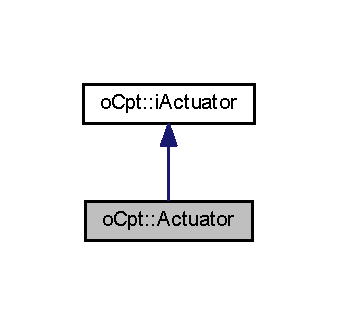
\includegraphics[width=162pt]{classo_cpt_1_1_actuator__inherit__graph}
\end{center}
\end{figure}


Collaboration diagram for o\+Cpt\+:\+:Actuator\+:\nopagebreak
\begin{figure}[H]
\begin{center}
\leavevmode
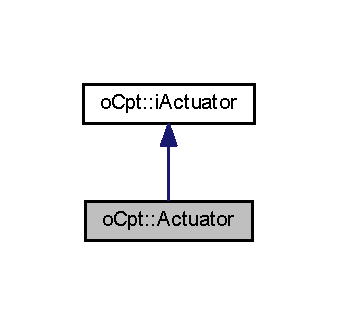
\includegraphics[width=162pt]{classo_cpt_1_1_actuator__coll__graph}
\end{center}
\end{figure}
\subsection*{Public Member Functions}
\begin{DoxyCompactItemize}
\item 
\hyperlink{classo_cpt_1_1_actuator_a715b50b49623386a7c04fd5fc713a626}{Actuator} ()
\item 
virtual \hyperlink{classo_cpt_1_1_actuator_a1934864651148186d4e9728560ede248}{$\sim$\+Actuator} () override
\item 
virtual void \hyperlink{classo_cpt_1_1_actuator_a3a3813e5730f0257e74de7300eeeffa1}{set\+Actuator} () override
\item 
virtual void \hyperlink{classo_cpt_1_1_actuator_a8985818fcfb644acce17ce50c5c7f86b}{run} () override
\item 
virtual void \hyperlink{classo_cpt_1_1_actuator_aa41132ff134e8b067353459dedbb0f37}{stop} () override
\end{DoxyCompactItemize}
\subsection*{Additional Inherited Members}


\subsection{Detailed Description}


Definition at line 32 of file Actuator.\+h.



\subsection{Constructor \& Destructor Documentation}
\hypertarget{classo_cpt_1_1_actuator_a715b50b49623386a7c04fd5fc713a626}{}\label{classo_cpt_1_1_actuator_a715b50b49623386a7c04fd5fc713a626} 
\index{o\+Cpt\+::\+Actuator@{o\+Cpt\+::\+Actuator}!Actuator@{Actuator}}
\index{Actuator@{Actuator}!o\+Cpt\+::\+Actuator@{o\+Cpt\+::\+Actuator}}
\subsubsection{\texorpdfstring{Actuator()}{Actuator()}}
{\footnotesize\ttfamily o\+Cpt\+::\+Actuator\+::\+Actuator (\begin{DoxyParamCaption}{ }\end{DoxyParamCaption})}



Definition at line 17 of file Actuator.\+cpp.

\hypertarget{classo_cpt_1_1_actuator_a1934864651148186d4e9728560ede248}{}\label{classo_cpt_1_1_actuator_a1934864651148186d4e9728560ede248} 
\index{o\+Cpt\+::\+Actuator@{o\+Cpt\+::\+Actuator}!````~Actuator@{$\sim$\+Actuator}}
\index{````~Actuator@{$\sim$\+Actuator}!o\+Cpt\+::\+Actuator@{o\+Cpt\+::\+Actuator}}
\subsubsection{\texorpdfstring{$\sim$\+Actuator()}{~Actuator()}}
{\footnotesize\ttfamily o\+Cpt\+::\+Actuator\+::$\sim$\+Actuator (\begin{DoxyParamCaption}{ }\end{DoxyParamCaption})\hspace{0.3cm}{\ttfamily [override]}, {\ttfamily [virtual]}}



Definition at line 21 of file Actuator.\+cpp.



\subsection{Member Function Documentation}
\hypertarget{classo_cpt_1_1_actuator_a8985818fcfb644acce17ce50c5c7f86b}{}\label{classo_cpt_1_1_actuator_a8985818fcfb644acce17ce50c5c7f86b} 
\index{o\+Cpt\+::\+Actuator@{o\+Cpt\+::\+Actuator}!run@{run}}
\index{run@{run}!o\+Cpt\+::\+Actuator@{o\+Cpt\+::\+Actuator}}
\subsubsection{\texorpdfstring{run()}{run()}}
{\footnotesize\ttfamily void o\+Cpt\+::\+Actuator\+::run (\begin{DoxyParamCaption}{ }\end{DoxyParamCaption})\hspace{0.3cm}{\ttfamily [override]}, {\ttfamily [virtual]}}



Implements \hyperlink{classo_cpt_1_1i_actuator_abf4db1f9f6b59bdefc86ca44aed0f49a}{o\+Cpt\+::i\+Actuator}.



Definition at line 29 of file Actuator.\+cpp.

\hypertarget{classo_cpt_1_1_actuator_a3a3813e5730f0257e74de7300eeeffa1}{}\label{classo_cpt_1_1_actuator_a3a3813e5730f0257e74de7300eeeffa1} 
\index{o\+Cpt\+::\+Actuator@{o\+Cpt\+::\+Actuator}!set\+Actuator@{set\+Actuator}}
\index{set\+Actuator@{set\+Actuator}!o\+Cpt\+::\+Actuator@{o\+Cpt\+::\+Actuator}}
\subsubsection{\texorpdfstring{set\+Actuator()}{setActuator()}}
{\footnotesize\ttfamily void o\+Cpt\+::\+Actuator\+::set\+Actuator (\begin{DoxyParamCaption}{ }\end{DoxyParamCaption})\hspace{0.3cm}{\ttfamily [override]}, {\ttfamily [virtual]}}



Implements \hyperlink{classo_cpt_1_1i_actuator_a1654bf3167a1dd7c34f770180cd8aaa1}{o\+Cpt\+::i\+Actuator}.



Definition at line 25 of file Actuator.\+cpp.

\hypertarget{classo_cpt_1_1_actuator_aa41132ff134e8b067353459dedbb0f37}{}\label{classo_cpt_1_1_actuator_aa41132ff134e8b067353459dedbb0f37} 
\index{o\+Cpt\+::\+Actuator@{o\+Cpt\+::\+Actuator}!stop@{stop}}
\index{stop@{stop}!o\+Cpt\+::\+Actuator@{o\+Cpt\+::\+Actuator}}
\subsubsection{\texorpdfstring{stop()}{stop()}}
{\footnotesize\ttfamily void o\+Cpt\+::\+Actuator\+::stop (\begin{DoxyParamCaption}{ }\end{DoxyParamCaption})\hspace{0.3cm}{\ttfamily [override]}, {\ttfamily [virtual]}}



Implements \hyperlink{classo_cpt_1_1i_actuator_ae3f9fbb61d920bee1bd297fb5a89625e}{o\+Cpt\+::i\+Actuator}.



Definition at line 33 of file Actuator.\+cpp.



The documentation for this class was generated from the following files\+:\begin{DoxyCompactItemize}
\item 
include/\+Core/\hyperlink{_actuator_8h}{Actuator.\+h}\item 
src/\+Core/\hyperlink{_actuator_8cpp}{Actuator.\+cpp}\end{DoxyCompactItemize}

\hypertarget{classo_cpt_1_1_actuator_task}{}\section{o\+Cpt\+:\+:Actuator\+Task Class Reference}
\label{classo_cpt_1_1_actuator_task}\index{o\+Cpt\+::\+Actuator\+Task@{o\+Cpt\+::\+Actuator\+Task}}


{\ttfamily \#include $<$Task.\+h$>$}



Inheritance diagram for o\+Cpt\+:\+:Actuator\+Task\+:
\nopagebreak
\begin{figure}[H]
\begin{center}
\leavevmode
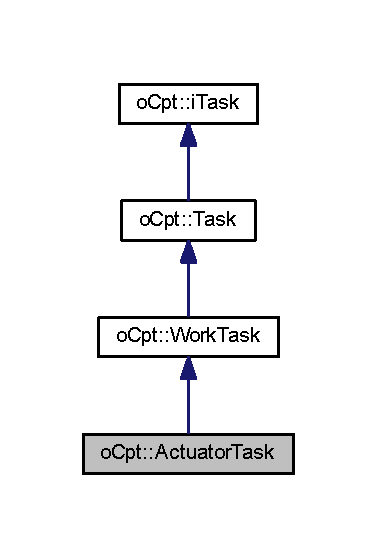
\includegraphics[width=180pt]{classo_cpt_1_1_actuator_task__inherit__graph}
\end{center}
\end{figure}


Collaboration diagram for o\+Cpt\+:\+:Actuator\+Task\+:
\nopagebreak
\begin{figure}[H]
\begin{center}
\leavevmode
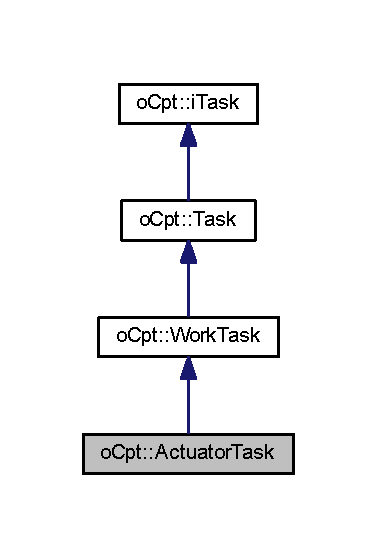
\includegraphics[width=180pt]{classo_cpt_1_1_actuator_task__coll__graph}
\end{center}
\end{figure}
\subsection*{Public Member Functions}
\begin{DoxyCompactItemize}
\item 
\hyperlink{classo_cpt_1_1_actuator_task_af06891ddcc32217567662979245af824}{Actuator\+Task} (\hyperlink{classo_cpt_1_1i_vessel_a43711a596f3bdfd0ca732ed3901edc97}{Vessel\+::ptr} vessel, bool concurrent=true)
\item 
virtual \hyperlink{classo_cpt_1_1_actuator_task_a829531567f8c0e660d2f4b541623915d}{$\sim$\+Actuator\+Task} ()
\end{DoxyCompactItemize}
\subsection*{Additional Inherited Members}


\subsection{Constructor \& Destructor Documentation}
\index{o\+Cpt\+::\+Actuator\+Task@{o\+Cpt\+::\+Actuator\+Task}!Actuator\+Task@{Actuator\+Task}}
\index{Actuator\+Task@{Actuator\+Task}!o\+Cpt\+::\+Actuator\+Task@{o\+Cpt\+::\+Actuator\+Task}}
\subsubsection[{\texorpdfstring{Actuator\+Task(\+Vessel\+::ptr vessel, bool concurrent=true)}{ActuatorTask(Vessel::ptr vessel, bool concurrent=true)}}]{\setlength{\rightskip}{0pt plus 5cm}o\+Cpt\+::\+Actuator\+Task\+::\+Actuator\+Task (
\begin{DoxyParamCaption}
\item[{{\bf Vessel\+::ptr}}]{vessel, }
\item[{bool}]{concurrent = {\ttfamily true}}
\end{DoxyParamCaption}
)}\hypertarget{classo_cpt_1_1_actuator_task_af06891ddcc32217567662979245af824}{}\label{classo_cpt_1_1_actuator_task_af06891ddcc32217567662979245af824}
\index{o\+Cpt\+::\+Actuator\+Task@{o\+Cpt\+::\+Actuator\+Task}!````~Actuator\+Task@{$\sim$\+Actuator\+Task}}
\index{````~Actuator\+Task@{$\sim$\+Actuator\+Task}!o\+Cpt\+::\+Actuator\+Task@{o\+Cpt\+::\+Actuator\+Task}}
\subsubsection[{\texorpdfstring{$\sim$\+Actuator\+Task()}{~ActuatorTask()}}]{\setlength{\rightskip}{0pt plus 5cm}o\+Cpt\+::\+Actuator\+Task\+::$\sim$\+Actuator\+Task (
\begin{DoxyParamCaption}
{}
\end{DoxyParamCaption}
)\hspace{0.3cm}{\ttfamily [virtual]}}\hypertarget{classo_cpt_1_1_actuator_task_a829531567f8c0e660d2f4b541623915d}{}\label{classo_cpt_1_1_actuator_task_a829531567f8c0e660d2f4b541623915d}


The documentation for this class was generated from the following files\+:\begin{DoxyCompactItemize}
\item 
include/\+Core/\hyperlink{_task_8h}{Task.\+h}\item 
src/\+Core/\hyperlink{_task_8cpp}{Task.\+cpp}\end{DoxyCompactItemize}

\hypertarget{classo_cpt_1_1protocol_1_1adc}{}\section{o\+Cpt\+:\+:protocol\+:\+:adc Class Reference}
\label{classo_cpt_1_1protocol_1_1adc}\index{o\+Cpt\+::protocol\+::adc@{o\+Cpt\+::protocol\+::adc}}


{\ttfamily \#include $<$Controller.\+h$>$}



Inheritance diagram for o\+Cpt\+:\+:protocol\+:\+:adc\+:\nopagebreak
\begin{figure}[H]
\begin{center}
\leavevmode
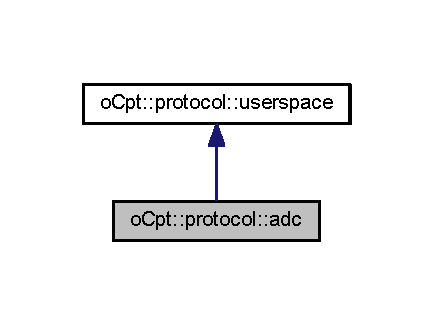
\includegraphics[width=208pt]{classo_cpt_1_1protocol_1_1adc__inherit__graph}
\end{center}
\end{figure}


Collaboration diagram for o\+Cpt\+:\+:protocol\+:\+:adc\+:\nopagebreak
\begin{figure}[H]
\begin{center}
\leavevmode
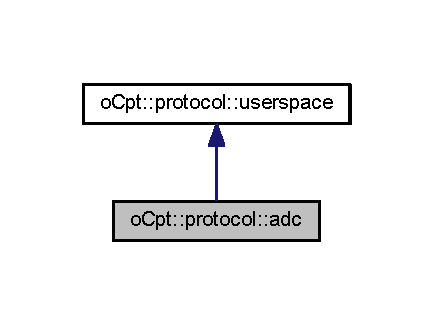
\includegraphics[width=208pt]{classo_cpt_1_1protocol_1_1adc__coll__graph}
\end{center}
\end{figure}
\subsection*{Public Types}
\begin{DoxyCompactItemize}
\item 
typedef boost\+::shared\+\_\+ptr$<$ \hyperlink{classo_cpt_1_1protocol_1_1adc}{adc} $>$ \hyperlink{classo_cpt_1_1protocol_1_1adc_a94af68cb9c573629a4a1a16f8ebd3dff}{ptr}
\end{DoxyCompactItemize}
\subsection*{Public Member Functions}
\begin{DoxyCompactItemize}
\item 
\hyperlink{classo_cpt_1_1protocol_1_1adc_aec27fd40080992220a7b641adcdfe9f9}{adc} (uint8\+\_\+t id, uint8\+\_\+t device, std\+::string mod\+Name=\char`\"{}\char`\"{})
\item 
virtual \hyperlink{classo_cpt_1_1protocol_1_1adc_ae61f97f81f6d76d5fc5fd783f49464ee}{$\sim$adc} ()
\item 
uint16\+\_\+t \& \hyperlink{classo_cpt_1_1protocol_1_1adc_a78a1abf9c5d72b7da8efea1be21e0a85}{get\+Value} ()
\item 
bool \hyperlink{classo_cpt_1_1protocol_1_1adc_afd7e7e1ab0855f53227a4fbf91449687}{operator==} (const \hyperlink{classo_cpt_1_1protocol_1_1adc}{adc} \&rhs)
\item 
bool \hyperlink{classo_cpt_1_1protocol_1_1adc_ae5ff90755d50ef617e9c00d704a88f52}{compare} (const uint8\+\_\+t \&id, const uint8\+\_\+t \&device=0)
\end{DoxyCompactItemize}
\subsection*{Private Attributes}
\begin{DoxyCompactItemize}
\item 
uint8\+\_\+t \hyperlink{classo_cpt_1_1protocol_1_1adc_a1ea5bd6df6c5163f98dd097796afddb7}{id\+\_\+} = 0
\item 
uint8\+\_\+t \hyperlink{classo_cpt_1_1protocol_1_1adc_a0781bbf803cff1a30fb79bc2118ee771}{device\+\_\+} = 0
\item 
std\+::string \hyperlink{classo_cpt_1_1protocol_1_1adc_a23481c789dd95444a3e9a19beb5b044e}{path\+\_\+} = \char`\"{}\char`\"{}
\item 
uint16\+\_\+t \hyperlink{classo_cpt_1_1protocol_1_1adc_a79ed77ed852cbe9c1b23e9c3601ffdb7}{value\+\_\+} = 0
\end{DoxyCompactItemize}
\subsection*{Additional Inherited Members}


\subsection{Detailed Description}
The Analogue to Digital converter class. This class reads the voltage of an analogie pin, from user space. 

Definition at line 89 of file Controller.\+h.



\subsection{Member Typedef Documentation}
\hypertarget{classo_cpt_1_1protocol_1_1adc_a94af68cb9c573629a4a1a16f8ebd3dff}{}\label{classo_cpt_1_1protocol_1_1adc_a94af68cb9c573629a4a1a16f8ebd3dff} 
\index{o\+Cpt\+::protocol\+::adc@{o\+Cpt\+::protocol\+::adc}!ptr@{ptr}}
\index{ptr@{ptr}!o\+Cpt\+::protocol\+::adc@{o\+Cpt\+::protocol\+::adc}}
\subsubsection{\texorpdfstring{ptr}{ptr}}
{\footnotesize\ttfamily typedef boost\+::shared\+\_\+ptr$<$\hyperlink{classo_cpt_1_1protocol_1_1adc}{adc}$>$ \hyperlink{classo_cpt_1_1protocol_1_1adc_a94af68cb9c573629a4a1a16f8ebd3dff}{o\+Cpt\+::protocol\+::adc\+::ptr}}



Definition at line 91 of file Controller.\+h.



\subsection{Constructor \& Destructor Documentation}
\hypertarget{classo_cpt_1_1protocol_1_1adc_aec27fd40080992220a7b641adcdfe9f9}{}\label{classo_cpt_1_1protocol_1_1adc_aec27fd40080992220a7b641adcdfe9f9} 
\index{o\+Cpt\+::protocol\+::adc@{o\+Cpt\+::protocol\+::adc}!adc@{adc}}
\index{adc@{adc}!o\+Cpt\+::protocol\+::adc@{o\+Cpt\+::protocol\+::adc}}
\subsubsection{\texorpdfstring{adc()}{adc()}}
{\footnotesize\ttfamily o\+Cpt\+::protocol\+::adc\+::adc (\begin{DoxyParamCaption}\item[{uint8\+\_\+t}]{id,  }\item[{uint8\+\_\+t}]{device,  }\item[{std\+::string}]{mod\+Name = {\ttfamily \char`\"{}\char`\"{}} }\end{DoxyParamCaption})}

The constructor of the adc class 
\begin{DoxyParams}{Parameters}
{\em id} & the pin ID as an uint8\+\_\+t value \\
\hline
{\em device} & the device or chip which handles the communication with the analogue pins \\
\hline
{\em mod\+Name} & the name of the modules which needs to be loaded T\+O\+DO check if it is allways needed to load a module \\
\hline
\end{DoxyParams}


Definition at line 61 of file Controller.\+cpp.



References A\+D\+C\+\_\+\+I\+O\+\_\+\+B\+A\+S\+E\+\_\+\+P\+A\+TH, A\+D\+C\+\_\+\+V\+O\+L\+T\+A\+G\+E\+\_\+\+P\+A\+TH, A\+D\+C\+\_\+\+V\+O\+L\+T\+A\+G\+E\+\_\+\+S\+U\+B\+\_\+\+P\+A\+TH, o\+Cpt\+::protocol\+::userspace\+::file\+Exist(), and o\+Cpt\+::protocol\+::userspace\+::mod\+Loaded().

Here is the call graph for this function\+:\nopagebreak
\begin{figure}[H]
\begin{center}
\leavevmode
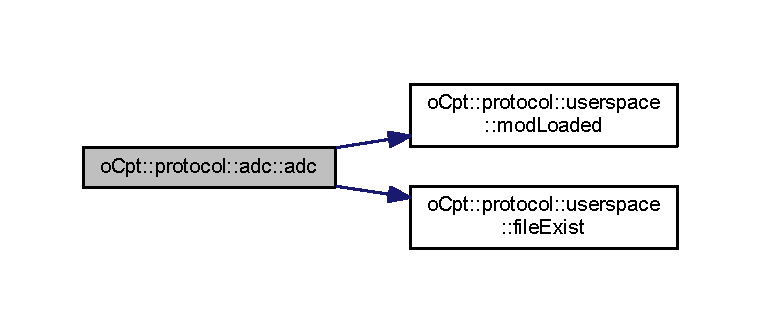
\includegraphics[width=350pt]{classo_cpt_1_1protocol_1_1adc_aec27fd40080992220a7b641adcdfe9f9_cgraph}
\end{center}
\end{figure}
\hypertarget{classo_cpt_1_1protocol_1_1adc_ae61f97f81f6d76d5fc5fd783f49464ee}{}\label{classo_cpt_1_1protocol_1_1adc_ae61f97f81f6d76d5fc5fd783f49464ee} 
\index{o\+Cpt\+::protocol\+::adc@{o\+Cpt\+::protocol\+::adc}!````~adc@{$\sim$adc}}
\index{````~adc@{$\sim$adc}!o\+Cpt\+::protocol\+::adc@{o\+Cpt\+::protocol\+::adc}}
\subsubsection{\texorpdfstring{$\sim$adc()}{~adc()}}
{\footnotesize\ttfamily o\+Cpt\+::protocol\+::adc\+::$\sim$adc (\begin{DoxyParamCaption}{ }\end{DoxyParamCaption})\hspace{0.3cm}{\ttfamily [virtual]}}

The deconstrcutor 

Definition at line 79 of file Controller.\+cpp.



\subsection{Member Function Documentation}
\hypertarget{classo_cpt_1_1protocol_1_1adc_ae5ff90755d50ef617e9c00d704a88f52}{}\label{classo_cpt_1_1protocol_1_1adc_ae5ff90755d50ef617e9c00d704a88f52} 
\index{o\+Cpt\+::protocol\+::adc@{o\+Cpt\+::protocol\+::adc}!compare@{compare}}
\index{compare@{compare}!o\+Cpt\+::protocol\+::adc@{o\+Cpt\+::protocol\+::adc}}
\subsubsection{\texorpdfstring{compare()}{compare()}}
{\footnotesize\ttfamily bool o\+Cpt\+::protocol\+::adc\+::compare (\begin{DoxyParamCaption}\item[{const uint8\+\_\+t \&}]{id,  }\item[{const uint8\+\_\+t \&}]{device = {\ttfamily 0} }\end{DoxyParamCaption})}

Compare function 
\begin{DoxyParams}{Parameters}
{\em id} & ID to be checked \\
\hline
{\em device} & Device name to be checked \\
\hline
\end{DoxyParams}
\begin{DoxyReturn}{Returns}
either true or false 
\end{DoxyReturn}


Definition at line 95 of file Controller.\+cpp.

\hypertarget{classo_cpt_1_1protocol_1_1adc_a78a1abf9c5d72b7da8efea1be21e0a85}{}\label{classo_cpt_1_1protocol_1_1adc_a78a1abf9c5d72b7da8efea1be21e0a85} 
\index{o\+Cpt\+::protocol\+::adc@{o\+Cpt\+::protocol\+::adc}!get\+Value@{get\+Value}}
\index{get\+Value@{get\+Value}!o\+Cpt\+::protocol\+::adc@{o\+Cpt\+::protocol\+::adc}}
\subsubsection{\texorpdfstring{get\+Value()}{getValue()}}
{\footnotesize\ttfamily uint16\+\_\+t \& o\+Cpt\+::protocol\+::adc\+::get\+Value (\begin{DoxyParamCaption}{ }\end{DoxyParamCaption})}

gets the current raw voltage level as resolution \begin{DoxyReturn}{Returns}
the raw voltage level as uint16\+\_\+t 
\end{DoxyReturn}


Definition at line 81 of file Controller.\+cpp.

\hypertarget{classo_cpt_1_1protocol_1_1adc_afd7e7e1ab0855f53227a4fbf91449687}{}\label{classo_cpt_1_1protocol_1_1adc_afd7e7e1ab0855f53227a4fbf91449687} 
\index{o\+Cpt\+::protocol\+::adc@{o\+Cpt\+::protocol\+::adc}!operator==@{operator==}}
\index{operator==@{operator==}!o\+Cpt\+::protocol\+::adc@{o\+Cpt\+::protocol\+::adc}}
\subsubsection{\texorpdfstring{operator==()}{operator==()}}
{\footnotesize\ttfamily bool o\+Cpt\+::protocol\+::adc\+::operator== (\begin{DoxyParamCaption}\item[{const \hyperlink{classo_cpt_1_1protocol_1_1adc}{adc} \&}]{rhs }\end{DoxyParamCaption})}

Checks if adc object is the same 
\begin{DoxyParams}{Parameters}
{\em rhs} & other adc object, to be checked against \\
\hline
\end{DoxyParams}
\begin{DoxyReturn}{Returns}
either true or false 
\end{DoxyReturn}


Definition at line 91 of file Controller.\+cpp.



References path\+\_\+.



\subsection{Member Data Documentation}
\hypertarget{classo_cpt_1_1protocol_1_1adc_a0781bbf803cff1a30fb79bc2118ee771}{}\label{classo_cpt_1_1protocol_1_1adc_a0781bbf803cff1a30fb79bc2118ee771} 
\index{o\+Cpt\+::protocol\+::adc@{o\+Cpt\+::protocol\+::adc}!device\+\_\+@{device\+\_\+}}
\index{device\+\_\+@{device\+\_\+}!o\+Cpt\+::protocol\+::adc@{o\+Cpt\+::protocol\+::adc}}
\subsubsection{\texorpdfstring{device\+\_\+}{device\_}}
{\footnotesize\ttfamily uint8\+\_\+t o\+Cpt\+::protocol\+::adc\+::device\+\_\+ = 0\hspace{0.3cm}{\ttfamily [private]}}



Definition at line 130 of file Controller.\+h.

\hypertarget{classo_cpt_1_1protocol_1_1adc_a1ea5bd6df6c5163f98dd097796afddb7}{}\label{classo_cpt_1_1protocol_1_1adc_a1ea5bd6df6c5163f98dd097796afddb7} 
\index{o\+Cpt\+::protocol\+::adc@{o\+Cpt\+::protocol\+::adc}!id\+\_\+@{id\+\_\+}}
\index{id\+\_\+@{id\+\_\+}!o\+Cpt\+::protocol\+::adc@{o\+Cpt\+::protocol\+::adc}}
\subsubsection{\texorpdfstring{id\+\_\+}{id\_}}
{\footnotesize\ttfamily uint8\+\_\+t o\+Cpt\+::protocol\+::adc\+::id\+\_\+ = 0\hspace{0.3cm}{\ttfamily [private]}}



Definition at line 129 of file Controller.\+h.

\hypertarget{classo_cpt_1_1protocol_1_1adc_a23481c789dd95444a3e9a19beb5b044e}{}\label{classo_cpt_1_1protocol_1_1adc_a23481c789dd95444a3e9a19beb5b044e} 
\index{o\+Cpt\+::protocol\+::adc@{o\+Cpt\+::protocol\+::adc}!path\+\_\+@{path\+\_\+}}
\index{path\+\_\+@{path\+\_\+}!o\+Cpt\+::protocol\+::adc@{o\+Cpt\+::protocol\+::adc}}
\subsubsection{\texorpdfstring{path\+\_\+}{path\_}}
{\footnotesize\ttfamily std\+::string o\+Cpt\+::protocol\+::adc\+::path\+\_\+ = \char`\"{}\char`\"{}\hspace{0.3cm}{\ttfamily [private]}}



Definition at line 131 of file Controller.\+h.



Referenced by operator==().

\hypertarget{classo_cpt_1_1protocol_1_1adc_a79ed77ed852cbe9c1b23e9c3601ffdb7}{}\label{classo_cpt_1_1protocol_1_1adc_a79ed77ed852cbe9c1b23e9c3601ffdb7} 
\index{o\+Cpt\+::protocol\+::adc@{o\+Cpt\+::protocol\+::adc}!value\+\_\+@{value\+\_\+}}
\index{value\+\_\+@{value\+\_\+}!o\+Cpt\+::protocol\+::adc@{o\+Cpt\+::protocol\+::adc}}
\subsubsection{\texorpdfstring{value\+\_\+}{value\_}}
{\footnotesize\ttfamily uint16\+\_\+t o\+Cpt\+::protocol\+::adc\+::value\+\_\+ = 0\hspace{0.3cm}{\ttfamily [private]}}



Definition at line 132 of file Controller.\+h.



The documentation for this class was generated from the following files\+:\begin{DoxyCompactItemize}
\item 
/projects/mti/oh\+Captain/oh\+Captain/include/\+Core/\hyperlink{_controller_8h}{Controller.\+h}\item 
/projects/mti/oh\+Captain/oh\+Captain/src/\+Core/\hyperlink{_controller_8cpp}{Controller.\+cpp}\end{DoxyCompactItemize}

\hypertarget{classo_cpt_1_1_a_r_m}{}\section{o\+Cpt\+:\+:A\+RM Class Reference}
\label{classo_cpt_1_1_a_r_m}\index{o\+Cpt\+::\+A\+RM@{o\+Cpt\+::\+A\+RM}}


{\ttfamily \#include $<$Controller.\+h$>$}



Inheritance diagram for o\+Cpt\+:\+:A\+RM\+:\nopagebreak
\begin{figure}[H]
\begin{center}
\leavevmode
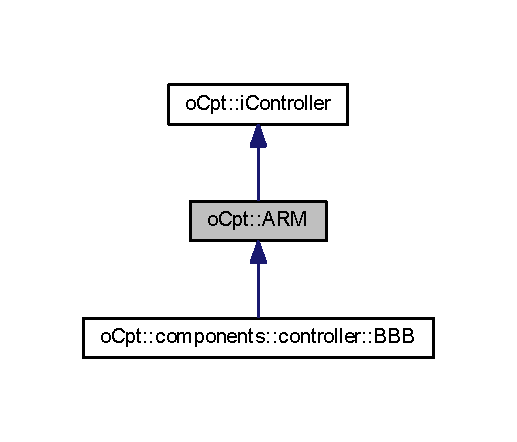
\includegraphics[width=248pt]{classo_cpt_1_1_a_r_m__inherit__graph}
\end{center}
\end{figure}


Collaboration diagram for o\+Cpt\+:\+:A\+RM\+:\nopagebreak
\begin{figure}[H]
\begin{center}
\leavevmode
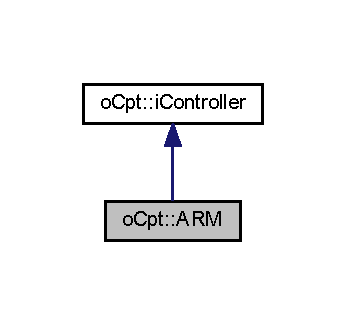
\includegraphics[width=166pt]{classo_cpt_1_1_a_r_m__coll__graph}
\end{center}
\end{figure}
\subsection*{Public Member Functions}
\begin{DoxyCompactItemize}
\item 
\hyperlink{classo_cpt_1_1_a_r_m_af99c9e575fbee98bf8754220d7a8badd}{A\+RM} (\hyperlink{classo_cpt_1_1_world_aa6e591e3096d5de71e0cec9039663d67}{World\+::ptr} world)
\item 
virtual \hyperlink{classo_cpt_1_1_a_r_m_a2be59dd26648e2a21c3996bcc3b2b153}{$\sim$\+A\+RM} ()
\item 
virtual std\+::vector$<$ \hyperlink{classo_cpt_1_1protocol_1_1adc_a94af68cb9c573629a4a1a16f8ebd3dff}{protocol\+::adc\+::ptr} $>$ $\ast$ \hyperlink{classo_cpt_1_1_a_r_m_a32e77e29e34f3114f0b766b705366ba8}{get\+Adc\+Vector} ()
\item 
virtual \hyperlink{classo_cpt_1_1protocol_1_1adc_a94af68cb9c573629a4a1a16f8ebd3dff}{protocol\+::adc\+::ptr} \hyperlink{classo_cpt_1_1_a_r_m_a2f773bcd04719d81994af8930ca974bd}{get\+A\+DC} (uint8\+\_\+t id, uint8\+\_\+t device)
\end{DoxyCompactItemize}
\subsection*{Additional Inherited Members}


\subsection{Detailed Description}
An \hyperlink{classo_cpt_1_1_a_r_m}{A\+RM} like controller. Currently only \hyperlink{classo_cpt_1_1_a_r_m}{A\+RM} devices are implemented 

Definition at line 597 of file Controller.\+h.



\subsection{Constructor \& Destructor Documentation}
\hypertarget{classo_cpt_1_1_a_r_m_af99c9e575fbee98bf8754220d7a8badd}{}\label{classo_cpt_1_1_a_r_m_af99c9e575fbee98bf8754220d7a8badd} 
\index{o\+Cpt\+::\+A\+RM@{o\+Cpt\+::\+A\+RM}!A\+RM@{A\+RM}}
\index{A\+RM@{A\+RM}!o\+Cpt\+::\+A\+RM@{o\+Cpt\+::\+A\+RM}}
\subsubsection{\texorpdfstring{A\+R\+M()}{ARM()}}
{\footnotesize\ttfamily o\+Cpt\+::\+A\+R\+M\+::\+A\+RM (\begin{DoxyParamCaption}\item[{\hyperlink{classo_cpt_1_1_world_aa6e591e3096d5de71e0cec9039663d67}{World\+::ptr}}]{world }\end{DoxyParamCaption})}

The constructor of an \hyperlink{classo_cpt_1_1_a_r_m}{A\+RM} controller 
\begin{DoxyParams}{Parameters}
{\em world} & a shared\+\_\+ptr to the \hyperlink{classo_cpt_1_1_world}{World} \\
\hline
\end{DoxyParams}


Definition at line 469 of file Controller.\+cpp.

\hypertarget{classo_cpt_1_1_a_r_m_a2be59dd26648e2a21c3996bcc3b2b153}{}\label{classo_cpt_1_1_a_r_m_a2be59dd26648e2a21c3996bcc3b2b153} 
\index{o\+Cpt\+::\+A\+RM@{o\+Cpt\+::\+A\+RM}!````~A\+RM@{$\sim$\+A\+RM}}
\index{````~A\+RM@{$\sim$\+A\+RM}!o\+Cpt\+::\+A\+RM@{o\+Cpt\+::\+A\+RM}}
\subsubsection{\texorpdfstring{$\sim$\+A\+R\+M()}{~ARM()}}
{\footnotesize\ttfamily o\+Cpt\+::\+A\+R\+M\+::$\sim$\+A\+RM (\begin{DoxyParamCaption}{ }\end{DoxyParamCaption})\hspace{0.3cm}{\ttfamily [virtual]}}

The deconstructor 

Definition at line 472 of file Controller.\+cpp.



\subsection{Member Function Documentation}
\hypertarget{classo_cpt_1_1_a_r_m_a2f773bcd04719d81994af8930ca974bd}{}\label{classo_cpt_1_1_a_r_m_a2f773bcd04719d81994af8930ca974bd} 
\index{o\+Cpt\+::\+A\+RM@{o\+Cpt\+::\+A\+RM}!get\+A\+DC@{get\+A\+DC}}
\index{get\+A\+DC@{get\+A\+DC}!o\+Cpt\+::\+A\+RM@{o\+Cpt\+::\+A\+RM}}
\subsubsection{\texorpdfstring{get\+A\+D\+C()}{getADC()}}
{\footnotesize\ttfamily \hyperlink{classo_cpt_1_1protocol_1_1adc_a94af68cb9c573629a4a1a16f8ebd3dff}{protocol\+::adc\+::ptr} o\+Cpt\+::\+A\+R\+M\+::get\+A\+DC (\begin{DoxyParamCaption}\item[{uint8\+\_\+t}]{id,  }\item[{uint8\+\_\+t}]{device }\end{DoxyParamCaption})\hspace{0.3cm}{\ttfamily [virtual]}}

Get a specific shared\+\_\+ptr to an A\+DC 
\begin{DoxyParams}{Parameters}
{\em id} & the pin ID \\
\hline
{\em device} & the device ID \\
\hline
\end{DoxyParams}
\begin{DoxyReturn}{Returns}
returns the specified A\+DC 
\end{DoxyReturn}


Implements \hyperlink{classo_cpt_1_1i_controller_a7abf65f5912df117a3ff4c1c9643bba3}{o\+Cpt\+::i\+Controller}.



Definition at line 474 of file Controller.\+cpp.



References o\+Cpt\+::i\+Controller\+::adc\+Vector\+\_\+.

\hypertarget{classo_cpt_1_1_a_r_m_a32e77e29e34f3114f0b766b705366ba8}{}\label{classo_cpt_1_1_a_r_m_a32e77e29e34f3114f0b766b705366ba8} 
\index{o\+Cpt\+::\+A\+RM@{o\+Cpt\+::\+A\+RM}!get\+Adc\+Vector@{get\+Adc\+Vector}}
\index{get\+Adc\+Vector@{get\+Adc\+Vector}!o\+Cpt\+::\+A\+RM@{o\+Cpt\+::\+A\+RM}}
\subsubsection{\texorpdfstring{get\+Adc\+Vector()}{getAdcVector()}}
{\footnotesize\ttfamily std\+::vector$<$ \hyperlink{classo_cpt_1_1protocol_1_1adc_a94af68cb9c573629a4a1a16f8ebd3dff}{protocol\+::adc\+::ptr} $>$ $\ast$ o\+Cpt\+::\+A\+R\+M\+::get\+Adc\+Vector (\begin{DoxyParamCaption}{ }\end{DoxyParamCaption})\hspace{0.3cm}{\ttfamily [virtual]}}

Obtain a vector of available A\+D\+Cs \begin{DoxyReturn}{Returns}

\end{DoxyReturn}


Implements \hyperlink{classo_cpt_1_1i_controller_af414ebaf64b79ac45d1275e62799e36c}{o\+Cpt\+::i\+Controller}.



Definition at line 481 of file Controller.\+cpp.



References o\+Cpt\+::i\+Controller\+::adc\+Vector\+\_\+.



The documentation for this class was generated from the following files\+:\begin{DoxyCompactItemize}
\item 
include/\+Core/\hyperlink{_controller_8h}{Controller.\+h}\item 
src/\+Core/\hyperlink{_controller_8cpp}{Controller.\+cpp}\end{DoxyCompactItemize}

\hypertarget{classo_cpt_1_1components_1_1controller_1_1_b_b_b}{}\section{o\+Cpt\+:\+:components\+:\+:controller\+:\+:B\+BB Class Reference}
\label{classo_cpt_1_1components_1_1controller_1_1_b_b_b}\index{o\+Cpt\+::components\+::controller\+::\+B\+BB@{o\+Cpt\+::components\+::controller\+::\+B\+BB}}


{\ttfamily \#include $<$Beaglebone\+Black.\+h$>$}



Inheritance diagram for o\+Cpt\+:\+:components\+:\+:controller\+:\+:B\+BB\+:\nopagebreak
\begin{figure}[H]
\begin{center}
\leavevmode
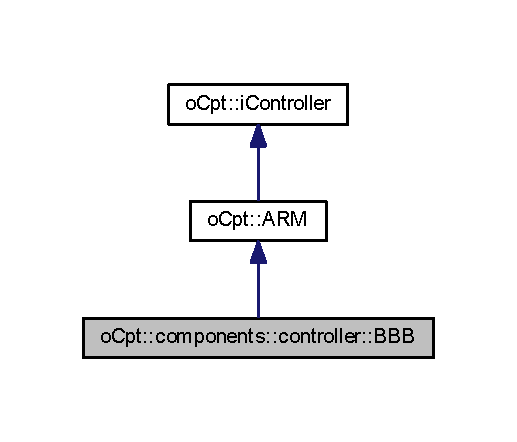
\includegraphics[width=248pt]{classo_cpt_1_1components_1_1controller_1_1_b_b_b__inherit__graph}
\end{center}
\end{figure}


Collaboration diagram for o\+Cpt\+:\+:components\+:\+:controller\+:\+:B\+BB\+:\nopagebreak
\begin{figure}[H]
\begin{center}
\leavevmode
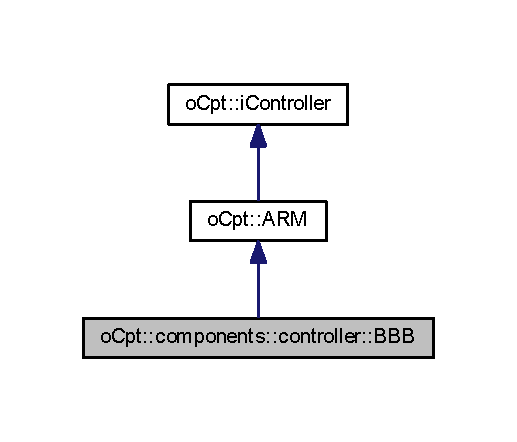
\includegraphics[width=248pt]{classo_cpt_1_1components_1_1controller_1_1_b_b_b__coll__graph}
\end{center}
\end{figure}
\subsection*{Public Member Functions}
\begin{DoxyCompactItemize}
\item 
\hyperlink{classo_cpt_1_1components_1_1controller_1_1_b_b_b_a7f5b95ebd0b1b176ee6ecbb3ac61e06c}{B\+BB} (\hyperlink{classo_cpt_1_1_world_aa6e591e3096d5de71e0cec9039663d67}{World\+::ptr} world)
\item 
virtual \hyperlink{classo_cpt_1_1components_1_1controller_1_1_b_b_b_acdf417541bfd66c55fba8a09e8cd09a1}{$\sim$\+B\+BB} ()
\end{DoxyCompactItemize}
\subsection*{Additional Inherited Members}


\subsection{Detailed Description}


Definition at line 14 of file Beaglebone\+Black.\+h.



\subsection{Constructor \& Destructor Documentation}
\hypertarget{classo_cpt_1_1components_1_1controller_1_1_b_b_b_a7f5b95ebd0b1b176ee6ecbb3ac61e06c}{}\label{classo_cpt_1_1components_1_1controller_1_1_b_b_b_a7f5b95ebd0b1b176ee6ecbb3ac61e06c} 
\index{o\+Cpt\+::components\+::controller\+::\+B\+BB@{o\+Cpt\+::components\+::controller\+::\+B\+BB}!B\+BB@{B\+BB}}
\index{B\+BB@{B\+BB}!o\+Cpt\+::components\+::controller\+::\+B\+BB@{o\+Cpt\+::components\+::controller\+::\+B\+BB}}
\subsubsection{\texorpdfstring{B\+B\+B()}{BBB()}}
{\footnotesize\ttfamily o\+Cpt\+::components\+::controller\+::\+B\+B\+B\+::\+B\+BB (\begin{DoxyParamCaption}\item[{\hyperlink{classo_cpt_1_1_world_aa6e591e3096d5de71e0cec9039663d67}{World\+::ptr}}]{world }\end{DoxyParamCaption})}



Definition at line 11 of file Beaglebone\+Black.\+cpp.



References o\+Cpt\+::i\+Controller\+::adc\+Vector\+\_\+.

\hypertarget{classo_cpt_1_1components_1_1controller_1_1_b_b_b_acdf417541bfd66c55fba8a09e8cd09a1}{}\label{classo_cpt_1_1components_1_1controller_1_1_b_b_b_acdf417541bfd66c55fba8a09e8cd09a1} 
\index{o\+Cpt\+::components\+::controller\+::\+B\+BB@{o\+Cpt\+::components\+::controller\+::\+B\+BB}!````~B\+BB@{$\sim$\+B\+BB}}
\index{````~B\+BB@{$\sim$\+B\+BB}!o\+Cpt\+::components\+::controller\+::\+B\+BB@{o\+Cpt\+::components\+::controller\+::\+B\+BB}}
\subsubsection{\texorpdfstring{$\sim$\+B\+B\+B()}{~BBB()}}
{\footnotesize\ttfamily o\+Cpt\+::components\+::controller\+::\+B\+B\+B\+::$\sim$\+B\+BB (\begin{DoxyParamCaption}{ }\end{DoxyParamCaption})\hspace{0.3cm}{\ttfamily [virtual]}}



Definition at line 20 of file Beaglebone\+Black.\+cpp.



The documentation for this class was generated from the following files\+:\begin{DoxyCompactItemize}
\item 
/projects/mti/oh\+Captain/oh\+Captain/include/\+Controllers/\hyperlink{_beaglebone_black_8h}{Beaglebone\+Black.\+h}\item 
/projects/mti/oh\+Captain/oh\+Captain/src/\+Controllers/\hyperlink{_beaglebone_black_8cpp}{Beaglebone\+Black.\+cpp}\end{DoxyCompactItemize}

\hypertarget{classo_cpt_1_1_boatswain}{}\section{o\+Cpt\+:\+:Boatswain Class Reference}
\label{classo_cpt_1_1_boatswain}\index{o\+Cpt\+::\+Boatswain@{o\+Cpt\+::\+Boatswain}}


{\ttfamily \#include $<$Boatswain.\+h$>$}



Inheritance diagram for o\+Cpt\+:\+:Boatswain\+:
\nopagebreak
\begin{figure}[H]
\begin{center}
\leavevmode
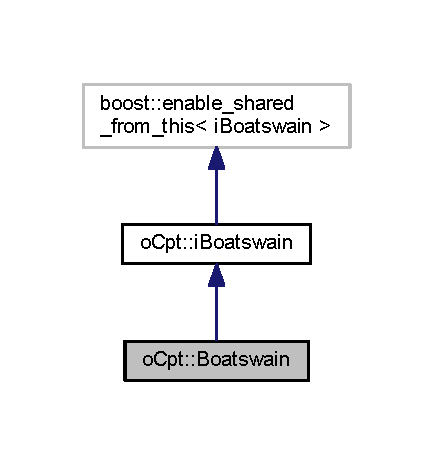
\includegraphics[width=207pt]{classo_cpt_1_1_boatswain__inherit__graph}
\end{center}
\end{figure}


Collaboration diagram for o\+Cpt\+:\+:Boatswain\+:
\nopagebreak
\begin{figure}[H]
\begin{center}
\leavevmode
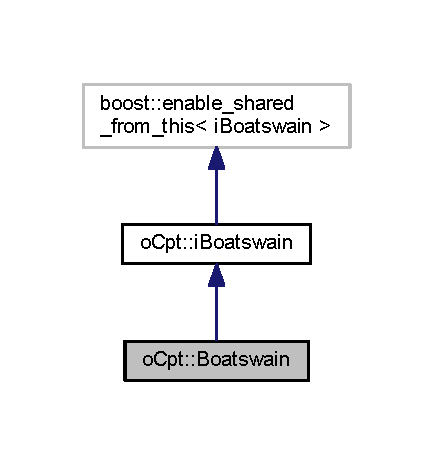
\includegraphics[width=207pt]{classo_cpt_1_1_boatswain__coll__graph}
\end{center}
\end{figure}
\subsection*{Public Member Functions}
\begin{DoxyCompactItemize}
\item 
\hyperlink{classo_cpt_1_1_boatswain_a43e10039b53b8bde7ad2e9780db68949}{Boatswain} (\hyperlink{classo_cpt_1_1i_controller_a6d89a95cd6ad68bb74adfaca2f36370f}{i\+Controller\+::ptr} controller)
\item 
virtual \hyperlink{classo_cpt_1_1_boatswain_a0cff16b78dc5ee0e6b5d2169d693036f}{$\sim$\+Boatswain} () override
\item 
virtual void \hyperlink{classo_cpt_1_1_boatswain_a7665a4439b8e71ece31ff5e9755caf09}{run} () override
\item 
virtual void \hyperlink{classo_cpt_1_1_boatswain_ad538cca1d6429dacf09b22c53291074f}{stop} () override
\item 
virtual void \hyperlink{classo_cpt_1_1_boatswain_aa1c27c710e2156402c3851ac189ea162}{initialize} () override
\item 
virtual void \hyperlink{classo_cpt_1_1_boatswain_ab36071db5e3f8a0db0053b5553e508f0}{register\+Sensor} (\hyperlink{classo_cpt_1_1i_sensor_a03533d2c5dc66e332d70dbb3b5e3006a}{i\+Sensor\+::ptr} sensor) override
\item 
virtual void \hyperlink{classo_cpt_1_1_boatswain_ae3f318352a331d64840ff87ad1ce3e8e}{register\+Actuator} (\hyperlink{classo_cpt_1_1i_actuator_a35847799558e92bb84fb6c71de772cac}{i\+Actuator\+::ptr} actuator) override
\end{DoxyCompactItemize}
\subsection*{Protected Member Functions}
\begin{DoxyCompactItemize}
\item 
void \hyperlink{classo_cpt_1_1_boatswain_aca864b4219485c6d83ad0e92c7ea16fd}{reset\+Timer} (\hyperlink{classo_cpt_1_1i_sensor_a03533d2c5dc66e332d70dbb3b5e3006a}{i\+Sensor\+::ptr} sensor) override
\end{DoxyCompactItemize}
\subsection*{Additional Inherited Members}


\subsection{Constructor \& Destructor Documentation}
\index{o\+Cpt\+::\+Boatswain@{o\+Cpt\+::\+Boatswain}!Boatswain@{Boatswain}}
\index{Boatswain@{Boatswain}!o\+Cpt\+::\+Boatswain@{o\+Cpt\+::\+Boatswain}}
\subsubsection[{\texorpdfstring{Boatswain(i\+Controller\+::ptr controller)}{Boatswain(iController::ptr controller)}}]{\setlength{\rightskip}{0pt plus 5cm}o\+Cpt\+::\+Boatswain\+::\+Boatswain (
\begin{DoxyParamCaption}
\item[{{\bf i\+Controller\+::ptr}}]{controller}
\end{DoxyParamCaption}
)}\hypertarget{classo_cpt_1_1_boatswain_a43e10039b53b8bde7ad2e9780db68949}{}\label{classo_cpt_1_1_boatswain_a43e10039b53b8bde7ad2e9780db68949}
\index{o\+Cpt\+::\+Boatswain@{o\+Cpt\+::\+Boatswain}!````~Boatswain@{$\sim$\+Boatswain}}
\index{````~Boatswain@{$\sim$\+Boatswain}!o\+Cpt\+::\+Boatswain@{o\+Cpt\+::\+Boatswain}}
\subsubsection[{\texorpdfstring{$\sim$\+Boatswain() override}{~Boatswain() override}}]{\setlength{\rightskip}{0pt plus 5cm}o\+Cpt\+::\+Boatswain\+::$\sim$\+Boatswain (
\begin{DoxyParamCaption}
{}
\end{DoxyParamCaption}
)\hspace{0.3cm}{\ttfamily [override]}, {\ttfamily [virtual]}}\hypertarget{classo_cpt_1_1_boatswain_a0cff16b78dc5ee0e6b5d2169d693036f}{}\label{classo_cpt_1_1_boatswain_a0cff16b78dc5ee0e6b5d2169d693036f}


\subsection{Member Function Documentation}
\index{o\+Cpt\+::\+Boatswain@{o\+Cpt\+::\+Boatswain}!initialize@{initialize}}
\index{initialize@{initialize}!o\+Cpt\+::\+Boatswain@{o\+Cpt\+::\+Boatswain}}
\subsubsection[{\texorpdfstring{initialize() override}{initialize() override}}]{\setlength{\rightskip}{0pt plus 5cm}void o\+Cpt\+::\+Boatswain\+::initialize (
\begin{DoxyParamCaption}
{}
\end{DoxyParamCaption}
)\hspace{0.3cm}{\ttfamily [override]}, {\ttfamily [virtual]}}\hypertarget{classo_cpt_1_1_boatswain_aa1c27c710e2156402c3851ac189ea162}{}\label{classo_cpt_1_1_boatswain_aa1c27c710e2156402c3851ac189ea162}


Implements \hyperlink{classo_cpt_1_1i_boatswain_a0749ff59de42e7a8a47586ab9d9ac98f}{o\+Cpt\+::i\+Boatswain}.

\index{o\+Cpt\+::\+Boatswain@{o\+Cpt\+::\+Boatswain}!register\+Actuator@{register\+Actuator}}
\index{register\+Actuator@{register\+Actuator}!o\+Cpt\+::\+Boatswain@{o\+Cpt\+::\+Boatswain}}
\subsubsection[{\texorpdfstring{register\+Actuator(i\+Actuator\+::ptr actuator) override}{registerActuator(iActuator::ptr actuator) override}}]{\setlength{\rightskip}{0pt plus 5cm}void o\+Cpt\+::\+Boatswain\+::register\+Actuator (
\begin{DoxyParamCaption}
\item[{{\bf i\+Actuator\+::ptr}}]{actuator}
\end{DoxyParamCaption}
)\hspace{0.3cm}{\ttfamily [override]}, {\ttfamily [virtual]}}\hypertarget{classo_cpt_1_1_boatswain_ae3f318352a331d64840ff87ad1ce3e8e}{}\label{classo_cpt_1_1_boatswain_ae3f318352a331d64840ff87ad1ce3e8e}


Implements \hyperlink{classo_cpt_1_1i_boatswain_a7915584ee17a28b1fc506a8968e27387}{o\+Cpt\+::i\+Boatswain}.

\index{o\+Cpt\+::\+Boatswain@{o\+Cpt\+::\+Boatswain}!register\+Sensor@{register\+Sensor}}
\index{register\+Sensor@{register\+Sensor}!o\+Cpt\+::\+Boatswain@{o\+Cpt\+::\+Boatswain}}
\subsubsection[{\texorpdfstring{register\+Sensor(i\+Sensor\+::ptr sensor) override}{registerSensor(iSensor::ptr sensor) override}}]{\setlength{\rightskip}{0pt plus 5cm}void o\+Cpt\+::\+Boatswain\+::register\+Sensor (
\begin{DoxyParamCaption}
\item[{{\bf i\+Sensor\+::ptr}}]{sensor}
\end{DoxyParamCaption}
)\hspace{0.3cm}{\ttfamily [override]}, {\ttfamily [virtual]}}\hypertarget{classo_cpt_1_1_boatswain_ab36071db5e3f8a0db0053b5553e508f0}{}\label{classo_cpt_1_1_boatswain_ab36071db5e3f8a0db0053b5553e508f0}


Implements \hyperlink{classo_cpt_1_1i_boatswain_aa9f9014202617a705d7ce21db2877222}{o\+Cpt\+::i\+Boatswain}.



Here is the call graph for this function\+:
\nopagebreak
\begin{figure}[H]
\begin{center}
\leavevmode
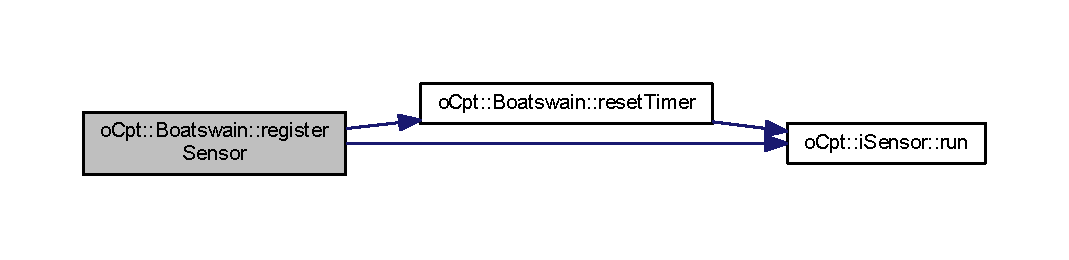
\includegraphics[width=350pt]{classo_cpt_1_1_boatswain_ab36071db5e3f8a0db0053b5553e508f0_cgraph}
\end{center}
\end{figure}


\index{o\+Cpt\+::\+Boatswain@{o\+Cpt\+::\+Boatswain}!reset\+Timer@{reset\+Timer}}
\index{reset\+Timer@{reset\+Timer}!o\+Cpt\+::\+Boatswain@{o\+Cpt\+::\+Boatswain}}
\subsubsection[{\texorpdfstring{reset\+Timer(i\+Sensor\+::ptr sensor) override}{resetTimer(iSensor::ptr sensor) override}}]{\setlength{\rightskip}{0pt plus 5cm}void o\+Cpt\+::\+Boatswain\+::reset\+Timer (
\begin{DoxyParamCaption}
\item[{{\bf i\+Sensor\+::ptr}}]{sensor}
\end{DoxyParamCaption}
)\hspace{0.3cm}{\ttfamily [override]}, {\ttfamily [protected]}, {\ttfamily [virtual]}}\hypertarget{classo_cpt_1_1_boatswain_aca864b4219485c6d83ad0e92c7ea16fd}{}\label{classo_cpt_1_1_boatswain_aca864b4219485c6d83ad0e92c7ea16fd}


Implements \hyperlink{classo_cpt_1_1i_boatswain_a863c877ec067c55b5e06a04d0d9648ce}{o\+Cpt\+::i\+Boatswain}.



Here is the call graph for this function\+:
\nopagebreak
\begin{figure}[H]
\begin{center}
\leavevmode
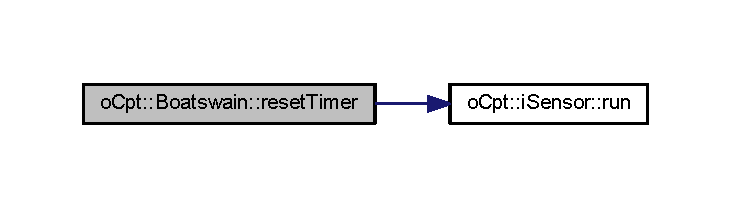
\includegraphics[width=350pt]{classo_cpt_1_1_boatswain_aca864b4219485c6d83ad0e92c7ea16fd_cgraph}
\end{center}
\end{figure}




Here is the caller graph for this function\+:
\nopagebreak
\begin{figure}[H]
\begin{center}
\leavevmode
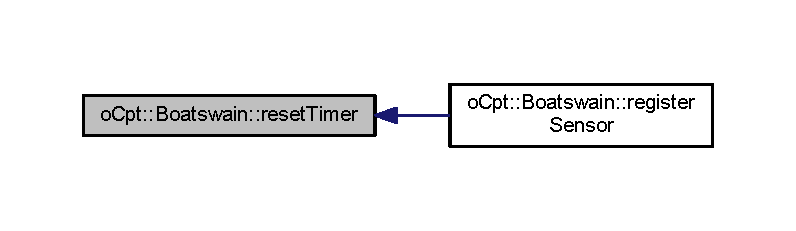
\includegraphics[width=350pt]{classo_cpt_1_1_boatswain_aca864b4219485c6d83ad0e92c7ea16fd_icgraph}
\end{center}
\end{figure}


\index{o\+Cpt\+::\+Boatswain@{o\+Cpt\+::\+Boatswain}!run@{run}}
\index{run@{run}!o\+Cpt\+::\+Boatswain@{o\+Cpt\+::\+Boatswain}}
\subsubsection[{\texorpdfstring{run() override}{run() override}}]{\setlength{\rightskip}{0pt plus 5cm}void o\+Cpt\+::\+Boatswain\+::run (
\begin{DoxyParamCaption}
{}
\end{DoxyParamCaption}
)\hspace{0.3cm}{\ttfamily [override]}, {\ttfamily [virtual]}}\hypertarget{classo_cpt_1_1_boatswain_a7665a4439b8e71ece31ff5e9755caf09}{}\label{classo_cpt_1_1_boatswain_a7665a4439b8e71ece31ff5e9755caf09}


Implements \hyperlink{classo_cpt_1_1i_boatswain_a4512e742ba996b32dcc452d9f180724a}{o\+Cpt\+::i\+Boatswain}.

\index{o\+Cpt\+::\+Boatswain@{o\+Cpt\+::\+Boatswain}!stop@{stop}}
\index{stop@{stop}!o\+Cpt\+::\+Boatswain@{o\+Cpt\+::\+Boatswain}}
\subsubsection[{\texorpdfstring{stop() override}{stop() override}}]{\setlength{\rightskip}{0pt plus 5cm}void o\+Cpt\+::\+Boatswain\+::stop (
\begin{DoxyParamCaption}
{}
\end{DoxyParamCaption}
)\hspace{0.3cm}{\ttfamily [override]}, {\ttfamily [virtual]}}\hypertarget{classo_cpt_1_1_boatswain_ad538cca1d6429dacf09b22c53291074f}{}\label{classo_cpt_1_1_boatswain_ad538cca1d6429dacf09b22c53291074f}


Implements \hyperlink{classo_cpt_1_1i_boatswain_ad1fb6362c814a72ea6c4dc9a9042cf5e}{o\+Cpt\+::i\+Boatswain}.



The documentation for this class was generated from the following files\+:\begin{DoxyCompactItemize}
\item 
include/\+Core/\hyperlink{_boatswain_8h}{Boatswain.\+h}\item 
src/\+Core/\hyperlink{_boatswain_8cpp}{Boatswain.\+cpp}\end{DoxyCompactItemize}

\hypertarget{classo_cpt_1_1_captain}{}\section{o\+Cpt\+:\+:Captain Class Reference}
\label{classo_cpt_1_1_captain}\index{o\+Cpt\+::\+Captain@{o\+Cpt\+::\+Captain}}


{\ttfamily \#include $<$Captain.\+h$>$}



Inheritance diagram for o\+Cpt\+:\+:Captain\+:\nopagebreak
\begin{figure}[H]
\begin{center}
\leavevmode
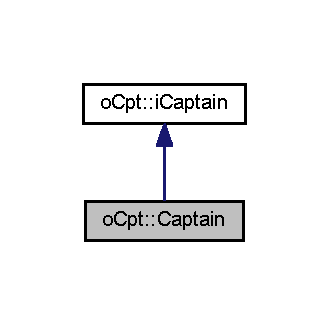
\includegraphics[width=158pt]{classo_cpt_1_1_captain__inherit__graph}
\end{center}
\end{figure}


Collaboration diagram for o\+Cpt\+:\+:Captain\+:\nopagebreak
\begin{figure}[H]
\begin{center}
\leavevmode
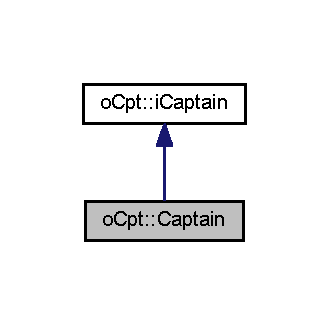
\includegraphics[width=158pt]{classo_cpt_1_1_captain__coll__graph}
\end{center}
\end{figure}
\subsection*{Public Member Functions}
\begin{DoxyCompactItemize}
\item 
\hyperlink{classo_cpt_1_1_captain_a36f8b64ff252791b2d28bdb10a9652c7}{Captain} (\hyperlink{classo_cpt_1_1_world_aa6e591e3096d5de71e0cec9039663d67}{World\+::ptr} world)
\item 
virtual \hyperlink{classo_cpt_1_1_captain_ae78194ab847c6fbf3fae7f3d92f02f70}{$\sim$\+Captain} () override
\item 
virtual void \hyperlink{classo_cpt_1_1_captain_ade0ca7804340b555a9ead5dd01465045}{run} () override
\item 
virtual void \hyperlink{classo_cpt_1_1_captain_aa8a3923b961f4bc2ebc857895f759711}{stop} () override
\item 
virtual void \hyperlink{classo_cpt_1_1_captain_a3afce8b5a16b91a8b848ab6ae12a5ca6}{initialize} () override
\end{DoxyCompactItemize}
\subsection*{Additional Inherited Members}


\subsection{Detailed Description}


Definition at line 36 of file Captain.\+h.



\subsection{Constructor \& Destructor Documentation}
\hypertarget{classo_cpt_1_1_captain_a36f8b64ff252791b2d28bdb10a9652c7}{}\label{classo_cpt_1_1_captain_a36f8b64ff252791b2d28bdb10a9652c7} 
\index{o\+Cpt\+::\+Captain@{o\+Cpt\+::\+Captain}!Captain@{Captain}}
\index{Captain@{Captain}!o\+Cpt\+::\+Captain@{o\+Cpt\+::\+Captain}}
\subsubsection{\texorpdfstring{Captain()}{Captain()}}
{\footnotesize\ttfamily o\+Cpt\+::\+Captain\+::\+Captain (\begin{DoxyParamCaption}\item[{\hyperlink{classo_cpt_1_1_world_aa6e591e3096d5de71e0cec9039663d67}{World\+::ptr}}]{world }\end{DoxyParamCaption})}



Definition at line 9 of file Captain.\+cpp.



References o\+Cpt\+::i\+Captain\+::local\+Stop\+Thread\+\_\+.

\hypertarget{classo_cpt_1_1_captain_ae78194ab847c6fbf3fae7f3d92f02f70}{}\label{classo_cpt_1_1_captain_ae78194ab847c6fbf3fae7f3d92f02f70} 
\index{o\+Cpt\+::\+Captain@{o\+Cpt\+::\+Captain}!````~Captain@{$\sim$\+Captain}}
\index{````~Captain@{$\sim$\+Captain}!o\+Cpt\+::\+Captain@{o\+Cpt\+::\+Captain}}
\subsubsection{\texorpdfstring{$\sim$\+Captain()}{~Captain()}}
{\footnotesize\ttfamily o\+Cpt\+::\+Captain\+::$\sim$\+Captain (\begin{DoxyParamCaption}{ }\end{DoxyParamCaption})\hspace{0.3cm}{\ttfamily [override]}, {\ttfamily [virtual]}}



Definition at line 13 of file Captain.\+cpp.



\subsection{Member Function Documentation}
\hypertarget{classo_cpt_1_1_captain_a3afce8b5a16b91a8b848ab6ae12a5ca6}{}\label{classo_cpt_1_1_captain_a3afce8b5a16b91a8b848ab6ae12a5ca6} 
\index{o\+Cpt\+::\+Captain@{o\+Cpt\+::\+Captain}!initialize@{initialize}}
\index{initialize@{initialize}!o\+Cpt\+::\+Captain@{o\+Cpt\+::\+Captain}}
\subsubsection{\texorpdfstring{initialize()}{initialize()}}
{\footnotesize\ttfamily void o\+Cpt\+::\+Captain\+::initialize (\begin{DoxyParamCaption}{ }\end{DoxyParamCaption})\hspace{0.3cm}{\ttfamily [override]}, {\ttfamily [virtual]}}



Implements \hyperlink{classo_cpt_1_1i_captain_a5ad7947dde7866981c76ccd3a30ce4ce}{o\+Cpt\+::i\+Captain}.



Definition at line 27 of file Captain.\+cpp.

\hypertarget{classo_cpt_1_1_captain_ade0ca7804340b555a9ead5dd01465045}{}\label{classo_cpt_1_1_captain_ade0ca7804340b555a9ead5dd01465045} 
\index{o\+Cpt\+::\+Captain@{o\+Cpt\+::\+Captain}!run@{run}}
\index{run@{run}!o\+Cpt\+::\+Captain@{o\+Cpt\+::\+Captain}}
\subsubsection{\texorpdfstring{run()}{run()}}
{\footnotesize\ttfamily void o\+Cpt\+::\+Captain\+::run (\begin{DoxyParamCaption}{ }\end{DoxyParamCaption})\hspace{0.3cm}{\ttfamily [override]}, {\ttfamily [virtual]}}



Implements \hyperlink{classo_cpt_1_1i_captain_a53d61f2d68b435f32ad66858ae898763}{o\+Cpt\+::i\+Captain}.



Definition at line 17 of file Captain.\+cpp.



References o\+Cpt\+::i\+Captain\+::local\+Stop\+Thread\+\_\+, and o\+Cpt\+::i\+Captain\+::stop\+Thread\+\_\+.

\hypertarget{classo_cpt_1_1_captain_aa8a3923b961f4bc2ebc857895f759711}{}\label{classo_cpt_1_1_captain_aa8a3923b961f4bc2ebc857895f759711} 
\index{o\+Cpt\+::\+Captain@{o\+Cpt\+::\+Captain}!stop@{stop}}
\index{stop@{stop}!o\+Cpt\+::\+Captain@{o\+Cpt\+::\+Captain}}
\subsubsection{\texorpdfstring{stop()}{stop()}}
{\footnotesize\ttfamily void o\+Cpt\+::\+Captain\+::stop (\begin{DoxyParamCaption}{ }\end{DoxyParamCaption})\hspace{0.3cm}{\ttfamily [override]}, {\ttfamily [virtual]}}



Implements \hyperlink{classo_cpt_1_1i_captain_aeda385ea9a0ee33301dfda05098c836b}{o\+Cpt\+::i\+Captain}.



Definition at line 23 of file Captain.\+cpp.



References o\+Cpt\+::i\+Captain\+::local\+Stop\+Thread\+\_\+.



The documentation for this class was generated from the following files\+:\begin{DoxyCompactItemize}
\item 
include/\+Core/\hyperlink{_captain_8h}{Captain.\+h}\item 
src/\+Core/\hyperlink{_captain_8cpp}{Captain.\+cpp}\end{DoxyCompactItemize}

\hypertarget{classo_cpt_1_1_communication_task}{}\section{o\+Cpt\+:\+:Communication\+Task Class Reference}
\label{classo_cpt_1_1_communication_task}\index{o\+Cpt\+::\+Communication\+Task@{o\+Cpt\+::\+Communication\+Task}}


{\ttfamily \#include $<$Task.\+h$>$}



Inheritance diagram for o\+Cpt\+:\+:Communication\+Task\+:\nopagebreak
\begin{figure}[H]
\begin{center}
\leavevmode
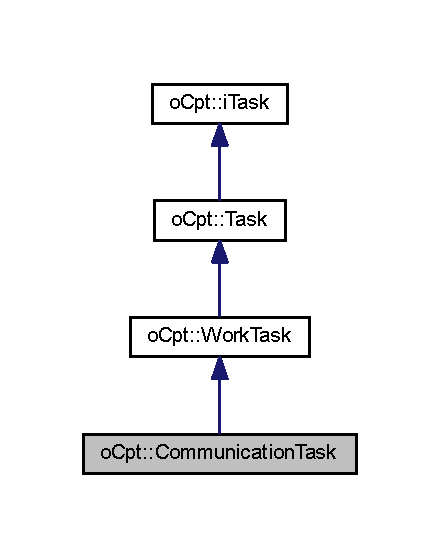
\includegraphics[width=211pt]{classo_cpt_1_1_communication_task__inherit__graph}
\end{center}
\end{figure}


Collaboration diagram for o\+Cpt\+:\+:Communication\+Task\+:\nopagebreak
\begin{figure}[H]
\begin{center}
\leavevmode
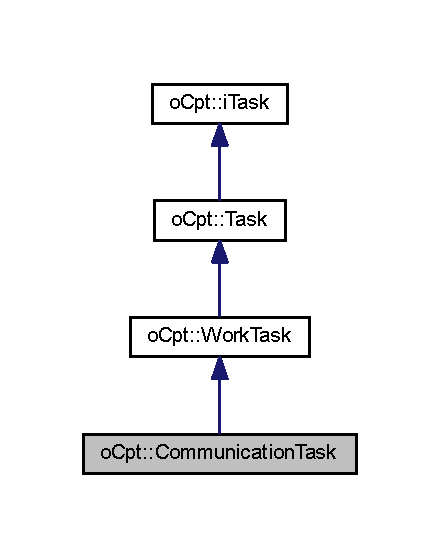
\includegraphics[width=211pt]{classo_cpt_1_1_communication_task__coll__graph}
\end{center}
\end{figure}
\subsection*{Public Member Functions}
\begin{DoxyCompactItemize}
\item 
\hyperlink{classo_cpt_1_1_communication_task_a40993dba58872287d4b7a8a736049735}{Communication\+Task} (\hyperlink{classo_cpt_1_1i_vessel_a43711a596f3bdfd0ca732ed3901edc97}{Vessel\+::ptr} vessel, bool concurrent=true)
\item 
virtual \hyperlink{classo_cpt_1_1_communication_task_a046da901df467610f94dbe0a8e3add00}{$\sim$\+Communication\+Task} ()
\end{DoxyCompactItemize}
\subsection*{Additional Inherited Members}


\subsection{Detailed Description}


Definition at line 322 of file Task.\+h.



\subsection{Constructor \& Destructor Documentation}
\hypertarget{classo_cpt_1_1_communication_task_a40993dba58872287d4b7a8a736049735}{}\label{classo_cpt_1_1_communication_task_a40993dba58872287d4b7a8a736049735} 
\index{o\+Cpt\+::\+Communication\+Task@{o\+Cpt\+::\+Communication\+Task}!Communication\+Task@{Communication\+Task}}
\index{Communication\+Task@{Communication\+Task}!o\+Cpt\+::\+Communication\+Task@{o\+Cpt\+::\+Communication\+Task}}
\subsubsection{\texorpdfstring{Communication\+Task()}{CommunicationTask()}}
{\footnotesize\ttfamily o\+Cpt\+::\+Communication\+Task\+::\+Communication\+Task (\begin{DoxyParamCaption}\item[{\hyperlink{classo_cpt_1_1i_vessel_a43711a596f3bdfd0ca732ed3901edc97}{Vessel\+::ptr}}]{vessel,  }\item[{bool}]{concurrent = {\ttfamily true} }\end{DoxyParamCaption})}



Definition at line 81 of file Task.\+cpp.

\hypertarget{classo_cpt_1_1_communication_task_a046da901df467610f94dbe0a8e3add00}{}\label{classo_cpt_1_1_communication_task_a046da901df467610f94dbe0a8e3add00} 
\index{o\+Cpt\+::\+Communication\+Task@{o\+Cpt\+::\+Communication\+Task}!````~Communication\+Task@{$\sim$\+Communication\+Task}}
\index{````~Communication\+Task@{$\sim$\+Communication\+Task}!o\+Cpt\+::\+Communication\+Task@{o\+Cpt\+::\+Communication\+Task}}
\subsubsection{\texorpdfstring{$\sim$\+Communication\+Task()}{~CommunicationTask()}}
{\footnotesize\ttfamily o\+Cpt\+::\+Communication\+Task\+::$\sim$\+Communication\+Task (\begin{DoxyParamCaption}{ }\end{DoxyParamCaption})\hspace{0.3cm}{\ttfamily [virtual]}}



Definition at line 83 of file Task.\+cpp.



The documentation for this class was generated from the following files\+:\begin{DoxyCompactItemize}
\item 
/projects/mti/oh\+Captain/oh\+Captain/include/\+Core/\hyperlink{_task_8h}{Task.\+h}\item 
/projects/mti/oh\+Captain/oh\+Captain/src/\+Core/\hyperlink{_task_8cpp}{Task.\+cpp}\end{DoxyCompactItemize}

\hypertarget{classo_cpt_1_1components_1_1sensors_1_1_control_kalman_i_m_u}{}\section{o\+Cpt\+:\+:components\+:\+:sensors\+:\+:Control\+Kalman\+I\+MU$<$ T $>$ Class Template Reference}
\label{classo_cpt_1_1components_1_1sensors_1_1_control_kalman_i_m_u}\index{o\+Cpt\+::components\+::sensors\+::\+Control\+Kalman\+I\+M\+U$<$ T $>$@{o\+Cpt\+::components\+::sensors\+::\+Control\+Kalman\+I\+M\+U$<$ T $>$}}


{\ttfamily \#include $<$Kalman\+I\+M\+U.\+h$>$}



Inheritance diagram for o\+Cpt\+:\+:components\+:\+:sensors\+:\+:Control\+Kalman\+I\+MU$<$ T $>$\+:
\nopagebreak
\begin{figure}[H]
\begin{center}
\leavevmode
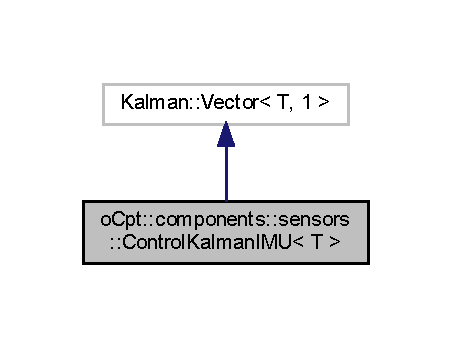
\includegraphics[width=217pt]{classo_cpt_1_1components_1_1sensors_1_1_control_kalman_i_m_u__inherit__graph}
\end{center}
\end{figure}


Collaboration diagram for o\+Cpt\+:\+:components\+:\+:sensors\+:\+:Control\+Kalman\+I\+MU$<$ T $>$\+:
\nopagebreak
\begin{figure}[H]
\begin{center}
\leavevmode
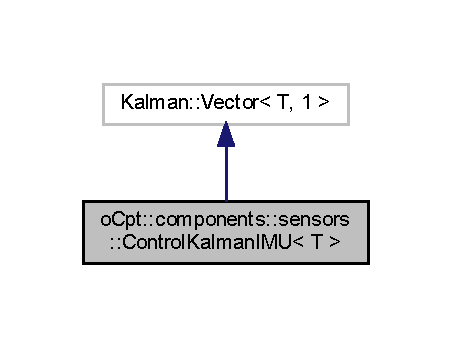
\includegraphics[width=217pt]{classo_cpt_1_1components_1_1sensors_1_1_control_kalman_i_m_u__coll__graph}
\end{center}
\end{figure}
\subsection*{Public Types}
\begin{DoxyCompactItemize}
\item 
typedef Kalman\+::\+Vector$<$ T, 1 $>$ \hyperlink{classo_cpt_1_1components_1_1sensors_1_1_control_kalman_i_m_u_a86f04b59796a0780208ff528543bf390}{Base}
\end{DoxyCompactItemize}
\subsection*{Public Member Functions}
\begin{DoxyCompactItemize}
\item 
\hyperlink{classo_cpt_1_1components_1_1sensors_1_1_control_kalman_i_m_u_a7e4619f52b9572448ad5184b6e796ee9}{Control\+Kalman\+I\+MU} (void)
\item 
{\footnotesize template$<$typename Other\+Derived $>$ }\\\hyperlink{classo_cpt_1_1components_1_1sensors_1_1_control_kalman_i_m_u_a49168d8285a50e490574a582811fabf8}{Control\+Kalman\+I\+MU} (const Eigen\+::\+Matrix\+Base$<$ Other\+Derived $>$ \&other)
\item 
{\footnotesize template$<$typename Other\+Derived $>$ }\\\hyperlink{classo_cpt_1_1components_1_1sensors_1_1_control_kalman_i_m_u}{Control\+Kalman\+I\+MU} \& \hyperlink{classo_cpt_1_1components_1_1sensors_1_1_control_kalman_i_m_u_a56e78cc546a77e97ff1e1a1605d8cf30}{operator=} (const Eigen\+::\+Matrix\+Base$<$ Other\+Derived $>$ \&other)
\end{DoxyCompactItemize}


\subsection{Detailed Description}
\subsubsection*{template$<$typename T$>$\newline
class o\+Cpt\+::components\+::sensors\+::\+Control\+Kalman\+I\+M\+U$<$ T $>$}



Definition at line 100 of file Kalman\+I\+M\+U.\+h.



\subsection{Member Typedef Documentation}
\hypertarget{classo_cpt_1_1components_1_1sensors_1_1_control_kalman_i_m_u_a86f04b59796a0780208ff528543bf390}{}\label{classo_cpt_1_1components_1_1sensors_1_1_control_kalman_i_m_u_a86f04b59796a0780208ff528543bf390} 
\index{o\+Cpt\+::components\+::sensors\+::\+Control\+Kalman\+I\+MU@{o\+Cpt\+::components\+::sensors\+::\+Control\+Kalman\+I\+MU}!Base@{Base}}
\index{Base@{Base}!o\+Cpt\+::components\+::sensors\+::\+Control\+Kalman\+I\+MU@{o\+Cpt\+::components\+::sensors\+::\+Control\+Kalman\+I\+MU}}
\subsubsection{\texorpdfstring{Base}{Base}}
{\footnotesize\ttfamily template$<$typename T $>$ \\
typedef Kalman\+::\+Vector$<$ T , 1 $>$ \hyperlink{classo_cpt_1_1components_1_1sensors_1_1_control_kalman_i_m_u}{o\+Cpt\+::components\+::sensors\+::\+Control\+Kalman\+I\+MU}$<$ T $>$\+::\hyperlink{classo_cpt_1_1components_1_1sensors_1_1_control_kalman_i_m_u_a86f04b59796a0780208ff528543bf390}{Base}}



Definition at line 102 of file Kalman\+I\+M\+U.\+h.



\subsection{Constructor \& Destructor Documentation}
\hypertarget{classo_cpt_1_1components_1_1sensors_1_1_control_kalman_i_m_u_a7e4619f52b9572448ad5184b6e796ee9}{}\label{classo_cpt_1_1components_1_1sensors_1_1_control_kalman_i_m_u_a7e4619f52b9572448ad5184b6e796ee9} 
\index{o\+Cpt\+::components\+::sensors\+::\+Control\+Kalman\+I\+MU@{o\+Cpt\+::components\+::sensors\+::\+Control\+Kalman\+I\+MU}!Control\+Kalman\+I\+MU@{Control\+Kalman\+I\+MU}}
\index{Control\+Kalman\+I\+MU@{Control\+Kalman\+I\+MU}!o\+Cpt\+::components\+::sensors\+::\+Control\+Kalman\+I\+MU@{o\+Cpt\+::components\+::sensors\+::\+Control\+Kalman\+I\+MU}}
\subsubsection{\texorpdfstring{Control\+Kalman\+I\+M\+U()}{ControlKalmanIMU()}\hspace{0.1cm}{\footnotesize\ttfamily [1/2]}}
{\footnotesize\ttfamily template$<$typename T $>$ \\
\hyperlink{classo_cpt_1_1components_1_1sensors_1_1_control_kalman_i_m_u}{o\+Cpt\+::components\+::sensors\+::\+Control\+Kalman\+I\+MU}$<$ T $>$\+::\hyperlink{classo_cpt_1_1components_1_1sensors_1_1_control_kalman_i_m_u}{Control\+Kalman\+I\+MU} (\begin{DoxyParamCaption}\item[{void}]{ }\end{DoxyParamCaption})\hspace{0.3cm}{\ttfamily [inline]}}



Definition at line 102 of file Kalman\+I\+M\+U.\+h.

\hypertarget{classo_cpt_1_1components_1_1sensors_1_1_control_kalman_i_m_u_a49168d8285a50e490574a582811fabf8}{}\label{classo_cpt_1_1components_1_1sensors_1_1_control_kalman_i_m_u_a49168d8285a50e490574a582811fabf8} 
\index{o\+Cpt\+::components\+::sensors\+::\+Control\+Kalman\+I\+MU@{o\+Cpt\+::components\+::sensors\+::\+Control\+Kalman\+I\+MU}!Control\+Kalman\+I\+MU@{Control\+Kalman\+I\+MU}}
\index{Control\+Kalman\+I\+MU@{Control\+Kalman\+I\+MU}!o\+Cpt\+::components\+::sensors\+::\+Control\+Kalman\+I\+MU@{o\+Cpt\+::components\+::sensors\+::\+Control\+Kalman\+I\+MU}}
\subsubsection{\texorpdfstring{Control\+Kalman\+I\+M\+U()}{ControlKalmanIMU()}\hspace{0.1cm}{\footnotesize\ttfamily [2/2]}}
{\footnotesize\ttfamily template$<$typename T $>$ \\
template$<$typename Other\+Derived $>$ \\
\hyperlink{classo_cpt_1_1components_1_1sensors_1_1_control_kalman_i_m_u}{o\+Cpt\+::components\+::sensors\+::\+Control\+Kalman\+I\+MU}$<$ T $>$\+::\hyperlink{classo_cpt_1_1components_1_1sensors_1_1_control_kalman_i_m_u}{Control\+Kalman\+I\+MU} (\begin{DoxyParamCaption}\item[{const Eigen\+::\+Matrix\+Base$<$ Other\+Derived $>$ \&}]{other }\end{DoxyParamCaption})\hspace{0.3cm}{\ttfamily [inline]}}



Definition at line 102 of file Kalman\+I\+M\+U.\+h.



\subsection{Member Function Documentation}
\hypertarget{classo_cpt_1_1components_1_1sensors_1_1_control_kalman_i_m_u_a56e78cc546a77e97ff1e1a1605d8cf30}{}\label{classo_cpt_1_1components_1_1sensors_1_1_control_kalman_i_m_u_a56e78cc546a77e97ff1e1a1605d8cf30} 
\index{o\+Cpt\+::components\+::sensors\+::\+Control\+Kalman\+I\+MU@{o\+Cpt\+::components\+::sensors\+::\+Control\+Kalman\+I\+MU}!operator=@{operator=}}
\index{operator=@{operator=}!o\+Cpt\+::components\+::sensors\+::\+Control\+Kalman\+I\+MU@{o\+Cpt\+::components\+::sensors\+::\+Control\+Kalman\+I\+MU}}
\subsubsection{\texorpdfstring{operator=()}{operator=()}}
{\footnotesize\ttfamily template$<$typename T $>$ \\
template$<$typename Other\+Derived $>$ \\
\hyperlink{classo_cpt_1_1components_1_1sensors_1_1_control_kalman_i_m_u}{Control\+Kalman\+I\+MU}\& \hyperlink{classo_cpt_1_1components_1_1sensors_1_1_control_kalman_i_m_u}{o\+Cpt\+::components\+::sensors\+::\+Control\+Kalman\+I\+MU}$<$ T $>$\+::operator= (\begin{DoxyParamCaption}\item[{const Eigen\+::\+Matrix\+Base$<$ Other\+Derived $>$ \&}]{other }\end{DoxyParamCaption})\hspace{0.3cm}{\ttfamily [inline]}}



Definition at line 102 of file Kalman\+I\+M\+U.\+h.



The documentation for this class was generated from the following file\+:\begin{DoxyCompactItemize}
\item 
/projects/mti/oh\+Captain/oh\+Captain/include/\+Sensors/\hyperlink{_kalman_i_m_u_8h}{Kalman\+I\+M\+U.\+h}\end{DoxyCompactItemize}

\hypertarget{structo_cpt_1_1_world_1_1_location_1_1coordinate}{}\section{o\+Cpt\+:\+:World\+:\+:Location\+:\+:coordinate Struct Reference}
\label{structo_cpt_1_1_world_1_1_location_1_1coordinate}\index{o\+Cpt\+::\+World\+::\+Location\+::coordinate@{o\+Cpt\+::\+World\+::\+Location\+::coordinate}}


{\ttfamily \#include $<$World.\+h$>$}

\subsection*{Public Attributes}
\begin{DoxyCompactItemize}
\item 
\hyperlink{classo_cpt_1_1_world_1_1_location_a896d36a393f64f80cb4756134477da14}{degree\+\_\+t} \hyperlink{structo_cpt_1_1_world_1_1_location_1_1coordinate_aca0e4502963b1f4149d064833e3a502c}{value}
\item 
\hyperlink{classo_cpt_1_1_world_1_1_location_aa37d99a87b49ccc38470dcc6cc64ced5}{cardinal\+\_\+direction} \hyperlink{structo_cpt_1_1_world_1_1_location_1_1coordinate_ad26574b6dd132610ed3383d52a4fe95f}{direction}
\end{DoxyCompactItemize}


\subsection{Detailed Description}


Definition at line 134 of file World.\+h.



\subsection{Member Data Documentation}
\hypertarget{structo_cpt_1_1_world_1_1_location_1_1coordinate_ad26574b6dd132610ed3383d52a4fe95f}{}\label{structo_cpt_1_1_world_1_1_location_1_1coordinate_ad26574b6dd132610ed3383d52a4fe95f} 
\index{o\+Cpt\+::\+World\+::\+Location\+::coordinate@{o\+Cpt\+::\+World\+::\+Location\+::coordinate}!direction@{direction}}
\index{direction@{direction}!o\+Cpt\+::\+World\+::\+Location\+::coordinate@{o\+Cpt\+::\+World\+::\+Location\+::coordinate}}
\subsubsection{\texorpdfstring{direction}{direction}}
{\footnotesize\ttfamily \hyperlink{classo_cpt_1_1_world_1_1_location_aa37d99a87b49ccc38470dcc6cc64ced5}{cardinal\+\_\+direction} o\+Cpt\+::\+World\+::\+Location\+::coordinate\+::direction}



Definition at line 136 of file World.\+h.



Referenced by o\+Cpt\+::components\+::sensors\+::\+Gps\+::interpret\+Msg().

\hypertarget{structo_cpt_1_1_world_1_1_location_1_1coordinate_aca0e4502963b1f4149d064833e3a502c}{}\label{structo_cpt_1_1_world_1_1_location_1_1coordinate_aca0e4502963b1f4149d064833e3a502c} 
\index{o\+Cpt\+::\+World\+::\+Location\+::coordinate@{o\+Cpt\+::\+World\+::\+Location\+::coordinate}!value@{value}}
\index{value@{value}!o\+Cpt\+::\+World\+::\+Location\+::coordinate@{o\+Cpt\+::\+World\+::\+Location\+::coordinate}}
\subsubsection{\texorpdfstring{value}{value}}
{\footnotesize\ttfamily \hyperlink{classo_cpt_1_1_world_1_1_location_a896d36a393f64f80cb4756134477da14}{degree\+\_\+t} o\+Cpt\+::\+World\+::\+Location\+::coordinate\+::value}



Definition at line 135 of file World.\+h.



Referenced by o\+Cpt\+::components\+::sensors\+::\+Gps\+::interpret\+Msg().



The documentation for this struct was generated from the following file\+:\begin{DoxyCompactItemize}
\item 
/projects/mti/oh\+Captain/oh\+Captain/include/\+Core/\hyperlink{_world_8h}{World.\+h}\end{DoxyCompactItemize}

\hypertarget{classo_cpt_1_1_coverage_path_task}{}\section{o\+Cpt\+:\+:Coverage\+Path\+Task Class Reference}
\label{classo_cpt_1_1_coverage_path_task}\index{o\+Cpt\+::\+Coverage\+Path\+Task@{o\+Cpt\+::\+Coverage\+Path\+Task}}


An object representing a coverage path task.  




{\ttfamily \#include $<$Task.\+h$>$}

Inheritance diagram for o\+Cpt\+:\+:Coverage\+Path\+Task\+:\begin{figure}[H]
\begin{center}
\leavevmode
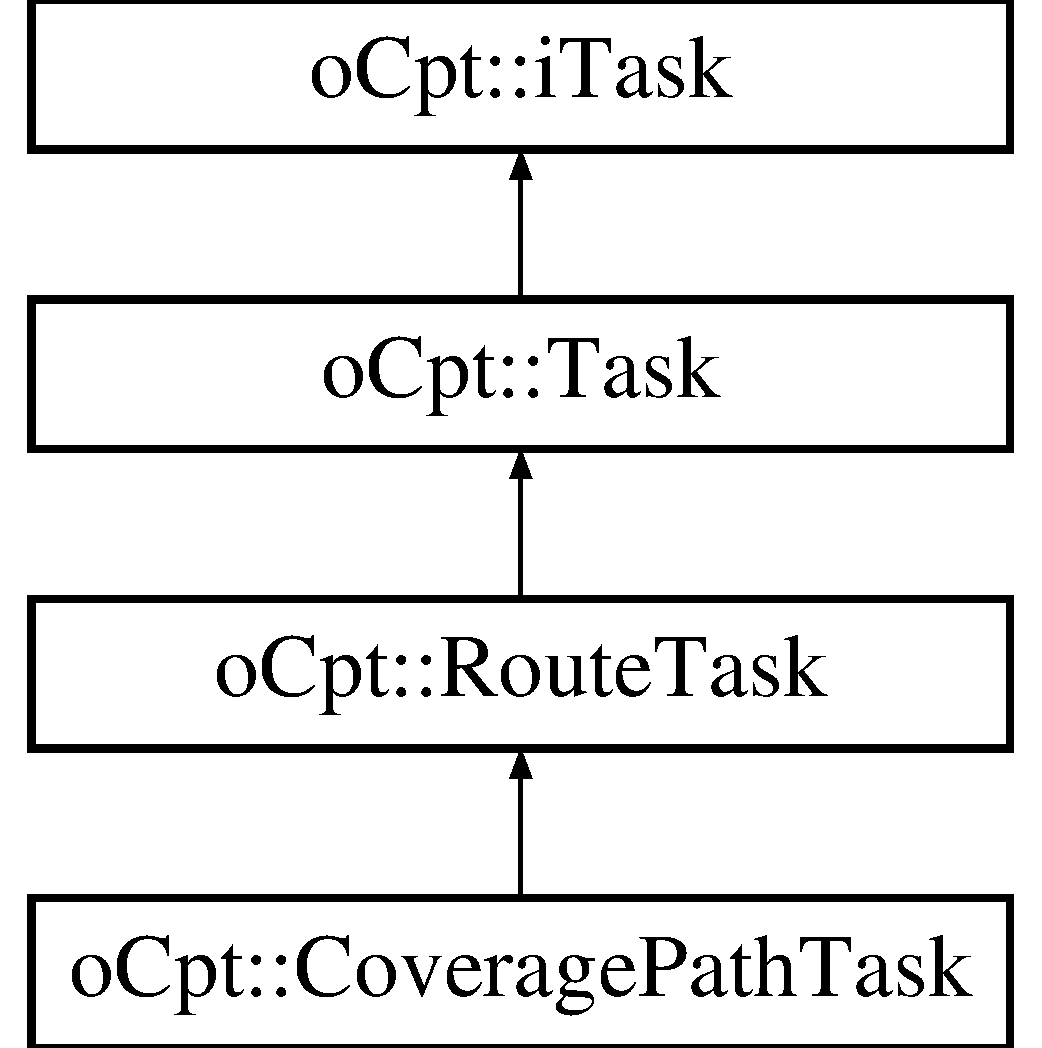
\includegraphics[height=4.000000cm]{classo_cpt_1_1_coverage_path_task}
\end{center}
\end{figure}
\subsection*{Public Member Functions}
\begin{DoxyCompactItemize}
\item 
\hyperlink{classo_cpt_1_1_coverage_path_task_abfdaef848200d9ad4173692cde984ca8}{Coverage\+Path\+Task} ()
\item 
virtual \hyperlink{classo_cpt_1_1_coverage_path_task_a8773343bb232c3a22b8ec6acf483bee1}{$\sim$\+Coverage\+Path\+Task} ()
\end{DoxyCompactItemize}
\subsection*{Additional Inherited Members}


\subsection{Detailed Description}
An object representing a coverage path task. 

All these types of tasks need a robot to cover a complete region in order to perform their tasks. According to \{cao\+\_\+region\+\_\+1988\} such a mobile robot should use the following criteria, for a region filling operation\+:
\begin{DoxyEnumerate}
\item The mobile robot must move through an entire area, i.\+e., the overall travel must cover a whole region.
\item The mobile robot must fill the region without overlapping paths.
\item Continuous and sequential operations without any repetition of paths is required of the robot.
\item The robot must avoid all obstacles in a region.
\item Simple motion trajectories (e.\+g., straight lines or circles) should be used for simplicity in control.
\item An \char`\"{}optimal\char`\"{} path is desired under the available conditions. It is not always possible to satisfy all these criteria for a complex environment. Sometimes a priority consideration is required. 
\end{DoxyEnumerate}

\subsection{Constructor \& Destructor Documentation}
\index{o\+Cpt\+::\+Coverage\+Path\+Task@{o\+Cpt\+::\+Coverage\+Path\+Task}!Coverage\+Path\+Task@{Coverage\+Path\+Task}}
\index{Coverage\+Path\+Task@{Coverage\+Path\+Task}!o\+Cpt\+::\+Coverage\+Path\+Task@{o\+Cpt\+::\+Coverage\+Path\+Task}}
\subsubsection[{\texorpdfstring{Coverage\+Path\+Task()}{CoveragePathTask()}}]{\setlength{\rightskip}{0pt plus 5cm}o\+Cpt\+::\+Coverage\+Path\+Task\+::\+Coverage\+Path\+Task (
\begin{DoxyParamCaption}
{}
\end{DoxyParamCaption}
)}\hypertarget{classo_cpt_1_1_coverage_path_task_abfdaef848200d9ad4173692cde984ca8}{}\label{classo_cpt_1_1_coverage_path_task_abfdaef848200d9ad4173692cde984ca8}
Constructor of the interface \begin{DoxyReturn}{Returns}

\end{DoxyReturn}
\index{o\+Cpt\+::\+Coverage\+Path\+Task@{o\+Cpt\+::\+Coverage\+Path\+Task}!````~Coverage\+Path\+Task@{$\sim$\+Coverage\+Path\+Task}}
\index{````~Coverage\+Path\+Task@{$\sim$\+Coverage\+Path\+Task}!o\+Cpt\+::\+Coverage\+Path\+Task@{o\+Cpt\+::\+Coverage\+Path\+Task}}
\subsubsection[{\texorpdfstring{$\sim$\+Coverage\+Path\+Task()}{~CoveragePathTask()}}]{\setlength{\rightskip}{0pt plus 5cm}o\+Cpt\+::\+Coverage\+Path\+Task\+::$\sim$\+Coverage\+Path\+Task (
\begin{DoxyParamCaption}
{}
\end{DoxyParamCaption}
)\hspace{0.3cm}{\ttfamily [virtual]}}\hypertarget{classo_cpt_1_1_coverage_path_task_a8773343bb232c3a22b8ec6acf483bee1}{}\label{classo_cpt_1_1_coverage_path_task_a8773343bb232c3a22b8ec6acf483bee1}
The deconstructor 

The documentation for this class was generated from the following files\+:\begin{DoxyCompactItemize}
\item 
include/\hyperlink{_task_8h}{Task.\+h}\item 
src/\hyperlink{_task_8cpp}{Task.\+cpp}\end{DoxyCompactItemize}

\hypertarget{classo_cpt_1_1_dredge_task}{}\section{o\+Cpt\+:\+:Dredge\+Task Class Reference}
\label{classo_cpt_1_1_dredge_task}\index{o\+Cpt\+::\+Dredge\+Task@{o\+Cpt\+::\+Dredge\+Task}}


An Object representing a dredging task.  




{\ttfamily \#include $<$Task.\+h$>$}



Inheritance diagram for o\+Cpt\+:\+:Dredge\+Task\+:\nopagebreak
\begin{figure}[H]
\begin{center}
\leavevmode
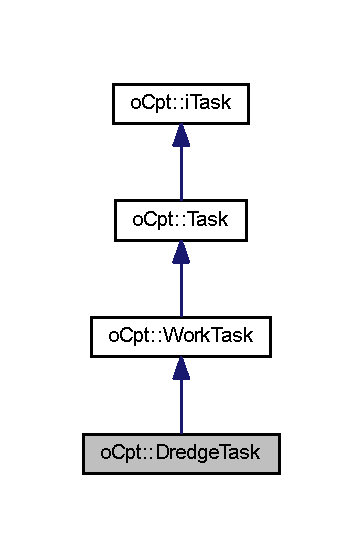
\includegraphics[width=175pt]{classo_cpt_1_1_dredge_task__inherit__graph}
\end{center}
\end{figure}


Collaboration diagram for o\+Cpt\+:\+:Dredge\+Task\+:\nopagebreak
\begin{figure}[H]
\begin{center}
\leavevmode
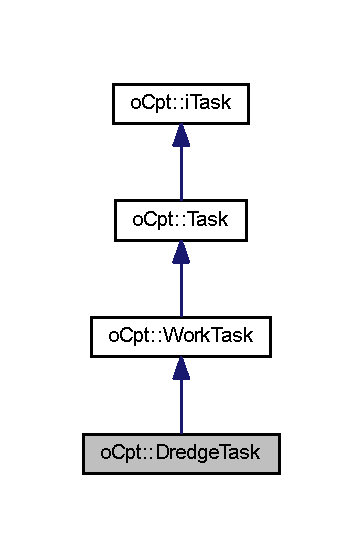
\includegraphics[width=175pt]{classo_cpt_1_1_dredge_task__coll__graph}
\end{center}
\end{figure}
\subsection*{Public Member Functions}
\begin{DoxyCompactItemize}
\item 
\hyperlink{classo_cpt_1_1_dredge_task_a959ef09f846314a23a9ad31be807f2d1}{Dredge\+Task} (\hyperlink{classo_cpt_1_1i_vessel_a43711a596f3bdfd0ca732ed3901edc97}{Vessel\+::ptr} vessel, bool concurrent=true)
\item 
virtual \hyperlink{classo_cpt_1_1_dredge_task_aa326cf6ddbb6e3019fb86f8d714bf323}{$\sim$\+Dredge\+Task} ()
\end{DoxyCompactItemize}
\subsection*{Additional Inherited Members}


\subsection{Detailed Description}
An Object representing a dredging task. 

All these types tasks make use of an actuator and sensors to perform dredging tasks 

Definition at line 287 of file Task.\+h.



\subsection{Constructor \& Destructor Documentation}
\hypertarget{classo_cpt_1_1_dredge_task_a959ef09f846314a23a9ad31be807f2d1}{}\label{classo_cpt_1_1_dredge_task_a959ef09f846314a23a9ad31be807f2d1} 
\index{o\+Cpt\+::\+Dredge\+Task@{o\+Cpt\+::\+Dredge\+Task}!Dredge\+Task@{Dredge\+Task}}
\index{Dredge\+Task@{Dredge\+Task}!o\+Cpt\+::\+Dredge\+Task@{o\+Cpt\+::\+Dredge\+Task}}
\subsubsection{\texorpdfstring{Dredge\+Task()}{DredgeTask()}}
{\footnotesize\ttfamily o\+Cpt\+::\+Dredge\+Task\+::\+Dredge\+Task (\begin{DoxyParamCaption}\item[{\hyperlink{classo_cpt_1_1i_vessel_a43711a596f3bdfd0ca732ed3901edc97}{Vessel\+::ptr}}]{vessel,  }\item[{bool}]{concurrent = {\ttfamily true} }\end{DoxyParamCaption})}

Constructor of the interface \begin{DoxyReturn}{Returns}

\end{DoxyReturn}


Definition at line 69 of file Task.\+cpp.

\hypertarget{classo_cpt_1_1_dredge_task_aa326cf6ddbb6e3019fb86f8d714bf323}{}\label{classo_cpt_1_1_dredge_task_aa326cf6ddbb6e3019fb86f8d714bf323} 
\index{o\+Cpt\+::\+Dredge\+Task@{o\+Cpt\+::\+Dredge\+Task}!````~Dredge\+Task@{$\sim$\+Dredge\+Task}}
\index{````~Dredge\+Task@{$\sim$\+Dredge\+Task}!o\+Cpt\+::\+Dredge\+Task@{o\+Cpt\+::\+Dredge\+Task}}
\subsubsection{\texorpdfstring{$\sim$\+Dredge\+Task()}{~DredgeTask()}}
{\footnotesize\ttfamily o\+Cpt\+::\+Dredge\+Task\+::$\sim$\+Dredge\+Task (\begin{DoxyParamCaption}{ }\end{DoxyParamCaption})\hspace{0.3cm}{\ttfamily [virtual]}}

The deconstructor 

Definition at line 71 of file Task.\+cpp.



The documentation for this class was generated from the following files\+:\begin{DoxyCompactItemize}
\item 
include/\+Core/\hyperlink{_task_8h}{Task.\+h}\item 
src/\+Core/\hyperlink{_task_8cpp}{Task.\+cpp}\end{DoxyCompactItemize}

\hypertarget{classo_cpt_1_1_follow_task}{}\section{o\+Cpt\+:\+:Follow\+Task Class Reference}
\label{classo_cpt_1_1_follow_task}\index{o\+Cpt\+::\+Follow\+Task@{o\+Cpt\+::\+Follow\+Task}}


An object representing a follow the target task.  




{\ttfamily \#include $<$Task.\+h$>$}

Inheritance diagram for o\+Cpt\+:\+:Follow\+Task\+:\begin{figure}[H]
\begin{center}
\leavevmode
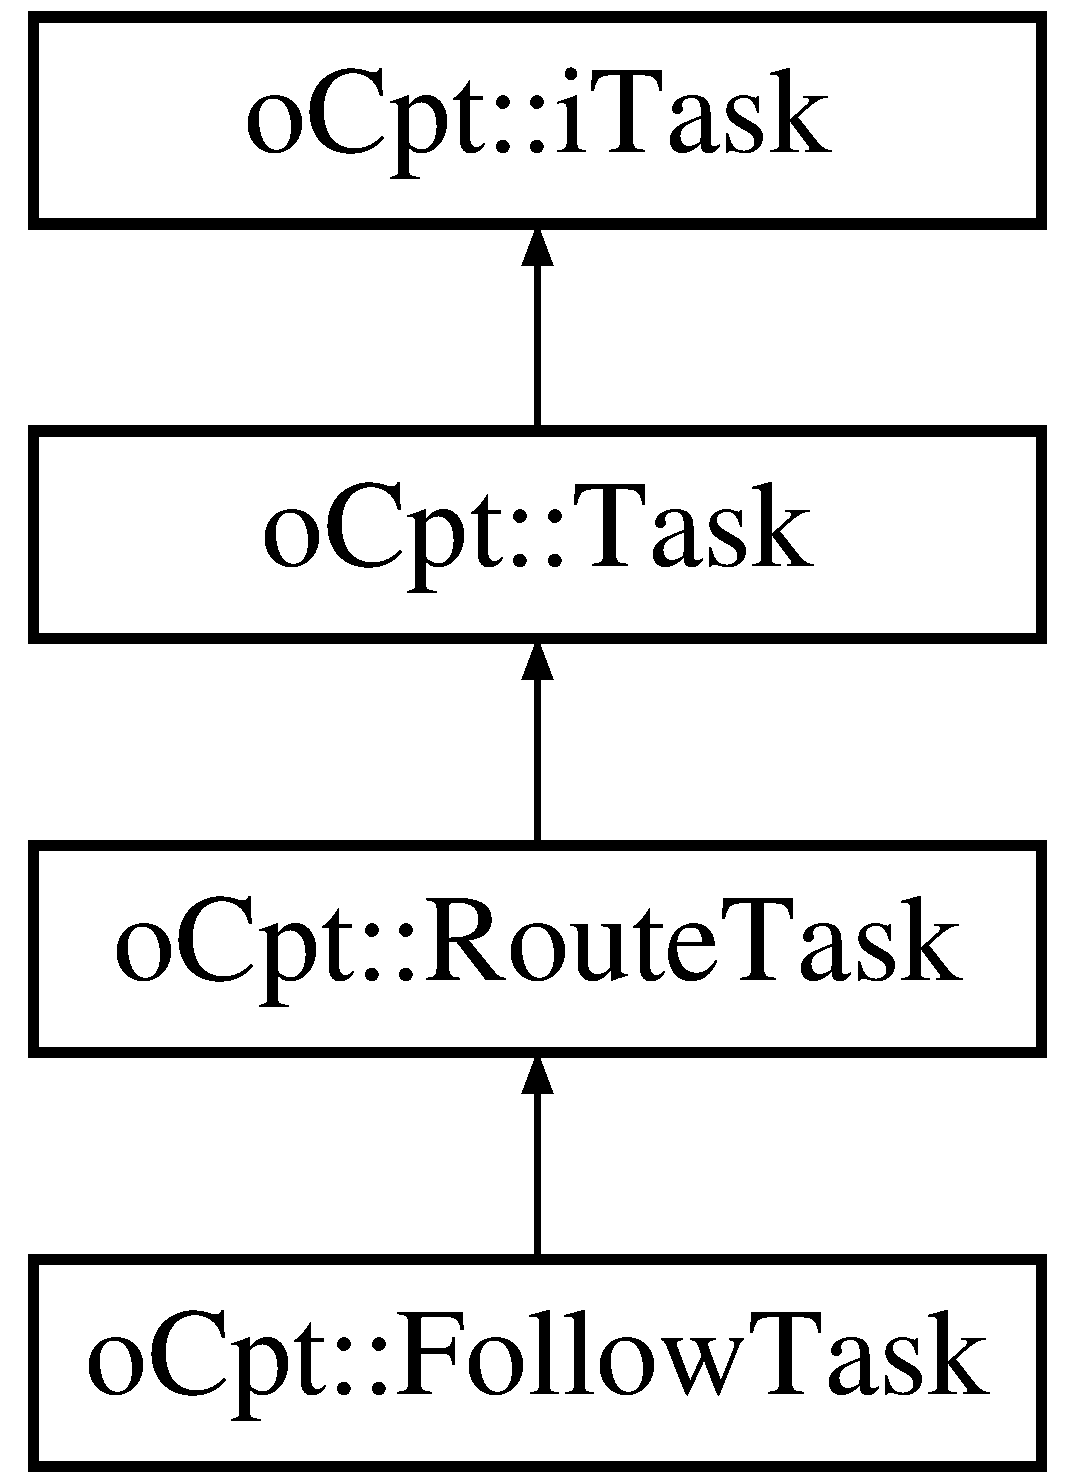
\includegraphics[height=4.000000cm]{classo_cpt_1_1_follow_task}
\end{center}
\end{figure}
\subsection*{Public Member Functions}
\begin{DoxyCompactItemize}
\item 
\hyperlink{classo_cpt_1_1_follow_task_a6e7f2d2b4037a331da8d0a994e79090c}{Follow\+Task} ()
\item 
virtual \hyperlink{classo_cpt_1_1_follow_task_ab93d2570c1e65704f6742aa5f3f6a440}{$\sim$\+Follow\+Task} ()
\end{DoxyCompactItemize}
\subsection*{Additional Inherited Members}


\subsection{Detailed Description}
An object representing a follow the target task. 

All these types of tasks need to follow a (moving) target 

\subsection{Constructor \& Destructor Documentation}
\index{o\+Cpt\+::\+Follow\+Task@{o\+Cpt\+::\+Follow\+Task}!Follow\+Task@{Follow\+Task}}
\index{Follow\+Task@{Follow\+Task}!o\+Cpt\+::\+Follow\+Task@{o\+Cpt\+::\+Follow\+Task}}
\subsubsection[{\texorpdfstring{Follow\+Task()}{FollowTask()}}]{\setlength{\rightskip}{0pt plus 5cm}o\+Cpt\+::\+Follow\+Task\+::\+Follow\+Task (
\begin{DoxyParamCaption}
{}
\end{DoxyParamCaption}
)}\hypertarget{classo_cpt_1_1_follow_task_a6e7f2d2b4037a331da8d0a994e79090c}{}\label{classo_cpt_1_1_follow_task_a6e7f2d2b4037a331da8d0a994e79090c}
Constructor of the interface \begin{DoxyReturn}{Returns}

\end{DoxyReturn}
\index{o\+Cpt\+::\+Follow\+Task@{o\+Cpt\+::\+Follow\+Task}!````~Follow\+Task@{$\sim$\+Follow\+Task}}
\index{````~Follow\+Task@{$\sim$\+Follow\+Task}!o\+Cpt\+::\+Follow\+Task@{o\+Cpt\+::\+Follow\+Task}}
\subsubsection[{\texorpdfstring{$\sim$\+Follow\+Task()}{~FollowTask()}}]{\setlength{\rightskip}{0pt plus 5cm}o\+Cpt\+::\+Follow\+Task\+::$\sim$\+Follow\+Task (
\begin{DoxyParamCaption}
{}
\end{DoxyParamCaption}
)\hspace{0.3cm}{\ttfamily [virtual]}}\hypertarget{classo_cpt_1_1_follow_task_ab93d2570c1e65704f6742aa5f3f6a440}{}\label{classo_cpt_1_1_follow_task_ab93d2570c1e65704f6742aa5f3f6a440}
The deconstructor 

The documentation for this class was generated from the following files\+:\begin{DoxyCompactItemize}
\item 
include/\hyperlink{_task_8h}{Task.\+h}\item 
src/\hyperlink{_task_8cpp}{Task.\+cpp}\end{DoxyCompactItemize}

\hypertarget{classo_cpt_1_1protocol_1_1gpio}{}\section{o\+Cpt\+:\+:protocol\+:\+:gpio Class Reference}
\label{classo_cpt_1_1protocol_1_1gpio}\index{o\+Cpt\+::protocol\+::gpio@{o\+Cpt\+::protocol\+::gpio}}


{\ttfamily \#include $<$Controller.\+h$>$}



Inheritance diagram for o\+Cpt\+:\+:protocol\+:\+:gpio\+:\nopagebreak
\begin{figure}[H]
\begin{center}
\leavevmode
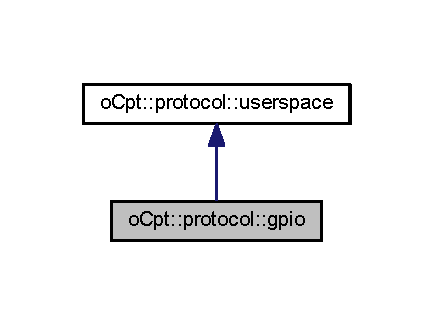
\includegraphics[width=208pt]{classo_cpt_1_1protocol_1_1gpio__inherit__graph}
\end{center}
\end{figure}


Collaboration diagram for o\+Cpt\+:\+:protocol\+:\+:gpio\+:\nopagebreak
\begin{figure}[H]
\begin{center}
\leavevmode
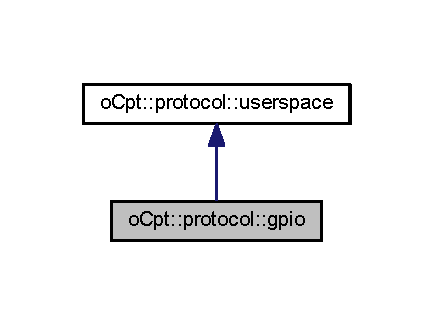
\includegraphics[width=208pt]{classo_cpt_1_1protocol_1_1gpio__coll__graph}
\end{center}
\end{figure}
\subsection*{Public Types}
\begin{DoxyCompactItemize}
\item 
enum \hyperlink{classo_cpt_1_1protocol_1_1gpio_af7acf963933bbc47d11d6fa1b8ce4d5b}{Direction} \{ \hyperlink{classo_cpt_1_1protocol_1_1gpio_af7acf963933bbc47d11d6fa1b8ce4d5bac8229afa7339514d640fdd7512456ec1}{I\+N\+P\+UT} = 105, 
\hyperlink{classo_cpt_1_1protocol_1_1gpio_af7acf963933bbc47d11d6fa1b8ce4d5baa8f40287c9c83f0528feec4792eb1923}{O\+U\+T\+P\+UT} = 111
 \}
\item 
enum \hyperlink{classo_cpt_1_1protocol_1_1gpio_a7d2d1d34f177f209ad642098d168656f}{Value} \{ \hyperlink{classo_cpt_1_1protocol_1_1gpio_a7d2d1d34f177f209ad642098d168656faa2cdaa57258d16622e014ff5d766f095}{L\+OW} = 48, 
\hyperlink{classo_cpt_1_1protocol_1_1gpio_a7d2d1d34f177f209ad642098d168656fade5ff2955239ef2860ee2d06f3be68d4}{H\+I\+GH} = 49
 \}
\item 
enum \hyperlink{classo_cpt_1_1protocol_1_1gpio_adbbd34b2bc4394ad5a71d94641dda9f9}{Edge} \{ \hyperlink{classo_cpt_1_1protocol_1_1gpio_adbbd34b2bc4394ad5a71d94641dda9f9a97a153b16162f7d3ebd04fe1bc59b8f8}{N\+O\+NE} = 110, 
\hyperlink{classo_cpt_1_1protocol_1_1gpio_adbbd34b2bc4394ad5a71d94641dda9f9a33b81c6d79fea86cd39ac781c6038678}{R\+I\+S\+I\+NG} = 114, 
\hyperlink{classo_cpt_1_1protocol_1_1gpio_adbbd34b2bc4394ad5a71d94641dda9f9ad706fd6e134b45f6521f6f10cac1ab3a}{F\+A\+L\+L\+I\+NG} = 102, 
\hyperlink{classo_cpt_1_1protocol_1_1gpio_adbbd34b2bc4394ad5a71d94641dda9f9a4fdd038edea2f194d145a18b371be597}{B\+O\+TH} = 98
 \}
\item 
typedef boost\+::shared\+\_\+ptr$<$ \hyperlink{classo_cpt_1_1protocol_1_1gpio}{gpio} $>$ \hyperlink{classo_cpt_1_1protocol_1_1gpio_acd4fb0fba7a813a8013511b374e73900}{ptr}
\item 
typedef boost\+::signals2\+::signal$<$ void()$>$ \hyperlink{classo_cpt_1_1protocol_1_1gpio_aa875802b20c7ef999c44af68e7f23621}{signal\+\_\+t}
\item 
typedef std\+::function$<$ void()$>$ \hyperlink{classo_cpt_1_1protocol_1_1gpio_ad553926a5fc9db445e7c9715abede2e3}{cb\+\_\+func}
\end{DoxyCompactItemize}
\subsection*{Public Member Functions}
\begin{DoxyCompactItemize}
\item 
\hyperlink{classo_cpt_1_1protocol_1_1gpio_a8ceba8e1629d1d6e87da53eb097d81e5}{gpio} (int pin\+Number, \hyperlink{classo_cpt_1_1protocol_1_1gpio_af7acf963933bbc47d11d6fa1b8ce4d5b}{Direction} direction=\hyperlink{classo_cpt_1_1protocol_1_1gpio_af7acf963933bbc47d11d6fa1b8ce4d5bac8229afa7339514d640fdd7512456ec1}{I\+N\+P\+UT}, \hyperlink{classo_cpt_1_1protocol_1_1gpio_a7d2d1d34f177f209ad642098d168656f}{Value} value=\hyperlink{classo_cpt_1_1protocol_1_1gpio_a7d2d1d34f177f209ad642098d168656faa2cdaa57258d16622e014ff5d766f095}{L\+OW}, \hyperlink{classo_cpt_1_1protocol_1_1gpio_adbbd34b2bc4394ad5a71d94641dda9f9}{Edge} edge=\hyperlink{classo_cpt_1_1protocol_1_1gpio_adbbd34b2bc4394ad5a71d94641dda9f9a97a153b16162f7d3ebd04fe1bc59b8f8}{N\+O\+NE})
\item 
\hyperlink{classo_cpt_1_1protocol_1_1gpio_a8ab3c04e4643a838f8d9ea26367e3545}{$\sim$gpio} ()
\item 
int \hyperlink{classo_cpt_1_1protocol_1_1gpio_a66f03a0097a751d56f046e1537432291}{get\+Pin\+Number} () const
\item 
void \hyperlink{classo_cpt_1_1protocol_1_1gpio_a1f3a810d9f15c6021c9df71994c08bd6}{set\+Pin\+Number} (int pin\+Number)
\item 
\hyperlink{classo_cpt_1_1protocol_1_1gpio_a7d2d1d34f177f209ad642098d168656f}{Value} \hyperlink{classo_cpt_1_1protocol_1_1gpio_a036e04db41883ec0e33dc9cf279a51f9}{get\+Value} () const
\item 
void \hyperlink{classo_cpt_1_1protocol_1_1gpio_a869cfd12f0b74afedb7dbb40eacfa402}{set\+Value} (\hyperlink{classo_cpt_1_1protocol_1_1gpio_a7d2d1d34f177f209ad642098d168656f}{Value} value)
\item 
\hyperlink{classo_cpt_1_1protocol_1_1gpio_af7acf963933bbc47d11d6fa1b8ce4d5b}{Direction} \hyperlink{classo_cpt_1_1protocol_1_1gpio_aa89066f15bd97035908e7df75913c54b}{get\+Direction} () const
\item 
void \hyperlink{classo_cpt_1_1protocol_1_1gpio_acf2779bab1d3e1d5ebccee55b9af6d5e}{set\+Direction} (\hyperlink{classo_cpt_1_1protocol_1_1gpio_af7acf963933bbc47d11d6fa1b8ce4d5b}{Direction} direction)
\item 
\hyperlink{classo_cpt_1_1protocol_1_1gpio_adbbd34b2bc4394ad5a71d94641dda9f9}{Edge} \hyperlink{classo_cpt_1_1protocol_1_1gpio_a1eaae952cf8f11f4d62989dace78607e}{get\+Edge} () const
\item 
void \hyperlink{classo_cpt_1_1protocol_1_1gpio_a026c5bceb1bff0328c2804d2748f8e3d}{set\+Edge} (\hyperlink{classo_cpt_1_1protocol_1_1gpio_adbbd34b2bc4394ad5a71d94641dda9f9}{Edge} edge)
\item 
void \hyperlink{classo_cpt_1_1protocol_1_1gpio_a9eb9df34a1e1aee22c47a8642c34eec0}{set\+Callback\+Function} (\hyperlink{classo_cpt_1_1protocol_1_1gpio_ad553926a5fc9db445e7c9715abede2e3}{cb\+\_\+func} cb)
\item 
void \hyperlink{classo_cpt_1_1protocol_1_1gpio_a0fd140f4fb32047ceba4a9a17891efe0}{wait\+For\+Edge} ()
\item 
void \hyperlink{classo_cpt_1_1protocol_1_1gpio_a02375f321f838da5f738eda8631ae0cc}{wait\+For\+Edge\+Async} ()
\item 
void \hyperlink{classo_cpt_1_1protocol_1_1gpio_a12c30093a002734375b29de19809aab0}{toggle} ()
\end{DoxyCompactItemize}
\subsection*{Static Public Member Functions}
\begin{DoxyCompactItemize}
\item 
static std\+::vector$<$ \hyperlink{classo_cpt_1_1protocol_1_1gpio_acd4fb0fba7a813a8013511b374e73900}{ptr} $>$ \hyperlink{classo_cpt_1_1protocol_1_1gpio_a2beacd45b177eb627e66a3b252a4aaff}{exported\+Gpios} ()
\end{DoxyCompactItemize}
\subsection*{Public Attributes}
\begin{DoxyCompactItemize}
\item 
\hyperlink{classo_cpt_1_1protocol_1_1gpio_aa875802b20c7ef999c44af68e7f23621}{signal\+\_\+t} \hyperlink{classo_cpt_1_1protocol_1_1gpio_aa24b7c7d759f783bc3e93745edc69a2b}{signal\+Changed}
\end{DoxyCompactItemize}
\subsection*{Private Member Functions}
\begin{DoxyCompactItemize}
\item 
void \hyperlink{classo_cpt_1_1protocol_1_1gpio_aac8bfbf4530ff929ea83f48e970d0598}{internal\+Cb\+Func} ()
\item 
void \hyperlink{classo_cpt_1_1protocol_1_1gpio_af7fef4210406ea75eb04cc96fd99e7eb}{export\+Pin} (const int \&number)
\item 
void \hyperlink{classo_cpt_1_1protocol_1_1gpio_af6383ac93d965d156617147c652ae56f}{unexport\+Pin} (const int \&number)
\item 
{\footnotesize template$<$typename T $>$ }\\void \hyperlink{classo_cpt_1_1protocol_1_1gpio_a0f2972fa7ad1981c7edeae79280aa11f}{write\+Pin\+Value} (const int \&number, const T \&value)
\item 
{\footnotesize template$<$typename T $>$ }\\void \hyperlink{classo_cpt_1_1protocol_1_1gpio_a08e30d2b5451a628857d18b3b75e3265}{write\+Pin\+Value} (std\+::string path, const T \&value)
\end{DoxyCompactItemize}
\subsection*{Static Private Member Functions}
\begin{DoxyCompactItemize}
\item 
{\footnotesize template$<$typename T $>$ }\\static T \hyperlink{classo_cpt_1_1protocol_1_1gpio_aa604ec2008a852ec0f378b4c98fa3a3c}{read\+Pin\+Value} (const int \&number)
\item 
{\footnotesize template$<$typename T $>$ }\\static T \hyperlink{classo_cpt_1_1protocol_1_1gpio_a3e50919a9b9712884d4e868487821dc6}{read\+Pin\+Value} (std\+::string path)
\end{DoxyCompactItemize}
\subsection*{Private Attributes}
\begin{DoxyCompactItemize}
\item 
int \hyperlink{classo_cpt_1_1protocol_1_1gpio_a618c388f95fff31d6decf7f8760e76a9}{pin\+Number\+\_\+}
\item 
\hyperlink{classo_cpt_1_1protocol_1_1gpio_a7d2d1d34f177f209ad642098d168656f}{Value} \hyperlink{classo_cpt_1_1protocol_1_1gpio_a301d39638a420a299728d353ade3997c}{value\+\_\+}
\item 
\hyperlink{classo_cpt_1_1protocol_1_1gpio_af7acf963933bbc47d11d6fa1b8ce4d5b}{Direction} \hyperlink{classo_cpt_1_1protocol_1_1gpio_adb5c9fe44ef91bf37812e9cdfd3141d4}{direction\+\_\+}
\item 
\hyperlink{classo_cpt_1_1protocol_1_1gpio_adbbd34b2bc4394ad5a71d94641dda9f9}{Edge} \hyperlink{classo_cpt_1_1protocol_1_1gpio_abdd5f6e987fdca5748a35622f72eaf2f}{edge\+\_\+}
\item 
std\+::string \hyperlink{classo_cpt_1_1protocol_1_1gpio_afac9293096c2636fcce60aff2b38698d}{gpiopath\+\_\+}
\item 
\hyperlink{classo_cpt_1_1protocol_1_1gpio_ad553926a5fc9db445e7c9715abede2e3}{cb\+\_\+func} \hyperlink{classo_cpt_1_1protocol_1_1gpio_a7d9d6a711dd0ba0d51649b85ca4d5bf4}{cb\+\_\+}
\item 
bool \hyperlink{classo_cpt_1_1protocol_1_1gpio_aefa2c3a350dce68af5b9eea8b84f0336}{thread\+Running\+\_\+}
\end{DoxyCompactItemize}
\subsection*{Additional Inherited Members}


\subsection{Detailed Description}
A General Pin Input Output class. This is the class that handles gpio\textquotesingle{}s in user space. Each pin can be set as either input or output, and have a High or a Low out-\//input. When a pin is set as input, it can be polled on the edge, execute a function or send a signal on the rising, falling or changing edge of the signal 

Definition at line 138 of file Controller.\+h.



\subsection{Member Typedef Documentation}
\hypertarget{classo_cpt_1_1protocol_1_1gpio_ad553926a5fc9db445e7c9715abede2e3}{}\label{classo_cpt_1_1protocol_1_1gpio_ad553926a5fc9db445e7c9715abede2e3} 
\index{o\+Cpt\+::protocol\+::gpio@{o\+Cpt\+::protocol\+::gpio}!cb\+\_\+func@{cb\+\_\+func}}
\index{cb\+\_\+func@{cb\+\_\+func}!o\+Cpt\+::protocol\+::gpio@{o\+Cpt\+::protocol\+::gpio}}
\subsubsection{\texorpdfstring{cb\+\_\+func}{cb\_func}}
{\footnotesize\ttfamily typedef std\+::function$<$void()$>$ \hyperlink{classo_cpt_1_1protocol_1_1gpio_ad553926a5fc9db445e7c9715abede2e3}{o\+Cpt\+::protocol\+::gpio\+::cb\+\_\+func}}



Definition at line 142 of file Controller.\+h.

\hypertarget{classo_cpt_1_1protocol_1_1gpio_acd4fb0fba7a813a8013511b374e73900}{}\label{classo_cpt_1_1protocol_1_1gpio_acd4fb0fba7a813a8013511b374e73900} 
\index{o\+Cpt\+::protocol\+::gpio@{o\+Cpt\+::protocol\+::gpio}!ptr@{ptr}}
\index{ptr@{ptr}!o\+Cpt\+::protocol\+::gpio@{o\+Cpt\+::protocol\+::gpio}}
\subsubsection{\texorpdfstring{ptr}{ptr}}
{\footnotesize\ttfamily typedef boost\+::shared\+\_\+ptr$<$\hyperlink{classo_cpt_1_1protocol_1_1gpio}{gpio}$>$ \hyperlink{classo_cpt_1_1protocol_1_1gpio_acd4fb0fba7a813a8013511b374e73900}{o\+Cpt\+::protocol\+::gpio\+::ptr}}



Definition at line 140 of file Controller.\+h.

\hypertarget{classo_cpt_1_1protocol_1_1gpio_aa875802b20c7ef999c44af68e7f23621}{}\label{classo_cpt_1_1protocol_1_1gpio_aa875802b20c7ef999c44af68e7f23621} 
\index{o\+Cpt\+::protocol\+::gpio@{o\+Cpt\+::protocol\+::gpio}!signal\+\_\+t@{signal\+\_\+t}}
\index{signal\+\_\+t@{signal\+\_\+t}!o\+Cpt\+::protocol\+::gpio@{o\+Cpt\+::protocol\+::gpio}}
\subsubsection{\texorpdfstring{signal\+\_\+t}{signal\_t}}
{\footnotesize\ttfamily typedef boost\+::signals2\+::signal$<$void()$>$ \hyperlink{classo_cpt_1_1protocol_1_1gpio_aa875802b20c7ef999c44af68e7f23621}{o\+Cpt\+::protocol\+::gpio\+::signal\+\_\+t}}



Definition at line 141 of file Controller.\+h.



\subsection{Member Enumeration Documentation}
\hypertarget{classo_cpt_1_1protocol_1_1gpio_af7acf963933bbc47d11d6fa1b8ce4d5b}{}\label{classo_cpt_1_1protocol_1_1gpio_af7acf963933bbc47d11d6fa1b8ce4d5b} 
\index{o\+Cpt\+::protocol\+::gpio@{o\+Cpt\+::protocol\+::gpio}!Direction@{Direction}}
\index{Direction@{Direction}!o\+Cpt\+::protocol\+::gpio@{o\+Cpt\+::protocol\+::gpio}}
\subsubsection{\texorpdfstring{Direction}{Direction}}
{\footnotesize\ttfamily enum \hyperlink{classo_cpt_1_1protocol_1_1gpio_af7acf963933bbc47d11d6fa1b8ce4d5b}{o\+Cpt\+::protocol\+::gpio\+::\+Direction}}

The Direction of the pin \begin{DoxyEnumFields}{Enumerator}
\raisebox{\heightof{T}}[0pt][0pt]{\index{I\+N\+P\+UT@{I\+N\+P\+UT}!o\+Cpt\+::protocol\+::gpio@{o\+Cpt\+::protocol\+::gpio}}\index{o\+Cpt\+::protocol\+::gpio@{o\+Cpt\+::protocol\+::gpio}!I\+N\+P\+UT@{I\+N\+P\+UT}}}\hypertarget{classo_cpt_1_1protocol_1_1gpio_af7acf963933bbc47d11d6fa1b8ce4d5bac8229afa7339514d640fdd7512456ec1}{}\label{classo_cpt_1_1protocol_1_1gpio_af7acf963933bbc47d11d6fa1b8ce4d5bac8229afa7339514d640fdd7512456ec1} 
I\+N\+P\+UT&\\
\hline

\raisebox{\heightof{T}}[0pt][0pt]{\index{O\+U\+T\+P\+UT@{O\+U\+T\+P\+UT}!o\+Cpt\+::protocol\+::gpio@{o\+Cpt\+::protocol\+::gpio}}\index{o\+Cpt\+::protocol\+::gpio@{o\+Cpt\+::protocol\+::gpio}!O\+U\+T\+P\+UT@{O\+U\+T\+P\+UT}}}\hypertarget{classo_cpt_1_1protocol_1_1gpio_af7acf963933bbc47d11d6fa1b8ce4d5baa8f40287c9c83f0528feec4792eb1923}{}\label{classo_cpt_1_1protocol_1_1gpio_af7acf963933bbc47d11d6fa1b8ce4d5baa8f40287c9c83f0528feec4792eb1923} 
O\+U\+T\+P\+UT&\\
\hline

\end{DoxyEnumFields}


Definition at line 147 of file Controller.\+h.

\hypertarget{classo_cpt_1_1protocol_1_1gpio_adbbd34b2bc4394ad5a71d94641dda9f9}{}\label{classo_cpt_1_1protocol_1_1gpio_adbbd34b2bc4394ad5a71d94641dda9f9} 
\index{o\+Cpt\+::protocol\+::gpio@{o\+Cpt\+::protocol\+::gpio}!Edge@{Edge}}
\index{Edge@{Edge}!o\+Cpt\+::protocol\+::gpio@{o\+Cpt\+::protocol\+::gpio}}
\subsubsection{\texorpdfstring{Edge}{Edge}}
{\footnotesize\ttfamily enum \hyperlink{classo_cpt_1_1protocol_1_1gpio_adbbd34b2bc4394ad5a71d94641dda9f9}{o\+Cpt\+::protocol\+::gpio\+::\+Edge}}

\begin{DoxyEnumFields}{Enumerator}
\raisebox{\heightof{T}}[0pt][0pt]{\index{N\+O\+NE@{N\+O\+NE}!o\+Cpt\+::protocol\+::gpio@{o\+Cpt\+::protocol\+::gpio}}\index{o\+Cpt\+::protocol\+::gpio@{o\+Cpt\+::protocol\+::gpio}!N\+O\+NE@{N\+O\+NE}}}\hypertarget{classo_cpt_1_1protocol_1_1gpio_adbbd34b2bc4394ad5a71d94641dda9f9a97a153b16162f7d3ebd04fe1bc59b8f8}{}\label{classo_cpt_1_1protocol_1_1gpio_adbbd34b2bc4394ad5a71d94641dda9f9a97a153b16162f7d3ebd04fe1bc59b8f8} 
N\+O\+NE&\\
\hline

\raisebox{\heightof{T}}[0pt][0pt]{\index{R\+I\+S\+I\+NG@{R\+I\+S\+I\+NG}!o\+Cpt\+::protocol\+::gpio@{o\+Cpt\+::protocol\+::gpio}}\index{o\+Cpt\+::protocol\+::gpio@{o\+Cpt\+::protocol\+::gpio}!R\+I\+S\+I\+NG@{R\+I\+S\+I\+NG}}}\hypertarget{classo_cpt_1_1protocol_1_1gpio_adbbd34b2bc4394ad5a71d94641dda9f9a33b81c6d79fea86cd39ac781c6038678}{}\label{classo_cpt_1_1protocol_1_1gpio_adbbd34b2bc4394ad5a71d94641dda9f9a33b81c6d79fea86cd39ac781c6038678} 
R\+I\+S\+I\+NG&\\
\hline

\raisebox{\heightof{T}}[0pt][0pt]{\index{F\+A\+L\+L\+I\+NG@{F\+A\+L\+L\+I\+NG}!o\+Cpt\+::protocol\+::gpio@{o\+Cpt\+::protocol\+::gpio}}\index{o\+Cpt\+::protocol\+::gpio@{o\+Cpt\+::protocol\+::gpio}!F\+A\+L\+L\+I\+NG@{F\+A\+L\+L\+I\+NG}}}\hypertarget{classo_cpt_1_1protocol_1_1gpio_adbbd34b2bc4394ad5a71d94641dda9f9ad706fd6e134b45f6521f6f10cac1ab3a}{}\label{classo_cpt_1_1protocol_1_1gpio_adbbd34b2bc4394ad5a71d94641dda9f9ad706fd6e134b45f6521f6f10cac1ab3a} 
F\+A\+L\+L\+I\+NG&\\
\hline

\raisebox{\heightof{T}}[0pt][0pt]{\index{B\+O\+TH@{B\+O\+TH}!o\+Cpt\+::protocol\+::gpio@{o\+Cpt\+::protocol\+::gpio}}\index{o\+Cpt\+::protocol\+::gpio@{o\+Cpt\+::protocol\+::gpio}!B\+O\+TH@{B\+O\+TH}}}\hypertarget{classo_cpt_1_1protocol_1_1gpio_adbbd34b2bc4394ad5a71d94641dda9f9a4fdd038edea2f194d145a18b371be597}{}\label{classo_cpt_1_1protocol_1_1gpio_adbbd34b2bc4394ad5a71d94641dda9f9a4fdd038edea2f194d145a18b371be597} 
B\+O\+TH&\\
\hline

\end{DoxyEnumFields}


Definition at line 157 of file Controller.\+h.

\hypertarget{classo_cpt_1_1protocol_1_1gpio_a7d2d1d34f177f209ad642098d168656f}{}\label{classo_cpt_1_1protocol_1_1gpio_a7d2d1d34f177f209ad642098d168656f} 
\index{o\+Cpt\+::protocol\+::gpio@{o\+Cpt\+::protocol\+::gpio}!Value@{Value}}
\index{Value@{Value}!o\+Cpt\+::protocol\+::gpio@{o\+Cpt\+::protocol\+::gpio}}
\subsubsection{\texorpdfstring{Value}{Value}}
{\footnotesize\ttfamily enum \hyperlink{classo_cpt_1_1protocol_1_1gpio_a7d2d1d34f177f209ad642098d168656f}{o\+Cpt\+::protocol\+::gpio\+::\+Value}}

\begin{DoxyEnumFields}{Enumerator}
\raisebox{\heightof{T}}[0pt][0pt]{\index{L\+OW@{L\+OW}!o\+Cpt\+::protocol\+::gpio@{o\+Cpt\+::protocol\+::gpio}}\index{o\+Cpt\+::protocol\+::gpio@{o\+Cpt\+::protocol\+::gpio}!L\+OW@{L\+OW}}}\hypertarget{classo_cpt_1_1protocol_1_1gpio_a7d2d1d34f177f209ad642098d168656faa2cdaa57258d16622e014ff5d766f095}{}\label{classo_cpt_1_1protocol_1_1gpio_a7d2d1d34f177f209ad642098d168656faa2cdaa57258d16622e014ff5d766f095} 
L\+OW&\\
\hline

\raisebox{\heightof{T}}[0pt][0pt]{\index{H\+I\+GH@{H\+I\+GH}!o\+Cpt\+::protocol\+::gpio@{o\+Cpt\+::protocol\+::gpio}}\index{o\+Cpt\+::protocol\+::gpio@{o\+Cpt\+::protocol\+::gpio}!H\+I\+GH@{H\+I\+GH}}}\hypertarget{classo_cpt_1_1protocol_1_1gpio_a7d2d1d34f177f209ad642098d168656fade5ff2955239ef2860ee2d06f3be68d4}{}\label{classo_cpt_1_1protocol_1_1gpio_a7d2d1d34f177f209ad642098d168656fade5ff2955239ef2860ee2d06f3be68d4} 
H\+I\+GH&\\
\hline

\end{DoxyEnumFields}


Definition at line 152 of file Controller.\+h.



\subsection{Constructor \& Destructor Documentation}
\hypertarget{classo_cpt_1_1protocol_1_1gpio_a8ceba8e1629d1d6e87da53eb097d81e5}{}\label{classo_cpt_1_1protocol_1_1gpio_a8ceba8e1629d1d6e87da53eb097d81e5} 
\index{o\+Cpt\+::protocol\+::gpio@{o\+Cpt\+::protocol\+::gpio}!gpio@{gpio}}
\index{gpio@{gpio}!o\+Cpt\+::protocol\+::gpio@{o\+Cpt\+::protocol\+::gpio}}
\subsubsection{\texorpdfstring{gpio()}{gpio()}}
{\footnotesize\ttfamily o\+Cpt\+::protocol\+::gpio\+::gpio (\begin{DoxyParamCaption}\item[{int}]{pin\+Number,  }\item[{\hyperlink{classo_cpt_1_1protocol_1_1gpio_af7acf963933bbc47d11d6fa1b8ce4d5b}{gpio\+::\+Direction}}]{direction = {\ttfamily \hyperlink{classo_cpt_1_1protocol_1_1gpio_af7acf963933bbc47d11d6fa1b8ce4d5bac8229afa7339514d640fdd7512456ec1}{I\+N\+P\+UT}},  }\item[{\hyperlink{classo_cpt_1_1protocol_1_1gpio_a7d2d1d34f177f209ad642098d168656f}{gpio\+::\+Value}}]{value = {\ttfamily \hyperlink{classo_cpt_1_1protocol_1_1gpio_a7d2d1d34f177f209ad642098d168656faa2cdaa57258d16622e014ff5d766f095}{L\+OW}},  }\item[{\hyperlink{classo_cpt_1_1protocol_1_1gpio_adbbd34b2bc4394ad5a71d94641dda9f9}{gpio\+::\+Edge}}]{edge = {\ttfamily \hyperlink{classo_cpt_1_1protocol_1_1gpio_adbbd34b2bc4394ad5a71d94641dda9f9a97a153b16162f7d3ebd04fe1bc59b8f8}{N\+O\+NE}} }\end{DoxyParamCaption})}

The constructor for the gpio class 
\begin{DoxyParams}{Parameters}
{\em pin\+Number} & the pin pumber (in user-\/space mapping) \\
\hline
{\em direction} & the Direction of a pin, with a default value as Direction\+::\+I\+N\+P\+UT \\
\hline
{\em value} & the start Value of a pin. With a default value of Value\+::\+L\+OW \\
\hline
{\em edge} & the Edge of a pin with the default value of Edge\+::\+N\+O\+NE \\
\hline
\end{DoxyParams}


Definition at line 337 of file Controller.\+cpp.



References cb\+\_\+, direction\+\_\+, edge\+\_\+, export\+Pin(), G\+P\+I\+O\+\_\+\+B\+A\+S\+E\+\_\+\+P\+A\+TH, gpiopath\+\_\+, internal\+Cb\+Func(), pin\+Number\+\_\+, and value\+\_\+.



Referenced by exported\+Gpios().

Here is the call graph for this function\+:\nopagebreak
\begin{figure}[H]
\begin{center}
\leavevmode
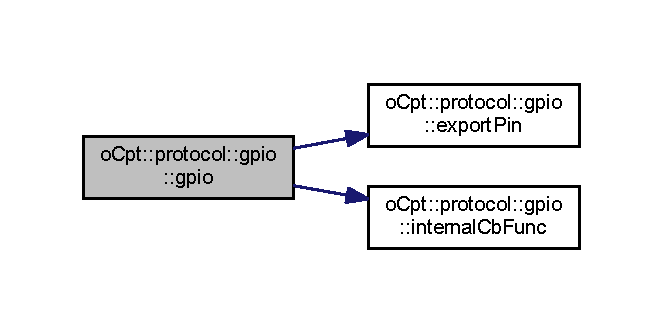
\includegraphics[width=318pt]{classo_cpt_1_1protocol_1_1gpio_a8ceba8e1629d1d6e87da53eb097d81e5_cgraph}
\end{center}
\end{figure}
Here is the caller graph for this function\+:\nopagebreak
\begin{figure}[H]
\begin{center}
\leavevmode
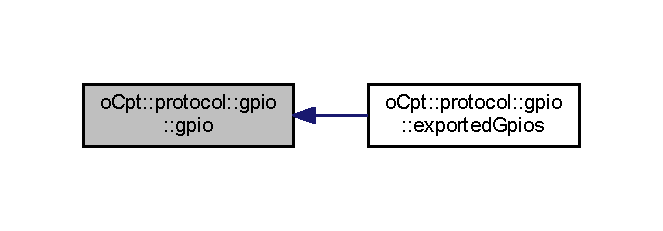
\includegraphics[width=318pt]{classo_cpt_1_1protocol_1_1gpio_a8ceba8e1629d1d6e87da53eb097d81e5_icgraph}
\end{center}
\end{figure}
\hypertarget{classo_cpt_1_1protocol_1_1gpio_a8ab3c04e4643a838f8d9ea26367e3545}{}\label{classo_cpt_1_1protocol_1_1gpio_a8ab3c04e4643a838f8d9ea26367e3545} 
\index{o\+Cpt\+::protocol\+::gpio@{o\+Cpt\+::protocol\+::gpio}!````~gpio@{$\sim$gpio}}
\index{````~gpio@{$\sim$gpio}!o\+Cpt\+::protocol\+::gpio@{o\+Cpt\+::protocol\+::gpio}}
\subsubsection{\texorpdfstring{$\sim$gpio()}{~gpio()}}
{\footnotesize\ttfamily o\+Cpt\+::protocol\+::gpio\+::$\sim$gpio (\begin{DoxyParamCaption}{ }\end{DoxyParamCaption})}

The deconstructor 

Definition at line 353 of file Controller.\+cpp.



References pin\+Number\+\_\+, and unexport\+Pin().

Here is the call graph for this function\+:\nopagebreak
\begin{figure}[H]
\begin{center}
\leavevmode
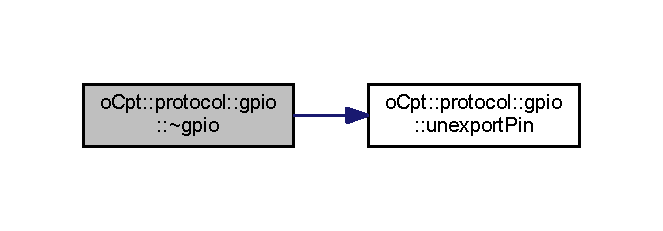
\includegraphics[width=318pt]{classo_cpt_1_1protocol_1_1gpio_a8ab3c04e4643a838f8d9ea26367e3545_cgraph}
\end{center}
\end{figure}


\subsection{Member Function Documentation}
\hypertarget{classo_cpt_1_1protocol_1_1gpio_a2beacd45b177eb627e66a3b252a4aaff}{}\label{classo_cpt_1_1protocol_1_1gpio_a2beacd45b177eb627e66a3b252a4aaff} 
\index{o\+Cpt\+::protocol\+::gpio@{o\+Cpt\+::protocol\+::gpio}!exported\+Gpios@{exported\+Gpios}}
\index{exported\+Gpios@{exported\+Gpios}!o\+Cpt\+::protocol\+::gpio@{o\+Cpt\+::protocol\+::gpio}}
\subsubsection{\texorpdfstring{exported\+Gpios()}{exportedGpios()}}
{\footnotesize\ttfamily std\+::vector$<$ \hyperlink{classo_cpt_1_1protocol_1_1gpio_acd4fb0fba7a813a8013511b374e73900}{gpio\+::ptr} $>$ o\+Cpt\+::protocol\+::gpio\+::exported\+Gpios (\begin{DoxyParamCaption}{ }\end{DoxyParamCaption})\hspace{0.3cm}{\ttfamily [static]}}

Static function which creates a vector containing new gpio shared\+\_\+ptr for each pin that is currently exported in the user space. \begin{DoxyReturn}{Returns}
A vector with shared\+\_\+ptr\textquotesingle{}s of all exported gpio\textquotesingle{}s in user-\/space 
\end{DoxyReturn}
Iterate through all exported pins 

Definition at line 357 of file Controller.\+cpp.



References gpio(), and G\+P\+I\+O\+\_\+\+B\+A\+S\+E\+\_\+\+P\+A\+TH.

Here is the call graph for this function\+:\nopagebreak
\begin{figure}[H]
\begin{center}
\leavevmode
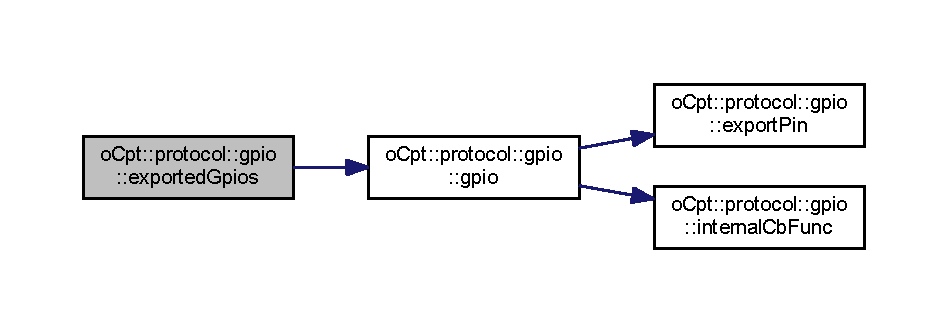
\includegraphics[width=350pt]{classo_cpt_1_1protocol_1_1gpio_a2beacd45b177eb627e66a3b252a4aaff_cgraph}
\end{center}
\end{figure}
\hypertarget{classo_cpt_1_1protocol_1_1gpio_af7fef4210406ea75eb04cc96fd99e7eb}{}\label{classo_cpt_1_1protocol_1_1gpio_af7fef4210406ea75eb04cc96fd99e7eb} 
\index{o\+Cpt\+::protocol\+::gpio@{o\+Cpt\+::protocol\+::gpio}!export\+Pin@{export\+Pin}}
\index{export\+Pin@{export\+Pin}!o\+Cpt\+::protocol\+::gpio@{o\+Cpt\+::protocol\+::gpio}}
\subsubsection{\texorpdfstring{export\+Pin()}{exportPin()}}
{\footnotesize\ttfamily void o\+Cpt\+::protocol\+::gpio\+::export\+Pin (\begin{DoxyParamCaption}\item[{const int \&}]{number }\end{DoxyParamCaption})\hspace{0.3cm}{\ttfamily [private]}}

Export the pin in user-\/space 
\begin{DoxyParams}{Parameters}
{\em number} & the pin number to be exported \\
\hline
\end{DoxyParams}


Definition at line 381 of file Controller.\+cpp.



References G\+P\+I\+O\+\_\+\+B\+A\+S\+E\+\_\+\+P\+A\+TH.



Referenced by gpio().

Here is the caller graph for this function\+:\nopagebreak
\begin{figure}[H]
\begin{center}
\leavevmode
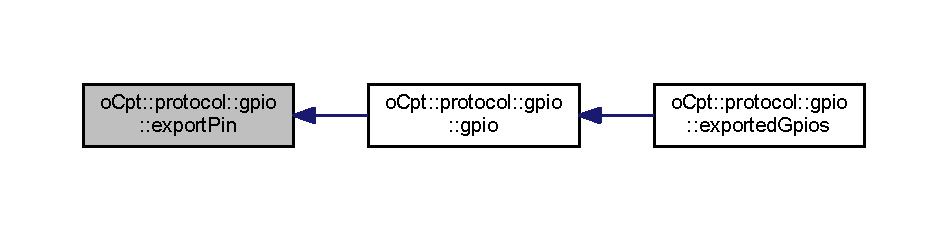
\includegraphics[width=350pt]{classo_cpt_1_1protocol_1_1gpio_af7fef4210406ea75eb04cc96fd99e7eb_icgraph}
\end{center}
\end{figure}
\hypertarget{classo_cpt_1_1protocol_1_1gpio_aa89066f15bd97035908e7df75913c54b}{}\label{classo_cpt_1_1protocol_1_1gpio_aa89066f15bd97035908e7df75913c54b} 
\index{o\+Cpt\+::protocol\+::gpio@{o\+Cpt\+::protocol\+::gpio}!get\+Direction@{get\+Direction}}
\index{get\+Direction@{get\+Direction}!o\+Cpt\+::protocol\+::gpio@{o\+Cpt\+::protocol\+::gpio}}
\subsubsection{\texorpdfstring{get\+Direction()}{getDirection()}}
{\footnotesize\ttfamily \hyperlink{classo_cpt_1_1protocol_1_1gpio_af7acf963933bbc47d11d6fa1b8ce4d5b}{gpio\+::\+Direction} o\+Cpt\+::protocol\+::gpio\+::get\+Direction (\begin{DoxyParamCaption}{ }\end{DoxyParamCaption}) const}

Get the current Direction. note this doesn\textquotesingle{}t take into accoutn external changes done outside this library \begin{DoxyReturn}{Returns}
either Direction\+::\+I\+N\+P\+UT or Direction\+::\+Output 
\end{DoxyReturn}


Definition at line 314 of file Controller.\+cpp.

\hypertarget{classo_cpt_1_1protocol_1_1gpio_a1eaae952cf8f11f4d62989dace78607e}{}\label{classo_cpt_1_1protocol_1_1gpio_a1eaae952cf8f11f4d62989dace78607e} 
\index{o\+Cpt\+::protocol\+::gpio@{o\+Cpt\+::protocol\+::gpio}!get\+Edge@{get\+Edge}}
\index{get\+Edge@{get\+Edge}!o\+Cpt\+::protocol\+::gpio@{o\+Cpt\+::protocol\+::gpio}}
\subsubsection{\texorpdfstring{get\+Edge()}{getEdge()}}
{\footnotesize\ttfamily \hyperlink{classo_cpt_1_1protocol_1_1gpio_adbbd34b2bc4394ad5a71d94641dda9f9}{gpio\+::\+Edge} o\+Cpt\+::protocol\+::gpio\+::get\+Edge (\begin{DoxyParamCaption}{ }\end{DoxyParamCaption}) const}

Get the current Edge of the pin. If the Direction is set to Direction\+::\+I\+N\+P\+UT the value is set in user-\/space, otherwise it is set in the object itself \begin{DoxyReturn}{Returns}

\end{DoxyReturn}


Definition at line 323 of file Controller.\+cpp.

\hypertarget{classo_cpt_1_1protocol_1_1gpio_a66f03a0097a751d56f046e1537432291}{}\label{classo_cpt_1_1protocol_1_1gpio_a66f03a0097a751d56f046e1537432291} 
\index{o\+Cpt\+::protocol\+::gpio@{o\+Cpt\+::protocol\+::gpio}!get\+Pin\+Number@{get\+Pin\+Number}}
\index{get\+Pin\+Number@{get\+Pin\+Number}!o\+Cpt\+::protocol\+::gpio@{o\+Cpt\+::protocol\+::gpio}}
\subsubsection{\texorpdfstring{get\+Pin\+Number()}{getPinNumber()}}
{\footnotesize\ttfamily int o\+Cpt\+::protocol\+::gpio\+::get\+Pin\+Number (\begin{DoxyParamCaption}{ }\end{DoxyParamCaption}) const}

Get the current pin number \begin{DoxyReturn}{Returns}
an int representing the pin number in user-\/space mapping 
\end{DoxyReturn}


Definition at line 291 of file Controller.\+cpp.

\hypertarget{classo_cpt_1_1protocol_1_1gpio_a036e04db41883ec0e33dc9cf279a51f9}{}\label{classo_cpt_1_1protocol_1_1gpio_a036e04db41883ec0e33dc9cf279a51f9} 
\index{o\+Cpt\+::protocol\+::gpio@{o\+Cpt\+::protocol\+::gpio}!get\+Value@{get\+Value}}
\index{get\+Value@{get\+Value}!o\+Cpt\+::protocol\+::gpio@{o\+Cpt\+::protocol\+::gpio}}
\subsubsection{\texorpdfstring{get\+Value()}{getValue()}}
{\footnotesize\ttfamily \hyperlink{classo_cpt_1_1protocol_1_1gpio_a7d2d1d34f177f209ad642098d168656f}{gpio\+::\+Value} o\+Cpt\+::protocol\+::gpio\+::get\+Value (\begin{DoxyParamCaption}{ }\end{DoxyParamCaption}) const}

Get the current value of the pin, if the Direction is set to Direction\+::\+I\+N\+P\+UT the value is obtained from the user space, otherwise the value is read from object itself \begin{DoxyReturn}{Returns}
either Value\+::\+H\+I\+GH or Value\+::\+L\+OW 
\end{DoxyReturn}


Definition at line 300 of file Controller.\+cpp.

\hypertarget{classo_cpt_1_1protocol_1_1gpio_aac8bfbf4530ff929ea83f48e970d0598}{}\label{classo_cpt_1_1protocol_1_1gpio_aac8bfbf4530ff929ea83f48e970d0598} 
\index{o\+Cpt\+::protocol\+::gpio@{o\+Cpt\+::protocol\+::gpio}!internal\+Cb\+Func@{internal\+Cb\+Func}}
\index{internal\+Cb\+Func@{internal\+Cb\+Func}!o\+Cpt\+::protocol\+::gpio@{o\+Cpt\+::protocol\+::gpio}}
\subsubsection{\texorpdfstring{internal\+Cb\+Func()}{internalCbFunc()}}
{\footnotesize\ttfamily void o\+Cpt\+::protocol\+::gpio\+::internal\+Cb\+Func (\begin{DoxyParamCaption}{ }\end{DoxyParamCaption})\hspace{0.3cm}{\ttfamily [private]}}

The internal callback function, which triggers the signal\+Changed signal 

Definition at line 418 of file Controller.\+cpp.



References signal\+Changed.



Referenced by gpio().

Here is the caller graph for this function\+:\nopagebreak
\begin{figure}[H]
\begin{center}
\leavevmode
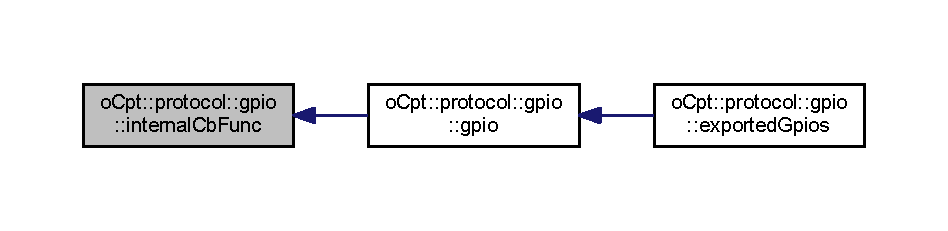
\includegraphics[width=350pt]{classo_cpt_1_1protocol_1_1gpio_aac8bfbf4530ff929ea83f48e970d0598_icgraph}
\end{center}
\end{figure}
\hypertarget{classo_cpt_1_1protocol_1_1gpio_aa604ec2008a852ec0f378b4c98fa3a3c}{}\label{classo_cpt_1_1protocol_1_1gpio_aa604ec2008a852ec0f378b4c98fa3a3c} 
\index{o\+Cpt\+::protocol\+::gpio@{o\+Cpt\+::protocol\+::gpio}!read\+Pin\+Value@{read\+Pin\+Value}}
\index{read\+Pin\+Value@{read\+Pin\+Value}!o\+Cpt\+::protocol\+::gpio@{o\+Cpt\+::protocol\+::gpio}}
\subsubsection{\texorpdfstring{read\+Pin\+Value()}{readPinValue()}\hspace{0.1cm}{\footnotesize\ttfamily [1/2]}}
{\footnotesize\ttfamily template$<$typename T $>$ \\
static T o\+Cpt\+::protocol\+::gpio\+::read\+Pin\+Value (\begin{DoxyParamCaption}\item[{const int \&}]{number }\end{DoxyParamCaption})\hspace{0.3cm}{\ttfamily [inline]}, {\ttfamily [static]}, {\ttfamily [private]}}

Static generic function returning the value in user-\/space of either Direction, Edge or Value. Depending on the typename 
\begin{DoxyTemplParams}{Template Parameters}
{\em T} & The value to return either the Value, Edge or Direction \\
\hline
\end{DoxyTemplParams}

\begin{DoxyParams}{Parameters}
{\em number} & the pin as number \\
\hline
\end{DoxyParams}
\begin{DoxyReturn}{Returns}
The read value as either Value, Edge or Direction 
\end{DoxyReturn}


Definition at line 291 of file Controller.\+h.



References G\+P\+I\+O\+\_\+\+B\+A\+S\+E\+\_\+\+P\+A\+TH.

\hypertarget{classo_cpt_1_1protocol_1_1gpio_a3e50919a9b9712884d4e868487821dc6}{}\label{classo_cpt_1_1protocol_1_1gpio_a3e50919a9b9712884d4e868487821dc6} 
\index{o\+Cpt\+::protocol\+::gpio@{o\+Cpt\+::protocol\+::gpio}!read\+Pin\+Value@{read\+Pin\+Value}}
\index{read\+Pin\+Value@{read\+Pin\+Value}!o\+Cpt\+::protocol\+::gpio@{o\+Cpt\+::protocol\+::gpio}}
\subsubsection{\texorpdfstring{read\+Pin\+Value()}{readPinValue()}\hspace{0.1cm}{\footnotesize\ttfamily [2/2]}}
{\footnotesize\ttfamily template$<$typename T $>$ \\
static T o\+Cpt\+::protocol\+::gpio\+::read\+Pin\+Value (\begin{DoxyParamCaption}\item[{std\+::string}]{path }\end{DoxyParamCaption})\hspace{0.3cm}{\ttfamily [inline]}, {\ttfamily [static]}, {\ttfamily [private]}}

Static generic function returning the value in user-\/space of either Direction, Edge or Value. Depending on the typename. This function is quicker then the overload function taking the pin number as int. and is therefore preffered to obtain the Value. 
\begin{DoxyTemplParams}{Template Parameters}
{\em T} & The value to return either the Value, Edge or Direction \\
\hline
\end{DoxyTemplParams}

\begin{DoxyParams}{Parameters}
{\em path} & the pin as user-\/space path \\
\hline
\end{DoxyParams}
\begin{DoxyReturn}{Returns}
the read value as either Value, Edge or Direction 
\end{DoxyReturn}


Definition at line 304 of file Controller.\+h.



References boost\+::units\+::constants\+::c.

\hypertarget{classo_cpt_1_1protocol_1_1gpio_a9eb9df34a1e1aee22c47a8642c34eec0}{}\label{classo_cpt_1_1protocol_1_1gpio_a9eb9df34a1e1aee22c47a8642c34eec0} 
\index{o\+Cpt\+::protocol\+::gpio@{o\+Cpt\+::protocol\+::gpio}!set\+Callback\+Function@{set\+Callback\+Function}}
\index{set\+Callback\+Function@{set\+Callback\+Function}!o\+Cpt\+::protocol\+::gpio@{o\+Cpt\+::protocol\+::gpio}}
\subsubsection{\texorpdfstring{set\+Callback\+Function()}{setCallbackFunction()}}
{\footnotesize\ttfamily void o\+Cpt\+::protocol\+::gpio\+::set\+Callback\+Function (\begin{DoxyParamCaption}\item[{\hyperlink{classo_cpt_1_1protocol_1_1gpio_ad553926a5fc9db445e7c9715abede2e3}{gpio\+::cb\+\_\+func}}]{cb }\end{DoxyParamCaption})}

Set a new Callbackfunction which is called on a certain Edge 
\begin{DoxyParams}{Parameters}
{\em cb} & the callback function \\
\hline
\end{DoxyParams}


Definition at line 414 of file Controller.\+cpp.



References cb\+\_\+.

\hypertarget{classo_cpt_1_1protocol_1_1gpio_acf2779bab1d3e1d5ebccee55b9af6d5e}{}\label{classo_cpt_1_1protocol_1_1gpio_acf2779bab1d3e1d5ebccee55b9af6d5e} 
\index{o\+Cpt\+::protocol\+::gpio@{o\+Cpt\+::protocol\+::gpio}!set\+Direction@{set\+Direction}}
\index{set\+Direction@{set\+Direction}!o\+Cpt\+::protocol\+::gpio@{o\+Cpt\+::protocol\+::gpio}}
\subsubsection{\texorpdfstring{set\+Direction()}{setDirection()}}
{\footnotesize\ttfamily void o\+Cpt\+::protocol\+::gpio\+::set\+Direction (\begin{DoxyParamCaption}\item[{\hyperlink{classo_cpt_1_1protocol_1_1gpio_af7acf963933bbc47d11d6fa1b8ce4d5b}{gpio\+::\+Direction}}]{direction }\end{DoxyParamCaption})}

Set the Direction of the pin 
\begin{DoxyParams}{Parameters}
{\em direction} & the Direction of the pin \\
\hline
\end{DoxyParams}


Definition at line 318 of file Controller.\+cpp.



References direction\+\_\+.

\hypertarget{classo_cpt_1_1protocol_1_1gpio_a026c5bceb1bff0328c2804d2748f8e3d}{}\label{classo_cpt_1_1protocol_1_1gpio_a026c5bceb1bff0328c2804d2748f8e3d} 
\index{o\+Cpt\+::protocol\+::gpio@{o\+Cpt\+::protocol\+::gpio}!set\+Edge@{set\+Edge}}
\index{set\+Edge@{set\+Edge}!o\+Cpt\+::protocol\+::gpio@{o\+Cpt\+::protocol\+::gpio}}
\subsubsection{\texorpdfstring{set\+Edge()}{setEdge()}}
{\footnotesize\ttfamily void o\+Cpt\+::protocol\+::gpio\+::set\+Edge (\begin{DoxyParamCaption}\item[{\hyperlink{classo_cpt_1_1protocol_1_1gpio_adbbd34b2bc4394ad5a71d94641dda9f9}{gpio\+::\+Edge}}]{edge }\end{DoxyParamCaption})}

Set the Edge of the of the pin. if the Direction is set to Direction\+::\+I\+N\+P\+UT, the value is set in user-\/space, otherwise it is set in the object itself 
\begin{DoxyParams}{Parameters}
{\em edge} & \\
\hline
\end{DoxyParams}


Definition at line 330 of file Controller.\+cpp.



References edge\+\_\+.

\hypertarget{classo_cpt_1_1protocol_1_1gpio_a1f3a810d9f15c6021c9df71994c08bd6}{}\label{classo_cpt_1_1protocol_1_1gpio_a1f3a810d9f15c6021c9df71994c08bd6} 
\index{o\+Cpt\+::protocol\+::gpio@{o\+Cpt\+::protocol\+::gpio}!set\+Pin\+Number@{set\+Pin\+Number}}
\index{set\+Pin\+Number@{set\+Pin\+Number}!o\+Cpt\+::protocol\+::gpio@{o\+Cpt\+::protocol\+::gpio}}
\subsubsection{\texorpdfstring{set\+Pin\+Number()}{setPinNumber()}}
{\footnotesize\ttfamily void o\+Cpt\+::protocol\+::gpio\+::set\+Pin\+Number (\begin{DoxyParamCaption}\item[{int}]{pin\+Number }\end{DoxyParamCaption})}

Set the new pinbumber (don\textquotesingle{}t use yet) 
\begin{DoxyParams}{Parameters}
{\em pin\+Number} & the pinmuber to be set \\
\hline
\end{DoxyParams}


Definition at line 295 of file Controller.\+cpp.



References pin\+Number\+\_\+.

\hypertarget{classo_cpt_1_1protocol_1_1gpio_a869cfd12f0b74afedb7dbb40eacfa402}{}\label{classo_cpt_1_1protocol_1_1gpio_a869cfd12f0b74afedb7dbb40eacfa402} 
\index{o\+Cpt\+::protocol\+::gpio@{o\+Cpt\+::protocol\+::gpio}!set\+Value@{set\+Value}}
\index{set\+Value@{set\+Value}!o\+Cpt\+::protocol\+::gpio@{o\+Cpt\+::protocol\+::gpio}}
\subsubsection{\texorpdfstring{set\+Value()}{setValue()}}
{\footnotesize\ttfamily void o\+Cpt\+::protocol\+::gpio\+::set\+Value (\begin{DoxyParamCaption}\item[{\hyperlink{classo_cpt_1_1protocol_1_1gpio_a7d2d1d34f177f209ad642098d168656f}{gpio\+::\+Value}}]{value }\end{DoxyParamCaption})}

Set the current value, if the Direction is set to Direction\+::\+O\+U\+T\+P\+UT the value is set ti userspace, either it is set to object itself 
\begin{DoxyParams}{Parameters}
{\em value} & \\
\hline
\end{DoxyParams}


Definition at line 307 of file Controller.\+cpp.



References value\+\_\+.

\hypertarget{classo_cpt_1_1protocol_1_1gpio_a12c30093a002734375b29de19809aab0}{}\label{classo_cpt_1_1protocol_1_1gpio_a12c30093a002734375b29de19809aab0} 
\index{o\+Cpt\+::protocol\+::gpio@{o\+Cpt\+::protocol\+::gpio}!toggle@{toggle}}
\index{toggle@{toggle}!o\+Cpt\+::protocol\+::gpio@{o\+Cpt\+::protocol\+::gpio}}
\subsubsection{\texorpdfstring{toggle()}{toggle()}}
{\footnotesize\ttfamily void o\+Cpt\+::protocol\+::gpio\+::toggle (\begin{DoxyParamCaption}{ }\end{DoxyParamCaption})}

Toggle the value\+\_\+ of the pin if Value\+::\+High then the value\+\_\+ is set to Value\+::\+L\+OW 

Definition at line 409 of file Controller.\+cpp.



References gpiopath\+\_\+, and value\+\_\+.

\hypertarget{classo_cpt_1_1protocol_1_1gpio_af6383ac93d965d156617147c652ae56f}{}\label{classo_cpt_1_1protocol_1_1gpio_af6383ac93d965d156617147c652ae56f} 
\index{o\+Cpt\+::protocol\+::gpio@{o\+Cpt\+::protocol\+::gpio}!unexport\+Pin@{unexport\+Pin}}
\index{unexport\+Pin@{unexport\+Pin}!o\+Cpt\+::protocol\+::gpio@{o\+Cpt\+::protocol\+::gpio}}
\subsubsection{\texorpdfstring{unexport\+Pin()}{unexportPin()}}
{\footnotesize\ttfamily void o\+Cpt\+::protocol\+::gpio\+::unexport\+Pin (\begin{DoxyParamCaption}\item[{const int \&}]{number }\end{DoxyParamCaption})\hspace{0.3cm}{\ttfamily [private]}}

Unexport the pin in user-\/space 
\begin{DoxyParams}{Parameters}
{\em number} & the pin number to be unexported \\
\hline
\end{DoxyParams}


Definition at line 395 of file Controller.\+cpp.



References G\+P\+I\+O\+\_\+\+B\+A\+S\+E\+\_\+\+P\+A\+TH.



Referenced by $\sim$gpio().

Here is the caller graph for this function\+:\nopagebreak
\begin{figure}[H]
\begin{center}
\leavevmode
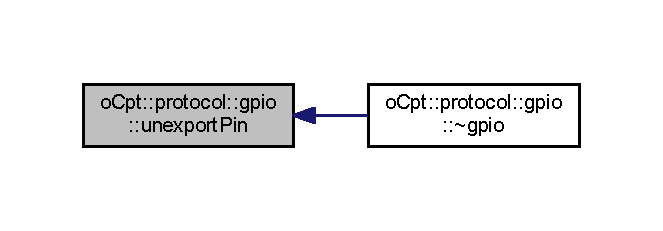
\includegraphics[width=318pt]{classo_cpt_1_1protocol_1_1gpio_af6383ac93d965d156617147c652ae56f_icgraph}
\end{center}
\end{figure}
\hypertarget{classo_cpt_1_1protocol_1_1gpio_a0fd140f4fb32047ceba4a9a17891efe0}{}\label{classo_cpt_1_1protocol_1_1gpio_a0fd140f4fb32047ceba4a9a17891efe0} 
\index{o\+Cpt\+::protocol\+::gpio@{o\+Cpt\+::protocol\+::gpio}!wait\+For\+Edge@{wait\+For\+Edge}}
\index{wait\+For\+Edge@{wait\+For\+Edge}!o\+Cpt\+::protocol\+::gpio@{o\+Cpt\+::protocol\+::gpio}}
\subsubsection{\texorpdfstring{wait\+For\+Edge()}{waitForEdge()}}
{\footnotesize\ttfamily void o\+Cpt\+::protocol\+::gpio\+::wait\+For\+Edge (\begin{DoxyParamCaption}{ }\end{DoxyParamCaption})}

Wait for the occurance of a change in Edge, corresponding with the set value of Edge. When the change is detected the callbackfunction is called. This function blocks the current thread. 

Definition at line 422 of file Controller.\+cpp.



References cb\+\_\+, direction\+\_\+, and gpiopath\+\_\+.



Referenced by wait\+For\+Edge\+Async().

Here is the caller graph for this function\+:\nopagebreak
\begin{figure}[H]
\begin{center}
\leavevmode
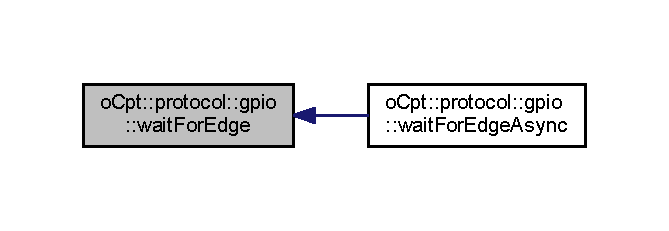
\includegraphics[width=321pt]{classo_cpt_1_1protocol_1_1gpio_a0fd140f4fb32047ceba4a9a17891efe0_icgraph}
\end{center}
\end{figure}
\hypertarget{classo_cpt_1_1protocol_1_1gpio_a02375f321f838da5f738eda8631ae0cc}{}\label{classo_cpt_1_1protocol_1_1gpio_a02375f321f838da5f738eda8631ae0cc} 
\index{o\+Cpt\+::protocol\+::gpio@{o\+Cpt\+::protocol\+::gpio}!wait\+For\+Edge\+Async@{wait\+For\+Edge\+Async}}
\index{wait\+For\+Edge\+Async@{wait\+For\+Edge\+Async}!o\+Cpt\+::protocol\+::gpio@{o\+Cpt\+::protocol\+::gpio}}
\subsubsection{\texorpdfstring{wait\+For\+Edge\+Async()}{waitForEdgeAsync()}}
{\footnotesize\ttfamily void o\+Cpt\+::protocol\+::gpio\+::wait\+For\+Edge\+Async (\begin{DoxyParamCaption}{ }\end{DoxyParamCaption})}

Wait for the ocurrance of a change in Edge, corresponding with the set value of Edge. When the chance is detected the callbackfunction is called. This function creates a new thread, allowing the current thread to run unhindered 

Definition at line 457 of file Controller.\+cpp.



References wait\+For\+Edge().

Here is the call graph for this function\+:\nopagebreak
\begin{figure}[H]
\begin{center}
\leavevmode
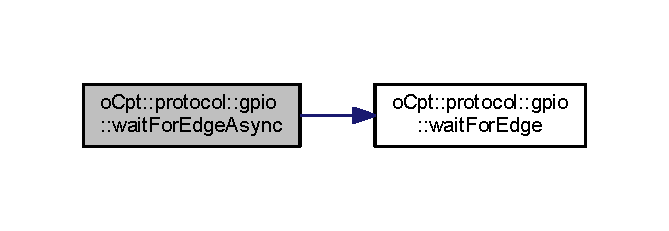
\includegraphics[width=321pt]{classo_cpt_1_1protocol_1_1gpio_a02375f321f838da5f738eda8631ae0cc_cgraph}
\end{center}
\end{figure}
\hypertarget{classo_cpt_1_1protocol_1_1gpio_a0f2972fa7ad1981c7edeae79280aa11f}{}\label{classo_cpt_1_1protocol_1_1gpio_a0f2972fa7ad1981c7edeae79280aa11f} 
\index{o\+Cpt\+::protocol\+::gpio@{o\+Cpt\+::protocol\+::gpio}!write\+Pin\+Value@{write\+Pin\+Value}}
\index{write\+Pin\+Value@{write\+Pin\+Value}!o\+Cpt\+::protocol\+::gpio@{o\+Cpt\+::protocol\+::gpio}}
\subsubsection{\texorpdfstring{write\+Pin\+Value()}{writePinValue()}\hspace{0.1cm}{\footnotesize\ttfamily [1/2]}}
{\footnotesize\ttfamily template$<$typename T $>$ \\
void o\+Cpt\+::protocol\+::gpio\+::write\+Pin\+Value (\begin{DoxyParamCaption}\item[{const int \&}]{number,  }\item[{const T \&}]{value }\end{DoxyParamCaption})\hspace{0.3cm}{\ttfamily [inline]}, {\ttfamily [private]}}

Write the value to the pin. The T parameter determines which value to set 
\begin{DoxyTemplParams}{Template Parameters}
{\em T} & the type could either be Value, Direction ro Direction \\
\hline
\end{DoxyTemplParams}

\begin{DoxyParams}{Parameters}
{\em number} & the pin number as an integer \\
\hline
{\em value} & the Value to be set \\
\hline
\end{DoxyParams}


Definition at line 331 of file Controller.\+h.



References G\+P\+I\+O\+\_\+\+B\+A\+S\+E\+\_\+\+P\+A\+TH.

\hypertarget{classo_cpt_1_1protocol_1_1gpio_a08e30d2b5451a628857d18b3b75e3265}{}\label{classo_cpt_1_1protocol_1_1gpio_a08e30d2b5451a628857d18b3b75e3265} 
\index{o\+Cpt\+::protocol\+::gpio@{o\+Cpt\+::protocol\+::gpio}!write\+Pin\+Value@{write\+Pin\+Value}}
\index{write\+Pin\+Value@{write\+Pin\+Value}!o\+Cpt\+::protocol\+::gpio@{o\+Cpt\+::protocol\+::gpio}}
\subsubsection{\texorpdfstring{write\+Pin\+Value()}{writePinValue()}\hspace{0.1cm}{\footnotesize\ttfamily [2/2]}}
{\footnotesize\ttfamily template$<$typename T $>$ \\
void o\+Cpt\+::protocol\+::gpio\+::write\+Pin\+Value (\begin{DoxyParamCaption}\item[{std\+::string}]{path,  }\item[{const T \&}]{value }\end{DoxyParamCaption})\hspace{0.3cm}{\ttfamily [inline]}, {\ttfamily [private]}}

Write the value to the pin, The T paramter determines which value to set. This overload is quicker then the one taking the integer and is therefore preferred 
\begin{DoxyTemplParams}{Template Parameters}
{\em T} & the type could either be Value, Direction or Edge \\
\hline
\end{DoxyTemplParams}

\begin{DoxyParams}{Parameters}
{\em path} & the pin as an user-\/space path \\
\hline
{\em value} & the Value to write \\
\hline
\end{DoxyParams}


Definition at line 344 of file Controller.\+h.



\subsection{Member Data Documentation}
\hypertarget{classo_cpt_1_1protocol_1_1gpio_a7d9d6a711dd0ba0d51649b85ca4d5bf4}{}\label{classo_cpt_1_1protocol_1_1gpio_a7d9d6a711dd0ba0d51649b85ca4d5bf4} 
\index{o\+Cpt\+::protocol\+::gpio@{o\+Cpt\+::protocol\+::gpio}!cb\+\_\+@{cb\+\_\+}}
\index{cb\+\_\+@{cb\+\_\+}!o\+Cpt\+::protocol\+::gpio@{o\+Cpt\+::protocol\+::gpio}}
\subsubsection{\texorpdfstring{cb\+\_\+}{cb\_}}
{\footnotesize\ttfamily \hyperlink{classo_cpt_1_1protocol_1_1gpio_ad553926a5fc9db445e7c9715abede2e3}{cb\+\_\+func} o\+Cpt\+::protocol\+::gpio\+::cb\+\_\+\hspace{0.3cm}{\ttfamily [private]}}



Definition at line 264 of file Controller.\+h.



Referenced by gpio(), set\+Callback\+Function(), and wait\+For\+Edge().

\hypertarget{classo_cpt_1_1protocol_1_1gpio_adb5c9fe44ef91bf37812e9cdfd3141d4}{}\label{classo_cpt_1_1protocol_1_1gpio_adb5c9fe44ef91bf37812e9cdfd3141d4} 
\index{o\+Cpt\+::protocol\+::gpio@{o\+Cpt\+::protocol\+::gpio}!direction\+\_\+@{direction\+\_\+}}
\index{direction\+\_\+@{direction\+\_\+}!o\+Cpt\+::protocol\+::gpio@{o\+Cpt\+::protocol\+::gpio}}
\subsubsection{\texorpdfstring{direction\+\_\+}{direction\_}}
{\footnotesize\ttfamily \hyperlink{classo_cpt_1_1protocol_1_1gpio_af7acf963933bbc47d11d6fa1b8ce4d5b}{Direction} o\+Cpt\+::protocol\+::gpio\+::direction\+\_\+\hspace{0.3cm}{\ttfamily [private]}}



Definition at line 261 of file Controller.\+h.



Referenced by gpio(), set\+Direction(), and wait\+For\+Edge().

\hypertarget{classo_cpt_1_1protocol_1_1gpio_abdd5f6e987fdca5748a35622f72eaf2f}{}\label{classo_cpt_1_1protocol_1_1gpio_abdd5f6e987fdca5748a35622f72eaf2f} 
\index{o\+Cpt\+::protocol\+::gpio@{o\+Cpt\+::protocol\+::gpio}!edge\+\_\+@{edge\+\_\+}}
\index{edge\+\_\+@{edge\+\_\+}!o\+Cpt\+::protocol\+::gpio@{o\+Cpt\+::protocol\+::gpio}}
\subsubsection{\texorpdfstring{edge\+\_\+}{edge\_}}
{\footnotesize\ttfamily \hyperlink{classo_cpt_1_1protocol_1_1gpio_adbbd34b2bc4394ad5a71d94641dda9f9}{Edge} o\+Cpt\+::protocol\+::gpio\+::edge\+\_\+\hspace{0.3cm}{\ttfamily [private]}}



Definition at line 262 of file Controller.\+h.



Referenced by gpio(), and set\+Edge().

\hypertarget{classo_cpt_1_1protocol_1_1gpio_afac9293096c2636fcce60aff2b38698d}{}\label{classo_cpt_1_1protocol_1_1gpio_afac9293096c2636fcce60aff2b38698d} 
\index{o\+Cpt\+::protocol\+::gpio@{o\+Cpt\+::protocol\+::gpio}!gpiopath\+\_\+@{gpiopath\+\_\+}}
\index{gpiopath\+\_\+@{gpiopath\+\_\+}!o\+Cpt\+::protocol\+::gpio@{o\+Cpt\+::protocol\+::gpio}}
\subsubsection{\texorpdfstring{gpiopath\+\_\+}{gpiopath\_}}
{\footnotesize\ttfamily std\+::string o\+Cpt\+::protocol\+::gpio\+::gpiopath\+\_\+\hspace{0.3cm}{\ttfamily [private]}}



Definition at line 263 of file Controller.\+h.



Referenced by gpio(), toggle(), and wait\+For\+Edge().

\hypertarget{classo_cpt_1_1protocol_1_1gpio_a618c388f95fff31d6decf7f8760e76a9}{}\label{classo_cpt_1_1protocol_1_1gpio_a618c388f95fff31d6decf7f8760e76a9} 
\index{o\+Cpt\+::protocol\+::gpio@{o\+Cpt\+::protocol\+::gpio}!pin\+Number\+\_\+@{pin\+Number\+\_\+}}
\index{pin\+Number\+\_\+@{pin\+Number\+\_\+}!o\+Cpt\+::protocol\+::gpio@{o\+Cpt\+::protocol\+::gpio}}
\subsubsection{\texorpdfstring{pin\+Number\+\_\+}{pinNumber\_}}
{\footnotesize\ttfamily int o\+Cpt\+::protocol\+::gpio\+::pin\+Number\+\_\+\hspace{0.3cm}{\ttfamily [private]}}



Definition at line 259 of file Controller.\+h.



Referenced by gpio(), set\+Pin\+Number(), and $\sim$gpio().

\hypertarget{classo_cpt_1_1protocol_1_1gpio_aa24b7c7d759f783bc3e93745edc69a2b}{}\label{classo_cpt_1_1protocol_1_1gpio_aa24b7c7d759f783bc3e93745edc69a2b} 
\index{o\+Cpt\+::protocol\+::gpio@{o\+Cpt\+::protocol\+::gpio}!signal\+Changed@{signal\+Changed}}
\index{signal\+Changed@{signal\+Changed}!o\+Cpt\+::protocol\+::gpio@{o\+Cpt\+::protocol\+::gpio}}
\subsubsection{\texorpdfstring{signal\+Changed}{signalChanged}}
{\footnotesize\ttfamily \hyperlink{classo_cpt_1_1protocol_1_1gpio_aa875802b20c7ef999c44af68e7f23621}{signal\+\_\+t} o\+Cpt\+::protocol\+::gpio\+::signal\+Changed}

The signal that is send if the internal callback fucntion is executed 

Definition at line 256 of file Controller.\+h.



Referenced by internal\+Cb\+Func().

\hypertarget{classo_cpt_1_1protocol_1_1gpio_aefa2c3a350dce68af5b9eea8b84f0336}{}\label{classo_cpt_1_1protocol_1_1gpio_aefa2c3a350dce68af5b9eea8b84f0336} 
\index{o\+Cpt\+::protocol\+::gpio@{o\+Cpt\+::protocol\+::gpio}!thread\+Running\+\_\+@{thread\+Running\+\_\+}}
\index{thread\+Running\+\_\+@{thread\+Running\+\_\+}!o\+Cpt\+::protocol\+::gpio@{o\+Cpt\+::protocol\+::gpio}}
\subsubsection{\texorpdfstring{thread\+Running\+\_\+}{threadRunning\_}}
{\footnotesize\ttfamily bool o\+Cpt\+::protocol\+::gpio\+::thread\+Running\+\_\+\hspace{0.3cm}{\ttfamily [private]}}



Definition at line 265 of file Controller.\+h.

\hypertarget{classo_cpt_1_1protocol_1_1gpio_a301d39638a420a299728d353ade3997c}{}\label{classo_cpt_1_1protocol_1_1gpio_a301d39638a420a299728d353ade3997c} 
\index{o\+Cpt\+::protocol\+::gpio@{o\+Cpt\+::protocol\+::gpio}!value\+\_\+@{value\+\_\+}}
\index{value\+\_\+@{value\+\_\+}!o\+Cpt\+::protocol\+::gpio@{o\+Cpt\+::protocol\+::gpio}}
\subsubsection{\texorpdfstring{value\+\_\+}{value\_}}
{\footnotesize\ttfamily \hyperlink{classo_cpt_1_1protocol_1_1gpio_a7d2d1d34f177f209ad642098d168656f}{Value} o\+Cpt\+::protocol\+::gpio\+::value\+\_\+\hspace{0.3cm}{\ttfamily [private]}}



Definition at line 260 of file Controller.\+h.



Referenced by gpio(), set\+Value(), and toggle().



The documentation for this class was generated from the following files\+:\begin{DoxyCompactItemize}
\item 
/projects/mti/oh\+Captain/oh\+Captain/include/\+Core/\hyperlink{_controller_8h}{Controller.\+h}\item 
/projects/mti/oh\+Captain/oh\+Captain/src/\+Core/\hyperlink{_controller_8cpp}{Controller.\+cpp}\end{DoxyCompactItemize}

\hypertarget{classo_cpt_1_1components_1_1sensors_1_1_gps}{}\section{o\+Cpt\+:\+:components\+:\+:sensors\+:\+:Gps Class Reference}
\label{classo_cpt_1_1components_1_1sensors_1_1_gps}\index{o\+Cpt\+::components\+::sensors\+::\+Gps@{o\+Cpt\+::components\+::sensors\+::\+Gps}}


{\ttfamily \#include $<$Gps.\+h$>$}



Inheritance diagram for o\+Cpt\+:\+:components\+:\+:sensors\+:\+:Gps\+:\nopagebreak
\begin{figure}[H]
\begin{center}
\leavevmode
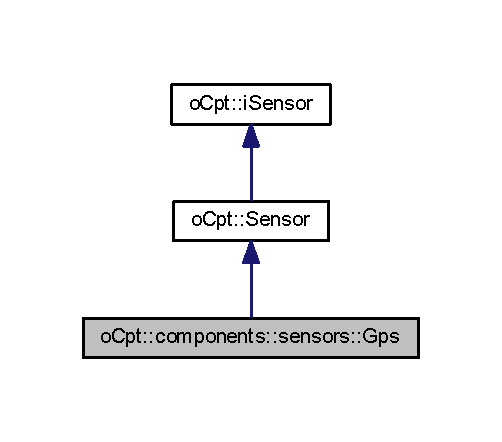
\includegraphics[width=241pt]{classo_cpt_1_1components_1_1sensors_1_1_gps__inherit__graph}
\end{center}
\end{figure}


Collaboration diagram for o\+Cpt\+:\+:components\+:\+:sensors\+:\+:Gps\+:\nopagebreak
\begin{figure}[H]
\begin{center}
\leavevmode
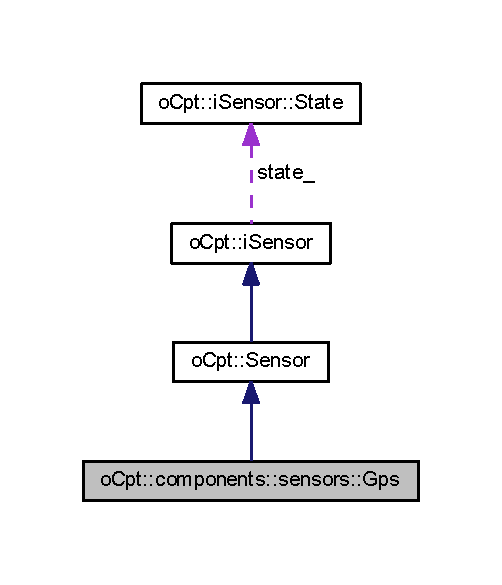
\includegraphics[width=241pt]{classo_cpt_1_1components_1_1sensors_1_1_gps__coll__graph}
\end{center}
\end{figure}
\subsection*{Public Types}
\begin{DoxyCompactItemize}
\item 
typedef \hyperlink{classo_cpt_1_1_world_1_1_location_a3aa5e31e2888b4da40ad534b99473888}{o\+Cpt\+::\+World\+::\+Location\+::gps\+Point\+\_\+t} \hyperlink{classo_cpt_1_1components_1_1sensors_1_1_gps_a01613dafbb15790246b00223f850a962}{Return\+Value\+\_\+t}
\end{DoxyCompactItemize}
\subsection*{Public Member Functions}
\begin{DoxyCompactItemize}
\item 
\hyperlink{classo_cpt_1_1components_1_1sensors_1_1_gps_a24c1c7c95c57f9c5fa47d0640ba5d6dc}{Gps} (\hyperlink{classo_cpt_1_1i_controller_a6d89a95cd6ad68bb74adfaca2f36370f}{i\+Controller\+::ptr} controller, \hyperlink{classo_cpt_1_1_world_aa6e591e3096d5de71e0cec9039663d67}{World\+::ptr} world, std\+::string id, std\+::string device, unsigned int baudrate)
\item 
\hyperlink{classo_cpt_1_1components_1_1sensors_1_1_gps_aa8c7fc77c287b439f9d33bc8cfda1e68}{$\sim$\+Gps} ()
\item 
void \hyperlink{classo_cpt_1_1components_1_1sensors_1_1_gps_a95976c5d8bba650d2732d4eb43979283}{update\+Sensor} ()
\item 
void \hyperlink{classo_cpt_1_1components_1_1sensors_1_1_gps_af703c48b8b7220a1909570f46edae932}{run} ()
\item 
void \hyperlink{classo_cpt_1_1components_1_1sensors_1_1_gps_a9206c32fa91311740ae920c01eed6094}{stop} ()
\item 
void \hyperlink{classo_cpt_1_1components_1_1sensors_1_1_gps_ad613b81625402daa6fdae80022fde18c}{set\+I\+Oservice} (boost\+::shared\+\_\+ptr$<$ boost\+::asio\+::io\+\_\+service $>$ ioservice)
\end{DoxyCompactItemize}
\subsection*{Protected Member Functions}
\begin{DoxyCompactItemize}
\item 
void \hyperlink{classo_cpt_1_1components_1_1sensors_1_1_gps_a6effa9cffd5f203d84de1edce73be87a}{interpret\+Msg} ()
\end{DoxyCompactItemize}
\subsection*{Protected Attributes}
\begin{DoxyCompactItemize}
\item 
std\+::string \hyperlink{classo_cpt_1_1components_1_1sensors_1_1_gps_a6b8c50dca0776870cedabbb527b2144e}{device\+\_\+}
\item 
\hyperlink{classo_cpt_1_1protocol_1_1_serial_a4c97c6a2456d649974e07a186f634780}{protocol\+::\+Serial\+::ptr} \hyperlink{classo_cpt_1_1components_1_1sensors_1_1_gps_a42ea2d37ec01473e92be6ef3cda6de39}{serial\+\_\+}
\end{DoxyCompactItemize}


\subsection{Detailed Description}


Definition at line 13 of file Gps.\+h.



\subsection{Member Typedef Documentation}
\hypertarget{classo_cpt_1_1components_1_1sensors_1_1_gps_a01613dafbb15790246b00223f850a962}{}\label{classo_cpt_1_1components_1_1sensors_1_1_gps_a01613dafbb15790246b00223f850a962} 
\index{o\+Cpt\+::components\+::sensors\+::\+Gps@{o\+Cpt\+::components\+::sensors\+::\+Gps}!Return\+Value\+\_\+t@{Return\+Value\+\_\+t}}
\index{Return\+Value\+\_\+t@{Return\+Value\+\_\+t}!o\+Cpt\+::components\+::sensors\+::\+Gps@{o\+Cpt\+::components\+::sensors\+::\+Gps}}
\subsubsection{\texorpdfstring{Return\+Value\+\_\+t}{ReturnValue\_t}}
{\footnotesize\ttfamily typedef \hyperlink{classo_cpt_1_1_world_1_1_location_a3aa5e31e2888b4da40ad534b99473888}{o\+Cpt\+::\+World\+::\+Location\+::gps\+Point\+\_\+t} \hyperlink{classo_cpt_1_1components_1_1sensors_1_1_gps_a01613dafbb15790246b00223f850a962}{o\+Cpt\+::components\+::sensors\+::\+Gps\+::\+Return\+Value\+\_\+t}}



Definition at line 15 of file Gps.\+h.



\subsection{Constructor \& Destructor Documentation}
\hypertarget{classo_cpt_1_1components_1_1sensors_1_1_gps_a24c1c7c95c57f9c5fa47d0640ba5d6dc}{}\label{classo_cpt_1_1components_1_1sensors_1_1_gps_a24c1c7c95c57f9c5fa47d0640ba5d6dc} 
\index{o\+Cpt\+::components\+::sensors\+::\+Gps@{o\+Cpt\+::components\+::sensors\+::\+Gps}!Gps@{Gps}}
\index{Gps@{Gps}!o\+Cpt\+::components\+::sensors\+::\+Gps@{o\+Cpt\+::components\+::sensors\+::\+Gps}}
\subsubsection{\texorpdfstring{Gps()}{Gps()}}
{\footnotesize\ttfamily o\+Cpt\+::components\+::sensors\+::\+Gps\+::\+Gps (\begin{DoxyParamCaption}\item[{\hyperlink{classo_cpt_1_1i_controller_a6d89a95cd6ad68bb74adfaca2f36370f}{i\+Controller\+::ptr}}]{controller,  }\item[{\hyperlink{classo_cpt_1_1_world_aa6e591e3096d5de71e0cec9039663d67}{World\+::ptr}}]{world,  }\item[{std\+::string}]{id,  }\item[{std\+::string}]{device,  }\item[{unsigned int}]{baudrate }\end{DoxyParamCaption})}



Definition at line 13 of file Gps.\+cpp.



References interpret\+Msg(), and serial\+\_\+.

Here is the call graph for this function\+:\nopagebreak
\begin{figure}[H]
\begin{center}
\leavevmode
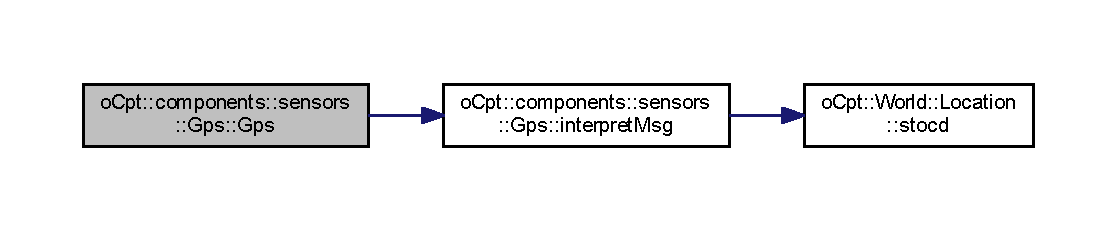
\includegraphics[width=350pt]{classo_cpt_1_1components_1_1sensors_1_1_gps_a24c1c7c95c57f9c5fa47d0640ba5d6dc_cgraph}
\end{center}
\end{figure}
\hypertarget{classo_cpt_1_1components_1_1sensors_1_1_gps_aa8c7fc77c287b439f9d33bc8cfda1e68}{}\label{classo_cpt_1_1components_1_1sensors_1_1_gps_aa8c7fc77c287b439f9d33bc8cfda1e68} 
\index{o\+Cpt\+::components\+::sensors\+::\+Gps@{o\+Cpt\+::components\+::sensors\+::\+Gps}!````~Gps@{$\sim$\+Gps}}
\index{````~Gps@{$\sim$\+Gps}!o\+Cpt\+::components\+::sensors\+::\+Gps@{o\+Cpt\+::components\+::sensors\+::\+Gps}}
\subsubsection{\texorpdfstring{$\sim$\+Gps()}{~Gps()}}
{\footnotesize\ttfamily o\+Cpt\+::components\+::sensors\+::\+Gps\+::$\sim$\+Gps (\begin{DoxyParamCaption}{ }\end{DoxyParamCaption})}



Definition at line 28 of file Gps.\+cpp.



References serial\+\_\+.



\subsection{Member Function Documentation}
\hypertarget{classo_cpt_1_1components_1_1sensors_1_1_gps_a6effa9cffd5f203d84de1edce73be87a}{}\label{classo_cpt_1_1components_1_1sensors_1_1_gps_a6effa9cffd5f203d84de1edce73be87a} 
\index{o\+Cpt\+::components\+::sensors\+::\+Gps@{o\+Cpt\+::components\+::sensors\+::\+Gps}!interpret\+Msg@{interpret\+Msg}}
\index{interpret\+Msg@{interpret\+Msg}!o\+Cpt\+::components\+::sensors\+::\+Gps@{o\+Cpt\+::components\+::sensors\+::\+Gps}}
\subsubsection{\texorpdfstring{interpret\+Msg()}{interpretMsg()}}
{\footnotesize\ttfamily void o\+Cpt\+::components\+::sensors\+::\+Gps\+::interpret\+Msg (\begin{DoxyParamCaption}{ }\end{DoxyParamCaption})\hspace{0.3cm}{\ttfamily [protected]}}



Definition at line 59 of file Gps.\+cpp.



References o\+Cpt\+::\+World\+::\+Location\+::coordinate\+::direction, o\+Cpt\+::\+World\+::\+Location\+::gps\+Point\+::latitude, o\+Cpt\+::\+World\+::\+Location\+::gps\+Point\+::longitude, serial\+\_\+, o\+Cpt\+::i\+Sensor\+::sig\+\_\+, o\+Cpt\+::i\+Sensor\+::\+State\+::\+Stamp, o\+Cpt\+::i\+Sensor\+::state\+\_\+, o\+Cpt\+::\+World\+::\+Location\+::stocd(), o\+Cpt\+::i\+Sensor\+::\+State\+::\+Value, o\+Cpt\+::\+World\+::\+Location\+::coordinate\+::value, and o\+Cpt\+::i\+Sensor\+::world\+\_\+.



Referenced by Gps().

Here is the call graph for this function\+:\nopagebreak
\begin{figure}[H]
\begin{center}
\leavevmode
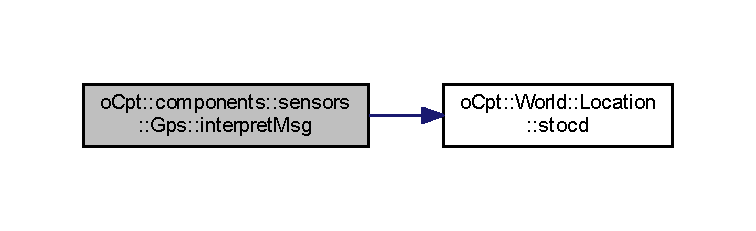
\includegraphics[width=350pt]{classo_cpt_1_1components_1_1sensors_1_1_gps_a6effa9cffd5f203d84de1edce73be87a_cgraph}
\end{center}
\end{figure}
Here is the caller graph for this function\+:\nopagebreak
\begin{figure}[H]
\begin{center}
\leavevmode
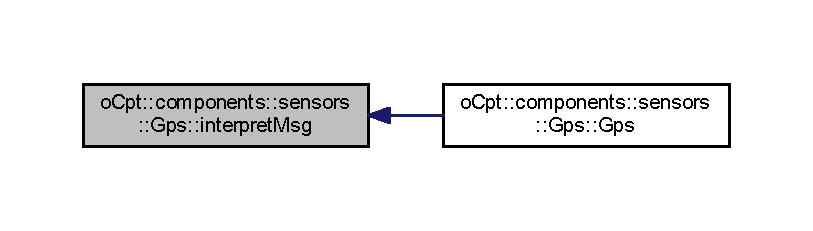
\includegraphics[width=350pt]{classo_cpt_1_1components_1_1sensors_1_1_gps_a6effa9cffd5f203d84de1edce73be87a_icgraph}
\end{center}
\end{figure}
\hypertarget{classo_cpt_1_1components_1_1sensors_1_1_gps_af703c48b8b7220a1909570f46edae932}{}\label{classo_cpt_1_1components_1_1sensors_1_1_gps_af703c48b8b7220a1909570f46edae932} 
\index{o\+Cpt\+::components\+::sensors\+::\+Gps@{o\+Cpt\+::components\+::sensors\+::\+Gps}!run@{run}}
\index{run@{run}!o\+Cpt\+::components\+::sensors\+::\+Gps@{o\+Cpt\+::components\+::sensors\+::\+Gps}}
\subsubsection{\texorpdfstring{run()}{run()}}
{\footnotesize\ttfamily void o\+Cpt\+::components\+::sensors\+::\+Gps\+::run (\begin{DoxyParamCaption}{ }\end{DoxyParamCaption})\hspace{0.3cm}{\ttfamily [virtual]}}

virtual function starting the run service for the IO 

Reimplemented from \hyperlink{classo_cpt_1_1_sensor_aef25b0e5f3a8358ee81c97c73909fbe6}{o\+Cpt\+::\+Sensor}.



Definition at line 38 of file Gps.\+cpp.



References o\+Cpt\+::\+Sensor\+::run(), o\+Cpt\+::i\+Sensor\+::sensor\+Running\+\_\+, and serial\+\_\+.

Here is the call graph for this function\+:\nopagebreak
\begin{figure}[H]
\begin{center}
\leavevmode
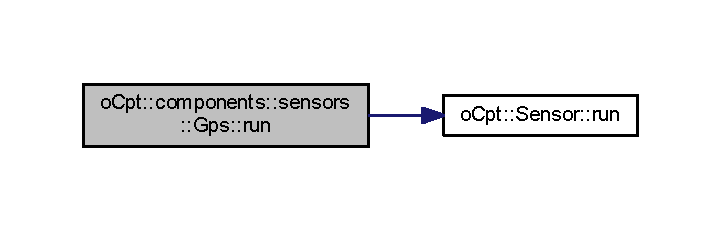
\includegraphics[width=346pt]{classo_cpt_1_1components_1_1sensors_1_1_gps_af703c48b8b7220a1909570f46edae932_cgraph}
\end{center}
\end{figure}
\hypertarget{classo_cpt_1_1components_1_1sensors_1_1_gps_ad613b81625402daa6fdae80022fde18c}{}\label{classo_cpt_1_1components_1_1sensors_1_1_gps_ad613b81625402daa6fdae80022fde18c} 
\index{o\+Cpt\+::components\+::sensors\+::\+Gps@{o\+Cpt\+::components\+::sensors\+::\+Gps}!set\+I\+Oservice@{set\+I\+Oservice}}
\index{set\+I\+Oservice@{set\+I\+Oservice}!o\+Cpt\+::components\+::sensors\+::\+Gps@{o\+Cpt\+::components\+::sensors\+::\+Gps}}
\subsubsection{\texorpdfstring{set\+I\+Oservice()}{setIOservice()}}
{\footnotesize\ttfamily void o\+Cpt\+::components\+::sensors\+::\+Gps\+::set\+I\+Oservice (\begin{DoxyParamCaption}\item[{boost\+::shared\+\_\+ptr$<$ boost\+::asio\+::io\+\_\+service $>$}]{ioservice }\end{DoxyParamCaption})\hspace{0.3cm}{\ttfamily [virtual]}}

Setting the used Asynchronous Input Output service 
\begin{DoxyParams}{Parameters}
{\em ioservice} & A\+S\+IO IO service, which handles the async calls from multiple sensors \\
\hline
\end{DoxyParams}


Reimplemented from \hyperlink{classo_cpt_1_1_sensor_ae7d47e18df5eb7854bf71fbbee9568df}{o\+Cpt\+::\+Sensor}.



Definition at line 54 of file Gps.\+cpp.



References serial\+\_\+, and o\+Cpt\+::\+Sensor\+::set\+I\+Oservice().

Here is the call graph for this function\+:\nopagebreak
\begin{figure}[H]
\begin{center}
\leavevmode
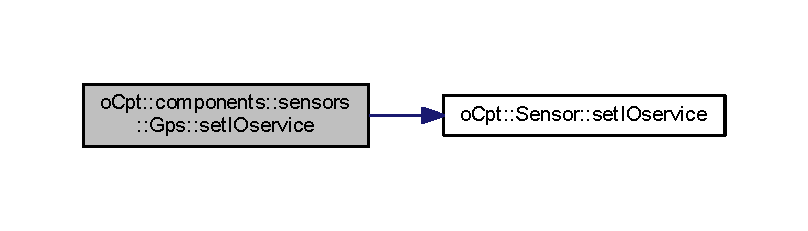
\includegraphics[width=350pt]{classo_cpt_1_1components_1_1sensors_1_1_gps_ad613b81625402daa6fdae80022fde18c_cgraph}
\end{center}
\end{figure}
\hypertarget{classo_cpt_1_1components_1_1sensors_1_1_gps_a9206c32fa91311740ae920c01eed6094}{}\label{classo_cpt_1_1components_1_1sensors_1_1_gps_a9206c32fa91311740ae920c01eed6094} 
\index{o\+Cpt\+::components\+::sensors\+::\+Gps@{o\+Cpt\+::components\+::sensors\+::\+Gps}!stop@{stop}}
\index{stop@{stop}!o\+Cpt\+::components\+::sensors\+::\+Gps@{o\+Cpt\+::components\+::sensors\+::\+Gps}}
\subsubsection{\texorpdfstring{stop()}{stop()}}
{\footnotesize\ttfamily void o\+Cpt\+::components\+::sensors\+::\+Gps\+::stop (\begin{DoxyParamCaption}{ }\end{DoxyParamCaption})\hspace{0.3cm}{\ttfamily [virtual]}}

virtual function stopping the run 

Reimplemented from \hyperlink{classo_cpt_1_1_sensor_a44ad78c2c091ca9cf72295293f8c5b74}{o\+Cpt\+::\+Sensor}.



Definition at line 45 of file Gps.\+cpp.



References o\+Cpt\+::i\+Sensor\+::sensor\+Running\+\_\+, serial\+\_\+, and o\+Cpt\+::\+Sensor\+::stop().

Here is the call graph for this function\+:\nopagebreak
\begin{figure}[H]
\begin{center}
\leavevmode
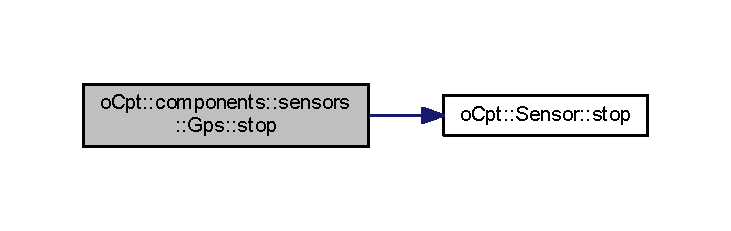
\includegraphics[width=350pt]{classo_cpt_1_1components_1_1sensors_1_1_gps_a9206c32fa91311740ae920c01eed6094_cgraph}
\end{center}
\end{figure}
\hypertarget{classo_cpt_1_1components_1_1sensors_1_1_gps_a95976c5d8bba650d2732d4eb43979283}{}\label{classo_cpt_1_1components_1_1sensors_1_1_gps_a95976c5d8bba650d2732d4eb43979283} 
\index{o\+Cpt\+::components\+::sensors\+::\+Gps@{o\+Cpt\+::components\+::sensors\+::\+Gps}!update\+Sensor@{update\+Sensor}}
\index{update\+Sensor@{update\+Sensor}!o\+Cpt\+::components\+::sensors\+::\+Gps@{o\+Cpt\+::components\+::sensors\+::\+Gps}}
\subsubsection{\texorpdfstring{update\+Sensor()}{updateSensor()}}
{\footnotesize\ttfamily void o\+Cpt\+::components\+::sensors\+::\+Gps\+::update\+Sensor (\begin{DoxyParamCaption}{ }\end{DoxyParamCaption})\hspace{0.3cm}{\ttfamily [virtual]}}

virtual function which performs a sensor update, obtaining a new value and sending a signal afterwards 

Reimplemented from \hyperlink{classo_cpt_1_1_sensor_ab4b0dedb06f11bcf2368852035beb2b2}{o\+Cpt\+::\+Sensor}.



Definition at line 34 of file Gps.\+cpp.



References o\+Cpt\+::\+Sensor\+::update\+Sensor().

Here is the call graph for this function\+:\nopagebreak
\begin{figure}[H]
\begin{center}
\leavevmode
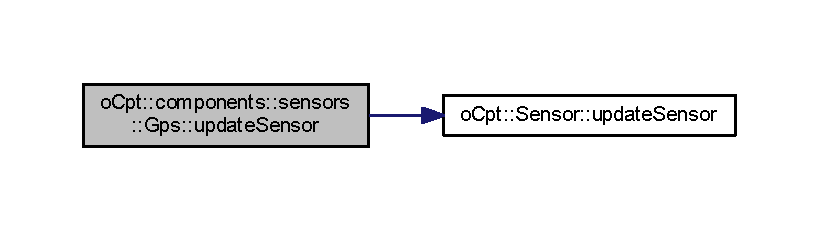
\includegraphics[width=350pt]{classo_cpt_1_1components_1_1sensors_1_1_gps_a95976c5d8bba650d2732d4eb43979283_cgraph}
\end{center}
\end{figure}


\subsection{Member Data Documentation}
\hypertarget{classo_cpt_1_1components_1_1sensors_1_1_gps_a6b8c50dca0776870cedabbb527b2144e}{}\label{classo_cpt_1_1components_1_1sensors_1_1_gps_a6b8c50dca0776870cedabbb527b2144e} 
\index{o\+Cpt\+::components\+::sensors\+::\+Gps@{o\+Cpt\+::components\+::sensors\+::\+Gps}!device\+\_\+@{device\+\_\+}}
\index{device\+\_\+@{device\+\_\+}!o\+Cpt\+::components\+::sensors\+::\+Gps@{o\+Cpt\+::components\+::sensors\+::\+Gps}}
\subsubsection{\texorpdfstring{device\+\_\+}{device\_}}
{\footnotesize\ttfamily std\+::string o\+Cpt\+::components\+::sensors\+::\+Gps\+::device\+\_\+\hspace{0.3cm}{\ttfamily [protected]}}



Definition at line 31 of file Gps.\+h.

\hypertarget{classo_cpt_1_1components_1_1sensors_1_1_gps_a42ea2d37ec01473e92be6ef3cda6de39}{}\label{classo_cpt_1_1components_1_1sensors_1_1_gps_a42ea2d37ec01473e92be6ef3cda6de39} 
\index{o\+Cpt\+::components\+::sensors\+::\+Gps@{o\+Cpt\+::components\+::sensors\+::\+Gps}!serial\+\_\+@{serial\+\_\+}}
\index{serial\+\_\+@{serial\+\_\+}!o\+Cpt\+::components\+::sensors\+::\+Gps@{o\+Cpt\+::components\+::sensors\+::\+Gps}}
\subsubsection{\texorpdfstring{serial\+\_\+}{serial\_}}
{\footnotesize\ttfamily \hyperlink{classo_cpt_1_1protocol_1_1_serial_a4c97c6a2456d649974e07a186f634780}{protocol\+::\+Serial\+::ptr} o\+Cpt\+::components\+::sensors\+::\+Gps\+::serial\+\_\+\hspace{0.3cm}{\ttfamily [protected]}}



Definition at line 32 of file Gps.\+h.



Referenced by Gps(), interpret\+Msg(), run(), set\+I\+Oservice(), stop(), and $\sim$\+Gps().



The documentation for this class was generated from the following files\+:\begin{DoxyCompactItemize}
\item 
/projects/mti/oh\+Captain/oh\+Captain/include/\+Sensors/\hyperlink{_gps_8h}{Gps.\+h}\item 
/projects/mti/oh\+Captain/oh\+Captain/src/\+Sensors/\hyperlink{_gps_8cpp}{Gps.\+cpp}\end{DoxyCompactItemize}

\hypertarget{structo_cpt_1_1_world_1_1_location_1_1gps_point}{}\section{o\+Cpt\+:\+:World\+:\+:Location\+:\+:gps\+Point Struct Reference}
\label{structo_cpt_1_1_world_1_1_location_1_1gps_point}\index{o\+Cpt\+::\+World\+::\+Location\+::gps\+Point@{o\+Cpt\+::\+World\+::\+Location\+::gps\+Point}}


{\ttfamily \#include $<$World.\+h$>$}



Collaboration diagram for o\+Cpt\+:\+:World\+:\+:Location\+:\+:gps\+Point\+:\nopagebreak
\begin{figure}[H]
\begin{center}
\leavevmode
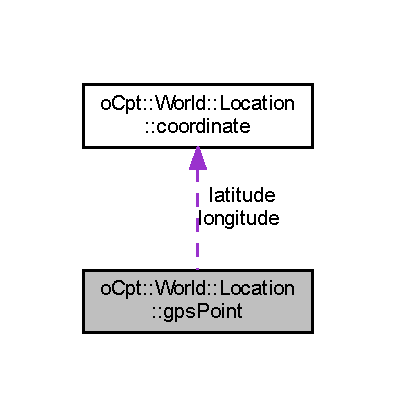
\includegraphics[width=190pt]{structo_cpt_1_1_world_1_1_location_1_1gps_point__coll__graph}
\end{center}
\end{figure}
\subsection*{Public Member Functions}
\begin{DoxyCompactItemize}
\item 
std\+::string \hyperlink{structo_cpt_1_1_world_1_1_location_1_1gps_point_a6274bfccaa6be97f2146ab7805ada0af}{to\+String} ()
\end{DoxyCompactItemize}
\subsection*{Public Attributes}
\begin{DoxyCompactItemize}
\item 
\hyperlink{classo_cpt_1_1_world_1_1_location_ade9263a17c41b7af085dfcb9055b18f3}{coordinate\+\_\+t} \hyperlink{structo_cpt_1_1_world_1_1_location_1_1gps_point_a043e3f4795590cee2c41df63769c3b17}{longitude}
\item 
\hyperlink{classo_cpt_1_1_world_1_1_location_ade9263a17c41b7af085dfcb9055b18f3}{coordinate\+\_\+t} \hyperlink{structo_cpt_1_1_world_1_1_location_1_1gps_point_a28047329a2c8750f2d6c54dfa3ce8bb4}{latitude}
\item 
double \hyperlink{structo_cpt_1_1_world_1_1_location_1_1gps_point_a94635e1477d9136f9cbb54fa8fa1fa39}{height}
\end{DoxyCompactItemize}


\subsection{Detailed Description}


Definition at line 126 of file World.\+h.



\subsection{Member Function Documentation}
\hypertarget{structo_cpt_1_1_world_1_1_location_1_1gps_point_a6274bfccaa6be97f2146ab7805ada0af}{}\label{structo_cpt_1_1_world_1_1_location_1_1gps_point_a6274bfccaa6be97f2146ab7805ada0af} 
\index{o\+Cpt\+::\+World\+::\+Location\+::gps\+Point@{o\+Cpt\+::\+World\+::\+Location\+::gps\+Point}!to\+String@{to\+String}}
\index{to\+String@{to\+String}!o\+Cpt\+::\+World\+::\+Location\+::gps\+Point@{o\+Cpt\+::\+World\+::\+Location\+::gps\+Point}}
\subsubsection{\texorpdfstring{to\+String()}{toString()}}
{\footnotesize\ttfamily std\+::string o\+Cpt\+::\+World\+::\+Location\+::gps\+Point\+::to\+String (\begin{DoxyParamCaption}{ }\end{DoxyParamCaption})}

Convert a gps coordinate to a text string \begin{DoxyReturn}{Returns}
a text string eq. 5.\+000E,52.\+000N 
\end{DoxyReturn}


Definition at line 72 of file World.\+cpp.



\subsection{Member Data Documentation}
\hypertarget{structo_cpt_1_1_world_1_1_location_1_1gps_point_a94635e1477d9136f9cbb54fa8fa1fa39}{}\label{structo_cpt_1_1_world_1_1_location_1_1gps_point_a94635e1477d9136f9cbb54fa8fa1fa39} 
\index{o\+Cpt\+::\+World\+::\+Location\+::gps\+Point@{o\+Cpt\+::\+World\+::\+Location\+::gps\+Point}!height@{height}}
\index{height@{height}!o\+Cpt\+::\+World\+::\+Location\+::gps\+Point@{o\+Cpt\+::\+World\+::\+Location\+::gps\+Point}}
\subsubsection{\texorpdfstring{height}{height}}
{\footnotesize\ttfamily double o\+Cpt\+::\+World\+::\+Location\+::gps\+Point\+::height}



Definition at line 129 of file World.\+h.

\hypertarget{structo_cpt_1_1_world_1_1_location_1_1gps_point_a28047329a2c8750f2d6c54dfa3ce8bb4}{}\label{structo_cpt_1_1_world_1_1_location_1_1gps_point_a28047329a2c8750f2d6c54dfa3ce8bb4} 
\index{o\+Cpt\+::\+World\+::\+Location\+::gps\+Point@{o\+Cpt\+::\+World\+::\+Location\+::gps\+Point}!latitude@{latitude}}
\index{latitude@{latitude}!o\+Cpt\+::\+World\+::\+Location\+::gps\+Point@{o\+Cpt\+::\+World\+::\+Location\+::gps\+Point}}
\subsubsection{\texorpdfstring{latitude}{latitude}}
{\footnotesize\ttfamily \hyperlink{classo_cpt_1_1_world_1_1_location_ade9263a17c41b7af085dfcb9055b18f3}{coordinate\+\_\+t} o\+Cpt\+::\+World\+::\+Location\+::gps\+Point\+::latitude}



Definition at line 128 of file World.\+h.



Referenced by o\+Cpt\+::components\+::sensors\+::\+Gps\+::interpret\+Msg().

\hypertarget{structo_cpt_1_1_world_1_1_location_1_1gps_point_a043e3f4795590cee2c41df63769c3b17}{}\label{structo_cpt_1_1_world_1_1_location_1_1gps_point_a043e3f4795590cee2c41df63769c3b17} 
\index{o\+Cpt\+::\+World\+::\+Location\+::gps\+Point@{o\+Cpt\+::\+World\+::\+Location\+::gps\+Point}!longitude@{longitude}}
\index{longitude@{longitude}!o\+Cpt\+::\+World\+::\+Location\+::gps\+Point@{o\+Cpt\+::\+World\+::\+Location\+::gps\+Point}}
\subsubsection{\texorpdfstring{longitude}{longitude}}
{\footnotesize\ttfamily \hyperlink{classo_cpt_1_1_world_1_1_location_ade9263a17c41b7af085dfcb9055b18f3}{coordinate\+\_\+t} o\+Cpt\+::\+World\+::\+Location\+::gps\+Point\+::longitude}



Definition at line 127 of file World.\+h.



Referenced by o\+Cpt\+::components\+::sensors\+::\+Gps\+::interpret\+Msg().



The documentation for this struct was generated from the following files\+:\begin{DoxyCompactItemize}
\item 
include/\+Core/\hyperlink{_world_8h}{World.\+h}\item 
src/\+Core/\hyperlink{_world_8cpp}{World.\+cpp}\end{DoxyCompactItemize}

\hypertarget{classo_cpt_1_1i_actuator}{}\section{o\+Cpt\+:\+:i\+Actuator Class Reference}
\label{classo_cpt_1_1i_actuator}\index{o\+Cpt\+::i\+Actuator@{o\+Cpt\+::i\+Actuator}}


{\ttfamily \#include $<$Actuator.\+h$>$}



Inheritance diagram for o\+Cpt\+:\+:i\+Actuator\+:\nopagebreak
\begin{figure}[H]
\begin{center}
\leavevmode
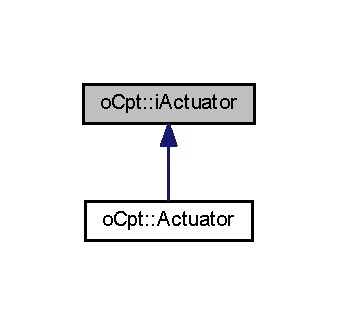
\includegraphics[width=162pt]{classo_cpt_1_1i_actuator__inherit__graph}
\end{center}
\end{figure}
\subsection*{Public Types}
\begin{DoxyCompactItemize}
\item 
typedef boost\+::shared\+\_\+ptr$<$ \hyperlink{classo_cpt_1_1i_actuator}{i\+Actuator} $>$ \hyperlink{classo_cpt_1_1i_actuator_a35847799558e92bb84fb6c71de772cac}{ptr}
\end{DoxyCompactItemize}
\subsection*{Public Member Functions}
\begin{DoxyCompactItemize}
\item 
\hyperlink{classo_cpt_1_1i_actuator_aa54aeed96c53b59fd4caa93bc29ce615}{i\+Actuator} ()
\item 
virtual \hyperlink{classo_cpt_1_1i_actuator_a9ec8a13b323499731fcb43c728c4812e}{$\sim$i\+Actuator} ()
\item 
virtual void \hyperlink{classo_cpt_1_1i_actuator_a1654bf3167a1dd7c34f770180cd8aaa1}{set\+Actuator} ()=0
\item 
virtual void \hyperlink{classo_cpt_1_1i_actuator_abf4db1f9f6b59bdefc86ca44aed0f49a}{run} ()=0
\item 
virtual void \hyperlink{classo_cpt_1_1i_actuator_ae3f9fbb61d920bee1bd297fb5a89625e}{stop} ()=0
\end{DoxyCompactItemize}


\subsection{Detailed Description}


Definition at line 17 of file Actuator.\+h.



\subsection{Member Typedef Documentation}
\hypertarget{classo_cpt_1_1i_actuator_a35847799558e92bb84fb6c71de772cac}{}\label{classo_cpt_1_1i_actuator_a35847799558e92bb84fb6c71de772cac} 
\index{o\+Cpt\+::i\+Actuator@{o\+Cpt\+::i\+Actuator}!ptr@{ptr}}
\index{ptr@{ptr}!o\+Cpt\+::i\+Actuator@{o\+Cpt\+::i\+Actuator}}
\subsubsection{\texorpdfstring{ptr}{ptr}}
{\footnotesize\ttfamily typedef boost\+::shared\+\_\+ptr$<$\hyperlink{classo_cpt_1_1i_actuator}{i\+Actuator}$>$ \hyperlink{classo_cpt_1_1i_actuator_a35847799558e92bb84fb6c71de772cac}{o\+Cpt\+::i\+Actuator\+::ptr}}



Definition at line 19 of file Actuator.\+h.



\subsection{Constructor \& Destructor Documentation}
\hypertarget{classo_cpt_1_1i_actuator_aa54aeed96c53b59fd4caa93bc29ce615}{}\label{classo_cpt_1_1i_actuator_aa54aeed96c53b59fd4caa93bc29ce615} 
\index{o\+Cpt\+::i\+Actuator@{o\+Cpt\+::i\+Actuator}!i\+Actuator@{i\+Actuator}}
\index{i\+Actuator@{i\+Actuator}!o\+Cpt\+::i\+Actuator@{o\+Cpt\+::i\+Actuator}}
\subsubsection{\texorpdfstring{i\+Actuator()}{iActuator()}}
{\footnotesize\ttfamily o\+Cpt\+::i\+Actuator\+::i\+Actuator (\begin{DoxyParamCaption}{ }\end{DoxyParamCaption})}



Definition at line 9 of file Actuator.\+cpp.

\hypertarget{classo_cpt_1_1i_actuator_a9ec8a13b323499731fcb43c728c4812e}{}\label{classo_cpt_1_1i_actuator_a9ec8a13b323499731fcb43c728c4812e} 
\index{o\+Cpt\+::i\+Actuator@{o\+Cpt\+::i\+Actuator}!````~i\+Actuator@{$\sim$i\+Actuator}}
\index{````~i\+Actuator@{$\sim$i\+Actuator}!o\+Cpt\+::i\+Actuator@{o\+Cpt\+::i\+Actuator}}
\subsubsection{\texorpdfstring{$\sim$i\+Actuator()}{~iActuator()}}
{\footnotesize\ttfamily o\+Cpt\+::i\+Actuator\+::$\sim$i\+Actuator (\begin{DoxyParamCaption}{ }\end{DoxyParamCaption})\hspace{0.3cm}{\ttfamily [virtual]}}



Definition at line 13 of file Actuator.\+cpp.



\subsection{Member Function Documentation}
\hypertarget{classo_cpt_1_1i_actuator_abf4db1f9f6b59bdefc86ca44aed0f49a}{}\label{classo_cpt_1_1i_actuator_abf4db1f9f6b59bdefc86ca44aed0f49a} 
\index{o\+Cpt\+::i\+Actuator@{o\+Cpt\+::i\+Actuator}!run@{run}}
\index{run@{run}!o\+Cpt\+::i\+Actuator@{o\+Cpt\+::i\+Actuator}}
\subsubsection{\texorpdfstring{run()}{run()}}
{\footnotesize\ttfamily virtual void o\+Cpt\+::i\+Actuator\+::run (\begin{DoxyParamCaption}{ }\end{DoxyParamCaption})\hspace{0.3cm}{\ttfamily [pure virtual]}}



Implemented in \hyperlink{classo_cpt_1_1_actuator_a8985818fcfb644acce17ce50c5c7f86b}{o\+Cpt\+::\+Actuator}.

\hypertarget{classo_cpt_1_1i_actuator_a1654bf3167a1dd7c34f770180cd8aaa1}{}\label{classo_cpt_1_1i_actuator_a1654bf3167a1dd7c34f770180cd8aaa1} 
\index{o\+Cpt\+::i\+Actuator@{o\+Cpt\+::i\+Actuator}!set\+Actuator@{set\+Actuator}}
\index{set\+Actuator@{set\+Actuator}!o\+Cpt\+::i\+Actuator@{o\+Cpt\+::i\+Actuator}}
\subsubsection{\texorpdfstring{set\+Actuator()}{setActuator()}}
{\footnotesize\ttfamily virtual void o\+Cpt\+::i\+Actuator\+::set\+Actuator (\begin{DoxyParamCaption}{ }\end{DoxyParamCaption})\hspace{0.3cm}{\ttfamily [pure virtual]}}



Implemented in \hyperlink{classo_cpt_1_1_actuator_a3a3813e5730f0257e74de7300eeeffa1}{o\+Cpt\+::\+Actuator}.

\hypertarget{classo_cpt_1_1i_actuator_ae3f9fbb61d920bee1bd297fb5a89625e}{}\label{classo_cpt_1_1i_actuator_ae3f9fbb61d920bee1bd297fb5a89625e} 
\index{o\+Cpt\+::i\+Actuator@{o\+Cpt\+::i\+Actuator}!stop@{stop}}
\index{stop@{stop}!o\+Cpt\+::i\+Actuator@{o\+Cpt\+::i\+Actuator}}
\subsubsection{\texorpdfstring{stop()}{stop()}}
{\footnotesize\ttfamily virtual void o\+Cpt\+::i\+Actuator\+::stop (\begin{DoxyParamCaption}{ }\end{DoxyParamCaption})\hspace{0.3cm}{\ttfamily [pure virtual]}}



Implemented in \hyperlink{classo_cpt_1_1_actuator_aa41132ff134e8b067353459dedbb0f37}{o\+Cpt\+::\+Actuator}.



The documentation for this class was generated from the following files\+:\begin{DoxyCompactItemize}
\item 
/projects/mti/oh\+Captain/oh\+Captain/include/\+Core/\hyperlink{_actuator_8h}{Actuator.\+h}\item 
/projects/mti/oh\+Captain/oh\+Captain/src/\+Core/\hyperlink{_actuator_8cpp}{Actuator.\+cpp}\end{DoxyCompactItemize}

\hypertarget{classo_cpt_1_1i_boatswain}{}\section{o\+Cpt\+:\+:i\+Boatswain Class Reference}
\label{classo_cpt_1_1i_boatswain}\index{o\+Cpt\+::i\+Boatswain@{o\+Cpt\+::i\+Boatswain}}


{\ttfamily \#include $<$Boatswain.\+h$>$}



Inheritance diagram for o\+Cpt\+:\+:i\+Boatswain\+:\nopagebreak
\begin{figure}[H]
\begin{center}
\leavevmode
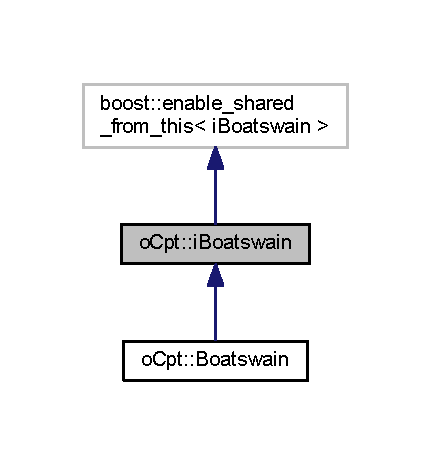
\includegraphics[width=208pt]{classo_cpt_1_1i_boatswain__inherit__graph}
\end{center}
\end{figure}


Collaboration diagram for o\+Cpt\+:\+:i\+Boatswain\+:\nopagebreak
\begin{figure}[H]
\begin{center}
\leavevmode
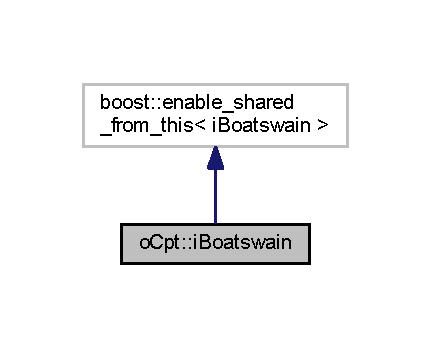
\includegraphics[width=208pt]{classo_cpt_1_1i_boatswain__coll__graph}
\end{center}
\end{figure}
\subsection*{Public Types}
\begin{DoxyCompactItemize}
\item 
typedef boost\+::shared\+\_\+ptr$<$ \hyperlink{classo_cpt_1_1i_boatswain}{i\+Boatswain} $>$ \hyperlink{classo_cpt_1_1i_boatswain_ad5e2819c6252955a7eddba4a4c980e3c}{ptr}
\item 
typedef boost\+::shared\+\_\+ptr$<$ boost\+::asio\+::deadline\+\_\+timer $>$ \hyperlink{classo_cpt_1_1i_boatswain_ac42d91dd3964880be9475ccaab4231cd}{timer\+Ptr}
\end{DoxyCompactItemize}
\subsection*{Public Member Functions}
\begin{DoxyCompactItemize}
\item 
\hyperlink{classo_cpt_1_1i_boatswain_a9424746b673744868f521b7a34a1064a}{i\+Boatswain} (\hyperlink{classo_cpt_1_1i_controller_a6d89a95cd6ad68bb74adfaca2f36370f}{i\+Controller\+::ptr} controller)
\item 
virtual \hyperlink{classo_cpt_1_1i_boatswain_a0577a8228f2a93e07ef21e22e9c17bde}{$\sim$i\+Boatswain} ()
\item 
virtual void \hyperlink{classo_cpt_1_1i_boatswain_a4512e742ba996b32dcc452d9f180724a}{run} ()=0
\item 
virtual void \hyperlink{classo_cpt_1_1i_boatswain_ad1fb6362c814a72ea6c4dc9a9042cf5e}{stop} ()=0
\item 
virtual void \hyperlink{classo_cpt_1_1i_boatswain_a0749ff59de42e7a8a47586ab9d9ac98f}{initialize} ()=0
\item 
virtual void \hyperlink{classo_cpt_1_1i_boatswain_aa9f9014202617a705d7ce21db2877222}{register\+Sensor} (\hyperlink{classo_cpt_1_1i_sensor_a03533d2c5dc66e332d70dbb3b5e3006a}{i\+Sensor\+::ptr} sensor)=0
\item 
virtual void \hyperlink{classo_cpt_1_1i_boatswain_a7915584ee17a28b1fc506a8968e27387}{register\+Actuator} (\hyperlink{classo_cpt_1_1i_actuator_a35847799558e92bb84fb6c71de772cac}{i\+Actuator\+::ptr} actuator)=0
\item 
virtual void \hyperlink{classo_cpt_1_1i_boatswain_aebae826c7516c1688e94d84de5606cac}{register\+Comm} (\hyperlink{classo_cpt_1_1i_comm_af0c655f143251b7d03fcd98f89637228}{i\+Comm\+::ptr} comm)=0
\item 
const boost\+::shared\+\_\+ptr$<$ bool $>$ \& \hyperlink{classo_cpt_1_1i_boatswain_ad35f3f30f3430ce4c1790ca375565889}{get\+Stop\+Thread} () const
\item 
void \hyperlink{classo_cpt_1_1i_boatswain_ac4c9a286c90132944dfab6df31900fc3}{set\+Stop\+Thread} (const boost\+::shared\+\_\+ptr$<$ bool $>$ \&stop\+Thread)
\item 
boost\+::shared\+\_\+ptr$<$ boost\+::asio\+::io\+\_\+service $>$ \& \hyperlink{classo_cpt_1_1i_boatswain_aa064a9b107c71e71b25c5cbd4957e804}{get\+I\+Oservice} ()
\end{DoxyCompactItemize}
\subsection*{Protected Member Functions}
\begin{DoxyCompactItemize}
\item 
virtual void \hyperlink{classo_cpt_1_1i_boatswain_a863c877ec067c55b5e06a04d0d9648ce}{reset\+Timer} (\hyperlink{classo_cpt_1_1i_sensor_a03533d2c5dc66e332d70dbb3b5e3006a}{i\+Sensor\+::ptr} sensor)=0
\end{DoxyCompactItemize}
\subsection*{Protected Attributes}
\begin{DoxyCompactItemize}
\item 
boost\+::shared\+\_\+ptr$<$ boost\+::asio\+::io\+\_\+service $>$ \hyperlink{classo_cpt_1_1i_boatswain_a95b337b39962f9c63fd82b500351a960}{ioservice\+\_\+}
\item 
\hyperlink{classo_cpt_1_1i_controller_a6d89a95cd6ad68bb74adfaca2f36370f}{i\+Controller\+::ptr} \hyperlink{classo_cpt_1_1i_boatswain_aafdc26c1366e4eee9cb156c5b6d705cf}{controller\+\_\+}
\item 
std\+::vector$<$ \hyperlink{classo_cpt_1_1i_boatswain_ac42d91dd3964880be9475ccaab4231cd}{timer\+Ptr} $>$ \hyperlink{classo_cpt_1_1i_boatswain_a22f6f6b95b832600c9dc1827589dca3c}{timers\+\_\+}
\item 
std\+::vector$<$ \hyperlink{classo_cpt_1_1i_sensor_a03533d2c5dc66e332d70dbb3b5e3006a}{i\+Sensor\+::ptr} $>$ \hyperlink{classo_cpt_1_1i_boatswain_ac25402266e3daa376e407a9f5ba73130}{timer\+Sensors\+\_\+}
\item 
std\+::vector$<$ \hyperlink{classo_cpt_1_1i_sensor_a03533d2c5dc66e332d70dbb3b5e3006a}{i\+Sensor\+::ptr} $>$ \hyperlink{classo_cpt_1_1i_boatswain_a1b58c7613d0dae24536f2db2e0510799}{manual\+Sensors\+\_\+}
\item 
boost\+::shared\+\_\+ptr$<$ bool $>$ \hyperlink{classo_cpt_1_1i_boatswain_a2fd1fb91df1788bb070ff4e7b7cf2c15}{stop\+Thread\+\_\+}
\item 
boost\+::shared\+\_\+ptr$<$ bool $>$ \hyperlink{classo_cpt_1_1i_boatswain_a38228671875f0c0ed945d2f44422d649}{local\+Stop\+Thread\+\_\+}
\end{DoxyCompactItemize}


\subsection{Detailed Description}
The \hyperlink{classo_cpt_1_1_boatswain}{Boatswain} performs all the labours tasks, suchs updateing and interpretting sensor readings, setting actuators according to the \hyperlink{classo_cpt_1_1_captain}{Captain} wishes, updating the state representation of the vessel in the \hyperlink{classo_cpt_1_1_world}{World}. Each \hyperlink{classo_cpt_1_1_boatswain}{Boatswain} runs on its own thread. It is possible for a vessel to have multiple Boatswains, responsible for multiple tasks, such as communication, localization, steering. Each \hyperlink{classo_cpt_1_1_boatswain}{Boatswain} has to adhere to the \hyperlink{classo_cpt_1_1i_boatswain}{i\+Boatswain} interface. 

Definition at line 27 of file Boatswain.\+h.



\subsection{Member Typedef Documentation}
\hypertarget{classo_cpt_1_1i_boatswain_ad5e2819c6252955a7eddba4a4c980e3c}{}\label{classo_cpt_1_1i_boatswain_ad5e2819c6252955a7eddba4a4c980e3c} 
\index{o\+Cpt\+::i\+Boatswain@{o\+Cpt\+::i\+Boatswain}!ptr@{ptr}}
\index{ptr@{ptr}!o\+Cpt\+::i\+Boatswain@{o\+Cpt\+::i\+Boatswain}}
\subsubsection{\texorpdfstring{ptr}{ptr}}
{\footnotesize\ttfamily typedef boost\+::shared\+\_\+ptr$<$\hyperlink{classo_cpt_1_1i_boatswain}{i\+Boatswain}$>$ \hyperlink{classo_cpt_1_1i_boatswain_ad5e2819c6252955a7eddba4a4c980e3c}{o\+Cpt\+::i\+Boatswain\+::ptr}}



Definition at line 29 of file Boatswain.\+h.

\hypertarget{classo_cpt_1_1i_boatswain_ac42d91dd3964880be9475ccaab4231cd}{}\label{classo_cpt_1_1i_boatswain_ac42d91dd3964880be9475ccaab4231cd} 
\index{o\+Cpt\+::i\+Boatswain@{o\+Cpt\+::i\+Boatswain}!timer\+Ptr@{timer\+Ptr}}
\index{timer\+Ptr@{timer\+Ptr}!o\+Cpt\+::i\+Boatswain@{o\+Cpt\+::i\+Boatswain}}
\subsubsection{\texorpdfstring{timer\+Ptr}{timerPtr}}
{\footnotesize\ttfamily typedef boost\+::shared\+\_\+ptr$<$boost\+::asio\+::deadline\+\_\+timer$>$ \hyperlink{classo_cpt_1_1i_boatswain_ac42d91dd3964880be9475ccaab4231cd}{o\+Cpt\+::i\+Boatswain\+::timer\+Ptr}}



Definition at line 30 of file Boatswain.\+h.



\subsection{Constructor \& Destructor Documentation}
\hypertarget{classo_cpt_1_1i_boatswain_a9424746b673744868f521b7a34a1064a}{}\label{classo_cpt_1_1i_boatswain_a9424746b673744868f521b7a34a1064a} 
\index{o\+Cpt\+::i\+Boatswain@{o\+Cpt\+::i\+Boatswain}!i\+Boatswain@{i\+Boatswain}}
\index{i\+Boatswain@{i\+Boatswain}!o\+Cpt\+::i\+Boatswain@{o\+Cpt\+::i\+Boatswain}}
\subsubsection{\texorpdfstring{i\+Boatswain()}{iBoatswain()}}
{\footnotesize\ttfamily o\+Cpt\+::i\+Boatswain\+::i\+Boatswain (\begin{DoxyParamCaption}\item[{\hyperlink{classo_cpt_1_1i_controller_a6d89a95cd6ad68bb74adfaca2f36370f}{i\+Controller\+::ptr}}]{controller }\end{DoxyParamCaption})}

Constructor for a \hyperlink{classo_cpt_1_1i_boatswain}{i\+Boatswain} 
\begin{DoxyParams}{Parameters}
{\em controller} & a shared\+\_\+ptr to the controller with which teh \hyperlink{classo_cpt_1_1_boatswain}{Boatswain} interacts \\
\hline
\end{DoxyParams}


Definition at line 7 of file Boatswain.\+cpp.



References ioservice\+\_\+, and local\+Stop\+Thread\+\_\+.

\hypertarget{classo_cpt_1_1i_boatswain_a0577a8228f2a93e07ef21e22e9c17bde}{}\label{classo_cpt_1_1i_boatswain_a0577a8228f2a93e07ef21e22e9c17bde} 
\index{o\+Cpt\+::i\+Boatswain@{o\+Cpt\+::i\+Boatswain}!````~i\+Boatswain@{$\sim$i\+Boatswain}}
\index{````~i\+Boatswain@{$\sim$i\+Boatswain}!o\+Cpt\+::i\+Boatswain@{o\+Cpt\+::i\+Boatswain}}
\subsubsection{\texorpdfstring{$\sim$i\+Boatswain()}{~iBoatswain()}}
{\footnotesize\ttfamily o\+Cpt\+::i\+Boatswain\+::$\sim$i\+Boatswain (\begin{DoxyParamCaption}{ }\end{DoxyParamCaption})\hspace{0.3cm}{\ttfamily [virtual]}}

Deconstructor for the \hyperlink{classo_cpt_1_1i_boatswain}{i\+Boatswain} 

Definition at line 13 of file Boatswain.\+cpp.



\subsection{Member Function Documentation}
\hypertarget{classo_cpt_1_1i_boatswain_aa064a9b107c71e71b25c5cbd4957e804}{}\label{classo_cpt_1_1i_boatswain_aa064a9b107c71e71b25c5cbd4957e804} 
\index{o\+Cpt\+::i\+Boatswain@{o\+Cpt\+::i\+Boatswain}!get\+I\+Oservice@{get\+I\+Oservice}}
\index{get\+I\+Oservice@{get\+I\+Oservice}!o\+Cpt\+::i\+Boatswain@{o\+Cpt\+::i\+Boatswain}}
\subsubsection{\texorpdfstring{get\+I\+Oservice()}{getIOservice()}}
{\footnotesize\ttfamily boost\+::shared\+\_\+ptr$<$ boost\+::asio\+::io\+\_\+service $>$ \& o\+Cpt\+::i\+Boatswain\+::get\+I\+Oservice (\begin{DoxyParamCaption}{ }\end{DoxyParamCaption})}

get the used Input Output service \begin{DoxyReturn}{Returns}
a shared\+\_\+ptr to the A\+S\+IO io service 
\end{DoxyReturn}


Definition at line 25 of file Boatswain.\+cpp.



References ioservice\+\_\+.

\hypertarget{classo_cpt_1_1i_boatswain_ad35f3f30f3430ce4c1790ca375565889}{}\label{classo_cpt_1_1i_boatswain_ad35f3f30f3430ce4c1790ca375565889} 
\index{o\+Cpt\+::i\+Boatswain@{o\+Cpt\+::i\+Boatswain}!get\+Stop\+Thread@{get\+Stop\+Thread}}
\index{get\+Stop\+Thread@{get\+Stop\+Thread}!o\+Cpt\+::i\+Boatswain@{o\+Cpt\+::i\+Boatswain}}
\subsubsection{\texorpdfstring{get\+Stop\+Thread()}{getStopThread()}}
{\footnotesize\ttfamily const boost\+::shared\+\_\+ptr$<$ bool $>$ \& o\+Cpt\+::i\+Boatswain\+::get\+Stop\+Thread (\begin{DoxyParamCaption}{ }\end{DoxyParamCaption}) const}

get if the thread is stopped \begin{DoxyReturn}{Returns}
returns if the thread should stop 
\end{DoxyReturn}


Definition at line 17 of file Boatswain.\+cpp.



References stop\+Thread\+\_\+.

\hypertarget{classo_cpt_1_1i_boatswain_a0749ff59de42e7a8a47586ab9d9ac98f}{}\label{classo_cpt_1_1i_boatswain_a0749ff59de42e7a8a47586ab9d9ac98f} 
\index{o\+Cpt\+::i\+Boatswain@{o\+Cpt\+::i\+Boatswain}!initialize@{initialize}}
\index{initialize@{initialize}!o\+Cpt\+::i\+Boatswain@{o\+Cpt\+::i\+Boatswain}}
\subsubsection{\texorpdfstring{initialize()}{initialize()}}
{\footnotesize\ttfamily virtual void o\+Cpt\+::i\+Boatswain\+::initialize (\begin{DoxyParamCaption}{ }\end{DoxyParamCaption})\hspace{0.3cm}{\ttfamily [pure virtual]}}

pure virtual function of initialzing the \hyperlink{classo_cpt_1_1_boatswain}{Boatswain} 

Implemented in \hyperlink{classo_cpt_1_1_boatswain_aa1c27c710e2156402c3851ac189ea162}{o\+Cpt\+::\+Boatswain}.

\hypertarget{classo_cpt_1_1i_boatswain_a7915584ee17a28b1fc506a8968e27387}{}\label{classo_cpt_1_1i_boatswain_a7915584ee17a28b1fc506a8968e27387} 
\index{o\+Cpt\+::i\+Boatswain@{o\+Cpt\+::i\+Boatswain}!register\+Actuator@{register\+Actuator}}
\index{register\+Actuator@{register\+Actuator}!o\+Cpt\+::i\+Boatswain@{o\+Cpt\+::i\+Boatswain}}
\subsubsection{\texorpdfstring{register\+Actuator()}{registerActuator()}}
{\footnotesize\ttfamily virtual void o\+Cpt\+::i\+Boatswain\+::register\+Actuator (\begin{DoxyParamCaption}\item[{\hyperlink{classo_cpt_1_1i_actuator_a35847799558e92bb84fb6c71de772cac}{i\+Actuator\+::ptr}}]{actuator }\end{DoxyParamCaption})\hspace{0.3cm}{\ttfamily [pure virtual]}}

Pure virtual function for registering a new actuator with the \hyperlink{classo_cpt_1_1_boatswain}{Boatswain} 
\begin{DoxyParams}{Parameters}
{\em actuator} & a shared\+\_\+ptr to an \hyperlink{classo_cpt_1_1_actuator}{Actuator} which need to be maintained by the \hyperlink{classo_cpt_1_1_boatswain}{Boatswain} \\
\hline
\end{DoxyParams}


Implemented in \hyperlink{classo_cpt_1_1_boatswain_ae3f318352a331d64840ff87ad1ce3e8e}{o\+Cpt\+::\+Boatswain}.

\hypertarget{classo_cpt_1_1i_boatswain_aebae826c7516c1688e94d84de5606cac}{}\label{classo_cpt_1_1i_boatswain_aebae826c7516c1688e94d84de5606cac} 
\index{o\+Cpt\+::i\+Boatswain@{o\+Cpt\+::i\+Boatswain}!register\+Comm@{register\+Comm}}
\index{register\+Comm@{register\+Comm}!o\+Cpt\+::i\+Boatswain@{o\+Cpt\+::i\+Boatswain}}
\subsubsection{\texorpdfstring{register\+Comm()}{registerComm()}}
{\footnotesize\ttfamily virtual void o\+Cpt\+::i\+Boatswain\+::register\+Comm (\begin{DoxyParamCaption}\item[{\hyperlink{classo_cpt_1_1i_comm_af0c655f143251b7d03fcd98f89637228}{i\+Comm\+::ptr}}]{comm }\end{DoxyParamCaption})\hspace{0.3cm}{\ttfamily [pure virtual]}}

Pure virtual function for registering a new communication device which 
\begin{DoxyParams}{Parameters}
{\em comm} & \\
\hline
\end{DoxyParams}


Implemented in \hyperlink{classo_cpt_1_1_boatswain_a7abff24ce1f199690a4890793ff8c23c}{o\+Cpt\+::\+Boatswain}.

\hypertarget{classo_cpt_1_1i_boatswain_aa9f9014202617a705d7ce21db2877222}{}\label{classo_cpt_1_1i_boatswain_aa9f9014202617a705d7ce21db2877222} 
\index{o\+Cpt\+::i\+Boatswain@{o\+Cpt\+::i\+Boatswain}!register\+Sensor@{register\+Sensor}}
\index{register\+Sensor@{register\+Sensor}!o\+Cpt\+::i\+Boatswain@{o\+Cpt\+::i\+Boatswain}}
\subsubsection{\texorpdfstring{register\+Sensor()}{registerSensor()}}
{\footnotesize\ttfamily virtual void o\+Cpt\+::i\+Boatswain\+::register\+Sensor (\begin{DoxyParamCaption}\item[{\hyperlink{classo_cpt_1_1i_sensor_a03533d2c5dc66e332d70dbb3b5e3006a}{i\+Sensor\+::ptr}}]{sensor }\end{DoxyParamCaption})\hspace{0.3cm}{\ttfamily [pure virtual]}}

Pure virtual function for registering a new sensor with the \hyperlink{classo_cpt_1_1_boatswain}{Boatswain} 
\begin{DoxyParams}{Parameters}
{\em sensor} & a shared\+\_\+ptr to a \hyperlink{classo_cpt_1_1_sensor}{Sensor} which need to maintained by the \hyperlink{classo_cpt_1_1_boatswain}{Boatswain} \\
\hline
\end{DoxyParams}


Implemented in \hyperlink{classo_cpt_1_1_boatswain_ab36071db5e3f8a0db0053b5553e508f0}{o\+Cpt\+::\+Boatswain}.

\hypertarget{classo_cpt_1_1i_boatswain_a863c877ec067c55b5e06a04d0d9648ce}{}\label{classo_cpt_1_1i_boatswain_a863c877ec067c55b5e06a04d0d9648ce} 
\index{o\+Cpt\+::i\+Boatswain@{o\+Cpt\+::i\+Boatswain}!reset\+Timer@{reset\+Timer}}
\index{reset\+Timer@{reset\+Timer}!o\+Cpt\+::i\+Boatswain@{o\+Cpt\+::i\+Boatswain}}
\subsubsection{\texorpdfstring{reset\+Timer()}{resetTimer()}}
{\footnotesize\ttfamily virtual void o\+Cpt\+::i\+Boatswain\+::reset\+Timer (\begin{DoxyParamCaption}\item[{\hyperlink{classo_cpt_1_1i_sensor_a03533d2c5dc66e332d70dbb3b5e3006a}{i\+Sensor\+::ptr}}]{sensor }\end{DoxyParamCaption})\hspace{0.3cm}{\ttfamily [protected]}, {\ttfamily [pure virtual]}}

Pure virtual function for resetting the timer 
\begin{DoxyParams}{Parameters}
{\em sensor} & \\
\hline
\end{DoxyParams}


Implemented in \hyperlink{classo_cpt_1_1_boatswain_aca864b4219485c6d83ad0e92c7ea16fd}{o\+Cpt\+::\+Boatswain}.

\hypertarget{classo_cpt_1_1i_boatswain_a4512e742ba996b32dcc452d9f180724a}{}\label{classo_cpt_1_1i_boatswain_a4512e742ba996b32dcc452d9f180724a} 
\index{o\+Cpt\+::i\+Boatswain@{o\+Cpt\+::i\+Boatswain}!run@{run}}
\index{run@{run}!o\+Cpt\+::i\+Boatswain@{o\+Cpt\+::i\+Boatswain}}
\subsubsection{\texorpdfstring{run()}{run()}}
{\footnotesize\ttfamily virtual void o\+Cpt\+::i\+Boatswain\+::run (\begin{DoxyParamCaption}{ }\end{DoxyParamCaption})\hspace{0.3cm}{\ttfamily [pure virtual]}}

pure virtual function for running the boatswain and his registered sensors 

Implemented in \hyperlink{classo_cpt_1_1_boatswain_a7665a4439b8e71ece31ff5e9755caf09}{o\+Cpt\+::\+Boatswain}.



Referenced by o\+Cpt\+::\+Vessel\+::run().

Here is the caller graph for this function\+:\nopagebreak
\begin{figure}[H]
\begin{center}
\leavevmode
\includegraphics[width=318pt]{classo_cpt_1_1i_boatswain_a4512e742ba996b32dcc452d9f180724a_icgraph}
\end{center}
\end{figure}
\hypertarget{classo_cpt_1_1i_boatswain_ac4c9a286c90132944dfab6df31900fc3}{}\label{classo_cpt_1_1i_boatswain_ac4c9a286c90132944dfab6df31900fc3} 
\index{o\+Cpt\+::i\+Boatswain@{o\+Cpt\+::i\+Boatswain}!set\+Stop\+Thread@{set\+Stop\+Thread}}
\index{set\+Stop\+Thread@{set\+Stop\+Thread}!o\+Cpt\+::i\+Boatswain@{o\+Cpt\+::i\+Boatswain}}
\subsubsection{\texorpdfstring{set\+Stop\+Thread()}{setStopThread()}}
{\footnotesize\ttfamily void o\+Cpt\+::i\+Boatswain\+::set\+Stop\+Thread (\begin{DoxyParamCaption}\item[{const boost\+::shared\+\_\+ptr$<$ bool $>$ \&}]{stop\+Thread }\end{DoxyParamCaption})}

set the value of the stopthread 
\begin{DoxyParams}{Parameters}
{\em stop\+Thread} & //$<$! a shared\+\_\+ptr to the boolean \\
\hline
\end{DoxyParams}


Definition at line 21 of file Boatswain.\+cpp.



References stop\+Thread\+\_\+.

\hypertarget{classo_cpt_1_1i_boatswain_ad1fb6362c814a72ea6c4dc9a9042cf5e}{}\label{classo_cpt_1_1i_boatswain_ad1fb6362c814a72ea6c4dc9a9042cf5e} 
\index{o\+Cpt\+::i\+Boatswain@{o\+Cpt\+::i\+Boatswain}!stop@{stop}}
\index{stop@{stop}!o\+Cpt\+::i\+Boatswain@{o\+Cpt\+::i\+Boatswain}}
\subsubsection{\texorpdfstring{stop()}{stop()}}
{\footnotesize\ttfamily virtual void o\+Cpt\+::i\+Boatswain\+::stop (\begin{DoxyParamCaption}{ }\end{DoxyParamCaption})\hspace{0.3cm}{\ttfamily [pure virtual]}}

pure virtual function for stopping the run task 

Implemented in \hyperlink{classo_cpt_1_1_boatswain_ad538cca1d6429dacf09b22c53291074f}{o\+Cpt\+::\+Boatswain}.



\subsection{Member Data Documentation}
\hypertarget{classo_cpt_1_1i_boatswain_aafdc26c1366e4eee9cb156c5b6d705cf}{}\label{classo_cpt_1_1i_boatswain_aafdc26c1366e4eee9cb156c5b6d705cf} 
\index{o\+Cpt\+::i\+Boatswain@{o\+Cpt\+::i\+Boatswain}!controller\+\_\+@{controller\+\_\+}}
\index{controller\+\_\+@{controller\+\_\+}!o\+Cpt\+::i\+Boatswain@{o\+Cpt\+::i\+Boatswain}}
\subsubsection{\texorpdfstring{controller\+\_\+}{controller\_}}
{\footnotesize\ttfamily \hyperlink{classo_cpt_1_1i_controller_a6d89a95cd6ad68bb74adfaca2f36370f}{i\+Controller\+::ptr} o\+Cpt\+::i\+Boatswain\+::controller\+\_\+\hspace{0.3cm}{\ttfamily [protected]}}



Definition at line 96 of file Boatswain.\+h.

\hypertarget{classo_cpt_1_1i_boatswain_a95b337b39962f9c63fd82b500351a960}{}\label{classo_cpt_1_1i_boatswain_a95b337b39962f9c63fd82b500351a960} 
\index{o\+Cpt\+::i\+Boatswain@{o\+Cpt\+::i\+Boatswain}!ioservice\+\_\+@{ioservice\+\_\+}}
\index{ioservice\+\_\+@{ioservice\+\_\+}!o\+Cpt\+::i\+Boatswain@{o\+Cpt\+::i\+Boatswain}}
\subsubsection{\texorpdfstring{ioservice\+\_\+}{ioservice\_}}
{\footnotesize\ttfamily boost\+::shared\+\_\+ptr$<$boost\+::asio\+::io\+\_\+service$>$ o\+Cpt\+::i\+Boatswain\+::ioservice\+\_\+\hspace{0.3cm}{\ttfamily [protected]}}



Definition at line 95 of file Boatswain.\+h.



Referenced by get\+I\+Oservice(), i\+Boatswain(), o\+Cpt\+::\+Boatswain\+::register\+Comm(), o\+Cpt\+::\+Boatswain\+::register\+Sensor(), o\+Cpt\+::\+Boatswain\+::reset\+Timer(), and o\+Cpt\+::\+Boatswain\+::run().

\hypertarget{classo_cpt_1_1i_boatswain_a38228671875f0c0ed945d2f44422d649}{}\label{classo_cpt_1_1i_boatswain_a38228671875f0c0ed945d2f44422d649} 
\index{o\+Cpt\+::i\+Boatswain@{o\+Cpt\+::i\+Boatswain}!local\+Stop\+Thread\+\_\+@{local\+Stop\+Thread\+\_\+}}
\index{local\+Stop\+Thread\+\_\+@{local\+Stop\+Thread\+\_\+}!o\+Cpt\+::i\+Boatswain@{o\+Cpt\+::i\+Boatswain}}
\subsubsection{\texorpdfstring{local\+Stop\+Thread\+\_\+}{localStopThread\_}}
{\footnotesize\ttfamily boost\+::shared\+\_\+ptr$<$bool$>$ o\+Cpt\+::i\+Boatswain\+::local\+Stop\+Thread\+\_\+\hspace{0.3cm}{\ttfamily [protected]}}



Definition at line 101 of file Boatswain.\+h.



Referenced by i\+Boatswain(), o\+Cpt\+::\+Boatswain\+::reset\+Timer(), and o\+Cpt\+::\+Boatswain\+::stop().

\hypertarget{classo_cpt_1_1i_boatswain_a1b58c7613d0dae24536f2db2e0510799}{}\label{classo_cpt_1_1i_boatswain_a1b58c7613d0dae24536f2db2e0510799} 
\index{o\+Cpt\+::i\+Boatswain@{o\+Cpt\+::i\+Boatswain}!manual\+Sensors\+\_\+@{manual\+Sensors\+\_\+}}
\index{manual\+Sensors\+\_\+@{manual\+Sensors\+\_\+}!o\+Cpt\+::i\+Boatswain@{o\+Cpt\+::i\+Boatswain}}
\subsubsection{\texorpdfstring{manual\+Sensors\+\_\+}{manualSensors\_}}
{\footnotesize\ttfamily std\+::vector$<$\hyperlink{classo_cpt_1_1i_sensor_a03533d2c5dc66e332d70dbb3b5e3006a}{i\+Sensor\+::ptr}$>$ o\+Cpt\+::i\+Boatswain\+::manual\+Sensors\+\_\+\hspace{0.3cm}{\ttfamily [protected]}}



Definition at line 99 of file Boatswain.\+h.



Referenced by o\+Cpt\+::\+Boatswain\+::register\+Sensor(), and o\+Cpt\+::\+Boatswain\+::run().

\hypertarget{classo_cpt_1_1i_boatswain_a2fd1fb91df1788bb070ff4e7b7cf2c15}{}\label{classo_cpt_1_1i_boatswain_a2fd1fb91df1788bb070ff4e7b7cf2c15} 
\index{o\+Cpt\+::i\+Boatswain@{o\+Cpt\+::i\+Boatswain}!stop\+Thread\+\_\+@{stop\+Thread\+\_\+}}
\index{stop\+Thread\+\_\+@{stop\+Thread\+\_\+}!o\+Cpt\+::i\+Boatswain@{o\+Cpt\+::i\+Boatswain}}
\subsubsection{\texorpdfstring{stop\+Thread\+\_\+}{stopThread\_}}
{\footnotesize\ttfamily boost\+::shared\+\_\+ptr$<$bool$>$ o\+Cpt\+::i\+Boatswain\+::stop\+Thread\+\_\+\hspace{0.3cm}{\ttfamily [protected]}}



Definition at line 100 of file Boatswain.\+h.



Referenced by get\+Stop\+Thread(), o\+Cpt\+::\+Boatswain\+::reset\+Timer(), and set\+Stop\+Thread().

\hypertarget{classo_cpt_1_1i_boatswain_a22f6f6b95b832600c9dc1827589dca3c}{}\label{classo_cpt_1_1i_boatswain_a22f6f6b95b832600c9dc1827589dca3c} 
\index{o\+Cpt\+::i\+Boatswain@{o\+Cpt\+::i\+Boatswain}!timers\+\_\+@{timers\+\_\+}}
\index{timers\+\_\+@{timers\+\_\+}!o\+Cpt\+::i\+Boatswain@{o\+Cpt\+::i\+Boatswain}}
\subsubsection{\texorpdfstring{timers\+\_\+}{timers\_}}
{\footnotesize\ttfamily std\+::vector$<$\hyperlink{classo_cpt_1_1i_boatswain_ac42d91dd3964880be9475ccaab4231cd}{timer\+Ptr}$>$ o\+Cpt\+::i\+Boatswain\+::timers\+\_\+\hspace{0.3cm}{\ttfamily [protected]}}



Definition at line 97 of file Boatswain.\+h.



Referenced by o\+Cpt\+::\+Boatswain\+::register\+Sensor(), and o\+Cpt\+::\+Boatswain\+::reset\+Timer().

\hypertarget{classo_cpt_1_1i_boatswain_ac25402266e3daa376e407a9f5ba73130}{}\label{classo_cpt_1_1i_boatswain_ac25402266e3daa376e407a9f5ba73130} 
\index{o\+Cpt\+::i\+Boatswain@{o\+Cpt\+::i\+Boatswain}!timer\+Sensors\+\_\+@{timer\+Sensors\+\_\+}}
\index{timer\+Sensors\+\_\+@{timer\+Sensors\+\_\+}!o\+Cpt\+::i\+Boatswain@{o\+Cpt\+::i\+Boatswain}}
\subsubsection{\texorpdfstring{timer\+Sensors\+\_\+}{timerSensors\_}}
{\footnotesize\ttfamily std\+::vector$<$\hyperlink{classo_cpt_1_1i_sensor_a03533d2c5dc66e332d70dbb3b5e3006a}{i\+Sensor\+::ptr}$>$ o\+Cpt\+::i\+Boatswain\+::timer\+Sensors\+\_\+\hspace{0.3cm}{\ttfamily [protected]}}



Definition at line 98 of file Boatswain.\+h.



Referenced by o\+Cpt\+::\+Boatswain\+::register\+Sensor(), and o\+Cpt\+::\+Boatswain\+::reset\+Timer().



The documentation for this class was generated from the following files\+:\begin{DoxyCompactItemize}
\item 
/projects/mti/oh\+Captain/oh\+Captain/include/\+Core/\hyperlink{_boatswain_8h}{Boatswain.\+h}\item 
/projects/mti/oh\+Captain/oh\+Captain/src/\+Core/\hyperlink{_boatswain_8cpp}{Boatswain.\+cpp}\end{DoxyCompactItemize}

\hypertarget{classo_cpt_1_1i_captain}{}\section{o\+Cpt\+:\+:i\+Captain Class Reference}
\label{classo_cpt_1_1i_captain}\index{o\+Cpt\+::i\+Captain@{o\+Cpt\+::i\+Captain}}


{\ttfamily \#include $<$Captain.\+h$>$}



Inheritance diagram for o\+Cpt\+:\+:i\+Captain\+:\nopagebreak
\begin{figure}[H]
\begin{center}
\leavevmode
\includegraphics[width=158pt]{classo_cpt_1_1i_captain__inherit__graph}
\end{center}
\end{figure}
\subsection*{Public Types}
\begin{DoxyCompactItemize}
\item 
typedef boost\+::shared\+\_\+ptr$<$ \hyperlink{classo_cpt_1_1i_captain}{i\+Captain} $>$ \hyperlink{classo_cpt_1_1i_captain_ae1595d808fa14777c26f1227a82ac4f5}{ptr}
\end{DoxyCompactItemize}
\subsection*{Public Member Functions}
\begin{DoxyCompactItemize}
\item 
\hyperlink{classo_cpt_1_1i_captain_a23cd0cb920d48da605e9c8266e6448a9}{i\+Captain} (\hyperlink{classo_cpt_1_1_world_aa6e591e3096d5de71e0cec9039663d67}{World\+::ptr} world)
\item 
virtual \hyperlink{classo_cpt_1_1i_captain_a32e37b6a4952f59c1b315d54bf84bb3f}{$\sim$i\+Captain} ()
\item 
virtual void \hyperlink{classo_cpt_1_1i_captain_a53d61f2d68b435f32ad66858ae898763}{run} ()=0
\item 
virtual void \hyperlink{classo_cpt_1_1i_captain_aeda385ea9a0ee33301dfda05098c836b}{stop} ()=0
\item 
virtual void \hyperlink{classo_cpt_1_1i_captain_a5ad7947dde7866981c76ccd3a30ce4ce}{initialize} ()=0
\item 
const boost\+::shared\+\_\+ptr$<$ bool $>$ \& \hyperlink{classo_cpt_1_1i_captain_ae59d378b21d0f385d0a8c4ade2768529}{get\+Stop\+Thread\+\_\+} () const
\item 
void \hyperlink{classo_cpt_1_1i_captain_ad430c275b858faa6eee0be6cc0c8ea26}{set\+Stop\+Thread\+\_\+} (const boost\+::shared\+\_\+ptr$<$ bool $>$ \&\hyperlink{classo_cpt_1_1i_captain_a867451cb05e5073d61c0b6a2d0e7389c}{stop\+Thread\+\_\+})
\end{DoxyCompactItemize}
\subsection*{Protected Attributes}
\begin{DoxyCompactItemize}
\item 
boost\+::shared\+\_\+ptr$<$ bool $>$ \hyperlink{classo_cpt_1_1i_captain_a867451cb05e5073d61c0b6a2d0e7389c}{stop\+Thread\+\_\+}
\item 
boost\+::shared\+\_\+ptr$<$ bool $>$ \hyperlink{classo_cpt_1_1i_captain_aaa8f3eba679429337bc7078a8c1a45ac}{local\+Stop\+Thread\+\_\+}
\item 
\hyperlink{classo_cpt_1_1_world_aa6e591e3096d5de71e0cec9039663d67}{World\+::ptr} \hyperlink{classo_cpt_1_1i_captain_a6e08906c347d5fc66605bfde73046194}{world\+\_\+}
\end{DoxyCompactItemize}


\subsection{Detailed Description}


Definition at line 12 of file Captain.\+h.



\subsection{Member Typedef Documentation}
\hypertarget{classo_cpt_1_1i_captain_ae1595d808fa14777c26f1227a82ac4f5}{}\label{classo_cpt_1_1i_captain_ae1595d808fa14777c26f1227a82ac4f5} 
\index{o\+Cpt\+::i\+Captain@{o\+Cpt\+::i\+Captain}!ptr@{ptr}}
\index{ptr@{ptr}!o\+Cpt\+::i\+Captain@{o\+Cpt\+::i\+Captain}}
\subsubsection{\texorpdfstring{ptr}{ptr}}
{\footnotesize\ttfamily typedef boost\+::shared\+\_\+ptr$<$\hyperlink{classo_cpt_1_1i_captain}{i\+Captain}$>$ \hyperlink{classo_cpt_1_1i_captain_ae1595d808fa14777c26f1227a82ac4f5}{o\+Cpt\+::i\+Captain\+::ptr}}



Definition at line 14 of file Captain.\+h.



\subsection{Constructor \& Destructor Documentation}
\hypertarget{classo_cpt_1_1i_captain_a23cd0cb920d48da605e9c8266e6448a9}{}\label{classo_cpt_1_1i_captain_a23cd0cb920d48da605e9c8266e6448a9} 
\index{o\+Cpt\+::i\+Captain@{o\+Cpt\+::i\+Captain}!i\+Captain@{i\+Captain}}
\index{i\+Captain@{i\+Captain}!o\+Cpt\+::i\+Captain@{o\+Cpt\+::i\+Captain}}
\subsubsection{\texorpdfstring{i\+Captain()}{iCaptain()}}
{\footnotesize\ttfamily o\+Cpt\+::i\+Captain\+::i\+Captain (\begin{DoxyParamCaption}\item[{\hyperlink{classo_cpt_1_1_world_aa6e591e3096d5de71e0cec9039663d67}{World\+::ptr}}]{world }\end{DoxyParamCaption})}



Definition at line 31 of file Captain.\+cpp.

\hypertarget{classo_cpt_1_1i_captain_a32e37b6a4952f59c1b315d54bf84bb3f}{}\label{classo_cpt_1_1i_captain_a32e37b6a4952f59c1b315d54bf84bb3f} 
\index{o\+Cpt\+::i\+Captain@{o\+Cpt\+::i\+Captain}!````~i\+Captain@{$\sim$i\+Captain}}
\index{````~i\+Captain@{$\sim$i\+Captain}!o\+Cpt\+::i\+Captain@{o\+Cpt\+::i\+Captain}}
\subsubsection{\texorpdfstring{$\sim$i\+Captain()}{~iCaptain()}}
{\footnotesize\ttfamily o\+Cpt\+::i\+Captain\+::$\sim$i\+Captain (\begin{DoxyParamCaption}{ }\end{DoxyParamCaption})\hspace{0.3cm}{\ttfamily [virtual]}}



Definition at line 35 of file Captain.\+cpp.



\subsection{Member Function Documentation}
\hypertarget{classo_cpt_1_1i_captain_ae59d378b21d0f385d0a8c4ade2768529}{}\label{classo_cpt_1_1i_captain_ae59d378b21d0f385d0a8c4ade2768529} 
\index{o\+Cpt\+::i\+Captain@{o\+Cpt\+::i\+Captain}!get\+Stop\+Thread\+\_\+@{get\+Stop\+Thread\+\_\+}}
\index{get\+Stop\+Thread\+\_\+@{get\+Stop\+Thread\+\_\+}!o\+Cpt\+::i\+Captain@{o\+Cpt\+::i\+Captain}}
\subsubsection{\texorpdfstring{get\+Stop\+Thread\+\_\+()}{getStopThread\_()}}
{\footnotesize\ttfamily const boost\+::shared\+\_\+ptr$<$ bool $>$ \& o\+Cpt\+::i\+Captain\+::get\+Stop\+Thread\+\_\+ (\begin{DoxyParamCaption}{ }\end{DoxyParamCaption}) const}



Definition at line 39 of file Captain.\+cpp.



References stop\+Thread\+\_\+.

\hypertarget{classo_cpt_1_1i_captain_a5ad7947dde7866981c76ccd3a30ce4ce}{}\label{classo_cpt_1_1i_captain_a5ad7947dde7866981c76ccd3a30ce4ce} 
\index{o\+Cpt\+::i\+Captain@{o\+Cpt\+::i\+Captain}!initialize@{initialize}}
\index{initialize@{initialize}!o\+Cpt\+::i\+Captain@{o\+Cpt\+::i\+Captain}}
\subsubsection{\texorpdfstring{initialize()}{initialize()}}
{\footnotesize\ttfamily virtual void o\+Cpt\+::i\+Captain\+::initialize (\begin{DoxyParamCaption}{ }\end{DoxyParamCaption})\hspace{0.3cm}{\ttfamily [pure virtual]}}



Implemented in \hyperlink{classo_cpt_1_1_captain_a3afce8b5a16b91a8b848ab6ae12a5ca6}{o\+Cpt\+::\+Captain}.

\hypertarget{classo_cpt_1_1i_captain_a53d61f2d68b435f32ad66858ae898763}{}\label{classo_cpt_1_1i_captain_a53d61f2d68b435f32ad66858ae898763} 
\index{o\+Cpt\+::i\+Captain@{o\+Cpt\+::i\+Captain}!run@{run}}
\index{run@{run}!o\+Cpt\+::i\+Captain@{o\+Cpt\+::i\+Captain}}
\subsubsection{\texorpdfstring{run()}{run()}}
{\footnotesize\ttfamily virtual void o\+Cpt\+::i\+Captain\+::run (\begin{DoxyParamCaption}{ }\end{DoxyParamCaption})\hspace{0.3cm}{\ttfamily [pure virtual]}}



Implemented in \hyperlink{classo_cpt_1_1_captain_ade0ca7804340b555a9ead5dd01465045}{o\+Cpt\+::\+Captain}.

\hypertarget{classo_cpt_1_1i_captain_ad430c275b858faa6eee0be6cc0c8ea26}{}\label{classo_cpt_1_1i_captain_ad430c275b858faa6eee0be6cc0c8ea26} 
\index{o\+Cpt\+::i\+Captain@{o\+Cpt\+::i\+Captain}!set\+Stop\+Thread\+\_\+@{set\+Stop\+Thread\+\_\+}}
\index{set\+Stop\+Thread\+\_\+@{set\+Stop\+Thread\+\_\+}!o\+Cpt\+::i\+Captain@{o\+Cpt\+::i\+Captain}}
\subsubsection{\texorpdfstring{set\+Stop\+Thread\+\_\+()}{setStopThread\_()}}
{\footnotesize\ttfamily void o\+Cpt\+::i\+Captain\+::set\+Stop\+Thread\+\_\+ (\begin{DoxyParamCaption}\item[{const boost\+::shared\+\_\+ptr$<$ bool $>$ \&}]{stop\+Thread\+\_\+ }\end{DoxyParamCaption})}



Definition at line 43 of file Captain.\+cpp.



References stop\+Thread\+\_\+.

\hypertarget{classo_cpt_1_1i_captain_aeda385ea9a0ee33301dfda05098c836b}{}\label{classo_cpt_1_1i_captain_aeda385ea9a0ee33301dfda05098c836b} 
\index{o\+Cpt\+::i\+Captain@{o\+Cpt\+::i\+Captain}!stop@{stop}}
\index{stop@{stop}!o\+Cpt\+::i\+Captain@{o\+Cpt\+::i\+Captain}}
\subsubsection{\texorpdfstring{stop()}{stop()}}
{\footnotesize\ttfamily virtual void o\+Cpt\+::i\+Captain\+::stop (\begin{DoxyParamCaption}{ }\end{DoxyParamCaption})\hspace{0.3cm}{\ttfamily [pure virtual]}}



Implemented in \hyperlink{classo_cpt_1_1_captain_aa8a3923b961f4bc2ebc857895f759711}{o\+Cpt\+::\+Captain}.



\subsection{Member Data Documentation}
\hypertarget{classo_cpt_1_1i_captain_aaa8f3eba679429337bc7078a8c1a45ac}{}\label{classo_cpt_1_1i_captain_aaa8f3eba679429337bc7078a8c1a45ac} 
\index{o\+Cpt\+::i\+Captain@{o\+Cpt\+::i\+Captain}!local\+Stop\+Thread\+\_\+@{local\+Stop\+Thread\+\_\+}}
\index{local\+Stop\+Thread\+\_\+@{local\+Stop\+Thread\+\_\+}!o\+Cpt\+::i\+Captain@{o\+Cpt\+::i\+Captain}}
\subsubsection{\texorpdfstring{local\+Stop\+Thread\+\_\+}{localStopThread\_}}
{\footnotesize\ttfamily boost\+::shared\+\_\+ptr$<$bool$>$ o\+Cpt\+::i\+Captain\+::local\+Stop\+Thread\+\_\+\hspace{0.3cm}{\ttfamily [protected]}}



Definition at line 32 of file Captain.\+h.



Referenced by o\+Cpt\+::\+Captain\+::\+Captain(), o\+Cpt\+::\+Captain\+::run(), and o\+Cpt\+::\+Captain\+::stop().

\hypertarget{classo_cpt_1_1i_captain_a867451cb05e5073d61c0b6a2d0e7389c}{}\label{classo_cpt_1_1i_captain_a867451cb05e5073d61c0b6a2d0e7389c} 
\index{o\+Cpt\+::i\+Captain@{o\+Cpt\+::i\+Captain}!stop\+Thread\+\_\+@{stop\+Thread\+\_\+}}
\index{stop\+Thread\+\_\+@{stop\+Thread\+\_\+}!o\+Cpt\+::i\+Captain@{o\+Cpt\+::i\+Captain}}
\subsubsection{\texorpdfstring{stop\+Thread\+\_\+}{stopThread\_}}
{\footnotesize\ttfamily boost\+::shared\+\_\+ptr$<$bool$>$ o\+Cpt\+::i\+Captain\+::stop\+Thread\+\_\+\hspace{0.3cm}{\ttfamily [protected]}}



Definition at line 31 of file Captain.\+h.



Referenced by get\+Stop\+Thread\+\_\+(), o\+Cpt\+::\+Captain\+::run(), and set\+Stop\+Thread\+\_\+().

\hypertarget{classo_cpt_1_1i_captain_a6e08906c347d5fc66605bfde73046194}{}\label{classo_cpt_1_1i_captain_a6e08906c347d5fc66605bfde73046194} 
\index{o\+Cpt\+::i\+Captain@{o\+Cpt\+::i\+Captain}!world\+\_\+@{world\+\_\+}}
\index{world\+\_\+@{world\+\_\+}!o\+Cpt\+::i\+Captain@{o\+Cpt\+::i\+Captain}}
\subsubsection{\texorpdfstring{world\+\_\+}{world\_}}
{\footnotesize\ttfamily \hyperlink{classo_cpt_1_1_world_aa6e591e3096d5de71e0cec9039663d67}{World\+::ptr} o\+Cpt\+::i\+Captain\+::world\+\_\+\hspace{0.3cm}{\ttfamily [protected]}}



Definition at line 33 of file Captain.\+h.



The documentation for this class was generated from the following files\+:\begin{DoxyCompactItemize}
\item 
/projects/mti/oh\+Captain/oh\+Captain/include/\+Core/\hyperlink{_captain_8h}{Captain.\+h}\item 
/projects/mti/oh\+Captain/oh\+Captain/src/\+Core/\hyperlink{_captain_8cpp}{Captain.\+cpp}\end{DoxyCompactItemize}

\hypertarget{classo_cpt_1_1i_comm}{}\section{o\+Cpt\+:\+:i\+Comm Class Reference}
\label{classo_cpt_1_1i_comm}\index{o\+Cpt\+::i\+Comm@{o\+Cpt\+::i\+Comm}}


{\ttfamily \#include $<$Communication.\+h$>$}



Inheritance diagram for o\+Cpt\+:\+:i\+Comm\+:
\nopagebreak
\begin{figure}[H]
\begin{center}
\leavevmode
\includegraphics[width=209pt]{classo_cpt_1_1i_comm__inherit__graph}
\end{center}
\end{figure}
\subsection*{Classes}
\begin{DoxyCompactItemize}
\item 
struct \hyperlink{structo_cpt_1_1i_comm_1_1_message}{Message}
\end{DoxyCompactItemize}
\subsection*{Public Types}
\begin{DoxyCompactItemize}
\item 
typedef boost\+::shared\+\_\+ptr$<$ \hyperlink{classo_cpt_1_1i_comm}{i\+Comm} $>$ \hyperlink{classo_cpt_1_1i_comm_af0c655f143251b7d03fcd98f89637228}{ptr}
\item 
typedef boost\+::signals2\+::signal$<$ void()$>$ \hyperlink{classo_cpt_1_1i_comm_a53ead13a50cbf583520f670dcd158e59}{signal\+\_\+t}
\end{DoxyCompactItemize}
\subsection*{Public Member Functions}
\begin{DoxyCompactItemize}
\item 
\hyperlink{classo_cpt_1_1i_comm_aed6a6ce6009f8fc9910058d0f64f4ccd}{i\+Comm} (const std\+::string \&id, const std\+::string \&device, \hyperlink{classo_cpt_1_1i_controller_a51c3436b03060209f6cd2ddce6df2d0c}{i\+Controller\+::io\+\_\+t} ioservice=\hyperlink{classo_cpt_1_1i_controller_a51c3436b03060209f6cd2ddce6df2d0c}{i\+Controller\+::io\+\_\+t}(new boost\+::asio\+::io\+\_\+service()))
\item 
virtual \hyperlink{classo_cpt_1_1i_comm_a817351ba50112bb3a850ed3098257a11}{$\sim$i\+Comm} ()
\item 
virtual void \hyperlink{classo_cpt_1_1i_comm_a0d15a29fb59dd6a74b56a126d03b9170}{run} ()=0
\item 
virtual void \hyperlink{classo_cpt_1_1i_comm_ad73564bd03146a576aaa37db1a38379f}{stop} ()=0
\item 
virtual void \hyperlink{classo_cpt_1_1i_comm_aed3d4364175d17efc0347b6e954f5aef}{send\+Message} (\hyperlink{structo_cpt_1_1i_comm_1_1_message}{Message} msg)=0
\item 
virtual \hyperlink{structo_cpt_1_1i_comm_1_1_message_ad2ba828ad76f96a30e3898b2609a4c01}{Message\+::ptr} \hyperlink{classo_cpt_1_1i_comm_a054ee0448f0d2773abce97c424c5c20c}{recieve\+Message} ()=0
\item 
virtual void \hyperlink{classo_cpt_1_1i_comm_a27a57fb90cfc9cce21552e8539f08dd7}{recieve\+Async\+Message} ()=0
\item 
const std\+::string \& \hyperlink{classo_cpt_1_1i_comm_a6040dafb80c889aa8d4b70b89e977ffa}{get\+Id} () const 
\item 
void \hyperlink{classo_cpt_1_1i_comm_ada67d85e8ca1c2b7931ab010de60cda7}{set\+Id} (const std\+::string \&id)
\item 
const std\+::string \& \hyperlink{classo_cpt_1_1i_comm_ad8c6b4ee36305bf76d3f23d60bb3bcb4}{get\+Type\+Of\+Comm} () const 
\item 
void \hyperlink{classo_cpt_1_1i_comm_ad5b257586d4fb17bcdf075e2401312a6}{set\+Type\+Of\+Comm} (const std\+::string \&type\+Of\+Comm)
\item 
\hyperlink{structo_cpt_1_1i_comm_1_1_message_ad2ba828ad76f96a30e3898b2609a4c01}{Message\+::ptr} \hyperlink{classo_cpt_1_1i_comm_a888e17cd4719170d4cc533ec4eaf1271}{read\+Fi\+Fo\+Msg} ()
\item 
std\+::deque$<$ \hyperlink{structo_cpt_1_1i_comm_1_1_message_ad2ba828ad76f96a30e3898b2609a4c01}{Message\+::ptr} $>$ $\ast$ \hyperlink{classo_cpt_1_1i_comm_a6fdac5c5dad398d31adf177c900b8054}{get\+Msg\+Queue} ()
\item 
void \hyperlink{classo_cpt_1_1i_comm_a7f8322024fbcc1c7ef1fae87fc6aa368}{set\+Ioservice} (const \hyperlink{classo_cpt_1_1i_controller_a51c3436b03060209f6cd2ddce6df2d0c}{i\+Controller\+::io\+\_\+t} \&ioservice)
\end{DoxyCompactItemize}
\subsection*{Public Attributes}
\begin{DoxyCompactItemize}
\item 
\hyperlink{classo_cpt_1_1i_comm_a53ead13a50cbf583520f670dcd158e59}{signal\+\_\+t} \hyperlink{classo_cpt_1_1i_comm_aedc63b07be3c9a395638b782a634eecf}{sig}
\end{DoxyCompactItemize}
\subsection*{Protected Attributes}
\begin{DoxyCompactItemize}
\item 
std\+::string \hyperlink{classo_cpt_1_1i_comm_a65678a6bfb2da392d2932b0cd5d818c6}{id\+\_\+}
\item 
std\+::string \hyperlink{classo_cpt_1_1i_comm_a4805d3c40171aa763f029ebe1886e24f}{type\+Of\+Comm\+\_\+}
\item 
std\+::string \hyperlink{classo_cpt_1_1i_comm_a26b537ee10eb14c0a15bb2ad4c4b7cda}{device\+\_\+}
\item 
boost\+::posix\+\_\+time\+::milliseconds \hyperlink{classo_cpt_1_1i_comm_a1e9989bd934719256f4b50123825c00e}{timer\+\_\+}
\item 
std\+::deque$<$ \hyperlink{structo_cpt_1_1i_comm_1_1_message_ad2ba828ad76f96a30e3898b2609a4c01}{Message\+::ptr} $>$ \hyperlink{classo_cpt_1_1i_comm_aa4bc236cd4492ea8b4fd2481de58b43f}{msg\+Queue\+\_\+}
\item 
\hyperlink{classo_cpt_1_1i_controller_a51c3436b03060209f6cd2ddce6df2d0c}{i\+Controller\+::io\+\_\+t} \hyperlink{classo_cpt_1_1i_comm_a40e1c5e7d35a83973c1b913da9143a2f}{ioservice\+\_\+}
\end{DoxyCompactItemize}


\subsection{Member Typedef Documentation}
\index{o\+Cpt\+::i\+Comm@{o\+Cpt\+::i\+Comm}!ptr@{ptr}}
\index{ptr@{ptr}!o\+Cpt\+::i\+Comm@{o\+Cpt\+::i\+Comm}}
\subsubsection[{\texorpdfstring{ptr}{ptr}}]{\setlength{\rightskip}{0pt plus 5cm}typedef boost\+::shared\+\_\+ptr$<${\bf i\+Comm}$>$ {\bf o\+Cpt\+::i\+Comm\+::ptr}}\hypertarget{classo_cpt_1_1i_comm_af0c655f143251b7d03fcd98f89637228}{}\label{classo_cpt_1_1i_comm_af0c655f143251b7d03fcd98f89637228}
\index{o\+Cpt\+::i\+Comm@{o\+Cpt\+::i\+Comm}!signal\+\_\+t@{signal\+\_\+t}}
\index{signal\+\_\+t@{signal\+\_\+t}!o\+Cpt\+::i\+Comm@{o\+Cpt\+::i\+Comm}}
\subsubsection[{\texorpdfstring{signal\+\_\+t}{signal_t}}]{\setlength{\rightskip}{0pt plus 5cm}typedef boost\+::signals2\+::signal$<$void ()$>$ {\bf o\+Cpt\+::i\+Comm\+::signal\+\_\+t}}\hypertarget{classo_cpt_1_1i_comm_a53ead13a50cbf583520f670dcd158e59}{}\label{classo_cpt_1_1i_comm_a53ead13a50cbf583520f670dcd158e59}


\subsection{Constructor \& Destructor Documentation}
\index{o\+Cpt\+::i\+Comm@{o\+Cpt\+::i\+Comm}!i\+Comm@{i\+Comm}}
\index{i\+Comm@{i\+Comm}!o\+Cpt\+::i\+Comm@{o\+Cpt\+::i\+Comm}}
\subsubsection[{\texorpdfstring{i\+Comm(const std\+::string \&id, const std\+::string \&device, i\+Controller\+::io\+\_\+t ioservice=i\+Controller\+::io\+\_\+t(new boost\+::asio\+::io\+\_\+service()))}{iComm(const std::string &id, const std::string &device, iController::io_t ioservice=iController::io_t(new boost::asio::io_service()))}}]{\setlength{\rightskip}{0pt plus 5cm}o\+Cpt\+::i\+Comm\+::i\+Comm (
\begin{DoxyParamCaption}
\item[{const std\+::string \&}]{id, }
\item[{const std\+::string \&}]{device, }
\item[{{\bf i\+Controller\+::io\+\_\+t}}]{ioservice = {\ttfamily {\bf i\+Controller\+::io\+\_\+t}(new~boost\+:\+:asio\+:\+:io\+\_\+service())}}
\end{DoxyParamCaption}
)}\hypertarget{classo_cpt_1_1i_comm_aed6a6ce6009f8fc9910058d0f64f4ccd}{}\label{classo_cpt_1_1i_comm_aed6a6ce6009f8fc9910058d0f64f4ccd}
\index{o\+Cpt\+::i\+Comm@{o\+Cpt\+::i\+Comm}!````~i\+Comm@{$\sim$i\+Comm}}
\index{````~i\+Comm@{$\sim$i\+Comm}!o\+Cpt\+::i\+Comm@{o\+Cpt\+::i\+Comm}}
\subsubsection[{\texorpdfstring{$\sim$i\+Comm()}{~iComm()}}]{\setlength{\rightskip}{0pt plus 5cm}o\+Cpt\+::i\+Comm\+::$\sim$i\+Comm (
\begin{DoxyParamCaption}
{}
\end{DoxyParamCaption}
)\hspace{0.3cm}{\ttfamily [virtual]}}\hypertarget{classo_cpt_1_1i_comm_a817351ba50112bb3a850ed3098257a11}{}\label{classo_cpt_1_1i_comm_a817351ba50112bb3a850ed3098257a11}


\subsection{Member Function Documentation}
\index{o\+Cpt\+::i\+Comm@{o\+Cpt\+::i\+Comm}!get\+Id@{get\+Id}}
\index{get\+Id@{get\+Id}!o\+Cpt\+::i\+Comm@{o\+Cpt\+::i\+Comm}}
\subsubsection[{\texorpdfstring{get\+Id() const }{getId() const }}]{\setlength{\rightskip}{0pt plus 5cm}const std\+::string \& o\+Cpt\+::i\+Comm\+::get\+Id (
\begin{DoxyParamCaption}
{}
\end{DoxyParamCaption}
) const}\hypertarget{classo_cpt_1_1i_comm_a6040dafb80c889aa8d4b70b89e977ffa}{}\label{classo_cpt_1_1i_comm_a6040dafb80c889aa8d4b70b89e977ffa}
\index{o\+Cpt\+::i\+Comm@{o\+Cpt\+::i\+Comm}!get\+Msg\+Queue@{get\+Msg\+Queue}}
\index{get\+Msg\+Queue@{get\+Msg\+Queue}!o\+Cpt\+::i\+Comm@{o\+Cpt\+::i\+Comm}}
\subsubsection[{\texorpdfstring{get\+Msg\+Queue()}{getMsgQueue()}}]{\setlength{\rightskip}{0pt plus 5cm}std\+::deque$<$ {\bf i\+Comm\+::\+Message\+::ptr} $>$ $\ast$ o\+Cpt\+::i\+Comm\+::get\+Msg\+Queue (
\begin{DoxyParamCaption}
{}
\end{DoxyParamCaption}
)}\hypertarget{classo_cpt_1_1i_comm_a6fdac5c5dad398d31adf177c900b8054}{}\label{classo_cpt_1_1i_comm_a6fdac5c5dad398d31adf177c900b8054}
\index{o\+Cpt\+::i\+Comm@{o\+Cpt\+::i\+Comm}!get\+Type\+Of\+Comm@{get\+Type\+Of\+Comm}}
\index{get\+Type\+Of\+Comm@{get\+Type\+Of\+Comm}!o\+Cpt\+::i\+Comm@{o\+Cpt\+::i\+Comm}}
\subsubsection[{\texorpdfstring{get\+Type\+Of\+Comm() const }{getTypeOfComm() const }}]{\setlength{\rightskip}{0pt plus 5cm}const std\+::string \& o\+Cpt\+::i\+Comm\+::get\+Type\+Of\+Comm (
\begin{DoxyParamCaption}
{}
\end{DoxyParamCaption}
) const}\hypertarget{classo_cpt_1_1i_comm_ad8c6b4ee36305bf76d3f23d60bb3bcb4}{}\label{classo_cpt_1_1i_comm_ad8c6b4ee36305bf76d3f23d60bb3bcb4}
\index{o\+Cpt\+::i\+Comm@{o\+Cpt\+::i\+Comm}!read\+Fi\+Fo\+Msg@{read\+Fi\+Fo\+Msg}}
\index{read\+Fi\+Fo\+Msg@{read\+Fi\+Fo\+Msg}!o\+Cpt\+::i\+Comm@{o\+Cpt\+::i\+Comm}}
\subsubsection[{\texorpdfstring{read\+Fi\+Fo\+Msg()}{readFiFoMsg()}}]{\setlength{\rightskip}{0pt plus 5cm}{\bf i\+Comm\+::\+Message\+::ptr} o\+Cpt\+::i\+Comm\+::read\+Fi\+Fo\+Msg (
\begin{DoxyParamCaption}
{}
\end{DoxyParamCaption}
)}\hypertarget{classo_cpt_1_1i_comm_a888e17cd4719170d4cc533ec4eaf1271}{}\label{classo_cpt_1_1i_comm_a888e17cd4719170d4cc533ec4eaf1271}
\index{o\+Cpt\+::i\+Comm@{o\+Cpt\+::i\+Comm}!recieve\+Async\+Message@{recieve\+Async\+Message}}
\index{recieve\+Async\+Message@{recieve\+Async\+Message}!o\+Cpt\+::i\+Comm@{o\+Cpt\+::i\+Comm}}
\subsubsection[{\texorpdfstring{recieve\+Async\+Message()=0}{recieveAsyncMessage()=0}}]{\setlength{\rightskip}{0pt plus 5cm}virtual void o\+Cpt\+::i\+Comm\+::recieve\+Async\+Message (
\begin{DoxyParamCaption}
{}
\end{DoxyParamCaption}
)\hspace{0.3cm}{\ttfamily [pure virtual]}}\hypertarget{classo_cpt_1_1i_comm_a27a57fb90cfc9cce21552e8539f08dd7}{}\label{classo_cpt_1_1i_comm_a27a57fb90cfc9cce21552e8539f08dd7}


Implemented in \hyperlink{classo_cpt_1_1components_1_1comm_1_1_lo_ra___r_n2483_a52af3c5bd992fc6cbe3e88989a3a25fc}{o\+Cpt\+::components\+::comm\+::\+Lo\+Ra\+\_\+\+R\+N2483}.

\index{o\+Cpt\+::i\+Comm@{o\+Cpt\+::i\+Comm}!recieve\+Message@{recieve\+Message}}
\index{recieve\+Message@{recieve\+Message}!o\+Cpt\+::i\+Comm@{o\+Cpt\+::i\+Comm}}
\subsubsection[{\texorpdfstring{recieve\+Message()=0}{recieveMessage()=0}}]{\setlength{\rightskip}{0pt plus 5cm}virtual {\bf Message\+::ptr} o\+Cpt\+::i\+Comm\+::recieve\+Message (
\begin{DoxyParamCaption}
{}
\end{DoxyParamCaption}
)\hspace{0.3cm}{\ttfamily [pure virtual]}}\hypertarget{classo_cpt_1_1i_comm_a054ee0448f0d2773abce97c424c5c20c}{}\label{classo_cpt_1_1i_comm_a054ee0448f0d2773abce97c424c5c20c}


Implemented in \hyperlink{classo_cpt_1_1components_1_1comm_1_1_lo_ra___r_n2483_aab494573c72b5b5b0b2d1d106844a043}{o\+Cpt\+::components\+::comm\+::\+Lo\+Ra\+\_\+\+R\+N2483}.

\index{o\+Cpt\+::i\+Comm@{o\+Cpt\+::i\+Comm}!run@{run}}
\index{run@{run}!o\+Cpt\+::i\+Comm@{o\+Cpt\+::i\+Comm}}
\subsubsection[{\texorpdfstring{run()=0}{run()=0}}]{\setlength{\rightskip}{0pt plus 5cm}virtual void o\+Cpt\+::i\+Comm\+::run (
\begin{DoxyParamCaption}
{}
\end{DoxyParamCaption}
)\hspace{0.3cm}{\ttfamily [pure virtual]}}\hypertarget{classo_cpt_1_1i_comm_a0d15a29fb59dd6a74b56a126d03b9170}{}\label{classo_cpt_1_1i_comm_a0d15a29fb59dd6a74b56a126d03b9170}


Implemented in \hyperlink{classo_cpt_1_1components_1_1comm_1_1_lo_ra___r_n2483_ae5d4406cecd941f4817e05787f79ca5d}{o\+Cpt\+::components\+::comm\+::\+Lo\+Ra\+\_\+\+R\+N2483}.

\index{o\+Cpt\+::i\+Comm@{o\+Cpt\+::i\+Comm}!send\+Message@{send\+Message}}
\index{send\+Message@{send\+Message}!o\+Cpt\+::i\+Comm@{o\+Cpt\+::i\+Comm}}
\subsubsection[{\texorpdfstring{send\+Message(\+Message msg)=0}{sendMessage(Message msg)=0}}]{\setlength{\rightskip}{0pt plus 5cm}virtual void o\+Cpt\+::i\+Comm\+::send\+Message (
\begin{DoxyParamCaption}
\item[{{\bf Message}}]{msg}
\end{DoxyParamCaption}
)\hspace{0.3cm}{\ttfamily [pure virtual]}}\hypertarget{classo_cpt_1_1i_comm_aed3d4364175d17efc0347b6e954f5aef}{}\label{classo_cpt_1_1i_comm_aed3d4364175d17efc0347b6e954f5aef}


Implemented in \hyperlink{classo_cpt_1_1components_1_1comm_1_1_lo_ra___r_n2483_aa8cdf42e61ab19a04e0c24d4b8190c23}{o\+Cpt\+::components\+::comm\+::\+Lo\+Ra\+\_\+\+R\+N2483}.

\index{o\+Cpt\+::i\+Comm@{o\+Cpt\+::i\+Comm}!set\+Id@{set\+Id}}
\index{set\+Id@{set\+Id}!o\+Cpt\+::i\+Comm@{o\+Cpt\+::i\+Comm}}
\subsubsection[{\texorpdfstring{set\+Id(const std\+::string \&id)}{setId(const std::string &id)}}]{\setlength{\rightskip}{0pt plus 5cm}void o\+Cpt\+::i\+Comm\+::set\+Id (
\begin{DoxyParamCaption}
\item[{const std\+::string \&}]{id}
\end{DoxyParamCaption}
)}\hypertarget{classo_cpt_1_1i_comm_ada67d85e8ca1c2b7931ab010de60cda7}{}\label{classo_cpt_1_1i_comm_ada67d85e8ca1c2b7931ab010de60cda7}
\index{o\+Cpt\+::i\+Comm@{o\+Cpt\+::i\+Comm}!set\+Ioservice@{set\+Ioservice}}
\index{set\+Ioservice@{set\+Ioservice}!o\+Cpt\+::i\+Comm@{o\+Cpt\+::i\+Comm}}
\subsubsection[{\texorpdfstring{set\+Ioservice(const i\+Controller\+::io\+\_\+t \&ioservice)}{setIoservice(const iController::io_t &ioservice)}}]{\setlength{\rightskip}{0pt plus 5cm}void o\+Cpt\+::i\+Comm\+::set\+Ioservice (
\begin{DoxyParamCaption}
\item[{const {\bf i\+Controller\+::io\+\_\+t} \&}]{ioservice}
\end{DoxyParamCaption}
)}\hypertarget{classo_cpt_1_1i_comm_a7f8322024fbcc1c7ef1fae87fc6aa368}{}\label{classo_cpt_1_1i_comm_a7f8322024fbcc1c7ef1fae87fc6aa368}
\index{o\+Cpt\+::i\+Comm@{o\+Cpt\+::i\+Comm}!set\+Type\+Of\+Comm@{set\+Type\+Of\+Comm}}
\index{set\+Type\+Of\+Comm@{set\+Type\+Of\+Comm}!o\+Cpt\+::i\+Comm@{o\+Cpt\+::i\+Comm}}
\subsubsection[{\texorpdfstring{set\+Type\+Of\+Comm(const std\+::string \&type\+Of\+Comm)}{setTypeOfComm(const std::string &typeOfComm)}}]{\setlength{\rightskip}{0pt plus 5cm}void o\+Cpt\+::i\+Comm\+::set\+Type\+Of\+Comm (
\begin{DoxyParamCaption}
\item[{const std\+::string \&}]{type\+Of\+Comm}
\end{DoxyParamCaption}
)}\hypertarget{classo_cpt_1_1i_comm_ad5b257586d4fb17bcdf075e2401312a6}{}\label{classo_cpt_1_1i_comm_ad5b257586d4fb17bcdf075e2401312a6}
\index{o\+Cpt\+::i\+Comm@{o\+Cpt\+::i\+Comm}!stop@{stop}}
\index{stop@{stop}!o\+Cpt\+::i\+Comm@{o\+Cpt\+::i\+Comm}}
\subsubsection[{\texorpdfstring{stop()=0}{stop()=0}}]{\setlength{\rightskip}{0pt plus 5cm}virtual void o\+Cpt\+::i\+Comm\+::stop (
\begin{DoxyParamCaption}
{}
\end{DoxyParamCaption}
)\hspace{0.3cm}{\ttfamily [pure virtual]}}\hypertarget{classo_cpt_1_1i_comm_ad73564bd03146a576aaa37db1a38379f}{}\label{classo_cpt_1_1i_comm_ad73564bd03146a576aaa37db1a38379f}


Implemented in \hyperlink{classo_cpt_1_1components_1_1comm_1_1_lo_ra___r_n2483_a3c8420219e7326727bbca88b0d92b69a}{o\+Cpt\+::components\+::comm\+::\+Lo\+Ra\+\_\+\+R\+N2483}.



\subsection{Member Data Documentation}
\index{o\+Cpt\+::i\+Comm@{o\+Cpt\+::i\+Comm}!device\+\_\+@{device\+\_\+}}
\index{device\+\_\+@{device\+\_\+}!o\+Cpt\+::i\+Comm@{o\+Cpt\+::i\+Comm}}
\subsubsection[{\texorpdfstring{device\+\_\+}{device_}}]{\setlength{\rightskip}{0pt plus 5cm}std\+::string o\+Cpt\+::i\+Comm\+::device\+\_\+\hspace{0.3cm}{\ttfamily [protected]}}\hypertarget{classo_cpt_1_1i_comm_a26b537ee10eb14c0a15bb2ad4c4b7cda}{}\label{classo_cpt_1_1i_comm_a26b537ee10eb14c0a15bb2ad4c4b7cda}
\index{o\+Cpt\+::i\+Comm@{o\+Cpt\+::i\+Comm}!id\+\_\+@{id\+\_\+}}
\index{id\+\_\+@{id\+\_\+}!o\+Cpt\+::i\+Comm@{o\+Cpt\+::i\+Comm}}
\subsubsection[{\texorpdfstring{id\+\_\+}{id_}}]{\setlength{\rightskip}{0pt plus 5cm}std\+::string o\+Cpt\+::i\+Comm\+::id\+\_\+\hspace{0.3cm}{\ttfamily [protected]}}\hypertarget{classo_cpt_1_1i_comm_a65678a6bfb2da392d2932b0cd5d818c6}{}\label{classo_cpt_1_1i_comm_a65678a6bfb2da392d2932b0cd5d818c6}
\index{o\+Cpt\+::i\+Comm@{o\+Cpt\+::i\+Comm}!ioservice\+\_\+@{ioservice\+\_\+}}
\index{ioservice\+\_\+@{ioservice\+\_\+}!o\+Cpt\+::i\+Comm@{o\+Cpt\+::i\+Comm}}
\subsubsection[{\texorpdfstring{ioservice\+\_\+}{ioservice_}}]{\setlength{\rightskip}{0pt plus 5cm}{\bf i\+Controller\+::io\+\_\+t} o\+Cpt\+::i\+Comm\+::ioservice\+\_\+\hspace{0.3cm}{\ttfamily [protected]}}\hypertarget{classo_cpt_1_1i_comm_a40e1c5e7d35a83973c1b913da9143a2f}{}\label{classo_cpt_1_1i_comm_a40e1c5e7d35a83973c1b913da9143a2f}
\index{o\+Cpt\+::i\+Comm@{o\+Cpt\+::i\+Comm}!msg\+Queue\+\_\+@{msg\+Queue\+\_\+}}
\index{msg\+Queue\+\_\+@{msg\+Queue\+\_\+}!o\+Cpt\+::i\+Comm@{o\+Cpt\+::i\+Comm}}
\subsubsection[{\texorpdfstring{msg\+Queue\+\_\+}{msgQueue_}}]{\setlength{\rightskip}{0pt plus 5cm}std\+::deque$<${\bf Message\+::ptr}$>$ o\+Cpt\+::i\+Comm\+::msg\+Queue\+\_\+\hspace{0.3cm}{\ttfamily [protected]}}\hypertarget{classo_cpt_1_1i_comm_aa4bc236cd4492ea8b4fd2481de58b43f}{}\label{classo_cpt_1_1i_comm_aa4bc236cd4492ea8b4fd2481de58b43f}
\index{o\+Cpt\+::i\+Comm@{o\+Cpt\+::i\+Comm}!sig@{sig}}
\index{sig@{sig}!o\+Cpt\+::i\+Comm@{o\+Cpt\+::i\+Comm}}
\subsubsection[{\texorpdfstring{sig}{sig}}]{\setlength{\rightskip}{0pt plus 5cm}{\bf signal\+\_\+t} o\+Cpt\+::i\+Comm\+::sig}\hypertarget{classo_cpt_1_1i_comm_aedc63b07be3c9a395638b782a634eecf}{}\label{classo_cpt_1_1i_comm_aedc63b07be3c9a395638b782a634eecf}
\index{o\+Cpt\+::i\+Comm@{o\+Cpt\+::i\+Comm}!timer\+\_\+@{timer\+\_\+}}
\index{timer\+\_\+@{timer\+\_\+}!o\+Cpt\+::i\+Comm@{o\+Cpt\+::i\+Comm}}
\subsubsection[{\texorpdfstring{timer\+\_\+}{timer_}}]{\setlength{\rightskip}{0pt plus 5cm}boost\+::posix\+\_\+time\+::milliseconds o\+Cpt\+::i\+Comm\+::timer\+\_\+\hspace{0.3cm}{\ttfamily [protected]}}\hypertarget{classo_cpt_1_1i_comm_a1e9989bd934719256f4b50123825c00e}{}\label{classo_cpt_1_1i_comm_a1e9989bd934719256f4b50123825c00e}
\index{o\+Cpt\+::i\+Comm@{o\+Cpt\+::i\+Comm}!type\+Of\+Comm\+\_\+@{type\+Of\+Comm\+\_\+}}
\index{type\+Of\+Comm\+\_\+@{type\+Of\+Comm\+\_\+}!o\+Cpt\+::i\+Comm@{o\+Cpt\+::i\+Comm}}
\subsubsection[{\texorpdfstring{type\+Of\+Comm\+\_\+}{typeOfComm_}}]{\setlength{\rightskip}{0pt plus 5cm}std\+::string o\+Cpt\+::i\+Comm\+::type\+Of\+Comm\+\_\+\hspace{0.3cm}{\ttfamily [protected]}}\hypertarget{classo_cpt_1_1i_comm_a4805d3c40171aa763f029ebe1886e24f}{}\label{classo_cpt_1_1i_comm_a4805d3c40171aa763f029ebe1886e24f}


The documentation for this class was generated from the following files\+:\begin{DoxyCompactItemize}
\item 
include/\+Core/\hyperlink{_communication_8h}{Communication.\+h}\item 
src/\+Core/\hyperlink{_communication_8cpp}{Communication.\+cpp}\end{DoxyCompactItemize}

\hypertarget{classo_cpt_1_1i_controller}{}\section{o\+Cpt\+:\+:i\+Controller Class Reference}
\label{classo_cpt_1_1i_controller}\index{o\+Cpt\+::i\+Controller@{o\+Cpt\+::i\+Controller}}


{\ttfamily \#include $<$Controller.\+h$>$}



Inheritance diagram for o\+Cpt\+:\+:i\+Controller\+:\nopagebreak
\begin{figure}[H]
\begin{center}
\leavevmode
\includegraphics[width=248pt]{classo_cpt_1_1i_controller__inherit__graph}
\end{center}
\end{figure}
\subsection*{Public Types}
\begin{DoxyCompactItemize}
\item 
typedef boost\+::shared\+\_\+ptr$<$ \hyperlink{classo_cpt_1_1i_controller}{i\+Controller} $>$ \hyperlink{classo_cpt_1_1i_controller_a6d89a95cd6ad68bb74adfaca2f36370f}{ptr}
\item 
typedef boost\+::shared\+\_\+ptr$<$ boost\+::asio\+::io\+\_\+service $>$ \hyperlink{classo_cpt_1_1i_controller_a51c3436b03060209f6cd2ddce6df2d0c}{io\+\_\+t}
\end{DoxyCompactItemize}
\subsection*{Public Member Functions}
\begin{DoxyCompactItemize}
\item 
\hyperlink{classo_cpt_1_1i_controller_acb46f6b610629978779f43e14b1c3f23}{i\+Controller} (\hyperlink{classo_cpt_1_1_world_aa6e591e3096d5de71e0cec9039663d67}{World\+::ptr} world)
\item 
virtual \hyperlink{classo_cpt_1_1i_controller_aa92cd99292abf1c093cd03420f44f6a0}{$\sim$i\+Controller} ()
\item 
virtual std\+::vector$<$ \hyperlink{classo_cpt_1_1protocol_1_1adc_a94af68cb9c573629a4a1a16f8ebd3dff}{protocol\+::adc\+::ptr} $>$ $\ast$ \hyperlink{classo_cpt_1_1i_controller_af414ebaf64b79ac45d1275e62799e36c}{get\+Adc\+Vector} ()=0
\item 
virtual \hyperlink{classo_cpt_1_1protocol_1_1adc_a94af68cb9c573629a4a1a16f8ebd3dff}{protocol\+::adc\+::ptr} \hyperlink{classo_cpt_1_1i_controller_a7abf65f5912df117a3ff4c1c9643bba3}{get\+A\+DC} (uint8\+\_\+t id, uint8\+\_\+t device)=0
\end{DoxyCompactItemize}
\subsection*{Protected Attributes}
\begin{DoxyCompactItemize}
\item 
std\+::vector$<$ \hyperlink{classo_cpt_1_1protocol_1_1adc_a94af68cb9c573629a4a1a16f8ebd3dff}{protocol\+::adc\+::ptr} $>$ \hyperlink{classo_cpt_1_1i_controller_ad385bb3078176cd3df8a9e51cfdab68a}{adc\+Vector\+\_\+}
\item 
\hyperlink{classo_cpt_1_1_world_aa6e591e3096d5de71e0cec9039663d67}{World\+::ptr} \hyperlink{classo_cpt_1_1i_controller_a77fe51158891ee7af9d5d92a3ff46b20}{world\+\_\+}
\end{DoxyCompactItemize}


\subsection{Detailed Description}
The interface for a controller. Each controller like for instance a Beaglebone black, Raspberry PI or x64 computer, should adhere to this interface 

Definition at line 559 of file Controller.\+h.



\subsection{Member Typedef Documentation}
\hypertarget{classo_cpt_1_1i_controller_a51c3436b03060209f6cd2ddce6df2d0c}{}\label{classo_cpt_1_1i_controller_a51c3436b03060209f6cd2ddce6df2d0c} 
\index{o\+Cpt\+::i\+Controller@{o\+Cpt\+::i\+Controller}!io\+\_\+t@{io\+\_\+t}}
\index{io\+\_\+t@{io\+\_\+t}!o\+Cpt\+::i\+Controller@{o\+Cpt\+::i\+Controller}}
\subsubsection{\texorpdfstring{io\+\_\+t}{io\_t}}
{\footnotesize\ttfamily typedef boost\+::shared\+\_\+ptr$<$boost\+::asio\+::io\+\_\+service$>$ \hyperlink{classo_cpt_1_1i_controller_a51c3436b03060209f6cd2ddce6df2d0c}{o\+Cpt\+::i\+Controller\+::io\+\_\+t}}



Definition at line 562 of file Controller.\+h.

\hypertarget{classo_cpt_1_1i_controller_a6d89a95cd6ad68bb74adfaca2f36370f}{}\label{classo_cpt_1_1i_controller_a6d89a95cd6ad68bb74adfaca2f36370f} 
\index{o\+Cpt\+::i\+Controller@{o\+Cpt\+::i\+Controller}!ptr@{ptr}}
\index{ptr@{ptr}!o\+Cpt\+::i\+Controller@{o\+Cpt\+::i\+Controller}}
\subsubsection{\texorpdfstring{ptr}{ptr}}
{\footnotesize\ttfamily typedef boost\+::shared\+\_\+ptr$<$\hyperlink{classo_cpt_1_1i_controller}{i\+Controller}$>$ \hyperlink{classo_cpt_1_1i_controller_a6d89a95cd6ad68bb74adfaca2f36370f}{o\+Cpt\+::i\+Controller\+::ptr}}



Definition at line 561 of file Controller.\+h.



\subsection{Constructor \& Destructor Documentation}
\hypertarget{classo_cpt_1_1i_controller_acb46f6b610629978779f43e14b1c3f23}{}\label{classo_cpt_1_1i_controller_acb46f6b610629978779f43e14b1c3f23} 
\index{o\+Cpt\+::i\+Controller@{o\+Cpt\+::i\+Controller}!i\+Controller@{i\+Controller}}
\index{i\+Controller@{i\+Controller}!o\+Cpt\+::i\+Controller@{o\+Cpt\+::i\+Controller}}
\subsubsection{\texorpdfstring{i\+Controller()}{iController()}}
{\footnotesize\ttfamily o\+Cpt\+::i\+Controller\+::i\+Controller (\begin{DoxyParamCaption}\item[{\hyperlink{classo_cpt_1_1_world_aa6e591e3096d5de71e0cec9039663d67}{World\+::ptr}}]{world }\end{DoxyParamCaption})}

The constructor 
\begin{DoxyParams}{Parameters}
{\em world} & a pointer to the \hyperlink{classo_cpt_1_1_world}{World} \\
\hline
\end{DoxyParams}


Definition at line 464 of file Controller.\+cpp.

\hypertarget{classo_cpt_1_1i_controller_aa92cd99292abf1c093cd03420f44f6a0}{}\label{classo_cpt_1_1i_controller_aa92cd99292abf1c093cd03420f44f6a0} 
\index{o\+Cpt\+::i\+Controller@{o\+Cpt\+::i\+Controller}!````~i\+Controller@{$\sim$i\+Controller}}
\index{````~i\+Controller@{$\sim$i\+Controller}!o\+Cpt\+::i\+Controller@{o\+Cpt\+::i\+Controller}}
\subsubsection{\texorpdfstring{$\sim$i\+Controller()}{~iController()}}
{\footnotesize\ttfamily o\+Cpt\+::i\+Controller\+::$\sim$i\+Controller (\begin{DoxyParamCaption}{ }\end{DoxyParamCaption})\hspace{0.3cm}{\ttfamily [virtual]}}

The deconstructor 

Definition at line 467 of file Controller.\+cpp.



\subsection{Member Function Documentation}
\hypertarget{classo_cpt_1_1i_controller_a7abf65f5912df117a3ff4c1c9643bba3}{}\label{classo_cpt_1_1i_controller_a7abf65f5912df117a3ff4c1c9643bba3} 
\index{o\+Cpt\+::i\+Controller@{o\+Cpt\+::i\+Controller}!get\+A\+DC@{get\+A\+DC}}
\index{get\+A\+DC@{get\+A\+DC}!o\+Cpt\+::i\+Controller@{o\+Cpt\+::i\+Controller}}
\subsubsection{\texorpdfstring{get\+A\+D\+C()}{getADC()}}
{\footnotesize\ttfamily virtual \hyperlink{classo_cpt_1_1protocol_1_1adc_a94af68cb9c573629a4a1a16f8ebd3dff}{protocol\+::adc\+::ptr} o\+Cpt\+::i\+Controller\+::get\+A\+DC (\begin{DoxyParamCaption}\item[{uint8\+\_\+t}]{id,  }\item[{uint8\+\_\+t}]{device }\end{DoxyParamCaption})\hspace{0.3cm}{\ttfamily [pure virtual]}}

A pure virtual function which gets a Pointer to a specific A\+DC 
\begin{DoxyParams}{Parameters}
{\em id} & The pin ID \\
\hline
{\em device} & the device ID \\
\hline
\end{DoxyParams}
\begin{DoxyReturn}{Returns}
a pointer to the requested A\+DC 
\end{DoxyReturn}


Implemented in \hyperlink{classo_cpt_1_1_a_r_m_a2f773bcd04719d81994af8930ca974bd}{o\+Cpt\+::\+A\+RM}.

\hypertarget{classo_cpt_1_1i_controller_af414ebaf64b79ac45d1275e62799e36c}{}\label{classo_cpt_1_1i_controller_af414ebaf64b79ac45d1275e62799e36c} 
\index{o\+Cpt\+::i\+Controller@{o\+Cpt\+::i\+Controller}!get\+Adc\+Vector@{get\+Adc\+Vector}}
\index{get\+Adc\+Vector@{get\+Adc\+Vector}!o\+Cpt\+::i\+Controller@{o\+Cpt\+::i\+Controller}}
\subsubsection{\texorpdfstring{get\+Adc\+Vector()}{getAdcVector()}}
{\footnotesize\ttfamily virtual std\+::vector$<$\hyperlink{classo_cpt_1_1protocol_1_1adc_a94af68cb9c573629a4a1a16f8ebd3dff}{protocol\+::adc\+::ptr}$>$$\ast$ o\+Cpt\+::i\+Controller\+::get\+Adc\+Vector (\begin{DoxyParamCaption}{ }\end{DoxyParamCaption})\hspace{0.3cm}{\ttfamily [pure virtual]}}

A pure virtual function which gets a pointer to all available A\+DC, if present. T\+O\+DO check how it handles no A\+DC presents \begin{DoxyReturn}{Returns}
a vector with pointers the all available A\+D\+Cs 
\end{DoxyReturn}


Implemented in \hyperlink{classo_cpt_1_1_a_r_m_a32e77e29e34f3114f0b766b705366ba8}{o\+Cpt\+::\+A\+RM}.



\subsection{Member Data Documentation}
\hypertarget{classo_cpt_1_1i_controller_ad385bb3078176cd3df8a9e51cfdab68a}{}\label{classo_cpt_1_1i_controller_ad385bb3078176cd3df8a9e51cfdab68a} 
\index{o\+Cpt\+::i\+Controller@{o\+Cpt\+::i\+Controller}!adc\+Vector\+\_\+@{adc\+Vector\+\_\+}}
\index{adc\+Vector\+\_\+@{adc\+Vector\+\_\+}!o\+Cpt\+::i\+Controller@{o\+Cpt\+::i\+Controller}}
\subsubsection{\texorpdfstring{adc\+Vector\+\_\+}{adcVector\_}}
{\footnotesize\ttfamily std\+::vector$<$\hyperlink{classo_cpt_1_1protocol_1_1adc_a94af68cb9c573629a4a1a16f8ebd3dff}{protocol\+::adc\+::ptr}$>$ o\+Cpt\+::i\+Controller\+::adc\+Vector\+\_\+\hspace{0.3cm}{\ttfamily [protected]}}



Definition at line 590 of file Controller.\+h.



Referenced by o\+Cpt\+::components\+::controller\+::\+B\+B\+B\+::\+B\+B\+B(), o\+Cpt\+::\+A\+R\+M\+::get\+A\+D\+C(), and o\+Cpt\+::\+A\+R\+M\+::get\+Adc\+Vector().

\hypertarget{classo_cpt_1_1i_controller_a77fe51158891ee7af9d5d92a3ff46b20}{}\label{classo_cpt_1_1i_controller_a77fe51158891ee7af9d5d92a3ff46b20} 
\index{o\+Cpt\+::i\+Controller@{o\+Cpt\+::i\+Controller}!world\+\_\+@{world\+\_\+}}
\index{world\+\_\+@{world\+\_\+}!o\+Cpt\+::i\+Controller@{o\+Cpt\+::i\+Controller}}
\subsubsection{\texorpdfstring{world\+\_\+}{world\_}}
{\footnotesize\ttfamily \hyperlink{classo_cpt_1_1_world_aa6e591e3096d5de71e0cec9039663d67}{World\+::ptr} o\+Cpt\+::i\+Controller\+::world\+\_\+\hspace{0.3cm}{\ttfamily [protected]}}



Definition at line 591 of file Controller.\+h.



The documentation for this class was generated from the following files\+:\begin{DoxyCompactItemize}
\item 
/projects/mti/oh\+Captain/oh\+Captain/include/\+Core/\hyperlink{_controller_8h}{Controller.\+h}\item 
/projects/mti/oh\+Captain/oh\+Captain/src/\+Core/\hyperlink{_controller_8cpp}{Controller.\+cpp}\end{DoxyCompactItemize}

\hypertarget{classo_cpt_1_1i_sensor}{}\section{o\+Cpt\+:\+:i\+Sensor Class Reference}
\label{classo_cpt_1_1i_sensor}\index{o\+Cpt\+::i\+Sensor@{o\+Cpt\+::i\+Sensor}}


{\ttfamily \#include $<$Sensor.\+h$>$}



Inheritance diagram for o\+Cpt\+:\+:i\+Sensor\+:\nopagebreak
\begin{figure}[H]
\begin{center}
\leavevmode
\includegraphics[width=350pt]{classo_cpt_1_1i_sensor__inherit__graph}
\end{center}
\end{figure}


Collaboration diagram for o\+Cpt\+:\+:i\+Sensor\+:\nopagebreak
\begin{figure}[H]
\begin{center}
\leavevmode
\includegraphics[width=185pt]{classo_cpt_1_1i_sensor__coll__graph}
\end{center}
\end{figure}
\subsection*{Classes}
\begin{DoxyCompactItemize}
\item 
struct \hyperlink{structo_cpt_1_1i_sensor_1_1_state}{State}
\end{DoxyCompactItemize}
\subsection*{Public Types}
\begin{DoxyCompactItemize}
\item 
typedef boost\+::shared\+\_\+ptr$<$ \hyperlink{classo_cpt_1_1i_sensor}{i\+Sensor} $>$ \hyperlink{classo_cpt_1_1i_sensor_a03533d2c5dc66e332d70dbb3b5e3006a}{ptr}
\item 
typedef boost\+::signals2\+::signal$<$ void()$>$ \hyperlink{classo_cpt_1_1i_sensor_a2e6d170acbc05f0b557bb68671813f6d}{signal\+\_\+t}
\item 
typedef boost\+::any \hyperlink{classo_cpt_1_1i_sensor_a8c83eafe5bdc0074a8c2c405023ee204}{generic\+\_\+t}
\end{DoxyCompactItemize}
\subsection*{Public Member Functions}
\begin{DoxyCompactItemize}
\item 
\hyperlink{classo_cpt_1_1i_sensor_a548ca1dbeea64980181c434518659d3e}{i\+Sensor} (\hyperlink{classo_cpt_1_1i_controller_a6d89a95cd6ad68bb74adfaca2f36370f}{i\+Controller\+::ptr} controller, \hyperlink{classo_cpt_1_1_world_aa6e591e3096d5de71e0cec9039663d67}{World\+::ptr} world, std\+::string id, std\+::string type\+Of\+Sensor=\char`\"{}\char`\"{})
\item 
virtual \hyperlink{classo_cpt_1_1i_sensor_a47eeead807cf3dc127fe55df4bc68c47}{$\sim$i\+Sensor} ()
\item 
virtual void \hyperlink{classo_cpt_1_1i_sensor_aa55bc04979e4852989af2bd4f64e70bc}{update\+Sensor} ()=0
\item 
virtual void \hyperlink{classo_cpt_1_1i_sensor_abbface05a16b17354c23389d9747bf7c}{run} ()=0
\item 
virtual void \hyperlink{classo_cpt_1_1i_sensor_aa85c22a8c8f7c2445379e1f82835f8dc}{stop} ()=0
\item 
virtual void \hyperlink{classo_cpt_1_1i_sensor_aa8def4a41b8280f7e4e02285cd7bd734}{init} ()=0
\item 
virtual void \hyperlink{classo_cpt_1_1i_sensor_a83b62cc63498ca4c335f85639e39656d}{set\+I\+Oservice} (boost\+::shared\+\_\+ptr$<$ boost\+::asio\+::io\+\_\+service $>$ ioservice)=0
\item 
virtual bool \hyperlink{classo_cpt_1_1i_sensor_affc8319846828aac6cab641f294a04aa}{operator==} (\hyperlink{classo_cpt_1_1i_sensor_a03533d2c5dc66e332d70dbb3b5e3006a}{i\+Sensor\+::ptr} rhs)
\item 
const boost\+::posix\+\_\+time\+::milliseconds \& \hyperlink{classo_cpt_1_1i_sensor_ad1651243755d72d5fd69668444555c77}{get\+Timer} () const
\item 
void \hyperlink{classo_cpt_1_1i_sensor_a4c956646ebf60201b5b23e0f5ad288ce}{set\+Timer} (const boost\+::posix\+\_\+time\+::milliseconds \&timer)
\item 
\hyperlink{classo_cpt_1_1i_sensor_a2e6d170acbc05f0b557bb68671813f6d}{signal\+\_\+t} \& \hyperlink{classo_cpt_1_1i_sensor_ad63e4d791b76f8328d652c4ed79eaec3}{get\+Sig} ()
\item 
const \hyperlink{structo_cpt_1_1i_sensor_1_1_state}{State} \& \hyperlink{classo_cpt_1_1i_sensor_a9ab760449e01c754c30374641c51ac66}{get\+State} () const
\item 
const std\+::string \& \hyperlink{classo_cpt_1_1i_sensor_aba86d11b74b8393c5ed0dfb2ec3b93d7}{get\+ID} () const
\item 
void \hyperlink{classo_cpt_1_1i_sensor_a2dec47e27c1e0843a1f874e28a522abd}{set\+ID} (const std\+::string \&id)
\item 
const std\+::string \& \hyperlink{classo_cpt_1_1i_sensor_aa356e53521301d555a7cbcee84bf54ea}{get\+Type\+Of\+Sensor} () const
\item 
void \hyperlink{classo_cpt_1_1i_sensor_ad1927865eb4ebfebc3dd840f66d98c1f}{set\+Type\+Of\+Sensor} (const std\+::string \&type\+Of\+Sensor)
\end{DoxyCompactItemize}
\subsection*{Protected Attributes}
\begin{DoxyCompactItemize}
\item 
std\+::string \hyperlink{classo_cpt_1_1i_sensor_a4c9bd54d193ec8f2cc01eede5eadacdc}{id\+\_\+}
\item 
std\+::string \hyperlink{classo_cpt_1_1i_sensor_a37396b5c63f5e99cb6e80c266f85dbfa}{type\+Of\+Sensor\+\_\+}
\item 
\hyperlink{classo_cpt_1_1i_controller_a6d89a95cd6ad68bb74adfaca2f36370f}{i\+Controller\+::ptr} \hyperlink{classo_cpt_1_1i_sensor_a65e41d8be53d71b1db21bac89c5c3c0d}{controller\+\_\+}
\item 
\hyperlink{classo_cpt_1_1_world_aa6e591e3096d5de71e0cec9039663d67}{World\+::ptr} \hyperlink{classo_cpt_1_1i_sensor_aab033b6462d7e8710c006f19c51e033e}{world\+\_\+}
\item 
boost\+::posix\+\_\+time\+::milliseconds \hyperlink{classo_cpt_1_1i_sensor_ac2a089853910118f6b490c00fc354d77}{timer\+\_\+}
\item 
\hyperlink{classo_cpt_1_1i_sensor_a2e6d170acbc05f0b557bb68671813f6d}{signal\+\_\+t} \hyperlink{classo_cpt_1_1i_sensor_a4f4943cf2af0b1a06bf5f0d8c46d1cb8}{sig\+\_\+}
\item 
\hyperlink{structo_cpt_1_1i_sensor_1_1_state}{State} \hyperlink{classo_cpt_1_1i_sensor_ad27fe02a89f013951a05f296ec457a08}{state\+\_\+}
\item 
bool \hyperlink{classo_cpt_1_1i_sensor_acc8826907fbe0c20c38a1e478e6a7c05}{sensor\+Running\+\_\+}
\item 
boost\+::shared\+\_\+ptr$<$ boost\+::asio\+::io\+\_\+service $>$ \hyperlink{classo_cpt_1_1i_sensor_a7aa3b0cea67ca97dae2495a20f5f6a04}{ioservice\+\_\+}
\end{DoxyCompactItemize}


\subsection{Detailed Description}
Each sensor that is used should adhere to the sensor interface. A sensor consits of an connection to a controller, such as a \hyperlink{classo_cpt_1_1_a_r_m}{A\+RM} device and the world. The sensor needs to be initiated with the construct, where afterwards the init fucntion is called. The sensor should then be registerd by the \hyperlink{classo_cpt_1_1_boatswain}{Boatswain}, using \hyperlink{classo_cpt_1_1_boatswain_ab36071db5e3f8a0db0053b5553e508f0}{Boatswain\+::register\+Sensor()}. This ensures that the boatswain can run the sensors. Some sensors are automatically update, whilst other need a manual action, such it is common practice to call the \hyperlink{classo_cpt_1_1i_sensor_aa55bc04979e4852989af2bd4f64e70bc}{i\+Sensor\+::update\+Sensor()}. Once the value is update, a new Boost\+::\+Signal2 is fired, which allow for the main function to obtain the \hyperlink{structo_cpt_1_1i_sensor_1_1_state}{State} of the sensor. Via \hyperlink{classo_cpt_1_1i_sensor_a9ab760449e01c754c30374641c51ac66}{i\+Sensor\+::get\+State()}. Since the return value of a sensor can vary, it is important to note that the final sensor should include a typedef with the return type named Return\+Value\+\_\+t. After a sensor update is given or a signal is recieved, the return value can be C\+A\+ST using the macro \hyperlink{_sensor_8h_a1edee5ac6b15c590def9ae3e0bfa8d48}{C\+A\+S\+T(x,t)} 

Definition at line 29 of file Sensor.\+h.



\subsection{Member Typedef Documentation}
\hypertarget{classo_cpt_1_1i_sensor_a8c83eafe5bdc0074a8c2c405023ee204}{}\label{classo_cpt_1_1i_sensor_a8c83eafe5bdc0074a8c2c405023ee204} 
\index{o\+Cpt\+::i\+Sensor@{o\+Cpt\+::i\+Sensor}!generic\+\_\+t@{generic\+\_\+t}}
\index{generic\+\_\+t@{generic\+\_\+t}!o\+Cpt\+::i\+Sensor@{o\+Cpt\+::i\+Sensor}}
\subsubsection{\texorpdfstring{generic\+\_\+t}{generic\_t}}
{\footnotesize\ttfamily typedef boost\+::any \hyperlink{classo_cpt_1_1i_sensor_a8c83eafe5bdc0074a8c2c405023ee204}{o\+Cpt\+::i\+Sensor\+::generic\+\_\+t}}



Definition at line 33 of file Sensor.\+h.

\hypertarget{classo_cpt_1_1i_sensor_a03533d2c5dc66e332d70dbb3b5e3006a}{}\label{classo_cpt_1_1i_sensor_a03533d2c5dc66e332d70dbb3b5e3006a} 
\index{o\+Cpt\+::i\+Sensor@{o\+Cpt\+::i\+Sensor}!ptr@{ptr}}
\index{ptr@{ptr}!o\+Cpt\+::i\+Sensor@{o\+Cpt\+::i\+Sensor}}
\subsubsection{\texorpdfstring{ptr}{ptr}}
{\footnotesize\ttfamily typedef boost\+::shared\+\_\+ptr$<$\hyperlink{classo_cpt_1_1i_sensor}{i\+Sensor}$>$ \hyperlink{classo_cpt_1_1i_sensor_a03533d2c5dc66e332d70dbb3b5e3006a}{o\+Cpt\+::i\+Sensor\+::ptr}}



Definition at line 31 of file Sensor.\+h.

\hypertarget{classo_cpt_1_1i_sensor_a2e6d170acbc05f0b557bb68671813f6d}{}\label{classo_cpt_1_1i_sensor_a2e6d170acbc05f0b557bb68671813f6d} 
\index{o\+Cpt\+::i\+Sensor@{o\+Cpt\+::i\+Sensor}!signal\+\_\+t@{signal\+\_\+t}}
\index{signal\+\_\+t@{signal\+\_\+t}!o\+Cpt\+::i\+Sensor@{o\+Cpt\+::i\+Sensor}}
\subsubsection{\texorpdfstring{signal\+\_\+t}{signal\_t}}
{\footnotesize\ttfamily typedef boost\+::signals2\+::signal$<$void()$>$ \hyperlink{classo_cpt_1_1i_sensor_a2e6d170acbc05f0b557bb68671813f6d}{o\+Cpt\+::i\+Sensor\+::signal\+\_\+t}}



Definition at line 32 of file Sensor.\+h.



\subsection{Constructor \& Destructor Documentation}
\hypertarget{classo_cpt_1_1i_sensor_a548ca1dbeea64980181c434518659d3e}{}\label{classo_cpt_1_1i_sensor_a548ca1dbeea64980181c434518659d3e} 
\index{o\+Cpt\+::i\+Sensor@{o\+Cpt\+::i\+Sensor}!i\+Sensor@{i\+Sensor}}
\index{i\+Sensor@{i\+Sensor}!o\+Cpt\+::i\+Sensor@{o\+Cpt\+::i\+Sensor}}
\subsubsection{\texorpdfstring{i\+Sensor()}{iSensor()}}
{\footnotesize\ttfamily o\+Cpt\+::i\+Sensor\+::i\+Sensor (\begin{DoxyParamCaption}\item[{\hyperlink{classo_cpt_1_1i_controller_a6d89a95cd6ad68bb74adfaca2f36370f}{i\+Controller\+::ptr}}]{controller,  }\item[{\hyperlink{classo_cpt_1_1_world_aa6e591e3096d5de71e0cec9039663d67}{World\+::ptr}}]{world,  }\item[{std\+::string}]{id,  }\item[{std\+::string}]{type\+Of\+Sensor = {\ttfamily \char`\"{}\char`\"{}} }\end{DoxyParamCaption})}

Constructor of \hyperlink{classo_cpt_1_1i_sensor}{i\+Sensor} 
\begin{DoxyParams}{Parameters}
{\em controller} & a shared\+\_\+ptr of the controller where the sensor is hooked to \\
\hline
{\em world} & a shared\+\_\+ptr of the world in which the vessel operates \\
\hline
{\em id} & a identifying name of the sensor \\
\hline
{\em type\+Of\+Sensor} & a identifying category for the sensor \\
\hline
\end{DoxyParams}


Definition at line 10 of file Sensor.\+cpp.



References state\+\_\+, and o\+Cpt\+::i\+Sensor\+::\+State\+::\+Value.

\hypertarget{classo_cpt_1_1i_sensor_a47eeead807cf3dc127fe55df4bc68c47}{}\label{classo_cpt_1_1i_sensor_a47eeead807cf3dc127fe55df4bc68c47} 
\index{o\+Cpt\+::i\+Sensor@{o\+Cpt\+::i\+Sensor}!````~i\+Sensor@{$\sim$i\+Sensor}}
\index{````~i\+Sensor@{$\sim$i\+Sensor}!o\+Cpt\+::i\+Sensor@{o\+Cpt\+::i\+Sensor}}
\subsubsection{\texorpdfstring{$\sim$i\+Sensor()}{~iSensor()}}
{\footnotesize\ttfamily o\+Cpt\+::i\+Sensor\+::$\sim$i\+Sensor (\begin{DoxyParamCaption}{ }\end{DoxyParamCaption})\hspace{0.3cm}{\ttfamily [virtual]}}

Deconstructor of the sensor 

Definition at line 18 of file Sensor.\+cpp.



\subsection{Member Function Documentation}
\hypertarget{classo_cpt_1_1i_sensor_aba86d11b74b8393c5ed0dfb2ec3b93d7}{}\label{classo_cpt_1_1i_sensor_aba86d11b74b8393c5ed0dfb2ec3b93d7} 
\index{o\+Cpt\+::i\+Sensor@{o\+Cpt\+::i\+Sensor}!get\+ID@{get\+ID}}
\index{get\+ID@{get\+ID}!o\+Cpt\+::i\+Sensor@{o\+Cpt\+::i\+Sensor}}
\subsubsection{\texorpdfstring{get\+I\+D()}{getID()}}
{\footnotesize\ttfamily const std\+::string \& o\+Cpt\+::i\+Sensor\+::get\+ID (\begin{DoxyParamCaption}{ }\end{DoxyParamCaption}) const}

get the current ID \begin{DoxyReturn}{Returns}
returns the ID as string 
\end{DoxyReturn}


Definition at line 41 of file Sensor.\+cpp.



References id\+\_\+.

\hypertarget{classo_cpt_1_1i_sensor_ad63e4d791b76f8328d652c4ed79eaec3}{}\label{classo_cpt_1_1i_sensor_ad63e4d791b76f8328d652c4ed79eaec3} 
\index{o\+Cpt\+::i\+Sensor@{o\+Cpt\+::i\+Sensor}!get\+Sig@{get\+Sig}}
\index{get\+Sig@{get\+Sig}!o\+Cpt\+::i\+Sensor@{o\+Cpt\+::i\+Sensor}}
\subsubsection{\texorpdfstring{get\+Sig()}{getSig()}}
{\footnotesize\ttfamily \hyperlink{classo_cpt_1_1i_sensor_a2e6d170acbc05f0b557bb68671813f6d}{i\+Sensor\+::signal\+\_\+t} \& o\+Cpt\+::i\+Sensor\+::get\+Sig (\begin{DoxyParamCaption}{ }\end{DoxyParamCaption})}

get the signal that is to be fired when the state is updated \begin{DoxyReturn}{Returns}
the signal\+\_\+t 
\end{DoxyReturn}


Definition at line 28 of file Sensor.\+cpp.



References sig\+\_\+.

\hypertarget{classo_cpt_1_1i_sensor_a9ab760449e01c754c30374641c51ac66}{}\label{classo_cpt_1_1i_sensor_a9ab760449e01c754c30374641c51ac66} 
\index{o\+Cpt\+::i\+Sensor@{o\+Cpt\+::i\+Sensor}!get\+State@{get\+State}}
\index{get\+State@{get\+State}!o\+Cpt\+::i\+Sensor@{o\+Cpt\+::i\+Sensor}}
\subsubsection{\texorpdfstring{get\+State()}{getState()}}
{\footnotesize\ttfamily const \hyperlink{structo_cpt_1_1i_sensor_1_1_state}{i\+Sensor\+::\+State} \& o\+Cpt\+::i\+Sensor\+::get\+State (\begin{DoxyParamCaption}{ }\end{DoxyParamCaption}) const}

gets the last \hyperlink{structo_cpt_1_1i_sensor_1_1_state}{State} of the sensor \begin{DoxyReturn}{Returns}
the \hyperlink{structo_cpt_1_1i_sensor_1_1_state}{State} object. Remember to C\+A\+ST the value like such $<$sensor\+Class$>$\+::\+Return\+Value\+\_\+t ret = C\+A\+ST($<$sensorname$>$-\/$>$\hyperlink{classo_cpt_1_1i_sensor_a9ab760449e01c754c30374641c51ac66}{get\+State()}.Value, $<$sensor\+Class$>$); 
\end{DoxyReturn}


Definition at line 32 of file Sensor.\+cpp.



References state\+\_\+.

\hypertarget{classo_cpt_1_1i_sensor_ad1651243755d72d5fd69668444555c77}{}\label{classo_cpt_1_1i_sensor_ad1651243755d72d5fd69668444555c77} 
\index{o\+Cpt\+::i\+Sensor@{o\+Cpt\+::i\+Sensor}!get\+Timer@{get\+Timer}}
\index{get\+Timer@{get\+Timer}!o\+Cpt\+::i\+Sensor@{o\+Cpt\+::i\+Sensor}}
\subsubsection{\texorpdfstring{get\+Timer()}{getTimer()}}
{\footnotesize\ttfamily const boost\+::posix\+\_\+time\+::milliseconds \& o\+Cpt\+::i\+Sensor\+::get\+Timer (\begin{DoxyParamCaption}{ }\end{DoxyParamCaption}) const}

Get the number of milliseconds when this sensor should be updated \begin{DoxyReturn}{Returns}
returns a boost\+::posix\+\_\+time\+::milliseconds type 
\end{DoxyReturn}


Definition at line 20 of file Sensor.\+cpp.



References timer\+\_\+.

\hypertarget{classo_cpt_1_1i_sensor_aa356e53521301d555a7cbcee84bf54ea}{}\label{classo_cpt_1_1i_sensor_aa356e53521301d555a7cbcee84bf54ea} 
\index{o\+Cpt\+::i\+Sensor@{o\+Cpt\+::i\+Sensor}!get\+Type\+Of\+Sensor@{get\+Type\+Of\+Sensor}}
\index{get\+Type\+Of\+Sensor@{get\+Type\+Of\+Sensor}!o\+Cpt\+::i\+Sensor@{o\+Cpt\+::i\+Sensor}}
\subsubsection{\texorpdfstring{get\+Type\+Of\+Sensor()}{getTypeOfSensor()}}
{\footnotesize\ttfamily const std\+::string \& o\+Cpt\+::i\+Sensor\+::get\+Type\+Of\+Sensor (\begin{DoxyParamCaption}{ }\end{DoxyParamCaption}) const}

get the type of sensor \begin{DoxyReturn}{Returns}
category identifying string 
\end{DoxyReturn}


Definition at line 49 of file Sensor.\+cpp.



References type\+Of\+Sensor\+\_\+.

\hypertarget{classo_cpt_1_1i_sensor_aa8def4a41b8280f7e4e02285cd7bd734}{}\label{classo_cpt_1_1i_sensor_aa8def4a41b8280f7e4e02285cd7bd734} 
\index{o\+Cpt\+::i\+Sensor@{o\+Cpt\+::i\+Sensor}!init@{init}}
\index{init@{init}!o\+Cpt\+::i\+Sensor@{o\+Cpt\+::i\+Sensor}}
\subsubsection{\texorpdfstring{init()}{init()}}
{\footnotesize\ttfamily virtual void o\+Cpt\+::i\+Sensor\+::init (\begin{DoxyParamCaption}{ }\end{DoxyParamCaption})\hspace{0.3cm}{\ttfamily [pure virtual]}}

pure virtual function for initializing the sensor 

Implemented in \hyperlink{classo_cpt_1_1_sensor_aa612a305a9a3091dd62cd1afb9d4dd7d}{o\+Cpt\+::\+Sensor}, \hyperlink{classo_cpt_1_1components_1_1sensors_1_1_razor_a1dd2b5a9fbac3c9510e2d3771abf358b}{o\+Cpt\+::components\+::sensors\+::\+Razor}, and \hyperlink{classo_cpt_1_1components_1_1sensors_1_1_p_t100_a296d0c3c2a55df465e127462c8c30215}{o\+Cpt\+::components\+::sensors\+::\+P\+T100}.

\hypertarget{classo_cpt_1_1i_sensor_affc8319846828aac6cab641f294a04aa}{}\label{classo_cpt_1_1i_sensor_affc8319846828aac6cab641f294a04aa} 
\index{o\+Cpt\+::i\+Sensor@{o\+Cpt\+::i\+Sensor}!operator==@{operator==}}
\index{operator==@{operator==}!o\+Cpt\+::i\+Sensor@{o\+Cpt\+::i\+Sensor}}
\subsubsection{\texorpdfstring{operator==()}{operator==()}}
{\footnotesize\ttfamily bool o\+Cpt\+::i\+Sensor\+::operator== (\begin{DoxyParamCaption}\item[{\hyperlink{classo_cpt_1_1i_sensor_a03533d2c5dc66e332d70dbb3b5e3006a}{i\+Sensor\+::ptr}}]{rhs }\end{DoxyParamCaption})\hspace{0.3cm}{\ttfamily [virtual]}}

Equal operator determining if this sensor is equal with the pointer 
\begin{DoxyParams}{Parameters}
{\em rhs} & shared\+\_\+ptr with the other sensor \\
\hline
\end{DoxyParams}
\begin{DoxyReturn}{Returns}
returns either true or false 
\end{DoxyReturn}


Definition at line 36 of file Sensor.\+cpp.



References controller\+\_\+, id\+\_\+, and type\+Of\+Sensor\+\_\+.

\hypertarget{classo_cpt_1_1i_sensor_abbface05a16b17354c23389d9747bf7c}{}\label{classo_cpt_1_1i_sensor_abbface05a16b17354c23389d9747bf7c} 
\index{o\+Cpt\+::i\+Sensor@{o\+Cpt\+::i\+Sensor}!run@{run}}
\index{run@{run}!o\+Cpt\+::i\+Sensor@{o\+Cpt\+::i\+Sensor}}
\subsubsection{\texorpdfstring{run()}{run()}}
{\footnotesize\ttfamily virtual void o\+Cpt\+::i\+Sensor\+::run (\begin{DoxyParamCaption}{ }\end{DoxyParamCaption})\hspace{0.3cm}{\ttfamily [pure virtual]}}

pure virtual function for running of the sensor 

Implemented in \hyperlink{classo_cpt_1_1_sensor_aef25b0e5f3a8358ee81c97c73909fbe6}{o\+Cpt\+::\+Sensor}, \hyperlink{classo_cpt_1_1components_1_1sensors_1_1_razor_ad93891ffb2d47e56d1417f0a40026c6e}{o\+Cpt\+::components\+::sensors\+::\+Razor}, \hyperlink{classo_cpt_1_1components_1_1sensors_1_1_gps_af703c48b8b7220a1909570f46edae932}{o\+Cpt\+::components\+::sensors\+::\+Gps}, and \hyperlink{classo_cpt_1_1components_1_1sensors_1_1_p_t100_a41dfc55a4be7993949feeb5ac013690d}{o\+Cpt\+::components\+::sensors\+::\+P\+T100}.



Referenced by o\+Cpt\+::\+Boatswain\+::register\+Sensor(), and o\+Cpt\+::\+Boatswain\+::reset\+Timer().

Here is the caller graph for this function\+:\nopagebreak
\begin{figure}[H]
\begin{center}
\leavevmode
\includegraphics[width=350pt]{classo_cpt_1_1i_sensor_abbface05a16b17354c23389d9747bf7c_icgraph}
\end{center}
\end{figure}
\hypertarget{classo_cpt_1_1i_sensor_a2dec47e27c1e0843a1f874e28a522abd}{}\label{classo_cpt_1_1i_sensor_a2dec47e27c1e0843a1f874e28a522abd} 
\index{o\+Cpt\+::i\+Sensor@{o\+Cpt\+::i\+Sensor}!set\+ID@{set\+ID}}
\index{set\+ID@{set\+ID}!o\+Cpt\+::i\+Sensor@{o\+Cpt\+::i\+Sensor}}
\subsubsection{\texorpdfstring{set\+I\+D()}{setID()}}
{\footnotesize\ttfamily void o\+Cpt\+::i\+Sensor\+::set\+ID (\begin{DoxyParamCaption}\item[{const std\+::string \&}]{id }\end{DoxyParamCaption})}

sets the ID of the sensor 
\begin{DoxyParams}{Parameters}
{\em id} & identifying string \\
\hline
\end{DoxyParams}


Definition at line 45 of file Sensor.\+cpp.



References id\+\_\+.

\hypertarget{classo_cpt_1_1i_sensor_a83b62cc63498ca4c335f85639e39656d}{}\label{classo_cpt_1_1i_sensor_a83b62cc63498ca4c335f85639e39656d} 
\index{o\+Cpt\+::i\+Sensor@{o\+Cpt\+::i\+Sensor}!set\+I\+Oservice@{set\+I\+Oservice}}
\index{set\+I\+Oservice@{set\+I\+Oservice}!o\+Cpt\+::i\+Sensor@{o\+Cpt\+::i\+Sensor}}
\subsubsection{\texorpdfstring{set\+I\+Oservice()}{setIOservice()}}
{\footnotesize\ttfamily virtual void o\+Cpt\+::i\+Sensor\+::set\+I\+Oservice (\begin{DoxyParamCaption}\item[{boost\+::shared\+\_\+ptr$<$ boost\+::asio\+::io\+\_\+service $>$}]{ioservice }\end{DoxyParamCaption})\hspace{0.3cm}{\ttfamily [pure virtual]}}

pure virtual function for registering the Input Output service 
\begin{DoxyParams}{Parameters}
{\em ioservice} & teh Input Output service used by Boost A\+S\+IO \\
\hline
\end{DoxyParams}


Implemented in \hyperlink{classo_cpt_1_1_sensor_ae7d47e18df5eb7854bf71fbbee9568df}{o\+Cpt\+::\+Sensor}, \hyperlink{classo_cpt_1_1components_1_1sensors_1_1_razor_a0f251fe3b51bf1a96b5d1e14e69a6d57}{o\+Cpt\+::components\+::sensors\+::\+Razor}, and \hyperlink{classo_cpt_1_1components_1_1sensors_1_1_gps_ad613b81625402daa6fdae80022fde18c}{o\+Cpt\+::components\+::sensors\+::\+Gps}.

\hypertarget{classo_cpt_1_1i_sensor_a4c956646ebf60201b5b23e0f5ad288ce}{}\label{classo_cpt_1_1i_sensor_a4c956646ebf60201b5b23e0f5ad288ce} 
\index{o\+Cpt\+::i\+Sensor@{o\+Cpt\+::i\+Sensor}!set\+Timer@{set\+Timer}}
\index{set\+Timer@{set\+Timer}!o\+Cpt\+::i\+Sensor@{o\+Cpt\+::i\+Sensor}}
\subsubsection{\texorpdfstring{set\+Timer()}{setTimer()}}
{\footnotesize\ttfamily void o\+Cpt\+::i\+Sensor\+::set\+Timer (\begin{DoxyParamCaption}\item[{const boost\+::posix\+\_\+time\+::milliseconds \&}]{timer }\end{DoxyParamCaption})}

set the number of milliseconds when this sensor should be updated 
\begin{DoxyParams}{Parameters}
{\em timer} & the number of milliseconds as an boost\+::posix\+\_\+time\+::milliseconds type \\
\hline
\end{DoxyParams}


Definition at line 24 of file Sensor.\+cpp.



References timer\+\_\+.

\hypertarget{classo_cpt_1_1i_sensor_ad1927865eb4ebfebc3dd840f66d98c1f}{}\label{classo_cpt_1_1i_sensor_ad1927865eb4ebfebc3dd840f66d98c1f} 
\index{o\+Cpt\+::i\+Sensor@{o\+Cpt\+::i\+Sensor}!set\+Type\+Of\+Sensor@{set\+Type\+Of\+Sensor}}
\index{set\+Type\+Of\+Sensor@{set\+Type\+Of\+Sensor}!o\+Cpt\+::i\+Sensor@{o\+Cpt\+::i\+Sensor}}
\subsubsection{\texorpdfstring{set\+Type\+Of\+Sensor()}{setTypeOfSensor()}}
{\footnotesize\ttfamily void o\+Cpt\+::i\+Sensor\+::set\+Type\+Of\+Sensor (\begin{DoxyParamCaption}\item[{const std\+::string \&}]{type\+Of\+Sensor }\end{DoxyParamCaption})}

sets the category of the sensor, suchs as G\+PS, temperature 
\begin{DoxyParams}{Parameters}
{\em type\+Of\+Sensor} & category identifying string \\
\hline
\end{DoxyParams}


Definition at line 53 of file Sensor.\+cpp.



References type\+Of\+Sensor\+\_\+.

\hypertarget{classo_cpt_1_1i_sensor_aa85c22a8c8f7c2445379e1f82835f8dc}{}\label{classo_cpt_1_1i_sensor_aa85c22a8c8f7c2445379e1f82835f8dc} 
\index{o\+Cpt\+::i\+Sensor@{o\+Cpt\+::i\+Sensor}!stop@{stop}}
\index{stop@{stop}!o\+Cpt\+::i\+Sensor@{o\+Cpt\+::i\+Sensor}}
\subsubsection{\texorpdfstring{stop()}{stop()}}
{\footnotesize\ttfamily virtual void o\+Cpt\+::i\+Sensor\+::stop (\begin{DoxyParamCaption}{ }\end{DoxyParamCaption})\hspace{0.3cm}{\ttfamily [pure virtual]}}

pure virtual function for stopping the sensor 

Implemented in \hyperlink{classo_cpt_1_1_sensor_a44ad78c2c091ca9cf72295293f8c5b74}{o\+Cpt\+::\+Sensor}, \hyperlink{classo_cpt_1_1components_1_1sensors_1_1_razor_a807441c137892ee3c1b612c284893fa1}{o\+Cpt\+::components\+::sensors\+::\+Razor}, \hyperlink{classo_cpt_1_1components_1_1sensors_1_1_gps_a9206c32fa91311740ae920c01eed6094}{o\+Cpt\+::components\+::sensors\+::\+Gps}, and \hyperlink{classo_cpt_1_1components_1_1sensors_1_1_p_t100_a6d80e18a58cf4e1b9b6ce82b441209e2}{o\+Cpt\+::components\+::sensors\+::\+P\+T100}.

\hypertarget{classo_cpt_1_1i_sensor_aa55bc04979e4852989af2bd4f64e70bc}{}\label{classo_cpt_1_1i_sensor_aa55bc04979e4852989af2bd4f64e70bc} 
\index{o\+Cpt\+::i\+Sensor@{o\+Cpt\+::i\+Sensor}!update\+Sensor@{update\+Sensor}}
\index{update\+Sensor@{update\+Sensor}!o\+Cpt\+::i\+Sensor@{o\+Cpt\+::i\+Sensor}}
\subsubsection{\texorpdfstring{update\+Sensor()}{updateSensor()}}
{\footnotesize\ttfamily virtual void o\+Cpt\+::i\+Sensor\+::update\+Sensor (\begin{DoxyParamCaption}{ }\end{DoxyParamCaption})\hspace{0.3cm}{\ttfamily [pure virtual]}}

pure virtual function for the updating of a sensor 

Implemented in \hyperlink{classo_cpt_1_1_sensor_ab4b0dedb06f11bcf2368852035beb2b2}{o\+Cpt\+::\+Sensor}, \hyperlink{classo_cpt_1_1components_1_1sensors_1_1_razor_ac8ee1582eb5c478c73e5e050858d2d7d}{o\+Cpt\+::components\+::sensors\+::\+Razor}, \hyperlink{classo_cpt_1_1components_1_1sensors_1_1_gps_a95976c5d8bba650d2732d4eb43979283}{o\+Cpt\+::components\+::sensors\+::\+Gps}, and \hyperlink{classo_cpt_1_1components_1_1sensors_1_1_p_t100_a66619675288a5344a55242d9bf097aee}{o\+Cpt\+::components\+::sensors\+::\+P\+T100}.



\subsection{Member Data Documentation}
\hypertarget{classo_cpt_1_1i_sensor_a65e41d8be53d71b1db21bac89c5c3c0d}{}\label{classo_cpt_1_1i_sensor_a65e41d8be53d71b1db21bac89c5c3c0d} 
\index{o\+Cpt\+::i\+Sensor@{o\+Cpt\+::i\+Sensor}!controller\+\_\+@{controller\+\_\+}}
\index{controller\+\_\+@{controller\+\_\+}!o\+Cpt\+::i\+Sensor@{o\+Cpt\+::i\+Sensor}}
\subsubsection{\texorpdfstring{controller\+\_\+}{controller\_}}
{\footnotesize\ttfamily \hyperlink{classo_cpt_1_1i_controller_a6d89a95cd6ad68bb74adfaca2f36370f}{i\+Controller\+::ptr} o\+Cpt\+::i\+Sensor\+::controller\+\_\+\hspace{0.3cm}{\ttfamily [protected]}}



Definition at line 140 of file Sensor.\+h.



Referenced by operator==(), and o\+Cpt\+::components\+::sensors\+::\+P\+T100\+::update\+Sensor().

\hypertarget{classo_cpt_1_1i_sensor_a4c9bd54d193ec8f2cc01eede5eadacdc}{}\label{classo_cpt_1_1i_sensor_a4c9bd54d193ec8f2cc01eede5eadacdc} 
\index{o\+Cpt\+::i\+Sensor@{o\+Cpt\+::i\+Sensor}!id\+\_\+@{id\+\_\+}}
\index{id\+\_\+@{id\+\_\+}!o\+Cpt\+::i\+Sensor@{o\+Cpt\+::i\+Sensor}}
\subsubsection{\texorpdfstring{id\+\_\+}{id\_}}
{\footnotesize\ttfamily std\+::string o\+Cpt\+::i\+Sensor\+::id\+\_\+\hspace{0.3cm}{\ttfamily [protected]}}



Definition at line 112 of file Sensor.\+h.



Referenced by get\+I\+D(), operator==(), and set\+I\+D().

\hypertarget{classo_cpt_1_1i_sensor_a7aa3b0cea67ca97dae2495a20f5f6a04}{}\label{classo_cpt_1_1i_sensor_a7aa3b0cea67ca97dae2495a20f5f6a04} 
\index{o\+Cpt\+::i\+Sensor@{o\+Cpt\+::i\+Sensor}!ioservice\+\_\+@{ioservice\+\_\+}}
\index{ioservice\+\_\+@{ioservice\+\_\+}!o\+Cpt\+::i\+Sensor@{o\+Cpt\+::i\+Sensor}}
\subsubsection{\texorpdfstring{ioservice\+\_\+}{ioservice\_}}
{\footnotesize\ttfamily boost\+::shared\+\_\+ptr$<$boost\+::asio\+::io\+\_\+service$>$ o\+Cpt\+::i\+Sensor\+::ioservice\+\_\+\hspace{0.3cm}{\ttfamily [protected]}}



Definition at line 146 of file Sensor.\+h.



Referenced by o\+Cpt\+::\+Sensor\+::set\+I\+Oservice().

\hypertarget{classo_cpt_1_1i_sensor_acc8826907fbe0c20c38a1e478e6a7c05}{}\label{classo_cpt_1_1i_sensor_acc8826907fbe0c20c38a1e478e6a7c05} 
\index{o\+Cpt\+::i\+Sensor@{o\+Cpt\+::i\+Sensor}!sensor\+Running\+\_\+@{sensor\+Running\+\_\+}}
\index{sensor\+Running\+\_\+@{sensor\+Running\+\_\+}!o\+Cpt\+::i\+Sensor@{o\+Cpt\+::i\+Sensor}}
\subsubsection{\texorpdfstring{sensor\+Running\+\_\+}{sensorRunning\_}}
{\footnotesize\ttfamily bool o\+Cpt\+::i\+Sensor\+::sensor\+Running\+\_\+\hspace{0.3cm}{\ttfamily [protected]}}



Definition at line 145 of file Sensor.\+h.



Referenced by o\+Cpt\+::components\+::sensors\+::\+Gps\+::run(), o\+Cpt\+::components\+::sensors\+::\+Razor\+::run(), o\+Cpt\+::\+Sensor\+::run(), o\+Cpt\+::components\+::sensors\+::\+Gps\+::stop(), o\+Cpt\+::components\+::sensors\+::\+Razor\+::stop(), and o\+Cpt\+::\+Sensor\+::stop().

\hypertarget{classo_cpt_1_1i_sensor_a4f4943cf2af0b1a06bf5f0d8c46d1cb8}{}\label{classo_cpt_1_1i_sensor_a4f4943cf2af0b1a06bf5f0d8c46d1cb8} 
\index{o\+Cpt\+::i\+Sensor@{o\+Cpt\+::i\+Sensor}!sig\+\_\+@{sig\+\_\+}}
\index{sig\+\_\+@{sig\+\_\+}!o\+Cpt\+::i\+Sensor@{o\+Cpt\+::i\+Sensor}}
\subsubsection{\texorpdfstring{sig\+\_\+}{sig\_}}
{\footnotesize\ttfamily \hyperlink{classo_cpt_1_1i_sensor_a2e6d170acbc05f0b557bb68671813f6d}{signal\+\_\+t} o\+Cpt\+::i\+Sensor\+::sig\+\_\+\hspace{0.3cm}{\ttfamily [protected]}}



Definition at line 143 of file Sensor.\+h.



Referenced by get\+Sig(), o\+Cpt\+::components\+::sensors\+::\+Gps\+::interpret\+Msg(), o\+Cpt\+::components\+::sensors\+::\+Razor\+::msg\+Handler(), and o\+Cpt\+::components\+::sensors\+::\+P\+T100\+::run().

\hypertarget{classo_cpt_1_1i_sensor_ad27fe02a89f013951a05f296ec457a08}{}\label{classo_cpt_1_1i_sensor_ad27fe02a89f013951a05f296ec457a08} 
\index{o\+Cpt\+::i\+Sensor@{o\+Cpt\+::i\+Sensor}!state\+\_\+@{state\+\_\+}}
\index{state\+\_\+@{state\+\_\+}!o\+Cpt\+::i\+Sensor@{o\+Cpt\+::i\+Sensor}}
\subsubsection{\texorpdfstring{state\+\_\+}{state\_}}
{\footnotesize\ttfamily \hyperlink{structo_cpt_1_1i_sensor_1_1_state}{State} o\+Cpt\+::i\+Sensor\+::state\+\_\+\hspace{0.3cm}{\ttfamily [protected]}}



Definition at line 144 of file Sensor.\+h.



Referenced by get\+State(), o\+Cpt\+::components\+::sensors\+::\+Gps\+::interpret\+Msg(), i\+Sensor(), o\+Cpt\+::components\+::sensors\+::\+Razor\+::msg\+Handler(), o\+Cpt\+::components\+::sensors\+::\+Razor\+::\+Razor(), o\+Cpt\+::components\+::sensors\+::\+P\+T100\+::update\+Sensor(), and o\+Cpt\+::components\+::sensors\+::\+Razor\+::update\+Sensor().

\hypertarget{classo_cpt_1_1i_sensor_ac2a089853910118f6b490c00fc354d77}{}\label{classo_cpt_1_1i_sensor_ac2a089853910118f6b490c00fc354d77} 
\index{o\+Cpt\+::i\+Sensor@{o\+Cpt\+::i\+Sensor}!timer\+\_\+@{timer\+\_\+}}
\index{timer\+\_\+@{timer\+\_\+}!o\+Cpt\+::i\+Sensor@{o\+Cpt\+::i\+Sensor}}
\subsubsection{\texorpdfstring{timer\+\_\+}{timer\_}}
{\footnotesize\ttfamily boost\+::posix\+\_\+time\+::milliseconds o\+Cpt\+::i\+Sensor\+::timer\+\_\+\hspace{0.3cm}{\ttfamily [protected]}}



Definition at line 142 of file Sensor.\+h.



Referenced by get\+Timer(), and set\+Timer().

\hypertarget{classo_cpt_1_1i_sensor_a37396b5c63f5e99cb6e80c266f85dbfa}{}\label{classo_cpt_1_1i_sensor_a37396b5c63f5e99cb6e80c266f85dbfa} 
\index{o\+Cpt\+::i\+Sensor@{o\+Cpt\+::i\+Sensor}!type\+Of\+Sensor\+\_\+@{type\+Of\+Sensor\+\_\+}}
\index{type\+Of\+Sensor\+\_\+@{type\+Of\+Sensor\+\_\+}!o\+Cpt\+::i\+Sensor@{o\+Cpt\+::i\+Sensor}}
\subsubsection{\texorpdfstring{type\+Of\+Sensor\+\_\+}{typeOfSensor\_}}
{\footnotesize\ttfamily std\+::string o\+Cpt\+::i\+Sensor\+::type\+Of\+Sensor\+\_\+\hspace{0.3cm}{\ttfamily [protected]}}



Definition at line 139 of file Sensor.\+h.



Referenced by get\+Type\+Of\+Sensor(), operator==(), and set\+Type\+Of\+Sensor().

\hypertarget{classo_cpt_1_1i_sensor_aab033b6462d7e8710c006f19c51e033e}{}\label{classo_cpt_1_1i_sensor_aab033b6462d7e8710c006f19c51e033e} 
\index{o\+Cpt\+::i\+Sensor@{o\+Cpt\+::i\+Sensor}!world\+\_\+@{world\+\_\+}}
\index{world\+\_\+@{world\+\_\+}!o\+Cpt\+::i\+Sensor@{o\+Cpt\+::i\+Sensor}}
\subsubsection{\texorpdfstring{world\+\_\+}{world\_}}
{\footnotesize\ttfamily \hyperlink{classo_cpt_1_1_world_aa6e591e3096d5de71e0cec9039663d67}{World\+::ptr} o\+Cpt\+::i\+Sensor\+::world\+\_\+\hspace{0.3cm}{\ttfamily [protected]}}



Definition at line 141 of file Sensor.\+h.



Referenced by o\+Cpt\+::components\+::sensors\+::\+Gps\+::interpret\+Msg(), o\+Cpt\+::components\+::sensors\+::\+Razor\+::msg\+Handler(), o\+Cpt\+::components\+::sensors\+::\+Razor\+::\+Razor(), o\+Cpt\+::components\+::sensors\+::\+P\+T100\+::update\+Sensor(), and o\+Cpt\+::components\+::sensors\+::\+Razor\+::update\+Sensor().



The documentation for this class was generated from the following files\+:\begin{DoxyCompactItemize}
\item 
include/\+Core/\hyperlink{_sensor_8h}{Sensor.\+h}\item 
src/\+Core/\hyperlink{_sensor_8cpp}{Sensor.\+cpp}\end{DoxyCompactItemize}

\hypertarget{classo_cpt_1_1i_task}{}\section{o\+Cpt\+:\+:i\+Task Class Reference}
\label{classo_cpt_1_1i_task}\index{o\+Cpt\+::i\+Task@{o\+Cpt\+::i\+Task}}


\hyperlink{classo_cpt_1_1_task}{Task} interface, all tasks need to adhere to this structure.  




{\ttfamily \#include $<$Task.\+h$>$}



Inheritance diagram for o\+Cpt\+:\+:i\+Task\+:\nopagebreak
\begin{figure}[H]
\begin{center}
\leavevmode
\includegraphics[width=350pt]{classo_cpt_1_1i_task__inherit__graph}
\end{center}
\end{figure}
\subsection*{Classes}
\begin{DoxyCompactItemize}
\item 
class \hyperlink{classo_cpt_1_1i_task_1_1_status}{Status}
\end{DoxyCompactItemize}
\subsection*{Public Types}
\begin{DoxyCompactItemize}
\item 
enum \hyperlink{classo_cpt_1_1i_task_a10d8726eb8957c2c305f468cf15b9f11}{Type\+Of} \{ \hyperlink{classo_cpt_1_1i_task_a10d8726eb8957c2c305f468cf15b9f11a7ca85240095e3a76c70f5535d26c4dd3}{R\+O\+U\+TE} = 1, 
\hyperlink{classo_cpt_1_1i_task_a10d8726eb8957c2c305f468cf15b9f11a1ec34e80717bb96ddd8376ff12d1b4c9}{W\+O\+RK} = 2
 \}
\item 
typedef boost\+::shared\+\_\+ptr$<$ \hyperlink{classo_cpt_1_1i_task}{i\+Task} $>$ \hyperlink{classo_cpt_1_1i_task_add2b02b5c97e63a1b7d6943ea4571543}{ptr}
\begin{DoxyCompactList}\small\item\em Boost shared\+\_\+ptr to a task. \end{DoxyCompactList}\item 
typedef std\+::list$<$ \hyperlink{classo_cpt_1_1i_task_add2b02b5c97e63a1b7d6943ea4571543}{i\+Task\+::ptr} $>$ \hyperlink{classo_cpt_1_1i_task_a8f949d091241347ea0cdfb8625b4dbca}{taskqueue}
\begin{DoxyCompactList}\small\item\em A list of shared pointer tasks. \end{DoxyCompactList}\end{DoxyCompactItemize}
\subsection*{Public Member Functions}
\begin{DoxyCompactItemize}
\item 
\hyperlink{classo_cpt_1_1i_task_a5b5affdc2f5213d8c5f11e8cd1cda517}{i\+Task} (\hyperlink{classo_cpt_1_1i_vessel_a43711a596f3bdfd0ca732ed3901edc97}{i\+Vessel\+::ptr} vessel, bool concurrent=false)
\item 
virtual \hyperlink{classo_cpt_1_1i_task_aa2c1053421fff92430b5912e0d3c7fc7}{$\sim$i\+Task} ()
\item 
virtual void \hyperlink{classo_cpt_1_1i_task_aedd48e3c4df48aaae0738ce3863e222f}{start} ()=0
\item 
virtual \hyperlink{classo_cpt_1_1i_task_1_1_status_aaf766c58d038e2defc3de2dddb92d1eb}{i\+Task\+::\+Status\+::ptr} \hyperlink{classo_cpt_1_1i_task_a8d6126b2e337a0ab39fdef1d8d7b73b9}{status} ()=0
\item 
virtual void \hyperlink{classo_cpt_1_1i_task_aedb88813b16914598dee9561813e56e8}{stop} ()=0
\end{DoxyCompactItemize}
\subsection*{Public Attributes}
\begin{DoxyCompactItemize}
\item 
\hyperlink{classo_cpt_1_1i_task_a8f949d091241347ea0cdfb8625b4dbca}{taskqueue} \hyperlink{classo_cpt_1_1i_task_a41287056bebbed04966072dfd1a9f80f}{Work}
\end{DoxyCompactItemize}
\subsection*{Protected Attributes}
\begin{DoxyCompactItemize}
\item 
bool \hyperlink{classo_cpt_1_1i_task_a1b6eaff4578d2ff18e70b07d00d7bb45}{\+\_\+concurrent} = false
\begin{DoxyCompactList}\small\item\em Allowed to run as a seperate thread. \end{DoxyCompactList}\item 
\hyperlink{classo_cpt_1_1i_vessel_a43711a596f3bdfd0ca732ed3901edc97}{Vessel\+::ptr} \hyperlink{classo_cpt_1_1i_task_ac6cc57220c87f87cdd4d1749119ae0cb}{\+\_\+vessel} = nullptr
\begin{DoxyCompactList}\small\item\em Pointer to the world. \end{DoxyCompactList}\end{DoxyCompactItemize}


\subsection{Detailed Description}
\hyperlink{classo_cpt_1_1_task}{Task} interface, all tasks need to adhere to this structure. 

This interface make sure that all task adheres to the same runtime rules and enable run-\/time polymorphism 

Definition at line 20 of file Task.\+h.



\subsection{Member Typedef Documentation}
\hypertarget{classo_cpt_1_1i_task_add2b02b5c97e63a1b7d6943ea4571543}{}\label{classo_cpt_1_1i_task_add2b02b5c97e63a1b7d6943ea4571543} 
\index{o\+Cpt\+::i\+Task@{o\+Cpt\+::i\+Task}!ptr@{ptr}}
\index{ptr@{ptr}!o\+Cpt\+::i\+Task@{o\+Cpt\+::i\+Task}}
\subsubsection{\texorpdfstring{ptr}{ptr}}
{\footnotesize\ttfamily typedef boost\+::shared\+\_\+ptr$<$\hyperlink{classo_cpt_1_1i_task}{i\+Task}$>$ \hyperlink{classo_cpt_1_1i_task_add2b02b5c97e63a1b7d6943ea4571543}{o\+Cpt\+::i\+Task\+::ptr}}



Boost shared\+\_\+ptr to a task. 



Definition at line 22 of file Task.\+h.

\hypertarget{classo_cpt_1_1i_task_a8f949d091241347ea0cdfb8625b4dbca}{}\label{classo_cpt_1_1i_task_a8f949d091241347ea0cdfb8625b4dbca} 
\index{o\+Cpt\+::i\+Task@{o\+Cpt\+::i\+Task}!taskqueue@{taskqueue}}
\index{taskqueue@{taskqueue}!o\+Cpt\+::i\+Task@{o\+Cpt\+::i\+Task}}
\subsubsection{\texorpdfstring{taskqueue}{taskqueue}}
{\footnotesize\ttfamily typedef std\+::list$<$\hyperlink{classo_cpt_1_1i_task_add2b02b5c97e63a1b7d6943ea4571543}{i\+Task\+::ptr}$>$ \hyperlink{classo_cpt_1_1i_task_a8f949d091241347ea0cdfb8625b4dbca}{o\+Cpt\+::i\+Task\+::taskqueue}}



A list of shared pointer tasks. 



Definition at line 23 of file Task.\+h.



\subsection{Member Enumeration Documentation}
\hypertarget{classo_cpt_1_1i_task_a10d8726eb8957c2c305f468cf15b9f11}{}\label{classo_cpt_1_1i_task_a10d8726eb8957c2c305f468cf15b9f11} 
\index{o\+Cpt\+::i\+Task@{o\+Cpt\+::i\+Task}!Type\+Of@{Type\+Of}}
\index{Type\+Of@{Type\+Of}!o\+Cpt\+::i\+Task@{o\+Cpt\+::i\+Task}}
\subsubsection{\texorpdfstring{Type\+Of}{TypeOf}}
{\footnotesize\ttfamily enum \hyperlink{classo_cpt_1_1i_task_a10d8726eb8957c2c305f468cf15b9f11}{o\+Cpt\+::i\+Task\+::\+Type\+Of}}

Enumeration indicating which type of task the object is \begin{DoxyEnumFields}{Enumerator}
\raisebox{\heightof{T}}[0pt][0pt]{\index{R\+O\+U\+TE@{R\+O\+U\+TE}!o\+Cpt\+::i\+Task@{o\+Cpt\+::i\+Task}}\index{o\+Cpt\+::i\+Task@{o\+Cpt\+::i\+Task}!R\+O\+U\+TE@{R\+O\+U\+TE}}}\hypertarget{classo_cpt_1_1i_task_a10d8726eb8957c2c305f468cf15b9f11a7ca85240095e3a76c70f5535d26c4dd3}{}\label{classo_cpt_1_1i_task_a10d8726eb8957c2c305f468cf15b9f11a7ca85240095e3a76c70f5535d26c4dd3} 
R\+O\+U\+TE&\\
\hline

\raisebox{\heightof{T}}[0pt][0pt]{\index{W\+O\+RK@{W\+O\+RK}!o\+Cpt\+::i\+Task@{o\+Cpt\+::i\+Task}}\index{o\+Cpt\+::i\+Task@{o\+Cpt\+::i\+Task}!W\+O\+RK@{W\+O\+RK}}}\hypertarget{classo_cpt_1_1i_task_a10d8726eb8957c2c305f468cf15b9f11a1ec34e80717bb96ddd8376ff12d1b4c9}{}\label{classo_cpt_1_1i_task_a10d8726eb8957c2c305f468cf15b9f11a1ec34e80717bb96ddd8376ff12d1b4c9} 
W\+O\+RK&\\
\hline

\end{DoxyEnumFields}


Definition at line 72 of file Task.\+h.



\subsection{Constructor \& Destructor Documentation}
\hypertarget{classo_cpt_1_1i_task_a5b5affdc2f5213d8c5f11e8cd1cda517}{}\label{classo_cpt_1_1i_task_a5b5affdc2f5213d8c5f11e8cd1cda517} 
\index{o\+Cpt\+::i\+Task@{o\+Cpt\+::i\+Task}!i\+Task@{i\+Task}}
\index{i\+Task@{i\+Task}!o\+Cpt\+::i\+Task@{o\+Cpt\+::i\+Task}}
\subsubsection{\texorpdfstring{i\+Task()}{iTask()}}
{\footnotesize\ttfamily o\+Cpt\+::i\+Task\+::i\+Task (\begin{DoxyParamCaption}\item[{\hyperlink{classo_cpt_1_1i_vessel_a43711a596f3bdfd0ca732ed3901edc97}{i\+Vessel\+::ptr}}]{vessel,  }\item[{bool}]{concurrent = {\ttfamily false} }\end{DoxyParamCaption})}

Constructor of the interface \begin{DoxyReturn}{Returns}

\end{DoxyReturn}


Definition at line 8 of file Task.\+cpp.



References \+\_\+concurrent, and \+\_\+vessel.

\hypertarget{classo_cpt_1_1i_task_aa2c1053421fff92430b5912e0d3c7fc7}{}\label{classo_cpt_1_1i_task_aa2c1053421fff92430b5912e0d3c7fc7} 
\index{o\+Cpt\+::i\+Task@{o\+Cpt\+::i\+Task}!````~i\+Task@{$\sim$i\+Task}}
\index{````~i\+Task@{$\sim$i\+Task}!o\+Cpt\+::i\+Task@{o\+Cpt\+::i\+Task}}
\subsubsection{\texorpdfstring{$\sim$i\+Task()}{~iTask()}}
{\footnotesize\ttfamily o\+Cpt\+::i\+Task\+::$\sim$i\+Task (\begin{DoxyParamCaption}{ }\end{DoxyParamCaption})\hspace{0.3cm}{\ttfamily [virtual]}}

Deconstructor of the interface 

Definition at line 13 of file Task.\+cpp.



\subsection{Member Function Documentation}
\hypertarget{classo_cpt_1_1i_task_aedd48e3c4df48aaae0738ce3863e222f}{}\label{classo_cpt_1_1i_task_aedd48e3c4df48aaae0738ce3863e222f} 
\index{o\+Cpt\+::i\+Task@{o\+Cpt\+::i\+Task}!start@{start}}
\index{start@{start}!o\+Cpt\+::i\+Task@{o\+Cpt\+::i\+Task}}
\subsubsection{\texorpdfstring{start()}{start()}}
{\footnotesize\ttfamily virtual void o\+Cpt\+::i\+Task\+::start (\begin{DoxyParamCaption}{ }\end{DoxyParamCaption})\hspace{0.3cm}{\ttfamily [pure virtual]}}

The start command for a task 

Implemented in \hyperlink{classo_cpt_1_1_task_a8acd8d2125df0aef37eb1ebf0e3e49c8}{o\+Cpt\+::\+Task}.

\hypertarget{classo_cpt_1_1i_task_a8d6126b2e337a0ab39fdef1d8d7b73b9}{}\label{classo_cpt_1_1i_task_a8d6126b2e337a0ab39fdef1d8d7b73b9} 
\index{o\+Cpt\+::i\+Task@{o\+Cpt\+::i\+Task}!status@{status}}
\index{status@{status}!o\+Cpt\+::i\+Task@{o\+Cpt\+::i\+Task}}
\subsubsection{\texorpdfstring{status()}{status()}}
{\footnotesize\ttfamily virtual \hyperlink{classo_cpt_1_1i_task_1_1_status_aaf766c58d038e2defc3de2dddb92d1eb}{i\+Task\+::\+Status\+::ptr} o\+Cpt\+::i\+Task\+::status (\begin{DoxyParamCaption}{ }\end{DoxyParamCaption})\hspace{0.3cm}{\ttfamily [pure virtual]}}

Retrieves the \hyperlink{classo_cpt_1_1i_task_1_1_status}{Status} of a task \begin{DoxyReturn}{Returns}
Boost shared\+\_\+ptr of the task status 
\end{DoxyReturn}


Implemented in \hyperlink{classo_cpt_1_1_task_a724445e158919a4b5644d8eef9f7c754}{o\+Cpt\+::\+Task}.

\hypertarget{classo_cpt_1_1i_task_aedb88813b16914598dee9561813e56e8}{}\label{classo_cpt_1_1i_task_aedb88813b16914598dee9561813e56e8} 
\index{o\+Cpt\+::i\+Task@{o\+Cpt\+::i\+Task}!stop@{stop}}
\index{stop@{stop}!o\+Cpt\+::i\+Task@{o\+Cpt\+::i\+Task}}
\subsubsection{\texorpdfstring{stop()}{stop()}}
{\footnotesize\ttfamily virtual void o\+Cpt\+::i\+Task\+::stop (\begin{DoxyParamCaption}{ }\end{DoxyParamCaption})\hspace{0.3cm}{\ttfamily [pure virtual]}}

The stop command for a task 

Implemented in \hyperlink{classo_cpt_1_1_task_a62b4f1bbc1cf24434d2a2130162507f7}{o\+Cpt\+::\+Task}.



\subsection{Member Data Documentation}
\hypertarget{classo_cpt_1_1i_task_a1b6eaff4578d2ff18e70b07d00d7bb45}{}\label{classo_cpt_1_1i_task_a1b6eaff4578d2ff18e70b07d00d7bb45} 
\index{o\+Cpt\+::i\+Task@{o\+Cpt\+::i\+Task}!\+\_\+concurrent@{\+\_\+concurrent}}
\index{\+\_\+concurrent@{\+\_\+concurrent}!o\+Cpt\+::i\+Task@{o\+Cpt\+::i\+Task}}
\subsubsection{\texorpdfstring{\+\_\+concurrent}{\_concurrent}}
{\footnotesize\ttfamily bool o\+Cpt\+::i\+Task\+::\+\_\+concurrent = false\hspace{0.3cm}{\ttfamily [protected]}}



Allowed to run as a seperate thread. 



Definition at line 104 of file Task.\+h.



Referenced by i\+Task().

\hypertarget{classo_cpt_1_1i_task_ac6cc57220c87f87cdd4d1749119ae0cb}{}\label{classo_cpt_1_1i_task_ac6cc57220c87f87cdd4d1749119ae0cb} 
\index{o\+Cpt\+::i\+Task@{o\+Cpt\+::i\+Task}!\+\_\+vessel@{\+\_\+vessel}}
\index{\+\_\+vessel@{\+\_\+vessel}!o\+Cpt\+::i\+Task@{o\+Cpt\+::i\+Task}}
\subsubsection{\texorpdfstring{\+\_\+vessel}{\_vessel}}
{\footnotesize\ttfamily \hyperlink{classo_cpt_1_1i_vessel_a43711a596f3bdfd0ca732ed3901edc97}{Vessel\+::ptr} o\+Cpt\+::i\+Task\+::\+\_\+vessel = nullptr\hspace{0.3cm}{\ttfamily [protected]}}



Pointer to the world. 



Definition at line 105 of file Task.\+h.



Referenced by i\+Task().

\hypertarget{classo_cpt_1_1i_task_a41287056bebbed04966072dfd1a9f80f}{}\label{classo_cpt_1_1i_task_a41287056bebbed04966072dfd1a9f80f} 
\index{o\+Cpt\+::i\+Task@{o\+Cpt\+::i\+Task}!Work@{Work}}
\index{Work@{Work}!o\+Cpt\+::i\+Task@{o\+Cpt\+::i\+Task}}
\subsubsection{\texorpdfstring{Work}{Work}}
{\footnotesize\ttfamily \hyperlink{classo_cpt_1_1i_task_a8f949d091241347ea0cdfb8625b4dbca}{taskqueue} o\+Cpt\+::i\+Task\+::\+Work}



Definition at line 25 of file Task.\+h.



Referenced by o\+Cpt\+::\+Task\+::start().



The documentation for this class was generated from the following files\+:\begin{DoxyCompactItemize}
\item 
/projects/mti/oh\+Captain/oh\+Captain/include/\+Core/\hyperlink{_task_8h}{Task.\+h}\item 
/projects/mti/oh\+Captain/oh\+Captain/src/\+Core/\hyperlink{_task_8cpp}{Task.\+cpp}\end{DoxyCompactItemize}

\hypertarget{classo_cpt_1_1i_vessel}{}\section{o\+Cpt\+:\+:i\+Vessel Class Reference}
\label{classo_cpt_1_1i_vessel}\index{o\+Cpt\+::i\+Vessel@{o\+Cpt\+::i\+Vessel}}


{\ttfamily \#include $<$Vessel.\+h$>$}



Inheritance diagram for o\+Cpt\+:\+:i\+Vessel\+:\nopagebreak
\begin{figure}[H]
\begin{center}
\leavevmode
\includegraphics[width=230pt]{classo_cpt_1_1i_vessel__inherit__graph}
\end{center}
\end{figure}
\subsection*{Public Types}
\begin{DoxyCompactItemize}
\item 
typedef boost\+::shared\+\_\+ptr$<$ \hyperlink{classo_cpt_1_1i_vessel}{i\+Vessel} $>$ \hyperlink{classo_cpt_1_1i_vessel_a43711a596f3bdfd0ca732ed3901edc97}{ptr}
\begin{DoxyCompactList}\small\item\em Boost shared\+\_\+ptr to a vessel. \end{DoxyCompactList}\end{DoxyCompactItemize}
\subsection*{Public Member Functions}
\begin{DoxyCompactItemize}
\item 
\hyperlink{classo_cpt_1_1i_vessel_a28f9a5ff20f10dc68261b646da3940a5}{i\+Vessel} ()
\item 
\hyperlink{classo_cpt_1_1i_vessel_ac4f486fcfad657f860da2062fef9d7d6}{i\+Vessel} (\hyperlink{classo_cpt_1_1i_controller_a6d89a95cd6ad68bb74adfaca2f36370f}{i\+Controller\+::ptr} controller)
\item 
virtual \hyperlink{classo_cpt_1_1i_vessel_acceefb7d9bffed4f4d8c86fa6808ec23}{$\sim$i\+Vessel} ()
\item 
virtual void \hyperlink{classo_cpt_1_1i_vessel_a866ddfa5330bbb24277de57554a41811}{initialize} ()=0
\item 
virtual void \hyperlink{classo_cpt_1_1i_vessel_a636c138c3d8cb4ddbb2725d36fb12e07}{run} ()=0
\item 
virtual void \hyperlink{classo_cpt_1_1i_vessel_a1cfbb23ae3e73a3587688bf7fbc3f0af}{stop} ()=0
\item 
const boost\+::shared\+\_\+ptr$<$ bool $>$ \& \hyperlink{classo_cpt_1_1i_vessel_aa0c1f81d32a997bb3be3a4edb292b8f9}{get\+Stop\+Thread} () const
\item 
void \hyperlink{classo_cpt_1_1i_vessel_aacfbb96114c16a264b133e2d75c5a083}{set\+Stop\+Thread} (const boost\+::shared\+\_\+ptr$<$ bool $>$ \&stop\+Thread)
\end{DoxyCompactItemize}
\subsection*{Protected Attributes}
\begin{DoxyCompactItemize}
\item 
boost\+::shared\+\_\+ptr$<$ bool $>$ \hyperlink{classo_cpt_1_1i_vessel_a9f52bb65db31b6eea42e29a6213dd78a}{stop\+Thread\+\_\+}
\begin{DoxyCompactList}\small\item\em The global shared pointer for stopping all threads. \end{DoxyCompactList}\end{DoxyCompactItemize}


\subsection{Detailed Description}
The interface for each vessel 

Definition at line 24 of file Vessel.\+h.



\subsection{Member Typedef Documentation}
\hypertarget{classo_cpt_1_1i_vessel_a43711a596f3bdfd0ca732ed3901edc97}{}\label{classo_cpt_1_1i_vessel_a43711a596f3bdfd0ca732ed3901edc97} 
\index{o\+Cpt\+::i\+Vessel@{o\+Cpt\+::i\+Vessel}!ptr@{ptr}}
\index{ptr@{ptr}!o\+Cpt\+::i\+Vessel@{o\+Cpt\+::i\+Vessel}}
\subsubsection{\texorpdfstring{ptr}{ptr}}
{\footnotesize\ttfamily typedef boost\+::shared\+\_\+ptr$<$\hyperlink{classo_cpt_1_1i_vessel}{i\+Vessel}$>$ \hyperlink{classo_cpt_1_1i_vessel_a43711a596f3bdfd0ca732ed3901edc97}{o\+Cpt\+::i\+Vessel\+::ptr}}



Boost shared\+\_\+ptr to a vessel. 



Definition at line 26 of file Vessel.\+h.



\subsection{Constructor \& Destructor Documentation}
\hypertarget{classo_cpt_1_1i_vessel_a28f9a5ff20f10dc68261b646da3940a5}{}\label{classo_cpt_1_1i_vessel_a28f9a5ff20f10dc68261b646da3940a5} 
\index{o\+Cpt\+::i\+Vessel@{o\+Cpt\+::i\+Vessel}!i\+Vessel@{i\+Vessel}}
\index{i\+Vessel@{i\+Vessel}!o\+Cpt\+::i\+Vessel@{o\+Cpt\+::i\+Vessel}}
\subsubsection{\texorpdfstring{i\+Vessel()}{iVessel()}\hspace{0.1cm}{\footnotesize\ttfamily [1/2]}}
{\footnotesize\ttfamily o\+Cpt\+::i\+Vessel\+::i\+Vessel (\begin{DoxyParamCaption}{ }\end{DoxyParamCaption})}

Constructor of the vessel interface \begin{DoxyReturn}{Returns}

\end{DoxyReturn}


Definition at line 9 of file Vessel.\+cpp.

\hypertarget{classo_cpt_1_1i_vessel_ac4f486fcfad657f860da2062fef9d7d6}{}\label{classo_cpt_1_1i_vessel_ac4f486fcfad657f860da2062fef9d7d6} 
\index{o\+Cpt\+::i\+Vessel@{o\+Cpt\+::i\+Vessel}!i\+Vessel@{i\+Vessel}}
\index{i\+Vessel@{i\+Vessel}!o\+Cpt\+::i\+Vessel@{o\+Cpt\+::i\+Vessel}}
\subsubsection{\texorpdfstring{i\+Vessel()}{iVessel()}\hspace{0.1cm}{\footnotesize\ttfamily [2/2]}}
{\footnotesize\ttfamily o\+Cpt\+::i\+Vessel\+::i\+Vessel (\begin{DoxyParamCaption}\item[{\hyperlink{classo_cpt_1_1i_controller_a6d89a95cd6ad68bb74adfaca2f36370f}{i\+Controller\+::ptr}}]{controller }\end{DoxyParamCaption})}

Constructor of the vessel interface 
\begin{DoxyParams}{Parameters}
{\em controller} & shared\+\_\+ptr to the controller \\
\hline
\end{DoxyParams}
\begin{DoxyReturn}{Returns}

\end{DoxyReturn}


Definition at line 11 of file Vessel.\+cpp.

\hypertarget{classo_cpt_1_1i_vessel_acceefb7d9bffed4f4d8c86fa6808ec23}{}\label{classo_cpt_1_1i_vessel_acceefb7d9bffed4f4d8c86fa6808ec23} 
\index{o\+Cpt\+::i\+Vessel@{o\+Cpt\+::i\+Vessel}!````~i\+Vessel@{$\sim$i\+Vessel}}
\index{````~i\+Vessel@{$\sim$i\+Vessel}!o\+Cpt\+::i\+Vessel@{o\+Cpt\+::i\+Vessel}}
\subsubsection{\texorpdfstring{$\sim$i\+Vessel()}{~iVessel()}}
{\footnotesize\ttfamily o\+Cpt\+::i\+Vessel\+::$\sim$i\+Vessel (\begin{DoxyParamCaption}{ }\end{DoxyParamCaption})\hspace{0.3cm}{\ttfamily [virtual]}}

Deconstructor 

Definition at line 13 of file Vessel.\+cpp.



\subsection{Member Function Documentation}
\hypertarget{classo_cpt_1_1i_vessel_aa0c1f81d32a997bb3be3a4edb292b8f9}{}\label{classo_cpt_1_1i_vessel_aa0c1f81d32a997bb3be3a4edb292b8f9} 
\index{o\+Cpt\+::i\+Vessel@{o\+Cpt\+::i\+Vessel}!get\+Stop\+Thread@{get\+Stop\+Thread}}
\index{get\+Stop\+Thread@{get\+Stop\+Thread}!o\+Cpt\+::i\+Vessel@{o\+Cpt\+::i\+Vessel}}
\subsubsection{\texorpdfstring{get\+Stop\+Thread()}{getStopThread()}}
{\footnotesize\ttfamily const boost\+::shared\+\_\+ptr$<$ bool $>$ \& o\+Cpt\+::i\+Vessel\+::get\+Stop\+Thread (\begin{DoxyParamCaption}{ }\end{DoxyParamCaption}) const}

Get the stop thread variable \begin{DoxyReturn}{Returns}
shared\+\_\+ptr for each each thread; 
\end{DoxyReturn}


Definition at line 15 of file Vessel.\+cpp.



References stop\+Thread\+\_\+.

\hypertarget{classo_cpt_1_1i_vessel_a866ddfa5330bbb24277de57554a41811}{}\label{classo_cpt_1_1i_vessel_a866ddfa5330bbb24277de57554a41811} 
\index{o\+Cpt\+::i\+Vessel@{o\+Cpt\+::i\+Vessel}!initialize@{initialize}}
\index{initialize@{initialize}!o\+Cpt\+::i\+Vessel@{o\+Cpt\+::i\+Vessel}}
\subsubsection{\texorpdfstring{initialize()}{initialize()}}
{\footnotesize\ttfamily virtual void o\+Cpt\+::i\+Vessel\+::initialize (\begin{DoxyParamCaption}{ }\end{DoxyParamCaption})\hspace{0.3cm}{\ttfamily [pure virtual]}}

Initialize the vessel 

Implemented in \hyperlink{classo_cpt_1_1_vessel_a64af8c6be9c915b76f37cff6abc5be36}{o\+Cpt\+::\+Vessel}.

\hypertarget{classo_cpt_1_1i_vessel_a636c138c3d8cb4ddbb2725d36fb12e07}{}\label{classo_cpt_1_1i_vessel_a636c138c3d8cb4ddbb2725d36fb12e07} 
\index{o\+Cpt\+::i\+Vessel@{o\+Cpt\+::i\+Vessel}!run@{run}}
\index{run@{run}!o\+Cpt\+::i\+Vessel@{o\+Cpt\+::i\+Vessel}}
\subsubsection{\texorpdfstring{run()}{run()}}
{\footnotesize\ttfamily virtual void o\+Cpt\+::i\+Vessel\+::run (\begin{DoxyParamCaption}{ }\end{DoxyParamCaption})\hspace{0.3cm}{\ttfamily [pure virtual]}}

Run the vessel normal operations 

Implemented in \hyperlink{classo_cpt_1_1_vessel_a6cd07e32cc601b1f3a45881b42ea36ef}{o\+Cpt\+::\+Vessel}.

\hypertarget{classo_cpt_1_1i_vessel_aacfbb96114c16a264b133e2d75c5a083}{}\label{classo_cpt_1_1i_vessel_aacfbb96114c16a264b133e2d75c5a083} 
\index{o\+Cpt\+::i\+Vessel@{o\+Cpt\+::i\+Vessel}!set\+Stop\+Thread@{set\+Stop\+Thread}}
\index{set\+Stop\+Thread@{set\+Stop\+Thread}!o\+Cpt\+::i\+Vessel@{o\+Cpt\+::i\+Vessel}}
\subsubsection{\texorpdfstring{set\+Stop\+Thread()}{setStopThread()}}
{\footnotesize\ttfamily void o\+Cpt\+::i\+Vessel\+::set\+Stop\+Thread (\begin{DoxyParamCaption}\item[{const boost\+::shared\+\_\+ptr$<$ bool $>$ \&}]{stop\+Thread }\end{DoxyParamCaption})}

Set the stop thread variable 
\begin{DoxyParams}{Parameters}
{\em stop\+Thread} & a shared\+\_\+ptr for all threads \\
\hline
\end{DoxyParams}


Definition at line 19 of file Vessel.\+cpp.



References stop\+Thread\+\_\+.

\hypertarget{classo_cpt_1_1i_vessel_a1cfbb23ae3e73a3587688bf7fbc3f0af}{}\label{classo_cpt_1_1i_vessel_a1cfbb23ae3e73a3587688bf7fbc3f0af} 
\index{o\+Cpt\+::i\+Vessel@{o\+Cpt\+::i\+Vessel}!stop@{stop}}
\index{stop@{stop}!o\+Cpt\+::i\+Vessel@{o\+Cpt\+::i\+Vessel}}
\subsubsection{\texorpdfstring{stop()}{stop()}}
{\footnotesize\ttfamily virtual void o\+Cpt\+::i\+Vessel\+::stop (\begin{DoxyParamCaption}{ }\end{DoxyParamCaption})\hspace{0.3cm}{\ttfamily [pure virtual]}}

Stop the vessel, everything except critical parts, which are needed to survive 

Implemented in \hyperlink{classo_cpt_1_1_vessel_a87e321618ea1d1ca21fffbe64bbffbc0}{o\+Cpt\+::\+Vessel}.



\subsection{Member Data Documentation}
\hypertarget{classo_cpt_1_1i_vessel_a9f52bb65db31b6eea42e29a6213dd78a}{}\label{classo_cpt_1_1i_vessel_a9f52bb65db31b6eea42e29a6213dd78a} 
\index{o\+Cpt\+::i\+Vessel@{o\+Cpt\+::i\+Vessel}!stop\+Thread\+\_\+@{stop\+Thread\+\_\+}}
\index{stop\+Thread\+\_\+@{stop\+Thread\+\_\+}!o\+Cpt\+::i\+Vessel@{o\+Cpt\+::i\+Vessel}}
\subsubsection{\texorpdfstring{stop\+Thread\+\_\+}{stopThread\_}}
{\footnotesize\ttfamily boost\+::shared\+\_\+ptr$<$bool$>$ o\+Cpt\+::i\+Vessel\+::stop\+Thread\+\_\+\hspace{0.3cm}{\ttfamily [protected]}}



The global shared pointer for stopping all threads. 



Definition at line 74 of file Vessel.\+h.



Referenced by get\+Stop\+Thread(), set\+Stop\+Thread(), o\+Cpt\+::\+Vessel\+::stop(), and o\+Cpt\+::\+Vessel\+::\+Vessel().



The documentation for this class was generated from the following files\+:\begin{DoxyCompactItemize}
\item 
/projects/mti/oh\+Captain/oh\+Captain/include/\+Core/\hyperlink{_vessel_8h}{Vessel.\+h}\item 
/projects/mti/oh\+Captain/oh\+Captain/src/\+Core/\hyperlink{_vessel_8cpp}{Vessel.\+cpp}\end{DoxyCompactItemize}

\hypertarget{classo_cpt_1_1components_1_1sensors_1_1_kalman_i_m_u}{}\section{o\+Cpt\+:\+:components\+:\+:sensors\+:\+:Kalman\+I\+MU Class Reference}
\label{classo_cpt_1_1components_1_1sensors_1_1_kalman_i_m_u}\index{o\+Cpt\+::components\+::sensors\+::\+Kalman\+I\+MU@{o\+Cpt\+::components\+::sensors\+::\+Kalman\+I\+MU}}


{\ttfamily \#include $<$Kalman\+I\+M\+U.\+h$>$}



Inheritance diagram for o\+Cpt\+:\+:components\+:\+:sensors\+:\+:Kalman\+I\+MU\+:
\nopagebreak
\begin{figure}[H]
\begin{center}
\leavevmode
\includegraphics[width=217pt]{classo_cpt_1_1components_1_1sensors_1_1_kalman_i_m_u__inherit__graph}
\end{center}
\end{figure}


Collaboration diagram for o\+Cpt\+:\+:components\+:\+:sensors\+:\+:Kalman\+I\+MU\+:
\nopagebreak
\begin{figure}[H]
\begin{center}
\leavevmode
\includegraphics[width=217pt]{classo_cpt_1_1components_1_1sensors_1_1_kalman_i_m_u__coll__graph}
\end{center}
\end{figure}
\subsection*{Classes}
\begin{DoxyCompactItemize}
\item 
struct \hyperlink{structo_cpt_1_1components_1_1sensors_1_1_kalman_i_m_u_1_1_return_value}{Return\+Value}
\end{DoxyCompactItemize}
\subsection*{Public Types}
\begin{DoxyCompactItemize}
\item 
typedef struct \hyperlink{structo_cpt_1_1components_1_1sensors_1_1_kalman_i_m_u_1_1_return_value}{o\+Cpt\+::components\+::sensors\+::\+Kalman\+I\+M\+U\+::\+Return\+Value} \hyperlink{classo_cpt_1_1components_1_1sensors_1_1_kalman_i_m_u_aa6de0f4077440823dc976d8e4bb63add}{Return\+Value\+\_\+t}
\end{DoxyCompactItemize}
\subsection*{Public Member Functions}
\begin{DoxyCompactItemize}
\item 
\hyperlink{classo_cpt_1_1components_1_1sensors_1_1_kalman_i_m_u_a4f57989596976ac685dde219cc951ad8}{Kalman\+I\+MU} (\hyperlink{classo_cpt_1_1i_controller_a6d89a95cd6ad68bb74adfaca2f36370f}{i\+Controller\+::ptr} controller, \hyperlink{classo_cpt_1_1_world_aa6e591e3096d5de71e0cec9039663d67}{World\+::ptr} world, std\+::string id, \hyperlink{classo_cpt_1_1i_sensor_a03533d2c5dc66e332d70dbb3b5e3006a}{Razor\+::ptr} Razor\+Sensor)
\item 
\hyperlink{classo_cpt_1_1components_1_1sensors_1_1_kalman_i_m_u_af2b2dfb55ebe25288b84764acca55dfa}{$\sim$\+Kalman\+I\+MU} ()
\item 
void \hyperlink{classo_cpt_1_1components_1_1sensors_1_1_kalman_i_m_u_acc4f666db05d6355772a67ae2f06faef}{update\+Sensor} ()
\item 
void \hyperlink{classo_cpt_1_1components_1_1sensors_1_1_kalman_i_m_u_abd725cf96ffa29379c496bed243a520a}{run} ()
\item 
void \hyperlink{classo_cpt_1_1components_1_1sensors_1_1_kalman_i_m_u_a0d2dfbc9cc468e32f9c58f0a8c92c3ca}{init} ()
\item 
void \hyperlink{classo_cpt_1_1components_1_1sensors_1_1_kalman_i_m_u_a21cf83dfed3bd1c5a164bb847d25f426}{set\+I\+Oservice} (boost\+::shared\+\_\+ptr$<$ boost\+::asio\+::io\+\_\+service $>$ ioservice)
\end{DoxyCompactItemize}
\subsection*{Private Member Functions}
\begin{DoxyCompactItemize}
\item 
void \hyperlink{classo_cpt_1_1components_1_1sensors_1_1_kalman_i_m_u_a99b62a459b69b3b877d98dcb34b286d7}{Razor\+Update} ()
\end{DoxyCompactItemize}
\subsection*{Private Attributes}
\begin{DoxyCompactItemize}
\item 
std\+::string \hyperlink{classo_cpt_1_1components_1_1sensors_1_1_kalman_i_m_u_a483d7e4a39dce51d4bbd826fef6a9870}{device\+\_\+}
\item 
\hyperlink{classo_cpt_1_1i_sensor_a03533d2c5dc66e332d70dbb3b5e3006a}{Razor\+::ptr} \hyperlink{classo_cpt_1_1components_1_1sensors_1_1_kalman_i_m_u_a65e72cc0e903c472b2ddca84d227c50c}{razor\+\_\+}
\end{DoxyCompactItemize}
\subsection*{Additional Inherited Members}


\subsection{Detailed Description}


Definition at line 229 of file Kalman\+I\+M\+U.\+h.



\subsection{Member Typedef Documentation}
\hypertarget{classo_cpt_1_1components_1_1sensors_1_1_kalman_i_m_u_aa6de0f4077440823dc976d8e4bb63add}{}\label{classo_cpt_1_1components_1_1sensors_1_1_kalman_i_m_u_aa6de0f4077440823dc976d8e4bb63add} 
\index{o\+Cpt\+::components\+::sensors\+::\+Kalman\+I\+MU@{o\+Cpt\+::components\+::sensors\+::\+Kalman\+I\+MU}!Return\+Value\+\_\+t@{Return\+Value\+\_\+t}}
\index{Return\+Value\+\_\+t@{Return\+Value\+\_\+t}!o\+Cpt\+::components\+::sensors\+::\+Kalman\+I\+MU@{o\+Cpt\+::components\+::sensors\+::\+Kalman\+I\+MU}}
\subsubsection{\texorpdfstring{Return\+Value\+\_\+t}{ReturnValue\_t}}
{\footnotesize\ttfamily typedef struct \hyperlink{structo_cpt_1_1components_1_1sensors_1_1_kalman_i_m_u_1_1_return_value}{o\+Cpt\+::components\+::sensors\+::\+Kalman\+I\+M\+U\+::\+Return\+Value}  \hyperlink{classo_cpt_1_1components_1_1sensors_1_1_kalman_i_m_u_aa6de0f4077440823dc976d8e4bb63add}{o\+Cpt\+::components\+::sensors\+::\+Kalman\+I\+M\+U\+::\+Return\+Value\+\_\+t}}



\subsection{Constructor \& Destructor Documentation}
\hypertarget{classo_cpt_1_1components_1_1sensors_1_1_kalman_i_m_u_a4f57989596976ac685dde219cc951ad8}{}\label{classo_cpt_1_1components_1_1sensors_1_1_kalman_i_m_u_a4f57989596976ac685dde219cc951ad8} 
\index{o\+Cpt\+::components\+::sensors\+::\+Kalman\+I\+MU@{o\+Cpt\+::components\+::sensors\+::\+Kalman\+I\+MU}!Kalman\+I\+MU@{Kalman\+I\+MU}}
\index{Kalman\+I\+MU@{Kalman\+I\+MU}!o\+Cpt\+::components\+::sensors\+::\+Kalman\+I\+MU@{o\+Cpt\+::components\+::sensors\+::\+Kalman\+I\+MU}}
\subsubsection{\texorpdfstring{Kalman\+I\+M\+U()}{KalmanIMU()}}
{\footnotesize\ttfamily o\+Cpt\+::components\+::sensors\+::\+Kalman\+I\+M\+U\+::\+Kalman\+I\+MU (\begin{DoxyParamCaption}\item[{\hyperlink{classo_cpt_1_1i_controller_a6d89a95cd6ad68bb74adfaca2f36370f}{i\+Controller\+::ptr}}]{controller,  }\item[{\hyperlink{classo_cpt_1_1_world_aa6e591e3096d5de71e0cec9039663d67}{World\+::ptr}}]{world,  }\item[{std\+::string}]{id,  }\item[{\hyperlink{classo_cpt_1_1i_sensor_a03533d2c5dc66e332d70dbb3b5e3006a}{Razor\+::ptr}}]{Razor\+Sensor }\end{DoxyParamCaption})}



Definition at line 7 of file Kalman\+I\+M\+U.\+cpp.



References razor\+\_\+, and Razor\+Update().

Here is the call graph for this function\+:
\nopagebreak
\begin{figure}[H]
\begin{center}
\leavevmode
\includegraphics[width=350pt]{classo_cpt_1_1components_1_1sensors_1_1_kalman_i_m_u_a4f57989596976ac685dde219cc951ad8_cgraph}
\end{center}
\end{figure}
\hypertarget{classo_cpt_1_1components_1_1sensors_1_1_kalman_i_m_u_af2b2dfb55ebe25288b84764acca55dfa}{}\label{classo_cpt_1_1components_1_1sensors_1_1_kalman_i_m_u_af2b2dfb55ebe25288b84764acca55dfa} 
\index{o\+Cpt\+::components\+::sensors\+::\+Kalman\+I\+MU@{o\+Cpt\+::components\+::sensors\+::\+Kalman\+I\+MU}!````~Kalman\+I\+MU@{$\sim$\+Kalman\+I\+MU}}
\index{````~Kalman\+I\+MU@{$\sim$\+Kalman\+I\+MU}!o\+Cpt\+::components\+::sensors\+::\+Kalman\+I\+MU@{o\+Cpt\+::components\+::sensors\+::\+Kalman\+I\+MU}}
\subsubsection{\texorpdfstring{$\sim$\+Kalman\+I\+M\+U()}{~KalmanIMU()}}
{\footnotesize\ttfamily o\+Cpt\+::components\+::sensors\+::\+Kalman\+I\+M\+U\+::$\sim$\+Kalman\+I\+MU (\begin{DoxyParamCaption}{ }\end{DoxyParamCaption})}



Definition at line 14 of file Kalman\+I\+M\+U.\+cpp.



\subsection{Member Function Documentation}
\hypertarget{classo_cpt_1_1components_1_1sensors_1_1_kalman_i_m_u_a0d2dfbc9cc468e32f9c58f0a8c92c3ca}{}\label{classo_cpt_1_1components_1_1sensors_1_1_kalman_i_m_u_a0d2dfbc9cc468e32f9c58f0a8c92c3ca} 
\index{o\+Cpt\+::components\+::sensors\+::\+Kalman\+I\+MU@{o\+Cpt\+::components\+::sensors\+::\+Kalman\+I\+MU}!init@{init}}
\index{init@{init}!o\+Cpt\+::components\+::sensors\+::\+Kalman\+I\+MU@{o\+Cpt\+::components\+::sensors\+::\+Kalman\+I\+MU}}
\subsubsection{\texorpdfstring{init()}{init()}}
{\footnotesize\ttfamily void o\+Cpt\+::components\+::sensors\+::\+Kalman\+I\+M\+U\+::init (\begin{DoxyParamCaption}{ }\end{DoxyParamCaption})\hspace{0.3cm}{\ttfamily [virtual]}}

Initialize the sensor 

Reimplemented from \hyperlink{classo_cpt_1_1_sensor_aa612a305a9a3091dd62cd1afb9d4dd7d}{o\+Cpt\+::\+Sensor}.



Definition at line 26 of file Kalman\+I\+M\+U.\+cpp.



References o\+Cpt\+::\+Sensor\+::init().

Here is the call graph for this function\+:
\nopagebreak
\begin{figure}[H]
\begin{center}
\leavevmode
\includegraphics[width=345pt]{classo_cpt_1_1components_1_1sensors_1_1_kalman_i_m_u_a0d2dfbc9cc468e32f9c58f0a8c92c3ca_cgraph}
\end{center}
\end{figure}
\hypertarget{classo_cpt_1_1components_1_1sensors_1_1_kalman_i_m_u_a99b62a459b69b3b877d98dcb34b286d7}{}\label{classo_cpt_1_1components_1_1sensors_1_1_kalman_i_m_u_a99b62a459b69b3b877d98dcb34b286d7} 
\index{o\+Cpt\+::components\+::sensors\+::\+Kalman\+I\+MU@{o\+Cpt\+::components\+::sensors\+::\+Kalman\+I\+MU}!Razor\+Update@{Razor\+Update}}
\index{Razor\+Update@{Razor\+Update}!o\+Cpt\+::components\+::sensors\+::\+Kalman\+I\+MU@{o\+Cpt\+::components\+::sensors\+::\+Kalman\+I\+MU}}
\subsubsection{\texorpdfstring{Razor\+Update()}{RazorUpdate()}}
{\footnotesize\ttfamily void o\+Cpt\+::components\+::sensors\+::\+Kalman\+I\+M\+U\+::\+Razor\+Update (\begin{DoxyParamCaption}{ }\end{DoxyParamCaption})\hspace{0.3cm}{\ttfamily [private]}}



Definition at line 34 of file Kalman\+I\+M\+U.\+cpp.



References o\+Cpt\+::components\+::sensors\+::\+Razor\+::\+Return\+Value\+::acc, C\+A\+ST, and razor\+\_\+.



Referenced by Kalman\+I\+M\+U().

Here is the caller graph for this function\+:
\nopagebreak
\begin{figure}[H]
\begin{center}
\leavevmode
\includegraphics[width=350pt]{classo_cpt_1_1components_1_1sensors_1_1_kalman_i_m_u_a99b62a459b69b3b877d98dcb34b286d7_icgraph}
\end{center}
\end{figure}
\hypertarget{classo_cpt_1_1components_1_1sensors_1_1_kalman_i_m_u_abd725cf96ffa29379c496bed243a520a}{}\label{classo_cpt_1_1components_1_1sensors_1_1_kalman_i_m_u_abd725cf96ffa29379c496bed243a520a} 
\index{o\+Cpt\+::components\+::sensors\+::\+Kalman\+I\+MU@{o\+Cpt\+::components\+::sensors\+::\+Kalman\+I\+MU}!run@{run}}
\index{run@{run}!o\+Cpt\+::components\+::sensors\+::\+Kalman\+I\+MU@{o\+Cpt\+::components\+::sensors\+::\+Kalman\+I\+MU}}
\subsubsection{\texorpdfstring{run()}{run()}}
{\footnotesize\ttfamily void o\+Cpt\+::components\+::sensors\+::\+Kalman\+I\+M\+U\+::run (\begin{DoxyParamCaption}{ }\end{DoxyParamCaption})\hspace{0.3cm}{\ttfamily [virtual]}}

virtual function starting the run service for the IO 

Reimplemented from \hyperlink{classo_cpt_1_1_sensor_aef25b0e5f3a8358ee81c97c73909fbe6}{o\+Cpt\+::\+Sensor}.



Definition at line 22 of file Kalman\+I\+M\+U.\+cpp.



References o\+Cpt\+::\+Sensor\+::run().

Here is the call graph for this function\+:
\nopagebreak
\begin{figure}[H]
\begin{center}
\leavevmode
\includegraphics[width=346pt]{classo_cpt_1_1components_1_1sensors_1_1_kalman_i_m_u_abd725cf96ffa29379c496bed243a520a_cgraph}
\end{center}
\end{figure}
\hypertarget{classo_cpt_1_1components_1_1sensors_1_1_kalman_i_m_u_a21cf83dfed3bd1c5a164bb847d25f426}{}\label{classo_cpt_1_1components_1_1sensors_1_1_kalman_i_m_u_a21cf83dfed3bd1c5a164bb847d25f426} 
\index{o\+Cpt\+::components\+::sensors\+::\+Kalman\+I\+MU@{o\+Cpt\+::components\+::sensors\+::\+Kalman\+I\+MU}!set\+I\+Oservice@{set\+I\+Oservice}}
\index{set\+I\+Oservice@{set\+I\+Oservice}!o\+Cpt\+::components\+::sensors\+::\+Kalman\+I\+MU@{o\+Cpt\+::components\+::sensors\+::\+Kalman\+I\+MU}}
\subsubsection{\texorpdfstring{set\+I\+Oservice()}{setIOservice()}}
{\footnotesize\ttfamily void o\+Cpt\+::components\+::sensors\+::\+Kalman\+I\+M\+U\+::set\+I\+Oservice (\begin{DoxyParamCaption}\item[{boost\+::shared\+\_\+ptr$<$ boost\+::asio\+::io\+\_\+service $>$}]{ioservice }\end{DoxyParamCaption})\hspace{0.3cm}{\ttfamily [virtual]}}

Setting the used Asynchronous Input Output service 
\begin{DoxyParams}{Parameters}
{\em ioservice} & A\+S\+IO IO service, which handles the async calls from multiple sensors \\
\hline
\end{DoxyParams}


Reimplemented from \hyperlink{classo_cpt_1_1_sensor_ae7d47e18df5eb7854bf71fbbee9568df}{o\+Cpt\+::\+Sensor}.



Definition at line 30 of file Kalman\+I\+M\+U.\+cpp.



References o\+Cpt\+::\+Sensor\+::set\+I\+Oservice().

Here is the call graph for this function\+:
\nopagebreak
\begin{figure}[H]
\begin{center}
\leavevmode
\includegraphics[width=350pt]{classo_cpt_1_1components_1_1sensors_1_1_kalman_i_m_u_a21cf83dfed3bd1c5a164bb847d25f426_cgraph}
\end{center}
\end{figure}
\hypertarget{classo_cpt_1_1components_1_1sensors_1_1_kalman_i_m_u_acc4f666db05d6355772a67ae2f06faef}{}\label{classo_cpt_1_1components_1_1sensors_1_1_kalman_i_m_u_acc4f666db05d6355772a67ae2f06faef} 
\index{o\+Cpt\+::components\+::sensors\+::\+Kalman\+I\+MU@{o\+Cpt\+::components\+::sensors\+::\+Kalman\+I\+MU}!update\+Sensor@{update\+Sensor}}
\index{update\+Sensor@{update\+Sensor}!o\+Cpt\+::components\+::sensors\+::\+Kalman\+I\+MU@{o\+Cpt\+::components\+::sensors\+::\+Kalman\+I\+MU}}
\subsubsection{\texorpdfstring{update\+Sensor()}{updateSensor()}}
{\footnotesize\ttfamily void o\+Cpt\+::components\+::sensors\+::\+Kalman\+I\+M\+U\+::update\+Sensor (\begin{DoxyParamCaption}{ }\end{DoxyParamCaption})\hspace{0.3cm}{\ttfamily [virtual]}}

virtual function which performs a sensor update, obtaining a new value and sending a signal afterwards 

Reimplemented from \hyperlink{classo_cpt_1_1_sensor_ab4b0dedb06f11bcf2368852035beb2b2}{o\+Cpt\+::\+Sensor}.



Definition at line 18 of file Kalman\+I\+M\+U.\+cpp.



References o\+Cpt\+::\+Sensor\+::update\+Sensor().

Here is the call graph for this function\+:
\nopagebreak
\begin{figure}[H]
\begin{center}
\leavevmode
\includegraphics[width=350pt]{classo_cpt_1_1components_1_1sensors_1_1_kalman_i_m_u_acc4f666db05d6355772a67ae2f06faef_cgraph}
\end{center}
\end{figure}


\subsection{Member Data Documentation}
\hypertarget{classo_cpt_1_1components_1_1sensors_1_1_kalman_i_m_u_a483d7e4a39dce51d4bbd826fef6a9870}{}\label{classo_cpt_1_1components_1_1sensors_1_1_kalman_i_m_u_a483d7e4a39dce51d4bbd826fef6a9870} 
\index{o\+Cpt\+::components\+::sensors\+::\+Kalman\+I\+MU@{o\+Cpt\+::components\+::sensors\+::\+Kalman\+I\+MU}!device\+\_\+@{device\+\_\+}}
\index{device\+\_\+@{device\+\_\+}!o\+Cpt\+::components\+::sensors\+::\+Kalman\+I\+MU@{o\+Cpt\+::components\+::sensors\+::\+Kalman\+I\+MU}}
\subsubsection{\texorpdfstring{device\+\_\+}{device\_}}
{\footnotesize\ttfamily std\+::string o\+Cpt\+::components\+::sensors\+::\+Kalman\+I\+M\+U\+::device\+\_\+\hspace{0.3cm}{\ttfamily [private]}}



Definition at line 252 of file Kalman\+I\+M\+U.\+h.

\hypertarget{classo_cpt_1_1components_1_1sensors_1_1_kalman_i_m_u_a65e72cc0e903c472b2ddca84d227c50c}{}\label{classo_cpt_1_1components_1_1sensors_1_1_kalman_i_m_u_a65e72cc0e903c472b2ddca84d227c50c} 
\index{o\+Cpt\+::components\+::sensors\+::\+Kalman\+I\+MU@{o\+Cpt\+::components\+::sensors\+::\+Kalman\+I\+MU}!razor\+\_\+@{razor\+\_\+}}
\index{razor\+\_\+@{razor\+\_\+}!o\+Cpt\+::components\+::sensors\+::\+Kalman\+I\+MU@{o\+Cpt\+::components\+::sensors\+::\+Kalman\+I\+MU}}
\subsubsection{\texorpdfstring{razor\+\_\+}{razor\_}}
{\footnotesize\ttfamily \hyperlink{classo_cpt_1_1i_sensor_a03533d2c5dc66e332d70dbb3b5e3006a}{Razor\+::ptr} o\+Cpt\+::components\+::sensors\+::\+Kalman\+I\+M\+U\+::razor\+\_\+\hspace{0.3cm}{\ttfamily [private]}}



Definition at line 253 of file Kalman\+I\+M\+U.\+h.



Referenced by Kalman\+I\+M\+U(), and Razor\+Update().



The documentation for this class was generated from the following files\+:\begin{DoxyCompactItemize}
\item 
/projects/mti/oh\+Captain/oh\+Captain/include/\+Sensors/\hyperlink{_kalman_i_m_u_8h}{Kalman\+I\+M\+U.\+h}\item 
/projects/mti/oh\+Captain/oh\+Captain/src/\+Sensors/\hyperlink{_kalman_i_m_u_8cpp}{Kalman\+I\+M\+U.\+cpp}\end{DoxyCompactItemize}

\hypertarget{classo_cpt_1_1_world_1_1_location}{}\section{o\+Cpt\+:\+:World\+:\+:Location Class Reference}
\label{classo_cpt_1_1_world_1_1_location}\index{o\+Cpt\+::\+World\+::\+Location@{o\+Cpt\+::\+World\+::\+Location}}


{\ttfamily \#include $<$World.\+h$>$}

\subsection*{Classes}
\begin{DoxyCompactItemize}
\item 
struct \hyperlink{structo_cpt_1_1_world_1_1_location_1_1coordinate}{coordinate}
\item 
struct \hyperlink{structo_cpt_1_1_world_1_1_location_1_1gps_point}{gps\+Point}
\item 
struct \hyperlink{structo_cpt_1_1_world_1_1_location_1_1_route_point}{Route\+Point}
\end{DoxyCompactItemize}
\subsection*{Public Types}
\begin{DoxyCompactItemize}
\item 
enum \hyperlink{classo_cpt_1_1_world_1_1_location_aa37d99a87b49ccc38470dcc6cc64ced5}{cardinal\+\_\+direction} \{ \hyperlink{classo_cpt_1_1_world_1_1_location_aa37d99a87b49ccc38470dcc6cc64ced5ac706574c1e2fcd94ec86cc17851b848b}{North} = 110, 
\hyperlink{classo_cpt_1_1_world_1_1_location_aa37d99a87b49ccc38470dcc6cc64ced5a6380581e8856626370ef7e28b88ff8c9}{South} = 115, 
\hyperlink{classo_cpt_1_1_world_1_1_location_aa37d99a87b49ccc38470dcc6cc64ced5a429b1917d3bf9c2f75eb55d30a0a2e20}{East} = 101, 
\hyperlink{classo_cpt_1_1_world_1_1_location_aa37d99a87b49ccc38470dcc6cc64ced5a362e85ccd8384db96571b670ad2d20a6}{West} = 119
 \}
\item 
typedef quantity$<$ boost\+::units\+::degree\+::plane\+\_\+angle, double $>$ \hyperlink{classo_cpt_1_1_world_1_1_location_a896d36a393f64f80cb4756134477da14}{degree\+\_\+t}
\item 
typedef struct \hyperlink{structo_cpt_1_1_world_1_1_location_1_1coordinate}{o\+Cpt\+::\+World\+::\+Location\+::coordinate} \hyperlink{classo_cpt_1_1_world_1_1_location_ade9263a17c41b7af085dfcb9055b18f3}{coordinate\+\_\+t}
\item 
typedef struct \hyperlink{structo_cpt_1_1_world_1_1_location_1_1gps_point}{o\+Cpt\+::\+World\+::\+Location\+::gps\+Point} \hyperlink{classo_cpt_1_1_world_1_1_location_a3aa5e31e2888b4da40ad534b99473888}{gps\+Point\+\_\+t}
\item 
typedef boost\+::shared\+\_\+ptr$<$ \hyperlink{classo_cpt_1_1_world_1_1_location}{Location} $>$ \hyperlink{classo_cpt_1_1_world_1_1_location_a33b7d6b8797958b6e4d792dfeaa6d160}{ptr}
\end{DoxyCompactItemize}
\subsection*{Public Member Functions}
\begin{DoxyCompactItemize}
\item 
\hyperlink{classo_cpt_1_1_world_1_1_location_a1554685bc8b0a13c024c707113f20657}{Location} ()
\item 
virtual \hyperlink{classo_cpt_1_1_world_1_1_location_a5b1fb5e70e570eb3e0d48c49b1b7bd41}{$\sim$\+Location} ()
\item 
\hyperlink{structo_cpt_1_1_world_1_1_location_1_1_route_point_aa042feea77cb3c1531ab4e8ecf42fbd6}{Route\+Point\+::ptr} \hyperlink{classo_cpt_1_1_world_1_1_location_a91d0729340a46c306af3fa6adb61c738}{get\+Current\+Location} (bool new\+Measurement=false)
\item 
void \hyperlink{classo_cpt_1_1_world_1_1_location_aa6211993ea4e0fdf714475d22e296220}{push\+\_\+back} (\hyperlink{structo_cpt_1_1_world_1_1_location_1_1_route_point_aa042feea77cb3c1531ab4e8ecf42fbd6}{Route\+Point\+::ptr} route\+Point)
\item 
std\+::vector$<$ \hyperlink{structo_cpt_1_1_world_1_1_location_1_1_route_point_aa042feea77cb3c1531ab4e8ecf42fbd6}{Route\+Point\+::ptr} $>$ \hyperlink{classo_cpt_1_1_world_1_1_location_a4407bfcd91b7b2dd7410341521d9dcb5}{get\+Location\+History} ()
\end{DoxyCompactItemize}
\subsection*{Static Public Member Functions}
\begin{DoxyCompactItemize}
\item 
static \hyperlink{classo_cpt_1_1_world_1_1_location_aa37d99a87b49ccc38470dcc6cc64ced5}{cardinal\+\_\+direction} \hyperlink{classo_cpt_1_1_world_1_1_location_a3ed4dcf41514af703d09b5ba17589f1e}{stocd} (std\+::string str)
\end{DoxyCompactItemize}
\subsection*{Private Attributes}
\begin{DoxyCompactItemize}
\item 
\hyperlink{structo_cpt_1_1_world_1_1_location_1_1_route_point_aa042feea77cb3c1531ab4e8ecf42fbd6}{Route\+Point\+::ptr} \hyperlink{classo_cpt_1_1_world_1_1_location_ad8835274ec8b5ea13b1c01a477bafff9}{current\+Location\+\_\+}
\item 
std\+::vector$<$ \hyperlink{structo_cpt_1_1_world_1_1_location_1_1_route_point_aa042feea77cb3c1531ab4e8ecf42fbd6}{Route\+Point\+::ptr} $>$ \hyperlink{classo_cpt_1_1_world_1_1_location_a11e2d55bfa797b41b98e032f50911021}{Location\+History}
\end{DoxyCompactItemize}


\subsection{Detailed Description}
A location in the \hyperlink{classo_cpt_1_1_world}{World} 

Definition at line 123 of file World.\+h.



\subsection{Member Typedef Documentation}
\hypertarget{classo_cpt_1_1_world_1_1_location_ade9263a17c41b7af085dfcb9055b18f3}{}\label{classo_cpt_1_1_world_1_1_location_ade9263a17c41b7af085dfcb9055b18f3} 
\index{o\+Cpt\+::\+World\+::\+Location@{o\+Cpt\+::\+World\+::\+Location}!coordinate\+\_\+t@{coordinate\+\_\+t}}
\index{coordinate\+\_\+t@{coordinate\+\_\+t}!o\+Cpt\+::\+World\+::\+Location@{o\+Cpt\+::\+World\+::\+Location}}
\subsubsection{\texorpdfstring{coordinate\+\_\+t}{coordinate\_t}}
{\footnotesize\ttfamily typedef struct \hyperlink{structo_cpt_1_1_world_1_1_location_1_1coordinate}{o\+Cpt\+::\+World\+::\+Location\+::coordinate}  \hyperlink{classo_cpt_1_1_world_1_1_location_ade9263a17c41b7af085dfcb9055b18f3}{o\+Cpt\+::\+World\+::\+Location\+::coordinate\+\_\+t}}

\hypertarget{classo_cpt_1_1_world_1_1_location_a896d36a393f64f80cb4756134477da14}{}\label{classo_cpt_1_1_world_1_1_location_a896d36a393f64f80cb4756134477da14} 
\index{o\+Cpt\+::\+World\+::\+Location@{o\+Cpt\+::\+World\+::\+Location}!degree\+\_\+t@{degree\+\_\+t}}
\index{degree\+\_\+t@{degree\+\_\+t}!o\+Cpt\+::\+World\+::\+Location@{o\+Cpt\+::\+World\+::\+Location}}
\subsubsection{\texorpdfstring{degree\+\_\+t}{degree\_t}}
{\footnotesize\ttfamily typedef quantity$<$boost\+::units\+::degree\+::plane\+\_\+angle, double$>$ \hyperlink{classo_cpt_1_1_world_1_1_location_a896d36a393f64f80cb4756134477da14}{o\+Cpt\+::\+World\+::\+Location\+::degree\+\_\+t}}



Definition at line 125 of file World.\+h.

\hypertarget{classo_cpt_1_1_world_1_1_location_a3aa5e31e2888b4da40ad534b99473888}{}\label{classo_cpt_1_1_world_1_1_location_a3aa5e31e2888b4da40ad534b99473888} 
\index{o\+Cpt\+::\+World\+::\+Location@{o\+Cpt\+::\+World\+::\+Location}!gps\+Point\+\_\+t@{gps\+Point\+\_\+t}}
\index{gps\+Point\+\_\+t@{gps\+Point\+\_\+t}!o\+Cpt\+::\+World\+::\+Location@{o\+Cpt\+::\+World\+::\+Location}}
\subsubsection{\texorpdfstring{gps\+Point\+\_\+t}{gpsPoint\_t}}
{\footnotesize\ttfamily typedef struct \hyperlink{structo_cpt_1_1_world_1_1_location_1_1gps_point}{o\+Cpt\+::\+World\+::\+Location\+::gps\+Point}  \hyperlink{classo_cpt_1_1_world_1_1_location_a3aa5e31e2888b4da40ad534b99473888}{o\+Cpt\+::\+World\+::\+Location\+::gps\+Point\+\_\+t}}

\hypertarget{classo_cpt_1_1_world_1_1_location_a33b7d6b8797958b6e4d792dfeaa6d160}{}\label{classo_cpt_1_1_world_1_1_location_a33b7d6b8797958b6e4d792dfeaa6d160} 
\index{o\+Cpt\+::\+World\+::\+Location@{o\+Cpt\+::\+World\+::\+Location}!ptr@{ptr}}
\index{ptr@{ptr}!o\+Cpt\+::\+World\+::\+Location@{o\+Cpt\+::\+World\+::\+Location}}
\subsubsection{\texorpdfstring{ptr}{ptr}}
{\footnotesize\ttfamily typedef boost\+::shared\+\_\+ptr$<$\hyperlink{classo_cpt_1_1_world_1_1_location}{Location}$>$ \hyperlink{classo_cpt_1_1_world_1_1_location_a33b7d6b8797958b6e4d792dfeaa6d160}{o\+Cpt\+::\+World\+::\+Location\+::ptr}}



Definition at line 151 of file World.\+h.



\subsection{Member Enumeration Documentation}
\hypertarget{classo_cpt_1_1_world_1_1_location_aa37d99a87b49ccc38470dcc6cc64ced5}{}\label{classo_cpt_1_1_world_1_1_location_aa37d99a87b49ccc38470dcc6cc64ced5} 
\index{o\+Cpt\+::\+World\+::\+Location@{o\+Cpt\+::\+World\+::\+Location}!cardinal\+\_\+direction@{cardinal\+\_\+direction}}
\index{cardinal\+\_\+direction@{cardinal\+\_\+direction}!o\+Cpt\+::\+World\+::\+Location@{o\+Cpt\+::\+World\+::\+Location}}
\subsubsection{\texorpdfstring{cardinal\+\_\+direction}{cardinal\_direction}}
{\footnotesize\ttfamily enum \hyperlink{classo_cpt_1_1_world_1_1_location_aa37d99a87b49ccc38470dcc6cc64ced5}{o\+Cpt\+::\+World\+::\+Location\+::cardinal\+\_\+direction}}

\begin{DoxyEnumFields}{Enumerator}
\raisebox{\heightof{T}}[0pt][0pt]{\index{North@{North}!o\+Cpt\+::\+World\+::\+Location@{o\+Cpt\+::\+World\+::\+Location}}\index{o\+Cpt\+::\+World\+::\+Location@{o\+Cpt\+::\+World\+::\+Location}!North@{North}}}\hypertarget{classo_cpt_1_1_world_1_1_location_aa37d99a87b49ccc38470dcc6cc64ced5ac706574c1e2fcd94ec86cc17851b848b}{}\label{classo_cpt_1_1_world_1_1_location_aa37d99a87b49ccc38470dcc6cc64ced5ac706574c1e2fcd94ec86cc17851b848b} 
North&enum value North \\
\hline

\raisebox{\heightof{T}}[0pt][0pt]{\index{South@{South}!o\+Cpt\+::\+World\+::\+Location@{o\+Cpt\+::\+World\+::\+Location}}\index{o\+Cpt\+::\+World\+::\+Location@{o\+Cpt\+::\+World\+::\+Location}!South@{South}}}\hypertarget{classo_cpt_1_1_world_1_1_location_aa37d99a87b49ccc38470dcc6cc64ced5a6380581e8856626370ef7e28b88ff8c9}{}\label{classo_cpt_1_1_world_1_1_location_aa37d99a87b49ccc38470dcc6cc64ced5a6380581e8856626370ef7e28b88ff8c9} 
South&enum value South \\
\hline

\raisebox{\heightof{T}}[0pt][0pt]{\index{East@{East}!o\+Cpt\+::\+World\+::\+Location@{o\+Cpt\+::\+World\+::\+Location}}\index{o\+Cpt\+::\+World\+::\+Location@{o\+Cpt\+::\+World\+::\+Location}!East@{East}}}\hypertarget{classo_cpt_1_1_world_1_1_location_aa37d99a87b49ccc38470dcc6cc64ced5a429b1917d3bf9c2f75eb55d30a0a2e20}{}\label{classo_cpt_1_1_world_1_1_location_aa37d99a87b49ccc38470dcc6cc64ced5a429b1917d3bf9c2f75eb55d30a0a2e20} 
East&enum value East \\
\hline

\raisebox{\heightof{T}}[0pt][0pt]{\index{West@{West}!o\+Cpt\+::\+World\+::\+Location@{o\+Cpt\+::\+World\+::\+Location}}\index{o\+Cpt\+::\+World\+::\+Location@{o\+Cpt\+::\+World\+::\+Location}!West@{West}}}\hypertarget{classo_cpt_1_1_world_1_1_location_aa37d99a87b49ccc38470dcc6cc64ced5a362e85ccd8384db96571b670ad2d20a6}{}\label{classo_cpt_1_1_world_1_1_location_aa37d99a87b49ccc38470dcc6cc64ced5a362e85ccd8384db96571b670ad2d20a6} 
West&enum value West \\
\hline

\end{DoxyEnumFields}


Definition at line 127 of file World.\+h.



\subsection{Constructor \& Destructor Documentation}
\hypertarget{classo_cpt_1_1_world_1_1_location_a1554685bc8b0a13c024c707113f20657}{}\label{classo_cpt_1_1_world_1_1_location_a1554685bc8b0a13c024c707113f20657} 
\index{o\+Cpt\+::\+World\+::\+Location@{o\+Cpt\+::\+World\+::\+Location}!Location@{Location}}
\index{Location@{Location}!o\+Cpt\+::\+World\+::\+Location@{o\+Cpt\+::\+World\+::\+Location}}
\subsubsection{\texorpdfstring{Location()}{Location()}}
{\footnotesize\ttfamily o\+Cpt\+::\+World\+::\+Location\+::\+Location (\begin{DoxyParamCaption}{ }\end{DoxyParamCaption})}

Constructor for the \hyperlink{classo_cpt_1_1_world_1_1_location}{Location} 

Definition at line 37 of file World.\+cpp.

\hypertarget{classo_cpt_1_1_world_1_1_location_a5b1fb5e70e570eb3e0d48c49b1b7bd41}{}\label{classo_cpt_1_1_world_1_1_location_a5b1fb5e70e570eb3e0d48c49b1b7bd41} 
\index{o\+Cpt\+::\+World\+::\+Location@{o\+Cpt\+::\+World\+::\+Location}!````~Location@{$\sim$\+Location}}
\index{````~Location@{$\sim$\+Location}!o\+Cpt\+::\+World\+::\+Location@{o\+Cpt\+::\+World\+::\+Location}}
\subsubsection{\texorpdfstring{$\sim$\+Location()}{~Location()}}
{\footnotesize\ttfamily o\+Cpt\+::\+World\+::\+Location\+::$\sim$\+Location (\begin{DoxyParamCaption}{ }\end{DoxyParamCaption})\hspace{0.3cm}{\ttfamily [virtual]}}

Deconstruction for the \hyperlink{classo_cpt_1_1_world_1_1_location}{Location} 

Definition at line 41 of file World.\+cpp.



\subsection{Member Function Documentation}
\hypertarget{classo_cpt_1_1_world_1_1_location_a91d0729340a46c306af3fa6adb61c738}{}\label{classo_cpt_1_1_world_1_1_location_a91d0729340a46c306af3fa6adb61c738} 
\index{o\+Cpt\+::\+World\+::\+Location@{o\+Cpt\+::\+World\+::\+Location}!get\+Current\+Location@{get\+Current\+Location}}
\index{get\+Current\+Location@{get\+Current\+Location}!o\+Cpt\+::\+World\+::\+Location@{o\+Cpt\+::\+World\+::\+Location}}
\subsubsection{\texorpdfstring{get\+Current\+Location()}{getCurrentLocation()}}
{\footnotesize\ttfamily \hyperlink{structo_cpt_1_1_world_1_1_location_1_1_route_point_aa042feea77cb3c1531ab4e8ecf42fbd6}{World\+::\+Location\+::\+Route\+Point\+::ptr} o\+Cpt\+::\+World\+::\+Location\+::get\+Current\+Location (\begin{DoxyParamCaption}\item[{bool}]{new\+Measurement = {\ttfamily false} }\end{DoxyParamCaption})}

get the current \hyperlink{classo_cpt_1_1_world_1_1_location}{Location} 
\begin{DoxyParams}{Parameters}
{\em new\+Measurement} & should a new measurement be executed? or is the lattest log sufficient \\
\hline
\end{DoxyParams}
\begin{DoxyReturn}{Returns}
returns the last Way point 
\end{DoxyReturn}


Definition at line 45 of file World.\+cpp.

\hypertarget{classo_cpt_1_1_world_1_1_location_a4407bfcd91b7b2dd7410341521d9dcb5}{}\label{classo_cpt_1_1_world_1_1_location_a4407bfcd91b7b2dd7410341521d9dcb5} 
\index{o\+Cpt\+::\+World\+::\+Location@{o\+Cpt\+::\+World\+::\+Location}!get\+Location\+History@{get\+Location\+History}}
\index{get\+Location\+History@{get\+Location\+History}!o\+Cpt\+::\+World\+::\+Location@{o\+Cpt\+::\+World\+::\+Location}}
\subsubsection{\texorpdfstring{get\+Location\+History()}{getLocationHistory()}}
{\footnotesize\ttfamily std\+::vector$<$ \hyperlink{structo_cpt_1_1_world_1_1_location_1_1_route_point_aa042feea77cb3c1531ab4e8ecf42fbd6}{World\+::\+Location\+::\+Route\+Point\+::ptr} $>$ o\+Cpt\+::\+World\+::\+Location\+::get\+Location\+History (\begin{DoxyParamCaption}{ }\end{DoxyParamCaption})}

Get the complete location history \begin{DoxyReturn}{Returns}
returns a vector with shared\+\_\+ptr of all waypoints reached 
\end{DoxyReturn}


Definition at line 53 of file World.\+cpp.

\hypertarget{classo_cpt_1_1_world_1_1_location_aa6211993ea4e0fdf714475d22e296220}{}\label{classo_cpt_1_1_world_1_1_location_aa6211993ea4e0fdf714475d22e296220} 
\index{o\+Cpt\+::\+World\+::\+Location@{o\+Cpt\+::\+World\+::\+Location}!push\+\_\+back@{push\+\_\+back}}
\index{push\+\_\+back@{push\+\_\+back}!o\+Cpt\+::\+World\+::\+Location@{o\+Cpt\+::\+World\+::\+Location}}
\subsubsection{\texorpdfstring{push\+\_\+back()}{push\_back()}}
{\footnotesize\ttfamily void o\+Cpt\+::\+World\+::\+Location\+::push\+\_\+back (\begin{DoxyParamCaption}\item[{\hyperlink{structo_cpt_1_1_world_1_1_location_1_1_route_point_aa042feea77cb3c1531ab4e8ecf42fbd6}{Route\+Point\+::ptr}}]{route\+Point }\end{DoxyParamCaption})}

Add a new waypoint to the history log 
\begin{DoxyParams}{Parameters}
{\em route\+Point} & a waypoint \\
\hline
\end{DoxyParams}


Definition at line 49 of file World.\+cpp.

\hypertarget{classo_cpt_1_1_world_1_1_location_a3ed4dcf41514af703d09b5ba17589f1e}{}\label{classo_cpt_1_1_world_1_1_location_a3ed4dcf41514af703d09b5ba17589f1e} 
\index{o\+Cpt\+::\+World\+::\+Location@{o\+Cpt\+::\+World\+::\+Location}!stocd@{stocd}}
\index{stocd@{stocd}!o\+Cpt\+::\+World\+::\+Location@{o\+Cpt\+::\+World\+::\+Location}}
\subsubsection{\texorpdfstring{stocd()}{stocd()}}
{\footnotesize\ttfamily \hyperlink{classo_cpt_1_1_world_1_1_location_aa37d99a87b49ccc38470dcc6cc64ced5}{World\+::\+Location\+::cardinal\+\_\+direction} o\+Cpt\+::\+World\+::\+Location\+::stocd (\begin{DoxyParamCaption}\item[{std\+::string}]{str }\end{DoxyParamCaption})\hspace{0.3cm}{\ttfamily [static]}}

Convert a string to a cardinal direction 
\begin{DoxyParams}{Parameters}
{\em str} & North/north/\+N/n / West,west,W,w / South,south,S,s / East,east,E,e are taken as argument \\
\hline
\end{DoxyParams}
\begin{DoxyReturn}{Returns}
a cardinal direction 
\end{DoxyReturn}


Definition at line 57 of file World.\+cpp.



Referenced by o\+Cpt\+::components\+::sensors\+::\+Gps\+::interpret\+Msg().

Here is the caller graph for this function\+:\nopagebreak
\begin{figure}[H]
\begin{center}
\leavevmode
\includegraphics[width=350pt]{classo_cpt_1_1_world_1_1_location_a3ed4dcf41514af703d09b5ba17589f1e_icgraph}
\end{center}
\end{figure}


\subsection{Member Data Documentation}
\hypertarget{classo_cpt_1_1_world_1_1_location_ad8835274ec8b5ea13b1c01a477bafff9}{}\label{classo_cpt_1_1_world_1_1_location_ad8835274ec8b5ea13b1c01a477bafff9} 
\index{o\+Cpt\+::\+World\+::\+Location@{o\+Cpt\+::\+World\+::\+Location}!current\+Location\+\_\+@{current\+Location\+\_\+}}
\index{current\+Location\+\_\+@{current\+Location\+\_\+}!o\+Cpt\+::\+World\+::\+Location@{o\+Cpt\+::\+World\+::\+Location}}
\subsubsection{\texorpdfstring{current\+Location\+\_\+}{currentLocation\_}}
{\footnotesize\ttfamily \hyperlink{structo_cpt_1_1_world_1_1_location_1_1_route_point_aa042feea77cb3c1531ab4e8ecf42fbd6}{Route\+Point\+::ptr} o\+Cpt\+::\+World\+::\+Location\+::current\+Location\+\_\+\hspace{0.3cm}{\ttfamily [private]}}



Definition at line 196 of file World.\+h.

\hypertarget{classo_cpt_1_1_world_1_1_location_a11e2d55bfa797b41b98e032f50911021}{}\label{classo_cpt_1_1_world_1_1_location_a11e2d55bfa797b41b98e032f50911021} 
\index{o\+Cpt\+::\+World\+::\+Location@{o\+Cpt\+::\+World\+::\+Location}!Location\+History@{Location\+History}}
\index{Location\+History@{Location\+History}!o\+Cpt\+::\+World\+::\+Location@{o\+Cpt\+::\+World\+::\+Location}}
\subsubsection{\texorpdfstring{Location\+History}{LocationHistory}}
{\footnotesize\ttfamily std\+::vector$<$\hyperlink{structo_cpt_1_1_world_1_1_location_1_1_route_point_aa042feea77cb3c1531ab4e8ecf42fbd6}{Route\+Point\+::ptr}$>$ o\+Cpt\+::\+World\+::\+Location\+::\+Location\+History\hspace{0.3cm}{\ttfamily [private]}}



Definition at line 197 of file World.\+h.



The documentation for this class was generated from the following files\+:\begin{DoxyCompactItemize}
\item 
/projects/mti/oh\+Captain/oh\+Captain/include/\+Core/\hyperlink{_world_8h}{World.\+h}\item 
/projects/mti/oh\+Captain/oh\+Captain/src/\+Core/\hyperlink{_world_8cpp}{World.\+cpp}\end{DoxyCompactItemize}

\hypertarget{classo_cpt_1_1_world_1_1_time_1_1_log}{}\section{o\+Cpt\+:\+:World\+:\+:Time\+:\+:Log$<$ T $>$ Class Template Reference}
\label{classo_cpt_1_1_world_1_1_time_1_1_log}\index{o\+Cpt\+::\+World\+::\+Time\+::\+Log$<$ T $>$@{o\+Cpt\+::\+World\+::\+Time\+::\+Log$<$ T $>$}}


{\ttfamily \#include $<$World.\+h$>$}

\subsection*{Public Types}
\begin{DoxyCompactItemize}
\item 
typedef boost\+::shared\+\_\+ptr$<$ \hyperlink{classo_cpt_1_1_world_1_1_time_1_1_log}{Log} $>$ \hyperlink{classo_cpt_1_1_world_1_1_time_1_1_log_ac60728a183e1d17aa602cdc78fe2a6f5}{ptr}
\end{DoxyCompactItemize}
\subsection*{Public Member Functions}
\begin{DoxyCompactItemize}
\item 
\hyperlink{classo_cpt_1_1_world_1_1_time_1_1_log_ac4bd19f2963c6f708a7578e4c23bf1d4}{Log} ()
\item 
\hyperlink{classo_cpt_1_1_world_1_1_time_1_1_log_aa404e83afcd8ab1f52d58cf4fb8c8972}{Log} (const T \&value, const \hyperlink{classo_cpt_1_1_world_1_1_time_a6a6e782c3c90622c1c7070b0a223ec4c}{timepoint\+\_\+t} \&epoch=clock\+\_\+t\+::now())
\item 
virtual \hyperlink{classo_cpt_1_1_world_1_1_time_1_1_log_a842b91ce3d76d1a4e0a95831944baca5}{$\sim$\+Log} ()
\item 
const \hyperlink{classo_cpt_1_1_world_1_1_time_a6a6e782c3c90622c1c7070b0a223ec4c}{timepoint\+\_\+t} \& \hyperlink{classo_cpt_1_1_world_1_1_time_1_1_log_a121392c9a6eb50e5cf960bab328e9a09}{get\+Epoch} () const 
\item 
const T \& \hyperlink{classo_cpt_1_1_world_1_1_time_1_1_log_a1ce2a278ff14252775564610ceaaa710}{get\+Value} () const 
\end{DoxyCompactItemize}


\subsection{Member Typedef Documentation}
\index{o\+Cpt\+::\+World\+::\+Time\+::\+Log@{o\+Cpt\+::\+World\+::\+Time\+::\+Log}!ptr@{ptr}}
\index{ptr@{ptr}!o\+Cpt\+::\+World\+::\+Time\+::\+Log@{o\+Cpt\+::\+World\+::\+Time\+::\+Log}}
\subsubsection[{\texorpdfstring{ptr}{ptr}}]{\setlength{\rightskip}{0pt plus 5cm}template$<$typename T $>$ typedef boost\+::shared\+\_\+ptr$<${\bf Log}$>$ {\bf o\+Cpt\+::\+World\+::\+Time\+::\+Log}$<$ T $>$\+::{\bf ptr}}\hypertarget{classo_cpt_1_1_world_1_1_time_1_1_log_ac60728a183e1d17aa602cdc78fe2a6f5}{}\label{classo_cpt_1_1_world_1_1_time_1_1_log_ac60728a183e1d17aa602cdc78fe2a6f5}


\subsection{Constructor \& Destructor Documentation}
\index{o\+Cpt\+::\+World\+::\+Time\+::\+Log@{o\+Cpt\+::\+World\+::\+Time\+::\+Log}!Log@{Log}}
\index{Log@{Log}!o\+Cpt\+::\+World\+::\+Time\+::\+Log@{o\+Cpt\+::\+World\+::\+Time\+::\+Log}}
\subsubsection[{\texorpdfstring{Log()}{Log()}}]{\setlength{\rightskip}{0pt plus 5cm}template$<$typename T $>$ {\bf o\+Cpt\+::\+World\+::\+Time\+::\+Log}$<$ T $>$\+::{\bf Log} (
\begin{DoxyParamCaption}
{}
\end{DoxyParamCaption}
)\hspace{0.3cm}{\ttfamily [inline]}}\hypertarget{classo_cpt_1_1_world_1_1_time_1_1_log_ac4bd19f2963c6f708a7578e4c23bf1d4}{}\label{classo_cpt_1_1_world_1_1_time_1_1_log_ac4bd19f2963c6f708a7578e4c23bf1d4}
\index{o\+Cpt\+::\+World\+::\+Time\+::\+Log@{o\+Cpt\+::\+World\+::\+Time\+::\+Log}!Log@{Log}}
\index{Log@{Log}!o\+Cpt\+::\+World\+::\+Time\+::\+Log@{o\+Cpt\+::\+World\+::\+Time\+::\+Log}}
\subsubsection[{\texorpdfstring{Log(const T \&value, const timepoint\+\_\+t \&epoch=clock\+\_\+t\+::now())}{Log(const T &value, const timepoint_t &epoch=clock_t::now())}}]{\setlength{\rightskip}{0pt plus 5cm}template$<$typename T $>$ {\bf o\+Cpt\+::\+World\+::\+Time\+::\+Log}$<$ T $>$\+::{\bf Log} (
\begin{DoxyParamCaption}
\item[{const T \&}]{value, }
\item[{const {\bf timepoint\+\_\+t} \&}]{epoch = {\ttfamily clock\+\_\+t\+:\+:now()}}
\end{DoxyParamCaption}
)\hspace{0.3cm}{\ttfamily [inline]}}\hypertarget{classo_cpt_1_1_world_1_1_time_1_1_log_aa404e83afcd8ab1f52d58cf4fb8c8972}{}\label{classo_cpt_1_1_world_1_1_time_1_1_log_aa404e83afcd8ab1f52d58cf4fb8c8972}
\index{o\+Cpt\+::\+World\+::\+Time\+::\+Log@{o\+Cpt\+::\+World\+::\+Time\+::\+Log}!````~Log@{$\sim$\+Log}}
\index{````~Log@{$\sim$\+Log}!o\+Cpt\+::\+World\+::\+Time\+::\+Log@{o\+Cpt\+::\+World\+::\+Time\+::\+Log}}
\subsubsection[{\texorpdfstring{$\sim$\+Log()}{~Log()}}]{\setlength{\rightskip}{0pt plus 5cm}template$<$typename T $>$ virtual {\bf o\+Cpt\+::\+World\+::\+Time\+::\+Log}$<$ T $>$\+::$\sim${\bf Log} (
\begin{DoxyParamCaption}
{}
\end{DoxyParamCaption}
)\hspace{0.3cm}{\ttfamily [inline]}, {\ttfamily [virtual]}}\hypertarget{classo_cpt_1_1_world_1_1_time_1_1_log_a842b91ce3d76d1a4e0a95831944baca5}{}\label{classo_cpt_1_1_world_1_1_time_1_1_log_a842b91ce3d76d1a4e0a95831944baca5}


\subsection{Member Function Documentation}
\index{o\+Cpt\+::\+World\+::\+Time\+::\+Log@{o\+Cpt\+::\+World\+::\+Time\+::\+Log}!get\+Epoch@{get\+Epoch}}
\index{get\+Epoch@{get\+Epoch}!o\+Cpt\+::\+World\+::\+Time\+::\+Log@{o\+Cpt\+::\+World\+::\+Time\+::\+Log}}
\subsubsection[{\texorpdfstring{get\+Epoch() const }{getEpoch() const }}]{\setlength{\rightskip}{0pt plus 5cm}template$<$typename T $>$ const {\bf timepoint\+\_\+t}\& {\bf o\+Cpt\+::\+World\+::\+Time\+::\+Log}$<$ T $>$\+::get\+Epoch (
\begin{DoxyParamCaption}
{}
\end{DoxyParamCaption}
) const\hspace{0.3cm}{\ttfamily [inline]}}\hypertarget{classo_cpt_1_1_world_1_1_time_1_1_log_a121392c9a6eb50e5cf960bab328e9a09}{}\label{classo_cpt_1_1_world_1_1_time_1_1_log_a121392c9a6eb50e5cf960bab328e9a09}
\index{o\+Cpt\+::\+World\+::\+Time\+::\+Log@{o\+Cpt\+::\+World\+::\+Time\+::\+Log}!get\+Value@{get\+Value}}
\index{get\+Value@{get\+Value}!o\+Cpt\+::\+World\+::\+Time\+::\+Log@{o\+Cpt\+::\+World\+::\+Time\+::\+Log}}
\subsubsection[{\texorpdfstring{get\+Value() const }{getValue() const }}]{\setlength{\rightskip}{0pt plus 5cm}template$<$typename T $>$ const T\& {\bf o\+Cpt\+::\+World\+::\+Time\+::\+Log}$<$ T $>$\+::get\+Value (
\begin{DoxyParamCaption}
{}
\end{DoxyParamCaption}
) const\hspace{0.3cm}{\ttfamily [inline]}}\hypertarget{classo_cpt_1_1_world_1_1_time_1_1_log_a1ce2a278ff14252775564610ceaaa710}{}\label{classo_cpt_1_1_world_1_1_time_1_1_log_a1ce2a278ff14252775564610ceaaa710}


The documentation for this class was generated from the following file\+:\begin{DoxyCompactItemize}
\item 
include/\+Core/\hyperlink{_world_8h}{World.\+h}\end{DoxyCompactItemize}

\hypertarget{classo_cpt_1_1_log_task}{}\section{o\+Cpt\+:\+:Log\+Task Class Reference}
\label{classo_cpt_1_1_log_task}\index{o\+Cpt\+::\+Log\+Task@{o\+Cpt\+::\+Log\+Task}}


An Object representing a data logging task.  




{\ttfamily \#include $<$Task.\+h$>$}

Inheritance diagram for o\+Cpt\+:\+:Log\+Task\+:\begin{figure}[H]
\begin{center}
\leavevmode
\includegraphics[height=4.000000cm]{classo_cpt_1_1_log_task}
\end{center}
\end{figure}
\subsection*{Public Member Functions}
\begin{DoxyCompactItemize}
\item 
\hyperlink{classo_cpt_1_1_log_task_aac2dc42f834a76d4eb374ed568d92db9}{Log\+Task} ()
\item 
virtual \hyperlink{classo_cpt_1_1_log_task_a0f80363644cbe0a9c17e78198d466788}{$\sim$\+Log\+Task} ()
\end{DoxyCompactItemize}
\subsection*{Additional Inherited Members}


\subsection{Detailed Description}
An Object representing a data logging task. 

All these types of tasks make use of a sensor to record and log 

\subsection{Constructor \& Destructor Documentation}
\index{o\+Cpt\+::\+Log\+Task@{o\+Cpt\+::\+Log\+Task}!Log\+Task@{Log\+Task}}
\index{Log\+Task@{Log\+Task}!o\+Cpt\+::\+Log\+Task@{o\+Cpt\+::\+Log\+Task}}
\subsubsection[{\texorpdfstring{Log\+Task()}{LogTask()}}]{\setlength{\rightskip}{0pt plus 5cm}o\+Cpt\+::\+Log\+Task\+::\+Log\+Task (
\begin{DoxyParamCaption}
{}
\end{DoxyParamCaption}
)}\hypertarget{classo_cpt_1_1_log_task_aac2dc42f834a76d4eb374ed568d92db9}{}\label{classo_cpt_1_1_log_task_aac2dc42f834a76d4eb374ed568d92db9}
Constructor of the interface \begin{DoxyReturn}{Returns}

\end{DoxyReturn}
\index{o\+Cpt\+::\+Log\+Task@{o\+Cpt\+::\+Log\+Task}!````~Log\+Task@{$\sim$\+Log\+Task}}
\index{````~Log\+Task@{$\sim$\+Log\+Task}!o\+Cpt\+::\+Log\+Task@{o\+Cpt\+::\+Log\+Task}}
\subsubsection[{\texorpdfstring{$\sim$\+Log\+Task()}{~LogTask()}}]{\setlength{\rightskip}{0pt plus 5cm}o\+Cpt\+::\+Log\+Task\+::$\sim$\+Log\+Task (
\begin{DoxyParamCaption}
{}
\end{DoxyParamCaption}
)\hspace{0.3cm}{\ttfamily [virtual]}}\hypertarget{classo_cpt_1_1_log_task_a0f80363644cbe0a9c17e78198d466788}{}\label{classo_cpt_1_1_log_task_a0f80363644cbe0a9c17e78198d466788}
The deconstructor 

The documentation for this class was generated from the following files\+:\begin{DoxyCompactItemize}
\item 
include/\hyperlink{_task_8h}{Task.\+h}\item 
src/\hyperlink{_task_8cpp}{Task.\+cpp}\end{DoxyCompactItemize}

\hypertarget{classo_cpt_1_1_lo_ra}{}\section{o\+Cpt\+:\+:Lo\+Ra Class Reference}
\label{classo_cpt_1_1_lo_ra}\index{o\+Cpt\+::\+Lo\+Ra@{o\+Cpt\+::\+Lo\+Ra}}


{\ttfamily \#include $<$Communication.\+h$>$}



Inheritance diagram for o\+Cpt\+:\+:Lo\+Ra\+:\nopagebreak
\begin{figure}[H]
\begin{center}
\leavevmode
\includegraphics[width=209pt]{classo_cpt_1_1_lo_ra__inherit__graph}
\end{center}
\end{figure}


Collaboration diagram for o\+Cpt\+:\+:Lo\+Ra\+:\nopagebreak
\begin{figure}[H]
\begin{center}
\leavevmode
\includegraphics[width=290pt]{classo_cpt_1_1_lo_ra__coll__graph}
\end{center}
\end{figure}
\subsection*{Public Types}
\begin{DoxyCompactItemize}
\item 
enum \hyperlink{classo_cpt_1_1_lo_ra_a9791fe69244f3c8af2fd592d2573f939}{Modulation\+Mode} \{ \hyperlink{classo_cpt_1_1_lo_ra_a9791fe69244f3c8af2fd592d2573f939abc752762fd91c9fec7ba7a70f228b647}{L\+O\+RA} = 1, 
\hyperlink{classo_cpt_1_1_lo_ra_a9791fe69244f3c8af2fd592d2573f939adf58f9374751649cb74ac905e3306a82}{F\+SK} = 2
 \}
\item 
enum \hyperlink{classo_cpt_1_1_lo_ra_a8a682cc4db78b2afb14ad5cdb713b1e1}{Spreading\+Factor} \{ \newline
\hyperlink{classo_cpt_1_1_lo_ra_a8a682cc4db78b2afb14ad5cdb713b1e1a792baf09b73405f44a05d868bcd7eb3e}{S\+F7} = 7, 
\hyperlink{classo_cpt_1_1_lo_ra_a8a682cc4db78b2afb14ad5cdb713b1e1ae92c620a8a178fc83b3fb789114f5152}{S\+F8} = 8, 
\hyperlink{classo_cpt_1_1_lo_ra_a8a682cc4db78b2afb14ad5cdb713b1e1a69281bbc4f98db411d7ca1ed728d7e4d}{S\+F9} = 9, 
\hyperlink{classo_cpt_1_1_lo_ra_a8a682cc4db78b2afb14ad5cdb713b1e1a636a12da3fcb8ef13489c3f4d84e47ff}{S\+F10} = 10, 
\newline
\hyperlink{classo_cpt_1_1_lo_ra_a8a682cc4db78b2afb14ad5cdb713b1e1a2b72871691634451599ac0769d8b0596}{S\+F11} = 11, 
\hyperlink{classo_cpt_1_1_lo_ra_a8a682cc4db78b2afb14ad5cdb713b1e1aab535691c4a915debf6a024b3a5ea2b6}{S\+F12} = 12
 \}
\item 
enum \hyperlink{classo_cpt_1_1_lo_ra_abb27d22a584625eea0339906152c031d}{Band\+Width} \{ \newline
\hyperlink{classo_cpt_1_1_lo_ra_abb27d22a584625eea0339906152c031da4cfced47d020ac84a5007692a58d3646}{B\+W250} = 1, 
\hyperlink{classo_cpt_1_1_lo_ra_abb27d22a584625eea0339906152c031da5dada867c18409fad00afc4d7c9e8183}{B\+W200} = 2, 
\hyperlink{classo_cpt_1_1_lo_ra_abb27d22a584625eea0339906152c031da8ff12c321b807588b6bbafbea12c7ebd}{B\+W166\+\_\+7} = 3, 
\hyperlink{classo_cpt_1_1_lo_ra_abb27d22a584625eea0339906152c031da30fe6a53728133dbd00cbf449eba7751}{B\+W125} = 4, 
\newline
\hyperlink{classo_cpt_1_1_lo_ra_abb27d22a584625eea0339906152c031da788e054aa91313f562f266b4c8118c69}{B\+W100} = 5, 
\hyperlink{classo_cpt_1_1_lo_ra_abb27d22a584625eea0339906152c031da77bb5ee2d33af2efcdd6a278d8b1cf9b}{B\+W83\+\_\+3} = 6, 
\hyperlink{classo_cpt_1_1_lo_ra_abb27d22a584625eea0339906152c031da5a5f393d50eadefdde76e078d37f3a0b}{B\+W62\+\_\+5} = 7, 
\hyperlink{classo_cpt_1_1_lo_ra_abb27d22a584625eea0339906152c031dab0ac9a3a651446b47f521aa97c01b5e8}{B\+W50} = 8, 
\newline
\hyperlink{classo_cpt_1_1_lo_ra_abb27d22a584625eea0339906152c031da8a64ebf4bc519f41401e71f8cc1a27f2}{B\+W41\+\_\+7} = 9, 
\hyperlink{classo_cpt_1_1_lo_ra_abb27d22a584625eea0339906152c031dab96939f3c36e4bdab229f692f3b593e6}{B\+W31\+\_\+3} = 10, 
\hyperlink{classo_cpt_1_1_lo_ra_abb27d22a584625eea0339906152c031da601cd10cac6357a1cf8f6f30d9c3d7fd}{B\+W25} = 11, 
\hyperlink{classo_cpt_1_1_lo_ra_abb27d22a584625eea0339906152c031da48b50745a58fe416f46e60a01c1e4756}{B\+W20\+\_\+8} = 12, 
\newline
\hyperlink{classo_cpt_1_1_lo_ra_abb27d22a584625eea0339906152c031da938c09a3a400478afe6bdbe95e55b24f}{B\+W15\+\_\+6} = 13, 
\hyperlink{classo_cpt_1_1_lo_ra_abb27d22a584625eea0339906152c031dabaa5cd08e934efc437997785fbaaddb0}{B\+W12\+\_\+5} = 14, 
\hyperlink{classo_cpt_1_1_lo_ra_abb27d22a584625eea0339906152c031da80e1844079ca52446113d5a89d194547}{B\+W10\+\_\+4} = 15, 
\hyperlink{classo_cpt_1_1_lo_ra_abb27d22a584625eea0339906152c031dac742481b4d33c4e5bd94e3f796e17c69}{B\+W7\+\_\+8} = 16, 
\newline
\hyperlink{classo_cpt_1_1_lo_ra_abb27d22a584625eea0339906152c031da5eb56b4d0c2220bf184ba678a6bce0bf}{B\+W6\+\_\+3} = 17, 
\hyperlink{classo_cpt_1_1_lo_ra_abb27d22a584625eea0339906152c031da27c8e59ae424474bddbb99075c1a0c0c}{B\+W5\+\_\+2} = 18, 
\hyperlink{classo_cpt_1_1_lo_ra_abb27d22a584625eea0339906152c031dac62f8910da454d43dde90f83dd9c3d40}{B\+W3\+\_\+9} = 19, 
\hyperlink{classo_cpt_1_1_lo_ra_abb27d22a584625eea0339906152c031da5e8218d6094718ec53dd1ffd9200aa10}{B\+W3\+\_\+1} = 20, 
\newline
\hyperlink{classo_cpt_1_1_lo_ra_abb27d22a584625eea0339906152c031da447a4a9de1b50a4db7d9b035c685563f}{B\+W2\+\_\+6} = 21
 \}
\item 
enum \hyperlink{classo_cpt_1_1_lo_ra_a9bbdbc3b6fefdabd52bbb3ebbebcee7a}{Coding\+Rate} \{ \hyperlink{classo_cpt_1_1_lo_ra_a9bbdbc3b6fefdabd52bbb3ebbebcee7aad3afd3345b388071f163ef11295836ae}{C\+R4\+\_\+5} = 4, 
\hyperlink{classo_cpt_1_1_lo_ra_a9bbdbc3b6fefdabd52bbb3ebbebcee7aa26e90af9a3cd908c34fe97fae2fbf88a}{C\+R4\+\_\+6} = 3, 
\hyperlink{classo_cpt_1_1_lo_ra_a9bbdbc3b6fefdabd52bbb3ebbebcee7aafc157fe37024f1fd6ff415bbb6667365}{C\+R4\+\_\+7} = 2, 
\hyperlink{classo_cpt_1_1_lo_ra_a9bbdbc3b6fefdabd52bbb3ebbebcee7aa6e4db5bcc4a4dbfa03c28ace41a8a176}{C\+R4\+\_\+8} = 1
 \}
\item 
enum \hyperlink{classo_cpt_1_1_lo_ra_a37ef012dc7d97a8825917dc84ddc6f4c}{Radio\+Band\+Width} \{ \hyperlink{classo_cpt_1_1_lo_ra_a37ef012dc7d97a8825917dc84ddc6f4cad821d66e711dc2b435edd0af4f902d75}{R\+B\+W500} = 500, 
\hyperlink{classo_cpt_1_1_lo_ra_a37ef012dc7d97a8825917dc84ddc6f4cacb44e6b956474a94bd970fc59433dde7}{R\+B\+W250} = 250, 
\hyperlink{classo_cpt_1_1_lo_ra_a37ef012dc7d97a8825917dc84ddc6f4caa2ce0cf39c7ff204c55d817fdcb7ac6f}{R\+B\+W125} = 125
 \}
\item 
enum \hyperlink{classo_cpt_1_1_lo_ra_ab2678032cac766b630fb06002f0db91a}{Get\+Set} \{ \hyperlink{classo_cpt_1_1_lo_ra_ab2678032cac766b630fb06002f0db91aaf35a5ff11ad8bd218a3ca457a984f529}{G\+ET}, 
\hyperlink{classo_cpt_1_1_lo_ra_ab2678032cac766b630fb06002f0db91aa6f1ce6bf9072aeeb8a1296caa25ea324}{S\+ET}, 
\hyperlink{classo_cpt_1_1_lo_ra_ab2678032cac766b630fb06002f0db91aac7c88dab7b4d0b1729148c5fb3ead0a3}{N\+O\+NE}
 \}
\item 
enum \hyperlink{classo_cpt_1_1_lo_ra_ae987280d2d608bf474dc3f490790bc74}{Radio\+Command} \{ \newline
\hyperlink{classo_cpt_1_1_lo_ra_ae987280d2d608bf474dc3f490790bc74a017864c2c87a6f4e3905e26d314d70af}{M\+OD}, 
\hyperlink{classo_cpt_1_1_lo_ra_ae987280d2d608bf474dc3f490790bc74a34d013839fd9f750e8a3b9f35fdd5133}{F\+R\+EQ}, 
\hyperlink{classo_cpt_1_1_lo_ra_ae987280d2d608bf474dc3f490790bc74a99e3d50ccb97ed4d2eb5fa9c908c7bb5}{P\+WR}, 
\hyperlink{classo_cpt_1_1_lo_ra_ae987280d2d608bf474dc3f490790bc74ad55ef306c79eb88cc306444381ca72c0}{SF}, 
\newline
\hyperlink{classo_cpt_1_1_lo_ra_ae987280d2d608bf474dc3f490790bc74a159215eda076d56d2cad85ea947c20fd}{A\+F\+C\+BW}, 
\hyperlink{classo_cpt_1_1_lo_ra_ae987280d2d608bf474dc3f490790bc74a72abd84b7cac8f64e245cc6e1e75f779}{R\+X\+BW}, 
\hyperlink{classo_cpt_1_1_lo_ra_ae987280d2d608bf474dc3f490790bc74a67793e550afe588d44c1c54e376cade2}{F\+S\+K\+B\+I\+T\+R\+A\+TE}, 
\hyperlink{classo_cpt_1_1_lo_ra_ae987280d2d608bf474dc3f490790bc74ae694b8f32a80e5a22a2b78026efacfd5}{F\+D\+EV}, 
\newline
\hyperlink{classo_cpt_1_1_lo_ra_ae987280d2d608bf474dc3f490790bc74a935d601e291d22acfc80da0600640cdb}{P\+R\+L\+EN}, 
\hyperlink{classo_cpt_1_1_lo_ra_ae987280d2d608bf474dc3f490790bc74a64dcffc9d524805a2fdabd254dc89be3}{C\+RC}, 
\hyperlink{classo_cpt_1_1_lo_ra_ae987280d2d608bf474dc3f490790bc74a90a920c3ff6725ebc34523355247557c}{CR}, 
\hyperlink{classo_cpt_1_1_lo_ra_ae987280d2d608bf474dc3f490790bc74ac21b0fb45e10096f854149e557bd1555}{W\+DT}, 
\newline
\hyperlink{classo_cpt_1_1_lo_ra_ae987280d2d608bf474dc3f490790bc74acc08f14a148b28e2db4808a0e0a035a1}{S\+Y\+NC}, 
\hyperlink{classo_cpt_1_1_lo_ra_ae987280d2d608bf474dc3f490790bc74aeb3399793789b1c7d7f3489206d49b33}{BW}, 
\hyperlink{classo_cpt_1_1_lo_ra_ae987280d2d608bf474dc3f490790bc74a35f179de0230565cbf868697fa52a270}{r\+RX}, 
\hyperlink{classo_cpt_1_1_lo_ra_ae987280d2d608bf474dc3f490790bc74a62d9741cc2ef378367ba701f283723ca}{r\+TX}
 \}
\item 
enum \hyperlink{classo_cpt_1_1_lo_ra_a25bdbc01f200d6acca984a06e05fb878}{Mac\+Command} \{ \newline
\hyperlink{classo_cpt_1_1_lo_ra_a25bdbc01f200d6acca984a06e05fb878aef6d8f25c6dd61d153e188c5de18fbba}{P\+A\+U\+SE}, 
\hyperlink{classo_cpt_1_1_lo_ra_a25bdbc01f200d6acca984a06e05fb878a04260fa81e9e23c51be28c46383a8d4c}{R\+E\+S\+ET}, 
\hyperlink{classo_cpt_1_1_lo_ra_a25bdbc01f200d6acca984a06e05fb878a5f9372da4e6223816df44e892bf1b0c2}{m\+TX}, 
\hyperlink{classo_cpt_1_1_lo_ra_a25bdbc01f200d6acca984a06e05fb878a31983ca87dc584e3c8dfc4c976aa4628}{J\+O\+IN}, 
\newline
\hyperlink{classo_cpt_1_1_lo_ra_a25bdbc01f200d6acca984a06e05fb878a583f6a279310634078b8554764e39001}{S\+A\+VE}, 
\hyperlink{classo_cpt_1_1_lo_ra_a25bdbc01f200d6acca984a06e05fb878a0326db33de2eb04acedafb3470fb11b2}{F\+O\+R\+C\+E\+E\+N\+A\+B\+LE}, 
\hyperlink{classo_cpt_1_1_lo_ra_a25bdbc01f200d6acca984a06e05fb878a58daa060689afbba30b27c0a66e2722e}{R\+E\+S\+U\+ME}
 \}
\end{DoxyCompactItemize}
\subsection*{Public Member Functions}
\begin{DoxyCompactItemize}
\item 
\hyperlink{classo_cpt_1_1_lo_ra_ad793d1628f429e79babc356d2f64a6c9}{Lo\+Ra} (const std\+::string \&id, const std\+::string \&device, \hyperlink{classo_cpt_1_1_world_aa6e591e3096d5de71e0cec9039663d67}{World\+::ptr} world=\hyperlink{classo_cpt_1_1_world_aa6e591e3096d5de71e0cec9039663d67}{World\+::ptr}(new \hyperlink{classo_cpt_1_1_world}{World}()), \hyperlink{classo_cpt_1_1i_controller_a51c3436b03060209f6cd2ddce6df2d0c}{i\+Controller\+::io\+\_\+t} ioservice=\hyperlink{classo_cpt_1_1i_controller_a51c3436b03060209f6cd2ddce6df2d0c}{i\+Controller\+::io\+\_\+t}(new boost\+::asio\+::io\+\_\+service()))
\item 
virtual \hyperlink{classo_cpt_1_1_lo_ra_a203df2d51c12d24731241f89bec20200}{$\sim$\+Lo\+Ra} ()
\item 
virtual void \hyperlink{classo_cpt_1_1_lo_ra_aacbca715826b810736e9bf5c3a9ce338}{run} () override
\item 
virtual void \hyperlink{classo_cpt_1_1_lo_ra_a8300de2590a7ce8b56863eb4059f14ad}{stop} () override
\item 
virtual void \hyperlink{classo_cpt_1_1_lo_ra_aa0646143f843d43fcd680344dfcb2a14}{initialize} () override
\item 
virtual void \hyperlink{classo_cpt_1_1_lo_ra_a053e29e992490cffb90741c009664272}{send\+Message} (\hyperlink{structo_cpt_1_1i_comm_1_1_message}{Message} msg) override
\item 
virtual \hyperlink{structo_cpt_1_1i_comm_1_1_message_ad2ba828ad76f96a30e3898b2609a4c01}{Message\+::ptr} \hyperlink{classo_cpt_1_1_lo_ra_a191e265a569a80c53e6829d57d402969}{recieve\+Message} () override
\item 
virtual void \hyperlink{classo_cpt_1_1_lo_ra_a6d4aa003a6ad9277998f34ee858b6264}{recieve\+Async\+Message} () override
\end{DoxyCompactItemize}
\subsection*{Protected Member Functions}
\begin{DoxyCompactItemize}
\item 
void \hyperlink{classo_cpt_1_1_lo_ra_a606eeaec7fb73b483f958005444246b4}{message\+Recieved} ()
\item 
std\+::string \hyperlink{classo_cpt_1_1_lo_ra_a225b527e6f098ae6b481ed56edb0744c}{band\+Width\+To\+String} (const \hyperlink{classo_cpt_1_1_lo_ra_abb27d22a584625eea0339906152c031d}{Band\+Width} \&value)
\item 
std\+::string \hyperlink{classo_cpt_1_1_lo_ra_a404a9de4e173c0f17c7ca6a915a7fa4b}{coding\+Rate\+To\+String} (const \hyperlink{classo_cpt_1_1_lo_ra_a9bbdbc3b6fefdabd52bbb3ebbebcee7a}{Coding\+Rate} \&value)
\item 
void \hyperlink{classo_cpt_1_1_lo_ra_a3671543fd5f0297ca7e7fb533020bea9}{string\+To\+Hex} (const std\+::string str, std\+::string \&hex\+Str, const bool capital=true)
\item 
void \hyperlink{classo_cpt_1_1_lo_ra_a9a85cc1457a2e791c4eb4d1805b416fc}{hex\+To\+String} (const std\+::string hex\+Str, std\+::string \&str)
\item 
{\footnotesize template$<$typename T $>$ }\\std\+::string \hyperlink{classo_cpt_1_1_lo_ra_a49199ac50e2771b874331e2dffaa8b2c}{encode\+Type\+To\+Hex} (T value, bool capital=true)
\item 
{\footnotesize template$<$typename T $>$ }\\std\+::string \hyperlink{classo_cpt_1_1_lo_ra_a2e9c8a00010caa88fb917586a7f79195}{build\+Mac\+Cmd\+String} (\hyperlink{classo_cpt_1_1_lo_ra_a25bdbc01f200d6acca984a06e05fb878}{Mac\+Command} cmd, T value=0, \hyperlink{classo_cpt_1_1_lo_ra_ab2678032cac766b630fb06002f0db91a}{Get\+Set} prop=\hyperlink{classo_cpt_1_1_lo_ra_ab2678032cac766b630fb06002f0db91aac7c88dab7b4d0b1729148c5fb3ead0a3}{N\+O\+NE})
\item 
{\footnotesize template$<$typename T $>$ }\\std\+::string \hyperlink{classo_cpt_1_1_lo_ra_a936158f0266e734786ed323f7b7f7a82}{build\+Radio\+Cmd\+String} (\hyperlink{classo_cpt_1_1_lo_ra_ae987280d2d608bf474dc3f490790bc74}{Radio\+Command} cmd, T value=0, \hyperlink{classo_cpt_1_1_lo_ra_ab2678032cac766b630fb06002f0db91a}{Get\+Set} prop=\hyperlink{classo_cpt_1_1_lo_ra_ab2678032cac766b630fb06002f0db91aa6f1ce6bf9072aeeb8a1296caa25ea324}{S\+ET})
\item 
std\+::string \hyperlink{classo_cpt_1_1_lo_ra_a9fadd1ae0e020c59c5a0048f8a2878c7}{build\+Radio\+Cmd\+String} (\hyperlink{classo_cpt_1_1_lo_ra_ae987280d2d608bf474dc3f490790bc74}{Radio\+Command} cmd, std\+::string value, \hyperlink{classo_cpt_1_1_lo_ra_ab2678032cac766b630fb06002f0db91a}{Get\+Set} prop=\hyperlink{classo_cpt_1_1_lo_ra_ab2678032cac766b630fb06002f0db91aa6f1ce6bf9072aeeb8a1296caa25ea324}{S\+ET})
\item 
unsigned long \hyperlink{classo_cpt_1_1_lo_ra_a36aa990d9ce4981d60ef637cc26d0926}{calculate\+Down\+Time} (unsigned int payload)
\item 
void \hyperlink{classo_cpt_1_1_lo_ra_aa96080e6911f8355be8c59da33bfa9d1}{write} (const std\+::string \&value)
\item 
void \hyperlink{classo_cpt_1_1_lo_ra_aa9051cc9d611edc2b5e1f36124d4e972}{rx} ()
\item 
void \hyperlink{classo_cpt_1_1_lo_ra_ac1042fa7b446ce798317a529b6425a4f}{macpause} ()
\end{DoxyCompactItemize}
\subsection*{Protected Attributes}
\begin{DoxyCompactItemize}
\item 
bool \hyperlink{classo_cpt_1_1_lo_ra_a63fc8aa4abe5d2df5cdee3757fc7cdf9}{proceed\+\_\+}
\item 
bool \hyperlink{classo_cpt_1_1_lo_ra_af293c469e9badc01ef82415211f729da}{ignore\+Warn\+\_\+}
\item 
bool \hyperlink{classo_cpt_1_1_lo_ra_a03b9303cbe41d8ad542054359109abd5}{listen\+\_\+}
\item 
\hyperlink{classo_cpt_1_1protocol_1_1_serial}{protocol\+::\+Serial} \hyperlink{classo_cpt_1_1_lo_ra_ab349fec280811fd5172f91652abe2775}{serial\+\_\+}
\begin{DoxyCompactList}\small\item\em Serial\+Port for U\+A\+RT communication with the chip. \end{DoxyCompactList}\item 
unsigned int \hyperlink{classo_cpt_1_1_lo_ra_a076f477e2096b2a49c8d4c25b79b1143}{baudrate\+\_\+}
\item 
\hyperlink{classo_cpt_1_1_lo_ra_a9791fe69244f3c8af2fd592d2573f939}{Modulation\+Mode} \hyperlink{classo_cpt_1_1_lo_ra_a98e0dc05a9e45a08afa36beddfe27072}{mod\+\_\+}
\begin{DoxyCompactList}\small\item\em Modulation mode. \end{DoxyCompactList}\item 
unsigned long \hyperlink{classo_cpt_1_1_lo_ra_ab57a9c27d2f5744eaf07bdee11a24aba}{freq\+\_\+}
\begin{DoxyCompactList}\small\item\em Frequency between 433050000..4347900000 or 863000000...870000000. \end{DoxyCompactList}\item 
int8\+\_\+t \hyperlink{classo_cpt_1_1_lo_ra_a26a74b857c4fe90af4217f38dc735220}{pwr\+\_\+}
\begin{DoxyCompactList}\small\item\em Power of transmission between -\/3...15. \end{DoxyCompactList}\item 
\hyperlink{classo_cpt_1_1_lo_ra_a8a682cc4db78b2afb14ad5cdb713b1e1}{Spreading\+Factor} \hyperlink{classo_cpt_1_1_lo_ra_acebd51c3b66932357035150f21e88d38}{sf\+\_\+}
\begin{DoxyCompactList}\small\item\em Spreading factor of the signal. \end{DoxyCompactList}\item 
\hyperlink{classo_cpt_1_1_lo_ra_abb27d22a584625eea0339906152c031d}{Band\+Width} \hyperlink{classo_cpt_1_1_lo_ra_a776e20c9dbac73ba02dca35c63ee4807}{afcbw\+\_\+}
\begin{DoxyCompactList}\small\item\em Automatic frequency correction in k\+Hz. \end{DoxyCompactList}\item 
\hyperlink{classo_cpt_1_1_lo_ra_abb27d22a584625eea0339906152c031d}{Band\+Width} \hyperlink{classo_cpt_1_1_lo_ra_ad82916e0708ce81df40be3a264446c94}{rxbw\+\_\+}
\begin{DoxyCompactList}\small\item\em Signal bandwidth in k\+Hz. \end{DoxyCompactList}\item 
uint \hyperlink{classo_cpt_1_1_lo_ra_ae8fc701f0418461263bc0049e95ab01e}{fsk\+Bit\+Rate\+\_\+}
\begin{DoxyCompactList}\small\item\em F\+SK bitrate between 1...300000. \end{DoxyCompactList}\item 
uint \hyperlink{classo_cpt_1_1_lo_ra_ac0a2434f4fd5275771f56c810aa3fbed}{fdev\+\_\+}
\begin{DoxyCompactList}\small\item\em Frequency deviation between 0...200000. \end{DoxyCompactList}\item 
uint \hyperlink{classo_cpt_1_1_lo_ra_a93c4923a8c79b33788d998cca5b764f8}{prlen\+\_\+}
\begin{DoxyCompactList}\small\item\em Preamble length between 0...65535. \end{DoxyCompactList}\item 
bool \hyperlink{classo_cpt_1_1_lo_ra_af6a4412b761252d2ef9b55c22ad2ef8e}{crc\+\_\+}
\begin{DoxyCompactList}\small\item\em C\+RC Header on or off. \end{DoxyCompactList}\item 
\hyperlink{classo_cpt_1_1_lo_ra_a9bbdbc3b6fefdabd52bbb3ebbebcee7a}{Coding\+Rate} \hyperlink{classo_cpt_1_1_lo_ra_a61d7ff909c4e40b48a8722ec0e608b2a}{cr\+\_\+}
\begin{DoxyCompactList}\small\item\em The coding rate. \end{DoxyCompactList}\item 
unsigned long \hyperlink{classo_cpt_1_1_lo_ra_aef791d801da3a184f574bb5dcf465bd3}{wdt\+\_\+}
\begin{DoxyCompactList}\small\item\em Watch\+Dog 0...4294967295. Set to 0 to disable. \end{DoxyCompactList}\item 
unsigned int \hyperlink{classo_cpt_1_1_lo_ra_a42f093f868ce1b8d4525031569b77c19}{sync\+\_\+}
\begin{DoxyCompactList}\small\item\em Sync word. \end{DoxyCompactList}\item 
\hyperlink{classo_cpt_1_1_lo_ra_a37ef012dc7d97a8825917dc84ddc6f4c}{Radio\+Band\+Width} \hyperlink{classo_cpt_1_1_lo_ra_a687ca4712f0976534dcdaec0b068d9e5}{bw\+\_\+}
\begin{DoxyCompactList}\small\item\em Radio\+Band\+Width in k\+Hz. \end{DoxyCompactList}\item 
bool \hyperlink{classo_cpt_1_1_lo_ra_a40be67af15ddcf86fe017fa356084293}{send\+Allowed\+\_\+}
\end{DoxyCompactItemize}
\subsection*{Additional Inherited Members}


\subsection{Detailed Description}
Communication class for the \hyperlink{classo_cpt_1_1_lo_ra}{Lo\+Ra} protocol. The current class is mostly based on node 2 node communication T\+O\+DO rewrite sho it will allow mesh network communication. Most of the commands are taken from \href{http://ww1.microchip.com/downloads/en/DeviceDoc/40001784B.pdf}{\tt http\+://ww1.\+microchip.\+com/downloads/en/\+Device\+Doc/40001784\+B.\+pdf} 

Definition at line 160 of file Communication.\+h.



\subsection{Member Enumeration Documentation}
\hypertarget{classo_cpt_1_1_lo_ra_abb27d22a584625eea0339906152c031d}{}\label{classo_cpt_1_1_lo_ra_abb27d22a584625eea0339906152c031d} 
\index{o\+Cpt\+::\+Lo\+Ra@{o\+Cpt\+::\+Lo\+Ra}!Band\+Width@{Band\+Width}}
\index{Band\+Width@{Band\+Width}!o\+Cpt\+::\+Lo\+Ra@{o\+Cpt\+::\+Lo\+Ra}}
\subsubsection{\texorpdfstring{Band\+Width}{BandWidth}}
{\footnotesize\ttfamily enum \hyperlink{classo_cpt_1_1_lo_ra_abb27d22a584625eea0339906152c031d}{o\+Cpt\+::\+Lo\+Ra\+::\+Band\+Width}}

The bandwidth \begin{DoxyEnumFields}{Enumerator}
\raisebox{\heightof{T}}[0pt][0pt]{\index{B\+W250@{B\+W250}!o\+Cpt\+::\+Lo\+Ra@{o\+Cpt\+::\+Lo\+Ra}}\index{o\+Cpt\+::\+Lo\+Ra@{o\+Cpt\+::\+Lo\+Ra}!B\+W250@{B\+W250}}}\hypertarget{classo_cpt_1_1_lo_ra_abb27d22a584625eea0339906152c031da4cfced47d020ac84a5007692a58d3646}{}\label{classo_cpt_1_1_lo_ra_abb27d22a584625eea0339906152c031da4cfced47d020ac84a5007692a58d3646} 
B\+W250&\\
\hline

\raisebox{\heightof{T}}[0pt][0pt]{\index{B\+W200@{B\+W200}!o\+Cpt\+::\+Lo\+Ra@{o\+Cpt\+::\+Lo\+Ra}}\index{o\+Cpt\+::\+Lo\+Ra@{o\+Cpt\+::\+Lo\+Ra}!B\+W200@{B\+W200}}}\hypertarget{classo_cpt_1_1_lo_ra_abb27d22a584625eea0339906152c031da5dada867c18409fad00afc4d7c9e8183}{}\label{classo_cpt_1_1_lo_ra_abb27d22a584625eea0339906152c031da5dada867c18409fad00afc4d7c9e8183} 
B\+W200&\\
\hline

\raisebox{\heightof{T}}[0pt][0pt]{\index{B\+W166\+\_\+7@{B\+W166\+\_\+7}!o\+Cpt\+::\+Lo\+Ra@{o\+Cpt\+::\+Lo\+Ra}}\index{o\+Cpt\+::\+Lo\+Ra@{o\+Cpt\+::\+Lo\+Ra}!B\+W166\+\_\+7@{B\+W166\+\_\+7}}}\hypertarget{classo_cpt_1_1_lo_ra_abb27d22a584625eea0339906152c031da8ff12c321b807588b6bbafbea12c7ebd}{}\label{classo_cpt_1_1_lo_ra_abb27d22a584625eea0339906152c031da8ff12c321b807588b6bbafbea12c7ebd} 
B\+W166\+\_\+7&\\
\hline

\raisebox{\heightof{T}}[0pt][0pt]{\index{B\+W125@{B\+W125}!o\+Cpt\+::\+Lo\+Ra@{o\+Cpt\+::\+Lo\+Ra}}\index{o\+Cpt\+::\+Lo\+Ra@{o\+Cpt\+::\+Lo\+Ra}!B\+W125@{B\+W125}}}\hypertarget{classo_cpt_1_1_lo_ra_abb27d22a584625eea0339906152c031da30fe6a53728133dbd00cbf449eba7751}{}\label{classo_cpt_1_1_lo_ra_abb27d22a584625eea0339906152c031da30fe6a53728133dbd00cbf449eba7751} 
B\+W125&\\
\hline

\raisebox{\heightof{T}}[0pt][0pt]{\index{B\+W100@{B\+W100}!o\+Cpt\+::\+Lo\+Ra@{o\+Cpt\+::\+Lo\+Ra}}\index{o\+Cpt\+::\+Lo\+Ra@{o\+Cpt\+::\+Lo\+Ra}!B\+W100@{B\+W100}}}\hypertarget{classo_cpt_1_1_lo_ra_abb27d22a584625eea0339906152c031da788e054aa91313f562f266b4c8118c69}{}\label{classo_cpt_1_1_lo_ra_abb27d22a584625eea0339906152c031da788e054aa91313f562f266b4c8118c69} 
B\+W100&\\
\hline

\raisebox{\heightof{T}}[0pt][0pt]{\index{B\+W83\+\_\+3@{B\+W83\+\_\+3}!o\+Cpt\+::\+Lo\+Ra@{o\+Cpt\+::\+Lo\+Ra}}\index{o\+Cpt\+::\+Lo\+Ra@{o\+Cpt\+::\+Lo\+Ra}!B\+W83\+\_\+3@{B\+W83\+\_\+3}}}\hypertarget{classo_cpt_1_1_lo_ra_abb27d22a584625eea0339906152c031da77bb5ee2d33af2efcdd6a278d8b1cf9b}{}\label{classo_cpt_1_1_lo_ra_abb27d22a584625eea0339906152c031da77bb5ee2d33af2efcdd6a278d8b1cf9b} 
B\+W83\+\_\+3&\\
\hline

\raisebox{\heightof{T}}[0pt][0pt]{\index{B\+W62\+\_\+5@{B\+W62\+\_\+5}!o\+Cpt\+::\+Lo\+Ra@{o\+Cpt\+::\+Lo\+Ra}}\index{o\+Cpt\+::\+Lo\+Ra@{o\+Cpt\+::\+Lo\+Ra}!B\+W62\+\_\+5@{B\+W62\+\_\+5}}}\hypertarget{classo_cpt_1_1_lo_ra_abb27d22a584625eea0339906152c031da5a5f393d50eadefdde76e078d37f3a0b}{}\label{classo_cpt_1_1_lo_ra_abb27d22a584625eea0339906152c031da5a5f393d50eadefdde76e078d37f3a0b} 
B\+W62\+\_\+5&\\
\hline

\raisebox{\heightof{T}}[0pt][0pt]{\index{B\+W50@{B\+W50}!o\+Cpt\+::\+Lo\+Ra@{o\+Cpt\+::\+Lo\+Ra}}\index{o\+Cpt\+::\+Lo\+Ra@{o\+Cpt\+::\+Lo\+Ra}!B\+W50@{B\+W50}}}\hypertarget{classo_cpt_1_1_lo_ra_abb27d22a584625eea0339906152c031dab0ac9a3a651446b47f521aa97c01b5e8}{}\label{classo_cpt_1_1_lo_ra_abb27d22a584625eea0339906152c031dab0ac9a3a651446b47f521aa97c01b5e8} 
B\+W50&\\
\hline

\raisebox{\heightof{T}}[0pt][0pt]{\index{B\+W41\+\_\+7@{B\+W41\+\_\+7}!o\+Cpt\+::\+Lo\+Ra@{o\+Cpt\+::\+Lo\+Ra}}\index{o\+Cpt\+::\+Lo\+Ra@{o\+Cpt\+::\+Lo\+Ra}!B\+W41\+\_\+7@{B\+W41\+\_\+7}}}\hypertarget{classo_cpt_1_1_lo_ra_abb27d22a584625eea0339906152c031da8a64ebf4bc519f41401e71f8cc1a27f2}{}\label{classo_cpt_1_1_lo_ra_abb27d22a584625eea0339906152c031da8a64ebf4bc519f41401e71f8cc1a27f2} 
B\+W41\+\_\+7&\\
\hline

\raisebox{\heightof{T}}[0pt][0pt]{\index{B\+W31\+\_\+3@{B\+W31\+\_\+3}!o\+Cpt\+::\+Lo\+Ra@{o\+Cpt\+::\+Lo\+Ra}}\index{o\+Cpt\+::\+Lo\+Ra@{o\+Cpt\+::\+Lo\+Ra}!B\+W31\+\_\+3@{B\+W31\+\_\+3}}}\hypertarget{classo_cpt_1_1_lo_ra_abb27d22a584625eea0339906152c031dab96939f3c36e4bdab229f692f3b593e6}{}\label{classo_cpt_1_1_lo_ra_abb27d22a584625eea0339906152c031dab96939f3c36e4bdab229f692f3b593e6} 
B\+W31\+\_\+3&\\
\hline

\raisebox{\heightof{T}}[0pt][0pt]{\index{B\+W25@{B\+W25}!o\+Cpt\+::\+Lo\+Ra@{o\+Cpt\+::\+Lo\+Ra}}\index{o\+Cpt\+::\+Lo\+Ra@{o\+Cpt\+::\+Lo\+Ra}!B\+W25@{B\+W25}}}\hypertarget{classo_cpt_1_1_lo_ra_abb27d22a584625eea0339906152c031da601cd10cac6357a1cf8f6f30d9c3d7fd}{}\label{classo_cpt_1_1_lo_ra_abb27d22a584625eea0339906152c031da601cd10cac6357a1cf8f6f30d9c3d7fd} 
B\+W25&\\
\hline

\raisebox{\heightof{T}}[0pt][0pt]{\index{B\+W20\+\_\+8@{B\+W20\+\_\+8}!o\+Cpt\+::\+Lo\+Ra@{o\+Cpt\+::\+Lo\+Ra}}\index{o\+Cpt\+::\+Lo\+Ra@{o\+Cpt\+::\+Lo\+Ra}!B\+W20\+\_\+8@{B\+W20\+\_\+8}}}\hypertarget{classo_cpt_1_1_lo_ra_abb27d22a584625eea0339906152c031da48b50745a58fe416f46e60a01c1e4756}{}\label{classo_cpt_1_1_lo_ra_abb27d22a584625eea0339906152c031da48b50745a58fe416f46e60a01c1e4756} 
B\+W20\+\_\+8&\\
\hline

\raisebox{\heightof{T}}[0pt][0pt]{\index{B\+W15\+\_\+6@{B\+W15\+\_\+6}!o\+Cpt\+::\+Lo\+Ra@{o\+Cpt\+::\+Lo\+Ra}}\index{o\+Cpt\+::\+Lo\+Ra@{o\+Cpt\+::\+Lo\+Ra}!B\+W15\+\_\+6@{B\+W15\+\_\+6}}}\hypertarget{classo_cpt_1_1_lo_ra_abb27d22a584625eea0339906152c031da938c09a3a400478afe6bdbe95e55b24f}{}\label{classo_cpt_1_1_lo_ra_abb27d22a584625eea0339906152c031da938c09a3a400478afe6bdbe95e55b24f} 
B\+W15\+\_\+6&\\
\hline

\raisebox{\heightof{T}}[0pt][0pt]{\index{B\+W12\+\_\+5@{B\+W12\+\_\+5}!o\+Cpt\+::\+Lo\+Ra@{o\+Cpt\+::\+Lo\+Ra}}\index{o\+Cpt\+::\+Lo\+Ra@{o\+Cpt\+::\+Lo\+Ra}!B\+W12\+\_\+5@{B\+W12\+\_\+5}}}\hypertarget{classo_cpt_1_1_lo_ra_abb27d22a584625eea0339906152c031dabaa5cd08e934efc437997785fbaaddb0}{}\label{classo_cpt_1_1_lo_ra_abb27d22a584625eea0339906152c031dabaa5cd08e934efc437997785fbaaddb0} 
B\+W12\+\_\+5&\\
\hline

\raisebox{\heightof{T}}[0pt][0pt]{\index{B\+W10\+\_\+4@{B\+W10\+\_\+4}!o\+Cpt\+::\+Lo\+Ra@{o\+Cpt\+::\+Lo\+Ra}}\index{o\+Cpt\+::\+Lo\+Ra@{o\+Cpt\+::\+Lo\+Ra}!B\+W10\+\_\+4@{B\+W10\+\_\+4}}}\hypertarget{classo_cpt_1_1_lo_ra_abb27d22a584625eea0339906152c031da80e1844079ca52446113d5a89d194547}{}\label{classo_cpt_1_1_lo_ra_abb27d22a584625eea0339906152c031da80e1844079ca52446113d5a89d194547} 
B\+W10\+\_\+4&\\
\hline

\raisebox{\heightof{T}}[0pt][0pt]{\index{B\+W7\+\_\+8@{B\+W7\+\_\+8}!o\+Cpt\+::\+Lo\+Ra@{o\+Cpt\+::\+Lo\+Ra}}\index{o\+Cpt\+::\+Lo\+Ra@{o\+Cpt\+::\+Lo\+Ra}!B\+W7\+\_\+8@{B\+W7\+\_\+8}}}\hypertarget{classo_cpt_1_1_lo_ra_abb27d22a584625eea0339906152c031dac742481b4d33c4e5bd94e3f796e17c69}{}\label{classo_cpt_1_1_lo_ra_abb27d22a584625eea0339906152c031dac742481b4d33c4e5bd94e3f796e17c69} 
B\+W7\+\_\+8&\\
\hline

\raisebox{\heightof{T}}[0pt][0pt]{\index{B\+W6\+\_\+3@{B\+W6\+\_\+3}!o\+Cpt\+::\+Lo\+Ra@{o\+Cpt\+::\+Lo\+Ra}}\index{o\+Cpt\+::\+Lo\+Ra@{o\+Cpt\+::\+Lo\+Ra}!B\+W6\+\_\+3@{B\+W6\+\_\+3}}}\hypertarget{classo_cpt_1_1_lo_ra_abb27d22a584625eea0339906152c031da5eb56b4d0c2220bf184ba678a6bce0bf}{}\label{classo_cpt_1_1_lo_ra_abb27d22a584625eea0339906152c031da5eb56b4d0c2220bf184ba678a6bce0bf} 
B\+W6\+\_\+3&\\
\hline

\raisebox{\heightof{T}}[0pt][0pt]{\index{B\+W5\+\_\+2@{B\+W5\+\_\+2}!o\+Cpt\+::\+Lo\+Ra@{o\+Cpt\+::\+Lo\+Ra}}\index{o\+Cpt\+::\+Lo\+Ra@{o\+Cpt\+::\+Lo\+Ra}!B\+W5\+\_\+2@{B\+W5\+\_\+2}}}\hypertarget{classo_cpt_1_1_lo_ra_abb27d22a584625eea0339906152c031da27c8e59ae424474bddbb99075c1a0c0c}{}\label{classo_cpt_1_1_lo_ra_abb27d22a584625eea0339906152c031da27c8e59ae424474bddbb99075c1a0c0c} 
B\+W5\+\_\+2&\\
\hline

\raisebox{\heightof{T}}[0pt][0pt]{\index{B\+W3\+\_\+9@{B\+W3\+\_\+9}!o\+Cpt\+::\+Lo\+Ra@{o\+Cpt\+::\+Lo\+Ra}}\index{o\+Cpt\+::\+Lo\+Ra@{o\+Cpt\+::\+Lo\+Ra}!B\+W3\+\_\+9@{B\+W3\+\_\+9}}}\hypertarget{classo_cpt_1_1_lo_ra_abb27d22a584625eea0339906152c031dac62f8910da454d43dde90f83dd9c3d40}{}\label{classo_cpt_1_1_lo_ra_abb27d22a584625eea0339906152c031dac62f8910da454d43dde90f83dd9c3d40} 
B\+W3\+\_\+9&\\
\hline

\raisebox{\heightof{T}}[0pt][0pt]{\index{B\+W3\+\_\+1@{B\+W3\+\_\+1}!o\+Cpt\+::\+Lo\+Ra@{o\+Cpt\+::\+Lo\+Ra}}\index{o\+Cpt\+::\+Lo\+Ra@{o\+Cpt\+::\+Lo\+Ra}!B\+W3\+\_\+1@{B\+W3\+\_\+1}}}\hypertarget{classo_cpt_1_1_lo_ra_abb27d22a584625eea0339906152c031da5e8218d6094718ec53dd1ffd9200aa10}{}\label{classo_cpt_1_1_lo_ra_abb27d22a584625eea0339906152c031da5e8218d6094718ec53dd1ffd9200aa10} 
B\+W3\+\_\+1&\\
\hline

\raisebox{\heightof{T}}[0pt][0pt]{\index{B\+W2\+\_\+6@{B\+W2\+\_\+6}!o\+Cpt\+::\+Lo\+Ra@{o\+Cpt\+::\+Lo\+Ra}}\index{o\+Cpt\+::\+Lo\+Ra@{o\+Cpt\+::\+Lo\+Ra}!B\+W2\+\_\+6@{B\+W2\+\_\+6}}}\hypertarget{classo_cpt_1_1_lo_ra_abb27d22a584625eea0339906152c031da447a4a9de1b50a4db7d9b035c685563f}{}\label{classo_cpt_1_1_lo_ra_abb27d22a584625eea0339906152c031da447a4a9de1b50a4db7d9b035c685563f} 
B\+W2\+\_\+6&\\
\hline

\end{DoxyEnumFields}


Definition at line 186 of file Communication.\+h.

\hypertarget{classo_cpt_1_1_lo_ra_a9bbdbc3b6fefdabd52bbb3ebbebcee7a}{}\label{classo_cpt_1_1_lo_ra_a9bbdbc3b6fefdabd52bbb3ebbebcee7a} 
\index{o\+Cpt\+::\+Lo\+Ra@{o\+Cpt\+::\+Lo\+Ra}!Coding\+Rate@{Coding\+Rate}}
\index{Coding\+Rate@{Coding\+Rate}!o\+Cpt\+::\+Lo\+Ra@{o\+Cpt\+::\+Lo\+Ra}}
\subsubsection{\texorpdfstring{Coding\+Rate}{CodingRate}}
{\footnotesize\ttfamily enum \hyperlink{classo_cpt_1_1_lo_ra_a9bbdbc3b6fefdabd52bbb3ebbebcee7a}{o\+Cpt\+::\+Lo\+Ra\+::\+Coding\+Rate}}

The Coding rate of the signal \begin{DoxyEnumFields}{Enumerator}
\raisebox{\heightof{T}}[0pt][0pt]{\index{C\+R4\+\_\+5@{C\+R4\+\_\+5}!o\+Cpt\+::\+Lo\+Ra@{o\+Cpt\+::\+Lo\+Ra}}\index{o\+Cpt\+::\+Lo\+Ra@{o\+Cpt\+::\+Lo\+Ra}!C\+R4\+\_\+5@{C\+R4\+\_\+5}}}\hypertarget{classo_cpt_1_1_lo_ra_a9bbdbc3b6fefdabd52bbb3ebbebcee7aad3afd3345b388071f163ef11295836ae}{}\label{classo_cpt_1_1_lo_ra_a9bbdbc3b6fefdabd52bbb3ebbebcee7aad3afd3345b388071f163ef11295836ae} 
C\+R4\+\_\+5&\\
\hline

\raisebox{\heightof{T}}[0pt][0pt]{\index{C\+R4\+\_\+6@{C\+R4\+\_\+6}!o\+Cpt\+::\+Lo\+Ra@{o\+Cpt\+::\+Lo\+Ra}}\index{o\+Cpt\+::\+Lo\+Ra@{o\+Cpt\+::\+Lo\+Ra}!C\+R4\+\_\+6@{C\+R4\+\_\+6}}}\hypertarget{classo_cpt_1_1_lo_ra_a9bbdbc3b6fefdabd52bbb3ebbebcee7aa26e90af9a3cd908c34fe97fae2fbf88a}{}\label{classo_cpt_1_1_lo_ra_a9bbdbc3b6fefdabd52bbb3ebbebcee7aa26e90af9a3cd908c34fe97fae2fbf88a} 
C\+R4\+\_\+6&\\
\hline

\raisebox{\heightof{T}}[0pt][0pt]{\index{C\+R4\+\_\+7@{C\+R4\+\_\+7}!o\+Cpt\+::\+Lo\+Ra@{o\+Cpt\+::\+Lo\+Ra}}\index{o\+Cpt\+::\+Lo\+Ra@{o\+Cpt\+::\+Lo\+Ra}!C\+R4\+\_\+7@{C\+R4\+\_\+7}}}\hypertarget{classo_cpt_1_1_lo_ra_a9bbdbc3b6fefdabd52bbb3ebbebcee7aafc157fe37024f1fd6ff415bbb6667365}{}\label{classo_cpt_1_1_lo_ra_a9bbdbc3b6fefdabd52bbb3ebbebcee7aafc157fe37024f1fd6ff415bbb6667365} 
C\+R4\+\_\+7&\\
\hline

\raisebox{\heightof{T}}[0pt][0pt]{\index{C\+R4\+\_\+8@{C\+R4\+\_\+8}!o\+Cpt\+::\+Lo\+Ra@{o\+Cpt\+::\+Lo\+Ra}}\index{o\+Cpt\+::\+Lo\+Ra@{o\+Cpt\+::\+Lo\+Ra}!C\+R4\+\_\+8@{C\+R4\+\_\+8}}}\hypertarget{classo_cpt_1_1_lo_ra_a9bbdbc3b6fefdabd52bbb3ebbebcee7aa6e4db5bcc4a4dbfa03c28ace41a8a176}{}\label{classo_cpt_1_1_lo_ra_a9bbdbc3b6fefdabd52bbb3ebbebcee7aa6e4db5bcc4a4dbfa03c28ace41a8a176} 
C\+R4\+\_\+8&\\
\hline

\end{DoxyEnumFields}


Definition at line 213 of file Communication.\+h.

\hypertarget{classo_cpt_1_1_lo_ra_ab2678032cac766b630fb06002f0db91a}{}\label{classo_cpt_1_1_lo_ra_ab2678032cac766b630fb06002f0db91a} 
\index{o\+Cpt\+::\+Lo\+Ra@{o\+Cpt\+::\+Lo\+Ra}!Get\+Set@{Get\+Set}}
\index{Get\+Set@{Get\+Set}!o\+Cpt\+::\+Lo\+Ra@{o\+Cpt\+::\+Lo\+Ra}}
\subsubsection{\texorpdfstring{Get\+Set}{GetSet}}
{\footnotesize\ttfamily enum \hyperlink{classo_cpt_1_1_lo_ra_ab2678032cac766b630fb06002f0db91a}{o\+Cpt\+::\+Lo\+Ra\+::\+Get\+Set}}

Perform a get or a set command or otherwise none \begin{DoxyEnumFields}{Enumerator}
\raisebox{\heightof{T}}[0pt][0pt]{\index{G\+ET@{G\+ET}!o\+Cpt\+::\+Lo\+Ra@{o\+Cpt\+::\+Lo\+Ra}}\index{o\+Cpt\+::\+Lo\+Ra@{o\+Cpt\+::\+Lo\+Ra}!G\+ET@{G\+ET}}}\hypertarget{classo_cpt_1_1_lo_ra_ab2678032cac766b630fb06002f0db91aaf35a5ff11ad8bd218a3ca457a984f529}{}\label{classo_cpt_1_1_lo_ra_ab2678032cac766b630fb06002f0db91aaf35a5ff11ad8bd218a3ca457a984f529} 
G\+ET&\\
\hline

\raisebox{\heightof{T}}[0pt][0pt]{\index{S\+ET@{S\+ET}!o\+Cpt\+::\+Lo\+Ra@{o\+Cpt\+::\+Lo\+Ra}}\index{o\+Cpt\+::\+Lo\+Ra@{o\+Cpt\+::\+Lo\+Ra}!S\+ET@{S\+ET}}}\hypertarget{classo_cpt_1_1_lo_ra_ab2678032cac766b630fb06002f0db91aa6f1ce6bf9072aeeb8a1296caa25ea324}{}\label{classo_cpt_1_1_lo_ra_ab2678032cac766b630fb06002f0db91aa6f1ce6bf9072aeeb8a1296caa25ea324} 
S\+ET&\\
\hline

\raisebox{\heightof{T}}[0pt][0pt]{\index{N\+O\+NE@{N\+O\+NE}!o\+Cpt\+::\+Lo\+Ra@{o\+Cpt\+::\+Lo\+Ra}}\index{o\+Cpt\+::\+Lo\+Ra@{o\+Cpt\+::\+Lo\+Ra}!N\+O\+NE@{N\+O\+NE}}}\hypertarget{classo_cpt_1_1_lo_ra_ab2678032cac766b630fb06002f0db91aac7c88dab7b4d0b1729148c5fb3ead0a3}{}\label{classo_cpt_1_1_lo_ra_ab2678032cac766b630fb06002f0db91aac7c88dab7b4d0b1729148c5fb3ead0a3} 
N\+O\+NE&\\
\hline

\end{DoxyEnumFields}


Definition at line 232 of file Communication.\+h.

\hypertarget{classo_cpt_1_1_lo_ra_a25bdbc01f200d6acca984a06e05fb878}{}\label{classo_cpt_1_1_lo_ra_a25bdbc01f200d6acca984a06e05fb878} 
\index{o\+Cpt\+::\+Lo\+Ra@{o\+Cpt\+::\+Lo\+Ra}!Mac\+Command@{Mac\+Command}}
\index{Mac\+Command@{Mac\+Command}!o\+Cpt\+::\+Lo\+Ra@{o\+Cpt\+::\+Lo\+Ra}}
\subsubsection{\texorpdfstring{Mac\+Command}{MacCommand}}
{\footnotesize\ttfamily enum \hyperlink{classo_cpt_1_1_lo_ra_a25bdbc01f200d6acca984a06e05fb878}{o\+Cpt\+::\+Lo\+Ra\+::\+Mac\+Command}}

Type to control the M\+AC layer, currently only pause is used, because node 2 node communication doesn\textquotesingle{}t use M\+AC \begin{DoxyEnumFields}{Enumerator}
\raisebox{\heightof{T}}[0pt][0pt]{\index{P\+A\+U\+SE@{P\+A\+U\+SE}!o\+Cpt\+::\+Lo\+Ra@{o\+Cpt\+::\+Lo\+Ra}}\index{o\+Cpt\+::\+Lo\+Ra@{o\+Cpt\+::\+Lo\+Ra}!P\+A\+U\+SE@{P\+A\+U\+SE}}}\hypertarget{classo_cpt_1_1_lo_ra_a25bdbc01f200d6acca984a06e05fb878aef6d8f25c6dd61d153e188c5de18fbba}{}\label{classo_cpt_1_1_lo_ra_a25bdbc01f200d6acca984a06e05fb878aef6d8f25c6dd61d153e188c5de18fbba} 
P\+A\+U\+SE&\\
\hline

\raisebox{\heightof{T}}[0pt][0pt]{\index{R\+E\+S\+ET@{R\+E\+S\+ET}!o\+Cpt\+::\+Lo\+Ra@{o\+Cpt\+::\+Lo\+Ra}}\index{o\+Cpt\+::\+Lo\+Ra@{o\+Cpt\+::\+Lo\+Ra}!R\+E\+S\+ET@{R\+E\+S\+ET}}}\hypertarget{classo_cpt_1_1_lo_ra_a25bdbc01f200d6acca984a06e05fb878a04260fa81e9e23c51be28c46383a8d4c}{}\label{classo_cpt_1_1_lo_ra_a25bdbc01f200d6acca984a06e05fb878a04260fa81e9e23c51be28c46383a8d4c} 
R\+E\+S\+ET&\\
\hline

\raisebox{\heightof{T}}[0pt][0pt]{\index{m\+TX@{m\+TX}!o\+Cpt\+::\+Lo\+Ra@{o\+Cpt\+::\+Lo\+Ra}}\index{o\+Cpt\+::\+Lo\+Ra@{o\+Cpt\+::\+Lo\+Ra}!m\+TX@{m\+TX}}}\hypertarget{classo_cpt_1_1_lo_ra_a25bdbc01f200d6acca984a06e05fb878a5f9372da4e6223816df44e892bf1b0c2}{}\label{classo_cpt_1_1_lo_ra_a25bdbc01f200d6acca984a06e05fb878a5f9372da4e6223816df44e892bf1b0c2} 
m\+TX&\\
\hline

\raisebox{\heightof{T}}[0pt][0pt]{\index{J\+O\+IN@{J\+O\+IN}!o\+Cpt\+::\+Lo\+Ra@{o\+Cpt\+::\+Lo\+Ra}}\index{o\+Cpt\+::\+Lo\+Ra@{o\+Cpt\+::\+Lo\+Ra}!J\+O\+IN@{J\+O\+IN}}}\hypertarget{classo_cpt_1_1_lo_ra_a25bdbc01f200d6acca984a06e05fb878a31983ca87dc584e3c8dfc4c976aa4628}{}\label{classo_cpt_1_1_lo_ra_a25bdbc01f200d6acca984a06e05fb878a31983ca87dc584e3c8dfc4c976aa4628} 
J\+O\+IN&\\
\hline

\raisebox{\heightof{T}}[0pt][0pt]{\index{S\+A\+VE@{S\+A\+VE}!o\+Cpt\+::\+Lo\+Ra@{o\+Cpt\+::\+Lo\+Ra}}\index{o\+Cpt\+::\+Lo\+Ra@{o\+Cpt\+::\+Lo\+Ra}!S\+A\+VE@{S\+A\+VE}}}\hypertarget{classo_cpt_1_1_lo_ra_a25bdbc01f200d6acca984a06e05fb878a583f6a279310634078b8554764e39001}{}\label{classo_cpt_1_1_lo_ra_a25bdbc01f200d6acca984a06e05fb878a583f6a279310634078b8554764e39001} 
S\+A\+VE&\\
\hline

\raisebox{\heightof{T}}[0pt][0pt]{\index{F\+O\+R\+C\+E\+E\+N\+A\+B\+LE@{F\+O\+R\+C\+E\+E\+N\+A\+B\+LE}!o\+Cpt\+::\+Lo\+Ra@{o\+Cpt\+::\+Lo\+Ra}}\index{o\+Cpt\+::\+Lo\+Ra@{o\+Cpt\+::\+Lo\+Ra}!F\+O\+R\+C\+E\+E\+N\+A\+B\+LE@{F\+O\+R\+C\+E\+E\+N\+A\+B\+LE}}}\hypertarget{classo_cpt_1_1_lo_ra_a25bdbc01f200d6acca984a06e05fb878a0326db33de2eb04acedafb3470fb11b2}{}\label{classo_cpt_1_1_lo_ra_a25bdbc01f200d6acca984a06e05fb878a0326db33de2eb04acedafb3470fb11b2} 
F\+O\+R\+C\+E\+E\+N\+A\+B\+LE&\\
\hline

\raisebox{\heightof{T}}[0pt][0pt]{\index{R\+E\+S\+U\+ME@{R\+E\+S\+U\+ME}!o\+Cpt\+::\+Lo\+Ra@{o\+Cpt\+::\+Lo\+Ra}}\index{o\+Cpt\+::\+Lo\+Ra@{o\+Cpt\+::\+Lo\+Ra}!R\+E\+S\+U\+ME@{R\+E\+S\+U\+ME}}}\hypertarget{classo_cpt_1_1_lo_ra_a25bdbc01f200d6acca984a06e05fb878a58daa060689afbba30b27c0a66e2722e}{}\label{classo_cpt_1_1_lo_ra_a25bdbc01f200d6acca984a06e05fb878a58daa060689afbba30b27c0a66e2722e} 
R\+E\+S\+U\+ME&\\
\hline

\end{DoxyEnumFields}


Definition at line 263 of file Communication.\+h.

\hypertarget{classo_cpt_1_1_lo_ra_a9791fe69244f3c8af2fd592d2573f939}{}\label{classo_cpt_1_1_lo_ra_a9791fe69244f3c8af2fd592d2573f939} 
\index{o\+Cpt\+::\+Lo\+Ra@{o\+Cpt\+::\+Lo\+Ra}!Modulation\+Mode@{Modulation\+Mode}}
\index{Modulation\+Mode@{Modulation\+Mode}!o\+Cpt\+::\+Lo\+Ra@{o\+Cpt\+::\+Lo\+Ra}}
\subsubsection{\texorpdfstring{Modulation\+Mode}{ModulationMode}}
{\footnotesize\ttfamily enum \hyperlink{classo_cpt_1_1_lo_ra_a9791fe69244f3c8af2fd592d2573f939}{o\+Cpt\+::\+Lo\+Ra\+::\+Modulation\+Mode}}

The modulation mode of the \hyperlink{classo_cpt_1_1_lo_ra}{Lo\+Ra} module \begin{DoxyEnumFields}{Enumerator}
\raisebox{\heightof{T}}[0pt][0pt]{\index{L\+O\+RA@{L\+O\+RA}!o\+Cpt\+::\+Lo\+Ra@{o\+Cpt\+::\+Lo\+Ra}}\index{o\+Cpt\+::\+Lo\+Ra@{o\+Cpt\+::\+Lo\+Ra}!L\+O\+RA@{L\+O\+RA}}}\hypertarget{classo_cpt_1_1_lo_ra_a9791fe69244f3c8af2fd592d2573f939abc752762fd91c9fec7ba7a70f228b647}{}\label{classo_cpt_1_1_lo_ra_a9791fe69244f3c8af2fd592d2573f939abc752762fd91c9fec7ba7a70f228b647} 
L\+O\+RA&\\
\hline

\raisebox{\heightof{T}}[0pt][0pt]{\index{F\+SK@{F\+SK}!o\+Cpt\+::\+Lo\+Ra@{o\+Cpt\+::\+Lo\+Ra}}\index{o\+Cpt\+::\+Lo\+Ra@{o\+Cpt\+::\+Lo\+Ra}!F\+SK@{F\+SK}}}\hypertarget{classo_cpt_1_1_lo_ra_a9791fe69244f3c8af2fd592d2573f939adf58f9374751649cb74ac905e3306a82}{}\label{classo_cpt_1_1_lo_ra_a9791fe69244f3c8af2fd592d2573f939adf58f9374751649cb74ac905e3306a82} 
F\+SK&\\
\hline

\end{DoxyEnumFields}


Definition at line 166 of file Communication.\+h.

\hypertarget{classo_cpt_1_1_lo_ra_a37ef012dc7d97a8825917dc84ddc6f4c}{}\label{classo_cpt_1_1_lo_ra_a37ef012dc7d97a8825917dc84ddc6f4c} 
\index{o\+Cpt\+::\+Lo\+Ra@{o\+Cpt\+::\+Lo\+Ra}!Radio\+Band\+Width@{Radio\+Band\+Width}}
\index{Radio\+Band\+Width@{Radio\+Band\+Width}!o\+Cpt\+::\+Lo\+Ra@{o\+Cpt\+::\+Lo\+Ra}}
\subsubsection{\texorpdfstring{Radio\+Band\+Width}{RadioBandWidth}}
{\footnotesize\ttfamily enum \hyperlink{classo_cpt_1_1_lo_ra_a37ef012dc7d97a8825917dc84ddc6f4c}{o\+Cpt\+::\+Lo\+Ra\+::\+Radio\+Band\+Width}}

The radio bandwidth \begin{DoxyEnumFields}{Enumerator}
\raisebox{\heightof{T}}[0pt][0pt]{\index{R\+B\+W500@{R\+B\+W500}!o\+Cpt\+::\+Lo\+Ra@{o\+Cpt\+::\+Lo\+Ra}}\index{o\+Cpt\+::\+Lo\+Ra@{o\+Cpt\+::\+Lo\+Ra}!R\+B\+W500@{R\+B\+W500}}}\hypertarget{classo_cpt_1_1_lo_ra_a37ef012dc7d97a8825917dc84ddc6f4cad821d66e711dc2b435edd0af4f902d75}{}\label{classo_cpt_1_1_lo_ra_a37ef012dc7d97a8825917dc84ddc6f4cad821d66e711dc2b435edd0af4f902d75} 
R\+B\+W500&\\
\hline

\raisebox{\heightof{T}}[0pt][0pt]{\index{R\+B\+W250@{R\+B\+W250}!o\+Cpt\+::\+Lo\+Ra@{o\+Cpt\+::\+Lo\+Ra}}\index{o\+Cpt\+::\+Lo\+Ra@{o\+Cpt\+::\+Lo\+Ra}!R\+B\+W250@{R\+B\+W250}}}\hypertarget{classo_cpt_1_1_lo_ra_a37ef012dc7d97a8825917dc84ddc6f4cacb44e6b956474a94bd970fc59433dde7}{}\label{classo_cpt_1_1_lo_ra_a37ef012dc7d97a8825917dc84ddc6f4cacb44e6b956474a94bd970fc59433dde7} 
R\+B\+W250&\\
\hline

\raisebox{\heightof{T}}[0pt][0pt]{\index{R\+B\+W125@{R\+B\+W125}!o\+Cpt\+::\+Lo\+Ra@{o\+Cpt\+::\+Lo\+Ra}}\index{o\+Cpt\+::\+Lo\+Ra@{o\+Cpt\+::\+Lo\+Ra}!R\+B\+W125@{R\+B\+W125}}}\hypertarget{classo_cpt_1_1_lo_ra_a37ef012dc7d97a8825917dc84ddc6f4caa2ce0cf39c7ff204c55d817fdcb7ac6f}{}\label{classo_cpt_1_1_lo_ra_a37ef012dc7d97a8825917dc84ddc6f4caa2ce0cf39c7ff204c55d817fdcb7ac6f} 
R\+B\+W125&\\
\hline

\end{DoxyEnumFields}


Definition at line 223 of file Communication.\+h.

\hypertarget{classo_cpt_1_1_lo_ra_ae987280d2d608bf474dc3f490790bc74}{}\label{classo_cpt_1_1_lo_ra_ae987280d2d608bf474dc3f490790bc74} 
\index{o\+Cpt\+::\+Lo\+Ra@{o\+Cpt\+::\+Lo\+Ra}!Radio\+Command@{Radio\+Command}}
\index{Radio\+Command@{Radio\+Command}!o\+Cpt\+::\+Lo\+Ra@{o\+Cpt\+::\+Lo\+Ra}}
\subsubsection{\texorpdfstring{Radio\+Command}{RadioCommand}}
{\footnotesize\ttfamily enum \hyperlink{classo_cpt_1_1_lo_ra_ae987280d2d608bf474dc3f490790bc74}{o\+Cpt\+::\+Lo\+Ra\+::\+Radio\+Command}}

Types of radio commands \begin{DoxyEnumFields}{Enumerator}
\raisebox{\heightof{T}}[0pt][0pt]{\index{M\+OD@{M\+OD}!o\+Cpt\+::\+Lo\+Ra@{o\+Cpt\+::\+Lo\+Ra}}\index{o\+Cpt\+::\+Lo\+Ra@{o\+Cpt\+::\+Lo\+Ra}!M\+OD@{M\+OD}}}\hypertarget{classo_cpt_1_1_lo_ra_ae987280d2d608bf474dc3f490790bc74a017864c2c87a6f4e3905e26d314d70af}{}\label{classo_cpt_1_1_lo_ra_ae987280d2d608bf474dc3f490790bc74a017864c2c87a6f4e3905e26d314d70af} 
M\+OD&\\
\hline

\raisebox{\heightof{T}}[0pt][0pt]{\index{F\+R\+EQ@{F\+R\+EQ}!o\+Cpt\+::\+Lo\+Ra@{o\+Cpt\+::\+Lo\+Ra}}\index{o\+Cpt\+::\+Lo\+Ra@{o\+Cpt\+::\+Lo\+Ra}!F\+R\+EQ@{F\+R\+EQ}}}\hypertarget{classo_cpt_1_1_lo_ra_ae987280d2d608bf474dc3f490790bc74a34d013839fd9f750e8a3b9f35fdd5133}{}\label{classo_cpt_1_1_lo_ra_ae987280d2d608bf474dc3f490790bc74a34d013839fd9f750e8a3b9f35fdd5133} 
F\+R\+EQ&\\
\hline

\raisebox{\heightof{T}}[0pt][0pt]{\index{P\+WR@{P\+WR}!o\+Cpt\+::\+Lo\+Ra@{o\+Cpt\+::\+Lo\+Ra}}\index{o\+Cpt\+::\+Lo\+Ra@{o\+Cpt\+::\+Lo\+Ra}!P\+WR@{P\+WR}}}\hypertarget{classo_cpt_1_1_lo_ra_ae987280d2d608bf474dc3f490790bc74a99e3d50ccb97ed4d2eb5fa9c908c7bb5}{}\label{classo_cpt_1_1_lo_ra_ae987280d2d608bf474dc3f490790bc74a99e3d50ccb97ed4d2eb5fa9c908c7bb5} 
P\+WR&\\
\hline

\raisebox{\heightof{T}}[0pt][0pt]{\index{SF@{SF}!o\+Cpt\+::\+Lo\+Ra@{o\+Cpt\+::\+Lo\+Ra}}\index{o\+Cpt\+::\+Lo\+Ra@{o\+Cpt\+::\+Lo\+Ra}!SF@{SF}}}\hypertarget{classo_cpt_1_1_lo_ra_ae987280d2d608bf474dc3f490790bc74ad55ef306c79eb88cc306444381ca72c0}{}\label{classo_cpt_1_1_lo_ra_ae987280d2d608bf474dc3f490790bc74ad55ef306c79eb88cc306444381ca72c0} 
SF&\\
\hline

\raisebox{\heightof{T}}[0pt][0pt]{\index{A\+F\+C\+BW@{A\+F\+C\+BW}!o\+Cpt\+::\+Lo\+Ra@{o\+Cpt\+::\+Lo\+Ra}}\index{o\+Cpt\+::\+Lo\+Ra@{o\+Cpt\+::\+Lo\+Ra}!A\+F\+C\+BW@{A\+F\+C\+BW}}}\hypertarget{classo_cpt_1_1_lo_ra_ae987280d2d608bf474dc3f490790bc74a159215eda076d56d2cad85ea947c20fd}{}\label{classo_cpt_1_1_lo_ra_ae987280d2d608bf474dc3f490790bc74a159215eda076d56d2cad85ea947c20fd} 
A\+F\+C\+BW&\\
\hline

\raisebox{\heightof{T}}[0pt][0pt]{\index{R\+X\+BW@{R\+X\+BW}!o\+Cpt\+::\+Lo\+Ra@{o\+Cpt\+::\+Lo\+Ra}}\index{o\+Cpt\+::\+Lo\+Ra@{o\+Cpt\+::\+Lo\+Ra}!R\+X\+BW@{R\+X\+BW}}}\hypertarget{classo_cpt_1_1_lo_ra_ae987280d2d608bf474dc3f490790bc74a72abd84b7cac8f64e245cc6e1e75f779}{}\label{classo_cpt_1_1_lo_ra_ae987280d2d608bf474dc3f490790bc74a72abd84b7cac8f64e245cc6e1e75f779} 
R\+X\+BW&\\
\hline

\raisebox{\heightof{T}}[0pt][0pt]{\index{F\+S\+K\+B\+I\+T\+R\+A\+TE@{F\+S\+K\+B\+I\+T\+R\+A\+TE}!o\+Cpt\+::\+Lo\+Ra@{o\+Cpt\+::\+Lo\+Ra}}\index{o\+Cpt\+::\+Lo\+Ra@{o\+Cpt\+::\+Lo\+Ra}!F\+S\+K\+B\+I\+T\+R\+A\+TE@{F\+S\+K\+B\+I\+T\+R\+A\+TE}}}\hypertarget{classo_cpt_1_1_lo_ra_ae987280d2d608bf474dc3f490790bc74a67793e550afe588d44c1c54e376cade2}{}\label{classo_cpt_1_1_lo_ra_ae987280d2d608bf474dc3f490790bc74a67793e550afe588d44c1c54e376cade2} 
F\+S\+K\+B\+I\+T\+R\+A\+TE&\\
\hline

\raisebox{\heightof{T}}[0pt][0pt]{\index{F\+D\+EV@{F\+D\+EV}!o\+Cpt\+::\+Lo\+Ra@{o\+Cpt\+::\+Lo\+Ra}}\index{o\+Cpt\+::\+Lo\+Ra@{o\+Cpt\+::\+Lo\+Ra}!F\+D\+EV@{F\+D\+EV}}}\hypertarget{classo_cpt_1_1_lo_ra_ae987280d2d608bf474dc3f490790bc74ae694b8f32a80e5a22a2b78026efacfd5}{}\label{classo_cpt_1_1_lo_ra_ae987280d2d608bf474dc3f490790bc74ae694b8f32a80e5a22a2b78026efacfd5} 
F\+D\+EV&\\
\hline

\raisebox{\heightof{T}}[0pt][0pt]{\index{P\+R\+L\+EN@{P\+R\+L\+EN}!o\+Cpt\+::\+Lo\+Ra@{o\+Cpt\+::\+Lo\+Ra}}\index{o\+Cpt\+::\+Lo\+Ra@{o\+Cpt\+::\+Lo\+Ra}!P\+R\+L\+EN@{P\+R\+L\+EN}}}\hypertarget{classo_cpt_1_1_lo_ra_ae987280d2d608bf474dc3f490790bc74a935d601e291d22acfc80da0600640cdb}{}\label{classo_cpt_1_1_lo_ra_ae987280d2d608bf474dc3f490790bc74a935d601e291d22acfc80da0600640cdb} 
P\+R\+L\+EN&\\
\hline

\raisebox{\heightof{T}}[0pt][0pt]{\index{C\+RC@{C\+RC}!o\+Cpt\+::\+Lo\+Ra@{o\+Cpt\+::\+Lo\+Ra}}\index{o\+Cpt\+::\+Lo\+Ra@{o\+Cpt\+::\+Lo\+Ra}!C\+RC@{C\+RC}}}\hypertarget{classo_cpt_1_1_lo_ra_ae987280d2d608bf474dc3f490790bc74a64dcffc9d524805a2fdabd254dc89be3}{}\label{classo_cpt_1_1_lo_ra_ae987280d2d608bf474dc3f490790bc74a64dcffc9d524805a2fdabd254dc89be3} 
C\+RC&\\
\hline

\raisebox{\heightof{T}}[0pt][0pt]{\index{CR@{CR}!o\+Cpt\+::\+Lo\+Ra@{o\+Cpt\+::\+Lo\+Ra}}\index{o\+Cpt\+::\+Lo\+Ra@{o\+Cpt\+::\+Lo\+Ra}!CR@{CR}}}\hypertarget{classo_cpt_1_1_lo_ra_ae987280d2d608bf474dc3f490790bc74a90a920c3ff6725ebc34523355247557c}{}\label{classo_cpt_1_1_lo_ra_ae987280d2d608bf474dc3f490790bc74a90a920c3ff6725ebc34523355247557c} 
CR&\\
\hline

\raisebox{\heightof{T}}[0pt][0pt]{\index{W\+DT@{W\+DT}!o\+Cpt\+::\+Lo\+Ra@{o\+Cpt\+::\+Lo\+Ra}}\index{o\+Cpt\+::\+Lo\+Ra@{o\+Cpt\+::\+Lo\+Ra}!W\+DT@{W\+DT}}}\hypertarget{classo_cpt_1_1_lo_ra_ae987280d2d608bf474dc3f490790bc74ac21b0fb45e10096f854149e557bd1555}{}\label{classo_cpt_1_1_lo_ra_ae987280d2d608bf474dc3f490790bc74ac21b0fb45e10096f854149e557bd1555} 
W\+DT&\\
\hline

\raisebox{\heightof{T}}[0pt][0pt]{\index{S\+Y\+NC@{S\+Y\+NC}!o\+Cpt\+::\+Lo\+Ra@{o\+Cpt\+::\+Lo\+Ra}}\index{o\+Cpt\+::\+Lo\+Ra@{o\+Cpt\+::\+Lo\+Ra}!S\+Y\+NC@{S\+Y\+NC}}}\hypertarget{classo_cpt_1_1_lo_ra_ae987280d2d608bf474dc3f490790bc74acc08f14a148b28e2db4808a0e0a035a1}{}\label{classo_cpt_1_1_lo_ra_ae987280d2d608bf474dc3f490790bc74acc08f14a148b28e2db4808a0e0a035a1} 
S\+Y\+NC&\\
\hline

\raisebox{\heightof{T}}[0pt][0pt]{\index{BW@{BW}!o\+Cpt\+::\+Lo\+Ra@{o\+Cpt\+::\+Lo\+Ra}}\index{o\+Cpt\+::\+Lo\+Ra@{o\+Cpt\+::\+Lo\+Ra}!BW@{BW}}}\hypertarget{classo_cpt_1_1_lo_ra_ae987280d2d608bf474dc3f490790bc74aeb3399793789b1c7d7f3489206d49b33}{}\label{classo_cpt_1_1_lo_ra_ae987280d2d608bf474dc3f490790bc74aeb3399793789b1c7d7f3489206d49b33} 
BW&\\
\hline

\raisebox{\heightof{T}}[0pt][0pt]{\index{r\+RX@{r\+RX}!o\+Cpt\+::\+Lo\+Ra@{o\+Cpt\+::\+Lo\+Ra}}\index{o\+Cpt\+::\+Lo\+Ra@{o\+Cpt\+::\+Lo\+Ra}!r\+RX@{r\+RX}}}\hypertarget{classo_cpt_1_1_lo_ra_ae987280d2d608bf474dc3f490790bc74a35f179de0230565cbf868697fa52a270}{}\label{classo_cpt_1_1_lo_ra_ae987280d2d608bf474dc3f490790bc74a35f179de0230565cbf868697fa52a270} 
r\+RX&\\
\hline

\raisebox{\heightof{T}}[0pt][0pt]{\index{r\+TX@{r\+TX}!o\+Cpt\+::\+Lo\+Ra@{o\+Cpt\+::\+Lo\+Ra}}\index{o\+Cpt\+::\+Lo\+Ra@{o\+Cpt\+::\+Lo\+Ra}!r\+TX@{r\+TX}}}\hypertarget{classo_cpt_1_1_lo_ra_ae987280d2d608bf474dc3f490790bc74a62d9741cc2ef378367ba701f283723ca}{}\label{classo_cpt_1_1_lo_ra_ae987280d2d608bf474dc3f490790bc74a62d9741cc2ef378367ba701f283723ca} 
r\+TX&\\
\hline

\end{DoxyEnumFields}


Definition at line 241 of file Communication.\+h.

\hypertarget{classo_cpt_1_1_lo_ra_a8a682cc4db78b2afb14ad5cdb713b1e1}{}\label{classo_cpt_1_1_lo_ra_a8a682cc4db78b2afb14ad5cdb713b1e1} 
\index{o\+Cpt\+::\+Lo\+Ra@{o\+Cpt\+::\+Lo\+Ra}!Spreading\+Factor@{Spreading\+Factor}}
\index{Spreading\+Factor@{Spreading\+Factor}!o\+Cpt\+::\+Lo\+Ra@{o\+Cpt\+::\+Lo\+Ra}}
\subsubsection{\texorpdfstring{Spreading\+Factor}{SpreadingFactor}}
{\footnotesize\ttfamily enum \hyperlink{classo_cpt_1_1_lo_ra_a8a682cc4db78b2afb14ad5cdb713b1e1}{o\+Cpt\+::\+Lo\+Ra\+::\+Spreading\+Factor}}

The Spreading factor \begin{DoxyEnumFields}{Enumerator}
\raisebox{\heightof{T}}[0pt][0pt]{\index{S\+F7@{S\+F7}!o\+Cpt\+::\+Lo\+Ra@{o\+Cpt\+::\+Lo\+Ra}}\index{o\+Cpt\+::\+Lo\+Ra@{o\+Cpt\+::\+Lo\+Ra}!S\+F7@{S\+F7}}}\hypertarget{classo_cpt_1_1_lo_ra_a8a682cc4db78b2afb14ad5cdb713b1e1a792baf09b73405f44a05d868bcd7eb3e}{}\label{classo_cpt_1_1_lo_ra_a8a682cc4db78b2afb14ad5cdb713b1e1a792baf09b73405f44a05d868bcd7eb3e} 
S\+F7&\\
\hline

\raisebox{\heightof{T}}[0pt][0pt]{\index{S\+F8@{S\+F8}!o\+Cpt\+::\+Lo\+Ra@{o\+Cpt\+::\+Lo\+Ra}}\index{o\+Cpt\+::\+Lo\+Ra@{o\+Cpt\+::\+Lo\+Ra}!S\+F8@{S\+F8}}}\hypertarget{classo_cpt_1_1_lo_ra_a8a682cc4db78b2afb14ad5cdb713b1e1ae92c620a8a178fc83b3fb789114f5152}{}\label{classo_cpt_1_1_lo_ra_a8a682cc4db78b2afb14ad5cdb713b1e1ae92c620a8a178fc83b3fb789114f5152} 
S\+F8&\\
\hline

\raisebox{\heightof{T}}[0pt][0pt]{\index{S\+F9@{S\+F9}!o\+Cpt\+::\+Lo\+Ra@{o\+Cpt\+::\+Lo\+Ra}}\index{o\+Cpt\+::\+Lo\+Ra@{o\+Cpt\+::\+Lo\+Ra}!S\+F9@{S\+F9}}}\hypertarget{classo_cpt_1_1_lo_ra_a8a682cc4db78b2afb14ad5cdb713b1e1a69281bbc4f98db411d7ca1ed728d7e4d}{}\label{classo_cpt_1_1_lo_ra_a8a682cc4db78b2afb14ad5cdb713b1e1a69281bbc4f98db411d7ca1ed728d7e4d} 
S\+F9&\\
\hline

\raisebox{\heightof{T}}[0pt][0pt]{\index{S\+F10@{S\+F10}!o\+Cpt\+::\+Lo\+Ra@{o\+Cpt\+::\+Lo\+Ra}}\index{o\+Cpt\+::\+Lo\+Ra@{o\+Cpt\+::\+Lo\+Ra}!S\+F10@{S\+F10}}}\hypertarget{classo_cpt_1_1_lo_ra_a8a682cc4db78b2afb14ad5cdb713b1e1a636a12da3fcb8ef13489c3f4d84e47ff}{}\label{classo_cpt_1_1_lo_ra_a8a682cc4db78b2afb14ad5cdb713b1e1a636a12da3fcb8ef13489c3f4d84e47ff} 
S\+F10&\\
\hline

\raisebox{\heightof{T}}[0pt][0pt]{\index{S\+F11@{S\+F11}!o\+Cpt\+::\+Lo\+Ra@{o\+Cpt\+::\+Lo\+Ra}}\index{o\+Cpt\+::\+Lo\+Ra@{o\+Cpt\+::\+Lo\+Ra}!S\+F11@{S\+F11}}}\hypertarget{classo_cpt_1_1_lo_ra_a8a682cc4db78b2afb14ad5cdb713b1e1a2b72871691634451599ac0769d8b0596}{}\label{classo_cpt_1_1_lo_ra_a8a682cc4db78b2afb14ad5cdb713b1e1a2b72871691634451599ac0769d8b0596} 
S\+F11&\\
\hline

\raisebox{\heightof{T}}[0pt][0pt]{\index{S\+F12@{S\+F12}!o\+Cpt\+::\+Lo\+Ra@{o\+Cpt\+::\+Lo\+Ra}}\index{o\+Cpt\+::\+Lo\+Ra@{o\+Cpt\+::\+Lo\+Ra}!S\+F12@{S\+F12}}}\hypertarget{classo_cpt_1_1_lo_ra_a8a682cc4db78b2afb14ad5cdb713b1e1aab535691c4a915debf6a024b3a5ea2b6}{}\label{classo_cpt_1_1_lo_ra_a8a682cc4db78b2afb14ad5cdb713b1e1aab535691c4a915debf6a024b3a5ea2b6} 
S\+F12&\\
\hline

\end{DoxyEnumFields}


Definition at line 174 of file Communication.\+h.



\subsection{Constructor \& Destructor Documentation}
\hypertarget{classo_cpt_1_1_lo_ra_ad793d1628f429e79babc356d2f64a6c9}{}\label{classo_cpt_1_1_lo_ra_ad793d1628f429e79babc356d2f64a6c9} 
\index{o\+Cpt\+::\+Lo\+Ra@{o\+Cpt\+::\+Lo\+Ra}!Lo\+Ra@{Lo\+Ra}}
\index{Lo\+Ra@{Lo\+Ra}!o\+Cpt\+::\+Lo\+Ra@{o\+Cpt\+::\+Lo\+Ra}}
\subsubsection{\texorpdfstring{Lo\+Ra()}{LoRa()}}
{\footnotesize\ttfamily o\+Cpt\+::\+Lo\+Ra\+::\+Lo\+Ra (\begin{DoxyParamCaption}\item[{const std\+::string \&}]{id,  }\item[{const std\+::string \&}]{device,  }\item[{\hyperlink{classo_cpt_1_1_world_aa6e591e3096d5de71e0cec9039663d67}{World\+::ptr}}]{world = {\ttfamily \hyperlink{classo_cpt_1_1_world_aa6e591e3096d5de71e0cec9039663d67}{World\+::ptr}(new~\hyperlink{classo_cpt_1_1_world}{World}())},  }\item[{\hyperlink{classo_cpt_1_1i_controller_a51c3436b03060209f6cd2ddce6df2d0c}{i\+Controller\+::io\+\_\+t}}]{ioservice = {\ttfamily \hyperlink{classo_cpt_1_1i_controller_a51c3436b03060209f6cd2ddce6df2d0c}{i\+Controller\+::io\+\_\+t}(new~boost\+:\+:asio\+:\+:io\+\_\+service())} }\end{DoxyParamCaption})}

\hyperlink{classo_cpt_1_1_lo_ra}{Lo\+Ra} device constructor 
\begin{DoxyParams}{Parameters}
{\em id} & the ID of the device as an string \\
\hline
{\em device} & the device path eq. /dev/tty\+S0 \\
\hline
{\em world} & shared\+\_\+ptr to the \hyperlink{classo_cpt_1_1_world}{World} default = a newly created \hyperlink{classo_cpt_1_1_world}{World} \\
\hline
{\em ioservice} & shared\+\_\+ptr to an IO service, default is a newly created IO service \\
\hline
\end{DoxyParams}


Definition at line 58 of file Communication.\+cpp.

\hypertarget{classo_cpt_1_1_lo_ra_a203df2d51c12d24731241f89bec20200}{}\label{classo_cpt_1_1_lo_ra_a203df2d51c12d24731241f89bec20200} 
\index{o\+Cpt\+::\+Lo\+Ra@{o\+Cpt\+::\+Lo\+Ra}!````~Lo\+Ra@{$\sim$\+Lo\+Ra}}
\index{````~Lo\+Ra@{$\sim$\+Lo\+Ra}!o\+Cpt\+::\+Lo\+Ra@{o\+Cpt\+::\+Lo\+Ra}}
\subsubsection{\texorpdfstring{$\sim$\+Lo\+Ra()}{~LoRa()}}
{\footnotesize\ttfamily o\+Cpt\+::\+Lo\+Ra\+::$\sim$\+Lo\+Ra (\begin{DoxyParamCaption}{ }\end{DoxyParamCaption})\hspace{0.3cm}{\ttfamily [virtual]}}



Definition at line 81 of file Communication.\+cpp.



\subsection{Member Function Documentation}
\hypertarget{classo_cpt_1_1_lo_ra_a225b527e6f098ae6b481ed56edb0744c}{}\label{classo_cpt_1_1_lo_ra_a225b527e6f098ae6b481ed56edb0744c} 
\index{o\+Cpt\+::\+Lo\+Ra@{o\+Cpt\+::\+Lo\+Ra}!band\+Width\+To\+String@{band\+Width\+To\+String}}
\index{band\+Width\+To\+String@{band\+Width\+To\+String}!o\+Cpt\+::\+Lo\+Ra@{o\+Cpt\+::\+Lo\+Ra}}
\subsubsection{\texorpdfstring{band\+Width\+To\+String()}{bandWidthToString()}}
{\footnotesize\ttfamily std\+::string o\+Cpt\+::\+Lo\+Ra\+::band\+Width\+To\+String (\begin{DoxyParamCaption}\item[{const \hyperlink{classo_cpt_1_1_lo_ra_abb27d22a584625eea0339906152c031d}{Band\+Width} \&}]{value }\end{DoxyParamCaption})\hspace{0.3cm}{\ttfamily [protected]}}



Definition at line 101 of file Communication.\+cpp.



References B\+W100, B\+W10\+\_\+4, B\+W125, B\+W12\+\_\+5, B\+W15\+\_\+6, B\+W166\+\_\+7, B\+W200, B\+W20\+\_\+8, B\+W25, B\+W250, B\+W31\+\_\+3, B\+W3\+\_\+1, B\+W3\+\_\+9, B\+W41\+\_\+7, B\+W50, B\+W5\+\_\+2, B\+W62\+\_\+5, B\+W6\+\_\+3, B\+W7\+\_\+8, and B\+W83\+\_\+3.

\hypertarget{classo_cpt_1_1_lo_ra_a2e9c8a00010caa88fb917586a7f79195}{}\label{classo_cpt_1_1_lo_ra_a2e9c8a00010caa88fb917586a7f79195} 
\index{o\+Cpt\+::\+Lo\+Ra@{o\+Cpt\+::\+Lo\+Ra}!build\+Mac\+Cmd\+String@{build\+Mac\+Cmd\+String}}
\index{build\+Mac\+Cmd\+String@{build\+Mac\+Cmd\+String}!o\+Cpt\+::\+Lo\+Ra@{o\+Cpt\+::\+Lo\+Ra}}
\subsubsection{\texorpdfstring{build\+Mac\+Cmd\+String()}{buildMacCmdString()}}
{\footnotesize\ttfamily template$<$typename T $>$ \\
std\+::string o\+Cpt\+::\+Lo\+Ra\+::build\+Mac\+Cmd\+String (\begin{DoxyParamCaption}\item[{\hyperlink{classo_cpt_1_1_lo_ra_a25bdbc01f200d6acca984a06e05fb878}{Mac\+Command}}]{cmd,  }\item[{T}]{value = {\ttfamily 0},  }\item[{\hyperlink{classo_cpt_1_1_lo_ra_ab2678032cac766b630fb06002f0db91a}{Get\+Set}}]{prop = {\ttfamily \hyperlink{classo_cpt_1_1_lo_ra_ab2678032cac766b630fb06002f0db91aac7c88dab7b4d0b1729148c5fb3ead0a3}{N\+O\+NE}} }\end{DoxyParamCaption})\hspace{0.3cm}{\ttfamily [inline]}, {\ttfamily [protected]}}

A command string builder for M\+AC commands currently onlu P\+A\+U\+SE implemented 
\begin{DoxyTemplParams}{Template Parameters}
{\em T} & the type of M\+AC command eq. Mac\+Command\+::\+P\+A\+U\+SE \\
\hline
\end{DoxyTemplParams}

\begin{DoxyParams}{Parameters}
{\em cmd} & the Mac\+Command to be performed \\
\hline
{\em value} & the Value to be send \\
\hline
{\em prop} & Additional properties \\
\hline
\end{DoxyParams}
\begin{DoxyReturn}{Returns}
a string which can be send to the \hyperlink{classo_cpt_1_1_lo_ra}{Lo\+Ra} module eq. \char`\"{}mac set pause\char`\"{} 
\end{DoxyReturn}


Definition at line 339 of file Communication.\+h.

\hypertarget{classo_cpt_1_1_lo_ra_a936158f0266e734786ed323f7b7f7a82}{}\label{classo_cpt_1_1_lo_ra_a936158f0266e734786ed323f7b7f7a82} 
\index{o\+Cpt\+::\+Lo\+Ra@{o\+Cpt\+::\+Lo\+Ra}!build\+Radio\+Cmd\+String@{build\+Radio\+Cmd\+String}}
\index{build\+Radio\+Cmd\+String@{build\+Radio\+Cmd\+String}!o\+Cpt\+::\+Lo\+Ra@{o\+Cpt\+::\+Lo\+Ra}}
\subsubsection{\texorpdfstring{build\+Radio\+Cmd\+String()}{buildRadioCmdString()}\hspace{0.1cm}{\footnotesize\ttfamily [1/2]}}
{\footnotesize\ttfamily template$<$typename T $>$ \\
std\+::string o\+Cpt\+::\+Lo\+Ra\+::build\+Radio\+Cmd\+String (\begin{DoxyParamCaption}\item[{\hyperlink{classo_cpt_1_1_lo_ra_ae987280d2d608bf474dc3f490790bc74}{Radio\+Command}}]{cmd,  }\item[{T}]{value = {\ttfamily 0},  }\item[{\hyperlink{classo_cpt_1_1_lo_ra_ab2678032cac766b630fb06002f0db91a}{Get\+Set}}]{prop = {\ttfamily \hyperlink{classo_cpt_1_1_lo_ra_ab2678032cac766b630fb06002f0db91aa6f1ce6bf9072aeeb8a1296caa25ea324}{S\+ET}} }\end{DoxyParamCaption})\hspace{0.3cm}{\ttfamily [inline]}, {\ttfamily [protected]}}

A command string builder for radio commands 
\begin{DoxyTemplParams}{Template Parameters}
{\em T} & \\
\hline
\end{DoxyTemplParams}

\begin{DoxyParams}{Parameters}
{\em cmd} & \\
\hline
{\em value} & \\
\hline
{\em prop} & \\
\hline
\end{DoxyParams}
\begin{DoxyReturn}{Returns}

\end{DoxyReturn}


Definition at line 367 of file Communication.\+h.



Referenced by send\+Message().

Here is the caller graph for this function\+:\nopagebreak
\begin{figure}[H]
\begin{center}
\leavevmode
\includegraphics[width=350pt]{classo_cpt_1_1_lo_ra_a936158f0266e734786ed323f7b7f7a82_icgraph}
\end{center}
\end{figure}
\hypertarget{classo_cpt_1_1_lo_ra_a9fadd1ae0e020c59c5a0048f8a2878c7}{}\label{classo_cpt_1_1_lo_ra_a9fadd1ae0e020c59c5a0048f8a2878c7} 
\index{o\+Cpt\+::\+Lo\+Ra@{o\+Cpt\+::\+Lo\+Ra}!build\+Radio\+Cmd\+String@{build\+Radio\+Cmd\+String}}
\index{build\+Radio\+Cmd\+String@{build\+Radio\+Cmd\+String}!o\+Cpt\+::\+Lo\+Ra@{o\+Cpt\+::\+Lo\+Ra}}
\subsubsection{\texorpdfstring{build\+Radio\+Cmd\+String()}{buildRadioCmdString()}\hspace{0.1cm}{\footnotesize\ttfamily [2/2]}}
{\footnotesize\ttfamily std\+::string o\+Cpt\+::\+Lo\+Ra\+::build\+Radio\+Cmd\+String (\begin{DoxyParamCaption}\item[{\hyperlink{classo_cpt_1_1_lo_ra_ae987280d2d608bf474dc3f490790bc74}{Radio\+Command}}]{cmd,  }\item[{std\+::string}]{value,  }\item[{\hyperlink{classo_cpt_1_1_lo_ra_ab2678032cac766b630fb06002f0db91a}{Get\+Set}}]{prop = {\ttfamily \hyperlink{classo_cpt_1_1_lo_ra_ab2678032cac766b630fb06002f0db91aa6f1ce6bf9072aeeb8a1296caa25ea324}{S\+ET}} }\end{DoxyParamCaption})\hspace{0.3cm}{\ttfamily [inline]}, {\ttfamily [protected]}}



Definition at line 437 of file Communication.\+h.

\hypertarget{classo_cpt_1_1_lo_ra_a36aa990d9ce4981d60ef637cc26d0926}{}\label{classo_cpt_1_1_lo_ra_a36aa990d9ce4981d60ef637cc26d0926} 
\index{o\+Cpt\+::\+Lo\+Ra@{o\+Cpt\+::\+Lo\+Ra}!calculate\+Down\+Time@{calculate\+Down\+Time}}
\index{calculate\+Down\+Time@{calculate\+Down\+Time}!o\+Cpt\+::\+Lo\+Ra@{o\+Cpt\+::\+Lo\+Ra}}
\subsubsection{\texorpdfstring{calculate\+Down\+Time()}{calculateDownTime()}}
{\footnotesize\ttfamily unsigned long o\+Cpt\+::\+Lo\+Ra\+::calculate\+Down\+Time (\begin{DoxyParamCaption}\item[{unsigned int}]{payload }\end{DoxyParamCaption})\hspace{0.3cm}{\ttfamily [protected]}}



Definition at line 85 of file Communication.\+cpp.



References bw\+\_\+, cr\+\_\+, crc\+\_\+, prlen\+\_\+, and sf\+\_\+.

\hypertarget{classo_cpt_1_1_lo_ra_a404a9de4e173c0f17c7ca6a915a7fa4b}{}\label{classo_cpt_1_1_lo_ra_a404a9de4e173c0f17c7ca6a915a7fa4b} 
\index{o\+Cpt\+::\+Lo\+Ra@{o\+Cpt\+::\+Lo\+Ra}!coding\+Rate\+To\+String@{coding\+Rate\+To\+String}}
\index{coding\+Rate\+To\+String@{coding\+Rate\+To\+String}!o\+Cpt\+::\+Lo\+Ra@{o\+Cpt\+::\+Lo\+Ra}}
\subsubsection{\texorpdfstring{coding\+Rate\+To\+String()}{codingRateToString()}}
{\footnotesize\ttfamily std\+::string o\+Cpt\+::\+Lo\+Ra\+::coding\+Rate\+To\+String (\begin{DoxyParamCaption}\item[{const \hyperlink{classo_cpt_1_1_lo_ra_a9bbdbc3b6fefdabd52bbb3ebbebcee7a}{Coding\+Rate} \&}]{value }\end{DoxyParamCaption})\hspace{0.3cm}{\ttfamily [protected]}}



Definition at line 148 of file Communication.\+cpp.



References C\+R4\+\_\+5, C\+R4\+\_\+6, and C\+R4\+\_\+7.

\hypertarget{classo_cpt_1_1_lo_ra_a49199ac50e2771b874331e2dffaa8b2c}{}\label{classo_cpt_1_1_lo_ra_a49199ac50e2771b874331e2dffaa8b2c} 
\index{o\+Cpt\+::\+Lo\+Ra@{o\+Cpt\+::\+Lo\+Ra}!encode\+Type\+To\+Hex@{encode\+Type\+To\+Hex}}
\index{encode\+Type\+To\+Hex@{encode\+Type\+To\+Hex}!o\+Cpt\+::\+Lo\+Ra@{o\+Cpt\+::\+Lo\+Ra}}
\subsubsection{\texorpdfstring{encode\+Type\+To\+Hex()}{encodeTypeToHex()}}
{\footnotesize\ttfamily template$<$typename T $>$ \\
std\+::string o\+Cpt\+::\+Lo\+Ra\+::encode\+Type\+To\+Hex (\begin{DoxyParamCaption}\item[{T}]{value,  }\item[{bool}]{capital = {\ttfamily true} }\end{DoxyParamCaption})\hspace{0.3cm}{\ttfamily [inline]}, {\ttfamily [protected]}}

Convert the value of a Type T to a hexidecimal string, which can be send to a \hyperlink{classo_cpt_1_1_lo_ra}{Lo\+Ra} device, such that it can be transmitted 
\begin{DoxyTemplParams}{Template Parameters}
{\em T} & the type of value, to be converted \\
\hline
\end{DoxyTemplParams}

\begin{DoxyParams}{Parameters}
{\em value} & the to be converted value \\
\hline
{\em capital} & boolean indicating if the hexidecimal string should consist of capital letters \\
\hline
\end{DoxyParams}
\begin{DoxyReturn}{Returns}
a string with the value as hexidecimal values 
\end{DoxyReturn}


Definition at line 316 of file Communication.\+h.

\hypertarget{classo_cpt_1_1_lo_ra_a9a85cc1457a2e791c4eb4d1805b416fc}{}\label{classo_cpt_1_1_lo_ra_a9a85cc1457a2e791c4eb4d1805b416fc} 
\index{o\+Cpt\+::\+Lo\+Ra@{o\+Cpt\+::\+Lo\+Ra}!hex\+To\+String@{hex\+To\+String}}
\index{hex\+To\+String@{hex\+To\+String}!o\+Cpt\+::\+Lo\+Ra@{o\+Cpt\+::\+Lo\+Ra}}
\subsubsection{\texorpdfstring{hex\+To\+String()}{hexToString()}}
{\footnotesize\ttfamily void o\+Cpt\+::\+Lo\+Ra\+::hex\+To\+String (\begin{DoxyParamCaption}\item[{const std\+::string}]{hex\+Str,  }\item[{std\+::string \&}]{str }\end{DoxyParamCaption})\hspace{0.3cm}{\ttfamily [protected]}}



Definition at line 280 of file Communication.\+cpp.



Referenced by message\+Recieved().

Here is the caller graph for this function\+:\nopagebreak
\begin{figure}[H]
\begin{center}
\leavevmode
\includegraphics[width=350pt]{classo_cpt_1_1_lo_ra_a9a85cc1457a2e791c4eb4d1805b416fc_icgraph}
\end{center}
\end{figure}
\hypertarget{classo_cpt_1_1_lo_ra_aa0646143f843d43fcd680344dfcb2a14}{}\label{classo_cpt_1_1_lo_ra_aa0646143f843d43fcd680344dfcb2a14} 
\index{o\+Cpt\+::\+Lo\+Ra@{o\+Cpt\+::\+Lo\+Ra}!initialize@{initialize}}
\index{initialize@{initialize}!o\+Cpt\+::\+Lo\+Ra@{o\+Cpt\+::\+Lo\+Ra}}
\subsubsection{\texorpdfstring{initialize()}{initialize()}}
{\footnotesize\ttfamily void o\+Cpt\+::\+Lo\+Ra\+::initialize (\begin{DoxyParamCaption}{ }\end{DoxyParamCaption})\hspace{0.3cm}{\ttfamily [override]}, {\ttfamily [virtual]}}

A pure virtual function which initializes the communication device 

Implements \hyperlink{classo_cpt_1_1i_comm_aeba385b1daaec5e64c5c573424ab8d24}{o\+Cpt\+::i\+Comm}.



Definition at line 189 of file Communication.\+cpp.



References A\+F\+C\+BW, afcbw\+\_\+, BW, bw\+\_\+, CR, cr\+\_\+, C\+RC, crc\+\_\+, F\+D\+EV, fdev\+\_\+, F\+R\+EQ, freq\+\_\+, ignore\+Warn\+\_\+, listen\+\_\+, macpause(), message\+Recieved(), M\+OD, mod\+\_\+, o\+Cpt\+::protocol\+::\+Serial\+::msg\+Recieved\+Sig, o\+Cpt\+::protocol\+::\+Serial\+::open(), P\+R\+L\+EN, prlen\+\_\+, P\+WR, pwr\+\_\+, rx(), R\+X\+BW, rxbw\+\_\+, serial\+\_\+, SF, sf\+\_\+, o\+Cpt\+::protocol\+::\+Serial\+::start(), S\+Y\+NC, sync\+\_\+, W\+DT, wdt\+\_\+, and write().

Here is the call graph for this function\+:\nopagebreak
\begin{figure}[H]
\begin{center}
\leavevmode
\includegraphics[width=350pt]{classo_cpt_1_1_lo_ra_aa0646143f843d43fcd680344dfcb2a14_cgraph}
\end{center}
\end{figure}
\hypertarget{classo_cpt_1_1_lo_ra_ac1042fa7b446ce798317a529b6425a4f}{}\label{classo_cpt_1_1_lo_ra_ac1042fa7b446ce798317a529b6425a4f} 
\index{o\+Cpt\+::\+Lo\+Ra@{o\+Cpt\+::\+Lo\+Ra}!macpause@{macpause}}
\index{macpause@{macpause}!o\+Cpt\+::\+Lo\+Ra@{o\+Cpt\+::\+Lo\+Ra}}
\subsubsection{\texorpdfstring{macpause()}{macpause()}}
{\footnotesize\ttfamily void o\+Cpt\+::\+Lo\+Ra\+::macpause (\begin{DoxyParamCaption}{ }\end{DoxyParamCaption})\hspace{0.3cm}{\ttfamily [protected]}}



Definition at line 275 of file Communication.\+cpp.



References P\+A\+U\+SE, serial\+\_\+, and o\+Cpt\+::protocol\+::\+Serial\+::write().



Referenced by initialize().

Here is the call graph for this function\+:\nopagebreak
\begin{figure}[H]
\begin{center}
\leavevmode
\includegraphics[width=340pt]{classo_cpt_1_1_lo_ra_ac1042fa7b446ce798317a529b6425a4f_cgraph}
\end{center}
\end{figure}
Here is the caller graph for this function\+:\nopagebreak
\begin{figure}[H]
\begin{center}
\leavevmode
\includegraphics[width=339pt]{classo_cpt_1_1_lo_ra_ac1042fa7b446ce798317a529b6425a4f_icgraph}
\end{center}
\end{figure}
\hypertarget{classo_cpt_1_1_lo_ra_a606eeaec7fb73b483f958005444246b4}{}\label{classo_cpt_1_1_lo_ra_a606eeaec7fb73b483f958005444246b4} 
\index{o\+Cpt\+::\+Lo\+Ra@{o\+Cpt\+::\+Lo\+Ra}!message\+Recieved@{message\+Recieved}}
\index{message\+Recieved@{message\+Recieved}!o\+Cpt\+::\+Lo\+Ra@{o\+Cpt\+::\+Lo\+Ra}}
\subsubsection{\texorpdfstring{message\+Recieved()}{messageRecieved()}}
{\footnotesize\ttfamily void o\+Cpt\+::\+Lo\+Ra\+::message\+Recieved (\begin{DoxyParamCaption}{ }\end{DoxyParamCaption})\hspace{0.3cm}{\ttfamily [protected]}}



Definition at line 161 of file Communication.\+cpp.



References hex\+To\+String(), ignore\+Warn\+\_\+, listen\+\_\+, o\+Cpt\+::i\+Comm\+::msg\+Queue\+\_\+, o\+Cpt\+::i\+Comm\+::msg\+Recieved\+Sig, proceed\+\_\+, o\+Cpt\+::protocol\+::\+Serial\+::read\+Fi\+Fo\+Msg(), rx(), serial\+\_\+, and o\+Cpt\+::i\+Comm\+::world\+\_\+.



Referenced by initialize().

Here is the call graph for this function\+:\nopagebreak
\begin{figure}[H]
\begin{center}
\leavevmode
\includegraphics[width=350pt]{classo_cpt_1_1_lo_ra_a606eeaec7fb73b483f958005444246b4_cgraph}
\end{center}
\end{figure}
Here is the caller graph for this function\+:\nopagebreak
\begin{figure}[H]
\begin{center}
\leavevmode
\includegraphics[width=350pt]{classo_cpt_1_1_lo_ra_a606eeaec7fb73b483f958005444246b4_icgraph}
\end{center}
\end{figure}
\hypertarget{classo_cpt_1_1_lo_ra_a6d4aa003a6ad9277998f34ee858b6264}{}\label{classo_cpt_1_1_lo_ra_a6d4aa003a6ad9277998f34ee858b6264} 
\index{o\+Cpt\+::\+Lo\+Ra@{o\+Cpt\+::\+Lo\+Ra}!recieve\+Async\+Message@{recieve\+Async\+Message}}
\index{recieve\+Async\+Message@{recieve\+Async\+Message}!o\+Cpt\+::\+Lo\+Ra@{o\+Cpt\+::\+Lo\+Ra}}
\subsubsection{\texorpdfstring{recieve\+Async\+Message()}{recieveAsyncMessage()}}
{\footnotesize\ttfamily void o\+Cpt\+::\+Lo\+Ra\+::recieve\+Async\+Message (\begin{DoxyParamCaption}{ }\end{DoxyParamCaption})\hspace{0.3cm}{\ttfamily [override]}, {\ttfamily [virtual]}}

A pure virtual function which performs the polling for a new message on a seperate threads, so it won\textquotesingle{}t block the current one, it needs to send a signal when the message is received 

Implements \hyperlink{classo_cpt_1_1i_comm_a27a57fb90cfc9cce21552e8539f08dd7}{o\+Cpt\+::i\+Comm}.



Definition at line 241 of file Communication.\+cpp.

\hypertarget{classo_cpt_1_1_lo_ra_a191e265a569a80c53e6829d57d402969}{}\label{classo_cpt_1_1_lo_ra_a191e265a569a80c53e6829d57d402969} 
\index{o\+Cpt\+::\+Lo\+Ra@{o\+Cpt\+::\+Lo\+Ra}!recieve\+Message@{recieve\+Message}}
\index{recieve\+Message@{recieve\+Message}!o\+Cpt\+::\+Lo\+Ra@{o\+Cpt\+::\+Lo\+Ra}}
\subsubsection{\texorpdfstring{recieve\+Message()}{recieveMessage()}}
{\footnotesize\ttfamily \hyperlink{structo_cpt_1_1i_comm_1_1_message_ad2ba828ad76f96a30e3898b2609a4c01}{i\+Comm\+::\+Message\+::ptr} o\+Cpt\+::\+Lo\+Ra\+::recieve\+Message (\begin{DoxyParamCaption}{ }\end{DoxyParamCaption})\hspace{0.3cm}{\ttfamily [override]}, {\ttfamily [virtual]}}

A pure virtual function with a shared\+\_\+ptr to the first in queue received message, this function will hold the current thread \begin{DoxyReturn}{Returns}
a shared\+\_\+ptr pointing towards the queued Message 
\end{DoxyReturn}


Implements \hyperlink{classo_cpt_1_1i_comm_a054ee0448f0d2773abce97c424c5c20c}{o\+Cpt\+::i\+Comm}.



Definition at line 237 of file Communication.\+cpp.

\hypertarget{classo_cpt_1_1_lo_ra_aacbca715826b810736e9bf5c3a9ce338}{}\label{classo_cpt_1_1_lo_ra_aacbca715826b810736e9bf5c3a9ce338} 
\index{o\+Cpt\+::\+Lo\+Ra@{o\+Cpt\+::\+Lo\+Ra}!run@{run}}
\index{run@{run}!o\+Cpt\+::\+Lo\+Ra@{o\+Cpt\+::\+Lo\+Ra}}
\subsubsection{\texorpdfstring{run()}{run()}}
{\footnotesize\ttfamily void o\+Cpt\+::\+Lo\+Ra\+::run (\begin{DoxyParamCaption}{ }\end{DoxyParamCaption})\hspace{0.3cm}{\ttfamily [override]}, {\ttfamily [virtual]}}

a pure virtual function which runs the communication device 

Implements \hyperlink{classo_cpt_1_1i_comm_a0d15a29fb59dd6a74b56a126d03b9170}{o\+Cpt\+::i\+Comm}.



Definition at line 181 of file Communication.\+cpp.

\hypertarget{classo_cpt_1_1_lo_ra_aa9051cc9d611edc2b5e1f36124d4e972}{}\label{classo_cpt_1_1_lo_ra_aa9051cc9d611edc2b5e1f36124d4e972} 
\index{o\+Cpt\+::\+Lo\+Ra@{o\+Cpt\+::\+Lo\+Ra}!rx@{rx}}
\index{rx@{rx}!o\+Cpt\+::\+Lo\+Ra@{o\+Cpt\+::\+Lo\+Ra}}
\subsubsection{\texorpdfstring{rx()}{rx()}}
{\footnotesize\ttfamily void o\+Cpt\+::\+Lo\+Ra\+::rx (\begin{DoxyParamCaption}{ }\end{DoxyParamCaption})\hspace{0.3cm}{\ttfamily [protected]}}



Definition at line 270 of file Communication.\+cpp.



References N\+O\+NE, r\+RX, serial\+\_\+, and o\+Cpt\+::protocol\+::\+Serial\+::write().



Referenced by initialize(), message\+Recieved(), and send\+Message().

Here is the call graph for this function\+:\nopagebreak
\begin{figure}[H]
\begin{center}
\leavevmode
\includegraphics[width=304pt]{classo_cpt_1_1_lo_ra_aa9051cc9d611edc2b5e1f36124d4e972_cgraph}
\end{center}
\end{figure}
Here is the caller graph for this function\+:\nopagebreak
\begin{figure}[H]
\begin{center}
\leavevmode
\includegraphics[width=350pt]{classo_cpt_1_1_lo_ra_aa9051cc9d611edc2b5e1f36124d4e972_icgraph}
\end{center}
\end{figure}
\hypertarget{classo_cpt_1_1_lo_ra_a053e29e992490cffb90741c009664272}{}\label{classo_cpt_1_1_lo_ra_a053e29e992490cffb90741c009664272} 
\index{o\+Cpt\+::\+Lo\+Ra@{o\+Cpt\+::\+Lo\+Ra}!send\+Message@{send\+Message}}
\index{send\+Message@{send\+Message}!o\+Cpt\+::\+Lo\+Ra@{o\+Cpt\+::\+Lo\+Ra}}
\subsubsection{\texorpdfstring{send\+Message()}{sendMessage()}}
{\footnotesize\ttfamily void o\+Cpt\+::\+Lo\+Ra\+::send\+Message (\begin{DoxyParamCaption}\item[{\hyperlink{structo_cpt_1_1i_comm_1_1_message}{Message}}]{msg }\end{DoxyParamCaption})\hspace{0.3cm}{\ttfamily [override]}, {\ttfamily [virtual]}}

A pure virtual function which sends the message 
\begin{DoxyParams}{Parameters}
{\em msg} & the Message, consisting of a payload and a time stamp \\
\hline
\end{DoxyParams}


Implements \hyperlink{classo_cpt_1_1i_comm_aed3d4364175d17efc0347b6e954f5aef}{o\+Cpt\+::i\+Comm}.



Definition at line 222 of file Communication.\+cpp.



References build\+Radio\+Cmd\+String(), N\+O\+NE, P\+A\+U\+SE, o\+Cpt\+::i\+Comm\+::\+Message\+::\+Payload, r\+TX, rx(), send\+Allowed\+\_\+, serial\+\_\+, o\+Cpt\+::i\+Comm\+::\+Message\+::\+Stamp, o\+Cpt\+::i\+Comm\+::world\+\_\+, and o\+Cpt\+::protocol\+::\+Serial\+::write().

Here is the call graph for this function\+:\nopagebreak
\begin{figure}[H]
\begin{center}
\leavevmode
\includegraphics[width=350pt]{classo_cpt_1_1_lo_ra_a053e29e992490cffb90741c009664272_cgraph}
\end{center}
\end{figure}
\hypertarget{classo_cpt_1_1_lo_ra_a8300de2590a7ce8b56863eb4059f14ad}{}\label{classo_cpt_1_1_lo_ra_a8300de2590a7ce8b56863eb4059f14ad} 
\index{o\+Cpt\+::\+Lo\+Ra@{o\+Cpt\+::\+Lo\+Ra}!stop@{stop}}
\index{stop@{stop}!o\+Cpt\+::\+Lo\+Ra@{o\+Cpt\+::\+Lo\+Ra}}
\subsubsection{\texorpdfstring{stop()}{stop()}}
{\footnotesize\ttfamily void o\+Cpt\+::\+Lo\+Ra\+::stop (\begin{DoxyParamCaption}{ }\end{DoxyParamCaption})\hspace{0.3cm}{\ttfamily [override]}, {\ttfamily [virtual]}}

A pure virtual function which stops the communication device 

Implements \hyperlink{classo_cpt_1_1i_comm_ad73564bd03146a576aaa37db1a38379f}{o\+Cpt\+::i\+Comm}.



Definition at line 185 of file Communication.\+cpp.

\hypertarget{classo_cpt_1_1_lo_ra_a3671543fd5f0297ca7e7fb533020bea9}{}\label{classo_cpt_1_1_lo_ra_a3671543fd5f0297ca7e7fb533020bea9} 
\index{o\+Cpt\+::\+Lo\+Ra@{o\+Cpt\+::\+Lo\+Ra}!string\+To\+Hex@{string\+To\+Hex}}
\index{string\+To\+Hex@{string\+To\+Hex}!o\+Cpt\+::\+Lo\+Ra@{o\+Cpt\+::\+Lo\+Ra}}
\subsubsection{\texorpdfstring{string\+To\+Hex()}{stringToHex()}}
{\footnotesize\ttfamily void o\+Cpt\+::\+Lo\+Ra\+::string\+To\+Hex (\begin{DoxyParamCaption}\item[{const std\+::string}]{str,  }\item[{std\+::string \&}]{hex\+Str,  }\item[{const bool}]{capital = {\ttfamily true} }\end{DoxyParamCaption})\hspace{0.3cm}{\ttfamily [protected]}}



Definition at line 245 of file Communication.\+cpp.

\hypertarget{classo_cpt_1_1_lo_ra_aa96080e6911f8355be8c59da33bfa9d1}{}\label{classo_cpt_1_1_lo_ra_aa96080e6911f8355be8c59da33bfa9d1} 
\index{o\+Cpt\+::\+Lo\+Ra@{o\+Cpt\+::\+Lo\+Ra}!write@{write}}
\index{write@{write}!o\+Cpt\+::\+Lo\+Ra@{o\+Cpt\+::\+Lo\+Ra}}
\subsubsection{\texorpdfstring{write()}{write()}}
{\footnotesize\ttfamily void o\+Cpt\+::\+Lo\+Ra\+::write (\begin{DoxyParamCaption}\item[{const std\+::string \&}]{value }\end{DoxyParamCaption})\hspace{0.3cm}{\ttfamily [protected]}}



Definition at line 262 of file Communication.\+cpp.



References proceed\+\_\+, serial\+\_\+, and o\+Cpt\+::protocol\+::\+Serial\+::write().



Referenced by initialize().

Here is the call graph for this function\+:\nopagebreak
\begin{figure}[H]
\begin{center}
\leavevmode
\includegraphics[width=316pt]{classo_cpt_1_1_lo_ra_aa96080e6911f8355be8c59da33bfa9d1_cgraph}
\end{center}
\end{figure}
Here is the caller graph for this function\+:\nopagebreak
\begin{figure}[H]
\begin{center}
\leavevmode
\includegraphics[width=315pt]{classo_cpt_1_1_lo_ra_aa96080e6911f8355be8c59da33bfa9d1_icgraph}
\end{center}
\end{figure}


\subsection{Member Data Documentation}
\hypertarget{classo_cpt_1_1_lo_ra_a776e20c9dbac73ba02dca35c63ee4807}{}\label{classo_cpt_1_1_lo_ra_a776e20c9dbac73ba02dca35c63ee4807} 
\index{o\+Cpt\+::\+Lo\+Ra@{o\+Cpt\+::\+Lo\+Ra}!afcbw\+\_\+@{afcbw\+\_\+}}
\index{afcbw\+\_\+@{afcbw\+\_\+}!o\+Cpt\+::\+Lo\+Ra@{o\+Cpt\+::\+Lo\+Ra}}
\subsubsection{\texorpdfstring{afcbw\+\_\+}{afcbw\_}}
{\footnotesize\ttfamily \hyperlink{classo_cpt_1_1_lo_ra_abb27d22a584625eea0339906152c031d}{Band\+Width} o\+Cpt\+::\+Lo\+Ra\+::afcbw\+\_\+\hspace{0.3cm}{\ttfamily [protected]}}



Automatic frequency correction in k\+Hz. 



Definition at line 470 of file Communication.\+h.



Referenced by initialize().

\hypertarget{classo_cpt_1_1_lo_ra_a076f477e2096b2a49c8d4c25b79b1143}{}\label{classo_cpt_1_1_lo_ra_a076f477e2096b2a49c8d4c25b79b1143} 
\index{o\+Cpt\+::\+Lo\+Ra@{o\+Cpt\+::\+Lo\+Ra}!baudrate\+\_\+@{baudrate\+\_\+}}
\index{baudrate\+\_\+@{baudrate\+\_\+}!o\+Cpt\+::\+Lo\+Ra@{o\+Cpt\+::\+Lo\+Ra}}
\subsubsection{\texorpdfstring{baudrate\+\_\+}{baudrate\_}}
{\footnotesize\ttfamily unsigned int o\+Cpt\+::\+Lo\+Ra\+::baudrate\+\_\+\hspace{0.3cm}{\ttfamily [protected]}}



Definition at line 465 of file Communication.\+h.

\hypertarget{classo_cpt_1_1_lo_ra_a687ca4712f0976534dcdaec0b068d9e5}{}\label{classo_cpt_1_1_lo_ra_a687ca4712f0976534dcdaec0b068d9e5} 
\index{o\+Cpt\+::\+Lo\+Ra@{o\+Cpt\+::\+Lo\+Ra}!bw\+\_\+@{bw\+\_\+}}
\index{bw\+\_\+@{bw\+\_\+}!o\+Cpt\+::\+Lo\+Ra@{o\+Cpt\+::\+Lo\+Ra}}
\subsubsection{\texorpdfstring{bw\+\_\+}{bw\_}}
{\footnotesize\ttfamily \hyperlink{classo_cpt_1_1_lo_ra_a37ef012dc7d97a8825917dc84ddc6f4c}{Radio\+Band\+Width} o\+Cpt\+::\+Lo\+Ra\+::bw\+\_\+\hspace{0.3cm}{\ttfamily [protected]}}



Radio\+Band\+Width in k\+Hz. 



Definition at line 479 of file Communication.\+h.



Referenced by calculate\+Down\+Time(), and initialize().

\hypertarget{classo_cpt_1_1_lo_ra_a61d7ff909c4e40b48a8722ec0e608b2a}{}\label{classo_cpt_1_1_lo_ra_a61d7ff909c4e40b48a8722ec0e608b2a} 
\index{o\+Cpt\+::\+Lo\+Ra@{o\+Cpt\+::\+Lo\+Ra}!cr\+\_\+@{cr\+\_\+}}
\index{cr\+\_\+@{cr\+\_\+}!o\+Cpt\+::\+Lo\+Ra@{o\+Cpt\+::\+Lo\+Ra}}
\subsubsection{\texorpdfstring{cr\+\_\+}{cr\_}}
{\footnotesize\ttfamily \hyperlink{classo_cpt_1_1_lo_ra_a9bbdbc3b6fefdabd52bbb3ebbebcee7a}{Coding\+Rate} o\+Cpt\+::\+Lo\+Ra\+::cr\+\_\+\hspace{0.3cm}{\ttfamily [protected]}}



The coding rate. 



Definition at line 476 of file Communication.\+h.



Referenced by calculate\+Down\+Time(), and initialize().

\hypertarget{classo_cpt_1_1_lo_ra_af6a4412b761252d2ef9b55c22ad2ef8e}{}\label{classo_cpt_1_1_lo_ra_af6a4412b761252d2ef9b55c22ad2ef8e} 
\index{o\+Cpt\+::\+Lo\+Ra@{o\+Cpt\+::\+Lo\+Ra}!crc\+\_\+@{crc\+\_\+}}
\index{crc\+\_\+@{crc\+\_\+}!o\+Cpt\+::\+Lo\+Ra@{o\+Cpt\+::\+Lo\+Ra}}
\subsubsection{\texorpdfstring{crc\+\_\+}{crc\_}}
{\footnotesize\ttfamily bool o\+Cpt\+::\+Lo\+Ra\+::crc\+\_\+\hspace{0.3cm}{\ttfamily [protected]}}



C\+RC Header on or off. 



Definition at line 475 of file Communication.\+h.



Referenced by calculate\+Down\+Time(), and initialize().

\hypertarget{classo_cpt_1_1_lo_ra_ac0a2434f4fd5275771f56c810aa3fbed}{}\label{classo_cpt_1_1_lo_ra_ac0a2434f4fd5275771f56c810aa3fbed} 
\index{o\+Cpt\+::\+Lo\+Ra@{o\+Cpt\+::\+Lo\+Ra}!fdev\+\_\+@{fdev\+\_\+}}
\index{fdev\+\_\+@{fdev\+\_\+}!o\+Cpt\+::\+Lo\+Ra@{o\+Cpt\+::\+Lo\+Ra}}
\subsubsection{\texorpdfstring{fdev\+\_\+}{fdev\_}}
{\footnotesize\ttfamily uint o\+Cpt\+::\+Lo\+Ra\+::fdev\+\_\+\hspace{0.3cm}{\ttfamily [protected]}}



Frequency deviation between 0...200000. 



Definition at line 473 of file Communication.\+h.



Referenced by initialize().

\hypertarget{classo_cpt_1_1_lo_ra_ab57a9c27d2f5744eaf07bdee11a24aba}{}\label{classo_cpt_1_1_lo_ra_ab57a9c27d2f5744eaf07bdee11a24aba} 
\index{o\+Cpt\+::\+Lo\+Ra@{o\+Cpt\+::\+Lo\+Ra}!freq\+\_\+@{freq\+\_\+}}
\index{freq\+\_\+@{freq\+\_\+}!o\+Cpt\+::\+Lo\+Ra@{o\+Cpt\+::\+Lo\+Ra}}
\subsubsection{\texorpdfstring{freq\+\_\+}{freq\_}}
{\footnotesize\ttfamily unsigned long o\+Cpt\+::\+Lo\+Ra\+::freq\+\_\+\hspace{0.3cm}{\ttfamily [protected]}}



Frequency between 433050000..4347900000 or 863000000...870000000. 



Definition at line 467 of file Communication.\+h.



Referenced by initialize().

\hypertarget{classo_cpt_1_1_lo_ra_ae8fc701f0418461263bc0049e95ab01e}{}\label{classo_cpt_1_1_lo_ra_ae8fc701f0418461263bc0049e95ab01e} 
\index{o\+Cpt\+::\+Lo\+Ra@{o\+Cpt\+::\+Lo\+Ra}!fsk\+Bit\+Rate\+\_\+@{fsk\+Bit\+Rate\+\_\+}}
\index{fsk\+Bit\+Rate\+\_\+@{fsk\+Bit\+Rate\+\_\+}!o\+Cpt\+::\+Lo\+Ra@{o\+Cpt\+::\+Lo\+Ra}}
\subsubsection{\texorpdfstring{fsk\+Bit\+Rate\+\_\+}{fskBitRate\_}}
{\footnotesize\ttfamily uint o\+Cpt\+::\+Lo\+Ra\+::fsk\+Bit\+Rate\+\_\+\hspace{0.3cm}{\ttfamily [protected]}}



F\+SK bitrate between 1...300000. 



Definition at line 472 of file Communication.\+h.

\hypertarget{classo_cpt_1_1_lo_ra_af293c469e9badc01ef82415211f729da}{}\label{classo_cpt_1_1_lo_ra_af293c469e9badc01ef82415211f729da} 
\index{o\+Cpt\+::\+Lo\+Ra@{o\+Cpt\+::\+Lo\+Ra}!ignore\+Warn\+\_\+@{ignore\+Warn\+\_\+}}
\index{ignore\+Warn\+\_\+@{ignore\+Warn\+\_\+}!o\+Cpt\+::\+Lo\+Ra@{o\+Cpt\+::\+Lo\+Ra}}
\subsubsection{\texorpdfstring{ignore\+Warn\+\_\+}{ignoreWarn\_}}
{\footnotesize\ttfamily bool o\+Cpt\+::\+Lo\+Ra\+::ignore\+Warn\+\_\+\hspace{0.3cm}{\ttfamily [protected]}}



Definition at line 462 of file Communication.\+h.



Referenced by initialize(), and message\+Recieved().

\hypertarget{classo_cpt_1_1_lo_ra_a03b9303cbe41d8ad542054359109abd5}{}\label{classo_cpt_1_1_lo_ra_a03b9303cbe41d8ad542054359109abd5} 
\index{o\+Cpt\+::\+Lo\+Ra@{o\+Cpt\+::\+Lo\+Ra}!listen\+\_\+@{listen\+\_\+}}
\index{listen\+\_\+@{listen\+\_\+}!o\+Cpt\+::\+Lo\+Ra@{o\+Cpt\+::\+Lo\+Ra}}
\subsubsection{\texorpdfstring{listen\+\_\+}{listen\_}}
{\footnotesize\ttfamily bool o\+Cpt\+::\+Lo\+Ra\+::listen\+\_\+\hspace{0.3cm}{\ttfamily [protected]}}



Definition at line 463 of file Communication.\+h.



Referenced by initialize(), and message\+Recieved().

\hypertarget{classo_cpt_1_1_lo_ra_a98e0dc05a9e45a08afa36beddfe27072}{}\label{classo_cpt_1_1_lo_ra_a98e0dc05a9e45a08afa36beddfe27072} 
\index{o\+Cpt\+::\+Lo\+Ra@{o\+Cpt\+::\+Lo\+Ra}!mod\+\_\+@{mod\+\_\+}}
\index{mod\+\_\+@{mod\+\_\+}!o\+Cpt\+::\+Lo\+Ra@{o\+Cpt\+::\+Lo\+Ra}}
\subsubsection{\texorpdfstring{mod\+\_\+}{mod\_}}
{\footnotesize\ttfamily \hyperlink{classo_cpt_1_1_lo_ra_a9791fe69244f3c8af2fd592d2573f939}{Modulation\+Mode} o\+Cpt\+::\+Lo\+Ra\+::mod\+\_\+\hspace{0.3cm}{\ttfamily [protected]}}



Modulation mode. 



Definition at line 466 of file Communication.\+h.



Referenced by initialize().

\hypertarget{classo_cpt_1_1_lo_ra_a93c4923a8c79b33788d998cca5b764f8}{}\label{classo_cpt_1_1_lo_ra_a93c4923a8c79b33788d998cca5b764f8} 
\index{o\+Cpt\+::\+Lo\+Ra@{o\+Cpt\+::\+Lo\+Ra}!prlen\+\_\+@{prlen\+\_\+}}
\index{prlen\+\_\+@{prlen\+\_\+}!o\+Cpt\+::\+Lo\+Ra@{o\+Cpt\+::\+Lo\+Ra}}
\subsubsection{\texorpdfstring{prlen\+\_\+}{prlen\_}}
{\footnotesize\ttfamily uint o\+Cpt\+::\+Lo\+Ra\+::prlen\+\_\+\hspace{0.3cm}{\ttfamily [protected]}}



Preamble length between 0...65535. 



Definition at line 474 of file Communication.\+h.



Referenced by calculate\+Down\+Time(), and initialize().

\hypertarget{classo_cpt_1_1_lo_ra_a63fc8aa4abe5d2df5cdee3757fc7cdf9}{}\label{classo_cpt_1_1_lo_ra_a63fc8aa4abe5d2df5cdee3757fc7cdf9} 
\index{o\+Cpt\+::\+Lo\+Ra@{o\+Cpt\+::\+Lo\+Ra}!proceed\+\_\+@{proceed\+\_\+}}
\index{proceed\+\_\+@{proceed\+\_\+}!o\+Cpt\+::\+Lo\+Ra@{o\+Cpt\+::\+Lo\+Ra}}
\subsubsection{\texorpdfstring{proceed\+\_\+}{proceed\_}}
{\footnotesize\ttfamily bool o\+Cpt\+::\+Lo\+Ra\+::proceed\+\_\+\hspace{0.3cm}{\ttfamily [protected]}}



Definition at line 461 of file Communication.\+h.



Referenced by message\+Recieved(), and write().

\hypertarget{classo_cpt_1_1_lo_ra_a26a74b857c4fe90af4217f38dc735220}{}\label{classo_cpt_1_1_lo_ra_a26a74b857c4fe90af4217f38dc735220} 
\index{o\+Cpt\+::\+Lo\+Ra@{o\+Cpt\+::\+Lo\+Ra}!pwr\+\_\+@{pwr\+\_\+}}
\index{pwr\+\_\+@{pwr\+\_\+}!o\+Cpt\+::\+Lo\+Ra@{o\+Cpt\+::\+Lo\+Ra}}
\subsubsection{\texorpdfstring{pwr\+\_\+}{pwr\_}}
{\footnotesize\ttfamily int8\+\_\+t o\+Cpt\+::\+Lo\+Ra\+::pwr\+\_\+\hspace{0.3cm}{\ttfamily [protected]}}



Power of transmission between -\/3...15. 



Definition at line 468 of file Communication.\+h.



Referenced by initialize().

\hypertarget{classo_cpt_1_1_lo_ra_ad82916e0708ce81df40be3a264446c94}{}\label{classo_cpt_1_1_lo_ra_ad82916e0708ce81df40be3a264446c94} 
\index{o\+Cpt\+::\+Lo\+Ra@{o\+Cpt\+::\+Lo\+Ra}!rxbw\+\_\+@{rxbw\+\_\+}}
\index{rxbw\+\_\+@{rxbw\+\_\+}!o\+Cpt\+::\+Lo\+Ra@{o\+Cpt\+::\+Lo\+Ra}}
\subsubsection{\texorpdfstring{rxbw\+\_\+}{rxbw\_}}
{\footnotesize\ttfamily \hyperlink{classo_cpt_1_1_lo_ra_abb27d22a584625eea0339906152c031d}{Band\+Width} o\+Cpt\+::\+Lo\+Ra\+::rxbw\+\_\+\hspace{0.3cm}{\ttfamily [protected]}}



Signal bandwidth in k\+Hz. 



Definition at line 471 of file Communication.\+h.



Referenced by initialize().

\hypertarget{classo_cpt_1_1_lo_ra_a40be67af15ddcf86fe017fa356084293}{}\label{classo_cpt_1_1_lo_ra_a40be67af15ddcf86fe017fa356084293} 
\index{o\+Cpt\+::\+Lo\+Ra@{o\+Cpt\+::\+Lo\+Ra}!send\+Allowed\+\_\+@{send\+Allowed\+\_\+}}
\index{send\+Allowed\+\_\+@{send\+Allowed\+\_\+}!o\+Cpt\+::\+Lo\+Ra@{o\+Cpt\+::\+Lo\+Ra}}
\subsubsection{\texorpdfstring{send\+Allowed\+\_\+}{sendAllowed\_}}
{\footnotesize\ttfamily bool o\+Cpt\+::\+Lo\+Ra\+::send\+Allowed\+\_\+\hspace{0.3cm}{\ttfamily [protected]}}



Definition at line 480 of file Communication.\+h.



Referenced by send\+Message().

\hypertarget{classo_cpt_1_1_lo_ra_ab349fec280811fd5172f91652abe2775}{}\label{classo_cpt_1_1_lo_ra_ab349fec280811fd5172f91652abe2775} 
\index{o\+Cpt\+::\+Lo\+Ra@{o\+Cpt\+::\+Lo\+Ra}!serial\+\_\+@{serial\+\_\+}}
\index{serial\+\_\+@{serial\+\_\+}!o\+Cpt\+::\+Lo\+Ra@{o\+Cpt\+::\+Lo\+Ra}}
\subsubsection{\texorpdfstring{serial\+\_\+}{serial\_}}
{\footnotesize\ttfamily \hyperlink{classo_cpt_1_1protocol_1_1_serial}{protocol\+::\+Serial} o\+Cpt\+::\+Lo\+Ra\+::serial\+\_\+\hspace{0.3cm}{\ttfamily [protected]}}



Serial\+Port for U\+A\+RT communication with the chip. 



Definition at line 464 of file Communication.\+h.



Referenced by initialize(), macpause(), message\+Recieved(), rx(), send\+Message(), and write().

\hypertarget{classo_cpt_1_1_lo_ra_acebd51c3b66932357035150f21e88d38}{}\label{classo_cpt_1_1_lo_ra_acebd51c3b66932357035150f21e88d38} 
\index{o\+Cpt\+::\+Lo\+Ra@{o\+Cpt\+::\+Lo\+Ra}!sf\+\_\+@{sf\+\_\+}}
\index{sf\+\_\+@{sf\+\_\+}!o\+Cpt\+::\+Lo\+Ra@{o\+Cpt\+::\+Lo\+Ra}}
\subsubsection{\texorpdfstring{sf\+\_\+}{sf\_}}
{\footnotesize\ttfamily \hyperlink{classo_cpt_1_1_lo_ra_a8a682cc4db78b2afb14ad5cdb713b1e1}{Spreading\+Factor} o\+Cpt\+::\+Lo\+Ra\+::sf\+\_\+\hspace{0.3cm}{\ttfamily [protected]}}



Spreading factor of the signal. 



Definition at line 469 of file Communication.\+h.



Referenced by calculate\+Down\+Time(), and initialize().

\hypertarget{classo_cpt_1_1_lo_ra_a42f093f868ce1b8d4525031569b77c19}{}\label{classo_cpt_1_1_lo_ra_a42f093f868ce1b8d4525031569b77c19} 
\index{o\+Cpt\+::\+Lo\+Ra@{o\+Cpt\+::\+Lo\+Ra}!sync\+\_\+@{sync\+\_\+}}
\index{sync\+\_\+@{sync\+\_\+}!o\+Cpt\+::\+Lo\+Ra@{o\+Cpt\+::\+Lo\+Ra}}
\subsubsection{\texorpdfstring{sync\+\_\+}{sync\_}}
{\footnotesize\ttfamily unsigned int o\+Cpt\+::\+Lo\+Ra\+::sync\+\_\+\hspace{0.3cm}{\ttfamily [protected]}}



Sync word. 



Definition at line 478 of file Communication.\+h.



Referenced by initialize().

\hypertarget{classo_cpt_1_1_lo_ra_aef791d801da3a184f574bb5dcf465bd3}{}\label{classo_cpt_1_1_lo_ra_aef791d801da3a184f574bb5dcf465bd3} 
\index{o\+Cpt\+::\+Lo\+Ra@{o\+Cpt\+::\+Lo\+Ra}!wdt\+\_\+@{wdt\+\_\+}}
\index{wdt\+\_\+@{wdt\+\_\+}!o\+Cpt\+::\+Lo\+Ra@{o\+Cpt\+::\+Lo\+Ra}}
\subsubsection{\texorpdfstring{wdt\+\_\+}{wdt\_}}
{\footnotesize\ttfamily unsigned long o\+Cpt\+::\+Lo\+Ra\+::wdt\+\_\+\hspace{0.3cm}{\ttfamily [protected]}}



Watch\+Dog 0...4294967295. Set to 0 to disable. 



Definition at line 477 of file Communication.\+h.



Referenced by initialize().



The documentation for this class was generated from the following files\+:\begin{DoxyCompactItemize}
\item 
include/\+Core/\hyperlink{_communication_8h}{Communication.\+h}\item 
src/\+Core/\hyperlink{_communication_8cpp}{Communication.\+cpp}\end{DoxyCompactItemize}

\hypertarget{classo_cpt_1_1components_1_1comm_1_1_lo_ra___r_n2483}{}\section{o\+Cpt\+:\+:components\+:\+:comm\+:\+:Lo\+Ra\+\_\+\+R\+N2483 Class Reference}
\label{classo_cpt_1_1components_1_1comm_1_1_lo_ra___r_n2483}\index{o\+Cpt\+::components\+::comm\+::\+Lo\+Ra\+\_\+\+R\+N2483@{o\+Cpt\+::components\+::comm\+::\+Lo\+Ra\+\_\+\+R\+N2483}}


{\ttfamily \#include $<$Lo\+Ra\+\_\+\+R\+N2483.\+h$>$}



Inheritance diagram for o\+Cpt\+:\+:components\+:\+:comm\+:\+:Lo\+Ra\+\_\+\+R\+N2483\+:\nopagebreak
\begin{figure}[H]
\begin{center}
\leavevmode
\includegraphics[width=209pt]{classo_cpt_1_1components_1_1comm_1_1_lo_ra___r_n2483__inherit__graph}
\end{center}
\end{figure}


Collaboration diagram for o\+Cpt\+:\+:components\+:\+:comm\+:\+:Lo\+Ra\+\_\+\+R\+N2483\+:\nopagebreak
\begin{figure}[H]
\begin{center}
\leavevmode
\includegraphics[width=290pt]{classo_cpt_1_1components_1_1comm_1_1_lo_ra___r_n2483__coll__graph}
\end{center}
\end{figure}
\subsection*{Public Member Functions}
\begin{DoxyCompactItemize}
\item 
\hyperlink{classo_cpt_1_1components_1_1comm_1_1_lo_ra___r_n2483_ae3f0939b0261a350befa1c00a619150a}{Lo\+Ra\+\_\+\+R\+N2483} (const std\+::string \&id, const std\+::string \&device, \hyperlink{classo_cpt_1_1_world_aa6e591e3096d5de71e0cec9039663d67}{World\+::ptr} world=\hyperlink{classo_cpt_1_1_world_aa6e591e3096d5de71e0cec9039663d67}{World\+::ptr}(new \hyperlink{classo_cpt_1_1_world}{World}()), \hyperlink{classo_cpt_1_1i_controller_a51c3436b03060209f6cd2ddce6df2d0c}{i\+Controller\+::io\+\_\+t} ioservice=\hyperlink{classo_cpt_1_1i_controller_a51c3436b03060209f6cd2ddce6df2d0c}{i\+Controller\+::io\+\_\+t}(new boost\+::asio\+::io\+\_\+service()))
\item 
virtual \hyperlink{classo_cpt_1_1components_1_1comm_1_1_lo_ra___r_n2483_a30d55c900718ac38d0207c6f678ca96c}{$\sim$\+Lo\+Ra\+\_\+\+R\+N2483} ()
\end{DoxyCompactItemize}
\subsection*{Additional Inherited Members}


\subsection{Detailed Description}


Definition at line 35 of file Lo\+Ra\+\_\+\+R\+N2483.\+h.



\subsection{Constructor \& Destructor Documentation}
\hypertarget{classo_cpt_1_1components_1_1comm_1_1_lo_ra___r_n2483_ae3f0939b0261a350befa1c00a619150a}{}\label{classo_cpt_1_1components_1_1comm_1_1_lo_ra___r_n2483_ae3f0939b0261a350befa1c00a619150a} 
\index{o\+Cpt\+::components\+::comm\+::\+Lo\+Ra\+\_\+\+R\+N2483@{o\+Cpt\+::components\+::comm\+::\+Lo\+Ra\+\_\+\+R\+N2483}!Lo\+Ra\+\_\+\+R\+N2483@{Lo\+Ra\+\_\+\+R\+N2483}}
\index{Lo\+Ra\+\_\+\+R\+N2483@{Lo\+Ra\+\_\+\+R\+N2483}!o\+Cpt\+::components\+::comm\+::\+Lo\+Ra\+\_\+\+R\+N2483@{o\+Cpt\+::components\+::comm\+::\+Lo\+Ra\+\_\+\+R\+N2483}}
\subsubsection{\texorpdfstring{Lo\+Ra\+\_\+\+R\+N2483()}{LoRa\_RN2483()}}
{\footnotesize\ttfamily o\+Cpt\+::components\+::comm\+::\+Lo\+Ra\+\_\+\+R\+N2483\+::\+Lo\+Ra\+\_\+\+R\+N2483 (\begin{DoxyParamCaption}\item[{const std\+::string \&}]{id,  }\item[{const std\+::string \&}]{device,  }\item[{\hyperlink{classo_cpt_1_1_world_aa6e591e3096d5de71e0cec9039663d67}{World\+::ptr}}]{world = {\ttfamily \hyperlink{classo_cpt_1_1_world_aa6e591e3096d5de71e0cec9039663d67}{World\+::ptr}(new~\hyperlink{classo_cpt_1_1_world}{World}())},  }\item[{\hyperlink{classo_cpt_1_1i_controller_a51c3436b03060209f6cd2ddce6df2d0c}{i\+Controller\+::io\+\_\+t}}]{ioservice = {\ttfamily \hyperlink{classo_cpt_1_1i_controller_a51c3436b03060209f6cd2ddce6df2d0c}{i\+Controller\+::io\+\_\+t}(new~boost\+:\+:asio\+:\+:io\+\_\+service())} }\end{DoxyParamCaption})}



Definition at line 12 of file Lo\+Ra\+\_\+\+R\+N2483.\+cpp.

\hypertarget{classo_cpt_1_1components_1_1comm_1_1_lo_ra___r_n2483_a30d55c900718ac38d0207c6f678ca96c}{}\label{classo_cpt_1_1components_1_1comm_1_1_lo_ra___r_n2483_a30d55c900718ac38d0207c6f678ca96c} 
\index{o\+Cpt\+::components\+::comm\+::\+Lo\+Ra\+\_\+\+R\+N2483@{o\+Cpt\+::components\+::comm\+::\+Lo\+Ra\+\_\+\+R\+N2483}!````~Lo\+Ra\+\_\+\+R\+N2483@{$\sim$\+Lo\+Ra\+\_\+\+R\+N2483}}
\index{````~Lo\+Ra\+\_\+\+R\+N2483@{$\sim$\+Lo\+Ra\+\_\+\+R\+N2483}!o\+Cpt\+::components\+::comm\+::\+Lo\+Ra\+\_\+\+R\+N2483@{o\+Cpt\+::components\+::comm\+::\+Lo\+Ra\+\_\+\+R\+N2483}}
\subsubsection{\texorpdfstring{$\sim$\+Lo\+Ra\+\_\+\+R\+N2483()}{~LoRa\_RN2483()}}
{\footnotesize\ttfamily o\+Cpt\+::components\+::comm\+::\+Lo\+Ra\+\_\+\+R\+N2483\+::$\sim$\+Lo\+Ra\+\_\+\+R\+N2483 (\begin{DoxyParamCaption}{ }\end{DoxyParamCaption})\hspace{0.3cm}{\ttfamily [virtual]}}



Definition at line 18 of file Lo\+Ra\+\_\+\+R\+N2483.\+cpp.



The documentation for this class was generated from the following files\+:\begin{DoxyCompactItemize}
\item 
/projects/mti/oh\+Captain/oh\+Captain/include/\+Communication/\hyperlink{_lo_ra___r_n2483_8h}{Lo\+Ra\+\_\+\+R\+N2483.\+h}\item 
/projects/mti/oh\+Captain/oh\+Captain/src/\+Communication/\hyperlink{_lo_ra___r_n2483_8cpp}{Lo\+Ra\+\_\+\+R\+N2483.\+cpp}\end{DoxyCompactItemize}

\hypertarget{classo_cpt_1_1vessels_1_1_meetcatamaran}{}\section{o\+Cpt\+:\+:vessels\+:\+:Meetcatamaran Class Reference}
\label{classo_cpt_1_1vessels_1_1_meetcatamaran}\index{o\+Cpt\+::vessels\+::\+Meetcatamaran@{o\+Cpt\+::vessels\+::\+Meetcatamaran}}


{\ttfamily \#include $<$Meetcatamaran.\+h$>$}



Inheritance diagram for o\+Cpt\+:\+:vessels\+:\+:Meetcatamaran\+:\nopagebreak
\begin{figure}[H]
\begin{center}
\leavevmode
\includegraphics[width=230pt]{classo_cpt_1_1vessels_1_1_meetcatamaran__inherit__graph}
\end{center}
\end{figure}


Collaboration diagram for o\+Cpt\+:\+:vessels\+:\+:Meetcatamaran\+:\nopagebreak
\begin{figure}[H]
\begin{center}
\leavevmode
\includegraphics[width=230pt]{classo_cpt_1_1vessels_1_1_meetcatamaran__coll__graph}
\end{center}
\end{figure}
\subsection*{Public Member Functions}
\begin{DoxyCompactItemize}
\item 
\hyperlink{classo_cpt_1_1vessels_1_1_meetcatamaran_a89e35d5f1122d5381eb0884ca4153190}{Meetcatamaran} ()
\item 
virtual \hyperlink{classo_cpt_1_1vessels_1_1_meetcatamaran_a7dc48a66640ceb06f1cfba9a112308b7}{$\sim$\+Meetcatamaran} ()
\end{DoxyCompactItemize}
\subsection*{Additional Inherited Members}


\subsection{Detailed Description}


Definition at line 11 of file Meetcatamaran.\+h.



\subsection{Constructor \& Destructor Documentation}
\hypertarget{classo_cpt_1_1vessels_1_1_meetcatamaran_a89e35d5f1122d5381eb0884ca4153190}{}\label{classo_cpt_1_1vessels_1_1_meetcatamaran_a89e35d5f1122d5381eb0884ca4153190} 
\index{o\+Cpt\+::vessels\+::\+Meetcatamaran@{o\+Cpt\+::vessels\+::\+Meetcatamaran}!Meetcatamaran@{Meetcatamaran}}
\index{Meetcatamaran@{Meetcatamaran}!o\+Cpt\+::vessels\+::\+Meetcatamaran@{o\+Cpt\+::vessels\+::\+Meetcatamaran}}
\subsubsection{\texorpdfstring{Meetcatamaran()}{Meetcatamaran()}}
{\footnotesize\ttfamily o\+Cpt\+::vessels\+::\+Meetcatamaran\+::\+Meetcatamaran (\begin{DoxyParamCaption}{ }\end{DoxyParamCaption})}



Definition at line 17 of file Meetcatamaran.\+cpp.

\hypertarget{classo_cpt_1_1vessels_1_1_meetcatamaran_a7dc48a66640ceb06f1cfba9a112308b7}{}\label{classo_cpt_1_1vessels_1_1_meetcatamaran_a7dc48a66640ceb06f1cfba9a112308b7} 
\index{o\+Cpt\+::vessels\+::\+Meetcatamaran@{o\+Cpt\+::vessels\+::\+Meetcatamaran}!````~Meetcatamaran@{$\sim$\+Meetcatamaran}}
\index{````~Meetcatamaran@{$\sim$\+Meetcatamaran}!o\+Cpt\+::vessels\+::\+Meetcatamaran@{o\+Cpt\+::vessels\+::\+Meetcatamaran}}
\subsubsection{\texorpdfstring{$\sim$\+Meetcatamaran()}{~Meetcatamaran()}}
{\footnotesize\ttfamily o\+Cpt\+::vessels\+::\+Meetcatamaran\+::$\sim$\+Meetcatamaran (\begin{DoxyParamCaption}{ }\end{DoxyParamCaption})\hspace{0.3cm}{\ttfamily [virtual]}}



Definition at line 31 of file Meetcatamaran.\+cpp.



The documentation for this class was generated from the following files\+:\begin{DoxyCompactItemize}
\item 
/projects/mti/oh\+Captain/oh\+Captain/include/\+Vessels/\hyperlink{_meetcatamaran_8h}{Meetcatamaran.\+h}\item 
/projects/mti/oh\+Captain/oh\+Captain/src/\+Vessels/\hyperlink{_meetcatamaran_8cpp}{Meetcatamaran.\+cpp}\end{DoxyCompactItemize}

\hypertarget{structo_cpt_1_1i_comm_1_1_message}{}\section{o\+Cpt\+:\+:i\+Comm\+:\+:Message Struct Reference}
\label{structo_cpt_1_1i_comm_1_1_message}\index{o\+Cpt\+::i\+Comm\+::\+Message@{o\+Cpt\+::i\+Comm\+::\+Message}}


{\ttfamily \#include $<$Communication.\+h$>$}

\subsection*{Public Types}
\begin{DoxyCompactItemize}
\item 
typedef boost\+::shared\+\_\+ptr$<$ \hyperlink{structo_cpt_1_1i_comm_1_1_message}{Message} $>$ \hyperlink{structo_cpt_1_1i_comm_1_1_message_ad2ba828ad76f96a30e3898b2609a4c01}{ptr}
\end{DoxyCompactItemize}
\subsection*{Public Member Functions}
\begin{DoxyCompactItemize}
\item 
\hyperlink{structo_cpt_1_1i_comm_1_1_message_acabc9841f33a226d3670e524ef8f69c5}{Message} (const std\+::string \&payload, const \hyperlink{classo_cpt_1_1_world_1_1_time_a6a6e782c3c90622c1c7070b0a223ec4c}{World\+::\+Time\+::timepoint\+\_\+t} \&stamp)
\item 
\hyperlink{structo_cpt_1_1i_comm_1_1_message_a9f3e20489859c6ff3222f88234b1c93c}{$\sim$\+Message} ()
\end{DoxyCompactItemize}
\subsection*{Public Attributes}
\begin{DoxyCompactItemize}
\item 
std\+::string \hyperlink{structo_cpt_1_1i_comm_1_1_message_a46117baa6509fd31f7e8cb187cc3f8a9}{Payload}
\item 
\hyperlink{classo_cpt_1_1_world_1_1_time_a6a6e782c3c90622c1c7070b0a223ec4c}{World\+::\+Time\+::timepoint\+\_\+t} \hyperlink{structo_cpt_1_1i_comm_1_1_message_ad00181a6c0e5cc88b61f808c1638972f}{Stamp}
\end{DoxyCompactItemize}


\subsection{Member Typedef Documentation}
\index{o\+Cpt\+::i\+Comm\+::\+Message@{o\+Cpt\+::i\+Comm\+::\+Message}!ptr@{ptr}}
\index{ptr@{ptr}!o\+Cpt\+::i\+Comm\+::\+Message@{o\+Cpt\+::i\+Comm\+::\+Message}}
\subsubsection[{\texorpdfstring{ptr}{ptr}}]{\setlength{\rightskip}{0pt plus 5cm}typedef boost\+::shared\+\_\+ptr$<${\bf Message}$>$ {\bf o\+Cpt\+::i\+Comm\+::\+Message\+::ptr}}\hypertarget{structo_cpt_1_1i_comm_1_1_message_ad2ba828ad76f96a30e3898b2609a4c01}{}\label{structo_cpt_1_1i_comm_1_1_message_ad2ba828ad76f96a30e3898b2609a4c01}


\subsection{Constructor \& Destructor Documentation}
\index{o\+Cpt\+::i\+Comm\+::\+Message@{o\+Cpt\+::i\+Comm\+::\+Message}!Message@{Message}}
\index{Message@{Message}!o\+Cpt\+::i\+Comm\+::\+Message@{o\+Cpt\+::i\+Comm\+::\+Message}}
\subsubsection[{\texorpdfstring{Message(const std\+::string \&payload, const World\+::\+Time\+::timepoint\+\_\+t \&stamp)}{Message(const std::string &payload, const World::Time::timepoint_t &stamp)}}]{\setlength{\rightskip}{0pt plus 5cm}o\+Cpt\+::i\+Comm\+::\+Message\+::\+Message (
\begin{DoxyParamCaption}
\item[{const std\+::string \&}]{payload, }
\item[{const {\bf World\+::\+Time\+::timepoint\+\_\+t} \&}]{stamp}
\end{DoxyParamCaption}
)\hspace{0.3cm}{\ttfamily [inline]}}\hypertarget{structo_cpt_1_1i_comm_1_1_message_acabc9841f33a226d3670e524ef8f69c5}{}\label{structo_cpt_1_1i_comm_1_1_message_acabc9841f33a226d3670e524ef8f69c5}
\index{o\+Cpt\+::i\+Comm\+::\+Message@{o\+Cpt\+::i\+Comm\+::\+Message}!````~Message@{$\sim$\+Message}}
\index{````~Message@{$\sim$\+Message}!o\+Cpt\+::i\+Comm\+::\+Message@{o\+Cpt\+::i\+Comm\+::\+Message}}
\subsubsection[{\texorpdfstring{$\sim$\+Message()}{~Message()}}]{\setlength{\rightskip}{0pt plus 5cm}o\+Cpt\+::i\+Comm\+::\+Message\+::$\sim$\+Message (
\begin{DoxyParamCaption}
{}
\end{DoxyParamCaption}
)\hspace{0.3cm}{\ttfamily [inline]}}\hypertarget{structo_cpt_1_1i_comm_1_1_message_a9f3e20489859c6ff3222f88234b1c93c}{}\label{structo_cpt_1_1i_comm_1_1_message_a9f3e20489859c6ff3222f88234b1c93c}


\subsection{Member Data Documentation}
\index{o\+Cpt\+::i\+Comm\+::\+Message@{o\+Cpt\+::i\+Comm\+::\+Message}!Payload@{Payload}}
\index{Payload@{Payload}!o\+Cpt\+::i\+Comm\+::\+Message@{o\+Cpt\+::i\+Comm\+::\+Message}}
\subsubsection[{\texorpdfstring{Payload}{Payload}}]{\setlength{\rightskip}{0pt plus 5cm}std\+::string o\+Cpt\+::i\+Comm\+::\+Message\+::\+Payload}\hypertarget{structo_cpt_1_1i_comm_1_1_message_a46117baa6509fd31f7e8cb187cc3f8a9}{}\label{structo_cpt_1_1i_comm_1_1_message_a46117baa6509fd31f7e8cb187cc3f8a9}
\index{o\+Cpt\+::i\+Comm\+::\+Message@{o\+Cpt\+::i\+Comm\+::\+Message}!Stamp@{Stamp}}
\index{Stamp@{Stamp}!o\+Cpt\+::i\+Comm\+::\+Message@{o\+Cpt\+::i\+Comm\+::\+Message}}
\subsubsection[{\texorpdfstring{Stamp}{Stamp}}]{\setlength{\rightskip}{0pt plus 5cm}{\bf World\+::\+Time\+::timepoint\+\_\+t} o\+Cpt\+::i\+Comm\+::\+Message\+::\+Stamp}\hypertarget{structo_cpt_1_1i_comm_1_1_message_ad00181a6c0e5cc88b61f808c1638972f}{}\label{structo_cpt_1_1i_comm_1_1_message_ad00181a6c0e5cc88b61f808c1638972f}


The documentation for this struct was generated from the following file\+:\begin{DoxyCompactItemize}
\item 
include/\+Core/\hyperlink{_communication_8h}{Communication.\+h}\end{DoxyCompactItemize}

\hypertarget{classo_cpt_1_1o_cpt_exception}{}\section{o\+Cpt\+:\+:o\+Cpt\+Exception Class Reference}
\label{classo_cpt_1_1o_cpt_exception}\index{o\+Cpt\+::o\+Cpt\+Exception@{o\+Cpt\+::o\+Cpt\+Exception}}


{\ttfamily \#include $<$Exception.\+h$>$}



Inheritance diagram for o\+Cpt\+:\+:o\+Cpt\+Exception\+:\nopagebreak
\begin{figure}[H]
\begin{center}
\leavevmode
\includegraphics[width=187pt]{classo_cpt_1_1o_cpt_exception__inherit__graph}
\end{center}
\end{figure}


Collaboration diagram for o\+Cpt\+:\+:o\+Cpt\+Exception\+:\nopagebreak
\begin{figure}[H]
\begin{center}
\leavevmode
\includegraphics[width=187pt]{classo_cpt_1_1o_cpt_exception__coll__graph}
\end{center}
\end{figure}
\subsection*{Public Member Functions}
\begin{DoxyCompactItemize}
\item 
\hyperlink{classo_cpt_1_1o_cpt_exception_a208458b2a2bf67fc8ca289b469e59cdf}{o\+Cpt\+Exception} (std\+::string msg=\char`\"{}exception!\char`\"{}, int id=-\/1)
\item 
\hyperlink{classo_cpt_1_1o_cpt_exception_a4083ed2718d9bdf097874c98aab69804}{$\sim$o\+Cpt\+Exception} ()  throw ()
\item 
const char $\ast$ \hyperlink{classo_cpt_1_1o_cpt_exception_ac2588bcada015842a63ed4b41866228e}{what} () const  throw ()
\end{DoxyCompactItemize}
\subsection*{Private Attributes}
\begin{DoxyCompactItemize}
\item 
std\+::string \hyperlink{classo_cpt_1_1o_cpt_exception_a7d20b46357532fcde0c6f4614c636786}{\+\_\+msg}
\item 
int \hyperlink{classo_cpt_1_1o_cpt_exception_a9d4c556dda3f8143c9aeef2817ee254c}{\+\_\+id}
\end{DoxyCompactItemize}


\subsection{Detailed Description}


Definition at line 13 of file Exception.\+h.



\subsection{Constructor \& Destructor Documentation}
\hypertarget{classo_cpt_1_1o_cpt_exception_a208458b2a2bf67fc8ca289b469e59cdf}{}\label{classo_cpt_1_1o_cpt_exception_a208458b2a2bf67fc8ca289b469e59cdf} 
\index{o\+Cpt\+::o\+Cpt\+Exception@{o\+Cpt\+::o\+Cpt\+Exception}!o\+Cpt\+Exception@{o\+Cpt\+Exception}}
\index{o\+Cpt\+Exception@{o\+Cpt\+Exception}!o\+Cpt\+::o\+Cpt\+Exception@{o\+Cpt\+::o\+Cpt\+Exception}}
\subsubsection{\texorpdfstring{o\+Cpt\+Exception()}{oCptException()}}
{\footnotesize\ttfamily o\+Cpt\+::o\+Cpt\+Exception\+::o\+Cpt\+Exception (\begin{DoxyParamCaption}\item[{std\+::string}]{msg = {\ttfamily \char`\"{}exception!\char`\"{}},  }\item[{int}]{id = {\ttfamily -\/1} }\end{DoxyParamCaption})\hspace{0.3cm}{\ttfamily [inline]}}



Definition at line 15 of file Exception.\+h.

\hypertarget{classo_cpt_1_1o_cpt_exception_a4083ed2718d9bdf097874c98aab69804}{}\label{classo_cpt_1_1o_cpt_exception_a4083ed2718d9bdf097874c98aab69804} 
\index{o\+Cpt\+::o\+Cpt\+Exception@{o\+Cpt\+::o\+Cpt\+Exception}!````~o\+Cpt\+Exception@{$\sim$o\+Cpt\+Exception}}
\index{````~o\+Cpt\+Exception@{$\sim$o\+Cpt\+Exception}!o\+Cpt\+::o\+Cpt\+Exception@{o\+Cpt\+::o\+Cpt\+Exception}}
\subsubsection{\texorpdfstring{$\sim$o\+Cpt\+Exception()}{~oCptException()}}
{\footnotesize\ttfamily o\+Cpt\+::o\+Cpt\+Exception\+::$\sim$o\+Cpt\+Exception (\begin{DoxyParamCaption}{ }\end{DoxyParamCaption}) throw  ) \hspace{0.3cm}{\ttfamily [inline]}}



Definition at line 17 of file Exception.\+h.



\subsection{Member Function Documentation}
\hypertarget{classo_cpt_1_1o_cpt_exception_ac2588bcada015842a63ed4b41866228e}{}\label{classo_cpt_1_1o_cpt_exception_ac2588bcada015842a63ed4b41866228e} 
\index{o\+Cpt\+::o\+Cpt\+Exception@{o\+Cpt\+::o\+Cpt\+Exception}!what@{what}}
\index{what@{what}!o\+Cpt\+::o\+Cpt\+Exception@{o\+Cpt\+::o\+Cpt\+Exception}}
\subsubsection{\texorpdfstring{what()}{what()}}
{\footnotesize\ttfamily const char$\ast$ o\+Cpt\+::o\+Cpt\+Exception\+::what (\begin{DoxyParamCaption}{ }\end{DoxyParamCaption}) const throw  ) \hspace{0.3cm}{\ttfamily [inline]}}



Definition at line 19 of file Exception.\+h.



References \+\_\+msg.



\subsection{Member Data Documentation}
\hypertarget{classo_cpt_1_1o_cpt_exception_a9d4c556dda3f8143c9aeef2817ee254c}{}\label{classo_cpt_1_1o_cpt_exception_a9d4c556dda3f8143c9aeef2817ee254c} 
\index{o\+Cpt\+::o\+Cpt\+Exception@{o\+Cpt\+::o\+Cpt\+Exception}!\+\_\+id@{\+\_\+id}}
\index{\+\_\+id@{\+\_\+id}!o\+Cpt\+::o\+Cpt\+Exception@{o\+Cpt\+::o\+Cpt\+Exception}}
\subsubsection{\texorpdfstring{\+\_\+id}{\_id}}
{\footnotesize\ttfamily int o\+Cpt\+::o\+Cpt\+Exception\+::\+\_\+id\hspace{0.3cm}{\ttfamily [private]}}



Definition at line 23 of file Exception.\+h.

\hypertarget{classo_cpt_1_1o_cpt_exception_a7d20b46357532fcde0c6f4614c636786}{}\label{classo_cpt_1_1o_cpt_exception_a7d20b46357532fcde0c6f4614c636786} 
\index{o\+Cpt\+::o\+Cpt\+Exception@{o\+Cpt\+::o\+Cpt\+Exception}!\+\_\+msg@{\+\_\+msg}}
\index{\+\_\+msg@{\+\_\+msg}!o\+Cpt\+::o\+Cpt\+Exception@{o\+Cpt\+::o\+Cpt\+Exception}}
\subsubsection{\texorpdfstring{\+\_\+msg}{\_msg}}
{\footnotesize\ttfamily std\+::string o\+Cpt\+::o\+Cpt\+Exception\+::\+\_\+msg\hspace{0.3cm}{\ttfamily [private]}}



Definition at line 22 of file Exception.\+h.



Referenced by what().



The documentation for this class was generated from the following file\+:\begin{DoxyCompactItemize}
\item 
include/\+Core/\hyperlink{_exception_8h}{Exception.\+h}\end{DoxyCompactItemize}

\hypertarget{classo_cpt_1_1components_1_1sensors_1_1_orientation_measurement_kalman_i_m_u}{}\section{o\+Cpt\+:\+:components\+:\+:sensors\+:\+:Orientation\+Measurement\+Kalman\+I\+MU$<$ T $>$ Class Template Reference}
\label{classo_cpt_1_1components_1_1sensors_1_1_orientation_measurement_kalman_i_m_u}\index{o\+Cpt\+::components\+::sensors\+::\+Orientation\+Measurement\+Kalman\+I\+M\+U$<$ T $>$@{o\+Cpt\+::components\+::sensors\+::\+Orientation\+Measurement\+Kalman\+I\+M\+U$<$ T $>$}}


{\ttfamily \#include $<$Kalman\+I\+M\+U.\+h$>$}



Inheritance diagram for o\+Cpt\+:\+:components\+:\+:sensors\+:\+:Orientation\+Measurement\+Kalman\+I\+MU$<$ T $>$\+:
\nopagebreak
\begin{figure}[H]
\begin{center}
\leavevmode
\includegraphics[width=242pt]{classo_cpt_1_1components_1_1sensors_1_1_orientation_measurement_kalman_i_m_u__inherit__graph}
\end{center}
\end{figure}


Collaboration diagram for o\+Cpt\+:\+:components\+:\+:sensors\+:\+:Orientation\+Measurement\+Kalman\+I\+MU$<$ T $>$\+:
\nopagebreak
\begin{figure}[H]
\begin{center}
\leavevmode
\includegraphics[width=242pt]{classo_cpt_1_1components_1_1sensors_1_1_orientation_measurement_kalman_i_m_u__coll__graph}
\end{center}
\end{figure}
\subsection*{Public Types}
\begin{DoxyCompactItemize}
\item 
typedef Kalman\+::\+Vector$<$ T, 6 $>$ \hyperlink{classo_cpt_1_1components_1_1sensors_1_1_orientation_measurement_kalman_i_m_u_a14a44abdb42af2988bed26e3d6a3a5d4}{Base}
\end{DoxyCompactItemize}
\subsection*{Public Member Functions}
\begin{DoxyCompactItemize}
\item 
\hyperlink{classo_cpt_1_1components_1_1sensors_1_1_orientation_measurement_kalman_i_m_u_a8b369e5faee580013a25988d096f2c93}{Orientation\+Measurement\+Kalman\+I\+MU} (void)
\item 
{\footnotesize template$<$typename Other\+Derived $>$ }\\\hyperlink{classo_cpt_1_1components_1_1sensors_1_1_orientation_measurement_kalman_i_m_u_a3d730c7be246a1ea2ef3c4074f0f6ca9}{Orientation\+Measurement\+Kalman\+I\+MU} (const Eigen\+::\+Matrix\+Base$<$ Other\+Derived $>$ \&other)
\item 
{\footnotesize template$<$typename Other\+Derived $>$ }\\\hyperlink{classo_cpt_1_1components_1_1sensors_1_1_orientation_measurement_kalman_i_m_u}{Orientation\+Measurement\+Kalman\+I\+MU} \& \hyperlink{classo_cpt_1_1components_1_1sensors_1_1_orientation_measurement_kalman_i_m_u_a266796bd7b5994657cd351b92aa9c251}{operator=} (const Eigen\+::\+Matrix\+Base$<$ Other\+Derived $>$ \&other)
\item 
T \hyperlink{classo_cpt_1_1components_1_1sensors_1_1_orientation_measurement_kalman_i_m_u_a40e67cce56f1ac577ad2f0aef699aaaa}{theta} () const
\item 
T \hyperlink{classo_cpt_1_1components_1_1sensors_1_1_orientation_measurement_kalman_i_m_u_a3f9154bd8fe98787504823afd14ec2f0}{psi} () const
\item 
T \hyperlink{classo_cpt_1_1components_1_1sensors_1_1_orientation_measurement_kalman_i_m_u_a0cad53095982781c6631c31ba2282bd7}{phi} () const
\item 
T \hyperlink{classo_cpt_1_1components_1_1sensors_1_1_orientation_measurement_kalman_i_m_u_a57d5317eec50b4027ca91682a348d301}{theta\+Prime} () const
\item 
T \hyperlink{classo_cpt_1_1components_1_1sensors_1_1_orientation_measurement_kalman_i_m_u_aad73d00dc09c0f0da00f28b9ac703c52}{psi\+Prime} () const
\item 
T \hyperlink{classo_cpt_1_1components_1_1sensors_1_1_orientation_measurement_kalman_i_m_u_a0b5849704f6c173ed41787f9b28a57c9}{phi\+Prime} () const
\item 
T \& \hyperlink{classo_cpt_1_1components_1_1sensors_1_1_orientation_measurement_kalman_i_m_u_a93927ee51bc5993c9fc7cfa825a0bdb5}{theta} ()
\item 
T \& \hyperlink{classo_cpt_1_1components_1_1sensors_1_1_orientation_measurement_kalman_i_m_u_af754dc9b838d65a699f9161c34715aad}{psi} ()
\item 
T \& \hyperlink{classo_cpt_1_1components_1_1sensors_1_1_orientation_measurement_kalman_i_m_u_a7ff0d891365137bed2f528f6117e8a67}{phi} ()
\item 
T \& \hyperlink{classo_cpt_1_1components_1_1sensors_1_1_orientation_measurement_kalman_i_m_u_a987232bfd59e49bd602acc0c71b69b20}{theta\+Prime} ()
\item 
T \& \hyperlink{classo_cpt_1_1components_1_1sensors_1_1_orientation_measurement_kalman_i_m_u_a3ef9614b993fc4bff6323fb83d698ef7}{psi\+Prime} ()
\item 
T \& \hyperlink{classo_cpt_1_1components_1_1sensors_1_1_orientation_measurement_kalman_i_m_u_adcc2c27d2fa557feb5ea11e674e261f0}{phi\+Prime} ()
\end{DoxyCompactItemize}
\subsection*{Static Public Attributes}
\begin{DoxyCompactItemize}
\item 
static constexpr size\+\_\+t \hyperlink{classo_cpt_1_1components_1_1sensors_1_1_orientation_measurement_kalman_i_m_u_a14e9e1fc1ed30d7a2669d11955b9af09}{Theta} = 0
\item 
static constexpr size\+\_\+t \hyperlink{classo_cpt_1_1components_1_1sensors_1_1_orientation_measurement_kalman_i_m_u_aef93336f198ae514a96a43290cfe596a}{Psi} = 1
\item 
static constexpr size\+\_\+t \hyperlink{classo_cpt_1_1components_1_1sensors_1_1_orientation_measurement_kalman_i_m_u_ae709fabcbb22cec01aab1bb96aed91fe}{Phi} = 2
\item 
static constexpr size\+\_\+t \hyperlink{classo_cpt_1_1components_1_1sensors_1_1_orientation_measurement_kalman_i_m_u_a0de05f7ddd25c4727d2ce41598cff191}{Theta\+Prime} = 3
\item 
static constexpr size\+\_\+t \hyperlink{classo_cpt_1_1components_1_1sensors_1_1_orientation_measurement_kalman_i_m_u_ae77939527f42ab7e44eae8493bb0ab37}{Psi\+Prime} = 4
\item 
static constexpr size\+\_\+t \hyperlink{classo_cpt_1_1components_1_1sensors_1_1_orientation_measurement_kalman_i_m_u_a93336a20e6a61c78da26818acae70f75}{Phi\+Prime} = 5
\end{DoxyCompactItemize}


\subsection{Detailed Description}
\subsubsection*{template$<$typename T$>$\newline
class o\+Cpt\+::components\+::sensors\+::\+Orientation\+Measurement\+Kalman\+I\+M\+U$<$ T $>$}



Definition at line 120 of file Kalman\+I\+M\+U.\+h.



\subsection{Member Typedef Documentation}
\hypertarget{classo_cpt_1_1components_1_1sensors_1_1_orientation_measurement_kalman_i_m_u_a14a44abdb42af2988bed26e3d6a3a5d4}{}\label{classo_cpt_1_1components_1_1sensors_1_1_orientation_measurement_kalman_i_m_u_a14a44abdb42af2988bed26e3d6a3a5d4} 
\index{o\+Cpt\+::components\+::sensors\+::\+Orientation\+Measurement\+Kalman\+I\+MU@{o\+Cpt\+::components\+::sensors\+::\+Orientation\+Measurement\+Kalman\+I\+MU}!Base@{Base}}
\index{Base@{Base}!o\+Cpt\+::components\+::sensors\+::\+Orientation\+Measurement\+Kalman\+I\+MU@{o\+Cpt\+::components\+::sensors\+::\+Orientation\+Measurement\+Kalman\+I\+MU}}
\subsubsection{\texorpdfstring{Base}{Base}}
{\footnotesize\ttfamily template$<$typename T $>$ \\
typedef Kalman\+::\+Vector$<$ T , 6 $>$ \hyperlink{classo_cpt_1_1components_1_1sensors_1_1_orientation_measurement_kalman_i_m_u}{o\+Cpt\+::components\+::sensors\+::\+Orientation\+Measurement\+Kalman\+I\+MU}$<$ T $>$\+::\hyperlink{classo_cpt_1_1components_1_1sensors_1_1_orientation_measurement_kalman_i_m_u_a14a44abdb42af2988bed26e3d6a3a5d4}{Base}}



Definition at line 122 of file Kalman\+I\+M\+U.\+h.



\subsection{Constructor \& Destructor Documentation}
\hypertarget{classo_cpt_1_1components_1_1sensors_1_1_orientation_measurement_kalman_i_m_u_a8b369e5faee580013a25988d096f2c93}{}\label{classo_cpt_1_1components_1_1sensors_1_1_orientation_measurement_kalman_i_m_u_a8b369e5faee580013a25988d096f2c93} 
\index{o\+Cpt\+::components\+::sensors\+::\+Orientation\+Measurement\+Kalman\+I\+MU@{o\+Cpt\+::components\+::sensors\+::\+Orientation\+Measurement\+Kalman\+I\+MU}!Orientation\+Measurement\+Kalman\+I\+MU@{Orientation\+Measurement\+Kalman\+I\+MU}}
\index{Orientation\+Measurement\+Kalman\+I\+MU@{Orientation\+Measurement\+Kalman\+I\+MU}!o\+Cpt\+::components\+::sensors\+::\+Orientation\+Measurement\+Kalman\+I\+MU@{o\+Cpt\+::components\+::sensors\+::\+Orientation\+Measurement\+Kalman\+I\+MU}}
\subsubsection{\texorpdfstring{Orientation\+Measurement\+Kalman\+I\+M\+U()}{OrientationMeasurementKalmanIMU()}\hspace{0.1cm}{\footnotesize\ttfamily [1/2]}}
{\footnotesize\ttfamily template$<$typename T $>$ \\
\hyperlink{classo_cpt_1_1components_1_1sensors_1_1_orientation_measurement_kalman_i_m_u}{o\+Cpt\+::components\+::sensors\+::\+Orientation\+Measurement\+Kalman\+I\+MU}$<$ T $>$\+::\hyperlink{classo_cpt_1_1components_1_1sensors_1_1_orientation_measurement_kalman_i_m_u}{Orientation\+Measurement\+Kalman\+I\+MU} (\begin{DoxyParamCaption}\item[{void}]{ }\end{DoxyParamCaption})\hspace{0.3cm}{\ttfamily [inline]}}



Definition at line 122 of file Kalman\+I\+M\+U.\+h.

\hypertarget{classo_cpt_1_1components_1_1sensors_1_1_orientation_measurement_kalman_i_m_u_a3d730c7be246a1ea2ef3c4074f0f6ca9}{}\label{classo_cpt_1_1components_1_1sensors_1_1_orientation_measurement_kalman_i_m_u_a3d730c7be246a1ea2ef3c4074f0f6ca9} 
\index{o\+Cpt\+::components\+::sensors\+::\+Orientation\+Measurement\+Kalman\+I\+MU@{o\+Cpt\+::components\+::sensors\+::\+Orientation\+Measurement\+Kalman\+I\+MU}!Orientation\+Measurement\+Kalman\+I\+MU@{Orientation\+Measurement\+Kalman\+I\+MU}}
\index{Orientation\+Measurement\+Kalman\+I\+MU@{Orientation\+Measurement\+Kalman\+I\+MU}!o\+Cpt\+::components\+::sensors\+::\+Orientation\+Measurement\+Kalman\+I\+MU@{o\+Cpt\+::components\+::sensors\+::\+Orientation\+Measurement\+Kalman\+I\+MU}}
\subsubsection{\texorpdfstring{Orientation\+Measurement\+Kalman\+I\+M\+U()}{OrientationMeasurementKalmanIMU()}\hspace{0.1cm}{\footnotesize\ttfamily [2/2]}}
{\footnotesize\ttfamily template$<$typename T $>$ \\
template$<$typename Other\+Derived $>$ \\
\hyperlink{classo_cpt_1_1components_1_1sensors_1_1_orientation_measurement_kalman_i_m_u}{o\+Cpt\+::components\+::sensors\+::\+Orientation\+Measurement\+Kalman\+I\+MU}$<$ T $>$\+::\hyperlink{classo_cpt_1_1components_1_1sensors_1_1_orientation_measurement_kalman_i_m_u}{Orientation\+Measurement\+Kalman\+I\+MU} (\begin{DoxyParamCaption}\item[{const Eigen\+::\+Matrix\+Base$<$ Other\+Derived $>$ \&}]{other }\end{DoxyParamCaption})\hspace{0.3cm}{\ttfamily [inline]}}



Definition at line 122 of file Kalman\+I\+M\+U.\+h.



\subsection{Member Function Documentation}
\hypertarget{classo_cpt_1_1components_1_1sensors_1_1_orientation_measurement_kalman_i_m_u_a266796bd7b5994657cd351b92aa9c251}{}\label{classo_cpt_1_1components_1_1sensors_1_1_orientation_measurement_kalman_i_m_u_a266796bd7b5994657cd351b92aa9c251} 
\index{o\+Cpt\+::components\+::sensors\+::\+Orientation\+Measurement\+Kalman\+I\+MU@{o\+Cpt\+::components\+::sensors\+::\+Orientation\+Measurement\+Kalman\+I\+MU}!operator=@{operator=}}
\index{operator=@{operator=}!o\+Cpt\+::components\+::sensors\+::\+Orientation\+Measurement\+Kalman\+I\+MU@{o\+Cpt\+::components\+::sensors\+::\+Orientation\+Measurement\+Kalman\+I\+MU}}
\subsubsection{\texorpdfstring{operator=()}{operator=()}}
{\footnotesize\ttfamily template$<$typename T $>$ \\
template$<$typename Other\+Derived $>$ \\
\hyperlink{classo_cpt_1_1components_1_1sensors_1_1_orientation_measurement_kalman_i_m_u}{Orientation\+Measurement\+Kalman\+I\+MU}\& \hyperlink{classo_cpt_1_1components_1_1sensors_1_1_orientation_measurement_kalman_i_m_u}{o\+Cpt\+::components\+::sensors\+::\+Orientation\+Measurement\+Kalman\+I\+MU}$<$ T $>$\+::operator= (\begin{DoxyParamCaption}\item[{const Eigen\+::\+Matrix\+Base$<$ Other\+Derived $>$ \&}]{other }\end{DoxyParamCaption})\hspace{0.3cm}{\ttfamily [inline]}}



Definition at line 122 of file Kalman\+I\+M\+U.\+h.

\hypertarget{classo_cpt_1_1components_1_1sensors_1_1_orientation_measurement_kalman_i_m_u_a0cad53095982781c6631c31ba2282bd7}{}\label{classo_cpt_1_1components_1_1sensors_1_1_orientation_measurement_kalman_i_m_u_a0cad53095982781c6631c31ba2282bd7} 
\index{o\+Cpt\+::components\+::sensors\+::\+Orientation\+Measurement\+Kalman\+I\+MU@{o\+Cpt\+::components\+::sensors\+::\+Orientation\+Measurement\+Kalman\+I\+MU}!phi@{phi}}
\index{phi@{phi}!o\+Cpt\+::components\+::sensors\+::\+Orientation\+Measurement\+Kalman\+I\+MU@{o\+Cpt\+::components\+::sensors\+::\+Orientation\+Measurement\+Kalman\+I\+MU}}
\subsubsection{\texorpdfstring{phi()}{phi()}\hspace{0.1cm}{\footnotesize\ttfamily [1/2]}}
{\footnotesize\ttfamily template$<$typename T $>$ \\
T \hyperlink{classo_cpt_1_1components_1_1sensors_1_1_orientation_measurement_kalman_i_m_u}{o\+Cpt\+::components\+::sensors\+::\+Orientation\+Measurement\+Kalman\+I\+MU}$<$ T $>$\+::phi (\begin{DoxyParamCaption}{ }\end{DoxyParamCaption}) const\hspace{0.3cm}{\ttfamily [inline]}}



Definition at line 135 of file Kalman\+I\+M\+U.\+h.



References o\+Cpt\+::components\+::sensors\+::\+State\+Kalman\+I\+M\+U$<$ T $>$\+::\+Phi.



Referenced by o\+Cpt\+::components\+::sensors\+::\+Orientation\+Measurement\+Model\+Kalman\+I\+M\+U$<$ T, Covariance\+Base $>$\+::h().

Here is the caller graph for this function\+:
\nopagebreak
\begin{figure}[H]
\begin{center}
\leavevmode
\includegraphics[width=350pt]{classo_cpt_1_1components_1_1sensors_1_1_orientation_measurement_kalman_i_m_u_a0cad53095982781c6631c31ba2282bd7_icgraph}
\end{center}
\end{figure}
\hypertarget{classo_cpt_1_1components_1_1sensors_1_1_orientation_measurement_kalman_i_m_u_a7ff0d891365137bed2f528f6117e8a67}{}\label{classo_cpt_1_1components_1_1sensors_1_1_orientation_measurement_kalman_i_m_u_a7ff0d891365137bed2f528f6117e8a67} 
\index{o\+Cpt\+::components\+::sensors\+::\+Orientation\+Measurement\+Kalman\+I\+MU@{o\+Cpt\+::components\+::sensors\+::\+Orientation\+Measurement\+Kalman\+I\+MU}!phi@{phi}}
\index{phi@{phi}!o\+Cpt\+::components\+::sensors\+::\+Orientation\+Measurement\+Kalman\+I\+MU@{o\+Cpt\+::components\+::sensors\+::\+Orientation\+Measurement\+Kalman\+I\+MU}}
\subsubsection{\texorpdfstring{phi()}{phi()}\hspace{0.1cm}{\footnotesize\ttfamily [2/2]}}
{\footnotesize\ttfamily template$<$typename T $>$ \\
T\& \hyperlink{classo_cpt_1_1components_1_1sensors_1_1_orientation_measurement_kalman_i_m_u}{o\+Cpt\+::components\+::sensors\+::\+Orientation\+Measurement\+Kalman\+I\+MU}$<$ T $>$\+::phi (\begin{DoxyParamCaption}{ }\end{DoxyParamCaption})\hspace{0.3cm}{\ttfamily [inline]}}



Definition at line 147 of file Kalman\+I\+M\+U.\+h.



References o\+Cpt\+::components\+::sensors\+::\+State\+Kalman\+I\+M\+U$<$ T $>$\+::\+Phi.

\hypertarget{classo_cpt_1_1components_1_1sensors_1_1_orientation_measurement_kalman_i_m_u_a0b5849704f6c173ed41787f9b28a57c9}{}\label{classo_cpt_1_1components_1_1sensors_1_1_orientation_measurement_kalman_i_m_u_a0b5849704f6c173ed41787f9b28a57c9} 
\index{o\+Cpt\+::components\+::sensors\+::\+Orientation\+Measurement\+Kalman\+I\+MU@{o\+Cpt\+::components\+::sensors\+::\+Orientation\+Measurement\+Kalman\+I\+MU}!phi\+Prime@{phi\+Prime}}
\index{phi\+Prime@{phi\+Prime}!o\+Cpt\+::components\+::sensors\+::\+Orientation\+Measurement\+Kalman\+I\+MU@{o\+Cpt\+::components\+::sensors\+::\+Orientation\+Measurement\+Kalman\+I\+MU}}
\subsubsection{\texorpdfstring{phi\+Prime()}{phiPrime()}\hspace{0.1cm}{\footnotesize\ttfamily [1/2]}}
{\footnotesize\ttfamily template$<$typename T $>$ \\
T \hyperlink{classo_cpt_1_1components_1_1sensors_1_1_orientation_measurement_kalman_i_m_u}{o\+Cpt\+::components\+::sensors\+::\+Orientation\+Measurement\+Kalman\+I\+MU}$<$ T $>$\+::phi\+Prime (\begin{DoxyParamCaption}{ }\end{DoxyParamCaption}) const\hspace{0.3cm}{\ttfamily [inline]}}



Definition at line 141 of file Kalman\+I\+M\+U.\+h.



References o\+Cpt\+::components\+::sensors\+::\+State\+Kalman\+I\+M\+U$<$ T $>$\+::\+Phi\+Prime.



Referenced by o\+Cpt\+::components\+::sensors\+::\+Orientation\+Measurement\+Model\+Kalman\+I\+M\+U$<$ T, Covariance\+Base $>$\+::h().

Here is the caller graph for this function\+:
\nopagebreak
\begin{figure}[H]
\begin{center}
\leavevmode
\includegraphics[width=350pt]{classo_cpt_1_1components_1_1sensors_1_1_orientation_measurement_kalman_i_m_u_a0b5849704f6c173ed41787f9b28a57c9_icgraph}
\end{center}
\end{figure}
\hypertarget{classo_cpt_1_1components_1_1sensors_1_1_orientation_measurement_kalman_i_m_u_adcc2c27d2fa557feb5ea11e674e261f0}{}\label{classo_cpt_1_1components_1_1sensors_1_1_orientation_measurement_kalman_i_m_u_adcc2c27d2fa557feb5ea11e674e261f0} 
\index{o\+Cpt\+::components\+::sensors\+::\+Orientation\+Measurement\+Kalman\+I\+MU@{o\+Cpt\+::components\+::sensors\+::\+Orientation\+Measurement\+Kalman\+I\+MU}!phi\+Prime@{phi\+Prime}}
\index{phi\+Prime@{phi\+Prime}!o\+Cpt\+::components\+::sensors\+::\+Orientation\+Measurement\+Kalman\+I\+MU@{o\+Cpt\+::components\+::sensors\+::\+Orientation\+Measurement\+Kalman\+I\+MU}}
\subsubsection{\texorpdfstring{phi\+Prime()}{phiPrime()}\hspace{0.1cm}{\footnotesize\ttfamily [2/2]}}
{\footnotesize\ttfamily template$<$typename T $>$ \\
T\& \hyperlink{classo_cpt_1_1components_1_1sensors_1_1_orientation_measurement_kalman_i_m_u}{o\+Cpt\+::components\+::sensors\+::\+Orientation\+Measurement\+Kalman\+I\+MU}$<$ T $>$\+::phi\+Prime (\begin{DoxyParamCaption}{ }\end{DoxyParamCaption})\hspace{0.3cm}{\ttfamily [inline]}}



Definition at line 153 of file Kalman\+I\+M\+U.\+h.



References o\+Cpt\+::components\+::sensors\+::\+State\+Kalman\+I\+M\+U$<$ T $>$\+::\+Phi\+Prime.

\hypertarget{classo_cpt_1_1components_1_1sensors_1_1_orientation_measurement_kalman_i_m_u_a3f9154bd8fe98787504823afd14ec2f0}{}\label{classo_cpt_1_1components_1_1sensors_1_1_orientation_measurement_kalman_i_m_u_a3f9154bd8fe98787504823afd14ec2f0} 
\index{o\+Cpt\+::components\+::sensors\+::\+Orientation\+Measurement\+Kalman\+I\+MU@{o\+Cpt\+::components\+::sensors\+::\+Orientation\+Measurement\+Kalman\+I\+MU}!psi@{psi}}
\index{psi@{psi}!o\+Cpt\+::components\+::sensors\+::\+Orientation\+Measurement\+Kalman\+I\+MU@{o\+Cpt\+::components\+::sensors\+::\+Orientation\+Measurement\+Kalman\+I\+MU}}
\subsubsection{\texorpdfstring{psi()}{psi()}\hspace{0.1cm}{\footnotesize\ttfamily [1/2]}}
{\footnotesize\ttfamily template$<$typename T $>$ \\
T \hyperlink{classo_cpt_1_1components_1_1sensors_1_1_orientation_measurement_kalman_i_m_u}{o\+Cpt\+::components\+::sensors\+::\+Orientation\+Measurement\+Kalman\+I\+MU}$<$ T $>$\+::psi (\begin{DoxyParamCaption}{ }\end{DoxyParamCaption}) const\hspace{0.3cm}{\ttfamily [inline]}}



Definition at line 133 of file Kalman\+I\+M\+U.\+h.



References o\+Cpt\+::components\+::sensors\+::\+State\+Kalman\+I\+M\+U$<$ T $>$\+::\+Psi.



Referenced by o\+Cpt\+::components\+::sensors\+::\+Orientation\+Measurement\+Model\+Kalman\+I\+M\+U$<$ T, Covariance\+Base $>$\+::h().

Here is the caller graph for this function\+:
\nopagebreak
\begin{figure}[H]
\begin{center}
\leavevmode
\includegraphics[width=350pt]{classo_cpt_1_1components_1_1sensors_1_1_orientation_measurement_kalman_i_m_u_a3f9154bd8fe98787504823afd14ec2f0_icgraph}
\end{center}
\end{figure}
\hypertarget{classo_cpt_1_1components_1_1sensors_1_1_orientation_measurement_kalman_i_m_u_af754dc9b838d65a699f9161c34715aad}{}\label{classo_cpt_1_1components_1_1sensors_1_1_orientation_measurement_kalman_i_m_u_af754dc9b838d65a699f9161c34715aad} 
\index{o\+Cpt\+::components\+::sensors\+::\+Orientation\+Measurement\+Kalman\+I\+MU@{o\+Cpt\+::components\+::sensors\+::\+Orientation\+Measurement\+Kalman\+I\+MU}!psi@{psi}}
\index{psi@{psi}!o\+Cpt\+::components\+::sensors\+::\+Orientation\+Measurement\+Kalman\+I\+MU@{o\+Cpt\+::components\+::sensors\+::\+Orientation\+Measurement\+Kalman\+I\+MU}}
\subsubsection{\texorpdfstring{psi()}{psi()}\hspace{0.1cm}{\footnotesize\ttfamily [2/2]}}
{\footnotesize\ttfamily template$<$typename T $>$ \\
T\& \hyperlink{classo_cpt_1_1components_1_1sensors_1_1_orientation_measurement_kalman_i_m_u}{o\+Cpt\+::components\+::sensors\+::\+Orientation\+Measurement\+Kalman\+I\+MU}$<$ T $>$\+::psi (\begin{DoxyParamCaption}{ }\end{DoxyParamCaption})\hspace{0.3cm}{\ttfamily [inline]}}



Definition at line 145 of file Kalman\+I\+M\+U.\+h.



References o\+Cpt\+::components\+::sensors\+::\+State\+Kalman\+I\+M\+U$<$ T $>$\+::\+Psi.

\hypertarget{classo_cpt_1_1components_1_1sensors_1_1_orientation_measurement_kalman_i_m_u_aad73d00dc09c0f0da00f28b9ac703c52}{}\label{classo_cpt_1_1components_1_1sensors_1_1_orientation_measurement_kalman_i_m_u_aad73d00dc09c0f0da00f28b9ac703c52} 
\index{o\+Cpt\+::components\+::sensors\+::\+Orientation\+Measurement\+Kalman\+I\+MU@{o\+Cpt\+::components\+::sensors\+::\+Orientation\+Measurement\+Kalman\+I\+MU}!psi\+Prime@{psi\+Prime}}
\index{psi\+Prime@{psi\+Prime}!o\+Cpt\+::components\+::sensors\+::\+Orientation\+Measurement\+Kalman\+I\+MU@{o\+Cpt\+::components\+::sensors\+::\+Orientation\+Measurement\+Kalman\+I\+MU}}
\subsubsection{\texorpdfstring{psi\+Prime()}{psiPrime()}\hspace{0.1cm}{\footnotesize\ttfamily [1/2]}}
{\footnotesize\ttfamily template$<$typename T $>$ \\
T \hyperlink{classo_cpt_1_1components_1_1sensors_1_1_orientation_measurement_kalman_i_m_u}{o\+Cpt\+::components\+::sensors\+::\+Orientation\+Measurement\+Kalman\+I\+MU}$<$ T $>$\+::psi\+Prime (\begin{DoxyParamCaption}{ }\end{DoxyParamCaption}) const\hspace{0.3cm}{\ttfamily [inline]}}



Definition at line 139 of file Kalman\+I\+M\+U.\+h.



References o\+Cpt\+::components\+::sensors\+::\+State\+Kalman\+I\+M\+U$<$ T $>$\+::\+Psi\+Prime.



Referenced by o\+Cpt\+::components\+::sensors\+::\+Orientation\+Measurement\+Model\+Kalman\+I\+M\+U$<$ T, Covariance\+Base $>$\+::h().

Here is the caller graph for this function\+:
\nopagebreak
\begin{figure}[H]
\begin{center}
\leavevmode
\includegraphics[width=350pt]{classo_cpt_1_1components_1_1sensors_1_1_orientation_measurement_kalman_i_m_u_aad73d00dc09c0f0da00f28b9ac703c52_icgraph}
\end{center}
\end{figure}
\hypertarget{classo_cpt_1_1components_1_1sensors_1_1_orientation_measurement_kalman_i_m_u_a3ef9614b993fc4bff6323fb83d698ef7}{}\label{classo_cpt_1_1components_1_1sensors_1_1_orientation_measurement_kalman_i_m_u_a3ef9614b993fc4bff6323fb83d698ef7} 
\index{o\+Cpt\+::components\+::sensors\+::\+Orientation\+Measurement\+Kalman\+I\+MU@{o\+Cpt\+::components\+::sensors\+::\+Orientation\+Measurement\+Kalman\+I\+MU}!psi\+Prime@{psi\+Prime}}
\index{psi\+Prime@{psi\+Prime}!o\+Cpt\+::components\+::sensors\+::\+Orientation\+Measurement\+Kalman\+I\+MU@{o\+Cpt\+::components\+::sensors\+::\+Orientation\+Measurement\+Kalman\+I\+MU}}
\subsubsection{\texorpdfstring{psi\+Prime()}{psiPrime()}\hspace{0.1cm}{\footnotesize\ttfamily [2/2]}}
{\footnotesize\ttfamily template$<$typename T $>$ \\
T\& \hyperlink{classo_cpt_1_1components_1_1sensors_1_1_orientation_measurement_kalman_i_m_u}{o\+Cpt\+::components\+::sensors\+::\+Orientation\+Measurement\+Kalman\+I\+MU}$<$ T $>$\+::psi\+Prime (\begin{DoxyParamCaption}{ }\end{DoxyParamCaption})\hspace{0.3cm}{\ttfamily [inline]}}



Definition at line 151 of file Kalman\+I\+M\+U.\+h.



References o\+Cpt\+::components\+::sensors\+::\+State\+Kalman\+I\+M\+U$<$ T $>$\+::\+Psi\+Prime.

\hypertarget{classo_cpt_1_1components_1_1sensors_1_1_orientation_measurement_kalman_i_m_u_a40e67cce56f1ac577ad2f0aef699aaaa}{}\label{classo_cpt_1_1components_1_1sensors_1_1_orientation_measurement_kalman_i_m_u_a40e67cce56f1ac577ad2f0aef699aaaa} 
\index{o\+Cpt\+::components\+::sensors\+::\+Orientation\+Measurement\+Kalman\+I\+MU@{o\+Cpt\+::components\+::sensors\+::\+Orientation\+Measurement\+Kalman\+I\+MU}!theta@{theta}}
\index{theta@{theta}!o\+Cpt\+::components\+::sensors\+::\+Orientation\+Measurement\+Kalman\+I\+MU@{o\+Cpt\+::components\+::sensors\+::\+Orientation\+Measurement\+Kalman\+I\+MU}}
\subsubsection{\texorpdfstring{theta()}{theta()}\hspace{0.1cm}{\footnotesize\ttfamily [1/2]}}
{\footnotesize\ttfamily template$<$typename T $>$ \\
T \hyperlink{classo_cpt_1_1components_1_1sensors_1_1_orientation_measurement_kalman_i_m_u}{o\+Cpt\+::components\+::sensors\+::\+Orientation\+Measurement\+Kalman\+I\+MU}$<$ T $>$\+::theta (\begin{DoxyParamCaption}{ }\end{DoxyParamCaption}) const\hspace{0.3cm}{\ttfamily [inline]}}



Definition at line 131 of file Kalman\+I\+M\+U.\+h.



References o\+Cpt\+::components\+::sensors\+::\+State\+Kalman\+I\+M\+U$<$ T $>$\+::\+Theta.



Referenced by o\+Cpt\+::components\+::sensors\+::\+Orientation\+Measurement\+Model\+Kalman\+I\+M\+U$<$ T, Covariance\+Base $>$\+::h().

Here is the caller graph for this function\+:
\nopagebreak
\begin{figure}[H]
\begin{center}
\leavevmode
\includegraphics[width=350pt]{classo_cpt_1_1components_1_1sensors_1_1_orientation_measurement_kalman_i_m_u_a40e67cce56f1ac577ad2f0aef699aaaa_icgraph}
\end{center}
\end{figure}
\hypertarget{classo_cpt_1_1components_1_1sensors_1_1_orientation_measurement_kalman_i_m_u_a93927ee51bc5993c9fc7cfa825a0bdb5}{}\label{classo_cpt_1_1components_1_1sensors_1_1_orientation_measurement_kalman_i_m_u_a93927ee51bc5993c9fc7cfa825a0bdb5} 
\index{o\+Cpt\+::components\+::sensors\+::\+Orientation\+Measurement\+Kalman\+I\+MU@{o\+Cpt\+::components\+::sensors\+::\+Orientation\+Measurement\+Kalman\+I\+MU}!theta@{theta}}
\index{theta@{theta}!o\+Cpt\+::components\+::sensors\+::\+Orientation\+Measurement\+Kalman\+I\+MU@{o\+Cpt\+::components\+::sensors\+::\+Orientation\+Measurement\+Kalman\+I\+MU}}
\subsubsection{\texorpdfstring{theta()}{theta()}\hspace{0.1cm}{\footnotesize\ttfamily [2/2]}}
{\footnotesize\ttfamily template$<$typename T $>$ \\
T\& \hyperlink{classo_cpt_1_1components_1_1sensors_1_1_orientation_measurement_kalman_i_m_u}{o\+Cpt\+::components\+::sensors\+::\+Orientation\+Measurement\+Kalman\+I\+MU}$<$ T $>$\+::theta (\begin{DoxyParamCaption}{ }\end{DoxyParamCaption})\hspace{0.3cm}{\ttfamily [inline]}}



Definition at line 143 of file Kalman\+I\+M\+U.\+h.



References o\+Cpt\+::components\+::sensors\+::\+State\+Kalman\+I\+M\+U$<$ T $>$\+::\+Theta.

\hypertarget{classo_cpt_1_1components_1_1sensors_1_1_orientation_measurement_kalman_i_m_u_a57d5317eec50b4027ca91682a348d301}{}\label{classo_cpt_1_1components_1_1sensors_1_1_orientation_measurement_kalman_i_m_u_a57d5317eec50b4027ca91682a348d301} 
\index{o\+Cpt\+::components\+::sensors\+::\+Orientation\+Measurement\+Kalman\+I\+MU@{o\+Cpt\+::components\+::sensors\+::\+Orientation\+Measurement\+Kalman\+I\+MU}!theta\+Prime@{theta\+Prime}}
\index{theta\+Prime@{theta\+Prime}!o\+Cpt\+::components\+::sensors\+::\+Orientation\+Measurement\+Kalman\+I\+MU@{o\+Cpt\+::components\+::sensors\+::\+Orientation\+Measurement\+Kalman\+I\+MU}}
\subsubsection{\texorpdfstring{theta\+Prime()}{thetaPrime()}\hspace{0.1cm}{\footnotesize\ttfamily [1/2]}}
{\footnotesize\ttfamily template$<$typename T $>$ \\
T \hyperlink{classo_cpt_1_1components_1_1sensors_1_1_orientation_measurement_kalman_i_m_u}{o\+Cpt\+::components\+::sensors\+::\+Orientation\+Measurement\+Kalman\+I\+MU}$<$ T $>$\+::theta\+Prime (\begin{DoxyParamCaption}{ }\end{DoxyParamCaption}) const\hspace{0.3cm}{\ttfamily [inline]}}



Definition at line 137 of file Kalman\+I\+M\+U.\+h.



References o\+Cpt\+::components\+::sensors\+::\+State\+Kalman\+I\+M\+U$<$ T $>$\+::\+Theta\+Prime.



Referenced by o\+Cpt\+::components\+::sensors\+::\+Orientation\+Measurement\+Model\+Kalman\+I\+M\+U$<$ T, Covariance\+Base $>$\+::h().

Here is the caller graph for this function\+:
\nopagebreak
\begin{figure}[H]
\begin{center}
\leavevmode
\includegraphics[width=350pt]{classo_cpt_1_1components_1_1sensors_1_1_orientation_measurement_kalman_i_m_u_a57d5317eec50b4027ca91682a348d301_icgraph}
\end{center}
\end{figure}
\hypertarget{classo_cpt_1_1components_1_1sensors_1_1_orientation_measurement_kalman_i_m_u_a987232bfd59e49bd602acc0c71b69b20}{}\label{classo_cpt_1_1components_1_1sensors_1_1_orientation_measurement_kalman_i_m_u_a987232bfd59e49bd602acc0c71b69b20} 
\index{o\+Cpt\+::components\+::sensors\+::\+Orientation\+Measurement\+Kalman\+I\+MU@{o\+Cpt\+::components\+::sensors\+::\+Orientation\+Measurement\+Kalman\+I\+MU}!theta\+Prime@{theta\+Prime}}
\index{theta\+Prime@{theta\+Prime}!o\+Cpt\+::components\+::sensors\+::\+Orientation\+Measurement\+Kalman\+I\+MU@{o\+Cpt\+::components\+::sensors\+::\+Orientation\+Measurement\+Kalman\+I\+MU}}
\subsubsection{\texorpdfstring{theta\+Prime()}{thetaPrime()}\hspace{0.1cm}{\footnotesize\ttfamily [2/2]}}
{\footnotesize\ttfamily template$<$typename T $>$ \\
T\& \hyperlink{classo_cpt_1_1components_1_1sensors_1_1_orientation_measurement_kalman_i_m_u}{o\+Cpt\+::components\+::sensors\+::\+Orientation\+Measurement\+Kalman\+I\+MU}$<$ T $>$\+::theta\+Prime (\begin{DoxyParamCaption}{ }\end{DoxyParamCaption})\hspace{0.3cm}{\ttfamily [inline]}}



Definition at line 149 of file Kalman\+I\+M\+U.\+h.



References o\+Cpt\+::components\+::sensors\+::\+State\+Kalman\+I\+M\+U$<$ T $>$\+::\+Theta\+Prime.



\subsection{Member Data Documentation}
\hypertarget{classo_cpt_1_1components_1_1sensors_1_1_orientation_measurement_kalman_i_m_u_ae709fabcbb22cec01aab1bb96aed91fe}{}\label{classo_cpt_1_1components_1_1sensors_1_1_orientation_measurement_kalman_i_m_u_ae709fabcbb22cec01aab1bb96aed91fe} 
\index{o\+Cpt\+::components\+::sensors\+::\+Orientation\+Measurement\+Kalman\+I\+MU@{o\+Cpt\+::components\+::sensors\+::\+Orientation\+Measurement\+Kalman\+I\+MU}!Phi@{Phi}}
\index{Phi@{Phi}!o\+Cpt\+::components\+::sensors\+::\+Orientation\+Measurement\+Kalman\+I\+MU@{o\+Cpt\+::components\+::sensors\+::\+Orientation\+Measurement\+Kalman\+I\+MU}}
\subsubsection{\texorpdfstring{Phi}{Phi}}
{\footnotesize\ttfamily template$<$typename T $>$ \\
constexpr size\+\_\+t \hyperlink{classo_cpt_1_1components_1_1sensors_1_1_orientation_measurement_kalman_i_m_u}{o\+Cpt\+::components\+::sensors\+::\+Orientation\+Measurement\+Kalman\+I\+MU}$<$ T $>$\+::Phi = 2\hspace{0.3cm}{\ttfamily [static]}}



Definition at line 126 of file Kalman\+I\+M\+U.\+h.

\hypertarget{classo_cpt_1_1components_1_1sensors_1_1_orientation_measurement_kalman_i_m_u_a93336a20e6a61c78da26818acae70f75}{}\label{classo_cpt_1_1components_1_1sensors_1_1_orientation_measurement_kalman_i_m_u_a93336a20e6a61c78da26818acae70f75} 
\index{o\+Cpt\+::components\+::sensors\+::\+Orientation\+Measurement\+Kalman\+I\+MU@{o\+Cpt\+::components\+::sensors\+::\+Orientation\+Measurement\+Kalman\+I\+MU}!Phi\+Prime@{Phi\+Prime}}
\index{Phi\+Prime@{Phi\+Prime}!o\+Cpt\+::components\+::sensors\+::\+Orientation\+Measurement\+Kalman\+I\+MU@{o\+Cpt\+::components\+::sensors\+::\+Orientation\+Measurement\+Kalman\+I\+MU}}
\subsubsection{\texorpdfstring{Phi\+Prime}{PhiPrime}}
{\footnotesize\ttfamily template$<$typename T $>$ \\
constexpr size\+\_\+t \hyperlink{classo_cpt_1_1components_1_1sensors_1_1_orientation_measurement_kalman_i_m_u}{o\+Cpt\+::components\+::sensors\+::\+Orientation\+Measurement\+Kalman\+I\+MU}$<$ T $>$\+::Phi\+Prime = 5\hspace{0.3cm}{\ttfamily [static]}}



Definition at line 129 of file Kalman\+I\+M\+U.\+h.

\hypertarget{classo_cpt_1_1components_1_1sensors_1_1_orientation_measurement_kalman_i_m_u_aef93336f198ae514a96a43290cfe596a}{}\label{classo_cpt_1_1components_1_1sensors_1_1_orientation_measurement_kalman_i_m_u_aef93336f198ae514a96a43290cfe596a} 
\index{o\+Cpt\+::components\+::sensors\+::\+Orientation\+Measurement\+Kalman\+I\+MU@{o\+Cpt\+::components\+::sensors\+::\+Orientation\+Measurement\+Kalman\+I\+MU}!Psi@{Psi}}
\index{Psi@{Psi}!o\+Cpt\+::components\+::sensors\+::\+Orientation\+Measurement\+Kalman\+I\+MU@{o\+Cpt\+::components\+::sensors\+::\+Orientation\+Measurement\+Kalman\+I\+MU}}
\subsubsection{\texorpdfstring{Psi}{Psi}}
{\footnotesize\ttfamily template$<$typename T $>$ \\
constexpr size\+\_\+t \hyperlink{classo_cpt_1_1components_1_1sensors_1_1_orientation_measurement_kalman_i_m_u}{o\+Cpt\+::components\+::sensors\+::\+Orientation\+Measurement\+Kalman\+I\+MU}$<$ T $>$\+::Psi = 1\hspace{0.3cm}{\ttfamily [static]}}



Definition at line 125 of file Kalman\+I\+M\+U.\+h.

\hypertarget{classo_cpt_1_1components_1_1sensors_1_1_orientation_measurement_kalman_i_m_u_ae77939527f42ab7e44eae8493bb0ab37}{}\label{classo_cpt_1_1components_1_1sensors_1_1_orientation_measurement_kalman_i_m_u_ae77939527f42ab7e44eae8493bb0ab37} 
\index{o\+Cpt\+::components\+::sensors\+::\+Orientation\+Measurement\+Kalman\+I\+MU@{o\+Cpt\+::components\+::sensors\+::\+Orientation\+Measurement\+Kalman\+I\+MU}!Psi\+Prime@{Psi\+Prime}}
\index{Psi\+Prime@{Psi\+Prime}!o\+Cpt\+::components\+::sensors\+::\+Orientation\+Measurement\+Kalman\+I\+MU@{o\+Cpt\+::components\+::sensors\+::\+Orientation\+Measurement\+Kalman\+I\+MU}}
\subsubsection{\texorpdfstring{Psi\+Prime}{PsiPrime}}
{\footnotesize\ttfamily template$<$typename T $>$ \\
constexpr size\+\_\+t \hyperlink{classo_cpt_1_1components_1_1sensors_1_1_orientation_measurement_kalman_i_m_u}{o\+Cpt\+::components\+::sensors\+::\+Orientation\+Measurement\+Kalman\+I\+MU}$<$ T $>$\+::Psi\+Prime = 4\hspace{0.3cm}{\ttfamily [static]}}



Definition at line 128 of file Kalman\+I\+M\+U.\+h.

\hypertarget{classo_cpt_1_1components_1_1sensors_1_1_orientation_measurement_kalman_i_m_u_a14e9e1fc1ed30d7a2669d11955b9af09}{}\label{classo_cpt_1_1components_1_1sensors_1_1_orientation_measurement_kalman_i_m_u_a14e9e1fc1ed30d7a2669d11955b9af09} 
\index{o\+Cpt\+::components\+::sensors\+::\+Orientation\+Measurement\+Kalman\+I\+MU@{o\+Cpt\+::components\+::sensors\+::\+Orientation\+Measurement\+Kalman\+I\+MU}!Theta@{Theta}}
\index{Theta@{Theta}!o\+Cpt\+::components\+::sensors\+::\+Orientation\+Measurement\+Kalman\+I\+MU@{o\+Cpt\+::components\+::sensors\+::\+Orientation\+Measurement\+Kalman\+I\+MU}}
\subsubsection{\texorpdfstring{Theta}{Theta}}
{\footnotesize\ttfamily template$<$typename T $>$ \\
constexpr size\+\_\+t \hyperlink{classo_cpt_1_1components_1_1sensors_1_1_orientation_measurement_kalman_i_m_u}{o\+Cpt\+::components\+::sensors\+::\+Orientation\+Measurement\+Kalman\+I\+MU}$<$ T $>$\+::Theta = 0\hspace{0.3cm}{\ttfamily [static]}}



Definition at line 124 of file Kalman\+I\+M\+U.\+h.

\hypertarget{classo_cpt_1_1components_1_1sensors_1_1_orientation_measurement_kalman_i_m_u_a0de05f7ddd25c4727d2ce41598cff191}{}\label{classo_cpt_1_1components_1_1sensors_1_1_orientation_measurement_kalman_i_m_u_a0de05f7ddd25c4727d2ce41598cff191} 
\index{o\+Cpt\+::components\+::sensors\+::\+Orientation\+Measurement\+Kalman\+I\+MU@{o\+Cpt\+::components\+::sensors\+::\+Orientation\+Measurement\+Kalman\+I\+MU}!Theta\+Prime@{Theta\+Prime}}
\index{Theta\+Prime@{Theta\+Prime}!o\+Cpt\+::components\+::sensors\+::\+Orientation\+Measurement\+Kalman\+I\+MU@{o\+Cpt\+::components\+::sensors\+::\+Orientation\+Measurement\+Kalman\+I\+MU}}
\subsubsection{\texorpdfstring{Theta\+Prime}{ThetaPrime}}
{\footnotesize\ttfamily template$<$typename T $>$ \\
constexpr size\+\_\+t \hyperlink{classo_cpt_1_1components_1_1sensors_1_1_orientation_measurement_kalman_i_m_u}{o\+Cpt\+::components\+::sensors\+::\+Orientation\+Measurement\+Kalman\+I\+MU}$<$ T $>$\+::Theta\+Prime = 3\hspace{0.3cm}{\ttfamily [static]}}



Definition at line 127 of file Kalman\+I\+M\+U.\+h.



The documentation for this class was generated from the following file\+:\begin{DoxyCompactItemize}
\item 
/projects/mti/oh\+Captain/oh\+Captain/include/\+Sensors/\hyperlink{_kalman_i_m_u_8h}{Kalman\+I\+M\+U.\+h}\end{DoxyCompactItemize}

\hypertarget{classo_cpt_1_1components_1_1sensors_1_1_orientation_measurement_model_kalman_i_m_u}{}\section{o\+Cpt\+:\+:components\+:\+:sensors\+:\+:Orientation\+Measurement\+Model\+Kalman\+I\+MU$<$ T, Covariance\+Base $>$ Class Template Reference}
\label{classo_cpt_1_1components_1_1sensors_1_1_orientation_measurement_model_kalman_i_m_u}\index{o\+Cpt\+::components\+::sensors\+::\+Orientation\+Measurement\+Model\+Kalman\+I\+M\+U$<$ T, Covariance\+Base $>$@{o\+Cpt\+::components\+::sensors\+::\+Orientation\+Measurement\+Model\+Kalman\+I\+M\+U$<$ T, Covariance\+Base $>$}}


{\ttfamily \#include $<$Kalman\+I\+M\+U.\+h$>$}



Inheritance diagram for o\+Cpt\+:\+:components\+:\+:sensors\+:\+:Orientation\+Measurement\+Model\+Kalman\+I\+MU$<$ T, Covariance\+Base $>$\+:
\nopagebreak
\begin{figure}[H]
\begin{center}
\leavevmode
\includegraphics[width=350pt]{classo_cpt_1_1components_1_1sensors_1_1_orientation_measurement_model_kalman_i_m_u__inherit__graph}
\end{center}
\end{figure}


Collaboration diagram for o\+Cpt\+:\+:components\+:\+:sensors\+:\+:Orientation\+Measurement\+Model\+Kalman\+I\+MU$<$ T, Covariance\+Base $>$\+:
\nopagebreak
\begin{figure}[H]
\begin{center}
\leavevmode
\includegraphics[width=350pt]{classo_cpt_1_1components_1_1sensors_1_1_orientation_measurement_model_kalman_i_m_u__coll__graph}
\end{center}
\end{figure}
\subsection*{Public Types}
\begin{DoxyCompactItemize}
\item 
typedef \hyperlink{classo_cpt_1_1components_1_1sensors_1_1_state_kalman_i_m_u}{State\+Kalman\+I\+MU}$<$ T $>$ \hyperlink{classo_cpt_1_1components_1_1sensors_1_1_orientation_measurement_model_kalman_i_m_u_a3104263971226357108cef704d272f90}{S}
\item 
typedef \hyperlink{classo_cpt_1_1components_1_1sensors_1_1_orientation_measurement_kalman_i_m_u}{Orientation\+Measurement\+Kalman\+I\+MU}$<$ T $>$ \hyperlink{classo_cpt_1_1components_1_1sensors_1_1_orientation_measurement_model_kalman_i_m_u_aa47a5c6cf0a9125a5ed587a7fefef876}{M}
\end{DoxyCompactItemize}
\subsection*{Public Member Functions}
\begin{DoxyCompactItemize}
\item 
\hyperlink{classo_cpt_1_1components_1_1sensors_1_1_orientation_measurement_model_kalman_i_m_u_ac1eccbf84f5f25954cdadcb1a5e474b1}{Orientation\+Measurement\+Model\+Kalman\+I\+MU} ()
\item 
\hyperlink{classo_cpt_1_1components_1_1sensors_1_1_orientation_measurement_model_kalman_i_m_u_aa47a5c6cf0a9125a5ed587a7fefef876}{M} \hyperlink{classo_cpt_1_1components_1_1sensors_1_1_orientation_measurement_model_kalman_i_m_u_a8d3bb87295520e0d4b5f02975fa420f0}{h} (const \hyperlink{classo_cpt_1_1components_1_1sensors_1_1_orientation_measurement_model_kalman_i_m_u_a3104263971226357108cef704d272f90}{S} \&x) const
\end{DoxyCompactItemize}


\subsection{Detailed Description}
\subsubsection*{template$<$typename T, template$<$ class $>$ class Covariance\+Base = Kalman\+::\+Standard\+Base$>$\newline
class o\+Cpt\+::components\+::sensors\+::\+Orientation\+Measurement\+Model\+Kalman\+I\+M\+U$<$ T, Covariance\+Base $>$}



Definition at line 157 of file Kalman\+I\+M\+U.\+h.



\subsection{Member Typedef Documentation}
\hypertarget{classo_cpt_1_1components_1_1sensors_1_1_orientation_measurement_model_kalman_i_m_u_aa47a5c6cf0a9125a5ed587a7fefef876}{}\label{classo_cpt_1_1components_1_1sensors_1_1_orientation_measurement_model_kalman_i_m_u_aa47a5c6cf0a9125a5ed587a7fefef876} 
\index{o\+Cpt\+::components\+::sensors\+::\+Orientation\+Measurement\+Model\+Kalman\+I\+MU@{o\+Cpt\+::components\+::sensors\+::\+Orientation\+Measurement\+Model\+Kalman\+I\+MU}!M@{M}}
\index{M@{M}!o\+Cpt\+::components\+::sensors\+::\+Orientation\+Measurement\+Model\+Kalman\+I\+MU@{o\+Cpt\+::components\+::sensors\+::\+Orientation\+Measurement\+Model\+Kalman\+I\+MU}}
\subsubsection{\texorpdfstring{M}{M}}
{\footnotesize\ttfamily template$<$typename T , template$<$ class $>$ class Covariance\+Base = Kalman\+::\+Standard\+Base$>$ \\
typedef \hyperlink{classo_cpt_1_1components_1_1sensors_1_1_orientation_measurement_kalman_i_m_u}{Orientation\+Measurement\+Kalman\+I\+MU}$<$T$>$ \hyperlink{classo_cpt_1_1components_1_1sensors_1_1_orientation_measurement_model_kalman_i_m_u}{o\+Cpt\+::components\+::sensors\+::\+Orientation\+Measurement\+Model\+Kalman\+I\+MU}$<$ T, Covariance\+Base $>$\+::\hyperlink{classo_cpt_1_1components_1_1sensors_1_1_orientation_measurement_model_kalman_i_m_u_aa47a5c6cf0a9125a5ed587a7fefef876}{M}}



Definition at line 162 of file Kalman\+I\+M\+U.\+h.

\hypertarget{classo_cpt_1_1components_1_1sensors_1_1_orientation_measurement_model_kalman_i_m_u_a3104263971226357108cef704d272f90}{}\label{classo_cpt_1_1components_1_1sensors_1_1_orientation_measurement_model_kalman_i_m_u_a3104263971226357108cef704d272f90} 
\index{o\+Cpt\+::components\+::sensors\+::\+Orientation\+Measurement\+Model\+Kalman\+I\+MU@{o\+Cpt\+::components\+::sensors\+::\+Orientation\+Measurement\+Model\+Kalman\+I\+MU}!S@{S}}
\index{S@{S}!o\+Cpt\+::components\+::sensors\+::\+Orientation\+Measurement\+Model\+Kalman\+I\+MU@{o\+Cpt\+::components\+::sensors\+::\+Orientation\+Measurement\+Model\+Kalman\+I\+MU}}
\subsubsection{\texorpdfstring{S}{S}}
{\footnotesize\ttfamily template$<$typename T , template$<$ class $>$ class Covariance\+Base = Kalman\+::\+Standard\+Base$>$ \\
typedef \hyperlink{classo_cpt_1_1components_1_1sensors_1_1_state_kalman_i_m_u}{State\+Kalman\+I\+MU}$<$T$>$ \hyperlink{classo_cpt_1_1components_1_1sensors_1_1_orientation_measurement_model_kalman_i_m_u}{o\+Cpt\+::components\+::sensors\+::\+Orientation\+Measurement\+Model\+Kalman\+I\+MU}$<$ T, Covariance\+Base $>$\+::\hyperlink{classo_cpt_1_1components_1_1sensors_1_1_orientation_measurement_model_kalman_i_m_u_a3104263971226357108cef704d272f90}{S}}



Definition at line 160 of file Kalman\+I\+M\+U.\+h.



\subsection{Constructor \& Destructor Documentation}
\hypertarget{classo_cpt_1_1components_1_1sensors_1_1_orientation_measurement_model_kalman_i_m_u_ac1eccbf84f5f25954cdadcb1a5e474b1}{}\label{classo_cpt_1_1components_1_1sensors_1_1_orientation_measurement_model_kalman_i_m_u_ac1eccbf84f5f25954cdadcb1a5e474b1} 
\index{o\+Cpt\+::components\+::sensors\+::\+Orientation\+Measurement\+Model\+Kalman\+I\+MU@{o\+Cpt\+::components\+::sensors\+::\+Orientation\+Measurement\+Model\+Kalman\+I\+MU}!Orientation\+Measurement\+Model\+Kalman\+I\+MU@{Orientation\+Measurement\+Model\+Kalman\+I\+MU}}
\index{Orientation\+Measurement\+Model\+Kalman\+I\+MU@{Orientation\+Measurement\+Model\+Kalman\+I\+MU}!o\+Cpt\+::components\+::sensors\+::\+Orientation\+Measurement\+Model\+Kalman\+I\+MU@{o\+Cpt\+::components\+::sensors\+::\+Orientation\+Measurement\+Model\+Kalman\+I\+MU}}
\subsubsection{\texorpdfstring{Orientation\+Measurement\+Model\+Kalman\+I\+M\+U()}{OrientationMeasurementModelKalmanIMU()}}
{\footnotesize\ttfamily template$<$typename T , template$<$ class $>$ class Covariance\+Base = Kalman\+::\+Standard\+Base$>$ \\
\hyperlink{classo_cpt_1_1components_1_1sensors_1_1_orientation_measurement_model_kalman_i_m_u}{o\+Cpt\+::components\+::sensors\+::\+Orientation\+Measurement\+Model\+Kalman\+I\+MU}$<$ T, Covariance\+Base $>$\+::\hyperlink{classo_cpt_1_1components_1_1sensors_1_1_orientation_measurement_model_kalman_i_m_u}{Orientation\+Measurement\+Model\+Kalman\+I\+MU} (\begin{DoxyParamCaption}{ }\end{DoxyParamCaption})\hspace{0.3cm}{\ttfamily [inline]}}



Definition at line 164 of file Kalman\+I\+M\+U.\+h.



\subsection{Member Function Documentation}
\hypertarget{classo_cpt_1_1components_1_1sensors_1_1_orientation_measurement_model_kalman_i_m_u_a8d3bb87295520e0d4b5f02975fa420f0}{}\label{classo_cpt_1_1components_1_1sensors_1_1_orientation_measurement_model_kalman_i_m_u_a8d3bb87295520e0d4b5f02975fa420f0} 
\index{o\+Cpt\+::components\+::sensors\+::\+Orientation\+Measurement\+Model\+Kalman\+I\+MU@{o\+Cpt\+::components\+::sensors\+::\+Orientation\+Measurement\+Model\+Kalman\+I\+MU}!h@{h}}
\index{h@{h}!o\+Cpt\+::components\+::sensors\+::\+Orientation\+Measurement\+Model\+Kalman\+I\+MU@{o\+Cpt\+::components\+::sensors\+::\+Orientation\+Measurement\+Model\+Kalman\+I\+MU}}
\subsubsection{\texorpdfstring{h()}{h()}}
{\footnotesize\ttfamily template$<$typename T , template$<$ class $>$ class Covariance\+Base = Kalman\+::\+Standard\+Base$>$ \\
\hyperlink{classo_cpt_1_1components_1_1sensors_1_1_orientation_measurement_model_kalman_i_m_u_aa47a5c6cf0a9125a5ed587a7fefef876}{M} \hyperlink{classo_cpt_1_1components_1_1sensors_1_1_orientation_measurement_model_kalman_i_m_u}{o\+Cpt\+::components\+::sensors\+::\+Orientation\+Measurement\+Model\+Kalman\+I\+MU}$<$ T, Covariance\+Base $>$\+::h (\begin{DoxyParamCaption}\item[{const \hyperlink{classo_cpt_1_1components_1_1sensors_1_1_orientation_measurement_model_kalman_i_m_u_a3104263971226357108cef704d272f90}{S} \&}]{x }\end{DoxyParamCaption}) const\hspace{0.3cm}{\ttfamily [inline]}}



Definition at line 169 of file Kalman\+I\+M\+U.\+h.



References o\+Cpt\+::components\+::sensors\+::\+State\+Kalman\+I\+M\+U$<$ T $>$\+::phi(), o\+Cpt\+::components\+::sensors\+::\+Orientation\+Measurement\+Kalman\+I\+M\+U$<$ T $>$\+::phi(), o\+Cpt\+::components\+::sensors\+::\+State\+Kalman\+I\+M\+U$<$ T $>$\+::phi\+Prime(), o\+Cpt\+::components\+::sensors\+::\+Orientation\+Measurement\+Kalman\+I\+M\+U$<$ T $>$\+::phi\+Prime(), o\+Cpt\+::components\+::sensors\+::\+State\+Kalman\+I\+M\+U$<$ T $>$\+::psi(), o\+Cpt\+::components\+::sensors\+::\+Orientation\+Measurement\+Kalman\+I\+M\+U$<$ T $>$\+::psi(), o\+Cpt\+::components\+::sensors\+::\+State\+Kalman\+I\+M\+U$<$ T $>$\+::psi\+Prime(), o\+Cpt\+::components\+::sensors\+::\+Orientation\+Measurement\+Kalman\+I\+M\+U$<$ T $>$\+::psi\+Prime(), o\+Cpt\+::components\+::sensors\+::\+State\+Kalman\+I\+M\+U$<$ T $>$\+::theta(), o\+Cpt\+::components\+::sensors\+::\+Orientation\+Measurement\+Kalman\+I\+M\+U$<$ T $>$\+::theta(), o\+Cpt\+::components\+::sensors\+::\+State\+Kalman\+I\+M\+U$<$ T $>$\+::theta\+Prime(), and o\+Cpt\+::components\+::sensors\+::\+Orientation\+Measurement\+Kalman\+I\+M\+U$<$ T $>$\+::theta\+Prime().

Here is the call graph for this function\+:
\nopagebreak
\begin{figure}[H]
\begin{center}
\leavevmode
\includegraphics[width=350pt]{classo_cpt_1_1components_1_1sensors_1_1_orientation_measurement_model_kalman_i_m_u_a8d3bb87295520e0d4b5f02975fa420f0_cgraph}
\end{center}
\end{figure}


The documentation for this class was generated from the following file\+:\begin{DoxyCompactItemize}
\item 
/projects/mti/oh\+Captain/oh\+Captain/include/\+Sensors/\hyperlink{_kalman_i_m_u_8h}{Kalman\+I\+M\+U.\+h}\end{DoxyCompactItemize}

\hypertarget{classo_cpt_1_1_path_task}{}\section{o\+Cpt\+:\+:Path\+Task Class Reference}
\label{classo_cpt_1_1_path_task}\index{o\+Cpt\+::\+Path\+Task@{o\+Cpt\+::\+Path\+Task}}


An object representing a normal A to B type of path planning.  




{\ttfamily \#include $<$Task.\+h$>$}



Inheritance diagram for o\+Cpt\+:\+:Path\+Task\+:\nopagebreak
\begin{figure}[H]
\begin{center}
\leavevmode
\includegraphics[width=169pt]{classo_cpt_1_1_path_task__inherit__graph}
\end{center}
\end{figure}


Collaboration diagram for o\+Cpt\+:\+:Path\+Task\+:\nopagebreak
\begin{figure}[H]
\begin{center}
\leavevmode
\includegraphics[width=169pt]{classo_cpt_1_1_path_task__coll__graph}
\end{center}
\end{figure}
\subsection*{Public Member Functions}
\begin{DoxyCompactItemize}
\item 
\hyperlink{classo_cpt_1_1_path_task_a3ea7676103564aaaca3b933c95c3f6c6}{Path\+Task} (\hyperlink{classo_cpt_1_1i_vessel_a43711a596f3bdfd0ca732ed3901edc97}{Vessel\+::ptr} vessel, bool concurrent=false)
\item 
virtual \hyperlink{classo_cpt_1_1_path_task_a957810982a8f94b7c0b942e348e86467}{$\sim$\+Path\+Task} ()
\end{DoxyCompactItemize}
\subsection*{Additional Inherited Members}


\subsection{Detailed Description}
An object representing a normal A to B type of path planning. 

All these types of tasks need to plann an optimum route between A and B, either in time, energy consumption or 

Definition at line 244 of file Task.\+h.



\subsection{Constructor \& Destructor Documentation}
\hypertarget{classo_cpt_1_1_path_task_a3ea7676103564aaaca3b933c95c3f6c6}{}\label{classo_cpt_1_1_path_task_a3ea7676103564aaaca3b933c95c3f6c6} 
\index{o\+Cpt\+::\+Path\+Task@{o\+Cpt\+::\+Path\+Task}!Path\+Task@{Path\+Task}}
\index{Path\+Task@{Path\+Task}!o\+Cpt\+::\+Path\+Task@{o\+Cpt\+::\+Path\+Task}}
\subsubsection{\texorpdfstring{Path\+Task()}{PathTask()}}
{\footnotesize\ttfamily o\+Cpt\+::\+Path\+Task\+::\+Path\+Task (\begin{DoxyParamCaption}\item[{\hyperlink{classo_cpt_1_1i_vessel_a43711a596f3bdfd0ca732ed3901edc97}{Vessel\+::ptr}}]{vessel,  }\item[{bool}]{concurrent = {\ttfamily false} }\end{DoxyParamCaption})}

Constructor of the interface \begin{DoxyReturn}{Returns}

\end{DoxyReturn}


Definition at line 61 of file Task.\+cpp.

\hypertarget{classo_cpt_1_1_path_task_a957810982a8f94b7c0b942e348e86467}{}\label{classo_cpt_1_1_path_task_a957810982a8f94b7c0b942e348e86467} 
\index{o\+Cpt\+::\+Path\+Task@{o\+Cpt\+::\+Path\+Task}!````~Path\+Task@{$\sim$\+Path\+Task}}
\index{````~Path\+Task@{$\sim$\+Path\+Task}!o\+Cpt\+::\+Path\+Task@{o\+Cpt\+::\+Path\+Task}}
\subsubsection{\texorpdfstring{$\sim$\+Path\+Task()}{~PathTask()}}
{\footnotesize\ttfamily o\+Cpt\+::\+Path\+Task\+::$\sim$\+Path\+Task (\begin{DoxyParamCaption}{ }\end{DoxyParamCaption})\hspace{0.3cm}{\ttfamily [virtual]}}

The deconstructor 

Definition at line 63 of file Task.\+cpp.



The documentation for this class was generated from the following files\+:\begin{DoxyCompactItemize}
\item 
include/\+Core/\hyperlink{_task_8h}{Task.\+h}\item 
src/\+Core/\hyperlink{_task_8cpp}{Task.\+cpp}\end{DoxyCompactItemize}

\hypertarget{classo_cpt_1_1components_1_1sensors_1_1_position_measurement_kalman_i_m_u}{}\section{o\+Cpt\+:\+:components\+:\+:sensors\+:\+:Position\+Measurement\+Kalman\+I\+MU$<$ T $>$ Class Template Reference}
\label{classo_cpt_1_1components_1_1sensors_1_1_position_measurement_kalman_i_m_u}\index{o\+Cpt\+::components\+::sensors\+::\+Position\+Measurement\+Kalman\+I\+M\+U$<$ T $>$@{o\+Cpt\+::components\+::sensors\+::\+Position\+Measurement\+Kalman\+I\+M\+U$<$ T $>$}}


{\ttfamily \#include $<$Kalman\+I\+M\+U.\+h$>$}



Inheritance diagram for o\+Cpt\+:\+:components\+:\+:sensors\+:\+:Position\+Measurement\+Kalman\+I\+MU$<$ T $>$\+:
\nopagebreak
\begin{figure}[H]
\begin{center}
\leavevmode
\includegraphics[width=272pt]{classo_cpt_1_1components_1_1sensors_1_1_position_measurement_kalman_i_m_u__inherit__graph}
\end{center}
\end{figure}


Collaboration diagram for o\+Cpt\+:\+:components\+:\+:sensors\+:\+:Position\+Measurement\+Kalman\+I\+MU$<$ T $>$\+:
\nopagebreak
\begin{figure}[H]
\begin{center}
\leavevmode
\includegraphics[width=272pt]{classo_cpt_1_1components_1_1sensors_1_1_position_measurement_kalman_i_m_u__coll__graph}
\end{center}
\end{figure}
\subsection*{Public Types}
\begin{DoxyCompactItemize}
\item 
typedef Kalman\+::\+Vector$<$ T, 3 $>$ \hyperlink{classo_cpt_1_1components_1_1sensors_1_1_position_measurement_kalman_i_m_u_a1ffa7980ab41c0fffeee43e28284b1cd}{Base}
\end{DoxyCompactItemize}
\subsection*{Public Member Functions}
\begin{DoxyCompactItemize}
\item 
\hyperlink{classo_cpt_1_1components_1_1sensors_1_1_position_measurement_kalman_i_m_u_acb44fed74fc170215d2ce0b872b1b06b}{Position\+Measurement\+Kalman\+I\+MU} (void)
\item 
{\footnotesize template$<$typename Other\+Derived $>$ }\\\hyperlink{classo_cpt_1_1components_1_1sensors_1_1_position_measurement_kalman_i_m_u_aa5200169110c4126060838f9dc799723}{Position\+Measurement\+Kalman\+I\+MU} (const Eigen\+::\+Matrix\+Base$<$ Other\+Derived $>$ \&other)
\item 
{\footnotesize template$<$typename Other\+Derived $>$ }\\\hyperlink{classo_cpt_1_1components_1_1sensors_1_1_position_measurement_kalman_i_m_u}{Position\+Measurement\+Kalman\+I\+MU} \& \hyperlink{classo_cpt_1_1components_1_1sensors_1_1_position_measurement_kalman_i_m_u_a892171bfafe1c96187cce941badca9e2}{operator=} (const Eigen\+::\+Matrix\+Base$<$ Other\+Derived $>$ \&other)
\item 
T \hyperlink{classo_cpt_1_1components_1_1sensors_1_1_position_measurement_kalman_i_m_u_a511c5c331629625c81e3c4e81ecd9128}{acc\+\_\+x} () const
\item 
T \hyperlink{classo_cpt_1_1components_1_1sensors_1_1_position_measurement_kalman_i_m_u_abbd04b0e58d5041e2f69f79ccdd09b69}{acc\+\_\+y} () const
\item 
T \hyperlink{classo_cpt_1_1components_1_1sensors_1_1_position_measurement_kalman_i_m_u_a63dd831aac6136f1e55b373b3b7046c1}{acc\+\_\+z} () const
\item 
T \& \hyperlink{classo_cpt_1_1components_1_1sensors_1_1_position_measurement_kalman_i_m_u_a9a2401716413c2c33aca9992ceb7a78f}{acc\+\_\+x} ()
\item 
T \& \hyperlink{classo_cpt_1_1components_1_1sensors_1_1_position_measurement_kalman_i_m_u_abbc0b3a7bebedbf7fcd4caad7cd57694}{acc\+\_\+y} ()
\item 
T \& \hyperlink{classo_cpt_1_1components_1_1sensors_1_1_position_measurement_kalman_i_m_u_a6637e65f5cbc67517e1b0832663555ea}{acc\+\_\+z} ()
\end{DoxyCompactItemize}
\subsection*{Static Public Attributes}
\begin{DoxyCompactItemize}
\item 
static constexpr size\+\_\+t \hyperlink{classo_cpt_1_1components_1_1sensors_1_1_position_measurement_kalman_i_m_u_abe279287f350be4995f13f72c673625a}{accX} = 0
\item 
static constexpr size\+\_\+t \hyperlink{classo_cpt_1_1components_1_1sensors_1_1_position_measurement_kalman_i_m_u_aacd79fa1a1072b859caa23872affe32c}{accY} = 1
\item 
static constexpr size\+\_\+t \hyperlink{classo_cpt_1_1components_1_1sensors_1_1_position_measurement_kalman_i_m_u_a5d488a90f440b0c0b6a005ec220d88f6}{accZ} = 2
\end{DoxyCompactItemize}


\subsection{Detailed Description}
\subsubsection*{template$<$typename T$>$\newline
class o\+Cpt\+::components\+::sensors\+::\+Position\+Measurement\+Kalman\+I\+M\+U$<$ T $>$}



Definition at line 185 of file Kalman\+I\+M\+U.\+h.



\subsection{Member Typedef Documentation}
\hypertarget{classo_cpt_1_1components_1_1sensors_1_1_position_measurement_kalman_i_m_u_a1ffa7980ab41c0fffeee43e28284b1cd}{}\label{classo_cpt_1_1components_1_1sensors_1_1_position_measurement_kalman_i_m_u_a1ffa7980ab41c0fffeee43e28284b1cd} 
\index{o\+Cpt\+::components\+::sensors\+::\+Position\+Measurement\+Kalman\+I\+MU@{o\+Cpt\+::components\+::sensors\+::\+Position\+Measurement\+Kalman\+I\+MU}!Base@{Base}}
\index{Base@{Base}!o\+Cpt\+::components\+::sensors\+::\+Position\+Measurement\+Kalman\+I\+MU@{o\+Cpt\+::components\+::sensors\+::\+Position\+Measurement\+Kalman\+I\+MU}}
\subsubsection{\texorpdfstring{Base}{Base}}
{\footnotesize\ttfamily template$<$typename T$>$ \\
typedef Kalman\+::\+Vector$<$ T , 3 $>$ \hyperlink{classo_cpt_1_1components_1_1sensors_1_1_position_measurement_kalman_i_m_u}{o\+Cpt\+::components\+::sensors\+::\+Position\+Measurement\+Kalman\+I\+MU}$<$ T $>$\+::\hyperlink{classo_cpt_1_1components_1_1sensors_1_1_position_measurement_kalman_i_m_u_a1ffa7980ab41c0fffeee43e28284b1cd}{Base}}



Definition at line 187 of file Kalman\+I\+M\+U.\+h.



\subsection{Constructor \& Destructor Documentation}
\hypertarget{classo_cpt_1_1components_1_1sensors_1_1_position_measurement_kalman_i_m_u_acb44fed74fc170215d2ce0b872b1b06b}{}\label{classo_cpt_1_1components_1_1sensors_1_1_position_measurement_kalman_i_m_u_acb44fed74fc170215d2ce0b872b1b06b} 
\index{o\+Cpt\+::components\+::sensors\+::\+Position\+Measurement\+Kalman\+I\+MU@{o\+Cpt\+::components\+::sensors\+::\+Position\+Measurement\+Kalman\+I\+MU}!Position\+Measurement\+Kalman\+I\+MU@{Position\+Measurement\+Kalman\+I\+MU}}
\index{Position\+Measurement\+Kalman\+I\+MU@{Position\+Measurement\+Kalman\+I\+MU}!o\+Cpt\+::components\+::sensors\+::\+Position\+Measurement\+Kalman\+I\+MU@{o\+Cpt\+::components\+::sensors\+::\+Position\+Measurement\+Kalman\+I\+MU}}
\subsubsection{\texorpdfstring{Position\+Measurement\+Kalman\+I\+M\+U()}{PositionMeasurementKalmanIMU()}\hspace{0.1cm}{\footnotesize\ttfamily [1/2]}}
{\footnotesize\ttfamily template$<$typename T$>$ \\
\hyperlink{classo_cpt_1_1components_1_1sensors_1_1_position_measurement_kalman_i_m_u}{o\+Cpt\+::components\+::sensors\+::\+Position\+Measurement\+Kalman\+I\+MU}$<$ T $>$\+::\hyperlink{classo_cpt_1_1components_1_1sensors_1_1_position_measurement_kalman_i_m_u}{Position\+Measurement\+Kalman\+I\+MU} (\begin{DoxyParamCaption}\item[{void}]{ }\end{DoxyParamCaption})\hspace{0.3cm}{\ttfamily [inline]}}



Definition at line 187 of file Kalman\+I\+M\+U.\+h.

\hypertarget{classo_cpt_1_1components_1_1sensors_1_1_position_measurement_kalman_i_m_u_aa5200169110c4126060838f9dc799723}{}\label{classo_cpt_1_1components_1_1sensors_1_1_position_measurement_kalman_i_m_u_aa5200169110c4126060838f9dc799723} 
\index{o\+Cpt\+::components\+::sensors\+::\+Position\+Measurement\+Kalman\+I\+MU@{o\+Cpt\+::components\+::sensors\+::\+Position\+Measurement\+Kalman\+I\+MU}!Position\+Measurement\+Kalman\+I\+MU@{Position\+Measurement\+Kalman\+I\+MU}}
\index{Position\+Measurement\+Kalman\+I\+MU@{Position\+Measurement\+Kalman\+I\+MU}!o\+Cpt\+::components\+::sensors\+::\+Position\+Measurement\+Kalman\+I\+MU@{o\+Cpt\+::components\+::sensors\+::\+Position\+Measurement\+Kalman\+I\+MU}}
\subsubsection{\texorpdfstring{Position\+Measurement\+Kalman\+I\+M\+U()}{PositionMeasurementKalmanIMU()}\hspace{0.1cm}{\footnotesize\ttfamily [2/2]}}
{\footnotesize\ttfamily template$<$typename T$>$ \\
template$<$typename Other\+Derived $>$ \\
\hyperlink{classo_cpt_1_1components_1_1sensors_1_1_position_measurement_kalman_i_m_u}{o\+Cpt\+::components\+::sensors\+::\+Position\+Measurement\+Kalman\+I\+MU}$<$ T $>$\+::\hyperlink{classo_cpt_1_1components_1_1sensors_1_1_position_measurement_kalman_i_m_u}{Position\+Measurement\+Kalman\+I\+MU} (\begin{DoxyParamCaption}\item[{const Eigen\+::\+Matrix\+Base$<$ Other\+Derived $>$ \&}]{other }\end{DoxyParamCaption})\hspace{0.3cm}{\ttfamily [inline]}}



Definition at line 187 of file Kalman\+I\+M\+U.\+h.



\subsection{Member Function Documentation}
\hypertarget{classo_cpt_1_1components_1_1sensors_1_1_position_measurement_kalman_i_m_u_a511c5c331629625c81e3c4e81ecd9128}{}\label{classo_cpt_1_1components_1_1sensors_1_1_position_measurement_kalman_i_m_u_a511c5c331629625c81e3c4e81ecd9128} 
\index{o\+Cpt\+::components\+::sensors\+::\+Position\+Measurement\+Kalman\+I\+MU@{o\+Cpt\+::components\+::sensors\+::\+Position\+Measurement\+Kalman\+I\+MU}!acc\+\_\+x@{acc\+\_\+x}}
\index{acc\+\_\+x@{acc\+\_\+x}!o\+Cpt\+::components\+::sensors\+::\+Position\+Measurement\+Kalman\+I\+MU@{o\+Cpt\+::components\+::sensors\+::\+Position\+Measurement\+Kalman\+I\+MU}}
\subsubsection{\texorpdfstring{acc\+\_\+x()}{acc\_x()}\hspace{0.1cm}{\footnotesize\ttfamily [1/2]}}
{\footnotesize\ttfamily template$<$typename T$>$ \\
T \hyperlink{classo_cpt_1_1components_1_1sensors_1_1_position_measurement_kalman_i_m_u}{o\+Cpt\+::components\+::sensors\+::\+Position\+Measurement\+Kalman\+I\+MU}$<$ T $>$\+::acc\+\_\+x (\begin{DoxyParamCaption}{ }\end{DoxyParamCaption}) const\hspace{0.3cm}{\ttfamily [inline]}}



Definition at line 193 of file Kalman\+I\+M\+U.\+h.



References o\+Cpt\+::components\+::sensors\+::\+State\+Kalman\+I\+M\+U$<$ T $>$\+::accX.



Referenced by o\+Cpt\+::components\+::sensors\+::\+Position\+Measurement\+Model\+Kalman\+I\+M\+U$<$ T, Covariance\+Base $>$\+::h().

Here is the caller graph for this function\+:
\nopagebreak
\begin{figure}[H]
\begin{center}
\leavevmode
\includegraphics[width=350pt]{classo_cpt_1_1components_1_1sensors_1_1_position_measurement_kalman_i_m_u_a511c5c331629625c81e3c4e81ecd9128_icgraph}
\end{center}
\end{figure}
\hypertarget{classo_cpt_1_1components_1_1sensors_1_1_position_measurement_kalman_i_m_u_a9a2401716413c2c33aca9992ceb7a78f}{}\label{classo_cpt_1_1components_1_1sensors_1_1_position_measurement_kalman_i_m_u_a9a2401716413c2c33aca9992ceb7a78f} 
\index{o\+Cpt\+::components\+::sensors\+::\+Position\+Measurement\+Kalman\+I\+MU@{o\+Cpt\+::components\+::sensors\+::\+Position\+Measurement\+Kalman\+I\+MU}!acc\+\_\+x@{acc\+\_\+x}}
\index{acc\+\_\+x@{acc\+\_\+x}!o\+Cpt\+::components\+::sensors\+::\+Position\+Measurement\+Kalman\+I\+MU@{o\+Cpt\+::components\+::sensors\+::\+Position\+Measurement\+Kalman\+I\+MU}}
\subsubsection{\texorpdfstring{acc\+\_\+x()}{acc\_x()}\hspace{0.1cm}{\footnotesize\ttfamily [2/2]}}
{\footnotesize\ttfamily template$<$typename T$>$ \\
T\& \hyperlink{classo_cpt_1_1components_1_1sensors_1_1_position_measurement_kalman_i_m_u}{o\+Cpt\+::components\+::sensors\+::\+Position\+Measurement\+Kalman\+I\+MU}$<$ T $>$\+::acc\+\_\+x (\begin{DoxyParamCaption}{ }\end{DoxyParamCaption})\hspace{0.3cm}{\ttfamily [inline]}}



Definition at line 199 of file Kalman\+I\+M\+U.\+h.



References o\+Cpt\+::components\+::sensors\+::\+State\+Kalman\+I\+M\+U$<$ T $>$\+::accX.

\hypertarget{classo_cpt_1_1components_1_1sensors_1_1_position_measurement_kalman_i_m_u_abbd04b0e58d5041e2f69f79ccdd09b69}{}\label{classo_cpt_1_1components_1_1sensors_1_1_position_measurement_kalman_i_m_u_abbd04b0e58d5041e2f69f79ccdd09b69} 
\index{o\+Cpt\+::components\+::sensors\+::\+Position\+Measurement\+Kalman\+I\+MU@{o\+Cpt\+::components\+::sensors\+::\+Position\+Measurement\+Kalman\+I\+MU}!acc\+\_\+y@{acc\+\_\+y}}
\index{acc\+\_\+y@{acc\+\_\+y}!o\+Cpt\+::components\+::sensors\+::\+Position\+Measurement\+Kalman\+I\+MU@{o\+Cpt\+::components\+::sensors\+::\+Position\+Measurement\+Kalman\+I\+MU}}
\subsubsection{\texorpdfstring{acc\+\_\+y()}{acc\_y()}\hspace{0.1cm}{\footnotesize\ttfamily [1/2]}}
{\footnotesize\ttfamily template$<$typename T$>$ \\
T \hyperlink{classo_cpt_1_1components_1_1sensors_1_1_position_measurement_kalman_i_m_u}{o\+Cpt\+::components\+::sensors\+::\+Position\+Measurement\+Kalman\+I\+MU}$<$ T $>$\+::acc\+\_\+y (\begin{DoxyParamCaption}{ }\end{DoxyParamCaption}) const\hspace{0.3cm}{\ttfamily [inline]}}



Definition at line 195 of file Kalman\+I\+M\+U.\+h.



References o\+Cpt\+::components\+::sensors\+::\+State\+Kalman\+I\+M\+U$<$ T $>$\+::accY.



Referenced by o\+Cpt\+::components\+::sensors\+::\+Position\+Measurement\+Model\+Kalman\+I\+M\+U$<$ T, Covariance\+Base $>$\+::h().

Here is the caller graph for this function\+:
\nopagebreak
\begin{figure}[H]
\begin{center}
\leavevmode
\includegraphics[width=350pt]{classo_cpt_1_1components_1_1sensors_1_1_position_measurement_kalman_i_m_u_abbd04b0e58d5041e2f69f79ccdd09b69_icgraph}
\end{center}
\end{figure}
\hypertarget{classo_cpt_1_1components_1_1sensors_1_1_position_measurement_kalman_i_m_u_abbc0b3a7bebedbf7fcd4caad7cd57694}{}\label{classo_cpt_1_1components_1_1sensors_1_1_position_measurement_kalman_i_m_u_abbc0b3a7bebedbf7fcd4caad7cd57694} 
\index{o\+Cpt\+::components\+::sensors\+::\+Position\+Measurement\+Kalman\+I\+MU@{o\+Cpt\+::components\+::sensors\+::\+Position\+Measurement\+Kalman\+I\+MU}!acc\+\_\+y@{acc\+\_\+y}}
\index{acc\+\_\+y@{acc\+\_\+y}!o\+Cpt\+::components\+::sensors\+::\+Position\+Measurement\+Kalman\+I\+MU@{o\+Cpt\+::components\+::sensors\+::\+Position\+Measurement\+Kalman\+I\+MU}}
\subsubsection{\texorpdfstring{acc\+\_\+y()}{acc\_y()}\hspace{0.1cm}{\footnotesize\ttfamily [2/2]}}
{\footnotesize\ttfamily template$<$typename T$>$ \\
T\& \hyperlink{classo_cpt_1_1components_1_1sensors_1_1_position_measurement_kalman_i_m_u}{o\+Cpt\+::components\+::sensors\+::\+Position\+Measurement\+Kalman\+I\+MU}$<$ T $>$\+::acc\+\_\+y (\begin{DoxyParamCaption}{ }\end{DoxyParamCaption})\hspace{0.3cm}{\ttfamily [inline]}}



Definition at line 201 of file Kalman\+I\+M\+U.\+h.



References o\+Cpt\+::components\+::sensors\+::\+State\+Kalman\+I\+M\+U$<$ T $>$\+::accY.

\hypertarget{classo_cpt_1_1components_1_1sensors_1_1_position_measurement_kalman_i_m_u_a63dd831aac6136f1e55b373b3b7046c1}{}\label{classo_cpt_1_1components_1_1sensors_1_1_position_measurement_kalman_i_m_u_a63dd831aac6136f1e55b373b3b7046c1} 
\index{o\+Cpt\+::components\+::sensors\+::\+Position\+Measurement\+Kalman\+I\+MU@{o\+Cpt\+::components\+::sensors\+::\+Position\+Measurement\+Kalman\+I\+MU}!acc\+\_\+z@{acc\+\_\+z}}
\index{acc\+\_\+z@{acc\+\_\+z}!o\+Cpt\+::components\+::sensors\+::\+Position\+Measurement\+Kalman\+I\+MU@{o\+Cpt\+::components\+::sensors\+::\+Position\+Measurement\+Kalman\+I\+MU}}
\subsubsection{\texorpdfstring{acc\+\_\+z()}{acc\_z()}\hspace{0.1cm}{\footnotesize\ttfamily [1/2]}}
{\footnotesize\ttfamily template$<$typename T$>$ \\
T \hyperlink{classo_cpt_1_1components_1_1sensors_1_1_position_measurement_kalman_i_m_u}{o\+Cpt\+::components\+::sensors\+::\+Position\+Measurement\+Kalman\+I\+MU}$<$ T $>$\+::acc\+\_\+z (\begin{DoxyParamCaption}{ }\end{DoxyParamCaption}) const\hspace{0.3cm}{\ttfamily [inline]}}



Definition at line 197 of file Kalman\+I\+M\+U.\+h.



References o\+Cpt\+::components\+::sensors\+::\+State\+Kalman\+I\+M\+U$<$ T $>$\+::accZ.



Referenced by o\+Cpt\+::components\+::sensors\+::\+Position\+Measurement\+Model\+Kalman\+I\+M\+U$<$ T, Covariance\+Base $>$\+::h().

Here is the caller graph for this function\+:
\nopagebreak
\begin{figure}[H]
\begin{center}
\leavevmode
\includegraphics[width=350pt]{classo_cpt_1_1components_1_1sensors_1_1_position_measurement_kalman_i_m_u_a63dd831aac6136f1e55b373b3b7046c1_icgraph}
\end{center}
\end{figure}
\hypertarget{classo_cpt_1_1components_1_1sensors_1_1_position_measurement_kalman_i_m_u_a6637e65f5cbc67517e1b0832663555ea}{}\label{classo_cpt_1_1components_1_1sensors_1_1_position_measurement_kalman_i_m_u_a6637e65f5cbc67517e1b0832663555ea} 
\index{o\+Cpt\+::components\+::sensors\+::\+Position\+Measurement\+Kalman\+I\+MU@{o\+Cpt\+::components\+::sensors\+::\+Position\+Measurement\+Kalman\+I\+MU}!acc\+\_\+z@{acc\+\_\+z}}
\index{acc\+\_\+z@{acc\+\_\+z}!o\+Cpt\+::components\+::sensors\+::\+Position\+Measurement\+Kalman\+I\+MU@{o\+Cpt\+::components\+::sensors\+::\+Position\+Measurement\+Kalman\+I\+MU}}
\subsubsection{\texorpdfstring{acc\+\_\+z()}{acc\_z()}\hspace{0.1cm}{\footnotesize\ttfamily [2/2]}}
{\footnotesize\ttfamily template$<$typename T$>$ \\
T\& \hyperlink{classo_cpt_1_1components_1_1sensors_1_1_position_measurement_kalman_i_m_u}{o\+Cpt\+::components\+::sensors\+::\+Position\+Measurement\+Kalman\+I\+MU}$<$ T $>$\+::acc\+\_\+z (\begin{DoxyParamCaption}{ }\end{DoxyParamCaption})\hspace{0.3cm}{\ttfamily [inline]}}



Definition at line 203 of file Kalman\+I\+M\+U.\+h.



References o\+Cpt\+::components\+::sensors\+::\+State\+Kalman\+I\+M\+U$<$ T $>$\+::accZ.

\hypertarget{classo_cpt_1_1components_1_1sensors_1_1_position_measurement_kalman_i_m_u_a892171bfafe1c96187cce941badca9e2}{}\label{classo_cpt_1_1components_1_1sensors_1_1_position_measurement_kalman_i_m_u_a892171bfafe1c96187cce941badca9e2} 
\index{o\+Cpt\+::components\+::sensors\+::\+Position\+Measurement\+Kalman\+I\+MU@{o\+Cpt\+::components\+::sensors\+::\+Position\+Measurement\+Kalman\+I\+MU}!operator=@{operator=}}
\index{operator=@{operator=}!o\+Cpt\+::components\+::sensors\+::\+Position\+Measurement\+Kalman\+I\+MU@{o\+Cpt\+::components\+::sensors\+::\+Position\+Measurement\+Kalman\+I\+MU}}
\subsubsection{\texorpdfstring{operator=()}{operator=()}}
{\footnotesize\ttfamily template$<$typename T$>$ \\
template$<$typename Other\+Derived $>$ \\
\hyperlink{classo_cpt_1_1components_1_1sensors_1_1_position_measurement_kalman_i_m_u}{Position\+Measurement\+Kalman\+I\+MU}\& \hyperlink{classo_cpt_1_1components_1_1sensors_1_1_position_measurement_kalman_i_m_u}{o\+Cpt\+::components\+::sensors\+::\+Position\+Measurement\+Kalman\+I\+MU}$<$ T $>$\+::operator= (\begin{DoxyParamCaption}\item[{const Eigen\+::\+Matrix\+Base$<$ Other\+Derived $>$ \&}]{other }\end{DoxyParamCaption})\hspace{0.3cm}{\ttfamily [inline]}}



Definition at line 187 of file Kalman\+I\+M\+U.\+h.



\subsection{Member Data Documentation}
\hypertarget{classo_cpt_1_1components_1_1sensors_1_1_position_measurement_kalman_i_m_u_abe279287f350be4995f13f72c673625a}{}\label{classo_cpt_1_1components_1_1sensors_1_1_position_measurement_kalman_i_m_u_abe279287f350be4995f13f72c673625a} 
\index{o\+Cpt\+::components\+::sensors\+::\+Position\+Measurement\+Kalman\+I\+MU@{o\+Cpt\+::components\+::sensors\+::\+Position\+Measurement\+Kalman\+I\+MU}!accX@{accX}}
\index{accX@{accX}!o\+Cpt\+::components\+::sensors\+::\+Position\+Measurement\+Kalman\+I\+MU@{o\+Cpt\+::components\+::sensors\+::\+Position\+Measurement\+Kalman\+I\+MU}}
\subsubsection{\texorpdfstring{accX}{accX}}
{\footnotesize\ttfamily template$<$typename T$>$ \\
constexpr size\+\_\+t \hyperlink{classo_cpt_1_1components_1_1sensors_1_1_position_measurement_kalman_i_m_u}{o\+Cpt\+::components\+::sensors\+::\+Position\+Measurement\+Kalman\+I\+MU}$<$ T $>$\+::accX = 0\hspace{0.3cm}{\ttfamily [static]}}



Definition at line 189 of file Kalman\+I\+M\+U.\+h.

\hypertarget{classo_cpt_1_1components_1_1sensors_1_1_position_measurement_kalman_i_m_u_aacd79fa1a1072b859caa23872affe32c}{}\label{classo_cpt_1_1components_1_1sensors_1_1_position_measurement_kalman_i_m_u_aacd79fa1a1072b859caa23872affe32c} 
\index{o\+Cpt\+::components\+::sensors\+::\+Position\+Measurement\+Kalman\+I\+MU@{o\+Cpt\+::components\+::sensors\+::\+Position\+Measurement\+Kalman\+I\+MU}!accY@{accY}}
\index{accY@{accY}!o\+Cpt\+::components\+::sensors\+::\+Position\+Measurement\+Kalman\+I\+MU@{o\+Cpt\+::components\+::sensors\+::\+Position\+Measurement\+Kalman\+I\+MU}}
\subsubsection{\texorpdfstring{accY}{accY}}
{\footnotesize\ttfamily template$<$typename T$>$ \\
constexpr size\+\_\+t \hyperlink{classo_cpt_1_1components_1_1sensors_1_1_position_measurement_kalman_i_m_u}{o\+Cpt\+::components\+::sensors\+::\+Position\+Measurement\+Kalman\+I\+MU}$<$ T $>$\+::accY = 1\hspace{0.3cm}{\ttfamily [static]}}



Definition at line 190 of file Kalman\+I\+M\+U.\+h.

\hypertarget{classo_cpt_1_1components_1_1sensors_1_1_position_measurement_kalman_i_m_u_a5d488a90f440b0c0b6a005ec220d88f6}{}\label{classo_cpt_1_1components_1_1sensors_1_1_position_measurement_kalman_i_m_u_a5d488a90f440b0c0b6a005ec220d88f6} 
\index{o\+Cpt\+::components\+::sensors\+::\+Position\+Measurement\+Kalman\+I\+MU@{o\+Cpt\+::components\+::sensors\+::\+Position\+Measurement\+Kalman\+I\+MU}!accZ@{accZ}}
\index{accZ@{accZ}!o\+Cpt\+::components\+::sensors\+::\+Position\+Measurement\+Kalman\+I\+MU@{o\+Cpt\+::components\+::sensors\+::\+Position\+Measurement\+Kalman\+I\+MU}}
\subsubsection{\texorpdfstring{accZ}{accZ}}
{\footnotesize\ttfamily template$<$typename T$>$ \\
constexpr size\+\_\+t \hyperlink{classo_cpt_1_1components_1_1sensors_1_1_position_measurement_kalman_i_m_u}{o\+Cpt\+::components\+::sensors\+::\+Position\+Measurement\+Kalman\+I\+MU}$<$ T $>$\+::accZ = 2\hspace{0.3cm}{\ttfamily [static]}}



Definition at line 191 of file Kalman\+I\+M\+U.\+h.



The documentation for this class was generated from the following file\+:\begin{DoxyCompactItemize}
\item 
/projects/mti/oh\+Captain/oh\+Captain/include/\+Sensors/\hyperlink{_kalman_i_m_u_8h}{Kalman\+I\+M\+U.\+h}\end{DoxyCompactItemize}

\hypertarget{classo_cpt_1_1components_1_1sensors_1_1_position_measurement_model_kalman_i_m_u}{}\section{o\+Cpt\+:\+:components\+:\+:sensors\+:\+:Position\+Measurement\+Model\+Kalman\+I\+MU$<$ T, Covariance\+Base $>$ Class Template Reference}
\label{classo_cpt_1_1components_1_1sensors_1_1_position_measurement_model_kalman_i_m_u}\index{o\+Cpt\+::components\+::sensors\+::\+Position\+Measurement\+Model\+Kalman\+I\+M\+U$<$ T, Covariance\+Base $>$@{o\+Cpt\+::components\+::sensors\+::\+Position\+Measurement\+Model\+Kalman\+I\+M\+U$<$ T, Covariance\+Base $>$}}


{\ttfamily \#include $<$Kalman\+I\+M\+U.\+h$>$}



Inheritance diagram for o\+Cpt\+:\+:components\+:\+:sensors\+:\+:Position\+Measurement\+Model\+Kalman\+I\+MU$<$ T, Covariance\+Base $>$\+:
\nopagebreak
\begin{figure}[H]
\begin{center}
\leavevmode
\includegraphics[width=350pt]{classo_cpt_1_1components_1_1sensors_1_1_position_measurement_model_kalman_i_m_u__inherit__graph}
\end{center}
\end{figure}


Collaboration diagram for o\+Cpt\+:\+:components\+:\+:sensors\+:\+:Position\+Measurement\+Model\+Kalman\+I\+MU$<$ T, Covariance\+Base $>$\+:
\nopagebreak
\begin{figure}[H]
\begin{center}
\leavevmode
\includegraphics[width=350pt]{classo_cpt_1_1components_1_1sensors_1_1_position_measurement_model_kalman_i_m_u__coll__graph}
\end{center}
\end{figure}
\subsection*{Public Types}
\begin{DoxyCompactItemize}
\item 
typedef \hyperlink{classo_cpt_1_1components_1_1sensors_1_1_state_kalman_i_m_u}{State\+Kalman\+I\+MU}$<$ T $>$ \hyperlink{classo_cpt_1_1components_1_1sensors_1_1_position_measurement_model_kalman_i_m_u_a79b139fdb8d4569de9b5082297c3397f}{S}
\item 
typedef \hyperlink{classo_cpt_1_1components_1_1sensors_1_1_position_measurement_kalman_i_m_u}{Position\+Measurement\+Kalman\+I\+MU}$<$ T $>$ \hyperlink{classo_cpt_1_1components_1_1sensors_1_1_position_measurement_model_kalman_i_m_u_a8bf21cd63d26386aba33fd39299f96bf}{M}
\end{DoxyCompactItemize}
\subsection*{Public Member Functions}
\begin{DoxyCompactItemize}
\item 
\hyperlink{classo_cpt_1_1components_1_1sensors_1_1_position_measurement_model_kalman_i_m_u_a7b90dedbbcd5de7a65f4318dae1db29f}{Position\+Measurement\+Model\+Kalman\+I\+MU} ()
\item 
\hyperlink{classo_cpt_1_1components_1_1sensors_1_1_position_measurement_model_kalman_i_m_u_a8bf21cd63d26386aba33fd39299f96bf}{M} \hyperlink{classo_cpt_1_1components_1_1sensors_1_1_position_measurement_model_kalman_i_m_u_a2cc7f4c711ed5db5d24bd8c936c3195e}{h} (const \hyperlink{classo_cpt_1_1components_1_1sensors_1_1_position_measurement_model_kalman_i_m_u_a79b139fdb8d4569de9b5082297c3397f}{S} \&x) const
\end{DoxyCompactItemize}


\subsection{Detailed Description}
\subsubsection*{template$<$typename T, template$<$ class $>$ class Covariance\+Base = Kalman\+::\+Standard\+Base$>$\newline
class o\+Cpt\+::components\+::sensors\+::\+Position\+Measurement\+Model\+Kalman\+I\+M\+U$<$ T, Covariance\+Base $>$}



Definition at line 207 of file Kalman\+I\+M\+U.\+h.



\subsection{Member Typedef Documentation}
\hypertarget{classo_cpt_1_1components_1_1sensors_1_1_position_measurement_model_kalman_i_m_u_a8bf21cd63d26386aba33fd39299f96bf}{}\label{classo_cpt_1_1components_1_1sensors_1_1_position_measurement_model_kalman_i_m_u_a8bf21cd63d26386aba33fd39299f96bf} 
\index{o\+Cpt\+::components\+::sensors\+::\+Position\+Measurement\+Model\+Kalman\+I\+MU@{o\+Cpt\+::components\+::sensors\+::\+Position\+Measurement\+Model\+Kalman\+I\+MU}!M@{M}}
\index{M@{M}!o\+Cpt\+::components\+::sensors\+::\+Position\+Measurement\+Model\+Kalman\+I\+MU@{o\+Cpt\+::components\+::sensors\+::\+Position\+Measurement\+Model\+Kalman\+I\+MU}}
\subsubsection{\texorpdfstring{M}{M}}
{\footnotesize\ttfamily template$<$typename T , template$<$ class $>$ class Covariance\+Base = Kalman\+::\+Standard\+Base$>$ \\
typedef \hyperlink{classo_cpt_1_1components_1_1sensors_1_1_position_measurement_kalman_i_m_u}{Position\+Measurement\+Kalman\+I\+MU}$<$T$>$ \hyperlink{classo_cpt_1_1components_1_1sensors_1_1_position_measurement_model_kalman_i_m_u}{o\+Cpt\+::components\+::sensors\+::\+Position\+Measurement\+Model\+Kalman\+I\+MU}$<$ T, Covariance\+Base $>$\+::\hyperlink{classo_cpt_1_1components_1_1sensors_1_1_position_measurement_model_kalman_i_m_u_a8bf21cd63d26386aba33fd39299f96bf}{M}}



Definition at line 212 of file Kalman\+I\+M\+U.\+h.

\hypertarget{classo_cpt_1_1components_1_1sensors_1_1_position_measurement_model_kalman_i_m_u_a79b139fdb8d4569de9b5082297c3397f}{}\label{classo_cpt_1_1components_1_1sensors_1_1_position_measurement_model_kalman_i_m_u_a79b139fdb8d4569de9b5082297c3397f} 
\index{o\+Cpt\+::components\+::sensors\+::\+Position\+Measurement\+Model\+Kalman\+I\+MU@{o\+Cpt\+::components\+::sensors\+::\+Position\+Measurement\+Model\+Kalman\+I\+MU}!S@{S}}
\index{S@{S}!o\+Cpt\+::components\+::sensors\+::\+Position\+Measurement\+Model\+Kalman\+I\+MU@{o\+Cpt\+::components\+::sensors\+::\+Position\+Measurement\+Model\+Kalman\+I\+MU}}
\subsubsection{\texorpdfstring{S}{S}}
{\footnotesize\ttfamily template$<$typename T , template$<$ class $>$ class Covariance\+Base = Kalman\+::\+Standard\+Base$>$ \\
typedef \hyperlink{classo_cpt_1_1components_1_1sensors_1_1_state_kalman_i_m_u}{State\+Kalman\+I\+MU}$<$T$>$ \hyperlink{classo_cpt_1_1components_1_1sensors_1_1_position_measurement_model_kalman_i_m_u}{o\+Cpt\+::components\+::sensors\+::\+Position\+Measurement\+Model\+Kalman\+I\+MU}$<$ T, Covariance\+Base $>$\+::\hyperlink{classo_cpt_1_1components_1_1sensors_1_1_position_measurement_model_kalman_i_m_u_a79b139fdb8d4569de9b5082297c3397f}{S}}



Definition at line 210 of file Kalman\+I\+M\+U.\+h.



\subsection{Constructor \& Destructor Documentation}
\hypertarget{classo_cpt_1_1components_1_1sensors_1_1_position_measurement_model_kalman_i_m_u_a7b90dedbbcd5de7a65f4318dae1db29f}{}\label{classo_cpt_1_1components_1_1sensors_1_1_position_measurement_model_kalman_i_m_u_a7b90dedbbcd5de7a65f4318dae1db29f} 
\index{o\+Cpt\+::components\+::sensors\+::\+Position\+Measurement\+Model\+Kalman\+I\+MU@{o\+Cpt\+::components\+::sensors\+::\+Position\+Measurement\+Model\+Kalman\+I\+MU}!Position\+Measurement\+Model\+Kalman\+I\+MU@{Position\+Measurement\+Model\+Kalman\+I\+MU}}
\index{Position\+Measurement\+Model\+Kalman\+I\+MU@{Position\+Measurement\+Model\+Kalman\+I\+MU}!o\+Cpt\+::components\+::sensors\+::\+Position\+Measurement\+Model\+Kalman\+I\+MU@{o\+Cpt\+::components\+::sensors\+::\+Position\+Measurement\+Model\+Kalman\+I\+MU}}
\subsubsection{\texorpdfstring{Position\+Measurement\+Model\+Kalman\+I\+M\+U()}{PositionMeasurementModelKalmanIMU()}}
{\footnotesize\ttfamily template$<$typename T , template$<$ class $>$ class Covariance\+Base = Kalman\+::\+Standard\+Base$>$ \\
\hyperlink{classo_cpt_1_1components_1_1sensors_1_1_position_measurement_model_kalman_i_m_u}{o\+Cpt\+::components\+::sensors\+::\+Position\+Measurement\+Model\+Kalman\+I\+MU}$<$ T, Covariance\+Base $>$\+::\hyperlink{classo_cpt_1_1components_1_1sensors_1_1_position_measurement_model_kalman_i_m_u}{Position\+Measurement\+Model\+Kalman\+I\+MU} (\begin{DoxyParamCaption}{ }\end{DoxyParamCaption})\hspace{0.3cm}{\ttfamily [inline]}}



Definition at line 214 of file Kalman\+I\+M\+U.\+h.



\subsection{Member Function Documentation}
\hypertarget{classo_cpt_1_1components_1_1sensors_1_1_position_measurement_model_kalman_i_m_u_a2cc7f4c711ed5db5d24bd8c936c3195e}{}\label{classo_cpt_1_1components_1_1sensors_1_1_position_measurement_model_kalman_i_m_u_a2cc7f4c711ed5db5d24bd8c936c3195e} 
\index{o\+Cpt\+::components\+::sensors\+::\+Position\+Measurement\+Model\+Kalman\+I\+MU@{o\+Cpt\+::components\+::sensors\+::\+Position\+Measurement\+Model\+Kalman\+I\+MU}!h@{h}}
\index{h@{h}!o\+Cpt\+::components\+::sensors\+::\+Position\+Measurement\+Model\+Kalman\+I\+MU@{o\+Cpt\+::components\+::sensors\+::\+Position\+Measurement\+Model\+Kalman\+I\+MU}}
\subsubsection{\texorpdfstring{h()}{h()}}
{\footnotesize\ttfamily template$<$typename T , template$<$ class $>$ class Covariance\+Base = Kalman\+::\+Standard\+Base$>$ \\
\hyperlink{classo_cpt_1_1components_1_1sensors_1_1_position_measurement_model_kalman_i_m_u_a8bf21cd63d26386aba33fd39299f96bf}{M} \hyperlink{classo_cpt_1_1components_1_1sensors_1_1_position_measurement_model_kalman_i_m_u}{o\+Cpt\+::components\+::sensors\+::\+Position\+Measurement\+Model\+Kalman\+I\+MU}$<$ T, Covariance\+Base $>$\+::h (\begin{DoxyParamCaption}\item[{const \hyperlink{classo_cpt_1_1components_1_1sensors_1_1_position_measurement_model_kalman_i_m_u_a79b139fdb8d4569de9b5082297c3397f}{S} \&}]{x }\end{DoxyParamCaption}) const\hspace{0.3cm}{\ttfamily [inline]}}



Definition at line 218 of file Kalman\+I\+M\+U.\+h.



References o\+Cpt\+::components\+::sensors\+::\+State\+Kalman\+I\+M\+U$<$ T $>$\+::acc\+\_\+x(), o\+Cpt\+::components\+::sensors\+::\+Position\+Measurement\+Kalman\+I\+M\+U$<$ T $>$\+::acc\+\_\+x(), o\+Cpt\+::components\+::sensors\+::\+State\+Kalman\+I\+M\+U$<$ T $>$\+::acc\+\_\+y(), o\+Cpt\+::components\+::sensors\+::\+Position\+Measurement\+Kalman\+I\+M\+U$<$ T $>$\+::acc\+\_\+y(), o\+Cpt\+::components\+::sensors\+::\+State\+Kalman\+I\+M\+U$<$ T $>$\+::acc\+\_\+z(), and o\+Cpt\+::components\+::sensors\+::\+Position\+Measurement\+Kalman\+I\+M\+U$<$ T $>$\+::acc\+\_\+z().

Here is the call graph for this function\+:
\nopagebreak
\begin{figure}[H]
\begin{center}
\leavevmode
\includegraphics[width=350pt]{classo_cpt_1_1components_1_1sensors_1_1_position_measurement_model_kalman_i_m_u_a2cc7f4c711ed5db5d24bd8c936c3195e_cgraph}
\end{center}
\end{figure}


The documentation for this class was generated from the following file\+:\begin{DoxyCompactItemize}
\item 
/projects/mti/oh\+Captain/oh\+Captain/include/\+Sensors/\hyperlink{_kalman_i_m_u_8h}{Kalman\+I\+M\+U.\+h}\end{DoxyCompactItemize}

\hypertarget{classo_cpt_1_1components_1_1sensors_1_1_p_t100}{}\section{o\+Cpt\+:\+:components\+:\+:sensors\+:\+:P\+T100 Class Reference}
\label{classo_cpt_1_1components_1_1sensors_1_1_p_t100}\index{o\+Cpt\+::components\+::sensors\+::\+P\+T100@{o\+Cpt\+::components\+::sensors\+::\+P\+T100}}


{\ttfamily \#include $<$P\+T100.\+h$>$}



Inheritance diagram for o\+Cpt\+:\+:components\+:\+:sensors\+:\+:P\+T100\+:\nopagebreak
\begin{figure}[H]
\begin{center}
\leavevmode
\includegraphics[width=217pt]{classo_cpt_1_1components_1_1sensors_1_1_p_t100__inherit__graph}
\end{center}
\end{figure}


Collaboration diagram for o\+Cpt\+:\+:components\+:\+:sensors\+:\+:P\+T100\+:\nopagebreak
\begin{figure}[H]
\begin{center}
\leavevmode
\includegraphics[width=217pt]{classo_cpt_1_1components_1_1sensors_1_1_p_t100__coll__graph}
\end{center}
\end{figure}
\subsection*{Public Types}
\begin{DoxyCompactItemize}
\item 
typedef quantity$<$ celsius\+::temperature, double $>$ \hyperlink{classo_cpt_1_1components_1_1sensors_1_1_p_t100_a46c281d97bd4bd34e16f486a6aeda82e}{Return\+Value\+\_\+t}
\end{DoxyCompactItemize}
\subsection*{Public Member Functions}
\begin{DoxyCompactItemize}
\item 
\hyperlink{classo_cpt_1_1components_1_1sensors_1_1_p_t100_aedb71224bcffefd6d43ee72458344826}{P\+T100} (\hyperlink{classo_cpt_1_1i_controller_a6d89a95cd6ad68bb74adfaca2f36370f}{i\+Controller\+::ptr} controller, \hyperlink{classo_cpt_1_1_world_aa6e591e3096d5de71e0cec9039663d67}{World\+::ptr} world, std\+::string id, uint8\+\_\+t pinid, uint8\+\_\+t device)
\item 
\hyperlink{classo_cpt_1_1components_1_1sensors_1_1_p_t100_aa6fcce0276d47e75a16f153962c57b8c}{$\sim$\+P\+T100} ()
\item 
void \hyperlink{classo_cpt_1_1components_1_1sensors_1_1_p_t100_a66619675288a5344a55242d9bf097aee}{update\+Sensor} ()
\item 
void \hyperlink{classo_cpt_1_1components_1_1sensors_1_1_p_t100_a41dfc55a4be7993949feeb5ac013690d}{run} ()
\item 
void \hyperlink{classo_cpt_1_1components_1_1sensors_1_1_p_t100_a6d80e18a58cf4e1b9b6ce82b441209e2}{stop} ()
\item 
void \hyperlink{classo_cpt_1_1components_1_1sensors_1_1_p_t100_a296d0c3c2a55df465e127462c8c30215}{init} ()
\item 
void \hyperlink{classo_cpt_1_1components_1_1sensors_1_1_p_t100_aa809a235b76c237c3a1f66cf9dd7e381}{set\+Calibration\+Temperature} (std\+::pair$<$ \hyperlink{classo_cpt_1_1components_1_1sensors_1_1_p_t100_a46c281d97bd4bd34e16f486a6aeda82e}{Return\+Value\+\_\+t}, \hyperlink{classo_cpt_1_1components_1_1sensors_1_1_p_t100_a46c281d97bd4bd34e16f486a6aeda82e}{Return\+Value\+\_\+t} $>$ temparature, std\+::pair$<$ uint16\+\_\+t, uint16\+\_\+t $>$ analoge\+Value)
\end{DoxyCompactItemize}
\subsection*{Private Attributes}
\begin{DoxyCompactItemize}
\item 
uint16\+\_\+t \hyperlink{classo_cpt_1_1components_1_1sensors_1_1_p_t100_aeb98d92a8864ca202bcc7f382a6053c0}{\+\_\+analoge\+Value}
\item 
uint8\+\_\+t \hyperlink{classo_cpt_1_1components_1_1sensors_1_1_p_t100_af67b953bcfc2a50b211a36a6df5f311c}{\+\_\+device} = 0
\item 
uint8\+\_\+t \hyperlink{classo_cpt_1_1components_1_1sensors_1_1_p_t100_ac49f21dd8a8f2c7cd7e377512f5e9b25}{\+\_\+pinid} = 0
\item 
\hyperlink{classo_cpt_1_1components_1_1sensors_1_1_p_t100_a46c281d97bd4bd34e16f486a6aeda82e}{Return\+Value\+\_\+t} \hyperlink{classo_cpt_1_1components_1_1sensors_1_1_p_t100_a2789fca642c8948774378dc157599335}{\+\_\+dy\+\_\+dx} = 1.\+0 $\ast$ celsius\+::degree
\item 
\hyperlink{classo_cpt_1_1components_1_1sensors_1_1_p_t100_a46c281d97bd4bd34e16f486a6aeda82e}{Return\+Value\+\_\+t} \hyperlink{classo_cpt_1_1components_1_1sensors_1_1_p_t100_ab4c73209cb0b9daf21a8f8af2db17165}{\+\_\+constant} = 0.\+0 $\ast$ celsius\+::degree
\end{DoxyCompactItemize}
\subsection*{Additional Inherited Members}


\subsection{Detailed Description}
A standard \hyperlink{classo_cpt_1_1components_1_1sensors_1_1_p_t100}{P\+T100} sensors 

Definition at line 19 of file P\+T100.\+h.



\subsection{Member Typedef Documentation}
\hypertarget{classo_cpt_1_1components_1_1sensors_1_1_p_t100_a46c281d97bd4bd34e16f486a6aeda82e}{}\label{classo_cpt_1_1components_1_1sensors_1_1_p_t100_a46c281d97bd4bd34e16f486a6aeda82e} 
\index{o\+Cpt\+::components\+::sensors\+::\+P\+T100@{o\+Cpt\+::components\+::sensors\+::\+P\+T100}!Return\+Value\+\_\+t@{Return\+Value\+\_\+t}}
\index{Return\+Value\+\_\+t@{Return\+Value\+\_\+t}!o\+Cpt\+::components\+::sensors\+::\+P\+T100@{o\+Cpt\+::components\+::sensors\+::\+P\+T100}}
\subsubsection{\texorpdfstring{Return\+Value\+\_\+t}{ReturnValue\_t}}
{\footnotesize\ttfamily typedef quantity$<$celsius\+::temperature, double$>$ \hyperlink{classo_cpt_1_1components_1_1sensors_1_1_p_t100_a46c281d97bd4bd34e16f486a6aeda82e}{o\+Cpt\+::components\+::sensors\+::\+P\+T100\+::\+Return\+Value\+\_\+t}}



Definition at line 21 of file P\+T100.\+h.



\subsection{Constructor \& Destructor Documentation}
\hypertarget{classo_cpt_1_1components_1_1sensors_1_1_p_t100_aedb71224bcffefd6d43ee72458344826}{}\label{classo_cpt_1_1components_1_1sensors_1_1_p_t100_aedb71224bcffefd6d43ee72458344826} 
\index{o\+Cpt\+::components\+::sensors\+::\+P\+T100@{o\+Cpt\+::components\+::sensors\+::\+P\+T100}!P\+T100@{P\+T100}}
\index{P\+T100@{P\+T100}!o\+Cpt\+::components\+::sensors\+::\+P\+T100@{o\+Cpt\+::components\+::sensors\+::\+P\+T100}}
\subsubsection{\texorpdfstring{P\+T100()}{PT100()}}
{\footnotesize\ttfamily o\+Cpt\+::components\+::sensors\+::\+P\+T100\+::\+P\+T100 (\begin{DoxyParamCaption}\item[{\hyperlink{classo_cpt_1_1i_controller_a6d89a95cd6ad68bb74adfaca2f36370f}{i\+Controller\+::ptr}}]{controller,  }\item[{\hyperlink{classo_cpt_1_1_world_aa6e591e3096d5de71e0cec9039663d67}{World\+::ptr}}]{world,  }\item[{std\+::string}]{id,  }\item[{uint8\+\_\+t}]{pinid,  }\item[{uint8\+\_\+t}]{device }\end{DoxyParamCaption})}



Definition at line 12 of file P\+T100.\+cpp.

\hypertarget{classo_cpt_1_1components_1_1sensors_1_1_p_t100_aa6fcce0276d47e75a16f153962c57b8c}{}\label{classo_cpt_1_1components_1_1sensors_1_1_p_t100_aa6fcce0276d47e75a16f153962c57b8c} 
\index{o\+Cpt\+::components\+::sensors\+::\+P\+T100@{o\+Cpt\+::components\+::sensors\+::\+P\+T100}!````~P\+T100@{$\sim$\+P\+T100}}
\index{````~P\+T100@{$\sim$\+P\+T100}!o\+Cpt\+::components\+::sensors\+::\+P\+T100@{o\+Cpt\+::components\+::sensors\+::\+P\+T100}}
\subsubsection{\texorpdfstring{$\sim$\+P\+T100()}{~PT100()}}
{\footnotesize\ttfamily o\+Cpt\+::components\+::sensors\+::\+P\+T100\+::$\sim$\+P\+T100 (\begin{DoxyParamCaption}{ }\end{DoxyParamCaption})}



Definition at line 19 of file P\+T100.\+cpp.



\subsection{Member Function Documentation}
\hypertarget{classo_cpt_1_1components_1_1sensors_1_1_p_t100_a296d0c3c2a55df465e127462c8c30215}{}\label{classo_cpt_1_1components_1_1sensors_1_1_p_t100_a296d0c3c2a55df465e127462c8c30215} 
\index{o\+Cpt\+::components\+::sensors\+::\+P\+T100@{o\+Cpt\+::components\+::sensors\+::\+P\+T100}!init@{init}}
\index{init@{init}!o\+Cpt\+::components\+::sensors\+::\+P\+T100@{o\+Cpt\+::components\+::sensors\+::\+P\+T100}}
\subsubsection{\texorpdfstring{init()}{init()}}
{\footnotesize\ttfamily void o\+Cpt\+::components\+::sensors\+::\+P\+T100\+::init (\begin{DoxyParamCaption}{ }\end{DoxyParamCaption})\hspace{0.3cm}{\ttfamily [virtual]}}

Initialize the sensor 

Reimplemented from \hyperlink{classo_cpt_1_1_sensor_aa612a305a9a3091dd62cd1afb9d4dd7d}{o\+Cpt\+::\+Sensor}.



Definition at line 48 of file P\+T100.\+cpp.



References o\+Cpt\+::\+Sensor\+::init().

Here is the call graph for this function\+:\nopagebreak
\begin{figure}[H]
\begin{center}
\leavevmode
\includegraphics[width=345pt]{classo_cpt_1_1components_1_1sensors_1_1_p_t100_a296d0c3c2a55df465e127462c8c30215_cgraph}
\end{center}
\end{figure}
\hypertarget{classo_cpt_1_1components_1_1sensors_1_1_p_t100_a41dfc55a4be7993949feeb5ac013690d}{}\label{classo_cpt_1_1components_1_1sensors_1_1_p_t100_a41dfc55a4be7993949feeb5ac013690d} 
\index{o\+Cpt\+::components\+::sensors\+::\+P\+T100@{o\+Cpt\+::components\+::sensors\+::\+P\+T100}!run@{run}}
\index{run@{run}!o\+Cpt\+::components\+::sensors\+::\+P\+T100@{o\+Cpt\+::components\+::sensors\+::\+P\+T100}}
\subsubsection{\texorpdfstring{run()}{run()}}
{\footnotesize\ttfamily void o\+Cpt\+::components\+::sensors\+::\+P\+T100\+::run (\begin{DoxyParamCaption}{ }\end{DoxyParamCaption})\hspace{0.3cm}{\ttfamily [virtual]}}

virtual function starting the run service for the IO 

Reimplemented from \hyperlink{classo_cpt_1_1_sensor_aef25b0e5f3a8358ee81c97c73909fbe6}{o\+Cpt\+::\+Sensor}.



Definition at line 39 of file P\+T100.\+cpp.



References o\+Cpt\+::i\+Sensor\+::sig\+\_\+, and update\+Sensor().

Here is the call graph for this function\+:\nopagebreak
\begin{figure}[H]
\begin{center}
\leavevmode
\includegraphics[width=350pt]{classo_cpt_1_1components_1_1sensors_1_1_p_t100_a41dfc55a4be7993949feeb5ac013690d_cgraph}
\end{center}
\end{figure}
\hypertarget{classo_cpt_1_1components_1_1sensors_1_1_p_t100_aa809a235b76c237c3a1f66cf9dd7e381}{}\label{classo_cpt_1_1components_1_1sensors_1_1_p_t100_aa809a235b76c237c3a1f66cf9dd7e381} 
\index{o\+Cpt\+::components\+::sensors\+::\+P\+T100@{o\+Cpt\+::components\+::sensors\+::\+P\+T100}!set\+Calibration\+Temperature@{set\+Calibration\+Temperature}}
\index{set\+Calibration\+Temperature@{set\+Calibration\+Temperature}!o\+Cpt\+::components\+::sensors\+::\+P\+T100@{o\+Cpt\+::components\+::sensors\+::\+P\+T100}}
\subsubsection{\texorpdfstring{set\+Calibration\+Temperature()}{setCalibrationTemperature()}}
{\footnotesize\ttfamily void o\+Cpt\+::components\+::sensors\+::\+P\+T100\+::set\+Calibration\+Temperature (\begin{DoxyParamCaption}\item[{std\+::pair$<$ \hyperlink{classo_cpt_1_1components_1_1sensors_1_1_p_t100_a46c281d97bd4bd34e16f486a6aeda82e}{Return\+Value\+\_\+t}, \hyperlink{classo_cpt_1_1components_1_1sensors_1_1_p_t100_a46c281d97bd4bd34e16f486a6aeda82e}{Return\+Value\+\_\+t} $>$}]{temparature,  }\item[{std\+::pair$<$ uint16\+\_\+t, uint16\+\_\+t $>$}]{analoge\+Value }\end{DoxyParamCaption})}



Definition at line 31 of file P\+T100.\+cpp.



References \+\_\+constant, and \+\_\+dy\+\_\+dx.

\hypertarget{classo_cpt_1_1components_1_1sensors_1_1_p_t100_a6d80e18a58cf4e1b9b6ce82b441209e2}{}\label{classo_cpt_1_1components_1_1sensors_1_1_p_t100_a6d80e18a58cf4e1b9b6ce82b441209e2} 
\index{o\+Cpt\+::components\+::sensors\+::\+P\+T100@{o\+Cpt\+::components\+::sensors\+::\+P\+T100}!stop@{stop}}
\index{stop@{stop}!o\+Cpt\+::components\+::sensors\+::\+P\+T100@{o\+Cpt\+::components\+::sensors\+::\+P\+T100}}
\subsubsection{\texorpdfstring{stop()}{stop()}}
{\footnotesize\ttfamily void o\+Cpt\+::components\+::sensors\+::\+P\+T100\+::stop (\begin{DoxyParamCaption}{ }\end{DoxyParamCaption})\hspace{0.3cm}{\ttfamily [virtual]}}

virtual function stopping the run 

Reimplemented from \hyperlink{classo_cpt_1_1_sensor_a44ad78c2c091ca9cf72295293f8c5b74}{o\+Cpt\+::\+Sensor}.



Definition at line 44 of file P\+T100.\+cpp.



References o\+Cpt\+::\+Sensor\+::stop().

Here is the call graph for this function\+:\nopagebreak
\begin{figure}[H]
\begin{center}
\leavevmode
\includegraphics[width=350pt]{classo_cpt_1_1components_1_1sensors_1_1_p_t100_a6d80e18a58cf4e1b9b6ce82b441209e2_cgraph}
\end{center}
\end{figure}
\hypertarget{classo_cpt_1_1components_1_1sensors_1_1_p_t100_a66619675288a5344a55242d9bf097aee}{}\label{classo_cpt_1_1components_1_1sensors_1_1_p_t100_a66619675288a5344a55242d9bf097aee} 
\index{o\+Cpt\+::components\+::sensors\+::\+P\+T100@{o\+Cpt\+::components\+::sensors\+::\+P\+T100}!update\+Sensor@{update\+Sensor}}
\index{update\+Sensor@{update\+Sensor}!o\+Cpt\+::components\+::sensors\+::\+P\+T100@{o\+Cpt\+::components\+::sensors\+::\+P\+T100}}
\subsubsection{\texorpdfstring{update\+Sensor()}{updateSensor()}}
{\footnotesize\ttfamily void o\+Cpt\+::components\+::sensors\+::\+P\+T100\+::update\+Sensor (\begin{DoxyParamCaption}{ }\end{DoxyParamCaption})\hspace{0.3cm}{\ttfamily [virtual]}}

virtual function which performs a sensor update, obtaining a new value and sending a signal afterwards 

Reimplemented from \hyperlink{classo_cpt_1_1_sensor_ab4b0dedb06f11bcf2368852035beb2b2}{o\+Cpt\+::\+Sensor}.



Definition at line 23 of file P\+T100.\+cpp.



References \+\_\+analoge\+Value, \+\_\+constant, \+\_\+dy\+\_\+dx, \+\_\+pinid, o\+Cpt\+::i\+Sensor\+::controller\+\_\+, o\+Cpt\+::i\+Sensor\+::\+State\+::\+Stamp, o\+Cpt\+::i\+Sensor\+::state\+\_\+, o\+Cpt\+::i\+Sensor\+::\+State\+::\+Value, and o\+Cpt\+::i\+Sensor\+::world\+\_\+.



Referenced by run().

Here is the caller graph for this function\+:\nopagebreak
\begin{figure}[H]
\begin{center}
\leavevmode
\includegraphics[width=350pt]{classo_cpt_1_1components_1_1sensors_1_1_p_t100_a66619675288a5344a55242d9bf097aee_icgraph}
\end{center}
\end{figure}


\subsection{Member Data Documentation}
\hypertarget{classo_cpt_1_1components_1_1sensors_1_1_p_t100_aeb98d92a8864ca202bcc7f382a6053c0}{}\label{classo_cpt_1_1components_1_1sensors_1_1_p_t100_aeb98d92a8864ca202bcc7f382a6053c0} 
\index{o\+Cpt\+::components\+::sensors\+::\+P\+T100@{o\+Cpt\+::components\+::sensors\+::\+P\+T100}!\+\_\+analoge\+Value@{\+\_\+analoge\+Value}}
\index{\+\_\+analoge\+Value@{\+\_\+analoge\+Value}!o\+Cpt\+::components\+::sensors\+::\+P\+T100@{o\+Cpt\+::components\+::sensors\+::\+P\+T100}}
\subsubsection{\texorpdfstring{\+\_\+analoge\+Value}{\_analogeValue}}
{\footnotesize\ttfamily uint16\+\_\+t o\+Cpt\+::components\+::sensors\+::\+P\+T100\+::\+\_\+analoge\+Value\hspace{0.3cm}{\ttfamily [private]}}



Definition at line 39 of file P\+T100.\+h.



Referenced by update\+Sensor().

\hypertarget{classo_cpt_1_1components_1_1sensors_1_1_p_t100_ab4c73209cb0b9daf21a8f8af2db17165}{}\label{classo_cpt_1_1components_1_1sensors_1_1_p_t100_ab4c73209cb0b9daf21a8f8af2db17165} 
\index{o\+Cpt\+::components\+::sensors\+::\+P\+T100@{o\+Cpt\+::components\+::sensors\+::\+P\+T100}!\+\_\+constant@{\+\_\+constant}}
\index{\+\_\+constant@{\+\_\+constant}!o\+Cpt\+::components\+::sensors\+::\+P\+T100@{o\+Cpt\+::components\+::sensors\+::\+P\+T100}}
\subsubsection{\texorpdfstring{\+\_\+constant}{\_constant}}
{\footnotesize\ttfamily \hyperlink{classo_cpt_1_1components_1_1sensors_1_1_p_t100_a46c281d97bd4bd34e16f486a6aeda82e}{Return\+Value\+\_\+t} o\+Cpt\+::components\+::sensors\+::\+P\+T100\+::\+\_\+constant = 0.\+0 $\ast$ celsius\+::degree\hspace{0.3cm}{\ttfamily [private]}}



Definition at line 43 of file P\+T100.\+h.



Referenced by set\+Calibration\+Temperature(), and update\+Sensor().

\hypertarget{classo_cpt_1_1components_1_1sensors_1_1_p_t100_af67b953bcfc2a50b211a36a6df5f311c}{}\label{classo_cpt_1_1components_1_1sensors_1_1_p_t100_af67b953bcfc2a50b211a36a6df5f311c} 
\index{o\+Cpt\+::components\+::sensors\+::\+P\+T100@{o\+Cpt\+::components\+::sensors\+::\+P\+T100}!\+\_\+device@{\+\_\+device}}
\index{\+\_\+device@{\+\_\+device}!o\+Cpt\+::components\+::sensors\+::\+P\+T100@{o\+Cpt\+::components\+::sensors\+::\+P\+T100}}
\subsubsection{\texorpdfstring{\+\_\+device}{\_device}}
{\footnotesize\ttfamily uint8\+\_\+t o\+Cpt\+::components\+::sensors\+::\+P\+T100\+::\+\_\+device = 0\hspace{0.3cm}{\ttfamily [private]}}



Definition at line 40 of file P\+T100.\+h.

\hypertarget{classo_cpt_1_1components_1_1sensors_1_1_p_t100_a2789fca642c8948774378dc157599335}{}\label{classo_cpt_1_1components_1_1sensors_1_1_p_t100_a2789fca642c8948774378dc157599335} 
\index{o\+Cpt\+::components\+::sensors\+::\+P\+T100@{o\+Cpt\+::components\+::sensors\+::\+P\+T100}!\+\_\+dy\+\_\+dx@{\+\_\+dy\+\_\+dx}}
\index{\+\_\+dy\+\_\+dx@{\+\_\+dy\+\_\+dx}!o\+Cpt\+::components\+::sensors\+::\+P\+T100@{o\+Cpt\+::components\+::sensors\+::\+P\+T100}}
\subsubsection{\texorpdfstring{\+\_\+dy\+\_\+dx}{\_dy\_dx}}
{\footnotesize\ttfamily \hyperlink{classo_cpt_1_1components_1_1sensors_1_1_p_t100_a46c281d97bd4bd34e16f486a6aeda82e}{Return\+Value\+\_\+t} o\+Cpt\+::components\+::sensors\+::\+P\+T100\+::\+\_\+dy\+\_\+dx = 1.\+0 $\ast$ celsius\+::degree\hspace{0.3cm}{\ttfamily [private]}}



Definition at line 42 of file P\+T100.\+h.



Referenced by set\+Calibration\+Temperature(), and update\+Sensor().

\hypertarget{classo_cpt_1_1components_1_1sensors_1_1_p_t100_ac49f21dd8a8f2c7cd7e377512f5e9b25}{}\label{classo_cpt_1_1components_1_1sensors_1_1_p_t100_ac49f21dd8a8f2c7cd7e377512f5e9b25} 
\index{o\+Cpt\+::components\+::sensors\+::\+P\+T100@{o\+Cpt\+::components\+::sensors\+::\+P\+T100}!\+\_\+pinid@{\+\_\+pinid}}
\index{\+\_\+pinid@{\+\_\+pinid}!o\+Cpt\+::components\+::sensors\+::\+P\+T100@{o\+Cpt\+::components\+::sensors\+::\+P\+T100}}
\subsubsection{\texorpdfstring{\+\_\+pinid}{\_pinid}}
{\footnotesize\ttfamily uint8\+\_\+t o\+Cpt\+::components\+::sensors\+::\+P\+T100\+::\+\_\+pinid = 0\hspace{0.3cm}{\ttfamily [private]}}



Definition at line 41 of file P\+T100.\+h.



Referenced by update\+Sensor().



The documentation for this class was generated from the following files\+:\begin{DoxyCompactItemize}
\item 
/projects/mti/oh\+Captain/oh\+Captain/include/\+Sensors/\hyperlink{_p_t100_8h}{P\+T100.\+h}\item 
/projects/mti/oh\+Captain/oh\+Captain/src/\+Sensors/\hyperlink{_p_t100_8cpp}{P\+T100.\+cpp}\end{DoxyCompactItemize}

\hypertarget{classo_cpt_1_1components_1_1sensors_1_1_razor}{}\section{o\+Cpt\+:\+:components\+:\+:sensors\+:\+:Razor Class Reference}
\label{classo_cpt_1_1components_1_1sensors_1_1_razor}\index{o\+Cpt\+::components\+::sensors\+::\+Razor@{o\+Cpt\+::components\+::sensors\+::\+Razor}}


{\ttfamily \#include $<$Razor.\+h$>$}



Inheritance diagram for o\+Cpt\+:\+:components\+:\+:sensors\+:\+:Razor\+:\nopagebreak
\begin{figure}[H]
\begin{center}
\leavevmode
\includegraphics[width=217pt]{classo_cpt_1_1components_1_1sensors_1_1_razor__inherit__graph}
\end{center}
\end{figure}


Collaboration diagram for o\+Cpt\+:\+:components\+:\+:sensors\+:\+:Razor\+:\nopagebreak
\begin{figure}[H]
\begin{center}
\leavevmode
\includegraphics[width=217pt]{classo_cpt_1_1components_1_1sensors_1_1_razor__coll__graph}
\end{center}
\end{figure}
\subsection*{Classes}
\begin{DoxyCompactItemize}
\item 
struct \hyperlink{structo_cpt_1_1components_1_1sensors_1_1_razor_1_1_return_value}{Return\+Value}
\end{DoxyCompactItemize}
\subsection*{Public Types}
\begin{DoxyCompactItemize}
\item 
enum \hyperlink{classo_cpt_1_1components_1_1sensors_1_1_razor_afed258e485aaaf9193a57d649ccb159b}{Mode} \{ \hyperlink{classo_cpt_1_1components_1_1sensors_1_1_razor_afed258e485aaaf9193a57d649ccb159ba512aed2858fbf6bf5c12ea88da01d5e2}{C\+O\+NT} = 0, 
\hyperlink{classo_cpt_1_1components_1_1sensors_1_1_razor_afed258e485aaaf9193a57d649ccb159ba44c61c0088038c1222adbddd1664555b}{R\+EQ} = 1
 \}
\item 
typedef struct \hyperlink{structo_cpt_1_1components_1_1sensors_1_1_razor_1_1_return_value}{o\+Cpt\+::components\+::sensors\+::\+Razor\+::\+Return\+Value} \hyperlink{classo_cpt_1_1components_1_1sensors_1_1_razor_aab55c5b1a96ce97421e4696599549954}{Return\+Value\+\_\+t}
\end{DoxyCompactItemize}
\subsection*{Public Member Functions}
\begin{DoxyCompactItemize}
\item 
\hyperlink{classo_cpt_1_1components_1_1sensors_1_1_razor_aad2e22f7bc7227be565cab124d471a40}{Razor} (\hyperlink{classo_cpt_1_1i_controller_a6d89a95cd6ad68bb74adfaca2f36370f}{i\+Controller\+::ptr} controller, \hyperlink{classo_cpt_1_1_world_aa6e591e3096d5de71e0cec9039663d67}{World\+::ptr} world, std\+::string id, std\+::string device, unsigned int baudrate, \hyperlink{classo_cpt_1_1components_1_1sensors_1_1_razor_afed258e485aaaf9193a57d649ccb159b}{Mode} mode=Mode\+::\+R\+EQ, uint8\+\_\+t freq=50)
\item 
\hyperlink{classo_cpt_1_1components_1_1sensors_1_1_razor_ae77b23479f6e7b52ed25c9989a0f1903}{$\sim$\+Razor} ()
\item 
void \hyperlink{classo_cpt_1_1components_1_1sensors_1_1_razor_ac8ee1582eb5c478c73e5e050858d2d7d}{update\+Sensor} ()
\item 
void \hyperlink{classo_cpt_1_1components_1_1sensors_1_1_razor_ad93891ffb2d47e56d1417f0a40026c6e}{run} ()
\item 
void \hyperlink{classo_cpt_1_1components_1_1sensors_1_1_razor_a807441c137892ee3c1b612c284893fa1}{stop} ()
\item 
void \hyperlink{classo_cpt_1_1components_1_1sensors_1_1_razor_a1dd2b5a9fbac3c9510e2d3771abf358b}{init} ()
\item 
void \hyperlink{classo_cpt_1_1components_1_1sensors_1_1_razor_a0f251fe3b51bf1a96b5d1e14e69a6d57}{set\+I\+Oservice} (boost\+::shared\+\_\+ptr$<$ boost\+::asio\+::io\+\_\+service $>$ ioservice)
\item 
\hyperlink{classo_cpt_1_1components_1_1sensors_1_1_razor_afed258e485aaaf9193a57d649ccb159b}{Mode} \hyperlink{classo_cpt_1_1components_1_1sensors_1_1_razor_ae9d8191555b521ee02cc26e387c900b1}{get\+Mode} () const
\item 
void \hyperlink{classo_cpt_1_1components_1_1sensors_1_1_razor_a25a3159510e0b725eaf817b8775420ac}{set\+Mode} (\hyperlink{classo_cpt_1_1components_1_1sensors_1_1_razor_afed258e485aaaf9193a57d649ccb159b}{Mode} mode)
\item 
uint8\+\_\+t \hyperlink{classo_cpt_1_1components_1_1sensors_1_1_razor_aefaf1327348e3e3b9717c40d7aa741c2}{get\+Freq} () const
\item 
void \hyperlink{classo_cpt_1_1components_1_1sensors_1_1_razor_a77cdeb877826fce3a12fec0ed3035478}{set\+Freq} (uint8\+\_\+t freq)
\end{DoxyCompactItemize}
\subsection*{Private Member Functions}
\begin{DoxyCompactItemize}
\item 
void \hyperlink{classo_cpt_1_1components_1_1sensors_1_1_razor_a1c058bfc9483cfcf94456d498bff380e}{fill\+Return\+Value} (\hyperlink{classo_cpt_1_1components_1_1sensors_1_1_razor_aab55c5b1a96ce97421e4696599549954}{Return\+Value\+\_\+t} \&ret\+Val, float $\ast$values)
\item 
void \hyperlink{classo_cpt_1_1components_1_1sensors_1_1_razor_a8d8e051113a86789851faca74d3da303}{msg\+Handler} (const unsigned char $\ast$data, size\+\_\+t size)
\item 
bool \hyperlink{classo_cpt_1_1components_1_1sensors_1_1_razor_a0905dcac63406a3885fa8c2d0e952a39}{check\+L\+RC} (std\+::vector$<$ char $\ast$$>$ data)
\end{DoxyCompactItemize}
\subsection*{Private Attributes}
\begin{DoxyCompactItemize}
\item 
std\+::string \hyperlink{classo_cpt_1_1components_1_1sensors_1_1_razor_af566e421b9ea1378e19cffd6bd743860}{device\+\_\+}
\item 
\hyperlink{classo_cpt_1_1protocol_1_1_serial_a4c97c6a2456d649974e07a186f634780}{protocol\+::\+Serial\+::ptr} \hyperlink{classo_cpt_1_1components_1_1sensors_1_1_razor_af9d445b2a06bbe42bb965c0e42b711df}{serial\+\_\+}
\item 
\hyperlink{classo_cpt_1_1protocol_1_1_serial_ad55591180be8bea2fe3832b1265b7496}{protocol\+::\+Serial\+::cb\+\_\+func} \hyperlink{classo_cpt_1_1components_1_1sensors_1_1_razor_a3fc69162ed59373f966458f2a5e30311}{cb}
\item 
\hyperlink{classo_cpt_1_1components_1_1sensors_1_1_razor_afed258e485aaaf9193a57d649ccb159b}{Mode} \hyperlink{classo_cpt_1_1components_1_1sensors_1_1_razor_aa6610c4127d6fa300a5e2b5fa3eca461}{mode\+\_\+}
\item 
uint8\+\_\+t \hyperlink{classo_cpt_1_1components_1_1sensors_1_1_razor_a7b71014d6a35c9b9f24b636bd3f6471c}{freq\+\_\+} = 50
\end{DoxyCompactItemize}
\subsection*{Additional Inherited Members}


\subsection{Detailed Description}


Definition at line 11 of file Razor.\+h.



\subsection{Member Typedef Documentation}
\hypertarget{classo_cpt_1_1components_1_1sensors_1_1_razor_aab55c5b1a96ce97421e4696599549954}{}\label{classo_cpt_1_1components_1_1sensors_1_1_razor_aab55c5b1a96ce97421e4696599549954} 
\index{o\+Cpt\+::components\+::sensors\+::\+Razor@{o\+Cpt\+::components\+::sensors\+::\+Razor}!Return\+Value\+\_\+t@{Return\+Value\+\_\+t}}
\index{Return\+Value\+\_\+t@{Return\+Value\+\_\+t}!o\+Cpt\+::components\+::sensors\+::\+Razor@{o\+Cpt\+::components\+::sensors\+::\+Razor}}
\subsubsection{\texorpdfstring{Return\+Value\+\_\+t}{ReturnValue\_t}}
{\footnotesize\ttfamily typedef struct \hyperlink{structo_cpt_1_1components_1_1sensors_1_1_razor_1_1_return_value}{o\+Cpt\+::components\+::sensors\+::\+Razor\+::\+Return\+Value}  \hyperlink{classo_cpt_1_1components_1_1sensors_1_1_razor_aab55c5b1a96ce97421e4696599549954}{o\+Cpt\+::components\+::sensors\+::\+Razor\+::\+Return\+Value\+\_\+t}}



\subsection{Member Enumeration Documentation}
\hypertarget{classo_cpt_1_1components_1_1sensors_1_1_razor_afed258e485aaaf9193a57d649ccb159b}{}\label{classo_cpt_1_1components_1_1sensors_1_1_razor_afed258e485aaaf9193a57d649ccb159b} 
\index{o\+Cpt\+::components\+::sensors\+::\+Razor@{o\+Cpt\+::components\+::sensors\+::\+Razor}!Mode@{Mode}}
\index{Mode@{Mode}!o\+Cpt\+::components\+::sensors\+::\+Razor@{o\+Cpt\+::components\+::sensors\+::\+Razor}}
\subsubsection{\texorpdfstring{Mode}{Mode}}
{\footnotesize\ttfamily enum \hyperlink{classo_cpt_1_1components_1_1sensors_1_1_razor_afed258e485aaaf9193a57d649ccb159b}{o\+Cpt\+::components\+::sensors\+::\+Razor\+::\+Mode}}

\begin{DoxyEnumFields}{Enumerator}
\raisebox{\heightof{T}}[0pt][0pt]{\index{C\+O\+NT@{C\+O\+NT}!o\+Cpt\+::components\+::sensors\+::\+Razor@{o\+Cpt\+::components\+::sensors\+::\+Razor}}\index{o\+Cpt\+::components\+::sensors\+::\+Razor@{o\+Cpt\+::components\+::sensors\+::\+Razor}!C\+O\+NT@{C\+O\+NT}}}\hypertarget{classo_cpt_1_1components_1_1sensors_1_1_razor_afed258e485aaaf9193a57d649ccb159ba512aed2858fbf6bf5c12ea88da01d5e2}{}\label{classo_cpt_1_1components_1_1sensors_1_1_razor_afed258e485aaaf9193a57d649ccb159ba512aed2858fbf6bf5c12ea88da01d5e2} 
C\+O\+NT&\\
\hline

\raisebox{\heightof{T}}[0pt][0pt]{\index{R\+EQ@{R\+EQ}!o\+Cpt\+::components\+::sensors\+::\+Razor@{o\+Cpt\+::components\+::sensors\+::\+Razor}}\index{o\+Cpt\+::components\+::sensors\+::\+Razor@{o\+Cpt\+::components\+::sensors\+::\+Razor}!R\+EQ@{R\+EQ}}}\hypertarget{classo_cpt_1_1components_1_1sensors_1_1_razor_afed258e485aaaf9193a57d649ccb159ba44c61c0088038c1222adbddd1664555b}{}\label{classo_cpt_1_1components_1_1sensors_1_1_razor_afed258e485aaaf9193a57d649ccb159ba44c61c0088038c1222adbddd1664555b} 
R\+EQ&\\
\hline

\end{DoxyEnumFields}


Definition at line 19 of file Razor.\+h.



\subsection{Constructor \& Destructor Documentation}
\hypertarget{classo_cpt_1_1components_1_1sensors_1_1_razor_aad2e22f7bc7227be565cab124d471a40}{}\label{classo_cpt_1_1components_1_1sensors_1_1_razor_aad2e22f7bc7227be565cab124d471a40} 
\index{o\+Cpt\+::components\+::sensors\+::\+Razor@{o\+Cpt\+::components\+::sensors\+::\+Razor}!Razor@{Razor}}
\index{Razor@{Razor}!o\+Cpt\+::components\+::sensors\+::\+Razor@{o\+Cpt\+::components\+::sensors\+::\+Razor}}
\subsubsection{\texorpdfstring{Razor()}{Razor()}}
{\footnotesize\ttfamily o\+Cpt\+::components\+::sensors\+::\+Razor\+::\+Razor (\begin{DoxyParamCaption}\item[{\hyperlink{classo_cpt_1_1i_controller_a6d89a95cd6ad68bb74adfaca2f36370f}{i\+Controller\+::ptr}}]{controller,  }\item[{\hyperlink{classo_cpt_1_1_world_aa6e591e3096d5de71e0cec9039663d67}{World\+::ptr}}]{world,  }\item[{std\+::string}]{id,  }\item[{std\+::string}]{device,  }\item[{unsigned int}]{baudrate,  }\item[{\hyperlink{classo_cpt_1_1components_1_1sensors_1_1_razor_afed258e485aaaf9193a57d649ccb159b}{Mode}}]{mode = {\ttfamily Mode\+:\+:REQ},  }\item[{uint8\+\_\+t}]{freq = {\ttfamily 50} }\end{DoxyParamCaption})}



Definition at line 13 of file Razor.\+cpp.



References fill\+Return\+Value(), serial\+\_\+, o\+Cpt\+::i\+Sensor\+::\+State\+::\+Stamp, o\+Cpt\+::i\+Sensor\+::state\+\_\+, o\+Cpt\+::i\+Sensor\+::\+State\+::\+Value, and o\+Cpt\+::i\+Sensor\+::world\+\_\+.

Here is the call graph for this function\+:\nopagebreak
\begin{figure}[H]
\begin{center}
\leavevmode
\includegraphics[width=350pt]{classo_cpt_1_1components_1_1sensors_1_1_razor_aad2e22f7bc7227be565cab124d471a40_cgraph}
\end{center}
\end{figure}
\hypertarget{classo_cpt_1_1components_1_1sensors_1_1_razor_ae77b23479f6e7b52ed25c9989a0f1903}{}\label{classo_cpt_1_1components_1_1sensors_1_1_razor_ae77b23479f6e7b52ed25c9989a0f1903} 
\index{o\+Cpt\+::components\+::sensors\+::\+Razor@{o\+Cpt\+::components\+::sensors\+::\+Razor}!````~Razor@{$\sim$\+Razor}}
\index{````~Razor@{$\sim$\+Razor}!o\+Cpt\+::components\+::sensors\+::\+Razor@{o\+Cpt\+::components\+::sensors\+::\+Razor}}
\subsubsection{\texorpdfstring{$\sim$\+Razor()}{~Razor()}}
{\footnotesize\ttfamily o\+Cpt\+::components\+::sensors\+::\+Razor\+::$\sim$\+Razor (\begin{DoxyParamCaption}{ }\end{DoxyParamCaption})}



Definition at line 35 of file Razor.\+cpp.



References serial\+\_\+.



\subsection{Member Function Documentation}
\hypertarget{classo_cpt_1_1components_1_1sensors_1_1_razor_a0905dcac63406a3885fa8c2d0e952a39}{}\label{classo_cpt_1_1components_1_1sensors_1_1_razor_a0905dcac63406a3885fa8c2d0e952a39} 
\index{o\+Cpt\+::components\+::sensors\+::\+Razor@{o\+Cpt\+::components\+::sensors\+::\+Razor}!check\+L\+RC@{check\+L\+RC}}
\index{check\+L\+RC@{check\+L\+RC}!o\+Cpt\+::components\+::sensors\+::\+Razor@{o\+Cpt\+::components\+::sensors\+::\+Razor}}
\subsubsection{\texorpdfstring{check\+L\+R\+C()}{checkLRC()}}
{\footnotesize\ttfamily bool o\+Cpt\+::components\+::sensors\+::\+Razor\+::check\+L\+RC (\begin{DoxyParamCaption}\item[{std\+::vector$<$ char $\ast$$>$}]{data }\end{DoxyParamCaption})\hspace{0.3cm}{\ttfamily [private]}}



Definition at line 120 of file Razor.\+cpp.



Referenced by msg\+Handler().

Here is the caller graph for this function\+:\nopagebreak
\begin{figure}[H]
\begin{center}
\leavevmode
\includegraphics[width=350pt]{classo_cpt_1_1components_1_1sensors_1_1_razor_a0905dcac63406a3885fa8c2d0e952a39_icgraph}
\end{center}
\end{figure}
\hypertarget{classo_cpt_1_1components_1_1sensors_1_1_razor_a1c058bfc9483cfcf94456d498bff380e}{}\label{classo_cpt_1_1components_1_1sensors_1_1_razor_a1c058bfc9483cfcf94456d498bff380e} 
\index{o\+Cpt\+::components\+::sensors\+::\+Razor@{o\+Cpt\+::components\+::sensors\+::\+Razor}!fill\+Return\+Value@{fill\+Return\+Value}}
\index{fill\+Return\+Value@{fill\+Return\+Value}!o\+Cpt\+::components\+::sensors\+::\+Razor@{o\+Cpt\+::components\+::sensors\+::\+Razor}}
\subsubsection{\texorpdfstring{fill\+Return\+Value()}{fillReturnValue()}}
{\footnotesize\ttfamily void o\+Cpt\+::components\+::sensors\+::\+Razor\+::fill\+Return\+Value (\begin{DoxyParamCaption}\item[{\hyperlink{classo_cpt_1_1components_1_1sensors_1_1_razor_aab55c5b1a96ce97421e4696599549954}{Razor\+::\+Return\+Value\+\_\+t} \&}]{ret\+Val,  }\item[{float $\ast$}]{values }\end{DoxyParamCaption})\hspace{0.3cm}{\ttfamily [private]}}



Definition at line 84 of file Razor.\+cpp.



References o\+Cpt\+::components\+::sensors\+::\+Razor\+::\+Return\+Value\+::acc, o\+Cpt\+::components\+::sensors\+::\+Razor\+::\+Return\+Value\+::gyro, and o\+Cpt\+::components\+::sensors\+::\+Razor\+::\+Return\+Value\+::mag.



Referenced by msg\+Handler(), and Razor().

Here is the caller graph for this function\+:\nopagebreak
\begin{figure}[H]
\begin{center}
\leavevmode
\includegraphics[width=350pt]{classo_cpt_1_1components_1_1sensors_1_1_razor_a1c058bfc9483cfcf94456d498bff380e_icgraph}
\end{center}
\end{figure}
\hypertarget{classo_cpt_1_1components_1_1sensors_1_1_razor_aefaf1327348e3e3b9717c40d7aa741c2}{}\label{classo_cpt_1_1components_1_1sensors_1_1_razor_aefaf1327348e3e3b9717c40d7aa741c2} 
\index{o\+Cpt\+::components\+::sensors\+::\+Razor@{o\+Cpt\+::components\+::sensors\+::\+Razor}!get\+Freq@{get\+Freq}}
\index{get\+Freq@{get\+Freq}!o\+Cpt\+::components\+::sensors\+::\+Razor@{o\+Cpt\+::components\+::sensors\+::\+Razor}}
\subsubsection{\texorpdfstring{get\+Freq()}{getFreq()}}
{\footnotesize\ttfamily uint8\+\_\+t o\+Cpt\+::components\+::sensors\+::\+Razor\+::get\+Freq (\begin{DoxyParamCaption}{ }\end{DoxyParamCaption}) const}



Definition at line 144 of file Razor.\+cpp.



References freq\+\_\+.

\hypertarget{classo_cpt_1_1components_1_1sensors_1_1_razor_ae9d8191555b521ee02cc26e387c900b1}{}\label{classo_cpt_1_1components_1_1sensors_1_1_razor_ae9d8191555b521ee02cc26e387c900b1} 
\index{o\+Cpt\+::components\+::sensors\+::\+Razor@{o\+Cpt\+::components\+::sensors\+::\+Razor}!get\+Mode@{get\+Mode}}
\index{get\+Mode@{get\+Mode}!o\+Cpt\+::components\+::sensors\+::\+Razor@{o\+Cpt\+::components\+::sensors\+::\+Razor}}
\subsubsection{\texorpdfstring{get\+Mode()}{getMode()}}
{\footnotesize\ttfamily \hyperlink{classo_cpt_1_1components_1_1sensors_1_1_razor_afed258e485aaaf9193a57d649ccb159b}{Razor\+::\+Mode} o\+Cpt\+::components\+::sensors\+::\+Razor\+::get\+Mode (\begin{DoxyParamCaption}{ }\end{DoxyParamCaption}) const}



Definition at line 131 of file Razor.\+cpp.



References mode\+\_\+.

\hypertarget{classo_cpt_1_1components_1_1sensors_1_1_razor_a1dd2b5a9fbac3c9510e2d3771abf358b}{}\label{classo_cpt_1_1components_1_1sensors_1_1_razor_a1dd2b5a9fbac3c9510e2d3771abf358b} 
\index{o\+Cpt\+::components\+::sensors\+::\+Razor@{o\+Cpt\+::components\+::sensors\+::\+Razor}!init@{init}}
\index{init@{init}!o\+Cpt\+::components\+::sensors\+::\+Razor@{o\+Cpt\+::components\+::sensors\+::\+Razor}}
\subsubsection{\texorpdfstring{init()}{init()}}
{\footnotesize\ttfamily void o\+Cpt\+::components\+::sensors\+::\+Razor\+::init (\begin{DoxyParamCaption}{ }\end{DoxyParamCaption})\hspace{0.3cm}{\ttfamily [virtual]}}

Initialize the sensor 

Reimplemented from \hyperlink{classo_cpt_1_1_sensor_aa612a305a9a3091dd62cd1afb9d4dd7d}{o\+Cpt\+::\+Sensor}.



Definition at line 75 of file Razor.\+cpp.



References cb, and serial\+\_\+.

\hypertarget{classo_cpt_1_1components_1_1sensors_1_1_razor_a8d8e051113a86789851faca74d3da303}{}\label{classo_cpt_1_1components_1_1sensors_1_1_razor_a8d8e051113a86789851faca74d3da303} 
\index{o\+Cpt\+::components\+::sensors\+::\+Razor@{o\+Cpt\+::components\+::sensors\+::\+Razor}!msg\+Handler@{msg\+Handler}}
\index{msg\+Handler@{msg\+Handler}!o\+Cpt\+::components\+::sensors\+::\+Razor@{o\+Cpt\+::components\+::sensors\+::\+Razor}}
\subsubsection{\texorpdfstring{msg\+Handler()}{msgHandler()}}
{\footnotesize\ttfamily void o\+Cpt\+::components\+::sensors\+::\+Razor\+::msg\+Handler (\begin{DoxyParamCaption}\item[{const unsigned char $\ast$}]{data,  }\item[{size\+\_\+t}]{size }\end{DoxyParamCaption})\hspace{0.3cm}{\ttfamily [private]}}



Definition at line 97 of file Razor.\+cpp.



References check\+L\+R\+C(), fill\+Return\+Value(), o\+Cpt\+::i\+Sensor\+::sig\+\_\+, o\+Cpt\+::i\+Sensor\+::\+State\+::\+Stamp, o\+Cpt\+::i\+Sensor\+::state\+\_\+, o\+Cpt\+::i\+Sensor\+::\+State\+::\+Value, and o\+Cpt\+::i\+Sensor\+::world\+\_\+.

Here is the call graph for this function\+:\nopagebreak
\begin{figure}[H]
\begin{center}
\leavevmode
\includegraphics[width=350pt]{classo_cpt_1_1components_1_1sensors_1_1_razor_a8d8e051113a86789851faca74d3da303_cgraph}
\end{center}
\end{figure}
\hypertarget{classo_cpt_1_1components_1_1sensors_1_1_razor_ad93891ffb2d47e56d1417f0a40026c6e}{}\label{classo_cpt_1_1components_1_1sensors_1_1_razor_ad93891ffb2d47e56d1417f0a40026c6e} 
\index{o\+Cpt\+::components\+::sensors\+::\+Razor@{o\+Cpt\+::components\+::sensors\+::\+Razor}!run@{run}}
\index{run@{run}!o\+Cpt\+::components\+::sensors\+::\+Razor@{o\+Cpt\+::components\+::sensors\+::\+Razor}}
\subsubsection{\texorpdfstring{run()}{run()}}
{\footnotesize\ttfamily void o\+Cpt\+::components\+::sensors\+::\+Razor\+::run (\begin{DoxyParamCaption}{ }\end{DoxyParamCaption})\hspace{0.3cm}{\ttfamily [virtual]}}

virtual function starting the run service for the IO 

Reimplemented from \hyperlink{classo_cpt_1_1_sensor_aef25b0e5f3a8358ee81c97c73909fbe6}{o\+Cpt\+::\+Sensor}.



Definition at line 53 of file Razor.\+cpp.



References o\+Cpt\+::\+Sensor\+::run(), o\+Cpt\+::i\+Sensor\+::sensor\+Running\+\_\+, and serial\+\_\+.

Here is the call graph for this function\+:\nopagebreak
\begin{figure}[H]
\begin{center}
\leavevmode
\includegraphics[width=346pt]{classo_cpt_1_1components_1_1sensors_1_1_razor_ad93891ffb2d47e56d1417f0a40026c6e_cgraph}
\end{center}
\end{figure}
\hypertarget{classo_cpt_1_1components_1_1sensors_1_1_razor_a77cdeb877826fce3a12fec0ed3035478}{}\label{classo_cpt_1_1components_1_1sensors_1_1_razor_a77cdeb877826fce3a12fec0ed3035478} 
\index{o\+Cpt\+::components\+::sensors\+::\+Razor@{o\+Cpt\+::components\+::sensors\+::\+Razor}!set\+Freq@{set\+Freq}}
\index{set\+Freq@{set\+Freq}!o\+Cpt\+::components\+::sensors\+::\+Razor@{o\+Cpt\+::components\+::sensors\+::\+Razor}}
\subsubsection{\texorpdfstring{set\+Freq()}{setFreq()}}
{\footnotesize\ttfamily void o\+Cpt\+::components\+::sensors\+::\+Razor\+::set\+Freq (\begin{DoxyParamCaption}\item[{uint8\+\_\+t}]{freq }\end{DoxyParamCaption})}



Definition at line 148 of file Razor.\+cpp.



References freq\+\_\+, and serial\+\_\+.

\hypertarget{classo_cpt_1_1components_1_1sensors_1_1_razor_a0f251fe3b51bf1a96b5d1e14e69a6d57}{}\label{classo_cpt_1_1components_1_1sensors_1_1_razor_a0f251fe3b51bf1a96b5d1e14e69a6d57} 
\index{o\+Cpt\+::components\+::sensors\+::\+Razor@{o\+Cpt\+::components\+::sensors\+::\+Razor}!set\+I\+Oservice@{set\+I\+Oservice}}
\index{set\+I\+Oservice@{set\+I\+Oservice}!o\+Cpt\+::components\+::sensors\+::\+Razor@{o\+Cpt\+::components\+::sensors\+::\+Razor}}
\subsubsection{\texorpdfstring{set\+I\+Oservice()}{setIOservice()}}
{\footnotesize\ttfamily void o\+Cpt\+::components\+::sensors\+::\+Razor\+::set\+I\+Oservice (\begin{DoxyParamCaption}\item[{boost\+::shared\+\_\+ptr$<$ boost\+::asio\+::io\+\_\+service $>$}]{ioservice }\end{DoxyParamCaption})\hspace{0.3cm}{\ttfamily [virtual]}}

Setting the used Asynchronous Input Output service 
\begin{DoxyParams}{Parameters}
{\em ioservice} & A\+S\+IO IO service, which handles the async calls from multiple sensors \\
\hline
\end{DoxyParams}


Reimplemented from \hyperlink{classo_cpt_1_1_sensor_ae7d47e18df5eb7854bf71fbbee9568df}{o\+Cpt\+::\+Sensor}.



Definition at line 70 of file Razor.\+cpp.



References serial\+\_\+, and o\+Cpt\+::\+Sensor\+::set\+I\+Oservice().

Here is the call graph for this function\+:\nopagebreak
\begin{figure}[H]
\begin{center}
\leavevmode
\includegraphics[width=350pt]{classo_cpt_1_1components_1_1sensors_1_1_razor_a0f251fe3b51bf1a96b5d1e14e69a6d57_cgraph}
\end{center}
\end{figure}
\hypertarget{classo_cpt_1_1components_1_1sensors_1_1_razor_a25a3159510e0b725eaf817b8775420ac}{}\label{classo_cpt_1_1components_1_1sensors_1_1_razor_a25a3159510e0b725eaf817b8775420ac} 
\index{o\+Cpt\+::components\+::sensors\+::\+Razor@{o\+Cpt\+::components\+::sensors\+::\+Razor}!set\+Mode@{set\+Mode}}
\index{set\+Mode@{set\+Mode}!o\+Cpt\+::components\+::sensors\+::\+Razor@{o\+Cpt\+::components\+::sensors\+::\+Razor}}
\subsubsection{\texorpdfstring{set\+Mode()}{setMode()}}
{\footnotesize\ttfamily void o\+Cpt\+::components\+::sensors\+::\+Razor\+::set\+Mode (\begin{DoxyParamCaption}\item[{\hyperlink{classo_cpt_1_1components_1_1sensors_1_1_razor_afed258e485aaaf9193a57d649ccb159b}{Razor\+::\+Mode}}]{mode }\end{DoxyParamCaption})}



Definition at line 135 of file Razor.\+cpp.



References mode\+\_\+, and serial\+\_\+.

\hypertarget{classo_cpt_1_1components_1_1sensors_1_1_razor_a807441c137892ee3c1b612c284893fa1}{}\label{classo_cpt_1_1components_1_1sensors_1_1_razor_a807441c137892ee3c1b612c284893fa1} 
\index{o\+Cpt\+::components\+::sensors\+::\+Razor@{o\+Cpt\+::components\+::sensors\+::\+Razor}!stop@{stop}}
\index{stop@{stop}!o\+Cpt\+::components\+::sensors\+::\+Razor@{o\+Cpt\+::components\+::sensors\+::\+Razor}}
\subsubsection{\texorpdfstring{stop()}{stop()}}
{\footnotesize\ttfamily void o\+Cpt\+::components\+::sensors\+::\+Razor\+::stop (\begin{DoxyParamCaption}{ }\end{DoxyParamCaption})\hspace{0.3cm}{\ttfamily [virtual]}}

virtual function stopping the run 

Reimplemented from \hyperlink{classo_cpt_1_1_sensor_a44ad78c2c091ca9cf72295293f8c5b74}{o\+Cpt\+::\+Sensor}.



Definition at line 60 of file Razor.\+cpp.



References o\+Cpt\+::i\+Sensor\+::sensor\+Running\+\_\+, serial\+\_\+, and o\+Cpt\+::\+Sensor\+::stop().

Here is the call graph for this function\+:\nopagebreak
\begin{figure}[H]
\begin{center}
\leavevmode
\includegraphics[width=350pt]{classo_cpt_1_1components_1_1sensors_1_1_razor_a807441c137892ee3c1b612c284893fa1_cgraph}
\end{center}
\end{figure}
\hypertarget{classo_cpt_1_1components_1_1sensors_1_1_razor_ac8ee1582eb5c478c73e5e050858d2d7d}{}\label{classo_cpt_1_1components_1_1sensors_1_1_razor_ac8ee1582eb5c478c73e5e050858d2d7d} 
\index{o\+Cpt\+::components\+::sensors\+::\+Razor@{o\+Cpt\+::components\+::sensors\+::\+Razor}!update\+Sensor@{update\+Sensor}}
\index{update\+Sensor@{update\+Sensor}!o\+Cpt\+::components\+::sensors\+::\+Razor@{o\+Cpt\+::components\+::sensors\+::\+Razor}}
\subsubsection{\texorpdfstring{update\+Sensor()}{updateSensor()}}
{\footnotesize\ttfamily void o\+Cpt\+::components\+::sensors\+::\+Razor\+::update\+Sensor (\begin{DoxyParamCaption}{ }\end{DoxyParamCaption})\hspace{0.3cm}{\ttfamily [virtual]}}

virtual function which performs a sensor update, obtaining a new value and sending a signal afterwards 

Reimplemented from \hyperlink{classo_cpt_1_1_sensor_ab4b0dedb06f11bcf2368852035beb2b2}{o\+Cpt\+::\+Sensor}.



Definition at line 41 of file Razor.\+cpp.



References mode\+\_\+, serial\+\_\+, o\+Cpt\+::i\+Sensor\+::\+State\+::\+Stamp, o\+Cpt\+::i\+Sensor\+::state\+\_\+, o\+Cpt\+::\+Sensor\+::update\+Sensor(), and o\+Cpt\+::i\+Sensor\+::world\+\_\+.

Here is the call graph for this function\+:\nopagebreak
\begin{figure}[H]
\begin{center}
\leavevmode
\includegraphics[width=350pt]{classo_cpt_1_1components_1_1sensors_1_1_razor_ac8ee1582eb5c478c73e5e050858d2d7d_cgraph}
\end{center}
\end{figure}


\subsection{Member Data Documentation}
\hypertarget{classo_cpt_1_1components_1_1sensors_1_1_razor_a3fc69162ed59373f966458f2a5e30311}{}\label{classo_cpt_1_1components_1_1sensors_1_1_razor_a3fc69162ed59373f966458f2a5e30311} 
\index{o\+Cpt\+::components\+::sensors\+::\+Razor@{o\+Cpt\+::components\+::sensors\+::\+Razor}!cb@{cb}}
\index{cb@{cb}!o\+Cpt\+::components\+::sensors\+::\+Razor@{o\+Cpt\+::components\+::sensors\+::\+Razor}}
\subsubsection{\texorpdfstring{cb}{cb}}
{\footnotesize\ttfamily \hyperlink{classo_cpt_1_1protocol_1_1_serial_ad55591180be8bea2fe3832b1265b7496}{protocol\+::\+Serial\+::cb\+\_\+func} o\+Cpt\+::components\+::sensors\+::\+Razor\+::cb\hspace{0.3cm}{\ttfamily [private]}}



Definition at line 41 of file Razor.\+h.



Referenced by init().

\hypertarget{classo_cpt_1_1components_1_1sensors_1_1_razor_af566e421b9ea1378e19cffd6bd743860}{}\label{classo_cpt_1_1components_1_1sensors_1_1_razor_af566e421b9ea1378e19cffd6bd743860} 
\index{o\+Cpt\+::components\+::sensors\+::\+Razor@{o\+Cpt\+::components\+::sensors\+::\+Razor}!device\+\_\+@{device\+\_\+}}
\index{device\+\_\+@{device\+\_\+}!o\+Cpt\+::components\+::sensors\+::\+Razor@{o\+Cpt\+::components\+::sensors\+::\+Razor}}
\subsubsection{\texorpdfstring{device\+\_\+}{device\_}}
{\footnotesize\ttfamily std\+::string o\+Cpt\+::components\+::sensors\+::\+Razor\+::device\+\_\+\hspace{0.3cm}{\ttfamily [private]}}



Definition at line 39 of file Razor.\+h.

\hypertarget{classo_cpt_1_1components_1_1sensors_1_1_razor_a7b71014d6a35c9b9f24b636bd3f6471c}{}\label{classo_cpt_1_1components_1_1sensors_1_1_razor_a7b71014d6a35c9b9f24b636bd3f6471c} 
\index{o\+Cpt\+::components\+::sensors\+::\+Razor@{o\+Cpt\+::components\+::sensors\+::\+Razor}!freq\+\_\+@{freq\+\_\+}}
\index{freq\+\_\+@{freq\+\_\+}!o\+Cpt\+::components\+::sensors\+::\+Razor@{o\+Cpt\+::components\+::sensors\+::\+Razor}}
\subsubsection{\texorpdfstring{freq\+\_\+}{freq\_}}
{\footnotesize\ttfamily uint8\+\_\+t o\+Cpt\+::components\+::sensors\+::\+Razor\+::freq\+\_\+ = 50\hspace{0.3cm}{\ttfamily [private]}}



Definition at line 53 of file Razor.\+h.



Referenced by get\+Freq(), and set\+Freq().

\hypertarget{classo_cpt_1_1components_1_1sensors_1_1_razor_aa6610c4127d6fa300a5e2b5fa3eca461}{}\label{classo_cpt_1_1components_1_1sensors_1_1_razor_aa6610c4127d6fa300a5e2b5fa3eca461} 
\index{o\+Cpt\+::components\+::sensors\+::\+Razor@{o\+Cpt\+::components\+::sensors\+::\+Razor}!mode\+\_\+@{mode\+\_\+}}
\index{mode\+\_\+@{mode\+\_\+}!o\+Cpt\+::components\+::sensors\+::\+Razor@{o\+Cpt\+::components\+::sensors\+::\+Razor}}
\subsubsection{\texorpdfstring{mode\+\_\+}{mode\_}}
{\footnotesize\ttfamily \hyperlink{classo_cpt_1_1components_1_1sensors_1_1_razor_afed258e485aaaf9193a57d649ccb159b}{Mode} o\+Cpt\+::components\+::sensors\+::\+Razor\+::mode\+\_\+\hspace{0.3cm}{\ttfamily [private]}}



Definition at line 42 of file Razor.\+h.



Referenced by get\+Mode(), set\+Mode(), and update\+Sensor().

\hypertarget{classo_cpt_1_1components_1_1sensors_1_1_razor_af9d445b2a06bbe42bb965c0e42b711df}{}\label{classo_cpt_1_1components_1_1sensors_1_1_razor_af9d445b2a06bbe42bb965c0e42b711df} 
\index{o\+Cpt\+::components\+::sensors\+::\+Razor@{o\+Cpt\+::components\+::sensors\+::\+Razor}!serial\+\_\+@{serial\+\_\+}}
\index{serial\+\_\+@{serial\+\_\+}!o\+Cpt\+::components\+::sensors\+::\+Razor@{o\+Cpt\+::components\+::sensors\+::\+Razor}}
\subsubsection{\texorpdfstring{serial\+\_\+}{serial\_}}
{\footnotesize\ttfamily \hyperlink{classo_cpt_1_1protocol_1_1_serial_a4c97c6a2456d649974e07a186f634780}{protocol\+::\+Serial\+::ptr} o\+Cpt\+::components\+::sensors\+::\+Razor\+::serial\+\_\+\hspace{0.3cm}{\ttfamily [private]}}



Definition at line 40 of file Razor.\+h.



Referenced by init(), Razor(), run(), set\+Freq(), set\+I\+Oservice(), set\+Mode(), stop(), update\+Sensor(), and $\sim$\+Razor().



The documentation for this class was generated from the following files\+:\begin{DoxyCompactItemize}
\item 
include/\+Sensors/\hyperlink{_razor_8h}{Razor.\+h}\item 
src/\+Sensors/\hyperlink{_razor_8cpp}{Razor.\+cpp}\end{DoxyCompactItemize}

\hypertarget{structo_cpt_1_1components_1_1sensors_1_1_razor_1_1_return_value}{}\section{o\+Cpt\+:\+:components\+:\+:sensors\+:\+:Razor\+:\+:Return\+Value Struct Reference}
\label{structo_cpt_1_1components_1_1sensors_1_1_razor_1_1_return_value}\index{o\+Cpt\+::components\+::sensors\+::\+Razor\+::\+Return\+Value@{o\+Cpt\+::components\+::sensors\+::\+Razor\+::\+Return\+Value}}


{\ttfamily \#include $<$Razor.\+h$>$}

\subsection*{Public Attributes}
\begin{DoxyCompactItemize}
\item 
float \hyperlink{structo_cpt_1_1components_1_1sensors_1_1_razor_1_1_return_value_a4657a274087fb9d95dcfb6a3e9903a44}{gyro} \mbox{[}3\mbox{]}
\item 
float \hyperlink{structo_cpt_1_1components_1_1sensors_1_1_razor_1_1_return_value_ad8bcb98a9cb77104c53f11cd2fdd1d11}{mag} \mbox{[}3\mbox{]}
\item 
float \hyperlink{structo_cpt_1_1components_1_1sensors_1_1_razor_1_1_return_value_ace1cc2e8e54f10909747465ac2584cd0}{acc} \mbox{[}3\mbox{]}
\end{DoxyCompactItemize}


\subsection{Detailed Description}


Definition at line 13 of file Razor.\+h.



\subsection{Member Data Documentation}
\hypertarget{structo_cpt_1_1components_1_1sensors_1_1_razor_1_1_return_value_ace1cc2e8e54f10909747465ac2584cd0}{}\label{structo_cpt_1_1components_1_1sensors_1_1_razor_1_1_return_value_ace1cc2e8e54f10909747465ac2584cd0} 
\index{o\+Cpt\+::components\+::sensors\+::\+Razor\+::\+Return\+Value@{o\+Cpt\+::components\+::sensors\+::\+Razor\+::\+Return\+Value}!acc@{acc}}
\index{acc@{acc}!o\+Cpt\+::components\+::sensors\+::\+Razor\+::\+Return\+Value@{o\+Cpt\+::components\+::sensors\+::\+Razor\+::\+Return\+Value}}
\subsubsection{\texorpdfstring{acc}{acc}}
{\footnotesize\ttfamily float o\+Cpt\+::components\+::sensors\+::\+Razor\+::\+Return\+Value\+::acc\mbox{[}3\mbox{]}}



Definition at line 16 of file Razor.\+h.



Referenced by o\+Cpt\+::components\+::sensors\+::\+Razor\+::fill\+Return\+Value().

\hypertarget{structo_cpt_1_1components_1_1sensors_1_1_razor_1_1_return_value_a4657a274087fb9d95dcfb6a3e9903a44}{}\label{structo_cpt_1_1components_1_1sensors_1_1_razor_1_1_return_value_a4657a274087fb9d95dcfb6a3e9903a44} 
\index{o\+Cpt\+::components\+::sensors\+::\+Razor\+::\+Return\+Value@{o\+Cpt\+::components\+::sensors\+::\+Razor\+::\+Return\+Value}!gyro@{gyro}}
\index{gyro@{gyro}!o\+Cpt\+::components\+::sensors\+::\+Razor\+::\+Return\+Value@{o\+Cpt\+::components\+::sensors\+::\+Razor\+::\+Return\+Value}}
\subsubsection{\texorpdfstring{gyro}{gyro}}
{\footnotesize\ttfamily float o\+Cpt\+::components\+::sensors\+::\+Razor\+::\+Return\+Value\+::gyro\mbox{[}3\mbox{]}}



Definition at line 14 of file Razor.\+h.



Referenced by o\+Cpt\+::components\+::sensors\+::\+Razor\+::fill\+Return\+Value().

\hypertarget{structo_cpt_1_1components_1_1sensors_1_1_razor_1_1_return_value_ad8bcb98a9cb77104c53f11cd2fdd1d11}{}\label{structo_cpt_1_1components_1_1sensors_1_1_razor_1_1_return_value_ad8bcb98a9cb77104c53f11cd2fdd1d11} 
\index{o\+Cpt\+::components\+::sensors\+::\+Razor\+::\+Return\+Value@{o\+Cpt\+::components\+::sensors\+::\+Razor\+::\+Return\+Value}!mag@{mag}}
\index{mag@{mag}!o\+Cpt\+::components\+::sensors\+::\+Razor\+::\+Return\+Value@{o\+Cpt\+::components\+::sensors\+::\+Razor\+::\+Return\+Value}}
\subsubsection{\texorpdfstring{mag}{mag}}
{\footnotesize\ttfamily float o\+Cpt\+::components\+::sensors\+::\+Razor\+::\+Return\+Value\+::mag\mbox{[}3\mbox{]}}



Definition at line 15 of file Razor.\+h.



Referenced by o\+Cpt\+::components\+::sensors\+::\+Razor\+::fill\+Return\+Value().



The documentation for this struct was generated from the following file\+:\begin{DoxyCompactItemize}
\item 
include/\+Sensors/\hyperlink{_razor_8h}{Razor.\+h}\end{DoxyCompactItemize}

\hypertarget{structo_cpt_1_1components_1_1sensors_1_1_kalman_i_m_u_1_1_return_value}{}\section{o\+Cpt\+:\+:components\+:\+:sensors\+:\+:Kalman\+I\+MU\+:\+:Return\+Value Struct Reference}
\label{structo_cpt_1_1components_1_1sensors_1_1_kalman_i_m_u_1_1_return_value}\index{o\+Cpt\+::components\+::sensors\+::\+Kalman\+I\+M\+U\+::\+Return\+Value@{o\+Cpt\+::components\+::sensors\+::\+Kalman\+I\+M\+U\+::\+Return\+Value}}


{\ttfamily \#include $<$Kalman\+I\+M\+U.\+h$>$}

\subsection*{Public Attributes}
\begin{DoxyCompactItemize}
\item 
quantity$<$ si\+::length, double $>$ \hyperlink{structo_cpt_1_1components_1_1sensors_1_1_kalman_i_m_u_1_1_return_value_abe9309ecd8e15e858e7562d8ecaa97e8}{position} \mbox{[}2\mbox{]}
\item 
quantity$<$ si\+::velocity, double $>$ \hyperlink{structo_cpt_1_1components_1_1sensors_1_1_kalman_i_m_u_1_1_return_value_af8ecec3a5160190b61590af45f38aa3b}{velocity} \mbox{[}2\mbox{]}
\item 
quantity$<$ si\+::acceleration, double $>$ \hyperlink{structo_cpt_1_1components_1_1sensors_1_1_kalman_i_m_u_1_1_return_value_a58eafe9f06eaff954f605f673aa1cac4}{acceleration} \mbox{[}2\mbox{]}
\item 
quantity$<$ si\+::plane\+\_\+angle, double $>$ \hyperlink{structo_cpt_1_1components_1_1sensors_1_1_kalman_i_m_u_1_1_return_value_aec64bb098bb6ede5da247f1174bb8761}{orientation} \mbox{[}3\mbox{]}
\item 
quantity$<$ angular\+\_\+velocity\+\_\+dimension, double $>$ \hyperlink{structo_cpt_1_1components_1_1sensors_1_1_kalman_i_m_u_1_1_return_value_a30bf54b514973a267726760ebc81c935}{orientation\+\_\+change} \mbox{[}3\mbox{]}
\end{DoxyCompactItemize}


\subsection{Detailed Description}


Definition at line 231 of file Kalman\+I\+M\+U.\+h.



\subsection{Member Data Documentation}
\hypertarget{structo_cpt_1_1components_1_1sensors_1_1_kalman_i_m_u_1_1_return_value_a58eafe9f06eaff954f605f673aa1cac4}{}\label{structo_cpt_1_1components_1_1sensors_1_1_kalman_i_m_u_1_1_return_value_a58eafe9f06eaff954f605f673aa1cac4} 
\index{o\+Cpt\+::components\+::sensors\+::\+Kalman\+I\+M\+U\+::\+Return\+Value@{o\+Cpt\+::components\+::sensors\+::\+Kalman\+I\+M\+U\+::\+Return\+Value}!acceleration@{acceleration}}
\index{acceleration@{acceleration}!o\+Cpt\+::components\+::sensors\+::\+Kalman\+I\+M\+U\+::\+Return\+Value@{o\+Cpt\+::components\+::sensors\+::\+Kalman\+I\+M\+U\+::\+Return\+Value}}
\subsubsection{\texorpdfstring{acceleration}{acceleration}}
{\footnotesize\ttfamily quantity$<$si\+::acceleration, double$>$ o\+Cpt\+::components\+::sensors\+::\+Kalman\+I\+M\+U\+::\+Return\+Value\+::acceleration\mbox{[}2\mbox{]}}



Definition at line 234 of file Kalman\+I\+M\+U.\+h.

\hypertarget{structo_cpt_1_1components_1_1sensors_1_1_kalman_i_m_u_1_1_return_value_aec64bb098bb6ede5da247f1174bb8761}{}\label{structo_cpt_1_1components_1_1sensors_1_1_kalman_i_m_u_1_1_return_value_aec64bb098bb6ede5da247f1174bb8761} 
\index{o\+Cpt\+::components\+::sensors\+::\+Kalman\+I\+M\+U\+::\+Return\+Value@{o\+Cpt\+::components\+::sensors\+::\+Kalman\+I\+M\+U\+::\+Return\+Value}!orientation@{orientation}}
\index{orientation@{orientation}!o\+Cpt\+::components\+::sensors\+::\+Kalman\+I\+M\+U\+::\+Return\+Value@{o\+Cpt\+::components\+::sensors\+::\+Kalman\+I\+M\+U\+::\+Return\+Value}}
\subsubsection{\texorpdfstring{orientation}{orientation}}
{\footnotesize\ttfamily quantity$<$si\+::plane\+\_\+angle, double$>$ o\+Cpt\+::components\+::sensors\+::\+Kalman\+I\+M\+U\+::\+Return\+Value\+::orientation\mbox{[}3\mbox{]}}



Definition at line 235 of file Kalman\+I\+M\+U.\+h.

\hypertarget{structo_cpt_1_1components_1_1sensors_1_1_kalman_i_m_u_1_1_return_value_a30bf54b514973a267726760ebc81c935}{}\label{structo_cpt_1_1components_1_1sensors_1_1_kalman_i_m_u_1_1_return_value_a30bf54b514973a267726760ebc81c935} 
\index{o\+Cpt\+::components\+::sensors\+::\+Kalman\+I\+M\+U\+::\+Return\+Value@{o\+Cpt\+::components\+::sensors\+::\+Kalman\+I\+M\+U\+::\+Return\+Value}!orientation\+\_\+change@{orientation\+\_\+change}}
\index{orientation\+\_\+change@{orientation\+\_\+change}!o\+Cpt\+::components\+::sensors\+::\+Kalman\+I\+M\+U\+::\+Return\+Value@{o\+Cpt\+::components\+::sensors\+::\+Kalman\+I\+M\+U\+::\+Return\+Value}}
\subsubsection{\texorpdfstring{orientation\+\_\+change}{orientation\_change}}
{\footnotesize\ttfamily quantity$<$angular\+\_\+velocity\+\_\+dimension, double$>$ o\+Cpt\+::components\+::sensors\+::\+Kalman\+I\+M\+U\+::\+Return\+Value\+::orientation\+\_\+change\mbox{[}3\mbox{]}}



Definition at line 236 of file Kalman\+I\+M\+U.\+h.

\hypertarget{structo_cpt_1_1components_1_1sensors_1_1_kalman_i_m_u_1_1_return_value_abe9309ecd8e15e858e7562d8ecaa97e8}{}\label{structo_cpt_1_1components_1_1sensors_1_1_kalman_i_m_u_1_1_return_value_abe9309ecd8e15e858e7562d8ecaa97e8} 
\index{o\+Cpt\+::components\+::sensors\+::\+Kalman\+I\+M\+U\+::\+Return\+Value@{o\+Cpt\+::components\+::sensors\+::\+Kalman\+I\+M\+U\+::\+Return\+Value}!position@{position}}
\index{position@{position}!o\+Cpt\+::components\+::sensors\+::\+Kalman\+I\+M\+U\+::\+Return\+Value@{o\+Cpt\+::components\+::sensors\+::\+Kalman\+I\+M\+U\+::\+Return\+Value}}
\subsubsection{\texorpdfstring{position}{position}}
{\footnotesize\ttfamily quantity$<$si\+::length, double$>$ o\+Cpt\+::components\+::sensors\+::\+Kalman\+I\+M\+U\+::\+Return\+Value\+::position\mbox{[}2\mbox{]}}



Definition at line 232 of file Kalman\+I\+M\+U.\+h.

\hypertarget{structo_cpt_1_1components_1_1sensors_1_1_kalman_i_m_u_1_1_return_value_af8ecec3a5160190b61590af45f38aa3b}{}\label{structo_cpt_1_1components_1_1sensors_1_1_kalman_i_m_u_1_1_return_value_af8ecec3a5160190b61590af45f38aa3b} 
\index{o\+Cpt\+::components\+::sensors\+::\+Kalman\+I\+M\+U\+::\+Return\+Value@{o\+Cpt\+::components\+::sensors\+::\+Kalman\+I\+M\+U\+::\+Return\+Value}!velocity@{velocity}}
\index{velocity@{velocity}!o\+Cpt\+::components\+::sensors\+::\+Kalman\+I\+M\+U\+::\+Return\+Value@{o\+Cpt\+::components\+::sensors\+::\+Kalman\+I\+M\+U\+::\+Return\+Value}}
\subsubsection{\texorpdfstring{velocity}{velocity}}
{\footnotesize\ttfamily quantity$<$si\+::velocity, double$>$ o\+Cpt\+::components\+::sensors\+::\+Kalman\+I\+M\+U\+::\+Return\+Value\+::velocity\mbox{[}2\mbox{]}}



Definition at line 233 of file Kalman\+I\+M\+U.\+h.



The documentation for this struct was generated from the following file\+:\begin{DoxyCompactItemize}
\item 
/projects/mti/oh\+Captain/oh\+Captain/include/\+Sensors/\hyperlink{_kalman_i_m_u_8h}{Kalman\+I\+M\+U.\+h}\end{DoxyCompactItemize}

\hypertarget{structo_cpt_1_1_world_1_1_location_1_1_route_point}{}\section{o\+Cpt\+:\+:World\+:\+:Location\+:\+:Route\+Point Struct Reference}
\label{structo_cpt_1_1_world_1_1_location_1_1_route_point}\index{o\+Cpt\+::\+World\+::\+Location\+::\+Route\+Point@{o\+Cpt\+::\+World\+::\+Location\+::\+Route\+Point}}


{\ttfamily \#include $<$World.\+h$>$}



Collaboration diagram for o\+Cpt\+:\+:World\+:\+:Location\+:\+:Route\+Point\+:\nopagebreak
\begin{figure}[H]
\begin{center}
\leavevmode
\includegraphics[width=190pt]{structo_cpt_1_1_world_1_1_location_1_1_route_point__coll__graph}
\end{center}
\end{figure}
\subsection*{Public Types}
\begin{DoxyCompactItemize}
\item 
typedef boost\+::shared\+\_\+ptr$<$ \hyperlink{structo_cpt_1_1_world_1_1_location_1_1_route_point}{Route\+Point} $>$ \hyperlink{structo_cpt_1_1_world_1_1_location_1_1_route_point_aa042feea77cb3c1531ab4e8ecf42fbd6}{ptr}
\end{DoxyCompactItemize}
\subsection*{Public Attributes}
\begin{DoxyCompactItemize}
\item 
\hyperlink{classo_cpt_1_1_world_1_1_time_a6a6e782c3c90622c1c7070b0a223ec4c}{Time\+::timepoint\+\_\+t} \hyperlink{structo_cpt_1_1_world_1_1_location_1_1_route_point_ab1843ea5bc2555a1258f15578198fb3d}{Time\+Point}
\item 
\hyperlink{classo_cpt_1_1_world_1_1_location_a3aa5e31e2888b4da40ad534b99473888}{gps\+Point\+\_\+t} \hyperlink{structo_cpt_1_1_world_1_1_location_1_1_route_point_af28b02113dd9042cc49e661d29330fe5}{Location}
\end{DoxyCompactItemize}


\subsection{Detailed Description}


Definition at line 153 of file World.\+h.



\subsection{Member Typedef Documentation}
\hypertarget{structo_cpt_1_1_world_1_1_location_1_1_route_point_aa042feea77cb3c1531ab4e8ecf42fbd6}{}\label{structo_cpt_1_1_world_1_1_location_1_1_route_point_aa042feea77cb3c1531ab4e8ecf42fbd6} 
\index{o\+Cpt\+::\+World\+::\+Location\+::\+Route\+Point@{o\+Cpt\+::\+World\+::\+Location\+::\+Route\+Point}!ptr@{ptr}}
\index{ptr@{ptr}!o\+Cpt\+::\+World\+::\+Location\+::\+Route\+Point@{o\+Cpt\+::\+World\+::\+Location\+::\+Route\+Point}}
\subsubsection{\texorpdfstring{ptr}{ptr}}
{\footnotesize\ttfamily typedef boost\+::shared\+\_\+ptr$<$\hyperlink{structo_cpt_1_1_world_1_1_location_1_1_route_point}{Route\+Point}$>$ \hyperlink{structo_cpt_1_1_world_1_1_location_1_1_route_point_aa042feea77cb3c1531ab4e8ecf42fbd6}{o\+Cpt\+::\+World\+::\+Location\+::\+Route\+Point\+::ptr}}



Definition at line 154 of file World.\+h.



\subsection{Member Data Documentation}
\hypertarget{structo_cpt_1_1_world_1_1_location_1_1_route_point_af28b02113dd9042cc49e661d29330fe5}{}\label{structo_cpt_1_1_world_1_1_location_1_1_route_point_af28b02113dd9042cc49e661d29330fe5} 
\index{o\+Cpt\+::\+World\+::\+Location\+::\+Route\+Point@{o\+Cpt\+::\+World\+::\+Location\+::\+Route\+Point}!Location@{Location}}
\index{Location@{Location}!o\+Cpt\+::\+World\+::\+Location\+::\+Route\+Point@{o\+Cpt\+::\+World\+::\+Location\+::\+Route\+Point}}
\subsubsection{\texorpdfstring{Location}{Location}}
{\footnotesize\ttfamily \hyperlink{classo_cpt_1_1_world_1_1_location_a3aa5e31e2888b4da40ad534b99473888}{gps\+Point\+\_\+t} o\+Cpt\+::\+World\+::\+Location\+::\+Route\+Point\+::\+Location}



Definition at line 156 of file World.\+h.

\hypertarget{structo_cpt_1_1_world_1_1_location_1_1_route_point_ab1843ea5bc2555a1258f15578198fb3d}{}\label{structo_cpt_1_1_world_1_1_location_1_1_route_point_ab1843ea5bc2555a1258f15578198fb3d} 
\index{o\+Cpt\+::\+World\+::\+Location\+::\+Route\+Point@{o\+Cpt\+::\+World\+::\+Location\+::\+Route\+Point}!Time\+Point@{Time\+Point}}
\index{Time\+Point@{Time\+Point}!o\+Cpt\+::\+World\+::\+Location\+::\+Route\+Point@{o\+Cpt\+::\+World\+::\+Location\+::\+Route\+Point}}
\subsubsection{\texorpdfstring{Time\+Point}{TimePoint}}
{\footnotesize\ttfamily \hyperlink{classo_cpt_1_1_world_1_1_time_a6a6e782c3c90622c1c7070b0a223ec4c}{Time\+::timepoint\+\_\+t} o\+Cpt\+::\+World\+::\+Location\+::\+Route\+Point\+::\+Time\+Point}



Definition at line 155 of file World.\+h.



The documentation for this struct was generated from the following file\+:\begin{DoxyCompactItemize}
\item 
/projects/mti/oh\+Captain/oh\+Captain/include/\+Core/\hyperlink{_world_8h}{World.\+h}\end{DoxyCompactItemize}

\hypertarget{classo_cpt_1_1_route_task}{}\section{o\+Cpt\+:\+:Route\+Task Class Reference}
\label{classo_cpt_1_1_route_task}\index{o\+Cpt\+::\+Route\+Task@{o\+Cpt\+::\+Route\+Task}}


{\ttfamily \#include $<$Task.\+h$>$}

Inheritance diagram for o\+Cpt\+:\+:Route\+Task\+:\begin{figure}[H]
\begin{center}
\leavevmode
\includegraphics[height=4.000000cm]{classo_cpt_1_1_route_task}
\end{center}
\end{figure}
\subsection*{Public Member Functions}
\begin{DoxyCompactItemize}
\item 
\hyperlink{classo_cpt_1_1_route_task_a55e83da33e340ad00976eabab10ebe0c}{Route\+Task} ()
\item 
virtual \hyperlink{classo_cpt_1_1_route_task_a036b646437996f15a9e74bc12c14aa35}{$\sim$\+Route\+Task} ()
\end{DoxyCompactItemize}
\subsection*{Additional Inherited Members}


\subsection{Detailed Description}
An object repsressenting route related tasks 

\subsection{Constructor \& Destructor Documentation}
\index{o\+Cpt\+::\+Route\+Task@{o\+Cpt\+::\+Route\+Task}!Route\+Task@{Route\+Task}}
\index{Route\+Task@{Route\+Task}!o\+Cpt\+::\+Route\+Task@{o\+Cpt\+::\+Route\+Task}}
\subsubsection[{\texorpdfstring{Route\+Task()}{RouteTask()}}]{\setlength{\rightskip}{0pt plus 5cm}o\+Cpt\+::\+Route\+Task\+::\+Route\+Task (
\begin{DoxyParamCaption}
{}
\end{DoxyParamCaption}
)}\hypertarget{classo_cpt_1_1_route_task_a55e83da33e340ad00976eabab10ebe0c}{}\label{classo_cpt_1_1_route_task_a55e83da33e340ad00976eabab10ebe0c}
Constructor of the interface \begin{DoxyReturn}{Returns}

\end{DoxyReturn}
\index{o\+Cpt\+::\+Route\+Task@{o\+Cpt\+::\+Route\+Task}!````~Route\+Task@{$\sim$\+Route\+Task}}
\index{````~Route\+Task@{$\sim$\+Route\+Task}!o\+Cpt\+::\+Route\+Task@{o\+Cpt\+::\+Route\+Task}}
\subsubsection[{\texorpdfstring{$\sim$\+Route\+Task()}{~RouteTask()}}]{\setlength{\rightskip}{0pt plus 5cm}o\+Cpt\+::\+Route\+Task\+::$\sim$\+Route\+Task (
\begin{DoxyParamCaption}
{}
\end{DoxyParamCaption}
)\hspace{0.3cm}{\ttfamily [virtual]}}\hypertarget{classo_cpt_1_1_route_task_a036b646437996f15a9e74bc12c14aa35}{}\label{classo_cpt_1_1_route_task_a036b646437996f15a9e74bc12c14aa35}
The deconstructor 

The documentation for this class was generated from the following files\+:\begin{DoxyCompactItemize}
\item 
include/\hyperlink{_task_8h}{Task.\+h}\item 
src/\hyperlink{_task_8cpp}{Task.\+cpp}\end{DoxyCompactItemize}

\hypertarget{classo_cpt_1_1_sensor}{}\section{o\+Cpt\+:\+:Sensor Class Reference}
\label{classo_cpt_1_1_sensor}\index{o\+Cpt\+::\+Sensor@{o\+Cpt\+::\+Sensor}}


{\ttfamily \#include $<$Sensor.\+h$>$}



Inheritance diagram for o\+Cpt\+:\+:Sensor\+:\nopagebreak
\begin{figure}[H]
\begin{center}
\leavevmode
\includegraphics[width=350pt]{classo_cpt_1_1_sensor__inherit__graph}
\end{center}
\end{figure}


Collaboration diagram for o\+Cpt\+:\+:Sensor\+:\nopagebreak
\begin{figure}[H]
\begin{center}
\leavevmode
\includegraphics[width=185pt]{classo_cpt_1_1_sensor__coll__graph}
\end{center}
\end{figure}
\subsection*{Public Member Functions}
\begin{DoxyCompactItemize}
\item 
\hyperlink{classo_cpt_1_1_sensor_af4ccce2da93252ee71cce9874dd75a81}{Sensor} (\hyperlink{classo_cpt_1_1i_controller_a6d89a95cd6ad68bb74adfaca2f36370f}{i\+Controller\+::ptr} controller, \hyperlink{classo_cpt_1_1_world_aa6e591e3096d5de71e0cec9039663d67}{World\+::ptr} world, std\+::string id, std\+::string type\+Of\+Sensor)
\item 
virtual \hyperlink{classo_cpt_1_1_sensor_ac8bf20a2d505b88762876c09180ee97a}{$\sim$\+Sensor} () override
\item 
virtual void \hyperlink{classo_cpt_1_1_sensor_ab4b0dedb06f11bcf2368852035beb2b2}{update\+Sensor} () override
\item 
virtual void \hyperlink{classo_cpt_1_1_sensor_aef25b0e5f3a8358ee81c97c73909fbe6}{run} () override
\item 
virtual void \hyperlink{classo_cpt_1_1_sensor_a44ad78c2c091ca9cf72295293f8c5b74}{stop} () override
\item 
virtual void \hyperlink{classo_cpt_1_1_sensor_aa612a305a9a3091dd62cd1afb9d4dd7d}{init} () override
\item 
virtual void \hyperlink{classo_cpt_1_1_sensor_ae7d47e18df5eb7854bf71fbbee9568df}{set\+I\+Oservice} (boost\+::shared\+\_\+ptr$<$ boost\+::asio\+::io\+\_\+service $>$ ioservice) override
\end{DoxyCompactItemize}
\subsection*{Additional Inherited Members}


\subsection{Detailed Description}
Implementation of the \hyperlink{classo_cpt_1_1i_sensor}{i\+Sensor} interface 

Definition at line 152 of file Sensor.\+h.



\subsection{Constructor \& Destructor Documentation}
\hypertarget{classo_cpt_1_1_sensor_af4ccce2da93252ee71cce9874dd75a81}{}\label{classo_cpt_1_1_sensor_af4ccce2da93252ee71cce9874dd75a81} 
\index{o\+Cpt\+::\+Sensor@{o\+Cpt\+::\+Sensor}!Sensor@{Sensor}}
\index{Sensor@{Sensor}!o\+Cpt\+::\+Sensor@{o\+Cpt\+::\+Sensor}}
\subsubsection{\texorpdfstring{Sensor()}{Sensor()}}
{\footnotesize\ttfamily o\+Cpt\+::\+Sensor\+::\+Sensor (\begin{DoxyParamCaption}\item[{\hyperlink{classo_cpt_1_1i_controller_a6d89a95cd6ad68bb74adfaca2f36370f}{i\+Controller\+::ptr}}]{controller,  }\item[{\hyperlink{classo_cpt_1_1_world_aa6e591e3096d5de71e0cec9039663d67}{World\+::ptr}}]{world,  }\item[{std\+::string}]{id,  }\item[{std\+::string}]{type\+Of\+Sensor }\end{DoxyParamCaption})}

Constructor of \hyperlink{classo_cpt_1_1_sensor}{Sensor} 
\begin{DoxyParams}{Parameters}
{\em controller} & a shared\+\_\+ptr of the controller where the sensor is hooked to \\
\hline
{\em world} & a shared\+\_\+ptr of the world in which the vessel operates \\
\hline
{\em id} & a identifying name of the sensor \\
\hline
{\em type\+Of\+Sensor} & a identifying category for the sensor \\
\hline
\end{DoxyParams}


Definition at line 57 of file Sensor.\+cpp.

\hypertarget{classo_cpt_1_1_sensor_ac8bf20a2d505b88762876c09180ee97a}{}\label{classo_cpt_1_1_sensor_ac8bf20a2d505b88762876c09180ee97a} 
\index{o\+Cpt\+::\+Sensor@{o\+Cpt\+::\+Sensor}!````~Sensor@{$\sim$\+Sensor}}
\index{````~Sensor@{$\sim$\+Sensor}!o\+Cpt\+::\+Sensor@{o\+Cpt\+::\+Sensor}}
\subsubsection{\texorpdfstring{$\sim$\+Sensor()}{~Sensor()}}
{\footnotesize\ttfamily o\+Cpt\+::\+Sensor\+::$\sim$\+Sensor (\begin{DoxyParamCaption}{ }\end{DoxyParamCaption})\hspace{0.3cm}{\ttfamily [override]}, {\ttfamily [virtual]}}

Deconstructor of the \hyperlink{classo_cpt_1_1_sensor}{Sensor} class 

Definition at line 62 of file Sensor.\+cpp.



\subsection{Member Function Documentation}
\hypertarget{classo_cpt_1_1_sensor_aa612a305a9a3091dd62cd1afb9d4dd7d}{}\label{classo_cpt_1_1_sensor_aa612a305a9a3091dd62cd1afb9d4dd7d} 
\index{o\+Cpt\+::\+Sensor@{o\+Cpt\+::\+Sensor}!init@{init}}
\index{init@{init}!o\+Cpt\+::\+Sensor@{o\+Cpt\+::\+Sensor}}
\subsubsection{\texorpdfstring{init()}{init()}}
{\footnotesize\ttfamily void o\+Cpt\+::\+Sensor\+::init (\begin{DoxyParamCaption}{ }\end{DoxyParamCaption})\hspace{0.3cm}{\ttfamily [override]}, {\ttfamily [virtual]}}

Initialize the sensor 

Implements \hyperlink{classo_cpt_1_1i_sensor_aa8def4a41b8280f7e4e02285cd7bd734}{o\+Cpt\+::i\+Sensor}.



Reimplemented in \hyperlink{classo_cpt_1_1components_1_1sensors_1_1_razor_a1dd2b5a9fbac3c9510e2d3771abf358b}{o\+Cpt\+::components\+::sensors\+::\+Razor}, and \hyperlink{classo_cpt_1_1components_1_1sensors_1_1_p_t100_a296d0c3c2a55df465e127462c8c30215}{o\+Cpt\+::components\+::sensors\+::\+P\+T100}.



Definition at line 78 of file Sensor.\+cpp.



Referenced by o\+Cpt\+::components\+::sensors\+::\+P\+T100\+::init().

Here is the caller graph for this function\+:\nopagebreak
\begin{figure}[H]
\begin{center}
\leavevmode
\includegraphics[width=345pt]{classo_cpt_1_1_sensor_aa612a305a9a3091dd62cd1afb9d4dd7d_icgraph}
\end{center}
\end{figure}
\hypertarget{classo_cpt_1_1_sensor_aef25b0e5f3a8358ee81c97c73909fbe6}{}\label{classo_cpt_1_1_sensor_aef25b0e5f3a8358ee81c97c73909fbe6} 
\index{o\+Cpt\+::\+Sensor@{o\+Cpt\+::\+Sensor}!run@{run}}
\index{run@{run}!o\+Cpt\+::\+Sensor@{o\+Cpt\+::\+Sensor}}
\subsubsection{\texorpdfstring{run()}{run()}}
{\footnotesize\ttfamily void o\+Cpt\+::\+Sensor\+::run (\begin{DoxyParamCaption}{ }\end{DoxyParamCaption})\hspace{0.3cm}{\ttfamily [override]}, {\ttfamily [virtual]}}

virtual function starting the run service for the IO 

Implements \hyperlink{classo_cpt_1_1i_sensor_abbface05a16b17354c23389d9747bf7c}{o\+Cpt\+::i\+Sensor}.



Reimplemented in \hyperlink{classo_cpt_1_1components_1_1sensors_1_1_razor_ad93891ffb2d47e56d1417f0a40026c6e}{o\+Cpt\+::components\+::sensors\+::\+Razor}, \hyperlink{classo_cpt_1_1components_1_1sensors_1_1_gps_af703c48b8b7220a1909570f46edae932}{o\+Cpt\+::components\+::sensors\+::\+Gps}, and \hyperlink{classo_cpt_1_1components_1_1sensors_1_1_p_t100_a41dfc55a4be7993949feeb5ac013690d}{o\+Cpt\+::components\+::sensors\+::\+P\+T100}.



Definition at line 70 of file Sensor.\+cpp.



References o\+Cpt\+::i\+Sensor\+::sensor\+Running\+\_\+.



Referenced by o\+Cpt\+::components\+::sensors\+::\+Gps\+::run(), and o\+Cpt\+::components\+::sensors\+::\+Razor\+::run().

Here is the caller graph for this function\+:\nopagebreak
\begin{figure}[H]
\begin{center}
\leavevmode
\includegraphics[width=346pt]{classo_cpt_1_1_sensor_aef25b0e5f3a8358ee81c97c73909fbe6_icgraph}
\end{center}
\end{figure}
\hypertarget{classo_cpt_1_1_sensor_ae7d47e18df5eb7854bf71fbbee9568df}{}\label{classo_cpt_1_1_sensor_ae7d47e18df5eb7854bf71fbbee9568df} 
\index{o\+Cpt\+::\+Sensor@{o\+Cpt\+::\+Sensor}!set\+I\+Oservice@{set\+I\+Oservice}}
\index{set\+I\+Oservice@{set\+I\+Oservice}!o\+Cpt\+::\+Sensor@{o\+Cpt\+::\+Sensor}}
\subsubsection{\texorpdfstring{set\+I\+Oservice()}{setIOservice()}}
{\footnotesize\ttfamily void o\+Cpt\+::\+Sensor\+::set\+I\+Oservice (\begin{DoxyParamCaption}\item[{boost\+::shared\+\_\+ptr$<$ boost\+::asio\+::io\+\_\+service $>$}]{ioservice }\end{DoxyParamCaption})\hspace{0.3cm}{\ttfamily [override]}, {\ttfamily [virtual]}}

Setting the used Asynchronous Input Output service 
\begin{DoxyParams}{Parameters}
{\em ioservice} & A\+S\+IO IO service, which handles the async calls from multiple sensors \\
\hline
\end{DoxyParams}


Implements \hyperlink{classo_cpt_1_1i_sensor_a83b62cc63498ca4c335f85639e39656d}{o\+Cpt\+::i\+Sensor}.



Reimplemented in \hyperlink{classo_cpt_1_1components_1_1sensors_1_1_razor_a0f251fe3b51bf1a96b5d1e14e69a6d57}{o\+Cpt\+::components\+::sensors\+::\+Razor}, and \hyperlink{classo_cpt_1_1components_1_1sensors_1_1_gps_ad613b81625402daa6fdae80022fde18c}{o\+Cpt\+::components\+::sensors\+::\+Gps}.



Definition at line 82 of file Sensor.\+cpp.



References o\+Cpt\+::i\+Sensor\+::ioservice\+\_\+.



Referenced by o\+Cpt\+::components\+::sensors\+::\+Gps\+::set\+I\+Oservice(), and o\+Cpt\+::components\+::sensors\+::\+Razor\+::set\+I\+Oservice().

Here is the caller graph for this function\+:\nopagebreak
\begin{figure}[H]
\begin{center}
\leavevmode
\includegraphics[width=350pt]{classo_cpt_1_1_sensor_ae7d47e18df5eb7854bf71fbbee9568df_icgraph}
\end{center}
\end{figure}
\hypertarget{classo_cpt_1_1_sensor_a44ad78c2c091ca9cf72295293f8c5b74}{}\label{classo_cpt_1_1_sensor_a44ad78c2c091ca9cf72295293f8c5b74} 
\index{o\+Cpt\+::\+Sensor@{o\+Cpt\+::\+Sensor}!stop@{stop}}
\index{stop@{stop}!o\+Cpt\+::\+Sensor@{o\+Cpt\+::\+Sensor}}
\subsubsection{\texorpdfstring{stop()}{stop()}}
{\footnotesize\ttfamily void o\+Cpt\+::\+Sensor\+::stop (\begin{DoxyParamCaption}{ }\end{DoxyParamCaption})\hspace{0.3cm}{\ttfamily [override]}, {\ttfamily [virtual]}}

virtual function stopping the run 

Implements \hyperlink{classo_cpt_1_1i_sensor_aa85c22a8c8f7c2445379e1f82835f8dc}{o\+Cpt\+::i\+Sensor}.



Reimplemented in \hyperlink{classo_cpt_1_1components_1_1sensors_1_1_razor_a807441c137892ee3c1b612c284893fa1}{o\+Cpt\+::components\+::sensors\+::\+Razor}, \hyperlink{classo_cpt_1_1components_1_1sensors_1_1_gps_a9206c32fa91311740ae920c01eed6094}{o\+Cpt\+::components\+::sensors\+::\+Gps}, and \hyperlink{classo_cpt_1_1components_1_1sensors_1_1_p_t100_a6d80e18a58cf4e1b9b6ce82b441209e2}{o\+Cpt\+::components\+::sensors\+::\+P\+T100}.



Definition at line 74 of file Sensor.\+cpp.



References o\+Cpt\+::i\+Sensor\+::sensor\+Running\+\_\+.



Referenced by o\+Cpt\+::components\+::sensors\+::\+Gps\+::stop(), o\+Cpt\+::components\+::sensors\+::\+P\+T100\+::stop(), and o\+Cpt\+::components\+::sensors\+::\+Razor\+::stop().

Here is the caller graph for this function\+:\nopagebreak
\begin{figure}[H]
\begin{center}
\leavevmode
\includegraphics[width=350pt]{classo_cpt_1_1_sensor_a44ad78c2c091ca9cf72295293f8c5b74_icgraph}
\end{center}
\end{figure}
\hypertarget{classo_cpt_1_1_sensor_ab4b0dedb06f11bcf2368852035beb2b2}{}\label{classo_cpt_1_1_sensor_ab4b0dedb06f11bcf2368852035beb2b2} 
\index{o\+Cpt\+::\+Sensor@{o\+Cpt\+::\+Sensor}!update\+Sensor@{update\+Sensor}}
\index{update\+Sensor@{update\+Sensor}!o\+Cpt\+::\+Sensor@{o\+Cpt\+::\+Sensor}}
\subsubsection{\texorpdfstring{update\+Sensor()}{updateSensor()}}
{\footnotesize\ttfamily void o\+Cpt\+::\+Sensor\+::update\+Sensor (\begin{DoxyParamCaption}{ }\end{DoxyParamCaption})\hspace{0.3cm}{\ttfamily [override]}, {\ttfamily [virtual]}}

virtual function which performs a sensor update, obtaining a new value and sending a signal afterwards 

Implements \hyperlink{classo_cpt_1_1i_sensor_aa55bc04979e4852989af2bd4f64e70bc}{o\+Cpt\+::i\+Sensor}.



Reimplemented in \hyperlink{classo_cpt_1_1components_1_1sensors_1_1_razor_ac8ee1582eb5c478c73e5e050858d2d7d}{o\+Cpt\+::components\+::sensors\+::\+Razor}, \hyperlink{classo_cpt_1_1components_1_1sensors_1_1_gps_a95976c5d8bba650d2732d4eb43979283}{o\+Cpt\+::components\+::sensors\+::\+Gps}, and \hyperlink{classo_cpt_1_1components_1_1sensors_1_1_p_t100_a66619675288a5344a55242d9bf097aee}{o\+Cpt\+::components\+::sensors\+::\+P\+T100}.



Definition at line 66 of file Sensor.\+cpp.



Referenced by o\+Cpt\+::components\+::sensors\+::\+Gps\+::update\+Sensor(), and o\+Cpt\+::components\+::sensors\+::\+Razor\+::update\+Sensor().

Here is the caller graph for this function\+:\nopagebreak
\begin{figure}[H]
\begin{center}
\leavevmode
\includegraphics[width=350pt]{classo_cpt_1_1_sensor_ab4b0dedb06f11bcf2368852035beb2b2_icgraph}
\end{center}
\end{figure}


The documentation for this class was generated from the following files\+:\begin{DoxyCompactItemize}
\item 
include/\+Core/\hyperlink{_sensor_8h}{Sensor.\+h}\item 
src/\+Core/\hyperlink{_sensor_8cpp}{Sensor.\+cpp}\end{DoxyCompactItemize}

\hypertarget{classo_cpt_1_1_sensor_task}{}\section{o\+Cpt\+:\+:Sensor\+Task Class Reference}
\label{classo_cpt_1_1_sensor_task}\index{o\+Cpt\+::\+Sensor\+Task@{o\+Cpt\+::\+Sensor\+Task}}


{\ttfamily \#include $<$Task.\+h$>$}



Inheritance diagram for o\+Cpt\+:\+:Sensor\+Task\+:\nopagebreak
\begin{figure}[H]
\begin{center}
\leavevmode
\includegraphics[width=175pt]{classo_cpt_1_1_sensor_task__inherit__graph}
\end{center}
\end{figure}


Collaboration diagram for o\+Cpt\+:\+:Sensor\+Task\+:\nopagebreak
\begin{figure}[H]
\begin{center}
\leavevmode
\includegraphics[width=175pt]{classo_cpt_1_1_sensor_task__coll__graph}
\end{center}
\end{figure}
\subsection*{Public Member Functions}
\begin{DoxyCompactItemize}
\item 
\hyperlink{classo_cpt_1_1_sensor_task_ad309c4f00591c5f583bd7283cbd61418}{Sensor\+Task} (\hyperlink{classo_cpt_1_1i_vessel_a43711a596f3bdfd0ca732ed3901edc97}{Vessel\+::ptr} vessel, bool concurrent=true)
\item 
virtual \hyperlink{classo_cpt_1_1_sensor_task_a10e599626f58306aa05579f2c59a9b8a}{$\sim$\+Sensor\+Task} ()
\end{DoxyCompactItemize}
\subsection*{Additional Inherited Members}


\subsection{Detailed Description}


Definition at line 303 of file Task.\+h.



\subsection{Constructor \& Destructor Documentation}
\hypertarget{classo_cpt_1_1_sensor_task_ad309c4f00591c5f583bd7283cbd61418}{}\label{classo_cpt_1_1_sensor_task_ad309c4f00591c5f583bd7283cbd61418} 
\index{o\+Cpt\+::\+Sensor\+Task@{o\+Cpt\+::\+Sensor\+Task}!Sensor\+Task@{Sensor\+Task}}
\index{Sensor\+Task@{Sensor\+Task}!o\+Cpt\+::\+Sensor\+Task@{o\+Cpt\+::\+Sensor\+Task}}
\subsubsection{\texorpdfstring{Sensor\+Task()}{SensorTask()}}
{\footnotesize\ttfamily o\+Cpt\+::\+Sensor\+Task\+::\+Sensor\+Task (\begin{DoxyParamCaption}\item[{\hyperlink{classo_cpt_1_1i_vessel_a43711a596f3bdfd0ca732ed3901edc97}{Vessel\+::ptr}}]{vessel,  }\item[{bool}]{concurrent = {\ttfamily true} }\end{DoxyParamCaption})}



Definition at line 73 of file Task.\+cpp.

\hypertarget{classo_cpt_1_1_sensor_task_a10e599626f58306aa05579f2c59a9b8a}{}\label{classo_cpt_1_1_sensor_task_a10e599626f58306aa05579f2c59a9b8a} 
\index{o\+Cpt\+::\+Sensor\+Task@{o\+Cpt\+::\+Sensor\+Task}!````~Sensor\+Task@{$\sim$\+Sensor\+Task}}
\index{````~Sensor\+Task@{$\sim$\+Sensor\+Task}!o\+Cpt\+::\+Sensor\+Task@{o\+Cpt\+::\+Sensor\+Task}}
\subsubsection{\texorpdfstring{$\sim$\+Sensor\+Task()}{~SensorTask()}}
{\footnotesize\ttfamily o\+Cpt\+::\+Sensor\+Task\+::$\sim$\+Sensor\+Task (\begin{DoxyParamCaption}{ }\end{DoxyParamCaption})\hspace{0.3cm}{\ttfamily [virtual]}}



Definition at line 75 of file Task.\+cpp.



The documentation for this class was generated from the following files\+:\begin{DoxyCompactItemize}
\item 
/projects/mti/oh\+Captain/oh\+Captain/include/\+Core/\hyperlink{_task_8h}{Task.\+h}\item 
/projects/mti/oh\+Captain/oh\+Captain/src/\+Core/\hyperlink{_task_8cpp}{Task.\+cpp}\end{DoxyCompactItemize}

\hypertarget{classo_cpt_1_1protocol_1_1_serial}{}\section{o\+Cpt\+:\+:protocol\+:\+:Serial Class Reference}
\label{classo_cpt_1_1protocol_1_1_serial}\index{o\+Cpt\+::protocol\+::\+Serial@{o\+Cpt\+::protocol\+::\+Serial}}


{\ttfamily \#include $<$Controller.\+h$>$}



Inheritance diagram for o\+Cpt\+:\+:protocol\+:\+:Serial\+:\nopagebreak
\begin{figure}[H]
\begin{center}
\leavevmode
\includegraphics[width=208pt]{classo_cpt_1_1protocol_1_1_serial__inherit__graph}
\end{center}
\end{figure}


Collaboration diagram for o\+Cpt\+:\+:protocol\+:\+:Serial\+:\nopagebreak
\begin{figure}[H]
\begin{center}
\leavevmode
\includegraphics[width=208pt]{classo_cpt_1_1protocol_1_1_serial__coll__graph}
\end{center}
\end{figure}
\subsection*{Public Types}
\begin{DoxyCompactItemize}
\item 
typedef boost\+::shared\+\_\+ptr$<$ \hyperlink{classo_cpt_1_1protocol_1_1_serial}{Serial} $>$ \hyperlink{classo_cpt_1_1protocol_1_1_serial_a4c97c6a2456d649974e07a186f634780}{ptr}
\item 
typedef std\+::function$<$ void(const unsigned char $\ast$, size\+\_\+t)$>$ \hyperlink{classo_cpt_1_1protocol_1_1_serial_ad55591180be8bea2fe3832b1265b7496}{cb\+\_\+func}
\item 
typedef boost\+::asio\+::serial\+\_\+port\+\_\+base\+::parity \hyperlink{classo_cpt_1_1protocol_1_1_serial_aae21a39fe2f321475ca19d46bf40d5f3}{parity\+\_\+t}
\item 
typedef boost\+::asio\+::serial\+\_\+port\+\_\+base\+::character\+\_\+size \hyperlink{classo_cpt_1_1protocol_1_1_serial_a8799e83d5d812132c296dd4a6a17d6f6}{character\+\_\+size\+\_\+t}
\item 
typedef boost\+::asio\+::serial\+\_\+port\+\_\+base\+::flow\+\_\+control \hyperlink{classo_cpt_1_1protocol_1_1_serial_ad32f1d64fb16a5443d7aae92e8b14232}{flow\+\_\+control\+\_\+t}
\item 
typedef boost\+::asio\+::serial\+\_\+port\+\_\+base\+::stop\+\_\+bits \hyperlink{classo_cpt_1_1protocol_1_1_serial_aadc4c803ade35920211e6c6a202a8c1f}{stop\+\_\+bits\+\_\+t}
\item 
typedef boost\+::shared\+\_\+ptr$<$ boost\+::asio\+::io\+\_\+service $>$ \hyperlink{classo_cpt_1_1protocol_1_1_serial_ac9305799ef4be4eb50f1274184492f04}{io\+\_\+service\+\_\+t}
\item 
typedef boost\+::asio\+::serial\+\_\+port \hyperlink{classo_cpt_1_1protocol_1_1_serial_a3949fae08041279672bcb29b94d4cd52}{serialport\+\_\+t}
\item 
typedef boost\+::signals2\+::signal$<$ void()$>$ \hyperlink{classo_cpt_1_1protocol_1_1_serial_a53a2b70ff50e141214acfa50bbd232a8}{signal\+\_\+t}
\end{DoxyCompactItemize}
\subsection*{Public Member Functions}
\begin{DoxyCompactItemize}
\item 
\hyperlink{classo_cpt_1_1protocol_1_1_serial_abb3db34ff95ecca7634e8b57095078a2}{Serial} (const std\+::string \&device, unsigned int baudrate, \hyperlink{classo_cpt_1_1protocol_1_1_serial_ac9305799ef4be4eb50f1274184492f04}{io\+\_\+service\+\_\+t} ioservice=\hyperlink{classo_cpt_1_1protocol_1_1_serial_ac9305799ef4be4eb50f1274184492f04}{io\+\_\+service\+\_\+t}(new boost\+::asio\+::io\+\_\+service()), \hyperlink{classo_cpt_1_1protocol_1_1_serial_aae21a39fe2f321475ca19d46bf40d5f3}{parity\+\_\+t} parity=\hyperlink{classo_cpt_1_1protocol_1_1_serial_aae21a39fe2f321475ca19d46bf40d5f3}{parity\+\_\+t}(parity\+\_\+t\+::none), \hyperlink{classo_cpt_1_1protocol_1_1_serial_a8799e83d5d812132c296dd4a6a17d6f6}{character\+\_\+size\+\_\+t} csize=\hyperlink{classo_cpt_1_1protocol_1_1_serial_a8799e83d5d812132c296dd4a6a17d6f6}{character\+\_\+size\+\_\+t}(8), \hyperlink{classo_cpt_1_1protocol_1_1_serial_ad32f1d64fb16a5443d7aae92e8b14232}{flow\+\_\+control\+\_\+t} flow=\hyperlink{classo_cpt_1_1protocol_1_1_serial_ad32f1d64fb16a5443d7aae92e8b14232}{flow\+\_\+control\+\_\+t}(flow\+\_\+control\+\_\+t\+::none), \hyperlink{classo_cpt_1_1protocol_1_1_serial_aadc4c803ade35920211e6c6a202a8c1f}{stop\+\_\+bits\+\_\+t} stop=\hyperlink{classo_cpt_1_1protocol_1_1_serial_aadc4c803ade35920211e6c6a202a8c1f}{stop\+\_\+bits\+\_\+t}(stop\+\_\+bits\+\_\+t\+::one), unsigned int maxreadlentgh=4096)
\item 
void \hyperlink{classo_cpt_1_1protocol_1_1_serial_a7738b1566f37b36c97055a8800482a10}{open} ()
\item 
void \hyperlink{classo_cpt_1_1protocol_1_1_serial_a6231948447729037b55df7531065749f}{start} ()
\item 
bool \hyperlink{classo_cpt_1_1protocol_1_1_serial_ab63afb811bbfd0da9cba8a4edf8d76fe}{is\+Open} ()
\item 
void \hyperlink{classo_cpt_1_1protocol_1_1_serial_a8c7e9cd0aaa7c31893cf4380e8148fec}{close} ()
\item 
bool \hyperlink{classo_cpt_1_1protocol_1_1_serial_aa8e04c844af565e2532e771002a5a654}{write} (const std\+::string \&msg)
\item 
bool \hyperlink{classo_cpt_1_1protocol_1_1_serial_ae99cac9dc20997ca09742df8d1bc6091}{write} (const std\+::vector$<$ unsigned char $>$ \&data)
\item 
void \hyperlink{classo_cpt_1_1protocol_1_1_serial_ab86f007388ac73b97fdbf14921bc1e32}{set\+Read\+Callback} (\hyperlink{classo_cpt_1_1protocol_1_1_serial_ad55591180be8bea2fe3832b1265b7496}{cb\+\_\+func} cb\+\_\+function)
\item 
void \hyperlink{classo_cpt_1_1protocol_1_1_serial_abddd54f13b696af1ca6ac0f97950708b}{set\+I\+Oservice} (boost\+::shared\+\_\+ptr$<$ boost\+::asio\+::io\+\_\+service $>$ io\+\_\+ptr)
\item 
std\+::deque$<$ std\+::string $>$ $\ast$ \hyperlink{classo_cpt_1_1protocol_1_1_serial_ad1c50382b0f52828b3111f4dc2f03bad}{get\+Return\+Msg\+Queue} ()
\item 
std\+::string \hyperlink{classo_cpt_1_1protocol_1_1_serial_a34fd0ec3f90b067eb7f749f39986d31d}{read\+Fi\+Fo\+Msg} ()
\item 
void \hyperlink{classo_cpt_1_1protocol_1_1_serial_a7362cc03343981796a601014f5cd4d55}{set\+Max\+Read\+Length} (unsigned int max\+Read\+Length)
\end{DoxyCompactItemize}
\subsection*{Public Attributes}
\begin{DoxyCompactItemize}
\item 
\hyperlink{classo_cpt_1_1protocol_1_1_serial_a53a2b70ff50e141214acfa50bbd232a8}{signal\+\_\+t} \hyperlink{classo_cpt_1_1protocol_1_1_serial_ad9abebcea610f6ea0bb9be56b7287a4b}{msg\+Recieved\+Sig}
\end{DoxyCompactItemize}
\subsection*{Protected Member Functions}
\begin{DoxyCompactItemize}
\item 
void \hyperlink{classo_cpt_1_1protocol_1_1_serial_adb32d1835a99365baa9fb97689e0b664}{internal\+Callback} (const unsigned char $\ast$data, size\+\_\+t size)
\item 
void \hyperlink{classo_cpt_1_1protocol_1_1_serial_a3abae181678a125e420092465d063526}{close\+Callback} (const boost\+::system\+::error\+\_\+code \&error)
\item 
void \hyperlink{classo_cpt_1_1protocol_1_1_serial_ac7d84ba0853d120852157c490bdcd097}{read\+Complete} (const boost\+::system\+::error\+\_\+code \&error, size\+\_\+t bytes\+\_\+transferred)
\item 
void \hyperlink{classo_cpt_1_1protocol_1_1_serial_a02f091d3e3333bc1f723216cbeb757af}{write\+Callback} (const std\+::vector$<$ unsigned char $>$ \&msg)
\item 
void \hyperlink{classo_cpt_1_1protocol_1_1_serial_a1fedc27e16c383de81e5a05fee742581}{write\+Start} ()
\item 
void \hyperlink{classo_cpt_1_1protocol_1_1_serial_a8b1037a2eefdd4215f1d4732e168272c}{write\+Complete} (const boost\+::system\+::error\+\_\+code \&error)
\item 
void \hyperlink{classo_cpt_1_1protocol_1_1_serial_a5bf4aa913654c4ebef3c48ec54cf8b03}{Read\+Start} ()
\end{DoxyCompactItemize}
\subsection*{Protected Attributes}
\begin{DoxyCompactItemize}
\item 
unsigned int \hyperlink{classo_cpt_1_1protocol_1_1_serial_a944ac0bfaeea6bd223ef736f1e9e318c}{max\+Read\+Length\+\_\+}
\item 
std\+::deque$<$ std\+::vector$<$ unsigned char $>$ $>$ \hyperlink{classo_cpt_1_1protocol_1_1_serial_a220138abdeaa8734f9f9b1b1ecd8ccd8}{msg\+Queue\+\_\+}
\item 
std\+::deque$<$ std\+::string $>$ \hyperlink{classo_cpt_1_1protocol_1_1_serial_aeed234980f18b4b66f8c88c50d6188f8}{return\+Msg\+Queue\+\_\+}
\item 
std\+::string \hyperlink{classo_cpt_1_1protocol_1_1_serial_a418ed31316844cd2ea8bc6edd89e9619}{msg\+\_\+}
\item 
std\+::string \hyperlink{classo_cpt_1_1protocol_1_1_serial_a9a442122381d39a30c4d4b231e17752e}{received\+Msg\+\_\+}
\item 
unsigned char \hyperlink{classo_cpt_1_1protocol_1_1_serial_ac8f897b596772bb6923dfcdf0817bc8b}{read\+\_\+msg} \mbox{[}4096\mbox{]}
\item 
\hyperlink{classo_cpt_1_1protocol_1_1_serial_ad55591180be8bea2fe3832b1265b7496}{cb\+\_\+func} \hyperlink{classo_cpt_1_1protocol_1_1_serial_a653c57dab573b8f0d6d06e0f1443d045}{callback\+\_\+}
\item 
\hyperlink{classo_cpt_1_1protocol_1_1_serial_ac9305799ef4be4eb50f1274184492f04}{io\+\_\+service\+\_\+t} \hyperlink{classo_cpt_1_1protocol_1_1_serial_a313201e80bdb7495b837960c16d244a2}{ioservice\+\_\+}
\item 
std\+::string \hyperlink{classo_cpt_1_1protocol_1_1_serial_aef59f7008f19eb073071a836b923c47e}{device\+\_\+}
\item 
unsigned int \hyperlink{classo_cpt_1_1protocol_1_1_serial_ad24eda3d37c870d3f83af0a67d63d2ae}{baudrate\+\_\+}
\item 
\hyperlink{classo_cpt_1_1protocol_1_1_serial_aae21a39fe2f321475ca19d46bf40d5f3}{parity\+\_\+t} \hyperlink{classo_cpt_1_1protocol_1_1_serial_a2b7e174e85959fcb20bb9cb26fecafc1}{parity\+\_\+}
\item 
\hyperlink{classo_cpt_1_1protocol_1_1_serial_a8799e83d5d812132c296dd4a6a17d6f6}{character\+\_\+size\+\_\+t} \hyperlink{classo_cpt_1_1protocol_1_1_serial_ab64a625816c6697c301c5d6c79612044}{csize\+\_\+}
\item 
\hyperlink{classo_cpt_1_1protocol_1_1_serial_ad32f1d64fb16a5443d7aae92e8b14232}{flow\+\_\+control\+\_\+t} \hyperlink{classo_cpt_1_1protocol_1_1_serial_a08eb8b737e453a84f6db746c79c0fab1}{flow\+\_\+}
\item 
\hyperlink{classo_cpt_1_1protocol_1_1_serial_aadc4c803ade35920211e6c6a202a8c1f}{stop\+\_\+bits\+\_\+t} \hyperlink{classo_cpt_1_1protocol_1_1_serial_a0905cfeb2f2e21ce6a141e068813f75c}{stop\+\_\+}
\item 
\hyperlink{classo_cpt_1_1protocol_1_1_serial_a3949fae08041279672bcb29b94d4cd52}{serialport\+\_\+t} \hyperlink{classo_cpt_1_1protocol_1_1_serial_a3297de5a49ff3956439fcd5c030c75a0}{serialport\+\_\+}
\item 
bool \hyperlink{classo_cpt_1_1protocol_1_1_serial_affbe5790cd34027fa6b65dbb98f5d5bc}{first\+Msg} = true
\end{DoxyCompactItemize}


\subsection{Detailed Description}
Communication via the serial port, using an Asynchrounous Input Output setup, provided by Boost. All communication is handled on the background via a io\+\_\+service. When data is recieved a callback function is called. This can either be an external function or an internal one, which sends a signal for each new line. The lines can then be read using a Fi\+Fo function. 

Definition at line 390 of file Controller.\+h.



\subsection{Member Typedef Documentation}
\hypertarget{classo_cpt_1_1protocol_1_1_serial_ad55591180be8bea2fe3832b1265b7496}{}\label{classo_cpt_1_1protocol_1_1_serial_ad55591180be8bea2fe3832b1265b7496} 
\index{o\+Cpt\+::protocol\+::\+Serial@{o\+Cpt\+::protocol\+::\+Serial}!cb\+\_\+func@{cb\+\_\+func}}
\index{cb\+\_\+func@{cb\+\_\+func}!o\+Cpt\+::protocol\+::\+Serial@{o\+Cpt\+::protocol\+::\+Serial}}
\subsubsection{\texorpdfstring{cb\+\_\+func}{cb\_func}}
{\footnotesize\ttfamily typedef std\+::function$<$void(const unsigned char $\ast$, size\+\_\+t)$>$ \hyperlink{classo_cpt_1_1protocol_1_1_serial_ad55591180be8bea2fe3832b1265b7496}{o\+Cpt\+::protocol\+::\+Serial\+::cb\+\_\+func}}



Definition at line 394 of file Controller.\+h.

\hypertarget{classo_cpt_1_1protocol_1_1_serial_a8799e83d5d812132c296dd4a6a17d6f6}{}\label{classo_cpt_1_1protocol_1_1_serial_a8799e83d5d812132c296dd4a6a17d6f6} 
\index{o\+Cpt\+::protocol\+::\+Serial@{o\+Cpt\+::protocol\+::\+Serial}!character\+\_\+size\+\_\+t@{character\+\_\+size\+\_\+t}}
\index{character\+\_\+size\+\_\+t@{character\+\_\+size\+\_\+t}!o\+Cpt\+::protocol\+::\+Serial@{o\+Cpt\+::protocol\+::\+Serial}}
\subsubsection{\texorpdfstring{character\+\_\+size\+\_\+t}{character\_size\_t}}
{\footnotesize\ttfamily typedef boost\+::asio\+::serial\+\_\+port\+\_\+base\+::character\+\_\+size \hyperlink{classo_cpt_1_1protocol_1_1_serial_a8799e83d5d812132c296dd4a6a17d6f6}{o\+Cpt\+::protocol\+::\+Serial\+::character\+\_\+size\+\_\+t}}



Definition at line 396 of file Controller.\+h.

\hypertarget{classo_cpt_1_1protocol_1_1_serial_ad32f1d64fb16a5443d7aae92e8b14232}{}\label{classo_cpt_1_1protocol_1_1_serial_ad32f1d64fb16a5443d7aae92e8b14232} 
\index{o\+Cpt\+::protocol\+::\+Serial@{o\+Cpt\+::protocol\+::\+Serial}!flow\+\_\+control\+\_\+t@{flow\+\_\+control\+\_\+t}}
\index{flow\+\_\+control\+\_\+t@{flow\+\_\+control\+\_\+t}!o\+Cpt\+::protocol\+::\+Serial@{o\+Cpt\+::protocol\+::\+Serial}}
\subsubsection{\texorpdfstring{flow\+\_\+control\+\_\+t}{flow\_control\_t}}
{\footnotesize\ttfamily typedef boost\+::asio\+::serial\+\_\+port\+\_\+base\+::flow\+\_\+control \hyperlink{classo_cpt_1_1protocol_1_1_serial_ad32f1d64fb16a5443d7aae92e8b14232}{o\+Cpt\+::protocol\+::\+Serial\+::flow\+\_\+control\+\_\+t}}



Definition at line 397 of file Controller.\+h.

\hypertarget{classo_cpt_1_1protocol_1_1_serial_ac9305799ef4be4eb50f1274184492f04}{}\label{classo_cpt_1_1protocol_1_1_serial_ac9305799ef4be4eb50f1274184492f04} 
\index{o\+Cpt\+::protocol\+::\+Serial@{o\+Cpt\+::protocol\+::\+Serial}!io\+\_\+service\+\_\+t@{io\+\_\+service\+\_\+t}}
\index{io\+\_\+service\+\_\+t@{io\+\_\+service\+\_\+t}!o\+Cpt\+::protocol\+::\+Serial@{o\+Cpt\+::protocol\+::\+Serial}}
\subsubsection{\texorpdfstring{io\+\_\+service\+\_\+t}{io\_service\_t}}
{\footnotesize\ttfamily typedef boost\+::shared\+\_\+ptr$<$boost\+::asio\+::io\+\_\+service$>$ \hyperlink{classo_cpt_1_1protocol_1_1_serial_ac9305799ef4be4eb50f1274184492f04}{o\+Cpt\+::protocol\+::\+Serial\+::io\+\_\+service\+\_\+t}}



Definition at line 399 of file Controller.\+h.

\hypertarget{classo_cpt_1_1protocol_1_1_serial_aae21a39fe2f321475ca19d46bf40d5f3}{}\label{classo_cpt_1_1protocol_1_1_serial_aae21a39fe2f321475ca19d46bf40d5f3} 
\index{o\+Cpt\+::protocol\+::\+Serial@{o\+Cpt\+::protocol\+::\+Serial}!parity\+\_\+t@{parity\+\_\+t}}
\index{parity\+\_\+t@{parity\+\_\+t}!o\+Cpt\+::protocol\+::\+Serial@{o\+Cpt\+::protocol\+::\+Serial}}
\subsubsection{\texorpdfstring{parity\+\_\+t}{parity\_t}}
{\footnotesize\ttfamily typedef boost\+::asio\+::serial\+\_\+port\+\_\+base\+::parity \hyperlink{classo_cpt_1_1protocol_1_1_serial_aae21a39fe2f321475ca19d46bf40d5f3}{o\+Cpt\+::protocol\+::\+Serial\+::parity\+\_\+t}}



Definition at line 395 of file Controller.\+h.

\hypertarget{classo_cpt_1_1protocol_1_1_serial_a4c97c6a2456d649974e07a186f634780}{}\label{classo_cpt_1_1protocol_1_1_serial_a4c97c6a2456d649974e07a186f634780} 
\index{o\+Cpt\+::protocol\+::\+Serial@{o\+Cpt\+::protocol\+::\+Serial}!ptr@{ptr}}
\index{ptr@{ptr}!o\+Cpt\+::protocol\+::\+Serial@{o\+Cpt\+::protocol\+::\+Serial}}
\subsubsection{\texorpdfstring{ptr}{ptr}}
{\footnotesize\ttfamily typedef boost\+::shared\+\_\+ptr$<$\hyperlink{classo_cpt_1_1protocol_1_1_serial}{Serial}$>$ \hyperlink{classo_cpt_1_1protocol_1_1_serial_a4c97c6a2456d649974e07a186f634780}{o\+Cpt\+::protocol\+::\+Serial\+::ptr}}



Definition at line 392 of file Controller.\+h.

\hypertarget{classo_cpt_1_1protocol_1_1_serial_a3949fae08041279672bcb29b94d4cd52}{}\label{classo_cpt_1_1protocol_1_1_serial_a3949fae08041279672bcb29b94d4cd52} 
\index{o\+Cpt\+::protocol\+::\+Serial@{o\+Cpt\+::protocol\+::\+Serial}!serialport\+\_\+t@{serialport\+\_\+t}}
\index{serialport\+\_\+t@{serialport\+\_\+t}!o\+Cpt\+::protocol\+::\+Serial@{o\+Cpt\+::protocol\+::\+Serial}}
\subsubsection{\texorpdfstring{serialport\+\_\+t}{serialport\_t}}
{\footnotesize\ttfamily typedef boost\+::asio\+::serial\+\_\+port \hyperlink{classo_cpt_1_1protocol_1_1_serial_a3949fae08041279672bcb29b94d4cd52}{o\+Cpt\+::protocol\+::\+Serial\+::serialport\+\_\+t}}



Definition at line 400 of file Controller.\+h.

\hypertarget{classo_cpt_1_1protocol_1_1_serial_a53a2b70ff50e141214acfa50bbd232a8}{}\label{classo_cpt_1_1protocol_1_1_serial_a53a2b70ff50e141214acfa50bbd232a8} 
\index{o\+Cpt\+::protocol\+::\+Serial@{o\+Cpt\+::protocol\+::\+Serial}!signal\+\_\+t@{signal\+\_\+t}}
\index{signal\+\_\+t@{signal\+\_\+t}!o\+Cpt\+::protocol\+::\+Serial@{o\+Cpt\+::protocol\+::\+Serial}}
\subsubsection{\texorpdfstring{signal\+\_\+t}{signal\_t}}
{\footnotesize\ttfamily typedef boost\+::signals2\+::signal$<$void()$>$ \hyperlink{classo_cpt_1_1protocol_1_1_serial_a53a2b70ff50e141214acfa50bbd232a8}{o\+Cpt\+::protocol\+::\+Serial\+::signal\+\_\+t}}



Definition at line 401 of file Controller.\+h.

\hypertarget{classo_cpt_1_1protocol_1_1_serial_aadc4c803ade35920211e6c6a202a8c1f}{}\label{classo_cpt_1_1protocol_1_1_serial_aadc4c803ade35920211e6c6a202a8c1f} 
\index{o\+Cpt\+::protocol\+::\+Serial@{o\+Cpt\+::protocol\+::\+Serial}!stop\+\_\+bits\+\_\+t@{stop\+\_\+bits\+\_\+t}}
\index{stop\+\_\+bits\+\_\+t@{stop\+\_\+bits\+\_\+t}!o\+Cpt\+::protocol\+::\+Serial@{o\+Cpt\+::protocol\+::\+Serial}}
\subsubsection{\texorpdfstring{stop\+\_\+bits\+\_\+t}{stop\_bits\_t}}
{\footnotesize\ttfamily typedef boost\+::asio\+::serial\+\_\+port\+\_\+base\+::stop\+\_\+bits \hyperlink{classo_cpt_1_1protocol_1_1_serial_aadc4c803ade35920211e6c6a202a8c1f}{o\+Cpt\+::protocol\+::\+Serial\+::stop\+\_\+bits\+\_\+t}}



Definition at line 398 of file Controller.\+h.



\subsection{Constructor \& Destructor Documentation}
\hypertarget{classo_cpt_1_1protocol_1_1_serial_abb3db34ff95ecca7634e8b57095078a2}{}\label{classo_cpt_1_1protocol_1_1_serial_abb3db34ff95ecca7634e8b57095078a2} 
\index{o\+Cpt\+::protocol\+::\+Serial@{o\+Cpt\+::protocol\+::\+Serial}!Serial@{Serial}}
\index{Serial@{Serial}!o\+Cpt\+::protocol\+::\+Serial@{o\+Cpt\+::protocol\+::\+Serial}}
\subsubsection{\texorpdfstring{Serial()}{Serial()}}
{\footnotesize\ttfamily o\+Cpt\+::protocol\+::\+Serial\+::\+Serial (\begin{DoxyParamCaption}\item[{const std\+::string \&}]{device,  }\item[{unsigned int}]{baudrate,  }\item[{\hyperlink{classo_cpt_1_1protocol_1_1_serial_ac9305799ef4be4eb50f1274184492f04}{io\+\_\+service\+\_\+t}}]{ioservice = {\ttfamily \hyperlink{classo_cpt_1_1protocol_1_1_serial_ac9305799ef4be4eb50f1274184492f04}{io\+\_\+service\+\_\+t}(new~boost\+:\+:asio\+:\+:io\+\_\+service())},  }\item[{\hyperlink{classo_cpt_1_1protocol_1_1_serial_aae21a39fe2f321475ca19d46bf40d5f3}{Serial\+::parity\+\_\+t}}]{parity = {\ttfamily \hyperlink{classo_cpt_1_1protocol_1_1_serial_aae21a39fe2f321475ca19d46bf40d5f3}{parity\+\_\+t}(parity\+\_\+t\+:\+:none)},  }\item[{\hyperlink{classo_cpt_1_1protocol_1_1_serial_a8799e83d5d812132c296dd4a6a17d6f6}{Serial\+::character\+\_\+size\+\_\+t}}]{csize = {\ttfamily \hyperlink{classo_cpt_1_1protocol_1_1_serial_a8799e83d5d812132c296dd4a6a17d6f6}{character\+\_\+size\+\_\+t}(8)},  }\item[{\hyperlink{classo_cpt_1_1protocol_1_1_serial_ad32f1d64fb16a5443d7aae92e8b14232}{Serial\+::flow\+\_\+control\+\_\+t}}]{flow = {\ttfamily \hyperlink{classo_cpt_1_1protocol_1_1_serial_ad32f1d64fb16a5443d7aae92e8b14232}{flow\+\_\+control\+\_\+t}(flow\+\_\+control\+\_\+t\+:\+:none)},  }\item[{\hyperlink{classo_cpt_1_1protocol_1_1_serial_aadc4c803ade35920211e6c6a202a8c1f}{Serial\+::stop\+\_\+bits\+\_\+t}}]{stop = {\ttfamily \hyperlink{classo_cpt_1_1protocol_1_1_serial_aadc4c803ade35920211e6c6a202a8c1f}{stop\+\_\+bits\+\_\+t}(stop\+\_\+bits\+\_\+t\+:\+:one)},  }\item[{unsigned int}]{maxreadlentgh = {\ttfamily 4096} }\end{DoxyParamCaption})}

Constructor of the \hyperlink{classo_cpt_1_1protocol_1_1_serial}{Serial} class 
\begin{DoxyParams}{Parameters}
{\em device} & a string representing the device path eq. /dev/tty0 \\
\hline
{\em baudrate} & the baudrate of the device eq. 9600, 57600, 115200 \\
\hline
{\em ioservice} & the io service to be used standard it\textquotesingle{}s a new service \\
\hline
{\em parity} & the parity of the \hyperlink{classo_cpt_1_1protocol_1_1_serial}{Serial} port with a standard parity of Parity\+\_\+t\+::none \\
\hline
{\em csize} & The character\+\_\+size with a standard value of 8 \\
\hline
{\em flow} & The flow control of thye device with a standard value of flow\+\_\+control\+\_\+t\+::none \\
\hline
{\em stop} & The stop bit of the device with a standard value of stop\+\_\+bits\+\_\+t\+::none \\
\hline
{\em maxreadlentgh} & the Maximum buffer with a standard value of 4096 \\
\hline
\end{DoxyParams}


Definition at line 99 of file Controller.\+cpp.



References callback\+\_\+, and internal\+Callback().

Here is the call graph for this function\+:\nopagebreak
\begin{figure}[H]
\begin{center}
\leavevmode
\includegraphics[width=332pt]{classo_cpt_1_1protocol_1_1_serial_abb3db34ff95ecca7634e8b57095078a2_cgraph}
\end{center}
\end{figure}


\subsection{Member Function Documentation}
\hypertarget{classo_cpt_1_1protocol_1_1_serial_a8c7e9cd0aaa7c31893cf4380e8148fec}{}\label{classo_cpt_1_1protocol_1_1_serial_a8c7e9cd0aaa7c31893cf4380e8148fec} 
\index{o\+Cpt\+::protocol\+::\+Serial@{o\+Cpt\+::protocol\+::\+Serial}!close@{close}}
\index{close@{close}!o\+Cpt\+::protocol\+::\+Serial@{o\+Cpt\+::protocol\+::\+Serial}}
\subsubsection{\texorpdfstring{close()}{close()}}
{\footnotesize\ttfamily void o\+Cpt\+::protocol\+::\+Serial\+::close (\begin{DoxyParamCaption}{ }\end{DoxyParamCaption})}

Closes the port when it is open 

Definition at line 142 of file Controller.\+cpp.



References close\+Callback(), ioservice\+\_\+, and serialport\+\_\+.

Here is the call graph for this function\+:\nopagebreak
\begin{figure}[H]
\begin{center}
\leavevmode
\includegraphics[width=332pt]{classo_cpt_1_1protocol_1_1_serial_a8c7e9cd0aaa7c31893cf4380e8148fec_cgraph}
\end{center}
\end{figure}
\hypertarget{classo_cpt_1_1protocol_1_1_serial_a3abae181678a125e420092465d063526}{}\label{classo_cpt_1_1protocol_1_1_serial_a3abae181678a125e420092465d063526} 
\index{o\+Cpt\+::protocol\+::\+Serial@{o\+Cpt\+::protocol\+::\+Serial}!close\+Callback@{close\+Callback}}
\index{close\+Callback@{close\+Callback}!o\+Cpt\+::protocol\+::\+Serial@{o\+Cpt\+::protocol\+::\+Serial}}
\subsubsection{\texorpdfstring{close\+Callback()}{closeCallback()}}
{\footnotesize\ttfamily void o\+Cpt\+::protocol\+::\+Serial\+::close\+Callback (\begin{DoxyParamCaption}\item[{const boost\+::system\+::error\+\_\+code \&}]{error }\end{DoxyParamCaption})\hspace{0.3cm}{\ttfamily [protected]}}

The callback function which is called after the port is closed 
\begin{DoxyParams}{Parameters}
{\em error} & an past trhough boost\+::system\+::error\+\_\+code \\
\hline
\end{DoxyParams}


Definition at line 159 of file Controller.\+cpp.



References serialport\+\_\+.



Referenced by close(), read\+Complete(), and write\+Complete().

Here is the caller graph for this function\+:\nopagebreak
\begin{figure}[H]
\begin{center}
\leavevmode
\includegraphics[width=350pt]{classo_cpt_1_1protocol_1_1_serial_a3abae181678a125e420092465d063526_icgraph}
\end{center}
\end{figure}
\hypertarget{classo_cpt_1_1protocol_1_1_serial_ad1c50382b0f52828b3111f4dc2f03bad}{}\label{classo_cpt_1_1protocol_1_1_serial_ad1c50382b0f52828b3111f4dc2f03bad} 
\index{o\+Cpt\+::protocol\+::\+Serial@{o\+Cpt\+::protocol\+::\+Serial}!get\+Return\+Msg\+Queue@{get\+Return\+Msg\+Queue}}
\index{get\+Return\+Msg\+Queue@{get\+Return\+Msg\+Queue}!o\+Cpt\+::protocol\+::\+Serial@{o\+Cpt\+::protocol\+::\+Serial}}
\subsubsection{\texorpdfstring{get\+Return\+Msg\+Queue()}{getReturnMsgQueue()}}
{\footnotesize\ttfamily std\+::deque$<$ std\+::string $>$ $\ast$ o\+Cpt\+::protocol\+::\+Serial\+::get\+Return\+Msg\+Queue (\begin{DoxyParamCaption}{ }\end{DoxyParamCaption})}

Get the complete return\+Msg que \begin{DoxyReturn}{Returns}
a deque with all the return lines 
\end{DoxyReturn}


Definition at line 197 of file Controller.\+cpp.



References return\+Msg\+Queue\+\_\+.

\hypertarget{classo_cpt_1_1protocol_1_1_serial_adb32d1835a99365baa9fb97689e0b664}{}\label{classo_cpt_1_1protocol_1_1_serial_adb32d1835a99365baa9fb97689e0b664} 
\index{o\+Cpt\+::protocol\+::\+Serial@{o\+Cpt\+::protocol\+::\+Serial}!internal\+Callback@{internal\+Callback}}
\index{internal\+Callback@{internal\+Callback}!o\+Cpt\+::protocol\+::\+Serial@{o\+Cpt\+::protocol\+::\+Serial}}
\subsubsection{\texorpdfstring{internal\+Callback()}{internalCallback()}}
{\footnotesize\ttfamily void o\+Cpt\+::protocol\+::\+Serial\+::internal\+Callback (\begin{DoxyParamCaption}\item[{const unsigned char $\ast$}]{data,  }\item[{size\+\_\+t}]{size }\end{DoxyParamCaption})\hspace{0.3cm}{\ttfamily [protected]}}

The internal callback function, which handles messages longer then maxreadlentgh and splits the message with ~\newline

\begin{DoxyParams}{Parameters}
{\em data} & the buffer obtained by the serial port \\
\hline
{\em size} & the size obtained \\
\hline
\end{DoxyParams}


Definition at line 208 of file Controller.\+cpp.



References msg\+Recieved\+Sig, received\+Msg\+\_\+, and return\+Msg\+Queue\+\_\+.



Referenced by Serial().

Here is the caller graph for this function\+:\nopagebreak
\begin{figure}[H]
\begin{center}
\leavevmode
\includegraphics[width=332pt]{classo_cpt_1_1protocol_1_1_serial_adb32d1835a99365baa9fb97689e0b664_icgraph}
\end{center}
\end{figure}
\hypertarget{classo_cpt_1_1protocol_1_1_serial_ab63afb811bbfd0da9cba8a4edf8d76fe}{}\label{classo_cpt_1_1protocol_1_1_serial_ab63afb811bbfd0da9cba8a4edf8d76fe} 
\index{o\+Cpt\+::protocol\+::\+Serial@{o\+Cpt\+::protocol\+::\+Serial}!is\+Open@{is\+Open}}
\index{is\+Open@{is\+Open}!o\+Cpt\+::protocol\+::\+Serial@{o\+Cpt\+::protocol\+::\+Serial}}
\subsubsection{\texorpdfstring{is\+Open()}{isOpen()}}
{\footnotesize\ttfamily bool o\+Cpt\+::protocol\+::\+Serial\+::is\+Open (\begin{DoxyParamCaption}{ }\end{DoxyParamCaption})}

Checks if the port is open \begin{DoxyReturn}{Returns}
either true or false 
\end{DoxyReturn}


Definition at line 138 of file Controller.\+cpp.



References serialport\+\_\+.



Referenced by open(), Read\+Start(), start(), and write().

Here is the caller graph for this function\+:\nopagebreak
\begin{figure}[H]
\begin{center}
\leavevmode
\includegraphics[width=350pt]{classo_cpt_1_1protocol_1_1_serial_ab63afb811bbfd0da9cba8a4edf8d76fe_icgraph}
\end{center}
\end{figure}
\hypertarget{classo_cpt_1_1protocol_1_1_serial_a7738b1566f37b36c97055a8800482a10}{}\label{classo_cpt_1_1protocol_1_1_serial_a7738b1566f37b36c97055a8800482a10} 
\index{o\+Cpt\+::protocol\+::\+Serial@{o\+Cpt\+::protocol\+::\+Serial}!open@{open}}
\index{open@{open}!o\+Cpt\+::protocol\+::\+Serial@{o\+Cpt\+::protocol\+::\+Serial}}
\subsubsection{\texorpdfstring{open()}{open()}}
{\footnotesize\ttfamily void o\+Cpt\+::protocol\+::\+Serial\+::open (\begin{DoxyParamCaption}{ }\end{DoxyParamCaption})}

Open teh serial port 

Definition at line 118 of file Controller.\+cpp.



References baudrate\+\_\+, csize\+\_\+, device\+\_\+, boost\+::units\+::constants\+::e, flow\+\_\+, ioservice\+\_\+, is\+Open(), parity\+\_\+, serialport\+\_\+, and stop\+\_\+.



Referenced by o\+Cpt\+::\+Lo\+Ra\+::initialize().

Here is the call graph for this function\+:\nopagebreak
\begin{figure}[H]
\begin{center}
\leavevmode
\includegraphics[width=332pt]{classo_cpt_1_1protocol_1_1_serial_a7738b1566f37b36c97055a8800482a10_cgraph}
\end{center}
\end{figure}
Here is the caller graph for this function\+:\nopagebreak
\begin{figure}[H]
\begin{center}
\leavevmode
\includegraphics[width=331pt]{classo_cpt_1_1protocol_1_1_serial_a7738b1566f37b36c97055a8800482a10_icgraph}
\end{center}
\end{figure}
\hypertarget{classo_cpt_1_1protocol_1_1_serial_ac7d84ba0853d120852157c490bdcd097}{}\label{classo_cpt_1_1protocol_1_1_serial_ac7d84ba0853d120852157c490bdcd097} 
\index{o\+Cpt\+::protocol\+::\+Serial@{o\+Cpt\+::protocol\+::\+Serial}!read\+Complete@{read\+Complete}}
\index{read\+Complete@{read\+Complete}!o\+Cpt\+::protocol\+::\+Serial@{o\+Cpt\+::protocol\+::\+Serial}}
\subsubsection{\texorpdfstring{read\+Complete()}{readComplete()}}
{\footnotesize\ttfamily void o\+Cpt\+::protocol\+::\+Serial\+::read\+Complete (\begin{DoxyParamCaption}\item[{const boost\+::system\+::error\+\_\+code \&}]{error,  }\item[{size\+\_\+t}]{bytes\+\_\+transferred }\end{DoxyParamCaption})\hspace{0.3cm}{\ttfamily [protected]}}

The callbackfunction to be performed when reading is complete 
\begin{DoxyParams}{Parameters}
{\em error} & boost\+::system\+::error\+\_\+code if an error is presented \\
\hline
{\em bytes\+\_\+transferred} & number of bytes that are transfered \\
\hline
\end{DoxyParams}


Definition at line 188 of file Controller.\+cpp.



References callback\+\_\+, close\+Callback(), read\+\_\+msg, and Read\+Start().



Referenced by Read\+Start().

Here is the call graph for this function\+:\nopagebreak
\begin{figure}[H]
\begin{center}
\leavevmode
\includegraphics[width=350pt]{classo_cpt_1_1protocol_1_1_serial_ac7d84ba0853d120852157c490bdcd097_cgraph}
\end{center}
\end{figure}
Here is the caller graph for this function\+:\nopagebreak
\begin{figure}[H]
\begin{center}
\leavevmode
\includegraphics[width=350pt]{classo_cpt_1_1protocol_1_1_serial_ac7d84ba0853d120852157c490bdcd097_icgraph}
\end{center}
\end{figure}
\hypertarget{classo_cpt_1_1protocol_1_1_serial_a34fd0ec3f90b067eb7f749f39986d31d}{}\label{classo_cpt_1_1protocol_1_1_serial_a34fd0ec3f90b067eb7f749f39986d31d} 
\index{o\+Cpt\+::protocol\+::\+Serial@{o\+Cpt\+::protocol\+::\+Serial}!read\+Fi\+Fo\+Msg@{read\+Fi\+Fo\+Msg}}
\index{read\+Fi\+Fo\+Msg@{read\+Fi\+Fo\+Msg}!o\+Cpt\+::protocol\+::\+Serial@{o\+Cpt\+::protocol\+::\+Serial}}
\subsubsection{\texorpdfstring{read\+Fi\+Fo\+Msg()}{readFiFoMsg()}}
{\footnotesize\ttfamily std\+::string o\+Cpt\+::protocol\+::\+Serial\+::read\+Fi\+Fo\+Msg (\begin{DoxyParamCaption}{ }\end{DoxyParamCaption})}

Gets the first recieved message, which is then removed from the queue \begin{DoxyReturn}{Returns}

\end{DoxyReturn}


Definition at line 201 of file Controller.\+cpp.



References return\+Msg\+Queue\+\_\+.



Referenced by o\+Cpt\+::\+Lo\+Ra\+::message\+Recieved().

Here is the caller graph for this function\+:\nopagebreak
\begin{figure}[H]
\begin{center}
\leavevmode
\includegraphics[width=350pt]{classo_cpt_1_1protocol_1_1_serial_a34fd0ec3f90b067eb7f749f39986d31d_icgraph}
\end{center}
\end{figure}
\hypertarget{classo_cpt_1_1protocol_1_1_serial_a5bf4aa913654c4ebef3c48ec54cf8b03}{}\label{classo_cpt_1_1protocol_1_1_serial_a5bf4aa913654c4ebef3c48ec54cf8b03} 
\index{o\+Cpt\+::protocol\+::\+Serial@{o\+Cpt\+::protocol\+::\+Serial}!Read\+Start@{Read\+Start}}
\index{Read\+Start@{Read\+Start}!o\+Cpt\+::protocol\+::\+Serial@{o\+Cpt\+::protocol\+::\+Serial}}
\subsubsection{\texorpdfstring{Read\+Start()}{ReadStart()}}
{\footnotesize\ttfamily void o\+Cpt\+::protocol\+::\+Serial\+::\+Read\+Start (\begin{DoxyParamCaption}{ }\end{DoxyParamCaption})\hspace{0.3cm}{\ttfamily [protected]}}

Start the reading process 

Definition at line 178 of file Controller.\+cpp.



References is\+Open(), max\+Read\+Length\+\_\+, read\+\_\+msg, read\+Complete(), and serialport\+\_\+.



Referenced by read\+Complete(), and start().

Here is the call graph for this function\+:\nopagebreak
\begin{figure}[H]
\begin{center}
\leavevmode
\includegraphics[width=350pt]{classo_cpt_1_1protocol_1_1_serial_a5bf4aa913654c4ebef3c48ec54cf8b03_cgraph}
\end{center}
\end{figure}
Here is the caller graph for this function\+:\nopagebreak
\begin{figure}[H]
\begin{center}
\leavevmode
\includegraphics[width=350pt]{classo_cpt_1_1protocol_1_1_serial_a5bf4aa913654c4ebef3c48ec54cf8b03_icgraph}
\end{center}
\end{figure}
\hypertarget{classo_cpt_1_1protocol_1_1_serial_abddd54f13b696af1ca6ac0f97950708b}{}\label{classo_cpt_1_1protocol_1_1_serial_abddd54f13b696af1ca6ac0f97950708b} 
\index{o\+Cpt\+::protocol\+::\+Serial@{o\+Cpt\+::protocol\+::\+Serial}!set\+I\+Oservice@{set\+I\+Oservice}}
\index{set\+I\+Oservice@{set\+I\+Oservice}!o\+Cpt\+::protocol\+::\+Serial@{o\+Cpt\+::protocol\+::\+Serial}}
\subsubsection{\texorpdfstring{set\+I\+Oservice()}{setIOservice()}}
{\footnotesize\ttfamily void o\+Cpt\+::protocol\+::\+Serial\+::set\+I\+Oservice (\begin{DoxyParamCaption}\item[{boost\+::shared\+\_\+ptr$<$ boost\+::asio\+::io\+\_\+service $>$}]{io\+\_\+ptr }\end{DoxyParamCaption})}

set a new IO service 
\begin{DoxyParams}{Parameters}
{\em io\+\_\+ptr} & a shared\+\_\+ptr to the new IO service \\
\hline
\end{DoxyParams}


Definition at line 155 of file Controller.\+cpp.



References ioservice\+\_\+.

\hypertarget{classo_cpt_1_1protocol_1_1_serial_a7362cc03343981796a601014f5cd4d55}{}\label{classo_cpt_1_1protocol_1_1_serial_a7362cc03343981796a601014f5cd4d55} 
\index{o\+Cpt\+::protocol\+::\+Serial@{o\+Cpt\+::protocol\+::\+Serial}!set\+Max\+Read\+Length@{set\+Max\+Read\+Length}}
\index{set\+Max\+Read\+Length@{set\+Max\+Read\+Length}!o\+Cpt\+::protocol\+::\+Serial@{o\+Cpt\+::protocol\+::\+Serial}}
\subsubsection{\texorpdfstring{set\+Max\+Read\+Length()}{setMaxReadLength()}}
{\footnotesize\ttfamily void o\+Cpt\+::protocol\+::\+Serial\+::set\+Max\+Read\+Length (\begin{DoxyParamCaption}\item[{unsigned int}]{max\+Read\+Length }\end{DoxyParamCaption})}

Set the maximum buffer of the \hyperlink{classo_cpt_1_1protocol_1_1_serial}{Serial} class 
\begin{DoxyParams}{Parameters}
{\em max\+Read\+Length} & the number of bytes \\
\hline
\end{DoxyParams}


Definition at line 287 of file Controller.\+cpp.



References max\+Read\+Length\+\_\+.

\hypertarget{classo_cpt_1_1protocol_1_1_serial_ab86f007388ac73b97fdbf14921bc1e32}{}\label{classo_cpt_1_1protocol_1_1_serial_ab86f007388ac73b97fdbf14921bc1e32} 
\index{o\+Cpt\+::protocol\+::\+Serial@{o\+Cpt\+::protocol\+::\+Serial}!set\+Read\+Callback@{set\+Read\+Callback}}
\index{set\+Read\+Callback@{set\+Read\+Callback}!o\+Cpt\+::protocol\+::\+Serial@{o\+Cpt\+::protocol\+::\+Serial}}
\subsubsection{\texorpdfstring{set\+Read\+Callback()}{setReadCallback()}}
{\footnotesize\ttfamily void o\+Cpt\+::protocol\+::\+Serial\+::set\+Read\+Callback (\begin{DoxyParamCaption}\item[{\hyperlink{classo_cpt_1_1protocol_1_1_serial_ad55591180be8bea2fe3832b1265b7496}{cb\+\_\+func}}]{cb\+\_\+function }\end{DoxyParamCaption})}

Set a new callback function 
\begin{DoxyParams}{Parameters}
{\em cb\+\_\+function} & the callback function \\
\hline
\end{DoxyParams}


Definition at line 151 of file Controller.\+cpp.



References callback\+\_\+.

\hypertarget{classo_cpt_1_1protocol_1_1_serial_a6231948447729037b55df7531065749f}{}\label{classo_cpt_1_1protocol_1_1_serial_a6231948447729037b55df7531065749f} 
\index{o\+Cpt\+::protocol\+::\+Serial@{o\+Cpt\+::protocol\+::\+Serial}!start@{start}}
\index{start@{start}!o\+Cpt\+::protocol\+::\+Serial@{o\+Cpt\+::protocol\+::\+Serial}}
\subsubsection{\texorpdfstring{start()}{start()}}
{\footnotesize\ttfamily void o\+Cpt\+::protocol\+::\+Serial\+::start (\begin{DoxyParamCaption}{ }\end{DoxyParamCaption})}

Start the io\+\_\+service on a sepearte thread 

Definition at line 166 of file Controller.\+cpp.



References ioservice\+\_\+, is\+Open(), and Read\+Start().



Referenced by o\+Cpt\+::\+Lo\+Ra\+::initialize().

Here is the call graph for this function\+:\nopagebreak
\begin{figure}[H]
\begin{center}
\leavevmode
\includegraphics[width=350pt]{classo_cpt_1_1protocol_1_1_serial_a6231948447729037b55df7531065749f_cgraph}
\end{center}
\end{figure}
Here is the caller graph for this function\+:\nopagebreak
\begin{figure}[H]
\begin{center}
\leavevmode
\includegraphics[width=331pt]{classo_cpt_1_1protocol_1_1_serial_a6231948447729037b55df7531065749f_icgraph}
\end{center}
\end{figure}
\hypertarget{classo_cpt_1_1protocol_1_1_serial_aa8e04c844af565e2532e771002a5a654}{}\label{classo_cpt_1_1protocol_1_1_serial_aa8e04c844af565e2532e771002a5a654} 
\index{o\+Cpt\+::protocol\+::\+Serial@{o\+Cpt\+::protocol\+::\+Serial}!write@{write}}
\index{write@{write}!o\+Cpt\+::protocol\+::\+Serial@{o\+Cpt\+::protocol\+::\+Serial}}
\subsubsection{\texorpdfstring{write()}{write()}\hspace{0.1cm}{\footnotesize\ttfamily [1/2]}}
{\footnotesize\ttfamily bool o\+Cpt\+::protocol\+::\+Serial\+::write (\begin{DoxyParamCaption}\item[{const std\+::string \&}]{msg }\end{DoxyParamCaption})}

Write a message to the port 
\begin{DoxyParams}{Parameters}
{\em msg} & a string with the payload \\
\hline
\end{DoxyParams}
\begin{DoxyReturn}{Returns}
either true or false depending if writting was sucsesfull or not 
\end{DoxyReturn}


Definition at line 238 of file Controller.\+cpp.



Referenced by o\+Cpt\+::\+Lo\+Ra\+::macpause(), o\+Cpt\+::\+Lo\+Ra\+::rx(), o\+Cpt\+::\+Lo\+Ra\+::send\+Message(), and o\+Cpt\+::\+Lo\+Ra\+::write().

Here is the caller graph for this function\+:\nopagebreak
\begin{figure}[H]
\begin{center}
\leavevmode
\includegraphics[width=350pt]{classo_cpt_1_1protocol_1_1_serial_aa8e04c844af565e2532e771002a5a654_icgraph}
\end{center}
\end{figure}
\hypertarget{classo_cpt_1_1protocol_1_1_serial_ae99cac9dc20997ca09742df8d1bc6091}{}\label{classo_cpt_1_1protocol_1_1_serial_ae99cac9dc20997ca09742df8d1bc6091} 
\index{o\+Cpt\+::protocol\+::\+Serial@{o\+Cpt\+::protocol\+::\+Serial}!write@{write}}
\index{write@{write}!o\+Cpt\+::protocol\+::\+Serial@{o\+Cpt\+::protocol\+::\+Serial}}
\subsubsection{\texorpdfstring{write()}{write()}\hspace{0.1cm}{\footnotesize\ttfamily [2/2]}}
{\footnotesize\ttfamily bool o\+Cpt\+::protocol\+::\+Serial\+::write (\begin{DoxyParamCaption}\item[{const std\+::vector$<$ unsigned char $>$ \&}]{data }\end{DoxyParamCaption})}

Write a message as a vector of unsigned chars 
\begin{DoxyParams}{Parameters}
{\em data} & the message to be send \\
\hline
\end{DoxyParams}
\begin{DoxyReturn}{Returns}
either true or false depending if writting was sucsesfull or not 
\end{DoxyReturn}


Definition at line 244 of file Controller.\+cpp.



References ioservice\+\_\+, is\+Open(), and write\+Callback().

Here is the call graph for this function\+:\nopagebreak
\begin{figure}[H]
\begin{center}
\leavevmode
\includegraphics[width=350pt]{classo_cpt_1_1protocol_1_1_serial_ae99cac9dc20997ca09742df8d1bc6091_cgraph}
\end{center}
\end{figure}
\hypertarget{classo_cpt_1_1protocol_1_1_serial_a02f091d3e3333bc1f723216cbeb757af}{}\label{classo_cpt_1_1protocol_1_1_serial_a02f091d3e3333bc1f723216cbeb757af} 
\index{o\+Cpt\+::protocol\+::\+Serial@{o\+Cpt\+::protocol\+::\+Serial}!write\+Callback@{write\+Callback}}
\index{write\+Callback@{write\+Callback}!o\+Cpt\+::protocol\+::\+Serial@{o\+Cpt\+::protocol\+::\+Serial}}
\subsubsection{\texorpdfstring{write\+Callback()}{writeCallback()}}
{\footnotesize\ttfamily void o\+Cpt\+::protocol\+::\+Serial\+::write\+Callback (\begin{DoxyParamCaption}\item[{const std\+::vector$<$ unsigned char $>$ \&}]{msg }\end{DoxyParamCaption})\hspace{0.3cm}{\ttfamily [protected]}}

When the writing is finished call this function, which will write the next message if present 
\begin{DoxyParams}{Parameters}
{\em msg} & the message to write as an vector of unsigned char \\
\hline
\end{DoxyParams}


Definition at line 256 of file Controller.\+cpp.



References msg\+Queue\+\_\+, and write\+Start().



Referenced by write().

Here is the call graph for this function\+:\nopagebreak
\begin{figure}[H]
\begin{center}
\leavevmode
\includegraphics[width=350pt]{classo_cpt_1_1protocol_1_1_serial_a02f091d3e3333bc1f723216cbeb757af_cgraph}
\end{center}
\end{figure}
Here is the caller graph for this function\+:\nopagebreak
\begin{figure}[H]
\begin{center}
\leavevmode
\includegraphics[width=332pt]{classo_cpt_1_1protocol_1_1_serial_a02f091d3e3333bc1f723216cbeb757af_icgraph}
\end{center}
\end{figure}
\hypertarget{classo_cpt_1_1protocol_1_1_serial_a8b1037a2eefdd4215f1d4732e168272c}{}\label{classo_cpt_1_1protocol_1_1_serial_a8b1037a2eefdd4215f1d4732e168272c} 
\index{o\+Cpt\+::protocol\+::\+Serial@{o\+Cpt\+::protocol\+::\+Serial}!write\+Complete@{write\+Complete}}
\index{write\+Complete@{write\+Complete}!o\+Cpt\+::protocol\+::\+Serial@{o\+Cpt\+::protocol\+::\+Serial}}
\subsubsection{\texorpdfstring{write\+Complete()}{writeComplete()}}
{\footnotesize\ttfamily void o\+Cpt\+::protocol\+::\+Serial\+::write\+Complete (\begin{DoxyParamCaption}\item[{const boost\+::system\+::error\+\_\+code \&}]{error }\end{DoxyParamCaption})\hspace{0.3cm}{\ttfamily [protected]}}

restart the write process when the previous write is finished 
\begin{DoxyParams}{Parameters}
{\em error} & \\
\hline
\end{DoxyParams}


Definition at line 275 of file Controller.\+cpp.



References close\+Callback(), msg\+Queue\+\_\+, and write\+Start().



Referenced by write\+Start().

Here is the call graph for this function\+:\nopagebreak
\begin{figure}[H]
\begin{center}
\leavevmode
\includegraphics[width=332pt]{classo_cpt_1_1protocol_1_1_serial_a8b1037a2eefdd4215f1d4732e168272c_cgraph}
\end{center}
\end{figure}
Here is the caller graph for this function\+:\nopagebreak
\begin{figure}[H]
\begin{center}
\leavevmode
\includegraphics[width=350pt]{classo_cpt_1_1protocol_1_1_serial_a8b1037a2eefdd4215f1d4732e168272c_icgraph}
\end{center}
\end{figure}
\hypertarget{classo_cpt_1_1protocol_1_1_serial_a1fedc27e16c383de81e5a05fee742581}{}\label{classo_cpt_1_1protocol_1_1_serial_a1fedc27e16c383de81e5a05fee742581} 
\index{o\+Cpt\+::protocol\+::\+Serial@{o\+Cpt\+::protocol\+::\+Serial}!write\+Start@{write\+Start}}
\index{write\+Start@{write\+Start}!o\+Cpt\+::protocol\+::\+Serial@{o\+Cpt\+::protocol\+::\+Serial}}
\subsubsection{\texorpdfstring{write\+Start()}{writeStart()}}
{\footnotesize\ttfamily void o\+Cpt\+::protocol\+::\+Serial\+::write\+Start (\begin{DoxyParamCaption}{ }\end{DoxyParamCaption})\hspace{0.3cm}{\ttfamily [protected]}}

Start with the write sequence 

Definition at line 264 of file Controller.\+cpp.



References msg\+Queue\+\_\+, serialport\+\_\+, and write\+Complete().



Referenced by write\+Callback(), and write\+Complete().

Here is the call graph for this function\+:\nopagebreak
\begin{figure}[H]
\begin{center}
\leavevmode
\includegraphics[width=350pt]{classo_cpt_1_1protocol_1_1_serial_a1fedc27e16c383de81e5a05fee742581_cgraph}
\end{center}
\end{figure}
Here is the caller graph for this function\+:\nopagebreak
\begin{figure}[H]
\begin{center}
\leavevmode
\includegraphics[width=350pt]{classo_cpt_1_1protocol_1_1_serial_a1fedc27e16c383de81e5a05fee742581_icgraph}
\end{center}
\end{figure}


\subsection{Member Data Documentation}
\hypertarget{classo_cpt_1_1protocol_1_1_serial_ad24eda3d37c870d3f83af0a67d63d2ae}{}\label{classo_cpt_1_1protocol_1_1_serial_ad24eda3d37c870d3f83af0a67d63d2ae} 
\index{o\+Cpt\+::protocol\+::\+Serial@{o\+Cpt\+::protocol\+::\+Serial}!baudrate\+\_\+@{baudrate\+\_\+}}
\index{baudrate\+\_\+@{baudrate\+\_\+}!o\+Cpt\+::protocol\+::\+Serial@{o\+Cpt\+::protocol\+::\+Serial}}
\subsubsection{\texorpdfstring{baudrate\+\_\+}{baudrate\_}}
{\footnotesize\ttfamily unsigned int o\+Cpt\+::protocol\+::\+Serial\+::baudrate\+\_\+\hspace{0.3cm}{\ttfamily [protected]}}



Definition at line 546 of file Controller.\+h.



Referenced by open().

\hypertarget{classo_cpt_1_1protocol_1_1_serial_a653c57dab573b8f0d6d06e0f1443d045}{}\label{classo_cpt_1_1protocol_1_1_serial_a653c57dab573b8f0d6d06e0f1443d045} 
\index{o\+Cpt\+::protocol\+::\+Serial@{o\+Cpt\+::protocol\+::\+Serial}!callback\+\_\+@{callback\+\_\+}}
\index{callback\+\_\+@{callback\+\_\+}!o\+Cpt\+::protocol\+::\+Serial@{o\+Cpt\+::protocol\+::\+Serial}}
\subsubsection{\texorpdfstring{callback\+\_\+}{callback\_}}
{\footnotesize\ttfamily \hyperlink{classo_cpt_1_1protocol_1_1_serial_ad55591180be8bea2fe3832b1265b7496}{cb\+\_\+func} o\+Cpt\+::protocol\+::\+Serial\+::callback\+\_\+\hspace{0.3cm}{\ttfamily [protected]}}



Definition at line 543 of file Controller.\+h.



Referenced by read\+Complete(), Serial(), and set\+Read\+Callback().

\hypertarget{classo_cpt_1_1protocol_1_1_serial_ab64a625816c6697c301c5d6c79612044}{}\label{classo_cpt_1_1protocol_1_1_serial_ab64a625816c6697c301c5d6c79612044} 
\index{o\+Cpt\+::protocol\+::\+Serial@{o\+Cpt\+::protocol\+::\+Serial}!csize\+\_\+@{csize\+\_\+}}
\index{csize\+\_\+@{csize\+\_\+}!o\+Cpt\+::protocol\+::\+Serial@{o\+Cpt\+::protocol\+::\+Serial}}
\subsubsection{\texorpdfstring{csize\+\_\+}{csize\_}}
{\footnotesize\ttfamily \hyperlink{classo_cpt_1_1protocol_1_1_serial_a8799e83d5d812132c296dd4a6a17d6f6}{character\+\_\+size\+\_\+t} o\+Cpt\+::protocol\+::\+Serial\+::csize\+\_\+\hspace{0.3cm}{\ttfamily [protected]}}



Definition at line 548 of file Controller.\+h.



Referenced by open().

\hypertarget{classo_cpt_1_1protocol_1_1_serial_aef59f7008f19eb073071a836b923c47e}{}\label{classo_cpt_1_1protocol_1_1_serial_aef59f7008f19eb073071a836b923c47e} 
\index{o\+Cpt\+::protocol\+::\+Serial@{o\+Cpt\+::protocol\+::\+Serial}!device\+\_\+@{device\+\_\+}}
\index{device\+\_\+@{device\+\_\+}!o\+Cpt\+::protocol\+::\+Serial@{o\+Cpt\+::protocol\+::\+Serial}}
\subsubsection{\texorpdfstring{device\+\_\+}{device\_}}
{\footnotesize\ttfamily std\+::string o\+Cpt\+::protocol\+::\+Serial\+::device\+\_\+\hspace{0.3cm}{\ttfamily [protected]}}



Definition at line 545 of file Controller.\+h.



Referenced by open().

\hypertarget{classo_cpt_1_1protocol_1_1_serial_affbe5790cd34027fa6b65dbb98f5d5bc}{}\label{classo_cpt_1_1protocol_1_1_serial_affbe5790cd34027fa6b65dbb98f5d5bc} 
\index{o\+Cpt\+::protocol\+::\+Serial@{o\+Cpt\+::protocol\+::\+Serial}!first\+Msg@{first\+Msg}}
\index{first\+Msg@{first\+Msg}!o\+Cpt\+::protocol\+::\+Serial@{o\+Cpt\+::protocol\+::\+Serial}}
\subsubsection{\texorpdfstring{first\+Msg}{firstMsg}}
{\footnotesize\ttfamily bool o\+Cpt\+::protocol\+::\+Serial\+::first\+Msg = true\hspace{0.3cm}{\ttfamily [protected]}}



Definition at line 552 of file Controller.\+h.

\hypertarget{classo_cpt_1_1protocol_1_1_serial_a08eb8b737e453a84f6db746c79c0fab1}{}\label{classo_cpt_1_1protocol_1_1_serial_a08eb8b737e453a84f6db746c79c0fab1} 
\index{o\+Cpt\+::protocol\+::\+Serial@{o\+Cpt\+::protocol\+::\+Serial}!flow\+\_\+@{flow\+\_\+}}
\index{flow\+\_\+@{flow\+\_\+}!o\+Cpt\+::protocol\+::\+Serial@{o\+Cpt\+::protocol\+::\+Serial}}
\subsubsection{\texorpdfstring{flow\+\_\+}{flow\_}}
{\footnotesize\ttfamily \hyperlink{classo_cpt_1_1protocol_1_1_serial_ad32f1d64fb16a5443d7aae92e8b14232}{flow\+\_\+control\+\_\+t} o\+Cpt\+::protocol\+::\+Serial\+::flow\+\_\+\hspace{0.3cm}{\ttfamily [protected]}}



Definition at line 549 of file Controller.\+h.



Referenced by open().

\hypertarget{classo_cpt_1_1protocol_1_1_serial_a313201e80bdb7495b837960c16d244a2}{}\label{classo_cpt_1_1protocol_1_1_serial_a313201e80bdb7495b837960c16d244a2} 
\index{o\+Cpt\+::protocol\+::\+Serial@{o\+Cpt\+::protocol\+::\+Serial}!ioservice\+\_\+@{ioservice\+\_\+}}
\index{ioservice\+\_\+@{ioservice\+\_\+}!o\+Cpt\+::protocol\+::\+Serial@{o\+Cpt\+::protocol\+::\+Serial}}
\subsubsection{\texorpdfstring{ioservice\+\_\+}{ioservice\_}}
{\footnotesize\ttfamily \hyperlink{classo_cpt_1_1protocol_1_1_serial_ac9305799ef4be4eb50f1274184492f04}{io\+\_\+service\+\_\+t} o\+Cpt\+::protocol\+::\+Serial\+::ioservice\+\_\+\hspace{0.3cm}{\ttfamily [protected]}}



Definition at line 544 of file Controller.\+h.



Referenced by close(), open(), set\+I\+Oservice(), start(), and write().

\hypertarget{classo_cpt_1_1protocol_1_1_serial_a944ac0bfaeea6bd223ef736f1e9e318c}{}\label{classo_cpt_1_1protocol_1_1_serial_a944ac0bfaeea6bd223ef736f1e9e318c} 
\index{o\+Cpt\+::protocol\+::\+Serial@{o\+Cpt\+::protocol\+::\+Serial}!max\+Read\+Length\+\_\+@{max\+Read\+Length\+\_\+}}
\index{max\+Read\+Length\+\_\+@{max\+Read\+Length\+\_\+}!o\+Cpt\+::protocol\+::\+Serial@{o\+Cpt\+::protocol\+::\+Serial}}
\subsubsection{\texorpdfstring{max\+Read\+Length\+\_\+}{maxReadLength\_}}
{\footnotesize\ttfamily unsigned int o\+Cpt\+::protocol\+::\+Serial\+::max\+Read\+Length\+\_\+\hspace{0.3cm}{\ttfamily [protected]}}



Definition at line 529 of file Controller.\+h.



Referenced by Read\+Start(), and set\+Max\+Read\+Length().

\hypertarget{classo_cpt_1_1protocol_1_1_serial_a418ed31316844cd2ea8bc6edd89e9619}{}\label{classo_cpt_1_1protocol_1_1_serial_a418ed31316844cd2ea8bc6edd89e9619} 
\index{o\+Cpt\+::protocol\+::\+Serial@{o\+Cpt\+::protocol\+::\+Serial}!msg\+\_\+@{msg\+\_\+}}
\index{msg\+\_\+@{msg\+\_\+}!o\+Cpt\+::protocol\+::\+Serial@{o\+Cpt\+::protocol\+::\+Serial}}
\subsubsection{\texorpdfstring{msg\+\_\+}{msg\_}}
{\footnotesize\ttfamily std\+::string o\+Cpt\+::protocol\+::\+Serial\+::msg\+\_\+\hspace{0.3cm}{\ttfamily [protected]}}



Definition at line 540 of file Controller.\+h.

\hypertarget{classo_cpt_1_1protocol_1_1_serial_a220138abdeaa8734f9f9b1b1ecd8ccd8}{}\label{classo_cpt_1_1protocol_1_1_serial_a220138abdeaa8734f9f9b1b1ecd8ccd8} 
\index{o\+Cpt\+::protocol\+::\+Serial@{o\+Cpt\+::protocol\+::\+Serial}!msg\+Queue\+\_\+@{msg\+Queue\+\_\+}}
\index{msg\+Queue\+\_\+@{msg\+Queue\+\_\+}!o\+Cpt\+::protocol\+::\+Serial@{o\+Cpt\+::protocol\+::\+Serial}}
\subsubsection{\texorpdfstring{msg\+Queue\+\_\+}{msgQueue\_}}
{\footnotesize\ttfamily std\+::deque$<$std\+::vector$<$unsigned char$>$ $>$ o\+Cpt\+::protocol\+::\+Serial\+::msg\+Queue\+\_\+\hspace{0.3cm}{\ttfamily [protected]}}



Definition at line 538 of file Controller.\+h.



Referenced by write\+Callback(), write\+Complete(), and write\+Start().

\hypertarget{classo_cpt_1_1protocol_1_1_serial_ad9abebcea610f6ea0bb9be56b7287a4b}{}\label{classo_cpt_1_1protocol_1_1_serial_ad9abebcea610f6ea0bb9be56b7287a4b} 
\index{o\+Cpt\+::protocol\+::\+Serial@{o\+Cpt\+::protocol\+::\+Serial}!msg\+Recieved\+Sig@{msg\+Recieved\+Sig}}
\index{msg\+Recieved\+Sig@{msg\+Recieved\+Sig}!o\+Cpt\+::protocol\+::\+Serial@{o\+Cpt\+::protocol\+::\+Serial}}
\subsubsection{\texorpdfstring{msg\+Recieved\+Sig}{msgRecievedSig}}
{\footnotesize\ttfamily \hyperlink{classo_cpt_1_1protocol_1_1_serial_a53a2b70ff50e141214acfa50bbd232a8}{signal\+\_\+t} o\+Cpt\+::protocol\+::\+Serial\+::msg\+Recieved\+Sig}

The signal which is send when a new line has been recieved or the buffer is full 

Definition at line 484 of file Controller.\+h.



Referenced by o\+Cpt\+::\+Lo\+Ra\+::initialize(), and internal\+Callback().

\hypertarget{classo_cpt_1_1protocol_1_1_serial_a2b7e174e85959fcb20bb9cb26fecafc1}{}\label{classo_cpt_1_1protocol_1_1_serial_a2b7e174e85959fcb20bb9cb26fecafc1} 
\index{o\+Cpt\+::protocol\+::\+Serial@{o\+Cpt\+::protocol\+::\+Serial}!parity\+\_\+@{parity\+\_\+}}
\index{parity\+\_\+@{parity\+\_\+}!o\+Cpt\+::protocol\+::\+Serial@{o\+Cpt\+::protocol\+::\+Serial}}
\subsubsection{\texorpdfstring{parity\+\_\+}{parity\_}}
{\footnotesize\ttfamily \hyperlink{classo_cpt_1_1protocol_1_1_serial_aae21a39fe2f321475ca19d46bf40d5f3}{parity\+\_\+t} o\+Cpt\+::protocol\+::\+Serial\+::parity\+\_\+\hspace{0.3cm}{\ttfamily [protected]}}



Definition at line 547 of file Controller.\+h.



Referenced by open().

\hypertarget{classo_cpt_1_1protocol_1_1_serial_ac8f897b596772bb6923dfcdf0817bc8b}{}\label{classo_cpt_1_1protocol_1_1_serial_ac8f897b596772bb6923dfcdf0817bc8b} 
\index{o\+Cpt\+::protocol\+::\+Serial@{o\+Cpt\+::protocol\+::\+Serial}!read\+\_\+msg@{read\+\_\+msg}}
\index{read\+\_\+msg@{read\+\_\+msg}!o\+Cpt\+::protocol\+::\+Serial@{o\+Cpt\+::protocol\+::\+Serial}}
\subsubsection{\texorpdfstring{read\+\_\+msg}{read\_msg}}
{\footnotesize\ttfamily unsigned char o\+Cpt\+::protocol\+::\+Serial\+::read\+\_\+msg\mbox{[}4096\mbox{]}\hspace{0.3cm}{\ttfamily [protected]}}



Definition at line 542 of file Controller.\+h.



Referenced by read\+Complete(), and Read\+Start().

\hypertarget{classo_cpt_1_1protocol_1_1_serial_a9a442122381d39a30c4d4b231e17752e}{}\label{classo_cpt_1_1protocol_1_1_serial_a9a442122381d39a30c4d4b231e17752e} 
\index{o\+Cpt\+::protocol\+::\+Serial@{o\+Cpt\+::protocol\+::\+Serial}!received\+Msg\+\_\+@{received\+Msg\+\_\+}}
\index{received\+Msg\+\_\+@{received\+Msg\+\_\+}!o\+Cpt\+::protocol\+::\+Serial@{o\+Cpt\+::protocol\+::\+Serial}}
\subsubsection{\texorpdfstring{received\+Msg\+\_\+}{receivedMsg\_}}
{\footnotesize\ttfamily std\+::string o\+Cpt\+::protocol\+::\+Serial\+::received\+Msg\+\_\+\hspace{0.3cm}{\ttfamily [protected]}}



Definition at line 541 of file Controller.\+h.



Referenced by internal\+Callback().

\hypertarget{classo_cpt_1_1protocol_1_1_serial_aeed234980f18b4b66f8c88c50d6188f8}{}\label{classo_cpt_1_1protocol_1_1_serial_aeed234980f18b4b66f8c88c50d6188f8} 
\index{o\+Cpt\+::protocol\+::\+Serial@{o\+Cpt\+::protocol\+::\+Serial}!return\+Msg\+Queue\+\_\+@{return\+Msg\+Queue\+\_\+}}
\index{return\+Msg\+Queue\+\_\+@{return\+Msg\+Queue\+\_\+}!o\+Cpt\+::protocol\+::\+Serial@{o\+Cpt\+::protocol\+::\+Serial}}
\subsubsection{\texorpdfstring{return\+Msg\+Queue\+\_\+}{returnMsgQueue\_}}
{\footnotesize\ttfamily std\+::deque$<$std\+::string$>$ o\+Cpt\+::protocol\+::\+Serial\+::return\+Msg\+Queue\+\_\+\hspace{0.3cm}{\ttfamily [protected]}}



Definition at line 539 of file Controller.\+h.



Referenced by get\+Return\+Msg\+Queue(), internal\+Callback(), and read\+Fi\+Fo\+Msg().

\hypertarget{classo_cpt_1_1protocol_1_1_serial_a3297de5a49ff3956439fcd5c030c75a0}{}\label{classo_cpt_1_1protocol_1_1_serial_a3297de5a49ff3956439fcd5c030c75a0} 
\index{o\+Cpt\+::protocol\+::\+Serial@{o\+Cpt\+::protocol\+::\+Serial}!serialport\+\_\+@{serialport\+\_\+}}
\index{serialport\+\_\+@{serialport\+\_\+}!o\+Cpt\+::protocol\+::\+Serial@{o\+Cpt\+::protocol\+::\+Serial}}
\subsubsection{\texorpdfstring{serialport\+\_\+}{serialport\_}}
{\footnotesize\ttfamily \hyperlink{classo_cpt_1_1protocol_1_1_serial_a3949fae08041279672bcb29b94d4cd52}{serialport\+\_\+t} o\+Cpt\+::protocol\+::\+Serial\+::serialport\+\_\+\hspace{0.3cm}{\ttfamily [protected]}}



Definition at line 551 of file Controller.\+h.



Referenced by close(), close\+Callback(), is\+Open(), open(), Read\+Start(), and write\+Start().

\hypertarget{classo_cpt_1_1protocol_1_1_serial_a0905cfeb2f2e21ce6a141e068813f75c}{}\label{classo_cpt_1_1protocol_1_1_serial_a0905cfeb2f2e21ce6a141e068813f75c} 
\index{o\+Cpt\+::protocol\+::\+Serial@{o\+Cpt\+::protocol\+::\+Serial}!stop\+\_\+@{stop\+\_\+}}
\index{stop\+\_\+@{stop\+\_\+}!o\+Cpt\+::protocol\+::\+Serial@{o\+Cpt\+::protocol\+::\+Serial}}
\subsubsection{\texorpdfstring{stop\+\_\+}{stop\_}}
{\footnotesize\ttfamily \hyperlink{classo_cpt_1_1protocol_1_1_serial_aadc4c803ade35920211e6c6a202a8c1f}{stop\+\_\+bits\+\_\+t} o\+Cpt\+::protocol\+::\+Serial\+::stop\+\_\+\hspace{0.3cm}{\ttfamily [protected]}}



Definition at line 550 of file Controller.\+h.



Referenced by open().



The documentation for this class was generated from the following files\+:\begin{DoxyCompactItemize}
\item 
/projects/mti/oh\+Captain/oh\+Captain/include/\+Core/\hyperlink{_controller_8h}{Controller.\+h}\item 
/projects/mti/oh\+Captain/oh\+Captain/src/\+Core/\hyperlink{_controller_8cpp}{Controller.\+cpp}\end{DoxyCompactItemize}

\hypertarget{structo_cpt_1_1i_sensor_1_1_state}{}\section{o\+Cpt\+:\+:i\+Sensor\+:\+:State Struct Reference}
\label{structo_cpt_1_1i_sensor_1_1_state}\index{o\+Cpt\+::i\+Sensor\+::\+State@{o\+Cpt\+::i\+Sensor\+::\+State}}


{\ttfamily \#include $<$Sensor.\+h$>$}

\subsection*{Public Attributes}
\begin{DoxyCompactItemize}
\item 
\hyperlink{classo_cpt_1_1i_sensor_a8c83eafe5bdc0074a8c2c405023ee204}{generic\+\_\+t} \hyperlink{structo_cpt_1_1i_sensor_1_1_state_ad3994c60f8e89120291699653d5c3498}{Value}
\item 
\hyperlink{classo_cpt_1_1_world_1_1_time_a6a6e782c3c90622c1c7070b0a223ec4c}{World\+::\+Time\+::timepoint\+\_\+t} \hyperlink{structo_cpt_1_1i_sensor_1_1_state_ac1cdd4f70232e17b55de7b76ef5382f4}{Stamp}
\end{DoxyCompactItemize}


\subsection{Detailed Description}


Definition at line 35 of file Sensor.\+h.



\subsection{Member Data Documentation}
\hypertarget{structo_cpt_1_1i_sensor_1_1_state_ac1cdd4f70232e17b55de7b76ef5382f4}{}\label{structo_cpt_1_1i_sensor_1_1_state_ac1cdd4f70232e17b55de7b76ef5382f4} 
\index{o\+Cpt\+::i\+Sensor\+::\+State@{o\+Cpt\+::i\+Sensor\+::\+State}!Stamp@{Stamp}}
\index{Stamp@{Stamp}!o\+Cpt\+::i\+Sensor\+::\+State@{o\+Cpt\+::i\+Sensor\+::\+State}}
\subsubsection{\texorpdfstring{Stamp}{Stamp}}
{\footnotesize\ttfamily \hyperlink{classo_cpt_1_1_world_1_1_time_a6a6e782c3c90622c1c7070b0a223ec4c}{World\+::\+Time\+::timepoint\+\_\+t} o\+Cpt\+::i\+Sensor\+::\+State\+::\+Stamp}



Definition at line 37 of file Sensor.\+h.



Referenced by o\+Cpt\+::components\+::sensors\+::\+Gps\+::interpret\+Msg(), o\+Cpt\+::components\+::sensors\+::\+Razor\+::msg\+Handler(), o\+Cpt\+::components\+::sensors\+::\+Razor\+::\+Razor(), o\+Cpt\+::components\+::sensors\+::\+P\+T100\+::update\+Sensor(), and o\+Cpt\+::components\+::sensors\+::\+Razor\+::update\+Sensor().

\hypertarget{structo_cpt_1_1i_sensor_1_1_state_ad3994c60f8e89120291699653d5c3498}{}\label{structo_cpt_1_1i_sensor_1_1_state_ad3994c60f8e89120291699653d5c3498} 
\index{o\+Cpt\+::i\+Sensor\+::\+State@{o\+Cpt\+::i\+Sensor\+::\+State}!Value@{Value}}
\index{Value@{Value}!o\+Cpt\+::i\+Sensor\+::\+State@{o\+Cpt\+::i\+Sensor\+::\+State}}
\subsubsection{\texorpdfstring{Value}{Value}}
{\footnotesize\ttfamily \hyperlink{classo_cpt_1_1i_sensor_a8c83eafe5bdc0074a8c2c405023ee204}{generic\+\_\+t} o\+Cpt\+::i\+Sensor\+::\+State\+::\+Value}



Definition at line 36 of file Sensor.\+h.



Referenced by o\+Cpt\+::components\+::sensors\+::\+Gps\+::interpret\+Msg(), o\+Cpt\+::i\+Sensor\+::i\+Sensor(), o\+Cpt\+::components\+::sensors\+::\+Razor\+::msg\+Handler(), o\+Cpt\+::components\+::sensors\+::\+Razor\+::\+Razor(), and o\+Cpt\+::components\+::sensors\+::\+P\+T100\+::update\+Sensor().



The documentation for this struct was generated from the following file\+:\begin{DoxyCompactItemize}
\item 
/projects/mti/oh\+Captain/oh\+Captain/include/\+Core/\hyperlink{_sensor_8h}{Sensor.\+h}\end{DoxyCompactItemize}

\hypertarget{classo_cpt_1_1components_1_1sensors_1_1_state_kalman_i_m_u}{}\section{o\+Cpt\+:\+:components\+:\+:sensors\+:\+:State\+Kalman\+I\+MU$<$ T $>$ Class Template Reference}
\label{classo_cpt_1_1components_1_1sensors_1_1_state_kalman_i_m_u}\index{o\+Cpt\+::components\+::sensors\+::\+State\+Kalman\+I\+M\+U$<$ T $>$@{o\+Cpt\+::components\+::sensors\+::\+State\+Kalman\+I\+M\+U$<$ T $>$}}


{\ttfamily \#include $<$Kalman\+I\+M\+U.\+h$>$}



Inheritance diagram for o\+Cpt\+:\+:components\+:\+:sensors\+:\+:State\+Kalman\+I\+MU$<$ T $>$\+:
\nopagebreak
\begin{figure}[H]
\begin{center}
\leavevmode
\includegraphics[width=217pt]{classo_cpt_1_1components_1_1sensors_1_1_state_kalman_i_m_u__inherit__graph}
\end{center}
\end{figure}


Collaboration diagram for o\+Cpt\+:\+:components\+:\+:sensors\+:\+:State\+Kalman\+I\+MU$<$ T $>$\+:
\nopagebreak
\begin{figure}[H]
\begin{center}
\leavevmode
\includegraphics[width=217pt]{classo_cpt_1_1components_1_1sensors_1_1_state_kalman_i_m_u__coll__graph}
\end{center}
\end{figure}
\subsection*{Public Types}
\begin{DoxyCompactItemize}
\item 
typedef Kalman\+::\+Vector$<$ T, 15 $>$ \hyperlink{classo_cpt_1_1components_1_1sensors_1_1_state_kalman_i_m_u_a47c8a24bf766e317c7c6374689467264}{Base}
\end{DoxyCompactItemize}
\subsection*{Public Member Functions}
\begin{DoxyCompactItemize}
\item 
\hyperlink{classo_cpt_1_1components_1_1sensors_1_1_state_kalman_i_m_u_a2877c1b6028be91d85c9fb4eef28c158}{State\+Kalman\+I\+MU} (void)
\item 
{\footnotesize template$<$typename Other\+Derived $>$ }\\\hyperlink{classo_cpt_1_1components_1_1sensors_1_1_state_kalman_i_m_u_a4ca7aad5fc5d4eb14f5bf07579392fe3}{State\+Kalman\+I\+MU} (const Eigen\+::\+Matrix\+Base$<$ Other\+Derived $>$ \&other)
\item 
{\footnotesize template$<$typename Other\+Derived $>$ }\\\hyperlink{classo_cpt_1_1components_1_1sensors_1_1_state_kalman_i_m_u}{State\+Kalman\+I\+MU} \& \hyperlink{classo_cpt_1_1components_1_1sensors_1_1_state_kalman_i_m_u_ad906bc0da83225aff73b765af99d5c5b}{operator=} (const Eigen\+::\+Matrix\+Base$<$ Other\+Derived $>$ \&other)
\item 
T \hyperlink{classo_cpt_1_1components_1_1sensors_1_1_state_kalman_i_m_u_ac0efd425529d4e3d6297e2a36c97ba54}{pos\+\_\+x} () const
\item 
T \hyperlink{classo_cpt_1_1components_1_1sensors_1_1_state_kalman_i_m_u_aadf3572aedab8c11db304bed654cf2b7}{pos\+\_\+y} () const
\item 
T \hyperlink{classo_cpt_1_1components_1_1sensors_1_1_state_kalman_i_m_u_aad071acb42796e2e8a1c2361c326a50d}{pos\+\_\+z} () const
\item 
T \hyperlink{classo_cpt_1_1components_1_1sensors_1_1_state_kalman_i_m_u_aa13bf50070ea8044635e336181778789}{vel\+\_\+x} () const
\item 
T \hyperlink{classo_cpt_1_1components_1_1sensors_1_1_state_kalman_i_m_u_a50172396bd207a909ca324abd5b5d22d}{vel\+\_\+y} () const
\item 
T \hyperlink{classo_cpt_1_1components_1_1sensors_1_1_state_kalman_i_m_u_a7ea8e9ee9550f68d3036865b9c6fa046}{vel\+\_\+z} () const
\item 
T \hyperlink{classo_cpt_1_1components_1_1sensors_1_1_state_kalman_i_m_u_a3d94faa4400f2fb4646140ee09590eca}{acc\+\_\+x} () const
\item 
T \hyperlink{classo_cpt_1_1components_1_1sensors_1_1_state_kalman_i_m_u_abe4adf42c8c10cfd93c64732746de174}{acc\+\_\+y} () const
\item 
T \hyperlink{classo_cpt_1_1components_1_1sensors_1_1_state_kalman_i_m_u_a0f360ba5c223defb8fbd401b5d46d8df}{acc\+\_\+z} () const
\item 
T \hyperlink{classo_cpt_1_1components_1_1sensors_1_1_state_kalman_i_m_u_ab12a6b15e2f34e35e02c35df79936011}{theta} () const
\item 
T \hyperlink{classo_cpt_1_1components_1_1sensors_1_1_state_kalman_i_m_u_a4d11449f57cc20aa89f310e80660401a}{psi} () const
\item 
T \hyperlink{classo_cpt_1_1components_1_1sensors_1_1_state_kalman_i_m_u_abdcc72fa4577d598c0dfa587e3fd5c50}{phi} () const
\item 
T \hyperlink{classo_cpt_1_1components_1_1sensors_1_1_state_kalman_i_m_u_a76f4d4c223a3544dc4212caf7ea8abc0}{theta\+Prime} () const
\item 
T \hyperlink{classo_cpt_1_1components_1_1sensors_1_1_state_kalman_i_m_u_a33afe8c39e6296b28e4575e03214dc5c}{psi\+Prime} () const
\item 
T \hyperlink{classo_cpt_1_1components_1_1sensors_1_1_state_kalman_i_m_u_ac98769f4896ac5b4f82e7cbf5ec153b4}{phi\+Prime} () const
\item 
T \& \hyperlink{classo_cpt_1_1components_1_1sensors_1_1_state_kalman_i_m_u_add96951f74a6f0b172b1d28d410733e4}{pos\+\_\+x} ()
\item 
T \& \hyperlink{classo_cpt_1_1components_1_1sensors_1_1_state_kalman_i_m_u_a24b3a38a7f3b409ed9dfeb9819ec5752}{pos\+\_\+y} ()
\item 
T \& \hyperlink{classo_cpt_1_1components_1_1sensors_1_1_state_kalman_i_m_u_a26f78df972c9150a4b95dff4d64d746e}{pos\+\_\+z} ()
\item 
T \& \hyperlink{classo_cpt_1_1components_1_1sensors_1_1_state_kalman_i_m_u_a63461190b792058a6bf1575712977020}{vel\+\_\+x} ()
\item 
T \& \hyperlink{classo_cpt_1_1components_1_1sensors_1_1_state_kalman_i_m_u_a7183397c22bf7b2f78b9b980a8dd9159}{vel\+\_\+y} ()
\item 
T \& \hyperlink{classo_cpt_1_1components_1_1sensors_1_1_state_kalman_i_m_u_a43c6fd528cc8acaf419c78ca7b98b9a4}{vel\+\_\+z} ()
\item 
T \& \hyperlink{classo_cpt_1_1components_1_1sensors_1_1_state_kalman_i_m_u_a3ef88a9cd5d04fa058e48ac059758510}{acc\+\_\+x} ()
\item 
T \& \hyperlink{classo_cpt_1_1components_1_1sensors_1_1_state_kalman_i_m_u_aad935e3d6f0d674b9eec1e11b65678eb}{acc\+\_\+y} ()
\item 
T \& \hyperlink{classo_cpt_1_1components_1_1sensors_1_1_state_kalman_i_m_u_a145686ef802ee3cc69d055c5d2b88cc1}{acc\+\_\+z} ()
\item 
T \& \hyperlink{classo_cpt_1_1components_1_1sensors_1_1_state_kalman_i_m_u_a752933a8138ba51f242f628c0d6b73b2}{theta} ()
\item 
T \& \hyperlink{classo_cpt_1_1components_1_1sensors_1_1_state_kalman_i_m_u_a90666fa83a7d55b49eac4dc90e51c755}{psi} ()
\item 
T \& \hyperlink{classo_cpt_1_1components_1_1sensors_1_1_state_kalman_i_m_u_afb684e2c82297c65dc2566a1503ca496}{phi} ()
\item 
T \& \hyperlink{classo_cpt_1_1components_1_1sensors_1_1_state_kalman_i_m_u_a4e86d8dbc6526e34a98507e38a47942d}{theta\+Prime} ()
\item 
T \& \hyperlink{classo_cpt_1_1components_1_1sensors_1_1_state_kalman_i_m_u_a621bd8af367d41712fb05ce0728ae843}{psi\+Prime} ()
\item 
T \& \hyperlink{classo_cpt_1_1components_1_1sensors_1_1_state_kalman_i_m_u_a647260f2a1427ac4f540355358c88828}{phi\+Prime} ()
\end{DoxyCompactItemize}
\subsection*{Static Public Attributes}
\begin{DoxyCompactItemize}
\item 
static constexpr size\+\_\+t \hyperlink{classo_cpt_1_1components_1_1sensors_1_1_state_kalman_i_m_u_a3992946bc78f848a4e76bfa8e9bdbaf6}{posX} = 0
\item 
static constexpr size\+\_\+t \hyperlink{classo_cpt_1_1components_1_1sensors_1_1_state_kalman_i_m_u_a418da0a368af2e931c09211aac2451c2}{posY} = 1
\item 
static constexpr size\+\_\+t \hyperlink{classo_cpt_1_1components_1_1sensors_1_1_state_kalman_i_m_u_a5d55d2f9d87636f0b32cdfd1e9acef0a}{posZ} = 2
\item 
static constexpr size\+\_\+t \hyperlink{classo_cpt_1_1components_1_1sensors_1_1_state_kalman_i_m_u_a7236194c98fe1342621db5e1212a5c9c}{velX} = 3
\item 
static constexpr size\+\_\+t \hyperlink{classo_cpt_1_1components_1_1sensors_1_1_state_kalman_i_m_u_a3a6ea2f74eae7f16a73c539deb0645ee}{velY} = 4
\item 
static constexpr size\+\_\+t \hyperlink{classo_cpt_1_1components_1_1sensors_1_1_state_kalman_i_m_u_af7d5e8203d4a3278463d368dd07817e6}{velZ} = 5
\item 
static constexpr size\+\_\+t \hyperlink{classo_cpt_1_1components_1_1sensors_1_1_state_kalman_i_m_u_a3453cb371171d6753dc93ab75b350c6c}{accX} = 6
\item 
static constexpr size\+\_\+t \hyperlink{classo_cpt_1_1components_1_1sensors_1_1_state_kalman_i_m_u_ab9e11bcdaaf94eab84207043e747bb25}{accY} = 7
\item 
static constexpr size\+\_\+t \hyperlink{classo_cpt_1_1components_1_1sensors_1_1_state_kalman_i_m_u_ab1f138c868f75b567c7edcae5dd43028}{accZ} = 8
\item 
static constexpr size\+\_\+t \hyperlink{classo_cpt_1_1components_1_1sensors_1_1_state_kalman_i_m_u_a9abd5adb833afbc4bc71690326d39161}{Theta} = 9
\item 
static constexpr size\+\_\+t \hyperlink{classo_cpt_1_1components_1_1sensors_1_1_state_kalman_i_m_u_a6534206c4f7f2c52b96a413e74026349}{Psi} = 10
\item 
static constexpr size\+\_\+t \hyperlink{classo_cpt_1_1components_1_1sensors_1_1_state_kalman_i_m_u_af40d1e1e859f609bb91173084ac42483}{Phi} = 11
\item 
static constexpr size\+\_\+t \hyperlink{classo_cpt_1_1components_1_1sensors_1_1_state_kalman_i_m_u_a6b244cd9a4315e36b1872b30d1127810}{Theta\+Prime} = 12
\item 
static constexpr size\+\_\+t \hyperlink{classo_cpt_1_1components_1_1sensors_1_1_state_kalman_i_m_u_ae55de2c7760d25336426afe7512e3825}{Psi\+Prime} = 13
\item 
static constexpr size\+\_\+t \hyperlink{classo_cpt_1_1components_1_1sensors_1_1_state_kalman_i_m_u_ac4bdc3ef893341800a199f0072523d1f}{Phi\+Prime} = 14
\end{DoxyCompactItemize}


\subsection{Detailed Description}
\subsubsection*{template$<$typename T$>$\newline
class o\+Cpt\+::components\+::sensors\+::\+State\+Kalman\+I\+M\+U$<$ T $>$}



Definition at line 18 of file Kalman\+I\+M\+U.\+h.



\subsection{Member Typedef Documentation}
\hypertarget{classo_cpt_1_1components_1_1sensors_1_1_state_kalman_i_m_u_a47c8a24bf766e317c7c6374689467264}{}\label{classo_cpt_1_1components_1_1sensors_1_1_state_kalman_i_m_u_a47c8a24bf766e317c7c6374689467264} 
\index{o\+Cpt\+::components\+::sensors\+::\+State\+Kalman\+I\+MU@{o\+Cpt\+::components\+::sensors\+::\+State\+Kalman\+I\+MU}!Base@{Base}}
\index{Base@{Base}!o\+Cpt\+::components\+::sensors\+::\+State\+Kalman\+I\+MU@{o\+Cpt\+::components\+::sensors\+::\+State\+Kalman\+I\+MU}}
\subsubsection{\texorpdfstring{Base}{Base}}
{\footnotesize\ttfamily template$<$typename T $>$ \\
typedef Kalman\+::\+Vector$<$ T , 15 $>$ \hyperlink{classo_cpt_1_1components_1_1sensors_1_1_state_kalman_i_m_u}{o\+Cpt\+::components\+::sensors\+::\+State\+Kalman\+I\+MU}$<$ T $>$\+::\hyperlink{classo_cpt_1_1components_1_1sensors_1_1_state_kalman_i_m_u_a47c8a24bf766e317c7c6374689467264}{Base}}



Definition at line 20 of file Kalman\+I\+M\+U.\+h.



\subsection{Constructor \& Destructor Documentation}
\hypertarget{classo_cpt_1_1components_1_1sensors_1_1_state_kalman_i_m_u_a2877c1b6028be91d85c9fb4eef28c158}{}\label{classo_cpt_1_1components_1_1sensors_1_1_state_kalman_i_m_u_a2877c1b6028be91d85c9fb4eef28c158} 
\index{o\+Cpt\+::components\+::sensors\+::\+State\+Kalman\+I\+MU@{o\+Cpt\+::components\+::sensors\+::\+State\+Kalman\+I\+MU}!State\+Kalman\+I\+MU@{State\+Kalman\+I\+MU}}
\index{State\+Kalman\+I\+MU@{State\+Kalman\+I\+MU}!o\+Cpt\+::components\+::sensors\+::\+State\+Kalman\+I\+MU@{o\+Cpt\+::components\+::sensors\+::\+State\+Kalman\+I\+MU}}
\subsubsection{\texorpdfstring{State\+Kalman\+I\+M\+U()}{StateKalmanIMU()}\hspace{0.1cm}{\footnotesize\ttfamily [1/2]}}
{\footnotesize\ttfamily template$<$typename T $>$ \\
\hyperlink{classo_cpt_1_1components_1_1sensors_1_1_state_kalman_i_m_u}{o\+Cpt\+::components\+::sensors\+::\+State\+Kalman\+I\+MU}$<$ T $>$\+::\hyperlink{classo_cpt_1_1components_1_1sensors_1_1_state_kalman_i_m_u}{State\+Kalman\+I\+MU} (\begin{DoxyParamCaption}\item[{void}]{ }\end{DoxyParamCaption})\hspace{0.3cm}{\ttfamily [inline]}}



Definition at line 20 of file Kalman\+I\+M\+U.\+h.

\hypertarget{classo_cpt_1_1components_1_1sensors_1_1_state_kalman_i_m_u_a4ca7aad5fc5d4eb14f5bf07579392fe3}{}\label{classo_cpt_1_1components_1_1sensors_1_1_state_kalman_i_m_u_a4ca7aad5fc5d4eb14f5bf07579392fe3} 
\index{o\+Cpt\+::components\+::sensors\+::\+State\+Kalman\+I\+MU@{o\+Cpt\+::components\+::sensors\+::\+State\+Kalman\+I\+MU}!State\+Kalman\+I\+MU@{State\+Kalman\+I\+MU}}
\index{State\+Kalman\+I\+MU@{State\+Kalman\+I\+MU}!o\+Cpt\+::components\+::sensors\+::\+State\+Kalman\+I\+MU@{o\+Cpt\+::components\+::sensors\+::\+State\+Kalman\+I\+MU}}
\subsubsection{\texorpdfstring{State\+Kalman\+I\+M\+U()}{StateKalmanIMU()}\hspace{0.1cm}{\footnotesize\ttfamily [2/2]}}
{\footnotesize\ttfamily template$<$typename T $>$ \\
template$<$typename Other\+Derived $>$ \\
\hyperlink{classo_cpt_1_1components_1_1sensors_1_1_state_kalman_i_m_u}{o\+Cpt\+::components\+::sensors\+::\+State\+Kalman\+I\+MU}$<$ T $>$\+::\hyperlink{classo_cpt_1_1components_1_1sensors_1_1_state_kalman_i_m_u}{State\+Kalman\+I\+MU} (\begin{DoxyParamCaption}\item[{const Eigen\+::\+Matrix\+Base$<$ Other\+Derived $>$ \&}]{other }\end{DoxyParamCaption})\hspace{0.3cm}{\ttfamily [inline]}}



Definition at line 20 of file Kalman\+I\+M\+U.\+h.



\subsection{Member Function Documentation}
\hypertarget{classo_cpt_1_1components_1_1sensors_1_1_state_kalman_i_m_u_a3d94faa4400f2fb4646140ee09590eca}{}\label{classo_cpt_1_1components_1_1sensors_1_1_state_kalman_i_m_u_a3d94faa4400f2fb4646140ee09590eca} 
\index{o\+Cpt\+::components\+::sensors\+::\+State\+Kalman\+I\+MU@{o\+Cpt\+::components\+::sensors\+::\+State\+Kalman\+I\+MU}!acc\+\_\+x@{acc\+\_\+x}}
\index{acc\+\_\+x@{acc\+\_\+x}!o\+Cpt\+::components\+::sensors\+::\+State\+Kalman\+I\+MU@{o\+Cpt\+::components\+::sensors\+::\+State\+Kalman\+I\+MU}}
\subsubsection{\texorpdfstring{acc\+\_\+x()}{acc\_x()}\hspace{0.1cm}{\footnotesize\ttfamily [1/2]}}
{\footnotesize\ttfamily template$<$typename T $>$ \\
T \hyperlink{classo_cpt_1_1components_1_1sensors_1_1_state_kalman_i_m_u}{o\+Cpt\+::components\+::sensors\+::\+State\+Kalman\+I\+MU}$<$ T $>$\+::acc\+\_\+x (\begin{DoxyParamCaption}{ }\end{DoxyParamCaption}) const\hspace{0.3cm}{\ttfamily [inline]}}



Definition at line 50 of file Kalman\+I\+M\+U.\+h.



References o\+Cpt\+::components\+::sensors\+::\+State\+Kalman\+I\+M\+U$<$ T $>$\+::accX.



Referenced by o\+Cpt\+::components\+::sensors\+::\+Position\+Measurement\+Model\+Kalman\+I\+M\+U$<$ T, Covariance\+Base $>$\+::h().

Here is the caller graph for this function\+:
\nopagebreak
\begin{figure}[H]
\begin{center}
\leavevmode
\includegraphics[width=350pt]{classo_cpt_1_1components_1_1sensors_1_1_state_kalman_i_m_u_a3d94faa4400f2fb4646140ee09590eca_icgraph}
\end{center}
\end{figure}
\hypertarget{classo_cpt_1_1components_1_1sensors_1_1_state_kalman_i_m_u_a3ef88a9cd5d04fa058e48ac059758510}{}\label{classo_cpt_1_1components_1_1sensors_1_1_state_kalman_i_m_u_a3ef88a9cd5d04fa058e48ac059758510} 
\index{o\+Cpt\+::components\+::sensors\+::\+State\+Kalman\+I\+MU@{o\+Cpt\+::components\+::sensors\+::\+State\+Kalman\+I\+MU}!acc\+\_\+x@{acc\+\_\+x}}
\index{acc\+\_\+x@{acc\+\_\+x}!o\+Cpt\+::components\+::sensors\+::\+State\+Kalman\+I\+MU@{o\+Cpt\+::components\+::sensors\+::\+State\+Kalman\+I\+MU}}
\subsubsection{\texorpdfstring{acc\+\_\+x()}{acc\_x()}\hspace{0.1cm}{\footnotesize\ttfamily [2/2]}}
{\footnotesize\ttfamily template$<$typename T $>$ \\
T\& \hyperlink{classo_cpt_1_1components_1_1sensors_1_1_state_kalman_i_m_u}{o\+Cpt\+::components\+::sensors\+::\+State\+Kalman\+I\+MU}$<$ T $>$\+::acc\+\_\+x (\begin{DoxyParamCaption}{ }\end{DoxyParamCaption})\hspace{0.3cm}{\ttfamily [inline]}}



Definition at line 80 of file Kalman\+I\+M\+U.\+h.



References o\+Cpt\+::components\+::sensors\+::\+State\+Kalman\+I\+M\+U$<$ T $>$\+::accX.

\hypertarget{classo_cpt_1_1components_1_1sensors_1_1_state_kalman_i_m_u_abe4adf42c8c10cfd93c64732746de174}{}\label{classo_cpt_1_1components_1_1sensors_1_1_state_kalman_i_m_u_abe4adf42c8c10cfd93c64732746de174} 
\index{o\+Cpt\+::components\+::sensors\+::\+State\+Kalman\+I\+MU@{o\+Cpt\+::components\+::sensors\+::\+State\+Kalman\+I\+MU}!acc\+\_\+y@{acc\+\_\+y}}
\index{acc\+\_\+y@{acc\+\_\+y}!o\+Cpt\+::components\+::sensors\+::\+State\+Kalman\+I\+MU@{o\+Cpt\+::components\+::sensors\+::\+State\+Kalman\+I\+MU}}
\subsubsection{\texorpdfstring{acc\+\_\+y()}{acc\_y()}\hspace{0.1cm}{\footnotesize\ttfamily [1/2]}}
{\footnotesize\ttfamily template$<$typename T $>$ \\
T \hyperlink{classo_cpt_1_1components_1_1sensors_1_1_state_kalman_i_m_u}{o\+Cpt\+::components\+::sensors\+::\+State\+Kalman\+I\+MU}$<$ T $>$\+::acc\+\_\+y (\begin{DoxyParamCaption}{ }\end{DoxyParamCaption}) const\hspace{0.3cm}{\ttfamily [inline]}}



Definition at line 52 of file Kalman\+I\+M\+U.\+h.



References o\+Cpt\+::components\+::sensors\+::\+State\+Kalman\+I\+M\+U$<$ T $>$\+::accY.



Referenced by o\+Cpt\+::components\+::sensors\+::\+Position\+Measurement\+Model\+Kalman\+I\+M\+U$<$ T, Covariance\+Base $>$\+::h().

Here is the caller graph for this function\+:
\nopagebreak
\begin{figure}[H]
\begin{center}
\leavevmode
\includegraphics[width=350pt]{classo_cpt_1_1components_1_1sensors_1_1_state_kalman_i_m_u_abe4adf42c8c10cfd93c64732746de174_icgraph}
\end{center}
\end{figure}
\hypertarget{classo_cpt_1_1components_1_1sensors_1_1_state_kalman_i_m_u_aad935e3d6f0d674b9eec1e11b65678eb}{}\label{classo_cpt_1_1components_1_1sensors_1_1_state_kalman_i_m_u_aad935e3d6f0d674b9eec1e11b65678eb} 
\index{o\+Cpt\+::components\+::sensors\+::\+State\+Kalman\+I\+MU@{o\+Cpt\+::components\+::sensors\+::\+State\+Kalman\+I\+MU}!acc\+\_\+y@{acc\+\_\+y}}
\index{acc\+\_\+y@{acc\+\_\+y}!o\+Cpt\+::components\+::sensors\+::\+State\+Kalman\+I\+MU@{o\+Cpt\+::components\+::sensors\+::\+State\+Kalman\+I\+MU}}
\subsubsection{\texorpdfstring{acc\+\_\+y()}{acc\_y()}\hspace{0.1cm}{\footnotesize\ttfamily [2/2]}}
{\footnotesize\ttfamily template$<$typename T $>$ \\
T\& \hyperlink{classo_cpt_1_1components_1_1sensors_1_1_state_kalman_i_m_u}{o\+Cpt\+::components\+::sensors\+::\+State\+Kalman\+I\+MU}$<$ T $>$\+::acc\+\_\+y (\begin{DoxyParamCaption}{ }\end{DoxyParamCaption})\hspace{0.3cm}{\ttfamily [inline]}}



Definition at line 82 of file Kalman\+I\+M\+U.\+h.



References o\+Cpt\+::components\+::sensors\+::\+State\+Kalman\+I\+M\+U$<$ T $>$\+::accY.

\hypertarget{classo_cpt_1_1components_1_1sensors_1_1_state_kalman_i_m_u_a0f360ba5c223defb8fbd401b5d46d8df}{}\label{classo_cpt_1_1components_1_1sensors_1_1_state_kalman_i_m_u_a0f360ba5c223defb8fbd401b5d46d8df} 
\index{o\+Cpt\+::components\+::sensors\+::\+State\+Kalman\+I\+MU@{o\+Cpt\+::components\+::sensors\+::\+State\+Kalman\+I\+MU}!acc\+\_\+z@{acc\+\_\+z}}
\index{acc\+\_\+z@{acc\+\_\+z}!o\+Cpt\+::components\+::sensors\+::\+State\+Kalman\+I\+MU@{o\+Cpt\+::components\+::sensors\+::\+State\+Kalman\+I\+MU}}
\subsubsection{\texorpdfstring{acc\+\_\+z()}{acc\_z()}\hspace{0.1cm}{\footnotesize\ttfamily [1/2]}}
{\footnotesize\ttfamily template$<$typename T $>$ \\
T \hyperlink{classo_cpt_1_1components_1_1sensors_1_1_state_kalman_i_m_u}{o\+Cpt\+::components\+::sensors\+::\+State\+Kalman\+I\+MU}$<$ T $>$\+::acc\+\_\+z (\begin{DoxyParamCaption}{ }\end{DoxyParamCaption}) const\hspace{0.3cm}{\ttfamily [inline]}}



Definition at line 54 of file Kalman\+I\+M\+U.\+h.



References o\+Cpt\+::components\+::sensors\+::\+State\+Kalman\+I\+M\+U$<$ T $>$\+::accZ.



Referenced by o\+Cpt\+::components\+::sensors\+::\+Position\+Measurement\+Model\+Kalman\+I\+M\+U$<$ T, Covariance\+Base $>$\+::h().

Here is the caller graph for this function\+:
\nopagebreak
\begin{figure}[H]
\begin{center}
\leavevmode
\includegraphics[width=350pt]{classo_cpt_1_1components_1_1sensors_1_1_state_kalman_i_m_u_a0f360ba5c223defb8fbd401b5d46d8df_icgraph}
\end{center}
\end{figure}
\hypertarget{classo_cpt_1_1components_1_1sensors_1_1_state_kalman_i_m_u_a145686ef802ee3cc69d055c5d2b88cc1}{}\label{classo_cpt_1_1components_1_1sensors_1_1_state_kalman_i_m_u_a145686ef802ee3cc69d055c5d2b88cc1} 
\index{o\+Cpt\+::components\+::sensors\+::\+State\+Kalman\+I\+MU@{o\+Cpt\+::components\+::sensors\+::\+State\+Kalman\+I\+MU}!acc\+\_\+z@{acc\+\_\+z}}
\index{acc\+\_\+z@{acc\+\_\+z}!o\+Cpt\+::components\+::sensors\+::\+State\+Kalman\+I\+MU@{o\+Cpt\+::components\+::sensors\+::\+State\+Kalman\+I\+MU}}
\subsubsection{\texorpdfstring{acc\+\_\+z()}{acc\_z()}\hspace{0.1cm}{\footnotesize\ttfamily [2/2]}}
{\footnotesize\ttfamily template$<$typename T $>$ \\
T\& \hyperlink{classo_cpt_1_1components_1_1sensors_1_1_state_kalman_i_m_u}{o\+Cpt\+::components\+::sensors\+::\+State\+Kalman\+I\+MU}$<$ T $>$\+::acc\+\_\+z (\begin{DoxyParamCaption}{ }\end{DoxyParamCaption})\hspace{0.3cm}{\ttfamily [inline]}}



Definition at line 84 of file Kalman\+I\+M\+U.\+h.



References o\+Cpt\+::components\+::sensors\+::\+State\+Kalman\+I\+M\+U$<$ T $>$\+::accZ.

\hypertarget{classo_cpt_1_1components_1_1sensors_1_1_state_kalman_i_m_u_ad906bc0da83225aff73b765af99d5c5b}{}\label{classo_cpt_1_1components_1_1sensors_1_1_state_kalman_i_m_u_ad906bc0da83225aff73b765af99d5c5b} 
\index{o\+Cpt\+::components\+::sensors\+::\+State\+Kalman\+I\+MU@{o\+Cpt\+::components\+::sensors\+::\+State\+Kalman\+I\+MU}!operator=@{operator=}}
\index{operator=@{operator=}!o\+Cpt\+::components\+::sensors\+::\+State\+Kalman\+I\+MU@{o\+Cpt\+::components\+::sensors\+::\+State\+Kalman\+I\+MU}}
\subsubsection{\texorpdfstring{operator=()}{operator=()}}
{\footnotesize\ttfamily template$<$typename T $>$ \\
template$<$typename Other\+Derived $>$ \\
\hyperlink{classo_cpt_1_1components_1_1sensors_1_1_state_kalman_i_m_u}{State\+Kalman\+I\+MU}\& \hyperlink{classo_cpt_1_1components_1_1sensors_1_1_state_kalman_i_m_u}{o\+Cpt\+::components\+::sensors\+::\+State\+Kalman\+I\+MU}$<$ T $>$\+::operator= (\begin{DoxyParamCaption}\item[{const Eigen\+::\+Matrix\+Base$<$ Other\+Derived $>$ \&}]{other }\end{DoxyParamCaption})\hspace{0.3cm}{\ttfamily [inline]}}



Definition at line 20 of file Kalman\+I\+M\+U.\+h.

\hypertarget{classo_cpt_1_1components_1_1sensors_1_1_state_kalman_i_m_u_abdcc72fa4577d598c0dfa587e3fd5c50}{}\label{classo_cpt_1_1components_1_1sensors_1_1_state_kalman_i_m_u_abdcc72fa4577d598c0dfa587e3fd5c50} 
\index{o\+Cpt\+::components\+::sensors\+::\+State\+Kalman\+I\+MU@{o\+Cpt\+::components\+::sensors\+::\+State\+Kalman\+I\+MU}!phi@{phi}}
\index{phi@{phi}!o\+Cpt\+::components\+::sensors\+::\+State\+Kalman\+I\+MU@{o\+Cpt\+::components\+::sensors\+::\+State\+Kalman\+I\+MU}}
\subsubsection{\texorpdfstring{phi()}{phi()}\hspace{0.1cm}{\footnotesize\ttfamily [1/2]}}
{\footnotesize\ttfamily template$<$typename T $>$ \\
T \hyperlink{classo_cpt_1_1components_1_1sensors_1_1_state_kalman_i_m_u}{o\+Cpt\+::components\+::sensors\+::\+State\+Kalman\+I\+MU}$<$ T $>$\+::phi (\begin{DoxyParamCaption}{ }\end{DoxyParamCaption}) const\hspace{0.3cm}{\ttfamily [inline]}}



Definition at line 60 of file Kalman\+I\+M\+U.\+h.



References o\+Cpt\+::components\+::sensors\+::\+State\+Kalman\+I\+M\+U$<$ T $>$\+::\+Phi.



Referenced by o\+Cpt\+::components\+::sensors\+::\+Orientation\+Measurement\+Model\+Kalman\+I\+M\+U$<$ T, Covariance\+Base $>$\+::h().

Here is the caller graph for this function\+:
\nopagebreak
\begin{figure}[H]
\begin{center}
\leavevmode
\includegraphics[width=350pt]{classo_cpt_1_1components_1_1sensors_1_1_state_kalman_i_m_u_abdcc72fa4577d598c0dfa587e3fd5c50_icgraph}
\end{center}
\end{figure}
\hypertarget{classo_cpt_1_1components_1_1sensors_1_1_state_kalman_i_m_u_afb684e2c82297c65dc2566a1503ca496}{}\label{classo_cpt_1_1components_1_1sensors_1_1_state_kalman_i_m_u_afb684e2c82297c65dc2566a1503ca496} 
\index{o\+Cpt\+::components\+::sensors\+::\+State\+Kalman\+I\+MU@{o\+Cpt\+::components\+::sensors\+::\+State\+Kalman\+I\+MU}!phi@{phi}}
\index{phi@{phi}!o\+Cpt\+::components\+::sensors\+::\+State\+Kalman\+I\+MU@{o\+Cpt\+::components\+::sensors\+::\+State\+Kalman\+I\+MU}}
\subsubsection{\texorpdfstring{phi()}{phi()}\hspace{0.1cm}{\footnotesize\ttfamily [2/2]}}
{\footnotesize\ttfamily template$<$typename T $>$ \\
T\& \hyperlink{classo_cpt_1_1components_1_1sensors_1_1_state_kalman_i_m_u}{o\+Cpt\+::components\+::sensors\+::\+State\+Kalman\+I\+MU}$<$ T $>$\+::phi (\begin{DoxyParamCaption}{ }\end{DoxyParamCaption})\hspace{0.3cm}{\ttfamily [inline]}}



Definition at line 90 of file Kalman\+I\+M\+U.\+h.



References o\+Cpt\+::components\+::sensors\+::\+State\+Kalman\+I\+M\+U$<$ T $>$\+::\+Phi.

\hypertarget{classo_cpt_1_1components_1_1sensors_1_1_state_kalman_i_m_u_ac98769f4896ac5b4f82e7cbf5ec153b4}{}\label{classo_cpt_1_1components_1_1sensors_1_1_state_kalman_i_m_u_ac98769f4896ac5b4f82e7cbf5ec153b4} 
\index{o\+Cpt\+::components\+::sensors\+::\+State\+Kalman\+I\+MU@{o\+Cpt\+::components\+::sensors\+::\+State\+Kalman\+I\+MU}!phi\+Prime@{phi\+Prime}}
\index{phi\+Prime@{phi\+Prime}!o\+Cpt\+::components\+::sensors\+::\+State\+Kalman\+I\+MU@{o\+Cpt\+::components\+::sensors\+::\+State\+Kalman\+I\+MU}}
\subsubsection{\texorpdfstring{phi\+Prime()}{phiPrime()}\hspace{0.1cm}{\footnotesize\ttfamily [1/2]}}
{\footnotesize\ttfamily template$<$typename T $>$ \\
T \hyperlink{classo_cpt_1_1components_1_1sensors_1_1_state_kalman_i_m_u}{o\+Cpt\+::components\+::sensors\+::\+State\+Kalman\+I\+MU}$<$ T $>$\+::phi\+Prime (\begin{DoxyParamCaption}{ }\end{DoxyParamCaption}) const\hspace{0.3cm}{\ttfamily [inline]}}



Definition at line 66 of file Kalman\+I\+M\+U.\+h.



References o\+Cpt\+::components\+::sensors\+::\+State\+Kalman\+I\+M\+U$<$ T $>$\+::\+Phi\+Prime.



Referenced by o\+Cpt\+::components\+::sensors\+::\+Orientation\+Measurement\+Model\+Kalman\+I\+M\+U$<$ T, Covariance\+Base $>$\+::h().

Here is the caller graph for this function\+:
\nopagebreak
\begin{figure}[H]
\begin{center}
\leavevmode
\includegraphics[width=350pt]{classo_cpt_1_1components_1_1sensors_1_1_state_kalman_i_m_u_ac98769f4896ac5b4f82e7cbf5ec153b4_icgraph}
\end{center}
\end{figure}
\hypertarget{classo_cpt_1_1components_1_1sensors_1_1_state_kalman_i_m_u_a647260f2a1427ac4f540355358c88828}{}\label{classo_cpt_1_1components_1_1sensors_1_1_state_kalman_i_m_u_a647260f2a1427ac4f540355358c88828} 
\index{o\+Cpt\+::components\+::sensors\+::\+State\+Kalman\+I\+MU@{o\+Cpt\+::components\+::sensors\+::\+State\+Kalman\+I\+MU}!phi\+Prime@{phi\+Prime}}
\index{phi\+Prime@{phi\+Prime}!o\+Cpt\+::components\+::sensors\+::\+State\+Kalman\+I\+MU@{o\+Cpt\+::components\+::sensors\+::\+State\+Kalman\+I\+MU}}
\subsubsection{\texorpdfstring{phi\+Prime()}{phiPrime()}\hspace{0.1cm}{\footnotesize\ttfamily [2/2]}}
{\footnotesize\ttfamily template$<$typename T $>$ \\
T\& \hyperlink{classo_cpt_1_1components_1_1sensors_1_1_state_kalman_i_m_u}{o\+Cpt\+::components\+::sensors\+::\+State\+Kalman\+I\+MU}$<$ T $>$\+::phi\+Prime (\begin{DoxyParamCaption}{ }\end{DoxyParamCaption})\hspace{0.3cm}{\ttfamily [inline]}}



Definition at line 96 of file Kalman\+I\+M\+U.\+h.



References o\+Cpt\+::components\+::sensors\+::\+State\+Kalman\+I\+M\+U$<$ T $>$\+::\+Phi\+Prime.

\hypertarget{classo_cpt_1_1components_1_1sensors_1_1_state_kalman_i_m_u_ac0efd425529d4e3d6297e2a36c97ba54}{}\label{classo_cpt_1_1components_1_1sensors_1_1_state_kalman_i_m_u_ac0efd425529d4e3d6297e2a36c97ba54} 
\index{o\+Cpt\+::components\+::sensors\+::\+State\+Kalman\+I\+MU@{o\+Cpt\+::components\+::sensors\+::\+State\+Kalman\+I\+MU}!pos\+\_\+x@{pos\+\_\+x}}
\index{pos\+\_\+x@{pos\+\_\+x}!o\+Cpt\+::components\+::sensors\+::\+State\+Kalman\+I\+MU@{o\+Cpt\+::components\+::sensors\+::\+State\+Kalman\+I\+MU}}
\subsubsection{\texorpdfstring{pos\+\_\+x()}{pos\_x()}\hspace{0.1cm}{\footnotesize\ttfamily [1/2]}}
{\footnotesize\ttfamily template$<$typename T $>$ \\
T \hyperlink{classo_cpt_1_1components_1_1sensors_1_1_state_kalman_i_m_u}{o\+Cpt\+::components\+::sensors\+::\+State\+Kalman\+I\+MU}$<$ T $>$\+::pos\+\_\+x (\begin{DoxyParamCaption}{ }\end{DoxyParamCaption}) const\hspace{0.3cm}{\ttfamily [inline]}}



Definition at line 38 of file Kalman\+I\+M\+U.\+h.



References o\+Cpt\+::components\+::sensors\+::\+State\+Kalman\+I\+M\+U$<$ T $>$\+::posX.

\hypertarget{classo_cpt_1_1components_1_1sensors_1_1_state_kalman_i_m_u_add96951f74a6f0b172b1d28d410733e4}{}\label{classo_cpt_1_1components_1_1sensors_1_1_state_kalman_i_m_u_add96951f74a6f0b172b1d28d410733e4} 
\index{o\+Cpt\+::components\+::sensors\+::\+State\+Kalman\+I\+MU@{o\+Cpt\+::components\+::sensors\+::\+State\+Kalman\+I\+MU}!pos\+\_\+x@{pos\+\_\+x}}
\index{pos\+\_\+x@{pos\+\_\+x}!o\+Cpt\+::components\+::sensors\+::\+State\+Kalman\+I\+MU@{o\+Cpt\+::components\+::sensors\+::\+State\+Kalman\+I\+MU}}
\subsubsection{\texorpdfstring{pos\+\_\+x()}{pos\_x()}\hspace{0.1cm}{\footnotesize\ttfamily [2/2]}}
{\footnotesize\ttfamily template$<$typename T $>$ \\
T\& \hyperlink{classo_cpt_1_1components_1_1sensors_1_1_state_kalman_i_m_u}{o\+Cpt\+::components\+::sensors\+::\+State\+Kalman\+I\+MU}$<$ T $>$\+::pos\+\_\+x (\begin{DoxyParamCaption}{ }\end{DoxyParamCaption})\hspace{0.3cm}{\ttfamily [inline]}}



Definition at line 68 of file Kalman\+I\+M\+U.\+h.



References o\+Cpt\+::components\+::sensors\+::\+State\+Kalman\+I\+M\+U$<$ T $>$\+::posX.

\hypertarget{classo_cpt_1_1components_1_1sensors_1_1_state_kalman_i_m_u_aadf3572aedab8c11db304bed654cf2b7}{}\label{classo_cpt_1_1components_1_1sensors_1_1_state_kalman_i_m_u_aadf3572aedab8c11db304bed654cf2b7} 
\index{o\+Cpt\+::components\+::sensors\+::\+State\+Kalman\+I\+MU@{o\+Cpt\+::components\+::sensors\+::\+State\+Kalman\+I\+MU}!pos\+\_\+y@{pos\+\_\+y}}
\index{pos\+\_\+y@{pos\+\_\+y}!o\+Cpt\+::components\+::sensors\+::\+State\+Kalman\+I\+MU@{o\+Cpt\+::components\+::sensors\+::\+State\+Kalman\+I\+MU}}
\subsubsection{\texorpdfstring{pos\+\_\+y()}{pos\_y()}\hspace{0.1cm}{\footnotesize\ttfamily [1/2]}}
{\footnotesize\ttfamily template$<$typename T $>$ \\
T \hyperlink{classo_cpt_1_1components_1_1sensors_1_1_state_kalman_i_m_u}{o\+Cpt\+::components\+::sensors\+::\+State\+Kalman\+I\+MU}$<$ T $>$\+::pos\+\_\+y (\begin{DoxyParamCaption}{ }\end{DoxyParamCaption}) const\hspace{0.3cm}{\ttfamily [inline]}}



Definition at line 40 of file Kalman\+I\+M\+U.\+h.



References o\+Cpt\+::components\+::sensors\+::\+State\+Kalman\+I\+M\+U$<$ T $>$\+::posY.

\hypertarget{classo_cpt_1_1components_1_1sensors_1_1_state_kalman_i_m_u_a24b3a38a7f3b409ed9dfeb9819ec5752}{}\label{classo_cpt_1_1components_1_1sensors_1_1_state_kalman_i_m_u_a24b3a38a7f3b409ed9dfeb9819ec5752} 
\index{o\+Cpt\+::components\+::sensors\+::\+State\+Kalman\+I\+MU@{o\+Cpt\+::components\+::sensors\+::\+State\+Kalman\+I\+MU}!pos\+\_\+y@{pos\+\_\+y}}
\index{pos\+\_\+y@{pos\+\_\+y}!o\+Cpt\+::components\+::sensors\+::\+State\+Kalman\+I\+MU@{o\+Cpt\+::components\+::sensors\+::\+State\+Kalman\+I\+MU}}
\subsubsection{\texorpdfstring{pos\+\_\+y()}{pos\_y()}\hspace{0.1cm}{\footnotesize\ttfamily [2/2]}}
{\footnotesize\ttfamily template$<$typename T $>$ \\
T\& \hyperlink{classo_cpt_1_1components_1_1sensors_1_1_state_kalman_i_m_u}{o\+Cpt\+::components\+::sensors\+::\+State\+Kalman\+I\+MU}$<$ T $>$\+::pos\+\_\+y (\begin{DoxyParamCaption}{ }\end{DoxyParamCaption})\hspace{0.3cm}{\ttfamily [inline]}}



Definition at line 70 of file Kalman\+I\+M\+U.\+h.



References o\+Cpt\+::components\+::sensors\+::\+State\+Kalman\+I\+M\+U$<$ T $>$\+::posY.

\hypertarget{classo_cpt_1_1components_1_1sensors_1_1_state_kalman_i_m_u_aad071acb42796e2e8a1c2361c326a50d}{}\label{classo_cpt_1_1components_1_1sensors_1_1_state_kalman_i_m_u_aad071acb42796e2e8a1c2361c326a50d} 
\index{o\+Cpt\+::components\+::sensors\+::\+State\+Kalman\+I\+MU@{o\+Cpt\+::components\+::sensors\+::\+State\+Kalman\+I\+MU}!pos\+\_\+z@{pos\+\_\+z}}
\index{pos\+\_\+z@{pos\+\_\+z}!o\+Cpt\+::components\+::sensors\+::\+State\+Kalman\+I\+MU@{o\+Cpt\+::components\+::sensors\+::\+State\+Kalman\+I\+MU}}
\subsubsection{\texorpdfstring{pos\+\_\+z()}{pos\_z()}\hspace{0.1cm}{\footnotesize\ttfamily [1/2]}}
{\footnotesize\ttfamily template$<$typename T $>$ \\
T \hyperlink{classo_cpt_1_1components_1_1sensors_1_1_state_kalman_i_m_u}{o\+Cpt\+::components\+::sensors\+::\+State\+Kalman\+I\+MU}$<$ T $>$\+::pos\+\_\+z (\begin{DoxyParamCaption}{ }\end{DoxyParamCaption}) const\hspace{0.3cm}{\ttfamily [inline]}}



Definition at line 42 of file Kalman\+I\+M\+U.\+h.



References o\+Cpt\+::components\+::sensors\+::\+State\+Kalman\+I\+M\+U$<$ T $>$\+::posZ.

\hypertarget{classo_cpt_1_1components_1_1sensors_1_1_state_kalman_i_m_u_a26f78df972c9150a4b95dff4d64d746e}{}\label{classo_cpt_1_1components_1_1sensors_1_1_state_kalman_i_m_u_a26f78df972c9150a4b95dff4d64d746e} 
\index{o\+Cpt\+::components\+::sensors\+::\+State\+Kalman\+I\+MU@{o\+Cpt\+::components\+::sensors\+::\+State\+Kalman\+I\+MU}!pos\+\_\+z@{pos\+\_\+z}}
\index{pos\+\_\+z@{pos\+\_\+z}!o\+Cpt\+::components\+::sensors\+::\+State\+Kalman\+I\+MU@{o\+Cpt\+::components\+::sensors\+::\+State\+Kalman\+I\+MU}}
\subsubsection{\texorpdfstring{pos\+\_\+z()}{pos\_z()}\hspace{0.1cm}{\footnotesize\ttfamily [2/2]}}
{\footnotesize\ttfamily template$<$typename T $>$ \\
T\& \hyperlink{classo_cpt_1_1components_1_1sensors_1_1_state_kalman_i_m_u}{o\+Cpt\+::components\+::sensors\+::\+State\+Kalman\+I\+MU}$<$ T $>$\+::pos\+\_\+z (\begin{DoxyParamCaption}{ }\end{DoxyParamCaption})\hspace{0.3cm}{\ttfamily [inline]}}



Definition at line 72 of file Kalman\+I\+M\+U.\+h.



References o\+Cpt\+::components\+::sensors\+::\+State\+Kalman\+I\+M\+U$<$ T $>$\+::posZ.

\hypertarget{classo_cpt_1_1components_1_1sensors_1_1_state_kalman_i_m_u_a4d11449f57cc20aa89f310e80660401a}{}\label{classo_cpt_1_1components_1_1sensors_1_1_state_kalman_i_m_u_a4d11449f57cc20aa89f310e80660401a} 
\index{o\+Cpt\+::components\+::sensors\+::\+State\+Kalman\+I\+MU@{o\+Cpt\+::components\+::sensors\+::\+State\+Kalman\+I\+MU}!psi@{psi}}
\index{psi@{psi}!o\+Cpt\+::components\+::sensors\+::\+State\+Kalman\+I\+MU@{o\+Cpt\+::components\+::sensors\+::\+State\+Kalman\+I\+MU}}
\subsubsection{\texorpdfstring{psi()}{psi()}\hspace{0.1cm}{\footnotesize\ttfamily [1/2]}}
{\footnotesize\ttfamily template$<$typename T $>$ \\
T \hyperlink{classo_cpt_1_1components_1_1sensors_1_1_state_kalman_i_m_u}{o\+Cpt\+::components\+::sensors\+::\+State\+Kalman\+I\+MU}$<$ T $>$\+::psi (\begin{DoxyParamCaption}{ }\end{DoxyParamCaption}) const\hspace{0.3cm}{\ttfamily [inline]}}



Definition at line 58 of file Kalman\+I\+M\+U.\+h.



References o\+Cpt\+::components\+::sensors\+::\+State\+Kalman\+I\+M\+U$<$ T $>$\+::\+Psi.



Referenced by o\+Cpt\+::components\+::sensors\+::\+Orientation\+Measurement\+Model\+Kalman\+I\+M\+U$<$ T, Covariance\+Base $>$\+::h().

Here is the caller graph for this function\+:
\nopagebreak
\begin{figure}[H]
\begin{center}
\leavevmode
\includegraphics[width=350pt]{classo_cpt_1_1components_1_1sensors_1_1_state_kalman_i_m_u_a4d11449f57cc20aa89f310e80660401a_icgraph}
\end{center}
\end{figure}
\hypertarget{classo_cpt_1_1components_1_1sensors_1_1_state_kalman_i_m_u_a90666fa83a7d55b49eac4dc90e51c755}{}\label{classo_cpt_1_1components_1_1sensors_1_1_state_kalman_i_m_u_a90666fa83a7d55b49eac4dc90e51c755} 
\index{o\+Cpt\+::components\+::sensors\+::\+State\+Kalman\+I\+MU@{o\+Cpt\+::components\+::sensors\+::\+State\+Kalman\+I\+MU}!psi@{psi}}
\index{psi@{psi}!o\+Cpt\+::components\+::sensors\+::\+State\+Kalman\+I\+MU@{o\+Cpt\+::components\+::sensors\+::\+State\+Kalman\+I\+MU}}
\subsubsection{\texorpdfstring{psi()}{psi()}\hspace{0.1cm}{\footnotesize\ttfamily [2/2]}}
{\footnotesize\ttfamily template$<$typename T $>$ \\
T\& \hyperlink{classo_cpt_1_1components_1_1sensors_1_1_state_kalman_i_m_u}{o\+Cpt\+::components\+::sensors\+::\+State\+Kalman\+I\+MU}$<$ T $>$\+::psi (\begin{DoxyParamCaption}{ }\end{DoxyParamCaption})\hspace{0.3cm}{\ttfamily [inline]}}



Definition at line 88 of file Kalman\+I\+M\+U.\+h.



References o\+Cpt\+::components\+::sensors\+::\+State\+Kalman\+I\+M\+U$<$ T $>$\+::\+Psi.

\hypertarget{classo_cpt_1_1components_1_1sensors_1_1_state_kalman_i_m_u_a33afe8c39e6296b28e4575e03214dc5c}{}\label{classo_cpt_1_1components_1_1sensors_1_1_state_kalman_i_m_u_a33afe8c39e6296b28e4575e03214dc5c} 
\index{o\+Cpt\+::components\+::sensors\+::\+State\+Kalman\+I\+MU@{o\+Cpt\+::components\+::sensors\+::\+State\+Kalman\+I\+MU}!psi\+Prime@{psi\+Prime}}
\index{psi\+Prime@{psi\+Prime}!o\+Cpt\+::components\+::sensors\+::\+State\+Kalman\+I\+MU@{o\+Cpt\+::components\+::sensors\+::\+State\+Kalman\+I\+MU}}
\subsubsection{\texorpdfstring{psi\+Prime()}{psiPrime()}\hspace{0.1cm}{\footnotesize\ttfamily [1/2]}}
{\footnotesize\ttfamily template$<$typename T $>$ \\
T \hyperlink{classo_cpt_1_1components_1_1sensors_1_1_state_kalman_i_m_u}{o\+Cpt\+::components\+::sensors\+::\+State\+Kalman\+I\+MU}$<$ T $>$\+::psi\+Prime (\begin{DoxyParamCaption}{ }\end{DoxyParamCaption}) const\hspace{0.3cm}{\ttfamily [inline]}}



Definition at line 64 of file Kalman\+I\+M\+U.\+h.



References o\+Cpt\+::components\+::sensors\+::\+State\+Kalman\+I\+M\+U$<$ T $>$\+::\+Psi\+Prime.



Referenced by o\+Cpt\+::components\+::sensors\+::\+Orientation\+Measurement\+Model\+Kalman\+I\+M\+U$<$ T, Covariance\+Base $>$\+::h().

Here is the caller graph for this function\+:
\nopagebreak
\begin{figure}[H]
\begin{center}
\leavevmode
\includegraphics[width=350pt]{classo_cpt_1_1components_1_1sensors_1_1_state_kalman_i_m_u_a33afe8c39e6296b28e4575e03214dc5c_icgraph}
\end{center}
\end{figure}
\hypertarget{classo_cpt_1_1components_1_1sensors_1_1_state_kalman_i_m_u_a621bd8af367d41712fb05ce0728ae843}{}\label{classo_cpt_1_1components_1_1sensors_1_1_state_kalman_i_m_u_a621bd8af367d41712fb05ce0728ae843} 
\index{o\+Cpt\+::components\+::sensors\+::\+State\+Kalman\+I\+MU@{o\+Cpt\+::components\+::sensors\+::\+State\+Kalman\+I\+MU}!psi\+Prime@{psi\+Prime}}
\index{psi\+Prime@{psi\+Prime}!o\+Cpt\+::components\+::sensors\+::\+State\+Kalman\+I\+MU@{o\+Cpt\+::components\+::sensors\+::\+State\+Kalman\+I\+MU}}
\subsubsection{\texorpdfstring{psi\+Prime()}{psiPrime()}\hspace{0.1cm}{\footnotesize\ttfamily [2/2]}}
{\footnotesize\ttfamily template$<$typename T $>$ \\
T\& \hyperlink{classo_cpt_1_1components_1_1sensors_1_1_state_kalman_i_m_u}{o\+Cpt\+::components\+::sensors\+::\+State\+Kalman\+I\+MU}$<$ T $>$\+::psi\+Prime (\begin{DoxyParamCaption}{ }\end{DoxyParamCaption})\hspace{0.3cm}{\ttfamily [inline]}}



Definition at line 94 of file Kalman\+I\+M\+U.\+h.



References o\+Cpt\+::components\+::sensors\+::\+State\+Kalman\+I\+M\+U$<$ T $>$\+::\+Psi\+Prime.

\hypertarget{classo_cpt_1_1components_1_1sensors_1_1_state_kalman_i_m_u_ab12a6b15e2f34e35e02c35df79936011}{}\label{classo_cpt_1_1components_1_1sensors_1_1_state_kalman_i_m_u_ab12a6b15e2f34e35e02c35df79936011} 
\index{o\+Cpt\+::components\+::sensors\+::\+State\+Kalman\+I\+MU@{o\+Cpt\+::components\+::sensors\+::\+State\+Kalman\+I\+MU}!theta@{theta}}
\index{theta@{theta}!o\+Cpt\+::components\+::sensors\+::\+State\+Kalman\+I\+MU@{o\+Cpt\+::components\+::sensors\+::\+State\+Kalman\+I\+MU}}
\subsubsection{\texorpdfstring{theta()}{theta()}\hspace{0.1cm}{\footnotesize\ttfamily [1/2]}}
{\footnotesize\ttfamily template$<$typename T $>$ \\
T \hyperlink{classo_cpt_1_1components_1_1sensors_1_1_state_kalman_i_m_u}{o\+Cpt\+::components\+::sensors\+::\+State\+Kalman\+I\+MU}$<$ T $>$\+::theta (\begin{DoxyParamCaption}{ }\end{DoxyParamCaption}) const\hspace{0.3cm}{\ttfamily [inline]}}



Definition at line 56 of file Kalman\+I\+M\+U.\+h.



References o\+Cpt\+::components\+::sensors\+::\+State\+Kalman\+I\+M\+U$<$ T $>$\+::\+Theta.



Referenced by o\+Cpt\+::components\+::sensors\+::\+Orientation\+Measurement\+Model\+Kalman\+I\+M\+U$<$ T, Covariance\+Base $>$\+::h().

Here is the caller graph for this function\+:
\nopagebreak
\begin{figure}[H]
\begin{center}
\leavevmode
\includegraphics[width=350pt]{classo_cpt_1_1components_1_1sensors_1_1_state_kalman_i_m_u_ab12a6b15e2f34e35e02c35df79936011_icgraph}
\end{center}
\end{figure}
\hypertarget{classo_cpt_1_1components_1_1sensors_1_1_state_kalman_i_m_u_a752933a8138ba51f242f628c0d6b73b2}{}\label{classo_cpt_1_1components_1_1sensors_1_1_state_kalman_i_m_u_a752933a8138ba51f242f628c0d6b73b2} 
\index{o\+Cpt\+::components\+::sensors\+::\+State\+Kalman\+I\+MU@{o\+Cpt\+::components\+::sensors\+::\+State\+Kalman\+I\+MU}!theta@{theta}}
\index{theta@{theta}!o\+Cpt\+::components\+::sensors\+::\+State\+Kalman\+I\+MU@{o\+Cpt\+::components\+::sensors\+::\+State\+Kalman\+I\+MU}}
\subsubsection{\texorpdfstring{theta()}{theta()}\hspace{0.1cm}{\footnotesize\ttfamily [2/2]}}
{\footnotesize\ttfamily template$<$typename T $>$ \\
T\& \hyperlink{classo_cpt_1_1components_1_1sensors_1_1_state_kalman_i_m_u}{o\+Cpt\+::components\+::sensors\+::\+State\+Kalman\+I\+MU}$<$ T $>$\+::theta (\begin{DoxyParamCaption}{ }\end{DoxyParamCaption})\hspace{0.3cm}{\ttfamily [inline]}}



Definition at line 86 of file Kalman\+I\+M\+U.\+h.



References o\+Cpt\+::components\+::sensors\+::\+State\+Kalman\+I\+M\+U$<$ T $>$\+::\+Theta.

\hypertarget{classo_cpt_1_1components_1_1sensors_1_1_state_kalman_i_m_u_a76f4d4c223a3544dc4212caf7ea8abc0}{}\label{classo_cpt_1_1components_1_1sensors_1_1_state_kalman_i_m_u_a76f4d4c223a3544dc4212caf7ea8abc0} 
\index{o\+Cpt\+::components\+::sensors\+::\+State\+Kalman\+I\+MU@{o\+Cpt\+::components\+::sensors\+::\+State\+Kalman\+I\+MU}!theta\+Prime@{theta\+Prime}}
\index{theta\+Prime@{theta\+Prime}!o\+Cpt\+::components\+::sensors\+::\+State\+Kalman\+I\+MU@{o\+Cpt\+::components\+::sensors\+::\+State\+Kalman\+I\+MU}}
\subsubsection{\texorpdfstring{theta\+Prime()}{thetaPrime()}\hspace{0.1cm}{\footnotesize\ttfamily [1/2]}}
{\footnotesize\ttfamily template$<$typename T $>$ \\
T \hyperlink{classo_cpt_1_1components_1_1sensors_1_1_state_kalman_i_m_u}{o\+Cpt\+::components\+::sensors\+::\+State\+Kalman\+I\+MU}$<$ T $>$\+::theta\+Prime (\begin{DoxyParamCaption}{ }\end{DoxyParamCaption}) const\hspace{0.3cm}{\ttfamily [inline]}}



Definition at line 62 of file Kalman\+I\+M\+U.\+h.



References o\+Cpt\+::components\+::sensors\+::\+State\+Kalman\+I\+M\+U$<$ T $>$\+::\+Theta\+Prime.



Referenced by o\+Cpt\+::components\+::sensors\+::\+Orientation\+Measurement\+Model\+Kalman\+I\+M\+U$<$ T, Covariance\+Base $>$\+::h().

Here is the caller graph for this function\+:
\nopagebreak
\begin{figure}[H]
\begin{center}
\leavevmode
\includegraphics[width=350pt]{classo_cpt_1_1components_1_1sensors_1_1_state_kalman_i_m_u_a76f4d4c223a3544dc4212caf7ea8abc0_icgraph}
\end{center}
\end{figure}
\hypertarget{classo_cpt_1_1components_1_1sensors_1_1_state_kalman_i_m_u_a4e86d8dbc6526e34a98507e38a47942d}{}\label{classo_cpt_1_1components_1_1sensors_1_1_state_kalman_i_m_u_a4e86d8dbc6526e34a98507e38a47942d} 
\index{o\+Cpt\+::components\+::sensors\+::\+State\+Kalman\+I\+MU@{o\+Cpt\+::components\+::sensors\+::\+State\+Kalman\+I\+MU}!theta\+Prime@{theta\+Prime}}
\index{theta\+Prime@{theta\+Prime}!o\+Cpt\+::components\+::sensors\+::\+State\+Kalman\+I\+MU@{o\+Cpt\+::components\+::sensors\+::\+State\+Kalman\+I\+MU}}
\subsubsection{\texorpdfstring{theta\+Prime()}{thetaPrime()}\hspace{0.1cm}{\footnotesize\ttfamily [2/2]}}
{\footnotesize\ttfamily template$<$typename T $>$ \\
T\& \hyperlink{classo_cpt_1_1components_1_1sensors_1_1_state_kalman_i_m_u}{o\+Cpt\+::components\+::sensors\+::\+State\+Kalman\+I\+MU}$<$ T $>$\+::theta\+Prime (\begin{DoxyParamCaption}{ }\end{DoxyParamCaption})\hspace{0.3cm}{\ttfamily [inline]}}



Definition at line 92 of file Kalman\+I\+M\+U.\+h.



References o\+Cpt\+::components\+::sensors\+::\+State\+Kalman\+I\+M\+U$<$ T $>$\+::\+Theta\+Prime.

\hypertarget{classo_cpt_1_1components_1_1sensors_1_1_state_kalman_i_m_u_aa13bf50070ea8044635e336181778789}{}\label{classo_cpt_1_1components_1_1sensors_1_1_state_kalman_i_m_u_aa13bf50070ea8044635e336181778789} 
\index{o\+Cpt\+::components\+::sensors\+::\+State\+Kalman\+I\+MU@{o\+Cpt\+::components\+::sensors\+::\+State\+Kalman\+I\+MU}!vel\+\_\+x@{vel\+\_\+x}}
\index{vel\+\_\+x@{vel\+\_\+x}!o\+Cpt\+::components\+::sensors\+::\+State\+Kalman\+I\+MU@{o\+Cpt\+::components\+::sensors\+::\+State\+Kalman\+I\+MU}}
\subsubsection{\texorpdfstring{vel\+\_\+x()}{vel\_x()}\hspace{0.1cm}{\footnotesize\ttfamily [1/2]}}
{\footnotesize\ttfamily template$<$typename T $>$ \\
T \hyperlink{classo_cpt_1_1components_1_1sensors_1_1_state_kalman_i_m_u}{o\+Cpt\+::components\+::sensors\+::\+State\+Kalman\+I\+MU}$<$ T $>$\+::vel\+\_\+x (\begin{DoxyParamCaption}{ }\end{DoxyParamCaption}) const\hspace{0.3cm}{\ttfamily [inline]}}



Definition at line 44 of file Kalman\+I\+M\+U.\+h.



References o\+Cpt\+::components\+::sensors\+::\+State\+Kalman\+I\+M\+U$<$ T $>$\+::velX.

\hypertarget{classo_cpt_1_1components_1_1sensors_1_1_state_kalman_i_m_u_a63461190b792058a6bf1575712977020}{}\label{classo_cpt_1_1components_1_1sensors_1_1_state_kalman_i_m_u_a63461190b792058a6bf1575712977020} 
\index{o\+Cpt\+::components\+::sensors\+::\+State\+Kalman\+I\+MU@{o\+Cpt\+::components\+::sensors\+::\+State\+Kalman\+I\+MU}!vel\+\_\+x@{vel\+\_\+x}}
\index{vel\+\_\+x@{vel\+\_\+x}!o\+Cpt\+::components\+::sensors\+::\+State\+Kalman\+I\+MU@{o\+Cpt\+::components\+::sensors\+::\+State\+Kalman\+I\+MU}}
\subsubsection{\texorpdfstring{vel\+\_\+x()}{vel\_x()}\hspace{0.1cm}{\footnotesize\ttfamily [2/2]}}
{\footnotesize\ttfamily template$<$typename T $>$ \\
T\& \hyperlink{classo_cpt_1_1components_1_1sensors_1_1_state_kalman_i_m_u}{o\+Cpt\+::components\+::sensors\+::\+State\+Kalman\+I\+MU}$<$ T $>$\+::vel\+\_\+x (\begin{DoxyParamCaption}{ }\end{DoxyParamCaption})\hspace{0.3cm}{\ttfamily [inline]}}



Definition at line 74 of file Kalman\+I\+M\+U.\+h.



References o\+Cpt\+::components\+::sensors\+::\+State\+Kalman\+I\+M\+U$<$ T $>$\+::velX.

\hypertarget{classo_cpt_1_1components_1_1sensors_1_1_state_kalman_i_m_u_a50172396bd207a909ca324abd5b5d22d}{}\label{classo_cpt_1_1components_1_1sensors_1_1_state_kalman_i_m_u_a50172396bd207a909ca324abd5b5d22d} 
\index{o\+Cpt\+::components\+::sensors\+::\+State\+Kalman\+I\+MU@{o\+Cpt\+::components\+::sensors\+::\+State\+Kalman\+I\+MU}!vel\+\_\+y@{vel\+\_\+y}}
\index{vel\+\_\+y@{vel\+\_\+y}!o\+Cpt\+::components\+::sensors\+::\+State\+Kalman\+I\+MU@{o\+Cpt\+::components\+::sensors\+::\+State\+Kalman\+I\+MU}}
\subsubsection{\texorpdfstring{vel\+\_\+y()}{vel\_y()}\hspace{0.1cm}{\footnotesize\ttfamily [1/2]}}
{\footnotesize\ttfamily template$<$typename T $>$ \\
T \hyperlink{classo_cpt_1_1components_1_1sensors_1_1_state_kalman_i_m_u}{o\+Cpt\+::components\+::sensors\+::\+State\+Kalman\+I\+MU}$<$ T $>$\+::vel\+\_\+y (\begin{DoxyParamCaption}{ }\end{DoxyParamCaption}) const\hspace{0.3cm}{\ttfamily [inline]}}



Definition at line 46 of file Kalman\+I\+M\+U.\+h.



References o\+Cpt\+::components\+::sensors\+::\+State\+Kalman\+I\+M\+U$<$ T $>$\+::velY.

\hypertarget{classo_cpt_1_1components_1_1sensors_1_1_state_kalman_i_m_u_a7183397c22bf7b2f78b9b980a8dd9159}{}\label{classo_cpt_1_1components_1_1sensors_1_1_state_kalman_i_m_u_a7183397c22bf7b2f78b9b980a8dd9159} 
\index{o\+Cpt\+::components\+::sensors\+::\+State\+Kalman\+I\+MU@{o\+Cpt\+::components\+::sensors\+::\+State\+Kalman\+I\+MU}!vel\+\_\+y@{vel\+\_\+y}}
\index{vel\+\_\+y@{vel\+\_\+y}!o\+Cpt\+::components\+::sensors\+::\+State\+Kalman\+I\+MU@{o\+Cpt\+::components\+::sensors\+::\+State\+Kalman\+I\+MU}}
\subsubsection{\texorpdfstring{vel\+\_\+y()}{vel\_y()}\hspace{0.1cm}{\footnotesize\ttfamily [2/2]}}
{\footnotesize\ttfamily template$<$typename T $>$ \\
T\& \hyperlink{classo_cpt_1_1components_1_1sensors_1_1_state_kalman_i_m_u}{o\+Cpt\+::components\+::sensors\+::\+State\+Kalman\+I\+MU}$<$ T $>$\+::vel\+\_\+y (\begin{DoxyParamCaption}{ }\end{DoxyParamCaption})\hspace{0.3cm}{\ttfamily [inline]}}



Definition at line 76 of file Kalman\+I\+M\+U.\+h.



References o\+Cpt\+::components\+::sensors\+::\+State\+Kalman\+I\+M\+U$<$ T $>$\+::velY.

\hypertarget{classo_cpt_1_1components_1_1sensors_1_1_state_kalman_i_m_u_a7ea8e9ee9550f68d3036865b9c6fa046}{}\label{classo_cpt_1_1components_1_1sensors_1_1_state_kalman_i_m_u_a7ea8e9ee9550f68d3036865b9c6fa046} 
\index{o\+Cpt\+::components\+::sensors\+::\+State\+Kalman\+I\+MU@{o\+Cpt\+::components\+::sensors\+::\+State\+Kalman\+I\+MU}!vel\+\_\+z@{vel\+\_\+z}}
\index{vel\+\_\+z@{vel\+\_\+z}!o\+Cpt\+::components\+::sensors\+::\+State\+Kalman\+I\+MU@{o\+Cpt\+::components\+::sensors\+::\+State\+Kalman\+I\+MU}}
\subsubsection{\texorpdfstring{vel\+\_\+z()}{vel\_z()}\hspace{0.1cm}{\footnotesize\ttfamily [1/2]}}
{\footnotesize\ttfamily template$<$typename T $>$ \\
T \hyperlink{classo_cpt_1_1components_1_1sensors_1_1_state_kalman_i_m_u}{o\+Cpt\+::components\+::sensors\+::\+State\+Kalman\+I\+MU}$<$ T $>$\+::vel\+\_\+z (\begin{DoxyParamCaption}{ }\end{DoxyParamCaption}) const\hspace{0.3cm}{\ttfamily [inline]}}



Definition at line 48 of file Kalman\+I\+M\+U.\+h.



References o\+Cpt\+::components\+::sensors\+::\+State\+Kalman\+I\+M\+U$<$ T $>$\+::velZ.

\hypertarget{classo_cpt_1_1components_1_1sensors_1_1_state_kalman_i_m_u_a43c6fd528cc8acaf419c78ca7b98b9a4}{}\label{classo_cpt_1_1components_1_1sensors_1_1_state_kalman_i_m_u_a43c6fd528cc8acaf419c78ca7b98b9a4} 
\index{o\+Cpt\+::components\+::sensors\+::\+State\+Kalman\+I\+MU@{o\+Cpt\+::components\+::sensors\+::\+State\+Kalman\+I\+MU}!vel\+\_\+z@{vel\+\_\+z}}
\index{vel\+\_\+z@{vel\+\_\+z}!o\+Cpt\+::components\+::sensors\+::\+State\+Kalman\+I\+MU@{o\+Cpt\+::components\+::sensors\+::\+State\+Kalman\+I\+MU}}
\subsubsection{\texorpdfstring{vel\+\_\+z()}{vel\_z()}\hspace{0.1cm}{\footnotesize\ttfamily [2/2]}}
{\footnotesize\ttfamily template$<$typename T $>$ \\
T\& \hyperlink{classo_cpt_1_1components_1_1sensors_1_1_state_kalman_i_m_u}{o\+Cpt\+::components\+::sensors\+::\+State\+Kalman\+I\+MU}$<$ T $>$\+::vel\+\_\+z (\begin{DoxyParamCaption}{ }\end{DoxyParamCaption})\hspace{0.3cm}{\ttfamily [inline]}}



Definition at line 78 of file Kalman\+I\+M\+U.\+h.



References o\+Cpt\+::components\+::sensors\+::\+State\+Kalman\+I\+M\+U$<$ T $>$\+::velZ.



\subsection{Member Data Documentation}
\hypertarget{classo_cpt_1_1components_1_1sensors_1_1_state_kalman_i_m_u_a3453cb371171d6753dc93ab75b350c6c}{}\label{classo_cpt_1_1components_1_1sensors_1_1_state_kalman_i_m_u_a3453cb371171d6753dc93ab75b350c6c} 
\index{o\+Cpt\+::components\+::sensors\+::\+State\+Kalman\+I\+MU@{o\+Cpt\+::components\+::sensors\+::\+State\+Kalman\+I\+MU}!accX@{accX}}
\index{accX@{accX}!o\+Cpt\+::components\+::sensors\+::\+State\+Kalman\+I\+MU@{o\+Cpt\+::components\+::sensors\+::\+State\+Kalman\+I\+MU}}
\subsubsection{\texorpdfstring{accX}{accX}}
{\footnotesize\ttfamily template$<$typename T $>$ \\
constexpr size\+\_\+t \hyperlink{classo_cpt_1_1components_1_1sensors_1_1_state_kalman_i_m_u}{o\+Cpt\+::components\+::sensors\+::\+State\+Kalman\+I\+MU}$<$ T $>$\+::accX = 6\hspace{0.3cm}{\ttfamily [static]}}



Definition at line 28 of file Kalman\+I\+M\+U.\+h.



Referenced by o\+Cpt\+::components\+::sensors\+::\+State\+Kalman\+I\+M\+U$<$ T $>$\+::acc\+\_\+x(), and o\+Cpt\+::components\+::sensors\+::\+Position\+Measurement\+Kalman\+I\+M\+U$<$ T $>$\+::acc\+\_\+x().

\hypertarget{classo_cpt_1_1components_1_1sensors_1_1_state_kalman_i_m_u_ab9e11bcdaaf94eab84207043e747bb25}{}\label{classo_cpt_1_1components_1_1sensors_1_1_state_kalman_i_m_u_ab9e11bcdaaf94eab84207043e747bb25} 
\index{o\+Cpt\+::components\+::sensors\+::\+State\+Kalman\+I\+MU@{o\+Cpt\+::components\+::sensors\+::\+State\+Kalman\+I\+MU}!accY@{accY}}
\index{accY@{accY}!o\+Cpt\+::components\+::sensors\+::\+State\+Kalman\+I\+MU@{o\+Cpt\+::components\+::sensors\+::\+State\+Kalman\+I\+MU}}
\subsubsection{\texorpdfstring{accY}{accY}}
{\footnotesize\ttfamily template$<$typename T $>$ \\
constexpr size\+\_\+t \hyperlink{classo_cpt_1_1components_1_1sensors_1_1_state_kalman_i_m_u}{o\+Cpt\+::components\+::sensors\+::\+State\+Kalman\+I\+MU}$<$ T $>$\+::accY = 7\hspace{0.3cm}{\ttfamily [static]}}



Definition at line 29 of file Kalman\+I\+M\+U.\+h.



Referenced by o\+Cpt\+::components\+::sensors\+::\+State\+Kalman\+I\+M\+U$<$ T $>$\+::acc\+\_\+y(), and o\+Cpt\+::components\+::sensors\+::\+Position\+Measurement\+Kalman\+I\+M\+U$<$ T $>$\+::acc\+\_\+y().

\hypertarget{classo_cpt_1_1components_1_1sensors_1_1_state_kalman_i_m_u_ab1f138c868f75b567c7edcae5dd43028}{}\label{classo_cpt_1_1components_1_1sensors_1_1_state_kalman_i_m_u_ab1f138c868f75b567c7edcae5dd43028} 
\index{o\+Cpt\+::components\+::sensors\+::\+State\+Kalman\+I\+MU@{o\+Cpt\+::components\+::sensors\+::\+State\+Kalman\+I\+MU}!accZ@{accZ}}
\index{accZ@{accZ}!o\+Cpt\+::components\+::sensors\+::\+State\+Kalman\+I\+MU@{o\+Cpt\+::components\+::sensors\+::\+State\+Kalman\+I\+MU}}
\subsubsection{\texorpdfstring{accZ}{accZ}}
{\footnotesize\ttfamily template$<$typename T $>$ \\
constexpr size\+\_\+t \hyperlink{classo_cpt_1_1components_1_1sensors_1_1_state_kalman_i_m_u}{o\+Cpt\+::components\+::sensors\+::\+State\+Kalman\+I\+MU}$<$ T $>$\+::accZ = 8\hspace{0.3cm}{\ttfamily [static]}}



Definition at line 30 of file Kalman\+I\+M\+U.\+h.



Referenced by o\+Cpt\+::components\+::sensors\+::\+State\+Kalman\+I\+M\+U$<$ T $>$\+::acc\+\_\+z(), and o\+Cpt\+::components\+::sensors\+::\+Position\+Measurement\+Kalman\+I\+M\+U$<$ T $>$\+::acc\+\_\+z().

\hypertarget{classo_cpt_1_1components_1_1sensors_1_1_state_kalman_i_m_u_af40d1e1e859f609bb91173084ac42483}{}\label{classo_cpt_1_1components_1_1sensors_1_1_state_kalman_i_m_u_af40d1e1e859f609bb91173084ac42483} 
\index{o\+Cpt\+::components\+::sensors\+::\+State\+Kalman\+I\+MU@{o\+Cpt\+::components\+::sensors\+::\+State\+Kalman\+I\+MU}!Phi@{Phi}}
\index{Phi@{Phi}!o\+Cpt\+::components\+::sensors\+::\+State\+Kalman\+I\+MU@{o\+Cpt\+::components\+::sensors\+::\+State\+Kalman\+I\+MU}}
\subsubsection{\texorpdfstring{Phi}{Phi}}
{\footnotesize\ttfamily template$<$typename T $>$ \\
constexpr size\+\_\+t \hyperlink{classo_cpt_1_1components_1_1sensors_1_1_state_kalman_i_m_u}{o\+Cpt\+::components\+::sensors\+::\+State\+Kalman\+I\+MU}$<$ T $>$\+::Phi = 11\hspace{0.3cm}{\ttfamily [static]}}



Definition at line 33 of file Kalman\+I\+M\+U.\+h.



Referenced by o\+Cpt\+::components\+::sensors\+::\+State\+Kalman\+I\+M\+U$<$ T $>$\+::phi(), and o\+Cpt\+::components\+::sensors\+::\+Orientation\+Measurement\+Kalman\+I\+M\+U$<$ T $>$\+::phi().

\hypertarget{classo_cpt_1_1components_1_1sensors_1_1_state_kalman_i_m_u_ac4bdc3ef893341800a199f0072523d1f}{}\label{classo_cpt_1_1components_1_1sensors_1_1_state_kalman_i_m_u_ac4bdc3ef893341800a199f0072523d1f} 
\index{o\+Cpt\+::components\+::sensors\+::\+State\+Kalman\+I\+MU@{o\+Cpt\+::components\+::sensors\+::\+State\+Kalman\+I\+MU}!Phi\+Prime@{Phi\+Prime}}
\index{Phi\+Prime@{Phi\+Prime}!o\+Cpt\+::components\+::sensors\+::\+State\+Kalman\+I\+MU@{o\+Cpt\+::components\+::sensors\+::\+State\+Kalman\+I\+MU}}
\subsubsection{\texorpdfstring{Phi\+Prime}{PhiPrime}}
{\footnotesize\ttfamily template$<$typename T $>$ \\
constexpr size\+\_\+t \hyperlink{classo_cpt_1_1components_1_1sensors_1_1_state_kalman_i_m_u}{o\+Cpt\+::components\+::sensors\+::\+State\+Kalman\+I\+MU}$<$ T $>$\+::Phi\+Prime = 14\hspace{0.3cm}{\ttfamily [static]}}



Definition at line 36 of file Kalman\+I\+M\+U.\+h.



Referenced by o\+Cpt\+::components\+::sensors\+::\+State\+Kalman\+I\+M\+U$<$ T $>$\+::phi\+Prime(), and o\+Cpt\+::components\+::sensors\+::\+Orientation\+Measurement\+Kalman\+I\+M\+U$<$ T $>$\+::phi\+Prime().

\hypertarget{classo_cpt_1_1components_1_1sensors_1_1_state_kalman_i_m_u_a3992946bc78f848a4e76bfa8e9bdbaf6}{}\label{classo_cpt_1_1components_1_1sensors_1_1_state_kalman_i_m_u_a3992946bc78f848a4e76bfa8e9bdbaf6} 
\index{o\+Cpt\+::components\+::sensors\+::\+State\+Kalman\+I\+MU@{o\+Cpt\+::components\+::sensors\+::\+State\+Kalman\+I\+MU}!posX@{posX}}
\index{posX@{posX}!o\+Cpt\+::components\+::sensors\+::\+State\+Kalman\+I\+MU@{o\+Cpt\+::components\+::sensors\+::\+State\+Kalman\+I\+MU}}
\subsubsection{\texorpdfstring{posX}{posX}}
{\footnotesize\ttfamily template$<$typename T $>$ \\
constexpr size\+\_\+t \hyperlink{classo_cpt_1_1components_1_1sensors_1_1_state_kalman_i_m_u}{o\+Cpt\+::components\+::sensors\+::\+State\+Kalman\+I\+MU}$<$ T $>$\+::posX = 0\hspace{0.3cm}{\ttfamily [static]}}



Definition at line 22 of file Kalman\+I\+M\+U.\+h.



Referenced by o\+Cpt\+::components\+::sensors\+::\+State\+Kalman\+I\+M\+U$<$ T $>$\+::pos\+\_\+x().

\hypertarget{classo_cpt_1_1components_1_1sensors_1_1_state_kalman_i_m_u_a418da0a368af2e931c09211aac2451c2}{}\label{classo_cpt_1_1components_1_1sensors_1_1_state_kalman_i_m_u_a418da0a368af2e931c09211aac2451c2} 
\index{o\+Cpt\+::components\+::sensors\+::\+State\+Kalman\+I\+MU@{o\+Cpt\+::components\+::sensors\+::\+State\+Kalman\+I\+MU}!posY@{posY}}
\index{posY@{posY}!o\+Cpt\+::components\+::sensors\+::\+State\+Kalman\+I\+MU@{o\+Cpt\+::components\+::sensors\+::\+State\+Kalman\+I\+MU}}
\subsubsection{\texorpdfstring{posY}{posY}}
{\footnotesize\ttfamily template$<$typename T $>$ \\
constexpr size\+\_\+t \hyperlink{classo_cpt_1_1components_1_1sensors_1_1_state_kalman_i_m_u}{o\+Cpt\+::components\+::sensors\+::\+State\+Kalman\+I\+MU}$<$ T $>$\+::posY = 1\hspace{0.3cm}{\ttfamily [static]}}



Definition at line 23 of file Kalman\+I\+M\+U.\+h.



Referenced by o\+Cpt\+::components\+::sensors\+::\+State\+Kalman\+I\+M\+U$<$ T $>$\+::pos\+\_\+y().

\hypertarget{classo_cpt_1_1components_1_1sensors_1_1_state_kalman_i_m_u_a5d55d2f9d87636f0b32cdfd1e9acef0a}{}\label{classo_cpt_1_1components_1_1sensors_1_1_state_kalman_i_m_u_a5d55d2f9d87636f0b32cdfd1e9acef0a} 
\index{o\+Cpt\+::components\+::sensors\+::\+State\+Kalman\+I\+MU@{o\+Cpt\+::components\+::sensors\+::\+State\+Kalman\+I\+MU}!posZ@{posZ}}
\index{posZ@{posZ}!o\+Cpt\+::components\+::sensors\+::\+State\+Kalman\+I\+MU@{o\+Cpt\+::components\+::sensors\+::\+State\+Kalman\+I\+MU}}
\subsubsection{\texorpdfstring{posZ}{posZ}}
{\footnotesize\ttfamily template$<$typename T $>$ \\
constexpr size\+\_\+t \hyperlink{classo_cpt_1_1components_1_1sensors_1_1_state_kalman_i_m_u}{o\+Cpt\+::components\+::sensors\+::\+State\+Kalman\+I\+MU}$<$ T $>$\+::posZ = 2\hspace{0.3cm}{\ttfamily [static]}}



Definition at line 24 of file Kalman\+I\+M\+U.\+h.



Referenced by o\+Cpt\+::components\+::sensors\+::\+State\+Kalman\+I\+M\+U$<$ T $>$\+::pos\+\_\+z().

\hypertarget{classo_cpt_1_1components_1_1sensors_1_1_state_kalman_i_m_u_a6534206c4f7f2c52b96a413e74026349}{}\label{classo_cpt_1_1components_1_1sensors_1_1_state_kalman_i_m_u_a6534206c4f7f2c52b96a413e74026349} 
\index{o\+Cpt\+::components\+::sensors\+::\+State\+Kalman\+I\+MU@{o\+Cpt\+::components\+::sensors\+::\+State\+Kalman\+I\+MU}!Psi@{Psi}}
\index{Psi@{Psi}!o\+Cpt\+::components\+::sensors\+::\+State\+Kalman\+I\+MU@{o\+Cpt\+::components\+::sensors\+::\+State\+Kalman\+I\+MU}}
\subsubsection{\texorpdfstring{Psi}{Psi}}
{\footnotesize\ttfamily template$<$typename T $>$ \\
constexpr size\+\_\+t \hyperlink{classo_cpt_1_1components_1_1sensors_1_1_state_kalman_i_m_u}{o\+Cpt\+::components\+::sensors\+::\+State\+Kalman\+I\+MU}$<$ T $>$\+::Psi = 10\hspace{0.3cm}{\ttfamily [static]}}



Definition at line 32 of file Kalman\+I\+M\+U.\+h.



Referenced by o\+Cpt\+::components\+::sensors\+::\+State\+Kalman\+I\+M\+U$<$ T $>$\+::psi(), and o\+Cpt\+::components\+::sensors\+::\+Orientation\+Measurement\+Kalman\+I\+M\+U$<$ T $>$\+::psi().

\hypertarget{classo_cpt_1_1components_1_1sensors_1_1_state_kalman_i_m_u_ae55de2c7760d25336426afe7512e3825}{}\label{classo_cpt_1_1components_1_1sensors_1_1_state_kalman_i_m_u_ae55de2c7760d25336426afe7512e3825} 
\index{o\+Cpt\+::components\+::sensors\+::\+State\+Kalman\+I\+MU@{o\+Cpt\+::components\+::sensors\+::\+State\+Kalman\+I\+MU}!Psi\+Prime@{Psi\+Prime}}
\index{Psi\+Prime@{Psi\+Prime}!o\+Cpt\+::components\+::sensors\+::\+State\+Kalman\+I\+MU@{o\+Cpt\+::components\+::sensors\+::\+State\+Kalman\+I\+MU}}
\subsubsection{\texorpdfstring{Psi\+Prime}{PsiPrime}}
{\footnotesize\ttfamily template$<$typename T $>$ \\
constexpr size\+\_\+t \hyperlink{classo_cpt_1_1components_1_1sensors_1_1_state_kalman_i_m_u}{o\+Cpt\+::components\+::sensors\+::\+State\+Kalman\+I\+MU}$<$ T $>$\+::Psi\+Prime = 13\hspace{0.3cm}{\ttfamily [static]}}



Definition at line 35 of file Kalman\+I\+M\+U.\+h.



Referenced by o\+Cpt\+::components\+::sensors\+::\+State\+Kalman\+I\+M\+U$<$ T $>$\+::psi\+Prime(), and o\+Cpt\+::components\+::sensors\+::\+Orientation\+Measurement\+Kalman\+I\+M\+U$<$ T $>$\+::psi\+Prime().

\hypertarget{classo_cpt_1_1components_1_1sensors_1_1_state_kalman_i_m_u_a9abd5adb833afbc4bc71690326d39161}{}\label{classo_cpt_1_1components_1_1sensors_1_1_state_kalman_i_m_u_a9abd5adb833afbc4bc71690326d39161} 
\index{o\+Cpt\+::components\+::sensors\+::\+State\+Kalman\+I\+MU@{o\+Cpt\+::components\+::sensors\+::\+State\+Kalman\+I\+MU}!Theta@{Theta}}
\index{Theta@{Theta}!o\+Cpt\+::components\+::sensors\+::\+State\+Kalman\+I\+MU@{o\+Cpt\+::components\+::sensors\+::\+State\+Kalman\+I\+MU}}
\subsubsection{\texorpdfstring{Theta}{Theta}}
{\footnotesize\ttfamily template$<$typename T $>$ \\
constexpr size\+\_\+t \hyperlink{classo_cpt_1_1components_1_1sensors_1_1_state_kalman_i_m_u}{o\+Cpt\+::components\+::sensors\+::\+State\+Kalman\+I\+MU}$<$ T $>$\+::Theta = 9\hspace{0.3cm}{\ttfamily [static]}}



Definition at line 31 of file Kalman\+I\+M\+U.\+h.



Referenced by o\+Cpt\+::components\+::sensors\+::\+State\+Kalman\+I\+M\+U$<$ T $>$\+::theta(), and o\+Cpt\+::components\+::sensors\+::\+Orientation\+Measurement\+Kalman\+I\+M\+U$<$ T $>$\+::theta().

\hypertarget{classo_cpt_1_1components_1_1sensors_1_1_state_kalman_i_m_u_a6b244cd9a4315e36b1872b30d1127810}{}\label{classo_cpt_1_1components_1_1sensors_1_1_state_kalman_i_m_u_a6b244cd9a4315e36b1872b30d1127810} 
\index{o\+Cpt\+::components\+::sensors\+::\+State\+Kalman\+I\+MU@{o\+Cpt\+::components\+::sensors\+::\+State\+Kalman\+I\+MU}!Theta\+Prime@{Theta\+Prime}}
\index{Theta\+Prime@{Theta\+Prime}!o\+Cpt\+::components\+::sensors\+::\+State\+Kalman\+I\+MU@{o\+Cpt\+::components\+::sensors\+::\+State\+Kalman\+I\+MU}}
\subsubsection{\texorpdfstring{Theta\+Prime}{ThetaPrime}}
{\footnotesize\ttfamily template$<$typename T $>$ \\
constexpr size\+\_\+t \hyperlink{classo_cpt_1_1components_1_1sensors_1_1_state_kalman_i_m_u}{o\+Cpt\+::components\+::sensors\+::\+State\+Kalman\+I\+MU}$<$ T $>$\+::Theta\+Prime = 12\hspace{0.3cm}{\ttfamily [static]}}



Definition at line 34 of file Kalman\+I\+M\+U.\+h.



Referenced by o\+Cpt\+::components\+::sensors\+::\+State\+Kalman\+I\+M\+U$<$ T $>$\+::theta\+Prime(), and o\+Cpt\+::components\+::sensors\+::\+Orientation\+Measurement\+Kalman\+I\+M\+U$<$ T $>$\+::theta\+Prime().

\hypertarget{classo_cpt_1_1components_1_1sensors_1_1_state_kalman_i_m_u_a7236194c98fe1342621db5e1212a5c9c}{}\label{classo_cpt_1_1components_1_1sensors_1_1_state_kalman_i_m_u_a7236194c98fe1342621db5e1212a5c9c} 
\index{o\+Cpt\+::components\+::sensors\+::\+State\+Kalman\+I\+MU@{o\+Cpt\+::components\+::sensors\+::\+State\+Kalman\+I\+MU}!velX@{velX}}
\index{velX@{velX}!o\+Cpt\+::components\+::sensors\+::\+State\+Kalman\+I\+MU@{o\+Cpt\+::components\+::sensors\+::\+State\+Kalman\+I\+MU}}
\subsubsection{\texorpdfstring{velX}{velX}}
{\footnotesize\ttfamily template$<$typename T $>$ \\
constexpr size\+\_\+t \hyperlink{classo_cpt_1_1components_1_1sensors_1_1_state_kalman_i_m_u}{o\+Cpt\+::components\+::sensors\+::\+State\+Kalman\+I\+MU}$<$ T $>$\+::velX = 3\hspace{0.3cm}{\ttfamily [static]}}



Definition at line 25 of file Kalman\+I\+M\+U.\+h.



Referenced by o\+Cpt\+::components\+::sensors\+::\+State\+Kalman\+I\+M\+U$<$ T $>$\+::vel\+\_\+x().

\hypertarget{classo_cpt_1_1components_1_1sensors_1_1_state_kalman_i_m_u_a3a6ea2f74eae7f16a73c539deb0645ee}{}\label{classo_cpt_1_1components_1_1sensors_1_1_state_kalman_i_m_u_a3a6ea2f74eae7f16a73c539deb0645ee} 
\index{o\+Cpt\+::components\+::sensors\+::\+State\+Kalman\+I\+MU@{o\+Cpt\+::components\+::sensors\+::\+State\+Kalman\+I\+MU}!velY@{velY}}
\index{velY@{velY}!o\+Cpt\+::components\+::sensors\+::\+State\+Kalman\+I\+MU@{o\+Cpt\+::components\+::sensors\+::\+State\+Kalman\+I\+MU}}
\subsubsection{\texorpdfstring{velY}{velY}}
{\footnotesize\ttfamily template$<$typename T $>$ \\
constexpr size\+\_\+t \hyperlink{classo_cpt_1_1components_1_1sensors_1_1_state_kalman_i_m_u}{o\+Cpt\+::components\+::sensors\+::\+State\+Kalman\+I\+MU}$<$ T $>$\+::velY = 4\hspace{0.3cm}{\ttfamily [static]}}



Definition at line 26 of file Kalman\+I\+M\+U.\+h.



Referenced by o\+Cpt\+::components\+::sensors\+::\+State\+Kalman\+I\+M\+U$<$ T $>$\+::vel\+\_\+y().

\hypertarget{classo_cpt_1_1components_1_1sensors_1_1_state_kalman_i_m_u_af7d5e8203d4a3278463d368dd07817e6}{}\label{classo_cpt_1_1components_1_1sensors_1_1_state_kalman_i_m_u_af7d5e8203d4a3278463d368dd07817e6} 
\index{o\+Cpt\+::components\+::sensors\+::\+State\+Kalman\+I\+MU@{o\+Cpt\+::components\+::sensors\+::\+State\+Kalman\+I\+MU}!velZ@{velZ}}
\index{velZ@{velZ}!o\+Cpt\+::components\+::sensors\+::\+State\+Kalman\+I\+MU@{o\+Cpt\+::components\+::sensors\+::\+State\+Kalman\+I\+MU}}
\subsubsection{\texorpdfstring{velZ}{velZ}}
{\footnotesize\ttfamily template$<$typename T $>$ \\
constexpr size\+\_\+t \hyperlink{classo_cpt_1_1components_1_1sensors_1_1_state_kalman_i_m_u}{o\+Cpt\+::components\+::sensors\+::\+State\+Kalman\+I\+MU}$<$ T $>$\+::velZ = 5\hspace{0.3cm}{\ttfamily [static]}}



Definition at line 27 of file Kalman\+I\+M\+U.\+h.



Referenced by o\+Cpt\+::components\+::sensors\+::\+State\+Kalman\+I\+M\+U$<$ T $>$\+::vel\+\_\+z().



The documentation for this class was generated from the following file\+:\begin{DoxyCompactItemize}
\item 
/projects/mti/oh\+Captain/oh\+Captain/include/\+Sensors/\hyperlink{_kalman_i_m_u_8h}{Kalman\+I\+M\+U.\+h}\end{DoxyCompactItemize}

\hypertarget{classo_cpt_1_1i_task_1_1_status}{}\section{o\+Cpt\+:\+:i\+Task\+:\+:Status Class Reference}
\label{classo_cpt_1_1i_task_1_1_status}\index{o\+Cpt\+::i\+Task\+::\+Status@{o\+Cpt\+::i\+Task\+::\+Status}}


{\ttfamily \#include $<$Task.\+h$>$}

\subsection*{Public Types}
\begin{DoxyCompactItemize}
\item 
typedef boost\+::shared\+\_\+ptr$<$ \hyperlink{classo_cpt_1_1i_task_1_1_status}{i\+Task\+::\+Status} $>$ \hyperlink{classo_cpt_1_1i_task_1_1_status_aaf766c58d038e2defc3de2dddb92d1eb}{ptr}
\begin{DoxyCompactList}\small\item\em Boost shared\+\_\+ptr to the task status. \end{DoxyCompactList}\end{DoxyCompactItemize}
\subsection*{Public Member Functions}
\begin{DoxyCompactItemize}
\item 
\hyperlink{classo_cpt_1_1i_task_1_1_status_a5fab36410db264d0b9815f34227f33d0}{Status} ()
\item 
virtual \hyperlink{classo_cpt_1_1i_task_1_1_status_a80bab1abd55406ce11f5878c2bf5f500}{$\sim$\+Status} ()
\item 
double \hyperlink{classo_cpt_1_1i_task_1_1_status_abc4f40acb0a7b5f73407cefb01187ae8}{progress} ()
\item 
bool \hyperlink{classo_cpt_1_1i_task_1_1_status_aeaab915a0c1d317727087f070d5d64a1}{running} ()
\item 
bool \hyperlink{classo_cpt_1_1i_task_1_1_status_a4140c14ea06f86f87553fa979ccd1836}{successful} ()
\end{DoxyCompactItemize}
\subsection*{Private Attributes}
\begin{DoxyCompactItemize}
\item 
double \hyperlink{classo_cpt_1_1i_task_1_1_status_acaf00b89021b6b962cc0fe8d8ea01b85}{\+\_\+progress} = 0.\+0
\item 
bool \hyperlink{classo_cpt_1_1i_task_1_1_status_ab9896a94738163478468028599a8e4f7}{\+\_\+running} = false
\item 
bool \hyperlink{classo_cpt_1_1i_task_1_1_status_acac4794c074b5483c0c05f68c3689df9}{\+\_\+successful}
\end{DoxyCompactItemize}


\subsection{Detailed Description}


Definition at line 27 of file Task.\+h.



\subsection{Member Typedef Documentation}
\hypertarget{classo_cpt_1_1i_task_1_1_status_aaf766c58d038e2defc3de2dddb92d1eb}{}\label{classo_cpt_1_1i_task_1_1_status_aaf766c58d038e2defc3de2dddb92d1eb} 
\index{o\+Cpt\+::i\+Task\+::\+Status@{o\+Cpt\+::i\+Task\+::\+Status}!ptr@{ptr}}
\index{ptr@{ptr}!o\+Cpt\+::i\+Task\+::\+Status@{o\+Cpt\+::i\+Task\+::\+Status}}
\subsubsection{\texorpdfstring{ptr}{ptr}}
{\footnotesize\ttfamily typedef boost\+::shared\+\_\+ptr$<$\hyperlink{classo_cpt_1_1i_task_1_1_status}{i\+Task\+::\+Status}$>$ \hyperlink{classo_cpt_1_1i_task_1_1_status_aaf766c58d038e2defc3de2dddb92d1eb}{o\+Cpt\+::i\+Task\+::\+Status\+::ptr}}



Boost shared\+\_\+ptr to the task status. 



Definition at line 30 of file Task.\+h.



\subsection{Constructor \& Destructor Documentation}
\hypertarget{classo_cpt_1_1i_task_1_1_status_a5fab36410db264d0b9815f34227f33d0}{}\label{classo_cpt_1_1i_task_1_1_status_a5fab36410db264d0b9815f34227f33d0} 
\index{o\+Cpt\+::i\+Task\+::\+Status@{o\+Cpt\+::i\+Task\+::\+Status}!Status@{Status}}
\index{Status@{Status}!o\+Cpt\+::i\+Task\+::\+Status@{o\+Cpt\+::i\+Task\+::\+Status}}
\subsubsection{\texorpdfstring{Status()}{Status()}}
{\footnotesize\ttfamily o\+Cpt\+::i\+Task\+::\+Status\+::\+Status (\begin{DoxyParamCaption}{ }\end{DoxyParamCaption})}

Constructor of the \hyperlink{classo_cpt_1_1i_task}{i\+Task} \begin{DoxyReturn}{Returns}

\end{DoxyReturn}


Definition at line 15 of file Task.\+cpp.

\hypertarget{classo_cpt_1_1i_task_1_1_status_a80bab1abd55406ce11f5878c2bf5f500}{}\label{classo_cpt_1_1i_task_1_1_status_a80bab1abd55406ce11f5878c2bf5f500} 
\index{o\+Cpt\+::i\+Task\+::\+Status@{o\+Cpt\+::i\+Task\+::\+Status}!````~Status@{$\sim$\+Status}}
\index{````~Status@{$\sim$\+Status}!o\+Cpt\+::i\+Task\+::\+Status@{o\+Cpt\+::i\+Task\+::\+Status}}
\subsubsection{\texorpdfstring{$\sim$\+Status()}{~Status()}}
{\footnotesize\ttfamily o\+Cpt\+::i\+Task\+::\+Status\+::$\sim$\+Status (\begin{DoxyParamCaption}{ }\end{DoxyParamCaption})\hspace{0.3cm}{\ttfamily [virtual]}}

Deconstructor 

Definition at line 17 of file Task.\+cpp.



\subsection{Member Function Documentation}
\hypertarget{classo_cpt_1_1i_task_1_1_status_abc4f40acb0a7b5f73407cefb01187ae8}{}\label{classo_cpt_1_1i_task_1_1_status_abc4f40acb0a7b5f73407cefb01187ae8} 
\index{o\+Cpt\+::i\+Task\+::\+Status@{o\+Cpt\+::i\+Task\+::\+Status}!progress@{progress}}
\index{progress@{progress}!o\+Cpt\+::i\+Task\+::\+Status@{o\+Cpt\+::i\+Task\+::\+Status}}
\subsubsection{\texorpdfstring{progress()}{progress()}}
{\footnotesize\ttfamily double o\+Cpt\+::i\+Task\+::\+Status\+::progress (\begin{DoxyParamCaption}{ }\end{DoxyParamCaption})}

Show the progress of the task \begin{DoxyReturn}{Returns}
double between 0..1 
\end{DoxyReturn}


Definition at line 19 of file Task.\+cpp.

\hypertarget{classo_cpt_1_1i_task_1_1_status_aeaab915a0c1d317727087f070d5d64a1}{}\label{classo_cpt_1_1i_task_1_1_status_aeaab915a0c1d317727087f070d5d64a1} 
\index{o\+Cpt\+::i\+Task\+::\+Status@{o\+Cpt\+::i\+Task\+::\+Status}!running@{running}}
\index{running@{running}!o\+Cpt\+::i\+Task\+::\+Status@{o\+Cpt\+::i\+Task\+::\+Status}}
\subsubsection{\texorpdfstring{running()}{running()}}
{\footnotesize\ttfamily bool o\+Cpt\+::i\+Task\+::\+Status\+::running (\begin{DoxyParamCaption}{ }\end{DoxyParamCaption})}

Returns the running state of the task \begin{DoxyReturn}{Returns}
bool where running is true 
\end{DoxyReturn}


Definition at line 21 of file Task.\+cpp.

\hypertarget{classo_cpt_1_1i_task_1_1_status_a4140c14ea06f86f87553fa979ccd1836}{}\label{classo_cpt_1_1i_task_1_1_status_a4140c14ea06f86f87553fa979ccd1836} 
\index{o\+Cpt\+::i\+Task\+::\+Status@{o\+Cpt\+::i\+Task\+::\+Status}!successful@{successful}}
\index{successful@{successful}!o\+Cpt\+::i\+Task\+::\+Status@{o\+Cpt\+::i\+Task\+::\+Status}}
\subsubsection{\texorpdfstring{successful()}{successful()}}
{\footnotesize\ttfamily bool o\+Cpt\+::i\+Task\+::\+Status\+::successful (\begin{DoxyParamCaption}{ }\end{DoxyParamCaption})}

Returns if the task was completed succesfully \begin{DoxyReturn}{Returns}
bool where a succesfully completed task is true, task in progress or failed are false 
\end{DoxyReturn}


Definition at line 23 of file Task.\+cpp.



\subsection{Member Data Documentation}
\hypertarget{classo_cpt_1_1i_task_1_1_status_acaf00b89021b6b962cc0fe8d8ea01b85}{}\label{classo_cpt_1_1i_task_1_1_status_acaf00b89021b6b962cc0fe8d8ea01b85} 
\index{o\+Cpt\+::i\+Task\+::\+Status@{o\+Cpt\+::i\+Task\+::\+Status}!\+\_\+progress@{\+\_\+progress}}
\index{\+\_\+progress@{\+\_\+progress}!o\+Cpt\+::i\+Task\+::\+Status@{o\+Cpt\+::i\+Task\+::\+Status}}
\subsubsection{\texorpdfstring{\+\_\+progress}{\_progress}}
{\footnotesize\ttfamily double o\+Cpt\+::i\+Task\+::\+Status\+::\+\_\+progress = 0.\+0\hspace{0.3cm}{\ttfamily [private]}}



Definition at line 63 of file Task.\+h.

\hypertarget{classo_cpt_1_1i_task_1_1_status_ab9896a94738163478468028599a8e4f7}{}\label{classo_cpt_1_1i_task_1_1_status_ab9896a94738163478468028599a8e4f7} 
\index{o\+Cpt\+::i\+Task\+::\+Status@{o\+Cpt\+::i\+Task\+::\+Status}!\+\_\+running@{\+\_\+running}}
\index{\+\_\+running@{\+\_\+running}!o\+Cpt\+::i\+Task\+::\+Status@{o\+Cpt\+::i\+Task\+::\+Status}}
\subsubsection{\texorpdfstring{\+\_\+running}{\_running}}
{\footnotesize\ttfamily bool o\+Cpt\+::i\+Task\+::\+Status\+::\+\_\+running = false\hspace{0.3cm}{\ttfamily [private]}}



Definition at line 64 of file Task.\+h.

\hypertarget{classo_cpt_1_1i_task_1_1_status_acac4794c074b5483c0c05f68c3689df9}{}\label{classo_cpt_1_1i_task_1_1_status_acac4794c074b5483c0c05f68c3689df9} 
\index{o\+Cpt\+::i\+Task\+::\+Status@{o\+Cpt\+::i\+Task\+::\+Status}!\+\_\+successful@{\+\_\+successful}}
\index{\+\_\+successful@{\+\_\+successful}!o\+Cpt\+::i\+Task\+::\+Status@{o\+Cpt\+::i\+Task\+::\+Status}}
\subsubsection{\texorpdfstring{\+\_\+successful}{\_successful}}
{\footnotesize\ttfamily bool o\+Cpt\+::i\+Task\+::\+Status\+::\+\_\+successful\hspace{0.3cm}{\ttfamily [private]}}

{\bfseries Initial value\+:}
\begin{DoxyCode}
=
                    \textcolor{keyword}{false}
\end{DoxyCode}


Definition at line 65 of file Task.\+h.



The documentation for this class was generated from the following files\+:\begin{DoxyCompactItemize}
\item 
include/\+Core/\hyperlink{_task_8h}{Task.\+h}\item 
src/\+Core/\hyperlink{_task_8cpp}{Task.\+cpp}\end{DoxyCompactItemize}

\hypertarget{classo_cpt_1_1components_1_1sensors_1_1_system_model_kalman_i_m_u}{}\section{o\+Cpt\+:\+:components\+:\+:sensors\+:\+:System\+Model\+Kalman\+I\+MU$<$ T, Covariance\+Base $>$ Class Template Reference}
\label{classo_cpt_1_1components_1_1sensors_1_1_system_model_kalman_i_m_u}\index{o\+Cpt\+::components\+::sensors\+::\+System\+Model\+Kalman\+I\+M\+U$<$ T, Covariance\+Base $>$@{o\+Cpt\+::components\+::sensors\+::\+System\+Model\+Kalman\+I\+M\+U$<$ T, Covariance\+Base $>$}}


{\ttfamily \#include $<$Kalman\+I\+M\+U.\+h$>$}



Inheritance diagram for o\+Cpt\+:\+:components\+:\+:sensors\+:\+:System\+Model\+Kalman\+I\+MU$<$ T, Covariance\+Base $>$\+:
\nopagebreak
\begin{figure}[H]
\begin{center}
\leavevmode
\includegraphics[width=350pt]{classo_cpt_1_1components_1_1sensors_1_1_system_model_kalman_i_m_u__inherit__graph}
\end{center}
\end{figure}


Collaboration diagram for o\+Cpt\+:\+:components\+:\+:sensors\+:\+:System\+Model\+Kalman\+I\+MU$<$ T, Covariance\+Base $>$\+:
\nopagebreak
\begin{figure}[H]
\begin{center}
\leavevmode
\includegraphics[width=350pt]{classo_cpt_1_1components_1_1sensors_1_1_system_model_kalman_i_m_u__coll__graph}
\end{center}
\end{figure}
\subsection*{Public Types}
\begin{DoxyCompactItemize}
\item 
typedef \hyperlink{classo_cpt_1_1components_1_1sensors_1_1_state_kalman_i_m_u}{State\+Kalman\+I\+MU}$<$ T $>$ \hyperlink{classo_cpt_1_1components_1_1sensors_1_1_system_model_kalman_i_m_u_a7dde4d4af9085109c0e3021aa38f42bc}{S}
\item 
typedef \hyperlink{classo_cpt_1_1components_1_1sensors_1_1_control_kalman_i_m_u}{Control\+Kalman\+I\+MU}$<$ T $>$ \hyperlink{classo_cpt_1_1components_1_1sensors_1_1_system_model_kalman_i_m_u_a5ed9fbeaeaa5a91116615f01a44b7c78}{C}
\end{DoxyCompactItemize}
\subsection*{Public Member Functions}
\begin{DoxyCompactItemize}
\item 
\hyperlink{classo_cpt_1_1components_1_1sensors_1_1_system_model_kalman_i_m_u_a7dde4d4af9085109c0e3021aa38f42bc}{S} \hyperlink{classo_cpt_1_1components_1_1sensors_1_1_system_model_kalman_i_m_u_ac471dd93069d4b98814254c0bc4ee7ac}{f} (const \hyperlink{classo_cpt_1_1components_1_1sensors_1_1_system_model_kalman_i_m_u_a7dde4d4af9085109c0e3021aa38f42bc}{S} \&x, const \hyperlink{classo_cpt_1_1components_1_1sensors_1_1_system_model_kalman_i_m_u_a5ed9fbeaeaa5a91116615f01a44b7c78}{C} \&u) const
\end{DoxyCompactItemize}


\subsection{Detailed Description}
\subsubsection*{template$<$typename T, template$<$ class $>$ class Covariance\+Base = Kalman\+::\+Standard\+Base$>$\newline
class o\+Cpt\+::components\+::sensors\+::\+System\+Model\+Kalman\+I\+M\+U$<$ T, Covariance\+Base $>$}



Definition at line 107 of file Kalman\+I\+M\+U.\+h.



\subsection{Member Typedef Documentation}
\hypertarget{classo_cpt_1_1components_1_1sensors_1_1_system_model_kalman_i_m_u_a5ed9fbeaeaa5a91116615f01a44b7c78}{}\label{classo_cpt_1_1components_1_1sensors_1_1_system_model_kalman_i_m_u_a5ed9fbeaeaa5a91116615f01a44b7c78} 
\index{o\+Cpt\+::components\+::sensors\+::\+System\+Model\+Kalman\+I\+MU@{o\+Cpt\+::components\+::sensors\+::\+System\+Model\+Kalman\+I\+MU}!C@{C}}
\index{C@{C}!o\+Cpt\+::components\+::sensors\+::\+System\+Model\+Kalman\+I\+MU@{o\+Cpt\+::components\+::sensors\+::\+System\+Model\+Kalman\+I\+MU}}
\subsubsection{\texorpdfstring{C}{C}}
{\footnotesize\ttfamily template$<$typename T , template$<$ class $>$ class Covariance\+Base = Kalman\+::\+Standard\+Base$>$ \\
typedef \hyperlink{classo_cpt_1_1components_1_1sensors_1_1_control_kalman_i_m_u}{Control\+Kalman\+I\+MU}$<$T$>$ \hyperlink{classo_cpt_1_1components_1_1sensors_1_1_system_model_kalman_i_m_u}{o\+Cpt\+::components\+::sensors\+::\+System\+Model\+Kalman\+I\+MU}$<$ T, Covariance\+Base $>$\+::\hyperlink{classo_cpt_1_1components_1_1sensors_1_1_system_model_kalman_i_m_u_a5ed9fbeaeaa5a91116615f01a44b7c78}{C}}



Definition at line 111 of file Kalman\+I\+M\+U.\+h.

\hypertarget{classo_cpt_1_1components_1_1sensors_1_1_system_model_kalman_i_m_u_a7dde4d4af9085109c0e3021aa38f42bc}{}\label{classo_cpt_1_1components_1_1sensors_1_1_system_model_kalman_i_m_u_a7dde4d4af9085109c0e3021aa38f42bc} 
\index{o\+Cpt\+::components\+::sensors\+::\+System\+Model\+Kalman\+I\+MU@{o\+Cpt\+::components\+::sensors\+::\+System\+Model\+Kalman\+I\+MU}!S@{S}}
\index{S@{S}!o\+Cpt\+::components\+::sensors\+::\+System\+Model\+Kalman\+I\+MU@{o\+Cpt\+::components\+::sensors\+::\+System\+Model\+Kalman\+I\+MU}}
\subsubsection{\texorpdfstring{S}{S}}
{\footnotesize\ttfamily template$<$typename T , template$<$ class $>$ class Covariance\+Base = Kalman\+::\+Standard\+Base$>$ \\
typedef \hyperlink{classo_cpt_1_1components_1_1sensors_1_1_state_kalman_i_m_u}{State\+Kalman\+I\+MU}$<$T$>$ \hyperlink{classo_cpt_1_1components_1_1sensors_1_1_system_model_kalman_i_m_u}{o\+Cpt\+::components\+::sensors\+::\+System\+Model\+Kalman\+I\+MU}$<$ T, Covariance\+Base $>$\+::\hyperlink{classo_cpt_1_1components_1_1sensors_1_1_system_model_kalman_i_m_u_a7dde4d4af9085109c0e3021aa38f42bc}{S}}



Definition at line 110 of file Kalman\+I\+M\+U.\+h.



\subsection{Member Function Documentation}
\hypertarget{classo_cpt_1_1components_1_1sensors_1_1_system_model_kalman_i_m_u_ac471dd93069d4b98814254c0bc4ee7ac}{}\label{classo_cpt_1_1components_1_1sensors_1_1_system_model_kalman_i_m_u_ac471dd93069d4b98814254c0bc4ee7ac} 
\index{o\+Cpt\+::components\+::sensors\+::\+System\+Model\+Kalman\+I\+MU@{o\+Cpt\+::components\+::sensors\+::\+System\+Model\+Kalman\+I\+MU}!f@{f}}
\index{f@{f}!o\+Cpt\+::components\+::sensors\+::\+System\+Model\+Kalman\+I\+MU@{o\+Cpt\+::components\+::sensors\+::\+System\+Model\+Kalman\+I\+MU}}
\subsubsection{\texorpdfstring{f()}{f()}}
{\footnotesize\ttfamily template$<$typename T , template$<$ class $>$ class Covariance\+Base = Kalman\+::\+Standard\+Base$>$ \\
\hyperlink{classo_cpt_1_1components_1_1sensors_1_1_system_model_kalman_i_m_u_a7dde4d4af9085109c0e3021aa38f42bc}{S} \hyperlink{classo_cpt_1_1components_1_1sensors_1_1_system_model_kalman_i_m_u}{o\+Cpt\+::components\+::sensors\+::\+System\+Model\+Kalman\+I\+MU}$<$ T, Covariance\+Base $>$\+::f (\begin{DoxyParamCaption}\item[{const \hyperlink{classo_cpt_1_1components_1_1sensors_1_1_system_model_kalman_i_m_u_a7dde4d4af9085109c0e3021aa38f42bc}{S} \&}]{x,  }\item[{const \hyperlink{classo_cpt_1_1components_1_1sensors_1_1_system_model_kalman_i_m_u_a5ed9fbeaeaa5a91116615f01a44b7c78}{C} \&}]{u }\end{DoxyParamCaption}) const\hspace{0.3cm}{\ttfamily [inline]}}



Definition at line 113 of file Kalman\+I\+M\+U.\+h.



The documentation for this class was generated from the following file\+:\begin{DoxyCompactItemize}
\item 
/projects/mti/oh\+Captain/oh\+Captain/include/\+Sensors/\hyperlink{_kalman_i_m_u_8h}{Kalman\+I\+M\+U.\+h}\end{DoxyCompactItemize}

\hypertarget{classo_cpt_1_1_task}{}\section{o\+Cpt\+:\+:Task Class Reference}
\label{classo_cpt_1_1_task}\index{o\+Cpt\+::\+Task@{o\+Cpt\+::\+Task}}


{\ttfamily \#include $<$Task.\+h$>$}



Inheritance diagram for o\+Cpt\+:\+:Task\+:\nopagebreak
\begin{figure}[H]
\begin{center}
\leavevmode
\includegraphics[width=350pt]{classo_cpt_1_1_task__inherit__graph}
\end{center}
\end{figure}


Collaboration diagram for o\+Cpt\+:\+:Task\+:\nopagebreak
\begin{figure}[H]
\begin{center}
\leavevmode
\includegraphics[width=146pt]{classo_cpt_1_1_task__coll__graph}
\end{center}
\end{figure}
\subsection*{Public Member Functions}
\begin{DoxyCompactItemize}
\item 
\hyperlink{classo_cpt_1_1_task_a814069aa4c458d09807eb78937702521}{Task} (\hyperlink{classo_cpt_1_1i_vessel_a43711a596f3bdfd0ca732ed3901edc97}{Vessel\+::ptr} vessel, bool concurrent=false)
\item 
virtual \hyperlink{classo_cpt_1_1_task_a95accf06842f78630e44190c15d6fca4}{$\sim$\+Task} ()
\item 
virtual void \hyperlink{classo_cpt_1_1_task_a8acd8d2125df0aef37eb1ebf0e3e49c8}{start} ()
\item 
virtual \hyperlink{classo_cpt_1_1i_task_1_1_status_aaf766c58d038e2defc3de2dddb92d1eb}{i\+Task\+::\+Status\+::ptr} \hyperlink{classo_cpt_1_1_task_a724445e158919a4b5644d8eef9f7c754}{status} ()
\item 
virtual void \hyperlink{classo_cpt_1_1_task_a62b4f1bbc1cf24434d2a2130162507f7}{stop} ()
\end{DoxyCompactItemize}
\subsection*{Protected Attributes}
\begin{DoxyCompactItemize}
\item 
\hyperlink{classo_cpt_1_1i_task_1_1_status_aaf766c58d038e2defc3de2dddb92d1eb}{i\+Task\+::\+Status\+::ptr} \hyperlink{classo_cpt_1_1_task_a51a0e1718a13e6d59af76511e6473743}{\+\_\+status}
\begin{DoxyCompactList}\small\item\em a boost share\+\_\+ptr to the status of a task \end{DoxyCompactList}\item 
\hyperlink{classo_cpt_1_1i_task_a10d8726eb8957c2c305f468cf15b9f11}{Type\+Of} \hyperlink{classo_cpt_1_1_task_ac4073446fdd30a1f2296da6b6fcaf802}{\+\_\+typeof}
\begin{DoxyCompactList}\small\item\em Indicating the type of a task. \end{DoxyCompactList}\end{DoxyCompactItemize}
\subsection*{Additional Inherited Members}


\subsection{Detailed Description}
The Base \hyperlink{classo_cpt_1_1_task}{Task} class 

Definition at line 111 of file Task.\+h.



\subsection{Constructor \& Destructor Documentation}
\hypertarget{classo_cpt_1_1_task_a814069aa4c458d09807eb78937702521}{}\label{classo_cpt_1_1_task_a814069aa4c458d09807eb78937702521} 
\index{o\+Cpt\+::\+Task@{o\+Cpt\+::\+Task}!Task@{Task}}
\index{Task@{Task}!o\+Cpt\+::\+Task@{o\+Cpt\+::\+Task}}
\subsubsection{\texorpdfstring{Task()}{Task()}}
{\footnotesize\ttfamily o\+Cpt\+::\+Task\+::\+Task (\begin{DoxyParamCaption}\item[{\hyperlink{classo_cpt_1_1i_vessel_a43711a596f3bdfd0ca732ed3901edc97}{Vessel\+::ptr}}]{vessel,  }\item[{bool}]{concurrent = {\ttfamily false} }\end{DoxyParamCaption})}

The contructor \begin{DoxyReturn}{Returns}

\end{DoxyReturn}


Definition at line 25 of file Task.\+cpp.



References \+\_\+status.

\hypertarget{classo_cpt_1_1_task_a95accf06842f78630e44190c15d6fca4}{}\label{classo_cpt_1_1_task_a95accf06842f78630e44190c15d6fca4} 
\index{o\+Cpt\+::\+Task@{o\+Cpt\+::\+Task}!````~Task@{$\sim$\+Task}}
\index{````~Task@{$\sim$\+Task}!o\+Cpt\+::\+Task@{o\+Cpt\+::\+Task}}
\subsubsection{\texorpdfstring{$\sim$\+Task()}{~Task()}}
{\footnotesize\ttfamily o\+Cpt\+::\+Task\+::$\sim$\+Task (\begin{DoxyParamCaption}{ }\end{DoxyParamCaption})\hspace{0.3cm}{\ttfamily [virtual]}}

The deconstructor 

Definition at line 29 of file Task.\+cpp.



\subsection{Member Function Documentation}
\hypertarget{classo_cpt_1_1_task_a8acd8d2125df0aef37eb1ebf0e3e49c8}{}\label{classo_cpt_1_1_task_a8acd8d2125df0aef37eb1ebf0e3e49c8} 
\index{o\+Cpt\+::\+Task@{o\+Cpt\+::\+Task}!start@{start}}
\index{start@{start}!o\+Cpt\+::\+Task@{o\+Cpt\+::\+Task}}
\subsubsection{\texorpdfstring{start()}{start()}}
{\footnotesize\ttfamily void o\+Cpt\+::\+Task\+::start (\begin{DoxyParamCaption}{ }\end{DoxyParamCaption})\hspace{0.3cm}{\ttfamily [virtual]}}

The start command for a task 

Implements \hyperlink{classo_cpt_1_1i_task_aedd48e3c4df48aaae0738ce3863e222f}{o\+Cpt\+::i\+Task}.



Definition at line 31 of file Task.\+cpp.



References o\+Cpt\+::i\+Task\+::\+Work.

\hypertarget{classo_cpt_1_1_task_a724445e158919a4b5644d8eef9f7c754}{}\label{classo_cpt_1_1_task_a724445e158919a4b5644d8eef9f7c754} 
\index{o\+Cpt\+::\+Task@{o\+Cpt\+::\+Task}!status@{status}}
\index{status@{status}!o\+Cpt\+::\+Task@{o\+Cpt\+::\+Task}}
\subsubsection{\texorpdfstring{status()}{status()}}
{\footnotesize\ttfamily \hyperlink{classo_cpt_1_1i_task_1_1_status_aaf766c58d038e2defc3de2dddb92d1eb}{i\+Task\+::\+Status\+::ptr} o\+Cpt\+::\+Task\+::status (\begin{DoxyParamCaption}{ }\end{DoxyParamCaption})\hspace{0.3cm}{\ttfamily [virtual]}}

Retrieves the Status of a task \begin{DoxyReturn}{Returns}
Boost shared\+\_\+ptr of the task status 
\end{DoxyReturn}


Implements \hyperlink{classo_cpt_1_1i_task_a8d6126b2e337a0ab39fdef1d8d7b73b9}{o\+Cpt\+::i\+Task}.



Definition at line 37 of file Task.\+cpp.



References \+\_\+status.

\hypertarget{classo_cpt_1_1_task_a62b4f1bbc1cf24434d2a2130162507f7}{}\label{classo_cpt_1_1_task_a62b4f1bbc1cf24434d2a2130162507f7} 
\index{o\+Cpt\+::\+Task@{o\+Cpt\+::\+Task}!stop@{stop}}
\index{stop@{stop}!o\+Cpt\+::\+Task@{o\+Cpt\+::\+Task}}
\subsubsection{\texorpdfstring{stop()}{stop()}}
{\footnotesize\ttfamily void o\+Cpt\+::\+Task\+::stop (\begin{DoxyParamCaption}{ }\end{DoxyParamCaption})\hspace{0.3cm}{\ttfamily [virtual]}}

The stop command for a task 

Implements \hyperlink{classo_cpt_1_1i_task_aedb88813b16914598dee9561813e56e8}{o\+Cpt\+::i\+Task}.



Definition at line 39 of file Task.\+cpp.



\subsection{Member Data Documentation}
\hypertarget{classo_cpt_1_1_task_a51a0e1718a13e6d59af76511e6473743}{}\label{classo_cpt_1_1_task_a51a0e1718a13e6d59af76511e6473743} 
\index{o\+Cpt\+::\+Task@{o\+Cpt\+::\+Task}!\+\_\+status@{\+\_\+status}}
\index{\+\_\+status@{\+\_\+status}!o\+Cpt\+::\+Task@{o\+Cpt\+::\+Task}}
\subsubsection{\texorpdfstring{\+\_\+status}{\_status}}
{\footnotesize\ttfamily \hyperlink{classo_cpt_1_1i_task_1_1_status_aaf766c58d038e2defc3de2dddb92d1eb}{i\+Task\+::\+Status\+::ptr} o\+Cpt\+::\+Task\+::\+\_\+status\hspace{0.3cm}{\ttfamily [protected]}}



a boost share\+\_\+ptr to the status of a task 



Definition at line 141 of file Task.\+h.



Referenced by status(), and Task().

\hypertarget{classo_cpt_1_1_task_ac4073446fdd30a1f2296da6b6fcaf802}{}\label{classo_cpt_1_1_task_ac4073446fdd30a1f2296da6b6fcaf802} 
\index{o\+Cpt\+::\+Task@{o\+Cpt\+::\+Task}!\+\_\+typeof@{\+\_\+typeof}}
\index{\+\_\+typeof@{\+\_\+typeof}!o\+Cpt\+::\+Task@{o\+Cpt\+::\+Task}}
\subsubsection{\texorpdfstring{\+\_\+typeof}{\_typeof}}
{\footnotesize\ttfamily \hyperlink{classo_cpt_1_1i_task_a10d8726eb8957c2c305f468cf15b9f11}{Type\+Of} o\+Cpt\+::\+Task\+::\+\_\+typeof\hspace{0.3cm}{\ttfamily [protected]}}



Indicating the type of a task. 



Definition at line 142 of file Task.\+h.



Referenced by o\+Cpt\+::\+Route\+Task\+::\+Route\+Task(), and o\+Cpt\+::\+Work\+Task\+::\+Work\+Task().



The documentation for this class was generated from the following files\+:\begin{DoxyCompactItemize}
\item 
include/\+Core/\hyperlink{_task_8h}{Task.\+h}\item 
src/\+Core/\hyperlink{_task_8cpp}{Task.\+cpp}\end{DoxyCompactItemize}

\hypertarget{classo_cpt_1_1_world_1_1_time}{}\section{o\+Cpt\+:\+:World\+:\+:Time Class Reference}
\label{classo_cpt_1_1_world_1_1_time}\index{o\+Cpt\+::\+World\+::\+Time@{o\+Cpt\+::\+World\+::\+Time}}


{\ttfamily \#include $<$World.\+h$>$}

\subsection*{Classes}
\begin{DoxyCompactItemize}
\item 
class \hyperlink{classo_cpt_1_1_world_1_1_time_1_1_log}{Log}
\end{DoxyCompactItemize}
\subsection*{Public Types}
\begin{DoxyCompactItemize}
\item 
typedef boost\+::shared\+\_\+ptr$<$ \hyperlink{classo_cpt_1_1_world_1_1_time}{Time} $>$ \hyperlink{classo_cpt_1_1_world_1_1_time_ae99716d20374e14ec5053765a9921ef2}{ptr}
\begin{DoxyCompactList}\small\item\em Boost shared\+\_\+ptr to a \hyperlink{classo_cpt_1_1_world_1_1_time}{Time} class. \end{DoxyCompactList}\item 
typedef boost\+::chrono\+::steady\+\_\+clock\+::period \hyperlink{classo_cpt_1_1_world_1_1_time_a8191b46c075d8d9ec6db0588797b59a5}{tick\+\_\+period}
\begin{DoxyCompactList}\small\item\em a tick period for a steady clock \end{DoxyCompactList}\item 
typedef boost\+::chrono\+::steady\+\_\+clock \hyperlink{classo_cpt_1_1_world_1_1_time_ac41de01610f32d0ace4844ed3bf454f7}{clock\+\_\+t}
\item 
typedef boost\+::chrono\+::time\+\_\+point$<$ \hyperlink{classo_cpt_1_1_world_1_1_time_ac41de01610f32d0ace4844ed3bf454f7}{clock\+\_\+t} $>$ \hyperlink{classo_cpt_1_1_world_1_1_time_a6a6e782c3c90622c1c7070b0a223ec4c}{timepoint\+\_\+t}
\item 
{\footnotesize template$<$typename T $>$ }\\using \hyperlink{classo_cpt_1_1_world_1_1_time_a7c51955f1bccc0f26b8a3d35599b6135}{History} = std\+::vector$<$ boost\+::shared\+\_\+ptr$<$ \hyperlink{classo_cpt_1_1_world_1_1_time_1_1_log}{Log}$<$ T $>$$>$$>$
\end{DoxyCompactItemize}
\subsection*{Public Member Functions}
\begin{DoxyCompactItemize}
\item 
\hyperlink{classo_cpt_1_1_world_1_1_time_a831b0a1d8bd9ebe4ebe0111bd4516eb5}{Time} ()
\item 
virtual \hyperlink{classo_cpt_1_1_world_1_1_time_a18956e4ec6a4fb4cc3a2067c9163d75d}{$\sim$\+Time} ()
\item 
\hyperlink{classo_cpt_1_1_world_1_1_time_ac41de01610f32d0ace4844ed3bf454f7}{clock\+\_\+t} \& \hyperlink{classo_cpt_1_1_world_1_1_time_a6fddffab679f3577de92c5ddf6f15f47}{get\+Time\+Clock} ()
\item 
\hyperlink{classo_cpt_1_1_world_1_1_time_a6a6e782c3c90622c1c7070b0a223ec4c}{timepoint\+\_\+t} \hyperlink{classo_cpt_1_1_world_1_1_time_a5f2069131e8ef21cb6e555fd633986fb}{now} ()
\end{DoxyCompactItemize}
\subsection*{Private Attributes}
\begin{DoxyCompactItemize}
\item 
\hyperlink{classo_cpt_1_1_world_1_1_time_ac41de01610f32d0ace4844ed3bf454f7}{clock\+\_\+t} \hyperlink{classo_cpt_1_1_world_1_1_time_a219308dd501f332e4d49f30ad4e5206e}{time\+Clock\+\_\+}
\end{DoxyCompactItemize}


\subsection{Detailed Description}
The \hyperlink{classo_cpt_1_1_world_1_1_time}{Time} class all things time related, which allow for easy consite time manupulation trhough out the classes T\+O\+DO add elapsed time function with operator+ and operator-\/ to return quantity$<$seconds$>$ 

Definition at line 35 of file World.\+h.



\subsection{Member Typedef Documentation}
\hypertarget{classo_cpt_1_1_world_1_1_time_ac41de01610f32d0ace4844ed3bf454f7}{}\label{classo_cpt_1_1_world_1_1_time_ac41de01610f32d0ace4844ed3bf454f7} 
\index{o\+Cpt\+::\+World\+::\+Time@{o\+Cpt\+::\+World\+::\+Time}!clock\+\_\+t@{clock\+\_\+t}}
\index{clock\+\_\+t@{clock\+\_\+t}!o\+Cpt\+::\+World\+::\+Time@{o\+Cpt\+::\+World\+::\+Time}}
\subsubsection{\texorpdfstring{clock\+\_\+t}{clock\_t}}
{\footnotesize\ttfamily typedef boost\+::chrono\+::steady\+\_\+clock \hyperlink{classo_cpt_1_1_world_1_1_time_ac41de01610f32d0ace4844ed3bf454f7}{o\+Cpt\+::\+World\+::\+Time\+::clock\+\_\+t}}



Definition at line 39 of file World.\+h.

\hypertarget{classo_cpt_1_1_world_1_1_time_a7c51955f1bccc0f26b8a3d35599b6135}{}\label{classo_cpt_1_1_world_1_1_time_a7c51955f1bccc0f26b8a3d35599b6135} 
\index{o\+Cpt\+::\+World\+::\+Time@{o\+Cpt\+::\+World\+::\+Time}!History@{History}}
\index{History@{History}!o\+Cpt\+::\+World\+::\+Time@{o\+Cpt\+::\+World\+::\+Time}}
\subsubsection{\texorpdfstring{History}{History}}
{\footnotesize\ttfamily template$<$typename T $>$ \\
using \hyperlink{classo_cpt_1_1_world_1_1_time_a7c51955f1bccc0f26b8a3d35599b6135}{o\+Cpt\+::\+World\+::\+Time\+::\+History} =  std\+::vector$<$boost\+::shared\+\_\+ptr$<$\hyperlink{classo_cpt_1_1_world_1_1_time_1_1_log}{Log}$<$T$>$$>$$>$}



Definition at line 105 of file World.\+h.

\hypertarget{classo_cpt_1_1_world_1_1_time_ae99716d20374e14ec5053765a9921ef2}{}\label{classo_cpt_1_1_world_1_1_time_ae99716d20374e14ec5053765a9921ef2} 
\index{o\+Cpt\+::\+World\+::\+Time@{o\+Cpt\+::\+World\+::\+Time}!ptr@{ptr}}
\index{ptr@{ptr}!o\+Cpt\+::\+World\+::\+Time@{o\+Cpt\+::\+World\+::\+Time}}
\subsubsection{\texorpdfstring{ptr}{ptr}}
{\footnotesize\ttfamily typedef boost\+::shared\+\_\+ptr$<$\hyperlink{classo_cpt_1_1_world_1_1_time}{Time}$>$ \hyperlink{classo_cpt_1_1_world_1_1_time_ae99716d20374e14ec5053765a9921ef2}{o\+Cpt\+::\+World\+::\+Time\+::ptr}}



Boost shared\+\_\+ptr to a \hyperlink{classo_cpt_1_1_world_1_1_time}{Time} class. 



Definition at line 37 of file World.\+h.

\hypertarget{classo_cpt_1_1_world_1_1_time_a8191b46c075d8d9ec6db0588797b59a5}{}\label{classo_cpt_1_1_world_1_1_time_a8191b46c075d8d9ec6db0588797b59a5} 
\index{o\+Cpt\+::\+World\+::\+Time@{o\+Cpt\+::\+World\+::\+Time}!tick\+\_\+period@{tick\+\_\+period}}
\index{tick\+\_\+period@{tick\+\_\+period}!o\+Cpt\+::\+World\+::\+Time@{o\+Cpt\+::\+World\+::\+Time}}
\subsubsection{\texorpdfstring{tick\+\_\+period}{tick\_period}}
{\footnotesize\ttfamily typedef boost\+::chrono\+::steady\+\_\+clock\+::period \hyperlink{classo_cpt_1_1_world_1_1_time_a8191b46c075d8d9ec6db0588797b59a5}{o\+Cpt\+::\+World\+::\+Time\+::tick\+\_\+period}}



a tick period for a steady clock 



Definition at line 38 of file World.\+h.

\hypertarget{classo_cpt_1_1_world_1_1_time_a6a6e782c3c90622c1c7070b0a223ec4c}{}\label{classo_cpt_1_1_world_1_1_time_a6a6e782c3c90622c1c7070b0a223ec4c} 
\index{o\+Cpt\+::\+World\+::\+Time@{o\+Cpt\+::\+World\+::\+Time}!timepoint\+\_\+t@{timepoint\+\_\+t}}
\index{timepoint\+\_\+t@{timepoint\+\_\+t}!o\+Cpt\+::\+World\+::\+Time@{o\+Cpt\+::\+World\+::\+Time}}
\subsubsection{\texorpdfstring{timepoint\+\_\+t}{timepoint\_t}}
{\footnotesize\ttfamily typedef boost\+::chrono\+::time\+\_\+point$<$\hyperlink{classo_cpt_1_1_world_1_1_time_ac41de01610f32d0ace4844ed3bf454f7}{clock\+\_\+t}$>$ \hyperlink{classo_cpt_1_1_world_1_1_time_a6a6e782c3c90622c1c7070b0a223ec4c}{o\+Cpt\+::\+World\+::\+Time\+::timepoint\+\_\+t}}



Definition at line 40 of file World.\+h.



\subsection{Constructor \& Destructor Documentation}
\hypertarget{classo_cpt_1_1_world_1_1_time_a831b0a1d8bd9ebe4ebe0111bd4516eb5}{}\label{classo_cpt_1_1_world_1_1_time_a831b0a1d8bd9ebe4ebe0111bd4516eb5} 
\index{o\+Cpt\+::\+World\+::\+Time@{o\+Cpt\+::\+World\+::\+Time}!Time@{Time}}
\index{Time@{Time}!o\+Cpt\+::\+World\+::\+Time@{o\+Cpt\+::\+World\+::\+Time}}
\subsubsection{\texorpdfstring{Time()}{Time()}}
{\footnotesize\ttfamily o\+Cpt\+::\+World\+::\+Time\+::\+Time (\begin{DoxyParamCaption}{ }\end{DoxyParamCaption})}

Constructor of the \hyperlink{classo_cpt_1_1_world_1_1_time}{Time} class 

Definition at line 11 of file World.\+cpp.

\hypertarget{classo_cpt_1_1_world_1_1_time_a18956e4ec6a4fb4cc3a2067c9163d75d}{}\label{classo_cpt_1_1_world_1_1_time_a18956e4ec6a4fb4cc3a2067c9163d75d} 
\index{o\+Cpt\+::\+World\+::\+Time@{o\+Cpt\+::\+World\+::\+Time}!````~Time@{$\sim$\+Time}}
\index{````~Time@{$\sim$\+Time}!o\+Cpt\+::\+World\+::\+Time@{o\+Cpt\+::\+World\+::\+Time}}
\subsubsection{\texorpdfstring{$\sim$\+Time()}{~Time()}}
{\footnotesize\ttfamily o\+Cpt\+::\+World\+::\+Time\+::$\sim$\+Time (\begin{DoxyParamCaption}{ }\end{DoxyParamCaption})\hspace{0.3cm}{\ttfamily [virtual]}}

Deconstructor of the \hyperlink{classo_cpt_1_1_world_1_1_time}{Time} class 

Definition at line 13 of file World.\+cpp.



\subsection{Member Function Documentation}
\hypertarget{classo_cpt_1_1_world_1_1_time_a6fddffab679f3577de92c5ddf6f15f47}{}\label{classo_cpt_1_1_world_1_1_time_a6fddffab679f3577de92c5ddf6f15f47} 
\index{o\+Cpt\+::\+World\+::\+Time@{o\+Cpt\+::\+World\+::\+Time}!get\+Time\+Clock@{get\+Time\+Clock}}
\index{get\+Time\+Clock@{get\+Time\+Clock}!o\+Cpt\+::\+World\+::\+Time@{o\+Cpt\+::\+World\+::\+Time}}
\subsubsection{\texorpdfstring{get\+Time\+Clock()}{getTimeClock()}}
{\footnotesize\ttfamily \hyperlink{classo_cpt_1_1_world_1_1_time_ac41de01610f32d0ace4844ed3bf454f7}{World\+::\+Time\+::clock\+\_\+t} \& o\+Cpt\+::\+World\+::\+Time\+::get\+Time\+Clock (\begin{DoxyParamCaption}{ }\end{DoxyParamCaption})}

get the current Time\+Clock \begin{DoxyReturn}{Returns}
returns the time clock 
\end{DoxyReturn}


Definition at line 15 of file World.\+cpp.



References time\+Clock\+\_\+.

\hypertarget{classo_cpt_1_1_world_1_1_time_a5f2069131e8ef21cb6e555fd633986fb}{}\label{classo_cpt_1_1_world_1_1_time_a5f2069131e8ef21cb6e555fd633986fb} 
\index{o\+Cpt\+::\+World\+::\+Time@{o\+Cpt\+::\+World\+::\+Time}!now@{now}}
\index{now@{now}!o\+Cpt\+::\+World\+::\+Time@{o\+Cpt\+::\+World\+::\+Time}}
\subsubsection{\texorpdfstring{now()}{now()}}
{\footnotesize\ttfamily \hyperlink{classo_cpt_1_1_world_1_1_time_a6a6e782c3c90622c1c7070b0a223ec4c}{World\+::\+Time\+::timepoint\+\_\+t} o\+Cpt\+::\+World\+::\+Time\+::now (\begin{DoxyParamCaption}{ }\end{DoxyParamCaption})}

Get the current time, as in now \begin{DoxyReturn}{Returns}
returns a timepoint\+\_\+t which is now 
\end{DoxyReturn}


Definition at line 19 of file World.\+cpp.



References time\+Clock\+\_\+.



Referenced by o\+Cpt\+::\+World\+::now().

Here is the caller graph for this function\+:\nopagebreak
\begin{figure}[H]
\begin{center}
\leavevmode
\includegraphics[width=326pt]{classo_cpt_1_1_world_1_1_time_a5f2069131e8ef21cb6e555fd633986fb_icgraph}
\end{center}
\end{figure}


\subsection{Member Data Documentation}
\hypertarget{classo_cpt_1_1_world_1_1_time_a219308dd501f332e4d49f30ad4e5206e}{}\label{classo_cpt_1_1_world_1_1_time_a219308dd501f332e4d49f30ad4e5206e} 
\index{o\+Cpt\+::\+World\+::\+Time@{o\+Cpt\+::\+World\+::\+Time}!time\+Clock\+\_\+@{time\+Clock\+\_\+}}
\index{time\+Clock\+\_\+@{time\+Clock\+\_\+}!o\+Cpt\+::\+World\+::\+Time@{o\+Cpt\+::\+World\+::\+Time}}
\subsubsection{\texorpdfstring{time\+Clock\+\_\+}{timeClock\_}}
{\footnotesize\ttfamily \hyperlink{classo_cpt_1_1_world_1_1_time_ac41de01610f32d0ace4844ed3bf454f7}{clock\+\_\+t} o\+Cpt\+::\+World\+::\+Time\+::time\+Clock\+\_\+\hspace{0.3cm}{\ttfamily [private]}}



Definition at line 42 of file World.\+h.



Referenced by get\+Time\+Clock(), and now().



The documentation for this class was generated from the following files\+:\begin{DoxyCompactItemize}
\item 
/projects/mti/oh\+Captain/oh\+Captain/include/\+Core/\hyperlink{_world_8h}{World.\+h}\item 
/projects/mti/oh\+Captain/oh\+Captain/src/\+Core/\hyperlink{_world_8cpp}{World.\+cpp}\end{DoxyCompactItemize}

\hypertarget{classo_cpt_1_1protocol_1_1userspace}{}\section{o\+Cpt\+:\+:protocol\+:\+:userspace Class Reference}
\label{classo_cpt_1_1protocol_1_1userspace}\index{o\+Cpt\+::protocol\+::userspace@{o\+Cpt\+::protocol\+::userspace}}


{\ttfamily \#include $<$Controller.\+h$>$}



Inheritance diagram for o\+Cpt\+:\+:protocol\+:\+:userspace\+:
\nopagebreak
\begin{figure}[H]
\begin{center}
\leavevmode
\includegraphics[width=306pt]{classo_cpt_1_1protocol_1_1userspace__inherit__graph}
\end{center}
\end{figure}
\subsection*{Public Member Functions}
\begin{DoxyCompactItemize}
\item 
\hyperlink{classo_cpt_1_1protocol_1_1userspace_a845ca02e8c8613813d643c64e6e917c3}{userspace} ()
\item 
virtual \hyperlink{classo_cpt_1_1protocol_1_1userspace_ae97e147b38f9a48ca9389960b7378d25}{$\sim$userspace} ()
\end{DoxyCompactItemize}
\subsection*{Protected Member Functions}
\begin{DoxyCompactItemize}
\item 
bool \hyperlink{classo_cpt_1_1protocol_1_1userspace_aac8635fbc254fff76642cf6910484a02}{mod\+Loaded} (std\+::string mod\+Name)
\item 
bool \hyperlink{classo_cpt_1_1protocol_1_1userspace_a3c35e581abd2a06de6feb160e25ac35b}{file\+Exist} (std\+::string file\+Name)
\item 
bool \hyperlink{classo_cpt_1_1protocol_1_1userspace_ac5a9bd7fbdbc94edb7b3baaafabbe11e}{dtbo\+Loaded} (std\+::string dtbo\+Name)
\end{DoxyCompactItemize}
\subsection*{Protected Attributes}
\begin{DoxyCompactItemize}
\item 
std\+::mutex \hyperlink{classo_cpt_1_1protocol_1_1userspace_a8b03459e89a6ea65ed3f9cd4c38430dd}{us\+Mutex}
\end{DoxyCompactItemize}


\subsection{Constructor \& Destructor Documentation}
\index{o\+Cpt\+::protocol\+::userspace@{o\+Cpt\+::protocol\+::userspace}!userspace@{userspace}}
\index{userspace@{userspace}!o\+Cpt\+::protocol\+::userspace@{o\+Cpt\+::protocol\+::userspace}}
\subsubsection[{\texorpdfstring{userspace()}{userspace()}}]{\setlength{\rightskip}{0pt plus 5cm}o\+Cpt\+::protocol\+::userspace\+::userspace (
\begin{DoxyParamCaption}
{}
\end{DoxyParamCaption}
)}\hypertarget{classo_cpt_1_1protocol_1_1userspace_a845ca02e8c8613813d643c64e6e917c3}{}\label{classo_cpt_1_1protocol_1_1userspace_a845ca02e8c8613813d643c64e6e917c3}
\index{o\+Cpt\+::protocol\+::userspace@{o\+Cpt\+::protocol\+::userspace}!````~userspace@{$\sim$userspace}}
\index{````~userspace@{$\sim$userspace}!o\+Cpt\+::protocol\+::userspace@{o\+Cpt\+::protocol\+::userspace}}
\subsubsection[{\texorpdfstring{$\sim$userspace()}{~userspace()}}]{\setlength{\rightskip}{0pt plus 5cm}o\+Cpt\+::protocol\+::userspace\+::$\sim$userspace (
\begin{DoxyParamCaption}
{}
\end{DoxyParamCaption}
)\hspace{0.3cm}{\ttfamily [virtual]}}\hypertarget{classo_cpt_1_1protocol_1_1userspace_ae97e147b38f9a48ca9389960b7378d25}{}\label{classo_cpt_1_1protocol_1_1userspace_ae97e147b38f9a48ca9389960b7378d25}


\subsection{Member Function Documentation}
\index{o\+Cpt\+::protocol\+::userspace@{o\+Cpt\+::protocol\+::userspace}!dtbo\+Loaded@{dtbo\+Loaded}}
\index{dtbo\+Loaded@{dtbo\+Loaded}!o\+Cpt\+::protocol\+::userspace@{o\+Cpt\+::protocol\+::userspace}}
\subsubsection[{\texorpdfstring{dtbo\+Loaded(std\+::string dtbo\+Name)}{dtboLoaded(std::string dtboName)}}]{\setlength{\rightskip}{0pt plus 5cm}bool o\+Cpt\+::protocol\+::userspace\+::dtbo\+Loaded (
\begin{DoxyParamCaption}
\item[{std\+::string}]{dtbo\+Name}
\end{DoxyParamCaption}
)\hspace{0.3cm}{\ttfamily [protected]}}\hypertarget{classo_cpt_1_1protocol_1_1userspace_ac5a9bd7fbdbc94edb7b3baaafabbe11e}{}\label{classo_cpt_1_1protocol_1_1userspace_ac5a9bd7fbdbc94edb7b3baaafabbe11e}
\index{o\+Cpt\+::protocol\+::userspace@{o\+Cpt\+::protocol\+::userspace}!file\+Exist@{file\+Exist}}
\index{file\+Exist@{file\+Exist}!o\+Cpt\+::protocol\+::userspace@{o\+Cpt\+::protocol\+::userspace}}
\subsubsection[{\texorpdfstring{file\+Exist(std\+::string file\+Name)}{fileExist(std::string fileName)}}]{\setlength{\rightskip}{0pt plus 5cm}bool o\+Cpt\+::protocol\+::userspace\+::file\+Exist (
\begin{DoxyParamCaption}
\item[{std\+::string}]{file\+Name}
\end{DoxyParamCaption}
)\hspace{0.3cm}{\ttfamily [protected]}}\hypertarget{classo_cpt_1_1protocol_1_1userspace_a3c35e581abd2a06de6feb160e25ac35b}{}\label{classo_cpt_1_1protocol_1_1userspace_a3c35e581abd2a06de6feb160e25ac35b}


Here is the caller graph for this function\+:
\nopagebreak
\begin{figure}[H]
\begin{center}
\leavevmode
\includegraphics[width=350pt]{classo_cpt_1_1protocol_1_1userspace_a3c35e581abd2a06de6feb160e25ac35b_icgraph}
\end{center}
\end{figure}


\index{o\+Cpt\+::protocol\+::userspace@{o\+Cpt\+::protocol\+::userspace}!mod\+Loaded@{mod\+Loaded}}
\index{mod\+Loaded@{mod\+Loaded}!o\+Cpt\+::protocol\+::userspace@{o\+Cpt\+::protocol\+::userspace}}
\subsubsection[{\texorpdfstring{mod\+Loaded(std\+::string mod\+Name)}{modLoaded(std::string modName)}}]{\setlength{\rightskip}{0pt plus 5cm}bool o\+Cpt\+::protocol\+::userspace\+::mod\+Loaded (
\begin{DoxyParamCaption}
\item[{std\+::string}]{mod\+Name}
\end{DoxyParamCaption}
)\hspace{0.3cm}{\ttfamily [protected]}}\hypertarget{classo_cpt_1_1protocol_1_1userspace_aac8635fbc254fff76642cf6910484a02}{}\label{classo_cpt_1_1protocol_1_1userspace_aac8635fbc254fff76642cf6910484a02}


Here is the caller graph for this function\+:
\nopagebreak
\begin{figure}[H]
\begin{center}
\leavevmode
\includegraphics[width=350pt]{classo_cpt_1_1protocol_1_1userspace_aac8635fbc254fff76642cf6910484a02_icgraph}
\end{center}
\end{figure}




\subsection{Member Data Documentation}
\index{o\+Cpt\+::protocol\+::userspace@{o\+Cpt\+::protocol\+::userspace}!us\+Mutex@{us\+Mutex}}
\index{us\+Mutex@{us\+Mutex}!o\+Cpt\+::protocol\+::userspace@{o\+Cpt\+::protocol\+::userspace}}
\subsubsection[{\texorpdfstring{us\+Mutex}{usMutex}}]{\setlength{\rightskip}{0pt plus 5cm}std\+::mutex o\+Cpt\+::protocol\+::userspace\+::us\+Mutex\hspace{0.3cm}{\ttfamily [protected]}}\hypertarget{classo_cpt_1_1protocol_1_1userspace_a8b03459e89a6ea65ed3f9cd4c38430dd}{}\label{classo_cpt_1_1protocol_1_1userspace_a8b03459e89a6ea65ed3f9cd4c38430dd}


The documentation for this class was generated from the following files\+:\begin{DoxyCompactItemize}
\item 
include/\+Core/\hyperlink{_controller_8h}{Controller.\+h}\item 
src/\+Core/\hyperlink{_controller_8cpp}{Controller.\+cpp}\end{DoxyCompactItemize}

\hypertarget{classo_cpt_1_1_vessel}{}\section{o\+Cpt\+:\+:Vessel Class Reference}
\label{classo_cpt_1_1_vessel}\index{o\+Cpt\+::\+Vessel@{o\+Cpt\+::\+Vessel}}


{\ttfamily \#include $<$Vessel.\+h$>$}



Inheritance diagram for o\+Cpt\+:\+:Vessel\+:
\nopagebreak
\begin{figure}[H]
\begin{center}
\leavevmode
\includegraphics[width=229pt]{classo_cpt_1_1_vessel__inherit__graph}
\end{center}
\end{figure}


Collaboration diagram for o\+Cpt\+:\+:Vessel\+:
\nopagebreak
\begin{figure}[H]
\begin{center}
\leavevmode
\includegraphics[width=154pt]{classo_cpt_1_1_vessel__coll__graph}
\end{center}
\end{figure}
\subsection*{Public Member Functions}
\begin{DoxyCompactItemize}
\item 
\hyperlink{classo_cpt_1_1_vessel_ab6dd985345a5c23e200db425553f8358}{Vessel} ()
\item 
\hyperlink{classo_cpt_1_1_vessel_ac8dacffe9254893d8e55b6c08fbca6c2}{Vessel} (\hyperlink{classo_cpt_1_1i_controller_a6d89a95cd6ad68bb74adfaca2f36370f}{i\+Controller\+::ptr} controller)
\item 
virtual \hyperlink{classo_cpt_1_1_vessel_ac48b6cdeb7449a1523d8398dfcff0b37}{$\sim$\+Vessel} ()
\item 
virtual void \hyperlink{classo_cpt_1_1_vessel_a64af8c6be9c915b76f37cff6abc5be36}{initialize} () override
\item 
virtual void \hyperlink{classo_cpt_1_1_vessel_a6cd07e32cc601b1f3a45881b42ea36ef}{run} () override
\item 
virtual void \hyperlink{classo_cpt_1_1_vessel_a87e321618ea1d1ca21fffbe64bbffbc0}{stop} () override
\end{DoxyCompactItemize}
\subsection*{Protected Attributes}
\begin{DoxyCompactItemize}
\item 
\hyperlink{classo_cpt_1_1_world_aa6e591e3096d5de71e0cec9039663d67}{World\+::ptr} \hyperlink{classo_cpt_1_1_vessel_a332359ea0b37185d1b6e8acc6f50546a}{world\+\_\+}
\begin{DoxyCompactList}\small\item\em a shared\+\_\+ptr to the world needed for time and location keeping \end{DoxyCompactList}\item 
\hyperlink{classo_cpt_1_1i_controller_a6d89a95cd6ad68bb74adfaca2f36370f}{i\+Controller\+::ptr} \hyperlink{classo_cpt_1_1_vessel_a5416b2e16fd2457921fb6c15b45998e0}{controller\+\_\+}
\begin{DoxyCompactList}\small\item\em a shared\+\_\+ptr to the controller needed for sensors, actuators and coommunication \end{DoxyCompactList}\item 
\hyperlink{classo_cpt_1_1i_captain_ae1595d808fa14777c26f1227a82ac4f5}{i\+Captain\+::ptr} \hyperlink{classo_cpt_1_1_vessel_ae135ec01edc448d7973726a78d2a677a}{captain\+\_\+}
\begin{DoxyCompactList}\small\item\em The captain for strategical planning. \end{DoxyCompactList}\item 
\hyperlink{classo_cpt_1_1i_boatswain_ad5e2819c6252955a7eddba4a4c980e3c}{i\+Boatswain\+::ptr} \hyperlink{classo_cpt_1_1_vessel_a7d23ca83ab0b60ced457b6c08ff8f171}{boatswain\+\_\+}
\begin{DoxyCompactList}\small\item\em The boatswain, the worker asynchronize operations for actuators, sensors, and communication. \end{DoxyCompactList}\item 
std\+::vector$<$ \hyperlink{classo_cpt_1_1i_sensor_a03533d2c5dc66e332d70dbb3b5e3006a}{i\+Sensor\+::ptr} $>$ \hyperlink{classo_cpt_1_1_vessel_a7d34053ac8f878e6eeaab2567005c6d5}{sensors\+\_\+}
\item 
std\+::vector$<$ \hyperlink{classo_cpt_1_1i_actuator_a35847799558e92bb84fb6c71de772cac}{i\+Actuator\+::ptr} $>$ \hyperlink{classo_cpt_1_1_vessel_a9ca55a7aa5444fcaed183ebe9861198d}{actuators\+\_\+}
\item 
std\+::vector$<$ \hyperlink{classo_cpt_1_1i_comm_af0c655f143251b7d03fcd98f89637228}{i\+Comm\+::ptr} $>$ \hyperlink{classo_cpt_1_1_vessel_a0f09f5d34963356faa3834b379e8081e}{comm\+\_\+}
\end{DoxyCompactItemize}
\subsection*{Additional Inherited Members}


\subsection{Detailed Description}
The vessel base class 

\subsection{Constructor \& Destructor Documentation}
\index{o\+Cpt\+::\+Vessel@{o\+Cpt\+::\+Vessel}!Vessel@{Vessel}}
\index{Vessel@{Vessel}!o\+Cpt\+::\+Vessel@{o\+Cpt\+::\+Vessel}}
\subsubsection[{\texorpdfstring{Vessel()}{Vessel()}}]{\setlength{\rightskip}{0pt plus 5cm}o\+Cpt\+::\+Vessel\+::\+Vessel (
\begin{DoxyParamCaption}
{}
\end{DoxyParamCaption}
)}\hypertarget{classo_cpt_1_1_vessel_ab6dd985345a5c23e200db425553f8358}{}\label{classo_cpt_1_1_vessel_ab6dd985345a5c23e200db425553f8358}
The constructor for a vessel \begin{DoxyReturn}{Returns}

\end{DoxyReturn}
\index{o\+Cpt\+::\+Vessel@{o\+Cpt\+::\+Vessel}!Vessel@{Vessel}}
\index{Vessel@{Vessel}!o\+Cpt\+::\+Vessel@{o\+Cpt\+::\+Vessel}}
\subsubsection[{\texorpdfstring{Vessel(i\+Controller\+::ptr controller)}{Vessel(iController::ptr controller)}}]{\setlength{\rightskip}{0pt plus 5cm}o\+Cpt\+::\+Vessel\+::\+Vessel (
\begin{DoxyParamCaption}
\item[{{\bf i\+Controller\+::ptr}}]{controller}
\end{DoxyParamCaption}
)}\hypertarget{classo_cpt_1_1_vessel_ac8dacffe9254893d8e55b6c08fbca6c2}{}\label{classo_cpt_1_1_vessel_ac8dacffe9254893d8e55b6c08fbca6c2}
The constructor for a vessel 
\begin{DoxyParams}{Parameters}
{\em controller} & shared\+\_\+ptr to the controller \\
\hline
\end{DoxyParams}
\begin{DoxyReturn}{Returns}

\end{DoxyReturn}
\index{o\+Cpt\+::\+Vessel@{o\+Cpt\+::\+Vessel}!````~Vessel@{$\sim$\+Vessel}}
\index{````~Vessel@{$\sim$\+Vessel}!o\+Cpt\+::\+Vessel@{o\+Cpt\+::\+Vessel}}
\subsubsection[{\texorpdfstring{$\sim$\+Vessel()}{~Vessel()}}]{\setlength{\rightskip}{0pt plus 5cm}o\+Cpt\+::\+Vessel\+::$\sim$\+Vessel (
\begin{DoxyParamCaption}
{}
\end{DoxyParamCaption}
)\hspace{0.3cm}{\ttfamily [virtual]}}\hypertarget{classo_cpt_1_1_vessel_ac48b6cdeb7449a1523d8398dfcff0b37}{}\label{classo_cpt_1_1_vessel_ac48b6cdeb7449a1523d8398dfcff0b37}
The deconstructor 

\subsection{Member Function Documentation}
\index{o\+Cpt\+::\+Vessel@{o\+Cpt\+::\+Vessel}!initialize@{initialize}}
\index{initialize@{initialize}!o\+Cpt\+::\+Vessel@{o\+Cpt\+::\+Vessel}}
\subsubsection[{\texorpdfstring{initialize() override}{initialize() override}}]{\setlength{\rightskip}{0pt plus 5cm}void o\+Cpt\+::\+Vessel\+::initialize (
\begin{DoxyParamCaption}
{}
\end{DoxyParamCaption}
)\hspace{0.3cm}{\ttfamily [override]}, {\ttfamily [virtual]}}\hypertarget{classo_cpt_1_1_vessel_a64af8c6be9c915b76f37cff6abc5be36}{}\label{classo_cpt_1_1_vessel_a64af8c6be9c915b76f37cff6abc5be36}
Initialize the vessel 

Implements \hyperlink{classo_cpt_1_1i_vessel_a866ddfa5330bbb24277de57554a41811}{o\+Cpt\+::i\+Vessel}.

\index{o\+Cpt\+::\+Vessel@{o\+Cpt\+::\+Vessel}!run@{run}}
\index{run@{run}!o\+Cpt\+::\+Vessel@{o\+Cpt\+::\+Vessel}}
\subsubsection[{\texorpdfstring{run() override}{run() override}}]{\setlength{\rightskip}{0pt plus 5cm}void o\+Cpt\+::\+Vessel\+::run (
\begin{DoxyParamCaption}
{}
\end{DoxyParamCaption}
)\hspace{0.3cm}{\ttfamily [override]}, {\ttfamily [virtual]}}\hypertarget{classo_cpt_1_1_vessel_a6cd07e32cc601b1f3a45881b42ea36ef}{}\label{classo_cpt_1_1_vessel_a6cd07e32cc601b1f3a45881b42ea36ef}
Run the vessel normal operations 

Implements \hyperlink{classo_cpt_1_1i_vessel_a636c138c3d8cb4ddbb2725d36fb12e07}{o\+Cpt\+::i\+Vessel}.



Here is the call graph for this function\+:
\nopagebreak
\begin{figure}[H]
\begin{center}
\leavevmode
\includegraphics[width=318pt]{classo_cpt_1_1_vessel_a6cd07e32cc601b1f3a45881b42ea36ef_cgraph}
\end{center}
\end{figure}


\index{o\+Cpt\+::\+Vessel@{o\+Cpt\+::\+Vessel}!stop@{stop}}
\index{stop@{stop}!o\+Cpt\+::\+Vessel@{o\+Cpt\+::\+Vessel}}
\subsubsection[{\texorpdfstring{stop() override}{stop() override}}]{\setlength{\rightskip}{0pt plus 5cm}void o\+Cpt\+::\+Vessel\+::stop (
\begin{DoxyParamCaption}
{}
\end{DoxyParamCaption}
)\hspace{0.3cm}{\ttfamily [override]}, {\ttfamily [virtual]}}\hypertarget{classo_cpt_1_1_vessel_a87e321618ea1d1ca21fffbe64bbffbc0}{}\label{classo_cpt_1_1_vessel_a87e321618ea1d1ca21fffbe64bbffbc0}
Stop the vessel, everything except critical parts, which are needed to survive 

Implements \hyperlink{classo_cpt_1_1i_vessel_a1cfbb23ae3e73a3587688bf7fbc3f0af}{o\+Cpt\+::i\+Vessel}.



\subsection{Member Data Documentation}
\index{o\+Cpt\+::\+Vessel@{o\+Cpt\+::\+Vessel}!actuators\+\_\+@{actuators\+\_\+}}
\index{actuators\+\_\+@{actuators\+\_\+}!o\+Cpt\+::\+Vessel@{o\+Cpt\+::\+Vessel}}
\subsubsection[{\texorpdfstring{actuators\+\_\+}{actuators_}}]{\setlength{\rightskip}{0pt plus 5cm}std\+::vector$<${\bf i\+Actuator\+::ptr}$>$ o\+Cpt\+::\+Vessel\+::actuators\+\_\+\hspace{0.3cm}{\ttfamily [protected]}}\hypertarget{classo_cpt_1_1_vessel_a9ca55a7aa5444fcaed183ebe9861198d}{}\label{classo_cpt_1_1_vessel_a9ca55a7aa5444fcaed183ebe9861198d}
\index{o\+Cpt\+::\+Vessel@{o\+Cpt\+::\+Vessel}!boatswain\+\_\+@{boatswain\+\_\+}}
\index{boatswain\+\_\+@{boatswain\+\_\+}!o\+Cpt\+::\+Vessel@{o\+Cpt\+::\+Vessel}}
\subsubsection[{\texorpdfstring{boatswain\+\_\+}{boatswain_}}]{\setlength{\rightskip}{0pt plus 5cm}{\bf i\+Boatswain\+::ptr} o\+Cpt\+::\+Vessel\+::boatswain\+\_\+\hspace{0.3cm}{\ttfamily [protected]}}\hypertarget{classo_cpt_1_1_vessel_a7d23ca83ab0b60ced457b6c08ff8f171}{}\label{classo_cpt_1_1_vessel_a7d23ca83ab0b60ced457b6c08ff8f171}


The boatswain, the worker asynchronize operations for actuators, sensors, and communication. 

\index{o\+Cpt\+::\+Vessel@{o\+Cpt\+::\+Vessel}!captain\+\_\+@{captain\+\_\+}}
\index{captain\+\_\+@{captain\+\_\+}!o\+Cpt\+::\+Vessel@{o\+Cpt\+::\+Vessel}}
\subsubsection[{\texorpdfstring{captain\+\_\+}{captain_}}]{\setlength{\rightskip}{0pt plus 5cm}{\bf i\+Captain\+::ptr} o\+Cpt\+::\+Vessel\+::captain\+\_\+\hspace{0.3cm}{\ttfamily [protected]}}\hypertarget{classo_cpt_1_1_vessel_ae135ec01edc448d7973726a78d2a677a}{}\label{classo_cpt_1_1_vessel_ae135ec01edc448d7973726a78d2a677a}


The captain for strategical planning. 

\index{o\+Cpt\+::\+Vessel@{o\+Cpt\+::\+Vessel}!comm\+\_\+@{comm\+\_\+}}
\index{comm\+\_\+@{comm\+\_\+}!o\+Cpt\+::\+Vessel@{o\+Cpt\+::\+Vessel}}
\subsubsection[{\texorpdfstring{comm\+\_\+}{comm_}}]{\setlength{\rightskip}{0pt plus 5cm}std\+::vector$<${\bf i\+Comm\+::ptr}$>$ o\+Cpt\+::\+Vessel\+::comm\+\_\+\hspace{0.3cm}{\ttfamily [protected]}}\hypertarget{classo_cpt_1_1_vessel_a0f09f5d34963356faa3834b379e8081e}{}\label{classo_cpt_1_1_vessel_a0f09f5d34963356faa3834b379e8081e}
\index{o\+Cpt\+::\+Vessel@{o\+Cpt\+::\+Vessel}!controller\+\_\+@{controller\+\_\+}}
\index{controller\+\_\+@{controller\+\_\+}!o\+Cpt\+::\+Vessel@{o\+Cpt\+::\+Vessel}}
\subsubsection[{\texorpdfstring{controller\+\_\+}{controller_}}]{\setlength{\rightskip}{0pt plus 5cm}{\bf i\+Controller\+::ptr} o\+Cpt\+::\+Vessel\+::controller\+\_\+\hspace{0.3cm}{\ttfamily [protected]}}\hypertarget{classo_cpt_1_1_vessel_a5416b2e16fd2457921fb6c15b45998e0}{}\label{classo_cpt_1_1_vessel_a5416b2e16fd2457921fb6c15b45998e0}


a shared\+\_\+ptr to the controller needed for sensors, actuators and coommunication 

\index{o\+Cpt\+::\+Vessel@{o\+Cpt\+::\+Vessel}!sensors\+\_\+@{sensors\+\_\+}}
\index{sensors\+\_\+@{sensors\+\_\+}!o\+Cpt\+::\+Vessel@{o\+Cpt\+::\+Vessel}}
\subsubsection[{\texorpdfstring{sensors\+\_\+}{sensors_}}]{\setlength{\rightskip}{0pt plus 5cm}std\+::vector$<${\bf i\+Sensor\+::ptr}$>$ o\+Cpt\+::\+Vessel\+::sensors\+\_\+\hspace{0.3cm}{\ttfamily [protected]}}\hypertarget{classo_cpt_1_1_vessel_a7d34053ac8f878e6eeaab2567005c6d5}{}\label{classo_cpt_1_1_vessel_a7d34053ac8f878e6eeaab2567005c6d5}
\index{o\+Cpt\+::\+Vessel@{o\+Cpt\+::\+Vessel}!world\+\_\+@{world\+\_\+}}
\index{world\+\_\+@{world\+\_\+}!o\+Cpt\+::\+Vessel@{o\+Cpt\+::\+Vessel}}
\subsubsection[{\texorpdfstring{world\+\_\+}{world_}}]{\setlength{\rightskip}{0pt plus 5cm}{\bf World\+::ptr} o\+Cpt\+::\+Vessel\+::world\+\_\+\hspace{0.3cm}{\ttfamily [protected]}}\hypertarget{classo_cpt_1_1_vessel_a332359ea0b37185d1b6e8acc6f50546a}{}\label{classo_cpt_1_1_vessel_a332359ea0b37185d1b6e8acc6f50546a}


a shared\+\_\+ptr to the world needed for time and location keeping 



The documentation for this class was generated from the following files\+:\begin{DoxyCompactItemize}
\item 
include/\+Core/\hyperlink{_vessel_8h}{Vessel.\+h}\item 
src/\+Core/\hyperlink{_vessel_8cpp}{Vessel.\+cpp}\end{DoxyCompactItemize}

\hypertarget{classo_cpt_1_1_work_task}{}\section{o\+Cpt\+:\+:Work\+Task Class Reference}
\label{classo_cpt_1_1_work_task}\index{o\+Cpt\+::\+Work\+Task@{o\+Cpt\+::\+Work\+Task}}


{\ttfamily \#include $<$Task.\+h$>$}

Inheritance diagram for o\+Cpt\+:\+:Work\+Task\+:\begin{figure}[H]
\begin{center}
\leavevmode
\includegraphics[height=4.000000cm]{classo_cpt_1_1_work_task}
\end{center}
\end{figure}
\subsection*{Public Member Functions}
\begin{DoxyCompactItemize}
\item 
\hyperlink{classo_cpt_1_1_work_task_ac150cf3b1094a9274dcef3b28a385315}{Work\+Task} ()
\item 
virtual \hyperlink{classo_cpt_1_1_work_task_a9158f1f64ab798531258775607377383}{$\sim$\+Work\+Task} ()
\end{DoxyCompactItemize}
\subsection*{Additional Inherited Members}


\subsection{Detailed Description}
An object representing work related tasks 

\subsection{Constructor \& Destructor Documentation}
\index{o\+Cpt\+::\+Work\+Task@{o\+Cpt\+::\+Work\+Task}!Work\+Task@{Work\+Task}}
\index{Work\+Task@{Work\+Task}!o\+Cpt\+::\+Work\+Task@{o\+Cpt\+::\+Work\+Task}}
\subsubsection[{\texorpdfstring{Work\+Task()}{WorkTask()}}]{\setlength{\rightskip}{0pt plus 5cm}o\+Cpt\+::\+Work\+Task\+::\+Work\+Task (
\begin{DoxyParamCaption}
{}
\end{DoxyParamCaption}
)}\hypertarget{classo_cpt_1_1_work_task_ac150cf3b1094a9274dcef3b28a385315}{}\label{classo_cpt_1_1_work_task_ac150cf3b1094a9274dcef3b28a385315}
Constructor of the interface \begin{DoxyReturn}{Returns}

\end{DoxyReturn}
\index{o\+Cpt\+::\+Work\+Task@{o\+Cpt\+::\+Work\+Task}!````~Work\+Task@{$\sim$\+Work\+Task}}
\index{````~Work\+Task@{$\sim$\+Work\+Task}!o\+Cpt\+::\+Work\+Task@{o\+Cpt\+::\+Work\+Task}}
\subsubsection[{\texorpdfstring{$\sim$\+Work\+Task()}{~WorkTask()}}]{\setlength{\rightskip}{0pt plus 5cm}o\+Cpt\+::\+Work\+Task\+::$\sim$\+Work\+Task (
\begin{DoxyParamCaption}
{}
\end{DoxyParamCaption}
)\hspace{0.3cm}{\ttfamily [virtual]}}\hypertarget{classo_cpt_1_1_work_task_a9158f1f64ab798531258775607377383}{}\label{classo_cpt_1_1_work_task_a9158f1f64ab798531258775607377383}
The deconstructor 

The documentation for this class was generated from the following files\+:\begin{DoxyCompactItemize}
\item 
include/\hyperlink{_task_8h}{Task.\+h}\item 
src/\hyperlink{_task_8cpp}{Task.\+cpp}\end{DoxyCompactItemize}

\hypertarget{classo_cpt_1_1_world}{}\section{o\+Cpt\+:\+:World Class Reference}
\label{classo_cpt_1_1_world}\index{o\+Cpt\+::\+World@{o\+Cpt\+::\+World}}


{\ttfamily \#include $<$World.\+h$>$}



Collaboration diagram for o\+Cpt\+:\+:World\+:
\nopagebreak
\begin{figure}[H]
\begin{center}
\leavevmode
\includegraphics[width=175pt]{classo_cpt_1_1_world__coll__graph}
\end{center}
\end{figure}
\subsection*{Classes}
\begin{DoxyCompactItemize}
\item 
class \hyperlink{classo_cpt_1_1_world_1_1_time}{Time}
\end{DoxyCompactItemize}
\subsection*{Public Types}
\begin{DoxyCompactItemize}
\item 
typedef boost\+::shared\+\_\+ptr$<$ \hyperlink{classo_cpt_1_1_world}{World} $>$ \hyperlink{classo_cpt_1_1_world_aa6e591e3096d5de71e0cec9039663d67}{ptr}
\end{DoxyCompactItemize}
\subsection*{Public Member Functions}
\begin{DoxyCompactItemize}
\item 
\hyperlink{classo_cpt_1_1_world_adc3d3e562ec4f5979b8da40bf8bef36c}{World} ()
\item 
virtual \hyperlink{classo_cpt_1_1_world_a74dd3c254805c7dd16353b7b7e93dc45}{$\sim$\+World} ()
\item 
\hyperlink{classo_cpt_1_1_world_1_1_time}{Time} \& \hyperlink{classo_cpt_1_1_world_a505f4c14270cfd34d806bd04c4b67f95}{get\+Time} ()
\item 
\hyperlink{classo_cpt_1_1_world_1_1_time_a6a6e782c3c90622c1c7070b0a223ec4c}{Time\+::timepoint\+\_\+t} \hyperlink{classo_cpt_1_1_world_a82235ee23e403f81d38c04b813cdeb23}{now} ()
\end{DoxyCompactItemize}
\subsection*{Protected Attributes}
\begin{DoxyCompactItemize}
\item 
\hyperlink{classo_cpt_1_1_world_1_1_time}{Time} \hyperlink{classo_cpt_1_1_world_a2f93632f34dd13d0a61eec6d8d2879ff}{time\+\_\+}
\end{DoxyCompactItemize}


\subsection{Member Typedef Documentation}
\index{o\+Cpt\+::\+World@{o\+Cpt\+::\+World}!ptr@{ptr}}
\index{ptr@{ptr}!o\+Cpt\+::\+World@{o\+Cpt\+::\+World}}
\subsubsection[{\texorpdfstring{ptr}{ptr}}]{\setlength{\rightskip}{0pt plus 5cm}typedef boost\+::shared\+\_\+ptr$<${\bf World}$>$ {\bf o\+Cpt\+::\+World\+::ptr}}\hypertarget{classo_cpt_1_1_world_aa6e591e3096d5de71e0cec9039663d67}{}\label{classo_cpt_1_1_world_aa6e591e3096d5de71e0cec9039663d67}


\subsection{Constructor \& Destructor Documentation}
\index{o\+Cpt\+::\+World@{o\+Cpt\+::\+World}!World@{World}}
\index{World@{World}!o\+Cpt\+::\+World@{o\+Cpt\+::\+World}}
\subsubsection[{\texorpdfstring{World()}{World()}}]{\setlength{\rightskip}{0pt plus 5cm}o\+Cpt\+::\+World\+::\+World (
\begin{DoxyParamCaption}
{}
\end{DoxyParamCaption}
)}\hypertarget{classo_cpt_1_1_world_adc3d3e562ec4f5979b8da40bf8bef36c}{}\label{classo_cpt_1_1_world_adc3d3e562ec4f5979b8da40bf8bef36c}
\index{o\+Cpt\+::\+World@{o\+Cpt\+::\+World}!````~World@{$\sim$\+World}}
\index{````~World@{$\sim$\+World}!o\+Cpt\+::\+World@{o\+Cpt\+::\+World}}
\subsubsection[{\texorpdfstring{$\sim$\+World()}{~World()}}]{\setlength{\rightskip}{0pt plus 5cm}o\+Cpt\+::\+World\+::$\sim$\+World (
\begin{DoxyParamCaption}
{}
\end{DoxyParamCaption}
)\hspace{0.3cm}{\ttfamily [virtual]}}\hypertarget{classo_cpt_1_1_world_a74dd3c254805c7dd16353b7b7e93dc45}{}\label{classo_cpt_1_1_world_a74dd3c254805c7dd16353b7b7e93dc45}


\subsection{Member Function Documentation}
\index{o\+Cpt\+::\+World@{o\+Cpt\+::\+World}!get\+Time@{get\+Time}}
\index{get\+Time@{get\+Time}!o\+Cpt\+::\+World@{o\+Cpt\+::\+World}}
\subsubsection[{\texorpdfstring{get\+Time()}{getTime()}}]{\setlength{\rightskip}{0pt plus 5cm}{\bf World\+::\+Time} \& o\+Cpt\+::\+World\+::get\+Time (
\begin{DoxyParamCaption}
{}
\end{DoxyParamCaption}
)}\hypertarget{classo_cpt_1_1_world_a505f4c14270cfd34d806bd04c4b67f95}{}\label{classo_cpt_1_1_world_a505f4c14270cfd34d806bd04c4b67f95}
\index{o\+Cpt\+::\+World@{o\+Cpt\+::\+World}!now@{now}}
\index{now@{now}!o\+Cpt\+::\+World@{o\+Cpt\+::\+World}}
\subsubsection[{\texorpdfstring{now()}{now()}}]{\setlength{\rightskip}{0pt plus 5cm}{\bf World\+::\+Time\+::timepoint\+\_\+t} o\+Cpt\+::\+World\+::now (
\begin{DoxyParamCaption}
{}
\end{DoxyParamCaption}
)}\hypertarget{classo_cpt_1_1_world_a82235ee23e403f81d38c04b813cdeb23}{}\label{classo_cpt_1_1_world_a82235ee23e403f81d38c04b813cdeb23}


Here is the call graph for this function\+:
\nopagebreak
\begin{figure}[H]
\begin{center}
\leavevmode
\includegraphics[width=327pt]{classo_cpt_1_1_world_a82235ee23e403f81d38c04b813cdeb23_cgraph}
\end{center}
\end{figure}




Here is the caller graph for this function\+:
\nopagebreak
\begin{figure}[H]
\begin{center}
\leavevmode
\includegraphics[width=350pt]{classo_cpt_1_1_world_a82235ee23e403f81d38c04b813cdeb23_icgraph}
\end{center}
\end{figure}




\subsection{Member Data Documentation}
\index{o\+Cpt\+::\+World@{o\+Cpt\+::\+World}!time\+\_\+@{time\+\_\+}}
\index{time\+\_\+@{time\+\_\+}!o\+Cpt\+::\+World@{o\+Cpt\+::\+World}}
\subsubsection[{\texorpdfstring{time\+\_\+}{time_}}]{\setlength{\rightskip}{0pt plus 5cm}{\bf Time} o\+Cpt\+::\+World\+::time\+\_\+\hspace{0.3cm}{\ttfamily [protected]}}\hypertarget{classo_cpt_1_1_world_a2f93632f34dd13d0a61eec6d8d2879ff}{}\label{classo_cpt_1_1_world_a2f93632f34dd13d0a61eec6d8d2879ff}


The documentation for this class was generated from the following files\+:\begin{DoxyCompactItemize}
\item 
include/\+Core/\hyperlink{_world_8h}{World.\+h}\item 
src/\+Core/\hyperlink{_world_8cpp}{World.\+cpp}\end{DoxyCompactItemize}

\chapter{File Documentation}
\hypertarget{_lo_ra___r_n2483_8h}{}\section{/projects/mti/oh\+Captain/oh\+Captain/include/\+Communication/\+Lo\+Ra\+\_\+\+R\+N2483.h File Reference}
\label{_lo_ra___r_n2483_8h}\index{/projects/mti/oh\+Captain/oh\+Captain/include/\+Communication/\+Lo\+Ra\+\_\+\+R\+N2483.\+h@{/projects/mti/oh\+Captain/oh\+Captain/include/\+Communication/\+Lo\+Ra\+\_\+\+R\+N2483.\+h}}
{\ttfamily \#include \char`\"{}../\+Core/\+Communication.\+h\char`\"{}}\newline
Include dependency graph for Lo\+Ra\+\_\+\+R\+N2483.\+h\+:
\nopagebreak
\begin{figure}[H]
\begin{center}
\leavevmode
\includegraphics[width=350pt]{_lo_ra___r_n2483_8h__incl}
\end{center}
\end{figure}
This graph shows which files directly or indirectly include this file\+:
\nopagebreak
\begin{figure}[H]
\begin{center}
\leavevmode
\includegraphics[width=350pt]{_lo_ra___r_n2483_8h__dep__incl}
\end{center}
\end{figure}
\subsection*{Classes}
\begin{DoxyCompactItemize}
\item 
class \hyperlink{classo_cpt_1_1components_1_1comm_1_1_lo_ra___r_n2483}{o\+Cpt\+::components\+::comm\+::\+Lo\+Ra\+\_\+\+R\+N2483}
\end{DoxyCompactItemize}
\subsection*{Namespaces}
\begin{DoxyCompactItemize}
\item 
 \hyperlink{namespaceo_cpt}{o\+Cpt}
\item 
 \hyperlink{namespaceo_cpt_1_1components}{o\+Cpt\+::components}
\item 
 \hyperlink{namespaceo_cpt_1_1components_1_1comm}{o\+Cpt\+::components\+::comm}
\end{DoxyCompactItemize}

\hypertarget{_beaglebone_black_8h}{}\section{include/\+Controllers/\+Beaglebone\+Black.h File Reference}
\label{_beaglebone_black_8h}\index{include/\+Controllers/\+Beaglebone\+Black.\+h@{include/\+Controllers/\+Beaglebone\+Black.\+h}}
{\ttfamily \#include \char`\"{}../\+Core/\+Controller.\+h\char`\"{}}\newline
{\ttfamily \#include $<$utility$>$}\newline
Include dependency graph for Beaglebone\+Black.\+h\+:
\nopagebreak
\begin{figure}[H]
\begin{center}
\leavevmode
\includegraphics[width=350pt]{_beaglebone_black_8h__incl}
\end{center}
\end{figure}
This graph shows which files directly or indirectly include this file\+:
\nopagebreak
\begin{figure}[H]
\begin{center}
\leavevmode
\includegraphics[width=350pt]{_beaglebone_black_8h__dep__incl}
\end{center}
\end{figure}
\subsection*{Classes}
\begin{DoxyCompactItemize}
\item 
class \hyperlink{classo_cpt_1_1components_1_1controller_1_1_b_b_b}{o\+Cpt\+::components\+::controller\+::\+B\+BB}
\end{DoxyCompactItemize}
\subsection*{Namespaces}
\begin{DoxyCompactItemize}
\item 
 \hyperlink{namespaceo_cpt}{o\+Cpt}
\item 
 \hyperlink{namespaceo_cpt_1_1components}{o\+Cpt\+::components}
\item 
 \hyperlink{namespaceo_cpt_1_1components_1_1controller}{o\+Cpt\+::components\+::controller}
\end{DoxyCompactItemize}

\hypertarget{_actuator_8h}{}\section{include/\+Core/\+Actuator.h File Reference}
\label{_actuator_8h}\index{include/\+Core/\+Actuator.\+h@{include/\+Core/\+Actuator.\+h}}
{\ttfamily \#include $<$boost/shared\+\_\+ptr.\+hpp$>$}\\*
{\ttfamily \#include $<$string$>$}\\*
{\ttfamily \#include $<$vector$>$}\\*
{\ttfamily \#include \char`\"{}Controller.\+h\char`\"{}}\\*
{\ttfamily \#include \char`\"{}Exception.\+h\char`\"{}}\\*
Include dependency graph for Actuator.\+h\+:
\nopagebreak
\begin{figure}[H]
\begin{center}
\leavevmode
\includegraphics[width=350pt]{_actuator_8h__incl}
\end{center}
\end{figure}
This graph shows which files directly or indirectly include this file\+:
\nopagebreak
\begin{figure}[H]
\begin{center}
\leavevmode
\includegraphics[width=350pt]{_actuator_8h__dep__incl}
\end{center}
\end{figure}
\subsection*{Classes}
\begin{DoxyCompactItemize}
\item 
class \hyperlink{classo_cpt_1_1i_actuator}{o\+Cpt\+::i\+Actuator}
\item 
class \hyperlink{classo_cpt_1_1_actuator}{o\+Cpt\+::\+Actuator}
\end{DoxyCompactItemize}
\subsection*{Namespaces}
\begin{DoxyCompactItemize}
\item 
 \hyperlink{namespaceo_cpt}{o\+Cpt}
\end{DoxyCompactItemize}

\hypertarget{_boatswain_8h}{}\section{include/\+Core/\+Boatswain.h File Reference}
\label{_boatswain_8h}\index{include/\+Core/\+Boatswain.\+h@{include/\+Core/\+Boatswain.\+h}}
{\ttfamily \#include $<$thread$>$}\newline
{\ttfamily \#include $<$vector$>$}\newline
{\ttfamily \#include $<$boost/asio.\+hpp$>$}\newline
{\ttfamily \#include $<$boost/date\+\_\+time/posix\+\_\+time/posix\+\_\+time.\+hpp$>$}\newline
{\ttfamily \#include $<$boost/shared\+\_\+ptr.\+hpp$>$}\newline
{\ttfamily \#include $<$boost/enable\+\_\+shared\+\_\+from\+\_\+this.\+hpp$>$}\newline
{\ttfamily \#include $<$boost/bind.\+hpp$>$}\newline
{\ttfamily \#include $<$boost/ref.\+hpp$>$}\newline
{\ttfamily \#include \char`\"{}Controller.\+h\char`\"{}}\newline
{\ttfamily \#include \char`\"{}Sensor.\+h\char`\"{}}\newline
{\ttfamily \#include \char`\"{}Actuator.\+h\char`\"{}}\newline
{\ttfamily \#include \char`\"{}Communication.\+h\char`\"{}}\newline
Include dependency graph for Boatswain.\+h\+:
\nopagebreak
\begin{figure}[H]
\begin{center}
\leavevmode
\includegraphics[width=350pt]{_boatswain_8h__incl}
\end{center}
\end{figure}
This graph shows which files directly or indirectly include this file\+:
\nopagebreak
\begin{figure}[H]
\begin{center}
\leavevmode
\includegraphics[width=350pt]{_boatswain_8h__dep__incl}
\end{center}
\end{figure}
\subsection*{Classes}
\begin{DoxyCompactItemize}
\item 
class \hyperlink{classo_cpt_1_1i_boatswain}{o\+Cpt\+::i\+Boatswain}
\item 
class \hyperlink{classo_cpt_1_1_boatswain}{o\+Cpt\+::\+Boatswain}
\end{DoxyCompactItemize}
\subsection*{Namespaces}
\begin{DoxyCompactItemize}
\item 
 \hyperlink{namespaceo_cpt}{o\+Cpt}
\end{DoxyCompactItemize}

\hypertarget{_captain_8h}{}\section{include/\+Core/\+Captain.h File Reference}
\label{_captain_8h}\index{include/\+Core/\+Captain.\+h@{include/\+Core/\+Captain.\+h}}
{\ttfamily \#include $<$boost/shared\+\_\+ptr.\+hpp$>$}\\*
{\ttfamily \#include \char`\"{}World.\+h\char`\"{}}\\*
Include dependency graph for Captain.\+h\+:
\nopagebreak
\begin{figure}[H]
\begin{center}
\leavevmode
\includegraphics[width=350pt]{_captain_8h__incl}
\end{center}
\end{figure}
This graph shows which files directly or indirectly include this file\+:
\nopagebreak
\begin{figure}[H]
\begin{center}
\leavevmode
\includegraphics[width=350pt]{_captain_8h__dep__incl}
\end{center}
\end{figure}
\subsection*{Classes}
\begin{DoxyCompactItemize}
\item 
class \hyperlink{classo_cpt_1_1i_captain}{o\+Cpt\+::i\+Captain}
\item 
class \hyperlink{classo_cpt_1_1_captain}{o\+Cpt\+::\+Captain}
\end{DoxyCompactItemize}
\subsection*{Namespaces}
\begin{DoxyCompactItemize}
\item 
 \hyperlink{namespaceo_cpt}{o\+Cpt}
\end{DoxyCompactItemize}

\hypertarget{_communication_8h}{}\section{/projects/mti/oh\+Captain/oh\+Captain/include/\+Core/\+Communication.h File Reference}
\label{_communication_8h}\index{/projects/mti/oh\+Captain/oh\+Captain/include/\+Core/\+Communication.\+h@{/projects/mti/oh\+Captain/oh\+Captain/include/\+Core/\+Communication.\+h}}
{\ttfamily \#include $<$boost/shared\+\_\+ptr.\+hpp$>$}\newline
{\ttfamily \#include $<$boost/signals2.\+hpp$>$}\newline
{\ttfamily \#include $<$boost/asio/steady\+\_\+timer.\+hpp$>$}\newline
{\ttfamily \#include $<$boost/asio.\+hpp$>$}\newline
{\ttfamily \#include $<$string$>$}\newline
{\ttfamily \#include $<$vector$>$}\newline
{\ttfamily \#include $<$deque$>$}\newline
{\ttfamily \#include $<$typeinfo$>$}\newline
{\ttfamily \#include \char`\"{}Controller.\+h\char`\"{}}\newline
{\ttfamily \#include \char`\"{}World.\+h\char`\"{}}\newline
{\ttfamily \#include \char`\"{}Exception.\+h\char`\"{}}\newline
Include dependency graph for Communication.\+h\+:
\nopagebreak
\begin{figure}[H]
\begin{center}
\leavevmode
\includegraphics[width=350pt]{_communication_8h__incl}
\end{center}
\end{figure}
This graph shows which files directly or indirectly include this file\+:
\nopagebreak
\begin{figure}[H]
\begin{center}
\leavevmode
\includegraphics[width=350pt]{_communication_8h__dep__incl}
\end{center}
\end{figure}
\subsection*{Classes}
\begin{DoxyCompactItemize}
\item 
class \hyperlink{classo_cpt_1_1i_comm}{o\+Cpt\+::i\+Comm}
\item 
struct \hyperlink{structo_cpt_1_1i_comm_1_1_message}{o\+Cpt\+::i\+Comm\+::\+Message}
\item 
class \hyperlink{classo_cpt_1_1_lo_ra}{o\+Cpt\+::\+Lo\+Ra}
\end{DoxyCompactItemize}
\subsection*{Namespaces}
\begin{DoxyCompactItemize}
\item 
 \hyperlink{namespaceo_cpt}{o\+Cpt}
\end{DoxyCompactItemize}

\hypertarget{constants_8h}{}\section{/projects/mti/oh\+Captain/oh\+Captain/include/\+Core/constants.h File Reference}
\label{constants_8h}\index{/projects/mti/oh\+Captain/oh\+Captain/include/\+Core/constants.\+h@{/projects/mti/oh\+Captain/oh\+Captain/include/\+Core/constants.\+h}}
{\ttfamily \#include $<$boost/units/systems/si.\+hpp$>$}\newline
{\ttfamily \#include $<$boost/units/cmath.\+hpp$>$}\newline
{\ttfamily \#include \char`\"{}literals.\+h\char`\"{}}\newline
Include dependency graph for constants.\+h\+:
\nopagebreak
\begin{figure}[H]
\begin{center}
\leavevmode
\includegraphics[width=277pt]{constants_8h__incl}
\end{center}
\end{figure}
\subsection*{Namespaces}
\begin{DoxyCompactItemize}
\item 
 \hyperlink{namespaceboost}{boost}
\item 
 \hyperlink{namespaceboost_1_1units}{boost\+::units}
\item 
 \hyperlink{namespaceboost_1_1units_1_1constants}{boost\+::units\+::constants}
\end{DoxyCompactItemize}
\subsection*{Functions}
\begin{DoxyCompactItemize}
\item 
long double \hyperlink{namespaceboost_1_1units_1_1constants_a574260222fb41c463f65d727e71ea200}{boost\+::units\+::constants\+::operator\char`\"{}\char`\"{} \+\_\+\+LD} (unsigned long long x)
\item 
long double \hyperlink{namespaceboost_1_1units_1_1constants_a21be806b7651396a8d480e6e450292ab}{boost\+::units\+::constants\+::operator\char`\"{}\char`\"{} \+\_\+\+LD} (long double x)
\end{DoxyCompactItemize}
\subsection*{Variables}
\begin{DoxyCompactItemize}
\item 
const auto \hyperlink{namespaceboost_1_1units_1_1constants_a14415c6082722a7b15c191a15f513b40}{boost\+::units\+::constants\+::\+M\+\_\+\+P\+I\+\_\+\+LD} = static\+\_\+cast$<$long double$>$(M\+\_\+\+PI)
\item 
const auto \hyperlink{namespaceboost_1_1units_1_1constants_a1e4c07de84b2d43e7717eaada50b32de}{boost\+::units\+::constants\+::c} = 299792458.\+0\+\_\+m / 1\+\_\+s
\item 
const auto \hyperlink{namespaceboost_1_1units_1_1constants_abeab95597a02e0f0bccbd005fd8cb968}{boost\+::units\+::constants\+::G} = 6.\+67384\+E-\/11\+\_\+m $\ast$ 1\+\_\+m $\ast$ 1\+\_\+m / 1\+\_\+kg / 1\+\_\+s / 1\+\_\+s
\item 
const auto \hyperlink{namespaceboost_1_1units_1_1constants_a744f5a50efb6701fcbde9527affd7776}{boost\+::units\+::constants\+::h} = 6.\+62606957\+E-\/34\+\_\+\+J $\ast$ 1\+\_\+s
\item 
const auto \hyperlink{namespaceboost_1_1units_1_1constants_a0203c96d139e639b8ee536cbc010c7bd}{boost\+::units\+::constants\+::hbar} = h / 2\+\_\+\+L\+D $\ast$ M\+\_\+\+P\+I\+\_\+\+LD
\item 
const auto \hyperlink{namespaceboost_1_1units_1_1constants_a18461397bf032da161b03588a4ee3db9}{boost\+::units\+::constants\+::u0} = 4\+E-\/7\+\_\+\+N $\ast$ M\+\_\+\+P\+I\+\_\+\+L\+D / 1\+\_\+\+A / 1\+\_\+A
\item 
const auto \hyperlink{namespaceboost_1_1units_1_1constants_a7418381307037e971ba8770ccffdf204}{boost\+::units\+::constants\+::eps0} = 1\+\_\+\+L\+D / u0 / c / c
\item 
const auto \hyperlink{namespaceboost_1_1units_1_1constants_a292ef44e5770a42d75796bef0fb74c73}{boost\+::units\+::constants\+::\+Z0} = u0 $\ast$ c
\item 
const auto \hyperlink{namespaceboost_1_1units_1_1constants_a2839705cdb6a3b2a7e9ab4c6967fab23}{boost\+::units\+::constants\+::ke} = 1\+\_\+\+L\+D / (4\+\_\+\+L\+D $\ast$ M\+\_\+\+P\+I $\ast$ eps0)
\item 
const auto \hyperlink{namespaceboost_1_1units_1_1constants_a0e10024b337b34c7f7300c67f0e9fcb1}{boost\+::units\+::constants\+::e} = 1.\+602176565\+E-\/19\+\_\+C
\item 
const auto \hyperlink{namespaceboost_1_1units_1_1constants_ae2a04958a1975830e160ad479847dc3c}{boost\+::units\+::constants\+::me} = 9.\+10938291\+E-\/31\+\_\+kg
\item 
const auto \hyperlink{namespaceboost_1_1units_1_1constants_a6982d40da35988ea3b2504020384bcf2}{boost\+::units\+::constants\+::mp} = 1.\+672621777\+E-\/27\+\_\+kg
\item 
const auto \hyperlink{namespaceboost_1_1units_1_1constants_a872677eba6350c8679a44ffcec5f4af4}{boost\+::units\+::constants\+::uB} = e $\ast$ hbar / (2\+\_\+\+L\+D $\ast$ me)
\item 
const auto \hyperlink{namespaceboost_1_1units_1_1constants_a3d9777be8bc870b31fd610a8970cdf27}{boost\+::units\+::constants\+::\+G0} = 2\+\_\+\+L\+D $\ast$ e $\ast$ e / h
\item 
const auto \hyperlink{namespaceboost_1_1units_1_1constants_ae34f25e7b4d627e972b71245bb24d861}{boost\+::units\+::constants\+::\+KJ} = 2\+\_\+\+L\+D $\ast$ e / h
\item 
const auto \hyperlink{namespaceboost_1_1units_1_1constants_a53dd16f6c94ac3e15d8db5725f0bd899}{boost\+::units\+::constants\+::uN} = e $\ast$ h / (2\+\_\+\+L\+D $\ast$ mp)
\item 
const auto \hyperlink{namespaceboost_1_1units_1_1constants_accaa4e5c456ccb77c59dcc3a08dfdb13}{boost\+::units\+::constants\+::\+RK} = h / (e $\ast$ e)
\item 
const auto \hyperlink{namespaceboost_1_1units_1_1constants_a405a220a4d6ab3135e0c6b53036eeb32}{boost\+::units\+::constants\+::alpha} = u0 $\ast$ e $\ast$ e $\ast$ c / (2\+\_\+\+L\+D $\ast$ h)
\item 
const auto \hyperlink{namespaceboost_1_1units_1_1constants_aa844355040afd1c8f03da6a4c6cedd08}{boost\+::units\+::constants\+::\+Rinf} = alpha $\ast$ alpha $\ast$ me $\ast$ c / (2\+\_\+\+L\+D $\ast$ h)
\item 
const auto \hyperlink{namespaceboost_1_1units_1_1constants_a38a19270cd6907fe7d2e4560aed78947}{boost\+::units\+::constants\+::a0} = alpha / (4\+\_\+\+L\+D $\ast$ M\+\_\+\+P\+I\+\_\+\+L\+D $\ast$ Rinf)
\item 
const auto \hyperlink{namespaceboost_1_1units_1_1constants_a04a77f0765f257052437d49d8cc5440a}{boost\+::units\+::constants\+::re} = e $\ast$ e / (4\+\_\+\+L\+D $\ast$ M\+\_\+\+P\+I\+\_\+\+L\+D $\ast$ eps0 $\ast$ me $\ast$ c $\ast$ c)
\item 
const auto \hyperlink{namespaceboost_1_1units_1_1constants_a964f6e0e95c9cbf2ae5808774ae7411a}{boost\+::units\+::constants\+::\+Eh} = 2\+\_\+\+L\+D $\ast$ Rinf $\ast$ h $\ast$ c
\item 
const auto \hyperlink{namespaceboost_1_1units_1_1constants_a2d0c094390643c2ba3ac40a3ebdd9dd5}{boost\+::units\+::constants\+::R} = 8.\+3144621\+\_\+\+J / 1\+\_\+\+K / 1\+\_\+mol
\item 
const auto \hyperlink{namespaceboost_1_1units_1_1constants_a1239c1a33a2976f5cb8b1848dc39f92f}{boost\+::units\+::constants\+::atm} = 101325\+\_\+\+Pa
\item 
const auto \hyperlink{namespaceboost_1_1units_1_1constants_a407b4793981496e04b1cdc536b91c565}{boost\+::units\+::constants\+::lP} = sqrt(hbar $\ast$ G / (c $\ast$ c $\ast$ c))
\item 
const auto \hyperlink{namespaceboost_1_1units_1_1constants_a0f6fdb4e97cf36ba41c8564d2bb3d641}{boost\+::units\+::constants\+::mP} = sqrt(hbar $\ast$ c / G)
\item 
const auto \hyperlink{namespaceboost_1_1units_1_1constants_ae14ecc3dd777d3e2dca444164193ca80}{boost\+::units\+::constants\+::tP} = sqrt(hbar $\ast$ G / (c $\ast$ c $\ast$ c $\ast$ c $\ast$ c))
\item 
const auto \hyperlink{namespaceboost_1_1units_1_1constants_a7f9d392dceaa7bbe31525aa275c6489d}{boost\+::units\+::constants\+::\+NA} = 6.\+02214129\+E23\+\_\+\+L\+D / 1.\+0\+\_\+mol
\item 
const auto \hyperlink{namespaceboost_1_1units_1_1constants_aaa1646309f48431cdde13c0c78b18b44}{boost\+::units\+::constants\+::k} = R / NA
\item 
const auto \hyperlink{namespaceboost_1_1units_1_1constants_a3efaeb6808b8fbf551acf79d78c2557d}{boost\+::units\+::constants\+::kB} = k
\item 
const auto \hyperlink{namespaceboost_1_1units_1_1constants_ad4a323c9b82ddc3904d2132c326ebaae}{boost\+::units\+::constants\+::F} = NA $\ast$ e
\item 
const auto \hyperlink{namespaceboost_1_1units_1_1constants_a77173e14008b7c3de3353a905112a18c}{boost\+::units\+::constants\+::c1} = 2\+\_\+\+L\+D $\ast$ M\+\_\+\+P\+I $\ast$ h $\ast$ c $\ast$ c
\item 
const auto \hyperlink{namespaceboost_1_1units_1_1constants_a2937e386d51a9ac493a9ea7131d1a792}{boost\+::units\+::constants\+::c2} = h $\ast$ c / k
\item 
const auto \hyperlink{namespaceboost_1_1units_1_1constants_af083974ac792b5782a33f287fadffacb}{boost\+::units\+::constants\+::sigma} = M\+\_\+\+P\+I\+\_\+\+LD $\ast$ M\+\_\+\+P\+I\+\_\+\+LD $\ast$ k $\ast$ k $\ast$ k $\ast$ k / (60\+\_\+\+L\+D $\ast$ hbar $\ast$ hbar $\ast$ hbar $\ast$ c $\ast$ c)
\item 
const auto \hyperlink{namespaceboost_1_1units_1_1constants_a573524689deff9e05d853350304e9635}{boost\+::units\+::constants\+::b} = h $\ast$ c / (4.\+965114231\+\_\+\+L\+D $\ast$ k)
\item 
const auto \hyperlink{namespaceboost_1_1units_1_1constants_a1c1bcbea7888f1bed4431f0ec45b57f5}{boost\+::units\+::constants\+::g} = 9.\+80665\+\_\+m / 1\+\_\+s / 1\+\_\+s
\end{DoxyCompactItemize}

\hypertarget{_controller_8h}{}\section{/projects/mti/oh\+Captain/oh\+Captain/include/\+Core/\+Controller.h File Reference}
\label{_controller_8h}\index{/projects/mti/oh\+Captain/oh\+Captain/include/\+Core/\+Controller.\+h@{/projects/mti/oh\+Captain/oh\+Captain/include/\+Core/\+Controller.\+h}}
{\ttfamily \#include $<$boost/shared\+\_\+ptr.\+hpp$>$}\newline
{\ttfamily \#include $<$boost/shared\+\_\+array.\+hpp$>$}\newline
{\ttfamily \#include $<$boost/enable\+\_\+shared\+\_\+from\+\_\+this.\+hpp$>$}\newline
{\ttfamily \#include $<$boost/system/error\+\_\+code.\+hpp$>$}\newline
{\ttfamily \#include $<$boost/date\+\_\+time/posix\+\_\+time/posix\+\_\+time\+\_\+duration.\+hpp$>$}\newline
{\ttfamily \#include $<$boost/asio.\+hpp$>$}\newline
{\ttfamily \#include $<$boost/function.\+hpp$>$}\newline
{\ttfamily \#include $<$boost/bind.\+hpp$>$}\newline
{\ttfamily \#include $<$boost/signals2.\+hpp$>$}\newline
{\ttfamily \#include $<$boost/filesystem.\+hpp$>$}\newline
{\ttfamily \#include $<$string$>$}\newline
{\ttfamily \#include $<$vector$>$}\newline
{\ttfamily \#include $<$mutex$>$}\newline
{\ttfamily \#include $<$stdexcept$>$}\newline
{\ttfamily \#include $<$deque$>$}\newline
{\ttfamily \#include \char`\"{}World.\+h\char`\"{}}\newline
Include dependency graph for Controller.\+h\+:
\nopagebreak
\begin{figure}[H]
\begin{center}
\leavevmode
\includegraphics[width=350pt]{_controller_8h__incl}
\end{center}
\end{figure}
This graph shows which files directly or indirectly include this file\+:
\nopagebreak
\begin{figure}[H]
\begin{center}
\leavevmode
\includegraphics[width=350pt]{_controller_8h__dep__incl}
\end{center}
\end{figure}
\subsection*{Classes}
\begin{DoxyCompactItemize}
\item 
class \hyperlink{classo_cpt_1_1protocol_1_1userspace}{o\+Cpt\+::protocol\+::userspace}
\item 
class \hyperlink{classo_cpt_1_1protocol_1_1adc}{o\+Cpt\+::protocol\+::adc}
\item 
class \hyperlink{classo_cpt_1_1protocol_1_1gpio}{o\+Cpt\+::protocol\+::gpio}
\item 
class \hyperlink{classo_cpt_1_1protocol_1_1_serial}{o\+Cpt\+::protocol\+::\+Serial}
\item 
class \hyperlink{classo_cpt_1_1i_controller}{o\+Cpt\+::i\+Controller}
\item 
class \hyperlink{classo_cpt_1_1_a_r_m}{o\+Cpt\+::\+A\+RM}
\end{DoxyCompactItemize}
\subsection*{Namespaces}
\begin{DoxyCompactItemize}
\item 
 \hyperlink{namespaceo_cpt}{o\+Cpt}
\item 
 \hyperlink{namespaceo_cpt_1_1protocol}{o\+Cpt\+::protocol}
\end{DoxyCompactItemize}
\subsection*{Macros}
\begin{DoxyCompactItemize}
\item 
\#define \hyperlink{_controller_8h_a5380750991f1b5aeaa5393d5bdeac7ef}{M\+A\+X\+\_\+\+R\+E\+A\+D\+\_\+\+L\+E\+N\+G\+TH}~4096
\item 
\#define \hyperlink{_controller_8h_a5d6147fb2919fe359bc9f94ae775505a}{B\+B\+B\+\_\+\+C\+A\+P\+E\+\_\+\+M\+N\+GR}~\char`\"{}/sys/devices/platform/bone\+\_\+capemgr/slots\char`\"{}
\item 
\#define \hyperlink{_controller_8h_a00788bf15e9b485f99342cc93d7ee054}{G\+P\+I\+O\+\_\+\+B\+A\+S\+E\+\_\+\+P\+A\+TH}~\char`\"{}/sys/class/gpio/\char`\"{}
\item 
\#define \hyperlink{_controller_8h_acc31370e3888a5b6f4cf33f8b9449bba}{A\+D\+C\+\_\+\+I\+O\+\_\+\+B\+A\+S\+E\+\_\+\+P\+A\+TH}~\char`\"{}/sys/bus/iio/devices/iio\+:device\char`\"{}
\item 
\#define \hyperlink{_controller_8h_a358f53a96cbb68ea5df10ab996c80eff}{A\+D\+C\+\_\+\+V\+O\+L\+T\+A\+G\+E\+\_\+\+P\+A\+TH}~\char`\"{}/in\+\_\+voltage\char`\"{}
\item 
\#define \hyperlink{_controller_8h_a8f8968cccfcc2ca2304962b6b0176b35}{A\+D\+C\+\_\+\+V\+O\+L\+T\+A\+G\+E\+\_\+\+S\+U\+B\+\_\+\+P\+A\+TH}~\char`\"{}\+\_\+raw\char`\"{}
\item 
\#define \hyperlink{_controller_8h_a00c62a0aeb05e6681f7da3c45ff88df9}{M\+O\+D\+U\+L\+E\+\_\+\+P\+A\+TH}~\char`\"{}/proc/modules\char`\"{}
\end{DoxyCompactItemize}


\subsection{Macro Definition Documentation}
\hypertarget{_controller_8h_acc31370e3888a5b6f4cf33f8b9449bba}{}\label{_controller_8h_acc31370e3888a5b6f4cf33f8b9449bba} 
\index{Controller.\+h@{Controller.\+h}!A\+D\+C\+\_\+\+I\+O\+\_\+\+B\+A\+S\+E\+\_\+\+P\+A\+TH@{A\+D\+C\+\_\+\+I\+O\+\_\+\+B\+A\+S\+E\+\_\+\+P\+A\+TH}}
\index{A\+D\+C\+\_\+\+I\+O\+\_\+\+B\+A\+S\+E\+\_\+\+P\+A\+TH@{A\+D\+C\+\_\+\+I\+O\+\_\+\+B\+A\+S\+E\+\_\+\+P\+A\+TH}!Controller.\+h@{Controller.\+h}}
\subsubsection{\texorpdfstring{A\+D\+C\+\_\+\+I\+O\+\_\+\+B\+A\+S\+E\+\_\+\+P\+A\+TH}{ADC\_IO\_BASE\_PATH}}
{\footnotesize\ttfamily \#define A\+D\+C\+\_\+\+I\+O\+\_\+\+B\+A\+S\+E\+\_\+\+P\+A\+TH~\char`\"{}/sys/bus/iio/devices/iio\+:device\char`\"{}}



Definition at line 32 of file Controller.\+h.



Referenced by o\+Cpt\+::protocol\+::adc\+::adc().

\hypertarget{_controller_8h_a358f53a96cbb68ea5df10ab996c80eff}{}\label{_controller_8h_a358f53a96cbb68ea5df10ab996c80eff} 
\index{Controller.\+h@{Controller.\+h}!A\+D\+C\+\_\+\+V\+O\+L\+T\+A\+G\+E\+\_\+\+P\+A\+TH@{A\+D\+C\+\_\+\+V\+O\+L\+T\+A\+G\+E\+\_\+\+P\+A\+TH}}
\index{A\+D\+C\+\_\+\+V\+O\+L\+T\+A\+G\+E\+\_\+\+P\+A\+TH@{A\+D\+C\+\_\+\+V\+O\+L\+T\+A\+G\+E\+\_\+\+P\+A\+TH}!Controller.\+h@{Controller.\+h}}
\subsubsection{\texorpdfstring{A\+D\+C\+\_\+\+V\+O\+L\+T\+A\+G\+E\+\_\+\+P\+A\+TH}{ADC\_VOLTAGE\_PATH}}
{\footnotesize\ttfamily \#define A\+D\+C\+\_\+\+V\+O\+L\+T\+A\+G\+E\+\_\+\+P\+A\+TH~\char`\"{}/in\+\_\+voltage\char`\"{}}



Definition at line 33 of file Controller.\+h.



Referenced by o\+Cpt\+::protocol\+::adc\+::adc().

\hypertarget{_controller_8h_a8f8968cccfcc2ca2304962b6b0176b35}{}\label{_controller_8h_a8f8968cccfcc2ca2304962b6b0176b35} 
\index{Controller.\+h@{Controller.\+h}!A\+D\+C\+\_\+\+V\+O\+L\+T\+A\+G\+E\+\_\+\+S\+U\+B\+\_\+\+P\+A\+TH@{A\+D\+C\+\_\+\+V\+O\+L\+T\+A\+G\+E\+\_\+\+S\+U\+B\+\_\+\+P\+A\+TH}}
\index{A\+D\+C\+\_\+\+V\+O\+L\+T\+A\+G\+E\+\_\+\+S\+U\+B\+\_\+\+P\+A\+TH@{A\+D\+C\+\_\+\+V\+O\+L\+T\+A\+G\+E\+\_\+\+S\+U\+B\+\_\+\+P\+A\+TH}!Controller.\+h@{Controller.\+h}}
\subsubsection{\texorpdfstring{A\+D\+C\+\_\+\+V\+O\+L\+T\+A\+G\+E\+\_\+\+S\+U\+B\+\_\+\+P\+A\+TH}{ADC\_VOLTAGE\_SUB\_PATH}}
{\footnotesize\ttfamily \#define A\+D\+C\+\_\+\+V\+O\+L\+T\+A\+G\+E\+\_\+\+S\+U\+B\+\_\+\+P\+A\+TH~\char`\"{}\+\_\+raw\char`\"{}}



Definition at line 34 of file Controller.\+h.



Referenced by o\+Cpt\+::protocol\+::adc\+::adc().

\hypertarget{_controller_8h_a5d6147fb2919fe359bc9f94ae775505a}{}\label{_controller_8h_a5d6147fb2919fe359bc9f94ae775505a} 
\index{Controller.\+h@{Controller.\+h}!B\+B\+B\+\_\+\+C\+A\+P\+E\+\_\+\+M\+N\+GR@{B\+B\+B\+\_\+\+C\+A\+P\+E\+\_\+\+M\+N\+GR}}
\index{B\+B\+B\+\_\+\+C\+A\+P\+E\+\_\+\+M\+N\+GR@{B\+B\+B\+\_\+\+C\+A\+P\+E\+\_\+\+M\+N\+GR}!Controller.\+h@{Controller.\+h}}
\subsubsection{\texorpdfstring{B\+B\+B\+\_\+\+C\+A\+P\+E\+\_\+\+M\+N\+GR}{BBB\_CAPE\_MNGR}}
{\footnotesize\ttfamily \#define B\+B\+B\+\_\+\+C\+A\+P\+E\+\_\+\+M\+N\+GR~\char`\"{}/sys/devices/platform/bone\+\_\+capemgr/slots\char`\"{}}



Definition at line 28 of file Controller.\+h.



Referenced by o\+Cpt\+::protocol\+::userspace\+::dtbo\+Loaded().

\hypertarget{_controller_8h_a00788bf15e9b485f99342cc93d7ee054}{}\label{_controller_8h_a00788bf15e9b485f99342cc93d7ee054} 
\index{Controller.\+h@{Controller.\+h}!G\+P\+I\+O\+\_\+\+B\+A\+S\+E\+\_\+\+P\+A\+TH@{G\+P\+I\+O\+\_\+\+B\+A\+S\+E\+\_\+\+P\+A\+TH}}
\index{G\+P\+I\+O\+\_\+\+B\+A\+S\+E\+\_\+\+P\+A\+TH@{G\+P\+I\+O\+\_\+\+B\+A\+S\+E\+\_\+\+P\+A\+TH}!Controller.\+h@{Controller.\+h}}
\subsubsection{\texorpdfstring{G\+P\+I\+O\+\_\+\+B\+A\+S\+E\+\_\+\+P\+A\+TH}{GPIO\_BASE\_PATH}}
{\footnotesize\ttfamily \#define G\+P\+I\+O\+\_\+\+B\+A\+S\+E\+\_\+\+P\+A\+TH~\char`\"{}/sys/class/gpio/\char`\"{}}



Definition at line 30 of file Controller.\+h.



Referenced by o\+Cpt\+::protocol\+::gpio\+::exported\+Gpios(), o\+Cpt\+::protocol\+::gpio\+::export\+Pin(), o\+Cpt\+::protocol\+::gpio\+::gpio(), o\+Cpt\+::protocol\+::gpio\+::read\+Pin\+Value(), o\+Cpt\+::protocol\+::gpio\+::unexport\+Pin(), and o\+Cpt\+::protocol\+::gpio\+::write\+Pin\+Value().

\hypertarget{_controller_8h_a5380750991f1b5aeaa5393d5bdeac7ef}{}\label{_controller_8h_a5380750991f1b5aeaa5393d5bdeac7ef} 
\index{Controller.\+h@{Controller.\+h}!M\+A\+X\+\_\+\+R\+E\+A\+D\+\_\+\+L\+E\+N\+G\+TH@{M\+A\+X\+\_\+\+R\+E\+A\+D\+\_\+\+L\+E\+N\+G\+TH}}
\index{M\+A\+X\+\_\+\+R\+E\+A\+D\+\_\+\+L\+E\+N\+G\+TH@{M\+A\+X\+\_\+\+R\+E\+A\+D\+\_\+\+L\+E\+N\+G\+TH}!Controller.\+h@{Controller.\+h}}
\subsubsection{\texorpdfstring{M\+A\+X\+\_\+\+R\+E\+A\+D\+\_\+\+L\+E\+N\+G\+TH}{MAX\_READ\_LENGTH}}
{\footnotesize\ttfamily \#define M\+A\+X\+\_\+\+R\+E\+A\+D\+\_\+\+L\+E\+N\+G\+TH~4096}



Definition at line 26 of file Controller.\+h.

\hypertarget{_controller_8h_a00c62a0aeb05e6681f7da3c45ff88df9}{}\label{_controller_8h_a00c62a0aeb05e6681f7da3c45ff88df9} 
\index{Controller.\+h@{Controller.\+h}!M\+O\+D\+U\+L\+E\+\_\+\+P\+A\+TH@{M\+O\+D\+U\+L\+E\+\_\+\+P\+A\+TH}}
\index{M\+O\+D\+U\+L\+E\+\_\+\+P\+A\+TH@{M\+O\+D\+U\+L\+E\+\_\+\+P\+A\+TH}!Controller.\+h@{Controller.\+h}}
\subsubsection{\texorpdfstring{M\+O\+D\+U\+L\+E\+\_\+\+P\+A\+TH}{MODULE\_PATH}}
{\footnotesize\ttfamily \#define M\+O\+D\+U\+L\+E\+\_\+\+P\+A\+TH~\char`\"{}/proc/modules\char`\"{}}



Definition at line 36 of file Controller.\+h.



Referenced by o\+Cpt\+::protocol\+::userspace\+::mod\+Loaded().


\hypertarget{_exception_8h}{}\section{include/\+Core/\+Exception.h File Reference}
\label{_exception_8h}\index{include/\+Core/\+Exception.\+h@{include/\+Core/\+Exception.\+h}}
{\ttfamily \#include $<$iostream$>$}\newline
{\ttfamily \#include $<$exception$>$}\newline
{\ttfamily \#include $<$string$>$}\newline
Include dependency graph for Exception.\+h\+:
\nopagebreak
\begin{figure}[H]
\begin{center}
\leavevmode
\includegraphics[width=271pt]{_exception_8h__incl}
\end{center}
\end{figure}
This graph shows which files directly or indirectly include this file\+:
\nopagebreak
\begin{figure}[H]
\begin{center}
\leavevmode
\includegraphics[width=350pt]{_exception_8h__dep__incl}
\end{center}
\end{figure}
\subsection*{Classes}
\begin{DoxyCompactItemize}
\item 
class \hyperlink{classo_cpt_1_1o_cpt_exception}{o\+Cpt\+::o\+Cpt\+Exception}
\end{DoxyCompactItemize}
\subsection*{Namespaces}
\begin{DoxyCompactItemize}
\item 
 \hyperlink{namespaceo_cpt}{o\+Cpt}
\end{DoxyCompactItemize}

\hypertarget{literals_8h}{}\section{/projects/mti/oh\+Captain/oh\+Captain/include/\+Core/literals.h File Reference}
\label{literals_8h}\index{/projects/mti/oh\+Captain/oh\+Captain/include/\+Core/literals.\+h@{/projects/mti/oh\+Captain/oh\+Captain/include/\+Core/literals.\+h}}
{\ttfamily \#include $<$boost/units/systems/si.\+hpp$>$}\newline
Include dependency graph for literals.\+h\+:
\nopagebreak
\begin{figure}[H]
\begin{center}
\leavevmode
\includegraphics[width=200pt]{literals_8h__incl}
\end{center}
\end{figure}
This graph shows which files directly or indirectly include this file\+:
\nopagebreak
\begin{figure}[H]
\begin{center}
\leavevmode
\includegraphics[width=200pt]{literals_8h__dep__incl}
\end{center}
\end{figure}
\subsection*{Namespaces}
\begin{DoxyCompactItemize}
\item 
 \hyperlink{namespaceboost}{boost}
\item 
 \hyperlink{namespaceboost_1_1units}{boost\+::units}
\item 
 \hyperlink{namespaceboost_1_1units_1_1literals}{boost\+::units\+::literals}
\end{DoxyCompactItemize}
\subsection*{Macros}
\begin{DoxyCompactItemize}
\item 
\#define \hyperlink{literals_8h_a14a1923fe50c6cc54290e27dbb26fa74}{B\+O\+O\+S\+T\+\_\+\+U\+N\+I\+T\+S\+\_\+\+L\+I\+T\+E\+R\+AL}(suffix,  unit,  val,  prefix,  multiplier)
\item 
\#define \hyperlink{literals_8h_afdcee26ab1f28071b09107399783fd03}{B\+O\+O\+S\+T\+\_\+\+U\+N\+I\+T\+S\+\_\+\+L\+I\+T\+E\+R\+A\+L\+\_\+\+S\+ET}(suffix,  unit,  val)
\end{DoxyCompactItemize}
\subsection*{Functions}
\begin{DoxyCompactItemize}
\item 
quantity$<$ length, long double $>$ \hyperlink{namespaceboost_1_1units_1_1literals_a0db484feb0a2b1b6d241de2c8520c145}{boost\+::units\+::literals\+::operator\char`\"{}\char`\"{} \+\_\+\+Ym} (long double x)
\item 
quantity$<$ length, unsigned long long $>$ \hyperlink{namespaceboost_1_1units_1_1literals_a95eb820bd89436f179be7f3f8ec24b75}{boost\+::units\+::literals\+::operator\char`\"{}\char`\"{} \+\_\+\+Ym} (unsigned long long x)
\item 
quantity$<$ length, long double $>$ \hyperlink{namespaceboost_1_1units_1_1literals_a8ea9ee591d82a3c26667d0763dafb896}{boost\+::units\+::literals\+::operator\char`\"{}\char`\"{} \+\_\+\+Zm} (long double x)
\item 
quantity$<$ length, unsigned long long $>$ \hyperlink{namespaceboost_1_1units_1_1literals_a9e3f0f075713d2b7df8c31fcc4a0fe1b}{boost\+::units\+::literals\+::operator\char`\"{}\char`\"{} \+\_\+\+Zm} (unsigned long long x)
\item 
quantity$<$ length, long double $>$ \hyperlink{namespaceboost_1_1units_1_1literals_a05b4203513b58c10f5da04b9e4e82823}{boost\+::units\+::literals\+::operator\char`\"{}\char`\"{} \+\_\+\+Em} (long double x)
\item 
quantity$<$ length, unsigned long long $>$ \hyperlink{namespaceboost_1_1units_1_1literals_a422960c11e19cd5292be45384e5a3cf4}{boost\+::units\+::literals\+::operator\char`\"{}\char`\"{} \+\_\+\+Em} (unsigned long long x)
\item 
quantity$<$ length, long double $>$ \hyperlink{namespaceboost_1_1units_1_1literals_afbcf24e0637ca011e56e0ce8f04e5de2}{boost\+::units\+::literals\+::operator\char`\"{}\char`\"{} \+\_\+\+Pm} (long double x)
\item 
quantity$<$ length, unsigned long long $>$ \hyperlink{namespaceboost_1_1units_1_1literals_a4f75fbe800b97a7b99403630ec9884c6}{boost\+::units\+::literals\+::operator\char`\"{}\char`\"{} \+\_\+\+Pm} (unsigned long long x)
\item 
quantity$<$ length, long double $>$ \hyperlink{namespaceboost_1_1units_1_1literals_a87791281d63c60bcfb37b3ba0345afca}{boost\+::units\+::literals\+::operator\char`\"{}\char`\"{} \+\_\+\+Tm} (long double x)
\item 
quantity$<$ length, unsigned long long $>$ \hyperlink{namespaceboost_1_1units_1_1literals_ae745164e5b52a7dd3b16d77ebfa70964}{boost\+::units\+::literals\+::operator\char`\"{}\char`\"{} \+\_\+\+Tm} (unsigned long long x)
\item 
quantity$<$ length, long double $>$ \hyperlink{namespaceboost_1_1units_1_1literals_aeee5e47b74e5b0a27c59f988d1f051d6}{boost\+::units\+::literals\+::operator\char`\"{}\char`\"{} \+\_\+\+Gm} (long double x)
\item 
quantity$<$ length, unsigned long long $>$ \hyperlink{namespaceboost_1_1units_1_1literals_a529ec36decf92257780587b1caf15a4c}{boost\+::units\+::literals\+::operator\char`\"{}\char`\"{} \+\_\+\+Gm} (unsigned long long x)
\item 
quantity$<$ length, long double $>$ \hyperlink{namespaceboost_1_1units_1_1literals_a4a888459025c5de922dcc764cfe125ac}{boost\+::units\+::literals\+::operator\char`\"{}\char`\"{} \+\_\+\+Mm} (long double x)
\item 
quantity$<$ length, unsigned long long $>$ \hyperlink{namespaceboost_1_1units_1_1literals_a22bea170d452e69f0275f1aab490035a}{boost\+::units\+::literals\+::operator\char`\"{}\char`\"{} \+\_\+\+Mm} (unsigned long long x)
\item 
quantity$<$ length, long double $>$ \hyperlink{namespaceboost_1_1units_1_1literals_af87789e6d7ab4b49a8ab16e9c4dce49e}{boost\+::units\+::literals\+::operator\char`\"{}\char`\"{} \+\_\+km} (long double x)
\item 
quantity$<$ length, unsigned long long $>$ \hyperlink{namespaceboost_1_1units_1_1literals_a7c76c23c64735be4bd2f14eeac48c506}{boost\+::units\+::literals\+::operator\char`\"{}\char`\"{} \+\_\+km} (unsigned long long x)
\item 
quantity$<$ length, long double $>$ \hyperlink{namespaceboost_1_1units_1_1literals_a7ffa41349b92c88a2a581b8005a68a26}{boost\+::units\+::literals\+::operator\char`\"{}\char`\"{} \+\_\+hm} (long double x)
\item 
quantity$<$ length, unsigned long long $>$ \hyperlink{namespaceboost_1_1units_1_1literals_ac3000a5739a6d4c2fd52515af17fd769}{boost\+::units\+::literals\+::operator\char`\"{}\char`\"{} \+\_\+hm} (unsigned long long x)
\item 
quantity$<$ length, long double $>$ \hyperlink{namespaceboost_1_1units_1_1literals_a3c4e7155762c964a4bbb68b39eea9de7}{boost\+::units\+::literals\+::operator\char`\"{}\char`\"{} \+\_\+dam} (long double x)
\item 
quantity$<$ length, unsigned long long $>$ \hyperlink{namespaceboost_1_1units_1_1literals_a37f46f59e6104c96d663a696dac12a09}{boost\+::units\+::literals\+::operator\char`\"{}\char`\"{} \+\_\+dam} (unsigned long long x)
\item 
quantity$<$ length, long double $>$ \hyperlink{namespaceboost_1_1units_1_1literals_a4ac4fa38b4230af897b02cfe29f6790d}{boost\+::units\+::literals\+::operator\char`\"{}\char`\"{} \+\_\+m} (long double x)
\item 
quantity$<$ length, unsigned long long $>$ \hyperlink{namespaceboost_1_1units_1_1literals_a509d68f87c5c05beb00e2bf70837c0c0}{boost\+::units\+::literals\+::operator\char`\"{}\char`\"{} \+\_\+m} (unsigned long long x)
\item 
quantity$<$ length, long double $>$ \hyperlink{namespaceboost_1_1units_1_1literals_a6c2bdf23da556a54aa781da174779647}{boost\+::units\+::literals\+::operator\char`\"{}\char`\"{} \+\_\+dm} (long double x)
\item 
quantity$<$ length, unsigned long long $>$ \hyperlink{namespaceboost_1_1units_1_1literals_a557be91e46a85f6642f867966f256160}{boost\+::units\+::literals\+::operator\char`\"{}\char`\"{} \+\_\+dm} (unsigned long long x)
\item 
quantity$<$ length, long double $>$ \hyperlink{namespaceboost_1_1units_1_1literals_af7953209ad99c40dcb8d16844cd7c968}{boost\+::units\+::literals\+::operator\char`\"{}\char`\"{} \+\_\+cm} (long double x)
\item 
quantity$<$ length, unsigned long long $>$ \hyperlink{namespaceboost_1_1units_1_1literals_adfa43851fed6bb81b31ad7b977b2696a}{boost\+::units\+::literals\+::operator\char`\"{}\char`\"{} \+\_\+cm} (unsigned long long x)
\item 
quantity$<$ length, long double $>$ \hyperlink{namespaceboost_1_1units_1_1literals_aa194b2b383c04cd7eace11ada6c34384}{boost\+::units\+::literals\+::operator\char`\"{}\char`\"{} \+\_\+mm} (long double x)
\item 
quantity$<$ length, unsigned long long $>$ \hyperlink{namespaceboost_1_1units_1_1literals_a4c4589a7b2fe2d2d8f332a8de640a8d9}{boost\+::units\+::literals\+::operator\char`\"{}\char`\"{} \+\_\+mm} (unsigned long long x)
\item 
quantity$<$ length, long double $>$ \hyperlink{namespaceboost_1_1units_1_1literals_ad10694b4e4fa91140d94cd1c9ba55e4d}{boost\+::units\+::literals\+::operator\char`\"{}\char`\"{} \+\_\+um} (long double x)
\item 
quantity$<$ length, unsigned long long $>$ \hyperlink{namespaceboost_1_1units_1_1literals_a9fb38f5ecc190acb0ca0a6b78ae91f6c}{boost\+::units\+::literals\+::operator\char`\"{}\char`\"{} \+\_\+um} (unsigned long long x)
\item 
quantity$<$ length, long double $>$ \hyperlink{namespaceboost_1_1units_1_1literals_a6ccc2f3bef6c705f47eb9518e0a1c749}{boost\+::units\+::literals\+::operator\char`\"{}\char`\"{} \+\_\+nm} (long double x)
\item 
quantity$<$ length, unsigned long long $>$ \hyperlink{namespaceboost_1_1units_1_1literals_a7d82c538fe2c07c91e972b9ecca1c6bc}{boost\+::units\+::literals\+::operator\char`\"{}\char`\"{} \+\_\+nm} (unsigned long long x)
\item 
quantity$<$ length, long double $>$ \hyperlink{namespaceboost_1_1units_1_1literals_ab92a7139da8ce3afe0cbf2d458fce8b1}{boost\+::units\+::literals\+::operator\char`\"{}\char`\"{} \+\_\+pm} (long double x)
\item 
quantity$<$ length, unsigned long long $>$ \hyperlink{namespaceboost_1_1units_1_1literals_aae106c3903661ce51a5d8663272b1b04}{boost\+::units\+::literals\+::operator\char`\"{}\char`\"{} \+\_\+pm} (unsigned long long x)
\item 
quantity$<$ length, long double $>$ \hyperlink{namespaceboost_1_1units_1_1literals_ae249ee054236073ce754be1d4429af2d}{boost\+::units\+::literals\+::operator\char`\"{}\char`\"{} \+\_\+fm} (long double x)
\item 
quantity$<$ length, unsigned long long $>$ \hyperlink{namespaceboost_1_1units_1_1literals_a889c8cdd606241ad30c094af8ed3720e}{boost\+::units\+::literals\+::operator\char`\"{}\char`\"{} \+\_\+fm} (unsigned long long x)
\item 
quantity$<$ length, long double $>$ \hyperlink{namespaceboost_1_1units_1_1literals_af289d94719088c306f131830c2d9c49d}{boost\+::units\+::literals\+::operator\char`\"{}\char`\"{} \+\_\+am} (long double x)
\item 
quantity$<$ length, unsigned long long $>$ \hyperlink{namespaceboost_1_1units_1_1literals_a810a319b7116311695e6798cdb1d71d6}{boost\+::units\+::literals\+::operator\char`\"{}\char`\"{} \+\_\+am} (unsigned long long x)
\item 
quantity$<$ length, long double $>$ \hyperlink{namespaceboost_1_1units_1_1literals_ab4298d4253c6fd2de798d13f0406d07b}{boost\+::units\+::literals\+::operator\char`\"{}\char`\"{} \+\_\+zm} (long double x)
\item 
quantity$<$ length, unsigned long long $>$ \hyperlink{namespaceboost_1_1units_1_1literals_a61e68e39ab94141fcdc5939edf7ac69e}{boost\+::units\+::literals\+::operator\char`\"{}\char`\"{} \+\_\+zm} (unsigned long long x)
\item 
quantity$<$ length, long double $>$ \hyperlink{namespaceboost_1_1units_1_1literals_ad9075e0dcf5698e16575edcd6b0ead76}{boost\+::units\+::literals\+::operator\char`\"{}\char`\"{} \+\_\+ym} (long double x)
\item 
quantity$<$ length, unsigned long long $>$ \hyperlink{namespaceboost_1_1units_1_1literals_a98e8b203a9d85d26bdd4b67c20f59ba4}{boost\+::units\+::literals\+::operator\char`\"{}\char`\"{} \+\_\+ym} (unsigned long long x)
\item 
quantity$<$ mass, long double $>$ \hyperlink{namespaceboost_1_1units_1_1literals_a0b387765ac72ca3ad955fb0cdb2f9834}{boost\+::units\+::literals\+::operator\char`\"{}\char`\"{} \+\_\+\+Yg} (long double x)
\item 
quantity$<$ mass, unsigned long long $>$ \hyperlink{namespaceboost_1_1units_1_1literals_ac81328a89a168b80044182b3b3f3ed54}{boost\+::units\+::literals\+::operator\char`\"{}\char`\"{} \+\_\+\+Yg} (unsigned long long x)
\item 
quantity$<$ mass, long double $>$ \hyperlink{namespaceboost_1_1units_1_1literals_ad546ff423af3fca9f45f8b5457623935}{boost\+::units\+::literals\+::operator\char`\"{}\char`\"{} \+\_\+\+Zg} (long double x)
\item 
quantity$<$ mass, unsigned long long $>$ \hyperlink{namespaceboost_1_1units_1_1literals_a7c1c764561432e7bcf7473f33698a216}{boost\+::units\+::literals\+::operator\char`\"{}\char`\"{} \+\_\+\+Zg} (unsigned long long x)
\item 
quantity$<$ mass, long double $>$ \hyperlink{namespaceboost_1_1units_1_1literals_a6c6d3d905284189aab2c236aed49a000}{boost\+::units\+::literals\+::operator\char`\"{}\char`\"{} \+\_\+\+Eg} (long double x)
\item 
quantity$<$ mass, unsigned long long $>$ \hyperlink{namespaceboost_1_1units_1_1literals_ab8252437b47ce2eafef920646a71bebe}{boost\+::units\+::literals\+::operator\char`\"{}\char`\"{} \+\_\+\+Eg} (unsigned long long x)
\item 
quantity$<$ mass, long double $>$ \hyperlink{namespaceboost_1_1units_1_1literals_a1a8993a53694330e02b90ff81e124857}{boost\+::units\+::literals\+::operator\char`\"{}\char`\"{} \+\_\+\+Pg} (long double x)
\item 
quantity$<$ mass, unsigned long long $>$ \hyperlink{namespaceboost_1_1units_1_1literals_a6debb601896cf6e188192ccadf752ee1}{boost\+::units\+::literals\+::operator\char`\"{}\char`\"{} \+\_\+\+Pg} (unsigned long long x)
\item 
quantity$<$ mass, long double $>$ \hyperlink{namespaceboost_1_1units_1_1literals_a7436d37786abce0c4e12535bed576fbf}{boost\+::units\+::literals\+::operator\char`\"{}\char`\"{} \+\_\+\+Tg} (long double x)
\item 
quantity$<$ mass, unsigned long long $>$ \hyperlink{namespaceboost_1_1units_1_1literals_a291f1670ff7c19a9066abd9498fe761c}{boost\+::units\+::literals\+::operator\char`\"{}\char`\"{} \+\_\+\+Tg} (unsigned long long x)
\item 
quantity$<$ mass, long double $>$ \hyperlink{namespaceboost_1_1units_1_1literals_a1403816ffb13c12ab08d7cc17d76c3a7}{boost\+::units\+::literals\+::operator\char`\"{}\char`\"{} \+\_\+\+Gg} (long double x)
\item 
quantity$<$ mass, unsigned long long $>$ \hyperlink{namespaceboost_1_1units_1_1literals_a26d6461d348c26860f69bd7fc37c29ad}{boost\+::units\+::literals\+::operator\char`\"{}\char`\"{} \+\_\+\+Gg} (unsigned long long x)
\item 
quantity$<$ mass, long double $>$ \hyperlink{namespaceboost_1_1units_1_1literals_a332d1f708e5169f7001c507b82ecb896}{boost\+::units\+::literals\+::operator\char`\"{}\char`\"{} \+\_\+\+Mg} (long double x)
\item 
quantity$<$ mass, unsigned long long $>$ \hyperlink{namespaceboost_1_1units_1_1literals_a22d4acd66a27a21189a72934f3328572}{boost\+::units\+::literals\+::operator\char`\"{}\char`\"{} \+\_\+\+Mg} (unsigned long long x)
\item 
quantity$<$ mass, long double $>$ \hyperlink{namespaceboost_1_1units_1_1literals_a147bddb54ea986ec6069065045b35df4}{boost\+::units\+::literals\+::operator\char`\"{}\char`\"{} \+\_\+kg} (long double x)
\item 
quantity$<$ mass, unsigned long long $>$ \hyperlink{namespaceboost_1_1units_1_1literals_a0c547242fd223dad3c54d814aaa7d122}{boost\+::units\+::literals\+::operator\char`\"{}\char`\"{} \+\_\+kg} (unsigned long long x)
\item 
quantity$<$ mass, long double $>$ \hyperlink{namespaceboost_1_1units_1_1literals_af131d55c5e85d6993a5ce2580a190b9f}{boost\+::units\+::literals\+::operator\char`\"{}\char`\"{} \+\_\+hg} (long double x)
\item 
quantity$<$ mass, unsigned long long $>$ \hyperlink{namespaceboost_1_1units_1_1literals_a82ae9ecdd68b577b1489833c7f8961f1}{boost\+::units\+::literals\+::operator\char`\"{}\char`\"{} \+\_\+hg} (unsigned long long x)
\item 
quantity$<$ mass, long double $>$ \hyperlink{namespaceboost_1_1units_1_1literals_a5fec2f12791aff8e8fa4d8f2623a15f4}{boost\+::units\+::literals\+::operator\char`\"{}\char`\"{} \+\_\+dag} (long double x)
\item 
quantity$<$ mass, unsigned long long $>$ \hyperlink{namespaceboost_1_1units_1_1literals_aab2d3009c1eb994343a443ba93c6ea42}{boost\+::units\+::literals\+::operator\char`\"{}\char`\"{} \+\_\+dag} (unsigned long long x)
\item 
quantity$<$ mass, long double $>$ \hyperlink{namespaceboost_1_1units_1_1literals_a9bb647ceae64cad1ede178ee8fc2115e}{boost\+::units\+::literals\+::operator\char`\"{}\char`\"{} \+\_\+g} (long double x)
\item 
quantity$<$ mass, unsigned long long $>$ \hyperlink{namespaceboost_1_1units_1_1literals_a2c4d3af46dbc3400c9f104e243a57dc6}{boost\+::units\+::literals\+::operator\char`\"{}\char`\"{} \+\_\+g} (unsigned long long x)
\item 
quantity$<$ mass, long double $>$ \hyperlink{namespaceboost_1_1units_1_1literals_ad2eea4118fd867ec94b5b0d7e30f8c70}{boost\+::units\+::literals\+::operator\char`\"{}\char`\"{} \+\_\+dg} (long double x)
\item 
quantity$<$ mass, unsigned long long $>$ \hyperlink{namespaceboost_1_1units_1_1literals_a6d84b6cf46877d1cc80517e5c0f8dddc}{boost\+::units\+::literals\+::operator\char`\"{}\char`\"{} \+\_\+dg} (unsigned long long x)
\item 
quantity$<$ mass, long double $>$ \hyperlink{namespaceboost_1_1units_1_1literals_a28f294db15f78c63e8ab1237209e4086}{boost\+::units\+::literals\+::operator\char`\"{}\char`\"{} \+\_\+cg} (long double x)
\item 
quantity$<$ mass, unsigned long long $>$ \hyperlink{namespaceboost_1_1units_1_1literals_ab33ddfab9bd45534bc48d97015991d78}{boost\+::units\+::literals\+::operator\char`\"{}\char`\"{} \+\_\+cg} (unsigned long long x)
\item 
quantity$<$ mass, long double $>$ \hyperlink{namespaceboost_1_1units_1_1literals_aea9071c7126309e3a077749d983dcdde}{boost\+::units\+::literals\+::operator\char`\"{}\char`\"{} \+\_\+mg} (long double x)
\item 
quantity$<$ mass, unsigned long long $>$ \hyperlink{namespaceboost_1_1units_1_1literals_aa79043c634dc4d524d27684ae614a949}{boost\+::units\+::literals\+::operator\char`\"{}\char`\"{} \+\_\+mg} (unsigned long long x)
\item 
quantity$<$ mass, long double $>$ \hyperlink{namespaceboost_1_1units_1_1literals_a8066e9213a7f401c3174fb65b0318b23}{boost\+::units\+::literals\+::operator\char`\"{}\char`\"{} \+\_\+ug} (long double x)
\item 
quantity$<$ mass, unsigned long long $>$ \hyperlink{namespaceboost_1_1units_1_1literals_a9ad45078741be9a23f3f0ba773f30c21}{boost\+::units\+::literals\+::operator\char`\"{}\char`\"{} \+\_\+ug} (unsigned long long x)
\item 
quantity$<$ mass, long double $>$ \hyperlink{namespaceboost_1_1units_1_1literals_a8865040b099d1a98349fd7c03c85bab1}{boost\+::units\+::literals\+::operator\char`\"{}\char`\"{} \+\_\+ng} (long double x)
\item 
quantity$<$ mass, unsigned long long $>$ \hyperlink{namespaceboost_1_1units_1_1literals_a86af6cecd1e6b05a1fa506e34256aa08}{boost\+::units\+::literals\+::operator\char`\"{}\char`\"{} \+\_\+ng} (unsigned long long x)
\item 
quantity$<$ mass, long double $>$ \hyperlink{namespaceboost_1_1units_1_1literals_a4201904c49fd91c124e443ce5edb7b07}{boost\+::units\+::literals\+::operator\char`\"{}\char`\"{} \+\_\+pg} (long double x)
\item 
quantity$<$ mass, unsigned long long $>$ \hyperlink{namespaceboost_1_1units_1_1literals_a1dded6b93d7de6fdb777568938abfab4}{boost\+::units\+::literals\+::operator\char`\"{}\char`\"{} \+\_\+pg} (unsigned long long x)
\item 
quantity$<$ mass, long double $>$ \hyperlink{namespaceboost_1_1units_1_1literals_adec728f8c20010407cdf7deed781c3db}{boost\+::units\+::literals\+::operator\char`\"{}\char`\"{} \+\_\+fg} (long double x)
\item 
quantity$<$ mass, unsigned long long $>$ \hyperlink{namespaceboost_1_1units_1_1literals_ac4fefe067dd5e448782cdb232ee1ccd9}{boost\+::units\+::literals\+::operator\char`\"{}\char`\"{} \+\_\+fg} (unsigned long long x)
\item 
quantity$<$ mass, long double $>$ \hyperlink{namespaceboost_1_1units_1_1literals_aebb8939d5cef25305deffec200c6cfbe}{boost\+::units\+::literals\+::operator\char`\"{}\char`\"{} \+\_\+ag} (long double x)
\item 
quantity$<$ mass, unsigned long long $>$ \hyperlink{namespaceboost_1_1units_1_1literals_a58c5f132e8ae40bb78341f12e57e38eb}{boost\+::units\+::literals\+::operator\char`\"{}\char`\"{} \+\_\+ag} (unsigned long long x)
\item 
quantity$<$ mass, long double $>$ \hyperlink{namespaceboost_1_1units_1_1literals_a5f737ee98ca644ea7cd6274c9f61bcc5}{boost\+::units\+::literals\+::operator\char`\"{}\char`\"{} \+\_\+zg} (long double x)
\item 
quantity$<$ mass, unsigned long long $>$ \hyperlink{namespaceboost_1_1units_1_1literals_a41b6a6b2d6b679ea7c63444d108056c4}{boost\+::units\+::literals\+::operator\char`\"{}\char`\"{} \+\_\+zg} (unsigned long long x)
\item 
quantity$<$ mass, long double $>$ \hyperlink{namespaceboost_1_1units_1_1literals_a0ab826b35c055b6e8a50247a71280bad}{boost\+::units\+::literals\+::operator\char`\"{}\char`\"{} \+\_\+yg} (long double x)
\item 
quantity$<$ mass, unsigned long long $>$ \hyperlink{namespaceboost_1_1units_1_1literals_ab91b422941c17a40da4373c06c30ea3c}{boost\+::units\+::literals\+::operator\char`\"{}\char`\"{} \+\_\+yg} (unsigned long long x)
\item 
quantity$<$ time, long double $>$ \hyperlink{namespaceboost_1_1units_1_1literals_acae72aaa84d6f1dfb83bf2d5aa4500f9}{boost\+::units\+::literals\+::operator\char`\"{}\char`\"{} \+\_\+\+Ys} (long double x)
\item 
quantity$<$ time, unsigned long long $>$ \hyperlink{namespaceboost_1_1units_1_1literals_ae13afd623737c9fec7833e78ae39d030}{boost\+::units\+::literals\+::operator\char`\"{}\char`\"{} \+\_\+\+Ys} (unsigned long long x)
\item 
quantity$<$ time, long double $>$ \hyperlink{namespaceboost_1_1units_1_1literals_a85492142a1781b7edbeb67ede4d696a7}{boost\+::units\+::literals\+::operator\char`\"{}\char`\"{} \+\_\+\+Zs} (long double x)
\item 
quantity$<$ time, unsigned long long $>$ \hyperlink{namespaceboost_1_1units_1_1literals_af86e15f1f0b683c8970289a34b588c60}{boost\+::units\+::literals\+::operator\char`\"{}\char`\"{} \+\_\+\+Zs} (unsigned long long x)
\item 
quantity$<$ time, long double $>$ \hyperlink{namespaceboost_1_1units_1_1literals_aa62c97d218b2c4b0546049e413977238}{boost\+::units\+::literals\+::operator\char`\"{}\char`\"{} \+\_\+\+Es} (long double x)
\item 
quantity$<$ time, unsigned long long $>$ \hyperlink{namespaceboost_1_1units_1_1literals_a0589636e2dad4fa9cc51217bd8ec3f00}{boost\+::units\+::literals\+::operator\char`\"{}\char`\"{} \+\_\+\+Es} (unsigned long long x)
\item 
quantity$<$ time, long double $>$ \hyperlink{namespaceboost_1_1units_1_1literals_a1813deb8c39e89fa1e950bac045d4b85}{boost\+::units\+::literals\+::operator\char`\"{}\char`\"{} \+\_\+\+Ps} (long double x)
\item 
quantity$<$ time, unsigned long long $>$ \hyperlink{namespaceboost_1_1units_1_1literals_aca675d834d8c629d8436f02972132b1e}{boost\+::units\+::literals\+::operator\char`\"{}\char`\"{} \+\_\+\+Ps} (unsigned long long x)
\item 
quantity$<$ time, long double $>$ \hyperlink{namespaceboost_1_1units_1_1literals_ac609d3a744b0d281e59b05e078c9ca3a}{boost\+::units\+::literals\+::operator\char`\"{}\char`\"{} \+\_\+\+Ts} (long double x)
\item 
quantity$<$ time, unsigned long long $>$ \hyperlink{namespaceboost_1_1units_1_1literals_a9542e3a10e0cd30ac4d73044160e337e}{boost\+::units\+::literals\+::operator\char`\"{}\char`\"{} \+\_\+\+Ts} (unsigned long long x)
\item 
quantity$<$ time, long double $>$ \hyperlink{namespaceboost_1_1units_1_1literals_aa957580970d5827b84872539428a3194}{boost\+::units\+::literals\+::operator\char`\"{}\char`\"{} \+\_\+\+Gs} (long double x)
\item 
quantity$<$ time, unsigned long long $>$ \hyperlink{namespaceboost_1_1units_1_1literals_a196109cfaabd3a66f865abe983638712}{boost\+::units\+::literals\+::operator\char`\"{}\char`\"{} \+\_\+\+Gs} (unsigned long long x)
\item 
quantity$<$ time, long double $>$ \hyperlink{namespaceboost_1_1units_1_1literals_acdc0400f3e7521f45b45bb56e0116eb4}{boost\+::units\+::literals\+::operator\char`\"{}\char`\"{} \+\_\+\+Ms} (long double x)
\item 
quantity$<$ time, unsigned long long $>$ \hyperlink{namespaceboost_1_1units_1_1literals_a4ed19bc05280a37621fa0d1dbb139f0e}{boost\+::units\+::literals\+::operator\char`\"{}\char`\"{} \+\_\+\+Ms} (unsigned long long x)
\item 
quantity$<$ time, long double $>$ \hyperlink{namespaceboost_1_1units_1_1literals_a4ad4a033d7881e868c17507cc9cad0f2}{boost\+::units\+::literals\+::operator\char`\"{}\char`\"{} \+\_\+ks} (long double x)
\item 
quantity$<$ time, unsigned long long $>$ \hyperlink{namespaceboost_1_1units_1_1literals_af5c15e07fbfd8f30a75deb8ed3da0ec4}{boost\+::units\+::literals\+::operator\char`\"{}\char`\"{} \+\_\+ks} (unsigned long long x)
\item 
quantity$<$ time, long double $>$ \hyperlink{namespaceboost_1_1units_1_1literals_a196a055080fbc09aa0aeab5b973961a4}{boost\+::units\+::literals\+::operator\char`\"{}\char`\"{} \+\_\+hs} (long double x)
\item 
quantity$<$ time, unsigned long long $>$ \hyperlink{namespaceboost_1_1units_1_1literals_a397f2cdd8027fac6539cd237f163f7ae}{boost\+::units\+::literals\+::operator\char`\"{}\char`\"{} \+\_\+hs} (unsigned long long x)
\item 
quantity$<$ time, long double $>$ \hyperlink{namespaceboost_1_1units_1_1literals_ab2239d914234f889d0b6b232ac7e09af}{boost\+::units\+::literals\+::operator\char`\"{}\char`\"{} \+\_\+das} (long double x)
\item 
quantity$<$ time, unsigned long long $>$ \hyperlink{namespaceboost_1_1units_1_1literals_a9c182ac4cc9e48eb721cb08fd1ef7ba6}{boost\+::units\+::literals\+::operator\char`\"{}\char`\"{} \+\_\+das} (unsigned long long x)
\item 
quantity$<$ time, long double $>$ \hyperlink{namespaceboost_1_1units_1_1literals_abcce06dcacdd958448290c07b610d543}{boost\+::units\+::literals\+::operator\char`\"{}\char`\"{} \+\_\+s} (long double x)
\item 
quantity$<$ time, unsigned long long $>$ \hyperlink{namespaceboost_1_1units_1_1literals_ab9708b09f0543c07149438c1b98fae07}{boost\+::units\+::literals\+::operator\char`\"{}\char`\"{} \+\_\+s} (unsigned long long x)
\item 
quantity$<$ time, long double $>$ \hyperlink{namespaceboost_1_1units_1_1literals_ae2e7fe0e18930939343f578e9f84bab7}{boost\+::units\+::literals\+::operator\char`\"{}\char`\"{} \+\_\+ds} (long double x)
\item 
quantity$<$ time, unsigned long long $>$ \hyperlink{namespaceboost_1_1units_1_1literals_ac958b9724e3b708ec29565ce7db5597a}{boost\+::units\+::literals\+::operator\char`\"{}\char`\"{} \+\_\+ds} (unsigned long long x)
\item 
quantity$<$ time, long double $>$ \hyperlink{namespaceboost_1_1units_1_1literals_a60c71ce1937bc2ab0cba17b7a74c7aa2}{boost\+::units\+::literals\+::operator\char`\"{}\char`\"{} \+\_\+cs} (long double x)
\item 
quantity$<$ time, unsigned long long $>$ \hyperlink{namespaceboost_1_1units_1_1literals_affcc09dbf47e8f3b84026e27080b1b7e}{boost\+::units\+::literals\+::operator\char`\"{}\char`\"{} \+\_\+cs} (unsigned long long x)
\item 
quantity$<$ time, long double $>$ \hyperlink{namespaceboost_1_1units_1_1literals_a852567e51210cf6c201cc361daf43547}{boost\+::units\+::literals\+::operator\char`\"{}\char`\"{} \+\_\+ms} (long double x)
\item 
quantity$<$ time, unsigned long long $>$ \hyperlink{namespaceboost_1_1units_1_1literals_a92d12ad7d26481c5e29e21e7cb9f2007}{boost\+::units\+::literals\+::operator\char`\"{}\char`\"{} \+\_\+ms} (unsigned long long x)
\item 
quantity$<$ time, long double $>$ \hyperlink{namespaceboost_1_1units_1_1literals_af343369eb822b185702738e4564f5737}{boost\+::units\+::literals\+::operator\char`\"{}\char`\"{} \+\_\+us} (long double x)
\item 
quantity$<$ time, unsigned long long $>$ \hyperlink{namespaceboost_1_1units_1_1literals_a8cfb05f301bdfe322a7a36682c1aea09}{boost\+::units\+::literals\+::operator\char`\"{}\char`\"{} \+\_\+us} (unsigned long long x)
\item 
quantity$<$ time, long double $>$ \hyperlink{namespaceboost_1_1units_1_1literals_a5bf65717a6e525b67ba23fb4e22ee8f1}{boost\+::units\+::literals\+::operator\char`\"{}\char`\"{} \+\_\+ns} (long double x)
\item 
quantity$<$ time, unsigned long long $>$ \hyperlink{namespaceboost_1_1units_1_1literals_ab1e087e1f809125e74a9d0093ad00adc}{boost\+::units\+::literals\+::operator\char`\"{}\char`\"{} \+\_\+ns} (unsigned long long x)
\item 
quantity$<$ time, long double $>$ \hyperlink{namespaceboost_1_1units_1_1literals_a1c50c9471c1fe6b0b2d424b1a829fcfd}{boost\+::units\+::literals\+::operator\char`\"{}\char`\"{} \+\_\+ps} (long double x)
\item 
quantity$<$ time, unsigned long long $>$ \hyperlink{namespaceboost_1_1units_1_1literals_a4feb401feefad4a6b919e5894056a319}{boost\+::units\+::literals\+::operator\char`\"{}\char`\"{} \+\_\+ps} (unsigned long long x)
\item 
quantity$<$ time, long double $>$ \hyperlink{namespaceboost_1_1units_1_1literals_a8f745df03a8e7424c50905f43566e5b9}{boost\+::units\+::literals\+::operator\char`\"{}\char`\"{} \+\_\+fs} (long double x)
\item 
quantity$<$ time, unsigned long long $>$ \hyperlink{namespaceboost_1_1units_1_1literals_ac6b4fc1c3fffb19717388da35d8ad6d8}{boost\+::units\+::literals\+::operator\char`\"{}\char`\"{} \+\_\+fs} (unsigned long long x)
\item 
quantity$<$ time, long double $>$ \hyperlink{namespaceboost_1_1units_1_1literals_ad8677120e01a3e621bbfa0a493d5c4b5}{boost\+::units\+::literals\+::operator\char`\"{}\char`\"{} \+\_\+as} (long double x)
\item 
quantity$<$ time, unsigned long long $>$ \hyperlink{namespaceboost_1_1units_1_1literals_a2537073858f13f666e060b804a50cd9f}{boost\+::units\+::literals\+::operator\char`\"{}\char`\"{} \+\_\+as} (unsigned long long x)
\item 
quantity$<$ time, long double $>$ \hyperlink{namespaceboost_1_1units_1_1literals_a50359ab70ee1b4460f4bb5e085f855a2}{boost\+::units\+::literals\+::operator\char`\"{}\char`\"{} \+\_\+zs} (long double x)
\item 
quantity$<$ time, unsigned long long $>$ \hyperlink{namespaceboost_1_1units_1_1literals_ad5425aa53eec36d98e1bf750608feb36}{boost\+::units\+::literals\+::operator\char`\"{}\char`\"{} \+\_\+zs} (unsigned long long x)
\item 
quantity$<$ time, long double $>$ \hyperlink{namespaceboost_1_1units_1_1literals_acc6c823415342cd24db3b16967ac3d72}{boost\+::units\+::literals\+::operator\char`\"{}\char`\"{} \+\_\+ys} (long double x)
\item 
quantity$<$ time, unsigned long long $>$ \hyperlink{namespaceboost_1_1units_1_1literals_a4583a290f56cc8a53c700f964382319b}{boost\+::units\+::literals\+::operator\char`\"{}\char`\"{} \+\_\+ys} (unsigned long long x)
\item 
quantity$<$ current, long double $>$ \hyperlink{namespaceboost_1_1units_1_1literals_a339896df2a20c62d790e67f16a0e440f}{boost\+::units\+::literals\+::operator\char`\"{}\char`\"{} \+\_\+\+YA} (long double x)
\item 
quantity$<$ current, unsigned long long $>$ \hyperlink{namespaceboost_1_1units_1_1literals_ac7900c640e782af057d452370d23b375}{boost\+::units\+::literals\+::operator\char`\"{}\char`\"{} \+\_\+\+YA} (unsigned long long x)
\item 
quantity$<$ current, long double $>$ \hyperlink{namespaceboost_1_1units_1_1literals_af310eccc3c97d137c19e0697a8ca19bb}{boost\+::units\+::literals\+::operator\char`\"{}\char`\"{} \+\_\+\+ZA} (long double x)
\item 
quantity$<$ current, unsigned long long $>$ \hyperlink{namespaceboost_1_1units_1_1literals_a76f6c4a38bc38d843b4102f312a421a1}{boost\+::units\+::literals\+::operator\char`\"{}\char`\"{} \+\_\+\+ZA} (unsigned long long x)
\item 
quantity$<$ current, long double $>$ \hyperlink{namespaceboost_1_1units_1_1literals_a4f53962f946d5de447ded7bd213ca538}{boost\+::units\+::literals\+::operator\char`\"{}\char`\"{} \+\_\+\+EA} (long double x)
\item 
quantity$<$ current, unsigned long long $>$ \hyperlink{namespaceboost_1_1units_1_1literals_a7c6779c35e4715060d60f07564ba170f}{boost\+::units\+::literals\+::operator\char`\"{}\char`\"{} \+\_\+\+EA} (unsigned long long x)
\item 
quantity$<$ current, long double $>$ \hyperlink{namespaceboost_1_1units_1_1literals_a313af7ebf706266eb7f4a2f692bb6c58}{boost\+::units\+::literals\+::operator\char`\"{}\char`\"{} \+\_\+\+PA} (long double x)
\item 
quantity$<$ current, unsigned long long $>$ \hyperlink{namespaceboost_1_1units_1_1literals_af684ff85f1323ebc7ba1912a8ff2d42b}{boost\+::units\+::literals\+::operator\char`\"{}\char`\"{} \+\_\+\+PA} (unsigned long long x)
\item 
quantity$<$ current, long double $>$ \hyperlink{namespaceboost_1_1units_1_1literals_a5684dde7693c4a01a0ab2837c6484014}{boost\+::units\+::literals\+::operator\char`\"{}\char`\"{} \+\_\+\+TA} (long double x)
\item 
quantity$<$ current, unsigned long long $>$ \hyperlink{namespaceboost_1_1units_1_1literals_ad2a6bfc2a2becc06d6dc333019e43123}{boost\+::units\+::literals\+::operator\char`\"{}\char`\"{} \+\_\+\+TA} (unsigned long long x)
\item 
quantity$<$ current, long double $>$ \hyperlink{namespaceboost_1_1units_1_1literals_a0d7f8151b63b2c237ed4b504e6157f1d}{boost\+::units\+::literals\+::operator\char`\"{}\char`\"{} \+\_\+\+GA} (long double x)
\item 
quantity$<$ current, unsigned long long $>$ \hyperlink{namespaceboost_1_1units_1_1literals_a0824090ad0156e6460032d63d69e8636}{boost\+::units\+::literals\+::operator\char`\"{}\char`\"{} \+\_\+\+GA} (unsigned long long x)
\item 
quantity$<$ current, long double $>$ \hyperlink{namespaceboost_1_1units_1_1literals_a902a3b837361a8dfda87c9682b2c8fec}{boost\+::units\+::literals\+::operator\char`\"{}\char`\"{} \+\_\+\+MA} (long double x)
\item 
quantity$<$ current, unsigned long long $>$ \hyperlink{namespaceboost_1_1units_1_1literals_a4af4ed932c40626facb7306ab249bacf}{boost\+::units\+::literals\+::operator\char`\"{}\char`\"{} \+\_\+\+MA} (unsigned long long x)
\item 
quantity$<$ current, long double $>$ \hyperlink{namespaceboost_1_1units_1_1literals_a42e09c1607ad6e845fa62b3e6d3fe23e}{boost\+::units\+::literals\+::operator\char`\"{}\char`\"{} \+\_\+kA} (long double x)
\item 
quantity$<$ current, unsigned long long $>$ \hyperlink{namespaceboost_1_1units_1_1literals_ac32ceb5457284a37586946cf442e814f}{boost\+::units\+::literals\+::operator\char`\"{}\char`\"{} \+\_\+kA} (unsigned long long x)
\item 
quantity$<$ current, long double $>$ \hyperlink{namespaceboost_1_1units_1_1literals_a074585c30e27ac7191a3c8316f3a6488}{boost\+::units\+::literals\+::operator\char`\"{}\char`\"{} \+\_\+hA} (long double x)
\item 
quantity$<$ current, unsigned long long $>$ \hyperlink{namespaceboost_1_1units_1_1literals_a591615ab26d76d97a18d065ac1aae131}{boost\+::units\+::literals\+::operator\char`\"{}\char`\"{} \+\_\+hA} (unsigned long long x)
\item 
quantity$<$ current, long double $>$ \hyperlink{namespaceboost_1_1units_1_1literals_a216c9d0d6c96e578bf2b0b9c98929db1}{boost\+::units\+::literals\+::operator\char`\"{}\char`\"{} \+\_\+daA} (long double x)
\item 
quantity$<$ current, unsigned long long $>$ \hyperlink{namespaceboost_1_1units_1_1literals_a20314f519ccaae3aa51a0fb306bcb558}{boost\+::units\+::literals\+::operator\char`\"{}\char`\"{} \+\_\+daA} (unsigned long long x)
\item 
quantity$<$ current, long double $>$ \hyperlink{namespaceboost_1_1units_1_1literals_a02ca2bc223853342d981665d031c2f24}{boost\+::units\+::literals\+::operator\char`\"{}\char`\"{} \+\_\+A} (long double x)
\item 
quantity$<$ current, unsigned long long $>$ \hyperlink{namespaceboost_1_1units_1_1literals_a875b000428dedc9e7300e1aca0e81dbd}{boost\+::units\+::literals\+::operator\char`\"{}\char`\"{} \+\_\+A} (unsigned long long x)
\item 
quantity$<$ current, long double $>$ \hyperlink{namespaceboost_1_1units_1_1literals_a2d9423ae922611e5175f1b913e80c81b}{boost\+::units\+::literals\+::operator\char`\"{}\char`\"{} \+\_\+dA} (long double x)
\item 
quantity$<$ current, unsigned long long $>$ \hyperlink{namespaceboost_1_1units_1_1literals_a5222890f457b7c1ba6b5c445a99c026d}{boost\+::units\+::literals\+::operator\char`\"{}\char`\"{} \+\_\+dA} (unsigned long long x)
\item 
quantity$<$ current, long double $>$ \hyperlink{namespaceboost_1_1units_1_1literals_a02d552aa82e771cb270c60c02c9b88e0}{boost\+::units\+::literals\+::operator\char`\"{}\char`\"{} \+\_\+cA} (long double x)
\item 
quantity$<$ current, unsigned long long $>$ \hyperlink{namespaceboost_1_1units_1_1literals_af0baa70921c2eba310621474867bcf18}{boost\+::units\+::literals\+::operator\char`\"{}\char`\"{} \+\_\+cA} (unsigned long long x)
\item 
quantity$<$ current, long double $>$ \hyperlink{namespaceboost_1_1units_1_1literals_a54d5f65a3cba77cc7553442e7d85df05}{boost\+::units\+::literals\+::operator\char`\"{}\char`\"{} \+\_\+mA} (long double x)
\item 
quantity$<$ current, unsigned long long $>$ \hyperlink{namespaceboost_1_1units_1_1literals_a56ac37d2a140d4c82b6467cf58f65bcf}{boost\+::units\+::literals\+::operator\char`\"{}\char`\"{} \+\_\+mA} (unsigned long long x)
\item 
quantity$<$ current, long double $>$ \hyperlink{namespaceboost_1_1units_1_1literals_a4e5dabdcefd8110bcd568d0e51ef30ae}{boost\+::units\+::literals\+::operator\char`\"{}\char`\"{} \+\_\+uA} (long double x)
\item 
quantity$<$ current, unsigned long long $>$ \hyperlink{namespaceboost_1_1units_1_1literals_ae020a2bf56b21bc8e701e0e9dedeb8ef}{boost\+::units\+::literals\+::operator\char`\"{}\char`\"{} \+\_\+uA} (unsigned long long x)
\item 
quantity$<$ current, long double $>$ \hyperlink{namespaceboost_1_1units_1_1literals_aa5780e8ed2dbd897d5667b2de5abf599}{boost\+::units\+::literals\+::operator\char`\"{}\char`\"{} \+\_\+nA} (long double x)
\item 
quantity$<$ current, unsigned long long $>$ \hyperlink{namespaceboost_1_1units_1_1literals_aa9532826f94d500508d2832e7c4618cb}{boost\+::units\+::literals\+::operator\char`\"{}\char`\"{} \+\_\+nA} (unsigned long long x)
\item 
quantity$<$ current, long double $>$ \hyperlink{namespaceboost_1_1units_1_1literals_a344d101974ba4cede88d567fad19babc}{boost\+::units\+::literals\+::operator\char`\"{}\char`\"{} \+\_\+pA} (long double x)
\item 
quantity$<$ current, unsigned long long $>$ \hyperlink{namespaceboost_1_1units_1_1literals_aa015f4898932f4faf9a2562fc8a19628}{boost\+::units\+::literals\+::operator\char`\"{}\char`\"{} \+\_\+pA} (unsigned long long x)
\item 
quantity$<$ current, long double $>$ \hyperlink{namespaceboost_1_1units_1_1literals_a445da1455a79c8f1a69caadd667d7919}{boost\+::units\+::literals\+::operator\char`\"{}\char`\"{} \+\_\+fA} (long double x)
\item 
quantity$<$ current, unsigned long long $>$ \hyperlink{namespaceboost_1_1units_1_1literals_a06dc3e1a0e99aec99d2601f998aa845d}{boost\+::units\+::literals\+::operator\char`\"{}\char`\"{} \+\_\+fA} (unsigned long long x)
\item 
quantity$<$ current, long double $>$ \hyperlink{namespaceboost_1_1units_1_1literals_a5b4a68be3cf51251e62b39675e4df0f9}{boost\+::units\+::literals\+::operator\char`\"{}\char`\"{} \+\_\+aA} (long double x)
\item 
quantity$<$ current, unsigned long long $>$ \hyperlink{namespaceboost_1_1units_1_1literals_a06d428a4988071f45c1a0c4b107171dd}{boost\+::units\+::literals\+::operator\char`\"{}\char`\"{} \+\_\+aA} (unsigned long long x)
\item 
quantity$<$ current, long double $>$ \hyperlink{namespaceboost_1_1units_1_1literals_af2164c3186f3d06f6a6eee28a977e6a5}{boost\+::units\+::literals\+::operator\char`\"{}\char`\"{} \+\_\+zA} (long double x)
\item 
quantity$<$ current, unsigned long long $>$ \hyperlink{namespaceboost_1_1units_1_1literals_ad8ea6f7fa8dc925e505c0b2774c55a14}{boost\+::units\+::literals\+::operator\char`\"{}\char`\"{} \+\_\+zA} (unsigned long long x)
\item 
quantity$<$ current, long double $>$ \hyperlink{namespaceboost_1_1units_1_1literals_af5bdbb60c90cd252a1da80b9bc04702d}{boost\+::units\+::literals\+::operator\char`\"{}\char`\"{} \+\_\+yA} (long double x)
\item 
quantity$<$ current, unsigned long long $>$ \hyperlink{namespaceboost_1_1units_1_1literals_af970ea407f8391fcebce43097e1f7015}{boost\+::units\+::literals\+::operator\char`\"{}\char`\"{} \+\_\+yA} (unsigned long long x)
\item 
quantity$<$ temperature, long double $>$ \hyperlink{namespaceboost_1_1units_1_1literals_a3ea0b5fc7a72e3069bc3d9be31ff59ec}{boost\+::units\+::literals\+::operator\char`\"{}\char`\"{} \+\_\+\+YK} (long double x)
\item 
quantity$<$ temperature, unsigned long long $>$ \hyperlink{namespaceboost_1_1units_1_1literals_a27755bf1ef334efa639374335d2f3827}{boost\+::units\+::literals\+::operator\char`\"{}\char`\"{} \+\_\+\+YK} (unsigned long long x)
\item 
quantity$<$ temperature, long double $>$ \hyperlink{namespaceboost_1_1units_1_1literals_a765cb5b75905b0e4d35e31fd29c37507}{boost\+::units\+::literals\+::operator\char`\"{}\char`\"{} \+\_\+\+ZK} (long double x)
\item 
quantity$<$ temperature, unsigned long long $>$ \hyperlink{namespaceboost_1_1units_1_1literals_a924ea71c4cc17d5bee3106ac6523f23d}{boost\+::units\+::literals\+::operator\char`\"{}\char`\"{} \+\_\+\+ZK} (unsigned long long x)
\item 
quantity$<$ temperature, long double $>$ \hyperlink{namespaceboost_1_1units_1_1literals_ae7a742743a4a47f04bcd501b9dad7962}{boost\+::units\+::literals\+::operator\char`\"{}\char`\"{} \+\_\+\+EK} (long double x)
\item 
quantity$<$ temperature, unsigned long long $>$ \hyperlink{namespaceboost_1_1units_1_1literals_ac39847c49fe2fd0e1c37488d2c63addb}{boost\+::units\+::literals\+::operator\char`\"{}\char`\"{} \+\_\+\+EK} (unsigned long long x)
\item 
quantity$<$ temperature, long double $>$ \hyperlink{namespaceboost_1_1units_1_1literals_ab6d8809c479e7fe768635606ac7f33c9}{boost\+::units\+::literals\+::operator\char`\"{}\char`\"{} \+\_\+\+PK} (long double x)
\item 
quantity$<$ temperature, unsigned long long $>$ \hyperlink{namespaceboost_1_1units_1_1literals_ae9e23addcc6ef51cf8a1cce7317629f7}{boost\+::units\+::literals\+::operator\char`\"{}\char`\"{} \+\_\+\+PK} (unsigned long long x)
\item 
quantity$<$ temperature, long double $>$ \hyperlink{namespaceboost_1_1units_1_1literals_a8e9c1934f293ba3137fea2b97cbfedac}{boost\+::units\+::literals\+::operator\char`\"{}\char`\"{} \+\_\+\+TK} (long double x)
\item 
quantity$<$ temperature, unsigned long long $>$ \hyperlink{namespaceboost_1_1units_1_1literals_ad1bdd24c569a14db15f8ec1df6dc1a6b}{boost\+::units\+::literals\+::operator\char`\"{}\char`\"{} \+\_\+\+TK} (unsigned long long x)
\item 
quantity$<$ temperature, long double $>$ \hyperlink{namespaceboost_1_1units_1_1literals_a7f63da6f35f44e53d68f059f5d15d133}{boost\+::units\+::literals\+::operator\char`\"{}\char`\"{} \+\_\+\+GK} (long double x)
\item 
quantity$<$ temperature, unsigned long long $>$ \hyperlink{namespaceboost_1_1units_1_1literals_a9acc9ed259c6263a05219665a6be8fb7}{boost\+::units\+::literals\+::operator\char`\"{}\char`\"{} \+\_\+\+GK} (unsigned long long x)
\item 
quantity$<$ temperature, long double $>$ \hyperlink{namespaceboost_1_1units_1_1literals_a1c2bfbc5fe3eaaa073427173072979bd}{boost\+::units\+::literals\+::operator\char`\"{}\char`\"{} \+\_\+\+MK} (long double x)
\item 
quantity$<$ temperature, unsigned long long $>$ \hyperlink{namespaceboost_1_1units_1_1literals_a7e420dfac02eb917a21006fda5ceb73b}{boost\+::units\+::literals\+::operator\char`\"{}\char`\"{} \+\_\+\+MK} (unsigned long long x)
\item 
quantity$<$ temperature, long double $>$ \hyperlink{namespaceboost_1_1units_1_1literals_ad2ec9b9ea1a55468a021485549dd7905}{boost\+::units\+::literals\+::operator\char`\"{}\char`\"{} \+\_\+kK} (long double x)
\item 
quantity$<$ temperature, unsigned long long $>$ \hyperlink{namespaceboost_1_1units_1_1literals_ae0d367d401e4842d7dfc0dad21e4cf81}{boost\+::units\+::literals\+::operator\char`\"{}\char`\"{} \+\_\+kK} (unsigned long long x)
\item 
quantity$<$ temperature, long double $>$ \hyperlink{namespaceboost_1_1units_1_1literals_a44d6020180bde2ecf6910c18c4e71751}{boost\+::units\+::literals\+::operator\char`\"{}\char`\"{} \+\_\+hK} (long double x)
\item 
quantity$<$ temperature, unsigned long long $>$ \hyperlink{namespaceboost_1_1units_1_1literals_a5563dfcbb96177ba824154d2fda391ff}{boost\+::units\+::literals\+::operator\char`\"{}\char`\"{} \+\_\+hK} (unsigned long long x)
\item 
quantity$<$ temperature, long double $>$ \hyperlink{namespaceboost_1_1units_1_1literals_a40aad57768e2159ee51f93203e4ef02b}{boost\+::units\+::literals\+::operator\char`\"{}\char`\"{} \+\_\+daK} (long double x)
\item 
quantity$<$ temperature, unsigned long long $>$ \hyperlink{namespaceboost_1_1units_1_1literals_a919e631dd1ec76778a3889523c09d759}{boost\+::units\+::literals\+::operator\char`\"{}\char`\"{} \+\_\+daK} (unsigned long long x)
\item 
quantity$<$ temperature, long double $>$ \hyperlink{namespaceboost_1_1units_1_1literals_a95016a09ed0ea651d61d97be6dbb16cd}{boost\+::units\+::literals\+::operator\char`\"{}\char`\"{} \+\_\+K} (long double x)
\item 
quantity$<$ temperature, unsigned long long $>$ \hyperlink{namespaceboost_1_1units_1_1literals_a761b8124464dae05d1876e88b20f9387}{boost\+::units\+::literals\+::operator\char`\"{}\char`\"{} \+\_\+K} (unsigned long long x)
\item 
quantity$<$ temperature, long double $>$ \hyperlink{namespaceboost_1_1units_1_1literals_a1d944a57fb6d043070d1fe4058680f89}{boost\+::units\+::literals\+::operator\char`\"{}\char`\"{} \+\_\+dK} (long double x)
\item 
quantity$<$ temperature, unsigned long long $>$ \hyperlink{namespaceboost_1_1units_1_1literals_a5f1b024fc5ac401679b9a1bc449f0335}{boost\+::units\+::literals\+::operator\char`\"{}\char`\"{} \+\_\+dK} (unsigned long long x)
\item 
quantity$<$ temperature, long double $>$ \hyperlink{namespaceboost_1_1units_1_1literals_a60e84d3027d80f1f7b6348591cf5aab0}{boost\+::units\+::literals\+::operator\char`\"{}\char`\"{} \+\_\+cK} (long double x)
\item 
quantity$<$ temperature, unsigned long long $>$ \hyperlink{namespaceboost_1_1units_1_1literals_ad1a6251b2f0a041d5085542d8ef2c859}{boost\+::units\+::literals\+::operator\char`\"{}\char`\"{} \+\_\+cK} (unsigned long long x)
\item 
quantity$<$ temperature, long double $>$ \hyperlink{namespaceboost_1_1units_1_1literals_a5e0ad57144f7bc94b3d29fe3e965e962}{boost\+::units\+::literals\+::operator\char`\"{}\char`\"{} \+\_\+mK} (long double x)
\item 
quantity$<$ temperature, unsigned long long $>$ \hyperlink{namespaceboost_1_1units_1_1literals_a9c8d0f505909a3ad7933833d2b703252}{boost\+::units\+::literals\+::operator\char`\"{}\char`\"{} \+\_\+mK} (unsigned long long x)
\item 
quantity$<$ temperature, long double $>$ \hyperlink{namespaceboost_1_1units_1_1literals_a37a137cb8133d95aa3c08c55342f5971}{boost\+::units\+::literals\+::operator\char`\"{}\char`\"{} \+\_\+uK} (long double x)
\item 
quantity$<$ temperature, unsigned long long $>$ \hyperlink{namespaceboost_1_1units_1_1literals_acbea3f1651df5478e42e07f06867bc6a}{boost\+::units\+::literals\+::operator\char`\"{}\char`\"{} \+\_\+uK} (unsigned long long x)
\item 
quantity$<$ temperature, long double $>$ \hyperlink{namespaceboost_1_1units_1_1literals_a771c59a22608b1477335431e0c58c787}{boost\+::units\+::literals\+::operator\char`\"{}\char`\"{} \+\_\+nK} (long double x)
\item 
quantity$<$ temperature, unsigned long long $>$ \hyperlink{namespaceboost_1_1units_1_1literals_ab440ec0235e60d3fcf229abdaa209d67}{boost\+::units\+::literals\+::operator\char`\"{}\char`\"{} \+\_\+nK} (unsigned long long x)
\item 
quantity$<$ temperature, long double $>$ \hyperlink{namespaceboost_1_1units_1_1literals_ac64a56ab8fd9e773de9fe07518a46b34}{boost\+::units\+::literals\+::operator\char`\"{}\char`\"{} \+\_\+pK} (long double x)
\item 
quantity$<$ temperature, unsigned long long $>$ \hyperlink{namespaceboost_1_1units_1_1literals_abc3c5fc227de75263ec1255ad10cbccc}{boost\+::units\+::literals\+::operator\char`\"{}\char`\"{} \+\_\+pK} (unsigned long long x)
\item 
quantity$<$ temperature, long double $>$ \hyperlink{namespaceboost_1_1units_1_1literals_acdc511d458f92139ac1fef8b9e8773fe}{boost\+::units\+::literals\+::operator\char`\"{}\char`\"{} \+\_\+fK} (long double x)
\item 
quantity$<$ temperature, unsigned long long $>$ \hyperlink{namespaceboost_1_1units_1_1literals_aae12849eca957563e7747de236089967}{boost\+::units\+::literals\+::operator\char`\"{}\char`\"{} \+\_\+fK} (unsigned long long x)
\item 
quantity$<$ temperature, long double $>$ \hyperlink{namespaceboost_1_1units_1_1literals_a66602c5af71836ca6953eb34a18c75da}{boost\+::units\+::literals\+::operator\char`\"{}\char`\"{} \+\_\+aK} (long double x)
\item 
quantity$<$ temperature, unsigned long long $>$ \hyperlink{namespaceboost_1_1units_1_1literals_a31d6ff78f90619687c61ee92588e4637}{boost\+::units\+::literals\+::operator\char`\"{}\char`\"{} \+\_\+aK} (unsigned long long x)
\item 
quantity$<$ temperature, long double $>$ \hyperlink{namespaceboost_1_1units_1_1literals_a6168163ca5fa84b7f8cc5c9a262311d1}{boost\+::units\+::literals\+::operator\char`\"{}\char`\"{} \+\_\+zK} (long double x)
\item 
quantity$<$ temperature, unsigned long long $>$ \hyperlink{namespaceboost_1_1units_1_1literals_a903ee5e0bccda95ec9e47f99ca550147}{boost\+::units\+::literals\+::operator\char`\"{}\char`\"{} \+\_\+zK} (unsigned long long x)
\item 
quantity$<$ temperature, long double $>$ \hyperlink{namespaceboost_1_1units_1_1literals_a7a164c3e576fd3371c17664e5ce13d9d}{boost\+::units\+::literals\+::operator\char`\"{}\char`\"{} \+\_\+yK} (long double x)
\item 
quantity$<$ temperature, unsigned long long $>$ \hyperlink{namespaceboost_1_1units_1_1literals_a248b07d56ec0967015f82a326bc1de1d}{boost\+::units\+::literals\+::operator\char`\"{}\char`\"{} \+\_\+yK} (unsigned long long x)
\item 
quantity$<$ amount, long double $>$ \hyperlink{namespaceboost_1_1units_1_1literals_a56287c8860fd6888b68245d69ce2cc27}{boost\+::units\+::literals\+::operator\char`\"{}\char`\"{} \+\_\+\+Ymol} (long double x)
\item 
quantity$<$ amount, unsigned long long $>$ \hyperlink{namespaceboost_1_1units_1_1literals_a9a4c565bdf56bbcc8a76698e75b40689}{boost\+::units\+::literals\+::operator\char`\"{}\char`\"{} \+\_\+\+Ymol} (unsigned long long x)
\item 
quantity$<$ amount, long double $>$ \hyperlink{namespaceboost_1_1units_1_1literals_a8e6038ff3b6018a59f5caa68e2cf97f7}{boost\+::units\+::literals\+::operator\char`\"{}\char`\"{} \+\_\+\+Zmol} (long double x)
\item 
quantity$<$ amount, unsigned long long $>$ \hyperlink{namespaceboost_1_1units_1_1literals_ad96dbd26d78f98987f2f89d1ea8ba11d}{boost\+::units\+::literals\+::operator\char`\"{}\char`\"{} \+\_\+\+Zmol} (unsigned long long x)
\item 
quantity$<$ amount, long double $>$ \hyperlink{namespaceboost_1_1units_1_1literals_ab155c185fdc2413d0695afb397bcaae7}{boost\+::units\+::literals\+::operator\char`\"{}\char`\"{} \+\_\+\+Emol} (long double x)
\item 
quantity$<$ amount, unsigned long long $>$ \hyperlink{namespaceboost_1_1units_1_1literals_ad73f1d0530db5124567afaa95067750f}{boost\+::units\+::literals\+::operator\char`\"{}\char`\"{} \+\_\+\+Emol} (unsigned long long x)
\item 
quantity$<$ amount, long double $>$ \hyperlink{namespaceboost_1_1units_1_1literals_a2847d3be278d27ecc350c530064012cc}{boost\+::units\+::literals\+::operator\char`\"{}\char`\"{} \+\_\+\+Pmol} (long double x)
\item 
quantity$<$ amount, unsigned long long $>$ \hyperlink{namespaceboost_1_1units_1_1literals_a267dba08892a1424c307d93d6fad35b7}{boost\+::units\+::literals\+::operator\char`\"{}\char`\"{} \+\_\+\+Pmol} (unsigned long long x)
\item 
quantity$<$ amount, long double $>$ \hyperlink{namespaceboost_1_1units_1_1literals_a7311239c546870e77690e68fd100e865}{boost\+::units\+::literals\+::operator\char`\"{}\char`\"{} \+\_\+\+Tmol} (long double x)
\item 
quantity$<$ amount, unsigned long long $>$ \hyperlink{namespaceboost_1_1units_1_1literals_aaffa410264904ff13f17d06a149ddac8}{boost\+::units\+::literals\+::operator\char`\"{}\char`\"{} \+\_\+\+Tmol} (unsigned long long x)
\item 
quantity$<$ amount, long double $>$ \hyperlink{namespaceboost_1_1units_1_1literals_a067b6480c51ea888a5693b64e4d34d80}{boost\+::units\+::literals\+::operator\char`\"{}\char`\"{} \+\_\+\+Gmol} (long double x)
\item 
quantity$<$ amount, unsigned long long $>$ \hyperlink{namespaceboost_1_1units_1_1literals_a8f69de73c4735d10c12503842f92f9a4}{boost\+::units\+::literals\+::operator\char`\"{}\char`\"{} \+\_\+\+Gmol} (unsigned long long x)
\item 
quantity$<$ amount, long double $>$ \hyperlink{namespaceboost_1_1units_1_1literals_a43e87702c38d2fc0d1c9a4252f45c46b}{boost\+::units\+::literals\+::operator\char`\"{}\char`\"{} \+\_\+\+Mmol} (long double x)
\item 
quantity$<$ amount, unsigned long long $>$ \hyperlink{namespaceboost_1_1units_1_1literals_a1ca0df53228c0a7c94e709d2578888f3}{boost\+::units\+::literals\+::operator\char`\"{}\char`\"{} \+\_\+\+Mmol} (unsigned long long x)
\item 
quantity$<$ amount, long double $>$ \hyperlink{namespaceboost_1_1units_1_1literals_ad99e489611f4b6697fadc6081892fde8}{boost\+::units\+::literals\+::operator\char`\"{}\char`\"{} \+\_\+kmol} (long double x)
\item 
quantity$<$ amount, unsigned long long $>$ \hyperlink{namespaceboost_1_1units_1_1literals_a6cf719c8c0f01fce8f18e7e63820704d}{boost\+::units\+::literals\+::operator\char`\"{}\char`\"{} \+\_\+kmol} (unsigned long long x)
\item 
quantity$<$ amount, long double $>$ \hyperlink{namespaceboost_1_1units_1_1literals_a40b496aa0c7be8d5cf3ad88555af32d9}{boost\+::units\+::literals\+::operator\char`\"{}\char`\"{} \+\_\+hmol} (long double x)
\item 
quantity$<$ amount, unsigned long long $>$ \hyperlink{namespaceboost_1_1units_1_1literals_aadddae29210869f812a0049fbf702c86}{boost\+::units\+::literals\+::operator\char`\"{}\char`\"{} \+\_\+hmol} (unsigned long long x)
\item 
quantity$<$ amount, long double $>$ \hyperlink{namespaceboost_1_1units_1_1literals_ab0509718eed1cb68f4eccd1fc8212417}{boost\+::units\+::literals\+::operator\char`\"{}\char`\"{} \+\_\+damol} (long double x)
\item 
quantity$<$ amount, unsigned long long $>$ \hyperlink{namespaceboost_1_1units_1_1literals_a81f30733ca424c6e3b1a7663c4f877c3}{boost\+::units\+::literals\+::operator\char`\"{}\char`\"{} \+\_\+damol} (unsigned long long x)
\item 
quantity$<$ amount, long double $>$ \hyperlink{namespaceboost_1_1units_1_1literals_a30e8621e682b7f5368ec5cd0821261de}{boost\+::units\+::literals\+::operator\char`\"{}\char`\"{} \+\_\+mol} (long double x)
\item 
quantity$<$ amount, unsigned long long $>$ \hyperlink{namespaceboost_1_1units_1_1literals_a9f6e3adb8c857a45d576d7fb0a49cc27}{boost\+::units\+::literals\+::operator\char`\"{}\char`\"{} \+\_\+mol} (unsigned long long x)
\item 
quantity$<$ amount, long double $>$ \hyperlink{namespaceboost_1_1units_1_1literals_af4283950a2db4cc21c41367e2d2de6fa}{boost\+::units\+::literals\+::operator\char`\"{}\char`\"{} \+\_\+dmol} (long double x)
\item 
quantity$<$ amount, unsigned long long $>$ \hyperlink{namespaceboost_1_1units_1_1literals_acce5a5c559156dfe440018fcd11410d2}{boost\+::units\+::literals\+::operator\char`\"{}\char`\"{} \+\_\+dmol} (unsigned long long x)
\item 
quantity$<$ amount, long double $>$ \hyperlink{namespaceboost_1_1units_1_1literals_aacbc0703574ffe4123895d6123fefe5a}{boost\+::units\+::literals\+::operator\char`\"{}\char`\"{} \+\_\+cmol} (long double x)
\item 
quantity$<$ amount, unsigned long long $>$ \hyperlink{namespaceboost_1_1units_1_1literals_a9e85b63fa60c023748a825e85311658d}{boost\+::units\+::literals\+::operator\char`\"{}\char`\"{} \+\_\+cmol} (unsigned long long x)
\item 
quantity$<$ amount, long double $>$ \hyperlink{namespaceboost_1_1units_1_1literals_a09366b0b47a67515e315ea97cf27b14a}{boost\+::units\+::literals\+::operator\char`\"{}\char`\"{} \+\_\+mmol} (long double x)
\item 
quantity$<$ amount, unsigned long long $>$ \hyperlink{namespaceboost_1_1units_1_1literals_af5a9821d86346e883db1b63d0eb52321}{boost\+::units\+::literals\+::operator\char`\"{}\char`\"{} \+\_\+mmol} (unsigned long long x)
\item 
quantity$<$ amount, long double $>$ \hyperlink{namespaceboost_1_1units_1_1literals_a20e0bc2e4bc42c5e0e1499b613fec35f}{boost\+::units\+::literals\+::operator\char`\"{}\char`\"{} \+\_\+umol} (long double x)
\item 
quantity$<$ amount, unsigned long long $>$ \hyperlink{namespaceboost_1_1units_1_1literals_a5ac01db61b8a729cd9e3bbfcdb1e125a}{boost\+::units\+::literals\+::operator\char`\"{}\char`\"{} \+\_\+umol} (unsigned long long x)
\item 
quantity$<$ amount, long double $>$ \hyperlink{namespaceboost_1_1units_1_1literals_ab0cf2e9951a130cbfe8c6d7f22dc084a}{boost\+::units\+::literals\+::operator\char`\"{}\char`\"{} \+\_\+nmol} (long double x)
\item 
quantity$<$ amount, unsigned long long $>$ \hyperlink{namespaceboost_1_1units_1_1literals_af10e4309ceffebe4f960aff7754ea43b}{boost\+::units\+::literals\+::operator\char`\"{}\char`\"{} \+\_\+nmol} (unsigned long long x)
\item 
quantity$<$ amount, long double $>$ \hyperlink{namespaceboost_1_1units_1_1literals_a853959b690a126f21c0d8105c4399de7}{boost\+::units\+::literals\+::operator\char`\"{}\char`\"{} \+\_\+pmol} (long double x)
\item 
quantity$<$ amount, unsigned long long $>$ \hyperlink{namespaceboost_1_1units_1_1literals_a0e65e0f79e5dd630e493cb6b29fdaf5c}{boost\+::units\+::literals\+::operator\char`\"{}\char`\"{} \+\_\+pmol} (unsigned long long x)
\item 
quantity$<$ amount, long double $>$ \hyperlink{namespaceboost_1_1units_1_1literals_a594e3a9f4584a660d5d51c6d5bf02a32}{boost\+::units\+::literals\+::operator\char`\"{}\char`\"{} \+\_\+fmol} (long double x)
\item 
quantity$<$ amount, unsigned long long $>$ \hyperlink{namespaceboost_1_1units_1_1literals_a5a0e4ea58c344557256b88b613fac84b}{boost\+::units\+::literals\+::operator\char`\"{}\char`\"{} \+\_\+fmol} (unsigned long long x)
\item 
quantity$<$ amount, long double $>$ \hyperlink{namespaceboost_1_1units_1_1literals_ae6ccd9a40b47825edfa719fa1e1e09a0}{boost\+::units\+::literals\+::operator\char`\"{}\char`\"{} \+\_\+amol} (long double x)
\item 
quantity$<$ amount, unsigned long long $>$ \hyperlink{namespaceboost_1_1units_1_1literals_a60d7f3f23345a0269a6fa6c9dcbaefeb}{boost\+::units\+::literals\+::operator\char`\"{}\char`\"{} \+\_\+amol} (unsigned long long x)
\item 
quantity$<$ amount, long double $>$ \hyperlink{namespaceboost_1_1units_1_1literals_ad40314919138d10e062313d236885ce4}{boost\+::units\+::literals\+::operator\char`\"{}\char`\"{} \+\_\+zmol} (long double x)
\item 
quantity$<$ amount, unsigned long long $>$ \hyperlink{namespaceboost_1_1units_1_1literals_a0c944df5a9828af425ebb732ce54794a}{boost\+::units\+::literals\+::operator\char`\"{}\char`\"{} \+\_\+zmol} (unsigned long long x)
\item 
quantity$<$ amount, long double $>$ \hyperlink{namespaceboost_1_1units_1_1literals_a709055982bf2981588f47bae35293a7d}{boost\+::units\+::literals\+::operator\char`\"{}\char`\"{} \+\_\+ymol} (long double x)
\item 
quantity$<$ amount, unsigned long long $>$ \hyperlink{namespaceboost_1_1units_1_1literals_aa94e31111d9d55b269d59397ff17c545}{boost\+::units\+::literals\+::operator\char`\"{}\char`\"{} \+\_\+ymol} (unsigned long long x)
\item 
quantity$<$ luminous\+\_\+intensity, long double $>$ \hyperlink{namespaceboost_1_1units_1_1literals_aad1d844a6d3a7f871d1bea567e586ea3}{boost\+::units\+::literals\+::operator\char`\"{}\char`\"{} \+\_\+\+Ycd} (long double x)
\item 
quantity$<$ luminous\+\_\+intensity, unsigned long long $>$ \hyperlink{namespaceboost_1_1units_1_1literals_a2f828e64fad07670b526d4f47d45ae07}{boost\+::units\+::literals\+::operator\char`\"{}\char`\"{} \+\_\+\+Ycd} (unsigned long long x)
\item 
quantity$<$ luminous\+\_\+intensity, long double $>$ \hyperlink{namespaceboost_1_1units_1_1literals_ac1180d6e5c235ad297c831b4d743561d}{boost\+::units\+::literals\+::operator\char`\"{}\char`\"{} \+\_\+\+Zcd} (long double x)
\item 
quantity$<$ luminous\+\_\+intensity, unsigned long long $>$ \hyperlink{namespaceboost_1_1units_1_1literals_a1b944aaee106940b599a355293c14d9b}{boost\+::units\+::literals\+::operator\char`\"{}\char`\"{} \+\_\+\+Zcd} (unsigned long long x)
\item 
quantity$<$ luminous\+\_\+intensity, long double $>$ \hyperlink{namespaceboost_1_1units_1_1literals_a1324124fa254ed585504d076003afa59}{boost\+::units\+::literals\+::operator\char`\"{}\char`\"{} \+\_\+\+Ecd} (long double x)
\item 
quantity$<$ luminous\+\_\+intensity, unsigned long long $>$ \hyperlink{namespaceboost_1_1units_1_1literals_a1390c62060ca59ef8d7559037670816d}{boost\+::units\+::literals\+::operator\char`\"{}\char`\"{} \+\_\+\+Ecd} (unsigned long long x)
\item 
quantity$<$ luminous\+\_\+intensity, long double $>$ \hyperlink{namespaceboost_1_1units_1_1literals_a18f9dd3a5142a786f534130503644bd6}{boost\+::units\+::literals\+::operator\char`\"{}\char`\"{} \+\_\+\+Pcd} (long double x)
\item 
quantity$<$ luminous\+\_\+intensity, unsigned long long $>$ \hyperlink{namespaceboost_1_1units_1_1literals_a20430c28506a683bd3f20d88c56d1f59}{boost\+::units\+::literals\+::operator\char`\"{}\char`\"{} \+\_\+\+Pcd} (unsigned long long x)
\item 
quantity$<$ luminous\+\_\+intensity, long double $>$ \hyperlink{namespaceboost_1_1units_1_1literals_a945ffdbf3ac675fb5d52545fb448b9af}{boost\+::units\+::literals\+::operator\char`\"{}\char`\"{} \+\_\+\+Tcd} (long double x)
\item 
quantity$<$ luminous\+\_\+intensity, unsigned long long $>$ \hyperlink{namespaceboost_1_1units_1_1literals_a0f5d4a88abaf7762976c411059963f98}{boost\+::units\+::literals\+::operator\char`\"{}\char`\"{} \+\_\+\+Tcd} (unsigned long long x)
\item 
quantity$<$ luminous\+\_\+intensity, long double $>$ \hyperlink{namespaceboost_1_1units_1_1literals_a4e3d92a5bd80f4f6321bfc0342901161}{boost\+::units\+::literals\+::operator\char`\"{}\char`\"{} \+\_\+\+Gcd} (long double x)
\item 
quantity$<$ luminous\+\_\+intensity, unsigned long long $>$ \hyperlink{namespaceboost_1_1units_1_1literals_acdf70f5cda5163e735fc78ac32b1cde0}{boost\+::units\+::literals\+::operator\char`\"{}\char`\"{} \+\_\+\+Gcd} (unsigned long long x)
\item 
quantity$<$ luminous\+\_\+intensity, long double $>$ \hyperlink{namespaceboost_1_1units_1_1literals_a920f8974853c54c1f8ade607a5ac4f2b}{boost\+::units\+::literals\+::operator\char`\"{}\char`\"{} \+\_\+\+Mcd} (long double x)
\item 
quantity$<$ luminous\+\_\+intensity, unsigned long long $>$ \hyperlink{namespaceboost_1_1units_1_1literals_a0c3fba0ef290f5151924b1554885fb0e}{boost\+::units\+::literals\+::operator\char`\"{}\char`\"{} \+\_\+\+Mcd} (unsigned long long x)
\item 
quantity$<$ luminous\+\_\+intensity, long double $>$ \hyperlink{namespaceboost_1_1units_1_1literals_a55842e452a0d6b44e71b05c7aff9465f}{boost\+::units\+::literals\+::operator\char`\"{}\char`\"{} \+\_\+kcd} (long double x)
\item 
quantity$<$ luminous\+\_\+intensity, unsigned long long $>$ \hyperlink{namespaceboost_1_1units_1_1literals_ac571dac1a8e94eb9a7979fef753b071a}{boost\+::units\+::literals\+::operator\char`\"{}\char`\"{} \+\_\+kcd} (unsigned long long x)
\item 
quantity$<$ luminous\+\_\+intensity, long double $>$ \hyperlink{namespaceboost_1_1units_1_1literals_afe5c7ce44634c07cf6a1869e4886cd4f}{boost\+::units\+::literals\+::operator\char`\"{}\char`\"{} \+\_\+hcd} (long double x)
\item 
quantity$<$ luminous\+\_\+intensity, unsigned long long $>$ \hyperlink{namespaceboost_1_1units_1_1literals_a8f2caa5ef8347f4f8f3a74201a546718}{boost\+::units\+::literals\+::operator\char`\"{}\char`\"{} \+\_\+hcd} (unsigned long long x)
\item 
quantity$<$ luminous\+\_\+intensity, long double $>$ \hyperlink{namespaceboost_1_1units_1_1literals_af1560c95b581bc0a7fc6aa2dc08413eb}{boost\+::units\+::literals\+::operator\char`\"{}\char`\"{} \+\_\+dacd} (long double x)
\item 
quantity$<$ luminous\+\_\+intensity, unsigned long long $>$ \hyperlink{namespaceboost_1_1units_1_1literals_ab4f468afc6c89068be872905619b4656}{boost\+::units\+::literals\+::operator\char`\"{}\char`\"{} \+\_\+dacd} (unsigned long long x)
\item 
quantity$<$ luminous\+\_\+intensity, long double $>$ \hyperlink{namespaceboost_1_1units_1_1literals_a7f113ddb2db1ecede738070c37e16ab7}{boost\+::units\+::literals\+::operator\char`\"{}\char`\"{} \+\_\+cd} (long double x)
\item 
quantity$<$ luminous\+\_\+intensity, unsigned long long $>$ \hyperlink{namespaceboost_1_1units_1_1literals_a298c9c28ab0c9127e50227f54342f756}{boost\+::units\+::literals\+::operator\char`\"{}\char`\"{} \+\_\+cd} (unsigned long long x)
\item 
quantity$<$ luminous\+\_\+intensity, long double $>$ \hyperlink{namespaceboost_1_1units_1_1literals_ad2631cf59e20399dc7040e731c97e82b}{boost\+::units\+::literals\+::operator\char`\"{}\char`\"{} \+\_\+dcd} (long double x)
\item 
quantity$<$ luminous\+\_\+intensity, unsigned long long $>$ \hyperlink{namespaceboost_1_1units_1_1literals_a69b5daeadbf41cc466aced5ab1e48176}{boost\+::units\+::literals\+::operator\char`\"{}\char`\"{} \+\_\+dcd} (unsigned long long x)
\item 
quantity$<$ luminous\+\_\+intensity, long double $>$ \hyperlink{namespaceboost_1_1units_1_1literals_a6209dbc8950928a93aedfb90ec9dff59}{boost\+::units\+::literals\+::operator\char`\"{}\char`\"{} \+\_\+ccd} (long double x)
\item 
quantity$<$ luminous\+\_\+intensity, unsigned long long $>$ \hyperlink{namespaceboost_1_1units_1_1literals_a0eb51dc9086df3ce9b73da38ad6a7024}{boost\+::units\+::literals\+::operator\char`\"{}\char`\"{} \+\_\+ccd} (unsigned long long x)
\item 
quantity$<$ luminous\+\_\+intensity, long double $>$ \hyperlink{namespaceboost_1_1units_1_1literals_a4fc81dee6226cd3638238f5fc3f1cd05}{boost\+::units\+::literals\+::operator\char`\"{}\char`\"{} \+\_\+mcd} (long double x)
\item 
quantity$<$ luminous\+\_\+intensity, unsigned long long $>$ \hyperlink{namespaceboost_1_1units_1_1literals_a7a4611e5ac5dacb51fe20b209a2836a1}{boost\+::units\+::literals\+::operator\char`\"{}\char`\"{} \+\_\+mcd} (unsigned long long x)
\item 
quantity$<$ luminous\+\_\+intensity, long double $>$ \hyperlink{namespaceboost_1_1units_1_1literals_a2e1aee540238bc6f246fdb874f7d21ab}{boost\+::units\+::literals\+::operator\char`\"{}\char`\"{} \+\_\+ucd} (long double x)
\item 
quantity$<$ luminous\+\_\+intensity, unsigned long long $>$ \hyperlink{namespaceboost_1_1units_1_1literals_a94c28b2c42c5db1e9c7254788257e17a}{boost\+::units\+::literals\+::operator\char`\"{}\char`\"{} \+\_\+ucd} (unsigned long long x)
\item 
quantity$<$ luminous\+\_\+intensity, long double $>$ \hyperlink{namespaceboost_1_1units_1_1literals_a4dd652ff9c0cbc8ec4be496f89148427}{boost\+::units\+::literals\+::operator\char`\"{}\char`\"{} \+\_\+ncd} (long double x)
\item 
quantity$<$ luminous\+\_\+intensity, unsigned long long $>$ \hyperlink{namespaceboost_1_1units_1_1literals_a4d1aba8fc8acacbde9e4e9fb57a9f044}{boost\+::units\+::literals\+::operator\char`\"{}\char`\"{} \+\_\+ncd} (unsigned long long x)
\item 
quantity$<$ luminous\+\_\+intensity, long double $>$ \hyperlink{namespaceboost_1_1units_1_1literals_a7d50fb7c91edd9c8209bd62715010307}{boost\+::units\+::literals\+::operator\char`\"{}\char`\"{} \+\_\+pcd} (long double x)
\item 
quantity$<$ luminous\+\_\+intensity, unsigned long long $>$ \hyperlink{namespaceboost_1_1units_1_1literals_a9dcabbe3985a5d38c7922b1c5b9b6973}{boost\+::units\+::literals\+::operator\char`\"{}\char`\"{} \+\_\+pcd} (unsigned long long x)
\item 
quantity$<$ luminous\+\_\+intensity, long double $>$ \hyperlink{namespaceboost_1_1units_1_1literals_aa6a07b7875061922c138c2652b76d61c}{boost\+::units\+::literals\+::operator\char`\"{}\char`\"{} \+\_\+fcd} (long double x)
\item 
quantity$<$ luminous\+\_\+intensity, unsigned long long $>$ \hyperlink{namespaceboost_1_1units_1_1literals_aff782cec25d68ed24a704a44c3521326}{boost\+::units\+::literals\+::operator\char`\"{}\char`\"{} \+\_\+fcd} (unsigned long long x)
\item 
quantity$<$ luminous\+\_\+intensity, long double $>$ \hyperlink{namespaceboost_1_1units_1_1literals_a401ede6737a90ceae7e1f06539f98e8e}{boost\+::units\+::literals\+::operator\char`\"{}\char`\"{} \+\_\+acd} (long double x)
\item 
quantity$<$ luminous\+\_\+intensity, unsigned long long $>$ \hyperlink{namespaceboost_1_1units_1_1literals_af999a6762d3163ca8652840214a995dd}{boost\+::units\+::literals\+::operator\char`\"{}\char`\"{} \+\_\+acd} (unsigned long long x)
\item 
quantity$<$ luminous\+\_\+intensity, long double $>$ \hyperlink{namespaceboost_1_1units_1_1literals_ac080416a9409a766d2a960c7b7e97084}{boost\+::units\+::literals\+::operator\char`\"{}\char`\"{} \+\_\+zcd} (long double x)
\item 
quantity$<$ luminous\+\_\+intensity, unsigned long long $>$ \hyperlink{namespaceboost_1_1units_1_1literals_a7c4b0f63a4f9e8f3ea7a679bf0b0da17}{boost\+::units\+::literals\+::operator\char`\"{}\char`\"{} \+\_\+zcd} (unsigned long long x)
\item 
quantity$<$ luminous\+\_\+intensity, long double $>$ \hyperlink{namespaceboost_1_1units_1_1literals_a0c3f843a7762d204830f396eab3e11ed}{boost\+::units\+::literals\+::operator\char`\"{}\char`\"{} \+\_\+ycd} (long double x)
\item 
quantity$<$ luminous\+\_\+intensity, unsigned long long $>$ \hyperlink{namespaceboost_1_1units_1_1literals_a409cad8672a2471aa4cacb560f0a8d22}{boost\+::units\+::literals\+::operator\char`\"{}\char`\"{} \+\_\+ycd} (unsigned long long x)
\item 
quantity$<$ frequency, long double $>$ \hyperlink{namespaceboost_1_1units_1_1literals_abfa23d558ff4c8dadbdc5e04f9efd734}{boost\+::units\+::literals\+::operator\char`\"{}\char`\"{} \+\_\+\+Y\+Hz} (long double x)
\item 
quantity$<$ frequency, unsigned long long $>$ \hyperlink{namespaceboost_1_1units_1_1literals_a490be33165ac131672283b0d9806d203}{boost\+::units\+::literals\+::operator\char`\"{}\char`\"{} \+\_\+\+Y\+Hz} (unsigned long long x)
\item 
quantity$<$ frequency, long double $>$ \hyperlink{namespaceboost_1_1units_1_1literals_a74127fbda55f12622c558dba56cc2e90}{boost\+::units\+::literals\+::operator\char`\"{}\char`\"{} \+\_\+\+Z\+Hz} (long double x)
\item 
quantity$<$ frequency, unsigned long long $>$ \hyperlink{namespaceboost_1_1units_1_1literals_ac89f27cfd7bf8ba4a295f1c07bc7fc44}{boost\+::units\+::literals\+::operator\char`\"{}\char`\"{} \+\_\+\+Z\+Hz} (unsigned long long x)
\item 
quantity$<$ frequency, long double $>$ \hyperlink{namespaceboost_1_1units_1_1literals_a17f885d6ff46f2c4b07fe2642c9296d7}{boost\+::units\+::literals\+::operator\char`\"{}\char`\"{} \+\_\+\+E\+Hz} (long double x)
\item 
quantity$<$ frequency, unsigned long long $>$ \hyperlink{namespaceboost_1_1units_1_1literals_a1a6dae4ae66d668efc5ec28abdadb80f}{boost\+::units\+::literals\+::operator\char`\"{}\char`\"{} \+\_\+\+E\+Hz} (unsigned long long x)
\item 
quantity$<$ frequency, long double $>$ \hyperlink{namespaceboost_1_1units_1_1literals_a96dc1ada29ef7cd117fddf0ce94532ce}{boost\+::units\+::literals\+::operator\char`\"{}\char`\"{} \+\_\+\+P\+Hz} (long double x)
\item 
quantity$<$ frequency, unsigned long long $>$ \hyperlink{namespaceboost_1_1units_1_1literals_a9e442ccf82e5ad1a65cac1acb61b9739}{boost\+::units\+::literals\+::operator\char`\"{}\char`\"{} \+\_\+\+P\+Hz} (unsigned long long x)
\item 
quantity$<$ frequency, long double $>$ \hyperlink{namespaceboost_1_1units_1_1literals_a0bada0cd6d388a7acf03d35fe23fa660}{boost\+::units\+::literals\+::operator\char`\"{}\char`\"{} \+\_\+\+T\+Hz} (long double x)
\item 
quantity$<$ frequency, unsigned long long $>$ \hyperlink{namespaceboost_1_1units_1_1literals_a1b1268012321a42bce5503e62b0a012f}{boost\+::units\+::literals\+::operator\char`\"{}\char`\"{} \+\_\+\+T\+Hz} (unsigned long long x)
\item 
quantity$<$ frequency, long double $>$ \hyperlink{namespaceboost_1_1units_1_1literals_a93919b40e98d826fd3d84b73b3a11d3d}{boost\+::units\+::literals\+::operator\char`\"{}\char`\"{} \+\_\+\+G\+Hz} (long double x)
\item 
quantity$<$ frequency, unsigned long long $>$ \hyperlink{namespaceboost_1_1units_1_1literals_a6a8a09de4b432b21d4c1c429a9903ada}{boost\+::units\+::literals\+::operator\char`\"{}\char`\"{} \+\_\+\+G\+Hz} (unsigned long long x)
\item 
quantity$<$ frequency, long double $>$ \hyperlink{namespaceboost_1_1units_1_1literals_a4b1ca271d286aef27fe72166bfec4044}{boost\+::units\+::literals\+::operator\char`\"{}\char`\"{} \+\_\+\+M\+Hz} (long double x)
\item 
quantity$<$ frequency, unsigned long long $>$ \hyperlink{namespaceboost_1_1units_1_1literals_af0ddee1613f65c6490e49562d8c17b22}{boost\+::units\+::literals\+::operator\char`\"{}\char`\"{} \+\_\+\+M\+Hz} (unsigned long long x)
\item 
quantity$<$ frequency, long double $>$ \hyperlink{namespaceboost_1_1units_1_1literals_abc6dc5f7b95f976b9e2026a11fc456b2}{boost\+::units\+::literals\+::operator\char`\"{}\char`\"{} \+\_\+k\+Hz} (long double x)
\item 
quantity$<$ frequency, unsigned long long $>$ \hyperlink{namespaceboost_1_1units_1_1literals_abf427df854df6edac77e567f5f4cf1bd}{boost\+::units\+::literals\+::operator\char`\"{}\char`\"{} \+\_\+k\+Hz} (unsigned long long x)
\item 
quantity$<$ frequency, long double $>$ \hyperlink{namespaceboost_1_1units_1_1literals_ab87debeb0a06f6a8449fa813331df906}{boost\+::units\+::literals\+::operator\char`\"{}\char`\"{} \+\_\+h\+Hz} (long double x)
\item 
quantity$<$ frequency, unsigned long long $>$ \hyperlink{namespaceboost_1_1units_1_1literals_a9242906e6384cfa13f83b6e452d692e2}{boost\+::units\+::literals\+::operator\char`\"{}\char`\"{} \+\_\+h\+Hz} (unsigned long long x)
\item 
quantity$<$ frequency, long double $>$ \hyperlink{namespaceboost_1_1units_1_1literals_a4451b0eb7e103faa6a092b4096d2262f}{boost\+::units\+::literals\+::operator\char`\"{}\char`\"{} \+\_\+da\+Hz} (long double x)
\item 
quantity$<$ frequency, unsigned long long $>$ \hyperlink{namespaceboost_1_1units_1_1literals_ac4f8ddb996926ef22362ad7e17cdb8b2}{boost\+::units\+::literals\+::operator\char`\"{}\char`\"{} \+\_\+da\+Hz} (unsigned long long x)
\item 
quantity$<$ frequency, long double $>$ \hyperlink{namespaceboost_1_1units_1_1literals_add3e7d8aa16feeb8b07239a3157c467e}{boost\+::units\+::literals\+::operator\char`\"{}\char`\"{} \+\_\+\+Hz} (long double x)
\item 
quantity$<$ frequency, unsigned long long $>$ \hyperlink{namespaceboost_1_1units_1_1literals_aac672226b246ac828989faccd9ebc133}{boost\+::units\+::literals\+::operator\char`\"{}\char`\"{} \+\_\+\+Hz} (unsigned long long x)
\item 
quantity$<$ frequency, long double $>$ \hyperlink{namespaceboost_1_1units_1_1literals_a4fa4ccf9fc92541272d086016efc55a8}{boost\+::units\+::literals\+::operator\char`\"{}\char`\"{} \+\_\+d\+Hz} (long double x)
\item 
quantity$<$ frequency, unsigned long long $>$ \hyperlink{namespaceboost_1_1units_1_1literals_a38948ce4e8b8aff5efcf18674b9c4475}{boost\+::units\+::literals\+::operator\char`\"{}\char`\"{} \+\_\+d\+Hz} (unsigned long long x)
\item 
quantity$<$ frequency, long double $>$ \hyperlink{namespaceboost_1_1units_1_1literals_a95802abb0250b06fa05b14e21156b5e9}{boost\+::units\+::literals\+::operator\char`\"{}\char`\"{} \+\_\+c\+Hz} (long double x)
\item 
quantity$<$ frequency, unsigned long long $>$ \hyperlink{namespaceboost_1_1units_1_1literals_a1bda95f1f4c76a4bfc5ea773e9b23685}{boost\+::units\+::literals\+::operator\char`\"{}\char`\"{} \+\_\+c\+Hz} (unsigned long long x)
\item 
quantity$<$ frequency, long double $>$ \hyperlink{namespaceboost_1_1units_1_1literals_a1c0a3f54eecbd9b044cb2b4a6c283093}{boost\+::units\+::literals\+::operator\char`\"{}\char`\"{} \+\_\+m\+Hz} (long double x)
\item 
quantity$<$ frequency, unsigned long long $>$ \hyperlink{namespaceboost_1_1units_1_1literals_abf8c123eaeae4074405796efebc61eb2}{boost\+::units\+::literals\+::operator\char`\"{}\char`\"{} \+\_\+m\+Hz} (unsigned long long x)
\item 
quantity$<$ frequency, long double $>$ \hyperlink{namespaceboost_1_1units_1_1literals_aee135c484d120a1f44c405acd5f5ccae}{boost\+::units\+::literals\+::operator\char`\"{}\char`\"{} \+\_\+u\+Hz} (long double x)
\item 
quantity$<$ frequency, unsigned long long $>$ \hyperlink{namespaceboost_1_1units_1_1literals_a11dc45990e3faa9779b4f8a39da44b2b}{boost\+::units\+::literals\+::operator\char`\"{}\char`\"{} \+\_\+u\+Hz} (unsigned long long x)
\item 
quantity$<$ frequency, long double $>$ \hyperlink{namespaceboost_1_1units_1_1literals_a0c5bc0c768e587416ce575eacd992b94}{boost\+::units\+::literals\+::operator\char`\"{}\char`\"{} \+\_\+n\+Hz} (long double x)
\item 
quantity$<$ frequency, unsigned long long $>$ \hyperlink{namespaceboost_1_1units_1_1literals_a9bdde1db7d148f1e1297fe0a3b028101}{boost\+::units\+::literals\+::operator\char`\"{}\char`\"{} \+\_\+n\+Hz} (unsigned long long x)
\item 
quantity$<$ frequency, long double $>$ \hyperlink{namespaceboost_1_1units_1_1literals_a0aa0d3f46af9c6ab5efb6a2e1d13c90b}{boost\+::units\+::literals\+::operator\char`\"{}\char`\"{} \+\_\+p\+Hz} (long double x)
\item 
quantity$<$ frequency, unsigned long long $>$ \hyperlink{namespaceboost_1_1units_1_1literals_a62f13f4664720db8366c0df932e50cb6}{boost\+::units\+::literals\+::operator\char`\"{}\char`\"{} \+\_\+p\+Hz} (unsigned long long x)
\item 
quantity$<$ frequency, long double $>$ \hyperlink{namespaceboost_1_1units_1_1literals_aee8be3e7a61c83bb9252eb67191996fa}{boost\+::units\+::literals\+::operator\char`\"{}\char`\"{} \+\_\+f\+Hz} (long double x)
\item 
quantity$<$ frequency, unsigned long long $>$ \hyperlink{namespaceboost_1_1units_1_1literals_aef03153731a86d71f3badceca8bf5711}{boost\+::units\+::literals\+::operator\char`\"{}\char`\"{} \+\_\+f\+Hz} (unsigned long long x)
\item 
quantity$<$ frequency, long double $>$ \hyperlink{namespaceboost_1_1units_1_1literals_a3e9e1efdd870dc958a4c731e0d798820}{boost\+::units\+::literals\+::operator\char`\"{}\char`\"{} \+\_\+a\+Hz} (long double x)
\item 
quantity$<$ frequency, unsigned long long $>$ \hyperlink{namespaceboost_1_1units_1_1literals_a881439be1cf53998827a64a619c63414}{boost\+::units\+::literals\+::operator\char`\"{}\char`\"{} \+\_\+a\+Hz} (unsigned long long x)
\item 
quantity$<$ frequency, long double $>$ \hyperlink{namespaceboost_1_1units_1_1literals_aaf99570c3bcc28214f3b39e1b9bd4f7b}{boost\+::units\+::literals\+::operator\char`\"{}\char`\"{} \+\_\+z\+Hz} (long double x)
\item 
quantity$<$ frequency, unsigned long long $>$ \hyperlink{namespaceboost_1_1units_1_1literals_ace8eb99d6e4d56f2a0cd57a671f6df51}{boost\+::units\+::literals\+::operator\char`\"{}\char`\"{} \+\_\+z\+Hz} (unsigned long long x)
\item 
quantity$<$ frequency, long double $>$ \hyperlink{namespaceboost_1_1units_1_1literals_a1186baa683abc266970c7e7623f709e3}{boost\+::units\+::literals\+::operator\char`\"{}\char`\"{} \+\_\+y\+Hz} (long double x)
\item 
quantity$<$ frequency, unsigned long long $>$ \hyperlink{namespaceboost_1_1units_1_1literals_a66d172d5578707886717a2f826f78901}{boost\+::units\+::literals\+::operator\char`\"{}\char`\"{} \+\_\+y\+Hz} (unsigned long long x)
\item 
quantity$<$ plane\+\_\+angle, long double $>$ \hyperlink{namespaceboost_1_1units_1_1literals_a0ec2b7bc1e52de03883bc8d6e5515c54}{boost\+::units\+::literals\+::operator\char`\"{}\char`\"{} \+\_\+\+Yrad} (long double x)
\item 
quantity$<$ plane\+\_\+angle, unsigned long long $>$ \hyperlink{namespaceboost_1_1units_1_1literals_ad384b2edc6d26fc3df57627f90d3715b}{boost\+::units\+::literals\+::operator\char`\"{}\char`\"{} \+\_\+\+Yrad} (unsigned long long x)
\item 
quantity$<$ plane\+\_\+angle, long double $>$ \hyperlink{namespaceboost_1_1units_1_1literals_a9a87b2b54443aef50b6f627bd852c324}{boost\+::units\+::literals\+::operator\char`\"{}\char`\"{} \+\_\+\+Zrad} (long double x)
\item 
quantity$<$ plane\+\_\+angle, unsigned long long $>$ \hyperlink{namespaceboost_1_1units_1_1literals_a7d7723bc17432fdd2292a44e62bcf862}{boost\+::units\+::literals\+::operator\char`\"{}\char`\"{} \+\_\+\+Zrad} (unsigned long long x)
\item 
quantity$<$ plane\+\_\+angle, long double $>$ \hyperlink{namespaceboost_1_1units_1_1literals_a3faca93ffe9b56e1917e8c5d258924e3}{boost\+::units\+::literals\+::operator\char`\"{}\char`\"{} \+\_\+\+Erad} (long double x)
\item 
quantity$<$ plane\+\_\+angle, unsigned long long $>$ \hyperlink{namespaceboost_1_1units_1_1literals_aaf916d4ed8a1771482ab3b04d9fd4f3f}{boost\+::units\+::literals\+::operator\char`\"{}\char`\"{} \+\_\+\+Erad} (unsigned long long x)
\item 
quantity$<$ plane\+\_\+angle, long double $>$ \hyperlink{namespaceboost_1_1units_1_1literals_a153091bc08dcc3b381fe63eda74e25dd}{boost\+::units\+::literals\+::operator\char`\"{}\char`\"{} \+\_\+\+Prad} (long double x)
\item 
quantity$<$ plane\+\_\+angle, unsigned long long $>$ \hyperlink{namespaceboost_1_1units_1_1literals_ab285b4ef3f43267af5fc05fd85902d58}{boost\+::units\+::literals\+::operator\char`\"{}\char`\"{} \+\_\+\+Prad} (unsigned long long x)
\item 
quantity$<$ plane\+\_\+angle, long double $>$ \hyperlink{namespaceboost_1_1units_1_1literals_ae113ee2412bc55b68b46998d0c0dc0bb}{boost\+::units\+::literals\+::operator\char`\"{}\char`\"{} \+\_\+\+Trad} (long double x)
\item 
quantity$<$ plane\+\_\+angle, unsigned long long $>$ \hyperlink{namespaceboost_1_1units_1_1literals_a19050eacc0d91a2080be8eeddf705ee9}{boost\+::units\+::literals\+::operator\char`\"{}\char`\"{} \+\_\+\+Trad} (unsigned long long x)
\item 
quantity$<$ plane\+\_\+angle, long double $>$ \hyperlink{namespaceboost_1_1units_1_1literals_af8034471e5965d157338d08fd911501b}{boost\+::units\+::literals\+::operator\char`\"{}\char`\"{} \+\_\+\+Grad} (long double x)
\item 
quantity$<$ plane\+\_\+angle, unsigned long long $>$ \hyperlink{namespaceboost_1_1units_1_1literals_a17cf974b927b0f0257c0c0d1f39f2a4f}{boost\+::units\+::literals\+::operator\char`\"{}\char`\"{} \+\_\+\+Grad} (unsigned long long x)
\item 
quantity$<$ plane\+\_\+angle, long double $>$ \hyperlink{namespaceboost_1_1units_1_1literals_a8132ecef8bcc4ee233014ed3f4e5e2c0}{boost\+::units\+::literals\+::operator\char`\"{}\char`\"{} \+\_\+\+Mrad} (long double x)
\item 
quantity$<$ plane\+\_\+angle, unsigned long long $>$ \hyperlink{namespaceboost_1_1units_1_1literals_a9739ac3de49acbb65d8b40451bb33267}{boost\+::units\+::literals\+::operator\char`\"{}\char`\"{} \+\_\+\+Mrad} (unsigned long long x)
\item 
quantity$<$ plane\+\_\+angle, long double $>$ \hyperlink{namespaceboost_1_1units_1_1literals_ae02573674b19a056b8efe50f4413d5fa}{boost\+::units\+::literals\+::operator\char`\"{}\char`\"{} \+\_\+krad} (long double x)
\item 
quantity$<$ plane\+\_\+angle, unsigned long long $>$ \hyperlink{namespaceboost_1_1units_1_1literals_ad34785ed71d7a79d7afec29e5e7994a1}{boost\+::units\+::literals\+::operator\char`\"{}\char`\"{} \+\_\+krad} (unsigned long long x)
\item 
quantity$<$ plane\+\_\+angle, long double $>$ \hyperlink{namespaceboost_1_1units_1_1literals_a53e27027e654393244699e9ff423063b}{boost\+::units\+::literals\+::operator\char`\"{}\char`\"{} \+\_\+hrad} (long double x)
\item 
quantity$<$ plane\+\_\+angle, unsigned long long $>$ \hyperlink{namespaceboost_1_1units_1_1literals_a9fd3c3c7b0eb97f66658c47e517c319e}{boost\+::units\+::literals\+::operator\char`\"{}\char`\"{} \+\_\+hrad} (unsigned long long x)
\item 
quantity$<$ plane\+\_\+angle, long double $>$ \hyperlink{namespaceboost_1_1units_1_1literals_a58538a8c70d7513115e9612d53671067}{boost\+::units\+::literals\+::operator\char`\"{}\char`\"{} \+\_\+darad} (long double x)
\item 
quantity$<$ plane\+\_\+angle, unsigned long long $>$ \hyperlink{namespaceboost_1_1units_1_1literals_a20d5bb424babff1e9edf6947793715cd}{boost\+::units\+::literals\+::operator\char`\"{}\char`\"{} \+\_\+darad} (unsigned long long x)
\item 
quantity$<$ plane\+\_\+angle, long double $>$ \hyperlink{namespaceboost_1_1units_1_1literals_ad22dd42fafdbe2cb9750828c8d788857}{boost\+::units\+::literals\+::operator\char`\"{}\char`\"{} \+\_\+rad} (long double x)
\item 
quantity$<$ plane\+\_\+angle, unsigned long long $>$ \hyperlink{namespaceboost_1_1units_1_1literals_ad002a608c454489dd8228e8f661da6ce}{boost\+::units\+::literals\+::operator\char`\"{}\char`\"{} \+\_\+rad} (unsigned long long x)
\item 
quantity$<$ plane\+\_\+angle, long double $>$ \hyperlink{namespaceboost_1_1units_1_1literals_a2052ddb682ccb274792f4a8fc445c3ee}{boost\+::units\+::literals\+::operator\char`\"{}\char`\"{} \+\_\+drad} (long double x)
\item 
quantity$<$ plane\+\_\+angle, unsigned long long $>$ \hyperlink{namespaceboost_1_1units_1_1literals_a9b5626cf8793d0db0315142ba35b56f1}{boost\+::units\+::literals\+::operator\char`\"{}\char`\"{} \+\_\+drad} (unsigned long long x)
\item 
quantity$<$ plane\+\_\+angle, long double $>$ \hyperlink{namespaceboost_1_1units_1_1literals_aeb144d760df2f7a3cfd8fb5ce3a6227a}{boost\+::units\+::literals\+::operator\char`\"{}\char`\"{} \+\_\+crad} (long double x)
\item 
quantity$<$ plane\+\_\+angle, unsigned long long $>$ \hyperlink{namespaceboost_1_1units_1_1literals_a8cf9f06962a65969a0ac1a07a79fc862}{boost\+::units\+::literals\+::operator\char`\"{}\char`\"{} \+\_\+crad} (unsigned long long x)
\item 
quantity$<$ plane\+\_\+angle, long double $>$ \hyperlink{namespaceboost_1_1units_1_1literals_adbd6934c1d5be4192bd7ab297bea3c27}{boost\+::units\+::literals\+::operator\char`\"{}\char`\"{} \+\_\+mrad} (long double x)
\item 
quantity$<$ plane\+\_\+angle, unsigned long long $>$ \hyperlink{namespaceboost_1_1units_1_1literals_aa2874f19bf0a1ec963bd9c72f3a71d4a}{boost\+::units\+::literals\+::operator\char`\"{}\char`\"{} \+\_\+mrad} (unsigned long long x)
\item 
quantity$<$ plane\+\_\+angle, long double $>$ \hyperlink{namespaceboost_1_1units_1_1literals_a97ffe78c5c490e864b97b39a207e1a64}{boost\+::units\+::literals\+::operator\char`\"{}\char`\"{} \+\_\+urad} (long double x)
\item 
quantity$<$ plane\+\_\+angle, unsigned long long $>$ \hyperlink{namespaceboost_1_1units_1_1literals_afb616875117b7bddf6bff94f9ae8c948}{boost\+::units\+::literals\+::operator\char`\"{}\char`\"{} \+\_\+urad} (unsigned long long x)
\item 
quantity$<$ plane\+\_\+angle, long double $>$ \hyperlink{namespaceboost_1_1units_1_1literals_aa46a1df38f5b07dd9dc9cf22db281ec7}{boost\+::units\+::literals\+::operator\char`\"{}\char`\"{} \+\_\+nrad} (long double x)
\item 
quantity$<$ plane\+\_\+angle, unsigned long long $>$ \hyperlink{namespaceboost_1_1units_1_1literals_a171f388ba3888f181c753e9a8289696a}{boost\+::units\+::literals\+::operator\char`\"{}\char`\"{} \+\_\+nrad} (unsigned long long x)
\item 
quantity$<$ plane\+\_\+angle, long double $>$ \hyperlink{namespaceboost_1_1units_1_1literals_ad9ae87fd423d86efce0d64a8e507c976}{boost\+::units\+::literals\+::operator\char`\"{}\char`\"{} \+\_\+prad} (long double x)
\item 
quantity$<$ plane\+\_\+angle, unsigned long long $>$ \hyperlink{namespaceboost_1_1units_1_1literals_a06e4e478d005f23df5d65d4c88dea767}{boost\+::units\+::literals\+::operator\char`\"{}\char`\"{} \+\_\+prad} (unsigned long long x)
\item 
quantity$<$ plane\+\_\+angle, long double $>$ \hyperlink{namespaceboost_1_1units_1_1literals_a7fb7527e0923349509fb8bd2049aa664}{boost\+::units\+::literals\+::operator\char`\"{}\char`\"{} \+\_\+frad} (long double x)
\item 
quantity$<$ plane\+\_\+angle, unsigned long long $>$ \hyperlink{namespaceboost_1_1units_1_1literals_a334ef86678e05c26d49d1c2cb9e1e6b8}{boost\+::units\+::literals\+::operator\char`\"{}\char`\"{} \+\_\+frad} (unsigned long long x)
\item 
quantity$<$ plane\+\_\+angle, long double $>$ \hyperlink{namespaceboost_1_1units_1_1literals_a78cfa9d0e709f2f77be2e071f7aa81a7}{boost\+::units\+::literals\+::operator\char`\"{}\char`\"{} \+\_\+arad} (long double x)
\item 
quantity$<$ plane\+\_\+angle, unsigned long long $>$ \hyperlink{namespaceboost_1_1units_1_1literals_ab3b25dbadc15239881296d14b59ceb45}{boost\+::units\+::literals\+::operator\char`\"{}\char`\"{} \+\_\+arad} (unsigned long long x)
\item 
quantity$<$ plane\+\_\+angle, long double $>$ \hyperlink{namespaceboost_1_1units_1_1literals_a5623571567d71c90a4703dcd23d00fbe}{boost\+::units\+::literals\+::operator\char`\"{}\char`\"{} \+\_\+zrad} (long double x)
\item 
quantity$<$ plane\+\_\+angle, unsigned long long $>$ \hyperlink{namespaceboost_1_1units_1_1literals_a27d6c0ada4a0c3ea116ba27b18c1efd3}{boost\+::units\+::literals\+::operator\char`\"{}\char`\"{} \+\_\+zrad} (unsigned long long x)
\item 
quantity$<$ plane\+\_\+angle, long double $>$ \hyperlink{namespaceboost_1_1units_1_1literals_a86779527b550b498aa7bef78bc5a8baf}{boost\+::units\+::literals\+::operator\char`\"{}\char`\"{} \+\_\+yrad} (long double x)
\item 
quantity$<$ plane\+\_\+angle, unsigned long long $>$ \hyperlink{namespaceboost_1_1units_1_1literals_a7bfe120286aa6eeacccfa0ceacbdf617}{boost\+::units\+::literals\+::operator\char`\"{}\char`\"{} \+\_\+yrad} (unsigned long long x)
\item 
quantity$<$ solid\+\_\+angle, long double $>$ \hyperlink{namespaceboost_1_1units_1_1literals_a460522cf9db2b8f52944a2290ec5684d}{boost\+::units\+::literals\+::operator\char`\"{}\char`\"{} \+\_\+\+Ysr} (long double x)
\item 
quantity$<$ solid\+\_\+angle, unsigned long long $>$ \hyperlink{namespaceboost_1_1units_1_1literals_abd6b0a905a477ac08f719b8cabbf3912}{boost\+::units\+::literals\+::operator\char`\"{}\char`\"{} \+\_\+\+Ysr} (unsigned long long x)
\item 
quantity$<$ solid\+\_\+angle, long double $>$ \hyperlink{namespaceboost_1_1units_1_1literals_a675b451d4fa9a6111c8c56756de65437}{boost\+::units\+::literals\+::operator\char`\"{}\char`\"{} \+\_\+\+Zsr} (long double x)
\item 
quantity$<$ solid\+\_\+angle, unsigned long long $>$ \hyperlink{namespaceboost_1_1units_1_1literals_a207d0f07aa4ba92308b5b0b65e4b8c4e}{boost\+::units\+::literals\+::operator\char`\"{}\char`\"{} \+\_\+\+Zsr} (unsigned long long x)
\item 
quantity$<$ solid\+\_\+angle, long double $>$ \hyperlink{namespaceboost_1_1units_1_1literals_a1d20f241709989351e61812d1b5b57d2}{boost\+::units\+::literals\+::operator\char`\"{}\char`\"{} \+\_\+\+Esr} (long double x)
\item 
quantity$<$ solid\+\_\+angle, unsigned long long $>$ \hyperlink{namespaceboost_1_1units_1_1literals_a7dcaad9441370ceba0fa62bc9c8259ab}{boost\+::units\+::literals\+::operator\char`\"{}\char`\"{} \+\_\+\+Esr} (unsigned long long x)
\item 
quantity$<$ solid\+\_\+angle, long double $>$ \hyperlink{namespaceboost_1_1units_1_1literals_a2b518efd98c735858bdb1ed937c0f870}{boost\+::units\+::literals\+::operator\char`\"{}\char`\"{} \+\_\+\+Psr} (long double x)
\item 
quantity$<$ solid\+\_\+angle, unsigned long long $>$ \hyperlink{namespaceboost_1_1units_1_1literals_a41acee76582aebe24a08167b8cd04fcf}{boost\+::units\+::literals\+::operator\char`\"{}\char`\"{} \+\_\+\+Psr} (unsigned long long x)
\item 
quantity$<$ solid\+\_\+angle, long double $>$ \hyperlink{namespaceboost_1_1units_1_1literals_a5799bcfecce4ff0bc4c665599b73b079}{boost\+::units\+::literals\+::operator\char`\"{}\char`\"{} \+\_\+\+Tsr} (long double x)
\item 
quantity$<$ solid\+\_\+angle, unsigned long long $>$ \hyperlink{namespaceboost_1_1units_1_1literals_aa2acc4ab53e78a4b381efec274c256c0}{boost\+::units\+::literals\+::operator\char`\"{}\char`\"{} \+\_\+\+Tsr} (unsigned long long x)
\item 
quantity$<$ solid\+\_\+angle, long double $>$ \hyperlink{namespaceboost_1_1units_1_1literals_a584463c4b7c0fc1405177e2d9d6c2d8e}{boost\+::units\+::literals\+::operator\char`\"{}\char`\"{} \+\_\+\+Gsr} (long double x)
\item 
quantity$<$ solid\+\_\+angle, unsigned long long $>$ \hyperlink{namespaceboost_1_1units_1_1literals_a47fb8d45f21c109b6ba39fc8b9901c3e}{boost\+::units\+::literals\+::operator\char`\"{}\char`\"{} \+\_\+\+Gsr} (unsigned long long x)
\item 
quantity$<$ solid\+\_\+angle, long double $>$ \hyperlink{namespaceboost_1_1units_1_1literals_afcf3b6f95de713de5ff040a2452501de}{boost\+::units\+::literals\+::operator\char`\"{}\char`\"{} \+\_\+\+Msr} (long double x)
\item 
quantity$<$ solid\+\_\+angle, unsigned long long $>$ \hyperlink{namespaceboost_1_1units_1_1literals_a20087bbe16807263d78181c66cf6a67d}{boost\+::units\+::literals\+::operator\char`\"{}\char`\"{} \+\_\+\+Msr} (unsigned long long x)
\item 
quantity$<$ solid\+\_\+angle, long double $>$ \hyperlink{namespaceboost_1_1units_1_1literals_a202230f3b5009957ebc85982d56fd1ee}{boost\+::units\+::literals\+::operator\char`\"{}\char`\"{} \+\_\+ksr} (long double x)
\item 
quantity$<$ solid\+\_\+angle, unsigned long long $>$ \hyperlink{namespaceboost_1_1units_1_1literals_a227a7651c4f3a87b9c5cc36fbb5dd86f}{boost\+::units\+::literals\+::operator\char`\"{}\char`\"{} \+\_\+ksr} (unsigned long long x)
\item 
quantity$<$ solid\+\_\+angle, long double $>$ \hyperlink{namespaceboost_1_1units_1_1literals_a359049216ca8565e376efe47aa4dc8ab}{boost\+::units\+::literals\+::operator\char`\"{}\char`\"{} \+\_\+hsr} (long double x)
\item 
quantity$<$ solid\+\_\+angle, unsigned long long $>$ \hyperlink{namespaceboost_1_1units_1_1literals_a530dba76285e68c89e0de24d652f0ea5}{boost\+::units\+::literals\+::operator\char`\"{}\char`\"{} \+\_\+hsr} (unsigned long long x)
\item 
quantity$<$ solid\+\_\+angle, long double $>$ \hyperlink{namespaceboost_1_1units_1_1literals_a20d2bb00f1da4ec2573f9b8220cb5dfa}{boost\+::units\+::literals\+::operator\char`\"{}\char`\"{} \+\_\+dasr} (long double x)
\item 
quantity$<$ solid\+\_\+angle, unsigned long long $>$ \hyperlink{namespaceboost_1_1units_1_1literals_af0aa6ca24503480410709032ccdff819}{boost\+::units\+::literals\+::operator\char`\"{}\char`\"{} \+\_\+dasr} (unsigned long long x)
\item 
quantity$<$ solid\+\_\+angle, long double $>$ \hyperlink{namespaceboost_1_1units_1_1literals_acd4165e7887dbd749c7c8bff6fc9e223}{boost\+::units\+::literals\+::operator\char`\"{}\char`\"{} \+\_\+sr} (long double x)
\item 
quantity$<$ solid\+\_\+angle, unsigned long long $>$ \hyperlink{namespaceboost_1_1units_1_1literals_a1c91f549c49b6bbcdcec29895141bda5}{boost\+::units\+::literals\+::operator\char`\"{}\char`\"{} \+\_\+sr} (unsigned long long x)
\item 
quantity$<$ solid\+\_\+angle, long double $>$ \hyperlink{namespaceboost_1_1units_1_1literals_a1baf75e10e1aa842abcacda6fb514823}{boost\+::units\+::literals\+::operator\char`\"{}\char`\"{} \+\_\+dsr} (long double x)
\item 
quantity$<$ solid\+\_\+angle, unsigned long long $>$ \hyperlink{namespaceboost_1_1units_1_1literals_a09f770ca720117fb62f2eacc05ed4988}{boost\+::units\+::literals\+::operator\char`\"{}\char`\"{} \+\_\+dsr} (unsigned long long x)
\item 
quantity$<$ solid\+\_\+angle, long double $>$ \hyperlink{namespaceboost_1_1units_1_1literals_a8f5b1e6fb4126648b9fe8a629e85c9f6}{boost\+::units\+::literals\+::operator\char`\"{}\char`\"{} \+\_\+csr} (long double x)
\item 
quantity$<$ solid\+\_\+angle, unsigned long long $>$ \hyperlink{namespaceboost_1_1units_1_1literals_a28474bb667f2002a4563fbe73ad3dd02}{boost\+::units\+::literals\+::operator\char`\"{}\char`\"{} \+\_\+csr} (unsigned long long x)
\item 
quantity$<$ solid\+\_\+angle, long double $>$ \hyperlink{namespaceboost_1_1units_1_1literals_a962b36c709e1c11f5f30e52f6b01b64c}{boost\+::units\+::literals\+::operator\char`\"{}\char`\"{} \+\_\+msr} (long double x)
\item 
quantity$<$ solid\+\_\+angle, unsigned long long $>$ \hyperlink{namespaceboost_1_1units_1_1literals_acf943f8ce35f5aef6544a3f140a03c25}{boost\+::units\+::literals\+::operator\char`\"{}\char`\"{} \+\_\+msr} (unsigned long long x)
\item 
quantity$<$ solid\+\_\+angle, long double $>$ \hyperlink{namespaceboost_1_1units_1_1literals_ac4a536e9b0c13690f863b0acfb7f8134}{boost\+::units\+::literals\+::operator\char`\"{}\char`\"{} \+\_\+usr} (long double x)
\item 
quantity$<$ solid\+\_\+angle, unsigned long long $>$ \hyperlink{namespaceboost_1_1units_1_1literals_a88477f41083a109c3829f3bcba079a22}{boost\+::units\+::literals\+::operator\char`\"{}\char`\"{} \+\_\+usr} (unsigned long long x)
\item 
quantity$<$ solid\+\_\+angle, long double $>$ \hyperlink{namespaceboost_1_1units_1_1literals_a0e47008d6c62cd4b88d2ea325955cfc9}{boost\+::units\+::literals\+::operator\char`\"{}\char`\"{} \+\_\+nsr} (long double x)
\item 
quantity$<$ solid\+\_\+angle, unsigned long long $>$ \hyperlink{namespaceboost_1_1units_1_1literals_a9a2d70bb7017969f7e54a2b23b1b6573}{boost\+::units\+::literals\+::operator\char`\"{}\char`\"{} \+\_\+nsr} (unsigned long long x)
\item 
quantity$<$ solid\+\_\+angle, long double $>$ \hyperlink{namespaceboost_1_1units_1_1literals_a61970fcda8f3c8079dd04df25ae8fd7d}{boost\+::units\+::literals\+::operator\char`\"{}\char`\"{} \+\_\+psr} (long double x)
\item 
quantity$<$ solid\+\_\+angle, unsigned long long $>$ \hyperlink{namespaceboost_1_1units_1_1literals_ae6b59e4b31ee6b8564f5af2c1648f99e}{boost\+::units\+::literals\+::operator\char`\"{}\char`\"{} \+\_\+psr} (unsigned long long x)
\item 
quantity$<$ solid\+\_\+angle, long double $>$ \hyperlink{namespaceboost_1_1units_1_1literals_ab634066cff46bd6ff1d48797517e6fea}{boost\+::units\+::literals\+::operator\char`\"{}\char`\"{} \+\_\+fsr} (long double x)
\item 
quantity$<$ solid\+\_\+angle, unsigned long long $>$ \hyperlink{namespaceboost_1_1units_1_1literals_aeb7f491a865b289d4a07709e0c33c20f}{boost\+::units\+::literals\+::operator\char`\"{}\char`\"{} \+\_\+fsr} (unsigned long long x)
\item 
quantity$<$ solid\+\_\+angle, long double $>$ \hyperlink{namespaceboost_1_1units_1_1literals_ab599cb5fadc1461a2306c5fc16e5a07d}{boost\+::units\+::literals\+::operator\char`\"{}\char`\"{} \+\_\+asr} (long double x)
\item 
quantity$<$ solid\+\_\+angle, unsigned long long $>$ \hyperlink{namespaceboost_1_1units_1_1literals_ad68b918febcc6d817af61adf64a8ba61}{boost\+::units\+::literals\+::operator\char`\"{}\char`\"{} \+\_\+asr} (unsigned long long x)
\item 
quantity$<$ solid\+\_\+angle, long double $>$ \hyperlink{namespaceboost_1_1units_1_1literals_add4961098236b2ae39b08184bc8f592c}{boost\+::units\+::literals\+::operator\char`\"{}\char`\"{} \+\_\+zsr} (long double x)
\item 
quantity$<$ solid\+\_\+angle, unsigned long long $>$ \hyperlink{namespaceboost_1_1units_1_1literals_a006ce55acf5f3574a48235c8d2e8a444}{boost\+::units\+::literals\+::operator\char`\"{}\char`\"{} \+\_\+zsr} (unsigned long long x)
\item 
quantity$<$ solid\+\_\+angle, long double $>$ \hyperlink{namespaceboost_1_1units_1_1literals_a905e125cbb695c296f80c2dc51f49367}{boost\+::units\+::literals\+::operator\char`\"{}\char`\"{} \+\_\+ysr} (long double x)
\item 
quantity$<$ solid\+\_\+angle, unsigned long long $>$ \hyperlink{namespaceboost_1_1units_1_1literals_ae78ba4e9cf9a880853ac9efc2b6bbca3}{boost\+::units\+::literals\+::operator\char`\"{}\char`\"{} \+\_\+ysr} (unsigned long long x)
\item 
quantity$<$ force, long double $>$ \hyperlink{namespaceboost_1_1units_1_1literals_ad3d0c0b9900814a25d826e56761c5eca}{boost\+::units\+::literals\+::operator\char`\"{}\char`\"{} \+\_\+\+YN} (long double x)
\item 
quantity$<$ force, unsigned long long $>$ \hyperlink{namespaceboost_1_1units_1_1literals_a5bb6002f6fc788920a0dba90774415a5}{boost\+::units\+::literals\+::operator\char`\"{}\char`\"{} \+\_\+\+YN} (unsigned long long x)
\item 
quantity$<$ force, long double $>$ \hyperlink{namespaceboost_1_1units_1_1literals_a2e8027d079d1f2c6d53d40c14f9d89b1}{boost\+::units\+::literals\+::operator\char`\"{}\char`\"{} \+\_\+\+ZN} (long double x)
\item 
quantity$<$ force, unsigned long long $>$ \hyperlink{namespaceboost_1_1units_1_1literals_a932eecce3e1f3d5859d7c64540fe262b}{boost\+::units\+::literals\+::operator\char`\"{}\char`\"{} \+\_\+\+ZN} (unsigned long long x)
\item 
quantity$<$ force, long double $>$ \hyperlink{namespaceboost_1_1units_1_1literals_a40586bf0d135665467fe889ac14493a4}{boost\+::units\+::literals\+::operator\char`\"{}\char`\"{} \+\_\+\+EN} (long double x)
\item 
quantity$<$ force, unsigned long long $>$ \hyperlink{namespaceboost_1_1units_1_1literals_a0b515195e7f88f94d2449ec73b7b19e7}{boost\+::units\+::literals\+::operator\char`\"{}\char`\"{} \+\_\+\+EN} (unsigned long long x)
\item 
quantity$<$ force, long double $>$ \hyperlink{namespaceboost_1_1units_1_1literals_ab7f28eb5d2ae6f8208bd2ae42eaa8f6f}{boost\+::units\+::literals\+::operator\char`\"{}\char`\"{} \+\_\+\+PN} (long double x)
\item 
quantity$<$ force, unsigned long long $>$ \hyperlink{namespaceboost_1_1units_1_1literals_a41174b446c447a589719d1134a6a0d22}{boost\+::units\+::literals\+::operator\char`\"{}\char`\"{} \+\_\+\+PN} (unsigned long long x)
\item 
quantity$<$ force, long double $>$ \hyperlink{namespaceboost_1_1units_1_1literals_a7041a29d4d46b108b6439eecbbf0db58}{boost\+::units\+::literals\+::operator\char`\"{}\char`\"{} \+\_\+\+TN} (long double x)
\item 
quantity$<$ force, unsigned long long $>$ \hyperlink{namespaceboost_1_1units_1_1literals_ad3db70376d2f002efc99e09965b4a9f8}{boost\+::units\+::literals\+::operator\char`\"{}\char`\"{} \+\_\+\+TN} (unsigned long long x)
\item 
quantity$<$ force, long double $>$ \hyperlink{namespaceboost_1_1units_1_1literals_a9117bd76a9ce54d02d70f016ce8c9a56}{boost\+::units\+::literals\+::operator\char`\"{}\char`\"{} \+\_\+\+GN} (long double x)
\item 
quantity$<$ force, unsigned long long $>$ \hyperlink{namespaceboost_1_1units_1_1literals_a79e465c0bc0f2016ce9ecec595c7f3f4}{boost\+::units\+::literals\+::operator\char`\"{}\char`\"{} \+\_\+\+GN} (unsigned long long x)
\item 
quantity$<$ force, long double $>$ \hyperlink{namespaceboost_1_1units_1_1literals_a4463427d5fe321f95508bc9c2cc866af}{boost\+::units\+::literals\+::operator\char`\"{}\char`\"{} \+\_\+\+MN} (long double x)
\item 
quantity$<$ force, unsigned long long $>$ \hyperlink{namespaceboost_1_1units_1_1literals_a4d2faa848f938ec15c2582a4ab941950}{boost\+::units\+::literals\+::operator\char`\"{}\char`\"{} \+\_\+\+MN} (unsigned long long x)
\item 
quantity$<$ force, long double $>$ \hyperlink{namespaceboost_1_1units_1_1literals_a6a3e5b6eca7755b78c3398c0a38a66b7}{boost\+::units\+::literals\+::operator\char`\"{}\char`\"{} \+\_\+kN} (long double x)
\item 
quantity$<$ force, unsigned long long $>$ \hyperlink{namespaceboost_1_1units_1_1literals_a2a95e1b69ee02746f07d6fafda52b6f7}{boost\+::units\+::literals\+::operator\char`\"{}\char`\"{} \+\_\+kN} (unsigned long long x)
\item 
quantity$<$ force, long double $>$ \hyperlink{namespaceboost_1_1units_1_1literals_a967ebbf1b0151fc986d1580bcb28392f}{boost\+::units\+::literals\+::operator\char`\"{}\char`\"{} \+\_\+hN} (long double x)
\item 
quantity$<$ force, unsigned long long $>$ \hyperlink{namespaceboost_1_1units_1_1literals_a75c56844512b278856857ecef045a042}{boost\+::units\+::literals\+::operator\char`\"{}\char`\"{} \+\_\+hN} (unsigned long long x)
\item 
quantity$<$ force, long double $>$ \hyperlink{namespaceboost_1_1units_1_1literals_a1e88adea445cad09a2b4b2bc111b9b81}{boost\+::units\+::literals\+::operator\char`\"{}\char`\"{} \+\_\+daN} (long double x)
\item 
quantity$<$ force, unsigned long long $>$ \hyperlink{namespaceboost_1_1units_1_1literals_a917c7340b89e54562aec69d6b13cba90}{boost\+::units\+::literals\+::operator\char`\"{}\char`\"{} \+\_\+daN} (unsigned long long x)
\item 
quantity$<$ force, long double $>$ \hyperlink{namespaceboost_1_1units_1_1literals_aecdd8fea85c8e94ca43e814b81f67eaf}{boost\+::units\+::literals\+::operator\char`\"{}\char`\"{} \+\_\+N} (long double x)
\item 
quantity$<$ force, unsigned long long $>$ \hyperlink{namespaceboost_1_1units_1_1literals_a395352f1a5fef01bfc74363bac98e43f}{boost\+::units\+::literals\+::operator\char`\"{}\char`\"{} \+\_\+N} (unsigned long long x)
\item 
quantity$<$ force, long double $>$ \hyperlink{namespaceboost_1_1units_1_1literals_a45562c6bbb0b3fa516cdd9853b22c260}{boost\+::units\+::literals\+::operator\char`\"{}\char`\"{} \+\_\+dN} (long double x)
\item 
quantity$<$ force, unsigned long long $>$ \hyperlink{namespaceboost_1_1units_1_1literals_a579b576a76b0bf0d96178b672841882e}{boost\+::units\+::literals\+::operator\char`\"{}\char`\"{} \+\_\+dN} (unsigned long long x)
\item 
quantity$<$ force, long double $>$ \hyperlink{namespaceboost_1_1units_1_1literals_a734ce526f63673cd55dad1556a4c8db5}{boost\+::units\+::literals\+::operator\char`\"{}\char`\"{} \+\_\+cN} (long double x)
\item 
quantity$<$ force, unsigned long long $>$ \hyperlink{namespaceboost_1_1units_1_1literals_ad1aa105a38523c5557dccde96213b3a9}{boost\+::units\+::literals\+::operator\char`\"{}\char`\"{} \+\_\+cN} (unsigned long long x)
\item 
quantity$<$ force, long double $>$ \hyperlink{namespaceboost_1_1units_1_1literals_af9c5a3e4cad3293f3f80256a2082693b}{boost\+::units\+::literals\+::operator\char`\"{}\char`\"{} \+\_\+mN} (long double x)
\item 
quantity$<$ force, unsigned long long $>$ \hyperlink{namespaceboost_1_1units_1_1literals_a34695b568bd1a1bd5caa819bff795194}{boost\+::units\+::literals\+::operator\char`\"{}\char`\"{} \+\_\+mN} (unsigned long long x)
\item 
quantity$<$ force, long double $>$ \hyperlink{namespaceboost_1_1units_1_1literals_acff9c6d8f5e08e5d893b8c1b87a64d3b}{boost\+::units\+::literals\+::operator\char`\"{}\char`\"{} \+\_\+uN} (long double x)
\item 
quantity$<$ force, unsigned long long $>$ \hyperlink{namespaceboost_1_1units_1_1literals_a0840852ed20f62230b01083ec95eb368}{boost\+::units\+::literals\+::operator\char`\"{}\char`\"{} \+\_\+uN} (unsigned long long x)
\item 
quantity$<$ force, long double $>$ \hyperlink{namespaceboost_1_1units_1_1literals_a44c101543440e42d158f5b53189f86e6}{boost\+::units\+::literals\+::operator\char`\"{}\char`\"{} \+\_\+nN} (long double x)
\item 
quantity$<$ force, unsigned long long $>$ \hyperlink{namespaceboost_1_1units_1_1literals_a68c37420e7462137912208d6be409040}{boost\+::units\+::literals\+::operator\char`\"{}\char`\"{} \+\_\+nN} (unsigned long long x)
\item 
quantity$<$ force, long double $>$ \hyperlink{namespaceboost_1_1units_1_1literals_a108c4ac0908ddfe24b811f319166c37b}{boost\+::units\+::literals\+::operator\char`\"{}\char`\"{} \+\_\+pN} (long double x)
\item 
quantity$<$ force, unsigned long long $>$ \hyperlink{namespaceboost_1_1units_1_1literals_adc5d5685be2591b95d82e63f45d0d688}{boost\+::units\+::literals\+::operator\char`\"{}\char`\"{} \+\_\+pN} (unsigned long long x)
\item 
quantity$<$ force, long double $>$ \hyperlink{namespaceboost_1_1units_1_1literals_af308c12297535503ebe1e029044f1669}{boost\+::units\+::literals\+::operator\char`\"{}\char`\"{} \+\_\+fN} (long double x)
\item 
quantity$<$ force, unsigned long long $>$ \hyperlink{namespaceboost_1_1units_1_1literals_a9f80483a7451b4caf76bd81c330cfbb9}{boost\+::units\+::literals\+::operator\char`\"{}\char`\"{} \+\_\+fN} (unsigned long long x)
\item 
quantity$<$ force, long double $>$ \hyperlink{namespaceboost_1_1units_1_1literals_a94884bcaccaaed6a2b4cd905ae232f9a}{boost\+::units\+::literals\+::operator\char`\"{}\char`\"{} \+\_\+aN} (long double x)
\item 
quantity$<$ force, unsigned long long $>$ \hyperlink{namespaceboost_1_1units_1_1literals_a1a64099596346d63618d1c8ecf107f27}{boost\+::units\+::literals\+::operator\char`\"{}\char`\"{} \+\_\+aN} (unsigned long long x)
\item 
quantity$<$ force, long double $>$ \hyperlink{namespaceboost_1_1units_1_1literals_a7c574a2585f91a605a1d634487352d20}{boost\+::units\+::literals\+::operator\char`\"{}\char`\"{} \+\_\+zN} (long double x)
\item 
quantity$<$ force, unsigned long long $>$ \hyperlink{namespaceboost_1_1units_1_1literals_af30b8cedad89db46b7d105d591843578}{boost\+::units\+::literals\+::operator\char`\"{}\char`\"{} \+\_\+zN} (unsigned long long x)
\item 
quantity$<$ force, long double $>$ \hyperlink{namespaceboost_1_1units_1_1literals_ad954e207c58f9adf452cc9c1d43c03c4}{boost\+::units\+::literals\+::operator\char`\"{}\char`\"{} \+\_\+yN} (long double x)
\item 
quantity$<$ force, unsigned long long $>$ \hyperlink{namespaceboost_1_1units_1_1literals_a257f297dcd06f7234b89340fa97af312}{boost\+::units\+::literals\+::operator\char`\"{}\char`\"{} \+\_\+yN} (unsigned long long x)
\item 
quantity$<$ pressure, long double $>$ \hyperlink{namespaceboost_1_1units_1_1literals_a56b46d314e30e4ecc546851bf13aa69f}{boost\+::units\+::literals\+::operator\char`\"{}\char`\"{} \+\_\+\+Y\+Pa} (long double x)
\item 
quantity$<$ pressure, unsigned long long $>$ \hyperlink{namespaceboost_1_1units_1_1literals_a6b3f571a60aa6173f7098e2c4b3cb37c}{boost\+::units\+::literals\+::operator\char`\"{}\char`\"{} \+\_\+\+Y\+Pa} (unsigned long long x)
\item 
quantity$<$ pressure, long double $>$ \hyperlink{namespaceboost_1_1units_1_1literals_a1030292b851143ea2e51ed4287716caf}{boost\+::units\+::literals\+::operator\char`\"{}\char`\"{} \+\_\+\+Z\+Pa} (long double x)
\item 
quantity$<$ pressure, unsigned long long $>$ \hyperlink{namespaceboost_1_1units_1_1literals_abebaf601ea014e16b003820fa75a2fc6}{boost\+::units\+::literals\+::operator\char`\"{}\char`\"{} \+\_\+\+Z\+Pa} (unsigned long long x)
\item 
quantity$<$ pressure, long double $>$ \hyperlink{namespaceboost_1_1units_1_1literals_ad1b8275786a75524cdc683dc4ce63629}{boost\+::units\+::literals\+::operator\char`\"{}\char`\"{} \+\_\+\+E\+Pa} (long double x)
\item 
quantity$<$ pressure, unsigned long long $>$ \hyperlink{namespaceboost_1_1units_1_1literals_aca17c4462109403c73ad8d7fef2c7d81}{boost\+::units\+::literals\+::operator\char`\"{}\char`\"{} \+\_\+\+E\+Pa} (unsigned long long x)
\item 
quantity$<$ pressure, long double $>$ \hyperlink{namespaceboost_1_1units_1_1literals_a7afec95ed0621930e177db17f09a2333}{boost\+::units\+::literals\+::operator\char`\"{}\char`\"{} \+\_\+\+P\+Pa} (long double x)
\item 
quantity$<$ pressure, unsigned long long $>$ \hyperlink{namespaceboost_1_1units_1_1literals_a93c2c42480e21abb6187881c47f1274f}{boost\+::units\+::literals\+::operator\char`\"{}\char`\"{} \+\_\+\+P\+Pa} (unsigned long long x)
\item 
quantity$<$ pressure, long double $>$ \hyperlink{namespaceboost_1_1units_1_1literals_a0a12ff680e3488822f88a4b4aa349bab}{boost\+::units\+::literals\+::operator\char`\"{}\char`\"{} \+\_\+\+T\+Pa} (long double x)
\item 
quantity$<$ pressure, unsigned long long $>$ \hyperlink{namespaceboost_1_1units_1_1literals_a27ed92601a1bf11bfee078add4b4c839}{boost\+::units\+::literals\+::operator\char`\"{}\char`\"{} \+\_\+\+T\+Pa} (unsigned long long x)
\item 
quantity$<$ pressure, long double $>$ \hyperlink{namespaceboost_1_1units_1_1literals_af9d3d32a35c9906f669950b616b21488}{boost\+::units\+::literals\+::operator\char`\"{}\char`\"{} \+\_\+\+G\+Pa} (long double x)
\item 
quantity$<$ pressure, unsigned long long $>$ \hyperlink{namespaceboost_1_1units_1_1literals_a7fc2899db4a057e6d870f08cde96a4cf}{boost\+::units\+::literals\+::operator\char`\"{}\char`\"{} \+\_\+\+G\+Pa} (unsigned long long x)
\item 
quantity$<$ pressure, long double $>$ \hyperlink{namespaceboost_1_1units_1_1literals_a99ce46226acd3489786b228352841c85}{boost\+::units\+::literals\+::operator\char`\"{}\char`\"{} \+\_\+\+M\+Pa} (long double x)
\item 
quantity$<$ pressure, unsigned long long $>$ \hyperlink{namespaceboost_1_1units_1_1literals_ad7d231cf2244ee8775b73555cc8a79a7}{boost\+::units\+::literals\+::operator\char`\"{}\char`\"{} \+\_\+\+M\+Pa} (unsigned long long x)
\item 
quantity$<$ pressure, long double $>$ \hyperlink{namespaceboost_1_1units_1_1literals_afeb06d00c1b80191977c7aeb0cd097b3}{boost\+::units\+::literals\+::operator\char`\"{}\char`\"{} \+\_\+k\+Pa} (long double x)
\item 
quantity$<$ pressure, unsigned long long $>$ \hyperlink{namespaceboost_1_1units_1_1literals_a269a5a1fbf48f228db5e22e957842d3b}{boost\+::units\+::literals\+::operator\char`\"{}\char`\"{} \+\_\+k\+Pa} (unsigned long long x)
\item 
quantity$<$ pressure, long double $>$ \hyperlink{namespaceboost_1_1units_1_1literals_ad9a050dfde220f135b5f826f89897e3a}{boost\+::units\+::literals\+::operator\char`\"{}\char`\"{} \+\_\+h\+Pa} (long double x)
\item 
quantity$<$ pressure, unsigned long long $>$ \hyperlink{namespaceboost_1_1units_1_1literals_ab1fdb9bcf1d90141e439d2bb205d8869}{boost\+::units\+::literals\+::operator\char`\"{}\char`\"{} \+\_\+h\+Pa} (unsigned long long x)
\item 
quantity$<$ pressure, long double $>$ \hyperlink{namespaceboost_1_1units_1_1literals_a61f63ef776470376f03954ac798725f0}{boost\+::units\+::literals\+::operator\char`\"{}\char`\"{} \+\_\+da\+Pa} (long double x)
\item 
quantity$<$ pressure, unsigned long long $>$ \hyperlink{namespaceboost_1_1units_1_1literals_a45d57609e7a45c80b18a2a13d22407b1}{boost\+::units\+::literals\+::operator\char`\"{}\char`\"{} \+\_\+da\+Pa} (unsigned long long x)
\item 
quantity$<$ pressure, long double $>$ \hyperlink{namespaceboost_1_1units_1_1literals_a4546fe0b0db4365016375bcb8377d3b5}{boost\+::units\+::literals\+::operator\char`\"{}\char`\"{} \+\_\+\+Pa} (long double x)
\item 
quantity$<$ pressure, unsigned long long $>$ \hyperlink{namespaceboost_1_1units_1_1literals_adf78894bd9686a7205f3e78a37729b9a}{boost\+::units\+::literals\+::operator\char`\"{}\char`\"{} \+\_\+\+Pa} (unsigned long long x)
\item 
quantity$<$ pressure, long double $>$ \hyperlink{namespaceboost_1_1units_1_1literals_aab5705e1eaace36d2da47ec997f8361c}{boost\+::units\+::literals\+::operator\char`\"{}\char`\"{} \+\_\+d\+Pa} (long double x)
\item 
quantity$<$ pressure, unsigned long long $>$ \hyperlink{namespaceboost_1_1units_1_1literals_ab186fea015a73d9a18c7b6e836b32868}{boost\+::units\+::literals\+::operator\char`\"{}\char`\"{} \+\_\+d\+Pa} (unsigned long long x)
\item 
quantity$<$ pressure, long double $>$ \hyperlink{namespaceboost_1_1units_1_1literals_aaa443b1d2326008b36fc24a80e1bcfd2}{boost\+::units\+::literals\+::operator\char`\"{}\char`\"{} \+\_\+c\+Pa} (long double x)
\item 
quantity$<$ pressure, unsigned long long $>$ \hyperlink{namespaceboost_1_1units_1_1literals_a10a516ec5306758a2f4cf16c052c361f}{boost\+::units\+::literals\+::operator\char`\"{}\char`\"{} \+\_\+c\+Pa} (unsigned long long x)
\item 
quantity$<$ pressure, long double $>$ \hyperlink{namespaceboost_1_1units_1_1literals_a2231b27f25687c5e97594d42ff23bdf2}{boost\+::units\+::literals\+::operator\char`\"{}\char`\"{} \+\_\+m\+Pa} (long double x)
\item 
quantity$<$ pressure, unsigned long long $>$ \hyperlink{namespaceboost_1_1units_1_1literals_a6ed3c3ec20ea6589ea3b2ac39798c9b4}{boost\+::units\+::literals\+::operator\char`\"{}\char`\"{} \+\_\+m\+Pa} (unsigned long long x)
\item 
quantity$<$ pressure, long double $>$ \hyperlink{namespaceboost_1_1units_1_1literals_aab569c1ad5844c24c98d451b7ffcf5e4}{boost\+::units\+::literals\+::operator\char`\"{}\char`\"{} \+\_\+u\+Pa} (long double x)
\item 
quantity$<$ pressure, unsigned long long $>$ \hyperlink{namespaceboost_1_1units_1_1literals_a919f4e01b13bdf780eba4faa04994a78}{boost\+::units\+::literals\+::operator\char`\"{}\char`\"{} \+\_\+u\+Pa} (unsigned long long x)
\item 
quantity$<$ pressure, long double $>$ \hyperlink{namespaceboost_1_1units_1_1literals_a061af34387b81882ea6805162fd9848c}{boost\+::units\+::literals\+::operator\char`\"{}\char`\"{} \+\_\+n\+Pa} (long double x)
\item 
quantity$<$ pressure, unsigned long long $>$ \hyperlink{namespaceboost_1_1units_1_1literals_ad5f78cb658663a8913c6a70f72a0fa58}{boost\+::units\+::literals\+::operator\char`\"{}\char`\"{} \+\_\+n\+Pa} (unsigned long long x)
\item 
quantity$<$ pressure, long double $>$ \hyperlink{namespaceboost_1_1units_1_1literals_a7105972db8ef1ddf8eb6c41f90aa3404}{boost\+::units\+::literals\+::operator\char`\"{}\char`\"{} \+\_\+p\+Pa} (long double x)
\item 
quantity$<$ pressure, unsigned long long $>$ \hyperlink{namespaceboost_1_1units_1_1literals_a6dc9beea9f0574aae0ec88061c452abc}{boost\+::units\+::literals\+::operator\char`\"{}\char`\"{} \+\_\+p\+Pa} (unsigned long long x)
\item 
quantity$<$ pressure, long double $>$ \hyperlink{namespaceboost_1_1units_1_1literals_aa046c9aa1af1739076f010d138438071}{boost\+::units\+::literals\+::operator\char`\"{}\char`\"{} \+\_\+f\+Pa} (long double x)
\item 
quantity$<$ pressure, unsigned long long $>$ \hyperlink{namespaceboost_1_1units_1_1literals_ac883bd662fca9be39587e05143d430b3}{boost\+::units\+::literals\+::operator\char`\"{}\char`\"{} \+\_\+f\+Pa} (unsigned long long x)
\item 
quantity$<$ pressure, long double $>$ \hyperlink{namespaceboost_1_1units_1_1literals_a1b148753e883ac6e80f7b6e5487db5d1}{boost\+::units\+::literals\+::operator\char`\"{}\char`\"{} \+\_\+a\+Pa} (long double x)
\item 
quantity$<$ pressure, unsigned long long $>$ \hyperlink{namespaceboost_1_1units_1_1literals_a6af1a7ee042356204c5319f571c97c3f}{boost\+::units\+::literals\+::operator\char`\"{}\char`\"{} \+\_\+a\+Pa} (unsigned long long x)
\item 
quantity$<$ pressure, long double $>$ \hyperlink{namespaceboost_1_1units_1_1literals_a95a45c0f9a2dd53a39241e26f8478474}{boost\+::units\+::literals\+::operator\char`\"{}\char`\"{} \+\_\+z\+Pa} (long double x)
\item 
quantity$<$ pressure, unsigned long long $>$ \hyperlink{namespaceboost_1_1units_1_1literals_a5004b04071edd7724dbffce51961a819}{boost\+::units\+::literals\+::operator\char`\"{}\char`\"{} \+\_\+z\+Pa} (unsigned long long x)
\item 
quantity$<$ pressure, long double $>$ \hyperlink{namespaceboost_1_1units_1_1literals_ac1dc1cfc974f4347e793a91ae0a07ca2}{boost\+::units\+::literals\+::operator\char`\"{}\char`\"{} \+\_\+y\+Pa} (long double x)
\item 
quantity$<$ pressure, unsigned long long $>$ \hyperlink{namespaceboost_1_1units_1_1literals_a2f3364e4e654770dafb0b73bbbf4fdc1}{boost\+::units\+::literals\+::operator\char`\"{}\char`\"{} \+\_\+y\+Pa} (unsigned long long x)
\item 
quantity$<$ energy, long double $>$ \hyperlink{namespaceboost_1_1units_1_1literals_a7657a54217e2eb339deb08362d6b7d45}{boost\+::units\+::literals\+::operator\char`\"{}\char`\"{} \+\_\+\+YJ} (long double x)
\item 
quantity$<$ energy, unsigned long long $>$ \hyperlink{namespaceboost_1_1units_1_1literals_a4152d26803e00a73c571848ee8acf6e4}{boost\+::units\+::literals\+::operator\char`\"{}\char`\"{} \+\_\+\+YJ} (unsigned long long x)
\item 
quantity$<$ energy, long double $>$ \hyperlink{namespaceboost_1_1units_1_1literals_a4d6d72893d9470ec0619c05ee670ce53}{boost\+::units\+::literals\+::operator\char`\"{}\char`\"{} \+\_\+\+ZJ} (long double x)
\item 
quantity$<$ energy, unsigned long long $>$ \hyperlink{namespaceboost_1_1units_1_1literals_a436fd0ec09724d7ff4f52aa49b474293}{boost\+::units\+::literals\+::operator\char`\"{}\char`\"{} \+\_\+\+ZJ} (unsigned long long x)
\item 
quantity$<$ energy, long double $>$ \hyperlink{namespaceboost_1_1units_1_1literals_afa261be7937dac4e0e1956ae5e37314b}{boost\+::units\+::literals\+::operator\char`\"{}\char`\"{} \+\_\+\+EJ} (long double x)
\item 
quantity$<$ energy, unsigned long long $>$ \hyperlink{namespaceboost_1_1units_1_1literals_af5931e9673dea9e82fda766d535eed60}{boost\+::units\+::literals\+::operator\char`\"{}\char`\"{} \+\_\+\+EJ} (unsigned long long x)
\item 
quantity$<$ energy, long double $>$ \hyperlink{namespaceboost_1_1units_1_1literals_acd30d3fd4526556707e2ca84ba49aa5e}{boost\+::units\+::literals\+::operator\char`\"{}\char`\"{} \+\_\+\+PJ} (long double x)
\item 
quantity$<$ energy, unsigned long long $>$ \hyperlink{namespaceboost_1_1units_1_1literals_ad7aee28850b04121bb1a093a08b6e42a}{boost\+::units\+::literals\+::operator\char`\"{}\char`\"{} \+\_\+\+PJ} (unsigned long long x)
\item 
quantity$<$ energy, long double $>$ \hyperlink{namespaceboost_1_1units_1_1literals_ae43c86e8787c39195e74f19a60bf4a44}{boost\+::units\+::literals\+::operator\char`\"{}\char`\"{} \+\_\+\+TJ} (long double x)
\item 
quantity$<$ energy, unsigned long long $>$ \hyperlink{namespaceboost_1_1units_1_1literals_a3830db338fda072cf355daf8d59e54fb}{boost\+::units\+::literals\+::operator\char`\"{}\char`\"{} \+\_\+\+TJ} (unsigned long long x)
\item 
quantity$<$ energy, long double $>$ \hyperlink{namespaceboost_1_1units_1_1literals_ac62a497ff6018178bf92d380ce92e0f7}{boost\+::units\+::literals\+::operator\char`\"{}\char`\"{} \+\_\+\+GJ} (long double x)
\item 
quantity$<$ energy, unsigned long long $>$ \hyperlink{namespaceboost_1_1units_1_1literals_a10e543d5ff5c77aff67b6ac835f3c381}{boost\+::units\+::literals\+::operator\char`\"{}\char`\"{} \+\_\+\+GJ} (unsigned long long x)
\item 
quantity$<$ energy, long double $>$ \hyperlink{namespaceboost_1_1units_1_1literals_a06c1a7e56c08747c0f1baa7d786baab4}{boost\+::units\+::literals\+::operator\char`\"{}\char`\"{} \+\_\+\+MJ} (long double x)
\item 
quantity$<$ energy, unsigned long long $>$ \hyperlink{namespaceboost_1_1units_1_1literals_a55800203be862c7bec77743ec0af6b3f}{boost\+::units\+::literals\+::operator\char`\"{}\char`\"{} \+\_\+\+MJ} (unsigned long long x)
\item 
quantity$<$ energy, long double $>$ \hyperlink{namespaceboost_1_1units_1_1literals_a56d121142b567b008bc5e63f0d43e0de}{boost\+::units\+::literals\+::operator\char`\"{}\char`\"{} \+\_\+kJ} (long double x)
\item 
quantity$<$ energy, unsigned long long $>$ \hyperlink{namespaceboost_1_1units_1_1literals_aad739eb9225ad7536736aa8fc50ab288}{boost\+::units\+::literals\+::operator\char`\"{}\char`\"{} \+\_\+kJ} (unsigned long long x)
\item 
quantity$<$ energy, long double $>$ \hyperlink{namespaceboost_1_1units_1_1literals_af4cba6a4728a7b794bb9c6aef6452da4}{boost\+::units\+::literals\+::operator\char`\"{}\char`\"{} \+\_\+hJ} (long double x)
\item 
quantity$<$ energy, unsigned long long $>$ \hyperlink{namespaceboost_1_1units_1_1literals_a0f3868dee7ee2bc1e2b1e82ae1e5e17d}{boost\+::units\+::literals\+::operator\char`\"{}\char`\"{} \+\_\+hJ} (unsigned long long x)
\item 
quantity$<$ energy, long double $>$ \hyperlink{namespaceboost_1_1units_1_1literals_a450c1531abc1a5421135678d81586ef9}{boost\+::units\+::literals\+::operator\char`\"{}\char`\"{} \+\_\+daJ} (long double x)
\item 
quantity$<$ energy, unsigned long long $>$ \hyperlink{namespaceboost_1_1units_1_1literals_ab76b7e4e2bb8b73fb19213c68ee7f088}{boost\+::units\+::literals\+::operator\char`\"{}\char`\"{} \+\_\+daJ} (unsigned long long x)
\item 
quantity$<$ energy, long double $>$ \hyperlink{namespaceboost_1_1units_1_1literals_ae0aaad00c778dc6223adc47666dae18b}{boost\+::units\+::literals\+::operator\char`\"{}\char`\"{} \+\_\+J} (long double x)
\item 
quantity$<$ energy, unsigned long long $>$ \hyperlink{namespaceboost_1_1units_1_1literals_aa35370c1c60fc52a8688209209c41d8f}{boost\+::units\+::literals\+::operator\char`\"{}\char`\"{} \+\_\+J} (unsigned long long x)
\item 
quantity$<$ energy, long double $>$ \hyperlink{namespaceboost_1_1units_1_1literals_a3efedea1716c917deb3070b62bfb71cf}{boost\+::units\+::literals\+::operator\char`\"{}\char`\"{} \+\_\+dJ} (long double x)
\item 
quantity$<$ energy, unsigned long long $>$ \hyperlink{namespaceboost_1_1units_1_1literals_ae994018870f393cc3715fcf17ea22caa}{boost\+::units\+::literals\+::operator\char`\"{}\char`\"{} \+\_\+dJ} (unsigned long long x)
\item 
quantity$<$ energy, long double $>$ \hyperlink{namespaceboost_1_1units_1_1literals_a8976d97f76c5f6c5f3625ddae4950487}{boost\+::units\+::literals\+::operator\char`\"{}\char`\"{} \+\_\+cJ} (long double x)
\item 
quantity$<$ energy, unsigned long long $>$ \hyperlink{namespaceboost_1_1units_1_1literals_a49ae999c8a3fe6944dc1ad29913f0fcf}{boost\+::units\+::literals\+::operator\char`\"{}\char`\"{} \+\_\+cJ} (unsigned long long x)
\item 
quantity$<$ energy, long double $>$ \hyperlink{namespaceboost_1_1units_1_1literals_a7537a7925a2d95a26605289c728fb9c3}{boost\+::units\+::literals\+::operator\char`\"{}\char`\"{} \+\_\+mJ} (long double x)
\item 
quantity$<$ energy, unsigned long long $>$ \hyperlink{namespaceboost_1_1units_1_1literals_af1b1f1423e3d1b0ea3e4d86599b2df15}{boost\+::units\+::literals\+::operator\char`\"{}\char`\"{} \+\_\+mJ} (unsigned long long x)
\item 
quantity$<$ energy, long double $>$ \hyperlink{namespaceboost_1_1units_1_1literals_a73dae718b5d9c72523830c8163d16eae}{boost\+::units\+::literals\+::operator\char`\"{}\char`\"{} \+\_\+uJ} (long double x)
\item 
quantity$<$ energy, unsigned long long $>$ \hyperlink{namespaceboost_1_1units_1_1literals_a5e671e4b84fadf434fb4792dead30019}{boost\+::units\+::literals\+::operator\char`\"{}\char`\"{} \+\_\+uJ} (unsigned long long x)
\item 
quantity$<$ energy, long double $>$ \hyperlink{namespaceboost_1_1units_1_1literals_a7f54a814a890e724c25b652b2eb5ae85}{boost\+::units\+::literals\+::operator\char`\"{}\char`\"{} \+\_\+nJ} (long double x)
\item 
quantity$<$ energy, unsigned long long $>$ \hyperlink{namespaceboost_1_1units_1_1literals_a1ca5eeea67eda96002d1bb99e0975e76}{boost\+::units\+::literals\+::operator\char`\"{}\char`\"{} \+\_\+nJ} (unsigned long long x)
\item 
quantity$<$ energy, long double $>$ \hyperlink{namespaceboost_1_1units_1_1literals_ad4cec7e10083c398ba0ec5789479b604}{boost\+::units\+::literals\+::operator\char`\"{}\char`\"{} \+\_\+pJ} (long double x)
\item 
quantity$<$ energy, unsigned long long $>$ \hyperlink{namespaceboost_1_1units_1_1literals_ac0b40157e7170bbe68d43e350ef81ef5}{boost\+::units\+::literals\+::operator\char`\"{}\char`\"{} \+\_\+pJ} (unsigned long long x)
\item 
quantity$<$ energy, long double $>$ \hyperlink{namespaceboost_1_1units_1_1literals_a9ae33be2b59cd38420ee9d675d56f439}{boost\+::units\+::literals\+::operator\char`\"{}\char`\"{} \+\_\+fJ} (long double x)
\item 
quantity$<$ energy, unsigned long long $>$ \hyperlink{namespaceboost_1_1units_1_1literals_a6383b731d86a1343065c326695fd82cb}{boost\+::units\+::literals\+::operator\char`\"{}\char`\"{} \+\_\+fJ} (unsigned long long x)
\item 
quantity$<$ energy, long double $>$ \hyperlink{namespaceboost_1_1units_1_1literals_a1c5976c8baf6f0ed8e15815b024ada54}{boost\+::units\+::literals\+::operator\char`\"{}\char`\"{} \+\_\+aJ} (long double x)
\item 
quantity$<$ energy, unsigned long long $>$ \hyperlink{namespaceboost_1_1units_1_1literals_aa676d91b45a9d6def8b3747203a6868c}{boost\+::units\+::literals\+::operator\char`\"{}\char`\"{} \+\_\+aJ} (unsigned long long x)
\item 
quantity$<$ energy, long double $>$ \hyperlink{namespaceboost_1_1units_1_1literals_adc047ea228d70fbe776f1111f2cc8299}{boost\+::units\+::literals\+::operator\char`\"{}\char`\"{} \+\_\+zJ} (long double x)
\item 
quantity$<$ energy, unsigned long long $>$ \hyperlink{namespaceboost_1_1units_1_1literals_acbd6569243c33e00ea81cb4b7dcd4923}{boost\+::units\+::literals\+::operator\char`\"{}\char`\"{} \+\_\+zJ} (unsigned long long x)
\item 
quantity$<$ energy, long double $>$ \hyperlink{namespaceboost_1_1units_1_1literals_afb82c7b7118e7e03d5e6884d3b2ce03b}{boost\+::units\+::literals\+::operator\char`\"{}\char`\"{} \+\_\+yJ} (long double x)
\item 
quantity$<$ energy, unsigned long long $>$ \hyperlink{namespaceboost_1_1units_1_1literals_a841e81c916959e201d9110d0dc47d43f}{boost\+::units\+::literals\+::operator\char`\"{}\char`\"{} \+\_\+yJ} (unsigned long long x)
\item 
quantity$<$ power, long double $>$ \hyperlink{namespaceboost_1_1units_1_1literals_a1040ad0402c6d8eecb351cf4b5865750}{boost\+::units\+::literals\+::operator\char`\"{}\char`\"{} \+\_\+\+YW} (long double x)
\item 
quantity$<$ power, unsigned long long $>$ \hyperlink{namespaceboost_1_1units_1_1literals_a3292290cbadb68586c0cb3df344e9e1b}{boost\+::units\+::literals\+::operator\char`\"{}\char`\"{} \+\_\+\+YW} (unsigned long long x)
\item 
quantity$<$ power, long double $>$ \hyperlink{namespaceboost_1_1units_1_1literals_a469b5c9874778f395dea2bc4bf020740}{boost\+::units\+::literals\+::operator\char`\"{}\char`\"{} \+\_\+\+ZW} (long double x)
\item 
quantity$<$ power, unsigned long long $>$ \hyperlink{namespaceboost_1_1units_1_1literals_ad0302b381d6fbd5a735396eb31789642}{boost\+::units\+::literals\+::operator\char`\"{}\char`\"{} \+\_\+\+ZW} (unsigned long long x)
\item 
quantity$<$ power, long double $>$ \hyperlink{namespaceboost_1_1units_1_1literals_a755d2f5e6fa1022f8e36475f3fbf6bb5}{boost\+::units\+::literals\+::operator\char`\"{}\char`\"{} \+\_\+\+EW} (long double x)
\item 
quantity$<$ power, unsigned long long $>$ \hyperlink{namespaceboost_1_1units_1_1literals_a0c512c8671ed4eec3fd3eb3aef9ff606}{boost\+::units\+::literals\+::operator\char`\"{}\char`\"{} \+\_\+\+EW} (unsigned long long x)
\item 
quantity$<$ power, long double $>$ \hyperlink{namespaceboost_1_1units_1_1literals_a576009b589bc1c73b518175b2e0f7df9}{boost\+::units\+::literals\+::operator\char`\"{}\char`\"{} \+\_\+\+PW} (long double x)
\item 
quantity$<$ power, unsigned long long $>$ \hyperlink{namespaceboost_1_1units_1_1literals_aafd03dd647d9a2646bb65b280bd70095}{boost\+::units\+::literals\+::operator\char`\"{}\char`\"{} \+\_\+\+PW} (unsigned long long x)
\item 
quantity$<$ power, long double $>$ \hyperlink{namespaceboost_1_1units_1_1literals_a8a4db9bf78742b0c60b9024c953a1438}{boost\+::units\+::literals\+::operator\char`\"{}\char`\"{} \+\_\+\+TW} (long double x)
\item 
quantity$<$ power, unsigned long long $>$ \hyperlink{namespaceboost_1_1units_1_1literals_ac2d5bac115db91acb20521c1e661e644}{boost\+::units\+::literals\+::operator\char`\"{}\char`\"{} \+\_\+\+TW} (unsigned long long x)
\item 
quantity$<$ power, long double $>$ \hyperlink{namespaceboost_1_1units_1_1literals_acee3e64694722391df933673cc978e5a}{boost\+::units\+::literals\+::operator\char`\"{}\char`\"{} \+\_\+\+GW} (long double x)
\item 
quantity$<$ power, unsigned long long $>$ \hyperlink{namespaceboost_1_1units_1_1literals_af353d6a86c5e8992f24f9ad7b5b2f216}{boost\+::units\+::literals\+::operator\char`\"{}\char`\"{} \+\_\+\+GW} (unsigned long long x)
\item 
quantity$<$ power, long double $>$ \hyperlink{namespaceboost_1_1units_1_1literals_a934f414c547655d21088ab0fdfd01eb8}{boost\+::units\+::literals\+::operator\char`\"{}\char`\"{} \+\_\+\+MW} (long double x)
\item 
quantity$<$ power, unsigned long long $>$ \hyperlink{namespaceboost_1_1units_1_1literals_a5d61cebc97cb38a2be59c6e1bfd1b789}{boost\+::units\+::literals\+::operator\char`\"{}\char`\"{} \+\_\+\+MW} (unsigned long long x)
\item 
quantity$<$ power, long double $>$ \hyperlink{namespaceboost_1_1units_1_1literals_aaa80089e6377abf69f33e3f58f8015a1}{boost\+::units\+::literals\+::operator\char`\"{}\char`\"{} \+\_\+kW} (long double x)
\item 
quantity$<$ power, unsigned long long $>$ \hyperlink{namespaceboost_1_1units_1_1literals_a3266beada29e5671d76c8ff42a08a3a3}{boost\+::units\+::literals\+::operator\char`\"{}\char`\"{} \+\_\+kW} (unsigned long long x)
\item 
quantity$<$ power, long double $>$ \hyperlink{namespaceboost_1_1units_1_1literals_a141d0d6e0ef126ba065245273e69a158}{boost\+::units\+::literals\+::operator\char`\"{}\char`\"{} \+\_\+hW} (long double x)
\item 
quantity$<$ power, unsigned long long $>$ \hyperlink{namespaceboost_1_1units_1_1literals_a4e906328536c46bad55739699c7aaa5c}{boost\+::units\+::literals\+::operator\char`\"{}\char`\"{} \+\_\+hW} (unsigned long long x)
\item 
quantity$<$ power, long double $>$ \hyperlink{namespaceboost_1_1units_1_1literals_a80bd05aefa92fcabc7b6b1c61cab971f}{boost\+::units\+::literals\+::operator\char`\"{}\char`\"{} \+\_\+daW} (long double x)
\item 
quantity$<$ power, unsigned long long $>$ \hyperlink{namespaceboost_1_1units_1_1literals_aec2d7a436c3b0a3c9bde135dc30a5d7a}{boost\+::units\+::literals\+::operator\char`\"{}\char`\"{} \+\_\+daW} (unsigned long long x)
\item 
quantity$<$ power, long double $>$ \hyperlink{namespaceboost_1_1units_1_1literals_a83917449995e5e6f961603e27609a6e3}{boost\+::units\+::literals\+::operator\char`\"{}\char`\"{} \+\_\+W} (long double x)
\item 
quantity$<$ power, unsigned long long $>$ \hyperlink{namespaceboost_1_1units_1_1literals_a36b04e36137d060fa611997c158cc997}{boost\+::units\+::literals\+::operator\char`\"{}\char`\"{} \+\_\+W} (unsigned long long x)
\item 
quantity$<$ power, long double $>$ \hyperlink{namespaceboost_1_1units_1_1literals_ab298834591820e54af397b4e5de28998}{boost\+::units\+::literals\+::operator\char`\"{}\char`\"{} \+\_\+dW} (long double x)
\item 
quantity$<$ power, unsigned long long $>$ \hyperlink{namespaceboost_1_1units_1_1literals_a0832a2c1f9c80ca663920bd56d4b80c6}{boost\+::units\+::literals\+::operator\char`\"{}\char`\"{} \+\_\+dW} (unsigned long long x)
\item 
quantity$<$ power, long double $>$ \hyperlink{namespaceboost_1_1units_1_1literals_a230a179ec343e375b3c20b0a3d4874bc}{boost\+::units\+::literals\+::operator\char`\"{}\char`\"{} \+\_\+cW} (long double x)
\item 
quantity$<$ power, unsigned long long $>$ \hyperlink{namespaceboost_1_1units_1_1literals_a16b7016a5415117229c78effc8fc8732}{boost\+::units\+::literals\+::operator\char`\"{}\char`\"{} \+\_\+cW} (unsigned long long x)
\item 
quantity$<$ power, long double $>$ \hyperlink{namespaceboost_1_1units_1_1literals_adb3eae5af47e762bf2516e0fe85ecfae}{boost\+::units\+::literals\+::operator\char`\"{}\char`\"{} \+\_\+mW} (long double x)
\item 
quantity$<$ power, unsigned long long $>$ \hyperlink{namespaceboost_1_1units_1_1literals_af8395b2c33620f009a569d9f6e958d66}{boost\+::units\+::literals\+::operator\char`\"{}\char`\"{} \+\_\+mW} (unsigned long long x)
\item 
quantity$<$ power, long double $>$ \hyperlink{namespaceboost_1_1units_1_1literals_a6498cbe12ab1c7c2b17e9862747e472c}{boost\+::units\+::literals\+::operator\char`\"{}\char`\"{} \+\_\+uW} (long double x)
\item 
quantity$<$ power, unsigned long long $>$ \hyperlink{namespaceboost_1_1units_1_1literals_af499e8872b09e40d04e1c974edb82e77}{boost\+::units\+::literals\+::operator\char`\"{}\char`\"{} \+\_\+uW} (unsigned long long x)
\item 
quantity$<$ power, long double $>$ \hyperlink{namespaceboost_1_1units_1_1literals_ac10f54db314509a294d1ee52116c715f}{boost\+::units\+::literals\+::operator\char`\"{}\char`\"{} \+\_\+nW} (long double x)
\item 
quantity$<$ power, unsigned long long $>$ \hyperlink{namespaceboost_1_1units_1_1literals_a37aef97e2cb0d851dca44c7ec2bcc7b0}{boost\+::units\+::literals\+::operator\char`\"{}\char`\"{} \+\_\+nW} (unsigned long long x)
\item 
quantity$<$ power, long double $>$ \hyperlink{namespaceboost_1_1units_1_1literals_a466d3c406e7fe983a179281fe24b76af}{boost\+::units\+::literals\+::operator\char`\"{}\char`\"{} \+\_\+pW} (long double x)
\item 
quantity$<$ power, unsigned long long $>$ \hyperlink{namespaceboost_1_1units_1_1literals_a452cb4285d06d7329e6c264a30bb276b}{boost\+::units\+::literals\+::operator\char`\"{}\char`\"{} \+\_\+pW} (unsigned long long x)
\item 
quantity$<$ power, long double $>$ \hyperlink{namespaceboost_1_1units_1_1literals_a07b41d6a65e7efc3ac3414abe395d8dd}{boost\+::units\+::literals\+::operator\char`\"{}\char`\"{} \+\_\+fW} (long double x)
\item 
quantity$<$ power, unsigned long long $>$ \hyperlink{namespaceboost_1_1units_1_1literals_a779847d78edde1d69b8f59193f0723b9}{boost\+::units\+::literals\+::operator\char`\"{}\char`\"{} \+\_\+fW} (unsigned long long x)
\item 
quantity$<$ power, long double $>$ \hyperlink{namespaceboost_1_1units_1_1literals_a521e8764d8ac8c07ccf024263d6d5c71}{boost\+::units\+::literals\+::operator\char`\"{}\char`\"{} \+\_\+aW} (long double x)
\item 
quantity$<$ power, unsigned long long $>$ \hyperlink{namespaceboost_1_1units_1_1literals_acd8193764be11ab7986fc5dde11081f1}{boost\+::units\+::literals\+::operator\char`\"{}\char`\"{} \+\_\+aW} (unsigned long long x)
\item 
quantity$<$ power, long double $>$ \hyperlink{namespaceboost_1_1units_1_1literals_a4d43b09ad216f2feec2f2d68ae291428}{boost\+::units\+::literals\+::operator\char`\"{}\char`\"{} \+\_\+zW} (long double x)
\item 
quantity$<$ power, unsigned long long $>$ \hyperlink{namespaceboost_1_1units_1_1literals_ab5701e0868df8fdb9e04042ad8ed1e97}{boost\+::units\+::literals\+::operator\char`\"{}\char`\"{} \+\_\+zW} (unsigned long long x)
\item 
quantity$<$ power, long double $>$ \hyperlink{namespaceboost_1_1units_1_1literals_ab3e88839cd7a3e2b0c978a802e783070}{boost\+::units\+::literals\+::operator\char`\"{}\char`\"{} \+\_\+yW} (long double x)
\item 
quantity$<$ power, unsigned long long $>$ \hyperlink{namespaceboost_1_1units_1_1literals_a75d9a27f552ca33bd063133a954dc8d7}{boost\+::units\+::literals\+::operator\char`\"{}\char`\"{} \+\_\+yW} (unsigned long long x)
\item 
quantity$<$ electric\+\_\+charge, long double $>$ \hyperlink{namespaceboost_1_1units_1_1literals_a305a2e473583cc8724981e696cd12559}{boost\+::units\+::literals\+::operator\char`\"{}\char`\"{} \+\_\+\+YC} (long double x)
\item 
quantity$<$ electric\+\_\+charge, unsigned long long $>$ \hyperlink{namespaceboost_1_1units_1_1literals_a1cda087c75fffe6cef2d2e0953ee1210}{boost\+::units\+::literals\+::operator\char`\"{}\char`\"{} \+\_\+\+YC} (unsigned long long x)
\item 
quantity$<$ electric\+\_\+charge, long double $>$ \hyperlink{namespaceboost_1_1units_1_1literals_a581f87f263c1556f136c29424bf85172}{boost\+::units\+::literals\+::operator\char`\"{}\char`\"{} \+\_\+\+ZC} (long double x)
\item 
quantity$<$ electric\+\_\+charge, unsigned long long $>$ \hyperlink{namespaceboost_1_1units_1_1literals_acfdcf4d2fd8352a26a8873cb8732e48c}{boost\+::units\+::literals\+::operator\char`\"{}\char`\"{} \+\_\+\+ZC} (unsigned long long x)
\item 
quantity$<$ electric\+\_\+charge, long double $>$ \hyperlink{namespaceboost_1_1units_1_1literals_a4cbfa811933d19f61b67d1027029f41e}{boost\+::units\+::literals\+::operator\char`\"{}\char`\"{} \+\_\+\+EC} (long double x)
\item 
quantity$<$ electric\+\_\+charge, unsigned long long $>$ \hyperlink{namespaceboost_1_1units_1_1literals_a73695f7188659aabd544ebca13f02011}{boost\+::units\+::literals\+::operator\char`\"{}\char`\"{} \+\_\+\+EC} (unsigned long long x)
\item 
quantity$<$ electric\+\_\+charge, long double $>$ \hyperlink{namespaceboost_1_1units_1_1literals_ada90520d09d418d26715dc9bbd56d69a}{boost\+::units\+::literals\+::operator\char`\"{}\char`\"{} \+\_\+\+PC} (long double x)
\item 
quantity$<$ electric\+\_\+charge, unsigned long long $>$ \hyperlink{namespaceboost_1_1units_1_1literals_a41df27a62cbfdef1d5b63d8e9a922a07}{boost\+::units\+::literals\+::operator\char`\"{}\char`\"{} \+\_\+\+PC} (unsigned long long x)
\item 
quantity$<$ electric\+\_\+charge, long double $>$ \hyperlink{namespaceboost_1_1units_1_1literals_aad27d80b8b78e3e7d2bd25cdcfd3544c}{boost\+::units\+::literals\+::operator\char`\"{}\char`\"{} \+\_\+\+TC} (long double x)
\item 
quantity$<$ electric\+\_\+charge, unsigned long long $>$ \hyperlink{namespaceboost_1_1units_1_1literals_a00cca580d533809939d162bd18fd9b74}{boost\+::units\+::literals\+::operator\char`\"{}\char`\"{} \+\_\+\+TC} (unsigned long long x)
\item 
quantity$<$ electric\+\_\+charge, long double $>$ \hyperlink{namespaceboost_1_1units_1_1literals_af0e181d3192042725231ab1108236c0e}{boost\+::units\+::literals\+::operator\char`\"{}\char`\"{} \+\_\+\+GC} (long double x)
\item 
quantity$<$ electric\+\_\+charge, unsigned long long $>$ \hyperlink{namespaceboost_1_1units_1_1literals_ae1acfd20e56a107425a4e2abcb3a75ab}{boost\+::units\+::literals\+::operator\char`\"{}\char`\"{} \+\_\+\+GC} (unsigned long long x)
\item 
quantity$<$ electric\+\_\+charge, long double $>$ \hyperlink{namespaceboost_1_1units_1_1literals_a2e525e30dedf2be61cb4d159b646bda5}{boost\+::units\+::literals\+::operator\char`\"{}\char`\"{} \+\_\+\+MC} (long double x)
\item 
quantity$<$ electric\+\_\+charge, unsigned long long $>$ \hyperlink{namespaceboost_1_1units_1_1literals_aa706ce7ccc57a678d449ff3e2726aab9}{boost\+::units\+::literals\+::operator\char`\"{}\char`\"{} \+\_\+\+MC} (unsigned long long x)
\item 
quantity$<$ electric\+\_\+charge, long double $>$ \hyperlink{namespaceboost_1_1units_1_1literals_a7599f0a3b75256f576ef6670d5da3b29}{boost\+::units\+::literals\+::operator\char`\"{}\char`\"{} \+\_\+kC} (long double x)
\item 
quantity$<$ electric\+\_\+charge, unsigned long long $>$ \hyperlink{namespaceboost_1_1units_1_1literals_af01d4f2dd289e4602b8c3115e565b12d}{boost\+::units\+::literals\+::operator\char`\"{}\char`\"{} \+\_\+kC} (unsigned long long x)
\item 
quantity$<$ electric\+\_\+charge, long double $>$ \hyperlink{namespaceboost_1_1units_1_1literals_ab7280b7f1ae00ad69c8da8848e1b8473}{boost\+::units\+::literals\+::operator\char`\"{}\char`\"{} \+\_\+hC} (long double x)
\item 
quantity$<$ electric\+\_\+charge, unsigned long long $>$ \hyperlink{namespaceboost_1_1units_1_1literals_aa1994a848d6a6f03a31683f7f5bd2f15}{boost\+::units\+::literals\+::operator\char`\"{}\char`\"{} \+\_\+hC} (unsigned long long x)
\item 
quantity$<$ electric\+\_\+charge, long double $>$ \hyperlink{namespaceboost_1_1units_1_1literals_ae9069e1a6fb65ffc770e493ecbe6f423}{boost\+::units\+::literals\+::operator\char`\"{}\char`\"{} \+\_\+daC} (long double x)
\item 
quantity$<$ electric\+\_\+charge, unsigned long long $>$ \hyperlink{namespaceboost_1_1units_1_1literals_ae2f56bc11baea4eb3e36d73a053c7c32}{boost\+::units\+::literals\+::operator\char`\"{}\char`\"{} \+\_\+daC} (unsigned long long x)
\item 
quantity$<$ electric\+\_\+charge, long double $>$ \hyperlink{namespaceboost_1_1units_1_1literals_aaf577730e47d33cae06d07fddd3713f6}{boost\+::units\+::literals\+::operator\char`\"{}\char`\"{} \+\_\+C} (long double x)
\item 
quantity$<$ electric\+\_\+charge, unsigned long long $>$ \hyperlink{namespaceboost_1_1units_1_1literals_a92bdfc9d51b8fadc1eb6eb7bafde41b1}{boost\+::units\+::literals\+::operator\char`\"{}\char`\"{} \+\_\+C} (unsigned long long x)
\item 
quantity$<$ electric\+\_\+charge, long double $>$ \hyperlink{namespaceboost_1_1units_1_1literals_a3ba2b68c46c49be74b7af1814670138f}{boost\+::units\+::literals\+::operator\char`\"{}\char`\"{} \+\_\+dC} (long double x)
\item 
quantity$<$ electric\+\_\+charge, unsigned long long $>$ \hyperlink{namespaceboost_1_1units_1_1literals_a1c0acd975580150593edf82d3e592318}{boost\+::units\+::literals\+::operator\char`\"{}\char`\"{} \+\_\+dC} (unsigned long long x)
\item 
quantity$<$ electric\+\_\+charge, long double $>$ \hyperlink{namespaceboost_1_1units_1_1literals_a0633e5343a83f61452dad3ad3dca8288}{boost\+::units\+::literals\+::operator\char`\"{}\char`\"{} \+\_\+cC} (long double x)
\item 
quantity$<$ electric\+\_\+charge, unsigned long long $>$ \hyperlink{namespaceboost_1_1units_1_1literals_a28adde9876578891981654119c852ad8}{boost\+::units\+::literals\+::operator\char`\"{}\char`\"{} \+\_\+cC} (unsigned long long x)
\item 
quantity$<$ electric\+\_\+charge, long double $>$ \hyperlink{namespaceboost_1_1units_1_1literals_abdd4d646df9f8e52c397e8068e3eae8d}{boost\+::units\+::literals\+::operator\char`\"{}\char`\"{} \+\_\+mC} (long double x)
\item 
quantity$<$ electric\+\_\+charge, unsigned long long $>$ \hyperlink{namespaceboost_1_1units_1_1literals_a8cda2c756d2c9e163be02c077943e046}{boost\+::units\+::literals\+::operator\char`\"{}\char`\"{} \+\_\+mC} (unsigned long long x)
\item 
quantity$<$ electric\+\_\+charge, long double $>$ \hyperlink{namespaceboost_1_1units_1_1literals_a57e493f2bb6eb687c5e2bb604cb91889}{boost\+::units\+::literals\+::operator\char`\"{}\char`\"{} \+\_\+uC} (long double x)
\item 
quantity$<$ electric\+\_\+charge, unsigned long long $>$ \hyperlink{namespaceboost_1_1units_1_1literals_a3cc76709382edd922909322ac959238b}{boost\+::units\+::literals\+::operator\char`\"{}\char`\"{} \+\_\+uC} (unsigned long long x)
\item 
quantity$<$ electric\+\_\+charge, long double $>$ \hyperlink{namespaceboost_1_1units_1_1literals_a7618bfe7095d86991cc088422907b2a3}{boost\+::units\+::literals\+::operator\char`\"{}\char`\"{} \+\_\+nC} (long double x)
\item 
quantity$<$ electric\+\_\+charge, unsigned long long $>$ \hyperlink{namespaceboost_1_1units_1_1literals_a4d36c926dafba7aa6dfcac4e21c3fd38}{boost\+::units\+::literals\+::operator\char`\"{}\char`\"{} \+\_\+nC} (unsigned long long x)
\item 
quantity$<$ electric\+\_\+charge, long double $>$ \hyperlink{namespaceboost_1_1units_1_1literals_a1fa6d0207230f3ca5e611f1f0e307753}{boost\+::units\+::literals\+::operator\char`\"{}\char`\"{} \+\_\+pC} (long double x)
\item 
quantity$<$ electric\+\_\+charge, unsigned long long $>$ \hyperlink{namespaceboost_1_1units_1_1literals_a6ca7b182fe909ece12b7e692ea727169}{boost\+::units\+::literals\+::operator\char`\"{}\char`\"{} \+\_\+pC} (unsigned long long x)
\item 
quantity$<$ electric\+\_\+charge, long double $>$ \hyperlink{namespaceboost_1_1units_1_1literals_a0ca312877439713f0a429f1998800185}{boost\+::units\+::literals\+::operator\char`\"{}\char`\"{} \+\_\+fC} (long double x)
\item 
quantity$<$ electric\+\_\+charge, unsigned long long $>$ \hyperlink{namespaceboost_1_1units_1_1literals_abf35fe3a9e21d7ec95a72182b084fa30}{boost\+::units\+::literals\+::operator\char`\"{}\char`\"{} \+\_\+fC} (unsigned long long x)
\item 
quantity$<$ electric\+\_\+charge, long double $>$ \hyperlink{namespaceboost_1_1units_1_1literals_ad6e0d1431393cea8d89a198f6dd15131}{boost\+::units\+::literals\+::operator\char`\"{}\char`\"{} \+\_\+aC} (long double x)
\item 
quantity$<$ electric\+\_\+charge, unsigned long long $>$ \hyperlink{namespaceboost_1_1units_1_1literals_a11a1e7a57863f23c7dd169c43d6ccb44}{boost\+::units\+::literals\+::operator\char`\"{}\char`\"{} \+\_\+aC} (unsigned long long x)
\item 
quantity$<$ electric\+\_\+charge, long double $>$ \hyperlink{namespaceboost_1_1units_1_1literals_a10524564c6eeb4a44c0fdaf19f2f5e92}{boost\+::units\+::literals\+::operator\char`\"{}\char`\"{} \+\_\+zC} (long double x)
\item 
quantity$<$ electric\+\_\+charge, unsigned long long $>$ \hyperlink{namespaceboost_1_1units_1_1literals_ab8426f1bde22d0763ffcf4f57a2b7537}{boost\+::units\+::literals\+::operator\char`\"{}\char`\"{} \+\_\+zC} (unsigned long long x)
\item 
quantity$<$ electric\+\_\+charge, long double $>$ \hyperlink{namespaceboost_1_1units_1_1literals_a703fa3626c888fa5ea12ba2236f78aca}{boost\+::units\+::literals\+::operator\char`\"{}\char`\"{} \+\_\+yC} (long double x)
\item 
quantity$<$ electric\+\_\+charge, unsigned long long $>$ \hyperlink{namespaceboost_1_1units_1_1literals_af1d6e2525dad6f32a26b21776e36f5d7}{boost\+::units\+::literals\+::operator\char`\"{}\char`\"{} \+\_\+yC} (unsigned long long x)
\item 
quantity$<$ electric\+\_\+potential, long double $>$ \hyperlink{namespaceboost_1_1units_1_1literals_a082356034a7245afa335738d4b636cbb}{boost\+::units\+::literals\+::operator\char`\"{}\char`\"{} \+\_\+\+YV} (long double x)
\item 
quantity$<$ electric\+\_\+potential, unsigned long long $>$ \hyperlink{namespaceboost_1_1units_1_1literals_ac036a7cabcdf495bcdc5fe45b4742594}{boost\+::units\+::literals\+::operator\char`\"{}\char`\"{} \+\_\+\+YV} (unsigned long long x)
\item 
quantity$<$ electric\+\_\+potential, long double $>$ \hyperlink{namespaceboost_1_1units_1_1literals_a03c6a9d3b1d6c3666423e715ef985f38}{boost\+::units\+::literals\+::operator\char`\"{}\char`\"{} \+\_\+\+ZV} (long double x)
\item 
quantity$<$ electric\+\_\+potential, unsigned long long $>$ \hyperlink{namespaceboost_1_1units_1_1literals_a4c9f702bcf5473cafbf58783d2366a7c}{boost\+::units\+::literals\+::operator\char`\"{}\char`\"{} \+\_\+\+ZV} (unsigned long long x)
\item 
quantity$<$ electric\+\_\+potential, long double $>$ \hyperlink{namespaceboost_1_1units_1_1literals_a4c5de79af8839d0c3fe24f067a5ccd82}{boost\+::units\+::literals\+::operator\char`\"{}\char`\"{} \+\_\+\+EV} (long double x)
\item 
quantity$<$ electric\+\_\+potential, unsigned long long $>$ \hyperlink{namespaceboost_1_1units_1_1literals_abb7839e69596b3df68b538bcd86e0cdf}{boost\+::units\+::literals\+::operator\char`\"{}\char`\"{} \+\_\+\+EV} (unsigned long long x)
\item 
quantity$<$ electric\+\_\+potential, long double $>$ \hyperlink{namespaceboost_1_1units_1_1literals_a18937d9c9056ccee45e89813d55c890c}{boost\+::units\+::literals\+::operator\char`\"{}\char`\"{} \+\_\+\+PV} (long double x)
\item 
quantity$<$ electric\+\_\+potential, unsigned long long $>$ \hyperlink{namespaceboost_1_1units_1_1literals_adcb27f076154a9a45c2c37ff31ee520e}{boost\+::units\+::literals\+::operator\char`\"{}\char`\"{} \+\_\+\+PV} (unsigned long long x)
\item 
quantity$<$ electric\+\_\+potential, long double $>$ \hyperlink{namespaceboost_1_1units_1_1literals_a33d5b1744a7ef9c3df35c184eeb3c0b9}{boost\+::units\+::literals\+::operator\char`\"{}\char`\"{} \+\_\+\+TV} (long double x)
\item 
quantity$<$ electric\+\_\+potential, unsigned long long $>$ \hyperlink{namespaceboost_1_1units_1_1literals_ad6917c359563bfde67a4839b0396c864}{boost\+::units\+::literals\+::operator\char`\"{}\char`\"{} \+\_\+\+TV} (unsigned long long x)
\item 
quantity$<$ electric\+\_\+potential, long double $>$ \hyperlink{namespaceboost_1_1units_1_1literals_ad0effb48d039352f1d1e3c000fe626d8}{boost\+::units\+::literals\+::operator\char`\"{}\char`\"{} \+\_\+\+GV} (long double x)
\item 
quantity$<$ electric\+\_\+potential, unsigned long long $>$ \hyperlink{namespaceboost_1_1units_1_1literals_a6445e0b417dc129e0367d33b48f4495e}{boost\+::units\+::literals\+::operator\char`\"{}\char`\"{} \+\_\+\+GV} (unsigned long long x)
\item 
quantity$<$ electric\+\_\+potential, long double $>$ \hyperlink{namespaceboost_1_1units_1_1literals_a08b6984c9af3042034e1579637648f61}{boost\+::units\+::literals\+::operator\char`\"{}\char`\"{} \+\_\+\+MV} (long double x)
\item 
quantity$<$ electric\+\_\+potential, unsigned long long $>$ \hyperlink{namespaceboost_1_1units_1_1literals_acd86c5cbb1adc14704c3f027c182325c}{boost\+::units\+::literals\+::operator\char`\"{}\char`\"{} \+\_\+\+MV} (unsigned long long x)
\item 
quantity$<$ electric\+\_\+potential, long double $>$ \hyperlink{namespaceboost_1_1units_1_1literals_afced49281b8d09e4181c42b2c86dc2be}{boost\+::units\+::literals\+::operator\char`\"{}\char`\"{} \+\_\+kV} (long double x)
\item 
quantity$<$ electric\+\_\+potential, unsigned long long $>$ \hyperlink{namespaceboost_1_1units_1_1literals_ae286e6f202fad64713f2634e0c813536}{boost\+::units\+::literals\+::operator\char`\"{}\char`\"{} \+\_\+kV} (unsigned long long x)
\item 
quantity$<$ electric\+\_\+potential, long double $>$ \hyperlink{namespaceboost_1_1units_1_1literals_a42e6ebb61abda04f09b852babbdea1c2}{boost\+::units\+::literals\+::operator\char`\"{}\char`\"{} \+\_\+hV} (long double x)
\item 
quantity$<$ electric\+\_\+potential, unsigned long long $>$ \hyperlink{namespaceboost_1_1units_1_1literals_ad2d5149a839cee05acee806b088e6368}{boost\+::units\+::literals\+::operator\char`\"{}\char`\"{} \+\_\+hV} (unsigned long long x)
\item 
quantity$<$ electric\+\_\+potential, long double $>$ \hyperlink{namespaceboost_1_1units_1_1literals_a414459e14e3f3f7f3c2bb793bfcd22e0}{boost\+::units\+::literals\+::operator\char`\"{}\char`\"{} \+\_\+daV} (long double x)
\item 
quantity$<$ electric\+\_\+potential, unsigned long long $>$ \hyperlink{namespaceboost_1_1units_1_1literals_a2f1cbf70e248e19e5471c5cd12240dab}{boost\+::units\+::literals\+::operator\char`\"{}\char`\"{} \+\_\+daV} (unsigned long long x)
\item 
quantity$<$ electric\+\_\+potential, long double $>$ \hyperlink{namespaceboost_1_1units_1_1literals_a53b2151622da314351088273ca5373e5}{boost\+::units\+::literals\+::operator\char`\"{}\char`\"{} \+\_\+V} (long double x)
\item 
quantity$<$ electric\+\_\+potential, unsigned long long $>$ \hyperlink{namespaceboost_1_1units_1_1literals_afc98198e331ebc2e20650831fb263c9b}{boost\+::units\+::literals\+::operator\char`\"{}\char`\"{} \+\_\+V} (unsigned long long x)
\item 
quantity$<$ electric\+\_\+potential, long double $>$ \hyperlink{namespaceboost_1_1units_1_1literals_a2650ff51ab897c6a3325f0d43dc965e9}{boost\+::units\+::literals\+::operator\char`\"{}\char`\"{} \+\_\+dV} (long double x)
\item 
quantity$<$ electric\+\_\+potential, unsigned long long $>$ \hyperlink{namespaceboost_1_1units_1_1literals_afbf8e11c095e2ca9d127ef7ff4c94cc6}{boost\+::units\+::literals\+::operator\char`\"{}\char`\"{} \+\_\+dV} (unsigned long long x)
\item 
quantity$<$ electric\+\_\+potential, long double $>$ \hyperlink{namespaceboost_1_1units_1_1literals_ac34e7e05a5adffdcb56dc143121fab8d}{boost\+::units\+::literals\+::operator\char`\"{}\char`\"{} \+\_\+cV} (long double x)
\item 
quantity$<$ electric\+\_\+potential, unsigned long long $>$ \hyperlink{namespaceboost_1_1units_1_1literals_a84d992d9b9f18b9c9f2261d7ea759f90}{boost\+::units\+::literals\+::operator\char`\"{}\char`\"{} \+\_\+cV} (unsigned long long x)
\item 
quantity$<$ electric\+\_\+potential, long double $>$ \hyperlink{namespaceboost_1_1units_1_1literals_a4f2d538d41663763ebc4f8eea61dad6d}{boost\+::units\+::literals\+::operator\char`\"{}\char`\"{} \+\_\+mV} (long double x)
\item 
quantity$<$ electric\+\_\+potential, unsigned long long $>$ \hyperlink{namespaceboost_1_1units_1_1literals_af03c947128fe1e18cb88b14be8f8add1}{boost\+::units\+::literals\+::operator\char`\"{}\char`\"{} \+\_\+mV} (unsigned long long x)
\item 
quantity$<$ electric\+\_\+potential, long double $>$ \hyperlink{namespaceboost_1_1units_1_1literals_aa65b87be28c1aa322cc35ea82298532a}{boost\+::units\+::literals\+::operator\char`\"{}\char`\"{} \+\_\+uV} (long double x)
\item 
quantity$<$ electric\+\_\+potential, unsigned long long $>$ \hyperlink{namespaceboost_1_1units_1_1literals_ab9e5b1fbd64d955873b78f88e7313340}{boost\+::units\+::literals\+::operator\char`\"{}\char`\"{} \+\_\+uV} (unsigned long long x)
\item 
quantity$<$ electric\+\_\+potential, long double $>$ \hyperlink{namespaceboost_1_1units_1_1literals_af71d0436675e240020040fe3f9287cce}{boost\+::units\+::literals\+::operator\char`\"{}\char`\"{} \+\_\+nV} (long double x)
\item 
quantity$<$ electric\+\_\+potential, unsigned long long $>$ \hyperlink{namespaceboost_1_1units_1_1literals_a036d62adef281ca12eed1635ec22c3d3}{boost\+::units\+::literals\+::operator\char`\"{}\char`\"{} \+\_\+nV} (unsigned long long x)
\item 
quantity$<$ electric\+\_\+potential, long double $>$ \hyperlink{namespaceboost_1_1units_1_1literals_a56ff9e1d409f1e103c3329fc52838fb0}{boost\+::units\+::literals\+::operator\char`\"{}\char`\"{} \+\_\+pV} (long double x)
\item 
quantity$<$ electric\+\_\+potential, unsigned long long $>$ \hyperlink{namespaceboost_1_1units_1_1literals_adcdbcf14b67d3f6b1d6077b66b60e2fa}{boost\+::units\+::literals\+::operator\char`\"{}\char`\"{} \+\_\+pV} (unsigned long long x)
\item 
quantity$<$ electric\+\_\+potential, long double $>$ \hyperlink{namespaceboost_1_1units_1_1literals_ac3c4c994e24ba3f23825c0645ebf95e0}{boost\+::units\+::literals\+::operator\char`\"{}\char`\"{} \+\_\+fV} (long double x)
\item 
quantity$<$ electric\+\_\+potential, unsigned long long $>$ \hyperlink{namespaceboost_1_1units_1_1literals_a7099f90f91196e6575a16334b5e5989c}{boost\+::units\+::literals\+::operator\char`\"{}\char`\"{} \+\_\+fV} (unsigned long long x)
\item 
quantity$<$ electric\+\_\+potential, long double $>$ \hyperlink{namespaceboost_1_1units_1_1literals_a1a3d06dd378b41eedd6c954643dbc657}{boost\+::units\+::literals\+::operator\char`\"{}\char`\"{} \+\_\+aV} (long double x)
\item 
quantity$<$ electric\+\_\+potential, unsigned long long $>$ \hyperlink{namespaceboost_1_1units_1_1literals_a65ee0de6f86b070201083677b6e19bf8}{boost\+::units\+::literals\+::operator\char`\"{}\char`\"{} \+\_\+aV} (unsigned long long x)
\item 
quantity$<$ electric\+\_\+potential, long double $>$ \hyperlink{namespaceboost_1_1units_1_1literals_a127dde19d8721f78351d3968b00baca5}{boost\+::units\+::literals\+::operator\char`\"{}\char`\"{} \+\_\+zV} (long double x)
\item 
quantity$<$ electric\+\_\+potential, unsigned long long $>$ \hyperlink{namespaceboost_1_1units_1_1literals_a8637262d1cc4f1c1c5c755c7bec90745}{boost\+::units\+::literals\+::operator\char`\"{}\char`\"{} \+\_\+zV} (unsigned long long x)
\item 
quantity$<$ electric\+\_\+potential, long double $>$ \hyperlink{namespaceboost_1_1units_1_1literals_a498ce592f3b57659bce89387fa6dd16e}{boost\+::units\+::literals\+::operator\char`\"{}\char`\"{} \+\_\+yV} (long double x)
\item 
quantity$<$ electric\+\_\+potential, unsigned long long $>$ \hyperlink{namespaceboost_1_1units_1_1literals_a70119a4d6fefb1f1f3b2ff253e956295}{boost\+::units\+::literals\+::operator\char`\"{}\char`\"{} \+\_\+yV} (unsigned long long x)
\item 
quantity$<$ capacitance, long double $>$ \hyperlink{namespaceboost_1_1units_1_1literals_a3787a1f0ab5682ba5027b4eb404a1504}{boost\+::units\+::literals\+::operator\char`\"{}\char`\"{} \+\_\+\+YF} (long double x)
\item 
quantity$<$ capacitance, unsigned long long $>$ \hyperlink{namespaceboost_1_1units_1_1literals_a623f0d08e711a439bda579586a92c018}{boost\+::units\+::literals\+::operator\char`\"{}\char`\"{} \+\_\+\+YF} (unsigned long long x)
\item 
quantity$<$ capacitance, long double $>$ \hyperlink{namespaceboost_1_1units_1_1literals_a973db84b29f247d18e9f0e1a13fc7598}{boost\+::units\+::literals\+::operator\char`\"{}\char`\"{} \+\_\+\+ZF} (long double x)
\item 
quantity$<$ capacitance, unsigned long long $>$ \hyperlink{namespaceboost_1_1units_1_1literals_a3c60600147eee97137efbd40849c5aef}{boost\+::units\+::literals\+::operator\char`\"{}\char`\"{} \+\_\+\+ZF} (unsigned long long x)
\item 
quantity$<$ capacitance, long double $>$ \hyperlink{namespaceboost_1_1units_1_1literals_a38f27068f92229508432352eba61bab5}{boost\+::units\+::literals\+::operator\char`\"{}\char`\"{} \+\_\+\+EF} (long double x)
\item 
quantity$<$ capacitance, unsigned long long $>$ \hyperlink{namespaceboost_1_1units_1_1literals_a822d4b837374cb76cc8aa2df83b98dec}{boost\+::units\+::literals\+::operator\char`\"{}\char`\"{} \+\_\+\+EF} (unsigned long long x)
\item 
quantity$<$ capacitance, long double $>$ \hyperlink{namespaceboost_1_1units_1_1literals_ac61b4e423d3465a1b8044f98c13b546d}{boost\+::units\+::literals\+::operator\char`\"{}\char`\"{} \+\_\+\+PF} (long double x)
\item 
quantity$<$ capacitance, unsigned long long $>$ \hyperlink{namespaceboost_1_1units_1_1literals_a2273b45dec02a1ac689bc70c20cd840d}{boost\+::units\+::literals\+::operator\char`\"{}\char`\"{} \+\_\+\+PF} (unsigned long long x)
\item 
quantity$<$ capacitance, long double $>$ \hyperlink{namespaceboost_1_1units_1_1literals_a31947e08b5e9691f9318585fd7dc21ce}{boost\+::units\+::literals\+::operator\char`\"{}\char`\"{} \+\_\+\+TF} (long double x)
\item 
quantity$<$ capacitance, unsigned long long $>$ \hyperlink{namespaceboost_1_1units_1_1literals_af470d7665044a03590bf9593ada1f2cd}{boost\+::units\+::literals\+::operator\char`\"{}\char`\"{} \+\_\+\+TF} (unsigned long long x)
\item 
quantity$<$ capacitance, long double $>$ \hyperlink{namespaceboost_1_1units_1_1literals_ac745fab011115d386c1e5d0c47a70953}{boost\+::units\+::literals\+::operator\char`\"{}\char`\"{} \+\_\+\+GF} (long double x)
\item 
quantity$<$ capacitance, unsigned long long $>$ \hyperlink{namespaceboost_1_1units_1_1literals_a9271f720f8841c1049e124037aeb0c39}{boost\+::units\+::literals\+::operator\char`\"{}\char`\"{} \+\_\+\+GF} (unsigned long long x)
\item 
quantity$<$ capacitance, long double $>$ \hyperlink{namespaceboost_1_1units_1_1literals_a545d2bf44704542cb12cb210d26a1fd0}{boost\+::units\+::literals\+::operator\char`\"{}\char`\"{} \+\_\+\+MF} (long double x)
\item 
quantity$<$ capacitance, unsigned long long $>$ \hyperlink{namespaceboost_1_1units_1_1literals_a05cff85f4d4140df6aaaa36004df8777}{boost\+::units\+::literals\+::operator\char`\"{}\char`\"{} \+\_\+\+MF} (unsigned long long x)
\item 
quantity$<$ capacitance, long double $>$ \hyperlink{namespaceboost_1_1units_1_1literals_a4ec42b8d5dc90f54291984d2a53b9050}{boost\+::units\+::literals\+::operator\char`\"{}\char`\"{} \+\_\+kF} (long double x)
\item 
quantity$<$ capacitance, unsigned long long $>$ \hyperlink{namespaceboost_1_1units_1_1literals_a05e10ea9ab138b48309a00e12b371393}{boost\+::units\+::literals\+::operator\char`\"{}\char`\"{} \+\_\+kF} (unsigned long long x)
\item 
quantity$<$ capacitance, long double $>$ \hyperlink{namespaceboost_1_1units_1_1literals_a7eaa8544de3e7a5bfd3f524a119a0ee1}{boost\+::units\+::literals\+::operator\char`\"{}\char`\"{} \+\_\+hF} (long double x)
\item 
quantity$<$ capacitance, unsigned long long $>$ \hyperlink{namespaceboost_1_1units_1_1literals_ab6c9c1fbe35eadb6d98d6a87ffb35206}{boost\+::units\+::literals\+::operator\char`\"{}\char`\"{} \+\_\+hF} (unsigned long long x)
\item 
quantity$<$ capacitance, long double $>$ \hyperlink{namespaceboost_1_1units_1_1literals_a1b5e43194790c8e3c644e350d2ea3ddc}{boost\+::units\+::literals\+::operator\char`\"{}\char`\"{} \+\_\+daF} (long double x)
\item 
quantity$<$ capacitance, unsigned long long $>$ \hyperlink{namespaceboost_1_1units_1_1literals_a124af559776fe72b640514f30da6c2d1}{boost\+::units\+::literals\+::operator\char`\"{}\char`\"{} \+\_\+daF} (unsigned long long x)
\item 
quantity$<$ capacitance, long double $>$ \hyperlink{namespaceboost_1_1units_1_1literals_aa513722cfb606c5b542965fb6727af9b}{boost\+::units\+::literals\+::operator\char`\"{}\char`\"{} \+\_\+F} (long double x)
\item 
quantity$<$ capacitance, unsigned long long $>$ \hyperlink{namespaceboost_1_1units_1_1literals_a0658701e19558f71977a99aef398ffed}{boost\+::units\+::literals\+::operator\char`\"{}\char`\"{} \+\_\+F} (unsigned long long x)
\item 
quantity$<$ capacitance, long double $>$ \hyperlink{namespaceboost_1_1units_1_1literals_ac3bc8763d364784e91bec2dd36da8b01}{boost\+::units\+::literals\+::operator\char`\"{}\char`\"{} \+\_\+dF} (long double x)
\item 
quantity$<$ capacitance, unsigned long long $>$ \hyperlink{namespaceboost_1_1units_1_1literals_a2a6243e402d17c1745dfbcd61b23b21f}{boost\+::units\+::literals\+::operator\char`\"{}\char`\"{} \+\_\+dF} (unsigned long long x)
\item 
quantity$<$ capacitance, long double $>$ \hyperlink{namespaceboost_1_1units_1_1literals_a897e5d629b9ef62d974d64d83321a2c9}{boost\+::units\+::literals\+::operator\char`\"{}\char`\"{} \+\_\+cF} (long double x)
\item 
quantity$<$ capacitance, unsigned long long $>$ \hyperlink{namespaceboost_1_1units_1_1literals_a7379c11f24028a16c6fe7af8c08089e6}{boost\+::units\+::literals\+::operator\char`\"{}\char`\"{} \+\_\+cF} (unsigned long long x)
\item 
quantity$<$ capacitance, long double $>$ \hyperlink{namespaceboost_1_1units_1_1literals_abf0d2d913228c0a986a1561cb69e15c1}{boost\+::units\+::literals\+::operator\char`\"{}\char`\"{} \+\_\+mF} (long double x)
\item 
quantity$<$ capacitance, unsigned long long $>$ \hyperlink{namespaceboost_1_1units_1_1literals_ab838fd8a0ba7763f92ede1e87ec6a952}{boost\+::units\+::literals\+::operator\char`\"{}\char`\"{} \+\_\+mF} (unsigned long long x)
\item 
quantity$<$ capacitance, long double $>$ \hyperlink{namespaceboost_1_1units_1_1literals_ae54710ea8aeb19e967c3e63fcfe91931}{boost\+::units\+::literals\+::operator\char`\"{}\char`\"{} \+\_\+uF} (long double x)
\item 
quantity$<$ capacitance, unsigned long long $>$ \hyperlink{namespaceboost_1_1units_1_1literals_a3164f90501cba0f2aa0d7d107faa05b3}{boost\+::units\+::literals\+::operator\char`\"{}\char`\"{} \+\_\+uF} (unsigned long long x)
\item 
quantity$<$ capacitance, long double $>$ \hyperlink{namespaceboost_1_1units_1_1literals_ad5cca75dacb5c2fcde0b2ab95c3715c4}{boost\+::units\+::literals\+::operator\char`\"{}\char`\"{} \+\_\+nF} (long double x)
\item 
quantity$<$ capacitance, unsigned long long $>$ \hyperlink{namespaceboost_1_1units_1_1literals_af56d5cdc62f8e5386de7966cdf2d7cbd}{boost\+::units\+::literals\+::operator\char`\"{}\char`\"{} \+\_\+nF} (unsigned long long x)
\item 
quantity$<$ capacitance, long double $>$ \hyperlink{namespaceboost_1_1units_1_1literals_a8c5d83784bdc019d0fee3b434c1e65ff}{boost\+::units\+::literals\+::operator\char`\"{}\char`\"{} \+\_\+pF} (long double x)
\item 
quantity$<$ capacitance, unsigned long long $>$ \hyperlink{namespaceboost_1_1units_1_1literals_a4f0e0fac37b7d56d5cd4823dabab93f2}{boost\+::units\+::literals\+::operator\char`\"{}\char`\"{} \+\_\+pF} (unsigned long long x)
\item 
quantity$<$ capacitance, long double $>$ \hyperlink{namespaceboost_1_1units_1_1literals_aa83a95dbfc23563db91a0a4f76664981}{boost\+::units\+::literals\+::operator\char`\"{}\char`\"{} \+\_\+fF} (long double x)
\item 
quantity$<$ capacitance, unsigned long long $>$ \hyperlink{namespaceboost_1_1units_1_1literals_adf65054670d330e555e98d84c253feb0}{boost\+::units\+::literals\+::operator\char`\"{}\char`\"{} \+\_\+fF} (unsigned long long x)
\item 
quantity$<$ capacitance, long double $>$ \hyperlink{namespaceboost_1_1units_1_1literals_af2a9945caf6aac577b28f85eb393d298}{boost\+::units\+::literals\+::operator\char`\"{}\char`\"{} \+\_\+aF} (long double x)
\item 
quantity$<$ capacitance, unsigned long long $>$ \hyperlink{namespaceboost_1_1units_1_1literals_a81e29c822d5a09c6cb6654db5d0167c1}{boost\+::units\+::literals\+::operator\char`\"{}\char`\"{} \+\_\+aF} (unsigned long long x)
\item 
quantity$<$ capacitance, long double $>$ \hyperlink{namespaceboost_1_1units_1_1literals_a7dcbd576876ad808de0e2ccf7a8ee771}{boost\+::units\+::literals\+::operator\char`\"{}\char`\"{} \+\_\+zF} (long double x)
\item 
quantity$<$ capacitance, unsigned long long $>$ \hyperlink{namespaceboost_1_1units_1_1literals_ac7f6e40ab91e82c674b4697759bc73f8}{boost\+::units\+::literals\+::operator\char`\"{}\char`\"{} \+\_\+zF} (unsigned long long x)
\item 
quantity$<$ capacitance, long double $>$ \hyperlink{namespaceboost_1_1units_1_1literals_a941039b0633f545b306d3cfe53c05b09}{boost\+::units\+::literals\+::operator\char`\"{}\char`\"{} \+\_\+yF} (long double x)
\item 
quantity$<$ capacitance, unsigned long long $>$ \hyperlink{namespaceboost_1_1units_1_1literals_a7d23d4ac3b48ad425dec0be6b801166c}{boost\+::units\+::literals\+::operator\char`\"{}\char`\"{} \+\_\+yF} (unsigned long long x)
\item 
quantity$<$ resistance, long double $>$ \hyperlink{namespaceboost_1_1units_1_1literals_ab273cb35715a32c2afe04f184eb8a475}{boost\+::units\+::literals\+::operator\char`\"{}\char`\"{} \+\_\+\+Yohm} (long double x)
\item 
quantity$<$ resistance, unsigned long long $>$ \hyperlink{namespaceboost_1_1units_1_1literals_a8ce7dee33cddd1bc219063d4b15117df}{boost\+::units\+::literals\+::operator\char`\"{}\char`\"{} \+\_\+\+Yohm} (unsigned long long x)
\item 
quantity$<$ resistance, long double $>$ \hyperlink{namespaceboost_1_1units_1_1literals_a7471c33398dd8c95074d5bb48a76ebe9}{boost\+::units\+::literals\+::operator\char`\"{}\char`\"{} \+\_\+\+Zohm} (long double x)
\item 
quantity$<$ resistance, unsigned long long $>$ \hyperlink{namespaceboost_1_1units_1_1literals_af75752f3caec91d9f97573f50cc2755e}{boost\+::units\+::literals\+::operator\char`\"{}\char`\"{} \+\_\+\+Zohm} (unsigned long long x)
\item 
quantity$<$ resistance, long double $>$ \hyperlink{namespaceboost_1_1units_1_1literals_ac66c8b95b9ae9f2244075e5813a13111}{boost\+::units\+::literals\+::operator\char`\"{}\char`\"{} \+\_\+\+Eohm} (long double x)
\item 
quantity$<$ resistance, unsigned long long $>$ \hyperlink{namespaceboost_1_1units_1_1literals_ae829172077267f6dfa5c05874c6a5b4f}{boost\+::units\+::literals\+::operator\char`\"{}\char`\"{} \+\_\+\+Eohm} (unsigned long long x)
\item 
quantity$<$ resistance, long double $>$ \hyperlink{namespaceboost_1_1units_1_1literals_a64e1ce869c2e99f54fbf103b2d326078}{boost\+::units\+::literals\+::operator\char`\"{}\char`\"{} \+\_\+\+Pohm} (long double x)
\item 
quantity$<$ resistance, unsigned long long $>$ \hyperlink{namespaceboost_1_1units_1_1literals_a42a0ed3821b77841c3ecd6656f4c0efa}{boost\+::units\+::literals\+::operator\char`\"{}\char`\"{} \+\_\+\+Pohm} (unsigned long long x)
\item 
quantity$<$ resistance, long double $>$ \hyperlink{namespaceboost_1_1units_1_1literals_a24993d27417879825f6b116d25bbc14a}{boost\+::units\+::literals\+::operator\char`\"{}\char`\"{} \+\_\+\+Tohm} (long double x)
\item 
quantity$<$ resistance, unsigned long long $>$ \hyperlink{namespaceboost_1_1units_1_1literals_a46cf220da397c17f7a6b1bcdee1657d6}{boost\+::units\+::literals\+::operator\char`\"{}\char`\"{} \+\_\+\+Tohm} (unsigned long long x)
\item 
quantity$<$ resistance, long double $>$ \hyperlink{namespaceboost_1_1units_1_1literals_af71a481b68caf0fecfb28f45ca1ad556}{boost\+::units\+::literals\+::operator\char`\"{}\char`\"{} \+\_\+\+Gohm} (long double x)
\item 
quantity$<$ resistance, unsigned long long $>$ \hyperlink{namespaceboost_1_1units_1_1literals_ac7d33c47eacc7d730a59fc6de93ad079}{boost\+::units\+::literals\+::operator\char`\"{}\char`\"{} \+\_\+\+Gohm} (unsigned long long x)
\item 
quantity$<$ resistance, long double $>$ \hyperlink{namespaceboost_1_1units_1_1literals_abf2a55ae29262357049610c589c6abaf}{boost\+::units\+::literals\+::operator\char`\"{}\char`\"{} \+\_\+\+Mohm} (long double x)
\item 
quantity$<$ resistance, unsigned long long $>$ \hyperlink{namespaceboost_1_1units_1_1literals_ae05eb976c62acf34d3d6d4107328b4dd}{boost\+::units\+::literals\+::operator\char`\"{}\char`\"{} \+\_\+\+Mohm} (unsigned long long x)
\item 
quantity$<$ resistance, long double $>$ \hyperlink{namespaceboost_1_1units_1_1literals_a678beffe9d1472bafda2da6aa67adae3}{boost\+::units\+::literals\+::operator\char`\"{}\char`\"{} \+\_\+kohm} (long double x)
\item 
quantity$<$ resistance, unsigned long long $>$ \hyperlink{namespaceboost_1_1units_1_1literals_aee9733aa0cbc94bc7958566cdb62b551}{boost\+::units\+::literals\+::operator\char`\"{}\char`\"{} \+\_\+kohm} (unsigned long long x)
\item 
quantity$<$ resistance, long double $>$ \hyperlink{namespaceboost_1_1units_1_1literals_ad257ef0e2e9666d1ef4fa19f62e07bc8}{boost\+::units\+::literals\+::operator\char`\"{}\char`\"{} \+\_\+hohm} (long double x)
\item 
quantity$<$ resistance, unsigned long long $>$ \hyperlink{namespaceboost_1_1units_1_1literals_a20dd48111100a5f103438f882fb86c99}{boost\+::units\+::literals\+::operator\char`\"{}\char`\"{} \+\_\+hohm} (unsigned long long x)
\item 
quantity$<$ resistance, long double $>$ \hyperlink{namespaceboost_1_1units_1_1literals_acf691bf2158c825f6b460164c9ce4266}{boost\+::units\+::literals\+::operator\char`\"{}\char`\"{} \+\_\+daohm} (long double x)
\item 
quantity$<$ resistance, unsigned long long $>$ \hyperlink{namespaceboost_1_1units_1_1literals_aca071abd8bb6c800dcb1462545392f41}{boost\+::units\+::literals\+::operator\char`\"{}\char`\"{} \+\_\+daohm} (unsigned long long x)
\item 
quantity$<$ resistance, long double $>$ \hyperlink{namespaceboost_1_1units_1_1literals_ac743f5994d18326eb251af7849bf47a0}{boost\+::units\+::literals\+::operator\char`\"{}\char`\"{} \+\_\+ohm} (long double x)
\item 
quantity$<$ resistance, unsigned long long $>$ \hyperlink{namespaceboost_1_1units_1_1literals_af8b86061630f069110cd0481dae00ca6}{boost\+::units\+::literals\+::operator\char`\"{}\char`\"{} \+\_\+ohm} (unsigned long long x)
\item 
quantity$<$ resistance, long double $>$ \hyperlink{namespaceboost_1_1units_1_1literals_ac9c33e9e61b9705d58864e397c97bef4}{boost\+::units\+::literals\+::operator\char`\"{}\char`\"{} \+\_\+dohm} (long double x)
\item 
quantity$<$ resistance, unsigned long long $>$ \hyperlink{namespaceboost_1_1units_1_1literals_a1f0c503d533e8f7008d14f5f81c12ba5}{boost\+::units\+::literals\+::operator\char`\"{}\char`\"{} \+\_\+dohm} (unsigned long long x)
\item 
quantity$<$ resistance, long double $>$ \hyperlink{namespaceboost_1_1units_1_1literals_a911a9fb825e20d4c93668571ad7ec446}{boost\+::units\+::literals\+::operator\char`\"{}\char`\"{} \+\_\+cohm} (long double x)
\item 
quantity$<$ resistance, unsigned long long $>$ \hyperlink{namespaceboost_1_1units_1_1literals_ae67e4b5431a3f2aff4d45503f19ee4cb}{boost\+::units\+::literals\+::operator\char`\"{}\char`\"{} \+\_\+cohm} (unsigned long long x)
\item 
quantity$<$ resistance, long double $>$ \hyperlink{namespaceboost_1_1units_1_1literals_a4b31a901eef869f712c465122dd3e15f}{boost\+::units\+::literals\+::operator\char`\"{}\char`\"{} \+\_\+mohm} (long double x)
\item 
quantity$<$ resistance, unsigned long long $>$ \hyperlink{namespaceboost_1_1units_1_1literals_a2a7bf51fdb4b26a01333ebd237f23597}{boost\+::units\+::literals\+::operator\char`\"{}\char`\"{} \+\_\+mohm} (unsigned long long x)
\item 
quantity$<$ resistance, long double $>$ \hyperlink{namespaceboost_1_1units_1_1literals_ab7f39e20dffe1b2fdfb632f354d6f84d}{boost\+::units\+::literals\+::operator\char`\"{}\char`\"{} \+\_\+uohm} (long double x)
\item 
quantity$<$ resistance, unsigned long long $>$ \hyperlink{namespaceboost_1_1units_1_1literals_abd0ca96b9e9cd15c9e384f6463c400f0}{boost\+::units\+::literals\+::operator\char`\"{}\char`\"{} \+\_\+uohm} (unsigned long long x)
\item 
quantity$<$ resistance, long double $>$ \hyperlink{namespaceboost_1_1units_1_1literals_a8c8ea9b27bcc9676da7e81eed797dd40}{boost\+::units\+::literals\+::operator\char`\"{}\char`\"{} \+\_\+nohm} (long double x)
\item 
quantity$<$ resistance, unsigned long long $>$ \hyperlink{namespaceboost_1_1units_1_1literals_afe58d21b908cfeea73f537f0c7bd1b3f}{boost\+::units\+::literals\+::operator\char`\"{}\char`\"{} \+\_\+nohm} (unsigned long long x)
\item 
quantity$<$ resistance, long double $>$ \hyperlink{namespaceboost_1_1units_1_1literals_a3da6cb9ed22f9044135a75b78876eec1}{boost\+::units\+::literals\+::operator\char`\"{}\char`\"{} \+\_\+pohm} (long double x)
\item 
quantity$<$ resistance, unsigned long long $>$ \hyperlink{namespaceboost_1_1units_1_1literals_a482d3dd0a34513fab345683e3abe2f81}{boost\+::units\+::literals\+::operator\char`\"{}\char`\"{} \+\_\+pohm} (unsigned long long x)
\item 
quantity$<$ resistance, long double $>$ \hyperlink{namespaceboost_1_1units_1_1literals_aad6c14a7901d567b28684e160d2ffae2}{boost\+::units\+::literals\+::operator\char`\"{}\char`\"{} \+\_\+fohm} (long double x)
\item 
quantity$<$ resistance, unsigned long long $>$ \hyperlink{namespaceboost_1_1units_1_1literals_ae444b0c6362e15e8ada963c7b0771603}{boost\+::units\+::literals\+::operator\char`\"{}\char`\"{} \+\_\+fohm} (unsigned long long x)
\item 
quantity$<$ resistance, long double $>$ \hyperlink{namespaceboost_1_1units_1_1literals_a773a69fce536e021528a2bf80445ceb5}{boost\+::units\+::literals\+::operator\char`\"{}\char`\"{} \+\_\+aohm} (long double x)
\item 
quantity$<$ resistance, unsigned long long $>$ \hyperlink{namespaceboost_1_1units_1_1literals_a1a3a471080c92c371d902ef35e63ecda}{boost\+::units\+::literals\+::operator\char`\"{}\char`\"{} \+\_\+aohm} (unsigned long long x)
\item 
quantity$<$ resistance, long double $>$ \hyperlink{namespaceboost_1_1units_1_1literals_a9bc787c5e5f706c6472798222fb8acb8}{boost\+::units\+::literals\+::operator\char`\"{}\char`\"{} \+\_\+zohm} (long double x)
\item 
quantity$<$ resistance, unsigned long long $>$ \hyperlink{namespaceboost_1_1units_1_1literals_a7ff5567f6fb9f1feb12ea2d98265afab}{boost\+::units\+::literals\+::operator\char`\"{}\char`\"{} \+\_\+zohm} (unsigned long long x)
\item 
quantity$<$ resistance, long double $>$ \hyperlink{namespaceboost_1_1units_1_1literals_ae927b7077f5649899ac59eaa0283022c}{boost\+::units\+::literals\+::operator\char`\"{}\char`\"{} \+\_\+yohm} (long double x)
\item 
quantity$<$ resistance, unsigned long long $>$ \hyperlink{namespaceboost_1_1units_1_1literals_a83d9e13b371e89a3cf69a0c4310bbcb9}{boost\+::units\+::literals\+::operator\char`\"{}\char`\"{} \+\_\+yohm} (unsigned long long x)
\item 
quantity$<$ conductance, long double $>$ \hyperlink{namespaceboost_1_1units_1_1literals_ab975d5b60657aed3eefff19ec46aa9a2}{boost\+::units\+::literals\+::operator\char`\"{}\char`\"{} \+\_\+\+YS} (long double x)
\item 
quantity$<$ conductance, unsigned long long $>$ \hyperlink{namespaceboost_1_1units_1_1literals_ab1ae0467be47f563948bdc791992c33c}{boost\+::units\+::literals\+::operator\char`\"{}\char`\"{} \+\_\+\+YS} (unsigned long long x)
\item 
quantity$<$ conductance, long double $>$ \hyperlink{namespaceboost_1_1units_1_1literals_abbf2ff14f1caebd7ca8c8b9c09980f91}{boost\+::units\+::literals\+::operator\char`\"{}\char`\"{} \+\_\+\+ZS} (long double x)
\item 
quantity$<$ conductance, unsigned long long $>$ \hyperlink{namespaceboost_1_1units_1_1literals_a3142ade888d7ee687000cec18c39f50f}{boost\+::units\+::literals\+::operator\char`\"{}\char`\"{} \+\_\+\+ZS} (unsigned long long x)
\item 
quantity$<$ conductance, long double $>$ \hyperlink{namespaceboost_1_1units_1_1literals_a8517e77952299aa7e0d500a7adca4ae2}{boost\+::units\+::literals\+::operator\char`\"{}\char`\"{} \+\_\+\+ES} (long double x)
\item 
quantity$<$ conductance, unsigned long long $>$ \hyperlink{namespaceboost_1_1units_1_1literals_ae063bdf1c1698e44868a860bb7ee8b58}{boost\+::units\+::literals\+::operator\char`\"{}\char`\"{} \+\_\+\+ES} (unsigned long long x)
\item 
quantity$<$ conductance, long double $>$ \hyperlink{namespaceboost_1_1units_1_1literals_a12cf84dab6cb64b71844bd63c6112bd7}{boost\+::units\+::literals\+::operator\char`\"{}\char`\"{} \+\_\+\+PS} (long double x)
\item 
quantity$<$ conductance, unsigned long long $>$ \hyperlink{namespaceboost_1_1units_1_1literals_a55667e79d44f13add0d33e0684e5d6aa}{boost\+::units\+::literals\+::operator\char`\"{}\char`\"{} \+\_\+\+PS} (unsigned long long x)
\item 
quantity$<$ conductance, long double $>$ \hyperlink{namespaceboost_1_1units_1_1literals_a2283babf86cb9d150751d973260637cd}{boost\+::units\+::literals\+::operator\char`\"{}\char`\"{} \+\_\+\+TS} (long double x)
\item 
quantity$<$ conductance, unsigned long long $>$ \hyperlink{namespaceboost_1_1units_1_1literals_a66f13cba6af2e43635a876743387f64b}{boost\+::units\+::literals\+::operator\char`\"{}\char`\"{} \+\_\+\+TS} (unsigned long long x)
\item 
quantity$<$ conductance, long double $>$ \hyperlink{namespaceboost_1_1units_1_1literals_ac58a449d471f7820a7a1c01104c74d23}{boost\+::units\+::literals\+::operator\char`\"{}\char`\"{} \+\_\+\+GS} (long double x)
\item 
quantity$<$ conductance, unsigned long long $>$ \hyperlink{namespaceboost_1_1units_1_1literals_ae58531396915ee061775b65a00823a13}{boost\+::units\+::literals\+::operator\char`\"{}\char`\"{} \+\_\+\+GS} (unsigned long long x)
\item 
quantity$<$ conductance, long double $>$ \hyperlink{namespaceboost_1_1units_1_1literals_a2ff191727b1ff516cb9d759dd7193911}{boost\+::units\+::literals\+::operator\char`\"{}\char`\"{} \+\_\+\+MS} (long double x)
\item 
quantity$<$ conductance, unsigned long long $>$ \hyperlink{namespaceboost_1_1units_1_1literals_a1a59cb3ac1ec2bef9301c465bfb84ba8}{boost\+::units\+::literals\+::operator\char`\"{}\char`\"{} \+\_\+\+MS} (unsigned long long x)
\item 
quantity$<$ conductance, long double $>$ \hyperlink{namespaceboost_1_1units_1_1literals_a3fbef483fa52add1524249845bcc836e}{boost\+::units\+::literals\+::operator\char`\"{}\char`\"{} \+\_\+kS} (long double x)
\item 
quantity$<$ conductance, unsigned long long $>$ \hyperlink{namespaceboost_1_1units_1_1literals_adb15fbea127a374cfdbc8e177f3973be}{boost\+::units\+::literals\+::operator\char`\"{}\char`\"{} \+\_\+kS} (unsigned long long x)
\item 
quantity$<$ conductance, long double $>$ \hyperlink{namespaceboost_1_1units_1_1literals_a72575a87bb16d41b05e156328be11b0f}{boost\+::units\+::literals\+::operator\char`\"{}\char`\"{} \+\_\+hS} (long double x)
\item 
quantity$<$ conductance, unsigned long long $>$ \hyperlink{namespaceboost_1_1units_1_1literals_ad73c67db7d1d9ea0ffb0d3f03b2e0aa1}{boost\+::units\+::literals\+::operator\char`\"{}\char`\"{} \+\_\+hS} (unsigned long long x)
\item 
quantity$<$ conductance, long double $>$ \hyperlink{namespaceboost_1_1units_1_1literals_a3a153275395f14cd626b4d70403f1adf}{boost\+::units\+::literals\+::operator\char`\"{}\char`\"{} \+\_\+daS} (long double x)
\item 
quantity$<$ conductance, unsigned long long $>$ \hyperlink{namespaceboost_1_1units_1_1literals_aa60cdf7def48f5c81236bea556f29ad4}{boost\+::units\+::literals\+::operator\char`\"{}\char`\"{} \+\_\+daS} (unsigned long long x)
\item 
quantity$<$ conductance, long double $>$ \hyperlink{namespaceboost_1_1units_1_1literals_ab60d192f72b5f128498cc18268cf765d}{boost\+::units\+::literals\+::operator\char`\"{}\char`\"{} \+\_\+S} (long double x)
\item 
quantity$<$ conductance, unsigned long long $>$ \hyperlink{namespaceboost_1_1units_1_1literals_a016ce451516acd7e6452965f6918e2d5}{boost\+::units\+::literals\+::operator\char`\"{}\char`\"{} \+\_\+S} (unsigned long long x)
\item 
quantity$<$ conductance, long double $>$ \hyperlink{namespaceboost_1_1units_1_1literals_a2a7b4c061e52d125a5edca8fce1796b3}{boost\+::units\+::literals\+::operator\char`\"{}\char`\"{} \+\_\+dS} (long double x)
\item 
quantity$<$ conductance, unsigned long long $>$ \hyperlink{namespaceboost_1_1units_1_1literals_aa70ab5e8f389c5cef884adad108cc348}{boost\+::units\+::literals\+::operator\char`\"{}\char`\"{} \+\_\+dS} (unsigned long long x)
\item 
quantity$<$ conductance, long double $>$ \hyperlink{namespaceboost_1_1units_1_1literals_a4179c1fa2201654929f1d275b53ef7ea}{boost\+::units\+::literals\+::operator\char`\"{}\char`\"{} \+\_\+cS} (long double x)
\item 
quantity$<$ conductance, unsigned long long $>$ \hyperlink{namespaceboost_1_1units_1_1literals_a484f99762494e62377263d20b8c57236}{boost\+::units\+::literals\+::operator\char`\"{}\char`\"{} \+\_\+cS} (unsigned long long x)
\item 
quantity$<$ conductance, long double $>$ \hyperlink{namespaceboost_1_1units_1_1literals_a42e305beeb09f024a127fc542dc708a5}{boost\+::units\+::literals\+::operator\char`\"{}\char`\"{} \+\_\+mS} (long double x)
\item 
quantity$<$ conductance, unsigned long long $>$ \hyperlink{namespaceboost_1_1units_1_1literals_a6a34fd6b1da461b51c341f15ef015e4f}{boost\+::units\+::literals\+::operator\char`\"{}\char`\"{} \+\_\+mS} (unsigned long long x)
\item 
quantity$<$ conductance, long double $>$ \hyperlink{namespaceboost_1_1units_1_1literals_afe900b89c229529320ff30f6202bf7de}{boost\+::units\+::literals\+::operator\char`\"{}\char`\"{} \+\_\+uS} (long double x)
\item 
quantity$<$ conductance, unsigned long long $>$ \hyperlink{namespaceboost_1_1units_1_1literals_a7c670b7b8935d7e997a3b99efbd084a0}{boost\+::units\+::literals\+::operator\char`\"{}\char`\"{} \+\_\+uS} (unsigned long long x)
\item 
quantity$<$ conductance, long double $>$ \hyperlink{namespaceboost_1_1units_1_1literals_a31d9e0e41bb5b3a75b022a37b7436580}{boost\+::units\+::literals\+::operator\char`\"{}\char`\"{} \+\_\+nS} (long double x)
\item 
quantity$<$ conductance, unsigned long long $>$ \hyperlink{namespaceboost_1_1units_1_1literals_abee2c3f92c0f90bce34e26296c771dae}{boost\+::units\+::literals\+::operator\char`\"{}\char`\"{} \+\_\+nS} (unsigned long long x)
\item 
quantity$<$ conductance, long double $>$ \hyperlink{namespaceboost_1_1units_1_1literals_aca0347e74acf9b53d020032a63fe3651}{boost\+::units\+::literals\+::operator\char`\"{}\char`\"{} \+\_\+pS} (long double x)
\item 
quantity$<$ conductance, unsigned long long $>$ \hyperlink{namespaceboost_1_1units_1_1literals_aebfa40b9f8fc6c7ba59a263095770914}{boost\+::units\+::literals\+::operator\char`\"{}\char`\"{} \+\_\+pS} (unsigned long long x)
\item 
quantity$<$ conductance, long double $>$ \hyperlink{namespaceboost_1_1units_1_1literals_aec8e2bf78c383ba9162132097d327a69}{boost\+::units\+::literals\+::operator\char`\"{}\char`\"{} \+\_\+fS} (long double x)
\item 
quantity$<$ conductance, unsigned long long $>$ \hyperlink{namespaceboost_1_1units_1_1literals_afad6aad5412b329cde69e8232af3ac96}{boost\+::units\+::literals\+::operator\char`\"{}\char`\"{} \+\_\+fS} (unsigned long long x)
\item 
quantity$<$ conductance, long double $>$ \hyperlink{namespaceboost_1_1units_1_1literals_a8c1c2a7698c09fc1c38f8c7dd828a85a}{boost\+::units\+::literals\+::operator\char`\"{}\char`\"{} \+\_\+aS} (long double x)
\item 
quantity$<$ conductance, unsigned long long $>$ \hyperlink{namespaceboost_1_1units_1_1literals_a018d26ad4b8c27a65debf429107b34a3}{boost\+::units\+::literals\+::operator\char`\"{}\char`\"{} \+\_\+aS} (unsigned long long x)
\item 
quantity$<$ conductance, long double $>$ \hyperlink{namespaceboost_1_1units_1_1literals_ade01856f760b9f78ce66cb98897115a6}{boost\+::units\+::literals\+::operator\char`\"{}\char`\"{} \+\_\+zS} (long double x)
\item 
quantity$<$ conductance, unsigned long long $>$ \hyperlink{namespaceboost_1_1units_1_1literals_a4d0178392a8c7981710b933da01c08d6}{boost\+::units\+::literals\+::operator\char`\"{}\char`\"{} \+\_\+zS} (unsigned long long x)
\item 
quantity$<$ conductance, long double $>$ \hyperlink{namespaceboost_1_1units_1_1literals_a9fc1708c11eca7cec2abc0d1377bc0f8}{boost\+::units\+::literals\+::operator\char`\"{}\char`\"{} \+\_\+yS} (long double x)
\item 
quantity$<$ conductance, unsigned long long $>$ \hyperlink{namespaceboost_1_1units_1_1literals_afc47c5d53e59995918135644508902df}{boost\+::units\+::literals\+::operator\char`\"{}\char`\"{} \+\_\+yS} (unsigned long long x)
\item 
quantity$<$ magnetic\+\_\+flux, long double $>$ \hyperlink{namespaceboost_1_1units_1_1literals_a3f858e5fa07225396cb13a3df234a875}{boost\+::units\+::literals\+::operator\char`\"{}\char`\"{} \+\_\+\+Y\+Wb} (long double x)
\item 
quantity$<$ magnetic\+\_\+flux, unsigned long long $>$ \hyperlink{namespaceboost_1_1units_1_1literals_adbd3eca42a195f6a0446fa298bad5a72}{boost\+::units\+::literals\+::operator\char`\"{}\char`\"{} \+\_\+\+Y\+Wb} (unsigned long long x)
\item 
quantity$<$ magnetic\+\_\+flux, long double $>$ \hyperlink{namespaceboost_1_1units_1_1literals_a80ce464d96b4f2114b6ef23972d742a7}{boost\+::units\+::literals\+::operator\char`\"{}\char`\"{} \+\_\+\+Z\+Wb} (long double x)
\item 
quantity$<$ magnetic\+\_\+flux, unsigned long long $>$ \hyperlink{namespaceboost_1_1units_1_1literals_acc148325f3cb8a58adc23147576e364f}{boost\+::units\+::literals\+::operator\char`\"{}\char`\"{} \+\_\+\+Z\+Wb} (unsigned long long x)
\item 
quantity$<$ magnetic\+\_\+flux, long double $>$ \hyperlink{namespaceboost_1_1units_1_1literals_a76d249ef6f70903c2b424ef40c286f4d}{boost\+::units\+::literals\+::operator\char`\"{}\char`\"{} \+\_\+\+E\+Wb} (long double x)
\item 
quantity$<$ magnetic\+\_\+flux, unsigned long long $>$ \hyperlink{namespaceboost_1_1units_1_1literals_a17d464fe384d6067acb1b18cc38d4701}{boost\+::units\+::literals\+::operator\char`\"{}\char`\"{} \+\_\+\+E\+Wb} (unsigned long long x)
\item 
quantity$<$ magnetic\+\_\+flux, long double $>$ \hyperlink{namespaceboost_1_1units_1_1literals_aca6313ae974b77e6e61def8587b563de}{boost\+::units\+::literals\+::operator\char`\"{}\char`\"{} \+\_\+\+P\+Wb} (long double x)
\item 
quantity$<$ magnetic\+\_\+flux, unsigned long long $>$ \hyperlink{namespaceboost_1_1units_1_1literals_a2936af6fb464f5e0148d83c08462b481}{boost\+::units\+::literals\+::operator\char`\"{}\char`\"{} \+\_\+\+P\+Wb} (unsigned long long x)
\item 
quantity$<$ magnetic\+\_\+flux, long double $>$ \hyperlink{namespaceboost_1_1units_1_1literals_a6d645557fefa6b5e5615d90a001fa803}{boost\+::units\+::literals\+::operator\char`\"{}\char`\"{} \+\_\+\+T\+Wb} (long double x)
\item 
quantity$<$ magnetic\+\_\+flux, unsigned long long $>$ \hyperlink{namespaceboost_1_1units_1_1literals_acc4c56aa4699b4ba05d99f7c805eae2d}{boost\+::units\+::literals\+::operator\char`\"{}\char`\"{} \+\_\+\+T\+Wb} (unsigned long long x)
\item 
quantity$<$ magnetic\+\_\+flux, long double $>$ \hyperlink{namespaceboost_1_1units_1_1literals_a78e4f53112a81f4278ef0fc08fb5711a}{boost\+::units\+::literals\+::operator\char`\"{}\char`\"{} \+\_\+\+G\+Wb} (long double x)
\item 
quantity$<$ magnetic\+\_\+flux, unsigned long long $>$ \hyperlink{namespaceboost_1_1units_1_1literals_a8255d3cae8b620f7006d8828db7a977a}{boost\+::units\+::literals\+::operator\char`\"{}\char`\"{} \+\_\+\+G\+Wb} (unsigned long long x)
\item 
quantity$<$ magnetic\+\_\+flux, long double $>$ \hyperlink{namespaceboost_1_1units_1_1literals_a4512f5ca2f806bb690fa9a158708423b}{boost\+::units\+::literals\+::operator\char`\"{}\char`\"{} \+\_\+\+M\+Wb} (long double x)
\item 
quantity$<$ magnetic\+\_\+flux, unsigned long long $>$ \hyperlink{namespaceboost_1_1units_1_1literals_a564895f6776bf877f596cbd635e49116}{boost\+::units\+::literals\+::operator\char`\"{}\char`\"{} \+\_\+\+M\+Wb} (unsigned long long x)
\item 
quantity$<$ magnetic\+\_\+flux, long double $>$ \hyperlink{namespaceboost_1_1units_1_1literals_a637fb7b07fc2debf7dcfbab61fc331ec}{boost\+::units\+::literals\+::operator\char`\"{}\char`\"{} \+\_\+k\+Wb} (long double x)
\item 
quantity$<$ magnetic\+\_\+flux, unsigned long long $>$ \hyperlink{namespaceboost_1_1units_1_1literals_aea2d9e55d6fa6a96111e1498622c02e4}{boost\+::units\+::literals\+::operator\char`\"{}\char`\"{} \+\_\+k\+Wb} (unsigned long long x)
\item 
quantity$<$ magnetic\+\_\+flux, long double $>$ \hyperlink{namespaceboost_1_1units_1_1literals_a0eb37299ac55022b78a0d1528fcf87b2}{boost\+::units\+::literals\+::operator\char`\"{}\char`\"{} \+\_\+h\+Wb} (long double x)
\item 
quantity$<$ magnetic\+\_\+flux, unsigned long long $>$ \hyperlink{namespaceboost_1_1units_1_1literals_a8ed6b8e05311bc9a2b37bbb4d2b45b92}{boost\+::units\+::literals\+::operator\char`\"{}\char`\"{} \+\_\+h\+Wb} (unsigned long long x)
\item 
quantity$<$ magnetic\+\_\+flux, long double $>$ \hyperlink{namespaceboost_1_1units_1_1literals_a8052f1a5fe0a2a7e33d3637af4b60c47}{boost\+::units\+::literals\+::operator\char`\"{}\char`\"{} \+\_\+da\+Wb} (long double x)
\item 
quantity$<$ magnetic\+\_\+flux, unsigned long long $>$ \hyperlink{namespaceboost_1_1units_1_1literals_afbc48fafe46e58decc27c57ace77a131}{boost\+::units\+::literals\+::operator\char`\"{}\char`\"{} \+\_\+da\+Wb} (unsigned long long x)
\item 
quantity$<$ magnetic\+\_\+flux, long double $>$ \hyperlink{namespaceboost_1_1units_1_1literals_ab5185ccec094fd25453dae4dba28ea13}{boost\+::units\+::literals\+::operator\char`\"{}\char`\"{} \+\_\+\+Wb} (long double x)
\item 
quantity$<$ magnetic\+\_\+flux, unsigned long long $>$ \hyperlink{namespaceboost_1_1units_1_1literals_a84533c9a6b5708e13c7cb563fa143382}{boost\+::units\+::literals\+::operator\char`\"{}\char`\"{} \+\_\+\+Wb} (unsigned long long x)
\item 
quantity$<$ magnetic\+\_\+flux, long double $>$ \hyperlink{namespaceboost_1_1units_1_1literals_a8a5b2d72df52f5d682b50ff1c26851e8}{boost\+::units\+::literals\+::operator\char`\"{}\char`\"{} \+\_\+d\+Wb} (long double x)
\item 
quantity$<$ magnetic\+\_\+flux, unsigned long long $>$ \hyperlink{namespaceboost_1_1units_1_1literals_a24455f2a45f558d4eff5acb072a96513}{boost\+::units\+::literals\+::operator\char`\"{}\char`\"{} \+\_\+d\+Wb} (unsigned long long x)
\item 
quantity$<$ magnetic\+\_\+flux, long double $>$ \hyperlink{namespaceboost_1_1units_1_1literals_a06c49688f66fd01141c2955d9611bd8c}{boost\+::units\+::literals\+::operator\char`\"{}\char`\"{} \+\_\+c\+Wb} (long double x)
\item 
quantity$<$ magnetic\+\_\+flux, unsigned long long $>$ \hyperlink{namespaceboost_1_1units_1_1literals_a4ced310f9caca2c0c156c4242b9c26cd}{boost\+::units\+::literals\+::operator\char`\"{}\char`\"{} \+\_\+c\+Wb} (unsigned long long x)
\item 
quantity$<$ magnetic\+\_\+flux, long double $>$ \hyperlink{namespaceboost_1_1units_1_1literals_a81178bf44a2ddef10fa3b5dbcac3698a}{boost\+::units\+::literals\+::operator\char`\"{}\char`\"{} \+\_\+m\+Wb} (long double x)
\item 
quantity$<$ magnetic\+\_\+flux, unsigned long long $>$ \hyperlink{namespaceboost_1_1units_1_1literals_acbcc38a01805d83189d964123e3fdeaf}{boost\+::units\+::literals\+::operator\char`\"{}\char`\"{} \+\_\+m\+Wb} (unsigned long long x)
\item 
quantity$<$ magnetic\+\_\+flux, long double $>$ \hyperlink{namespaceboost_1_1units_1_1literals_a9d3f4f2ce79d3fccebb86083a88cb805}{boost\+::units\+::literals\+::operator\char`\"{}\char`\"{} \+\_\+u\+Wb} (long double x)
\item 
quantity$<$ magnetic\+\_\+flux, unsigned long long $>$ \hyperlink{namespaceboost_1_1units_1_1literals_a2579ea7da8733347ce1908b1cbcfdf38}{boost\+::units\+::literals\+::operator\char`\"{}\char`\"{} \+\_\+u\+Wb} (unsigned long long x)
\item 
quantity$<$ magnetic\+\_\+flux, long double $>$ \hyperlink{namespaceboost_1_1units_1_1literals_a76bacd7939d9c908d08a45f0a7bfbed7}{boost\+::units\+::literals\+::operator\char`\"{}\char`\"{} \+\_\+n\+Wb} (long double x)
\item 
quantity$<$ magnetic\+\_\+flux, unsigned long long $>$ \hyperlink{namespaceboost_1_1units_1_1literals_a90af158202089f2b7f5b79143a496b95}{boost\+::units\+::literals\+::operator\char`\"{}\char`\"{} \+\_\+n\+Wb} (unsigned long long x)
\item 
quantity$<$ magnetic\+\_\+flux, long double $>$ \hyperlink{namespaceboost_1_1units_1_1literals_a17962fd1c367a3033cbe692004132554}{boost\+::units\+::literals\+::operator\char`\"{}\char`\"{} \+\_\+p\+Wb} (long double x)
\item 
quantity$<$ magnetic\+\_\+flux, unsigned long long $>$ \hyperlink{namespaceboost_1_1units_1_1literals_ad35d1ceca89afe8d1c0740444dec3b21}{boost\+::units\+::literals\+::operator\char`\"{}\char`\"{} \+\_\+p\+Wb} (unsigned long long x)
\item 
quantity$<$ magnetic\+\_\+flux, long double $>$ \hyperlink{namespaceboost_1_1units_1_1literals_a0ac6c8d56a75a8b15bfb2a5492cfd16c}{boost\+::units\+::literals\+::operator\char`\"{}\char`\"{} \+\_\+f\+Wb} (long double x)
\item 
quantity$<$ magnetic\+\_\+flux, unsigned long long $>$ \hyperlink{namespaceboost_1_1units_1_1literals_a1a449edaadcee03ec1c3d8a6cf06955c}{boost\+::units\+::literals\+::operator\char`\"{}\char`\"{} \+\_\+f\+Wb} (unsigned long long x)
\item 
quantity$<$ magnetic\+\_\+flux, long double $>$ \hyperlink{namespaceboost_1_1units_1_1literals_adbd962d4b08bac9f808bc944a459491b}{boost\+::units\+::literals\+::operator\char`\"{}\char`\"{} \+\_\+a\+Wb} (long double x)
\item 
quantity$<$ magnetic\+\_\+flux, unsigned long long $>$ \hyperlink{namespaceboost_1_1units_1_1literals_a97c74febda79531a5020aea1fa54884c}{boost\+::units\+::literals\+::operator\char`\"{}\char`\"{} \+\_\+a\+Wb} (unsigned long long x)
\item 
quantity$<$ magnetic\+\_\+flux, long double $>$ \hyperlink{namespaceboost_1_1units_1_1literals_ad19de86aacfdfbbfe050b69d8e579b72}{boost\+::units\+::literals\+::operator\char`\"{}\char`\"{} \+\_\+z\+Wb} (long double x)
\item 
quantity$<$ magnetic\+\_\+flux, unsigned long long $>$ \hyperlink{namespaceboost_1_1units_1_1literals_a8849fde40ac7a9210f0177af02fdf797}{boost\+::units\+::literals\+::operator\char`\"{}\char`\"{} \+\_\+z\+Wb} (unsigned long long x)
\item 
quantity$<$ magnetic\+\_\+flux, long double $>$ \hyperlink{namespaceboost_1_1units_1_1literals_acfcd696236ddd19fa380e848d61bde25}{boost\+::units\+::literals\+::operator\char`\"{}\char`\"{} \+\_\+y\+Wb} (long double x)
\item 
quantity$<$ magnetic\+\_\+flux, unsigned long long $>$ \hyperlink{namespaceboost_1_1units_1_1literals_a2ceee33b2997c892b5a71dd607676ada}{boost\+::units\+::literals\+::operator\char`\"{}\char`\"{} \+\_\+y\+Wb} (unsigned long long x)
\item 
quantity$<$ magnetic\+\_\+flux\+\_\+density, long double $>$ \hyperlink{namespaceboost_1_1units_1_1literals_a441725c51a6e39907fe9ccc9d4486818}{boost\+::units\+::literals\+::operator\char`\"{}\char`\"{} \+\_\+\+YT} (long double x)
\item 
quantity$<$ magnetic\+\_\+flux\+\_\+density, unsigned long long $>$ \hyperlink{namespaceboost_1_1units_1_1literals_ad51d68f43388136e4bc67c3caa2a00c0}{boost\+::units\+::literals\+::operator\char`\"{}\char`\"{} \+\_\+\+YT} (unsigned long long x)
\item 
quantity$<$ magnetic\+\_\+flux\+\_\+density, long double $>$ \hyperlink{namespaceboost_1_1units_1_1literals_aad1a56e0997efb361822248a4644e1e0}{boost\+::units\+::literals\+::operator\char`\"{}\char`\"{} \+\_\+\+ZT} (long double x)
\item 
quantity$<$ magnetic\+\_\+flux\+\_\+density, unsigned long long $>$ \hyperlink{namespaceboost_1_1units_1_1literals_a5609e09ad65fd02998a7b99aa0b2cd9a}{boost\+::units\+::literals\+::operator\char`\"{}\char`\"{} \+\_\+\+ZT} (unsigned long long x)
\item 
quantity$<$ magnetic\+\_\+flux\+\_\+density, long double $>$ \hyperlink{namespaceboost_1_1units_1_1literals_a90663cb383821e3ca8f19d2998ee94c7}{boost\+::units\+::literals\+::operator\char`\"{}\char`\"{} \+\_\+\+ET} (long double x)
\item 
quantity$<$ magnetic\+\_\+flux\+\_\+density, unsigned long long $>$ \hyperlink{namespaceboost_1_1units_1_1literals_ac3ddafb3dba0b369c51ef6d07b3c31a8}{boost\+::units\+::literals\+::operator\char`\"{}\char`\"{} \+\_\+\+ET} (unsigned long long x)
\item 
quantity$<$ magnetic\+\_\+flux\+\_\+density, long double $>$ \hyperlink{namespaceboost_1_1units_1_1literals_a5b435c6dd21b1b6901be4c87469c1837}{boost\+::units\+::literals\+::operator\char`\"{}\char`\"{} \+\_\+\+PT} (long double x)
\item 
quantity$<$ magnetic\+\_\+flux\+\_\+density, unsigned long long $>$ \hyperlink{namespaceboost_1_1units_1_1literals_af5625b3ad785e794ddcbf5b851d92b49}{boost\+::units\+::literals\+::operator\char`\"{}\char`\"{} \+\_\+\+PT} (unsigned long long x)
\item 
quantity$<$ magnetic\+\_\+flux\+\_\+density, long double $>$ \hyperlink{namespaceboost_1_1units_1_1literals_ad33282625d52eb447210ba8809ce4aef}{boost\+::units\+::literals\+::operator\char`\"{}\char`\"{} \+\_\+\+TT} (long double x)
\item 
quantity$<$ magnetic\+\_\+flux\+\_\+density, unsigned long long $>$ \hyperlink{namespaceboost_1_1units_1_1literals_ae9b45f8b997176bae1a57444cbc2ef7c}{boost\+::units\+::literals\+::operator\char`\"{}\char`\"{} \+\_\+\+TT} (unsigned long long x)
\item 
quantity$<$ magnetic\+\_\+flux\+\_\+density, long double $>$ \hyperlink{namespaceboost_1_1units_1_1literals_ad016c3d80dc7e04d498319afc0bc7fd3}{boost\+::units\+::literals\+::operator\char`\"{}\char`\"{} \+\_\+\+GT} (long double x)
\item 
quantity$<$ magnetic\+\_\+flux\+\_\+density, unsigned long long $>$ \hyperlink{namespaceboost_1_1units_1_1literals_a7c5f551ce7545f705a674febbcd57011}{boost\+::units\+::literals\+::operator\char`\"{}\char`\"{} \+\_\+\+GT} (unsigned long long x)
\item 
quantity$<$ magnetic\+\_\+flux\+\_\+density, long double $>$ \hyperlink{namespaceboost_1_1units_1_1literals_a2e02ac1402eca104453ef85af671c80f}{boost\+::units\+::literals\+::operator\char`\"{}\char`\"{} \+\_\+\+MT} (long double x)
\item 
quantity$<$ magnetic\+\_\+flux\+\_\+density, unsigned long long $>$ \hyperlink{namespaceboost_1_1units_1_1literals_a22ac63aea349c3b9d75ae610d41b7a05}{boost\+::units\+::literals\+::operator\char`\"{}\char`\"{} \+\_\+\+MT} (unsigned long long x)
\item 
quantity$<$ magnetic\+\_\+flux\+\_\+density, long double $>$ \hyperlink{namespaceboost_1_1units_1_1literals_a84563e28d1f696916aba762301fe4351}{boost\+::units\+::literals\+::operator\char`\"{}\char`\"{} \+\_\+kT} (long double x)
\item 
quantity$<$ magnetic\+\_\+flux\+\_\+density, unsigned long long $>$ \hyperlink{namespaceboost_1_1units_1_1literals_a56ac8f902e38d4aa90e2d5426487d292}{boost\+::units\+::literals\+::operator\char`\"{}\char`\"{} \+\_\+kT} (unsigned long long x)
\item 
quantity$<$ magnetic\+\_\+flux\+\_\+density, long double $>$ \hyperlink{namespaceboost_1_1units_1_1literals_ae91a0922f380e35cdd14dd9038591210}{boost\+::units\+::literals\+::operator\char`\"{}\char`\"{} \+\_\+hT} (long double x)
\item 
quantity$<$ magnetic\+\_\+flux\+\_\+density, unsigned long long $>$ \hyperlink{namespaceboost_1_1units_1_1literals_af5ad99786417e6a8a542a5c71d44d520}{boost\+::units\+::literals\+::operator\char`\"{}\char`\"{} \+\_\+hT} (unsigned long long x)
\item 
quantity$<$ magnetic\+\_\+flux\+\_\+density, long double $>$ \hyperlink{namespaceboost_1_1units_1_1literals_ab7fc7c7c103016ce2fd3d57219b869b8}{boost\+::units\+::literals\+::operator\char`\"{}\char`\"{} \+\_\+daT} (long double x)
\item 
quantity$<$ magnetic\+\_\+flux\+\_\+density, unsigned long long $>$ \hyperlink{namespaceboost_1_1units_1_1literals_a0d2fda1a76b0118fceacdb2678ce8375}{boost\+::units\+::literals\+::operator\char`\"{}\char`\"{} \+\_\+daT} (unsigned long long x)
\item 
quantity$<$ magnetic\+\_\+flux\+\_\+density, long double $>$ \hyperlink{namespaceboost_1_1units_1_1literals_ae8c9ae00dfc25e379511e991de2760d6}{boost\+::units\+::literals\+::operator\char`\"{}\char`\"{} \+\_\+T} (long double x)
\item 
quantity$<$ magnetic\+\_\+flux\+\_\+density, unsigned long long $>$ \hyperlink{namespaceboost_1_1units_1_1literals_a556f8b60e3700ba1b319ae3dd0f7a095}{boost\+::units\+::literals\+::operator\char`\"{}\char`\"{} \+\_\+T} (unsigned long long x)
\item 
quantity$<$ magnetic\+\_\+flux\+\_\+density, long double $>$ \hyperlink{namespaceboost_1_1units_1_1literals_a64eb4d06d7fa4d254e3ed940cf8ab0b5}{boost\+::units\+::literals\+::operator\char`\"{}\char`\"{} \+\_\+dT} (long double x)
\item 
quantity$<$ magnetic\+\_\+flux\+\_\+density, unsigned long long $>$ \hyperlink{namespaceboost_1_1units_1_1literals_a9c23d137847e8123e1b11113745fc459}{boost\+::units\+::literals\+::operator\char`\"{}\char`\"{} \+\_\+dT} (unsigned long long x)
\item 
quantity$<$ magnetic\+\_\+flux\+\_\+density, long double $>$ \hyperlink{namespaceboost_1_1units_1_1literals_a60b76a5fc64f53dc7e8401002b389467}{boost\+::units\+::literals\+::operator\char`\"{}\char`\"{} \+\_\+cT} (long double x)
\item 
quantity$<$ magnetic\+\_\+flux\+\_\+density, unsigned long long $>$ \hyperlink{namespaceboost_1_1units_1_1literals_adb00397d86a2c23ec3850ccb4023da31}{boost\+::units\+::literals\+::operator\char`\"{}\char`\"{} \+\_\+cT} (unsigned long long x)
\item 
quantity$<$ magnetic\+\_\+flux\+\_\+density, long double $>$ \hyperlink{namespaceboost_1_1units_1_1literals_a6b8d576db08069e0f233178e42e54581}{boost\+::units\+::literals\+::operator\char`\"{}\char`\"{} \+\_\+mT} (long double x)
\item 
quantity$<$ magnetic\+\_\+flux\+\_\+density, unsigned long long $>$ \hyperlink{namespaceboost_1_1units_1_1literals_a0f121eae1ec140c5f5a9d70f2b826bab}{boost\+::units\+::literals\+::operator\char`\"{}\char`\"{} \+\_\+mT} (unsigned long long x)
\item 
quantity$<$ magnetic\+\_\+flux\+\_\+density, long double $>$ \hyperlink{namespaceboost_1_1units_1_1literals_afcae2c756011510086fdee777c932958}{boost\+::units\+::literals\+::operator\char`\"{}\char`\"{} \+\_\+uT} (long double x)
\item 
quantity$<$ magnetic\+\_\+flux\+\_\+density, unsigned long long $>$ \hyperlink{namespaceboost_1_1units_1_1literals_a5eb489f62f5116d4c9998d2d8fcc6b2e}{boost\+::units\+::literals\+::operator\char`\"{}\char`\"{} \+\_\+uT} (unsigned long long x)
\item 
quantity$<$ magnetic\+\_\+flux\+\_\+density, long double $>$ \hyperlink{namespaceboost_1_1units_1_1literals_a4aecad22a986da9877a575dd5c27c727}{boost\+::units\+::literals\+::operator\char`\"{}\char`\"{} \+\_\+nT} (long double x)
\item 
quantity$<$ magnetic\+\_\+flux\+\_\+density, unsigned long long $>$ \hyperlink{namespaceboost_1_1units_1_1literals_a010b7ed5de9c3fa1ec9ca8cf28dbe604}{boost\+::units\+::literals\+::operator\char`\"{}\char`\"{} \+\_\+nT} (unsigned long long x)
\item 
quantity$<$ magnetic\+\_\+flux\+\_\+density, long double $>$ \hyperlink{namespaceboost_1_1units_1_1literals_a23d550033a2def8bb261485e7881ab57}{boost\+::units\+::literals\+::operator\char`\"{}\char`\"{} \+\_\+pT} (long double x)
\item 
quantity$<$ magnetic\+\_\+flux\+\_\+density, unsigned long long $>$ \hyperlink{namespaceboost_1_1units_1_1literals_a36cfa1ae323ee21d0a28e9671332d6ef}{boost\+::units\+::literals\+::operator\char`\"{}\char`\"{} \+\_\+pT} (unsigned long long x)
\item 
quantity$<$ magnetic\+\_\+flux\+\_\+density, long double $>$ \hyperlink{namespaceboost_1_1units_1_1literals_aa67c88bd57a2df4a12ddda9ab6fd9757}{boost\+::units\+::literals\+::operator\char`\"{}\char`\"{} \+\_\+fT} (long double x)
\item 
quantity$<$ magnetic\+\_\+flux\+\_\+density, unsigned long long $>$ \hyperlink{namespaceboost_1_1units_1_1literals_a0e720a0606b092ee9f599fafb4b09e01}{boost\+::units\+::literals\+::operator\char`\"{}\char`\"{} \+\_\+fT} (unsigned long long x)
\item 
quantity$<$ magnetic\+\_\+flux\+\_\+density, long double $>$ \hyperlink{namespaceboost_1_1units_1_1literals_abb0f4d522e662f1ad71e4dd069607a8f}{boost\+::units\+::literals\+::operator\char`\"{}\char`\"{} \+\_\+aT} (long double x)
\item 
quantity$<$ magnetic\+\_\+flux\+\_\+density, unsigned long long $>$ \hyperlink{namespaceboost_1_1units_1_1literals_a364492862957415aa9da6fcd243265a6}{boost\+::units\+::literals\+::operator\char`\"{}\char`\"{} \+\_\+aT} (unsigned long long x)
\item 
quantity$<$ magnetic\+\_\+flux\+\_\+density, long double $>$ \hyperlink{namespaceboost_1_1units_1_1literals_ab8897c54e79b3b5bb184bbe535aaf81f}{boost\+::units\+::literals\+::operator\char`\"{}\char`\"{} \+\_\+zT} (long double x)
\item 
quantity$<$ magnetic\+\_\+flux\+\_\+density, unsigned long long $>$ \hyperlink{namespaceboost_1_1units_1_1literals_aa173e93fd7c850c3184e26f7d5d67bdb}{boost\+::units\+::literals\+::operator\char`\"{}\char`\"{} \+\_\+zT} (unsigned long long x)
\item 
quantity$<$ magnetic\+\_\+flux\+\_\+density, long double $>$ \hyperlink{namespaceboost_1_1units_1_1literals_a86762e0016bffc21afd8f79db984b8e4}{boost\+::units\+::literals\+::operator\char`\"{}\char`\"{} \+\_\+yT} (long double x)
\item 
quantity$<$ magnetic\+\_\+flux\+\_\+density, unsigned long long $>$ \hyperlink{namespaceboost_1_1units_1_1literals_a8f53a10857dbfd14e10da8c95f8970ac}{boost\+::units\+::literals\+::operator\char`\"{}\char`\"{} \+\_\+yT} (unsigned long long x)
\item 
quantity$<$ inductance, long double $>$ \hyperlink{namespaceboost_1_1units_1_1literals_a0738e066e01e095f7966de30e11ad42d}{boost\+::units\+::literals\+::operator\char`\"{}\char`\"{} \+\_\+\+YH} (long double x)
\item 
quantity$<$ inductance, unsigned long long $>$ \hyperlink{namespaceboost_1_1units_1_1literals_a052c03163f5ed8478666090495342643}{boost\+::units\+::literals\+::operator\char`\"{}\char`\"{} \+\_\+\+YH} (unsigned long long x)
\item 
quantity$<$ inductance, long double $>$ \hyperlink{namespaceboost_1_1units_1_1literals_a3560bfd9ea6b11c21b28705a0b0b2180}{boost\+::units\+::literals\+::operator\char`\"{}\char`\"{} \+\_\+\+ZH} (long double x)
\item 
quantity$<$ inductance, unsigned long long $>$ \hyperlink{namespaceboost_1_1units_1_1literals_ae681c1de5104b6298741e7f1305d355e}{boost\+::units\+::literals\+::operator\char`\"{}\char`\"{} \+\_\+\+ZH} (unsigned long long x)
\item 
quantity$<$ inductance, long double $>$ \hyperlink{namespaceboost_1_1units_1_1literals_af8d0567966014126676ad46be465dca9}{boost\+::units\+::literals\+::operator\char`\"{}\char`\"{} \+\_\+\+EH} (long double x)
\item 
quantity$<$ inductance, unsigned long long $>$ \hyperlink{namespaceboost_1_1units_1_1literals_a517081ff805ab6d8614f46f62ed7a155}{boost\+::units\+::literals\+::operator\char`\"{}\char`\"{} \+\_\+\+EH} (unsigned long long x)
\item 
quantity$<$ inductance, long double $>$ \hyperlink{namespaceboost_1_1units_1_1literals_a36060e2250bfd0917901783d5affa554}{boost\+::units\+::literals\+::operator\char`\"{}\char`\"{} \+\_\+\+PH} (long double x)
\item 
quantity$<$ inductance, unsigned long long $>$ \hyperlink{namespaceboost_1_1units_1_1literals_a95eb8db67657220686d5a441a78e2918}{boost\+::units\+::literals\+::operator\char`\"{}\char`\"{} \+\_\+\+PH} (unsigned long long x)
\item 
quantity$<$ inductance, long double $>$ \hyperlink{namespaceboost_1_1units_1_1literals_a70fc0469d93751b8a65e5af30cd3b249}{boost\+::units\+::literals\+::operator\char`\"{}\char`\"{} \+\_\+\+TH} (long double x)
\item 
quantity$<$ inductance, unsigned long long $>$ \hyperlink{namespaceboost_1_1units_1_1literals_aaec68921a7c2b45ff2c8238e5c1a037e}{boost\+::units\+::literals\+::operator\char`\"{}\char`\"{} \+\_\+\+TH} (unsigned long long x)
\item 
quantity$<$ inductance, long double $>$ \hyperlink{namespaceboost_1_1units_1_1literals_a92b051ab0d2de033273400478b4aac99}{boost\+::units\+::literals\+::operator\char`\"{}\char`\"{} \+\_\+\+GH} (long double x)
\item 
quantity$<$ inductance, unsigned long long $>$ \hyperlink{namespaceboost_1_1units_1_1literals_a2d0911b8f61e96c0f326f8dc8d3ac47e}{boost\+::units\+::literals\+::operator\char`\"{}\char`\"{} \+\_\+\+GH} (unsigned long long x)
\item 
quantity$<$ inductance, long double $>$ \hyperlink{namespaceboost_1_1units_1_1literals_a34b35b387c68c14f5999c442d4f9a332}{boost\+::units\+::literals\+::operator\char`\"{}\char`\"{} \+\_\+\+MH} (long double x)
\item 
quantity$<$ inductance, unsigned long long $>$ \hyperlink{namespaceboost_1_1units_1_1literals_a085df2429c7cf18f9132d55186e71c21}{boost\+::units\+::literals\+::operator\char`\"{}\char`\"{} \+\_\+\+MH} (unsigned long long x)
\item 
quantity$<$ inductance, long double $>$ \hyperlink{namespaceboost_1_1units_1_1literals_a13c99837fe78d69b3e0268373cef46e5}{boost\+::units\+::literals\+::operator\char`\"{}\char`\"{} \+\_\+kH} (long double x)
\item 
quantity$<$ inductance, unsigned long long $>$ \hyperlink{namespaceboost_1_1units_1_1literals_a02ba16f4c3d27e84000a2e78fe006b7c}{boost\+::units\+::literals\+::operator\char`\"{}\char`\"{} \+\_\+kH} (unsigned long long x)
\item 
quantity$<$ inductance, long double $>$ \hyperlink{namespaceboost_1_1units_1_1literals_ab4a2e5f1c5119d97672add4e30fa5f4a}{boost\+::units\+::literals\+::operator\char`\"{}\char`\"{} \+\_\+hH} (long double x)
\item 
quantity$<$ inductance, unsigned long long $>$ \hyperlink{namespaceboost_1_1units_1_1literals_ae1a4e08179bf6c49d386b6b84d51a7f9}{boost\+::units\+::literals\+::operator\char`\"{}\char`\"{} \+\_\+hH} (unsigned long long x)
\item 
quantity$<$ inductance, long double $>$ \hyperlink{namespaceboost_1_1units_1_1literals_a7606c0a3571c2d9dbd0f83b9c020316d}{boost\+::units\+::literals\+::operator\char`\"{}\char`\"{} \+\_\+daH} (long double x)
\item 
quantity$<$ inductance, unsigned long long $>$ \hyperlink{namespaceboost_1_1units_1_1literals_a011bd0e66e8dfe4efc22c277d13dedbe}{boost\+::units\+::literals\+::operator\char`\"{}\char`\"{} \+\_\+daH} (unsigned long long x)
\item 
quantity$<$ inductance, long double $>$ \hyperlink{namespaceboost_1_1units_1_1literals_a4a571156e4bc179f2232b3ab7de3dbfd}{boost\+::units\+::literals\+::operator\char`\"{}\char`\"{} \+\_\+H} (long double x)
\item 
quantity$<$ inductance, unsigned long long $>$ \hyperlink{namespaceboost_1_1units_1_1literals_a124f1bbeab6efe1288ff981057b4fce7}{boost\+::units\+::literals\+::operator\char`\"{}\char`\"{} \+\_\+H} (unsigned long long x)
\item 
quantity$<$ inductance, long double $>$ \hyperlink{namespaceboost_1_1units_1_1literals_a22a8f5537f439a003aac0fadfccd79d3}{boost\+::units\+::literals\+::operator\char`\"{}\char`\"{} \+\_\+dH} (long double x)
\item 
quantity$<$ inductance, unsigned long long $>$ \hyperlink{namespaceboost_1_1units_1_1literals_a14793114a3f08de52790e26620205266}{boost\+::units\+::literals\+::operator\char`\"{}\char`\"{} \+\_\+dH} (unsigned long long x)
\item 
quantity$<$ inductance, long double $>$ \hyperlink{namespaceboost_1_1units_1_1literals_ae3d0ac04a48989c079f9e21de1ee1234}{boost\+::units\+::literals\+::operator\char`\"{}\char`\"{} \+\_\+cH} (long double x)
\item 
quantity$<$ inductance, unsigned long long $>$ \hyperlink{namespaceboost_1_1units_1_1literals_a8c03347ed42b503f137a8889f5bd4127}{boost\+::units\+::literals\+::operator\char`\"{}\char`\"{} \+\_\+cH} (unsigned long long x)
\item 
quantity$<$ inductance, long double $>$ \hyperlink{namespaceboost_1_1units_1_1literals_a6193911d6c2b73f5c10a1ff09ad18ab2}{boost\+::units\+::literals\+::operator\char`\"{}\char`\"{} \+\_\+mH} (long double x)
\item 
quantity$<$ inductance, unsigned long long $>$ \hyperlink{namespaceboost_1_1units_1_1literals_adb11ad0c3ed9a4617a1f5fc3d4d64ba5}{boost\+::units\+::literals\+::operator\char`\"{}\char`\"{} \+\_\+mH} (unsigned long long x)
\item 
quantity$<$ inductance, long double $>$ \hyperlink{namespaceboost_1_1units_1_1literals_a2a4b4f0ca4506b0e7da6f2fbfab31c6e}{boost\+::units\+::literals\+::operator\char`\"{}\char`\"{} \+\_\+uH} (long double x)
\item 
quantity$<$ inductance, unsigned long long $>$ \hyperlink{namespaceboost_1_1units_1_1literals_a612aee5da65fd554b8cbff0d2315a3e2}{boost\+::units\+::literals\+::operator\char`\"{}\char`\"{} \+\_\+uH} (unsigned long long x)
\item 
quantity$<$ inductance, long double $>$ \hyperlink{namespaceboost_1_1units_1_1literals_aeb9005e83bbcc2439325082fca9a88ff}{boost\+::units\+::literals\+::operator\char`\"{}\char`\"{} \+\_\+nH} (long double x)
\item 
quantity$<$ inductance, unsigned long long $>$ \hyperlink{namespaceboost_1_1units_1_1literals_ab3910711ac30181fe7bb000b75775a4e}{boost\+::units\+::literals\+::operator\char`\"{}\char`\"{} \+\_\+nH} (unsigned long long x)
\item 
quantity$<$ inductance, long double $>$ \hyperlink{namespaceboost_1_1units_1_1literals_a9acd9a5f15145e16d9c526f1dd8884bd}{boost\+::units\+::literals\+::operator\char`\"{}\char`\"{} \+\_\+pH} (long double x)
\item 
quantity$<$ inductance, unsigned long long $>$ \hyperlink{namespaceboost_1_1units_1_1literals_a155f2f07d29f6af9eafd85cc8f313c6d}{boost\+::units\+::literals\+::operator\char`\"{}\char`\"{} \+\_\+pH} (unsigned long long x)
\item 
quantity$<$ inductance, long double $>$ \hyperlink{namespaceboost_1_1units_1_1literals_af8348d56a4b3eae94ac62e93ec1c3fd3}{boost\+::units\+::literals\+::operator\char`\"{}\char`\"{} \+\_\+fH} (long double x)
\item 
quantity$<$ inductance, unsigned long long $>$ \hyperlink{namespaceboost_1_1units_1_1literals_aab2eeab8eb580f590467ab4cf20782e4}{boost\+::units\+::literals\+::operator\char`\"{}\char`\"{} \+\_\+fH} (unsigned long long x)
\item 
quantity$<$ inductance, long double $>$ \hyperlink{namespaceboost_1_1units_1_1literals_a511812546d2174ebc9fba6488eca36da}{boost\+::units\+::literals\+::operator\char`\"{}\char`\"{} \+\_\+aH} (long double x)
\item 
quantity$<$ inductance, unsigned long long $>$ \hyperlink{namespaceboost_1_1units_1_1literals_af888b1ced555715a2453e6b44789f120}{boost\+::units\+::literals\+::operator\char`\"{}\char`\"{} \+\_\+aH} (unsigned long long x)
\item 
quantity$<$ inductance, long double $>$ \hyperlink{namespaceboost_1_1units_1_1literals_ab2da34ab98f10b90ebbb0ff9f93b0e24}{boost\+::units\+::literals\+::operator\char`\"{}\char`\"{} \+\_\+zH} (long double x)
\item 
quantity$<$ inductance, unsigned long long $>$ \hyperlink{namespaceboost_1_1units_1_1literals_a4b4f812f5dadbe7dddb562b83aef3181}{boost\+::units\+::literals\+::operator\char`\"{}\char`\"{} \+\_\+zH} (unsigned long long x)
\item 
quantity$<$ inductance, long double $>$ \hyperlink{namespaceboost_1_1units_1_1literals_a2cf27c18f9e98ad1b2594c290f44afb2}{boost\+::units\+::literals\+::operator\char`\"{}\char`\"{} \+\_\+yH} (long double x)
\item 
quantity$<$ inductance, unsigned long long $>$ \hyperlink{namespaceboost_1_1units_1_1literals_a4cc24469991df73fa83947971a310583}{boost\+::units\+::literals\+::operator\char`\"{}\char`\"{} \+\_\+yH} (unsigned long long x)
\item 
quantity$<$ temperature, long double $>$ \hyperlink{namespaceboost_1_1units_1_1literals_a838e708afee6029056ed6dd5386dc8b0}{boost\+::units\+::literals\+::operator\char`\"{}\char`\"{} \+\_\+\+YdegC} (long double x)
\item 
quantity$<$ temperature, unsigned long long $>$ \hyperlink{namespaceboost_1_1units_1_1literals_aa256c01b9f40857fefc195a5b3da785c}{boost\+::units\+::literals\+::operator\char`\"{}\char`\"{} \+\_\+\+YdegC} (unsigned long long x)
\item 
quantity$<$ temperature, long double $>$ \hyperlink{namespaceboost_1_1units_1_1literals_a0b98bfdb6eb25f868fb2cfd13b3fe1b5}{boost\+::units\+::literals\+::operator\char`\"{}\char`\"{} \+\_\+\+ZdegC} (long double x)
\item 
quantity$<$ temperature, unsigned long long $>$ \hyperlink{namespaceboost_1_1units_1_1literals_a812f4dab36d96c77ed1a9b68ee0a0746}{boost\+::units\+::literals\+::operator\char`\"{}\char`\"{} \+\_\+\+ZdegC} (unsigned long long x)
\item 
quantity$<$ temperature, long double $>$ \hyperlink{namespaceboost_1_1units_1_1literals_a18c1c6f48c08f9190005d64a4eddae74}{boost\+::units\+::literals\+::operator\char`\"{}\char`\"{} \+\_\+\+EdegC} (long double x)
\item 
quantity$<$ temperature, unsigned long long $>$ \hyperlink{namespaceboost_1_1units_1_1literals_af096fcdaeb371a744b2b18f13e76a249}{boost\+::units\+::literals\+::operator\char`\"{}\char`\"{} \+\_\+\+EdegC} (unsigned long long x)
\item 
quantity$<$ temperature, long double $>$ \hyperlink{namespaceboost_1_1units_1_1literals_a4ffaed1b3c41ad52903a3186308de33f}{boost\+::units\+::literals\+::operator\char`\"{}\char`\"{} \+\_\+\+PdegC} (long double x)
\item 
quantity$<$ temperature, unsigned long long $>$ \hyperlink{namespaceboost_1_1units_1_1literals_ae51ba380b00e54643562c7d8b4c26d11}{boost\+::units\+::literals\+::operator\char`\"{}\char`\"{} \+\_\+\+PdegC} (unsigned long long x)
\item 
quantity$<$ temperature, long double $>$ \hyperlink{namespaceboost_1_1units_1_1literals_a5e6dd48678434a1baeaaa7fea30007e2}{boost\+::units\+::literals\+::operator\char`\"{}\char`\"{} \+\_\+\+TdegC} (long double x)
\item 
quantity$<$ temperature, unsigned long long $>$ \hyperlink{namespaceboost_1_1units_1_1literals_a25387215f69399c6525725a1f57a26fb}{boost\+::units\+::literals\+::operator\char`\"{}\char`\"{} \+\_\+\+TdegC} (unsigned long long x)
\item 
quantity$<$ temperature, long double $>$ \hyperlink{namespaceboost_1_1units_1_1literals_aaac740fc4527bb9d5884bb2ad0e2b57f}{boost\+::units\+::literals\+::operator\char`\"{}\char`\"{} \+\_\+\+GdegC} (long double x)
\item 
quantity$<$ temperature, unsigned long long $>$ \hyperlink{namespaceboost_1_1units_1_1literals_a006bbb9e7df5e4204b62af40257fe25a}{boost\+::units\+::literals\+::operator\char`\"{}\char`\"{} \+\_\+\+GdegC} (unsigned long long x)
\item 
quantity$<$ temperature, long double $>$ \hyperlink{namespaceboost_1_1units_1_1literals_afdc20fb4abc23986d557ffe3f697ef1c}{boost\+::units\+::literals\+::operator\char`\"{}\char`\"{} \+\_\+\+MdegC} (long double x)
\item 
quantity$<$ temperature, unsigned long long $>$ \hyperlink{namespaceboost_1_1units_1_1literals_ae695f16244542383c4e2c9f19367a1dd}{boost\+::units\+::literals\+::operator\char`\"{}\char`\"{} \+\_\+\+MdegC} (unsigned long long x)
\item 
quantity$<$ temperature, long double $>$ \hyperlink{namespaceboost_1_1units_1_1literals_ac39608a0385094b4b6b23290cb05a93e}{boost\+::units\+::literals\+::operator\char`\"{}\char`\"{} \+\_\+kdegC} (long double x)
\item 
quantity$<$ temperature, unsigned long long $>$ \hyperlink{namespaceboost_1_1units_1_1literals_abda3c7233afa7dc9b73d7eeb6a1466c4}{boost\+::units\+::literals\+::operator\char`\"{}\char`\"{} \+\_\+kdegC} (unsigned long long x)
\item 
quantity$<$ temperature, long double $>$ \hyperlink{namespaceboost_1_1units_1_1literals_a85cc82057737314e71bce9cca70e42da}{boost\+::units\+::literals\+::operator\char`\"{}\char`\"{} \+\_\+hdegC} (long double x)
\item 
quantity$<$ temperature, unsigned long long $>$ \hyperlink{namespaceboost_1_1units_1_1literals_a3d868003ca17afc226b5d1dd4470861a}{boost\+::units\+::literals\+::operator\char`\"{}\char`\"{} \+\_\+hdegC} (unsigned long long x)
\item 
quantity$<$ temperature, long double $>$ \hyperlink{namespaceboost_1_1units_1_1literals_a7bcd0601abee1c3be5a741914cc0dcf1}{boost\+::units\+::literals\+::operator\char`\"{}\char`\"{} \+\_\+dadegC} (long double x)
\item 
quantity$<$ temperature, unsigned long long $>$ \hyperlink{namespaceboost_1_1units_1_1literals_a978e544b3fcd5c20bab2293614a788d0}{boost\+::units\+::literals\+::operator\char`\"{}\char`\"{} \+\_\+dadegC} (unsigned long long x)
\item 
quantity$<$ temperature, long double $>$ \hyperlink{namespaceboost_1_1units_1_1literals_a2c19e5cbea11b2258b5f3dbfd0aa9304}{boost\+::units\+::literals\+::operator\char`\"{}\char`\"{} \+\_\+degC} (long double x)
\item 
quantity$<$ temperature, unsigned long long $>$ \hyperlink{namespaceboost_1_1units_1_1literals_a6f68eced96ce809ae4be19ad11df7450}{boost\+::units\+::literals\+::operator\char`\"{}\char`\"{} \+\_\+degC} (unsigned long long x)
\item 
quantity$<$ temperature, long double $>$ \hyperlink{namespaceboost_1_1units_1_1literals_afcdf21cb6a3e9b4acdf3ebe35ec44251}{boost\+::units\+::literals\+::operator\char`\"{}\char`\"{} \+\_\+ddegC} (long double x)
\item 
quantity$<$ temperature, unsigned long long $>$ \hyperlink{namespaceboost_1_1units_1_1literals_a448601ffaeebc098037909e8fca667a3}{boost\+::units\+::literals\+::operator\char`\"{}\char`\"{} \+\_\+ddegC} (unsigned long long x)
\item 
quantity$<$ temperature, long double $>$ \hyperlink{namespaceboost_1_1units_1_1literals_ab0a6699531e6290a108b73819f8cae0b}{boost\+::units\+::literals\+::operator\char`\"{}\char`\"{} \+\_\+cdegC} (long double x)
\item 
quantity$<$ temperature, unsigned long long $>$ \hyperlink{namespaceboost_1_1units_1_1literals_aac7662831c7a691f7ee1ff16d442bbb7}{boost\+::units\+::literals\+::operator\char`\"{}\char`\"{} \+\_\+cdegC} (unsigned long long x)
\item 
quantity$<$ temperature, long double $>$ \hyperlink{namespaceboost_1_1units_1_1literals_aae7d3359723e978e0d717fae9a41279a}{boost\+::units\+::literals\+::operator\char`\"{}\char`\"{} \+\_\+mdegC} (long double x)
\item 
quantity$<$ temperature, unsigned long long $>$ \hyperlink{namespaceboost_1_1units_1_1literals_a1b15c3a70360d325a34dfe9147f4834a}{boost\+::units\+::literals\+::operator\char`\"{}\char`\"{} \+\_\+mdegC} (unsigned long long x)
\item 
quantity$<$ temperature, long double $>$ \hyperlink{namespaceboost_1_1units_1_1literals_a9d5c137f0554a90f9752ce13380d4814}{boost\+::units\+::literals\+::operator\char`\"{}\char`\"{} \+\_\+udegC} (long double x)
\item 
quantity$<$ temperature, unsigned long long $>$ \hyperlink{namespaceboost_1_1units_1_1literals_a92b6ef18b440e5162ec108cfeda671dc}{boost\+::units\+::literals\+::operator\char`\"{}\char`\"{} \+\_\+udegC} (unsigned long long x)
\item 
quantity$<$ temperature, long double $>$ \hyperlink{namespaceboost_1_1units_1_1literals_a2d177c9111ea7123eb424fa02572767c}{boost\+::units\+::literals\+::operator\char`\"{}\char`\"{} \+\_\+ndegC} (long double x)
\item 
quantity$<$ temperature, unsigned long long $>$ \hyperlink{namespaceboost_1_1units_1_1literals_aeabf39724875372833752fd10450bf6e}{boost\+::units\+::literals\+::operator\char`\"{}\char`\"{} \+\_\+ndegC} (unsigned long long x)
\item 
quantity$<$ temperature, long double $>$ \hyperlink{namespaceboost_1_1units_1_1literals_a47336180a2e25393592f741113bd7368}{boost\+::units\+::literals\+::operator\char`\"{}\char`\"{} \+\_\+pdegC} (long double x)
\item 
quantity$<$ temperature, unsigned long long $>$ \hyperlink{namespaceboost_1_1units_1_1literals_a4fad15c14384d91596a01ea0eb3cff17}{boost\+::units\+::literals\+::operator\char`\"{}\char`\"{} \+\_\+pdegC} (unsigned long long x)
\item 
quantity$<$ temperature, long double $>$ \hyperlink{namespaceboost_1_1units_1_1literals_acdb4a4e356e0d0899cf699782a5b955c}{boost\+::units\+::literals\+::operator\char`\"{}\char`\"{} \+\_\+fdegC} (long double x)
\item 
quantity$<$ temperature, unsigned long long $>$ \hyperlink{namespaceboost_1_1units_1_1literals_a682a88cc4fa4f15b20f7b0d6078af2e8}{boost\+::units\+::literals\+::operator\char`\"{}\char`\"{} \+\_\+fdegC} (unsigned long long x)
\item 
quantity$<$ temperature, long double $>$ \hyperlink{namespaceboost_1_1units_1_1literals_ae91596e8310069a0db2c6e845bc3efa4}{boost\+::units\+::literals\+::operator\char`\"{}\char`\"{} \+\_\+adegC} (long double x)
\item 
quantity$<$ temperature, unsigned long long $>$ \hyperlink{namespaceboost_1_1units_1_1literals_ab240414adc513d049c40a849294042d0}{boost\+::units\+::literals\+::operator\char`\"{}\char`\"{} \+\_\+adegC} (unsigned long long x)
\item 
quantity$<$ temperature, long double $>$ \hyperlink{namespaceboost_1_1units_1_1literals_a1a3a50a93f764070c488e3a31a5757ab}{boost\+::units\+::literals\+::operator\char`\"{}\char`\"{} \+\_\+zdegC} (long double x)
\item 
quantity$<$ temperature, unsigned long long $>$ \hyperlink{namespaceboost_1_1units_1_1literals_a44427def30508cbd4bc3b35c20a2ca75}{boost\+::units\+::literals\+::operator\char`\"{}\char`\"{} \+\_\+zdegC} (unsigned long long x)
\item 
quantity$<$ temperature, long double $>$ \hyperlink{namespaceboost_1_1units_1_1literals_aeacbbf921aa21eed660c88b0ada73622}{boost\+::units\+::literals\+::operator\char`\"{}\char`\"{} \+\_\+ydegC} (long double x)
\item 
quantity$<$ temperature, unsigned long long $>$ \hyperlink{namespaceboost_1_1units_1_1literals_ac37239f3985c2d0bf0a256c2f1218788}{boost\+::units\+::literals\+::operator\char`\"{}\char`\"{} \+\_\+ydegC} (unsigned long long x)
\item 
quantity$<$ luminous\+\_\+flux, long double $>$ \hyperlink{namespaceboost_1_1units_1_1literals_ad747f59637536677e2848a0296ae0c29}{boost\+::units\+::literals\+::operator\char`\"{}\char`\"{} \+\_\+\+Ylm} (long double x)
\item 
quantity$<$ luminous\+\_\+flux, unsigned long long $>$ \hyperlink{namespaceboost_1_1units_1_1literals_ae3e366f505678984eb9b23d4cd91406a}{boost\+::units\+::literals\+::operator\char`\"{}\char`\"{} \+\_\+\+Ylm} (unsigned long long x)
\item 
quantity$<$ luminous\+\_\+flux, long double $>$ \hyperlink{namespaceboost_1_1units_1_1literals_a81f93ac716426dffa87c406cd7ca6af3}{boost\+::units\+::literals\+::operator\char`\"{}\char`\"{} \+\_\+\+Zlm} (long double x)
\item 
quantity$<$ luminous\+\_\+flux, unsigned long long $>$ \hyperlink{namespaceboost_1_1units_1_1literals_a26eaca8d35dd7730e7047d3ff79a5d2f}{boost\+::units\+::literals\+::operator\char`\"{}\char`\"{} \+\_\+\+Zlm} (unsigned long long x)
\item 
quantity$<$ luminous\+\_\+flux, long double $>$ \hyperlink{namespaceboost_1_1units_1_1literals_aa1723543465bac7fd18b59ec1da6fb42}{boost\+::units\+::literals\+::operator\char`\"{}\char`\"{} \+\_\+\+Elm} (long double x)
\item 
quantity$<$ luminous\+\_\+flux, unsigned long long $>$ \hyperlink{namespaceboost_1_1units_1_1literals_ab62b49193ae282ced338b83a1d39e37b}{boost\+::units\+::literals\+::operator\char`\"{}\char`\"{} \+\_\+\+Elm} (unsigned long long x)
\item 
quantity$<$ luminous\+\_\+flux, long double $>$ \hyperlink{namespaceboost_1_1units_1_1literals_a6da22ed5f5739d4fda4438c2e9cf0ffb}{boost\+::units\+::literals\+::operator\char`\"{}\char`\"{} \+\_\+\+Plm} (long double x)
\item 
quantity$<$ luminous\+\_\+flux, unsigned long long $>$ \hyperlink{namespaceboost_1_1units_1_1literals_a8a72ac7c9d8ccf7bd6a5787b3f0baaa5}{boost\+::units\+::literals\+::operator\char`\"{}\char`\"{} \+\_\+\+Plm} (unsigned long long x)
\item 
quantity$<$ luminous\+\_\+flux, long double $>$ \hyperlink{namespaceboost_1_1units_1_1literals_a425a73aeb0542b6b0b20da33d596ac97}{boost\+::units\+::literals\+::operator\char`\"{}\char`\"{} \+\_\+\+Tlm} (long double x)
\item 
quantity$<$ luminous\+\_\+flux, unsigned long long $>$ \hyperlink{namespaceboost_1_1units_1_1literals_aecf0671e39556dabea6c14ad72a3bf00}{boost\+::units\+::literals\+::operator\char`\"{}\char`\"{} \+\_\+\+Tlm} (unsigned long long x)
\item 
quantity$<$ luminous\+\_\+flux, long double $>$ \hyperlink{namespaceboost_1_1units_1_1literals_a0b012b4f9ac3eea685a42d8446114d06}{boost\+::units\+::literals\+::operator\char`\"{}\char`\"{} \+\_\+\+Glm} (long double x)
\item 
quantity$<$ luminous\+\_\+flux, unsigned long long $>$ \hyperlink{namespaceboost_1_1units_1_1literals_a5dd43305cd9a4fd8bf2bf09c72914168}{boost\+::units\+::literals\+::operator\char`\"{}\char`\"{} \+\_\+\+Glm} (unsigned long long x)
\item 
quantity$<$ luminous\+\_\+flux, long double $>$ \hyperlink{namespaceboost_1_1units_1_1literals_aa23a91cbc5b9cbd143732e76ab7cadb4}{boost\+::units\+::literals\+::operator\char`\"{}\char`\"{} \+\_\+\+Mlm} (long double x)
\item 
quantity$<$ luminous\+\_\+flux, unsigned long long $>$ \hyperlink{namespaceboost_1_1units_1_1literals_af3ad80f6d77b97260b799e255abebd3e}{boost\+::units\+::literals\+::operator\char`\"{}\char`\"{} \+\_\+\+Mlm} (unsigned long long x)
\item 
quantity$<$ luminous\+\_\+flux, long double $>$ \hyperlink{namespaceboost_1_1units_1_1literals_ae03973ef5d326926516cbe26dcda898a}{boost\+::units\+::literals\+::operator\char`\"{}\char`\"{} \+\_\+klm} (long double x)
\item 
quantity$<$ luminous\+\_\+flux, unsigned long long $>$ \hyperlink{namespaceboost_1_1units_1_1literals_a0946d88e5c3a288418851e68133c3d2b}{boost\+::units\+::literals\+::operator\char`\"{}\char`\"{} \+\_\+klm} (unsigned long long x)
\item 
quantity$<$ luminous\+\_\+flux, long double $>$ \hyperlink{namespaceboost_1_1units_1_1literals_ad2e69f48e626b63650a3718508d734fe}{boost\+::units\+::literals\+::operator\char`\"{}\char`\"{} \+\_\+hlm} (long double x)
\item 
quantity$<$ luminous\+\_\+flux, unsigned long long $>$ \hyperlink{namespaceboost_1_1units_1_1literals_a4d74fe975edb73336905cd115a8909bd}{boost\+::units\+::literals\+::operator\char`\"{}\char`\"{} \+\_\+hlm} (unsigned long long x)
\item 
quantity$<$ luminous\+\_\+flux, long double $>$ \hyperlink{namespaceboost_1_1units_1_1literals_ac249edec7c6bd20e07ee09c327ff9685}{boost\+::units\+::literals\+::operator\char`\"{}\char`\"{} \+\_\+dalm} (long double x)
\item 
quantity$<$ luminous\+\_\+flux, unsigned long long $>$ \hyperlink{namespaceboost_1_1units_1_1literals_ae4c53e58e861f9d3bf4adaa9068d68d8}{boost\+::units\+::literals\+::operator\char`\"{}\char`\"{} \+\_\+dalm} (unsigned long long x)
\item 
quantity$<$ luminous\+\_\+flux, long double $>$ \hyperlink{namespaceboost_1_1units_1_1literals_a2cb2515ce3de75bf9cbb138f32d8882e}{boost\+::units\+::literals\+::operator\char`\"{}\char`\"{} \+\_\+lm} (long double x)
\item 
quantity$<$ luminous\+\_\+flux, unsigned long long $>$ \hyperlink{namespaceboost_1_1units_1_1literals_a94a4d0c646a1c3197e4b22a4c1c2b0e4}{boost\+::units\+::literals\+::operator\char`\"{}\char`\"{} \+\_\+lm} (unsigned long long x)
\item 
quantity$<$ luminous\+\_\+flux, long double $>$ \hyperlink{namespaceboost_1_1units_1_1literals_a39191bd2a36a67d400a93e9f9529d4ed}{boost\+::units\+::literals\+::operator\char`\"{}\char`\"{} \+\_\+dlm} (long double x)
\item 
quantity$<$ luminous\+\_\+flux, unsigned long long $>$ \hyperlink{namespaceboost_1_1units_1_1literals_a8e60914eed899d7af8d6147c13227dba}{boost\+::units\+::literals\+::operator\char`\"{}\char`\"{} \+\_\+dlm} (unsigned long long x)
\item 
quantity$<$ luminous\+\_\+flux, long double $>$ \hyperlink{namespaceboost_1_1units_1_1literals_a9ebb9d66ca22c1d439e48ce755ab8481}{boost\+::units\+::literals\+::operator\char`\"{}\char`\"{} \+\_\+clm} (long double x)
\item 
quantity$<$ luminous\+\_\+flux, unsigned long long $>$ \hyperlink{namespaceboost_1_1units_1_1literals_af61aa0cfab9643d565447efe1e7ccfc8}{boost\+::units\+::literals\+::operator\char`\"{}\char`\"{} \+\_\+clm} (unsigned long long x)
\item 
quantity$<$ luminous\+\_\+flux, long double $>$ \hyperlink{namespaceboost_1_1units_1_1literals_a46e8e75f1e63bb4667c8bd8d1252be7c}{boost\+::units\+::literals\+::operator\char`\"{}\char`\"{} \+\_\+mlm} (long double x)
\item 
quantity$<$ luminous\+\_\+flux, unsigned long long $>$ \hyperlink{namespaceboost_1_1units_1_1literals_aa8e4a50ffa6d8c6e33ea48f945040f22}{boost\+::units\+::literals\+::operator\char`\"{}\char`\"{} \+\_\+mlm} (unsigned long long x)
\item 
quantity$<$ luminous\+\_\+flux, long double $>$ \hyperlink{namespaceboost_1_1units_1_1literals_ad921bcd2eda51f63953622d57c34b639}{boost\+::units\+::literals\+::operator\char`\"{}\char`\"{} \+\_\+ulm} (long double x)
\item 
quantity$<$ luminous\+\_\+flux, unsigned long long $>$ \hyperlink{namespaceboost_1_1units_1_1literals_a24dfc9ccbbdc0e4fa0a911c453d73c69}{boost\+::units\+::literals\+::operator\char`\"{}\char`\"{} \+\_\+ulm} (unsigned long long x)
\item 
quantity$<$ luminous\+\_\+flux, long double $>$ \hyperlink{namespaceboost_1_1units_1_1literals_ad8eeae82f52eae7a81454b25cb74b747}{boost\+::units\+::literals\+::operator\char`\"{}\char`\"{} \+\_\+nlm} (long double x)
\item 
quantity$<$ luminous\+\_\+flux, unsigned long long $>$ \hyperlink{namespaceboost_1_1units_1_1literals_a537f809f096f96e7576f77cec43372b9}{boost\+::units\+::literals\+::operator\char`\"{}\char`\"{} \+\_\+nlm} (unsigned long long x)
\item 
quantity$<$ luminous\+\_\+flux, long double $>$ \hyperlink{namespaceboost_1_1units_1_1literals_a5136ef8b395c826312429a0fb3fbf1f7}{boost\+::units\+::literals\+::operator\char`\"{}\char`\"{} \+\_\+plm} (long double x)
\item 
quantity$<$ luminous\+\_\+flux, unsigned long long $>$ \hyperlink{namespaceboost_1_1units_1_1literals_ae961ff9b7781379eb4d03a346d5d6f4d}{boost\+::units\+::literals\+::operator\char`\"{}\char`\"{} \+\_\+plm} (unsigned long long x)
\item 
quantity$<$ luminous\+\_\+flux, long double $>$ \hyperlink{namespaceboost_1_1units_1_1literals_af500d95faf6bf83d0092976bb2449fcb}{boost\+::units\+::literals\+::operator\char`\"{}\char`\"{} \+\_\+flm} (long double x)
\item 
quantity$<$ luminous\+\_\+flux, unsigned long long $>$ \hyperlink{namespaceboost_1_1units_1_1literals_ab41bfac558b7879633143c0a28f66867}{boost\+::units\+::literals\+::operator\char`\"{}\char`\"{} \+\_\+flm} (unsigned long long x)
\item 
quantity$<$ luminous\+\_\+flux, long double $>$ \hyperlink{namespaceboost_1_1units_1_1literals_ac83295b5a2058fcf49b2f418eaa8fd76}{boost\+::units\+::literals\+::operator\char`\"{}\char`\"{} \+\_\+alm} (long double x)
\item 
quantity$<$ luminous\+\_\+flux, unsigned long long $>$ \hyperlink{namespaceboost_1_1units_1_1literals_ad38847f8bdc6fb8a8c6177ce5b7b1cff}{boost\+::units\+::literals\+::operator\char`\"{}\char`\"{} \+\_\+alm} (unsigned long long x)
\item 
quantity$<$ luminous\+\_\+flux, long double $>$ \hyperlink{namespaceboost_1_1units_1_1literals_aaa6583ae5eebe220d90983ef94588552}{boost\+::units\+::literals\+::operator\char`\"{}\char`\"{} \+\_\+zlm} (long double x)
\item 
quantity$<$ luminous\+\_\+flux, unsigned long long $>$ \hyperlink{namespaceboost_1_1units_1_1literals_a7cd802e6987edca9228a6c7cc36b3dcb}{boost\+::units\+::literals\+::operator\char`\"{}\char`\"{} \+\_\+zlm} (unsigned long long x)
\item 
quantity$<$ luminous\+\_\+flux, long double $>$ \hyperlink{namespaceboost_1_1units_1_1literals_ae9adcaa39e8790c5024217bfdf67372c}{boost\+::units\+::literals\+::operator\char`\"{}\char`\"{} \+\_\+ylm} (long double x)
\item 
quantity$<$ luminous\+\_\+flux, unsigned long long $>$ \hyperlink{namespaceboost_1_1units_1_1literals_a13b17e1c6882d75993394cac7bf81a6d}{boost\+::units\+::literals\+::operator\char`\"{}\char`\"{} \+\_\+ylm} (unsigned long long x)
\item 
quantity$<$ illuminance, long double $>$ \hyperlink{namespaceboost_1_1units_1_1literals_af129846f95ce6299b008fc2542bbfca6}{boost\+::units\+::literals\+::operator\char`\"{}\char`\"{} \+\_\+\+Ylx} (long double x)
\item 
quantity$<$ illuminance, unsigned long long $>$ \hyperlink{namespaceboost_1_1units_1_1literals_a277baf30ec5a9744e5b49d128498b910}{boost\+::units\+::literals\+::operator\char`\"{}\char`\"{} \+\_\+\+Ylx} (unsigned long long x)
\item 
quantity$<$ illuminance, long double $>$ \hyperlink{namespaceboost_1_1units_1_1literals_a0b4fed044dbdb7d078a70e591509f017}{boost\+::units\+::literals\+::operator\char`\"{}\char`\"{} \+\_\+\+Zlx} (long double x)
\item 
quantity$<$ illuminance, unsigned long long $>$ \hyperlink{namespaceboost_1_1units_1_1literals_a70941f92a1b584a8a9d8873964ad15e2}{boost\+::units\+::literals\+::operator\char`\"{}\char`\"{} \+\_\+\+Zlx} (unsigned long long x)
\item 
quantity$<$ illuminance, long double $>$ \hyperlink{namespaceboost_1_1units_1_1literals_af1c7b814df467dc56fc3cceb0a34b23d}{boost\+::units\+::literals\+::operator\char`\"{}\char`\"{} \+\_\+\+Elx} (long double x)
\item 
quantity$<$ illuminance, unsigned long long $>$ \hyperlink{namespaceboost_1_1units_1_1literals_a3d88d0ce8fbad5bf3fd029fe53f7eeac}{boost\+::units\+::literals\+::operator\char`\"{}\char`\"{} \+\_\+\+Elx} (unsigned long long x)
\item 
quantity$<$ illuminance, long double $>$ \hyperlink{namespaceboost_1_1units_1_1literals_ae5b539b9e52efcb3acd4f824982fd4b8}{boost\+::units\+::literals\+::operator\char`\"{}\char`\"{} \+\_\+\+Plx} (long double x)
\item 
quantity$<$ illuminance, unsigned long long $>$ \hyperlink{namespaceboost_1_1units_1_1literals_a12656c0a952aa4db49e8ecf7dfab15dd}{boost\+::units\+::literals\+::operator\char`\"{}\char`\"{} \+\_\+\+Plx} (unsigned long long x)
\item 
quantity$<$ illuminance, long double $>$ \hyperlink{namespaceboost_1_1units_1_1literals_ad6858163b851d4aee4f14b9390b7d75b}{boost\+::units\+::literals\+::operator\char`\"{}\char`\"{} \+\_\+\+Tlx} (long double x)
\item 
quantity$<$ illuminance, unsigned long long $>$ \hyperlink{namespaceboost_1_1units_1_1literals_af106dfbf2f0279cae1b520ade6d962aa}{boost\+::units\+::literals\+::operator\char`\"{}\char`\"{} \+\_\+\+Tlx} (unsigned long long x)
\item 
quantity$<$ illuminance, long double $>$ \hyperlink{namespaceboost_1_1units_1_1literals_ae0a71bec27bd34932f15af08113eff91}{boost\+::units\+::literals\+::operator\char`\"{}\char`\"{} \+\_\+\+Glx} (long double x)
\item 
quantity$<$ illuminance, unsigned long long $>$ \hyperlink{namespaceboost_1_1units_1_1literals_a39c756efc902be99bbe2ba438b3d9660}{boost\+::units\+::literals\+::operator\char`\"{}\char`\"{} \+\_\+\+Glx} (unsigned long long x)
\item 
quantity$<$ illuminance, long double $>$ \hyperlink{namespaceboost_1_1units_1_1literals_a30287a0fc3a2c5ea311906fb21350f49}{boost\+::units\+::literals\+::operator\char`\"{}\char`\"{} \+\_\+\+Mlx} (long double x)
\item 
quantity$<$ illuminance, unsigned long long $>$ \hyperlink{namespaceboost_1_1units_1_1literals_af33d47e1844be6391067b98e5bc8ea0a}{boost\+::units\+::literals\+::operator\char`\"{}\char`\"{} \+\_\+\+Mlx} (unsigned long long x)
\item 
quantity$<$ illuminance, long double $>$ \hyperlink{namespaceboost_1_1units_1_1literals_a7a1fc1b6899b8bb5dda91449db133411}{boost\+::units\+::literals\+::operator\char`\"{}\char`\"{} \+\_\+klx} (long double x)
\item 
quantity$<$ illuminance, unsigned long long $>$ \hyperlink{namespaceboost_1_1units_1_1literals_af48562938acd41ad649578608aa543ff}{boost\+::units\+::literals\+::operator\char`\"{}\char`\"{} \+\_\+klx} (unsigned long long x)
\item 
quantity$<$ illuminance, long double $>$ \hyperlink{namespaceboost_1_1units_1_1literals_a8fb7737ad8b07927333d1b7d3342c22c}{boost\+::units\+::literals\+::operator\char`\"{}\char`\"{} \+\_\+hlx} (long double x)
\item 
quantity$<$ illuminance, unsigned long long $>$ \hyperlink{namespaceboost_1_1units_1_1literals_a24dba06340cf64bff95840afd4570e80}{boost\+::units\+::literals\+::operator\char`\"{}\char`\"{} \+\_\+hlx} (unsigned long long x)
\item 
quantity$<$ illuminance, long double $>$ \hyperlink{namespaceboost_1_1units_1_1literals_a70ef9a57af8e5d26fc388b0cc7c01e1a}{boost\+::units\+::literals\+::operator\char`\"{}\char`\"{} \+\_\+dalx} (long double x)
\item 
quantity$<$ illuminance, unsigned long long $>$ \hyperlink{namespaceboost_1_1units_1_1literals_aebe307ccda76139e585ecfd69d7234b0}{boost\+::units\+::literals\+::operator\char`\"{}\char`\"{} \+\_\+dalx} (unsigned long long x)
\item 
quantity$<$ illuminance, long double $>$ \hyperlink{namespaceboost_1_1units_1_1literals_a49782007723216216d48f42ea837683c}{boost\+::units\+::literals\+::operator\char`\"{}\char`\"{} \+\_\+lx} (long double x)
\item 
quantity$<$ illuminance, unsigned long long $>$ \hyperlink{namespaceboost_1_1units_1_1literals_a452716fdaa6d114e226782bc75c659a3}{boost\+::units\+::literals\+::operator\char`\"{}\char`\"{} \+\_\+lx} (unsigned long long x)
\item 
quantity$<$ illuminance, long double $>$ \hyperlink{namespaceboost_1_1units_1_1literals_a6e295408b2a0aa20ea9f17398d0e55b6}{boost\+::units\+::literals\+::operator\char`\"{}\char`\"{} \+\_\+dlx} (long double x)
\item 
quantity$<$ illuminance, unsigned long long $>$ \hyperlink{namespaceboost_1_1units_1_1literals_a4e343113a77340d86711a308bc70e5f8}{boost\+::units\+::literals\+::operator\char`\"{}\char`\"{} \+\_\+dlx} (unsigned long long x)
\item 
quantity$<$ illuminance, long double $>$ \hyperlink{namespaceboost_1_1units_1_1literals_aab2fcd028a95e0968a061daa356ad5d1}{boost\+::units\+::literals\+::operator\char`\"{}\char`\"{} \+\_\+clx} (long double x)
\item 
quantity$<$ illuminance, unsigned long long $>$ \hyperlink{namespaceboost_1_1units_1_1literals_a5aec802e89100e5dc3bd92e9caadd5b3}{boost\+::units\+::literals\+::operator\char`\"{}\char`\"{} \+\_\+clx} (unsigned long long x)
\item 
quantity$<$ illuminance, long double $>$ \hyperlink{namespaceboost_1_1units_1_1literals_af001290edcdf1f5865ead8c7e0697ba7}{boost\+::units\+::literals\+::operator\char`\"{}\char`\"{} \+\_\+mlx} (long double x)
\item 
quantity$<$ illuminance, unsigned long long $>$ \hyperlink{namespaceboost_1_1units_1_1literals_aa5b254d48574c02c9e3d7bf18cbe7ac9}{boost\+::units\+::literals\+::operator\char`\"{}\char`\"{} \+\_\+mlx} (unsigned long long x)
\item 
quantity$<$ illuminance, long double $>$ \hyperlink{namespaceboost_1_1units_1_1literals_ac3078cd95cf14b356206338cb8d8fe06}{boost\+::units\+::literals\+::operator\char`\"{}\char`\"{} \+\_\+ulx} (long double x)
\item 
quantity$<$ illuminance, unsigned long long $>$ \hyperlink{namespaceboost_1_1units_1_1literals_a3239b9ae25aaba446daf7baf7ff1c878}{boost\+::units\+::literals\+::operator\char`\"{}\char`\"{} \+\_\+ulx} (unsigned long long x)
\item 
quantity$<$ illuminance, long double $>$ \hyperlink{namespaceboost_1_1units_1_1literals_a2d083e2d67630b698444255488d88e87}{boost\+::units\+::literals\+::operator\char`\"{}\char`\"{} \+\_\+nlx} (long double x)
\item 
quantity$<$ illuminance, unsigned long long $>$ \hyperlink{namespaceboost_1_1units_1_1literals_a365b73aa2ed9cce7d8754587aa1611ce}{boost\+::units\+::literals\+::operator\char`\"{}\char`\"{} \+\_\+nlx} (unsigned long long x)
\item 
quantity$<$ illuminance, long double $>$ \hyperlink{namespaceboost_1_1units_1_1literals_a935f7d6f1e5aeeadf4b129ab5cbafdd2}{boost\+::units\+::literals\+::operator\char`\"{}\char`\"{} \+\_\+plx} (long double x)
\item 
quantity$<$ illuminance, unsigned long long $>$ \hyperlink{namespaceboost_1_1units_1_1literals_a08afeccef231525fc576a1388db8f671}{boost\+::units\+::literals\+::operator\char`\"{}\char`\"{} \+\_\+plx} (unsigned long long x)
\item 
quantity$<$ illuminance, long double $>$ \hyperlink{namespaceboost_1_1units_1_1literals_a1b05f4c2e9eccb36cd73fec82a302f8b}{boost\+::units\+::literals\+::operator\char`\"{}\char`\"{} \+\_\+flx} (long double x)
\item 
quantity$<$ illuminance, unsigned long long $>$ \hyperlink{namespaceboost_1_1units_1_1literals_a5abba3cbf4ec71fe7df3d71889aabf44}{boost\+::units\+::literals\+::operator\char`\"{}\char`\"{} \+\_\+flx} (unsigned long long x)
\item 
quantity$<$ illuminance, long double $>$ \hyperlink{namespaceboost_1_1units_1_1literals_ac774157bad7248f1811cb25ac6be66d7}{boost\+::units\+::literals\+::operator\char`\"{}\char`\"{} \+\_\+alx} (long double x)
\item 
quantity$<$ illuminance, unsigned long long $>$ \hyperlink{namespaceboost_1_1units_1_1literals_ae04b645f49c9dfd428673e5bf7c8efee}{boost\+::units\+::literals\+::operator\char`\"{}\char`\"{} \+\_\+alx} (unsigned long long x)
\item 
quantity$<$ illuminance, long double $>$ \hyperlink{namespaceboost_1_1units_1_1literals_a82b451bbbca0c6a4117e2783a3c2f507}{boost\+::units\+::literals\+::operator\char`\"{}\char`\"{} \+\_\+zlx} (long double x)
\item 
quantity$<$ illuminance, unsigned long long $>$ \hyperlink{namespaceboost_1_1units_1_1literals_ace815bc98f98fa397ff95a98e14a5822}{boost\+::units\+::literals\+::operator\char`\"{}\char`\"{} \+\_\+zlx} (unsigned long long x)
\item 
quantity$<$ illuminance, long double $>$ \hyperlink{namespaceboost_1_1units_1_1literals_a662444c61f71f301e9e62f618240708c}{boost\+::units\+::literals\+::operator\char`\"{}\char`\"{} \+\_\+ylx} (long double x)
\item 
quantity$<$ illuminance, unsigned long long $>$ \hyperlink{namespaceboost_1_1units_1_1literals_acfa44b6c7507dbe76ab4df4af2c60026}{boost\+::units\+::literals\+::operator\char`\"{}\char`\"{} \+\_\+ylx} (unsigned long long x)
\item 
quantity$<$ activity, long double $>$ \hyperlink{namespaceboost_1_1units_1_1literals_a88692a578bd53348ef4d21c74fae5b92}{boost\+::units\+::literals\+::operator\char`\"{}\char`\"{} \+\_\+\+Y\+Bq} (long double x)
\item 
quantity$<$ activity, unsigned long long $>$ \hyperlink{namespaceboost_1_1units_1_1literals_aa7831c68f29cfbfc81ddc6a562d381f8}{boost\+::units\+::literals\+::operator\char`\"{}\char`\"{} \+\_\+\+Y\+Bq} (unsigned long long x)
\item 
quantity$<$ activity, long double $>$ \hyperlink{namespaceboost_1_1units_1_1literals_a995ea5cf670810487b28bc2d22a702b5}{boost\+::units\+::literals\+::operator\char`\"{}\char`\"{} \+\_\+\+Z\+Bq} (long double x)
\item 
quantity$<$ activity, unsigned long long $>$ \hyperlink{namespaceboost_1_1units_1_1literals_aa69cf677174c5bc72e46d610c22e4e90}{boost\+::units\+::literals\+::operator\char`\"{}\char`\"{} \+\_\+\+Z\+Bq} (unsigned long long x)
\item 
quantity$<$ activity, long double $>$ \hyperlink{namespaceboost_1_1units_1_1literals_a7cb1969ebe500b727264f6f88c9a422d}{boost\+::units\+::literals\+::operator\char`\"{}\char`\"{} \+\_\+\+E\+Bq} (long double x)
\item 
quantity$<$ activity, unsigned long long $>$ \hyperlink{namespaceboost_1_1units_1_1literals_a2a260b400c4f78af975cb44457787839}{boost\+::units\+::literals\+::operator\char`\"{}\char`\"{} \+\_\+\+E\+Bq} (unsigned long long x)
\item 
quantity$<$ activity, long double $>$ \hyperlink{namespaceboost_1_1units_1_1literals_a1635c7931fa0f6d30ce5ebe7d5219125}{boost\+::units\+::literals\+::operator\char`\"{}\char`\"{} \+\_\+\+P\+Bq} (long double x)
\item 
quantity$<$ activity, unsigned long long $>$ \hyperlink{namespaceboost_1_1units_1_1literals_a4f983897870624d933a3539e99e49c4a}{boost\+::units\+::literals\+::operator\char`\"{}\char`\"{} \+\_\+\+P\+Bq} (unsigned long long x)
\item 
quantity$<$ activity, long double $>$ \hyperlink{namespaceboost_1_1units_1_1literals_a5b6c46473dcefad5610721a9c0ef101c}{boost\+::units\+::literals\+::operator\char`\"{}\char`\"{} \+\_\+\+T\+Bq} (long double x)
\item 
quantity$<$ activity, unsigned long long $>$ \hyperlink{namespaceboost_1_1units_1_1literals_ad81f62262b799f29b5a0a6fd2d113b84}{boost\+::units\+::literals\+::operator\char`\"{}\char`\"{} \+\_\+\+T\+Bq} (unsigned long long x)
\item 
quantity$<$ activity, long double $>$ \hyperlink{namespaceboost_1_1units_1_1literals_a28b0bced541d7629463c261cf3591f0a}{boost\+::units\+::literals\+::operator\char`\"{}\char`\"{} \+\_\+\+G\+Bq} (long double x)
\item 
quantity$<$ activity, unsigned long long $>$ \hyperlink{namespaceboost_1_1units_1_1literals_a3e0afc960a07a7414a2098886e9fc5e5}{boost\+::units\+::literals\+::operator\char`\"{}\char`\"{} \+\_\+\+G\+Bq} (unsigned long long x)
\item 
quantity$<$ activity, long double $>$ \hyperlink{namespaceboost_1_1units_1_1literals_a3b4c907a43f2eb42ae5642310dac3525}{boost\+::units\+::literals\+::operator\char`\"{}\char`\"{} \+\_\+\+M\+Bq} (long double x)
\item 
quantity$<$ activity, unsigned long long $>$ \hyperlink{namespaceboost_1_1units_1_1literals_a3a0219829b9da8a4d30b837d4cc1efbe}{boost\+::units\+::literals\+::operator\char`\"{}\char`\"{} \+\_\+\+M\+Bq} (unsigned long long x)
\item 
quantity$<$ activity, long double $>$ \hyperlink{namespaceboost_1_1units_1_1literals_ac47e6407e73a9a8c7c8f13c9c4518de0}{boost\+::units\+::literals\+::operator\char`\"{}\char`\"{} \+\_\+k\+Bq} (long double x)
\item 
quantity$<$ activity, unsigned long long $>$ \hyperlink{namespaceboost_1_1units_1_1literals_addacae5d9dd901ee8898491ce24ccabc}{boost\+::units\+::literals\+::operator\char`\"{}\char`\"{} \+\_\+k\+Bq} (unsigned long long x)
\item 
quantity$<$ activity, long double $>$ \hyperlink{namespaceboost_1_1units_1_1literals_ac59cf691bf912b8ef5ab6f59f8b22f99}{boost\+::units\+::literals\+::operator\char`\"{}\char`\"{} \+\_\+h\+Bq} (long double x)
\item 
quantity$<$ activity, unsigned long long $>$ \hyperlink{namespaceboost_1_1units_1_1literals_a421a2aa21aa8463681f7f0fd882232f6}{boost\+::units\+::literals\+::operator\char`\"{}\char`\"{} \+\_\+h\+Bq} (unsigned long long x)
\item 
quantity$<$ activity, long double $>$ \hyperlink{namespaceboost_1_1units_1_1literals_a2abc84266b792c3042adaa1f6aaa91e9}{boost\+::units\+::literals\+::operator\char`\"{}\char`\"{} \+\_\+da\+Bq} (long double x)
\item 
quantity$<$ activity, unsigned long long $>$ \hyperlink{namespaceboost_1_1units_1_1literals_a0c3d9a51561a50c6ac2c29481bf49149}{boost\+::units\+::literals\+::operator\char`\"{}\char`\"{} \+\_\+da\+Bq} (unsigned long long x)
\item 
quantity$<$ activity, long double $>$ \hyperlink{namespaceboost_1_1units_1_1literals_a8b9601210e1900bf2a8f18882e8df00c}{boost\+::units\+::literals\+::operator\char`\"{}\char`\"{} \+\_\+\+Bq} (long double x)
\item 
quantity$<$ activity, unsigned long long $>$ \hyperlink{namespaceboost_1_1units_1_1literals_a0ad0a83f4f109f8a773d5524ee0ecaab}{boost\+::units\+::literals\+::operator\char`\"{}\char`\"{} \+\_\+\+Bq} (unsigned long long x)
\item 
quantity$<$ activity, long double $>$ \hyperlink{namespaceboost_1_1units_1_1literals_a4e474ab4ee9023d117e049fa6a118297}{boost\+::units\+::literals\+::operator\char`\"{}\char`\"{} \+\_\+d\+Bq} (long double x)
\item 
quantity$<$ activity, unsigned long long $>$ \hyperlink{namespaceboost_1_1units_1_1literals_aab8cb955258e1cb500714b802eb587ed}{boost\+::units\+::literals\+::operator\char`\"{}\char`\"{} \+\_\+d\+Bq} (unsigned long long x)
\item 
quantity$<$ activity, long double $>$ \hyperlink{namespaceboost_1_1units_1_1literals_a52856d33bf07b4f54a20934a7eb8a7f9}{boost\+::units\+::literals\+::operator\char`\"{}\char`\"{} \+\_\+c\+Bq} (long double x)
\item 
quantity$<$ activity, unsigned long long $>$ \hyperlink{namespaceboost_1_1units_1_1literals_aeb3d7a4a63dba65b5e09eeca51a7e17e}{boost\+::units\+::literals\+::operator\char`\"{}\char`\"{} \+\_\+c\+Bq} (unsigned long long x)
\item 
quantity$<$ activity, long double $>$ \hyperlink{namespaceboost_1_1units_1_1literals_a2485b4523c372051f3c4670c3c930b0a}{boost\+::units\+::literals\+::operator\char`\"{}\char`\"{} \+\_\+m\+Bq} (long double x)
\item 
quantity$<$ activity, unsigned long long $>$ \hyperlink{namespaceboost_1_1units_1_1literals_a5e57e352eae98363aeed61317a4e6ec3}{boost\+::units\+::literals\+::operator\char`\"{}\char`\"{} \+\_\+m\+Bq} (unsigned long long x)
\item 
quantity$<$ activity, long double $>$ \hyperlink{namespaceboost_1_1units_1_1literals_a168153a5f6cb7af4479d232fbb05370f}{boost\+::units\+::literals\+::operator\char`\"{}\char`\"{} \+\_\+u\+Bq} (long double x)
\item 
quantity$<$ activity, unsigned long long $>$ \hyperlink{namespaceboost_1_1units_1_1literals_adbb1def5817a39c7486e1bc6a9830df3}{boost\+::units\+::literals\+::operator\char`\"{}\char`\"{} \+\_\+u\+Bq} (unsigned long long x)
\item 
quantity$<$ activity, long double $>$ \hyperlink{namespaceboost_1_1units_1_1literals_a722dc2a1c4a1bb648720123a24b370f0}{boost\+::units\+::literals\+::operator\char`\"{}\char`\"{} \+\_\+n\+Bq} (long double x)
\item 
quantity$<$ activity, unsigned long long $>$ \hyperlink{namespaceboost_1_1units_1_1literals_a86de95dbc79a585ebe03190f2eaca107}{boost\+::units\+::literals\+::operator\char`\"{}\char`\"{} \+\_\+n\+Bq} (unsigned long long x)
\item 
quantity$<$ activity, long double $>$ \hyperlink{namespaceboost_1_1units_1_1literals_a124274ea00c5f6b68fd367d6a33cba5a}{boost\+::units\+::literals\+::operator\char`\"{}\char`\"{} \+\_\+p\+Bq} (long double x)
\item 
quantity$<$ activity, unsigned long long $>$ \hyperlink{namespaceboost_1_1units_1_1literals_aa33d82452c855abc5954ab5f49accc94}{boost\+::units\+::literals\+::operator\char`\"{}\char`\"{} \+\_\+p\+Bq} (unsigned long long x)
\item 
quantity$<$ activity, long double $>$ \hyperlink{namespaceboost_1_1units_1_1literals_a167a4e75960b18dfdecb12247db6fc38}{boost\+::units\+::literals\+::operator\char`\"{}\char`\"{} \+\_\+f\+Bq} (long double x)
\item 
quantity$<$ activity, unsigned long long $>$ \hyperlink{namespaceboost_1_1units_1_1literals_abaf0df29278dedc680b422daa1580dfb}{boost\+::units\+::literals\+::operator\char`\"{}\char`\"{} \+\_\+f\+Bq} (unsigned long long x)
\item 
quantity$<$ activity, long double $>$ \hyperlink{namespaceboost_1_1units_1_1literals_a3592c06a28557249bbc3c55ca4ba7e6a}{boost\+::units\+::literals\+::operator\char`\"{}\char`\"{} \+\_\+a\+Bq} (long double x)
\item 
quantity$<$ activity, unsigned long long $>$ \hyperlink{namespaceboost_1_1units_1_1literals_a4482bfdef825ade3b8bef15036a3d575}{boost\+::units\+::literals\+::operator\char`\"{}\char`\"{} \+\_\+a\+Bq} (unsigned long long x)
\item 
quantity$<$ activity, long double $>$ \hyperlink{namespaceboost_1_1units_1_1literals_ae7fa28d778044f3d7984d3085a032ea6}{boost\+::units\+::literals\+::operator\char`\"{}\char`\"{} \+\_\+z\+Bq} (long double x)
\item 
quantity$<$ activity, unsigned long long $>$ \hyperlink{namespaceboost_1_1units_1_1literals_ac9f1e3dd4eabe8d125c22bc7629cd677}{boost\+::units\+::literals\+::operator\char`\"{}\char`\"{} \+\_\+z\+Bq} (unsigned long long x)
\item 
quantity$<$ activity, long double $>$ \hyperlink{namespaceboost_1_1units_1_1literals_a07965db57c58d0ca15c4bf434dbbfd68}{boost\+::units\+::literals\+::operator\char`\"{}\char`\"{} \+\_\+y\+Bq} (long double x)
\item 
quantity$<$ activity, unsigned long long $>$ \hyperlink{namespaceboost_1_1units_1_1literals_a8eeda4dcf1dc0b74b08ae6a56166fd05}{boost\+::units\+::literals\+::operator\char`\"{}\char`\"{} \+\_\+y\+Bq} (unsigned long long x)
\item 
quantity$<$ absorbed\+\_\+dose, long double $>$ \hyperlink{namespaceboost_1_1units_1_1literals_a30d43655f7ef1b0a9b0687a3aaf97a37}{boost\+::units\+::literals\+::operator\char`\"{}\char`\"{} \+\_\+\+Y\+Gy} (long double x)
\item 
quantity$<$ absorbed\+\_\+dose, unsigned long long $>$ \hyperlink{namespaceboost_1_1units_1_1literals_a1dfb3008d7986778a29e1006e546beb3}{boost\+::units\+::literals\+::operator\char`\"{}\char`\"{} \+\_\+\+Y\+Gy} (unsigned long long x)
\item 
quantity$<$ absorbed\+\_\+dose, long double $>$ \hyperlink{namespaceboost_1_1units_1_1literals_a659cf4b16b900546e059a950ab680d0d}{boost\+::units\+::literals\+::operator\char`\"{}\char`\"{} \+\_\+\+Z\+Gy} (long double x)
\item 
quantity$<$ absorbed\+\_\+dose, unsigned long long $>$ \hyperlink{namespaceboost_1_1units_1_1literals_a0a3f7eafe3d8edf1a266ac565efd3d82}{boost\+::units\+::literals\+::operator\char`\"{}\char`\"{} \+\_\+\+Z\+Gy} (unsigned long long x)
\item 
quantity$<$ absorbed\+\_\+dose, long double $>$ \hyperlink{namespaceboost_1_1units_1_1literals_aa1d9a5cc1f2671a6b66d17e02d7d5787}{boost\+::units\+::literals\+::operator\char`\"{}\char`\"{} \+\_\+\+E\+Gy} (long double x)
\item 
quantity$<$ absorbed\+\_\+dose, unsigned long long $>$ \hyperlink{namespaceboost_1_1units_1_1literals_a6f69fee0321b0e0fd980b56a47f98bb0}{boost\+::units\+::literals\+::operator\char`\"{}\char`\"{} \+\_\+\+E\+Gy} (unsigned long long x)
\item 
quantity$<$ absorbed\+\_\+dose, long double $>$ \hyperlink{namespaceboost_1_1units_1_1literals_a8cf48a617977be0bf4f12f448675a051}{boost\+::units\+::literals\+::operator\char`\"{}\char`\"{} \+\_\+\+P\+Gy} (long double x)
\item 
quantity$<$ absorbed\+\_\+dose, unsigned long long $>$ \hyperlink{namespaceboost_1_1units_1_1literals_adc6461e431006a60b619ab3355bc9985}{boost\+::units\+::literals\+::operator\char`\"{}\char`\"{} \+\_\+\+P\+Gy} (unsigned long long x)
\item 
quantity$<$ absorbed\+\_\+dose, long double $>$ \hyperlink{namespaceboost_1_1units_1_1literals_ada40d4290530b28ff15a003d56235cd3}{boost\+::units\+::literals\+::operator\char`\"{}\char`\"{} \+\_\+\+T\+Gy} (long double x)
\item 
quantity$<$ absorbed\+\_\+dose, unsigned long long $>$ \hyperlink{namespaceboost_1_1units_1_1literals_a6a458cbc599b6599d1c34b4d199ef6cb}{boost\+::units\+::literals\+::operator\char`\"{}\char`\"{} \+\_\+\+T\+Gy} (unsigned long long x)
\item 
quantity$<$ absorbed\+\_\+dose, long double $>$ \hyperlink{namespaceboost_1_1units_1_1literals_ab6e72101829a1217034fc890f0dbf7df}{boost\+::units\+::literals\+::operator\char`\"{}\char`\"{} \+\_\+\+G\+Gy} (long double x)
\item 
quantity$<$ absorbed\+\_\+dose, unsigned long long $>$ \hyperlink{namespaceboost_1_1units_1_1literals_ad17db1683dc2a8989880befa935e1507}{boost\+::units\+::literals\+::operator\char`\"{}\char`\"{} \+\_\+\+G\+Gy} (unsigned long long x)
\item 
quantity$<$ absorbed\+\_\+dose, long double $>$ \hyperlink{namespaceboost_1_1units_1_1literals_ac117b8f620846b23aaf4e980f26bbc31}{boost\+::units\+::literals\+::operator\char`\"{}\char`\"{} \+\_\+\+M\+Gy} (long double x)
\item 
quantity$<$ absorbed\+\_\+dose, unsigned long long $>$ \hyperlink{namespaceboost_1_1units_1_1literals_aec9dc55a2594135056778f207d6663fb}{boost\+::units\+::literals\+::operator\char`\"{}\char`\"{} \+\_\+\+M\+Gy} (unsigned long long x)
\item 
quantity$<$ absorbed\+\_\+dose, long double $>$ \hyperlink{namespaceboost_1_1units_1_1literals_aa629d0973ff5becd6b6d6b1fdc918d12}{boost\+::units\+::literals\+::operator\char`\"{}\char`\"{} \+\_\+k\+Gy} (long double x)
\item 
quantity$<$ absorbed\+\_\+dose, unsigned long long $>$ \hyperlink{namespaceboost_1_1units_1_1literals_adb4bd0ec1363c9dd6ff02292a7a9c138}{boost\+::units\+::literals\+::operator\char`\"{}\char`\"{} \+\_\+k\+Gy} (unsigned long long x)
\item 
quantity$<$ absorbed\+\_\+dose, long double $>$ \hyperlink{namespaceboost_1_1units_1_1literals_ae0339913a16a3940e588fc21f8ef767a}{boost\+::units\+::literals\+::operator\char`\"{}\char`\"{} \+\_\+h\+Gy} (long double x)
\item 
quantity$<$ absorbed\+\_\+dose, unsigned long long $>$ \hyperlink{namespaceboost_1_1units_1_1literals_aa558bf0793452c70a4cbeb2b7821c21e}{boost\+::units\+::literals\+::operator\char`\"{}\char`\"{} \+\_\+h\+Gy} (unsigned long long x)
\item 
quantity$<$ absorbed\+\_\+dose, long double $>$ \hyperlink{namespaceboost_1_1units_1_1literals_a7495e0f72e57c6b676a831c3b6a04986}{boost\+::units\+::literals\+::operator\char`\"{}\char`\"{} \+\_\+da\+Gy} (long double x)
\item 
quantity$<$ absorbed\+\_\+dose, unsigned long long $>$ \hyperlink{namespaceboost_1_1units_1_1literals_a3aee8e3d814bcae053b583cc8e354dcc}{boost\+::units\+::literals\+::operator\char`\"{}\char`\"{} \+\_\+da\+Gy} (unsigned long long x)
\item 
quantity$<$ absorbed\+\_\+dose, long double $>$ \hyperlink{namespaceboost_1_1units_1_1literals_a1f26f29de090ed5bacdd151a9025e4b1}{boost\+::units\+::literals\+::operator\char`\"{}\char`\"{} \+\_\+\+Gy} (long double x)
\item 
quantity$<$ absorbed\+\_\+dose, unsigned long long $>$ \hyperlink{namespaceboost_1_1units_1_1literals_a5808bc8397a16b5fe9820c270ac32964}{boost\+::units\+::literals\+::operator\char`\"{}\char`\"{} \+\_\+\+Gy} (unsigned long long x)
\item 
quantity$<$ absorbed\+\_\+dose, long double $>$ \hyperlink{namespaceboost_1_1units_1_1literals_a1062726332e8f40cd69850d280bbab13}{boost\+::units\+::literals\+::operator\char`\"{}\char`\"{} \+\_\+d\+Gy} (long double x)
\item 
quantity$<$ absorbed\+\_\+dose, unsigned long long $>$ \hyperlink{namespaceboost_1_1units_1_1literals_ad30cdf0776dd3d67d6c28f8cc7481152}{boost\+::units\+::literals\+::operator\char`\"{}\char`\"{} \+\_\+d\+Gy} (unsigned long long x)
\item 
quantity$<$ absorbed\+\_\+dose, long double $>$ \hyperlink{namespaceboost_1_1units_1_1literals_a52e0748a23c205c9c9d5d6109ef54a22}{boost\+::units\+::literals\+::operator\char`\"{}\char`\"{} \+\_\+c\+Gy} (long double x)
\item 
quantity$<$ absorbed\+\_\+dose, unsigned long long $>$ \hyperlink{namespaceboost_1_1units_1_1literals_adc7c0c49337722158a198af0c9cfa10a}{boost\+::units\+::literals\+::operator\char`\"{}\char`\"{} \+\_\+c\+Gy} (unsigned long long x)
\item 
quantity$<$ absorbed\+\_\+dose, long double $>$ \hyperlink{namespaceboost_1_1units_1_1literals_a969de035fcaac6257a9ea2a5590dbcb9}{boost\+::units\+::literals\+::operator\char`\"{}\char`\"{} \+\_\+m\+Gy} (long double x)
\item 
quantity$<$ absorbed\+\_\+dose, unsigned long long $>$ \hyperlink{namespaceboost_1_1units_1_1literals_abff08df2c6c2bfb912182309093b43f9}{boost\+::units\+::literals\+::operator\char`\"{}\char`\"{} \+\_\+m\+Gy} (unsigned long long x)
\item 
quantity$<$ absorbed\+\_\+dose, long double $>$ \hyperlink{namespaceboost_1_1units_1_1literals_a6b34a2fcb2147edea5363e8244ada16e}{boost\+::units\+::literals\+::operator\char`\"{}\char`\"{} \+\_\+u\+Gy} (long double x)
\item 
quantity$<$ absorbed\+\_\+dose, unsigned long long $>$ \hyperlink{namespaceboost_1_1units_1_1literals_a37bc243fc52665ec787d83641c20bd3b}{boost\+::units\+::literals\+::operator\char`\"{}\char`\"{} \+\_\+u\+Gy} (unsigned long long x)
\item 
quantity$<$ absorbed\+\_\+dose, long double $>$ \hyperlink{namespaceboost_1_1units_1_1literals_ac4ea426af5005940fd56f37ddbd6e7b0}{boost\+::units\+::literals\+::operator\char`\"{}\char`\"{} \+\_\+n\+Gy} (long double x)
\item 
quantity$<$ absorbed\+\_\+dose, unsigned long long $>$ \hyperlink{namespaceboost_1_1units_1_1literals_a95111de662b9e45ee6e923b95f8ac143}{boost\+::units\+::literals\+::operator\char`\"{}\char`\"{} \+\_\+n\+Gy} (unsigned long long x)
\item 
quantity$<$ absorbed\+\_\+dose, long double $>$ \hyperlink{namespaceboost_1_1units_1_1literals_a81e065374f27ddb208794e2871687cf4}{boost\+::units\+::literals\+::operator\char`\"{}\char`\"{} \+\_\+p\+Gy} (long double x)
\item 
quantity$<$ absorbed\+\_\+dose, unsigned long long $>$ \hyperlink{namespaceboost_1_1units_1_1literals_ace6dd619ef989d85ad0cc0e8538cfb39}{boost\+::units\+::literals\+::operator\char`\"{}\char`\"{} \+\_\+p\+Gy} (unsigned long long x)
\item 
quantity$<$ absorbed\+\_\+dose, long double $>$ \hyperlink{namespaceboost_1_1units_1_1literals_ae73b7201ab50674a99837ef02265c31b}{boost\+::units\+::literals\+::operator\char`\"{}\char`\"{} \+\_\+f\+Gy} (long double x)
\item 
quantity$<$ absorbed\+\_\+dose, unsigned long long $>$ \hyperlink{namespaceboost_1_1units_1_1literals_add9892980c7c142142161d6d127f1315}{boost\+::units\+::literals\+::operator\char`\"{}\char`\"{} \+\_\+f\+Gy} (unsigned long long x)
\item 
quantity$<$ absorbed\+\_\+dose, long double $>$ \hyperlink{namespaceboost_1_1units_1_1literals_aabf69b0ee958509c64b0dd3178fe3b4a}{boost\+::units\+::literals\+::operator\char`\"{}\char`\"{} \+\_\+a\+Gy} (long double x)
\item 
quantity$<$ absorbed\+\_\+dose, unsigned long long $>$ \hyperlink{namespaceboost_1_1units_1_1literals_af62c56f544219aa32fe7ec4f97b6dae9}{boost\+::units\+::literals\+::operator\char`\"{}\char`\"{} \+\_\+a\+Gy} (unsigned long long x)
\item 
quantity$<$ absorbed\+\_\+dose, long double $>$ \hyperlink{namespaceboost_1_1units_1_1literals_a890e9498658eb735cb1926cd1fa505d2}{boost\+::units\+::literals\+::operator\char`\"{}\char`\"{} \+\_\+z\+Gy} (long double x)
\item 
quantity$<$ absorbed\+\_\+dose, unsigned long long $>$ \hyperlink{namespaceboost_1_1units_1_1literals_ad03d765b3bd6719c6b321916659de53c}{boost\+::units\+::literals\+::operator\char`\"{}\char`\"{} \+\_\+z\+Gy} (unsigned long long x)
\item 
quantity$<$ absorbed\+\_\+dose, long double $>$ \hyperlink{namespaceboost_1_1units_1_1literals_a9a54e7f5f5227547b1efba488ec22c6e}{boost\+::units\+::literals\+::operator\char`\"{}\char`\"{} \+\_\+y\+Gy} (long double x)
\item 
quantity$<$ absorbed\+\_\+dose, unsigned long long $>$ \hyperlink{namespaceboost_1_1units_1_1literals_af49c3d442ffe33423f52cddf1e8af22e}{boost\+::units\+::literals\+::operator\char`\"{}\char`\"{} \+\_\+y\+Gy} (unsigned long long x)
\item 
quantity$<$ dose\+\_\+equivalent, long double $>$ \hyperlink{namespaceboost_1_1units_1_1literals_a120471b32761150eb6239bcf924ad5fa}{boost\+::units\+::literals\+::operator\char`\"{}\char`\"{} \+\_\+\+Y\+Sv} (long double x)
\item 
quantity$<$ dose\+\_\+equivalent, unsigned long long $>$ \hyperlink{namespaceboost_1_1units_1_1literals_a80f19684a8992f413dfadd1b4ff9e881}{boost\+::units\+::literals\+::operator\char`\"{}\char`\"{} \+\_\+\+Y\+Sv} (unsigned long long x)
\item 
quantity$<$ dose\+\_\+equivalent, long double $>$ \hyperlink{namespaceboost_1_1units_1_1literals_a0ed9b6ebc042682f854a4691ef95ed6b}{boost\+::units\+::literals\+::operator\char`\"{}\char`\"{} \+\_\+\+Z\+Sv} (long double x)
\item 
quantity$<$ dose\+\_\+equivalent, unsigned long long $>$ \hyperlink{namespaceboost_1_1units_1_1literals_a68405bad06a52735bf7f4dc8a9e67476}{boost\+::units\+::literals\+::operator\char`\"{}\char`\"{} \+\_\+\+Z\+Sv} (unsigned long long x)
\item 
quantity$<$ dose\+\_\+equivalent, long double $>$ \hyperlink{namespaceboost_1_1units_1_1literals_a3cba422a20151fd38f031e0812e40cbd}{boost\+::units\+::literals\+::operator\char`\"{}\char`\"{} \+\_\+\+E\+Sv} (long double x)
\item 
quantity$<$ dose\+\_\+equivalent, unsigned long long $>$ \hyperlink{namespaceboost_1_1units_1_1literals_a18fd27c1f2f10646493ea844c5fd24c0}{boost\+::units\+::literals\+::operator\char`\"{}\char`\"{} \+\_\+\+E\+Sv} (unsigned long long x)
\item 
quantity$<$ dose\+\_\+equivalent, long double $>$ \hyperlink{namespaceboost_1_1units_1_1literals_a6557d105cf154e671209e4c303940c07}{boost\+::units\+::literals\+::operator\char`\"{}\char`\"{} \+\_\+\+P\+Sv} (long double x)
\item 
quantity$<$ dose\+\_\+equivalent, unsigned long long $>$ \hyperlink{namespaceboost_1_1units_1_1literals_a49e77907971bd1948e30ef8020b99dd8}{boost\+::units\+::literals\+::operator\char`\"{}\char`\"{} \+\_\+\+P\+Sv} (unsigned long long x)
\item 
quantity$<$ dose\+\_\+equivalent, long double $>$ \hyperlink{namespaceboost_1_1units_1_1literals_a1bdd421fde213c6e83d73cfe9203cec7}{boost\+::units\+::literals\+::operator\char`\"{}\char`\"{} \+\_\+\+T\+Sv} (long double x)
\item 
quantity$<$ dose\+\_\+equivalent, unsigned long long $>$ \hyperlink{namespaceboost_1_1units_1_1literals_a35ea9068783dcebb7b7dab5917500406}{boost\+::units\+::literals\+::operator\char`\"{}\char`\"{} \+\_\+\+T\+Sv} (unsigned long long x)
\item 
quantity$<$ dose\+\_\+equivalent, long double $>$ \hyperlink{namespaceboost_1_1units_1_1literals_a9b6183464f41f8d036c80c06b084eba7}{boost\+::units\+::literals\+::operator\char`\"{}\char`\"{} \+\_\+\+G\+Sv} (long double x)
\item 
quantity$<$ dose\+\_\+equivalent, unsigned long long $>$ \hyperlink{namespaceboost_1_1units_1_1literals_ad7cfef6d504bb9671be24b7e6d4bb832}{boost\+::units\+::literals\+::operator\char`\"{}\char`\"{} \+\_\+\+G\+Sv} (unsigned long long x)
\item 
quantity$<$ dose\+\_\+equivalent, long double $>$ \hyperlink{namespaceboost_1_1units_1_1literals_acd38a265be4d4badf9618a2e8740cd9d}{boost\+::units\+::literals\+::operator\char`\"{}\char`\"{} \+\_\+\+M\+Sv} (long double x)
\item 
quantity$<$ dose\+\_\+equivalent, unsigned long long $>$ \hyperlink{namespaceboost_1_1units_1_1literals_a3d1f4583fa042ac6431eb2a744a06eec}{boost\+::units\+::literals\+::operator\char`\"{}\char`\"{} \+\_\+\+M\+Sv} (unsigned long long x)
\item 
quantity$<$ dose\+\_\+equivalent, long double $>$ \hyperlink{namespaceboost_1_1units_1_1literals_a428ee95f53b8a652885b55cc7f8163eb}{boost\+::units\+::literals\+::operator\char`\"{}\char`\"{} \+\_\+k\+Sv} (long double x)
\item 
quantity$<$ dose\+\_\+equivalent, unsigned long long $>$ \hyperlink{namespaceboost_1_1units_1_1literals_a7dd4aba57c8fa8891b725afe68b1b488}{boost\+::units\+::literals\+::operator\char`\"{}\char`\"{} \+\_\+k\+Sv} (unsigned long long x)
\item 
quantity$<$ dose\+\_\+equivalent, long double $>$ \hyperlink{namespaceboost_1_1units_1_1literals_a8f35064bc8702c6fff55e3907b322320}{boost\+::units\+::literals\+::operator\char`\"{}\char`\"{} \+\_\+h\+Sv} (long double x)
\item 
quantity$<$ dose\+\_\+equivalent, unsigned long long $>$ \hyperlink{namespaceboost_1_1units_1_1literals_a2edd278081976f0f5b16b2b082224b8d}{boost\+::units\+::literals\+::operator\char`\"{}\char`\"{} \+\_\+h\+Sv} (unsigned long long x)
\item 
quantity$<$ dose\+\_\+equivalent, long double $>$ \hyperlink{namespaceboost_1_1units_1_1literals_a5f7985befec61637e5ec3ccbcb982a8f}{boost\+::units\+::literals\+::operator\char`\"{}\char`\"{} \+\_\+da\+Sv} (long double x)
\item 
quantity$<$ dose\+\_\+equivalent, unsigned long long $>$ \hyperlink{namespaceboost_1_1units_1_1literals_a8e97f78afad306f82612450da69d768e}{boost\+::units\+::literals\+::operator\char`\"{}\char`\"{} \+\_\+da\+Sv} (unsigned long long x)
\item 
quantity$<$ dose\+\_\+equivalent, long double $>$ \hyperlink{namespaceboost_1_1units_1_1literals_a2dd4ed767b8e75bdcd8b19cfa31a4fde}{boost\+::units\+::literals\+::operator\char`\"{}\char`\"{} \+\_\+\+Sv} (long double x)
\item 
quantity$<$ dose\+\_\+equivalent, unsigned long long $>$ \hyperlink{namespaceboost_1_1units_1_1literals_a63f798786b4177d62ee6afceff966706}{boost\+::units\+::literals\+::operator\char`\"{}\char`\"{} \+\_\+\+Sv} (unsigned long long x)
\item 
quantity$<$ dose\+\_\+equivalent, long double $>$ \hyperlink{namespaceboost_1_1units_1_1literals_a04f5e15c1c92fd19b80120a2c23779a0}{boost\+::units\+::literals\+::operator\char`\"{}\char`\"{} \+\_\+d\+Sv} (long double x)
\item 
quantity$<$ dose\+\_\+equivalent, unsigned long long $>$ \hyperlink{namespaceboost_1_1units_1_1literals_a71fe046f0e28853eba96ef19cd49741b}{boost\+::units\+::literals\+::operator\char`\"{}\char`\"{} \+\_\+d\+Sv} (unsigned long long x)
\item 
quantity$<$ dose\+\_\+equivalent, long double $>$ \hyperlink{namespaceboost_1_1units_1_1literals_ae717b581438ae7ff4faa52f9069e7fc8}{boost\+::units\+::literals\+::operator\char`\"{}\char`\"{} \+\_\+c\+Sv} (long double x)
\item 
quantity$<$ dose\+\_\+equivalent, unsigned long long $>$ \hyperlink{namespaceboost_1_1units_1_1literals_a8beb987244508e53b73fb9eb529ee1d6}{boost\+::units\+::literals\+::operator\char`\"{}\char`\"{} \+\_\+c\+Sv} (unsigned long long x)
\item 
quantity$<$ dose\+\_\+equivalent, long double $>$ \hyperlink{namespaceboost_1_1units_1_1literals_ad4714f10d53de58ed48cfdea84c187a2}{boost\+::units\+::literals\+::operator\char`\"{}\char`\"{} \+\_\+m\+Sv} (long double x)
\item 
quantity$<$ dose\+\_\+equivalent, unsigned long long $>$ \hyperlink{namespaceboost_1_1units_1_1literals_a9708cc88770f0fcbbb3b2de16e95ac8a}{boost\+::units\+::literals\+::operator\char`\"{}\char`\"{} \+\_\+m\+Sv} (unsigned long long x)
\item 
quantity$<$ dose\+\_\+equivalent, long double $>$ \hyperlink{namespaceboost_1_1units_1_1literals_a6ca7374934ec72e84488cbe6de6f3d18}{boost\+::units\+::literals\+::operator\char`\"{}\char`\"{} \+\_\+u\+Sv} (long double x)
\item 
quantity$<$ dose\+\_\+equivalent, unsigned long long $>$ \hyperlink{namespaceboost_1_1units_1_1literals_a644f2e1e5990309ba6abf0a393e7709a}{boost\+::units\+::literals\+::operator\char`\"{}\char`\"{} \+\_\+u\+Sv} (unsigned long long x)
\item 
quantity$<$ dose\+\_\+equivalent, long double $>$ \hyperlink{namespaceboost_1_1units_1_1literals_a4474a1e0a0b8910ef765020063c94efc}{boost\+::units\+::literals\+::operator\char`\"{}\char`\"{} \+\_\+n\+Sv} (long double x)
\item 
quantity$<$ dose\+\_\+equivalent, unsigned long long $>$ \hyperlink{namespaceboost_1_1units_1_1literals_ad386540764be1aa2587976a4e3fbed4c}{boost\+::units\+::literals\+::operator\char`\"{}\char`\"{} \+\_\+n\+Sv} (unsigned long long x)
\item 
quantity$<$ dose\+\_\+equivalent, long double $>$ \hyperlink{namespaceboost_1_1units_1_1literals_a997d09d9926ef19d76e6536f85cb6fb5}{boost\+::units\+::literals\+::operator\char`\"{}\char`\"{} \+\_\+p\+Sv} (long double x)
\item 
quantity$<$ dose\+\_\+equivalent, unsigned long long $>$ \hyperlink{namespaceboost_1_1units_1_1literals_a4804cda77abaf6cfffc2b7a7f099eedf}{boost\+::units\+::literals\+::operator\char`\"{}\char`\"{} \+\_\+p\+Sv} (unsigned long long x)
\item 
quantity$<$ dose\+\_\+equivalent, long double $>$ \hyperlink{namespaceboost_1_1units_1_1literals_a3a3e1cc19d71af747e90259207ef33ad}{boost\+::units\+::literals\+::operator\char`\"{}\char`\"{} \+\_\+f\+Sv} (long double x)
\item 
quantity$<$ dose\+\_\+equivalent, unsigned long long $>$ \hyperlink{namespaceboost_1_1units_1_1literals_a6dbb0ec8cb4561613028d879fb10bfac}{boost\+::units\+::literals\+::operator\char`\"{}\char`\"{} \+\_\+f\+Sv} (unsigned long long x)
\item 
quantity$<$ dose\+\_\+equivalent, long double $>$ \hyperlink{namespaceboost_1_1units_1_1literals_a1030e74fffbc0659ceae9218820e6039}{boost\+::units\+::literals\+::operator\char`\"{}\char`\"{} \+\_\+a\+Sv} (long double x)
\item 
quantity$<$ dose\+\_\+equivalent, unsigned long long $>$ \hyperlink{namespaceboost_1_1units_1_1literals_a4737171661dcf29c0aed8ce3f2498b02}{boost\+::units\+::literals\+::operator\char`\"{}\char`\"{} \+\_\+a\+Sv} (unsigned long long x)
\item 
quantity$<$ dose\+\_\+equivalent, long double $>$ \hyperlink{namespaceboost_1_1units_1_1literals_a4e4b8a0831f93e1833305f13a6767004}{boost\+::units\+::literals\+::operator\char`\"{}\char`\"{} \+\_\+z\+Sv} (long double x)
\item 
quantity$<$ dose\+\_\+equivalent, unsigned long long $>$ \hyperlink{namespaceboost_1_1units_1_1literals_a6e3da2de642d256c4e7d5d7f7f7fb459}{boost\+::units\+::literals\+::operator\char`\"{}\char`\"{} \+\_\+z\+Sv} (unsigned long long x)
\item 
quantity$<$ dose\+\_\+equivalent, long double $>$ \hyperlink{namespaceboost_1_1units_1_1literals_afb3a9499aeebb0c6d187e2bf0ceeb21e}{boost\+::units\+::literals\+::operator\char`\"{}\char`\"{} \+\_\+y\+Sv} (long double x)
\item 
quantity$<$ dose\+\_\+equivalent, unsigned long long $>$ \hyperlink{namespaceboost_1_1units_1_1literals_aae35fb34a6b8876f05913fe52bf57253}{boost\+::units\+::literals\+::operator\char`\"{}\char`\"{} \+\_\+y\+Sv} (unsigned long long x)
\item 
quantity$<$ catalytic\+\_\+activity, long double $>$ \hyperlink{namespaceboost_1_1units_1_1literals_aef175550ce74c068392c4c4dc0683bc3}{boost\+::units\+::literals\+::operator\char`\"{}\char`\"{} \+\_\+\+Ykat} (long double x)
\item 
quantity$<$ catalytic\+\_\+activity, unsigned long long $>$ \hyperlink{namespaceboost_1_1units_1_1literals_af16c118f78850026fb6bf11c812a7904}{boost\+::units\+::literals\+::operator\char`\"{}\char`\"{} \+\_\+\+Ykat} (unsigned long long x)
\item 
quantity$<$ catalytic\+\_\+activity, long double $>$ \hyperlink{namespaceboost_1_1units_1_1literals_ab005c2fa8cd51f83a7bd47e65b22b607}{boost\+::units\+::literals\+::operator\char`\"{}\char`\"{} \+\_\+\+Zkat} (long double x)
\item 
quantity$<$ catalytic\+\_\+activity, unsigned long long $>$ \hyperlink{namespaceboost_1_1units_1_1literals_a1a7bc4f34d977068d7430ff8f3c023c0}{boost\+::units\+::literals\+::operator\char`\"{}\char`\"{} \+\_\+\+Zkat} (unsigned long long x)
\item 
quantity$<$ catalytic\+\_\+activity, long double $>$ \hyperlink{namespaceboost_1_1units_1_1literals_ac759b084ee9877ba0b3af1502ad03ee3}{boost\+::units\+::literals\+::operator\char`\"{}\char`\"{} \+\_\+\+Ekat} (long double x)
\item 
quantity$<$ catalytic\+\_\+activity, unsigned long long $>$ \hyperlink{namespaceboost_1_1units_1_1literals_a1a636002c6fd8c8bfa0edbc8fa10f33c}{boost\+::units\+::literals\+::operator\char`\"{}\char`\"{} \+\_\+\+Ekat} (unsigned long long x)
\item 
quantity$<$ catalytic\+\_\+activity, long double $>$ \hyperlink{namespaceboost_1_1units_1_1literals_a6deb99d8516f2857c8d348dbbae8e15d}{boost\+::units\+::literals\+::operator\char`\"{}\char`\"{} \+\_\+\+Pkat} (long double x)
\item 
quantity$<$ catalytic\+\_\+activity, unsigned long long $>$ \hyperlink{namespaceboost_1_1units_1_1literals_a15c696b4e10775b5b435320446d3534c}{boost\+::units\+::literals\+::operator\char`\"{}\char`\"{} \+\_\+\+Pkat} (unsigned long long x)
\item 
quantity$<$ catalytic\+\_\+activity, long double $>$ \hyperlink{namespaceboost_1_1units_1_1literals_a5e814f1880891207c4df3e5165ffd763}{boost\+::units\+::literals\+::operator\char`\"{}\char`\"{} \+\_\+\+Tkat} (long double x)
\item 
quantity$<$ catalytic\+\_\+activity, unsigned long long $>$ \hyperlink{namespaceboost_1_1units_1_1literals_afba1542bb2dadb86c2b55c1ad3e1104d}{boost\+::units\+::literals\+::operator\char`\"{}\char`\"{} \+\_\+\+Tkat} (unsigned long long x)
\item 
quantity$<$ catalytic\+\_\+activity, long double $>$ \hyperlink{namespaceboost_1_1units_1_1literals_ab4e028088563e4243d6c5d53fcffff4f}{boost\+::units\+::literals\+::operator\char`\"{}\char`\"{} \+\_\+\+Gkat} (long double x)
\item 
quantity$<$ catalytic\+\_\+activity, unsigned long long $>$ \hyperlink{namespaceboost_1_1units_1_1literals_a82ba5df35f3ed59414e4b62db6e7fd79}{boost\+::units\+::literals\+::operator\char`\"{}\char`\"{} \+\_\+\+Gkat} (unsigned long long x)
\item 
quantity$<$ catalytic\+\_\+activity, long double $>$ \hyperlink{namespaceboost_1_1units_1_1literals_a97032e5acbdf02ef535ce7f1a788825d}{boost\+::units\+::literals\+::operator\char`\"{}\char`\"{} \+\_\+\+Mkat} (long double x)
\item 
quantity$<$ catalytic\+\_\+activity, unsigned long long $>$ \hyperlink{namespaceboost_1_1units_1_1literals_adbe2b1b7bcf92d490b91679364a2ae3a}{boost\+::units\+::literals\+::operator\char`\"{}\char`\"{} \+\_\+\+Mkat} (unsigned long long x)
\item 
quantity$<$ catalytic\+\_\+activity, long double $>$ \hyperlink{namespaceboost_1_1units_1_1literals_a466f639bd02c93268732513f9f1b0217}{boost\+::units\+::literals\+::operator\char`\"{}\char`\"{} \+\_\+kkat} (long double x)
\item 
quantity$<$ catalytic\+\_\+activity, unsigned long long $>$ \hyperlink{namespaceboost_1_1units_1_1literals_a968a3f386385309b23298ddce526e03b}{boost\+::units\+::literals\+::operator\char`\"{}\char`\"{} \+\_\+kkat} (unsigned long long x)
\item 
quantity$<$ catalytic\+\_\+activity, long double $>$ \hyperlink{namespaceboost_1_1units_1_1literals_a850c5674227a929f914e13f3cdfe836d}{boost\+::units\+::literals\+::operator\char`\"{}\char`\"{} \+\_\+hkat} (long double x)
\item 
quantity$<$ catalytic\+\_\+activity, unsigned long long $>$ \hyperlink{namespaceboost_1_1units_1_1literals_ab125fd5f8d9c7dcf665142c7ee5a11cf}{boost\+::units\+::literals\+::operator\char`\"{}\char`\"{} \+\_\+hkat} (unsigned long long x)
\item 
quantity$<$ catalytic\+\_\+activity, long double $>$ \hyperlink{namespaceboost_1_1units_1_1literals_adc239ef4564f18e160015ae1326c99e7}{boost\+::units\+::literals\+::operator\char`\"{}\char`\"{} \+\_\+dakat} (long double x)
\item 
quantity$<$ catalytic\+\_\+activity, unsigned long long $>$ \hyperlink{namespaceboost_1_1units_1_1literals_a17a63d2afa86d0056fc8d4ab27f995bb}{boost\+::units\+::literals\+::operator\char`\"{}\char`\"{} \+\_\+dakat} (unsigned long long x)
\item 
quantity$<$ catalytic\+\_\+activity, long double $>$ \hyperlink{namespaceboost_1_1units_1_1literals_a98d36ebd7f9101c11f51d9196197cab2}{boost\+::units\+::literals\+::operator\char`\"{}\char`\"{} \+\_\+kat} (long double x)
\item 
quantity$<$ catalytic\+\_\+activity, unsigned long long $>$ \hyperlink{namespaceboost_1_1units_1_1literals_a2d423aa4da1c13fe65949b43b1c43dea}{boost\+::units\+::literals\+::operator\char`\"{}\char`\"{} \+\_\+kat} (unsigned long long x)
\item 
quantity$<$ catalytic\+\_\+activity, long double $>$ \hyperlink{namespaceboost_1_1units_1_1literals_a9a09b53359c9486f49fc4a894e1f4c8d}{boost\+::units\+::literals\+::operator\char`\"{}\char`\"{} \+\_\+dkat} (long double x)
\item 
quantity$<$ catalytic\+\_\+activity, unsigned long long $>$ \hyperlink{namespaceboost_1_1units_1_1literals_a709922850cab9b7ceed15e0d69c1df9d}{boost\+::units\+::literals\+::operator\char`\"{}\char`\"{} \+\_\+dkat} (unsigned long long x)
\item 
quantity$<$ catalytic\+\_\+activity, long double $>$ \hyperlink{namespaceboost_1_1units_1_1literals_adecea6292545e09898caa10cd085cc76}{boost\+::units\+::literals\+::operator\char`\"{}\char`\"{} \+\_\+ckat} (long double x)
\item 
quantity$<$ catalytic\+\_\+activity, unsigned long long $>$ \hyperlink{namespaceboost_1_1units_1_1literals_ac9e6be1f4e832ff79bd91bf0fa8c1353}{boost\+::units\+::literals\+::operator\char`\"{}\char`\"{} \+\_\+ckat} (unsigned long long x)
\item 
quantity$<$ catalytic\+\_\+activity, long double $>$ \hyperlink{namespaceboost_1_1units_1_1literals_ae9e5ed98ebe0253f1e30a64109580604}{boost\+::units\+::literals\+::operator\char`\"{}\char`\"{} \+\_\+mkat} (long double x)
\item 
quantity$<$ catalytic\+\_\+activity, unsigned long long $>$ \hyperlink{namespaceboost_1_1units_1_1literals_a7bd966152102ce50dce4c93c0bbb1395}{boost\+::units\+::literals\+::operator\char`\"{}\char`\"{} \+\_\+mkat} (unsigned long long x)
\item 
quantity$<$ catalytic\+\_\+activity, long double $>$ \hyperlink{namespaceboost_1_1units_1_1literals_ab8e9f6cbacaa61d46f1ca695bc390075}{boost\+::units\+::literals\+::operator\char`\"{}\char`\"{} \+\_\+ukat} (long double x)
\item 
quantity$<$ catalytic\+\_\+activity, unsigned long long $>$ \hyperlink{namespaceboost_1_1units_1_1literals_a0a9f5e6e879cd62928e3ca5dbf64c3b6}{boost\+::units\+::literals\+::operator\char`\"{}\char`\"{} \+\_\+ukat} (unsigned long long x)
\item 
quantity$<$ catalytic\+\_\+activity, long double $>$ \hyperlink{namespaceboost_1_1units_1_1literals_a2525c6f8f2d2d842c2ac99b53230f901}{boost\+::units\+::literals\+::operator\char`\"{}\char`\"{} \+\_\+nkat} (long double x)
\item 
quantity$<$ catalytic\+\_\+activity, unsigned long long $>$ \hyperlink{namespaceboost_1_1units_1_1literals_aee29fb664d3d2aa8d6f02cbfe8f36a48}{boost\+::units\+::literals\+::operator\char`\"{}\char`\"{} \+\_\+nkat} (unsigned long long x)
\item 
quantity$<$ catalytic\+\_\+activity, long double $>$ \hyperlink{namespaceboost_1_1units_1_1literals_ac227eb54cf45b6a946b7779d19c4502e}{boost\+::units\+::literals\+::operator\char`\"{}\char`\"{} \+\_\+pkat} (long double x)
\item 
quantity$<$ catalytic\+\_\+activity, unsigned long long $>$ \hyperlink{namespaceboost_1_1units_1_1literals_a066f207192cf009b6edcccfc0b04da4b}{boost\+::units\+::literals\+::operator\char`\"{}\char`\"{} \+\_\+pkat} (unsigned long long x)
\item 
quantity$<$ catalytic\+\_\+activity, long double $>$ \hyperlink{namespaceboost_1_1units_1_1literals_a873b1d59353cae1b37a76846f37dc74b}{boost\+::units\+::literals\+::operator\char`\"{}\char`\"{} \+\_\+fkat} (long double x)
\item 
quantity$<$ catalytic\+\_\+activity, unsigned long long $>$ \hyperlink{namespaceboost_1_1units_1_1literals_aecb728e92b2a66dd96ca06f37caef5fd}{boost\+::units\+::literals\+::operator\char`\"{}\char`\"{} \+\_\+fkat} (unsigned long long x)
\item 
quantity$<$ catalytic\+\_\+activity, long double $>$ \hyperlink{namespaceboost_1_1units_1_1literals_a1875961657b3cee2626111d9bb260947}{boost\+::units\+::literals\+::operator\char`\"{}\char`\"{} \+\_\+akat} (long double x)
\item 
quantity$<$ catalytic\+\_\+activity, unsigned long long $>$ \hyperlink{namespaceboost_1_1units_1_1literals_a7aa4052fdf0c226380d85afa5ac6d36d}{boost\+::units\+::literals\+::operator\char`\"{}\char`\"{} \+\_\+akat} (unsigned long long x)
\item 
quantity$<$ catalytic\+\_\+activity, long double $>$ \hyperlink{namespaceboost_1_1units_1_1literals_a2bebed5f36d56de2f8fe827bf15ebfad}{boost\+::units\+::literals\+::operator\char`\"{}\char`\"{} \+\_\+zkat} (long double x)
\item 
quantity$<$ catalytic\+\_\+activity, unsigned long long $>$ \hyperlink{namespaceboost_1_1units_1_1literals_a9b5d5902eef843cc26e8b68a950b12fa}{boost\+::units\+::literals\+::operator\char`\"{}\char`\"{} \+\_\+zkat} (unsigned long long x)
\item 
quantity$<$ catalytic\+\_\+activity, long double $>$ \hyperlink{namespaceboost_1_1units_1_1literals_a211279a984ed104b0caff075d2dd2fb4}{boost\+::units\+::literals\+::operator\char`\"{}\char`\"{} \+\_\+ykat} (long double x)
\item 
quantity$<$ catalytic\+\_\+activity, unsigned long long $>$ \hyperlink{namespaceboost_1_1units_1_1literals_a5917716083e015f530294340d682fb1c}{boost\+::units\+::literals\+::operator\char`\"{}\char`\"{} \+\_\+ykat} (unsigned long long x)
\item 
quantity$<$ time, long double $>$ \hyperlink{namespaceboost_1_1units_1_1literals_a2fb7299c2e9c7099c615e87364332d63}{boost\+::units\+::literals\+::operator\char`\"{}\char`\"{} \+\_\+\+Ymin} (long double x)
\item 
quantity$<$ time, unsigned long long $>$ \hyperlink{namespaceboost_1_1units_1_1literals_a1fa8f785036438ea600b0c8001c2c083}{boost\+::units\+::literals\+::operator\char`\"{}\char`\"{} \+\_\+\+Ymin} (unsigned long long x)
\item 
quantity$<$ time, long double $>$ \hyperlink{namespaceboost_1_1units_1_1literals_a12ce485ec80a2b7853e88258589de309}{boost\+::units\+::literals\+::operator\char`\"{}\char`\"{} \+\_\+\+Zmin} (long double x)
\item 
quantity$<$ time, unsigned long long $>$ \hyperlink{namespaceboost_1_1units_1_1literals_af33d614004fe4fd2cad897f5ecbeaaff}{boost\+::units\+::literals\+::operator\char`\"{}\char`\"{} \+\_\+\+Zmin} (unsigned long long x)
\item 
quantity$<$ time, long double $>$ \hyperlink{namespaceboost_1_1units_1_1literals_a29e08fc516387d8a863c53f946937751}{boost\+::units\+::literals\+::operator\char`\"{}\char`\"{} \+\_\+\+Emin} (long double x)
\item 
quantity$<$ time, unsigned long long $>$ \hyperlink{namespaceboost_1_1units_1_1literals_a1ac48827a0bcb667a55f4213040cb0ba}{boost\+::units\+::literals\+::operator\char`\"{}\char`\"{} \+\_\+\+Emin} (unsigned long long x)
\item 
quantity$<$ time, long double $>$ \hyperlink{namespaceboost_1_1units_1_1literals_aa7a50c4a48658489b865f7d3b0cc563d}{boost\+::units\+::literals\+::operator\char`\"{}\char`\"{} \+\_\+\+Pmin} (long double x)
\item 
quantity$<$ time, unsigned long long $>$ \hyperlink{namespaceboost_1_1units_1_1literals_aca64225f134b8745e771eb853b9b80d0}{boost\+::units\+::literals\+::operator\char`\"{}\char`\"{} \+\_\+\+Pmin} (unsigned long long x)
\item 
quantity$<$ time, long double $>$ \hyperlink{namespaceboost_1_1units_1_1literals_a15026b0160e8e663f4529ab32872b853}{boost\+::units\+::literals\+::operator\char`\"{}\char`\"{} \+\_\+\+Tmin} (long double x)
\item 
quantity$<$ time, unsigned long long $>$ \hyperlink{namespaceboost_1_1units_1_1literals_a8c8ec74e53eb94996639dd2adf2d2be1}{boost\+::units\+::literals\+::operator\char`\"{}\char`\"{} \+\_\+\+Tmin} (unsigned long long x)
\item 
quantity$<$ time, long double $>$ \hyperlink{namespaceboost_1_1units_1_1literals_a803c6b04779dcb14eb295b538ae5fd88}{boost\+::units\+::literals\+::operator\char`\"{}\char`\"{} \+\_\+\+Gmin} (long double x)
\item 
quantity$<$ time, unsigned long long $>$ \hyperlink{namespaceboost_1_1units_1_1literals_ab7d3f8f9d67bec7383e8ef874174fe2d}{boost\+::units\+::literals\+::operator\char`\"{}\char`\"{} \+\_\+\+Gmin} (unsigned long long x)
\item 
quantity$<$ time, long double $>$ \hyperlink{namespaceboost_1_1units_1_1literals_aea78dc1d89405a697c3f42f7e08b6a7e}{boost\+::units\+::literals\+::operator\char`\"{}\char`\"{} \+\_\+\+Mmin} (long double x)
\item 
quantity$<$ time, unsigned long long $>$ \hyperlink{namespaceboost_1_1units_1_1literals_a8a475f9f84e5adb651fd6ed0dc4e23e4}{boost\+::units\+::literals\+::operator\char`\"{}\char`\"{} \+\_\+\+Mmin} (unsigned long long x)
\item 
quantity$<$ time, long double $>$ \hyperlink{namespaceboost_1_1units_1_1literals_a34be0ee2c7187de92b2e41480b1fd815}{boost\+::units\+::literals\+::operator\char`\"{}\char`\"{} \+\_\+kmin} (long double x)
\item 
quantity$<$ time, unsigned long long $>$ \hyperlink{namespaceboost_1_1units_1_1literals_ac2471b6d21975e20f8311b28a3923f49}{boost\+::units\+::literals\+::operator\char`\"{}\char`\"{} \+\_\+kmin} (unsigned long long x)
\item 
quantity$<$ time, long double $>$ \hyperlink{namespaceboost_1_1units_1_1literals_a607e68bbae900155ad5293820631f85c}{boost\+::units\+::literals\+::operator\char`\"{}\char`\"{} \+\_\+hmin} (long double x)
\item 
quantity$<$ time, unsigned long long $>$ \hyperlink{namespaceboost_1_1units_1_1literals_a8a0f327162d1c045bea12ebdd133cad5}{boost\+::units\+::literals\+::operator\char`\"{}\char`\"{} \+\_\+hmin} (unsigned long long x)
\item 
quantity$<$ time, long double $>$ \hyperlink{namespaceboost_1_1units_1_1literals_a4aa8a410ce43a05a6d2b8d40e927f949}{boost\+::units\+::literals\+::operator\char`\"{}\char`\"{} \+\_\+damin} (long double x)
\item 
quantity$<$ time, unsigned long long $>$ \hyperlink{namespaceboost_1_1units_1_1literals_aa4d82c8573b523d6637f01166270d5ec}{boost\+::units\+::literals\+::operator\char`\"{}\char`\"{} \+\_\+damin} (unsigned long long x)
\item 
quantity$<$ time, long double $>$ \hyperlink{namespaceboost_1_1units_1_1literals_ab55dbfd556b8794d41dbf9e16ff9c5d8}{boost\+::units\+::literals\+::operator\char`\"{}\char`\"{} \+\_\+min} (long double x)
\item 
quantity$<$ time, unsigned long long $>$ \hyperlink{namespaceboost_1_1units_1_1literals_adab1df7f94c526f81af512ae8a0c1e41}{boost\+::units\+::literals\+::operator\char`\"{}\char`\"{} \+\_\+min} (unsigned long long x)
\item 
quantity$<$ time, long double $>$ \hyperlink{namespaceboost_1_1units_1_1literals_aa819bf287b6908d7a9d5b9d7be4c1d0d}{boost\+::units\+::literals\+::operator\char`\"{}\char`\"{} \+\_\+dmin} (long double x)
\item 
quantity$<$ time, unsigned long long $>$ \hyperlink{namespaceboost_1_1units_1_1literals_ac8ff5e852a41adcf6cf903bf6b654781}{boost\+::units\+::literals\+::operator\char`\"{}\char`\"{} \+\_\+dmin} (unsigned long long x)
\item 
quantity$<$ time, long double $>$ \hyperlink{namespaceboost_1_1units_1_1literals_a0d5ccc685bfdc6498e782175beec7593}{boost\+::units\+::literals\+::operator\char`\"{}\char`\"{} \+\_\+cmin} (long double x)
\item 
quantity$<$ time, unsigned long long $>$ \hyperlink{namespaceboost_1_1units_1_1literals_a3b043b07bbb44f5332296931cae9f774}{boost\+::units\+::literals\+::operator\char`\"{}\char`\"{} \+\_\+cmin} (unsigned long long x)
\item 
quantity$<$ time, long double $>$ \hyperlink{namespaceboost_1_1units_1_1literals_a192abf63071258eb8ce8fc0043e563fe}{boost\+::units\+::literals\+::operator\char`\"{}\char`\"{} \+\_\+mmin} (long double x)
\item 
quantity$<$ time, unsigned long long $>$ \hyperlink{namespaceboost_1_1units_1_1literals_a87dd271403689dbe4c5d72f95db89b50}{boost\+::units\+::literals\+::operator\char`\"{}\char`\"{} \+\_\+mmin} (unsigned long long x)
\item 
quantity$<$ time, long double $>$ \hyperlink{namespaceboost_1_1units_1_1literals_a97230cb54ec0306ed635e8e661759b14}{boost\+::units\+::literals\+::operator\char`\"{}\char`\"{} \+\_\+umin} (long double x)
\item 
quantity$<$ time, unsigned long long $>$ \hyperlink{namespaceboost_1_1units_1_1literals_ad66126b4b51215a6570c6760b0bda294}{boost\+::units\+::literals\+::operator\char`\"{}\char`\"{} \+\_\+umin} (unsigned long long x)
\item 
quantity$<$ time, long double $>$ \hyperlink{namespaceboost_1_1units_1_1literals_a8d706d6b580b874386a3236f95b9b03c}{boost\+::units\+::literals\+::operator\char`\"{}\char`\"{} \+\_\+nmin} (long double x)
\item 
quantity$<$ time, unsigned long long $>$ \hyperlink{namespaceboost_1_1units_1_1literals_a82e2e8c5887f5cf4c83203c7a3532a1d}{boost\+::units\+::literals\+::operator\char`\"{}\char`\"{} \+\_\+nmin} (unsigned long long x)
\item 
quantity$<$ time, long double $>$ \hyperlink{namespaceboost_1_1units_1_1literals_ad3d9858cb542d951da3779e009280ef0}{boost\+::units\+::literals\+::operator\char`\"{}\char`\"{} \+\_\+pmin} (long double x)
\item 
quantity$<$ time, unsigned long long $>$ \hyperlink{namespaceboost_1_1units_1_1literals_a6a9883491dcd0719b4d0fa4630ed3dc7}{boost\+::units\+::literals\+::operator\char`\"{}\char`\"{} \+\_\+pmin} (unsigned long long x)
\item 
quantity$<$ time, long double $>$ \hyperlink{namespaceboost_1_1units_1_1literals_a093bd63e05b257c54616b3f822fdbc9b}{boost\+::units\+::literals\+::operator\char`\"{}\char`\"{} \+\_\+fmin} (long double x)
\item 
quantity$<$ time, unsigned long long $>$ \hyperlink{namespaceboost_1_1units_1_1literals_af7570013aa95cbce2a2046c34eca1425}{boost\+::units\+::literals\+::operator\char`\"{}\char`\"{} \+\_\+fmin} (unsigned long long x)
\item 
quantity$<$ time, long double $>$ \hyperlink{namespaceboost_1_1units_1_1literals_a66d8872b101caf7496989a6bca6dac2a}{boost\+::units\+::literals\+::operator\char`\"{}\char`\"{} \+\_\+amin} (long double x)
\item 
quantity$<$ time, unsigned long long $>$ \hyperlink{namespaceboost_1_1units_1_1literals_a44c7f9f5d5657dd6cac92d130b346a8f}{boost\+::units\+::literals\+::operator\char`\"{}\char`\"{} \+\_\+amin} (unsigned long long x)
\item 
quantity$<$ time, long double $>$ \hyperlink{namespaceboost_1_1units_1_1literals_aba1126e00ddb33908c6c7c2486121bcf}{boost\+::units\+::literals\+::operator\char`\"{}\char`\"{} \+\_\+zmin} (long double x)
\item 
quantity$<$ time, unsigned long long $>$ \hyperlink{namespaceboost_1_1units_1_1literals_a425d0b833bd16c3b32cae0c2bbceb6a6}{boost\+::units\+::literals\+::operator\char`\"{}\char`\"{} \+\_\+zmin} (unsigned long long x)
\item 
quantity$<$ time, long double $>$ \hyperlink{namespaceboost_1_1units_1_1literals_ae28a246d71796126d3e2f073b78f9f67}{boost\+::units\+::literals\+::operator\char`\"{}\char`\"{} \+\_\+ymin} (long double x)
\item 
quantity$<$ time, unsigned long long $>$ \hyperlink{namespaceboost_1_1units_1_1literals_a5d9a194a9281c13a87dda564070b1a1c}{boost\+::units\+::literals\+::operator\char`\"{}\char`\"{} \+\_\+ymin} (unsigned long long x)
\item 
quantity$<$ time, long double $>$ \hyperlink{namespaceboost_1_1units_1_1literals_a9e1d5d5e18e987e36db05544f1c8bbe8}{boost\+::units\+::literals\+::operator\char`\"{}\char`\"{} \+\_\+\+Yh} (long double x)
\item 
quantity$<$ time, unsigned long long $>$ \hyperlink{namespaceboost_1_1units_1_1literals_ae93e4d29411bad3cb83d9d739985246f}{boost\+::units\+::literals\+::operator\char`\"{}\char`\"{} \+\_\+\+Yh} (unsigned long long x)
\item 
quantity$<$ time, long double $>$ \hyperlink{namespaceboost_1_1units_1_1literals_abaf46bfacea2359c724f524e5d81d8ca}{boost\+::units\+::literals\+::operator\char`\"{}\char`\"{} \+\_\+\+Zh} (long double x)
\item 
quantity$<$ time, unsigned long long $>$ \hyperlink{namespaceboost_1_1units_1_1literals_afcf71753148b5462309fb52a000b46cf}{boost\+::units\+::literals\+::operator\char`\"{}\char`\"{} \+\_\+\+Zh} (unsigned long long x)
\item 
quantity$<$ time, long double $>$ \hyperlink{namespaceboost_1_1units_1_1literals_a69d51ec0f8b4f2a93bb09d278039c6a6}{boost\+::units\+::literals\+::operator\char`\"{}\char`\"{} \+\_\+\+Eh} (long double x)
\item 
quantity$<$ time, unsigned long long $>$ \hyperlink{namespaceboost_1_1units_1_1literals_ab4328bfb20e26e41ee1fdddb0e600919}{boost\+::units\+::literals\+::operator\char`\"{}\char`\"{} \+\_\+\+Eh} (unsigned long long x)
\item 
quantity$<$ time, long double $>$ \hyperlink{namespaceboost_1_1units_1_1literals_a74d252cdb79b1deb18d7827e22267a50}{boost\+::units\+::literals\+::operator\char`\"{}\char`\"{} \+\_\+\+Ph} (long double x)
\item 
quantity$<$ time, unsigned long long $>$ \hyperlink{namespaceboost_1_1units_1_1literals_a9f69047bc910d7d7b319b96853d98edf}{boost\+::units\+::literals\+::operator\char`\"{}\char`\"{} \+\_\+\+Ph} (unsigned long long x)
\item 
quantity$<$ time, long double $>$ \hyperlink{namespaceboost_1_1units_1_1literals_a8196112dd9febd15a32b148480b7deff}{boost\+::units\+::literals\+::operator\char`\"{}\char`\"{} \+\_\+\+Th} (long double x)
\item 
quantity$<$ time, unsigned long long $>$ \hyperlink{namespaceboost_1_1units_1_1literals_ac99c4a54ab330642e4a64803caec3e0f}{boost\+::units\+::literals\+::operator\char`\"{}\char`\"{} \+\_\+\+Th} (unsigned long long x)
\item 
quantity$<$ time, long double $>$ \hyperlink{namespaceboost_1_1units_1_1literals_a3db6383b3ced3f77d0b378f20c69dc7d}{boost\+::units\+::literals\+::operator\char`\"{}\char`\"{} \+\_\+\+Gh} (long double x)
\item 
quantity$<$ time, unsigned long long $>$ \hyperlink{namespaceboost_1_1units_1_1literals_a1e94ee59c5942ec7bdf3834a49c3cc5b}{boost\+::units\+::literals\+::operator\char`\"{}\char`\"{} \+\_\+\+Gh} (unsigned long long x)
\item 
quantity$<$ time, long double $>$ \hyperlink{namespaceboost_1_1units_1_1literals_a836e7fb8b3cc438b2b9ee96345a62463}{boost\+::units\+::literals\+::operator\char`\"{}\char`\"{} \+\_\+\+Mh} (long double x)
\item 
quantity$<$ time, unsigned long long $>$ \hyperlink{namespaceboost_1_1units_1_1literals_aa4f0034ec1b49fc38477d96c30a3f821}{boost\+::units\+::literals\+::operator\char`\"{}\char`\"{} \+\_\+\+Mh} (unsigned long long x)
\item 
quantity$<$ time, long double $>$ \hyperlink{namespaceboost_1_1units_1_1literals_a9b11f13abf0359118179079240c58206}{boost\+::units\+::literals\+::operator\char`\"{}\char`\"{} \+\_\+kh} (long double x)
\item 
quantity$<$ time, unsigned long long $>$ \hyperlink{namespaceboost_1_1units_1_1literals_a55b24f27db0905723110baaeb5e98568}{boost\+::units\+::literals\+::operator\char`\"{}\char`\"{} \+\_\+kh} (unsigned long long x)
\item 
quantity$<$ time, long double $>$ \hyperlink{namespaceboost_1_1units_1_1literals_a01f349b3d16bc54bab759c84d9743294}{boost\+::units\+::literals\+::operator\char`\"{}\char`\"{} \+\_\+hh} (long double x)
\item 
quantity$<$ time, unsigned long long $>$ \hyperlink{namespaceboost_1_1units_1_1literals_a6bdd7430a0f3b3cf1ce08c42a7709ae9}{boost\+::units\+::literals\+::operator\char`\"{}\char`\"{} \+\_\+hh} (unsigned long long x)
\item 
quantity$<$ time, long double $>$ \hyperlink{namespaceboost_1_1units_1_1literals_a5d85b938ddc15775fef0868182fc3f59}{boost\+::units\+::literals\+::operator\char`\"{}\char`\"{} \+\_\+dah} (long double x)
\item 
quantity$<$ time, unsigned long long $>$ \hyperlink{namespaceboost_1_1units_1_1literals_af1f3182f514e0ec12a17aea741567034}{boost\+::units\+::literals\+::operator\char`\"{}\char`\"{} \+\_\+dah} (unsigned long long x)
\item 
quantity$<$ time, long double $>$ \hyperlink{namespaceboost_1_1units_1_1literals_aba3c5595939127904beafb50d08cba94}{boost\+::units\+::literals\+::operator\char`\"{}\char`\"{} \+\_\+h} (long double x)
\item 
quantity$<$ time, unsigned long long $>$ \hyperlink{namespaceboost_1_1units_1_1literals_abd8f6828e02d70c9243103e8aa0f1200}{boost\+::units\+::literals\+::operator\char`\"{}\char`\"{} \+\_\+h} (unsigned long long x)
\item 
quantity$<$ time, long double $>$ \hyperlink{namespaceboost_1_1units_1_1literals_acedb3e8d322b77782ab77ad9ad399198}{boost\+::units\+::literals\+::operator\char`\"{}\char`\"{} \+\_\+dh} (long double x)
\item 
quantity$<$ time, unsigned long long $>$ \hyperlink{namespaceboost_1_1units_1_1literals_aa6f29eefc2610809c18e30c07f7043d6}{boost\+::units\+::literals\+::operator\char`\"{}\char`\"{} \+\_\+dh} (unsigned long long x)
\item 
quantity$<$ time, long double $>$ \hyperlink{namespaceboost_1_1units_1_1literals_afe85aa8486fa34c6fbca2ef6d11ed288}{boost\+::units\+::literals\+::operator\char`\"{}\char`\"{} \+\_\+ch} (long double x)
\item 
quantity$<$ time, unsigned long long $>$ \hyperlink{namespaceboost_1_1units_1_1literals_a06fe3affa6cd6da49cc9f571d27555bb}{boost\+::units\+::literals\+::operator\char`\"{}\char`\"{} \+\_\+ch} (unsigned long long x)
\item 
quantity$<$ time, long double $>$ \hyperlink{namespaceboost_1_1units_1_1literals_ac91f1364c754ee96b1c73c1d75347c76}{boost\+::units\+::literals\+::operator\char`\"{}\char`\"{} \+\_\+mh} (long double x)
\item 
quantity$<$ time, unsigned long long $>$ \hyperlink{namespaceboost_1_1units_1_1literals_a2a2d13e0260c6cd8200079d5f4f9bcf8}{boost\+::units\+::literals\+::operator\char`\"{}\char`\"{} \+\_\+mh} (unsigned long long x)
\item 
quantity$<$ time, long double $>$ \hyperlink{namespaceboost_1_1units_1_1literals_a8e7eb0677a1e5b25fe1f54f2fc90096f}{boost\+::units\+::literals\+::operator\char`\"{}\char`\"{} \+\_\+uh} (long double x)
\item 
quantity$<$ time, unsigned long long $>$ \hyperlink{namespaceboost_1_1units_1_1literals_a76e8e04f883ac0918b9d5ea3aff31aab}{boost\+::units\+::literals\+::operator\char`\"{}\char`\"{} \+\_\+uh} (unsigned long long x)
\item 
quantity$<$ time, long double $>$ \hyperlink{namespaceboost_1_1units_1_1literals_a203455bd548d609ed0779afc752faed6}{boost\+::units\+::literals\+::operator\char`\"{}\char`\"{} \+\_\+nh} (long double x)
\item 
quantity$<$ time, unsigned long long $>$ \hyperlink{namespaceboost_1_1units_1_1literals_aa5d6425e1c1ad632789db796a05ac215}{boost\+::units\+::literals\+::operator\char`\"{}\char`\"{} \+\_\+nh} (unsigned long long x)
\item 
quantity$<$ time, long double $>$ \hyperlink{namespaceboost_1_1units_1_1literals_ad2380357e395d11c2c2dfd66747aee24}{boost\+::units\+::literals\+::operator\char`\"{}\char`\"{} \+\_\+ph} (long double x)
\item 
quantity$<$ time, unsigned long long $>$ \hyperlink{namespaceboost_1_1units_1_1literals_ae31205d9609df9d79239f461ab55000f}{boost\+::units\+::literals\+::operator\char`\"{}\char`\"{} \+\_\+ph} (unsigned long long x)
\item 
quantity$<$ time, long double $>$ \hyperlink{namespaceboost_1_1units_1_1literals_aea40e349d06429e763aac25fef85df22}{boost\+::units\+::literals\+::operator\char`\"{}\char`\"{} \+\_\+fh} (long double x)
\item 
quantity$<$ time, unsigned long long $>$ \hyperlink{namespaceboost_1_1units_1_1literals_ae5450b8066090b40a38e0c0439b49351}{boost\+::units\+::literals\+::operator\char`\"{}\char`\"{} \+\_\+fh} (unsigned long long x)
\item 
quantity$<$ time, long double $>$ \hyperlink{namespaceboost_1_1units_1_1literals_a2775c4ec09cb057431b71febbbde5df4}{boost\+::units\+::literals\+::operator\char`\"{}\char`\"{} \+\_\+ah} (long double x)
\item 
quantity$<$ time, unsigned long long $>$ \hyperlink{namespaceboost_1_1units_1_1literals_a2b4d51f94504aca8b94d47cc881bc57b}{boost\+::units\+::literals\+::operator\char`\"{}\char`\"{} \+\_\+ah} (unsigned long long x)
\item 
quantity$<$ time, long double $>$ \hyperlink{namespaceboost_1_1units_1_1literals_a4d8383f3bfb4a54a453af7eb497e9ad8}{boost\+::units\+::literals\+::operator\char`\"{}\char`\"{} \+\_\+zh} (long double x)
\item 
quantity$<$ time, unsigned long long $>$ \hyperlink{namespaceboost_1_1units_1_1literals_a7653fadc86cda5a8e51bc2730d13eb72}{boost\+::units\+::literals\+::operator\char`\"{}\char`\"{} \+\_\+zh} (unsigned long long x)
\item 
quantity$<$ time, long double $>$ \hyperlink{namespaceboost_1_1units_1_1literals_a54084236cd37c8d5af3564b1bec34bec}{boost\+::units\+::literals\+::operator\char`\"{}\char`\"{} \+\_\+yh} (long double x)
\item 
quantity$<$ time, unsigned long long $>$ \hyperlink{namespaceboost_1_1units_1_1literals_a5c6b7fa897122e0c0d2d813184541b90}{boost\+::units\+::literals\+::operator\char`\"{}\char`\"{} \+\_\+yh} (unsigned long long x)
\item 
quantity$<$ time, long double $>$ \hyperlink{namespaceboost_1_1units_1_1literals_a0639d71b35cb4576a48fa2c7c15fd238}{boost\+::units\+::literals\+::operator\char`\"{}\char`\"{} \+\_\+\+Yday} (long double x)
\item 
quantity$<$ time, unsigned long long $>$ \hyperlink{namespaceboost_1_1units_1_1literals_a76e45667dbd368a207928da7b0bc396a}{boost\+::units\+::literals\+::operator\char`\"{}\char`\"{} \+\_\+\+Yday} (unsigned long long x)
\item 
quantity$<$ time, long double $>$ \hyperlink{namespaceboost_1_1units_1_1literals_a69392d18bf4f330178f009567fc00d19}{boost\+::units\+::literals\+::operator\char`\"{}\char`\"{} \+\_\+\+Zday} (long double x)
\item 
quantity$<$ time, unsigned long long $>$ \hyperlink{namespaceboost_1_1units_1_1literals_afcb4448d43e556245ebc6ed4efb993a9}{boost\+::units\+::literals\+::operator\char`\"{}\char`\"{} \+\_\+\+Zday} (unsigned long long x)
\item 
quantity$<$ time, long double $>$ \hyperlink{namespaceboost_1_1units_1_1literals_a930a6802c5d69bf5d50139ac186809f1}{boost\+::units\+::literals\+::operator\char`\"{}\char`\"{} \+\_\+\+Eday} (long double x)
\item 
quantity$<$ time, unsigned long long $>$ \hyperlink{namespaceboost_1_1units_1_1literals_a862a23d7ad2fe57028aa6a53579b722f}{boost\+::units\+::literals\+::operator\char`\"{}\char`\"{} \+\_\+\+Eday} (unsigned long long x)
\item 
quantity$<$ time, long double $>$ \hyperlink{namespaceboost_1_1units_1_1literals_ad4aee6bb262b4c9045e3e25cebeb112e}{boost\+::units\+::literals\+::operator\char`\"{}\char`\"{} \+\_\+\+Pday} (long double x)
\item 
quantity$<$ time, unsigned long long $>$ \hyperlink{namespaceboost_1_1units_1_1literals_a20a525cfdcea3452f26a15b0c9386a45}{boost\+::units\+::literals\+::operator\char`\"{}\char`\"{} \+\_\+\+Pday} (unsigned long long x)
\item 
quantity$<$ time, long double $>$ \hyperlink{namespaceboost_1_1units_1_1literals_adbe15a07186a296971efc500d0c95fc6}{boost\+::units\+::literals\+::operator\char`\"{}\char`\"{} \+\_\+\+Tday} (long double x)
\item 
quantity$<$ time, unsigned long long $>$ \hyperlink{namespaceboost_1_1units_1_1literals_ab60bdbc8a99c6215fbea90e7e8f6f109}{boost\+::units\+::literals\+::operator\char`\"{}\char`\"{} \+\_\+\+Tday} (unsigned long long x)
\item 
quantity$<$ time, long double $>$ \hyperlink{namespaceboost_1_1units_1_1literals_aab7ff3647c58423230592b16dfd126d2}{boost\+::units\+::literals\+::operator\char`\"{}\char`\"{} \+\_\+\+Gday} (long double x)
\item 
quantity$<$ time, unsigned long long $>$ \hyperlink{namespaceboost_1_1units_1_1literals_a7e307d47d598a3237304b27f94abbbee}{boost\+::units\+::literals\+::operator\char`\"{}\char`\"{} \+\_\+\+Gday} (unsigned long long x)
\item 
quantity$<$ time, long double $>$ \hyperlink{namespaceboost_1_1units_1_1literals_a2e93aa332d405e081c558aad3bdbb562}{boost\+::units\+::literals\+::operator\char`\"{}\char`\"{} \+\_\+\+Mday} (long double x)
\item 
quantity$<$ time, unsigned long long $>$ \hyperlink{namespaceboost_1_1units_1_1literals_a6b19dc0073cd6740150b09aa36358374}{boost\+::units\+::literals\+::operator\char`\"{}\char`\"{} \+\_\+\+Mday} (unsigned long long x)
\item 
quantity$<$ time, long double $>$ \hyperlink{namespaceboost_1_1units_1_1literals_acd94ee26edfb37d12905324811474e48}{boost\+::units\+::literals\+::operator\char`\"{}\char`\"{} \+\_\+kday} (long double x)
\item 
quantity$<$ time, unsigned long long $>$ \hyperlink{namespaceboost_1_1units_1_1literals_a8a5be6e693dd61799b4621c1411c184b}{boost\+::units\+::literals\+::operator\char`\"{}\char`\"{} \+\_\+kday} (unsigned long long x)
\item 
quantity$<$ time, long double $>$ \hyperlink{namespaceboost_1_1units_1_1literals_a9d6a50cfbbc81309aa6fe9dfceb44703}{boost\+::units\+::literals\+::operator\char`\"{}\char`\"{} \+\_\+hday} (long double x)
\item 
quantity$<$ time, unsigned long long $>$ \hyperlink{namespaceboost_1_1units_1_1literals_a787e7be11a8ce982601c22218e85c957}{boost\+::units\+::literals\+::operator\char`\"{}\char`\"{} \+\_\+hday} (unsigned long long x)
\item 
quantity$<$ time, long double $>$ \hyperlink{namespaceboost_1_1units_1_1literals_ada6ec1595076d909c7e219d165e089f0}{boost\+::units\+::literals\+::operator\char`\"{}\char`\"{} \+\_\+daday} (long double x)
\item 
quantity$<$ time, unsigned long long $>$ \hyperlink{namespaceboost_1_1units_1_1literals_ae77005006d4102f35ca9f7f49ace9274}{boost\+::units\+::literals\+::operator\char`\"{}\char`\"{} \+\_\+daday} (unsigned long long x)
\item 
quantity$<$ time, long double $>$ \hyperlink{namespaceboost_1_1units_1_1literals_a6a1671bdde1e8460af567895031c3968}{boost\+::units\+::literals\+::operator\char`\"{}\char`\"{} \+\_\+day} (long double x)
\item 
quantity$<$ time, unsigned long long $>$ \hyperlink{namespaceboost_1_1units_1_1literals_ac89e7279c37c88b8de2692f565370b44}{boost\+::units\+::literals\+::operator\char`\"{}\char`\"{} \+\_\+day} (unsigned long long x)
\item 
quantity$<$ time, long double $>$ \hyperlink{namespaceboost_1_1units_1_1literals_ac37de31aa9af374052f02ddf57550b0b}{boost\+::units\+::literals\+::operator\char`\"{}\char`\"{} \+\_\+dday} (long double x)
\item 
quantity$<$ time, unsigned long long $>$ \hyperlink{namespaceboost_1_1units_1_1literals_a5e718791fad31a51a5fb99e5031a3a17}{boost\+::units\+::literals\+::operator\char`\"{}\char`\"{} \+\_\+dday} (unsigned long long x)
\item 
quantity$<$ time, long double $>$ \hyperlink{namespaceboost_1_1units_1_1literals_aa44ca74de8da551f46a9051ca72b541e}{boost\+::units\+::literals\+::operator\char`\"{}\char`\"{} \+\_\+cday} (long double x)
\item 
quantity$<$ time, unsigned long long $>$ \hyperlink{namespaceboost_1_1units_1_1literals_aafccf136b1943b0e60548a0cc8c95d9c}{boost\+::units\+::literals\+::operator\char`\"{}\char`\"{} \+\_\+cday} (unsigned long long x)
\item 
quantity$<$ time, long double $>$ \hyperlink{namespaceboost_1_1units_1_1literals_a517939eaff51a04f8b3c95a4114c6ddc}{boost\+::units\+::literals\+::operator\char`\"{}\char`\"{} \+\_\+mday} (long double x)
\item 
quantity$<$ time, unsigned long long $>$ \hyperlink{namespaceboost_1_1units_1_1literals_a8c76e9b6dcb71ae1b0750a12e89ce845}{boost\+::units\+::literals\+::operator\char`\"{}\char`\"{} \+\_\+mday} (unsigned long long x)
\item 
quantity$<$ time, long double $>$ \hyperlink{namespaceboost_1_1units_1_1literals_ab4c9467d2f4b3a2a94d06406a1d41738}{boost\+::units\+::literals\+::operator\char`\"{}\char`\"{} \+\_\+uday} (long double x)
\item 
quantity$<$ time, unsigned long long $>$ \hyperlink{namespaceboost_1_1units_1_1literals_ab722dfd1ec2b786ac44b970694a7f7a8}{boost\+::units\+::literals\+::operator\char`\"{}\char`\"{} \+\_\+uday} (unsigned long long x)
\item 
quantity$<$ time, long double $>$ \hyperlink{namespaceboost_1_1units_1_1literals_a2d45777149ec8ecd8333f9ce23bd3210}{boost\+::units\+::literals\+::operator\char`\"{}\char`\"{} \+\_\+nday} (long double x)
\item 
quantity$<$ time, unsigned long long $>$ \hyperlink{namespaceboost_1_1units_1_1literals_ae1cfe66cc54b406468914932e50c69a8}{boost\+::units\+::literals\+::operator\char`\"{}\char`\"{} \+\_\+nday} (unsigned long long x)
\item 
quantity$<$ time, long double $>$ \hyperlink{namespaceboost_1_1units_1_1literals_a9ba2792d73b7ce283d23213394b34d11}{boost\+::units\+::literals\+::operator\char`\"{}\char`\"{} \+\_\+pday} (long double x)
\item 
quantity$<$ time, unsigned long long $>$ \hyperlink{namespaceboost_1_1units_1_1literals_a42ef936055541770c20851fa4a6c2218}{boost\+::units\+::literals\+::operator\char`\"{}\char`\"{} \+\_\+pday} (unsigned long long x)
\item 
quantity$<$ time, long double $>$ \hyperlink{namespaceboost_1_1units_1_1literals_a99bad1bf9f3fbf3e190ba8204d477fdb}{boost\+::units\+::literals\+::operator\char`\"{}\char`\"{} \+\_\+fday} (long double x)
\item 
quantity$<$ time, unsigned long long $>$ \hyperlink{namespaceboost_1_1units_1_1literals_af6ba717f8fdfc99dab3f64ad4570af69}{boost\+::units\+::literals\+::operator\char`\"{}\char`\"{} \+\_\+fday} (unsigned long long x)
\item 
quantity$<$ time, long double $>$ \hyperlink{namespaceboost_1_1units_1_1literals_ab7c77fb302c072ecdfd638e690a6d04d}{boost\+::units\+::literals\+::operator\char`\"{}\char`\"{} \+\_\+aday} (long double x)
\item 
quantity$<$ time, unsigned long long $>$ \hyperlink{namespaceboost_1_1units_1_1literals_a3521b39605518bd8cc251093fe5c965a}{boost\+::units\+::literals\+::operator\char`\"{}\char`\"{} \+\_\+aday} (unsigned long long x)
\item 
quantity$<$ time, long double $>$ \hyperlink{namespaceboost_1_1units_1_1literals_a48e34745cd20bcf48d322897ff3d7e56}{boost\+::units\+::literals\+::operator\char`\"{}\char`\"{} \+\_\+zday} (long double x)
\item 
quantity$<$ time, unsigned long long $>$ \hyperlink{namespaceboost_1_1units_1_1literals_afee044f9a708424e1ede568a092067ba}{boost\+::units\+::literals\+::operator\char`\"{}\char`\"{} \+\_\+zday} (unsigned long long x)
\item 
quantity$<$ time, long double $>$ \hyperlink{namespaceboost_1_1units_1_1literals_aaa9097cbc1b0ec4245e8baada6cd85e5}{boost\+::units\+::literals\+::operator\char`\"{}\char`\"{} \+\_\+yday} (long double x)
\item 
quantity$<$ time, unsigned long long $>$ \hyperlink{namespaceboost_1_1units_1_1literals_a28f4f8eb4ca07f0da9d128a5d287e733}{boost\+::units\+::literals\+::operator\char`\"{}\char`\"{} \+\_\+yday} (unsigned long long x)
\item 
quantity$<$ plane\+\_\+angle, long double $>$ \hyperlink{namespaceboost_1_1units_1_1literals_ac6170c20ee22297a464ac46cb41a6960}{boost\+::units\+::literals\+::operator\char`\"{}\char`\"{} \+\_\+\+Ydeg} (long double x)
\item 
quantity$<$ plane\+\_\+angle, unsigned long long $>$ \hyperlink{namespaceboost_1_1units_1_1literals_a4c8799b6353c316b034b0f57a15349fe}{boost\+::units\+::literals\+::operator\char`\"{}\char`\"{} \+\_\+\+Ydeg} (unsigned long long x)
\item 
quantity$<$ plane\+\_\+angle, long double $>$ \hyperlink{namespaceboost_1_1units_1_1literals_a14cffaebb2ca09d9e04d297675dc1483}{boost\+::units\+::literals\+::operator\char`\"{}\char`\"{} \+\_\+\+Zdeg} (long double x)
\item 
quantity$<$ plane\+\_\+angle, unsigned long long $>$ \hyperlink{namespaceboost_1_1units_1_1literals_a1bcfb841f6e17efb59bbcc8c62949b79}{boost\+::units\+::literals\+::operator\char`\"{}\char`\"{} \+\_\+\+Zdeg} (unsigned long long x)
\item 
quantity$<$ plane\+\_\+angle, long double $>$ \hyperlink{namespaceboost_1_1units_1_1literals_a037e5147ba883c7a3c6d09d1674aef36}{boost\+::units\+::literals\+::operator\char`\"{}\char`\"{} \+\_\+\+Edeg} (long double x)
\item 
quantity$<$ plane\+\_\+angle, unsigned long long $>$ \hyperlink{namespaceboost_1_1units_1_1literals_afa41a0df9a154b95a1b92fd473d29836}{boost\+::units\+::literals\+::operator\char`\"{}\char`\"{} \+\_\+\+Edeg} (unsigned long long x)
\item 
quantity$<$ plane\+\_\+angle, long double $>$ \hyperlink{namespaceboost_1_1units_1_1literals_a7f8b22d4eae62878546ff42dadadb0ea}{boost\+::units\+::literals\+::operator\char`\"{}\char`\"{} \+\_\+\+Pdeg} (long double x)
\item 
quantity$<$ plane\+\_\+angle, unsigned long long $>$ \hyperlink{namespaceboost_1_1units_1_1literals_a4665189d587d37ae331aa7bd0b07eee1}{boost\+::units\+::literals\+::operator\char`\"{}\char`\"{} \+\_\+\+Pdeg} (unsigned long long x)
\item 
quantity$<$ plane\+\_\+angle, long double $>$ \hyperlink{namespaceboost_1_1units_1_1literals_afe5475b7d4266b195e93b8b59605dd29}{boost\+::units\+::literals\+::operator\char`\"{}\char`\"{} \+\_\+\+Tdeg} (long double x)
\item 
quantity$<$ plane\+\_\+angle, unsigned long long $>$ \hyperlink{namespaceboost_1_1units_1_1literals_a2294e718ab93432e697832a5cc7c9a7e}{boost\+::units\+::literals\+::operator\char`\"{}\char`\"{} \+\_\+\+Tdeg} (unsigned long long x)
\item 
quantity$<$ plane\+\_\+angle, long double $>$ \hyperlink{namespaceboost_1_1units_1_1literals_a690f6018d52abdb6f97f74cfb1b4fde0}{boost\+::units\+::literals\+::operator\char`\"{}\char`\"{} \+\_\+\+Gdeg} (long double x)
\item 
quantity$<$ plane\+\_\+angle, unsigned long long $>$ \hyperlink{namespaceboost_1_1units_1_1literals_adbf92ee09b9706cecfac268c229b7bb0}{boost\+::units\+::literals\+::operator\char`\"{}\char`\"{} \+\_\+\+Gdeg} (unsigned long long x)
\item 
quantity$<$ plane\+\_\+angle, long double $>$ \hyperlink{namespaceboost_1_1units_1_1literals_a9653d542e6e9eac391812f4b21389674}{boost\+::units\+::literals\+::operator\char`\"{}\char`\"{} \+\_\+\+Mdeg} (long double x)
\item 
quantity$<$ plane\+\_\+angle, unsigned long long $>$ \hyperlink{namespaceboost_1_1units_1_1literals_a6bf985a8e687646ccfc3788d7c80fedc}{boost\+::units\+::literals\+::operator\char`\"{}\char`\"{} \+\_\+\+Mdeg} (unsigned long long x)
\item 
quantity$<$ plane\+\_\+angle, long double $>$ \hyperlink{namespaceboost_1_1units_1_1literals_aba931478fc2b28c9a00f283b65f0f31f}{boost\+::units\+::literals\+::operator\char`\"{}\char`\"{} \+\_\+kdeg} (long double x)
\item 
quantity$<$ plane\+\_\+angle, unsigned long long $>$ \hyperlink{namespaceboost_1_1units_1_1literals_ab510970487640fc5b9de89e4a9eb433b}{boost\+::units\+::literals\+::operator\char`\"{}\char`\"{} \+\_\+kdeg} (unsigned long long x)
\item 
quantity$<$ plane\+\_\+angle, long double $>$ \hyperlink{namespaceboost_1_1units_1_1literals_a8186829eca57258708c0089abe9aac1d}{boost\+::units\+::literals\+::operator\char`\"{}\char`\"{} \+\_\+hdeg} (long double x)
\item 
quantity$<$ plane\+\_\+angle, unsigned long long $>$ \hyperlink{namespaceboost_1_1units_1_1literals_aac8287719608e24799cc78a58ca32942}{boost\+::units\+::literals\+::operator\char`\"{}\char`\"{} \+\_\+hdeg} (unsigned long long x)
\item 
quantity$<$ plane\+\_\+angle, long double $>$ \hyperlink{namespaceboost_1_1units_1_1literals_a4d336ec2266695b890d33a35ec1d9cbd}{boost\+::units\+::literals\+::operator\char`\"{}\char`\"{} \+\_\+dadeg} (long double x)
\item 
quantity$<$ plane\+\_\+angle, unsigned long long $>$ \hyperlink{namespaceboost_1_1units_1_1literals_a36fef7ecf645fa02117cfbbd46ed4d49}{boost\+::units\+::literals\+::operator\char`\"{}\char`\"{} \+\_\+dadeg} (unsigned long long x)
\item 
quantity$<$ plane\+\_\+angle, long double $>$ \hyperlink{namespaceboost_1_1units_1_1literals_a6b73becc53649c7c8dd9a2bbd729b1ae}{boost\+::units\+::literals\+::operator\char`\"{}\char`\"{} \+\_\+deg} (long double x)
\item 
quantity$<$ plane\+\_\+angle, unsigned long long $>$ \hyperlink{namespaceboost_1_1units_1_1literals_a81e79f2123c8814153ffc95e8f243469}{boost\+::units\+::literals\+::operator\char`\"{}\char`\"{} \+\_\+deg} (unsigned long long x)
\item 
quantity$<$ plane\+\_\+angle, long double $>$ \hyperlink{namespaceboost_1_1units_1_1literals_a5c124b0ae182f98221222c52fbe910c0}{boost\+::units\+::literals\+::operator\char`\"{}\char`\"{} \+\_\+ddeg} (long double x)
\item 
quantity$<$ plane\+\_\+angle, unsigned long long $>$ \hyperlink{namespaceboost_1_1units_1_1literals_a45c74cbe06287eb0f548aef3723da818}{boost\+::units\+::literals\+::operator\char`\"{}\char`\"{} \+\_\+ddeg} (unsigned long long x)
\item 
quantity$<$ plane\+\_\+angle, long double $>$ \hyperlink{namespaceboost_1_1units_1_1literals_a0ad2e288d8deed01e3829abc3afb23d2}{boost\+::units\+::literals\+::operator\char`\"{}\char`\"{} \+\_\+cdeg} (long double x)
\item 
quantity$<$ plane\+\_\+angle, unsigned long long $>$ \hyperlink{namespaceboost_1_1units_1_1literals_a65ddaba57d86c7b7cff3b4c6f9cca84e}{boost\+::units\+::literals\+::operator\char`\"{}\char`\"{} \+\_\+cdeg} (unsigned long long x)
\item 
quantity$<$ plane\+\_\+angle, long double $>$ \hyperlink{namespaceboost_1_1units_1_1literals_a5874807e2c1b8f4632d74872fe60b34f}{boost\+::units\+::literals\+::operator\char`\"{}\char`\"{} \+\_\+mdeg} (long double x)
\item 
quantity$<$ plane\+\_\+angle, unsigned long long $>$ \hyperlink{namespaceboost_1_1units_1_1literals_a2933aba73510e787989c5c1e0cb8d23d}{boost\+::units\+::literals\+::operator\char`\"{}\char`\"{} \+\_\+mdeg} (unsigned long long x)
\item 
quantity$<$ plane\+\_\+angle, long double $>$ \hyperlink{namespaceboost_1_1units_1_1literals_af593c9f4ec86fd89c880e6bc9a39fbef}{boost\+::units\+::literals\+::operator\char`\"{}\char`\"{} \+\_\+udeg} (long double x)
\item 
quantity$<$ plane\+\_\+angle, unsigned long long $>$ \hyperlink{namespaceboost_1_1units_1_1literals_aad9550080776509cf4123654aba778d5}{boost\+::units\+::literals\+::operator\char`\"{}\char`\"{} \+\_\+udeg} (unsigned long long x)
\item 
quantity$<$ plane\+\_\+angle, long double $>$ \hyperlink{namespaceboost_1_1units_1_1literals_ae5090bbde6e49002592969660e6bd4cc}{boost\+::units\+::literals\+::operator\char`\"{}\char`\"{} \+\_\+ndeg} (long double x)
\item 
quantity$<$ plane\+\_\+angle, unsigned long long $>$ \hyperlink{namespaceboost_1_1units_1_1literals_a348acd2389d1513f14d60ada9c20bdde}{boost\+::units\+::literals\+::operator\char`\"{}\char`\"{} \+\_\+ndeg} (unsigned long long x)
\item 
quantity$<$ plane\+\_\+angle, long double $>$ \hyperlink{namespaceboost_1_1units_1_1literals_a2d9e90b15fc1c756a107806f74e83e2d}{boost\+::units\+::literals\+::operator\char`\"{}\char`\"{} \+\_\+pdeg} (long double x)
\item 
quantity$<$ plane\+\_\+angle, unsigned long long $>$ \hyperlink{namespaceboost_1_1units_1_1literals_a9f16109ceee8f9a142897392f157c0b8}{boost\+::units\+::literals\+::operator\char`\"{}\char`\"{} \+\_\+pdeg} (unsigned long long x)
\item 
quantity$<$ plane\+\_\+angle, long double $>$ \hyperlink{namespaceboost_1_1units_1_1literals_ac53c079e62771fd4388a94442f1f43a3}{boost\+::units\+::literals\+::operator\char`\"{}\char`\"{} \+\_\+fdeg} (long double x)
\item 
quantity$<$ plane\+\_\+angle, unsigned long long $>$ \hyperlink{namespaceboost_1_1units_1_1literals_aebfc3e08d9f468d3d8581c99f637ecb4}{boost\+::units\+::literals\+::operator\char`\"{}\char`\"{} \+\_\+fdeg} (unsigned long long x)
\item 
quantity$<$ plane\+\_\+angle, long double $>$ \hyperlink{namespaceboost_1_1units_1_1literals_a7c8e0bd774f75a3d6e1d03cd3e13df49}{boost\+::units\+::literals\+::operator\char`\"{}\char`\"{} \+\_\+adeg} (long double x)
\item 
quantity$<$ plane\+\_\+angle, unsigned long long $>$ \hyperlink{namespaceboost_1_1units_1_1literals_a7907f63d75685a4f5a7aeaf5007f140d}{boost\+::units\+::literals\+::operator\char`\"{}\char`\"{} \+\_\+adeg} (unsigned long long x)
\item 
quantity$<$ plane\+\_\+angle, long double $>$ \hyperlink{namespaceboost_1_1units_1_1literals_a5f7095ee1382f60ed77b85141782725e}{boost\+::units\+::literals\+::operator\char`\"{}\char`\"{} \+\_\+zdeg} (long double x)
\item 
quantity$<$ plane\+\_\+angle, unsigned long long $>$ \hyperlink{namespaceboost_1_1units_1_1literals_a5f026f7535f94567561b7300027d57cc}{boost\+::units\+::literals\+::operator\char`\"{}\char`\"{} \+\_\+zdeg} (unsigned long long x)
\item 
quantity$<$ plane\+\_\+angle, long double $>$ \hyperlink{namespaceboost_1_1units_1_1literals_a173cfaf8ab0b202e0e30c8d84199035d}{boost\+::units\+::literals\+::operator\char`\"{}\char`\"{} \+\_\+ydeg} (long double x)
\item 
quantity$<$ plane\+\_\+angle, unsigned long long $>$ \hyperlink{namespaceboost_1_1units_1_1literals_a8dc789a65b6c7be475b826c7ddb3638e}{boost\+::units\+::literals\+::operator\char`\"{}\char`\"{} \+\_\+ydeg} (unsigned long long x)
\item 
quantity$<$ volume, long double $>$ \hyperlink{namespaceboost_1_1units_1_1literals_aeb446a7399c16372f7e5c6d7680c89ca}{boost\+::units\+::literals\+::operator\char`\"{}\char`\"{} \+\_\+\+Yl} (long double x)
\item 
quantity$<$ volume, unsigned long long $>$ \hyperlink{namespaceboost_1_1units_1_1literals_a3adb5f29ad3a261b47bb674a851a4b7d}{boost\+::units\+::literals\+::operator\char`\"{}\char`\"{} \+\_\+\+Yl} (unsigned long long x)
\item 
quantity$<$ volume, long double $>$ \hyperlink{namespaceboost_1_1units_1_1literals_a0bf52e0c52233189db36f9d12bc380aa}{boost\+::units\+::literals\+::operator\char`\"{}\char`\"{} \+\_\+\+Zl} (long double x)
\item 
quantity$<$ volume, unsigned long long $>$ \hyperlink{namespaceboost_1_1units_1_1literals_a5bcbc61d8fc6917700937946fd730eb2}{boost\+::units\+::literals\+::operator\char`\"{}\char`\"{} \+\_\+\+Zl} (unsigned long long x)
\item 
quantity$<$ volume, long double $>$ \hyperlink{namespaceboost_1_1units_1_1literals_aed55203305ad37db3239182bb2f008f7}{boost\+::units\+::literals\+::operator\char`\"{}\char`\"{} \+\_\+\+El} (long double x)
\item 
quantity$<$ volume, unsigned long long $>$ \hyperlink{namespaceboost_1_1units_1_1literals_a5bf51a3ae72bd62a9a27ba55ea2e469a}{boost\+::units\+::literals\+::operator\char`\"{}\char`\"{} \+\_\+\+El} (unsigned long long x)
\item 
quantity$<$ volume, long double $>$ \hyperlink{namespaceboost_1_1units_1_1literals_a2d140768f323577529f0d45f27d3c2ef}{boost\+::units\+::literals\+::operator\char`\"{}\char`\"{} \+\_\+\+Pl} (long double x)
\item 
quantity$<$ volume, unsigned long long $>$ \hyperlink{namespaceboost_1_1units_1_1literals_a110d55925acf9165361eba1eb20a71b7}{boost\+::units\+::literals\+::operator\char`\"{}\char`\"{} \+\_\+\+Pl} (unsigned long long x)
\item 
quantity$<$ volume, long double $>$ \hyperlink{namespaceboost_1_1units_1_1literals_a8e3e2ddcb08e9b758fccbe516a1e13b8}{boost\+::units\+::literals\+::operator\char`\"{}\char`\"{} \+\_\+\+Tl} (long double x)
\item 
quantity$<$ volume, unsigned long long $>$ \hyperlink{namespaceboost_1_1units_1_1literals_ac04a9124cc4e697df0c0d322d23285a0}{boost\+::units\+::literals\+::operator\char`\"{}\char`\"{} \+\_\+\+Tl} (unsigned long long x)
\item 
quantity$<$ volume, long double $>$ \hyperlink{namespaceboost_1_1units_1_1literals_a6e878aae4f2b847823fed433f60ea1fe}{boost\+::units\+::literals\+::operator\char`\"{}\char`\"{} \+\_\+\+Gl} (long double x)
\item 
quantity$<$ volume, unsigned long long $>$ \hyperlink{namespaceboost_1_1units_1_1literals_a058a80e993261b2e46ddbb9a66d40c63}{boost\+::units\+::literals\+::operator\char`\"{}\char`\"{} \+\_\+\+Gl} (unsigned long long x)
\item 
quantity$<$ volume, long double $>$ \hyperlink{namespaceboost_1_1units_1_1literals_a64cce756cf2f93661340c336dab62e66}{boost\+::units\+::literals\+::operator\char`\"{}\char`\"{} \+\_\+\+Ml} (long double x)
\item 
quantity$<$ volume, unsigned long long $>$ \hyperlink{namespaceboost_1_1units_1_1literals_ad17d66d493f9e86142831f470a6cc2bf}{boost\+::units\+::literals\+::operator\char`\"{}\char`\"{} \+\_\+\+Ml} (unsigned long long x)
\item 
quantity$<$ volume, long double $>$ \hyperlink{namespaceboost_1_1units_1_1literals_a277a7b50ec5565db6830d0196954b1fe}{boost\+::units\+::literals\+::operator\char`\"{}\char`\"{} \+\_\+kl} (long double x)
\item 
quantity$<$ volume, unsigned long long $>$ \hyperlink{namespaceboost_1_1units_1_1literals_a28517f0d949355847075969011e13997}{boost\+::units\+::literals\+::operator\char`\"{}\char`\"{} \+\_\+kl} (unsigned long long x)
\item 
quantity$<$ volume, long double $>$ \hyperlink{namespaceboost_1_1units_1_1literals_a0ce1dc8375b1d91c76734da83f9a6a16}{boost\+::units\+::literals\+::operator\char`\"{}\char`\"{} \+\_\+hl} (long double x)
\item 
quantity$<$ volume, unsigned long long $>$ \hyperlink{namespaceboost_1_1units_1_1literals_a8fa7d5f020976079a97c46bfc035d64b}{boost\+::units\+::literals\+::operator\char`\"{}\char`\"{} \+\_\+hl} (unsigned long long x)
\item 
quantity$<$ volume, long double $>$ \hyperlink{namespaceboost_1_1units_1_1literals_a5731ce6ccb40c2a9dd53e44e9be74c9d}{boost\+::units\+::literals\+::operator\char`\"{}\char`\"{} \+\_\+dal} (long double x)
\item 
quantity$<$ volume, unsigned long long $>$ \hyperlink{namespaceboost_1_1units_1_1literals_a9b47da100b3c6cb1fc868b591c75bc9c}{boost\+::units\+::literals\+::operator\char`\"{}\char`\"{} \+\_\+dal} (unsigned long long x)
\item 
quantity$<$ volume, long double $>$ \hyperlink{namespaceboost_1_1units_1_1literals_a5a1e3658b9a5d92116975be6271c3357}{boost\+::units\+::literals\+::operator\char`\"{}\char`\"{} \+\_\+l} (long double x)
\item 
quantity$<$ volume, unsigned long long $>$ \hyperlink{namespaceboost_1_1units_1_1literals_ad033cf038a5a46eaa04e4b31447e7f64}{boost\+::units\+::literals\+::operator\char`\"{}\char`\"{} \+\_\+l} (unsigned long long x)
\item 
quantity$<$ volume, long double $>$ \hyperlink{namespaceboost_1_1units_1_1literals_a512f9af815dc6bfc06e1cbc41fc3958f}{boost\+::units\+::literals\+::operator\char`\"{}\char`\"{} \+\_\+dl} (long double x)
\item 
quantity$<$ volume, unsigned long long $>$ \hyperlink{namespaceboost_1_1units_1_1literals_a81da3c140ec00daae6be336570c64d34}{boost\+::units\+::literals\+::operator\char`\"{}\char`\"{} \+\_\+dl} (unsigned long long x)
\item 
quantity$<$ volume, long double $>$ \hyperlink{namespaceboost_1_1units_1_1literals_a5f344aca84bbd9e6bdcefda90264ec04}{boost\+::units\+::literals\+::operator\char`\"{}\char`\"{} \+\_\+cl} (long double x)
\item 
quantity$<$ volume, unsigned long long $>$ \hyperlink{namespaceboost_1_1units_1_1literals_a0c14b6041911674ec2c54387c5234b03}{boost\+::units\+::literals\+::operator\char`\"{}\char`\"{} \+\_\+cl} (unsigned long long x)
\item 
quantity$<$ volume, long double $>$ \hyperlink{namespaceboost_1_1units_1_1literals_a5bb57edec34a5c630c9f02df8eadf16e}{boost\+::units\+::literals\+::operator\char`\"{}\char`\"{} \+\_\+ml} (long double x)
\item 
quantity$<$ volume, unsigned long long $>$ \hyperlink{namespaceboost_1_1units_1_1literals_aa9eb7a0f00508159530ffb3f47dd3ab7}{boost\+::units\+::literals\+::operator\char`\"{}\char`\"{} \+\_\+ml} (unsigned long long x)
\item 
quantity$<$ volume, long double $>$ \hyperlink{namespaceboost_1_1units_1_1literals_a57352909c50f71e3457de9fc9cdc059a}{boost\+::units\+::literals\+::operator\char`\"{}\char`\"{} \+\_\+ul} (long double x)
\item 
quantity$<$ volume, unsigned long long $>$ \hyperlink{namespaceboost_1_1units_1_1literals_a3446861082e762069c97530a256d8511}{boost\+::units\+::literals\+::operator\char`\"{}\char`\"{} \+\_\+ul} (unsigned long long x)
\item 
quantity$<$ volume, long double $>$ \hyperlink{namespaceboost_1_1units_1_1literals_afaa2e415399b1f13e4fd012e4a67fb85}{boost\+::units\+::literals\+::operator\char`\"{}\char`\"{} \+\_\+nl} (long double x)
\item 
quantity$<$ volume, unsigned long long $>$ \hyperlink{namespaceboost_1_1units_1_1literals_ac60c7244d60c7691f87f2bbf37ff2d2d}{boost\+::units\+::literals\+::operator\char`\"{}\char`\"{} \+\_\+nl} (unsigned long long x)
\item 
quantity$<$ volume, long double $>$ \hyperlink{namespaceboost_1_1units_1_1literals_a22657cd1ad0169e8485696887ca8520b}{boost\+::units\+::literals\+::operator\char`\"{}\char`\"{} \+\_\+pl} (long double x)
\item 
quantity$<$ volume, unsigned long long $>$ \hyperlink{namespaceboost_1_1units_1_1literals_aa94265f94ee142f3361466a667987f1b}{boost\+::units\+::literals\+::operator\char`\"{}\char`\"{} \+\_\+pl} (unsigned long long x)
\item 
quantity$<$ volume, long double $>$ \hyperlink{namespaceboost_1_1units_1_1literals_a05305726daeb5e2243d296a91a51e1e3}{boost\+::units\+::literals\+::operator\char`\"{}\char`\"{} \+\_\+fl} (long double x)
\item 
quantity$<$ volume, unsigned long long $>$ \hyperlink{namespaceboost_1_1units_1_1literals_a8a8cf6195a823637e3d38bb8299f941b}{boost\+::units\+::literals\+::operator\char`\"{}\char`\"{} \+\_\+fl} (unsigned long long x)
\item 
quantity$<$ volume, long double $>$ \hyperlink{namespaceboost_1_1units_1_1literals_af9a53fd9a3fe5365804c56709e8a95ff}{boost\+::units\+::literals\+::operator\char`\"{}\char`\"{} \+\_\+al} (long double x)
\item 
quantity$<$ volume, unsigned long long $>$ \hyperlink{namespaceboost_1_1units_1_1literals_a3a4c925400adabbebd3c83ff1d5fb217}{boost\+::units\+::literals\+::operator\char`\"{}\char`\"{} \+\_\+al} (unsigned long long x)
\item 
quantity$<$ volume, long double $>$ \hyperlink{namespaceboost_1_1units_1_1literals_a74a58f748b92da083ec6992920b320fc}{boost\+::units\+::literals\+::operator\char`\"{}\char`\"{} \+\_\+zl} (long double x)
\item 
quantity$<$ volume, unsigned long long $>$ \hyperlink{namespaceboost_1_1units_1_1literals_a1a254b25bfade528a3e4059e446804b7}{boost\+::units\+::literals\+::operator\char`\"{}\char`\"{} \+\_\+zl} (unsigned long long x)
\item 
quantity$<$ volume, long double $>$ \hyperlink{namespaceboost_1_1units_1_1literals_a261f5ebdf6cc818fb46c02f519969fdb}{boost\+::units\+::literals\+::operator\char`\"{}\char`\"{} \+\_\+yl} (long double x)
\item 
quantity$<$ volume, unsigned long long $>$ \hyperlink{namespaceboost_1_1units_1_1literals_af97dfea777ab0e5826277ea5fa2980c7}{boost\+::units\+::literals\+::operator\char`\"{}\char`\"{} \+\_\+yl} (unsigned long long x)
\item 
quantity$<$ volume, long double $>$ \hyperlink{namespaceboost_1_1units_1_1literals_ac8b73ae159b48a2f264a6031f79273a8}{boost\+::units\+::literals\+::operator\char`\"{}\char`\"{} \+\_\+\+YL} (long double x)
\item 
quantity$<$ volume, unsigned long long $>$ \hyperlink{namespaceboost_1_1units_1_1literals_ae379999c0a1e76518c27d84ab13acb1d}{boost\+::units\+::literals\+::operator\char`\"{}\char`\"{} \+\_\+\+YL} (unsigned long long x)
\item 
quantity$<$ volume, long double $>$ \hyperlink{namespaceboost_1_1units_1_1literals_a7b681e93bac3b144259a210697bc3cec}{boost\+::units\+::literals\+::operator\char`\"{}\char`\"{} \+\_\+\+ZL} (long double x)
\item 
quantity$<$ volume, unsigned long long $>$ \hyperlink{namespaceboost_1_1units_1_1literals_a4bdeef1ea58c6c573ff2ab687ea15733}{boost\+::units\+::literals\+::operator\char`\"{}\char`\"{} \+\_\+\+ZL} (unsigned long long x)
\item 
quantity$<$ volume, long double $>$ \hyperlink{namespaceboost_1_1units_1_1literals_a7c5cfbd7433229c0522efa5df1c9f947}{boost\+::units\+::literals\+::operator\char`\"{}\char`\"{} \+\_\+\+EL} (long double x)
\item 
quantity$<$ volume, unsigned long long $>$ \hyperlink{namespaceboost_1_1units_1_1literals_ac37fba98e7b9eae361ad87ceb9b82d10}{boost\+::units\+::literals\+::operator\char`\"{}\char`\"{} \+\_\+\+EL} (unsigned long long x)
\item 
quantity$<$ volume, long double $>$ \hyperlink{namespaceboost_1_1units_1_1literals_a8dc2b6e560c1b54616eb81608c446cb9}{boost\+::units\+::literals\+::operator\char`\"{}\char`\"{} \+\_\+\+PL} (long double x)
\item 
quantity$<$ volume, unsigned long long $>$ \hyperlink{namespaceboost_1_1units_1_1literals_af751f2cc498724c50b3b340ef7a9797c}{boost\+::units\+::literals\+::operator\char`\"{}\char`\"{} \+\_\+\+PL} (unsigned long long x)
\item 
quantity$<$ volume, long double $>$ \hyperlink{namespaceboost_1_1units_1_1literals_af1e3c361d87a22544048b093a3918b20}{boost\+::units\+::literals\+::operator\char`\"{}\char`\"{} \+\_\+\+TL} (long double x)
\item 
quantity$<$ volume, unsigned long long $>$ \hyperlink{namespaceboost_1_1units_1_1literals_af5ebf96f6e683aa6c2f8fbc9b7899bf5}{boost\+::units\+::literals\+::operator\char`\"{}\char`\"{} \+\_\+\+TL} (unsigned long long x)
\item 
quantity$<$ volume, long double $>$ \hyperlink{namespaceboost_1_1units_1_1literals_a3d2846d41904efe7e6f5a6434d156d84}{boost\+::units\+::literals\+::operator\char`\"{}\char`\"{} \+\_\+\+GL} (long double x)
\item 
quantity$<$ volume, unsigned long long $>$ \hyperlink{namespaceboost_1_1units_1_1literals_a189940c36d6fdb3929ce274584e0003a}{boost\+::units\+::literals\+::operator\char`\"{}\char`\"{} \+\_\+\+GL} (unsigned long long x)
\item 
quantity$<$ volume, long double $>$ \hyperlink{namespaceboost_1_1units_1_1literals_a4f9505c8f122172670de6f59add40d07}{boost\+::units\+::literals\+::operator\char`\"{}\char`\"{} \+\_\+\+ML} (long double x)
\item 
quantity$<$ volume, unsigned long long $>$ \hyperlink{namespaceboost_1_1units_1_1literals_ab5ff4ed5698ebdfe73223c5f7583c500}{boost\+::units\+::literals\+::operator\char`\"{}\char`\"{} \+\_\+\+ML} (unsigned long long x)
\item 
quantity$<$ volume, long double $>$ \hyperlink{namespaceboost_1_1units_1_1literals_a894f8d47b8c97d01cefc5f830c818184}{boost\+::units\+::literals\+::operator\char`\"{}\char`\"{} \+\_\+kL} (long double x)
\item 
quantity$<$ volume, unsigned long long $>$ \hyperlink{namespaceboost_1_1units_1_1literals_abf143b9c59862918240dfc97da1b7f10}{boost\+::units\+::literals\+::operator\char`\"{}\char`\"{} \+\_\+kL} (unsigned long long x)
\item 
quantity$<$ volume, long double $>$ \hyperlink{namespaceboost_1_1units_1_1literals_ab552e01fc907194fbe4e7eaaeae742e4}{boost\+::units\+::literals\+::operator\char`\"{}\char`\"{} \+\_\+hL} (long double x)
\item 
quantity$<$ volume, unsigned long long $>$ \hyperlink{namespaceboost_1_1units_1_1literals_a08b34296cda3ad6f41c4210756065b7d}{boost\+::units\+::literals\+::operator\char`\"{}\char`\"{} \+\_\+hL} (unsigned long long x)
\item 
quantity$<$ volume, long double $>$ \hyperlink{namespaceboost_1_1units_1_1literals_a22fbe79017ece15cc7c4994dc49a3531}{boost\+::units\+::literals\+::operator\char`\"{}\char`\"{} \+\_\+daL} (long double x)
\item 
quantity$<$ volume, unsigned long long $>$ \hyperlink{namespaceboost_1_1units_1_1literals_a5f6e532146e31c3195412cb065063b9b}{boost\+::units\+::literals\+::operator\char`\"{}\char`\"{} \+\_\+daL} (unsigned long long x)
\item 
quantity$<$ volume, long double $>$ \hyperlink{namespaceboost_1_1units_1_1literals_ad41dbfeadba667e0f9880e33c26eb939}{boost\+::units\+::literals\+::operator\char`\"{}\char`\"{} \+\_\+L} (long double x)
\item 
quantity$<$ volume, unsigned long long $>$ \hyperlink{namespaceboost_1_1units_1_1literals_a71b8f84be42eb998741e6afb2dd7af54}{boost\+::units\+::literals\+::operator\char`\"{}\char`\"{} \+\_\+L} (unsigned long long x)
\item 
quantity$<$ volume, long double $>$ \hyperlink{namespaceboost_1_1units_1_1literals_a6da86ba46f150887d787e4cc1c525074}{boost\+::units\+::literals\+::operator\char`\"{}\char`\"{} \+\_\+dL} (long double x)
\item 
quantity$<$ volume, unsigned long long $>$ \hyperlink{namespaceboost_1_1units_1_1literals_a6ae9ff8f9165f9aa8f610a377c6bdf57}{boost\+::units\+::literals\+::operator\char`\"{}\char`\"{} \+\_\+dL} (unsigned long long x)
\item 
quantity$<$ volume, long double $>$ \hyperlink{namespaceboost_1_1units_1_1literals_a7b090b225809e809d840a4985f6bc96d}{boost\+::units\+::literals\+::operator\char`\"{}\char`\"{} \+\_\+cL} (long double x)
\item 
quantity$<$ volume, unsigned long long $>$ \hyperlink{namespaceboost_1_1units_1_1literals_a635f628be80c71359833ff542c9c314b}{boost\+::units\+::literals\+::operator\char`\"{}\char`\"{} \+\_\+cL} (unsigned long long x)
\item 
quantity$<$ volume, long double $>$ \hyperlink{namespaceboost_1_1units_1_1literals_afc28245365f0f4a8b3da778764ffad72}{boost\+::units\+::literals\+::operator\char`\"{}\char`\"{} \+\_\+mL} (long double x)
\item 
quantity$<$ volume, unsigned long long $>$ \hyperlink{namespaceboost_1_1units_1_1literals_a45e404822e8bbd2d4ad0ca74989f4a26}{boost\+::units\+::literals\+::operator\char`\"{}\char`\"{} \+\_\+mL} (unsigned long long x)
\item 
quantity$<$ volume, long double $>$ \hyperlink{namespaceboost_1_1units_1_1literals_ad1c21b4871e47a47884186b720d601b5}{boost\+::units\+::literals\+::operator\char`\"{}\char`\"{} \+\_\+uL} (long double x)
\item 
quantity$<$ volume, unsigned long long $>$ \hyperlink{namespaceboost_1_1units_1_1literals_ad862fb6e6fe2db4eb261fde9f7fd4ccf}{boost\+::units\+::literals\+::operator\char`\"{}\char`\"{} \+\_\+uL} (unsigned long long x)
\item 
quantity$<$ volume, long double $>$ \hyperlink{namespaceboost_1_1units_1_1literals_a8fed198015a660f9ff8627b62d509497}{boost\+::units\+::literals\+::operator\char`\"{}\char`\"{} \+\_\+nL} (long double x)
\item 
quantity$<$ volume, unsigned long long $>$ \hyperlink{namespaceboost_1_1units_1_1literals_ac699821a21e6f684e5133562dad83aa0}{boost\+::units\+::literals\+::operator\char`\"{}\char`\"{} \+\_\+nL} (unsigned long long x)
\item 
quantity$<$ volume, long double $>$ \hyperlink{namespaceboost_1_1units_1_1literals_a29a5774ddcd625ea07cf78c55d9a7921}{boost\+::units\+::literals\+::operator\char`\"{}\char`\"{} \+\_\+pL} (long double x)
\item 
quantity$<$ volume, unsigned long long $>$ \hyperlink{namespaceboost_1_1units_1_1literals_a44fa067f104044278a5f798d0c442c77}{boost\+::units\+::literals\+::operator\char`\"{}\char`\"{} \+\_\+pL} (unsigned long long x)
\item 
quantity$<$ volume, long double $>$ \hyperlink{namespaceboost_1_1units_1_1literals_a50391c72024c52da9f9958d3146eb1b0}{boost\+::units\+::literals\+::operator\char`\"{}\char`\"{} \+\_\+fL} (long double x)
\item 
quantity$<$ volume, unsigned long long $>$ \hyperlink{namespaceboost_1_1units_1_1literals_a28c2d061daa1847e2b57c69ad6050555}{boost\+::units\+::literals\+::operator\char`\"{}\char`\"{} \+\_\+fL} (unsigned long long x)
\item 
quantity$<$ volume, long double $>$ \hyperlink{namespaceboost_1_1units_1_1literals_acf89d5aeefe537b5ab2e6507ae933147}{boost\+::units\+::literals\+::operator\char`\"{}\char`\"{} \+\_\+aL} (long double x)
\item 
quantity$<$ volume, unsigned long long $>$ \hyperlink{namespaceboost_1_1units_1_1literals_aeb2362ab7852e4a69ec41f3d2430eaad}{boost\+::units\+::literals\+::operator\char`\"{}\char`\"{} \+\_\+aL} (unsigned long long x)
\item 
quantity$<$ volume, long double $>$ \hyperlink{namespaceboost_1_1units_1_1literals_a2c8a12fdfb8183332aa9016150995581}{boost\+::units\+::literals\+::operator\char`\"{}\char`\"{} \+\_\+zL} (long double x)
\item 
quantity$<$ volume, unsigned long long $>$ \hyperlink{namespaceboost_1_1units_1_1literals_a50b81752bf5936a3393e0079bf76680c}{boost\+::units\+::literals\+::operator\char`\"{}\char`\"{} \+\_\+zL} (unsigned long long x)
\item 
quantity$<$ volume, long double $>$ \hyperlink{namespaceboost_1_1units_1_1literals_a54ca7e6fa213cb44ebe6b797dbd5aa23}{boost\+::units\+::literals\+::operator\char`\"{}\char`\"{} \+\_\+yL} (long double x)
\item 
quantity$<$ volume, unsigned long long $>$ \hyperlink{namespaceboost_1_1units_1_1literals_a1e92e20f651fb51e6d01dcc0864994fb}{boost\+::units\+::literals\+::operator\char`\"{}\char`\"{} \+\_\+yL} (unsigned long long x)
\item 
quantity$<$ mass, long double $>$ \hyperlink{namespaceboost_1_1units_1_1literals_a03840010610fffd9f2da83afd56d5e43}{boost\+::units\+::literals\+::operator\char`\"{}\char`\"{} \+\_\+\+Yt} (long double x)
\item 
quantity$<$ mass, unsigned long long $>$ \hyperlink{namespaceboost_1_1units_1_1literals_a4cac7455d3693192aff17b551647390f}{boost\+::units\+::literals\+::operator\char`\"{}\char`\"{} \+\_\+\+Yt} (unsigned long long x)
\item 
quantity$<$ mass, long double $>$ \hyperlink{namespaceboost_1_1units_1_1literals_a66f4758b5ce20a770f6f12872e9b8123}{boost\+::units\+::literals\+::operator\char`\"{}\char`\"{} \+\_\+\+Zt} (long double x)
\item 
quantity$<$ mass, unsigned long long $>$ \hyperlink{namespaceboost_1_1units_1_1literals_a53ddbb3bf86b4f081b8ef01b53d0e230}{boost\+::units\+::literals\+::operator\char`\"{}\char`\"{} \+\_\+\+Zt} (unsigned long long x)
\item 
quantity$<$ mass, long double $>$ \hyperlink{namespaceboost_1_1units_1_1literals_a0cc837558976a669eb8e98a4cdcef40b}{boost\+::units\+::literals\+::operator\char`\"{}\char`\"{} \+\_\+\+Et} (long double x)
\item 
quantity$<$ mass, unsigned long long $>$ \hyperlink{namespaceboost_1_1units_1_1literals_a96d397d2a9ade64a2b602f2c03cd4e7e}{boost\+::units\+::literals\+::operator\char`\"{}\char`\"{} \+\_\+\+Et} (unsigned long long x)
\item 
quantity$<$ mass, long double $>$ \hyperlink{namespaceboost_1_1units_1_1literals_ad1915e9f10a72b3f73098fa9bfae06bf}{boost\+::units\+::literals\+::operator\char`\"{}\char`\"{} \+\_\+\+Pt} (long double x)
\item 
quantity$<$ mass, unsigned long long $>$ \hyperlink{namespaceboost_1_1units_1_1literals_aa760c1a1d729c9828d10a510d0b63a88}{boost\+::units\+::literals\+::operator\char`\"{}\char`\"{} \+\_\+\+Pt} (unsigned long long x)
\item 
quantity$<$ mass, long double $>$ \hyperlink{namespaceboost_1_1units_1_1literals_acfca0e8576e042d1508b1c48e8de9b75}{boost\+::units\+::literals\+::operator\char`\"{}\char`\"{} \+\_\+\+Tt} (long double x)
\item 
quantity$<$ mass, unsigned long long $>$ \hyperlink{namespaceboost_1_1units_1_1literals_a4cc33132a544f613716751091e765dce}{boost\+::units\+::literals\+::operator\char`\"{}\char`\"{} \+\_\+\+Tt} (unsigned long long x)
\item 
quantity$<$ mass, long double $>$ \hyperlink{namespaceboost_1_1units_1_1literals_aca09a493194b0af2ada0db38aebab67f}{boost\+::units\+::literals\+::operator\char`\"{}\char`\"{} \+\_\+\+Gt} (long double x)
\item 
quantity$<$ mass, unsigned long long $>$ \hyperlink{namespaceboost_1_1units_1_1literals_ac28890e2df8a8b62f9fb9924e9d3e066}{boost\+::units\+::literals\+::operator\char`\"{}\char`\"{} \+\_\+\+Gt} (unsigned long long x)
\item 
quantity$<$ mass, long double $>$ \hyperlink{namespaceboost_1_1units_1_1literals_a7508608886e71125d38a93aa73b0ce72}{boost\+::units\+::literals\+::operator\char`\"{}\char`\"{} \+\_\+\+Mt} (long double x)
\item 
quantity$<$ mass, unsigned long long $>$ \hyperlink{namespaceboost_1_1units_1_1literals_a79bb7b9e2544ba5b16e270267b25715f}{boost\+::units\+::literals\+::operator\char`\"{}\char`\"{} \+\_\+\+Mt} (unsigned long long x)
\item 
quantity$<$ mass, long double $>$ \hyperlink{namespaceboost_1_1units_1_1literals_a88ea9918d4077a49034e619da9a2cb87}{boost\+::units\+::literals\+::operator\char`\"{}\char`\"{} \+\_\+kt} (long double x)
\item 
quantity$<$ mass, unsigned long long $>$ \hyperlink{namespaceboost_1_1units_1_1literals_aa412dac8d00a923a816e371bccb2e527}{boost\+::units\+::literals\+::operator\char`\"{}\char`\"{} \+\_\+kt} (unsigned long long x)
\item 
quantity$<$ mass, long double $>$ \hyperlink{namespaceboost_1_1units_1_1literals_aea710672b2ff6c9fc731c2adcff4c917}{boost\+::units\+::literals\+::operator\char`\"{}\char`\"{} \+\_\+ht} (long double x)
\item 
quantity$<$ mass, unsigned long long $>$ \hyperlink{namespaceboost_1_1units_1_1literals_abfd0443843b79ccf9b3a8b0914d2f15a}{boost\+::units\+::literals\+::operator\char`\"{}\char`\"{} \+\_\+ht} (unsigned long long x)
\item 
quantity$<$ mass, long double $>$ \hyperlink{namespaceboost_1_1units_1_1literals_af57a764ef696326244bcd27dc369b31a}{boost\+::units\+::literals\+::operator\char`\"{}\char`\"{} \+\_\+dat} (long double x)
\item 
quantity$<$ mass, unsigned long long $>$ \hyperlink{namespaceboost_1_1units_1_1literals_af91df43648ab9336f57ff7a0411e7eaf}{boost\+::units\+::literals\+::operator\char`\"{}\char`\"{} \+\_\+dat} (unsigned long long x)
\item 
quantity$<$ mass, long double $>$ \hyperlink{namespaceboost_1_1units_1_1literals_a19c2d459e6695147ff4625c2ce5b5384}{boost\+::units\+::literals\+::operator\char`\"{}\char`\"{} \+\_\+t} (long double x)
\item 
quantity$<$ mass, unsigned long long $>$ \hyperlink{namespaceboost_1_1units_1_1literals_a08d6bc65d8d5dedc4dd747d79fd7e0ab}{boost\+::units\+::literals\+::operator\char`\"{}\char`\"{} \+\_\+t} (unsigned long long x)
\item 
quantity$<$ mass, long double $>$ \hyperlink{namespaceboost_1_1units_1_1literals_a65f909204c947bb3980e8b228512f5a8}{boost\+::units\+::literals\+::operator\char`\"{}\char`\"{} \+\_\+dt} (long double x)
\item 
quantity$<$ mass, unsigned long long $>$ \hyperlink{namespaceboost_1_1units_1_1literals_a1c85cf965ec0a4aeb829a418a30415c9}{boost\+::units\+::literals\+::operator\char`\"{}\char`\"{} \+\_\+dt} (unsigned long long x)
\item 
quantity$<$ mass, long double $>$ \hyperlink{namespaceboost_1_1units_1_1literals_a64fdc3fe5f8a9a49706220db8b8507db}{boost\+::units\+::literals\+::operator\char`\"{}\char`\"{} \+\_\+ct} (long double x)
\item 
quantity$<$ mass, unsigned long long $>$ \hyperlink{namespaceboost_1_1units_1_1literals_ad626dc1f74765f445443e20bce8716f4}{boost\+::units\+::literals\+::operator\char`\"{}\char`\"{} \+\_\+ct} (unsigned long long x)
\item 
quantity$<$ mass, long double $>$ \hyperlink{namespaceboost_1_1units_1_1literals_a9101367ab2fc44895ed6a1897969aeaf}{boost\+::units\+::literals\+::operator\char`\"{}\char`\"{} \+\_\+mt} (long double x)
\item 
quantity$<$ mass, unsigned long long $>$ \hyperlink{namespaceboost_1_1units_1_1literals_ab2aa82ab428e71c11dbd88e72a708967}{boost\+::units\+::literals\+::operator\char`\"{}\char`\"{} \+\_\+mt} (unsigned long long x)
\item 
quantity$<$ mass, long double $>$ \hyperlink{namespaceboost_1_1units_1_1literals_ae005aaffd25f77184e09cca334e60272}{boost\+::units\+::literals\+::operator\char`\"{}\char`\"{} \+\_\+ut} (long double x)
\item 
quantity$<$ mass, unsigned long long $>$ \hyperlink{namespaceboost_1_1units_1_1literals_a6350eabeaa293d24eb52f9578e2e01ca}{boost\+::units\+::literals\+::operator\char`\"{}\char`\"{} \+\_\+ut} (unsigned long long x)
\item 
quantity$<$ mass, long double $>$ \hyperlink{namespaceboost_1_1units_1_1literals_a6e4ceb9f3724e21ce6212036582a3a9f}{boost\+::units\+::literals\+::operator\char`\"{}\char`\"{} \+\_\+nt} (long double x)
\item 
quantity$<$ mass, unsigned long long $>$ \hyperlink{namespaceboost_1_1units_1_1literals_a11898c2ffd966e841d92621d25270486}{boost\+::units\+::literals\+::operator\char`\"{}\char`\"{} \+\_\+nt} (unsigned long long x)
\item 
quantity$<$ mass, long double $>$ \hyperlink{namespaceboost_1_1units_1_1literals_ae3d7bb1d76fdfc5a33a422c9c4e3fdc8}{boost\+::units\+::literals\+::operator\char`\"{}\char`\"{} \+\_\+pt} (long double x)
\item 
quantity$<$ mass, unsigned long long $>$ \hyperlink{namespaceboost_1_1units_1_1literals_a430e8b05e9865216947fbeb49b564fed}{boost\+::units\+::literals\+::operator\char`\"{}\char`\"{} \+\_\+pt} (unsigned long long x)
\item 
quantity$<$ mass, long double $>$ \hyperlink{namespaceboost_1_1units_1_1literals_afccea0efd8f2b1662a545c202c5aa524}{boost\+::units\+::literals\+::operator\char`\"{}\char`\"{} \+\_\+ft} (long double x)
\item 
quantity$<$ mass, unsigned long long $>$ \hyperlink{namespaceboost_1_1units_1_1literals_ade0b07582bb56360f04676f690f705df}{boost\+::units\+::literals\+::operator\char`\"{}\char`\"{} \+\_\+ft} (unsigned long long x)
\item 
quantity$<$ mass, long double $>$ \hyperlink{namespaceboost_1_1units_1_1literals_a39918ab23d7b2881a72736b8283f8e69}{boost\+::units\+::literals\+::operator\char`\"{}\char`\"{} \+\_\+at} (long double x)
\item 
quantity$<$ mass, unsigned long long $>$ \hyperlink{namespaceboost_1_1units_1_1literals_a5d86a82ed8e7060756f1443795585aab}{boost\+::units\+::literals\+::operator\char`\"{}\char`\"{} \+\_\+at} (unsigned long long x)
\item 
quantity$<$ mass, long double $>$ \hyperlink{namespaceboost_1_1units_1_1literals_a96ce8f3325cf3c84b7e47672c32250d6}{boost\+::units\+::literals\+::operator\char`\"{}\char`\"{} \+\_\+zt} (long double x)
\item 
quantity$<$ mass, unsigned long long $>$ \hyperlink{namespaceboost_1_1units_1_1literals_ac4ed600ce402746570fc2cba8ef8d8b3}{boost\+::units\+::literals\+::operator\char`\"{}\char`\"{} \+\_\+zt} (unsigned long long x)
\item 
quantity$<$ mass, long double $>$ \hyperlink{namespaceboost_1_1units_1_1literals_ab8714bb7cdb6a6dca92183a2c77c2863}{boost\+::units\+::literals\+::operator\char`\"{}\char`\"{} \+\_\+yt} (long double x)
\item 
quantity$<$ mass, unsigned long long $>$ \hyperlink{namespaceboost_1_1units_1_1literals_a617aa5ae56d97e3921d31e31ceaaa024}{boost\+::units\+::literals\+::operator\char`\"{}\char`\"{} \+\_\+yt} (unsigned long long x)
\end{DoxyCompactItemize}


\subsection{Macro Definition Documentation}
\hypertarget{literals_8h_a14a1923fe50c6cc54290e27dbb26fa74}{}\label{literals_8h_a14a1923fe50c6cc54290e27dbb26fa74} 
\index{literals.\+h@{literals.\+h}!B\+O\+O\+S\+T\+\_\+\+U\+N\+I\+T\+S\+\_\+\+L\+I\+T\+E\+R\+AL@{B\+O\+O\+S\+T\+\_\+\+U\+N\+I\+T\+S\+\_\+\+L\+I\+T\+E\+R\+AL}}
\index{B\+O\+O\+S\+T\+\_\+\+U\+N\+I\+T\+S\+\_\+\+L\+I\+T\+E\+R\+AL@{B\+O\+O\+S\+T\+\_\+\+U\+N\+I\+T\+S\+\_\+\+L\+I\+T\+E\+R\+AL}!literals.\+h@{literals.\+h}}
\subsubsection{\texorpdfstring{B\+O\+O\+S\+T\+\_\+\+U\+N\+I\+T\+S\+\_\+\+L\+I\+T\+E\+R\+AL}{BOOST\_UNITS\_LITERAL}}
{\footnotesize\ttfamily \#define B\+O\+O\+S\+T\+\_\+\+U\+N\+I\+T\+S\+\_\+\+L\+I\+T\+E\+R\+AL(\begin{DoxyParamCaption}\item[{}]{suffix,  }\item[{}]{unit,  }\item[{}]{val,  }\item[{}]{prefix,  }\item[{}]{multiplier }\end{DoxyParamCaption})}

{\bfseries Value\+:}
\begin{DoxyCode}
quantity<unit, long double> \textcolor{keyword}{operator} \textcolor{stringliteral}{""} \_##prefix##suffix(\textcolor{keywordtype}{long} \textcolor{keywordtype}{double} x) \(\backslash\)
\{ \(\backslash\)
    return quantity<unit, long double>(x * multiplier * val); \(\backslash\)
\} \(\backslash\)
quantity<unit, unsigned long long> \textcolor{keyword}{operator} \textcolor{stringliteral}{""} \_##prefix##suffix(\textcolor{keywordtype}{unsigned} \textcolor{keywordtype}{long} \textcolor{keywordtype}{long} x) \(\backslash\)
\{ \(\backslash\)
    return quantity<unit, unsigned long long>(x * multiplier * val); \(\backslash\)
\}
\end{DoxyCode}


Definition at line 32 of file literals.\+h.

\hypertarget{literals_8h_afdcee26ab1f28071b09107399783fd03}{}\label{literals_8h_afdcee26ab1f28071b09107399783fd03} 
\index{literals.\+h@{literals.\+h}!B\+O\+O\+S\+T\+\_\+\+U\+N\+I\+T\+S\+\_\+\+L\+I\+T\+E\+R\+A\+L\+\_\+\+S\+ET@{B\+O\+O\+S\+T\+\_\+\+U\+N\+I\+T\+S\+\_\+\+L\+I\+T\+E\+R\+A\+L\+\_\+\+S\+ET}}
\index{B\+O\+O\+S\+T\+\_\+\+U\+N\+I\+T\+S\+\_\+\+L\+I\+T\+E\+R\+A\+L\+\_\+\+S\+ET@{B\+O\+O\+S\+T\+\_\+\+U\+N\+I\+T\+S\+\_\+\+L\+I\+T\+E\+R\+A\+L\+\_\+\+S\+ET}!literals.\+h@{literals.\+h}}
\subsubsection{\texorpdfstring{B\+O\+O\+S\+T\+\_\+\+U\+N\+I\+T\+S\+\_\+\+L\+I\+T\+E\+R\+A\+L\+\_\+\+S\+ET}{BOOST\_UNITS\_LITERAL\_SET}}
{\footnotesize\ttfamily \#define B\+O\+O\+S\+T\+\_\+\+U\+N\+I\+T\+S\+\_\+\+L\+I\+T\+E\+R\+A\+L\+\_\+\+S\+ET(\begin{DoxyParamCaption}\item[{}]{suffix,  }\item[{}]{unit,  }\item[{}]{val }\end{DoxyParamCaption})}

{\bfseries Value\+:}
\begin{DoxyCode}
\hyperlink{literals_8h_a14a1923fe50c6cc54290e27dbb26fa74}{BOOST\_UNITS\_LITERAL}(suffix, unit, val, Y, 1000000000000000000000000.0) \(\backslash\)
BOOST\_UNITS\_LITERAL(suffix, unit, val, Z, 1000000000000000000000.0) \(\backslash\)
BOOST\_UNITS\_LITERAL(suffix, unit, val, E, 1000000000000000000.0) \(\backslash\)
BOOST\_UNITS\_LITERAL(suffix, unit, val, P, 1000000000000000.0) \(\backslash\)
BOOST\_UNITS\_LITERAL(suffix, unit, val, T, 1000000000000.0) \(\backslash\)
BOOST\_UNITS\_LITERAL(suffix, unit, val, \hyperlink{namespaceboost_1_1units_1_1constants_abeab95597a02e0f0bccbd005fd8cb968}{G}, 1000000000.0) \(\backslash\)
BOOST\_UNITS\_LITERAL(suffix, unit, val, M, 1000000.0) \(\backslash\)
BOOST\_UNITS\_LITERAL(suffix, unit, val, \hyperlink{namespaceboost_1_1units_1_1constants_aaa1646309f48431cdde13c0c78b18b44}{k}, 1000.0) \(\backslash\)
BOOST\_UNITS\_LITERAL(suffix, unit, val, \hyperlink{namespaceboost_1_1units_1_1constants_a744f5a50efb6701fcbde9527affd7776}{h}, 100.0) \(\backslash\)
BOOST\_UNITS\_LITERAL(suffix, unit, val, da, 10.0) \(\backslash\)
BOOST\_UNITS\_LITERAL(suffix, unit, val, , 1.0) \(\backslash\)
BOOST\_UNITS\_LITERAL(suffix, unit, val, d, 0.1) \(\backslash\)
BOOST\_UNITS\_LITERAL(suffix, unit, val, \hyperlink{namespaceboost_1_1units_1_1constants_a1e4c07de84b2d43e7717eaada50b32de}{c}, 0.01) \(\backslash\)
BOOST\_UNITS\_LITERAL(suffix, unit, val, m, 0.001) \(\backslash\)
BOOST\_UNITS\_LITERAL(suffix, unit, val, u, 0.000001) \(\backslash\)
BOOST\_UNITS\_LITERAL(suffix, unit, val, n, 0.00000001) \(\backslash\)
BOOST\_UNITS\_LITERAL(suffix, unit, val, p, 0.00000000001) \(\backslash\)
BOOST\_UNITS\_LITERAL(suffix, unit, val, f, 0.00000000000001) \(\backslash\)
BOOST\_UNITS\_LITERAL(suffix, unit, val, a, 0.00000000000000001) \(\backslash\)
BOOST\_UNITS\_LITERAL(suffix, unit, val, z, 0.00000000000000000001) \(\backslash\)
BOOST\_UNITS\_LITERAL(suffix, unit, val, y, 0.00000000000000000000001)
\end{DoxyCode}


Definition at line 42 of file literals.\+h.


\hypertarget{_sensor_8h}{}\section{/projects/mti/oh\+Captain/oh\+Captain/include/\+Core/\+Sensor.h File Reference}
\label{_sensor_8h}\index{/projects/mti/oh\+Captain/oh\+Captain/include/\+Core/\+Sensor.\+h@{/projects/mti/oh\+Captain/oh\+Captain/include/\+Core/\+Sensor.\+h}}
{\ttfamily \#include $<$boost/shared\+\_\+ptr.\+hpp$>$}\newline
{\ttfamily \#include $<$boost/signals2.\+hpp$>$}\newline
{\ttfamily \#include $<$boost/chrono.\+hpp$>$}\newline
{\ttfamily \#include $<$boost/asio/steady\+\_\+timer.\+hpp$>$}\newline
{\ttfamily \#include $<$boost/asio.\+hpp$>$}\newline
{\ttfamily \#include $<$boost/date\+\_\+time/posix\+\_\+time/posix\+\_\+time.\+hpp$>$}\newline
{\ttfamily \#include $<$boost/any.\+hpp$>$}\newline
{\ttfamily \#include $<$string$>$}\newline
{\ttfamily \#include $<$vector$>$}\newline
{\ttfamily \#include \char`\"{}Controller.\+h\char`\"{}}\newline
{\ttfamily \#include \char`\"{}Exception.\+h\char`\"{}}\newline
Include dependency graph for Sensor.\+h\+:
\nopagebreak
\begin{figure}[H]
\begin{center}
\leavevmode
\includegraphics[width=350pt]{_sensor_8h__incl}
\end{center}
\end{figure}
This graph shows which files directly or indirectly include this file\+:
\nopagebreak
\begin{figure}[H]
\begin{center}
\leavevmode
\includegraphics[width=350pt]{_sensor_8h__dep__incl}
\end{center}
\end{figure}
\subsection*{Classes}
\begin{DoxyCompactItemize}
\item 
class \hyperlink{classo_cpt_1_1i_sensor}{o\+Cpt\+::i\+Sensor}
\item 
struct \hyperlink{structo_cpt_1_1i_sensor_1_1_state}{o\+Cpt\+::i\+Sensor\+::\+State}
\item 
class \hyperlink{classo_cpt_1_1_sensor}{o\+Cpt\+::\+Sensor}
\end{DoxyCompactItemize}
\subsection*{Namespaces}
\begin{DoxyCompactItemize}
\item 
 \hyperlink{namespaceo_cpt}{o\+Cpt}
\end{DoxyCompactItemize}
\subsection*{Macros}
\begin{DoxyCompactItemize}
\item 
\#define \hyperlink{_sensor_8h_a1edee5ac6b15c590def9ae3e0bfa8d48}{C\+A\+ST}(x,  t)
\end{DoxyCompactItemize}


\subsection{Macro Definition Documentation}
\hypertarget{_sensor_8h_a1edee5ac6b15c590def9ae3e0bfa8d48}{}\label{_sensor_8h_a1edee5ac6b15c590def9ae3e0bfa8d48} 
\index{Sensor.\+h@{Sensor.\+h}!C\+A\+ST@{C\+A\+ST}}
\index{C\+A\+ST@{C\+A\+ST}!Sensor.\+h@{Sensor.\+h}}
\subsubsection{\texorpdfstring{C\+A\+ST}{CAST}}
{\footnotesize\ttfamily \#define C\+A\+ST(\begin{DoxyParamCaption}\item[{}]{x,  }\item[{}]{t }\end{DoxyParamCaption})}

{\bfseries Value\+:}
\begin{DoxyCode}
boost::any\_cast<t::ReturnValue\_t>(x) \textcolor{comment}{/*<! CAST the return value of a generic boost::any object, which can
       change for each sensor to a the proper return value. where the first parameter is the getState().Value and
       the second is the Sensor Class.}
\textcolor{comment}{ */}
\end{DoxyCode}


Definition at line 21 of file Sensor.\+h.



Referenced by o\+Cpt\+::components\+::sensors\+::\+Kalman\+I\+M\+U\+::\+Razor\+Update().


\hypertarget{_task_8h}{}\section{/projects/mti/oh\+Captain/oh\+Captain/include/\+Core/\+Task.h File Reference}
\label{_task_8h}\index{/projects/mti/oh\+Captain/oh\+Captain/include/\+Core/\+Task.\+h@{/projects/mti/oh\+Captain/oh\+Captain/include/\+Core/\+Task.\+h}}
{\ttfamily \#include $<$boost/shared\+\_\+ptr.\+hpp$>$}\newline
{\ttfamily \#include $<$list$>$}\newline
{\ttfamily \#include \char`\"{}Vessel.\+h\char`\"{}}\newline
Include dependency graph for Task.\+h\+:
\nopagebreak
\begin{figure}[H]
\begin{center}
\leavevmode
\includegraphics[width=350pt]{_task_8h__incl}
\end{center}
\end{figure}
This graph shows which files directly or indirectly include this file\+:
\nopagebreak
\begin{figure}[H]
\begin{center}
\leavevmode
\includegraphics[width=226pt]{_task_8h__dep__incl}
\end{center}
\end{figure}
\subsection*{Classes}
\begin{DoxyCompactItemize}
\item 
class \hyperlink{classo_cpt_1_1i_task}{o\+Cpt\+::i\+Task}
\begin{DoxyCompactList}\small\item\em \hyperlink{classo_cpt_1_1_task}{Task} interface, all tasks need to adhere to this structure. \end{DoxyCompactList}\item 
class \hyperlink{classo_cpt_1_1i_task_1_1_status}{o\+Cpt\+::i\+Task\+::\+Status}
\item 
class \hyperlink{classo_cpt_1_1_task}{o\+Cpt\+::\+Task}
\item 
class \hyperlink{classo_cpt_1_1_route_task}{o\+Cpt\+::\+Route\+Task}
\item 
class \hyperlink{classo_cpt_1_1_work_task}{o\+Cpt\+::\+Work\+Task}
\item 
class \hyperlink{classo_cpt_1_1_coverage_path_task}{o\+Cpt\+::\+Coverage\+Path\+Task}
\begin{DoxyCompactList}\small\item\em An object representing a coverage path task. \end{DoxyCompactList}\item 
class \hyperlink{classo_cpt_1_1_follow_task}{o\+Cpt\+::\+Follow\+Task}
\begin{DoxyCompactList}\small\item\em An object representing a follow the target task. \end{DoxyCompactList}\item 
class \hyperlink{classo_cpt_1_1_path_task}{o\+Cpt\+::\+Path\+Task}
\begin{DoxyCompactList}\small\item\em An object representing a normal A to B type of path planning. \end{DoxyCompactList}\item 
class \hyperlink{classo_cpt_1_1_log_task}{o\+Cpt\+::\+Log\+Task}
\begin{DoxyCompactList}\small\item\em An Object representing a data logging task. \end{DoxyCompactList}\item 
class \hyperlink{classo_cpt_1_1_dredge_task}{o\+Cpt\+::\+Dredge\+Task}
\begin{DoxyCompactList}\small\item\em An Object representing a dredging task. \end{DoxyCompactList}\item 
class \hyperlink{classo_cpt_1_1_sensor_task}{o\+Cpt\+::\+Sensor\+Task}
\item 
class \hyperlink{classo_cpt_1_1_actuator_task}{o\+Cpt\+::\+Actuator\+Task}
\item 
class \hyperlink{classo_cpt_1_1_communication_task}{o\+Cpt\+::\+Communication\+Task}
\end{DoxyCompactItemize}
\subsection*{Namespaces}
\begin{DoxyCompactItemize}
\item 
 \hyperlink{namespaceo_cpt}{o\+Cpt}
\end{DoxyCompactItemize}

\hypertarget{_vessel_8h}{}\section{include/\+Core/\+Vessel.h File Reference}
\label{_vessel_8h}\index{include/\+Core/\+Vessel.\+h@{include/\+Core/\+Vessel.\+h}}
{\ttfamily \#include $<$boost/shared\+\_\+ptr.\+hpp$>$}\newline
{\ttfamily \#include $<$boost/enable\+\_\+shared\+\_\+from\+\_\+this.\+hpp$>$}\newline
{\ttfamily \#include $<$vector$>$}\newline
{\ttfamily \#include $<$thread$>$}\newline
{\ttfamily \#include \char`\"{}World.\+h\char`\"{}}\newline
{\ttfamily \#include \char`\"{}Controller.\+h\char`\"{}}\newline
{\ttfamily \#include \char`\"{}Captain.\+h\char`\"{}}\newline
{\ttfamily \#include \char`\"{}Boatswain.\+h\char`\"{}}\newline
{\ttfamily \#include \char`\"{}Actuator.\+h\char`\"{}}\newline
{\ttfamily \#include \char`\"{}Communication.\+h\char`\"{}}\newline
Include dependency graph for Vessel.\+h\+:
\nopagebreak
\begin{figure}[H]
\begin{center}
\leavevmode
\includegraphics[width=350pt]{_vessel_8h__incl}
\end{center}
\end{figure}
This graph shows which files directly or indirectly include this file\+:
\nopagebreak
\begin{figure}[H]
\begin{center}
\leavevmode
\includegraphics[width=350pt]{_vessel_8h__dep__incl}
\end{center}
\end{figure}
\subsection*{Classes}
\begin{DoxyCompactItemize}
\item 
class \hyperlink{classo_cpt_1_1i_vessel}{o\+Cpt\+::i\+Vessel}
\item 
class \hyperlink{classo_cpt_1_1_vessel}{o\+Cpt\+::\+Vessel}
\end{DoxyCompactItemize}
\subsection*{Namespaces}
\begin{DoxyCompactItemize}
\item 
 \hyperlink{namespaceo_cpt}{o\+Cpt}
\end{DoxyCompactItemize}

\hypertarget{_world_8h}{}\section{include/\+Core/\+World.h File Reference}
\label{_world_8h}\index{include/\+Core/\+World.\+h@{include/\+Core/\+World.\+h}}
{\ttfamily \#include $<$vector$>$}\\*
{\ttfamily \#include $<$boost/shared\+\_\+ptr.\+hpp$>$}\\*
{\ttfamily \#include $<$boost/chrono.\+hpp$>$}\\*
Include dependency graph for World.\+h\+:
\nopagebreak
\begin{figure}[H]
\begin{center}
\leavevmode
\includegraphics[width=350pt]{_world_8h__incl}
\end{center}
\end{figure}
This graph shows which files directly or indirectly include this file\+:
\nopagebreak
\begin{figure}[H]
\begin{center}
\leavevmode
\includegraphics[width=350pt]{_world_8h__dep__incl}
\end{center}
\end{figure}
\subsection*{Classes}
\begin{DoxyCompactItemize}
\item 
class \hyperlink{classo_cpt_1_1_world}{o\+Cpt\+::\+World}
\item 
class \hyperlink{classo_cpt_1_1_world_1_1_time}{o\+Cpt\+::\+World\+::\+Time}
\item 
class \hyperlink{classo_cpt_1_1_world_1_1_time_1_1_log}{o\+Cpt\+::\+World\+::\+Time\+::\+Log$<$ T $>$}
\end{DoxyCompactItemize}
\subsection*{Namespaces}
\begin{DoxyCompactItemize}
\item 
 \hyperlink{namespaceo_cpt}{o\+Cpt}
\end{DoxyCompactItemize}

\hypertarget{_gps_8h}{}\section{include/\+Sensors/\+Gps.h File Reference}
\label{_gps_8h}\index{include/\+Sensors/\+Gps.\+h@{include/\+Sensors/\+Gps.\+h}}
{\ttfamily \#include \char`\"{}../\+Core/\+Sensor.\+h\char`\"{}}\newline
{\ttfamily \#include \char`\"{}../\+Core/\+Controller.\+h\char`\"{}}\newline
Include dependency graph for Gps.\+h\+:
\nopagebreak
\begin{figure}[H]
\begin{center}
\leavevmode
\includegraphics[width=350pt]{_gps_8h__incl}
\end{center}
\end{figure}
This graph shows which files directly or indirectly include this file\+:
\nopagebreak
\begin{figure}[H]
\begin{center}
\leavevmode
\includegraphics[width=196pt]{_gps_8h__dep__incl}
\end{center}
\end{figure}
\subsection*{Classes}
\begin{DoxyCompactItemize}
\item 
class \hyperlink{classo_cpt_1_1components_1_1sensors_1_1_gps}{o\+Cpt\+::components\+::sensors\+::\+Gps}
\end{DoxyCompactItemize}
\subsection*{Namespaces}
\begin{DoxyCompactItemize}
\item 
 \hyperlink{namespaceo_cpt}{o\+Cpt}
\item 
 \hyperlink{namespaceo_cpt_1_1components}{o\+Cpt\+::components}
\item 
 \hyperlink{namespaceo_cpt_1_1components_1_1sensors}{o\+Cpt\+::components\+::sensors}
\end{DoxyCompactItemize}

\hypertarget{_kalman_i_m_u_8h}{}\section{/projects/mti/oh\+Captain/oh\+Captain/include/\+Sensors/\+Kalman\+I\+MU.h File Reference}
\label{_kalman_i_m_u_8h}\index{/projects/mti/oh\+Captain/oh\+Captain/include/\+Sensors/\+Kalman\+I\+M\+U.\+h@{/projects/mti/oh\+Captain/oh\+Captain/include/\+Sensors/\+Kalman\+I\+M\+U.\+h}}
{\ttfamily \#include \char`\"{}Razor.\+h\char`\"{}}\newline
{\ttfamily \#include $<$boost/units/systems/si/velocity.\+hpp$>$}\newline
{\ttfamily \#include $<$boost/units/systems/si/acceleration.\+hpp$>$}\newline
{\ttfamily \#include $<$boost/units/systems/si/plane\+\_\+angle.\+hpp$>$}\newline
{\ttfamily \#include $<$boost/units/systems/si/angular\+\_\+velocity.\+hpp$>$}\newline
{\ttfamily \#include $<$boost/units/systems/si/length.\+hpp$>$}\newline
{\ttfamily \#include \char`\"{}../../../thirdparty/kalman/include/kalman/\+Linearized\+System\+Model.\+hpp\char`\"{}}\newline
{\ttfamily \#include \char`\"{}../../../thirdparty/kalman/include/kalman/\+Extended\+Kalman\+Filter.\+hpp\char`\"{}}\newline
Include dependency graph for Kalman\+I\+M\+U.\+h\+:
\nopagebreak
\begin{figure}[H]
\begin{center}
\leavevmode
\includegraphics[width=350pt]{_kalman_i_m_u_8h__incl}
\end{center}
\end{figure}
This graph shows which files directly or indirectly include this file\+:
\nopagebreak
\begin{figure}[H]
\begin{center}
\leavevmode
\includegraphics[width=216pt]{_kalman_i_m_u_8h__dep__incl}
\end{center}
\end{figure}
\subsection*{Classes}
\begin{DoxyCompactItemize}
\item 
class \hyperlink{classo_cpt_1_1components_1_1sensors_1_1_state_kalman_i_m_u}{o\+Cpt\+::components\+::sensors\+::\+State\+Kalman\+I\+M\+U$<$ T $>$}
\item 
class \hyperlink{classo_cpt_1_1components_1_1sensors_1_1_control_kalman_i_m_u}{o\+Cpt\+::components\+::sensors\+::\+Control\+Kalman\+I\+M\+U$<$ T $>$}
\item 
class \hyperlink{classo_cpt_1_1components_1_1sensors_1_1_system_model_kalman_i_m_u}{o\+Cpt\+::components\+::sensors\+::\+System\+Model\+Kalman\+I\+M\+U$<$ T, Covariance\+Base $>$}
\item 
class \hyperlink{classo_cpt_1_1components_1_1sensors_1_1_orientation_measurement_kalman_i_m_u}{o\+Cpt\+::components\+::sensors\+::\+Orientation\+Measurement\+Kalman\+I\+M\+U$<$ T $>$}
\item 
class \hyperlink{classo_cpt_1_1components_1_1sensors_1_1_orientation_measurement_model_kalman_i_m_u}{o\+Cpt\+::components\+::sensors\+::\+Orientation\+Measurement\+Model\+Kalman\+I\+M\+U$<$ T, Covariance\+Base $>$}
\item 
class \hyperlink{classo_cpt_1_1components_1_1sensors_1_1_position_measurement_kalman_i_m_u}{o\+Cpt\+::components\+::sensors\+::\+Position\+Measurement\+Kalman\+I\+M\+U$<$ T $>$}
\item 
class \hyperlink{classo_cpt_1_1components_1_1sensors_1_1_position_measurement_model_kalman_i_m_u}{o\+Cpt\+::components\+::sensors\+::\+Position\+Measurement\+Model\+Kalman\+I\+M\+U$<$ T, Covariance\+Base $>$}
\item 
class \hyperlink{classo_cpt_1_1components_1_1sensors_1_1_kalman_i_m_u}{o\+Cpt\+::components\+::sensors\+::\+Kalman\+I\+MU}
\item 
struct \hyperlink{structo_cpt_1_1components_1_1sensors_1_1_kalman_i_m_u_1_1_return_value}{o\+Cpt\+::components\+::sensors\+::\+Kalman\+I\+M\+U\+::\+Return\+Value}
\end{DoxyCompactItemize}
\subsection*{Namespaces}
\begin{DoxyCompactItemize}
\item 
 \hyperlink{namespaceo_cpt}{o\+Cpt}
\item 
 \hyperlink{namespaceo_cpt_1_1components}{o\+Cpt\+::components}
\item 
 \hyperlink{namespaceo_cpt_1_1components_1_1sensors}{o\+Cpt\+::components\+::sensors}
\end{DoxyCompactItemize}

\hypertarget{_p_t100_8h}{}\section{include/\+Sensors/\+P\+T100.h File Reference}
\label{_p_t100_8h}\index{include/\+Sensors/\+P\+T100.\+h@{include/\+Sensors/\+P\+T100.\+h}}
{\ttfamily \#include \char`\"{}../\+Core/\+Sensor.\+h\char`\"{}}\\*
{\ttfamily \#include $<$utility$>$}\\*
Include dependency graph for P\+T100.\+h\+:
\nopagebreak
\begin{figure}[H]
\begin{center}
\leavevmode
\includegraphics[width=350pt]{_p_t100_8h__incl}
\end{center}
\end{figure}
This graph shows which files directly or indirectly include this file\+:
\nopagebreak
\begin{figure}[H]
\begin{center}
\leavevmode
\includegraphics[width=350pt]{_p_t100_8h__dep__incl}
\end{center}
\end{figure}
\subsection*{Classes}
\begin{DoxyCompactItemize}
\item 
class \hyperlink{classo_cpt_1_1components_1_1sensors_1_1_p_t100}{o\+Cpt\+::components\+::sensors\+::\+P\+T100}
\end{DoxyCompactItemize}
\subsection*{Namespaces}
\begin{DoxyCompactItemize}
\item 
 \hyperlink{namespaceo_cpt}{o\+Cpt}
\item 
 \hyperlink{namespaceo_cpt_1_1components}{o\+Cpt\+::components}
\item 
 \hyperlink{namespaceo_cpt_1_1components_1_1sensors}{o\+Cpt\+::components\+::sensors}
\end{DoxyCompactItemize}

\hypertarget{_razor_8h}{}\section{/projects/mti/oh\+Captain/oh\+Captain/include/\+Sensors/\+Razor.h File Reference}
\label{_razor_8h}\index{/projects/mti/oh\+Captain/oh\+Captain/include/\+Sensors/\+Razor.\+h@{/projects/mti/oh\+Captain/oh\+Captain/include/\+Sensors/\+Razor.\+h}}
{\ttfamily \#include \char`\"{}../\+Core/\+Sensor.\+h\char`\"{}}\newline
{\ttfamily \#include $<$boost/units/systems/si/angular\+\_\+velocity.\+hpp$>$}\newline
{\ttfamily \#include $<$boost/units/systems/si/magnetic\+\_\+flux\+\_\+density.\+hpp$>$}\newline
{\ttfamily \#include $<$boost/units/systems/si/prefixes.\+hpp$>$}\newline
Include dependency graph for Razor.\+h\+:
\nopagebreak
\begin{figure}[H]
\begin{center}
\leavevmode
\includegraphics[width=350pt]{_razor_8h__incl}
\end{center}
\end{figure}
This graph shows which files directly or indirectly include this file\+:
\nopagebreak
\begin{figure}[H]
\begin{center}
\leavevmode
\includegraphics[width=350pt]{_razor_8h__dep__incl}
\end{center}
\end{figure}
\subsection*{Classes}
\begin{DoxyCompactItemize}
\item 
class \hyperlink{classo_cpt_1_1components_1_1sensors_1_1_razor}{o\+Cpt\+::components\+::sensors\+::\+Razor}
\item 
struct \hyperlink{structo_cpt_1_1components_1_1sensors_1_1_razor_1_1_return_value}{o\+Cpt\+::components\+::sensors\+::\+Razor\+::\+Return\+Value}
\end{DoxyCompactItemize}
\subsection*{Namespaces}
\begin{DoxyCompactItemize}
\item 
 \hyperlink{namespaceo_cpt}{o\+Cpt}
\item 
 \hyperlink{namespaceo_cpt_1_1components}{o\+Cpt\+::components}
\item 
 \hyperlink{namespaceo_cpt_1_1components_1_1sensors}{o\+Cpt\+::components\+::sensors}
\end{DoxyCompactItemize}

\hypertarget{_meetcatamaran_8h}{}\section{/projects/mti/oh\+Captain/oh\+Captain/include/\+Vessels/\+Meetcatamaran.h File Reference}
\label{_meetcatamaran_8h}\index{/projects/mti/oh\+Captain/oh\+Captain/include/\+Vessels/\+Meetcatamaran.\+h@{/projects/mti/oh\+Captain/oh\+Captain/include/\+Vessels/\+Meetcatamaran.\+h}}
{\ttfamily \#include \char`\"{}../\+Core/\+Vessel.\+h\char`\"{}}\newline
Include dependency graph for Meetcatamaran.\+h\+:
\nopagebreak
\begin{figure}[H]
\begin{center}
\leavevmode
\includegraphics[width=350pt]{_meetcatamaran_8h__incl}
\end{center}
\end{figure}
This graph shows which files directly or indirectly include this file\+:
\nopagebreak
\begin{figure}[H]
\begin{center}
\leavevmode
\includegraphics[width=214pt]{_meetcatamaran_8h__dep__incl}
\end{center}
\end{figure}
\subsection*{Classes}
\begin{DoxyCompactItemize}
\item 
class \hyperlink{classo_cpt_1_1vessels_1_1_meetcatamaran}{o\+Cpt\+::vessels\+::\+Meetcatamaran}
\end{DoxyCompactItemize}
\subsection*{Namespaces}
\begin{DoxyCompactItemize}
\item 
 \hyperlink{namespaceo_cpt}{o\+Cpt}
\item 
 \hyperlink{namespaceo_cpt_1_1vessels}{o\+Cpt\+::vessels}
\end{DoxyCompactItemize}

\hypertarget{_lo_ra___r_n2483_8cpp}{}\section{src/\+Communication/\+Lo\+Ra\+\_\+\+R\+N2483.cpp File Reference}
\label{_lo_ra___r_n2483_8cpp}\index{src/\+Communication/\+Lo\+Ra\+\_\+\+R\+N2483.\+cpp@{src/\+Communication/\+Lo\+Ra\+\_\+\+R\+N2483.\+cpp}}
{\ttfamily \#include \char`\"{}../../include/\+Core/\+Communication.\+h\char`\"{}}\\*
{\ttfamily \#include \char`\"{}../../include/\+Communication/\+Lo\+Ra\+\_\+\+R\+N2483.\+h\char`\"{}}\\*
Include dependency graph for Lo\+Ra\+\_\+\+R\+N2483.\+cpp\+:
\nopagebreak
\begin{figure}[H]
\begin{center}
\leavevmode
\includegraphics[width=350pt]{_lo_ra___r_n2483_8cpp__incl}
\end{center}
\end{figure}
\subsection*{Namespaces}
\begin{DoxyCompactItemize}
\item 
 \hyperlink{namespaceo_cpt}{o\+Cpt}
\item 
 \hyperlink{namespaceo_cpt_1_1components}{o\+Cpt\+::components}
\item 
 \hyperlink{namespaceo_cpt_1_1components_1_1comm}{o\+Cpt\+::components\+::comm}
\end{DoxyCompactItemize}

\hypertarget{_beaglebone_black_8cpp}{}\section{src/\+Controllers/\+Beaglebone\+Black.cpp File Reference}
\label{_beaglebone_black_8cpp}\index{src/\+Controllers/\+Beaglebone\+Black.\+cpp@{src/\+Controllers/\+Beaglebone\+Black.\+cpp}}
{\ttfamily \#include \char`\"{}../../include/\+Controllers/\+Beaglebone\+Black.\+h\char`\"{}}\\*
Include dependency graph for Beaglebone\+Black.\+cpp\+:
\nopagebreak
\begin{figure}[H]
\begin{center}
\leavevmode
\includegraphics[width=350pt]{_beaglebone_black_8cpp__incl}
\end{center}
\end{figure}
\subsection*{Namespaces}
\begin{DoxyCompactItemize}
\item 
 \hyperlink{namespaceo_cpt}{o\+Cpt}
\item 
 \hyperlink{namespaceo_cpt_1_1components}{o\+Cpt\+::components}
\item 
 \hyperlink{namespaceo_cpt_1_1components_1_1controller}{o\+Cpt\+::components\+::controller}
\end{DoxyCompactItemize}

\hypertarget{_actuator_8cpp}{}\section{src/\+Core/\+Actuator.cpp File Reference}
\label{_actuator_8cpp}\index{src/\+Core/\+Actuator.\+cpp@{src/\+Core/\+Actuator.\+cpp}}
{\ttfamily \#include \char`\"{}../../include/\+Core/\+Actuator.\+h\char`\"{}}\\*
Include dependency graph for Actuator.\+cpp\+:
\nopagebreak
\begin{figure}[H]
\begin{center}
\leavevmode
\includegraphics[width=350pt]{_actuator_8cpp__incl}
\end{center}
\end{figure}
\subsection*{Namespaces}
\begin{DoxyCompactItemize}
\item 
 \hyperlink{namespaceo_cpt}{o\+Cpt}
\end{DoxyCompactItemize}

\hypertarget{_boatswain_8cpp}{}\section{src/\+Core/\+Boatswain.cpp File Reference}
\label{_boatswain_8cpp}\index{src/\+Core/\+Boatswain.\+cpp@{src/\+Core/\+Boatswain.\+cpp}}
{\ttfamily \#include \char`\"{}../../include/\+Core/\+Boatswain.\+h\char`\"{}}\\*
{\ttfamily \#include \char`\"{}../../include/\+Core/\+Exception.\+h\char`\"{}}\\*
{\ttfamily \#include \char`\"{}../../include/\+Core/\+Sensor.\+h\char`\"{}}\\*
Include dependency graph for Boatswain.\+cpp\+:
\nopagebreak
\begin{figure}[H]
\begin{center}
\leavevmode
\includegraphics[width=350pt]{_boatswain_8cpp__incl}
\end{center}
\end{figure}
\subsection*{Namespaces}
\begin{DoxyCompactItemize}
\item 
 \hyperlink{namespaceo_cpt}{o\+Cpt}
\end{DoxyCompactItemize}

\hypertarget{_captain_8cpp}{}\section{src/\+Core/\+Captain.cpp File Reference}
\label{_captain_8cpp}\index{src/\+Core/\+Captain.\+cpp@{src/\+Core/\+Captain.\+cpp}}
{\ttfamily \#include \char`\"{}../../include/\+Core/\+Captain.\+h\char`\"{}}\newline
Include dependency graph for Captain.\+cpp\+:
\nopagebreak
\begin{figure}[H]
\begin{center}
\leavevmode
\includegraphics[width=350pt]{_captain_8cpp__incl}
\end{center}
\end{figure}
\subsection*{Namespaces}
\begin{DoxyCompactItemize}
\item 
 \hyperlink{namespaceo_cpt}{o\+Cpt}
\end{DoxyCompactItemize}

\hypertarget{_communication_8cpp}{}\section{/projects/mti/oh\+Captain/oh\+Captain/src/\+Core/\+Communication.cpp File Reference}
\label{_communication_8cpp}\index{/projects/mti/oh\+Captain/oh\+Captain/src/\+Core/\+Communication.\+cpp@{/projects/mti/oh\+Captain/oh\+Captain/src/\+Core/\+Communication.\+cpp}}
{\ttfamily \#include $<$sstream$>$}\newline
{\ttfamily \#include \char`\"{}../../include/\+Core/\+Communication.\+h\char`\"{}}\newline
{\ttfamily \#include \char`\"{}../../include/\+Core/\+Exception.\+h\char`\"{}}\newline
Include dependency graph for Communication.\+cpp\+:
\nopagebreak
\begin{figure}[H]
\begin{center}
\leavevmode
\includegraphics[width=350pt]{_communication_8cpp__incl}
\end{center}
\end{figure}
\subsection*{Namespaces}
\begin{DoxyCompactItemize}
\item 
 \hyperlink{namespaceo_cpt}{o\+Cpt}
\end{DoxyCompactItemize}

\hypertarget{_controller_8cpp}{}\section{src/\+Core/\+Controller.cpp File Reference}
\label{_controller_8cpp}\index{src/\+Core/\+Controller.\+cpp@{src/\+Core/\+Controller.\+cpp}}
{\ttfamily \#include \char`\"{}../../include/\+Core/\+Controller.\+h\char`\"{}}\\*
{\ttfamily \#include \char`\"{}../../include/\+Core/\+Exception.\+h\char`\"{}}\\*
{\ttfamily \#include $<$fstream$>$}\\*
{\ttfamily \#include $<$boost/make\+\_\+shared.\+hpp$>$}\\*
Include dependency graph for Controller.\+cpp\+:
\nopagebreak
\begin{figure}[H]
\begin{center}
\leavevmode
\includegraphics[width=350pt]{_controller_8cpp__incl}
\end{center}
\end{figure}
\subsection*{Namespaces}
\begin{DoxyCompactItemize}
\item 
 \hyperlink{namespaceo_cpt}{o\+Cpt}
\item 
 \hyperlink{namespaceo_cpt_1_1protocol}{o\+Cpt\+::protocol}
\end{DoxyCompactItemize}

\hypertarget{_sensor_8cpp}{}\section{src/\+Core/\+Sensor.cpp File Reference}
\label{_sensor_8cpp}\index{src/\+Core/\+Sensor.\+cpp@{src/\+Core/\+Sensor.\+cpp}}
{\ttfamily \#include \char`\"{}../../include/\+Core/\+Sensor.\+h\char`\"{}}\\*
{\ttfamily \#include \char`\"{}../../include/\+Core/\+Boatswain.\+h\char`\"{}}\\*
Include dependency graph for Sensor.\+cpp\+:
\nopagebreak
\begin{figure}[H]
\begin{center}
\leavevmode
\includegraphics[width=350pt]{_sensor_8cpp__incl}
\end{center}
\end{figure}
\subsection*{Namespaces}
\begin{DoxyCompactItemize}
\item 
 \hyperlink{namespaceo_cpt}{o\+Cpt}
\end{DoxyCompactItemize}

\hypertarget{_task_8cpp}{}\section{src/\+Core/\+Task.cpp File Reference}
\label{_task_8cpp}\index{src/\+Core/\+Task.\+cpp@{src/\+Core/\+Task.\+cpp}}
{\ttfamily \#include \char`\"{}../../include/\+Core/\+Task.\+h\char`\"{}}\newline
Include dependency graph for Task.\+cpp\+:
\nopagebreak
\begin{figure}[H]
\begin{center}
\leavevmode
\includegraphics[width=350pt]{_task_8cpp__incl}
\end{center}
\end{figure}
\subsection*{Namespaces}
\begin{DoxyCompactItemize}
\item 
 \hyperlink{namespaceo_cpt}{o\+Cpt}
\end{DoxyCompactItemize}

\hypertarget{_vessel_8cpp}{}\section{src/\+Core/\+Vessel.cpp File Reference}
\label{_vessel_8cpp}\index{src/\+Core/\+Vessel.\+cpp@{src/\+Core/\+Vessel.\+cpp}}
{\ttfamily \#include \char`\"{}../../include/\+Core/\+Vessel.\+h\char`\"{}}\newline
Include dependency graph for Vessel.\+cpp\+:
\nopagebreak
\begin{figure}[H]
\begin{center}
\leavevmode
\includegraphics[width=350pt]{_vessel_8cpp__incl}
\end{center}
\end{figure}
\subsection*{Namespaces}
\begin{DoxyCompactItemize}
\item 
 \hyperlink{namespaceo_cpt}{o\+Cpt}
\end{DoxyCompactItemize}

\hypertarget{_world_8cpp}{}\section{src/\+Core/\+World.cpp File Reference}
\label{_world_8cpp}\index{src/\+Core/\+World.\+cpp@{src/\+Core/\+World.\+cpp}}
{\ttfamily \#include \char`\"{}../../include/\+Core/\+World.\+h\char`\"{}}\newline
{\ttfamily \#include $<$algorithm$>$}\newline
{\ttfamily \#include $<$string$>$}\newline
Include dependency graph for World.\+cpp\+:
\nopagebreak
\begin{figure}[H]
\begin{center}
\leavevmode
\includegraphics[width=350pt]{_world_8cpp__incl}
\end{center}
\end{figure}
\subsection*{Namespaces}
\begin{DoxyCompactItemize}
\item 
 \hyperlink{namespaceo_cpt}{o\+Cpt}
\end{DoxyCompactItemize}

\hypertarget{_gps_8cpp}{}\section{src/\+Sensors/\+Gps.cpp File Reference}
\label{_gps_8cpp}\index{src/\+Sensors/\+Gps.\+cpp@{src/\+Sensors/\+Gps.\+cpp}}
{\ttfamily \#include \char`\"{}../../include/\+Sensors/\+Gps.\+h\char`\"{}}\newline
{\ttfamily \#include $<$boost/tokenizer.\+hpp$>$}\newline
{\ttfamily \#include $<$boost/foreach.\+hpp$>$}\newline
{\ttfamily \#include $<$string$>$}\newline
Include dependency graph for Gps.\+cpp\+:
\nopagebreak
\begin{figure}[H]
\begin{center}
\leavevmode
\includegraphics[width=350pt]{_gps_8cpp__incl}
\end{center}
\end{figure}
\subsection*{Namespaces}
\begin{DoxyCompactItemize}
\item 
 \hyperlink{namespaceo_cpt}{o\+Cpt}
\item 
 \hyperlink{namespaceo_cpt_1_1components}{o\+Cpt\+::components}
\item 
 \hyperlink{namespaceo_cpt_1_1components_1_1sensors}{o\+Cpt\+::components\+::sensors}
\end{DoxyCompactItemize}

\hypertarget{_kalman_i_m_u_8cpp}{}\section{/projects/mti/oh\+Captain/oh\+Captain/src/\+Sensors/\+Kalman\+I\+MU.cpp File Reference}
\label{_kalman_i_m_u_8cpp}\index{/projects/mti/oh\+Captain/oh\+Captain/src/\+Sensors/\+Kalman\+I\+M\+U.\+cpp@{/projects/mti/oh\+Captain/oh\+Captain/src/\+Sensors/\+Kalman\+I\+M\+U.\+cpp}}
{\ttfamily \#include \char`\"{}../../include/\+Sensors/\+Kalman\+I\+M\+U.\+h\char`\"{}}\newline
Include dependency graph for Kalman\+I\+M\+U.\+cpp\+:
\nopagebreak
\begin{figure}[H]
\begin{center}
\leavevmode
\includegraphics[width=350pt]{_kalman_i_m_u_8cpp__incl}
\end{center}
\end{figure}
\subsection*{Namespaces}
\begin{DoxyCompactItemize}
\item 
 \hyperlink{namespaceo_cpt}{o\+Cpt}
\item 
 \hyperlink{namespaceo_cpt_1_1components}{o\+Cpt\+::components}
\item 
 \hyperlink{namespaceo_cpt_1_1components_1_1sensors}{o\+Cpt\+::components\+::sensors}
\end{DoxyCompactItemize}

\hypertarget{_p_t100_8cpp}{}\section{src/\+Sensors/\+P\+T100.cpp File Reference}
\label{_p_t100_8cpp}\index{src/\+Sensors/\+P\+T100.\+cpp@{src/\+Sensors/\+P\+T100.\+cpp}}
{\ttfamily \#include \char`\"{}../../include/\+Sensors/\+P\+T100.\+h\char`\"{}}\newline
{\ttfamily \#include \char`\"{}../../include/\+Core/\+Sensor.\+h\char`\"{}}\newline
{\ttfamily \#include $<$iostream$>$}\newline
Include dependency graph for P\+T100.\+cpp\+:
\nopagebreak
\begin{figure}[H]
\begin{center}
\leavevmode
\includegraphics[width=350pt]{_p_t100_8cpp__incl}
\end{center}
\end{figure}
\subsection*{Namespaces}
\begin{DoxyCompactItemize}
\item 
 \hyperlink{namespaceo_cpt}{o\+Cpt}
\item 
 \hyperlink{namespaceo_cpt_1_1components}{o\+Cpt\+::components}
\item 
 \hyperlink{namespaceo_cpt_1_1components_1_1sensors}{o\+Cpt\+::components\+::sensors}
\end{DoxyCompactItemize}

\hypertarget{_razor_8cpp}{}\section{src/\+Sensors/\+Razor.cpp File Reference}
\label{_razor_8cpp}\index{src/\+Sensors/\+Razor.\+cpp@{src/\+Sensors/\+Razor.\+cpp}}
{\ttfamily \#include \char`\"{}../../include/\+Sensors/\+Razor.\+h\char`\"{}}\newline
{\ttfamily \#include \char`\"{}../../include/\+Core/\+Boatswain.\+h\char`\"{}}\newline
Include dependency graph for Razor.\+cpp\+:
\nopagebreak
\begin{figure}[H]
\begin{center}
\leavevmode
\includegraphics[width=350pt]{_razor_8cpp__incl}
\end{center}
\end{figure}
\subsection*{Namespaces}
\begin{DoxyCompactItemize}
\item 
 \hyperlink{namespaceo_cpt}{o\+Cpt}
\item 
 \hyperlink{namespaceo_cpt_1_1components}{o\+Cpt\+::components}
\item 
 \hyperlink{namespaceo_cpt_1_1components_1_1sensors}{o\+Cpt\+::components\+::sensors}
\end{DoxyCompactItemize}

\hypertarget{_meetcatamaran_8cpp}{}\section{src/\+Vessels/\+Meetcatamaran.cpp File Reference}
\label{_meetcatamaran_8cpp}\index{src/\+Vessels/\+Meetcatamaran.\+cpp@{src/\+Vessels/\+Meetcatamaran.\+cpp}}
{\ttfamily \#include \char`\"{}../../include/\+Vessels/\+Meetcatamaran.\+h\char`\"{}}\\*
{\ttfamily \#include \char`\"{}../../include/\+Controllers/\+Beaglebone\+Black.\+h\char`\"{}}\\*
{\ttfamily \#include \char`\"{}../../include/\+Sensors/\+P\+T100.\+h\char`\"{}}\\*
{\ttfamily \#include \char`\"{}../../include/\+Communication/\+Lo\+Ra\+\_\+\+R\+N2483.\+h\char`\"{}}\\*
{\ttfamily \#include $<$boost/bind.\+hpp$>$}\\*
{\ttfamily \#include $<$iostream$>$}\\*
Include dependency graph for Meetcatamaran.\+cpp\+:
\nopagebreak
\begin{figure}[H]
\begin{center}
\leavevmode
\includegraphics[width=350pt]{_meetcatamaran_8cpp__incl}
\end{center}
\end{figure}
\subsection*{Namespaces}
\begin{DoxyCompactItemize}
\item 
 \hyperlink{namespaceo_cpt}{o\+Cpt}
\item 
 \hyperlink{namespaceo_cpt_1_1vessels}{o\+Cpt\+::vessels}
\end{DoxyCompactItemize}

%--- End generated contents ---

% Index
\backmatter
\newpage
\phantomsection
\clearemptydoublepage
\addcontentsline{toc}{chapter}{Index}
\printindex

\end{document}
